\documentclass[11pt,a4paper,english]{article}

\usepackage[margin=2.5cm]{geometry}
\usepackage[utf8]{inputenc}
\usepackage[english]{babel}
\usepackage{graphicx,epic,curves}
\usepackage{lmodern,latexsym,amssymb,amsmath,amsfonts,url,multirow,cite,hyperref}
\usepackage{color,fancyvrb,keyval,xcolor,float,ifthen,calc,ifplatform}
\usepackage{minted}
\usepackage{multicol}
\usepackage{tikz}
\usepackage{gnuplot-lua-tikz}
\usetikzlibrary{arrows}

% Noen nye, nyttige kommandoer:
\newcommand{\xunit}{\,\hat{\bf i}\,}
\newcommand{\yunit}{\,\hat{\bf j}\,}
\newcommand{\zunit}{\,\hat{\bf k}\,}
\newcommand{\runit}{\,\hat{\bf r}\,}
\newcommand{\nunit}{\,\hat{\bf n}\,}
\newcommand{\rmd}{{\rm d}}
\newcommand{\half}{\frac{1}{2}}
\newcommand{\quart}{\frac{1}{4}}
\newcommand{\degC}{^\circ \textrm{C}}
\newcommand{\water}{\textrm{H}_2\textrm{O}}

\numberwithin{figure}{subsection}
\numberwithin{table}{subsection}

\hypersetup{
    colorlinks,
    citecolor=black,
    filecolor=black,
    linkcolor=black,
    urlcolor=black
}
\usepackage{pgfplots}
\usepgfplotslibrary{external} 
\tikzexternalize

\title{TMA4280 - Introduction to supercomputing\\Exercise 6}
\author{Vegard Stenhjem Hagen}
\date{\today}

\begin{document}
\newminted{c}{linenos=true,frame=leftline}
\usemintedstyle{tango}

\maketitle

\abstract
In this report the poisson problem is briefly discussed and a strategy for
directly solving it numerically on a supercomputer using OpenMP and MPI is
presented. The numerical solution is tested for convergence using a readily
analytical solvable problem and timed using different combinations MPI-processes and OpenMP threads on the high performance computer \textit{kongull}.
\begin{figure}[hb]
	\centering
	\bigskip \bigskip \bigskip
	\bigskip \bigskip \bigskip
	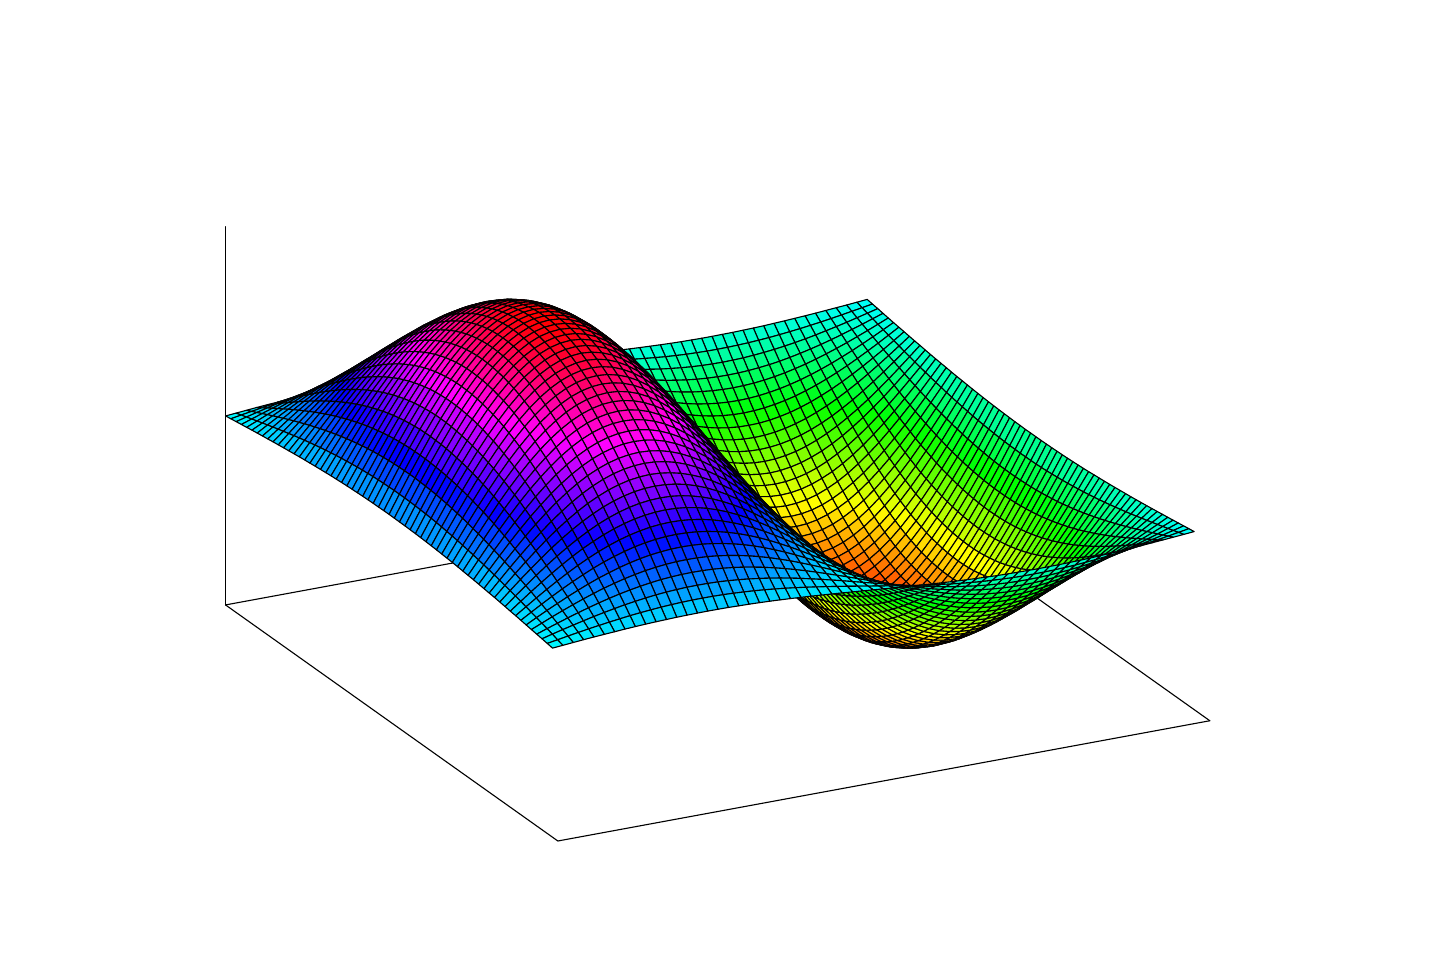
\begin{tikzpicture}[scale=1.15,gnuplot]
%% generated with GNUPLOT 4.6p0 (Lua 5.1; terminal rev. 99, script rev. 100)
%% Sun 14 Apr 2013 09:52:44 PM BST
\gpsolidlines
\path (0.000,0.000) rectangle (15.240,10.160);
\gpcolor{color=gp lt color border}
\gpsetlinetype{gp lt border}
\gpsetlinewidth{1.00}
\draw[gp path] (2.185,3.785)--(9.385,5.113);
\draw[gp path] (13.055,2.506)--(9.385,5.113);
\draw[gp path] (2.185,3.785)--(2.185,7.962);
\gpfill{rgb color={0.000,1.000,0.968}} (9.271,7.159)--(9.157,7.128)--(9.215,7.067)--(9.329,7.108)--cycle;
\gpcolor{rgb color={0.000,0.000,0.000}}
\gpsetlinetype{gp lt plot 3}
\draw[gp path] (9.271,7.159)--(9.329,7.108)--(9.215,7.067)--(9.157,7.128)--cycle;
\gpfill{rgb color={0.000,1.000,0.946}} (9.329,7.108)--(9.215,7.067)--(9.273,7.006)--(9.388,7.057)--cycle;
\draw[gp path] (9.329,7.108)--(9.388,7.057)--(9.273,7.006)--(9.215,7.067)--cycle;
\gpfill{rgb color={0.000,1.000,0.925}} (9.388,7.057)--(9.273,7.006)--(9.332,6.945)--(9.446,7.005)--cycle;
\draw[gp path] (9.388,7.057)--(9.446,7.005)--(9.332,6.945)--(9.273,7.006)--cycle;
\gpfill{rgb color={0.000,1.000,0.904}} (9.446,7.005)--(9.332,6.945)--(9.390,6.884)--(9.504,6.954)--cycle;
\draw[gp path] (9.446,7.005)--(9.504,6.954)--(9.390,6.884)--(9.332,6.945)--cycle;
\gpfill{rgb color={0.000,1.000,0.883}} (9.504,6.954)--(9.390,6.884)--(9.448,6.824)--(9.562,6.903)--cycle;
\draw[gp path] (9.504,6.954)--(9.562,6.903)--(9.448,6.824)--(9.390,6.884)--cycle;
\gpfill{rgb color={0.000,1.000,0.862}} (9.562,6.903)--(9.448,6.824)--(9.506,6.763)--(9.621,6.852)--cycle;
\draw[gp path] (9.562,6.903)--(9.621,6.852)--(9.506,6.763)--(9.448,6.824)--cycle;
\gpfill{rgb color={0.000,1.000,0.842}} (9.621,6.852)--(9.506,6.763)--(9.565,6.703)--(9.679,6.802)--cycle;
\draw[gp path] (9.621,6.852)--(9.679,6.802)--(9.565,6.703)--(9.506,6.763)--cycle;
\gpfill{rgb color={0.000,1.000,0.822}} (9.679,6.802)--(9.565,6.703)--(9.623,6.644)--(9.737,6.751)--cycle;
\draw[gp path] (9.679,6.802)--(9.737,6.751)--(9.623,6.644)--(9.565,6.703)--cycle;
\gpfill{rgb color={0.000,1.000,0.802}} (9.737,6.751)--(9.623,6.644)--(9.681,6.585)--(9.795,6.701)--cycle;
\draw[gp path] (9.737,6.751)--(9.795,6.701)--(9.681,6.585)--(9.623,6.644)--cycle;
\gpfill{rgb color={0.000,1.000,0.783}} (9.795,6.701)--(9.681,6.585)--(9.739,6.526)--(9.854,6.651)--cycle;
\draw[gp path] (9.795,6.701)--(9.854,6.651)--(9.739,6.526)--(9.681,6.585)--cycle;
\gpfill{rgb color={0.000,1.000,0.765}} (9.854,6.651)--(9.739,6.526)--(9.798,6.468)--(9.912,6.601)--cycle;
\draw[gp path] (9.854,6.651)--(9.912,6.601)--(9.798,6.468)--(9.739,6.526)--cycle;
\gpfill{rgb color={0.000,1.000,0.747}} (9.912,6.601)--(9.798,6.468)--(9.856,6.410)--(9.970,6.551)--cycle;
\draw[gp path] (9.912,6.601)--(9.970,6.551)--(9.856,6.410)--(9.798,6.468)--cycle;
\gpfill{rgb color={0.000,1.000,0.729}} (9.970,6.551)--(9.856,6.410)--(9.914,6.353)--(10.028,6.502)--cycle;
\draw[gp path] (9.970,6.551)--(10.028,6.502)--(9.914,6.353)--(9.856,6.410)--cycle;
\gpfill{rgb color={0.000,1.000,0.713}} (10.028,6.502)--(9.914,6.353)--(9.972,6.296)--(10.087,6.453)--cycle;
\draw[gp path] (10.028,6.502)--(10.087,6.453)--(9.972,6.296)--(9.914,6.353)--cycle;
\gpfill{rgb color={0.000,1.000,0.697}} (10.087,6.453)--(9.972,6.296)--(10.030,6.241)--(10.145,6.405)--cycle;
\draw[gp path] (10.087,6.453)--(10.145,6.405)--(10.030,6.241)--(9.972,6.296)--cycle;
\gpfill{rgb color={0.000,1.000,0.681}} (10.145,6.405)--(10.030,6.241)--(10.089,6.186)--(10.203,6.356)--cycle;
\draw[gp path] (10.145,6.405)--(10.203,6.356)--(10.089,6.186)--(10.030,6.241)--cycle;
\gpfill{rgb color={0.000,1.000,0.667}} (10.203,6.356)--(10.089,6.186)--(10.147,6.131)--(10.261,6.308)--cycle;
\draw[gp path] (10.203,6.356)--(10.261,6.308)--(10.147,6.131)--(10.089,6.186)--cycle;
\gpfill{rgb color={0.000,1.000,0.653}} (10.261,6.308)--(10.147,6.131)--(10.205,6.078)--(10.320,6.261)--cycle;
\draw[gp path] (10.261,6.308)--(10.320,6.261)--(10.205,6.078)--(10.147,6.131)--cycle;
\gpfill{rgb color={0.000,1.000,0.640}} (10.320,6.261)--(10.205,6.078)--(10.263,6.025)--(10.378,6.214)--cycle;
\draw[gp path] (10.320,6.261)--(10.378,6.214)--(10.263,6.025)--(10.205,6.078)--cycle;
\gpfill{rgb color={0.000,1.000,0.628}} (10.378,6.214)--(10.263,6.025)--(10.322,5.973)--(10.436,6.167)--cycle;
\draw[gp path] (10.378,6.214)--(10.436,6.167)--(10.322,5.973)--(10.263,6.025)--cycle;
\gpfill{rgb color={0.000,1.000,0.617}} (10.436,6.167)--(10.322,5.973)--(10.380,5.922)--(10.494,6.121)--cycle;
\draw[gp path] (10.436,6.167)--(10.494,6.121)--(10.380,5.922)--(10.322,5.973)--cycle;
\gpfill{rgb color={0.000,1.000,0.607}} (10.494,6.121)--(10.380,5.922)--(10.438,5.871)--(10.552,6.075)--cycle;
\draw[gp path] (10.494,6.121)--(10.552,6.075)--(10.438,5.871)--(10.380,5.922)--cycle;
\gpfill{rgb color={0.000,1.000,0.598}} (10.552,6.075)--(10.438,5.871)--(10.496,5.822)--(10.611,6.029)--cycle;
\draw[gp path] (10.552,6.075)--(10.611,6.029)--(10.496,5.822)--(10.438,5.871)--cycle;
\gpfill{rgb color={0.000,1.000,0.590}} (10.611,6.029)--(10.496,5.822)--(10.555,5.773)--(10.669,5.984)--cycle;
\draw[gp path] (10.611,6.029)--(10.669,5.984)--(10.555,5.773)--(10.496,5.822)--cycle;
\gpfill{rgb color={0.000,1.000,0.582}} (10.669,5.984)--(10.555,5.773)--(10.613,5.726)--(10.727,5.940)--cycle;
\draw[gp path] (10.669,5.984)--(10.727,5.940)--(10.613,5.726)--(10.555,5.773)--cycle;
\gpfill{rgb color={0.000,1.000,0.576}} (10.727,5.940)--(10.613,5.726)--(10.671,5.679)--(10.785,5.896)--cycle;
\draw[gp path] (10.727,5.940)--(10.785,5.896)--(10.671,5.679)--(10.613,5.726)--cycle;
\gpfill{rgb color={0.000,1.000,0.571}} (10.785,5.896)--(10.671,5.679)--(10.729,5.633)--(10.844,5.852)--cycle;
\draw[gp path] (10.785,5.896)--(10.844,5.852)--(10.729,5.633)--(10.671,5.679)--cycle;
\gpfill{rgb color={0.000,1.000,0.567}} (10.844,5.852)--(10.729,5.633)--(10.788,5.588)--(10.902,5.809)--cycle;
\draw[gp path] (10.844,5.852)--(10.902,5.809)--(10.788,5.588)--(10.729,5.633)--cycle;
\gpfill{rgb color={0.000,1.000,0.563}} (10.902,5.809)--(10.788,5.588)--(10.846,5.545)--(10.960,5.767)--cycle;
\draw[gp path] (10.902,5.809)--(10.960,5.767)--(10.846,5.545)--(10.788,5.588)--cycle;
\gpfill{rgb color={0.000,1.000,0.561}} (10.960,5.767)--(10.846,5.545)--(10.904,5.502)--(11.018,5.724)--cycle;
\draw[gp path] (10.960,5.767)--(11.018,5.724)--(10.904,5.502)--(10.846,5.545)--cycle;
\gpfill{rgb color={0.000,1.000,0.560}} (11.018,5.724)--(10.904,5.502)--(10.962,5.460)--(11.077,5.683)--cycle;
\draw[gp path] (11.018,5.724)--(11.077,5.683)--(10.962,5.460)--(10.904,5.502)--cycle;
\gpfill{rgb color={0.000,1.000,0.560}} (11.077,5.683)--(10.962,5.460)--(11.021,5.419)--(11.135,5.642)--cycle;
\draw[gp path] (11.077,5.683)--(11.135,5.642)--(11.021,5.419)--(10.962,5.460)--cycle;
\gpfill{rgb color={0.000,1.000,0.561}} (11.135,5.642)--(11.021,5.419)--(11.079,5.379)--(11.193,5.601)--cycle;
\draw[gp path] (11.135,5.642)--(11.193,5.601)--(11.079,5.379)--(11.021,5.419)--cycle;
\gpfill{rgb color={0.000,1.000,0.563}} (11.193,5.601)--(11.079,5.379)--(11.137,5.340)--(11.251,5.561)--cycle;
\draw[gp path] (11.193,5.601)--(11.251,5.561)--(11.137,5.340)--(11.079,5.379)--cycle;
\gpfill{rgb color={0.000,1.000,0.567}} (11.251,5.561)--(11.137,5.340)--(11.195,5.302)--(11.310,5.521)--cycle;
\draw[gp path] (11.251,5.561)--(11.310,5.521)--(11.195,5.302)--(11.137,5.340)--cycle;
\gpfill{rgb color={0.000,1.000,0.571}} (11.310,5.521)--(11.195,5.302)--(11.254,5.265)--(11.368,5.482)--cycle;
\draw[gp path] (11.310,5.521)--(11.368,5.482)--(11.254,5.265)--(11.195,5.302)--cycle;
\gpfill{rgb color={0.000,1.000,0.576}} (11.368,5.482)--(11.254,5.265)--(11.312,5.230)--(11.426,5.443)--cycle;
\draw[gp path] (11.368,5.482)--(11.426,5.443)--(11.312,5.230)--(11.254,5.265)--cycle;
\gpfill{rgb color={0.000,1.000,0.582}} (11.426,5.443)--(11.312,5.230)--(11.370,5.195)--(11.484,5.405)--cycle;
\draw[gp path] (11.426,5.443)--(11.484,5.405)--(11.370,5.195)--(11.312,5.230)--cycle;
\gpfill{rgb color={0.000,1.000,0.590}} (11.484,5.405)--(11.370,5.195)--(11.428,5.161)--(11.543,5.367)--cycle;
\draw[gp path] (11.484,5.405)--(11.543,5.367)--(11.428,5.161)--(11.370,5.195)--cycle;
\gpfill{rgb color={0.000,1.000,0.598}} (11.543,5.367)--(11.428,5.161)--(11.486,5.128)--(11.601,5.330)--cycle;
\draw[gp path] (11.543,5.367)--(11.601,5.330)--(11.486,5.128)--(11.428,5.161)--cycle;
\gpfill{rgb color={0.000,1.000,0.607}} (11.601,5.330)--(11.486,5.128)--(11.545,5.095)--(11.659,5.293)--cycle;
\draw[gp path] (11.601,5.330)--(11.659,5.293)--(11.545,5.095)--(11.486,5.128)--cycle;
\gpfill{rgb color={0.000,1.000,0.617}} (11.659,5.293)--(11.545,5.095)--(11.603,5.064)--(11.717,5.257)--cycle;
\draw[gp path] (11.659,5.293)--(11.717,5.257)--(11.603,5.064)--(11.545,5.095)--cycle;
\gpfill{rgb color={0.000,1.000,0.628}} (11.717,5.257)--(11.603,5.064)--(11.661,5.033)--(11.776,5.222)--cycle;
\draw[gp path] (11.717,5.257)--(11.776,5.222)--(11.661,5.033)--(11.603,5.064)--cycle;
\gpfill{rgb color={0.000,1.000,0.640}} (11.776,5.222)--(11.661,5.033)--(11.719,5.003)--(11.834,5.186)--cycle;
\draw[gp path] (11.776,5.222)--(11.834,5.186)--(11.719,5.003)--(11.661,5.033)--cycle;
\gpfill{rgb color={0.000,1.000,0.653}} (11.834,5.186)--(11.719,5.003)--(11.778,4.974)--(11.892,5.151)--cycle;
\draw[gp path] (11.834,5.186)--(11.892,5.151)--(11.778,4.974)--(11.719,5.003)--cycle;
\gpfill{rgb color={0.000,1.000,0.667}} (11.892,5.151)--(11.778,4.974)--(11.836,4.945)--(11.950,5.116)--cycle;
\draw[gp path] (11.892,5.151)--(11.950,5.116)--(11.836,4.945)--(11.778,4.974)--cycle;
\gpfill{rgb color={0.000,1.000,0.681}} (11.950,5.116)--(11.836,4.945)--(11.894,4.918)--(12.008,5.082)--cycle;
\draw[gp path] (11.950,5.116)--(12.008,5.082)--(11.894,4.918)--(11.836,4.945)--cycle;
\gpfill{rgb color={0.000,1.000,0.697}} (12.008,5.082)--(11.894,4.918)--(11.952,4.891)--(12.067,5.048)--cycle;
\draw[gp path] (12.008,5.082)--(12.067,5.048)--(11.952,4.891)--(11.894,4.918)--cycle;
\gpfill{rgb color={0.000,1.000,0.713}} (12.067,5.048)--(11.952,4.891)--(12.011,4.865)--(12.125,5.014)--cycle;
\draw[gp path] (12.067,5.048)--(12.125,5.014)--(12.011,4.865)--(11.952,4.891)--cycle;
\gpfill{rgb color={0.000,1.000,0.729}} (12.125,5.014)--(12.011,4.865)--(12.069,4.839)--(12.183,4.980)--cycle;
\draw[gp path] (12.125,5.014)--(12.183,4.980)--(12.069,4.839)--(12.011,4.865)--cycle;
\gpfill{rgb color={0.000,1.000,0.747}} (12.183,4.980)--(12.069,4.839)--(12.127,4.814)--(12.241,4.947)--cycle;
\draw[gp path] (12.183,4.980)--(12.241,4.947)--(12.127,4.814)--(12.069,4.839)--cycle;
\gpfill{rgb color={0.000,1.000,0.765}} (12.241,4.947)--(12.127,4.814)--(12.185,4.789)--(12.300,4.914)--cycle;
\draw[gp path] (12.241,4.947)--(12.300,4.914)--(12.185,4.789)--(12.127,4.814)--cycle;
\gpfill{rgb color={0.000,1.000,0.783}} (12.300,4.914)--(12.185,4.789)--(12.244,4.765)--(12.358,4.881)--cycle;
\draw[gp path] (12.300,4.914)--(12.358,4.881)--(12.244,4.765)--(12.185,4.789)--cycle;
\gpfill{rgb color={0.000,1.000,0.802}} (12.358,4.881)--(12.244,4.765)--(12.302,4.742)--(12.416,4.849)--cycle;
\draw[gp path] (12.358,4.881)--(12.416,4.849)--(12.302,4.742)--(12.244,4.765)--cycle;
\gpfill{rgb color={0.000,1.000,0.822}} (12.416,4.849)--(12.302,4.742)--(12.360,4.718)--(12.474,4.817)--cycle;
\draw[gp path] (12.416,4.849)--(12.474,4.817)--(12.360,4.718)--(12.302,4.742)--cycle;
\gpfill{rgb color={0.000,1.000,0.842}} (12.474,4.817)--(12.360,4.718)--(12.418,4.696)--(12.533,4.785)--cycle;
\draw[gp path] (12.474,4.817)--(12.533,4.785)--(12.418,4.696)--(12.360,4.718)--cycle;
\gpfill{rgb color={0.000,1.000,0.862}} (12.533,4.785)--(12.418,4.696)--(12.477,4.673)--(12.591,4.753)--cycle;
\draw[gp path] (12.533,4.785)--(12.591,4.753)--(12.477,4.673)--(12.418,4.696)--cycle;
\gpfill{rgb color={0.000,1.000,0.883}} (12.591,4.753)--(12.477,4.673)--(12.535,4.651)--(12.649,4.721)--cycle;
\draw[gp path] (12.591,4.753)--(12.649,4.721)--(12.535,4.651)--(12.477,4.673)--cycle;
\gpfill{rgb color={0.000,1.000,0.904}} (12.649,4.721)--(12.535,4.651)--(12.593,4.629)--(12.707,4.690)--cycle;
\draw[gp path] (12.649,4.721)--(12.707,4.690)--(12.593,4.629)--(12.535,4.651)--cycle;
\gpfill{rgb color={0.000,1.000,0.925}} (12.707,4.690)--(12.593,4.629)--(12.651,4.607)--(12.766,4.658)--cycle;
\draw[gp path] (12.707,4.690)--(12.766,4.658)--(12.651,4.607)--(12.593,4.629)--cycle;
\gpfill{rgb color={0.000,1.000,0.946}} (12.766,4.658)--(12.651,4.607)--(12.710,4.586)--(12.824,4.627)--cycle;
\draw[gp path] (12.766,4.658)--(12.824,4.627)--(12.710,4.586)--(12.651,4.607)--cycle;
\gpfill{rgb color={0.000,1.000,0.968}} (12.824,4.627)--(12.710,4.586)--(12.768,4.564)--(12.882,4.595)--cycle;
\draw[gp path] (12.824,4.627)--(12.882,4.595)--(12.768,4.564)--(12.710,4.586)--cycle;
\gpfill{rgb color={0.000,1.000,0.946}} (9.157,7.128)--(9.043,7.097)--(9.101,7.027)--(9.215,7.067)--cycle;
\draw[gp path] (9.157,7.128)--(9.215,7.067)--(9.101,7.027)--(9.043,7.097)--cycle;
\gpfill{rgb color={0.000,1.000,0.911}} (9.215,7.067)--(9.101,7.027)--(9.159,6.956)--(9.273,7.006)--cycle;
\draw[gp path] (9.215,7.067)--(9.273,7.006)--(9.159,6.956)--(9.101,7.027)--cycle;
\gpfill{rgb color={0.000,1.000,0.875}} (9.273,7.006)--(9.159,6.956)--(9.217,6.885)--(9.332,6.945)--cycle;
\draw[gp path] (9.273,7.006)--(9.332,6.945)--(9.217,6.885)--(9.159,6.956)--cycle;
\gpfill{rgb color={0.000,1.000,0.840}} (9.332,6.945)--(9.217,6.885)--(9.276,6.815)--(9.390,6.884)--cycle;
\draw[gp path] (9.332,6.945)--(9.390,6.884)--(9.276,6.815)--(9.217,6.885)--cycle;
\gpfill{rgb color={0.000,1.000,0.806}} (9.390,6.884)--(9.276,6.815)--(9.334,6.745)--(9.448,6.824)--cycle;
\draw[gp path] (9.390,6.884)--(9.448,6.824)--(9.334,6.745)--(9.276,6.815)--cycle;
\gpfill{rgb color={0.000,1.000,0.772}} (9.448,6.824)--(9.334,6.745)--(9.392,6.675)--(9.506,6.763)--cycle;
\draw[gp path] (9.448,6.824)--(9.506,6.763)--(9.392,6.675)--(9.334,6.745)--cycle;
\gpfill{rgb color={0.000,1.000,0.738}} (9.506,6.763)--(9.392,6.675)--(9.450,6.606)--(9.565,6.703)--cycle;
\draw[gp path] (9.506,6.763)--(9.565,6.703)--(9.450,6.606)--(9.392,6.675)--cycle;
\gpfill{rgb color={0.000,1.000,0.705}} (9.565,6.703)--(9.450,6.606)--(9.508,6.538)--(9.623,6.644)--cycle;
\draw[gp path] (9.565,6.703)--(9.623,6.644)--(9.508,6.538)--(9.450,6.606)--cycle;
\gpfill{rgb color={0.000,1.000,0.673}} (9.623,6.644)--(9.508,6.538)--(9.567,6.470)--(9.681,6.585)--cycle;
\draw[gp path] (9.623,6.644)--(9.681,6.585)--(9.567,6.470)--(9.508,6.538)--cycle;
\gpfill{rgb color={0.000,1.000,0.641}} (9.681,6.585)--(9.567,6.470)--(9.625,6.403)--(9.739,6.526)--cycle;
\draw[gp path] (9.681,6.585)--(9.739,6.526)--(9.625,6.403)--(9.567,6.470)--cycle;
\gpfill{rgb color={0.000,1.000,0.610}} (9.739,6.526)--(9.625,6.403)--(9.683,6.337)--(9.798,6.468)--cycle;
\draw[gp path] (9.739,6.526)--(9.798,6.468)--(9.683,6.337)--(9.625,6.403)--cycle;
\gpfill{rgb color={0.000,1.000,0.581}} (9.798,6.468)--(9.683,6.337)--(9.741,6.271)--(9.856,6.410)--cycle;
\draw[gp path] (9.798,6.468)--(9.856,6.410)--(9.741,6.271)--(9.683,6.337)--cycle;
\gpfill{rgb color={0.000,1.000,0.552}} (9.856,6.410)--(9.741,6.271)--(9.800,6.206)--(9.914,6.353)--cycle;
\draw[gp path] (9.856,6.410)--(9.914,6.353)--(9.800,6.206)--(9.741,6.271)--cycle;
\gpfill{rgb color={0.000,1.000,0.524}} (9.914,6.353)--(9.800,6.206)--(9.858,6.142)--(9.972,6.296)--cycle;
\draw[gp path] (9.914,6.353)--(9.972,6.296)--(9.858,6.142)--(9.800,6.206)--cycle;
\gpfill{rgb color={0.000,1.000,0.498}} (9.972,6.296)--(9.858,6.142)--(9.916,6.080)--(10.030,6.241)--cycle;
\draw[gp path] (9.972,6.296)--(10.030,6.241)--(9.916,6.080)--(9.858,6.142)--cycle;
\gpfill{rgb color={0.000,1.000,0.473}} (10.030,6.241)--(9.916,6.080)--(9.974,6.018)--(10.089,6.186)--cycle;
\draw[gp path] (10.030,6.241)--(10.089,6.186)--(9.974,6.018)--(9.916,6.080)--cycle;
\gpfill{rgb color={0.000,1.000,0.448}} (10.089,6.186)--(9.974,6.018)--(10.033,5.957)--(10.147,6.131)--cycle;
\draw[gp path] (10.089,6.186)--(10.147,6.131)--(10.033,5.957)--(9.974,6.018)--cycle;
\gpfill{rgb color={0.000,1.000,0.426}} (10.147,6.131)--(10.033,5.957)--(10.091,5.897)--(10.205,6.078)--cycle;
\draw[gp path] (10.147,6.131)--(10.205,6.078)--(10.091,5.897)--(10.033,5.957)--cycle;
\gpfill{rgb color={0.000,1.000,0.405}} (10.205,6.078)--(10.091,5.897)--(10.149,5.839)--(10.263,6.025)--cycle;
\draw[gp path] (10.205,6.078)--(10.263,6.025)--(10.149,5.839)--(10.091,5.897)--cycle;
\gpfill{rgb color={0.000,1.000,0.385}} (10.263,6.025)--(10.149,5.839)--(10.207,5.782)--(10.322,5.973)--cycle;
\draw[gp path] (10.263,6.025)--(10.322,5.973)--(10.207,5.782)--(10.149,5.839)--cycle;
\gpfill{rgb color={0.000,1.000,0.366}} (10.322,5.973)--(10.207,5.782)--(10.266,5.726)--(10.380,5.922)--cycle;
\draw[gp path] (10.322,5.973)--(10.380,5.922)--(10.266,5.726)--(10.207,5.782)--cycle;
\gpfill{rgb color={0.000,1.000,0.349}} (10.380,5.922)--(10.266,5.726)--(10.324,5.671)--(10.438,5.871)--cycle;
\draw[gp path] (10.380,5.922)--(10.438,5.871)--(10.324,5.671)--(10.266,5.726)--cycle;
\gpfill{rgb color={0.000,1.000,0.334}} (10.438,5.871)--(10.324,5.671)--(10.382,5.618)--(10.496,5.822)--cycle;
\draw[gp path] (10.438,5.871)--(10.496,5.822)--(10.382,5.618)--(10.324,5.671)--cycle;
\gpfill{rgb color={0.000,1.000,0.320}} (10.496,5.822)--(10.382,5.618)--(10.440,5.566)--(10.555,5.773)--cycle;
\draw[gp path] (10.496,5.822)--(10.555,5.773)--(10.440,5.566)--(10.382,5.618)--cycle;
\gpfill{rgb color={0.000,1.000,0.308}} (10.555,5.773)--(10.440,5.566)--(10.499,5.515)--(10.613,5.726)--cycle;
\draw[gp path] (10.555,5.773)--(10.613,5.726)--(10.499,5.515)--(10.440,5.566)--cycle;
\gpfill{rgb color={0.000,1.000,0.298}} (10.613,5.726)--(10.499,5.515)--(10.557,5.466)--(10.671,5.679)--cycle;
\draw[gp path] (10.613,5.726)--(10.671,5.679)--(10.557,5.466)--(10.499,5.515)--cycle;
\gpfill{rgb color={0.000,1.000,0.289}} (10.671,5.679)--(10.557,5.466)--(10.615,5.418)--(10.729,5.633)--cycle;
\draw[gp path] (10.671,5.679)--(10.729,5.633)--(10.615,5.418)--(10.557,5.466)--cycle;
\gpfill{rgb color={0.000,1.000,0.282}} (10.729,5.633)--(10.615,5.418)--(10.673,5.371)--(10.788,5.588)--cycle;
\draw[gp path] (10.729,5.633)--(10.788,5.588)--(10.673,5.371)--(10.615,5.418)--cycle;
\gpfill{rgb color={0.000,1.000,0.277}} (10.788,5.588)--(10.673,5.371)--(10.732,5.326)--(10.846,5.545)--cycle;
\draw[gp path] (10.788,5.588)--(10.846,5.545)--(10.732,5.326)--(10.673,5.371)--cycle;
\gpfill{rgb color={0.000,1.000,0.274}} (10.846,5.545)--(10.732,5.326)--(10.790,5.283)--(10.904,5.502)--cycle;
\draw[gp path] (10.846,5.545)--(10.904,5.502)--(10.790,5.283)--(10.732,5.326)--cycle;
\gpfill{rgb color={0.000,1.000,0.272}} (10.904,5.502)--(10.790,5.283)--(10.848,5.241)--(10.962,5.460)--cycle;
\draw[gp path] (10.904,5.502)--(10.962,5.460)--(10.848,5.241)--(10.790,5.283)--cycle;
\gpfill{rgb color={0.000,1.000,0.272}} (10.962,5.460)--(10.848,5.241)--(10.906,5.201)--(11.021,5.419)--cycle;
\draw[gp path] (10.962,5.460)--(11.021,5.419)--(10.906,5.201)--(10.848,5.241)--cycle;
\gpfill{rgb color={0.000,1.000,0.274}} (11.021,5.419)--(10.906,5.201)--(10.965,5.162)--(11.079,5.379)--cycle;
\draw[gp path] (11.021,5.419)--(11.079,5.379)--(10.965,5.162)--(10.906,5.201)--cycle;
\gpfill{rgb color={0.000,1.000,0.277}} (11.079,5.379)--(10.965,5.162)--(11.023,5.124)--(11.137,5.340)--cycle;
\draw[gp path] (11.079,5.379)--(11.137,5.340)--(11.023,5.124)--(10.965,5.162)--cycle;
\gpfill{rgb color={0.000,1.000,0.282}} (11.137,5.340)--(11.023,5.124)--(11.081,5.088)--(11.195,5.302)--cycle;
\draw[gp path] (11.137,5.340)--(11.195,5.302)--(11.081,5.088)--(11.023,5.124)--cycle;
\gpfill{rgb color={0.000,1.000,0.289}} (11.195,5.302)--(11.081,5.088)--(11.139,5.053)--(11.254,5.265)--cycle;
\draw[gp path] (11.195,5.302)--(11.254,5.265)--(11.139,5.053)--(11.081,5.088)--cycle;
\gpfill{rgb color={0.000,1.000,0.298}} (11.254,5.265)--(11.139,5.053)--(11.197,5.020)--(11.312,5.230)--cycle;
\draw[gp path] (11.254,5.265)--(11.312,5.230)--(11.197,5.020)--(11.139,5.053)--cycle;
\gpfill{rgb color={0.000,1.000,0.308}} (11.312,5.230)--(11.197,5.020)--(11.256,4.988)--(11.370,5.195)--cycle;
\draw[gp path] (11.312,5.230)--(11.370,5.195)--(11.256,4.988)--(11.197,5.020)--cycle;
\gpfill{rgb color={0.000,1.000,0.320}} (11.370,5.195)--(11.256,4.988)--(11.314,4.957)--(11.428,5.161)--cycle;
\draw[gp path] (11.370,5.195)--(11.428,5.161)--(11.314,4.957)--(11.256,4.988)--cycle;
\gpfill{rgb color={0.000,1.000,0.334}} (11.428,5.161)--(11.314,4.957)--(11.372,4.927)--(11.486,5.128)--cycle;
\draw[gp path] (11.428,5.161)--(11.486,5.128)--(11.372,4.927)--(11.314,4.957)--cycle;
\gpfill{rgb color={0.000,1.000,0.349}} (11.486,5.128)--(11.372,4.927)--(11.430,4.899)--(11.545,5.095)--cycle;
\draw[gp path] (11.486,5.128)--(11.545,5.095)--(11.430,4.899)--(11.372,4.927)--cycle;
\gpfill{rgb color={0.000,1.000,0.366}} (11.545,5.095)--(11.430,4.899)--(11.489,4.873)--(11.603,5.064)--cycle;
\draw[gp path] (11.545,5.095)--(11.603,5.064)--(11.489,4.873)--(11.430,4.899)--cycle;
\gpfill{rgb color={0.000,1.000,0.385}} (11.603,5.064)--(11.489,4.873)--(11.547,4.847)--(11.661,5.033)--cycle;
\draw[gp path] (11.603,5.064)--(11.661,5.033)--(11.547,4.847)--(11.489,4.873)--cycle;
\gpfill{rgb color={0.000,1.000,0.405}} (11.661,5.033)--(11.547,4.847)--(11.605,4.823)--(11.719,5.003)--cycle;
\draw[gp path] (11.661,5.033)--(11.719,5.003)--(11.605,4.823)--(11.547,4.847)--cycle;
\gpfill{rgb color={0.000,1.000,0.426}} (11.719,5.003)--(11.605,4.823)--(11.663,4.800)--(11.778,4.974)--cycle;
\draw[gp path] (11.719,5.003)--(11.778,4.974)--(11.663,4.800)--(11.605,4.823)--cycle;
\gpfill{rgb color={0.000,1.000,0.448}} (11.778,4.974)--(11.663,4.800)--(11.722,4.778)--(11.836,4.945)--cycle;
\draw[gp path] (11.778,4.974)--(11.836,4.945)--(11.722,4.778)--(11.663,4.800)--cycle;
\gpfill{rgb color={0.000,1.000,0.473}} (11.836,4.945)--(11.722,4.778)--(11.780,4.757)--(11.894,4.918)--cycle;
\draw[gp path] (11.836,4.945)--(11.894,4.918)--(11.780,4.757)--(11.722,4.778)--cycle;
\gpfill{rgb color={0.000,1.000,0.498}} (11.894,4.918)--(11.780,4.757)--(11.838,4.737)--(11.952,4.891)--cycle;
\draw[gp path] (11.894,4.918)--(11.952,4.891)--(11.838,4.737)--(11.780,4.757)--cycle;
\gpfill{rgb color={0.000,1.000,0.524}} (11.952,4.891)--(11.838,4.737)--(11.896,4.718)--(12.011,4.865)--cycle;
\draw[gp path] (11.952,4.891)--(12.011,4.865)--(11.896,4.718)--(11.838,4.737)--cycle;
\gpfill{rgb color={0.000,1.000,0.552}} (12.011,4.865)--(11.896,4.718)--(11.955,4.700)--(12.069,4.839)--cycle;
\draw[gp path] (12.011,4.865)--(12.069,4.839)--(11.955,4.700)--(11.896,4.718)--cycle;
\gpfill{rgb color={0.000,1.000,0.581}} (12.069,4.839)--(11.955,4.700)--(12.013,4.683)--(12.127,4.814)--cycle;
\draw[gp path] (12.069,4.839)--(12.127,4.814)--(12.013,4.683)--(11.955,4.700)--cycle;
\gpfill{rgb color={0.000,1.000,0.610}} (12.127,4.814)--(12.013,4.683)--(12.071,4.666)--(12.185,4.789)--cycle;
\draw[gp path] (12.127,4.814)--(12.185,4.789)--(12.071,4.666)--(12.013,4.683)--cycle;
\gpfill{rgb color={0.000,1.000,0.641}} (12.185,4.789)--(12.071,4.666)--(12.129,4.651)--(12.244,4.765)--cycle;
\draw[gp path] (12.185,4.789)--(12.244,4.765)--(12.129,4.651)--(12.071,4.666)--cycle;
\gpfill{rgb color={0.000,1.000,0.673}} (12.244,4.765)--(12.129,4.651)--(12.188,4.636)--(12.302,4.742)--cycle;
\draw[gp path] (12.244,4.765)--(12.302,4.742)--(12.188,4.636)--(12.129,4.651)--cycle;
\gpfill{rgb color={0.000,1.000,0.705}} (12.302,4.742)--(12.188,4.636)--(12.246,4.622)--(12.360,4.718)--cycle;
\draw[gp path] (12.302,4.742)--(12.360,4.718)--(12.246,4.622)--(12.188,4.636)--cycle;
\gpfill{rgb color={0.000,1.000,0.738}} (12.360,4.718)--(12.246,4.622)--(12.304,4.608)--(12.418,4.696)--cycle;
\draw[gp path] (12.360,4.718)--(12.418,4.696)--(12.304,4.608)--(12.246,4.622)--cycle;
\gpfill{rgb color={0.000,1.000,0.772}} (12.418,4.696)--(12.304,4.608)--(12.362,4.595)--(12.477,4.673)--cycle;
\draw[gp path] (12.418,4.696)--(12.477,4.673)--(12.362,4.595)--(12.304,4.608)--cycle;
\gpfill{rgb color={0.000,1.000,0.806}} (12.477,4.673)--(12.362,4.595)--(12.421,4.582)--(12.535,4.651)--cycle;
\draw[gp path] (12.477,4.673)--(12.535,4.651)--(12.421,4.582)--(12.362,4.595)--cycle;
\gpfill{rgb color={0.000,1.000,0.840}} (12.535,4.651)--(12.421,4.582)--(12.479,4.569)--(12.593,4.629)--cycle;
\draw[gp path] (12.535,4.651)--(12.593,4.629)--(12.479,4.569)--(12.421,4.582)--cycle;
\gpfill{rgb color={0.000,1.000,0.875}} (12.593,4.629)--(12.479,4.569)--(12.537,4.557)--(12.651,4.607)--cycle;
\draw[gp path] (12.593,4.629)--(12.651,4.607)--(12.537,4.557)--(12.479,4.569)--cycle;
\gpfill{rgb color={0.000,1.000,0.911}} (12.651,4.607)--(12.537,4.557)--(12.595,4.545)--(12.710,4.586)--cycle;
\draw[gp path] (12.651,4.607)--(12.710,4.586)--(12.595,4.545)--(12.537,4.557)--cycle;
\gpfill{rgb color={0.000,1.000,0.946}} (12.710,4.586)--(12.595,4.545)--(12.653,4.533)--(12.768,4.564)--cycle;
\draw[gp path] (12.710,4.586)--(12.768,4.564)--(12.653,4.533)--(12.595,4.545)--cycle;
\gpfill{rgb color={0.000,1.000,0.926}} (9.043,7.097)--(8.928,7.067)--(8.987,6.987)--(9.101,7.027)--cycle;
\draw[gp path] (9.043,7.097)--(9.101,7.027)--(8.987,6.987)--(8.928,7.067)--cycle;
\gpfill{rgb color={0.000,1.000,0.876}} (9.101,7.027)--(8.987,6.987)--(9.045,6.906)--(9.159,6.956)--cycle;
\draw[gp path] (9.101,7.027)--(9.159,6.956)--(9.045,6.906)--(8.987,6.987)--cycle;
\gpfill{rgb color={0.000,1.000,0.827}} (9.159,6.956)--(9.045,6.906)--(9.103,6.827)--(9.217,6.885)--cycle;
\draw[gp path] (9.159,6.956)--(9.217,6.885)--(9.103,6.827)--(9.045,6.906)--cycle;
\gpfill{rgb color={0.000,1.000,0.779}} (9.217,6.885)--(9.103,6.827)--(9.161,6.747)--(9.276,6.815)--cycle;
\draw[gp path] (9.217,6.885)--(9.276,6.815)--(9.161,6.747)--(9.103,6.827)--cycle;
\gpfill{rgb color={0.000,1.000,0.731}} (9.276,6.815)--(9.161,6.747)--(9.219,6.668)--(9.334,6.745)--cycle;
\draw[gp path] (9.276,6.815)--(9.334,6.745)--(9.219,6.668)--(9.161,6.747)--cycle;
\gpfill{rgb color={0.000,1.000,0.683}} (9.334,6.745)--(9.219,6.668)--(9.278,6.590)--(9.392,6.675)--cycle;
\draw[gp path] (9.334,6.745)--(9.392,6.675)--(9.278,6.590)--(9.219,6.668)--cycle;
\gpfill{rgb color={0.000,1.000,0.637}} (9.392,6.675)--(9.278,6.590)--(9.336,6.512)--(9.450,6.606)--cycle;
\draw[gp path] (9.392,6.675)--(9.450,6.606)--(9.336,6.512)--(9.278,6.590)--cycle;
\gpfill{rgb color={0.000,1.000,0.591}} (9.450,6.606)--(9.336,6.512)--(9.394,6.435)--(9.508,6.538)--cycle;
\draw[gp path] (9.450,6.606)--(9.508,6.538)--(9.394,6.435)--(9.336,6.512)--cycle;
\gpfill{rgb color={0.000,1.000,0.546}} (9.508,6.538)--(9.394,6.435)--(9.452,6.358)--(9.567,6.470)--cycle;
\draw[gp path] (9.508,6.538)--(9.567,6.470)--(9.452,6.358)--(9.394,6.435)--cycle;
\gpfill{rgb color={0.000,1.000,0.502}} (9.567,6.470)--(9.452,6.358)--(9.511,6.283)--(9.625,6.403)--cycle;
\draw[gp path] (9.567,6.470)--(9.625,6.403)--(9.511,6.283)--(9.452,6.358)--cycle;
\gpfill{rgb color={0.000,1.000,0.460}} (9.625,6.403)--(9.511,6.283)--(9.569,6.209)--(9.683,6.337)--cycle;
\draw[gp path] (9.625,6.403)--(9.683,6.337)--(9.569,6.209)--(9.511,6.283)--cycle;
\gpfill{rgb color={0.000,1.000,0.419}} (9.683,6.337)--(9.569,6.209)--(9.627,6.135)--(9.741,6.271)--cycle;
\draw[gp path] (9.683,6.337)--(9.741,6.271)--(9.627,6.135)--(9.569,6.209)--cycle;
\gpfill{rgb color={0.000,1.000,0.379}} (9.741,6.271)--(9.627,6.135)--(9.685,6.063)--(9.800,6.206)--cycle;
\draw[gp path] (9.741,6.271)--(9.800,6.206)--(9.685,6.063)--(9.627,6.135)--cycle;
\gpfill{rgb color={0.000,1.000,0.340}} (9.800,6.206)--(9.685,6.063)--(9.744,5.992)--(9.858,6.142)--cycle;
\draw[gp path] (9.800,6.206)--(9.858,6.142)--(9.744,5.992)--(9.685,6.063)--cycle;
\gpfill{rgb color={0.000,1.000,0.304}} (9.858,6.142)--(9.744,5.992)--(9.802,5.923)--(9.916,6.080)--cycle;
\draw[gp path] (9.858,6.142)--(9.916,6.080)--(9.802,5.923)--(9.744,5.992)--cycle;
\gpfill{rgb color={0.000,1.000,0.269}} (9.916,6.080)--(9.802,5.923)--(9.860,5.854)--(9.974,6.018)--cycle;
\draw[gp path] (9.916,6.080)--(9.974,6.018)--(9.860,5.854)--(9.802,5.923)--cycle;
\gpfill{rgb color={0.000,1.000,0.235}} (9.974,6.018)--(9.860,5.854)--(9.918,5.787)--(10.033,5.957)--cycle;
\draw[gp path] (9.974,6.018)--(10.033,5.957)--(9.918,5.787)--(9.860,5.854)--cycle;
\gpfill{rgb color={0.000,1.000,0.204}} (10.033,5.957)--(9.918,5.787)--(9.977,5.722)--(10.091,5.897)--cycle;
\draw[gp path] (10.033,5.957)--(10.091,5.897)--(9.977,5.722)--(9.918,5.787)--cycle;
\gpfill{rgb color={0.000,1.000,0.174}} (10.091,5.897)--(9.977,5.722)--(10.035,5.658)--(10.149,5.839)--cycle;
\draw[gp path] (10.091,5.897)--(10.149,5.839)--(10.035,5.658)--(9.977,5.722)--cycle;
\gpfill{rgb color={0.000,1.000,0.147}} (10.149,5.839)--(10.035,5.658)--(10.093,5.596)--(10.207,5.782)--cycle;
\draw[gp path] (10.149,5.839)--(10.207,5.782)--(10.093,5.596)--(10.035,5.658)--cycle;
\gpfill{rgb color={0.000,1.000,0.121}} (10.207,5.782)--(10.093,5.596)--(10.151,5.535)--(10.266,5.726)--cycle;
\draw[gp path] (10.207,5.782)--(10.266,5.726)--(10.151,5.535)--(10.093,5.596)--cycle;
\gpfill{rgb color={0.000,1.000,0.098}} (10.266,5.726)--(10.151,5.535)--(10.210,5.476)--(10.324,5.671)--cycle;
\draw[gp path] (10.266,5.726)--(10.324,5.671)--(10.210,5.476)--(10.151,5.535)--cycle;
\gpfill{rgb color={0.000,1.000,0.077}} (10.324,5.671)--(10.210,5.476)--(10.268,5.419)--(10.382,5.618)--cycle;
\draw[gp path] (10.324,5.671)--(10.382,5.618)--(10.268,5.419)--(10.210,5.476)--cycle;
\gpfill{rgb color={0.000,1.000,0.058}} (10.382,5.618)--(10.268,5.419)--(10.326,5.364)--(10.440,5.566)--cycle;
\draw[gp path] (10.382,5.618)--(10.440,5.566)--(10.326,5.364)--(10.268,5.419)--cycle;
\gpfill{rgb color={0.000,1.000,0.041}} (10.440,5.566)--(10.326,5.364)--(10.384,5.310)--(10.499,5.515)--cycle;
\draw[gp path] (10.440,5.566)--(10.499,5.515)--(10.384,5.310)--(10.326,5.364)--cycle;
\gpfill{rgb color={0.000,1.000,0.027}} (10.499,5.515)--(10.384,5.310)--(10.443,5.258)--(10.557,5.466)--cycle;
\draw[gp path] (10.499,5.515)--(10.557,5.466)--(10.443,5.258)--(10.384,5.310)--cycle;
\gpfill{rgb color={0.000,1.000,0.015}} (10.557,5.466)--(10.443,5.258)--(10.501,5.209)--(10.615,5.418)--cycle;
\draw[gp path] (10.557,5.466)--(10.615,5.418)--(10.501,5.209)--(10.443,5.258)--cycle;
\gpfill{rgb color={0.000,1.000,0.005}} (10.615,5.418)--(10.501,5.209)--(10.559,5.161)--(10.673,5.371)--cycle;
\draw[gp path] (10.615,5.418)--(10.673,5.371)--(10.559,5.161)--(10.501,5.209)--cycle;
\gpfill{rgb color={0.002,1.000,0.000}} (10.673,5.371)--(10.559,5.161)--(10.617,5.115)--(10.732,5.326)--cycle;
\draw[gp path] (10.673,5.371)--(10.732,5.326)--(10.617,5.115)--(10.559,5.161)--cycle;
\gpfill{rgb color={0.007,1.000,0.000}} (10.732,5.326)--(10.617,5.115)--(10.675,5.071)--(10.790,5.283)--cycle;
\draw[gp path] (10.732,5.326)--(10.790,5.283)--(10.675,5.071)--(10.617,5.115)--cycle;
\gpfill{rgb color={0.010,1.000,0.000}} (10.790,5.283)--(10.675,5.071)--(10.734,5.029)--(10.848,5.241)--cycle;
\draw[gp path] (10.790,5.283)--(10.848,5.241)--(10.734,5.029)--(10.675,5.071)--cycle;
\gpfill{rgb color={0.010,1.000,0.000}} (10.848,5.241)--(10.734,5.029)--(10.792,4.988)--(10.906,5.201)--cycle;
\draw[gp path] (10.848,5.241)--(10.906,5.201)--(10.792,4.988)--(10.734,5.029)--cycle;
\gpfill{rgb color={0.007,1.000,0.000}} (10.906,5.201)--(10.792,4.988)--(10.850,4.950)--(10.965,5.162)--cycle;
\draw[gp path] (10.906,5.201)--(10.965,5.162)--(10.850,4.950)--(10.792,4.988)--cycle;
\gpfill{rgb color={0.002,1.000,0.000}} (10.965,5.162)--(10.850,4.950)--(10.908,4.913)--(11.023,5.124)--cycle;
\draw[gp path] (10.965,5.162)--(11.023,5.124)--(10.908,4.913)--(10.850,4.950)--cycle;
\gpfill{rgb color={0.000,1.000,0.005}} (11.023,5.124)--(10.908,4.913)--(10.967,4.878)--(11.081,5.088)--cycle;
\draw[gp path] (11.023,5.124)--(11.081,5.088)--(10.967,4.878)--(10.908,4.913)--cycle;
\gpfill{rgb color={0.000,1.000,0.015}} (11.081,5.088)--(10.967,4.878)--(11.025,4.846)--(11.139,5.053)--cycle;
\draw[gp path] (11.081,5.088)--(11.139,5.053)--(11.025,4.846)--(10.967,4.878)--cycle;
\gpfill{rgb color={0.000,1.000,0.027}} (11.139,5.053)--(11.025,4.846)--(11.083,4.815)--(11.197,5.020)--cycle;
\draw[gp path] (11.139,5.053)--(11.197,5.020)--(11.083,4.815)--(11.025,4.846)--cycle;
\gpfill{rgb color={0.000,1.000,0.041}} (11.197,5.020)--(11.083,4.815)--(11.141,4.785)--(11.256,4.988)--cycle;
\draw[gp path] (11.197,5.020)--(11.256,4.988)--(11.141,4.785)--(11.083,4.815)--cycle;
\gpfill{rgb color={0.000,1.000,0.058}} (11.256,4.988)--(11.141,4.785)--(11.200,4.758)--(11.314,4.957)--cycle;
\draw[gp path] (11.256,4.988)--(11.314,4.957)--(11.200,4.758)--(11.141,4.785)--cycle;
\gpfill{rgb color={0.000,1.000,0.077}} (11.314,4.957)--(11.200,4.758)--(11.258,4.733)--(11.372,4.927)--cycle;
\draw[gp path] (11.314,4.957)--(11.372,4.927)--(11.258,4.733)--(11.200,4.758)--cycle;
\gpfill{rgb color={0.000,1.000,0.098}} (11.372,4.927)--(11.258,4.733)--(11.316,4.709)--(11.430,4.899)--cycle;
\draw[gp path] (11.372,4.927)--(11.430,4.899)--(11.316,4.709)--(11.258,4.733)--cycle;
\gpfill{rgb color={0.000,1.000,0.121}} (11.430,4.899)--(11.316,4.709)--(11.374,4.687)--(11.489,4.873)--cycle;
\draw[gp path] (11.430,4.899)--(11.489,4.873)--(11.374,4.687)--(11.316,4.709)--cycle;
\gpfill{rgb color={0.000,1.000,0.147}} (11.489,4.873)--(11.374,4.687)--(11.433,4.666)--(11.547,4.847)--cycle;
\draw[gp path] (11.489,4.873)--(11.547,4.847)--(11.433,4.666)--(11.374,4.687)--cycle;
\gpfill{rgb color={0.000,1.000,0.174}} (11.547,4.847)--(11.433,4.666)--(11.491,4.647)--(11.605,4.823)--cycle;
\draw[gp path] (11.547,4.847)--(11.605,4.823)--(11.491,4.647)--(11.433,4.666)--cycle;
\gpfill{rgb color={0.000,1.000,0.204}} (11.605,4.823)--(11.491,4.647)--(11.549,4.630)--(11.663,4.800)--cycle;
\draw[gp path] (11.605,4.823)--(11.663,4.800)--(11.549,4.630)--(11.491,4.647)--cycle;
\gpfill{rgb color={0.000,1.000,0.235}} (11.663,4.800)--(11.549,4.630)--(11.607,4.614)--(11.722,4.778)--cycle;
\draw[gp path] (11.663,4.800)--(11.722,4.778)--(11.607,4.614)--(11.549,4.630)--cycle;
\gpfill{rgb color={0.000,1.000,0.269}} (11.722,4.778)--(11.607,4.614)--(11.666,4.600)--(11.780,4.757)--cycle;
\draw[gp path] (11.722,4.778)--(11.780,4.757)--(11.666,4.600)--(11.607,4.614)--cycle;
\gpfill{rgb color={0.000,1.000,0.304}} (11.780,4.757)--(11.666,4.600)--(11.724,4.587)--(11.838,4.737)--cycle;
\draw[gp path] (11.780,4.757)--(11.838,4.737)--(11.724,4.587)--(11.666,4.600)--cycle;
\gpfill{rgb color={0.000,1.000,0.340}} (11.838,4.737)--(11.724,4.587)--(11.782,4.575)--(11.896,4.718)--cycle;
\draw[gp path] (11.838,4.737)--(11.896,4.718)--(11.782,4.575)--(11.724,4.587)--cycle;
\gpfill{rgb color={0.000,1.000,0.379}} (11.896,4.718)--(11.782,4.575)--(11.840,4.564)--(11.955,4.700)--cycle;
\draw[gp path] (11.896,4.718)--(11.955,4.700)--(11.840,4.564)--(11.782,4.575)--cycle;
\gpfill{rgb color={0.000,1.000,0.419}} (11.955,4.700)--(11.840,4.564)--(11.899,4.555)--(12.013,4.683)--cycle;
\draw[gp path] (11.955,4.700)--(12.013,4.683)--(11.899,4.555)--(11.840,4.564)--cycle;
\gpfill{rgb color={0.000,1.000,0.460}} (12.013,4.683)--(11.899,4.555)--(11.957,4.546)--(12.071,4.666)--cycle;
\draw[gp path] (12.013,4.683)--(12.071,4.666)--(11.957,4.546)--(11.899,4.555)--cycle;
\gpfill{rgb color={0.000,1.000,0.502}} (12.071,4.666)--(11.957,4.546)--(12.015,4.539)--(12.129,4.651)--cycle;
\draw[gp path] (12.071,4.666)--(12.129,4.651)--(12.015,4.539)--(11.957,4.546)--cycle;
\gpfill{rgb color={0.000,1.000,0.546}} (12.129,4.651)--(12.015,4.539)--(12.073,4.533)--(12.188,4.636)--cycle;
\draw[gp path] (12.129,4.651)--(12.188,4.636)--(12.073,4.533)--(12.015,4.539)--cycle;
\gpfill{rgb color={0.000,1.000,0.591}} (12.188,4.636)--(12.073,4.533)--(12.131,4.527)--(12.246,4.622)--cycle;
\draw[gp path] (12.188,4.636)--(12.246,4.622)--(12.131,4.527)--(12.073,4.533)--cycle;
\gpfill{rgb color={0.000,1.000,0.637}} (12.246,4.622)--(12.131,4.527)--(12.190,4.522)--(12.304,4.608)--cycle;
\draw[gp path] (12.246,4.622)--(12.304,4.608)--(12.190,4.522)--(12.131,4.527)--cycle;
\gpfill{rgb color={0.000,1.000,0.683}} (12.304,4.608)--(12.190,4.522)--(12.248,4.518)--(12.362,4.595)--cycle;
\draw[gp path] (12.304,4.608)--(12.362,4.595)--(12.248,4.518)--(12.190,4.522)--cycle;
\gpfill{rgb color={0.000,1.000,0.731}} (12.362,4.595)--(12.248,4.518)--(12.306,4.514)--(12.421,4.582)--cycle;
\draw[gp path] (12.362,4.595)--(12.421,4.582)--(12.306,4.514)--(12.248,4.518)--cycle;
\gpfill{rgb color={0.000,1.000,0.779}} (12.421,4.582)--(12.306,4.514)--(12.364,4.511)--(12.479,4.569)--cycle;
\draw[gp path] (12.421,4.582)--(12.479,4.569)--(12.364,4.511)--(12.306,4.514)--cycle;
\gpfill{rgb color={0.000,1.000,0.827}} (12.479,4.569)--(12.364,4.511)--(12.423,4.508)--(12.537,4.557)--cycle;
\draw[gp path] (12.479,4.569)--(12.537,4.557)--(12.423,4.508)--(12.364,4.511)--cycle;
\gpfill{rgb color={0.000,1.000,0.876}} (12.537,4.557)--(12.423,4.508)--(12.481,4.505)--(12.595,4.545)--cycle;
\draw[gp path] (12.537,4.557)--(12.595,4.545)--(12.481,4.505)--(12.423,4.508)--cycle;
\gpfill{rgb color={0.000,1.000,0.926}} (12.595,4.545)--(12.481,4.505)--(12.539,4.503)--(12.653,4.533)--cycle;
\draw[gp path] (12.595,4.545)--(12.653,4.533)--(12.539,4.503)--(12.481,4.505)--cycle;
\gpfill{rgb color={0.000,1.000,0.906}} (8.928,7.067)--(8.814,7.037)--(8.872,6.947)--(8.987,6.987)--cycle;
\draw[gp path] (8.928,7.067)--(8.987,6.987)--(8.872,6.947)--(8.814,7.037)--cycle;
\gpfill{rgb color={0.000,1.000,0.843}} (8.987,6.987)--(8.872,6.947)--(8.930,6.858)--(9.045,6.906)--cycle;
\draw[gp path] (8.987,6.987)--(9.045,6.906)--(8.930,6.858)--(8.872,6.947)--cycle;
\gpfill{rgb color={0.000,1.000,0.781}} (9.045,6.906)--(8.930,6.858)--(8.989,6.770)--(9.103,6.827)--cycle;
\draw[gp path] (9.045,6.906)--(9.103,6.827)--(8.989,6.770)--(8.930,6.858)--cycle;
\gpfill{rgb color={0.000,1.000,0.719}} (9.103,6.827)--(8.989,6.770)--(9.047,6.681)--(9.161,6.747)--cycle;
\draw[gp path] (9.103,6.827)--(9.161,6.747)--(9.047,6.681)--(8.989,6.770)--cycle;
\gpfill{rgb color={0.000,1.000,0.658}} (9.161,6.747)--(9.047,6.681)--(9.105,6.593)--(9.219,6.668)--cycle;
\draw[gp path] (9.161,6.747)--(9.219,6.668)--(9.105,6.593)--(9.047,6.681)--cycle;
\gpfill{rgb color={0.000,1.000,0.598}} (9.219,6.668)--(9.105,6.593)--(9.163,6.506)--(9.278,6.590)--cycle;
\draw[gp path] (9.219,6.668)--(9.278,6.590)--(9.163,6.506)--(9.105,6.593)--cycle;
\gpfill{rgb color={0.000,1.000,0.539}} (9.278,6.590)--(9.163,6.506)--(9.222,6.420)--(9.336,6.512)--cycle;
\draw[gp path] (9.278,6.590)--(9.336,6.512)--(9.222,6.420)--(9.163,6.506)--cycle;
\gpfill{rgb color={0.000,1.000,0.481}} (9.336,6.512)--(9.222,6.420)--(9.280,6.335)--(9.394,6.435)--cycle;
\draw[gp path] (9.336,6.512)--(9.394,6.435)--(9.280,6.335)--(9.222,6.420)--cycle;
\gpfill{rgb color={0.000,1.000,0.424}} (9.394,6.435)--(9.280,6.335)--(9.338,6.250)--(9.452,6.358)--cycle;
\draw[gp path] (9.394,6.435)--(9.452,6.358)--(9.338,6.250)--(9.280,6.335)--cycle;
\gpfill{rgb color={0.000,1.000,0.368}} (9.452,6.358)--(9.338,6.250)--(9.396,6.167)--(9.511,6.283)--cycle;
\draw[gp path] (9.452,6.358)--(9.511,6.283)--(9.396,6.167)--(9.338,6.250)--cycle;
\gpfill{rgb color={0.000,1.000,0.314}} (9.511,6.283)--(9.396,6.167)--(9.455,6.085)--(9.569,6.209)--cycle;
\draw[gp path] (9.511,6.283)--(9.569,6.209)--(9.455,6.085)--(9.396,6.167)--cycle;
\gpfill{rgb color={0.000,1.000,0.262}} (9.569,6.209)--(9.455,6.085)--(9.513,6.004)--(9.627,6.135)--cycle;
\draw[gp path] (9.569,6.209)--(9.627,6.135)--(9.513,6.004)--(9.455,6.085)--cycle;
\gpfill{rgb color={0.000,1.000,0.212}} (9.627,6.135)--(9.513,6.004)--(9.571,5.925)--(9.685,6.063)--cycle;
\draw[gp path] (9.627,6.135)--(9.685,6.063)--(9.571,5.925)--(9.513,6.004)--cycle;
\gpfill{rgb color={0.000,1.000,0.163}} (9.685,6.063)--(9.571,5.925)--(9.629,5.847)--(9.744,5.992)--cycle;
\draw[gp path] (9.685,6.063)--(9.744,5.992)--(9.629,5.847)--(9.571,5.925)--cycle;
\gpfill{rgb color={0.000,1.000,0.116}} (9.744,5.992)--(9.629,5.847)--(9.688,5.771)--(9.802,5.923)--cycle;
\draw[gp path] (9.744,5.992)--(9.802,5.923)--(9.688,5.771)--(9.629,5.847)--cycle;
\gpfill{rgb color={0.000,1.000,0.072}} (9.802,5.923)--(9.688,5.771)--(9.746,5.697)--(9.860,5.854)--cycle;
\draw[gp path] (9.802,5.923)--(9.860,5.854)--(9.746,5.697)--(9.688,5.771)--cycle;
\gpfill{rgb color={0.000,1.000,0.030}} (9.860,5.854)--(9.746,5.697)--(9.804,5.624)--(9.918,5.787)--cycle;
\draw[gp path] (9.860,5.854)--(9.918,5.787)--(9.804,5.624)--(9.746,5.697)--cycle;
\gpfill{rgb color={0.010,1.000,0.000}} (9.918,5.787)--(9.804,5.624)--(9.862,5.553)--(9.977,5.722)--cycle;
\draw[gp path] (9.918,5.787)--(9.977,5.722)--(9.862,5.553)--(9.804,5.624)--cycle;
\gpfill{rgb color={0.048,1.000,0.000}} (9.977,5.722)--(9.862,5.553)--(9.921,5.484)--(10.035,5.658)--cycle;
\draw[gp path] (9.977,5.722)--(10.035,5.658)--(9.921,5.484)--(9.862,5.553)--cycle;
\gpfill{rgb color={0.083,1.000,0.000}} (10.035,5.658)--(9.921,5.484)--(9.979,5.417)--(10.093,5.596)--cycle;
\draw[gp path] (10.035,5.658)--(10.093,5.596)--(9.979,5.417)--(9.921,5.484)--cycle;
\gpfill{rgb color={0.115,1.000,0.000}} (10.093,5.596)--(9.979,5.417)--(10.037,5.351)--(10.151,5.535)--cycle;
\draw[gp path] (10.093,5.596)--(10.151,5.535)--(10.037,5.351)--(9.979,5.417)--cycle;
\gpfill{rgb color={0.145,1.000,0.000}} (10.151,5.535)--(10.037,5.351)--(10.095,5.288)--(10.210,5.476)--cycle;
\draw[gp path] (10.151,5.535)--(10.210,5.476)--(10.095,5.288)--(10.037,5.351)--cycle;
\gpfill{rgb color={0.172,1.000,0.000}} (10.210,5.476)--(10.095,5.288)--(10.153,5.229)--(10.268,5.419)--cycle;
\draw[gp path] (10.210,5.476)--(10.268,5.419)--(10.153,5.229)--(10.095,5.288)--cycle;
\gpfill{rgb color={0.196,1.000,0.000}} (10.268,5.419)--(10.153,5.229)--(10.212,5.170)--(10.326,5.364)--cycle;
\draw[gp path] (10.268,5.419)--(10.326,5.364)--(10.212,5.170)--(10.153,5.229)--cycle;
\gpfill{rgb color={0.217,1.000,0.000}} (10.326,5.364)--(10.212,5.170)--(10.270,5.113)--(10.384,5.310)--cycle;
\draw[gp path] (10.326,5.364)--(10.384,5.310)--(10.270,5.113)--(10.212,5.170)--cycle;
\gpfill{rgb color={0.235,1.000,0.000}} (10.384,5.310)--(10.270,5.113)--(10.328,5.059)--(10.443,5.258)--cycle;
\draw[gp path] (10.384,5.310)--(10.443,5.258)--(10.328,5.059)--(10.270,5.113)--cycle;
\gpfill{rgb color={0.250,1.000,0.000}} (10.443,5.258)--(10.328,5.059)--(10.386,5.007)--(10.501,5.209)--cycle;
\draw[gp path] (10.443,5.258)--(10.501,5.209)--(10.386,5.007)--(10.328,5.059)--cycle;
\gpfill{rgb color={0.263,1.000,0.000}} (10.501,5.209)--(10.386,5.007)--(10.445,4.958)--(10.559,5.161)--cycle;
\draw[gp path] (10.501,5.209)--(10.559,5.161)--(10.445,4.958)--(10.386,5.007)--cycle;
\gpfill{rgb color={0.272,1.000,0.000}} (10.559,5.161)--(10.445,4.958)--(10.503,4.910)--(10.617,5.115)--cycle;
\draw[gp path] (10.559,5.161)--(10.617,5.115)--(10.503,4.910)--(10.445,4.958)--cycle;
\gpfill{rgb color={0.278,1.000,0.000}} (10.617,5.115)--(10.503,4.910)--(10.561,4.866)--(10.675,5.071)--cycle;
\draw[gp path] (10.617,5.115)--(10.675,5.071)--(10.561,4.866)--(10.503,4.910)--cycle;
\gpfill{rgb color={0.281,1.000,0.000}} (10.675,5.071)--(10.561,4.866)--(10.619,4.823)--(10.734,5.029)--cycle;
\draw[gp path] (10.675,5.071)--(10.734,5.029)--(10.619,4.823)--(10.561,4.866)--cycle;
\gpfill{rgb color={0.281,1.000,0.000}} (10.734,5.029)--(10.619,4.823)--(10.678,4.783)--(10.792,4.988)--cycle;
\draw[gp path] (10.734,5.029)--(10.792,4.988)--(10.678,4.783)--(10.619,4.823)--cycle;
\gpfill{rgb color={0.278,1.000,0.000}} (10.792,4.988)--(10.678,4.783)--(10.736,4.745)--(10.850,4.950)--cycle;
\draw[gp path] (10.792,4.988)--(10.850,4.950)--(10.736,4.745)--(10.678,4.783)--cycle;
\gpfill{rgb color={0.272,1.000,0.000}} (10.850,4.950)--(10.736,4.745)--(10.794,4.709)--(10.908,4.913)--cycle;
\draw[gp path] (10.850,4.950)--(10.908,4.913)--(10.794,4.709)--(10.736,4.745)--cycle;
\gpfill{rgb color={0.263,1.000,0.000}} (10.908,4.913)--(10.794,4.709)--(10.852,4.676)--(10.967,4.878)--cycle;
\draw[gp path] (10.908,4.913)--(10.967,4.878)--(10.852,4.676)--(10.794,4.709)--cycle;
\gpfill{rgb color={0.250,1.000,0.000}} (10.967,4.878)--(10.852,4.676)--(10.911,4.645)--(11.025,4.846)--cycle;
\draw[gp path] (10.967,4.878)--(11.025,4.846)--(10.911,4.645)--(10.852,4.676)--cycle;
\gpfill{rgb color={0.235,1.000,0.000}} (11.025,4.846)--(10.911,4.645)--(10.969,4.617)--(11.083,4.815)--cycle;
\draw[gp path] (11.025,4.846)--(11.083,4.815)--(10.969,4.617)--(10.911,4.645)--cycle;
\gpfill{rgb color={0.217,1.000,0.000}} (11.083,4.815)--(10.969,4.617)--(11.027,4.591)--(11.141,4.785)--cycle;
\draw[gp path] (11.083,4.815)--(11.141,4.785)--(11.027,4.591)--(10.969,4.617)--cycle;
\gpfill{rgb color={0.196,1.000,0.000}} (11.141,4.785)--(11.027,4.591)--(11.085,4.567)--(11.200,4.758)--cycle;
\draw[gp path] (11.141,4.785)--(11.200,4.758)--(11.085,4.567)--(11.027,4.591)--cycle;
\gpfill{rgb color={0.172,1.000,0.000}} (11.200,4.758)--(11.085,4.567)--(11.144,4.545)--(11.258,4.733)--cycle;
\draw[gp path] (11.200,4.758)--(11.258,4.733)--(11.144,4.545)--(11.085,4.567)--cycle;
\gpfill{rgb color={0.145,1.000,0.000}} (11.258,4.733)--(11.144,4.545)--(11.202,4.525)--(11.316,4.709)--cycle;
\draw[gp path] (11.258,4.733)--(11.316,4.709)--(11.202,4.525)--(11.144,4.545)--cycle;
\gpfill{rgb color={0.115,1.000,0.000}} (11.316,4.709)--(11.202,4.525)--(11.260,4.507)--(11.374,4.687)--cycle;
\draw[gp path] (11.316,4.709)--(11.374,4.687)--(11.260,4.507)--(11.202,4.525)--cycle;
\gpfill{rgb color={0.083,1.000,0.000}} (11.374,4.687)--(11.260,4.507)--(11.318,4.492)--(11.433,4.666)--cycle;
\draw[gp path] (11.374,4.687)--(11.433,4.666)--(11.318,4.492)--(11.260,4.507)--cycle;
\gpfill{rgb color={0.048,1.000,0.000}} (11.433,4.666)--(11.318,4.492)--(11.377,4.478)--(11.491,4.647)--cycle;
\draw[gp path] (11.433,4.666)--(11.491,4.647)--(11.377,4.478)--(11.318,4.492)--cycle;
\gpfill{rgb color={0.010,1.000,0.000}} (11.491,4.647)--(11.377,4.478)--(11.435,4.466)--(11.549,4.630)--cycle;
\draw[gp path] (11.491,4.647)--(11.549,4.630)--(11.435,4.466)--(11.377,4.478)--cycle;
\gpfill{rgb color={0.000,1.000,0.030}} (11.549,4.630)--(11.435,4.466)--(11.493,4.456)--(11.607,4.614)--cycle;
\draw[gp path] (11.549,4.630)--(11.607,4.614)--(11.493,4.456)--(11.435,4.466)--cycle;
\gpfill{rgb color={0.000,1.000,0.072}} (11.607,4.614)--(11.493,4.456)--(11.551,4.448)--(11.666,4.600)--cycle;
\draw[gp path] (11.607,4.614)--(11.666,4.600)--(11.551,4.448)--(11.493,4.456)--cycle;
\gpfill{rgb color={0.000,1.000,0.116}} (11.666,4.600)--(11.551,4.448)--(11.610,4.442)--(11.724,4.587)--cycle;
\draw[gp path] (11.666,4.600)--(11.724,4.587)--(11.610,4.442)--(11.551,4.448)--cycle;
\gpfill{rgb color={0.000,1.000,0.163}} (11.724,4.587)--(11.610,4.442)--(11.668,4.437)--(11.782,4.575)--cycle;
\draw[gp path] (11.724,4.587)--(11.782,4.575)--(11.668,4.437)--(11.610,4.442)--cycle;
\gpfill{rgb color={0.000,1.000,0.212}} (11.782,4.575)--(11.668,4.437)--(11.726,4.433)--(11.840,4.564)--cycle;
\draw[gp path] (11.782,4.575)--(11.840,4.564)--(11.726,4.433)--(11.668,4.437)--cycle;
\gpfill{rgb color={0.000,1.000,0.262}} (11.840,4.564)--(11.726,4.433)--(11.784,4.431)--(11.899,4.555)--cycle;
\draw[gp path] (11.840,4.564)--(11.899,4.555)--(11.784,4.431)--(11.726,4.433)--cycle;
\gpfill{rgb color={0.000,1.000,0.314}} (11.899,4.555)--(11.784,4.431)--(11.842,4.431)--(11.957,4.546)--cycle;
\draw[gp path] (11.899,4.555)--(11.957,4.546)--(11.842,4.431)--(11.784,4.431)--cycle;
\gpfill{rgb color={0.000,1.000,0.368}} (11.957,4.546)--(11.842,4.431)--(11.901,4.431)--(12.015,4.539)--cycle;
\draw[gp path] (11.957,4.546)--(12.015,4.539)--(11.901,4.431)--(11.842,4.431)--cycle;
\gpfill{rgb color={0.000,1.000,0.424}} (12.015,4.539)--(11.901,4.431)--(11.959,4.433)--(12.073,4.533)--cycle;
\draw[gp path] (12.015,4.539)--(12.073,4.533)--(11.959,4.433)--(11.901,4.431)--cycle;
\gpfill{rgb color={0.000,1.000,0.481}} (12.073,4.533)--(11.959,4.433)--(12.017,4.435)--(12.131,4.527)--cycle;
\draw[gp path] (12.073,4.533)--(12.131,4.527)--(12.017,4.435)--(11.959,4.433)--cycle;
\gpfill{rgb color={0.000,1.000,0.539}} (12.131,4.527)--(12.017,4.435)--(12.075,4.439)--(12.190,4.522)--cycle;
\draw[gp path] (12.131,4.527)--(12.190,4.522)--(12.075,4.439)--(12.017,4.435)--cycle;
\gpfill{rgb color={0.000,1.000,0.598}} (12.190,4.522)--(12.075,4.439)--(12.134,4.443)--(12.248,4.518)--cycle;
\draw[gp path] (12.190,4.522)--(12.248,4.518)--(12.134,4.443)--(12.075,4.439)--cycle;
\gpfill{rgb color={0.000,1.000,0.658}} (12.248,4.518)--(12.134,4.443)--(12.192,4.448)--(12.306,4.514)--cycle;
\draw[gp path] (12.248,4.518)--(12.306,4.514)--(12.192,4.448)--(12.134,4.443)--cycle;
\gpfill{rgb color={0.000,1.000,0.719}} (12.306,4.514)--(12.192,4.448)--(12.250,4.454)--(12.364,4.511)--cycle;
\draw[gp path] (12.306,4.514)--(12.364,4.511)--(12.250,4.454)--(12.192,4.448)--cycle;
\gpfill{rgb color={0.000,1.000,0.781}} (12.364,4.511)--(12.250,4.454)--(12.308,4.460)--(12.423,4.508)--cycle;
\draw[gp path] (12.364,4.511)--(12.423,4.508)--(12.308,4.460)--(12.250,4.454)--cycle;
\gpfill{rgb color={0.000,1.000,0.843}} (12.423,4.508)--(12.308,4.460)--(12.367,4.466)--(12.481,4.505)--cycle;
\draw[gp path] (12.423,4.508)--(12.481,4.505)--(12.367,4.466)--(12.308,4.460)--cycle;
\gpfill{rgb color={0.000,1.000,0.906}} (12.481,4.505)--(12.367,4.466)--(12.425,4.473)--(12.539,4.503)--cycle;
\draw[gp path] (12.481,4.505)--(12.539,4.503)--(12.425,4.473)--(12.367,4.466)--cycle;
\gpfill{rgb color={0.000,1.000,0.887}} (8.814,7.037)--(8.700,7.007)--(8.758,6.909)--(8.872,6.947)--cycle;
\draw[gp path] (8.814,7.037)--(8.872,6.947)--(8.758,6.909)--(8.700,7.007)--cycle;
\gpfill{rgb color={0.000,1.000,0.811}} (8.872,6.947)--(8.758,6.909)--(8.816,6.812)--(8.930,6.858)--cycle;
\draw[gp path] (8.872,6.947)--(8.930,6.858)--(8.816,6.812)--(8.758,6.909)--cycle;
\gpfill{rgb color={0.000,1.000,0.737}} (8.930,6.858)--(8.816,6.812)--(8.874,6.714)--(8.989,6.770)--cycle;
\draw[gp path] (8.930,6.858)--(8.989,6.770)--(8.874,6.714)--(8.816,6.812)--cycle;
\gpfill{rgb color={0.000,1.000,0.662}} (8.989,6.770)--(8.874,6.714)--(8.933,6.618)--(9.047,6.681)--cycle;
\draw[gp path] (8.989,6.770)--(9.047,6.681)--(8.933,6.618)--(8.874,6.714)--cycle;
\gpfill{rgb color={0.000,1.000,0.589}} (9.047,6.681)--(8.933,6.618)--(8.991,6.522)--(9.105,6.593)--cycle;
\draw[gp path] (9.047,6.681)--(9.105,6.593)--(8.991,6.522)--(8.933,6.618)--cycle;
\gpfill{rgb color={0.000,1.000,0.517}} (9.105,6.593)--(8.991,6.522)--(9.049,6.426)--(9.163,6.506)--cycle;
\draw[gp path] (9.105,6.593)--(9.163,6.506)--(9.049,6.426)--(8.991,6.522)--cycle;
\gpfill{rgb color={0.000,1.000,0.445}} (9.163,6.506)--(9.049,6.426)--(9.107,6.332)--(9.222,6.420)--cycle;
\draw[gp path] (9.163,6.506)--(9.222,6.420)--(9.107,6.332)--(9.049,6.426)--cycle;
\gpfill{rgb color={0.000,1.000,0.376}} (9.222,6.420)--(9.107,6.332)--(9.166,6.239)--(9.280,6.335)--cycle;
\draw[gp path] (9.222,6.420)--(9.280,6.335)--(9.166,6.239)--(9.107,6.332)--cycle;
\gpfill{rgb color={0.000,1.000,0.307}} (9.280,6.335)--(9.166,6.239)--(9.224,6.147)--(9.338,6.250)--cycle;
\draw[gp path] (9.280,6.335)--(9.338,6.250)--(9.224,6.147)--(9.166,6.239)--cycle;
\gpfill{rgb color={0.000,1.000,0.240}} (9.338,6.250)--(9.224,6.147)--(9.282,6.056)--(9.396,6.167)--cycle;
\draw[gp path] (9.338,6.250)--(9.396,6.167)--(9.282,6.056)--(9.224,6.147)--cycle;
\gpfill{rgb color={0.000,1.000,0.176}} (9.396,6.167)--(9.282,6.056)--(9.340,5.967)--(9.455,6.085)--cycle;
\draw[gp path] (9.396,6.167)--(9.455,6.085)--(9.340,5.967)--(9.282,6.056)--cycle;
\gpfill{rgb color={0.000,1.000,0.113}} (9.455,6.085)--(9.340,5.967)--(9.399,5.879)--(9.513,6.004)--cycle;
\draw[gp path] (9.455,6.085)--(9.513,6.004)--(9.399,5.879)--(9.340,5.967)--cycle;
\gpfill{rgb color={0.000,1.000,0.052}} (9.513,6.004)--(9.399,5.879)--(9.457,5.793)--(9.571,5.925)--cycle;
\draw[gp path] (9.513,6.004)--(9.571,5.925)--(9.457,5.793)--(9.399,5.879)--cycle;
\gpfill{rgb color={0.007,1.000,0.000}} (9.571,5.925)--(9.457,5.793)--(9.515,5.709)--(9.629,5.847)--cycle;
\draw[gp path] (9.571,5.925)--(9.629,5.847)--(9.515,5.709)--(9.457,5.793)--cycle;
\gpfill{rgb color={0.063,1.000,0.000}} (9.629,5.847)--(9.515,5.709)--(9.573,5.626)--(9.688,5.771)--cycle;
\draw[gp path] (9.629,5.847)--(9.688,5.771)--(9.573,5.626)--(9.515,5.709)--cycle;
\gpfill{rgb color={0.116,1.000,0.000}} (9.688,5.771)--(9.573,5.626)--(9.632,5.546)--(9.746,5.697)--cycle;
\draw[gp path] (9.688,5.771)--(9.746,5.697)--(9.632,5.546)--(9.573,5.626)--cycle;
\gpfill{rgb color={0.167,1.000,0.000}} (9.746,5.697)--(9.632,5.546)--(9.690,5.467)--(9.804,5.624)--cycle;
\draw[gp path] (9.746,5.697)--(9.804,5.624)--(9.690,5.467)--(9.632,5.546)--cycle;
\gpfill{rgb color={0.215,1.000,0.000}} (9.804,5.624)--(9.690,5.467)--(9.748,5.391)--(9.862,5.553)--cycle;
\draw[gp path] (9.804,5.624)--(9.862,5.553)--(9.748,5.391)--(9.690,5.467)--cycle;
\gpfill{rgb color={0.260,1.000,0.000}} (9.862,5.553)--(9.748,5.391)--(9.806,5.317)--(9.921,5.484)--cycle;
\draw[gp path] (9.862,5.553)--(9.921,5.484)--(9.806,5.317)--(9.748,5.391)--cycle;
\gpfill{rgb color={0.302,1.000,0.000}} (9.921,5.484)--(9.806,5.317)--(9.864,5.245)--(9.979,5.417)--cycle;
\draw[gp path] (9.921,5.484)--(9.979,5.417)--(9.864,5.245)--(9.806,5.317)--cycle;
\gpfill{rgb color={0.341,1.000,0.000}} (9.979,5.417)--(9.864,5.245)--(9.923,5.177)--(10.037,5.351)--cycle;
\draw[gp path] (9.979,5.417)--(10.037,5.351)--(9.923,5.177)--(9.864,5.245)--cycle;
\gpfill{rgb color={0.376,1.000,0.000}} (10.037,5.351)--(9.923,5.177)--(9.981,5.110)--(10.095,5.288)--cycle;
\draw[gp path] (10.037,5.351)--(10.095,5.288)--(9.981,5.110)--(9.923,5.177)--cycle;
\gpfill{rgb color={0.409,1.000,0.000}} (10.095,5.288)--(9.981,5.110)--(10.039,5.046)--(10.153,5.229)--cycle;
\draw[gp path] (10.095,5.288)--(10.153,5.229)--(10.039,5.046)--(9.981,5.110)--cycle;
\gpfill{rgb color={0.438,1.000,0.000}} (10.153,5.229)--(10.039,5.046)--(10.097,4.984)--(10.212,5.170)--cycle;
\draw[gp path] (10.153,5.229)--(10.212,5.170)--(10.097,4.984)--(10.039,5.046)--cycle;
\gpfill{rgb color={0.463,1.000,0.000}} (10.212,5.170)--(10.097,4.984)--(10.156,4.925)--(10.270,5.113)--cycle;
\draw[gp path] (10.212,5.170)--(10.270,5.113)--(10.156,4.925)--(10.097,4.984)--cycle;
\gpfill{rgb color={0.485,1.000,0.000}} (10.270,5.113)--(10.156,4.925)--(10.214,4.868)--(10.328,5.059)--cycle;
\draw[gp path] (10.270,5.113)--(10.328,5.059)--(10.214,4.868)--(10.156,4.925)--cycle;
\gpfill{rgb color={0.504,1.000,0.000}} (10.328,5.059)--(10.214,4.868)--(10.272,4.815)--(10.386,5.007)--cycle;
\draw[gp path] (10.328,5.059)--(10.386,5.007)--(10.272,4.815)--(10.214,4.868)--cycle;
\gpfill{rgb color={0.518,1.000,0.000}} (10.386,5.007)--(10.272,4.815)--(10.330,4.763)--(10.445,4.958)--cycle;
\draw[gp path] (10.386,5.007)--(10.445,4.958)--(10.330,4.763)--(10.272,4.815)--cycle;
\gpfill{rgb color={0.529,1.000,0.000}} (10.445,4.958)--(10.330,4.763)--(10.389,4.715)--(10.503,4.910)--cycle;
\draw[gp path] (10.445,4.958)--(10.503,4.910)--(10.389,4.715)--(10.330,4.763)--cycle;
\gpfill{rgb color={0.537,1.000,0.000}} (10.503,4.910)--(10.389,4.715)--(10.447,4.670)--(10.561,4.866)--cycle;
\draw[gp path] (10.503,4.910)--(10.561,4.866)--(10.447,4.670)--(10.389,4.715)--cycle;
\gpfill{rgb color={0.541,1.000,0.000}} (10.561,4.866)--(10.447,4.670)--(10.505,4.627)--(10.619,4.823)--cycle;
\draw[gp path] (10.561,4.866)--(10.619,4.823)--(10.505,4.627)--(10.447,4.670)--cycle;
\gpfill{rgb color={0.541,1.000,0.000}} (10.619,4.823)--(10.505,4.627)--(10.563,4.587)--(10.678,4.783)--cycle;
\draw[gp path] (10.619,4.823)--(10.678,4.783)--(10.563,4.587)--(10.505,4.627)--cycle;
\gpfill{rgb color={0.537,1.000,0.000}} (10.678,4.783)--(10.563,4.587)--(10.622,4.550)--(10.736,4.745)--cycle;
\draw[gp path] (10.678,4.783)--(10.736,4.745)--(10.622,4.550)--(10.563,4.587)--cycle;
\gpfill{rgb color={0.529,1.000,0.000}} (10.736,4.745)--(10.622,4.550)--(10.680,4.515)--(10.794,4.709)--cycle;
\draw[gp path] (10.736,4.745)--(10.794,4.709)--(10.680,4.515)--(10.622,4.550)--cycle;
\gpfill{rgb color={0.518,1.000,0.000}} (10.794,4.709)--(10.680,4.515)--(10.738,4.484)--(10.852,4.676)--cycle;
\draw[gp path] (10.794,4.709)--(10.852,4.676)--(10.738,4.484)--(10.680,4.515)--cycle;
\gpfill{rgb color={0.504,1.000,0.000}} (10.852,4.676)--(10.738,4.484)--(10.796,4.455)--(10.911,4.645)--cycle;
\draw[gp path] (10.852,4.676)--(10.911,4.645)--(10.796,4.455)--(10.738,4.484)--cycle;
\gpfill{rgb color={0.485,1.000,0.000}} (10.911,4.645)--(10.796,4.455)--(10.855,4.428)--(10.969,4.617)--cycle;
\draw[gp path] (10.911,4.645)--(10.969,4.617)--(10.855,4.428)--(10.796,4.455)--cycle;
\gpfill{rgb color={0.463,1.000,0.000}} (10.969,4.617)--(10.855,4.428)--(10.913,4.405)--(11.027,4.591)--cycle;
\draw[gp path] (10.969,4.617)--(11.027,4.591)--(10.913,4.405)--(10.855,4.428)--cycle;
\gpfill{rgb color={0.438,1.000,0.000}} (11.027,4.591)--(10.913,4.405)--(10.971,4.384)--(11.085,4.567)--cycle;
\draw[gp path] (11.027,4.591)--(11.085,4.567)--(10.971,4.384)--(10.913,4.405)--cycle;
\gpfill{rgb color={0.409,1.000,0.000}} (11.085,4.567)--(10.971,4.384)--(11.029,4.365)--(11.144,4.545)--cycle;
\draw[gp path] (11.085,4.567)--(11.144,4.545)--(11.029,4.365)--(10.971,4.384)--cycle;
\gpfill{rgb color={0.376,1.000,0.000}} (11.144,4.545)--(11.029,4.365)--(11.088,4.350)--(11.202,4.525)--cycle;
\draw[gp path] (11.144,4.545)--(11.202,4.525)--(11.088,4.350)--(11.029,4.365)--cycle;
\gpfill{rgb color={0.341,1.000,0.000}} (11.202,4.525)--(11.088,4.350)--(11.146,4.336)--(11.260,4.507)--cycle;
\draw[gp path] (11.202,4.525)--(11.260,4.507)--(11.146,4.336)--(11.088,4.350)--cycle;
\gpfill{rgb color={0.302,1.000,0.000}} (11.260,4.507)--(11.146,4.336)--(11.204,4.325)--(11.318,4.492)--cycle;
\draw[gp path] (11.260,4.507)--(11.318,4.492)--(11.204,4.325)--(11.146,4.336)--cycle;
\gpfill{rgb color={0.260,1.000,0.000}} (11.318,4.492)--(11.204,4.325)--(11.262,4.316)--(11.377,4.478)--cycle;
\draw[gp path] (11.318,4.492)--(11.377,4.478)--(11.262,4.316)--(11.204,4.325)--cycle;
\gpfill{rgb color={0.215,1.000,0.000}} (11.377,4.478)--(11.262,4.316)--(11.320,4.310)--(11.435,4.466)--cycle;
\draw[gp path] (11.377,4.478)--(11.435,4.466)--(11.320,4.310)--(11.262,4.316)--cycle;
\gpfill{rgb color={0.167,1.000,0.000}} (11.435,4.466)--(11.320,4.310)--(11.379,4.306)--(11.493,4.456)--cycle;
\draw[gp path] (11.435,4.466)--(11.493,4.456)--(11.379,4.306)--(11.320,4.310)--cycle;
\gpfill{rgb color={0.116,1.000,0.000}} (11.493,4.456)--(11.379,4.306)--(11.437,4.303)--(11.551,4.448)--cycle;
\draw[gp path] (11.493,4.456)--(11.551,4.448)--(11.437,4.303)--(11.379,4.306)--cycle;
\gpfill{rgb color={0.063,1.000,0.000}} (11.551,4.448)--(11.437,4.303)--(11.495,4.303)--(11.610,4.442)--cycle;
\draw[gp path] (11.551,4.448)--(11.610,4.442)--(11.495,4.303)--(11.437,4.303)--cycle;
\gpfill{rgb color={0.007,1.000,0.000}} (11.610,4.442)--(11.495,4.303)--(11.553,4.305)--(11.668,4.437)--cycle;
\draw[gp path] (11.610,4.442)--(11.668,4.437)--(11.553,4.305)--(11.495,4.303)--cycle;
\gpfill{rgb color={0.000,1.000,0.052}} (11.668,4.437)--(11.553,4.305)--(11.612,4.308)--(11.726,4.433)--cycle;
\draw[gp path] (11.668,4.437)--(11.726,4.433)--(11.612,4.308)--(11.553,4.305)--cycle;
\gpfill{rgb color={0.000,1.000,0.113}} (11.726,4.433)--(11.612,4.308)--(11.670,4.313)--(11.784,4.431)--cycle;
\draw[gp path] (11.726,4.433)--(11.784,4.431)--(11.670,4.313)--(11.612,4.308)--cycle;
\gpfill{rgb color={0.000,1.000,0.176}} (11.784,4.431)--(11.670,4.313)--(11.728,4.319)--(11.842,4.431)--cycle;
\draw[gp path] (11.784,4.431)--(11.842,4.431)--(11.728,4.319)--(11.670,4.313)--cycle;
\gpfill{rgb color={0.000,1.000,0.240}} (11.842,4.431)--(11.728,4.319)--(11.786,4.327)--(11.901,4.431)--cycle;
\draw[gp path] (11.842,4.431)--(11.901,4.431)--(11.786,4.327)--(11.728,4.319)--cycle;
\gpfill{rgb color={0.000,1.000,0.307}} (11.901,4.431)--(11.786,4.327)--(11.845,4.337)--(11.959,4.433)--cycle;
\draw[gp path] (11.901,4.431)--(11.959,4.433)--(11.845,4.337)--(11.786,4.327)--cycle;
\gpfill{rgb color={0.000,1.000,0.376}} (11.959,4.433)--(11.845,4.337)--(11.903,4.347)--(12.017,4.435)--cycle;
\draw[gp path] (11.959,4.433)--(12.017,4.435)--(11.903,4.347)--(11.845,4.337)--cycle;
\gpfill{rgb color={0.000,1.000,0.445}} (12.017,4.435)--(11.903,4.347)--(11.961,4.359)--(12.075,4.439)--cycle;
\draw[gp path] (12.017,4.435)--(12.075,4.439)--(11.961,4.359)--(11.903,4.347)--cycle;
\gpfill{rgb color={0.000,1.000,0.517}} (12.075,4.439)--(11.961,4.359)--(12.019,4.371)--(12.134,4.443)--cycle;
\draw[gp path] (12.075,4.439)--(12.134,4.443)--(12.019,4.371)--(11.961,4.359)--cycle;
\gpfill{rgb color={0.000,1.000,0.589}} (12.134,4.443)--(12.019,4.371)--(12.078,4.385)--(12.192,4.448)--cycle;
\draw[gp path] (12.134,4.443)--(12.192,4.448)--(12.078,4.385)--(12.019,4.371)--cycle;
\gpfill{rgb color={0.000,1.000,0.662}} (12.192,4.448)--(12.078,4.385)--(12.136,4.398)--(12.250,4.454)--cycle;
\draw[gp path] (12.192,4.448)--(12.250,4.454)--(12.136,4.398)--(12.078,4.385)--cycle;
\gpfill{rgb color={0.000,1.000,0.737}} (12.250,4.454)--(12.136,4.398)--(12.194,4.413)--(12.308,4.460)--cycle;
\draw[gp path] (12.250,4.454)--(12.308,4.460)--(12.194,4.413)--(12.136,4.398)--cycle;
\gpfill{rgb color={0.000,1.000,0.811}} (12.308,4.460)--(12.194,4.413)--(12.252,4.428)--(12.367,4.466)--cycle;
\draw[gp path] (12.308,4.460)--(12.367,4.466)--(12.252,4.428)--(12.194,4.413)--cycle;
\gpfill{rgb color={0.000,1.000,0.887}} (12.367,4.466)--(12.252,4.428)--(12.311,4.443)--(12.425,4.473)--cycle;
\draw[gp path] (12.367,4.466)--(12.425,4.473)--(12.311,4.443)--(12.252,4.428)--cycle;
\gpfill{rgb color={0.000,1.000,0.869}} (8.700,7.007)--(8.585,6.978)--(8.644,6.872)--(8.758,6.909)--cycle;
\draw[gp path] (8.700,7.007)--(8.758,6.909)--(8.644,6.872)--(8.585,6.978)--cycle;
\gpfill{rgb color={0.000,1.000,0.781}} (8.758,6.909)--(8.644,6.872)--(8.702,6.766)--(8.816,6.812)--cycle;
\draw[gp path] (8.758,6.909)--(8.816,6.812)--(8.702,6.766)--(8.644,6.872)--cycle;
\gpfill{rgb color={0.000,1.000,0.695}} (8.816,6.812)--(8.702,6.766)--(8.760,6.661)--(8.874,6.714)--cycle;
\draw[gp path] (8.816,6.812)--(8.874,6.714)--(8.760,6.661)--(8.702,6.766)--cycle;
\gpfill{rgb color={0.000,1.000,0.609}} (8.874,6.714)--(8.760,6.661)--(8.818,6.557)--(8.933,6.618)--cycle;
\draw[gp path] (8.874,6.714)--(8.933,6.618)--(8.818,6.557)--(8.760,6.661)--cycle;
\gpfill{rgb color={0.000,1.000,0.524}} (8.933,6.618)--(8.818,6.557)--(8.877,6.453)--(8.991,6.522)--cycle;
\draw[gp path] (8.933,6.618)--(8.991,6.522)--(8.877,6.453)--(8.818,6.557)--cycle;
\gpfill{rgb color={0.000,1.000,0.440}} (8.991,6.522)--(8.877,6.453)--(8.935,6.350)--(9.049,6.426)--cycle;
\draw[gp path] (8.991,6.522)--(9.049,6.426)--(8.935,6.350)--(8.877,6.453)--cycle;
\gpfill{rgb color={0.000,1.000,0.357}} (9.049,6.426)--(8.935,6.350)--(8.993,6.248)--(9.107,6.332)--cycle;
\draw[gp path] (9.049,6.426)--(9.107,6.332)--(8.993,6.248)--(8.935,6.350)--cycle;
\gpfill{rgb color={0.000,1.000,0.276}} (9.107,6.332)--(8.993,6.248)--(9.051,6.148)--(9.166,6.239)--cycle;
\draw[gp path] (9.107,6.332)--(9.166,6.239)--(9.051,6.148)--(8.993,6.248)--cycle;
\gpfill{rgb color={0.000,1.000,0.197}} (9.166,6.239)--(9.051,6.148)--(9.110,6.048)--(9.224,6.147)--cycle;
\draw[gp path] (9.166,6.239)--(9.224,6.147)--(9.110,6.048)--(9.051,6.148)--cycle;
\gpfill{rgb color={0.000,1.000,0.120}} (9.224,6.147)--(9.110,6.048)--(9.168,5.951)--(9.282,6.056)--cycle;
\draw[gp path] (9.224,6.147)--(9.282,6.056)--(9.168,5.951)--(9.110,6.048)--cycle;
\gpfill{rgb color={0.000,1.000,0.045}} (9.282,6.056)--(9.168,5.951)--(9.226,5.855)--(9.340,5.967)--cycle;
\draw[gp path] (9.282,6.056)--(9.340,5.967)--(9.226,5.855)--(9.168,5.951)--cycle;
\gpfill{rgb color={0.028,1.000,0.000}} (9.340,5.967)--(9.226,5.855)--(9.284,5.760)--(9.399,5.879)--cycle;
\draw[gp path] (9.340,5.967)--(9.399,5.879)--(9.284,5.760)--(9.226,5.855)--cycle;
\gpfill{rgb color={0.099,1.000,0.000}} (9.399,5.879)--(9.284,5.760)--(9.342,5.668)--(9.457,5.793)--cycle;
\draw[gp path] (9.399,5.879)--(9.457,5.793)--(9.342,5.668)--(9.284,5.760)--cycle;
\gpfill{rgb color={0.166,1.000,0.000}} (9.457,5.793)--(9.342,5.668)--(9.401,5.577)--(9.515,5.709)--cycle;
\draw[gp path] (9.457,5.793)--(9.515,5.709)--(9.401,5.577)--(9.342,5.668)--cycle;
\gpfill{rgb color={0.231,1.000,0.000}} (9.515,5.709)--(9.401,5.577)--(9.459,5.489)--(9.573,5.626)--cycle;
\draw[gp path] (9.515,5.709)--(9.573,5.626)--(9.459,5.489)--(9.401,5.577)--cycle;
\gpfill{rgb color={0.293,1.000,0.000}} (9.573,5.626)--(9.459,5.489)--(9.517,5.403)--(9.632,5.546)--cycle;
\draw[gp path] (9.573,5.626)--(9.632,5.546)--(9.517,5.403)--(9.459,5.489)--cycle;
\gpfill{rgb color={0.352,1.000,0.000}} (9.632,5.546)--(9.517,5.403)--(9.575,5.320)--(9.690,5.467)--cycle;
\draw[gp path] (9.632,5.546)--(9.690,5.467)--(9.575,5.320)--(9.517,5.403)--cycle;
\gpfill{rgb color={0.408,1.000,0.000}} (9.690,5.467)--(9.575,5.320)--(9.634,5.238)--(9.748,5.391)--cycle;
\draw[gp path] (9.690,5.467)--(9.748,5.391)--(9.634,5.238)--(9.575,5.320)--cycle;
\gpfill{rgb color={0.460,1.000,0.000}} (9.748,5.391)--(9.634,5.238)--(9.692,5.161)--(9.806,5.317)--cycle;
\draw[gp path] (9.748,5.391)--(9.806,5.317)--(9.692,5.161)--(9.634,5.238)--cycle;
\gpfill{rgb color={0.509,1.000,0.000}} (9.806,5.317)--(9.692,5.161)--(9.750,5.085)--(9.864,5.245)--cycle;
\draw[gp path] (9.806,5.317)--(9.864,5.245)--(9.750,5.085)--(9.692,5.161)--cycle;
\gpfill{rgb color={0.554,1.000,0.000}} (9.864,5.245)--(9.750,5.085)--(9.808,5.011)--(9.923,5.177)--cycle;
\draw[gp path] (9.864,5.245)--(9.923,5.177)--(9.808,5.011)--(9.750,5.085)--cycle;
\gpfill{rgb color={0.595,1.000,0.000}} (9.923,5.177)--(9.808,5.011)--(9.867,4.941)--(9.981,5.110)--cycle;
\draw[gp path] (9.923,5.177)--(9.981,5.110)--(9.867,4.941)--(9.808,5.011)--cycle;
\gpfill{rgb color={0.632,1.000,0.000}} (9.981,5.110)--(9.867,4.941)--(9.925,4.873)--(10.039,5.046)--cycle;
\draw[gp path] (9.981,5.110)--(10.039,5.046)--(9.925,4.873)--(9.867,4.941)--cycle;
\gpfill{rgb color={0.666,1.000,0.000}} (10.039,5.046)--(9.925,4.873)--(9.983,4.809)--(10.097,4.984)--cycle;
\draw[gp path] (10.039,5.046)--(10.097,4.984)--(9.983,4.809)--(9.925,4.873)--cycle;
\gpfill{rgb color={0.696,1.000,0.000}} (10.097,4.984)--(9.983,4.809)--(10.041,4.747)--(10.156,4.925)--cycle;
\draw[gp path] (10.097,4.984)--(10.156,4.925)--(10.041,4.747)--(9.983,4.809)--cycle;
\gpfill{rgb color={0.721,1.000,0.000}} (10.156,4.925)--(10.041,4.747)--(10.100,4.688)--(10.214,4.868)--cycle;
\draw[gp path] (10.156,4.925)--(10.214,4.868)--(10.100,4.688)--(10.041,4.747)--cycle;
\gpfill{rgb color={0.742,1.000,0.000}} (10.214,4.868)--(10.100,4.688)--(10.158,4.633)--(10.272,4.815)--cycle;
\draw[gp path] (10.214,4.868)--(10.272,4.815)--(10.158,4.633)--(10.100,4.688)--cycle;
\gpfill{rgb color={0.759,1.000,0.000}} (10.272,4.815)--(10.158,4.633)--(10.216,4.580)--(10.330,4.763)--cycle;
\draw[gp path] (10.272,4.815)--(10.330,4.763)--(10.216,4.580)--(10.158,4.633)--cycle;
\gpfill{rgb color={0.772,1.000,0.000}} (10.330,4.763)--(10.216,4.580)--(10.274,4.531)--(10.389,4.715)--cycle;
\draw[gp path] (10.330,4.763)--(10.389,4.715)--(10.274,4.531)--(10.216,4.580)--cycle;
\gpfill{rgb color={0.781,1.000,0.000}} (10.389,4.715)--(10.274,4.531)--(10.333,4.485)--(10.447,4.670)--cycle;
\draw[gp path] (10.389,4.715)--(10.447,4.670)--(10.333,4.485)--(10.274,4.531)--cycle;
\gpfill{rgb color={0.785,1.000,0.000}} (10.447,4.670)--(10.333,4.485)--(10.391,4.442)--(10.505,4.627)--cycle;
\draw[gp path] (10.447,4.670)--(10.505,4.627)--(10.391,4.442)--(10.333,4.485)--cycle;
\gpfill{rgb color={0.785,1.000,0.000}} (10.505,4.627)--(10.391,4.442)--(10.449,4.402)--(10.563,4.587)--cycle;
\draw[gp path] (10.505,4.627)--(10.563,4.587)--(10.449,4.402)--(10.391,4.442)--cycle;
\gpfill{rgb color={0.781,1.000,0.000}} (10.563,4.587)--(10.449,4.402)--(10.507,4.365)--(10.622,4.550)--cycle;
\draw[gp path] (10.563,4.587)--(10.622,4.550)--(10.507,4.365)--(10.449,4.402)--cycle;
\gpfill{rgb color={0.772,1.000,0.000}} (10.622,4.550)--(10.507,4.365)--(10.566,4.332)--(10.680,4.515)--cycle;
\draw[gp path] (10.622,4.550)--(10.680,4.515)--(10.566,4.332)--(10.507,4.365)--cycle;
\gpfill{rgb color={0.759,1.000,0.000}} (10.680,4.515)--(10.566,4.332)--(10.624,4.302)--(10.738,4.484)--cycle;
\draw[gp path] (10.680,4.515)--(10.738,4.484)--(10.624,4.302)--(10.566,4.332)--cycle;
\gpfill{rgb color={0.742,1.000,0.000}} (10.738,4.484)--(10.624,4.302)--(10.682,4.274)--(10.796,4.455)--cycle;
\draw[gp path] (10.738,4.484)--(10.796,4.455)--(10.682,4.274)--(10.624,4.302)--cycle;
\gpfill{rgb color={0.721,1.000,0.000}} (10.796,4.455)--(10.682,4.274)--(10.740,4.250)--(10.855,4.428)--cycle;
\draw[gp path] (10.796,4.455)--(10.855,4.428)--(10.740,4.250)--(10.682,4.274)--cycle;
\gpfill{rgb color={0.696,1.000,0.000}} (10.855,4.428)--(10.740,4.250)--(10.798,4.229)--(10.913,4.405)--cycle;
\draw[gp path] (10.855,4.428)--(10.913,4.405)--(10.798,4.229)--(10.740,4.250)--cycle;
\gpfill{rgb color={0.666,1.000,0.000}} (10.913,4.405)--(10.798,4.229)--(10.857,4.211)--(10.971,4.384)--cycle;
\draw[gp path] (10.913,4.405)--(10.971,4.384)--(10.857,4.211)--(10.798,4.229)--cycle;
\gpfill{rgb color={0.632,1.000,0.000}} (10.971,4.384)--(10.857,4.211)--(10.915,4.196)--(11.029,4.365)--cycle;
\draw[gp path] (10.971,4.384)--(11.029,4.365)--(10.915,4.196)--(10.857,4.211)--cycle;
\gpfill{rgb color={0.595,1.000,0.000}} (11.029,4.365)--(10.915,4.196)--(10.973,4.184)--(11.088,4.350)--cycle;
\draw[gp path] (11.029,4.365)--(11.088,4.350)--(10.973,4.184)--(10.915,4.196)--cycle;
\gpfill{rgb color={0.554,1.000,0.000}} (11.088,4.350)--(10.973,4.184)--(11.031,4.174)--(11.146,4.336)--cycle;
\draw[gp path] (11.088,4.350)--(11.146,4.336)--(11.031,4.174)--(10.973,4.184)--cycle;
\gpfill{rgb color={0.509,1.000,0.000}} (11.146,4.336)--(11.031,4.174)--(11.090,4.168)--(11.204,4.325)--cycle;
\draw[gp path] (11.146,4.336)--(11.204,4.325)--(11.090,4.168)--(11.031,4.174)--cycle;
\gpfill{rgb color={0.460,1.000,0.000}} (11.204,4.325)--(11.090,4.168)--(11.148,4.164)--(11.262,4.316)--cycle;
\draw[gp path] (11.204,4.325)--(11.262,4.316)--(11.148,4.164)--(11.090,4.168)--cycle;
\gpfill{rgb color={0.408,1.000,0.000}} (11.262,4.316)--(11.148,4.164)--(11.206,4.162)--(11.320,4.310)--cycle;
\draw[gp path] (11.262,4.316)--(11.320,4.310)--(11.206,4.162)--(11.148,4.164)--cycle;
\gpfill{rgb color={0.352,1.000,0.000}} (11.320,4.310)--(11.206,4.162)--(11.264,4.163)--(11.379,4.306)--cycle;
\draw[gp path] (11.320,4.310)--(11.379,4.306)--(11.264,4.163)--(11.206,4.162)--cycle;
\gpfill{rgb color={0.293,1.000,0.000}} (11.379,4.306)--(11.264,4.163)--(11.323,4.166)--(11.437,4.303)--cycle;
\draw[gp path] (11.379,4.306)--(11.437,4.303)--(11.323,4.166)--(11.264,4.163)--cycle;
\gpfill{rgb color={0.231,1.000,0.000}} (11.437,4.303)--(11.323,4.166)--(11.381,4.172)--(11.495,4.303)--cycle;
\draw[gp path] (11.437,4.303)--(11.495,4.303)--(11.381,4.172)--(11.323,4.166)--cycle;
\gpfill{rgb color={0.166,1.000,0.000}} (11.495,4.303)--(11.381,4.172)--(11.439,4.180)--(11.553,4.305)--cycle;
\draw[gp path] (11.495,4.303)--(11.553,4.305)--(11.439,4.180)--(11.381,4.172)--cycle;
\gpfill{rgb color={0.099,1.000,0.000}} (11.553,4.305)--(11.439,4.180)--(11.497,4.189)--(11.612,4.308)--cycle;
\draw[gp path] (11.553,4.305)--(11.612,4.308)--(11.497,4.189)--(11.439,4.180)--cycle;
\gpfill{rgb color={0.028,1.000,0.000}} (11.612,4.308)--(11.497,4.189)--(11.556,4.201)--(11.670,4.313)--cycle;
\draw[gp path] (11.612,4.308)--(11.670,4.313)--(11.556,4.201)--(11.497,4.189)--cycle;
\gpfill{rgb color={0.000,1.000,0.045}} (11.670,4.313)--(11.556,4.201)--(11.614,4.214)--(11.728,4.319)--cycle;
\draw[gp path] (11.670,4.313)--(11.728,4.319)--(11.614,4.214)--(11.556,4.201)--cycle;
\gpfill{rgb color={0.000,1.000,0.120}} (11.728,4.319)--(11.614,4.214)--(11.672,4.229)--(11.786,4.327)--cycle;
\draw[gp path] (11.728,4.319)--(11.786,4.327)--(11.672,4.229)--(11.614,4.214)--cycle;
\gpfill{rgb color={0.000,1.000,0.197}} (11.786,4.327)--(11.672,4.229)--(11.730,4.246)--(11.845,4.337)--cycle;
\draw[gp path] (11.786,4.327)--(11.845,4.337)--(11.730,4.246)--(11.672,4.229)--cycle;
\gpfill{rgb color={0.000,1.000,0.276}} (11.845,4.337)--(11.730,4.246)--(11.789,4.263)--(11.903,4.347)--cycle;
\draw[gp path] (11.845,4.337)--(11.903,4.347)--(11.789,4.263)--(11.730,4.246)--cycle;
\gpfill{rgb color={0.000,1.000,0.357}} (11.903,4.347)--(11.789,4.263)--(11.847,4.282)--(11.961,4.359)--cycle;
\draw[gp path] (11.903,4.347)--(11.961,4.359)--(11.847,4.282)--(11.789,4.263)--cycle;
\gpfill{rgb color={0.000,1.000,0.440}} (11.961,4.359)--(11.847,4.282)--(11.905,4.303)--(12.019,4.371)--cycle;
\draw[gp path] (11.961,4.359)--(12.019,4.371)--(11.905,4.303)--(11.847,4.282)--cycle;
\gpfill{rgb color={0.000,1.000,0.524}} (12.019,4.371)--(11.905,4.303)--(11.963,4.324)--(12.078,4.385)--cycle;
\draw[gp path] (12.019,4.371)--(12.078,4.385)--(11.963,4.324)--(11.905,4.303)--cycle;
\gpfill{rgb color={0.000,1.000,0.609}} (12.078,4.385)--(11.963,4.324)--(12.022,4.345)--(12.136,4.398)--cycle;
\draw[gp path] (12.078,4.385)--(12.136,4.398)--(12.022,4.345)--(11.963,4.324)--cycle;
\gpfill{rgb color={0.000,1.000,0.695}} (12.136,4.398)--(12.022,4.345)--(12.080,4.368)--(12.194,4.413)--cycle;
\draw[gp path] (12.136,4.398)--(12.194,4.413)--(12.080,4.368)--(12.022,4.345)--cycle;
\gpfill{rgb color={0.000,1.000,0.781}} (12.194,4.413)--(12.080,4.368)--(12.138,4.391)--(12.252,4.428)--cycle;
\draw[gp path] (12.194,4.413)--(12.252,4.428)--(12.138,4.391)--(12.080,4.368)--cycle;
\gpfill{rgb color={0.000,1.000,0.869}} (12.252,4.428)--(12.138,4.391)--(12.196,4.414)--(12.311,4.443)--cycle;
\draw[gp path] (12.252,4.428)--(12.311,4.443)--(12.196,4.414)--(12.138,4.391)--cycle;
\gpfill{rgb color={0.000,1.000,0.852}} (8.585,6.978)--(8.471,6.950)--(8.529,6.836)--(8.644,6.872)--cycle;
\draw[gp path] (8.585,6.978)--(8.644,6.872)--(8.529,6.836)--(8.471,6.950)--cycle;
\gpfill{rgb color={0.000,1.000,0.754}} (8.644,6.872)--(8.529,6.836)--(8.588,6.723)--(8.702,6.766)--cycle;
\draw[gp path] (8.644,6.872)--(8.702,6.766)--(8.588,6.723)--(8.529,6.836)--cycle;
\gpfill{rgb color={0.000,1.000,0.656}} (8.702,6.766)--(8.588,6.723)--(8.646,6.611)--(8.760,6.661)--cycle;
\draw[gp path] (8.702,6.766)--(8.760,6.661)--(8.646,6.611)--(8.588,6.723)--cycle;
\gpfill{rgb color={0.000,1.000,0.559}} (8.760,6.661)--(8.646,6.611)--(8.704,6.499)--(8.818,6.557)--cycle;
\draw[gp path] (8.760,6.661)--(8.818,6.557)--(8.704,6.499)--(8.646,6.611)--cycle;
\gpfill{rgb color={0.000,1.000,0.463}} (8.818,6.557)--(8.704,6.499)--(8.762,6.388)--(8.877,6.453)--cycle;
\draw[gp path] (8.818,6.557)--(8.877,6.453)--(8.762,6.388)--(8.704,6.499)--cycle;
\gpfill{rgb color={0.000,1.000,0.369}} (8.877,6.453)--(8.762,6.388)--(8.820,6.278)--(8.935,6.350)--cycle;
\draw[gp path] (8.877,6.453)--(8.935,6.350)--(8.820,6.278)--(8.762,6.388)--cycle;
\gpfill{rgb color={0.000,1.000,0.276}} (8.935,6.350)--(8.820,6.278)--(8.879,6.169)--(8.993,6.248)--cycle;
\draw[gp path] (8.935,6.350)--(8.993,6.248)--(8.879,6.169)--(8.820,6.278)--cycle;
\gpfill{rgb color={0.000,1.000,0.184}} (8.993,6.248)--(8.879,6.169)--(8.937,6.062)--(9.051,6.148)--cycle;
\draw[gp path] (8.993,6.248)--(9.051,6.148)--(8.937,6.062)--(8.879,6.169)--cycle;
\gpfill{rgb color={0.000,1.000,0.095}} (9.051,6.148)--(8.937,6.062)--(8.995,5.956)--(9.110,6.048)--cycle;
\draw[gp path] (9.051,6.148)--(9.110,6.048)--(8.995,5.956)--(8.937,6.062)--cycle;
\gpfill{rgb color={0.000,1.000,0.008}} (9.110,6.048)--(8.995,5.956)--(9.053,5.852)--(9.168,5.951)--cycle;
\draw[gp path] (9.110,6.048)--(9.168,5.951)--(9.053,5.852)--(8.995,5.956)--cycle;
\gpfill{rgb color={0.077,1.000,0.000}} (9.168,5.951)--(9.053,5.852)--(9.112,5.750)--(9.226,5.855)--cycle;
\draw[gp path] (9.168,5.951)--(9.226,5.855)--(9.112,5.750)--(9.053,5.852)--cycle;
\gpfill{rgb color={0.159,1.000,0.000}} (9.226,5.855)--(9.112,5.750)--(9.170,5.649)--(9.284,5.760)--cycle;
\draw[gp path] (9.226,5.855)--(9.284,5.760)--(9.170,5.649)--(9.112,5.750)--cycle;
\gpfill{rgb color={0.238,1.000,0.000}} (9.284,5.760)--(9.170,5.649)--(9.228,5.551)--(9.342,5.668)--cycle;
\draw[gp path] (9.284,5.760)--(9.342,5.668)--(9.228,5.551)--(9.170,5.649)--cycle;
\gpfill{rgb color={0.315,1.000,0.000}} (9.342,5.668)--(9.228,5.551)--(9.286,5.455)--(9.401,5.577)--cycle;
\draw[gp path] (9.342,5.668)--(9.401,5.577)--(9.286,5.455)--(9.228,5.551)--cycle;
\gpfill{rgb color={0.388,1.000,0.000}} (9.401,5.577)--(9.286,5.455)--(9.345,5.361)--(9.459,5.489)--cycle;
\draw[gp path] (9.401,5.577)--(9.459,5.489)--(9.345,5.361)--(9.286,5.455)--cycle;
\gpfill{rgb color={0.458,1.000,0.000}} (9.459,5.489)--(9.345,5.361)--(9.403,5.270)--(9.517,5.403)--cycle;
\draw[gp path] (9.459,5.489)--(9.517,5.403)--(9.403,5.270)--(9.345,5.361)--cycle;
\gpfill{rgb color={0.524,1.000,0.000}} (9.517,5.403)--(9.403,5.270)--(9.461,5.183)--(9.575,5.320)--cycle;
\draw[gp path] (9.517,5.403)--(9.575,5.320)--(9.461,5.183)--(9.403,5.270)--cycle;
\gpfill{rgb color={0.587,1.000,0.000}} (9.575,5.320)--(9.461,5.183)--(9.519,5.097)--(9.634,5.238)--cycle;
\draw[gp path] (9.575,5.320)--(9.634,5.238)--(9.519,5.097)--(9.461,5.183)--cycle;
\gpfill{rgb color={0.646,1.000,0.000}} (9.634,5.238)--(9.519,5.097)--(9.578,5.014)--(9.692,5.161)--cycle;
\draw[gp path] (9.634,5.238)--(9.692,5.161)--(9.578,5.014)--(9.519,5.097)--cycle;
\gpfill{rgb color={0.701,1.000,0.000}} (9.692,5.161)--(9.578,5.014)--(9.636,4.934)--(9.750,5.085)--cycle;
\draw[gp path] (9.692,5.161)--(9.750,5.085)--(9.636,4.934)--(9.578,5.014)--cycle;
\gpfill{rgb color={0.752,1.000,0.000}} (9.750,5.085)--(9.636,4.934)--(9.694,4.857)--(9.808,5.011)--cycle;
\draw[gp path] (9.750,5.085)--(9.808,5.011)--(9.694,4.857)--(9.636,4.934)--cycle;
\gpfill{rgb color={0.798,1.000,0.000}} (9.808,5.011)--(9.694,4.857)--(9.752,4.783)--(9.867,4.941)--cycle;
\draw[gp path] (9.808,5.011)--(9.867,4.941)--(9.752,4.783)--(9.694,4.857)--cycle;
\gpfill{rgb color={0.840,1.000,0.000}} (9.867,4.941)--(9.752,4.783)--(9.811,4.712)--(9.925,4.873)--cycle;
\draw[gp path] (9.867,4.941)--(9.925,4.873)--(9.811,4.712)--(9.752,4.783)--cycle;
\gpfill{rgb color={0.878,1.000,0.000}} (9.925,4.873)--(9.811,4.712)--(9.869,4.645)--(9.983,4.809)--cycle;
\draw[gp path] (9.925,4.873)--(9.983,4.809)--(9.869,4.645)--(9.811,4.712)--cycle;
\gpfill{rgb color={0.911,1.000,0.000}} (9.983,4.809)--(9.869,4.645)--(9.927,4.581)--(10.041,4.747)--cycle;
\draw[gp path] (9.983,4.809)--(10.041,4.747)--(9.927,4.581)--(9.869,4.645)--cycle;
\gpfill{rgb color={0.940,1.000,0.000}} (10.041,4.747)--(9.927,4.581)--(9.985,4.520)--(10.100,4.688)--cycle;
\draw[gp path] (10.041,4.747)--(10.100,4.688)--(9.985,4.520)--(9.927,4.581)--cycle;
\gpfill{rgb color={0.964,1.000,0.000}} (10.100,4.688)--(9.985,4.520)--(10.044,4.463)--(10.158,4.633)--cycle;
\draw[gp path] (10.100,4.688)--(10.158,4.633)--(10.044,4.463)--(9.985,4.520)--cycle;
\gpfill{rgb color={0.983,1.000,0.000}} (10.158,4.633)--(10.044,4.463)--(10.102,4.410)--(10.216,4.580)--cycle;
\draw[gp path] (10.158,4.633)--(10.216,4.580)--(10.102,4.410)--(10.044,4.463)--cycle;
\gpfill{rgb color={0.998,1.000,0.000}} (10.216,4.580)--(10.102,4.410)--(10.160,4.359)--(10.274,4.531)--cycle;
\draw[gp path] (10.216,4.580)--(10.274,4.531)--(10.160,4.359)--(10.102,4.410)--cycle;
\gpfill{rgb color={1.000,0.992,0.000}} (10.274,4.531)--(10.160,4.359)--(10.218,4.313)--(10.333,4.485)--cycle;
\draw[gp path] (10.274,4.531)--(10.333,4.485)--(10.218,4.313)--(10.160,4.359)--cycle;
\gpfill{rgb color={1.000,0.988,0.000}} (10.333,4.485)--(10.218,4.313)--(10.277,4.269)--(10.391,4.442)--cycle;
\draw[gp path] (10.333,4.485)--(10.391,4.442)--(10.277,4.269)--(10.218,4.313)--cycle;
\gpfill{rgb color={1.000,0.988,0.000}} (10.391,4.442)--(10.277,4.269)--(10.335,4.230)--(10.449,4.402)--cycle;
\draw[gp path] (10.391,4.442)--(10.449,4.402)--(10.335,4.230)--(10.277,4.269)--cycle;
\gpfill{rgb color={1.000,0.992,0.000}} (10.449,4.402)--(10.335,4.230)--(10.393,4.194)--(10.507,4.365)--cycle;
\draw[gp path] (10.449,4.402)--(10.507,4.365)--(10.393,4.194)--(10.335,4.230)--cycle;
\gpfill{rgb color={0.998,1.000,0.000}} (10.507,4.365)--(10.393,4.194)--(10.451,4.161)--(10.566,4.332)--cycle;
\draw[gp path] (10.507,4.365)--(10.566,4.332)--(10.451,4.161)--(10.393,4.194)--cycle;
\gpfill{rgb color={0.983,1.000,0.000}} (10.566,4.332)--(10.451,4.161)--(10.509,4.132)--(10.624,4.302)--cycle;
\draw[gp path] (10.566,4.332)--(10.624,4.302)--(10.509,4.132)--(10.451,4.161)--cycle;
\gpfill{rgb color={0.964,1.000,0.000}} (10.624,4.302)--(10.509,4.132)--(10.568,4.107)--(10.682,4.274)--cycle;
\draw[gp path] (10.624,4.302)--(10.682,4.274)--(10.568,4.107)--(10.509,4.132)--cycle;
\gpfill{rgb color={0.940,1.000,0.000}} (10.682,4.274)--(10.568,4.107)--(10.626,4.085)--(10.740,4.250)--cycle;
\draw[gp path] (10.682,4.274)--(10.740,4.250)--(10.626,4.085)--(10.568,4.107)--cycle;
\gpfill{rgb color={0.911,1.000,0.000}} (10.740,4.250)--(10.626,4.085)--(10.684,4.066)--(10.798,4.229)--cycle;
\draw[gp path] (10.740,4.250)--(10.798,4.229)--(10.684,4.066)--(10.626,4.085)--cycle;
\gpfill{rgb color={0.878,1.000,0.000}} (10.798,4.229)--(10.684,4.066)--(10.742,4.050)--(10.857,4.211)--cycle;
\draw[gp path] (10.798,4.229)--(10.857,4.211)--(10.742,4.050)--(10.684,4.066)--cycle;
\gpfill{rgb color={0.840,1.000,0.000}} (10.857,4.211)--(10.742,4.050)--(10.801,4.038)--(10.915,4.196)--cycle;
\draw[gp path] (10.857,4.211)--(10.915,4.196)--(10.801,4.038)--(10.742,4.050)--cycle;
\gpfill{rgb color={0.798,1.000,0.000}} (10.915,4.196)--(10.801,4.038)--(10.859,4.029)--(10.973,4.184)--cycle;
\draw[gp path] (10.915,4.196)--(10.973,4.184)--(10.859,4.029)--(10.801,4.038)--cycle;
\gpfill{rgb color={0.752,1.000,0.000}} (10.973,4.184)--(10.859,4.029)--(10.917,4.024)--(11.031,4.174)--cycle;
\draw[gp path] (10.973,4.184)--(11.031,4.174)--(10.917,4.024)--(10.859,4.029)--cycle;
\gpfill{rgb color={0.701,1.000,0.000}} (11.031,4.174)--(10.917,4.024)--(10.975,4.021)--(11.090,4.168)--cycle;
\draw[gp path] (11.031,4.174)--(11.090,4.168)--(10.975,4.021)--(10.917,4.024)--cycle;
\gpfill{rgb color={0.646,1.000,0.000}} (11.090,4.168)--(10.975,4.021)--(11.034,4.021)--(11.148,4.164)--cycle;
\draw[gp path] (11.090,4.168)--(11.148,4.164)--(11.034,4.021)--(10.975,4.021)--cycle;
\gpfill{rgb color={0.587,1.000,0.000}} (11.148,4.164)--(11.034,4.021)--(11.092,4.024)--(11.206,4.162)--cycle;
\draw[gp path] (11.148,4.164)--(11.206,4.162)--(11.092,4.024)--(11.034,4.021)--cycle;
\gpfill{rgb color={0.524,1.000,0.000}} (11.206,4.162)--(11.092,4.024)--(11.150,4.030)--(11.264,4.163)--cycle;
\draw[gp path] (11.206,4.162)--(11.264,4.163)--(11.150,4.030)--(11.092,4.024)--cycle;
\gpfill{rgb color={0.458,1.000,0.000}} (11.264,4.163)--(11.150,4.030)--(11.208,4.038)--(11.323,4.166)--cycle;
\draw[gp path] (11.264,4.163)--(11.323,4.166)--(11.208,4.038)--(11.150,4.030)--cycle;
\gpfill{rgb color={0.388,1.000,0.000}} (11.323,4.166)--(11.208,4.038)--(11.267,4.049)--(11.381,4.172)--cycle;
\draw[gp path] (11.323,4.166)--(11.381,4.172)--(11.267,4.049)--(11.208,4.038)--cycle;
\gpfill{rgb color={0.315,1.000,0.000}} (11.381,4.172)--(11.267,4.049)--(11.325,4.062)--(11.439,4.180)--cycle;
\draw[gp path] (11.381,4.172)--(11.439,4.180)--(11.325,4.062)--(11.267,4.049)--cycle;
\gpfill{rgb color={0.238,1.000,0.000}} (11.439,4.180)--(11.325,4.062)--(11.383,4.078)--(11.497,4.189)--cycle;
\draw[gp path] (11.439,4.180)--(11.497,4.189)--(11.383,4.078)--(11.325,4.062)--cycle;
\gpfill{rgb color={0.159,1.000,0.000}} (11.497,4.189)--(11.383,4.078)--(11.441,4.096)--(11.556,4.201)--cycle;
\draw[gp path] (11.497,4.189)--(11.556,4.201)--(11.441,4.096)--(11.383,4.078)--cycle;
\gpfill{rgb color={0.077,1.000,0.000}} (11.556,4.201)--(11.441,4.096)--(11.500,4.115)--(11.614,4.214)--cycle;
\draw[gp path] (11.556,4.201)--(11.614,4.214)--(11.500,4.115)--(11.441,4.096)--cycle;
\gpfill{rgb color={0.000,1.000,0.008}} (11.614,4.214)--(11.500,4.115)--(11.558,4.137)--(11.672,4.229)--cycle;
\draw[gp path] (11.614,4.214)--(11.672,4.229)--(11.558,4.137)--(11.500,4.115)--cycle;
\gpfill{rgb color={0.000,1.000,0.095}} (11.672,4.229)--(11.558,4.137)--(11.616,4.160)--(11.730,4.246)--cycle;
\draw[gp path] (11.672,4.229)--(11.730,4.246)--(11.616,4.160)--(11.558,4.137)--cycle;
\gpfill{rgb color={0.000,1.000,0.184}} (11.730,4.246)--(11.616,4.160)--(11.674,4.184)--(11.789,4.263)--cycle;
\draw[gp path] (11.730,4.246)--(11.789,4.263)--(11.674,4.184)--(11.616,4.160)--cycle;
\gpfill{rgb color={0.000,1.000,0.276}} (11.789,4.263)--(11.674,4.184)--(11.733,4.210)--(11.847,4.282)--cycle;
\draw[gp path] (11.789,4.263)--(11.847,4.282)--(11.733,4.210)--(11.674,4.184)--cycle;
\gpfill{rgb color={0.000,1.000,0.369}} (11.847,4.282)--(11.733,4.210)--(11.791,4.238)--(11.905,4.303)--cycle;
\draw[gp path] (11.847,4.282)--(11.905,4.303)--(11.791,4.238)--(11.733,4.210)--cycle;
\gpfill{rgb color={0.000,1.000,0.463}} (11.905,4.303)--(11.791,4.238)--(11.849,4.266)--(11.963,4.324)--cycle;
\draw[gp path] (11.905,4.303)--(11.963,4.324)--(11.849,4.266)--(11.791,4.238)--cycle;
\gpfill{rgb color={0.000,1.000,0.559}} (11.963,4.324)--(11.849,4.266)--(11.907,4.295)--(12.022,4.345)--cycle;
\draw[gp path] (11.963,4.324)--(12.022,4.345)--(11.907,4.295)--(11.849,4.266)--cycle;
\gpfill{rgb color={0.000,1.000,0.656}} (12.022,4.345)--(11.907,4.295)--(11.965,4.325)--(12.080,4.368)--cycle;
\draw[gp path] (12.022,4.345)--(12.080,4.368)--(11.965,4.325)--(11.907,4.295)--cycle;
\gpfill{rgb color={0.000,1.000,0.754}} (12.080,4.368)--(11.965,4.325)--(12.024,4.355)--(12.138,4.391)--cycle;
\draw[gp path] (12.080,4.368)--(12.138,4.391)--(12.024,4.355)--(11.965,4.325)--cycle;
\gpfill{rgb color={0.000,1.000,0.852}} (12.138,4.391)--(12.024,4.355)--(12.082,4.385)--(12.196,4.414)--cycle;
\draw[gp path] (12.138,4.391)--(12.196,4.414)--(12.082,4.385)--(12.024,4.355)--cycle;
\gpfill{rgb color={0.000,1.000,0.837}} (8.471,6.950)--(8.357,6.922)--(8.415,6.802)--(8.529,6.836)--cycle;
\draw[gp path] (8.471,6.950)--(8.529,6.836)--(8.415,6.802)--(8.357,6.922)--cycle;
\gpfill{rgb color={0.000,1.000,0.728}} (8.529,6.836)--(8.415,6.802)--(8.473,6.682)--(8.588,6.723)--cycle;
\draw[gp path] (8.529,6.836)--(8.588,6.723)--(8.473,6.682)--(8.415,6.802)--cycle;
\gpfill{rgb color={0.000,1.000,0.620}} (8.588,6.723)--(8.473,6.682)--(8.531,6.563)--(8.646,6.611)--cycle;
\draw[gp path] (8.588,6.723)--(8.646,6.611)--(8.531,6.563)--(8.473,6.682)--cycle;
\gpfill{rgb color={0.000,1.000,0.513}} (8.646,6.611)--(8.531,6.563)--(8.590,6.444)--(8.704,6.499)--cycle;
\draw[gp path] (8.646,6.611)--(8.704,6.499)--(8.590,6.444)--(8.531,6.563)--cycle;
\gpfill{rgb color={0.000,1.000,0.408}} (8.704,6.499)--(8.590,6.444)--(8.648,6.327)--(8.762,6.388)--cycle;
\draw[gp path] (8.704,6.499)--(8.762,6.388)--(8.648,6.327)--(8.590,6.444)--cycle;
\gpfill{rgb color={0.000,1.000,0.303}} (8.762,6.388)--(8.648,6.327)--(8.706,6.211)--(8.820,6.278)--cycle;
\draw[gp path] (8.762,6.388)--(8.820,6.278)--(8.706,6.211)--(8.648,6.327)--cycle;
\gpfill{rgb color={0.000,1.000,0.201}} (8.820,6.278)--(8.706,6.211)--(8.764,6.096)--(8.879,6.169)--cycle;
\draw[gp path] (8.820,6.278)--(8.879,6.169)--(8.764,6.096)--(8.706,6.211)--cycle;
\gpfill{rgb color={0.000,1.000,0.100}} (8.879,6.169)--(8.764,6.096)--(8.823,5.982)--(8.937,6.062)--cycle;
\draw[gp path] (8.879,6.169)--(8.937,6.062)--(8.823,5.982)--(8.764,6.096)--cycle;
\gpfill{rgb color={0.000,1.000,0.001}} (8.937,6.062)--(8.823,5.982)--(8.881,5.870)--(8.995,5.956)--cycle;
\draw[gp path] (8.937,6.062)--(8.995,5.956)--(8.881,5.870)--(8.823,5.982)--cycle;
\gpfill{rgb color={0.095,1.000,0.000}} (8.995,5.956)--(8.881,5.870)--(8.939,5.760)--(9.053,5.852)--cycle;
\draw[gp path] (8.995,5.956)--(9.053,5.852)--(8.939,5.760)--(8.881,5.870)--cycle;
\gpfill{rgb color={0.188,1.000,0.000}} (9.053,5.852)--(8.939,5.760)--(8.997,5.652)--(9.112,5.750)--cycle;
\draw[gp path] (9.053,5.852)--(9.112,5.750)--(8.997,5.652)--(8.939,5.760)--cycle;
\gpfill{rgb color={0.279,1.000,0.000}} (9.112,5.750)--(8.997,5.652)--(9.056,5.546)--(9.170,5.649)--cycle;
\draw[gp path] (9.112,5.750)--(9.170,5.649)--(9.056,5.546)--(8.997,5.652)--cycle;
\gpfill{rgb color={0.366,1.000,0.000}} (9.170,5.649)--(9.056,5.546)--(9.114,5.443)--(9.228,5.551)--cycle;
\draw[gp path] (9.170,5.649)--(9.228,5.551)--(9.114,5.443)--(9.056,5.546)--cycle;
\gpfill{rgb color={0.451,1.000,0.000}} (9.228,5.551)--(9.114,5.443)--(9.172,5.342)--(9.286,5.455)--cycle;
\draw[gp path] (9.228,5.551)--(9.286,5.455)--(9.172,5.342)--(9.114,5.443)--cycle;
\gpfill{rgb color={0.531,1.000,0.000}} (9.286,5.455)--(9.172,5.342)--(9.230,5.243)--(9.345,5.361)--cycle;
\draw[gp path] (9.286,5.455)--(9.345,5.361)--(9.230,5.243)--(9.172,5.342)--cycle;
\gpfill{rgb color={0.609,1.000,0.000}} (9.345,5.361)--(9.230,5.243)--(9.289,5.148)--(9.403,5.270)--cycle;
\draw[gp path] (9.345,5.361)--(9.403,5.270)--(9.289,5.148)--(9.230,5.243)--cycle;
\gpfill{rgb color={0.682,1.000,0.000}} (9.403,5.270)--(9.289,5.148)--(9.347,5.055)--(9.461,5.183)--cycle;
\draw[gp path] (9.403,5.270)--(9.461,5.183)--(9.347,5.055)--(9.289,5.148)--cycle;
\gpfill{rgb color={0.751,1.000,0.000}} (9.461,5.183)--(9.347,5.055)--(9.405,4.966)--(9.519,5.097)--cycle;
\draw[gp path] (9.461,5.183)--(9.519,5.097)--(9.405,4.966)--(9.347,5.055)--cycle;
\gpfill{rgb color={0.816,1.000,0.000}} (9.519,5.097)--(9.405,4.966)--(9.463,4.879)--(9.578,5.014)--cycle;
\draw[gp path] (9.519,5.097)--(9.578,5.014)--(9.463,4.879)--(9.405,4.966)--cycle;
\gpfill{rgb color={0.876,1.000,0.000}} (9.578,5.014)--(9.463,4.879)--(9.522,4.795)--(9.636,4.934)--cycle;
\draw[gp path] (9.578,5.014)--(9.636,4.934)--(9.522,4.795)--(9.463,4.879)--cycle;
\gpfill{rgb color={0.932,1.000,0.000}} (9.636,4.934)--(9.522,4.795)--(9.580,4.715)--(9.694,4.857)--cycle;
\draw[gp path] (9.636,4.934)--(9.694,4.857)--(9.580,4.715)--(9.522,4.795)--cycle;
\gpfill{rgb color={0.984,1.000,0.000}} (9.694,4.857)--(9.580,4.715)--(9.638,4.638)--(9.752,4.783)--cycle;
\draw[gp path] (9.694,4.857)--(9.752,4.783)--(9.638,4.638)--(9.580,4.715)--cycle;
\gpfill{rgb color={1.000,0.970,0.000}} (9.752,4.783)--(9.638,4.638)--(9.696,4.565)--(9.811,4.712)--cycle;
\draw[gp path] (9.752,4.783)--(9.811,4.712)--(9.696,4.565)--(9.638,4.638)--cycle;
\gpfill{rgb color={1.000,0.928,0.000}} (9.811,4.712)--(9.696,4.565)--(9.755,4.495)--(9.869,4.645)--cycle;
\draw[gp path] (9.811,4.712)--(9.869,4.645)--(9.755,4.495)--(9.696,4.565)--cycle;
\gpfill{rgb color={1.000,0.891,0.000}} (9.869,4.645)--(9.755,4.495)--(9.813,4.429)--(9.927,4.581)--cycle;
\draw[gp path] (9.869,4.645)--(9.927,4.581)--(9.813,4.429)--(9.755,4.495)--cycle;
\gpfill{rgb color={1.000,0.859,0.000}} (9.927,4.581)--(9.813,4.429)--(9.871,4.366)--(9.985,4.520)--cycle;
\draw[gp path] (9.927,4.581)--(9.985,4.520)--(9.871,4.366)--(9.813,4.429)--cycle;
\gpfill{rgb color={1.000,0.833,0.000}} (9.985,4.520)--(9.871,4.366)--(9.929,4.308)--(10.044,4.463)--cycle;
\draw[gp path] (9.985,4.520)--(10.044,4.463)--(9.929,4.308)--(9.871,4.366)--cycle;
\gpfill{rgb color={1.000,0.812,0.000}} (10.044,4.463)--(9.929,4.308)--(9.987,4.253)--(10.102,4.410)--cycle;
\draw[gp path] (10.044,4.463)--(10.102,4.410)--(9.987,4.253)--(9.929,4.308)--cycle;
\gpfill{rgb color={1.000,0.796,0.000}} (10.102,4.410)--(9.987,4.253)--(10.046,4.202)--(10.160,4.359)--cycle;
\draw[gp path] (10.102,4.410)--(10.160,4.359)--(10.046,4.202)--(9.987,4.253)--cycle;
\gpfill{rgb color={1.000,0.785,0.000}} (10.160,4.359)--(10.046,4.202)--(10.104,4.155)--(10.218,4.313)--cycle;
\draw[gp path] (10.160,4.359)--(10.218,4.313)--(10.104,4.155)--(10.046,4.202)--cycle;
\gpfill{rgb color={1.000,0.780,0.000}} (10.218,4.313)--(10.104,4.155)--(10.162,4.111)--(10.277,4.269)--cycle;
\draw[gp path] (10.218,4.313)--(10.277,4.269)--(10.162,4.111)--(10.104,4.155)--cycle;
\gpfill{rgb color={1.000,0.780,0.000}} (10.277,4.269)--(10.162,4.111)--(10.220,4.072)--(10.335,4.230)--cycle;
\draw[gp path] (10.277,4.269)--(10.335,4.230)--(10.220,4.072)--(10.162,4.111)--cycle;
\gpfill{rgb color={1.000,0.785,0.000}} (10.335,4.230)--(10.220,4.072)--(10.279,4.036)--(10.393,4.194)--cycle;
\draw[gp path] (10.335,4.230)--(10.393,4.194)--(10.279,4.036)--(10.220,4.072)--cycle;
\gpfill{rgb color={1.000,0.796,0.000}} (10.393,4.194)--(10.279,4.036)--(10.337,4.005)--(10.451,4.161)--cycle;
\draw[gp path] (10.393,4.194)--(10.451,4.161)--(10.337,4.005)--(10.279,4.036)--cycle;
\gpfill{rgb color={1.000,0.812,0.000}} (10.451,4.161)--(10.337,4.005)--(10.395,3.977)--(10.509,4.132)--cycle;
\draw[gp path] (10.451,4.161)--(10.509,4.132)--(10.395,3.977)--(10.337,4.005)--cycle;
\gpfill{rgb color={1.000,0.833,0.000}} (10.509,4.132)--(10.395,3.977)--(10.453,3.953)--(10.568,4.107)--cycle;
\draw[gp path] (10.509,4.132)--(10.568,4.107)--(10.453,3.953)--(10.395,3.977)--cycle;
\gpfill{rgb color={1.000,0.859,0.000}} (10.568,4.107)--(10.453,3.953)--(10.512,3.932)--(10.626,4.085)--cycle;
\draw[gp path] (10.568,4.107)--(10.626,4.085)--(10.512,3.932)--(10.453,3.953)--cycle;
\gpfill{rgb color={1.000,0.891,0.000}} (10.626,4.085)--(10.512,3.932)--(10.570,3.916)--(10.684,4.066)--cycle;
\draw[gp path] (10.626,4.085)--(10.684,4.066)--(10.570,3.916)--(10.512,3.932)--cycle;
\gpfill{rgb color={1.000,0.928,0.000}} (10.684,4.066)--(10.570,3.916)--(10.628,3.903)--(10.742,4.050)--cycle;
\draw[gp path] (10.684,4.066)--(10.742,4.050)--(10.628,3.903)--(10.570,3.916)--cycle;
\gpfill{rgb color={1.000,0.970,0.000}} (10.742,4.050)--(10.628,3.903)--(10.686,3.893)--(10.801,4.038)--cycle;
\draw[gp path] (10.742,4.050)--(10.801,4.038)--(10.686,3.893)--(10.628,3.903)--cycle;
\gpfill{rgb color={0.984,1.000,0.000}} (10.801,4.038)--(10.686,3.893)--(10.745,3.887)--(10.859,4.029)--cycle;
\draw[gp path] (10.801,4.038)--(10.859,4.029)--(10.745,3.887)--(10.686,3.893)--cycle;
\gpfill{rgb color={0.932,1.000,0.000}} (10.859,4.029)--(10.745,3.887)--(10.803,3.885)--(10.917,4.024)--cycle;
\draw[gp path] (10.859,4.029)--(10.917,4.024)--(10.803,3.885)--(10.745,3.887)--cycle;
\gpfill{rgb color={0.876,1.000,0.000}} (10.917,4.024)--(10.803,3.885)--(10.861,3.886)--(10.975,4.021)--cycle;
\draw[gp path] (10.917,4.024)--(10.975,4.021)--(10.861,3.886)--(10.803,3.885)--cycle;
\gpfill{rgb color={0.816,1.000,0.000}} (10.975,4.021)--(10.861,3.886)--(10.919,3.890)--(11.034,4.021)--cycle;
\draw[gp path] (10.975,4.021)--(11.034,4.021)--(10.919,3.890)--(10.861,3.886)--cycle;
\gpfill{rgb color={0.751,1.000,0.000}} (11.034,4.021)--(10.919,3.890)--(10.978,3.897)--(11.092,4.024)--cycle;
\draw[gp path] (11.034,4.021)--(11.092,4.024)--(10.978,3.897)--(10.919,3.890)--cycle;
\gpfill{rgb color={0.682,1.000,0.000}} (11.092,4.024)--(10.978,3.897)--(11.036,3.907)--(11.150,4.030)--cycle;
\draw[gp path] (11.092,4.024)--(11.150,4.030)--(11.036,3.907)--(10.978,3.897)--cycle;
\gpfill{rgb color={0.609,1.000,0.000}} (11.150,4.030)--(11.036,3.907)--(11.094,3.920)--(11.208,4.038)--cycle;
\draw[gp path] (11.150,4.030)--(11.208,4.038)--(11.094,3.920)--(11.036,3.907)--cycle;
\gpfill{rgb color={0.531,1.000,0.000}} (11.208,4.038)--(11.094,3.920)--(11.152,3.936)--(11.267,4.049)--cycle;
\draw[gp path] (11.208,4.038)--(11.267,4.049)--(11.152,3.936)--(11.094,3.920)--cycle;
\gpfill{rgb color={0.451,1.000,0.000}} (11.267,4.049)--(11.152,3.936)--(11.211,3.954)--(11.325,4.062)--cycle;
\draw[gp path] (11.267,4.049)--(11.325,4.062)--(11.211,3.954)--(11.152,3.936)--cycle;
\gpfill{rgb color={0.366,1.000,0.000}} (11.325,4.062)--(11.211,3.954)--(11.269,3.975)--(11.383,4.078)--cycle;
\draw[gp path] (11.325,4.062)--(11.383,4.078)--(11.269,3.975)--(11.211,3.954)--cycle;
\gpfill{rgb color={0.279,1.000,0.000}} (11.383,4.078)--(11.269,3.975)--(11.327,3.998)--(11.441,4.096)--cycle;
\draw[gp path] (11.383,4.078)--(11.441,4.096)--(11.327,3.998)--(11.269,3.975)--cycle;
\gpfill{rgb color={0.188,1.000,0.000}} (11.441,4.096)--(11.327,3.998)--(11.385,4.024)--(11.500,4.115)--cycle;
\draw[gp path] (11.441,4.096)--(11.500,4.115)--(11.385,4.024)--(11.327,3.998)--cycle;
\gpfill{rgb color={0.095,1.000,0.000}} (11.500,4.115)--(11.385,4.024)--(11.443,4.051)--(11.558,4.137)--cycle;
\draw[gp path] (11.500,4.115)--(11.558,4.137)--(11.443,4.051)--(11.385,4.024)--cycle;
\gpfill{rgb color={0.000,1.000,0.001}} (11.558,4.137)--(11.443,4.051)--(11.502,4.080)--(11.616,4.160)--cycle;
\draw[gp path] (11.558,4.137)--(11.616,4.160)--(11.502,4.080)--(11.443,4.051)--cycle;
\gpfill{rgb color={0.000,1.000,0.100}} (11.616,4.160)--(11.502,4.080)--(11.560,4.111)--(11.674,4.184)--cycle;
\draw[gp path] (11.616,4.160)--(11.674,4.184)--(11.560,4.111)--(11.502,4.080)--cycle;
\gpfill{rgb color={0.000,1.000,0.201}} (11.674,4.184)--(11.560,4.111)--(11.618,4.143)--(11.733,4.210)--cycle;
\draw[gp path] (11.674,4.184)--(11.733,4.210)--(11.618,4.143)--(11.560,4.111)--cycle;
\gpfill{rgb color={0.000,1.000,0.303}} (11.733,4.210)--(11.618,4.143)--(11.676,4.177)--(11.791,4.238)--cycle;
\draw[gp path] (11.733,4.210)--(11.791,4.238)--(11.676,4.177)--(11.618,4.143)--cycle;
\gpfill{rgb color={0.000,1.000,0.408}} (11.791,4.238)--(11.676,4.177)--(11.735,4.211)--(11.849,4.266)--cycle;
\draw[gp path] (11.791,4.238)--(11.849,4.266)--(11.735,4.211)--(11.676,4.177)--cycle;
\gpfill{rgb color={0.000,1.000,0.513}} (11.849,4.266)--(11.735,4.211)--(11.793,4.247)--(11.907,4.295)--cycle;
\draw[gp path] (11.849,4.266)--(11.907,4.295)--(11.793,4.247)--(11.735,4.211)--cycle;
\gpfill{rgb color={0.000,1.000,0.620}} (11.907,4.295)--(11.793,4.247)--(11.851,4.283)--(11.965,4.325)--cycle;
\draw[gp path] (11.907,4.295)--(11.965,4.325)--(11.851,4.283)--(11.793,4.247)--cycle;
\gpfill{rgb color={0.000,1.000,0.728}} (11.965,4.325)--(11.851,4.283)--(11.909,4.320)--(12.024,4.355)--cycle;
\draw[gp path] (11.965,4.325)--(12.024,4.355)--(11.909,4.320)--(11.851,4.283)--cycle;
\gpfill{rgb color={0.000,1.000,0.837}} (12.024,4.355)--(11.909,4.320)--(11.968,4.358)--(12.082,4.385)--cycle;
\draw[gp path] (12.024,4.355)--(12.082,4.385)--(11.968,4.358)--(11.909,4.320)--cycle;
\gpfill{rgb color={0.000,1.000,0.823}} (8.357,6.922)--(8.242,6.895)--(8.301,6.769)--(8.415,6.802)--cycle;
\draw[gp path] (8.357,6.922)--(8.415,6.802)--(8.301,6.769)--(8.242,6.895)--cycle;
\gpfill{rgb color={0.000,1.000,0.705}} (8.415,6.802)--(8.301,6.769)--(8.359,6.643)--(8.473,6.682)--cycle;
\draw[gp path] (8.415,6.802)--(8.473,6.682)--(8.359,6.643)--(8.301,6.769)--cycle;
\gpfill{rgb color={0.000,1.000,0.588}} (8.473,6.682)--(8.359,6.643)--(8.417,6.518)--(8.531,6.563)--cycle;
\draw[gp path] (8.473,6.682)--(8.531,6.563)--(8.417,6.518)--(8.359,6.643)--cycle;
\gpfill{rgb color={0.000,1.000,0.472}} (8.531,6.563)--(8.417,6.518)--(8.475,6.394)--(8.590,6.444)--cycle;
\draw[gp path] (8.531,6.563)--(8.590,6.444)--(8.475,6.394)--(8.417,6.518)--cycle;
\gpfill{rgb color={0.000,1.000,0.358}} (8.590,6.444)--(8.475,6.394)--(8.534,6.271)--(8.648,6.327)--cycle;
\draw[gp path] (8.590,6.444)--(8.648,6.327)--(8.534,6.271)--(8.475,6.394)--cycle;
\gpfill{rgb color={0.000,1.000,0.245}} (8.648,6.327)--(8.534,6.271)--(8.592,6.149)--(8.706,6.211)--cycle;
\draw[gp path] (8.648,6.327)--(8.706,6.211)--(8.592,6.149)--(8.534,6.271)--cycle;
\gpfill{rgb color={0.000,1.000,0.134}} (8.706,6.211)--(8.592,6.149)--(8.650,6.028)--(8.764,6.096)--cycle;
\draw[gp path] (8.706,6.211)--(8.764,6.096)--(8.650,6.028)--(8.592,6.149)--cycle;
\gpfill{rgb color={0.000,1.000,0.024}} (8.764,6.096)--(8.650,6.028)--(8.708,5.909)--(8.823,5.982)--cycle;
\draw[gp path] (8.764,6.096)--(8.823,5.982)--(8.708,5.909)--(8.650,6.028)--cycle;
\gpfill{rgb color={0.083,1.000,0.000}} (8.823,5.982)--(8.708,5.909)--(8.767,5.792)--(8.881,5.870)--cycle;
\draw[gp path] (8.823,5.982)--(8.881,5.870)--(8.767,5.792)--(8.708,5.909)--cycle;
\gpfill{rgb color={0.187,1.000,0.000}} (8.881,5.870)--(8.767,5.792)--(8.825,5.677)--(8.939,5.760)--cycle;
\draw[gp path] (8.881,5.870)--(8.939,5.760)--(8.825,5.677)--(8.767,5.792)--cycle;
\gpfill{rgb color={0.288,1.000,0.000}} (8.939,5.760)--(8.825,5.677)--(8.883,5.564)--(8.997,5.652)--cycle;
\draw[gp path] (8.939,5.760)--(8.997,5.652)--(8.883,5.564)--(8.825,5.677)--cycle;
\gpfill{rgb color={0.386,1.000,0.000}} (8.997,5.652)--(8.883,5.564)--(8.941,5.453)--(9.056,5.546)--cycle;
\draw[gp path] (8.997,5.652)--(9.056,5.546)--(8.941,5.453)--(8.883,5.564)--cycle;
\gpfill{rgb color={0.481,1.000,0.000}} (9.056,5.546)--(8.941,5.453)--(9.000,5.345)--(9.114,5.443)--cycle;
\draw[gp path] (9.056,5.546)--(9.114,5.443)--(9.000,5.345)--(8.941,5.453)--cycle;
\gpfill{rgb color={0.573,1.000,0.000}} (9.114,5.443)--(9.000,5.345)--(9.058,5.239)--(9.172,5.342)--cycle;
\draw[gp path] (9.114,5.443)--(9.172,5.342)--(9.058,5.239)--(9.000,5.345)--cycle;
\gpfill{rgb color={0.660,1.000,0.000}} (9.172,5.342)--(9.058,5.239)--(9.116,5.137)--(9.230,5.243)--cycle;
\draw[gp path] (9.172,5.342)--(9.230,5.243)--(9.116,5.137)--(9.058,5.239)--cycle;
\gpfill{rgb color={0.744,1.000,0.000}} (9.230,5.243)--(9.116,5.137)--(9.174,5.037)--(9.289,5.148)--cycle;
\draw[gp path] (9.230,5.243)--(9.289,5.148)--(9.174,5.037)--(9.116,5.137)--cycle;
\gpfill{rgb color={0.823,1.000,0.000}} (9.289,5.148)--(9.174,5.037)--(9.233,4.940)--(9.347,5.055)--cycle;
\draw[gp path] (9.289,5.148)--(9.347,5.055)--(9.233,4.940)--(9.174,5.037)--cycle;
\gpfill{rgb color={0.898,1.000,0.000}} (9.347,5.055)--(9.233,4.940)--(9.291,4.847)--(9.405,4.966)--cycle;
\draw[gp path] (9.347,5.055)--(9.405,4.966)--(9.291,4.847)--(9.233,4.940)--cycle;
\gpfill{rgb color={0.968,1.000,0.000}} (9.405,4.966)--(9.291,4.847)--(9.349,4.757)--(9.463,4.879)--cycle;
\draw[gp path] (9.405,4.966)--(9.463,4.879)--(9.349,4.757)--(9.291,4.847)--cycle;
\gpfill{rgb color={1.000,0.966,0.000}} (9.463,4.879)--(9.349,4.757)--(9.407,4.670)--(9.522,4.795)--cycle;
\draw[gp path] (9.463,4.879)--(9.522,4.795)--(9.407,4.670)--(9.349,4.757)--cycle;
\gpfill{rgb color={1.000,0.905,0.000}} (9.522,4.795)--(9.407,4.670)--(9.465,4.587)--(9.580,4.715)--cycle;
\draw[gp path] (9.522,4.795)--(9.580,4.715)--(9.465,4.587)--(9.407,4.670)--cycle;
\gpfill{rgb color={1.000,0.849,0.000}} (9.580,4.715)--(9.465,4.587)--(9.524,4.507)--(9.638,4.638)--cycle;
\draw[gp path] (9.580,4.715)--(9.638,4.638)--(9.524,4.507)--(9.465,4.587)--cycle;
\gpfill{rgb color={1.000,0.799,0.000}} (9.638,4.638)--(9.524,4.507)--(9.582,4.431)--(9.696,4.565)--cycle;
\draw[gp path] (9.638,4.638)--(9.696,4.565)--(9.582,4.431)--(9.524,4.507)--cycle;
\gpfill{rgb color={1.000,0.754,0.000}} (9.696,4.565)--(9.582,4.431)--(9.640,4.359)--(9.755,4.495)--cycle;
\draw[gp path] (9.696,4.565)--(9.755,4.495)--(9.640,4.359)--(9.582,4.431)--cycle;
\gpfill{rgb color={1.000,0.714,0.000}} (9.755,4.495)--(9.640,4.359)--(9.698,4.291)--(9.813,4.429)--cycle;
\draw[gp path] (9.755,4.495)--(9.813,4.429)--(9.698,4.291)--(9.640,4.359)--cycle;
\gpfill{rgb color={1.000,0.680,0.000}} (9.813,4.429)--(9.698,4.291)--(9.757,4.227)--(9.871,4.366)--cycle;
\draw[gp path] (9.813,4.429)--(9.871,4.366)--(9.757,4.227)--(9.698,4.291)--cycle;
\gpfill{rgb color={1.000,0.651,0.000}} (9.871,4.366)--(9.757,4.227)--(9.815,4.167)--(9.929,4.308)--cycle;
\draw[gp path] (9.871,4.366)--(9.929,4.308)--(9.815,4.167)--(9.757,4.227)--cycle;
\gpfill{rgb color={1.000,0.628,0.000}} (9.929,4.308)--(9.815,4.167)--(9.873,4.111)--(9.987,4.253)--cycle;
\draw[gp path] (9.929,4.308)--(9.987,4.253)--(9.873,4.111)--(9.815,4.167)--cycle;
\gpfill{rgb color={1.000,0.610,0.000}} (9.987,4.253)--(9.873,4.111)--(9.931,4.060)--(10.046,4.202)--cycle;
\draw[gp path] (9.987,4.253)--(10.046,4.202)--(9.931,4.060)--(9.873,4.111)--cycle;
\gpfill{rgb color={1.000,0.599,0.000}} (10.046,4.202)--(9.931,4.060)--(9.990,4.012)--(10.104,4.155)--cycle;
\draw[gp path] (10.046,4.202)--(10.104,4.155)--(9.990,4.012)--(9.931,4.060)--cycle;
\gpfill{rgb color={1.000,0.593,0.000}} (10.104,4.155)--(9.990,4.012)--(10.048,3.969)--(10.162,4.111)--cycle;
\draw[gp path] (10.104,4.155)--(10.162,4.111)--(10.048,3.969)--(9.990,4.012)--cycle;
\gpfill{rgb color={1.000,0.593,0.000}} (10.162,4.111)--(10.048,3.969)--(10.106,3.929)--(10.220,4.072)--cycle;
\draw[gp path] (10.162,4.111)--(10.220,4.072)--(10.106,3.929)--(10.048,3.969)--cycle;
\gpfill{rgb color={1.000,0.599,0.000}} (10.220,4.072)--(10.106,3.929)--(10.164,3.894)--(10.279,4.036)--cycle;
\draw[gp path] (10.220,4.072)--(10.279,4.036)--(10.164,3.894)--(10.106,3.929)--cycle;
\gpfill{rgb color={1.000,0.610,0.000}} (10.279,4.036)--(10.164,3.894)--(10.223,3.863)--(10.337,4.005)--cycle;
\draw[gp path] (10.279,4.036)--(10.337,4.005)--(10.223,3.863)--(10.164,3.894)--cycle;
\gpfill{rgb color={1.000,0.628,0.000}} (10.337,4.005)--(10.223,3.863)--(10.281,3.836)--(10.395,3.977)--cycle;
\draw[gp path] (10.337,4.005)--(10.395,3.977)--(10.281,3.836)--(10.223,3.863)--cycle;
\gpfill{rgb color={1.000,0.651,0.000}} (10.395,3.977)--(10.281,3.836)--(10.339,3.814)--(10.453,3.953)--cycle;
\draw[gp path] (10.395,3.977)--(10.453,3.953)--(10.339,3.814)--(10.281,3.836)--cycle;
\gpfill{rgb color={1.000,0.680,0.000}} (10.453,3.953)--(10.339,3.814)--(10.397,3.795)--(10.512,3.932)--cycle;
\draw[gp path] (10.453,3.953)--(10.512,3.932)--(10.397,3.795)--(10.339,3.814)--cycle;
\gpfill{rgb color={1.000,0.714,0.000}} (10.512,3.932)--(10.397,3.795)--(10.456,3.780)--(10.570,3.916)--cycle;
\draw[gp path] (10.512,3.932)--(10.570,3.916)--(10.456,3.780)--(10.397,3.795)--cycle;
\gpfill{rgb color={1.000,0.754,0.000}} (10.570,3.916)--(10.456,3.780)--(10.514,3.769)--(10.628,3.903)--cycle;
\draw[gp path] (10.570,3.916)--(10.628,3.903)--(10.514,3.769)--(10.456,3.780)--cycle;
\gpfill{rgb color={1.000,0.799,0.000}} (10.628,3.903)--(10.514,3.769)--(10.572,3.762)--(10.686,3.893)--cycle;
\draw[gp path] (10.628,3.903)--(10.686,3.893)--(10.572,3.762)--(10.514,3.769)--cycle;
\gpfill{rgb color={1.000,0.849,0.000}} (10.686,3.893)--(10.572,3.762)--(10.630,3.759)--(10.745,3.887)--cycle;
\draw[gp path] (10.686,3.893)--(10.745,3.887)--(10.630,3.759)--(10.572,3.762)--cycle;
\gpfill{rgb color={1.000,0.905,0.000}} (10.745,3.887)--(10.630,3.759)--(10.689,3.760)--(10.803,3.885)--cycle;
\draw[gp path] (10.745,3.887)--(10.803,3.885)--(10.689,3.760)--(10.630,3.759)--cycle;
\gpfill{rgb color={1.000,0.966,0.000}} (10.803,3.885)--(10.689,3.760)--(10.747,3.764)--(10.861,3.886)--cycle;
\draw[gp path] (10.803,3.885)--(10.861,3.886)--(10.747,3.764)--(10.689,3.760)--cycle;
\gpfill{rgb color={0.968,1.000,0.000}} (10.861,3.886)--(10.747,3.764)--(10.805,3.771)--(10.919,3.890)--cycle;
\draw[gp path] (10.861,3.886)--(10.919,3.890)--(10.805,3.771)--(10.747,3.764)--cycle;
\gpfill{rgb color={0.898,1.000,0.000}} (10.919,3.890)--(10.805,3.771)--(10.863,3.782)--(10.978,3.897)--cycle;
\draw[gp path] (10.919,3.890)--(10.978,3.897)--(10.863,3.782)--(10.805,3.771)--cycle;
\gpfill{rgb color={0.823,1.000,0.000}} (10.978,3.897)--(10.863,3.782)--(10.922,3.796)--(11.036,3.907)--cycle;
\draw[gp path] (10.978,3.897)--(11.036,3.907)--(10.922,3.796)--(10.863,3.782)--cycle;
\gpfill{rgb color={0.744,1.000,0.000}} (11.036,3.907)--(10.922,3.796)--(10.980,3.813)--(11.094,3.920)--cycle;
\draw[gp path] (11.036,3.907)--(11.094,3.920)--(10.980,3.813)--(10.922,3.796)--cycle;
\gpfill{rgb color={0.660,1.000,0.000}} (11.094,3.920)--(10.980,3.813)--(11.038,3.833)--(11.152,3.936)--cycle;
\draw[gp path] (11.094,3.920)--(11.152,3.936)--(11.038,3.833)--(10.980,3.813)--cycle;
\gpfill{rgb color={0.573,1.000,0.000}} (11.152,3.936)--(11.038,3.833)--(11.096,3.856)--(11.211,3.954)--cycle;
\draw[gp path] (11.152,3.936)--(11.211,3.954)--(11.096,3.856)--(11.038,3.833)--cycle;
\gpfill{rgb color={0.481,1.000,0.000}} (11.211,3.954)--(11.096,3.856)--(11.154,3.882)--(11.269,3.975)--cycle;
\draw[gp path] (11.211,3.954)--(11.269,3.975)--(11.154,3.882)--(11.096,3.856)--cycle;
\gpfill{rgb color={0.386,1.000,0.000}} (11.269,3.975)--(11.154,3.882)--(11.213,3.910)--(11.327,3.998)--cycle;
\draw[gp path] (11.269,3.975)--(11.327,3.998)--(11.213,3.910)--(11.154,3.882)--cycle;
\gpfill{rgb color={0.288,1.000,0.000}} (11.327,3.998)--(11.213,3.910)--(11.271,3.940)--(11.385,4.024)--cycle;
\draw[gp path] (11.327,3.998)--(11.385,4.024)--(11.271,3.940)--(11.213,3.910)--cycle;
\gpfill{rgb color={0.187,1.000,0.000}} (11.385,4.024)--(11.271,3.940)--(11.329,3.973)--(11.443,4.051)--cycle;
\draw[gp path] (11.385,4.024)--(11.443,4.051)--(11.329,3.973)--(11.271,3.940)--cycle;
\gpfill{rgb color={0.083,1.000,0.000}} (11.443,4.051)--(11.329,3.973)--(11.387,4.007)--(11.502,4.080)--cycle;
\draw[gp path] (11.443,4.051)--(11.502,4.080)--(11.387,4.007)--(11.329,3.973)--cycle;
\gpfill{rgb color={0.000,1.000,0.024}} (11.502,4.080)--(11.387,4.007)--(11.446,4.043)--(11.560,4.111)--cycle;
\draw[gp path] (11.502,4.080)--(11.560,4.111)--(11.446,4.043)--(11.387,4.007)--cycle;
\gpfill{rgb color={0.000,1.000,0.134}} (11.560,4.111)--(11.446,4.043)--(11.504,4.081)--(11.618,4.143)--cycle;
\draw[gp path] (11.560,4.111)--(11.618,4.143)--(11.504,4.081)--(11.446,4.043)--cycle;
\gpfill{rgb color={0.000,1.000,0.245}} (11.618,4.143)--(11.504,4.081)--(11.562,4.120)--(11.676,4.177)--cycle;
\draw[gp path] (11.618,4.143)--(11.676,4.177)--(11.562,4.120)--(11.504,4.081)--cycle;
\gpfill{rgb color={0.000,1.000,0.358}} (11.676,4.177)--(11.562,4.120)--(11.620,4.161)--(11.735,4.211)--cycle;
\draw[gp path] (11.676,4.177)--(11.735,4.211)--(11.620,4.161)--(11.562,4.120)--cycle;
\gpfill{rgb color={0.000,1.000,0.472}} (11.735,4.211)--(11.620,4.161)--(11.679,4.202)--(11.793,4.247)--cycle;
\draw[gp path] (11.735,4.211)--(11.793,4.247)--(11.679,4.202)--(11.620,4.161)--cycle;
\gpfill{rgb color={0.000,1.000,0.588}} (11.793,4.247)--(11.679,4.202)--(11.737,4.244)--(11.851,4.283)--cycle;
\draw[gp path] (11.793,4.247)--(11.851,4.283)--(11.737,4.244)--(11.679,4.202)--cycle;
\gpfill{rgb color={0.000,1.000,0.705}} (11.851,4.283)--(11.737,4.244)--(11.795,4.287)--(11.909,4.320)--cycle;
\draw[gp path] (11.851,4.283)--(11.909,4.320)--(11.795,4.287)--(11.737,4.244)--cycle;
\gpfill{rgb color={0.000,1.000,0.823}} (11.909,4.320)--(11.795,4.287)--(11.853,4.331)--(11.968,4.358)--cycle;
\draw[gp path] (11.909,4.320)--(11.968,4.358)--(11.853,4.331)--(11.795,4.287)--cycle;
\gpfill{rgb color={0.000,1.000,0.811}} (8.242,6.895)--(8.128,6.868)--(8.186,6.737)--(8.301,6.769)--cycle;
\draw[gp path] (8.242,6.895)--(8.301,6.769)--(8.186,6.737)--(8.128,6.868)--cycle;
\gpfill{rgb color={0.000,1.000,0.685}} (8.301,6.769)--(8.186,6.737)--(8.245,6.607)--(8.359,6.643)--cycle;
\draw[gp path] (8.301,6.769)--(8.359,6.643)--(8.245,6.607)--(8.186,6.737)--cycle;
\gpfill{rgb color={0.000,1.000,0.560}} (8.359,6.643)--(8.245,6.607)--(8.303,6.476)--(8.417,6.518)--cycle;
\draw[gp path] (8.359,6.643)--(8.417,6.518)--(8.303,6.476)--(8.245,6.607)--cycle;
\gpfill{rgb color={0.000,1.000,0.437}} (8.417,6.518)--(8.303,6.476)--(8.361,6.347)--(8.475,6.394)--cycle;
\draw[gp path] (8.417,6.518)--(8.475,6.394)--(8.361,6.347)--(8.303,6.476)--cycle;
\gpfill{rgb color={0.000,1.000,0.314}} (8.475,6.394)--(8.361,6.347)--(8.419,6.219)--(8.534,6.271)--cycle;
\draw[gp path] (8.475,6.394)--(8.534,6.271)--(8.419,6.219)--(8.361,6.347)--cycle;
\gpfill{rgb color={0.000,1.000,0.194}} (8.534,6.271)--(8.419,6.219)--(8.478,6.092)--(8.592,6.149)--cycle;
\draw[gp path] (8.534,6.271)--(8.592,6.149)--(8.478,6.092)--(8.419,6.219)--cycle;
\gpfill{rgb color={0.000,1.000,0.075}} (8.592,6.149)--(8.478,6.092)--(8.536,5.967)--(8.650,6.028)--cycle;
\draw[gp path] (8.592,6.149)--(8.650,6.028)--(8.536,5.967)--(8.478,6.092)--cycle;
\gpfill{rgb color={0.042,1.000,0.000}} (8.650,6.028)--(8.536,5.967)--(8.594,5.843)--(8.708,5.909)--cycle;
\draw[gp path] (8.650,6.028)--(8.708,5.909)--(8.594,5.843)--(8.536,5.967)--cycle;
\gpfill{rgb color={0.156,1.000,0.000}} (8.708,5.909)--(8.594,5.843)--(8.652,5.721)--(8.767,5.792)--cycle;
\draw[gp path] (8.708,5.909)--(8.767,5.792)--(8.652,5.721)--(8.594,5.843)--cycle;
\gpfill{rgb color={0.267,1.000,0.000}} (8.767,5.792)--(8.652,5.721)--(8.711,5.602)--(8.825,5.677)--cycle;
\draw[gp path] (8.767,5.792)--(8.825,5.677)--(8.711,5.602)--(8.652,5.721)--cycle;
\gpfill{rgb color={0.376,1.000,0.000}} (8.825,5.677)--(8.711,5.602)--(8.769,5.484)--(8.883,5.564)--cycle;
\draw[gp path] (8.825,5.677)--(8.883,5.564)--(8.769,5.484)--(8.711,5.602)--cycle;
\gpfill{rgb color={0.480,1.000,0.000}} (8.883,5.564)--(8.769,5.484)--(8.827,5.369)--(8.941,5.453)--cycle;
\draw[gp path] (8.883,5.564)--(8.941,5.453)--(8.827,5.369)--(8.769,5.484)--cycle;
\gpfill{rgb color={0.582,1.000,0.000}} (8.941,5.453)--(8.827,5.369)--(8.885,5.257)--(9.000,5.345)--cycle;
\draw[gp path] (8.941,5.453)--(9.000,5.345)--(8.885,5.257)--(8.827,5.369)--cycle;
\gpfill{rgb color={0.679,1.000,0.000}} (9.000,5.345)--(8.885,5.257)--(8.944,5.148)--(9.058,5.239)--cycle;
\draw[gp path] (9.000,5.345)--(9.058,5.239)--(8.944,5.148)--(8.885,5.257)--cycle;
\gpfill{rgb color={0.773,1.000,0.000}} (9.058,5.239)--(8.944,5.148)--(9.002,5.042)--(9.116,5.137)--cycle;
\draw[gp path] (9.058,5.239)--(9.116,5.137)--(9.002,5.042)--(8.944,5.148)--cycle;
\gpfill{rgb color={0.862,1.000,0.000}} (9.116,5.137)--(9.002,5.042)--(9.060,4.938)--(9.174,5.037)--cycle;
\draw[gp path] (9.116,5.137)--(9.174,5.037)--(9.060,4.938)--(9.002,5.042)--cycle;
\gpfill{rgb color={0.947,1.000,0.000}} (9.174,5.037)--(9.060,4.938)--(9.118,4.838)--(9.233,4.940)--cycle;
\draw[gp path] (9.174,5.037)--(9.233,4.940)--(9.118,4.838)--(9.060,4.938)--cycle;
\gpfill{rgb color={1.000,0.973,0.000}} (9.233,4.940)--(9.118,4.838)--(9.176,4.741)--(9.291,4.847)--cycle;
\draw[gp path] (9.233,4.940)--(9.291,4.847)--(9.176,4.741)--(9.118,4.838)--cycle;
\gpfill{rgb color={1.000,0.898,0.000}} (9.291,4.847)--(9.176,4.741)--(9.235,4.648)--(9.349,4.757)--cycle;
\draw[gp path] (9.291,4.847)--(9.349,4.757)--(9.235,4.648)--(9.176,4.741)--cycle;
\gpfill{rgb color={1.000,0.828,0.000}} (9.349,4.757)--(9.235,4.648)--(9.293,4.559)--(9.407,4.670)--cycle;
\draw[gp path] (9.349,4.757)--(9.407,4.670)--(9.293,4.559)--(9.235,4.648)--cycle;
\gpfill{rgb color={1.000,0.763,0.000}} (9.407,4.670)--(9.293,4.559)--(9.351,4.473)--(9.465,4.587)--cycle;
\draw[gp path] (9.407,4.670)--(9.465,4.587)--(9.351,4.473)--(9.293,4.559)--cycle;
\gpfill{rgb color={1.000,0.703,0.000}} (9.465,4.587)--(9.351,4.473)--(9.409,4.391)--(9.524,4.507)--cycle;
\draw[gp path] (9.465,4.587)--(9.524,4.507)--(9.409,4.391)--(9.351,4.473)--cycle;
\gpfill{rgb color={1.000,0.650,0.000}} (9.524,4.507)--(9.409,4.391)--(9.468,4.313)--(9.582,4.431)--cycle;
\draw[gp path] (9.524,4.507)--(9.582,4.431)--(9.468,4.313)--(9.409,4.391)--cycle;
\gpfill{rgb color={1.000,0.601,0.000}} (9.582,4.431)--(9.468,4.313)--(9.526,4.239)--(9.640,4.359)--cycle;
\draw[gp path] (9.582,4.431)--(9.640,4.359)--(9.526,4.239)--(9.468,4.313)--cycle;
\gpfill{rgb color={1.000,0.559,0.000}} (9.640,4.359)--(9.526,4.239)--(9.584,4.170)--(9.698,4.291)--cycle;
\draw[gp path] (9.640,4.359)--(9.698,4.291)--(9.584,4.170)--(9.526,4.239)--cycle;
\gpfill{rgb color={1.000,0.522,0.000}} (9.698,4.291)--(9.584,4.170)--(9.642,4.104)--(9.757,4.227)--cycle;
\draw[gp path] (9.698,4.291)--(9.757,4.227)--(9.642,4.104)--(9.584,4.170)--cycle;
\gpfill{rgb color={1.000,0.491,0.000}} (9.757,4.227)--(9.642,4.104)--(9.701,4.043)--(9.815,4.167)--cycle;
\draw[gp path] (9.757,4.227)--(9.815,4.167)--(9.701,4.043)--(9.642,4.104)--cycle;
\gpfill{rgb color={1.000,0.467,0.000}} (9.815,4.167)--(9.701,4.043)--(9.759,3.987)--(9.873,4.111)--cycle;
\draw[gp path] (9.815,4.167)--(9.873,4.111)--(9.759,3.987)--(9.701,4.043)--cycle;
\gpfill{rgb color={1.000,0.448,0.000}} (9.873,4.111)--(9.759,3.987)--(9.817,3.934)--(9.931,4.060)--cycle;
\draw[gp path] (9.873,4.111)--(9.931,4.060)--(9.817,3.934)--(9.759,3.987)--cycle;
\gpfill{rgb color={1.000,0.436,0.000}} (9.931,4.060)--(9.817,3.934)--(9.875,3.886)--(9.990,4.012)--cycle;
\draw[gp path] (9.931,4.060)--(9.990,4.012)--(9.875,3.886)--(9.817,3.934)--cycle;
\gpfill{rgb color={1.000,0.430,0.000}} (9.990,4.012)--(9.875,3.886)--(9.934,3.843)--(10.048,3.969)--cycle;
\draw[gp path] (9.990,4.012)--(10.048,3.969)--(9.934,3.843)--(9.875,3.886)--cycle;
\gpfill{rgb color={1.000,0.430,0.000}} (10.048,3.969)--(9.934,3.843)--(9.992,3.803)--(10.106,3.929)--cycle;
\draw[gp path] (10.048,3.969)--(10.106,3.929)--(9.992,3.803)--(9.934,3.843)--cycle;
\gpfill{rgb color={1.000,0.436,0.000}} (10.106,3.929)--(9.992,3.803)--(10.050,3.769)--(10.164,3.894)--cycle;
\draw[gp path] (10.106,3.929)--(10.164,3.894)--(10.050,3.769)--(9.992,3.803)--cycle;
\gpfill{rgb color={1.000,0.448,0.000}} (10.164,3.894)--(10.050,3.769)--(10.108,3.738)--(10.223,3.863)--cycle;
\draw[gp path] (10.164,3.894)--(10.223,3.863)--(10.108,3.738)--(10.050,3.769)--cycle;
\gpfill{rgb color={1.000,0.467,0.000}} (10.223,3.863)--(10.108,3.738)--(10.167,3.712)--(10.281,3.836)--cycle;
\draw[gp path] (10.223,3.863)--(10.281,3.836)--(10.167,3.712)--(10.108,3.738)--cycle;
\gpfill{rgb color={1.000,0.491,0.000}} (10.281,3.836)--(10.167,3.712)--(10.225,3.691)--(10.339,3.814)--cycle;
\draw[gp path] (10.281,3.836)--(10.339,3.814)--(10.225,3.691)--(10.167,3.712)--cycle;
\gpfill{rgb color={1.000,0.522,0.000}} (10.339,3.814)--(10.225,3.691)--(10.283,3.673)--(10.397,3.795)--cycle;
\draw[gp path] (10.339,3.814)--(10.397,3.795)--(10.283,3.673)--(10.225,3.691)--cycle;
\gpfill{rgb color={1.000,0.559,0.000}} (10.397,3.795)--(10.283,3.673)--(10.341,3.660)--(10.456,3.780)--cycle;
\draw[gp path] (10.397,3.795)--(10.456,3.780)--(10.341,3.660)--(10.283,3.673)--cycle;
\gpfill{rgb color={1.000,0.601,0.000}} (10.456,3.780)--(10.341,3.660)--(10.400,3.651)--(10.514,3.769)--cycle;
\draw[gp path] (10.456,3.780)--(10.514,3.769)--(10.400,3.651)--(10.341,3.660)--cycle;
\gpfill{rgb color={1.000,0.650,0.000}} (10.514,3.769)--(10.400,3.651)--(10.458,3.646)--(10.572,3.762)--cycle;
\draw[gp path] (10.514,3.769)--(10.572,3.762)--(10.458,3.646)--(10.400,3.651)--cycle;
\gpfill{rgb color={1.000,0.703,0.000}} (10.572,3.762)--(10.458,3.646)--(10.516,3.646)--(10.630,3.759)--cycle;
\draw[gp path] (10.572,3.762)--(10.630,3.759)--(10.516,3.646)--(10.458,3.646)--cycle;
\gpfill{rgb color={1.000,0.763,0.000}} (10.630,3.759)--(10.516,3.646)--(10.574,3.649)--(10.689,3.760)--cycle;
\draw[gp path] (10.630,3.759)--(10.689,3.760)--(10.574,3.649)--(10.516,3.646)--cycle;
\gpfill{rgb color={1.000,0.828,0.000}} (10.689,3.760)--(10.574,3.649)--(10.632,3.655)--(10.747,3.764)--cycle;
\draw[gp path] (10.689,3.760)--(10.747,3.764)--(10.632,3.655)--(10.574,3.649)--cycle;
\gpfill{rgb color={1.000,0.898,0.000}} (10.747,3.764)--(10.632,3.655)--(10.691,3.666)--(10.805,3.771)--cycle;
\draw[gp path] (10.747,3.764)--(10.805,3.771)--(10.691,3.666)--(10.632,3.655)--cycle;
\gpfill{rgb color={1.000,0.973,0.000}} (10.805,3.771)--(10.691,3.666)--(10.749,3.680)--(10.863,3.782)--cycle;
\draw[gp path] (10.805,3.771)--(10.863,3.782)--(10.749,3.680)--(10.691,3.666)--cycle;
\gpfill{rgb color={0.947,1.000,0.000}} (10.863,3.782)--(10.749,3.680)--(10.807,3.697)--(10.922,3.796)--cycle;
\draw[gp path] (10.863,3.782)--(10.922,3.796)--(10.807,3.697)--(10.749,3.680)--cycle;
\gpfill{rgb color={0.862,1.000,0.000}} (10.922,3.796)--(10.807,3.697)--(10.865,3.718)--(10.980,3.813)--cycle;
\draw[gp path] (10.922,3.796)--(10.980,3.813)--(10.865,3.718)--(10.807,3.697)--cycle;
\gpfill{rgb color={0.773,1.000,0.000}} (10.980,3.813)--(10.865,3.718)--(10.924,3.742)--(11.038,3.833)--cycle;
\draw[gp path] (10.980,3.813)--(11.038,3.833)--(10.924,3.742)--(10.865,3.718)--cycle;
\gpfill{rgb color={0.679,1.000,0.000}} (11.038,3.833)--(10.924,3.742)--(10.982,3.769)--(11.096,3.856)--cycle;
\draw[gp path] (11.038,3.833)--(11.096,3.856)--(10.982,3.769)--(10.924,3.742)--cycle;
\gpfill{rgb color={0.582,1.000,0.000}} (11.096,3.856)--(10.982,3.769)--(11.040,3.798)--(11.154,3.882)--cycle;
\draw[gp path] (11.096,3.856)--(11.154,3.882)--(11.040,3.798)--(10.982,3.769)--cycle;
\gpfill{rgb color={0.480,1.000,0.000}} (11.154,3.882)--(11.040,3.798)--(11.098,3.830)--(11.213,3.910)--cycle;
\draw[gp path] (11.154,3.882)--(11.213,3.910)--(11.098,3.830)--(11.040,3.798)--cycle;
\gpfill{rgb color={0.376,1.000,0.000}} (11.213,3.910)--(11.098,3.830)--(11.157,3.865)--(11.271,3.940)--cycle;
\draw[gp path] (11.213,3.910)--(11.271,3.940)--(11.157,3.865)--(11.098,3.830)--cycle;
\gpfill{rgb color={0.267,1.000,0.000}} (11.271,3.940)--(11.157,3.865)--(11.215,3.902)--(11.329,3.973)--cycle;
\draw[gp path] (11.271,3.940)--(11.329,3.973)--(11.215,3.902)--(11.157,3.865)--cycle;
\gpfill{rgb color={0.156,1.000,0.000}} (11.329,3.973)--(11.215,3.902)--(11.273,3.941)--(11.387,4.007)--cycle;
\draw[gp path] (11.329,3.973)--(11.387,4.007)--(11.273,3.941)--(11.215,3.902)--cycle;
\gpfill{rgb color={0.042,1.000,0.000}} (11.387,4.007)--(11.273,3.941)--(11.331,3.982)--(11.446,4.043)--cycle;
\draw[gp path] (11.387,4.007)--(11.446,4.043)--(11.331,3.982)--(11.273,3.941)--cycle;
\gpfill{rgb color={0.000,1.000,0.075}} (11.446,4.043)--(11.331,3.982)--(11.390,4.025)--(11.504,4.081)--cycle;
\draw[gp path] (11.446,4.043)--(11.504,4.081)--(11.390,4.025)--(11.331,3.982)--cycle;
\gpfill{rgb color={0.000,1.000,0.194}} (11.504,4.081)--(11.390,4.025)--(11.448,4.069)--(11.562,4.120)--cycle;
\draw[gp path] (11.504,4.081)--(11.562,4.120)--(11.448,4.069)--(11.390,4.025)--cycle;
\gpfill{rgb color={0.000,1.000,0.314}} (11.562,4.120)--(11.448,4.069)--(11.506,4.114)--(11.620,4.161)--cycle;
\draw[gp path] (11.562,4.120)--(11.620,4.161)--(11.506,4.114)--(11.448,4.069)--cycle;
\gpfill{rgb color={0.000,1.000,0.437}} (11.620,4.161)--(11.506,4.114)--(11.564,4.161)--(11.679,4.202)--cycle;
\draw[gp path] (11.620,4.161)--(11.679,4.202)--(11.564,4.161)--(11.506,4.114)--cycle;
\gpfill{rgb color={0.000,1.000,0.560}} (11.679,4.202)--(11.564,4.161)--(11.623,4.208)--(11.737,4.244)--cycle;
\draw[gp path] (11.679,4.202)--(11.737,4.244)--(11.623,4.208)--(11.564,4.161)--cycle;
\gpfill{rgb color={0.000,1.000,0.685}} (11.737,4.244)--(11.623,4.208)--(11.681,4.256)--(11.795,4.287)--cycle;
\draw[gp path] (11.737,4.244)--(11.795,4.287)--(11.681,4.256)--(11.623,4.208)--cycle;
\gpfill{rgb color={0.000,1.000,0.811}} (11.795,4.287)--(11.681,4.256)--(11.739,4.304)--(11.853,4.331)--cycle;
\draw[gp path] (11.795,4.287)--(11.853,4.331)--(11.739,4.304)--(11.681,4.256)--cycle;
\gpfill{rgb color={0.000,1.000,0.801}} (8.128,6.868)--(8.014,6.843)--(8.072,6.708)--(8.186,6.737)--cycle;
\draw[gp path] (8.128,6.868)--(8.186,6.737)--(8.072,6.708)--(8.014,6.843)--cycle;
\gpfill{rgb color={0.000,1.000,0.668}} (8.186,6.737)--(8.072,6.708)--(8.130,6.573)--(8.245,6.607)--cycle;
\draw[gp path] (8.186,6.737)--(8.245,6.607)--(8.130,6.573)--(8.072,6.708)--cycle;
\gpfill{rgb color={0.000,1.000,0.537}} (8.245,6.607)--(8.130,6.573)--(8.189,6.438)--(8.303,6.476)--cycle;
\draw[gp path] (8.245,6.607)--(8.303,6.476)--(8.189,6.438)--(8.130,6.573)--cycle;
\gpfill{rgb color={0.000,1.000,0.406}} (8.303,6.476)--(8.189,6.438)--(8.247,6.305)--(8.361,6.347)--cycle;
\draw[gp path] (8.303,6.476)--(8.361,6.347)--(8.247,6.305)--(8.189,6.438)--cycle;
\gpfill{rgb color={0.000,1.000,0.277}} (8.361,6.347)--(8.247,6.305)--(8.305,6.173)--(8.419,6.219)--cycle;
\draw[gp path] (8.361,6.347)--(8.419,6.219)--(8.305,6.173)--(8.247,6.305)--cycle;
\gpfill{rgb color={0.000,1.000,0.150}} (8.419,6.219)--(8.305,6.173)--(8.363,6.042)--(8.478,6.092)--cycle;
\draw[gp path] (8.419,6.219)--(8.478,6.092)--(8.363,6.042)--(8.305,6.173)--cycle;
\gpfill{rgb color={0.000,1.000,0.025}} (8.478,6.092)--(8.363,6.042)--(8.422,5.912)--(8.536,5.967)--cycle;
\draw[gp path] (8.478,6.092)--(8.536,5.967)--(8.422,5.912)--(8.363,6.042)--cycle;
\gpfill{rgb color={0.098,1.000,0.000}} (8.536,5.967)--(8.422,5.912)--(8.480,5.785)--(8.594,5.843)--cycle;
\draw[gp path] (8.536,5.967)--(8.594,5.843)--(8.480,5.785)--(8.422,5.912)--cycle;
\gpfill{rgb color={0.218,1.000,0.000}} (8.594,5.843)--(8.480,5.785)--(8.538,5.659)--(8.652,5.721)--cycle;
\draw[gp path] (8.594,5.843)--(8.652,5.721)--(8.538,5.659)--(8.480,5.785)--cycle;
\gpfill{rgb color={0.336,1.000,0.000}} (8.652,5.721)--(8.538,5.659)--(8.596,5.536)--(8.711,5.602)--cycle;
\draw[gp path] (8.652,5.721)--(8.711,5.602)--(8.596,5.536)--(8.538,5.659)--cycle;
\gpfill{rgb color={0.450,1.000,0.000}} (8.711,5.602)--(8.596,5.536)--(8.654,5.415)--(8.769,5.484)--cycle;
\draw[gp path] (8.711,5.602)--(8.769,5.484)--(8.654,5.415)--(8.596,5.536)--cycle;
\gpfill{rgb color={0.560,1.000,0.000}} (8.769,5.484)--(8.654,5.415)--(8.713,5.296)--(8.827,5.369)--cycle;
\draw[gp path] (8.769,5.484)--(8.827,5.369)--(8.713,5.296)--(8.654,5.415)--cycle;
\gpfill{rgb color={0.667,1.000,0.000}} (8.827,5.369)--(8.713,5.296)--(8.771,5.182)--(8.885,5.257)--cycle;
\draw[gp path] (8.827,5.369)--(8.885,5.257)--(8.771,5.182)--(8.713,5.296)--cycle;
\gpfill{rgb color={0.770,1.000,0.000}} (8.885,5.257)--(8.771,5.182)--(8.829,5.069)--(8.944,5.148)--cycle;
\draw[gp path] (8.885,5.257)--(8.944,5.148)--(8.829,5.069)--(8.771,5.182)--cycle;
\gpfill{rgb color={0.868,1.000,0.000}} (8.944,5.148)--(8.829,5.069)--(8.887,4.959)--(9.002,5.042)--cycle;
\draw[gp path] (8.944,5.148)--(9.002,5.042)--(8.887,4.959)--(8.829,5.069)--cycle;
\gpfill{rgb color={0.963,1.000,0.000}} (9.002,5.042)--(8.887,4.959)--(8.946,4.853)--(9.060,4.938)--cycle;
\draw[gp path] (9.002,5.042)--(9.060,4.938)--(8.946,4.853)--(8.887,4.959)--cycle;
\gpfill{rgb color={1.000,0.948,0.000}} (9.060,4.938)--(8.946,4.853)--(9.004,4.750)--(9.118,4.838)--cycle;
\draw[gp path] (9.060,4.938)--(9.118,4.838)--(9.004,4.750)--(8.946,4.853)--cycle;
\gpfill{rgb color={1.000,0.864,0.000}} (9.118,4.838)--(9.004,4.750)--(9.062,4.650)--(9.176,4.741)--cycle;
\draw[gp path] (9.118,4.838)--(9.176,4.741)--(9.062,4.650)--(9.004,4.750)--cycle;
\gpfill{rgb color={1.000,0.785,0.000}} (9.176,4.741)--(9.062,4.650)--(9.120,4.555)--(9.235,4.648)--cycle;
\draw[gp path] (9.176,4.741)--(9.235,4.648)--(9.120,4.555)--(9.062,4.650)--cycle;
\gpfill{rgb color={1.000,0.711,0.000}} (9.235,4.648)--(9.120,4.555)--(9.179,4.463)--(9.293,4.559)--cycle;
\draw[gp path] (9.235,4.648)--(9.293,4.559)--(9.179,4.463)--(9.120,4.555)--cycle;
\gpfill{rgb color={1.000,0.642,0.000}} (9.293,4.559)--(9.179,4.463)--(9.237,4.375)--(9.351,4.473)--cycle;
\draw[gp path] (9.293,4.559)--(9.351,4.473)--(9.237,4.375)--(9.179,4.463)--cycle;
\gpfill{rgb color={1.000,0.580,0.000}} (9.351,4.473)--(9.237,4.375)--(9.295,4.291)--(9.409,4.391)--cycle;
\draw[gp path] (9.351,4.473)--(9.409,4.391)--(9.295,4.291)--(9.237,4.375)--cycle;
\gpfill{rgb color={1.000,0.523,0.000}} (9.409,4.391)--(9.295,4.291)--(9.353,4.212)--(9.468,4.313)--cycle;
\draw[gp path] (9.409,4.391)--(9.468,4.313)--(9.353,4.212)--(9.295,4.291)--cycle;
\gpfill{rgb color={1.000,0.472,0.000}} (9.468,4.313)--(9.353,4.212)--(9.412,4.136)--(9.526,4.239)--cycle;
\draw[gp path] (9.468,4.313)--(9.526,4.239)--(9.412,4.136)--(9.353,4.212)--cycle;
\gpfill{rgb color={1.000,0.427,0.000}} (9.526,4.239)--(9.412,4.136)--(9.470,4.065)--(9.584,4.170)--cycle;
\draw[gp path] (9.526,4.239)--(9.584,4.170)--(9.470,4.065)--(9.412,4.136)--cycle;
\gpfill{rgb color={1.000,0.388,0.000}} (9.584,4.170)--(9.470,4.065)--(9.528,3.999)--(9.642,4.104)--cycle;
\draw[gp path] (9.584,4.170)--(9.642,4.104)--(9.528,3.999)--(9.470,4.065)--cycle;
\gpfill{rgb color={1.000,0.356,0.000}} (9.642,4.104)--(9.528,3.999)--(9.586,3.937)--(9.701,4.043)--cycle;
\draw[gp path] (9.642,4.104)--(9.701,4.043)--(9.586,3.937)--(9.528,3.999)--cycle;
\gpfill{rgb color={1.000,0.330,0.000}} (9.701,4.043)--(9.586,3.937)--(9.645,3.879)--(9.759,3.987)--cycle;
\draw[gp path] (9.701,4.043)--(9.759,3.987)--(9.645,3.879)--(9.586,3.937)--cycle;
\gpfill{rgb color={1.000,0.311,0.000}} (9.759,3.987)--(9.645,3.879)--(9.703,3.826)--(9.817,3.934)--cycle;
\draw[gp path] (9.759,3.987)--(9.817,3.934)--(9.703,3.826)--(9.645,3.879)--cycle;
\gpfill{rgb color={1.000,0.298,0.000}} (9.817,3.934)--(9.703,3.826)--(9.761,3.778)--(9.875,3.886)--cycle;
\draw[gp path] (9.817,3.934)--(9.875,3.886)--(9.761,3.778)--(9.703,3.826)--cycle;
\gpfill{rgb color={1.000,0.291,0.000}} (9.875,3.886)--(9.761,3.778)--(9.819,3.734)--(9.934,3.843)--cycle;
\draw[gp path] (9.875,3.886)--(9.934,3.843)--(9.819,3.734)--(9.761,3.778)--cycle;
\gpfill{rgb color={1.000,0.291,0.000}} (9.934,3.843)--(9.819,3.734)--(9.878,3.695)--(9.992,3.803)--cycle;
\draw[gp path] (9.934,3.843)--(9.992,3.803)--(9.878,3.695)--(9.819,3.734)--cycle;
\gpfill{rgb color={1.000,0.298,0.000}} (9.992,3.803)--(9.878,3.695)--(9.936,3.661)--(10.050,3.769)--cycle;
\draw[gp path] (9.992,3.803)--(10.050,3.769)--(9.936,3.661)--(9.878,3.695)--cycle;
\gpfill{rgb color={1.000,0.311,0.000}} (10.050,3.769)--(9.936,3.661)--(9.994,3.631)--(10.108,3.738)--cycle;
\draw[gp path] (10.050,3.769)--(10.108,3.738)--(9.994,3.631)--(9.936,3.661)--cycle;
\gpfill{rgb color={1.000,0.330,0.000}} (10.108,3.738)--(9.994,3.631)--(10.052,3.606)--(10.167,3.712)--cycle;
\draw[gp path] (10.108,3.738)--(10.167,3.712)--(10.052,3.606)--(9.994,3.631)--cycle;
\gpfill{rgb color={1.000,0.356,0.000}} (10.167,3.712)--(10.052,3.606)--(10.110,3.585)--(10.225,3.691)--cycle;
\draw[gp path] (10.167,3.712)--(10.225,3.691)--(10.110,3.585)--(10.052,3.606)--cycle;
\gpfill{rgb color={1.000,0.388,0.000}} (10.225,3.691)--(10.110,3.585)--(10.169,3.569)--(10.283,3.673)--cycle;
\draw[gp path] (10.225,3.691)--(10.283,3.673)--(10.169,3.569)--(10.110,3.585)--cycle;
\gpfill{rgb color={1.000,0.427,0.000}} (10.283,3.673)--(10.169,3.569)--(10.227,3.557)--(10.341,3.660)--cycle;
\draw[gp path] (10.283,3.673)--(10.341,3.660)--(10.227,3.557)--(10.169,3.569)--cycle;
\gpfill{rgb color={1.000,0.472,0.000}} (10.341,3.660)--(10.227,3.557)--(10.285,3.550)--(10.400,3.651)--cycle;
\draw[gp path] (10.341,3.660)--(10.400,3.651)--(10.285,3.550)--(10.227,3.557)--cycle;
\gpfill{rgb color={1.000,0.523,0.000}} (10.400,3.651)--(10.285,3.550)--(10.343,3.546)--(10.458,3.646)--cycle;
\draw[gp path] (10.400,3.651)--(10.458,3.646)--(10.343,3.546)--(10.285,3.550)--cycle;
\gpfill{rgb color={1.000,0.580,0.000}} (10.458,3.646)--(10.343,3.546)--(10.402,3.547)--(10.516,3.646)--cycle;
\draw[gp path] (10.458,3.646)--(10.516,3.646)--(10.402,3.547)--(10.343,3.546)--cycle;
\gpfill{rgb color={1.000,0.642,0.000}} (10.516,3.646)--(10.402,3.547)--(10.460,3.553)--(10.574,3.649)--cycle;
\draw[gp path] (10.516,3.646)--(10.574,3.649)--(10.460,3.553)--(10.402,3.547)--cycle;
\gpfill{rgb color={1.000,0.711,0.000}} (10.574,3.649)--(10.460,3.553)--(10.518,3.562)--(10.632,3.655)--cycle;
\draw[gp path] (10.574,3.649)--(10.632,3.655)--(10.518,3.562)--(10.460,3.553)--cycle;
\gpfill{rgb color={1.000,0.785,0.000}} (10.632,3.655)--(10.518,3.562)--(10.576,3.575)--(10.691,3.666)--cycle;
\draw[gp path] (10.632,3.655)--(10.691,3.666)--(10.576,3.575)--(10.518,3.562)--cycle;
\gpfill{rgb color={1.000,0.864,0.000}} (10.691,3.666)--(10.576,3.575)--(10.635,3.591)--(10.749,3.680)--cycle;
\draw[gp path] (10.691,3.666)--(10.749,3.680)--(10.635,3.591)--(10.576,3.575)--cycle;
\gpfill{rgb color={1.000,0.948,0.000}} (10.749,3.680)--(10.635,3.591)--(10.693,3.612)--(10.807,3.697)--cycle;
\draw[gp path] (10.749,3.680)--(10.807,3.697)--(10.693,3.612)--(10.635,3.591)--cycle;
\gpfill{rgb color={0.963,1.000,0.000}} (10.807,3.697)--(10.693,3.612)--(10.751,3.635)--(10.865,3.718)--cycle;
\draw[gp path] (10.807,3.697)--(10.865,3.718)--(10.751,3.635)--(10.693,3.612)--cycle;
\gpfill{rgb color={0.868,1.000,0.000}} (10.865,3.718)--(10.751,3.635)--(10.809,3.662)--(10.924,3.742)--cycle;
\draw[gp path] (10.865,3.718)--(10.924,3.742)--(10.809,3.662)--(10.751,3.635)--cycle;
\gpfill{rgb color={0.770,1.000,0.000}} (10.924,3.742)--(10.809,3.662)--(10.868,3.692)--(10.982,3.769)--cycle;
\draw[gp path] (10.924,3.742)--(10.982,3.769)--(10.868,3.692)--(10.809,3.662)--cycle;
\gpfill{rgb color={0.667,1.000,0.000}} (10.982,3.769)--(10.868,3.692)--(10.926,3.725)--(11.040,3.798)--cycle;
\draw[gp path] (10.982,3.769)--(11.040,3.798)--(10.926,3.725)--(10.868,3.692)--cycle;
\gpfill{rgb color={0.560,1.000,0.000}} (11.040,3.798)--(10.926,3.725)--(10.984,3.761)--(11.098,3.830)--cycle;
\draw[gp path] (11.040,3.798)--(11.098,3.830)--(10.984,3.761)--(10.926,3.725)--cycle;
\gpfill{rgb color={0.450,1.000,0.000}} (11.098,3.830)--(10.984,3.761)--(11.042,3.799)--(11.157,3.865)--cycle;
\draw[gp path] (11.098,3.830)--(11.157,3.865)--(11.042,3.799)--(10.984,3.761)--cycle;
\gpfill{rgb color={0.336,1.000,0.000}} (11.157,3.865)--(11.042,3.799)--(11.101,3.840)--(11.215,3.902)--cycle;
\draw[gp path] (11.157,3.865)--(11.215,3.902)--(11.101,3.840)--(11.042,3.799)--cycle;
\gpfill{rgb color={0.218,1.000,0.000}} (11.215,3.902)--(11.101,3.840)--(11.159,3.883)--(11.273,3.941)--cycle;
\draw[gp path] (11.215,3.902)--(11.273,3.941)--(11.159,3.883)--(11.101,3.840)--cycle;
\gpfill{rgb color={0.098,1.000,0.000}} (11.273,3.941)--(11.159,3.883)--(11.217,3.928)--(11.331,3.982)--cycle;
\draw[gp path] (11.273,3.941)--(11.331,3.982)--(11.217,3.928)--(11.159,3.883)--cycle;
\gpfill{rgb color={0.000,1.000,0.025}} (11.331,3.982)--(11.217,3.928)--(11.275,3.974)--(11.390,4.025)--cycle;
\draw[gp path] (11.331,3.982)--(11.390,4.025)--(11.275,3.974)--(11.217,3.928)--cycle;
\gpfill{rgb color={0.000,1.000,0.150}} (11.390,4.025)--(11.275,3.974)--(11.334,4.022)--(11.448,4.069)--cycle;
\draw[gp path] (11.390,4.025)--(11.448,4.069)--(11.334,4.022)--(11.275,3.974)--cycle;
\gpfill{rgb color={0.000,1.000,0.277}} (11.448,4.069)--(11.334,4.022)--(11.392,4.072)--(11.506,4.114)--cycle;
\draw[gp path] (11.448,4.069)--(11.506,4.114)--(11.392,4.072)--(11.334,4.022)--cycle;
\gpfill{rgb color={0.000,1.000,0.406}} (11.506,4.114)--(11.392,4.072)--(11.450,4.123)--(11.564,4.161)--cycle;
\draw[gp path] (11.506,4.114)--(11.564,4.161)--(11.450,4.123)--(11.392,4.072)--cycle;
\gpfill{rgb color={0.000,1.000,0.537}} (11.564,4.161)--(11.450,4.123)--(11.508,4.174)--(11.623,4.208)--cycle;
\draw[gp path] (11.564,4.161)--(11.623,4.208)--(11.508,4.174)--(11.450,4.123)--cycle;
\gpfill{rgb color={0.000,1.000,0.668}} (11.623,4.208)--(11.508,4.174)--(11.567,4.226)--(11.681,4.256)--cycle;
\draw[gp path] (11.623,4.208)--(11.681,4.256)--(11.567,4.226)--(11.508,4.174)--cycle;
\gpfill{rgb color={0.000,1.000,0.801}} (11.681,4.256)--(11.567,4.226)--(11.625,4.279)--(11.739,4.304)--cycle;
\draw[gp path] (11.681,4.256)--(11.739,4.304)--(11.625,4.279)--(11.567,4.226)--cycle;
\gpfill{rgb color={0.000,1.000,0.792}} (8.014,6.843)--(7.900,6.819)--(7.958,6.680)--(8.072,6.708)--cycle;
\draw[gp path] (8.014,6.843)--(8.072,6.708)--(7.958,6.680)--(7.900,6.819)--cycle;
\gpfill{rgb color={0.000,1.000,0.655}} (8.072,6.708)--(7.958,6.680)--(8.016,6.542)--(8.130,6.573)--cycle;
\draw[gp path] (8.072,6.708)--(8.130,6.573)--(8.016,6.542)--(7.958,6.680)--cycle;
\gpfill{rgb color={0.000,1.000,0.517}} (8.130,6.573)--(8.016,6.542)--(8.074,6.404)--(8.189,6.438)--cycle;
\draw[gp path] (8.130,6.573)--(8.189,6.438)--(8.074,6.404)--(8.016,6.542)--cycle;
\gpfill{rgb color={0.000,1.000,0.382}} (8.189,6.438)--(8.074,6.404)--(8.132,6.267)--(8.247,6.305)--cycle;
\draw[gp path] (8.189,6.438)--(8.247,6.305)--(8.132,6.267)--(8.074,6.404)--cycle;
\gpfill{rgb color={0.000,1.000,0.247}} (8.247,6.305)--(8.132,6.267)--(8.191,6.132)--(8.305,6.173)--cycle;
\draw[gp path] (8.247,6.305)--(8.305,6.173)--(8.191,6.132)--(8.132,6.267)--cycle;
\gpfill{rgb color={0.000,1.000,0.115}} (8.305,6.173)--(8.191,6.132)--(8.249,5.998)--(8.363,6.042)--cycle;
\draw[gp path] (8.305,6.173)--(8.363,6.042)--(8.249,5.998)--(8.191,6.132)--cycle;
\gpfill{rgb color={0.016,1.000,0.000}} (8.363,6.042)--(8.249,5.998)--(8.307,5.865)--(8.422,5.912)--cycle;
\draw[gp path] (8.363,6.042)--(8.422,5.912)--(8.307,5.865)--(8.249,5.998)--cycle;
\gpfill{rgb color={0.144,1.000,0.000}} (8.422,5.912)--(8.307,5.865)--(8.365,5.734)--(8.480,5.785)--cycle;
\draw[gp path] (8.422,5.912)--(8.480,5.785)--(8.365,5.734)--(8.307,5.865)--cycle;
\gpfill{rgb color={0.269,1.000,0.000}} (8.480,5.785)--(8.365,5.734)--(8.424,5.606)--(8.538,5.659)--cycle;
\draw[gp path] (8.480,5.785)--(8.538,5.659)--(8.424,5.606)--(8.365,5.734)--cycle;
\gpfill{rgb color={0.391,1.000,0.000}} (8.538,5.659)--(8.424,5.606)--(8.482,5.479)--(8.596,5.536)--cycle;
\draw[gp path] (8.538,5.659)--(8.596,5.536)--(8.482,5.479)--(8.424,5.606)--cycle;
\gpfill{rgb color={0.510,1.000,0.000}} (8.596,5.536)--(8.482,5.479)--(8.540,5.355)--(8.654,5.415)--cycle;
\draw[gp path] (8.596,5.536)--(8.654,5.415)--(8.540,5.355)--(8.482,5.479)--cycle;
\gpfill{rgb color={0.625,1.000,0.000}} (8.654,5.415)--(8.540,5.355)--(8.598,5.234)--(8.713,5.296)--cycle;
\draw[gp path] (8.654,5.415)--(8.713,5.296)--(8.598,5.234)--(8.540,5.355)--cycle;
\gpfill{rgb color={0.736,1.000,0.000}} (8.713,5.296)--(8.598,5.234)--(8.657,5.117)--(8.771,5.182)--cycle;
\draw[gp path] (8.713,5.296)--(8.771,5.182)--(8.657,5.117)--(8.598,5.234)--cycle;
\gpfill{rgb color={0.843,1.000,0.000}} (8.771,5.182)--(8.657,5.117)--(8.715,5.001)--(8.829,5.069)--cycle;
\draw[gp path] (8.771,5.182)--(8.829,5.069)--(8.715,5.001)--(8.657,5.117)--cycle;
\gpfill{rgb color={0.946,1.000,0.000}} (8.829,5.069)--(8.715,5.001)--(8.773,4.889)--(8.887,4.959)--cycle;
\draw[gp path] (8.829,5.069)--(8.887,4.959)--(8.773,4.889)--(8.715,5.001)--cycle;
\gpfill{rgb color={1.000,0.956,0.000}} (8.887,4.959)--(8.773,4.889)--(8.831,4.781)--(8.946,4.853)--cycle;
\draw[gp path] (8.887,4.959)--(8.946,4.853)--(8.831,4.781)--(8.773,4.889)--cycle;
\gpfill{rgb color={1.000,0.863,0.000}} (8.946,4.853)--(8.831,4.781)--(8.890,4.675)--(9.004,4.750)--cycle;
\draw[gp path] (8.946,4.853)--(9.004,4.750)--(8.890,4.675)--(8.831,4.781)--cycle;
\gpfill{rgb color={1.000,0.775,0.000}} (9.004,4.750)--(8.890,4.675)--(8.948,4.574)--(9.062,4.650)--cycle;
\draw[gp path] (9.004,4.750)--(9.062,4.650)--(8.948,4.574)--(8.890,4.675)--cycle;
\gpfill{rgb color={1.000,0.693,0.000}} (9.062,4.650)--(8.948,4.574)--(9.006,4.476)--(9.120,4.555)--cycle;
\draw[gp path] (9.062,4.650)--(9.120,4.555)--(9.006,4.476)--(8.948,4.574)--cycle;
\gpfill{rgb color={1.000,0.616,0.000}} (9.120,4.555)--(9.006,4.476)--(9.064,4.383)--(9.179,4.463)--cycle;
\draw[gp path] (9.120,4.555)--(9.179,4.463)--(9.064,4.383)--(9.006,4.476)--cycle;
\gpfill{rgb color={1.000,0.544,0.000}} (9.179,4.463)--(9.064,4.383)--(9.123,4.293)--(9.237,4.375)--cycle;
\draw[gp path] (9.179,4.463)--(9.237,4.375)--(9.123,4.293)--(9.064,4.383)--cycle;
\gpfill{rgb color={1.000,0.479,0.000}} (9.237,4.375)--(9.123,4.293)--(9.181,4.208)--(9.295,4.291)--cycle;
\draw[gp path] (9.237,4.375)--(9.295,4.291)--(9.181,4.208)--(9.123,4.293)--cycle;
\gpfill{rgb color={1.000,0.420,0.000}} (9.295,4.291)--(9.181,4.208)--(9.239,4.127)--(9.353,4.212)--cycle;
\draw[gp path] (9.295,4.291)--(9.353,4.212)--(9.239,4.127)--(9.181,4.208)--cycle;
\gpfill{rgb color={1.000,0.367,0.000}} (9.353,4.212)--(9.239,4.127)--(9.297,4.050)--(9.412,4.136)--cycle;
\draw[gp path] (9.353,4.212)--(9.412,4.136)--(9.297,4.050)--(9.239,4.127)--cycle;
\gpfill{rgb color={1.000,0.320,0.000}} (9.412,4.136)--(9.297,4.050)--(9.356,3.978)--(9.470,4.065)--cycle;
\draw[gp path] (9.412,4.136)--(9.470,4.065)--(9.356,3.978)--(9.297,4.050)--cycle;
\gpfill{rgb color={1.000,0.280,0.000}} (9.470,4.065)--(9.356,3.978)--(9.414,3.911)--(9.528,3.999)--cycle;
\draw[gp path] (9.470,4.065)--(9.528,3.999)--(9.414,3.911)--(9.356,3.978)--cycle;
\gpfill{rgb color={1.000,0.246,0.000}} (9.528,3.999)--(9.414,3.911)--(9.472,3.848)--(9.586,3.937)--cycle;
\draw[gp path] (9.528,3.999)--(9.586,3.937)--(9.472,3.848)--(9.414,3.911)--cycle;
\gpfill{rgb color={1.000,0.219,0.000}} (9.586,3.937)--(9.472,3.848)--(9.530,3.790)--(9.645,3.879)--cycle;
\draw[gp path] (9.586,3.937)--(9.645,3.879)--(9.530,3.790)--(9.472,3.848)--cycle;
\gpfill{rgb color={1.000,0.199,0.000}} (9.645,3.879)--(9.530,3.790)--(9.589,3.737)--(9.703,3.826)--cycle;
\draw[gp path] (9.645,3.879)--(9.703,3.826)--(9.589,3.737)--(9.530,3.790)--cycle;
\gpfill{rgb color={1.000,0.185,0.000}} (9.703,3.826)--(9.589,3.737)--(9.647,3.688)--(9.761,3.778)--cycle;
\draw[gp path] (9.703,3.826)--(9.761,3.778)--(9.647,3.688)--(9.589,3.737)--cycle;
\gpfill{rgb color={1.000,0.179,0.000}} (9.761,3.778)--(9.647,3.688)--(9.705,3.644)--(9.819,3.734)--cycle;
\draw[gp path] (9.761,3.778)--(9.819,3.734)--(9.705,3.644)--(9.647,3.688)--cycle;
\gpfill{rgb color={1.000,0.179,0.000}} (9.819,3.734)--(9.705,3.644)--(9.763,3.605)--(9.878,3.695)--cycle;
\draw[gp path] (9.819,3.734)--(9.878,3.695)--(9.763,3.605)--(9.705,3.644)--cycle;
\gpfill{rgb color={1.000,0.185,0.000}} (9.878,3.695)--(9.763,3.605)--(9.821,3.571)--(9.936,3.661)--cycle;
\draw[gp path] (9.878,3.695)--(9.936,3.661)--(9.821,3.571)--(9.763,3.605)--cycle;
\gpfill{rgb color={1.000,0.199,0.000}} (9.936,3.661)--(9.821,3.571)--(9.880,3.542)--(9.994,3.631)--cycle;
\draw[gp path] (9.936,3.661)--(9.994,3.631)--(9.880,3.542)--(9.821,3.571)--cycle;
\gpfill{rgb color={1.000,0.219,0.000}} (9.994,3.631)--(9.880,3.542)--(9.938,3.517)--(10.052,3.606)--cycle;
\draw[gp path] (9.994,3.631)--(10.052,3.606)--(9.938,3.517)--(9.880,3.542)--cycle;
\gpfill{rgb color={1.000,0.246,0.000}} (10.052,3.606)--(9.938,3.517)--(9.996,3.497)--(10.110,3.585)--cycle;
\draw[gp path] (10.052,3.606)--(10.110,3.585)--(9.996,3.497)--(9.938,3.517)--cycle;
\gpfill{rgb color={1.000,0.280,0.000}} (10.110,3.585)--(9.996,3.497)--(10.054,3.482)--(10.169,3.569)--cycle;
\draw[gp path] (10.110,3.585)--(10.169,3.569)--(10.054,3.482)--(9.996,3.497)--cycle;
\gpfill{rgb color={1.000,0.320,0.000}} (10.169,3.569)--(10.054,3.482)--(10.113,3.471)--(10.227,3.557)--cycle;
\draw[gp path] (10.169,3.569)--(10.227,3.557)--(10.113,3.471)--(10.054,3.482)--cycle;
\gpfill{rgb color={1.000,0.367,0.000}} (10.227,3.557)--(10.113,3.471)--(10.171,3.465)--(10.285,3.550)--cycle;
\draw[gp path] (10.227,3.557)--(10.285,3.550)--(10.171,3.465)--(10.113,3.471)--cycle;
\gpfill{rgb color={1.000,0.420,0.000}} (10.285,3.550)--(10.171,3.465)--(10.229,3.463)--(10.343,3.546)--cycle;
\draw[gp path] (10.285,3.550)--(10.343,3.546)--(10.229,3.463)--(10.171,3.465)--cycle;
\gpfill{rgb color={1.000,0.479,0.000}} (10.343,3.546)--(10.229,3.463)--(10.287,3.466)--(10.402,3.547)--cycle;
\draw[gp path] (10.343,3.546)--(10.402,3.547)--(10.287,3.466)--(10.229,3.463)--cycle;
\gpfill{rgb color={1.000,0.544,0.000}} (10.402,3.547)--(10.287,3.466)--(10.346,3.473)--(10.460,3.553)--cycle;
\draw[gp path] (10.402,3.547)--(10.460,3.553)--(10.346,3.473)--(10.287,3.466)--cycle;
\gpfill{rgb color={1.000,0.616,0.000}} (10.460,3.553)--(10.346,3.473)--(10.404,3.483)--(10.518,3.562)--cycle;
\draw[gp path] (10.460,3.553)--(10.518,3.562)--(10.404,3.483)--(10.346,3.473)--cycle;
\gpfill{rgb color={1.000,0.693,0.000}} (10.518,3.562)--(10.404,3.483)--(10.462,3.498)--(10.576,3.575)--cycle;
\draw[gp path] (10.518,3.562)--(10.576,3.575)--(10.462,3.498)--(10.404,3.483)--cycle;
\gpfill{rgb color={1.000,0.775,0.000}} (10.576,3.575)--(10.462,3.498)--(10.520,3.517)--(10.635,3.591)--cycle;
\draw[gp path] (10.576,3.575)--(10.635,3.591)--(10.520,3.517)--(10.462,3.498)--cycle;
\gpfill{rgb color={1.000,0.863,0.000}} (10.635,3.591)--(10.520,3.517)--(10.579,3.539)--(10.693,3.612)--cycle;
\draw[gp path] (10.635,3.591)--(10.693,3.612)--(10.579,3.539)--(10.520,3.517)--cycle;
\gpfill{rgb color={1.000,0.956,0.000}} (10.693,3.612)--(10.579,3.539)--(10.637,3.565)--(10.751,3.635)--cycle;
\draw[gp path] (10.693,3.612)--(10.751,3.635)--(10.637,3.565)--(10.579,3.539)--cycle;
\gpfill{rgb color={0.946,1.000,0.000}} (10.751,3.635)--(10.637,3.565)--(10.695,3.595)--(10.809,3.662)--cycle;
\draw[gp path] (10.751,3.635)--(10.809,3.662)--(10.695,3.595)--(10.637,3.565)--cycle;
\gpfill{rgb color={0.843,1.000,0.000}} (10.809,3.662)--(10.695,3.595)--(10.753,3.627)--(10.868,3.692)--cycle;
\draw[gp path] (10.809,3.662)--(10.868,3.692)--(10.753,3.627)--(10.695,3.595)--cycle;
\gpfill{rgb color={0.736,1.000,0.000}} (10.868,3.692)--(10.753,3.627)--(10.812,3.663)--(10.926,3.725)--cycle;
\draw[gp path] (10.868,3.692)--(10.926,3.725)--(10.812,3.663)--(10.753,3.627)--cycle;
\gpfill{rgb color={0.625,1.000,0.000}} (10.926,3.725)--(10.812,3.663)--(10.870,3.702)--(10.984,3.761)--cycle;
\draw[gp path] (10.926,3.725)--(10.984,3.761)--(10.870,3.702)--(10.812,3.663)--cycle;
\gpfill{rgb color={0.510,1.000,0.000}} (10.984,3.761)--(10.870,3.702)--(10.928,3.743)--(11.042,3.799)--cycle;
\draw[gp path] (10.984,3.761)--(11.042,3.799)--(10.928,3.743)--(10.870,3.702)--cycle;
\gpfill{rgb color={0.391,1.000,0.000}} (11.042,3.799)--(10.928,3.743)--(10.986,3.786)--(11.101,3.840)--cycle;
\draw[gp path] (11.042,3.799)--(11.101,3.840)--(10.986,3.786)--(10.928,3.743)--cycle;
\gpfill{rgb color={0.269,1.000,0.000}} (11.101,3.840)--(10.986,3.786)--(11.045,3.832)--(11.159,3.883)--cycle;
\draw[gp path] (11.101,3.840)--(11.159,3.883)--(11.045,3.832)--(10.986,3.786)--cycle;
\gpfill{rgb color={0.144,1.000,0.000}} (11.159,3.883)--(11.045,3.832)--(11.103,3.880)--(11.217,3.928)--cycle;
\draw[gp path] (11.159,3.883)--(11.217,3.928)--(11.103,3.880)--(11.045,3.832)--cycle;
\gpfill{rgb color={0.016,1.000,0.000}} (11.217,3.928)--(11.103,3.880)--(11.161,3.930)--(11.275,3.974)--cycle;
\draw[gp path] (11.217,3.928)--(11.275,3.974)--(11.161,3.930)--(11.103,3.880)--cycle;
\gpfill{rgb color={0.000,1.000,0.115}} (11.275,3.974)--(11.161,3.930)--(11.219,3.981)--(11.334,4.022)--cycle;
\draw[gp path] (11.275,3.974)--(11.334,4.022)--(11.219,3.981)--(11.161,3.930)--cycle;
\gpfill{rgb color={0.000,1.000,0.247}} (11.334,4.022)--(11.219,3.981)--(11.277,4.034)--(11.392,4.072)--cycle;
\draw[gp path] (11.334,4.022)--(11.392,4.072)--(11.277,4.034)--(11.219,3.981)--cycle;
\gpfill{rgb color={0.000,1.000,0.382}} (11.392,4.072)--(11.277,4.034)--(11.336,4.088)--(11.450,4.123)--cycle;
\draw[gp path] (11.392,4.072)--(11.450,4.123)--(11.336,4.088)--(11.277,4.034)--cycle;
\gpfill{rgb color={0.000,1.000,0.517}} (11.450,4.123)--(11.336,4.088)--(11.394,4.143)--(11.508,4.174)--cycle;
\draw[gp path] (11.450,4.123)--(11.508,4.174)--(11.394,4.143)--(11.336,4.088)--cycle;
\gpfill{rgb color={0.000,1.000,0.655}} (11.508,4.174)--(11.394,4.143)--(11.452,4.199)--(11.567,4.226)--cycle;
\draw[gp path] (11.508,4.174)--(11.567,4.226)--(11.452,4.199)--(11.394,4.143)--cycle;
\gpfill{rgb color={0.000,1.000,0.792}} (11.567,4.226)--(11.452,4.199)--(11.510,4.255)--(11.625,4.279)--cycle;
\draw[gp path] (11.567,4.226)--(11.625,4.279)--(11.510,4.255)--(11.452,4.199)--cycle;
\gpfill{rgb color={0.000,1.000,0.786}} (7.900,6.819)--(7.785,6.795)--(7.843,6.654)--(7.958,6.680)--cycle;
\draw[gp path] (7.900,6.819)--(7.958,6.680)--(7.843,6.654)--(7.785,6.795)--cycle;
\gpfill{rgb color={0.000,1.000,0.644}} (7.958,6.680)--(7.843,6.654)--(7.902,6.513)--(8.016,6.542)--cycle;
\draw[gp path] (7.958,6.680)--(8.016,6.542)--(7.902,6.513)--(7.843,6.654)--cycle;
\gpfill{rgb color={0.000,1.000,0.503}} (8.016,6.542)--(7.902,6.513)--(7.960,6.373)--(8.074,6.404)--cycle;
\draw[gp path] (8.016,6.542)--(8.074,6.404)--(7.960,6.373)--(7.902,6.513)--cycle;
\gpfill{rgb color={0.000,1.000,0.363}} (8.074,6.404)--(7.960,6.373)--(8.018,6.234)--(8.132,6.267)--cycle;
\draw[gp path] (8.074,6.404)--(8.132,6.267)--(8.018,6.234)--(7.960,6.373)--cycle;
\gpfill{rgb color={0.000,1.000,0.224}} (8.132,6.267)--(8.018,6.234)--(8.076,6.096)--(8.191,6.132)--cycle;
\draw[gp path] (8.132,6.267)--(8.191,6.132)--(8.076,6.096)--(8.018,6.234)--cycle;
\gpfill{rgb color={0.000,1.000,0.088}} (8.191,6.132)--(8.076,6.096)--(8.135,5.960)--(8.249,5.998)--cycle;
\draw[gp path] (8.191,6.132)--(8.249,5.998)--(8.135,5.960)--(8.076,6.096)--cycle;
\gpfill{rgb color={0.046,1.000,0.000}} (8.249,5.998)--(8.135,5.960)--(8.193,5.825)--(8.307,5.865)--cycle;
\draw[gp path] (8.249,5.998)--(8.307,5.865)--(8.193,5.825)--(8.135,5.960)--cycle;
\gpfill{rgb color={0.178,1.000,0.000}} (8.307,5.865)--(8.193,5.825)--(8.251,5.692)--(8.365,5.734)--cycle;
\draw[gp path] (8.307,5.865)--(8.365,5.734)--(8.251,5.692)--(8.193,5.825)--cycle;
\gpfill{rgb color={0.307,1.000,0.000}} (8.365,5.734)--(8.251,5.692)--(8.309,5.561)--(8.424,5.606)--cycle;
\draw[gp path] (8.365,5.734)--(8.424,5.606)--(8.309,5.561)--(8.251,5.692)--cycle;
\gpfill{rgb color={0.433,1.000,0.000}} (8.424,5.606)--(8.309,5.561)--(8.368,5.433)--(8.482,5.479)--cycle;
\draw[gp path] (8.424,5.606)--(8.482,5.479)--(8.368,5.433)--(8.309,5.561)--cycle;
\gpfill{rgb color={0.556,1.000,0.000}} (8.482,5.479)--(8.368,5.433)--(8.426,5.307)--(8.540,5.355)--cycle;
\draw[gp path] (8.482,5.479)--(8.540,5.355)--(8.426,5.307)--(8.368,5.433)--cycle;
\gpfill{rgb color={0.674,1.000,0.000}} (8.540,5.355)--(8.426,5.307)--(8.484,5.185)--(8.598,5.234)--cycle;
\draw[gp path] (8.540,5.355)--(8.598,5.234)--(8.484,5.185)--(8.426,5.307)--cycle;
\gpfill{rgb color={0.789,1.000,0.000}} (8.598,5.234)--(8.484,5.185)--(8.542,5.064)--(8.657,5.117)--cycle;
\draw[gp path] (8.598,5.234)--(8.657,5.117)--(8.542,5.064)--(8.484,5.185)--cycle;
\gpfill{rgb color={0.899,1.000,0.000}} (8.657,5.117)--(8.542,5.064)--(8.601,4.947)--(8.715,5.001)--cycle;
\draw[gp path] (8.657,5.117)--(8.715,5.001)--(8.601,4.947)--(8.542,5.064)--cycle;
\gpfill{rgb color={1.000,0.995,0.000}} (8.715,5.001)--(8.601,4.947)--(8.659,4.833)--(8.773,4.889)--cycle;
\draw[gp path] (8.715,5.001)--(8.773,4.889)--(8.659,4.833)--(8.601,4.947)--cycle;
\gpfill{rgb color={1.000,0.894,0.000}} (8.773,4.889)--(8.659,4.833)--(8.717,4.723)--(8.831,4.781)--cycle;
\draw[gp path] (8.773,4.889)--(8.831,4.781)--(8.717,4.723)--(8.659,4.833)--cycle;
\gpfill{rgb color={1.000,0.798,0.000}} (8.831,4.781)--(8.717,4.723)--(8.775,4.616)--(8.890,4.675)--cycle;
\draw[gp path] (8.831,4.781)--(8.890,4.675)--(8.775,4.616)--(8.717,4.723)--cycle;
\gpfill{rgb color={1.000,0.708,0.000}} (8.890,4.675)--(8.775,4.616)--(8.834,4.513)--(8.948,4.574)--cycle;
\draw[gp path] (8.890,4.675)--(8.948,4.574)--(8.834,4.513)--(8.775,4.616)--cycle;
\gpfill{rgb color={1.000,0.623,0.000}} (8.948,4.574)--(8.834,4.513)--(8.892,4.414)--(9.006,4.476)--cycle;
\draw[gp path] (8.948,4.574)--(9.006,4.476)--(8.892,4.414)--(8.834,4.513)--cycle;
\gpfill{rgb color={1.000,0.543,0.000}} (9.006,4.476)--(8.892,4.414)--(8.950,4.319)--(9.064,4.383)--cycle;
\draw[gp path] (9.006,4.476)--(9.064,4.383)--(8.950,4.319)--(8.892,4.414)--cycle;
\gpfill{rgb color={1.000,0.470,0.000}} (9.064,4.383)--(8.950,4.319)--(9.008,4.228)--(9.123,4.293)--cycle;
\draw[gp path] (9.064,4.383)--(9.123,4.293)--(9.008,4.228)--(8.950,4.319)--cycle;
\gpfill{rgb color={1.000,0.403,0.000}} (9.123,4.293)--(9.008,4.228)--(9.067,4.142)--(9.181,4.208)--cycle;
\draw[gp path] (9.123,4.293)--(9.181,4.208)--(9.067,4.142)--(9.008,4.228)--cycle;
\gpfill{rgb color={1.000,0.342,0.000}} (9.181,4.208)--(9.067,4.142)--(9.125,4.060)--(9.239,4.127)--cycle;
\draw[gp path] (9.181,4.208)--(9.239,4.127)--(9.125,4.060)--(9.067,4.142)--cycle;
\gpfill{rgb color={1.000,0.287,0.000}} (9.239,4.127)--(9.125,4.060)--(9.183,3.983)--(9.297,4.050)--cycle;
\draw[gp path] (9.239,4.127)--(9.297,4.050)--(9.183,3.983)--(9.125,4.060)--cycle;
\gpfill{rgb color={1.000,0.239,0.000}} (9.297,4.050)--(9.183,3.983)--(9.241,3.910)--(9.356,3.978)--cycle;
\draw[gp path] (9.297,4.050)--(9.356,3.978)--(9.241,3.910)--(9.183,3.983)--cycle;
\gpfill{rgb color={1.000,0.198,0.000}} (9.356,3.978)--(9.241,3.910)--(9.299,3.842)--(9.414,3.911)--cycle;
\draw[gp path] (9.356,3.978)--(9.414,3.911)--(9.299,3.842)--(9.241,3.910)--cycle;
\gpfill{rgb color={1.000,0.163,0.000}} (9.414,3.911)--(9.299,3.842)--(9.358,3.778)--(9.472,3.848)--cycle;
\draw[gp path] (9.414,3.911)--(9.472,3.848)--(9.358,3.778)--(9.299,3.842)--cycle;
\gpfill{rgb color={1.000,0.135,0.000}} (9.472,3.848)--(9.358,3.778)--(9.416,3.720)--(9.530,3.790)--cycle;
\draw[gp path] (9.472,3.848)--(9.530,3.790)--(9.416,3.720)--(9.358,3.778)--cycle;
\gpfill{rgb color={1.000,0.114,0.000}} (9.530,3.790)--(9.416,3.720)--(9.474,3.666)--(9.589,3.737)--cycle;
\draw[gp path] (9.530,3.790)--(9.589,3.737)--(9.474,3.666)--(9.416,3.720)--cycle;
\gpfill{rgb color={1.000,0.100,0.000}} (9.589,3.737)--(9.474,3.666)--(9.532,3.618)--(9.647,3.688)--cycle;
\draw[gp path] (9.589,3.737)--(9.647,3.688)--(9.532,3.618)--(9.474,3.666)--cycle;
\gpfill{rgb color={1.000,0.093,0.000}} (9.647,3.688)--(9.532,3.618)--(9.591,3.574)--(9.705,3.644)--cycle;
\draw[gp path] (9.647,3.688)--(9.705,3.644)--(9.591,3.574)--(9.532,3.618)--cycle;
\gpfill{rgb color={1.000,0.093,0.000}} (9.705,3.644)--(9.591,3.574)--(9.649,3.535)--(9.763,3.605)--cycle;
\draw[gp path] (9.705,3.644)--(9.763,3.605)--(9.649,3.535)--(9.591,3.574)--cycle;
\gpfill{rgb color={1.000,0.100,0.000}} (9.763,3.605)--(9.649,3.535)--(9.707,3.501)--(9.821,3.571)--cycle;
\draw[gp path] (9.763,3.605)--(9.821,3.571)--(9.707,3.501)--(9.649,3.535)--cycle;
\gpfill{rgb color={1.000,0.114,0.000}} (9.821,3.571)--(9.707,3.501)--(9.765,3.472)--(9.880,3.542)--cycle;
\draw[gp path] (9.821,3.571)--(9.880,3.542)--(9.765,3.472)--(9.707,3.501)--cycle;
\gpfill{rgb color={1.000,0.135,0.000}} (9.880,3.542)--(9.765,3.472)--(9.824,3.448)--(9.938,3.517)--cycle;
\draw[gp path] (9.880,3.542)--(9.938,3.517)--(9.824,3.448)--(9.765,3.472)--cycle;
\gpfill{rgb color={1.000,0.163,0.000}} (9.938,3.517)--(9.824,3.448)--(9.882,3.428)--(9.996,3.497)--cycle;
\draw[gp path] (9.938,3.517)--(9.996,3.497)--(9.882,3.428)--(9.824,3.448)--cycle;
\gpfill{rgb color={1.000,0.198,0.000}} (9.996,3.497)--(9.882,3.428)--(9.940,3.413)--(10.054,3.482)--cycle;
\draw[gp path] (9.996,3.497)--(10.054,3.482)--(9.940,3.413)--(9.882,3.428)--cycle;
\gpfill{rgb color={1.000,0.239,0.000}} (10.054,3.482)--(9.940,3.413)--(9.998,3.403)--(10.113,3.471)--cycle;
\draw[gp path] (10.054,3.482)--(10.113,3.471)--(9.998,3.403)--(9.940,3.413)--cycle;
\gpfill{rgb color={1.000,0.287,0.000}} (10.113,3.471)--(9.998,3.403)--(10.057,3.398)--(10.171,3.465)--cycle;
\draw[gp path] (10.113,3.471)--(10.171,3.465)--(10.057,3.398)--(9.998,3.403)--cycle;
\gpfill{rgb color={1.000,0.342,0.000}} (10.171,3.465)--(10.057,3.398)--(10.115,3.397)--(10.229,3.463)--cycle;
\draw[gp path] (10.171,3.465)--(10.229,3.463)--(10.115,3.397)--(10.057,3.398)--cycle;
\gpfill{rgb color={1.000,0.403,0.000}} (10.229,3.463)--(10.115,3.397)--(10.173,3.401)--(10.287,3.466)--cycle;
\draw[gp path] (10.229,3.463)--(10.287,3.466)--(10.173,3.401)--(10.115,3.397)--cycle;
\gpfill{rgb color={1.000,0.470,0.000}} (10.287,3.466)--(10.173,3.401)--(10.231,3.409)--(10.346,3.473)--cycle;
\draw[gp path] (10.287,3.466)--(10.346,3.473)--(10.231,3.409)--(10.173,3.401)--cycle;
\gpfill{rgb color={1.000,0.543,0.000}} (10.346,3.473)--(10.231,3.409)--(10.290,3.421)--(10.404,3.483)--cycle;
\draw[gp path] (10.346,3.473)--(10.404,3.483)--(10.290,3.421)--(10.231,3.409)--cycle;
\gpfill{rgb color={1.000,0.623,0.000}} (10.404,3.483)--(10.290,3.421)--(10.348,3.437)--(10.462,3.498)--cycle;
\draw[gp path] (10.404,3.483)--(10.462,3.498)--(10.348,3.437)--(10.290,3.421)--cycle;
\gpfill{rgb color={1.000,0.708,0.000}} (10.462,3.498)--(10.348,3.437)--(10.406,3.458)--(10.520,3.517)--cycle;
\draw[gp path] (10.462,3.498)--(10.520,3.517)--(10.406,3.458)--(10.348,3.437)--cycle;
\gpfill{rgb color={1.000,0.798,0.000}} (10.520,3.517)--(10.406,3.458)--(10.464,3.482)--(10.579,3.539)--cycle;
\draw[gp path] (10.520,3.517)--(10.579,3.539)--(10.464,3.482)--(10.406,3.458)--cycle;
\gpfill{rgb color={1.000,0.894,0.000}} (10.579,3.539)--(10.464,3.482)--(10.523,3.509)--(10.637,3.565)--cycle;
\draw[gp path] (10.579,3.539)--(10.637,3.565)--(10.523,3.509)--(10.464,3.482)--cycle;
\gpfill{rgb color={1.000,0.995,0.000}} (10.637,3.565)--(10.523,3.509)--(10.581,3.540)--(10.695,3.595)--cycle;
\draw[gp path] (10.637,3.565)--(10.695,3.595)--(10.581,3.540)--(10.523,3.509)--cycle;
\gpfill{rgb color={0.899,1.000,0.000}} (10.695,3.595)--(10.581,3.540)--(10.639,3.575)--(10.753,3.627)--cycle;
\draw[gp path] (10.695,3.595)--(10.753,3.627)--(10.639,3.575)--(10.581,3.540)--cycle;
\gpfill{rgb color={0.789,1.000,0.000}} (10.753,3.627)--(10.639,3.575)--(10.697,3.612)--(10.812,3.663)--cycle;
\draw[gp path] (10.753,3.627)--(10.812,3.663)--(10.697,3.612)--(10.639,3.575)--cycle;
\gpfill{rgb color={0.674,1.000,0.000}} (10.812,3.663)--(10.697,3.612)--(10.755,3.653)--(10.870,3.702)--cycle;
\draw[gp path] (10.812,3.663)--(10.870,3.702)--(10.755,3.653)--(10.697,3.612)--cycle;
\gpfill{rgb color={0.556,1.000,0.000}} (10.870,3.702)--(10.755,3.653)--(10.814,3.696)--(10.928,3.743)--cycle;
\draw[gp path] (10.870,3.702)--(10.928,3.743)--(10.814,3.696)--(10.755,3.653)--cycle;
\gpfill{rgb color={0.433,1.000,0.000}} (10.928,3.743)--(10.814,3.696)--(10.872,3.742)--(10.986,3.786)--cycle;
\draw[gp path] (10.928,3.743)--(10.986,3.786)--(10.872,3.742)--(10.814,3.696)--cycle;
\gpfill{rgb color={0.307,1.000,0.000}} (10.986,3.786)--(10.872,3.742)--(10.930,3.790)--(11.045,3.832)--cycle;
\draw[gp path] (10.986,3.786)--(11.045,3.832)--(10.930,3.790)--(10.872,3.742)--cycle;
\gpfill{rgb color={0.178,1.000,0.000}} (11.045,3.832)--(10.930,3.790)--(10.988,3.840)--(11.103,3.880)--cycle;
\draw[gp path] (11.045,3.832)--(11.103,3.880)--(10.988,3.840)--(10.930,3.790)--cycle;
\gpfill{rgb color={0.046,1.000,0.000}} (11.103,3.880)--(10.988,3.840)--(11.047,3.892)--(11.161,3.930)--cycle;
\draw[gp path] (11.103,3.880)--(11.161,3.930)--(11.047,3.892)--(10.988,3.840)--cycle;
\gpfill{rgb color={0.000,1.000,0.088}} (11.161,3.930)--(11.047,3.892)--(11.105,3.946)--(11.219,3.981)--cycle;
\draw[gp path] (11.161,3.930)--(11.219,3.981)--(11.105,3.946)--(11.047,3.892)--cycle;
\gpfill{rgb color={0.000,1.000,0.224}} (11.219,3.981)--(11.105,3.946)--(11.163,4.001)--(11.277,4.034)--cycle;
\draw[gp path] (11.219,3.981)--(11.277,4.034)--(11.163,4.001)--(11.105,3.946)--cycle;
\gpfill{rgb color={0.000,1.000,0.363}} (11.277,4.034)--(11.163,4.001)--(11.221,4.057)--(11.336,4.088)--cycle;
\draw[gp path] (11.277,4.034)--(11.336,4.088)--(11.221,4.057)--(11.163,4.001)--cycle;
\gpfill{rgb color={0.000,1.000,0.503}} (11.336,4.088)--(11.221,4.057)--(11.280,4.115)--(11.394,4.143)--cycle;
\draw[gp path] (11.336,4.088)--(11.394,4.143)--(11.280,4.115)--(11.221,4.057)--cycle;
\gpfill{rgb color={0.000,1.000,0.644}} (11.394,4.143)--(11.280,4.115)--(11.338,4.173)--(11.452,4.199)--cycle;
\draw[gp path] (11.394,4.143)--(11.452,4.199)--(11.338,4.173)--(11.280,4.115)--cycle;
\gpfill{rgb color={0.000,1.000,0.786}} (11.452,4.199)--(11.338,4.173)--(11.396,4.231)--(11.510,4.255)--cycle;
\draw[gp path] (11.452,4.199)--(11.510,4.255)--(11.396,4.231)--(11.338,4.173)--cycle;
\gpfill{rgb color={0.000,1.000,0.782}} (7.785,6.795)--(7.671,6.773)--(7.729,6.630)--(7.843,6.654)--cycle;
\draw[gp path] (7.785,6.795)--(7.843,6.654)--(7.729,6.630)--(7.671,6.773)--cycle;
\gpfill{rgb color={0.000,1.000,0.637}} (7.843,6.654)--(7.729,6.630)--(7.787,6.488)--(7.902,6.513)--cycle;
\draw[gp path] (7.843,6.654)--(7.902,6.513)--(7.787,6.488)--(7.729,6.630)--cycle;
\gpfill{rgb color={0.000,1.000,0.493}} (7.902,6.513)--(7.787,6.488)--(7.846,6.346)--(7.960,6.373)--cycle;
\draw[gp path] (7.902,6.513)--(7.960,6.373)--(7.846,6.346)--(7.787,6.488)--cycle;
\gpfill{rgb color={0.000,1.000,0.350}} (7.960,6.373)--(7.846,6.346)--(7.904,6.206)--(8.018,6.234)--cycle;
\draw[gp path] (7.960,6.373)--(8.018,6.234)--(7.904,6.206)--(7.846,6.346)--cycle;
\gpfill{rgb color={0.000,1.000,0.209}} (8.018,6.234)--(7.904,6.206)--(7.962,6.066)--(8.076,6.096)--cycle;
\draw[gp path] (8.018,6.234)--(8.076,6.096)--(7.962,6.066)--(7.904,6.206)--cycle;
\gpfill{rgb color={0.000,1.000,0.070}} (8.076,6.096)--(7.962,6.066)--(8.020,5.929)--(8.135,5.960)--cycle;
\draw[gp path] (8.076,6.096)--(8.135,5.960)--(8.020,5.929)--(7.962,6.066)--cycle;
\gpfill{rgb color={0.067,1.000,0.000}} (8.135,5.960)--(8.020,5.929)--(8.079,5.792)--(8.193,5.825)--cycle;
\draw[gp path] (8.135,5.960)--(8.193,5.825)--(8.079,5.792)--(8.020,5.929)--cycle;
\gpfill{rgb color={0.202,1.000,0.000}} (8.193,5.825)--(8.079,5.792)--(8.137,5.658)--(8.251,5.692)--cycle;
\draw[gp path] (8.193,5.825)--(8.251,5.692)--(8.137,5.658)--(8.079,5.792)--cycle;
\gpfill{rgb color={0.333,1.000,0.000}} (8.251,5.692)--(8.137,5.658)--(8.195,5.526)--(8.309,5.561)--cycle;
\draw[gp path] (8.251,5.692)--(8.309,5.561)--(8.195,5.526)--(8.137,5.658)--cycle;
\gpfill{rgb color={0.461,1.000,0.000}} (8.309,5.561)--(8.195,5.526)--(8.253,5.396)--(8.368,5.433)--cycle;
\draw[gp path] (8.309,5.561)--(8.368,5.433)--(8.253,5.396)--(8.195,5.526)--cycle;
\gpfill{rgb color={0.586,1.000,0.000}} (8.368,5.433)--(8.253,5.396)--(8.312,5.269)--(8.426,5.307)--cycle;
\draw[gp path] (8.368,5.433)--(8.426,5.307)--(8.312,5.269)--(8.253,5.396)--cycle;
\gpfill{rgb color={0.707,1.000,0.000}} (8.426,5.307)--(8.312,5.269)--(8.370,5.146)--(8.484,5.185)--cycle;
\draw[gp path] (8.426,5.307)--(8.484,5.185)--(8.370,5.146)--(8.312,5.269)--cycle;
\gpfill{rgb color={0.824,1.000,0.000}} (8.484,5.185)--(8.370,5.146)--(8.428,5.024)--(8.542,5.064)--cycle;
\draw[gp path] (8.484,5.185)--(8.542,5.064)--(8.428,5.024)--(8.370,5.146)--cycle;
\gpfill{rgb color={0.937,1.000,0.000}} (8.542,5.064)--(8.428,5.024)--(8.486,4.906)--(8.601,4.947)--cycle;
\draw[gp path] (8.542,5.064)--(8.601,4.947)--(8.486,4.906)--(8.428,5.024)--cycle;
\gpfill{rgb color={1.000,0.955,0.000}} (8.601,4.947)--(8.486,4.906)--(8.545,4.791)--(8.659,4.833)--cycle;
\draw[gp path] (8.601,4.947)--(8.659,4.833)--(8.545,4.791)--(8.486,4.906)--cycle;
\gpfill{rgb color={1.000,0.853,0.000}} (8.659,4.833)--(8.545,4.791)--(8.603,4.680)--(8.717,4.723)--cycle;
\draw[gp path] (8.659,4.833)--(8.717,4.723)--(8.603,4.680)--(8.545,4.791)--cycle;
\gpfill{rgb color={1.000,0.755,0.000}} (8.717,4.723)--(8.603,4.680)--(8.661,4.572)--(8.775,4.616)--cycle;
\draw[gp path] (8.717,4.723)--(8.775,4.616)--(8.661,4.572)--(8.603,4.680)--cycle;
\gpfill{rgb color={1.000,0.662,0.000}} (8.775,4.616)--(8.661,4.572)--(8.719,4.468)--(8.834,4.513)--cycle;
\draw[gp path] (8.775,4.616)--(8.834,4.513)--(8.719,4.468)--(8.661,4.572)--cycle;
\gpfill{rgb color={1.000,0.576,0.000}} (8.834,4.513)--(8.719,4.468)--(8.778,4.368)--(8.892,4.414)--cycle;
\draw[gp path] (8.834,4.513)--(8.892,4.414)--(8.778,4.368)--(8.719,4.468)--cycle;
\gpfill{rgb color={1.000,0.495,0.000}} (8.892,4.414)--(8.778,4.368)--(8.836,4.272)--(8.950,4.319)--cycle;
\draw[gp path] (8.892,4.414)--(8.950,4.319)--(8.836,4.272)--(8.778,4.368)--cycle;
\gpfill{rgb color={1.000,0.420,0.000}} (8.950,4.319)--(8.836,4.272)--(8.894,4.181)--(9.008,4.228)--cycle;
\draw[gp path] (8.950,4.319)--(9.008,4.228)--(8.894,4.181)--(8.836,4.272)--cycle;
\gpfill{rgb color={1.000,0.352,0.000}} (9.008,4.228)--(8.894,4.181)--(8.952,4.094)--(9.067,4.142)--cycle;
\draw[gp path] (9.008,4.228)--(9.067,4.142)--(8.952,4.094)--(8.894,4.181)--cycle;
\gpfill{rgb color={1.000,0.289,0.000}} (9.067,4.142)--(8.952,4.094)--(9.010,4.011)--(9.125,4.060)--cycle;
\draw[gp path] (9.067,4.142)--(9.125,4.060)--(9.010,4.011)--(8.952,4.094)--cycle;
\gpfill{rgb color={1.000,0.234,0.000}} (9.125,4.060)--(9.010,4.011)--(9.069,3.933)--(9.183,3.983)--cycle;
\draw[gp path] (9.125,4.060)--(9.183,3.983)--(9.069,3.933)--(9.010,4.011)--cycle;
\gpfill{rgb color={1.000,0.185,0.000}} (9.183,3.983)--(9.069,3.933)--(9.127,3.860)--(9.241,3.910)--cycle;
\draw[gp path] (9.183,3.983)--(9.241,3.910)--(9.127,3.860)--(9.069,3.933)--cycle;
\gpfill{rgb color={1.000,0.142,0.000}} (9.241,3.910)--(9.127,3.860)--(9.185,3.792)--(9.299,3.842)--cycle;
\draw[gp path] (9.241,3.910)--(9.299,3.842)--(9.185,3.792)--(9.127,3.860)--cycle;
\gpfill{rgb color={1.000,0.107,0.000}} (9.299,3.842)--(9.185,3.792)--(9.243,3.728)--(9.358,3.778)--cycle;
\draw[gp path] (9.299,3.842)--(9.358,3.778)--(9.243,3.728)--(9.185,3.792)--cycle;
\gpfill{rgb color={1.000,0.079,0.000}} (9.358,3.778)--(9.243,3.728)--(9.302,3.669)--(9.416,3.720)--cycle;
\draw[gp path] (9.358,3.778)--(9.416,3.720)--(9.302,3.669)--(9.243,3.728)--cycle;
\gpfill{rgb color={1.000,0.057,0.000}} (9.416,3.720)--(9.302,3.669)--(9.360,3.615)--(9.474,3.666)--cycle;
\draw[gp path] (9.416,3.720)--(9.474,3.666)--(9.360,3.615)--(9.302,3.669)--cycle;
\gpfill{rgb color={1.000,0.043,0.000}} (9.474,3.666)--(9.360,3.615)--(9.418,3.567)--(9.532,3.618)--cycle;
\draw[gp path] (9.474,3.666)--(9.532,3.618)--(9.418,3.567)--(9.360,3.615)--cycle;
\gpfill{rgb color={1.000,0.036,0.000}} (9.532,3.618)--(9.418,3.567)--(9.476,3.523)--(9.591,3.574)--cycle;
\draw[gp path] (9.532,3.618)--(9.591,3.574)--(9.476,3.523)--(9.418,3.567)--cycle;
\gpfill{rgb color={1.000,0.036,0.000}} (9.591,3.574)--(9.476,3.523)--(9.535,3.484)--(9.649,3.535)--cycle;
\draw[gp path] (9.591,3.574)--(9.649,3.535)--(9.535,3.484)--(9.476,3.523)--cycle;
\gpfill{rgb color={1.000,0.043,0.000}} (9.649,3.535)--(9.535,3.484)--(9.593,3.450)--(9.707,3.501)--cycle;
\draw[gp path] (9.649,3.535)--(9.707,3.501)--(9.593,3.450)--(9.535,3.484)--cycle;
\gpfill{rgb color={1.000,0.057,0.000}} (9.707,3.501)--(9.593,3.450)--(9.651,3.421)--(9.765,3.472)--cycle;
\draw[gp path] (9.707,3.501)--(9.765,3.472)--(9.651,3.421)--(9.593,3.450)--cycle;
\gpfill{rgb color={1.000,0.079,0.000}} (9.765,3.472)--(9.651,3.421)--(9.709,3.397)--(9.824,3.448)--cycle;
\draw[gp path] (9.765,3.472)--(9.824,3.448)--(9.709,3.397)--(9.651,3.421)--cycle;
\gpfill{rgb color={1.000,0.107,0.000}} (9.824,3.448)--(9.709,3.397)--(9.768,3.378)--(9.882,3.428)--cycle;
\draw[gp path] (9.824,3.448)--(9.882,3.428)--(9.768,3.378)--(9.709,3.397)--cycle;
\gpfill{rgb color={1.000,0.142,0.000}} (9.882,3.428)--(9.768,3.378)--(9.826,3.364)--(9.940,3.413)--cycle;
\draw[gp path] (9.882,3.428)--(9.940,3.413)--(9.826,3.364)--(9.768,3.378)--cycle;
\gpfill{rgb color={1.000,0.185,0.000}} (9.940,3.413)--(9.826,3.364)--(9.884,3.354)--(9.998,3.403)--cycle;
\draw[gp path] (9.940,3.413)--(9.998,3.403)--(9.884,3.354)--(9.826,3.364)--cycle;
\gpfill{rgb color={1.000,0.234,0.000}} (9.998,3.403)--(9.884,3.354)--(9.942,3.349)--(10.057,3.398)--cycle;
\draw[gp path] (9.998,3.403)--(10.057,3.398)--(9.942,3.349)--(9.884,3.354)--cycle;
\gpfill{rgb color={1.000,0.289,0.000}} (10.057,3.398)--(9.942,3.349)--(10.001,3.349)--(10.115,3.397)--cycle;
\draw[gp path] (10.057,3.398)--(10.115,3.397)--(10.001,3.349)--(9.942,3.349)--cycle;
\gpfill{rgb color={1.000,0.352,0.000}} (10.115,3.397)--(10.001,3.349)--(10.059,3.353)--(10.173,3.401)--cycle;
\draw[gp path] (10.115,3.397)--(10.173,3.401)--(10.059,3.353)--(10.001,3.349)--cycle;
\gpfill{rgb color={1.000,0.420,0.000}} (10.173,3.401)--(10.059,3.353)--(10.117,3.362)--(10.231,3.409)--cycle;
\draw[gp path] (10.173,3.401)--(10.231,3.409)--(10.117,3.362)--(10.059,3.353)--cycle;
\gpfill{rgb color={1.000,0.495,0.000}} (10.231,3.409)--(10.117,3.362)--(10.175,3.375)--(10.290,3.421)--cycle;
\draw[gp path] (10.231,3.409)--(10.290,3.421)--(10.175,3.375)--(10.117,3.362)--cycle;
\gpfill{rgb color={1.000,0.576,0.000}} (10.290,3.421)--(10.175,3.375)--(10.234,3.392)--(10.348,3.437)--cycle;
\draw[gp path] (10.290,3.421)--(10.348,3.437)--(10.234,3.392)--(10.175,3.375)--cycle;
\gpfill{rgb color={1.000,0.662,0.000}} (10.348,3.437)--(10.234,3.392)--(10.292,3.413)--(10.406,3.458)--cycle;
\draw[gp path] (10.348,3.437)--(10.406,3.458)--(10.292,3.413)--(10.234,3.392)--cycle;
\gpfill{rgb color={1.000,0.755,0.000}} (10.406,3.458)--(10.292,3.413)--(10.350,3.438)--(10.464,3.482)--cycle;
\draw[gp path] (10.406,3.458)--(10.464,3.482)--(10.350,3.438)--(10.292,3.413)--cycle;
\gpfill{rgb color={1.000,0.853,0.000}} (10.464,3.482)--(10.350,3.438)--(10.408,3.467)--(10.523,3.509)--cycle;
\draw[gp path] (10.464,3.482)--(10.523,3.509)--(10.408,3.467)--(10.350,3.438)--cycle;
\gpfill{rgb color={1.000,0.955,0.000}} (10.523,3.509)--(10.408,3.467)--(10.466,3.499)--(10.581,3.540)--cycle;
\draw[gp path] (10.523,3.509)--(10.581,3.540)--(10.466,3.499)--(10.408,3.467)--cycle;
\gpfill{rgb color={0.937,1.000,0.000}} (10.581,3.540)--(10.466,3.499)--(10.525,3.535)--(10.639,3.575)--cycle;
\draw[gp path] (10.581,3.540)--(10.639,3.575)--(10.525,3.535)--(10.466,3.499)--cycle;
\gpfill{rgb color={0.824,1.000,0.000}} (10.639,3.575)--(10.525,3.535)--(10.583,3.574)--(10.697,3.612)--cycle;
\draw[gp path] (10.639,3.575)--(10.697,3.612)--(10.583,3.574)--(10.525,3.535)--cycle;
\gpfill{rgb color={0.707,1.000,0.000}} (10.697,3.612)--(10.583,3.574)--(10.641,3.615)--(10.755,3.653)--cycle;
\draw[gp path] (10.697,3.612)--(10.755,3.653)--(10.641,3.615)--(10.583,3.574)--cycle;
\gpfill{rgb color={0.586,1.000,0.000}} (10.755,3.653)--(10.641,3.615)--(10.699,3.660)--(10.814,3.696)--cycle;
\draw[gp path] (10.755,3.653)--(10.814,3.696)--(10.699,3.660)--(10.641,3.615)--cycle;
\gpfill{rgb color={0.461,1.000,0.000}} (10.814,3.696)--(10.699,3.660)--(10.758,3.707)--(10.872,3.742)--cycle;
\draw[gp path] (10.814,3.696)--(10.872,3.742)--(10.758,3.707)--(10.699,3.660)--cycle;
\gpfill{rgb color={0.333,1.000,0.000}} (10.872,3.742)--(10.758,3.707)--(10.816,3.756)--(10.930,3.790)--cycle;
\draw[gp path] (10.872,3.742)--(10.930,3.790)--(10.816,3.756)--(10.758,3.707)--cycle;
\gpfill{rgb color={0.202,1.000,0.000}} (10.930,3.790)--(10.816,3.756)--(10.874,3.808)--(10.988,3.840)--cycle;
\draw[gp path] (10.930,3.790)--(10.988,3.840)--(10.874,3.808)--(10.816,3.756)--cycle;
\gpfill{rgb color={0.067,1.000,0.000}} (10.988,3.840)--(10.874,3.808)--(10.932,3.861)--(11.047,3.892)--cycle;
\draw[gp path] (10.988,3.840)--(11.047,3.892)--(10.932,3.861)--(10.874,3.808)--cycle;
\gpfill{rgb color={0.000,1.000,0.070}} (11.047,3.892)--(10.932,3.861)--(10.991,3.916)--(11.105,3.946)--cycle;
\draw[gp path] (11.047,3.892)--(11.105,3.946)--(10.991,3.916)--(10.932,3.861)--cycle;
\gpfill{rgb color={0.000,1.000,0.209}} (11.105,3.946)--(10.991,3.916)--(11.049,3.973)--(11.163,4.001)--cycle;
\draw[gp path] (11.105,3.946)--(11.163,4.001)--(11.049,3.973)--(10.991,3.916)--cycle;
\gpfill{rgb color={0.000,1.000,0.350}} (11.163,4.001)--(11.049,3.973)--(11.107,4.030)--(11.221,4.057)--cycle;
\draw[gp path] (11.163,4.001)--(11.221,4.057)--(11.107,4.030)--(11.049,3.973)--cycle;
\gpfill{rgb color={0.000,1.000,0.493}} (11.221,4.057)--(11.107,4.030)--(11.165,4.089)--(11.280,4.115)--cycle;
\draw[gp path] (11.221,4.057)--(11.280,4.115)--(11.165,4.089)--(11.107,4.030)--cycle;
\gpfill{rgb color={0.000,1.000,0.637}} (11.280,4.115)--(11.165,4.089)--(11.224,4.149)--(11.338,4.173)--cycle;
\draw[gp path] (11.280,4.115)--(11.338,4.173)--(11.224,4.149)--(11.165,4.089)--cycle;
\gpfill{rgb color={0.000,1.000,0.782}} (11.338,4.173)--(11.224,4.149)--(11.282,4.209)--(11.396,4.231)--cycle;
\draw[gp path] (11.338,4.173)--(11.396,4.231)--(11.282,4.209)--(11.224,4.149)--cycle;
\gpfill{rgb color={0.000,1.000,0.780}} (7.671,6.773)--(7.558,6.751)--(7.616,6.608)--(7.729,6.630)--cycle;
\draw[gp path] (7.671,6.773)--(7.729,6.630)--(7.616,6.608)--(7.558,6.751)--cycle;
\gpfill{rgb color={0.000,1.000,0.634}} (7.729,6.630)--(7.616,6.608)--(7.673,6.465)--(7.787,6.488)--cycle;
\draw[gp path] (7.729,6.630)--(7.787,6.488)--(7.673,6.465)--(7.616,6.608)--cycle;
\gpfill{rgb color={0.000,1.000,0.488}} (7.787,6.488)--(7.673,6.465)--(7.731,6.323)--(7.846,6.346)--cycle;
\draw[gp path] (7.787,6.488)--(7.846,6.346)--(7.731,6.323)--(7.673,6.465)--cycle;
\gpfill{rgb color={0.000,1.000,0.344}} (7.846,6.346)--(7.731,6.323)--(7.790,6.182)--(7.904,6.206)--cycle;
\draw[gp path] (7.846,6.346)--(7.904,6.206)--(7.790,6.182)--(7.731,6.323)--cycle;
\gpfill{rgb color={0.000,1.000,0.201}} (7.904,6.206)--(7.790,6.182)--(7.848,6.042)--(7.962,6.066)--cycle;
\draw[gp path] (7.904,6.206)--(7.962,6.066)--(7.848,6.042)--(7.790,6.182)--cycle;
\gpfill{rgb color={0.000,1.000,0.061}} (7.962,6.066)--(7.848,6.042)--(7.906,5.904)--(8.020,5.929)--cycle;
\draw[gp path] (7.962,6.066)--(8.020,5.929)--(7.906,5.904)--(7.848,6.042)--cycle;
\gpfill{rgb color={0.077,1.000,0.000}} (8.020,5.929)--(7.906,5.904)--(7.964,5.768)--(8.079,5.792)--cycle;
\draw[gp path] (8.020,5.929)--(8.079,5.792)--(7.964,5.768)--(7.906,5.904)--cycle;
\gpfill{rgb color={0.213,1.000,0.000}} (8.079,5.792)--(7.964,5.768)--(8.023,5.633)--(8.137,5.658)--cycle;
\draw[gp path] (8.079,5.792)--(8.137,5.658)--(8.023,5.633)--(7.964,5.768)--cycle;
\gpfill{rgb color={0.346,1.000,0.000}} (8.137,5.658)--(8.023,5.633)--(8.081,5.500)--(8.195,5.526)--cycle;
\draw[gp path] (8.137,5.658)--(8.195,5.526)--(8.081,5.500)--(8.023,5.633)--cycle;
\gpfill{rgb color={0.476,1.000,0.000}} (8.195,5.526)--(8.081,5.500)--(8.139,5.370)--(8.253,5.396)--cycle;
\draw[gp path] (8.195,5.526)--(8.253,5.396)--(8.139,5.370)--(8.081,5.500)--cycle;
\gpfill{rgb color={0.602,1.000,0.000}} (8.253,5.396)--(8.139,5.370)--(8.197,5.242)--(8.312,5.269)--cycle;
\draw[gp path] (8.253,5.396)--(8.312,5.269)--(8.197,5.242)--(8.139,5.370)--cycle;
\gpfill{rgb color={0.724,1.000,0.000}} (8.312,5.269)--(8.197,5.242)--(8.256,5.119)--(8.370,5.146)--cycle;
\draw[gp path] (8.312,5.269)--(8.370,5.146)--(8.256,5.119)--(8.197,5.242)--cycle;
\gpfill{rgb color={0.842,1.000,0.000}} (8.370,5.146)--(8.256,5.119)--(8.314,4.997)--(8.428,5.024)--cycle;
\draw[gp path] (8.370,5.146)--(8.428,5.024)--(8.314,4.997)--(8.256,5.119)--cycle;
\gpfill{rgb color={0.956,1.000,0.000}} (8.428,5.024)--(8.314,4.997)--(8.372,4.878)--(8.486,4.906)--cycle;
\draw[gp path] (8.428,5.024)--(8.486,4.906)--(8.372,4.878)--(8.314,4.997)--cycle;
\gpfill{rgb color={1.000,0.936,0.000}} (8.486,4.906)--(8.372,4.878)--(8.430,4.763)--(8.545,4.791)--cycle;
\draw[gp path] (8.486,4.906)--(8.545,4.791)--(8.430,4.763)--(8.372,4.878)--cycle;
\gpfill{rgb color={1.000,0.832,0.000}} (8.545,4.791)--(8.430,4.763)--(8.488,4.651)--(8.603,4.680)--cycle;
\draw[gp path] (8.545,4.791)--(8.603,4.680)--(8.488,4.651)--(8.430,4.763)--cycle;
\gpfill{rgb color={1.000,0.733,0.000}} (8.603,4.680)--(8.488,4.651)--(8.547,4.543)--(8.661,4.572)--cycle;
\draw[gp path] (8.603,4.680)--(8.661,4.572)--(8.547,4.543)--(8.488,4.651)--cycle;
\gpfill{rgb color={1.000,0.640,0.000}} (8.661,4.572)--(8.547,4.543)--(8.605,4.439)--(8.719,4.468)--cycle;
\draw[gp path] (8.661,4.572)--(8.719,4.468)--(8.605,4.439)--(8.547,4.543)--cycle;
\gpfill{rgb color={1.000,0.552,0.000}} (8.719,4.468)--(8.605,4.439)--(8.663,4.339)--(8.778,4.368)--cycle;
\draw[gp path] (8.719,4.468)--(8.778,4.368)--(8.663,4.339)--(8.605,4.439)--cycle;
\gpfill{rgb color={1.000,0.471,0.000}} (8.778,4.368)--(8.663,4.339)--(8.721,4.243)--(8.836,4.272)--cycle;
\draw[gp path] (8.778,4.368)--(8.836,4.272)--(8.721,4.243)--(8.663,4.339)--cycle;
\gpfill{rgb color={1.000,0.395,0.000}} (8.836,4.272)--(8.721,4.243)--(8.780,4.151)--(8.894,4.181)--cycle;
\draw[gp path] (8.836,4.272)--(8.894,4.181)--(8.780,4.151)--(8.721,4.243)--cycle;
\gpfill{rgb color={1.000,0.326,0.000}} (8.894,4.181)--(8.780,4.151)--(8.838,4.064)--(8.952,4.094)--cycle;
\draw[gp path] (8.894,4.181)--(8.952,4.094)--(8.838,4.064)--(8.780,4.151)--cycle;
\gpfill{rgb color={1.000,0.263,0.000}} (8.952,4.094)--(8.838,4.064)--(8.896,3.981)--(9.010,4.011)--cycle;
\draw[gp path] (8.952,4.094)--(9.010,4.011)--(8.896,3.981)--(8.838,4.064)--cycle;
\gpfill{rgb color={1.000,0.207,0.000}} (9.010,4.011)--(8.896,3.981)--(8.954,3.903)--(9.069,3.933)--cycle;
\draw[gp path] (9.010,4.011)--(9.069,3.933)--(8.954,3.903)--(8.896,3.981)--cycle;
\gpfill{rgb color={1.000,0.157,0.000}} (9.069,3.933)--(8.954,3.903)--(9.013,3.829)--(9.127,3.860)--cycle;
\draw[gp path] (9.069,3.933)--(9.127,3.860)--(9.013,3.829)--(8.954,3.903)--cycle;
\gpfill{rgb color={1.000,0.115,0.000}} (9.127,3.860)--(9.013,3.829)--(9.071,3.761)--(9.185,3.792)--cycle;
\draw[gp path] (9.127,3.860)--(9.185,3.792)--(9.071,3.761)--(9.013,3.829)--cycle;
\gpfill{rgb color={1.000,0.079,0.000}} (9.185,3.792)--(9.071,3.761)--(9.129,3.697)--(9.243,3.728)--cycle;
\draw[gp path] (9.185,3.792)--(9.243,3.728)--(9.129,3.697)--(9.071,3.761)--cycle;
\gpfill{rgb color={1.000,0.050,0.000}} (9.243,3.728)--(9.129,3.697)--(9.187,3.638)--(9.302,3.669)--cycle;
\draw[gp path] (9.243,3.728)--(9.302,3.669)--(9.187,3.638)--(9.129,3.697)--cycle;
\gpfill{rgb color={1.000,0.029,0.000}} (9.302,3.669)--(9.187,3.638)--(9.246,3.584)--(9.360,3.615)--cycle;
\draw[gp path] (9.302,3.669)--(9.360,3.615)--(9.246,3.584)--(9.187,3.638)--cycle;
\gpfill{rgb color={1.000,0.014,0.000}} (9.360,3.615)--(9.246,3.584)--(9.304,3.536)--(9.418,3.567)--cycle;
\draw[gp path] (9.360,3.615)--(9.418,3.567)--(9.304,3.536)--(9.246,3.584)--cycle;
\gpfill{rgb color={1.000,0.014,0.000}} (9.535,3.484)--(9.420,3.453)--(9.479,3.419)--(9.593,3.450)--cycle;
\draw[gp path] (9.535,3.484)--(9.593,3.450)--(9.479,3.419)--(9.420,3.453)--cycle;
\gpfill{rgb color={1.000,0.029,0.000}} (9.593,3.450)--(9.479,3.419)--(9.537,3.390)--(9.651,3.421)--cycle;
\draw[gp path] (9.593,3.450)--(9.651,3.421)--(9.537,3.390)--(9.479,3.419)--cycle;
\gpfill{rgb color={1.000,0.050,0.000}} (9.651,3.421)--(9.537,3.390)--(9.595,3.366)--(9.709,3.397)--cycle;
\draw[gp path] (9.651,3.421)--(9.709,3.397)--(9.595,3.366)--(9.537,3.390)--cycle;
\gpfill{rgb color={1.000,0.079,0.000}} (9.709,3.397)--(9.595,3.366)--(9.653,3.347)--(9.768,3.378)--cycle;
\draw[gp path] (9.709,3.397)--(9.768,3.378)--(9.653,3.347)--(9.595,3.366)--cycle;
\gpfill{rgb color={1.000,0.115,0.000}} (9.768,3.378)--(9.653,3.347)--(9.712,3.333)--(9.826,3.364)--cycle;
\draw[gp path] (9.768,3.378)--(9.826,3.364)--(9.712,3.333)--(9.653,3.347)--cycle;
\gpfill{rgb color={1.000,0.157,0.000}} (9.826,3.364)--(9.712,3.333)--(9.770,3.324)--(9.884,3.354)--cycle;
\draw[gp path] (9.826,3.364)--(9.884,3.354)--(9.770,3.324)--(9.712,3.333)--cycle;
\gpfill{rgb color={1.000,0.207,0.000}} (9.884,3.354)--(9.770,3.324)--(9.828,3.319)--(9.942,3.349)--cycle;
\draw[gp path] (9.884,3.354)--(9.942,3.349)--(9.828,3.319)--(9.770,3.324)--cycle;
\gpfill{rgb color={1.000,0.263,0.000}} (9.942,3.349)--(9.828,3.319)--(9.886,3.319)--(10.001,3.349)--cycle;
\draw[gp path] (9.942,3.349)--(10.001,3.349)--(9.886,3.319)--(9.828,3.319)--cycle;
\gpfill{rgb color={1.000,0.326,0.000}} (10.001,3.349)--(9.886,3.319)--(9.944,3.324)--(10.059,3.353)--cycle;
\draw[gp path] (10.001,3.349)--(10.059,3.353)--(9.944,3.324)--(9.886,3.319)--cycle;
\gpfill{rgb color={1.000,0.395,0.000}} (10.059,3.353)--(9.944,3.324)--(10.003,3.332)--(10.117,3.362)--cycle;
\draw[gp path] (10.059,3.353)--(10.117,3.362)--(10.003,3.332)--(9.944,3.324)--cycle;
\gpfill{rgb color={1.000,0.471,0.000}} (10.117,3.362)--(10.003,3.332)--(10.061,3.346)--(10.175,3.375)--cycle;
\draw[gp path] (10.117,3.362)--(10.175,3.375)--(10.061,3.346)--(10.003,3.332)--cycle;
\gpfill{rgb color={1.000,0.552,0.000}} (10.175,3.375)--(10.061,3.346)--(10.119,3.363)--(10.234,3.392)--cycle;
\draw[gp path] (10.175,3.375)--(10.234,3.392)--(10.119,3.363)--(10.061,3.346)--cycle;
\gpfill{rgb color={1.000,0.640,0.000}} (10.234,3.392)--(10.119,3.363)--(10.177,3.385)--(10.292,3.413)--cycle;
\draw[gp path] (10.234,3.392)--(10.292,3.413)--(10.177,3.385)--(10.119,3.363)--cycle;
\gpfill{rgb color={1.000,0.733,0.000}} (10.292,3.413)--(10.177,3.385)--(10.236,3.410)--(10.350,3.438)--cycle;
\draw[gp path] (10.292,3.413)--(10.350,3.438)--(10.236,3.410)--(10.177,3.385)--cycle;
\gpfill{rgb color={1.000,0.832,0.000}} (10.350,3.438)--(10.236,3.410)--(10.294,3.439)--(10.408,3.467)--cycle;
\draw[gp path] (10.350,3.438)--(10.408,3.467)--(10.294,3.439)--(10.236,3.410)--cycle;
\gpfill{rgb color={1.000,0.936,0.000}} (10.408,3.467)--(10.294,3.439)--(10.352,3.471)--(10.466,3.499)--cycle;
\draw[gp path] (10.408,3.467)--(10.466,3.499)--(10.352,3.471)--(10.294,3.439)--cycle;
\gpfill{rgb color={0.956,1.000,0.000}} (10.466,3.499)--(10.352,3.471)--(10.410,3.507)--(10.525,3.535)--cycle;
\draw[gp path] (10.466,3.499)--(10.525,3.535)--(10.410,3.507)--(10.352,3.471)--cycle;
\gpfill{rgb color={0.842,1.000,0.000}} (10.525,3.535)--(10.410,3.507)--(10.469,3.546)--(10.583,3.574)--cycle;
\draw[gp path] (10.525,3.535)--(10.583,3.574)--(10.469,3.546)--(10.410,3.507)--cycle;
\gpfill{rgb color={0.724,1.000,0.000}} (10.583,3.574)--(10.469,3.546)--(10.527,3.589)--(10.641,3.615)--cycle;
\draw[gp path] (10.583,3.574)--(10.641,3.615)--(10.527,3.589)--(10.469,3.546)--cycle;
\gpfill{rgb color={0.602,1.000,0.000}} (10.641,3.615)--(10.527,3.589)--(10.585,3.633)--(10.699,3.660)--cycle;
\draw[gp path] (10.641,3.615)--(10.699,3.660)--(10.585,3.633)--(10.527,3.589)--cycle;
\gpfill{rgb color={0.476,1.000,0.000}} (10.699,3.660)--(10.585,3.633)--(10.643,3.681)--(10.758,3.707)--cycle;
\draw[gp path] (10.699,3.660)--(10.758,3.707)--(10.643,3.681)--(10.585,3.633)--cycle;
\gpfill{rgb color={0.346,1.000,0.000}} (10.758,3.707)--(10.643,3.681)--(10.702,3.731)--(10.816,3.756)--cycle;
\draw[gp path] (10.758,3.707)--(10.816,3.756)--(10.702,3.731)--(10.643,3.681)--cycle;
\gpfill{rgb color={0.213,1.000,0.000}} (10.816,3.756)--(10.702,3.731)--(10.760,3.783)--(10.874,3.808)--cycle;
\draw[gp path] (10.816,3.756)--(10.874,3.808)--(10.760,3.783)--(10.702,3.731)--cycle;
\gpfill{rgb color={0.077,1.000,0.000}} (10.874,3.808)--(10.760,3.783)--(10.818,3.837)--(10.932,3.861)--cycle;
\draw[gp path] (10.874,3.808)--(10.932,3.861)--(10.818,3.837)--(10.760,3.783)--cycle;
\gpfill{rgb color={0.000,1.000,0.061}} (10.932,3.861)--(10.818,3.837)--(10.876,3.892)--(10.991,3.916)--cycle;
\draw[gp path] (10.932,3.861)--(10.991,3.916)--(10.876,3.892)--(10.818,3.837)--cycle;
\gpfill{rgb color={0.000,1.000,0.201}} (10.991,3.916)--(10.876,3.892)--(10.935,3.949)--(11.049,3.973)--cycle;
\draw[gp path] (10.991,3.916)--(11.049,3.973)--(10.935,3.949)--(10.876,3.892)--cycle;
\gpfill{rgb color={0.000,1.000,0.344}} (11.049,3.973)--(10.935,3.949)--(10.993,4.007)--(11.107,4.030)--cycle;
\draw[gp path] (11.049,3.973)--(11.107,4.030)--(10.993,4.007)--(10.935,3.949)--cycle;
\gpfill{rgb color={0.000,1.000,0.488}} (11.107,4.030)--(10.993,4.007)--(11.051,4.067)--(11.165,4.089)--cycle;
\draw[gp path] (11.107,4.030)--(11.165,4.089)--(11.051,4.067)--(10.993,4.007)--cycle;
\gpfill{rgb color={0.000,1.000,0.634}} (11.165,4.089)--(11.051,4.067)--(11.109,4.127)--(11.224,4.149)--cycle;
\draw[gp path] (11.165,4.089)--(11.224,4.149)--(11.109,4.127)--(11.051,4.067)--cycle;
\gpfill{rgb color={0.000,1.000,0.780}} (11.224,4.149)--(11.109,4.127)--(11.168,4.187)--(11.282,4.209)--cycle;
\draw[gp path] (11.224,4.149)--(11.282,4.209)--(11.168,4.187)--(11.109,4.127)--cycle;
\gpfill{rgb color={0.000,1.000,0.780}} (7.558,6.751)--(7.443,6.730)--(7.502,6.588)--(7.616,6.608)--cycle;
\draw[gp path] (7.558,6.751)--(7.616,6.608)--(7.502,6.588)--(7.443,6.730)--cycle;
\gpfill{rgb color={0.000,1.000,0.634}} (7.616,6.608)--(7.502,6.588)--(7.560,6.446)--(7.673,6.465)--cycle;
\draw[gp path] (7.616,6.608)--(7.673,6.465)--(7.560,6.446)--(7.502,6.588)--cycle;
\gpfill{rgb color={0.000,1.000,0.488}} (7.673,6.465)--(7.560,6.446)--(7.618,6.304)--(7.731,6.323)--cycle;
\draw[gp path] (7.673,6.465)--(7.731,6.323)--(7.618,6.304)--(7.560,6.446)--cycle;
\gpfill{rgb color={0.000,1.000,0.344}} (7.731,6.323)--(7.618,6.304)--(7.675,6.164)--(7.790,6.182)--cycle;
\draw[gp path] (7.731,6.323)--(7.790,6.182)--(7.675,6.164)--(7.618,6.304)--cycle;
\gpfill{rgb color={0.000,1.000,0.201}} (7.790,6.182)--(7.675,6.164)--(7.734,6.024)--(7.848,6.042)--cycle;
\draw[gp path] (7.790,6.182)--(7.848,6.042)--(7.734,6.024)--(7.675,6.164)--cycle;
\gpfill{rgb color={0.000,1.000,0.061}} (7.848,6.042)--(7.734,6.024)--(7.792,5.886)--(7.906,5.904)--cycle;
\draw[gp path] (7.848,6.042)--(7.906,5.904)--(7.792,5.886)--(7.734,6.024)--cycle;
\gpfill{rgb color={0.077,1.000,0.000}} (7.906,5.904)--(7.792,5.886)--(7.850,5.750)--(7.964,5.768)--cycle;
\draw[gp path] (7.906,5.904)--(7.964,5.768)--(7.850,5.750)--(7.792,5.886)--cycle;
\gpfill{rgb color={0.213,1.000,0.000}} (7.964,5.768)--(7.850,5.750)--(7.908,5.616)--(8.023,5.633)--cycle;
\draw[gp path] (7.964,5.768)--(8.023,5.633)--(7.908,5.616)--(7.850,5.750)--cycle;
\gpfill{rgb color={0.346,1.000,0.000}} (8.023,5.633)--(7.908,5.616)--(7.966,5.484)--(8.081,5.500)--cycle;
\draw[gp path] (8.023,5.633)--(8.081,5.500)--(7.966,5.484)--(7.908,5.616)--cycle;
\gpfill{rgb color={0.476,1.000,0.000}} (8.081,5.500)--(7.966,5.484)--(8.025,5.354)--(8.139,5.370)--cycle;
\draw[gp path] (8.081,5.500)--(8.139,5.370)--(8.025,5.354)--(7.966,5.484)--cycle;
\gpfill{rgb color={0.602,1.000,0.000}} (8.139,5.370)--(8.025,5.354)--(8.083,5.228)--(8.197,5.242)--cycle;
\draw[gp path] (8.139,5.370)--(8.197,5.242)--(8.083,5.228)--(8.025,5.354)--cycle;
\gpfill{rgb color={0.724,1.000,0.000}} (8.197,5.242)--(8.083,5.228)--(8.141,5.104)--(8.256,5.119)--cycle;
\draw[gp path] (8.197,5.242)--(8.256,5.119)--(8.141,5.104)--(8.083,5.228)--cycle;
\gpfill{rgb color={0.842,1.000,0.000}} (8.256,5.119)--(8.141,5.104)--(8.199,4.982)--(8.314,4.997)--cycle;
\draw[gp path] (8.256,5.119)--(8.314,4.997)--(8.199,4.982)--(8.141,5.104)--cycle;
\gpfill{rgb color={0.956,1.000,0.000}} (8.314,4.997)--(8.199,4.982)--(8.258,4.864)--(8.372,4.878)--cycle;
\draw[gp path] (8.314,4.997)--(8.372,4.878)--(8.258,4.864)--(8.199,4.982)--cycle;
\gpfill{rgb color={1.000,0.936,0.000}} (8.372,4.878)--(8.258,4.864)--(8.316,4.749)--(8.430,4.763)--cycle;
\draw[gp path] (8.372,4.878)--(8.430,4.763)--(8.316,4.749)--(8.258,4.864)--cycle;
\gpfill{rgb color={1.000,0.832,0.000}} (8.430,4.763)--(8.316,4.749)--(8.374,4.637)--(8.488,4.651)--cycle;
\draw[gp path] (8.430,4.763)--(8.488,4.651)--(8.374,4.637)--(8.316,4.749)--cycle;
\gpfill{rgb color={1.000,0.733,0.000}} (8.488,4.651)--(8.374,4.637)--(8.432,4.530)--(8.547,4.543)--cycle;
\draw[gp path] (8.488,4.651)--(8.547,4.543)--(8.432,4.530)--(8.374,4.637)--cycle;
\gpfill{rgb color={1.000,0.640,0.000}} (8.547,4.543)--(8.432,4.530)--(8.491,4.426)--(8.605,4.439)--cycle;
\draw[gp path] (8.547,4.543)--(8.605,4.439)--(8.491,4.426)--(8.432,4.530)--cycle;
\gpfill{rgb color={1.000,0.552,0.000}} (8.605,4.439)--(8.491,4.426)--(8.549,4.326)--(8.663,4.339)--cycle;
\draw[gp path] (8.605,4.439)--(8.663,4.339)--(8.549,4.326)--(8.491,4.426)--cycle;
\gpfill{rgb color={1.000,0.471,0.000}} (8.663,4.339)--(8.549,4.326)--(8.607,4.230)--(8.721,4.243)--cycle;
\draw[gp path] (8.663,4.339)--(8.721,4.243)--(8.607,4.230)--(8.549,4.326)--cycle;
\gpfill{rgb color={1.000,0.395,0.000}} (8.721,4.243)--(8.607,4.230)--(8.665,4.139)--(8.780,4.151)--cycle;
\draw[gp path] (8.721,4.243)--(8.780,4.151)--(8.665,4.139)--(8.607,4.230)--cycle;
\gpfill{rgb color={1.000,0.326,0.000}} (8.780,4.151)--(8.665,4.139)--(8.724,4.052)--(8.838,4.064)--cycle;
\draw[gp path] (8.780,4.151)--(8.838,4.064)--(8.724,4.052)--(8.665,4.139)--cycle;
\gpfill{rgb color={1.000,0.263,0.000}} (8.838,4.064)--(8.724,4.052)--(8.782,3.969)--(8.896,3.981)--cycle;
\draw[gp path] (8.838,4.064)--(8.896,3.981)--(8.782,3.969)--(8.724,4.052)--cycle;
\gpfill{rgb color={1.000,0.207,0.000}} (8.896,3.981)--(8.782,3.969)--(8.840,3.891)--(8.954,3.903)--cycle;
\draw[gp path] (8.896,3.981)--(8.954,3.903)--(8.840,3.891)--(8.782,3.969)--cycle;
\gpfill{rgb color={1.000,0.157,0.000}} (8.954,3.903)--(8.840,3.891)--(8.898,3.818)--(9.013,3.829)--cycle;
\draw[gp path] (8.954,3.903)--(9.013,3.829)--(8.898,3.818)--(8.840,3.891)--cycle;
\gpfill{rgb color={1.000,0.115,0.000}} (9.013,3.829)--(8.898,3.818)--(8.957,3.749)--(9.071,3.761)--cycle;
\draw[gp path] (9.013,3.829)--(9.071,3.761)--(8.957,3.749)--(8.898,3.818)--cycle;
\gpfill{rgb color={1.000,0.079,0.000}} (9.071,3.761)--(8.957,3.749)--(9.015,3.686)--(9.129,3.697)--cycle;
\draw[gp path] (9.071,3.761)--(9.129,3.697)--(9.015,3.686)--(8.957,3.749)--cycle;
\gpfill{rgb color={1.000,0.050,0.000}} (9.129,3.697)--(9.015,3.686)--(9.073,3.627)--(9.187,3.638)--cycle;
\draw[gp path] (9.129,3.697)--(9.187,3.638)--(9.073,3.627)--(9.015,3.686)--cycle;
\gpfill{rgb color={1.000,0.029,0.000}} (9.187,3.638)--(9.073,3.627)--(9.131,3.573)--(9.246,3.584)--cycle;
\draw[gp path] (9.187,3.638)--(9.246,3.584)--(9.131,3.573)--(9.073,3.627)--cycle;
\gpfill{rgb color={1.000,0.014,0.000}} (9.246,3.584)--(9.131,3.573)--(9.190,3.524)--(9.304,3.536)--cycle;
\draw[gp path] (9.246,3.584)--(9.304,3.536)--(9.190,3.524)--(9.131,3.573)--cycle;
\gpfill{rgb color={1.000,0.014,0.000}} (9.420,3.453)--(9.306,3.442)--(9.364,3.408)--(9.479,3.419)--cycle;
\draw[gp path] (9.420,3.453)--(9.479,3.419)--(9.364,3.408)--(9.306,3.442)--cycle;
\gpfill{rgb color={1.000,0.029,0.000}} (9.479,3.419)--(9.364,3.408)--(9.423,3.379)--(9.537,3.390)--cycle;
\draw[gp path] (9.479,3.419)--(9.537,3.390)--(9.423,3.379)--(9.364,3.408)--cycle;
\gpfill{rgb color={1.000,0.050,0.000}} (9.537,3.390)--(9.423,3.379)--(9.481,3.355)--(9.595,3.366)--cycle;
\draw[gp path] (9.537,3.390)--(9.595,3.366)--(9.481,3.355)--(9.423,3.379)--cycle;
\gpfill{rgb color={1.000,0.079,0.000}} (9.595,3.366)--(9.481,3.355)--(9.539,3.336)--(9.653,3.347)--cycle;
\draw[gp path] (9.595,3.366)--(9.653,3.347)--(9.539,3.336)--(9.481,3.355)--cycle;
\gpfill{rgb color={1.000,0.115,0.000}} (9.653,3.347)--(9.539,3.336)--(9.597,3.321)--(9.712,3.333)--cycle;
\draw[gp path] (9.653,3.347)--(9.712,3.333)--(9.597,3.321)--(9.539,3.336)--cycle;
\gpfill{rgb color={1.000,0.157,0.000}} (9.712,3.333)--(9.597,3.321)--(9.655,3.312)--(9.770,3.324)--cycle;
\draw[gp path] (9.712,3.333)--(9.770,3.324)--(9.655,3.312)--(9.597,3.321)--cycle;
\gpfill{rgb color={1.000,0.207,0.000}} (9.770,3.324)--(9.655,3.312)--(9.714,3.307)--(9.828,3.319)--cycle;
\draw[gp path] (9.770,3.324)--(9.828,3.319)--(9.714,3.307)--(9.655,3.312)--cycle;
\gpfill{rgb color={1.000,0.263,0.000}} (9.828,3.319)--(9.714,3.307)--(9.772,3.307)--(9.886,3.319)--cycle;
\draw[gp path] (9.828,3.319)--(9.886,3.319)--(9.772,3.307)--(9.714,3.307)--cycle;
\gpfill{rgb color={1.000,0.326,0.000}} (9.886,3.319)--(9.772,3.307)--(9.830,3.311)--(9.944,3.324)--cycle;
\draw[gp path] (9.886,3.319)--(9.944,3.324)--(9.830,3.311)--(9.772,3.307)--cycle;
\gpfill{rgb color={1.000,0.395,0.000}} (9.944,3.324)--(9.830,3.311)--(9.888,3.320)--(10.003,3.332)--cycle;
\draw[gp path] (9.944,3.324)--(10.003,3.332)--(9.888,3.320)--(9.830,3.311)--cycle;
\gpfill{rgb color={1.000,0.471,0.000}} (10.003,3.332)--(9.888,3.320)--(9.947,3.333)--(10.061,3.346)--cycle;
\draw[gp path] (10.003,3.332)--(10.061,3.346)--(9.947,3.333)--(9.888,3.320)--cycle;
\gpfill{rgb color={1.000,0.552,0.000}} (10.061,3.346)--(9.947,3.333)--(10.005,3.350)--(10.119,3.363)--cycle;
\draw[gp path] (10.061,3.346)--(10.119,3.363)--(10.005,3.350)--(9.947,3.333)--cycle;
\gpfill{rgb color={1.000,0.640,0.000}} (10.119,3.363)--(10.005,3.350)--(10.063,3.371)--(10.177,3.385)--cycle;
\draw[gp path] (10.119,3.363)--(10.177,3.385)--(10.063,3.371)--(10.005,3.350)--cycle;
\gpfill{rgb color={1.000,0.733,0.000}} (10.177,3.385)--(10.063,3.371)--(10.121,3.396)--(10.236,3.410)--cycle;
\draw[gp path] (10.177,3.385)--(10.236,3.410)--(10.121,3.396)--(10.063,3.371)--cycle;
\gpfill{rgb color={1.000,0.832,0.000}} (10.236,3.410)--(10.121,3.396)--(10.180,3.425)--(10.294,3.439)--cycle;
\draw[gp path] (10.236,3.410)--(10.294,3.439)--(10.180,3.425)--(10.121,3.396)--cycle;
\gpfill{rgb color={1.000,0.936,0.000}} (10.294,3.439)--(10.180,3.425)--(10.238,3.457)--(10.352,3.471)--cycle;
\draw[gp path] (10.294,3.439)--(10.352,3.471)--(10.238,3.457)--(10.180,3.425)--cycle;
\gpfill{rgb color={0.956,1.000,0.000}} (10.352,3.471)--(10.238,3.457)--(10.296,3.493)--(10.410,3.507)--cycle;
\draw[gp path] (10.352,3.471)--(10.410,3.507)--(10.296,3.493)--(10.238,3.457)--cycle;
\gpfill{rgb color={0.842,1.000,0.000}} (10.410,3.507)--(10.296,3.493)--(10.354,3.531)--(10.469,3.546)--cycle;
\draw[gp path] (10.410,3.507)--(10.469,3.546)--(10.354,3.531)--(10.296,3.493)--cycle;
\gpfill{rgb color={0.724,1.000,0.000}} (10.469,3.546)--(10.354,3.531)--(10.413,3.573)--(10.527,3.589)--cycle;
\draw[gp path] (10.469,3.546)--(10.527,3.589)--(10.413,3.573)--(10.354,3.531)--cycle;
\gpfill{rgb color={0.602,1.000,0.000}} (10.527,3.589)--(10.413,3.573)--(10.471,3.618)--(10.585,3.633)--cycle;
\draw[gp path] (10.527,3.589)--(10.585,3.633)--(10.471,3.618)--(10.413,3.573)--cycle;
\gpfill{rgb color={0.476,1.000,0.000}} (10.585,3.633)--(10.471,3.618)--(10.529,3.665)--(10.643,3.681)--cycle;
\draw[gp path] (10.585,3.633)--(10.643,3.681)--(10.529,3.665)--(10.471,3.618)--cycle;
\gpfill{rgb color={0.346,1.000,0.000}} (10.643,3.681)--(10.529,3.665)--(10.587,3.714)--(10.702,3.731)--cycle;
\draw[gp path] (10.643,3.681)--(10.702,3.731)--(10.587,3.714)--(10.529,3.665)--cycle;
\gpfill{rgb color={0.213,1.000,0.000}} (10.702,3.731)--(10.587,3.714)--(10.646,3.765)--(10.760,3.783)--cycle;
\draw[gp path] (10.702,3.731)--(10.760,3.783)--(10.646,3.765)--(10.587,3.714)--cycle;
\gpfill{rgb color={0.077,1.000,0.000}} (10.760,3.783)--(10.646,3.765)--(10.704,3.819)--(10.818,3.837)--cycle;
\draw[gp path] (10.760,3.783)--(10.818,3.837)--(10.704,3.819)--(10.646,3.765)--cycle;
\gpfill{rgb color={0.000,1.000,0.061}} (10.818,3.837)--(10.704,3.819)--(10.762,3.874)--(10.876,3.892)--cycle;
\draw[gp path] (10.818,3.837)--(10.876,3.892)--(10.762,3.874)--(10.704,3.819)--cycle;
\gpfill{rgb color={0.000,1.000,0.201}} (10.876,3.892)--(10.762,3.874)--(10.820,3.930)--(10.935,3.949)--cycle;
\draw[gp path] (10.876,3.892)--(10.935,3.949)--(10.820,3.930)--(10.762,3.874)--cycle;
\gpfill{rgb color={0.000,1.000,0.344}} (10.935,3.949)--(10.820,3.930)--(10.879,3.988)--(10.993,4.007)--cycle;
\draw[gp path] (10.935,3.949)--(10.993,4.007)--(10.879,3.988)--(10.820,3.930)--cycle;
\gpfill{rgb color={0.000,1.000,0.488}} (10.993,4.007)--(10.879,3.988)--(10.937,4.047)--(11.051,4.067)--cycle;
\draw[gp path] (10.993,4.007)--(11.051,4.067)--(10.937,4.047)--(10.879,3.988)--cycle;
\gpfill{rgb color={0.000,1.000,0.634}} (11.051,4.067)--(10.937,4.047)--(10.995,4.106)--(11.109,4.127)--cycle;
\draw[gp path] (11.051,4.067)--(11.109,4.127)--(10.995,4.106)--(10.937,4.047)--cycle;
\gpfill{rgb color={0.000,1.000,0.780}} (11.109,4.127)--(10.995,4.106)--(11.053,4.166)--(11.168,4.187)--cycle;
\draw[gp path] (11.109,4.127)--(11.168,4.187)--(11.053,4.166)--(10.995,4.106)--cycle;
\gpfill{rgb color={0.000,1.000,0.782}} (7.443,6.730)--(7.329,6.711)--(7.387,6.570)--(7.502,6.588)--cycle;
\draw[gp path] (7.443,6.730)--(7.502,6.588)--(7.387,6.570)--(7.329,6.711)--cycle;
\gpfill{rgb color={0.000,1.000,0.637}} (7.502,6.588)--(7.387,6.570)--(7.446,6.429)--(7.560,6.446)--cycle;
\draw[gp path] (7.502,6.588)--(7.560,6.446)--(7.446,6.429)--(7.387,6.570)--cycle;
\gpfill{rgb color={0.000,1.000,0.493}} (7.560,6.446)--(7.446,6.429)--(7.504,6.289)--(7.618,6.304)--cycle;
\draw[gp path] (7.560,6.446)--(7.618,6.304)--(7.504,6.289)--(7.446,6.429)--cycle;
\gpfill{rgb color={0.000,1.000,0.350}} (7.618,6.304)--(7.504,6.289)--(7.562,6.150)--(7.675,6.164)--cycle;
\draw[gp path] (7.618,6.304)--(7.675,6.164)--(7.562,6.150)--(7.504,6.289)--cycle;
\gpfill{rgb color={0.000,1.000,0.209}} (7.675,6.164)--(7.562,6.150)--(7.620,6.012)--(7.734,6.024)--cycle;
\draw[gp path] (7.675,6.164)--(7.734,6.024)--(7.620,6.012)--(7.562,6.150)--cycle;
\gpfill{rgb color={0.000,1.000,0.070}} (7.734,6.024)--(7.620,6.012)--(7.677,5.875)--(7.792,5.886)--cycle;
\draw[gp path] (7.734,6.024)--(7.792,5.886)--(7.677,5.875)--(7.620,6.012)--cycle;
\gpfill{rgb color={0.067,1.000,0.000}} (7.792,5.886)--(7.677,5.875)--(7.736,5.741)--(7.850,5.750)--cycle;
\draw[gp path] (7.792,5.886)--(7.850,5.750)--(7.736,5.741)--(7.677,5.875)--cycle;
\gpfill{rgb color={0.202,1.000,0.000}} (7.850,5.750)--(7.736,5.741)--(7.794,5.608)--(7.908,5.616)--cycle;
\draw[gp path] (7.850,5.750)--(7.908,5.616)--(7.794,5.608)--(7.736,5.741)--cycle;
\gpfill{rgb color={0.333,1.000,0.000}} (7.908,5.616)--(7.794,5.608)--(7.852,5.477)--(7.966,5.484)--cycle;
\draw[gp path] (7.908,5.616)--(7.966,5.484)--(7.852,5.477)--(7.794,5.608)--cycle;
\gpfill{rgb color={0.461,1.000,0.000}} (7.966,5.484)--(7.852,5.477)--(7.910,5.348)--(8.025,5.354)--cycle;
\draw[gp path] (7.966,5.484)--(8.025,5.354)--(7.910,5.348)--(7.852,5.477)--cycle;
\gpfill{rgb color={0.586,1.000,0.000}} (8.025,5.354)--(7.910,5.348)--(7.969,5.223)--(8.083,5.228)--cycle;
\draw[gp path] (8.025,5.354)--(8.083,5.228)--(7.969,5.223)--(7.910,5.348)--cycle;
\gpfill{rgb color={0.707,1.000,0.000}} (8.083,5.228)--(7.969,5.223)--(8.027,5.100)--(8.141,5.104)--cycle;
\draw[gp path] (8.083,5.228)--(8.141,5.104)--(8.027,5.100)--(7.969,5.223)--cycle;
\gpfill{rgb color={0.824,1.000,0.000}} (8.141,5.104)--(8.027,5.100)--(8.085,4.980)--(8.199,4.982)--cycle;
\draw[gp path] (8.141,5.104)--(8.199,4.982)--(8.085,4.980)--(8.027,5.100)--cycle;
\gpfill{rgb color={0.937,1.000,0.000}} (8.199,4.982)--(8.085,4.980)--(8.143,4.863)--(8.258,4.864)--cycle;
\draw[gp path] (8.199,4.982)--(8.258,4.864)--(8.143,4.863)--(8.085,4.980)--cycle;
\gpfill{rgb color={1.000,0.955,0.000}} (8.258,4.864)--(8.143,4.863)--(8.202,4.749)--(8.316,4.749)--cycle;
\draw[gp path] (8.258,4.864)--(8.316,4.749)--(8.202,4.749)--(8.143,4.863)--cycle;
\gpfill{rgb color={1.000,0.853,0.000}} (8.316,4.749)--(8.202,4.749)--(8.260,4.638)--(8.374,4.637)--cycle;
\draw[gp path] (8.316,4.749)--(8.374,4.637)--(8.260,4.638)--(8.202,4.749)--cycle;
\gpfill{rgb color={1.000,0.755,0.000}} (8.374,4.637)--(8.260,4.638)--(8.318,4.532)--(8.432,4.530)--cycle;
\draw[gp path] (8.374,4.637)--(8.432,4.530)--(8.318,4.532)--(8.260,4.638)--cycle;
\gpfill{rgb color={1.000,0.662,0.000}} (8.432,4.530)--(8.318,4.532)--(8.376,4.429)--(8.491,4.426)--cycle;
\draw[gp path] (8.432,4.530)--(8.491,4.426)--(8.376,4.429)--(8.318,4.532)--cycle;
\gpfill{rgb color={1.000,0.576,0.000}} (8.491,4.426)--(8.376,4.429)--(8.435,4.330)--(8.549,4.326)--cycle;
\draw[gp path] (8.491,4.426)--(8.549,4.326)--(8.435,4.330)--(8.376,4.429)--cycle;
\gpfill{rgb color={1.000,0.495,0.000}} (8.549,4.326)--(8.435,4.330)--(8.493,4.235)--(8.607,4.230)--cycle;
\draw[gp path] (8.549,4.326)--(8.607,4.230)--(8.493,4.235)--(8.435,4.330)--cycle;
\gpfill{rgb color={1.000,0.420,0.000}} (8.607,4.230)--(8.493,4.235)--(8.551,4.144)--(8.665,4.139)--cycle;
\draw[gp path] (8.607,4.230)--(8.665,4.139)--(8.551,4.144)--(8.493,4.235)--cycle;
\gpfill{rgb color={1.000,0.352,0.000}} (8.665,4.139)--(8.551,4.144)--(8.609,4.058)--(8.724,4.052)--cycle;
\draw[gp path] (8.665,4.139)--(8.724,4.052)--(8.609,4.058)--(8.551,4.144)--cycle;
\gpfill{rgb color={1.000,0.289,0.000}} (8.724,4.052)--(8.609,4.058)--(8.668,3.976)--(8.782,3.969)--cycle;
\draw[gp path] (8.724,4.052)--(8.782,3.969)--(8.668,3.976)--(8.609,4.058)--cycle;
\gpfill{rgb color={1.000,0.234,0.000}} (8.782,3.969)--(8.668,3.976)--(8.726,3.898)--(8.840,3.891)--cycle;
\draw[gp path] (8.782,3.969)--(8.840,3.891)--(8.726,3.898)--(8.668,3.976)--cycle;
\gpfill{rgb color={1.000,0.185,0.000}} (8.840,3.891)--(8.726,3.898)--(8.784,3.826)--(8.898,3.818)--cycle;
\draw[gp path] (8.840,3.891)--(8.898,3.818)--(8.784,3.826)--(8.726,3.898)--cycle;
\gpfill{rgb color={1.000,0.142,0.000}} (8.898,3.818)--(8.784,3.826)--(8.842,3.757)--(8.957,3.749)--cycle;
\draw[gp path] (8.898,3.818)--(8.957,3.749)--(8.842,3.757)--(8.784,3.826)--cycle;
\gpfill{rgb color={1.000,0.107,0.000}} (8.957,3.749)--(8.842,3.757)--(8.901,3.694)--(9.015,3.686)--cycle;
\draw[gp path] (8.957,3.749)--(9.015,3.686)--(8.901,3.694)--(8.842,3.757)--cycle;
\gpfill{rgb color={1.000,0.079,0.000}} (9.015,3.686)--(8.901,3.694)--(8.959,3.636)--(9.073,3.627)--cycle;
\draw[gp path] (9.015,3.686)--(9.073,3.627)--(8.959,3.636)--(8.901,3.694)--cycle;
\gpfill{rgb color={1.000,0.057,0.000}} (9.073,3.627)--(8.959,3.636)--(9.017,3.582)--(9.131,3.573)--cycle;
\draw[gp path] (9.073,3.627)--(9.131,3.573)--(9.017,3.582)--(8.959,3.636)--cycle;
\gpfill{rgb color={1.000,0.043,0.000}} (9.131,3.573)--(9.017,3.582)--(9.075,3.533)--(9.190,3.524)--cycle;
\draw[gp path] (9.131,3.573)--(9.190,3.524)--(9.075,3.533)--(9.017,3.582)--cycle;
\gpfill{rgb color={1.000,0.036,0.000}} (9.190,3.524)--(9.075,3.533)--(9.133,3.489)--(9.248,3.481)--cycle;
\draw[gp path] (9.190,3.524)--(9.248,3.481)--(9.133,3.489)--(9.075,3.533)--cycle;
\gpfill{rgb color={1.000,0.036,0.000}} (9.248,3.481)--(9.133,3.489)--(9.192,3.451)--(9.306,3.442)--cycle;
\draw[gp path] (9.248,3.481)--(9.306,3.442)--(9.192,3.451)--(9.133,3.489)--cycle;
\gpfill{rgb color={1.000,0.043,0.000}} (9.306,3.442)--(9.192,3.451)--(9.250,3.417)--(9.364,3.408)--cycle;
\draw[gp path] (9.306,3.442)--(9.364,3.408)--(9.250,3.417)--(9.192,3.451)--cycle;
\gpfill{rgb color={1.000,0.057,0.000}} (9.364,3.408)--(9.250,3.417)--(9.308,3.387)--(9.423,3.379)--cycle;
\draw[gp path] (9.364,3.408)--(9.423,3.379)--(9.308,3.387)--(9.250,3.417)--cycle;
\gpfill{rgb color={1.000,0.079,0.000}} (9.423,3.379)--(9.308,3.387)--(9.366,3.363)--(9.481,3.355)--cycle;
\draw[gp path] (9.423,3.379)--(9.481,3.355)--(9.366,3.363)--(9.308,3.387)--cycle;
\gpfill{rgb color={1.000,0.107,0.000}} (9.481,3.355)--(9.366,3.363)--(9.425,3.344)--(9.539,3.336)--cycle;
\draw[gp path] (9.481,3.355)--(9.539,3.336)--(9.425,3.344)--(9.366,3.363)--cycle;
\gpfill{rgb color={1.000,0.142,0.000}} (9.539,3.336)--(9.425,3.344)--(9.483,3.329)--(9.597,3.321)--cycle;
\draw[gp path] (9.539,3.336)--(9.597,3.321)--(9.483,3.329)--(9.425,3.344)--cycle;
\gpfill{rgb color={1.000,0.185,0.000}} (9.597,3.321)--(9.483,3.329)--(9.541,3.319)--(9.655,3.312)--cycle;
\draw[gp path] (9.597,3.321)--(9.655,3.312)--(9.541,3.319)--(9.483,3.329)--cycle;
\gpfill{rgb color={1.000,0.234,0.000}} (9.655,3.312)--(9.541,3.319)--(9.599,3.314)--(9.714,3.307)--cycle;
\draw[gp path] (9.655,3.312)--(9.714,3.307)--(9.599,3.314)--(9.541,3.319)--cycle;
\gpfill{rgb color={1.000,0.289,0.000}} (9.714,3.307)--(9.599,3.314)--(9.658,3.313)--(9.772,3.307)--cycle;
\draw[gp path] (9.714,3.307)--(9.772,3.307)--(9.658,3.313)--(9.599,3.314)--cycle;
\gpfill{rgb color={1.000,0.352,0.000}} (9.772,3.307)--(9.658,3.313)--(9.716,3.317)--(9.830,3.311)--cycle;
\draw[gp path] (9.772,3.307)--(9.830,3.311)--(9.716,3.317)--(9.658,3.313)--cycle;
\gpfill{rgb color={1.000,0.420,0.000}} (9.830,3.311)--(9.716,3.317)--(9.774,3.325)--(9.888,3.320)--cycle;
\draw[gp path] (9.830,3.311)--(9.888,3.320)--(9.774,3.325)--(9.716,3.317)--cycle;
\gpfill{rgb color={1.000,0.495,0.000}} (9.888,3.320)--(9.774,3.325)--(9.832,3.337)--(9.947,3.333)--cycle;
\draw[gp path] (9.888,3.320)--(9.947,3.333)--(9.832,3.337)--(9.774,3.325)--cycle;
\gpfill{rgb color={1.000,0.576,0.000}} (9.947,3.333)--(9.832,3.337)--(9.891,3.353)--(10.005,3.350)--cycle;
\draw[gp path] (9.947,3.333)--(10.005,3.350)--(9.891,3.353)--(9.832,3.337)--cycle;
\gpfill{rgb color={1.000,0.662,0.000}} (10.005,3.350)--(9.891,3.353)--(9.949,3.373)--(10.063,3.371)--cycle;
\draw[gp path] (10.005,3.350)--(10.063,3.371)--(9.949,3.373)--(9.891,3.353)--cycle;
\gpfill{rgb color={1.000,0.755,0.000}} (10.063,3.371)--(9.949,3.373)--(10.007,3.397)--(10.121,3.396)--cycle;
\draw[gp path] (10.063,3.371)--(10.121,3.396)--(10.007,3.397)--(9.949,3.373)--cycle;
\gpfill{rgb color={1.000,0.853,0.000}} (10.121,3.396)--(10.007,3.397)--(10.065,3.425)--(10.180,3.425)--cycle;
\draw[gp path] (10.121,3.396)--(10.180,3.425)--(10.065,3.425)--(10.007,3.397)--cycle;
\gpfill{rgb color={1.000,0.955,0.000}} (10.180,3.425)--(10.065,3.425)--(10.124,3.456)--(10.238,3.457)--cycle;
\draw[gp path] (10.180,3.425)--(10.238,3.457)--(10.124,3.456)--(10.065,3.425)--cycle;
\gpfill{rgb color={0.937,1.000,0.000}} (10.238,3.457)--(10.124,3.456)--(10.182,3.491)--(10.296,3.493)--cycle;
\draw[gp path] (10.238,3.457)--(10.296,3.493)--(10.182,3.491)--(10.124,3.456)--cycle;
\gpfill{rgb color={0.824,1.000,0.000}} (10.296,3.493)--(10.182,3.491)--(10.240,3.528)--(10.354,3.531)--cycle;
\draw[gp path] (10.296,3.493)--(10.354,3.531)--(10.240,3.528)--(10.182,3.491)--cycle;
\gpfill{rgb color={0.707,1.000,0.000}} (10.354,3.531)--(10.240,3.528)--(10.298,3.569)--(10.413,3.573)--cycle;
\draw[gp path] (10.354,3.531)--(10.413,3.573)--(10.298,3.569)--(10.240,3.528)--cycle;
\gpfill{rgb color={0.586,1.000,0.000}} (10.413,3.573)--(10.298,3.569)--(10.357,3.612)--(10.471,3.618)--cycle;
\draw[gp path] (10.413,3.573)--(10.471,3.618)--(10.357,3.612)--(10.298,3.569)--cycle;
\gpfill{rgb color={0.461,1.000,0.000}} (10.471,3.618)--(10.357,3.612)--(10.415,3.658)--(10.529,3.665)--cycle;
\draw[gp path] (10.471,3.618)--(10.529,3.665)--(10.415,3.658)--(10.357,3.612)--cycle;
\gpfill{rgb color={0.333,1.000,0.000}} (10.529,3.665)--(10.415,3.658)--(10.473,3.706)--(10.587,3.714)--cycle;
\draw[gp path] (10.529,3.665)--(10.587,3.714)--(10.473,3.706)--(10.415,3.658)--cycle;
\gpfill{rgb color={0.202,1.000,0.000}} (10.587,3.714)--(10.473,3.706)--(10.531,3.756)--(10.646,3.765)--cycle;
\draw[gp path] (10.587,3.714)--(10.646,3.765)--(10.531,3.756)--(10.473,3.706)--cycle;
\gpfill{rgb color={0.067,1.000,0.000}} (10.646,3.765)--(10.531,3.756)--(10.589,3.808)--(10.704,3.819)--cycle;
\draw[gp path] (10.646,3.765)--(10.704,3.819)--(10.589,3.808)--(10.531,3.756)--cycle;
\gpfill{rgb color={0.000,1.000,0.070}} (10.704,3.819)--(10.589,3.808)--(10.648,3.862)--(10.762,3.874)--cycle;
\draw[gp path] (10.704,3.819)--(10.762,3.874)--(10.648,3.862)--(10.589,3.808)--cycle;
\gpfill{rgb color={0.000,1.000,0.209}} (10.762,3.874)--(10.648,3.862)--(10.706,3.917)--(10.820,3.930)--cycle;
\draw[gp path] (10.762,3.874)--(10.820,3.930)--(10.706,3.917)--(10.648,3.862)--cycle;
\gpfill{rgb color={0.000,1.000,0.350}} (10.820,3.930)--(10.706,3.917)--(10.764,3.973)--(10.879,3.988)--cycle;
\draw[gp path] (10.820,3.930)--(10.879,3.988)--(10.764,3.973)--(10.706,3.917)--cycle;
\gpfill{rgb color={0.000,1.000,0.493}} (10.879,3.988)--(10.764,3.973)--(10.822,4.030)--(10.937,4.047)--cycle;
\draw[gp path] (10.879,3.988)--(10.937,4.047)--(10.822,4.030)--(10.764,3.973)--cycle;
\gpfill{rgb color={0.000,1.000,0.637}} (10.937,4.047)--(10.822,4.030)--(10.881,4.088)--(10.995,4.106)--cycle;
\draw[gp path] (10.937,4.047)--(10.995,4.106)--(10.881,4.088)--(10.822,4.030)--cycle;
\gpfill{rgb color={0.000,1.000,0.782}} (10.995,4.106)--(10.881,4.088)--(10.939,4.147)--(11.053,4.166)--cycle;
\draw[gp path] (10.995,4.106)--(11.053,4.166)--(10.939,4.147)--(10.881,4.088)--cycle;
\gpfill{rgb color={0.000,1.000,0.786}} (7.329,6.711)--(7.215,6.692)--(7.273,6.553)--(7.387,6.570)--cycle;
\draw[gp path] (7.329,6.711)--(7.387,6.570)--(7.273,6.553)--(7.215,6.692)--cycle;
\gpfill{rgb color={0.000,1.000,0.644}} (7.387,6.570)--(7.273,6.553)--(7.331,6.415)--(7.446,6.429)--cycle;
\draw[gp path] (7.387,6.570)--(7.446,6.429)--(7.331,6.415)--(7.273,6.553)--cycle;
\gpfill{rgb color={0.000,1.000,0.503}} (7.446,6.429)--(7.331,6.415)--(7.389,6.277)--(7.504,6.289)--cycle;
\draw[gp path] (7.446,6.429)--(7.504,6.289)--(7.389,6.277)--(7.331,6.415)--cycle;
\gpfill{rgb color={0.000,1.000,0.363}} (7.504,6.289)--(7.389,6.277)--(7.448,6.141)--(7.562,6.150)--cycle;
\draw[gp path] (7.504,6.289)--(7.562,6.150)--(7.448,6.141)--(7.389,6.277)--cycle;
\gpfill{rgb color={0.000,1.000,0.224}} (7.562,6.150)--(7.448,6.141)--(7.506,6.005)--(7.620,6.012)--cycle;
\draw[gp path] (7.562,6.150)--(7.620,6.012)--(7.506,6.005)--(7.448,6.141)--cycle;
\gpfill{rgb color={0.000,1.000,0.088}} (7.620,6.012)--(7.506,6.005)--(7.564,5.871)--(7.677,5.875)--cycle;
\draw[gp path] (7.620,6.012)--(7.677,5.875)--(7.564,5.871)--(7.506,6.005)--cycle;
\gpfill{rgb color={0.046,1.000,0.000}} (7.677,5.875)--(7.564,5.871)--(7.621,5.739)--(7.736,5.741)--cycle;
\draw[gp path] (7.677,5.875)--(7.736,5.741)--(7.621,5.739)--(7.564,5.871)--cycle;
\gpfill{rgb color={0.178,1.000,0.000}} (7.736,5.741)--(7.621,5.739)--(7.680,5.608)--(7.794,5.608)--cycle;
\draw[gp path] (7.736,5.741)--(7.794,5.608)--(7.680,5.608)--(7.621,5.739)--cycle;
\gpfill{rgb color={0.307,1.000,0.000}} (7.794,5.608)--(7.680,5.608)--(7.738,5.479)--(7.852,5.477)--cycle;
\draw[gp path] (7.794,5.608)--(7.852,5.477)--(7.738,5.479)--(7.680,5.608)--cycle;
\gpfill{rgb color={0.433,1.000,0.000}} (7.852,5.477)--(7.738,5.479)--(7.796,5.353)--(7.910,5.348)--cycle;
\draw[gp path] (7.852,5.477)--(7.910,5.348)--(7.796,5.353)--(7.738,5.479)--cycle;
\gpfill{rgb color={0.556,1.000,0.000}} (7.910,5.348)--(7.796,5.353)--(7.854,5.230)--(7.969,5.223)--cycle;
\draw[gp path] (7.910,5.348)--(7.969,5.223)--(7.854,5.230)--(7.796,5.353)--cycle;
\gpfill{rgb color={0.674,1.000,0.000}} (7.969,5.223)--(7.854,5.230)--(7.913,5.109)--(8.027,5.100)--cycle;
\draw[gp path] (7.969,5.223)--(8.027,5.100)--(7.913,5.109)--(7.854,5.230)--cycle;
\gpfill{rgb color={0.789,1.000,0.000}} (8.027,5.100)--(7.913,5.109)--(7.971,4.990)--(8.085,4.980)--cycle;
\draw[gp path] (8.027,5.100)--(8.085,4.980)--(7.971,4.990)--(7.913,5.109)--cycle;
\gpfill{rgb color={0.899,1.000,0.000}} (8.085,4.980)--(7.971,4.990)--(8.029,4.875)--(8.143,4.863)--cycle;
\draw[gp path] (8.085,4.980)--(8.143,4.863)--(8.029,4.875)--(7.971,4.990)--cycle;
\gpfill{rgb color={1.000,0.995,0.000}} (8.143,4.863)--(8.029,4.875)--(8.087,4.763)--(8.202,4.749)--cycle;
\draw[gp path] (8.143,4.863)--(8.202,4.749)--(8.087,4.763)--(8.029,4.875)--cycle;
\gpfill{rgb color={1.000,0.894,0.000}} (8.202,4.749)--(8.087,4.763)--(8.146,4.654)--(8.260,4.638)--cycle;
\draw[gp path] (8.202,4.749)--(8.260,4.638)--(8.146,4.654)--(8.087,4.763)--cycle;
\gpfill{rgb color={1.000,0.798,0.000}} (8.260,4.638)--(8.146,4.654)--(8.204,4.549)--(8.318,4.532)--cycle;
\draw[gp path] (8.260,4.638)--(8.318,4.532)--(8.204,4.549)--(8.146,4.654)--cycle;
\gpfill{rgb color={1.000,0.708,0.000}} (8.318,4.532)--(8.204,4.549)--(8.262,4.447)--(8.376,4.429)--cycle;
\draw[gp path] (8.318,4.532)--(8.376,4.429)--(8.262,4.447)--(8.204,4.549)--cycle;
\gpfill{rgb color={1.000,0.623,0.000}} (8.376,4.429)--(8.262,4.447)--(8.320,4.350)--(8.435,4.330)--cycle;
\draw[gp path] (8.376,4.429)--(8.435,4.330)--(8.320,4.350)--(8.262,4.447)--cycle;
\gpfill{rgb color={1.000,0.543,0.000}} (8.435,4.330)--(8.320,4.350)--(8.379,4.256)--(8.493,4.235)--cycle;
\draw[gp path] (8.435,4.330)--(8.493,4.235)--(8.379,4.256)--(8.320,4.350)--cycle;
\gpfill{rgb color={1.000,0.470,0.000}} (8.493,4.235)--(8.379,4.256)--(8.437,4.167)--(8.551,4.144)--cycle;
\draw[gp path] (8.493,4.235)--(8.551,4.144)--(8.437,4.167)--(8.379,4.256)--cycle;
\gpfill{rgb color={1.000,0.403,0.000}} (8.551,4.144)--(8.437,4.167)--(8.495,4.081)--(8.609,4.058)--cycle;
\draw[gp path] (8.551,4.144)--(8.609,4.058)--(8.495,4.081)--(8.437,4.167)--cycle;
\gpfill{rgb color={1.000,0.342,0.000}} (8.609,4.058)--(8.495,4.081)--(8.553,4.000)--(8.668,3.976)--cycle;
\draw[gp path] (8.609,4.058)--(8.668,3.976)--(8.553,4.000)--(8.495,4.081)--cycle;
\gpfill{rgb color={1.000,0.287,0.000}} (8.668,3.976)--(8.553,4.000)--(8.611,3.924)--(8.726,3.898)--cycle;
\draw[gp path] (8.668,3.976)--(8.726,3.898)--(8.611,3.924)--(8.553,4.000)--cycle;
\gpfill{rgb color={1.000,0.239,0.000}} (8.726,3.898)--(8.611,3.924)--(8.670,3.852)--(8.784,3.826)--cycle;
\draw[gp path] (8.726,3.898)--(8.784,3.826)--(8.670,3.852)--(8.611,3.924)--cycle;
\gpfill{rgb color={1.000,0.198,0.000}} (8.784,3.826)--(8.670,3.852)--(8.728,3.784)--(8.842,3.757)--cycle;
\draw[gp path] (8.784,3.826)--(8.842,3.757)--(8.728,3.784)--(8.670,3.852)--cycle;
\gpfill{rgb color={1.000,0.163,0.000}} (8.842,3.757)--(8.728,3.784)--(8.786,3.722)--(8.901,3.694)--cycle;
\draw[gp path] (8.842,3.757)--(8.901,3.694)--(8.786,3.722)--(8.728,3.784)--cycle;
\gpfill{rgb color={1.000,0.135,0.000}} (8.901,3.694)--(8.786,3.722)--(8.844,3.664)--(8.959,3.636)--cycle;
\draw[gp path] (8.901,3.694)--(8.959,3.636)--(8.844,3.664)--(8.786,3.722)--cycle;
\gpfill{rgb color={1.000,0.114,0.000}} (8.959,3.636)--(8.844,3.664)--(8.903,3.610)--(9.017,3.582)--cycle;
\draw[gp path] (8.959,3.636)--(9.017,3.582)--(8.903,3.610)--(8.844,3.664)--cycle;
\gpfill{rgb color={1.000,0.100,0.000}} (9.017,3.582)--(8.903,3.610)--(8.961,3.562)--(9.075,3.533)--cycle;
\draw[gp path] (9.017,3.582)--(9.075,3.533)--(8.961,3.562)--(8.903,3.610)--cycle;
\gpfill{rgb color={1.000,0.093,0.000}} (9.075,3.533)--(8.961,3.562)--(9.019,3.518)--(9.133,3.489)--cycle;
\draw[gp path] (9.075,3.533)--(9.133,3.489)--(9.019,3.518)--(8.961,3.562)--cycle;
\gpfill{rgb color={1.000,0.093,0.000}} (9.133,3.489)--(9.019,3.518)--(9.077,3.479)--(9.192,3.451)--cycle;
\draw[gp path] (9.133,3.489)--(9.192,3.451)--(9.077,3.479)--(9.019,3.518)--cycle;
\gpfill{rgb color={1.000,0.100,0.000}} (9.192,3.451)--(9.077,3.479)--(9.136,3.445)--(9.250,3.417)--cycle;
\draw[gp path] (9.192,3.451)--(9.250,3.417)--(9.136,3.445)--(9.077,3.479)--cycle;
\gpfill{rgb color={1.000,0.114,0.000}} (9.250,3.417)--(9.136,3.445)--(9.194,3.415)--(9.308,3.387)--cycle;
\draw[gp path] (9.250,3.417)--(9.308,3.387)--(9.194,3.415)--(9.136,3.445)--cycle;
\gpfill{rgb color={1.000,0.135,0.000}} (9.308,3.387)--(9.194,3.415)--(9.252,3.391)--(9.366,3.363)--cycle;
\draw[gp path] (9.308,3.387)--(9.366,3.363)--(9.252,3.391)--(9.194,3.415)--cycle;
\gpfill{rgb color={1.000,0.163,0.000}} (9.366,3.363)--(9.252,3.391)--(9.310,3.371)--(9.425,3.344)--cycle;
\draw[gp path] (9.366,3.363)--(9.425,3.344)--(9.310,3.371)--(9.252,3.391)--cycle;
\gpfill{rgb color={1.000,0.198,0.000}} (9.425,3.344)--(9.310,3.371)--(9.369,3.355)--(9.483,3.329)--cycle;
\draw[gp path] (9.425,3.344)--(9.483,3.329)--(9.369,3.355)--(9.310,3.371)--cycle;
\gpfill{rgb color={1.000,0.239,0.000}} (9.483,3.329)--(9.369,3.355)--(9.427,3.345)--(9.541,3.319)--cycle;
\draw[gp path] (9.483,3.329)--(9.541,3.319)--(9.427,3.345)--(9.369,3.355)--cycle;
\gpfill{rgb color={1.000,0.287,0.000}} (9.541,3.319)--(9.427,3.345)--(9.485,3.339)--(9.599,3.314)--cycle;
\draw[gp path] (9.541,3.319)--(9.599,3.314)--(9.485,3.339)--(9.427,3.345)--cycle;
\gpfill{rgb color={1.000,0.342,0.000}} (9.599,3.314)--(9.485,3.339)--(9.543,3.337)--(9.658,3.313)--cycle;
\draw[gp path] (9.599,3.314)--(9.658,3.313)--(9.543,3.337)--(9.485,3.339)--cycle;
\gpfill{rgb color={1.000,0.403,0.000}} (9.658,3.313)--(9.543,3.337)--(9.602,3.339)--(9.716,3.317)--cycle;
\draw[gp path] (9.658,3.313)--(9.716,3.317)--(9.602,3.339)--(9.543,3.337)--cycle;
\gpfill{rgb color={1.000,0.470,0.000}} (9.716,3.317)--(9.602,3.339)--(9.660,3.346)--(9.774,3.325)--cycle;
\draw[gp path] (9.716,3.317)--(9.774,3.325)--(9.660,3.346)--(9.602,3.339)--cycle;
\gpfill{rgb color={1.000,0.543,0.000}} (9.774,3.325)--(9.660,3.346)--(9.718,3.357)--(9.832,3.337)--cycle;
\draw[gp path] (9.774,3.325)--(9.832,3.337)--(9.718,3.357)--(9.660,3.346)--cycle;
\gpfill{rgb color={1.000,0.623,0.000}} (9.832,3.337)--(9.718,3.357)--(9.776,3.372)--(9.891,3.353)--cycle;
\draw[gp path] (9.832,3.337)--(9.891,3.353)--(9.776,3.372)--(9.718,3.357)--cycle;
\gpfill{rgb color={1.000,0.708,0.000}} (9.891,3.353)--(9.776,3.372)--(9.835,3.391)--(9.949,3.373)--cycle;
\draw[gp path] (9.891,3.353)--(9.949,3.373)--(9.835,3.391)--(9.776,3.372)--cycle;
\gpfill{rgb color={1.000,0.798,0.000}} (9.949,3.373)--(9.835,3.391)--(9.893,3.413)--(10.007,3.397)--cycle;
\draw[gp path] (9.949,3.373)--(10.007,3.397)--(9.893,3.413)--(9.835,3.391)--cycle;
\gpfill{rgb color={1.000,0.894,0.000}} (10.007,3.397)--(9.893,3.413)--(9.951,3.439)--(10.065,3.425)--cycle;
\draw[gp path] (10.007,3.397)--(10.065,3.425)--(9.951,3.439)--(9.893,3.413)--cycle;
\gpfill{rgb color={1.000,0.995,0.000}} (10.065,3.425)--(9.951,3.439)--(10.009,3.468)--(10.124,3.456)--cycle;
\draw[gp path] (10.065,3.425)--(10.124,3.456)--(10.009,3.468)--(9.951,3.439)--cycle;
\gpfill{rgb color={0.899,1.000,0.000}} (10.124,3.456)--(10.009,3.468)--(10.068,3.501)--(10.182,3.491)--cycle;
\draw[gp path] (10.124,3.456)--(10.182,3.491)--(10.068,3.501)--(10.009,3.468)--cycle;
\gpfill{rgb color={0.789,1.000,0.000}} (10.182,3.491)--(10.068,3.501)--(10.126,3.537)--(10.240,3.528)--cycle;
\draw[gp path] (10.182,3.491)--(10.240,3.528)--(10.126,3.537)--(10.068,3.501)--cycle;
\gpfill{rgb color={0.674,1.000,0.000}} (10.240,3.528)--(10.126,3.537)--(10.184,3.575)--(10.298,3.569)--cycle;
\draw[gp path] (10.240,3.528)--(10.298,3.569)--(10.184,3.575)--(10.126,3.537)--cycle;
\gpfill{rgb color={0.556,1.000,0.000}} (10.298,3.569)--(10.184,3.575)--(10.242,3.616)--(10.357,3.612)--cycle;
\draw[gp path] (10.298,3.569)--(10.357,3.612)--(10.242,3.616)--(10.184,3.575)--cycle;
\gpfill{rgb color={0.433,1.000,0.000}} (10.357,3.612)--(10.242,3.616)--(10.300,3.660)--(10.415,3.658)--cycle;
\draw[gp path] (10.357,3.612)--(10.415,3.658)--(10.300,3.660)--(10.242,3.616)--cycle;
\gpfill{rgb color={0.307,1.000,0.000}} (10.415,3.658)--(10.300,3.660)--(10.359,3.706)--(10.473,3.706)--cycle;
\draw[gp path] (10.415,3.658)--(10.473,3.706)--(10.359,3.706)--(10.300,3.660)--cycle;
\gpfill{rgb color={0.178,1.000,0.000}} (10.473,3.706)--(10.359,3.706)--(10.417,3.754)--(10.531,3.756)--cycle;
\draw[gp path] (10.473,3.706)--(10.531,3.756)--(10.417,3.754)--(10.359,3.706)--cycle;
\gpfill{rgb color={0.046,1.000,0.000}} (10.531,3.756)--(10.417,3.754)--(10.475,3.803)--(10.589,3.808)--cycle;
\draw[gp path] (10.531,3.756)--(10.589,3.808)--(10.475,3.803)--(10.417,3.754)--cycle;
\gpfill{rgb color={0.000,1.000,0.088}} (10.589,3.808)--(10.475,3.803)--(10.533,3.855)--(10.648,3.862)--cycle;
\draw[gp path] (10.589,3.808)--(10.648,3.862)--(10.533,3.855)--(10.475,3.803)--cycle;
\gpfill{rgb color={0.000,1.000,0.224}} (10.648,3.862)--(10.533,3.855)--(10.592,3.908)--(10.706,3.917)--cycle;
\draw[gp path] (10.648,3.862)--(10.706,3.917)--(10.592,3.908)--(10.533,3.855)--cycle;
\gpfill{rgb color={0.000,1.000,0.363}} (10.706,3.917)--(10.592,3.908)--(10.650,3.962)--(10.764,3.973)--cycle;
\draw[gp path] (10.706,3.917)--(10.764,3.973)--(10.650,3.962)--(10.592,3.908)--cycle;
\gpfill{rgb color={0.000,1.000,0.503}} (10.764,3.973)--(10.650,3.962)--(10.708,4.016)--(10.822,4.030)--cycle;
\draw[gp path] (10.764,3.973)--(10.822,4.030)--(10.708,4.016)--(10.650,3.962)--cycle;
\gpfill{rgb color={0.000,1.000,0.644}} (10.822,4.030)--(10.708,4.016)--(10.766,4.072)--(10.881,4.088)--cycle;
\draw[gp path] (10.822,4.030)--(10.881,4.088)--(10.766,4.072)--(10.708,4.016)--cycle;
\gpfill{rgb color={0.000,1.000,0.786}} (10.881,4.088)--(10.766,4.072)--(10.825,4.128)--(10.939,4.147)--cycle;
\draw[gp path] (10.881,4.088)--(10.939,4.147)--(10.825,4.128)--(10.766,4.072)--cycle;
\gpfill{rgb color={0.000,1.000,0.792}} (7.215,6.692)--(7.100,6.674)--(7.159,6.539)--(7.273,6.553)--cycle;
\draw[gp path] (7.215,6.692)--(7.273,6.553)--(7.159,6.539)--(7.100,6.674)--cycle;
\gpfill{rgb color={0.000,1.000,0.655}} (7.273,6.553)--(7.159,6.539)--(7.217,6.404)--(7.331,6.415)--cycle;
\draw[gp path] (7.273,6.553)--(7.331,6.415)--(7.217,6.404)--(7.159,6.539)--cycle;
\gpfill{rgb color={0.000,1.000,0.517}} (7.331,6.415)--(7.217,6.404)--(7.275,6.270)--(7.389,6.277)--cycle;
\draw[gp path] (7.331,6.415)--(7.389,6.277)--(7.275,6.270)--(7.217,6.404)--cycle;
\gpfill{rgb color={0.000,1.000,0.382}} (7.389,6.277)--(7.275,6.270)--(7.333,6.136)--(7.448,6.141)--cycle;
\draw[gp path] (7.389,6.277)--(7.448,6.141)--(7.333,6.136)--(7.275,6.270)--cycle;
\gpfill{rgb color={0.000,1.000,0.247}} (7.448,6.141)--(7.333,6.136)--(7.392,6.004)--(7.506,6.005)--cycle;
\draw[gp path] (7.448,6.141)--(7.506,6.005)--(7.392,6.004)--(7.333,6.136)--cycle;
\gpfill{rgb color={0.000,1.000,0.115}} (7.506,6.005)--(7.392,6.004)--(7.450,5.873)--(7.564,5.871)--cycle;
\draw[gp path] (7.506,6.005)--(7.564,5.871)--(7.450,5.873)--(7.392,6.004)--cycle;
\gpfill{rgb color={0.016,1.000,0.000}} (7.564,5.871)--(7.450,5.873)--(7.508,5.744)--(7.621,5.739)--cycle;
\draw[gp path] (7.564,5.871)--(7.621,5.739)--(7.508,5.744)--(7.450,5.873)--cycle;
\gpfill{rgb color={0.144,1.000,0.000}} (7.621,5.739)--(7.508,5.744)--(7.566,5.616)--(7.680,5.608)--cycle;
\draw[gp path] (7.621,5.739)--(7.680,5.608)--(7.566,5.616)--(7.508,5.744)--cycle;
\gpfill{rgb color={0.269,1.000,0.000}} (7.680,5.608)--(7.566,5.616)--(7.624,5.491)--(7.738,5.479)--cycle;
\draw[gp path] (7.680,5.608)--(7.738,5.479)--(7.624,5.491)--(7.566,5.616)--cycle;
\gpfill{rgb color={0.391,1.000,0.000}} (7.738,5.479)--(7.624,5.491)--(7.682,5.367)--(7.796,5.353)--cycle;
\draw[gp path] (7.738,5.479)--(7.796,5.353)--(7.682,5.367)--(7.624,5.491)--cycle;
\gpfill{rgb color={0.510,1.000,0.000}} (7.796,5.353)--(7.682,5.367)--(7.740,5.246)--(7.854,5.230)--cycle;
\draw[gp path] (7.796,5.353)--(7.854,5.230)--(7.740,5.246)--(7.682,5.367)--cycle;
\gpfill{rgb color={0.625,1.000,0.000}} (7.854,5.230)--(7.740,5.246)--(7.798,5.129)--(7.913,5.109)--cycle;
\draw[gp path] (7.854,5.230)--(7.913,5.109)--(7.798,5.129)--(7.740,5.246)--cycle;
\gpfill{rgb color={0.736,1.000,0.000}} (7.913,5.109)--(7.798,5.129)--(7.857,5.013)--(7.971,4.990)--cycle;
\draw[gp path] (7.913,5.109)--(7.971,4.990)--(7.857,5.013)--(7.798,5.129)--cycle;
\gpfill{rgb color={0.843,1.000,0.000}} (7.971,4.990)--(7.857,5.013)--(7.915,4.900)--(8.029,4.875)--cycle;
\draw[gp path] (7.971,4.990)--(8.029,4.875)--(7.915,4.900)--(7.857,5.013)--cycle;
\gpfill{rgb color={0.946,1.000,0.000}} (8.029,4.875)--(7.915,4.900)--(7.973,4.790)--(8.087,4.763)--cycle;
\draw[gp path] (8.029,4.875)--(8.087,4.763)--(7.973,4.790)--(7.915,4.900)--cycle;
\gpfill{rgb color={1.000,0.956,0.000}} (8.087,4.763)--(7.973,4.790)--(8.031,4.684)--(8.146,4.654)--cycle;
\draw[gp path] (8.087,4.763)--(8.146,4.654)--(8.031,4.684)--(7.973,4.790)--cycle;
\gpfill{rgb color={1.000,0.863,0.000}} (8.146,4.654)--(8.031,4.684)--(8.090,4.581)--(8.204,4.549)--cycle;
\draw[gp path] (8.146,4.654)--(8.204,4.549)--(8.090,4.581)--(8.031,4.684)--cycle;
\gpfill{rgb color={1.000,0.775,0.000}} (8.204,4.549)--(8.090,4.581)--(8.148,4.482)--(8.262,4.447)--cycle;
\draw[gp path] (8.204,4.549)--(8.262,4.447)--(8.148,4.482)--(8.090,4.581)--cycle;
\gpfill{rgb color={1.000,0.693,0.000}} (8.262,4.447)--(8.148,4.482)--(8.206,4.386)--(8.320,4.350)--cycle;
\draw[gp path] (8.262,4.447)--(8.320,4.350)--(8.206,4.386)--(8.148,4.482)--cycle;
\gpfill{rgb color={1.000,0.616,0.000}} (8.320,4.350)--(8.206,4.386)--(8.264,4.294)--(8.379,4.256)--cycle;
\draw[gp path] (8.320,4.350)--(8.379,4.256)--(8.264,4.294)--(8.206,4.386)--cycle;
\gpfill{rgb color={1.000,0.544,0.000}} (8.379,4.256)--(8.264,4.294)--(8.322,4.206)--(8.437,4.167)--cycle;
\draw[gp path] (8.379,4.256)--(8.437,4.167)--(8.322,4.206)--(8.264,4.294)--cycle;
\gpfill{rgb color={1.000,0.479,0.000}} (8.437,4.167)--(8.322,4.206)--(8.381,4.123)--(8.495,4.081)--cycle;
\draw[gp path] (8.437,4.167)--(8.495,4.081)--(8.381,4.123)--(8.322,4.206)--cycle;
\gpfill{rgb color={1.000,0.420,0.000}} (8.495,4.081)--(8.381,4.123)--(8.439,4.043)--(8.553,4.000)--cycle;
\draw[gp path] (8.495,4.081)--(8.553,4.000)--(8.439,4.043)--(8.381,4.123)--cycle;
\gpfill{rgb color={1.000,0.367,0.000}} (8.553,4.000)--(8.439,4.043)--(8.497,3.968)--(8.611,3.924)--cycle;
\draw[gp path] (8.553,4.000)--(8.611,3.924)--(8.497,3.968)--(8.439,4.043)--cycle;
\gpfill{rgb color={1.000,0.320,0.000}} (8.611,3.924)--(8.497,3.968)--(8.555,3.897)--(8.670,3.852)--cycle;
\draw[gp path] (8.611,3.924)--(8.670,3.852)--(8.555,3.897)--(8.497,3.968)--cycle;
\gpfill{rgb color={1.000,0.280,0.000}} (8.670,3.852)--(8.555,3.897)--(8.614,3.830)--(8.728,3.784)--cycle;
\draw[gp path] (8.670,3.852)--(8.728,3.784)--(8.614,3.830)--(8.555,3.897)--cycle;
\gpfill{rgb color={1.000,0.246,0.000}} (8.728,3.784)--(8.614,3.830)--(8.672,3.768)--(8.786,3.722)--cycle;
\draw[gp path] (8.728,3.784)--(8.786,3.722)--(8.672,3.768)--(8.614,3.830)--cycle;
\gpfill{rgb color={1.000,0.219,0.000}} (8.786,3.722)--(8.672,3.768)--(8.730,3.711)--(8.844,3.664)--cycle;
\draw[gp path] (8.786,3.722)--(8.844,3.664)--(8.730,3.711)--(8.672,3.768)--cycle;
\gpfill{rgb color={1.000,0.199,0.000}} (8.844,3.664)--(8.730,3.711)--(8.788,3.658)--(8.903,3.610)--cycle;
\draw[gp path] (8.844,3.664)--(8.903,3.610)--(8.788,3.658)--(8.730,3.711)--cycle;
\gpfill{rgb color={1.000,0.185,0.000}} (8.903,3.610)--(8.788,3.658)--(8.847,3.609)--(8.961,3.562)--cycle;
\draw[gp path] (8.903,3.610)--(8.961,3.562)--(8.847,3.609)--(8.788,3.658)--cycle;
\gpfill{rgb color={1.000,0.179,0.000}} (8.961,3.562)--(8.847,3.609)--(8.905,3.566)--(9.019,3.518)--cycle;
\draw[gp path] (8.961,3.562)--(9.019,3.518)--(8.905,3.566)--(8.847,3.609)--cycle;
\gpfill{rgb color={1.000,0.179,0.000}} (9.019,3.518)--(8.905,3.566)--(8.963,3.527)--(9.077,3.479)--cycle;
\draw[gp path] (9.019,3.518)--(9.077,3.479)--(8.963,3.527)--(8.905,3.566)--cycle;
\gpfill{rgb color={1.000,0.185,0.000}} (9.077,3.479)--(8.963,3.527)--(9.021,3.492)--(9.136,3.445)--cycle;
\draw[gp path] (9.077,3.479)--(9.136,3.445)--(9.021,3.492)--(8.963,3.527)--cycle;
\gpfill{rgb color={1.000,0.199,0.000}} (9.136,3.445)--(9.021,3.492)--(9.080,3.462)--(9.194,3.415)--cycle;
\draw[gp path] (9.136,3.445)--(9.194,3.415)--(9.080,3.462)--(9.021,3.492)--cycle;
\gpfill{rgb color={1.000,0.219,0.000}} (9.194,3.415)--(9.080,3.462)--(9.138,3.437)--(9.252,3.391)--cycle;
\draw[gp path] (9.194,3.415)--(9.252,3.391)--(9.138,3.437)--(9.080,3.462)--cycle;
\gpfill{rgb color={1.000,0.246,0.000}} (9.252,3.391)--(9.138,3.437)--(9.196,3.416)--(9.310,3.371)--cycle;
\draw[gp path] (9.252,3.391)--(9.310,3.371)--(9.196,3.416)--(9.138,3.437)--cycle;
\gpfill{rgb color={1.000,0.280,0.000}} (9.310,3.371)--(9.196,3.416)--(9.254,3.400)--(9.369,3.355)--cycle;
\draw[gp path] (9.310,3.371)--(9.369,3.355)--(9.254,3.400)--(9.196,3.416)--cycle;
\gpfill{rgb color={1.000,0.320,0.000}} (9.369,3.355)--(9.254,3.400)--(9.313,3.388)--(9.427,3.345)--cycle;
\draw[gp path] (9.369,3.355)--(9.427,3.345)--(9.313,3.388)--(9.254,3.400)--cycle;
\gpfill{rgb color={1.000,0.367,0.000}} (9.427,3.345)--(9.313,3.388)--(9.371,3.381)--(9.485,3.339)--cycle;
\draw[gp path] (9.427,3.345)--(9.485,3.339)--(9.371,3.381)--(9.313,3.388)--cycle;
\gpfill{rgb color={1.000,0.420,0.000}} (9.485,3.339)--(9.371,3.381)--(9.429,3.378)--(9.543,3.337)--cycle;
\draw[gp path] (9.485,3.339)--(9.543,3.337)--(9.429,3.378)--(9.371,3.381)--cycle;
\gpfill{rgb color={1.000,0.479,0.000}} (9.543,3.337)--(9.429,3.378)--(9.487,3.379)--(9.602,3.339)--cycle;
\draw[gp path] (9.543,3.337)--(9.602,3.339)--(9.487,3.379)--(9.429,3.378)--cycle;
\gpfill{rgb color={1.000,0.544,0.000}} (9.602,3.339)--(9.487,3.379)--(9.546,3.384)--(9.660,3.346)--cycle;
\draw[gp path] (9.602,3.339)--(9.660,3.346)--(9.546,3.384)--(9.487,3.379)--cycle;
\gpfill{rgb color={1.000,0.616,0.000}} (9.660,3.346)--(9.546,3.384)--(9.604,3.393)--(9.718,3.357)--cycle;
\draw[gp path] (9.660,3.346)--(9.718,3.357)--(9.604,3.393)--(9.546,3.384)--cycle;
\gpfill{rgb color={1.000,0.693,0.000}} (9.718,3.357)--(9.604,3.393)--(9.662,3.406)--(9.776,3.372)--cycle;
\draw[gp path] (9.718,3.357)--(9.776,3.372)--(9.662,3.406)--(9.604,3.393)--cycle;
\gpfill{rgb color={1.000,0.775,0.000}} (9.776,3.372)--(9.662,3.406)--(9.720,3.423)--(9.835,3.391)--cycle;
\draw[gp path] (9.776,3.372)--(9.835,3.391)--(9.720,3.423)--(9.662,3.406)--cycle;
\gpfill{rgb color={1.000,0.863,0.000}} (9.835,3.391)--(9.720,3.423)--(9.778,3.443)--(9.893,3.413)--cycle;
\draw[gp path] (9.835,3.391)--(9.893,3.413)--(9.778,3.443)--(9.720,3.423)--cycle;
\gpfill{rgb color={1.000,0.956,0.000}} (9.893,3.413)--(9.778,3.443)--(9.837,3.467)--(9.951,3.439)--cycle;
\draw[gp path] (9.893,3.413)--(9.951,3.439)--(9.837,3.467)--(9.778,3.443)--cycle;
\gpfill{rgb color={0.946,1.000,0.000}} (9.951,3.439)--(9.837,3.467)--(9.895,3.493)--(10.009,3.468)--cycle;
\draw[gp path] (9.951,3.439)--(10.009,3.468)--(9.895,3.493)--(9.837,3.467)--cycle;
\gpfill{rgb color={0.843,1.000,0.000}} (10.009,3.468)--(9.895,3.493)--(9.953,3.524)--(10.068,3.501)--cycle;
\draw[gp path] (10.009,3.468)--(10.068,3.501)--(9.953,3.524)--(9.895,3.493)--cycle;
\gpfill{rgb color={0.736,1.000,0.000}} (10.068,3.501)--(9.953,3.524)--(10.011,3.556)--(10.126,3.537)--cycle;
\draw[gp path] (10.068,3.501)--(10.126,3.537)--(10.011,3.556)--(9.953,3.524)--cycle;
\gpfill{rgb color={0.625,1.000,0.000}} (10.126,3.537)--(10.011,3.556)--(10.070,3.592)--(10.184,3.575)--cycle;
\draw[gp path] (10.126,3.537)--(10.184,3.575)--(10.070,3.592)--(10.011,3.556)--cycle;
\gpfill{rgb color={0.510,1.000,0.000}} (10.184,3.575)--(10.070,3.592)--(10.128,3.631)--(10.242,3.616)--cycle;
\draw[gp path] (10.184,3.575)--(10.242,3.616)--(10.128,3.631)--(10.070,3.592)--cycle;
\gpfill{rgb color={0.391,1.000,0.000}} (10.242,3.616)--(10.128,3.631)--(10.186,3.671)--(10.300,3.660)--cycle;
\draw[gp path] (10.242,3.616)--(10.300,3.660)--(10.186,3.671)--(10.128,3.631)--cycle;
\gpfill{rgb color={0.269,1.000,0.000}} (10.300,3.660)--(10.186,3.671)--(10.244,3.714)--(10.359,3.706)--cycle;
\draw[gp path] (10.300,3.660)--(10.359,3.706)--(10.244,3.714)--(10.186,3.671)--cycle;
\gpfill{rgb color={0.144,1.000,0.000}} (10.359,3.706)--(10.244,3.714)--(10.303,3.759)--(10.417,3.754)--cycle;
\draw[gp path] (10.359,3.706)--(10.417,3.754)--(10.303,3.759)--(10.244,3.714)--cycle;
\gpfill{rgb color={0.016,1.000,0.000}} (10.417,3.754)--(10.303,3.759)--(10.361,3.806)--(10.475,3.803)--cycle;
\draw[gp path] (10.417,3.754)--(10.475,3.803)--(10.361,3.806)--(10.303,3.759)--cycle;
\gpfill{rgb color={0.000,1.000,0.115}} (10.475,3.803)--(10.361,3.806)--(10.419,3.854)--(10.533,3.855)--cycle;
\draw[gp path] (10.475,3.803)--(10.533,3.855)--(10.419,3.854)--(10.361,3.806)--cycle;
\gpfill{rgb color={0.000,1.000,0.247}} (10.533,3.855)--(10.419,3.854)--(10.477,3.903)--(10.592,3.908)--cycle;
\draw[gp path] (10.533,3.855)--(10.592,3.908)--(10.477,3.903)--(10.419,3.854)--cycle;
\gpfill{rgb color={0.000,1.000,0.382}} (10.592,3.908)--(10.477,3.903)--(10.536,3.954)--(10.650,3.962)--cycle;
\draw[gp path] (10.592,3.908)--(10.650,3.962)--(10.536,3.954)--(10.477,3.903)--cycle;
\gpfill{rgb color={0.000,1.000,0.517}} (10.650,3.962)--(10.536,3.954)--(10.594,4.005)--(10.708,4.016)--cycle;
\draw[gp path] (10.650,3.962)--(10.708,4.016)--(10.594,4.005)--(10.536,3.954)--cycle;
\gpfill{rgb color={0.000,1.000,0.655}} (10.708,4.016)--(10.594,4.005)--(10.652,4.058)--(10.766,4.072)--cycle;
\draw[gp path] (10.708,4.016)--(10.766,4.072)--(10.652,4.058)--(10.594,4.005)--cycle;
\gpfill{rgb color={0.000,1.000,0.792}} (10.766,4.072)--(10.652,4.058)--(10.710,4.110)--(10.825,4.128)--cycle;
\draw[gp path] (10.766,4.072)--(10.825,4.128)--(10.710,4.110)--(10.652,4.058)--cycle;
\gpfill{rgb color={0.000,1.000,0.801}} (7.100,6.674)--(6.986,6.658)--(7.044,6.526)--(7.159,6.539)--cycle;
\draw[gp path] (7.100,6.674)--(7.159,6.539)--(7.044,6.526)--(6.986,6.658)--cycle;
\gpfill{rgb color={0.000,1.000,0.668}} (7.159,6.539)--(7.044,6.526)--(7.103,6.396)--(7.217,6.404)--cycle;
\draw[gp path] (7.159,6.539)--(7.217,6.404)--(7.103,6.396)--(7.044,6.526)--cycle;
\gpfill{rgb color={0.000,1.000,0.537}} (7.217,6.404)--(7.103,6.396)--(7.161,6.266)--(7.275,6.270)--cycle;
\draw[gp path] (7.217,6.404)--(7.275,6.270)--(7.161,6.266)--(7.103,6.396)--cycle;
\gpfill{rgb color={0.000,1.000,0.406}} (7.275,6.270)--(7.161,6.266)--(7.219,6.136)--(7.333,6.136)--cycle;
\draw[gp path] (7.275,6.270)--(7.333,6.136)--(7.219,6.136)--(7.161,6.266)--cycle;
\gpfill{rgb color={0.000,1.000,0.277}} (7.333,6.136)--(7.219,6.136)--(7.277,6.008)--(7.392,6.004)--cycle;
\draw[gp path] (7.333,6.136)--(7.392,6.004)--(7.277,6.008)--(7.219,6.136)--cycle;
\gpfill{rgb color={0.000,1.000,0.150}} (7.392,6.004)--(7.277,6.008)--(7.336,5.881)--(7.450,5.873)--cycle;
\draw[gp path] (7.392,6.004)--(7.450,5.873)--(7.336,5.881)--(7.277,6.008)--cycle;
\gpfill{rgb color={0.000,1.000,0.025}} (7.450,5.873)--(7.336,5.881)--(7.394,5.756)--(7.508,5.744)--cycle;
\draw[gp path] (7.450,5.873)--(7.508,5.744)--(7.394,5.756)--(7.336,5.881)--cycle;
\gpfill{rgb color={0.098,1.000,0.000}} (7.508,5.744)--(7.394,5.756)--(7.452,5.632)--(7.566,5.616)--cycle;
\draw[gp path] (7.508,5.744)--(7.566,5.616)--(7.452,5.632)--(7.394,5.756)--cycle;
\gpfill{rgb color={0.218,1.000,0.000}} (7.566,5.616)--(7.452,5.632)--(7.510,5.511)--(7.624,5.491)--cycle;
\draw[gp path] (7.566,5.616)--(7.624,5.491)--(7.510,5.511)--(7.452,5.632)--cycle;
\gpfill{rgb color={0.336,1.000,0.000}} (7.624,5.491)--(7.510,5.511)--(7.569,5.391)--(7.682,5.367)--cycle;
\draw[gp path] (7.624,5.491)--(7.682,5.367)--(7.569,5.391)--(7.510,5.511)--cycle;
\gpfill{rgb color={0.450,1.000,0.000}} (7.682,5.367)--(7.569,5.391)--(7.626,5.273)--(7.740,5.246)--cycle;
\draw[gp path] (7.682,5.367)--(7.740,5.246)--(7.626,5.273)--(7.569,5.391)--cycle;
\gpfill{rgb color={0.560,1.000,0.000}} (7.740,5.246)--(7.626,5.273)--(7.684,5.160)--(7.798,5.129)--cycle;
\draw[gp path] (7.740,5.246)--(7.798,5.129)--(7.684,5.160)--(7.626,5.273)--cycle;
\gpfill{rgb color={0.667,1.000,0.000}} (7.798,5.129)--(7.684,5.160)--(7.742,5.047)--(7.857,5.013)--cycle;
\draw[gp path] (7.798,5.129)--(7.857,5.013)--(7.742,5.047)--(7.684,5.160)--cycle;
\gpfill{rgb color={0.770,1.000,0.000}} (7.857,5.013)--(7.742,5.047)--(7.800,4.938)--(7.915,4.900)--cycle;
\draw[gp path] (7.857,5.013)--(7.915,4.900)--(7.800,4.938)--(7.742,5.047)--cycle;
\gpfill{rgb color={0.868,1.000,0.000}} (7.915,4.900)--(7.800,4.938)--(7.859,4.831)--(7.973,4.790)--cycle;
\draw[gp path] (7.915,4.900)--(7.973,4.790)--(7.859,4.831)--(7.800,4.938)--cycle;
\gpfill{rgb color={0.963,1.000,0.000}} (7.973,4.790)--(7.859,4.831)--(7.917,4.728)--(8.031,4.684)--cycle;
\draw[gp path] (7.973,4.790)--(8.031,4.684)--(7.917,4.728)--(7.859,4.831)--cycle;
\gpfill{rgb color={1.000,0.948,0.000}} (8.031,4.684)--(7.917,4.728)--(7.975,4.627)--(8.090,4.581)--cycle;
\draw[gp path] (8.031,4.684)--(8.090,4.581)--(7.975,4.627)--(7.917,4.728)--cycle;
\gpfill{rgb color={1.000,0.864,0.000}} (8.090,4.581)--(7.975,4.627)--(8.033,4.531)--(8.148,4.482)--cycle;
\draw[gp path] (8.090,4.581)--(8.148,4.482)--(8.033,4.531)--(7.975,4.627)--cycle;
\gpfill{rgb color={1.000,0.785,0.000}} (8.148,4.482)--(8.033,4.531)--(8.092,4.437)--(8.206,4.386)--cycle;
\draw[gp path] (8.148,4.482)--(8.206,4.386)--(8.092,4.437)--(8.033,4.531)--cycle;
\gpfill{rgb color={1.000,0.711,0.000}} (8.206,4.386)--(8.092,4.437)--(8.150,4.348)--(8.264,4.294)--cycle;
\draw[gp path] (8.206,4.386)--(8.264,4.294)--(8.150,4.348)--(8.092,4.437)--cycle;
\gpfill{rgb color={1.000,0.642,0.000}} (8.264,4.294)--(8.150,4.348)--(8.208,4.262)--(8.322,4.206)--cycle;
\draw[gp path] (8.264,4.294)--(8.322,4.206)--(8.208,4.262)--(8.150,4.348)--cycle;
\gpfill{rgb color={1.000,0.580,0.000}} (8.322,4.206)--(8.208,4.262)--(8.266,4.180)--(8.381,4.123)--cycle;
\draw[gp path] (8.322,4.206)--(8.381,4.123)--(8.266,4.180)--(8.208,4.262)--cycle;
\gpfill{rgb color={1.000,0.523,0.000}} (8.381,4.123)--(8.266,4.180)--(8.325,4.102)--(8.439,4.043)--cycle;
\draw[gp path] (8.381,4.123)--(8.439,4.043)--(8.325,4.102)--(8.266,4.180)--cycle;
\gpfill{rgb color={1.000,0.472,0.000}} (8.439,4.043)--(8.325,4.102)--(8.383,4.029)--(8.497,3.968)--cycle;
\draw[gp path] (8.439,4.043)--(8.497,3.968)--(8.383,4.029)--(8.325,4.102)--cycle;
\gpfill{rgb color={1.000,0.427,0.000}} (8.497,3.968)--(8.383,4.029)--(8.441,3.959)--(8.555,3.897)--cycle;
\draw[gp path] (8.497,3.968)--(8.555,3.897)--(8.441,3.959)--(8.383,4.029)--cycle;
\gpfill{rgb color={1.000,0.388,0.000}} (8.555,3.897)--(8.441,3.959)--(8.499,3.894)--(8.614,3.830)--cycle;
\draw[gp path] (8.555,3.897)--(8.614,3.830)--(8.499,3.894)--(8.441,3.959)--cycle;
\gpfill{rgb color={1.000,0.356,0.000}} (8.614,3.830)--(8.499,3.894)--(8.558,3.833)--(8.672,3.768)--cycle;
\draw[gp path] (8.614,3.830)--(8.672,3.768)--(8.558,3.833)--(8.499,3.894)--cycle;
\gpfill{rgb color={1.000,0.330,0.000}} (8.672,3.768)--(8.558,3.833)--(8.616,3.776)--(8.730,3.711)--cycle;
\draw[gp path] (8.672,3.768)--(8.730,3.711)--(8.616,3.776)--(8.558,3.833)--cycle;
\gpfill{rgb color={1.000,0.311,0.000}} (8.730,3.711)--(8.616,3.776)--(8.674,3.723)--(8.788,3.658)--cycle;
\draw[gp path] (8.730,3.711)--(8.788,3.658)--(8.674,3.723)--(8.616,3.776)--cycle;
\gpfill{rgb color={1.000,0.298,0.000}} (8.788,3.658)--(8.674,3.723)--(8.732,3.675)--(8.847,3.609)--cycle;
\draw[gp path] (8.788,3.658)--(8.847,3.609)--(8.732,3.675)--(8.674,3.723)--cycle;
\gpfill{rgb color={1.000,0.291,0.000}} (8.847,3.609)--(8.732,3.675)--(8.791,3.632)--(8.905,3.566)--cycle;
\draw[gp path] (8.847,3.609)--(8.905,3.566)--(8.791,3.632)--(8.732,3.675)--cycle;
\gpfill{rgb color={1.000,0.291,0.000}} (8.905,3.566)--(8.791,3.632)--(8.849,3.593)--(8.963,3.527)--cycle;
\draw[gp path] (8.905,3.566)--(8.963,3.527)--(8.849,3.593)--(8.791,3.632)--cycle;
\gpfill{rgb color={1.000,0.298,0.000}} (8.963,3.527)--(8.849,3.593)--(8.907,3.558)--(9.021,3.492)--cycle;
\draw[gp path] (8.963,3.527)--(9.021,3.492)--(8.907,3.558)--(8.849,3.593)--cycle;
\gpfill{rgb color={1.000,0.311,0.000}} (9.021,3.492)--(8.907,3.558)--(8.965,3.528)--(9.080,3.462)--cycle;
\draw[gp path] (9.021,3.492)--(9.080,3.462)--(8.965,3.528)--(8.907,3.558)--cycle;
\gpfill{rgb color={1.000,0.330,0.000}} (9.080,3.462)--(8.965,3.528)--(9.024,3.502)--(9.138,3.437)--cycle;
\draw[gp path] (9.080,3.462)--(9.138,3.437)--(9.024,3.502)--(8.965,3.528)--cycle;
\gpfill{rgb color={1.000,0.356,0.000}} (9.138,3.437)--(9.024,3.502)--(9.082,3.480)--(9.196,3.416)--cycle;
\draw[gp path] (9.138,3.437)--(9.196,3.416)--(9.082,3.480)--(9.024,3.502)--cycle;
\gpfill{rgb color={1.000,0.388,0.000}} (9.196,3.416)--(9.082,3.480)--(9.140,3.463)--(9.254,3.400)--cycle;
\draw[gp path] (9.196,3.416)--(9.254,3.400)--(9.140,3.463)--(9.082,3.480)--cycle;
\gpfill{rgb color={1.000,0.427,0.000}} (9.254,3.400)--(9.140,3.463)--(9.198,3.449)--(9.313,3.388)--cycle;
\draw[gp path] (9.254,3.400)--(9.313,3.388)--(9.198,3.449)--(9.140,3.463)--cycle;
\gpfill{rgb color={1.000,0.472,0.000}} (9.313,3.388)--(9.198,3.449)--(9.256,3.441)--(9.371,3.381)--cycle;
\draw[gp path] (9.313,3.388)--(9.371,3.381)--(9.256,3.441)--(9.198,3.449)--cycle;
\gpfill{rgb color={1.000,0.523,0.000}} (9.371,3.381)--(9.256,3.441)--(9.315,3.436)--(9.429,3.378)--cycle;
\draw[gp path] (9.371,3.381)--(9.429,3.378)--(9.315,3.436)--(9.256,3.441)--cycle;
\gpfill{rgb color={1.000,0.580,0.000}} (9.429,3.378)--(9.315,3.436)--(9.373,3.435)--(9.487,3.379)--cycle;
\draw[gp path] (9.429,3.378)--(9.487,3.379)--(9.373,3.435)--(9.315,3.436)--cycle;
\gpfill{rgb color={1.000,0.642,0.000}} (9.487,3.379)--(9.373,3.435)--(9.431,3.438)--(9.546,3.384)--cycle;
\draw[gp path] (9.487,3.379)--(9.546,3.384)--(9.431,3.438)--(9.373,3.435)--cycle;
\gpfill{rgb color={1.000,0.711,0.000}} (9.546,3.384)--(9.431,3.438)--(9.489,3.445)--(9.604,3.393)--cycle;
\draw[gp path] (9.546,3.384)--(9.604,3.393)--(9.489,3.445)--(9.431,3.438)--cycle;
\gpfill{rgb color={1.000,0.785,0.000}} (9.604,3.393)--(9.489,3.445)--(9.548,3.455)--(9.662,3.406)--cycle;
\draw[gp path] (9.604,3.393)--(9.662,3.406)--(9.548,3.455)--(9.489,3.445)--cycle;
\gpfill{rgb color={1.000,0.864,0.000}} (9.662,3.406)--(9.548,3.455)--(9.606,3.469)--(9.720,3.423)--cycle;
\draw[gp path] (9.662,3.406)--(9.720,3.423)--(9.606,3.469)--(9.548,3.455)--cycle;
\gpfill{rgb color={1.000,0.948,0.000}} (9.720,3.423)--(9.606,3.469)--(9.664,3.486)--(9.778,3.443)--cycle;
\draw[gp path] (9.720,3.423)--(9.778,3.443)--(9.664,3.486)--(9.606,3.469)--cycle;
\gpfill{rgb color={0.963,1.000,0.000}} (9.778,3.443)--(9.664,3.486)--(9.722,3.507)--(9.837,3.467)--cycle;
\draw[gp path] (9.778,3.443)--(9.837,3.467)--(9.722,3.507)--(9.664,3.486)--cycle;
\gpfill{rgb color={0.868,1.000,0.000}} (9.837,3.467)--(9.722,3.507)--(9.781,3.531)--(9.895,3.493)--cycle;
\draw[gp path] (9.837,3.467)--(9.895,3.493)--(9.781,3.531)--(9.722,3.507)--cycle;
\gpfill{rgb color={0.770,1.000,0.000}} (9.895,3.493)--(9.781,3.531)--(9.839,3.558)--(9.953,3.524)--cycle;
\draw[gp path] (9.895,3.493)--(9.953,3.524)--(9.839,3.558)--(9.781,3.531)--cycle;
\gpfill{rgb color={0.667,1.000,0.000}} (9.953,3.524)--(9.839,3.558)--(9.897,3.587)--(10.011,3.556)--cycle;
\draw[gp path] (9.953,3.524)--(10.011,3.556)--(9.897,3.587)--(9.839,3.558)--cycle;
\gpfill{rgb color={0.560,1.000,0.000}} (10.011,3.556)--(9.897,3.587)--(9.955,3.620)--(10.070,3.592)--cycle;
\draw[gp path] (10.011,3.556)--(10.070,3.592)--(9.955,3.620)--(9.897,3.587)--cycle;
\gpfill{rgb color={0.450,1.000,0.000}} (10.070,3.592)--(9.955,3.620)--(10.014,3.654)--(10.128,3.631)--cycle;
\draw[gp path] (10.070,3.592)--(10.128,3.631)--(10.014,3.654)--(9.955,3.620)--cycle;
\gpfill{rgb color={0.336,1.000,0.000}} (10.128,3.631)--(10.014,3.654)--(10.072,3.691)--(10.186,3.671)--cycle;
\draw[gp path] (10.128,3.631)--(10.186,3.671)--(10.072,3.691)--(10.014,3.654)--cycle;
\gpfill{rgb color={0.218,1.000,0.000}} (10.186,3.671)--(10.072,3.691)--(10.130,3.730)--(10.244,3.714)--cycle;
\draw[gp path] (10.186,3.671)--(10.244,3.714)--(10.130,3.730)--(10.072,3.691)--cycle;
\gpfill{rgb color={0.098,1.000,0.000}} (10.244,3.714)--(10.130,3.730)--(10.188,3.771)--(10.303,3.759)--cycle;
\draw[gp path] (10.244,3.714)--(10.303,3.759)--(10.188,3.771)--(10.130,3.730)--cycle;
\gpfill{rgb color={0.000,1.000,0.025}} (10.303,3.759)--(10.188,3.771)--(10.247,3.814)--(10.361,3.806)--cycle;
\draw[gp path] (10.303,3.759)--(10.361,3.806)--(10.247,3.814)--(10.188,3.771)--cycle;
\gpfill{rgb color={0.000,1.000,0.150}} (10.361,3.806)--(10.247,3.814)--(10.305,3.858)--(10.419,3.854)--cycle;
\draw[gp path] (10.361,3.806)--(10.419,3.854)--(10.305,3.858)--(10.247,3.814)--cycle;
\gpfill{rgb color={0.000,1.000,0.277}} (10.419,3.854)--(10.305,3.858)--(10.363,3.903)--(10.477,3.903)--cycle;
\draw[gp path] (10.419,3.854)--(10.477,3.903)--(10.363,3.903)--(10.305,3.858)--cycle;
\gpfill{rgb color={0.000,1.000,0.406}} (10.477,3.903)--(10.363,3.903)--(10.421,3.950)--(10.536,3.954)--cycle;
\draw[gp path] (10.477,3.903)--(10.536,3.954)--(10.421,3.950)--(10.363,3.903)--cycle;
\gpfill{rgb color={0.000,1.000,0.537}} (10.536,3.954)--(10.421,3.950)--(10.480,3.997)--(10.594,4.005)--cycle;
\draw[gp path] (10.536,3.954)--(10.594,4.005)--(10.480,3.997)--(10.421,3.950)--cycle;
\gpfill{rgb color={0.000,1.000,0.668}} (10.594,4.005)--(10.480,3.997)--(10.538,4.045)--(10.652,4.058)--cycle;
\draw[gp path] (10.594,4.005)--(10.652,4.058)--(10.538,4.045)--(10.480,3.997)--cycle;
\gpfill{rgb color={0.000,1.000,0.801}} (10.652,4.058)--(10.538,4.045)--(10.596,4.094)--(10.710,4.110)--cycle;
\draw[gp path] (10.652,4.058)--(10.710,4.110)--(10.596,4.094)--(10.538,4.045)--cycle;
\gpfill{rgb color={0.000,1.000,0.811}} (6.986,6.658)--(6.872,6.642)--(6.930,6.516)--(7.044,6.526)--cycle;
\draw[gp path] (6.986,6.658)--(7.044,6.526)--(6.930,6.516)--(6.872,6.642)--cycle;
\gpfill{rgb color={0.000,1.000,0.685}} (7.044,6.526)--(6.930,6.516)--(6.988,6.390)--(7.103,6.396)--cycle;
\draw[gp path] (7.044,6.526)--(7.103,6.396)--(6.988,6.390)--(6.930,6.516)--cycle;
\gpfill{rgb color={0.000,1.000,0.560}} (7.103,6.396)--(6.988,6.390)--(7.047,6.265)--(7.161,6.266)--cycle;
\draw[gp path] (7.103,6.396)--(7.161,6.266)--(7.047,6.265)--(6.988,6.390)--cycle;
\gpfill{rgb color={0.000,1.000,0.437}} (7.161,6.266)--(7.047,6.265)--(7.105,6.141)--(7.219,6.136)--cycle;
\draw[gp path] (7.161,6.266)--(7.219,6.136)--(7.105,6.141)--(7.047,6.265)--cycle;
\gpfill{rgb color={0.000,1.000,0.314}} (7.219,6.136)--(7.105,6.141)--(7.163,6.018)--(7.277,6.008)--cycle;
\draw[gp path] (7.219,6.136)--(7.277,6.008)--(7.163,6.018)--(7.105,6.141)--cycle;
\gpfill{rgb color={0.000,1.000,0.194}} (7.277,6.008)--(7.163,6.018)--(7.221,5.896)--(7.336,5.881)--cycle;
\draw[gp path] (7.277,6.008)--(7.336,5.881)--(7.221,5.896)--(7.163,6.018)--cycle;
\gpfill{rgb color={0.000,1.000,0.075}} (7.336,5.881)--(7.221,5.896)--(7.279,5.775)--(7.394,5.756)--cycle;
\draw[gp path] (7.336,5.881)--(7.394,5.756)--(7.279,5.775)--(7.221,5.896)--cycle;
\gpfill{rgb color={0.042,1.000,0.000}} (7.394,5.756)--(7.279,5.775)--(7.338,5.656)--(7.452,5.632)--cycle;
\draw[gp path] (7.394,5.756)--(7.452,5.632)--(7.338,5.656)--(7.279,5.775)--cycle;
\gpfill{rgb color={0.156,1.000,0.000}} (7.452,5.632)--(7.338,5.656)--(7.396,5.539)--(7.510,5.511)--cycle;
\draw[gp path] (7.452,5.632)--(7.510,5.511)--(7.396,5.539)--(7.338,5.656)--cycle;
\gpfill{rgb color={0.267,1.000,0.000}} (7.510,5.511)--(7.396,5.539)--(7.454,5.424)--(7.569,5.391)--cycle;
\draw[gp path] (7.510,5.511)--(7.569,5.391)--(7.454,5.424)--(7.396,5.539)--cycle;
\gpfill{rgb color={0.376,1.000,0.000}} (7.569,5.391)--(7.454,5.424)--(7.512,5.311)--(7.626,5.273)--cycle;
\draw[gp path] (7.569,5.391)--(7.626,5.273)--(7.512,5.311)--(7.454,5.424)--cycle;
\gpfill{rgb color={0.480,1.000,0.000}} (7.626,5.273)--(7.512,5.311)--(7.571,5.201)--(7.684,5.160)--cycle;
\draw[gp path] (7.626,5.273)--(7.684,5.160)--(7.571,5.201)--(7.512,5.311)--cycle;
\gpfill{rgb color={0.582,1.000,0.000}} (7.684,5.160)--(7.571,5.201)--(7.628,5.093)--(7.742,5.047)--cycle;
\draw[gp path] (7.684,5.160)--(7.742,5.047)--(7.628,5.093)--(7.571,5.201)--cycle;
\gpfill{rgb color={0.679,1.000,0.000}} (7.742,5.047)--(7.628,5.093)--(7.686,4.987)--(7.800,4.938)--cycle;
\draw[gp path] (7.742,5.047)--(7.800,4.938)--(7.686,4.987)--(7.628,5.093)--cycle;
\gpfill{rgb color={0.773,1.000,0.000}} (7.800,4.938)--(7.686,4.987)--(7.744,4.884)--(7.859,4.831)--cycle;
\draw[gp path] (7.800,4.938)--(7.859,4.831)--(7.744,4.884)--(7.686,4.987)--cycle;
\gpfill{rgb color={0.862,1.000,0.000}} (7.859,4.831)--(7.744,4.884)--(7.803,4.784)--(7.917,4.728)--cycle;
\draw[gp path] (7.859,4.831)--(7.917,4.728)--(7.803,4.784)--(7.744,4.884)--cycle;
\gpfill{rgb color={0.947,1.000,0.000}} (7.917,4.728)--(7.803,4.784)--(7.861,4.687)--(7.975,4.627)--cycle;
\draw[gp path] (7.917,4.728)--(7.975,4.627)--(7.861,4.687)--(7.803,4.784)--cycle;
\gpfill{rgb color={1.000,0.973,0.000}} (7.975,4.627)--(7.861,4.687)--(7.919,4.594)--(8.033,4.531)--cycle;
\draw[gp path] (7.975,4.627)--(8.033,4.531)--(7.919,4.594)--(7.861,4.687)--cycle;
\gpfill{rgb color={1.000,0.898,0.000}} (8.033,4.531)--(7.919,4.594)--(7.977,4.504)--(8.092,4.437)--cycle;
\draw[gp path] (8.033,4.531)--(8.092,4.437)--(7.977,4.504)--(7.919,4.594)--cycle;
\gpfill{rgb color={1.000,0.828,0.000}} (8.092,4.437)--(7.977,4.504)--(8.036,4.417)--(8.150,4.348)--cycle;
\draw[gp path] (8.092,4.437)--(8.150,4.348)--(8.036,4.417)--(7.977,4.504)--cycle;
\gpfill{rgb color={1.000,0.763,0.000}} (8.150,4.348)--(8.036,4.417)--(8.094,4.334)--(8.208,4.262)--cycle;
\draw[gp path] (8.150,4.348)--(8.208,4.262)--(8.094,4.334)--(8.036,4.417)--cycle;
\gpfill{rgb color={1.000,0.703,0.000}} (8.208,4.262)--(8.094,4.334)--(8.152,4.254)--(8.266,4.180)--cycle;
\draw[gp path] (8.208,4.262)--(8.266,4.180)--(8.152,4.254)--(8.094,4.334)--cycle;
\gpfill{rgb color={1.000,0.650,0.000}} (8.266,4.180)--(8.152,4.254)--(8.210,4.178)--(8.325,4.102)--cycle;
\draw[gp path] (8.266,4.180)--(8.325,4.102)--(8.210,4.178)--(8.152,4.254)--cycle;
\gpfill{rgb color={1.000,0.601,0.000}} (8.325,4.102)--(8.210,4.178)--(8.269,4.106)--(8.383,4.029)--cycle;
\draw[gp path] (8.325,4.102)--(8.383,4.029)--(8.269,4.106)--(8.210,4.178)--cycle;
\gpfill{rgb color={1.000,0.559,0.000}} (8.383,4.029)--(8.269,4.106)--(8.327,4.038)--(8.441,3.959)--cycle;
\draw[gp path] (8.383,4.029)--(8.441,3.959)--(8.327,4.038)--(8.269,4.106)--cycle;
\gpfill{rgb color={1.000,0.522,0.000}} (8.441,3.959)--(8.327,4.038)--(8.385,3.974)--(8.499,3.894)--cycle;
\draw[gp path] (8.441,3.959)--(8.499,3.894)--(8.385,3.974)--(8.327,4.038)--cycle;
\gpfill{rgb color={1.000,0.491,0.000}} (8.499,3.894)--(8.385,3.974)--(8.443,3.914)--(8.558,3.833)--cycle;
\draw[gp path] (8.499,3.894)--(8.558,3.833)--(8.443,3.914)--(8.385,3.974)--cycle;
\gpfill{rgb color={1.000,0.467,0.000}} (8.558,3.833)--(8.443,3.914)--(8.502,3.859)--(8.616,3.776)--cycle;
\draw[gp path] (8.558,3.833)--(8.616,3.776)--(8.502,3.859)--(8.443,3.914)--cycle;
\gpfill{rgb color={1.000,0.448,0.000}} (8.616,3.776)--(8.502,3.859)--(8.560,3.807)--(8.674,3.723)--cycle;
\draw[gp path] (8.616,3.776)--(8.674,3.723)--(8.560,3.807)--(8.502,3.859)--cycle;
\gpfill{rgb color={1.000,0.436,0.000}} (8.674,3.723)--(8.560,3.807)--(8.618,3.759)--(8.732,3.675)--cycle;
\draw[gp path] (8.674,3.723)--(8.732,3.675)--(8.618,3.759)--(8.560,3.807)--cycle;
\gpfill{rgb color={1.000,0.430,0.000}} (8.732,3.675)--(8.618,3.759)--(8.676,3.716)--(8.791,3.632)--cycle;
\draw[gp path] (8.732,3.675)--(8.791,3.632)--(8.676,3.716)--(8.618,3.759)--cycle;
\gpfill{rgb color={1.000,0.430,0.000}} (8.791,3.632)--(8.676,3.716)--(8.735,3.676)--(8.849,3.593)--cycle;
\draw[gp path] (8.791,3.632)--(8.849,3.593)--(8.735,3.676)--(8.676,3.716)--cycle;
\gpfill{rgb color={1.000,0.436,0.000}} (8.849,3.593)--(8.735,3.676)--(8.793,3.641)--(8.907,3.558)--cycle;
\draw[gp path] (8.849,3.593)--(8.907,3.558)--(8.793,3.641)--(8.735,3.676)--cycle;
\gpfill{rgb color={1.000,0.448,0.000}} (8.907,3.558)--(8.793,3.641)--(8.851,3.610)--(8.965,3.528)--cycle;
\draw[gp path] (8.907,3.558)--(8.965,3.528)--(8.851,3.610)--(8.793,3.641)--cycle;
\gpfill{rgb color={1.000,0.467,0.000}} (8.965,3.528)--(8.851,3.610)--(8.909,3.583)--(9.024,3.502)--cycle;
\draw[gp path] (8.965,3.528)--(9.024,3.502)--(8.909,3.583)--(8.851,3.610)--cycle;
\gpfill{rgb color={1.000,0.491,0.000}} (9.024,3.502)--(8.909,3.583)--(8.967,3.561)--(9.082,3.480)--cycle;
\draw[gp path] (9.024,3.502)--(9.082,3.480)--(8.967,3.561)--(8.909,3.583)--cycle;
\gpfill{rgb color={1.000,0.522,0.000}} (9.082,3.480)--(8.967,3.561)--(9.026,3.542)--(9.140,3.463)--cycle;
\draw[gp path] (9.082,3.480)--(9.140,3.463)--(9.026,3.542)--(8.967,3.561)--cycle;
\gpfill{rgb color={1.000,0.559,0.000}} (9.140,3.463)--(9.026,3.542)--(9.084,3.527)--(9.198,3.449)--cycle;
\draw[gp path] (9.140,3.463)--(9.198,3.449)--(9.084,3.527)--(9.026,3.542)--cycle;
\gpfill{rgb color={1.000,0.601,0.000}} (9.198,3.449)--(9.084,3.527)--(9.142,3.516)--(9.256,3.441)--cycle;
\draw[gp path] (9.198,3.449)--(9.256,3.441)--(9.142,3.516)--(9.084,3.527)--cycle;
\gpfill{rgb color={1.000,0.650,0.000}} (9.256,3.441)--(9.142,3.516)--(9.200,3.509)--(9.315,3.436)--cycle;
\draw[gp path] (9.256,3.441)--(9.315,3.436)--(9.200,3.509)--(9.142,3.516)--cycle;
\gpfill{rgb color={1.000,0.703,0.000}} (9.315,3.436)--(9.200,3.509)--(9.259,3.506)--(9.373,3.435)--cycle;
\draw[gp path] (9.315,3.436)--(9.373,3.435)--(9.259,3.506)--(9.200,3.509)--cycle;
\gpfill{rgb color={1.000,0.763,0.000}} (9.373,3.435)--(9.259,3.506)--(9.317,3.507)--(9.431,3.438)--cycle;
\draw[gp path] (9.373,3.435)--(9.431,3.438)--(9.317,3.507)--(9.259,3.506)--cycle;
\gpfill{rgb color={1.000,0.828,0.000}} (9.431,3.438)--(9.317,3.507)--(9.375,3.511)--(9.489,3.445)--cycle;
\draw[gp path] (9.431,3.438)--(9.489,3.445)--(9.375,3.511)--(9.317,3.507)--cycle;
\gpfill{rgb color={1.000,0.898,0.000}} (9.489,3.445)--(9.375,3.511)--(9.433,3.518)--(9.548,3.455)--cycle;
\draw[gp path] (9.489,3.445)--(9.548,3.455)--(9.433,3.518)--(9.375,3.511)--cycle;
\gpfill{rgb color={1.000,0.973,0.000}} (9.548,3.455)--(9.433,3.518)--(9.492,3.529)--(9.606,3.469)--cycle;
\draw[gp path] (9.548,3.455)--(9.606,3.469)--(9.492,3.529)--(9.433,3.518)--cycle;
\gpfill{rgb color={0.947,1.000,0.000}} (9.606,3.469)--(9.492,3.529)--(9.550,3.543)--(9.664,3.486)--cycle;
\draw[gp path] (9.606,3.469)--(9.664,3.486)--(9.550,3.543)--(9.492,3.529)--cycle;
\gpfill{rgb color={0.862,1.000,0.000}} (9.664,3.486)--(9.550,3.543)--(9.608,3.560)--(9.722,3.507)--cycle;
\draw[gp path] (9.664,3.486)--(9.722,3.507)--(9.608,3.560)--(9.550,3.543)--cycle;
\gpfill{rgb color={0.773,1.000,0.000}} (9.722,3.507)--(9.608,3.560)--(9.666,3.580)--(9.781,3.531)--cycle;
\draw[gp path] (9.722,3.507)--(9.781,3.531)--(9.666,3.580)--(9.608,3.560)--cycle;
\gpfill{rgb color={0.679,1.000,0.000}} (9.781,3.531)--(9.666,3.580)--(9.725,3.603)--(9.839,3.558)--cycle;
\draw[gp path] (9.781,3.531)--(9.839,3.558)--(9.725,3.603)--(9.666,3.580)--cycle;
\gpfill{rgb color={0.582,1.000,0.000}} (9.839,3.558)--(9.725,3.603)--(9.783,3.629)--(9.897,3.587)--cycle;
\draw[gp path] (9.839,3.558)--(9.897,3.587)--(9.783,3.629)--(9.725,3.603)--cycle;
\gpfill{rgb color={0.480,1.000,0.000}} (9.897,3.587)--(9.783,3.629)--(9.841,3.657)--(9.955,3.620)--cycle;
\draw[gp path] (9.897,3.587)--(9.955,3.620)--(9.841,3.657)--(9.783,3.629)--cycle;
\gpfill{rgb color={0.376,1.000,0.000}} (9.955,3.620)--(9.841,3.657)--(9.899,3.687)--(10.014,3.654)--cycle;
\draw[gp path] (9.955,3.620)--(10.014,3.654)--(9.899,3.687)--(9.841,3.657)--cycle;
\gpfill{rgb color={0.267,1.000,0.000}} (10.014,3.654)--(9.899,3.687)--(9.958,3.720)--(10.072,3.691)--cycle;
\draw[gp path] (10.014,3.654)--(10.072,3.691)--(9.958,3.720)--(9.899,3.687)--cycle;
\gpfill{rgb color={0.156,1.000,0.000}} (10.072,3.691)--(9.958,3.720)--(10.016,3.754)--(10.130,3.730)--cycle;
\draw[gp path] (10.072,3.691)--(10.130,3.730)--(10.016,3.754)--(9.958,3.720)--cycle;
\gpfill{rgb color={0.042,1.000,0.000}} (10.130,3.730)--(10.016,3.754)--(10.074,3.790)--(10.188,3.771)--cycle;
\draw[gp path] (10.130,3.730)--(10.188,3.771)--(10.074,3.790)--(10.016,3.754)--cycle;
\gpfill{rgb color={0.000,1.000,0.075}} (10.188,3.771)--(10.074,3.790)--(10.132,3.828)--(10.247,3.814)--cycle;
\draw[gp path] (10.188,3.771)--(10.247,3.814)--(10.132,3.828)--(10.074,3.790)--cycle;
\gpfill{rgb color={0.000,1.000,0.194}} (10.247,3.814)--(10.132,3.828)--(10.191,3.867)--(10.305,3.858)--cycle;
\draw[gp path] (10.247,3.814)--(10.305,3.858)--(10.191,3.867)--(10.132,3.828)--cycle;
\gpfill{rgb color={0.000,1.000,0.314}} (10.305,3.858)--(10.191,3.867)--(10.249,3.908)--(10.363,3.903)--cycle;
\draw[gp path] (10.305,3.858)--(10.363,3.903)--(10.249,3.908)--(10.191,3.867)--cycle;
\gpfill{rgb color={0.000,1.000,0.437}} (10.363,3.903)--(10.249,3.908)--(10.307,3.949)--(10.421,3.950)--cycle;
\draw[gp path] (10.363,3.903)--(10.421,3.950)--(10.307,3.949)--(10.249,3.908)--cycle;
\gpfill{rgb color={0.000,1.000,0.560}} (10.421,3.950)--(10.307,3.949)--(10.365,3.992)--(10.480,3.997)--cycle;
\draw[gp path] (10.421,3.950)--(10.480,3.997)--(10.365,3.992)--(10.307,3.949)--cycle;
\gpfill{rgb color={0.000,1.000,0.685}} (10.480,3.997)--(10.365,3.992)--(10.423,4.034)--(10.538,4.045)--cycle;
\draw[gp path] (10.480,3.997)--(10.538,4.045)--(10.423,4.034)--(10.365,3.992)--cycle;
\gpfill{rgb color={0.000,1.000,0.811}} (10.538,4.045)--(10.423,4.034)--(10.482,4.078)--(10.596,4.094)--cycle;
\draw[gp path] (10.538,4.045)--(10.596,4.094)--(10.482,4.078)--(10.423,4.034)--cycle;
\gpfill{rgb color={0.000,1.000,0.823}} (6.872,6.642)--(6.758,6.627)--(6.816,6.507)--(6.930,6.516)--cycle;
\draw[gp path] (6.872,6.642)--(6.930,6.516)--(6.816,6.507)--(6.758,6.627)--cycle;
\gpfill{rgb color={0.000,1.000,0.705}} (6.930,6.516)--(6.816,6.507)--(6.874,6.387)--(6.988,6.390)--cycle;
\draw[gp path] (6.930,6.516)--(6.988,6.390)--(6.874,6.387)--(6.816,6.507)--cycle;
\gpfill{rgb color={0.000,1.000,0.588}} (6.988,6.390)--(6.874,6.387)--(6.932,6.268)--(7.047,6.265)--cycle;
\draw[gp path] (6.988,6.390)--(7.047,6.265)--(6.932,6.268)--(6.874,6.387)--cycle;
\gpfill{rgb color={0.000,1.000,0.472}} (7.047,6.265)--(6.932,6.268)--(6.990,6.149)--(7.105,6.141)--cycle;
\draw[gp path] (7.047,6.265)--(7.105,6.141)--(6.990,6.149)--(6.932,6.268)--cycle;
\gpfill{rgb color={0.000,1.000,0.358}} (7.105,6.141)--(6.990,6.149)--(7.049,6.032)--(7.163,6.018)--cycle;
\draw[gp path] (7.105,6.141)--(7.163,6.018)--(7.049,6.032)--(6.990,6.149)--cycle;
\gpfill{rgb color={0.000,1.000,0.245}} (7.163,6.018)--(7.049,6.032)--(7.107,5.916)--(7.221,5.896)--cycle;
\draw[gp path] (7.163,6.018)--(7.221,5.896)--(7.107,5.916)--(7.049,6.032)--cycle;
\gpfill{rgb color={0.000,1.000,0.134}} (7.221,5.896)--(7.107,5.916)--(7.165,5.801)--(7.279,5.775)--cycle;
\draw[gp path] (7.221,5.896)--(7.279,5.775)--(7.165,5.801)--(7.107,5.916)--cycle;
\gpfill{rgb color={0.000,1.000,0.024}} (7.279,5.775)--(7.165,5.801)--(7.223,5.687)--(7.338,5.656)--cycle;
\draw[gp path] (7.279,5.775)--(7.338,5.656)--(7.223,5.687)--(7.165,5.801)--cycle;
\gpfill{rgb color={0.083,1.000,0.000}} (7.338,5.656)--(7.223,5.687)--(7.282,5.575)--(7.396,5.539)--cycle;
\draw[gp path] (7.338,5.656)--(7.396,5.539)--(7.282,5.575)--(7.223,5.687)--cycle;
\gpfill{rgb color={0.187,1.000,0.000}} (7.396,5.539)--(7.282,5.575)--(7.340,5.465)--(7.454,5.424)--cycle;
\draw[gp path] (7.396,5.539)--(7.454,5.424)--(7.340,5.465)--(7.282,5.575)--cycle;
\gpfill{rgb color={0.288,1.000,0.000}} (7.454,5.424)--(7.340,5.465)--(7.398,5.357)--(7.512,5.311)--cycle;
\draw[gp path] (7.454,5.424)--(7.512,5.311)--(7.398,5.357)--(7.340,5.465)--cycle;
\gpfill{rgb color={0.386,1.000,0.000}} (7.512,5.311)--(7.398,5.357)--(7.456,5.251)--(7.571,5.201)--cycle;
\draw[gp path] (7.512,5.311)--(7.571,5.201)--(7.456,5.251)--(7.398,5.357)--cycle;
\gpfill{rgb color={0.481,1.000,0.000}} (7.571,5.201)--(7.456,5.251)--(7.515,5.149)--(7.628,5.093)--cycle;
\draw[gp path] (7.571,5.201)--(7.628,5.093)--(7.515,5.149)--(7.456,5.251)--cycle;
\gpfill{rgb color={0.573,1.000,0.000}} (7.628,5.093)--(7.515,5.149)--(7.573,5.048)--(7.686,4.987)--cycle;
\draw[gp path] (7.628,5.093)--(7.686,4.987)--(7.573,5.048)--(7.515,5.149)--cycle;
\gpfill{rgb color={0.660,1.000,0.000}} (7.686,4.987)--(7.573,5.048)--(7.630,4.949)--(7.744,4.884)--cycle;
\draw[gp path] (7.686,4.987)--(7.744,4.884)--(7.630,4.949)--(7.573,5.048)--cycle;
\gpfill{rgb color={0.744,1.000,0.000}} (7.744,4.884)--(7.630,4.949)--(7.688,4.853)--(7.803,4.784)--cycle;
\draw[gp path] (7.744,4.884)--(7.803,4.784)--(7.688,4.853)--(7.630,4.949)--cycle;
\gpfill{rgb color={0.823,1.000,0.000}} (7.803,4.784)--(7.688,4.853)--(7.747,4.760)--(7.861,4.687)--cycle;
\draw[gp path] (7.803,4.784)--(7.861,4.687)--(7.747,4.760)--(7.688,4.853)--cycle;
\gpfill{rgb color={0.898,1.000,0.000}} (7.861,4.687)--(7.747,4.760)--(7.805,4.670)--(7.919,4.594)--cycle;
\draw[gp path] (7.861,4.687)--(7.919,4.594)--(7.805,4.670)--(7.747,4.760)--cycle;
\gpfill{rgb color={0.968,1.000,0.000}} (7.919,4.594)--(7.805,4.670)--(7.863,4.584)--(7.977,4.504)--cycle;
\draw[gp path] (7.919,4.594)--(7.977,4.504)--(7.863,4.584)--(7.805,4.670)--cycle;
\gpfill{rgb color={1.000,0.966,0.000}} (7.977,4.504)--(7.863,4.584)--(7.921,4.500)--(8.036,4.417)--cycle;
\draw[gp path] (7.977,4.504)--(8.036,4.417)--(7.921,4.500)--(7.863,4.584)--cycle;
\gpfill{rgb color={1.000,0.905,0.000}} (8.036,4.417)--(7.921,4.500)--(7.980,4.420)--(8.094,4.334)--cycle;
\draw[gp path] (8.036,4.417)--(8.094,4.334)--(7.980,4.420)--(7.921,4.500)--cycle;
\gpfill{rgb color={1.000,0.849,0.000}} (8.094,4.334)--(7.980,4.420)--(8.038,4.343)--(8.152,4.254)--cycle;
\draw[gp path] (8.094,4.334)--(8.152,4.254)--(8.038,4.343)--(7.980,4.420)--cycle;
\gpfill{rgb color={1.000,0.799,0.000}} (8.152,4.254)--(8.038,4.343)--(8.096,4.270)--(8.210,4.178)--cycle;
\draw[gp path] (8.152,4.254)--(8.210,4.178)--(8.096,4.270)--(8.038,4.343)--cycle;
\gpfill{rgb color={1.000,0.754,0.000}} (8.210,4.178)--(8.096,4.270)--(8.154,4.200)--(8.269,4.106)--cycle;
\draw[gp path] (8.210,4.178)--(8.269,4.106)--(8.154,4.200)--(8.096,4.270)--cycle;
\gpfill{rgb color={1.000,0.714,0.000}} (8.269,4.106)--(8.154,4.200)--(8.213,4.134)--(8.327,4.038)--cycle;
\draw[gp path] (8.269,4.106)--(8.327,4.038)--(8.213,4.134)--(8.154,4.200)--cycle;
\gpfill{rgb color={1.000,0.680,0.000}} (8.327,4.038)--(8.213,4.134)--(8.271,4.071)--(8.385,3.974)--cycle;
\draw[gp path] (8.327,4.038)--(8.385,3.974)--(8.271,4.071)--(8.213,4.134)--cycle;
\gpfill{rgb color={1.000,0.651,0.000}} (8.385,3.974)--(8.271,4.071)--(8.329,4.013)--(8.443,3.914)--cycle;
\draw[gp path] (8.385,3.974)--(8.443,3.914)--(8.329,4.013)--(8.271,4.071)--cycle;
\gpfill{rgb color={1.000,0.628,0.000}} (8.443,3.914)--(8.329,4.013)--(8.387,3.958)--(8.502,3.859)--cycle;
\draw[gp path] (8.443,3.914)--(8.502,3.859)--(8.387,3.958)--(8.329,4.013)--cycle;
\gpfill{rgb color={1.000,0.610,0.000}} (8.502,3.859)--(8.387,3.958)--(8.445,3.907)--(8.560,3.807)--cycle;
\draw[gp path] (8.502,3.859)--(8.560,3.807)--(8.445,3.907)--(8.387,3.958)--cycle;
\gpfill{rgb color={1.000,0.599,0.000}} (8.560,3.807)--(8.445,3.907)--(8.504,3.860)--(8.618,3.759)--cycle;
\draw[gp path] (8.560,3.807)--(8.618,3.759)--(8.504,3.860)--(8.445,3.907)--cycle;
\gpfill{rgb color={1.000,0.593,0.000}} (8.618,3.759)--(8.504,3.860)--(8.562,3.816)--(8.676,3.716)--cycle;
\draw[gp path] (8.618,3.759)--(8.676,3.716)--(8.562,3.816)--(8.504,3.860)--cycle;
\gpfill{rgb color={1.000,0.593,0.000}} (8.676,3.716)--(8.562,3.816)--(8.620,3.777)--(8.735,3.676)--cycle;
\draw[gp path] (8.676,3.716)--(8.735,3.676)--(8.620,3.777)--(8.562,3.816)--cycle;
\gpfill{rgb color={1.000,0.599,0.000}} (8.735,3.676)--(8.620,3.777)--(8.678,3.741)--(8.793,3.641)--cycle;
\draw[gp path] (8.735,3.676)--(8.793,3.641)--(8.678,3.741)--(8.620,3.777)--cycle;
\gpfill{rgb color={1.000,0.610,0.000}} (8.793,3.641)--(8.678,3.741)--(8.737,3.710)--(8.851,3.610)--cycle;
\draw[gp path] (8.793,3.641)--(8.851,3.610)--(8.737,3.710)--(8.678,3.741)--cycle;
\gpfill{rgb color={1.000,0.628,0.000}} (8.851,3.610)--(8.737,3.710)--(8.795,3.682)--(8.909,3.583)--cycle;
\draw[gp path] (8.851,3.610)--(8.909,3.583)--(8.795,3.682)--(8.737,3.710)--cycle;
\gpfill{rgb color={1.000,0.651,0.000}} (8.909,3.583)--(8.795,3.682)--(8.853,3.658)--(8.967,3.561)--cycle;
\draw[gp path] (8.909,3.583)--(8.967,3.561)--(8.853,3.658)--(8.795,3.682)--cycle;
\gpfill{rgb color={1.000,0.680,0.000}} (8.967,3.561)--(8.853,3.658)--(8.911,3.637)--(9.026,3.542)--cycle;
\draw[gp path] (8.967,3.561)--(9.026,3.542)--(8.911,3.637)--(8.853,3.658)--cycle;
\gpfill{rgb color={1.000,0.714,0.000}} (9.026,3.542)--(8.911,3.637)--(8.970,3.621)--(9.084,3.527)--cycle;
\draw[gp path] (9.026,3.542)--(9.084,3.527)--(8.970,3.621)--(8.911,3.637)--cycle;
\gpfill{rgb color={1.000,0.754,0.000}} (9.084,3.527)--(8.970,3.621)--(9.028,3.608)--(9.142,3.516)--cycle;
\draw[gp path] (9.084,3.527)--(9.142,3.516)--(9.028,3.608)--(8.970,3.621)--cycle;
\gpfill{rgb color={1.000,0.799,0.000}} (9.142,3.516)--(9.028,3.608)--(9.086,3.598)--(9.200,3.509)--cycle;
\draw[gp path] (9.142,3.516)--(9.200,3.509)--(9.086,3.598)--(9.028,3.608)--cycle;
\gpfill{rgb color={1.000,0.849,0.000}} (9.200,3.509)--(9.086,3.598)--(9.144,3.592)--(9.259,3.506)--cycle;
\draw[gp path] (9.200,3.509)--(9.259,3.506)--(9.144,3.592)--(9.086,3.598)--cycle;
\gpfill{rgb color={1.000,0.905,0.000}} (9.259,3.506)--(9.144,3.592)--(9.203,3.590)--(9.317,3.507)--cycle;
\draw[gp path] (9.259,3.506)--(9.317,3.507)--(9.203,3.590)--(9.144,3.592)--cycle;
\gpfill{rgb color={1.000,0.966,0.000}} (9.317,3.507)--(9.203,3.590)--(9.261,3.591)--(9.375,3.511)--cycle;
\draw[gp path] (9.317,3.507)--(9.375,3.511)--(9.261,3.591)--(9.203,3.590)--cycle;
\gpfill{rgb color={0.968,1.000,0.000}} (9.375,3.511)--(9.261,3.591)--(9.319,3.595)--(9.433,3.518)--cycle;
\draw[gp path] (9.375,3.511)--(9.433,3.518)--(9.319,3.595)--(9.261,3.591)--cycle;
\gpfill{rgb color={0.898,1.000,0.000}} (9.433,3.518)--(9.319,3.595)--(9.377,3.602)--(9.492,3.529)--cycle;
\draw[gp path] (9.433,3.518)--(9.492,3.529)--(9.377,3.602)--(9.319,3.595)--cycle;
\gpfill{rgb color={0.823,1.000,0.000}} (9.492,3.529)--(9.377,3.602)--(9.436,3.612)--(9.550,3.543)--cycle;
\draw[gp path] (9.492,3.529)--(9.550,3.543)--(9.436,3.612)--(9.377,3.602)--cycle;
\gpfill{rgb color={0.744,1.000,0.000}} (9.550,3.543)--(9.436,3.612)--(9.494,3.625)--(9.608,3.560)--cycle;
\draw[gp path] (9.550,3.543)--(9.608,3.560)--(9.494,3.625)--(9.436,3.612)--cycle;
\gpfill{rgb color={0.660,1.000,0.000}} (9.608,3.560)--(9.494,3.625)--(9.552,3.641)--(9.666,3.580)--cycle;
\draw[gp path] (9.608,3.560)--(9.666,3.580)--(9.552,3.641)--(9.494,3.625)--cycle;
\gpfill{rgb color={0.573,1.000,0.000}} (9.666,3.580)--(9.552,3.641)--(9.610,3.659)--(9.725,3.603)--cycle;
\draw[gp path] (9.666,3.580)--(9.725,3.603)--(9.610,3.659)--(9.552,3.641)--cycle;
\gpfill{rgb color={0.481,1.000,0.000}} (9.725,3.603)--(9.610,3.659)--(9.669,3.680)--(9.783,3.629)--cycle;
\draw[gp path] (9.725,3.603)--(9.783,3.629)--(9.669,3.680)--(9.610,3.659)--cycle;
\gpfill{rgb color={0.386,1.000,0.000}} (9.783,3.629)--(9.669,3.680)--(9.727,3.703)--(9.841,3.657)--cycle;
\draw[gp path] (9.783,3.629)--(9.841,3.657)--(9.727,3.703)--(9.669,3.680)--cycle;
\gpfill{rgb color={0.288,1.000,0.000}} (9.841,3.657)--(9.727,3.703)--(9.785,3.729)--(9.899,3.687)--cycle;
\draw[gp path] (9.841,3.657)--(9.899,3.687)--(9.785,3.729)--(9.727,3.703)--cycle;
\gpfill{rgb color={0.187,1.000,0.000}} (9.899,3.687)--(9.785,3.729)--(9.843,3.756)--(9.958,3.720)--cycle;
\draw[gp path] (9.899,3.687)--(9.958,3.720)--(9.843,3.756)--(9.785,3.729)--cycle;
\gpfill{rgb color={0.083,1.000,0.000}} (9.958,3.720)--(9.843,3.756)--(9.901,3.785)--(10.016,3.754)--cycle;
\draw[gp path] (9.958,3.720)--(10.016,3.754)--(9.901,3.785)--(9.843,3.756)--cycle;
\gpfill{rgb color={0.000,1.000,0.024}} (10.016,3.754)--(9.901,3.785)--(9.960,3.816)--(10.074,3.790)--cycle;
\draw[gp path] (10.016,3.754)--(10.074,3.790)--(9.960,3.816)--(9.901,3.785)--cycle;
\gpfill{rgb color={0.000,1.000,0.134}} (10.074,3.790)--(9.960,3.816)--(10.018,3.848)--(10.132,3.828)--cycle;
\draw[gp path] (10.074,3.790)--(10.132,3.828)--(10.018,3.848)--(9.960,3.816)--cycle;
\gpfill{rgb color={0.000,1.000,0.245}} (10.132,3.828)--(10.018,3.848)--(10.076,3.882)--(10.191,3.867)--cycle;
\draw[gp path] (10.132,3.828)--(10.191,3.867)--(10.076,3.882)--(10.018,3.848)--cycle;
\gpfill{rgb color={0.000,1.000,0.358}} (10.191,3.867)--(10.076,3.882)--(10.134,3.916)--(10.249,3.908)--cycle;
\draw[gp path] (10.191,3.867)--(10.249,3.908)--(10.134,3.916)--(10.076,3.882)--cycle;
\gpfill{rgb color={0.000,1.000,0.472}} (10.249,3.908)--(10.134,3.916)--(10.193,3.952)--(10.307,3.949)--cycle;
\draw[gp path] (10.249,3.908)--(10.307,3.949)--(10.193,3.952)--(10.134,3.916)--cycle;
\gpfill{rgb color={0.000,1.000,0.588}} (10.307,3.949)--(10.193,3.952)--(10.251,3.988)--(10.365,3.992)--cycle;
\draw[gp path] (10.307,3.949)--(10.365,3.992)--(10.251,3.988)--(10.193,3.952)--cycle;
\gpfill{rgb color={0.000,1.000,0.705}} (10.365,3.992)--(10.251,3.988)--(10.309,4.025)--(10.423,4.034)--cycle;
\draw[gp path] (10.365,3.992)--(10.423,4.034)--(10.309,4.025)--(10.251,3.988)--cycle;
\gpfill{rgb color={0.000,1.000,0.823}} (10.423,4.034)--(10.309,4.025)--(10.367,4.063)--(10.482,4.078)--cycle;
\draw[gp path] (10.423,4.034)--(10.482,4.078)--(10.367,4.063)--(10.309,4.025)--cycle;
\gpfill{rgb color={0.000,1.000,0.837}} (6.758,6.627)--(6.643,6.612)--(6.701,6.499)--(6.816,6.507)--cycle;
\draw[gp path] (6.758,6.627)--(6.816,6.507)--(6.701,6.499)--(6.643,6.612)--cycle;
\gpfill{rgb color={0.000,1.000,0.728}} (6.816,6.507)--(6.701,6.499)--(6.760,6.386)--(6.874,6.387)--cycle;
\draw[gp path] (6.816,6.507)--(6.874,6.387)--(6.760,6.386)--(6.701,6.499)--cycle;
\gpfill{rgb color={0.000,1.000,0.620}} (6.874,6.387)--(6.760,6.386)--(6.818,6.273)--(6.932,6.268)--cycle;
\draw[gp path] (6.874,6.387)--(6.932,6.268)--(6.818,6.273)--(6.760,6.386)--cycle;
\gpfill{rgb color={0.000,1.000,0.513}} (6.932,6.268)--(6.818,6.273)--(6.876,6.162)--(6.990,6.149)--cycle;
\draw[gp path] (6.932,6.268)--(6.990,6.149)--(6.876,6.162)--(6.818,6.273)--cycle;
\gpfill{rgb color={0.000,1.000,0.408}} (6.990,6.149)--(6.876,6.162)--(6.934,6.051)--(7.049,6.032)--cycle;
\draw[gp path] (6.990,6.149)--(7.049,6.032)--(6.934,6.051)--(6.876,6.162)--cycle;
\gpfill{rgb color={0.000,1.000,0.303}} (7.049,6.032)--(6.934,6.051)--(6.993,5.941)--(7.107,5.916)--cycle;
\draw[gp path] (7.049,6.032)--(7.107,5.916)--(6.993,5.941)--(6.934,6.051)--cycle;
\gpfill{rgb color={0.000,1.000,0.201}} (7.107,5.916)--(6.993,5.941)--(7.051,5.832)--(7.165,5.801)--cycle;
\draw[gp path] (7.107,5.916)--(7.165,5.801)--(7.051,5.832)--(6.993,5.941)--cycle;
\gpfill{rgb color={0.000,1.000,0.100}} (7.165,5.801)--(7.051,5.832)--(7.109,5.725)--(7.223,5.687)--cycle;
\draw[gp path] (7.165,5.801)--(7.223,5.687)--(7.109,5.725)--(7.051,5.832)--cycle;
\gpfill{rgb color={0.000,1.000,0.001}} (7.223,5.687)--(7.109,5.725)--(7.167,5.619)--(7.282,5.575)--cycle;
\draw[gp path] (7.223,5.687)--(7.282,5.575)--(7.167,5.619)--(7.109,5.725)--cycle;
\gpfill{rgb color={0.095,1.000,0.000}} (7.282,5.575)--(7.167,5.619)--(7.226,5.515)--(7.340,5.465)--cycle;
\draw[gp path] (7.282,5.575)--(7.340,5.465)--(7.226,5.515)--(7.167,5.619)--cycle;
\gpfill{rgb color={0.188,1.000,0.000}} (7.340,5.465)--(7.226,5.515)--(7.284,5.412)--(7.398,5.357)--cycle;
\draw[gp path] (7.340,5.465)--(7.398,5.357)--(7.284,5.412)--(7.226,5.515)--cycle;
\gpfill{rgb color={0.279,1.000,0.000}} (7.398,5.357)--(7.284,5.412)--(7.342,5.312)--(7.456,5.251)--cycle;
\draw[gp path] (7.398,5.357)--(7.456,5.251)--(7.342,5.312)--(7.284,5.412)--cycle;
\gpfill{rgb color={0.366,1.000,0.000}} (7.456,5.251)--(7.342,5.312)--(7.400,5.215)--(7.515,5.149)--cycle;
\draw[gp path] (7.456,5.251)--(7.515,5.149)--(7.400,5.215)--(7.342,5.312)--cycle;
\gpfill{rgb color={0.451,1.000,0.000}} (7.515,5.149)--(7.400,5.215)--(7.459,5.119)--(7.573,5.048)--cycle;
\draw[gp path] (7.515,5.149)--(7.573,5.048)--(7.459,5.119)--(7.400,5.215)--cycle;
\gpfill{rgb color={0.531,1.000,0.000}} (7.573,5.048)--(7.459,5.119)--(7.517,5.025)--(7.630,4.949)--cycle;
\draw[gp path] (7.573,5.048)--(7.630,4.949)--(7.517,5.025)--(7.459,5.119)--cycle;
\gpfill{rgb color={0.609,1.000,0.000}} (7.630,4.949)--(7.517,5.025)--(7.575,4.934)--(7.688,4.853)--cycle;
\draw[gp path] (7.630,4.949)--(7.688,4.853)--(7.575,4.934)--(7.517,5.025)--cycle;
\gpfill{rgb color={0.682,1.000,0.000}} (7.688,4.853)--(7.575,4.934)--(7.632,4.845)--(7.747,4.760)--cycle;
\draw[gp path] (7.688,4.853)--(7.747,4.760)--(7.632,4.845)--(7.575,4.934)--cycle;
\gpfill{rgb color={0.751,1.000,0.000}} (7.747,4.760)--(7.632,4.845)--(7.691,4.759)--(7.805,4.670)--cycle;
\draw[gp path] (7.747,4.760)--(7.805,4.670)--(7.691,4.759)--(7.632,4.845)--cycle;
\gpfill{rgb color={0.816,1.000,0.000}} (7.805,4.670)--(7.691,4.759)--(7.749,4.677)--(7.863,4.584)--cycle;
\draw[gp path] (7.805,4.670)--(7.863,4.584)--(7.749,4.677)--(7.691,4.759)--cycle;
\gpfill{rgb color={0.876,1.000,0.000}} (7.863,4.584)--(7.749,4.677)--(7.807,4.597)--(7.921,4.500)--cycle;
\draw[gp path] (7.863,4.584)--(7.921,4.500)--(7.807,4.597)--(7.749,4.677)--cycle;
\gpfill{rgb color={0.932,1.000,0.000}} (7.921,4.500)--(7.807,4.597)--(7.865,4.520)--(7.980,4.420)--cycle;
\draw[gp path] (7.921,4.500)--(7.980,4.420)--(7.865,4.520)--(7.807,4.597)--cycle;
\gpfill{rgb color={0.984,1.000,0.000}} (7.980,4.420)--(7.865,4.520)--(7.923,4.446)--(8.038,4.343)--cycle;
\draw[gp path] (7.980,4.420)--(8.038,4.343)--(7.923,4.446)--(7.865,4.520)--cycle;
\gpfill{rgb color={1.000,0.970,0.000}} (8.038,4.343)--(7.923,4.446)--(7.982,4.375)--(8.096,4.270)--cycle;
\draw[gp path] (8.038,4.343)--(8.096,4.270)--(7.982,4.375)--(7.923,4.446)--cycle;
\gpfill{rgb color={1.000,0.928,0.000}} (8.096,4.270)--(7.982,4.375)--(8.040,4.308)--(8.154,4.200)--cycle;
\draw[gp path] (8.096,4.270)--(8.154,4.200)--(8.040,4.308)--(7.982,4.375)--cycle;
\gpfill{rgb color={1.000,0.891,0.000}} (8.154,4.200)--(8.040,4.308)--(8.098,4.244)--(8.213,4.134)--cycle;
\draw[gp path] (8.154,4.200)--(8.213,4.134)--(8.098,4.244)--(8.040,4.308)--cycle;
\gpfill{rgb color={1.000,0.859,0.000}} (8.213,4.134)--(8.098,4.244)--(8.156,4.183)--(8.271,4.071)--cycle;
\draw[gp path] (8.213,4.134)--(8.271,4.071)--(8.156,4.183)--(8.098,4.244)--cycle;
\gpfill{rgb color={1.000,0.833,0.000}} (8.271,4.071)--(8.156,4.183)--(8.215,4.126)--(8.329,4.013)--cycle;
\draw[gp path] (8.271,4.071)--(8.329,4.013)--(8.215,4.126)--(8.156,4.183)--cycle;
\gpfill{rgb color={1.000,0.812,0.000}} (8.329,4.013)--(8.215,4.126)--(8.273,4.072)--(8.387,3.958)--cycle;
\draw[gp path] (8.329,4.013)--(8.387,3.958)--(8.273,4.072)--(8.215,4.126)--cycle;
\gpfill{rgb color={1.000,0.796,0.000}} (8.387,3.958)--(8.273,4.072)--(8.331,4.022)--(8.445,3.907)--cycle;
\draw[gp path] (8.387,3.958)--(8.445,3.907)--(8.331,4.022)--(8.273,4.072)--cycle;
\gpfill{rgb color={1.000,0.785,0.000}} (8.445,3.907)--(8.331,4.022)--(8.389,3.975)--(8.504,3.860)--cycle;
\draw[gp path] (8.445,3.907)--(8.504,3.860)--(8.389,3.975)--(8.331,4.022)--cycle;
\gpfill{rgb color={1.000,0.780,0.000}} (8.504,3.860)--(8.389,3.975)--(8.448,3.932)--(8.562,3.816)--cycle;
\draw[gp path] (8.504,3.860)--(8.562,3.816)--(8.448,3.932)--(8.389,3.975)--cycle;
\gpfill{rgb color={1.000,0.780,0.000}} (8.562,3.816)--(8.448,3.932)--(8.506,3.893)--(8.620,3.777)--cycle;
\draw[gp path] (8.562,3.816)--(8.620,3.777)--(8.506,3.893)--(8.448,3.932)--cycle;
\gpfill{rgb color={1.000,0.785,0.000}} (8.620,3.777)--(8.506,3.893)--(8.564,3.857)--(8.678,3.741)--cycle;
\draw[gp path] (8.620,3.777)--(8.678,3.741)--(8.564,3.857)--(8.506,3.893)--cycle;
\gpfill{rgb color={1.000,0.796,0.000}} (8.678,3.741)--(8.564,3.857)--(8.622,3.824)--(8.737,3.710)--cycle;
\draw[gp path] (8.678,3.741)--(8.737,3.710)--(8.622,3.824)--(8.564,3.857)--cycle;
\gpfill{rgb color={1.000,0.812,0.000}} (8.737,3.710)--(8.622,3.824)--(8.681,3.795)--(8.795,3.682)--cycle;
\draw[gp path] (8.737,3.710)--(8.795,3.682)--(8.681,3.795)--(8.622,3.824)--cycle;
\gpfill{rgb color={1.000,0.833,0.000}} (8.795,3.682)--(8.681,3.795)--(8.739,3.769)--(8.853,3.658)--cycle;
\draw[gp path] (8.795,3.682)--(8.853,3.658)--(8.739,3.769)--(8.681,3.795)--cycle;
\gpfill{rgb color={1.000,0.859,0.000}} (8.853,3.658)--(8.739,3.769)--(8.797,3.747)--(8.911,3.637)--cycle;
\draw[gp path] (8.853,3.658)--(8.911,3.637)--(8.797,3.747)--(8.739,3.769)--cycle;
\gpfill{rgb color={1.000,0.891,0.000}} (8.911,3.637)--(8.797,3.747)--(8.855,3.729)--(8.970,3.621)--cycle;
\draw[gp path] (8.911,3.637)--(8.970,3.621)--(8.855,3.729)--(8.797,3.747)--cycle;
\gpfill{rgb color={1.000,0.928,0.000}} (8.970,3.621)--(8.855,3.729)--(8.914,3.713)--(9.028,3.608)--cycle;
\draw[gp path] (8.970,3.621)--(9.028,3.608)--(8.914,3.713)--(8.855,3.729)--cycle;
\gpfill{rgb color={1.000,0.970,0.000}} (9.028,3.608)--(8.914,3.713)--(8.972,3.701)--(9.086,3.598)--cycle;
\draw[gp path] (9.028,3.608)--(9.086,3.598)--(8.972,3.701)--(8.914,3.713)--cycle;
\gpfill{rgb color={0.984,1.000,0.000}} (9.086,3.598)--(8.972,3.701)--(9.030,3.692)--(9.144,3.592)--cycle;
\draw[gp path] (9.086,3.598)--(9.144,3.592)--(9.030,3.692)--(8.972,3.701)--cycle;
\gpfill{rgb color={0.932,1.000,0.000}} (9.144,3.592)--(9.030,3.692)--(9.088,3.686)--(9.203,3.590)--cycle;
\draw[gp path] (9.144,3.592)--(9.203,3.590)--(9.088,3.686)--(9.030,3.692)--cycle;
\gpfill{rgb color={0.876,1.000,0.000}} (9.203,3.590)--(9.088,3.686)--(9.147,3.684)--(9.261,3.591)--cycle;
\draw[gp path] (9.203,3.590)--(9.261,3.591)--(9.147,3.684)--(9.088,3.686)--cycle;
\gpfill{rgb color={0.816,1.000,0.000}} (9.261,3.591)--(9.147,3.684)--(9.205,3.684)--(9.319,3.595)--cycle;
\draw[gp path] (9.261,3.591)--(9.319,3.595)--(9.205,3.684)--(9.147,3.684)--cycle;
\gpfill{rgb color={0.751,1.000,0.000}} (9.319,3.595)--(9.205,3.684)--(9.263,3.687)--(9.377,3.602)--cycle;
\draw[gp path] (9.319,3.595)--(9.377,3.602)--(9.263,3.687)--(9.205,3.684)--cycle;
\gpfill{rgb color={0.682,1.000,0.000}} (9.377,3.602)--(9.263,3.687)--(9.321,3.693)--(9.436,3.612)--cycle;
\draw[gp path] (9.377,3.602)--(9.436,3.612)--(9.321,3.693)--(9.263,3.687)--cycle;
\gpfill{rgb color={0.609,1.000,0.000}} (9.436,3.612)--(9.321,3.693)--(9.380,3.701)--(9.494,3.625)--cycle;
\draw[gp path] (9.436,3.612)--(9.494,3.625)--(9.380,3.701)--(9.321,3.693)--cycle;
\gpfill{rgb color={0.531,1.000,0.000}} (9.494,3.625)--(9.380,3.701)--(9.438,3.712)--(9.552,3.641)--cycle;
\draw[gp path] (9.494,3.625)--(9.552,3.641)--(9.438,3.712)--(9.380,3.701)--cycle;
\gpfill{rgb color={0.451,1.000,0.000}} (9.552,3.641)--(9.438,3.712)--(9.496,3.725)--(9.610,3.659)--cycle;
\draw[gp path] (9.552,3.641)--(9.610,3.659)--(9.496,3.725)--(9.438,3.712)--cycle;
\gpfill{rgb color={0.366,1.000,0.000}} (9.610,3.659)--(9.496,3.725)--(9.554,3.741)--(9.669,3.680)--cycle;
\draw[gp path] (9.610,3.659)--(9.669,3.680)--(9.554,3.741)--(9.496,3.725)--cycle;
\gpfill{rgb color={0.279,1.000,0.000}} (9.669,3.680)--(9.554,3.741)--(9.612,3.758)--(9.727,3.703)--cycle;
\draw[gp path] (9.669,3.680)--(9.727,3.703)--(9.612,3.758)--(9.554,3.741)--cycle;
\gpfill{rgb color={0.188,1.000,0.000}} (9.727,3.703)--(9.612,3.758)--(9.671,3.778)--(9.785,3.729)--cycle;
\draw[gp path] (9.727,3.703)--(9.785,3.729)--(9.671,3.778)--(9.612,3.758)--cycle;
\gpfill{rgb color={0.095,1.000,0.000}} (9.785,3.729)--(9.671,3.778)--(9.729,3.799)--(9.843,3.756)--cycle;
\draw[gp path] (9.785,3.729)--(9.843,3.756)--(9.729,3.799)--(9.671,3.778)--cycle;
\gpfill{rgb color={0.000,1.000,0.001}} (9.843,3.756)--(9.729,3.799)--(9.787,3.823)--(9.901,3.785)--cycle;
\draw[gp path] (9.843,3.756)--(9.901,3.785)--(9.787,3.823)--(9.729,3.799)--cycle;
\gpfill{rgb color={0.000,1.000,0.100}} (9.901,3.785)--(9.787,3.823)--(9.845,3.847)--(9.960,3.816)--cycle;
\draw[gp path] (9.901,3.785)--(9.960,3.816)--(9.845,3.847)--(9.787,3.823)--cycle;
\gpfill{rgb color={0.000,1.000,0.201}} (9.960,3.816)--(9.845,3.847)--(9.904,3.873)--(10.018,3.848)--cycle;
\draw[gp path] (9.960,3.816)--(10.018,3.848)--(9.904,3.873)--(9.845,3.847)--cycle;
\gpfill{rgb color={0.000,1.000,0.303}} (10.018,3.848)--(9.904,3.873)--(9.962,3.900)--(10.076,3.882)--cycle;
\draw[gp path] (10.018,3.848)--(10.076,3.882)--(9.962,3.900)--(9.904,3.873)--cycle;
\gpfill{rgb color={0.000,1.000,0.408}} (10.076,3.882)--(9.962,3.900)--(10.020,3.929)--(10.134,3.916)--cycle;
\draw[gp path] (10.076,3.882)--(10.134,3.916)--(10.020,3.929)--(9.962,3.900)--cycle;
\gpfill{rgb color={0.000,1.000,0.513}} (10.134,3.916)--(10.020,3.929)--(10.078,3.958)--(10.193,3.952)--cycle;
\draw[gp path] (10.134,3.916)--(10.193,3.952)--(10.078,3.958)--(10.020,3.929)--cycle;
\gpfill{rgb color={0.000,1.000,0.620}} (10.193,3.952)--(10.078,3.958)--(10.137,3.987)--(10.251,3.988)--cycle;
\draw[gp path] (10.193,3.952)--(10.251,3.988)--(10.137,3.987)--(10.078,3.958)--cycle;
\gpfill{rgb color={0.000,1.000,0.728}} (10.251,3.988)--(10.137,3.987)--(10.195,4.018)--(10.309,4.025)--cycle;
\draw[gp path] (10.251,3.988)--(10.309,4.025)--(10.195,4.018)--(10.137,3.987)--cycle;
\gpfill{rgb color={0.000,1.000,0.837}} (10.309,4.025)--(10.195,4.018)--(10.253,4.048)--(10.367,4.063)--cycle;
\draw[gp path] (10.309,4.025)--(10.367,4.063)--(10.253,4.048)--(10.195,4.018)--cycle;
\gpfill{rgb color={0.000,1.000,0.852}} (6.643,6.612)--(6.529,6.599)--(6.587,6.493)--(6.701,6.499)--cycle;
\draw[gp path] (6.643,6.612)--(6.701,6.499)--(6.587,6.493)--(6.529,6.599)--cycle;
\gpfill{rgb color={0.000,1.000,0.754}} (6.701,6.499)--(6.587,6.493)--(6.645,6.387)--(6.760,6.386)--cycle;
\draw[gp path] (6.701,6.499)--(6.760,6.386)--(6.645,6.387)--(6.587,6.493)--cycle;
\gpfill{rgb color={0.000,1.000,0.656}} (6.760,6.386)--(6.645,6.387)--(6.704,6.282)--(6.818,6.273)--cycle;
\draw[gp path] (6.760,6.386)--(6.818,6.273)--(6.704,6.282)--(6.645,6.387)--cycle;
\gpfill{rgb color={0.000,1.000,0.559}} (6.818,6.273)--(6.704,6.282)--(6.762,6.177)--(6.876,6.162)--cycle;
\draw[gp path] (6.818,6.273)--(6.876,6.162)--(6.762,6.177)--(6.704,6.282)--cycle;
\gpfill{rgb color={0.000,1.000,0.463}} (6.876,6.162)--(6.762,6.177)--(6.820,6.073)--(6.934,6.051)--cycle;
\draw[gp path] (6.876,6.162)--(6.934,6.051)--(6.820,6.073)--(6.762,6.177)--cycle;
\gpfill{rgb color={0.000,1.000,0.369}} (6.934,6.051)--(6.820,6.073)--(6.878,5.971)--(6.993,5.941)--cycle;
\draw[gp path] (6.934,6.051)--(6.993,5.941)--(6.878,5.971)--(6.820,6.073)--cycle;
\gpfill{rgb color={0.000,1.000,0.276}} (6.993,5.941)--(6.878,5.971)--(6.937,5.869)--(7.051,5.832)--cycle;
\draw[gp path] (6.993,5.941)--(7.051,5.832)--(6.937,5.869)--(6.878,5.971)--cycle;
\gpfill{rgb color={0.000,1.000,0.184}} (7.051,5.832)--(6.937,5.869)--(6.995,5.768)--(7.109,5.725)--cycle;
\draw[gp path] (7.051,5.832)--(7.109,5.725)--(6.995,5.768)--(6.937,5.869)--cycle;
\gpfill{rgb color={0.000,1.000,0.095}} (7.109,5.725)--(6.995,5.768)--(7.053,5.669)--(7.167,5.619)--cycle;
\draw[gp path] (7.109,5.725)--(7.167,5.619)--(7.053,5.669)--(6.995,5.768)--cycle;
\gpfill{rgb color={0.000,1.000,0.008}} (7.167,5.619)--(7.053,5.669)--(7.111,5.571)--(7.226,5.515)--cycle;
\draw[gp path] (7.167,5.619)--(7.226,5.515)--(7.111,5.571)--(7.053,5.669)--cycle;
\gpfill{rgb color={0.077,1.000,0.000}} (7.226,5.515)--(7.111,5.571)--(7.170,5.475)--(7.284,5.412)--cycle;
\draw[gp path] (7.226,5.515)--(7.284,5.412)--(7.170,5.475)--(7.111,5.571)--cycle;
\gpfill{rgb color={0.159,1.000,0.000}} (7.284,5.412)--(7.170,5.475)--(7.228,5.381)--(7.342,5.312)--cycle;
\draw[gp path] (7.284,5.412)--(7.342,5.312)--(7.228,5.381)--(7.170,5.475)--cycle;
\gpfill{rgb color={0.238,1.000,0.000}} (7.342,5.312)--(7.228,5.381)--(7.286,5.288)--(7.400,5.215)--cycle;
\draw[gp path] (7.342,5.312)--(7.400,5.215)--(7.286,5.288)--(7.228,5.381)--cycle;
\gpfill{rgb color={0.315,1.000,0.000}} (7.400,5.215)--(7.286,5.288)--(7.344,5.199)--(7.459,5.119)--cycle;
\draw[gp path] (7.400,5.215)--(7.459,5.119)--(7.344,5.199)--(7.286,5.288)--cycle;
\gpfill{rgb color={0.388,1.000,0.000}} (7.459,5.119)--(7.344,5.199)--(7.403,5.111)--(7.517,5.025)--cycle;
\draw[gp path] (7.459,5.119)--(7.517,5.025)--(7.403,5.111)--(7.344,5.199)--cycle;
\gpfill{rgb color={0.458,1.000,0.000}} (7.517,5.025)--(7.403,5.111)--(7.461,5.025)--(7.575,4.934)--cycle;
\draw[gp path] (7.517,5.025)--(7.575,4.934)--(7.461,5.025)--(7.403,5.111)--cycle;
\gpfill{rgb color={0.524,1.000,0.000}} (7.575,4.934)--(7.461,5.025)--(7.519,4.941)--(7.632,4.845)--cycle;
\draw[gp path] (7.575,4.934)--(7.632,4.845)--(7.519,4.941)--(7.461,5.025)--cycle;
\gpfill{rgb color={0.587,1.000,0.000}} (7.632,4.845)--(7.519,4.941)--(7.577,4.860)--(7.691,4.759)--cycle;
\draw[gp path] (7.632,4.845)--(7.691,4.759)--(7.577,4.860)--(7.519,4.941)--cycle;
\gpfill{rgb color={0.646,1.000,0.000}} (7.691,4.759)--(7.577,4.860)--(7.634,4.781)--(7.749,4.677)--cycle;
\draw[gp path] (7.691,4.759)--(7.749,4.677)--(7.634,4.781)--(7.577,4.860)--cycle;
\gpfill{rgb color={0.701,1.000,0.000}} (7.749,4.677)--(7.634,4.781)--(7.693,4.705)--(7.807,4.597)--cycle;
\draw[gp path] (7.749,4.677)--(7.807,4.597)--(7.693,4.705)--(7.634,4.781)--cycle;
\gpfill{rgb color={0.752,1.000,0.000}} (7.807,4.597)--(7.693,4.705)--(7.751,4.632)--(7.865,4.520)--cycle;
\draw[gp path] (7.807,4.597)--(7.865,4.520)--(7.751,4.632)--(7.693,4.705)--cycle;
\gpfill{rgb color={0.798,1.000,0.000}} (7.865,4.520)--(7.751,4.632)--(7.809,4.561)--(7.923,4.446)--cycle;
\draw[gp path] (7.865,4.520)--(7.923,4.446)--(7.809,4.561)--(7.751,4.632)--cycle;
\gpfill{rgb color={0.840,1.000,0.000}} (7.923,4.446)--(7.809,4.561)--(7.867,4.494)--(7.982,4.375)--cycle;
\draw[gp path] (7.923,4.446)--(7.982,4.375)--(7.867,4.494)--(7.809,4.561)--cycle;
\gpfill{rgb color={0.878,1.000,0.000}} (7.982,4.375)--(7.867,4.494)--(7.926,4.429)--(8.040,4.308)--cycle;
\draw[gp path] (7.982,4.375)--(8.040,4.308)--(7.926,4.429)--(7.867,4.494)--cycle;
\gpfill{rgb color={0.911,1.000,0.000}} (8.040,4.308)--(7.926,4.429)--(7.984,4.367)--(8.098,4.244)--cycle;
\draw[gp path] (8.040,4.308)--(8.098,4.244)--(7.984,4.367)--(7.926,4.429)--cycle;
\gpfill{rgb color={0.940,1.000,0.000}} (8.098,4.244)--(7.984,4.367)--(8.042,4.309)--(8.156,4.183)--cycle;
\draw[gp path] (8.098,4.244)--(8.156,4.183)--(8.042,4.309)--(7.984,4.367)--cycle;
\gpfill{rgb color={0.964,1.000,0.000}} (8.156,4.183)--(8.042,4.309)--(8.100,4.253)--(8.215,4.126)--cycle;
\draw[gp path] (8.156,4.183)--(8.215,4.126)--(8.100,4.253)--(8.042,4.309)--cycle;
\gpfill{rgb color={0.983,1.000,0.000}} (8.215,4.126)--(8.100,4.253)--(8.159,4.201)--(8.273,4.072)--cycle;
\draw[gp path] (8.215,4.126)--(8.273,4.072)--(8.159,4.201)--(8.100,4.253)--cycle;
\gpfill{rgb color={0.998,1.000,0.000}} (8.273,4.072)--(8.159,4.201)--(8.217,4.151)--(8.331,4.022)--cycle;
\draw[gp path] (8.273,4.072)--(8.331,4.022)--(8.217,4.151)--(8.159,4.201)--cycle;
\gpfill{rgb color={1.000,0.992,0.000}} (8.331,4.022)--(8.217,4.151)--(8.275,4.105)--(8.389,3.975)--cycle;
\draw[gp path] (8.331,4.022)--(8.389,3.975)--(8.275,4.105)--(8.217,4.151)--cycle;
\gpfill{rgb color={1.000,0.988,0.000}} (8.389,3.975)--(8.275,4.105)--(8.333,4.062)--(8.448,3.932)--cycle;
\draw[gp path] (8.389,3.975)--(8.448,3.932)--(8.333,4.062)--(8.275,4.105)--cycle;
\gpfill{rgb color={1.000,0.988,0.000}} (8.448,3.932)--(8.333,4.062)--(8.392,4.023)--(8.506,3.893)--cycle;
\draw[gp path] (8.448,3.932)--(8.506,3.893)--(8.392,4.023)--(8.333,4.062)--cycle;
\gpfill{rgb color={1.000,0.992,0.000}} (8.506,3.893)--(8.392,4.023)--(8.450,3.986)--(8.564,3.857)--cycle;
\draw[gp path] (8.506,3.893)--(8.564,3.857)--(8.450,3.986)--(8.392,4.023)--cycle;
\gpfill{rgb color={0.998,1.000,0.000}} (8.564,3.857)--(8.450,3.986)--(8.508,3.953)--(8.622,3.824)--cycle;
\draw[gp path] (8.564,3.857)--(8.622,3.824)--(8.508,3.953)--(8.450,3.986)--cycle;
\gpfill{rgb color={0.983,1.000,0.000}} (8.622,3.824)--(8.508,3.953)--(8.566,3.922)--(8.681,3.795)--cycle;
\draw[gp path] (8.622,3.824)--(8.681,3.795)--(8.566,3.922)--(8.508,3.953)--cycle;
\gpfill{rgb color={0.964,1.000,0.000}} (8.681,3.795)--(8.566,3.922)--(8.625,3.895)--(8.739,3.769)--cycle;
\draw[gp path] (8.681,3.795)--(8.739,3.769)--(8.625,3.895)--(8.566,3.922)--cycle;
\gpfill{rgb color={0.940,1.000,0.000}} (8.739,3.769)--(8.625,3.895)--(8.683,3.871)--(8.797,3.747)--cycle;
\draw[gp path] (8.739,3.769)--(8.797,3.747)--(8.683,3.871)--(8.625,3.895)--cycle;
\gpfill{rgb color={0.911,1.000,0.000}} (8.797,3.747)--(8.683,3.871)--(8.741,3.850)--(8.855,3.729)--cycle;
\draw[gp path] (8.797,3.747)--(8.855,3.729)--(8.741,3.850)--(8.683,3.871)--cycle;
\gpfill{rgb color={0.878,1.000,0.000}} (8.855,3.729)--(8.741,3.850)--(8.799,3.832)--(8.914,3.713)--cycle;
\draw[gp path] (8.855,3.729)--(8.914,3.713)--(8.799,3.832)--(8.741,3.850)--cycle;
\gpfill{rgb color={0.840,1.000,0.000}} (8.914,3.713)--(8.799,3.832)--(8.858,3.817)--(8.972,3.701)--cycle;
\draw[gp path] (8.914,3.713)--(8.972,3.701)--(8.858,3.817)--(8.799,3.832)--cycle;
\gpfill{rgb color={0.798,1.000,0.000}} (8.972,3.701)--(8.858,3.817)--(8.916,3.804)--(9.030,3.692)--cycle;
\draw[gp path] (8.972,3.701)--(9.030,3.692)--(8.916,3.804)--(8.858,3.817)--cycle;
\gpfill{rgb color={0.752,1.000,0.000}} (9.030,3.692)--(8.916,3.804)--(8.974,3.795)--(9.088,3.686)--cycle;
\draw[gp path] (9.030,3.692)--(9.088,3.686)--(8.974,3.795)--(8.916,3.804)--cycle;
\gpfill{rgb color={0.701,1.000,0.000}} (9.088,3.686)--(8.974,3.795)--(9.032,3.788)--(9.147,3.684)--cycle;
\draw[gp path] (9.088,3.686)--(9.147,3.684)--(9.032,3.788)--(8.974,3.795)--cycle;
\gpfill{rgb color={0.646,1.000,0.000}} (9.147,3.684)--(9.032,3.788)--(9.090,3.784)--(9.205,3.684)--cycle;
\draw[gp path] (9.147,3.684)--(9.205,3.684)--(9.090,3.784)--(9.032,3.788)--cycle;
\gpfill{rgb color={0.587,1.000,0.000}} (9.205,3.684)--(9.090,3.784)--(9.149,3.783)--(9.263,3.687)--cycle;
\draw[gp path] (9.205,3.684)--(9.263,3.687)--(9.149,3.783)--(9.090,3.784)--cycle;
\gpfill{rgb color={0.524,1.000,0.000}} (9.263,3.687)--(9.149,3.783)--(9.207,3.784)--(9.321,3.693)--cycle;
\draw[gp path] (9.263,3.687)--(9.321,3.693)--(9.207,3.784)--(9.149,3.783)--cycle;
\gpfill{rgb color={0.458,1.000,0.000}} (9.321,3.693)--(9.207,3.784)--(9.265,3.787)--(9.380,3.701)--cycle;
\draw[gp path] (9.321,3.693)--(9.380,3.701)--(9.265,3.787)--(9.207,3.784)--cycle;
\gpfill{rgb color={0.388,1.000,0.000}} (9.380,3.701)--(9.265,3.787)--(9.323,3.792)--(9.438,3.712)--cycle;
\draw[gp path] (9.380,3.701)--(9.438,3.712)--(9.323,3.792)--(9.265,3.787)--cycle;
\gpfill{rgb color={0.315,1.000,0.000}} (9.438,3.712)--(9.323,3.792)--(9.382,3.800)--(9.496,3.725)--cycle;
\draw[gp path] (9.438,3.712)--(9.496,3.725)--(9.382,3.800)--(9.323,3.792)--cycle;
\gpfill{rgb color={0.238,1.000,0.000}} (9.496,3.725)--(9.382,3.800)--(9.440,3.810)--(9.554,3.741)--cycle;
\draw[gp path] (9.496,3.725)--(9.554,3.741)--(9.440,3.810)--(9.382,3.800)--cycle;
\gpfill{rgb color={0.159,1.000,0.000}} (9.554,3.741)--(9.440,3.810)--(9.498,3.821)--(9.612,3.758)--cycle;
\draw[gp path] (9.554,3.741)--(9.612,3.758)--(9.498,3.821)--(9.440,3.810)--cycle;
\gpfill{rgb color={0.077,1.000,0.000}} (9.612,3.758)--(9.498,3.821)--(9.556,3.835)--(9.671,3.778)--cycle;
\draw[gp path] (9.612,3.758)--(9.671,3.778)--(9.556,3.835)--(9.498,3.821)--cycle;
\gpfill{rgb color={0.000,1.000,0.008}} (9.671,3.778)--(9.556,3.835)--(9.615,3.850)--(9.729,3.799)--cycle;
\draw[gp path] (9.671,3.778)--(9.729,3.799)--(9.615,3.850)--(9.556,3.835)--cycle;
\gpfill{rgb color={0.000,1.000,0.095}} (9.729,3.799)--(9.615,3.850)--(9.673,3.866)--(9.787,3.823)--cycle;
\draw[gp path] (9.729,3.799)--(9.787,3.823)--(9.673,3.866)--(9.615,3.850)--cycle;
\gpfill{rgb color={0.000,1.000,0.184}} (9.787,3.823)--(9.673,3.866)--(9.731,3.884)--(9.845,3.847)--cycle;
\draw[gp path] (9.787,3.823)--(9.845,3.847)--(9.731,3.884)--(9.673,3.866)--cycle;
\gpfill{rgb color={0.000,1.000,0.276}} (9.845,3.847)--(9.731,3.884)--(9.789,3.903)--(9.904,3.873)--cycle;
\draw[gp path] (9.845,3.847)--(9.904,3.873)--(9.789,3.903)--(9.731,3.884)--cycle;
\gpfill{rgb color={0.000,1.000,0.369}} (9.904,3.873)--(9.789,3.903)--(9.848,3.923)--(9.962,3.900)--cycle;
\draw[gp path] (9.904,3.873)--(9.962,3.900)--(9.848,3.923)--(9.789,3.903)--cycle;
\gpfill{rgb color={0.000,1.000,0.463}} (9.962,3.900)--(9.848,3.923)--(9.906,3.944)--(10.020,3.929)--cycle;
\draw[gp path] (9.962,3.900)--(10.020,3.929)--(9.906,3.944)--(9.848,3.923)--cycle;
\gpfill{rgb color={0.000,1.000,0.559}} (10.020,3.929)--(9.906,3.944)--(9.964,3.966)--(10.078,3.958)--cycle;
\draw[gp path] (10.020,3.929)--(10.078,3.958)--(9.964,3.966)--(9.906,3.944)--cycle;
\gpfill{rgb color={0.000,1.000,0.656}} (10.078,3.958)--(9.964,3.966)--(10.022,3.988)--(10.137,3.987)--cycle;
\draw[gp path] (10.078,3.958)--(10.137,3.987)--(10.022,3.988)--(9.964,3.966)--cycle;
\gpfill{rgb color={0.000,1.000,0.754}} (10.137,3.987)--(10.022,3.988)--(10.081,4.011)--(10.195,4.018)--cycle;
\draw[gp path] (10.137,3.987)--(10.195,4.018)--(10.081,4.011)--(10.022,3.988)--cycle;
\gpfill{rgb color={0.000,1.000,0.852}} (10.195,4.018)--(10.081,4.011)--(10.139,4.035)--(10.253,4.048)--cycle;
\draw[gp path] (10.195,4.018)--(10.253,4.048)--(10.139,4.035)--(10.081,4.011)--cycle;
\gpfill{rgb color={0.000,1.000,0.869}} (6.529,6.599)--(6.415,6.586)--(6.473,6.488)--(6.587,6.493)--cycle;
\draw[gp path] (6.529,6.599)--(6.587,6.493)--(6.473,6.488)--(6.415,6.586)--cycle;
\gpfill{rgb color={0.000,1.000,0.781}} (6.587,6.493)--(6.473,6.488)--(6.531,6.390)--(6.645,6.387)--cycle;
\draw[gp path] (6.587,6.493)--(6.645,6.387)--(6.531,6.390)--(6.473,6.488)--cycle;
\gpfill{rgb color={0.000,1.000,0.695}} (6.645,6.387)--(6.531,6.390)--(6.589,6.293)--(6.704,6.282)--cycle;
\draw[gp path] (6.645,6.387)--(6.704,6.282)--(6.589,6.293)--(6.531,6.390)--cycle;
\gpfill{rgb color={0.000,1.000,0.609}} (6.704,6.282)--(6.589,6.293)--(6.648,6.196)--(6.762,6.177)--cycle;
\draw[gp path] (6.704,6.282)--(6.762,6.177)--(6.648,6.196)--(6.589,6.293)--cycle;
\gpfill{rgb color={0.000,1.000,0.524}} (6.762,6.177)--(6.648,6.196)--(6.706,6.100)--(6.820,6.073)--cycle;
\draw[gp path] (6.762,6.177)--(6.820,6.073)--(6.706,6.100)--(6.648,6.196)--cycle;
\gpfill{rgb color={0.000,1.000,0.440}} (6.820,6.073)--(6.706,6.100)--(6.764,6.005)--(6.878,5.971)--cycle;
\draw[gp path] (6.820,6.073)--(6.878,5.971)--(6.764,6.005)--(6.706,6.100)--cycle;
\gpfill{rgb color={0.000,1.000,0.357}} (6.878,5.971)--(6.764,6.005)--(6.822,5.910)--(6.937,5.869)--cycle;
\draw[gp path] (6.878,5.971)--(6.937,5.869)--(6.822,5.910)--(6.764,6.005)--cycle;
\gpfill{rgb color={0.000,1.000,0.276}} (6.937,5.869)--(6.822,5.910)--(6.881,5.817)--(6.995,5.768)--cycle;
\draw[gp path] (6.937,5.869)--(6.995,5.768)--(6.881,5.817)--(6.822,5.910)--cycle;
\gpfill{rgb color={0.000,1.000,0.197}} (6.995,5.768)--(6.881,5.817)--(6.939,5.725)--(7.053,5.669)--cycle;
\draw[gp path] (6.995,5.768)--(7.053,5.669)--(6.939,5.725)--(6.881,5.817)--cycle;
\gpfill{rgb color={0.000,1.000,0.120}} (7.053,5.669)--(6.939,5.725)--(6.997,5.634)--(7.111,5.571)--cycle;
\draw[gp path] (7.053,5.669)--(7.111,5.571)--(6.997,5.634)--(6.939,5.725)--cycle;
\gpfill{rgb color={0.000,1.000,0.045}} (7.111,5.571)--(6.997,5.634)--(7.055,5.545)--(7.170,5.475)--cycle;
\draw[gp path] (7.111,5.571)--(7.170,5.475)--(7.055,5.545)--(6.997,5.634)--cycle;
\gpfill{rgb color={0.028,1.000,0.000}} (7.170,5.475)--(7.055,5.545)--(7.113,5.457)--(7.228,5.381)--cycle;
\draw[gp path] (7.170,5.475)--(7.228,5.381)--(7.113,5.457)--(7.055,5.545)--cycle;
\gpfill{rgb color={0.099,1.000,0.000}} (7.228,5.381)--(7.113,5.457)--(7.172,5.371)--(7.286,5.288)--cycle;
\draw[gp path] (7.228,5.381)--(7.286,5.288)--(7.172,5.371)--(7.113,5.457)--cycle;
\gpfill{rgb color={0.166,1.000,0.000}} (7.286,5.288)--(7.172,5.371)--(7.230,5.287)--(7.344,5.199)--cycle;
\draw[gp path] (7.286,5.288)--(7.344,5.199)--(7.230,5.287)--(7.172,5.371)--cycle;
\gpfill{rgb color={0.231,1.000,0.000}} (7.344,5.199)--(7.230,5.287)--(7.288,5.206)--(7.403,5.111)--cycle;
\draw[gp path] (7.344,5.199)--(7.403,5.111)--(7.288,5.206)--(7.230,5.287)--cycle;
\gpfill{rgb color={0.293,1.000,0.000}} (7.403,5.111)--(7.288,5.206)--(7.346,5.125)--(7.461,5.025)--cycle;
\draw[gp path] (7.403,5.111)--(7.461,5.025)--(7.346,5.125)--(7.288,5.206)--cycle;
\gpfill{rgb color={0.352,1.000,0.000}} (7.461,5.025)--(7.346,5.125)--(7.405,5.047)--(7.519,4.941)--cycle;
\draw[gp path] (7.461,5.025)--(7.519,4.941)--(7.405,5.047)--(7.346,5.125)--cycle;
\gpfill{rgb color={0.408,1.000,0.000}} (7.519,4.941)--(7.405,5.047)--(7.463,4.970)--(7.577,4.860)--cycle;
\draw[gp path] (7.519,4.941)--(7.577,4.860)--(7.463,4.970)--(7.405,5.047)--cycle;
\gpfill{rgb color={0.460,1.000,0.000}} (7.577,4.860)--(7.463,4.970)--(7.521,4.896)--(7.634,4.781)--cycle;
\draw[gp path] (7.577,4.860)--(7.634,4.781)--(7.521,4.896)--(7.463,4.970)--cycle;
\gpfill{rgb color={0.509,1.000,0.000}} (7.634,4.781)--(7.521,4.896)--(7.579,4.825)--(7.693,4.705)--cycle;
\draw[gp path] (7.634,4.781)--(7.693,4.705)--(7.579,4.825)--(7.521,4.896)--cycle;
\gpfill{rgb color={0.554,1.000,0.000}} (7.693,4.705)--(7.579,4.825)--(7.637,4.755)--(7.751,4.632)--cycle;
\draw[gp path] (7.693,4.705)--(7.751,4.632)--(7.637,4.755)--(7.579,4.825)--cycle;
\gpfill{rgb color={0.595,1.000,0.000}} (7.751,4.632)--(7.637,4.755)--(7.695,4.689)--(7.809,4.561)--cycle;
\draw[gp path] (7.751,4.632)--(7.809,4.561)--(7.695,4.689)--(7.637,4.755)--cycle;
\gpfill{rgb color={0.632,1.000,0.000}} (7.809,4.561)--(7.695,4.689)--(7.753,4.624)--(7.867,4.494)--cycle;
\draw[gp path] (7.809,4.561)--(7.867,4.494)--(7.753,4.624)--(7.695,4.689)--cycle;
\gpfill{rgb color={0.666,1.000,0.000}} (7.867,4.494)--(7.753,4.624)--(7.811,4.562)--(7.926,4.429)--cycle;
\draw[gp path] (7.867,4.494)--(7.926,4.429)--(7.811,4.562)--(7.753,4.624)--cycle;
\gpfill{rgb color={0.696,1.000,0.000}} (7.926,4.429)--(7.811,4.562)--(7.870,4.503)--(7.984,4.367)--cycle;
\draw[gp path] (7.926,4.429)--(7.984,4.367)--(7.870,4.503)--(7.811,4.562)--cycle;
\gpfill{rgb color={0.721,1.000,0.000}} (7.984,4.367)--(7.870,4.503)--(7.928,4.447)--(8.042,4.309)--cycle;
\draw[gp path] (7.984,4.367)--(8.042,4.309)--(7.928,4.447)--(7.870,4.503)--cycle;
\gpfill{rgb color={0.742,1.000,0.000}} (8.042,4.309)--(7.928,4.447)--(7.986,4.393)--(8.100,4.253)--cycle;
\draw[gp path] (8.042,4.309)--(8.100,4.253)--(7.986,4.393)--(7.928,4.447)--cycle;
\gpfill{rgb color={0.759,1.000,0.000}} (8.100,4.253)--(7.986,4.393)--(8.044,4.342)--(8.159,4.201)--cycle;
\draw[gp path] (8.100,4.253)--(8.159,4.201)--(8.044,4.342)--(7.986,4.393)--cycle;
\gpfill{rgb color={0.772,1.000,0.000}} (8.159,4.201)--(8.044,4.342)--(8.103,4.294)--(8.217,4.151)--cycle;
\draw[gp path] (8.159,4.201)--(8.217,4.151)--(8.103,4.294)--(8.044,4.342)--cycle;
\gpfill{rgb color={0.781,1.000,0.000}} (8.217,4.151)--(8.103,4.294)--(8.161,4.248)--(8.275,4.105)--cycle;
\draw[gp path] (8.217,4.151)--(8.275,4.105)--(8.161,4.248)--(8.103,4.294)--cycle;
\gpfill{rgb color={0.785,1.000,0.000}} (8.275,4.105)--(8.161,4.248)--(8.219,4.205)--(8.333,4.062)--cycle;
\draw[gp path] (8.275,4.105)--(8.333,4.062)--(8.219,4.205)--(8.161,4.248)--cycle;
\gpfill{rgb color={0.785,1.000,0.000}} (8.333,4.062)--(8.219,4.205)--(8.277,4.165)--(8.392,4.023)--cycle;
\draw[gp path] (8.333,4.062)--(8.392,4.023)--(8.277,4.165)--(8.219,4.205)--cycle;
\gpfill{rgb color={0.781,1.000,0.000}} (8.392,4.023)--(8.277,4.165)--(8.336,4.128)--(8.450,3.986)--cycle;
\draw[gp path] (8.392,4.023)--(8.450,3.986)--(8.336,4.128)--(8.277,4.165)--cycle;
\gpfill{rgb color={0.772,1.000,0.000}} (8.450,3.986)--(8.336,4.128)--(8.394,4.094)--(8.508,3.953)--cycle;
\draw[gp path] (8.450,3.986)--(8.508,3.953)--(8.394,4.094)--(8.336,4.128)--cycle;
\gpfill{rgb color={0.759,1.000,0.000}} (8.508,3.953)--(8.394,4.094)--(8.452,4.062)--(8.566,3.922)--cycle;
\draw[gp path] (8.508,3.953)--(8.566,3.922)--(8.452,4.062)--(8.394,4.094)--cycle;
\gpfill{rgb color={0.742,1.000,0.000}} (8.566,3.922)--(8.452,4.062)--(8.510,4.033)--(8.625,3.895)--cycle;
\draw[gp path] (8.566,3.922)--(8.625,3.895)--(8.510,4.033)--(8.452,4.062)--cycle;
\gpfill{rgb color={0.721,1.000,0.000}} (8.625,3.895)--(8.510,4.033)--(8.568,4.007)--(8.683,3.871)--cycle;
\draw[gp path] (8.625,3.895)--(8.683,3.871)--(8.568,4.007)--(8.510,4.033)--cycle;
\gpfill{rgb color={0.696,1.000,0.000}} (8.683,3.871)--(8.568,4.007)--(8.627,3.983)--(8.741,3.850)--cycle;
\draw[gp path] (8.683,3.871)--(8.741,3.850)--(8.627,3.983)--(8.568,4.007)--cycle;
\gpfill{rgb color={0.666,1.000,0.000}} (8.741,3.850)--(8.627,3.983)--(8.685,3.962)--(8.799,3.832)--cycle;
\draw[gp path] (8.741,3.850)--(8.799,3.832)--(8.685,3.962)--(8.627,3.983)--cycle;
\gpfill{rgb color={0.632,1.000,0.000}} (8.799,3.832)--(8.685,3.962)--(8.743,3.944)--(8.858,3.817)--cycle;
\draw[gp path] (8.799,3.832)--(8.858,3.817)--(8.743,3.944)--(8.685,3.962)--cycle;
\gpfill{rgb color={0.595,1.000,0.000}} (8.858,3.817)--(8.743,3.944)--(8.801,3.928)--(8.916,3.804)--cycle;
\draw[gp path] (8.858,3.817)--(8.916,3.804)--(8.801,3.928)--(8.743,3.944)--cycle;
\gpfill{rgb color={0.554,1.000,0.000}} (8.916,3.804)--(8.801,3.928)--(8.860,3.915)--(8.974,3.795)--cycle;
\draw[gp path] (8.916,3.804)--(8.974,3.795)--(8.860,3.915)--(8.801,3.928)--cycle;
\gpfill{rgb color={0.509,1.000,0.000}} (8.974,3.795)--(8.860,3.915)--(8.918,3.904)--(9.032,3.788)--cycle;
\draw[gp path] (8.974,3.795)--(9.032,3.788)--(8.918,3.904)--(8.860,3.915)--cycle;
\gpfill{rgb color={0.460,1.000,0.000}} (9.032,3.788)--(8.918,3.904)--(8.976,3.895)--(9.090,3.784)--cycle;
\draw[gp path] (9.032,3.788)--(9.090,3.784)--(8.976,3.895)--(8.918,3.904)--cycle;
\gpfill{rgb color={0.408,1.000,0.000}} (9.090,3.784)--(8.976,3.895)--(9.034,3.888)--(9.149,3.783)--cycle;
\draw[gp path] (9.090,3.784)--(9.149,3.783)--(9.034,3.888)--(8.976,3.895)--cycle;
\gpfill{rgb color={0.352,1.000,0.000}} (9.149,3.783)--(9.034,3.888)--(9.093,3.884)--(9.207,3.784)--cycle;
\draw[gp path] (9.149,3.783)--(9.207,3.784)--(9.093,3.884)--(9.034,3.888)--cycle;
\gpfill{rgb color={0.293,1.000,0.000}} (9.207,3.784)--(9.093,3.884)--(9.151,3.882)--(9.265,3.787)--cycle;
\draw[gp path] (9.207,3.784)--(9.265,3.787)--(9.151,3.882)--(9.093,3.884)--cycle;
\gpfill{rgb color={0.231,1.000,0.000}} (9.265,3.787)--(9.151,3.882)--(9.209,3.881)--(9.323,3.792)--cycle;
\draw[gp path] (9.265,3.787)--(9.323,3.792)--(9.209,3.881)--(9.151,3.882)--cycle;
\gpfill{rgb color={0.166,1.000,0.000}} (9.323,3.792)--(9.209,3.881)--(9.267,3.883)--(9.382,3.800)--cycle;
\draw[gp path] (9.323,3.792)--(9.382,3.800)--(9.267,3.883)--(9.209,3.881)--cycle;
\gpfill{rgb color={0.099,1.000,0.000}} (9.382,3.800)--(9.267,3.883)--(9.326,3.886)--(9.440,3.810)--cycle;
\draw[gp path] (9.382,3.800)--(9.440,3.810)--(9.326,3.886)--(9.267,3.883)--cycle;
\gpfill{rgb color={0.028,1.000,0.000}} (9.440,3.810)--(9.326,3.886)--(9.384,3.891)--(9.498,3.821)--cycle;
\draw[gp path] (9.440,3.810)--(9.498,3.821)--(9.384,3.891)--(9.326,3.886)--cycle;
\gpfill{rgb color={0.000,1.000,0.045}} (9.498,3.821)--(9.384,3.891)--(9.442,3.898)--(9.556,3.835)--cycle;
\draw[gp path] (9.498,3.821)--(9.556,3.835)--(9.442,3.898)--(9.384,3.891)--cycle;
\gpfill{rgb color={0.000,1.000,0.120}} (9.556,3.835)--(9.442,3.898)--(9.500,3.906)--(9.615,3.850)--cycle;
\draw[gp path] (9.556,3.835)--(9.615,3.850)--(9.500,3.906)--(9.442,3.898)--cycle;
\gpfill{rgb color={0.000,1.000,0.197}} (9.615,3.850)--(9.500,3.906)--(9.559,3.915)--(9.673,3.866)--cycle;
\draw[gp path] (9.615,3.850)--(9.673,3.866)--(9.559,3.915)--(9.500,3.906)--cycle;
\gpfill{rgb color={0.000,1.000,0.276}} (9.673,3.866)--(9.559,3.915)--(9.617,3.926)--(9.731,3.884)--cycle;
\draw[gp path] (9.673,3.866)--(9.731,3.884)--(9.617,3.926)--(9.559,3.915)--cycle;
\gpfill{rgb color={0.000,1.000,0.357}} (9.731,3.884)--(9.617,3.926)--(9.675,3.937)--(9.789,3.903)--cycle;
\draw[gp path] (9.731,3.884)--(9.789,3.903)--(9.675,3.937)--(9.617,3.926)--cycle;
\gpfill{rgb color={0.000,1.000,0.440}} (9.789,3.903)--(9.675,3.937)--(9.733,3.950)--(9.848,3.923)--cycle;
\draw[gp path] (9.789,3.903)--(9.848,3.923)--(9.733,3.950)--(9.675,3.937)--cycle;
\gpfill{rgb color={0.000,1.000,0.524}} (9.848,3.923)--(9.733,3.950)--(9.792,3.963)--(9.906,3.944)--cycle;
\draw[gp path] (9.848,3.923)--(9.906,3.944)--(9.792,3.963)--(9.733,3.950)--cycle;
\gpfill{rgb color={0.000,1.000,0.609}} (9.906,3.944)--(9.792,3.963)--(9.850,3.977)--(9.964,3.966)--cycle;
\draw[gp path] (9.906,3.944)--(9.964,3.966)--(9.850,3.977)--(9.792,3.963)--cycle;
\gpfill{rgb color={0.000,1.000,0.695}} (9.964,3.966)--(9.850,3.977)--(9.908,3.991)--(10.022,3.988)--cycle;
\draw[gp path] (9.964,3.966)--(10.022,3.988)--(9.908,3.991)--(9.850,3.977)--cycle;
\gpfill{rgb color={0.000,1.000,0.781}} (10.022,3.988)--(9.908,3.991)--(9.966,4.006)--(10.081,4.011)--cycle;
\draw[gp path] (10.022,3.988)--(10.081,4.011)--(9.966,4.006)--(9.908,3.991)--cycle;
\gpfill{rgb color={0.000,1.000,0.869}} (10.081,4.011)--(9.966,4.006)--(10.025,4.022)--(10.139,4.035)--cycle;
\draw[gp path] (10.081,4.011)--(10.139,4.035)--(10.025,4.022)--(9.966,4.006)--cycle;
\gpfill{rgb color={0.000,1.000,0.887}} (6.415,6.586)--(6.300,6.573)--(6.359,6.484)--(6.473,6.488)--cycle;
\draw[gp path] (6.415,6.586)--(6.473,6.488)--(6.359,6.484)--(6.300,6.573)--cycle;
\gpfill{rgb color={0.000,1.000,0.811}} (6.473,6.488)--(6.359,6.484)--(6.417,6.395)--(6.531,6.390)--cycle;
\draw[gp path] (6.473,6.488)--(6.531,6.390)--(6.417,6.395)--(6.359,6.484)--cycle;
\gpfill{rgb color={0.000,1.000,0.737}} (6.531,6.390)--(6.417,6.395)--(6.475,6.306)--(6.589,6.293)--cycle;
\draw[gp path] (6.531,6.390)--(6.589,6.293)--(6.475,6.306)--(6.417,6.395)--cycle;
\gpfill{rgb color={0.000,1.000,0.662}} (6.589,6.293)--(6.475,6.306)--(6.533,6.217)--(6.648,6.196)--cycle;
\draw[gp path] (6.589,6.293)--(6.648,6.196)--(6.533,6.217)--(6.475,6.306)--cycle;
\gpfill{rgb color={0.000,1.000,0.589}} (6.648,6.196)--(6.533,6.217)--(6.591,6.130)--(6.706,6.100)--cycle;
\draw[gp path] (6.648,6.196)--(6.706,6.100)--(6.591,6.130)--(6.533,6.217)--cycle;
\gpfill{rgb color={0.000,1.000,0.517}} (6.706,6.100)--(6.591,6.130)--(6.650,6.043)--(6.764,6.005)--cycle;
\draw[gp path] (6.706,6.100)--(6.764,6.005)--(6.650,6.043)--(6.591,6.130)--cycle;
\gpfill{rgb color={0.000,1.000,0.445}} (6.764,6.005)--(6.650,6.043)--(6.708,5.956)--(6.822,5.910)--cycle;
\draw[gp path] (6.764,6.005)--(6.822,5.910)--(6.708,5.956)--(6.650,6.043)--cycle;
\gpfill{rgb color={0.000,1.000,0.376}} (6.822,5.910)--(6.708,5.956)--(6.766,5.871)--(6.881,5.817)--cycle;
\draw[gp path] (6.822,5.910)--(6.881,5.817)--(6.766,5.871)--(6.708,5.956)--cycle;
\gpfill{rgb color={0.000,1.000,0.307}} (6.881,5.817)--(6.766,5.871)--(6.824,5.787)--(6.939,5.725)--cycle;
\draw[gp path] (6.881,5.817)--(6.939,5.725)--(6.824,5.787)--(6.766,5.871)--cycle;
\gpfill{rgb color={0.000,1.000,0.240}} (6.939,5.725)--(6.824,5.787)--(6.883,5.703)--(6.997,5.634)--cycle;
\draw[gp path] (6.939,5.725)--(6.997,5.634)--(6.883,5.703)--(6.824,5.787)--cycle;
\gpfill{rgb color={0.000,1.000,0.176}} (6.997,5.634)--(6.883,5.703)--(6.941,5.621)--(7.055,5.545)--cycle;
\draw[gp path] (6.997,5.634)--(7.055,5.545)--(6.941,5.621)--(6.883,5.703)--cycle;
\gpfill{rgb color={0.000,1.000,0.113}} (7.055,5.545)--(6.941,5.621)--(6.999,5.541)--(7.113,5.457)--cycle;
\draw[gp path] (7.055,5.545)--(7.113,5.457)--(6.999,5.541)--(6.941,5.621)--cycle;
\gpfill{rgb color={0.000,1.000,0.052}} (7.113,5.457)--(6.999,5.541)--(7.057,5.461)--(7.172,5.371)--cycle;
\draw[gp path] (7.113,5.457)--(7.172,5.371)--(7.057,5.461)--(6.999,5.541)--cycle;
\gpfill{rgb color={0.007,1.000,0.000}} (7.172,5.371)--(7.057,5.461)--(7.116,5.384)--(7.230,5.287)--cycle;
\draw[gp path] (7.172,5.371)--(7.230,5.287)--(7.116,5.384)--(7.057,5.461)--cycle;
\gpfill{rgb color={0.063,1.000,0.000}} (7.230,5.287)--(7.116,5.384)--(7.174,5.307)--(7.288,5.206)--cycle;
\draw[gp path] (7.230,5.287)--(7.288,5.206)--(7.174,5.307)--(7.116,5.384)--cycle;
\gpfill{rgb color={0.116,1.000,0.000}} (7.288,5.206)--(7.174,5.307)--(7.232,5.234)--(7.346,5.125)--cycle;
\draw[gp path] (7.288,5.206)--(7.346,5.125)--(7.232,5.234)--(7.174,5.307)--cycle;
\gpfill{rgb color={0.167,1.000,0.000}} (7.346,5.125)--(7.232,5.234)--(7.290,5.161)--(7.405,5.047)--cycle;
\draw[gp path] (7.346,5.125)--(7.405,5.047)--(7.290,5.161)--(7.232,5.234)--cycle;
\gpfill{rgb color={0.215,1.000,0.000}} (7.405,5.047)--(7.290,5.161)--(7.349,5.090)--(7.463,4.970)--cycle;
\draw[gp path] (7.405,5.047)--(7.463,4.970)--(7.349,5.090)--(7.290,5.161)--cycle;
\gpfill{rgb color={0.260,1.000,0.000}} (7.463,4.970)--(7.349,5.090)--(7.407,5.021)--(7.521,4.896)--cycle;
\draw[gp path] (7.463,4.970)--(7.521,4.896)--(7.407,5.021)--(7.349,5.090)--cycle;
\gpfill{rgb color={0.302,1.000,0.000}} (7.521,4.896)--(7.407,5.021)--(7.465,4.954)--(7.579,4.825)--cycle;
\draw[gp path] (7.521,4.896)--(7.579,4.825)--(7.465,4.954)--(7.407,5.021)--cycle;
\gpfill{rgb color={0.341,1.000,0.000}} (7.579,4.825)--(7.465,4.954)--(7.523,4.889)--(7.637,4.755)--cycle;
\draw[gp path] (7.579,4.825)--(7.637,4.755)--(7.523,4.889)--(7.465,4.954)--cycle;
\gpfill{rgb color={0.376,1.000,0.000}} (7.637,4.755)--(7.523,4.889)--(7.582,4.826)--(7.695,4.689)--cycle;
\draw[gp path] (7.637,4.755)--(7.695,4.689)--(7.582,4.826)--(7.523,4.889)--cycle;
\gpfill{rgb color={0.409,1.000,0.000}} (7.695,4.689)--(7.582,4.826)--(7.639,4.765)--(7.753,4.624)--cycle;
\draw[gp path] (7.695,4.689)--(7.753,4.624)--(7.639,4.765)--(7.582,4.826)--cycle;
\gpfill{rgb color={0.438,1.000,0.000}} (7.753,4.624)--(7.639,4.765)--(7.697,4.706)--(7.811,4.562)--cycle;
\draw[gp path] (7.753,4.624)--(7.811,4.562)--(7.697,4.706)--(7.639,4.765)--cycle;
\gpfill{rgb color={0.463,1.000,0.000}} (7.811,4.562)--(7.697,4.706)--(7.755,4.650)--(7.870,4.503)--cycle;
\draw[gp path] (7.811,4.562)--(7.870,4.503)--(7.755,4.650)--(7.697,4.706)--cycle;
\gpfill{rgb color={0.485,1.000,0.000}} (7.870,4.503)--(7.755,4.650)--(7.814,4.595)--(7.928,4.447)--cycle;
\draw[gp path] (7.870,4.503)--(7.928,4.447)--(7.814,4.595)--(7.755,4.650)--cycle;
\gpfill{rgb color={0.504,1.000,0.000}} (7.928,4.447)--(7.814,4.595)--(7.872,4.544)--(7.986,4.393)--cycle;
\draw[gp path] (7.928,4.447)--(7.986,4.393)--(7.872,4.544)--(7.814,4.595)--cycle;
\gpfill{rgb color={0.518,1.000,0.000}} (7.986,4.393)--(7.872,4.544)--(7.930,4.494)--(8.044,4.342)--cycle;
\draw[gp path] (7.986,4.393)--(8.044,4.342)--(7.930,4.494)--(7.872,4.544)--cycle;
\gpfill{rgb color={0.529,1.000,0.000}} (8.044,4.342)--(7.930,4.494)--(7.988,4.447)--(8.103,4.294)--cycle;
\draw[gp path] (8.044,4.342)--(8.103,4.294)--(7.988,4.447)--(7.930,4.494)--cycle;
\gpfill{rgb color={0.537,1.000,0.000}} (8.103,4.294)--(7.988,4.447)--(8.047,4.402)--(8.161,4.248)--cycle;
\draw[gp path] (8.103,4.294)--(8.161,4.248)--(8.047,4.402)--(7.988,4.447)--cycle;
\gpfill{rgb color={0.541,1.000,0.000}} (8.161,4.248)--(8.047,4.402)--(8.105,4.359)--(8.219,4.205)--cycle;
\draw[gp path] (8.161,4.248)--(8.219,4.205)--(8.105,4.359)--(8.047,4.402)--cycle;
\gpfill{rgb color={0.541,1.000,0.000}} (8.219,4.205)--(8.105,4.359)--(8.163,4.319)--(8.277,4.165)--cycle;
\draw[gp path] (8.219,4.205)--(8.277,4.165)--(8.163,4.319)--(8.105,4.359)--cycle;
\gpfill{rgb color={0.537,1.000,0.000}} (8.277,4.165)--(8.163,4.319)--(8.221,4.281)--(8.336,4.128)--cycle;
\draw[gp path] (8.277,4.165)--(8.336,4.128)--(8.221,4.281)--(8.163,4.319)--cycle;
\gpfill{rgb color={0.529,1.000,0.000}} (8.336,4.128)--(8.221,4.281)--(8.279,4.246)--(8.394,4.094)--cycle;
\draw[gp path] (8.336,4.128)--(8.394,4.094)--(8.279,4.246)--(8.221,4.281)--cycle;
\gpfill{rgb color={0.518,1.000,0.000}} (8.394,4.094)--(8.279,4.246)--(8.338,4.213)--(8.452,4.062)--cycle;
\draw[gp path] (8.394,4.094)--(8.452,4.062)--(8.338,4.213)--(8.279,4.246)--cycle;
\gpfill{rgb color={0.504,1.000,0.000}} (8.452,4.062)--(8.338,4.213)--(8.396,4.182)--(8.510,4.033)--cycle;
\draw[gp path] (8.452,4.062)--(8.510,4.033)--(8.396,4.182)--(8.338,4.213)--cycle;
\gpfill{rgb color={0.485,1.000,0.000}} (8.510,4.033)--(8.396,4.182)--(8.454,4.153)--(8.568,4.007)--cycle;
\draw[gp path] (8.510,4.033)--(8.568,4.007)--(8.454,4.153)--(8.396,4.182)--cycle;
\gpfill{rgb color={0.463,1.000,0.000}} (8.568,4.007)--(8.454,4.153)--(8.512,4.127)--(8.627,3.983)--cycle;
\draw[gp path] (8.568,4.007)--(8.627,3.983)--(8.512,4.127)--(8.454,4.153)--cycle;
\gpfill{rgb color={0.438,1.000,0.000}} (8.627,3.983)--(8.512,4.127)--(8.571,4.103)--(8.685,3.962)--cycle;
\draw[gp path] (8.627,3.983)--(8.685,3.962)--(8.571,4.103)--(8.512,4.127)--cycle;
\gpfill{rgb color={0.409,1.000,0.000}} (8.685,3.962)--(8.571,4.103)--(8.629,4.081)--(8.743,3.944)--cycle;
\draw[gp path] (8.685,3.962)--(8.743,3.944)--(8.629,4.081)--(8.571,4.103)--cycle;
\gpfill{rgb color={0.376,1.000,0.000}} (8.743,3.944)--(8.629,4.081)--(8.687,4.061)--(8.801,3.928)--cycle;
\draw[gp path] (8.743,3.944)--(8.801,3.928)--(8.687,4.061)--(8.629,4.081)--cycle;
\gpfill{rgb color={0.341,1.000,0.000}} (8.801,3.928)--(8.687,4.061)--(8.745,4.044)--(8.860,3.915)--cycle;
\draw[gp path] (8.801,3.928)--(8.860,3.915)--(8.745,4.044)--(8.687,4.061)--cycle;
\gpfill{rgb color={0.302,1.000,0.000}} (8.860,3.915)--(8.745,4.044)--(8.804,4.028)--(8.918,3.904)--cycle;
\draw[gp path] (8.860,3.915)--(8.918,3.904)--(8.804,4.028)--(8.745,4.044)--cycle;
\gpfill{rgb color={0.260,1.000,0.000}} (8.918,3.904)--(8.804,4.028)--(8.862,4.014)--(8.976,3.895)--cycle;
\draw[gp path] (8.918,3.904)--(8.976,3.895)--(8.862,4.014)--(8.804,4.028)--cycle;
\gpfill{rgb color={0.215,1.000,0.000}} (8.976,3.895)--(8.862,4.014)--(8.920,4.003)--(9.034,3.888)--cycle;
\draw[gp path] (8.976,3.895)--(9.034,3.888)--(8.920,4.003)--(8.862,4.014)--cycle;
\gpfill{rgb color={0.167,1.000,0.000}} (9.034,3.888)--(8.920,4.003)--(8.978,3.993)--(9.093,3.884)--cycle;
\draw[gp path] (9.034,3.888)--(9.093,3.884)--(8.978,3.993)--(8.920,4.003)--cycle;
\gpfill{rgb color={0.116,1.000,0.000}} (9.093,3.884)--(8.978,3.993)--(9.037,3.984)--(9.151,3.882)--cycle;
\draw[gp path] (9.093,3.884)--(9.151,3.882)--(9.037,3.984)--(8.978,3.993)--cycle;
\gpfill{rgb color={0.063,1.000,0.000}} (9.151,3.882)--(9.037,3.984)--(9.095,3.978)--(9.209,3.881)--cycle;
\draw[gp path] (9.151,3.882)--(9.209,3.881)--(9.095,3.978)--(9.037,3.984)--cycle;
\gpfill{rgb color={0.007,1.000,0.000}} (9.209,3.881)--(9.095,3.978)--(9.153,3.973)--(9.267,3.883)--cycle;
\draw[gp path] (9.209,3.881)--(9.267,3.883)--(9.153,3.973)--(9.095,3.978)--cycle;
\gpfill{rgb color={0.000,1.000,0.052}} (9.267,3.883)--(9.153,3.973)--(9.211,3.970)--(9.326,3.886)--cycle;
\draw[gp path] (9.267,3.883)--(9.326,3.886)--(9.211,3.970)--(9.153,3.973)--cycle;
\gpfill{rgb color={0.000,1.000,0.113}} (9.326,3.886)--(9.211,3.970)--(9.270,3.968)--(9.384,3.891)--cycle;
\draw[gp path] (9.326,3.886)--(9.384,3.891)--(9.270,3.968)--(9.211,3.970)--cycle;
\gpfill{rgb color={0.000,1.000,0.176}} (9.384,3.891)--(9.270,3.968)--(9.328,3.967)--(9.442,3.898)--cycle;
\draw[gp path] (9.384,3.891)--(9.442,3.898)--(9.328,3.967)--(9.270,3.968)--cycle;
\gpfill{rgb color={0.000,1.000,0.240}} (9.442,3.898)--(9.328,3.967)--(9.386,3.967)--(9.500,3.906)--cycle;
\draw[gp path] (9.442,3.898)--(9.500,3.906)--(9.386,3.967)--(9.328,3.967)--cycle;
\gpfill{rgb color={0.000,1.000,0.307}} (9.500,3.906)--(9.386,3.967)--(9.444,3.969)--(9.559,3.915)--cycle;
\draw[gp path] (9.500,3.906)--(9.559,3.915)--(9.444,3.969)--(9.386,3.967)--cycle;
\gpfill{rgb color={0.000,1.000,0.376}} (9.559,3.915)--(9.444,3.969)--(9.503,3.972)--(9.617,3.926)--cycle;
\draw[gp path] (9.559,3.915)--(9.617,3.926)--(9.503,3.972)--(9.444,3.969)--cycle;
\gpfill{rgb color={0.000,1.000,0.445}} (9.617,3.926)--(9.503,3.972)--(9.561,3.975)--(9.675,3.937)--cycle;
\draw[gp path] (9.617,3.926)--(9.675,3.937)--(9.561,3.975)--(9.503,3.972)--cycle;
\gpfill{rgb color={0.000,1.000,0.517}} (9.675,3.937)--(9.561,3.975)--(9.619,3.979)--(9.733,3.950)--cycle;
\draw[gp path] (9.675,3.937)--(9.733,3.950)--(9.619,3.979)--(9.561,3.975)--cycle;
\gpfill{rgb color={0.000,1.000,0.589}} (9.733,3.950)--(9.619,3.979)--(9.677,3.984)--(9.792,3.963)--cycle;
\draw[gp path] (9.733,3.950)--(9.792,3.963)--(9.677,3.984)--(9.619,3.979)--cycle;
\gpfill{rgb color={0.000,1.000,0.662}} (9.792,3.963)--(9.677,3.984)--(9.735,3.990)--(9.850,3.977)--cycle;
\draw[gp path] (9.792,3.963)--(9.850,3.977)--(9.735,3.990)--(9.677,3.984)--cycle;
\gpfill{rgb color={0.000,1.000,0.737}} (9.850,3.977)--(9.735,3.990)--(9.794,3.996)--(9.908,3.991)--cycle;
\draw[gp path] (9.850,3.977)--(9.908,3.991)--(9.794,3.996)--(9.735,3.990)--cycle;
\gpfill{rgb color={0.000,1.000,0.811}} (9.908,3.991)--(9.794,3.996)--(9.852,4.002)--(9.966,4.006)--cycle;
\draw[gp path] (9.908,3.991)--(9.966,4.006)--(9.852,4.002)--(9.794,3.996)--cycle;
\gpfill{rgb color={0.000,1.000,0.887}} (9.966,4.006)--(9.852,4.002)--(9.910,4.009)--(10.025,4.022)--cycle;
\draw[gp path] (9.966,4.006)--(10.025,4.022)--(9.910,4.009)--(9.852,4.002)--cycle;
\gpfill{rgb color={0.000,1.000,0.906}} (6.300,6.573)--(6.186,6.561)--(6.244,6.481)--(6.359,6.484)--cycle;
\draw[gp path] (6.300,6.573)--(6.359,6.484)--(6.244,6.481)--(6.186,6.561)--cycle;
\gpfill{rgb color={0.000,1.000,0.843}} (6.359,6.484)--(6.244,6.481)--(6.302,6.401)--(6.417,6.395)--cycle;
\draw[gp path] (6.359,6.484)--(6.417,6.395)--(6.302,6.401)--(6.244,6.481)--cycle;
\gpfill{rgb color={0.000,1.000,0.781}} (6.417,6.395)--(6.302,6.401)--(6.361,6.321)--(6.475,6.306)--cycle;
\draw[gp path] (6.417,6.395)--(6.475,6.306)--(6.361,6.321)--(6.302,6.401)--cycle;
\gpfill{rgb color={0.000,1.000,0.719}} (6.475,6.306)--(6.361,6.321)--(6.419,6.241)--(6.533,6.217)--cycle;
\draw[gp path] (6.475,6.306)--(6.533,6.217)--(6.419,6.241)--(6.361,6.321)--cycle;
\gpfill{rgb color={0.000,1.000,0.658}} (6.533,6.217)--(6.419,6.241)--(6.477,6.162)--(6.591,6.130)--cycle;
\draw[gp path] (6.533,6.217)--(6.591,6.130)--(6.477,6.162)--(6.419,6.241)--cycle;
\gpfill{rgb color={0.000,1.000,0.598}} (6.591,6.130)--(6.477,6.162)--(6.535,6.084)--(6.650,6.043)--cycle;
\draw[gp path] (6.591,6.130)--(6.650,6.043)--(6.535,6.084)--(6.477,6.162)--cycle;
\gpfill{rgb color={0.000,1.000,0.539}} (6.650,6.043)--(6.535,6.084)--(6.594,6.006)--(6.708,5.956)--cycle;
\draw[gp path] (6.650,6.043)--(6.708,5.956)--(6.594,6.006)--(6.535,6.084)--cycle;
\gpfill{rgb color={0.000,1.000,0.481}} (6.708,5.956)--(6.594,6.006)--(6.652,5.929)--(6.766,5.871)--cycle;
\draw[gp path] (6.708,5.956)--(6.766,5.871)--(6.652,5.929)--(6.594,6.006)--cycle;
\gpfill{rgb color={0.000,1.000,0.424}} (6.766,5.871)--(6.652,5.929)--(6.710,5.853)--(6.824,5.787)--cycle;
\draw[gp path] (6.766,5.871)--(6.824,5.787)--(6.710,5.853)--(6.652,5.929)--cycle;
\gpfill{rgb color={0.000,1.000,0.368}} (6.824,5.787)--(6.710,5.853)--(6.768,5.777)--(6.883,5.703)--cycle;
\draw[gp path] (6.824,5.787)--(6.883,5.703)--(6.768,5.777)--(6.710,5.853)--cycle;
\gpfill{rgb color={0.000,1.000,0.314}} (6.883,5.703)--(6.768,5.777)--(6.827,5.703)--(6.941,5.621)--cycle;
\draw[gp path] (6.883,5.703)--(6.941,5.621)--(6.827,5.703)--(6.768,5.777)--cycle;
\gpfill{rgb color={0.000,1.000,0.262}} (6.941,5.621)--(6.827,5.703)--(6.885,5.629)--(6.999,5.541)--cycle;
\draw[gp path] (6.941,5.621)--(6.999,5.541)--(6.885,5.629)--(6.827,5.703)--cycle;
\gpfill{rgb color={0.000,1.000,0.212}} (6.999,5.541)--(6.885,5.629)--(6.943,5.557)--(7.057,5.461)--cycle;
\draw[gp path] (6.999,5.541)--(7.057,5.461)--(6.943,5.557)--(6.885,5.629)--cycle;
\gpfill{rgb color={0.000,1.000,0.163}} (7.057,5.461)--(6.943,5.557)--(7.001,5.486)--(7.116,5.384)--cycle;
\draw[gp path] (7.057,5.461)--(7.116,5.384)--(7.001,5.486)--(6.943,5.557)--cycle;
\gpfill{rgb color={0.000,1.000,0.116}} (7.116,5.384)--(7.001,5.486)--(7.060,5.417)--(7.174,5.307)--cycle;
\draw[gp path] (7.116,5.384)--(7.174,5.307)--(7.060,5.417)--(7.001,5.486)--cycle;
\gpfill{rgb color={0.000,1.000,0.072}} (7.174,5.307)--(7.060,5.417)--(7.118,5.348)--(7.232,5.234)--cycle;
\draw[gp path] (7.174,5.307)--(7.232,5.234)--(7.118,5.348)--(7.060,5.417)--cycle;
\gpfill{rgb color={0.000,1.000,0.030}} (7.232,5.234)--(7.118,5.348)--(7.176,5.282)--(7.290,5.161)--cycle;
\draw[gp path] (7.232,5.234)--(7.290,5.161)--(7.176,5.282)--(7.118,5.348)--cycle;
\gpfill{rgb color={0.010,1.000,0.000}} (7.290,5.161)--(7.176,5.282)--(7.234,5.217)--(7.349,5.090)--cycle;
\draw[gp path] (7.290,5.161)--(7.349,5.090)--(7.234,5.217)--(7.176,5.282)--cycle;
\gpfill{rgb color={0.048,1.000,0.000}} (7.349,5.090)--(7.234,5.217)--(7.293,5.153)--(7.407,5.021)--cycle;
\draw[gp path] (7.349,5.090)--(7.407,5.021)--(7.293,5.153)--(7.234,5.217)--cycle;
\gpfill{rgb color={0.083,1.000,0.000}} (7.407,5.021)--(7.293,5.153)--(7.351,5.091)--(7.465,4.954)--cycle;
\draw[gp path] (7.407,5.021)--(7.465,4.954)--(7.351,5.091)--(7.293,5.153)--cycle;
\gpfill{rgb color={0.115,1.000,0.000}} (7.465,4.954)--(7.351,5.091)--(7.409,5.030)--(7.523,4.889)--cycle;
\draw[gp path] (7.465,4.954)--(7.523,4.889)--(7.409,5.030)--(7.351,5.091)--cycle;
\gpfill{rgb color={0.145,1.000,0.000}} (7.523,4.889)--(7.409,5.030)--(7.467,4.971)--(7.582,4.826)--cycle;
\draw[gp path] (7.523,4.889)--(7.582,4.826)--(7.467,4.971)--(7.409,5.030)--cycle;
\gpfill{rgb color={0.172,1.000,0.000}} (7.582,4.826)--(7.467,4.971)--(7.526,4.914)--(7.639,4.765)--cycle;
\draw[gp path] (7.582,4.826)--(7.639,4.765)--(7.526,4.914)--(7.467,4.971)--cycle;
\gpfill{rgb color={0.196,1.000,0.000}} (7.639,4.765)--(7.526,4.914)--(7.584,4.859)--(7.697,4.706)--cycle;
\draw[gp path] (7.639,4.765)--(7.697,4.706)--(7.584,4.859)--(7.526,4.914)--cycle;
\gpfill{rgb color={0.217,1.000,0.000}} (7.697,4.706)--(7.584,4.859)--(7.641,4.805)--(7.755,4.650)--cycle;
\draw[gp path] (7.697,4.706)--(7.755,4.650)--(7.641,4.805)--(7.584,4.859)--cycle;
\gpfill{rgb color={0.235,1.000,0.000}} (7.755,4.650)--(7.641,4.805)--(7.699,4.753)--(7.814,4.595)--cycle;
\draw[gp path] (7.755,4.650)--(7.814,4.595)--(7.699,4.753)--(7.641,4.805)--cycle;
\gpfill{rgb color={0.250,1.000,0.000}} (7.814,4.595)--(7.699,4.753)--(7.757,4.703)--(7.872,4.544)--cycle;
\draw[gp path] (7.814,4.595)--(7.872,4.544)--(7.757,4.703)--(7.699,4.753)--cycle;
\gpfill{rgb color={0.263,1.000,0.000}} (7.872,4.544)--(7.757,4.703)--(7.816,4.655)--(7.930,4.494)--cycle;
\draw[gp path] (7.872,4.544)--(7.930,4.494)--(7.816,4.655)--(7.757,4.703)--cycle;
\gpfill{rgb color={0.272,1.000,0.000}} (7.930,4.494)--(7.816,4.655)--(7.874,4.609)--(7.988,4.447)--cycle;
\draw[gp path] (7.930,4.494)--(7.988,4.447)--(7.874,4.609)--(7.816,4.655)--cycle;
\gpfill{rgb color={0.278,1.000,0.000}} (7.988,4.447)--(7.874,4.609)--(7.932,4.565)--(8.047,4.402)--cycle;
\draw[gp path] (7.988,4.447)--(8.047,4.402)--(7.932,4.565)--(7.874,4.609)--cycle;
\gpfill{rgb color={0.281,1.000,0.000}} (8.047,4.402)--(7.932,4.565)--(7.990,4.523)--(8.105,4.359)--cycle;
\draw[gp path] (8.047,4.402)--(8.105,4.359)--(7.990,4.523)--(7.932,4.565)--cycle;
\gpfill{rgb color={0.281,1.000,0.000}} (8.105,4.359)--(7.990,4.523)--(8.049,4.482)--(8.163,4.319)--cycle;
\draw[gp path] (8.105,4.359)--(8.163,4.319)--(8.049,4.482)--(7.990,4.523)--cycle;
\gpfill{rgb color={0.278,1.000,0.000}} (8.163,4.319)--(8.049,4.482)--(8.107,4.444)--(8.221,4.281)--cycle;
\draw[gp path] (8.163,4.319)--(8.221,4.281)--(8.107,4.444)--(8.049,4.482)--cycle;
\gpfill{rgb color={0.272,1.000,0.000}} (8.221,4.281)--(8.107,4.444)--(8.165,4.407)--(8.279,4.246)--cycle;
\draw[gp path] (8.221,4.281)--(8.279,4.246)--(8.165,4.407)--(8.107,4.444)--cycle;
\gpfill{rgb color={0.263,1.000,0.000}} (8.279,4.246)--(8.165,4.407)--(8.223,4.372)--(8.338,4.213)--cycle;
\draw[gp path] (8.279,4.246)--(8.338,4.213)--(8.223,4.372)--(8.165,4.407)--cycle;
\gpfill{rgb color={0.250,1.000,0.000}} (8.338,4.213)--(8.223,4.372)--(8.282,4.340)--(8.396,4.182)--cycle;
\draw[gp path] (8.338,4.213)--(8.396,4.182)--(8.282,4.340)--(8.223,4.372)--cycle;
\gpfill{rgb color={0.235,1.000,0.000}} (8.396,4.182)--(8.282,4.340)--(8.340,4.309)--(8.454,4.153)--cycle;
\draw[gp path] (8.396,4.182)--(8.454,4.153)--(8.340,4.309)--(8.282,4.340)--cycle;
\gpfill{rgb color={0.217,1.000,0.000}} (8.454,4.153)--(8.340,4.309)--(8.398,4.280)--(8.512,4.127)--cycle;
\draw[gp path] (8.454,4.153)--(8.512,4.127)--(8.398,4.280)--(8.340,4.309)--cycle;
\gpfill{rgb color={0.196,1.000,0.000}} (8.512,4.127)--(8.398,4.280)--(8.456,4.252)--(8.571,4.103)--cycle;
\draw[gp path] (8.512,4.127)--(8.571,4.103)--(8.456,4.252)--(8.398,4.280)--cycle;
\gpfill{rgb color={0.172,1.000,0.000}} (8.571,4.103)--(8.456,4.252)--(8.515,4.227)--(8.629,4.081)--cycle;
\draw[gp path] (8.571,4.103)--(8.629,4.081)--(8.515,4.227)--(8.456,4.252)--cycle;
\gpfill{rgb color={0.145,1.000,0.000}} (8.629,4.081)--(8.515,4.227)--(8.573,4.203)--(8.687,4.061)--cycle;
\draw[gp path] (8.629,4.081)--(8.687,4.061)--(8.573,4.203)--(8.515,4.227)--cycle;
\gpfill{rgb color={0.115,1.000,0.000}} (8.687,4.061)--(8.573,4.203)--(8.631,4.181)--(8.745,4.044)--cycle;
\draw[gp path] (8.687,4.061)--(8.745,4.044)--(8.631,4.181)--(8.573,4.203)--cycle;
\gpfill{rgb color={0.083,1.000,0.000}} (8.745,4.044)--(8.631,4.181)--(8.689,4.160)--(8.804,4.028)--cycle;
\draw[gp path] (8.745,4.044)--(8.804,4.028)--(8.689,4.160)--(8.631,4.181)--cycle;
\gpfill{rgb color={0.048,1.000,0.000}} (8.804,4.028)--(8.689,4.160)--(8.748,4.141)--(8.862,4.014)--cycle;
\draw[gp path] (8.804,4.028)--(8.862,4.014)--(8.748,4.141)--(8.689,4.160)--cycle;
\gpfill{rgb color={0.010,1.000,0.000}} (8.862,4.014)--(8.748,4.141)--(8.806,4.124)--(8.920,4.003)--cycle;
\draw[gp path] (8.862,4.014)--(8.920,4.003)--(8.806,4.124)--(8.748,4.141)--cycle;
\gpfill{rgb color={0.000,1.000,0.030}} (8.920,4.003)--(8.806,4.124)--(8.864,4.108)--(8.978,3.993)--cycle;
\draw[gp path] (8.920,4.003)--(8.978,3.993)--(8.864,4.108)--(8.806,4.124)--cycle;
\gpfill{rgb color={0.000,1.000,0.072}} (8.978,3.993)--(8.864,4.108)--(8.922,4.094)--(9.037,3.984)--cycle;
\draw[gp path] (8.978,3.993)--(9.037,3.984)--(8.922,4.094)--(8.864,4.108)--cycle;
\gpfill{rgb color={0.000,1.000,0.116}} (9.037,3.984)--(8.922,4.094)--(8.981,4.081)--(9.095,3.978)--cycle;
\draw[gp path] (9.037,3.984)--(9.095,3.978)--(8.981,4.081)--(8.922,4.094)--cycle;
\gpfill{rgb color={0.000,1.000,0.163}} (9.095,3.978)--(8.981,4.081)--(9.039,4.069)--(9.153,3.973)--cycle;
\draw[gp path] (9.095,3.978)--(9.153,3.973)--(9.039,4.069)--(8.981,4.081)--cycle;
\gpfill{rgb color={0.000,1.000,0.212}} (9.153,3.973)--(9.039,4.069)--(9.097,4.058)--(9.211,3.970)--cycle;
\draw[gp path] (9.153,3.973)--(9.211,3.970)--(9.097,4.058)--(9.039,4.069)--cycle;
\gpfill{rgb color={0.000,1.000,0.262}} (9.211,3.970)--(9.097,4.058)--(9.155,4.049)--(9.270,3.968)--cycle;
\draw[gp path] (9.211,3.970)--(9.270,3.968)--(9.155,4.049)--(9.097,4.058)--cycle;
\gpfill{rgb color={0.000,1.000,0.314}} (9.270,3.968)--(9.155,4.049)--(9.213,4.041)--(9.328,3.967)--cycle;
\draw[gp path] (9.270,3.968)--(9.328,3.967)--(9.213,4.041)--(9.155,4.049)--cycle;
\gpfill{rgb color={0.000,1.000,0.368}} (9.328,3.967)--(9.213,4.041)--(9.272,4.033)--(9.386,3.967)--cycle;
\draw[gp path] (9.328,3.967)--(9.386,3.967)--(9.272,4.033)--(9.213,4.041)--cycle;
\gpfill{rgb color={0.000,1.000,0.424}} (9.386,3.967)--(9.272,4.033)--(9.330,4.027)--(9.444,3.969)--cycle;
\draw[gp path] (9.386,3.967)--(9.444,3.969)--(9.330,4.027)--(9.272,4.033)--cycle;
\gpfill{rgb color={0.000,1.000,0.481}} (9.444,3.969)--(9.330,4.027)--(9.388,4.021)--(9.503,3.972)--cycle;
\draw[gp path] (9.444,3.969)--(9.503,3.972)--(9.388,4.021)--(9.330,4.027)--cycle;
\gpfill{rgb color={0.000,1.000,0.539}} (9.503,3.972)--(9.388,4.021)--(9.446,4.016)--(9.561,3.975)--cycle;
\draw[gp path] (9.503,3.972)--(9.561,3.975)--(9.446,4.016)--(9.388,4.021)--cycle;
\gpfill{rgb color={0.000,1.000,0.598}} (9.561,3.975)--(9.446,4.016)--(9.505,4.012)--(9.619,3.979)--cycle;
\draw[gp path] (9.561,3.975)--(9.619,3.979)--(9.505,4.012)--(9.446,4.016)--cycle;
\gpfill{rgb color={0.000,1.000,0.658}} (9.619,3.979)--(9.505,4.012)--(9.563,4.008)--(9.677,3.984)--cycle;
\draw[gp path] (9.619,3.979)--(9.677,3.984)--(9.563,4.008)--(9.505,4.012)--cycle;
\gpfill{rgb color={0.000,1.000,0.719}} (9.677,3.984)--(9.563,4.008)--(9.621,4.005)--(9.735,3.990)--cycle;
\draw[gp path] (9.677,3.984)--(9.735,3.990)--(9.621,4.005)--(9.563,4.008)--cycle;
\gpfill{rgb color={0.000,1.000,0.781}} (9.735,3.990)--(9.621,4.005)--(9.679,4.002)--(9.794,3.996)--cycle;
\draw[gp path] (9.735,3.990)--(9.794,3.996)--(9.679,4.002)--(9.621,4.005)--cycle;
\gpfill{rgb color={0.000,1.000,0.843}} (9.794,3.996)--(9.679,4.002)--(9.738,3.999)--(9.852,4.002)--cycle;
\draw[gp path] (9.794,3.996)--(9.852,4.002)--(9.738,3.999)--(9.679,4.002)--cycle;
\gpfill{rgb color={0.000,1.000,0.906}} (9.852,4.002)--(9.738,3.999)--(9.796,3.997)--(9.910,4.009)--cycle;
\draw[gp path] (9.852,4.002)--(9.910,4.009)--(9.796,3.997)--(9.738,3.999)--cycle;
\gpfill{rgb color={0.000,1.000,0.926}} (6.186,6.561)--(6.072,6.549)--(6.130,6.478)--(6.244,6.481)--cycle;
\draw[gp path] (6.186,6.561)--(6.244,6.481)--(6.130,6.478)--(6.072,6.549)--cycle;
\gpfill{rgb color={0.000,1.000,0.876}} (6.244,6.481)--(6.130,6.478)--(6.188,6.408)--(6.302,6.401)--cycle;
\draw[gp path] (6.244,6.481)--(6.302,6.401)--(6.188,6.408)--(6.130,6.478)--cycle;
\gpfill{rgb color={0.000,1.000,0.827}} (6.302,6.401)--(6.188,6.408)--(6.246,6.337)--(6.361,6.321)--cycle;
\draw[gp path] (6.302,6.401)--(6.361,6.321)--(6.246,6.337)--(6.188,6.408)--cycle;
\gpfill{rgb color={0.000,1.000,0.779}} (6.361,6.321)--(6.246,6.337)--(6.305,6.267)--(6.419,6.241)--cycle;
\draw[gp path] (6.361,6.321)--(6.419,6.241)--(6.305,6.267)--(6.246,6.337)--cycle;
\gpfill{rgb color={0.000,1.000,0.731}} (6.419,6.241)--(6.305,6.267)--(6.363,6.197)--(6.477,6.162)--cycle;
\draw[gp path] (6.419,6.241)--(6.477,6.162)--(6.363,6.197)--(6.305,6.267)--cycle;
\gpfill{rgb color={0.000,1.000,0.683}} (6.477,6.162)--(6.363,6.197)--(6.421,6.127)--(6.535,6.084)--cycle;
\draw[gp path] (6.477,6.162)--(6.535,6.084)--(6.421,6.127)--(6.363,6.197)--cycle;
\gpfill{rgb color={0.000,1.000,0.637}} (6.535,6.084)--(6.421,6.127)--(6.479,6.058)--(6.594,6.006)--cycle;
\draw[gp path] (6.535,6.084)--(6.594,6.006)--(6.479,6.058)--(6.421,6.127)--cycle;
\gpfill{rgb color={0.000,1.000,0.591}} (6.594,6.006)--(6.479,6.058)--(6.538,5.990)--(6.652,5.929)--cycle;
\draw[gp path] (6.594,6.006)--(6.652,5.929)--(6.538,5.990)--(6.479,6.058)--cycle;
\gpfill{rgb color={0.000,1.000,0.546}} (6.652,5.929)--(6.538,5.990)--(6.596,5.922)--(6.710,5.853)--cycle;
\draw[gp path] (6.652,5.929)--(6.710,5.853)--(6.596,5.922)--(6.538,5.990)--cycle;
\gpfill{rgb color={0.000,1.000,0.502}} (6.710,5.853)--(6.596,5.922)--(6.654,5.855)--(6.768,5.777)--cycle;
\draw[gp path] (6.710,5.853)--(6.768,5.777)--(6.654,5.855)--(6.596,5.922)--cycle;
\gpfill{rgb color={0.000,1.000,0.460}} (6.768,5.777)--(6.654,5.855)--(6.712,5.788)--(6.827,5.703)--cycle;
\draw[gp path] (6.768,5.777)--(6.827,5.703)--(6.712,5.788)--(6.654,5.855)--cycle;
\gpfill{rgb color={0.000,1.000,0.419}} (6.827,5.703)--(6.712,5.788)--(6.771,5.723)--(6.885,5.629)--cycle;
\draw[gp path] (6.827,5.703)--(6.885,5.629)--(6.771,5.723)--(6.712,5.788)--cycle;
\gpfill{rgb color={0.000,1.000,0.379}} (6.885,5.629)--(6.771,5.723)--(6.829,5.658)--(6.943,5.557)--cycle;
\draw[gp path] (6.885,5.629)--(6.943,5.557)--(6.829,5.658)--(6.771,5.723)--cycle;
\gpfill{rgb color={0.000,1.000,0.340}} (6.943,5.557)--(6.829,5.658)--(6.887,5.594)--(7.001,5.486)--cycle;
\draw[gp path] (6.943,5.557)--(7.001,5.486)--(6.887,5.594)--(6.829,5.658)--cycle;
\gpfill{rgb color={0.000,1.000,0.304}} (7.001,5.486)--(6.887,5.594)--(6.945,5.532)--(7.060,5.417)--cycle;
\draw[gp path] (7.001,5.486)--(7.060,5.417)--(6.945,5.532)--(6.887,5.594)--cycle;
\gpfill{rgb color={0.000,1.000,0.269}} (7.060,5.417)--(6.945,5.532)--(7.004,5.470)--(7.118,5.348)--cycle;
\draw[gp path] (7.060,5.417)--(7.118,5.348)--(7.004,5.470)--(6.945,5.532)--cycle;
\gpfill{rgb color={0.000,1.000,0.235}} (7.118,5.348)--(7.004,5.470)--(7.062,5.409)--(7.176,5.282)--cycle;
\draw[gp path] (7.118,5.348)--(7.176,5.282)--(7.062,5.409)--(7.004,5.470)--cycle;
\gpfill{rgb color={0.000,1.000,0.204}} (7.176,5.282)--(7.062,5.409)--(7.120,5.349)--(7.234,5.217)--cycle;
\draw[gp path] (7.176,5.282)--(7.234,5.217)--(7.120,5.349)--(7.062,5.409)--cycle;
\gpfill{rgb color={0.000,1.000,0.174}} (7.234,5.217)--(7.120,5.349)--(7.178,5.291)--(7.293,5.153)--cycle;
\draw[gp path] (7.234,5.217)--(7.293,5.153)--(7.178,5.291)--(7.120,5.349)--cycle;
\gpfill{rgb color={0.000,1.000,0.147}} (7.293,5.153)--(7.178,5.291)--(7.236,5.234)--(7.351,5.091)--cycle;
\draw[gp path] (7.293,5.153)--(7.351,5.091)--(7.236,5.234)--(7.178,5.291)--cycle;
\gpfill{rgb color={0.000,1.000,0.121}} (7.351,5.091)--(7.236,5.234)--(7.295,5.179)--(7.409,5.030)--cycle;
\draw[gp path] (7.351,5.091)--(7.409,5.030)--(7.295,5.179)--(7.236,5.234)--cycle;
\gpfill{rgb color={0.000,1.000,0.098}} (7.409,5.030)--(7.295,5.179)--(7.353,5.124)--(7.467,4.971)--cycle;
\draw[gp path] (7.409,5.030)--(7.467,4.971)--(7.353,5.124)--(7.295,5.179)--cycle;
\gpfill{rgb color={0.000,1.000,0.077}} (7.467,4.971)--(7.353,5.124)--(7.411,5.071)--(7.526,4.914)--cycle;
\draw[gp path] (7.467,4.971)--(7.526,4.914)--(7.411,5.071)--(7.353,5.124)--cycle;
\gpfill{rgb color={0.000,1.000,0.058}} (7.526,4.914)--(7.411,5.071)--(7.469,5.019)--(7.584,4.859)--cycle;
\draw[gp path] (7.526,4.914)--(7.584,4.859)--(7.469,5.019)--(7.411,5.071)--cycle;
\gpfill{rgb color={0.000,1.000,0.041}} (7.584,4.859)--(7.469,5.019)--(7.528,4.968)--(7.641,4.805)--cycle;
\draw[gp path] (7.584,4.859)--(7.641,4.805)--(7.528,4.968)--(7.469,5.019)--cycle;
\gpfill{rgb color={0.000,1.000,0.027}} (7.641,4.805)--(7.528,4.968)--(7.586,4.919)--(7.699,4.753)--cycle;
\draw[gp path] (7.641,4.805)--(7.699,4.753)--(7.586,4.919)--(7.528,4.968)--cycle;
\gpfill{rgb color={0.000,1.000,0.015}} (7.699,4.753)--(7.586,4.919)--(7.643,4.871)--(7.757,4.703)--cycle;
\draw[gp path] (7.699,4.753)--(7.757,4.703)--(7.643,4.871)--(7.586,4.919)--cycle;
\gpfill{rgb color={0.000,1.000,0.005}} (7.757,4.703)--(7.643,4.871)--(7.701,4.824)--(7.816,4.655)--cycle;
\draw[gp path] (7.757,4.703)--(7.816,4.655)--(7.701,4.824)--(7.643,4.871)--cycle;
\gpfill{rgb color={0.002,1.000,0.000}} (7.816,4.655)--(7.701,4.824)--(7.760,4.779)--(7.874,4.609)--cycle;
\draw[gp path] (7.816,4.655)--(7.874,4.609)--(7.760,4.779)--(7.701,4.824)--cycle;
\gpfill{rgb color={0.007,1.000,0.000}} (7.874,4.609)--(7.760,4.779)--(7.818,4.736)--(7.932,4.565)--cycle;
\draw[gp path] (7.874,4.609)--(7.932,4.565)--(7.818,4.736)--(7.760,4.779)--cycle;
\gpfill{rgb color={0.010,1.000,0.000}} (7.932,4.565)--(7.818,4.736)--(7.876,4.694)--(7.990,4.523)--cycle;
\draw[gp path] (7.932,4.565)--(7.990,4.523)--(7.876,4.694)--(7.818,4.736)--cycle;
\gpfill{rgb color={0.010,1.000,0.000}} (7.990,4.523)--(7.876,4.694)--(7.934,4.653)--(8.049,4.482)--cycle;
\draw[gp path] (7.990,4.523)--(8.049,4.482)--(7.934,4.653)--(7.876,4.694)--cycle;
\gpfill{rgb color={0.007,1.000,0.000}} (8.049,4.482)--(7.934,4.653)--(7.993,4.614)--(8.107,4.444)--cycle;
\draw[gp path] (8.049,4.482)--(8.107,4.444)--(7.993,4.614)--(7.934,4.653)--cycle;
\gpfill{rgb color={0.002,1.000,0.000}} (8.107,4.444)--(7.993,4.614)--(8.051,4.576)--(8.165,4.407)--cycle;
\draw[gp path] (8.107,4.444)--(8.165,4.407)--(8.051,4.576)--(7.993,4.614)--cycle;
\gpfill{rgb color={0.000,1.000,0.005}} (8.165,4.407)--(8.051,4.576)--(8.109,4.540)--(8.223,4.372)--cycle;
\draw[gp path] (8.165,4.407)--(8.223,4.372)--(8.109,4.540)--(8.051,4.576)--cycle;
\gpfill{rgb color={0.000,1.000,0.015}} (8.223,4.372)--(8.109,4.540)--(8.167,4.505)--(8.282,4.340)--cycle;
\draw[gp path] (8.223,4.372)--(8.282,4.340)--(8.167,4.505)--(8.109,4.540)--cycle;
\gpfill{rgb color={0.000,1.000,0.027}} (8.282,4.340)--(8.167,4.505)--(8.226,4.472)--(8.340,4.309)--cycle;
\draw[gp path] (8.282,4.340)--(8.340,4.309)--(8.226,4.472)--(8.167,4.505)--cycle;
\gpfill{rgb color={0.000,1.000,0.041}} (8.340,4.309)--(8.226,4.472)--(8.284,4.439)--(8.398,4.280)--cycle;
\draw[gp path] (8.340,4.309)--(8.398,4.280)--(8.284,4.439)--(8.226,4.472)--cycle;
\gpfill{rgb color={0.000,1.000,0.058}} (8.398,4.280)--(8.284,4.439)--(8.342,4.409)--(8.456,4.252)--cycle;
\draw[gp path] (8.398,4.280)--(8.456,4.252)--(8.342,4.409)--(8.284,4.439)--cycle;
\gpfill{rgb color={0.000,1.000,0.077}} (8.456,4.252)--(8.342,4.409)--(8.400,4.379)--(8.515,4.227)--cycle;
\draw[gp path] (8.456,4.252)--(8.515,4.227)--(8.400,4.379)--(8.342,4.409)--cycle;
\gpfill{rgb color={0.000,1.000,0.098}} (8.515,4.227)--(8.400,4.379)--(8.459,4.351)--(8.573,4.203)--cycle;
\draw[gp path] (8.515,4.227)--(8.573,4.203)--(8.459,4.351)--(8.400,4.379)--cycle;
\gpfill{rgb color={0.000,1.000,0.121}} (8.573,4.203)--(8.459,4.351)--(8.517,4.325)--(8.631,4.181)--cycle;
\draw[gp path] (8.573,4.203)--(8.631,4.181)--(8.517,4.325)--(8.459,4.351)--cycle;
\gpfill{rgb color={0.000,1.000,0.147}} (8.631,4.181)--(8.517,4.325)--(8.575,4.299)--(8.689,4.160)--cycle;
\draw[gp path] (8.631,4.181)--(8.689,4.160)--(8.575,4.299)--(8.517,4.325)--cycle;
\gpfill{rgb color={0.000,1.000,0.174}} (8.689,4.160)--(8.575,4.299)--(8.633,4.275)--(8.748,4.141)--cycle;
\draw[gp path] (8.689,4.160)--(8.748,4.141)--(8.633,4.275)--(8.575,4.299)--cycle;
\gpfill{rgb color={0.000,1.000,0.204}} (8.748,4.141)--(8.633,4.275)--(8.692,4.252)--(8.806,4.124)--cycle;
\draw[gp path] (8.748,4.141)--(8.806,4.124)--(8.692,4.252)--(8.633,4.275)--cycle;
\gpfill{rgb color={0.000,1.000,0.235}} (8.806,4.124)--(8.692,4.252)--(8.750,4.230)--(8.864,4.108)--cycle;
\draw[gp path] (8.806,4.124)--(8.864,4.108)--(8.750,4.230)--(8.692,4.252)--cycle;
\gpfill{rgb color={0.000,1.000,0.269}} (8.864,4.108)--(8.750,4.230)--(8.808,4.209)--(8.922,4.094)--cycle;
\draw[gp path] (8.864,4.108)--(8.922,4.094)--(8.808,4.209)--(8.750,4.230)--cycle;
\gpfill{rgb color={0.000,1.000,0.304}} (8.922,4.094)--(8.808,4.209)--(8.866,4.189)--(8.981,4.081)--cycle;
\draw[gp path] (8.922,4.094)--(8.981,4.081)--(8.866,4.189)--(8.808,4.209)--cycle;
\gpfill{rgb color={0.000,1.000,0.340}} (8.981,4.081)--(8.866,4.189)--(8.924,4.170)--(9.039,4.069)--cycle;
\draw[gp path] (8.981,4.081)--(9.039,4.069)--(8.924,4.170)--(8.866,4.189)--cycle;
\gpfill{rgb color={0.000,1.000,0.379}} (9.039,4.069)--(8.924,4.170)--(8.983,4.152)--(9.097,4.058)--cycle;
\draw[gp path] (9.039,4.069)--(9.097,4.058)--(8.983,4.152)--(8.924,4.170)--cycle;
\gpfill{rgb color={0.000,1.000,0.419}} (9.097,4.058)--(8.983,4.152)--(9.041,4.135)--(9.155,4.049)--cycle;
\draw[gp path] (9.097,4.058)--(9.155,4.049)--(9.041,4.135)--(8.983,4.152)--cycle;
\gpfill{rgb color={0.000,1.000,0.460}} (9.155,4.049)--(9.041,4.135)--(9.099,4.118)--(9.213,4.041)--cycle;
\draw[gp path] (9.155,4.049)--(9.213,4.041)--(9.099,4.118)--(9.041,4.135)--cycle;
\gpfill{rgb color={0.000,1.000,0.502}} (9.213,4.041)--(9.099,4.118)--(9.157,4.103)--(9.272,4.033)--cycle;
\draw[gp path] (9.213,4.041)--(9.272,4.033)--(9.157,4.103)--(9.099,4.118)--cycle;
\gpfill{rgb color={0.000,1.000,0.546}} (9.272,4.033)--(9.157,4.103)--(9.216,4.088)--(9.330,4.027)--cycle;
\draw[gp path] (9.272,4.033)--(9.330,4.027)--(9.216,4.088)--(9.157,4.103)--cycle;
\gpfill{rgb color={0.000,1.000,0.591}} (9.330,4.027)--(9.216,4.088)--(9.274,4.074)--(9.388,4.021)--cycle;
\draw[gp path] (9.330,4.027)--(9.388,4.021)--(9.274,4.074)--(9.216,4.088)--cycle;
\gpfill{rgb color={0.000,1.000,0.637}} (9.388,4.021)--(9.274,4.074)--(9.332,4.060)--(9.446,4.016)--cycle;
\draw[gp path] (9.388,4.021)--(9.446,4.016)--(9.332,4.060)--(9.274,4.074)--cycle;
\gpfill{rgb color={0.000,1.000,0.683}} (9.446,4.016)--(9.332,4.060)--(9.390,4.047)--(9.505,4.012)--cycle;
\draw[gp path] (9.446,4.016)--(9.505,4.012)--(9.390,4.047)--(9.332,4.060)--cycle;
\gpfill{rgb color={0.000,1.000,0.731}} (9.505,4.012)--(9.390,4.047)--(9.449,4.034)--(9.563,4.008)--cycle;
\draw[gp path] (9.505,4.012)--(9.563,4.008)--(9.449,4.034)--(9.390,4.047)--cycle;
\gpfill{rgb color={0.000,1.000,0.779}} (9.563,4.008)--(9.449,4.034)--(9.507,4.021)--(9.621,4.005)--cycle;
\draw[gp path] (9.563,4.008)--(9.621,4.005)--(9.507,4.021)--(9.449,4.034)--cycle;
\gpfill{rgb color={0.000,1.000,0.827}} (9.621,4.005)--(9.507,4.021)--(9.565,4.009)--(9.679,4.002)--cycle;
\draw[gp path] (9.621,4.005)--(9.679,4.002)--(9.565,4.009)--(9.507,4.021)--cycle;
\gpfill{rgb color={0.000,1.000,0.876}} (9.679,4.002)--(9.565,4.009)--(9.623,3.997)--(9.738,3.999)--cycle;
\draw[gp path] (9.679,4.002)--(9.738,3.999)--(9.623,3.997)--(9.565,4.009)--cycle;
\gpfill{rgb color={0.000,1.000,0.926}} (9.738,3.999)--(9.623,3.997)--(9.682,3.985)--(9.796,3.997)--cycle;
\draw[gp path] (9.738,3.999)--(9.796,3.997)--(9.682,3.985)--(9.623,3.997)--cycle;
\gpfill{rgb color={0.000,1.000,0.946}} (6.072,6.549)--(5.957,6.538)--(6.016,6.477)--(6.130,6.478)--cycle;
\draw[gp path] (6.072,6.549)--(6.130,6.478)--(6.016,6.477)--(5.957,6.538)--cycle;
\gpfill{rgb color={0.000,1.000,0.911}} (6.130,6.478)--(6.016,6.477)--(6.074,6.416)--(6.188,6.408)--cycle;
\draw[gp path] (6.130,6.478)--(6.188,6.408)--(6.074,6.416)--(6.016,6.477)--cycle;
\gpfill{rgb color={0.000,1.000,0.875}} (6.188,6.408)--(6.074,6.416)--(6.132,6.355)--(6.246,6.337)--cycle;
\draw[gp path] (6.188,6.408)--(6.246,6.337)--(6.132,6.355)--(6.074,6.416)--cycle;
\gpfill{rgb color={0.000,1.000,0.840}} (6.246,6.337)--(6.132,6.355)--(6.190,6.294)--(6.305,6.267)--cycle;
\draw[gp path] (6.246,6.337)--(6.305,6.267)--(6.190,6.294)--(6.132,6.355)--cycle;
\gpfill{rgb color={0.000,1.000,0.806}} (6.305,6.267)--(6.190,6.294)--(6.249,6.233)--(6.363,6.197)--cycle;
\draw[gp path] (6.305,6.267)--(6.363,6.197)--(6.249,6.233)--(6.190,6.294)--cycle;
\gpfill{rgb color={0.000,1.000,0.772}} (6.363,6.197)--(6.249,6.233)--(6.307,6.173)--(6.421,6.127)--cycle;
\draw[gp path] (6.363,6.197)--(6.421,6.127)--(6.307,6.173)--(6.249,6.233)--cycle;
\gpfill{rgb color={0.000,1.000,0.738}} (6.421,6.127)--(6.307,6.173)--(6.365,6.113)--(6.479,6.058)--cycle;
\draw[gp path] (6.421,6.127)--(6.479,6.058)--(6.365,6.113)--(6.307,6.173)--cycle;
\gpfill{rgb color={0.000,1.000,0.705}} (6.479,6.058)--(6.365,6.113)--(6.423,6.053)--(6.538,5.990)--cycle;
\draw[gp path] (6.479,6.058)--(6.538,5.990)--(6.423,6.053)--(6.365,6.113)--cycle;
\gpfill{rgb color={0.000,1.000,0.673}} (6.538,5.990)--(6.423,6.053)--(6.482,5.994)--(6.596,5.922)--cycle;
\draw[gp path] (6.538,5.990)--(6.596,5.922)--(6.482,5.994)--(6.423,6.053)--cycle;
\gpfill{rgb color={0.000,1.000,0.641}} (6.596,5.922)--(6.482,5.994)--(6.540,5.936)--(6.654,5.855)--cycle;
\draw[gp path] (6.596,5.922)--(6.654,5.855)--(6.540,5.936)--(6.482,5.994)--cycle;
\gpfill{rgb color={0.000,1.000,0.610}} (6.654,5.855)--(6.540,5.936)--(6.598,5.877)--(6.712,5.788)--cycle;
\draw[gp path] (6.654,5.855)--(6.712,5.788)--(6.598,5.877)--(6.540,5.936)--cycle;
\gpfill{rgb color={0.000,1.000,0.581}} (6.712,5.788)--(6.598,5.877)--(6.656,5.820)--(6.771,5.723)--cycle;
\draw[gp path] (6.712,5.788)--(6.771,5.723)--(6.656,5.820)--(6.598,5.877)--cycle;
\gpfill{rgb color={0.000,1.000,0.552}} (6.771,5.723)--(6.656,5.820)--(6.715,5.763)--(6.829,5.658)--cycle;
\draw[gp path] (6.771,5.723)--(6.829,5.658)--(6.715,5.763)--(6.656,5.820)--cycle;
\gpfill{rgb color={0.000,1.000,0.524}} (6.829,5.658)--(6.715,5.763)--(6.773,5.706)--(6.887,5.594)--cycle;
\draw[gp path] (6.829,5.658)--(6.887,5.594)--(6.773,5.706)--(6.715,5.763)--cycle;
\gpfill{rgb color={0.000,1.000,0.498}} (6.887,5.594)--(6.773,5.706)--(6.831,5.650)--(6.945,5.532)--cycle;
\draw[gp path] (6.887,5.594)--(6.945,5.532)--(6.831,5.650)--(6.773,5.706)--cycle;
\gpfill{rgb color={0.000,1.000,0.473}} (6.945,5.532)--(6.831,5.650)--(6.889,5.595)--(7.004,5.470)--cycle;
\draw[gp path] (6.945,5.532)--(7.004,5.470)--(6.889,5.595)--(6.831,5.650)--cycle;
\gpfill{rgb color={0.000,1.000,0.448}} (7.004,5.470)--(6.889,5.595)--(6.947,5.541)--(7.062,5.409)--cycle;
\draw[gp path] (7.004,5.470)--(7.062,5.409)--(6.947,5.541)--(6.889,5.595)--cycle;
\gpfill{rgb color={0.000,1.000,0.426}} (7.062,5.409)--(6.947,5.541)--(7.006,5.487)--(7.120,5.349)--cycle;
\draw[gp path] (7.062,5.409)--(7.120,5.349)--(7.006,5.487)--(6.947,5.541)--cycle;
\gpfill{rgb color={0.000,1.000,0.405}} (7.120,5.349)--(7.006,5.487)--(7.064,5.434)--(7.178,5.291)--cycle;
\draw[gp path] (7.120,5.349)--(7.178,5.291)--(7.064,5.434)--(7.006,5.487)--cycle;
\gpfill{rgb color={0.000,1.000,0.385}} (7.178,5.291)--(7.064,5.434)--(7.122,5.382)--(7.236,5.234)--cycle;
\draw[gp path] (7.178,5.291)--(7.236,5.234)--(7.122,5.382)--(7.064,5.434)--cycle;
\gpfill{rgb color={0.000,1.000,0.366}} (7.236,5.234)--(7.122,5.382)--(7.180,5.331)--(7.295,5.179)--cycle;
\draw[gp path] (7.236,5.234)--(7.295,5.179)--(7.180,5.331)--(7.122,5.382)--cycle;
\gpfill{rgb color={0.000,1.000,0.349}} (7.295,5.179)--(7.180,5.331)--(7.239,5.281)--(7.353,5.124)--cycle;
\draw[gp path] (7.295,5.179)--(7.353,5.124)--(7.239,5.281)--(7.180,5.331)--cycle;
\gpfill{rgb color={0.000,1.000,0.334}} (7.353,5.124)--(7.239,5.281)--(7.297,5.233)--(7.411,5.071)--cycle;
\draw[gp path] (7.353,5.124)--(7.411,5.071)--(7.297,5.233)--(7.239,5.281)--cycle;
\gpfill{rgb color={0.000,1.000,0.320}} (7.411,5.071)--(7.297,5.233)--(7.355,5.184)--(7.469,5.019)--cycle;
\draw[gp path] (7.411,5.071)--(7.469,5.019)--(7.355,5.184)--(7.297,5.233)--cycle;
\gpfill{rgb color={0.000,1.000,0.308}} (7.469,5.019)--(7.355,5.184)--(7.413,5.136)--(7.528,4.968)--cycle;
\draw[gp path] (7.469,5.019)--(7.528,4.968)--(7.413,5.136)--(7.355,5.184)--cycle;
\gpfill{rgb color={0.000,1.000,0.298}} (7.528,4.968)--(7.413,5.136)--(7.472,5.090)--(7.586,4.919)--cycle;
\draw[gp path] (7.528,4.968)--(7.586,4.919)--(7.472,5.090)--(7.413,5.136)--cycle;
\gpfill{rgb color={0.000,1.000,0.289}} (7.586,4.919)--(7.472,5.090)--(7.530,5.044)--(7.643,4.871)--cycle;
\draw[gp path] (7.586,4.919)--(7.643,4.871)--(7.530,5.044)--(7.472,5.090)--cycle;
\gpfill{rgb color={0.000,1.000,0.282}} (7.643,4.871)--(7.530,5.044)--(7.588,4.999)--(7.701,4.824)--cycle;
\draw[gp path] (7.643,4.871)--(7.701,4.824)--(7.588,4.999)--(7.530,5.044)--cycle;
\gpfill{rgb color={0.000,1.000,0.277}} (7.701,4.824)--(7.588,4.999)--(7.645,4.955)--(7.760,4.779)--cycle;
\draw[gp path] (7.701,4.824)--(7.760,4.779)--(7.645,4.955)--(7.588,4.999)--cycle;
\gpfill{rgb color={0.000,1.000,0.274}} (7.760,4.779)--(7.645,4.955)--(7.704,4.913)--(7.818,4.736)--cycle;
\draw[gp path] (7.760,4.779)--(7.818,4.736)--(7.704,4.913)--(7.645,4.955)--cycle;
\gpfill{rgb color={0.000,1.000,0.272}} (7.818,4.736)--(7.704,4.913)--(7.762,4.871)--(7.876,4.694)--cycle;
\draw[gp path] (7.818,4.736)--(7.876,4.694)--(7.762,4.871)--(7.704,4.913)--cycle;
\gpfill{rgb color={0.000,1.000,0.272}} (7.876,4.694)--(7.762,4.871)--(7.820,4.830)--(7.934,4.653)--cycle;
\draw[gp path] (7.876,4.694)--(7.934,4.653)--(7.820,4.830)--(7.762,4.871)--cycle;
\gpfill{rgb color={0.000,1.000,0.274}} (7.934,4.653)--(7.820,4.830)--(7.878,4.790)--(7.993,4.614)--cycle;
\draw[gp path] (7.934,4.653)--(7.993,4.614)--(7.878,4.790)--(7.820,4.830)--cycle;
\gpfill{rgb color={0.000,1.000,0.277}} (7.993,4.614)--(7.878,4.790)--(7.937,4.751)--(8.051,4.576)--cycle;
\draw[gp path] (7.993,4.614)--(8.051,4.576)--(7.937,4.751)--(7.878,4.790)--cycle;
\gpfill{rgb color={0.000,1.000,0.282}} (8.051,4.576)--(7.937,4.751)--(7.995,4.713)--(8.109,4.540)--cycle;
\draw[gp path] (8.051,4.576)--(8.109,4.540)--(7.995,4.713)--(7.937,4.751)--cycle;
\gpfill{rgb color={0.000,1.000,0.289}} (8.109,4.540)--(7.995,4.713)--(8.053,4.676)--(8.167,4.505)--cycle;
\draw[gp path] (8.109,4.540)--(8.167,4.505)--(8.053,4.676)--(7.995,4.713)--cycle;
\gpfill{rgb color={0.000,1.000,0.298}} (8.167,4.505)--(8.053,4.676)--(8.111,4.640)--(8.226,4.472)--cycle;
\draw[gp path] (8.167,4.505)--(8.226,4.472)--(8.111,4.640)--(8.053,4.676)--cycle;
\gpfill{rgb color={0.000,1.000,0.308}} (8.226,4.472)--(8.111,4.640)--(8.170,4.605)--(8.284,4.439)--cycle;
\draw[gp path] (8.226,4.472)--(8.284,4.439)--(8.170,4.605)--(8.111,4.640)--cycle;
\gpfill{rgb color={0.000,1.000,0.320}} (8.284,4.439)--(8.170,4.605)--(8.228,4.571)--(8.342,4.409)--cycle;
\draw[gp path] (8.284,4.439)--(8.342,4.409)--(8.228,4.571)--(8.170,4.605)--cycle;
\gpfill{rgb color={0.000,1.000,0.334}} (8.342,4.409)--(8.228,4.571)--(8.286,4.537)--(8.400,4.379)--cycle;
\draw[gp path] (8.342,4.409)--(8.400,4.379)--(8.286,4.537)--(8.228,4.571)--cycle;
\gpfill{rgb color={0.000,1.000,0.349}} (8.400,4.379)--(8.286,4.537)--(8.344,4.505)--(8.459,4.351)--cycle;
\draw[gp path] (8.400,4.379)--(8.459,4.351)--(8.344,4.505)--(8.286,4.537)--cycle;
\gpfill{rgb color={0.000,1.000,0.366}} (8.459,4.351)--(8.344,4.505)--(8.402,4.473)--(8.517,4.325)--cycle;
\draw[gp path] (8.459,4.351)--(8.517,4.325)--(8.402,4.473)--(8.344,4.505)--cycle;
\gpfill{rgb color={0.000,1.000,0.385}} (8.517,4.325)--(8.402,4.473)--(8.461,4.443)--(8.575,4.299)--cycle;
\draw[gp path] (8.517,4.325)--(8.575,4.299)--(8.461,4.443)--(8.402,4.473)--cycle;
\gpfill{rgb color={0.000,1.000,0.405}} (8.575,4.299)--(8.461,4.443)--(8.519,4.413)--(8.633,4.275)--cycle;
\draw[gp path] (8.575,4.299)--(8.633,4.275)--(8.519,4.413)--(8.461,4.443)--cycle;
\gpfill{rgb color={0.000,1.000,0.426}} (8.633,4.275)--(8.519,4.413)--(8.577,4.384)--(8.692,4.252)--cycle;
\draw[gp path] (8.633,4.275)--(8.692,4.252)--(8.577,4.384)--(8.519,4.413)--cycle;
\gpfill{rgb color={0.000,1.000,0.448}} (8.692,4.252)--(8.577,4.384)--(8.635,4.355)--(8.750,4.230)--cycle;
\draw[gp path] (8.692,4.252)--(8.750,4.230)--(8.635,4.355)--(8.577,4.384)--cycle;
\gpfill{rgb color={0.000,1.000,0.473}} (8.750,4.230)--(8.635,4.355)--(8.694,4.328)--(8.808,4.209)--cycle;
\draw[gp path] (8.750,4.230)--(8.808,4.209)--(8.694,4.328)--(8.635,4.355)--cycle;
\gpfill{rgb color={0.000,1.000,0.498}} (8.808,4.209)--(8.694,4.328)--(8.752,4.301)--(8.866,4.189)--cycle;
\draw[gp path] (8.808,4.209)--(8.866,4.189)--(8.752,4.301)--(8.694,4.328)--cycle;
\gpfill{rgb color={0.000,1.000,0.524}} (8.866,4.189)--(8.752,4.301)--(8.810,4.274)--(8.924,4.170)--cycle;
\draw[gp path] (8.866,4.189)--(8.924,4.170)--(8.810,4.274)--(8.752,4.301)--cycle;
\gpfill{rgb color={0.000,1.000,0.552}} (8.924,4.170)--(8.810,4.274)--(8.868,4.249)--(8.983,4.152)--cycle;
\draw[gp path] (8.924,4.170)--(8.983,4.152)--(8.868,4.249)--(8.810,4.274)--cycle;
\gpfill{rgb color={0.000,1.000,0.581}} (8.983,4.152)--(8.868,4.249)--(8.927,4.224)--(9.041,4.135)--cycle;
\draw[gp path] (8.983,4.152)--(9.041,4.135)--(8.927,4.224)--(8.868,4.249)--cycle;
\gpfill{rgb color={0.000,1.000,0.610}} (9.041,4.135)--(8.927,4.224)--(8.985,4.199)--(9.099,4.118)--cycle;
\draw[gp path] (9.041,4.135)--(9.099,4.118)--(8.985,4.199)--(8.927,4.224)--cycle;
\gpfill{rgb color={0.000,1.000,0.641}} (9.099,4.118)--(8.985,4.199)--(9.043,4.175)--(9.157,4.103)--cycle;
\draw[gp path] (9.099,4.118)--(9.157,4.103)--(9.043,4.175)--(8.985,4.199)--cycle;
\gpfill{rgb color={0.000,1.000,0.673}} (9.157,4.103)--(9.043,4.175)--(9.101,4.151)--(9.216,4.088)--cycle;
\draw[gp path] (9.157,4.103)--(9.216,4.088)--(9.101,4.151)--(9.043,4.175)--cycle;
\gpfill{rgb color={0.000,1.000,0.705}} (9.216,4.088)--(9.101,4.151)--(9.160,4.128)--(9.274,4.074)--cycle;
\draw[gp path] (9.216,4.088)--(9.274,4.074)--(9.160,4.128)--(9.101,4.151)--cycle;
\gpfill{rgb color={0.000,1.000,0.738}} (9.274,4.074)--(9.160,4.128)--(9.218,4.105)--(9.332,4.060)--cycle;
\draw[gp path] (9.274,4.074)--(9.332,4.060)--(9.218,4.105)--(9.160,4.128)--cycle;
\gpfill{rgb color={0.000,1.000,0.772}} (9.332,4.060)--(9.218,4.105)--(9.276,4.083)--(9.390,4.047)--cycle;
\draw[gp path] (9.332,4.060)--(9.390,4.047)--(9.276,4.083)--(9.218,4.105)--cycle;
\gpfill{rgb color={0.000,1.000,0.806}} (9.390,4.047)--(9.276,4.083)--(9.334,4.061)--(9.449,4.034)--cycle;
\draw[gp path] (9.390,4.047)--(9.449,4.034)--(9.334,4.061)--(9.276,4.083)--cycle;
\gpfill{rgb color={0.000,1.000,0.840}} (9.449,4.034)--(9.334,4.061)--(9.393,4.039)--(9.507,4.021)--cycle;
\draw[gp path] (9.449,4.034)--(9.507,4.021)--(9.393,4.039)--(9.334,4.061)--cycle;
\gpfill{rgb color={0.000,1.000,0.875}} (9.507,4.021)--(9.393,4.039)--(9.451,4.017)--(9.565,4.009)--cycle;
\draw[gp path] (9.507,4.021)--(9.565,4.009)--(9.451,4.017)--(9.393,4.039)--cycle;
\gpfill{rgb color={0.000,1.000,0.911}} (9.565,4.009)--(9.451,4.017)--(9.509,3.995)--(9.623,3.997)--cycle;
\draw[gp path] (9.565,4.009)--(9.623,3.997)--(9.509,3.995)--(9.451,4.017)--cycle;
\gpfill{rgb color={0.000,1.000,0.946}} (9.623,3.997)--(9.509,3.995)--(9.567,3.974)--(9.682,3.985)--cycle;
\draw[gp path] (9.623,3.997)--(9.682,3.985)--(9.567,3.974)--(9.509,3.995)--cycle;
\gpfill{rgb color={0.000,1.000,0.968}} (5.957,6.538)--(5.843,6.527)--(5.901,6.475)--(6.016,6.477)--cycle;
\draw[gp path] (5.957,6.538)--(6.016,6.477)--(5.901,6.475)--(5.843,6.527)--cycle;
\gpfill{rgb color={0.000,1.000,0.946}} (6.016,6.477)--(5.901,6.475)--(5.960,6.424)--(6.074,6.416)--cycle;
\draw[gp path] (6.016,6.477)--(6.074,6.416)--(5.960,6.424)--(5.901,6.475)--cycle;
\gpfill{rgb color={0.000,1.000,0.925}} (6.074,6.416)--(5.960,6.424)--(6.018,6.373)--(6.132,6.355)--cycle;
\draw[gp path] (6.074,6.416)--(6.132,6.355)--(6.018,6.373)--(5.960,6.424)--cycle;
\gpfill{rgb color={0.000,1.000,0.904}} (6.132,6.355)--(6.018,6.373)--(6.076,6.322)--(6.190,6.294)--cycle;
\draw[gp path] (6.132,6.355)--(6.190,6.294)--(6.076,6.322)--(6.018,6.373)--cycle;
\gpfill{rgb color={0.000,1.000,0.883}} (6.190,6.294)--(6.076,6.322)--(6.134,6.271)--(6.249,6.233)--cycle;
\draw[gp path] (6.190,6.294)--(6.249,6.233)--(6.134,6.271)--(6.076,6.322)--cycle;
\gpfill{rgb color={0.000,1.000,0.862}} (6.249,6.233)--(6.134,6.271)--(6.193,6.220)--(6.307,6.173)--cycle;
\draw[gp path] (6.249,6.233)--(6.307,6.173)--(6.193,6.220)--(6.134,6.271)--cycle;
\gpfill{rgb color={0.000,1.000,0.842}} (6.307,6.173)--(6.193,6.220)--(6.251,6.169)--(6.365,6.113)--cycle;
\draw[gp path] (6.307,6.173)--(6.365,6.113)--(6.251,6.169)--(6.193,6.220)--cycle;
\gpfill{rgb color={0.000,1.000,0.822}} (6.365,6.113)--(6.251,6.169)--(6.309,6.119)--(6.423,6.053)--cycle;
\draw[gp path] (6.365,6.113)--(6.423,6.053)--(6.309,6.119)--(6.251,6.169)--cycle;
\gpfill{rgb color={0.000,1.000,0.802}} (6.423,6.053)--(6.309,6.119)--(6.367,6.068)--(6.482,5.994)--cycle;
\draw[gp path] (6.423,6.053)--(6.482,5.994)--(6.367,6.068)--(6.309,6.119)--cycle;
\gpfill{rgb color={0.000,1.000,0.783}} (6.482,5.994)--(6.367,6.068)--(6.425,6.018)--(6.540,5.936)--cycle;
\draw[gp path] (6.482,5.994)--(6.540,5.936)--(6.425,6.018)--(6.367,6.068)--cycle;
\gpfill{rgb color={0.000,1.000,0.765}} (6.540,5.936)--(6.425,6.018)--(6.484,5.969)--(6.598,5.877)--cycle;
\draw[gp path] (6.540,5.936)--(6.598,5.877)--(6.484,5.969)--(6.425,6.018)--cycle;
\gpfill{rgb color={0.000,1.000,0.747}} (6.598,5.877)--(6.484,5.969)--(6.542,5.919)--(6.656,5.820)--cycle;
\draw[gp path] (6.598,5.877)--(6.656,5.820)--(6.542,5.919)--(6.484,5.969)--cycle;
\gpfill{rgb color={0.000,1.000,0.729}} (6.656,5.820)--(6.542,5.919)--(6.600,5.870)--(6.715,5.763)--cycle;
\draw[gp path] (6.656,5.820)--(6.715,5.763)--(6.600,5.870)--(6.542,5.919)--cycle;
\gpfill{rgb color={0.000,1.000,0.713}} (6.715,5.763)--(6.600,5.870)--(6.658,5.821)--(6.773,5.706)--cycle;
\draw[gp path] (6.715,5.763)--(6.773,5.706)--(6.658,5.821)--(6.600,5.870)--cycle;
\gpfill{rgb color={0.000,1.000,0.697}} (6.773,5.706)--(6.658,5.821)--(6.717,5.772)--(6.831,5.650)--cycle;
\draw[gp path] (6.773,5.706)--(6.831,5.650)--(6.717,5.772)--(6.658,5.821)--cycle;
\gpfill{rgb color={0.000,1.000,0.681}} (6.831,5.650)--(6.717,5.772)--(6.775,5.724)--(6.889,5.595)--cycle;
\draw[gp path] (6.831,5.650)--(6.889,5.595)--(6.775,5.724)--(6.717,5.772)--cycle;
\gpfill{rgb color={0.000,1.000,0.667}} (6.889,5.595)--(6.775,5.724)--(6.833,5.676)--(6.947,5.541)--cycle;
\draw[gp path] (6.889,5.595)--(6.947,5.541)--(6.833,5.676)--(6.775,5.724)--cycle;
\gpfill{rgb color={0.000,1.000,0.653}} (6.947,5.541)--(6.833,5.676)--(6.891,5.628)--(7.006,5.487)--cycle;
\draw[gp path] (6.947,5.541)--(7.006,5.487)--(6.891,5.628)--(6.833,5.676)--cycle;
\gpfill{rgb color={0.000,1.000,0.640}} (7.006,5.487)--(6.891,5.628)--(6.950,5.581)--(7.064,5.434)--cycle;
\draw[gp path] (7.006,5.487)--(7.064,5.434)--(6.950,5.581)--(6.891,5.628)--cycle;
\gpfill{rgb color={0.000,1.000,0.628}} (7.064,5.434)--(6.950,5.581)--(7.008,5.535)--(7.122,5.382)--cycle;
\draw[gp path] (7.064,5.434)--(7.122,5.382)--(7.008,5.535)--(6.950,5.581)--cycle;
\gpfill{rgb color={0.000,1.000,0.617}} (7.122,5.382)--(7.008,5.535)--(7.066,5.488)--(7.180,5.331)--cycle;
\draw[gp path] (7.122,5.382)--(7.180,5.331)--(7.066,5.488)--(7.008,5.535)--cycle;
\gpfill{rgb color={0.000,1.000,0.607}} (7.180,5.331)--(7.066,5.488)--(7.124,5.442)--(7.239,5.281)--cycle;
\draw[gp path] (7.180,5.331)--(7.239,5.281)--(7.124,5.442)--(7.066,5.488)--cycle;
\gpfill{rgb color={0.000,1.000,0.598}} (7.239,5.281)--(7.124,5.442)--(7.183,5.397)--(7.297,5.233)--cycle;
\draw[gp path] (7.239,5.281)--(7.297,5.233)--(7.183,5.397)--(7.124,5.442)--cycle;
\gpfill{rgb color={0.000,1.000,0.590}} (7.297,5.233)--(7.183,5.397)--(7.241,5.352)--(7.355,5.184)--cycle;
\draw[gp path] (7.297,5.233)--(7.355,5.184)--(7.241,5.352)--(7.183,5.397)--cycle;
\gpfill{rgb color={0.000,1.000,0.582}} (7.355,5.184)--(7.241,5.352)--(7.299,5.307)--(7.413,5.136)--cycle;
\draw[gp path] (7.355,5.184)--(7.413,5.136)--(7.299,5.307)--(7.241,5.352)--cycle;
\gpfill{rgb color={0.000,1.000,0.576}} (7.413,5.136)--(7.299,5.307)--(7.357,5.263)--(7.472,5.090)--cycle;
\draw[gp path] (7.413,5.136)--(7.472,5.090)--(7.357,5.263)--(7.299,5.307)--cycle;
\gpfill{rgb color={0.000,1.000,0.571}} (7.472,5.090)--(7.357,5.263)--(7.416,5.221)--(7.530,5.044)--cycle;
\draw[gp path] (7.472,5.090)--(7.530,5.044)--(7.416,5.221)--(7.357,5.263)--cycle;
\gpfill{rgb color={0.000,1.000,0.567}} (7.530,5.044)--(7.416,5.221)--(7.474,5.178)--(7.588,4.999)--cycle;
\draw[gp path] (7.530,5.044)--(7.588,4.999)--(7.474,5.178)--(7.416,5.221)--cycle;
\gpfill{rgb color={0.000,1.000,0.563}} (7.588,4.999)--(7.474,5.178)--(7.532,5.135)--(7.645,4.955)--cycle;
\draw[gp path] (7.588,4.999)--(7.645,4.955)--(7.532,5.135)--(7.474,5.178)--cycle;
\gpfill{rgb color={0.000,1.000,0.561}} (7.645,4.955)--(7.532,5.135)--(7.590,5.093)--(7.704,4.913)--cycle;
\draw[gp path] (7.645,4.955)--(7.704,4.913)--(7.590,5.093)--(7.532,5.135)--cycle;
\gpfill{rgb color={0.000,1.000,0.560}} (7.704,4.913)--(7.590,5.093)--(7.648,5.051)--(7.762,4.871)--cycle;
\draw[gp path] (7.704,4.913)--(7.762,4.871)--(7.648,5.051)--(7.590,5.093)--cycle;
\gpfill{rgb color={0.000,1.000,0.560}} (7.762,4.871)--(7.648,5.051)--(7.706,5.010)--(7.820,4.830)--cycle;
\draw[gp path] (7.762,4.871)--(7.820,4.830)--(7.706,5.010)--(7.648,5.051)--cycle;
\gpfill{rgb color={0.000,1.000,0.561}} (7.820,4.830)--(7.706,5.010)--(7.764,4.970)--(7.878,4.790)--cycle;
\draw[gp path] (7.820,4.830)--(7.878,4.790)--(7.764,4.970)--(7.706,5.010)--cycle;
\gpfill{rgb color={0.000,1.000,0.563}} (7.878,4.790)--(7.764,4.970)--(7.822,4.930)--(7.937,4.751)--cycle;
\draw[gp path] (7.878,4.790)--(7.937,4.751)--(7.822,4.930)--(7.764,4.970)--cycle;
\gpfill{rgb color={0.000,1.000,0.567}} (7.937,4.751)--(7.822,4.930)--(7.880,4.890)--(7.995,4.713)--cycle;
\draw[gp path] (7.937,4.751)--(7.995,4.713)--(7.880,4.890)--(7.822,4.930)--cycle;
\gpfill{rgb color={0.000,1.000,0.571}} (7.995,4.713)--(7.880,4.890)--(7.939,4.851)--(8.053,4.676)--cycle;
\draw[gp path] (7.995,4.713)--(8.053,4.676)--(7.939,4.851)--(7.880,4.890)--cycle;
\gpfill{rgb color={0.000,1.000,0.576}} (8.053,4.676)--(7.939,4.851)--(7.997,4.812)--(8.111,4.640)--cycle;
\draw[gp path] (8.053,4.676)--(8.111,4.640)--(7.997,4.812)--(7.939,4.851)--cycle;
\gpfill{rgb color={0.000,1.000,0.582}} (8.111,4.640)--(7.997,4.812)--(8.055,4.774)--(8.170,4.605)--cycle;
\draw[gp path] (8.111,4.640)--(8.170,4.605)--(8.055,4.774)--(7.997,4.812)--cycle;
\gpfill{rgb color={0.000,1.000,0.590}} (8.170,4.605)--(8.055,4.774)--(8.113,4.736)--(8.228,4.571)--cycle;
\draw[gp path] (8.170,4.605)--(8.228,4.571)--(8.113,4.736)--(8.055,4.774)--cycle;
\gpfill{rgb color={0.000,1.000,0.598}} (8.228,4.571)--(8.113,4.736)--(8.172,4.699)--(8.286,4.537)--cycle;
\draw[gp path] (8.228,4.571)--(8.286,4.537)--(8.172,4.699)--(8.113,4.736)--cycle;
\gpfill{rgb color={0.000,1.000,0.607}} (8.286,4.537)--(8.172,4.699)--(8.230,4.662)--(8.344,4.505)--cycle;
\draw[gp path] (8.286,4.537)--(8.344,4.505)--(8.230,4.662)--(8.172,4.699)--cycle;
\gpfill{rgb color={0.000,1.000,0.617}} (8.344,4.505)--(8.230,4.662)--(8.288,4.625)--(8.402,4.473)--cycle;
\draw[gp path] (8.344,4.505)--(8.402,4.473)--(8.288,4.625)--(8.230,4.662)--cycle;
\gpfill{rgb color={0.000,1.000,0.628}} (8.402,4.473)--(8.288,4.625)--(8.346,4.589)--(8.461,4.443)--cycle;
\draw[gp path] (8.402,4.473)--(8.461,4.443)--(8.346,4.589)--(8.288,4.625)--cycle;
\gpfill{rgb color={0.000,1.000,0.640}} (8.461,4.443)--(8.346,4.589)--(8.405,4.554)--(8.519,4.413)--cycle;
\draw[gp path] (8.461,4.443)--(8.519,4.413)--(8.405,4.554)--(8.346,4.589)--cycle;
\gpfill{rgb color={0.000,1.000,0.653}} (8.519,4.413)--(8.405,4.554)--(8.463,4.519)--(8.577,4.384)--cycle;
\draw[gp path] (8.519,4.413)--(8.577,4.384)--(8.463,4.519)--(8.405,4.554)--cycle;
\gpfill{rgb color={0.000,1.000,0.667}} (8.577,4.384)--(8.463,4.519)--(8.521,4.484)--(8.635,4.355)--cycle;
\draw[gp path] (8.577,4.384)--(8.635,4.355)--(8.521,4.484)--(8.463,4.519)--cycle;
\gpfill{rgb color={0.000,1.000,0.681}} (8.635,4.355)--(8.521,4.484)--(8.579,4.449)--(8.694,4.328)--cycle;
\draw[gp path] (8.635,4.355)--(8.694,4.328)--(8.579,4.449)--(8.521,4.484)--cycle;
\gpfill{rgb color={0.000,1.000,0.697}} (8.694,4.328)--(8.579,4.449)--(8.638,4.415)--(8.752,4.301)--cycle;
\draw[gp path] (8.694,4.328)--(8.752,4.301)--(8.638,4.415)--(8.579,4.449)--cycle;
\gpfill{rgb color={0.000,1.000,0.713}} (8.752,4.301)--(8.638,4.415)--(8.696,4.381)--(8.810,4.274)--cycle;
\draw[gp path] (8.752,4.301)--(8.810,4.274)--(8.696,4.381)--(8.638,4.415)--cycle;
\gpfill{rgb color={0.000,1.000,0.729}} (8.810,4.274)--(8.696,4.381)--(8.754,4.348)--(8.868,4.249)--cycle;
\draw[gp path] (8.810,4.274)--(8.868,4.249)--(8.754,4.348)--(8.696,4.381)--cycle;
\gpfill{rgb color={0.000,1.000,0.747}} (8.868,4.249)--(8.754,4.348)--(8.812,4.315)--(8.927,4.224)--cycle;
\draw[gp path] (8.868,4.249)--(8.927,4.224)--(8.812,4.315)--(8.754,4.348)--cycle;
\gpfill{rgb color={0.000,1.000,0.765}} (8.927,4.224)--(8.812,4.315)--(8.871,4.282)--(8.985,4.199)--cycle;
\draw[gp path] (8.927,4.224)--(8.985,4.199)--(8.871,4.282)--(8.812,4.315)--cycle;
\gpfill{rgb color={0.000,1.000,0.783}} (8.985,4.199)--(8.871,4.282)--(8.929,4.249)--(9.043,4.175)--cycle;
\draw[gp path] (8.985,4.199)--(9.043,4.175)--(8.929,4.249)--(8.871,4.282)--cycle;
\gpfill{rgb color={0.000,1.000,0.802}} (9.043,4.175)--(8.929,4.249)--(8.987,4.217)--(9.101,4.151)--cycle;
\draw[gp path] (9.043,4.175)--(9.101,4.151)--(8.987,4.217)--(8.929,4.249)--cycle;
\gpfill{rgb color={0.000,1.000,0.822}} (9.101,4.151)--(8.987,4.217)--(9.045,4.184)--(9.160,4.128)--cycle;
\draw[gp path] (9.101,4.151)--(9.160,4.128)--(9.045,4.184)--(8.987,4.217)--cycle;
\gpfill{rgb color={0.000,1.000,0.842}} (9.160,4.128)--(9.045,4.184)--(9.104,4.152)--(9.218,4.105)--cycle;
\draw[gp path] (9.160,4.128)--(9.218,4.105)--(9.104,4.152)--(9.045,4.184)--cycle;
\gpfill{rgb color={0.000,1.000,0.862}} (9.218,4.105)--(9.104,4.152)--(9.162,4.120)--(9.276,4.083)--cycle;
\draw[gp path] (9.218,4.105)--(9.276,4.083)--(9.162,4.120)--(9.104,4.152)--cycle;
\gpfill{rgb color={0.000,1.000,0.883}} (9.276,4.083)--(9.162,4.120)--(9.220,4.089)--(9.334,4.061)--cycle;
\draw[gp path] (9.276,4.083)--(9.334,4.061)--(9.220,4.089)--(9.162,4.120)--cycle;
\gpfill{rgb color={0.000,1.000,0.904}} (9.334,4.061)--(9.220,4.089)--(9.278,4.057)--(9.393,4.039)--cycle;
\draw[gp path] (9.334,4.061)--(9.393,4.039)--(9.278,4.057)--(9.220,4.089)--cycle;
\gpfill{rgb color={0.000,1.000,0.925}} (9.393,4.039)--(9.278,4.057)--(9.337,4.026)--(9.451,4.017)--cycle;
\draw[gp path] (9.393,4.039)--(9.451,4.017)--(9.337,4.026)--(9.278,4.057)--cycle;
\gpfill{rgb color={0.000,1.000,0.946}} (9.451,4.017)--(9.337,4.026)--(9.395,3.994)--(9.509,3.995)--cycle;
\draw[gp path] (9.451,4.017)--(9.509,3.995)--(9.395,3.994)--(9.337,4.026)--cycle;
\gpfill{rgb color={0.000,1.000,0.968}} (9.509,3.995)--(9.395,3.994)--(9.453,3.963)--(9.567,3.974)--cycle;
\draw[gp path] (9.509,3.995)--(9.567,3.974)--(9.453,3.963)--(9.395,3.994)--cycle;
\gpfill{rgb color={0.000,1.000,0.989}} (5.843,6.527)--(5.729,6.516)--(5.787,6.474)--(5.901,6.475)--cycle;
\draw[gp path] (5.843,6.527)--(5.901,6.475)--(5.787,6.474)--(5.729,6.516)--cycle;
\gpfill{rgb color={0.000,1.000,0.982}} (5.901,6.475)--(5.787,6.474)--(5.845,6.433)--(5.960,6.424)--cycle;
\draw[gp path] (5.901,6.475)--(5.960,6.424)--(5.845,6.433)--(5.787,6.474)--cycle;
\gpfill{rgb color={0.000,1.000,0.975}} (5.960,6.424)--(5.845,6.433)--(5.903,6.392)--(6.018,6.373)--cycle;
\draw[gp path] (5.960,6.424)--(6.018,6.373)--(5.903,6.392)--(5.845,6.433)--cycle;
\gpfill{rgb color={0.000,1.000,0.968}} (6.018,6.373)--(5.903,6.392)--(5.962,6.350)--(6.076,6.322)--cycle;
\draw[gp path] (6.018,6.373)--(6.076,6.322)--(5.962,6.350)--(5.903,6.392)--cycle;
\gpfill{rgb color={0.000,1.000,0.961}} (6.076,6.322)--(5.962,6.350)--(6.020,6.309)--(6.134,6.271)--cycle;
\draw[gp path] (6.076,6.322)--(6.134,6.271)--(6.020,6.309)--(5.962,6.350)--cycle;
\gpfill{rgb color={0.000,1.000,0.954}} (6.134,6.271)--(6.020,6.309)--(6.078,6.268)--(6.193,6.220)--cycle;
\draw[gp path] (6.134,6.271)--(6.193,6.220)--(6.078,6.268)--(6.020,6.309)--cycle;
\gpfill{rgb color={0.000,1.000,0.947}} (6.193,6.220)--(6.078,6.268)--(6.136,6.226)--(6.251,6.169)--cycle;
\draw[gp path] (6.193,6.220)--(6.251,6.169)--(6.136,6.226)--(6.078,6.268)--cycle;
\gpfill{rgb color={0.000,1.000,0.940}} (6.251,6.169)--(6.136,6.226)--(6.195,6.185)--(6.309,6.119)--cycle;
\draw[gp path] (6.251,6.169)--(6.309,6.119)--(6.195,6.185)--(6.136,6.226)--cycle;
\gpfill{rgb color={0.000,1.000,0.934}} (6.309,6.119)--(6.195,6.185)--(6.253,6.143)--(6.367,6.068)--cycle;
\draw[gp path] (6.309,6.119)--(6.367,6.068)--(6.253,6.143)--(6.195,6.185)--cycle;
\gpfill{rgb color={0.000,1.000,0.928}} (6.367,6.068)--(6.253,6.143)--(6.311,6.102)--(6.425,6.018)--cycle;
\draw[gp path] (6.367,6.068)--(6.425,6.018)--(6.311,6.102)--(6.253,6.143)--cycle;
\gpfill{rgb color={0.000,1.000,0.921}} (6.425,6.018)--(6.311,6.102)--(6.369,6.061)--(6.484,5.969)--cycle;
\draw[gp path] (6.425,6.018)--(6.484,5.969)--(6.369,6.061)--(6.311,6.102)--cycle;
\gpfill{rgb color={0.000,1.000,0.915}} (6.484,5.969)--(6.369,6.061)--(6.428,6.019)--(6.542,5.919)--cycle;
\draw[gp path] (6.484,5.969)--(6.542,5.919)--(6.428,6.019)--(6.369,6.061)--cycle;
\gpfill{rgb color={0.000,1.000,0.910}} (6.542,5.919)--(6.428,6.019)--(6.486,5.978)--(6.600,5.870)--cycle;
\draw[gp path] (6.542,5.919)--(6.600,5.870)--(6.486,5.978)--(6.428,6.019)--cycle;
\gpfill{rgb color={0.000,1.000,0.904}} (6.600,5.870)--(6.486,5.978)--(6.544,5.937)--(6.658,5.821)--cycle;
\draw[gp path] (6.600,5.870)--(6.658,5.821)--(6.544,5.937)--(6.486,5.978)--cycle;
\gpfill{rgb color={0.000,1.000,0.899}} (6.658,5.821)--(6.544,5.937)--(6.602,5.895)--(6.717,5.772)--cycle;
\draw[gp path] (6.658,5.821)--(6.717,5.772)--(6.602,5.895)--(6.544,5.937)--cycle;
\gpfill{rgb color={0.000,1.000,0.893}} (6.717,5.772)--(6.602,5.895)--(6.661,5.854)--(6.775,5.724)--cycle;
\draw[gp path] (6.717,5.772)--(6.775,5.724)--(6.661,5.854)--(6.602,5.895)--cycle;
\gpfill{rgb color={0.000,1.000,0.889}} (6.775,5.724)--(6.661,5.854)--(6.719,5.812)--(6.833,5.676)--cycle;
\draw[gp path] (6.775,5.724)--(6.833,5.676)--(6.719,5.812)--(6.661,5.854)--cycle;
\gpfill{rgb color={0.000,1.000,0.884}} (6.833,5.676)--(6.719,5.812)--(6.777,5.771)--(6.891,5.628)--cycle;
\draw[gp path] (6.833,5.676)--(6.891,5.628)--(6.777,5.771)--(6.719,5.812)--cycle;
\gpfill{rgb color={0.000,1.000,0.880}} (6.891,5.628)--(6.777,5.771)--(6.835,5.730)--(6.950,5.581)--cycle;
\draw[gp path] (6.891,5.628)--(6.950,5.581)--(6.835,5.730)--(6.777,5.771)--cycle;
\gpfill{rgb color={0.000,1.000,0.876}} (6.950,5.581)--(6.835,5.730)--(6.894,5.688)--(7.008,5.535)--cycle;
\draw[gp path] (6.950,5.581)--(7.008,5.535)--(6.894,5.688)--(6.835,5.730)--cycle;
\gpfill{rgb color={0.000,1.000,0.872}} (7.008,5.535)--(6.894,5.688)--(6.952,5.647)--(7.066,5.488)--cycle;
\draw[gp path] (7.008,5.535)--(7.066,5.488)--(6.952,5.647)--(6.894,5.688)--cycle;
\gpfill{rgb color={0.000,1.000,0.869}} (7.066,5.488)--(6.952,5.647)--(7.010,5.606)--(7.124,5.442)--cycle;
\draw[gp path] (7.066,5.488)--(7.124,5.442)--(7.010,5.606)--(6.952,5.647)--cycle;
\gpfill{rgb color={0.000,1.000,0.866}} (7.124,5.442)--(7.010,5.606)--(7.068,5.564)--(7.183,5.397)--cycle;
\draw[gp path] (7.124,5.442)--(7.183,5.397)--(7.068,5.564)--(7.010,5.606)--cycle;
\gpfill{rgb color={0.000,1.000,0.863}} (7.183,5.397)--(7.068,5.564)--(7.127,5.523)--(7.241,5.352)--cycle;
\draw[gp path] (7.183,5.397)--(7.241,5.352)--(7.127,5.523)--(7.068,5.564)--cycle;
\gpfill{rgb color={0.000,1.000,0.860}} (7.241,5.352)--(7.127,5.523)--(7.185,5.481)--(7.299,5.307)--cycle;
\draw[gp path] (7.241,5.352)--(7.299,5.307)--(7.185,5.481)--(7.127,5.523)--cycle;
\gpfill{rgb color={0.000,1.000,0.858}} (7.299,5.307)--(7.185,5.481)--(7.243,5.440)--(7.357,5.263)--cycle;
\draw[gp path] (7.299,5.307)--(7.357,5.263)--(7.243,5.440)--(7.185,5.481)--cycle;
\gpfill{rgb color={0.000,1.000,0.856}} (7.357,5.263)--(7.243,5.440)--(7.301,5.399)--(7.416,5.221)--cycle;
\draw[gp path] (7.357,5.263)--(7.416,5.221)--(7.301,5.399)--(7.243,5.440)--cycle;
\gpfill{rgb color={0.000,1.000,0.855}} (7.416,5.221)--(7.301,5.399)--(7.360,5.357)--(7.474,5.178)--cycle;
\draw[gp path] (7.416,5.221)--(7.474,5.178)--(7.360,5.357)--(7.301,5.399)--cycle;
\gpfill{rgb color={0.000,1.000,0.854}} (7.474,5.178)--(7.360,5.357)--(7.418,5.316)--(7.532,5.135)--cycle;
\draw[gp path] (7.474,5.178)--(7.532,5.135)--(7.418,5.316)--(7.360,5.357)--cycle;
\gpfill{rgb color={0.000,1.000,0.853}} (7.532,5.135)--(7.418,5.316)--(7.476,5.275)--(7.590,5.093)--cycle;
\draw[gp path] (7.532,5.135)--(7.590,5.093)--(7.476,5.275)--(7.418,5.316)--cycle;
\gpfill{rgb color={0.000,1.000,0.853}} (7.590,5.093)--(7.476,5.275)--(7.534,5.234)--(7.648,5.051)--cycle;
\draw[gp path] (7.590,5.093)--(7.648,5.051)--(7.534,5.234)--(7.476,5.275)--cycle;
\gpfill{rgb color={0.000,1.000,0.853}} (7.648,5.051)--(7.534,5.234)--(7.592,5.193)--(7.706,5.010)--cycle;
\draw[gp path] (7.648,5.051)--(7.706,5.010)--(7.592,5.193)--(7.534,5.234)--cycle;
\gpfill{rgb color={0.000,1.000,0.853}} (7.706,5.010)--(7.592,5.193)--(7.650,5.152)--(7.764,4.970)--cycle;
\draw[gp path] (7.706,5.010)--(7.764,4.970)--(7.650,5.152)--(7.592,5.193)--cycle;
\gpfill{rgb color={0.000,1.000,0.854}} (7.764,4.970)--(7.650,5.152)--(7.708,5.110)--(7.822,4.930)--cycle;
\draw[gp path] (7.764,4.970)--(7.822,4.930)--(7.708,5.110)--(7.650,5.152)--cycle;
\gpfill{rgb color={0.000,1.000,0.855}} (7.822,4.930)--(7.708,5.110)--(7.766,5.069)--(7.880,4.890)--cycle;
\draw[gp path] (7.822,4.930)--(7.880,4.890)--(7.766,5.069)--(7.708,5.110)--cycle;
\gpfill{rgb color={0.000,1.000,0.856}} (7.880,4.890)--(7.766,5.069)--(7.824,5.027)--(7.939,4.851)--cycle;
\draw[gp path] (7.880,4.890)--(7.939,4.851)--(7.824,5.027)--(7.766,5.069)--cycle;
\gpfill{rgb color={0.000,1.000,0.858}} (7.939,4.851)--(7.824,5.027)--(7.883,4.986)--(7.997,4.812)--cycle;
\draw[gp path] (7.939,4.851)--(7.997,4.812)--(7.883,4.986)--(7.824,5.027)--cycle;
\gpfill{rgb color={0.000,1.000,0.860}} (7.997,4.812)--(7.883,4.986)--(7.941,4.945)--(8.055,4.774)--cycle;
\draw[gp path] (7.997,4.812)--(8.055,4.774)--(7.941,4.945)--(7.883,4.986)--cycle;
\gpfill{rgb color={0.000,1.000,0.863}} (8.055,4.774)--(7.941,4.945)--(7.999,4.903)--(8.113,4.736)--cycle;
\draw[gp path] (8.055,4.774)--(8.113,4.736)--(7.999,4.903)--(7.941,4.945)--cycle;
\gpfill{rgb color={0.000,1.000,0.866}} (8.113,4.736)--(7.999,4.903)--(8.057,4.862)--(8.172,4.699)--cycle;
\draw[gp path] (8.113,4.736)--(8.172,4.699)--(8.057,4.862)--(7.999,4.903)--cycle;
\gpfill{rgb color={0.000,1.000,0.869}} (8.172,4.699)--(8.057,4.862)--(8.116,4.821)--(8.230,4.662)--cycle;
\draw[gp path] (8.172,4.699)--(8.230,4.662)--(8.116,4.821)--(8.057,4.862)--cycle;
\gpfill{rgb color={0.000,1.000,0.872}} (8.230,4.662)--(8.116,4.821)--(8.174,4.779)--(8.288,4.625)--cycle;
\draw[gp path] (8.230,4.662)--(8.288,4.625)--(8.174,4.779)--(8.116,4.821)--cycle;
\gpfill{rgb color={0.000,1.000,0.876}} (8.288,4.625)--(8.174,4.779)--(8.232,4.738)--(8.346,4.589)--cycle;
\draw[gp path] (8.288,4.625)--(8.346,4.589)--(8.232,4.738)--(8.174,4.779)--cycle;
\gpfill{rgb color={0.000,1.000,0.880}} (8.346,4.589)--(8.232,4.738)--(8.290,4.696)--(8.405,4.554)--cycle;
\draw[gp path] (8.346,4.589)--(8.405,4.554)--(8.290,4.696)--(8.232,4.738)--cycle;
\gpfill{rgb color={0.000,1.000,0.884}} (8.405,4.554)--(8.290,4.696)--(8.349,4.655)--(8.463,4.519)--cycle;
\draw[gp path] (8.405,4.554)--(8.463,4.519)--(8.349,4.655)--(8.290,4.696)--cycle;
\gpfill{rgb color={0.000,1.000,0.889}} (8.463,4.519)--(8.349,4.655)--(8.407,4.614)--(8.521,4.484)--cycle;
\draw[gp path] (8.463,4.519)--(8.521,4.484)--(8.407,4.614)--(8.349,4.655)--cycle;
\gpfill{rgb color={0.000,1.000,0.893}} (8.521,4.484)--(8.407,4.614)--(8.465,4.572)--(8.579,4.449)--cycle;
\draw[gp path] (8.521,4.484)--(8.579,4.449)--(8.465,4.572)--(8.407,4.614)--cycle;
\gpfill{rgb color={0.000,1.000,0.899}} (8.579,4.449)--(8.465,4.572)--(8.523,4.531)--(8.638,4.415)--cycle;
\draw[gp path] (8.579,4.449)--(8.638,4.415)--(8.523,4.531)--(8.465,4.572)--cycle;
\gpfill{rgb color={0.000,1.000,0.904}} (8.638,4.415)--(8.523,4.531)--(8.582,4.490)--(8.696,4.381)--cycle;
\draw[gp path] (8.638,4.415)--(8.696,4.381)--(8.582,4.490)--(8.523,4.531)--cycle;
\gpfill{rgb color={0.000,1.000,0.910}} (8.696,4.381)--(8.582,4.490)--(8.640,4.448)--(8.754,4.348)--cycle;
\draw[gp path] (8.696,4.381)--(8.754,4.348)--(8.640,4.448)--(8.582,4.490)--cycle;
\gpfill{rgb color={0.000,1.000,0.915}} (8.754,4.348)--(8.640,4.448)--(8.698,4.407)--(8.812,4.315)--cycle;
\draw[gp path] (8.754,4.348)--(8.812,4.315)--(8.698,4.407)--(8.640,4.448)--cycle;
\gpfill{rgb color={0.000,1.000,0.921}} (8.812,4.315)--(8.698,4.407)--(8.756,4.365)--(8.871,4.282)--cycle;
\draw[gp path] (8.812,4.315)--(8.871,4.282)--(8.756,4.365)--(8.698,4.407)--cycle;
\gpfill{rgb color={0.000,1.000,0.928}} (8.871,4.282)--(8.756,4.365)--(8.815,4.324)--(8.929,4.249)--cycle;
\draw[gp path] (8.871,4.282)--(8.929,4.249)--(8.815,4.324)--(8.756,4.365)--cycle;
\gpfill{rgb color={0.000,1.000,0.934}} (8.929,4.249)--(8.815,4.324)--(8.873,4.283)--(8.987,4.217)--cycle;
\draw[gp path] (8.929,4.249)--(8.987,4.217)--(8.873,4.283)--(8.815,4.324)--cycle;
\gpfill{rgb color={0.000,1.000,0.940}} (8.987,4.217)--(8.873,4.283)--(8.931,4.241)--(9.045,4.184)--cycle;
\draw[gp path] (8.987,4.217)--(9.045,4.184)--(8.931,4.241)--(8.873,4.283)--cycle;
\gpfill{rgb color={0.000,1.000,0.947}} (9.045,4.184)--(8.931,4.241)--(8.989,4.200)--(9.104,4.152)--cycle;
\draw[gp path] (9.045,4.184)--(9.104,4.152)--(8.989,4.200)--(8.931,4.241)--cycle;
\gpfill{rgb color={0.000,1.000,0.954}} (9.104,4.152)--(8.989,4.200)--(9.047,4.159)--(9.162,4.120)--cycle;
\draw[gp path] (9.104,4.152)--(9.162,4.120)--(9.047,4.159)--(8.989,4.200)--cycle;
\gpfill{rgb color={0.000,1.000,0.961}} (9.162,4.120)--(9.047,4.159)--(9.106,4.117)--(9.220,4.089)--cycle;
\draw[gp path] (9.162,4.120)--(9.220,4.089)--(9.106,4.117)--(9.047,4.159)--cycle;
\gpfill{rgb color={0.000,1.000,0.968}} (9.220,4.089)--(9.106,4.117)--(9.164,4.076)--(9.278,4.057)--cycle;
\draw[gp path] (9.220,4.089)--(9.278,4.057)--(9.164,4.076)--(9.106,4.117)--cycle;
\gpfill{rgb color={0.000,1.000,0.975}} (9.278,4.057)--(9.164,4.076)--(9.222,4.034)--(9.337,4.026)--cycle;
\draw[gp path] (9.278,4.057)--(9.337,4.026)--(9.222,4.034)--(9.164,4.076)--cycle;
\gpfill{rgb color={0.000,1.000,0.982}} (9.337,4.026)--(9.222,4.034)--(9.280,3.993)--(9.395,3.994)--cycle;
\draw[gp path] (9.337,4.026)--(9.395,3.994)--(9.280,3.993)--(9.222,4.034)--cycle;
\gpfill{rgb color={0.000,1.000,0.989}} (9.395,3.994)--(9.280,3.993)--(9.339,3.952)--(9.453,3.963)--cycle;
\draw[gp path] (9.395,3.994)--(9.453,3.963)--(9.339,3.952)--(9.280,3.993)--cycle;
\gpfill{rgb color={0.000,0.989,1.000}} (5.729,6.516)--(5.614,6.505)--(5.673,6.473)--(5.787,6.474)--cycle;
\draw[gp path] (5.729,6.516)--(5.787,6.474)--(5.673,6.473)--(5.614,6.505)--cycle;
\gpfill{rgb color={0.000,0.982,1.000}} (5.787,6.474)--(5.673,6.473)--(5.731,6.442)--(5.845,6.433)--cycle;
\draw[gp path] (5.787,6.474)--(5.845,6.433)--(5.731,6.442)--(5.673,6.473)--cycle;
\gpfill{rgb color={0.000,0.975,1.000}} (5.845,6.433)--(5.731,6.442)--(5.789,6.410)--(5.903,6.392)--cycle;
\draw[gp path] (5.845,6.433)--(5.903,6.392)--(5.789,6.410)--(5.731,6.442)--cycle;
\gpfill{rgb color={0.000,0.968,1.000}} (5.903,6.392)--(5.789,6.410)--(5.847,6.379)--(5.962,6.350)--cycle;
\draw[gp path] (5.903,6.392)--(5.962,6.350)--(5.847,6.379)--(5.789,6.410)--cycle;
\gpfill{rgb color={0.000,0.961,1.000}} (5.962,6.350)--(5.847,6.379)--(5.906,6.347)--(6.020,6.309)--cycle;
\draw[gp path] (5.962,6.350)--(6.020,6.309)--(5.906,6.347)--(5.847,6.379)--cycle;
\gpfill{rgb color={0.000,0.954,1.000}} (6.020,6.309)--(5.906,6.347)--(5.964,6.315)--(6.078,6.268)--cycle;
\draw[gp path] (6.020,6.309)--(6.078,6.268)--(5.964,6.315)--(5.906,6.347)--cycle;
\gpfill{rgb color={0.000,0.947,1.000}} (6.078,6.268)--(5.964,6.315)--(6.022,6.283)--(6.136,6.226)--cycle;
\draw[gp path] (6.078,6.268)--(6.136,6.226)--(6.022,6.283)--(5.964,6.315)--cycle;
\gpfill{rgb color={0.000,0.940,1.000}} (6.136,6.226)--(6.022,6.283)--(6.080,6.251)--(6.195,6.185)--cycle;
\draw[gp path] (6.136,6.226)--(6.195,6.185)--(6.080,6.251)--(6.022,6.283)--cycle;
\gpfill{rgb color={0.000,0.934,1.000}} (6.195,6.185)--(6.080,6.251)--(6.139,6.218)--(6.253,6.143)--cycle;
\draw[gp path] (6.195,6.185)--(6.253,6.143)--(6.139,6.218)--(6.080,6.251)--cycle;
\gpfill{rgb color={0.000,0.928,1.000}} (6.253,6.143)--(6.139,6.218)--(6.197,6.186)--(6.311,6.102)--cycle;
\draw[gp path] (6.253,6.143)--(6.311,6.102)--(6.197,6.186)--(6.139,6.218)--cycle;
\gpfill{rgb color={0.000,0.921,1.000}} (6.311,6.102)--(6.197,6.186)--(6.255,6.153)--(6.369,6.061)--cycle;
\draw[gp path] (6.311,6.102)--(6.369,6.061)--(6.255,6.153)--(6.197,6.186)--cycle;
\gpfill{rgb color={0.000,0.915,1.000}} (6.369,6.061)--(6.255,6.153)--(6.313,6.120)--(6.428,6.019)--cycle;
\draw[gp path] (6.369,6.061)--(6.428,6.019)--(6.313,6.120)--(6.255,6.153)--cycle;
\gpfill{rgb color={0.000,0.910,1.000}} (6.428,6.019)--(6.313,6.120)--(6.372,6.086)--(6.486,5.978)--cycle;
\draw[gp path] (6.428,6.019)--(6.486,5.978)--(6.372,6.086)--(6.313,6.120)--cycle;
\gpfill{rgb color={0.000,0.904,1.000}} (6.486,5.978)--(6.372,6.086)--(6.430,6.052)--(6.544,5.937)--cycle;
\draw[gp path] (6.486,5.978)--(6.544,5.937)--(6.430,6.052)--(6.372,6.086)--cycle;
\gpfill{rgb color={0.000,0.899,1.000}} (6.544,5.937)--(6.430,6.052)--(6.488,6.018)--(6.602,5.895)--cycle;
\draw[gp path] (6.544,5.937)--(6.602,5.895)--(6.488,6.018)--(6.430,6.052)--cycle;
\gpfill{rgb color={0.000,0.893,1.000}} (6.602,5.895)--(6.488,6.018)--(6.546,5.984)--(6.661,5.854)--cycle;
\draw[gp path] (6.602,5.895)--(6.661,5.854)--(6.546,5.984)--(6.488,6.018)--cycle;
\gpfill{rgb color={0.000,0.889,1.000}} (6.661,5.854)--(6.546,5.984)--(6.605,5.949)--(6.719,5.812)--cycle;
\draw[gp path] (6.661,5.854)--(6.719,5.812)--(6.605,5.949)--(6.546,5.984)--cycle;
\gpfill{rgb color={0.000,0.884,1.000}} (6.719,5.812)--(6.605,5.949)--(6.663,5.914)--(6.777,5.771)--cycle;
\draw[gp path] (6.719,5.812)--(6.777,5.771)--(6.663,5.914)--(6.605,5.949)--cycle;
\gpfill{rgb color={0.000,0.880,1.000}} (6.777,5.771)--(6.663,5.914)--(6.721,5.878)--(6.835,5.730)--cycle;
\draw[gp path] (6.777,5.771)--(6.835,5.730)--(6.721,5.878)--(6.663,5.914)--cycle;
\gpfill{rgb color={0.000,0.876,1.000}} (6.835,5.730)--(6.721,5.878)--(6.779,5.842)--(6.894,5.688)--cycle;
\draw[gp path] (6.835,5.730)--(6.894,5.688)--(6.779,5.842)--(6.721,5.878)--cycle;
\gpfill{rgb color={0.000,0.872,1.000}} (6.894,5.688)--(6.779,5.842)--(6.838,5.806)--(6.952,5.647)--cycle;
\draw[gp path] (6.894,5.688)--(6.952,5.647)--(6.838,5.806)--(6.779,5.842)--cycle;
\gpfill{rgb color={0.000,0.869,1.000}} (6.952,5.647)--(6.838,5.806)--(6.896,5.769)--(7.010,5.606)--cycle;
\draw[gp path] (6.952,5.647)--(7.010,5.606)--(6.896,5.769)--(6.838,5.806)--cycle;
\gpfill{rgb color={0.000,0.866,1.000}} (7.010,5.606)--(6.896,5.769)--(6.954,5.731)--(7.068,5.564)--cycle;
\draw[gp path] (7.010,5.606)--(7.068,5.564)--(6.954,5.731)--(6.896,5.769)--cycle;
\gpfill{rgb color={0.000,0.863,1.000}} (7.068,5.564)--(6.954,5.731)--(7.012,5.694)--(7.127,5.523)--cycle;
\draw[gp path] (7.068,5.564)--(7.127,5.523)--(7.012,5.694)--(6.954,5.731)--cycle;
\gpfill{rgb color={0.000,0.860,1.000}} (7.127,5.523)--(7.012,5.694)--(7.070,5.655)--(7.185,5.481)--cycle;
\draw[gp path] (7.127,5.523)--(7.185,5.481)--(7.070,5.655)--(7.012,5.694)--cycle;
\gpfill{rgb color={0.000,0.858,1.000}} (7.185,5.481)--(7.070,5.655)--(7.129,5.617)--(7.243,5.440)--cycle;
\draw[gp path] (7.185,5.481)--(7.243,5.440)--(7.129,5.617)--(7.070,5.655)--cycle;
\gpfill{rgb color={0.000,0.856,1.000}} (7.243,5.440)--(7.129,5.617)--(7.187,5.578)--(7.301,5.399)--cycle;
\draw[gp path] (7.243,5.440)--(7.301,5.399)--(7.187,5.578)--(7.129,5.617)--cycle;
\gpfill{rgb color={0.000,0.855,1.000}} (7.301,5.399)--(7.187,5.578)--(7.245,5.538)--(7.360,5.357)--cycle;
\draw[gp path] (7.301,5.399)--(7.360,5.357)--(7.245,5.538)--(7.187,5.578)--cycle;
\gpfill{rgb color={0.000,0.854,1.000}} (7.360,5.357)--(7.245,5.538)--(7.303,5.498)--(7.418,5.316)--cycle;
\draw[gp path] (7.360,5.357)--(7.418,5.316)--(7.303,5.498)--(7.245,5.538)--cycle;
\gpfill{rgb color={0.000,0.853,1.000}} (7.418,5.316)--(7.303,5.498)--(7.362,5.457)--(7.476,5.275)--cycle;
\draw[gp path] (7.418,5.316)--(7.476,5.275)--(7.362,5.457)--(7.303,5.498)--cycle;
\gpfill{rgb color={0.000,0.853,1.000}} (7.476,5.275)--(7.362,5.457)--(7.420,5.416)--(7.534,5.234)--cycle;
\draw[gp path] (7.476,5.275)--(7.534,5.234)--(7.420,5.416)--(7.362,5.457)--cycle;
\gpfill{rgb color={0.000,0.853,1.000}} (7.534,5.234)--(7.420,5.416)--(7.478,5.374)--(7.592,5.193)--cycle;
\draw[gp path] (7.534,5.234)--(7.592,5.193)--(7.478,5.374)--(7.420,5.416)--cycle;
\gpfill{rgb color={0.000,0.853,1.000}} (7.592,5.193)--(7.478,5.374)--(7.536,5.332)--(7.650,5.152)--cycle;
\draw[gp path] (7.592,5.193)--(7.650,5.152)--(7.536,5.332)--(7.478,5.374)--cycle;
\gpfill{rgb color={0.000,0.854,1.000}} (7.650,5.152)--(7.536,5.332)--(7.595,5.290)--(7.708,5.110)--cycle;
\draw[gp path] (7.650,5.152)--(7.708,5.110)--(7.595,5.290)--(7.536,5.332)--cycle;
\gpfill{rgb color={0.000,0.855,1.000}} (7.708,5.110)--(7.595,5.290)--(7.652,5.247)--(7.766,5.069)--cycle;
\draw[gp path] (7.708,5.110)--(7.766,5.069)--(7.652,5.247)--(7.595,5.290)--cycle;
\gpfill{rgb color={0.000,0.856,1.000}} (7.766,5.069)--(7.652,5.247)--(7.710,5.204)--(7.824,5.027)--cycle;
\draw[gp path] (7.766,5.069)--(7.824,5.027)--(7.710,5.204)--(7.652,5.247)--cycle;
\gpfill{rgb color={0.000,0.858,1.000}} (7.824,5.027)--(7.710,5.204)--(7.768,5.160)--(7.883,4.986)--cycle;
\draw[gp path] (7.824,5.027)--(7.883,4.986)--(7.768,5.160)--(7.710,5.204)--cycle;
\gpfill{rgb color={0.000,0.860,1.000}} (7.883,4.986)--(7.768,5.160)--(7.827,5.116)--(7.941,4.945)--cycle;
\draw[gp path] (7.883,4.986)--(7.941,4.945)--(7.827,5.116)--(7.768,5.160)--cycle;
\gpfill{rgb color={0.000,0.863,1.000}} (7.941,4.945)--(7.827,5.116)--(7.885,5.071)--(7.999,4.903)--cycle;
\draw[gp path] (7.941,4.945)--(7.999,4.903)--(7.885,5.071)--(7.827,5.116)--cycle;
\gpfill{rgb color={0.000,0.866,1.000}} (7.999,4.903)--(7.885,5.071)--(7.943,5.025)--(8.057,4.862)--cycle;
\draw[gp path] (7.999,4.903)--(8.057,4.862)--(7.943,5.025)--(7.885,5.071)--cycle;
\gpfill{rgb color={0.000,0.869,1.000}} (8.057,4.862)--(7.943,5.025)--(8.001,4.979)--(8.116,4.821)--cycle;
\draw[gp path] (8.057,4.862)--(8.116,4.821)--(8.001,4.979)--(7.943,5.025)--cycle;
\gpfill{rgb color={0.000,0.872,1.000}} (8.116,4.821)--(8.001,4.979)--(8.060,4.933)--(8.174,4.779)--cycle;
\draw[gp path] (8.116,4.821)--(8.174,4.779)--(8.060,4.933)--(8.001,4.979)--cycle;
\gpfill{rgb color={0.000,0.876,1.000}} (8.174,4.779)--(8.060,4.933)--(8.118,4.886)--(8.232,4.738)--cycle;
\draw[gp path] (8.174,4.779)--(8.232,4.738)--(8.118,4.886)--(8.060,4.933)--cycle;
\gpfill{rgb color={0.000,0.880,1.000}} (8.232,4.738)--(8.118,4.886)--(8.176,4.839)--(8.290,4.696)--cycle;
\draw[gp path] (8.232,4.738)--(8.290,4.696)--(8.176,4.839)--(8.118,4.886)--cycle;
\gpfill{rgb color={0.000,0.884,1.000}} (8.290,4.696)--(8.176,4.839)--(8.234,4.792)--(8.349,4.655)--cycle;
\draw[gp path] (8.290,4.696)--(8.349,4.655)--(8.234,4.792)--(8.176,4.839)--cycle;
\gpfill{rgb color={0.000,0.889,1.000}} (8.349,4.655)--(8.234,4.792)--(8.293,4.744)--(8.407,4.614)--cycle;
\draw[gp path] (8.349,4.655)--(8.407,4.614)--(8.293,4.744)--(8.234,4.792)--cycle;
\gpfill{rgb color={0.000,0.893,1.000}} (8.407,4.614)--(8.293,4.744)--(8.351,4.695)--(8.465,4.572)--cycle;
\draw[gp path] (8.407,4.614)--(8.465,4.572)--(8.351,4.695)--(8.293,4.744)--cycle;
\gpfill{rgb color={0.000,0.899,1.000}} (8.465,4.572)--(8.351,4.695)--(8.409,4.647)--(8.523,4.531)--cycle;
\draw[gp path] (8.465,4.572)--(8.523,4.531)--(8.409,4.647)--(8.351,4.695)--cycle;
\gpfill{rgb color={0.000,0.904,1.000}} (8.523,4.531)--(8.409,4.647)--(8.467,4.598)--(8.582,4.490)--cycle;
\draw[gp path] (8.523,4.531)--(8.582,4.490)--(8.467,4.598)--(8.409,4.647)--cycle;
\gpfill{rgb color={0.000,0.910,1.000}} (8.582,4.490)--(8.467,4.598)--(8.525,4.549)--(8.640,4.448)--cycle;
\draw[gp path] (8.582,4.490)--(8.640,4.448)--(8.525,4.549)--(8.467,4.598)--cycle;
\gpfill{rgb color={0.000,0.915,1.000}} (8.640,4.448)--(8.525,4.549)--(8.584,4.499)--(8.698,4.407)--cycle;
\draw[gp path] (8.640,4.448)--(8.698,4.407)--(8.584,4.499)--(8.525,4.549)--cycle;
\gpfill{rgb color={0.000,0.921,1.000}} (8.698,4.407)--(8.584,4.499)--(8.642,4.449)--(8.756,4.365)--cycle;
\draw[gp path] (8.698,4.407)--(8.756,4.365)--(8.642,4.449)--(8.584,4.499)--cycle;
\gpfill{rgb color={0.000,0.928,1.000}} (8.756,4.365)--(8.642,4.449)--(8.700,4.399)--(8.815,4.324)--cycle;
\draw[gp path] (8.756,4.365)--(8.815,4.324)--(8.700,4.399)--(8.642,4.449)--cycle;
\gpfill{rgb color={0.000,0.934,1.000}} (8.815,4.324)--(8.700,4.399)--(8.758,4.349)--(8.873,4.283)--cycle;
\draw[gp path] (8.815,4.324)--(8.873,4.283)--(8.758,4.349)--(8.700,4.399)--cycle;
\gpfill{rgb color={0.000,0.940,1.000}} (8.873,4.283)--(8.758,4.349)--(8.817,4.298)--(8.931,4.241)--cycle;
\draw[gp path] (8.873,4.283)--(8.931,4.241)--(8.817,4.298)--(8.758,4.349)--cycle;
\gpfill{rgb color={0.000,0.947,1.000}} (8.931,4.241)--(8.817,4.298)--(8.875,4.248)--(8.989,4.200)--cycle;
\draw[gp path] (8.931,4.241)--(8.989,4.200)--(8.875,4.248)--(8.817,4.298)--cycle;
\gpfill{rgb color={0.000,0.954,1.000}} (8.989,4.200)--(8.875,4.248)--(8.933,4.197)--(9.047,4.159)--cycle;
\draw[gp path] (8.989,4.200)--(9.047,4.159)--(8.933,4.197)--(8.875,4.248)--cycle;
\gpfill{rgb color={0.000,0.961,1.000}} (9.047,4.159)--(8.933,4.197)--(8.991,4.146)--(9.106,4.117)--cycle;
\draw[gp path] (9.047,4.159)--(9.106,4.117)--(8.991,4.146)--(8.933,4.197)--cycle;
\gpfill{rgb color={0.000,0.968,1.000}} (9.106,4.117)--(8.991,4.146)--(9.050,4.095)--(9.164,4.076)--cycle;
\draw[gp path] (9.106,4.117)--(9.164,4.076)--(9.050,4.095)--(8.991,4.146)--cycle;
\gpfill{rgb color={0.000,0.975,1.000}} (9.164,4.076)--(9.050,4.095)--(9.108,4.043)--(9.222,4.034)--cycle;
\draw[gp path] (9.164,4.076)--(9.222,4.034)--(9.108,4.043)--(9.050,4.095)--cycle;
\gpfill{rgb color={0.000,0.982,1.000}} (9.222,4.034)--(9.108,4.043)--(9.166,3.992)--(9.280,3.993)--cycle;
\draw[gp path] (9.222,4.034)--(9.280,3.993)--(9.166,3.992)--(9.108,4.043)--cycle;
\gpfill{rgb color={0.000,0.989,1.000}} (9.280,3.993)--(9.166,3.992)--(9.224,3.941)--(9.339,3.952)--cycle;
\draw[gp path] (9.280,3.993)--(9.339,3.952)--(9.224,3.941)--(9.166,3.992)--cycle;
\gpfill{rgb color={0.000,0.968,1.000}} (5.614,6.505)--(5.500,6.494)--(5.558,6.472)--(5.673,6.473)--cycle;
\draw[gp path] (5.614,6.505)--(5.673,6.473)--(5.558,6.472)--(5.500,6.494)--cycle;
\gpfill{rgb color={0.000,0.946,1.000}} (5.673,6.473)--(5.558,6.472)--(5.617,6.450)--(5.731,6.442)--cycle;
\draw[gp path] (5.673,6.473)--(5.731,6.442)--(5.617,6.450)--(5.558,6.472)--cycle;
\gpfill{rgb color={0.000,0.925,1.000}} (5.731,6.442)--(5.617,6.450)--(5.675,6.429)--(5.789,6.410)--cycle;
\draw[gp path] (5.731,6.442)--(5.789,6.410)--(5.675,6.429)--(5.617,6.450)--cycle;
\gpfill{rgb color={0.000,0.904,1.000}} (5.789,6.410)--(5.675,6.429)--(5.733,6.407)--(5.847,6.379)--cycle;
\draw[gp path] (5.789,6.410)--(5.847,6.379)--(5.733,6.407)--(5.675,6.429)--cycle;
\gpfill{rgb color={0.000,0.883,1.000}} (5.847,6.379)--(5.733,6.407)--(5.791,6.385)--(5.906,6.347)--cycle;
\draw[gp path] (5.847,6.379)--(5.906,6.347)--(5.791,6.385)--(5.733,6.407)--cycle;
\gpfill{rgb color={0.000,0.862,1.000}} (5.906,6.347)--(5.791,6.385)--(5.850,6.362)--(5.964,6.315)--cycle;
\draw[gp path] (5.906,6.347)--(5.964,6.315)--(5.850,6.362)--(5.791,6.385)--cycle;
\gpfill{rgb color={0.000,0.842,1.000}} (5.964,6.315)--(5.850,6.362)--(5.908,6.339)--(6.022,6.283)--cycle;
\draw[gp path] (5.964,6.315)--(6.022,6.283)--(5.908,6.339)--(5.850,6.362)--cycle;
\gpfill{rgb color={0.000,0.822,1.000}} (6.022,6.283)--(5.908,6.339)--(5.966,6.316)--(6.080,6.251)--cycle;
\draw[gp path] (6.022,6.283)--(6.080,6.251)--(5.966,6.316)--(5.908,6.339)--cycle;
\gpfill{rgb color={0.000,0.802,1.000}} (6.080,6.251)--(5.966,6.316)--(6.024,6.293)--(6.139,6.218)--cycle;
\draw[gp path] (6.080,6.251)--(6.139,6.218)--(6.024,6.293)--(5.966,6.316)--cycle;
\gpfill{rgb color={0.000,0.783,1.000}} (6.139,6.218)--(6.024,6.293)--(6.083,6.268)--(6.197,6.186)--cycle;
\draw[gp path] (6.139,6.218)--(6.197,6.186)--(6.083,6.268)--(6.024,6.293)--cycle;
\gpfill{rgb color={0.000,0.765,1.000}} (6.197,6.186)--(6.083,6.268)--(6.141,6.244)--(6.255,6.153)--cycle;
\draw[gp path] (6.197,6.186)--(6.255,6.153)--(6.141,6.244)--(6.083,6.268)--cycle;
\gpfill{rgb color={0.000,0.747,1.000}} (6.255,6.153)--(6.141,6.244)--(6.199,6.219)--(6.313,6.120)--cycle;
\draw[gp path] (6.255,6.153)--(6.313,6.120)--(6.199,6.219)--(6.141,6.244)--cycle;
\gpfill{rgb color={0.000,0.729,1.000}} (6.313,6.120)--(6.199,6.219)--(6.257,6.193)--(6.372,6.086)--cycle;
\draw[gp path] (6.313,6.120)--(6.372,6.086)--(6.257,6.193)--(6.199,6.219)--cycle;
\gpfill{rgb color={0.000,0.713,1.000}} (6.372,6.086)--(6.257,6.193)--(6.316,6.167)--(6.430,6.052)--cycle;
\draw[gp path] (6.372,6.086)--(6.430,6.052)--(6.316,6.167)--(6.257,6.193)--cycle;
\gpfill{rgb color={0.000,0.697,1.000}} (6.430,6.052)--(6.316,6.167)--(6.374,6.140)--(6.488,6.018)--cycle;
\draw[gp path] (6.430,6.052)--(6.488,6.018)--(6.374,6.140)--(6.316,6.167)--cycle;
\gpfill{rgb color={0.000,0.681,1.000}} (6.488,6.018)--(6.374,6.140)--(6.432,6.112)--(6.546,5.984)--cycle;
\draw[gp path] (6.488,6.018)--(6.546,5.984)--(6.432,6.112)--(6.374,6.140)--cycle;
\gpfill{rgb color={0.000,0.667,1.000}} (6.546,5.984)--(6.432,6.112)--(6.490,6.084)--(6.605,5.949)--cycle;
\draw[gp path] (6.546,5.984)--(6.605,5.949)--(6.490,6.084)--(6.432,6.112)--cycle;
\gpfill{rgb color={0.000,0.653,1.000}} (6.605,5.949)--(6.490,6.084)--(6.548,6.055)--(6.663,5.914)--cycle;
\draw[gp path] (6.605,5.949)--(6.663,5.914)--(6.548,6.055)--(6.490,6.084)--cycle;
\gpfill{rgb color={0.000,0.640,1.000}} (6.663,5.914)--(6.548,6.055)--(6.607,6.025)--(6.721,5.878)--cycle;
\draw[gp path] (6.663,5.914)--(6.721,5.878)--(6.607,6.025)--(6.548,6.055)--cycle;
\gpfill{rgb color={0.000,0.628,1.000}} (6.721,5.878)--(6.607,6.025)--(6.665,5.994)--(6.779,5.842)--cycle;
\draw[gp path] (6.721,5.878)--(6.779,5.842)--(6.665,5.994)--(6.607,6.025)--cycle;
\gpfill{rgb color={0.000,0.617,1.000}} (6.779,5.842)--(6.665,5.994)--(6.723,5.963)--(6.838,5.806)--cycle;
\draw[gp path] (6.779,5.842)--(6.838,5.806)--(6.723,5.963)--(6.665,5.994)--cycle;
\gpfill{rgb color={0.000,0.607,1.000}} (6.838,5.806)--(6.723,5.963)--(6.781,5.930)--(6.896,5.769)--cycle;
\draw[gp path] (6.838,5.806)--(6.896,5.769)--(6.781,5.930)--(6.723,5.963)--cycle;
\gpfill{rgb color={0.000,0.598,1.000}} (6.896,5.769)--(6.781,5.930)--(6.840,5.897)--(6.954,5.731)--cycle;
\draw[gp path] (6.896,5.769)--(6.954,5.731)--(6.840,5.897)--(6.781,5.930)--cycle;
\gpfill{rgb color={0.000,0.590,1.000}} (6.954,5.731)--(6.840,5.897)--(6.898,5.863)--(7.012,5.694)--cycle;
\draw[gp path] (6.954,5.731)--(7.012,5.694)--(6.898,5.863)--(6.840,5.897)--cycle;
\gpfill{rgb color={0.000,0.582,1.000}} (7.012,5.694)--(6.898,5.863)--(6.956,5.828)--(7.070,5.655)--cycle;
\draw[gp path] (7.012,5.694)--(7.070,5.655)--(6.956,5.828)--(6.898,5.863)--cycle;
\gpfill{rgb color={0.000,0.576,1.000}} (7.070,5.655)--(6.956,5.828)--(7.014,5.792)--(7.129,5.617)--cycle;
\draw[gp path] (7.070,5.655)--(7.129,5.617)--(7.014,5.792)--(6.956,5.828)--cycle;
\gpfill{rgb color={0.000,0.571,1.000}} (7.129,5.617)--(7.014,5.792)--(7.073,5.755)--(7.187,5.578)--cycle;
\draw[gp path] (7.129,5.617)--(7.187,5.578)--(7.073,5.755)--(7.014,5.792)--cycle;
\gpfill{rgb color={0.000,0.567,1.000}} (7.187,5.578)--(7.073,5.755)--(7.131,5.717)--(7.245,5.538)--cycle;
\draw[gp path] (7.187,5.578)--(7.245,5.538)--(7.131,5.717)--(7.073,5.755)--cycle;
\gpfill{rgb color={0.000,0.563,1.000}} (7.245,5.538)--(7.131,5.717)--(7.189,5.678)--(7.303,5.498)--cycle;
\draw[gp path] (7.245,5.538)--(7.303,5.498)--(7.189,5.678)--(7.131,5.717)--cycle;
\gpfill{rgb color={0.000,0.561,1.000}} (7.303,5.498)--(7.189,5.678)--(7.247,5.638)--(7.362,5.457)--cycle;
\draw[gp path] (7.303,5.498)--(7.362,5.457)--(7.247,5.638)--(7.189,5.678)--cycle;
\gpfill{rgb color={0.000,0.560,1.000}} (7.362,5.457)--(7.247,5.638)--(7.306,5.597)--(7.420,5.416)--cycle;
\draw[gp path] (7.362,5.457)--(7.420,5.416)--(7.306,5.597)--(7.247,5.638)--cycle;
\gpfill{rgb color={0.000,0.560,1.000}} (7.420,5.416)--(7.306,5.597)--(7.364,5.555)--(7.478,5.374)--cycle;
\draw[gp path] (7.420,5.416)--(7.478,5.374)--(7.364,5.555)--(7.306,5.597)--cycle;
\gpfill{rgb color={0.000,0.561,1.000}} (7.478,5.374)--(7.364,5.555)--(7.422,5.512)--(7.536,5.332)--cycle;
\draw[gp path] (7.478,5.374)--(7.536,5.332)--(7.422,5.512)--(7.364,5.555)--cycle;
\gpfill{rgb color={0.000,0.563,1.000}} (7.536,5.332)--(7.422,5.512)--(7.480,5.468)--(7.595,5.290)--cycle;
\draw[gp path] (7.536,5.332)--(7.595,5.290)--(7.480,5.468)--(7.422,5.512)--cycle;
\gpfill{rgb color={0.000,0.567,1.000}} (7.595,5.290)--(7.480,5.468)--(7.539,5.424)--(7.652,5.247)--cycle;
\draw[gp path] (7.595,5.290)--(7.652,5.247)--(7.539,5.424)--(7.480,5.468)--cycle;
\gpfill{rgb color={0.000,0.571,1.000}} (7.652,5.247)--(7.539,5.424)--(7.597,5.378)--(7.710,5.204)--cycle;
\draw[gp path] (7.652,5.247)--(7.710,5.204)--(7.597,5.378)--(7.539,5.424)--cycle;
\gpfill{rgb color={0.000,0.576,1.000}} (7.710,5.204)--(7.597,5.378)--(7.654,5.331)--(7.768,5.160)--cycle;
\draw[gp path] (7.710,5.204)--(7.768,5.160)--(7.654,5.331)--(7.597,5.378)--cycle;
\gpfill{rgb color={0.000,0.582,1.000}} (7.768,5.160)--(7.654,5.331)--(7.712,5.284)--(7.827,5.116)--cycle;
\draw[gp path] (7.768,5.160)--(7.827,5.116)--(7.712,5.284)--(7.654,5.331)--cycle;
\gpfill{rgb color={0.000,0.590,1.000}} (7.827,5.116)--(7.712,5.284)--(7.771,5.235)--(7.885,5.071)--cycle;
\draw[gp path] (7.827,5.116)--(7.885,5.071)--(7.771,5.235)--(7.712,5.284)--cycle;
\gpfill{rgb color={0.000,0.598,1.000}} (7.885,5.071)--(7.771,5.235)--(7.829,5.187)--(7.943,5.025)--cycle;
\draw[gp path] (7.885,5.071)--(7.943,5.025)--(7.829,5.187)--(7.771,5.235)--cycle;
\gpfill{rgb color={0.000,0.607,1.000}} (7.943,5.025)--(7.829,5.187)--(7.887,5.136)--(8.001,4.979)--cycle;
\draw[gp path] (7.943,5.025)--(8.001,4.979)--(7.887,5.136)--(7.829,5.187)--cycle;
\gpfill{rgb color={0.000,0.617,1.000}} (8.001,4.979)--(7.887,5.136)--(7.945,5.085)--(8.060,4.933)--cycle;
\draw[gp path] (8.001,4.979)--(8.060,4.933)--(7.945,5.085)--(7.887,5.136)--cycle;
\gpfill{rgb color={0.000,0.628,1.000}} (8.060,4.933)--(7.945,5.085)--(8.004,5.033)--(8.118,4.886)--cycle;
\draw[gp path] (8.060,4.933)--(8.118,4.886)--(8.004,5.033)--(7.945,5.085)--cycle;
\gpfill{rgb color={0.000,0.640,1.000}} (8.118,4.886)--(8.004,5.033)--(8.062,4.980)--(8.176,4.839)--cycle;
\draw[gp path] (8.118,4.886)--(8.176,4.839)--(8.062,4.980)--(8.004,5.033)--cycle;
\gpfill{rgb color={0.000,0.653,1.000}} (8.176,4.839)--(8.062,4.980)--(8.120,4.927)--(8.234,4.792)--cycle;
\draw[gp path] (8.176,4.839)--(8.234,4.792)--(8.120,4.927)--(8.062,4.980)--cycle;
\gpfill{rgb color={0.000,0.667,1.000}} (8.234,4.792)--(8.120,4.927)--(8.178,4.872)--(8.293,4.744)--cycle;
\draw[gp path] (8.234,4.792)--(8.293,4.744)--(8.178,4.872)--(8.120,4.927)--cycle;
\gpfill{rgb color={0.000,0.681,1.000}} (8.293,4.744)--(8.178,4.872)--(8.236,4.817)--(8.351,4.695)--cycle;
\draw[gp path] (8.293,4.744)--(8.351,4.695)--(8.236,4.817)--(8.178,4.872)--cycle;
\gpfill{rgb color={0.000,0.697,1.000}} (8.351,4.695)--(8.236,4.817)--(8.295,4.761)--(8.409,4.647)--cycle;
\draw[gp path] (8.351,4.695)--(8.409,4.647)--(8.295,4.761)--(8.236,4.817)--cycle;
\gpfill{rgb color={0.000,0.713,1.000}} (8.409,4.647)--(8.295,4.761)--(8.353,4.705)--(8.467,4.598)--cycle;
\draw[gp path] (8.409,4.647)--(8.467,4.598)--(8.353,4.705)--(8.295,4.761)--cycle;
\gpfill{rgb color={0.000,0.729,1.000}} (8.467,4.598)--(8.353,4.705)--(8.411,4.648)--(8.525,4.549)--cycle;
\draw[gp path] (8.467,4.598)--(8.525,4.549)--(8.411,4.648)--(8.353,4.705)--cycle;
\gpfill{rgb color={0.000,0.747,1.000}} (8.525,4.549)--(8.411,4.648)--(8.469,4.590)--(8.584,4.499)--cycle;
\draw[gp path] (8.525,4.549)--(8.584,4.499)--(8.469,4.590)--(8.411,4.648)--cycle;
\gpfill{rgb color={0.000,0.765,1.000}} (8.584,4.499)--(8.469,4.590)--(8.528,4.532)--(8.642,4.449)--cycle;
\draw[gp path] (8.584,4.499)--(8.642,4.449)--(8.528,4.532)--(8.469,4.590)--cycle;
\gpfill{rgb color={0.000,0.783,1.000}} (8.642,4.449)--(8.528,4.532)--(8.586,4.473)--(8.700,4.399)--cycle;
\draw[gp path] (8.642,4.449)--(8.700,4.399)--(8.586,4.473)--(8.528,4.532)--cycle;
\gpfill{rgb color={0.000,0.802,1.000}} (8.700,4.399)--(8.586,4.473)--(8.644,4.414)--(8.758,4.349)--cycle;
\draw[gp path] (8.700,4.399)--(8.758,4.349)--(8.644,4.414)--(8.586,4.473)--cycle;
\gpfill{rgb color={0.000,0.822,1.000}} (8.758,4.349)--(8.644,4.414)--(8.702,4.354)--(8.817,4.298)--cycle;
\draw[gp path] (8.758,4.349)--(8.817,4.298)--(8.702,4.354)--(8.644,4.414)--cycle;
\gpfill{rgb color={0.000,0.842,1.000}} (8.817,4.298)--(8.702,4.354)--(8.761,4.295)--(8.875,4.248)--cycle;
\draw[gp path] (8.817,4.298)--(8.875,4.248)--(8.761,4.295)--(8.702,4.354)--cycle;
\gpfill{rgb color={0.000,0.862,1.000}} (8.875,4.248)--(8.761,4.295)--(8.819,4.234)--(8.933,4.197)--cycle;
\draw[gp path] (8.875,4.248)--(8.933,4.197)--(8.819,4.234)--(8.761,4.295)--cycle;
\gpfill{rgb color={0.000,0.883,1.000}} (8.933,4.197)--(8.819,4.234)--(8.877,4.174)--(8.991,4.146)--cycle;
\draw[gp path] (8.933,4.197)--(8.991,4.146)--(8.877,4.174)--(8.819,4.234)--cycle;
\gpfill{rgb color={0.000,0.904,1.000}} (8.991,4.146)--(8.877,4.174)--(8.935,4.113)--(9.050,4.095)--cycle;
\draw[gp path] (8.991,4.146)--(9.050,4.095)--(8.935,4.113)--(8.877,4.174)--cycle;
\gpfill{rgb color={0.000,0.925,1.000}} (9.050,4.095)--(8.935,4.113)--(8.994,4.052)--(9.108,4.043)--cycle;
\draw[gp path] (9.050,4.095)--(9.108,4.043)--(8.994,4.052)--(8.935,4.113)--cycle;
\gpfill{rgb color={0.000,0.946,1.000}} (9.108,4.043)--(8.994,4.052)--(9.052,3.991)--(9.166,3.992)--cycle;
\draw[gp path] (9.108,4.043)--(9.166,3.992)--(9.052,3.991)--(8.994,4.052)--cycle;
\gpfill{rgb color={0.000,0.968,1.000}} (9.166,3.992)--(9.052,3.991)--(9.110,3.929)--(9.224,3.941)--cycle;
\draw[gp path] (9.166,3.992)--(9.224,3.941)--(9.110,3.929)--(9.052,3.991)--cycle;
\gpfill{rgb color={0.000,0.946,1.000}} (5.500,6.494)--(5.386,6.482)--(5.444,6.470)--(5.558,6.472)--cycle;
\draw[gp path] (5.500,6.494)--(5.558,6.472)--(5.444,6.470)--(5.386,6.482)--cycle;
\gpfill{rgb color={0.000,0.911,1.000}} (5.558,6.472)--(5.444,6.470)--(5.502,6.458)--(5.617,6.450)--cycle;
\draw[gp path] (5.558,6.472)--(5.617,6.450)--(5.502,6.458)--(5.444,6.470)--cycle;
\gpfill{rgb color={0.000,0.875,1.000}} (5.617,6.450)--(5.502,6.458)--(5.561,6.446)--(5.675,6.429)--cycle;
\draw[gp path] (5.617,6.450)--(5.675,6.429)--(5.561,6.446)--(5.502,6.458)--cycle;
\gpfill{rgb color={0.000,0.840,1.000}} (5.675,6.429)--(5.561,6.446)--(5.619,6.434)--(5.733,6.407)--cycle;
\draw[gp path] (5.675,6.429)--(5.733,6.407)--(5.619,6.434)--(5.561,6.446)--cycle;
\gpfill{rgb color={0.000,0.806,1.000}} (5.733,6.407)--(5.619,6.434)--(5.677,6.421)--(5.791,6.385)--cycle;
\draw[gp path] (5.733,6.407)--(5.791,6.385)--(5.677,6.421)--(5.619,6.434)--cycle;
\gpfill{rgb color={0.000,0.772,1.000}} (5.791,6.385)--(5.677,6.421)--(5.735,6.408)--(5.850,6.362)--cycle;
\draw[gp path] (5.791,6.385)--(5.850,6.362)--(5.735,6.408)--(5.677,6.421)--cycle;
\gpfill{rgb color={0.000,0.738,1.000}} (5.850,6.362)--(5.735,6.408)--(5.794,6.394)--(5.908,6.339)--cycle;
\draw[gp path] (5.850,6.362)--(5.908,6.339)--(5.794,6.394)--(5.735,6.408)--cycle;
\gpfill{rgb color={0.000,0.705,1.000}} (5.908,6.339)--(5.794,6.394)--(5.852,6.380)--(5.966,6.316)--cycle;
\draw[gp path] (5.908,6.339)--(5.966,6.316)--(5.852,6.380)--(5.794,6.394)--cycle;
\gpfill{rgb color={0.000,0.673,1.000}} (5.966,6.316)--(5.852,6.380)--(5.910,6.365)--(6.024,6.293)--cycle;
\draw[gp path] (5.966,6.316)--(6.024,6.293)--(5.910,6.365)--(5.852,6.380)--cycle;
\gpfill{rgb color={0.000,0.641,1.000}} (6.024,6.293)--(5.910,6.365)--(5.968,6.349)--(6.083,6.268)--cycle;
\draw[gp path] (6.024,6.293)--(6.083,6.268)--(5.968,6.349)--(5.910,6.365)--cycle;
\gpfill{rgb color={0.000,0.610,1.000}} (6.083,6.268)--(5.968,6.349)--(6.027,6.333)--(6.141,6.244)--cycle;
\draw[gp path] (6.083,6.268)--(6.141,6.244)--(6.027,6.333)--(5.968,6.349)--cycle;
\gpfill{rgb color={0.000,0.581,1.000}} (6.141,6.244)--(6.027,6.333)--(6.085,6.316)--(6.199,6.219)--cycle;
\draw[gp path] (6.141,6.244)--(6.199,6.219)--(6.085,6.316)--(6.027,6.333)--cycle;
\gpfill{rgb color={0.000,0.552,1.000}} (6.199,6.219)--(6.085,6.316)--(6.143,6.298)--(6.257,6.193)--cycle;
\draw[gp path] (6.199,6.219)--(6.257,6.193)--(6.143,6.298)--(6.085,6.316)--cycle;
\gpfill{rgb color={0.000,0.524,1.000}} (6.257,6.193)--(6.143,6.298)--(6.201,6.279)--(6.316,6.167)--cycle;
\draw[gp path] (6.257,6.193)--(6.316,6.167)--(6.201,6.279)--(6.143,6.298)--cycle;
\gpfill{rgb color={0.000,0.498,1.000}} (6.316,6.167)--(6.201,6.279)--(6.259,6.259)--(6.374,6.140)--cycle;
\draw[gp path] (6.316,6.167)--(6.374,6.140)--(6.259,6.259)--(6.201,6.279)--cycle;
\gpfill{rgb color={0.000,0.473,1.000}} (6.374,6.140)--(6.259,6.259)--(6.318,6.238)--(6.432,6.112)--cycle;
\draw[gp path] (6.374,6.140)--(6.432,6.112)--(6.318,6.238)--(6.259,6.259)--cycle;
\gpfill{rgb color={0.000,0.448,1.000}} (6.432,6.112)--(6.318,6.238)--(6.376,6.216)--(6.490,6.084)--cycle;
\draw[gp path] (6.432,6.112)--(6.490,6.084)--(6.376,6.216)--(6.318,6.238)--cycle;
\gpfill{rgb color={0.000,0.426,1.000}} (6.490,6.084)--(6.376,6.216)--(6.434,6.193)--(6.548,6.055)--cycle;
\draw[gp path] (6.490,6.084)--(6.548,6.055)--(6.434,6.193)--(6.376,6.216)--cycle;
\gpfill{rgb color={0.000,0.405,1.000}} (6.548,6.055)--(6.434,6.193)--(6.492,6.168)--(6.607,6.025)--cycle;
\draw[gp path] (6.548,6.055)--(6.607,6.025)--(6.492,6.168)--(6.434,6.193)--cycle;
\gpfill{rgb color={0.000,0.385,1.000}} (6.607,6.025)--(6.492,6.168)--(6.551,6.143)--(6.665,5.994)--cycle;
\draw[gp path] (6.607,6.025)--(6.665,5.994)--(6.551,6.143)--(6.492,6.168)--cycle;
\gpfill{rgb color={0.000,0.366,1.000}} (6.665,5.994)--(6.551,6.143)--(6.609,6.116)--(6.723,5.963)--cycle;
\draw[gp path] (6.665,5.994)--(6.723,5.963)--(6.609,6.116)--(6.551,6.143)--cycle;
\gpfill{rgb color={0.000,0.349,1.000}} (6.723,5.963)--(6.609,6.116)--(6.667,6.088)--(6.781,5.930)--cycle;
\draw[gp path] (6.723,5.963)--(6.781,5.930)--(6.667,6.088)--(6.609,6.116)--cycle;
\gpfill{rgb color={0.000,0.334,1.000}} (6.781,5.930)--(6.667,6.088)--(6.725,6.059)--(6.840,5.897)--cycle;
\draw[gp path] (6.781,5.930)--(6.840,5.897)--(6.725,6.059)--(6.667,6.088)--cycle;
\gpfill{rgb color={0.000,0.320,1.000}} (6.840,5.897)--(6.725,6.059)--(6.784,6.028)--(6.898,5.863)--cycle;
\draw[gp path] (6.840,5.897)--(6.898,5.863)--(6.784,6.028)--(6.725,6.059)--cycle;
\gpfill{rgb color={0.000,0.308,1.000}} (6.898,5.863)--(6.784,6.028)--(6.842,5.996)--(6.956,5.828)--cycle;
\draw[gp path] (6.898,5.863)--(6.956,5.828)--(6.842,5.996)--(6.784,6.028)--cycle;
\gpfill{rgb color={0.000,0.298,1.000}} (6.956,5.828)--(6.842,5.996)--(6.900,5.963)--(7.014,5.792)--cycle;
\draw[gp path] (6.956,5.828)--(7.014,5.792)--(6.900,5.963)--(6.842,5.996)--cycle;
\gpfill{rgb color={0.000,0.289,1.000}} (7.014,5.792)--(6.900,5.963)--(6.958,5.928)--(7.073,5.755)--cycle;
\draw[gp path] (7.014,5.792)--(7.073,5.755)--(6.958,5.928)--(6.900,5.963)--cycle;
\gpfill{rgb color={0.000,0.282,1.000}} (7.073,5.755)--(6.958,5.928)--(7.017,5.891)--(7.131,5.717)--cycle;
\draw[gp path] (7.073,5.755)--(7.131,5.717)--(7.017,5.891)--(6.958,5.928)--cycle;
\gpfill{rgb color={0.000,0.277,1.000}} (7.131,5.717)--(7.017,5.891)--(7.075,5.854)--(7.189,5.678)--cycle;
\draw[gp path] (7.131,5.717)--(7.189,5.678)--(7.075,5.854)--(7.017,5.891)--cycle;
\gpfill{rgb color={0.000,0.274,1.000}} (7.189,5.678)--(7.075,5.854)--(7.133,5.814)--(7.247,5.638)--cycle;
\draw[gp path] (7.189,5.678)--(7.247,5.638)--(7.133,5.814)--(7.075,5.854)--cycle;
\gpfill{rgb color={0.000,0.272,1.000}} (7.247,5.638)--(7.133,5.814)--(7.191,5.774)--(7.306,5.597)--cycle;
\draw[gp path] (7.247,5.638)--(7.306,5.597)--(7.191,5.774)--(7.133,5.814)--cycle;
\gpfill{rgb color={0.000,0.272,1.000}} (7.306,5.597)--(7.191,5.774)--(7.250,5.732)--(7.364,5.555)--cycle;
\draw[gp path] (7.306,5.597)--(7.364,5.555)--(7.250,5.732)--(7.191,5.774)--cycle;
\gpfill{rgb color={0.000,0.274,1.000}} (7.364,5.555)--(7.250,5.732)--(7.308,5.688)--(7.422,5.512)--cycle;
\draw[gp path] (7.364,5.555)--(7.422,5.512)--(7.308,5.688)--(7.250,5.732)--cycle;
\gpfill{rgb color={0.000,0.277,1.000}} (7.422,5.512)--(7.308,5.688)--(7.366,5.643)--(7.480,5.468)--cycle;
\draw[gp path] (7.422,5.512)--(7.480,5.468)--(7.366,5.643)--(7.308,5.688)--cycle;
\gpfill{rgb color={0.000,0.282,1.000}} (7.480,5.468)--(7.366,5.643)--(7.424,5.597)--(7.539,5.424)--cycle;
\draw[gp path] (7.480,5.468)--(7.539,5.424)--(7.424,5.597)--(7.366,5.643)--cycle;
\gpfill{rgb color={0.000,0.289,1.000}} (7.539,5.424)--(7.424,5.597)--(7.483,5.549)--(7.597,5.378)--cycle;
\draw[gp path] (7.539,5.424)--(7.597,5.378)--(7.483,5.549)--(7.424,5.597)--cycle;
\gpfill{rgb color={0.000,0.298,1.000}} (7.597,5.378)--(7.483,5.549)--(7.541,5.500)--(7.654,5.331)--cycle;
\draw[gp path] (7.597,5.378)--(7.654,5.331)--(7.541,5.500)--(7.483,5.549)--cycle;
\gpfill{rgb color={0.000,0.308,1.000}} (7.654,5.331)--(7.541,5.500)--(7.599,5.449)--(7.712,5.284)--cycle;
\draw[gp path] (7.654,5.331)--(7.712,5.284)--(7.599,5.449)--(7.541,5.500)--cycle;
\gpfill{rgb color={0.000,0.320,1.000}} (7.712,5.284)--(7.599,5.449)--(7.656,5.397)--(7.771,5.235)--cycle;
\draw[gp path] (7.712,5.284)--(7.771,5.235)--(7.656,5.397)--(7.599,5.449)--cycle;
\gpfill{rgb color={0.000,0.334,1.000}} (7.771,5.235)--(7.656,5.397)--(7.714,5.343)--(7.829,5.187)--cycle;
\draw[gp path] (7.771,5.235)--(7.829,5.187)--(7.714,5.343)--(7.656,5.397)--cycle;
\gpfill{rgb color={0.000,0.349,1.000}} (7.829,5.187)--(7.714,5.343)--(7.773,5.289)--(7.887,5.136)--cycle;
\draw[gp path] (7.829,5.187)--(7.887,5.136)--(7.773,5.289)--(7.714,5.343)--cycle;
\gpfill{rgb color={0.000,0.366,1.000}} (7.887,5.136)--(7.773,5.289)--(7.831,5.234)--(7.945,5.085)--cycle;
\draw[gp path] (7.887,5.136)--(7.945,5.085)--(7.831,5.234)--(7.773,5.289)--cycle;
\gpfill{rgb color={0.000,0.385,1.000}} (7.945,5.085)--(7.831,5.234)--(7.889,5.177)--(8.004,5.033)--cycle;
\draw[gp path] (7.945,5.085)--(8.004,5.033)--(7.889,5.177)--(7.831,5.234)--cycle;
\gpfill{rgb color={0.000,0.405,1.000}} (8.004,5.033)--(7.889,5.177)--(7.947,5.118)--(8.062,4.980)--cycle;
\draw[gp path] (8.004,5.033)--(8.062,4.980)--(7.947,5.118)--(7.889,5.177)--cycle;
\gpfill{rgb color={0.000,0.426,1.000}} (8.062,4.980)--(7.947,5.118)--(8.006,5.059)--(8.120,4.927)--cycle;
\draw[gp path] (8.062,4.980)--(8.120,4.927)--(8.006,5.059)--(7.947,5.118)--cycle;
\gpfill{rgb color={0.000,0.448,1.000}} (8.120,4.927)--(8.006,5.059)--(8.064,4.998)--(8.178,4.872)--cycle;
\draw[gp path] (8.120,4.927)--(8.178,4.872)--(8.064,4.998)--(8.006,5.059)--cycle;
\gpfill{rgb color={0.000,0.473,1.000}} (8.178,4.872)--(8.064,4.998)--(8.122,4.936)--(8.236,4.817)--cycle;
\draw[gp path] (8.178,4.872)--(8.236,4.817)--(8.122,4.936)--(8.064,4.998)--cycle;
\gpfill{rgb color={0.000,0.498,1.000}} (8.236,4.817)--(8.122,4.936)--(8.180,4.873)--(8.295,4.761)--cycle;
\draw[gp path] (8.236,4.817)--(8.295,4.761)--(8.180,4.873)--(8.122,4.936)--cycle;
\gpfill{rgb color={0.000,0.524,1.000}} (8.295,4.761)--(8.180,4.873)--(8.239,4.809)--(8.353,4.705)--cycle;
\draw[gp path] (8.295,4.761)--(8.353,4.705)--(8.239,4.809)--(8.180,4.873)--cycle;
\gpfill{rgb color={0.000,0.552,1.000}} (8.353,4.705)--(8.239,4.809)--(8.297,4.745)--(8.411,4.648)--cycle;
\draw[gp path] (8.353,4.705)--(8.411,4.648)--(8.297,4.745)--(8.239,4.809)--cycle;
\gpfill{rgb color={0.000,0.581,1.000}} (8.411,4.648)--(8.297,4.745)--(8.355,4.679)--(8.469,4.590)--cycle;
\draw[gp path] (8.411,4.648)--(8.469,4.590)--(8.355,4.679)--(8.297,4.745)--cycle;
\gpfill{rgb color={0.000,0.610,1.000}} (8.469,4.590)--(8.355,4.679)--(8.413,4.613)--(8.528,4.532)--cycle;
\draw[gp path] (8.469,4.590)--(8.528,4.532)--(8.413,4.613)--(8.355,4.679)--cycle;
\gpfill{rgb color={0.000,0.641,1.000}} (8.528,4.532)--(8.413,4.613)--(8.472,4.545)--(8.586,4.473)--cycle;
\draw[gp path] (8.528,4.532)--(8.586,4.473)--(8.472,4.545)--(8.413,4.613)--cycle;
\gpfill{rgb color={0.000,0.673,1.000}} (8.586,4.473)--(8.472,4.545)--(8.530,4.478)--(8.644,4.414)--cycle;
\draw[gp path] (8.586,4.473)--(8.644,4.414)--(8.530,4.478)--(8.472,4.545)--cycle;
\gpfill{rgb color={0.000,0.705,1.000}} (8.644,4.414)--(8.530,4.478)--(8.588,4.409)--(8.702,4.354)--cycle;
\draw[gp path] (8.644,4.414)--(8.702,4.354)--(8.588,4.409)--(8.530,4.478)--cycle;
\gpfill{rgb color={0.000,0.738,1.000}} (8.702,4.354)--(8.588,4.409)--(8.646,4.340)--(8.761,4.295)--cycle;
\draw[gp path] (8.702,4.354)--(8.761,4.295)--(8.646,4.340)--(8.588,4.409)--cycle;
\gpfill{rgb color={0.000,0.772,1.000}} (8.761,4.295)--(8.646,4.340)--(8.705,4.271)--(8.819,4.234)--cycle;
\draw[gp path] (8.761,4.295)--(8.819,4.234)--(8.705,4.271)--(8.646,4.340)--cycle;
\gpfill{rgb color={0.000,0.806,1.000}} (8.819,4.234)--(8.705,4.271)--(8.763,4.201)--(8.877,4.174)--cycle;
\draw[gp path] (8.819,4.234)--(8.877,4.174)--(8.763,4.201)--(8.705,4.271)--cycle;
\gpfill{rgb color={0.000,0.840,1.000}} (8.877,4.174)--(8.763,4.201)--(8.821,4.130)--(8.935,4.113)--cycle;
\draw[gp path] (8.877,4.174)--(8.935,4.113)--(8.821,4.130)--(8.763,4.201)--cycle;
\gpfill{rgb color={0.000,0.875,1.000}} (8.935,4.113)--(8.821,4.130)--(8.879,4.060)--(8.994,4.052)--cycle;
\draw[gp path] (8.935,4.113)--(8.994,4.052)--(8.879,4.060)--(8.821,4.130)--cycle;
\gpfill{rgb color={0.000,0.911,1.000}} (8.994,4.052)--(8.879,4.060)--(8.938,3.989)--(9.052,3.991)--cycle;
\draw[gp path] (8.994,4.052)--(9.052,3.991)--(8.938,3.989)--(8.879,4.060)--cycle;
\gpfill{rgb color={0.000,0.946,1.000}} (9.052,3.991)--(8.938,3.989)--(8.996,3.918)--(9.110,3.929)--cycle;
\draw[gp path] (9.052,3.991)--(9.110,3.929)--(8.996,3.918)--(8.938,3.989)--cycle;
\gpfill{rgb color={0.000,0.926,1.000}} (5.386,6.482)--(5.272,6.471)--(5.330,6.468)--(5.444,6.470)--cycle;
\draw[gp path] (5.386,6.482)--(5.444,6.470)--(5.330,6.468)--(5.272,6.471)--cycle;
\gpfill{rgb color={0.000,0.876,1.000}} (5.444,6.470)--(5.330,6.468)--(5.388,6.465)--(5.502,6.458)--cycle;
\draw[gp path] (5.444,6.470)--(5.502,6.458)--(5.388,6.465)--(5.330,6.468)--cycle;
\gpfill{rgb color={0.000,0.827,1.000}} (5.502,6.458)--(5.388,6.465)--(5.446,6.463)--(5.561,6.446)--cycle;
\draw[gp path] (5.502,6.458)--(5.561,6.446)--(5.446,6.463)--(5.388,6.465)--cycle;
\gpfill{rgb color={0.000,0.779,1.000}} (5.561,6.446)--(5.446,6.463)--(5.505,6.459)--(5.619,6.434)--cycle;
\draw[gp path] (5.561,6.446)--(5.619,6.434)--(5.505,6.459)--(5.446,6.463)--cycle;
\gpfill{rgb color={0.000,0.731,1.000}} (5.619,6.434)--(5.505,6.459)--(5.563,6.456)--(5.677,6.421)--cycle;
\draw[gp path] (5.619,6.434)--(5.677,6.421)--(5.563,6.456)--(5.505,6.459)--cycle;
\gpfill{rgb color={0.000,0.683,1.000}} (5.677,6.421)--(5.563,6.456)--(5.621,6.451)--(5.735,6.408)--cycle;
\draw[gp path] (5.677,6.421)--(5.735,6.408)--(5.621,6.451)--(5.563,6.456)--cycle;
\gpfill{rgb color={0.000,0.637,1.000}} (5.735,6.408)--(5.621,6.451)--(5.679,6.446)--(5.794,6.394)--cycle;
\draw[gp path] (5.735,6.408)--(5.794,6.394)--(5.679,6.446)--(5.621,6.451)--cycle;
\gpfill{rgb color={0.000,0.591,1.000}} (5.794,6.394)--(5.679,6.446)--(5.737,6.441)--(5.852,6.380)--cycle;
\draw[gp path] (5.794,6.394)--(5.852,6.380)--(5.737,6.441)--(5.679,6.446)--cycle;
\gpfill{rgb color={0.000,0.546,1.000}} (5.852,6.380)--(5.737,6.441)--(5.796,6.434)--(5.910,6.365)--cycle;
\draw[gp path] (5.852,6.380)--(5.910,6.365)--(5.796,6.434)--(5.737,6.441)--cycle;
\gpfill{rgb color={0.000,0.502,1.000}} (5.910,6.365)--(5.796,6.434)--(5.854,6.427)--(5.968,6.349)--cycle;
\draw[gp path] (5.910,6.365)--(5.968,6.349)--(5.854,6.427)--(5.796,6.434)--cycle;
\gpfill{rgb color={0.000,0.460,1.000}} (5.968,6.349)--(5.854,6.427)--(5.912,6.419)--(6.027,6.333)--cycle;
\draw[gp path] (5.968,6.349)--(6.027,6.333)--(5.912,6.419)--(5.854,6.427)--cycle;
\gpfill{rgb color={0.000,0.419,1.000}} (6.027,6.333)--(5.912,6.419)--(5.970,6.409)--(6.085,6.316)--cycle;
\draw[gp path] (6.027,6.333)--(6.085,6.316)--(5.970,6.409)--(5.912,6.419)--cycle;
\gpfill{rgb color={0.000,0.379,1.000}} (6.085,6.316)--(5.970,6.409)--(6.029,6.399)--(6.143,6.298)--cycle;
\draw[gp path] (6.085,6.316)--(6.143,6.298)--(6.029,6.399)--(5.970,6.409)--cycle;
\gpfill{rgb color={0.000,0.340,1.000}} (6.143,6.298)--(6.029,6.399)--(6.087,6.387)--(6.201,6.279)--cycle;
\draw[gp path] (6.143,6.298)--(6.201,6.279)--(6.087,6.387)--(6.029,6.399)--cycle;
\gpfill{rgb color={0.000,0.304,1.000}} (6.201,6.279)--(6.087,6.387)--(6.145,6.374)--(6.259,6.259)--cycle;
\draw[gp path] (6.201,6.279)--(6.259,6.259)--(6.145,6.374)--(6.087,6.387)--cycle;
\gpfill{rgb color={0.000,0.269,1.000}} (6.259,6.259)--(6.145,6.374)--(6.203,6.359)--(6.318,6.238)--cycle;
\draw[gp path] (6.259,6.259)--(6.318,6.238)--(6.203,6.359)--(6.145,6.374)--cycle;
\gpfill{rgb color={0.000,0.235,1.000}} (6.318,6.238)--(6.203,6.359)--(6.262,6.343)--(6.376,6.216)--cycle;
\draw[gp path] (6.318,6.238)--(6.376,6.216)--(6.262,6.343)--(6.203,6.359)--cycle;
\gpfill{rgb color={0.000,0.204,1.000}} (6.376,6.216)--(6.262,6.343)--(6.320,6.326)--(6.434,6.193)--cycle;
\draw[gp path] (6.376,6.216)--(6.434,6.193)--(6.320,6.326)--(6.262,6.343)--cycle;
\gpfill{rgb color={0.000,0.174,1.000}} (6.434,6.193)--(6.320,6.326)--(6.378,6.307)--(6.492,6.168)--cycle;
\draw[gp path] (6.434,6.193)--(6.492,6.168)--(6.378,6.307)--(6.320,6.326)--cycle;
\gpfill{rgb color={0.000,0.147,1.000}} (6.492,6.168)--(6.378,6.307)--(6.436,6.287)--(6.551,6.143)--cycle;
\draw[gp path] (6.492,6.168)--(6.551,6.143)--(6.436,6.287)--(6.378,6.307)--cycle;
\gpfill{rgb color={0.000,0.121,1.000}} (6.551,6.143)--(6.436,6.287)--(6.495,6.265)--(6.609,6.116)--cycle;
\draw[gp path] (6.551,6.143)--(6.609,6.116)--(6.495,6.265)--(6.436,6.287)--cycle;
\gpfill{rgb color={0.000,0.098,1.000}} (6.609,6.116)--(6.495,6.265)--(6.553,6.241)--(6.667,6.088)--cycle;
\draw[gp path] (6.609,6.116)--(6.667,6.088)--(6.553,6.241)--(6.495,6.265)--cycle;
\gpfill{rgb color={0.000,0.077,1.000}} (6.667,6.088)--(6.553,6.241)--(6.611,6.215)--(6.725,6.059)--cycle;
\draw[gp path] (6.667,6.088)--(6.725,6.059)--(6.611,6.215)--(6.553,6.241)--cycle;
\gpfill{rgb color={0.000,0.058,1.000}} (6.725,6.059)--(6.611,6.215)--(6.669,6.188)--(6.784,6.028)--cycle;
\draw[gp path] (6.725,6.059)--(6.784,6.028)--(6.669,6.188)--(6.611,6.215)--cycle;
\gpfill{rgb color={0.000,0.041,1.000}} (6.784,6.028)--(6.669,6.188)--(6.728,6.159)--(6.842,5.996)--cycle;
\draw[gp path] (6.784,6.028)--(6.842,5.996)--(6.728,6.159)--(6.669,6.188)--cycle;
\gpfill{rgb color={0.000,0.027,1.000}} (6.842,5.996)--(6.728,6.159)--(6.786,6.128)--(6.900,5.963)--cycle;
\draw[gp path] (6.842,5.996)--(6.900,5.963)--(6.786,6.128)--(6.728,6.159)--cycle;
\gpfill{rgb color={0.000,0.015,1.000}} (6.900,5.963)--(6.786,6.128)--(6.844,6.095)--(6.958,5.928)--cycle;
\draw[gp path] (6.900,5.963)--(6.958,5.928)--(6.844,6.095)--(6.786,6.128)--cycle;
\gpfill{rgb color={0.000,0.005,1.000}} (6.958,5.928)--(6.844,6.095)--(6.902,6.060)--(7.017,5.891)--cycle;
\draw[gp path] (6.958,5.928)--(7.017,5.891)--(6.902,6.060)--(6.844,6.095)--cycle;
\gpfill{rgb color={0.002,0.000,1.000}} (7.017,5.891)--(6.902,6.060)--(6.961,6.024)--(7.075,5.854)--cycle;
\draw[gp path] (7.017,5.891)--(7.075,5.854)--(6.961,6.024)--(6.902,6.060)--cycle;
\gpfill{rgb color={0.007,0.000,1.000}} (7.075,5.854)--(6.961,6.024)--(7.019,5.985)--(7.133,5.814)--cycle;
\draw[gp path] (7.075,5.854)--(7.133,5.814)--(7.019,5.985)--(6.961,6.024)--cycle;
\gpfill{rgb color={0.010,0.000,1.000}} (7.133,5.814)--(7.019,5.985)--(7.077,5.945)--(7.191,5.774)--cycle;
\draw[gp path] (7.133,5.814)--(7.191,5.774)--(7.077,5.945)--(7.019,5.985)--cycle;
\gpfill{rgb color={0.010,0.000,1.000}} (7.191,5.774)--(7.077,5.945)--(7.135,5.903)--(7.250,5.732)--cycle;
\draw[gp path] (7.191,5.774)--(7.250,5.732)--(7.135,5.903)--(7.077,5.945)--cycle;
\gpfill{rgb color={0.007,0.000,1.000}} (7.250,5.732)--(7.135,5.903)--(7.193,5.858)--(7.308,5.688)--cycle;
\draw[gp path] (7.250,5.732)--(7.308,5.688)--(7.193,5.858)--(7.135,5.903)--cycle;
\gpfill{rgb color={0.002,0.000,1.000}} (7.308,5.688)--(7.193,5.858)--(7.252,5.812)--(7.366,5.643)--cycle;
\draw[gp path] (7.308,5.688)--(7.366,5.643)--(7.252,5.812)--(7.193,5.858)--cycle;
\gpfill{rgb color={0.000,0.005,1.000}} (7.366,5.643)--(7.252,5.812)--(7.310,5.764)--(7.424,5.597)--cycle;
\draw[gp path] (7.366,5.643)--(7.424,5.597)--(7.310,5.764)--(7.252,5.812)--cycle;
\gpfill{rgb color={0.000,0.015,1.000}} (7.424,5.597)--(7.310,5.764)--(7.368,5.714)--(7.483,5.549)--cycle;
\draw[gp path] (7.424,5.597)--(7.483,5.549)--(7.368,5.714)--(7.310,5.764)--cycle;
\gpfill{rgb color={0.000,0.027,1.000}} (7.483,5.549)--(7.368,5.714)--(7.426,5.662)--(7.541,5.500)--cycle;
\draw[gp path] (7.483,5.549)--(7.541,5.500)--(7.426,5.662)--(7.368,5.714)--cycle;
\gpfill{rgb color={0.000,0.041,1.000}} (7.541,5.500)--(7.426,5.662)--(7.485,5.609)--(7.599,5.449)--cycle;
\draw[gp path] (7.541,5.500)--(7.599,5.449)--(7.485,5.609)--(7.426,5.662)--cycle;
\gpfill{rgb color={0.000,0.058,1.000}} (7.599,5.449)--(7.485,5.609)--(7.543,5.553)--(7.656,5.397)--cycle;
\draw[gp path] (7.599,5.449)--(7.656,5.397)--(7.543,5.553)--(7.485,5.609)--cycle;
\gpfill{rgb color={0.000,0.077,1.000}} (7.656,5.397)--(7.543,5.553)--(7.601,5.496)--(7.714,5.343)--cycle;
\draw[gp path] (7.656,5.397)--(7.714,5.343)--(7.601,5.496)--(7.543,5.553)--cycle;
\gpfill{rgb color={0.000,0.098,1.000}} (7.714,5.343)--(7.601,5.496)--(7.658,5.437)--(7.773,5.289)--cycle;
\draw[gp path] (7.714,5.343)--(7.773,5.289)--(7.658,5.437)--(7.601,5.496)--cycle;
\gpfill{rgb color={0.000,0.121,1.000}} (7.773,5.289)--(7.658,5.437)--(7.717,5.377)--(7.831,5.234)--cycle;
\draw[gp path] (7.773,5.289)--(7.831,5.234)--(7.717,5.377)--(7.658,5.437)--cycle;
\gpfill{rgb color={0.000,0.147,1.000}} (7.831,5.234)--(7.717,5.377)--(7.775,5.314)--(7.889,5.177)--cycle;
\draw[gp path] (7.831,5.234)--(7.889,5.177)--(7.775,5.314)--(7.717,5.377)--cycle;
\gpfill{rgb color={0.000,0.174,1.000}} (7.889,5.177)--(7.775,5.314)--(7.833,5.250)--(7.947,5.118)--cycle;
\draw[gp path] (7.889,5.177)--(7.947,5.118)--(7.833,5.250)--(7.775,5.314)--cycle;
\gpfill{rgb color={0.000,0.204,1.000}} (7.947,5.118)--(7.833,5.250)--(7.891,5.186)--(8.006,5.059)--cycle;
\draw[gp path] (7.947,5.118)--(8.006,5.059)--(7.891,5.186)--(7.833,5.250)--cycle;
\gpfill{rgb color={0.000,0.235,1.000}} (8.006,5.059)--(7.891,5.186)--(7.950,5.119)--(8.064,4.998)--cycle;
\draw[gp path] (8.006,5.059)--(8.064,4.998)--(7.950,5.119)--(7.891,5.186)--cycle;
\gpfill{rgb color={0.000,0.269,1.000}} (8.064,4.998)--(7.950,5.119)--(8.008,5.051)--(8.122,4.936)--cycle;
\draw[gp path] (8.064,4.998)--(8.122,4.936)--(8.008,5.051)--(7.950,5.119)--cycle;
\gpfill{rgb color={0.000,0.304,1.000}} (8.122,4.936)--(8.008,5.051)--(8.066,4.981)--(8.180,4.873)--cycle;
\draw[gp path] (8.122,4.936)--(8.180,4.873)--(8.066,4.981)--(8.008,5.051)--cycle;
\gpfill{rgb color={0.000,0.340,1.000}} (8.180,4.873)--(8.066,4.981)--(8.124,4.910)--(8.239,4.809)--cycle;
\draw[gp path] (8.180,4.873)--(8.239,4.809)--(8.124,4.910)--(8.066,4.981)--cycle;
\gpfill{rgb color={0.000,0.379,1.000}} (8.239,4.809)--(8.124,4.910)--(8.183,4.838)--(8.297,4.745)--cycle;
\draw[gp path] (8.239,4.809)--(8.297,4.745)--(8.183,4.838)--(8.124,4.910)--cycle;
\gpfill{rgb color={0.000,0.419,1.000}} (8.297,4.745)--(8.183,4.838)--(8.241,4.765)--(8.355,4.679)--cycle;
\draw[gp path] (8.297,4.745)--(8.355,4.679)--(8.241,4.765)--(8.183,4.838)--cycle;
\gpfill{rgb color={0.000,0.460,1.000}} (8.355,4.679)--(8.241,4.765)--(8.299,4.690)--(8.413,4.613)--cycle;
\draw[gp path] (8.355,4.679)--(8.413,4.613)--(8.299,4.690)--(8.241,4.765)--cycle;
\gpfill{rgb color={0.000,0.502,1.000}} (8.413,4.613)--(8.299,4.690)--(8.357,4.615)--(8.472,4.545)--cycle;
\draw[gp path] (8.413,4.613)--(8.472,4.545)--(8.357,4.615)--(8.299,4.690)--cycle;
\gpfill{rgb color={0.000,0.546,1.000}} (8.472,4.545)--(8.357,4.615)--(8.416,4.539)--(8.530,4.478)--cycle;
\draw[gp path] (8.472,4.545)--(8.530,4.478)--(8.416,4.539)--(8.357,4.615)--cycle;
\gpfill{rgb color={0.000,0.591,1.000}} (8.530,4.478)--(8.416,4.539)--(8.474,4.462)--(8.588,4.409)--cycle;
\draw[gp path] (8.530,4.478)--(8.588,4.409)--(8.474,4.462)--(8.416,4.539)--cycle;
\gpfill{rgb color={0.000,0.637,1.000}} (8.588,4.409)--(8.474,4.462)--(8.532,4.384)--(8.646,4.340)--cycle;
\draw[gp path] (8.588,4.409)--(8.646,4.340)--(8.532,4.384)--(8.474,4.462)--cycle;
\gpfill{rgb color={0.000,0.683,1.000}} (8.646,4.340)--(8.532,4.384)--(8.590,4.305)--(8.705,4.271)--cycle;
\draw[gp path] (8.646,4.340)--(8.705,4.271)--(8.590,4.305)--(8.532,4.384)--cycle;
\gpfill{rgb color={0.000,0.731,1.000}} (8.705,4.271)--(8.590,4.305)--(8.649,4.226)--(8.763,4.201)--cycle;
\draw[gp path] (8.705,4.271)--(8.763,4.201)--(8.649,4.226)--(8.590,4.305)--cycle;
\gpfill{rgb color={0.000,0.779,1.000}} (8.763,4.201)--(8.649,4.226)--(8.707,4.147)--(8.821,4.130)--cycle;
\draw[gp path] (8.763,4.201)--(8.821,4.130)--(8.707,4.147)--(8.649,4.226)--cycle;
\gpfill{rgb color={0.000,0.827,1.000}} (8.821,4.130)--(8.707,4.147)--(8.765,4.067)--(8.879,4.060)--cycle;
\draw[gp path] (8.821,4.130)--(8.879,4.060)--(8.765,4.067)--(8.707,4.147)--cycle;
\gpfill{rgb color={0.000,0.876,1.000}} (8.879,4.060)--(8.765,4.067)--(8.823,3.987)--(8.938,3.989)--cycle;
\draw[gp path] (8.879,4.060)--(8.938,3.989)--(8.823,3.987)--(8.765,4.067)--cycle;
\gpfill{rgb color={0.000,0.926,1.000}} (8.938,3.989)--(8.823,3.987)--(8.881,3.906)--(8.996,3.918)--cycle;
\draw[gp path] (8.938,3.989)--(8.996,3.918)--(8.881,3.906)--(8.823,3.987)--cycle;
\gpfill{rgb color={0.000,0.906,1.000}} (5.272,6.471)--(5.157,6.458)--(5.215,6.465)--(5.330,6.468)--cycle;
\draw[gp path] (5.272,6.471)--(5.330,6.468)--(5.215,6.465)--(5.157,6.458)--cycle;
\gpfill{rgb color={0.000,0.843,1.000}} (5.330,6.468)--(5.215,6.465)--(5.274,6.471)--(5.388,6.465)--cycle;
\draw[gp path] (5.330,6.468)--(5.388,6.465)--(5.274,6.471)--(5.215,6.465)--cycle;
\gpfill{rgb color={0.000,0.781,1.000}} (5.388,6.465)--(5.274,6.471)--(5.332,6.478)--(5.446,6.463)--cycle;
\draw[gp path] (5.388,6.465)--(5.446,6.463)--(5.332,6.478)--(5.274,6.471)--cycle;
\gpfill{rgb color={0.000,0.719,1.000}} (5.446,6.463)--(5.332,6.478)--(5.390,6.483)--(5.505,6.459)--cycle;
\draw[gp path] (5.446,6.463)--(5.505,6.459)--(5.390,6.483)--(5.332,6.478)--cycle;
\gpfill{rgb color={0.000,0.658,1.000}} (5.505,6.459)--(5.390,6.483)--(5.448,6.488)--(5.563,6.456)--cycle;
\draw[gp path] (5.505,6.459)--(5.563,6.456)--(5.448,6.488)--(5.390,6.483)--cycle;
\gpfill{rgb color={0.000,0.598,1.000}} (5.563,6.456)--(5.448,6.488)--(5.507,6.492)--(5.621,6.451)--cycle;
\draw[gp path] (5.563,6.456)--(5.621,6.451)--(5.507,6.492)--(5.448,6.488)--cycle;
\gpfill{rgb color={0.000,0.539,1.000}} (5.621,6.451)--(5.507,6.492)--(5.565,6.496)--(5.679,6.446)--cycle;
\draw[gp path] (5.621,6.451)--(5.679,6.446)--(5.565,6.496)--(5.507,6.492)--cycle;
\gpfill{rgb color={0.000,0.481,1.000}} (5.679,6.446)--(5.565,6.496)--(5.623,6.499)--(5.737,6.441)--cycle;
\draw[gp path] (5.679,6.446)--(5.737,6.441)--(5.623,6.499)--(5.565,6.496)--cycle;
\gpfill{rgb color={0.000,0.424,1.000}} (5.737,6.441)--(5.623,6.499)--(5.681,6.500)--(5.796,6.434)--cycle;
\draw[gp path] (5.737,6.441)--(5.796,6.434)--(5.681,6.500)--(5.623,6.499)--cycle;
\gpfill{rgb color={0.000,0.368,1.000}} (5.796,6.434)--(5.681,6.500)--(5.740,6.501)--(5.854,6.427)--cycle;
\draw[gp path] (5.796,6.434)--(5.854,6.427)--(5.740,6.501)--(5.681,6.500)--cycle;
\gpfill{rgb color={0.000,0.314,1.000}} (5.854,6.427)--(5.740,6.501)--(5.798,6.500)--(5.912,6.419)--cycle;
\draw[gp path] (5.854,6.427)--(5.912,6.419)--(5.798,6.500)--(5.740,6.501)--cycle;
\gpfill{rgb color={0.000,0.262,1.000}} (5.912,6.419)--(5.798,6.500)--(5.856,6.498)--(5.970,6.409)--cycle;
\draw[gp path] (5.912,6.419)--(5.970,6.409)--(5.856,6.498)--(5.798,6.500)--cycle;
\gpfill{rgb color={0.000,0.212,1.000}} (5.970,6.409)--(5.856,6.498)--(5.914,6.495)--(6.029,6.399)--cycle;
\draw[gp path] (5.970,6.409)--(6.029,6.399)--(5.914,6.495)--(5.856,6.498)--cycle;
\gpfill{rgb color={0.000,0.163,1.000}} (6.029,6.399)--(5.914,6.495)--(5.973,6.490)--(6.087,6.387)--cycle;
\draw[gp path] (6.029,6.399)--(6.087,6.387)--(5.973,6.490)--(5.914,6.495)--cycle;
\gpfill{rgb color={0.000,0.116,1.000}} (6.087,6.387)--(5.973,6.490)--(6.031,6.483)--(6.145,6.374)--cycle;
\draw[gp path] (6.087,6.387)--(6.145,6.374)--(6.031,6.483)--(5.973,6.490)--cycle;
\gpfill{rgb color={0.000,0.072,1.000}} (6.145,6.374)--(6.031,6.483)--(6.089,6.475)--(6.203,6.359)--cycle;
\draw[gp path] (6.145,6.374)--(6.203,6.359)--(6.089,6.475)--(6.031,6.483)--cycle;
\gpfill{rgb color={0.000,0.030,1.000}} (6.203,6.359)--(6.089,6.475)--(6.147,6.465)--(6.262,6.343)--cycle;
\draw[gp path] (6.203,6.359)--(6.262,6.343)--(6.147,6.465)--(6.089,6.475)--cycle;
\gpfill{rgb color={0.010,0.000,1.000}} (6.262,6.343)--(6.147,6.465)--(6.206,6.453)--(6.320,6.326)--cycle;
\draw[gp path] (6.262,6.343)--(6.320,6.326)--(6.206,6.453)--(6.147,6.465)--cycle;
\gpfill{rgb color={0.048,0.000,1.000}} (6.320,6.326)--(6.206,6.453)--(6.264,6.440)--(6.378,6.307)--cycle;
\draw[gp path] (6.320,6.326)--(6.378,6.307)--(6.264,6.440)--(6.206,6.453)--cycle;
\gpfill{rgb color={0.083,0.000,1.000}} (6.378,6.307)--(6.264,6.440)--(6.322,6.424)--(6.436,6.287)--cycle;
\draw[gp path] (6.378,6.307)--(6.436,6.287)--(6.322,6.424)--(6.264,6.440)--cycle;
\gpfill{rgb color={0.115,0.000,1.000}} (6.436,6.287)--(6.322,6.424)--(6.380,6.406)--(6.495,6.265)--cycle;
\draw[gp path] (6.436,6.287)--(6.495,6.265)--(6.380,6.406)--(6.322,6.424)--cycle;
\gpfill{rgb color={0.145,0.000,1.000}} (6.495,6.265)--(6.380,6.406)--(6.439,6.387)--(6.553,6.241)--cycle;
\draw[gp path] (6.495,6.265)--(6.553,6.241)--(6.439,6.387)--(6.380,6.406)--cycle;
\gpfill{rgb color={0.172,0.000,1.000}} (6.553,6.241)--(6.439,6.387)--(6.497,6.365)--(6.611,6.215)--cycle;
\draw[gp path] (6.553,6.241)--(6.611,6.215)--(6.497,6.365)--(6.439,6.387)--cycle;
\gpfill{rgb color={0.196,0.000,1.000}} (6.611,6.215)--(6.497,6.365)--(6.555,6.341)--(6.669,6.188)--cycle;
\draw[gp path] (6.611,6.215)--(6.669,6.188)--(6.555,6.341)--(6.497,6.365)--cycle;
\gpfill{rgb color={0.217,0.000,1.000}} (6.669,6.188)--(6.555,6.341)--(6.613,6.314)--(6.728,6.159)--cycle;
\draw[gp path] (6.669,6.188)--(6.728,6.159)--(6.613,6.314)--(6.555,6.341)--cycle;
\gpfill{rgb color={0.235,0.000,1.000}} (6.728,6.159)--(6.613,6.314)--(6.672,6.286)--(6.786,6.128)--cycle;
\draw[gp path] (6.728,6.159)--(6.786,6.128)--(6.672,6.286)--(6.613,6.314)--cycle;
\gpfill{rgb color={0.250,0.000,1.000}} (6.786,6.128)--(6.672,6.286)--(6.730,6.255)--(6.844,6.095)--cycle;
\draw[gp path] (6.786,6.128)--(6.844,6.095)--(6.730,6.255)--(6.672,6.286)--cycle;
\gpfill{rgb color={0.263,0.000,1.000}} (6.844,6.095)--(6.730,6.255)--(6.788,6.222)--(6.902,6.060)--cycle;
\draw[gp path] (6.844,6.095)--(6.902,6.060)--(6.788,6.222)--(6.730,6.255)--cycle;
\gpfill{rgb color={0.272,0.000,1.000}} (6.902,6.060)--(6.788,6.222)--(6.846,6.186)--(6.961,6.024)--cycle;
\draw[gp path] (6.902,6.060)--(6.961,6.024)--(6.846,6.186)--(6.788,6.222)--cycle;
\gpfill{rgb color={0.278,0.000,1.000}} (6.961,6.024)--(6.846,6.186)--(6.904,6.148)--(7.019,5.985)--cycle;
\draw[gp path] (6.961,6.024)--(7.019,5.985)--(6.904,6.148)--(6.846,6.186)--cycle;
\gpfill{rgb color={0.281,0.000,1.000}} (7.019,5.985)--(6.904,6.148)--(6.963,6.108)--(7.077,5.945)--cycle;
\draw[gp path] (7.019,5.985)--(7.077,5.945)--(6.963,6.108)--(6.904,6.148)--cycle;
\gpfill{rgb color={0.281,0.000,1.000}} (7.077,5.945)--(6.963,6.108)--(7.021,6.066)--(7.135,5.903)--cycle;
\draw[gp path] (7.077,5.945)--(7.135,5.903)--(7.021,6.066)--(6.963,6.108)--cycle;
\gpfill{rgb color={0.278,0.000,1.000}} (7.135,5.903)--(7.021,6.066)--(7.079,6.021)--(7.193,5.858)--cycle;
\draw[gp path] (7.135,5.903)--(7.193,5.858)--(7.079,6.021)--(7.021,6.066)--cycle;
\gpfill{rgb color={0.272,0.000,1.000}} (7.193,5.858)--(7.079,6.021)--(7.137,5.974)--(7.252,5.812)--cycle;
\draw[gp path] (7.193,5.858)--(7.252,5.812)--(7.137,5.974)--(7.079,6.021)--cycle;
\gpfill{rgb color={0.263,0.000,1.000}} (7.252,5.812)--(7.137,5.974)--(7.196,5.924)--(7.310,5.764)--cycle;
\draw[gp path] (7.252,5.812)--(7.310,5.764)--(7.196,5.924)--(7.137,5.974)--cycle;
\gpfill{rgb color={0.250,0.000,1.000}} (7.310,5.764)--(7.196,5.924)--(7.254,5.872)--(7.368,5.714)--cycle;
\draw[gp path] (7.310,5.764)--(7.368,5.714)--(7.254,5.872)--(7.196,5.924)--cycle;
\gpfill{rgb color={0.235,0.000,1.000}} (7.368,5.714)--(7.254,5.872)--(7.312,5.818)--(7.426,5.662)--cycle;
\draw[gp path] (7.368,5.714)--(7.426,5.662)--(7.312,5.818)--(7.254,5.872)--cycle;
\gpfill{rgb color={0.217,0.000,1.000}} (7.426,5.662)--(7.312,5.818)--(7.370,5.761)--(7.485,5.609)--cycle;
\draw[gp path] (7.426,5.662)--(7.485,5.609)--(7.370,5.761)--(7.312,5.818)--cycle;
\gpfill{rgb color={0.196,0.000,1.000}} (7.485,5.609)--(7.370,5.761)--(7.429,5.703)--(7.543,5.553)--cycle;
\draw[gp path] (7.485,5.609)--(7.543,5.553)--(7.429,5.703)--(7.370,5.761)--cycle;
\gpfill{rgb color={0.172,0.000,1.000}} (7.543,5.553)--(7.429,5.703)--(7.487,5.642)--(7.601,5.496)--cycle;
\draw[gp path] (7.543,5.553)--(7.601,5.496)--(7.487,5.642)--(7.429,5.703)--cycle;
\gpfill{rgb color={0.145,0.000,1.000}} (7.601,5.496)--(7.487,5.642)--(7.545,5.579)--(7.658,5.437)--cycle;
\draw[gp path] (7.601,5.496)--(7.658,5.437)--(7.545,5.579)--(7.487,5.642)--cycle;
\gpfill{rgb color={0.115,0.000,1.000}} (7.658,5.437)--(7.545,5.579)--(7.603,5.514)--(7.717,5.377)--cycle;
\draw[gp path] (7.658,5.437)--(7.717,5.377)--(7.603,5.514)--(7.545,5.579)--cycle;
\gpfill{rgb color={0.083,0.000,1.000}} (7.717,5.377)--(7.603,5.514)--(7.661,5.447)--(7.775,5.314)--cycle;
\draw[gp path] (7.717,5.377)--(7.775,5.314)--(7.661,5.447)--(7.603,5.514)--cycle;
\gpfill{rgb color={0.048,0.000,1.000}} (7.775,5.314)--(7.661,5.447)--(7.719,5.378)--(7.833,5.250)--cycle;
\draw[gp path] (7.775,5.314)--(7.833,5.250)--(7.719,5.378)--(7.661,5.447)--cycle;
\gpfill{rgb color={0.010,0.000,1.000}} (7.833,5.250)--(7.719,5.378)--(7.777,5.307)--(7.891,5.186)--cycle;
\draw[gp path] (7.833,5.250)--(7.891,5.186)--(7.777,5.307)--(7.719,5.378)--cycle;
\gpfill{rgb color={0.000,0.030,1.000}} (7.891,5.186)--(7.777,5.307)--(7.835,5.234)--(7.950,5.119)--cycle;
\draw[gp path] (7.891,5.186)--(7.950,5.119)--(7.835,5.234)--(7.777,5.307)--cycle;
\gpfill{rgb color={0.000,0.072,1.000}} (7.950,5.119)--(7.835,5.234)--(7.894,5.160)--(8.008,5.051)--cycle;
\draw[gp path] (7.950,5.119)--(8.008,5.051)--(7.894,5.160)--(7.835,5.234)--cycle;
\gpfill{rgb color={0.000,0.116,1.000}} (8.008,5.051)--(7.894,5.160)--(7.952,5.084)--(8.066,4.981)--cycle;
\draw[gp path] (8.008,5.051)--(8.066,4.981)--(7.952,5.084)--(7.894,5.160)--cycle;
\gpfill{rgb color={0.000,0.163,1.000}} (8.066,4.981)--(7.952,5.084)--(8.010,5.006)--(8.124,4.910)--cycle;
\draw[gp path] (8.066,4.981)--(8.124,4.910)--(8.010,5.006)--(7.952,5.084)--cycle;
\gpfill{rgb color={0.000,0.212,1.000}} (8.124,4.910)--(8.010,5.006)--(8.068,4.927)--(8.183,4.838)--cycle;
\draw[gp path] (8.124,4.910)--(8.183,4.838)--(8.068,4.927)--(8.010,5.006)--cycle;
\gpfill{rgb color={0.000,0.262,1.000}} (8.183,4.838)--(8.068,4.927)--(8.127,4.846)--(8.241,4.765)--cycle;
\draw[gp path] (8.183,4.838)--(8.241,4.765)--(8.127,4.846)--(8.068,4.927)--cycle;
\gpfill{rgb color={0.000,0.314,1.000}} (8.241,4.765)--(8.127,4.846)--(8.185,4.764)--(8.299,4.690)--cycle;
\draw[gp path] (8.241,4.765)--(8.299,4.690)--(8.185,4.764)--(8.127,4.846)--cycle;
\gpfill{rgb color={0.000,0.368,1.000}} (8.299,4.690)--(8.185,4.764)--(8.243,4.681)--(8.357,4.615)--cycle;
\draw[gp path] (8.299,4.690)--(8.357,4.615)--(8.243,4.681)--(8.185,4.764)--cycle;
\gpfill{rgb color={0.000,0.424,1.000}} (8.357,4.615)--(8.243,4.681)--(8.301,4.597)--(8.416,4.539)--cycle;
\draw[gp path] (8.357,4.615)--(8.416,4.539)--(8.301,4.597)--(8.243,4.681)--cycle;
\gpfill{rgb color={0.000,0.481,1.000}} (8.416,4.539)--(8.301,4.597)--(8.359,4.511)--(8.474,4.462)--cycle;
\draw[gp path] (8.416,4.539)--(8.474,4.462)--(8.359,4.511)--(8.301,4.597)--cycle;
\gpfill{rgb color={0.000,0.539,1.000}} (8.474,4.462)--(8.359,4.511)--(8.418,4.425)--(8.532,4.384)--cycle;
\draw[gp path] (8.474,4.462)--(8.532,4.384)--(8.418,4.425)--(8.359,4.511)--cycle;
\gpfill{rgb color={0.000,0.598,1.000}} (8.532,4.384)--(8.418,4.425)--(8.476,4.338)--(8.590,4.305)--cycle;
\draw[gp path] (8.532,4.384)--(8.590,4.305)--(8.476,4.338)--(8.418,4.425)--cycle;
\gpfill{rgb color={0.000,0.658,1.000}} (8.590,4.305)--(8.476,4.338)--(8.534,4.250)--(8.649,4.226)--cycle;
\draw[gp path] (8.590,4.305)--(8.649,4.226)--(8.534,4.250)--(8.476,4.338)--cycle;
\gpfill{rgb color={0.000,0.719,1.000}} (8.649,4.226)--(8.534,4.250)--(8.592,4.162)--(8.707,4.147)--cycle;
\draw[gp path] (8.649,4.226)--(8.707,4.147)--(8.592,4.162)--(8.534,4.250)--cycle;
\gpfill{rgb color={0.000,0.781,1.000}} (8.707,4.147)--(8.592,4.162)--(8.651,4.073)--(8.765,4.067)--cycle;
\draw[gp path] (8.707,4.147)--(8.765,4.067)--(8.651,4.073)--(8.592,4.162)--cycle;
\gpfill{rgb color={0.000,0.843,1.000}} (8.765,4.067)--(8.651,4.073)--(8.709,3.984)--(8.823,3.987)--cycle;
\draw[gp path] (8.765,4.067)--(8.823,3.987)--(8.709,3.984)--(8.651,4.073)--cycle;
\gpfill{rgb color={0.000,0.906,1.000}} (8.823,3.987)--(8.709,3.984)--(8.767,3.894)--(8.881,3.906)--cycle;
\draw[gp path] (8.823,3.987)--(8.881,3.906)--(8.767,3.894)--(8.709,3.984)--cycle;
\gpfill{rgb color={0.000,0.887,1.000}} (5.157,6.458)--(5.043,6.446)--(5.101,6.461)--(5.215,6.465)--cycle;
\draw[gp path] (5.157,6.458)--(5.215,6.465)--(5.101,6.461)--(5.043,6.446)--cycle;
\gpfill{rgb color={0.000,0.811,1.000}} (5.215,6.465)--(5.101,6.461)--(5.159,6.476)--(5.274,6.471)--cycle;
\draw[gp path] (5.215,6.465)--(5.274,6.471)--(5.159,6.476)--(5.101,6.461)--cycle;
\gpfill{rgb color={0.000,0.737,1.000}} (5.274,6.471)--(5.159,6.476)--(5.218,6.491)--(5.332,6.478)--cycle;
\draw[gp path] (5.274,6.471)--(5.332,6.478)--(5.218,6.491)--(5.159,6.476)--cycle;
\gpfill{rgb color={0.000,0.662,1.000}} (5.332,6.478)--(5.218,6.491)--(5.276,6.505)--(5.390,6.483)--cycle;
\draw[gp path] (5.332,6.478)--(5.390,6.483)--(5.276,6.505)--(5.218,6.491)--cycle;
\gpfill{rgb color={0.000,0.589,1.000}} (5.390,6.483)--(5.276,6.505)--(5.334,6.518)--(5.448,6.488)--cycle;
\draw[gp path] (5.390,6.483)--(5.448,6.488)--(5.334,6.518)--(5.276,6.505)--cycle;
\gpfill{rgb color={0.000,0.517,1.000}} (5.448,6.488)--(5.334,6.518)--(5.392,6.530)--(5.507,6.492)--cycle;
\draw[gp path] (5.448,6.488)--(5.507,6.492)--(5.392,6.530)--(5.334,6.518)--cycle;
\gpfill{rgb color={0.000,0.445,1.000}} (5.507,6.492)--(5.392,6.530)--(5.451,6.542)--(5.565,6.496)--cycle;
\draw[gp path] (5.507,6.492)--(5.565,6.496)--(5.451,6.542)--(5.392,6.530)--cycle;
\gpfill{rgb color={0.000,0.376,1.000}} (5.565,6.496)--(5.451,6.542)--(5.509,6.552)--(5.623,6.499)--cycle;
\draw[gp path] (5.565,6.496)--(5.623,6.499)--(5.509,6.552)--(5.451,6.542)--cycle;
\gpfill{rgb color={0.000,0.307,1.000}} (5.623,6.499)--(5.509,6.552)--(5.567,6.562)--(5.681,6.500)--cycle;
\draw[gp path] (5.623,6.499)--(5.681,6.500)--(5.567,6.562)--(5.509,6.552)--cycle;
\gpfill{rgb color={0.000,0.240,1.000}} (5.681,6.500)--(5.567,6.562)--(5.625,6.570)--(5.740,6.501)--cycle;
\draw[gp path] (5.681,6.500)--(5.740,6.501)--(5.625,6.570)--(5.567,6.562)--cycle;
\gpfill{rgb color={0.000,0.176,1.000}} (5.740,6.501)--(5.625,6.570)--(5.684,6.576)--(5.798,6.500)--cycle;
\draw[gp path] (5.740,6.501)--(5.798,6.500)--(5.684,6.576)--(5.625,6.570)--cycle;
\gpfill{rgb color={0.000,0.113,1.000}} (5.798,6.500)--(5.684,6.576)--(5.742,6.581)--(5.856,6.498)--cycle;
\draw[gp path] (5.798,6.500)--(5.856,6.498)--(5.742,6.581)--(5.684,6.576)--cycle;
\gpfill{rgb color={0.000,0.052,1.000}} (5.856,6.498)--(5.742,6.581)--(5.800,6.585)--(5.914,6.495)--cycle;
\draw[gp path] (5.856,6.498)--(5.914,6.495)--(5.800,6.585)--(5.742,6.581)--cycle;
\gpfill{rgb color={0.007,0.000,1.000}} (5.914,6.495)--(5.800,6.585)--(5.858,6.586)--(5.973,6.490)--cycle;
\draw[gp path] (5.914,6.495)--(5.973,6.490)--(5.858,6.586)--(5.800,6.585)--cycle;
\gpfill{rgb color={0.063,0.000,1.000}} (5.973,6.490)--(5.858,6.586)--(5.917,6.586)--(6.031,6.483)--cycle;
\draw[gp path] (5.973,6.490)--(6.031,6.483)--(5.917,6.586)--(5.858,6.586)--cycle;
\gpfill{rgb color={0.116,0.000,1.000}} (6.031,6.483)--(5.917,6.586)--(5.975,6.584)--(6.089,6.475)--cycle;
\draw[gp path] (6.031,6.483)--(6.089,6.475)--(5.975,6.584)--(5.917,6.586)--cycle;
\gpfill{rgb color={0.167,0.000,1.000}} (6.089,6.475)--(5.975,6.584)--(6.033,6.579)--(6.147,6.465)--cycle;
\draw[gp path] (6.089,6.475)--(6.147,6.465)--(6.033,6.579)--(5.975,6.584)--cycle;
\gpfill{rgb color={0.215,0.000,1.000}} (6.147,6.465)--(6.033,6.579)--(6.091,6.573)--(6.206,6.453)--cycle;
\draw[gp path] (6.147,6.465)--(6.206,6.453)--(6.091,6.573)--(6.033,6.579)--cycle;
\gpfill{rgb color={0.260,0.000,1.000}} (6.206,6.453)--(6.091,6.573)--(6.150,6.564)--(6.264,6.440)--cycle;
\draw[gp path] (6.206,6.453)--(6.264,6.440)--(6.150,6.564)--(6.091,6.573)--cycle;
\gpfill{rgb color={0.302,0.000,1.000}} (6.264,6.440)--(6.150,6.564)--(6.208,6.553)--(6.322,6.424)--cycle;
\draw[gp path] (6.264,6.440)--(6.322,6.424)--(6.208,6.553)--(6.150,6.564)--cycle;
\gpfill{rgb color={0.341,0.000,1.000}} (6.322,6.424)--(6.208,6.553)--(6.266,6.540)--(6.380,6.406)--cycle;
\draw[gp path] (6.322,6.424)--(6.380,6.406)--(6.266,6.540)--(6.208,6.553)--cycle;
\gpfill{rgb color={0.376,0.000,1.000}} (6.380,6.406)--(6.266,6.540)--(6.324,6.524)--(6.439,6.387)--cycle;
\draw[gp path] (6.380,6.406)--(6.439,6.387)--(6.324,6.524)--(6.266,6.540)--cycle;
\gpfill{rgb color={0.409,0.000,1.000}} (6.439,6.387)--(6.324,6.524)--(6.382,6.505)--(6.497,6.365)--cycle;
\draw[gp path] (6.439,6.387)--(6.497,6.365)--(6.382,6.505)--(6.324,6.524)--cycle;
\gpfill{rgb color={0.438,0.000,1.000}} (6.497,6.365)--(6.382,6.505)--(6.441,6.484)--(6.555,6.341)--cycle;
\draw[gp path] (6.497,6.365)--(6.555,6.341)--(6.441,6.484)--(6.382,6.505)--cycle;
\gpfill{rgb color={0.463,0.000,1.000}} (6.555,6.341)--(6.441,6.484)--(6.499,6.461)--(6.613,6.314)--cycle;
\draw[gp path] (6.555,6.341)--(6.613,6.314)--(6.499,6.461)--(6.441,6.484)--cycle;
\gpfill{rgb color={0.485,0.000,1.000}} (6.613,6.314)--(6.499,6.461)--(6.557,6.435)--(6.672,6.286)--cycle;
\draw[gp path] (6.613,6.314)--(6.672,6.286)--(6.557,6.435)--(6.499,6.461)--cycle;
\gpfill{rgb color={0.504,0.000,1.000}} (6.672,6.286)--(6.557,6.435)--(6.615,6.406)--(6.730,6.255)--cycle;
\draw[gp path] (6.672,6.286)--(6.730,6.255)--(6.615,6.406)--(6.557,6.435)--cycle;
\gpfill{rgb color={0.518,0.000,1.000}} (6.730,6.255)--(6.615,6.406)--(6.674,6.374)--(6.788,6.222)--cycle;
\draw[gp path] (6.730,6.255)--(6.788,6.222)--(6.674,6.374)--(6.615,6.406)--cycle;
\gpfill{rgb color={0.529,0.000,1.000}} (6.788,6.222)--(6.674,6.374)--(6.732,6.339)--(6.846,6.186)--cycle;
\draw[gp path] (6.788,6.222)--(6.846,6.186)--(6.732,6.339)--(6.674,6.374)--cycle;
\gpfill{rgb color={0.537,0.000,1.000}} (6.846,6.186)--(6.732,6.339)--(6.790,6.302)--(6.904,6.148)--cycle;
\draw[gp path] (6.846,6.186)--(6.904,6.148)--(6.790,6.302)--(6.732,6.339)--cycle;
\gpfill{rgb color={0.541,0.000,1.000}} (6.904,6.148)--(6.790,6.302)--(6.848,6.262)--(6.963,6.108)--cycle;
\draw[gp path] (6.904,6.148)--(6.963,6.108)--(6.848,6.262)--(6.790,6.302)--cycle;
\gpfill{rgb color={0.541,0.000,1.000}} (6.963,6.108)--(6.848,6.262)--(6.907,6.220)--(7.021,6.066)--cycle;
\draw[gp path] (6.963,6.108)--(7.021,6.066)--(6.907,6.220)--(6.848,6.262)--cycle;
\gpfill{rgb color={0.537,0.000,1.000}} (7.021,6.066)--(6.907,6.220)--(6.965,6.174)--(7.079,6.021)--cycle;
\draw[gp path] (7.021,6.066)--(7.079,6.021)--(6.965,6.174)--(6.907,6.220)--cycle;
\gpfill{rgb color={0.529,0.000,1.000}} (7.079,6.021)--(6.965,6.174)--(7.023,6.126)--(7.137,5.974)--cycle;
\draw[gp path] (7.079,6.021)--(7.137,5.974)--(7.023,6.126)--(6.965,6.174)--cycle;
\gpfill{rgb color={0.518,0.000,1.000}} (7.137,5.974)--(7.023,6.126)--(7.081,6.075)--(7.196,5.924)--cycle;
\draw[gp path] (7.137,5.974)--(7.196,5.924)--(7.081,6.075)--(7.023,6.126)--cycle;
\gpfill{rgb color={0.504,0.000,1.000}} (7.196,5.924)--(7.081,6.075)--(7.140,6.021)--(7.254,5.872)--cycle;
\draw[gp path] (7.196,5.924)--(7.254,5.872)--(7.140,6.021)--(7.081,6.075)--cycle;
\gpfill{rgb color={0.485,0.000,1.000}} (7.254,5.872)--(7.140,6.021)--(7.198,5.964)--(7.312,5.818)--cycle;
\draw[gp path] (7.254,5.872)--(7.312,5.818)--(7.198,5.964)--(7.140,6.021)--cycle;
\gpfill{rgb color={0.463,0.000,1.000}} (7.312,5.818)--(7.198,5.964)--(7.256,5.905)--(7.370,5.761)--cycle;
\draw[gp path] (7.312,5.818)--(7.370,5.761)--(7.256,5.905)--(7.198,5.964)--cycle;
\gpfill{rgb color={0.438,0.000,1.000}} (7.370,5.761)--(7.256,5.905)--(7.314,5.843)--(7.429,5.703)--cycle;
\draw[gp path] (7.370,5.761)--(7.429,5.703)--(7.314,5.843)--(7.256,5.905)--cycle;
\gpfill{rgb color={0.409,0.000,1.000}} (7.429,5.703)--(7.314,5.843)--(7.373,5.779)--(7.487,5.642)--cycle;
\draw[gp path] (7.429,5.703)--(7.487,5.642)--(7.373,5.779)--(7.314,5.843)--cycle;
\gpfill{rgb color={0.376,0.000,1.000}} (7.487,5.642)--(7.373,5.779)--(7.431,5.712)--(7.545,5.579)--cycle;
\draw[gp path] (7.487,5.642)--(7.545,5.579)--(7.431,5.712)--(7.373,5.779)--cycle;
\gpfill{rgb color={0.341,0.000,1.000}} (7.545,5.579)--(7.431,5.712)--(7.489,5.643)--(7.603,5.514)--cycle;
\draw[gp path] (7.545,5.579)--(7.603,5.514)--(7.489,5.643)--(7.431,5.712)--cycle;
\gpfill{rgb color={0.302,0.000,1.000}} (7.603,5.514)--(7.489,5.643)--(7.547,5.571)--(7.661,5.447)--cycle;
\draw[gp path] (7.603,5.514)--(7.661,5.447)--(7.547,5.571)--(7.489,5.643)--cycle;
\gpfill{rgb color={0.260,0.000,1.000}} (7.661,5.447)--(7.547,5.571)--(7.606,5.497)--(7.719,5.378)--cycle;
\draw[gp path] (7.661,5.447)--(7.719,5.378)--(7.606,5.497)--(7.547,5.571)--cycle;
\gpfill{rgb color={0.215,0.000,1.000}} (7.719,5.378)--(7.606,5.497)--(7.663,5.421)--(7.777,5.307)--cycle;
\draw[gp path] (7.719,5.378)--(7.777,5.307)--(7.663,5.421)--(7.606,5.497)--cycle;
\gpfill{rgb color={0.167,0.000,1.000}} (7.777,5.307)--(7.663,5.421)--(7.721,5.342)--(7.835,5.234)--cycle;
\draw[gp path] (7.777,5.307)--(7.835,5.234)--(7.721,5.342)--(7.663,5.421)--cycle;
\gpfill{rgb color={0.116,0.000,1.000}} (7.835,5.234)--(7.721,5.342)--(7.779,5.262)--(7.894,5.160)--cycle;
\draw[gp path] (7.835,5.234)--(7.894,5.160)--(7.779,5.262)--(7.721,5.342)--cycle;
\gpfill{rgb color={0.063,0.000,1.000}} (7.894,5.160)--(7.779,5.262)--(7.837,5.180)--(7.952,5.084)--cycle;
\draw[gp path] (7.894,5.160)--(7.952,5.084)--(7.837,5.180)--(7.779,5.262)--cycle;
\gpfill{rgb color={0.007,0.000,1.000}} (7.952,5.084)--(7.837,5.180)--(7.896,5.096)--(8.010,5.006)--cycle;
\draw[gp path] (7.952,5.084)--(8.010,5.006)--(7.896,5.096)--(7.837,5.180)--cycle;
\gpfill{rgb color={0.000,0.052,1.000}} (8.010,5.006)--(7.896,5.096)--(7.954,5.010)--(8.068,4.927)--cycle;
\draw[gp path] (8.010,5.006)--(8.068,4.927)--(7.954,5.010)--(7.896,5.096)--cycle;
\gpfill{rgb color={0.000,0.113,1.000}} (8.068,4.927)--(7.954,5.010)--(8.012,4.922)--(8.127,4.846)--cycle;
\draw[gp path] (8.068,4.927)--(8.127,4.846)--(8.012,4.922)--(7.954,5.010)--cycle;
\gpfill{rgb color={0.000,0.176,1.000}} (8.127,4.846)--(8.012,4.922)--(8.070,4.833)--(8.185,4.764)--cycle;
\draw[gp path] (8.127,4.846)--(8.185,4.764)--(8.070,4.833)--(8.012,4.922)--cycle;
\gpfill{rgb color={0.000,0.240,1.000}} (8.185,4.764)--(8.070,4.833)--(8.129,4.742)--(8.243,4.681)--cycle;
\draw[gp path] (8.185,4.764)--(8.243,4.681)--(8.129,4.742)--(8.070,4.833)--cycle;
\gpfill{rgb color={0.000,0.307,1.000}} (8.243,4.681)--(8.129,4.742)--(8.187,4.650)--(8.301,4.597)--cycle;
\draw[gp path] (8.243,4.681)--(8.301,4.597)--(8.187,4.650)--(8.129,4.742)--cycle;
\gpfill{rgb color={0.000,0.376,1.000}} (8.301,4.597)--(8.187,4.650)--(8.245,4.557)--(8.359,4.511)--cycle;
\draw[gp path] (8.301,4.597)--(8.359,4.511)--(8.245,4.557)--(8.187,4.650)--cycle;
\gpfill{rgb color={0.000,0.445,1.000}} (8.359,4.511)--(8.245,4.557)--(8.303,4.463)--(8.418,4.425)--cycle;
\draw[gp path] (8.359,4.511)--(8.418,4.425)--(8.303,4.463)--(8.245,4.557)--cycle;
\gpfill{rgb color={0.000,0.517,1.000}} (8.418,4.425)--(8.303,4.463)--(8.362,4.368)--(8.476,4.338)--cycle;
\draw[gp path] (8.418,4.425)--(8.476,4.338)--(8.362,4.368)--(8.303,4.463)--cycle;
\gpfill{rgb color={0.000,0.589,1.000}} (8.476,4.338)--(8.362,4.368)--(8.420,4.272)--(8.534,4.250)--cycle;
\draw[gp path] (8.476,4.338)--(8.534,4.250)--(8.420,4.272)--(8.362,4.368)--cycle;
\gpfill{rgb color={0.000,0.662,1.000}} (8.534,4.250)--(8.420,4.272)--(8.478,4.175)--(8.592,4.162)--cycle;
\draw[gp path] (8.534,4.250)--(8.592,4.162)--(8.478,4.175)--(8.420,4.272)--cycle;
\gpfill{rgb color={0.000,0.737,1.000}} (8.592,4.162)--(8.478,4.175)--(8.536,4.078)--(8.651,4.073)--cycle;
\draw[gp path] (8.592,4.162)--(8.651,4.073)--(8.536,4.078)--(8.478,4.175)--cycle;
\gpfill{rgb color={0.000,0.811,1.000}} (8.651,4.073)--(8.536,4.078)--(8.595,3.980)--(8.709,3.984)--cycle;
\draw[gp path] (8.651,4.073)--(8.709,3.984)--(8.595,3.980)--(8.536,4.078)--cycle;
\gpfill{rgb color={0.000,0.887,1.000}} (8.709,3.984)--(8.595,3.980)--(8.653,3.882)--(8.767,3.894)--cycle;
\draw[gp path] (8.709,3.984)--(8.767,3.894)--(8.653,3.882)--(8.595,3.980)--cycle;
\gpfill{rgb color={0.000,0.869,1.000}} (5.043,6.446)--(4.929,6.433)--(4.987,6.456)--(5.101,6.461)--cycle;
\draw[gp path] (5.043,6.446)--(5.101,6.461)--(4.987,6.456)--(4.929,6.433)--cycle;
\gpfill{rgb color={0.000,0.781,1.000}} (5.101,6.461)--(4.987,6.456)--(5.045,6.479)--(5.159,6.476)--cycle;
\draw[gp path] (5.101,6.461)--(5.159,6.476)--(5.045,6.479)--(4.987,6.456)--cycle;
\gpfill{rgb color={0.000,0.695,1.000}} (5.159,6.476)--(5.045,6.479)--(5.103,6.502)--(5.218,6.491)--cycle;
\draw[gp path] (5.159,6.476)--(5.218,6.491)--(5.103,6.502)--(5.045,6.479)--cycle;
\gpfill{rgb color={0.000,0.609,1.000}} (5.218,6.491)--(5.103,6.502)--(5.162,6.523)--(5.276,6.505)--cycle;
\draw[gp path] (5.218,6.491)--(5.276,6.505)--(5.162,6.523)--(5.103,6.502)--cycle;
\gpfill{rgb color={0.000,0.524,1.000}} (5.276,6.505)--(5.162,6.523)--(5.220,6.544)--(5.334,6.518)--cycle;
\draw[gp path] (5.276,6.505)--(5.334,6.518)--(5.220,6.544)--(5.162,6.523)--cycle;
\gpfill{rgb color={0.000,0.440,1.000}} (5.334,6.518)--(5.220,6.544)--(5.278,6.564)--(5.392,6.530)--cycle;
\draw[gp path] (5.334,6.518)--(5.392,6.530)--(5.278,6.564)--(5.220,6.544)--cycle;
\gpfill{rgb color={0.000,0.357,1.000}} (5.392,6.530)--(5.278,6.564)--(5.336,6.584)--(5.451,6.542)--cycle;
\draw[gp path] (5.392,6.530)--(5.451,6.542)--(5.336,6.584)--(5.278,6.564)--cycle;
\gpfill{rgb color={0.000,0.276,1.000}} (5.451,6.542)--(5.336,6.584)--(5.395,6.601)--(5.509,6.552)--cycle;
\draw[gp path] (5.451,6.542)--(5.509,6.552)--(5.395,6.601)--(5.336,6.584)--cycle;
\gpfill{rgb color={0.000,0.197,1.000}} (5.509,6.552)--(5.395,6.601)--(5.453,6.618)--(5.567,6.562)--cycle;
\draw[gp path] (5.509,6.552)--(5.567,6.562)--(5.453,6.618)--(5.395,6.601)--cycle;
\gpfill{rgb color={0.000,0.120,1.000}} (5.567,6.562)--(5.453,6.618)--(5.511,6.633)--(5.625,6.570)--cycle;
\draw[gp path] (5.567,6.562)--(5.625,6.570)--(5.511,6.633)--(5.453,6.618)--cycle;
\gpfill{rgb color={0.000,0.045,1.000}} (5.625,6.570)--(5.511,6.633)--(5.569,6.646)--(5.684,6.576)--cycle;
\draw[gp path] (5.625,6.570)--(5.684,6.576)--(5.569,6.646)--(5.511,6.633)--cycle;
\gpfill{rgb color={0.028,0.000,1.000}} (5.684,6.576)--(5.569,6.646)--(5.628,6.658)--(5.742,6.581)--cycle;
\draw[gp path] (5.684,6.576)--(5.742,6.581)--(5.628,6.658)--(5.569,6.646)--cycle;
\gpfill{rgb color={0.099,0.000,1.000}} (5.742,6.581)--(5.628,6.658)--(5.686,6.667)--(5.800,6.585)--cycle;
\draw[gp path] (5.742,6.581)--(5.800,6.585)--(5.686,6.667)--(5.628,6.658)--cycle;
\gpfill{rgb color={0.166,0.000,1.000}} (5.800,6.585)--(5.686,6.667)--(5.744,6.675)--(5.858,6.586)--cycle;
\draw[gp path] (5.800,6.585)--(5.858,6.586)--(5.744,6.675)--(5.686,6.667)--cycle;
\gpfill{rgb color={0.231,0.000,1.000}} (5.858,6.586)--(5.744,6.675)--(5.802,6.681)--(5.917,6.586)--cycle;
\draw[gp path] (5.858,6.586)--(5.917,6.586)--(5.802,6.681)--(5.744,6.675)--cycle;
\gpfill{rgb color={0.293,0.000,1.000}} (5.917,6.586)--(5.802,6.681)--(5.860,6.684)--(5.975,6.584)--cycle;
\draw[gp path] (5.917,6.586)--(5.975,6.584)--(5.860,6.684)--(5.802,6.681)--cycle;
\gpfill{rgb color={0.352,0.000,1.000}} (5.975,6.584)--(5.860,6.684)--(5.919,6.685)--(6.033,6.579)--cycle;
\draw[gp path] (5.975,6.584)--(6.033,6.579)--(5.919,6.685)--(5.860,6.684)--cycle;
\gpfill{rgb color={0.408,0.000,1.000}} (6.033,6.579)--(5.919,6.685)--(5.977,6.683)--(6.091,6.573)--cycle;
\draw[gp path] (6.033,6.579)--(6.091,6.573)--(5.977,6.683)--(5.919,6.685)--cycle;
\gpfill{rgb color={0.460,0.000,1.000}} (6.091,6.573)--(5.977,6.683)--(6.035,6.679)--(6.150,6.564)--cycle;
\draw[gp path] (6.091,6.573)--(6.150,6.564)--(6.035,6.679)--(5.977,6.683)--cycle;
\gpfill{rgb color={0.509,0.000,1.000}} (6.150,6.564)--(6.035,6.679)--(6.093,6.673)--(6.208,6.553)--cycle;
\draw[gp path] (6.150,6.564)--(6.208,6.553)--(6.093,6.673)--(6.035,6.679)--cycle;
\gpfill{rgb color={0.554,0.000,1.000}} (6.208,6.553)--(6.093,6.673)--(6.152,6.663)--(6.266,6.540)--cycle;
\draw[gp path] (6.208,6.553)--(6.266,6.540)--(6.152,6.663)--(6.093,6.673)--cycle;
\gpfill{rgb color={0.595,0.000,1.000}} (6.266,6.540)--(6.152,6.663)--(6.210,6.651)--(6.324,6.524)--cycle;
\draw[gp path] (6.266,6.540)--(6.324,6.524)--(6.210,6.651)--(6.152,6.663)--cycle;
\gpfill{rgb color={0.632,0.000,1.000}} (6.324,6.524)--(6.210,6.651)--(6.268,6.636)--(6.382,6.505)--cycle;
\draw[gp path] (6.324,6.524)--(6.382,6.505)--(6.268,6.636)--(6.210,6.651)--cycle;
\gpfill{rgb color={0.666,0.000,1.000}} (6.382,6.505)--(6.268,6.636)--(6.326,6.618)--(6.441,6.484)--cycle;
\draw[gp path] (6.382,6.505)--(6.441,6.484)--(6.326,6.618)--(6.268,6.636)--cycle;
\gpfill{rgb color={0.696,0.000,1.000}} (6.441,6.484)--(6.326,6.618)--(6.385,6.597)--(6.499,6.461)--cycle;
\draw[gp path] (6.441,6.484)--(6.499,6.461)--(6.385,6.597)--(6.326,6.618)--cycle;
\gpfill{rgb color={0.721,0.000,1.000}} (6.499,6.461)--(6.385,6.597)--(6.443,6.572)--(6.557,6.435)--cycle;
\draw[gp path] (6.499,6.461)--(6.557,6.435)--(6.443,6.572)--(6.385,6.597)--cycle;
\gpfill{rgb color={0.742,0.000,1.000}} (6.557,6.435)--(6.443,6.572)--(6.501,6.545)--(6.615,6.406)--cycle;
\draw[gp path] (6.557,6.435)--(6.615,6.406)--(6.501,6.545)--(6.443,6.572)--cycle;
\gpfill{rgb color={0.759,0.000,1.000}} (6.615,6.406)--(6.501,6.545)--(6.559,6.515)--(6.674,6.374)--cycle;
\draw[gp path] (6.615,6.406)--(6.674,6.374)--(6.559,6.515)--(6.501,6.545)--cycle;
\gpfill{rgb color={0.772,0.000,1.000}} (6.674,6.374)--(6.559,6.515)--(6.618,6.482)--(6.732,6.339)--cycle;
\draw[gp path] (6.674,6.374)--(6.732,6.339)--(6.618,6.482)--(6.559,6.515)--cycle;
\gpfill{rgb color={0.781,0.000,1.000}} (6.732,6.339)--(6.618,6.482)--(6.676,6.445)--(6.790,6.302)--cycle;
\draw[gp path] (6.732,6.339)--(6.790,6.302)--(6.676,6.445)--(6.618,6.482)--cycle;
\gpfill{rgb color={0.785,0.000,1.000}} (6.790,6.302)--(6.676,6.445)--(6.734,6.405)--(6.848,6.262)--cycle;
\draw[gp path] (6.790,6.302)--(6.848,6.262)--(6.734,6.405)--(6.676,6.445)--cycle;
\gpfill{rgb color={0.785,0.000,1.000}} (6.848,6.262)--(6.734,6.405)--(6.792,6.362)--(6.907,6.220)--cycle;
\draw[gp path] (6.848,6.262)--(6.907,6.220)--(6.792,6.362)--(6.734,6.405)--cycle;
\gpfill{rgb color={0.781,0.000,1.000}} (6.907,6.220)--(6.792,6.362)--(6.851,6.316)--(6.965,6.174)--cycle;
\draw[gp path] (6.907,6.220)--(6.965,6.174)--(6.851,6.316)--(6.792,6.362)--cycle;
\gpfill{rgb color={0.772,0.000,1.000}} (6.965,6.174)--(6.851,6.316)--(6.909,6.267)--(7.023,6.126)--cycle;
\draw[gp path] (6.965,6.174)--(7.023,6.126)--(6.909,6.267)--(6.851,6.316)--cycle;
\gpfill{rgb color={0.759,0.000,1.000}} (7.023,6.126)--(6.909,6.267)--(6.967,6.214)--(7.081,6.075)--cycle;
\draw[gp path] (7.023,6.126)--(7.081,6.075)--(6.967,6.214)--(6.909,6.267)--cycle;
\gpfill{rgb color={0.742,0.000,1.000}} (7.081,6.075)--(6.967,6.214)--(7.025,6.159)--(7.140,6.021)--cycle;
\draw[gp path] (7.081,6.075)--(7.140,6.021)--(7.025,6.159)--(6.967,6.214)--cycle;
\gpfill{rgb color={0.721,0.000,1.000}} (7.140,6.021)--(7.025,6.159)--(7.084,6.100)--(7.198,5.964)--cycle;
\draw[gp path] (7.140,6.021)--(7.198,5.964)--(7.084,6.100)--(7.025,6.159)--cycle;
\gpfill{rgb color={0.696,0.000,1.000}} (7.198,5.964)--(7.084,6.100)--(7.142,6.038)--(7.256,5.905)--cycle;
\draw[gp path] (7.198,5.964)--(7.256,5.905)--(7.142,6.038)--(7.084,6.100)--cycle;
\gpfill{rgb color={0.666,0.000,1.000}} (7.256,5.905)--(7.142,6.038)--(7.200,5.974)--(7.314,5.843)--cycle;
\draw[gp path] (7.256,5.905)--(7.314,5.843)--(7.200,5.974)--(7.142,6.038)--cycle;
\gpfill{rgb color={0.632,0.000,1.000}} (7.314,5.843)--(7.200,5.974)--(7.258,5.906)--(7.373,5.779)--cycle;
\draw[gp path] (7.314,5.843)--(7.373,5.779)--(7.258,5.906)--(7.200,5.974)--cycle;
\gpfill{rgb color={0.595,0.000,1.000}} (7.373,5.779)--(7.258,5.906)--(7.317,5.836)--(7.431,5.712)--cycle;
\draw[gp path] (7.373,5.779)--(7.431,5.712)--(7.317,5.836)--(7.258,5.906)--cycle;
\gpfill{rgb color={0.554,0.000,1.000}} (7.431,5.712)--(7.317,5.836)--(7.375,5.762)--(7.489,5.643)--cycle;
\draw[gp path] (7.431,5.712)--(7.489,5.643)--(7.375,5.762)--(7.317,5.836)--cycle;
\gpfill{rgb color={0.509,0.000,1.000}} (7.489,5.643)--(7.375,5.762)--(7.433,5.686)--(7.547,5.571)--cycle;
\draw[gp path] (7.489,5.643)--(7.547,5.571)--(7.433,5.686)--(7.375,5.762)--cycle;
\gpfill{rgb color={0.460,0.000,1.000}} (7.547,5.571)--(7.433,5.686)--(7.491,5.608)--(7.606,5.497)--cycle;
\draw[gp path] (7.547,5.571)--(7.606,5.497)--(7.491,5.608)--(7.433,5.686)--cycle;
\gpfill{rgb color={0.408,0.000,1.000}} (7.606,5.497)--(7.491,5.608)--(7.549,5.526)--(7.663,5.421)--cycle;
\draw[gp path] (7.606,5.497)--(7.663,5.421)--(7.549,5.526)--(7.491,5.608)--cycle;
\gpfill{rgb color={0.352,0.000,1.000}} (7.663,5.421)--(7.549,5.526)--(7.608,5.443)--(7.721,5.342)--cycle;
\draw[gp path] (7.663,5.421)--(7.721,5.342)--(7.608,5.443)--(7.549,5.526)--cycle;
\gpfill{rgb color={0.293,0.000,1.000}} (7.721,5.342)--(7.608,5.443)--(7.665,5.357)--(7.779,5.262)--cycle;
\draw[gp path] (7.721,5.342)--(7.779,5.262)--(7.665,5.357)--(7.608,5.443)--cycle;
\gpfill{rgb color={0.231,0.000,1.000}} (7.779,5.262)--(7.665,5.357)--(7.723,5.268)--(7.837,5.180)--cycle;
\draw[gp path] (7.779,5.262)--(7.837,5.180)--(7.723,5.268)--(7.665,5.357)--cycle;
\gpfill{rgb color={0.166,0.000,1.000}} (7.837,5.180)--(7.723,5.268)--(7.781,5.179)--(7.896,5.096)--cycle;
\draw[gp path] (7.837,5.180)--(7.896,5.096)--(7.781,5.179)--(7.723,5.268)--cycle;
\gpfill{rgb color={0.099,0.000,1.000}} (7.896,5.096)--(7.781,5.179)--(7.840,5.087)--(7.954,5.010)--cycle;
\draw[gp path] (7.896,5.096)--(7.954,5.010)--(7.840,5.087)--(7.781,5.179)--cycle;
\gpfill{rgb color={0.028,0.000,1.000}} (7.954,5.010)--(7.840,5.087)--(7.898,4.992)--(8.012,4.922)--cycle;
\draw[gp path] (7.954,5.010)--(8.012,4.922)--(7.898,4.992)--(7.840,5.087)--cycle;
\gpfill{rgb color={0.000,0.045,1.000}} (8.012,4.922)--(7.898,4.992)--(7.956,4.896)--(8.070,4.833)--cycle;
\draw[gp path] (8.012,4.922)--(8.070,4.833)--(7.956,4.896)--(7.898,4.992)--cycle;
\gpfill{rgb color={0.000,0.120,1.000}} (8.070,4.833)--(7.956,4.896)--(8.014,4.799)--(8.129,4.742)--cycle;
\draw[gp path] (8.070,4.833)--(8.129,4.742)--(8.014,4.799)--(7.956,4.896)--cycle;
\gpfill{rgb color={0.000,0.197,1.000}} (8.129,4.742)--(8.014,4.799)--(8.073,4.699)--(8.187,4.650)--cycle;
\draw[gp path] (8.129,4.742)--(8.187,4.650)--(8.073,4.699)--(8.014,4.799)--cycle;
\gpfill{rgb color={0.000,0.276,1.000}} (8.187,4.650)--(8.073,4.699)--(8.131,4.599)--(8.245,4.557)--cycle;
\draw[gp path] (8.187,4.650)--(8.245,4.557)--(8.131,4.599)--(8.073,4.699)--cycle;
\gpfill{rgb color={0.000,0.357,1.000}} (8.245,4.557)--(8.131,4.599)--(8.189,4.497)--(8.303,4.463)--cycle;
\draw[gp path] (8.245,4.557)--(8.303,4.463)--(8.189,4.497)--(8.131,4.599)--cycle;
\gpfill{rgb color={0.000,0.440,1.000}} (8.303,4.463)--(8.189,4.497)--(8.247,4.394)--(8.362,4.368)--cycle;
\draw[gp path] (8.303,4.463)--(8.362,4.368)--(8.247,4.394)--(8.189,4.497)--cycle;
\gpfill{rgb color={0.000,0.524,1.000}} (8.362,4.368)--(8.247,4.394)--(8.306,4.290)--(8.420,4.272)--cycle;
\draw[gp path] (8.362,4.368)--(8.420,4.272)--(8.306,4.290)--(8.247,4.394)--cycle;
\gpfill{rgb color={0.000,0.609,1.000}} (8.420,4.272)--(8.306,4.290)--(8.364,4.186)--(8.478,4.175)--cycle;
\draw[gp path] (8.420,4.272)--(8.478,4.175)--(8.364,4.186)--(8.306,4.290)--cycle;
\gpfill{rgb color={0.000,0.695,1.000}} (8.478,4.175)--(8.364,4.186)--(8.422,4.081)--(8.536,4.078)--cycle;
\draw[gp path] (8.478,4.175)--(8.536,4.078)--(8.422,4.081)--(8.364,4.186)--cycle;
\gpfill{rgb color={0.000,0.781,1.000}} (8.536,4.078)--(8.422,4.081)--(8.480,3.975)--(8.595,3.980)--cycle;
\draw[gp path] (8.536,4.078)--(8.595,3.980)--(8.480,3.975)--(8.422,4.081)--cycle;
\gpfill{rgb color={0.000,0.869,1.000}} (8.595,3.980)--(8.480,3.975)--(8.539,3.869)--(8.653,3.882)--cycle;
\draw[gp path] (8.595,3.980)--(8.653,3.882)--(8.539,3.869)--(8.480,3.975)--cycle;
\gpfill{rgb color={0.000,0.852,1.000}} (4.929,6.433)--(4.814,6.419)--(4.873,6.450)--(4.987,6.456)--cycle;
\draw[gp path] (4.929,6.433)--(4.987,6.456)--(4.873,6.450)--(4.814,6.419)--cycle;
\gpfill{rgb color={0.000,0.754,1.000}} (4.987,6.456)--(4.873,6.450)--(4.931,6.480)--(5.045,6.479)--cycle;
\draw[gp path] (4.987,6.456)--(5.045,6.479)--(4.931,6.480)--(4.873,6.450)--cycle;
\gpfill{rgb color={0.000,0.656,1.000}} (5.045,6.479)--(4.931,6.480)--(4.989,6.510)--(5.103,6.502)--cycle;
\draw[gp path] (5.045,6.479)--(5.103,6.502)--(4.989,6.510)--(4.931,6.480)--cycle;
\gpfill{rgb color={0.000,0.559,1.000}} (5.103,6.502)--(4.989,6.510)--(5.047,6.539)--(5.162,6.523)--cycle;
\draw[gp path] (5.103,6.502)--(5.162,6.523)--(5.047,6.539)--(4.989,6.510)--cycle;
\gpfill{rgb color={0.000,0.463,1.000}} (5.162,6.523)--(5.047,6.539)--(5.106,6.567)--(5.220,6.544)--cycle;
\draw[gp path] (5.162,6.523)--(5.220,6.544)--(5.106,6.567)--(5.047,6.539)--cycle;
\gpfill{rgb color={0.000,0.369,1.000}} (5.220,6.544)--(5.106,6.567)--(5.164,6.594)--(5.278,6.564)--cycle;
\draw[gp path] (5.220,6.544)--(5.278,6.564)--(5.164,6.594)--(5.106,6.567)--cycle;
\gpfill{rgb color={0.000,0.276,1.000}} (5.278,6.564)--(5.164,6.594)--(5.222,6.620)--(5.336,6.584)--cycle;
\draw[gp path] (5.278,6.564)--(5.336,6.584)--(5.222,6.620)--(5.164,6.594)--cycle;
\gpfill{rgb color={0.000,0.184,1.000}} (5.336,6.584)--(5.222,6.620)--(5.280,6.645)--(5.395,6.601)--cycle;
\draw[gp path] (5.336,6.584)--(5.395,6.601)--(5.280,6.645)--(5.222,6.620)--cycle;
\gpfill{rgb color={0.000,0.095,1.000}} (5.395,6.601)--(5.280,6.645)--(5.339,6.668)--(5.453,6.618)--cycle;
\draw[gp path] (5.395,6.601)--(5.453,6.618)--(5.339,6.668)--(5.280,6.645)--cycle;
\gpfill{rgb color={0.000,0.008,1.000}} (5.453,6.618)--(5.339,6.668)--(5.397,6.690)--(5.511,6.633)--cycle;
\draw[gp path] (5.453,6.618)--(5.511,6.633)--(5.397,6.690)--(5.339,6.668)--cycle;
\gpfill{rgb color={0.077,0.000,1.000}} (5.511,6.633)--(5.397,6.690)--(5.455,6.709)--(5.569,6.646)--cycle;
\draw[gp path] (5.511,6.633)--(5.569,6.646)--(5.455,6.709)--(5.397,6.690)--cycle;
\gpfill{rgb color={0.159,0.000,1.000}} (5.569,6.646)--(5.455,6.709)--(5.513,6.727)--(5.628,6.658)--cycle;
\draw[gp path] (5.569,6.646)--(5.628,6.658)--(5.513,6.727)--(5.455,6.709)--cycle;
\gpfill{rgb color={0.238,0.000,1.000}} (5.628,6.658)--(5.513,6.727)--(5.571,6.742)--(5.686,6.667)--cycle;
\draw[gp path] (5.628,6.658)--(5.686,6.667)--(5.571,6.742)--(5.513,6.727)--cycle;
\gpfill{rgb color={0.315,0.000,1.000}} (5.686,6.667)--(5.571,6.742)--(5.630,6.756)--(5.744,6.675)--cycle;
\draw[gp path] (5.686,6.667)--(5.744,6.675)--(5.630,6.756)--(5.571,6.742)--cycle;
\gpfill{rgb color={0.388,0.000,1.000}} (5.744,6.675)--(5.630,6.756)--(5.688,6.766)--(5.802,6.681)--cycle;
\draw[gp path] (5.744,6.675)--(5.802,6.681)--(5.688,6.766)--(5.630,6.756)--cycle;
\gpfill{rgb color={0.458,0.000,1.000}} (5.802,6.681)--(5.688,6.766)--(5.746,6.775)--(5.860,6.684)--cycle;
\draw[gp path] (5.802,6.681)--(5.860,6.684)--(5.746,6.775)--(5.688,6.766)--cycle;
\gpfill{rgb color={0.524,0.000,1.000}} (5.860,6.684)--(5.746,6.775)--(5.804,6.781)--(5.919,6.685)--cycle;
\draw[gp path] (5.860,6.684)--(5.919,6.685)--(5.804,6.781)--(5.746,6.775)--cycle;
\gpfill{rgb color={0.587,0.000,1.000}} (5.919,6.685)--(5.804,6.781)--(5.863,6.784)--(5.977,6.683)--cycle;
\draw[gp path] (5.919,6.685)--(5.977,6.683)--(5.863,6.784)--(5.804,6.781)--cycle;
\gpfill{rgb color={0.646,0.000,1.000}} (5.977,6.683)--(5.863,6.784)--(5.921,6.784)--(6.035,6.679)--cycle;
\draw[gp path] (5.977,6.683)--(6.035,6.679)--(5.921,6.784)--(5.863,6.784)--cycle;
\gpfill{rgb color={0.701,0.000,1.000}} (6.035,6.679)--(5.921,6.784)--(5.979,6.781)--(6.093,6.673)--cycle;
\draw[gp path] (6.035,6.679)--(6.093,6.673)--(5.979,6.781)--(5.921,6.784)--cycle;
\gpfill{rgb color={0.752,0.000,1.000}} (6.093,6.673)--(5.979,6.781)--(6.037,6.775)--(6.152,6.663)--cycle;
\draw[gp path] (6.093,6.673)--(6.152,6.663)--(6.037,6.775)--(5.979,6.781)--cycle;
\gpfill{rgb color={0.798,0.000,1.000}} (6.152,6.663)--(6.037,6.775)--(6.096,6.766)--(6.210,6.651)--cycle;
\draw[gp path] (6.152,6.663)--(6.210,6.651)--(6.096,6.766)--(6.037,6.775)--cycle;
\gpfill{rgb color={0.840,0.000,1.000}} (6.210,6.651)--(6.096,6.766)--(6.154,6.754)--(6.268,6.636)--cycle;
\draw[gp path] (6.210,6.651)--(6.268,6.636)--(6.154,6.754)--(6.096,6.766)--cycle;
\gpfill{rgb color={0.878,0.000,1.000}} (6.268,6.636)--(6.154,6.754)--(6.212,6.739)--(6.326,6.618)--cycle;
\draw[gp path] (6.268,6.636)--(6.326,6.618)--(6.212,6.739)--(6.154,6.754)--cycle;
\gpfill{rgb color={0.911,0.000,1.000}} (6.326,6.618)--(6.212,6.739)--(6.270,6.720)--(6.385,6.597)--cycle;
\draw[gp path] (6.326,6.618)--(6.385,6.597)--(6.270,6.720)--(6.212,6.739)--cycle;
\gpfill{rgb color={0.940,0.000,1.000}} (6.385,6.597)--(6.270,6.720)--(6.329,6.698)--(6.443,6.572)--cycle;
\draw[gp path] (6.385,6.597)--(6.443,6.572)--(6.329,6.698)--(6.270,6.720)--cycle;
\gpfill{rgb color={0.964,0.000,1.000}} (6.443,6.572)--(6.329,6.698)--(6.387,6.673)--(6.501,6.545)--cycle;
\draw[gp path] (6.443,6.572)--(6.501,6.545)--(6.387,6.673)--(6.329,6.698)--cycle;
\gpfill{rgb color={0.983,0.000,1.000}} (6.501,6.545)--(6.387,6.673)--(6.445,6.643)--(6.559,6.515)--cycle;
\draw[gp path] (6.501,6.545)--(6.559,6.515)--(6.445,6.643)--(6.387,6.673)--cycle;
\gpfill{rgb color={0.998,0.000,1.000}} (6.559,6.515)--(6.445,6.643)--(6.503,6.611)--(6.618,6.482)--cycle;
\draw[gp path] (6.559,6.515)--(6.618,6.482)--(6.503,6.611)--(6.445,6.643)--cycle;
\gpfill{rgb color={1.000,0.000,0.992}} (6.618,6.482)--(6.503,6.611)--(6.562,6.575)--(6.676,6.445)--cycle;
\draw[gp path] (6.618,6.482)--(6.676,6.445)--(6.562,6.575)--(6.503,6.611)--cycle;
\gpfill{rgb color={1.000,0.000,0.988}} (6.676,6.445)--(6.562,6.575)--(6.620,6.535)--(6.734,6.405)--cycle;
\draw[gp path] (6.676,6.445)--(6.734,6.405)--(6.620,6.535)--(6.562,6.575)--cycle;
\gpfill{rgb color={1.000,0.000,0.988}} (6.734,6.405)--(6.620,6.535)--(6.678,6.492)--(6.792,6.362)--cycle;
\draw[gp path] (6.734,6.405)--(6.792,6.362)--(6.678,6.492)--(6.620,6.535)--cycle;
\gpfill{rgb color={1.000,0.000,0.992}} (6.792,6.362)--(6.678,6.492)--(6.736,6.445)--(6.851,6.316)--cycle;
\draw[gp path] (6.792,6.362)--(6.851,6.316)--(6.736,6.445)--(6.678,6.492)--cycle;
\gpfill{rgb color={0.998,0.000,1.000}} (6.851,6.316)--(6.736,6.445)--(6.795,6.395)--(6.909,6.267)--cycle;
\draw[gp path] (6.851,6.316)--(6.909,6.267)--(6.795,6.395)--(6.736,6.445)--cycle;
\gpfill{rgb color={0.983,0.000,1.000}} (6.909,6.267)--(6.795,6.395)--(6.853,6.342)--(6.967,6.214)--cycle;
\draw[gp path] (6.909,6.267)--(6.967,6.214)--(6.853,6.342)--(6.795,6.395)--cycle;
\gpfill{rgb color={0.964,0.000,1.000}} (6.967,6.214)--(6.853,6.342)--(6.911,6.284)--(7.025,6.159)--cycle;
\draw[gp path] (6.967,6.214)--(7.025,6.159)--(6.911,6.284)--(6.853,6.342)--cycle;
\gpfill{rgb color={0.940,0.000,1.000}} (7.025,6.159)--(6.911,6.284)--(6.969,6.224)--(7.084,6.100)--cycle;
\draw[gp path] (7.025,6.159)--(7.084,6.100)--(6.969,6.224)--(6.911,6.284)--cycle;
\gpfill{rgb color={0.911,0.000,1.000}} (7.084,6.100)--(6.969,6.224)--(7.027,6.160)--(7.142,6.038)--cycle;
\draw[gp path] (7.084,6.100)--(7.142,6.038)--(7.027,6.160)--(6.969,6.224)--cycle;
\gpfill{rgb color={0.878,0.000,1.000}} (7.142,6.038)--(7.027,6.160)--(7.086,6.092)--(7.200,5.974)--cycle;
\draw[gp path] (7.142,6.038)--(7.200,5.974)--(7.086,6.092)--(7.027,6.160)--cycle;
\gpfill{rgb color={0.840,0.000,1.000}} (7.200,5.974)--(7.086,6.092)--(7.144,6.022)--(7.258,5.906)--cycle;
\draw[gp path] (7.200,5.974)--(7.258,5.906)--(7.144,6.022)--(7.086,6.092)--cycle;
\gpfill{rgb color={0.798,0.000,1.000}} (7.258,5.906)--(7.144,6.022)--(7.202,5.948)--(7.317,5.836)--cycle;
\draw[gp path] (7.258,5.906)--(7.317,5.836)--(7.202,5.948)--(7.144,6.022)--cycle;
\gpfill{rgb color={0.752,0.000,1.000}} (7.317,5.836)--(7.202,5.948)--(7.260,5.871)--(7.375,5.762)--cycle;
\draw[gp path] (7.317,5.836)--(7.375,5.762)--(7.260,5.871)--(7.202,5.948)--cycle;
\gpfill{rgb color={0.701,0.000,1.000}} (7.375,5.762)--(7.260,5.871)--(7.319,5.791)--(7.433,5.686)--cycle;
\draw[gp path] (7.375,5.762)--(7.433,5.686)--(7.319,5.791)--(7.260,5.871)--cycle;
\gpfill{rgb color={0.646,0.000,1.000}} (7.433,5.686)--(7.319,5.791)--(7.377,5.708)--(7.491,5.608)--cycle;
\draw[gp path] (7.433,5.686)--(7.491,5.608)--(7.377,5.708)--(7.319,5.791)--cycle;
\gpfill{rgb color={0.587,0.000,1.000}} (7.491,5.608)--(7.377,5.708)--(7.435,5.622)--(7.549,5.526)--cycle;
\draw[gp path] (7.491,5.608)--(7.549,5.526)--(7.435,5.622)--(7.377,5.708)--cycle;
\gpfill{rgb color={0.524,0.000,1.000}} (7.549,5.526)--(7.435,5.622)--(7.493,5.534)--(7.608,5.443)--cycle;
\draw[gp path] (7.549,5.526)--(7.608,5.443)--(7.493,5.534)--(7.435,5.622)--cycle;
\gpfill{rgb color={0.458,0.000,1.000}} (7.608,5.443)--(7.493,5.534)--(7.552,5.443)--(7.665,5.357)--cycle;
\draw[gp path] (7.608,5.443)--(7.665,5.357)--(7.552,5.443)--(7.493,5.534)--cycle;
\gpfill{rgb color={0.388,0.000,1.000}} (7.665,5.357)--(7.552,5.443)--(7.610,5.349)--(7.723,5.268)--cycle;
\draw[gp path] (7.665,5.357)--(7.723,5.268)--(7.610,5.349)--(7.552,5.443)--cycle;
\gpfill{rgb color={0.315,0.000,1.000}} (7.723,5.268)--(7.610,5.349)--(7.667,5.253)--(7.781,5.179)--cycle;
\draw[gp path] (7.723,5.268)--(7.781,5.179)--(7.667,5.253)--(7.610,5.349)--cycle;
\gpfill{rgb color={0.238,0.000,1.000}} (7.781,5.179)--(7.667,5.253)--(7.725,5.156)--(7.840,5.087)--cycle;
\draw[gp path] (7.781,5.179)--(7.840,5.087)--(7.725,5.156)--(7.667,5.253)--cycle;
\gpfill{rgb color={0.159,0.000,1.000}} (7.840,5.087)--(7.725,5.156)--(7.784,5.055)--(7.898,4.992)--cycle;
\draw[gp path] (7.840,5.087)--(7.898,4.992)--(7.784,5.055)--(7.725,5.156)--cycle;
\gpfill{rgb color={0.077,0.000,1.000}} (7.898,4.992)--(7.784,5.055)--(7.842,4.953)--(7.956,4.896)--cycle;
\draw[gp path] (7.898,4.992)--(7.956,4.896)--(7.842,4.953)--(7.784,5.055)--cycle;
\gpfill{rgb color={0.000,0.008,1.000}} (7.956,4.896)--(7.842,4.953)--(7.900,4.849)--(8.014,4.799)--cycle;
\draw[gp path] (7.956,4.896)--(8.014,4.799)--(7.900,4.849)--(7.842,4.953)--cycle;
\gpfill{rgb color={0.000,0.095,1.000}} (8.014,4.799)--(7.900,4.849)--(7.958,4.743)--(8.073,4.699)--cycle;
\draw[gp path] (8.014,4.799)--(8.073,4.699)--(7.958,4.743)--(7.900,4.849)--cycle;
\gpfill{rgb color={0.000,0.184,1.000}} (8.073,4.699)--(7.958,4.743)--(8.017,4.636)--(8.131,4.599)--cycle;
\draw[gp path] (8.073,4.699)--(8.131,4.599)--(8.017,4.636)--(7.958,4.743)--cycle;
\gpfill{rgb color={0.000,0.276,1.000}} (8.131,4.599)--(8.017,4.636)--(8.075,4.527)--(8.189,4.497)--cycle;
\draw[gp path] (8.131,4.599)--(8.189,4.497)--(8.075,4.527)--(8.017,4.636)--cycle;
\gpfill{rgb color={0.000,0.369,1.000}} (8.189,4.497)--(8.075,4.527)--(8.133,4.417)--(8.247,4.394)--cycle;
\draw[gp path] (8.189,4.497)--(8.247,4.394)--(8.133,4.417)--(8.075,4.527)--cycle;
\gpfill{rgb color={0.000,0.463,1.000}} (8.247,4.394)--(8.133,4.417)--(8.191,4.306)--(8.306,4.290)--cycle;
\draw[gp path] (8.247,4.394)--(8.306,4.290)--(8.191,4.306)--(8.133,4.417)--cycle;
\gpfill{rgb color={0.000,0.559,1.000}} (8.306,4.290)--(8.191,4.306)--(8.250,4.194)--(8.364,4.186)--cycle;
\draw[gp path] (8.306,4.290)--(8.364,4.186)--(8.250,4.194)--(8.191,4.306)--cycle;
\gpfill{rgb color={0.000,0.656,1.000}} (8.364,4.186)--(8.250,4.194)--(8.308,4.082)--(8.422,4.081)--cycle;
\draw[gp path] (8.364,4.186)--(8.422,4.081)--(8.308,4.082)--(8.250,4.194)--cycle;
\gpfill{rgb color={0.000,0.754,1.000}} (8.422,4.081)--(8.308,4.082)--(8.366,3.969)--(8.480,3.975)--cycle;
\draw[gp path] (8.422,4.081)--(8.480,3.975)--(8.366,3.969)--(8.308,4.082)--cycle;
\gpfill{rgb color={0.000,0.852,1.000}} (8.480,3.975)--(8.366,3.969)--(8.424,3.855)--(8.539,3.869)--cycle;
\draw[gp path] (8.480,3.975)--(8.539,3.869)--(8.424,3.855)--(8.366,3.969)--cycle;
\gpfill{rgb color={0.000,0.837,1.000}} (4.814,6.419)--(4.700,6.405)--(4.758,6.442)--(4.873,6.450)--cycle;
\draw[gp path] (4.814,6.419)--(4.873,6.450)--(4.758,6.442)--(4.700,6.405)--cycle;
\gpfill{rgb color={0.000,0.728,1.000}} (4.873,6.450)--(4.758,6.442)--(4.817,6.479)--(4.931,6.480)--cycle;
\draw[gp path] (4.873,6.450)--(4.931,6.480)--(4.817,6.479)--(4.758,6.442)--cycle;
\gpfill{rgb color={0.000,0.620,1.000}} (4.931,6.480)--(4.817,6.479)--(4.875,6.516)--(4.989,6.510)--cycle;
\draw[gp path] (4.931,6.480)--(4.989,6.510)--(4.875,6.516)--(4.817,6.479)--cycle;
\gpfill{rgb color={0.000,0.513,1.000}} (4.989,6.510)--(4.875,6.516)--(4.933,6.551)--(5.047,6.539)--cycle;
\draw[gp path] (4.989,6.510)--(5.047,6.539)--(4.933,6.551)--(4.875,6.516)--cycle;
\gpfill{rgb color={0.000,0.408,1.000}} (5.047,6.539)--(4.933,6.551)--(4.991,6.586)--(5.106,6.567)--cycle;
\draw[gp path] (5.047,6.539)--(5.106,6.567)--(4.991,6.586)--(4.933,6.551)--cycle;
\gpfill{rgb color={0.000,0.303,1.000}} (5.106,6.567)--(4.991,6.586)--(5.049,6.619)--(5.164,6.594)--cycle;
\draw[gp path] (5.106,6.567)--(5.164,6.594)--(5.049,6.619)--(4.991,6.586)--cycle;
\gpfill{rgb color={0.000,0.201,1.000}} (5.164,6.594)--(5.049,6.619)--(5.108,6.652)--(5.222,6.620)--cycle;
\draw[gp path] (5.164,6.594)--(5.222,6.620)--(5.108,6.652)--(5.049,6.619)--cycle;
\gpfill{rgb color={0.000,0.100,1.000}} (5.222,6.620)--(5.108,6.652)--(5.166,6.682)--(5.280,6.645)--cycle;
\draw[gp path] (5.222,6.620)--(5.280,6.645)--(5.166,6.682)--(5.108,6.652)--cycle;
\gpfill{rgb color={0.000,0.001,1.000}} (5.280,6.645)--(5.166,6.682)--(5.224,6.712)--(5.339,6.668)--cycle;
\draw[gp path] (5.280,6.645)--(5.339,6.668)--(5.224,6.712)--(5.166,6.682)--cycle;
\gpfill{rgb color={0.095,0.000,1.000}} (5.339,6.668)--(5.224,6.712)--(5.282,6.739)--(5.397,6.690)--cycle;
\draw[gp path] (5.339,6.668)--(5.397,6.690)--(5.282,6.739)--(5.224,6.712)--cycle;
\gpfill{rgb color={0.188,0.000,1.000}} (5.397,6.690)--(5.282,6.739)--(5.341,6.764)--(5.455,6.709)--cycle;
\draw[gp path] (5.397,6.690)--(5.455,6.709)--(5.341,6.764)--(5.282,6.739)--cycle;
\gpfill{rgb color={0.279,0.000,1.000}} (5.455,6.709)--(5.341,6.764)--(5.399,6.787)--(5.513,6.727)--cycle;
\draw[gp path] (5.455,6.709)--(5.513,6.727)--(5.399,6.787)--(5.341,6.764)--cycle;
\gpfill{rgb color={0.366,0.000,1.000}} (5.513,6.727)--(5.399,6.787)--(5.457,6.808)--(5.571,6.742)--cycle;
\draw[gp path] (5.513,6.727)--(5.571,6.742)--(5.457,6.808)--(5.399,6.787)--cycle;
\gpfill{rgb color={0.451,0.000,1.000}} (5.571,6.742)--(5.457,6.808)--(5.515,6.827)--(5.630,6.756)--cycle;
\draw[gp path] (5.571,6.742)--(5.630,6.756)--(5.515,6.827)--(5.457,6.808)--cycle;
\gpfill{rgb color={0.531,0.000,1.000}} (5.630,6.756)--(5.515,6.827)--(5.574,6.842)--(5.688,6.766)--cycle;
\draw[gp path] (5.630,6.756)--(5.688,6.766)--(5.574,6.842)--(5.515,6.827)--cycle;
\gpfill{rgb color={0.609,0.000,1.000}} (5.688,6.766)--(5.574,6.842)--(5.632,6.855)--(5.746,6.775)--cycle;
\draw[gp path] (5.688,6.766)--(5.746,6.775)--(5.632,6.855)--(5.574,6.842)--cycle;
\gpfill{rgb color={0.682,0.000,1.000}} (5.746,6.775)--(5.632,6.855)--(5.690,6.866)--(5.804,6.781)--cycle;
\draw[gp path] (5.746,6.775)--(5.804,6.781)--(5.690,6.866)--(5.632,6.855)--cycle;
\gpfill{rgb color={0.751,0.000,1.000}} (5.804,6.781)--(5.690,6.866)--(5.748,6.873)--(5.863,6.784)--cycle;
\draw[gp path] (5.804,6.781)--(5.863,6.784)--(5.748,6.873)--(5.690,6.866)--cycle;
\gpfill{rgb color={0.816,0.000,1.000}} (5.863,6.784)--(5.748,6.873)--(5.807,6.877)--(5.921,6.784)--cycle;
\draw[gp path] (5.863,6.784)--(5.921,6.784)--(5.807,6.877)--(5.748,6.873)--cycle;
\gpfill{rgb color={0.876,0.000,1.000}} (5.921,6.784)--(5.807,6.877)--(5.865,6.878)--(5.979,6.781)--cycle;
\draw[gp path] (5.921,6.784)--(5.979,6.781)--(5.865,6.878)--(5.807,6.877)--cycle;
\gpfill{rgb color={0.932,0.000,1.000}} (5.979,6.781)--(5.865,6.878)--(5.923,6.875)--(6.037,6.775)--cycle;
\draw[gp path] (5.979,6.781)--(6.037,6.775)--(5.923,6.875)--(5.865,6.878)--cycle;
\gpfill{rgb color={0.984,0.000,1.000}} (6.037,6.775)--(5.923,6.875)--(5.981,6.869)--(6.096,6.766)--cycle;
\draw[gp path] (6.037,6.775)--(6.096,6.766)--(5.981,6.869)--(5.923,6.875)--cycle;
\gpfill{rgb color={1.000,0.000,0.970}} (6.096,6.766)--(5.981,6.869)--(6.040,6.860)--(6.154,6.754)--cycle;
\draw[gp path] (6.096,6.766)--(6.154,6.754)--(6.040,6.860)--(5.981,6.869)--cycle;
\gpfill{rgb color={1.000,0.000,0.928}} (6.154,6.754)--(6.040,6.860)--(6.098,6.847)--(6.212,6.739)--cycle;
\draw[gp path] (6.154,6.754)--(6.212,6.739)--(6.098,6.847)--(6.040,6.860)--cycle;
\gpfill{rgb color={1.000,0.000,0.891}} (6.212,6.739)--(6.098,6.847)--(6.156,6.830)--(6.270,6.720)--cycle;
\draw[gp path] (6.212,6.739)--(6.270,6.720)--(6.156,6.830)--(6.098,6.847)--cycle;
\gpfill{rgb color={1.000,0.000,0.859}} (6.270,6.720)--(6.156,6.830)--(6.214,6.810)--(6.329,6.698)--cycle;
\draw[gp path] (6.270,6.720)--(6.329,6.698)--(6.214,6.810)--(6.156,6.830)--cycle;
\gpfill{rgb color={1.000,0.000,0.833}} (6.329,6.698)--(6.214,6.810)--(6.273,6.786)--(6.387,6.673)--cycle;
\draw[gp path] (6.329,6.698)--(6.387,6.673)--(6.273,6.786)--(6.214,6.810)--cycle;
\gpfill{rgb color={1.000,0.000,0.812}} (6.387,6.673)--(6.273,6.786)--(6.331,6.758)--(6.445,6.643)--cycle;
\draw[gp path] (6.387,6.673)--(6.445,6.643)--(6.331,6.758)--(6.273,6.786)--cycle;
\gpfill{rgb color={1.000,0.000,0.796}} (6.445,6.643)--(6.331,6.758)--(6.389,6.726)--(6.503,6.611)--cycle;
\draw[gp path] (6.445,6.643)--(6.503,6.611)--(6.389,6.726)--(6.331,6.758)--cycle;
\gpfill{rgb color={1.000,0.000,0.785}} (6.503,6.611)--(6.389,6.726)--(6.447,6.691)--(6.562,6.575)--cycle;
\draw[gp path] (6.503,6.611)--(6.562,6.575)--(6.447,6.691)--(6.389,6.726)--cycle;
\gpfill{rgb color={1.000,0.000,0.780}} (6.562,6.575)--(6.447,6.691)--(6.505,6.651)--(6.620,6.535)--cycle;
\draw[gp path] (6.562,6.575)--(6.620,6.535)--(6.505,6.651)--(6.447,6.691)--cycle;
\gpfill{rgb color={1.000,0.000,0.780}} (6.620,6.535)--(6.505,6.651)--(6.564,6.608)--(6.678,6.492)--cycle;
\draw[gp path] (6.620,6.535)--(6.678,6.492)--(6.564,6.608)--(6.505,6.651)--cycle;
\gpfill{rgb color={1.000,0.000,0.785}} (6.678,6.492)--(6.564,6.608)--(6.622,6.561)--(6.736,6.445)--cycle;
\draw[gp path] (6.678,6.492)--(6.736,6.445)--(6.622,6.561)--(6.564,6.608)--cycle;
\gpfill{rgb color={1.000,0.000,0.796}} (6.736,6.445)--(6.622,6.561)--(6.680,6.510)--(6.795,6.395)--cycle;
\draw[gp path] (6.736,6.445)--(6.795,6.395)--(6.680,6.510)--(6.622,6.561)--cycle;
\gpfill{rgb color={1.000,0.000,0.812}} (6.795,6.395)--(6.680,6.510)--(6.738,6.455)--(6.853,6.342)--cycle;
\draw[gp path] (6.795,6.395)--(6.853,6.342)--(6.738,6.455)--(6.680,6.510)--cycle;
\gpfill{rgb color={1.000,0.000,0.833}} (6.853,6.342)--(6.738,6.455)--(6.797,6.396)--(6.911,6.284)--cycle;
\draw[gp path] (6.853,6.342)--(6.911,6.284)--(6.797,6.396)--(6.738,6.455)--cycle;
\gpfill{rgb color={1.000,0.000,0.859}} (6.911,6.284)--(6.797,6.396)--(6.855,6.334)--(6.969,6.224)--cycle;
\draw[gp path] (6.911,6.284)--(6.969,6.224)--(6.855,6.334)--(6.797,6.396)--cycle;
\gpfill{rgb color={1.000,0.000,0.891}} (6.969,6.224)--(6.855,6.334)--(6.913,6.268)--(7.027,6.160)--cycle;
\draw[gp path] (6.969,6.224)--(7.027,6.160)--(6.913,6.268)--(6.855,6.334)--cycle;
\gpfill{rgb color={1.000,0.000,0.928}} (7.027,6.160)--(6.913,6.268)--(6.971,6.198)--(7.086,6.092)--cycle;
\draw[gp path] (7.027,6.160)--(7.086,6.092)--(6.971,6.198)--(6.913,6.268)--cycle;
\gpfill{rgb color={1.000,0.000,0.970}} (7.086,6.092)--(6.971,6.198)--(7.030,6.125)--(7.144,6.022)--cycle;
\draw[gp path] (7.086,6.092)--(7.144,6.022)--(7.030,6.125)--(6.971,6.198)--cycle;
\gpfill{rgb color={0.984,0.000,1.000}} (7.144,6.022)--(7.030,6.125)--(7.088,6.048)--(7.202,5.948)--cycle;
\draw[gp path] (7.144,6.022)--(7.202,5.948)--(7.088,6.048)--(7.030,6.125)--cycle;
\gpfill{rgb color={0.932,0.000,1.000}} (7.202,5.948)--(7.088,6.048)--(7.146,5.967)--(7.260,5.871)--cycle;
\draw[gp path] (7.202,5.948)--(7.260,5.871)--(7.146,5.967)--(7.088,6.048)--cycle;
\gpfill{rgb color={0.876,0.000,1.000}} (7.260,5.871)--(7.146,5.967)--(7.204,5.884)--(7.319,5.791)--cycle;
\draw[gp path] (7.260,5.871)--(7.319,5.791)--(7.204,5.884)--(7.146,5.967)--cycle;
\gpfill{rgb color={0.816,0.000,1.000}} (7.319,5.791)--(7.204,5.884)--(7.263,5.797)--(7.377,5.708)--cycle;
\draw[gp path] (7.319,5.791)--(7.377,5.708)--(7.263,5.797)--(7.204,5.884)--cycle;
\gpfill{rgb color={0.751,0.000,1.000}} (7.377,5.708)--(7.263,5.797)--(7.321,5.707)--(7.435,5.622)--cycle;
\draw[gp path] (7.377,5.708)--(7.435,5.622)--(7.321,5.707)--(7.263,5.797)--cycle;
\gpfill{rgb color={0.682,0.000,1.000}} (7.435,5.622)--(7.321,5.707)--(7.379,5.614)--(7.493,5.534)--cycle;
\draw[gp path] (7.435,5.622)--(7.493,5.534)--(7.379,5.614)--(7.321,5.707)--cycle;
\gpfill{rgb color={0.609,0.000,1.000}} (7.493,5.534)--(7.379,5.614)--(7.437,5.518)--(7.552,5.443)--cycle;
\draw[gp path] (7.493,5.534)--(7.552,5.443)--(7.437,5.518)--(7.379,5.614)--cycle;
\gpfill{rgb color={0.531,0.000,1.000}} (7.552,5.443)--(7.437,5.518)--(7.496,5.420)--(7.610,5.349)--cycle;
\draw[gp path] (7.552,5.443)--(7.610,5.349)--(7.496,5.420)--(7.437,5.518)--cycle;
\gpfill{rgb color={0.451,0.000,1.000}} (7.610,5.349)--(7.496,5.420)--(7.554,5.319)--(7.667,5.253)--cycle;
\draw[gp path] (7.610,5.349)--(7.667,5.253)--(7.554,5.319)--(7.496,5.420)--cycle;
\gpfill{rgb color={0.366,0.000,1.000}} (7.667,5.253)--(7.554,5.319)--(7.612,5.216)--(7.725,5.156)--cycle;
\draw[gp path] (7.667,5.253)--(7.725,5.156)--(7.612,5.216)--(7.554,5.319)--cycle;
\gpfill{rgb color={0.279,0.000,1.000}} (7.725,5.156)--(7.612,5.216)--(7.669,5.110)--(7.784,5.055)--cycle;
\draw[gp path] (7.725,5.156)--(7.784,5.055)--(7.669,5.110)--(7.612,5.216)--cycle;
\gpfill{rgb color={0.188,0.000,1.000}} (7.784,5.055)--(7.669,5.110)--(7.728,5.002)--(7.842,4.953)--cycle;
\draw[gp path] (7.784,5.055)--(7.842,4.953)--(7.728,5.002)--(7.669,5.110)--cycle;
\gpfill{rgb color={0.095,0.000,1.000}} (7.842,4.953)--(7.728,5.002)--(7.786,4.892)--(7.900,4.849)--cycle;
\draw[gp path] (7.842,4.953)--(7.900,4.849)--(7.786,4.892)--(7.728,5.002)--cycle;
\gpfill{rgb color={0.000,0.001,1.000}} (7.900,4.849)--(7.786,4.892)--(7.844,4.780)--(7.958,4.743)--cycle;
\draw[gp path] (7.900,4.849)--(7.958,4.743)--(7.844,4.780)--(7.786,4.892)--cycle;
\gpfill{rgb color={0.000,0.100,1.000}} (7.958,4.743)--(7.844,4.780)--(7.902,4.667)--(8.017,4.636)--cycle;
\draw[gp path] (7.958,4.743)--(8.017,4.636)--(7.902,4.667)--(7.844,4.780)--cycle;
\gpfill{rgb color={0.000,0.201,1.000}} (8.017,4.636)--(7.902,4.667)--(7.961,4.552)--(8.075,4.527)--cycle;
\draw[gp path] (8.017,4.636)--(8.075,4.527)--(7.961,4.552)--(7.902,4.667)--cycle;
\gpfill{rgb color={0.000,0.303,1.000}} (8.075,4.527)--(7.961,4.552)--(8.019,4.436)--(8.133,4.417)--cycle;
\draw[gp path] (8.075,4.527)--(8.133,4.417)--(8.019,4.436)--(7.961,4.552)--cycle;
\gpfill{rgb color={0.000,0.408,1.000}} (8.133,4.417)--(8.019,4.436)--(8.077,4.318)--(8.191,4.306)--cycle;
\draw[gp path] (8.133,4.417)--(8.191,4.306)--(8.077,4.318)--(8.019,4.436)--cycle;
\gpfill{rgb color={0.000,0.513,1.000}} (8.191,4.306)--(8.077,4.318)--(8.135,4.200)--(8.250,4.194)--cycle;
\draw[gp path] (8.191,4.306)--(8.250,4.194)--(8.135,4.200)--(8.077,4.318)--cycle;
\gpfill{rgb color={0.000,0.620,1.000}} (8.250,4.194)--(8.135,4.200)--(8.193,4.081)--(8.308,4.082)--cycle;
\draw[gp path] (8.250,4.194)--(8.308,4.082)--(8.193,4.081)--(8.135,4.200)--cycle;
\gpfill{rgb color={0.000,0.728,1.000}} (8.308,4.082)--(8.193,4.081)--(8.252,3.961)--(8.366,3.969)--cycle;
\draw[gp path] (8.308,4.082)--(8.366,3.969)--(8.252,3.961)--(8.193,4.081)--cycle;
\gpfill{rgb color={0.000,0.837,1.000}} (8.366,3.969)--(8.252,3.961)--(8.310,3.841)--(8.424,3.855)--cycle;
\draw[gp path] (8.366,3.969)--(8.424,3.855)--(8.310,3.841)--(8.252,3.961)--cycle;
\gpfill{rgb color={0.000,0.823,1.000}} (4.700,6.405)--(4.586,6.390)--(4.644,6.433)--(4.758,6.442)--cycle;
\draw[gp path] (4.700,6.405)--(4.758,6.442)--(4.644,6.433)--(4.586,6.390)--cycle;
\gpfill{rgb color={0.000,0.705,1.000}} (4.758,6.442)--(4.644,6.433)--(4.702,6.476)--(4.817,6.479)--cycle;
\draw[gp path] (4.758,6.442)--(4.817,6.479)--(4.702,6.476)--(4.644,6.433)--cycle;
\gpfill{rgb color={0.000,0.588,1.000}} (4.817,6.479)--(4.702,6.476)--(4.760,6.518)--(4.875,6.516)--cycle;
\draw[gp path] (4.817,6.479)--(4.875,6.516)--(4.760,6.518)--(4.702,6.476)--cycle;
\gpfill{rgb color={0.000,0.472,1.000}} (4.875,6.516)--(4.760,6.518)--(4.819,6.560)--(4.933,6.551)--cycle;
\draw[gp path] (4.875,6.516)--(4.933,6.551)--(4.819,6.560)--(4.760,6.518)--cycle;
\gpfill{rgb color={0.000,0.358,1.000}} (4.933,6.551)--(4.819,6.560)--(4.877,6.600)--(4.991,6.586)--cycle;
\draw[gp path] (4.933,6.551)--(4.991,6.586)--(4.877,6.600)--(4.819,6.560)--cycle;
\gpfill{rgb color={0.000,0.245,1.000}} (4.991,6.586)--(4.877,6.600)--(4.935,6.639)--(5.049,6.619)--cycle;
\draw[gp path] (4.991,6.586)--(5.049,6.619)--(4.935,6.639)--(4.877,6.600)--cycle;
\gpfill{rgb color={0.000,0.134,1.000}} (5.049,6.619)--(4.935,6.639)--(4.993,6.677)--(5.108,6.652)--cycle;
\draw[gp path] (5.049,6.619)--(5.108,6.652)--(4.993,6.677)--(4.935,6.639)--cycle;
\gpfill{rgb color={0.000,0.024,1.000}} (5.108,6.652)--(4.993,6.677)--(5.052,6.713)--(5.166,6.682)--cycle;
\draw[gp path] (5.108,6.652)--(5.166,6.682)--(5.052,6.713)--(4.993,6.677)--cycle;
\gpfill{rgb color={0.083,0.000,1.000}} (5.166,6.682)--(5.052,6.713)--(5.110,6.748)--(5.224,6.712)--cycle;
\draw[gp path] (5.166,6.682)--(5.224,6.712)--(5.110,6.748)--(5.052,6.713)--cycle;
\gpfill{rgb color={0.187,0.000,1.000}} (5.224,6.712)--(5.110,6.748)--(5.168,6.780)--(5.282,6.739)--cycle;
\draw[gp path] (5.224,6.712)--(5.282,6.739)--(5.168,6.780)--(5.110,6.748)--cycle;
\gpfill{rgb color={0.288,0.000,1.000}} (5.282,6.739)--(5.168,6.780)--(5.226,6.811)--(5.341,6.764)--cycle;
\draw[gp path] (5.282,6.739)--(5.341,6.764)--(5.226,6.811)--(5.168,6.780)--cycle;
\gpfill{rgb color={0.386,0.000,1.000}} (5.341,6.764)--(5.226,6.811)--(5.285,6.839)--(5.399,6.787)--cycle;
\draw[gp path] (5.341,6.764)--(5.399,6.787)--(5.285,6.839)--(5.226,6.811)--cycle;
\gpfill{rgb color={0.481,0.000,1.000}} (5.399,6.787)--(5.285,6.839)--(5.343,6.864)--(5.457,6.808)--cycle;
\draw[gp path] (5.399,6.787)--(5.457,6.808)--(5.343,6.864)--(5.285,6.839)--cycle;
\gpfill{rgb color={0.573,0.000,1.000}} (5.457,6.808)--(5.343,6.864)--(5.401,6.887)--(5.515,6.827)--cycle;
\draw[gp path] (5.457,6.808)--(5.515,6.827)--(5.401,6.887)--(5.343,6.864)--cycle;
\gpfill{rgb color={0.660,0.000,1.000}} (5.515,6.827)--(5.401,6.887)--(5.459,6.907)--(5.574,6.842)--cycle;
\draw[gp path] (5.515,6.827)--(5.574,6.842)--(5.459,6.907)--(5.401,6.887)--cycle;
\gpfill{rgb color={0.744,0.000,1.000}} (5.574,6.842)--(5.459,6.907)--(5.518,6.924)--(5.632,6.855)--cycle;
\draw[gp path] (5.574,6.842)--(5.632,6.855)--(5.518,6.924)--(5.459,6.907)--cycle;
\gpfill{rgb color={0.823,0.000,1.000}} (5.632,6.855)--(5.518,6.924)--(5.576,6.938)--(5.690,6.866)--cycle;
\draw[gp path] (5.632,6.855)--(5.690,6.866)--(5.576,6.938)--(5.518,6.924)--cycle;
\gpfill{rgb color={0.898,0.000,1.000}} (5.690,6.866)--(5.576,6.938)--(5.634,6.949)--(5.748,6.873)--cycle;
\draw[gp path] (5.690,6.866)--(5.748,6.873)--(5.634,6.949)--(5.576,6.938)--cycle;
\gpfill{rgb color={0.968,0.000,1.000}} (5.748,6.873)--(5.634,6.949)--(5.692,6.957)--(5.807,6.877)--cycle;
\draw[gp path] (5.748,6.873)--(5.807,6.877)--(5.692,6.957)--(5.634,6.949)--cycle;
\gpfill{rgb color={1.000,0.000,0.966}} (5.807,6.877)--(5.692,6.957)--(5.751,6.961)--(5.865,6.878)--cycle;
\draw[gp path] (5.807,6.877)--(5.865,6.878)--(5.751,6.961)--(5.692,6.957)--cycle;
\gpfill{rgb color={1.000,0.000,0.905}} (5.865,6.878)--(5.751,6.961)--(5.809,6.961)--(5.923,6.875)--cycle;
\draw[gp path] (5.865,6.878)--(5.923,6.875)--(5.809,6.961)--(5.751,6.961)--cycle;
\gpfill{rgb color={1.000,0.000,0.849}} (5.923,6.875)--(5.809,6.961)--(5.867,6.958)--(5.981,6.869)--cycle;
\draw[gp path] (5.923,6.875)--(5.981,6.869)--(5.867,6.958)--(5.809,6.961)--cycle;
\gpfill{rgb color={1.000,0.000,0.799}} (5.981,6.869)--(5.867,6.958)--(5.925,6.951)--(6.040,6.860)--cycle;
\draw[gp path] (5.981,6.869)--(6.040,6.860)--(5.925,6.951)--(5.867,6.958)--cycle;
\gpfill{rgb color={1.000,0.000,0.754}} (6.040,6.860)--(5.925,6.951)--(5.984,6.940)--(6.098,6.847)--cycle;
\draw[gp path] (6.040,6.860)--(6.098,6.847)--(5.984,6.940)--(5.925,6.951)--cycle;
\gpfill{rgb color={1.000,0.000,0.714}} (6.098,6.847)--(5.984,6.940)--(6.042,6.926)--(6.156,6.830)--cycle;
\draw[gp path] (6.098,6.847)--(6.156,6.830)--(6.042,6.926)--(5.984,6.940)--cycle;
\gpfill{rgb color={1.000,0.000,0.680}} (6.156,6.830)--(6.042,6.926)--(6.100,6.907)--(6.214,6.810)--cycle;
\draw[gp path] (6.156,6.830)--(6.214,6.810)--(6.100,6.907)--(6.042,6.926)--cycle;
\gpfill{rgb color={1.000,0.000,0.651}} (6.214,6.810)--(6.100,6.907)--(6.158,6.884)--(6.273,6.786)--cycle;
\draw[gp path] (6.214,6.810)--(6.273,6.786)--(6.158,6.884)--(6.100,6.907)--cycle;
\gpfill{rgb color={1.000,0.000,0.628}} (6.273,6.786)--(6.158,6.884)--(6.216,6.857)--(6.331,6.758)--cycle;
\draw[gp path] (6.273,6.786)--(6.331,6.758)--(6.216,6.857)--(6.158,6.884)--cycle;
\gpfill{rgb color={1.000,0.000,0.610}} (6.331,6.758)--(6.216,6.857)--(6.275,6.826)--(6.389,6.726)--cycle;
\draw[gp path] (6.331,6.758)--(6.389,6.726)--(6.275,6.826)--(6.216,6.857)--cycle;
\gpfill{rgb color={1.000,0.000,0.599}} (6.389,6.726)--(6.275,6.826)--(6.333,6.791)--(6.447,6.691)--cycle;
\draw[gp path] (6.389,6.726)--(6.447,6.691)--(6.333,6.791)--(6.275,6.826)--cycle;
\gpfill{rgb color={1.000,0.000,0.593}} (6.447,6.691)--(6.333,6.791)--(6.391,6.752)--(6.505,6.651)--cycle;
\draw[gp path] (6.447,6.691)--(6.505,6.651)--(6.391,6.752)--(6.333,6.791)--cycle;
\gpfill{rgb color={1.000,0.000,0.593}} (6.505,6.651)--(6.391,6.752)--(6.449,6.708)--(6.564,6.608)--cycle;
\draw[gp path] (6.505,6.651)--(6.564,6.608)--(6.449,6.708)--(6.391,6.752)--cycle;
\gpfill{rgb color={1.000,0.000,0.599}} (6.564,6.608)--(6.449,6.708)--(6.508,6.661)--(6.622,6.561)--cycle;
\draw[gp path] (6.564,6.608)--(6.622,6.561)--(6.508,6.661)--(6.449,6.708)--cycle;
\gpfill{rgb color={1.000,0.000,0.610}} (6.622,6.561)--(6.508,6.661)--(6.566,6.609)--(6.680,6.510)--cycle;
\draw[gp path] (6.622,6.561)--(6.680,6.510)--(6.566,6.609)--(6.508,6.661)--cycle;
\gpfill{rgb color={1.000,0.000,0.628}} (6.680,6.510)--(6.566,6.609)--(6.624,6.553)--(6.738,6.455)--cycle;
\draw[gp path] (6.680,6.510)--(6.738,6.455)--(6.624,6.553)--(6.566,6.609)--cycle;
\gpfill{rgb color={1.000,0.000,0.651}} (6.738,6.455)--(6.624,6.553)--(6.682,6.493)--(6.797,6.396)--cycle;
\draw[gp path] (6.738,6.455)--(6.797,6.396)--(6.682,6.493)--(6.624,6.553)--cycle;
\gpfill{rgb color={1.000,0.000,0.680}} (6.797,6.396)--(6.682,6.493)--(6.741,6.429)--(6.855,6.334)--cycle;
\draw[gp path] (6.797,6.396)--(6.855,6.334)--(6.741,6.429)--(6.682,6.493)--cycle;
\gpfill{rgb color={1.000,0.000,0.714}} (6.855,6.334)--(6.741,6.429)--(6.799,6.361)--(6.913,6.268)--cycle;
\draw[gp path] (6.855,6.334)--(6.913,6.268)--(6.799,6.361)--(6.741,6.429)--cycle;
\gpfill{rgb color={1.000,0.000,0.754}} (6.913,6.268)--(6.799,6.361)--(6.857,6.289)--(6.971,6.198)--cycle;
\draw[gp path] (6.913,6.268)--(6.971,6.198)--(6.857,6.289)--(6.799,6.361)--cycle;
\gpfill{rgb color={1.000,0.000,0.799}} (6.971,6.198)--(6.857,6.289)--(6.915,6.213)--(7.030,6.125)--cycle;
\draw[gp path] (6.971,6.198)--(7.030,6.125)--(6.915,6.213)--(6.857,6.289)--cycle;
\gpfill{rgb color={1.000,0.000,0.849}} (7.030,6.125)--(6.915,6.213)--(6.974,6.134)--(7.088,6.048)--cycle;
\draw[gp path] (7.030,6.125)--(7.088,6.048)--(6.974,6.134)--(6.915,6.213)--cycle;
\gpfill{rgb color={1.000,0.000,0.905}} (7.088,6.048)--(6.974,6.134)--(7.032,6.051)--(7.146,5.967)--cycle;
\draw[gp path] (7.088,6.048)--(7.146,5.967)--(7.032,6.051)--(6.974,6.134)--cycle;
\gpfill{rgb color={1.000,0.000,0.966}} (7.146,5.967)--(7.032,6.051)--(7.090,5.964)--(7.204,5.884)--cycle;
\draw[gp path] (7.146,5.967)--(7.204,5.884)--(7.090,5.964)--(7.032,6.051)--cycle;
\gpfill{rgb color={0.968,0.000,1.000}} (7.204,5.884)--(7.090,5.964)--(7.148,5.874)--(7.263,5.797)--cycle;
\draw[gp path] (7.204,5.884)--(7.263,5.797)--(7.148,5.874)--(7.090,5.964)--cycle;
\gpfill{rgb color={0.898,0.000,1.000}} (7.263,5.797)--(7.148,5.874)--(7.207,5.780)--(7.321,5.707)--cycle;
\draw[gp path] (7.263,5.797)--(7.321,5.707)--(7.207,5.780)--(7.148,5.874)--cycle;
\gpfill{rgb color={0.823,0.000,1.000}} (7.321,5.707)--(7.207,5.780)--(7.265,5.683)--(7.379,5.614)--cycle;
\draw[gp path] (7.321,5.707)--(7.379,5.614)--(7.265,5.683)--(7.207,5.780)--cycle;
\gpfill{rgb color={0.744,0.000,1.000}} (7.379,5.614)--(7.265,5.683)--(7.323,5.583)--(7.437,5.518)--cycle;
\draw[gp path] (7.379,5.614)--(7.437,5.518)--(7.323,5.583)--(7.265,5.683)--cycle;
\gpfill{rgb color={0.660,0.000,1.000}} (7.437,5.518)--(7.323,5.583)--(7.381,5.480)--(7.496,5.420)--cycle;
\draw[gp path] (7.437,5.518)--(7.496,5.420)--(7.381,5.480)--(7.323,5.583)--cycle;
\gpfill{rgb color={0.573,0.000,1.000}} (7.496,5.420)--(7.381,5.480)--(7.440,5.375)--(7.554,5.319)--cycle;
\draw[gp path] (7.496,5.420)--(7.554,5.319)--(7.440,5.375)--(7.381,5.480)--cycle;
\gpfill{rgb color={0.481,0.000,1.000}} (7.554,5.319)--(7.440,5.375)--(7.498,5.267)--(7.612,5.216)--cycle;
\draw[gp path] (7.554,5.319)--(7.612,5.216)--(7.498,5.267)--(7.440,5.375)--cycle;
\gpfill{rgb color={0.386,0.000,1.000}} (7.612,5.216)--(7.498,5.267)--(7.556,5.157)--(7.669,5.110)--cycle;
\draw[gp path] (7.612,5.216)--(7.669,5.110)--(7.556,5.157)--(7.498,5.267)--cycle;
\gpfill{rgb color={0.288,0.000,1.000}} (7.669,5.110)--(7.556,5.157)--(7.614,5.044)--(7.728,5.002)--cycle;
\draw[gp path] (7.669,5.110)--(7.728,5.002)--(7.614,5.044)--(7.556,5.157)--cycle;
\gpfill{rgb color={0.187,0.000,1.000}} (7.728,5.002)--(7.614,5.044)--(7.671,4.928)--(7.786,4.892)--cycle;
\draw[gp path] (7.728,5.002)--(7.786,4.892)--(7.671,4.928)--(7.614,5.044)--cycle;
\gpfill{rgb color={0.083,0.000,1.000}} (7.786,4.892)--(7.671,4.928)--(7.730,4.811)--(7.844,4.780)--cycle;
\draw[gp path] (7.786,4.892)--(7.844,4.780)--(7.730,4.811)--(7.671,4.928)--cycle;
\gpfill{rgb color={0.000,0.024,1.000}} (7.844,4.780)--(7.730,4.811)--(7.788,4.692)--(7.902,4.667)--cycle;
\draw[gp path] (7.844,4.780)--(7.902,4.667)--(7.788,4.692)--(7.730,4.811)--cycle;
\gpfill{rgb color={0.000,0.134,1.000}} (7.902,4.667)--(7.788,4.692)--(7.846,4.572)--(7.961,4.552)--cycle;
\draw[gp path] (7.902,4.667)--(7.961,4.552)--(7.846,4.572)--(7.788,4.692)--cycle;
\gpfill{rgb color={0.000,0.245,1.000}} (7.961,4.552)--(7.846,4.572)--(7.904,4.450)--(8.019,4.436)--cycle;
\draw[gp path] (7.961,4.552)--(8.019,4.436)--(7.904,4.450)--(7.846,4.572)--cycle;
\gpfill{rgb color={0.000,0.358,1.000}} (8.019,4.436)--(7.904,4.450)--(7.963,4.327)--(8.077,4.318)--cycle;
\draw[gp path] (8.019,4.436)--(8.077,4.318)--(7.963,4.327)--(7.904,4.450)--cycle;
\gpfill{rgb color={0.000,0.472,1.000}} (8.077,4.318)--(7.963,4.327)--(8.021,4.202)--(8.135,4.200)--cycle;
\draw[gp path] (8.077,4.318)--(8.135,4.200)--(8.021,4.202)--(7.963,4.327)--cycle;
\gpfill{rgb color={0.000,0.588,1.000}} (8.135,4.200)--(8.021,4.202)--(8.079,4.077)--(8.193,4.081)--cycle;
\draw[gp path] (8.135,4.200)--(8.193,4.081)--(8.079,4.077)--(8.021,4.202)--cycle;
\gpfill{rgb color={0.000,0.705,1.000}} (8.193,4.081)--(8.079,4.077)--(8.137,3.952)--(8.252,3.961)--cycle;
\draw[gp path] (8.193,4.081)--(8.252,3.961)--(8.137,3.952)--(8.079,4.077)--cycle;
\gpfill{rgb color={0.000,0.823,1.000}} (8.252,3.961)--(8.137,3.952)--(8.196,3.826)--(8.310,3.841)--cycle;
\draw[gp path] (8.252,3.961)--(8.310,3.841)--(8.196,3.826)--(8.137,3.952)--cycle;
\gpfill{rgb color={0.000,0.811,1.000}} (4.586,6.390)--(4.471,6.374)--(4.530,6.422)--(4.644,6.433)--cycle;
\draw[gp path] (4.586,6.390)--(4.644,6.433)--(4.530,6.422)--(4.471,6.374)--cycle;
\gpfill{rgb color={0.000,0.685,1.000}} (4.644,6.433)--(4.530,6.422)--(4.588,6.470)--(4.702,6.476)--cycle;
\draw[gp path] (4.644,6.433)--(4.702,6.476)--(4.588,6.470)--(4.530,6.422)--cycle;
\gpfill{rgb color={0.000,0.560,1.000}} (4.702,6.476)--(4.588,6.470)--(4.646,6.518)--(4.760,6.518)--cycle;
\draw[gp path] (4.702,6.476)--(4.760,6.518)--(4.646,6.518)--(4.588,6.470)--cycle;
\gpfill{rgb color={0.000,0.437,1.000}} (4.760,6.518)--(4.646,6.518)--(4.704,6.564)--(4.819,6.560)--cycle;
\draw[gp path] (4.760,6.518)--(4.819,6.560)--(4.704,6.564)--(4.646,6.518)--cycle;
\gpfill{rgb color={0.000,0.314,1.000}} (4.819,6.560)--(4.704,6.564)--(4.763,6.609)--(4.877,6.600)--cycle;
\draw[gp path] (4.819,6.560)--(4.877,6.600)--(4.763,6.609)--(4.704,6.564)--cycle;
\gpfill{rgb color={0.000,0.194,1.000}} (4.877,6.600)--(4.763,6.609)--(4.821,6.654)--(4.935,6.639)--cycle;
\draw[gp path] (4.877,6.600)--(4.935,6.639)--(4.821,6.654)--(4.763,6.609)--cycle;
\gpfill{rgb color={0.000,0.075,1.000}} (4.935,6.639)--(4.821,6.654)--(4.879,6.696)--(4.993,6.677)--cycle;
\draw[gp path] (4.935,6.639)--(4.993,6.677)--(4.879,6.696)--(4.821,6.654)--cycle;
\gpfill{rgb color={0.042,0.000,1.000}} (4.993,6.677)--(4.879,6.696)--(4.937,6.737)--(5.052,6.713)--cycle;
\draw[gp path] (4.993,6.677)--(5.052,6.713)--(4.937,6.737)--(4.879,6.696)--cycle;
\gpfill{rgb color={0.156,0.000,1.000}} (5.052,6.713)--(4.937,6.737)--(4.996,6.776)--(5.110,6.748)--cycle;
\draw[gp path] (5.052,6.713)--(5.110,6.748)--(4.996,6.776)--(4.937,6.737)--cycle;
\gpfill{rgb color={0.267,0.000,1.000}} (5.110,6.748)--(4.996,6.776)--(5.054,6.813)--(5.168,6.780)--cycle;
\draw[gp path] (5.110,6.748)--(5.168,6.780)--(5.054,6.813)--(4.996,6.776)--cycle;
\gpfill{rgb color={0.376,0.000,1.000}} (5.168,6.780)--(5.054,6.813)--(5.112,6.848)--(5.226,6.811)--cycle;
\draw[gp path] (5.168,6.780)--(5.226,6.811)--(5.112,6.848)--(5.054,6.813)--cycle;
\gpfill{rgb color={0.480,0.000,1.000}} (5.226,6.811)--(5.112,6.848)--(5.170,6.880)--(5.285,6.839)--cycle;
\draw[gp path] (5.226,6.811)--(5.285,6.839)--(5.170,6.880)--(5.112,6.848)--cycle;
\gpfill{rgb color={0.582,0.000,1.000}} (5.285,6.839)--(5.170,6.880)--(5.229,6.910)--(5.343,6.864)--cycle;
\draw[gp path] (5.285,6.839)--(5.343,6.864)--(5.229,6.910)--(5.170,6.880)--cycle;
\gpfill{rgb color={0.679,0.000,1.000}} (5.343,6.864)--(5.229,6.910)--(5.287,6.937)--(5.401,6.887)--cycle;
\draw[gp path] (5.343,6.864)--(5.401,6.887)--(5.287,6.937)--(5.229,6.910)--cycle;
\gpfill{rgb color={0.773,0.000,1.000}} (5.401,6.887)--(5.287,6.937)--(5.345,6.960)--(5.459,6.907)--cycle;
\draw[gp path] (5.401,6.887)--(5.459,6.907)--(5.345,6.960)--(5.287,6.937)--cycle;
\gpfill{rgb color={0.862,0.000,1.000}} (5.459,6.907)--(5.345,6.960)--(5.403,6.981)--(5.518,6.924)--cycle;
\draw[gp path] (5.459,6.907)--(5.518,6.924)--(5.403,6.981)--(5.345,6.960)--cycle;
\gpfill{rgb color={0.947,0.000,1.000}} (5.518,6.924)--(5.403,6.981)--(5.462,6.998)--(5.576,6.938)--cycle;
\draw[gp path] (5.518,6.924)--(5.576,6.938)--(5.462,6.998)--(5.403,6.981)--cycle;
\gpfill{rgb color={1.000,0.000,0.973}} (5.576,6.938)--(5.462,6.998)--(5.520,7.013)--(5.634,6.949)--cycle;
\draw[gp path] (5.576,6.938)--(5.634,6.949)--(5.520,7.013)--(5.462,6.998)--cycle;
\gpfill{rgb color={1.000,0.000,0.898}} (5.634,6.949)--(5.520,7.013)--(5.578,7.023)--(5.692,6.957)--cycle;
\draw[gp path] (5.634,6.949)--(5.692,6.957)--(5.578,7.023)--(5.520,7.013)--cycle;
\gpfill{rgb color={1.000,0.000,0.828}} (5.692,6.957)--(5.578,7.023)--(5.636,7.030)--(5.751,6.961)--cycle;
\draw[gp path] (5.692,6.957)--(5.751,6.961)--(5.636,7.030)--(5.578,7.023)--cycle;
\gpfill{rgb color={1.000,0.000,0.763}} (5.751,6.961)--(5.636,7.030)--(5.694,7.033)--(5.809,6.961)--cycle;
\draw[gp path] (5.751,6.961)--(5.809,6.961)--(5.694,7.033)--(5.636,7.030)--cycle;
\gpfill{rgb color={1.000,0.000,0.703}} (5.809,6.961)--(5.694,7.033)--(5.753,7.032)--(5.867,6.958)--cycle;
\draw[gp path] (5.809,6.961)--(5.867,6.958)--(5.753,7.032)--(5.694,7.033)--cycle;
\gpfill{rgb color={1.000,0.000,0.650}} (5.867,6.958)--(5.753,7.032)--(5.811,7.027)--(5.925,6.951)--cycle;
\draw[gp path] (5.867,6.958)--(5.925,6.951)--(5.811,7.027)--(5.753,7.032)--cycle;
\gpfill{rgb color={1.000,0.000,0.601}} (5.925,6.951)--(5.811,7.027)--(5.869,7.018)--(5.984,6.940)--cycle;
\draw[gp path] (5.925,6.951)--(5.984,6.940)--(5.869,7.018)--(5.811,7.027)--cycle;
\gpfill{rgb color={1.000,0.000,0.559}} (5.984,6.940)--(5.869,7.018)--(5.927,7.005)--(6.042,6.926)--cycle;
\draw[gp path] (5.984,6.940)--(6.042,6.926)--(5.927,7.005)--(5.869,7.018)--cycle;
\gpfill{rgb color={1.000,0.000,0.522}} (6.042,6.926)--(5.927,7.005)--(5.986,6.988)--(6.100,6.907)--cycle;
\draw[gp path] (6.042,6.926)--(6.100,6.907)--(5.986,6.988)--(5.927,7.005)--cycle;
\gpfill{rgb color={1.000,0.000,0.491}} (6.100,6.907)--(5.986,6.988)--(6.044,6.966)--(6.158,6.884)--cycle;
\draw[gp path] (6.100,6.907)--(6.158,6.884)--(6.044,6.966)--(5.986,6.988)--cycle;
\gpfill{rgb color={1.000,0.000,0.467}} (6.158,6.884)--(6.044,6.966)--(6.102,6.940)--(6.216,6.857)--cycle;
\draw[gp path] (6.158,6.884)--(6.216,6.857)--(6.102,6.940)--(6.044,6.966)--cycle;
\gpfill{rgb color={1.000,0.000,0.448}} (6.216,6.857)--(6.102,6.940)--(6.160,6.910)--(6.275,6.826)--cycle;
\draw[gp path] (6.216,6.857)--(6.275,6.826)--(6.160,6.910)--(6.102,6.940)--cycle;
\gpfill{rgb color={1.000,0.000,0.436}} (6.275,6.826)--(6.160,6.910)--(6.219,6.875)--(6.333,6.791)--cycle;
\draw[gp path] (6.275,6.826)--(6.333,6.791)--(6.219,6.875)--(6.160,6.910)--cycle;
\gpfill{rgb color={1.000,0.000,0.430}} (6.333,6.791)--(6.219,6.875)--(6.277,6.836)--(6.391,6.752)--cycle;
\draw[gp path] (6.333,6.791)--(6.391,6.752)--(6.277,6.836)--(6.219,6.875)--cycle;
\gpfill{rgb color={1.000,0.000,0.430}} (6.391,6.752)--(6.277,6.836)--(6.335,6.792)--(6.449,6.708)--cycle;
\draw[gp path] (6.391,6.752)--(6.449,6.708)--(6.335,6.792)--(6.277,6.836)--cycle;
\gpfill{rgb color={1.000,0.000,0.436}} (6.449,6.708)--(6.335,6.792)--(6.393,6.744)--(6.508,6.661)--cycle;
\draw[gp path] (6.449,6.708)--(6.508,6.661)--(6.393,6.744)--(6.335,6.792)--cycle;
\gpfill{rgb color={1.000,0.000,0.448}} (6.508,6.661)--(6.393,6.744)--(6.452,6.692)--(6.566,6.609)--cycle;
\draw[gp path] (6.508,6.661)--(6.566,6.609)--(6.452,6.692)--(6.393,6.744)--cycle;
\gpfill{rgb color={1.000,0.000,0.467}} (6.566,6.609)--(6.452,6.692)--(6.510,6.635)--(6.624,6.553)--cycle;
\draw[gp path] (6.566,6.609)--(6.624,6.553)--(6.510,6.635)--(6.452,6.692)--cycle;
\gpfill{rgb color={1.000,0.000,0.491}} (6.624,6.553)--(6.510,6.635)--(6.568,6.574)--(6.682,6.493)--cycle;
\draw[gp path] (6.624,6.553)--(6.682,6.493)--(6.568,6.574)--(6.510,6.635)--cycle;
\gpfill{rgb color={1.000,0.000,0.522}} (6.682,6.493)--(6.568,6.574)--(6.626,6.508)--(6.741,6.429)--cycle;
\draw[gp path] (6.682,6.493)--(6.741,6.429)--(6.626,6.508)--(6.568,6.574)--cycle;
\gpfill{rgb color={1.000,0.000,0.559}} (6.741,6.429)--(6.626,6.508)--(6.685,6.439)--(6.799,6.361)--cycle;
\draw[gp path] (6.741,6.429)--(6.799,6.361)--(6.685,6.439)--(6.626,6.508)--cycle;
\gpfill{rgb color={1.000,0.000,0.601}} (6.799,6.361)--(6.685,6.439)--(6.743,6.365)--(6.857,6.289)--cycle;
\draw[gp path] (6.799,6.361)--(6.857,6.289)--(6.743,6.365)--(6.685,6.439)--cycle;
\gpfill{rgb color={1.000,0.000,0.650}} (6.857,6.289)--(6.743,6.365)--(6.801,6.287)--(6.915,6.213)--cycle;
\draw[gp path] (6.857,6.289)--(6.915,6.213)--(6.801,6.287)--(6.743,6.365)--cycle;
\gpfill{rgb color={1.000,0.000,0.703}} (6.915,6.213)--(6.801,6.287)--(6.859,6.205)--(6.974,6.134)--cycle;
\draw[gp path] (6.915,6.213)--(6.974,6.134)--(6.859,6.205)--(6.801,6.287)--cycle;
\gpfill{rgb color={1.000,0.000,0.763}} (6.974,6.134)--(6.859,6.205)--(6.918,6.120)--(7.032,6.051)--cycle;
\draw[gp path] (6.974,6.134)--(7.032,6.051)--(6.918,6.120)--(6.859,6.205)--cycle;
\gpfill{rgb color={1.000,0.000,0.828}} (7.032,6.051)--(6.918,6.120)--(6.976,6.030)--(7.090,5.964)--cycle;
\draw[gp path] (7.032,6.051)--(7.090,5.964)--(6.976,6.030)--(6.918,6.120)--cycle;
\gpfill{rgb color={1.000,0.000,0.898}} (7.090,5.964)--(6.976,6.030)--(7.034,5.937)--(7.148,5.874)--cycle;
\draw[gp path] (7.090,5.964)--(7.148,5.874)--(7.034,5.937)--(6.976,6.030)--cycle;
\gpfill{rgb color={1.000,0.000,0.973}} (7.148,5.874)--(7.034,5.937)--(7.092,5.840)--(7.207,5.780)--cycle;
\draw[gp path] (7.148,5.874)--(7.207,5.780)--(7.092,5.840)--(7.034,5.937)--cycle;
\gpfill{rgb color={0.947,0.000,1.000}} (7.207,5.780)--(7.092,5.840)--(7.150,5.740)--(7.265,5.683)--cycle;
\draw[gp path] (7.207,5.780)--(7.265,5.683)--(7.150,5.740)--(7.092,5.840)--cycle;
\gpfill{rgb color={0.862,0.000,1.000}} (7.265,5.683)--(7.150,5.740)--(7.209,5.636)--(7.323,5.583)--cycle;
\draw[gp path] (7.265,5.683)--(7.323,5.583)--(7.209,5.636)--(7.150,5.740)--cycle;
\gpfill{rgb color={0.773,0.000,1.000}} (7.323,5.583)--(7.209,5.636)--(7.267,5.530)--(7.381,5.480)--cycle;
\draw[gp path] (7.323,5.583)--(7.381,5.480)--(7.267,5.530)--(7.209,5.636)--cycle;
\gpfill{rgb color={0.679,0.000,1.000}} (7.381,5.480)--(7.267,5.530)--(7.325,5.420)--(7.440,5.375)--cycle;
\draw[gp path] (7.381,5.480)--(7.440,5.375)--(7.325,5.420)--(7.267,5.530)--cycle;
\gpfill{rgb color={0.582,0.000,1.000}} (7.440,5.375)--(7.325,5.420)--(7.383,5.308)--(7.498,5.267)--cycle;
\draw[gp path] (7.440,5.375)--(7.498,5.267)--(7.383,5.308)--(7.325,5.420)--cycle;
\gpfill{rgb color={0.480,0.000,1.000}} (7.498,5.267)--(7.383,5.308)--(7.442,5.194)--(7.556,5.157)--cycle;
\draw[gp path] (7.498,5.267)--(7.556,5.157)--(7.442,5.194)--(7.383,5.308)--cycle;
\gpfill{rgb color={0.376,0.000,1.000}} (7.556,5.157)--(7.442,5.194)--(7.500,5.077)--(7.614,5.044)--cycle;
\draw[gp path] (7.556,5.157)--(7.614,5.044)--(7.500,5.077)--(7.442,5.194)--cycle;
\gpfill{rgb color={0.267,0.000,1.000}} (7.614,5.044)--(7.500,5.077)--(7.558,4.957)--(7.671,4.928)--cycle;
\draw[gp path] (7.614,5.044)--(7.671,4.928)--(7.558,4.957)--(7.500,5.077)--cycle;
\gpfill{rgb color={0.156,0.000,1.000}} (7.671,4.928)--(7.558,4.957)--(7.616,4.835)--(7.730,4.811)--cycle;
\draw[gp path] (7.671,4.928)--(7.730,4.811)--(7.616,4.835)--(7.558,4.957)--cycle;
\gpfill{rgb color={0.042,0.000,1.000}} (7.730,4.811)--(7.616,4.835)--(7.674,4.711)--(7.788,4.692)--cycle;
\draw[gp path] (7.730,4.811)--(7.788,4.692)--(7.674,4.711)--(7.616,4.835)--cycle;
\gpfill{rgb color={0.000,0.075,1.000}} (7.788,4.692)--(7.674,4.711)--(7.732,4.586)--(7.846,4.572)--cycle;
\draw[gp path] (7.788,4.692)--(7.846,4.572)--(7.732,4.586)--(7.674,4.711)--cycle;
\gpfill{rgb color={0.000,0.194,1.000}} (7.846,4.572)--(7.732,4.586)--(7.790,4.459)--(7.904,4.450)--cycle;
\draw[gp path] (7.846,4.572)--(7.904,4.450)--(7.790,4.459)--(7.732,4.586)--cycle;
\gpfill{rgb color={0.000,0.314,1.000}} (7.904,4.450)--(7.790,4.459)--(7.848,4.331)--(7.963,4.327)--cycle;
\draw[gp path] (7.904,4.450)--(7.963,4.327)--(7.848,4.331)--(7.790,4.459)--cycle;
\gpfill{rgb color={0.000,0.437,1.000}} (7.963,4.327)--(7.848,4.331)--(7.907,4.202)--(8.021,4.202)--cycle;
\draw[gp path] (7.963,4.327)--(8.021,4.202)--(7.907,4.202)--(7.848,4.331)--cycle;
\gpfill{rgb color={0.000,0.560,1.000}} (8.021,4.202)--(7.907,4.202)--(7.965,4.072)--(8.079,4.077)--cycle;
\draw[gp path] (8.021,4.202)--(8.079,4.077)--(7.965,4.072)--(7.907,4.202)--cycle;
\gpfill{rgb color={0.000,0.685,1.000}} (8.079,4.077)--(7.965,4.072)--(8.023,3.941)--(8.137,3.952)--cycle;
\draw[gp path] (8.079,4.077)--(8.137,3.952)--(8.023,3.941)--(7.965,4.072)--cycle;
\gpfill{rgb color={0.000,0.811,1.000}} (8.137,3.952)--(8.023,3.941)--(8.081,3.810)--(8.196,3.826)--cycle;
\draw[gp path] (8.137,3.952)--(8.196,3.826)--(8.081,3.810)--(8.023,3.941)--cycle;
\gpfill{rgb color={0.000,0.801,1.000}} (4.471,6.374)--(4.357,6.357)--(4.415,6.410)--(4.530,6.422)--cycle;
\draw[gp path] (4.471,6.374)--(4.530,6.422)--(4.415,6.410)--(4.357,6.357)--cycle;
\gpfill{rgb color={0.000,0.668,1.000}} (4.530,6.422)--(4.415,6.410)--(4.474,6.462)--(4.588,6.470)--cycle;
\draw[gp path] (4.530,6.422)--(4.588,6.470)--(4.474,6.462)--(4.415,6.410)--cycle;
\gpfill{rgb color={0.000,0.537,1.000}} (4.588,6.470)--(4.474,6.462)--(4.532,6.514)--(4.646,6.518)--cycle;
\draw[gp path] (4.588,6.470)--(4.646,6.518)--(4.532,6.514)--(4.474,6.462)--cycle;
\gpfill{rgb color={0.000,0.406,1.000}} (4.646,6.518)--(4.532,6.514)--(4.590,6.564)--(4.704,6.564)--cycle;
\draw[gp path] (4.646,6.518)--(4.704,6.564)--(4.590,6.564)--(4.532,6.514)--cycle;
\gpfill{rgb color={0.000,0.277,1.000}} (4.704,6.564)--(4.590,6.564)--(4.648,6.614)--(4.763,6.609)--cycle;
\draw[gp path] (4.704,6.564)--(4.763,6.609)--(4.648,6.614)--(4.590,6.564)--cycle;
\gpfill{rgb color={0.000,0.150,1.000}} (4.763,6.609)--(4.648,6.614)--(4.707,6.662)--(4.821,6.654)--cycle;
\draw[gp path] (4.763,6.609)--(4.821,6.654)--(4.707,6.662)--(4.648,6.614)--cycle;
\gpfill{rgb color={0.000,0.025,1.000}} (4.821,6.654)--(4.707,6.662)--(4.765,6.709)--(4.879,6.696)--cycle;
\draw[gp path] (4.821,6.654)--(4.879,6.696)--(4.765,6.709)--(4.707,6.662)--cycle;
\gpfill{rgb color={0.098,0.000,1.000}} (4.879,6.696)--(4.765,6.709)--(4.823,6.753)--(4.937,6.737)--cycle;
\draw[gp path] (4.879,6.696)--(4.937,6.737)--(4.823,6.753)--(4.765,6.709)--cycle;
\gpfill{rgb color={0.218,0.000,1.000}} (4.937,6.737)--(4.823,6.753)--(4.881,6.796)--(4.996,6.776)--cycle;
\draw[gp path] (4.937,6.737)--(4.996,6.776)--(4.881,6.796)--(4.823,6.753)--cycle;
\gpfill{rgb color={0.336,0.000,1.000}} (4.996,6.776)--(4.881,6.796)--(4.940,6.837)--(5.054,6.813)--cycle;
\draw[gp path] (4.996,6.776)--(5.054,6.813)--(4.940,6.837)--(4.881,6.796)--cycle;
\gpfill{rgb color={0.450,0.000,1.000}} (5.054,6.813)--(4.940,6.837)--(4.998,6.875)--(5.112,6.848)--cycle;
\draw[gp path] (5.054,6.813)--(5.112,6.848)--(4.998,6.875)--(4.940,6.837)--cycle;
\gpfill{rgb color={0.560,0.000,1.000}} (5.112,6.848)--(4.998,6.875)--(5.056,6.911)--(5.170,6.880)--cycle;
\draw[gp path] (5.112,6.848)--(5.170,6.880)--(5.056,6.911)--(4.998,6.875)--cycle;
\gpfill{rgb color={0.667,0.000,1.000}} (5.170,6.880)--(5.056,6.911)--(5.114,6.944)--(5.229,6.910)--cycle;
\draw[gp path] (5.170,6.880)--(5.229,6.910)--(5.114,6.944)--(5.056,6.911)--cycle;
\gpfill{rgb color={0.770,0.000,1.000}} (5.229,6.910)--(5.114,6.944)--(5.172,6.974)--(5.287,6.937)--cycle;
\draw[gp path] (5.229,6.910)--(5.287,6.937)--(5.172,6.974)--(5.114,6.944)--cycle;
\gpfill{rgb color={0.868,0.000,1.000}} (5.287,6.937)--(5.172,6.974)--(5.231,7.001)--(5.345,6.960)--cycle;
\draw[gp path] (5.287,6.937)--(5.345,6.960)--(5.231,7.001)--(5.172,6.974)--cycle;
\gpfill{rgb color={0.963,0.000,1.000}} (5.345,6.960)--(5.231,7.001)--(5.289,7.025)--(5.403,6.981)--cycle;
\draw[gp path] (5.345,6.960)--(5.403,6.981)--(5.289,7.025)--(5.231,7.001)--cycle;
\gpfill{rgb color={1.000,0.000,0.948}} (5.403,6.981)--(5.289,7.025)--(5.347,7.045)--(5.462,6.998)--cycle;
\draw[gp path] (5.403,6.981)--(5.462,6.998)--(5.347,7.045)--(5.289,7.025)--cycle;
\gpfill{rgb color={1.000,0.000,0.864}} (5.462,6.998)--(5.347,7.045)--(5.405,7.062)--(5.520,7.013)--cycle;
\draw[gp path] (5.462,6.998)--(5.520,7.013)--(5.405,7.062)--(5.347,7.045)--cycle;
\gpfill{rgb color={1.000,0.000,0.785}} (5.520,7.013)--(5.405,7.062)--(5.464,7.074)--(5.578,7.023)--cycle;
\draw[gp path] (5.520,7.013)--(5.578,7.023)--(5.464,7.074)--(5.405,7.062)--cycle;
\gpfill{rgb color={1.000,0.000,0.711}} (5.578,7.023)--(5.464,7.074)--(5.522,7.084)--(5.636,7.030)--cycle;
\draw[gp path] (5.578,7.023)--(5.636,7.030)--(5.522,7.084)--(5.464,7.074)--cycle;
\gpfill{rgb color={1.000,0.000,0.642}} (5.636,7.030)--(5.522,7.084)--(5.580,7.089)--(5.694,7.033)--cycle;
\draw[gp path] (5.636,7.030)--(5.694,7.033)--(5.580,7.089)--(5.522,7.084)--cycle;
\gpfill{rgb color={1.000,0.000,0.580}} (5.694,7.033)--(5.580,7.089)--(5.638,7.090)--(5.753,7.032)--cycle;
\draw[gp path] (5.694,7.033)--(5.753,7.032)--(5.638,7.090)--(5.580,7.089)--cycle;
\gpfill{rgb color={1.000,0.000,0.523}} (5.753,7.032)--(5.638,7.090)--(5.697,7.087)--(5.811,7.027)--cycle;
\draw[gp path] (5.753,7.032)--(5.811,7.027)--(5.697,7.087)--(5.638,7.090)--cycle;
\gpfill{rgb color={1.000,0.000,0.472}} (5.811,7.027)--(5.697,7.087)--(5.755,7.079)--(5.869,7.018)--cycle;
\draw[gp path] (5.811,7.027)--(5.869,7.018)--(5.755,7.079)--(5.697,7.087)--cycle;
\gpfill{rgb color={1.000,0.000,0.427}} (5.869,7.018)--(5.755,7.079)--(5.813,7.067)--(5.927,7.005)--cycle;
\draw[gp path] (5.869,7.018)--(5.927,7.005)--(5.813,7.067)--(5.755,7.079)--cycle;
\gpfill{rgb color={1.000,0.000,0.388}} (5.927,7.005)--(5.813,7.067)--(5.871,7.051)--(5.986,6.988)--cycle;
\draw[gp path] (5.927,7.005)--(5.986,6.988)--(5.871,7.051)--(5.813,7.067)--cycle;
\gpfill{rgb color={1.000,0.000,0.356}} (5.986,6.988)--(5.871,7.051)--(5.930,7.030)--(6.044,6.966)--cycle;
\draw[gp path] (5.986,6.988)--(6.044,6.966)--(5.930,7.030)--(5.871,7.051)--cycle;
\gpfill{rgb color={1.000,0.000,0.330}} (6.044,6.966)--(5.930,7.030)--(5.988,7.005)--(6.102,6.940)--cycle;
\draw[gp path] (6.044,6.966)--(6.102,6.940)--(5.988,7.005)--(5.930,7.030)--cycle;
\gpfill{rgb color={1.000,0.000,0.311}} (6.102,6.940)--(5.988,7.005)--(6.046,6.975)--(6.160,6.910)--cycle;
\draw[gp path] (6.102,6.940)--(6.160,6.910)--(6.046,6.975)--(5.988,7.005)--cycle;
\gpfill{rgb color={1.000,0.000,0.298}} (6.160,6.910)--(6.046,6.975)--(6.104,6.941)--(6.219,6.875)--cycle;
\draw[gp path] (6.160,6.910)--(6.219,6.875)--(6.104,6.941)--(6.046,6.975)--cycle;
\gpfill{rgb color={1.000,0.000,0.291}} (6.219,6.875)--(6.104,6.941)--(6.163,6.902)--(6.277,6.836)--cycle;
\draw[gp path] (6.219,6.875)--(6.277,6.836)--(6.163,6.902)--(6.104,6.941)--cycle;
\gpfill{rgb color={1.000,0.000,0.291}} (6.277,6.836)--(6.163,6.902)--(6.221,6.858)--(6.335,6.792)--cycle;
\draw[gp path] (6.277,6.836)--(6.335,6.792)--(6.221,6.858)--(6.163,6.902)--cycle;
\gpfill{rgb color={1.000,0.000,0.298}} (6.335,6.792)--(6.221,6.858)--(6.279,6.810)--(6.393,6.744)--cycle;
\draw[gp path] (6.335,6.792)--(6.393,6.744)--(6.279,6.810)--(6.221,6.858)--cycle;
\gpfill{rgb color={1.000,0.000,0.311}} (6.393,6.744)--(6.279,6.810)--(6.337,6.757)--(6.452,6.692)--cycle;
\draw[gp path] (6.393,6.744)--(6.452,6.692)--(6.337,6.757)--(6.279,6.810)--cycle;
\gpfill{rgb color={1.000,0.000,0.330}} (6.452,6.692)--(6.337,6.757)--(6.396,6.699)--(6.510,6.635)--cycle;
\draw[gp path] (6.452,6.692)--(6.510,6.635)--(6.396,6.699)--(6.337,6.757)--cycle;
\gpfill{rgb color={1.000,0.000,0.356}} (6.510,6.635)--(6.396,6.699)--(6.454,6.637)--(6.568,6.574)--cycle;
\draw[gp path] (6.510,6.635)--(6.568,6.574)--(6.454,6.637)--(6.396,6.699)--cycle;
\gpfill{rgb color={1.000,0.000,0.388}} (6.568,6.574)--(6.454,6.637)--(6.512,6.571)--(6.626,6.508)--cycle;
\draw[gp path] (6.568,6.574)--(6.626,6.508)--(6.512,6.571)--(6.454,6.637)--cycle;
\gpfill{rgb color={1.000,0.000,0.427}} (6.626,6.508)--(6.512,6.571)--(6.570,6.500)--(6.685,6.439)--cycle;
\draw[gp path] (6.626,6.508)--(6.685,6.439)--(6.570,6.500)--(6.512,6.571)--cycle;
\gpfill{rgb color={1.000,0.000,0.472}} (6.685,6.439)--(6.570,6.500)--(6.629,6.425)--(6.743,6.365)--cycle;
\draw[gp path] (6.685,6.439)--(6.743,6.365)--(6.629,6.425)--(6.570,6.500)--cycle;
\gpfill{rgb color={1.000,0.000,0.523}} (6.743,6.365)--(6.629,6.425)--(6.687,6.345)--(6.801,6.287)--cycle;
\draw[gp path] (6.743,6.365)--(6.801,6.287)--(6.687,6.345)--(6.629,6.425)--cycle;
\gpfill{rgb color={1.000,0.000,0.580}} (6.801,6.287)--(6.687,6.345)--(6.745,6.261)--(6.859,6.205)--cycle;
\draw[gp path] (6.801,6.287)--(6.859,6.205)--(6.745,6.261)--(6.687,6.345)--cycle;
\gpfill{rgb color={1.000,0.000,0.642}} (6.859,6.205)--(6.745,6.261)--(6.803,6.173)--(6.918,6.120)--cycle;
\draw[gp path] (6.859,6.205)--(6.918,6.120)--(6.803,6.173)--(6.745,6.261)--cycle;
\gpfill{rgb color={1.000,0.000,0.711}} (6.918,6.120)--(6.803,6.173)--(6.861,6.082)--(6.976,6.030)--cycle;
\draw[gp path] (6.918,6.120)--(6.976,6.030)--(6.861,6.082)--(6.803,6.173)--cycle;
\gpfill{rgb color={1.000,0.000,0.785}} (6.976,6.030)--(6.861,6.082)--(6.920,5.986)--(7.034,5.937)--cycle;
\draw[gp path] (6.976,6.030)--(7.034,5.937)--(6.920,5.986)--(6.861,6.082)--cycle;
\gpfill{rgb color={1.000,0.000,0.864}} (7.034,5.937)--(6.920,5.986)--(6.978,5.886)--(7.092,5.840)--cycle;
\draw[gp path] (7.034,5.937)--(7.092,5.840)--(6.978,5.886)--(6.920,5.986)--cycle;
\gpfill{rgb color={1.000,0.000,0.948}} (7.092,5.840)--(6.978,5.886)--(7.036,5.783)--(7.150,5.740)--cycle;
\draw[gp path] (7.092,5.840)--(7.150,5.740)--(7.036,5.783)--(6.978,5.886)--cycle;
\gpfill{rgb color={0.963,0.000,1.000}} (7.150,5.740)--(7.036,5.783)--(7.094,5.677)--(7.209,5.636)--cycle;
\draw[gp path] (7.150,5.740)--(7.209,5.636)--(7.094,5.677)--(7.036,5.783)--cycle;
\gpfill{rgb color={0.868,0.000,1.000}} (7.209,5.636)--(7.094,5.677)--(7.153,5.567)--(7.267,5.530)--cycle;
\draw[gp path] (7.209,5.636)--(7.267,5.530)--(7.153,5.567)--(7.094,5.677)--cycle;
\gpfill{rgb color={0.770,0.000,1.000}} (7.267,5.530)--(7.153,5.567)--(7.211,5.455)--(7.325,5.420)--cycle;
\draw[gp path] (7.267,5.530)--(7.325,5.420)--(7.211,5.455)--(7.153,5.567)--cycle;
\gpfill{rgb color={0.667,0.000,1.000}} (7.325,5.420)--(7.211,5.455)--(7.269,5.339)--(7.383,5.308)--cycle;
\draw[gp path] (7.325,5.420)--(7.383,5.308)--(7.269,5.339)--(7.211,5.455)--cycle;
\gpfill{rgb color={0.560,0.000,1.000}} (7.383,5.308)--(7.269,5.339)--(7.327,5.221)--(7.442,5.194)--cycle;
\draw[gp path] (7.383,5.308)--(7.442,5.194)--(7.327,5.221)--(7.269,5.339)--cycle;
\gpfill{rgb color={0.450,0.000,1.000}} (7.442,5.194)--(7.327,5.221)--(7.386,5.100)--(7.500,5.077)--cycle;
\draw[gp path] (7.442,5.194)--(7.500,5.077)--(7.386,5.100)--(7.327,5.221)--cycle;
\gpfill{rgb color={0.336,0.000,1.000}} (7.500,5.077)--(7.386,5.100)--(7.444,4.977)--(7.558,4.957)--cycle;
\draw[gp path] (7.500,5.077)--(7.558,4.957)--(7.444,4.977)--(7.386,5.100)--cycle;
\gpfill{rgb color={0.218,0.000,1.000}} (7.558,4.957)--(7.444,4.977)--(7.502,4.851)--(7.616,4.835)--cycle;
\draw[gp path] (7.558,4.957)--(7.616,4.835)--(7.502,4.851)--(7.444,4.977)--cycle;
\gpfill{rgb color={0.098,0.000,1.000}} (7.616,4.835)--(7.502,4.851)--(7.560,4.724)--(7.674,4.711)--cycle;
\draw[gp path] (7.616,4.835)--(7.674,4.711)--(7.560,4.724)--(7.502,4.851)--cycle;
\gpfill{rgb color={0.000,0.025,1.000}} (7.674,4.711)--(7.560,4.724)--(7.619,4.594)--(7.732,4.586)--cycle;
\draw[gp path] (7.674,4.711)--(7.732,4.586)--(7.619,4.594)--(7.560,4.724)--cycle;
\gpfill{rgb color={0.000,0.150,1.000}} (7.732,4.586)--(7.619,4.594)--(7.676,4.463)--(7.790,4.459)--cycle;
\draw[gp path] (7.732,4.586)--(7.790,4.459)--(7.676,4.463)--(7.619,4.594)--cycle;
\gpfill{rgb color={0.000,0.277,1.000}} (7.790,4.459)--(7.676,4.463)--(7.734,4.331)--(7.848,4.331)--cycle;
\draw[gp path] (7.790,4.459)--(7.848,4.331)--(7.734,4.331)--(7.676,4.463)--cycle;
\gpfill{rgb color={0.000,0.406,1.000}} (7.848,4.331)--(7.734,4.331)--(7.792,4.198)--(7.907,4.202)--cycle;
\draw[gp path] (7.848,4.331)--(7.907,4.202)--(7.792,4.198)--(7.734,4.331)--cycle;
\gpfill{rgb color={0.000,0.537,1.000}} (7.907,4.202)--(7.792,4.198)--(7.851,4.063)--(7.965,4.072)--cycle;
\draw[gp path] (7.907,4.202)--(7.965,4.072)--(7.851,4.063)--(7.792,4.198)--cycle;
\gpfill{rgb color={0.000,0.668,1.000}} (7.965,4.072)--(7.851,4.063)--(7.909,3.928)--(8.023,3.941)--cycle;
\draw[gp path] (7.965,4.072)--(8.023,3.941)--(7.909,3.928)--(7.851,4.063)--cycle;
\gpfill{rgb color={0.000,0.801,1.000}} (8.023,3.941)--(7.909,3.928)--(7.967,3.793)--(8.081,3.810)--cycle;
\draw[gp path] (8.023,3.941)--(8.081,3.810)--(7.967,3.793)--(7.909,3.928)--cycle;
\gpfill{rgb color={0.000,0.792,1.000}} (4.357,6.357)--(4.243,6.339)--(4.301,6.395)--(4.415,6.410)--cycle;
\draw[gp path] (4.357,6.357)--(4.415,6.410)--(4.301,6.395)--(4.243,6.339)--cycle;
\gpfill{rgb color={0.000,0.655,1.000}} (4.415,6.410)--(4.301,6.395)--(4.359,6.451)--(4.474,6.462)--cycle;
\draw[gp path] (4.415,6.410)--(4.474,6.462)--(4.359,6.451)--(4.301,6.395)--cycle;
\gpfill{rgb color={0.000,0.517,1.000}} (4.474,6.462)--(4.359,6.451)--(4.418,6.506)--(4.532,6.514)--cycle;
\draw[gp path] (4.474,6.462)--(4.532,6.514)--(4.418,6.506)--(4.359,6.451)--cycle;
\gpfill{rgb color={0.000,0.382,1.000}} (4.532,6.514)--(4.418,6.506)--(4.476,6.560)--(4.590,6.564)--cycle;
\draw[gp path] (4.532,6.514)--(4.590,6.564)--(4.476,6.560)--(4.418,6.506)--cycle;
\gpfill{rgb color={0.000,0.247,1.000}} (4.590,6.564)--(4.476,6.560)--(4.534,6.613)--(4.648,6.614)--cycle;
\draw[gp path] (4.590,6.564)--(4.648,6.614)--(4.534,6.613)--(4.476,6.560)--cycle;
\gpfill{rgb color={0.000,0.115,1.000}} (4.648,6.614)--(4.534,6.613)--(4.592,6.664)--(4.707,6.662)--cycle;
\draw[gp path] (4.648,6.614)--(4.707,6.662)--(4.592,6.664)--(4.534,6.613)--cycle;
\gpfill{rgb color={0.016,0.000,1.000}} (4.707,6.662)--(4.592,6.664)--(4.651,6.714)--(4.765,6.709)--cycle;
\draw[gp path] (4.707,6.662)--(4.765,6.709)--(4.651,6.714)--(4.592,6.664)--cycle;
\gpfill{rgb color={0.144,0.000,1.000}} (4.765,6.709)--(4.651,6.714)--(4.709,6.762)--(4.823,6.753)--cycle;
\draw[gp path] (4.765,6.709)--(4.823,6.753)--(4.709,6.762)--(4.651,6.714)--cycle;
\gpfill{rgb color={0.269,0.000,1.000}} (4.823,6.753)--(4.709,6.762)--(4.767,6.808)--(4.881,6.796)--cycle;
\draw[gp path] (4.823,6.753)--(4.881,6.796)--(4.767,6.808)--(4.709,6.762)--cycle;
\gpfill{rgb color={0.391,0.000,1.000}} (4.881,6.796)--(4.767,6.808)--(4.825,6.851)--(4.940,6.837)--cycle;
\draw[gp path] (4.881,6.796)--(4.940,6.837)--(4.825,6.851)--(4.767,6.808)--cycle;
\gpfill{rgb color={0.510,0.000,1.000}} (4.940,6.837)--(4.825,6.851)--(4.883,6.892)--(4.998,6.875)--cycle;
\draw[gp path] (4.940,6.837)--(4.998,6.875)--(4.883,6.892)--(4.825,6.851)--cycle;
\gpfill{rgb color={0.625,0.000,1.000}} (4.998,6.875)--(4.883,6.892)--(4.942,6.931)--(5.056,6.911)--cycle;
\draw[gp path] (4.998,6.875)--(5.056,6.911)--(4.942,6.931)--(4.883,6.892)--cycle;
\gpfill{rgb color={0.736,0.000,1.000}} (5.056,6.911)--(4.942,6.931)--(5.000,6.967)--(5.114,6.944)--cycle;
\draw[gp path] (5.056,6.911)--(5.114,6.944)--(5.000,6.967)--(4.942,6.931)--cycle;
\gpfill{rgb color={0.843,0.000,1.000}} (5.114,6.944)--(5.000,6.967)--(5.058,6.999)--(5.172,6.974)--cycle;
\draw[gp path] (5.114,6.944)--(5.172,6.974)--(5.058,6.999)--(5.000,6.967)--cycle;
\gpfill{rgb color={0.946,0.000,1.000}} (5.172,6.974)--(5.058,6.999)--(5.116,7.029)--(5.231,7.001)--cycle;
\draw[gp path] (5.172,6.974)--(5.231,7.001)--(5.116,7.029)--(5.058,6.999)--cycle;
\gpfill{rgb color={1.000,0.000,0.956}} (5.231,7.001)--(5.116,7.029)--(5.175,7.055)--(5.289,7.025)--cycle;
\draw[gp path] (5.231,7.001)--(5.289,7.025)--(5.175,7.055)--(5.116,7.029)--cycle;
\gpfill{rgb color={1.000,0.000,0.863}} (5.289,7.025)--(5.175,7.055)--(5.233,7.077)--(5.347,7.045)--cycle;
\draw[gp path] (5.289,7.025)--(5.347,7.045)--(5.233,7.077)--(5.175,7.055)--cycle;
\gpfill{rgb color={1.000,0.000,0.775}} (5.347,7.045)--(5.233,7.077)--(5.291,7.096)--(5.405,7.062)--cycle;
\draw[gp path] (5.347,7.045)--(5.405,7.062)--(5.291,7.096)--(5.233,7.077)--cycle;
\gpfill{rgb color={1.000,0.000,0.693}} (5.405,7.062)--(5.291,7.096)--(5.349,7.111)--(5.464,7.074)--cycle;
\draw[gp path] (5.405,7.062)--(5.464,7.074)--(5.349,7.111)--(5.291,7.096)--cycle;
\gpfill{rgb color={1.000,0.000,0.616}} (5.464,7.074)--(5.349,7.111)--(5.408,7.121)--(5.522,7.084)--cycle;
\draw[gp path] (5.464,7.074)--(5.522,7.084)--(5.408,7.121)--(5.349,7.111)--cycle;
\gpfill{rgb color={1.000,0.000,0.544}} (5.522,7.084)--(5.408,7.121)--(5.466,7.128)--(5.580,7.089)--cycle;
\draw[gp path] (5.522,7.084)--(5.580,7.089)--(5.466,7.128)--(5.408,7.121)--cycle;
\gpfill{rgb color={1.000,0.000,0.479}} (5.580,7.089)--(5.466,7.128)--(5.524,7.131)--(5.638,7.090)--cycle;
\draw[gp path] (5.580,7.089)--(5.638,7.090)--(5.524,7.131)--(5.466,7.128)--cycle;
\gpfill{rgb color={1.000,0.000,0.420}} (5.638,7.090)--(5.524,7.131)--(5.582,7.129)--(5.697,7.087)--cycle;
\draw[gp path] (5.638,7.090)--(5.697,7.087)--(5.582,7.129)--(5.524,7.131)--cycle;
\gpfill{rgb color={1.000,0.000,0.367}} (5.697,7.087)--(5.582,7.129)--(5.641,7.123)--(5.755,7.079)--cycle;
\draw[gp path] (5.697,7.087)--(5.755,7.079)--(5.641,7.123)--(5.582,7.129)--cycle;
\gpfill{rgb color={1.000,0.000,0.320}} (5.755,7.079)--(5.641,7.123)--(5.699,7.112)--(5.813,7.067)--cycle;
\draw[gp path] (5.755,7.079)--(5.813,7.067)--(5.699,7.112)--(5.641,7.123)--cycle;
\gpfill{rgb color={1.000,0.000,0.280}} (5.813,7.067)--(5.699,7.112)--(5.757,7.097)--(5.871,7.051)--cycle;
\draw[gp path] (5.813,7.067)--(5.871,7.051)--(5.757,7.097)--(5.699,7.112)--cycle;
\gpfill{rgb color={1.000,0.000,0.246}} (5.871,7.051)--(5.757,7.097)--(5.815,7.077)--(5.930,7.030)--cycle;
\draw[gp path] (5.871,7.051)--(5.930,7.030)--(5.815,7.077)--(5.757,7.097)--cycle;
\gpfill{rgb color={1.000,0.000,0.219}} (5.930,7.030)--(5.815,7.077)--(5.874,7.052)--(5.988,7.005)--cycle;
\draw[gp path] (5.930,7.030)--(5.988,7.005)--(5.874,7.052)--(5.815,7.077)--cycle;
\gpfill{rgb color={1.000,0.000,0.199}} (5.988,7.005)--(5.874,7.052)--(5.932,7.023)--(6.046,6.975)--cycle;
\draw[gp path] (5.988,7.005)--(6.046,6.975)--(5.932,7.023)--(5.874,7.052)--cycle;
\gpfill{rgb color={1.000,0.000,0.185}} (6.046,6.975)--(5.932,7.023)--(5.990,6.988)--(6.104,6.941)--cycle;
\draw[gp path] (6.046,6.975)--(6.104,6.941)--(5.990,6.988)--(5.932,7.023)--cycle;
\gpfill{rgb color={1.000,0.000,0.179}} (6.104,6.941)--(5.990,6.988)--(6.048,6.950)--(6.163,6.902)--cycle;
\draw[gp path] (6.104,6.941)--(6.163,6.902)--(6.048,6.950)--(5.990,6.988)--cycle;
\gpfill{rgb color={1.000,0.000,0.179}} (6.163,6.902)--(6.048,6.950)--(6.107,6.906)--(6.221,6.858)--cycle;
\draw[gp path] (6.163,6.902)--(6.221,6.858)--(6.107,6.906)--(6.048,6.950)--cycle;
\gpfill{rgb color={1.000,0.000,0.185}} (6.221,6.858)--(6.107,6.906)--(6.165,6.857)--(6.279,6.810)--cycle;
\draw[gp path] (6.221,6.858)--(6.279,6.810)--(6.165,6.857)--(6.107,6.906)--cycle;
\gpfill{rgb color={1.000,0.000,0.199}} (6.279,6.810)--(6.165,6.857)--(6.223,6.804)--(6.337,6.757)--cycle;
\draw[gp path] (6.279,6.810)--(6.337,6.757)--(6.223,6.804)--(6.165,6.857)--cycle;
\gpfill{rgb color={1.000,0.000,0.219}} (6.337,6.757)--(6.223,6.804)--(6.281,6.746)--(6.396,6.699)--cycle;
\draw[gp path] (6.337,6.757)--(6.396,6.699)--(6.281,6.746)--(6.223,6.804)--cycle;
\gpfill{rgb color={1.000,0.000,0.246}} (6.396,6.699)--(6.281,6.746)--(6.339,6.683)--(6.454,6.637)--cycle;
\draw[gp path] (6.396,6.699)--(6.454,6.637)--(6.339,6.683)--(6.281,6.746)--cycle;
\gpfill{rgb color={1.000,0.000,0.280}} (6.454,6.637)--(6.339,6.683)--(6.398,6.616)--(6.512,6.571)--cycle;
\draw[gp path] (6.454,6.637)--(6.512,6.571)--(6.398,6.616)--(6.339,6.683)--cycle;
\gpfill{rgb color={1.000,0.000,0.320}} (6.512,6.571)--(6.398,6.616)--(6.456,6.544)--(6.570,6.500)--cycle;
\draw[gp path] (6.512,6.571)--(6.570,6.500)--(6.456,6.544)--(6.398,6.616)--cycle;
\gpfill{rgb color={1.000,0.000,0.367}} (6.570,6.500)--(6.456,6.544)--(6.514,6.467)--(6.629,6.425)--cycle;
\draw[gp path] (6.570,6.500)--(6.629,6.425)--(6.514,6.467)--(6.456,6.544)--cycle;
\gpfill{rgb color={1.000,0.000,0.420}} (6.629,6.425)--(6.514,6.467)--(6.572,6.386)--(6.687,6.345)--cycle;
\draw[gp path] (6.629,6.425)--(6.687,6.345)--(6.572,6.386)--(6.514,6.467)--cycle;
\gpfill{rgb color={1.000,0.000,0.479}} (6.687,6.345)--(6.572,6.386)--(6.631,6.301)--(6.745,6.261)--cycle;
\draw[gp path] (6.687,6.345)--(6.745,6.261)--(6.631,6.301)--(6.572,6.386)--cycle;
\gpfill{rgb color={1.000,0.000,0.544}} (6.745,6.261)--(6.631,6.301)--(6.689,6.211)--(6.803,6.173)--cycle;
\draw[gp path] (6.745,6.261)--(6.803,6.173)--(6.689,6.211)--(6.631,6.301)--cycle;
\gpfill{rgb color={1.000,0.000,0.616}} (6.803,6.173)--(6.689,6.211)--(6.747,6.118)--(6.861,6.082)--cycle;
\draw[gp path] (6.803,6.173)--(6.861,6.082)--(6.747,6.118)--(6.689,6.211)--cycle;
\gpfill{rgb color={1.000,0.000,0.693}} (6.861,6.082)--(6.747,6.118)--(6.805,6.020)--(6.920,5.986)--cycle;
\draw[gp path] (6.861,6.082)--(6.920,5.986)--(6.805,6.020)--(6.747,6.118)--cycle;
\gpfill{rgb color={1.000,0.000,0.775}} (6.920,5.986)--(6.805,6.020)--(6.864,5.919)--(6.978,5.886)--cycle;
\draw[gp path] (6.920,5.986)--(6.978,5.886)--(6.864,5.919)--(6.805,6.020)--cycle;
\gpfill{rgb color={1.000,0.000,0.863}} (6.978,5.886)--(6.864,5.919)--(6.922,5.813)--(7.036,5.783)--cycle;
\draw[gp path] (6.978,5.886)--(7.036,5.783)--(6.922,5.813)--(6.864,5.919)--cycle;
\gpfill{rgb color={1.000,0.000,0.956}} (7.036,5.783)--(6.922,5.813)--(6.980,5.705)--(7.094,5.677)--cycle;
\draw[gp path] (7.036,5.783)--(7.094,5.677)--(6.980,5.705)--(6.922,5.813)--cycle;
\gpfill{rgb color={0.946,0.000,1.000}} (7.094,5.677)--(6.980,5.705)--(7.038,5.593)--(7.153,5.567)--cycle;
\draw[gp path] (7.094,5.677)--(7.153,5.567)--(7.038,5.593)--(6.980,5.705)--cycle;
\gpfill{rgb color={0.843,0.000,1.000}} (7.153,5.567)--(7.038,5.593)--(7.097,5.477)--(7.211,5.455)--cycle;
\draw[gp path] (7.153,5.567)--(7.211,5.455)--(7.097,5.477)--(7.038,5.593)--cycle;
\gpfill{rgb color={0.736,0.000,1.000}} (7.211,5.455)--(7.097,5.477)--(7.155,5.359)--(7.269,5.339)--cycle;
\draw[gp path] (7.211,5.455)--(7.269,5.339)--(7.155,5.359)--(7.097,5.477)--cycle;
\gpfill{rgb color={0.625,0.000,1.000}} (7.269,5.339)--(7.155,5.359)--(7.213,5.238)--(7.327,5.221)--cycle;
\draw[gp path] (7.269,5.339)--(7.327,5.221)--(7.213,5.238)--(7.155,5.359)--cycle;
\gpfill{rgb color={0.510,0.000,1.000}} (7.327,5.221)--(7.213,5.238)--(7.271,5.115)--(7.386,5.100)--cycle;
\draw[gp path] (7.327,5.221)--(7.386,5.100)--(7.271,5.115)--(7.213,5.238)--cycle;
\gpfill{rgb color={0.391,0.000,1.000}} (7.386,5.100)--(7.271,5.115)--(7.330,4.988)--(7.444,4.977)--cycle;
\draw[gp path] (7.386,5.100)--(7.444,4.977)--(7.330,4.988)--(7.271,5.115)--cycle;
\gpfill{rgb color={0.269,0.000,1.000}} (7.444,4.977)--(7.330,4.988)--(7.388,4.860)--(7.502,4.851)--cycle;
\draw[gp path] (7.444,4.977)--(7.502,4.851)--(7.388,4.860)--(7.330,4.988)--cycle;
\gpfill{rgb color={0.144,0.000,1.000}} (7.502,4.851)--(7.388,4.860)--(7.446,4.729)--(7.560,4.724)--cycle;
\draw[gp path] (7.502,4.851)--(7.560,4.724)--(7.446,4.729)--(7.388,4.860)--cycle;
\gpfill{rgb color={0.016,0.000,1.000}} (7.560,4.724)--(7.446,4.729)--(7.504,4.596)--(7.619,4.594)--cycle;
\draw[gp path] (7.560,4.724)--(7.619,4.594)--(7.504,4.596)--(7.446,4.729)--cycle;
\gpfill{rgb color={0.000,0.115,1.000}} (7.619,4.594)--(7.504,4.596)--(7.563,4.462)--(7.676,4.463)--cycle;
\draw[gp path] (7.619,4.594)--(7.676,4.463)--(7.563,4.462)--(7.504,4.596)--cycle;
\gpfill{rgb color={0.000,0.247,1.000}} (7.676,4.463)--(7.563,4.462)--(7.620,4.327)--(7.734,4.331)--cycle;
\draw[gp path] (7.676,4.463)--(7.734,4.331)--(7.620,4.327)--(7.563,4.462)--cycle;
\gpfill{rgb color={0.000,0.382,1.000}} (7.734,4.331)--(7.620,4.327)--(7.678,4.190)--(7.792,4.198)--cycle;
\draw[gp path] (7.734,4.331)--(7.792,4.198)--(7.678,4.190)--(7.620,4.327)--cycle;
\gpfill{rgb color={0.000,0.517,1.000}} (7.792,4.198)--(7.678,4.190)--(7.736,4.052)--(7.851,4.063)--cycle;
\draw[gp path] (7.792,4.198)--(7.851,4.063)--(7.736,4.052)--(7.678,4.190)--cycle;
\gpfill{rgb color={0.000,0.655,1.000}} (7.851,4.063)--(7.736,4.052)--(7.794,3.914)--(7.909,3.928)--cycle;
\draw[gp path] (7.851,4.063)--(7.909,3.928)--(7.794,3.914)--(7.736,4.052)--cycle;
\gpfill{rgb color={0.000,0.792,1.000}} (7.909,3.928)--(7.794,3.914)--(7.853,3.775)--(7.967,3.793)--cycle;
\draw[gp path] (7.909,3.928)--(7.967,3.793)--(7.853,3.775)--(7.794,3.914)--cycle;
\gpfill{rgb color={0.000,0.786,1.000}} (4.243,6.339)--(4.129,6.321)--(4.187,6.379)--(4.301,6.395)--cycle;
\draw[gp path] (4.243,6.339)--(4.301,6.395)--(4.187,6.379)--(4.129,6.321)--cycle;
\gpfill{rgb color={0.000,0.644,1.000}} (4.301,6.395)--(4.187,6.379)--(4.245,6.437)--(4.359,6.451)--cycle;
\draw[gp path] (4.301,6.395)--(4.359,6.451)--(4.245,6.437)--(4.187,6.379)--cycle;
\gpfill{rgb color={0.000,0.503,1.000}} (4.359,6.451)--(4.245,6.437)--(4.303,6.495)--(4.418,6.506)--cycle;
\draw[gp path] (4.359,6.451)--(4.418,6.506)--(4.303,6.495)--(4.245,6.437)--cycle;
\gpfill{rgb color={0.000,0.363,1.000}} (4.418,6.506)--(4.303,6.495)--(4.361,6.551)--(4.476,6.560)--cycle;
\draw[gp path] (4.418,6.506)--(4.476,6.560)--(4.361,6.551)--(4.303,6.495)--cycle;
\gpfill{rgb color={0.000,0.224,1.000}} (4.476,6.560)--(4.361,6.551)--(4.420,6.606)--(4.534,6.613)--cycle;
\draw[gp path] (4.476,6.560)--(4.534,6.613)--(4.420,6.606)--(4.361,6.551)--cycle;
\gpfill{rgb color={0.000,0.088,1.000}} (4.534,6.613)--(4.420,6.606)--(4.478,6.660)--(4.592,6.664)--cycle;
\draw[gp path] (4.534,6.613)--(4.592,6.664)--(4.478,6.660)--(4.420,6.606)--cycle;
\gpfill{rgb color={0.046,0.000,1.000}} (4.592,6.664)--(4.478,6.660)--(4.536,6.712)--(4.651,6.714)--cycle;
\draw[gp path] (4.592,6.664)--(4.651,6.714)--(4.536,6.712)--(4.478,6.660)--cycle;
\gpfill{rgb color={0.178,0.000,1.000}} (4.651,6.714)--(4.536,6.712)--(4.594,6.762)--(4.709,6.762)--cycle;
\draw[gp path] (4.651,6.714)--(4.709,6.762)--(4.594,6.762)--(4.536,6.712)--cycle;
\gpfill{rgb color={0.307,0.000,1.000}} (4.709,6.762)--(4.594,6.762)--(4.653,6.810)--(4.767,6.808)--cycle;
\draw[gp path] (4.709,6.762)--(4.767,6.808)--(4.653,6.810)--(4.594,6.762)--cycle;
\gpfill{rgb color={0.433,0.000,1.000}} (4.767,6.808)--(4.653,6.810)--(4.711,6.856)--(4.825,6.851)--cycle;
\draw[gp path] (4.767,6.808)--(4.825,6.851)--(4.711,6.856)--(4.653,6.810)--cycle;
\gpfill{rgb color={0.556,0.000,1.000}} (4.825,6.851)--(4.711,6.856)--(4.769,6.899)--(4.883,6.892)--cycle;
\draw[gp path] (4.825,6.851)--(4.883,6.892)--(4.769,6.899)--(4.711,6.856)--cycle;
\gpfill{rgb color={0.674,0.000,1.000}} (4.883,6.892)--(4.769,6.899)--(4.827,6.939)--(4.942,6.931)--cycle;
\draw[gp path] (4.883,6.892)--(4.942,6.931)--(4.827,6.939)--(4.769,6.899)--cycle;
\gpfill{rgb color={0.789,0.000,1.000}} (4.942,6.931)--(4.827,6.939)--(4.886,6.977)--(5.000,6.967)--cycle;
\draw[gp path] (4.942,6.931)--(5.000,6.967)--(4.886,6.977)--(4.827,6.939)--cycle;
\gpfill{rgb color={0.899,0.000,1.000}} (5.000,6.967)--(4.886,6.977)--(4.944,7.011)--(5.058,6.999)--cycle;
\draw[gp path] (5.000,6.967)--(5.058,6.999)--(4.944,7.011)--(4.886,6.977)--cycle;
\gpfill{rgb color={1.000,0.000,0.995}} (5.058,6.999)--(4.944,7.011)--(5.002,7.043)--(5.116,7.029)--cycle;
\draw[gp path] (5.058,6.999)--(5.116,7.029)--(5.002,7.043)--(4.944,7.011)--cycle;
\gpfill{rgb color={1.000,0.000,0.894}} (5.116,7.029)--(5.002,7.043)--(5.060,7.070)--(5.175,7.055)--cycle;
\draw[gp path] (5.116,7.029)--(5.175,7.055)--(5.060,7.070)--(5.002,7.043)--cycle;
\gpfill{rgb color={1.000,0.000,0.798}} (5.175,7.055)--(5.060,7.070)--(5.119,7.094)--(5.233,7.077)--cycle;
\draw[gp path] (5.175,7.055)--(5.233,7.077)--(5.119,7.094)--(5.060,7.070)--cycle;
\gpfill{rgb color={1.000,0.000,0.708}} (5.233,7.077)--(5.119,7.094)--(5.177,7.114)--(5.291,7.096)--cycle;
\draw[gp path] (5.233,7.077)--(5.291,7.096)--(5.177,7.114)--(5.119,7.094)--cycle;
\gpfill{rgb color={1.000,0.000,0.623}} (5.291,7.096)--(5.177,7.114)--(5.235,7.131)--(5.349,7.111)--cycle;
\draw[gp path] (5.291,7.096)--(5.349,7.111)--(5.235,7.131)--(5.177,7.114)--cycle;
\gpfill{rgb color={1.000,0.000,0.543}} (5.349,7.111)--(5.235,7.131)--(5.293,7.143)--(5.408,7.121)--cycle;
\draw[gp path] (5.349,7.111)--(5.408,7.121)--(5.293,7.143)--(5.235,7.131)--cycle;
\gpfill{rgb color={1.000,0.000,0.470}} (5.408,7.121)--(5.293,7.143)--(5.352,7.151)--(5.466,7.128)--cycle;
\draw[gp path] (5.408,7.121)--(5.466,7.128)--(5.352,7.151)--(5.293,7.143)--cycle;
\gpfill{rgb color={1.000,0.000,0.403}} (5.466,7.128)--(5.352,7.151)--(5.410,7.155)--(5.524,7.131)--cycle;
\draw[gp path] (5.466,7.128)--(5.524,7.131)--(5.410,7.155)--(5.352,7.151)--cycle;
\gpfill{rgb color={1.000,0.000,0.342}} (5.524,7.131)--(5.410,7.155)--(5.468,7.154)--(5.582,7.129)--cycle;
\draw[gp path] (5.524,7.131)--(5.582,7.129)--(5.468,7.154)--(5.410,7.155)--cycle;
\gpfill{rgb color={1.000,0.000,0.287}} (5.582,7.129)--(5.468,7.154)--(5.526,7.148)--(5.641,7.123)--cycle;
\draw[gp path] (5.582,7.129)--(5.641,7.123)--(5.526,7.148)--(5.468,7.154)--cycle;
\gpfill{rgb color={1.000,0.000,0.239}} (5.641,7.123)--(5.526,7.148)--(5.585,7.138)--(5.699,7.112)--cycle;
\draw[gp path] (5.641,7.123)--(5.699,7.112)--(5.585,7.138)--(5.526,7.148)--cycle;
\gpfill{rgb color={1.000,0.000,0.198}} (5.699,7.112)--(5.585,7.138)--(5.643,7.124)--(5.757,7.097)--cycle;
\draw[gp path] (5.699,7.112)--(5.757,7.097)--(5.643,7.124)--(5.585,7.138)--cycle;
\gpfill{rgb color={1.000,0.000,0.163}} (5.757,7.097)--(5.643,7.124)--(5.701,7.104)--(5.815,7.077)--cycle;
\draw[gp path] (5.757,7.097)--(5.815,7.077)--(5.701,7.104)--(5.643,7.124)--cycle;
\gpfill{rgb color={1.000,0.000,0.135}} (5.815,7.077)--(5.701,7.104)--(5.759,7.080)--(5.874,7.052)--cycle;
\draw[gp path] (5.815,7.077)--(5.874,7.052)--(5.759,7.080)--(5.701,7.104)--cycle;
\gpfill{rgb color={1.000,0.000,0.114}} (5.874,7.052)--(5.759,7.080)--(5.817,7.051)--(5.932,7.023)--cycle;
\draw[gp path] (5.874,7.052)--(5.932,7.023)--(5.817,7.051)--(5.759,7.080)--cycle;
\gpfill{rgb color={1.000,0.000,0.100}} (5.932,7.023)--(5.817,7.051)--(5.876,7.017)--(5.990,6.988)--cycle;
\draw[gp path] (5.932,7.023)--(5.990,6.988)--(5.876,7.017)--(5.817,7.051)--cycle;
\gpfill{rgb color={1.000,0.000,0.093}} (5.990,6.988)--(5.876,7.017)--(5.934,6.978)--(6.048,6.950)--cycle;
\draw[gp path] (5.990,6.988)--(6.048,6.950)--(5.934,6.978)--(5.876,7.017)--cycle;
\gpfill{rgb color={1.000,0.000,0.093}} (6.048,6.950)--(5.934,6.978)--(5.992,6.934)--(6.107,6.906)--cycle;
\draw[gp path] (6.048,6.950)--(6.107,6.906)--(5.992,6.934)--(5.934,6.978)--cycle;
\gpfill{rgb color={1.000,0.000,0.100}} (6.107,6.906)--(5.992,6.934)--(6.050,6.885)--(6.165,6.857)--cycle;
\draw[gp path] (6.107,6.906)--(6.165,6.857)--(6.050,6.885)--(5.992,6.934)--cycle;
\gpfill{rgb color={1.000,0.000,0.114}} (6.165,6.857)--(6.050,6.885)--(6.109,6.832)--(6.223,6.804)--cycle;
\draw[gp path] (6.165,6.857)--(6.223,6.804)--(6.109,6.832)--(6.050,6.885)--cycle;
\gpfill{rgb color={1.000,0.000,0.135}} (6.223,6.804)--(6.109,6.832)--(6.167,6.773)--(6.281,6.746)--cycle;
\draw[gp path] (6.223,6.804)--(6.281,6.746)--(6.167,6.773)--(6.109,6.832)--cycle;
\gpfill{rgb color={1.000,0.000,0.163}} (6.281,6.746)--(6.167,6.773)--(6.225,6.710)--(6.339,6.683)--cycle;
\draw[gp path] (6.281,6.746)--(6.339,6.683)--(6.225,6.710)--(6.167,6.773)--cycle;
\gpfill{rgb color={1.000,0.000,0.198}} (6.339,6.683)--(6.225,6.710)--(6.283,6.642)--(6.398,6.616)--cycle;
\draw[gp path] (6.339,6.683)--(6.398,6.616)--(6.283,6.642)--(6.225,6.710)--cycle;
\gpfill{rgb color={1.000,0.000,0.239}} (6.398,6.616)--(6.283,6.642)--(6.342,6.569)--(6.456,6.544)--cycle;
\draw[gp path] (6.398,6.616)--(6.456,6.544)--(6.342,6.569)--(6.283,6.642)--cycle;
\gpfill{rgb color={1.000,0.000,0.287}} (6.456,6.544)--(6.342,6.569)--(6.400,6.492)--(6.514,6.467)--cycle;
\draw[gp path] (6.456,6.544)--(6.514,6.467)--(6.400,6.492)--(6.342,6.569)--cycle;
\gpfill{rgb color={1.000,0.000,0.342}} (6.514,6.467)--(6.400,6.492)--(6.458,6.410)--(6.572,6.386)--cycle;
\draw[gp path] (6.514,6.467)--(6.572,6.386)--(6.458,6.410)--(6.400,6.492)--cycle;
\gpfill{rgb color={1.000,0.000,0.403}} (6.572,6.386)--(6.458,6.410)--(6.516,6.323)--(6.631,6.301)--cycle;
\draw[gp path] (6.572,6.386)--(6.631,6.301)--(6.516,6.323)--(6.458,6.410)--cycle;
\gpfill{rgb color={1.000,0.000,0.470}} (6.631,6.301)--(6.516,6.323)--(6.575,6.233)--(6.689,6.211)--cycle;
\draw[gp path] (6.631,6.301)--(6.689,6.211)--(6.575,6.233)--(6.516,6.323)--cycle;
\gpfill{rgb color={1.000,0.000,0.543}} (6.689,6.211)--(6.575,6.233)--(6.633,6.138)--(6.747,6.118)--cycle;
\draw[gp path] (6.689,6.211)--(6.747,6.118)--(6.633,6.138)--(6.575,6.233)--cycle;
\gpfill{rgb color={1.000,0.000,0.623}} (6.747,6.118)--(6.633,6.138)--(6.691,6.039)--(6.805,6.020)--cycle;
\draw[gp path] (6.747,6.118)--(6.805,6.020)--(6.691,6.039)--(6.633,6.138)--cycle;
\gpfill{rgb color={1.000,0.000,0.708}} (6.805,6.020)--(6.691,6.039)--(6.749,5.936)--(6.864,5.919)--cycle;
\draw[gp path] (6.805,6.020)--(6.864,5.919)--(6.749,5.936)--(6.691,6.039)--cycle;
\gpfill{rgb color={1.000,0.000,0.798}} (6.864,5.919)--(6.749,5.936)--(6.808,5.829)--(6.922,5.813)--cycle;
\draw[gp path] (6.864,5.919)--(6.922,5.813)--(6.808,5.829)--(6.749,5.936)--cycle;
\gpfill{rgb color={1.000,0.000,0.894}} (6.922,5.813)--(6.808,5.829)--(6.866,5.719)--(6.980,5.705)--cycle;
\draw[gp path] (6.922,5.813)--(6.980,5.705)--(6.866,5.719)--(6.808,5.829)--cycle;
\gpfill{rgb color={1.000,0.000,0.995}} (6.980,5.705)--(6.866,5.719)--(6.924,5.605)--(7.038,5.593)--cycle;
\draw[gp path] (6.980,5.705)--(7.038,5.593)--(6.924,5.605)--(6.866,5.719)--cycle;
\gpfill{rgb color={0.899,0.000,1.000}} (7.038,5.593)--(6.924,5.605)--(6.982,5.488)--(7.097,5.477)--cycle;
\draw[gp path] (7.038,5.593)--(7.097,5.477)--(6.982,5.488)--(6.924,5.605)--cycle;
\gpfill{rgb color={0.789,0.000,1.000}} (7.097,5.477)--(6.982,5.488)--(7.041,5.367)--(7.155,5.359)--cycle;
\draw[gp path] (7.097,5.477)--(7.155,5.359)--(7.041,5.367)--(6.982,5.488)--cycle;
\gpfill{rgb color={0.674,0.000,1.000}} (7.155,5.359)--(7.041,5.367)--(7.099,5.244)--(7.213,5.238)--cycle;
\draw[gp path] (7.155,5.359)--(7.213,5.238)--(7.099,5.244)--(7.041,5.367)--cycle;
\gpfill{rgb color={0.556,0.000,1.000}} (7.213,5.238)--(7.099,5.244)--(7.157,5.119)--(7.271,5.115)--cycle;
\draw[gp path] (7.213,5.238)--(7.271,5.115)--(7.157,5.119)--(7.099,5.244)--cycle;
\gpfill{rgb color={0.433,0.000,1.000}} (7.271,5.115)--(7.157,5.119)--(7.215,4.991)--(7.330,4.988)--cycle;
\draw[gp path] (7.271,5.115)--(7.330,4.988)--(7.215,4.991)--(7.157,5.119)--cycle;
\gpfill{rgb color={0.307,0.000,1.000}} (7.330,4.988)--(7.215,4.991)--(7.274,4.860)--(7.388,4.860)--cycle;
\draw[gp path] (7.330,4.988)--(7.388,4.860)--(7.274,4.860)--(7.215,4.991)--cycle;
\gpfill{rgb color={0.178,0.000,1.000}} (7.388,4.860)--(7.274,4.860)--(7.332,4.727)--(7.446,4.729)--cycle;
\draw[gp path] (7.388,4.860)--(7.446,4.729)--(7.332,4.727)--(7.274,4.860)--cycle;
\gpfill{rgb color={0.046,0.000,1.000}} (7.446,4.729)--(7.332,4.727)--(7.390,4.592)--(7.504,4.596)--cycle;
\draw[gp path] (7.446,4.729)--(7.504,4.596)--(7.390,4.592)--(7.332,4.727)--cycle;
\gpfill{rgb color={0.000,0.088,1.000}} (7.504,4.596)--(7.390,4.592)--(7.448,4.456)--(7.563,4.462)--cycle;
\draw[gp path] (7.504,4.596)--(7.563,4.462)--(7.448,4.456)--(7.390,4.592)--cycle;
\gpfill{rgb color={0.000,0.224,1.000}} (7.563,4.462)--(7.448,4.456)--(7.506,4.318)--(7.620,4.327)--cycle;
\draw[gp path] (7.563,4.462)--(7.620,4.327)--(7.506,4.318)--(7.448,4.456)--cycle;
\gpfill{rgb color={0.000,0.363,1.000}} (7.620,4.327)--(7.506,4.318)--(7.565,4.179)--(7.678,4.190)--cycle;
\draw[gp path] (7.620,4.327)--(7.678,4.190)--(7.565,4.179)--(7.506,4.318)--cycle;
\gpfill{rgb color={0.000,0.503,1.000}} (7.678,4.190)--(7.565,4.179)--(7.622,4.039)--(7.736,4.052)--cycle;
\draw[gp path] (7.678,4.190)--(7.736,4.052)--(7.622,4.039)--(7.565,4.179)--cycle;
\gpfill{rgb color={0.000,0.644,1.000}} (7.736,4.052)--(7.622,4.039)--(7.680,3.898)--(7.794,3.914)--cycle;
\draw[gp path] (7.736,4.052)--(7.794,3.914)--(7.680,3.898)--(7.622,4.039)--cycle;
\gpfill{rgb color={0.000,0.786,1.000}} (7.794,3.914)--(7.680,3.898)--(7.738,3.757)--(7.853,3.775)--cycle;
\draw[gp path] (7.794,3.914)--(7.853,3.775)--(7.738,3.757)--(7.680,3.898)--cycle;
\gpfill{rgb color={0.000,0.782,1.000}} (4.129,6.321)--(4.014,6.301)--(4.072,6.361)--(4.187,6.379)--cycle;
\draw[gp path] (4.129,6.321)--(4.187,6.379)--(4.072,6.361)--(4.014,6.301)--cycle;
\gpfill{rgb color={0.000,0.637,1.000}} (4.187,6.379)--(4.072,6.361)--(4.131,6.421)--(4.245,6.437)--cycle;
\draw[gp path] (4.187,6.379)--(4.245,6.437)--(4.131,6.421)--(4.072,6.361)--cycle;
\gpfill{rgb color={0.000,0.493,1.000}} (4.245,6.437)--(4.131,6.421)--(4.189,6.479)--(4.303,6.495)--cycle;
\draw[gp path] (4.245,6.437)--(4.303,6.495)--(4.189,6.479)--(4.131,6.421)--cycle;
\gpfill{rgb color={0.000,0.350,1.000}} (4.303,6.495)--(4.189,6.479)--(4.247,6.537)--(4.361,6.551)--cycle;
\draw[gp path] (4.303,6.495)--(4.361,6.551)--(4.247,6.537)--(4.189,6.479)--cycle;
\gpfill{rgb color={0.000,0.209,1.000}} (4.361,6.551)--(4.247,6.537)--(4.305,6.594)--(4.420,6.606)--cycle;
\draw[gp path] (4.361,6.551)--(4.420,6.606)--(4.305,6.594)--(4.247,6.537)--cycle;
\gpfill{rgb color={0.000,0.070,1.000}} (4.420,6.606)--(4.305,6.594)--(4.364,6.649)--(4.478,6.660)--cycle;
\draw[gp path] (4.420,6.606)--(4.478,6.660)--(4.364,6.649)--(4.305,6.594)--cycle;
\gpfill{rgb color={0.067,0.000,1.000}} (4.478,6.660)--(4.364,6.649)--(4.422,6.702)--(4.536,6.712)--cycle;
\draw[gp path] (4.478,6.660)--(4.536,6.712)--(4.422,6.702)--(4.364,6.649)--cycle;
\gpfill{rgb color={0.202,0.000,1.000}} (4.536,6.712)--(4.422,6.702)--(4.480,6.754)--(4.594,6.762)--cycle;
\draw[gp path] (4.536,6.712)--(4.594,6.762)--(4.480,6.754)--(4.422,6.702)--cycle;
\gpfill{rgb color={0.333,0.000,1.000}} (4.594,6.762)--(4.480,6.754)--(4.538,6.803)--(4.653,6.810)--cycle;
\draw[gp path] (4.594,6.762)--(4.653,6.810)--(4.538,6.803)--(4.480,6.754)--cycle;
\gpfill{rgb color={0.461,0.000,1.000}} (4.653,6.810)--(4.538,6.803)--(4.597,6.850)--(4.711,6.856)--cycle;
\draw[gp path] (4.653,6.810)--(4.711,6.856)--(4.597,6.850)--(4.538,6.803)--cycle;
\gpfill{rgb color={0.586,0.000,1.000}} (4.711,6.856)--(4.597,6.850)--(4.655,6.894)--(4.769,6.899)--cycle;
\draw[gp path] (4.711,6.856)--(4.769,6.899)--(4.655,6.894)--(4.597,6.850)--cycle;
\gpfill{rgb color={0.707,0.000,1.000}} (4.769,6.899)--(4.655,6.894)--(4.713,6.936)--(4.827,6.939)--cycle;
\draw[gp path] (4.769,6.899)--(4.827,6.939)--(4.713,6.936)--(4.655,6.894)--cycle;
\gpfill{rgb color={0.824,0.000,1.000}} (4.827,6.939)--(4.713,6.936)--(4.771,6.975)--(4.886,6.977)--cycle;
\draw[gp path] (4.827,6.939)--(4.886,6.977)--(4.771,6.975)--(4.713,6.936)--cycle;
\gpfill{rgb color={0.937,0.000,1.000}} (4.886,6.977)--(4.771,6.975)--(4.830,7.010)--(4.944,7.011)--cycle;
\draw[gp path] (4.886,6.977)--(4.944,7.011)--(4.830,7.010)--(4.771,6.975)--cycle;
\gpfill{rgb color={1.000,0.000,0.955}} (4.944,7.011)--(4.830,7.010)--(4.888,7.043)--(5.002,7.043)--cycle;
\draw[gp path] (4.944,7.011)--(5.002,7.043)--(4.888,7.043)--(4.830,7.010)--cycle;
\gpfill{rgb color={1.000,0.000,0.853}} (5.002,7.043)--(4.888,7.043)--(4.946,7.071)--(5.060,7.070)--cycle;
\draw[gp path] (5.002,7.043)--(5.060,7.070)--(4.946,7.071)--(4.888,7.043)--cycle;
\gpfill{rgb color={1.000,0.000,0.755}} (5.060,7.070)--(4.946,7.071)--(5.004,7.096)--(5.119,7.094)--cycle;
\draw[gp path] (5.060,7.070)--(5.119,7.094)--(5.004,7.096)--(4.946,7.071)--cycle;
\gpfill{rgb color={1.000,0.000,0.662}} (5.119,7.094)--(5.004,7.096)--(5.063,7.117)--(5.177,7.114)--cycle;
\draw[gp path] (5.119,7.094)--(5.177,7.114)--(5.063,7.117)--(5.004,7.096)--cycle;
\gpfill{rgb color={1.000,0.000,0.576}} (5.177,7.114)--(5.063,7.117)--(5.121,7.135)--(5.235,7.131)--cycle;
\draw[gp path] (5.177,7.114)--(5.235,7.131)--(5.121,7.135)--(5.063,7.117)--cycle;
\gpfill{rgb color={1.000,0.000,0.495}} (5.235,7.131)--(5.121,7.135)--(5.179,7.148)--(5.293,7.143)--cycle;
\draw[gp path] (5.235,7.131)--(5.293,7.143)--(5.179,7.148)--(5.121,7.135)--cycle;
\gpfill{rgb color={1.000,0.000,0.420}} (5.293,7.143)--(5.179,7.148)--(5.237,7.156)--(5.352,7.151)--cycle;
\draw[gp path] (5.293,7.143)--(5.352,7.151)--(5.237,7.156)--(5.179,7.148)--cycle;
\gpfill{rgb color={1.000,0.000,0.352}} (5.352,7.151)--(5.237,7.156)--(5.296,7.161)--(5.410,7.155)--cycle;
\draw[gp path] (5.352,7.151)--(5.410,7.155)--(5.296,7.161)--(5.237,7.156)--cycle;
\gpfill{rgb color={1.000,0.000,0.289}} (5.410,7.155)--(5.296,7.161)--(5.354,7.160)--(5.468,7.154)--cycle;
\draw[gp path] (5.410,7.155)--(5.468,7.154)--(5.354,7.160)--(5.296,7.161)--cycle;
\gpfill{rgb color={1.000,0.000,0.234}} (5.468,7.154)--(5.354,7.160)--(5.412,7.156)--(5.526,7.148)--cycle;
\draw[gp path] (5.468,7.154)--(5.526,7.148)--(5.412,7.156)--(5.354,7.160)--cycle;
\gpfill{rgb color={1.000,0.000,0.185}} (5.526,7.148)--(5.412,7.156)--(5.470,7.146)--(5.585,7.138)--cycle;
\draw[gp path] (5.526,7.148)--(5.585,7.138)--(5.470,7.146)--(5.412,7.156)--cycle;
\gpfill{rgb color={1.000,0.000,0.142}} (5.585,7.138)--(5.470,7.146)--(5.528,7.132)--(5.643,7.124)--cycle;
\draw[gp path] (5.585,7.138)--(5.643,7.124)--(5.528,7.132)--(5.470,7.146)--cycle;
\gpfill{rgb color={1.000,0.000,0.107}} (5.643,7.124)--(5.528,7.132)--(5.587,7.113)--(5.701,7.104)--cycle;
\draw[gp path] (5.643,7.124)--(5.701,7.104)--(5.587,7.113)--(5.528,7.132)--cycle;
\gpfill{rgb color={1.000,0.000,0.079}} (5.701,7.104)--(5.587,7.113)--(5.645,7.089)--(5.759,7.080)--cycle;
\draw[gp path] (5.701,7.104)--(5.759,7.080)--(5.645,7.089)--(5.587,7.113)--cycle;
\gpfill{rgb color={1.000,0.000,0.057}} (5.759,7.080)--(5.645,7.089)--(5.703,7.060)--(5.817,7.051)--cycle;
\draw[gp path] (5.759,7.080)--(5.817,7.051)--(5.703,7.060)--(5.645,7.089)--cycle;
\gpfill{rgb color={1.000,0.000,0.043}} (5.817,7.051)--(5.703,7.060)--(5.761,7.026)--(5.876,7.017)--cycle;
\draw[gp path] (5.817,7.051)--(5.876,7.017)--(5.761,7.026)--(5.703,7.060)--cycle;
\gpfill{rgb color={1.000,0.000,0.036}} (5.876,7.017)--(5.761,7.026)--(5.820,6.987)--(5.934,6.978)--cycle;
\draw[gp path] (5.876,7.017)--(5.934,6.978)--(5.820,6.987)--(5.761,7.026)--cycle;
\gpfill{rgb color={1.000,0.000,0.036}} (5.934,6.978)--(5.820,6.987)--(5.878,6.943)--(5.992,6.934)--cycle;
\draw[gp path] (5.934,6.978)--(5.992,6.934)--(5.878,6.943)--(5.820,6.987)--cycle;
\gpfill{rgb color={1.000,0.000,0.043}} (5.992,6.934)--(5.878,6.943)--(5.936,6.894)--(6.050,6.885)--cycle;
\draw[gp path] (5.992,6.934)--(6.050,6.885)--(5.936,6.894)--(5.878,6.943)--cycle;
\gpfill{rgb color={1.000,0.000,0.057}} (6.050,6.885)--(5.936,6.894)--(5.994,6.840)--(6.109,6.832)--cycle;
\draw[gp path] (6.050,6.885)--(6.109,6.832)--(5.994,6.840)--(5.936,6.894)--cycle;
\gpfill{rgb color={1.000,0.000,0.079}} (6.109,6.832)--(5.994,6.840)--(6.053,6.782)--(6.167,6.773)--cycle;
\draw[gp path] (6.109,6.832)--(6.167,6.773)--(6.053,6.782)--(5.994,6.840)--cycle;
\gpfill{rgb color={1.000,0.000,0.107}} (6.167,6.773)--(6.053,6.782)--(6.111,6.718)--(6.225,6.710)--cycle;
\draw[gp path] (6.167,6.773)--(6.225,6.710)--(6.111,6.718)--(6.053,6.782)--cycle;
\gpfill{rgb color={1.000,0.000,0.142}} (6.225,6.710)--(6.111,6.718)--(6.169,6.650)--(6.283,6.642)--cycle;
\draw[gp path] (6.225,6.710)--(6.283,6.642)--(6.169,6.650)--(6.111,6.718)--cycle;
\gpfill{rgb color={1.000,0.000,0.185}} (6.283,6.642)--(6.169,6.650)--(6.227,6.576)--(6.342,6.569)--cycle;
\draw[gp path] (6.283,6.642)--(6.342,6.569)--(6.227,6.576)--(6.169,6.650)--cycle;
\gpfill{rgb color={1.000,0.000,0.234}} (6.342,6.569)--(6.227,6.576)--(6.286,6.498)--(6.400,6.492)--cycle;
\draw[gp path] (6.342,6.569)--(6.400,6.492)--(6.286,6.498)--(6.227,6.576)--cycle;
\gpfill{rgb color={1.000,0.000,0.289}} (6.400,6.492)--(6.286,6.498)--(6.344,6.416)--(6.458,6.410)--cycle;
\draw[gp path] (6.400,6.492)--(6.458,6.410)--(6.344,6.416)--(6.286,6.498)--cycle;
\gpfill{rgb color={1.000,0.000,0.352}} (6.458,6.410)--(6.344,6.416)--(6.402,6.329)--(6.516,6.323)--cycle;
\draw[gp path] (6.458,6.410)--(6.516,6.323)--(6.402,6.329)--(6.344,6.416)--cycle;
\gpfill{rgb color={1.000,0.000,0.420}} (6.516,6.323)--(6.402,6.329)--(6.460,6.237)--(6.575,6.233)--cycle;
\draw[gp path] (6.516,6.323)--(6.575,6.233)--(6.460,6.237)--(6.402,6.329)--cycle;
\gpfill{rgb color={1.000,0.000,0.495}} (6.575,6.233)--(6.460,6.237)--(6.519,6.142)--(6.633,6.138)--cycle;
\draw[gp path] (6.575,6.233)--(6.633,6.138)--(6.519,6.142)--(6.460,6.237)--cycle;
\gpfill{rgb color={1.000,0.000,0.576}} (6.633,6.138)--(6.519,6.142)--(6.577,6.042)--(6.691,6.039)--cycle;
\draw[gp path] (6.633,6.138)--(6.691,6.039)--(6.577,6.042)--(6.519,6.142)--cycle;
\gpfill{rgb color={1.000,0.000,0.662}} (6.691,6.039)--(6.577,6.042)--(6.635,5.938)--(6.749,5.936)--cycle;
\draw[gp path] (6.691,6.039)--(6.749,5.936)--(6.635,5.938)--(6.577,6.042)--cycle;
\gpfill{rgb color={1.000,0.000,0.755}} (6.749,5.936)--(6.635,5.938)--(6.693,5.830)--(6.808,5.829)--cycle;
\draw[gp path] (6.749,5.936)--(6.808,5.829)--(6.693,5.830)--(6.635,5.938)--cycle;
\gpfill{rgb color={1.000,0.000,0.853}} (6.808,5.829)--(6.693,5.830)--(6.752,5.719)--(6.866,5.719)--cycle;
\draw[gp path] (6.808,5.829)--(6.866,5.719)--(6.752,5.719)--(6.693,5.830)--cycle;
\gpfill{rgb color={1.000,0.000,0.955}} (6.866,5.719)--(6.752,5.719)--(6.810,5.604)--(6.924,5.605)--cycle;
\draw[gp path] (6.866,5.719)--(6.924,5.605)--(6.810,5.604)--(6.752,5.719)--cycle;
\gpfill{rgb color={0.937,0.000,1.000}} (6.924,5.605)--(6.810,5.604)--(6.868,5.485)--(6.982,5.488)--cycle;
\draw[gp path] (6.924,5.605)--(6.982,5.488)--(6.868,5.485)--(6.810,5.604)--cycle;
\gpfill{rgb color={0.824,0.000,1.000}} (6.982,5.488)--(6.868,5.485)--(6.926,5.364)--(7.041,5.367)--cycle;
\draw[gp path] (6.982,5.488)--(7.041,5.367)--(6.926,5.364)--(6.868,5.485)--cycle;
\gpfill{rgb color={0.707,0.000,1.000}} (7.041,5.367)--(6.926,5.364)--(6.984,5.240)--(7.099,5.244)--cycle;
\draw[gp path] (7.041,5.367)--(7.099,5.244)--(6.984,5.240)--(6.926,5.364)--cycle;
\gpfill{rgb color={0.586,0.000,1.000}} (7.099,5.244)--(6.984,5.240)--(7.043,5.113)--(7.157,5.119)--cycle;
\draw[gp path] (7.099,5.244)--(7.157,5.119)--(7.043,5.113)--(6.984,5.240)--cycle;
\gpfill{rgb color={0.461,0.000,1.000}} (7.157,5.119)--(7.043,5.113)--(7.101,4.984)--(7.215,4.991)--cycle;
\draw[gp path] (7.157,5.119)--(7.215,4.991)--(7.101,4.984)--(7.043,5.113)--cycle;
\gpfill{rgb color={0.333,0.000,1.000}} (7.215,4.991)--(7.101,4.984)--(7.159,4.851)--(7.274,4.860)--cycle;
\draw[gp path] (7.215,4.991)--(7.274,4.860)--(7.159,4.851)--(7.101,4.984)--cycle;
\gpfill{rgb color={0.202,0.000,1.000}} (7.274,4.860)--(7.159,4.851)--(7.217,4.717)--(7.332,4.727)--cycle;
\draw[gp path] (7.274,4.860)--(7.332,4.727)--(7.217,4.717)--(7.159,4.851)--cycle;
\gpfill{rgb color={0.067,0.000,1.000}} (7.332,4.727)--(7.217,4.717)--(7.276,4.581)--(7.390,4.592)--cycle;
\draw[gp path] (7.332,4.727)--(7.390,4.592)--(7.276,4.581)--(7.217,4.717)--cycle;
\gpfill{rgb color={0.000,0.070,1.000}} (7.390,4.592)--(7.276,4.581)--(7.334,4.443)--(7.448,4.456)--cycle;
\draw[gp path] (7.390,4.592)--(7.448,4.456)--(7.334,4.443)--(7.276,4.581)--cycle;
\gpfill{rgb color={0.000,0.209,1.000}} (7.448,4.456)--(7.334,4.443)--(7.392,4.304)--(7.506,4.318)--cycle;
\draw[gp path] (7.448,4.456)--(7.506,4.318)--(7.392,4.304)--(7.334,4.443)--cycle;
\gpfill{rgb color={0.000,0.350,1.000}} (7.506,4.318)--(7.392,4.304)--(7.450,4.163)--(7.565,4.179)--cycle;
\draw[gp path] (7.506,4.318)--(7.565,4.179)--(7.450,4.163)--(7.392,4.304)--cycle;
\gpfill{rgb color={0.000,0.493,1.000}} (7.565,4.179)--(7.450,4.163)--(7.509,4.022)--(7.622,4.039)--cycle;
\draw[gp path] (7.565,4.179)--(7.622,4.039)--(7.509,4.022)--(7.450,4.163)--cycle;
\gpfill{rgb color={0.000,0.637,1.000}} (7.622,4.039)--(7.509,4.022)--(7.567,3.880)--(7.680,3.898)--cycle;
\draw[gp path] (7.622,4.039)--(7.680,3.898)--(7.567,3.880)--(7.509,4.022)--cycle;
\gpfill{rgb color={0.000,0.782,1.000}} (7.680,3.898)--(7.567,3.880)--(7.624,3.737)--(7.738,3.757)--cycle;
\draw[gp path] (7.680,3.898)--(7.738,3.757)--(7.624,3.737)--(7.567,3.880)--cycle;
\gpfill{rgb color={0.000,0.780,1.000}} (4.014,6.301)--(3.900,6.281)--(3.958,6.341)--(4.072,6.361)--cycle;
\draw[gp path] (4.014,6.301)--(4.072,6.361)--(3.958,6.341)--(3.900,6.281)--cycle;
\gpfill{rgb color={0.000,0.634,1.000}} (4.072,6.361)--(3.958,6.341)--(4.016,6.401)--(4.131,6.421)--cycle;
\draw[gp path] (4.072,6.361)--(4.131,6.421)--(4.016,6.401)--(3.958,6.341)--cycle;
\gpfill{rgb color={0.000,0.488,1.000}} (4.131,6.421)--(4.016,6.401)--(4.075,6.460)--(4.189,6.479)--cycle;
\draw[gp path] (4.131,6.421)--(4.189,6.479)--(4.075,6.460)--(4.016,6.401)--cycle;
\gpfill{rgb color={0.000,0.344,1.000}} (4.189,6.479)--(4.075,6.460)--(4.133,6.518)--(4.247,6.537)--cycle;
\draw[gp path] (4.189,6.479)--(4.247,6.537)--(4.133,6.518)--(4.075,6.460)--cycle;
\gpfill{rgb color={0.000,0.201,1.000}} (4.247,6.537)--(4.133,6.518)--(4.191,6.575)--(4.305,6.594)--cycle;
\draw[gp path] (4.247,6.537)--(4.305,6.594)--(4.191,6.575)--(4.133,6.518)--cycle;
\gpfill{rgb color={0.000,0.061,1.000}} (4.305,6.594)--(4.191,6.575)--(4.249,6.631)--(4.364,6.649)--cycle;
\draw[gp path] (4.305,6.594)--(4.364,6.649)--(4.249,6.631)--(4.191,6.575)--cycle;
\gpfill{rgb color={0.077,0.000,1.000}} (4.364,6.649)--(4.249,6.631)--(4.308,6.685)--(4.422,6.702)--cycle;
\draw[gp path] (4.364,6.649)--(4.422,6.702)--(4.308,6.685)--(4.249,6.631)--cycle;
\gpfill{rgb color={0.213,0.000,1.000}} (4.422,6.702)--(4.308,6.685)--(4.366,6.737)--(4.480,6.754)--cycle;
\draw[gp path] (4.422,6.702)--(4.480,6.754)--(4.366,6.737)--(4.308,6.685)--cycle;
\gpfill{rgb color={0.346,0.000,1.000}} (4.480,6.754)--(4.366,6.737)--(4.424,6.787)--(4.538,6.803)--cycle;
\draw[gp path] (4.480,6.754)--(4.538,6.803)--(4.424,6.787)--(4.366,6.737)--cycle;
\gpfill{rgb color={0.476,0.000,1.000}} (4.538,6.803)--(4.424,6.787)--(4.482,6.834)--(4.597,6.850)--cycle;
\draw[gp path] (4.538,6.803)--(4.597,6.850)--(4.482,6.834)--(4.424,6.787)--cycle;
\gpfill{rgb color={0.602,0.000,1.000}} (4.597,6.850)--(4.482,6.834)--(4.541,6.879)--(4.655,6.894)--cycle;
\draw[gp path] (4.597,6.850)--(4.655,6.894)--(4.541,6.879)--(4.482,6.834)--cycle;
\gpfill{rgb color={0.724,0.000,1.000}} (4.655,6.894)--(4.541,6.879)--(4.599,6.921)--(4.713,6.936)--cycle;
\draw[gp path] (4.655,6.894)--(4.713,6.936)--(4.599,6.921)--(4.541,6.879)--cycle;
\gpfill{rgb color={0.842,0.000,1.000}} (4.713,6.936)--(4.599,6.921)--(4.657,6.960)--(4.771,6.975)--cycle;
\draw[gp path] (4.713,6.936)--(4.771,6.975)--(4.657,6.960)--(4.599,6.921)--cycle;
\gpfill{rgb color={0.956,0.000,1.000}} (4.771,6.975)--(4.657,6.960)--(4.715,6.996)--(4.830,7.010)--cycle;
\draw[gp path] (4.771,6.975)--(4.830,7.010)--(4.715,6.996)--(4.657,6.960)--cycle;
\gpfill{rgb color={1.000,0.000,0.936}} (4.830,7.010)--(4.715,6.996)--(4.774,7.029)--(4.888,7.043)--cycle;
\draw[gp path] (4.830,7.010)--(4.888,7.043)--(4.774,7.029)--(4.715,6.996)--cycle;
\gpfill{rgb color={1.000,0.000,0.832}} (4.888,7.043)--(4.774,7.029)--(4.832,7.058)--(4.946,7.071)--cycle;
\draw[gp path] (4.888,7.043)--(4.946,7.071)--(4.832,7.058)--(4.774,7.029)--cycle;
\gpfill{rgb color={1.000,0.000,0.733}} (4.946,7.071)--(4.832,7.058)--(4.890,7.083)--(5.004,7.096)--cycle;
\draw[gp path] (4.946,7.071)--(5.004,7.096)--(4.890,7.083)--(4.832,7.058)--cycle;
\gpfill{rgb color={1.000,0.000,0.640}} (5.004,7.096)--(4.890,7.083)--(4.948,7.104)--(5.063,7.117)--cycle;
\draw[gp path] (5.004,7.096)--(5.063,7.117)--(4.948,7.104)--(4.890,7.083)--cycle;
\gpfill{rgb color={1.000,0.000,0.552}} (5.063,7.117)--(4.948,7.104)--(5.006,7.122)--(5.121,7.135)--cycle;
\draw[gp path] (5.063,7.117)--(5.121,7.135)--(5.006,7.122)--(4.948,7.104)--cycle;
\gpfill{rgb color={1.000,0.000,0.471}} (5.121,7.135)--(5.006,7.122)--(5.065,7.135)--(5.179,7.148)--cycle;
\draw[gp path] (5.121,7.135)--(5.179,7.148)--(5.065,7.135)--(5.006,7.122)--cycle;
\gpfill{rgb color={1.000,0.000,0.395}} (5.179,7.148)--(5.065,7.135)--(5.123,7.144)--(5.237,7.156)--cycle;
\draw[gp path] (5.179,7.148)--(5.237,7.156)--(5.123,7.144)--(5.065,7.135)--cycle;
\gpfill{rgb color={1.000,0.000,0.326}} (5.237,7.156)--(5.123,7.144)--(5.181,7.148)--(5.296,7.161)--cycle;
\draw[gp path] (5.237,7.156)--(5.296,7.161)--(5.181,7.148)--(5.123,7.144)--cycle;
\gpfill{rgb color={1.000,0.000,0.263}} (5.296,7.161)--(5.181,7.148)--(5.239,7.148)--(5.354,7.160)--cycle;
\draw[gp path] (5.296,7.161)--(5.354,7.160)--(5.239,7.148)--(5.181,7.148)--cycle;
\gpfill{rgb color={1.000,0.000,0.207}} (5.354,7.160)--(5.239,7.148)--(5.298,7.144)--(5.412,7.156)--cycle;
\draw[gp path] (5.354,7.160)--(5.412,7.156)--(5.298,7.144)--(5.239,7.148)--cycle;
\gpfill{rgb color={1.000,0.000,0.157}} (5.412,7.156)--(5.298,7.144)--(5.356,7.135)--(5.470,7.146)--cycle;
\draw[gp path] (5.412,7.156)--(5.470,7.146)--(5.356,7.135)--(5.298,7.144)--cycle;
\gpfill{rgb color={1.000,0.000,0.115}} (5.470,7.146)--(5.356,7.135)--(5.414,7.120)--(5.528,7.132)--cycle;
\draw[gp path] (5.470,7.146)--(5.528,7.132)--(5.414,7.120)--(5.356,7.135)--cycle;
\gpfill{rgb color={1.000,0.000,0.079}} (5.528,7.132)--(5.414,7.120)--(5.472,7.101)--(5.587,7.113)--cycle;
\draw[gp path] (5.528,7.132)--(5.587,7.113)--(5.472,7.101)--(5.414,7.120)--cycle;
\gpfill{rgb color={1.000,0.000,0.050}} (5.587,7.113)--(5.472,7.101)--(5.531,7.077)--(5.645,7.089)--cycle;
\draw[gp path] (5.587,7.113)--(5.645,7.089)--(5.531,7.077)--(5.472,7.101)--cycle;
\gpfill{rgb color={1.000,0.000,0.029}} (5.645,7.089)--(5.531,7.077)--(5.589,7.049)--(5.703,7.060)--cycle;
\draw[gp path] (5.645,7.089)--(5.703,7.060)--(5.589,7.049)--(5.531,7.077)--cycle;
\gpfill{rgb color={1.000,0.000,0.014}} (5.703,7.060)--(5.589,7.049)--(5.647,7.015)--(5.761,7.026)--cycle;
\draw[gp path] (5.703,7.060)--(5.761,7.026)--(5.647,7.015)--(5.589,7.049)--cycle;
\gpfill{rgb color={1.000,0.000,0.007}} (5.761,7.026)--(5.647,7.015)--(5.705,6.976)--(5.820,6.987)--cycle;
\draw[gp path] (5.761,7.026)--(5.820,6.987)--(5.705,6.976)--(5.647,7.015)--cycle;
\gpfill{rgb color={1.000,0.000,0.007}} (5.820,6.987)--(5.705,6.976)--(5.764,6.932)--(5.878,6.943)--cycle;
\draw[gp path] (5.820,6.987)--(5.878,6.943)--(5.764,6.932)--(5.705,6.976)--cycle;
\gpfill{rgb color={1.000,0.000,0.014}} (5.878,6.943)--(5.764,6.932)--(5.822,6.883)--(5.936,6.894)--cycle;
\draw[gp path] (5.878,6.943)--(5.936,6.894)--(5.822,6.883)--(5.764,6.932)--cycle;
\gpfill{rgb color={1.000,0.000,0.029}} (5.936,6.894)--(5.822,6.883)--(5.880,6.829)--(5.994,6.840)--cycle;
\draw[gp path] (5.936,6.894)--(5.994,6.840)--(5.880,6.829)--(5.822,6.883)--cycle;
\gpfill{rgb color={1.000,0.000,0.050}} (5.994,6.840)--(5.880,6.829)--(5.938,6.770)--(6.053,6.782)--cycle;
\draw[gp path] (5.994,6.840)--(6.053,6.782)--(5.938,6.770)--(5.880,6.829)--cycle;
\gpfill{rgb color={1.000,0.000,0.079}} (6.053,6.782)--(5.938,6.770)--(5.997,6.707)--(6.111,6.718)--cycle;
\draw[gp path] (6.053,6.782)--(6.111,6.718)--(5.997,6.707)--(5.938,6.770)--cycle;
\gpfill{rgb color={1.000,0.000,0.115}} (6.111,6.718)--(5.997,6.707)--(6.055,6.638)--(6.169,6.650)--cycle;
\draw[gp path] (6.111,6.718)--(6.169,6.650)--(6.055,6.638)--(5.997,6.707)--cycle;
\gpfill{rgb color={1.000,0.000,0.157}} (6.169,6.650)--(6.055,6.638)--(6.113,6.565)--(6.227,6.576)--cycle;
\draw[gp path] (6.169,6.650)--(6.227,6.576)--(6.113,6.565)--(6.055,6.638)--cycle;
\gpfill{rgb color={1.000,0.000,0.207}} (6.227,6.576)--(6.113,6.565)--(6.171,6.487)--(6.286,6.498)--cycle;
\draw[gp path] (6.227,6.576)--(6.286,6.498)--(6.171,6.487)--(6.113,6.565)--cycle;
\gpfill{rgb color={1.000,0.000,0.263}} (6.286,6.498)--(6.171,6.487)--(6.230,6.404)--(6.344,6.416)--cycle;
\draw[gp path] (6.286,6.498)--(6.344,6.416)--(6.230,6.404)--(6.171,6.487)--cycle;
\gpfill{rgb color={1.000,0.000,0.326}} (6.344,6.416)--(6.230,6.404)--(6.288,6.317)--(6.402,6.329)--cycle;
\draw[gp path] (6.344,6.416)--(6.402,6.329)--(6.288,6.317)--(6.230,6.404)--cycle;
\gpfill{rgb color={1.000,0.000,0.395}} (6.402,6.329)--(6.288,6.317)--(6.346,6.225)--(6.460,6.237)--cycle;
\draw[gp path] (6.402,6.329)--(6.460,6.237)--(6.346,6.225)--(6.288,6.317)--cycle;
\gpfill{rgb color={1.000,0.000,0.471}} (6.460,6.237)--(6.346,6.225)--(6.404,6.129)--(6.519,6.142)--cycle;
\draw[gp path] (6.460,6.237)--(6.519,6.142)--(6.404,6.129)--(6.346,6.225)--cycle;
\gpfill{rgb color={1.000,0.000,0.552}} (6.519,6.142)--(6.404,6.129)--(6.462,6.029)--(6.577,6.042)--cycle;
\draw[gp path] (6.519,6.142)--(6.577,6.042)--(6.462,6.029)--(6.404,6.129)--cycle;
\gpfill{rgb color={1.000,0.000,0.640}} (6.577,6.042)--(6.462,6.029)--(6.521,5.925)--(6.635,5.938)--cycle;
\draw[gp path] (6.577,6.042)--(6.635,5.938)--(6.521,5.925)--(6.462,6.029)--cycle;
\gpfill{rgb color={1.000,0.000,0.733}} (6.635,5.938)--(6.521,5.925)--(6.579,5.816)--(6.693,5.830)--cycle;
\draw[gp path] (6.635,5.938)--(6.693,5.830)--(6.579,5.816)--(6.521,5.925)--cycle;
\gpfill{rgb color={1.000,0.000,0.832}} (6.693,5.830)--(6.579,5.816)--(6.637,5.705)--(6.752,5.719)--cycle;
\draw[gp path] (6.693,5.830)--(6.752,5.719)--(6.637,5.705)--(6.579,5.816)--cycle;
\gpfill{rgb color={1.000,0.000,0.936}} (6.752,5.719)--(6.637,5.705)--(6.695,5.589)--(6.810,5.604)--cycle;
\draw[gp path] (6.752,5.719)--(6.810,5.604)--(6.695,5.589)--(6.637,5.705)--cycle;
\gpfill{rgb color={0.956,0.000,1.000}} (6.810,5.604)--(6.695,5.589)--(6.754,5.471)--(6.868,5.485)--cycle;
\draw[gp path] (6.810,5.604)--(6.868,5.485)--(6.754,5.471)--(6.695,5.589)--cycle;
\gpfill{rgb color={0.842,0.000,1.000}} (6.868,5.485)--(6.754,5.471)--(6.812,5.349)--(6.926,5.364)--cycle;
\draw[gp path] (6.868,5.485)--(6.926,5.364)--(6.812,5.349)--(6.754,5.471)--cycle;
\gpfill{rgb color={0.724,0.000,1.000}} (6.926,5.364)--(6.812,5.349)--(6.870,5.225)--(6.984,5.240)--cycle;
\draw[gp path] (6.926,5.364)--(6.984,5.240)--(6.870,5.225)--(6.812,5.349)--cycle;
\gpfill{rgb color={0.602,0.000,1.000}} (6.984,5.240)--(6.870,5.225)--(6.928,5.097)--(7.043,5.113)--cycle;
\draw[gp path] (6.984,5.240)--(7.043,5.113)--(6.928,5.097)--(6.870,5.225)--cycle;
\gpfill{rgb color={0.476,0.000,1.000}} (7.043,5.113)--(6.928,5.097)--(6.987,4.967)--(7.101,4.984)--cycle;
\draw[gp path] (7.043,5.113)--(7.101,4.984)--(6.987,4.967)--(6.928,5.097)--cycle;
\gpfill{rgb color={0.346,0.000,1.000}} (7.101,4.984)--(6.987,4.967)--(7.045,4.835)--(7.159,4.851)--cycle;
\draw[gp path] (7.101,4.984)--(7.159,4.851)--(7.045,4.835)--(6.987,4.967)--cycle;
\gpfill{rgb color={0.213,0.000,1.000}} (7.159,4.851)--(7.045,4.835)--(7.103,4.700)--(7.217,4.717)--cycle;
\draw[gp path] (7.159,4.851)--(7.217,4.717)--(7.103,4.700)--(7.045,4.835)--cycle;
\gpfill{rgb color={0.077,0.000,1.000}} (7.217,4.717)--(7.103,4.700)--(7.161,4.563)--(7.276,4.581)--cycle;
\draw[gp path] (7.217,4.717)--(7.276,4.581)--(7.161,4.563)--(7.103,4.700)--cycle;
\gpfill{rgb color={0.000,0.061,1.000}} (7.276,4.581)--(7.161,4.563)--(7.220,4.425)--(7.334,4.443)--cycle;
\draw[gp path] (7.276,4.581)--(7.334,4.443)--(7.220,4.425)--(7.161,4.563)--cycle;
\gpfill{rgb color={0.000,0.201,1.000}} (7.334,4.443)--(7.220,4.425)--(7.278,4.285)--(7.392,4.304)--cycle;
\draw[gp path] (7.334,4.443)--(7.392,4.304)--(7.278,4.285)--(7.220,4.425)--cycle;
\gpfill{rgb color={0.000,0.344,1.000}} (7.392,4.304)--(7.278,4.285)--(7.336,4.144)--(7.450,4.163)--cycle;
\draw[gp path] (7.392,4.304)--(7.450,4.163)--(7.336,4.144)--(7.278,4.285)--cycle;
\gpfill{rgb color={0.000,0.488,1.000}} (7.450,4.163)--(7.336,4.144)--(7.394,4.002)--(7.509,4.022)--cycle;
\draw[gp path] (7.450,4.163)--(7.509,4.022)--(7.394,4.002)--(7.336,4.144)--cycle;
\gpfill{rgb color={0.000,0.634,1.000}} (7.509,4.022)--(7.394,4.002)--(7.453,3.860)--(7.567,3.880)--cycle;
\draw[gp path] (7.509,4.022)--(7.567,3.880)--(7.453,3.860)--(7.394,4.002)--cycle;
\gpfill{rgb color={0.000,0.780,1.000}} (7.567,3.880)--(7.453,3.860)--(7.511,3.717)--(7.624,3.737)--cycle;
\draw[gp path] (7.567,3.880)--(7.624,3.737)--(7.511,3.717)--(7.453,3.860)--cycle;
\gpfill{rgb color={0.000,0.780,1.000}} (3.900,6.281)--(3.786,6.259)--(3.844,6.319)--(3.958,6.341)--cycle;
\draw[gp path] (3.900,6.281)--(3.958,6.341)--(3.844,6.319)--(3.786,6.259)--cycle;
\gpfill{rgb color={0.000,0.634,1.000}} (3.958,6.341)--(3.844,6.319)--(3.902,6.378)--(4.016,6.401)--cycle;
\draw[gp path] (3.958,6.341)--(4.016,6.401)--(3.902,6.378)--(3.844,6.319)--cycle;
\gpfill{rgb color={0.000,0.488,1.000}} (4.016,6.401)--(3.902,6.378)--(3.960,6.437)--(4.075,6.460)--cycle;
\draw[gp path] (4.016,6.401)--(4.075,6.460)--(3.960,6.437)--(3.902,6.378)--cycle;
\gpfill{rgb color={0.000,0.344,1.000}} (4.075,6.460)--(3.960,6.437)--(4.019,6.495)--(4.133,6.518)--cycle;
\draw[gp path] (4.075,6.460)--(4.133,6.518)--(4.019,6.495)--(3.960,6.437)--cycle;
\gpfill{rgb color={0.000,0.201,1.000}} (4.133,6.518)--(4.019,6.495)--(4.077,6.551)--(4.191,6.575)--cycle;
\draw[gp path] (4.133,6.518)--(4.191,6.575)--(4.077,6.551)--(4.019,6.495)--cycle;
\gpfill{rgb color={0.000,0.061,1.000}} (4.191,6.575)--(4.077,6.551)--(4.135,6.606)--(4.249,6.631)--cycle;
\draw[gp path] (4.191,6.575)--(4.249,6.631)--(4.135,6.606)--(4.077,6.551)--cycle;
\gpfill{rgb color={0.077,0.000,1.000}} (4.249,6.631)--(4.135,6.606)--(4.193,6.660)--(4.308,6.685)--cycle;
\draw[gp path] (4.249,6.631)--(4.308,6.685)--(4.193,6.660)--(4.135,6.606)--cycle;
\gpfill{rgb color={0.213,0.000,1.000}} (4.308,6.685)--(4.193,6.660)--(4.252,6.711)--(4.366,6.737)--cycle;
\draw[gp path] (4.308,6.685)--(4.366,6.737)--(4.252,6.711)--(4.193,6.660)--cycle;
\gpfill{rgb color={0.346,0.000,1.000}} (4.366,6.737)--(4.252,6.711)--(4.310,6.761)--(4.424,6.787)--cycle;
\draw[gp path] (4.366,6.737)--(4.424,6.787)--(4.310,6.761)--(4.252,6.711)--cycle;
\gpfill{rgb color={0.476,0.000,1.000}} (4.424,6.787)--(4.310,6.761)--(4.368,6.808)--(4.482,6.834)--cycle;
\draw[gp path] (4.424,6.787)--(4.482,6.834)--(4.368,6.808)--(4.310,6.761)--cycle;
\gpfill{rgb color={0.602,0.000,1.000}} (4.482,6.834)--(4.368,6.808)--(4.426,6.852)--(4.541,6.879)--cycle;
\draw[gp path] (4.482,6.834)--(4.541,6.879)--(4.426,6.852)--(4.368,6.808)--cycle;
\gpfill{rgb color={0.724,0.000,1.000}} (4.541,6.879)--(4.426,6.852)--(4.485,6.894)--(4.599,6.921)--cycle;
\draw[gp path] (4.541,6.879)--(4.599,6.921)--(4.485,6.894)--(4.426,6.852)--cycle;
\gpfill{rgb color={0.842,0.000,1.000}} (4.599,6.921)--(4.485,6.894)--(4.543,6.933)--(4.657,6.960)--cycle;
\draw[gp path] (4.599,6.921)--(4.657,6.960)--(4.543,6.933)--(4.485,6.894)--cycle;
\gpfill{rgb color={0.956,0.000,1.000}} (4.657,6.960)--(4.543,6.933)--(4.601,6.968)--(4.715,6.996)--cycle;
\draw[gp path] (4.657,6.960)--(4.715,6.996)--(4.601,6.968)--(4.543,6.933)--cycle;
\gpfill{rgb color={1.000,0.000,0.936}} (4.715,6.996)--(4.601,6.968)--(4.659,7.000)--(4.774,7.029)--cycle;
\draw[gp path] (4.715,6.996)--(4.774,7.029)--(4.659,7.000)--(4.601,6.968)--cycle;
\gpfill{rgb color={1.000,0.000,0.832}} (4.774,7.029)--(4.659,7.000)--(4.717,7.029)--(4.832,7.058)--cycle;
\draw[gp path] (4.774,7.029)--(4.832,7.058)--(4.717,7.029)--(4.659,7.000)--cycle;
\gpfill{rgb color={1.000,0.000,0.733}} (4.832,7.058)--(4.717,7.029)--(4.776,7.054)--(4.890,7.083)--cycle;
\draw[gp path] (4.832,7.058)--(4.890,7.083)--(4.776,7.054)--(4.717,7.029)--cycle;
\gpfill{rgb color={1.000,0.000,0.640}} (4.890,7.083)--(4.776,7.054)--(4.834,7.075)--(4.948,7.104)--cycle;
\draw[gp path] (4.890,7.083)--(4.948,7.104)--(4.834,7.075)--(4.776,7.054)--cycle;
\gpfill{rgb color={1.000,0.000,0.552}} (4.948,7.104)--(4.834,7.075)--(4.892,7.092)--(5.006,7.122)--cycle;
\draw[gp path] (4.948,7.104)--(5.006,7.122)--(4.892,7.092)--(4.834,7.075)--cycle;
\gpfill{rgb color={1.000,0.000,0.471}} (5.006,7.122)--(4.892,7.092)--(4.950,7.105)--(5.065,7.135)--cycle;
\draw[gp path] (5.006,7.122)--(5.065,7.135)--(4.950,7.105)--(4.892,7.092)--cycle;
\gpfill{rgb color={1.000,0.000,0.395}} (5.065,7.135)--(4.950,7.105)--(5.009,7.114)--(5.123,7.144)--cycle;
\draw[gp path] (5.065,7.135)--(5.123,7.144)--(5.009,7.114)--(4.950,7.105)--cycle;
\gpfill{rgb color={1.000,0.000,0.326}} (5.123,7.144)--(5.009,7.114)--(5.067,7.118)--(5.181,7.148)--cycle;
\draw[gp path] (5.123,7.144)--(5.181,7.148)--(5.067,7.118)--(5.009,7.114)--cycle;
\gpfill{rgb color={1.000,0.000,0.263}} (5.181,7.148)--(5.067,7.118)--(5.125,7.118)--(5.239,7.148)--cycle;
\draw[gp path] (5.181,7.148)--(5.239,7.148)--(5.125,7.118)--(5.067,7.118)--cycle;
\gpfill{rgb color={1.000,0.000,0.207}} (5.239,7.148)--(5.125,7.118)--(5.183,7.113)--(5.298,7.144)--cycle;
\draw[gp path] (5.239,7.148)--(5.298,7.144)--(5.183,7.113)--(5.125,7.118)--cycle;
\gpfill{rgb color={1.000,0.000,0.157}} (5.298,7.144)--(5.183,7.113)--(5.242,7.104)--(5.356,7.135)--cycle;
\draw[gp path] (5.298,7.144)--(5.356,7.135)--(5.242,7.104)--(5.183,7.113)--cycle;
\gpfill{rgb color={1.000,0.000,0.115}} (5.356,7.135)--(5.242,7.104)--(5.300,7.090)--(5.414,7.120)--cycle;
\draw[gp path] (5.356,7.135)--(5.414,7.120)--(5.300,7.090)--(5.242,7.104)--cycle;
\gpfill{rgb color={1.000,0.000,0.079}} (5.414,7.120)--(5.300,7.090)--(5.358,7.070)--(5.472,7.101)--cycle;
\draw[gp path] (5.414,7.120)--(5.472,7.101)--(5.358,7.070)--(5.300,7.090)--cycle;
\gpfill{rgb color={1.000,0.000,0.050}} (5.472,7.101)--(5.358,7.070)--(5.416,7.046)--(5.531,7.077)--cycle;
\draw[gp path] (5.472,7.101)--(5.531,7.077)--(5.416,7.046)--(5.358,7.070)--cycle;
\gpfill{rgb color={1.000,0.000,0.029}} (5.531,7.077)--(5.416,7.046)--(5.475,7.018)--(5.589,7.049)--cycle;
\draw[gp path] (5.531,7.077)--(5.589,7.049)--(5.475,7.018)--(5.416,7.046)--cycle;
\gpfill{rgb color={1.000,0.000,0.014}} (5.589,7.049)--(5.475,7.018)--(5.533,6.984)--(5.647,7.015)--cycle;
\draw[gp path] (5.589,7.049)--(5.647,7.015)--(5.533,6.984)--(5.475,7.018)--cycle;
\gpfill{rgb color={1.000,0.000,0.007}} (5.647,7.015)--(5.533,6.984)--(5.591,6.945)--(5.705,6.976)--cycle;
\draw[gp path] (5.647,7.015)--(5.705,6.976)--(5.591,6.945)--(5.533,6.984)--cycle;
\gpfill{rgb color={1.000,0.000,0.007}} (5.705,6.976)--(5.591,6.945)--(5.649,6.901)--(5.764,6.932)--cycle;
\draw[gp path] (5.705,6.976)--(5.764,6.932)--(5.649,6.901)--(5.591,6.945)--cycle;
\gpfill{rgb color={1.000,0.000,0.014}} (5.764,6.932)--(5.649,6.901)--(5.708,6.852)--(5.822,6.883)--cycle;
\draw[gp path] (5.764,6.932)--(5.822,6.883)--(5.708,6.852)--(5.649,6.901)--cycle;
\gpfill{rgb color={1.000,0.000,0.029}} (5.822,6.883)--(5.708,6.852)--(5.766,6.798)--(5.880,6.829)--cycle;
\draw[gp path] (5.822,6.883)--(5.880,6.829)--(5.766,6.798)--(5.708,6.852)--cycle;
\gpfill{rgb color={1.000,0.000,0.050}} (5.880,6.829)--(5.766,6.798)--(5.824,6.739)--(5.938,6.770)--cycle;
\draw[gp path] (5.880,6.829)--(5.938,6.770)--(5.824,6.739)--(5.766,6.798)--cycle;
\gpfill{rgb color={1.000,0.000,0.079}} (5.938,6.770)--(5.824,6.739)--(5.882,6.676)--(5.997,6.707)--cycle;
\draw[gp path] (5.938,6.770)--(5.997,6.707)--(5.882,6.676)--(5.824,6.739)--cycle;
\gpfill{rgb color={1.000,0.000,0.115}} (5.997,6.707)--(5.882,6.676)--(5.941,6.607)--(6.055,6.638)--cycle;
\draw[gp path] (5.997,6.707)--(6.055,6.638)--(5.941,6.607)--(5.882,6.676)--cycle;
\gpfill{rgb color={1.000,0.000,0.157}} (6.055,6.638)--(5.941,6.607)--(5.999,6.534)--(6.113,6.565)--cycle;
\draw[gp path] (6.055,6.638)--(6.113,6.565)--(5.999,6.534)--(5.941,6.607)--cycle;
\gpfill{rgb color={1.000,0.000,0.207}} (6.113,6.565)--(5.999,6.534)--(6.057,6.456)--(6.171,6.487)--cycle;
\draw[gp path] (6.113,6.565)--(6.171,6.487)--(6.057,6.456)--(5.999,6.534)--cycle;
\gpfill{rgb color={1.000,0.000,0.263}} (6.171,6.487)--(6.057,6.456)--(6.115,6.374)--(6.230,6.404)--cycle;
\draw[gp path] (6.171,6.487)--(6.230,6.404)--(6.115,6.374)--(6.057,6.456)--cycle;
\gpfill{rgb color={1.000,0.000,0.326}} (6.230,6.404)--(6.115,6.374)--(6.173,6.287)--(6.288,6.317)--cycle;
\draw[gp path] (6.230,6.404)--(6.288,6.317)--(6.173,6.287)--(6.115,6.374)--cycle;
\gpfill{rgb color={1.000,0.000,0.395}} (6.288,6.317)--(6.173,6.287)--(6.232,6.195)--(6.346,6.225)--cycle;
\draw[gp path] (6.288,6.317)--(6.346,6.225)--(6.232,6.195)--(6.173,6.287)--cycle;
\gpfill{rgb color={1.000,0.000,0.471}} (6.346,6.225)--(6.232,6.195)--(6.290,6.099)--(6.404,6.129)--cycle;
\draw[gp path] (6.346,6.225)--(6.404,6.129)--(6.290,6.099)--(6.232,6.195)--cycle;
\gpfill{rgb color={1.000,0.000,0.552}} (6.404,6.129)--(6.290,6.099)--(6.348,6.000)--(6.462,6.029)--cycle;
\draw[gp path] (6.404,6.129)--(6.462,6.029)--(6.348,6.000)--(6.290,6.099)--cycle;
\gpfill{rgb color={1.000,0.000,0.640}} (6.462,6.029)--(6.348,6.000)--(6.406,5.896)--(6.521,5.925)--cycle;
\draw[gp path] (6.462,6.029)--(6.521,5.925)--(6.406,5.896)--(6.348,6.000)--cycle;
\gpfill{rgb color={1.000,0.000,0.733}} (6.521,5.925)--(6.406,5.896)--(6.465,5.788)--(6.579,5.816)--cycle;
\draw[gp path] (6.521,5.925)--(6.579,5.816)--(6.465,5.788)--(6.406,5.896)--cycle;
\gpfill{rgb color={1.000,0.000,0.832}} (6.579,5.816)--(6.465,5.788)--(6.523,5.677)--(6.637,5.705)--cycle;
\draw[gp path] (6.579,5.816)--(6.637,5.705)--(6.523,5.677)--(6.465,5.788)--cycle;
\gpfill{rgb color={1.000,0.000,0.936}} (6.637,5.705)--(6.523,5.677)--(6.581,5.562)--(6.695,5.589)--cycle;
\draw[gp path] (6.637,5.705)--(6.695,5.589)--(6.581,5.562)--(6.523,5.677)--cycle;
\gpfill{rgb color={0.956,0.000,1.000}} (6.695,5.589)--(6.581,5.562)--(6.639,5.443)--(6.754,5.471)--cycle;
\draw[gp path] (6.695,5.589)--(6.754,5.471)--(6.639,5.443)--(6.581,5.562)--cycle;
\gpfill{rgb color={0.842,0.000,1.000}} (6.754,5.471)--(6.639,5.443)--(6.698,5.322)--(6.812,5.349)--cycle;
\draw[gp path] (6.754,5.471)--(6.812,5.349)--(6.698,5.322)--(6.639,5.443)--cycle;
\gpfill{rgb color={0.724,0.000,1.000}} (6.812,5.349)--(6.698,5.322)--(6.756,5.198)--(6.870,5.225)--cycle;
\draw[gp path] (6.812,5.349)--(6.870,5.225)--(6.756,5.198)--(6.698,5.322)--cycle;
\gpfill{rgb color={0.602,0.000,1.000}} (6.870,5.225)--(6.756,5.198)--(6.814,5.071)--(6.928,5.097)--cycle;
\draw[gp path] (6.870,5.225)--(6.928,5.097)--(6.814,5.071)--(6.756,5.198)--cycle;
\gpfill{rgb color={0.476,0.000,1.000}} (6.928,5.097)--(6.814,5.071)--(6.872,4.941)--(6.987,4.967)--cycle;
\draw[gp path] (6.928,5.097)--(6.987,4.967)--(6.872,4.941)--(6.814,5.071)--cycle;
\gpfill{rgb color={0.346,0.000,1.000}} (6.987,4.967)--(6.872,4.941)--(6.931,4.809)--(7.045,4.835)--cycle;
\draw[gp path] (6.987,4.967)--(7.045,4.835)--(6.931,4.809)--(6.872,4.941)--cycle;
\gpfill{rgb color={0.213,0.000,1.000}} (7.045,4.835)--(6.931,4.809)--(6.989,4.675)--(7.103,4.700)--cycle;
\draw[gp path] (7.045,4.835)--(7.103,4.700)--(6.989,4.675)--(6.931,4.809)--cycle;
\gpfill{rgb color={0.077,0.000,1.000}} (7.103,4.700)--(6.989,4.675)--(7.047,4.539)--(7.161,4.563)--cycle;
\draw[gp path] (7.103,4.700)--(7.161,4.563)--(7.047,4.539)--(6.989,4.675)--cycle;
\gpfill{rgb color={0.000,0.061,1.000}} (7.161,4.563)--(7.047,4.539)--(7.105,4.401)--(7.220,4.425)--cycle;
\draw[gp path] (7.161,4.563)--(7.220,4.425)--(7.105,4.401)--(7.047,4.539)--cycle;
\gpfill{rgb color={0.000,0.201,1.000}} (7.220,4.425)--(7.105,4.401)--(7.164,4.262)--(7.278,4.285)--cycle;
\draw[gp path] (7.220,4.425)--(7.278,4.285)--(7.164,4.262)--(7.105,4.401)--cycle;
\gpfill{rgb color={0.000,0.344,1.000}} (7.278,4.285)--(7.164,4.262)--(7.222,4.121)--(7.336,4.144)--cycle;
\draw[gp path] (7.278,4.285)--(7.336,4.144)--(7.222,4.121)--(7.164,4.262)--cycle;
\gpfill{rgb color={0.000,0.488,1.000}} (7.336,4.144)--(7.222,4.121)--(7.280,3.980)--(7.394,4.002)--cycle;
\draw[gp path] (7.336,4.144)--(7.394,4.002)--(7.280,3.980)--(7.222,4.121)--cycle;
\gpfill{rgb color={0.000,0.634,1.000}} (7.394,4.002)--(7.280,3.980)--(7.338,3.838)--(7.453,3.860)--cycle;
\draw[gp path] (7.394,4.002)--(7.453,3.860)--(7.338,3.838)--(7.280,3.980)--cycle;
\gpfill{rgb color={0.000,0.780,1.000}} (7.453,3.860)--(7.338,3.838)--(7.397,3.695)--(7.511,3.717)--cycle;
\draw[gp path] (7.453,3.860)--(7.511,3.717)--(7.397,3.695)--(7.338,3.838)--cycle;
\gpfill{rgb color={0.000,0.782,1.000}} (3.786,6.259)--(3.671,6.236)--(3.730,6.295)--(3.844,6.319)--cycle;
\draw[gp path] (3.786,6.259)--(3.844,6.319)--(3.730,6.295)--(3.671,6.236)--cycle;
\gpfill{rgb color={0.000,0.637,1.000}} (3.844,6.319)--(3.730,6.295)--(3.788,6.353)--(3.902,6.378)--cycle;
\draw[gp path] (3.844,6.319)--(3.902,6.378)--(3.788,6.353)--(3.730,6.295)--cycle;
\gpfill{rgb color={0.000,0.493,1.000}} (3.902,6.378)--(3.788,6.353)--(3.846,6.410)--(3.960,6.437)--cycle;
\draw[gp path] (3.902,6.378)--(3.960,6.437)--(3.846,6.410)--(3.788,6.353)--cycle;
\gpfill{rgb color={0.000,0.350,1.000}} (3.960,6.437)--(3.846,6.410)--(3.904,6.467)--(4.019,6.495)--cycle;
\draw[gp path] (3.960,6.437)--(4.019,6.495)--(3.904,6.467)--(3.846,6.410)--cycle;
\gpfill{rgb color={0.000,0.209,1.000}} (4.019,6.495)--(3.904,6.467)--(3.963,6.522)--(4.077,6.551)--cycle;
\draw[gp path] (4.019,6.495)--(4.077,6.551)--(3.963,6.522)--(3.904,6.467)--cycle;
\gpfill{rgb color={0.000,0.070,1.000}} (4.077,6.551)--(3.963,6.522)--(4.021,6.575)--(4.135,6.606)--cycle;
\draw[gp path] (4.077,6.551)--(4.135,6.606)--(4.021,6.575)--(3.963,6.522)--cycle;
\gpfill{rgb color={0.067,0.000,1.000}} (4.135,6.606)--(4.021,6.575)--(4.079,6.627)--(4.193,6.660)--cycle;
\draw[gp path] (4.135,6.606)--(4.193,6.660)--(4.079,6.627)--(4.021,6.575)--cycle;
\gpfill{rgb color={0.202,0.000,1.000}} (4.193,6.660)--(4.079,6.627)--(4.137,6.678)--(4.252,6.711)--cycle;
\draw[gp path] (4.193,6.660)--(4.252,6.711)--(4.137,6.678)--(4.079,6.627)--cycle;
\gpfill{rgb color={0.333,0.000,1.000}} (4.252,6.711)--(4.137,6.678)--(4.195,6.726)--(4.310,6.761)--cycle;
\draw[gp path] (4.252,6.711)--(4.310,6.761)--(4.195,6.726)--(4.137,6.678)--cycle;
\gpfill{rgb color={0.461,0.000,1.000}} (4.310,6.761)--(4.195,6.726)--(4.254,6.771)--(4.368,6.808)--cycle;
\draw[gp path] (4.310,6.761)--(4.368,6.808)--(4.254,6.771)--(4.195,6.726)--cycle;
\gpfill{rgb color={0.586,0.000,1.000}} (4.368,6.808)--(4.254,6.771)--(4.312,6.815)--(4.426,6.852)--cycle;
\draw[gp path] (4.368,6.808)--(4.426,6.852)--(4.312,6.815)--(4.254,6.771)--cycle;
\gpfill{rgb color={0.707,0.000,1.000}} (4.426,6.852)--(4.312,6.815)--(4.370,6.855)--(4.485,6.894)--cycle;
\draw[gp path] (4.426,6.852)--(4.485,6.894)--(4.370,6.855)--(4.312,6.815)--cycle;
\gpfill{rgb color={0.824,0.000,1.000}} (4.485,6.894)--(4.370,6.855)--(4.428,6.893)--(4.543,6.933)--cycle;
\draw[gp path] (4.485,6.894)--(4.543,6.933)--(4.428,6.893)--(4.370,6.855)--cycle;
\gpfill{rgb color={0.937,0.000,1.000}} (4.543,6.933)--(4.428,6.893)--(4.487,6.927)--(4.601,6.968)--cycle;
\draw[gp path] (4.543,6.933)--(4.601,6.968)--(4.487,6.927)--(4.428,6.893)--cycle;
\gpfill{rgb color={1.000,0.000,0.955}} (4.601,6.968)--(4.487,6.927)--(4.545,6.958)--(4.659,7.000)--cycle;
\draw[gp path] (4.601,6.968)--(4.659,7.000)--(4.545,6.958)--(4.487,6.927)--cycle;
\gpfill{rgb color={1.000,0.000,0.853}} (4.659,7.000)--(4.545,6.958)--(4.603,6.986)--(4.717,7.029)--cycle;
\draw[gp path] (4.659,7.000)--(4.717,7.029)--(4.603,6.986)--(4.545,6.958)--cycle;
\gpfill{rgb color={1.000,0.000,0.755}} (4.717,7.029)--(4.603,6.986)--(4.661,7.010)--(4.776,7.054)--cycle;
\draw[gp path] (4.717,7.029)--(4.776,7.054)--(4.661,7.010)--(4.603,6.986)--cycle;
\gpfill{rgb color={1.000,0.000,0.662}} (4.776,7.054)--(4.661,7.010)--(4.720,7.030)--(4.834,7.075)--cycle;
\draw[gp path] (4.776,7.054)--(4.834,7.075)--(4.720,7.030)--(4.661,7.010)--cycle;
\gpfill{rgb color={1.000,0.000,0.576}} (4.834,7.075)--(4.720,7.030)--(4.778,7.046)--(4.892,7.092)--cycle;
\draw[gp path] (4.834,7.075)--(4.892,7.092)--(4.778,7.046)--(4.720,7.030)--cycle;
\gpfill{rgb color={1.000,0.000,0.495}} (4.892,7.092)--(4.778,7.046)--(4.836,7.059)--(4.950,7.105)--cycle;
\draw[gp path] (4.892,7.092)--(4.950,7.105)--(4.836,7.059)--(4.778,7.046)--cycle;
\gpfill{rgb color={1.000,0.000,0.420}} (4.950,7.105)--(4.836,7.059)--(4.894,7.067)--(5.009,7.114)--cycle;
\draw[gp path] (4.950,7.105)--(5.009,7.114)--(4.894,7.067)--(4.836,7.059)--cycle;
\gpfill{rgb color={1.000,0.000,0.352}} (5.009,7.114)--(4.894,7.067)--(4.953,7.070)--(5.067,7.118)--cycle;
\draw[gp path] (5.009,7.114)--(5.067,7.118)--(4.953,7.070)--(4.894,7.067)--cycle;
\gpfill{rgb color={1.000,0.000,0.289}} (5.067,7.118)--(4.953,7.070)--(5.011,7.069)--(5.125,7.118)--cycle;
\draw[gp path] (5.067,7.118)--(5.125,7.118)--(5.011,7.069)--(4.953,7.070)--cycle;
\gpfill{rgb color={1.000,0.000,0.234}} (5.125,7.118)--(5.011,7.069)--(5.069,7.064)--(5.183,7.113)--cycle;
\draw[gp path] (5.125,7.118)--(5.183,7.113)--(5.069,7.064)--(5.011,7.069)--cycle;
\gpfill{rgb color={1.000,0.000,0.185}} (5.183,7.113)--(5.069,7.064)--(5.127,7.054)--(5.242,7.104)--cycle;
\draw[gp path] (5.183,7.113)--(5.242,7.104)--(5.127,7.054)--(5.069,7.064)--cycle;
\gpfill{rgb color={1.000,0.000,0.142}} (5.242,7.104)--(5.127,7.054)--(5.186,7.039)--(5.300,7.090)--cycle;
\draw[gp path] (5.242,7.104)--(5.300,7.090)--(5.186,7.039)--(5.127,7.054)--cycle;
\gpfill{rgb color={1.000,0.000,0.107}} (5.300,7.090)--(5.186,7.039)--(5.244,7.020)--(5.358,7.070)--cycle;
\draw[gp path] (5.300,7.090)--(5.358,7.070)--(5.244,7.020)--(5.186,7.039)--cycle;
\gpfill{rgb color={1.000,0.000,0.079}} (5.358,7.070)--(5.244,7.020)--(5.302,6.996)--(5.416,7.046)--cycle;
\draw[gp path] (5.358,7.070)--(5.416,7.046)--(5.302,6.996)--(5.244,7.020)--cycle;
\gpfill{rgb color={1.000,0.000,0.057}} (5.416,7.046)--(5.302,6.996)--(5.360,6.967)--(5.475,7.018)--cycle;
\draw[gp path] (5.416,7.046)--(5.475,7.018)--(5.360,6.967)--(5.302,6.996)--cycle;
\gpfill{rgb color={1.000,0.000,0.043}} (5.475,7.018)--(5.360,6.967)--(5.419,6.933)--(5.533,6.984)--cycle;
\draw[gp path] (5.475,7.018)--(5.533,6.984)--(5.419,6.933)--(5.360,6.967)--cycle;
\gpfill{rgb color={1.000,0.000,0.036}} (5.533,6.984)--(5.419,6.933)--(5.477,6.894)--(5.591,6.945)--cycle;
\draw[gp path] (5.533,6.984)--(5.591,6.945)--(5.477,6.894)--(5.419,6.933)--cycle;
\gpfill{rgb color={1.000,0.000,0.036}} (5.591,6.945)--(5.477,6.894)--(5.535,6.850)--(5.649,6.901)--cycle;
\draw[gp path] (5.591,6.945)--(5.649,6.901)--(5.535,6.850)--(5.477,6.894)--cycle;
\gpfill{rgb color={1.000,0.000,0.043}} (5.649,6.901)--(5.535,6.850)--(5.593,6.801)--(5.708,6.852)--cycle;
\draw[gp path] (5.649,6.901)--(5.708,6.852)--(5.593,6.801)--(5.535,6.850)--cycle;
\gpfill{rgb color={1.000,0.000,0.057}} (5.708,6.852)--(5.593,6.801)--(5.651,6.748)--(5.766,6.798)--cycle;
\draw[gp path] (5.708,6.852)--(5.766,6.798)--(5.651,6.748)--(5.593,6.801)--cycle;
\gpfill{rgb color={1.000,0.000,0.079}} (5.766,6.798)--(5.651,6.748)--(5.710,6.689)--(5.824,6.739)--cycle;
\draw[gp path] (5.766,6.798)--(5.824,6.739)--(5.710,6.689)--(5.651,6.748)--cycle;
\gpfill{rgb color={1.000,0.000,0.107}} (5.824,6.739)--(5.710,6.689)--(5.768,6.626)--(5.882,6.676)--cycle;
\draw[gp path] (5.824,6.739)--(5.882,6.676)--(5.768,6.626)--(5.710,6.689)--cycle;
\gpfill{rgb color={1.000,0.000,0.142}} (5.882,6.676)--(5.768,6.626)--(5.826,6.558)--(5.941,6.607)--cycle;
\draw[gp path] (5.882,6.676)--(5.941,6.607)--(5.826,6.558)--(5.768,6.626)--cycle;
\gpfill{rgb color={1.000,0.000,0.185}} (5.941,6.607)--(5.826,6.558)--(5.884,6.485)--(5.999,6.534)--cycle;
\draw[gp path] (5.941,6.607)--(5.999,6.534)--(5.884,6.485)--(5.826,6.558)--cycle;
\gpfill{rgb color={1.000,0.000,0.234}} (5.999,6.534)--(5.884,6.485)--(5.943,6.407)--(6.057,6.456)--cycle;
\draw[gp path] (5.999,6.534)--(6.057,6.456)--(5.943,6.407)--(5.884,6.485)--cycle;
\gpfill{rgb color={1.000,0.000,0.289}} (6.057,6.456)--(5.943,6.407)--(6.001,6.326)--(6.115,6.374)--cycle;
\draw[gp path] (6.057,6.456)--(6.115,6.374)--(6.001,6.326)--(5.943,6.407)--cycle;
\gpfill{rgb color={1.000,0.000,0.352}} (6.115,6.374)--(6.001,6.326)--(6.059,6.239)--(6.173,6.287)--cycle;
\draw[gp path] (6.115,6.374)--(6.173,6.287)--(6.059,6.239)--(6.001,6.326)--cycle;
\gpfill{rgb color={1.000,0.000,0.420}} (6.173,6.287)--(6.059,6.239)--(6.117,6.148)--(6.232,6.195)--cycle;
\draw[gp path] (6.173,6.287)--(6.232,6.195)--(6.117,6.148)--(6.059,6.239)--cycle;
\gpfill{rgb color={1.000,0.000,0.495}} (6.232,6.195)--(6.117,6.148)--(6.176,6.053)--(6.290,6.099)--cycle;
\draw[gp path] (6.232,6.195)--(6.290,6.099)--(6.176,6.053)--(6.117,6.148)--cycle;
\gpfill{rgb color={1.000,0.000,0.576}} (6.290,6.099)--(6.176,6.053)--(6.234,5.954)--(6.348,6.000)--cycle;
\draw[gp path] (6.290,6.099)--(6.348,6.000)--(6.234,5.954)--(6.176,6.053)--cycle;
\gpfill{rgb color={1.000,0.000,0.662}} (6.348,6.000)--(6.234,5.954)--(6.292,5.851)--(6.406,5.896)--cycle;
\draw[gp path] (6.348,6.000)--(6.406,5.896)--(6.292,5.851)--(6.234,5.954)--cycle;
\gpfill{rgb color={1.000,0.000,0.755}} (6.406,5.896)--(6.292,5.851)--(6.350,5.745)--(6.465,5.788)--cycle;
\draw[gp path] (6.406,5.896)--(6.465,5.788)--(6.350,5.745)--(6.292,5.851)--cycle;
\gpfill{rgb color={1.000,0.000,0.853}} (6.465,5.788)--(6.350,5.745)--(6.409,5.634)--(6.523,5.677)--cycle;
\draw[gp path] (6.465,5.788)--(6.523,5.677)--(6.409,5.634)--(6.350,5.745)--cycle;
\gpfill{rgb color={1.000,0.000,0.955}} (6.523,5.677)--(6.409,5.634)--(6.467,5.520)--(6.581,5.562)--cycle;
\draw[gp path] (6.523,5.677)--(6.581,5.562)--(6.467,5.520)--(6.409,5.634)--cycle;
\gpfill{rgb color={0.937,0.000,1.000}} (6.581,5.562)--(6.467,5.520)--(6.525,5.403)--(6.639,5.443)--cycle;
\draw[gp path] (6.581,5.562)--(6.639,5.443)--(6.525,5.403)--(6.467,5.520)--cycle;
\gpfill{rgb color={0.824,0.000,1.000}} (6.639,5.443)--(6.525,5.403)--(6.583,5.283)--(6.698,5.322)--cycle;
\draw[gp path] (6.639,5.443)--(6.698,5.322)--(6.583,5.283)--(6.525,5.403)--cycle;
\gpfill{rgb color={0.707,0.000,1.000}} (6.698,5.322)--(6.583,5.283)--(6.642,5.161)--(6.756,5.198)--cycle;
\draw[gp path] (6.698,5.322)--(6.756,5.198)--(6.642,5.161)--(6.583,5.283)--cycle;
\gpfill{rgb color={0.586,0.000,1.000}} (6.756,5.198)--(6.642,5.161)--(6.700,5.035)--(6.814,5.071)--cycle;
\draw[gp path] (6.756,5.198)--(6.814,5.071)--(6.700,5.035)--(6.642,5.161)--cycle;
\gpfill{rgb color={0.461,0.000,1.000}} (6.814,5.071)--(6.700,5.035)--(6.758,4.906)--(6.872,4.941)--cycle;
\draw[gp path] (6.814,5.071)--(6.872,4.941)--(6.758,4.906)--(6.700,5.035)--cycle;
\gpfill{rgb color={0.333,0.000,1.000}} (6.872,4.941)--(6.758,4.906)--(6.816,4.775)--(6.931,4.809)--cycle;
\draw[gp path] (6.872,4.941)--(6.931,4.809)--(6.816,4.775)--(6.758,4.906)--cycle;
\gpfill{rgb color={0.202,0.000,1.000}} (6.931,4.809)--(6.816,4.775)--(6.875,4.643)--(6.989,4.675)--cycle;
\draw[gp path] (6.931,4.809)--(6.989,4.675)--(6.875,4.643)--(6.816,4.775)--cycle;
\gpfill{rgb color={0.067,0.000,1.000}} (6.989,4.675)--(6.875,4.643)--(6.933,4.508)--(7.047,4.539)--cycle;
\draw[gp path] (6.989,4.675)--(7.047,4.539)--(6.933,4.508)--(6.875,4.643)--cycle;
\gpfill{rgb color={0.000,0.070,1.000}} (7.047,4.539)--(6.933,4.508)--(6.991,4.371)--(7.105,4.401)--cycle;
\draw[gp path] (7.047,4.539)--(7.105,4.401)--(6.991,4.371)--(6.933,4.508)--cycle;
\gpfill{rgb color={0.000,0.209,1.000}} (7.105,4.401)--(6.991,4.371)--(7.049,4.233)--(7.164,4.262)--cycle;
\draw[gp path] (7.105,4.401)--(7.164,4.262)--(7.049,4.233)--(6.991,4.371)--cycle;
\gpfill{rgb color={0.000,0.350,1.000}} (7.164,4.262)--(7.049,4.233)--(7.108,4.094)--(7.222,4.121)--cycle;
\draw[gp path] (7.164,4.262)--(7.222,4.121)--(7.108,4.094)--(7.049,4.233)--cycle;
\gpfill{rgb color={0.000,0.493,1.000}} (7.222,4.121)--(7.108,4.094)--(7.166,3.954)--(7.280,3.980)--cycle;
\draw[gp path] (7.222,4.121)--(7.280,3.980)--(7.166,3.954)--(7.108,4.094)--cycle;
\gpfill{rgb color={0.000,0.637,1.000}} (7.280,3.980)--(7.166,3.954)--(7.224,3.814)--(7.338,3.838)--cycle;
\draw[gp path] (7.280,3.980)--(7.338,3.838)--(7.224,3.814)--(7.166,3.954)--cycle;
\gpfill{rgb color={0.000,0.782,1.000}} (7.338,3.838)--(7.224,3.814)--(7.282,3.672)--(7.397,3.695)--cycle;
\draw[gp path] (7.338,3.838)--(7.397,3.695)--(7.282,3.672)--(7.224,3.814)--cycle;
\gpfill{rgb color={0.000,0.786,1.000}} (3.671,6.236)--(3.557,6.213)--(3.615,6.269)--(3.730,6.295)--cycle;
\draw[gp path] (3.671,6.236)--(3.730,6.295)--(3.615,6.269)--(3.557,6.213)--cycle;
\gpfill{rgb color={0.000,0.644,1.000}} (3.730,6.295)--(3.615,6.269)--(3.673,6.325)--(3.788,6.353)--cycle;
\draw[gp path] (3.730,6.295)--(3.788,6.353)--(3.673,6.325)--(3.615,6.269)--cycle;
\gpfill{rgb color={0.000,0.503,1.000}} (3.788,6.353)--(3.673,6.325)--(3.732,6.379)--(3.846,6.410)--cycle;
\draw[gp path] (3.788,6.353)--(3.846,6.410)--(3.732,6.379)--(3.673,6.325)--cycle;
\gpfill{rgb color={0.000,0.363,1.000}} (3.846,6.410)--(3.732,6.379)--(3.790,6.433)--(3.904,6.467)--cycle;
\draw[gp path] (3.846,6.410)--(3.904,6.467)--(3.790,6.433)--(3.732,6.379)--cycle;
\gpfill{rgb color={0.000,0.224,1.000}} (3.904,6.467)--(3.790,6.433)--(3.848,6.486)--(3.963,6.522)--cycle;
\draw[gp path] (3.904,6.467)--(3.963,6.522)--(3.848,6.486)--(3.790,6.433)--cycle;
\gpfill{rgb color={0.000,0.088,1.000}} (3.963,6.522)--(3.848,6.486)--(3.906,6.538)--(4.021,6.575)--cycle;
\draw[gp path] (3.963,6.522)--(4.021,6.575)--(3.906,6.538)--(3.848,6.486)--cycle;
\gpfill{rgb color={0.046,0.000,1.000}} (4.021,6.575)--(3.906,6.538)--(3.965,6.587)--(4.079,6.627)--cycle;
\draw[gp path] (4.021,6.575)--(4.079,6.627)--(3.965,6.587)--(3.906,6.538)--cycle;
\gpfill{rgb color={0.178,0.000,1.000}} (4.079,6.627)--(3.965,6.587)--(4.023,6.635)--(4.137,6.678)--cycle;
\draw[gp path] (4.079,6.627)--(4.137,6.678)--(4.023,6.635)--(3.965,6.587)--cycle;
\gpfill{rgb color={0.307,0.000,1.000}} (4.137,6.678)--(4.023,6.635)--(4.081,6.681)--(4.195,6.726)--cycle;
\draw[gp path] (4.137,6.678)--(4.195,6.726)--(4.081,6.681)--(4.023,6.635)--cycle;
\gpfill{rgb color={0.433,0.000,1.000}} (4.195,6.726)--(4.081,6.681)--(4.139,6.725)--(4.254,6.771)--cycle;
\draw[gp path] (4.195,6.726)--(4.254,6.771)--(4.139,6.725)--(4.081,6.681)--cycle;
\gpfill{rgb color={0.556,0.000,1.000}} (4.254,6.771)--(4.139,6.725)--(4.198,6.766)--(4.312,6.815)--cycle;
\draw[gp path] (4.254,6.771)--(4.312,6.815)--(4.198,6.766)--(4.139,6.725)--cycle;
\gpfill{rgb color={0.674,0.000,1.000}} (4.312,6.815)--(4.198,6.766)--(4.256,6.804)--(4.370,6.855)--cycle;
\draw[gp path] (4.312,6.815)--(4.370,6.855)--(4.256,6.804)--(4.198,6.766)--cycle;
\gpfill{rgb color={0.789,0.000,1.000}} (4.370,6.855)--(4.256,6.804)--(4.314,6.840)--(4.428,6.893)--cycle;
\draw[gp path] (4.370,6.855)--(4.428,6.893)--(4.314,6.840)--(4.256,6.804)--cycle;
\gpfill{rgb color={0.899,0.000,1.000}} (4.428,6.893)--(4.314,6.840)--(4.372,6.873)--(4.487,6.927)--cycle;
\draw[gp path] (4.428,6.893)--(4.487,6.927)--(4.372,6.873)--(4.314,6.840)--cycle;
\gpfill{rgb color={1.000,0.000,0.995}} (4.487,6.927)--(4.372,6.873)--(4.431,6.902)--(4.545,6.958)--cycle;
\draw[gp path] (4.487,6.927)--(4.545,6.958)--(4.431,6.902)--(4.372,6.873)--cycle;
\gpfill{rgb color={1.000,0.000,0.894}} (4.545,6.958)--(4.431,6.902)--(4.489,6.928)--(4.603,6.986)--cycle;
\draw[gp path] (4.545,6.958)--(4.603,6.986)--(4.489,6.928)--(4.431,6.902)--cycle;
\gpfill{rgb color={1.000,0.000,0.798}} (4.603,6.986)--(4.489,6.928)--(4.547,6.950)--(4.661,7.010)--cycle;
\draw[gp path] (4.603,6.986)--(4.661,7.010)--(4.547,6.950)--(4.489,6.928)--cycle;
\gpfill{rgb color={1.000,0.000,0.708}} (4.661,7.010)--(4.547,6.950)--(4.605,6.969)--(4.720,7.030)--cycle;
\draw[gp path] (4.661,7.010)--(4.720,7.030)--(4.605,6.969)--(4.547,6.950)--cycle;
\gpfill{rgb color={1.000,0.000,0.623}} (4.720,7.030)--(4.605,6.969)--(4.664,6.984)--(4.778,7.046)--cycle;
\draw[gp path] (4.720,7.030)--(4.778,7.046)--(4.664,6.984)--(4.605,6.969)--cycle;
\gpfill{rgb color={1.000,0.000,0.543}} (4.778,7.046)--(4.664,6.984)--(4.722,6.995)--(4.836,7.059)--cycle;
\draw[gp path] (4.778,7.046)--(4.836,7.059)--(4.722,6.995)--(4.664,6.984)--cycle;
\gpfill{rgb color={1.000,0.000,0.470}} (4.836,7.059)--(4.722,6.995)--(4.780,7.002)--(4.894,7.067)--cycle;
\draw[gp path] (4.836,7.059)--(4.894,7.067)--(4.780,7.002)--(4.722,6.995)--cycle;
\gpfill{rgb color={1.000,0.000,0.403}} (4.894,7.067)--(4.780,7.002)--(4.838,7.004)--(4.953,7.070)--cycle;
\draw[gp path] (4.894,7.067)--(4.953,7.070)--(4.838,7.004)--(4.780,7.002)--cycle;
\gpfill{rgb color={1.000,0.000,0.342}} (4.953,7.070)--(4.838,7.004)--(4.897,7.003)--(5.011,7.069)--cycle;
\draw[gp path] (4.953,7.070)--(5.011,7.069)--(4.897,7.003)--(4.838,7.004)--cycle;
\gpfill{rgb color={1.000,0.000,0.287}} (5.011,7.069)--(4.897,7.003)--(4.955,6.996)--(5.069,7.064)--cycle;
\draw[gp path] (5.011,7.069)--(5.069,7.064)--(4.955,6.996)--(4.897,7.003)--cycle;
\gpfill{rgb color={1.000,0.000,0.239}} (5.069,7.064)--(4.955,6.996)--(5.013,6.986)--(5.127,7.054)--cycle;
\draw[gp path] (5.069,7.064)--(5.127,7.054)--(5.013,6.986)--(4.955,6.996)--cycle;
\gpfill{rgb color={1.000,0.000,0.198}} (5.127,7.054)--(5.013,6.986)--(5.071,6.970)--(5.186,7.039)--cycle;
\draw[gp path] (5.127,7.054)--(5.186,7.039)--(5.071,6.970)--(5.013,6.986)--cycle;
\gpfill{rgb color={1.000,0.000,0.163}} (5.186,7.039)--(5.071,6.970)--(5.130,6.950)--(5.244,7.020)--cycle;
\draw[gp path] (5.186,7.039)--(5.244,7.020)--(5.130,6.950)--(5.071,6.970)--cycle;
\gpfill{rgb color={1.000,0.000,0.135}} (5.244,7.020)--(5.130,6.950)--(5.188,6.926)--(5.302,6.996)--cycle;
\draw[gp path] (5.244,7.020)--(5.302,6.996)--(5.188,6.926)--(5.130,6.950)--cycle;
\gpfill{rgb color={1.000,0.000,0.114}} (5.302,6.996)--(5.188,6.926)--(5.246,6.896)--(5.360,6.967)--cycle;
\draw[gp path] (5.302,6.996)--(5.360,6.967)--(5.246,6.896)--(5.188,6.926)--cycle;
\gpfill{rgb color={1.000,0.000,0.100}} (5.360,6.967)--(5.246,6.896)--(5.304,6.862)--(5.419,6.933)--cycle;
\draw[gp path] (5.360,6.967)--(5.419,6.933)--(5.304,6.862)--(5.246,6.896)--cycle;
\gpfill{rgb color={1.000,0.000,0.093}} (5.419,6.933)--(5.304,6.862)--(5.362,6.823)--(5.477,6.894)--cycle;
\draw[gp path] (5.419,6.933)--(5.477,6.894)--(5.362,6.823)--(5.304,6.862)--cycle;
\gpfill{rgb color={1.000,0.000,0.093}} (5.477,6.894)--(5.362,6.823)--(5.421,6.779)--(5.535,6.850)--cycle;
\draw[gp path] (5.477,6.894)--(5.535,6.850)--(5.421,6.779)--(5.362,6.823)--cycle;
\gpfill{rgb color={1.000,0.000,0.100}} (5.535,6.850)--(5.421,6.779)--(5.479,6.731)--(5.593,6.801)--cycle;
\draw[gp path] (5.535,6.850)--(5.593,6.801)--(5.479,6.731)--(5.421,6.779)--cycle;
\gpfill{rgb color={1.000,0.000,0.114}} (5.593,6.801)--(5.479,6.731)--(5.537,6.677)--(5.651,6.748)--cycle;
\draw[gp path] (5.593,6.801)--(5.651,6.748)--(5.537,6.677)--(5.479,6.731)--cycle;
\gpfill{rgb color={1.000,0.000,0.135}} (5.651,6.748)--(5.537,6.677)--(5.595,6.619)--(5.710,6.689)--cycle;
\draw[gp path] (5.651,6.748)--(5.710,6.689)--(5.595,6.619)--(5.537,6.677)--cycle;
\gpfill{rgb color={1.000,0.000,0.163}} (5.710,6.689)--(5.595,6.619)--(5.654,6.557)--(5.768,6.626)--cycle;
\draw[gp path] (5.710,6.689)--(5.768,6.626)--(5.654,6.557)--(5.595,6.619)--cycle;
\gpfill{rgb color={1.000,0.000,0.198}} (5.768,6.626)--(5.654,6.557)--(5.712,6.489)--(5.826,6.558)--cycle;
\draw[gp path] (5.768,6.626)--(5.826,6.558)--(5.712,6.489)--(5.654,6.557)--cycle;
\gpfill{rgb color={1.000,0.000,0.239}} (5.826,6.558)--(5.712,6.489)--(5.770,6.417)--(5.884,6.485)--cycle;
\draw[gp path] (5.826,6.558)--(5.884,6.485)--(5.770,6.417)--(5.712,6.489)--cycle;
\gpfill{rgb color={1.000,0.000,0.287}} (5.884,6.485)--(5.770,6.417)--(5.828,6.341)--(5.943,6.407)--cycle;
\draw[gp path] (5.884,6.485)--(5.943,6.407)--(5.828,6.341)--(5.770,6.417)--cycle;
\gpfill{rgb color={1.000,0.000,0.342}} (5.943,6.407)--(5.828,6.341)--(5.887,6.260)--(6.001,6.326)--cycle;
\draw[gp path] (5.943,6.407)--(6.001,6.326)--(5.887,6.260)--(5.828,6.341)--cycle;
\gpfill{rgb color={1.000,0.000,0.403}} (6.001,6.326)--(5.887,6.260)--(5.945,6.174)--(6.059,6.239)--cycle;
\draw[gp path] (6.001,6.326)--(6.059,6.239)--(5.945,6.174)--(5.887,6.260)--cycle;
\gpfill{rgb color={1.000,0.000,0.470}} (6.059,6.239)--(5.945,6.174)--(6.003,6.085)--(6.117,6.148)--cycle;
\draw[gp path] (6.059,6.239)--(6.117,6.148)--(6.003,6.085)--(5.945,6.174)--cycle;
\gpfill{rgb color={1.000,0.000,0.543}} (6.117,6.148)--(6.003,6.085)--(6.061,5.991)--(6.176,6.053)--cycle;
\draw[gp path] (6.117,6.148)--(6.176,6.053)--(6.061,5.991)--(6.003,6.085)--cycle;
\gpfill{rgb color={1.000,0.000,0.623}} (6.176,6.053)--(6.061,5.991)--(6.120,5.894)--(6.234,5.954)--cycle;
\draw[gp path] (6.176,6.053)--(6.234,5.954)--(6.120,5.894)--(6.061,5.991)--cycle;
\gpfill{rgb color={1.000,0.000,0.708}} (6.234,5.954)--(6.120,5.894)--(6.178,5.792)--(6.292,5.851)--cycle;
\draw[gp path] (6.234,5.954)--(6.292,5.851)--(6.178,5.792)--(6.120,5.894)--cycle;
\gpfill{rgb color={1.000,0.000,0.798}} (6.292,5.851)--(6.178,5.792)--(6.236,5.687)--(6.350,5.745)--cycle;
\draw[gp path] (6.292,5.851)--(6.350,5.745)--(6.236,5.687)--(6.178,5.792)--cycle;
\gpfill{rgb color={1.000,0.000,0.894}} (6.350,5.745)--(6.236,5.687)--(6.294,5.578)--(6.409,5.634)--cycle;
\draw[gp path] (6.350,5.745)--(6.409,5.634)--(6.294,5.578)--(6.236,5.687)--cycle;
\gpfill{rgb color={1.000,0.000,0.995}} (6.409,5.634)--(6.294,5.578)--(6.353,5.466)--(6.467,5.520)--cycle;
\draw[gp path] (6.409,5.634)--(6.467,5.520)--(6.353,5.466)--(6.294,5.578)--cycle;
\gpfill{rgb color={0.899,0.000,1.000}} (6.467,5.520)--(6.353,5.466)--(6.411,5.351)--(6.525,5.403)--cycle;
\draw[gp path] (6.467,5.520)--(6.525,5.403)--(6.411,5.351)--(6.353,5.466)--cycle;
\gpfill{rgb color={0.789,0.000,1.000}} (6.525,5.403)--(6.411,5.351)--(6.469,5.233)--(6.583,5.283)--cycle;
\draw[gp path] (6.525,5.403)--(6.583,5.283)--(6.469,5.233)--(6.411,5.351)--cycle;
\gpfill{rgb color={0.674,0.000,1.000}} (6.583,5.283)--(6.469,5.233)--(6.527,5.112)--(6.642,5.161)--cycle;
\draw[gp path] (6.583,5.283)--(6.642,5.161)--(6.527,5.112)--(6.469,5.233)--cycle;
\gpfill{rgb color={0.556,0.000,1.000}} (6.642,5.161)--(6.527,5.112)--(6.586,4.988)--(6.700,5.035)--cycle;
\draw[gp path] (6.642,5.161)--(6.700,5.035)--(6.586,4.988)--(6.527,5.112)--cycle;
\gpfill{rgb color={0.433,0.000,1.000}} (6.700,5.035)--(6.586,4.988)--(6.644,4.862)--(6.758,4.906)--cycle;
\draw[gp path] (6.700,5.035)--(6.758,4.906)--(6.644,4.862)--(6.586,4.988)--cycle;
\gpfill{rgb color={0.307,0.000,1.000}} (6.758,4.906)--(6.644,4.862)--(6.702,4.733)--(6.816,4.775)--cycle;
\draw[gp path] (6.758,4.906)--(6.816,4.775)--(6.702,4.733)--(6.644,4.862)--cycle;
\gpfill{rgb color={0.178,0.000,1.000}} (6.816,4.775)--(6.702,4.733)--(6.760,4.602)--(6.875,4.643)--cycle;
\draw[gp path] (6.816,4.775)--(6.875,4.643)--(6.760,4.602)--(6.702,4.733)--cycle;
\gpfill{rgb color={0.046,0.000,1.000}} (6.875,4.643)--(6.760,4.602)--(6.818,4.470)--(6.933,4.508)--cycle;
\draw[gp path] (6.875,4.643)--(6.933,4.508)--(6.818,4.470)--(6.760,4.602)--cycle;
\gpfill{rgb color={0.000,0.088,1.000}} (6.933,4.508)--(6.818,4.470)--(6.877,4.336)--(6.991,4.371)--cycle;
\draw[gp path] (6.933,4.508)--(6.991,4.371)--(6.877,4.336)--(6.818,4.470)--cycle;
\gpfill{rgb color={0.000,0.224,1.000}} (6.991,4.371)--(6.877,4.336)--(6.935,4.200)--(7.049,4.233)--cycle;
\draw[gp path] (6.991,4.371)--(7.049,4.233)--(6.935,4.200)--(6.877,4.336)--cycle;
\gpfill{rgb color={0.000,0.363,1.000}} (7.049,4.233)--(6.935,4.200)--(6.993,4.064)--(7.108,4.094)--cycle;
\draw[gp path] (7.049,4.233)--(7.108,4.094)--(6.993,4.064)--(6.935,4.200)--cycle;
\gpfill{rgb color={0.000,0.503,1.000}} (7.108,4.094)--(6.993,4.064)--(7.051,3.926)--(7.166,3.954)--cycle;
\draw[gp path] (7.108,4.094)--(7.166,3.954)--(7.051,3.926)--(6.993,4.064)--cycle;
\gpfill{rgb color={0.000,0.644,1.000}} (7.166,3.954)--(7.051,3.926)--(7.110,3.788)--(7.224,3.814)--cycle;
\draw[gp path] (7.166,3.954)--(7.224,3.814)--(7.110,3.788)--(7.051,3.926)--cycle;
\gpfill{rgb color={0.000,0.786,1.000}} (7.224,3.814)--(7.110,3.788)--(7.168,3.649)--(7.282,3.672)--cycle;
\draw[gp path] (7.224,3.814)--(7.282,3.672)--(7.168,3.649)--(7.110,3.788)--cycle;
\gpfill{rgb color={0.000,0.792,1.000}} (3.557,6.213)--(3.443,6.188)--(3.501,6.241)--(3.615,6.269)--cycle;
\draw[gp path] (3.557,6.213)--(3.615,6.269)--(3.501,6.241)--(3.443,6.188)--cycle;
\gpfill{rgb color={0.000,0.655,1.000}} (3.615,6.269)--(3.501,6.241)--(3.559,6.293)--(3.673,6.325)--cycle;
\draw[gp path] (3.615,6.269)--(3.673,6.325)--(3.559,6.293)--(3.501,6.241)--cycle;
\gpfill{rgb color={0.000,0.517,1.000}} (3.673,6.325)--(3.559,6.293)--(3.617,6.345)--(3.732,6.379)--cycle;
\draw[gp path] (3.673,6.325)--(3.732,6.379)--(3.617,6.345)--(3.559,6.293)--cycle;
\gpfill{rgb color={0.000,0.382,1.000}} (3.732,6.379)--(3.617,6.345)--(3.676,6.396)--(3.790,6.433)--cycle;
\draw[gp path] (3.732,6.379)--(3.790,6.433)--(3.676,6.396)--(3.617,6.345)--cycle;
\gpfill{rgb color={0.000,0.247,1.000}} (3.790,6.433)--(3.676,6.396)--(3.734,6.445)--(3.848,6.486)--cycle;
\draw[gp path] (3.790,6.433)--(3.848,6.486)--(3.734,6.445)--(3.676,6.396)--cycle;
\gpfill{rgb color={0.000,0.115,1.000}} (3.848,6.486)--(3.734,6.445)--(3.792,6.493)--(3.906,6.538)--cycle;
\draw[gp path] (3.848,6.486)--(3.906,6.538)--(3.792,6.493)--(3.734,6.445)--cycle;
\gpfill{rgb color={0.016,0.000,1.000}} (3.906,6.538)--(3.792,6.493)--(3.850,6.540)--(3.965,6.587)--cycle;
\draw[gp path] (3.906,6.538)--(3.965,6.587)--(3.850,6.540)--(3.792,6.493)--cycle;
\gpfill{rgb color={0.144,0.000,1.000}} (3.965,6.587)--(3.850,6.540)--(3.909,6.585)--(4.023,6.635)--cycle;
\draw[gp path] (3.965,6.587)--(4.023,6.635)--(3.909,6.585)--(3.850,6.540)--cycle;
\gpfill{rgb color={0.269,0.000,1.000}} (4.023,6.635)--(3.909,6.585)--(3.967,6.628)--(4.081,6.681)--cycle;
\draw[gp path] (4.023,6.635)--(4.081,6.681)--(3.967,6.628)--(3.909,6.585)--cycle;
\gpfill{rgb color={0.391,0.000,1.000}} (4.081,6.681)--(3.967,6.628)--(4.025,6.668)--(4.139,6.725)--cycle;
\draw[gp path] (4.081,6.681)--(4.139,6.725)--(4.025,6.668)--(3.967,6.628)--cycle;
\gpfill{rgb color={0.510,0.000,1.000}} (4.139,6.725)--(4.025,6.668)--(4.083,6.707)--(4.198,6.766)--cycle;
\draw[gp path] (4.139,6.725)--(4.198,6.766)--(4.083,6.707)--(4.025,6.668)--cycle;
\gpfill{rgb color={0.625,0.000,1.000}} (4.198,6.766)--(4.083,6.707)--(4.142,6.742)--(4.256,6.804)--cycle;
\draw[gp path] (4.198,6.766)--(4.256,6.804)--(4.142,6.742)--(4.083,6.707)--cycle;
\gpfill{rgb color={0.736,0.000,1.000}} (4.256,6.804)--(4.142,6.742)--(4.200,6.775)--(4.314,6.840)--cycle;
\draw[gp path] (4.256,6.804)--(4.314,6.840)--(4.200,6.775)--(4.142,6.742)--cycle;
\gpfill{rgb color={0.843,0.000,1.000}} (4.314,6.840)--(4.200,6.775)--(4.258,6.805)--(4.372,6.873)--cycle;
\draw[gp path] (4.314,6.840)--(4.372,6.873)--(4.258,6.805)--(4.200,6.775)--cycle;
\gpfill{rgb color={0.946,0.000,1.000}} (4.372,6.873)--(4.258,6.805)--(4.316,6.832)--(4.431,6.902)--cycle;
\draw[gp path] (4.372,6.873)--(4.431,6.902)--(4.316,6.832)--(4.258,6.805)--cycle;
\gpfill{rgb color={1.000,0.000,0.956}} (4.431,6.902)--(4.316,6.832)--(4.375,6.856)--(4.489,6.928)--cycle;
\draw[gp path] (4.431,6.902)--(4.489,6.928)--(4.375,6.856)--(4.316,6.832)--cycle;
\gpfill{rgb color={1.000,0.000,0.863}} (4.489,6.928)--(4.375,6.856)--(4.433,6.876)--(4.547,6.950)--cycle;
\draw[gp path] (4.489,6.928)--(4.547,6.950)--(4.433,6.876)--(4.375,6.856)--cycle;
\gpfill{rgb color={1.000,0.000,0.775}} (4.547,6.950)--(4.433,6.876)--(4.491,6.893)--(4.605,6.969)--cycle;
\draw[gp path] (4.547,6.950)--(4.605,6.969)--(4.491,6.893)--(4.433,6.876)--cycle;
\gpfill{rgb color={1.000,0.000,0.693}} (4.605,6.969)--(4.491,6.893)--(4.549,6.906)--(4.664,6.984)--cycle;
\draw[gp path] (4.605,6.969)--(4.664,6.984)--(4.549,6.906)--(4.491,6.893)--cycle;
\gpfill{rgb color={1.000,0.000,0.616}} (4.664,6.984)--(4.549,6.906)--(4.608,6.915)--(4.722,6.995)--cycle;
\draw[gp path] (4.664,6.984)--(4.722,6.995)--(4.608,6.915)--(4.549,6.906)--cycle;
\gpfill{rgb color={1.000,0.000,0.544}} (4.722,6.995)--(4.608,6.915)--(4.666,6.920)--(4.780,7.002)--cycle;
\draw[gp path] (4.722,6.995)--(4.780,7.002)--(4.666,6.920)--(4.608,6.915)--cycle;
\gpfill{rgb color={1.000,0.000,0.479}} (4.780,7.002)--(4.666,6.920)--(4.724,6.921)--(4.838,7.004)--cycle;
\draw[gp path] (4.780,7.002)--(4.838,7.004)--(4.724,6.921)--(4.666,6.920)--cycle;
\gpfill{rgb color={1.000,0.000,0.420}} (4.838,7.004)--(4.724,6.921)--(4.782,6.918)--(4.897,7.003)--cycle;
\draw[gp path] (4.838,7.004)--(4.897,7.003)--(4.782,6.918)--(4.724,6.921)--cycle;
\gpfill{rgb color={1.000,0.000,0.367}} (4.897,7.003)--(4.782,6.918)--(4.840,6.910)--(4.955,6.996)--cycle;
\draw[gp path] (4.897,7.003)--(4.955,6.996)--(4.840,6.910)--(4.782,6.918)--cycle;
\gpfill{rgb color={1.000,0.000,0.320}} (4.955,6.996)--(4.840,6.910)--(4.899,6.899)--(5.013,6.986)--cycle;
\draw[gp path] (4.955,6.996)--(5.013,6.986)--(4.899,6.899)--(4.840,6.910)--cycle;
\gpfill{rgb color={1.000,0.000,0.280}} (5.013,6.986)--(4.899,6.899)--(4.957,6.882)--(5.071,6.970)--cycle;
\draw[gp path] (5.013,6.986)--(5.071,6.970)--(4.957,6.882)--(4.899,6.899)--cycle;
\gpfill{rgb color={1.000,0.000,0.246}} (5.071,6.970)--(4.957,6.882)--(5.015,6.862)--(5.130,6.950)--cycle;
\draw[gp path] (5.071,6.970)--(5.130,6.950)--(5.015,6.862)--(4.957,6.882)--cycle;
\gpfill{rgb color={1.000,0.000,0.219}} (5.130,6.950)--(5.015,6.862)--(5.073,6.837)--(5.188,6.926)--cycle;
\draw[gp path] (5.130,6.950)--(5.188,6.926)--(5.073,6.837)--(5.015,6.862)--cycle;
\gpfill{rgb color={1.000,0.000,0.199}} (5.188,6.926)--(5.073,6.837)--(5.132,6.807)--(5.246,6.896)--cycle;
\draw[gp path] (5.188,6.926)--(5.246,6.896)--(5.132,6.807)--(5.073,6.837)--cycle;
\gpfill{rgb color={1.000,0.000,0.185}} (5.246,6.896)--(5.132,6.807)--(5.190,6.772)--(5.304,6.862)--cycle;
\draw[gp path] (5.246,6.896)--(5.304,6.862)--(5.190,6.772)--(5.132,6.807)--cycle;
\gpfill{rgb color={1.000,0.000,0.179}} (5.304,6.862)--(5.190,6.772)--(5.248,6.733)--(5.362,6.823)--cycle;
\draw[gp path] (5.304,6.862)--(5.362,6.823)--(5.248,6.733)--(5.190,6.772)--cycle;
\gpfill{rgb color={1.000,0.000,0.179}} (5.362,6.823)--(5.248,6.733)--(5.306,6.690)--(5.421,6.779)--cycle;
\draw[gp path] (5.362,6.823)--(5.421,6.779)--(5.306,6.690)--(5.248,6.733)--cycle;
\gpfill{rgb color={1.000,0.000,0.185}} (5.421,6.779)--(5.306,6.690)--(5.365,6.641)--(5.479,6.731)--cycle;
\draw[gp path] (5.421,6.779)--(5.479,6.731)--(5.365,6.641)--(5.306,6.690)--cycle;
\gpfill{rgb color={1.000,0.000,0.199}} (5.479,6.731)--(5.365,6.641)--(5.423,6.588)--(5.537,6.677)--cycle;
\draw[gp path] (5.479,6.731)--(5.537,6.677)--(5.423,6.588)--(5.365,6.641)--cycle;
\gpfill{rgb color={1.000,0.000,0.219}} (5.537,6.677)--(5.423,6.588)--(5.481,6.531)--(5.595,6.619)--cycle;
\draw[gp path] (5.537,6.677)--(5.595,6.619)--(5.481,6.531)--(5.423,6.588)--cycle;
\gpfill{rgb color={1.000,0.000,0.246}} (5.595,6.619)--(5.481,6.531)--(5.539,6.469)--(5.654,6.557)--cycle;
\draw[gp path] (5.595,6.619)--(5.654,6.557)--(5.539,6.469)--(5.481,6.531)--cycle;
\gpfill{rgb color={1.000,0.000,0.280}} (5.654,6.557)--(5.539,6.469)--(5.598,6.402)--(5.712,6.489)--cycle;
\draw[gp path] (5.654,6.557)--(5.712,6.489)--(5.598,6.402)--(5.539,6.469)--cycle;
\gpfill{rgb color={1.000,0.000,0.320}} (5.712,6.489)--(5.598,6.402)--(5.656,6.331)--(5.770,6.417)--cycle;
\draw[gp path] (5.712,6.489)--(5.770,6.417)--(5.656,6.331)--(5.598,6.402)--cycle;
\gpfill{rgb color={1.000,0.000,0.367}} (5.770,6.417)--(5.656,6.331)--(5.714,6.256)--(5.828,6.341)--cycle;
\draw[gp path] (5.770,6.417)--(5.828,6.341)--(5.714,6.256)--(5.656,6.331)--cycle;
\gpfill{rgb color={1.000,0.000,0.420}} (5.828,6.341)--(5.714,6.256)--(5.772,6.176)--(5.887,6.260)--cycle;
\draw[gp path] (5.828,6.341)--(5.887,6.260)--(5.772,6.176)--(5.714,6.256)--cycle;
\gpfill{rgb color={1.000,0.000,0.479}} (5.887,6.260)--(5.772,6.176)--(5.831,6.093)--(5.945,6.174)--cycle;
\draw[gp path] (5.887,6.260)--(5.945,6.174)--(5.831,6.093)--(5.772,6.176)--cycle;
\gpfill{rgb color={1.000,0.000,0.544}} (5.945,6.174)--(5.831,6.093)--(5.889,6.005)--(6.003,6.085)--cycle;
\draw[gp path] (5.945,6.174)--(6.003,6.085)--(5.889,6.005)--(5.831,6.093)--cycle;
\gpfill{rgb color={1.000,0.000,0.616}} (6.003,6.085)--(5.889,6.005)--(5.947,5.913)--(6.061,5.991)--cycle;
\draw[gp path] (6.003,6.085)--(6.061,5.991)--(5.947,5.913)--(5.889,6.005)--cycle;
\gpfill{rgb color={1.000,0.000,0.693}} (6.061,5.991)--(5.947,5.913)--(6.005,5.817)--(6.120,5.894)--cycle;
\draw[gp path] (6.061,5.991)--(6.120,5.894)--(6.005,5.817)--(5.947,5.913)--cycle;
\gpfill{rgb color={1.000,0.000,0.775}} (6.120,5.894)--(6.005,5.817)--(6.064,5.718)--(6.178,5.792)--cycle;
\draw[gp path] (6.120,5.894)--(6.178,5.792)--(6.064,5.718)--(6.005,5.817)--cycle;
\gpfill{rgb color={1.000,0.000,0.863}} (6.178,5.792)--(6.064,5.718)--(6.122,5.615)--(6.236,5.687)--cycle;
\draw[gp path] (6.178,5.792)--(6.236,5.687)--(6.122,5.615)--(6.064,5.718)--cycle;
\gpfill{rgb color={1.000,0.000,0.956}} (6.236,5.687)--(6.122,5.615)--(6.180,5.508)--(6.294,5.578)--cycle;
\draw[gp path] (6.236,5.687)--(6.294,5.578)--(6.180,5.508)--(6.122,5.615)--cycle;
\gpfill{rgb color={0.946,0.000,1.000}} (6.294,5.578)--(6.180,5.508)--(6.238,5.399)--(6.353,5.466)--cycle;
\draw[gp path] (6.294,5.578)--(6.353,5.466)--(6.238,5.399)--(6.180,5.508)--cycle;
\gpfill{rgb color={0.843,0.000,1.000}} (6.353,5.466)--(6.238,5.399)--(6.296,5.286)--(6.411,5.351)--cycle;
\draw[gp path] (6.353,5.466)--(6.411,5.351)--(6.296,5.286)--(6.238,5.399)--cycle;
\gpfill{rgb color={0.736,0.000,1.000}} (6.411,5.351)--(6.296,5.286)--(6.355,5.171)--(6.469,5.233)--cycle;
\draw[gp path] (6.411,5.351)--(6.469,5.233)--(6.355,5.171)--(6.296,5.286)--cycle;
\gpfill{rgb color={0.625,0.000,1.000}} (6.469,5.233)--(6.355,5.171)--(6.413,5.053)--(6.527,5.112)--cycle;
\draw[gp path] (6.469,5.233)--(6.527,5.112)--(6.413,5.053)--(6.355,5.171)--cycle;
\gpfill{rgb color={0.510,0.000,1.000}} (6.527,5.112)--(6.413,5.053)--(6.471,4.932)--(6.586,4.988)--cycle;
\draw[gp path] (6.527,5.112)--(6.586,4.988)--(6.471,4.932)--(6.413,5.053)--cycle;
\gpfill{rgb color={0.391,0.000,1.000}} (6.586,4.988)--(6.471,4.932)--(6.529,4.808)--(6.644,4.862)--cycle;
\draw[gp path] (6.586,4.988)--(6.644,4.862)--(6.529,4.808)--(6.471,4.932)--cycle;
\gpfill{rgb color={0.269,0.000,1.000}} (6.644,4.862)--(6.529,4.808)--(6.588,4.683)--(6.702,4.733)--cycle;
\draw[gp path] (6.644,4.862)--(6.702,4.733)--(6.588,4.683)--(6.529,4.808)--cycle;
\gpfill{rgb color={0.144,0.000,1.000}} (6.702,4.733)--(6.588,4.683)--(6.646,4.555)--(6.760,4.602)--cycle;
\draw[gp path] (6.702,4.733)--(6.760,4.602)--(6.646,4.555)--(6.588,4.683)--cycle;
\gpfill{rgb color={0.016,0.000,1.000}} (6.760,4.602)--(6.646,4.555)--(6.704,4.426)--(6.818,4.470)--cycle;
\draw[gp path] (6.760,4.602)--(6.818,4.470)--(6.704,4.426)--(6.646,4.555)--cycle;
\gpfill{rgb color={0.000,0.115,1.000}} (6.818,4.470)--(6.704,4.426)--(6.762,4.295)--(6.877,4.336)--cycle;
\draw[gp path] (6.818,4.470)--(6.877,4.336)--(6.762,4.295)--(6.704,4.426)--cycle;
\gpfill{rgb color={0.000,0.247,1.000}} (6.877,4.336)--(6.762,4.295)--(6.821,4.163)--(6.935,4.200)--cycle;
\draw[gp path] (6.877,4.336)--(6.935,4.200)--(6.821,4.163)--(6.762,4.295)--cycle;
\gpfill{rgb color={0.000,0.382,1.000}} (6.935,4.200)--(6.821,4.163)--(6.879,4.029)--(6.993,4.064)--cycle;
\draw[gp path] (6.935,4.200)--(6.993,4.064)--(6.879,4.029)--(6.821,4.163)--cycle;
\gpfill{rgb color={0.000,0.517,1.000}} (6.993,4.064)--(6.879,4.029)--(6.937,3.895)--(7.051,3.926)--cycle;
\draw[gp path] (6.993,4.064)--(7.051,3.926)--(6.937,3.895)--(6.879,4.029)--cycle;
\gpfill{rgb color={0.000,0.655,1.000}} (7.051,3.926)--(6.937,3.895)--(6.995,3.760)--(7.110,3.788)--cycle;
\draw[gp path] (7.051,3.926)--(7.110,3.788)--(6.995,3.760)--(6.937,3.895)--cycle;
\gpfill{rgb color={0.000,0.792,1.000}} (7.110,3.788)--(6.995,3.760)--(7.054,3.624)--(7.168,3.649)--cycle;
\draw[gp path] (7.110,3.788)--(7.168,3.649)--(7.054,3.624)--(6.995,3.760)--cycle;
\gpfill{rgb color={0.000,0.801,1.000}} (3.443,6.188)--(3.328,6.163)--(3.387,6.212)--(3.501,6.241)--cycle;
\draw[gp path] (3.443,6.188)--(3.501,6.241)--(3.387,6.212)--(3.328,6.163)--cycle;
\gpfill{rgb color={0.000,0.668,1.000}} (3.501,6.241)--(3.387,6.212)--(3.445,6.259)--(3.559,6.293)--cycle;
\draw[gp path] (3.501,6.241)--(3.559,6.293)--(3.445,6.259)--(3.387,6.212)--cycle;
\gpfill{rgb color={0.000,0.537,1.000}} (3.559,6.293)--(3.445,6.259)--(3.503,6.307)--(3.617,6.345)--cycle;
\draw[gp path] (3.559,6.293)--(3.617,6.345)--(3.503,6.307)--(3.445,6.259)--cycle;
\gpfill{rgb color={0.000,0.406,1.000}} (3.617,6.345)--(3.503,6.307)--(3.561,6.353)--(3.676,6.396)--cycle;
\draw[gp path] (3.617,6.345)--(3.676,6.396)--(3.561,6.353)--(3.503,6.307)--cycle;
\gpfill{rgb color={0.000,0.277,1.000}} (3.676,6.396)--(3.561,6.353)--(3.620,6.399)--(3.734,6.445)--cycle;
\draw[gp path] (3.676,6.396)--(3.734,6.445)--(3.620,6.399)--(3.561,6.353)--cycle;
\gpfill{rgb color={0.000,0.150,1.000}} (3.734,6.445)--(3.620,6.399)--(3.678,6.443)--(3.792,6.493)--cycle;
\draw[gp path] (3.734,6.445)--(3.792,6.493)--(3.678,6.443)--(3.620,6.399)--cycle;
\gpfill{rgb color={0.000,0.025,1.000}} (3.792,6.493)--(3.678,6.443)--(3.736,6.485)--(3.850,6.540)--cycle;
\draw[gp path] (3.792,6.493)--(3.850,6.540)--(3.736,6.485)--(3.678,6.443)--cycle;
\gpfill{rgb color={0.098,0.000,1.000}} (3.850,6.540)--(3.736,6.485)--(3.794,6.526)--(3.909,6.585)--cycle;
\draw[gp path] (3.850,6.540)--(3.909,6.585)--(3.794,6.526)--(3.736,6.485)--cycle;
\gpfill{rgb color={0.218,0.000,1.000}} (3.909,6.585)--(3.794,6.526)--(3.853,6.565)--(3.967,6.628)--cycle;
\draw[gp path] (3.909,6.585)--(3.967,6.628)--(3.853,6.565)--(3.794,6.526)--cycle;
\gpfill{rgb color={0.336,0.000,1.000}} (3.967,6.628)--(3.853,6.565)--(3.911,6.602)--(4.025,6.668)--cycle;
\draw[gp path] (3.967,6.628)--(4.025,6.668)--(3.911,6.602)--(3.853,6.565)--cycle;
\gpfill{rgb color={0.450,0.000,1.000}} (4.025,6.668)--(3.911,6.602)--(3.969,6.637)--(4.083,6.707)--cycle;
\draw[gp path] (4.025,6.668)--(4.083,6.707)--(3.969,6.637)--(3.911,6.602)--cycle;
\gpfill{rgb color={0.560,0.000,1.000}} (4.083,6.707)--(3.969,6.637)--(4.027,6.669)--(4.142,6.742)--cycle;
\draw[gp path] (4.083,6.707)--(4.142,6.742)--(4.027,6.669)--(3.969,6.637)--cycle;
\gpfill{rgb color={0.667,0.000,1.000}} (4.142,6.742)--(4.027,6.669)--(4.086,6.699)--(4.200,6.775)--cycle;
\draw[gp path] (4.142,6.742)--(4.200,6.775)--(4.086,6.699)--(4.027,6.669)--cycle;
\gpfill{rgb color={0.770,0.000,1.000}} (4.200,6.775)--(4.086,6.699)--(4.144,6.726)--(4.258,6.805)--cycle;
\draw[gp path] (4.200,6.775)--(4.258,6.805)--(4.144,6.726)--(4.086,6.699)--cycle;
\gpfill{rgb color={0.868,0.000,1.000}} (4.258,6.805)--(4.144,6.726)--(4.202,6.750)--(4.316,6.832)--cycle;
\draw[gp path] (4.258,6.805)--(4.316,6.832)--(4.202,6.750)--(4.144,6.726)--cycle;
\gpfill{rgb color={0.963,0.000,1.000}} (4.316,6.832)--(4.202,6.750)--(4.260,6.770)--(4.375,6.856)--cycle;
\draw[gp path] (4.316,6.832)--(4.375,6.856)--(4.260,6.770)--(4.202,6.750)--cycle;
\gpfill{rgb color={1.000,0.000,0.948}} (4.375,6.856)--(4.260,6.770)--(4.318,6.788)--(4.433,6.876)--cycle;
\draw[gp path] (4.375,6.856)--(4.433,6.876)--(4.318,6.788)--(4.260,6.770)--cycle;
\gpfill{rgb color={1.000,0.000,0.864}} (4.433,6.876)--(4.318,6.788)--(4.377,6.802)--(4.491,6.893)--cycle;
\draw[gp path] (4.433,6.876)--(4.491,6.893)--(4.377,6.802)--(4.318,6.788)--cycle;
\gpfill{rgb color={1.000,0.000,0.785}} (4.491,6.893)--(4.377,6.802)--(4.435,6.812)--(4.549,6.906)--cycle;
\draw[gp path] (4.491,6.893)--(4.549,6.906)--(4.435,6.812)--(4.377,6.802)--cycle;
\gpfill{rgb color={1.000,0.000,0.711}} (4.549,6.906)--(4.435,6.812)--(4.493,6.819)--(4.608,6.915)--cycle;
\draw[gp path] (4.549,6.906)--(4.608,6.915)--(4.493,6.819)--(4.435,6.812)--cycle;
\gpfill{rgb color={1.000,0.000,0.642}} (4.608,6.915)--(4.493,6.819)--(4.551,6.822)--(4.666,6.920)--cycle;
\draw[gp path] (4.608,6.915)--(4.666,6.920)--(4.551,6.822)--(4.493,6.819)--cycle;
\gpfill{rgb color={1.000,0.000,0.580}} (4.666,6.920)--(4.551,6.822)--(4.610,6.821)--(4.724,6.921)--cycle;
\draw[gp path] (4.666,6.920)--(4.724,6.921)--(4.610,6.821)--(4.551,6.822)--cycle;
\gpfill{rgb color={1.000,0.000,0.523}} (4.724,6.921)--(4.610,6.821)--(4.668,6.816)--(4.782,6.918)--cycle;
\draw[gp path] (4.724,6.921)--(4.782,6.918)--(4.668,6.816)--(4.610,6.821)--cycle;
\gpfill{rgb color={1.000,0.000,0.472}} (4.782,6.918)--(4.668,6.816)--(4.726,6.807)--(4.840,6.910)--cycle;
\draw[gp path] (4.782,6.918)--(4.840,6.910)--(4.726,6.807)--(4.668,6.816)--cycle;
\gpfill{rgb color={1.000,0.000,0.427}} (4.840,6.910)--(4.726,6.807)--(4.784,6.794)--(4.899,6.899)--cycle;
\draw[gp path] (4.840,6.910)--(4.899,6.899)--(4.784,6.794)--(4.726,6.807)--cycle;
\gpfill{rgb color={1.000,0.000,0.388}} (4.899,6.899)--(4.784,6.794)--(4.843,6.777)--(4.957,6.882)--cycle;
\draw[gp path] (4.899,6.899)--(4.957,6.882)--(4.843,6.777)--(4.784,6.794)--cycle;
\gpfill{rgb color={1.000,0.000,0.356}} (4.957,6.882)--(4.843,6.777)--(4.901,6.755)--(5.015,6.862)--cycle;
\draw[gp path] (4.957,6.882)--(5.015,6.862)--(4.901,6.755)--(4.843,6.777)--cycle;
\gpfill{rgb color={1.000,0.000,0.330}} (5.015,6.862)--(4.901,6.755)--(4.959,6.729)--(5.073,6.837)--cycle;
\draw[gp path] (5.015,6.862)--(5.073,6.837)--(4.959,6.729)--(4.901,6.755)--cycle;
\gpfill{rgb color={1.000,0.000,0.311}} (5.073,6.837)--(4.959,6.729)--(5.017,6.699)--(5.132,6.807)--cycle;
\draw[gp path] (5.073,6.837)--(5.132,6.807)--(5.017,6.699)--(4.959,6.729)--cycle;
\gpfill{rgb color={1.000,0.000,0.298}} (5.132,6.807)--(5.017,6.699)--(5.076,6.664)--(5.190,6.772)--cycle;
\draw[gp path] (5.132,6.807)--(5.190,6.772)--(5.076,6.664)--(5.017,6.699)--cycle;
\gpfill{rgb color={1.000,0.000,0.291}} (5.190,6.772)--(5.076,6.664)--(5.134,6.625)--(5.248,6.733)--cycle;
\draw[gp path] (5.190,6.772)--(5.248,6.733)--(5.134,6.625)--(5.076,6.664)--cycle;
\gpfill{rgb color={1.000,0.000,0.291}} (5.248,6.733)--(5.134,6.625)--(5.192,6.581)--(5.306,6.690)--cycle;
\draw[gp path] (5.248,6.733)--(5.306,6.690)--(5.192,6.581)--(5.134,6.625)--cycle;
\gpfill{rgb color={1.000,0.000,0.298}} (5.306,6.690)--(5.192,6.581)--(5.250,6.533)--(5.365,6.641)--cycle;
\draw[gp path] (5.306,6.690)--(5.365,6.641)--(5.250,6.533)--(5.192,6.581)--cycle;
\gpfill{rgb color={1.000,0.000,0.311}} (5.365,6.641)--(5.250,6.533)--(5.309,6.481)--(5.423,6.588)--cycle;
\draw[gp path] (5.365,6.641)--(5.423,6.588)--(5.309,6.481)--(5.250,6.533)--cycle;
\gpfill{rgb color={1.000,0.000,0.330}} (5.423,6.588)--(5.309,6.481)--(5.367,6.424)--(5.481,6.531)--cycle;
\draw[gp path] (5.423,6.588)--(5.481,6.531)--(5.367,6.424)--(5.309,6.481)--cycle;
\gpfill{rgb color={1.000,0.000,0.356}} (5.481,6.531)--(5.367,6.424)--(5.425,6.363)--(5.539,6.469)--cycle;
\draw[gp path] (5.481,6.531)--(5.539,6.469)--(5.425,6.363)--(5.367,6.424)--cycle;
\gpfill{rgb color={1.000,0.000,0.388}} (5.539,6.469)--(5.425,6.363)--(5.483,6.298)--(5.598,6.402)--cycle;
\draw[gp path] (5.539,6.469)--(5.598,6.402)--(5.483,6.298)--(5.425,6.363)--cycle;
\gpfill{rgb color={1.000,0.000,0.427}} (5.598,6.402)--(5.483,6.298)--(5.542,6.228)--(5.656,6.331)--cycle;
\draw[gp path] (5.598,6.402)--(5.656,6.331)--(5.542,6.228)--(5.483,6.298)--cycle;
\gpfill{rgb color={1.000,0.000,0.472}} (5.656,6.331)--(5.542,6.228)--(5.600,6.154)--(5.714,6.256)--cycle;
\draw[gp path] (5.656,6.331)--(5.714,6.256)--(5.600,6.154)--(5.542,6.228)--cycle;
\gpfill{rgb color={1.000,0.000,0.523}} (5.714,6.256)--(5.600,6.154)--(5.658,6.076)--(5.772,6.176)--cycle;
\draw[gp path] (5.714,6.256)--(5.772,6.176)--(5.658,6.076)--(5.600,6.154)--cycle;
\gpfill{rgb color={1.000,0.000,0.580}} (5.772,6.176)--(5.658,6.076)--(5.716,5.995)--(5.831,6.093)--cycle;
\draw[gp path] (5.772,6.176)--(5.831,6.093)--(5.716,5.995)--(5.658,6.076)--cycle;
\gpfill{rgb color={1.000,0.000,0.642}} (5.831,6.093)--(5.716,5.995)--(5.775,5.909)--(5.889,6.005)--cycle;
\draw[gp path] (5.831,6.093)--(5.889,6.005)--(5.775,5.909)--(5.716,5.995)--cycle;
\gpfill{rgb color={1.000,0.000,0.711}} (5.889,6.005)--(5.775,5.909)--(5.833,5.819)--(5.947,5.913)--cycle;
\draw[gp path] (5.889,6.005)--(5.947,5.913)--(5.833,5.819)--(5.775,5.909)--cycle;
\gpfill{rgb color={1.000,0.000,0.785}} (5.947,5.913)--(5.833,5.819)--(5.891,5.726)--(6.005,5.817)--cycle;
\draw[gp path] (5.947,5.913)--(6.005,5.817)--(5.891,5.726)--(5.833,5.819)--cycle;
\gpfill{rgb color={1.000,0.000,0.864}} (6.005,5.817)--(5.891,5.726)--(5.949,5.629)--(6.064,5.718)--cycle;
\draw[gp path] (6.005,5.817)--(6.064,5.718)--(5.949,5.629)--(5.891,5.726)--cycle;
\gpfill{rgb color={1.000,0.000,0.948}} (6.064,5.718)--(5.949,5.629)--(6.007,5.529)--(6.122,5.615)--cycle;
\draw[gp path] (6.064,5.718)--(6.122,5.615)--(6.007,5.529)--(5.949,5.629)--cycle;
\gpfill{rgb color={0.963,0.000,1.000}} (6.122,5.615)--(6.007,5.529)--(6.066,5.426)--(6.180,5.508)--cycle;
\draw[gp path] (6.122,5.615)--(6.180,5.508)--(6.066,5.426)--(6.007,5.529)--cycle;
\gpfill{rgb color={0.868,0.000,1.000}} (6.180,5.508)--(6.066,5.426)--(6.124,5.319)--(6.238,5.399)--cycle;
\draw[gp path] (6.180,5.508)--(6.238,5.399)--(6.124,5.319)--(6.066,5.426)--cycle;
\gpfill{rgb color={0.770,0.000,1.000}} (6.238,5.399)--(6.124,5.319)--(6.182,5.211)--(6.296,5.286)--cycle;
\draw[gp path] (6.238,5.399)--(6.296,5.286)--(6.182,5.211)--(6.124,5.319)--cycle;
\gpfill{rgb color={0.667,0.000,1.000}} (6.296,5.286)--(6.182,5.211)--(6.240,5.098)--(6.355,5.171)--cycle;
\draw[gp path] (6.296,5.286)--(6.355,5.171)--(6.240,5.098)--(6.182,5.211)--cycle;
\gpfill{rgb color={0.560,0.000,1.000}} (6.355,5.171)--(6.240,5.098)--(6.299,4.983)--(6.413,5.053)--cycle;
\draw[gp path] (6.355,5.171)--(6.413,5.053)--(6.299,4.983)--(6.240,5.098)--cycle;
\gpfill{rgb color={0.450,0.000,1.000}} (6.413,5.053)--(6.299,4.983)--(6.357,4.866)--(6.471,4.932)--cycle;
\draw[gp path] (6.413,5.053)--(6.471,4.932)--(6.357,4.866)--(6.299,4.983)--cycle;
\gpfill{rgb color={0.336,0.000,1.000}} (6.471,4.932)--(6.357,4.866)--(6.415,4.746)--(6.529,4.808)--cycle;
\draw[gp path] (6.471,4.932)--(6.529,4.808)--(6.415,4.746)--(6.357,4.866)--cycle;
\gpfill{rgb color={0.218,0.000,1.000}} (6.529,4.808)--(6.415,4.746)--(6.473,4.624)--(6.588,4.683)--cycle;
\draw[gp path] (6.529,4.808)--(6.588,4.683)--(6.473,4.624)--(6.415,4.746)--cycle;
\gpfill{rgb color={0.098,0.000,1.000}} (6.588,4.683)--(6.473,4.624)--(6.532,4.501)--(6.646,4.555)--cycle;
\draw[gp path] (6.588,4.683)--(6.646,4.555)--(6.532,4.501)--(6.473,4.624)--cycle;
\gpfill{rgb color={0.000,0.025,1.000}} (6.646,4.555)--(6.532,4.501)--(6.590,4.375)--(6.704,4.426)--cycle;
\draw[gp path] (6.646,4.555)--(6.704,4.426)--(6.590,4.375)--(6.532,4.501)--cycle;
\gpfill{rgb color={0.000,0.150,1.000}} (6.704,4.426)--(6.590,4.375)--(6.648,4.248)--(6.762,4.295)--cycle;
\draw[gp path] (6.704,4.426)--(6.762,4.295)--(6.648,4.248)--(6.590,4.375)--cycle;
\gpfill{rgb color={0.000,0.277,1.000}} (6.762,4.295)--(6.648,4.248)--(6.706,4.120)--(6.821,4.163)--cycle;
\draw[gp path] (6.762,4.295)--(6.821,4.163)--(6.706,4.120)--(6.648,4.248)--cycle;
\gpfill{rgb color={0.000,0.406,1.000}} (6.821,4.163)--(6.706,4.120)--(6.765,3.991)--(6.879,4.029)--cycle;
\draw[gp path] (6.821,4.163)--(6.879,4.029)--(6.765,3.991)--(6.706,4.120)--cycle;
\gpfill{rgb color={0.000,0.537,1.000}} (6.879,4.029)--(6.765,3.991)--(6.823,3.861)--(6.937,3.895)--cycle;
\draw[gp path] (6.879,4.029)--(6.937,3.895)--(6.823,3.861)--(6.765,3.991)--cycle;
\gpfill{rgb color={0.000,0.668,1.000}} (6.937,3.895)--(6.823,3.861)--(6.881,3.730)--(6.995,3.760)--cycle;
\draw[gp path] (6.937,3.895)--(6.995,3.760)--(6.881,3.730)--(6.823,3.861)--cycle;
\gpfill{rgb color={0.000,0.801,1.000}} (6.995,3.760)--(6.881,3.730)--(6.939,3.599)--(7.054,3.624)--cycle;
\draw[gp path] (6.995,3.760)--(7.054,3.624)--(6.939,3.599)--(6.881,3.730)--cycle;
\gpfill{rgb color={0.000,0.811,1.000}} (3.328,6.163)--(3.214,6.137)--(3.272,6.180)--(3.387,6.212)--cycle;
\draw[gp path] (3.328,6.163)--(3.387,6.212)--(3.272,6.180)--(3.214,6.137)--cycle;
\gpfill{rgb color={0.000,0.685,1.000}} (3.387,6.212)--(3.272,6.180)--(3.331,6.223)--(3.445,6.259)--cycle;
\draw[gp path] (3.387,6.212)--(3.445,6.259)--(3.331,6.223)--(3.272,6.180)--cycle;
\gpfill{rgb color={0.000,0.560,1.000}} (3.445,6.259)--(3.331,6.223)--(3.389,6.265)--(3.503,6.307)--cycle;
\draw[gp path] (3.445,6.259)--(3.503,6.307)--(3.389,6.265)--(3.331,6.223)--cycle;
\gpfill{rgb color={0.000,0.437,1.000}} (3.503,6.307)--(3.389,6.265)--(3.447,6.307)--(3.561,6.353)--cycle;
\draw[gp path] (3.503,6.307)--(3.561,6.353)--(3.447,6.307)--(3.389,6.265)--cycle;
\gpfill{rgb color={0.000,0.314,1.000}} (3.561,6.353)--(3.447,6.307)--(3.505,6.347)--(3.620,6.399)--cycle;
\draw[gp path] (3.561,6.353)--(3.620,6.399)--(3.505,6.347)--(3.447,6.307)--cycle;
\gpfill{rgb color={0.000,0.194,1.000}} (3.620,6.399)--(3.505,6.347)--(3.564,6.386)--(3.678,6.443)--cycle;
\draw[gp path] (3.620,6.399)--(3.678,6.443)--(3.564,6.386)--(3.505,6.347)--cycle;
\gpfill{rgb color={0.000,0.075,1.000}} (3.678,6.443)--(3.564,6.386)--(3.622,6.424)--(3.736,6.485)--cycle;
\draw[gp path] (3.678,6.443)--(3.736,6.485)--(3.622,6.424)--(3.564,6.386)--cycle;
\gpfill{rgb color={0.042,0.000,1.000}} (3.736,6.485)--(3.622,6.424)--(3.680,6.460)--(3.794,6.526)--cycle;
\draw[gp path] (3.736,6.485)--(3.794,6.526)--(3.680,6.460)--(3.622,6.424)--cycle;
\gpfill{rgb color={0.156,0.000,1.000}} (3.794,6.526)--(3.680,6.460)--(3.738,6.495)--(3.853,6.565)--cycle;
\draw[gp path] (3.794,6.526)--(3.853,6.565)--(3.738,6.495)--(3.680,6.460)--cycle;
\gpfill{rgb color={0.267,0.000,1.000}} (3.853,6.565)--(3.738,6.495)--(3.797,6.527)--(3.911,6.602)--cycle;
\draw[gp path] (3.853,6.565)--(3.911,6.602)--(3.797,6.527)--(3.738,6.495)--cycle;
\gpfill{rgb color={0.376,0.000,1.000}} (3.911,6.602)--(3.797,6.527)--(3.855,6.558)--(3.969,6.637)--cycle;
\draw[gp path] (3.911,6.602)--(3.969,6.637)--(3.855,6.558)--(3.797,6.527)--cycle;
\gpfill{rgb color={0.480,0.000,1.000}} (3.969,6.637)--(3.855,6.558)--(3.913,6.586)--(4.027,6.669)--cycle;
\draw[gp path] (3.969,6.637)--(4.027,6.669)--(3.913,6.586)--(3.855,6.558)--cycle;
\gpfill{rgb color={0.582,0.000,1.000}} (4.027,6.669)--(3.913,6.586)--(3.971,6.611)--(4.086,6.699)--cycle;
\draw[gp path] (4.027,6.669)--(4.086,6.699)--(3.971,6.611)--(3.913,6.586)--cycle;
\gpfill{rgb color={0.679,0.000,1.000}} (4.086,6.699)--(3.971,6.611)--(4.029,6.634)--(4.144,6.726)--cycle;
\draw[gp path] (4.086,6.699)--(4.144,6.726)--(4.029,6.634)--(3.971,6.611)--cycle;
\gpfill{rgb color={0.773,0.000,1.000}} (4.144,6.726)--(4.029,6.634)--(4.088,6.654)--(4.202,6.750)--cycle;
\draw[gp path] (4.144,6.726)--(4.202,6.750)--(4.088,6.654)--(4.029,6.634)--cycle;
\gpfill{rgb color={0.862,0.000,1.000}} (4.202,6.750)--(4.088,6.654)--(4.146,6.671)--(4.260,6.770)--cycle;
\draw[gp path] (4.202,6.750)--(4.260,6.770)--(4.146,6.671)--(4.088,6.654)--cycle;
\gpfill{rgb color={0.947,0.000,1.000}} (4.260,6.770)--(4.146,6.671)--(4.204,6.685)--(4.318,6.788)--cycle;
\draw[gp path] (4.260,6.770)--(4.318,6.788)--(4.204,6.685)--(4.146,6.671)--cycle;
\gpfill{rgb color={1.000,0.000,0.973}} (4.318,6.788)--(4.204,6.685)--(4.262,6.696)--(4.377,6.802)--cycle;
\draw[gp path] (4.318,6.788)--(4.377,6.802)--(4.262,6.696)--(4.204,6.685)--cycle;
\gpfill{rgb color={1.000,0.000,0.898}} (4.377,6.802)--(4.262,6.696)--(4.321,6.704)--(4.435,6.812)--cycle;
\draw[gp path] (4.377,6.802)--(4.435,6.812)--(4.321,6.704)--(4.262,6.696)--cycle;
\gpfill{rgb color={1.000,0.000,0.828}} (4.435,6.812)--(4.321,6.704)--(4.379,6.708)--(4.493,6.819)--cycle;
\draw[gp path] (4.435,6.812)--(4.493,6.819)--(4.379,6.708)--(4.321,6.704)--cycle;
\gpfill{rgb color={1.000,0.000,0.763}} (4.493,6.819)--(4.379,6.708)--(4.437,6.708)--(4.551,6.822)--cycle;
\draw[gp path] (4.493,6.819)--(4.551,6.822)--(4.437,6.708)--(4.379,6.708)--cycle;
\gpfill{rgb color={1.000,0.000,0.703}} (4.551,6.822)--(4.437,6.708)--(4.495,6.705)--(4.610,6.821)--cycle;
\draw[gp path] (4.551,6.822)--(4.610,6.821)--(4.495,6.705)--(4.437,6.708)--cycle;
\gpfill{rgb color={1.000,0.000,0.650}} (4.610,6.821)--(4.495,6.705)--(4.554,6.698)--(4.668,6.816)--cycle;
\draw[gp path] (4.610,6.821)--(4.668,6.816)--(4.554,6.698)--(4.495,6.705)--cycle;
\gpfill{rgb color={1.000,0.000,0.601}} (4.668,6.816)--(4.554,6.698)--(4.612,6.687)--(4.726,6.807)--cycle;
\draw[gp path] (4.668,6.816)--(4.726,6.807)--(4.612,6.687)--(4.554,6.698)--cycle;
\gpfill{rgb color={1.000,0.000,0.559}} (4.726,6.807)--(4.612,6.687)--(4.670,6.673)--(4.784,6.794)--cycle;
\draw[gp path] (4.726,6.807)--(4.784,6.794)--(4.670,6.673)--(4.612,6.687)--cycle;
\gpfill{rgb color={1.000,0.000,0.522}} (4.784,6.794)--(4.670,6.673)--(4.728,6.654)--(4.843,6.777)--cycle;
\draw[gp path] (4.784,6.794)--(4.843,6.777)--(4.728,6.654)--(4.670,6.673)--cycle;
\gpfill{rgb color={1.000,0.000,0.491}} (4.843,6.777)--(4.728,6.654)--(4.787,6.631)--(4.901,6.755)--cycle;
\draw[gp path] (4.843,6.777)--(4.901,6.755)--(4.787,6.631)--(4.728,6.654)--cycle;
\gpfill{rgb color={1.000,0.000,0.467}} (4.901,6.755)--(4.787,6.631)--(4.845,6.604)--(4.959,6.729)--cycle;
\draw[gp path] (4.901,6.755)--(4.959,6.729)--(4.845,6.604)--(4.787,6.631)--cycle;
\gpfill{rgb color={1.000,0.000,0.448}} (4.959,6.729)--(4.845,6.604)--(4.903,6.573)--(5.017,6.699)--cycle;
\draw[gp path] (4.959,6.729)--(5.017,6.699)--(4.903,6.573)--(4.845,6.604)--cycle;
\gpfill{rgb color={1.000,0.000,0.436}} (5.017,6.699)--(4.903,6.573)--(4.961,6.538)--(5.076,6.664)--cycle;
\draw[gp path] (5.017,6.699)--(5.076,6.664)--(4.961,6.538)--(4.903,6.573)--cycle;
\gpfill{rgb color={1.000,0.000,0.430}} (5.076,6.664)--(4.961,6.538)--(5.020,6.499)--(5.134,6.625)--cycle;
\draw[gp path] (5.076,6.664)--(5.134,6.625)--(5.020,6.499)--(4.961,6.538)--cycle;
\gpfill{rgb color={1.000,0.000,0.430}} (5.134,6.625)--(5.020,6.499)--(5.078,6.455)--(5.192,6.581)--cycle;
\draw[gp path] (5.134,6.625)--(5.192,6.581)--(5.078,6.455)--(5.020,6.499)--cycle;
\gpfill{rgb color={1.000,0.000,0.436}} (5.192,6.581)--(5.078,6.455)--(5.136,6.408)--(5.250,6.533)--cycle;
\draw[gp path] (5.192,6.581)--(5.250,6.533)--(5.136,6.408)--(5.078,6.455)--cycle;
\gpfill{rgb color={1.000,0.000,0.448}} (5.250,6.533)--(5.136,6.408)--(5.194,6.356)--(5.309,6.481)--cycle;
\draw[gp path] (5.250,6.533)--(5.309,6.481)--(5.194,6.356)--(5.136,6.408)--cycle;
\gpfill{rgb color={1.000,0.000,0.467}} (5.309,6.481)--(5.194,6.356)--(5.253,6.300)--(5.367,6.424)--cycle;
\draw[gp path] (5.309,6.481)--(5.367,6.424)--(5.253,6.300)--(5.194,6.356)--cycle;
\gpfill{rgb color={1.000,0.000,0.491}} (5.367,6.424)--(5.253,6.300)--(5.311,6.240)--(5.425,6.363)--cycle;
\draw[gp path] (5.367,6.424)--(5.425,6.363)--(5.311,6.240)--(5.253,6.300)--cycle;
\gpfill{rgb color={1.000,0.000,0.522}} (5.425,6.363)--(5.311,6.240)--(5.369,6.176)--(5.483,6.298)--cycle;
\draw[gp path] (5.425,6.363)--(5.483,6.298)--(5.369,6.176)--(5.311,6.240)--cycle;
\gpfill{rgb color={1.000,0.000,0.559}} (5.483,6.298)--(5.369,6.176)--(5.427,6.108)--(5.542,6.228)--cycle;
\draw[gp path] (5.483,6.298)--(5.542,6.228)--(5.427,6.108)--(5.369,6.176)--cycle;
\gpfill{rgb color={1.000,0.000,0.601}} (5.542,6.228)--(5.427,6.108)--(5.485,6.036)--(5.600,6.154)--cycle;
\draw[gp path] (5.542,6.228)--(5.600,6.154)--(5.485,6.036)--(5.427,6.108)--cycle;
\gpfill{rgb color={1.000,0.000,0.650}} (5.600,6.154)--(5.485,6.036)--(5.544,5.960)--(5.658,6.076)--cycle;
\draw[gp path] (5.600,6.154)--(5.658,6.076)--(5.544,5.960)--(5.485,6.036)--cycle;
\gpfill{rgb color={1.000,0.000,0.703}} (5.658,6.076)--(5.544,5.960)--(5.602,5.881)--(5.716,5.995)--cycle;
\draw[gp path] (5.658,6.076)--(5.716,5.995)--(5.602,5.881)--(5.544,5.960)--cycle;
\gpfill{rgb color={1.000,0.000,0.763}} (5.716,5.995)--(5.602,5.881)--(5.660,5.798)--(5.775,5.909)--cycle;
\draw[gp path] (5.716,5.995)--(5.775,5.909)--(5.660,5.798)--(5.602,5.881)--cycle;
\gpfill{rgb color={1.000,0.000,0.828}} (5.775,5.909)--(5.660,5.798)--(5.718,5.711)--(5.833,5.819)--cycle;
\draw[gp path] (5.775,5.909)--(5.833,5.819)--(5.718,5.711)--(5.660,5.798)--cycle;
\gpfill{rgb color={1.000,0.000,0.898}} (5.833,5.819)--(5.718,5.711)--(5.777,5.621)--(5.891,5.726)--cycle;
\draw[gp path] (5.833,5.819)--(5.891,5.726)--(5.777,5.621)--(5.718,5.711)--cycle;
\gpfill{rgb color={1.000,0.000,0.973}} (5.891,5.726)--(5.777,5.621)--(5.835,5.527)--(5.949,5.629)--cycle;
\draw[gp path] (5.891,5.726)--(5.949,5.629)--(5.835,5.527)--(5.777,5.621)--cycle;
\gpfill{rgb color={0.947,0.000,1.000}} (5.949,5.629)--(5.835,5.527)--(5.893,5.430)--(6.007,5.529)--cycle;
\draw[gp path] (5.949,5.629)--(6.007,5.529)--(5.893,5.430)--(5.835,5.527)--cycle;
\gpfill{rgb color={0.862,0.000,1.000}} (6.007,5.529)--(5.893,5.430)--(5.951,5.330)--(6.066,5.426)--cycle;
\draw[gp path] (6.007,5.529)--(6.066,5.426)--(5.951,5.330)--(5.893,5.430)--cycle;
\gpfill{rgb color={0.773,0.000,1.000}} (6.066,5.426)--(5.951,5.330)--(6.010,5.229)--(6.124,5.319)--cycle;
\draw[gp path] (6.066,5.426)--(6.124,5.319)--(6.010,5.229)--(5.951,5.330)--cycle;
\gpfill{rgb color={0.679,0.000,1.000}} (6.124,5.319)--(6.010,5.229)--(6.068,5.123)--(6.182,5.211)--cycle;
\draw[gp path] (6.124,5.319)--(6.182,5.211)--(6.068,5.123)--(6.010,5.229)--cycle;
\gpfill{rgb color={0.582,0.000,1.000}} (6.182,5.211)--(6.068,5.123)--(6.126,5.015)--(6.240,5.098)--cycle;
\draw[gp path] (6.182,5.211)--(6.240,5.098)--(6.126,5.015)--(6.068,5.123)--cycle;
\gpfill{rgb color={0.480,0.000,1.000}} (6.240,5.098)--(6.126,5.015)--(6.184,4.904)--(6.299,4.983)--cycle;
\draw[gp path] (6.240,5.098)--(6.299,4.983)--(6.184,4.904)--(6.126,5.015)--cycle;
\gpfill{rgb color={0.376,0.000,1.000}} (6.299,4.983)--(6.184,4.904)--(6.243,4.791)--(6.357,4.866)--cycle;
\draw[gp path] (6.299,4.983)--(6.357,4.866)--(6.243,4.791)--(6.184,4.904)--cycle;
\gpfill{rgb color={0.267,0.000,1.000}} (6.357,4.866)--(6.243,4.791)--(6.301,4.676)--(6.415,4.746)--cycle;
\draw[gp path] (6.357,4.866)--(6.415,4.746)--(6.301,4.676)--(6.243,4.791)--cycle;
\gpfill{rgb color={0.156,0.000,1.000}} (6.415,4.746)--(6.301,4.676)--(6.359,4.558)--(6.473,4.624)--cycle;
\draw[gp path] (6.415,4.746)--(6.473,4.624)--(6.359,4.558)--(6.301,4.676)--cycle;
\gpfill{rgb color={0.042,0.000,1.000}} (6.473,4.624)--(6.359,4.558)--(6.417,4.439)--(6.532,4.501)--cycle;
\draw[gp path] (6.473,4.624)--(6.532,4.501)--(6.417,4.439)--(6.359,4.558)--cycle;
\gpfill{rgb color={0.000,0.075,1.000}} (6.532,4.501)--(6.417,4.439)--(6.476,4.319)--(6.590,4.375)--cycle;
\draw[gp path] (6.532,4.501)--(6.590,4.375)--(6.476,4.319)--(6.417,4.439)--cycle;
\gpfill{rgb color={0.000,0.194,1.000}} (6.590,4.375)--(6.476,4.319)--(6.534,4.197)--(6.648,4.248)--cycle;
\draw[gp path] (6.590,4.375)--(6.648,4.248)--(6.534,4.197)--(6.476,4.319)--cycle;
\gpfill{rgb color={0.000,0.314,1.000}} (6.648,4.248)--(6.534,4.197)--(6.592,4.074)--(6.706,4.120)--cycle;
\draw[gp path] (6.648,4.248)--(6.706,4.120)--(6.592,4.074)--(6.534,4.197)--cycle;
\gpfill{rgb color={0.000,0.437,1.000}} (6.706,4.120)--(6.592,4.074)--(6.650,3.949)--(6.765,3.991)--cycle;
\draw[gp path] (6.706,4.120)--(6.765,3.991)--(6.650,3.949)--(6.592,4.074)--cycle;
\gpfill{rgb color={0.000,0.560,1.000}} (6.765,3.991)--(6.650,3.949)--(6.709,3.824)--(6.823,3.861)--cycle;
\draw[gp path] (6.765,3.991)--(6.823,3.861)--(6.709,3.824)--(6.650,3.949)--cycle;
\gpfill{rgb color={0.000,0.685,1.000}} (6.823,3.861)--(6.709,3.824)--(6.767,3.699)--(6.881,3.730)--cycle;
\draw[gp path] (6.823,3.861)--(6.881,3.730)--(6.767,3.699)--(6.709,3.824)--cycle;
\gpfill{rgb color={0.000,0.811,1.000}} (6.881,3.730)--(6.767,3.699)--(6.825,3.573)--(6.939,3.599)--cycle;
\draw[gp path] (6.881,3.730)--(6.939,3.599)--(6.825,3.573)--(6.767,3.699)--cycle;
\gpfill{rgb color={0.000,0.823,1.000}} (3.214,6.137)--(3.100,6.110)--(3.158,6.147)--(3.272,6.180)--cycle;
\draw[gp path] (3.214,6.137)--(3.272,6.180)--(3.158,6.147)--(3.100,6.110)--cycle;
\gpfill{rgb color={0.000,0.705,1.000}} (3.272,6.180)--(3.158,6.147)--(3.216,6.184)--(3.331,6.223)--cycle;
\draw[gp path] (3.272,6.180)--(3.331,6.223)--(3.216,6.184)--(3.158,6.147)--cycle;
\gpfill{rgb color={0.000,0.588,1.000}} (3.331,6.223)--(3.216,6.184)--(3.275,6.220)--(3.389,6.265)--cycle;
\draw[gp path] (3.331,6.223)--(3.389,6.265)--(3.275,6.220)--(3.216,6.184)--cycle;
\gpfill{rgb color={0.000,0.472,1.000}} (3.389,6.265)--(3.275,6.220)--(3.333,6.256)--(3.447,6.307)--cycle;
\draw[gp path] (3.389,6.265)--(3.447,6.307)--(3.333,6.256)--(3.275,6.220)--cycle;
\gpfill{rgb color={0.000,0.358,1.000}} (3.447,6.307)--(3.333,6.256)--(3.391,6.291)--(3.505,6.347)--cycle;
\draw[gp path] (3.447,6.307)--(3.505,6.347)--(3.391,6.291)--(3.333,6.256)--cycle;
\gpfill{rgb color={0.000,0.245,1.000}} (3.505,6.347)--(3.391,6.291)--(3.449,6.324)--(3.564,6.386)--cycle;
\draw[gp path] (3.505,6.347)--(3.564,6.386)--(3.449,6.324)--(3.391,6.291)--cycle;
\gpfill{rgb color={0.000,0.134,1.000}} (3.564,6.386)--(3.449,6.324)--(3.507,6.357)--(3.622,6.424)--cycle;
\draw[gp path] (3.564,6.386)--(3.622,6.424)--(3.507,6.357)--(3.449,6.324)--cycle;
\gpfill{rgb color={0.000,0.024,1.000}} (3.622,6.424)--(3.507,6.357)--(3.566,6.387)--(3.680,6.460)--cycle;
\draw[gp path] (3.622,6.424)--(3.680,6.460)--(3.566,6.387)--(3.507,6.357)--cycle;
\gpfill{rgb color={0.083,0.000,1.000}} (3.680,6.460)--(3.566,6.387)--(3.624,6.416)--(3.738,6.495)--cycle;
\draw[gp path] (3.680,6.460)--(3.738,6.495)--(3.624,6.416)--(3.566,6.387)--cycle;
\gpfill{rgb color={0.187,0.000,1.000}} (3.738,6.495)--(3.624,6.416)--(3.682,6.444)--(3.797,6.527)--cycle;
\draw[gp path] (3.738,6.495)--(3.797,6.527)--(3.682,6.444)--(3.624,6.416)--cycle;
\gpfill{rgb color={0.288,0.000,1.000}} (3.797,6.527)--(3.682,6.444)--(3.740,6.469)--(3.855,6.558)--cycle;
\draw[gp path] (3.797,6.527)--(3.855,6.558)--(3.740,6.469)--(3.682,6.444)--cycle;
\gpfill{rgb color={0.386,0.000,1.000}} (3.855,6.558)--(3.740,6.469)--(3.799,6.492)--(3.913,6.586)--cycle;
\draw[gp path] (3.855,6.558)--(3.913,6.586)--(3.799,6.492)--(3.740,6.469)--cycle;
\gpfill{rgb color={0.481,0.000,1.000}} (3.913,6.586)--(3.799,6.492)--(3.857,6.513)--(3.971,6.611)--cycle;
\draw[gp path] (3.913,6.586)--(3.971,6.611)--(3.857,6.513)--(3.799,6.492)--cycle;
\gpfill{rgb color={0.573,0.000,1.000}} (3.971,6.611)--(3.857,6.513)--(3.915,6.531)--(4.029,6.634)--cycle;
\draw[gp path] (3.971,6.611)--(4.029,6.634)--(3.915,6.531)--(3.857,6.513)--cycle;
\gpfill{rgb color={0.660,0.000,1.000}} (4.029,6.634)--(3.915,6.531)--(3.973,6.547)--(4.088,6.654)--cycle;
\draw[gp path] (4.029,6.634)--(4.088,6.654)--(3.973,6.547)--(3.915,6.531)--cycle;
\gpfill{rgb color={0.744,0.000,1.000}} (4.088,6.654)--(3.973,6.547)--(4.032,6.560)--(4.146,6.671)--cycle;
\draw[gp path] (4.088,6.654)--(4.146,6.671)--(4.032,6.560)--(3.973,6.547)--cycle;
\gpfill{rgb color={0.823,0.000,1.000}} (4.146,6.671)--(4.032,6.560)--(4.090,6.570)--(4.204,6.685)--cycle;
\draw[gp path] (4.146,6.671)--(4.204,6.685)--(4.090,6.570)--(4.032,6.560)--cycle;
\gpfill{rgb color={0.898,0.000,1.000}} (4.204,6.685)--(4.090,6.570)--(4.148,6.578)--(4.262,6.696)--cycle;
\draw[gp path] (4.204,6.685)--(4.262,6.696)--(4.148,6.578)--(4.090,6.570)--cycle;
\gpfill{rgb color={0.968,0.000,1.000}} (4.262,6.696)--(4.148,6.578)--(4.206,6.582)--(4.321,6.704)--cycle;
\draw[gp path] (4.262,6.696)--(4.321,6.704)--(4.206,6.582)--(4.148,6.578)--cycle;
\gpfill{rgb color={1.000,0.000,0.966}} (4.321,6.704)--(4.206,6.582)--(4.265,6.583)--(4.379,6.708)--cycle;
\draw[gp path] (4.321,6.704)--(4.379,6.708)--(4.265,6.583)--(4.206,6.582)--cycle;
\gpfill{rgb color={1.000,0.000,0.905}} (4.379,6.708)--(4.265,6.583)--(4.323,6.580)--(4.437,6.708)--cycle;
\draw[gp path] (4.379,6.708)--(4.437,6.708)--(4.323,6.580)--(4.265,6.583)--cycle;
\gpfill{rgb color={1.000,0.000,0.849}} (4.437,6.708)--(4.323,6.580)--(4.381,6.574)--(4.495,6.705)--cycle;
\draw[gp path] (4.437,6.708)--(4.495,6.705)--(4.381,6.574)--(4.323,6.580)--cycle;
\gpfill{rgb color={1.000,0.000,0.799}} (4.495,6.705)--(4.381,6.574)--(4.439,6.565)--(4.554,6.698)--cycle;
\draw[gp path] (4.495,6.705)--(4.554,6.698)--(4.439,6.565)--(4.381,6.574)--cycle;
\gpfill{rgb color={1.000,0.000,0.754}} (4.554,6.698)--(4.439,6.565)--(4.498,6.552)--(4.612,6.687)--cycle;
\draw[gp path] (4.554,6.698)--(4.612,6.687)--(4.498,6.552)--(4.439,6.565)--cycle;
\gpfill{rgb color={1.000,0.000,0.714}} (4.612,6.687)--(4.498,6.552)--(4.556,6.535)--(4.670,6.673)--cycle;
\draw[gp path] (4.612,6.687)--(4.670,6.673)--(4.556,6.535)--(4.498,6.552)--cycle;
\gpfill{rgb color={1.000,0.000,0.680}} (4.670,6.673)--(4.556,6.535)--(4.614,6.515)--(4.728,6.654)--cycle;
\draw[gp path] (4.670,6.673)--(4.728,6.654)--(4.614,6.515)--(4.556,6.535)--cycle;
\gpfill{rgb color={1.000,0.000,0.651}} (4.728,6.654)--(4.614,6.515)--(4.672,6.491)--(4.787,6.631)--cycle;
\draw[gp path] (4.728,6.654)--(4.787,6.631)--(4.672,6.491)--(4.614,6.515)--cycle;
\gpfill{rgb color={1.000,0.000,0.628}} (4.787,6.631)--(4.672,6.491)--(4.731,6.463)--(4.845,6.604)--cycle;
\draw[gp path] (4.787,6.631)--(4.845,6.604)--(4.731,6.463)--(4.672,6.491)--cycle;
\gpfill{rgb color={1.000,0.000,0.610}} (4.845,6.604)--(4.731,6.463)--(4.789,6.431)--(4.903,6.573)--cycle;
\draw[gp path] (4.845,6.604)--(4.903,6.573)--(4.789,6.431)--(4.731,6.463)--cycle;
\gpfill{rgb color={1.000,0.000,0.599}} (4.903,6.573)--(4.789,6.431)--(4.847,6.396)--(4.961,6.538)--cycle;
\draw[gp path] (4.903,6.573)--(4.961,6.538)--(4.847,6.396)--(4.789,6.431)--cycle;
\gpfill{rgb color={1.000,0.000,0.593}} (4.961,6.538)--(4.847,6.396)--(4.905,6.356)--(5.020,6.499)--cycle;
\draw[gp path] (4.961,6.538)--(5.020,6.499)--(4.905,6.356)--(4.847,6.396)--cycle;
\gpfill{rgb color={1.000,0.000,0.593}} (5.020,6.499)--(4.905,6.356)--(4.963,6.313)--(5.078,6.455)--cycle;
\draw[gp path] (5.020,6.499)--(5.078,6.455)--(4.963,6.313)--(4.905,6.356)--cycle;
\gpfill{rgb color={1.000,0.000,0.599}} (5.078,6.455)--(4.963,6.313)--(5.022,6.266)--(5.136,6.408)--cycle;
\draw[gp path] (5.078,6.455)--(5.136,6.408)--(5.022,6.266)--(4.963,6.313)--cycle;
\gpfill{rgb color={1.000,0.000,0.610}} (5.136,6.408)--(5.022,6.266)--(5.080,6.215)--(5.194,6.356)--cycle;
\draw[gp path] (5.136,6.408)--(5.194,6.356)--(5.080,6.215)--(5.022,6.266)--cycle;
\gpfill{rgb color={1.000,0.000,0.628}} (5.194,6.356)--(5.080,6.215)--(5.138,6.160)--(5.253,6.300)--cycle;
\draw[gp path] (5.194,6.356)--(5.253,6.300)--(5.138,6.160)--(5.080,6.215)--cycle;
\gpfill{rgb color={1.000,0.000,0.651}} (5.253,6.300)--(5.138,6.160)--(5.196,6.101)--(5.311,6.240)--cycle;
\draw[gp path] (5.253,6.300)--(5.311,6.240)--(5.196,6.101)--(5.138,6.160)--cycle;
\gpfill{rgb color={1.000,0.000,0.680}} (5.311,6.240)--(5.196,6.101)--(5.255,6.039)--(5.369,6.176)--cycle;
\draw[gp path] (5.311,6.240)--(5.369,6.176)--(5.255,6.039)--(5.196,6.101)--cycle;
\gpfill{rgb color={1.000,0.000,0.714}} (5.369,6.176)--(5.255,6.039)--(5.313,5.973)--(5.427,6.108)--cycle;
\draw[gp path] (5.369,6.176)--(5.427,6.108)--(5.313,5.973)--(5.255,6.039)--cycle;
\gpfill{rgb color={1.000,0.000,0.754}} (5.427,6.108)--(5.313,5.973)--(5.371,5.903)--(5.485,6.036)--cycle;
\draw[gp path] (5.427,6.108)--(5.485,6.036)--(5.371,5.903)--(5.313,5.973)--cycle;
\gpfill{rgb color={1.000,0.000,0.799}} (5.485,6.036)--(5.371,5.903)--(5.429,5.829)--(5.544,5.960)--cycle;
\draw[gp path] (5.485,6.036)--(5.544,5.960)--(5.429,5.829)--(5.371,5.903)--cycle;
\gpfill{rgb color={1.000,0.000,0.849}} (5.544,5.960)--(5.429,5.829)--(5.488,5.753)--(5.602,5.881)--cycle;
\draw[gp path] (5.544,5.960)--(5.602,5.881)--(5.488,5.753)--(5.429,5.829)--cycle;
\gpfill{rgb color={1.000,0.000,0.905}} (5.602,5.881)--(5.488,5.753)--(5.546,5.672)--(5.660,5.798)--cycle;
\draw[gp path] (5.602,5.881)--(5.660,5.798)--(5.546,5.672)--(5.488,5.753)--cycle;
\gpfill{rgb color={1.000,0.000,0.966}} (5.660,5.798)--(5.546,5.672)--(5.604,5.589)--(5.718,5.711)--cycle;
\draw[gp path] (5.660,5.798)--(5.718,5.711)--(5.604,5.589)--(5.546,5.672)--cycle;
\gpfill{rgb color={0.968,0.000,1.000}} (5.718,5.711)--(5.604,5.589)--(5.662,5.502)--(5.777,5.621)--cycle;
\draw[gp path] (5.718,5.711)--(5.777,5.621)--(5.662,5.502)--(5.604,5.589)--cycle;
\gpfill{rgb color={0.898,0.000,1.000}} (5.777,5.621)--(5.662,5.502)--(5.721,5.412)--(5.835,5.527)--cycle;
\draw[gp path] (5.777,5.621)--(5.835,5.527)--(5.721,5.412)--(5.662,5.502)--cycle;
\gpfill{rgb color={0.823,0.000,1.000}} (5.835,5.527)--(5.721,5.412)--(5.779,5.319)--(5.893,5.430)--cycle;
\draw[gp path] (5.835,5.527)--(5.893,5.430)--(5.779,5.319)--(5.721,5.412)--cycle;
\gpfill{rgb color={0.744,0.000,1.000}} (5.893,5.430)--(5.779,5.319)--(5.837,5.224)--(5.951,5.330)--cycle;
\draw[gp path] (5.893,5.430)--(5.951,5.330)--(5.837,5.224)--(5.779,5.319)--cycle;
\gpfill{rgb color={0.660,0.000,1.000}} (5.951,5.330)--(5.837,5.224)--(5.895,5.126)--(6.010,5.229)--cycle;
\draw[gp path] (5.951,5.330)--(6.010,5.229)--(5.895,5.126)--(5.837,5.224)--cycle;
\gpfill{rgb color={0.573,0.000,1.000}} (6.010,5.229)--(5.895,5.126)--(5.954,5.025)--(6.068,5.123)--cycle;
\draw[gp path] (6.010,5.229)--(6.068,5.123)--(5.954,5.025)--(5.895,5.126)--cycle;
\gpfill{rgb color={0.481,0.000,1.000}} (6.068,5.123)--(5.954,5.025)--(6.012,4.921)--(6.126,5.015)--cycle;
\draw[gp path] (6.068,5.123)--(6.126,5.015)--(6.012,4.921)--(5.954,5.025)--cycle;
\gpfill{rgb color={0.386,0.000,1.000}} (6.126,5.015)--(6.012,4.921)--(6.070,4.815)--(6.184,4.904)--cycle;
\draw[gp path] (6.126,5.015)--(6.184,4.904)--(6.070,4.815)--(6.012,4.921)--cycle;
\gpfill{rgb color={0.288,0.000,1.000}} (6.184,4.904)--(6.070,4.815)--(6.128,4.707)--(6.243,4.791)--cycle;
\draw[gp path] (6.184,4.904)--(6.243,4.791)--(6.128,4.707)--(6.070,4.815)--cycle;
\gpfill{rgb color={0.187,0.000,1.000}} (6.243,4.791)--(6.128,4.707)--(6.187,4.597)--(6.301,4.676)--cycle;
\draw[gp path] (6.243,4.791)--(6.301,4.676)--(6.187,4.597)--(6.128,4.707)--cycle;
\gpfill{rgb color={0.083,0.000,1.000}} (6.301,4.676)--(6.187,4.597)--(6.245,4.485)--(6.359,4.558)--cycle;
\draw[gp path] (6.301,4.676)--(6.359,4.558)--(6.245,4.485)--(6.187,4.597)--cycle;
\gpfill{rgb color={0.000,0.024,1.000}} (6.359,4.558)--(6.245,4.485)--(6.303,4.372)--(6.417,4.439)--cycle;
\draw[gp path] (6.359,4.558)--(6.417,4.439)--(6.303,4.372)--(6.245,4.485)--cycle;
\gpfill{rgb color={0.000,0.134,1.000}} (6.417,4.439)--(6.303,4.372)--(6.361,4.257)--(6.476,4.319)--cycle;
\draw[gp path] (6.417,4.439)--(6.476,4.319)--(6.361,4.257)--(6.303,4.372)--cycle;
\gpfill{rgb color={0.000,0.245,1.000}} (6.476,4.319)--(6.361,4.257)--(6.420,4.140)--(6.534,4.197)--cycle;
\draw[gp path] (6.476,4.319)--(6.534,4.197)--(6.420,4.140)--(6.361,4.257)--cycle;
\gpfill{rgb color={0.000,0.358,1.000}} (6.534,4.197)--(6.420,4.140)--(6.478,4.023)--(6.592,4.074)--cycle;
\draw[gp path] (6.534,4.197)--(6.592,4.074)--(6.478,4.023)--(6.420,4.140)--cycle;
\gpfill{rgb color={0.000,0.472,1.000}} (6.592,4.074)--(6.478,4.023)--(6.536,3.905)--(6.650,3.949)--cycle;
\draw[gp path] (6.592,4.074)--(6.650,3.949)--(6.536,3.905)--(6.478,4.023)--cycle;
\gpfill{rgb color={0.000,0.588,1.000}} (6.650,3.949)--(6.536,3.905)--(6.594,3.786)--(6.709,3.824)--cycle;
\draw[gp path] (6.650,3.949)--(6.709,3.824)--(6.594,3.786)--(6.536,3.905)--cycle;
\gpfill{rgb color={0.000,0.705,1.000}} (6.709,3.824)--(6.594,3.786)--(6.652,3.666)--(6.767,3.699)--cycle;
\draw[gp path] (6.709,3.824)--(6.767,3.699)--(6.652,3.666)--(6.594,3.786)--cycle;
\gpfill{rgb color={0.000,0.823,1.000}} (6.767,3.699)--(6.652,3.666)--(6.711,3.546)--(6.825,3.573)--cycle;
\draw[gp path] (6.767,3.699)--(6.825,3.573)--(6.711,3.546)--(6.652,3.666)--cycle;
\gpfill{rgb color={0.000,0.837,1.000}} (3.100,6.110)--(2.985,6.082)--(3.044,6.113)--(3.158,6.147)--cycle;
\draw[gp path] (3.100,6.110)--(3.158,6.147)--(3.044,6.113)--(2.985,6.082)--cycle;
\gpfill{rgb color={0.000,0.728,1.000}} (3.158,6.147)--(3.044,6.113)--(3.102,6.143)--(3.216,6.184)--cycle;
\draw[gp path] (3.158,6.147)--(3.216,6.184)--(3.102,6.143)--(3.044,6.113)--cycle;
\gpfill{rgb color={0.000,0.620,1.000}} (3.216,6.184)--(3.102,6.143)--(3.160,6.173)--(3.275,6.220)--cycle;
\draw[gp path] (3.216,6.184)--(3.275,6.220)--(3.160,6.173)--(3.102,6.143)--cycle;
\gpfill{rgb color={0.000,0.513,1.000}} (3.275,6.220)--(3.160,6.173)--(3.218,6.202)--(3.333,6.256)--cycle;
\draw[gp path] (3.275,6.220)--(3.333,6.256)--(3.218,6.202)--(3.160,6.173)--cycle;
\gpfill{rgb color={0.000,0.408,1.000}} (3.333,6.256)--(3.218,6.202)--(3.277,6.230)--(3.391,6.291)--cycle;
\draw[gp path] (3.333,6.256)--(3.391,6.291)--(3.277,6.230)--(3.218,6.202)--cycle;
\gpfill{rgb color={0.000,0.303,1.000}} (3.391,6.291)--(3.277,6.230)--(3.335,6.257)--(3.449,6.324)--cycle;
\draw[gp path] (3.391,6.291)--(3.449,6.324)--(3.335,6.257)--(3.277,6.230)--cycle;
\gpfill{rgb color={0.000,0.201,1.000}} (3.449,6.324)--(3.335,6.257)--(3.393,6.283)--(3.507,6.357)--cycle;
\draw[gp path] (3.449,6.324)--(3.507,6.357)--(3.393,6.283)--(3.335,6.257)--cycle;
\gpfill{rgb color={0.000,0.100,1.000}} (3.507,6.357)--(3.393,6.283)--(3.451,6.308)--(3.566,6.387)--cycle;
\draw[gp path] (3.507,6.357)--(3.566,6.387)--(3.451,6.308)--(3.393,6.283)--cycle;
\gpfill{rgb color={0.000,0.001,1.000}} (3.566,6.387)--(3.451,6.308)--(3.510,6.331)--(3.624,6.416)--cycle;
\draw[gp path] (3.566,6.387)--(3.624,6.416)--(3.510,6.331)--(3.451,6.308)--cycle;
\gpfill{rgb color={0.095,0.000,1.000}} (3.624,6.416)--(3.510,6.331)--(3.568,6.352)--(3.682,6.444)--cycle;
\draw[gp path] (3.624,6.416)--(3.682,6.444)--(3.568,6.352)--(3.510,6.331)--cycle;
\gpfill{rgb color={0.188,0.000,1.000}} (3.682,6.444)--(3.568,6.352)--(3.626,6.372)--(3.740,6.469)--cycle;
\draw[gp path] (3.682,6.444)--(3.740,6.469)--(3.626,6.372)--(3.568,6.352)--cycle;
\gpfill{rgb color={0.279,0.000,1.000}} (3.740,6.469)--(3.626,6.372)--(3.684,6.389)--(3.799,6.492)--cycle;
\draw[gp path] (3.740,6.469)--(3.799,6.492)--(3.684,6.389)--(3.626,6.372)--cycle;
\gpfill{rgb color={0.366,0.000,1.000}} (3.799,6.492)--(3.684,6.389)--(3.743,6.405)--(3.857,6.513)--cycle;
\draw[gp path] (3.799,6.492)--(3.857,6.513)--(3.743,6.405)--(3.684,6.389)--cycle;
\gpfill{rgb color={0.451,0.000,1.000}} (3.857,6.513)--(3.743,6.405)--(3.801,6.418)--(3.915,6.531)--cycle;
\draw[gp path] (3.857,6.513)--(3.915,6.531)--(3.801,6.418)--(3.743,6.405)--cycle;
\gpfill{rgb color={0.531,0.000,1.000}} (3.915,6.531)--(3.801,6.418)--(3.859,6.429)--(3.973,6.547)--cycle;
\draw[gp path] (3.915,6.531)--(3.973,6.547)--(3.859,6.429)--(3.801,6.418)--cycle;
\gpfill{rgb color={0.609,0.000,1.000}} (3.973,6.547)--(3.859,6.429)--(3.917,6.438)--(4.032,6.560)--cycle;
\draw[gp path] (3.973,6.547)--(4.032,6.560)--(3.917,6.438)--(3.859,6.429)--cycle;
\gpfill{rgb color={0.682,0.000,1.000}} (4.032,6.560)--(3.917,6.438)--(3.976,6.443)--(4.090,6.570)--cycle;
\draw[gp path] (4.032,6.560)--(4.090,6.570)--(3.976,6.443)--(3.917,6.438)--cycle;
\gpfill{rgb color={0.751,0.000,1.000}} (4.090,6.570)--(3.976,6.443)--(4.034,6.446)--(4.148,6.578)--cycle;
\draw[gp path] (4.090,6.570)--(4.148,6.578)--(4.034,6.446)--(3.976,6.443)--cycle;
\gpfill{rgb color={0.816,0.000,1.000}} (4.148,6.578)--(4.034,6.446)--(4.092,6.447)--(4.206,6.582)--cycle;
\draw[gp path] (4.148,6.578)--(4.206,6.582)--(4.092,6.447)--(4.034,6.446)--cycle;
\gpfill{rgb color={0.876,0.000,1.000}} (4.206,6.582)--(4.092,6.447)--(4.150,6.444)--(4.265,6.583)--cycle;
\draw[gp path] (4.206,6.582)--(4.265,6.583)--(4.150,6.444)--(4.092,6.447)--cycle;
\gpfill{rgb color={0.932,0.000,1.000}} (4.265,6.583)--(4.150,6.444)--(4.209,6.438)--(4.323,6.580)--cycle;
\draw[gp path] (4.265,6.583)--(4.323,6.580)--(4.209,6.438)--(4.150,6.444)--cycle;
\gpfill{rgb color={0.984,0.000,1.000}} (4.323,6.580)--(4.209,6.438)--(4.267,6.429)--(4.381,6.574)--cycle;
\draw[gp path] (4.323,6.580)--(4.381,6.574)--(4.267,6.429)--(4.209,6.438)--cycle;
\gpfill{rgb color={1.000,0.000,0.970}} (4.381,6.574)--(4.267,6.429)--(4.325,6.417)--(4.439,6.565)--cycle;
\draw[gp path] (4.381,6.574)--(4.439,6.565)--(4.325,6.417)--(4.267,6.429)--cycle;
\gpfill{rgb color={1.000,0.000,0.928}} (4.439,6.565)--(4.325,6.417)--(4.383,6.402)--(4.498,6.552)--cycle;
\draw[gp path] (4.439,6.565)--(4.498,6.552)--(4.383,6.402)--(4.325,6.417)--cycle;
\gpfill{rgb color={1.000,0.000,0.891}} (4.498,6.552)--(4.383,6.402)--(4.442,6.383)--(4.556,6.535)--cycle;
\draw[gp path] (4.498,6.552)--(4.556,6.535)--(4.442,6.383)--(4.383,6.402)--cycle;
\gpfill{rgb color={1.000,0.000,0.859}} (4.556,6.535)--(4.442,6.383)--(4.500,6.361)--(4.614,6.515)--cycle;
\draw[gp path] (4.556,6.535)--(4.614,6.515)--(4.500,6.361)--(4.442,6.383)--cycle;
\gpfill{rgb color={1.000,0.000,0.833}} (4.614,6.515)--(4.500,6.361)--(4.558,6.335)--(4.672,6.491)--cycle;
\draw[gp path] (4.614,6.515)--(4.672,6.491)--(4.558,6.335)--(4.500,6.361)--cycle;
\gpfill{rgb color={1.000,0.000,0.812}} (4.672,6.491)--(4.558,6.335)--(4.616,6.306)--(4.731,6.463)--cycle;
\draw[gp path] (4.672,6.491)--(4.731,6.463)--(4.616,6.306)--(4.558,6.335)--cycle;
\gpfill{rgb color={1.000,0.000,0.796}} (4.731,6.463)--(4.616,6.306)--(4.674,6.274)--(4.789,6.431)--cycle;
\draw[gp path] (4.731,6.463)--(4.789,6.431)--(4.674,6.274)--(4.616,6.306)--cycle;
\gpfill{rgb color={1.000,0.000,0.785}} (4.789,6.431)--(4.674,6.274)--(4.733,6.238)--(4.847,6.396)--cycle;
\draw[gp path] (4.789,6.431)--(4.847,6.396)--(4.733,6.238)--(4.674,6.274)--cycle;
\gpfill{rgb color={1.000,0.000,0.780}} (4.847,6.396)--(4.733,6.238)--(4.791,6.198)--(4.905,6.356)--cycle;
\draw[gp path] (4.847,6.396)--(4.905,6.356)--(4.791,6.198)--(4.733,6.238)--cycle;
\gpfill{rgb color={1.000,0.000,0.780}} (4.905,6.356)--(4.791,6.198)--(4.849,6.155)--(4.963,6.313)--cycle;
\draw[gp path] (4.905,6.356)--(4.963,6.313)--(4.849,6.155)--(4.791,6.198)--cycle;
\gpfill{rgb color={1.000,0.000,0.785}} (4.963,6.313)--(4.849,6.155)--(4.907,6.108)--(5.022,6.266)--cycle;
\draw[gp path] (4.963,6.313)--(5.022,6.266)--(4.907,6.108)--(4.849,6.155)--cycle;
\gpfill{rgb color={1.000,0.000,0.796}} (5.022,6.266)--(4.907,6.108)--(4.966,6.058)--(5.080,6.215)--cycle;
\draw[gp path] (5.022,6.266)--(5.080,6.215)--(4.966,6.058)--(4.907,6.108)--cycle;
\gpfill{rgb color={1.000,0.000,0.812}} (5.080,6.215)--(4.966,6.058)--(5.024,6.004)--(5.138,6.160)--cycle;
\draw[gp path] (5.080,6.215)--(5.138,6.160)--(5.024,6.004)--(4.966,6.058)--cycle;
\gpfill{rgb color={1.000,0.000,0.833}} (5.138,6.160)--(5.024,6.004)--(5.082,5.947)--(5.196,6.101)--cycle;
\draw[gp path] (5.138,6.160)--(5.196,6.101)--(5.082,5.947)--(5.024,6.004)--cycle;
\gpfill{rgb color={1.000,0.000,0.859}} (5.196,6.101)--(5.082,5.947)--(5.140,5.886)--(5.255,6.039)--cycle;
\draw[gp path] (5.196,6.101)--(5.255,6.039)--(5.140,5.886)--(5.082,5.947)--cycle;
\gpfill{rgb color={1.000,0.000,0.891}} (5.255,6.039)--(5.140,5.886)--(5.199,5.822)--(5.313,5.973)--cycle;
\draw[gp path] (5.255,6.039)--(5.313,5.973)--(5.199,5.822)--(5.140,5.886)--cycle;
\gpfill{rgb color={1.000,0.000,0.928}} (5.313,5.973)--(5.199,5.822)--(5.257,5.755)--(5.371,5.903)--cycle;
\draw[gp path] (5.313,5.973)--(5.371,5.903)--(5.257,5.755)--(5.199,5.822)--cycle;
\gpfill{rgb color={1.000,0.000,0.970}} (5.371,5.903)--(5.257,5.755)--(5.315,5.684)--(5.429,5.829)--cycle;
\draw[gp path] (5.371,5.903)--(5.429,5.829)--(5.315,5.684)--(5.257,5.755)--cycle;
\gpfill{rgb color={0.984,0.000,1.000}} (5.429,5.829)--(5.315,5.684)--(5.373,5.611)--(5.488,5.753)--cycle;
\draw[gp path] (5.429,5.829)--(5.488,5.753)--(5.373,5.611)--(5.315,5.684)--cycle;
\gpfill{rgb color={0.932,0.000,1.000}} (5.488,5.753)--(5.373,5.611)--(5.432,5.534)--(5.546,5.672)--cycle;
\draw[gp path] (5.488,5.753)--(5.546,5.672)--(5.432,5.534)--(5.373,5.611)--cycle;
\gpfill{rgb color={0.876,0.000,1.000}} (5.546,5.672)--(5.432,5.534)--(5.490,5.454)--(5.604,5.589)--cycle;
\draw[gp path] (5.546,5.672)--(5.604,5.589)--(5.490,5.454)--(5.432,5.534)--cycle;
\gpfill{rgb color={0.816,0.000,1.000}} (5.604,5.589)--(5.490,5.454)--(5.548,5.371)--(5.662,5.502)--cycle;
\draw[gp path] (5.604,5.589)--(5.662,5.502)--(5.548,5.371)--(5.490,5.454)--cycle;
\gpfill{rgb color={0.751,0.000,1.000}} (5.662,5.502)--(5.548,5.371)--(5.606,5.285)--(5.721,5.412)--cycle;
\draw[gp path] (5.662,5.502)--(5.721,5.412)--(5.606,5.285)--(5.548,5.371)--cycle;
\gpfill{rgb color={0.682,0.000,1.000}} (5.721,5.412)--(5.606,5.285)--(5.665,5.197)--(5.779,5.319)--cycle;
\draw[gp path] (5.721,5.412)--(5.779,5.319)--(5.665,5.197)--(5.606,5.285)--cycle;
\gpfill{rgb color={0.609,0.000,1.000}} (5.779,5.319)--(5.665,5.197)--(5.723,5.106)--(5.837,5.224)--cycle;
\draw[gp path] (5.779,5.319)--(5.837,5.224)--(5.723,5.106)--(5.665,5.197)--cycle;
\gpfill{rgb color={0.531,0.000,1.000}} (5.837,5.224)--(5.723,5.106)--(5.781,5.013)--(5.895,5.126)--cycle;
\draw[gp path] (5.837,5.224)--(5.895,5.126)--(5.781,5.013)--(5.723,5.106)--cycle;
\gpfill{rgb color={0.451,0.000,1.000}} (5.895,5.126)--(5.781,5.013)--(5.839,4.917)--(5.954,5.025)--cycle;
\draw[gp path] (5.895,5.126)--(5.954,5.025)--(5.839,4.917)--(5.781,5.013)--cycle;
\gpfill{rgb color={0.366,0.000,1.000}} (5.954,5.025)--(5.839,4.917)--(5.898,4.818)--(6.012,4.921)--cycle;
\draw[gp path] (5.954,5.025)--(6.012,4.921)--(5.898,4.818)--(5.839,4.917)--cycle;
\gpfill{rgb color={0.279,0.000,1.000}} (6.012,4.921)--(5.898,4.818)--(5.956,4.718)--(6.070,4.815)--cycle;
\draw[gp path] (6.012,4.921)--(6.070,4.815)--(5.956,4.718)--(5.898,4.818)--cycle;
\gpfill{rgb color={0.188,0.000,1.000}} (6.070,4.815)--(5.956,4.718)--(6.014,4.616)--(6.128,4.707)--cycle;
\draw[gp path] (6.070,4.815)--(6.128,4.707)--(6.014,4.616)--(5.956,4.718)--cycle;
\gpfill{rgb color={0.095,0.000,1.000}} (6.128,4.707)--(6.014,4.616)--(6.072,4.511)--(6.187,4.597)--cycle;
\draw[gp path] (6.128,4.707)--(6.187,4.597)--(6.072,4.511)--(6.014,4.616)--cycle;
\gpfill{rgb color={0.000,0.001,1.000}} (6.187,4.597)--(6.072,4.511)--(6.130,4.406)--(6.245,4.485)--cycle;
\draw[gp path] (6.187,4.597)--(6.245,4.485)--(6.130,4.406)--(6.072,4.511)--cycle;
\gpfill{rgb color={0.000,0.100,1.000}} (6.245,4.485)--(6.130,4.406)--(6.189,4.298)--(6.303,4.372)--cycle;
\draw[gp path] (6.245,4.485)--(6.303,4.372)--(6.189,4.298)--(6.130,4.406)--cycle;
\gpfill{rgb color={0.000,0.201,1.000}} (6.303,4.372)--(6.189,4.298)--(6.247,4.190)--(6.361,4.257)--cycle;
\draw[gp path] (6.303,4.372)--(6.361,4.257)--(6.247,4.190)--(6.189,4.298)--cycle;
\gpfill{rgb color={0.000,0.303,1.000}} (6.361,4.257)--(6.247,4.190)--(6.305,4.080)--(6.420,4.140)--cycle;
\draw[gp path] (6.361,4.257)--(6.420,4.140)--(6.305,4.080)--(6.247,4.190)--cycle;
\gpfill{rgb color={0.000,0.408,1.000}} (6.420,4.140)--(6.305,4.080)--(6.363,3.969)--(6.478,4.023)--cycle;
\draw[gp path] (6.420,4.140)--(6.478,4.023)--(6.363,3.969)--(6.305,4.080)--cycle;
\gpfill{rgb color={0.000,0.513,1.000}} (6.478,4.023)--(6.363,3.969)--(6.422,3.857)--(6.536,3.905)--cycle;
\draw[gp path] (6.478,4.023)--(6.536,3.905)--(6.422,3.857)--(6.363,3.969)--cycle;
\gpfill{rgb color={0.000,0.620,1.000}} (6.536,3.905)--(6.422,3.857)--(6.480,3.744)--(6.594,3.786)--cycle;
\draw[gp path] (6.536,3.905)--(6.594,3.786)--(6.480,3.744)--(6.422,3.857)--cycle;
\gpfill{rgb color={0.000,0.728,1.000}} (6.594,3.786)--(6.480,3.744)--(6.538,3.631)--(6.652,3.666)--cycle;
\draw[gp path] (6.594,3.786)--(6.652,3.666)--(6.538,3.631)--(6.480,3.744)--cycle;
\gpfill{rgb color={0.000,0.837,1.000}} (6.652,3.666)--(6.538,3.631)--(6.596,3.518)--(6.711,3.546)--cycle;
\draw[gp path] (6.652,3.666)--(6.711,3.546)--(6.596,3.518)--(6.538,3.631)--cycle;
\gpfill{rgb color={0.000,0.852,1.000}} (2.985,6.082)--(2.871,6.054)--(2.929,6.077)--(3.044,6.113)--cycle;
\draw[gp path] (2.985,6.082)--(3.044,6.113)--(2.929,6.077)--(2.871,6.054)--cycle;
\gpfill{rgb color={0.000,0.754,1.000}} (3.044,6.113)--(2.929,6.077)--(2.988,6.100)--(3.102,6.143)--cycle;
\draw[gp path] (3.044,6.113)--(3.102,6.143)--(2.988,6.100)--(2.929,6.077)--cycle;
\gpfill{rgb color={0.000,0.656,1.000}} (3.102,6.143)--(2.988,6.100)--(3.046,6.122)--(3.160,6.173)--cycle;
\draw[gp path] (3.102,6.143)--(3.160,6.173)--(3.046,6.122)--(2.988,6.100)--cycle;
\gpfill{rgb color={0.000,0.559,1.000}} (3.160,6.173)--(3.046,6.122)--(3.104,6.144)--(3.218,6.202)--cycle;
\draw[gp path] (3.160,6.173)--(3.218,6.202)--(3.104,6.144)--(3.046,6.122)--cycle;
\gpfill{rgb color={0.000,0.463,1.000}} (3.218,6.202)--(3.104,6.144)--(3.162,6.165)--(3.277,6.230)--cycle;
\draw[gp path] (3.218,6.202)--(3.277,6.230)--(3.162,6.165)--(3.104,6.144)--cycle;
\gpfill{rgb color={0.000,0.369,1.000}} (3.277,6.230)--(3.162,6.165)--(3.221,6.185)--(3.335,6.257)--cycle;
\draw[gp path] (3.277,6.230)--(3.335,6.257)--(3.221,6.185)--(3.162,6.165)--cycle;
\gpfill{rgb color={0.000,0.276,1.000}} (3.335,6.257)--(3.221,6.185)--(3.279,6.204)--(3.393,6.283)--cycle;
\draw[gp path] (3.335,6.257)--(3.393,6.283)--(3.279,6.204)--(3.221,6.185)--cycle;
\gpfill{rgb color={0.000,0.184,1.000}} (3.393,6.283)--(3.279,6.204)--(3.337,6.222)--(3.451,6.308)--cycle;
\draw[gp path] (3.393,6.283)--(3.451,6.308)--(3.337,6.222)--(3.279,6.204)--cycle;
\gpfill{rgb color={0.000,0.095,1.000}} (3.451,6.308)--(3.337,6.222)--(3.395,6.238)--(3.510,6.331)--cycle;
\draw[gp path] (3.451,6.308)--(3.510,6.331)--(3.395,6.238)--(3.337,6.222)--cycle;
\gpfill{rgb color={0.000,0.008,1.000}} (3.510,6.331)--(3.395,6.238)--(3.454,6.253)--(3.568,6.352)--cycle;
\draw[gp path] (3.510,6.331)--(3.568,6.352)--(3.454,6.253)--(3.395,6.238)--cycle;
\gpfill{rgb color={0.077,0.000,1.000}} (3.568,6.352)--(3.454,6.253)--(3.512,6.267)--(3.626,6.372)--cycle;
\draw[gp path] (3.568,6.352)--(3.626,6.372)--(3.512,6.267)--(3.454,6.253)--cycle;
\gpfill{rgb color={0.159,0.000,1.000}} (3.626,6.372)--(3.512,6.267)--(3.570,6.278)--(3.684,6.389)--cycle;
\draw[gp path] (3.626,6.372)--(3.684,6.389)--(3.570,6.278)--(3.512,6.267)--cycle;
\gpfill{rgb color={0.238,0.000,1.000}} (3.684,6.389)--(3.570,6.278)--(3.628,6.288)--(3.743,6.405)--cycle;
\draw[gp path] (3.684,6.389)--(3.743,6.405)--(3.628,6.288)--(3.570,6.278)--cycle;
\gpfill{rgb color={0.315,0.000,1.000}} (3.743,6.405)--(3.628,6.288)--(3.687,6.296)--(3.801,6.418)--cycle;
\draw[gp path] (3.743,6.405)--(3.801,6.418)--(3.687,6.296)--(3.628,6.288)--cycle;
\gpfill{rgb color={0.388,0.000,1.000}} (3.801,6.418)--(3.687,6.296)--(3.745,6.301)--(3.859,6.429)--cycle;
\draw[gp path] (3.801,6.418)--(3.859,6.429)--(3.745,6.301)--(3.687,6.296)--cycle;
\gpfill{rgb color={0.458,0.000,1.000}} (3.859,6.429)--(3.745,6.301)--(3.803,6.304)--(3.917,6.438)--cycle;
\draw[gp path] (3.859,6.429)--(3.917,6.438)--(3.803,6.304)--(3.745,6.301)--cycle;
\gpfill{rgb color={0.524,0.000,1.000}} (3.917,6.438)--(3.803,6.304)--(3.861,6.305)--(3.976,6.443)--cycle;
\draw[gp path] (3.917,6.438)--(3.976,6.443)--(3.861,6.305)--(3.803,6.304)--cycle;
\gpfill{rgb color={0.587,0.000,1.000}} (3.976,6.443)--(3.861,6.305)--(3.920,6.304)--(4.034,6.446)--cycle;
\draw[gp path] (3.976,6.443)--(4.034,6.446)--(3.920,6.304)--(3.861,6.305)--cycle;
\gpfill{rgb color={0.646,0.000,1.000}} (4.034,6.446)--(3.920,6.304)--(3.978,6.300)--(4.092,6.447)--cycle;
\draw[gp path] (4.034,6.446)--(4.092,6.447)--(3.978,6.300)--(3.920,6.304)--cycle;
\gpfill{rgb color={0.701,0.000,1.000}} (4.092,6.447)--(3.978,6.300)--(4.036,6.293)--(4.150,6.444)--cycle;
\draw[gp path] (4.092,6.447)--(4.150,6.444)--(4.036,6.293)--(3.978,6.300)--cycle;
\gpfill{rgb color={0.752,0.000,1.000}} (4.150,6.444)--(4.036,6.293)--(4.094,6.284)--(4.209,6.438)--cycle;
\draw[gp path] (4.150,6.444)--(4.209,6.438)--(4.094,6.284)--(4.036,6.293)--cycle;
\gpfill{rgb color={0.798,0.000,1.000}} (4.209,6.438)--(4.094,6.284)--(4.152,6.271)--(4.267,6.429)--cycle;
\draw[gp path] (4.209,6.438)--(4.267,6.429)--(4.152,6.271)--(4.094,6.284)--cycle;
\gpfill{rgb color={0.840,0.000,1.000}} (4.267,6.429)--(4.152,6.271)--(4.211,6.256)--(4.325,6.417)--cycle;
\draw[gp path] (4.267,6.429)--(4.325,6.417)--(4.211,6.256)--(4.152,6.271)--cycle;
\gpfill{rgb color={0.878,0.000,1.000}} (4.325,6.417)--(4.211,6.256)--(4.269,6.238)--(4.383,6.402)--cycle;
\draw[gp path] (4.325,6.417)--(4.383,6.402)--(4.269,6.238)--(4.211,6.256)--cycle;
\gpfill{rgb color={0.911,0.000,1.000}} (4.383,6.402)--(4.269,6.238)--(4.327,6.217)--(4.442,6.383)--cycle;
\draw[gp path] (4.383,6.402)--(4.442,6.383)--(4.327,6.217)--(4.269,6.238)--cycle;
\gpfill{rgb color={0.940,0.000,1.000}} (4.442,6.383)--(4.327,6.217)--(4.385,6.193)--(4.500,6.361)--cycle;
\draw[gp path] (4.442,6.383)--(4.500,6.361)--(4.385,6.193)--(4.327,6.217)--cycle;
\gpfill{rgb color={0.964,0.000,1.000}} (4.500,6.361)--(4.385,6.193)--(4.444,6.166)--(4.558,6.335)--cycle;
\draw[gp path] (4.500,6.361)--(4.558,6.335)--(4.444,6.166)--(4.385,6.193)--cycle;
\gpfill{rgb color={0.983,0.000,1.000}} (4.558,6.335)--(4.444,6.166)--(4.502,6.136)--(4.616,6.306)--cycle;
\draw[gp path] (4.558,6.335)--(4.616,6.306)--(4.502,6.136)--(4.444,6.166)--cycle;
\gpfill{rgb color={0.998,0.000,1.000}} (4.616,6.306)--(4.502,6.136)--(4.560,6.102)--(4.674,6.274)--cycle;
\draw[gp path] (4.616,6.306)--(4.674,6.274)--(4.560,6.102)--(4.502,6.136)--cycle;
\gpfill{rgb color={1.000,0.000,0.992}} (4.674,6.274)--(4.560,6.102)--(4.618,6.065)--(4.733,6.238)--cycle;
\draw[gp path] (4.674,6.274)--(4.733,6.238)--(4.618,6.065)--(4.560,6.102)--cycle;
\gpfill{rgb color={1.000,0.000,0.988}} (4.733,6.238)--(4.618,6.065)--(4.677,6.026)--(4.791,6.198)--cycle;
\draw[gp path] (4.733,6.238)--(4.791,6.198)--(4.677,6.026)--(4.618,6.065)--cycle;
\gpfill{rgb color={1.000,0.000,0.988}} (4.791,6.198)--(4.677,6.026)--(4.735,5.983)--(4.849,6.155)--cycle;
\draw[gp path] (4.791,6.198)--(4.849,6.155)--(4.735,5.983)--(4.677,6.026)--cycle;
\gpfill{rgb color={1.000,0.000,0.992}} (4.849,6.155)--(4.735,5.983)--(4.793,5.937)--(4.907,6.108)--cycle;
\draw[gp path] (4.849,6.155)--(4.907,6.108)--(4.793,5.937)--(4.735,5.983)--cycle;
\gpfill{rgb color={0.998,0.000,1.000}} (4.907,6.108)--(4.793,5.937)--(4.851,5.887)--(4.966,6.058)--cycle;
\draw[gp path] (4.907,6.108)--(4.966,6.058)--(4.851,5.887)--(4.793,5.937)--cycle;
\gpfill{rgb color={0.983,0.000,1.000}} (4.966,6.058)--(4.851,5.887)--(4.910,5.835)--(5.024,6.004)--cycle;
\draw[gp path] (4.966,6.058)--(5.024,6.004)--(4.910,5.835)--(4.851,5.887)--cycle;
\gpfill{rgb color={0.964,0.000,1.000}} (5.024,6.004)--(4.910,5.835)--(4.968,5.779)--(5.082,5.947)--cycle;
\draw[gp path] (5.024,6.004)--(5.082,5.947)--(4.968,5.779)--(4.910,5.835)--cycle;
\gpfill{rgb color={0.940,0.000,1.000}} (5.082,5.947)--(4.968,5.779)--(5.026,5.721)--(5.140,5.886)--cycle;
\draw[gp path] (5.082,5.947)--(5.140,5.886)--(5.026,5.721)--(4.968,5.779)--cycle;
\gpfill{rgb color={0.911,0.000,1.000}} (5.140,5.886)--(5.026,5.721)--(5.084,5.659)--(5.199,5.822)--cycle;
\draw[gp path] (5.140,5.886)--(5.199,5.822)--(5.084,5.659)--(5.026,5.721)--cycle;
\gpfill{rgb color={0.878,0.000,1.000}} (5.199,5.822)--(5.084,5.659)--(5.143,5.594)--(5.257,5.755)--cycle;
\draw[gp path] (5.199,5.822)--(5.257,5.755)--(5.143,5.594)--(5.084,5.659)--cycle;
\gpfill{rgb color={0.840,0.000,1.000}} (5.257,5.755)--(5.143,5.594)--(5.201,5.527)--(5.315,5.684)--cycle;
\draw[gp path] (5.257,5.755)--(5.315,5.684)--(5.201,5.527)--(5.143,5.594)--cycle;
\gpfill{rgb color={0.798,0.000,1.000}} (5.315,5.684)--(5.201,5.527)--(5.259,5.456)--(5.373,5.611)--cycle;
\draw[gp path] (5.315,5.684)--(5.373,5.611)--(5.259,5.456)--(5.201,5.527)--cycle;
\gpfill{rgb color={0.752,0.000,1.000}} (5.373,5.611)--(5.259,5.456)--(5.317,5.383)--(5.432,5.534)--cycle;
\draw[gp path] (5.373,5.611)--(5.432,5.534)--(5.317,5.383)--(5.259,5.456)--cycle;
\gpfill{rgb color={0.701,0.000,1.000}} (5.432,5.534)--(5.317,5.383)--(5.376,5.307)--(5.490,5.454)--cycle;
\draw[gp path] (5.432,5.534)--(5.490,5.454)--(5.376,5.307)--(5.317,5.383)--cycle;
\gpfill{rgb color={0.646,0.000,1.000}} (5.490,5.454)--(5.376,5.307)--(5.434,5.229)--(5.548,5.371)--cycle;
\draw[gp path] (5.490,5.454)--(5.548,5.371)--(5.434,5.229)--(5.376,5.307)--cycle;
\gpfill{rgb color={0.587,0.000,1.000}} (5.548,5.371)--(5.434,5.229)--(5.492,5.148)--(5.606,5.285)--cycle;
\draw[gp path] (5.548,5.371)--(5.606,5.285)--(5.492,5.148)--(5.434,5.229)--cycle;
\gpfill{rgb color={0.524,0.000,1.000}} (5.606,5.285)--(5.492,5.148)--(5.550,5.064)--(5.665,5.197)--cycle;
\draw[gp path] (5.606,5.285)--(5.665,5.197)--(5.550,5.064)--(5.492,5.148)--cycle;
\gpfill{rgb color={0.458,0.000,1.000}} (5.665,5.197)--(5.550,5.064)--(5.608,4.978)--(5.723,5.106)--cycle;
\draw[gp path] (5.665,5.197)--(5.723,5.106)--(5.608,4.978)--(5.550,5.064)--cycle;
\gpfill{rgb color={0.388,0.000,1.000}} (5.723,5.106)--(5.608,4.978)--(5.667,4.890)--(5.781,5.013)--cycle;
\draw[gp path] (5.723,5.106)--(5.781,5.013)--(5.667,4.890)--(5.608,4.978)--cycle;
\gpfill{rgb color={0.315,0.000,1.000}} (5.781,5.013)--(5.667,4.890)--(5.725,4.800)--(5.839,4.917)--cycle;
\draw[gp path] (5.781,5.013)--(5.839,4.917)--(5.725,4.800)--(5.667,4.890)--cycle;
\gpfill{rgb color={0.238,0.000,1.000}} (5.839,4.917)--(5.725,4.800)--(5.783,4.707)--(5.898,4.818)--cycle;
\draw[gp path] (5.839,4.917)--(5.898,4.818)--(5.783,4.707)--(5.725,4.800)--cycle;
\gpfill{rgb color={0.159,0.000,1.000}} (5.898,4.818)--(5.783,4.707)--(5.841,4.613)--(5.956,4.718)--cycle;
\draw[gp path] (5.898,4.818)--(5.956,4.718)--(5.841,4.613)--(5.783,4.707)--cycle;
\gpfill{rgb color={0.077,0.000,1.000}} (5.956,4.718)--(5.841,4.613)--(5.900,4.517)--(6.014,4.616)--cycle;
\draw[gp path] (5.956,4.718)--(6.014,4.616)--(5.900,4.517)--(5.841,4.613)--cycle;
\gpfill{rgb color={0.000,0.008,1.000}} (6.014,4.616)--(5.900,4.517)--(5.958,4.419)--(6.072,4.511)--cycle;
\draw[gp path] (6.014,4.616)--(6.072,4.511)--(5.958,4.419)--(5.900,4.517)--cycle;
\gpfill{rgb color={0.000,0.095,1.000}} (6.072,4.511)--(5.958,4.419)--(6.016,4.320)--(6.130,4.406)--cycle;
\draw[gp path] (6.072,4.511)--(6.130,4.406)--(6.016,4.320)--(5.958,4.419)--cycle;
\gpfill{rgb color={0.000,0.184,1.000}} (6.130,4.406)--(6.016,4.320)--(6.074,4.219)--(6.189,4.298)--cycle;
\draw[gp path] (6.130,4.406)--(6.189,4.298)--(6.074,4.219)--(6.016,4.320)--cycle;
\gpfill{rgb color={0.000,0.276,1.000}} (6.189,4.298)--(6.074,4.219)--(6.133,4.117)--(6.247,4.190)--cycle;
\draw[gp path] (6.189,4.298)--(6.247,4.190)--(6.133,4.117)--(6.074,4.219)--cycle;
\gpfill{rgb color={0.000,0.369,1.000}} (6.247,4.190)--(6.133,4.117)--(6.191,4.015)--(6.305,4.080)--cycle;
\draw[gp path] (6.247,4.190)--(6.305,4.080)--(6.191,4.015)--(6.133,4.117)--cycle;
\gpfill{rgb color={0.000,0.463,1.000}} (6.305,4.080)--(6.191,4.015)--(6.249,3.911)--(6.363,3.969)--cycle;
\draw[gp path] (6.305,4.080)--(6.363,3.969)--(6.249,3.911)--(6.191,4.015)--cycle;
\gpfill{rgb color={0.000,0.559,1.000}} (6.363,3.969)--(6.249,3.911)--(6.307,3.806)--(6.422,3.857)--cycle;
\draw[gp path] (6.363,3.969)--(6.422,3.857)--(6.307,3.806)--(6.249,3.911)--cycle;
\gpfill{rgb color={0.000,0.656,1.000}} (6.422,3.857)--(6.307,3.806)--(6.366,3.701)--(6.480,3.744)--cycle;
\draw[gp path] (6.422,3.857)--(6.480,3.744)--(6.366,3.701)--(6.307,3.806)--cycle;
\gpfill{rgb color={0.000,0.754,1.000}} (6.480,3.744)--(6.366,3.701)--(6.424,3.595)--(6.538,3.631)--cycle;
\draw[gp path] (6.480,3.744)--(6.538,3.631)--(6.424,3.595)--(6.366,3.701)--cycle;
\gpfill{rgb color={0.000,0.852,1.000}} (6.538,3.631)--(6.424,3.595)--(6.482,3.489)--(6.596,3.518)--cycle;
\draw[gp path] (6.538,3.631)--(6.596,3.518)--(6.482,3.489)--(6.424,3.595)--cycle;
\gpfill{rgb color={0.000,0.869,1.000}} (2.871,6.054)--(2.757,6.024)--(2.815,6.040)--(2.929,6.077)--cycle;
\draw[gp path] (2.871,6.054)--(2.929,6.077)--(2.815,6.040)--(2.757,6.024)--cycle;
\gpfill{rgb color={0.000,0.781,1.000}} (2.929,6.077)--(2.815,6.040)--(2.873,6.055)--(2.988,6.100)--cycle;
\draw[gp path] (2.929,6.077)--(2.988,6.100)--(2.873,6.055)--(2.815,6.040)--cycle;
\gpfill{rgb color={0.000,0.695,1.000}} (2.988,6.100)--(2.873,6.055)--(2.932,6.069)--(3.046,6.122)--cycle;
\draw[gp path] (2.988,6.100)--(3.046,6.122)--(2.932,6.069)--(2.873,6.055)--cycle;
\gpfill{rgb color={0.000,0.609,1.000}} (3.046,6.122)--(2.932,6.069)--(2.990,6.083)--(3.104,6.144)--cycle;
\draw[gp path] (3.046,6.122)--(3.104,6.144)--(2.990,6.083)--(2.932,6.069)--cycle;
\gpfill{rgb color={0.000,0.524,1.000}} (3.104,6.144)--(2.990,6.083)--(3.048,6.096)--(3.162,6.165)--cycle;
\draw[gp path] (3.104,6.144)--(3.162,6.165)--(3.048,6.096)--(2.990,6.083)--cycle;
\gpfill{rgb color={0.000,0.440,1.000}} (3.162,6.165)--(3.048,6.096)--(3.106,6.109)--(3.221,6.185)--cycle;
\draw[gp path] (3.162,6.165)--(3.221,6.185)--(3.106,6.109)--(3.048,6.096)--cycle;
\gpfill{rgb color={0.000,0.357,1.000}} (3.221,6.185)--(3.106,6.109)--(3.165,6.120)--(3.279,6.204)--cycle;
\draw[gp path] (3.221,6.185)--(3.279,6.204)--(3.165,6.120)--(3.106,6.109)--cycle;
\gpfill{rgb color={0.000,0.276,1.000}} (3.279,6.204)--(3.165,6.120)--(3.223,6.131)--(3.337,6.222)--cycle;
\draw[gp path] (3.279,6.204)--(3.337,6.222)--(3.223,6.131)--(3.165,6.120)--cycle;
\gpfill{rgb color={0.000,0.197,1.000}} (3.337,6.222)--(3.223,6.131)--(3.281,6.140)--(3.395,6.238)--cycle;
\draw[gp path] (3.337,6.222)--(3.395,6.238)--(3.281,6.140)--(3.223,6.131)--cycle;
\gpfill{rgb color={0.000,0.120,1.000}} (3.395,6.238)--(3.281,6.140)--(3.339,6.148)--(3.454,6.253)--cycle;
\draw[gp path] (3.395,6.238)--(3.454,6.253)--(3.339,6.148)--(3.281,6.140)--cycle;
\gpfill{rgb color={0.000,0.045,1.000}} (3.454,6.253)--(3.339,6.148)--(3.398,6.155)--(3.512,6.267)--cycle;
\draw[gp path] (3.454,6.253)--(3.512,6.267)--(3.398,6.155)--(3.339,6.148)--cycle;
\gpfill{rgb color={0.028,0.000,1.000}} (3.512,6.267)--(3.398,6.155)--(3.456,6.160)--(3.570,6.278)--cycle;
\draw[gp path] (3.512,6.267)--(3.570,6.278)--(3.456,6.160)--(3.398,6.155)--cycle;
\gpfill{rgb color={0.099,0.000,1.000}} (3.570,6.278)--(3.456,6.160)--(3.514,6.163)--(3.628,6.288)--cycle;
\draw[gp path] (3.570,6.278)--(3.628,6.288)--(3.514,6.163)--(3.456,6.160)--cycle;
\gpfill{rgb color={0.166,0.000,1.000}} (3.628,6.288)--(3.514,6.163)--(3.572,6.164)--(3.687,6.296)--cycle;
\draw[gp path] (3.628,6.288)--(3.687,6.296)--(3.572,6.164)--(3.514,6.163)--cycle;
\gpfill{rgb color={0.231,0.000,1.000}} (3.687,6.296)--(3.572,6.164)--(3.630,6.164)--(3.745,6.301)--cycle;
\draw[gp path] (3.687,6.296)--(3.745,6.301)--(3.630,6.164)--(3.572,6.164)--cycle;
\gpfill{rgb color={0.293,0.000,1.000}} (3.745,6.301)--(3.630,6.164)--(3.689,6.162)--(3.803,6.304)--cycle;
\draw[gp path] (3.745,6.301)--(3.803,6.304)--(3.689,6.162)--(3.630,6.164)--cycle;
\gpfill{rgb color={0.352,0.000,1.000}} (3.803,6.304)--(3.689,6.162)--(3.747,6.158)--(3.861,6.305)--cycle;
\draw[gp path] (3.803,6.304)--(3.861,6.305)--(3.747,6.158)--(3.689,6.162)--cycle;
\gpfill{rgb color={0.408,0.000,1.000}} (3.861,6.305)--(3.747,6.158)--(3.805,6.151)--(3.920,6.304)--cycle;
\draw[gp path] (3.861,6.305)--(3.920,6.304)--(3.805,6.151)--(3.747,6.158)--cycle;
\gpfill{rgb color={0.460,0.000,1.000}} (3.920,6.304)--(3.805,6.151)--(3.863,6.142)--(3.978,6.300)--cycle;
\draw[gp path] (3.920,6.304)--(3.978,6.300)--(3.863,6.142)--(3.805,6.151)--cycle;
\gpfill{rgb color={0.509,0.000,1.000}} (3.978,6.300)--(3.863,6.142)--(3.922,6.131)--(4.036,6.293)--cycle;
\draw[gp path] (3.978,6.300)--(4.036,6.293)--(3.922,6.131)--(3.863,6.142)--cycle;
\gpfill{rgb color={0.554,0.000,1.000}} (4.036,6.293)--(3.922,6.131)--(3.980,6.118)--(4.094,6.284)--cycle;
\draw[gp path] (4.036,6.293)--(4.094,6.284)--(3.980,6.118)--(3.922,6.131)--cycle;
\gpfill{rgb color={0.595,0.000,1.000}} (4.094,6.284)--(3.980,6.118)--(4.038,6.102)--(4.152,6.271)--cycle;
\draw[gp path] (4.094,6.284)--(4.152,6.271)--(4.038,6.102)--(3.980,6.118)--cycle;
\gpfill{rgb color={0.632,0.000,1.000}} (4.152,6.271)--(4.038,6.102)--(4.096,6.084)--(4.211,6.256)--cycle;
\draw[gp path] (4.152,6.271)--(4.211,6.256)--(4.096,6.084)--(4.038,6.102)--cycle;
\gpfill{rgb color={0.666,0.000,1.000}} (4.211,6.256)--(4.096,6.084)--(4.155,6.063)--(4.269,6.238)--cycle;
\draw[gp path] (4.211,6.256)--(4.269,6.238)--(4.155,6.063)--(4.096,6.084)--cycle;
\gpfill{rgb color={0.696,0.000,1.000}} (4.269,6.238)--(4.155,6.063)--(4.213,6.039)--(4.327,6.217)--cycle;
\draw[gp path] (4.269,6.238)--(4.327,6.217)--(4.213,6.039)--(4.155,6.063)--cycle;
\gpfill{rgb color={0.721,0.000,1.000}} (4.327,6.217)--(4.213,6.039)--(4.271,6.013)--(4.385,6.193)--cycle;
\draw[gp path] (4.327,6.217)--(4.385,6.193)--(4.271,6.013)--(4.213,6.039)--cycle;
\gpfill{rgb color={0.742,0.000,1.000}} (4.385,6.193)--(4.271,6.013)--(4.329,5.984)--(4.444,6.166)--cycle;
\draw[gp path] (4.385,6.193)--(4.444,6.166)--(4.329,5.984)--(4.271,6.013)--cycle;
\gpfill{rgb color={0.759,0.000,1.000}} (4.444,6.166)--(4.329,5.984)--(4.388,5.952)--(4.502,6.136)--cycle;
\draw[gp path] (4.444,6.166)--(4.502,6.136)--(4.388,5.952)--(4.329,5.984)--cycle;
\gpfill{rgb color={0.772,0.000,1.000}} (4.502,6.136)--(4.388,5.952)--(4.446,5.918)--(4.560,6.102)--cycle;
\draw[gp path] (4.502,6.136)--(4.560,6.102)--(4.446,5.918)--(4.388,5.952)--cycle;
\gpfill{rgb color={0.781,0.000,1.000}} (4.560,6.102)--(4.446,5.918)--(4.504,5.881)--(4.618,6.065)--cycle;
\draw[gp path] (4.560,6.102)--(4.618,6.065)--(4.504,5.881)--(4.446,5.918)--cycle;
\gpfill{rgb color={0.785,0.000,1.000}} (4.618,6.065)--(4.504,5.881)--(4.562,5.841)--(4.677,6.026)--cycle;
\draw[gp path] (4.618,6.065)--(4.677,6.026)--(4.562,5.841)--(4.504,5.881)--cycle;
\gpfill{rgb color={0.785,0.000,1.000}} (4.677,6.026)--(4.562,5.841)--(4.621,5.798)--(4.735,5.983)--cycle;
\draw[gp path] (4.677,6.026)--(4.735,5.983)--(4.621,5.798)--(4.562,5.841)--cycle;
\gpfill{rgb color={0.781,0.000,1.000}} (4.735,5.983)--(4.621,5.798)--(4.679,5.752)--(4.793,5.937)--cycle;
\draw[gp path] (4.735,5.983)--(4.793,5.937)--(4.679,5.752)--(4.621,5.798)--cycle;
\gpfill{rgb color={0.772,0.000,1.000}} (4.793,5.937)--(4.679,5.752)--(4.737,5.704)--(4.851,5.887)--cycle;
\draw[gp path] (4.793,5.937)--(4.851,5.887)--(4.737,5.704)--(4.679,5.752)--cycle;
\gpfill{rgb color={0.759,0.000,1.000}} (4.851,5.887)--(4.737,5.704)--(4.795,5.653)--(4.910,5.835)--cycle;
\draw[gp path] (4.851,5.887)--(4.910,5.835)--(4.795,5.653)--(4.737,5.704)--cycle;
\gpfill{rgb color={0.742,0.000,1.000}} (4.910,5.835)--(4.795,5.653)--(4.854,5.599)--(4.968,5.779)--cycle;
\draw[gp path] (4.910,5.835)--(4.968,5.779)--(4.854,5.599)--(4.795,5.653)--cycle;
\gpfill{rgb color={0.721,0.000,1.000}} (4.968,5.779)--(4.854,5.599)--(4.912,5.543)--(5.026,5.721)--cycle;
\draw[gp path] (4.968,5.779)--(5.026,5.721)--(4.912,5.543)--(4.854,5.599)--cycle;
\gpfill{rgb color={0.696,0.000,1.000}} (5.026,5.721)--(4.912,5.543)--(4.970,5.484)--(5.084,5.659)--cycle;
\draw[gp path] (5.026,5.721)--(5.084,5.659)--(4.970,5.484)--(4.912,5.543)--cycle;
\gpfill{rgb color={0.666,0.000,1.000}} (5.084,5.659)--(4.970,5.484)--(5.028,5.422)--(5.143,5.594)--cycle;
\draw[gp path] (5.084,5.659)--(5.143,5.594)--(5.028,5.422)--(4.970,5.484)--cycle;
\gpfill{rgb color={0.632,0.000,1.000}} (5.143,5.594)--(5.028,5.422)--(5.087,5.357)--(5.201,5.527)--cycle;
\draw[gp path] (5.143,5.594)--(5.201,5.527)--(5.087,5.357)--(5.028,5.422)--cycle;
\gpfill{rgb color={0.595,0.000,1.000}} (5.201,5.527)--(5.087,5.357)--(5.145,5.291)--(5.259,5.456)--cycle;
\draw[gp path] (5.201,5.527)--(5.259,5.456)--(5.145,5.291)--(5.087,5.357)--cycle;
\gpfill{rgb color={0.554,0.000,1.000}} (5.259,5.456)--(5.145,5.291)--(5.203,5.222)--(5.317,5.383)--cycle;
\draw[gp path] (5.259,5.456)--(5.317,5.383)--(5.203,5.222)--(5.145,5.291)--cycle;
\gpfill{rgb color={0.509,0.000,1.000}} (5.317,5.383)--(5.203,5.222)--(5.261,5.150)--(5.376,5.307)--cycle;
\draw[gp path] (5.317,5.383)--(5.376,5.307)--(5.261,5.150)--(5.203,5.222)--cycle;
\gpfill{rgb color={0.460,0.000,1.000}} (5.376,5.307)--(5.261,5.150)--(5.319,5.076)--(5.434,5.229)--cycle;
\draw[gp path] (5.376,5.307)--(5.434,5.229)--(5.319,5.076)--(5.261,5.150)--cycle;
\gpfill{rgb color={0.408,0.000,1.000}} (5.434,5.229)--(5.319,5.076)--(5.378,5.000)--(5.492,5.148)--cycle;
\draw[gp path] (5.434,5.229)--(5.492,5.148)--(5.378,5.000)--(5.319,5.076)--cycle;
\gpfill{rgb color={0.352,0.000,1.000}} (5.492,5.148)--(5.378,5.000)--(5.436,4.922)--(5.550,5.064)--cycle;
\draw[gp path] (5.492,5.148)--(5.550,5.064)--(5.436,4.922)--(5.378,5.000)--cycle;
\gpfill{rgb color={0.293,0.000,1.000}} (5.550,5.064)--(5.436,4.922)--(5.494,4.841)--(5.608,4.978)--cycle;
\draw[gp path] (5.550,5.064)--(5.608,4.978)--(5.494,4.841)--(5.436,4.922)--cycle;
\gpfill{rgb color={0.231,0.000,1.000}} (5.608,4.978)--(5.494,4.841)--(5.552,4.759)--(5.667,4.890)--cycle;
\draw[gp path] (5.608,4.978)--(5.667,4.890)--(5.552,4.759)--(5.494,4.841)--cycle;
\gpfill{rgb color={0.166,0.000,1.000}} (5.667,4.890)--(5.552,4.759)--(5.611,4.675)--(5.725,4.800)--cycle;
\draw[gp path] (5.667,4.890)--(5.725,4.800)--(5.611,4.675)--(5.552,4.759)--cycle;
\gpfill{rgb color={0.099,0.000,1.000}} (5.725,4.800)--(5.611,4.675)--(5.669,4.588)--(5.783,4.707)--cycle;
\draw[gp path] (5.725,4.800)--(5.783,4.707)--(5.669,4.588)--(5.611,4.675)--cycle;
\gpfill{rgb color={0.028,0.000,1.000}} (5.783,4.707)--(5.669,4.588)--(5.727,4.501)--(5.841,4.613)--cycle;
\draw[gp path] (5.783,4.707)--(5.841,4.613)--(5.727,4.501)--(5.669,4.588)--cycle;
\gpfill{rgb color={0.000,0.045,1.000}} (5.841,4.613)--(5.727,4.501)--(5.785,4.411)--(5.900,4.517)--cycle;
\draw[gp path] (5.841,4.613)--(5.900,4.517)--(5.785,4.411)--(5.727,4.501)--cycle;
\gpfill{rgb color={0.000,0.120,1.000}} (5.900,4.517)--(5.785,4.411)--(5.844,4.321)--(5.958,4.419)--cycle;
\draw[gp path] (5.900,4.517)--(5.958,4.419)--(5.844,4.321)--(5.785,4.411)--cycle;
\gpfill{rgb color={0.000,0.197,1.000}} (5.958,4.419)--(5.844,4.321)--(5.902,4.229)--(6.016,4.320)--cycle;
\draw[gp path] (5.958,4.419)--(6.016,4.320)--(5.902,4.229)--(5.844,4.321)--cycle;
\gpfill{rgb color={0.000,0.276,1.000}} (6.016,4.320)--(5.902,4.229)--(5.960,4.135)--(6.074,4.219)--cycle;
\draw[gp path] (6.016,4.320)--(6.074,4.219)--(5.960,4.135)--(5.902,4.229)--cycle;
\gpfill{rgb color={0.000,0.357,1.000}} (6.074,4.219)--(5.960,4.135)--(6.018,4.041)--(6.133,4.117)--cycle;
\draw[gp path] (6.074,4.219)--(6.133,4.117)--(6.018,4.041)--(5.960,4.135)--cycle;
\gpfill{rgb color={0.000,0.440,1.000}} (6.133,4.117)--(6.018,4.041)--(6.077,3.946)--(6.191,4.015)--cycle;
\draw[gp path] (6.133,4.117)--(6.191,4.015)--(6.077,3.946)--(6.018,4.041)--cycle;
\gpfill{rgb color={0.000,0.524,1.000}} (6.191,4.015)--(6.077,3.946)--(6.135,3.850)--(6.249,3.911)--cycle;
\draw[gp path] (6.191,4.015)--(6.249,3.911)--(6.135,3.850)--(6.077,3.946)--cycle;
\gpfill{rgb color={0.000,0.609,1.000}} (6.249,3.911)--(6.135,3.850)--(6.193,3.753)--(6.307,3.806)--cycle;
\draw[gp path] (6.249,3.911)--(6.307,3.806)--(6.193,3.753)--(6.135,3.850)--cycle;
\gpfill{rgb color={0.000,0.695,1.000}} (6.307,3.806)--(6.193,3.753)--(6.251,3.656)--(6.366,3.701)--cycle;
\draw[gp path] (6.307,3.806)--(6.366,3.701)--(6.251,3.656)--(6.193,3.753)--cycle;
\gpfill{rgb color={0.000,0.781,1.000}} (6.366,3.701)--(6.251,3.656)--(6.310,3.558)--(6.424,3.595)--cycle;
\draw[gp path] (6.366,3.701)--(6.424,3.595)--(6.310,3.558)--(6.251,3.656)--cycle;
\gpfill{rgb color={0.000,0.869,1.000}} (6.424,3.595)--(6.310,3.558)--(6.368,3.460)--(6.482,3.489)--cycle;
\draw[gp path] (6.424,3.595)--(6.482,3.489)--(6.368,3.460)--(6.310,3.558)--cycle;
\gpfill{rgb color={0.000,0.887,1.000}} (2.757,6.024)--(2.643,5.995)--(2.701,6.001)--(2.815,6.040)--cycle;
\draw[gp path] (2.757,6.024)--(2.815,6.040)--(2.701,6.001)--(2.643,5.995)--cycle;
\gpfill{rgb color={0.000,0.811,1.000}} (2.815,6.040)--(2.701,6.001)--(2.759,6.008)--(2.873,6.055)--cycle;
\draw[gp path] (2.815,6.040)--(2.873,6.055)--(2.759,6.008)--(2.701,6.001)--cycle;
\gpfill{rgb color={0.000,0.737,1.000}} (2.873,6.055)--(2.759,6.008)--(2.817,6.014)--(2.932,6.069)--cycle;
\draw[gp path] (2.873,6.055)--(2.932,6.069)--(2.817,6.014)--(2.759,6.008)--cycle;
\gpfill{rgb color={0.000,0.662,1.000}} (2.932,6.069)--(2.817,6.014)--(2.876,6.019)--(2.990,6.083)--cycle;
\draw[gp path] (2.932,6.069)--(2.990,6.083)--(2.876,6.019)--(2.817,6.014)--cycle;
\gpfill{rgb color={0.000,0.589,1.000}} (2.990,6.083)--(2.876,6.019)--(2.934,6.024)--(3.048,6.096)--cycle;
\draw[gp path] (2.990,6.083)--(3.048,6.096)--(2.934,6.024)--(2.876,6.019)--cycle;
\gpfill{rgb color={0.000,0.517,1.000}} (3.048,6.096)--(2.934,6.024)--(2.992,6.029)--(3.106,6.109)--cycle;
\draw[gp path] (3.048,6.096)--(3.106,6.109)--(2.992,6.029)--(2.934,6.024)--cycle;
\gpfill{rgb color={0.000,0.445,1.000}} (3.106,6.109)--(2.992,6.029)--(3.050,6.032)--(3.165,6.120)--cycle;
\draw[gp path] (3.106,6.109)--(3.165,6.120)--(3.050,6.032)--(2.992,6.029)--cycle;
\gpfill{rgb color={0.000,0.376,1.000}} (3.165,6.120)--(3.050,6.032)--(3.109,6.035)--(3.223,6.131)--cycle;
\draw[gp path] (3.165,6.120)--(3.223,6.131)--(3.109,6.035)--(3.050,6.032)--cycle;
\gpfill{rgb color={0.000,0.307,1.000}} (3.223,6.131)--(3.109,6.035)--(3.167,6.036)--(3.281,6.140)--cycle;
\draw[gp path] (3.223,6.131)--(3.281,6.140)--(3.167,6.036)--(3.109,6.035)--cycle;
\gpfill{rgb color={0.000,0.240,1.000}} (3.281,6.140)--(3.167,6.036)--(3.225,6.037)--(3.339,6.148)--cycle;
\draw[gp path] (3.281,6.140)--(3.339,6.148)--(3.225,6.037)--(3.167,6.036)--cycle;
\gpfill{rgb color={0.000,0.176,1.000}} (3.339,6.148)--(3.225,6.037)--(3.283,6.036)--(3.398,6.155)--cycle;
\draw[gp path] (3.339,6.148)--(3.398,6.155)--(3.283,6.036)--(3.225,6.037)--cycle;
\gpfill{rgb color={0.000,0.113,1.000}} (3.398,6.155)--(3.283,6.036)--(3.341,6.034)--(3.456,6.160)--cycle;
\draw[gp path] (3.398,6.155)--(3.456,6.160)--(3.341,6.034)--(3.283,6.036)--cycle;
\gpfill{rgb color={0.000,0.052,1.000}} (3.456,6.160)--(3.341,6.034)--(3.400,6.031)--(3.514,6.163)--cycle;
\draw[gp path] (3.456,6.160)--(3.514,6.163)--(3.400,6.031)--(3.341,6.034)--cycle;
\gpfill{rgb color={0.007,0.000,1.000}} (3.514,6.163)--(3.400,6.031)--(3.458,6.026)--(3.572,6.164)--cycle;
\draw[gp path] (3.514,6.163)--(3.572,6.164)--(3.458,6.026)--(3.400,6.031)--cycle;
\gpfill{rgb color={0.063,0.000,1.000}} (3.572,6.164)--(3.458,6.026)--(3.516,6.019)--(3.630,6.164)--cycle;
\draw[gp path] (3.572,6.164)--(3.630,6.164)--(3.516,6.019)--(3.458,6.026)--cycle;
\gpfill{rgb color={0.116,0.000,1.000}} (3.630,6.164)--(3.516,6.019)--(3.574,6.011)--(3.689,6.162)--cycle;
\draw[gp path] (3.630,6.164)--(3.689,6.162)--(3.574,6.011)--(3.516,6.019)--cycle;
\gpfill{rgb color={0.167,0.000,1.000}} (3.689,6.162)--(3.574,6.011)--(3.633,6.001)--(3.747,6.158)--cycle;
\draw[gp path] (3.689,6.162)--(3.747,6.158)--(3.633,6.001)--(3.574,6.011)--cycle;
\gpfill{rgb color={0.215,0.000,1.000}} (3.747,6.158)--(3.633,6.001)--(3.691,5.989)--(3.805,6.151)--cycle;
\draw[gp path] (3.747,6.158)--(3.805,6.151)--(3.691,5.989)--(3.633,6.001)--cycle;
\gpfill{rgb color={0.260,0.000,1.000}} (3.805,6.151)--(3.691,5.989)--(3.749,5.976)--(3.863,6.142)--cycle;
\draw[gp path] (3.805,6.151)--(3.863,6.142)--(3.749,5.976)--(3.691,5.989)--cycle;
\gpfill{rgb color={0.302,0.000,1.000}} (3.863,6.142)--(3.749,5.976)--(3.807,5.960)--(3.922,6.131)--cycle;
\draw[gp path] (3.863,6.142)--(3.922,6.131)--(3.807,5.960)--(3.749,5.976)--cycle;
\gpfill{rgb color={0.341,0.000,1.000}} (3.922,6.131)--(3.807,5.960)--(3.866,5.942)--(3.980,6.118)--cycle;
\draw[gp path] (3.922,6.131)--(3.980,6.118)--(3.866,5.942)--(3.807,5.960)--cycle;
\gpfill{rgb color={0.376,0.000,1.000}} (3.980,6.118)--(3.866,5.942)--(3.924,5.923)--(4.038,6.102)--cycle;
\draw[gp path] (3.980,6.118)--(4.038,6.102)--(3.924,5.923)--(3.866,5.942)--cycle;
\gpfill{rgb color={0.409,0.000,1.000}} (4.038,6.102)--(3.924,5.923)--(3.982,5.901)--(4.096,6.084)--cycle;
\draw[gp path] (4.038,6.102)--(4.096,6.084)--(3.982,5.901)--(3.924,5.923)--cycle;
\gpfill{rgb color={0.438,0.000,1.000}} (4.096,6.084)--(3.982,5.901)--(4.040,5.877)--(4.155,6.063)--cycle;
\draw[gp path] (4.096,6.084)--(4.155,6.063)--(4.040,5.877)--(3.982,5.901)--cycle;
\gpfill{rgb color={0.463,0.000,1.000}} (4.155,6.063)--(4.040,5.877)--(4.099,5.851)--(4.213,6.039)--cycle;
\draw[gp path] (4.155,6.063)--(4.213,6.039)--(4.099,5.851)--(4.040,5.877)--cycle;
\gpfill{rgb color={0.485,0.000,1.000}} (4.213,6.039)--(4.099,5.851)--(4.157,5.822)--(4.271,6.013)--cycle;
\draw[gp path] (4.213,6.039)--(4.271,6.013)--(4.157,5.822)--(4.099,5.851)--cycle;
\gpfill{rgb color={0.504,0.000,1.000}} (4.271,6.013)--(4.157,5.822)--(4.215,5.791)--(4.329,5.984)--cycle;
\draw[gp path] (4.271,6.013)--(4.329,5.984)--(4.215,5.791)--(4.157,5.822)--cycle;
\gpfill{rgb color={0.518,0.000,1.000}} (4.329,5.984)--(4.215,5.791)--(4.273,5.758)--(4.388,5.952)--cycle;
\draw[gp path] (4.329,5.984)--(4.388,5.952)--(4.273,5.758)--(4.215,5.791)--cycle;
\gpfill{rgb color={0.529,0.000,1.000}} (4.388,5.952)--(4.273,5.758)--(4.332,5.723)--(4.446,5.918)--cycle;
\draw[gp path] (4.388,5.952)--(4.446,5.918)--(4.332,5.723)--(4.273,5.758)--cycle;
\gpfill{rgb color={0.537,0.000,1.000}} (4.446,5.918)--(4.332,5.723)--(4.390,5.685)--(4.504,5.881)--cycle;
\draw[gp path] (4.446,5.918)--(4.504,5.881)--(4.390,5.685)--(4.332,5.723)--cycle;
\gpfill{rgb color={0.541,0.000,1.000}} (4.504,5.881)--(4.390,5.685)--(4.448,5.645)--(4.562,5.841)--cycle;
\draw[gp path] (4.504,5.881)--(4.562,5.841)--(4.448,5.645)--(4.390,5.685)--cycle;
\gpfill{rgb color={0.541,0.000,1.000}} (4.562,5.841)--(4.448,5.645)--(4.506,5.602)--(4.621,5.798)--cycle;
\draw[gp path] (4.562,5.841)--(4.621,5.798)--(4.506,5.602)--(4.448,5.645)--cycle;
\gpfill{rgb color={0.537,0.000,1.000}} (4.621,5.798)--(4.506,5.602)--(4.565,5.557)--(4.679,5.752)--cycle;
\draw[gp path] (4.621,5.798)--(4.679,5.752)--(4.565,5.557)--(4.506,5.602)--cycle;
\gpfill{rgb color={0.529,0.000,1.000}} (4.679,5.752)--(4.565,5.557)--(4.623,5.510)--(4.737,5.704)--cycle;
\draw[gp path] (4.679,5.752)--(4.737,5.704)--(4.623,5.510)--(4.565,5.557)--cycle;
\gpfill{rgb color={0.518,0.000,1.000}} (4.737,5.704)--(4.623,5.510)--(4.681,5.460)--(4.795,5.653)--cycle;
\draw[gp path] (4.737,5.704)--(4.795,5.653)--(4.681,5.460)--(4.623,5.510)--cycle;
\gpfill{rgb color={0.504,0.000,1.000}} (4.795,5.653)--(4.681,5.460)--(4.739,5.408)--(4.854,5.599)--cycle;
\draw[gp path] (4.795,5.653)--(4.854,5.599)--(4.739,5.408)--(4.681,5.460)--cycle;
\gpfill{rgb color={0.485,0.000,1.000}} (4.854,5.599)--(4.739,5.408)--(4.797,5.354)--(4.912,5.543)--cycle;
\draw[gp path] (4.854,5.599)--(4.912,5.543)--(4.797,5.354)--(4.739,5.408)--cycle;
\gpfill{rgb color={0.463,0.000,1.000}} (4.912,5.543)--(4.797,5.354)--(4.856,5.298)--(4.970,5.484)--cycle;
\draw[gp path] (4.912,5.543)--(4.970,5.484)--(4.856,5.298)--(4.797,5.354)--cycle;
\gpfill{rgb color={0.438,0.000,1.000}} (4.970,5.484)--(4.856,5.298)--(4.914,5.239)--(5.028,5.422)--cycle;
\draw[gp path] (4.970,5.484)--(5.028,5.422)--(4.914,5.239)--(4.856,5.298)--cycle;
\gpfill{rgb color={0.409,0.000,1.000}} (5.028,5.422)--(4.914,5.239)--(4.972,5.179)--(5.087,5.357)--cycle;
\draw[gp path] (5.028,5.422)--(5.087,5.357)--(4.972,5.179)--(4.914,5.239)--cycle;
\gpfill{rgb color={0.376,0.000,1.000}} (5.087,5.357)--(4.972,5.179)--(5.030,5.116)--(5.145,5.291)--cycle;
\draw[gp path] (5.087,5.357)--(5.145,5.291)--(5.030,5.116)--(4.972,5.179)--cycle;
\gpfill{rgb color={0.341,0.000,1.000}} (5.145,5.291)--(5.030,5.116)--(5.089,5.051)--(5.203,5.222)--cycle;
\draw[gp path] (5.145,5.291)--(5.203,5.222)--(5.089,5.051)--(5.030,5.116)--cycle;
\gpfill{rgb color={0.302,0.000,1.000}} (5.203,5.222)--(5.089,5.051)--(5.147,4.984)--(5.261,5.150)--cycle;
\draw[gp path] (5.203,5.222)--(5.261,5.150)--(5.147,4.984)--(5.089,5.051)--cycle;
\gpfill{rgb color={0.260,0.000,1.000}} (5.261,5.150)--(5.147,4.984)--(5.205,4.915)--(5.319,5.076)--cycle;
\draw[gp path] (5.261,5.150)--(5.319,5.076)--(5.205,4.915)--(5.147,4.984)--cycle;
\gpfill{rgb color={0.215,0.000,1.000}} (5.319,5.076)--(5.205,4.915)--(5.263,4.844)--(5.378,5.000)--cycle;
\draw[gp path] (5.319,5.076)--(5.378,5.000)--(5.263,4.844)--(5.205,4.915)--cycle;
\gpfill{rgb color={0.167,0.000,1.000}} (5.378,5.000)--(5.263,4.844)--(5.322,4.771)--(5.436,4.922)--cycle;
\draw[gp path] (5.378,5.000)--(5.436,4.922)--(5.322,4.771)--(5.263,4.844)--cycle;
\gpfill{rgb color={0.116,0.000,1.000}} (5.436,4.922)--(5.322,4.771)--(5.380,4.696)--(5.494,4.841)--cycle;
\draw[gp path] (5.436,4.922)--(5.494,4.841)--(5.380,4.696)--(5.322,4.771)--cycle;
\gpfill{rgb color={0.063,0.000,1.000}} (5.494,4.841)--(5.380,4.696)--(5.438,4.620)--(5.552,4.759)--cycle;
\draw[gp path] (5.494,4.841)--(5.552,4.759)--(5.438,4.620)--(5.380,4.696)--cycle;
\gpfill{rgb color={0.007,0.000,1.000}} (5.552,4.759)--(5.438,4.620)--(5.496,4.542)--(5.611,4.675)--cycle;
\draw[gp path] (5.552,4.759)--(5.611,4.675)--(5.496,4.542)--(5.438,4.620)--cycle;
\gpfill{rgb color={0.000,0.052,1.000}} (5.611,4.675)--(5.496,4.542)--(5.555,4.463)--(5.669,4.588)--cycle;
\draw[gp path] (5.611,4.675)--(5.669,4.588)--(5.555,4.463)--(5.496,4.542)--cycle;
\gpfill{rgb color={0.000,0.113,1.000}} (5.669,4.588)--(5.555,4.463)--(5.613,4.382)--(5.727,4.501)--cycle;
\draw[gp path] (5.669,4.588)--(5.727,4.501)--(5.613,4.382)--(5.555,4.463)--cycle;
\gpfill{rgb color={0.000,0.176,1.000}} (5.727,4.501)--(5.613,4.382)--(5.671,4.300)--(5.785,4.411)--cycle;
\draw[gp path] (5.727,4.501)--(5.785,4.411)--(5.671,4.300)--(5.613,4.382)--cycle;
\gpfill{rgb color={0.000,0.240,1.000}} (5.785,4.411)--(5.671,4.300)--(5.729,4.217)--(5.844,4.321)--cycle;
\draw[gp path] (5.785,4.411)--(5.844,4.321)--(5.729,4.217)--(5.671,4.300)--cycle;
\gpfill{rgb color={0.000,0.307,1.000}} (5.844,4.321)--(5.729,4.217)--(5.788,4.133)--(5.902,4.229)--cycle;
\draw[gp path] (5.844,4.321)--(5.902,4.229)--(5.788,4.133)--(5.729,4.217)--cycle;
\gpfill{rgb color={0.000,0.376,1.000}} (5.902,4.229)--(5.788,4.133)--(5.846,4.047)--(5.960,4.135)--cycle;
\draw[gp path] (5.902,4.229)--(5.960,4.135)--(5.846,4.047)--(5.788,4.133)--cycle;
\gpfill{rgb color={0.000,0.445,1.000}} (5.960,4.135)--(5.846,4.047)--(5.904,3.961)--(6.018,4.041)--cycle;
\draw[gp path] (5.960,4.135)--(6.018,4.041)--(5.904,3.961)--(5.846,4.047)--cycle;
\gpfill{rgb color={0.000,0.517,1.000}} (6.018,4.041)--(5.904,3.961)--(5.962,3.874)--(6.077,3.946)--cycle;
\draw[gp path] (6.018,4.041)--(6.077,3.946)--(5.962,3.874)--(5.904,3.961)--cycle;
\gpfill{rgb color={0.000,0.589,1.000}} (6.077,3.946)--(5.962,3.874)--(6.021,3.786)--(6.135,3.850)--cycle;
\draw[gp path] (6.077,3.946)--(6.135,3.850)--(6.021,3.786)--(5.962,3.874)--cycle;
\gpfill{rgb color={0.000,0.662,1.000}} (6.135,3.850)--(6.021,3.786)--(6.079,3.698)--(6.193,3.753)--cycle;
\draw[gp path] (6.135,3.850)--(6.193,3.753)--(6.079,3.698)--(6.021,3.786)--cycle;
\gpfill{rgb color={0.000,0.737,1.000}} (6.193,3.753)--(6.079,3.698)--(6.137,3.609)--(6.251,3.656)--cycle;
\draw[gp path] (6.193,3.753)--(6.251,3.656)--(6.137,3.609)--(6.079,3.698)--cycle;
\gpfill{rgb color={0.000,0.811,1.000}} (6.251,3.656)--(6.137,3.609)--(6.195,3.520)--(6.310,3.558)--cycle;
\draw[gp path] (6.251,3.656)--(6.310,3.558)--(6.195,3.520)--(6.137,3.609)--cycle;
\gpfill{rgb color={0.000,0.887,1.000}} (6.310,3.558)--(6.195,3.520)--(6.253,3.431)--(6.368,3.460)--cycle;
\draw[gp path] (6.310,3.558)--(6.368,3.460)--(6.253,3.431)--(6.195,3.520)--cycle;
\gpfill{rgb color={0.000,0.906,1.000}} (2.643,5.995)--(2.528,5.965)--(2.587,5.962)--(2.701,6.001)--cycle;
\draw[gp path] (2.643,5.995)--(2.701,6.001)--(2.587,5.962)--(2.528,5.965)--cycle;
\gpfill{rgb color={0.000,0.843,1.000}} (2.701,6.001)--(2.587,5.962)--(2.645,5.960)--(2.759,6.008)--cycle;
\draw[gp path] (2.701,6.001)--(2.759,6.008)--(2.645,5.960)--(2.587,5.962)--cycle;
\gpfill{rgb color={0.000,0.781,1.000}} (2.759,6.008)--(2.645,5.960)--(2.703,5.957)--(2.817,6.014)--cycle;
\draw[gp path] (2.759,6.008)--(2.817,6.014)--(2.703,5.957)--(2.645,5.960)--cycle;
\gpfill{rgb color={0.000,0.719,1.000}} (2.817,6.014)--(2.703,5.957)--(2.761,5.953)--(2.876,6.019)--cycle;
\draw[gp path] (2.817,6.014)--(2.876,6.019)--(2.761,5.953)--(2.703,5.957)--cycle;
\gpfill{rgb color={0.000,0.658,1.000}} (2.876,6.019)--(2.761,5.953)--(2.819,5.950)--(2.934,6.024)--cycle;
\draw[gp path] (2.876,6.019)--(2.934,6.024)--(2.819,5.950)--(2.761,5.953)--cycle;
\gpfill{rgb color={0.000,0.598,1.000}} (2.934,6.024)--(2.819,5.950)--(2.878,5.945)--(2.992,6.029)--cycle;
\draw[gp path] (2.934,6.024)--(2.992,6.029)--(2.878,5.945)--(2.819,5.950)--cycle;
\gpfill{rgb color={0.000,0.539,1.000}} (2.992,6.029)--(2.878,5.945)--(2.936,5.941)--(3.050,6.032)--cycle;
\draw[gp path] (2.992,6.029)--(3.050,6.032)--(2.936,5.941)--(2.878,5.945)--cycle;
\gpfill{rgb color={0.000,0.481,1.000}} (3.050,6.032)--(2.936,5.941)--(2.994,5.935)--(3.109,6.035)--cycle;
\draw[gp path] (3.050,6.032)--(3.109,6.035)--(2.994,5.935)--(2.936,5.941)--cycle;
\gpfill{rgb color={0.000,0.424,1.000}} (3.109,6.035)--(2.994,5.935)--(3.052,5.928)--(3.167,6.036)--cycle;
\draw[gp path] (3.109,6.035)--(3.167,6.036)--(3.052,5.928)--(2.994,5.935)--cycle;
\gpfill{rgb color={0.000,0.368,1.000}} (3.167,6.036)--(3.052,5.928)--(3.111,5.921)--(3.225,6.037)--cycle;
\draw[gp path] (3.167,6.036)--(3.225,6.037)--(3.111,5.921)--(3.052,5.928)--cycle;
\gpfill{rgb color={0.000,0.314,1.000}} (3.225,6.037)--(3.111,5.921)--(3.169,5.913)--(3.283,6.036)--cycle;
\draw[gp path] (3.225,6.037)--(3.283,6.036)--(3.169,5.913)--(3.111,5.921)--cycle;
\gpfill{rgb color={0.000,0.262,1.000}} (3.283,6.036)--(3.169,5.913)--(3.227,5.903)--(3.341,6.034)--cycle;
\draw[gp path] (3.283,6.036)--(3.341,6.034)--(3.227,5.903)--(3.169,5.913)--cycle;
\gpfill{rgb color={0.000,0.212,1.000}} (3.341,6.034)--(3.227,5.903)--(3.285,5.893)--(3.400,6.031)--cycle;
\draw[gp path] (3.341,6.034)--(3.400,6.031)--(3.285,5.893)--(3.227,5.903)--cycle;
\gpfill{rgb color={0.000,0.163,1.000}} (3.400,6.031)--(3.285,5.893)--(3.344,5.881)--(3.458,6.026)--cycle;
\draw[gp path] (3.400,6.031)--(3.458,6.026)--(3.344,5.881)--(3.285,5.893)--cycle;
\gpfill{rgb color={0.000,0.116,1.000}} (3.458,6.026)--(3.344,5.881)--(3.402,5.868)--(3.516,6.019)--cycle;
\draw[gp path] (3.458,6.026)--(3.516,6.019)--(3.402,5.868)--(3.344,5.881)--cycle;
\gpfill{rgb color={0.000,0.072,1.000}} (3.516,6.019)--(3.402,5.868)--(3.460,5.853)--(3.574,6.011)--cycle;
\draw[gp path] (3.516,6.019)--(3.574,6.011)--(3.460,5.853)--(3.402,5.868)--cycle;
\gpfill{rgb color={0.000,0.030,1.000}} (3.574,6.011)--(3.460,5.853)--(3.518,5.837)--(3.633,6.001)--cycle;
\draw[gp path] (3.574,6.011)--(3.633,6.001)--(3.518,5.837)--(3.460,5.853)--cycle;
\gpfill{rgb color={0.010,0.000,1.000}} (3.633,6.001)--(3.518,5.837)--(3.577,5.820)--(3.691,5.989)--cycle;
\draw[gp path] (3.633,6.001)--(3.691,5.989)--(3.577,5.820)--(3.518,5.837)--cycle;
\gpfill{rgb color={0.048,0.000,1.000}} (3.691,5.989)--(3.577,5.820)--(3.635,5.801)--(3.749,5.976)--cycle;
\draw[gp path] (3.691,5.989)--(3.749,5.976)--(3.635,5.801)--(3.577,5.820)--cycle;
\gpfill{rgb color={0.083,0.000,1.000}} (3.749,5.976)--(3.635,5.801)--(3.693,5.781)--(3.807,5.960)--cycle;
\draw[gp path] (3.749,5.976)--(3.807,5.960)--(3.693,5.781)--(3.635,5.801)--cycle;
\gpfill{rgb color={0.115,0.000,1.000}} (3.807,5.960)--(3.693,5.781)--(3.751,5.759)--(3.866,5.942)--cycle;
\draw[gp path] (3.807,5.960)--(3.866,5.942)--(3.751,5.759)--(3.693,5.781)--cycle;
\gpfill{rgb color={0.145,0.000,1.000}} (3.866,5.942)--(3.751,5.759)--(3.810,5.735)--(3.924,5.923)--cycle;
\draw[gp path] (3.866,5.942)--(3.924,5.923)--(3.810,5.735)--(3.751,5.759)--cycle;
\gpfill{rgb color={0.172,0.000,1.000}} (3.924,5.923)--(3.810,5.735)--(3.868,5.709)--(3.982,5.901)--cycle;
\draw[gp path] (3.924,5.923)--(3.982,5.901)--(3.868,5.709)--(3.810,5.735)--cycle;
\gpfill{rgb color={0.196,0.000,1.000}} (3.982,5.901)--(3.868,5.709)--(3.926,5.682)--(4.040,5.877)--cycle;
\draw[gp path] (3.982,5.901)--(4.040,5.877)--(3.926,5.682)--(3.868,5.709)--cycle;
\gpfill{rgb color={0.217,0.000,1.000}} (4.040,5.877)--(3.926,5.682)--(3.984,5.653)--(4.099,5.851)--cycle;
\draw[gp path] (4.040,5.877)--(4.099,5.851)--(3.984,5.653)--(3.926,5.682)--cycle;
\gpfill{rgb color={0.235,0.000,1.000}} (4.099,5.851)--(3.984,5.653)--(4.043,5.622)--(4.157,5.822)--cycle;
\draw[gp path] (4.099,5.851)--(4.157,5.822)--(4.043,5.622)--(3.984,5.653)--cycle;
\gpfill{rgb color={0.250,0.000,1.000}} (4.157,5.822)--(4.043,5.622)--(4.101,5.589)--(4.215,5.791)--cycle;
\draw[gp path] (4.157,5.822)--(4.215,5.791)--(4.101,5.589)--(4.043,5.622)--cycle;
\gpfill{rgb color={0.263,0.000,1.000}} (4.215,5.791)--(4.101,5.589)--(4.159,5.554)--(4.273,5.758)--cycle;
\draw[gp path] (4.215,5.791)--(4.273,5.758)--(4.159,5.554)--(4.101,5.589)--cycle;
\gpfill{rgb color={0.272,0.000,1.000}} (4.273,5.758)--(4.159,5.554)--(4.217,5.518)--(4.332,5.723)--cycle;
\draw[gp path] (4.273,5.758)--(4.332,5.723)--(4.217,5.518)--(4.159,5.554)--cycle;
\gpfill{rgb color={0.278,0.000,1.000}} (4.332,5.723)--(4.217,5.518)--(4.275,5.479)--(4.390,5.685)--cycle;
\draw[gp path] (4.332,5.723)--(4.390,5.685)--(4.275,5.479)--(4.217,5.518)--cycle;
\gpfill{rgb color={0.281,0.000,1.000}} (4.390,5.685)--(4.275,5.479)--(4.334,5.439)--(4.448,5.645)--cycle;
\draw[gp path] (4.390,5.685)--(4.448,5.645)--(4.334,5.439)--(4.275,5.479)--cycle;
\gpfill{rgb color={0.281,0.000,1.000}} (4.448,5.645)--(4.334,5.439)--(4.392,5.397)--(4.506,5.602)--cycle;
\draw[gp path] (4.448,5.645)--(4.506,5.602)--(4.392,5.397)--(4.334,5.439)--cycle;
\gpfill{rgb color={0.278,0.000,1.000}} (4.506,5.602)--(4.392,5.397)--(4.450,5.352)--(4.565,5.557)--cycle;
\draw[gp path] (4.506,5.602)--(4.565,5.557)--(4.450,5.352)--(4.392,5.397)--cycle;
\gpfill{rgb color={0.272,0.000,1.000}} (4.565,5.557)--(4.450,5.352)--(4.508,5.306)--(4.623,5.510)--cycle;
\draw[gp path] (4.565,5.557)--(4.623,5.510)--(4.508,5.306)--(4.450,5.352)--cycle;
\gpfill{rgb color={0.263,0.000,1.000}} (4.623,5.510)--(4.508,5.306)--(4.567,5.258)--(4.681,5.460)--cycle;
\draw[gp path] (4.623,5.510)--(4.681,5.460)--(4.567,5.258)--(4.508,5.306)--cycle;
\gpfill{rgb color={0.250,0.000,1.000}} (4.681,5.460)--(4.567,5.258)--(4.625,5.209)--(4.739,5.408)--cycle;
\draw[gp path] (4.681,5.460)--(4.739,5.408)--(4.625,5.209)--(4.567,5.258)--cycle;
\gpfill{rgb color={0.235,0.000,1.000}} (4.739,5.408)--(4.625,5.209)--(4.683,5.157)--(4.797,5.354)--cycle;
\draw[gp path] (4.739,5.408)--(4.797,5.354)--(4.683,5.157)--(4.625,5.209)--cycle;
\gpfill{rgb color={0.217,0.000,1.000}} (4.797,5.354)--(4.683,5.157)--(4.741,5.104)--(4.856,5.298)--cycle;
\draw[gp path] (4.797,5.354)--(4.856,5.298)--(4.741,5.104)--(4.683,5.157)--cycle;
\gpfill{rgb color={0.196,0.000,1.000}} (4.856,5.298)--(4.741,5.104)--(4.800,5.048)--(4.914,5.239)--cycle;
\draw[gp path] (4.856,5.298)--(4.914,5.239)--(4.800,5.048)--(4.741,5.104)--cycle;
\gpfill{rgb color={0.172,0.000,1.000}} (4.914,5.239)--(4.800,5.048)--(4.858,4.991)--(4.972,5.179)--cycle;
\draw[gp path] (4.914,5.239)--(4.972,5.179)--(4.858,4.991)--(4.800,5.048)--cycle;
\gpfill{rgb color={0.145,0.000,1.000}} (4.972,5.179)--(4.858,4.991)--(4.916,4.932)--(5.030,5.116)--cycle;
\draw[gp path] (4.972,5.179)--(5.030,5.116)--(4.916,4.932)--(4.858,4.991)--cycle;
\gpfill{rgb color={0.115,0.000,1.000}} (5.030,5.116)--(4.916,4.932)--(4.974,4.872)--(5.089,5.051)--cycle;
\draw[gp path] (5.030,5.116)--(5.089,5.051)--(4.974,4.872)--(4.916,4.932)--cycle;
\gpfill{rgb color={0.083,0.000,1.000}} (5.089,5.051)--(4.974,4.872)--(5.033,4.809)--(5.147,4.984)--cycle;
\draw[gp path] (5.089,5.051)--(5.147,4.984)--(5.033,4.809)--(4.974,4.872)--cycle;
\gpfill{rgb color={0.048,0.000,1.000}} (5.147,4.984)--(5.033,4.809)--(5.091,4.745)--(5.205,4.915)--cycle;
\draw[gp path] (5.147,4.984)--(5.205,4.915)--(5.091,4.745)--(5.033,4.809)--cycle;
\gpfill{rgb color={0.010,0.000,1.000}} (5.205,4.915)--(5.091,4.745)--(5.149,4.680)--(5.263,4.844)--cycle;
\draw[gp path] (5.205,4.915)--(5.263,4.844)--(5.149,4.680)--(5.091,4.745)--cycle;
\gpfill{rgb color={0.000,0.030,1.000}} (5.263,4.844)--(5.149,4.680)--(5.207,4.613)--(5.322,4.771)--cycle;
\draw[gp path] (5.263,4.844)--(5.322,4.771)--(5.207,4.613)--(5.149,4.680)--cycle;
\gpfill{rgb color={0.000,0.072,1.000}} (5.322,4.771)--(5.207,4.613)--(5.266,4.545)--(5.380,4.696)--cycle;
\draw[gp path] (5.322,4.771)--(5.380,4.696)--(5.266,4.545)--(5.207,4.613)--cycle;
\gpfill{rgb color={0.000,0.116,1.000}} (5.380,4.696)--(5.266,4.545)--(5.324,4.475)--(5.438,4.620)--cycle;
\draw[gp path] (5.380,4.696)--(5.438,4.620)--(5.324,4.475)--(5.266,4.545)--cycle;
\gpfill{rgb color={0.000,0.163,1.000}} (5.438,4.620)--(5.324,4.475)--(5.382,4.404)--(5.496,4.542)--cycle;
\draw[gp path] (5.438,4.620)--(5.496,4.542)--(5.382,4.404)--(5.324,4.475)--cycle;
\gpfill{rgb color={0.000,0.212,1.000}} (5.496,4.542)--(5.382,4.404)--(5.440,4.332)--(5.555,4.463)--cycle;
\draw[gp path] (5.496,4.542)--(5.555,4.463)--(5.440,4.332)--(5.382,4.404)--cycle;
\gpfill{rgb color={0.000,0.262,1.000}} (5.555,4.463)--(5.440,4.332)--(5.499,4.259)--(5.613,4.382)--cycle;
\draw[gp path] (5.555,4.463)--(5.613,4.382)--(5.499,4.259)--(5.440,4.332)--cycle;
\gpfill{rgb color={0.000,0.314,1.000}} (5.613,4.382)--(5.499,4.259)--(5.557,4.184)--(5.671,4.300)--cycle;
\draw[gp path] (5.613,4.382)--(5.671,4.300)--(5.557,4.184)--(5.499,4.259)--cycle;
\gpfill{rgb color={0.000,0.368,1.000}} (5.671,4.300)--(5.557,4.184)--(5.615,4.109)--(5.729,4.217)--cycle;
\draw[gp path] (5.671,4.300)--(5.729,4.217)--(5.615,4.109)--(5.557,4.184)--cycle;
\gpfill{rgb color={0.000,0.424,1.000}} (5.729,4.217)--(5.615,4.109)--(5.673,4.033)--(5.788,4.133)--cycle;
\draw[gp path] (5.729,4.217)--(5.788,4.133)--(5.673,4.033)--(5.615,4.109)--cycle;
\gpfill{rgb color={0.000,0.481,1.000}} (5.788,4.133)--(5.673,4.033)--(5.732,3.956)--(5.846,4.047)--cycle;
\draw[gp path] (5.788,4.133)--(5.846,4.047)--(5.732,3.956)--(5.673,4.033)--cycle;
\gpfill{rgb color={0.000,0.539,1.000}} (5.846,4.047)--(5.732,3.956)--(5.790,3.878)--(5.904,3.961)--cycle;
\draw[gp path] (5.846,4.047)--(5.904,3.961)--(5.790,3.878)--(5.732,3.956)--cycle;
\gpfill{rgb color={0.000,0.598,1.000}} (5.904,3.961)--(5.790,3.878)--(5.848,3.799)--(5.962,3.874)--cycle;
\draw[gp path] (5.904,3.961)--(5.962,3.874)--(5.848,3.799)--(5.790,3.878)--cycle;
\gpfill{rgb color={0.000,0.658,1.000}} (5.962,3.874)--(5.848,3.799)--(5.906,3.720)--(6.021,3.786)--cycle;
\draw[gp path] (5.962,3.874)--(6.021,3.786)--(5.906,3.720)--(5.848,3.799)--cycle;
\gpfill{rgb color={0.000,0.719,1.000}} (6.021,3.786)--(5.906,3.720)--(5.964,3.641)--(6.079,3.698)--cycle;
\draw[gp path] (6.021,3.786)--(6.079,3.698)--(5.964,3.641)--(5.906,3.720)--cycle;
\gpfill{rgb color={0.000,0.781,1.000}} (6.079,3.698)--(5.964,3.641)--(6.023,3.561)--(6.137,3.609)--cycle;
\draw[gp path] (6.079,3.698)--(6.137,3.609)--(6.023,3.561)--(5.964,3.641)--cycle;
\gpfill{rgb color={0.000,0.843,1.000}} (6.137,3.609)--(6.023,3.561)--(6.081,3.481)--(6.195,3.520)--cycle;
\draw[gp path] (6.137,3.609)--(6.195,3.520)--(6.081,3.481)--(6.023,3.561)--cycle;
\gpfill{rgb color={0.000,0.906,1.000}} (6.195,3.520)--(6.081,3.481)--(6.139,3.401)--(6.253,3.431)--cycle;
\draw[gp path] (6.195,3.520)--(6.253,3.431)--(6.139,3.401)--(6.081,3.481)--cycle;
\gpfill{rgb color={0.000,0.926,1.000}} (2.528,5.965)--(2.414,5.934)--(2.472,5.922)--(2.587,5.962)--cycle;
\draw[gp path] (2.528,5.965)--(2.587,5.962)--(2.472,5.922)--(2.414,5.934)--cycle;
\gpfill{rgb color={0.000,0.876,1.000}} (2.587,5.962)--(2.472,5.922)--(2.530,5.910)--(2.645,5.960)--cycle;
\draw[gp path] (2.587,5.962)--(2.645,5.960)--(2.530,5.910)--(2.472,5.922)--cycle;
\gpfill{rgb color={0.000,0.827,1.000}} (2.645,5.960)--(2.530,5.910)--(2.589,5.898)--(2.703,5.957)--cycle;
\draw[gp path] (2.645,5.960)--(2.703,5.957)--(2.589,5.898)--(2.530,5.910)--cycle;
\gpfill{rgb color={0.000,0.779,1.000}} (2.703,5.957)--(2.589,5.898)--(2.647,5.886)--(2.761,5.953)--cycle;
\draw[gp path] (2.703,5.957)--(2.761,5.953)--(2.647,5.886)--(2.589,5.898)--cycle;
\gpfill{rgb color={0.000,0.731,1.000}} (2.761,5.953)--(2.647,5.886)--(2.705,5.873)--(2.819,5.950)--cycle;
\draw[gp path] (2.761,5.953)--(2.819,5.950)--(2.705,5.873)--(2.647,5.886)--cycle;
\gpfill{rgb color={0.000,0.683,1.000}} (2.819,5.950)--(2.705,5.873)--(2.763,5.860)--(2.878,5.945)--cycle;
\draw[gp path] (2.819,5.950)--(2.878,5.945)--(2.763,5.860)--(2.705,5.873)--cycle;
\gpfill{rgb color={0.000,0.637,1.000}} (2.878,5.945)--(2.763,5.860)--(2.822,5.846)--(2.936,5.941)--cycle;
\draw[gp path] (2.878,5.945)--(2.936,5.941)--(2.822,5.846)--(2.763,5.860)--cycle;
\gpfill{rgb color={0.000,0.591,1.000}} (2.936,5.941)--(2.822,5.846)--(2.880,5.832)--(2.994,5.935)--cycle;
\draw[gp path] (2.936,5.941)--(2.994,5.935)--(2.880,5.832)--(2.822,5.846)--cycle;
\gpfill{rgb color={0.000,0.546,1.000}} (2.994,5.935)--(2.880,5.832)--(2.938,5.817)--(3.052,5.928)--cycle;
\draw[gp path] (2.994,5.935)--(3.052,5.928)--(2.938,5.817)--(2.880,5.832)--cycle;
\gpfill{rgb color={0.000,0.502,1.000}} (3.052,5.928)--(2.938,5.817)--(2.996,5.801)--(3.111,5.921)--cycle;
\draw[gp path] (3.052,5.928)--(3.111,5.921)--(2.996,5.801)--(2.938,5.817)--cycle;
\gpfill{rgb color={0.000,0.460,1.000}} (3.111,5.921)--(2.996,5.801)--(3.055,5.785)--(3.169,5.913)--cycle;
\draw[gp path] (3.111,5.921)--(3.169,5.913)--(3.055,5.785)--(2.996,5.801)--cycle;
\gpfill{rgb color={0.000,0.419,1.000}} (3.169,5.913)--(3.055,5.785)--(3.113,5.768)--(3.227,5.903)--cycle;
\draw[gp path] (3.169,5.913)--(3.227,5.903)--(3.113,5.768)--(3.055,5.785)--cycle;
\gpfill{rgb color={0.000,0.379,1.000}} (3.227,5.903)--(3.113,5.768)--(3.171,5.750)--(3.285,5.893)--cycle;
\draw[gp path] (3.227,5.903)--(3.285,5.893)--(3.171,5.750)--(3.113,5.768)--cycle;
\gpfill{rgb color={0.000,0.340,1.000}} (3.285,5.893)--(3.171,5.750)--(3.229,5.731)--(3.344,5.881)--cycle;
\draw[gp path] (3.285,5.893)--(3.344,5.881)--(3.229,5.731)--(3.171,5.750)--cycle;
\gpfill{rgb color={0.000,0.304,1.000}} (3.344,5.881)--(3.229,5.731)--(3.288,5.711)--(3.402,5.868)--cycle;
\draw[gp path] (3.344,5.881)--(3.402,5.868)--(3.288,5.711)--(3.229,5.731)--cycle;
\gpfill{rgb color={0.000,0.269,1.000}} (3.402,5.868)--(3.288,5.711)--(3.346,5.690)--(3.460,5.853)--cycle;
\draw[gp path] (3.402,5.868)--(3.460,5.853)--(3.346,5.690)--(3.288,5.711)--cycle;
\gpfill{rgb color={0.000,0.235,1.000}} (3.460,5.853)--(3.346,5.690)--(3.404,5.668)--(3.518,5.837)--cycle;
\draw[gp path] (3.460,5.853)--(3.518,5.837)--(3.404,5.668)--(3.346,5.690)--cycle;
\gpfill{rgb color={0.000,0.204,1.000}} (3.518,5.837)--(3.404,5.668)--(3.462,5.645)--(3.577,5.820)--cycle;
\draw[gp path] (3.518,5.837)--(3.577,5.820)--(3.462,5.645)--(3.404,5.668)--cycle;
\gpfill{rgb color={0.000,0.174,1.000}} (3.577,5.820)--(3.462,5.645)--(3.521,5.620)--(3.635,5.801)--cycle;
\draw[gp path] (3.577,5.820)--(3.635,5.801)--(3.521,5.620)--(3.462,5.645)--cycle;
\gpfill{rgb color={0.000,0.147,1.000}} (3.635,5.801)--(3.521,5.620)--(3.579,5.595)--(3.693,5.781)--cycle;
\draw[gp path] (3.635,5.801)--(3.693,5.781)--(3.579,5.595)--(3.521,5.620)--cycle;
\gpfill{rgb color={0.000,0.121,1.000}} (3.693,5.781)--(3.579,5.595)--(3.637,5.568)--(3.751,5.759)--cycle;
\draw[gp path] (3.693,5.781)--(3.751,5.759)--(3.637,5.568)--(3.579,5.595)--cycle;
\gpfill{rgb color={0.000,0.098,1.000}} (3.751,5.759)--(3.637,5.568)--(3.695,5.540)--(3.810,5.735)--cycle;
\draw[gp path] (3.751,5.759)--(3.810,5.735)--(3.695,5.540)--(3.637,5.568)--cycle;
\gpfill{rgb color={0.000,0.077,1.000}} (3.810,5.735)--(3.695,5.540)--(3.754,5.511)--(3.868,5.709)--cycle;
\draw[gp path] (3.810,5.735)--(3.868,5.709)--(3.754,5.511)--(3.695,5.540)--cycle;
\gpfill{rgb color={0.000,0.058,1.000}} (3.868,5.709)--(3.754,5.511)--(3.812,5.480)--(3.926,5.682)--cycle;
\draw[gp path] (3.868,5.709)--(3.926,5.682)--(3.812,5.480)--(3.754,5.511)--cycle;
\gpfill{rgb color={0.000,0.041,1.000}} (3.926,5.682)--(3.812,5.480)--(3.870,5.448)--(3.984,5.653)--cycle;
\draw[gp path] (3.926,5.682)--(3.984,5.653)--(3.870,5.448)--(3.812,5.480)--cycle;
\gpfill{rgb color={0.000,0.027,1.000}} (3.984,5.653)--(3.870,5.448)--(3.928,5.414)--(4.043,5.622)--cycle;
\draw[gp path] (3.984,5.653)--(4.043,5.622)--(3.928,5.414)--(3.870,5.448)--cycle;
\gpfill{rgb color={0.000,0.015,1.000}} (4.043,5.622)--(3.928,5.414)--(3.986,5.380)--(4.101,5.589)--cycle;
\draw[gp path] (4.043,5.622)--(4.101,5.589)--(3.986,5.380)--(3.928,5.414)--cycle;
\gpfill{rgb color={0.000,0.005,1.000}} (4.101,5.589)--(3.986,5.380)--(4.045,5.343)--(4.159,5.554)--cycle;
\draw[gp path] (4.101,5.589)--(4.159,5.554)--(4.045,5.343)--(3.986,5.380)--cycle;
\gpfill{rgb color={0.002,0.000,1.000}} (4.159,5.554)--(4.045,5.343)--(4.103,5.306)--(4.217,5.518)--cycle;
\draw[gp path] (4.159,5.554)--(4.217,5.518)--(4.103,5.306)--(4.045,5.343)--cycle;
\gpfill{rgb color={0.007,0.000,1.000}} (4.217,5.518)--(4.103,5.306)--(4.161,5.266)--(4.275,5.479)--cycle;
\draw[gp path] (4.217,5.518)--(4.275,5.479)--(4.161,5.266)--(4.103,5.306)--cycle;
\gpfill{rgb color={0.010,0.000,1.000}} (4.275,5.479)--(4.161,5.266)--(4.219,5.227)--(4.334,5.439)--cycle;
\draw[gp path] (4.275,5.479)--(4.334,5.439)--(4.219,5.227)--(4.161,5.266)--cycle;
\gpfill{rgb color={0.010,0.000,1.000}} (4.334,5.439)--(4.219,5.227)--(4.278,5.185)--(4.392,5.397)--cycle;
\draw[gp path] (4.334,5.439)--(4.392,5.397)--(4.278,5.185)--(4.219,5.227)--cycle;
\gpfill{rgb color={0.007,0.000,1.000}} (4.392,5.397)--(4.278,5.185)--(4.336,5.141)--(4.450,5.352)--cycle;
\draw[gp path] (4.392,5.397)--(4.450,5.352)--(4.336,5.141)--(4.278,5.185)--cycle;
\gpfill{rgb color={0.002,0.000,1.000}} (4.450,5.352)--(4.336,5.141)--(4.394,5.096)--(4.508,5.306)--cycle;
\draw[gp path] (4.450,5.352)--(4.508,5.306)--(4.394,5.096)--(4.336,5.141)--cycle;
\gpfill{rgb color={0.000,0.005,1.000}} (4.508,5.306)--(4.394,5.096)--(4.452,5.050)--(4.567,5.258)--cycle;
\draw[gp path] (4.508,5.306)--(4.567,5.258)--(4.452,5.050)--(4.394,5.096)--cycle;
\gpfill{rgb color={0.000,0.015,1.000}} (4.567,5.258)--(4.452,5.050)--(4.511,5.002)--(4.625,5.209)--cycle;
\draw[gp path] (4.567,5.258)--(4.625,5.209)--(4.511,5.002)--(4.452,5.050)--cycle;
\gpfill{rgb color={0.000,0.027,1.000}} (4.625,5.209)--(4.511,5.002)--(4.569,4.952)--(4.683,5.157)--cycle;
\draw[gp path] (4.625,5.209)--(4.683,5.157)--(4.569,4.952)--(4.511,5.002)--cycle;
\gpfill{rgb color={0.000,0.041,1.000}} (4.683,5.157)--(4.569,4.952)--(4.627,4.902)--(4.741,5.104)--cycle;
\draw[gp path] (4.683,5.157)--(4.741,5.104)--(4.627,4.902)--(4.569,4.952)--cycle;
\gpfill{rgb color={0.000,0.058,1.000}} (4.741,5.104)--(4.627,4.902)--(4.685,4.850)--(4.800,5.048)--cycle;
\draw[gp path] (4.741,5.104)--(4.800,5.048)--(4.685,4.850)--(4.627,4.902)--cycle;
\gpfill{rgb color={0.000,0.077,1.000}} (4.800,5.048)--(4.685,4.850)--(4.744,4.796)--(4.858,4.991)--cycle;
\draw[gp path] (4.800,5.048)--(4.858,4.991)--(4.744,4.796)--(4.685,4.850)--cycle;
\gpfill{rgb color={0.000,0.098,1.000}} (4.858,4.991)--(4.744,4.796)--(4.802,4.742)--(4.916,4.932)--cycle;
\draw[gp path] (4.858,4.991)--(4.916,4.932)--(4.802,4.742)--(4.744,4.796)--cycle;
\gpfill{rgb color={0.000,0.121,1.000}} (4.916,4.932)--(4.802,4.742)--(4.860,4.686)--(4.974,4.872)--cycle;
\draw[gp path] (4.916,4.932)--(4.974,4.872)--(4.860,4.686)--(4.802,4.742)--cycle;
\gpfill{rgb color={0.000,0.147,1.000}} (4.974,4.872)--(4.860,4.686)--(4.918,4.628)--(5.033,4.809)--cycle;
\draw[gp path] (4.974,4.872)--(5.033,4.809)--(4.918,4.628)--(4.860,4.686)--cycle;
\gpfill{rgb color={0.000,0.174,1.000}} (5.033,4.809)--(4.918,4.628)--(4.977,4.570)--(5.091,4.745)--cycle;
\draw[gp path] (5.033,4.809)--(5.091,4.745)--(4.977,4.570)--(4.918,4.628)--cycle;
\gpfill{rgb color={0.000,0.204,1.000}} (5.091,4.745)--(4.977,4.570)--(5.035,4.510)--(5.149,4.680)--cycle;
\draw[gp path] (5.091,4.745)--(5.149,4.680)--(5.035,4.510)--(4.977,4.570)--cycle;
\gpfill{rgb color={0.000,0.235,1.000}} (5.149,4.680)--(5.035,4.510)--(5.093,4.450)--(5.207,4.613)--cycle;
\draw[gp path] (5.149,4.680)--(5.207,4.613)--(5.093,4.450)--(5.035,4.510)--cycle;
\gpfill{rgb color={0.000,0.269,1.000}} (5.207,4.613)--(5.093,4.450)--(5.151,4.388)--(5.266,4.545)--cycle;
\draw[gp path] (5.207,4.613)--(5.266,4.545)--(5.151,4.388)--(5.093,4.450)--cycle;
\gpfill{rgb color={0.000,0.304,1.000}} (5.266,4.545)--(5.151,4.388)--(5.210,4.325)--(5.324,4.475)--cycle;
\draw[gp path] (5.266,4.545)--(5.324,4.475)--(5.210,4.325)--(5.151,4.388)--cycle;
\gpfill{rgb color={0.000,0.340,1.000}} (5.324,4.475)--(5.210,4.325)--(5.268,4.261)--(5.382,4.404)--cycle;
\draw[gp path] (5.324,4.475)--(5.382,4.404)--(5.268,4.261)--(5.210,4.325)--cycle;
\gpfill{rgb color={0.000,0.379,1.000}} (5.382,4.404)--(5.268,4.261)--(5.326,4.197)--(5.440,4.332)--cycle;
\draw[gp path] (5.382,4.404)--(5.440,4.332)--(5.326,4.197)--(5.268,4.261)--cycle;
\gpfill{rgb color={0.000,0.419,1.000}} (5.440,4.332)--(5.326,4.197)--(5.384,4.131)--(5.499,4.259)--cycle;
\draw[gp path] (5.440,4.332)--(5.499,4.259)--(5.384,4.131)--(5.326,4.197)--cycle;
\gpfill{rgb color={0.000,0.460,1.000}} (5.499,4.259)--(5.384,4.131)--(5.442,4.065)--(5.557,4.184)--cycle;
\draw[gp path] (5.499,4.259)--(5.557,4.184)--(5.442,4.065)--(5.384,4.131)--cycle;
\gpfill{rgb color={0.000,0.502,1.000}} (5.557,4.184)--(5.442,4.065)--(5.501,3.997)--(5.615,4.109)--cycle;
\draw[gp path] (5.557,4.184)--(5.615,4.109)--(5.501,3.997)--(5.442,4.065)--cycle;
\gpfill{rgb color={0.000,0.546,1.000}} (5.615,4.109)--(5.501,3.997)--(5.559,3.930)--(5.673,4.033)--cycle;
\draw[gp path] (5.615,4.109)--(5.673,4.033)--(5.559,3.930)--(5.501,3.997)--cycle;
\gpfill{rgb color={0.000,0.591,1.000}} (5.673,4.033)--(5.559,3.930)--(5.617,3.861)--(5.732,3.956)--cycle;
\draw[gp path] (5.673,4.033)--(5.732,3.956)--(5.617,3.861)--(5.559,3.930)--cycle;
\gpfill{rgb color={0.000,0.637,1.000}} (5.732,3.956)--(5.617,3.861)--(5.675,3.792)--(5.790,3.878)--cycle;
\draw[gp path] (5.732,3.956)--(5.790,3.878)--(5.675,3.792)--(5.617,3.861)--cycle;
\gpfill{rgb color={0.000,0.683,1.000}} (5.790,3.878)--(5.675,3.792)--(5.734,3.723)--(5.848,3.799)--cycle;
\draw[gp path] (5.790,3.878)--(5.848,3.799)--(5.734,3.723)--(5.675,3.792)--cycle;
\gpfill{rgb color={0.000,0.731,1.000}} (5.848,3.799)--(5.734,3.723)--(5.792,3.653)--(5.906,3.720)--cycle;
\draw[gp path] (5.848,3.799)--(5.906,3.720)--(5.792,3.653)--(5.734,3.723)--cycle;
\gpfill{rgb color={0.000,0.779,1.000}} (5.906,3.720)--(5.792,3.653)--(5.850,3.582)--(5.964,3.641)--cycle;
\draw[gp path] (5.906,3.720)--(5.964,3.641)--(5.850,3.582)--(5.792,3.653)--cycle;
\gpfill{rgb color={0.000,0.827,1.000}} (5.964,3.641)--(5.850,3.582)--(5.908,3.512)--(6.023,3.561)--cycle;
\draw[gp path] (5.964,3.641)--(6.023,3.561)--(5.908,3.512)--(5.850,3.582)--cycle;
\gpfill{rgb color={0.000,0.876,1.000}} (6.023,3.561)--(5.908,3.512)--(5.967,3.441)--(6.081,3.481)--cycle;
\draw[gp path] (6.023,3.561)--(6.081,3.481)--(5.967,3.441)--(5.908,3.512)--cycle;
\gpfill{rgb color={0.000,0.926,1.000}} (6.081,3.481)--(5.967,3.441)--(6.025,3.370)--(6.139,3.401)--cycle;
\draw[gp path] (6.081,3.481)--(6.139,3.401)--(6.025,3.370)--(5.967,3.441)--cycle;
\gpfill{rgb color={0.000,0.946,1.000}} (2.414,5.934)--(2.300,5.903)--(2.358,5.882)--(2.472,5.922)--cycle;
\draw[gp path] (2.414,5.934)--(2.472,5.922)--(2.358,5.882)--(2.300,5.903)--cycle;
\gpfill{rgb color={0.000,0.911,1.000}} (2.472,5.922)--(2.358,5.882)--(2.416,5.860)--(2.530,5.910)--cycle;
\draw[gp path] (2.472,5.922)--(2.530,5.910)--(2.416,5.860)--(2.358,5.882)--cycle;
\gpfill{rgb color={0.000,0.875,1.000}} (2.530,5.910)--(2.416,5.860)--(2.474,5.838)--(2.589,5.898)--cycle;
\draw[gp path] (2.530,5.910)--(2.589,5.898)--(2.474,5.838)--(2.416,5.860)--cycle;
\gpfill{rgb color={0.000,0.840,1.000}} (2.589,5.898)--(2.474,5.838)--(2.533,5.816)--(2.647,5.886)--cycle;
\draw[gp path] (2.589,5.898)--(2.647,5.886)--(2.533,5.816)--(2.474,5.838)--cycle;
\gpfill{rgb color={0.000,0.806,1.000}} (2.647,5.886)--(2.533,5.816)--(2.591,5.794)--(2.705,5.873)--cycle;
\draw[gp path] (2.647,5.886)--(2.705,5.873)--(2.591,5.794)--(2.533,5.816)--cycle;
\gpfill{rgb color={0.000,0.772,1.000}} (2.705,5.873)--(2.591,5.794)--(2.649,5.772)--(2.763,5.860)--cycle;
\draw[gp path] (2.705,5.873)--(2.763,5.860)--(2.649,5.772)--(2.591,5.794)--cycle;
\gpfill{rgb color={0.000,0.738,1.000}} (2.763,5.860)--(2.649,5.772)--(2.707,5.749)--(2.822,5.846)--cycle;
\draw[gp path] (2.763,5.860)--(2.822,5.846)--(2.707,5.749)--(2.649,5.772)--cycle;
\gpfill{rgb color={0.000,0.705,1.000}} (2.822,5.846)--(2.707,5.749)--(2.766,5.726)--(2.880,5.832)--cycle;
\draw[gp path] (2.822,5.846)--(2.880,5.832)--(2.766,5.726)--(2.707,5.749)--cycle;
\gpfill{rgb color={0.000,0.673,1.000}} (2.880,5.832)--(2.766,5.726)--(2.824,5.702)--(2.938,5.817)--cycle;
\draw[gp path] (2.880,5.832)--(2.938,5.817)--(2.824,5.702)--(2.766,5.726)--cycle;
\gpfill{rgb color={0.000,0.641,1.000}} (2.938,5.817)--(2.824,5.702)--(2.882,5.678)--(2.996,5.801)--cycle;
\draw[gp path] (2.938,5.817)--(2.996,5.801)--(2.882,5.678)--(2.824,5.702)--cycle;
\gpfill{rgb color={0.000,0.610,1.000}} (2.996,5.801)--(2.882,5.678)--(2.940,5.654)--(3.055,5.785)--cycle;
\draw[gp path] (2.996,5.801)--(3.055,5.785)--(2.940,5.654)--(2.882,5.678)--cycle;
\gpfill{rgb color={0.000,0.581,1.000}} (3.055,5.785)--(2.940,5.654)--(2.999,5.629)--(3.113,5.768)--cycle;
\draw[gp path] (3.055,5.785)--(3.113,5.768)--(2.999,5.629)--(2.940,5.654)--cycle;
\gpfill{rgb color={0.000,0.552,1.000}} (3.113,5.768)--(2.999,5.629)--(3.057,5.603)--(3.171,5.750)--cycle;
\draw[gp path] (3.113,5.768)--(3.171,5.750)--(3.057,5.603)--(2.999,5.629)--cycle;
\gpfill{rgb color={0.000,0.524,1.000}} (3.171,5.750)--(3.057,5.603)--(3.115,5.577)--(3.229,5.731)--cycle;
\draw[gp path] (3.171,5.750)--(3.229,5.731)--(3.115,5.577)--(3.057,5.603)--cycle;
\gpfill{rgb color={0.000,0.498,1.000}} (3.229,5.731)--(3.115,5.577)--(3.173,5.550)--(3.288,5.711)--cycle;
\draw[gp path] (3.229,5.731)--(3.288,5.711)--(3.173,5.550)--(3.115,5.577)--cycle;
\gpfill{rgb color={0.000,0.473,1.000}} (3.288,5.711)--(3.173,5.550)--(3.232,5.522)--(3.346,5.690)--cycle;
\draw[gp path] (3.288,5.711)--(3.346,5.690)--(3.232,5.522)--(3.173,5.550)--cycle;
\gpfill{rgb color={0.000,0.448,1.000}} (3.346,5.690)--(3.232,5.522)--(3.290,5.494)--(3.404,5.668)--cycle;
\draw[gp path] (3.346,5.690)--(3.404,5.668)--(3.290,5.494)--(3.232,5.522)--cycle;
\gpfill{rgb color={0.000,0.426,1.000}} (3.404,5.668)--(3.290,5.494)--(3.348,5.465)--(3.462,5.645)--cycle;
\draw[gp path] (3.404,5.668)--(3.462,5.645)--(3.348,5.465)--(3.290,5.494)--cycle;
\gpfill{rgb color={0.000,0.405,1.000}} (3.462,5.645)--(3.348,5.465)--(3.406,5.435)--(3.521,5.620)--cycle;
\draw[gp path] (3.462,5.645)--(3.521,5.620)--(3.406,5.435)--(3.348,5.465)--cycle;
\gpfill{rgb color={0.000,0.385,1.000}} (3.521,5.620)--(3.406,5.435)--(3.464,5.404)--(3.579,5.595)--cycle;
\draw[gp path] (3.521,5.620)--(3.579,5.595)--(3.464,5.404)--(3.406,5.435)--cycle;
\gpfill{rgb color={0.000,0.366,1.000}} (3.579,5.595)--(3.464,5.404)--(3.523,5.372)--(3.637,5.568)--cycle;
\draw[gp path] (3.579,5.595)--(3.637,5.568)--(3.523,5.372)--(3.464,5.404)--cycle;
\gpfill{rgb color={0.000,0.349,1.000}} (3.637,5.568)--(3.523,5.372)--(3.581,5.340)--(3.695,5.540)--cycle;
\draw[gp path] (3.637,5.568)--(3.695,5.540)--(3.581,5.340)--(3.523,5.372)--cycle;
\gpfill{rgb color={0.000,0.334,1.000}} (3.695,5.540)--(3.581,5.340)--(3.639,5.307)--(3.754,5.511)--cycle;
\draw[gp path] (3.695,5.540)--(3.754,5.511)--(3.639,5.307)--(3.581,5.340)--cycle;
\gpfill{rgb color={0.000,0.320,1.000}} (3.754,5.511)--(3.639,5.307)--(3.697,5.273)--(3.812,5.480)--cycle;
\draw[gp path] (3.754,5.511)--(3.812,5.480)--(3.697,5.273)--(3.639,5.307)--cycle;
\gpfill{rgb color={0.000,0.308,1.000}} (3.812,5.480)--(3.697,5.273)--(3.756,5.237)--(3.870,5.448)--cycle;
\draw[gp path] (3.812,5.480)--(3.870,5.448)--(3.756,5.237)--(3.697,5.273)--cycle;
\gpfill{rgb color={0.000,0.298,1.000}} (3.870,5.448)--(3.756,5.237)--(3.814,5.202)--(3.928,5.414)--cycle;
\draw[gp path] (3.870,5.448)--(3.928,5.414)--(3.814,5.202)--(3.756,5.237)--cycle;
\gpfill{rgb color={0.000,0.289,1.000}} (3.928,5.414)--(3.814,5.202)--(3.872,5.165)--(3.986,5.380)--cycle;
\draw[gp path] (3.928,5.414)--(3.986,5.380)--(3.872,5.165)--(3.814,5.202)--cycle;
\gpfill{rgb color={0.000,0.282,1.000}} (3.986,5.380)--(3.872,5.165)--(3.930,5.127)--(4.045,5.343)--cycle;
\draw[gp path] (3.986,5.380)--(4.045,5.343)--(3.930,5.127)--(3.872,5.165)--cycle;
\gpfill{rgb color={0.000,0.277,1.000}} (4.045,5.343)--(3.930,5.127)--(3.989,5.088)--(4.103,5.306)--cycle;
\draw[gp path] (4.045,5.343)--(4.103,5.306)--(3.989,5.088)--(3.930,5.127)--cycle;
\gpfill{rgb color={0.000,0.274,1.000}} (4.103,5.306)--(3.989,5.088)--(4.047,5.049)--(4.161,5.266)--cycle;
\draw[gp path] (4.103,5.306)--(4.161,5.266)--(4.047,5.049)--(3.989,5.088)--cycle;
\gpfill{rgb color={0.000,0.272,1.000}} (4.161,5.266)--(4.047,5.049)--(4.105,5.008)--(4.219,5.227)--cycle;
\draw[gp path] (4.161,5.266)--(4.219,5.227)--(4.105,5.008)--(4.047,5.049)--cycle;
\gpfill{rgb color={0.000,0.272,1.000}} (4.219,5.227)--(4.105,5.008)--(4.163,4.966)--(4.278,5.185)--cycle;
\draw[gp path] (4.219,5.227)--(4.278,5.185)--(4.163,4.966)--(4.105,5.008)--cycle;
\gpfill{rgb color={0.000,0.274,1.000}} (4.278,5.185)--(4.163,4.966)--(4.222,4.923)--(4.336,5.141)--cycle;
\draw[gp path] (4.278,5.185)--(4.336,5.141)--(4.222,4.923)--(4.163,4.966)--cycle;
\gpfill{rgb color={0.000,0.277,1.000}} (4.336,5.141)--(4.222,4.923)--(4.280,4.879)--(4.394,5.096)--cycle;
\draw[gp path] (4.336,5.141)--(4.394,5.096)--(4.280,4.879)--(4.222,4.923)--cycle;
\gpfill{rgb color={0.000,0.282,1.000}} (4.394,5.096)--(4.280,4.879)--(4.338,4.834)--(4.452,5.050)--cycle;
\draw[gp path] (4.394,5.096)--(4.452,5.050)--(4.338,4.834)--(4.280,4.879)--cycle;
\gpfill{rgb color={0.000,0.289,1.000}} (4.452,5.050)--(4.338,4.834)--(4.396,4.789)--(4.511,5.002)--cycle;
\draw[gp path] (4.452,5.050)--(4.511,5.002)--(4.396,4.789)--(4.338,4.834)--cycle;
\gpfill{rgb color={0.000,0.298,1.000}} (4.511,5.002)--(4.396,4.789)--(4.455,4.742)--(4.569,4.952)--cycle;
\draw[gp path] (4.511,5.002)--(4.569,4.952)--(4.455,4.742)--(4.396,4.789)--cycle;
\gpfill{rgb color={0.000,0.308,1.000}} (4.569,4.952)--(4.455,4.742)--(4.513,4.694)--(4.627,4.902)--cycle;
\draw[gp path] (4.569,4.952)--(4.627,4.902)--(4.513,4.694)--(4.455,4.742)--cycle;
\gpfill{rgb color={0.000,0.320,1.000}} (4.627,4.902)--(4.513,4.694)--(4.571,4.646)--(4.685,4.850)--cycle;
\draw[gp path] (4.627,4.902)--(4.685,4.850)--(4.571,4.646)--(4.513,4.694)--cycle;
\gpfill{rgb color={0.000,0.334,1.000}} (4.685,4.850)--(4.571,4.646)--(4.629,4.596)--(4.744,4.796)--cycle;
\draw[gp path] (4.685,4.850)--(4.744,4.796)--(4.629,4.596)--(4.571,4.646)--cycle;
\gpfill{rgb color={0.000,0.349,1.000}} (4.744,4.796)--(4.629,4.596)--(4.688,4.546)--(4.802,4.742)--cycle;
\draw[gp path] (4.744,4.796)--(4.802,4.742)--(4.688,4.546)--(4.629,4.596)--cycle;
\gpfill{rgb color={0.000,0.366,1.000}} (4.802,4.742)--(4.688,4.546)--(4.746,4.495)--(4.860,4.686)--cycle;
\draw[gp path] (4.802,4.742)--(4.860,4.686)--(4.746,4.495)--(4.688,4.546)--cycle;
\gpfill{rgb color={0.000,0.385,1.000}} (4.860,4.686)--(4.746,4.495)--(4.804,4.443)--(4.918,4.628)--cycle;
\draw[gp path] (4.860,4.686)--(4.918,4.628)--(4.804,4.443)--(4.746,4.495)--cycle;
\gpfill{rgb color={0.000,0.405,1.000}} (4.918,4.628)--(4.804,4.443)--(4.862,4.390)--(4.977,4.570)--cycle;
\draw[gp path] (4.918,4.628)--(4.977,4.570)--(4.862,4.390)--(4.804,4.443)--cycle;
\gpfill{rgb color={0.000,0.426,1.000}} (4.977,4.570)--(4.862,4.390)--(4.920,4.336)--(5.035,4.510)--cycle;
\draw[gp path] (4.977,4.570)--(5.035,4.510)--(4.920,4.336)--(4.862,4.390)--cycle;
\gpfill{rgb color={0.000,0.448,1.000}} (5.035,4.510)--(4.920,4.336)--(4.979,4.282)--(5.093,4.450)--cycle;
\draw[gp path] (5.035,4.510)--(5.093,4.450)--(4.979,4.282)--(4.920,4.336)--cycle;
\gpfill{rgb color={0.000,0.473,1.000}} (5.093,4.450)--(4.979,4.282)--(5.037,4.227)--(5.151,4.388)--cycle;
\draw[gp path] (5.093,4.450)--(5.151,4.388)--(5.037,4.227)--(4.979,4.282)--cycle;
\gpfill{rgb color={0.000,0.498,1.000}} (5.151,4.388)--(5.037,4.227)--(5.095,4.171)--(5.210,4.325)--cycle;
\draw[gp path] (5.151,4.388)--(5.210,4.325)--(5.095,4.171)--(5.037,4.227)--cycle;
\gpfill{rgb color={0.000,0.524,1.000}} (5.210,4.325)--(5.095,4.171)--(5.153,4.115)--(5.268,4.261)--cycle;
\draw[gp path] (5.210,4.325)--(5.268,4.261)--(5.153,4.115)--(5.095,4.171)--cycle;
\gpfill{rgb color={0.000,0.552,1.000}} (5.268,4.261)--(5.153,4.115)--(5.212,4.058)--(5.326,4.197)--cycle;
\draw[gp path] (5.268,4.261)--(5.326,4.197)--(5.212,4.058)--(5.153,4.115)--cycle;
\gpfill{rgb color={0.000,0.581,1.000}} (5.326,4.197)--(5.212,4.058)--(5.270,4.000)--(5.384,4.131)--cycle;
\draw[gp path] (5.326,4.197)--(5.384,4.131)--(5.270,4.000)--(5.212,4.058)--cycle;
\gpfill{rgb color={0.000,0.610,1.000}} (5.384,4.131)--(5.270,4.000)--(5.328,3.942)--(5.442,4.065)--cycle;
\draw[gp path] (5.384,4.131)--(5.442,4.065)--(5.328,3.942)--(5.270,4.000)--cycle;
\gpfill{rgb color={0.000,0.641,1.000}} (5.442,4.065)--(5.328,3.942)--(5.386,3.883)--(5.501,3.997)--cycle;
\draw[gp path] (5.442,4.065)--(5.501,3.997)--(5.386,3.883)--(5.328,3.942)--cycle;
\gpfill{rgb color={0.000,0.673,1.000}} (5.501,3.997)--(5.386,3.883)--(5.445,3.824)--(5.559,3.930)--cycle;
\draw[gp path] (5.501,3.997)--(5.559,3.930)--(5.445,3.824)--(5.386,3.883)--cycle;
\gpfill{rgb color={0.000,0.705,1.000}} (5.559,3.930)--(5.445,3.824)--(5.503,3.764)--(5.617,3.861)--cycle;
\draw[gp path] (5.559,3.930)--(5.617,3.861)--(5.503,3.764)--(5.445,3.824)--cycle;
\gpfill{rgb color={0.000,0.738,1.000}} (5.617,3.861)--(5.503,3.764)--(5.561,3.704)--(5.675,3.792)--cycle;
\draw[gp path] (5.617,3.861)--(5.675,3.792)--(5.561,3.704)--(5.503,3.764)--cycle;
\gpfill{rgb color={0.000,0.772,1.000}} (5.675,3.792)--(5.561,3.704)--(5.619,3.644)--(5.734,3.723)--cycle;
\draw[gp path] (5.675,3.792)--(5.734,3.723)--(5.619,3.644)--(5.561,3.704)--cycle;
\gpfill{rgb color={0.000,0.806,1.000}} (5.734,3.723)--(5.619,3.644)--(5.678,3.583)--(5.792,3.653)--cycle;
\draw[gp path] (5.734,3.723)--(5.792,3.653)--(5.678,3.583)--(5.619,3.644)--cycle;
\gpfill{rgb color={0.000,0.840,1.000}} (5.792,3.653)--(5.678,3.583)--(5.736,3.523)--(5.850,3.582)--cycle;
\draw[gp path] (5.792,3.653)--(5.850,3.582)--(5.736,3.523)--(5.678,3.583)--cycle;
\gpfill{rgb color={0.000,0.875,1.000}} (5.850,3.582)--(5.736,3.523)--(5.794,3.462)--(5.908,3.512)--cycle;
\draw[gp path] (5.850,3.582)--(5.908,3.512)--(5.794,3.462)--(5.736,3.523)--cycle;
\gpfill{rgb color={0.000,0.911,1.000}} (5.908,3.512)--(5.794,3.462)--(5.852,3.400)--(5.967,3.441)--cycle;
\draw[gp path] (5.908,3.512)--(5.967,3.441)--(5.852,3.400)--(5.794,3.462)--cycle;
\gpfill{rgb color={0.000,0.946,1.000}} (5.967,3.441)--(5.852,3.400)--(5.911,3.339)--(6.025,3.370)--cycle;
\draw[gp path] (5.967,3.441)--(6.025,3.370)--(5.911,3.339)--(5.852,3.400)--cycle;
\gpfill{rgb color={0.000,0.968,1.000}} (2.300,5.903)--(2.185,5.872)--(2.244,5.841)--(2.358,5.882)--cycle;
\draw[gp path] (2.300,5.903)--(2.358,5.882)--(2.244,5.841)--(2.185,5.872)--cycle;
\gpfill{rgb color={0.000,0.946,1.000}} (2.358,5.882)--(2.244,5.841)--(2.302,5.809)--(2.416,5.860)--cycle;
\draw[gp path] (2.358,5.882)--(2.416,5.860)--(2.302,5.809)--(2.244,5.841)--cycle;
\gpfill{rgb color={0.000,0.925,1.000}} (2.416,5.860)--(2.302,5.809)--(2.360,5.778)--(2.474,5.838)--cycle;
\draw[gp path] (2.416,5.860)--(2.474,5.838)--(2.360,5.778)--(2.302,5.809)--cycle;
\gpfill{rgb color={0.000,0.904,1.000}} (2.474,5.838)--(2.360,5.778)--(2.418,5.746)--(2.533,5.816)--cycle;
\draw[gp path] (2.474,5.838)--(2.533,5.816)--(2.418,5.746)--(2.360,5.778)--cycle;
\gpfill{rgb color={0.000,0.883,1.000}} (2.533,5.816)--(2.418,5.746)--(2.477,5.715)--(2.591,5.794)--cycle;
\draw[gp path] (2.533,5.816)--(2.591,5.794)--(2.477,5.715)--(2.418,5.746)--cycle;
\gpfill{rgb color={0.000,0.862,1.000}} (2.591,5.794)--(2.477,5.715)--(2.535,5.683)--(2.649,5.772)--cycle;
\draw[gp path] (2.591,5.794)--(2.649,5.772)--(2.535,5.683)--(2.477,5.715)--cycle;
\gpfill{rgb color={0.000,0.842,1.000}} (2.649,5.772)--(2.535,5.683)--(2.593,5.651)--(2.707,5.749)--cycle;
\draw[gp path] (2.649,5.772)--(2.707,5.749)--(2.593,5.651)--(2.535,5.683)--cycle;
\gpfill{rgb color={0.000,0.822,1.000}} (2.707,5.749)--(2.593,5.651)--(2.651,5.618)--(2.766,5.726)--cycle;
\draw[gp path] (2.707,5.749)--(2.766,5.726)--(2.651,5.618)--(2.593,5.651)--cycle;
\gpfill{rgb color={0.000,0.802,1.000}} (2.766,5.726)--(2.651,5.618)--(2.710,5.586)--(2.824,5.702)--cycle;
\draw[gp path] (2.766,5.726)--(2.824,5.702)--(2.710,5.586)--(2.651,5.618)--cycle;
\gpfill{rgb color={0.000,0.783,1.000}} (2.824,5.702)--(2.710,5.586)--(2.768,5.553)--(2.882,5.678)--cycle;
\draw[gp path] (2.824,5.702)--(2.882,5.678)--(2.768,5.553)--(2.710,5.586)--cycle;
\gpfill{rgb color={0.000,0.765,1.000}} (2.882,5.678)--(2.768,5.553)--(2.826,5.520)--(2.940,5.654)--cycle;
\draw[gp path] (2.882,5.678)--(2.940,5.654)--(2.826,5.520)--(2.768,5.553)--cycle;
\gpfill{rgb color={0.000,0.747,1.000}} (2.940,5.654)--(2.826,5.520)--(2.884,5.487)--(2.999,5.629)--cycle;
\draw[gp path] (2.940,5.654)--(2.999,5.629)--(2.884,5.487)--(2.826,5.520)--cycle;
\gpfill{rgb color={0.000,0.729,1.000}} (2.999,5.629)--(2.884,5.487)--(2.942,5.454)--(3.057,5.603)--cycle;
\draw[gp path] (2.999,5.629)--(3.057,5.603)--(2.942,5.454)--(2.884,5.487)--cycle;
\gpfill{rgb color={0.000,0.713,1.000}} (3.057,5.603)--(2.942,5.454)--(3.001,5.420)--(3.115,5.577)--cycle;
\draw[gp path] (3.057,5.603)--(3.115,5.577)--(3.001,5.420)--(2.942,5.454)--cycle;
\gpfill{rgb color={0.000,0.697,1.000}} (3.115,5.577)--(3.001,5.420)--(3.059,5.386)--(3.173,5.550)--cycle;
\draw[gp path] (3.115,5.577)--(3.173,5.550)--(3.059,5.386)--(3.001,5.420)--cycle;
\gpfill{rgb color={0.000,0.681,1.000}} (3.173,5.550)--(3.059,5.386)--(3.117,5.351)--(3.232,5.522)--cycle;
\draw[gp path] (3.173,5.550)--(3.232,5.522)--(3.117,5.351)--(3.059,5.386)--cycle;
\gpfill{rgb color={0.000,0.667,1.000}} (3.232,5.522)--(3.117,5.351)--(3.175,5.317)--(3.290,5.494)--cycle;
\draw[gp path] (3.232,5.522)--(3.290,5.494)--(3.175,5.317)--(3.117,5.351)--cycle;
\gpfill{rgb color={0.000,0.653,1.000}} (3.290,5.494)--(3.175,5.317)--(3.234,5.281)--(3.348,5.465)--cycle;
\draw[gp path] (3.290,5.494)--(3.348,5.465)--(3.234,5.281)--(3.175,5.317)--cycle;
\gpfill{rgb color={0.000,0.640,1.000}} (3.348,5.465)--(3.234,5.281)--(3.292,5.246)--(3.406,5.435)--cycle;
\draw[gp path] (3.348,5.465)--(3.406,5.435)--(3.292,5.246)--(3.234,5.281)--cycle;
\gpfill{rgb color={0.000,0.628,1.000}} (3.406,5.435)--(3.292,5.246)--(3.350,5.211)--(3.464,5.404)--cycle;
\draw[gp path] (3.406,5.435)--(3.464,5.404)--(3.350,5.211)--(3.292,5.246)--cycle;
\gpfill{rgb color={0.000,0.617,1.000}} (3.464,5.404)--(3.350,5.211)--(3.408,5.174)--(3.523,5.372)--cycle;
\draw[gp path] (3.464,5.404)--(3.523,5.372)--(3.408,5.174)--(3.350,5.211)--cycle;
\gpfill{rgb color={0.000,0.607,1.000}} (3.523,5.372)--(3.408,5.174)--(3.467,5.137)--(3.581,5.340)--cycle;
\draw[gp path] (3.523,5.372)--(3.581,5.340)--(3.467,5.137)--(3.408,5.174)--cycle;
\gpfill{rgb color={0.000,0.598,1.000}} (3.581,5.340)--(3.467,5.137)--(3.525,5.100)--(3.639,5.307)--cycle;
\draw[gp path] (3.581,5.340)--(3.639,5.307)--(3.525,5.100)--(3.467,5.137)--cycle;
\gpfill{rgb color={0.000,0.590,1.000}} (3.639,5.307)--(3.525,5.100)--(3.583,5.062)--(3.697,5.273)--cycle;
\draw[gp path] (3.639,5.307)--(3.697,5.273)--(3.583,5.062)--(3.525,5.100)--cycle;
\gpfill{rgb color={0.000,0.582,1.000}} (3.697,5.273)--(3.583,5.062)--(3.641,5.024)--(3.756,5.237)--cycle;
\draw[gp path] (3.697,5.273)--(3.756,5.237)--(3.641,5.024)--(3.583,5.062)--cycle;
\gpfill{rgb color={0.000,0.576,1.000}} (3.756,5.237)--(3.641,5.024)--(3.700,4.985)--(3.814,5.202)--cycle;
\draw[gp path] (3.756,5.237)--(3.814,5.202)--(3.700,4.985)--(3.641,5.024)--cycle;
\gpfill{rgb color={0.000,0.571,1.000}} (3.814,5.202)--(3.700,4.985)--(3.758,4.946)--(3.872,5.165)--cycle;
\draw[gp path] (3.814,5.202)--(3.872,5.165)--(3.758,4.946)--(3.700,4.985)--cycle;
\gpfill{rgb color={0.000,0.567,1.000}} (3.872,5.165)--(3.758,4.946)--(3.816,4.907)--(3.930,5.127)--cycle;
\draw[gp path] (3.872,5.165)--(3.930,5.127)--(3.816,4.907)--(3.758,4.946)--cycle;
\gpfill{rgb color={0.000,0.563,1.000}} (3.930,5.127)--(3.816,4.907)--(3.874,4.866)--(3.989,5.088)--cycle;
\draw[gp path] (3.930,5.127)--(3.989,5.088)--(3.874,4.866)--(3.816,4.907)--cycle;
\gpfill{rgb color={0.000,0.561,1.000}} (3.989,5.088)--(3.874,4.866)--(3.933,4.826)--(4.047,5.049)--cycle;
\draw[gp path] (3.989,5.088)--(4.047,5.049)--(3.933,4.826)--(3.874,4.866)--cycle;
\gpfill{rgb color={0.000,0.560,1.000}} (4.047,5.049)--(3.933,4.826)--(3.991,4.785)--(4.105,5.008)--cycle;
\draw[gp path] (4.047,5.049)--(4.105,5.008)--(3.991,4.785)--(3.933,4.826)--cycle;
\gpfill{rgb color={0.000,0.560,1.000}} (4.105,5.008)--(3.991,4.785)--(4.049,4.743)--(4.163,4.966)--cycle;
\draw[gp path] (4.105,5.008)--(4.163,4.966)--(4.049,4.743)--(3.991,4.785)--cycle;
\gpfill{rgb color={0.000,0.561,1.000}} (4.163,4.966)--(4.049,4.743)--(4.107,4.701)--(4.222,4.923)--cycle;
\draw[gp path] (4.163,4.966)--(4.222,4.923)--(4.107,4.701)--(4.049,4.743)--cycle;
\gpfill{rgb color={0.000,0.563,1.000}} (4.222,4.923)--(4.107,4.701)--(4.166,4.658)--(4.280,4.879)--cycle;
\draw[gp path] (4.222,4.923)--(4.280,4.879)--(4.166,4.658)--(4.107,4.701)--cycle;
\gpfill{rgb color={0.000,0.567,1.000}} (4.280,4.879)--(4.166,4.658)--(4.224,4.615)--(4.338,4.834)--cycle;
\draw[gp path] (4.280,4.879)--(4.338,4.834)--(4.224,4.615)--(4.166,4.658)--cycle;
\gpfill{rgb color={0.000,0.571,1.000}} (4.338,4.834)--(4.224,4.615)--(4.282,4.572)--(4.396,4.789)--cycle;
\draw[gp path] (4.338,4.834)--(4.396,4.789)--(4.282,4.572)--(4.224,4.615)--cycle;
\gpfill{rgb color={0.000,0.576,1.000}} (4.396,4.789)--(4.282,4.572)--(4.340,4.528)--(4.455,4.742)--cycle;
\draw[gp path] (4.396,4.789)--(4.455,4.742)--(4.340,4.528)--(4.282,4.572)--cycle;
\gpfill{rgb color={0.000,0.582,1.000}} (4.455,4.742)--(4.340,4.528)--(4.399,4.483)--(4.513,4.694)--cycle;
\draw[gp path] (4.455,4.742)--(4.513,4.694)--(4.399,4.483)--(4.340,4.528)--cycle;
\gpfill{rgb color={0.000,0.590,1.000}} (4.513,4.694)--(4.399,4.483)--(4.457,4.438)--(4.571,4.646)--cycle;
\draw[gp path] (4.513,4.694)--(4.571,4.646)--(4.457,4.438)--(4.399,4.483)--cycle;
\gpfill{rgb color={0.000,0.598,1.000}} (4.571,4.646)--(4.457,4.438)--(4.515,4.393)--(4.629,4.596)--cycle;
\draw[gp path] (4.571,4.646)--(4.629,4.596)--(4.515,4.393)--(4.457,4.438)--cycle;
\gpfill{rgb color={0.000,0.607,1.000}} (4.629,4.596)--(4.515,4.393)--(4.573,4.347)--(4.688,4.546)--cycle;
\draw[gp path] (4.629,4.596)--(4.688,4.546)--(4.573,4.347)--(4.515,4.393)--cycle;
\gpfill{rgb color={0.000,0.617,1.000}} (4.688,4.546)--(4.573,4.347)--(4.631,4.301)--(4.746,4.495)--cycle;
\draw[gp path] (4.688,4.546)--(4.746,4.495)--(4.631,4.301)--(4.573,4.347)--cycle;
\gpfill{rgb color={0.000,0.628,1.000}} (4.746,4.495)--(4.631,4.301)--(4.690,4.254)--(4.804,4.443)--cycle;
\draw[gp path] (4.746,4.495)--(4.804,4.443)--(4.690,4.254)--(4.631,4.301)--cycle;
\gpfill{rgb color={0.000,0.640,1.000}} (4.804,4.443)--(4.690,4.254)--(4.748,4.207)--(4.862,4.390)--cycle;
\draw[gp path] (4.804,4.443)--(4.862,4.390)--(4.748,4.207)--(4.690,4.254)--cycle;
\gpfill{rgb color={0.000,0.653,1.000}} (4.862,4.390)--(4.748,4.207)--(4.806,4.159)--(4.920,4.336)--cycle;
\draw[gp path] (4.862,4.390)--(4.920,4.336)--(4.806,4.159)--(4.748,4.207)--cycle;
\gpfill{rgb color={0.000,0.667,1.000}} (4.920,4.336)--(4.806,4.159)--(4.864,4.111)--(4.979,4.282)--cycle;
\draw[gp path] (4.920,4.336)--(4.979,4.282)--(4.864,4.111)--(4.806,4.159)--cycle;
\gpfill{rgb color={0.000,0.681,1.000}} (4.979,4.282)--(4.864,4.111)--(4.923,4.063)--(5.037,4.227)--cycle;
\draw[gp path] (4.979,4.282)--(5.037,4.227)--(4.923,4.063)--(4.864,4.111)--cycle;
\gpfill{rgb color={0.000,0.697,1.000}} (5.037,4.227)--(4.923,4.063)--(4.981,4.014)--(5.095,4.171)--cycle;
\draw[gp path] (5.037,4.227)--(5.095,4.171)--(4.981,4.014)--(4.923,4.063)--cycle;
\gpfill{rgb color={0.000,0.713,1.000}} (5.095,4.171)--(4.981,4.014)--(5.039,3.965)--(5.153,4.115)--cycle;
\draw[gp path] (5.095,4.171)--(5.153,4.115)--(5.039,3.965)--(4.981,4.014)--cycle;
\gpfill{rgb color={0.000,0.729,1.000}} (5.153,4.115)--(5.039,3.965)--(5.097,3.916)--(5.212,4.058)--cycle;
\draw[gp path] (5.153,4.115)--(5.212,4.058)--(5.097,3.916)--(5.039,3.965)--cycle;
\gpfill{rgb color={0.000,0.747,1.000}} (5.212,4.058)--(5.097,3.916)--(5.156,3.867)--(5.270,4.000)--cycle;
\draw[gp path] (5.212,4.058)--(5.270,4.000)--(5.156,3.867)--(5.097,3.916)--cycle;
\gpfill{rgb color={0.000,0.765,1.000}} (5.270,4.000)--(5.156,3.867)--(5.214,3.817)--(5.328,3.942)--cycle;
\draw[gp path] (5.270,4.000)--(5.328,3.942)--(5.214,3.817)--(5.156,3.867)--cycle;
\gpfill{rgb color={0.000,0.783,1.000}} (5.328,3.942)--(5.214,3.817)--(5.272,3.767)--(5.386,3.883)--cycle;
\draw[gp path] (5.328,3.942)--(5.386,3.883)--(5.272,3.767)--(5.214,3.817)--cycle;
\gpfill{rgb color={0.000,0.802,1.000}} (5.386,3.883)--(5.272,3.767)--(5.330,3.716)--(5.445,3.824)--cycle;
\draw[gp path] (5.386,3.883)--(5.445,3.824)--(5.330,3.716)--(5.272,3.767)--cycle;
\gpfill{rgb color={0.000,0.822,1.000}} (5.445,3.824)--(5.330,3.716)--(5.389,3.666)--(5.503,3.764)--cycle;
\draw[gp path] (5.445,3.824)--(5.503,3.764)--(5.389,3.666)--(5.330,3.716)--cycle;
\gpfill{rgb color={0.000,0.842,1.000}} (5.503,3.764)--(5.389,3.666)--(5.447,3.615)--(5.561,3.704)--cycle;
\draw[gp path] (5.503,3.764)--(5.561,3.704)--(5.447,3.615)--(5.389,3.666)--cycle;
\gpfill{rgb color={0.000,0.862,1.000}} (5.561,3.704)--(5.447,3.615)--(5.505,3.564)--(5.619,3.644)--cycle;
\draw[gp path] (5.561,3.704)--(5.619,3.644)--(5.505,3.564)--(5.447,3.615)--cycle;
\gpfill{rgb color={0.000,0.883,1.000}} (5.619,3.644)--(5.505,3.564)--(5.563,3.513)--(5.678,3.583)--cycle;
\draw[gp path] (5.619,3.644)--(5.678,3.583)--(5.563,3.513)--(5.505,3.564)--cycle;
\gpfill{rgb color={0.000,0.904,1.000}} (5.678,3.583)--(5.563,3.513)--(5.622,3.462)--(5.736,3.523)--cycle;
\draw[gp path] (5.678,3.583)--(5.736,3.523)--(5.622,3.462)--(5.563,3.513)--cycle;
\gpfill{rgb color={0.000,0.925,1.000}} (5.736,3.523)--(5.622,3.462)--(5.680,3.411)--(5.794,3.462)--cycle;
\draw[gp path] (5.736,3.523)--(5.794,3.462)--(5.680,3.411)--(5.622,3.462)--cycle;
\gpfill{rgb color={0.000,0.946,1.000}} (5.794,3.462)--(5.680,3.411)--(5.738,3.360)--(5.852,3.400)--cycle;
\draw[gp path] (5.794,3.462)--(5.852,3.400)--(5.738,3.360)--(5.680,3.411)--cycle;
\gpfill{rgb color={0.000,0.968,1.000}} (5.852,3.400)--(5.738,3.360)--(5.796,3.308)--(5.911,3.339)--cycle;
\draw[gp path] (5.852,3.400)--(5.911,3.339)--(5.796,3.308)--(5.738,3.360)--cycle;
\gpcolor{color=gp lt color border}
\gpsetlinetype{gp lt border}
\draw[gp path] (13.055,2.506)--(5.855,1.178);
%% coordinates of the plot area
\gpdefrectangularnode{gp plot 1}{\pgfpoint{2.185cm}{0.771cm}}{\pgfpoint{13.055cm}{9.697cm}}
\draw[gp path] (2.185,3.785)--(5.855,1.178);
\end{tikzpicture}
%% gnuplot variables

\end{figure}
	

\newpage
\tableofcontents
\newpage
\section{The 2D Poisson problem}
\subsection{Introduction}
The poisson equation on a domain $\Omega$ is given as 
\begin{equation}
	\begin{aligned}
	-\Delta u & = f \\
	u & = 0 \qquad \textrm{on} \ \partial \Omega
	\end{aligned}
	\label{eq:poisson}
\end{equation}
where $f$ is known, and $u$ is unknown. In this report the main focus will be
on solving \eqref{eq:poisson} on the domain $\Omega = (0,1)\times(0,1)$. The
problem is discretized on a regular finite difference grid with $n-1$ points in
each spatial direction and spacing $h$ between each point. The standard 5-point stencil is used to discretize the Laplace operator $\Delta = \frac{\partial^2}{\partial x^2} + \frac{\partial^2}{\partial y^2}$ (fig.\ref{fig:grid}). This yields a roundoff error of $\mathcal{O}(h^2)$. Using the common notation that $u_{i,j} = u(x_i,y_j)$, where $i,j\in \mathbb{Z}^+$ is the discrete coordinates of a point on the grid, equation \eqref{eq:poisson} can be written as 
\begin{equation}
	\label{eq:discLap}
	-\frac{u_{i+1,j}-2u_{i,j}+u_{i-1,j}}{h^2}-\frac{u_{i,j+1}-2u_{i,j}+u_{i,j-1}}{h^2} = f_{i,j}
\end{equation}


\begin{figure}[h]
\centering
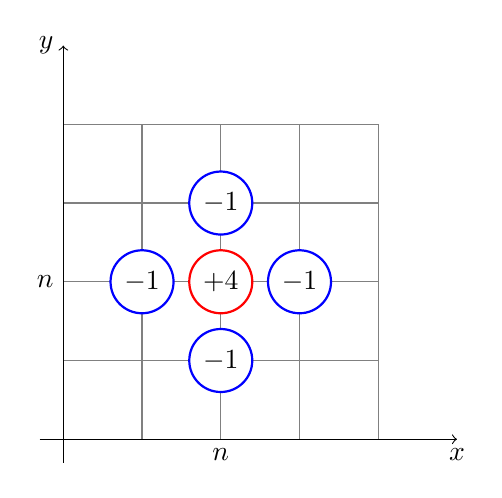
\begin{tikzpicture}
	\draw [step=1,gray] (0,0) grid (4,4);
	\draw [->](-0.3,0) -- (5,0) node [below] {$x$};
	\draw [->](0,-0.3) -- (0,5) node [left] {$y$};
	\draw (0,2) node[left] {$n$} (2,0) node[below] {$n$};
	\draw [red,thick,fill=white] (2,2) circle (0.4) node[black] {$+4$};
	\draw [blue,thick,fill=white](1,2) circle (0.4) node[black] {$-1$};
	\draw [blue,thick,fill=white](3,2) circle (0.4) node[black] {$-1$};
	\draw [blue,thick,fill=white](2,1) circle (0.4) node[black] {$-1$};
	\draw [blue,thick,fill=white](2,3) circle (0.4) node[black] {$-1$};
\end{tikzpicture}
\caption{Illustration of the 5-point stencil on an $n\times n$ grid}
\label{fig:grid}
\end{figure}

\subsection{Diagonalization}
Let 
\begin{equation}
	U = \begin{pmatrix}
	u_{1,1} & \cdots & u_{1,n-1} \\
	\vdots & \ddots& \vdots \\
	u_{n-1,1} & \cdots & u_{n-1,n-1}
	\end{pmatrix}
\end{equation}
and
\begin{equation}
	\label{eq:Tmatrix}
	T = \begin{pmatrix}
	2		&	-1		&	0		&	\cdots	&	0		\\
	-1		&	2		&	-1		&			&	\vdots	\\
	0		&			&	\ddots	&			&	0		\\
	\vdots	&			&		-1	&	2		&	-1		\\
	0		&	\cdots	&	0		&	-1		&	2	
	\end{pmatrix}
\end{equation}
Then
\begin{equation}
	(TU)_{i,j} = \begin{cases}  2u_{i,j} - u_{i+1,j} & i = 1, \\
	-u_{i-1,j} + 2u_{i,j} - u_{i+1,j}  & 2 \leq i \leq n-2, \\
	-u_{i-1,j} + 2u_{i,j}  & i = n-1.
	\end{cases}
\end{equation}
thus equation \eqref{eq:discLap} can be expressed as
\[
	\frac{1}{h^2}(TU+UT)_{i,j} = f_{i,j} \quad \text{for} \quad 1\leq i,j \leq n-1,
\]
or more compact as
\begin{equation}
	\label{eq:TUUTG}
	TU+UT = G,
\end{equation}
where
\begin{equation*}
	G = h^2\begin{pmatrix}
	f_{1,1} 	& \cdots	& f_{1,n-1} \\
	\vdots		& \ddots	& \vdots \\
	f_{n-1,1}	& \cdots	& f_{n-1,n-1}
	\end{pmatrix}
\end{equation*}

Since $T$ is a symmetric matrix it can be diagonalized, this means that it can be written on the form
\begin{equation}
	\label{eq:TQLQ}
	T = Q\Lambda Q^T,
\end{equation}
where $Q=[q_1|q_2|\dots|q_{n-1}]$ is an orthonormal matrix containing the normalized eigenvectors $q_i$, $1\leq i \leq n-1$ of $T$ and $\Lambda$ is a matrix containing the corresponding eigenvalues $\lambda_i$ along its diagonal.

Combining equations \eqref{eq:TUUTG} and \eqref{eq:TQLQ} and multiplying with $Q^T$ from the right and with $Q$ from the left results in
\begin{equation}
	\Lambda \underbrace{Q^TUQ}_{\widetilde{U}} + \underbrace{Q^TUQ}_{\widetilde{U}}\Lambda = \underbrace{Q^TGQ}_{\widetilde{G}}.
\end{equation}

Hence, \eqref{eq:TUUTG} may be solved in three steps:
\begin{enumerate}
	\item[\textbf{Step 1)}]	Compute 
		\begin{align*}
			\widetilde{G} &= Q^TGQ &\mathcal{O}(n^3) \quad\text{operations}
		\end{align*}
	\item[\textbf{Step 2)}]	Solve 
		\begin{equation*}
			\Lambda\widetilde{U}+\widetilde{U}\Lambda = \widetilde{G}
		\end{equation*}
							for $\widetilde{U}$, which boils down to solving 
		\begin{align*}
			\widetilde{u}_{i,j} &= \frac{\widetilde{g}_{i,j}}{\lambda_i + \lambda_j} &\mathcal{O}(n^2) \quad\text{operations}
		\end{align*}
	\item[\textbf{Step 3)}]	Compute 
		\begin{align*}
			U &= Q\widetilde{U}Q^T &\mathcal{O}(n^3) \quad\text{operations}
		\end{align*}			
\end{enumerate}
Here $\widetilde{G},G,Q,T,\Lambda,\widetilde{U}$ and $U$ are all $(n-1)\times(n-1)$ real matrices.

\subsection{Eigenvalues and eigenvectors}
Define the vectors $\widetilde{q}_i$ as
\begin{equation}
	\label{eq:eigvec}
	(\widetilde{q}_j)_i = \sin\left(\frac{ij\pi}{n}\right)
\end{equation}
and observe that $T$ as defined in \eqref{eq:Tmatrix} operated on $(\widetilde{q}_j)_i$ gives
\begin{equation}
	(T\widetilde{q}_j)_i = \underbrace{2\left(1-\cos\left(\frac{j\pi}{n}\right)\right)}_{\lambda_j}\underbrace{\sin\left(\frac{ij\pi}{n}\right)}_{(\widetilde{q}_j)_i}.
\end{equation}
Thus the vectors $\widetilde{q}_i$ defined in \eqref{eq:eigvec} are eigenvectors for the matrix $T$ with corresponding eigenvalues $\lambda_j$.

Normalized eigenvectors $q_i$ can be represented as 
\begin{equation}
	\label{eq:normeigvec}
	(q_j)_i = \sqrt{\frac{2}{n}}\sin\left(\frac{ij\pi}{n}\right).
\end{equation} 
Using these vectors as columns in a matrix yields the requsted orthonormal matrix $Q$ in equation \eqref{eq:TQLQ}. Also note that
\begin{equation}
	\label{eq:Q}
	Q = Q^T = Q^{-1}
\end{equation}
	

\subsection{Discrete Sine transform}
The discrete sine transform (DST) of a vector $v=[v_1,v_2,\dots,v_{n-1}]$ is defined as
\begin{equation}
	\label{eq:DST}
	\tilde{v}_j = \sum_{i=1}^{n-1}v_i\sin\left(\frac{ij\pi}{n}\right), \qquad j \in \{1,2,\dots,n\},
\end{equation}
this can be expressed as 
\begin{equation}
	\label{eq:DSTfunc}
	\tilde{v} = S(v)
\end{equation}
	
while the inverse discrete sine transform of $\tilde{v}$ can be expressed as
\begin{equation}
	\label{eq:DSTfunciv}
	v = S^{-1}(\tilde{v}).
\end{equation}
	
$S$ and $S^{-1}$ are related as
\[
	S = \frac{2}{n}S^{-1}
\]
Observe that the matrix $Q$ is a scaled version of the DST:
\begin{equation}
	\label{eq:QS}
	Q = \sqrt{\frac{n}{2}}S = \sqrt{\frac{2}{n}}S^{-1}
\end{equation}
By utilising the Fast Fourier Transform, equation \eqref{eq:DSTfunc} and \eqref{eq:DSTfunciv} can be solved in $\mathcal{O}(n\log n)$ instead of $\mathcal{O}(n^2)$ as by conventional matrix vector multiplication.

Considering step 1 computing $\widetilde{G} = Q^TGQ$, taking the transpose and using the properties stated in \eqref{eq:Q}, this can be rewritten as
\begin{align*}
	\widetilde{G}^T	&= Q^TG^TQ \\
					&= Q(QG)^T.
\end{align*}
Using \eqref{eq:QS} this can further be rewritten to
\begin{equation}
	\widetilde{G}^T = \sqrt{\frac{2}{n}}S^{-1}\left(\left(\sqrt{\frac{n}{2}}S(G)\right)^T\right) = S^{-1}\left(\left(S(G)\right)^T\right).
\end{equation}
In a similar fashion, step 3 can be rewritten as
\begin{align*}
	U	&= Q\widetilde{U}Q^T \\
		&= Q(Q\widetilde{U}^T)^T \\
		&= S^{-1}\left((S(\widetilde{U}^T))^T\right)
\end{align*}

\newpage
\section{Implementation}
\subsection{Overview}
The new solution strategy can then be summarized as follows
\begin{enumerate}
	\item[\textbf{Step 1)}] Compute
		\begin{align*}
		\widetilde{G}^T &=S^{-1}\left(\left(S(G)\right)^T\right)	&\mathcal{O}(n^2\log n) \quad\text{operations}
		\end{align*}
	\item[\textbf{Step 2)}]	Solve 
		\begin{align*}
			\widetilde{u}_{j,i} &= \frac{\widetilde{g}_{j,i}}{\lambda_j + \lambda_i} &\mathcal{O}(n^2) \quad\text{operations}
		\end{align*}
	\item[\textbf{Step 3)}] Compute
		\begin{align*}
			U &= S^{-1}\left((S(\widetilde{U}^T))^T\right)	&\mathcal{O}(n^2\log n) \quad\text{operations}
		\end{align*}
\end{enumerate}
which is then implemented in C using a black-box fortran script for the DST. 

The OpenMP and MPI libraries are used to help parallelize the code for use on a supercomputer. The program architecture (fig. \ref{fig:architecture}) is constructed to be load balanced where each MPI-process gets a share of the problem to solve. The shares may be slightly uneven distributed depening on if the problem size is divisible by the amount of MPI-processes or not, e.g. a problem size of $n=512$ ($511^2$ grid points) divded among three MPI-processes results in one processor getting $171$ columns, while the other two get $170$ columns. This is only a difference of $0.6\%$ of the total elements and therefore neglible. The OpenMP threads spawned by each MPI-process is done by calls to the \textit{\#pragma} compiler directives.

\begin{figure}[h]
\centering
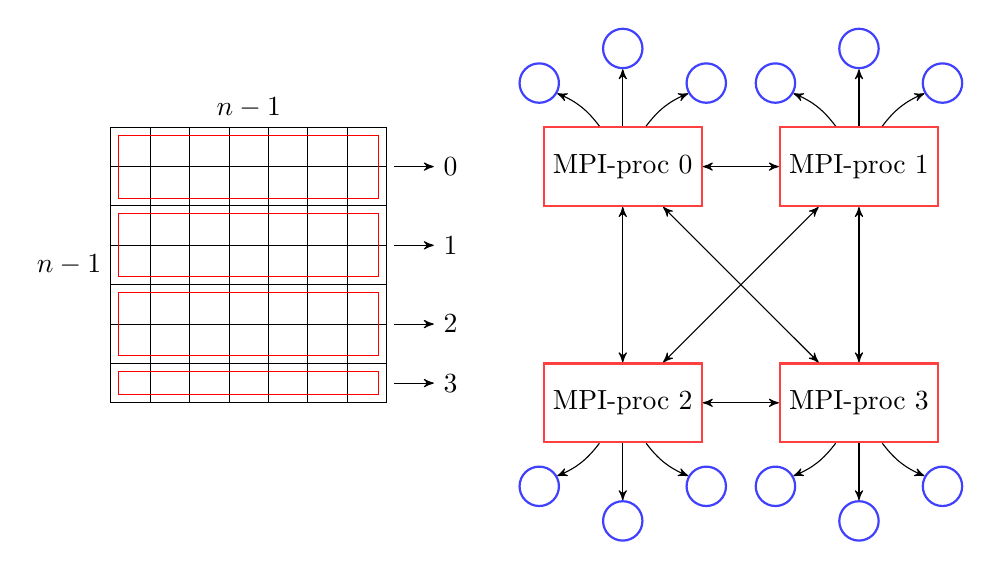
\begin{tikzpicture}[node distance=1.5cm,>=stealth',bend angle=15,auto]
	\tikzstyle{node} = [rectangle,thick,draw=red!75,minimum size=1cm]
	\tikzstyle{proc} = [circle,thick,draw=blue!75,minimum size=0.5cm]
	\draw [step=.5] (-3.5,-1.5) grid (0,2);
	\draw (-3.5,0.25) node [left] {$n-1$} (-1.75,2) node [above] {$n-1$};
	\draw [red] (-3.4,1.1) rectangle (-0.1,1.9);
		\draw [->] (0.1,1.5) -- (0.6,1.5) node [right] {0};
	\draw [red] (-3.4,0.1) rectangle (-0.1,0.9);
		\draw [->] (0.1,0.5) -- (0.6,0.5) node [right] {1};
	\draw [red] (-3.4,-0.9) rectangle (-0.1,-0.1);
		\draw [->] (0.1,-0.5) -- (0.6,-0.5) node [right] {2};
	\draw [red] (-3.4,-1.4) rectangle (-0.1,-1.1);
		\draw [->] (0.1,-1.25) -- (0.6,-1.25) node [right] {3};
	\draw (3,1.5) node (a) [node] {MPI-proc 0};
		\node [proc] [above left of=a] {} edge [<-,bend left] (a);
		\node [proc] [above right of=a] {} edge [<-,bend right] (a);
		\node [proc] [above of=a] {} edge [<-] (a);
	\draw (6,1.5) node (b) [node] {MPI-proc 1};
		\node [proc] [above left of=b] {} edge [<-,bend left] (b);
		\node [proc] [above right of=b] {} edge [<-,bend right] (b);
		\node [proc] [above of=b] {} edge [<-] (b);
	\draw (3,-1.5) node (c) [node] {MPI-proc 2};
		\node [proc] [below left of=c] {} edge [<-,bend right] (c);
		\node [proc] [below right of=c] {} edge [<-,bend left] (c);
		\node [proc] [below of=c] {} edge [<-] (c);
	\draw (6,-1.5) node (d) [node] {MPI-proc 3};
		\node [proc] [below left of=d] {} edge [<-,bend right] (d);
		\node [proc] [below right of=d] {} edge [<-,bend left] (d);
		\node [proc] [below of=d] {} edge [<-] (d);
	\path [<->] (a) edge (b) edge (c) edge (d);
	\path [<->] (c) edge (d) edge (b);
	\path [<->] (b) edge (d);
\end{tikzpicture}
\caption{Illustration of the program architecture. The left shows how the grid is split up among the MPI-processes, notice that there's an uneven distribution since $7^2$ is not divisible by $4$. The right figure shows how each MPI-process spawns three thread of its own and that each MPI-process communicates with all the other MPI-processes. The number of threads spawned by each MPI-process is arbitrary.}
\label{fig:architecture}
\end{figure}

\subsubsection{Transpose}
In order to perform the transpose operation all the MPI-processes need to communicate with each other, in order to simplify this procedure every MPI-process keep track of who owns which rows and what their displacements are so as to know where to send its data once the transpose operations is called upon. This is accomplished by using the command \textit{MPI\_Alltoallv} and packing and unpacking the buffer correctly. A schematical layout of how this is done can be viewed in figure \ref{fig:transpose}.

The C code listing for the transpose can be found in the appendix.

\begin{figure}
\centering
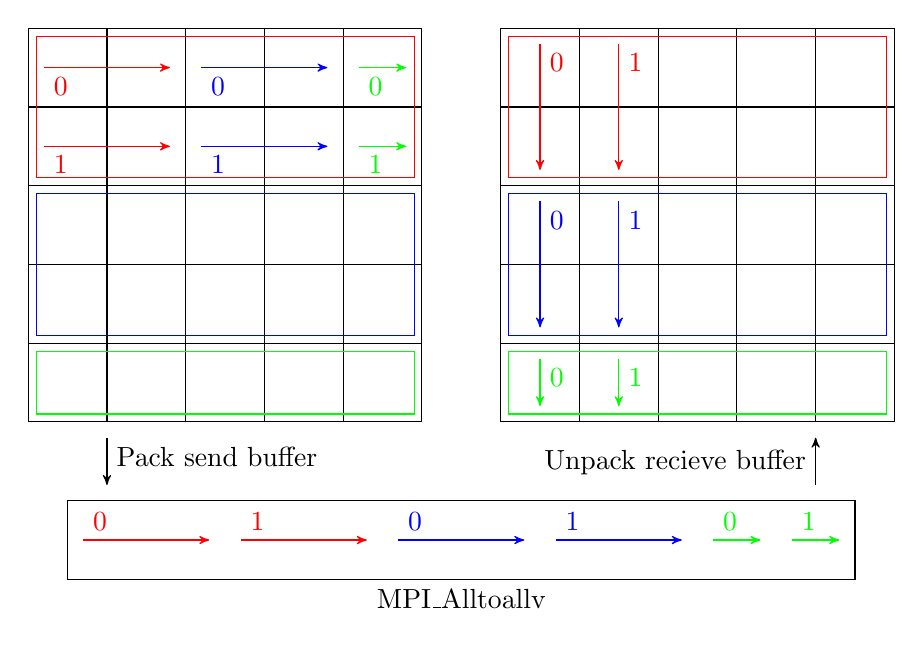
\begin{tikzpicture}[>=stealth']
	\draw [step=1] (0,0) grid (5,5);
	\draw [red] (0.1,3.1) rectangle (4.9,4.9);
	\draw [blue] (0.1,1.1) rectangle (4.9,2.9);
	\draw [green] (0.1,0.1) rectangle (4.9,0.9);
		\path [red,->] (0.2,4.5) edge (1.8,4.5) node [below right] {0};
		\path [red,->] (0.2,3.5) edge (1.8,3.5) node [below right] {1};
		\path [blue,->] (2.2,4.5) edge (3.8,4.5) node [below right] {0};
		\path [blue,->] (2.2,3.5) edge (3.8,3.5) node [below right] {1};
		\path [green,->] (4.2,4.5) edge (4.8,4.5) node [below right] {0};
		\path [green,->] (4.2,3.5) edge (4.8,3.5) node [below right] {1};
		\path [->] (1,-0.2) edge (1,-0.8) node [below right] {Pack send buffer};
	\draw (0.5,-2) rectangle (10.5,-1);
		\path [red,->] (0.7,-1.5) edge (2.3,-1.5) node [above right] {0};
		\path [red,->] (2.7,-1.5) edge (4.3,-1.5) node [above right] {1};
		\path [blue,->] (4.7,-1.5) edge (6.3,-1.5) node [above right] {0};
		\path [blue,->] (6.7,-1.5) edge (8.3,-1.5) node [above right] {1};	
		\path [green,->] (8.7,-1.5) edge (9.3,-1.5) node [above right] {0};
		\path [green,->] (9.7,-1.5) edge (10.3,-1.5) node [above right] {1};
	\draw [step=1] (6,0) grid (11,5);
	\draw [red] (6.1,3.1) rectangle (10.9,4.9);
	\draw [blue] (6.1,1.1) rectangle (10.9,2.9);
	\draw [green] (6.1,0.1) rectangle (10.9,0.9);
		\path [->] (10,-0.8) edge (10,-0.2) node [above left] {Unpack recieve buffer};
		\path [red,->] (6.5,4.8) edge (6.5,3.2) node [below right] {0};
		\path [red,->] (7.5,4.8) edge (7.5,3.2) node [below right] {1};
		\path [blue,->] (6.5,2.8) edge (6.5,1.2) node [below right] {0};
		\path [blue,->] (7.5,2.8) edge (7.5,1.2) node [below right] {1};
		\path [green,->] (6.5,0.8) edge (6.5,0.2) node [below right] {0};
		\path [green,->] (7.5,0.8) edge (7.5,0.2) node [below right] {1};
	\path (5.5,-2) edge (6,-2) node [below] {MPI\_Alltoallv};	
\end{tikzpicture}
\caption{A schematical layout of how the transpose operation is carried out over the MPI-processes.}
\label{fig:transpose}
\end{figure}

\newpage
\section{Numerical results and performance analysis}
\subsection{Hardware}
All the numerical results are obtained by running the program on the high performance computer \textit{kongull}. 

Kongull consist of 93 compute nodes, of which 44 nodes have 48 GiB each, while the other 49 nodes have 24 GiB of memory. Each node consists of a HP DL165 G6 server with 2 6-core 2.4 GHz AMD Opteron 2431 (Istanbul) processors, with 6 512 KiB L1 cache and a common 6 MiB L3-cache. The difference in memory is of low concern for this report as the program will not exceed 7 GiB memory on a single node. Assuming a problem size of $n=16384=2^{14}$ the memory requirements for storing the matrix is $8\text{ Bytes}\cdot (2^{14})^2 = 2^{31} \text{ Bytes} = 2 \text{ GiB}$. While doing the transpose memory requirement will peak at triple this because both the send and recieve buffers need room to store the matrix. The other variables stored are neglible compared to this as they have memory requirements of at most $\mathcal{O}(n)$. Estimating a generous 1 GiB for the rest of the variables should therefore be more than enough, and hence 24 GiB of memory or more is never obtained.

The internal network of the kongull cluster is based on a fat tree layout, with slower connections towards the \textit{leaves} of the connection tree. Each login- and I/O-node is connected to a central switch, HP ProCurve 6600-24XG, with 10GbE SPF+ connectors. Two rack switches, ProCurve 2910al-48G are connected to the central switch with 10GbE SPF+ connectors. Each compute node is connected to a rack switch with 1Gb Ethernet network connection to the outside world, via two SR tranceivers on the central switch.\cite{kongull}
Network latency is expected to be a bottleneck for the solver.

The program was compiled using the intel compiler version 11.1.059 and a cmake script with the option \textit{-DCMAKE\_BUILD\_TYPE=Release}

\subsection{Numerical results}
The numerical tests were performed on \textit{kongull} using different amount of nodes ($N$), MPI-processes per node ($M$) and threads per MPI-process ($T_M$) which gives a total of $P=N\times M\times T_M$ processors used. The seed function used was
\begin{equation*}
	f(x,y) = 5\pi^2\cdot\sin(\pi x)\cdot\sin(2\pi y)
\end{equation*}
which has the analytical solution
\begin{equation*}
	u(x,y) = \sin(\pi x)\cdot\sin(2\pi y)
\end{equation*}
for the poisson equation (eq. \eqref{eq:poisson}). This makes it possible to check for convergence issues by comparing the numerical results to the analytical solution. A series of preliminary test runs with different combinations of nodes and MPI-processes per node were made on kongull, some of the results are summarized in table \ref{tab:errorresults}. 

\begin{table}[hb]
	\centering
	\caption{Select runs of two different combinations of nodes ($N$), MPI-processes per node ($M$) and threads per MPI-process ($T_M$) for different problem sizes $n$. }
	\label{tab:errorresults}
	\begin{tabular}{r||c|c|c||c|c|c}
\multicolumn{1}{c}{}& \multicolumn{3}{c||}{$N=1$, $M=1$, $T_M=6$, $P=6$}&\multicolumn{3}{c}{$N=3$, $M=2$, $T_M=6$, $P=36$} \\
\hline
$n$ & Error & $\tau$ [s]& ${\tau}/{n^2\log(n)}$ [s]& Error & $\tau$ [s]& ${\tau}/{n^2\log(n)}$ [s]\\ 
\hline
32		& $2.73\cdot10^{-3}$ & $3.59\cdot10^{-4}$ & $7.01\cdot10^{-8}$ & $2.73\cdot10^{-3}$ 	& $4.42\cdot10^{-2}$	&  $8.64\cdot10^{-6}$\\ 

256		& $4.27\cdot10^{-5}$ & $2.26\cdot10^{-2}$ & $4.31\cdot10^{-8} $ & $4.27\cdot10^{-5}$ 	& $2.87\cdot10^{-2}$	&  $5.47\cdot10^{-8}$\\ 

2048	& $6.67\cdot10^{-7}$ & $2.00\cdot10^{+0} $ & $4.33\cdot10^{-8} $ & $6.67\cdot10^{-7}$	& $6.39\cdot10^{-1} $	&  $1.39\cdot10^{-8}$\\ 

16384	& $8.89\cdot10^{-9}$ & $1.64\cdot10^{+2} $ & $4.36\cdot10^{-8} $ & $8.89\cdot10^{-9}$	& $3.67\cdot10^{+1}$	&  $9.77\cdot10^{-9}$\\ 
	\end{tabular} 
\end{table}

\subsubsection{Verification of correctness}
A plot of the error as a function of problem size (fig. \ref{fig:error}) shows that the error decreases proprotional to $n^{-2}$, which is consistent with the error decreasing as $\mathcal{O}(h^2)$ since $h$ is inversely proportional to $n$. It can therefore be concluded that there are no convergence issues with the solver.

\begin{figure}[tbp]
	\centering
	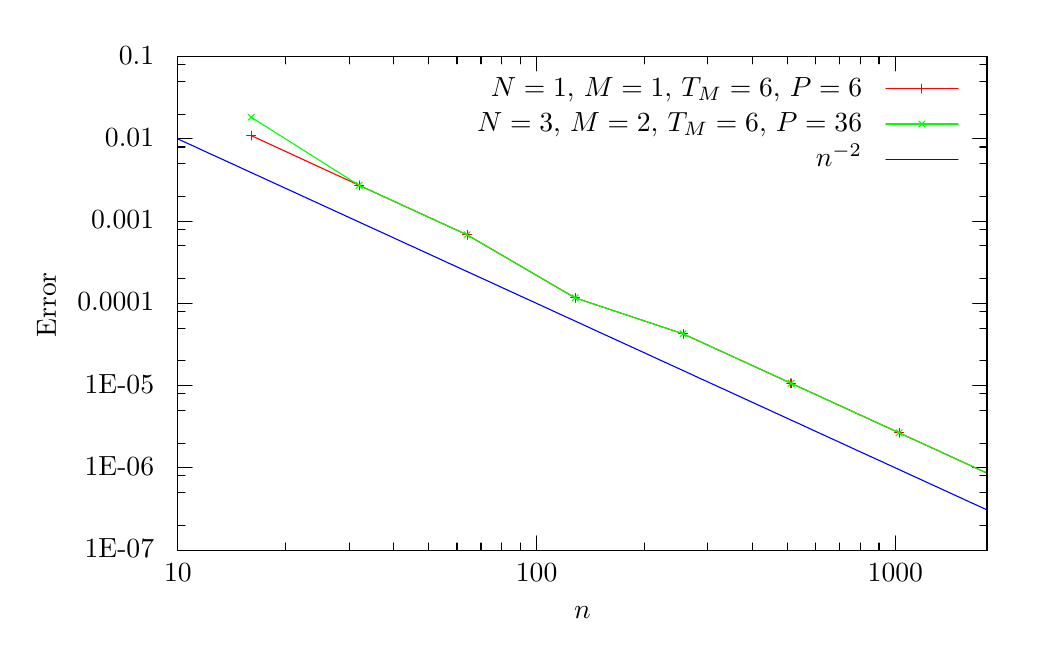
\begin{tikzpicture}[gnuplot]
%% generated with GNUPLOT 4.6p0 (Lua 5.1; terminal rev. 99, script rev. 100)
%% Sat 13 Apr 2013 11:03:34 PM BST
\gpsolidlines
\path (0.000,0.000) rectangle (12.700,7.620);
\gpcolor{color=gp lt color border}
\gpsetlinetype{gp lt border}
\gpsetlinewidth{1.00}
\draw[gp path] (1.872,0.985)--(2.052,0.985);
\draw[gp path] (12.147,0.985)--(11.967,0.985);
\node[gp node right] at (1.688,0.985) {1E-07};
\draw[gp path] (1.872,1.299)--(1.962,1.299);
\draw[gp path] (12.147,1.299)--(12.057,1.299);
\draw[gp path] (1.872,1.715)--(1.962,1.715);
\draw[gp path] (12.147,1.715)--(12.057,1.715);
\draw[gp path] (1.872,1.928)--(1.962,1.928);
\draw[gp path] (12.147,1.928)--(12.057,1.928);
\draw[gp path] (1.872,2.029)--(2.052,2.029);
\draw[gp path] (12.147,2.029)--(11.967,2.029);
\node[gp node right] at (1.688,2.029) {1E-06};
\draw[gp path] (1.872,2.344)--(1.962,2.344);
\draw[gp path] (12.147,2.344)--(12.057,2.344);
\draw[gp path] (1.872,2.759)--(1.962,2.759);
\draw[gp path] (12.147,2.759)--(12.057,2.759);
\draw[gp path] (1.872,2.972)--(1.962,2.972);
\draw[gp path] (12.147,2.972)--(12.057,2.972);
\draw[gp path] (1.872,3.074)--(2.052,3.074);
\draw[gp path] (12.147,3.074)--(11.967,3.074);
\node[gp node right] at (1.688,3.074) {1E-05};
\draw[gp path] (1.872,3.388)--(1.962,3.388);
\draw[gp path] (12.147,3.388)--(12.057,3.388);
\draw[gp path] (1.872,3.804)--(1.962,3.804);
\draw[gp path] (12.147,3.804)--(12.057,3.804);
\draw[gp path] (1.872,4.017)--(1.962,4.017);
\draw[gp path] (12.147,4.017)--(12.057,4.017);
\draw[gp path] (1.872,4.118)--(2.052,4.118);
\draw[gp path] (12.147,4.118)--(11.967,4.118);
\node[gp node right] at (1.688,4.118) {0.0001};
\draw[gp path] (1.872,4.432)--(1.962,4.432);
\draw[gp path] (12.147,4.432)--(12.057,4.432);
\draw[gp path] (1.872,4.848)--(1.962,4.848);
\draw[gp path] (12.147,4.848)--(12.057,4.848);
\draw[gp path] (1.872,5.061)--(1.962,5.061);
\draw[gp path] (12.147,5.061)--(12.057,5.061);
\draw[gp path] (1.872,5.162)--(2.052,5.162);
\draw[gp path] (12.147,5.162)--(11.967,5.162);
\node[gp node right] at (1.688,5.162) {0.001};
\draw[gp path] (1.872,5.477)--(1.962,5.477);
\draw[gp path] (12.147,5.477)--(12.057,5.477);
\draw[gp path] (1.872,5.892)--(1.962,5.892);
\draw[gp path] (12.147,5.892)--(12.057,5.892);
\draw[gp path] (1.872,6.105)--(1.962,6.105);
\draw[gp path] (12.147,6.105)--(12.057,6.105);
\draw[gp path] (1.872,6.207)--(2.052,6.207);
\draw[gp path] (12.147,6.207)--(11.967,6.207);
\node[gp node right] at (1.688,6.207) {0.01};
\draw[gp path] (1.872,6.521)--(1.962,6.521);
\draw[gp path] (12.147,6.521)--(12.057,6.521);
\draw[gp path] (1.872,6.937)--(1.962,6.937);
\draw[gp path] (12.147,6.937)--(12.057,6.937);
\draw[gp path] (1.872,7.150)--(1.962,7.150);
\draw[gp path] (12.147,7.150)--(12.057,7.150);
\draw[gp path] (1.872,7.251)--(2.052,7.251);
\draw[gp path] (12.147,7.251)--(11.967,7.251);
\node[gp node right] at (1.688,7.251) {0.1};
\draw[gp path] (1.872,0.985)--(1.872,1.165);
\draw[gp path] (1.872,7.251)--(1.872,7.071);
\node[gp node center] at (1.872,0.677) { 10};
\draw[gp path] (3.243,0.985)--(3.243,1.075);
\draw[gp path] (3.243,7.251)--(3.243,7.161);
\draw[gp path] (4.046,0.985)--(4.046,1.075);
\draw[gp path] (4.046,7.251)--(4.046,7.161);
\draw[gp path] (4.615,0.985)--(4.615,1.075);
\draw[gp path] (4.615,7.251)--(4.615,7.161);
\draw[gp path] (5.057,0.985)--(5.057,1.075);
\draw[gp path] (5.057,7.251)--(5.057,7.161);
\draw[gp path] (5.417,0.985)--(5.417,1.075);
\draw[gp path] (5.417,7.251)--(5.417,7.161);
\draw[gp path] (5.722,0.985)--(5.722,1.075);
\draw[gp path] (5.722,7.251)--(5.722,7.161);
\draw[gp path] (5.986,0.985)--(5.986,1.075);
\draw[gp path] (5.986,7.251)--(5.986,7.161);
\draw[gp path] (6.220,0.985)--(6.220,1.075);
\draw[gp path] (6.220,7.251)--(6.220,7.161);
\draw[gp path] (6.428,0.985)--(6.428,1.165);
\draw[gp path] (6.428,7.251)--(6.428,7.071);
\node[gp node center] at (6.428,0.677) { 100};
\draw[gp path] (7.799,0.985)--(7.799,1.075);
\draw[gp path] (7.799,7.251)--(7.799,7.161);
\draw[gp path] (8.602,0.985)--(8.602,1.075);
\draw[gp path] (8.602,7.251)--(8.602,7.161);
\draw[gp path] (9.171,0.985)--(9.171,1.075);
\draw[gp path] (9.171,7.251)--(9.171,7.161);
\draw[gp path] (9.612,0.985)--(9.612,1.075);
\draw[gp path] (9.612,7.251)--(9.612,7.161);
\draw[gp path] (9.973,0.985)--(9.973,1.075);
\draw[gp path] (9.973,7.251)--(9.973,7.161);
\draw[gp path] (10.278,0.985)--(10.278,1.075);
\draw[gp path] (10.278,7.251)--(10.278,7.161);
\draw[gp path] (10.542,0.985)--(10.542,1.075);
\draw[gp path] (10.542,7.251)--(10.542,7.161);
\draw[gp path] (10.776,0.985)--(10.776,1.075);
\draw[gp path] (10.776,7.251)--(10.776,7.161);
\draw[gp path] (10.984,0.985)--(10.984,1.165);
\draw[gp path] (10.984,7.251)--(10.984,7.071);
\node[gp node center] at (10.984,0.677) { 1000};
\draw[gp path] (1.872,7.251)--(1.872,0.985)--(12.147,0.985)--(12.147,7.251)--cycle;
\node[gp node center,rotate=-270] at (0.246,4.118) {Error};
\node[gp node center] at (7.009,0.215) {$n$};
\node[gp node right] at (10.679,6.846) {$N=1$, $M=1$, $T_M=6$, $P=6$};
\gpcolor{color=gp lt color 0}
\gpsetlinetype{gp lt plot 0}
\draw[gp path] (10.863,6.846)--(11.779,6.846);
\draw[gp path] (2.802,6.250)--(4.173,5.618)--(5.545,4.989)--(6.916,4.189)--(8.288,3.732)%
  --(9.659,3.104)--(11.031,2.475)--(12.147,1.963);
\gpsetpointsize{4.00}
\gppoint{gp mark 1}{(2.802,6.250)}
\gppoint{gp mark 1}{(4.173,5.618)}
\gppoint{gp mark 1}{(5.545,4.989)}
\gppoint{gp mark 1}{(6.916,4.189)}
\gppoint{gp mark 1}{(8.288,3.732)}
\gppoint{gp mark 1}{(9.659,3.104)}
\gppoint{gp mark 1}{(11.031,2.475)}
\gppoint{gp mark 1}{(11.321,6.846)}
\gpcolor{color=gp lt color border}
\node[gp node right] at (10.679,6.396) {$N=3$, $M=2$, $T_M=6$, $P=36$};
\gpcolor{color=gp lt color 1}
\gpsetlinetype{gp lt plot 1}
\draw[gp path] (10.863,6.396)--(11.779,6.396);
\draw[gp path] (2.802,6.483)--(4.173,5.618)--(5.545,4.989)--(6.916,4.189)--(8.288,3.732)%
  --(9.659,3.104)--(11.031,2.475)--(12.147,1.963);
\gppoint{gp mark 2}{(2.802,6.483)}
\gppoint{gp mark 2}{(4.173,5.618)}
\gppoint{gp mark 2}{(5.545,4.989)}
\gppoint{gp mark 2}{(6.916,4.189)}
\gppoint{gp mark 2}{(8.288,3.732)}
\gppoint{gp mark 2}{(9.659,3.104)}
\gppoint{gp mark 2}{(11.031,2.475)}
\gppoint{gp mark 2}{(11.321,6.396)}
\gpcolor{color=gp lt color border}
\node[gp node right] at (10.679,5.946) {$n^{-2}$};
\gpcolor{color=gp lt color 2}
\gpsetlinetype{gp lt plot 2}
\draw[gp path] (10.863,5.946)--(11.779,5.946);
\draw[gp path] (1.872,6.207)--(1.976,6.159)--(2.080,6.112)--(2.183,6.064)--(2.287,6.016)%
  --(2.391,5.969)--(2.495,5.921)--(2.599,5.874)--(2.702,5.826)--(2.806,5.778)--(2.910,5.731)%
  --(3.014,5.683)--(3.117,5.636)--(3.221,5.588)--(3.325,5.541)--(3.429,5.493)--(3.533,5.445)%
  --(3.636,5.398)--(3.740,5.350)--(3.844,5.303)--(3.948,5.255)--(4.052,5.207)--(4.155,5.160)%
  --(4.259,5.112)--(4.363,5.065)--(4.467,5.017)--(4.570,4.970)--(4.674,4.922)--(4.778,4.874)%
  --(4.882,4.827)--(4.986,4.779)--(5.089,4.732)--(5.193,4.684)--(5.297,4.636)--(5.401,4.589)%
  --(5.505,4.541)--(5.608,4.494)--(5.712,4.446)--(5.816,4.399)--(5.920,4.351)--(6.024,4.303)%
  --(6.127,4.256)--(6.231,4.208)--(6.335,4.161)--(6.439,4.113)--(6.542,4.066)--(6.646,4.018)%
  --(6.750,3.970)--(6.854,3.923)--(6.958,3.875)--(7.061,3.828)--(7.165,3.780)--(7.269,3.732)%
  --(7.373,3.685)--(7.477,3.637)--(7.580,3.590)--(7.684,3.542)--(7.788,3.495)--(7.892,3.447)%
  --(7.995,3.399)--(8.099,3.352)--(8.203,3.304)--(8.307,3.257)--(8.411,3.209)--(8.514,3.161)%
  --(8.618,3.114)--(8.722,3.066)--(8.826,3.019)--(8.930,2.971)--(9.033,2.924)--(9.137,2.876)%
  --(9.241,2.828)--(9.345,2.781)--(9.449,2.733)--(9.552,2.686)--(9.656,2.638)--(9.760,2.591)%
  --(9.864,2.543)--(9.967,2.495)--(10.071,2.448)--(10.175,2.400)--(10.279,2.353)--(10.383,2.305)%
  --(10.486,2.257)--(10.590,2.210)--(10.694,2.162)--(10.798,2.115)--(10.902,2.067)--(11.005,2.020)%
  --(11.109,1.972)--(11.213,1.924)--(11.317,1.877)--(11.420,1.829)--(11.524,1.782)--(11.628,1.734)%
  --(11.732,1.686)--(11.836,1.639)--(11.939,1.591)--(12.043,1.544)--(12.147,1.496);
\gpcolor{color=gp lt color border}
\gpsetlinetype{gp lt border}
\draw[gp path] (1.872,7.251)--(1.872,0.985)--(12.147,0.985)--(12.147,7.251)--cycle;
%% coordinates of the plot area
\gpdefrectangularnode{gp plot 1}{\pgfpoint{1.872cm}{0.985cm}}{\pgfpoint{12.147cm}{7.251cm}}
\end{tikzpicture}
%% gnuplot variables

	\caption{Pointwise error as a function of grid size for two different processor configurations. Notice that the pointwise error for both configurations is proportional to $n^{-2}$ which indicates that there are no convergence issues since the algorithm predicts convergence on the order of $\mathcal{O}(h^2)$ and $h$ is inversely proportional to $n$ in this case.}
	\label{fig:error}
\end{figure}

\subsubsection{Timing}

It is expected that the runtime $\tau$ per $n^2\log n$ for large values of $n$ will approach a constant value as the program is estimated to run in $\mathcal{O}(n^2\log n)$ time. By looking at figure \ref{fig:time1} this appears to be the case. Also note that the addition of more processors actually increases the average time spent calculating each element for small values of $n$, this is due to the increased overhead when using more processors.

\begin{figure}[tbp]
	\centering
	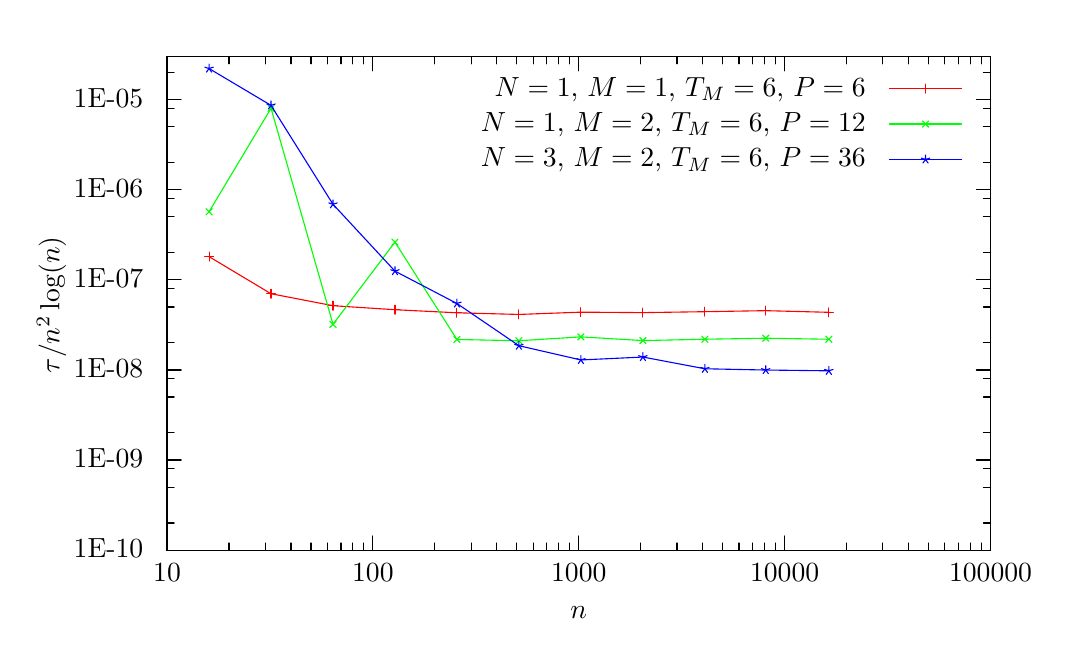
\begin{tikzpicture}[gnuplot]
%% generated with GNUPLOT 4.6p0 (Lua 5.1; terminal rev. 99, script rev. 100)
%% Sat 13 Apr 2013 11:03:14 PM BST
\gpsolidlines
\path (0.000,0.000) rectangle (12.700,7.620);
\gpcolor{color=gp lt color border}
\gpsetlinetype{gp lt border}
\gpsetlinewidth{1.00}
\draw[gp path] (1.688,0.985)--(1.868,0.985);
\draw[gp path] (12.147,0.985)--(11.967,0.985);
\node[gp node right] at (1.504,0.985) {1E-10};
\draw[gp path] (1.688,1.329)--(1.778,1.329);
\draw[gp path] (12.147,1.329)--(12.057,1.329);
\draw[gp path] (1.688,1.785)--(1.778,1.785);
\draw[gp path] (12.147,1.785)--(12.057,1.785);
\draw[gp path] (1.688,2.018)--(1.778,2.018);
\draw[gp path] (12.147,2.018)--(12.057,2.018);
\draw[gp path] (1.688,2.129)--(1.868,2.129);
\draw[gp path] (12.147,2.129)--(11.967,2.129);
\node[gp node right] at (1.504,2.129) {1E-09};
\draw[gp path] (1.688,2.473)--(1.778,2.473);
\draw[gp path] (12.147,2.473)--(12.057,2.473);
\draw[gp path] (1.688,2.929)--(1.778,2.929);
\draw[gp path] (12.147,2.929)--(12.057,2.929);
\draw[gp path] (1.688,3.162)--(1.778,3.162);
\draw[gp path] (12.147,3.162)--(12.057,3.162);
\draw[gp path] (1.688,3.273)--(1.868,3.273);
\draw[gp path] (12.147,3.273)--(11.967,3.273);
\node[gp node right] at (1.504,3.273) {1E-08};
\draw[gp path] (1.688,3.617)--(1.778,3.617);
\draw[gp path] (12.147,3.617)--(12.057,3.617);
\draw[gp path] (1.688,4.073)--(1.778,4.073);
\draw[gp path] (12.147,4.073)--(12.057,4.073);
\draw[gp path] (1.688,4.306)--(1.778,4.306);
\draw[gp path] (12.147,4.306)--(12.057,4.306);
\draw[gp path] (1.688,4.417)--(1.868,4.417);
\draw[gp path] (12.147,4.417)--(11.967,4.417);
\node[gp node right] at (1.504,4.417) {1E-07};
\draw[gp path] (1.688,4.761)--(1.778,4.761);
\draw[gp path] (12.147,4.761)--(12.057,4.761);
\draw[gp path] (1.688,5.217)--(1.778,5.217);
\draw[gp path] (12.147,5.217)--(12.057,5.217);
\draw[gp path] (1.688,5.450)--(1.778,5.450);
\draw[gp path] (12.147,5.450)--(12.057,5.450);
\draw[gp path] (1.688,5.561)--(1.868,5.561);
\draw[gp path] (12.147,5.561)--(11.967,5.561);
\node[gp node right] at (1.504,5.561) {1E-06};
\draw[gp path] (1.688,5.906)--(1.778,5.906);
\draw[gp path] (12.147,5.906)--(12.057,5.906);
\draw[gp path] (1.688,6.361)--(1.778,6.361);
\draw[gp path] (12.147,6.361)--(12.057,6.361);
\draw[gp path] (1.688,6.594)--(1.778,6.594);
\draw[gp path] (12.147,6.594)--(12.057,6.594);
\draw[gp path] (1.688,6.705)--(1.868,6.705);
\draw[gp path] (12.147,6.705)--(11.967,6.705);
\node[gp node right] at (1.504,6.705) {1E-05};
\draw[gp path] (1.688,7.050)--(1.778,7.050);
\draw[gp path] (12.147,7.050)--(12.057,7.050);
\draw[gp path] (1.688,0.985)--(1.688,1.165);
\draw[gp path] (1.688,7.251)--(1.688,7.071);
\node[gp node center] at (1.688,0.677) { 10};
\draw[gp path] (2.475,0.985)--(2.475,1.075);
\draw[gp path] (2.475,7.251)--(2.475,7.161);
\draw[gp path] (2.936,0.985)--(2.936,1.075);
\draw[gp path] (2.936,7.251)--(2.936,7.161);
\draw[gp path] (3.262,0.985)--(3.262,1.075);
\draw[gp path] (3.262,7.251)--(3.262,7.161);
\draw[gp path] (3.516,0.985)--(3.516,1.075);
\draw[gp path] (3.516,7.251)--(3.516,7.161);
\draw[gp path] (3.723,0.985)--(3.723,1.075);
\draw[gp path] (3.723,7.251)--(3.723,7.161);
\draw[gp path] (3.898,0.985)--(3.898,1.075);
\draw[gp path] (3.898,7.251)--(3.898,7.161);
\draw[gp path] (4.049,0.985)--(4.049,1.075);
\draw[gp path] (4.049,7.251)--(4.049,7.161);
\draw[gp path] (4.183,0.985)--(4.183,1.075);
\draw[gp path] (4.183,7.251)--(4.183,7.161);
\draw[gp path] (4.303,0.985)--(4.303,1.165);
\draw[gp path] (4.303,7.251)--(4.303,7.071);
\node[gp node center] at (4.303,0.677) { 100};
\draw[gp path] (5.090,0.985)--(5.090,1.075);
\draw[gp path] (5.090,7.251)--(5.090,7.161);
\draw[gp path] (5.550,0.985)--(5.550,1.075);
\draw[gp path] (5.550,7.251)--(5.550,7.161);
\draw[gp path] (5.877,0.985)--(5.877,1.075);
\draw[gp path] (5.877,7.251)--(5.877,7.161);
\draw[gp path] (6.130,0.985)--(6.130,1.075);
\draw[gp path] (6.130,7.251)--(6.130,7.161);
\draw[gp path] (6.337,0.985)--(6.337,1.075);
\draw[gp path] (6.337,7.251)--(6.337,7.161);
\draw[gp path] (6.512,0.985)--(6.512,1.075);
\draw[gp path] (6.512,7.251)--(6.512,7.161);
\draw[gp path] (6.664,0.985)--(6.664,1.075);
\draw[gp path] (6.664,7.251)--(6.664,7.161);
\draw[gp path] (6.798,0.985)--(6.798,1.075);
\draw[gp path] (6.798,7.251)--(6.798,7.161);
\draw[gp path] (6.918,0.985)--(6.918,1.165);
\draw[gp path] (6.918,7.251)--(6.918,7.071);
\node[gp node center] at (6.918,0.677) { 1000};
\draw[gp path] (7.705,0.985)--(7.705,1.075);
\draw[gp path] (7.705,7.251)--(7.705,7.161);
\draw[gp path] (8.165,0.985)--(8.165,1.075);
\draw[gp path] (8.165,7.251)--(8.165,7.161);
\draw[gp path] (8.492,0.985)--(8.492,1.075);
\draw[gp path] (8.492,7.251)--(8.492,7.161);
\draw[gp path] (8.745,0.985)--(8.745,1.075);
\draw[gp path] (8.745,7.251)--(8.745,7.161);
\draw[gp path] (8.952,0.985)--(8.952,1.075);
\draw[gp path] (8.952,7.251)--(8.952,7.161);
\draw[gp path] (9.127,0.985)--(9.127,1.075);
\draw[gp path] (9.127,7.251)--(9.127,7.161);
\draw[gp path] (9.279,0.985)--(9.279,1.075);
\draw[gp path] (9.279,7.251)--(9.279,7.161);
\draw[gp path] (9.413,0.985)--(9.413,1.075);
\draw[gp path] (9.413,7.251)--(9.413,7.161);
\draw[gp path] (9.532,0.985)--(9.532,1.165);
\draw[gp path] (9.532,7.251)--(9.532,7.071);
\node[gp node center] at (9.532,0.677) { 10000};
\draw[gp path] (10.319,0.985)--(10.319,1.075);
\draw[gp path] (10.319,7.251)--(10.319,7.161);
\draw[gp path] (10.780,0.985)--(10.780,1.075);
\draw[gp path] (10.780,7.251)--(10.780,7.161);
\draw[gp path] (11.106,0.985)--(11.106,1.075);
\draw[gp path] (11.106,7.251)--(11.106,7.161);
\draw[gp path] (11.360,0.985)--(11.360,1.075);
\draw[gp path] (11.360,7.251)--(11.360,7.161);
\draw[gp path] (11.567,0.985)--(11.567,1.075);
\draw[gp path] (11.567,7.251)--(11.567,7.161);
\draw[gp path] (11.742,0.985)--(11.742,1.075);
\draw[gp path] (11.742,7.251)--(11.742,7.161);
\draw[gp path] (11.894,0.985)--(11.894,1.075);
\draw[gp path] (11.894,7.251)--(11.894,7.161);
\draw[gp path] (12.027,0.985)--(12.027,1.075);
\draw[gp path] (12.027,7.251)--(12.027,7.161);
\draw[gp path] (12.147,0.985)--(12.147,1.165);
\draw[gp path] (12.147,7.251)--(12.147,7.071);
\node[gp node center] at (12.147,0.677) { 100000};
\draw[gp path] (1.688,7.251)--(1.688,0.985)--(12.147,0.985)--(12.147,7.251)--cycle;
\node[gp node center,rotate=-270] at (0.246,4.118) {$\tau/n^2\log(n)$};
\node[gp node center] at (6.917,0.215) {$n$};
\node[gp node right] at (10.679,6.846) {$N=1$, $M=1$, $T_M=6$, $P=6$};
\gpcolor{color=gp lt color 0}
\gpsetlinetype{gp lt plot 0}
\draw[gp path] (10.863,6.846)--(11.779,6.846);
\draw[gp path] (2.222,4.712)--(3.009,4.241)--(3.796,4.089)--(4.583,4.038)--(5.370,3.999)%
  --(6.157,3.978)--(6.944,4.007)--(7.732,4.001)--(8.519,4.013)--(9.292,4.026)--(10.093,4.005);
\gpsetpointsize{4.00}
\gppoint{gp mark 1}{(2.222,4.712)}
\gppoint{gp mark 1}{(3.009,4.241)}
\gppoint{gp mark 1}{(3.796,4.089)}
\gppoint{gp mark 1}{(4.583,4.038)}
\gppoint{gp mark 1}{(5.370,3.999)}
\gppoint{gp mark 1}{(6.157,3.978)}
\gppoint{gp mark 1}{(6.944,4.007)}
\gppoint{gp mark 1}{(7.732,4.001)}
\gppoint{gp mark 1}{(8.519,4.013)}
\gppoint{gp mark 1}{(9.292,4.026)}
\gppoint{gp mark 1}{(10.093,4.005)}
\gppoint{gp mark 1}{(11.321,6.846)}
\gpcolor{color=gp lt color border}
\node[gp node right] at (10.679,6.396) {$N=1$, $M=2$, $T_M=6$, $P=12$};
\gpcolor{color=gp lt color 1}
\gpsetlinetype{gp lt plot 1}
\draw[gp path] (10.863,6.396)--(11.779,6.396);
\draw[gp path] (2.222,5.282)--(3.009,6.596)--(3.796,3.853)--(4.583,4.896)--(5.370,3.660)%
  --(6.157,3.644)--(6.944,3.693)--(7.732,3.646)--(8.519,3.663)--(9.292,3.676)--(10.093,3.663);
\gppoint{gp mark 2}{(2.222,5.282)}
\gppoint{gp mark 2}{(3.009,6.596)}
\gppoint{gp mark 2}{(3.796,3.853)}
\gppoint{gp mark 2}{(4.583,4.896)}
\gppoint{gp mark 2}{(5.370,3.660)}
\gppoint{gp mark 2}{(6.157,3.644)}
\gppoint{gp mark 2}{(6.944,3.693)}
\gppoint{gp mark 2}{(7.732,3.646)}
\gppoint{gp mark 2}{(8.519,3.663)}
\gppoint{gp mark 2}{(9.292,3.676)}
\gppoint{gp mark 2}{(10.093,3.663)}
\gppoint{gp mark 2}{(11.321,6.396)}
\gpcolor{color=gp lt color border}
\node[gp node right] at (10.679,5.946) {$N=3$, $M=2$, $T_M=6$, $P=36$};
\gpcolor{color=gp lt color 2}
\gpsetlinetype{gp lt plot 2}
\draw[gp path] (10.863,5.946)--(11.779,5.946);
\draw[gp path] (2.222,7.101)--(3.009,6.633)--(3.796,5.377)--(4.583,4.528)--(5.370,4.117)%
  --(6.157,3.581)--(6.944,3.400)--(7.732,3.437)--(8.519,3.288)--(9.292,3.272)--(10.093,3.262);
\gppoint{gp mark 3}{(2.222,7.101)}
\gppoint{gp mark 3}{(3.009,6.633)}
\gppoint{gp mark 3}{(3.796,5.377)}
\gppoint{gp mark 3}{(4.583,4.528)}
\gppoint{gp mark 3}{(5.370,4.117)}
\gppoint{gp mark 3}{(6.157,3.581)}
\gppoint{gp mark 3}{(6.944,3.400)}
\gppoint{gp mark 3}{(7.732,3.437)}
\gppoint{gp mark 3}{(8.519,3.288)}
\gppoint{gp mark 3}{(9.292,3.272)}
\gppoint{gp mark 3}{(10.093,3.262)}
\gppoint{gp mark 3}{(11.321,5.946)}
\gpcolor{color=gp lt color border}
\gpsetlinetype{gp lt border}
\draw[gp path] (1.688,7.251)--(1.688,0.985)--(12.147,0.985)--(12.147,7.251)--cycle;
%% coordinates of the plot area
\gpdefrectangularnode{gp plot 1}{\pgfpoint{1.688cm}{0.985cm}}{\pgfpoint{12.147cm}{7.251cm}}
\end{tikzpicture}
%% gnuplot variables

	\caption{Total runtime $\tau$ divided by $n^2\log n$ as a function of $n$. Observe that the runtime per $n^2\log n$ appear to converge to a constant for large $n$ which is a strong indicator that the program runs in $\mathcal{O}(n^2 \log n)$ time. The increased value of $\tau /n^2\log n$ for $P=36$ for small $n$ is due to increased overhead and network latency when having to communicate between more nodes. This overhead is however neglible when the problem size increases.}
	\label{fig:time1}
\end{figure}

\subsubsection{Speedup and parallel efficency}
The speedup $S_P$ of an algorithm run on more processors is defined as the time it takes to run on one processor $\tau_1$ divided by the time it takes to run on $P$ processors $\tau_p$,
\begin{equation}
	S_P = \frac{\tau_1}{\tau_P}.
\end{equation}
The ideal speedup of an algorithm is directly proportional to the number of processors it is run on. Because of increased overhead when utilizing several processors ideal speedup is not obtainable. A measure of parallel efficency $\eta_P$ is defined as
\begin{equation}
	\eta_P = \frac{S_P}{P}
\end{equation}
which generally decreases as $P$ is increased because of the extra overhead and network latency.

A simple numerical analysis of the speedup and parallel efficency done on a single node on Kongull using only one MPI-process is summarized in table \ref{tab:nodespeedup}. A plot of the table can be found in figure \ref{fig:nodespeed}. Notice that $\eta_P$ and $S_P$ decreases as $P$ increases  
\begin{table}[htbp]
	\centering
	\caption{Timing results on a single node ($N=1$) using one MPI-process ($M=1$) and different amounts of threads $T_M$ with a problem size $n$ of 16384. Recall that $P=N\times M\times T_M$}
	\label{tab:nodespeedup}
	\begin{tabular}{r|c|c|c}
	$P$	&$\tau_P$ [s]	&	$S_p=\tau_1/\tau_p$	&	$\eta_p=S_p/P$	\\
\hline
	1	&	790.7	&	1.00	&	1.00	\\
	2	&	416.1	&	1.90	&	0.95	\\
	3	&	289.9	&	2.73	&	0.91	\\
	4	&	226.3	&	3.49	&	0.87	\\
	6	&	164.6	&	4.80	&	0.80	\\
	8	&	132.6	&	5.96	&	0.75	\\
	10	&	114.6	&	6.90	&	0.69	\\
	12	&	100.9	&	7.84	&	0.65	\\
	\end{tabular}
\end{table}

\begin{figure}[htbp]
	\centering
	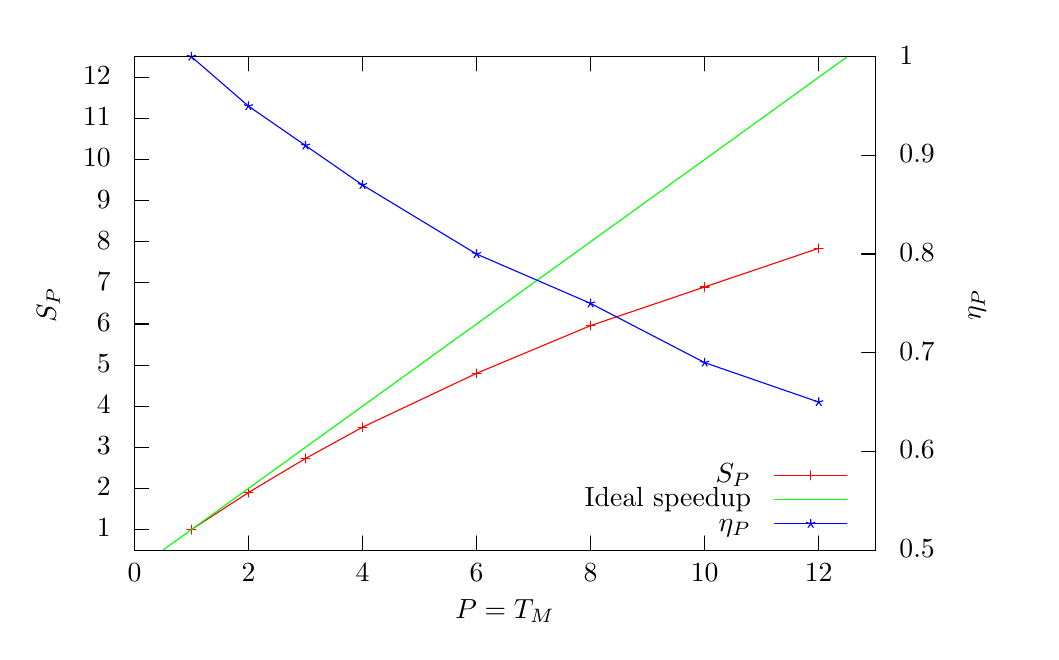
\begin{tikzpicture}[gnuplot]
%% generated with GNUPLOT 4.6p0 (Lua 5.1; terminal rev. 99, script rev. 100)
%% Sat 13 Apr 2013 11:01:34 PM BST
\gpsolidlines
\path (0.000,0.000) rectangle (12.700,7.620);
\gpcolor{color=gp lt color border}
\gpsetlinetype{gp lt border}
\gpsetlinewidth{1.00}
\draw[gp path] (1.320,1.246)--(1.500,1.246);
\node[gp node right] at (1.136,1.246) { 1};
\draw[gp path] (1.320,1.768)--(1.500,1.768);
\node[gp node right] at (1.136,1.768) { 2};
\draw[gp path] (1.320,2.290)--(1.500,2.290);
\node[gp node right] at (1.136,2.290) { 3};
\draw[gp path] (1.320,2.813)--(1.500,2.813);
\node[gp node right] at (1.136,2.813) { 4};
\draw[gp path] (1.320,3.335)--(1.500,3.335);
\node[gp node right] at (1.136,3.335) { 5};
\draw[gp path] (1.320,3.857)--(1.500,3.857);
\node[gp node right] at (1.136,3.857) { 6};
\draw[gp path] (1.320,4.379)--(1.500,4.379);
\node[gp node right] at (1.136,4.379) { 7};
\draw[gp path] (1.320,4.901)--(1.500,4.901);
\node[gp node right] at (1.136,4.901) { 8};
\draw[gp path] (1.320,5.423)--(1.500,5.423);
\node[gp node right] at (1.136,5.423) { 9};
\draw[gp path] (1.320,5.946)--(1.500,5.946);
\node[gp node right] at (1.136,5.946) { 10};
\draw[gp path] (1.320,6.468)--(1.500,6.468);
\node[gp node right] at (1.136,6.468) { 11};
\draw[gp path] (1.320,6.990)--(1.500,6.990);
\node[gp node right] at (1.136,6.990) { 12};
\draw[gp path] (1.320,0.985)--(1.320,1.165);
\draw[gp path] (1.320,7.251)--(1.320,7.071);
\node[gp node center] at (1.320,0.677) { 0};
\draw[gp path] (2.768,0.985)--(2.768,1.165);
\draw[gp path] (2.768,7.251)--(2.768,7.071);
\node[gp node center] at (2.768,0.677) { 2};
\draw[gp path] (4.217,0.985)--(4.217,1.165);
\draw[gp path] (4.217,7.251)--(4.217,7.071);
\node[gp node center] at (4.217,0.677) { 4};
\draw[gp path] (5.665,0.985)--(5.665,1.165);
\draw[gp path] (5.665,7.251)--(5.665,7.071);
\node[gp node center] at (5.665,0.677) { 6};
\draw[gp path] (7.114,0.985)--(7.114,1.165);
\draw[gp path] (7.114,7.251)--(7.114,7.071);
\node[gp node center] at (7.114,0.677) { 8};
\draw[gp path] (8.562,0.985)--(8.562,1.165);
\draw[gp path] (8.562,7.251)--(8.562,7.071);
\node[gp node center] at (8.562,0.677) { 10};
\draw[gp path] (10.011,0.985)--(10.011,1.165);
\draw[gp path] (10.011,7.251)--(10.011,7.071);
\node[gp node center] at (10.011,0.677) { 12};
\draw[gp path] (10.735,0.985)--(10.555,0.985);
\node[gp node left] at (10.919,0.985) { 0.5};
\draw[gp path] (10.735,2.238)--(10.555,2.238);
\node[gp node left] at (10.919,2.238) { 0.6};
\draw[gp path] (10.735,3.491)--(10.555,3.491);
\node[gp node left] at (10.919,3.491) { 0.7};
\draw[gp path] (10.735,4.745)--(10.555,4.745);
\node[gp node left] at (10.919,4.745) { 0.8};
\draw[gp path] (10.735,5.998)--(10.555,5.998);
\node[gp node left] at (10.919,5.998) { 0.9};
\draw[gp path] (10.735,7.251)--(10.555,7.251);
\node[gp node left] at (10.919,7.251) { 1};
\draw[gp path] (1.320,7.251)--(1.320,0.985)--(10.735,0.985)--(10.735,7.251)--cycle;
\node[gp node center,rotate=-270] at (0.246,4.118) {$S_P$};
\node[gp node center,rotate=-270] at (11.992,4.118) {$\eta_P$};
\node[gp node center] at (6.027,0.215) {$P = T_M$};
\node[gp node right] at (9.267,1.935) {$S_P$};
\gpcolor{color=gp lt color 0}
\gpsetlinetype{gp lt plot 0}
\draw[gp path] (9.451,1.935)--(10.367,1.935);
\draw[gp path] (2.044,1.246)--(2.768,1.716)--(3.493,2.149)--(4.217,2.546)--(5.665,3.230)%
  --(7.114,3.836)--(8.562,4.327)--(10.011,4.818);
\gpsetpointsize{4.00}
\gppoint{gp mark 1}{(2.044,1.246)}
\gppoint{gp mark 1}{(2.768,1.716)}
\gppoint{gp mark 1}{(3.493,2.149)}
\gppoint{gp mark 1}{(4.217,2.546)}
\gppoint{gp mark 1}{(5.665,3.230)}
\gppoint{gp mark 1}{(7.114,3.836)}
\gppoint{gp mark 1}{(8.562,4.327)}
\gppoint{gp mark 1}{(10.011,4.818)}
\gppoint{gp mark 1}{(9.909,1.935)}
\gpcolor{color=gp lt color border}
\node[gp node right] at (9.267,1.627) {Ideal speedup};
\gpcolor{color=gp lt color 1}
\gpsetlinetype{gp lt plot 1}
\draw[gp path] (9.451,1.627)--(10.367,1.627);
\draw[gp path] (1.682,0.985)--(1.700,0.998)--(1.796,1.067)--(1.891,1.135)--(1.986,1.204)%
  --(2.081,1.272)--(2.176,1.341)--(2.271,1.410)--(2.366,1.478)--(2.461,1.547)--(2.556,1.615)%
  --(2.651,1.684)--(2.747,1.752)--(2.842,1.821)--(2.937,1.890)--(3.032,1.958)--(3.127,2.027)%
  --(3.222,2.095)--(3.317,2.164)--(3.412,2.232)--(3.507,2.301)--(3.602,2.370)--(3.698,2.438)%
  --(3.793,2.507)--(3.888,2.575)--(3.983,2.644)--(4.078,2.712)--(4.173,2.781)--(4.268,2.850)%
  --(4.363,2.918)--(4.458,2.987)--(4.553,3.055)--(4.649,3.124)--(4.744,3.192)--(4.839,3.261)%
  --(4.934,3.329)--(5.029,3.398)--(5.124,3.467)--(5.219,3.535)--(5.314,3.604)--(5.409,3.672)%
  --(5.504,3.741)--(5.600,3.809)--(5.695,3.878)--(5.790,3.947)--(5.885,4.015)--(5.980,4.084)%
  --(6.075,4.152)--(6.170,4.221)--(6.265,4.289)--(6.360,4.358)--(6.455,4.427)--(6.551,4.495)%
  --(6.646,4.564)--(6.741,4.632)--(6.836,4.701)--(6.931,4.769)--(7.026,4.838)--(7.121,4.907)%
  --(7.216,4.975)--(7.311,5.044)--(7.406,5.112)--(7.502,5.181)--(7.597,5.249)--(7.692,5.318)%
  --(7.787,5.386)--(7.882,5.455)--(7.977,5.524)--(8.072,5.592)--(8.167,5.661)--(8.262,5.729)%
  --(8.357,5.798)--(8.453,5.866)--(8.548,5.935)--(8.643,6.004)--(8.738,6.072)--(8.833,6.141)%
  --(8.928,6.209)--(9.023,6.278)--(9.118,6.346)--(9.213,6.415)--(9.308,6.484)--(9.404,6.552)%
  --(9.499,6.621)--(9.594,6.689)--(9.689,6.758)--(9.784,6.826)--(9.879,6.895)--(9.974,6.964)%
  --(10.069,7.032)--(10.164,7.101)--(10.259,7.169)--(10.355,7.238)--(10.373,7.251);
\gpcolor{color=gp lt color border}
\node[gp node right] at (9.267,1.319) {$\eta_P$};
\gpcolor{color=gp lt color 2}
\gpsetlinetype{gp lt plot 2}
\draw[gp path] (9.451,1.319)--(10.367,1.319);
\draw[gp path] (2.044,7.251)--(2.768,6.624)--(3.493,6.123)--(4.217,5.622)--(5.665,4.745)%
  --(7.114,4.118)--(8.562,3.366)--(10.011,2.865);
\gppoint{gp mark 3}{(2.044,7.251)}
\gppoint{gp mark 3}{(2.768,6.624)}
\gppoint{gp mark 3}{(3.493,6.123)}
\gppoint{gp mark 3}{(4.217,5.622)}
\gppoint{gp mark 3}{(5.665,4.745)}
\gppoint{gp mark 3}{(7.114,4.118)}
\gppoint{gp mark 3}{(8.562,3.366)}
\gppoint{gp mark 3}{(10.011,2.865)}
\gppoint{gp mark 3}{(9.909,1.319)}
\gpcolor{color=gp lt color border}
\gpsetlinetype{gp lt border}
\draw[gp path] (1.320,7.251)--(1.320,0.985)--(10.735,0.985)--(10.735,7.251)--cycle;
%% coordinates of the plot area
\gpdefrectangularnode{gp plot 1}{\pgfpoint{1.320cm}{0.985cm}}{\pgfpoint{10.735cm}{7.251cm}}
\end{tikzpicture}
%% gnuplot variables

	\caption{A plot of the speedup ($S_P$) and parallel efficency ($\eta_P$) for different amounts of processors ($P$) utilized. Take note that the second axis is different for $\eta_P$ and $S_P$.}
	\label{fig:nodespeed}
\end{figure}

Using multiple MPI-processes on a single node offers a better speedup since there is much less overhead and communication time is small. This is backed up by the numerical results as listed in table \ref{tab:MPIspeedup}. A plot of the parallel efficency can be seen in figure \ref{fig:MPIspeedup}. Observe that the parallel efficency is close to unity when all the processors on the node are run as MPI-processes as compared to when all the processors are used as OpenMP threads when the parallel efficency is down to 0.65.

\begin{table}[htbp]
	\centering
	\caption{Listing of timing results as a comparison between MPI ($M$) and OpenMP processes per thread ($T_M$). Results are obtained using only one node and a problem size of $n=16384$.}
	\label{tab:MPIspeedup}
	\begin{tabular}{r|r|r|c|c|c}
	$M$	&	$T_M$	&	$P$	&	$\tau_P$ [s] & $S_p=\tau_1/\tau_p$	&	$\eta_p=S_p/P$	\\
\hline
	1&	12&	12&	100.9&	7.84&	0.65\\
	2&	6&	12&	82.7&	9.56&	0.80\\
	3&	4&	12&	76.2&	10.38&	0.86\\
	4&	3&	12&	72.8&	10.86&	0.91\\
	6&	2&	12&	69.6&	11.36&	0.95\\
	12&	1&	12&	66.4&	11.91&	0.99\\
	\end{tabular}
\end{table}

\begin{figure}[htbp]
	\centering
	\begin{tikzpicture}[gnuplot]
%% generated with GNUPLOT 4.6p0 (Lua 5.1; terminal rev. 99, script rev. 100)
%% Sat 13 Apr 2013 11:01:55 PM BST
\gpsolidlines
\path (0.000,0.000) rectangle (12.700,7.620);
\gpcolor{color=gp lt color border}
\gpsetlinetype{gp lt border}
\gpsetlinewidth{1.00}
\draw[gp path] (1.504,0.985)--(1.684,0.985);
\node[gp node right] at (1.320,0.985) { 0.6};
\draw[gp path] (1.504,2.552)--(1.684,2.552);
\node[gp node right] at (1.320,2.552) { 0.7};
\draw[gp path] (1.504,4.118)--(1.684,4.118);
\node[gp node right] at (1.320,4.118) { 0.8};
\draw[gp path] (1.504,5.685)--(1.684,5.685);
\node[gp node right] at (1.320,5.685) { 0.9};
\draw[gp path] (1.504,7.251)--(1.684,7.251);
\node[gp node right] at (1.320,7.251) { 1};
\draw[gp path] (1.504,0.985)--(1.504,1.165);
\draw[gp path] (1.504,7.251)--(1.504,7.071);
\node[gp node center] at (1.504,0.677) { 0};
\draw[gp path] (3.141,0.985)--(3.141,1.165);
\draw[gp path] (3.141,7.251)--(3.141,7.071);
\node[gp node center] at (3.141,0.677) { 2};
\draw[gp path] (4.779,0.985)--(4.779,1.165);
\draw[gp path] (4.779,7.251)--(4.779,7.071);
\node[gp node center] at (4.779,0.677) { 4};
\draw[gp path] (6.416,0.985)--(6.416,1.165);
\draw[gp path] (6.416,7.251)--(6.416,7.071);
\node[gp node center] at (6.416,0.677) { 6};
\draw[gp path] (8.054,0.985)--(8.054,1.165);
\draw[gp path] (8.054,7.251)--(8.054,7.071);
\node[gp node center] at (8.054,0.677) { 8};
\draw[gp path] (9.691,0.985)--(9.691,1.165);
\draw[gp path] (9.691,7.251)--(9.691,7.071);
\node[gp node center] at (9.691,0.677) { 10};
\draw[gp path] (11.328,0.985)--(11.328,1.165);
\draw[gp path] (11.328,7.251)--(11.328,7.071);
\node[gp node center] at (11.328,0.677) { 12};
\draw[gp path] (1.504,7.251)--(1.504,0.985)--(12.147,0.985)--(12.147,7.251)--cycle;
\node[gp node center,rotate=-270] at (0.246,4.118) {$\eta_P$};
\node[gp node center] at (6.825,0.215) {$M$};
\node[gp node right] at (10.679,1.319) {$S_P$};
\gpcolor{color=gp lt color 0}
\gpsetlinetype{gp lt plot 0}
\draw[gp path] (10.863,1.319)--(11.779,1.319);
\draw[gp path] (2.323,1.768)--(3.141,4.118)--(3.960,5.058)--(4.779,5.841)--(6.416,6.468)%
  --(11.328,7.094);
\gpsetpointsize{4.00}
\gppoint{gp mark 1}{(2.323,1.768)}
\gppoint{gp mark 1}{(3.141,4.118)}
\gppoint{gp mark 1}{(3.960,5.058)}
\gppoint{gp mark 1}{(4.779,5.841)}
\gppoint{gp mark 1}{(6.416,6.468)}
\gppoint{gp mark 1}{(11.328,7.094)}
\gppoint{gp mark 1}{(11.321,1.319)}
\gpcolor{color=gp lt color border}
\gpsetlinetype{gp lt border}
\draw[gp path] (1.504,7.251)--(1.504,0.985)--(12.147,0.985)--(12.147,7.251)--cycle;
%% coordinates of the plot area
\gpdefrectangularnode{gp plot 1}{\pgfpoint{1.504cm}{0.985cm}}{\pgfpoint{12.147cm}{7.251cm}}
\end{tikzpicture}
%% gnuplot variables

	\caption{A plot of the parallel efficency $\eta_P$ as a function of MPI-processes ($M$) on a single node. The total number of utilized processors is always $P=12$ as the processors not used as a MPI-process is utilized as a thread.}
	\label{fig:MPIspeedup}
\end{figure}

When the number of nodes is increased one would expect the the parallel efficency to drop substantially as there is network latency involved. By looking at timing results obtained from running the program over three nodes in table \ref{tab:nodes} a decreased efficency is observed, as the number of processors is tripled, the run time is only about halved as compared to table \ref{tab:MPIspeedup}. Again as with the single node case, running the algorithm with only MPI-processes yields the fastest result.

\begin{table}[htbp]
	\label{tab:nodes}
	\caption{Timing results on three nodes ($N=3$) with different combinations of MPI-processes per node ($M$) and OpenMP threads per MPI-process ($T_M$). The total number of processors utilized is 36 in each case (recall that $P=N\times M\times T_M$).}
	\centering
	\begin{tabular}{r|r|c|c|c}
	$M$	&	$T_M$	&	$\tau_P$ [s] & $S_p=\tau_1/\tau_p$	&	$\eta_p=S_p/P$	\\
\hline
	1	&12	&42.9	&18.43	&0.51\\
	2	&6	&36.6	&21.60	&0.60\\
	3	&4	&34.4	&22.99	&0.64\\
	4	&3	&33.3	&23.74	&0.66\\
	6	&2	&32.6	&24.25	&0.67\\
	12	&1	&32.0	&24.71	&0.69\\
	\end{tabular}
\end{table}

\begin{figure}[htbp]
	\centering
	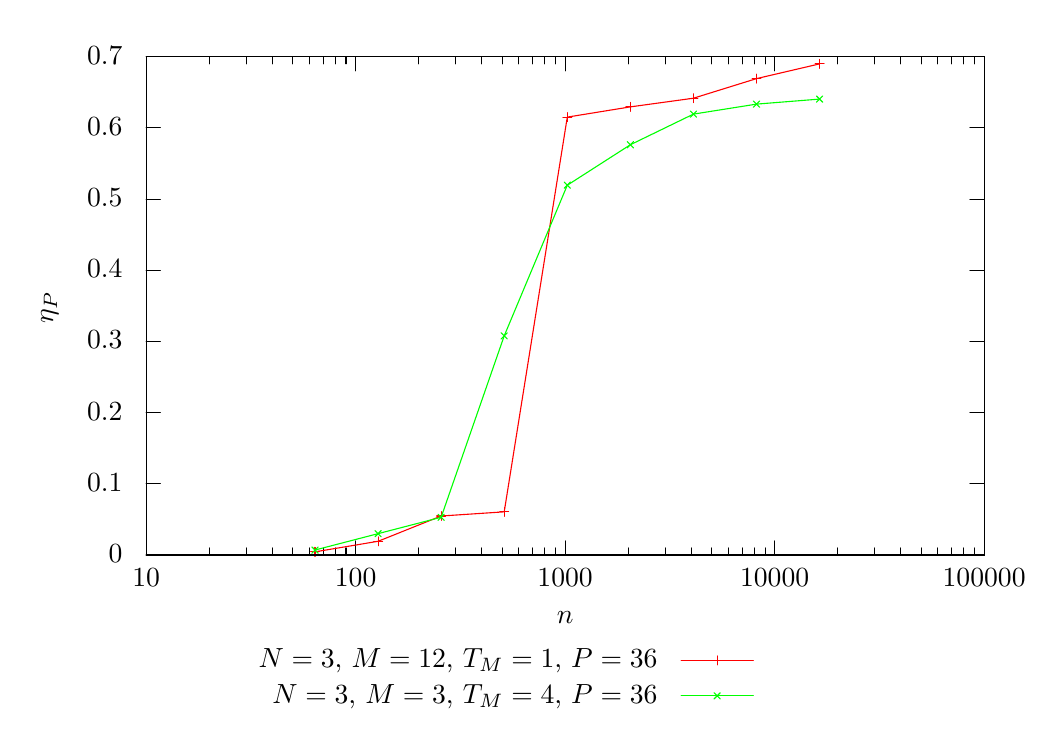
\begin{tikzpicture}[gnuplot]
%% generated with GNUPLOT 4.6p0 (Lua 5.1; terminal rev. 99, script rev. 100)
%% Sun 14 Apr 2013 06:07:27 PM BST
\gpsolidlines
\path (0.000,0.000) rectangle (12.700,8.890);
\gpcolor{color=gp lt color border}
\gpsetlinetype{gp lt border}
\gpsetlinewidth{1.00}
\draw[gp path] (1.504,2.193)--(1.684,2.193);
\draw[gp path] (12.147,2.193)--(11.967,2.193);
\node[gp node right] at (1.320,2.193) { 0};
\draw[gp path] (1.504,3.097)--(1.684,3.097);
\draw[gp path] (12.147,3.097)--(11.967,3.097);
\node[gp node right] at (1.320,3.097) { 0.1};
\draw[gp path] (1.504,4.001)--(1.684,4.001);
\draw[gp path] (12.147,4.001)--(11.967,4.001);
\node[gp node right] at (1.320,4.001) { 0.2};
\draw[gp path] (1.504,4.905)--(1.684,4.905);
\draw[gp path] (12.147,4.905)--(11.967,4.905);
\node[gp node right] at (1.320,4.905) { 0.3};
\draw[gp path] (1.504,5.809)--(1.684,5.809);
\draw[gp path] (12.147,5.809)--(11.967,5.809);
\node[gp node right] at (1.320,5.809) { 0.4};
\draw[gp path] (1.504,6.713)--(1.684,6.713);
\draw[gp path] (12.147,6.713)--(11.967,6.713);
\node[gp node right] at (1.320,6.713) { 0.5};
\draw[gp path] (1.504,7.617)--(1.684,7.617);
\draw[gp path] (12.147,7.617)--(11.967,7.617);
\node[gp node right] at (1.320,7.617) { 0.6};
\draw[gp path] (1.504,8.521)--(1.684,8.521);
\draw[gp path] (12.147,8.521)--(11.967,8.521);
\node[gp node right] at (1.320,8.521) { 0.7};
\draw[gp path] (1.504,2.193)--(1.504,2.373);
\draw[gp path] (1.504,8.521)--(1.504,8.341);
\node[gp node center] at (1.504,1.885) { 10};
\draw[gp path] (2.305,2.193)--(2.305,2.283);
\draw[gp path] (2.305,8.521)--(2.305,8.431);
\draw[gp path] (2.774,2.193)--(2.774,2.283);
\draw[gp path] (2.774,8.521)--(2.774,8.431);
\draw[gp path] (3.106,2.193)--(3.106,2.283);
\draw[gp path] (3.106,8.521)--(3.106,8.431);
\draw[gp path] (3.364,2.193)--(3.364,2.283);
\draw[gp path] (3.364,8.521)--(3.364,8.431);
\draw[gp path] (3.574,2.193)--(3.574,2.283);
\draw[gp path] (3.574,8.521)--(3.574,8.431);
\draw[gp path] (3.753,2.193)--(3.753,2.283);
\draw[gp path] (3.753,8.521)--(3.753,8.431);
\draw[gp path] (3.907,2.193)--(3.907,2.283);
\draw[gp path] (3.907,8.521)--(3.907,8.431);
\draw[gp path] (4.043,2.193)--(4.043,2.283);
\draw[gp path] (4.043,8.521)--(4.043,8.431);
\draw[gp path] (4.165,2.193)--(4.165,2.373);
\draw[gp path] (4.165,8.521)--(4.165,8.341);
\node[gp node center] at (4.165,1.885) { 100};
\draw[gp path] (4.966,2.193)--(4.966,2.283);
\draw[gp path] (4.966,8.521)--(4.966,8.431);
\draw[gp path] (5.434,2.193)--(5.434,2.283);
\draw[gp path] (5.434,8.521)--(5.434,8.431);
\draw[gp path] (5.767,2.193)--(5.767,2.283);
\draw[gp path] (5.767,8.521)--(5.767,8.431);
\draw[gp path] (6.025,2.193)--(6.025,2.283);
\draw[gp path] (6.025,8.521)--(6.025,8.431);
\draw[gp path] (6.235,2.193)--(6.235,2.283);
\draw[gp path] (6.235,8.521)--(6.235,8.431);
\draw[gp path] (6.413,2.193)--(6.413,2.283);
\draw[gp path] (6.413,8.521)--(6.413,8.431);
\draw[gp path] (6.568,2.193)--(6.568,2.283);
\draw[gp path] (6.568,8.521)--(6.568,8.431);
\draw[gp path] (6.704,2.193)--(6.704,2.283);
\draw[gp path] (6.704,8.521)--(6.704,8.431);
\draw[gp path] (6.826,2.193)--(6.826,2.373);
\draw[gp path] (6.826,8.521)--(6.826,8.341);
\node[gp node center] at (6.826,1.885) { 1000};
\draw[gp path] (7.626,2.193)--(7.626,2.283);
\draw[gp path] (7.626,8.521)--(7.626,8.431);
\draw[gp path] (8.095,2.193)--(8.095,2.283);
\draw[gp path] (8.095,8.521)--(8.095,8.431);
\draw[gp path] (8.427,2.193)--(8.427,2.283);
\draw[gp path] (8.427,8.521)--(8.427,8.431);
\draw[gp path] (8.685,2.193)--(8.685,2.283);
\draw[gp path] (8.685,8.521)--(8.685,8.431);
\draw[gp path] (8.896,2.193)--(8.896,2.283);
\draw[gp path] (8.896,8.521)--(8.896,8.431);
\draw[gp path] (9.074,2.193)--(9.074,2.283);
\draw[gp path] (9.074,8.521)--(9.074,8.431);
\draw[gp path] (9.228,2.193)--(9.228,2.283);
\draw[gp path] (9.228,8.521)--(9.228,8.431);
\draw[gp path] (9.365,2.193)--(9.365,2.283);
\draw[gp path] (9.365,8.521)--(9.365,8.431);
\draw[gp path] (9.486,2.193)--(9.486,2.373);
\draw[gp path] (9.486,8.521)--(9.486,8.341);
\node[gp node center] at (9.486,1.885) { 10000};
\draw[gp path] (10.287,2.193)--(10.287,2.283);
\draw[gp path] (10.287,8.521)--(10.287,8.431);
\draw[gp path] (10.756,2.193)--(10.756,2.283);
\draw[gp path] (10.756,8.521)--(10.756,8.431);
\draw[gp path] (11.088,2.193)--(11.088,2.283);
\draw[gp path] (11.088,8.521)--(11.088,8.431);
\draw[gp path] (11.346,2.193)--(11.346,2.283);
\draw[gp path] (11.346,8.521)--(11.346,8.431);
\draw[gp path] (11.557,2.193)--(11.557,2.283);
\draw[gp path] (11.557,8.521)--(11.557,8.431);
\draw[gp path] (11.735,2.193)--(11.735,2.283);
\draw[gp path] (11.735,8.521)--(11.735,8.431);
\draw[gp path] (11.889,2.193)--(11.889,2.283);
\draw[gp path] (11.889,8.521)--(11.889,8.431);
\draw[gp path] (12.025,2.193)--(12.025,2.283);
\draw[gp path] (12.025,8.521)--(12.025,8.431);
\draw[gp path] (12.147,2.193)--(12.147,2.373);
\draw[gp path] (12.147,8.521)--(12.147,8.341);
\node[gp node center] at (12.147,1.885) { 100000};
\draw[gp path] (1.504,8.521)--(1.504,2.193)--(12.147,2.193)--(12.147,8.521)--cycle;
\node[gp node center,rotate=-270] at (0.246,5.357) {$\eta_P$};
\node[gp node center] at (6.825,1.423) {$n$};
\node[gp node right] at (8.115,0.855) {$N=3$, $M=12$, $T_M=1$, $P=36$};
\gpcolor{color=gp lt color 0}
\gpsetlinetype{gp lt plot 0}
\draw[gp path] (8.299,0.855)--(9.215,0.855);
\draw[gp path] (3.649,2.233)--(4.450,2.367)--(5.251,2.688)--(6.052,2.741)--(6.853,7.754)%
  --(7.654,7.884)--(8.455,7.994)--(9.256,8.243)--(10.057,8.430);
\gpsetpointsize{4.00}
\gppoint{gp mark 1}{(3.649,2.233)}
\gppoint{gp mark 1}{(4.450,2.367)}
\gppoint{gp mark 1}{(5.251,2.688)}
\gppoint{gp mark 1}{(6.052,2.741)}
\gppoint{gp mark 1}{(6.853,7.754)}
\gppoint{gp mark 1}{(7.654,7.884)}
\gppoint{gp mark 1}{(8.455,7.994)}
\gppoint{gp mark 1}{(9.256,8.243)}
\gppoint{gp mark 1}{(10.057,8.430)}
\gppoint{gp mark 1}{(8.757,0.855)}
\gpcolor{color=gp lt color border}
\node[gp node right] at (8.115,0.405) {$N=3$, $M=3$, $T_M=4$, $P=36$};
\gpcolor{color=gp lt color 1}
\gpsetlinetype{gp lt plot 1}
\draw[gp path] (8.299,0.405)--(9.215,0.405);
\draw[gp path] (3.649,2.256)--(4.450,2.464)--(5.251,2.672)--(6.052,4.976)--(6.853,6.889)%
  --(7.654,7.403)--(8.455,7.792)--(9.256,7.919)--(10.057,7.983);
\gppoint{gp mark 2}{(3.649,2.256)}
\gppoint{gp mark 2}{(4.450,2.464)}
\gppoint{gp mark 2}{(5.251,2.672)}
\gppoint{gp mark 2}{(6.052,4.976)}
\gppoint{gp mark 2}{(6.853,6.889)}
\gppoint{gp mark 2}{(7.654,7.403)}
\gppoint{gp mark 2}{(8.455,7.792)}
\gppoint{gp mark 2}{(9.256,7.919)}
\gppoint{gp mark 2}{(10.057,7.983)}
\gppoint{gp mark 2}{(8.757,0.405)}
\gpcolor{color=gp lt color border}
\gpsetlinetype{gp lt border}
\draw[gp path] (1.504,8.521)--(1.504,2.193)--(12.147,2.193)--(12.147,8.521)--cycle;
%% coordinates of the plot area
\gpdefrectangularnode{gp plot 1}{\pgfpoint{1.504cm}{2.193cm}}{\pgfpoint{12.147cm}{8.521cm}}
\end{tikzpicture}
%% gnuplot variables

	\caption{Parallel efficency $\eta_p$ for two configurations of MPI-processes ($M$) and OpenMP threads per MPI-process ($T_M$) as a function of problem size.}
	\label{fig:peff}
\end{figure}

From figure \ref{fig:peff} it can be observed that for small problem sizes ($n<1024$) there is very little payoff in using many processors as the prallel efficency is shown to be very low. The hybrid model has a somewhat better payoff for smaller problems, but it is still inefficient.

\subsection{Summary}
The solver is found to give correct results within the error estimate for an analytical solvable seed function. When on a single node the best speedup is acheieved by using all available processors as MPI-processes instead of spawning OpenMP threads. This is because of increased overhead and iterations in the transpose iteration when using OpenMP-threads compared to MPI-processes. On three nodes the best result is also obtained when all processors are utilized as MPI-processes, as can be seen in table \ref{tab:nodes}. Parallel efficency however suffers when using more than one node because of network latency. Parallel efficency also suffer when the problem size is relatively small, this is due to the added overhead when using multiple processors drowning the time used for actually solving the problem.

Tests were made using more than 36 processors with $n=16384$, the results indicate that the parallel efficency $\eta_p$ drops slowly when increasing the number of processors used. Using three nodes the best $\eta_P$ obtained was 0.69, when using 6 nodes this was down to 0.62 using only the MPI model. On 12 nodes the best efficency was obtained using a hybrid model with $M=6$ and $T_M=2$ with $\eta_P=0.56$, compared to $\eta_p=0.46$ using the pure MPI model. This behaviour can be explained using figure \ref{fig:peff} where the problem size for each node is small enough that the hybrid model offers advantage.

The transpose operation uses a triple nested for-loop that is executed approximately $M\cdot (n/M)\cdot(n/M) = n^2/M$ times each time the transpose operations is called. 

The transpose operation contains a triple nested for-loop that can not be split up among OpenMP threads. This triple nested for-loop is is executed approximately $M\cdot (n/M)\cdot(n/M) = n^2/M$ times per MPI-process each time the transpose operation is called upon. with a problem size of $n=16384=2^{14}$ and on a signle node, using only one MPI-process and 12 threads this amount to once processor having to execute the triple nested for-loop approximately 268 million times while the 11 others are idle. Using a pure MPI-model on the other hand, each processor only need to run 22 million iterations and it can be done in parallel, so the MPI-model is much more load balanced for this operation. However on a distributed system there will be network latency to counter the effect parallelisation of the triple nested loop since more MPI-processes means more network traffic. By looking at table \ref{tab:nodes} the hybrid model does not lie far behind the pure MPI-model, which indicates that network latency is a substantial factor when it comes to parallel computing.

\newpage
\section{Solver capabilities}
The solver can solve for different seed functions $f(x,y)$ by changing the \textit{return} statement in the \textit{evalFunc} function in the code. This will change the $G$ matrix in step one to correspond with the given function. The max pointwise error will show false information unless changed as well. Some plots of solutions for different seed functions can be found in figure \ref{fig:sol1} to \ref{fig:sol4}. Axis desciption is dropped since there is no real information in the plots and they look prettier that way.
	
\begin{figure}[h]
	\centering
	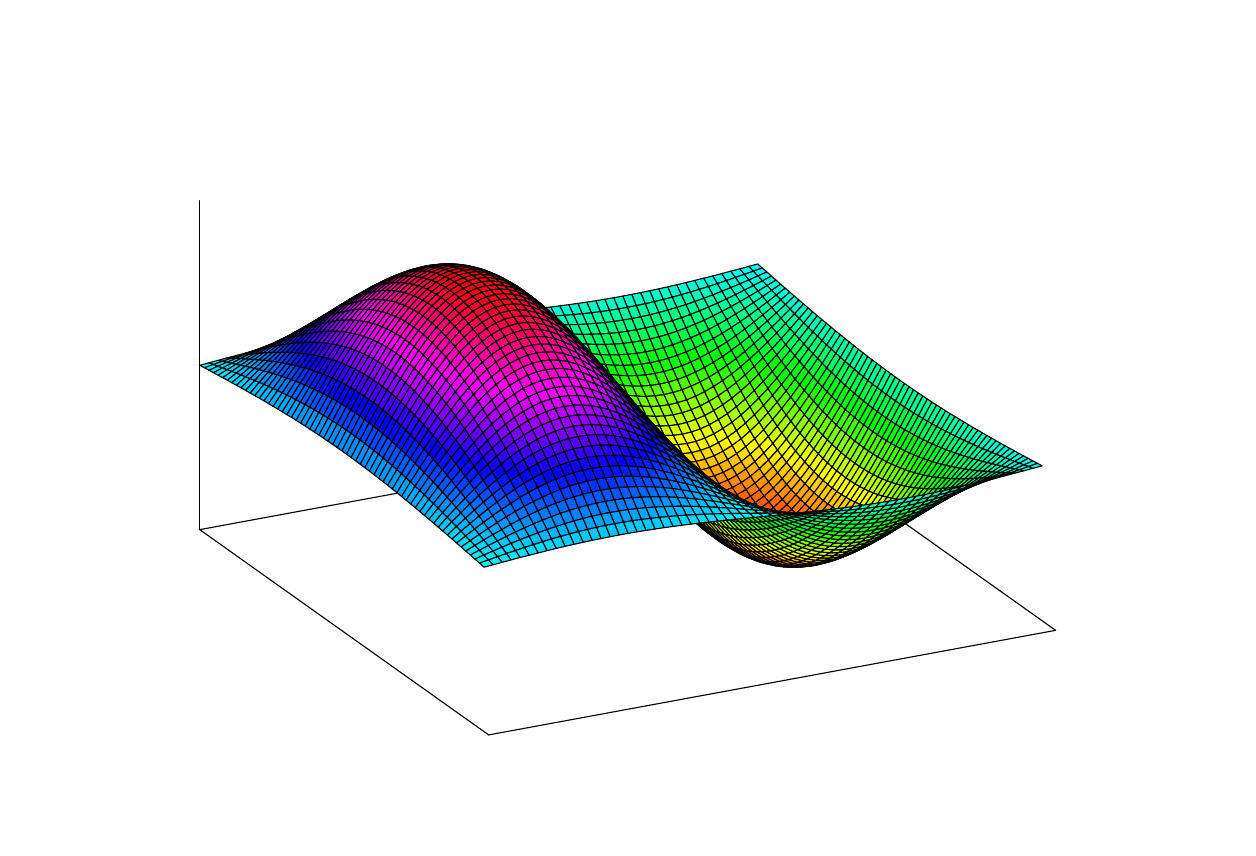
\begin{tikzpicture}[gnuplot]
%% generated with GNUPLOT 4.6p0 (Lua 5.1; terminal rev. 99, script rev. 100)
%% Sun 14 Apr 2013 09:52:44 PM BST
\gpsolidlines
\path (0.000,0.000) rectangle (15.240,10.160);
\gpcolor{color=gp lt color border}
\gpsetlinetype{gp lt border}
\gpsetlinewidth{1.00}
\draw[gp path] (2.185,3.785)--(9.385,5.113);
\draw[gp path] (13.055,2.506)--(9.385,5.113);
\draw[gp path] (2.185,3.785)--(2.185,7.962);
\gpfill{rgb color={0.000,1.000,0.968}} (9.271,7.159)--(9.157,7.128)--(9.215,7.067)--(9.329,7.108)--cycle;
\gpcolor{rgb color={0.000,0.000,0.000}}
\gpsetlinetype{gp lt plot 3}
\draw[gp path] (9.271,7.159)--(9.329,7.108)--(9.215,7.067)--(9.157,7.128)--cycle;
\gpfill{rgb color={0.000,1.000,0.946}} (9.329,7.108)--(9.215,7.067)--(9.273,7.006)--(9.388,7.057)--cycle;
\draw[gp path] (9.329,7.108)--(9.388,7.057)--(9.273,7.006)--(9.215,7.067)--cycle;
\gpfill{rgb color={0.000,1.000,0.925}} (9.388,7.057)--(9.273,7.006)--(9.332,6.945)--(9.446,7.005)--cycle;
\draw[gp path] (9.388,7.057)--(9.446,7.005)--(9.332,6.945)--(9.273,7.006)--cycle;
\gpfill{rgb color={0.000,1.000,0.904}} (9.446,7.005)--(9.332,6.945)--(9.390,6.884)--(9.504,6.954)--cycle;
\draw[gp path] (9.446,7.005)--(9.504,6.954)--(9.390,6.884)--(9.332,6.945)--cycle;
\gpfill{rgb color={0.000,1.000,0.883}} (9.504,6.954)--(9.390,6.884)--(9.448,6.824)--(9.562,6.903)--cycle;
\draw[gp path] (9.504,6.954)--(9.562,6.903)--(9.448,6.824)--(9.390,6.884)--cycle;
\gpfill{rgb color={0.000,1.000,0.862}} (9.562,6.903)--(9.448,6.824)--(9.506,6.763)--(9.621,6.852)--cycle;
\draw[gp path] (9.562,6.903)--(9.621,6.852)--(9.506,6.763)--(9.448,6.824)--cycle;
\gpfill{rgb color={0.000,1.000,0.842}} (9.621,6.852)--(9.506,6.763)--(9.565,6.703)--(9.679,6.802)--cycle;
\draw[gp path] (9.621,6.852)--(9.679,6.802)--(9.565,6.703)--(9.506,6.763)--cycle;
\gpfill{rgb color={0.000,1.000,0.822}} (9.679,6.802)--(9.565,6.703)--(9.623,6.644)--(9.737,6.751)--cycle;
\draw[gp path] (9.679,6.802)--(9.737,6.751)--(9.623,6.644)--(9.565,6.703)--cycle;
\gpfill{rgb color={0.000,1.000,0.802}} (9.737,6.751)--(9.623,6.644)--(9.681,6.585)--(9.795,6.701)--cycle;
\draw[gp path] (9.737,6.751)--(9.795,6.701)--(9.681,6.585)--(9.623,6.644)--cycle;
\gpfill{rgb color={0.000,1.000,0.783}} (9.795,6.701)--(9.681,6.585)--(9.739,6.526)--(9.854,6.651)--cycle;
\draw[gp path] (9.795,6.701)--(9.854,6.651)--(9.739,6.526)--(9.681,6.585)--cycle;
\gpfill{rgb color={0.000,1.000,0.765}} (9.854,6.651)--(9.739,6.526)--(9.798,6.468)--(9.912,6.601)--cycle;
\draw[gp path] (9.854,6.651)--(9.912,6.601)--(9.798,6.468)--(9.739,6.526)--cycle;
\gpfill{rgb color={0.000,1.000,0.747}} (9.912,6.601)--(9.798,6.468)--(9.856,6.410)--(9.970,6.551)--cycle;
\draw[gp path] (9.912,6.601)--(9.970,6.551)--(9.856,6.410)--(9.798,6.468)--cycle;
\gpfill{rgb color={0.000,1.000,0.729}} (9.970,6.551)--(9.856,6.410)--(9.914,6.353)--(10.028,6.502)--cycle;
\draw[gp path] (9.970,6.551)--(10.028,6.502)--(9.914,6.353)--(9.856,6.410)--cycle;
\gpfill{rgb color={0.000,1.000,0.713}} (10.028,6.502)--(9.914,6.353)--(9.972,6.296)--(10.087,6.453)--cycle;
\draw[gp path] (10.028,6.502)--(10.087,6.453)--(9.972,6.296)--(9.914,6.353)--cycle;
\gpfill{rgb color={0.000,1.000,0.697}} (10.087,6.453)--(9.972,6.296)--(10.030,6.241)--(10.145,6.405)--cycle;
\draw[gp path] (10.087,6.453)--(10.145,6.405)--(10.030,6.241)--(9.972,6.296)--cycle;
\gpfill{rgb color={0.000,1.000,0.681}} (10.145,6.405)--(10.030,6.241)--(10.089,6.186)--(10.203,6.356)--cycle;
\draw[gp path] (10.145,6.405)--(10.203,6.356)--(10.089,6.186)--(10.030,6.241)--cycle;
\gpfill{rgb color={0.000,1.000,0.667}} (10.203,6.356)--(10.089,6.186)--(10.147,6.131)--(10.261,6.308)--cycle;
\draw[gp path] (10.203,6.356)--(10.261,6.308)--(10.147,6.131)--(10.089,6.186)--cycle;
\gpfill{rgb color={0.000,1.000,0.653}} (10.261,6.308)--(10.147,6.131)--(10.205,6.078)--(10.320,6.261)--cycle;
\draw[gp path] (10.261,6.308)--(10.320,6.261)--(10.205,6.078)--(10.147,6.131)--cycle;
\gpfill{rgb color={0.000,1.000,0.640}} (10.320,6.261)--(10.205,6.078)--(10.263,6.025)--(10.378,6.214)--cycle;
\draw[gp path] (10.320,6.261)--(10.378,6.214)--(10.263,6.025)--(10.205,6.078)--cycle;
\gpfill{rgb color={0.000,1.000,0.628}} (10.378,6.214)--(10.263,6.025)--(10.322,5.973)--(10.436,6.167)--cycle;
\draw[gp path] (10.378,6.214)--(10.436,6.167)--(10.322,5.973)--(10.263,6.025)--cycle;
\gpfill{rgb color={0.000,1.000,0.617}} (10.436,6.167)--(10.322,5.973)--(10.380,5.922)--(10.494,6.121)--cycle;
\draw[gp path] (10.436,6.167)--(10.494,6.121)--(10.380,5.922)--(10.322,5.973)--cycle;
\gpfill{rgb color={0.000,1.000,0.607}} (10.494,6.121)--(10.380,5.922)--(10.438,5.871)--(10.552,6.075)--cycle;
\draw[gp path] (10.494,6.121)--(10.552,6.075)--(10.438,5.871)--(10.380,5.922)--cycle;
\gpfill{rgb color={0.000,1.000,0.598}} (10.552,6.075)--(10.438,5.871)--(10.496,5.822)--(10.611,6.029)--cycle;
\draw[gp path] (10.552,6.075)--(10.611,6.029)--(10.496,5.822)--(10.438,5.871)--cycle;
\gpfill{rgb color={0.000,1.000,0.590}} (10.611,6.029)--(10.496,5.822)--(10.555,5.773)--(10.669,5.984)--cycle;
\draw[gp path] (10.611,6.029)--(10.669,5.984)--(10.555,5.773)--(10.496,5.822)--cycle;
\gpfill{rgb color={0.000,1.000,0.582}} (10.669,5.984)--(10.555,5.773)--(10.613,5.726)--(10.727,5.940)--cycle;
\draw[gp path] (10.669,5.984)--(10.727,5.940)--(10.613,5.726)--(10.555,5.773)--cycle;
\gpfill{rgb color={0.000,1.000,0.576}} (10.727,5.940)--(10.613,5.726)--(10.671,5.679)--(10.785,5.896)--cycle;
\draw[gp path] (10.727,5.940)--(10.785,5.896)--(10.671,5.679)--(10.613,5.726)--cycle;
\gpfill{rgb color={0.000,1.000,0.571}} (10.785,5.896)--(10.671,5.679)--(10.729,5.633)--(10.844,5.852)--cycle;
\draw[gp path] (10.785,5.896)--(10.844,5.852)--(10.729,5.633)--(10.671,5.679)--cycle;
\gpfill{rgb color={0.000,1.000,0.567}} (10.844,5.852)--(10.729,5.633)--(10.788,5.588)--(10.902,5.809)--cycle;
\draw[gp path] (10.844,5.852)--(10.902,5.809)--(10.788,5.588)--(10.729,5.633)--cycle;
\gpfill{rgb color={0.000,1.000,0.563}} (10.902,5.809)--(10.788,5.588)--(10.846,5.545)--(10.960,5.767)--cycle;
\draw[gp path] (10.902,5.809)--(10.960,5.767)--(10.846,5.545)--(10.788,5.588)--cycle;
\gpfill{rgb color={0.000,1.000,0.561}} (10.960,5.767)--(10.846,5.545)--(10.904,5.502)--(11.018,5.724)--cycle;
\draw[gp path] (10.960,5.767)--(11.018,5.724)--(10.904,5.502)--(10.846,5.545)--cycle;
\gpfill{rgb color={0.000,1.000,0.560}} (11.018,5.724)--(10.904,5.502)--(10.962,5.460)--(11.077,5.683)--cycle;
\draw[gp path] (11.018,5.724)--(11.077,5.683)--(10.962,5.460)--(10.904,5.502)--cycle;
\gpfill{rgb color={0.000,1.000,0.560}} (11.077,5.683)--(10.962,5.460)--(11.021,5.419)--(11.135,5.642)--cycle;
\draw[gp path] (11.077,5.683)--(11.135,5.642)--(11.021,5.419)--(10.962,5.460)--cycle;
\gpfill{rgb color={0.000,1.000,0.561}} (11.135,5.642)--(11.021,5.419)--(11.079,5.379)--(11.193,5.601)--cycle;
\draw[gp path] (11.135,5.642)--(11.193,5.601)--(11.079,5.379)--(11.021,5.419)--cycle;
\gpfill{rgb color={0.000,1.000,0.563}} (11.193,5.601)--(11.079,5.379)--(11.137,5.340)--(11.251,5.561)--cycle;
\draw[gp path] (11.193,5.601)--(11.251,5.561)--(11.137,5.340)--(11.079,5.379)--cycle;
\gpfill{rgb color={0.000,1.000,0.567}} (11.251,5.561)--(11.137,5.340)--(11.195,5.302)--(11.310,5.521)--cycle;
\draw[gp path] (11.251,5.561)--(11.310,5.521)--(11.195,5.302)--(11.137,5.340)--cycle;
\gpfill{rgb color={0.000,1.000,0.571}} (11.310,5.521)--(11.195,5.302)--(11.254,5.265)--(11.368,5.482)--cycle;
\draw[gp path] (11.310,5.521)--(11.368,5.482)--(11.254,5.265)--(11.195,5.302)--cycle;
\gpfill{rgb color={0.000,1.000,0.576}} (11.368,5.482)--(11.254,5.265)--(11.312,5.230)--(11.426,5.443)--cycle;
\draw[gp path] (11.368,5.482)--(11.426,5.443)--(11.312,5.230)--(11.254,5.265)--cycle;
\gpfill{rgb color={0.000,1.000,0.582}} (11.426,5.443)--(11.312,5.230)--(11.370,5.195)--(11.484,5.405)--cycle;
\draw[gp path] (11.426,5.443)--(11.484,5.405)--(11.370,5.195)--(11.312,5.230)--cycle;
\gpfill{rgb color={0.000,1.000,0.590}} (11.484,5.405)--(11.370,5.195)--(11.428,5.161)--(11.543,5.367)--cycle;
\draw[gp path] (11.484,5.405)--(11.543,5.367)--(11.428,5.161)--(11.370,5.195)--cycle;
\gpfill{rgb color={0.000,1.000,0.598}} (11.543,5.367)--(11.428,5.161)--(11.486,5.128)--(11.601,5.330)--cycle;
\draw[gp path] (11.543,5.367)--(11.601,5.330)--(11.486,5.128)--(11.428,5.161)--cycle;
\gpfill{rgb color={0.000,1.000,0.607}} (11.601,5.330)--(11.486,5.128)--(11.545,5.095)--(11.659,5.293)--cycle;
\draw[gp path] (11.601,5.330)--(11.659,5.293)--(11.545,5.095)--(11.486,5.128)--cycle;
\gpfill{rgb color={0.000,1.000,0.617}} (11.659,5.293)--(11.545,5.095)--(11.603,5.064)--(11.717,5.257)--cycle;
\draw[gp path] (11.659,5.293)--(11.717,5.257)--(11.603,5.064)--(11.545,5.095)--cycle;
\gpfill{rgb color={0.000,1.000,0.628}} (11.717,5.257)--(11.603,5.064)--(11.661,5.033)--(11.776,5.222)--cycle;
\draw[gp path] (11.717,5.257)--(11.776,5.222)--(11.661,5.033)--(11.603,5.064)--cycle;
\gpfill{rgb color={0.000,1.000,0.640}} (11.776,5.222)--(11.661,5.033)--(11.719,5.003)--(11.834,5.186)--cycle;
\draw[gp path] (11.776,5.222)--(11.834,5.186)--(11.719,5.003)--(11.661,5.033)--cycle;
\gpfill{rgb color={0.000,1.000,0.653}} (11.834,5.186)--(11.719,5.003)--(11.778,4.974)--(11.892,5.151)--cycle;
\draw[gp path] (11.834,5.186)--(11.892,5.151)--(11.778,4.974)--(11.719,5.003)--cycle;
\gpfill{rgb color={0.000,1.000,0.667}} (11.892,5.151)--(11.778,4.974)--(11.836,4.945)--(11.950,5.116)--cycle;
\draw[gp path] (11.892,5.151)--(11.950,5.116)--(11.836,4.945)--(11.778,4.974)--cycle;
\gpfill{rgb color={0.000,1.000,0.681}} (11.950,5.116)--(11.836,4.945)--(11.894,4.918)--(12.008,5.082)--cycle;
\draw[gp path] (11.950,5.116)--(12.008,5.082)--(11.894,4.918)--(11.836,4.945)--cycle;
\gpfill{rgb color={0.000,1.000,0.697}} (12.008,5.082)--(11.894,4.918)--(11.952,4.891)--(12.067,5.048)--cycle;
\draw[gp path] (12.008,5.082)--(12.067,5.048)--(11.952,4.891)--(11.894,4.918)--cycle;
\gpfill{rgb color={0.000,1.000,0.713}} (12.067,5.048)--(11.952,4.891)--(12.011,4.865)--(12.125,5.014)--cycle;
\draw[gp path] (12.067,5.048)--(12.125,5.014)--(12.011,4.865)--(11.952,4.891)--cycle;
\gpfill{rgb color={0.000,1.000,0.729}} (12.125,5.014)--(12.011,4.865)--(12.069,4.839)--(12.183,4.980)--cycle;
\draw[gp path] (12.125,5.014)--(12.183,4.980)--(12.069,4.839)--(12.011,4.865)--cycle;
\gpfill{rgb color={0.000,1.000,0.747}} (12.183,4.980)--(12.069,4.839)--(12.127,4.814)--(12.241,4.947)--cycle;
\draw[gp path] (12.183,4.980)--(12.241,4.947)--(12.127,4.814)--(12.069,4.839)--cycle;
\gpfill{rgb color={0.000,1.000,0.765}} (12.241,4.947)--(12.127,4.814)--(12.185,4.789)--(12.300,4.914)--cycle;
\draw[gp path] (12.241,4.947)--(12.300,4.914)--(12.185,4.789)--(12.127,4.814)--cycle;
\gpfill{rgb color={0.000,1.000,0.783}} (12.300,4.914)--(12.185,4.789)--(12.244,4.765)--(12.358,4.881)--cycle;
\draw[gp path] (12.300,4.914)--(12.358,4.881)--(12.244,4.765)--(12.185,4.789)--cycle;
\gpfill{rgb color={0.000,1.000,0.802}} (12.358,4.881)--(12.244,4.765)--(12.302,4.742)--(12.416,4.849)--cycle;
\draw[gp path] (12.358,4.881)--(12.416,4.849)--(12.302,4.742)--(12.244,4.765)--cycle;
\gpfill{rgb color={0.000,1.000,0.822}} (12.416,4.849)--(12.302,4.742)--(12.360,4.718)--(12.474,4.817)--cycle;
\draw[gp path] (12.416,4.849)--(12.474,4.817)--(12.360,4.718)--(12.302,4.742)--cycle;
\gpfill{rgb color={0.000,1.000,0.842}} (12.474,4.817)--(12.360,4.718)--(12.418,4.696)--(12.533,4.785)--cycle;
\draw[gp path] (12.474,4.817)--(12.533,4.785)--(12.418,4.696)--(12.360,4.718)--cycle;
\gpfill{rgb color={0.000,1.000,0.862}} (12.533,4.785)--(12.418,4.696)--(12.477,4.673)--(12.591,4.753)--cycle;
\draw[gp path] (12.533,4.785)--(12.591,4.753)--(12.477,4.673)--(12.418,4.696)--cycle;
\gpfill{rgb color={0.000,1.000,0.883}} (12.591,4.753)--(12.477,4.673)--(12.535,4.651)--(12.649,4.721)--cycle;
\draw[gp path] (12.591,4.753)--(12.649,4.721)--(12.535,4.651)--(12.477,4.673)--cycle;
\gpfill{rgb color={0.000,1.000,0.904}} (12.649,4.721)--(12.535,4.651)--(12.593,4.629)--(12.707,4.690)--cycle;
\draw[gp path] (12.649,4.721)--(12.707,4.690)--(12.593,4.629)--(12.535,4.651)--cycle;
\gpfill{rgb color={0.000,1.000,0.925}} (12.707,4.690)--(12.593,4.629)--(12.651,4.607)--(12.766,4.658)--cycle;
\draw[gp path] (12.707,4.690)--(12.766,4.658)--(12.651,4.607)--(12.593,4.629)--cycle;
\gpfill{rgb color={0.000,1.000,0.946}} (12.766,4.658)--(12.651,4.607)--(12.710,4.586)--(12.824,4.627)--cycle;
\draw[gp path] (12.766,4.658)--(12.824,4.627)--(12.710,4.586)--(12.651,4.607)--cycle;
\gpfill{rgb color={0.000,1.000,0.968}} (12.824,4.627)--(12.710,4.586)--(12.768,4.564)--(12.882,4.595)--cycle;
\draw[gp path] (12.824,4.627)--(12.882,4.595)--(12.768,4.564)--(12.710,4.586)--cycle;
\gpfill{rgb color={0.000,1.000,0.946}} (9.157,7.128)--(9.043,7.097)--(9.101,7.027)--(9.215,7.067)--cycle;
\draw[gp path] (9.157,7.128)--(9.215,7.067)--(9.101,7.027)--(9.043,7.097)--cycle;
\gpfill{rgb color={0.000,1.000,0.911}} (9.215,7.067)--(9.101,7.027)--(9.159,6.956)--(9.273,7.006)--cycle;
\draw[gp path] (9.215,7.067)--(9.273,7.006)--(9.159,6.956)--(9.101,7.027)--cycle;
\gpfill{rgb color={0.000,1.000,0.875}} (9.273,7.006)--(9.159,6.956)--(9.217,6.885)--(9.332,6.945)--cycle;
\draw[gp path] (9.273,7.006)--(9.332,6.945)--(9.217,6.885)--(9.159,6.956)--cycle;
\gpfill{rgb color={0.000,1.000,0.840}} (9.332,6.945)--(9.217,6.885)--(9.276,6.815)--(9.390,6.884)--cycle;
\draw[gp path] (9.332,6.945)--(9.390,6.884)--(9.276,6.815)--(9.217,6.885)--cycle;
\gpfill{rgb color={0.000,1.000,0.806}} (9.390,6.884)--(9.276,6.815)--(9.334,6.745)--(9.448,6.824)--cycle;
\draw[gp path] (9.390,6.884)--(9.448,6.824)--(9.334,6.745)--(9.276,6.815)--cycle;
\gpfill{rgb color={0.000,1.000,0.772}} (9.448,6.824)--(9.334,6.745)--(9.392,6.675)--(9.506,6.763)--cycle;
\draw[gp path] (9.448,6.824)--(9.506,6.763)--(9.392,6.675)--(9.334,6.745)--cycle;
\gpfill{rgb color={0.000,1.000,0.738}} (9.506,6.763)--(9.392,6.675)--(9.450,6.606)--(9.565,6.703)--cycle;
\draw[gp path] (9.506,6.763)--(9.565,6.703)--(9.450,6.606)--(9.392,6.675)--cycle;
\gpfill{rgb color={0.000,1.000,0.705}} (9.565,6.703)--(9.450,6.606)--(9.508,6.538)--(9.623,6.644)--cycle;
\draw[gp path] (9.565,6.703)--(9.623,6.644)--(9.508,6.538)--(9.450,6.606)--cycle;
\gpfill{rgb color={0.000,1.000,0.673}} (9.623,6.644)--(9.508,6.538)--(9.567,6.470)--(9.681,6.585)--cycle;
\draw[gp path] (9.623,6.644)--(9.681,6.585)--(9.567,6.470)--(9.508,6.538)--cycle;
\gpfill{rgb color={0.000,1.000,0.641}} (9.681,6.585)--(9.567,6.470)--(9.625,6.403)--(9.739,6.526)--cycle;
\draw[gp path] (9.681,6.585)--(9.739,6.526)--(9.625,6.403)--(9.567,6.470)--cycle;
\gpfill{rgb color={0.000,1.000,0.610}} (9.739,6.526)--(9.625,6.403)--(9.683,6.337)--(9.798,6.468)--cycle;
\draw[gp path] (9.739,6.526)--(9.798,6.468)--(9.683,6.337)--(9.625,6.403)--cycle;
\gpfill{rgb color={0.000,1.000,0.581}} (9.798,6.468)--(9.683,6.337)--(9.741,6.271)--(9.856,6.410)--cycle;
\draw[gp path] (9.798,6.468)--(9.856,6.410)--(9.741,6.271)--(9.683,6.337)--cycle;
\gpfill{rgb color={0.000,1.000,0.552}} (9.856,6.410)--(9.741,6.271)--(9.800,6.206)--(9.914,6.353)--cycle;
\draw[gp path] (9.856,6.410)--(9.914,6.353)--(9.800,6.206)--(9.741,6.271)--cycle;
\gpfill{rgb color={0.000,1.000,0.524}} (9.914,6.353)--(9.800,6.206)--(9.858,6.142)--(9.972,6.296)--cycle;
\draw[gp path] (9.914,6.353)--(9.972,6.296)--(9.858,6.142)--(9.800,6.206)--cycle;
\gpfill{rgb color={0.000,1.000,0.498}} (9.972,6.296)--(9.858,6.142)--(9.916,6.080)--(10.030,6.241)--cycle;
\draw[gp path] (9.972,6.296)--(10.030,6.241)--(9.916,6.080)--(9.858,6.142)--cycle;
\gpfill{rgb color={0.000,1.000,0.473}} (10.030,6.241)--(9.916,6.080)--(9.974,6.018)--(10.089,6.186)--cycle;
\draw[gp path] (10.030,6.241)--(10.089,6.186)--(9.974,6.018)--(9.916,6.080)--cycle;
\gpfill{rgb color={0.000,1.000,0.448}} (10.089,6.186)--(9.974,6.018)--(10.033,5.957)--(10.147,6.131)--cycle;
\draw[gp path] (10.089,6.186)--(10.147,6.131)--(10.033,5.957)--(9.974,6.018)--cycle;
\gpfill{rgb color={0.000,1.000,0.426}} (10.147,6.131)--(10.033,5.957)--(10.091,5.897)--(10.205,6.078)--cycle;
\draw[gp path] (10.147,6.131)--(10.205,6.078)--(10.091,5.897)--(10.033,5.957)--cycle;
\gpfill{rgb color={0.000,1.000,0.405}} (10.205,6.078)--(10.091,5.897)--(10.149,5.839)--(10.263,6.025)--cycle;
\draw[gp path] (10.205,6.078)--(10.263,6.025)--(10.149,5.839)--(10.091,5.897)--cycle;
\gpfill{rgb color={0.000,1.000,0.385}} (10.263,6.025)--(10.149,5.839)--(10.207,5.782)--(10.322,5.973)--cycle;
\draw[gp path] (10.263,6.025)--(10.322,5.973)--(10.207,5.782)--(10.149,5.839)--cycle;
\gpfill{rgb color={0.000,1.000,0.366}} (10.322,5.973)--(10.207,5.782)--(10.266,5.726)--(10.380,5.922)--cycle;
\draw[gp path] (10.322,5.973)--(10.380,5.922)--(10.266,5.726)--(10.207,5.782)--cycle;
\gpfill{rgb color={0.000,1.000,0.349}} (10.380,5.922)--(10.266,5.726)--(10.324,5.671)--(10.438,5.871)--cycle;
\draw[gp path] (10.380,5.922)--(10.438,5.871)--(10.324,5.671)--(10.266,5.726)--cycle;
\gpfill{rgb color={0.000,1.000,0.334}} (10.438,5.871)--(10.324,5.671)--(10.382,5.618)--(10.496,5.822)--cycle;
\draw[gp path] (10.438,5.871)--(10.496,5.822)--(10.382,5.618)--(10.324,5.671)--cycle;
\gpfill{rgb color={0.000,1.000,0.320}} (10.496,5.822)--(10.382,5.618)--(10.440,5.566)--(10.555,5.773)--cycle;
\draw[gp path] (10.496,5.822)--(10.555,5.773)--(10.440,5.566)--(10.382,5.618)--cycle;
\gpfill{rgb color={0.000,1.000,0.308}} (10.555,5.773)--(10.440,5.566)--(10.499,5.515)--(10.613,5.726)--cycle;
\draw[gp path] (10.555,5.773)--(10.613,5.726)--(10.499,5.515)--(10.440,5.566)--cycle;
\gpfill{rgb color={0.000,1.000,0.298}} (10.613,5.726)--(10.499,5.515)--(10.557,5.466)--(10.671,5.679)--cycle;
\draw[gp path] (10.613,5.726)--(10.671,5.679)--(10.557,5.466)--(10.499,5.515)--cycle;
\gpfill{rgb color={0.000,1.000,0.289}} (10.671,5.679)--(10.557,5.466)--(10.615,5.418)--(10.729,5.633)--cycle;
\draw[gp path] (10.671,5.679)--(10.729,5.633)--(10.615,5.418)--(10.557,5.466)--cycle;
\gpfill{rgb color={0.000,1.000,0.282}} (10.729,5.633)--(10.615,5.418)--(10.673,5.371)--(10.788,5.588)--cycle;
\draw[gp path] (10.729,5.633)--(10.788,5.588)--(10.673,5.371)--(10.615,5.418)--cycle;
\gpfill{rgb color={0.000,1.000,0.277}} (10.788,5.588)--(10.673,5.371)--(10.732,5.326)--(10.846,5.545)--cycle;
\draw[gp path] (10.788,5.588)--(10.846,5.545)--(10.732,5.326)--(10.673,5.371)--cycle;
\gpfill{rgb color={0.000,1.000,0.274}} (10.846,5.545)--(10.732,5.326)--(10.790,5.283)--(10.904,5.502)--cycle;
\draw[gp path] (10.846,5.545)--(10.904,5.502)--(10.790,5.283)--(10.732,5.326)--cycle;
\gpfill{rgb color={0.000,1.000,0.272}} (10.904,5.502)--(10.790,5.283)--(10.848,5.241)--(10.962,5.460)--cycle;
\draw[gp path] (10.904,5.502)--(10.962,5.460)--(10.848,5.241)--(10.790,5.283)--cycle;
\gpfill{rgb color={0.000,1.000,0.272}} (10.962,5.460)--(10.848,5.241)--(10.906,5.201)--(11.021,5.419)--cycle;
\draw[gp path] (10.962,5.460)--(11.021,5.419)--(10.906,5.201)--(10.848,5.241)--cycle;
\gpfill{rgb color={0.000,1.000,0.274}} (11.021,5.419)--(10.906,5.201)--(10.965,5.162)--(11.079,5.379)--cycle;
\draw[gp path] (11.021,5.419)--(11.079,5.379)--(10.965,5.162)--(10.906,5.201)--cycle;
\gpfill{rgb color={0.000,1.000,0.277}} (11.079,5.379)--(10.965,5.162)--(11.023,5.124)--(11.137,5.340)--cycle;
\draw[gp path] (11.079,5.379)--(11.137,5.340)--(11.023,5.124)--(10.965,5.162)--cycle;
\gpfill{rgb color={0.000,1.000,0.282}} (11.137,5.340)--(11.023,5.124)--(11.081,5.088)--(11.195,5.302)--cycle;
\draw[gp path] (11.137,5.340)--(11.195,5.302)--(11.081,5.088)--(11.023,5.124)--cycle;
\gpfill{rgb color={0.000,1.000,0.289}} (11.195,5.302)--(11.081,5.088)--(11.139,5.053)--(11.254,5.265)--cycle;
\draw[gp path] (11.195,5.302)--(11.254,5.265)--(11.139,5.053)--(11.081,5.088)--cycle;
\gpfill{rgb color={0.000,1.000,0.298}} (11.254,5.265)--(11.139,5.053)--(11.197,5.020)--(11.312,5.230)--cycle;
\draw[gp path] (11.254,5.265)--(11.312,5.230)--(11.197,5.020)--(11.139,5.053)--cycle;
\gpfill{rgb color={0.000,1.000,0.308}} (11.312,5.230)--(11.197,5.020)--(11.256,4.988)--(11.370,5.195)--cycle;
\draw[gp path] (11.312,5.230)--(11.370,5.195)--(11.256,4.988)--(11.197,5.020)--cycle;
\gpfill{rgb color={0.000,1.000,0.320}} (11.370,5.195)--(11.256,4.988)--(11.314,4.957)--(11.428,5.161)--cycle;
\draw[gp path] (11.370,5.195)--(11.428,5.161)--(11.314,4.957)--(11.256,4.988)--cycle;
\gpfill{rgb color={0.000,1.000,0.334}} (11.428,5.161)--(11.314,4.957)--(11.372,4.927)--(11.486,5.128)--cycle;
\draw[gp path] (11.428,5.161)--(11.486,5.128)--(11.372,4.927)--(11.314,4.957)--cycle;
\gpfill{rgb color={0.000,1.000,0.349}} (11.486,5.128)--(11.372,4.927)--(11.430,4.899)--(11.545,5.095)--cycle;
\draw[gp path] (11.486,5.128)--(11.545,5.095)--(11.430,4.899)--(11.372,4.927)--cycle;
\gpfill{rgb color={0.000,1.000,0.366}} (11.545,5.095)--(11.430,4.899)--(11.489,4.873)--(11.603,5.064)--cycle;
\draw[gp path] (11.545,5.095)--(11.603,5.064)--(11.489,4.873)--(11.430,4.899)--cycle;
\gpfill{rgb color={0.000,1.000,0.385}} (11.603,5.064)--(11.489,4.873)--(11.547,4.847)--(11.661,5.033)--cycle;
\draw[gp path] (11.603,5.064)--(11.661,5.033)--(11.547,4.847)--(11.489,4.873)--cycle;
\gpfill{rgb color={0.000,1.000,0.405}} (11.661,5.033)--(11.547,4.847)--(11.605,4.823)--(11.719,5.003)--cycle;
\draw[gp path] (11.661,5.033)--(11.719,5.003)--(11.605,4.823)--(11.547,4.847)--cycle;
\gpfill{rgb color={0.000,1.000,0.426}} (11.719,5.003)--(11.605,4.823)--(11.663,4.800)--(11.778,4.974)--cycle;
\draw[gp path] (11.719,5.003)--(11.778,4.974)--(11.663,4.800)--(11.605,4.823)--cycle;
\gpfill{rgb color={0.000,1.000,0.448}} (11.778,4.974)--(11.663,4.800)--(11.722,4.778)--(11.836,4.945)--cycle;
\draw[gp path] (11.778,4.974)--(11.836,4.945)--(11.722,4.778)--(11.663,4.800)--cycle;
\gpfill{rgb color={0.000,1.000,0.473}} (11.836,4.945)--(11.722,4.778)--(11.780,4.757)--(11.894,4.918)--cycle;
\draw[gp path] (11.836,4.945)--(11.894,4.918)--(11.780,4.757)--(11.722,4.778)--cycle;
\gpfill{rgb color={0.000,1.000,0.498}} (11.894,4.918)--(11.780,4.757)--(11.838,4.737)--(11.952,4.891)--cycle;
\draw[gp path] (11.894,4.918)--(11.952,4.891)--(11.838,4.737)--(11.780,4.757)--cycle;
\gpfill{rgb color={0.000,1.000,0.524}} (11.952,4.891)--(11.838,4.737)--(11.896,4.718)--(12.011,4.865)--cycle;
\draw[gp path] (11.952,4.891)--(12.011,4.865)--(11.896,4.718)--(11.838,4.737)--cycle;
\gpfill{rgb color={0.000,1.000,0.552}} (12.011,4.865)--(11.896,4.718)--(11.955,4.700)--(12.069,4.839)--cycle;
\draw[gp path] (12.011,4.865)--(12.069,4.839)--(11.955,4.700)--(11.896,4.718)--cycle;
\gpfill{rgb color={0.000,1.000,0.581}} (12.069,4.839)--(11.955,4.700)--(12.013,4.683)--(12.127,4.814)--cycle;
\draw[gp path] (12.069,4.839)--(12.127,4.814)--(12.013,4.683)--(11.955,4.700)--cycle;
\gpfill{rgb color={0.000,1.000,0.610}} (12.127,4.814)--(12.013,4.683)--(12.071,4.666)--(12.185,4.789)--cycle;
\draw[gp path] (12.127,4.814)--(12.185,4.789)--(12.071,4.666)--(12.013,4.683)--cycle;
\gpfill{rgb color={0.000,1.000,0.641}} (12.185,4.789)--(12.071,4.666)--(12.129,4.651)--(12.244,4.765)--cycle;
\draw[gp path] (12.185,4.789)--(12.244,4.765)--(12.129,4.651)--(12.071,4.666)--cycle;
\gpfill{rgb color={0.000,1.000,0.673}} (12.244,4.765)--(12.129,4.651)--(12.188,4.636)--(12.302,4.742)--cycle;
\draw[gp path] (12.244,4.765)--(12.302,4.742)--(12.188,4.636)--(12.129,4.651)--cycle;
\gpfill{rgb color={0.000,1.000,0.705}} (12.302,4.742)--(12.188,4.636)--(12.246,4.622)--(12.360,4.718)--cycle;
\draw[gp path] (12.302,4.742)--(12.360,4.718)--(12.246,4.622)--(12.188,4.636)--cycle;
\gpfill{rgb color={0.000,1.000,0.738}} (12.360,4.718)--(12.246,4.622)--(12.304,4.608)--(12.418,4.696)--cycle;
\draw[gp path] (12.360,4.718)--(12.418,4.696)--(12.304,4.608)--(12.246,4.622)--cycle;
\gpfill{rgb color={0.000,1.000,0.772}} (12.418,4.696)--(12.304,4.608)--(12.362,4.595)--(12.477,4.673)--cycle;
\draw[gp path] (12.418,4.696)--(12.477,4.673)--(12.362,4.595)--(12.304,4.608)--cycle;
\gpfill{rgb color={0.000,1.000,0.806}} (12.477,4.673)--(12.362,4.595)--(12.421,4.582)--(12.535,4.651)--cycle;
\draw[gp path] (12.477,4.673)--(12.535,4.651)--(12.421,4.582)--(12.362,4.595)--cycle;
\gpfill{rgb color={0.000,1.000,0.840}} (12.535,4.651)--(12.421,4.582)--(12.479,4.569)--(12.593,4.629)--cycle;
\draw[gp path] (12.535,4.651)--(12.593,4.629)--(12.479,4.569)--(12.421,4.582)--cycle;
\gpfill{rgb color={0.000,1.000,0.875}} (12.593,4.629)--(12.479,4.569)--(12.537,4.557)--(12.651,4.607)--cycle;
\draw[gp path] (12.593,4.629)--(12.651,4.607)--(12.537,4.557)--(12.479,4.569)--cycle;
\gpfill{rgb color={0.000,1.000,0.911}} (12.651,4.607)--(12.537,4.557)--(12.595,4.545)--(12.710,4.586)--cycle;
\draw[gp path] (12.651,4.607)--(12.710,4.586)--(12.595,4.545)--(12.537,4.557)--cycle;
\gpfill{rgb color={0.000,1.000,0.946}} (12.710,4.586)--(12.595,4.545)--(12.653,4.533)--(12.768,4.564)--cycle;
\draw[gp path] (12.710,4.586)--(12.768,4.564)--(12.653,4.533)--(12.595,4.545)--cycle;
\gpfill{rgb color={0.000,1.000,0.926}} (9.043,7.097)--(8.928,7.067)--(8.987,6.987)--(9.101,7.027)--cycle;
\draw[gp path] (9.043,7.097)--(9.101,7.027)--(8.987,6.987)--(8.928,7.067)--cycle;
\gpfill{rgb color={0.000,1.000,0.876}} (9.101,7.027)--(8.987,6.987)--(9.045,6.906)--(9.159,6.956)--cycle;
\draw[gp path] (9.101,7.027)--(9.159,6.956)--(9.045,6.906)--(8.987,6.987)--cycle;
\gpfill{rgb color={0.000,1.000,0.827}} (9.159,6.956)--(9.045,6.906)--(9.103,6.827)--(9.217,6.885)--cycle;
\draw[gp path] (9.159,6.956)--(9.217,6.885)--(9.103,6.827)--(9.045,6.906)--cycle;
\gpfill{rgb color={0.000,1.000,0.779}} (9.217,6.885)--(9.103,6.827)--(9.161,6.747)--(9.276,6.815)--cycle;
\draw[gp path] (9.217,6.885)--(9.276,6.815)--(9.161,6.747)--(9.103,6.827)--cycle;
\gpfill{rgb color={0.000,1.000,0.731}} (9.276,6.815)--(9.161,6.747)--(9.219,6.668)--(9.334,6.745)--cycle;
\draw[gp path] (9.276,6.815)--(9.334,6.745)--(9.219,6.668)--(9.161,6.747)--cycle;
\gpfill{rgb color={0.000,1.000,0.683}} (9.334,6.745)--(9.219,6.668)--(9.278,6.590)--(9.392,6.675)--cycle;
\draw[gp path] (9.334,6.745)--(9.392,6.675)--(9.278,6.590)--(9.219,6.668)--cycle;
\gpfill{rgb color={0.000,1.000,0.637}} (9.392,6.675)--(9.278,6.590)--(9.336,6.512)--(9.450,6.606)--cycle;
\draw[gp path] (9.392,6.675)--(9.450,6.606)--(9.336,6.512)--(9.278,6.590)--cycle;
\gpfill{rgb color={0.000,1.000,0.591}} (9.450,6.606)--(9.336,6.512)--(9.394,6.435)--(9.508,6.538)--cycle;
\draw[gp path] (9.450,6.606)--(9.508,6.538)--(9.394,6.435)--(9.336,6.512)--cycle;
\gpfill{rgb color={0.000,1.000,0.546}} (9.508,6.538)--(9.394,6.435)--(9.452,6.358)--(9.567,6.470)--cycle;
\draw[gp path] (9.508,6.538)--(9.567,6.470)--(9.452,6.358)--(9.394,6.435)--cycle;
\gpfill{rgb color={0.000,1.000,0.502}} (9.567,6.470)--(9.452,6.358)--(9.511,6.283)--(9.625,6.403)--cycle;
\draw[gp path] (9.567,6.470)--(9.625,6.403)--(9.511,6.283)--(9.452,6.358)--cycle;
\gpfill{rgb color={0.000,1.000,0.460}} (9.625,6.403)--(9.511,6.283)--(9.569,6.209)--(9.683,6.337)--cycle;
\draw[gp path] (9.625,6.403)--(9.683,6.337)--(9.569,6.209)--(9.511,6.283)--cycle;
\gpfill{rgb color={0.000,1.000,0.419}} (9.683,6.337)--(9.569,6.209)--(9.627,6.135)--(9.741,6.271)--cycle;
\draw[gp path] (9.683,6.337)--(9.741,6.271)--(9.627,6.135)--(9.569,6.209)--cycle;
\gpfill{rgb color={0.000,1.000,0.379}} (9.741,6.271)--(9.627,6.135)--(9.685,6.063)--(9.800,6.206)--cycle;
\draw[gp path] (9.741,6.271)--(9.800,6.206)--(9.685,6.063)--(9.627,6.135)--cycle;
\gpfill{rgb color={0.000,1.000,0.340}} (9.800,6.206)--(9.685,6.063)--(9.744,5.992)--(9.858,6.142)--cycle;
\draw[gp path] (9.800,6.206)--(9.858,6.142)--(9.744,5.992)--(9.685,6.063)--cycle;
\gpfill{rgb color={0.000,1.000,0.304}} (9.858,6.142)--(9.744,5.992)--(9.802,5.923)--(9.916,6.080)--cycle;
\draw[gp path] (9.858,6.142)--(9.916,6.080)--(9.802,5.923)--(9.744,5.992)--cycle;
\gpfill{rgb color={0.000,1.000,0.269}} (9.916,6.080)--(9.802,5.923)--(9.860,5.854)--(9.974,6.018)--cycle;
\draw[gp path] (9.916,6.080)--(9.974,6.018)--(9.860,5.854)--(9.802,5.923)--cycle;
\gpfill{rgb color={0.000,1.000,0.235}} (9.974,6.018)--(9.860,5.854)--(9.918,5.787)--(10.033,5.957)--cycle;
\draw[gp path] (9.974,6.018)--(10.033,5.957)--(9.918,5.787)--(9.860,5.854)--cycle;
\gpfill{rgb color={0.000,1.000,0.204}} (10.033,5.957)--(9.918,5.787)--(9.977,5.722)--(10.091,5.897)--cycle;
\draw[gp path] (10.033,5.957)--(10.091,5.897)--(9.977,5.722)--(9.918,5.787)--cycle;
\gpfill{rgb color={0.000,1.000,0.174}} (10.091,5.897)--(9.977,5.722)--(10.035,5.658)--(10.149,5.839)--cycle;
\draw[gp path] (10.091,5.897)--(10.149,5.839)--(10.035,5.658)--(9.977,5.722)--cycle;
\gpfill{rgb color={0.000,1.000,0.147}} (10.149,5.839)--(10.035,5.658)--(10.093,5.596)--(10.207,5.782)--cycle;
\draw[gp path] (10.149,5.839)--(10.207,5.782)--(10.093,5.596)--(10.035,5.658)--cycle;
\gpfill{rgb color={0.000,1.000,0.121}} (10.207,5.782)--(10.093,5.596)--(10.151,5.535)--(10.266,5.726)--cycle;
\draw[gp path] (10.207,5.782)--(10.266,5.726)--(10.151,5.535)--(10.093,5.596)--cycle;
\gpfill{rgb color={0.000,1.000,0.098}} (10.266,5.726)--(10.151,5.535)--(10.210,5.476)--(10.324,5.671)--cycle;
\draw[gp path] (10.266,5.726)--(10.324,5.671)--(10.210,5.476)--(10.151,5.535)--cycle;
\gpfill{rgb color={0.000,1.000,0.077}} (10.324,5.671)--(10.210,5.476)--(10.268,5.419)--(10.382,5.618)--cycle;
\draw[gp path] (10.324,5.671)--(10.382,5.618)--(10.268,5.419)--(10.210,5.476)--cycle;
\gpfill{rgb color={0.000,1.000,0.058}} (10.382,5.618)--(10.268,5.419)--(10.326,5.364)--(10.440,5.566)--cycle;
\draw[gp path] (10.382,5.618)--(10.440,5.566)--(10.326,5.364)--(10.268,5.419)--cycle;
\gpfill{rgb color={0.000,1.000,0.041}} (10.440,5.566)--(10.326,5.364)--(10.384,5.310)--(10.499,5.515)--cycle;
\draw[gp path] (10.440,5.566)--(10.499,5.515)--(10.384,5.310)--(10.326,5.364)--cycle;
\gpfill{rgb color={0.000,1.000,0.027}} (10.499,5.515)--(10.384,5.310)--(10.443,5.258)--(10.557,5.466)--cycle;
\draw[gp path] (10.499,5.515)--(10.557,5.466)--(10.443,5.258)--(10.384,5.310)--cycle;
\gpfill{rgb color={0.000,1.000,0.015}} (10.557,5.466)--(10.443,5.258)--(10.501,5.209)--(10.615,5.418)--cycle;
\draw[gp path] (10.557,5.466)--(10.615,5.418)--(10.501,5.209)--(10.443,5.258)--cycle;
\gpfill{rgb color={0.000,1.000,0.005}} (10.615,5.418)--(10.501,5.209)--(10.559,5.161)--(10.673,5.371)--cycle;
\draw[gp path] (10.615,5.418)--(10.673,5.371)--(10.559,5.161)--(10.501,5.209)--cycle;
\gpfill{rgb color={0.002,1.000,0.000}} (10.673,5.371)--(10.559,5.161)--(10.617,5.115)--(10.732,5.326)--cycle;
\draw[gp path] (10.673,5.371)--(10.732,5.326)--(10.617,5.115)--(10.559,5.161)--cycle;
\gpfill{rgb color={0.007,1.000,0.000}} (10.732,5.326)--(10.617,5.115)--(10.675,5.071)--(10.790,5.283)--cycle;
\draw[gp path] (10.732,5.326)--(10.790,5.283)--(10.675,5.071)--(10.617,5.115)--cycle;
\gpfill{rgb color={0.010,1.000,0.000}} (10.790,5.283)--(10.675,5.071)--(10.734,5.029)--(10.848,5.241)--cycle;
\draw[gp path] (10.790,5.283)--(10.848,5.241)--(10.734,5.029)--(10.675,5.071)--cycle;
\gpfill{rgb color={0.010,1.000,0.000}} (10.848,5.241)--(10.734,5.029)--(10.792,4.988)--(10.906,5.201)--cycle;
\draw[gp path] (10.848,5.241)--(10.906,5.201)--(10.792,4.988)--(10.734,5.029)--cycle;
\gpfill{rgb color={0.007,1.000,0.000}} (10.906,5.201)--(10.792,4.988)--(10.850,4.950)--(10.965,5.162)--cycle;
\draw[gp path] (10.906,5.201)--(10.965,5.162)--(10.850,4.950)--(10.792,4.988)--cycle;
\gpfill{rgb color={0.002,1.000,0.000}} (10.965,5.162)--(10.850,4.950)--(10.908,4.913)--(11.023,5.124)--cycle;
\draw[gp path] (10.965,5.162)--(11.023,5.124)--(10.908,4.913)--(10.850,4.950)--cycle;
\gpfill{rgb color={0.000,1.000,0.005}} (11.023,5.124)--(10.908,4.913)--(10.967,4.878)--(11.081,5.088)--cycle;
\draw[gp path] (11.023,5.124)--(11.081,5.088)--(10.967,4.878)--(10.908,4.913)--cycle;
\gpfill{rgb color={0.000,1.000,0.015}} (11.081,5.088)--(10.967,4.878)--(11.025,4.846)--(11.139,5.053)--cycle;
\draw[gp path] (11.081,5.088)--(11.139,5.053)--(11.025,4.846)--(10.967,4.878)--cycle;
\gpfill{rgb color={0.000,1.000,0.027}} (11.139,5.053)--(11.025,4.846)--(11.083,4.815)--(11.197,5.020)--cycle;
\draw[gp path] (11.139,5.053)--(11.197,5.020)--(11.083,4.815)--(11.025,4.846)--cycle;
\gpfill{rgb color={0.000,1.000,0.041}} (11.197,5.020)--(11.083,4.815)--(11.141,4.785)--(11.256,4.988)--cycle;
\draw[gp path] (11.197,5.020)--(11.256,4.988)--(11.141,4.785)--(11.083,4.815)--cycle;
\gpfill{rgb color={0.000,1.000,0.058}} (11.256,4.988)--(11.141,4.785)--(11.200,4.758)--(11.314,4.957)--cycle;
\draw[gp path] (11.256,4.988)--(11.314,4.957)--(11.200,4.758)--(11.141,4.785)--cycle;
\gpfill{rgb color={0.000,1.000,0.077}} (11.314,4.957)--(11.200,4.758)--(11.258,4.733)--(11.372,4.927)--cycle;
\draw[gp path] (11.314,4.957)--(11.372,4.927)--(11.258,4.733)--(11.200,4.758)--cycle;
\gpfill{rgb color={0.000,1.000,0.098}} (11.372,4.927)--(11.258,4.733)--(11.316,4.709)--(11.430,4.899)--cycle;
\draw[gp path] (11.372,4.927)--(11.430,4.899)--(11.316,4.709)--(11.258,4.733)--cycle;
\gpfill{rgb color={0.000,1.000,0.121}} (11.430,4.899)--(11.316,4.709)--(11.374,4.687)--(11.489,4.873)--cycle;
\draw[gp path] (11.430,4.899)--(11.489,4.873)--(11.374,4.687)--(11.316,4.709)--cycle;
\gpfill{rgb color={0.000,1.000,0.147}} (11.489,4.873)--(11.374,4.687)--(11.433,4.666)--(11.547,4.847)--cycle;
\draw[gp path] (11.489,4.873)--(11.547,4.847)--(11.433,4.666)--(11.374,4.687)--cycle;
\gpfill{rgb color={0.000,1.000,0.174}} (11.547,4.847)--(11.433,4.666)--(11.491,4.647)--(11.605,4.823)--cycle;
\draw[gp path] (11.547,4.847)--(11.605,4.823)--(11.491,4.647)--(11.433,4.666)--cycle;
\gpfill{rgb color={0.000,1.000,0.204}} (11.605,4.823)--(11.491,4.647)--(11.549,4.630)--(11.663,4.800)--cycle;
\draw[gp path] (11.605,4.823)--(11.663,4.800)--(11.549,4.630)--(11.491,4.647)--cycle;
\gpfill{rgb color={0.000,1.000,0.235}} (11.663,4.800)--(11.549,4.630)--(11.607,4.614)--(11.722,4.778)--cycle;
\draw[gp path] (11.663,4.800)--(11.722,4.778)--(11.607,4.614)--(11.549,4.630)--cycle;
\gpfill{rgb color={0.000,1.000,0.269}} (11.722,4.778)--(11.607,4.614)--(11.666,4.600)--(11.780,4.757)--cycle;
\draw[gp path] (11.722,4.778)--(11.780,4.757)--(11.666,4.600)--(11.607,4.614)--cycle;
\gpfill{rgb color={0.000,1.000,0.304}} (11.780,4.757)--(11.666,4.600)--(11.724,4.587)--(11.838,4.737)--cycle;
\draw[gp path] (11.780,4.757)--(11.838,4.737)--(11.724,4.587)--(11.666,4.600)--cycle;
\gpfill{rgb color={0.000,1.000,0.340}} (11.838,4.737)--(11.724,4.587)--(11.782,4.575)--(11.896,4.718)--cycle;
\draw[gp path] (11.838,4.737)--(11.896,4.718)--(11.782,4.575)--(11.724,4.587)--cycle;
\gpfill{rgb color={0.000,1.000,0.379}} (11.896,4.718)--(11.782,4.575)--(11.840,4.564)--(11.955,4.700)--cycle;
\draw[gp path] (11.896,4.718)--(11.955,4.700)--(11.840,4.564)--(11.782,4.575)--cycle;
\gpfill{rgb color={0.000,1.000,0.419}} (11.955,4.700)--(11.840,4.564)--(11.899,4.555)--(12.013,4.683)--cycle;
\draw[gp path] (11.955,4.700)--(12.013,4.683)--(11.899,4.555)--(11.840,4.564)--cycle;
\gpfill{rgb color={0.000,1.000,0.460}} (12.013,4.683)--(11.899,4.555)--(11.957,4.546)--(12.071,4.666)--cycle;
\draw[gp path] (12.013,4.683)--(12.071,4.666)--(11.957,4.546)--(11.899,4.555)--cycle;
\gpfill{rgb color={0.000,1.000,0.502}} (12.071,4.666)--(11.957,4.546)--(12.015,4.539)--(12.129,4.651)--cycle;
\draw[gp path] (12.071,4.666)--(12.129,4.651)--(12.015,4.539)--(11.957,4.546)--cycle;
\gpfill{rgb color={0.000,1.000,0.546}} (12.129,4.651)--(12.015,4.539)--(12.073,4.533)--(12.188,4.636)--cycle;
\draw[gp path] (12.129,4.651)--(12.188,4.636)--(12.073,4.533)--(12.015,4.539)--cycle;
\gpfill{rgb color={0.000,1.000,0.591}} (12.188,4.636)--(12.073,4.533)--(12.131,4.527)--(12.246,4.622)--cycle;
\draw[gp path] (12.188,4.636)--(12.246,4.622)--(12.131,4.527)--(12.073,4.533)--cycle;
\gpfill{rgb color={0.000,1.000,0.637}} (12.246,4.622)--(12.131,4.527)--(12.190,4.522)--(12.304,4.608)--cycle;
\draw[gp path] (12.246,4.622)--(12.304,4.608)--(12.190,4.522)--(12.131,4.527)--cycle;
\gpfill{rgb color={0.000,1.000,0.683}} (12.304,4.608)--(12.190,4.522)--(12.248,4.518)--(12.362,4.595)--cycle;
\draw[gp path] (12.304,4.608)--(12.362,4.595)--(12.248,4.518)--(12.190,4.522)--cycle;
\gpfill{rgb color={0.000,1.000,0.731}} (12.362,4.595)--(12.248,4.518)--(12.306,4.514)--(12.421,4.582)--cycle;
\draw[gp path] (12.362,4.595)--(12.421,4.582)--(12.306,4.514)--(12.248,4.518)--cycle;
\gpfill{rgb color={0.000,1.000,0.779}} (12.421,4.582)--(12.306,4.514)--(12.364,4.511)--(12.479,4.569)--cycle;
\draw[gp path] (12.421,4.582)--(12.479,4.569)--(12.364,4.511)--(12.306,4.514)--cycle;
\gpfill{rgb color={0.000,1.000,0.827}} (12.479,4.569)--(12.364,4.511)--(12.423,4.508)--(12.537,4.557)--cycle;
\draw[gp path] (12.479,4.569)--(12.537,4.557)--(12.423,4.508)--(12.364,4.511)--cycle;
\gpfill{rgb color={0.000,1.000,0.876}} (12.537,4.557)--(12.423,4.508)--(12.481,4.505)--(12.595,4.545)--cycle;
\draw[gp path] (12.537,4.557)--(12.595,4.545)--(12.481,4.505)--(12.423,4.508)--cycle;
\gpfill{rgb color={0.000,1.000,0.926}} (12.595,4.545)--(12.481,4.505)--(12.539,4.503)--(12.653,4.533)--cycle;
\draw[gp path] (12.595,4.545)--(12.653,4.533)--(12.539,4.503)--(12.481,4.505)--cycle;
\gpfill{rgb color={0.000,1.000,0.906}} (8.928,7.067)--(8.814,7.037)--(8.872,6.947)--(8.987,6.987)--cycle;
\draw[gp path] (8.928,7.067)--(8.987,6.987)--(8.872,6.947)--(8.814,7.037)--cycle;
\gpfill{rgb color={0.000,1.000,0.843}} (8.987,6.987)--(8.872,6.947)--(8.930,6.858)--(9.045,6.906)--cycle;
\draw[gp path] (8.987,6.987)--(9.045,6.906)--(8.930,6.858)--(8.872,6.947)--cycle;
\gpfill{rgb color={0.000,1.000,0.781}} (9.045,6.906)--(8.930,6.858)--(8.989,6.770)--(9.103,6.827)--cycle;
\draw[gp path] (9.045,6.906)--(9.103,6.827)--(8.989,6.770)--(8.930,6.858)--cycle;
\gpfill{rgb color={0.000,1.000,0.719}} (9.103,6.827)--(8.989,6.770)--(9.047,6.681)--(9.161,6.747)--cycle;
\draw[gp path] (9.103,6.827)--(9.161,6.747)--(9.047,6.681)--(8.989,6.770)--cycle;
\gpfill{rgb color={0.000,1.000,0.658}} (9.161,6.747)--(9.047,6.681)--(9.105,6.593)--(9.219,6.668)--cycle;
\draw[gp path] (9.161,6.747)--(9.219,6.668)--(9.105,6.593)--(9.047,6.681)--cycle;
\gpfill{rgb color={0.000,1.000,0.598}} (9.219,6.668)--(9.105,6.593)--(9.163,6.506)--(9.278,6.590)--cycle;
\draw[gp path] (9.219,6.668)--(9.278,6.590)--(9.163,6.506)--(9.105,6.593)--cycle;
\gpfill{rgb color={0.000,1.000,0.539}} (9.278,6.590)--(9.163,6.506)--(9.222,6.420)--(9.336,6.512)--cycle;
\draw[gp path] (9.278,6.590)--(9.336,6.512)--(9.222,6.420)--(9.163,6.506)--cycle;
\gpfill{rgb color={0.000,1.000,0.481}} (9.336,6.512)--(9.222,6.420)--(9.280,6.335)--(9.394,6.435)--cycle;
\draw[gp path] (9.336,6.512)--(9.394,6.435)--(9.280,6.335)--(9.222,6.420)--cycle;
\gpfill{rgb color={0.000,1.000,0.424}} (9.394,6.435)--(9.280,6.335)--(9.338,6.250)--(9.452,6.358)--cycle;
\draw[gp path] (9.394,6.435)--(9.452,6.358)--(9.338,6.250)--(9.280,6.335)--cycle;
\gpfill{rgb color={0.000,1.000,0.368}} (9.452,6.358)--(9.338,6.250)--(9.396,6.167)--(9.511,6.283)--cycle;
\draw[gp path] (9.452,6.358)--(9.511,6.283)--(9.396,6.167)--(9.338,6.250)--cycle;
\gpfill{rgb color={0.000,1.000,0.314}} (9.511,6.283)--(9.396,6.167)--(9.455,6.085)--(9.569,6.209)--cycle;
\draw[gp path] (9.511,6.283)--(9.569,6.209)--(9.455,6.085)--(9.396,6.167)--cycle;
\gpfill{rgb color={0.000,1.000,0.262}} (9.569,6.209)--(9.455,6.085)--(9.513,6.004)--(9.627,6.135)--cycle;
\draw[gp path] (9.569,6.209)--(9.627,6.135)--(9.513,6.004)--(9.455,6.085)--cycle;
\gpfill{rgb color={0.000,1.000,0.212}} (9.627,6.135)--(9.513,6.004)--(9.571,5.925)--(9.685,6.063)--cycle;
\draw[gp path] (9.627,6.135)--(9.685,6.063)--(9.571,5.925)--(9.513,6.004)--cycle;
\gpfill{rgb color={0.000,1.000,0.163}} (9.685,6.063)--(9.571,5.925)--(9.629,5.847)--(9.744,5.992)--cycle;
\draw[gp path] (9.685,6.063)--(9.744,5.992)--(9.629,5.847)--(9.571,5.925)--cycle;
\gpfill{rgb color={0.000,1.000,0.116}} (9.744,5.992)--(9.629,5.847)--(9.688,5.771)--(9.802,5.923)--cycle;
\draw[gp path] (9.744,5.992)--(9.802,5.923)--(9.688,5.771)--(9.629,5.847)--cycle;
\gpfill{rgb color={0.000,1.000,0.072}} (9.802,5.923)--(9.688,5.771)--(9.746,5.697)--(9.860,5.854)--cycle;
\draw[gp path] (9.802,5.923)--(9.860,5.854)--(9.746,5.697)--(9.688,5.771)--cycle;
\gpfill{rgb color={0.000,1.000,0.030}} (9.860,5.854)--(9.746,5.697)--(9.804,5.624)--(9.918,5.787)--cycle;
\draw[gp path] (9.860,5.854)--(9.918,5.787)--(9.804,5.624)--(9.746,5.697)--cycle;
\gpfill{rgb color={0.010,1.000,0.000}} (9.918,5.787)--(9.804,5.624)--(9.862,5.553)--(9.977,5.722)--cycle;
\draw[gp path] (9.918,5.787)--(9.977,5.722)--(9.862,5.553)--(9.804,5.624)--cycle;
\gpfill{rgb color={0.048,1.000,0.000}} (9.977,5.722)--(9.862,5.553)--(9.921,5.484)--(10.035,5.658)--cycle;
\draw[gp path] (9.977,5.722)--(10.035,5.658)--(9.921,5.484)--(9.862,5.553)--cycle;
\gpfill{rgb color={0.083,1.000,0.000}} (10.035,5.658)--(9.921,5.484)--(9.979,5.417)--(10.093,5.596)--cycle;
\draw[gp path] (10.035,5.658)--(10.093,5.596)--(9.979,5.417)--(9.921,5.484)--cycle;
\gpfill{rgb color={0.115,1.000,0.000}} (10.093,5.596)--(9.979,5.417)--(10.037,5.351)--(10.151,5.535)--cycle;
\draw[gp path] (10.093,5.596)--(10.151,5.535)--(10.037,5.351)--(9.979,5.417)--cycle;
\gpfill{rgb color={0.145,1.000,0.000}} (10.151,5.535)--(10.037,5.351)--(10.095,5.288)--(10.210,5.476)--cycle;
\draw[gp path] (10.151,5.535)--(10.210,5.476)--(10.095,5.288)--(10.037,5.351)--cycle;
\gpfill{rgb color={0.172,1.000,0.000}} (10.210,5.476)--(10.095,5.288)--(10.153,5.229)--(10.268,5.419)--cycle;
\draw[gp path] (10.210,5.476)--(10.268,5.419)--(10.153,5.229)--(10.095,5.288)--cycle;
\gpfill{rgb color={0.196,1.000,0.000}} (10.268,5.419)--(10.153,5.229)--(10.212,5.170)--(10.326,5.364)--cycle;
\draw[gp path] (10.268,5.419)--(10.326,5.364)--(10.212,5.170)--(10.153,5.229)--cycle;
\gpfill{rgb color={0.217,1.000,0.000}} (10.326,5.364)--(10.212,5.170)--(10.270,5.113)--(10.384,5.310)--cycle;
\draw[gp path] (10.326,5.364)--(10.384,5.310)--(10.270,5.113)--(10.212,5.170)--cycle;
\gpfill{rgb color={0.235,1.000,0.000}} (10.384,5.310)--(10.270,5.113)--(10.328,5.059)--(10.443,5.258)--cycle;
\draw[gp path] (10.384,5.310)--(10.443,5.258)--(10.328,5.059)--(10.270,5.113)--cycle;
\gpfill{rgb color={0.250,1.000,0.000}} (10.443,5.258)--(10.328,5.059)--(10.386,5.007)--(10.501,5.209)--cycle;
\draw[gp path] (10.443,5.258)--(10.501,5.209)--(10.386,5.007)--(10.328,5.059)--cycle;
\gpfill{rgb color={0.263,1.000,0.000}} (10.501,5.209)--(10.386,5.007)--(10.445,4.958)--(10.559,5.161)--cycle;
\draw[gp path] (10.501,5.209)--(10.559,5.161)--(10.445,4.958)--(10.386,5.007)--cycle;
\gpfill{rgb color={0.272,1.000,0.000}} (10.559,5.161)--(10.445,4.958)--(10.503,4.910)--(10.617,5.115)--cycle;
\draw[gp path] (10.559,5.161)--(10.617,5.115)--(10.503,4.910)--(10.445,4.958)--cycle;
\gpfill{rgb color={0.278,1.000,0.000}} (10.617,5.115)--(10.503,4.910)--(10.561,4.866)--(10.675,5.071)--cycle;
\draw[gp path] (10.617,5.115)--(10.675,5.071)--(10.561,4.866)--(10.503,4.910)--cycle;
\gpfill{rgb color={0.281,1.000,0.000}} (10.675,5.071)--(10.561,4.866)--(10.619,4.823)--(10.734,5.029)--cycle;
\draw[gp path] (10.675,5.071)--(10.734,5.029)--(10.619,4.823)--(10.561,4.866)--cycle;
\gpfill{rgb color={0.281,1.000,0.000}} (10.734,5.029)--(10.619,4.823)--(10.678,4.783)--(10.792,4.988)--cycle;
\draw[gp path] (10.734,5.029)--(10.792,4.988)--(10.678,4.783)--(10.619,4.823)--cycle;
\gpfill{rgb color={0.278,1.000,0.000}} (10.792,4.988)--(10.678,4.783)--(10.736,4.745)--(10.850,4.950)--cycle;
\draw[gp path] (10.792,4.988)--(10.850,4.950)--(10.736,4.745)--(10.678,4.783)--cycle;
\gpfill{rgb color={0.272,1.000,0.000}} (10.850,4.950)--(10.736,4.745)--(10.794,4.709)--(10.908,4.913)--cycle;
\draw[gp path] (10.850,4.950)--(10.908,4.913)--(10.794,4.709)--(10.736,4.745)--cycle;
\gpfill{rgb color={0.263,1.000,0.000}} (10.908,4.913)--(10.794,4.709)--(10.852,4.676)--(10.967,4.878)--cycle;
\draw[gp path] (10.908,4.913)--(10.967,4.878)--(10.852,4.676)--(10.794,4.709)--cycle;
\gpfill{rgb color={0.250,1.000,0.000}} (10.967,4.878)--(10.852,4.676)--(10.911,4.645)--(11.025,4.846)--cycle;
\draw[gp path] (10.967,4.878)--(11.025,4.846)--(10.911,4.645)--(10.852,4.676)--cycle;
\gpfill{rgb color={0.235,1.000,0.000}} (11.025,4.846)--(10.911,4.645)--(10.969,4.617)--(11.083,4.815)--cycle;
\draw[gp path] (11.025,4.846)--(11.083,4.815)--(10.969,4.617)--(10.911,4.645)--cycle;
\gpfill{rgb color={0.217,1.000,0.000}} (11.083,4.815)--(10.969,4.617)--(11.027,4.591)--(11.141,4.785)--cycle;
\draw[gp path] (11.083,4.815)--(11.141,4.785)--(11.027,4.591)--(10.969,4.617)--cycle;
\gpfill{rgb color={0.196,1.000,0.000}} (11.141,4.785)--(11.027,4.591)--(11.085,4.567)--(11.200,4.758)--cycle;
\draw[gp path] (11.141,4.785)--(11.200,4.758)--(11.085,4.567)--(11.027,4.591)--cycle;
\gpfill{rgb color={0.172,1.000,0.000}} (11.200,4.758)--(11.085,4.567)--(11.144,4.545)--(11.258,4.733)--cycle;
\draw[gp path] (11.200,4.758)--(11.258,4.733)--(11.144,4.545)--(11.085,4.567)--cycle;
\gpfill{rgb color={0.145,1.000,0.000}} (11.258,4.733)--(11.144,4.545)--(11.202,4.525)--(11.316,4.709)--cycle;
\draw[gp path] (11.258,4.733)--(11.316,4.709)--(11.202,4.525)--(11.144,4.545)--cycle;
\gpfill{rgb color={0.115,1.000,0.000}} (11.316,4.709)--(11.202,4.525)--(11.260,4.507)--(11.374,4.687)--cycle;
\draw[gp path] (11.316,4.709)--(11.374,4.687)--(11.260,4.507)--(11.202,4.525)--cycle;
\gpfill{rgb color={0.083,1.000,0.000}} (11.374,4.687)--(11.260,4.507)--(11.318,4.492)--(11.433,4.666)--cycle;
\draw[gp path] (11.374,4.687)--(11.433,4.666)--(11.318,4.492)--(11.260,4.507)--cycle;
\gpfill{rgb color={0.048,1.000,0.000}} (11.433,4.666)--(11.318,4.492)--(11.377,4.478)--(11.491,4.647)--cycle;
\draw[gp path] (11.433,4.666)--(11.491,4.647)--(11.377,4.478)--(11.318,4.492)--cycle;
\gpfill{rgb color={0.010,1.000,0.000}} (11.491,4.647)--(11.377,4.478)--(11.435,4.466)--(11.549,4.630)--cycle;
\draw[gp path] (11.491,4.647)--(11.549,4.630)--(11.435,4.466)--(11.377,4.478)--cycle;
\gpfill{rgb color={0.000,1.000,0.030}} (11.549,4.630)--(11.435,4.466)--(11.493,4.456)--(11.607,4.614)--cycle;
\draw[gp path] (11.549,4.630)--(11.607,4.614)--(11.493,4.456)--(11.435,4.466)--cycle;
\gpfill{rgb color={0.000,1.000,0.072}} (11.607,4.614)--(11.493,4.456)--(11.551,4.448)--(11.666,4.600)--cycle;
\draw[gp path] (11.607,4.614)--(11.666,4.600)--(11.551,4.448)--(11.493,4.456)--cycle;
\gpfill{rgb color={0.000,1.000,0.116}} (11.666,4.600)--(11.551,4.448)--(11.610,4.442)--(11.724,4.587)--cycle;
\draw[gp path] (11.666,4.600)--(11.724,4.587)--(11.610,4.442)--(11.551,4.448)--cycle;
\gpfill{rgb color={0.000,1.000,0.163}} (11.724,4.587)--(11.610,4.442)--(11.668,4.437)--(11.782,4.575)--cycle;
\draw[gp path] (11.724,4.587)--(11.782,4.575)--(11.668,4.437)--(11.610,4.442)--cycle;
\gpfill{rgb color={0.000,1.000,0.212}} (11.782,4.575)--(11.668,4.437)--(11.726,4.433)--(11.840,4.564)--cycle;
\draw[gp path] (11.782,4.575)--(11.840,4.564)--(11.726,4.433)--(11.668,4.437)--cycle;
\gpfill{rgb color={0.000,1.000,0.262}} (11.840,4.564)--(11.726,4.433)--(11.784,4.431)--(11.899,4.555)--cycle;
\draw[gp path] (11.840,4.564)--(11.899,4.555)--(11.784,4.431)--(11.726,4.433)--cycle;
\gpfill{rgb color={0.000,1.000,0.314}} (11.899,4.555)--(11.784,4.431)--(11.842,4.431)--(11.957,4.546)--cycle;
\draw[gp path] (11.899,4.555)--(11.957,4.546)--(11.842,4.431)--(11.784,4.431)--cycle;
\gpfill{rgb color={0.000,1.000,0.368}} (11.957,4.546)--(11.842,4.431)--(11.901,4.431)--(12.015,4.539)--cycle;
\draw[gp path] (11.957,4.546)--(12.015,4.539)--(11.901,4.431)--(11.842,4.431)--cycle;
\gpfill{rgb color={0.000,1.000,0.424}} (12.015,4.539)--(11.901,4.431)--(11.959,4.433)--(12.073,4.533)--cycle;
\draw[gp path] (12.015,4.539)--(12.073,4.533)--(11.959,4.433)--(11.901,4.431)--cycle;
\gpfill{rgb color={0.000,1.000,0.481}} (12.073,4.533)--(11.959,4.433)--(12.017,4.435)--(12.131,4.527)--cycle;
\draw[gp path] (12.073,4.533)--(12.131,4.527)--(12.017,4.435)--(11.959,4.433)--cycle;
\gpfill{rgb color={0.000,1.000,0.539}} (12.131,4.527)--(12.017,4.435)--(12.075,4.439)--(12.190,4.522)--cycle;
\draw[gp path] (12.131,4.527)--(12.190,4.522)--(12.075,4.439)--(12.017,4.435)--cycle;
\gpfill{rgb color={0.000,1.000,0.598}} (12.190,4.522)--(12.075,4.439)--(12.134,4.443)--(12.248,4.518)--cycle;
\draw[gp path] (12.190,4.522)--(12.248,4.518)--(12.134,4.443)--(12.075,4.439)--cycle;
\gpfill{rgb color={0.000,1.000,0.658}} (12.248,4.518)--(12.134,4.443)--(12.192,4.448)--(12.306,4.514)--cycle;
\draw[gp path] (12.248,4.518)--(12.306,4.514)--(12.192,4.448)--(12.134,4.443)--cycle;
\gpfill{rgb color={0.000,1.000,0.719}} (12.306,4.514)--(12.192,4.448)--(12.250,4.454)--(12.364,4.511)--cycle;
\draw[gp path] (12.306,4.514)--(12.364,4.511)--(12.250,4.454)--(12.192,4.448)--cycle;
\gpfill{rgb color={0.000,1.000,0.781}} (12.364,4.511)--(12.250,4.454)--(12.308,4.460)--(12.423,4.508)--cycle;
\draw[gp path] (12.364,4.511)--(12.423,4.508)--(12.308,4.460)--(12.250,4.454)--cycle;
\gpfill{rgb color={0.000,1.000,0.843}} (12.423,4.508)--(12.308,4.460)--(12.367,4.466)--(12.481,4.505)--cycle;
\draw[gp path] (12.423,4.508)--(12.481,4.505)--(12.367,4.466)--(12.308,4.460)--cycle;
\gpfill{rgb color={0.000,1.000,0.906}} (12.481,4.505)--(12.367,4.466)--(12.425,4.473)--(12.539,4.503)--cycle;
\draw[gp path] (12.481,4.505)--(12.539,4.503)--(12.425,4.473)--(12.367,4.466)--cycle;
\gpfill{rgb color={0.000,1.000,0.887}} (8.814,7.037)--(8.700,7.007)--(8.758,6.909)--(8.872,6.947)--cycle;
\draw[gp path] (8.814,7.037)--(8.872,6.947)--(8.758,6.909)--(8.700,7.007)--cycle;
\gpfill{rgb color={0.000,1.000,0.811}} (8.872,6.947)--(8.758,6.909)--(8.816,6.812)--(8.930,6.858)--cycle;
\draw[gp path] (8.872,6.947)--(8.930,6.858)--(8.816,6.812)--(8.758,6.909)--cycle;
\gpfill{rgb color={0.000,1.000,0.737}} (8.930,6.858)--(8.816,6.812)--(8.874,6.714)--(8.989,6.770)--cycle;
\draw[gp path] (8.930,6.858)--(8.989,6.770)--(8.874,6.714)--(8.816,6.812)--cycle;
\gpfill{rgb color={0.000,1.000,0.662}} (8.989,6.770)--(8.874,6.714)--(8.933,6.618)--(9.047,6.681)--cycle;
\draw[gp path] (8.989,6.770)--(9.047,6.681)--(8.933,6.618)--(8.874,6.714)--cycle;
\gpfill{rgb color={0.000,1.000,0.589}} (9.047,6.681)--(8.933,6.618)--(8.991,6.522)--(9.105,6.593)--cycle;
\draw[gp path] (9.047,6.681)--(9.105,6.593)--(8.991,6.522)--(8.933,6.618)--cycle;
\gpfill{rgb color={0.000,1.000,0.517}} (9.105,6.593)--(8.991,6.522)--(9.049,6.426)--(9.163,6.506)--cycle;
\draw[gp path] (9.105,6.593)--(9.163,6.506)--(9.049,6.426)--(8.991,6.522)--cycle;
\gpfill{rgb color={0.000,1.000,0.445}} (9.163,6.506)--(9.049,6.426)--(9.107,6.332)--(9.222,6.420)--cycle;
\draw[gp path] (9.163,6.506)--(9.222,6.420)--(9.107,6.332)--(9.049,6.426)--cycle;
\gpfill{rgb color={0.000,1.000,0.376}} (9.222,6.420)--(9.107,6.332)--(9.166,6.239)--(9.280,6.335)--cycle;
\draw[gp path] (9.222,6.420)--(9.280,6.335)--(9.166,6.239)--(9.107,6.332)--cycle;
\gpfill{rgb color={0.000,1.000,0.307}} (9.280,6.335)--(9.166,6.239)--(9.224,6.147)--(9.338,6.250)--cycle;
\draw[gp path] (9.280,6.335)--(9.338,6.250)--(9.224,6.147)--(9.166,6.239)--cycle;
\gpfill{rgb color={0.000,1.000,0.240}} (9.338,6.250)--(9.224,6.147)--(9.282,6.056)--(9.396,6.167)--cycle;
\draw[gp path] (9.338,6.250)--(9.396,6.167)--(9.282,6.056)--(9.224,6.147)--cycle;
\gpfill{rgb color={0.000,1.000,0.176}} (9.396,6.167)--(9.282,6.056)--(9.340,5.967)--(9.455,6.085)--cycle;
\draw[gp path] (9.396,6.167)--(9.455,6.085)--(9.340,5.967)--(9.282,6.056)--cycle;
\gpfill{rgb color={0.000,1.000,0.113}} (9.455,6.085)--(9.340,5.967)--(9.399,5.879)--(9.513,6.004)--cycle;
\draw[gp path] (9.455,6.085)--(9.513,6.004)--(9.399,5.879)--(9.340,5.967)--cycle;
\gpfill{rgb color={0.000,1.000,0.052}} (9.513,6.004)--(9.399,5.879)--(9.457,5.793)--(9.571,5.925)--cycle;
\draw[gp path] (9.513,6.004)--(9.571,5.925)--(9.457,5.793)--(9.399,5.879)--cycle;
\gpfill{rgb color={0.007,1.000,0.000}} (9.571,5.925)--(9.457,5.793)--(9.515,5.709)--(9.629,5.847)--cycle;
\draw[gp path] (9.571,5.925)--(9.629,5.847)--(9.515,5.709)--(9.457,5.793)--cycle;
\gpfill{rgb color={0.063,1.000,0.000}} (9.629,5.847)--(9.515,5.709)--(9.573,5.626)--(9.688,5.771)--cycle;
\draw[gp path] (9.629,5.847)--(9.688,5.771)--(9.573,5.626)--(9.515,5.709)--cycle;
\gpfill{rgb color={0.116,1.000,0.000}} (9.688,5.771)--(9.573,5.626)--(9.632,5.546)--(9.746,5.697)--cycle;
\draw[gp path] (9.688,5.771)--(9.746,5.697)--(9.632,5.546)--(9.573,5.626)--cycle;
\gpfill{rgb color={0.167,1.000,0.000}} (9.746,5.697)--(9.632,5.546)--(9.690,5.467)--(9.804,5.624)--cycle;
\draw[gp path] (9.746,5.697)--(9.804,5.624)--(9.690,5.467)--(9.632,5.546)--cycle;
\gpfill{rgb color={0.215,1.000,0.000}} (9.804,5.624)--(9.690,5.467)--(9.748,5.391)--(9.862,5.553)--cycle;
\draw[gp path] (9.804,5.624)--(9.862,5.553)--(9.748,5.391)--(9.690,5.467)--cycle;
\gpfill{rgb color={0.260,1.000,0.000}} (9.862,5.553)--(9.748,5.391)--(9.806,5.317)--(9.921,5.484)--cycle;
\draw[gp path] (9.862,5.553)--(9.921,5.484)--(9.806,5.317)--(9.748,5.391)--cycle;
\gpfill{rgb color={0.302,1.000,0.000}} (9.921,5.484)--(9.806,5.317)--(9.864,5.245)--(9.979,5.417)--cycle;
\draw[gp path] (9.921,5.484)--(9.979,5.417)--(9.864,5.245)--(9.806,5.317)--cycle;
\gpfill{rgb color={0.341,1.000,0.000}} (9.979,5.417)--(9.864,5.245)--(9.923,5.177)--(10.037,5.351)--cycle;
\draw[gp path] (9.979,5.417)--(10.037,5.351)--(9.923,5.177)--(9.864,5.245)--cycle;
\gpfill{rgb color={0.376,1.000,0.000}} (10.037,5.351)--(9.923,5.177)--(9.981,5.110)--(10.095,5.288)--cycle;
\draw[gp path] (10.037,5.351)--(10.095,5.288)--(9.981,5.110)--(9.923,5.177)--cycle;
\gpfill{rgb color={0.409,1.000,0.000}} (10.095,5.288)--(9.981,5.110)--(10.039,5.046)--(10.153,5.229)--cycle;
\draw[gp path] (10.095,5.288)--(10.153,5.229)--(10.039,5.046)--(9.981,5.110)--cycle;
\gpfill{rgb color={0.438,1.000,0.000}} (10.153,5.229)--(10.039,5.046)--(10.097,4.984)--(10.212,5.170)--cycle;
\draw[gp path] (10.153,5.229)--(10.212,5.170)--(10.097,4.984)--(10.039,5.046)--cycle;
\gpfill{rgb color={0.463,1.000,0.000}} (10.212,5.170)--(10.097,4.984)--(10.156,4.925)--(10.270,5.113)--cycle;
\draw[gp path] (10.212,5.170)--(10.270,5.113)--(10.156,4.925)--(10.097,4.984)--cycle;
\gpfill{rgb color={0.485,1.000,0.000}} (10.270,5.113)--(10.156,4.925)--(10.214,4.868)--(10.328,5.059)--cycle;
\draw[gp path] (10.270,5.113)--(10.328,5.059)--(10.214,4.868)--(10.156,4.925)--cycle;
\gpfill{rgb color={0.504,1.000,0.000}} (10.328,5.059)--(10.214,4.868)--(10.272,4.815)--(10.386,5.007)--cycle;
\draw[gp path] (10.328,5.059)--(10.386,5.007)--(10.272,4.815)--(10.214,4.868)--cycle;
\gpfill{rgb color={0.518,1.000,0.000}} (10.386,5.007)--(10.272,4.815)--(10.330,4.763)--(10.445,4.958)--cycle;
\draw[gp path] (10.386,5.007)--(10.445,4.958)--(10.330,4.763)--(10.272,4.815)--cycle;
\gpfill{rgb color={0.529,1.000,0.000}} (10.445,4.958)--(10.330,4.763)--(10.389,4.715)--(10.503,4.910)--cycle;
\draw[gp path] (10.445,4.958)--(10.503,4.910)--(10.389,4.715)--(10.330,4.763)--cycle;
\gpfill{rgb color={0.537,1.000,0.000}} (10.503,4.910)--(10.389,4.715)--(10.447,4.670)--(10.561,4.866)--cycle;
\draw[gp path] (10.503,4.910)--(10.561,4.866)--(10.447,4.670)--(10.389,4.715)--cycle;
\gpfill{rgb color={0.541,1.000,0.000}} (10.561,4.866)--(10.447,4.670)--(10.505,4.627)--(10.619,4.823)--cycle;
\draw[gp path] (10.561,4.866)--(10.619,4.823)--(10.505,4.627)--(10.447,4.670)--cycle;
\gpfill{rgb color={0.541,1.000,0.000}} (10.619,4.823)--(10.505,4.627)--(10.563,4.587)--(10.678,4.783)--cycle;
\draw[gp path] (10.619,4.823)--(10.678,4.783)--(10.563,4.587)--(10.505,4.627)--cycle;
\gpfill{rgb color={0.537,1.000,0.000}} (10.678,4.783)--(10.563,4.587)--(10.622,4.550)--(10.736,4.745)--cycle;
\draw[gp path] (10.678,4.783)--(10.736,4.745)--(10.622,4.550)--(10.563,4.587)--cycle;
\gpfill{rgb color={0.529,1.000,0.000}} (10.736,4.745)--(10.622,4.550)--(10.680,4.515)--(10.794,4.709)--cycle;
\draw[gp path] (10.736,4.745)--(10.794,4.709)--(10.680,4.515)--(10.622,4.550)--cycle;
\gpfill{rgb color={0.518,1.000,0.000}} (10.794,4.709)--(10.680,4.515)--(10.738,4.484)--(10.852,4.676)--cycle;
\draw[gp path] (10.794,4.709)--(10.852,4.676)--(10.738,4.484)--(10.680,4.515)--cycle;
\gpfill{rgb color={0.504,1.000,0.000}} (10.852,4.676)--(10.738,4.484)--(10.796,4.455)--(10.911,4.645)--cycle;
\draw[gp path] (10.852,4.676)--(10.911,4.645)--(10.796,4.455)--(10.738,4.484)--cycle;
\gpfill{rgb color={0.485,1.000,0.000}} (10.911,4.645)--(10.796,4.455)--(10.855,4.428)--(10.969,4.617)--cycle;
\draw[gp path] (10.911,4.645)--(10.969,4.617)--(10.855,4.428)--(10.796,4.455)--cycle;
\gpfill{rgb color={0.463,1.000,0.000}} (10.969,4.617)--(10.855,4.428)--(10.913,4.405)--(11.027,4.591)--cycle;
\draw[gp path] (10.969,4.617)--(11.027,4.591)--(10.913,4.405)--(10.855,4.428)--cycle;
\gpfill{rgb color={0.438,1.000,0.000}} (11.027,4.591)--(10.913,4.405)--(10.971,4.384)--(11.085,4.567)--cycle;
\draw[gp path] (11.027,4.591)--(11.085,4.567)--(10.971,4.384)--(10.913,4.405)--cycle;
\gpfill{rgb color={0.409,1.000,0.000}} (11.085,4.567)--(10.971,4.384)--(11.029,4.365)--(11.144,4.545)--cycle;
\draw[gp path] (11.085,4.567)--(11.144,4.545)--(11.029,4.365)--(10.971,4.384)--cycle;
\gpfill{rgb color={0.376,1.000,0.000}} (11.144,4.545)--(11.029,4.365)--(11.088,4.350)--(11.202,4.525)--cycle;
\draw[gp path] (11.144,4.545)--(11.202,4.525)--(11.088,4.350)--(11.029,4.365)--cycle;
\gpfill{rgb color={0.341,1.000,0.000}} (11.202,4.525)--(11.088,4.350)--(11.146,4.336)--(11.260,4.507)--cycle;
\draw[gp path] (11.202,4.525)--(11.260,4.507)--(11.146,4.336)--(11.088,4.350)--cycle;
\gpfill{rgb color={0.302,1.000,0.000}} (11.260,4.507)--(11.146,4.336)--(11.204,4.325)--(11.318,4.492)--cycle;
\draw[gp path] (11.260,4.507)--(11.318,4.492)--(11.204,4.325)--(11.146,4.336)--cycle;
\gpfill{rgb color={0.260,1.000,0.000}} (11.318,4.492)--(11.204,4.325)--(11.262,4.316)--(11.377,4.478)--cycle;
\draw[gp path] (11.318,4.492)--(11.377,4.478)--(11.262,4.316)--(11.204,4.325)--cycle;
\gpfill{rgb color={0.215,1.000,0.000}} (11.377,4.478)--(11.262,4.316)--(11.320,4.310)--(11.435,4.466)--cycle;
\draw[gp path] (11.377,4.478)--(11.435,4.466)--(11.320,4.310)--(11.262,4.316)--cycle;
\gpfill{rgb color={0.167,1.000,0.000}} (11.435,4.466)--(11.320,4.310)--(11.379,4.306)--(11.493,4.456)--cycle;
\draw[gp path] (11.435,4.466)--(11.493,4.456)--(11.379,4.306)--(11.320,4.310)--cycle;
\gpfill{rgb color={0.116,1.000,0.000}} (11.493,4.456)--(11.379,4.306)--(11.437,4.303)--(11.551,4.448)--cycle;
\draw[gp path] (11.493,4.456)--(11.551,4.448)--(11.437,4.303)--(11.379,4.306)--cycle;
\gpfill{rgb color={0.063,1.000,0.000}} (11.551,4.448)--(11.437,4.303)--(11.495,4.303)--(11.610,4.442)--cycle;
\draw[gp path] (11.551,4.448)--(11.610,4.442)--(11.495,4.303)--(11.437,4.303)--cycle;
\gpfill{rgb color={0.007,1.000,0.000}} (11.610,4.442)--(11.495,4.303)--(11.553,4.305)--(11.668,4.437)--cycle;
\draw[gp path] (11.610,4.442)--(11.668,4.437)--(11.553,4.305)--(11.495,4.303)--cycle;
\gpfill{rgb color={0.000,1.000,0.052}} (11.668,4.437)--(11.553,4.305)--(11.612,4.308)--(11.726,4.433)--cycle;
\draw[gp path] (11.668,4.437)--(11.726,4.433)--(11.612,4.308)--(11.553,4.305)--cycle;
\gpfill{rgb color={0.000,1.000,0.113}} (11.726,4.433)--(11.612,4.308)--(11.670,4.313)--(11.784,4.431)--cycle;
\draw[gp path] (11.726,4.433)--(11.784,4.431)--(11.670,4.313)--(11.612,4.308)--cycle;
\gpfill{rgb color={0.000,1.000,0.176}} (11.784,4.431)--(11.670,4.313)--(11.728,4.319)--(11.842,4.431)--cycle;
\draw[gp path] (11.784,4.431)--(11.842,4.431)--(11.728,4.319)--(11.670,4.313)--cycle;
\gpfill{rgb color={0.000,1.000,0.240}} (11.842,4.431)--(11.728,4.319)--(11.786,4.327)--(11.901,4.431)--cycle;
\draw[gp path] (11.842,4.431)--(11.901,4.431)--(11.786,4.327)--(11.728,4.319)--cycle;
\gpfill{rgb color={0.000,1.000,0.307}} (11.901,4.431)--(11.786,4.327)--(11.845,4.337)--(11.959,4.433)--cycle;
\draw[gp path] (11.901,4.431)--(11.959,4.433)--(11.845,4.337)--(11.786,4.327)--cycle;
\gpfill{rgb color={0.000,1.000,0.376}} (11.959,4.433)--(11.845,4.337)--(11.903,4.347)--(12.017,4.435)--cycle;
\draw[gp path] (11.959,4.433)--(12.017,4.435)--(11.903,4.347)--(11.845,4.337)--cycle;
\gpfill{rgb color={0.000,1.000,0.445}} (12.017,4.435)--(11.903,4.347)--(11.961,4.359)--(12.075,4.439)--cycle;
\draw[gp path] (12.017,4.435)--(12.075,4.439)--(11.961,4.359)--(11.903,4.347)--cycle;
\gpfill{rgb color={0.000,1.000,0.517}} (12.075,4.439)--(11.961,4.359)--(12.019,4.371)--(12.134,4.443)--cycle;
\draw[gp path] (12.075,4.439)--(12.134,4.443)--(12.019,4.371)--(11.961,4.359)--cycle;
\gpfill{rgb color={0.000,1.000,0.589}} (12.134,4.443)--(12.019,4.371)--(12.078,4.385)--(12.192,4.448)--cycle;
\draw[gp path] (12.134,4.443)--(12.192,4.448)--(12.078,4.385)--(12.019,4.371)--cycle;
\gpfill{rgb color={0.000,1.000,0.662}} (12.192,4.448)--(12.078,4.385)--(12.136,4.398)--(12.250,4.454)--cycle;
\draw[gp path] (12.192,4.448)--(12.250,4.454)--(12.136,4.398)--(12.078,4.385)--cycle;
\gpfill{rgb color={0.000,1.000,0.737}} (12.250,4.454)--(12.136,4.398)--(12.194,4.413)--(12.308,4.460)--cycle;
\draw[gp path] (12.250,4.454)--(12.308,4.460)--(12.194,4.413)--(12.136,4.398)--cycle;
\gpfill{rgb color={0.000,1.000,0.811}} (12.308,4.460)--(12.194,4.413)--(12.252,4.428)--(12.367,4.466)--cycle;
\draw[gp path] (12.308,4.460)--(12.367,4.466)--(12.252,4.428)--(12.194,4.413)--cycle;
\gpfill{rgb color={0.000,1.000,0.887}} (12.367,4.466)--(12.252,4.428)--(12.311,4.443)--(12.425,4.473)--cycle;
\draw[gp path] (12.367,4.466)--(12.425,4.473)--(12.311,4.443)--(12.252,4.428)--cycle;
\gpfill{rgb color={0.000,1.000,0.869}} (8.700,7.007)--(8.585,6.978)--(8.644,6.872)--(8.758,6.909)--cycle;
\draw[gp path] (8.700,7.007)--(8.758,6.909)--(8.644,6.872)--(8.585,6.978)--cycle;
\gpfill{rgb color={0.000,1.000,0.781}} (8.758,6.909)--(8.644,6.872)--(8.702,6.766)--(8.816,6.812)--cycle;
\draw[gp path] (8.758,6.909)--(8.816,6.812)--(8.702,6.766)--(8.644,6.872)--cycle;
\gpfill{rgb color={0.000,1.000,0.695}} (8.816,6.812)--(8.702,6.766)--(8.760,6.661)--(8.874,6.714)--cycle;
\draw[gp path] (8.816,6.812)--(8.874,6.714)--(8.760,6.661)--(8.702,6.766)--cycle;
\gpfill{rgb color={0.000,1.000,0.609}} (8.874,6.714)--(8.760,6.661)--(8.818,6.557)--(8.933,6.618)--cycle;
\draw[gp path] (8.874,6.714)--(8.933,6.618)--(8.818,6.557)--(8.760,6.661)--cycle;
\gpfill{rgb color={0.000,1.000,0.524}} (8.933,6.618)--(8.818,6.557)--(8.877,6.453)--(8.991,6.522)--cycle;
\draw[gp path] (8.933,6.618)--(8.991,6.522)--(8.877,6.453)--(8.818,6.557)--cycle;
\gpfill{rgb color={0.000,1.000,0.440}} (8.991,6.522)--(8.877,6.453)--(8.935,6.350)--(9.049,6.426)--cycle;
\draw[gp path] (8.991,6.522)--(9.049,6.426)--(8.935,6.350)--(8.877,6.453)--cycle;
\gpfill{rgb color={0.000,1.000,0.357}} (9.049,6.426)--(8.935,6.350)--(8.993,6.248)--(9.107,6.332)--cycle;
\draw[gp path] (9.049,6.426)--(9.107,6.332)--(8.993,6.248)--(8.935,6.350)--cycle;
\gpfill{rgb color={0.000,1.000,0.276}} (9.107,6.332)--(8.993,6.248)--(9.051,6.148)--(9.166,6.239)--cycle;
\draw[gp path] (9.107,6.332)--(9.166,6.239)--(9.051,6.148)--(8.993,6.248)--cycle;
\gpfill{rgb color={0.000,1.000,0.197}} (9.166,6.239)--(9.051,6.148)--(9.110,6.048)--(9.224,6.147)--cycle;
\draw[gp path] (9.166,6.239)--(9.224,6.147)--(9.110,6.048)--(9.051,6.148)--cycle;
\gpfill{rgb color={0.000,1.000,0.120}} (9.224,6.147)--(9.110,6.048)--(9.168,5.951)--(9.282,6.056)--cycle;
\draw[gp path] (9.224,6.147)--(9.282,6.056)--(9.168,5.951)--(9.110,6.048)--cycle;
\gpfill{rgb color={0.000,1.000,0.045}} (9.282,6.056)--(9.168,5.951)--(9.226,5.855)--(9.340,5.967)--cycle;
\draw[gp path] (9.282,6.056)--(9.340,5.967)--(9.226,5.855)--(9.168,5.951)--cycle;
\gpfill{rgb color={0.028,1.000,0.000}} (9.340,5.967)--(9.226,5.855)--(9.284,5.760)--(9.399,5.879)--cycle;
\draw[gp path] (9.340,5.967)--(9.399,5.879)--(9.284,5.760)--(9.226,5.855)--cycle;
\gpfill{rgb color={0.099,1.000,0.000}} (9.399,5.879)--(9.284,5.760)--(9.342,5.668)--(9.457,5.793)--cycle;
\draw[gp path] (9.399,5.879)--(9.457,5.793)--(9.342,5.668)--(9.284,5.760)--cycle;
\gpfill{rgb color={0.166,1.000,0.000}} (9.457,5.793)--(9.342,5.668)--(9.401,5.577)--(9.515,5.709)--cycle;
\draw[gp path] (9.457,5.793)--(9.515,5.709)--(9.401,5.577)--(9.342,5.668)--cycle;
\gpfill{rgb color={0.231,1.000,0.000}} (9.515,5.709)--(9.401,5.577)--(9.459,5.489)--(9.573,5.626)--cycle;
\draw[gp path] (9.515,5.709)--(9.573,5.626)--(9.459,5.489)--(9.401,5.577)--cycle;
\gpfill{rgb color={0.293,1.000,0.000}} (9.573,5.626)--(9.459,5.489)--(9.517,5.403)--(9.632,5.546)--cycle;
\draw[gp path] (9.573,5.626)--(9.632,5.546)--(9.517,5.403)--(9.459,5.489)--cycle;
\gpfill{rgb color={0.352,1.000,0.000}} (9.632,5.546)--(9.517,5.403)--(9.575,5.320)--(9.690,5.467)--cycle;
\draw[gp path] (9.632,5.546)--(9.690,5.467)--(9.575,5.320)--(9.517,5.403)--cycle;
\gpfill{rgb color={0.408,1.000,0.000}} (9.690,5.467)--(9.575,5.320)--(9.634,5.238)--(9.748,5.391)--cycle;
\draw[gp path] (9.690,5.467)--(9.748,5.391)--(9.634,5.238)--(9.575,5.320)--cycle;
\gpfill{rgb color={0.460,1.000,0.000}} (9.748,5.391)--(9.634,5.238)--(9.692,5.161)--(9.806,5.317)--cycle;
\draw[gp path] (9.748,5.391)--(9.806,5.317)--(9.692,5.161)--(9.634,5.238)--cycle;
\gpfill{rgb color={0.509,1.000,0.000}} (9.806,5.317)--(9.692,5.161)--(9.750,5.085)--(9.864,5.245)--cycle;
\draw[gp path] (9.806,5.317)--(9.864,5.245)--(9.750,5.085)--(9.692,5.161)--cycle;
\gpfill{rgb color={0.554,1.000,0.000}} (9.864,5.245)--(9.750,5.085)--(9.808,5.011)--(9.923,5.177)--cycle;
\draw[gp path] (9.864,5.245)--(9.923,5.177)--(9.808,5.011)--(9.750,5.085)--cycle;
\gpfill{rgb color={0.595,1.000,0.000}} (9.923,5.177)--(9.808,5.011)--(9.867,4.941)--(9.981,5.110)--cycle;
\draw[gp path] (9.923,5.177)--(9.981,5.110)--(9.867,4.941)--(9.808,5.011)--cycle;
\gpfill{rgb color={0.632,1.000,0.000}} (9.981,5.110)--(9.867,4.941)--(9.925,4.873)--(10.039,5.046)--cycle;
\draw[gp path] (9.981,5.110)--(10.039,5.046)--(9.925,4.873)--(9.867,4.941)--cycle;
\gpfill{rgb color={0.666,1.000,0.000}} (10.039,5.046)--(9.925,4.873)--(9.983,4.809)--(10.097,4.984)--cycle;
\draw[gp path] (10.039,5.046)--(10.097,4.984)--(9.983,4.809)--(9.925,4.873)--cycle;
\gpfill{rgb color={0.696,1.000,0.000}} (10.097,4.984)--(9.983,4.809)--(10.041,4.747)--(10.156,4.925)--cycle;
\draw[gp path] (10.097,4.984)--(10.156,4.925)--(10.041,4.747)--(9.983,4.809)--cycle;
\gpfill{rgb color={0.721,1.000,0.000}} (10.156,4.925)--(10.041,4.747)--(10.100,4.688)--(10.214,4.868)--cycle;
\draw[gp path] (10.156,4.925)--(10.214,4.868)--(10.100,4.688)--(10.041,4.747)--cycle;
\gpfill{rgb color={0.742,1.000,0.000}} (10.214,4.868)--(10.100,4.688)--(10.158,4.633)--(10.272,4.815)--cycle;
\draw[gp path] (10.214,4.868)--(10.272,4.815)--(10.158,4.633)--(10.100,4.688)--cycle;
\gpfill{rgb color={0.759,1.000,0.000}} (10.272,4.815)--(10.158,4.633)--(10.216,4.580)--(10.330,4.763)--cycle;
\draw[gp path] (10.272,4.815)--(10.330,4.763)--(10.216,4.580)--(10.158,4.633)--cycle;
\gpfill{rgb color={0.772,1.000,0.000}} (10.330,4.763)--(10.216,4.580)--(10.274,4.531)--(10.389,4.715)--cycle;
\draw[gp path] (10.330,4.763)--(10.389,4.715)--(10.274,4.531)--(10.216,4.580)--cycle;
\gpfill{rgb color={0.781,1.000,0.000}} (10.389,4.715)--(10.274,4.531)--(10.333,4.485)--(10.447,4.670)--cycle;
\draw[gp path] (10.389,4.715)--(10.447,4.670)--(10.333,4.485)--(10.274,4.531)--cycle;
\gpfill{rgb color={0.785,1.000,0.000}} (10.447,4.670)--(10.333,4.485)--(10.391,4.442)--(10.505,4.627)--cycle;
\draw[gp path] (10.447,4.670)--(10.505,4.627)--(10.391,4.442)--(10.333,4.485)--cycle;
\gpfill{rgb color={0.785,1.000,0.000}} (10.505,4.627)--(10.391,4.442)--(10.449,4.402)--(10.563,4.587)--cycle;
\draw[gp path] (10.505,4.627)--(10.563,4.587)--(10.449,4.402)--(10.391,4.442)--cycle;
\gpfill{rgb color={0.781,1.000,0.000}} (10.563,4.587)--(10.449,4.402)--(10.507,4.365)--(10.622,4.550)--cycle;
\draw[gp path] (10.563,4.587)--(10.622,4.550)--(10.507,4.365)--(10.449,4.402)--cycle;
\gpfill{rgb color={0.772,1.000,0.000}} (10.622,4.550)--(10.507,4.365)--(10.566,4.332)--(10.680,4.515)--cycle;
\draw[gp path] (10.622,4.550)--(10.680,4.515)--(10.566,4.332)--(10.507,4.365)--cycle;
\gpfill{rgb color={0.759,1.000,0.000}} (10.680,4.515)--(10.566,4.332)--(10.624,4.302)--(10.738,4.484)--cycle;
\draw[gp path] (10.680,4.515)--(10.738,4.484)--(10.624,4.302)--(10.566,4.332)--cycle;
\gpfill{rgb color={0.742,1.000,0.000}} (10.738,4.484)--(10.624,4.302)--(10.682,4.274)--(10.796,4.455)--cycle;
\draw[gp path] (10.738,4.484)--(10.796,4.455)--(10.682,4.274)--(10.624,4.302)--cycle;
\gpfill{rgb color={0.721,1.000,0.000}} (10.796,4.455)--(10.682,4.274)--(10.740,4.250)--(10.855,4.428)--cycle;
\draw[gp path] (10.796,4.455)--(10.855,4.428)--(10.740,4.250)--(10.682,4.274)--cycle;
\gpfill{rgb color={0.696,1.000,0.000}} (10.855,4.428)--(10.740,4.250)--(10.798,4.229)--(10.913,4.405)--cycle;
\draw[gp path] (10.855,4.428)--(10.913,4.405)--(10.798,4.229)--(10.740,4.250)--cycle;
\gpfill{rgb color={0.666,1.000,0.000}} (10.913,4.405)--(10.798,4.229)--(10.857,4.211)--(10.971,4.384)--cycle;
\draw[gp path] (10.913,4.405)--(10.971,4.384)--(10.857,4.211)--(10.798,4.229)--cycle;
\gpfill{rgb color={0.632,1.000,0.000}} (10.971,4.384)--(10.857,4.211)--(10.915,4.196)--(11.029,4.365)--cycle;
\draw[gp path] (10.971,4.384)--(11.029,4.365)--(10.915,4.196)--(10.857,4.211)--cycle;
\gpfill{rgb color={0.595,1.000,0.000}} (11.029,4.365)--(10.915,4.196)--(10.973,4.184)--(11.088,4.350)--cycle;
\draw[gp path] (11.029,4.365)--(11.088,4.350)--(10.973,4.184)--(10.915,4.196)--cycle;
\gpfill{rgb color={0.554,1.000,0.000}} (11.088,4.350)--(10.973,4.184)--(11.031,4.174)--(11.146,4.336)--cycle;
\draw[gp path] (11.088,4.350)--(11.146,4.336)--(11.031,4.174)--(10.973,4.184)--cycle;
\gpfill{rgb color={0.509,1.000,0.000}} (11.146,4.336)--(11.031,4.174)--(11.090,4.168)--(11.204,4.325)--cycle;
\draw[gp path] (11.146,4.336)--(11.204,4.325)--(11.090,4.168)--(11.031,4.174)--cycle;
\gpfill{rgb color={0.460,1.000,0.000}} (11.204,4.325)--(11.090,4.168)--(11.148,4.164)--(11.262,4.316)--cycle;
\draw[gp path] (11.204,4.325)--(11.262,4.316)--(11.148,4.164)--(11.090,4.168)--cycle;
\gpfill{rgb color={0.408,1.000,0.000}} (11.262,4.316)--(11.148,4.164)--(11.206,4.162)--(11.320,4.310)--cycle;
\draw[gp path] (11.262,4.316)--(11.320,4.310)--(11.206,4.162)--(11.148,4.164)--cycle;
\gpfill{rgb color={0.352,1.000,0.000}} (11.320,4.310)--(11.206,4.162)--(11.264,4.163)--(11.379,4.306)--cycle;
\draw[gp path] (11.320,4.310)--(11.379,4.306)--(11.264,4.163)--(11.206,4.162)--cycle;
\gpfill{rgb color={0.293,1.000,0.000}} (11.379,4.306)--(11.264,4.163)--(11.323,4.166)--(11.437,4.303)--cycle;
\draw[gp path] (11.379,4.306)--(11.437,4.303)--(11.323,4.166)--(11.264,4.163)--cycle;
\gpfill{rgb color={0.231,1.000,0.000}} (11.437,4.303)--(11.323,4.166)--(11.381,4.172)--(11.495,4.303)--cycle;
\draw[gp path] (11.437,4.303)--(11.495,4.303)--(11.381,4.172)--(11.323,4.166)--cycle;
\gpfill{rgb color={0.166,1.000,0.000}} (11.495,4.303)--(11.381,4.172)--(11.439,4.180)--(11.553,4.305)--cycle;
\draw[gp path] (11.495,4.303)--(11.553,4.305)--(11.439,4.180)--(11.381,4.172)--cycle;
\gpfill{rgb color={0.099,1.000,0.000}} (11.553,4.305)--(11.439,4.180)--(11.497,4.189)--(11.612,4.308)--cycle;
\draw[gp path] (11.553,4.305)--(11.612,4.308)--(11.497,4.189)--(11.439,4.180)--cycle;
\gpfill{rgb color={0.028,1.000,0.000}} (11.612,4.308)--(11.497,4.189)--(11.556,4.201)--(11.670,4.313)--cycle;
\draw[gp path] (11.612,4.308)--(11.670,4.313)--(11.556,4.201)--(11.497,4.189)--cycle;
\gpfill{rgb color={0.000,1.000,0.045}} (11.670,4.313)--(11.556,4.201)--(11.614,4.214)--(11.728,4.319)--cycle;
\draw[gp path] (11.670,4.313)--(11.728,4.319)--(11.614,4.214)--(11.556,4.201)--cycle;
\gpfill{rgb color={0.000,1.000,0.120}} (11.728,4.319)--(11.614,4.214)--(11.672,4.229)--(11.786,4.327)--cycle;
\draw[gp path] (11.728,4.319)--(11.786,4.327)--(11.672,4.229)--(11.614,4.214)--cycle;
\gpfill{rgb color={0.000,1.000,0.197}} (11.786,4.327)--(11.672,4.229)--(11.730,4.246)--(11.845,4.337)--cycle;
\draw[gp path] (11.786,4.327)--(11.845,4.337)--(11.730,4.246)--(11.672,4.229)--cycle;
\gpfill{rgb color={0.000,1.000,0.276}} (11.845,4.337)--(11.730,4.246)--(11.789,4.263)--(11.903,4.347)--cycle;
\draw[gp path] (11.845,4.337)--(11.903,4.347)--(11.789,4.263)--(11.730,4.246)--cycle;
\gpfill{rgb color={0.000,1.000,0.357}} (11.903,4.347)--(11.789,4.263)--(11.847,4.282)--(11.961,4.359)--cycle;
\draw[gp path] (11.903,4.347)--(11.961,4.359)--(11.847,4.282)--(11.789,4.263)--cycle;
\gpfill{rgb color={0.000,1.000,0.440}} (11.961,4.359)--(11.847,4.282)--(11.905,4.303)--(12.019,4.371)--cycle;
\draw[gp path] (11.961,4.359)--(12.019,4.371)--(11.905,4.303)--(11.847,4.282)--cycle;
\gpfill{rgb color={0.000,1.000,0.524}} (12.019,4.371)--(11.905,4.303)--(11.963,4.324)--(12.078,4.385)--cycle;
\draw[gp path] (12.019,4.371)--(12.078,4.385)--(11.963,4.324)--(11.905,4.303)--cycle;
\gpfill{rgb color={0.000,1.000,0.609}} (12.078,4.385)--(11.963,4.324)--(12.022,4.345)--(12.136,4.398)--cycle;
\draw[gp path] (12.078,4.385)--(12.136,4.398)--(12.022,4.345)--(11.963,4.324)--cycle;
\gpfill{rgb color={0.000,1.000,0.695}} (12.136,4.398)--(12.022,4.345)--(12.080,4.368)--(12.194,4.413)--cycle;
\draw[gp path] (12.136,4.398)--(12.194,4.413)--(12.080,4.368)--(12.022,4.345)--cycle;
\gpfill{rgb color={0.000,1.000,0.781}} (12.194,4.413)--(12.080,4.368)--(12.138,4.391)--(12.252,4.428)--cycle;
\draw[gp path] (12.194,4.413)--(12.252,4.428)--(12.138,4.391)--(12.080,4.368)--cycle;
\gpfill{rgb color={0.000,1.000,0.869}} (12.252,4.428)--(12.138,4.391)--(12.196,4.414)--(12.311,4.443)--cycle;
\draw[gp path] (12.252,4.428)--(12.311,4.443)--(12.196,4.414)--(12.138,4.391)--cycle;
\gpfill{rgb color={0.000,1.000,0.852}} (8.585,6.978)--(8.471,6.950)--(8.529,6.836)--(8.644,6.872)--cycle;
\draw[gp path] (8.585,6.978)--(8.644,6.872)--(8.529,6.836)--(8.471,6.950)--cycle;
\gpfill{rgb color={0.000,1.000,0.754}} (8.644,6.872)--(8.529,6.836)--(8.588,6.723)--(8.702,6.766)--cycle;
\draw[gp path] (8.644,6.872)--(8.702,6.766)--(8.588,6.723)--(8.529,6.836)--cycle;
\gpfill{rgb color={0.000,1.000,0.656}} (8.702,6.766)--(8.588,6.723)--(8.646,6.611)--(8.760,6.661)--cycle;
\draw[gp path] (8.702,6.766)--(8.760,6.661)--(8.646,6.611)--(8.588,6.723)--cycle;
\gpfill{rgb color={0.000,1.000,0.559}} (8.760,6.661)--(8.646,6.611)--(8.704,6.499)--(8.818,6.557)--cycle;
\draw[gp path] (8.760,6.661)--(8.818,6.557)--(8.704,6.499)--(8.646,6.611)--cycle;
\gpfill{rgb color={0.000,1.000,0.463}} (8.818,6.557)--(8.704,6.499)--(8.762,6.388)--(8.877,6.453)--cycle;
\draw[gp path] (8.818,6.557)--(8.877,6.453)--(8.762,6.388)--(8.704,6.499)--cycle;
\gpfill{rgb color={0.000,1.000,0.369}} (8.877,6.453)--(8.762,6.388)--(8.820,6.278)--(8.935,6.350)--cycle;
\draw[gp path] (8.877,6.453)--(8.935,6.350)--(8.820,6.278)--(8.762,6.388)--cycle;
\gpfill{rgb color={0.000,1.000,0.276}} (8.935,6.350)--(8.820,6.278)--(8.879,6.169)--(8.993,6.248)--cycle;
\draw[gp path] (8.935,6.350)--(8.993,6.248)--(8.879,6.169)--(8.820,6.278)--cycle;
\gpfill{rgb color={0.000,1.000,0.184}} (8.993,6.248)--(8.879,6.169)--(8.937,6.062)--(9.051,6.148)--cycle;
\draw[gp path] (8.993,6.248)--(9.051,6.148)--(8.937,6.062)--(8.879,6.169)--cycle;
\gpfill{rgb color={0.000,1.000,0.095}} (9.051,6.148)--(8.937,6.062)--(8.995,5.956)--(9.110,6.048)--cycle;
\draw[gp path] (9.051,6.148)--(9.110,6.048)--(8.995,5.956)--(8.937,6.062)--cycle;
\gpfill{rgb color={0.000,1.000,0.008}} (9.110,6.048)--(8.995,5.956)--(9.053,5.852)--(9.168,5.951)--cycle;
\draw[gp path] (9.110,6.048)--(9.168,5.951)--(9.053,5.852)--(8.995,5.956)--cycle;
\gpfill{rgb color={0.077,1.000,0.000}} (9.168,5.951)--(9.053,5.852)--(9.112,5.750)--(9.226,5.855)--cycle;
\draw[gp path] (9.168,5.951)--(9.226,5.855)--(9.112,5.750)--(9.053,5.852)--cycle;
\gpfill{rgb color={0.159,1.000,0.000}} (9.226,5.855)--(9.112,5.750)--(9.170,5.649)--(9.284,5.760)--cycle;
\draw[gp path] (9.226,5.855)--(9.284,5.760)--(9.170,5.649)--(9.112,5.750)--cycle;
\gpfill{rgb color={0.238,1.000,0.000}} (9.284,5.760)--(9.170,5.649)--(9.228,5.551)--(9.342,5.668)--cycle;
\draw[gp path] (9.284,5.760)--(9.342,5.668)--(9.228,5.551)--(9.170,5.649)--cycle;
\gpfill{rgb color={0.315,1.000,0.000}} (9.342,5.668)--(9.228,5.551)--(9.286,5.455)--(9.401,5.577)--cycle;
\draw[gp path] (9.342,5.668)--(9.401,5.577)--(9.286,5.455)--(9.228,5.551)--cycle;
\gpfill{rgb color={0.388,1.000,0.000}} (9.401,5.577)--(9.286,5.455)--(9.345,5.361)--(9.459,5.489)--cycle;
\draw[gp path] (9.401,5.577)--(9.459,5.489)--(9.345,5.361)--(9.286,5.455)--cycle;
\gpfill{rgb color={0.458,1.000,0.000}} (9.459,5.489)--(9.345,5.361)--(9.403,5.270)--(9.517,5.403)--cycle;
\draw[gp path] (9.459,5.489)--(9.517,5.403)--(9.403,5.270)--(9.345,5.361)--cycle;
\gpfill{rgb color={0.524,1.000,0.000}} (9.517,5.403)--(9.403,5.270)--(9.461,5.183)--(9.575,5.320)--cycle;
\draw[gp path] (9.517,5.403)--(9.575,5.320)--(9.461,5.183)--(9.403,5.270)--cycle;
\gpfill{rgb color={0.587,1.000,0.000}} (9.575,5.320)--(9.461,5.183)--(9.519,5.097)--(9.634,5.238)--cycle;
\draw[gp path] (9.575,5.320)--(9.634,5.238)--(9.519,5.097)--(9.461,5.183)--cycle;
\gpfill{rgb color={0.646,1.000,0.000}} (9.634,5.238)--(9.519,5.097)--(9.578,5.014)--(9.692,5.161)--cycle;
\draw[gp path] (9.634,5.238)--(9.692,5.161)--(9.578,5.014)--(9.519,5.097)--cycle;
\gpfill{rgb color={0.701,1.000,0.000}} (9.692,5.161)--(9.578,5.014)--(9.636,4.934)--(9.750,5.085)--cycle;
\draw[gp path] (9.692,5.161)--(9.750,5.085)--(9.636,4.934)--(9.578,5.014)--cycle;
\gpfill{rgb color={0.752,1.000,0.000}} (9.750,5.085)--(9.636,4.934)--(9.694,4.857)--(9.808,5.011)--cycle;
\draw[gp path] (9.750,5.085)--(9.808,5.011)--(9.694,4.857)--(9.636,4.934)--cycle;
\gpfill{rgb color={0.798,1.000,0.000}} (9.808,5.011)--(9.694,4.857)--(9.752,4.783)--(9.867,4.941)--cycle;
\draw[gp path] (9.808,5.011)--(9.867,4.941)--(9.752,4.783)--(9.694,4.857)--cycle;
\gpfill{rgb color={0.840,1.000,0.000}} (9.867,4.941)--(9.752,4.783)--(9.811,4.712)--(9.925,4.873)--cycle;
\draw[gp path] (9.867,4.941)--(9.925,4.873)--(9.811,4.712)--(9.752,4.783)--cycle;
\gpfill{rgb color={0.878,1.000,0.000}} (9.925,4.873)--(9.811,4.712)--(9.869,4.645)--(9.983,4.809)--cycle;
\draw[gp path] (9.925,4.873)--(9.983,4.809)--(9.869,4.645)--(9.811,4.712)--cycle;
\gpfill{rgb color={0.911,1.000,0.000}} (9.983,4.809)--(9.869,4.645)--(9.927,4.581)--(10.041,4.747)--cycle;
\draw[gp path] (9.983,4.809)--(10.041,4.747)--(9.927,4.581)--(9.869,4.645)--cycle;
\gpfill{rgb color={0.940,1.000,0.000}} (10.041,4.747)--(9.927,4.581)--(9.985,4.520)--(10.100,4.688)--cycle;
\draw[gp path] (10.041,4.747)--(10.100,4.688)--(9.985,4.520)--(9.927,4.581)--cycle;
\gpfill{rgb color={0.964,1.000,0.000}} (10.100,4.688)--(9.985,4.520)--(10.044,4.463)--(10.158,4.633)--cycle;
\draw[gp path] (10.100,4.688)--(10.158,4.633)--(10.044,4.463)--(9.985,4.520)--cycle;
\gpfill{rgb color={0.983,1.000,0.000}} (10.158,4.633)--(10.044,4.463)--(10.102,4.410)--(10.216,4.580)--cycle;
\draw[gp path] (10.158,4.633)--(10.216,4.580)--(10.102,4.410)--(10.044,4.463)--cycle;
\gpfill{rgb color={0.998,1.000,0.000}} (10.216,4.580)--(10.102,4.410)--(10.160,4.359)--(10.274,4.531)--cycle;
\draw[gp path] (10.216,4.580)--(10.274,4.531)--(10.160,4.359)--(10.102,4.410)--cycle;
\gpfill{rgb color={1.000,0.992,0.000}} (10.274,4.531)--(10.160,4.359)--(10.218,4.313)--(10.333,4.485)--cycle;
\draw[gp path] (10.274,4.531)--(10.333,4.485)--(10.218,4.313)--(10.160,4.359)--cycle;
\gpfill{rgb color={1.000,0.988,0.000}} (10.333,4.485)--(10.218,4.313)--(10.277,4.269)--(10.391,4.442)--cycle;
\draw[gp path] (10.333,4.485)--(10.391,4.442)--(10.277,4.269)--(10.218,4.313)--cycle;
\gpfill{rgb color={1.000,0.988,0.000}} (10.391,4.442)--(10.277,4.269)--(10.335,4.230)--(10.449,4.402)--cycle;
\draw[gp path] (10.391,4.442)--(10.449,4.402)--(10.335,4.230)--(10.277,4.269)--cycle;
\gpfill{rgb color={1.000,0.992,0.000}} (10.449,4.402)--(10.335,4.230)--(10.393,4.194)--(10.507,4.365)--cycle;
\draw[gp path] (10.449,4.402)--(10.507,4.365)--(10.393,4.194)--(10.335,4.230)--cycle;
\gpfill{rgb color={0.998,1.000,0.000}} (10.507,4.365)--(10.393,4.194)--(10.451,4.161)--(10.566,4.332)--cycle;
\draw[gp path] (10.507,4.365)--(10.566,4.332)--(10.451,4.161)--(10.393,4.194)--cycle;
\gpfill{rgb color={0.983,1.000,0.000}} (10.566,4.332)--(10.451,4.161)--(10.509,4.132)--(10.624,4.302)--cycle;
\draw[gp path] (10.566,4.332)--(10.624,4.302)--(10.509,4.132)--(10.451,4.161)--cycle;
\gpfill{rgb color={0.964,1.000,0.000}} (10.624,4.302)--(10.509,4.132)--(10.568,4.107)--(10.682,4.274)--cycle;
\draw[gp path] (10.624,4.302)--(10.682,4.274)--(10.568,4.107)--(10.509,4.132)--cycle;
\gpfill{rgb color={0.940,1.000,0.000}} (10.682,4.274)--(10.568,4.107)--(10.626,4.085)--(10.740,4.250)--cycle;
\draw[gp path] (10.682,4.274)--(10.740,4.250)--(10.626,4.085)--(10.568,4.107)--cycle;
\gpfill{rgb color={0.911,1.000,0.000}} (10.740,4.250)--(10.626,4.085)--(10.684,4.066)--(10.798,4.229)--cycle;
\draw[gp path] (10.740,4.250)--(10.798,4.229)--(10.684,4.066)--(10.626,4.085)--cycle;
\gpfill{rgb color={0.878,1.000,0.000}} (10.798,4.229)--(10.684,4.066)--(10.742,4.050)--(10.857,4.211)--cycle;
\draw[gp path] (10.798,4.229)--(10.857,4.211)--(10.742,4.050)--(10.684,4.066)--cycle;
\gpfill{rgb color={0.840,1.000,0.000}} (10.857,4.211)--(10.742,4.050)--(10.801,4.038)--(10.915,4.196)--cycle;
\draw[gp path] (10.857,4.211)--(10.915,4.196)--(10.801,4.038)--(10.742,4.050)--cycle;
\gpfill{rgb color={0.798,1.000,0.000}} (10.915,4.196)--(10.801,4.038)--(10.859,4.029)--(10.973,4.184)--cycle;
\draw[gp path] (10.915,4.196)--(10.973,4.184)--(10.859,4.029)--(10.801,4.038)--cycle;
\gpfill{rgb color={0.752,1.000,0.000}} (10.973,4.184)--(10.859,4.029)--(10.917,4.024)--(11.031,4.174)--cycle;
\draw[gp path] (10.973,4.184)--(11.031,4.174)--(10.917,4.024)--(10.859,4.029)--cycle;
\gpfill{rgb color={0.701,1.000,0.000}} (11.031,4.174)--(10.917,4.024)--(10.975,4.021)--(11.090,4.168)--cycle;
\draw[gp path] (11.031,4.174)--(11.090,4.168)--(10.975,4.021)--(10.917,4.024)--cycle;
\gpfill{rgb color={0.646,1.000,0.000}} (11.090,4.168)--(10.975,4.021)--(11.034,4.021)--(11.148,4.164)--cycle;
\draw[gp path] (11.090,4.168)--(11.148,4.164)--(11.034,4.021)--(10.975,4.021)--cycle;
\gpfill{rgb color={0.587,1.000,0.000}} (11.148,4.164)--(11.034,4.021)--(11.092,4.024)--(11.206,4.162)--cycle;
\draw[gp path] (11.148,4.164)--(11.206,4.162)--(11.092,4.024)--(11.034,4.021)--cycle;
\gpfill{rgb color={0.524,1.000,0.000}} (11.206,4.162)--(11.092,4.024)--(11.150,4.030)--(11.264,4.163)--cycle;
\draw[gp path] (11.206,4.162)--(11.264,4.163)--(11.150,4.030)--(11.092,4.024)--cycle;
\gpfill{rgb color={0.458,1.000,0.000}} (11.264,4.163)--(11.150,4.030)--(11.208,4.038)--(11.323,4.166)--cycle;
\draw[gp path] (11.264,4.163)--(11.323,4.166)--(11.208,4.038)--(11.150,4.030)--cycle;
\gpfill{rgb color={0.388,1.000,0.000}} (11.323,4.166)--(11.208,4.038)--(11.267,4.049)--(11.381,4.172)--cycle;
\draw[gp path] (11.323,4.166)--(11.381,4.172)--(11.267,4.049)--(11.208,4.038)--cycle;
\gpfill{rgb color={0.315,1.000,0.000}} (11.381,4.172)--(11.267,4.049)--(11.325,4.062)--(11.439,4.180)--cycle;
\draw[gp path] (11.381,4.172)--(11.439,4.180)--(11.325,4.062)--(11.267,4.049)--cycle;
\gpfill{rgb color={0.238,1.000,0.000}} (11.439,4.180)--(11.325,4.062)--(11.383,4.078)--(11.497,4.189)--cycle;
\draw[gp path] (11.439,4.180)--(11.497,4.189)--(11.383,4.078)--(11.325,4.062)--cycle;
\gpfill{rgb color={0.159,1.000,0.000}} (11.497,4.189)--(11.383,4.078)--(11.441,4.096)--(11.556,4.201)--cycle;
\draw[gp path] (11.497,4.189)--(11.556,4.201)--(11.441,4.096)--(11.383,4.078)--cycle;
\gpfill{rgb color={0.077,1.000,0.000}} (11.556,4.201)--(11.441,4.096)--(11.500,4.115)--(11.614,4.214)--cycle;
\draw[gp path] (11.556,4.201)--(11.614,4.214)--(11.500,4.115)--(11.441,4.096)--cycle;
\gpfill{rgb color={0.000,1.000,0.008}} (11.614,4.214)--(11.500,4.115)--(11.558,4.137)--(11.672,4.229)--cycle;
\draw[gp path] (11.614,4.214)--(11.672,4.229)--(11.558,4.137)--(11.500,4.115)--cycle;
\gpfill{rgb color={0.000,1.000,0.095}} (11.672,4.229)--(11.558,4.137)--(11.616,4.160)--(11.730,4.246)--cycle;
\draw[gp path] (11.672,4.229)--(11.730,4.246)--(11.616,4.160)--(11.558,4.137)--cycle;
\gpfill{rgb color={0.000,1.000,0.184}} (11.730,4.246)--(11.616,4.160)--(11.674,4.184)--(11.789,4.263)--cycle;
\draw[gp path] (11.730,4.246)--(11.789,4.263)--(11.674,4.184)--(11.616,4.160)--cycle;
\gpfill{rgb color={0.000,1.000,0.276}} (11.789,4.263)--(11.674,4.184)--(11.733,4.210)--(11.847,4.282)--cycle;
\draw[gp path] (11.789,4.263)--(11.847,4.282)--(11.733,4.210)--(11.674,4.184)--cycle;
\gpfill{rgb color={0.000,1.000,0.369}} (11.847,4.282)--(11.733,4.210)--(11.791,4.238)--(11.905,4.303)--cycle;
\draw[gp path] (11.847,4.282)--(11.905,4.303)--(11.791,4.238)--(11.733,4.210)--cycle;
\gpfill{rgb color={0.000,1.000,0.463}} (11.905,4.303)--(11.791,4.238)--(11.849,4.266)--(11.963,4.324)--cycle;
\draw[gp path] (11.905,4.303)--(11.963,4.324)--(11.849,4.266)--(11.791,4.238)--cycle;
\gpfill{rgb color={0.000,1.000,0.559}} (11.963,4.324)--(11.849,4.266)--(11.907,4.295)--(12.022,4.345)--cycle;
\draw[gp path] (11.963,4.324)--(12.022,4.345)--(11.907,4.295)--(11.849,4.266)--cycle;
\gpfill{rgb color={0.000,1.000,0.656}} (12.022,4.345)--(11.907,4.295)--(11.965,4.325)--(12.080,4.368)--cycle;
\draw[gp path] (12.022,4.345)--(12.080,4.368)--(11.965,4.325)--(11.907,4.295)--cycle;
\gpfill{rgb color={0.000,1.000,0.754}} (12.080,4.368)--(11.965,4.325)--(12.024,4.355)--(12.138,4.391)--cycle;
\draw[gp path] (12.080,4.368)--(12.138,4.391)--(12.024,4.355)--(11.965,4.325)--cycle;
\gpfill{rgb color={0.000,1.000,0.852}} (12.138,4.391)--(12.024,4.355)--(12.082,4.385)--(12.196,4.414)--cycle;
\draw[gp path] (12.138,4.391)--(12.196,4.414)--(12.082,4.385)--(12.024,4.355)--cycle;
\gpfill{rgb color={0.000,1.000,0.837}} (8.471,6.950)--(8.357,6.922)--(8.415,6.802)--(8.529,6.836)--cycle;
\draw[gp path] (8.471,6.950)--(8.529,6.836)--(8.415,6.802)--(8.357,6.922)--cycle;
\gpfill{rgb color={0.000,1.000,0.728}} (8.529,6.836)--(8.415,6.802)--(8.473,6.682)--(8.588,6.723)--cycle;
\draw[gp path] (8.529,6.836)--(8.588,6.723)--(8.473,6.682)--(8.415,6.802)--cycle;
\gpfill{rgb color={0.000,1.000,0.620}} (8.588,6.723)--(8.473,6.682)--(8.531,6.563)--(8.646,6.611)--cycle;
\draw[gp path] (8.588,6.723)--(8.646,6.611)--(8.531,6.563)--(8.473,6.682)--cycle;
\gpfill{rgb color={0.000,1.000,0.513}} (8.646,6.611)--(8.531,6.563)--(8.590,6.444)--(8.704,6.499)--cycle;
\draw[gp path] (8.646,6.611)--(8.704,6.499)--(8.590,6.444)--(8.531,6.563)--cycle;
\gpfill{rgb color={0.000,1.000,0.408}} (8.704,6.499)--(8.590,6.444)--(8.648,6.327)--(8.762,6.388)--cycle;
\draw[gp path] (8.704,6.499)--(8.762,6.388)--(8.648,6.327)--(8.590,6.444)--cycle;
\gpfill{rgb color={0.000,1.000,0.303}} (8.762,6.388)--(8.648,6.327)--(8.706,6.211)--(8.820,6.278)--cycle;
\draw[gp path] (8.762,6.388)--(8.820,6.278)--(8.706,6.211)--(8.648,6.327)--cycle;
\gpfill{rgb color={0.000,1.000,0.201}} (8.820,6.278)--(8.706,6.211)--(8.764,6.096)--(8.879,6.169)--cycle;
\draw[gp path] (8.820,6.278)--(8.879,6.169)--(8.764,6.096)--(8.706,6.211)--cycle;
\gpfill{rgb color={0.000,1.000,0.100}} (8.879,6.169)--(8.764,6.096)--(8.823,5.982)--(8.937,6.062)--cycle;
\draw[gp path] (8.879,6.169)--(8.937,6.062)--(8.823,5.982)--(8.764,6.096)--cycle;
\gpfill{rgb color={0.000,1.000,0.001}} (8.937,6.062)--(8.823,5.982)--(8.881,5.870)--(8.995,5.956)--cycle;
\draw[gp path] (8.937,6.062)--(8.995,5.956)--(8.881,5.870)--(8.823,5.982)--cycle;
\gpfill{rgb color={0.095,1.000,0.000}} (8.995,5.956)--(8.881,5.870)--(8.939,5.760)--(9.053,5.852)--cycle;
\draw[gp path] (8.995,5.956)--(9.053,5.852)--(8.939,5.760)--(8.881,5.870)--cycle;
\gpfill{rgb color={0.188,1.000,0.000}} (9.053,5.852)--(8.939,5.760)--(8.997,5.652)--(9.112,5.750)--cycle;
\draw[gp path] (9.053,5.852)--(9.112,5.750)--(8.997,5.652)--(8.939,5.760)--cycle;
\gpfill{rgb color={0.279,1.000,0.000}} (9.112,5.750)--(8.997,5.652)--(9.056,5.546)--(9.170,5.649)--cycle;
\draw[gp path] (9.112,5.750)--(9.170,5.649)--(9.056,5.546)--(8.997,5.652)--cycle;
\gpfill{rgb color={0.366,1.000,0.000}} (9.170,5.649)--(9.056,5.546)--(9.114,5.443)--(9.228,5.551)--cycle;
\draw[gp path] (9.170,5.649)--(9.228,5.551)--(9.114,5.443)--(9.056,5.546)--cycle;
\gpfill{rgb color={0.451,1.000,0.000}} (9.228,5.551)--(9.114,5.443)--(9.172,5.342)--(9.286,5.455)--cycle;
\draw[gp path] (9.228,5.551)--(9.286,5.455)--(9.172,5.342)--(9.114,5.443)--cycle;
\gpfill{rgb color={0.531,1.000,0.000}} (9.286,5.455)--(9.172,5.342)--(9.230,5.243)--(9.345,5.361)--cycle;
\draw[gp path] (9.286,5.455)--(9.345,5.361)--(9.230,5.243)--(9.172,5.342)--cycle;
\gpfill{rgb color={0.609,1.000,0.000}} (9.345,5.361)--(9.230,5.243)--(9.289,5.148)--(9.403,5.270)--cycle;
\draw[gp path] (9.345,5.361)--(9.403,5.270)--(9.289,5.148)--(9.230,5.243)--cycle;
\gpfill{rgb color={0.682,1.000,0.000}} (9.403,5.270)--(9.289,5.148)--(9.347,5.055)--(9.461,5.183)--cycle;
\draw[gp path] (9.403,5.270)--(9.461,5.183)--(9.347,5.055)--(9.289,5.148)--cycle;
\gpfill{rgb color={0.751,1.000,0.000}} (9.461,5.183)--(9.347,5.055)--(9.405,4.966)--(9.519,5.097)--cycle;
\draw[gp path] (9.461,5.183)--(9.519,5.097)--(9.405,4.966)--(9.347,5.055)--cycle;
\gpfill{rgb color={0.816,1.000,0.000}} (9.519,5.097)--(9.405,4.966)--(9.463,4.879)--(9.578,5.014)--cycle;
\draw[gp path] (9.519,5.097)--(9.578,5.014)--(9.463,4.879)--(9.405,4.966)--cycle;
\gpfill{rgb color={0.876,1.000,0.000}} (9.578,5.014)--(9.463,4.879)--(9.522,4.795)--(9.636,4.934)--cycle;
\draw[gp path] (9.578,5.014)--(9.636,4.934)--(9.522,4.795)--(9.463,4.879)--cycle;
\gpfill{rgb color={0.932,1.000,0.000}} (9.636,4.934)--(9.522,4.795)--(9.580,4.715)--(9.694,4.857)--cycle;
\draw[gp path] (9.636,4.934)--(9.694,4.857)--(9.580,4.715)--(9.522,4.795)--cycle;
\gpfill{rgb color={0.984,1.000,0.000}} (9.694,4.857)--(9.580,4.715)--(9.638,4.638)--(9.752,4.783)--cycle;
\draw[gp path] (9.694,4.857)--(9.752,4.783)--(9.638,4.638)--(9.580,4.715)--cycle;
\gpfill{rgb color={1.000,0.970,0.000}} (9.752,4.783)--(9.638,4.638)--(9.696,4.565)--(9.811,4.712)--cycle;
\draw[gp path] (9.752,4.783)--(9.811,4.712)--(9.696,4.565)--(9.638,4.638)--cycle;
\gpfill{rgb color={1.000,0.928,0.000}} (9.811,4.712)--(9.696,4.565)--(9.755,4.495)--(9.869,4.645)--cycle;
\draw[gp path] (9.811,4.712)--(9.869,4.645)--(9.755,4.495)--(9.696,4.565)--cycle;
\gpfill{rgb color={1.000,0.891,0.000}} (9.869,4.645)--(9.755,4.495)--(9.813,4.429)--(9.927,4.581)--cycle;
\draw[gp path] (9.869,4.645)--(9.927,4.581)--(9.813,4.429)--(9.755,4.495)--cycle;
\gpfill{rgb color={1.000,0.859,0.000}} (9.927,4.581)--(9.813,4.429)--(9.871,4.366)--(9.985,4.520)--cycle;
\draw[gp path] (9.927,4.581)--(9.985,4.520)--(9.871,4.366)--(9.813,4.429)--cycle;
\gpfill{rgb color={1.000,0.833,0.000}} (9.985,4.520)--(9.871,4.366)--(9.929,4.308)--(10.044,4.463)--cycle;
\draw[gp path] (9.985,4.520)--(10.044,4.463)--(9.929,4.308)--(9.871,4.366)--cycle;
\gpfill{rgb color={1.000,0.812,0.000}} (10.044,4.463)--(9.929,4.308)--(9.987,4.253)--(10.102,4.410)--cycle;
\draw[gp path] (10.044,4.463)--(10.102,4.410)--(9.987,4.253)--(9.929,4.308)--cycle;
\gpfill{rgb color={1.000,0.796,0.000}} (10.102,4.410)--(9.987,4.253)--(10.046,4.202)--(10.160,4.359)--cycle;
\draw[gp path] (10.102,4.410)--(10.160,4.359)--(10.046,4.202)--(9.987,4.253)--cycle;
\gpfill{rgb color={1.000,0.785,0.000}} (10.160,4.359)--(10.046,4.202)--(10.104,4.155)--(10.218,4.313)--cycle;
\draw[gp path] (10.160,4.359)--(10.218,4.313)--(10.104,4.155)--(10.046,4.202)--cycle;
\gpfill{rgb color={1.000,0.780,0.000}} (10.218,4.313)--(10.104,4.155)--(10.162,4.111)--(10.277,4.269)--cycle;
\draw[gp path] (10.218,4.313)--(10.277,4.269)--(10.162,4.111)--(10.104,4.155)--cycle;
\gpfill{rgb color={1.000,0.780,0.000}} (10.277,4.269)--(10.162,4.111)--(10.220,4.072)--(10.335,4.230)--cycle;
\draw[gp path] (10.277,4.269)--(10.335,4.230)--(10.220,4.072)--(10.162,4.111)--cycle;
\gpfill{rgb color={1.000,0.785,0.000}} (10.335,4.230)--(10.220,4.072)--(10.279,4.036)--(10.393,4.194)--cycle;
\draw[gp path] (10.335,4.230)--(10.393,4.194)--(10.279,4.036)--(10.220,4.072)--cycle;
\gpfill{rgb color={1.000,0.796,0.000}} (10.393,4.194)--(10.279,4.036)--(10.337,4.005)--(10.451,4.161)--cycle;
\draw[gp path] (10.393,4.194)--(10.451,4.161)--(10.337,4.005)--(10.279,4.036)--cycle;
\gpfill{rgb color={1.000,0.812,0.000}} (10.451,4.161)--(10.337,4.005)--(10.395,3.977)--(10.509,4.132)--cycle;
\draw[gp path] (10.451,4.161)--(10.509,4.132)--(10.395,3.977)--(10.337,4.005)--cycle;
\gpfill{rgb color={1.000,0.833,0.000}} (10.509,4.132)--(10.395,3.977)--(10.453,3.953)--(10.568,4.107)--cycle;
\draw[gp path] (10.509,4.132)--(10.568,4.107)--(10.453,3.953)--(10.395,3.977)--cycle;
\gpfill{rgb color={1.000,0.859,0.000}} (10.568,4.107)--(10.453,3.953)--(10.512,3.932)--(10.626,4.085)--cycle;
\draw[gp path] (10.568,4.107)--(10.626,4.085)--(10.512,3.932)--(10.453,3.953)--cycle;
\gpfill{rgb color={1.000,0.891,0.000}} (10.626,4.085)--(10.512,3.932)--(10.570,3.916)--(10.684,4.066)--cycle;
\draw[gp path] (10.626,4.085)--(10.684,4.066)--(10.570,3.916)--(10.512,3.932)--cycle;
\gpfill{rgb color={1.000,0.928,0.000}} (10.684,4.066)--(10.570,3.916)--(10.628,3.903)--(10.742,4.050)--cycle;
\draw[gp path] (10.684,4.066)--(10.742,4.050)--(10.628,3.903)--(10.570,3.916)--cycle;
\gpfill{rgb color={1.000,0.970,0.000}} (10.742,4.050)--(10.628,3.903)--(10.686,3.893)--(10.801,4.038)--cycle;
\draw[gp path] (10.742,4.050)--(10.801,4.038)--(10.686,3.893)--(10.628,3.903)--cycle;
\gpfill{rgb color={0.984,1.000,0.000}} (10.801,4.038)--(10.686,3.893)--(10.745,3.887)--(10.859,4.029)--cycle;
\draw[gp path] (10.801,4.038)--(10.859,4.029)--(10.745,3.887)--(10.686,3.893)--cycle;
\gpfill{rgb color={0.932,1.000,0.000}} (10.859,4.029)--(10.745,3.887)--(10.803,3.885)--(10.917,4.024)--cycle;
\draw[gp path] (10.859,4.029)--(10.917,4.024)--(10.803,3.885)--(10.745,3.887)--cycle;
\gpfill{rgb color={0.876,1.000,0.000}} (10.917,4.024)--(10.803,3.885)--(10.861,3.886)--(10.975,4.021)--cycle;
\draw[gp path] (10.917,4.024)--(10.975,4.021)--(10.861,3.886)--(10.803,3.885)--cycle;
\gpfill{rgb color={0.816,1.000,0.000}} (10.975,4.021)--(10.861,3.886)--(10.919,3.890)--(11.034,4.021)--cycle;
\draw[gp path] (10.975,4.021)--(11.034,4.021)--(10.919,3.890)--(10.861,3.886)--cycle;
\gpfill{rgb color={0.751,1.000,0.000}} (11.034,4.021)--(10.919,3.890)--(10.978,3.897)--(11.092,4.024)--cycle;
\draw[gp path] (11.034,4.021)--(11.092,4.024)--(10.978,3.897)--(10.919,3.890)--cycle;
\gpfill{rgb color={0.682,1.000,0.000}} (11.092,4.024)--(10.978,3.897)--(11.036,3.907)--(11.150,4.030)--cycle;
\draw[gp path] (11.092,4.024)--(11.150,4.030)--(11.036,3.907)--(10.978,3.897)--cycle;
\gpfill{rgb color={0.609,1.000,0.000}} (11.150,4.030)--(11.036,3.907)--(11.094,3.920)--(11.208,4.038)--cycle;
\draw[gp path] (11.150,4.030)--(11.208,4.038)--(11.094,3.920)--(11.036,3.907)--cycle;
\gpfill{rgb color={0.531,1.000,0.000}} (11.208,4.038)--(11.094,3.920)--(11.152,3.936)--(11.267,4.049)--cycle;
\draw[gp path] (11.208,4.038)--(11.267,4.049)--(11.152,3.936)--(11.094,3.920)--cycle;
\gpfill{rgb color={0.451,1.000,0.000}} (11.267,4.049)--(11.152,3.936)--(11.211,3.954)--(11.325,4.062)--cycle;
\draw[gp path] (11.267,4.049)--(11.325,4.062)--(11.211,3.954)--(11.152,3.936)--cycle;
\gpfill{rgb color={0.366,1.000,0.000}} (11.325,4.062)--(11.211,3.954)--(11.269,3.975)--(11.383,4.078)--cycle;
\draw[gp path] (11.325,4.062)--(11.383,4.078)--(11.269,3.975)--(11.211,3.954)--cycle;
\gpfill{rgb color={0.279,1.000,0.000}} (11.383,4.078)--(11.269,3.975)--(11.327,3.998)--(11.441,4.096)--cycle;
\draw[gp path] (11.383,4.078)--(11.441,4.096)--(11.327,3.998)--(11.269,3.975)--cycle;
\gpfill{rgb color={0.188,1.000,0.000}} (11.441,4.096)--(11.327,3.998)--(11.385,4.024)--(11.500,4.115)--cycle;
\draw[gp path] (11.441,4.096)--(11.500,4.115)--(11.385,4.024)--(11.327,3.998)--cycle;
\gpfill{rgb color={0.095,1.000,0.000}} (11.500,4.115)--(11.385,4.024)--(11.443,4.051)--(11.558,4.137)--cycle;
\draw[gp path] (11.500,4.115)--(11.558,4.137)--(11.443,4.051)--(11.385,4.024)--cycle;
\gpfill{rgb color={0.000,1.000,0.001}} (11.558,4.137)--(11.443,4.051)--(11.502,4.080)--(11.616,4.160)--cycle;
\draw[gp path] (11.558,4.137)--(11.616,4.160)--(11.502,4.080)--(11.443,4.051)--cycle;
\gpfill{rgb color={0.000,1.000,0.100}} (11.616,4.160)--(11.502,4.080)--(11.560,4.111)--(11.674,4.184)--cycle;
\draw[gp path] (11.616,4.160)--(11.674,4.184)--(11.560,4.111)--(11.502,4.080)--cycle;
\gpfill{rgb color={0.000,1.000,0.201}} (11.674,4.184)--(11.560,4.111)--(11.618,4.143)--(11.733,4.210)--cycle;
\draw[gp path] (11.674,4.184)--(11.733,4.210)--(11.618,4.143)--(11.560,4.111)--cycle;
\gpfill{rgb color={0.000,1.000,0.303}} (11.733,4.210)--(11.618,4.143)--(11.676,4.177)--(11.791,4.238)--cycle;
\draw[gp path] (11.733,4.210)--(11.791,4.238)--(11.676,4.177)--(11.618,4.143)--cycle;
\gpfill{rgb color={0.000,1.000,0.408}} (11.791,4.238)--(11.676,4.177)--(11.735,4.211)--(11.849,4.266)--cycle;
\draw[gp path] (11.791,4.238)--(11.849,4.266)--(11.735,4.211)--(11.676,4.177)--cycle;
\gpfill{rgb color={0.000,1.000,0.513}} (11.849,4.266)--(11.735,4.211)--(11.793,4.247)--(11.907,4.295)--cycle;
\draw[gp path] (11.849,4.266)--(11.907,4.295)--(11.793,4.247)--(11.735,4.211)--cycle;
\gpfill{rgb color={0.000,1.000,0.620}} (11.907,4.295)--(11.793,4.247)--(11.851,4.283)--(11.965,4.325)--cycle;
\draw[gp path] (11.907,4.295)--(11.965,4.325)--(11.851,4.283)--(11.793,4.247)--cycle;
\gpfill{rgb color={0.000,1.000,0.728}} (11.965,4.325)--(11.851,4.283)--(11.909,4.320)--(12.024,4.355)--cycle;
\draw[gp path] (11.965,4.325)--(12.024,4.355)--(11.909,4.320)--(11.851,4.283)--cycle;
\gpfill{rgb color={0.000,1.000,0.837}} (12.024,4.355)--(11.909,4.320)--(11.968,4.358)--(12.082,4.385)--cycle;
\draw[gp path] (12.024,4.355)--(12.082,4.385)--(11.968,4.358)--(11.909,4.320)--cycle;
\gpfill{rgb color={0.000,1.000,0.823}} (8.357,6.922)--(8.242,6.895)--(8.301,6.769)--(8.415,6.802)--cycle;
\draw[gp path] (8.357,6.922)--(8.415,6.802)--(8.301,6.769)--(8.242,6.895)--cycle;
\gpfill{rgb color={0.000,1.000,0.705}} (8.415,6.802)--(8.301,6.769)--(8.359,6.643)--(8.473,6.682)--cycle;
\draw[gp path] (8.415,6.802)--(8.473,6.682)--(8.359,6.643)--(8.301,6.769)--cycle;
\gpfill{rgb color={0.000,1.000,0.588}} (8.473,6.682)--(8.359,6.643)--(8.417,6.518)--(8.531,6.563)--cycle;
\draw[gp path] (8.473,6.682)--(8.531,6.563)--(8.417,6.518)--(8.359,6.643)--cycle;
\gpfill{rgb color={0.000,1.000,0.472}} (8.531,6.563)--(8.417,6.518)--(8.475,6.394)--(8.590,6.444)--cycle;
\draw[gp path] (8.531,6.563)--(8.590,6.444)--(8.475,6.394)--(8.417,6.518)--cycle;
\gpfill{rgb color={0.000,1.000,0.358}} (8.590,6.444)--(8.475,6.394)--(8.534,6.271)--(8.648,6.327)--cycle;
\draw[gp path] (8.590,6.444)--(8.648,6.327)--(8.534,6.271)--(8.475,6.394)--cycle;
\gpfill{rgb color={0.000,1.000,0.245}} (8.648,6.327)--(8.534,6.271)--(8.592,6.149)--(8.706,6.211)--cycle;
\draw[gp path] (8.648,6.327)--(8.706,6.211)--(8.592,6.149)--(8.534,6.271)--cycle;
\gpfill{rgb color={0.000,1.000,0.134}} (8.706,6.211)--(8.592,6.149)--(8.650,6.028)--(8.764,6.096)--cycle;
\draw[gp path] (8.706,6.211)--(8.764,6.096)--(8.650,6.028)--(8.592,6.149)--cycle;
\gpfill{rgb color={0.000,1.000,0.024}} (8.764,6.096)--(8.650,6.028)--(8.708,5.909)--(8.823,5.982)--cycle;
\draw[gp path] (8.764,6.096)--(8.823,5.982)--(8.708,5.909)--(8.650,6.028)--cycle;
\gpfill{rgb color={0.083,1.000,0.000}} (8.823,5.982)--(8.708,5.909)--(8.767,5.792)--(8.881,5.870)--cycle;
\draw[gp path] (8.823,5.982)--(8.881,5.870)--(8.767,5.792)--(8.708,5.909)--cycle;
\gpfill{rgb color={0.187,1.000,0.000}} (8.881,5.870)--(8.767,5.792)--(8.825,5.677)--(8.939,5.760)--cycle;
\draw[gp path] (8.881,5.870)--(8.939,5.760)--(8.825,5.677)--(8.767,5.792)--cycle;
\gpfill{rgb color={0.288,1.000,0.000}} (8.939,5.760)--(8.825,5.677)--(8.883,5.564)--(8.997,5.652)--cycle;
\draw[gp path] (8.939,5.760)--(8.997,5.652)--(8.883,5.564)--(8.825,5.677)--cycle;
\gpfill{rgb color={0.386,1.000,0.000}} (8.997,5.652)--(8.883,5.564)--(8.941,5.453)--(9.056,5.546)--cycle;
\draw[gp path] (8.997,5.652)--(9.056,5.546)--(8.941,5.453)--(8.883,5.564)--cycle;
\gpfill{rgb color={0.481,1.000,0.000}} (9.056,5.546)--(8.941,5.453)--(9.000,5.345)--(9.114,5.443)--cycle;
\draw[gp path] (9.056,5.546)--(9.114,5.443)--(9.000,5.345)--(8.941,5.453)--cycle;
\gpfill{rgb color={0.573,1.000,0.000}} (9.114,5.443)--(9.000,5.345)--(9.058,5.239)--(9.172,5.342)--cycle;
\draw[gp path] (9.114,5.443)--(9.172,5.342)--(9.058,5.239)--(9.000,5.345)--cycle;
\gpfill{rgb color={0.660,1.000,0.000}} (9.172,5.342)--(9.058,5.239)--(9.116,5.137)--(9.230,5.243)--cycle;
\draw[gp path] (9.172,5.342)--(9.230,5.243)--(9.116,5.137)--(9.058,5.239)--cycle;
\gpfill{rgb color={0.744,1.000,0.000}} (9.230,5.243)--(9.116,5.137)--(9.174,5.037)--(9.289,5.148)--cycle;
\draw[gp path] (9.230,5.243)--(9.289,5.148)--(9.174,5.037)--(9.116,5.137)--cycle;
\gpfill{rgb color={0.823,1.000,0.000}} (9.289,5.148)--(9.174,5.037)--(9.233,4.940)--(9.347,5.055)--cycle;
\draw[gp path] (9.289,5.148)--(9.347,5.055)--(9.233,4.940)--(9.174,5.037)--cycle;
\gpfill{rgb color={0.898,1.000,0.000}} (9.347,5.055)--(9.233,4.940)--(9.291,4.847)--(9.405,4.966)--cycle;
\draw[gp path] (9.347,5.055)--(9.405,4.966)--(9.291,4.847)--(9.233,4.940)--cycle;
\gpfill{rgb color={0.968,1.000,0.000}} (9.405,4.966)--(9.291,4.847)--(9.349,4.757)--(9.463,4.879)--cycle;
\draw[gp path] (9.405,4.966)--(9.463,4.879)--(9.349,4.757)--(9.291,4.847)--cycle;
\gpfill{rgb color={1.000,0.966,0.000}} (9.463,4.879)--(9.349,4.757)--(9.407,4.670)--(9.522,4.795)--cycle;
\draw[gp path] (9.463,4.879)--(9.522,4.795)--(9.407,4.670)--(9.349,4.757)--cycle;
\gpfill{rgb color={1.000,0.905,0.000}} (9.522,4.795)--(9.407,4.670)--(9.465,4.587)--(9.580,4.715)--cycle;
\draw[gp path] (9.522,4.795)--(9.580,4.715)--(9.465,4.587)--(9.407,4.670)--cycle;
\gpfill{rgb color={1.000,0.849,0.000}} (9.580,4.715)--(9.465,4.587)--(9.524,4.507)--(9.638,4.638)--cycle;
\draw[gp path] (9.580,4.715)--(9.638,4.638)--(9.524,4.507)--(9.465,4.587)--cycle;
\gpfill{rgb color={1.000,0.799,0.000}} (9.638,4.638)--(9.524,4.507)--(9.582,4.431)--(9.696,4.565)--cycle;
\draw[gp path] (9.638,4.638)--(9.696,4.565)--(9.582,4.431)--(9.524,4.507)--cycle;
\gpfill{rgb color={1.000,0.754,0.000}} (9.696,4.565)--(9.582,4.431)--(9.640,4.359)--(9.755,4.495)--cycle;
\draw[gp path] (9.696,4.565)--(9.755,4.495)--(9.640,4.359)--(9.582,4.431)--cycle;
\gpfill{rgb color={1.000,0.714,0.000}} (9.755,4.495)--(9.640,4.359)--(9.698,4.291)--(9.813,4.429)--cycle;
\draw[gp path] (9.755,4.495)--(9.813,4.429)--(9.698,4.291)--(9.640,4.359)--cycle;
\gpfill{rgb color={1.000,0.680,0.000}} (9.813,4.429)--(9.698,4.291)--(9.757,4.227)--(9.871,4.366)--cycle;
\draw[gp path] (9.813,4.429)--(9.871,4.366)--(9.757,4.227)--(9.698,4.291)--cycle;
\gpfill{rgb color={1.000,0.651,0.000}} (9.871,4.366)--(9.757,4.227)--(9.815,4.167)--(9.929,4.308)--cycle;
\draw[gp path] (9.871,4.366)--(9.929,4.308)--(9.815,4.167)--(9.757,4.227)--cycle;
\gpfill{rgb color={1.000,0.628,0.000}} (9.929,4.308)--(9.815,4.167)--(9.873,4.111)--(9.987,4.253)--cycle;
\draw[gp path] (9.929,4.308)--(9.987,4.253)--(9.873,4.111)--(9.815,4.167)--cycle;
\gpfill{rgb color={1.000,0.610,0.000}} (9.987,4.253)--(9.873,4.111)--(9.931,4.060)--(10.046,4.202)--cycle;
\draw[gp path] (9.987,4.253)--(10.046,4.202)--(9.931,4.060)--(9.873,4.111)--cycle;
\gpfill{rgb color={1.000,0.599,0.000}} (10.046,4.202)--(9.931,4.060)--(9.990,4.012)--(10.104,4.155)--cycle;
\draw[gp path] (10.046,4.202)--(10.104,4.155)--(9.990,4.012)--(9.931,4.060)--cycle;
\gpfill{rgb color={1.000,0.593,0.000}} (10.104,4.155)--(9.990,4.012)--(10.048,3.969)--(10.162,4.111)--cycle;
\draw[gp path] (10.104,4.155)--(10.162,4.111)--(10.048,3.969)--(9.990,4.012)--cycle;
\gpfill{rgb color={1.000,0.593,0.000}} (10.162,4.111)--(10.048,3.969)--(10.106,3.929)--(10.220,4.072)--cycle;
\draw[gp path] (10.162,4.111)--(10.220,4.072)--(10.106,3.929)--(10.048,3.969)--cycle;
\gpfill{rgb color={1.000,0.599,0.000}} (10.220,4.072)--(10.106,3.929)--(10.164,3.894)--(10.279,4.036)--cycle;
\draw[gp path] (10.220,4.072)--(10.279,4.036)--(10.164,3.894)--(10.106,3.929)--cycle;
\gpfill{rgb color={1.000,0.610,0.000}} (10.279,4.036)--(10.164,3.894)--(10.223,3.863)--(10.337,4.005)--cycle;
\draw[gp path] (10.279,4.036)--(10.337,4.005)--(10.223,3.863)--(10.164,3.894)--cycle;
\gpfill{rgb color={1.000,0.628,0.000}} (10.337,4.005)--(10.223,3.863)--(10.281,3.836)--(10.395,3.977)--cycle;
\draw[gp path] (10.337,4.005)--(10.395,3.977)--(10.281,3.836)--(10.223,3.863)--cycle;
\gpfill{rgb color={1.000,0.651,0.000}} (10.395,3.977)--(10.281,3.836)--(10.339,3.814)--(10.453,3.953)--cycle;
\draw[gp path] (10.395,3.977)--(10.453,3.953)--(10.339,3.814)--(10.281,3.836)--cycle;
\gpfill{rgb color={1.000,0.680,0.000}} (10.453,3.953)--(10.339,3.814)--(10.397,3.795)--(10.512,3.932)--cycle;
\draw[gp path] (10.453,3.953)--(10.512,3.932)--(10.397,3.795)--(10.339,3.814)--cycle;
\gpfill{rgb color={1.000,0.714,0.000}} (10.512,3.932)--(10.397,3.795)--(10.456,3.780)--(10.570,3.916)--cycle;
\draw[gp path] (10.512,3.932)--(10.570,3.916)--(10.456,3.780)--(10.397,3.795)--cycle;
\gpfill{rgb color={1.000,0.754,0.000}} (10.570,3.916)--(10.456,3.780)--(10.514,3.769)--(10.628,3.903)--cycle;
\draw[gp path] (10.570,3.916)--(10.628,3.903)--(10.514,3.769)--(10.456,3.780)--cycle;
\gpfill{rgb color={1.000,0.799,0.000}} (10.628,3.903)--(10.514,3.769)--(10.572,3.762)--(10.686,3.893)--cycle;
\draw[gp path] (10.628,3.903)--(10.686,3.893)--(10.572,3.762)--(10.514,3.769)--cycle;
\gpfill{rgb color={1.000,0.849,0.000}} (10.686,3.893)--(10.572,3.762)--(10.630,3.759)--(10.745,3.887)--cycle;
\draw[gp path] (10.686,3.893)--(10.745,3.887)--(10.630,3.759)--(10.572,3.762)--cycle;
\gpfill{rgb color={1.000,0.905,0.000}} (10.745,3.887)--(10.630,3.759)--(10.689,3.760)--(10.803,3.885)--cycle;
\draw[gp path] (10.745,3.887)--(10.803,3.885)--(10.689,3.760)--(10.630,3.759)--cycle;
\gpfill{rgb color={1.000,0.966,0.000}} (10.803,3.885)--(10.689,3.760)--(10.747,3.764)--(10.861,3.886)--cycle;
\draw[gp path] (10.803,3.885)--(10.861,3.886)--(10.747,3.764)--(10.689,3.760)--cycle;
\gpfill{rgb color={0.968,1.000,0.000}} (10.861,3.886)--(10.747,3.764)--(10.805,3.771)--(10.919,3.890)--cycle;
\draw[gp path] (10.861,3.886)--(10.919,3.890)--(10.805,3.771)--(10.747,3.764)--cycle;
\gpfill{rgb color={0.898,1.000,0.000}} (10.919,3.890)--(10.805,3.771)--(10.863,3.782)--(10.978,3.897)--cycle;
\draw[gp path] (10.919,3.890)--(10.978,3.897)--(10.863,3.782)--(10.805,3.771)--cycle;
\gpfill{rgb color={0.823,1.000,0.000}} (10.978,3.897)--(10.863,3.782)--(10.922,3.796)--(11.036,3.907)--cycle;
\draw[gp path] (10.978,3.897)--(11.036,3.907)--(10.922,3.796)--(10.863,3.782)--cycle;
\gpfill{rgb color={0.744,1.000,0.000}} (11.036,3.907)--(10.922,3.796)--(10.980,3.813)--(11.094,3.920)--cycle;
\draw[gp path] (11.036,3.907)--(11.094,3.920)--(10.980,3.813)--(10.922,3.796)--cycle;
\gpfill{rgb color={0.660,1.000,0.000}} (11.094,3.920)--(10.980,3.813)--(11.038,3.833)--(11.152,3.936)--cycle;
\draw[gp path] (11.094,3.920)--(11.152,3.936)--(11.038,3.833)--(10.980,3.813)--cycle;
\gpfill{rgb color={0.573,1.000,0.000}} (11.152,3.936)--(11.038,3.833)--(11.096,3.856)--(11.211,3.954)--cycle;
\draw[gp path] (11.152,3.936)--(11.211,3.954)--(11.096,3.856)--(11.038,3.833)--cycle;
\gpfill{rgb color={0.481,1.000,0.000}} (11.211,3.954)--(11.096,3.856)--(11.154,3.882)--(11.269,3.975)--cycle;
\draw[gp path] (11.211,3.954)--(11.269,3.975)--(11.154,3.882)--(11.096,3.856)--cycle;
\gpfill{rgb color={0.386,1.000,0.000}} (11.269,3.975)--(11.154,3.882)--(11.213,3.910)--(11.327,3.998)--cycle;
\draw[gp path] (11.269,3.975)--(11.327,3.998)--(11.213,3.910)--(11.154,3.882)--cycle;
\gpfill{rgb color={0.288,1.000,0.000}} (11.327,3.998)--(11.213,3.910)--(11.271,3.940)--(11.385,4.024)--cycle;
\draw[gp path] (11.327,3.998)--(11.385,4.024)--(11.271,3.940)--(11.213,3.910)--cycle;
\gpfill{rgb color={0.187,1.000,0.000}} (11.385,4.024)--(11.271,3.940)--(11.329,3.973)--(11.443,4.051)--cycle;
\draw[gp path] (11.385,4.024)--(11.443,4.051)--(11.329,3.973)--(11.271,3.940)--cycle;
\gpfill{rgb color={0.083,1.000,0.000}} (11.443,4.051)--(11.329,3.973)--(11.387,4.007)--(11.502,4.080)--cycle;
\draw[gp path] (11.443,4.051)--(11.502,4.080)--(11.387,4.007)--(11.329,3.973)--cycle;
\gpfill{rgb color={0.000,1.000,0.024}} (11.502,4.080)--(11.387,4.007)--(11.446,4.043)--(11.560,4.111)--cycle;
\draw[gp path] (11.502,4.080)--(11.560,4.111)--(11.446,4.043)--(11.387,4.007)--cycle;
\gpfill{rgb color={0.000,1.000,0.134}} (11.560,4.111)--(11.446,4.043)--(11.504,4.081)--(11.618,4.143)--cycle;
\draw[gp path] (11.560,4.111)--(11.618,4.143)--(11.504,4.081)--(11.446,4.043)--cycle;
\gpfill{rgb color={0.000,1.000,0.245}} (11.618,4.143)--(11.504,4.081)--(11.562,4.120)--(11.676,4.177)--cycle;
\draw[gp path] (11.618,4.143)--(11.676,4.177)--(11.562,4.120)--(11.504,4.081)--cycle;
\gpfill{rgb color={0.000,1.000,0.358}} (11.676,4.177)--(11.562,4.120)--(11.620,4.161)--(11.735,4.211)--cycle;
\draw[gp path] (11.676,4.177)--(11.735,4.211)--(11.620,4.161)--(11.562,4.120)--cycle;
\gpfill{rgb color={0.000,1.000,0.472}} (11.735,4.211)--(11.620,4.161)--(11.679,4.202)--(11.793,4.247)--cycle;
\draw[gp path] (11.735,4.211)--(11.793,4.247)--(11.679,4.202)--(11.620,4.161)--cycle;
\gpfill{rgb color={0.000,1.000,0.588}} (11.793,4.247)--(11.679,4.202)--(11.737,4.244)--(11.851,4.283)--cycle;
\draw[gp path] (11.793,4.247)--(11.851,4.283)--(11.737,4.244)--(11.679,4.202)--cycle;
\gpfill{rgb color={0.000,1.000,0.705}} (11.851,4.283)--(11.737,4.244)--(11.795,4.287)--(11.909,4.320)--cycle;
\draw[gp path] (11.851,4.283)--(11.909,4.320)--(11.795,4.287)--(11.737,4.244)--cycle;
\gpfill{rgb color={0.000,1.000,0.823}} (11.909,4.320)--(11.795,4.287)--(11.853,4.331)--(11.968,4.358)--cycle;
\draw[gp path] (11.909,4.320)--(11.968,4.358)--(11.853,4.331)--(11.795,4.287)--cycle;
\gpfill{rgb color={0.000,1.000,0.811}} (8.242,6.895)--(8.128,6.868)--(8.186,6.737)--(8.301,6.769)--cycle;
\draw[gp path] (8.242,6.895)--(8.301,6.769)--(8.186,6.737)--(8.128,6.868)--cycle;
\gpfill{rgb color={0.000,1.000,0.685}} (8.301,6.769)--(8.186,6.737)--(8.245,6.607)--(8.359,6.643)--cycle;
\draw[gp path] (8.301,6.769)--(8.359,6.643)--(8.245,6.607)--(8.186,6.737)--cycle;
\gpfill{rgb color={0.000,1.000,0.560}} (8.359,6.643)--(8.245,6.607)--(8.303,6.476)--(8.417,6.518)--cycle;
\draw[gp path] (8.359,6.643)--(8.417,6.518)--(8.303,6.476)--(8.245,6.607)--cycle;
\gpfill{rgb color={0.000,1.000,0.437}} (8.417,6.518)--(8.303,6.476)--(8.361,6.347)--(8.475,6.394)--cycle;
\draw[gp path] (8.417,6.518)--(8.475,6.394)--(8.361,6.347)--(8.303,6.476)--cycle;
\gpfill{rgb color={0.000,1.000,0.314}} (8.475,6.394)--(8.361,6.347)--(8.419,6.219)--(8.534,6.271)--cycle;
\draw[gp path] (8.475,6.394)--(8.534,6.271)--(8.419,6.219)--(8.361,6.347)--cycle;
\gpfill{rgb color={0.000,1.000,0.194}} (8.534,6.271)--(8.419,6.219)--(8.478,6.092)--(8.592,6.149)--cycle;
\draw[gp path] (8.534,6.271)--(8.592,6.149)--(8.478,6.092)--(8.419,6.219)--cycle;
\gpfill{rgb color={0.000,1.000,0.075}} (8.592,6.149)--(8.478,6.092)--(8.536,5.967)--(8.650,6.028)--cycle;
\draw[gp path] (8.592,6.149)--(8.650,6.028)--(8.536,5.967)--(8.478,6.092)--cycle;
\gpfill{rgb color={0.042,1.000,0.000}} (8.650,6.028)--(8.536,5.967)--(8.594,5.843)--(8.708,5.909)--cycle;
\draw[gp path] (8.650,6.028)--(8.708,5.909)--(8.594,5.843)--(8.536,5.967)--cycle;
\gpfill{rgb color={0.156,1.000,0.000}} (8.708,5.909)--(8.594,5.843)--(8.652,5.721)--(8.767,5.792)--cycle;
\draw[gp path] (8.708,5.909)--(8.767,5.792)--(8.652,5.721)--(8.594,5.843)--cycle;
\gpfill{rgb color={0.267,1.000,0.000}} (8.767,5.792)--(8.652,5.721)--(8.711,5.602)--(8.825,5.677)--cycle;
\draw[gp path] (8.767,5.792)--(8.825,5.677)--(8.711,5.602)--(8.652,5.721)--cycle;
\gpfill{rgb color={0.376,1.000,0.000}} (8.825,5.677)--(8.711,5.602)--(8.769,5.484)--(8.883,5.564)--cycle;
\draw[gp path] (8.825,5.677)--(8.883,5.564)--(8.769,5.484)--(8.711,5.602)--cycle;
\gpfill{rgb color={0.480,1.000,0.000}} (8.883,5.564)--(8.769,5.484)--(8.827,5.369)--(8.941,5.453)--cycle;
\draw[gp path] (8.883,5.564)--(8.941,5.453)--(8.827,5.369)--(8.769,5.484)--cycle;
\gpfill{rgb color={0.582,1.000,0.000}} (8.941,5.453)--(8.827,5.369)--(8.885,5.257)--(9.000,5.345)--cycle;
\draw[gp path] (8.941,5.453)--(9.000,5.345)--(8.885,5.257)--(8.827,5.369)--cycle;
\gpfill{rgb color={0.679,1.000,0.000}} (9.000,5.345)--(8.885,5.257)--(8.944,5.148)--(9.058,5.239)--cycle;
\draw[gp path] (9.000,5.345)--(9.058,5.239)--(8.944,5.148)--(8.885,5.257)--cycle;
\gpfill{rgb color={0.773,1.000,0.000}} (9.058,5.239)--(8.944,5.148)--(9.002,5.042)--(9.116,5.137)--cycle;
\draw[gp path] (9.058,5.239)--(9.116,5.137)--(9.002,5.042)--(8.944,5.148)--cycle;
\gpfill{rgb color={0.862,1.000,0.000}} (9.116,5.137)--(9.002,5.042)--(9.060,4.938)--(9.174,5.037)--cycle;
\draw[gp path] (9.116,5.137)--(9.174,5.037)--(9.060,4.938)--(9.002,5.042)--cycle;
\gpfill{rgb color={0.947,1.000,0.000}} (9.174,5.037)--(9.060,4.938)--(9.118,4.838)--(9.233,4.940)--cycle;
\draw[gp path] (9.174,5.037)--(9.233,4.940)--(9.118,4.838)--(9.060,4.938)--cycle;
\gpfill{rgb color={1.000,0.973,0.000}} (9.233,4.940)--(9.118,4.838)--(9.176,4.741)--(9.291,4.847)--cycle;
\draw[gp path] (9.233,4.940)--(9.291,4.847)--(9.176,4.741)--(9.118,4.838)--cycle;
\gpfill{rgb color={1.000,0.898,0.000}} (9.291,4.847)--(9.176,4.741)--(9.235,4.648)--(9.349,4.757)--cycle;
\draw[gp path] (9.291,4.847)--(9.349,4.757)--(9.235,4.648)--(9.176,4.741)--cycle;
\gpfill{rgb color={1.000,0.828,0.000}} (9.349,4.757)--(9.235,4.648)--(9.293,4.559)--(9.407,4.670)--cycle;
\draw[gp path] (9.349,4.757)--(9.407,4.670)--(9.293,4.559)--(9.235,4.648)--cycle;
\gpfill{rgb color={1.000,0.763,0.000}} (9.407,4.670)--(9.293,4.559)--(9.351,4.473)--(9.465,4.587)--cycle;
\draw[gp path] (9.407,4.670)--(9.465,4.587)--(9.351,4.473)--(9.293,4.559)--cycle;
\gpfill{rgb color={1.000,0.703,0.000}} (9.465,4.587)--(9.351,4.473)--(9.409,4.391)--(9.524,4.507)--cycle;
\draw[gp path] (9.465,4.587)--(9.524,4.507)--(9.409,4.391)--(9.351,4.473)--cycle;
\gpfill{rgb color={1.000,0.650,0.000}} (9.524,4.507)--(9.409,4.391)--(9.468,4.313)--(9.582,4.431)--cycle;
\draw[gp path] (9.524,4.507)--(9.582,4.431)--(9.468,4.313)--(9.409,4.391)--cycle;
\gpfill{rgb color={1.000,0.601,0.000}} (9.582,4.431)--(9.468,4.313)--(9.526,4.239)--(9.640,4.359)--cycle;
\draw[gp path] (9.582,4.431)--(9.640,4.359)--(9.526,4.239)--(9.468,4.313)--cycle;
\gpfill{rgb color={1.000,0.559,0.000}} (9.640,4.359)--(9.526,4.239)--(9.584,4.170)--(9.698,4.291)--cycle;
\draw[gp path] (9.640,4.359)--(9.698,4.291)--(9.584,4.170)--(9.526,4.239)--cycle;
\gpfill{rgb color={1.000,0.522,0.000}} (9.698,4.291)--(9.584,4.170)--(9.642,4.104)--(9.757,4.227)--cycle;
\draw[gp path] (9.698,4.291)--(9.757,4.227)--(9.642,4.104)--(9.584,4.170)--cycle;
\gpfill{rgb color={1.000,0.491,0.000}} (9.757,4.227)--(9.642,4.104)--(9.701,4.043)--(9.815,4.167)--cycle;
\draw[gp path] (9.757,4.227)--(9.815,4.167)--(9.701,4.043)--(9.642,4.104)--cycle;
\gpfill{rgb color={1.000,0.467,0.000}} (9.815,4.167)--(9.701,4.043)--(9.759,3.987)--(9.873,4.111)--cycle;
\draw[gp path] (9.815,4.167)--(9.873,4.111)--(9.759,3.987)--(9.701,4.043)--cycle;
\gpfill{rgb color={1.000,0.448,0.000}} (9.873,4.111)--(9.759,3.987)--(9.817,3.934)--(9.931,4.060)--cycle;
\draw[gp path] (9.873,4.111)--(9.931,4.060)--(9.817,3.934)--(9.759,3.987)--cycle;
\gpfill{rgb color={1.000,0.436,0.000}} (9.931,4.060)--(9.817,3.934)--(9.875,3.886)--(9.990,4.012)--cycle;
\draw[gp path] (9.931,4.060)--(9.990,4.012)--(9.875,3.886)--(9.817,3.934)--cycle;
\gpfill{rgb color={1.000,0.430,0.000}} (9.990,4.012)--(9.875,3.886)--(9.934,3.843)--(10.048,3.969)--cycle;
\draw[gp path] (9.990,4.012)--(10.048,3.969)--(9.934,3.843)--(9.875,3.886)--cycle;
\gpfill{rgb color={1.000,0.430,0.000}} (10.048,3.969)--(9.934,3.843)--(9.992,3.803)--(10.106,3.929)--cycle;
\draw[gp path] (10.048,3.969)--(10.106,3.929)--(9.992,3.803)--(9.934,3.843)--cycle;
\gpfill{rgb color={1.000,0.436,0.000}} (10.106,3.929)--(9.992,3.803)--(10.050,3.769)--(10.164,3.894)--cycle;
\draw[gp path] (10.106,3.929)--(10.164,3.894)--(10.050,3.769)--(9.992,3.803)--cycle;
\gpfill{rgb color={1.000,0.448,0.000}} (10.164,3.894)--(10.050,3.769)--(10.108,3.738)--(10.223,3.863)--cycle;
\draw[gp path] (10.164,3.894)--(10.223,3.863)--(10.108,3.738)--(10.050,3.769)--cycle;
\gpfill{rgb color={1.000,0.467,0.000}} (10.223,3.863)--(10.108,3.738)--(10.167,3.712)--(10.281,3.836)--cycle;
\draw[gp path] (10.223,3.863)--(10.281,3.836)--(10.167,3.712)--(10.108,3.738)--cycle;
\gpfill{rgb color={1.000,0.491,0.000}} (10.281,3.836)--(10.167,3.712)--(10.225,3.691)--(10.339,3.814)--cycle;
\draw[gp path] (10.281,3.836)--(10.339,3.814)--(10.225,3.691)--(10.167,3.712)--cycle;
\gpfill{rgb color={1.000,0.522,0.000}} (10.339,3.814)--(10.225,3.691)--(10.283,3.673)--(10.397,3.795)--cycle;
\draw[gp path] (10.339,3.814)--(10.397,3.795)--(10.283,3.673)--(10.225,3.691)--cycle;
\gpfill{rgb color={1.000,0.559,0.000}} (10.397,3.795)--(10.283,3.673)--(10.341,3.660)--(10.456,3.780)--cycle;
\draw[gp path] (10.397,3.795)--(10.456,3.780)--(10.341,3.660)--(10.283,3.673)--cycle;
\gpfill{rgb color={1.000,0.601,0.000}} (10.456,3.780)--(10.341,3.660)--(10.400,3.651)--(10.514,3.769)--cycle;
\draw[gp path] (10.456,3.780)--(10.514,3.769)--(10.400,3.651)--(10.341,3.660)--cycle;
\gpfill{rgb color={1.000,0.650,0.000}} (10.514,3.769)--(10.400,3.651)--(10.458,3.646)--(10.572,3.762)--cycle;
\draw[gp path] (10.514,3.769)--(10.572,3.762)--(10.458,3.646)--(10.400,3.651)--cycle;
\gpfill{rgb color={1.000,0.703,0.000}} (10.572,3.762)--(10.458,3.646)--(10.516,3.646)--(10.630,3.759)--cycle;
\draw[gp path] (10.572,3.762)--(10.630,3.759)--(10.516,3.646)--(10.458,3.646)--cycle;
\gpfill{rgb color={1.000,0.763,0.000}} (10.630,3.759)--(10.516,3.646)--(10.574,3.649)--(10.689,3.760)--cycle;
\draw[gp path] (10.630,3.759)--(10.689,3.760)--(10.574,3.649)--(10.516,3.646)--cycle;
\gpfill{rgb color={1.000,0.828,0.000}} (10.689,3.760)--(10.574,3.649)--(10.632,3.655)--(10.747,3.764)--cycle;
\draw[gp path] (10.689,3.760)--(10.747,3.764)--(10.632,3.655)--(10.574,3.649)--cycle;
\gpfill{rgb color={1.000,0.898,0.000}} (10.747,3.764)--(10.632,3.655)--(10.691,3.666)--(10.805,3.771)--cycle;
\draw[gp path] (10.747,3.764)--(10.805,3.771)--(10.691,3.666)--(10.632,3.655)--cycle;
\gpfill{rgb color={1.000,0.973,0.000}} (10.805,3.771)--(10.691,3.666)--(10.749,3.680)--(10.863,3.782)--cycle;
\draw[gp path] (10.805,3.771)--(10.863,3.782)--(10.749,3.680)--(10.691,3.666)--cycle;
\gpfill{rgb color={0.947,1.000,0.000}} (10.863,3.782)--(10.749,3.680)--(10.807,3.697)--(10.922,3.796)--cycle;
\draw[gp path] (10.863,3.782)--(10.922,3.796)--(10.807,3.697)--(10.749,3.680)--cycle;
\gpfill{rgb color={0.862,1.000,0.000}} (10.922,3.796)--(10.807,3.697)--(10.865,3.718)--(10.980,3.813)--cycle;
\draw[gp path] (10.922,3.796)--(10.980,3.813)--(10.865,3.718)--(10.807,3.697)--cycle;
\gpfill{rgb color={0.773,1.000,0.000}} (10.980,3.813)--(10.865,3.718)--(10.924,3.742)--(11.038,3.833)--cycle;
\draw[gp path] (10.980,3.813)--(11.038,3.833)--(10.924,3.742)--(10.865,3.718)--cycle;
\gpfill{rgb color={0.679,1.000,0.000}} (11.038,3.833)--(10.924,3.742)--(10.982,3.769)--(11.096,3.856)--cycle;
\draw[gp path] (11.038,3.833)--(11.096,3.856)--(10.982,3.769)--(10.924,3.742)--cycle;
\gpfill{rgb color={0.582,1.000,0.000}} (11.096,3.856)--(10.982,3.769)--(11.040,3.798)--(11.154,3.882)--cycle;
\draw[gp path] (11.096,3.856)--(11.154,3.882)--(11.040,3.798)--(10.982,3.769)--cycle;
\gpfill{rgb color={0.480,1.000,0.000}} (11.154,3.882)--(11.040,3.798)--(11.098,3.830)--(11.213,3.910)--cycle;
\draw[gp path] (11.154,3.882)--(11.213,3.910)--(11.098,3.830)--(11.040,3.798)--cycle;
\gpfill{rgb color={0.376,1.000,0.000}} (11.213,3.910)--(11.098,3.830)--(11.157,3.865)--(11.271,3.940)--cycle;
\draw[gp path] (11.213,3.910)--(11.271,3.940)--(11.157,3.865)--(11.098,3.830)--cycle;
\gpfill{rgb color={0.267,1.000,0.000}} (11.271,3.940)--(11.157,3.865)--(11.215,3.902)--(11.329,3.973)--cycle;
\draw[gp path] (11.271,3.940)--(11.329,3.973)--(11.215,3.902)--(11.157,3.865)--cycle;
\gpfill{rgb color={0.156,1.000,0.000}} (11.329,3.973)--(11.215,3.902)--(11.273,3.941)--(11.387,4.007)--cycle;
\draw[gp path] (11.329,3.973)--(11.387,4.007)--(11.273,3.941)--(11.215,3.902)--cycle;
\gpfill{rgb color={0.042,1.000,0.000}} (11.387,4.007)--(11.273,3.941)--(11.331,3.982)--(11.446,4.043)--cycle;
\draw[gp path] (11.387,4.007)--(11.446,4.043)--(11.331,3.982)--(11.273,3.941)--cycle;
\gpfill{rgb color={0.000,1.000,0.075}} (11.446,4.043)--(11.331,3.982)--(11.390,4.025)--(11.504,4.081)--cycle;
\draw[gp path] (11.446,4.043)--(11.504,4.081)--(11.390,4.025)--(11.331,3.982)--cycle;
\gpfill{rgb color={0.000,1.000,0.194}} (11.504,4.081)--(11.390,4.025)--(11.448,4.069)--(11.562,4.120)--cycle;
\draw[gp path] (11.504,4.081)--(11.562,4.120)--(11.448,4.069)--(11.390,4.025)--cycle;
\gpfill{rgb color={0.000,1.000,0.314}} (11.562,4.120)--(11.448,4.069)--(11.506,4.114)--(11.620,4.161)--cycle;
\draw[gp path] (11.562,4.120)--(11.620,4.161)--(11.506,4.114)--(11.448,4.069)--cycle;
\gpfill{rgb color={0.000,1.000,0.437}} (11.620,4.161)--(11.506,4.114)--(11.564,4.161)--(11.679,4.202)--cycle;
\draw[gp path] (11.620,4.161)--(11.679,4.202)--(11.564,4.161)--(11.506,4.114)--cycle;
\gpfill{rgb color={0.000,1.000,0.560}} (11.679,4.202)--(11.564,4.161)--(11.623,4.208)--(11.737,4.244)--cycle;
\draw[gp path] (11.679,4.202)--(11.737,4.244)--(11.623,4.208)--(11.564,4.161)--cycle;
\gpfill{rgb color={0.000,1.000,0.685}} (11.737,4.244)--(11.623,4.208)--(11.681,4.256)--(11.795,4.287)--cycle;
\draw[gp path] (11.737,4.244)--(11.795,4.287)--(11.681,4.256)--(11.623,4.208)--cycle;
\gpfill{rgb color={0.000,1.000,0.811}} (11.795,4.287)--(11.681,4.256)--(11.739,4.304)--(11.853,4.331)--cycle;
\draw[gp path] (11.795,4.287)--(11.853,4.331)--(11.739,4.304)--(11.681,4.256)--cycle;
\gpfill{rgb color={0.000,1.000,0.801}} (8.128,6.868)--(8.014,6.843)--(8.072,6.708)--(8.186,6.737)--cycle;
\draw[gp path] (8.128,6.868)--(8.186,6.737)--(8.072,6.708)--(8.014,6.843)--cycle;
\gpfill{rgb color={0.000,1.000,0.668}} (8.186,6.737)--(8.072,6.708)--(8.130,6.573)--(8.245,6.607)--cycle;
\draw[gp path] (8.186,6.737)--(8.245,6.607)--(8.130,6.573)--(8.072,6.708)--cycle;
\gpfill{rgb color={0.000,1.000,0.537}} (8.245,6.607)--(8.130,6.573)--(8.189,6.438)--(8.303,6.476)--cycle;
\draw[gp path] (8.245,6.607)--(8.303,6.476)--(8.189,6.438)--(8.130,6.573)--cycle;
\gpfill{rgb color={0.000,1.000,0.406}} (8.303,6.476)--(8.189,6.438)--(8.247,6.305)--(8.361,6.347)--cycle;
\draw[gp path] (8.303,6.476)--(8.361,6.347)--(8.247,6.305)--(8.189,6.438)--cycle;
\gpfill{rgb color={0.000,1.000,0.277}} (8.361,6.347)--(8.247,6.305)--(8.305,6.173)--(8.419,6.219)--cycle;
\draw[gp path] (8.361,6.347)--(8.419,6.219)--(8.305,6.173)--(8.247,6.305)--cycle;
\gpfill{rgb color={0.000,1.000,0.150}} (8.419,6.219)--(8.305,6.173)--(8.363,6.042)--(8.478,6.092)--cycle;
\draw[gp path] (8.419,6.219)--(8.478,6.092)--(8.363,6.042)--(8.305,6.173)--cycle;
\gpfill{rgb color={0.000,1.000,0.025}} (8.478,6.092)--(8.363,6.042)--(8.422,5.912)--(8.536,5.967)--cycle;
\draw[gp path] (8.478,6.092)--(8.536,5.967)--(8.422,5.912)--(8.363,6.042)--cycle;
\gpfill{rgb color={0.098,1.000,0.000}} (8.536,5.967)--(8.422,5.912)--(8.480,5.785)--(8.594,5.843)--cycle;
\draw[gp path] (8.536,5.967)--(8.594,5.843)--(8.480,5.785)--(8.422,5.912)--cycle;
\gpfill{rgb color={0.218,1.000,0.000}} (8.594,5.843)--(8.480,5.785)--(8.538,5.659)--(8.652,5.721)--cycle;
\draw[gp path] (8.594,5.843)--(8.652,5.721)--(8.538,5.659)--(8.480,5.785)--cycle;
\gpfill{rgb color={0.336,1.000,0.000}} (8.652,5.721)--(8.538,5.659)--(8.596,5.536)--(8.711,5.602)--cycle;
\draw[gp path] (8.652,5.721)--(8.711,5.602)--(8.596,5.536)--(8.538,5.659)--cycle;
\gpfill{rgb color={0.450,1.000,0.000}} (8.711,5.602)--(8.596,5.536)--(8.654,5.415)--(8.769,5.484)--cycle;
\draw[gp path] (8.711,5.602)--(8.769,5.484)--(8.654,5.415)--(8.596,5.536)--cycle;
\gpfill{rgb color={0.560,1.000,0.000}} (8.769,5.484)--(8.654,5.415)--(8.713,5.296)--(8.827,5.369)--cycle;
\draw[gp path] (8.769,5.484)--(8.827,5.369)--(8.713,5.296)--(8.654,5.415)--cycle;
\gpfill{rgb color={0.667,1.000,0.000}} (8.827,5.369)--(8.713,5.296)--(8.771,5.182)--(8.885,5.257)--cycle;
\draw[gp path] (8.827,5.369)--(8.885,5.257)--(8.771,5.182)--(8.713,5.296)--cycle;
\gpfill{rgb color={0.770,1.000,0.000}} (8.885,5.257)--(8.771,5.182)--(8.829,5.069)--(8.944,5.148)--cycle;
\draw[gp path] (8.885,5.257)--(8.944,5.148)--(8.829,5.069)--(8.771,5.182)--cycle;
\gpfill{rgb color={0.868,1.000,0.000}} (8.944,5.148)--(8.829,5.069)--(8.887,4.959)--(9.002,5.042)--cycle;
\draw[gp path] (8.944,5.148)--(9.002,5.042)--(8.887,4.959)--(8.829,5.069)--cycle;
\gpfill{rgb color={0.963,1.000,0.000}} (9.002,5.042)--(8.887,4.959)--(8.946,4.853)--(9.060,4.938)--cycle;
\draw[gp path] (9.002,5.042)--(9.060,4.938)--(8.946,4.853)--(8.887,4.959)--cycle;
\gpfill{rgb color={1.000,0.948,0.000}} (9.060,4.938)--(8.946,4.853)--(9.004,4.750)--(9.118,4.838)--cycle;
\draw[gp path] (9.060,4.938)--(9.118,4.838)--(9.004,4.750)--(8.946,4.853)--cycle;
\gpfill{rgb color={1.000,0.864,0.000}} (9.118,4.838)--(9.004,4.750)--(9.062,4.650)--(9.176,4.741)--cycle;
\draw[gp path] (9.118,4.838)--(9.176,4.741)--(9.062,4.650)--(9.004,4.750)--cycle;
\gpfill{rgb color={1.000,0.785,0.000}} (9.176,4.741)--(9.062,4.650)--(9.120,4.555)--(9.235,4.648)--cycle;
\draw[gp path] (9.176,4.741)--(9.235,4.648)--(9.120,4.555)--(9.062,4.650)--cycle;
\gpfill{rgb color={1.000,0.711,0.000}} (9.235,4.648)--(9.120,4.555)--(9.179,4.463)--(9.293,4.559)--cycle;
\draw[gp path] (9.235,4.648)--(9.293,4.559)--(9.179,4.463)--(9.120,4.555)--cycle;
\gpfill{rgb color={1.000,0.642,0.000}} (9.293,4.559)--(9.179,4.463)--(9.237,4.375)--(9.351,4.473)--cycle;
\draw[gp path] (9.293,4.559)--(9.351,4.473)--(9.237,4.375)--(9.179,4.463)--cycle;
\gpfill{rgb color={1.000,0.580,0.000}} (9.351,4.473)--(9.237,4.375)--(9.295,4.291)--(9.409,4.391)--cycle;
\draw[gp path] (9.351,4.473)--(9.409,4.391)--(9.295,4.291)--(9.237,4.375)--cycle;
\gpfill{rgb color={1.000,0.523,0.000}} (9.409,4.391)--(9.295,4.291)--(9.353,4.212)--(9.468,4.313)--cycle;
\draw[gp path] (9.409,4.391)--(9.468,4.313)--(9.353,4.212)--(9.295,4.291)--cycle;
\gpfill{rgb color={1.000,0.472,0.000}} (9.468,4.313)--(9.353,4.212)--(9.412,4.136)--(9.526,4.239)--cycle;
\draw[gp path] (9.468,4.313)--(9.526,4.239)--(9.412,4.136)--(9.353,4.212)--cycle;
\gpfill{rgb color={1.000,0.427,0.000}} (9.526,4.239)--(9.412,4.136)--(9.470,4.065)--(9.584,4.170)--cycle;
\draw[gp path] (9.526,4.239)--(9.584,4.170)--(9.470,4.065)--(9.412,4.136)--cycle;
\gpfill{rgb color={1.000,0.388,0.000}} (9.584,4.170)--(9.470,4.065)--(9.528,3.999)--(9.642,4.104)--cycle;
\draw[gp path] (9.584,4.170)--(9.642,4.104)--(9.528,3.999)--(9.470,4.065)--cycle;
\gpfill{rgb color={1.000,0.356,0.000}} (9.642,4.104)--(9.528,3.999)--(9.586,3.937)--(9.701,4.043)--cycle;
\draw[gp path] (9.642,4.104)--(9.701,4.043)--(9.586,3.937)--(9.528,3.999)--cycle;
\gpfill{rgb color={1.000,0.330,0.000}} (9.701,4.043)--(9.586,3.937)--(9.645,3.879)--(9.759,3.987)--cycle;
\draw[gp path] (9.701,4.043)--(9.759,3.987)--(9.645,3.879)--(9.586,3.937)--cycle;
\gpfill{rgb color={1.000,0.311,0.000}} (9.759,3.987)--(9.645,3.879)--(9.703,3.826)--(9.817,3.934)--cycle;
\draw[gp path] (9.759,3.987)--(9.817,3.934)--(9.703,3.826)--(9.645,3.879)--cycle;
\gpfill{rgb color={1.000,0.298,0.000}} (9.817,3.934)--(9.703,3.826)--(9.761,3.778)--(9.875,3.886)--cycle;
\draw[gp path] (9.817,3.934)--(9.875,3.886)--(9.761,3.778)--(9.703,3.826)--cycle;
\gpfill{rgb color={1.000,0.291,0.000}} (9.875,3.886)--(9.761,3.778)--(9.819,3.734)--(9.934,3.843)--cycle;
\draw[gp path] (9.875,3.886)--(9.934,3.843)--(9.819,3.734)--(9.761,3.778)--cycle;
\gpfill{rgb color={1.000,0.291,0.000}} (9.934,3.843)--(9.819,3.734)--(9.878,3.695)--(9.992,3.803)--cycle;
\draw[gp path] (9.934,3.843)--(9.992,3.803)--(9.878,3.695)--(9.819,3.734)--cycle;
\gpfill{rgb color={1.000,0.298,0.000}} (9.992,3.803)--(9.878,3.695)--(9.936,3.661)--(10.050,3.769)--cycle;
\draw[gp path] (9.992,3.803)--(10.050,3.769)--(9.936,3.661)--(9.878,3.695)--cycle;
\gpfill{rgb color={1.000,0.311,0.000}} (10.050,3.769)--(9.936,3.661)--(9.994,3.631)--(10.108,3.738)--cycle;
\draw[gp path] (10.050,3.769)--(10.108,3.738)--(9.994,3.631)--(9.936,3.661)--cycle;
\gpfill{rgb color={1.000,0.330,0.000}} (10.108,3.738)--(9.994,3.631)--(10.052,3.606)--(10.167,3.712)--cycle;
\draw[gp path] (10.108,3.738)--(10.167,3.712)--(10.052,3.606)--(9.994,3.631)--cycle;
\gpfill{rgb color={1.000,0.356,0.000}} (10.167,3.712)--(10.052,3.606)--(10.110,3.585)--(10.225,3.691)--cycle;
\draw[gp path] (10.167,3.712)--(10.225,3.691)--(10.110,3.585)--(10.052,3.606)--cycle;
\gpfill{rgb color={1.000,0.388,0.000}} (10.225,3.691)--(10.110,3.585)--(10.169,3.569)--(10.283,3.673)--cycle;
\draw[gp path] (10.225,3.691)--(10.283,3.673)--(10.169,3.569)--(10.110,3.585)--cycle;
\gpfill{rgb color={1.000,0.427,0.000}} (10.283,3.673)--(10.169,3.569)--(10.227,3.557)--(10.341,3.660)--cycle;
\draw[gp path] (10.283,3.673)--(10.341,3.660)--(10.227,3.557)--(10.169,3.569)--cycle;
\gpfill{rgb color={1.000,0.472,0.000}} (10.341,3.660)--(10.227,3.557)--(10.285,3.550)--(10.400,3.651)--cycle;
\draw[gp path] (10.341,3.660)--(10.400,3.651)--(10.285,3.550)--(10.227,3.557)--cycle;
\gpfill{rgb color={1.000,0.523,0.000}} (10.400,3.651)--(10.285,3.550)--(10.343,3.546)--(10.458,3.646)--cycle;
\draw[gp path] (10.400,3.651)--(10.458,3.646)--(10.343,3.546)--(10.285,3.550)--cycle;
\gpfill{rgb color={1.000,0.580,0.000}} (10.458,3.646)--(10.343,3.546)--(10.402,3.547)--(10.516,3.646)--cycle;
\draw[gp path] (10.458,3.646)--(10.516,3.646)--(10.402,3.547)--(10.343,3.546)--cycle;
\gpfill{rgb color={1.000,0.642,0.000}} (10.516,3.646)--(10.402,3.547)--(10.460,3.553)--(10.574,3.649)--cycle;
\draw[gp path] (10.516,3.646)--(10.574,3.649)--(10.460,3.553)--(10.402,3.547)--cycle;
\gpfill{rgb color={1.000,0.711,0.000}} (10.574,3.649)--(10.460,3.553)--(10.518,3.562)--(10.632,3.655)--cycle;
\draw[gp path] (10.574,3.649)--(10.632,3.655)--(10.518,3.562)--(10.460,3.553)--cycle;
\gpfill{rgb color={1.000,0.785,0.000}} (10.632,3.655)--(10.518,3.562)--(10.576,3.575)--(10.691,3.666)--cycle;
\draw[gp path] (10.632,3.655)--(10.691,3.666)--(10.576,3.575)--(10.518,3.562)--cycle;
\gpfill{rgb color={1.000,0.864,0.000}} (10.691,3.666)--(10.576,3.575)--(10.635,3.591)--(10.749,3.680)--cycle;
\draw[gp path] (10.691,3.666)--(10.749,3.680)--(10.635,3.591)--(10.576,3.575)--cycle;
\gpfill{rgb color={1.000,0.948,0.000}} (10.749,3.680)--(10.635,3.591)--(10.693,3.612)--(10.807,3.697)--cycle;
\draw[gp path] (10.749,3.680)--(10.807,3.697)--(10.693,3.612)--(10.635,3.591)--cycle;
\gpfill{rgb color={0.963,1.000,0.000}} (10.807,3.697)--(10.693,3.612)--(10.751,3.635)--(10.865,3.718)--cycle;
\draw[gp path] (10.807,3.697)--(10.865,3.718)--(10.751,3.635)--(10.693,3.612)--cycle;
\gpfill{rgb color={0.868,1.000,0.000}} (10.865,3.718)--(10.751,3.635)--(10.809,3.662)--(10.924,3.742)--cycle;
\draw[gp path] (10.865,3.718)--(10.924,3.742)--(10.809,3.662)--(10.751,3.635)--cycle;
\gpfill{rgb color={0.770,1.000,0.000}} (10.924,3.742)--(10.809,3.662)--(10.868,3.692)--(10.982,3.769)--cycle;
\draw[gp path] (10.924,3.742)--(10.982,3.769)--(10.868,3.692)--(10.809,3.662)--cycle;
\gpfill{rgb color={0.667,1.000,0.000}} (10.982,3.769)--(10.868,3.692)--(10.926,3.725)--(11.040,3.798)--cycle;
\draw[gp path] (10.982,3.769)--(11.040,3.798)--(10.926,3.725)--(10.868,3.692)--cycle;
\gpfill{rgb color={0.560,1.000,0.000}} (11.040,3.798)--(10.926,3.725)--(10.984,3.761)--(11.098,3.830)--cycle;
\draw[gp path] (11.040,3.798)--(11.098,3.830)--(10.984,3.761)--(10.926,3.725)--cycle;
\gpfill{rgb color={0.450,1.000,0.000}} (11.098,3.830)--(10.984,3.761)--(11.042,3.799)--(11.157,3.865)--cycle;
\draw[gp path] (11.098,3.830)--(11.157,3.865)--(11.042,3.799)--(10.984,3.761)--cycle;
\gpfill{rgb color={0.336,1.000,0.000}} (11.157,3.865)--(11.042,3.799)--(11.101,3.840)--(11.215,3.902)--cycle;
\draw[gp path] (11.157,3.865)--(11.215,3.902)--(11.101,3.840)--(11.042,3.799)--cycle;
\gpfill{rgb color={0.218,1.000,0.000}} (11.215,3.902)--(11.101,3.840)--(11.159,3.883)--(11.273,3.941)--cycle;
\draw[gp path] (11.215,3.902)--(11.273,3.941)--(11.159,3.883)--(11.101,3.840)--cycle;
\gpfill{rgb color={0.098,1.000,0.000}} (11.273,3.941)--(11.159,3.883)--(11.217,3.928)--(11.331,3.982)--cycle;
\draw[gp path] (11.273,3.941)--(11.331,3.982)--(11.217,3.928)--(11.159,3.883)--cycle;
\gpfill{rgb color={0.000,1.000,0.025}} (11.331,3.982)--(11.217,3.928)--(11.275,3.974)--(11.390,4.025)--cycle;
\draw[gp path] (11.331,3.982)--(11.390,4.025)--(11.275,3.974)--(11.217,3.928)--cycle;
\gpfill{rgb color={0.000,1.000,0.150}} (11.390,4.025)--(11.275,3.974)--(11.334,4.022)--(11.448,4.069)--cycle;
\draw[gp path] (11.390,4.025)--(11.448,4.069)--(11.334,4.022)--(11.275,3.974)--cycle;
\gpfill{rgb color={0.000,1.000,0.277}} (11.448,4.069)--(11.334,4.022)--(11.392,4.072)--(11.506,4.114)--cycle;
\draw[gp path] (11.448,4.069)--(11.506,4.114)--(11.392,4.072)--(11.334,4.022)--cycle;
\gpfill{rgb color={0.000,1.000,0.406}} (11.506,4.114)--(11.392,4.072)--(11.450,4.123)--(11.564,4.161)--cycle;
\draw[gp path] (11.506,4.114)--(11.564,4.161)--(11.450,4.123)--(11.392,4.072)--cycle;
\gpfill{rgb color={0.000,1.000,0.537}} (11.564,4.161)--(11.450,4.123)--(11.508,4.174)--(11.623,4.208)--cycle;
\draw[gp path] (11.564,4.161)--(11.623,4.208)--(11.508,4.174)--(11.450,4.123)--cycle;
\gpfill{rgb color={0.000,1.000,0.668}} (11.623,4.208)--(11.508,4.174)--(11.567,4.226)--(11.681,4.256)--cycle;
\draw[gp path] (11.623,4.208)--(11.681,4.256)--(11.567,4.226)--(11.508,4.174)--cycle;
\gpfill{rgb color={0.000,1.000,0.801}} (11.681,4.256)--(11.567,4.226)--(11.625,4.279)--(11.739,4.304)--cycle;
\draw[gp path] (11.681,4.256)--(11.739,4.304)--(11.625,4.279)--(11.567,4.226)--cycle;
\gpfill{rgb color={0.000,1.000,0.792}} (8.014,6.843)--(7.900,6.819)--(7.958,6.680)--(8.072,6.708)--cycle;
\draw[gp path] (8.014,6.843)--(8.072,6.708)--(7.958,6.680)--(7.900,6.819)--cycle;
\gpfill{rgb color={0.000,1.000,0.655}} (8.072,6.708)--(7.958,6.680)--(8.016,6.542)--(8.130,6.573)--cycle;
\draw[gp path] (8.072,6.708)--(8.130,6.573)--(8.016,6.542)--(7.958,6.680)--cycle;
\gpfill{rgb color={0.000,1.000,0.517}} (8.130,6.573)--(8.016,6.542)--(8.074,6.404)--(8.189,6.438)--cycle;
\draw[gp path] (8.130,6.573)--(8.189,6.438)--(8.074,6.404)--(8.016,6.542)--cycle;
\gpfill{rgb color={0.000,1.000,0.382}} (8.189,6.438)--(8.074,6.404)--(8.132,6.267)--(8.247,6.305)--cycle;
\draw[gp path] (8.189,6.438)--(8.247,6.305)--(8.132,6.267)--(8.074,6.404)--cycle;
\gpfill{rgb color={0.000,1.000,0.247}} (8.247,6.305)--(8.132,6.267)--(8.191,6.132)--(8.305,6.173)--cycle;
\draw[gp path] (8.247,6.305)--(8.305,6.173)--(8.191,6.132)--(8.132,6.267)--cycle;
\gpfill{rgb color={0.000,1.000,0.115}} (8.305,6.173)--(8.191,6.132)--(8.249,5.998)--(8.363,6.042)--cycle;
\draw[gp path] (8.305,6.173)--(8.363,6.042)--(8.249,5.998)--(8.191,6.132)--cycle;
\gpfill{rgb color={0.016,1.000,0.000}} (8.363,6.042)--(8.249,5.998)--(8.307,5.865)--(8.422,5.912)--cycle;
\draw[gp path] (8.363,6.042)--(8.422,5.912)--(8.307,5.865)--(8.249,5.998)--cycle;
\gpfill{rgb color={0.144,1.000,0.000}} (8.422,5.912)--(8.307,5.865)--(8.365,5.734)--(8.480,5.785)--cycle;
\draw[gp path] (8.422,5.912)--(8.480,5.785)--(8.365,5.734)--(8.307,5.865)--cycle;
\gpfill{rgb color={0.269,1.000,0.000}} (8.480,5.785)--(8.365,5.734)--(8.424,5.606)--(8.538,5.659)--cycle;
\draw[gp path] (8.480,5.785)--(8.538,5.659)--(8.424,5.606)--(8.365,5.734)--cycle;
\gpfill{rgb color={0.391,1.000,0.000}} (8.538,5.659)--(8.424,5.606)--(8.482,5.479)--(8.596,5.536)--cycle;
\draw[gp path] (8.538,5.659)--(8.596,5.536)--(8.482,5.479)--(8.424,5.606)--cycle;
\gpfill{rgb color={0.510,1.000,0.000}} (8.596,5.536)--(8.482,5.479)--(8.540,5.355)--(8.654,5.415)--cycle;
\draw[gp path] (8.596,5.536)--(8.654,5.415)--(8.540,5.355)--(8.482,5.479)--cycle;
\gpfill{rgb color={0.625,1.000,0.000}} (8.654,5.415)--(8.540,5.355)--(8.598,5.234)--(8.713,5.296)--cycle;
\draw[gp path] (8.654,5.415)--(8.713,5.296)--(8.598,5.234)--(8.540,5.355)--cycle;
\gpfill{rgb color={0.736,1.000,0.000}} (8.713,5.296)--(8.598,5.234)--(8.657,5.117)--(8.771,5.182)--cycle;
\draw[gp path] (8.713,5.296)--(8.771,5.182)--(8.657,5.117)--(8.598,5.234)--cycle;
\gpfill{rgb color={0.843,1.000,0.000}} (8.771,5.182)--(8.657,5.117)--(8.715,5.001)--(8.829,5.069)--cycle;
\draw[gp path] (8.771,5.182)--(8.829,5.069)--(8.715,5.001)--(8.657,5.117)--cycle;
\gpfill{rgb color={0.946,1.000,0.000}} (8.829,5.069)--(8.715,5.001)--(8.773,4.889)--(8.887,4.959)--cycle;
\draw[gp path] (8.829,5.069)--(8.887,4.959)--(8.773,4.889)--(8.715,5.001)--cycle;
\gpfill{rgb color={1.000,0.956,0.000}} (8.887,4.959)--(8.773,4.889)--(8.831,4.781)--(8.946,4.853)--cycle;
\draw[gp path] (8.887,4.959)--(8.946,4.853)--(8.831,4.781)--(8.773,4.889)--cycle;
\gpfill{rgb color={1.000,0.863,0.000}} (8.946,4.853)--(8.831,4.781)--(8.890,4.675)--(9.004,4.750)--cycle;
\draw[gp path] (8.946,4.853)--(9.004,4.750)--(8.890,4.675)--(8.831,4.781)--cycle;
\gpfill{rgb color={1.000,0.775,0.000}} (9.004,4.750)--(8.890,4.675)--(8.948,4.574)--(9.062,4.650)--cycle;
\draw[gp path] (9.004,4.750)--(9.062,4.650)--(8.948,4.574)--(8.890,4.675)--cycle;
\gpfill{rgb color={1.000,0.693,0.000}} (9.062,4.650)--(8.948,4.574)--(9.006,4.476)--(9.120,4.555)--cycle;
\draw[gp path] (9.062,4.650)--(9.120,4.555)--(9.006,4.476)--(8.948,4.574)--cycle;
\gpfill{rgb color={1.000,0.616,0.000}} (9.120,4.555)--(9.006,4.476)--(9.064,4.383)--(9.179,4.463)--cycle;
\draw[gp path] (9.120,4.555)--(9.179,4.463)--(9.064,4.383)--(9.006,4.476)--cycle;
\gpfill{rgb color={1.000,0.544,0.000}} (9.179,4.463)--(9.064,4.383)--(9.123,4.293)--(9.237,4.375)--cycle;
\draw[gp path] (9.179,4.463)--(9.237,4.375)--(9.123,4.293)--(9.064,4.383)--cycle;
\gpfill{rgb color={1.000,0.479,0.000}} (9.237,4.375)--(9.123,4.293)--(9.181,4.208)--(9.295,4.291)--cycle;
\draw[gp path] (9.237,4.375)--(9.295,4.291)--(9.181,4.208)--(9.123,4.293)--cycle;
\gpfill{rgb color={1.000,0.420,0.000}} (9.295,4.291)--(9.181,4.208)--(9.239,4.127)--(9.353,4.212)--cycle;
\draw[gp path] (9.295,4.291)--(9.353,4.212)--(9.239,4.127)--(9.181,4.208)--cycle;
\gpfill{rgb color={1.000,0.367,0.000}} (9.353,4.212)--(9.239,4.127)--(9.297,4.050)--(9.412,4.136)--cycle;
\draw[gp path] (9.353,4.212)--(9.412,4.136)--(9.297,4.050)--(9.239,4.127)--cycle;
\gpfill{rgb color={1.000,0.320,0.000}} (9.412,4.136)--(9.297,4.050)--(9.356,3.978)--(9.470,4.065)--cycle;
\draw[gp path] (9.412,4.136)--(9.470,4.065)--(9.356,3.978)--(9.297,4.050)--cycle;
\gpfill{rgb color={1.000,0.280,0.000}} (9.470,4.065)--(9.356,3.978)--(9.414,3.911)--(9.528,3.999)--cycle;
\draw[gp path] (9.470,4.065)--(9.528,3.999)--(9.414,3.911)--(9.356,3.978)--cycle;
\gpfill{rgb color={1.000,0.246,0.000}} (9.528,3.999)--(9.414,3.911)--(9.472,3.848)--(9.586,3.937)--cycle;
\draw[gp path] (9.528,3.999)--(9.586,3.937)--(9.472,3.848)--(9.414,3.911)--cycle;
\gpfill{rgb color={1.000,0.219,0.000}} (9.586,3.937)--(9.472,3.848)--(9.530,3.790)--(9.645,3.879)--cycle;
\draw[gp path] (9.586,3.937)--(9.645,3.879)--(9.530,3.790)--(9.472,3.848)--cycle;
\gpfill{rgb color={1.000,0.199,0.000}} (9.645,3.879)--(9.530,3.790)--(9.589,3.737)--(9.703,3.826)--cycle;
\draw[gp path] (9.645,3.879)--(9.703,3.826)--(9.589,3.737)--(9.530,3.790)--cycle;
\gpfill{rgb color={1.000,0.185,0.000}} (9.703,3.826)--(9.589,3.737)--(9.647,3.688)--(9.761,3.778)--cycle;
\draw[gp path] (9.703,3.826)--(9.761,3.778)--(9.647,3.688)--(9.589,3.737)--cycle;
\gpfill{rgb color={1.000,0.179,0.000}} (9.761,3.778)--(9.647,3.688)--(9.705,3.644)--(9.819,3.734)--cycle;
\draw[gp path] (9.761,3.778)--(9.819,3.734)--(9.705,3.644)--(9.647,3.688)--cycle;
\gpfill{rgb color={1.000,0.179,0.000}} (9.819,3.734)--(9.705,3.644)--(9.763,3.605)--(9.878,3.695)--cycle;
\draw[gp path] (9.819,3.734)--(9.878,3.695)--(9.763,3.605)--(9.705,3.644)--cycle;
\gpfill{rgb color={1.000,0.185,0.000}} (9.878,3.695)--(9.763,3.605)--(9.821,3.571)--(9.936,3.661)--cycle;
\draw[gp path] (9.878,3.695)--(9.936,3.661)--(9.821,3.571)--(9.763,3.605)--cycle;
\gpfill{rgb color={1.000,0.199,0.000}} (9.936,3.661)--(9.821,3.571)--(9.880,3.542)--(9.994,3.631)--cycle;
\draw[gp path] (9.936,3.661)--(9.994,3.631)--(9.880,3.542)--(9.821,3.571)--cycle;
\gpfill{rgb color={1.000,0.219,0.000}} (9.994,3.631)--(9.880,3.542)--(9.938,3.517)--(10.052,3.606)--cycle;
\draw[gp path] (9.994,3.631)--(10.052,3.606)--(9.938,3.517)--(9.880,3.542)--cycle;
\gpfill{rgb color={1.000,0.246,0.000}} (10.052,3.606)--(9.938,3.517)--(9.996,3.497)--(10.110,3.585)--cycle;
\draw[gp path] (10.052,3.606)--(10.110,3.585)--(9.996,3.497)--(9.938,3.517)--cycle;
\gpfill{rgb color={1.000,0.280,0.000}} (10.110,3.585)--(9.996,3.497)--(10.054,3.482)--(10.169,3.569)--cycle;
\draw[gp path] (10.110,3.585)--(10.169,3.569)--(10.054,3.482)--(9.996,3.497)--cycle;
\gpfill{rgb color={1.000,0.320,0.000}} (10.169,3.569)--(10.054,3.482)--(10.113,3.471)--(10.227,3.557)--cycle;
\draw[gp path] (10.169,3.569)--(10.227,3.557)--(10.113,3.471)--(10.054,3.482)--cycle;
\gpfill{rgb color={1.000,0.367,0.000}} (10.227,3.557)--(10.113,3.471)--(10.171,3.465)--(10.285,3.550)--cycle;
\draw[gp path] (10.227,3.557)--(10.285,3.550)--(10.171,3.465)--(10.113,3.471)--cycle;
\gpfill{rgb color={1.000,0.420,0.000}} (10.285,3.550)--(10.171,3.465)--(10.229,3.463)--(10.343,3.546)--cycle;
\draw[gp path] (10.285,3.550)--(10.343,3.546)--(10.229,3.463)--(10.171,3.465)--cycle;
\gpfill{rgb color={1.000,0.479,0.000}} (10.343,3.546)--(10.229,3.463)--(10.287,3.466)--(10.402,3.547)--cycle;
\draw[gp path] (10.343,3.546)--(10.402,3.547)--(10.287,3.466)--(10.229,3.463)--cycle;
\gpfill{rgb color={1.000,0.544,0.000}} (10.402,3.547)--(10.287,3.466)--(10.346,3.473)--(10.460,3.553)--cycle;
\draw[gp path] (10.402,3.547)--(10.460,3.553)--(10.346,3.473)--(10.287,3.466)--cycle;
\gpfill{rgb color={1.000,0.616,0.000}} (10.460,3.553)--(10.346,3.473)--(10.404,3.483)--(10.518,3.562)--cycle;
\draw[gp path] (10.460,3.553)--(10.518,3.562)--(10.404,3.483)--(10.346,3.473)--cycle;
\gpfill{rgb color={1.000,0.693,0.000}} (10.518,3.562)--(10.404,3.483)--(10.462,3.498)--(10.576,3.575)--cycle;
\draw[gp path] (10.518,3.562)--(10.576,3.575)--(10.462,3.498)--(10.404,3.483)--cycle;
\gpfill{rgb color={1.000,0.775,0.000}} (10.576,3.575)--(10.462,3.498)--(10.520,3.517)--(10.635,3.591)--cycle;
\draw[gp path] (10.576,3.575)--(10.635,3.591)--(10.520,3.517)--(10.462,3.498)--cycle;
\gpfill{rgb color={1.000,0.863,0.000}} (10.635,3.591)--(10.520,3.517)--(10.579,3.539)--(10.693,3.612)--cycle;
\draw[gp path] (10.635,3.591)--(10.693,3.612)--(10.579,3.539)--(10.520,3.517)--cycle;
\gpfill{rgb color={1.000,0.956,0.000}} (10.693,3.612)--(10.579,3.539)--(10.637,3.565)--(10.751,3.635)--cycle;
\draw[gp path] (10.693,3.612)--(10.751,3.635)--(10.637,3.565)--(10.579,3.539)--cycle;
\gpfill{rgb color={0.946,1.000,0.000}} (10.751,3.635)--(10.637,3.565)--(10.695,3.595)--(10.809,3.662)--cycle;
\draw[gp path] (10.751,3.635)--(10.809,3.662)--(10.695,3.595)--(10.637,3.565)--cycle;
\gpfill{rgb color={0.843,1.000,0.000}} (10.809,3.662)--(10.695,3.595)--(10.753,3.627)--(10.868,3.692)--cycle;
\draw[gp path] (10.809,3.662)--(10.868,3.692)--(10.753,3.627)--(10.695,3.595)--cycle;
\gpfill{rgb color={0.736,1.000,0.000}} (10.868,3.692)--(10.753,3.627)--(10.812,3.663)--(10.926,3.725)--cycle;
\draw[gp path] (10.868,3.692)--(10.926,3.725)--(10.812,3.663)--(10.753,3.627)--cycle;
\gpfill{rgb color={0.625,1.000,0.000}} (10.926,3.725)--(10.812,3.663)--(10.870,3.702)--(10.984,3.761)--cycle;
\draw[gp path] (10.926,3.725)--(10.984,3.761)--(10.870,3.702)--(10.812,3.663)--cycle;
\gpfill{rgb color={0.510,1.000,0.000}} (10.984,3.761)--(10.870,3.702)--(10.928,3.743)--(11.042,3.799)--cycle;
\draw[gp path] (10.984,3.761)--(11.042,3.799)--(10.928,3.743)--(10.870,3.702)--cycle;
\gpfill{rgb color={0.391,1.000,0.000}} (11.042,3.799)--(10.928,3.743)--(10.986,3.786)--(11.101,3.840)--cycle;
\draw[gp path] (11.042,3.799)--(11.101,3.840)--(10.986,3.786)--(10.928,3.743)--cycle;
\gpfill{rgb color={0.269,1.000,0.000}} (11.101,3.840)--(10.986,3.786)--(11.045,3.832)--(11.159,3.883)--cycle;
\draw[gp path] (11.101,3.840)--(11.159,3.883)--(11.045,3.832)--(10.986,3.786)--cycle;
\gpfill{rgb color={0.144,1.000,0.000}} (11.159,3.883)--(11.045,3.832)--(11.103,3.880)--(11.217,3.928)--cycle;
\draw[gp path] (11.159,3.883)--(11.217,3.928)--(11.103,3.880)--(11.045,3.832)--cycle;
\gpfill{rgb color={0.016,1.000,0.000}} (11.217,3.928)--(11.103,3.880)--(11.161,3.930)--(11.275,3.974)--cycle;
\draw[gp path] (11.217,3.928)--(11.275,3.974)--(11.161,3.930)--(11.103,3.880)--cycle;
\gpfill{rgb color={0.000,1.000,0.115}} (11.275,3.974)--(11.161,3.930)--(11.219,3.981)--(11.334,4.022)--cycle;
\draw[gp path] (11.275,3.974)--(11.334,4.022)--(11.219,3.981)--(11.161,3.930)--cycle;
\gpfill{rgb color={0.000,1.000,0.247}} (11.334,4.022)--(11.219,3.981)--(11.277,4.034)--(11.392,4.072)--cycle;
\draw[gp path] (11.334,4.022)--(11.392,4.072)--(11.277,4.034)--(11.219,3.981)--cycle;
\gpfill{rgb color={0.000,1.000,0.382}} (11.392,4.072)--(11.277,4.034)--(11.336,4.088)--(11.450,4.123)--cycle;
\draw[gp path] (11.392,4.072)--(11.450,4.123)--(11.336,4.088)--(11.277,4.034)--cycle;
\gpfill{rgb color={0.000,1.000,0.517}} (11.450,4.123)--(11.336,4.088)--(11.394,4.143)--(11.508,4.174)--cycle;
\draw[gp path] (11.450,4.123)--(11.508,4.174)--(11.394,4.143)--(11.336,4.088)--cycle;
\gpfill{rgb color={0.000,1.000,0.655}} (11.508,4.174)--(11.394,4.143)--(11.452,4.199)--(11.567,4.226)--cycle;
\draw[gp path] (11.508,4.174)--(11.567,4.226)--(11.452,4.199)--(11.394,4.143)--cycle;
\gpfill{rgb color={0.000,1.000,0.792}} (11.567,4.226)--(11.452,4.199)--(11.510,4.255)--(11.625,4.279)--cycle;
\draw[gp path] (11.567,4.226)--(11.625,4.279)--(11.510,4.255)--(11.452,4.199)--cycle;
\gpfill{rgb color={0.000,1.000,0.786}} (7.900,6.819)--(7.785,6.795)--(7.843,6.654)--(7.958,6.680)--cycle;
\draw[gp path] (7.900,6.819)--(7.958,6.680)--(7.843,6.654)--(7.785,6.795)--cycle;
\gpfill{rgb color={0.000,1.000,0.644}} (7.958,6.680)--(7.843,6.654)--(7.902,6.513)--(8.016,6.542)--cycle;
\draw[gp path] (7.958,6.680)--(8.016,6.542)--(7.902,6.513)--(7.843,6.654)--cycle;
\gpfill{rgb color={0.000,1.000,0.503}} (8.016,6.542)--(7.902,6.513)--(7.960,6.373)--(8.074,6.404)--cycle;
\draw[gp path] (8.016,6.542)--(8.074,6.404)--(7.960,6.373)--(7.902,6.513)--cycle;
\gpfill{rgb color={0.000,1.000,0.363}} (8.074,6.404)--(7.960,6.373)--(8.018,6.234)--(8.132,6.267)--cycle;
\draw[gp path] (8.074,6.404)--(8.132,6.267)--(8.018,6.234)--(7.960,6.373)--cycle;
\gpfill{rgb color={0.000,1.000,0.224}} (8.132,6.267)--(8.018,6.234)--(8.076,6.096)--(8.191,6.132)--cycle;
\draw[gp path] (8.132,6.267)--(8.191,6.132)--(8.076,6.096)--(8.018,6.234)--cycle;
\gpfill{rgb color={0.000,1.000,0.088}} (8.191,6.132)--(8.076,6.096)--(8.135,5.960)--(8.249,5.998)--cycle;
\draw[gp path] (8.191,6.132)--(8.249,5.998)--(8.135,5.960)--(8.076,6.096)--cycle;
\gpfill{rgb color={0.046,1.000,0.000}} (8.249,5.998)--(8.135,5.960)--(8.193,5.825)--(8.307,5.865)--cycle;
\draw[gp path] (8.249,5.998)--(8.307,5.865)--(8.193,5.825)--(8.135,5.960)--cycle;
\gpfill{rgb color={0.178,1.000,0.000}} (8.307,5.865)--(8.193,5.825)--(8.251,5.692)--(8.365,5.734)--cycle;
\draw[gp path] (8.307,5.865)--(8.365,5.734)--(8.251,5.692)--(8.193,5.825)--cycle;
\gpfill{rgb color={0.307,1.000,0.000}} (8.365,5.734)--(8.251,5.692)--(8.309,5.561)--(8.424,5.606)--cycle;
\draw[gp path] (8.365,5.734)--(8.424,5.606)--(8.309,5.561)--(8.251,5.692)--cycle;
\gpfill{rgb color={0.433,1.000,0.000}} (8.424,5.606)--(8.309,5.561)--(8.368,5.433)--(8.482,5.479)--cycle;
\draw[gp path] (8.424,5.606)--(8.482,5.479)--(8.368,5.433)--(8.309,5.561)--cycle;
\gpfill{rgb color={0.556,1.000,0.000}} (8.482,5.479)--(8.368,5.433)--(8.426,5.307)--(8.540,5.355)--cycle;
\draw[gp path] (8.482,5.479)--(8.540,5.355)--(8.426,5.307)--(8.368,5.433)--cycle;
\gpfill{rgb color={0.674,1.000,0.000}} (8.540,5.355)--(8.426,5.307)--(8.484,5.185)--(8.598,5.234)--cycle;
\draw[gp path] (8.540,5.355)--(8.598,5.234)--(8.484,5.185)--(8.426,5.307)--cycle;
\gpfill{rgb color={0.789,1.000,0.000}} (8.598,5.234)--(8.484,5.185)--(8.542,5.064)--(8.657,5.117)--cycle;
\draw[gp path] (8.598,5.234)--(8.657,5.117)--(8.542,5.064)--(8.484,5.185)--cycle;
\gpfill{rgb color={0.899,1.000,0.000}} (8.657,5.117)--(8.542,5.064)--(8.601,4.947)--(8.715,5.001)--cycle;
\draw[gp path] (8.657,5.117)--(8.715,5.001)--(8.601,4.947)--(8.542,5.064)--cycle;
\gpfill{rgb color={1.000,0.995,0.000}} (8.715,5.001)--(8.601,4.947)--(8.659,4.833)--(8.773,4.889)--cycle;
\draw[gp path] (8.715,5.001)--(8.773,4.889)--(8.659,4.833)--(8.601,4.947)--cycle;
\gpfill{rgb color={1.000,0.894,0.000}} (8.773,4.889)--(8.659,4.833)--(8.717,4.723)--(8.831,4.781)--cycle;
\draw[gp path] (8.773,4.889)--(8.831,4.781)--(8.717,4.723)--(8.659,4.833)--cycle;
\gpfill{rgb color={1.000,0.798,0.000}} (8.831,4.781)--(8.717,4.723)--(8.775,4.616)--(8.890,4.675)--cycle;
\draw[gp path] (8.831,4.781)--(8.890,4.675)--(8.775,4.616)--(8.717,4.723)--cycle;
\gpfill{rgb color={1.000,0.708,0.000}} (8.890,4.675)--(8.775,4.616)--(8.834,4.513)--(8.948,4.574)--cycle;
\draw[gp path] (8.890,4.675)--(8.948,4.574)--(8.834,4.513)--(8.775,4.616)--cycle;
\gpfill{rgb color={1.000,0.623,0.000}} (8.948,4.574)--(8.834,4.513)--(8.892,4.414)--(9.006,4.476)--cycle;
\draw[gp path] (8.948,4.574)--(9.006,4.476)--(8.892,4.414)--(8.834,4.513)--cycle;
\gpfill{rgb color={1.000,0.543,0.000}} (9.006,4.476)--(8.892,4.414)--(8.950,4.319)--(9.064,4.383)--cycle;
\draw[gp path] (9.006,4.476)--(9.064,4.383)--(8.950,4.319)--(8.892,4.414)--cycle;
\gpfill{rgb color={1.000,0.470,0.000}} (9.064,4.383)--(8.950,4.319)--(9.008,4.228)--(9.123,4.293)--cycle;
\draw[gp path] (9.064,4.383)--(9.123,4.293)--(9.008,4.228)--(8.950,4.319)--cycle;
\gpfill{rgb color={1.000,0.403,0.000}} (9.123,4.293)--(9.008,4.228)--(9.067,4.142)--(9.181,4.208)--cycle;
\draw[gp path] (9.123,4.293)--(9.181,4.208)--(9.067,4.142)--(9.008,4.228)--cycle;
\gpfill{rgb color={1.000,0.342,0.000}} (9.181,4.208)--(9.067,4.142)--(9.125,4.060)--(9.239,4.127)--cycle;
\draw[gp path] (9.181,4.208)--(9.239,4.127)--(9.125,4.060)--(9.067,4.142)--cycle;
\gpfill{rgb color={1.000,0.287,0.000}} (9.239,4.127)--(9.125,4.060)--(9.183,3.983)--(9.297,4.050)--cycle;
\draw[gp path] (9.239,4.127)--(9.297,4.050)--(9.183,3.983)--(9.125,4.060)--cycle;
\gpfill{rgb color={1.000,0.239,0.000}} (9.297,4.050)--(9.183,3.983)--(9.241,3.910)--(9.356,3.978)--cycle;
\draw[gp path] (9.297,4.050)--(9.356,3.978)--(9.241,3.910)--(9.183,3.983)--cycle;
\gpfill{rgb color={1.000,0.198,0.000}} (9.356,3.978)--(9.241,3.910)--(9.299,3.842)--(9.414,3.911)--cycle;
\draw[gp path] (9.356,3.978)--(9.414,3.911)--(9.299,3.842)--(9.241,3.910)--cycle;
\gpfill{rgb color={1.000,0.163,0.000}} (9.414,3.911)--(9.299,3.842)--(9.358,3.778)--(9.472,3.848)--cycle;
\draw[gp path] (9.414,3.911)--(9.472,3.848)--(9.358,3.778)--(9.299,3.842)--cycle;
\gpfill{rgb color={1.000,0.135,0.000}} (9.472,3.848)--(9.358,3.778)--(9.416,3.720)--(9.530,3.790)--cycle;
\draw[gp path] (9.472,3.848)--(9.530,3.790)--(9.416,3.720)--(9.358,3.778)--cycle;
\gpfill{rgb color={1.000,0.114,0.000}} (9.530,3.790)--(9.416,3.720)--(9.474,3.666)--(9.589,3.737)--cycle;
\draw[gp path] (9.530,3.790)--(9.589,3.737)--(9.474,3.666)--(9.416,3.720)--cycle;
\gpfill{rgb color={1.000,0.100,0.000}} (9.589,3.737)--(9.474,3.666)--(9.532,3.618)--(9.647,3.688)--cycle;
\draw[gp path] (9.589,3.737)--(9.647,3.688)--(9.532,3.618)--(9.474,3.666)--cycle;
\gpfill{rgb color={1.000,0.093,0.000}} (9.647,3.688)--(9.532,3.618)--(9.591,3.574)--(9.705,3.644)--cycle;
\draw[gp path] (9.647,3.688)--(9.705,3.644)--(9.591,3.574)--(9.532,3.618)--cycle;
\gpfill{rgb color={1.000,0.093,0.000}} (9.705,3.644)--(9.591,3.574)--(9.649,3.535)--(9.763,3.605)--cycle;
\draw[gp path] (9.705,3.644)--(9.763,3.605)--(9.649,3.535)--(9.591,3.574)--cycle;
\gpfill{rgb color={1.000,0.100,0.000}} (9.763,3.605)--(9.649,3.535)--(9.707,3.501)--(9.821,3.571)--cycle;
\draw[gp path] (9.763,3.605)--(9.821,3.571)--(9.707,3.501)--(9.649,3.535)--cycle;
\gpfill{rgb color={1.000,0.114,0.000}} (9.821,3.571)--(9.707,3.501)--(9.765,3.472)--(9.880,3.542)--cycle;
\draw[gp path] (9.821,3.571)--(9.880,3.542)--(9.765,3.472)--(9.707,3.501)--cycle;
\gpfill{rgb color={1.000,0.135,0.000}} (9.880,3.542)--(9.765,3.472)--(9.824,3.448)--(9.938,3.517)--cycle;
\draw[gp path] (9.880,3.542)--(9.938,3.517)--(9.824,3.448)--(9.765,3.472)--cycle;
\gpfill{rgb color={1.000,0.163,0.000}} (9.938,3.517)--(9.824,3.448)--(9.882,3.428)--(9.996,3.497)--cycle;
\draw[gp path] (9.938,3.517)--(9.996,3.497)--(9.882,3.428)--(9.824,3.448)--cycle;
\gpfill{rgb color={1.000,0.198,0.000}} (9.996,3.497)--(9.882,3.428)--(9.940,3.413)--(10.054,3.482)--cycle;
\draw[gp path] (9.996,3.497)--(10.054,3.482)--(9.940,3.413)--(9.882,3.428)--cycle;
\gpfill{rgb color={1.000,0.239,0.000}} (10.054,3.482)--(9.940,3.413)--(9.998,3.403)--(10.113,3.471)--cycle;
\draw[gp path] (10.054,3.482)--(10.113,3.471)--(9.998,3.403)--(9.940,3.413)--cycle;
\gpfill{rgb color={1.000,0.287,0.000}} (10.113,3.471)--(9.998,3.403)--(10.057,3.398)--(10.171,3.465)--cycle;
\draw[gp path] (10.113,3.471)--(10.171,3.465)--(10.057,3.398)--(9.998,3.403)--cycle;
\gpfill{rgb color={1.000,0.342,0.000}} (10.171,3.465)--(10.057,3.398)--(10.115,3.397)--(10.229,3.463)--cycle;
\draw[gp path] (10.171,3.465)--(10.229,3.463)--(10.115,3.397)--(10.057,3.398)--cycle;
\gpfill{rgb color={1.000,0.403,0.000}} (10.229,3.463)--(10.115,3.397)--(10.173,3.401)--(10.287,3.466)--cycle;
\draw[gp path] (10.229,3.463)--(10.287,3.466)--(10.173,3.401)--(10.115,3.397)--cycle;
\gpfill{rgb color={1.000,0.470,0.000}} (10.287,3.466)--(10.173,3.401)--(10.231,3.409)--(10.346,3.473)--cycle;
\draw[gp path] (10.287,3.466)--(10.346,3.473)--(10.231,3.409)--(10.173,3.401)--cycle;
\gpfill{rgb color={1.000,0.543,0.000}} (10.346,3.473)--(10.231,3.409)--(10.290,3.421)--(10.404,3.483)--cycle;
\draw[gp path] (10.346,3.473)--(10.404,3.483)--(10.290,3.421)--(10.231,3.409)--cycle;
\gpfill{rgb color={1.000,0.623,0.000}} (10.404,3.483)--(10.290,3.421)--(10.348,3.437)--(10.462,3.498)--cycle;
\draw[gp path] (10.404,3.483)--(10.462,3.498)--(10.348,3.437)--(10.290,3.421)--cycle;
\gpfill{rgb color={1.000,0.708,0.000}} (10.462,3.498)--(10.348,3.437)--(10.406,3.458)--(10.520,3.517)--cycle;
\draw[gp path] (10.462,3.498)--(10.520,3.517)--(10.406,3.458)--(10.348,3.437)--cycle;
\gpfill{rgb color={1.000,0.798,0.000}} (10.520,3.517)--(10.406,3.458)--(10.464,3.482)--(10.579,3.539)--cycle;
\draw[gp path] (10.520,3.517)--(10.579,3.539)--(10.464,3.482)--(10.406,3.458)--cycle;
\gpfill{rgb color={1.000,0.894,0.000}} (10.579,3.539)--(10.464,3.482)--(10.523,3.509)--(10.637,3.565)--cycle;
\draw[gp path] (10.579,3.539)--(10.637,3.565)--(10.523,3.509)--(10.464,3.482)--cycle;
\gpfill{rgb color={1.000,0.995,0.000}} (10.637,3.565)--(10.523,3.509)--(10.581,3.540)--(10.695,3.595)--cycle;
\draw[gp path] (10.637,3.565)--(10.695,3.595)--(10.581,3.540)--(10.523,3.509)--cycle;
\gpfill{rgb color={0.899,1.000,0.000}} (10.695,3.595)--(10.581,3.540)--(10.639,3.575)--(10.753,3.627)--cycle;
\draw[gp path] (10.695,3.595)--(10.753,3.627)--(10.639,3.575)--(10.581,3.540)--cycle;
\gpfill{rgb color={0.789,1.000,0.000}} (10.753,3.627)--(10.639,3.575)--(10.697,3.612)--(10.812,3.663)--cycle;
\draw[gp path] (10.753,3.627)--(10.812,3.663)--(10.697,3.612)--(10.639,3.575)--cycle;
\gpfill{rgb color={0.674,1.000,0.000}} (10.812,3.663)--(10.697,3.612)--(10.755,3.653)--(10.870,3.702)--cycle;
\draw[gp path] (10.812,3.663)--(10.870,3.702)--(10.755,3.653)--(10.697,3.612)--cycle;
\gpfill{rgb color={0.556,1.000,0.000}} (10.870,3.702)--(10.755,3.653)--(10.814,3.696)--(10.928,3.743)--cycle;
\draw[gp path] (10.870,3.702)--(10.928,3.743)--(10.814,3.696)--(10.755,3.653)--cycle;
\gpfill{rgb color={0.433,1.000,0.000}} (10.928,3.743)--(10.814,3.696)--(10.872,3.742)--(10.986,3.786)--cycle;
\draw[gp path] (10.928,3.743)--(10.986,3.786)--(10.872,3.742)--(10.814,3.696)--cycle;
\gpfill{rgb color={0.307,1.000,0.000}} (10.986,3.786)--(10.872,3.742)--(10.930,3.790)--(11.045,3.832)--cycle;
\draw[gp path] (10.986,3.786)--(11.045,3.832)--(10.930,3.790)--(10.872,3.742)--cycle;
\gpfill{rgb color={0.178,1.000,0.000}} (11.045,3.832)--(10.930,3.790)--(10.988,3.840)--(11.103,3.880)--cycle;
\draw[gp path] (11.045,3.832)--(11.103,3.880)--(10.988,3.840)--(10.930,3.790)--cycle;
\gpfill{rgb color={0.046,1.000,0.000}} (11.103,3.880)--(10.988,3.840)--(11.047,3.892)--(11.161,3.930)--cycle;
\draw[gp path] (11.103,3.880)--(11.161,3.930)--(11.047,3.892)--(10.988,3.840)--cycle;
\gpfill{rgb color={0.000,1.000,0.088}} (11.161,3.930)--(11.047,3.892)--(11.105,3.946)--(11.219,3.981)--cycle;
\draw[gp path] (11.161,3.930)--(11.219,3.981)--(11.105,3.946)--(11.047,3.892)--cycle;
\gpfill{rgb color={0.000,1.000,0.224}} (11.219,3.981)--(11.105,3.946)--(11.163,4.001)--(11.277,4.034)--cycle;
\draw[gp path] (11.219,3.981)--(11.277,4.034)--(11.163,4.001)--(11.105,3.946)--cycle;
\gpfill{rgb color={0.000,1.000,0.363}} (11.277,4.034)--(11.163,4.001)--(11.221,4.057)--(11.336,4.088)--cycle;
\draw[gp path] (11.277,4.034)--(11.336,4.088)--(11.221,4.057)--(11.163,4.001)--cycle;
\gpfill{rgb color={0.000,1.000,0.503}} (11.336,4.088)--(11.221,4.057)--(11.280,4.115)--(11.394,4.143)--cycle;
\draw[gp path] (11.336,4.088)--(11.394,4.143)--(11.280,4.115)--(11.221,4.057)--cycle;
\gpfill{rgb color={0.000,1.000,0.644}} (11.394,4.143)--(11.280,4.115)--(11.338,4.173)--(11.452,4.199)--cycle;
\draw[gp path] (11.394,4.143)--(11.452,4.199)--(11.338,4.173)--(11.280,4.115)--cycle;
\gpfill{rgb color={0.000,1.000,0.786}} (11.452,4.199)--(11.338,4.173)--(11.396,4.231)--(11.510,4.255)--cycle;
\draw[gp path] (11.452,4.199)--(11.510,4.255)--(11.396,4.231)--(11.338,4.173)--cycle;
\gpfill{rgb color={0.000,1.000,0.782}} (7.785,6.795)--(7.671,6.773)--(7.729,6.630)--(7.843,6.654)--cycle;
\draw[gp path] (7.785,6.795)--(7.843,6.654)--(7.729,6.630)--(7.671,6.773)--cycle;
\gpfill{rgb color={0.000,1.000,0.637}} (7.843,6.654)--(7.729,6.630)--(7.787,6.488)--(7.902,6.513)--cycle;
\draw[gp path] (7.843,6.654)--(7.902,6.513)--(7.787,6.488)--(7.729,6.630)--cycle;
\gpfill{rgb color={0.000,1.000,0.493}} (7.902,6.513)--(7.787,6.488)--(7.846,6.346)--(7.960,6.373)--cycle;
\draw[gp path] (7.902,6.513)--(7.960,6.373)--(7.846,6.346)--(7.787,6.488)--cycle;
\gpfill{rgb color={0.000,1.000,0.350}} (7.960,6.373)--(7.846,6.346)--(7.904,6.206)--(8.018,6.234)--cycle;
\draw[gp path] (7.960,6.373)--(8.018,6.234)--(7.904,6.206)--(7.846,6.346)--cycle;
\gpfill{rgb color={0.000,1.000,0.209}} (8.018,6.234)--(7.904,6.206)--(7.962,6.066)--(8.076,6.096)--cycle;
\draw[gp path] (8.018,6.234)--(8.076,6.096)--(7.962,6.066)--(7.904,6.206)--cycle;
\gpfill{rgb color={0.000,1.000,0.070}} (8.076,6.096)--(7.962,6.066)--(8.020,5.929)--(8.135,5.960)--cycle;
\draw[gp path] (8.076,6.096)--(8.135,5.960)--(8.020,5.929)--(7.962,6.066)--cycle;
\gpfill{rgb color={0.067,1.000,0.000}} (8.135,5.960)--(8.020,5.929)--(8.079,5.792)--(8.193,5.825)--cycle;
\draw[gp path] (8.135,5.960)--(8.193,5.825)--(8.079,5.792)--(8.020,5.929)--cycle;
\gpfill{rgb color={0.202,1.000,0.000}} (8.193,5.825)--(8.079,5.792)--(8.137,5.658)--(8.251,5.692)--cycle;
\draw[gp path] (8.193,5.825)--(8.251,5.692)--(8.137,5.658)--(8.079,5.792)--cycle;
\gpfill{rgb color={0.333,1.000,0.000}} (8.251,5.692)--(8.137,5.658)--(8.195,5.526)--(8.309,5.561)--cycle;
\draw[gp path] (8.251,5.692)--(8.309,5.561)--(8.195,5.526)--(8.137,5.658)--cycle;
\gpfill{rgb color={0.461,1.000,0.000}} (8.309,5.561)--(8.195,5.526)--(8.253,5.396)--(8.368,5.433)--cycle;
\draw[gp path] (8.309,5.561)--(8.368,5.433)--(8.253,5.396)--(8.195,5.526)--cycle;
\gpfill{rgb color={0.586,1.000,0.000}} (8.368,5.433)--(8.253,5.396)--(8.312,5.269)--(8.426,5.307)--cycle;
\draw[gp path] (8.368,5.433)--(8.426,5.307)--(8.312,5.269)--(8.253,5.396)--cycle;
\gpfill{rgb color={0.707,1.000,0.000}} (8.426,5.307)--(8.312,5.269)--(8.370,5.146)--(8.484,5.185)--cycle;
\draw[gp path] (8.426,5.307)--(8.484,5.185)--(8.370,5.146)--(8.312,5.269)--cycle;
\gpfill{rgb color={0.824,1.000,0.000}} (8.484,5.185)--(8.370,5.146)--(8.428,5.024)--(8.542,5.064)--cycle;
\draw[gp path] (8.484,5.185)--(8.542,5.064)--(8.428,5.024)--(8.370,5.146)--cycle;
\gpfill{rgb color={0.937,1.000,0.000}} (8.542,5.064)--(8.428,5.024)--(8.486,4.906)--(8.601,4.947)--cycle;
\draw[gp path] (8.542,5.064)--(8.601,4.947)--(8.486,4.906)--(8.428,5.024)--cycle;
\gpfill{rgb color={1.000,0.955,0.000}} (8.601,4.947)--(8.486,4.906)--(8.545,4.791)--(8.659,4.833)--cycle;
\draw[gp path] (8.601,4.947)--(8.659,4.833)--(8.545,4.791)--(8.486,4.906)--cycle;
\gpfill{rgb color={1.000,0.853,0.000}} (8.659,4.833)--(8.545,4.791)--(8.603,4.680)--(8.717,4.723)--cycle;
\draw[gp path] (8.659,4.833)--(8.717,4.723)--(8.603,4.680)--(8.545,4.791)--cycle;
\gpfill{rgb color={1.000,0.755,0.000}} (8.717,4.723)--(8.603,4.680)--(8.661,4.572)--(8.775,4.616)--cycle;
\draw[gp path] (8.717,4.723)--(8.775,4.616)--(8.661,4.572)--(8.603,4.680)--cycle;
\gpfill{rgb color={1.000,0.662,0.000}} (8.775,4.616)--(8.661,4.572)--(8.719,4.468)--(8.834,4.513)--cycle;
\draw[gp path] (8.775,4.616)--(8.834,4.513)--(8.719,4.468)--(8.661,4.572)--cycle;
\gpfill{rgb color={1.000,0.576,0.000}} (8.834,4.513)--(8.719,4.468)--(8.778,4.368)--(8.892,4.414)--cycle;
\draw[gp path] (8.834,4.513)--(8.892,4.414)--(8.778,4.368)--(8.719,4.468)--cycle;
\gpfill{rgb color={1.000,0.495,0.000}} (8.892,4.414)--(8.778,4.368)--(8.836,4.272)--(8.950,4.319)--cycle;
\draw[gp path] (8.892,4.414)--(8.950,4.319)--(8.836,4.272)--(8.778,4.368)--cycle;
\gpfill{rgb color={1.000,0.420,0.000}} (8.950,4.319)--(8.836,4.272)--(8.894,4.181)--(9.008,4.228)--cycle;
\draw[gp path] (8.950,4.319)--(9.008,4.228)--(8.894,4.181)--(8.836,4.272)--cycle;
\gpfill{rgb color={1.000,0.352,0.000}} (9.008,4.228)--(8.894,4.181)--(8.952,4.094)--(9.067,4.142)--cycle;
\draw[gp path] (9.008,4.228)--(9.067,4.142)--(8.952,4.094)--(8.894,4.181)--cycle;
\gpfill{rgb color={1.000,0.289,0.000}} (9.067,4.142)--(8.952,4.094)--(9.010,4.011)--(9.125,4.060)--cycle;
\draw[gp path] (9.067,4.142)--(9.125,4.060)--(9.010,4.011)--(8.952,4.094)--cycle;
\gpfill{rgb color={1.000,0.234,0.000}} (9.125,4.060)--(9.010,4.011)--(9.069,3.933)--(9.183,3.983)--cycle;
\draw[gp path] (9.125,4.060)--(9.183,3.983)--(9.069,3.933)--(9.010,4.011)--cycle;
\gpfill{rgb color={1.000,0.185,0.000}} (9.183,3.983)--(9.069,3.933)--(9.127,3.860)--(9.241,3.910)--cycle;
\draw[gp path] (9.183,3.983)--(9.241,3.910)--(9.127,3.860)--(9.069,3.933)--cycle;
\gpfill{rgb color={1.000,0.142,0.000}} (9.241,3.910)--(9.127,3.860)--(9.185,3.792)--(9.299,3.842)--cycle;
\draw[gp path] (9.241,3.910)--(9.299,3.842)--(9.185,3.792)--(9.127,3.860)--cycle;
\gpfill{rgb color={1.000,0.107,0.000}} (9.299,3.842)--(9.185,3.792)--(9.243,3.728)--(9.358,3.778)--cycle;
\draw[gp path] (9.299,3.842)--(9.358,3.778)--(9.243,3.728)--(9.185,3.792)--cycle;
\gpfill{rgb color={1.000,0.079,0.000}} (9.358,3.778)--(9.243,3.728)--(9.302,3.669)--(9.416,3.720)--cycle;
\draw[gp path] (9.358,3.778)--(9.416,3.720)--(9.302,3.669)--(9.243,3.728)--cycle;
\gpfill{rgb color={1.000,0.057,0.000}} (9.416,3.720)--(9.302,3.669)--(9.360,3.615)--(9.474,3.666)--cycle;
\draw[gp path] (9.416,3.720)--(9.474,3.666)--(9.360,3.615)--(9.302,3.669)--cycle;
\gpfill{rgb color={1.000,0.043,0.000}} (9.474,3.666)--(9.360,3.615)--(9.418,3.567)--(9.532,3.618)--cycle;
\draw[gp path] (9.474,3.666)--(9.532,3.618)--(9.418,3.567)--(9.360,3.615)--cycle;
\gpfill{rgb color={1.000,0.036,0.000}} (9.532,3.618)--(9.418,3.567)--(9.476,3.523)--(9.591,3.574)--cycle;
\draw[gp path] (9.532,3.618)--(9.591,3.574)--(9.476,3.523)--(9.418,3.567)--cycle;
\gpfill{rgb color={1.000,0.036,0.000}} (9.591,3.574)--(9.476,3.523)--(9.535,3.484)--(9.649,3.535)--cycle;
\draw[gp path] (9.591,3.574)--(9.649,3.535)--(9.535,3.484)--(9.476,3.523)--cycle;
\gpfill{rgb color={1.000,0.043,0.000}} (9.649,3.535)--(9.535,3.484)--(9.593,3.450)--(9.707,3.501)--cycle;
\draw[gp path] (9.649,3.535)--(9.707,3.501)--(9.593,3.450)--(9.535,3.484)--cycle;
\gpfill{rgb color={1.000,0.057,0.000}} (9.707,3.501)--(9.593,3.450)--(9.651,3.421)--(9.765,3.472)--cycle;
\draw[gp path] (9.707,3.501)--(9.765,3.472)--(9.651,3.421)--(9.593,3.450)--cycle;
\gpfill{rgb color={1.000,0.079,0.000}} (9.765,3.472)--(9.651,3.421)--(9.709,3.397)--(9.824,3.448)--cycle;
\draw[gp path] (9.765,3.472)--(9.824,3.448)--(9.709,3.397)--(9.651,3.421)--cycle;
\gpfill{rgb color={1.000,0.107,0.000}} (9.824,3.448)--(9.709,3.397)--(9.768,3.378)--(9.882,3.428)--cycle;
\draw[gp path] (9.824,3.448)--(9.882,3.428)--(9.768,3.378)--(9.709,3.397)--cycle;
\gpfill{rgb color={1.000,0.142,0.000}} (9.882,3.428)--(9.768,3.378)--(9.826,3.364)--(9.940,3.413)--cycle;
\draw[gp path] (9.882,3.428)--(9.940,3.413)--(9.826,3.364)--(9.768,3.378)--cycle;
\gpfill{rgb color={1.000,0.185,0.000}} (9.940,3.413)--(9.826,3.364)--(9.884,3.354)--(9.998,3.403)--cycle;
\draw[gp path] (9.940,3.413)--(9.998,3.403)--(9.884,3.354)--(9.826,3.364)--cycle;
\gpfill{rgb color={1.000,0.234,0.000}} (9.998,3.403)--(9.884,3.354)--(9.942,3.349)--(10.057,3.398)--cycle;
\draw[gp path] (9.998,3.403)--(10.057,3.398)--(9.942,3.349)--(9.884,3.354)--cycle;
\gpfill{rgb color={1.000,0.289,0.000}} (10.057,3.398)--(9.942,3.349)--(10.001,3.349)--(10.115,3.397)--cycle;
\draw[gp path] (10.057,3.398)--(10.115,3.397)--(10.001,3.349)--(9.942,3.349)--cycle;
\gpfill{rgb color={1.000,0.352,0.000}} (10.115,3.397)--(10.001,3.349)--(10.059,3.353)--(10.173,3.401)--cycle;
\draw[gp path] (10.115,3.397)--(10.173,3.401)--(10.059,3.353)--(10.001,3.349)--cycle;
\gpfill{rgb color={1.000,0.420,0.000}} (10.173,3.401)--(10.059,3.353)--(10.117,3.362)--(10.231,3.409)--cycle;
\draw[gp path] (10.173,3.401)--(10.231,3.409)--(10.117,3.362)--(10.059,3.353)--cycle;
\gpfill{rgb color={1.000,0.495,0.000}} (10.231,3.409)--(10.117,3.362)--(10.175,3.375)--(10.290,3.421)--cycle;
\draw[gp path] (10.231,3.409)--(10.290,3.421)--(10.175,3.375)--(10.117,3.362)--cycle;
\gpfill{rgb color={1.000,0.576,0.000}} (10.290,3.421)--(10.175,3.375)--(10.234,3.392)--(10.348,3.437)--cycle;
\draw[gp path] (10.290,3.421)--(10.348,3.437)--(10.234,3.392)--(10.175,3.375)--cycle;
\gpfill{rgb color={1.000,0.662,0.000}} (10.348,3.437)--(10.234,3.392)--(10.292,3.413)--(10.406,3.458)--cycle;
\draw[gp path] (10.348,3.437)--(10.406,3.458)--(10.292,3.413)--(10.234,3.392)--cycle;
\gpfill{rgb color={1.000,0.755,0.000}} (10.406,3.458)--(10.292,3.413)--(10.350,3.438)--(10.464,3.482)--cycle;
\draw[gp path] (10.406,3.458)--(10.464,3.482)--(10.350,3.438)--(10.292,3.413)--cycle;
\gpfill{rgb color={1.000,0.853,0.000}} (10.464,3.482)--(10.350,3.438)--(10.408,3.467)--(10.523,3.509)--cycle;
\draw[gp path] (10.464,3.482)--(10.523,3.509)--(10.408,3.467)--(10.350,3.438)--cycle;
\gpfill{rgb color={1.000,0.955,0.000}} (10.523,3.509)--(10.408,3.467)--(10.466,3.499)--(10.581,3.540)--cycle;
\draw[gp path] (10.523,3.509)--(10.581,3.540)--(10.466,3.499)--(10.408,3.467)--cycle;
\gpfill{rgb color={0.937,1.000,0.000}} (10.581,3.540)--(10.466,3.499)--(10.525,3.535)--(10.639,3.575)--cycle;
\draw[gp path] (10.581,3.540)--(10.639,3.575)--(10.525,3.535)--(10.466,3.499)--cycle;
\gpfill{rgb color={0.824,1.000,0.000}} (10.639,3.575)--(10.525,3.535)--(10.583,3.574)--(10.697,3.612)--cycle;
\draw[gp path] (10.639,3.575)--(10.697,3.612)--(10.583,3.574)--(10.525,3.535)--cycle;
\gpfill{rgb color={0.707,1.000,0.000}} (10.697,3.612)--(10.583,3.574)--(10.641,3.615)--(10.755,3.653)--cycle;
\draw[gp path] (10.697,3.612)--(10.755,3.653)--(10.641,3.615)--(10.583,3.574)--cycle;
\gpfill{rgb color={0.586,1.000,0.000}} (10.755,3.653)--(10.641,3.615)--(10.699,3.660)--(10.814,3.696)--cycle;
\draw[gp path] (10.755,3.653)--(10.814,3.696)--(10.699,3.660)--(10.641,3.615)--cycle;
\gpfill{rgb color={0.461,1.000,0.000}} (10.814,3.696)--(10.699,3.660)--(10.758,3.707)--(10.872,3.742)--cycle;
\draw[gp path] (10.814,3.696)--(10.872,3.742)--(10.758,3.707)--(10.699,3.660)--cycle;
\gpfill{rgb color={0.333,1.000,0.000}} (10.872,3.742)--(10.758,3.707)--(10.816,3.756)--(10.930,3.790)--cycle;
\draw[gp path] (10.872,3.742)--(10.930,3.790)--(10.816,3.756)--(10.758,3.707)--cycle;
\gpfill{rgb color={0.202,1.000,0.000}} (10.930,3.790)--(10.816,3.756)--(10.874,3.808)--(10.988,3.840)--cycle;
\draw[gp path] (10.930,3.790)--(10.988,3.840)--(10.874,3.808)--(10.816,3.756)--cycle;
\gpfill{rgb color={0.067,1.000,0.000}} (10.988,3.840)--(10.874,3.808)--(10.932,3.861)--(11.047,3.892)--cycle;
\draw[gp path] (10.988,3.840)--(11.047,3.892)--(10.932,3.861)--(10.874,3.808)--cycle;
\gpfill{rgb color={0.000,1.000,0.070}} (11.047,3.892)--(10.932,3.861)--(10.991,3.916)--(11.105,3.946)--cycle;
\draw[gp path] (11.047,3.892)--(11.105,3.946)--(10.991,3.916)--(10.932,3.861)--cycle;
\gpfill{rgb color={0.000,1.000,0.209}} (11.105,3.946)--(10.991,3.916)--(11.049,3.973)--(11.163,4.001)--cycle;
\draw[gp path] (11.105,3.946)--(11.163,4.001)--(11.049,3.973)--(10.991,3.916)--cycle;
\gpfill{rgb color={0.000,1.000,0.350}} (11.163,4.001)--(11.049,3.973)--(11.107,4.030)--(11.221,4.057)--cycle;
\draw[gp path] (11.163,4.001)--(11.221,4.057)--(11.107,4.030)--(11.049,3.973)--cycle;
\gpfill{rgb color={0.000,1.000,0.493}} (11.221,4.057)--(11.107,4.030)--(11.165,4.089)--(11.280,4.115)--cycle;
\draw[gp path] (11.221,4.057)--(11.280,4.115)--(11.165,4.089)--(11.107,4.030)--cycle;
\gpfill{rgb color={0.000,1.000,0.637}} (11.280,4.115)--(11.165,4.089)--(11.224,4.149)--(11.338,4.173)--cycle;
\draw[gp path] (11.280,4.115)--(11.338,4.173)--(11.224,4.149)--(11.165,4.089)--cycle;
\gpfill{rgb color={0.000,1.000,0.782}} (11.338,4.173)--(11.224,4.149)--(11.282,4.209)--(11.396,4.231)--cycle;
\draw[gp path] (11.338,4.173)--(11.396,4.231)--(11.282,4.209)--(11.224,4.149)--cycle;
\gpfill{rgb color={0.000,1.000,0.780}} (7.671,6.773)--(7.558,6.751)--(7.616,6.608)--(7.729,6.630)--cycle;
\draw[gp path] (7.671,6.773)--(7.729,6.630)--(7.616,6.608)--(7.558,6.751)--cycle;
\gpfill{rgb color={0.000,1.000,0.634}} (7.729,6.630)--(7.616,6.608)--(7.673,6.465)--(7.787,6.488)--cycle;
\draw[gp path] (7.729,6.630)--(7.787,6.488)--(7.673,6.465)--(7.616,6.608)--cycle;
\gpfill{rgb color={0.000,1.000,0.488}} (7.787,6.488)--(7.673,6.465)--(7.731,6.323)--(7.846,6.346)--cycle;
\draw[gp path] (7.787,6.488)--(7.846,6.346)--(7.731,6.323)--(7.673,6.465)--cycle;
\gpfill{rgb color={0.000,1.000,0.344}} (7.846,6.346)--(7.731,6.323)--(7.790,6.182)--(7.904,6.206)--cycle;
\draw[gp path] (7.846,6.346)--(7.904,6.206)--(7.790,6.182)--(7.731,6.323)--cycle;
\gpfill{rgb color={0.000,1.000,0.201}} (7.904,6.206)--(7.790,6.182)--(7.848,6.042)--(7.962,6.066)--cycle;
\draw[gp path] (7.904,6.206)--(7.962,6.066)--(7.848,6.042)--(7.790,6.182)--cycle;
\gpfill{rgb color={0.000,1.000,0.061}} (7.962,6.066)--(7.848,6.042)--(7.906,5.904)--(8.020,5.929)--cycle;
\draw[gp path] (7.962,6.066)--(8.020,5.929)--(7.906,5.904)--(7.848,6.042)--cycle;
\gpfill{rgb color={0.077,1.000,0.000}} (8.020,5.929)--(7.906,5.904)--(7.964,5.768)--(8.079,5.792)--cycle;
\draw[gp path] (8.020,5.929)--(8.079,5.792)--(7.964,5.768)--(7.906,5.904)--cycle;
\gpfill{rgb color={0.213,1.000,0.000}} (8.079,5.792)--(7.964,5.768)--(8.023,5.633)--(8.137,5.658)--cycle;
\draw[gp path] (8.079,5.792)--(8.137,5.658)--(8.023,5.633)--(7.964,5.768)--cycle;
\gpfill{rgb color={0.346,1.000,0.000}} (8.137,5.658)--(8.023,5.633)--(8.081,5.500)--(8.195,5.526)--cycle;
\draw[gp path] (8.137,5.658)--(8.195,5.526)--(8.081,5.500)--(8.023,5.633)--cycle;
\gpfill{rgb color={0.476,1.000,0.000}} (8.195,5.526)--(8.081,5.500)--(8.139,5.370)--(8.253,5.396)--cycle;
\draw[gp path] (8.195,5.526)--(8.253,5.396)--(8.139,5.370)--(8.081,5.500)--cycle;
\gpfill{rgb color={0.602,1.000,0.000}} (8.253,5.396)--(8.139,5.370)--(8.197,5.242)--(8.312,5.269)--cycle;
\draw[gp path] (8.253,5.396)--(8.312,5.269)--(8.197,5.242)--(8.139,5.370)--cycle;
\gpfill{rgb color={0.724,1.000,0.000}} (8.312,5.269)--(8.197,5.242)--(8.256,5.119)--(8.370,5.146)--cycle;
\draw[gp path] (8.312,5.269)--(8.370,5.146)--(8.256,5.119)--(8.197,5.242)--cycle;
\gpfill{rgb color={0.842,1.000,0.000}} (8.370,5.146)--(8.256,5.119)--(8.314,4.997)--(8.428,5.024)--cycle;
\draw[gp path] (8.370,5.146)--(8.428,5.024)--(8.314,4.997)--(8.256,5.119)--cycle;
\gpfill{rgb color={0.956,1.000,0.000}} (8.428,5.024)--(8.314,4.997)--(8.372,4.878)--(8.486,4.906)--cycle;
\draw[gp path] (8.428,5.024)--(8.486,4.906)--(8.372,4.878)--(8.314,4.997)--cycle;
\gpfill{rgb color={1.000,0.936,0.000}} (8.486,4.906)--(8.372,4.878)--(8.430,4.763)--(8.545,4.791)--cycle;
\draw[gp path] (8.486,4.906)--(8.545,4.791)--(8.430,4.763)--(8.372,4.878)--cycle;
\gpfill{rgb color={1.000,0.832,0.000}} (8.545,4.791)--(8.430,4.763)--(8.488,4.651)--(8.603,4.680)--cycle;
\draw[gp path] (8.545,4.791)--(8.603,4.680)--(8.488,4.651)--(8.430,4.763)--cycle;
\gpfill{rgb color={1.000,0.733,0.000}} (8.603,4.680)--(8.488,4.651)--(8.547,4.543)--(8.661,4.572)--cycle;
\draw[gp path] (8.603,4.680)--(8.661,4.572)--(8.547,4.543)--(8.488,4.651)--cycle;
\gpfill{rgb color={1.000,0.640,0.000}} (8.661,4.572)--(8.547,4.543)--(8.605,4.439)--(8.719,4.468)--cycle;
\draw[gp path] (8.661,4.572)--(8.719,4.468)--(8.605,4.439)--(8.547,4.543)--cycle;
\gpfill{rgb color={1.000,0.552,0.000}} (8.719,4.468)--(8.605,4.439)--(8.663,4.339)--(8.778,4.368)--cycle;
\draw[gp path] (8.719,4.468)--(8.778,4.368)--(8.663,4.339)--(8.605,4.439)--cycle;
\gpfill{rgb color={1.000,0.471,0.000}} (8.778,4.368)--(8.663,4.339)--(8.721,4.243)--(8.836,4.272)--cycle;
\draw[gp path] (8.778,4.368)--(8.836,4.272)--(8.721,4.243)--(8.663,4.339)--cycle;
\gpfill{rgb color={1.000,0.395,0.000}} (8.836,4.272)--(8.721,4.243)--(8.780,4.151)--(8.894,4.181)--cycle;
\draw[gp path] (8.836,4.272)--(8.894,4.181)--(8.780,4.151)--(8.721,4.243)--cycle;
\gpfill{rgb color={1.000,0.326,0.000}} (8.894,4.181)--(8.780,4.151)--(8.838,4.064)--(8.952,4.094)--cycle;
\draw[gp path] (8.894,4.181)--(8.952,4.094)--(8.838,4.064)--(8.780,4.151)--cycle;
\gpfill{rgb color={1.000,0.263,0.000}} (8.952,4.094)--(8.838,4.064)--(8.896,3.981)--(9.010,4.011)--cycle;
\draw[gp path] (8.952,4.094)--(9.010,4.011)--(8.896,3.981)--(8.838,4.064)--cycle;
\gpfill{rgb color={1.000,0.207,0.000}} (9.010,4.011)--(8.896,3.981)--(8.954,3.903)--(9.069,3.933)--cycle;
\draw[gp path] (9.010,4.011)--(9.069,3.933)--(8.954,3.903)--(8.896,3.981)--cycle;
\gpfill{rgb color={1.000,0.157,0.000}} (9.069,3.933)--(8.954,3.903)--(9.013,3.829)--(9.127,3.860)--cycle;
\draw[gp path] (9.069,3.933)--(9.127,3.860)--(9.013,3.829)--(8.954,3.903)--cycle;
\gpfill{rgb color={1.000,0.115,0.000}} (9.127,3.860)--(9.013,3.829)--(9.071,3.761)--(9.185,3.792)--cycle;
\draw[gp path] (9.127,3.860)--(9.185,3.792)--(9.071,3.761)--(9.013,3.829)--cycle;
\gpfill{rgb color={1.000,0.079,0.000}} (9.185,3.792)--(9.071,3.761)--(9.129,3.697)--(9.243,3.728)--cycle;
\draw[gp path] (9.185,3.792)--(9.243,3.728)--(9.129,3.697)--(9.071,3.761)--cycle;
\gpfill{rgb color={1.000,0.050,0.000}} (9.243,3.728)--(9.129,3.697)--(9.187,3.638)--(9.302,3.669)--cycle;
\draw[gp path] (9.243,3.728)--(9.302,3.669)--(9.187,3.638)--(9.129,3.697)--cycle;
\gpfill{rgb color={1.000,0.029,0.000}} (9.302,3.669)--(9.187,3.638)--(9.246,3.584)--(9.360,3.615)--cycle;
\draw[gp path] (9.302,3.669)--(9.360,3.615)--(9.246,3.584)--(9.187,3.638)--cycle;
\gpfill{rgb color={1.000,0.014,0.000}} (9.360,3.615)--(9.246,3.584)--(9.304,3.536)--(9.418,3.567)--cycle;
\draw[gp path] (9.360,3.615)--(9.418,3.567)--(9.304,3.536)--(9.246,3.584)--cycle;
\gpfill{rgb color={1.000,0.014,0.000}} (9.535,3.484)--(9.420,3.453)--(9.479,3.419)--(9.593,3.450)--cycle;
\draw[gp path] (9.535,3.484)--(9.593,3.450)--(9.479,3.419)--(9.420,3.453)--cycle;
\gpfill{rgb color={1.000,0.029,0.000}} (9.593,3.450)--(9.479,3.419)--(9.537,3.390)--(9.651,3.421)--cycle;
\draw[gp path] (9.593,3.450)--(9.651,3.421)--(9.537,3.390)--(9.479,3.419)--cycle;
\gpfill{rgb color={1.000,0.050,0.000}} (9.651,3.421)--(9.537,3.390)--(9.595,3.366)--(9.709,3.397)--cycle;
\draw[gp path] (9.651,3.421)--(9.709,3.397)--(9.595,3.366)--(9.537,3.390)--cycle;
\gpfill{rgb color={1.000,0.079,0.000}} (9.709,3.397)--(9.595,3.366)--(9.653,3.347)--(9.768,3.378)--cycle;
\draw[gp path] (9.709,3.397)--(9.768,3.378)--(9.653,3.347)--(9.595,3.366)--cycle;
\gpfill{rgb color={1.000,0.115,0.000}} (9.768,3.378)--(9.653,3.347)--(9.712,3.333)--(9.826,3.364)--cycle;
\draw[gp path] (9.768,3.378)--(9.826,3.364)--(9.712,3.333)--(9.653,3.347)--cycle;
\gpfill{rgb color={1.000,0.157,0.000}} (9.826,3.364)--(9.712,3.333)--(9.770,3.324)--(9.884,3.354)--cycle;
\draw[gp path] (9.826,3.364)--(9.884,3.354)--(9.770,3.324)--(9.712,3.333)--cycle;
\gpfill{rgb color={1.000,0.207,0.000}} (9.884,3.354)--(9.770,3.324)--(9.828,3.319)--(9.942,3.349)--cycle;
\draw[gp path] (9.884,3.354)--(9.942,3.349)--(9.828,3.319)--(9.770,3.324)--cycle;
\gpfill{rgb color={1.000,0.263,0.000}} (9.942,3.349)--(9.828,3.319)--(9.886,3.319)--(10.001,3.349)--cycle;
\draw[gp path] (9.942,3.349)--(10.001,3.349)--(9.886,3.319)--(9.828,3.319)--cycle;
\gpfill{rgb color={1.000,0.326,0.000}} (10.001,3.349)--(9.886,3.319)--(9.944,3.324)--(10.059,3.353)--cycle;
\draw[gp path] (10.001,3.349)--(10.059,3.353)--(9.944,3.324)--(9.886,3.319)--cycle;
\gpfill{rgb color={1.000,0.395,0.000}} (10.059,3.353)--(9.944,3.324)--(10.003,3.332)--(10.117,3.362)--cycle;
\draw[gp path] (10.059,3.353)--(10.117,3.362)--(10.003,3.332)--(9.944,3.324)--cycle;
\gpfill{rgb color={1.000,0.471,0.000}} (10.117,3.362)--(10.003,3.332)--(10.061,3.346)--(10.175,3.375)--cycle;
\draw[gp path] (10.117,3.362)--(10.175,3.375)--(10.061,3.346)--(10.003,3.332)--cycle;
\gpfill{rgb color={1.000,0.552,0.000}} (10.175,3.375)--(10.061,3.346)--(10.119,3.363)--(10.234,3.392)--cycle;
\draw[gp path] (10.175,3.375)--(10.234,3.392)--(10.119,3.363)--(10.061,3.346)--cycle;
\gpfill{rgb color={1.000,0.640,0.000}} (10.234,3.392)--(10.119,3.363)--(10.177,3.385)--(10.292,3.413)--cycle;
\draw[gp path] (10.234,3.392)--(10.292,3.413)--(10.177,3.385)--(10.119,3.363)--cycle;
\gpfill{rgb color={1.000,0.733,0.000}} (10.292,3.413)--(10.177,3.385)--(10.236,3.410)--(10.350,3.438)--cycle;
\draw[gp path] (10.292,3.413)--(10.350,3.438)--(10.236,3.410)--(10.177,3.385)--cycle;
\gpfill{rgb color={1.000,0.832,0.000}} (10.350,3.438)--(10.236,3.410)--(10.294,3.439)--(10.408,3.467)--cycle;
\draw[gp path] (10.350,3.438)--(10.408,3.467)--(10.294,3.439)--(10.236,3.410)--cycle;
\gpfill{rgb color={1.000,0.936,0.000}} (10.408,3.467)--(10.294,3.439)--(10.352,3.471)--(10.466,3.499)--cycle;
\draw[gp path] (10.408,3.467)--(10.466,3.499)--(10.352,3.471)--(10.294,3.439)--cycle;
\gpfill{rgb color={0.956,1.000,0.000}} (10.466,3.499)--(10.352,3.471)--(10.410,3.507)--(10.525,3.535)--cycle;
\draw[gp path] (10.466,3.499)--(10.525,3.535)--(10.410,3.507)--(10.352,3.471)--cycle;
\gpfill{rgb color={0.842,1.000,0.000}} (10.525,3.535)--(10.410,3.507)--(10.469,3.546)--(10.583,3.574)--cycle;
\draw[gp path] (10.525,3.535)--(10.583,3.574)--(10.469,3.546)--(10.410,3.507)--cycle;
\gpfill{rgb color={0.724,1.000,0.000}} (10.583,3.574)--(10.469,3.546)--(10.527,3.589)--(10.641,3.615)--cycle;
\draw[gp path] (10.583,3.574)--(10.641,3.615)--(10.527,3.589)--(10.469,3.546)--cycle;
\gpfill{rgb color={0.602,1.000,0.000}} (10.641,3.615)--(10.527,3.589)--(10.585,3.633)--(10.699,3.660)--cycle;
\draw[gp path] (10.641,3.615)--(10.699,3.660)--(10.585,3.633)--(10.527,3.589)--cycle;
\gpfill{rgb color={0.476,1.000,0.000}} (10.699,3.660)--(10.585,3.633)--(10.643,3.681)--(10.758,3.707)--cycle;
\draw[gp path] (10.699,3.660)--(10.758,3.707)--(10.643,3.681)--(10.585,3.633)--cycle;
\gpfill{rgb color={0.346,1.000,0.000}} (10.758,3.707)--(10.643,3.681)--(10.702,3.731)--(10.816,3.756)--cycle;
\draw[gp path] (10.758,3.707)--(10.816,3.756)--(10.702,3.731)--(10.643,3.681)--cycle;
\gpfill{rgb color={0.213,1.000,0.000}} (10.816,3.756)--(10.702,3.731)--(10.760,3.783)--(10.874,3.808)--cycle;
\draw[gp path] (10.816,3.756)--(10.874,3.808)--(10.760,3.783)--(10.702,3.731)--cycle;
\gpfill{rgb color={0.077,1.000,0.000}} (10.874,3.808)--(10.760,3.783)--(10.818,3.837)--(10.932,3.861)--cycle;
\draw[gp path] (10.874,3.808)--(10.932,3.861)--(10.818,3.837)--(10.760,3.783)--cycle;
\gpfill{rgb color={0.000,1.000,0.061}} (10.932,3.861)--(10.818,3.837)--(10.876,3.892)--(10.991,3.916)--cycle;
\draw[gp path] (10.932,3.861)--(10.991,3.916)--(10.876,3.892)--(10.818,3.837)--cycle;
\gpfill{rgb color={0.000,1.000,0.201}} (10.991,3.916)--(10.876,3.892)--(10.935,3.949)--(11.049,3.973)--cycle;
\draw[gp path] (10.991,3.916)--(11.049,3.973)--(10.935,3.949)--(10.876,3.892)--cycle;
\gpfill{rgb color={0.000,1.000,0.344}} (11.049,3.973)--(10.935,3.949)--(10.993,4.007)--(11.107,4.030)--cycle;
\draw[gp path] (11.049,3.973)--(11.107,4.030)--(10.993,4.007)--(10.935,3.949)--cycle;
\gpfill{rgb color={0.000,1.000,0.488}} (11.107,4.030)--(10.993,4.007)--(11.051,4.067)--(11.165,4.089)--cycle;
\draw[gp path] (11.107,4.030)--(11.165,4.089)--(11.051,4.067)--(10.993,4.007)--cycle;
\gpfill{rgb color={0.000,1.000,0.634}} (11.165,4.089)--(11.051,4.067)--(11.109,4.127)--(11.224,4.149)--cycle;
\draw[gp path] (11.165,4.089)--(11.224,4.149)--(11.109,4.127)--(11.051,4.067)--cycle;
\gpfill{rgb color={0.000,1.000,0.780}} (11.224,4.149)--(11.109,4.127)--(11.168,4.187)--(11.282,4.209)--cycle;
\draw[gp path] (11.224,4.149)--(11.282,4.209)--(11.168,4.187)--(11.109,4.127)--cycle;
\gpfill{rgb color={0.000,1.000,0.780}} (7.558,6.751)--(7.443,6.730)--(7.502,6.588)--(7.616,6.608)--cycle;
\draw[gp path] (7.558,6.751)--(7.616,6.608)--(7.502,6.588)--(7.443,6.730)--cycle;
\gpfill{rgb color={0.000,1.000,0.634}} (7.616,6.608)--(7.502,6.588)--(7.560,6.446)--(7.673,6.465)--cycle;
\draw[gp path] (7.616,6.608)--(7.673,6.465)--(7.560,6.446)--(7.502,6.588)--cycle;
\gpfill{rgb color={0.000,1.000,0.488}} (7.673,6.465)--(7.560,6.446)--(7.618,6.304)--(7.731,6.323)--cycle;
\draw[gp path] (7.673,6.465)--(7.731,6.323)--(7.618,6.304)--(7.560,6.446)--cycle;
\gpfill{rgb color={0.000,1.000,0.344}} (7.731,6.323)--(7.618,6.304)--(7.675,6.164)--(7.790,6.182)--cycle;
\draw[gp path] (7.731,6.323)--(7.790,6.182)--(7.675,6.164)--(7.618,6.304)--cycle;
\gpfill{rgb color={0.000,1.000,0.201}} (7.790,6.182)--(7.675,6.164)--(7.734,6.024)--(7.848,6.042)--cycle;
\draw[gp path] (7.790,6.182)--(7.848,6.042)--(7.734,6.024)--(7.675,6.164)--cycle;
\gpfill{rgb color={0.000,1.000,0.061}} (7.848,6.042)--(7.734,6.024)--(7.792,5.886)--(7.906,5.904)--cycle;
\draw[gp path] (7.848,6.042)--(7.906,5.904)--(7.792,5.886)--(7.734,6.024)--cycle;
\gpfill{rgb color={0.077,1.000,0.000}} (7.906,5.904)--(7.792,5.886)--(7.850,5.750)--(7.964,5.768)--cycle;
\draw[gp path] (7.906,5.904)--(7.964,5.768)--(7.850,5.750)--(7.792,5.886)--cycle;
\gpfill{rgb color={0.213,1.000,0.000}} (7.964,5.768)--(7.850,5.750)--(7.908,5.616)--(8.023,5.633)--cycle;
\draw[gp path] (7.964,5.768)--(8.023,5.633)--(7.908,5.616)--(7.850,5.750)--cycle;
\gpfill{rgb color={0.346,1.000,0.000}} (8.023,5.633)--(7.908,5.616)--(7.966,5.484)--(8.081,5.500)--cycle;
\draw[gp path] (8.023,5.633)--(8.081,5.500)--(7.966,5.484)--(7.908,5.616)--cycle;
\gpfill{rgb color={0.476,1.000,0.000}} (8.081,5.500)--(7.966,5.484)--(8.025,5.354)--(8.139,5.370)--cycle;
\draw[gp path] (8.081,5.500)--(8.139,5.370)--(8.025,5.354)--(7.966,5.484)--cycle;
\gpfill{rgb color={0.602,1.000,0.000}} (8.139,5.370)--(8.025,5.354)--(8.083,5.228)--(8.197,5.242)--cycle;
\draw[gp path] (8.139,5.370)--(8.197,5.242)--(8.083,5.228)--(8.025,5.354)--cycle;
\gpfill{rgb color={0.724,1.000,0.000}} (8.197,5.242)--(8.083,5.228)--(8.141,5.104)--(8.256,5.119)--cycle;
\draw[gp path] (8.197,5.242)--(8.256,5.119)--(8.141,5.104)--(8.083,5.228)--cycle;
\gpfill{rgb color={0.842,1.000,0.000}} (8.256,5.119)--(8.141,5.104)--(8.199,4.982)--(8.314,4.997)--cycle;
\draw[gp path] (8.256,5.119)--(8.314,4.997)--(8.199,4.982)--(8.141,5.104)--cycle;
\gpfill{rgb color={0.956,1.000,0.000}} (8.314,4.997)--(8.199,4.982)--(8.258,4.864)--(8.372,4.878)--cycle;
\draw[gp path] (8.314,4.997)--(8.372,4.878)--(8.258,4.864)--(8.199,4.982)--cycle;
\gpfill{rgb color={1.000,0.936,0.000}} (8.372,4.878)--(8.258,4.864)--(8.316,4.749)--(8.430,4.763)--cycle;
\draw[gp path] (8.372,4.878)--(8.430,4.763)--(8.316,4.749)--(8.258,4.864)--cycle;
\gpfill{rgb color={1.000,0.832,0.000}} (8.430,4.763)--(8.316,4.749)--(8.374,4.637)--(8.488,4.651)--cycle;
\draw[gp path] (8.430,4.763)--(8.488,4.651)--(8.374,4.637)--(8.316,4.749)--cycle;
\gpfill{rgb color={1.000,0.733,0.000}} (8.488,4.651)--(8.374,4.637)--(8.432,4.530)--(8.547,4.543)--cycle;
\draw[gp path] (8.488,4.651)--(8.547,4.543)--(8.432,4.530)--(8.374,4.637)--cycle;
\gpfill{rgb color={1.000,0.640,0.000}} (8.547,4.543)--(8.432,4.530)--(8.491,4.426)--(8.605,4.439)--cycle;
\draw[gp path] (8.547,4.543)--(8.605,4.439)--(8.491,4.426)--(8.432,4.530)--cycle;
\gpfill{rgb color={1.000,0.552,0.000}} (8.605,4.439)--(8.491,4.426)--(8.549,4.326)--(8.663,4.339)--cycle;
\draw[gp path] (8.605,4.439)--(8.663,4.339)--(8.549,4.326)--(8.491,4.426)--cycle;
\gpfill{rgb color={1.000,0.471,0.000}} (8.663,4.339)--(8.549,4.326)--(8.607,4.230)--(8.721,4.243)--cycle;
\draw[gp path] (8.663,4.339)--(8.721,4.243)--(8.607,4.230)--(8.549,4.326)--cycle;
\gpfill{rgb color={1.000,0.395,0.000}} (8.721,4.243)--(8.607,4.230)--(8.665,4.139)--(8.780,4.151)--cycle;
\draw[gp path] (8.721,4.243)--(8.780,4.151)--(8.665,4.139)--(8.607,4.230)--cycle;
\gpfill{rgb color={1.000,0.326,0.000}} (8.780,4.151)--(8.665,4.139)--(8.724,4.052)--(8.838,4.064)--cycle;
\draw[gp path] (8.780,4.151)--(8.838,4.064)--(8.724,4.052)--(8.665,4.139)--cycle;
\gpfill{rgb color={1.000,0.263,0.000}} (8.838,4.064)--(8.724,4.052)--(8.782,3.969)--(8.896,3.981)--cycle;
\draw[gp path] (8.838,4.064)--(8.896,3.981)--(8.782,3.969)--(8.724,4.052)--cycle;
\gpfill{rgb color={1.000,0.207,0.000}} (8.896,3.981)--(8.782,3.969)--(8.840,3.891)--(8.954,3.903)--cycle;
\draw[gp path] (8.896,3.981)--(8.954,3.903)--(8.840,3.891)--(8.782,3.969)--cycle;
\gpfill{rgb color={1.000,0.157,0.000}} (8.954,3.903)--(8.840,3.891)--(8.898,3.818)--(9.013,3.829)--cycle;
\draw[gp path] (8.954,3.903)--(9.013,3.829)--(8.898,3.818)--(8.840,3.891)--cycle;
\gpfill{rgb color={1.000,0.115,0.000}} (9.013,3.829)--(8.898,3.818)--(8.957,3.749)--(9.071,3.761)--cycle;
\draw[gp path] (9.013,3.829)--(9.071,3.761)--(8.957,3.749)--(8.898,3.818)--cycle;
\gpfill{rgb color={1.000,0.079,0.000}} (9.071,3.761)--(8.957,3.749)--(9.015,3.686)--(9.129,3.697)--cycle;
\draw[gp path] (9.071,3.761)--(9.129,3.697)--(9.015,3.686)--(8.957,3.749)--cycle;
\gpfill{rgb color={1.000,0.050,0.000}} (9.129,3.697)--(9.015,3.686)--(9.073,3.627)--(9.187,3.638)--cycle;
\draw[gp path] (9.129,3.697)--(9.187,3.638)--(9.073,3.627)--(9.015,3.686)--cycle;
\gpfill{rgb color={1.000,0.029,0.000}} (9.187,3.638)--(9.073,3.627)--(9.131,3.573)--(9.246,3.584)--cycle;
\draw[gp path] (9.187,3.638)--(9.246,3.584)--(9.131,3.573)--(9.073,3.627)--cycle;
\gpfill{rgb color={1.000,0.014,0.000}} (9.246,3.584)--(9.131,3.573)--(9.190,3.524)--(9.304,3.536)--cycle;
\draw[gp path] (9.246,3.584)--(9.304,3.536)--(9.190,3.524)--(9.131,3.573)--cycle;
\gpfill{rgb color={1.000,0.014,0.000}} (9.420,3.453)--(9.306,3.442)--(9.364,3.408)--(9.479,3.419)--cycle;
\draw[gp path] (9.420,3.453)--(9.479,3.419)--(9.364,3.408)--(9.306,3.442)--cycle;
\gpfill{rgb color={1.000,0.029,0.000}} (9.479,3.419)--(9.364,3.408)--(9.423,3.379)--(9.537,3.390)--cycle;
\draw[gp path] (9.479,3.419)--(9.537,3.390)--(9.423,3.379)--(9.364,3.408)--cycle;
\gpfill{rgb color={1.000,0.050,0.000}} (9.537,3.390)--(9.423,3.379)--(9.481,3.355)--(9.595,3.366)--cycle;
\draw[gp path] (9.537,3.390)--(9.595,3.366)--(9.481,3.355)--(9.423,3.379)--cycle;
\gpfill{rgb color={1.000,0.079,0.000}} (9.595,3.366)--(9.481,3.355)--(9.539,3.336)--(9.653,3.347)--cycle;
\draw[gp path] (9.595,3.366)--(9.653,3.347)--(9.539,3.336)--(9.481,3.355)--cycle;
\gpfill{rgb color={1.000,0.115,0.000}} (9.653,3.347)--(9.539,3.336)--(9.597,3.321)--(9.712,3.333)--cycle;
\draw[gp path] (9.653,3.347)--(9.712,3.333)--(9.597,3.321)--(9.539,3.336)--cycle;
\gpfill{rgb color={1.000,0.157,0.000}} (9.712,3.333)--(9.597,3.321)--(9.655,3.312)--(9.770,3.324)--cycle;
\draw[gp path] (9.712,3.333)--(9.770,3.324)--(9.655,3.312)--(9.597,3.321)--cycle;
\gpfill{rgb color={1.000,0.207,0.000}} (9.770,3.324)--(9.655,3.312)--(9.714,3.307)--(9.828,3.319)--cycle;
\draw[gp path] (9.770,3.324)--(9.828,3.319)--(9.714,3.307)--(9.655,3.312)--cycle;
\gpfill{rgb color={1.000,0.263,0.000}} (9.828,3.319)--(9.714,3.307)--(9.772,3.307)--(9.886,3.319)--cycle;
\draw[gp path] (9.828,3.319)--(9.886,3.319)--(9.772,3.307)--(9.714,3.307)--cycle;
\gpfill{rgb color={1.000,0.326,0.000}} (9.886,3.319)--(9.772,3.307)--(9.830,3.311)--(9.944,3.324)--cycle;
\draw[gp path] (9.886,3.319)--(9.944,3.324)--(9.830,3.311)--(9.772,3.307)--cycle;
\gpfill{rgb color={1.000,0.395,0.000}} (9.944,3.324)--(9.830,3.311)--(9.888,3.320)--(10.003,3.332)--cycle;
\draw[gp path] (9.944,3.324)--(10.003,3.332)--(9.888,3.320)--(9.830,3.311)--cycle;
\gpfill{rgb color={1.000,0.471,0.000}} (10.003,3.332)--(9.888,3.320)--(9.947,3.333)--(10.061,3.346)--cycle;
\draw[gp path] (10.003,3.332)--(10.061,3.346)--(9.947,3.333)--(9.888,3.320)--cycle;
\gpfill{rgb color={1.000,0.552,0.000}} (10.061,3.346)--(9.947,3.333)--(10.005,3.350)--(10.119,3.363)--cycle;
\draw[gp path] (10.061,3.346)--(10.119,3.363)--(10.005,3.350)--(9.947,3.333)--cycle;
\gpfill{rgb color={1.000,0.640,0.000}} (10.119,3.363)--(10.005,3.350)--(10.063,3.371)--(10.177,3.385)--cycle;
\draw[gp path] (10.119,3.363)--(10.177,3.385)--(10.063,3.371)--(10.005,3.350)--cycle;
\gpfill{rgb color={1.000,0.733,0.000}} (10.177,3.385)--(10.063,3.371)--(10.121,3.396)--(10.236,3.410)--cycle;
\draw[gp path] (10.177,3.385)--(10.236,3.410)--(10.121,3.396)--(10.063,3.371)--cycle;
\gpfill{rgb color={1.000,0.832,0.000}} (10.236,3.410)--(10.121,3.396)--(10.180,3.425)--(10.294,3.439)--cycle;
\draw[gp path] (10.236,3.410)--(10.294,3.439)--(10.180,3.425)--(10.121,3.396)--cycle;
\gpfill{rgb color={1.000,0.936,0.000}} (10.294,3.439)--(10.180,3.425)--(10.238,3.457)--(10.352,3.471)--cycle;
\draw[gp path] (10.294,3.439)--(10.352,3.471)--(10.238,3.457)--(10.180,3.425)--cycle;
\gpfill{rgb color={0.956,1.000,0.000}} (10.352,3.471)--(10.238,3.457)--(10.296,3.493)--(10.410,3.507)--cycle;
\draw[gp path] (10.352,3.471)--(10.410,3.507)--(10.296,3.493)--(10.238,3.457)--cycle;
\gpfill{rgb color={0.842,1.000,0.000}} (10.410,3.507)--(10.296,3.493)--(10.354,3.531)--(10.469,3.546)--cycle;
\draw[gp path] (10.410,3.507)--(10.469,3.546)--(10.354,3.531)--(10.296,3.493)--cycle;
\gpfill{rgb color={0.724,1.000,0.000}} (10.469,3.546)--(10.354,3.531)--(10.413,3.573)--(10.527,3.589)--cycle;
\draw[gp path] (10.469,3.546)--(10.527,3.589)--(10.413,3.573)--(10.354,3.531)--cycle;
\gpfill{rgb color={0.602,1.000,0.000}} (10.527,3.589)--(10.413,3.573)--(10.471,3.618)--(10.585,3.633)--cycle;
\draw[gp path] (10.527,3.589)--(10.585,3.633)--(10.471,3.618)--(10.413,3.573)--cycle;
\gpfill{rgb color={0.476,1.000,0.000}} (10.585,3.633)--(10.471,3.618)--(10.529,3.665)--(10.643,3.681)--cycle;
\draw[gp path] (10.585,3.633)--(10.643,3.681)--(10.529,3.665)--(10.471,3.618)--cycle;
\gpfill{rgb color={0.346,1.000,0.000}} (10.643,3.681)--(10.529,3.665)--(10.587,3.714)--(10.702,3.731)--cycle;
\draw[gp path] (10.643,3.681)--(10.702,3.731)--(10.587,3.714)--(10.529,3.665)--cycle;
\gpfill{rgb color={0.213,1.000,0.000}} (10.702,3.731)--(10.587,3.714)--(10.646,3.765)--(10.760,3.783)--cycle;
\draw[gp path] (10.702,3.731)--(10.760,3.783)--(10.646,3.765)--(10.587,3.714)--cycle;
\gpfill{rgb color={0.077,1.000,0.000}} (10.760,3.783)--(10.646,3.765)--(10.704,3.819)--(10.818,3.837)--cycle;
\draw[gp path] (10.760,3.783)--(10.818,3.837)--(10.704,3.819)--(10.646,3.765)--cycle;
\gpfill{rgb color={0.000,1.000,0.061}} (10.818,3.837)--(10.704,3.819)--(10.762,3.874)--(10.876,3.892)--cycle;
\draw[gp path] (10.818,3.837)--(10.876,3.892)--(10.762,3.874)--(10.704,3.819)--cycle;
\gpfill{rgb color={0.000,1.000,0.201}} (10.876,3.892)--(10.762,3.874)--(10.820,3.930)--(10.935,3.949)--cycle;
\draw[gp path] (10.876,3.892)--(10.935,3.949)--(10.820,3.930)--(10.762,3.874)--cycle;
\gpfill{rgb color={0.000,1.000,0.344}} (10.935,3.949)--(10.820,3.930)--(10.879,3.988)--(10.993,4.007)--cycle;
\draw[gp path] (10.935,3.949)--(10.993,4.007)--(10.879,3.988)--(10.820,3.930)--cycle;
\gpfill{rgb color={0.000,1.000,0.488}} (10.993,4.007)--(10.879,3.988)--(10.937,4.047)--(11.051,4.067)--cycle;
\draw[gp path] (10.993,4.007)--(11.051,4.067)--(10.937,4.047)--(10.879,3.988)--cycle;
\gpfill{rgb color={0.000,1.000,0.634}} (11.051,4.067)--(10.937,4.047)--(10.995,4.106)--(11.109,4.127)--cycle;
\draw[gp path] (11.051,4.067)--(11.109,4.127)--(10.995,4.106)--(10.937,4.047)--cycle;
\gpfill{rgb color={0.000,1.000,0.780}} (11.109,4.127)--(10.995,4.106)--(11.053,4.166)--(11.168,4.187)--cycle;
\draw[gp path] (11.109,4.127)--(11.168,4.187)--(11.053,4.166)--(10.995,4.106)--cycle;
\gpfill{rgb color={0.000,1.000,0.782}} (7.443,6.730)--(7.329,6.711)--(7.387,6.570)--(7.502,6.588)--cycle;
\draw[gp path] (7.443,6.730)--(7.502,6.588)--(7.387,6.570)--(7.329,6.711)--cycle;
\gpfill{rgb color={0.000,1.000,0.637}} (7.502,6.588)--(7.387,6.570)--(7.446,6.429)--(7.560,6.446)--cycle;
\draw[gp path] (7.502,6.588)--(7.560,6.446)--(7.446,6.429)--(7.387,6.570)--cycle;
\gpfill{rgb color={0.000,1.000,0.493}} (7.560,6.446)--(7.446,6.429)--(7.504,6.289)--(7.618,6.304)--cycle;
\draw[gp path] (7.560,6.446)--(7.618,6.304)--(7.504,6.289)--(7.446,6.429)--cycle;
\gpfill{rgb color={0.000,1.000,0.350}} (7.618,6.304)--(7.504,6.289)--(7.562,6.150)--(7.675,6.164)--cycle;
\draw[gp path] (7.618,6.304)--(7.675,6.164)--(7.562,6.150)--(7.504,6.289)--cycle;
\gpfill{rgb color={0.000,1.000,0.209}} (7.675,6.164)--(7.562,6.150)--(7.620,6.012)--(7.734,6.024)--cycle;
\draw[gp path] (7.675,6.164)--(7.734,6.024)--(7.620,6.012)--(7.562,6.150)--cycle;
\gpfill{rgb color={0.000,1.000,0.070}} (7.734,6.024)--(7.620,6.012)--(7.677,5.875)--(7.792,5.886)--cycle;
\draw[gp path] (7.734,6.024)--(7.792,5.886)--(7.677,5.875)--(7.620,6.012)--cycle;
\gpfill{rgb color={0.067,1.000,0.000}} (7.792,5.886)--(7.677,5.875)--(7.736,5.741)--(7.850,5.750)--cycle;
\draw[gp path] (7.792,5.886)--(7.850,5.750)--(7.736,5.741)--(7.677,5.875)--cycle;
\gpfill{rgb color={0.202,1.000,0.000}} (7.850,5.750)--(7.736,5.741)--(7.794,5.608)--(7.908,5.616)--cycle;
\draw[gp path] (7.850,5.750)--(7.908,5.616)--(7.794,5.608)--(7.736,5.741)--cycle;
\gpfill{rgb color={0.333,1.000,0.000}} (7.908,5.616)--(7.794,5.608)--(7.852,5.477)--(7.966,5.484)--cycle;
\draw[gp path] (7.908,5.616)--(7.966,5.484)--(7.852,5.477)--(7.794,5.608)--cycle;
\gpfill{rgb color={0.461,1.000,0.000}} (7.966,5.484)--(7.852,5.477)--(7.910,5.348)--(8.025,5.354)--cycle;
\draw[gp path] (7.966,5.484)--(8.025,5.354)--(7.910,5.348)--(7.852,5.477)--cycle;
\gpfill{rgb color={0.586,1.000,0.000}} (8.025,5.354)--(7.910,5.348)--(7.969,5.223)--(8.083,5.228)--cycle;
\draw[gp path] (8.025,5.354)--(8.083,5.228)--(7.969,5.223)--(7.910,5.348)--cycle;
\gpfill{rgb color={0.707,1.000,0.000}} (8.083,5.228)--(7.969,5.223)--(8.027,5.100)--(8.141,5.104)--cycle;
\draw[gp path] (8.083,5.228)--(8.141,5.104)--(8.027,5.100)--(7.969,5.223)--cycle;
\gpfill{rgb color={0.824,1.000,0.000}} (8.141,5.104)--(8.027,5.100)--(8.085,4.980)--(8.199,4.982)--cycle;
\draw[gp path] (8.141,5.104)--(8.199,4.982)--(8.085,4.980)--(8.027,5.100)--cycle;
\gpfill{rgb color={0.937,1.000,0.000}} (8.199,4.982)--(8.085,4.980)--(8.143,4.863)--(8.258,4.864)--cycle;
\draw[gp path] (8.199,4.982)--(8.258,4.864)--(8.143,4.863)--(8.085,4.980)--cycle;
\gpfill{rgb color={1.000,0.955,0.000}} (8.258,4.864)--(8.143,4.863)--(8.202,4.749)--(8.316,4.749)--cycle;
\draw[gp path] (8.258,4.864)--(8.316,4.749)--(8.202,4.749)--(8.143,4.863)--cycle;
\gpfill{rgb color={1.000,0.853,0.000}} (8.316,4.749)--(8.202,4.749)--(8.260,4.638)--(8.374,4.637)--cycle;
\draw[gp path] (8.316,4.749)--(8.374,4.637)--(8.260,4.638)--(8.202,4.749)--cycle;
\gpfill{rgb color={1.000,0.755,0.000}} (8.374,4.637)--(8.260,4.638)--(8.318,4.532)--(8.432,4.530)--cycle;
\draw[gp path] (8.374,4.637)--(8.432,4.530)--(8.318,4.532)--(8.260,4.638)--cycle;
\gpfill{rgb color={1.000,0.662,0.000}} (8.432,4.530)--(8.318,4.532)--(8.376,4.429)--(8.491,4.426)--cycle;
\draw[gp path] (8.432,4.530)--(8.491,4.426)--(8.376,4.429)--(8.318,4.532)--cycle;
\gpfill{rgb color={1.000,0.576,0.000}} (8.491,4.426)--(8.376,4.429)--(8.435,4.330)--(8.549,4.326)--cycle;
\draw[gp path] (8.491,4.426)--(8.549,4.326)--(8.435,4.330)--(8.376,4.429)--cycle;
\gpfill{rgb color={1.000,0.495,0.000}} (8.549,4.326)--(8.435,4.330)--(8.493,4.235)--(8.607,4.230)--cycle;
\draw[gp path] (8.549,4.326)--(8.607,4.230)--(8.493,4.235)--(8.435,4.330)--cycle;
\gpfill{rgb color={1.000,0.420,0.000}} (8.607,4.230)--(8.493,4.235)--(8.551,4.144)--(8.665,4.139)--cycle;
\draw[gp path] (8.607,4.230)--(8.665,4.139)--(8.551,4.144)--(8.493,4.235)--cycle;
\gpfill{rgb color={1.000,0.352,0.000}} (8.665,4.139)--(8.551,4.144)--(8.609,4.058)--(8.724,4.052)--cycle;
\draw[gp path] (8.665,4.139)--(8.724,4.052)--(8.609,4.058)--(8.551,4.144)--cycle;
\gpfill{rgb color={1.000,0.289,0.000}} (8.724,4.052)--(8.609,4.058)--(8.668,3.976)--(8.782,3.969)--cycle;
\draw[gp path] (8.724,4.052)--(8.782,3.969)--(8.668,3.976)--(8.609,4.058)--cycle;
\gpfill{rgb color={1.000,0.234,0.000}} (8.782,3.969)--(8.668,3.976)--(8.726,3.898)--(8.840,3.891)--cycle;
\draw[gp path] (8.782,3.969)--(8.840,3.891)--(8.726,3.898)--(8.668,3.976)--cycle;
\gpfill{rgb color={1.000,0.185,0.000}} (8.840,3.891)--(8.726,3.898)--(8.784,3.826)--(8.898,3.818)--cycle;
\draw[gp path] (8.840,3.891)--(8.898,3.818)--(8.784,3.826)--(8.726,3.898)--cycle;
\gpfill{rgb color={1.000,0.142,0.000}} (8.898,3.818)--(8.784,3.826)--(8.842,3.757)--(8.957,3.749)--cycle;
\draw[gp path] (8.898,3.818)--(8.957,3.749)--(8.842,3.757)--(8.784,3.826)--cycle;
\gpfill{rgb color={1.000,0.107,0.000}} (8.957,3.749)--(8.842,3.757)--(8.901,3.694)--(9.015,3.686)--cycle;
\draw[gp path] (8.957,3.749)--(9.015,3.686)--(8.901,3.694)--(8.842,3.757)--cycle;
\gpfill{rgb color={1.000,0.079,0.000}} (9.015,3.686)--(8.901,3.694)--(8.959,3.636)--(9.073,3.627)--cycle;
\draw[gp path] (9.015,3.686)--(9.073,3.627)--(8.959,3.636)--(8.901,3.694)--cycle;
\gpfill{rgb color={1.000,0.057,0.000}} (9.073,3.627)--(8.959,3.636)--(9.017,3.582)--(9.131,3.573)--cycle;
\draw[gp path] (9.073,3.627)--(9.131,3.573)--(9.017,3.582)--(8.959,3.636)--cycle;
\gpfill{rgb color={1.000,0.043,0.000}} (9.131,3.573)--(9.017,3.582)--(9.075,3.533)--(9.190,3.524)--cycle;
\draw[gp path] (9.131,3.573)--(9.190,3.524)--(9.075,3.533)--(9.017,3.582)--cycle;
\gpfill{rgb color={1.000,0.036,0.000}} (9.190,3.524)--(9.075,3.533)--(9.133,3.489)--(9.248,3.481)--cycle;
\draw[gp path] (9.190,3.524)--(9.248,3.481)--(9.133,3.489)--(9.075,3.533)--cycle;
\gpfill{rgb color={1.000,0.036,0.000}} (9.248,3.481)--(9.133,3.489)--(9.192,3.451)--(9.306,3.442)--cycle;
\draw[gp path] (9.248,3.481)--(9.306,3.442)--(9.192,3.451)--(9.133,3.489)--cycle;
\gpfill{rgb color={1.000,0.043,0.000}} (9.306,3.442)--(9.192,3.451)--(9.250,3.417)--(9.364,3.408)--cycle;
\draw[gp path] (9.306,3.442)--(9.364,3.408)--(9.250,3.417)--(9.192,3.451)--cycle;
\gpfill{rgb color={1.000,0.057,0.000}} (9.364,3.408)--(9.250,3.417)--(9.308,3.387)--(9.423,3.379)--cycle;
\draw[gp path] (9.364,3.408)--(9.423,3.379)--(9.308,3.387)--(9.250,3.417)--cycle;
\gpfill{rgb color={1.000,0.079,0.000}} (9.423,3.379)--(9.308,3.387)--(9.366,3.363)--(9.481,3.355)--cycle;
\draw[gp path] (9.423,3.379)--(9.481,3.355)--(9.366,3.363)--(9.308,3.387)--cycle;
\gpfill{rgb color={1.000,0.107,0.000}} (9.481,3.355)--(9.366,3.363)--(9.425,3.344)--(9.539,3.336)--cycle;
\draw[gp path] (9.481,3.355)--(9.539,3.336)--(9.425,3.344)--(9.366,3.363)--cycle;
\gpfill{rgb color={1.000,0.142,0.000}} (9.539,3.336)--(9.425,3.344)--(9.483,3.329)--(9.597,3.321)--cycle;
\draw[gp path] (9.539,3.336)--(9.597,3.321)--(9.483,3.329)--(9.425,3.344)--cycle;
\gpfill{rgb color={1.000,0.185,0.000}} (9.597,3.321)--(9.483,3.329)--(9.541,3.319)--(9.655,3.312)--cycle;
\draw[gp path] (9.597,3.321)--(9.655,3.312)--(9.541,3.319)--(9.483,3.329)--cycle;
\gpfill{rgb color={1.000,0.234,0.000}} (9.655,3.312)--(9.541,3.319)--(9.599,3.314)--(9.714,3.307)--cycle;
\draw[gp path] (9.655,3.312)--(9.714,3.307)--(9.599,3.314)--(9.541,3.319)--cycle;
\gpfill{rgb color={1.000,0.289,0.000}} (9.714,3.307)--(9.599,3.314)--(9.658,3.313)--(9.772,3.307)--cycle;
\draw[gp path] (9.714,3.307)--(9.772,3.307)--(9.658,3.313)--(9.599,3.314)--cycle;
\gpfill{rgb color={1.000,0.352,0.000}} (9.772,3.307)--(9.658,3.313)--(9.716,3.317)--(9.830,3.311)--cycle;
\draw[gp path] (9.772,3.307)--(9.830,3.311)--(9.716,3.317)--(9.658,3.313)--cycle;
\gpfill{rgb color={1.000,0.420,0.000}} (9.830,3.311)--(9.716,3.317)--(9.774,3.325)--(9.888,3.320)--cycle;
\draw[gp path] (9.830,3.311)--(9.888,3.320)--(9.774,3.325)--(9.716,3.317)--cycle;
\gpfill{rgb color={1.000,0.495,0.000}} (9.888,3.320)--(9.774,3.325)--(9.832,3.337)--(9.947,3.333)--cycle;
\draw[gp path] (9.888,3.320)--(9.947,3.333)--(9.832,3.337)--(9.774,3.325)--cycle;
\gpfill{rgb color={1.000,0.576,0.000}} (9.947,3.333)--(9.832,3.337)--(9.891,3.353)--(10.005,3.350)--cycle;
\draw[gp path] (9.947,3.333)--(10.005,3.350)--(9.891,3.353)--(9.832,3.337)--cycle;
\gpfill{rgb color={1.000,0.662,0.000}} (10.005,3.350)--(9.891,3.353)--(9.949,3.373)--(10.063,3.371)--cycle;
\draw[gp path] (10.005,3.350)--(10.063,3.371)--(9.949,3.373)--(9.891,3.353)--cycle;
\gpfill{rgb color={1.000,0.755,0.000}} (10.063,3.371)--(9.949,3.373)--(10.007,3.397)--(10.121,3.396)--cycle;
\draw[gp path] (10.063,3.371)--(10.121,3.396)--(10.007,3.397)--(9.949,3.373)--cycle;
\gpfill{rgb color={1.000,0.853,0.000}} (10.121,3.396)--(10.007,3.397)--(10.065,3.425)--(10.180,3.425)--cycle;
\draw[gp path] (10.121,3.396)--(10.180,3.425)--(10.065,3.425)--(10.007,3.397)--cycle;
\gpfill{rgb color={1.000,0.955,0.000}} (10.180,3.425)--(10.065,3.425)--(10.124,3.456)--(10.238,3.457)--cycle;
\draw[gp path] (10.180,3.425)--(10.238,3.457)--(10.124,3.456)--(10.065,3.425)--cycle;
\gpfill{rgb color={0.937,1.000,0.000}} (10.238,3.457)--(10.124,3.456)--(10.182,3.491)--(10.296,3.493)--cycle;
\draw[gp path] (10.238,3.457)--(10.296,3.493)--(10.182,3.491)--(10.124,3.456)--cycle;
\gpfill{rgb color={0.824,1.000,0.000}} (10.296,3.493)--(10.182,3.491)--(10.240,3.528)--(10.354,3.531)--cycle;
\draw[gp path] (10.296,3.493)--(10.354,3.531)--(10.240,3.528)--(10.182,3.491)--cycle;
\gpfill{rgb color={0.707,1.000,0.000}} (10.354,3.531)--(10.240,3.528)--(10.298,3.569)--(10.413,3.573)--cycle;
\draw[gp path] (10.354,3.531)--(10.413,3.573)--(10.298,3.569)--(10.240,3.528)--cycle;
\gpfill{rgb color={0.586,1.000,0.000}} (10.413,3.573)--(10.298,3.569)--(10.357,3.612)--(10.471,3.618)--cycle;
\draw[gp path] (10.413,3.573)--(10.471,3.618)--(10.357,3.612)--(10.298,3.569)--cycle;
\gpfill{rgb color={0.461,1.000,0.000}} (10.471,3.618)--(10.357,3.612)--(10.415,3.658)--(10.529,3.665)--cycle;
\draw[gp path] (10.471,3.618)--(10.529,3.665)--(10.415,3.658)--(10.357,3.612)--cycle;
\gpfill{rgb color={0.333,1.000,0.000}} (10.529,3.665)--(10.415,3.658)--(10.473,3.706)--(10.587,3.714)--cycle;
\draw[gp path] (10.529,3.665)--(10.587,3.714)--(10.473,3.706)--(10.415,3.658)--cycle;
\gpfill{rgb color={0.202,1.000,0.000}} (10.587,3.714)--(10.473,3.706)--(10.531,3.756)--(10.646,3.765)--cycle;
\draw[gp path] (10.587,3.714)--(10.646,3.765)--(10.531,3.756)--(10.473,3.706)--cycle;
\gpfill{rgb color={0.067,1.000,0.000}} (10.646,3.765)--(10.531,3.756)--(10.589,3.808)--(10.704,3.819)--cycle;
\draw[gp path] (10.646,3.765)--(10.704,3.819)--(10.589,3.808)--(10.531,3.756)--cycle;
\gpfill{rgb color={0.000,1.000,0.070}} (10.704,3.819)--(10.589,3.808)--(10.648,3.862)--(10.762,3.874)--cycle;
\draw[gp path] (10.704,3.819)--(10.762,3.874)--(10.648,3.862)--(10.589,3.808)--cycle;
\gpfill{rgb color={0.000,1.000,0.209}} (10.762,3.874)--(10.648,3.862)--(10.706,3.917)--(10.820,3.930)--cycle;
\draw[gp path] (10.762,3.874)--(10.820,3.930)--(10.706,3.917)--(10.648,3.862)--cycle;
\gpfill{rgb color={0.000,1.000,0.350}} (10.820,3.930)--(10.706,3.917)--(10.764,3.973)--(10.879,3.988)--cycle;
\draw[gp path] (10.820,3.930)--(10.879,3.988)--(10.764,3.973)--(10.706,3.917)--cycle;
\gpfill{rgb color={0.000,1.000,0.493}} (10.879,3.988)--(10.764,3.973)--(10.822,4.030)--(10.937,4.047)--cycle;
\draw[gp path] (10.879,3.988)--(10.937,4.047)--(10.822,4.030)--(10.764,3.973)--cycle;
\gpfill{rgb color={0.000,1.000,0.637}} (10.937,4.047)--(10.822,4.030)--(10.881,4.088)--(10.995,4.106)--cycle;
\draw[gp path] (10.937,4.047)--(10.995,4.106)--(10.881,4.088)--(10.822,4.030)--cycle;
\gpfill{rgb color={0.000,1.000,0.782}} (10.995,4.106)--(10.881,4.088)--(10.939,4.147)--(11.053,4.166)--cycle;
\draw[gp path] (10.995,4.106)--(11.053,4.166)--(10.939,4.147)--(10.881,4.088)--cycle;
\gpfill{rgb color={0.000,1.000,0.786}} (7.329,6.711)--(7.215,6.692)--(7.273,6.553)--(7.387,6.570)--cycle;
\draw[gp path] (7.329,6.711)--(7.387,6.570)--(7.273,6.553)--(7.215,6.692)--cycle;
\gpfill{rgb color={0.000,1.000,0.644}} (7.387,6.570)--(7.273,6.553)--(7.331,6.415)--(7.446,6.429)--cycle;
\draw[gp path] (7.387,6.570)--(7.446,6.429)--(7.331,6.415)--(7.273,6.553)--cycle;
\gpfill{rgb color={0.000,1.000,0.503}} (7.446,6.429)--(7.331,6.415)--(7.389,6.277)--(7.504,6.289)--cycle;
\draw[gp path] (7.446,6.429)--(7.504,6.289)--(7.389,6.277)--(7.331,6.415)--cycle;
\gpfill{rgb color={0.000,1.000,0.363}} (7.504,6.289)--(7.389,6.277)--(7.448,6.141)--(7.562,6.150)--cycle;
\draw[gp path] (7.504,6.289)--(7.562,6.150)--(7.448,6.141)--(7.389,6.277)--cycle;
\gpfill{rgb color={0.000,1.000,0.224}} (7.562,6.150)--(7.448,6.141)--(7.506,6.005)--(7.620,6.012)--cycle;
\draw[gp path] (7.562,6.150)--(7.620,6.012)--(7.506,6.005)--(7.448,6.141)--cycle;
\gpfill{rgb color={0.000,1.000,0.088}} (7.620,6.012)--(7.506,6.005)--(7.564,5.871)--(7.677,5.875)--cycle;
\draw[gp path] (7.620,6.012)--(7.677,5.875)--(7.564,5.871)--(7.506,6.005)--cycle;
\gpfill{rgb color={0.046,1.000,0.000}} (7.677,5.875)--(7.564,5.871)--(7.621,5.739)--(7.736,5.741)--cycle;
\draw[gp path] (7.677,5.875)--(7.736,5.741)--(7.621,5.739)--(7.564,5.871)--cycle;
\gpfill{rgb color={0.178,1.000,0.000}} (7.736,5.741)--(7.621,5.739)--(7.680,5.608)--(7.794,5.608)--cycle;
\draw[gp path] (7.736,5.741)--(7.794,5.608)--(7.680,5.608)--(7.621,5.739)--cycle;
\gpfill{rgb color={0.307,1.000,0.000}} (7.794,5.608)--(7.680,5.608)--(7.738,5.479)--(7.852,5.477)--cycle;
\draw[gp path] (7.794,5.608)--(7.852,5.477)--(7.738,5.479)--(7.680,5.608)--cycle;
\gpfill{rgb color={0.433,1.000,0.000}} (7.852,5.477)--(7.738,5.479)--(7.796,5.353)--(7.910,5.348)--cycle;
\draw[gp path] (7.852,5.477)--(7.910,5.348)--(7.796,5.353)--(7.738,5.479)--cycle;
\gpfill{rgb color={0.556,1.000,0.000}} (7.910,5.348)--(7.796,5.353)--(7.854,5.230)--(7.969,5.223)--cycle;
\draw[gp path] (7.910,5.348)--(7.969,5.223)--(7.854,5.230)--(7.796,5.353)--cycle;
\gpfill{rgb color={0.674,1.000,0.000}} (7.969,5.223)--(7.854,5.230)--(7.913,5.109)--(8.027,5.100)--cycle;
\draw[gp path] (7.969,5.223)--(8.027,5.100)--(7.913,5.109)--(7.854,5.230)--cycle;
\gpfill{rgb color={0.789,1.000,0.000}} (8.027,5.100)--(7.913,5.109)--(7.971,4.990)--(8.085,4.980)--cycle;
\draw[gp path] (8.027,5.100)--(8.085,4.980)--(7.971,4.990)--(7.913,5.109)--cycle;
\gpfill{rgb color={0.899,1.000,0.000}} (8.085,4.980)--(7.971,4.990)--(8.029,4.875)--(8.143,4.863)--cycle;
\draw[gp path] (8.085,4.980)--(8.143,4.863)--(8.029,4.875)--(7.971,4.990)--cycle;
\gpfill{rgb color={1.000,0.995,0.000}} (8.143,4.863)--(8.029,4.875)--(8.087,4.763)--(8.202,4.749)--cycle;
\draw[gp path] (8.143,4.863)--(8.202,4.749)--(8.087,4.763)--(8.029,4.875)--cycle;
\gpfill{rgb color={1.000,0.894,0.000}} (8.202,4.749)--(8.087,4.763)--(8.146,4.654)--(8.260,4.638)--cycle;
\draw[gp path] (8.202,4.749)--(8.260,4.638)--(8.146,4.654)--(8.087,4.763)--cycle;
\gpfill{rgb color={1.000,0.798,0.000}} (8.260,4.638)--(8.146,4.654)--(8.204,4.549)--(8.318,4.532)--cycle;
\draw[gp path] (8.260,4.638)--(8.318,4.532)--(8.204,4.549)--(8.146,4.654)--cycle;
\gpfill{rgb color={1.000,0.708,0.000}} (8.318,4.532)--(8.204,4.549)--(8.262,4.447)--(8.376,4.429)--cycle;
\draw[gp path] (8.318,4.532)--(8.376,4.429)--(8.262,4.447)--(8.204,4.549)--cycle;
\gpfill{rgb color={1.000,0.623,0.000}} (8.376,4.429)--(8.262,4.447)--(8.320,4.350)--(8.435,4.330)--cycle;
\draw[gp path] (8.376,4.429)--(8.435,4.330)--(8.320,4.350)--(8.262,4.447)--cycle;
\gpfill{rgb color={1.000,0.543,0.000}} (8.435,4.330)--(8.320,4.350)--(8.379,4.256)--(8.493,4.235)--cycle;
\draw[gp path] (8.435,4.330)--(8.493,4.235)--(8.379,4.256)--(8.320,4.350)--cycle;
\gpfill{rgb color={1.000,0.470,0.000}} (8.493,4.235)--(8.379,4.256)--(8.437,4.167)--(8.551,4.144)--cycle;
\draw[gp path] (8.493,4.235)--(8.551,4.144)--(8.437,4.167)--(8.379,4.256)--cycle;
\gpfill{rgb color={1.000,0.403,0.000}} (8.551,4.144)--(8.437,4.167)--(8.495,4.081)--(8.609,4.058)--cycle;
\draw[gp path] (8.551,4.144)--(8.609,4.058)--(8.495,4.081)--(8.437,4.167)--cycle;
\gpfill{rgb color={1.000,0.342,0.000}} (8.609,4.058)--(8.495,4.081)--(8.553,4.000)--(8.668,3.976)--cycle;
\draw[gp path] (8.609,4.058)--(8.668,3.976)--(8.553,4.000)--(8.495,4.081)--cycle;
\gpfill{rgb color={1.000,0.287,0.000}} (8.668,3.976)--(8.553,4.000)--(8.611,3.924)--(8.726,3.898)--cycle;
\draw[gp path] (8.668,3.976)--(8.726,3.898)--(8.611,3.924)--(8.553,4.000)--cycle;
\gpfill{rgb color={1.000,0.239,0.000}} (8.726,3.898)--(8.611,3.924)--(8.670,3.852)--(8.784,3.826)--cycle;
\draw[gp path] (8.726,3.898)--(8.784,3.826)--(8.670,3.852)--(8.611,3.924)--cycle;
\gpfill{rgb color={1.000,0.198,0.000}} (8.784,3.826)--(8.670,3.852)--(8.728,3.784)--(8.842,3.757)--cycle;
\draw[gp path] (8.784,3.826)--(8.842,3.757)--(8.728,3.784)--(8.670,3.852)--cycle;
\gpfill{rgb color={1.000,0.163,0.000}} (8.842,3.757)--(8.728,3.784)--(8.786,3.722)--(8.901,3.694)--cycle;
\draw[gp path] (8.842,3.757)--(8.901,3.694)--(8.786,3.722)--(8.728,3.784)--cycle;
\gpfill{rgb color={1.000,0.135,0.000}} (8.901,3.694)--(8.786,3.722)--(8.844,3.664)--(8.959,3.636)--cycle;
\draw[gp path] (8.901,3.694)--(8.959,3.636)--(8.844,3.664)--(8.786,3.722)--cycle;
\gpfill{rgb color={1.000,0.114,0.000}} (8.959,3.636)--(8.844,3.664)--(8.903,3.610)--(9.017,3.582)--cycle;
\draw[gp path] (8.959,3.636)--(9.017,3.582)--(8.903,3.610)--(8.844,3.664)--cycle;
\gpfill{rgb color={1.000,0.100,0.000}} (9.017,3.582)--(8.903,3.610)--(8.961,3.562)--(9.075,3.533)--cycle;
\draw[gp path] (9.017,3.582)--(9.075,3.533)--(8.961,3.562)--(8.903,3.610)--cycle;
\gpfill{rgb color={1.000,0.093,0.000}} (9.075,3.533)--(8.961,3.562)--(9.019,3.518)--(9.133,3.489)--cycle;
\draw[gp path] (9.075,3.533)--(9.133,3.489)--(9.019,3.518)--(8.961,3.562)--cycle;
\gpfill{rgb color={1.000,0.093,0.000}} (9.133,3.489)--(9.019,3.518)--(9.077,3.479)--(9.192,3.451)--cycle;
\draw[gp path] (9.133,3.489)--(9.192,3.451)--(9.077,3.479)--(9.019,3.518)--cycle;
\gpfill{rgb color={1.000,0.100,0.000}} (9.192,3.451)--(9.077,3.479)--(9.136,3.445)--(9.250,3.417)--cycle;
\draw[gp path] (9.192,3.451)--(9.250,3.417)--(9.136,3.445)--(9.077,3.479)--cycle;
\gpfill{rgb color={1.000,0.114,0.000}} (9.250,3.417)--(9.136,3.445)--(9.194,3.415)--(9.308,3.387)--cycle;
\draw[gp path] (9.250,3.417)--(9.308,3.387)--(9.194,3.415)--(9.136,3.445)--cycle;
\gpfill{rgb color={1.000,0.135,0.000}} (9.308,3.387)--(9.194,3.415)--(9.252,3.391)--(9.366,3.363)--cycle;
\draw[gp path] (9.308,3.387)--(9.366,3.363)--(9.252,3.391)--(9.194,3.415)--cycle;
\gpfill{rgb color={1.000,0.163,0.000}} (9.366,3.363)--(9.252,3.391)--(9.310,3.371)--(9.425,3.344)--cycle;
\draw[gp path] (9.366,3.363)--(9.425,3.344)--(9.310,3.371)--(9.252,3.391)--cycle;
\gpfill{rgb color={1.000,0.198,0.000}} (9.425,3.344)--(9.310,3.371)--(9.369,3.355)--(9.483,3.329)--cycle;
\draw[gp path] (9.425,3.344)--(9.483,3.329)--(9.369,3.355)--(9.310,3.371)--cycle;
\gpfill{rgb color={1.000,0.239,0.000}} (9.483,3.329)--(9.369,3.355)--(9.427,3.345)--(9.541,3.319)--cycle;
\draw[gp path] (9.483,3.329)--(9.541,3.319)--(9.427,3.345)--(9.369,3.355)--cycle;
\gpfill{rgb color={1.000,0.287,0.000}} (9.541,3.319)--(9.427,3.345)--(9.485,3.339)--(9.599,3.314)--cycle;
\draw[gp path] (9.541,3.319)--(9.599,3.314)--(9.485,3.339)--(9.427,3.345)--cycle;
\gpfill{rgb color={1.000,0.342,0.000}} (9.599,3.314)--(9.485,3.339)--(9.543,3.337)--(9.658,3.313)--cycle;
\draw[gp path] (9.599,3.314)--(9.658,3.313)--(9.543,3.337)--(9.485,3.339)--cycle;
\gpfill{rgb color={1.000,0.403,0.000}} (9.658,3.313)--(9.543,3.337)--(9.602,3.339)--(9.716,3.317)--cycle;
\draw[gp path] (9.658,3.313)--(9.716,3.317)--(9.602,3.339)--(9.543,3.337)--cycle;
\gpfill{rgb color={1.000,0.470,0.000}} (9.716,3.317)--(9.602,3.339)--(9.660,3.346)--(9.774,3.325)--cycle;
\draw[gp path] (9.716,3.317)--(9.774,3.325)--(9.660,3.346)--(9.602,3.339)--cycle;
\gpfill{rgb color={1.000,0.543,0.000}} (9.774,3.325)--(9.660,3.346)--(9.718,3.357)--(9.832,3.337)--cycle;
\draw[gp path] (9.774,3.325)--(9.832,3.337)--(9.718,3.357)--(9.660,3.346)--cycle;
\gpfill{rgb color={1.000,0.623,0.000}} (9.832,3.337)--(9.718,3.357)--(9.776,3.372)--(9.891,3.353)--cycle;
\draw[gp path] (9.832,3.337)--(9.891,3.353)--(9.776,3.372)--(9.718,3.357)--cycle;
\gpfill{rgb color={1.000,0.708,0.000}} (9.891,3.353)--(9.776,3.372)--(9.835,3.391)--(9.949,3.373)--cycle;
\draw[gp path] (9.891,3.353)--(9.949,3.373)--(9.835,3.391)--(9.776,3.372)--cycle;
\gpfill{rgb color={1.000,0.798,0.000}} (9.949,3.373)--(9.835,3.391)--(9.893,3.413)--(10.007,3.397)--cycle;
\draw[gp path] (9.949,3.373)--(10.007,3.397)--(9.893,3.413)--(9.835,3.391)--cycle;
\gpfill{rgb color={1.000,0.894,0.000}} (10.007,3.397)--(9.893,3.413)--(9.951,3.439)--(10.065,3.425)--cycle;
\draw[gp path] (10.007,3.397)--(10.065,3.425)--(9.951,3.439)--(9.893,3.413)--cycle;
\gpfill{rgb color={1.000,0.995,0.000}} (10.065,3.425)--(9.951,3.439)--(10.009,3.468)--(10.124,3.456)--cycle;
\draw[gp path] (10.065,3.425)--(10.124,3.456)--(10.009,3.468)--(9.951,3.439)--cycle;
\gpfill{rgb color={0.899,1.000,0.000}} (10.124,3.456)--(10.009,3.468)--(10.068,3.501)--(10.182,3.491)--cycle;
\draw[gp path] (10.124,3.456)--(10.182,3.491)--(10.068,3.501)--(10.009,3.468)--cycle;
\gpfill{rgb color={0.789,1.000,0.000}} (10.182,3.491)--(10.068,3.501)--(10.126,3.537)--(10.240,3.528)--cycle;
\draw[gp path] (10.182,3.491)--(10.240,3.528)--(10.126,3.537)--(10.068,3.501)--cycle;
\gpfill{rgb color={0.674,1.000,0.000}} (10.240,3.528)--(10.126,3.537)--(10.184,3.575)--(10.298,3.569)--cycle;
\draw[gp path] (10.240,3.528)--(10.298,3.569)--(10.184,3.575)--(10.126,3.537)--cycle;
\gpfill{rgb color={0.556,1.000,0.000}} (10.298,3.569)--(10.184,3.575)--(10.242,3.616)--(10.357,3.612)--cycle;
\draw[gp path] (10.298,3.569)--(10.357,3.612)--(10.242,3.616)--(10.184,3.575)--cycle;
\gpfill{rgb color={0.433,1.000,0.000}} (10.357,3.612)--(10.242,3.616)--(10.300,3.660)--(10.415,3.658)--cycle;
\draw[gp path] (10.357,3.612)--(10.415,3.658)--(10.300,3.660)--(10.242,3.616)--cycle;
\gpfill{rgb color={0.307,1.000,0.000}} (10.415,3.658)--(10.300,3.660)--(10.359,3.706)--(10.473,3.706)--cycle;
\draw[gp path] (10.415,3.658)--(10.473,3.706)--(10.359,3.706)--(10.300,3.660)--cycle;
\gpfill{rgb color={0.178,1.000,0.000}} (10.473,3.706)--(10.359,3.706)--(10.417,3.754)--(10.531,3.756)--cycle;
\draw[gp path] (10.473,3.706)--(10.531,3.756)--(10.417,3.754)--(10.359,3.706)--cycle;
\gpfill{rgb color={0.046,1.000,0.000}} (10.531,3.756)--(10.417,3.754)--(10.475,3.803)--(10.589,3.808)--cycle;
\draw[gp path] (10.531,3.756)--(10.589,3.808)--(10.475,3.803)--(10.417,3.754)--cycle;
\gpfill{rgb color={0.000,1.000,0.088}} (10.589,3.808)--(10.475,3.803)--(10.533,3.855)--(10.648,3.862)--cycle;
\draw[gp path] (10.589,3.808)--(10.648,3.862)--(10.533,3.855)--(10.475,3.803)--cycle;
\gpfill{rgb color={0.000,1.000,0.224}} (10.648,3.862)--(10.533,3.855)--(10.592,3.908)--(10.706,3.917)--cycle;
\draw[gp path] (10.648,3.862)--(10.706,3.917)--(10.592,3.908)--(10.533,3.855)--cycle;
\gpfill{rgb color={0.000,1.000,0.363}} (10.706,3.917)--(10.592,3.908)--(10.650,3.962)--(10.764,3.973)--cycle;
\draw[gp path] (10.706,3.917)--(10.764,3.973)--(10.650,3.962)--(10.592,3.908)--cycle;
\gpfill{rgb color={0.000,1.000,0.503}} (10.764,3.973)--(10.650,3.962)--(10.708,4.016)--(10.822,4.030)--cycle;
\draw[gp path] (10.764,3.973)--(10.822,4.030)--(10.708,4.016)--(10.650,3.962)--cycle;
\gpfill{rgb color={0.000,1.000,0.644}} (10.822,4.030)--(10.708,4.016)--(10.766,4.072)--(10.881,4.088)--cycle;
\draw[gp path] (10.822,4.030)--(10.881,4.088)--(10.766,4.072)--(10.708,4.016)--cycle;
\gpfill{rgb color={0.000,1.000,0.786}} (10.881,4.088)--(10.766,4.072)--(10.825,4.128)--(10.939,4.147)--cycle;
\draw[gp path] (10.881,4.088)--(10.939,4.147)--(10.825,4.128)--(10.766,4.072)--cycle;
\gpfill{rgb color={0.000,1.000,0.792}} (7.215,6.692)--(7.100,6.674)--(7.159,6.539)--(7.273,6.553)--cycle;
\draw[gp path] (7.215,6.692)--(7.273,6.553)--(7.159,6.539)--(7.100,6.674)--cycle;
\gpfill{rgb color={0.000,1.000,0.655}} (7.273,6.553)--(7.159,6.539)--(7.217,6.404)--(7.331,6.415)--cycle;
\draw[gp path] (7.273,6.553)--(7.331,6.415)--(7.217,6.404)--(7.159,6.539)--cycle;
\gpfill{rgb color={0.000,1.000,0.517}} (7.331,6.415)--(7.217,6.404)--(7.275,6.270)--(7.389,6.277)--cycle;
\draw[gp path] (7.331,6.415)--(7.389,6.277)--(7.275,6.270)--(7.217,6.404)--cycle;
\gpfill{rgb color={0.000,1.000,0.382}} (7.389,6.277)--(7.275,6.270)--(7.333,6.136)--(7.448,6.141)--cycle;
\draw[gp path] (7.389,6.277)--(7.448,6.141)--(7.333,6.136)--(7.275,6.270)--cycle;
\gpfill{rgb color={0.000,1.000,0.247}} (7.448,6.141)--(7.333,6.136)--(7.392,6.004)--(7.506,6.005)--cycle;
\draw[gp path] (7.448,6.141)--(7.506,6.005)--(7.392,6.004)--(7.333,6.136)--cycle;
\gpfill{rgb color={0.000,1.000,0.115}} (7.506,6.005)--(7.392,6.004)--(7.450,5.873)--(7.564,5.871)--cycle;
\draw[gp path] (7.506,6.005)--(7.564,5.871)--(7.450,5.873)--(7.392,6.004)--cycle;
\gpfill{rgb color={0.016,1.000,0.000}} (7.564,5.871)--(7.450,5.873)--(7.508,5.744)--(7.621,5.739)--cycle;
\draw[gp path] (7.564,5.871)--(7.621,5.739)--(7.508,5.744)--(7.450,5.873)--cycle;
\gpfill{rgb color={0.144,1.000,0.000}} (7.621,5.739)--(7.508,5.744)--(7.566,5.616)--(7.680,5.608)--cycle;
\draw[gp path] (7.621,5.739)--(7.680,5.608)--(7.566,5.616)--(7.508,5.744)--cycle;
\gpfill{rgb color={0.269,1.000,0.000}} (7.680,5.608)--(7.566,5.616)--(7.624,5.491)--(7.738,5.479)--cycle;
\draw[gp path] (7.680,5.608)--(7.738,5.479)--(7.624,5.491)--(7.566,5.616)--cycle;
\gpfill{rgb color={0.391,1.000,0.000}} (7.738,5.479)--(7.624,5.491)--(7.682,5.367)--(7.796,5.353)--cycle;
\draw[gp path] (7.738,5.479)--(7.796,5.353)--(7.682,5.367)--(7.624,5.491)--cycle;
\gpfill{rgb color={0.510,1.000,0.000}} (7.796,5.353)--(7.682,5.367)--(7.740,5.246)--(7.854,5.230)--cycle;
\draw[gp path] (7.796,5.353)--(7.854,5.230)--(7.740,5.246)--(7.682,5.367)--cycle;
\gpfill{rgb color={0.625,1.000,0.000}} (7.854,5.230)--(7.740,5.246)--(7.798,5.129)--(7.913,5.109)--cycle;
\draw[gp path] (7.854,5.230)--(7.913,5.109)--(7.798,5.129)--(7.740,5.246)--cycle;
\gpfill{rgb color={0.736,1.000,0.000}} (7.913,5.109)--(7.798,5.129)--(7.857,5.013)--(7.971,4.990)--cycle;
\draw[gp path] (7.913,5.109)--(7.971,4.990)--(7.857,5.013)--(7.798,5.129)--cycle;
\gpfill{rgb color={0.843,1.000,0.000}} (7.971,4.990)--(7.857,5.013)--(7.915,4.900)--(8.029,4.875)--cycle;
\draw[gp path] (7.971,4.990)--(8.029,4.875)--(7.915,4.900)--(7.857,5.013)--cycle;
\gpfill{rgb color={0.946,1.000,0.000}} (8.029,4.875)--(7.915,4.900)--(7.973,4.790)--(8.087,4.763)--cycle;
\draw[gp path] (8.029,4.875)--(8.087,4.763)--(7.973,4.790)--(7.915,4.900)--cycle;
\gpfill{rgb color={1.000,0.956,0.000}} (8.087,4.763)--(7.973,4.790)--(8.031,4.684)--(8.146,4.654)--cycle;
\draw[gp path] (8.087,4.763)--(8.146,4.654)--(8.031,4.684)--(7.973,4.790)--cycle;
\gpfill{rgb color={1.000,0.863,0.000}} (8.146,4.654)--(8.031,4.684)--(8.090,4.581)--(8.204,4.549)--cycle;
\draw[gp path] (8.146,4.654)--(8.204,4.549)--(8.090,4.581)--(8.031,4.684)--cycle;
\gpfill{rgb color={1.000,0.775,0.000}} (8.204,4.549)--(8.090,4.581)--(8.148,4.482)--(8.262,4.447)--cycle;
\draw[gp path] (8.204,4.549)--(8.262,4.447)--(8.148,4.482)--(8.090,4.581)--cycle;
\gpfill{rgb color={1.000,0.693,0.000}} (8.262,4.447)--(8.148,4.482)--(8.206,4.386)--(8.320,4.350)--cycle;
\draw[gp path] (8.262,4.447)--(8.320,4.350)--(8.206,4.386)--(8.148,4.482)--cycle;
\gpfill{rgb color={1.000,0.616,0.000}} (8.320,4.350)--(8.206,4.386)--(8.264,4.294)--(8.379,4.256)--cycle;
\draw[gp path] (8.320,4.350)--(8.379,4.256)--(8.264,4.294)--(8.206,4.386)--cycle;
\gpfill{rgb color={1.000,0.544,0.000}} (8.379,4.256)--(8.264,4.294)--(8.322,4.206)--(8.437,4.167)--cycle;
\draw[gp path] (8.379,4.256)--(8.437,4.167)--(8.322,4.206)--(8.264,4.294)--cycle;
\gpfill{rgb color={1.000,0.479,0.000}} (8.437,4.167)--(8.322,4.206)--(8.381,4.123)--(8.495,4.081)--cycle;
\draw[gp path] (8.437,4.167)--(8.495,4.081)--(8.381,4.123)--(8.322,4.206)--cycle;
\gpfill{rgb color={1.000,0.420,0.000}} (8.495,4.081)--(8.381,4.123)--(8.439,4.043)--(8.553,4.000)--cycle;
\draw[gp path] (8.495,4.081)--(8.553,4.000)--(8.439,4.043)--(8.381,4.123)--cycle;
\gpfill{rgb color={1.000,0.367,0.000}} (8.553,4.000)--(8.439,4.043)--(8.497,3.968)--(8.611,3.924)--cycle;
\draw[gp path] (8.553,4.000)--(8.611,3.924)--(8.497,3.968)--(8.439,4.043)--cycle;
\gpfill{rgb color={1.000,0.320,0.000}} (8.611,3.924)--(8.497,3.968)--(8.555,3.897)--(8.670,3.852)--cycle;
\draw[gp path] (8.611,3.924)--(8.670,3.852)--(8.555,3.897)--(8.497,3.968)--cycle;
\gpfill{rgb color={1.000,0.280,0.000}} (8.670,3.852)--(8.555,3.897)--(8.614,3.830)--(8.728,3.784)--cycle;
\draw[gp path] (8.670,3.852)--(8.728,3.784)--(8.614,3.830)--(8.555,3.897)--cycle;
\gpfill{rgb color={1.000,0.246,0.000}} (8.728,3.784)--(8.614,3.830)--(8.672,3.768)--(8.786,3.722)--cycle;
\draw[gp path] (8.728,3.784)--(8.786,3.722)--(8.672,3.768)--(8.614,3.830)--cycle;
\gpfill{rgb color={1.000,0.219,0.000}} (8.786,3.722)--(8.672,3.768)--(8.730,3.711)--(8.844,3.664)--cycle;
\draw[gp path] (8.786,3.722)--(8.844,3.664)--(8.730,3.711)--(8.672,3.768)--cycle;
\gpfill{rgb color={1.000,0.199,0.000}} (8.844,3.664)--(8.730,3.711)--(8.788,3.658)--(8.903,3.610)--cycle;
\draw[gp path] (8.844,3.664)--(8.903,3.610)--(8.788,3.658)--(8.730,3.711)--cycle;
\gpfill{rgb color={1.000,0.185,0.000}} (8.903,3.610)--(8.788,3.658)--(8.847,3.609)--(8.961,3.562)--cycle;
\draw[gp path] (8.903,3.610)--(8.961,3.562)--(8.847,3.609)--(8.788,3.658)--cycle;
\gpfill{rgb color={1.000,0.179,0.000}} (8.961,3.562)--(8.847,3.609)--(8.905,3.566)--(9.019,3.518)--cycle;
\draw[gp path] (8.961,3.562)--(9.019,3.518)--(8.905,3.566)--(8.847,3.609)--cycle;
\gpfill{rgb color={1.000,0.179,0.000}} (9.019,3.518)--(8.905,3.566)--(8.963,3.527)--(9.077,3.479)--cycle;
\draw[gp path] (9.019,3.518)--(9.077,3.479)--(8.963,3.527)--(8.905,3.566)--cycle;
\gpfill{rgb color={1.000,0.185,0.000}} (9.077,3.479)--(8.963,3.527)--(9.021,3.492)--(9.136,3.445)--cycle;
\draw[gp path] (9.077,3.479)--(9.136,3.445)--(9.021,3.492)--(8.963,3.527)--cycle;
\gpfill{rgb color={1.000,0.199,0.000}} (9.136,3.445)--(9.021,3.492)--(9.080,3.462)--(9.194,3.415)--cycle;
\draw[gp path] (9.136,3.445)--(9.194,3.415)--(9.080,3.462)--(9.021,3.492)--cycle;
\gpfill{rgb color={1.000,0.219,0.000}} (9.194,3.415)--(9.080,3.462)--(9.138,3.437)--(9.252,3.391)--cycle;
\draw[gp path] (9.194,3.415)--(9.252,3.391)--(9.138,3.437)--(9.080,3.462)--cycle;
\gpfill{rgb color={1.000,0.246,0.000}} (9.252,3.391)--(9.138,3.437)--(9.196,3.416)--(9.310,3.371)--cycle;
\draw[gp path] (9.252,3.391)--(9.310,3.371)--(9.196,3.416)--(9.138,3.437)--cycle;
\gpfill{rgb color={1.000,0.280,0.000}} (9.310,3.371)--(9.196,3.416)--(9.254,3.400)--(9.369,3.355)--cycle;
\draw[gp path] (9.310,3.371)--(9.369,3.355)--(9.254,3.400)--(9.196,3.416)--cycle;
\gpfill{rgb color={1.000,0.320,0.000}} (9.369,3.355)--(9.254,3.400)--(9.313,3.388)--(9.427,3.345)--cycle;
\draw[gp path] (9.369,3.355)--(9.427,3.345)--(9.313,3.388)--(9.254,3.400)--cycle;
\gpfill{rgb color={1.000,0.367,0.000}} (9.427,3.345)--(9.313,3.388)--(9.371,3.381)--(9.485,3.339)--cycle;
\draw[gp path] (9.427,3.345)--(9.485,3.339)--(9.371,3.381)--(9.313,3.388)--cycle;
\gpfill{rgb color={1.000,0.420,0.000}} (9.485,3.339)--(9.371,3.381)--(9.429,3.378)--(9.543,3.337)--cycle;
\draw[gp path] (9.485,3.339)--(9.543,3.337)--(9.429,3.378)--(9.371,3.381)--cycle;
\gpfill{rgb color={1.000,0.479,0.000}} (9.543,3.337)--(9.429,3.378)--(9.487,3.379)--(9.602,3.339)--cycle;
\draw[gp path] (9.543,3.337)--(9.602,3.339)--(9.487,3.379)--(9.429,3.378)--cycle;
\gpfill{rgb color={1.000,0.544,0.000}} (9.602,3.339)--(9.487,3.379)--(9.546,3.384)--(9.660,3.346)--cycle;
\draw[gp path] (9.602,3.339)--(9.660,3.346)--(9.546,3.384)--(9.487,3.379)--cycle;
\gpfill{rgb color={1.000,0.616,0.000}} (9.660,3.346)--(9.546,3.384)--(9.604,3.393)--(9.718,3.357)--cycle;
\draw[gp path] (9.660,3.346)--(9.718,3.357)--(9.604,3.393)--(9.546,3.384)--cycle;
\gpfill{rgb color={1.000,0.693,0.000}} (9.718,3.357)--(9.604,3.393)--(9.662,3.406)--(9.776,3.372)--cycle;
\draw[gp path] (9.718,3.357)--(9.776,3.372)--(9.662,3.406)--(9.604,3.393)--cycle;
\gpfill{rgb color={1.000,0.775,0.000}} (9.776,3.372)--(9.662,3.406)--(9.720,3.423)--(9.835,3.391)--cycle;
\draw[gp path] (9.776,3.372)--(9.835,3.391)--(9.720,3.423)--(9.662,3.406)--cycle;
\gpfill{rgb color={1.000,0.863,0.000}} (9.835,3.391)--(9.720,3.423)--(9.778,3.443)--(9.893,3.413)--cycle;
\draw[gp path] (9.835,3.391)--(9.893,3.413)--(9.778,3.443)--(9.720,3.423)--cycle;
\gpfill{rgb color={1.000,0.956,0.000}} (9.893,3.413)--(9.778,3.443)--(9.837,3.467)--(9.951,3.439)--cycle;
\draw[gp path] (9.893,3.413)--(9.951,3.439)--(9.837,3.467)--(9.778,3.443)--cycle;
\gpfill{rgb color={0.946,1.000,0.000}} (9.951,3.439)--(9.837,3.467)--(9.895,3.493)--(10.009,3.468)--cycle;
\draw[gp path] (9.951,3.439)--(10.009,3.468)--(9.895,3.493)--(9.837,3.467)--cycle;
\gpfill{rgb color={0.843,1.000,0.000}} (10.009,3.468)--(9.895,3.493)--(9.953,3.524)--(10.068,3.501)--cycle;
\draw[gp path] (10.009,3.468)--(10.068,3.501)--(9.953,3.524)--(9.895,3.493)--cycle;
\gpfill{rgb color={0.736,1.000,0.000}} (10.068,3.501)--(9.953,3.524)--(10.011,3.556)--(10.126,3.537)--cycle;
\draw[gp path] (10.068,3.501)--(10.126,3.537)--(10.011,3.556)--(9.953,3.524)--cycle;
\gpfill{rgb color={0.625,1.000,0.000}} (10.126,3.537)--(10.011,3.556)--(10.070,3.592)--(10.184,3.575)--cycle;
\draw[gp path] (10.126,3.537)--(10.184,3.575)--(10.070,3.592)--(10.011,3.556)--cycle;
\gpfill{rgb color={0.510,1.000,0.000}} (10.184,3.575)--(10.070,3.592)--(10.128,3.631)--(10.242,3.616)--cycle;
\draw[gp path] (10.184,3.575)--(10.242,3.616)--(10.128,3.631)--(10.070,3.592)--cycle;
\gpfill{rgb color={0.391,1.000,0.000}} (10.242,3.616)--(10.128,3.631)--(10.186,3.671)--(10.300,3.660)--cycle;
\draw[gp path] (10.242,3.616)--(10.300,3.660)--(10.186,3.671)--(10.128,3.631)--cycle;
\gpfill{rgb color={0.269,1.000,0.000}} (10.300,3.660)--(10.186,3.671)--(10.244,3.714)--(10.359,3.706)--cycle;
\draw[gp path] (10.300,3.660)--(10.359,3.706)--(10.244,3.714)--(10.186,3.671)--cycle;
\gpfill{rgb color={0.144,1.000,0.000}} (10.359,3.706)--(10.244,3.714)--(10.303,3.759)--(10.417,3.754)--cycle;
\draw[gp path] (10.359,3.706)--(10.417,3.754)--(10.303,3.759)--(10.244,3.714)--cycle;
\gpfill{rgb color={0.016,1.000,0.000}} (10.417,3.754)--(10.303,3.759)--(10.361,3.806)--(10.475,3.803)--cycle;
\draw[gp path] (10.417,3.754)--(10.475,3.803)--(10.361,3.806)--(10.303,3.759)--cycle;
\gpfill{rgb color={0.000,1.000,0.115}} (10.475,3.803)--(10.361,3.806)--(10.419,3.854)--(10.533,3.855)--cycle;
\draw[gp path] (10.475,3.803)--(10.533,3.855)--(10.419,3.854)--(10.361,3.806)--cycle;
\gpfill{rgb color={0.000,1.000,0.247}} (10.533,3.855)--(10.419,3.854)--(10.477,3.903)--(10.592,3.908)--cycle;
\draw[gp path] (10.533,3.855)--(10.592,3.908)--(10.477,3.903)--(10.419,3.854)--cycle;
\gpfill{rgb color={0.000,1.000,0.382}} (10.592,3.908)--(10.477,3.903)--(10.536,3.954)--(10.650,3.962)--cycle;
\draw[gp path] (10.592,3.908)--(10.650,3.962)--(10.536,3.954)--(10.477,3.903)--cycle;
\gpfill{rgb color={0.000,1.000,0.517}} (10.650,3.962)--(10.536,3.954)--(10.594,4.005)--(10.708,4.016)--cycle;
\draw[gp path] (10.650,3.962)--(10.708,4.016)--(10.594,4.005)--(10.536,3.954)--cycle;
\gpfill{rgb color={0.000,1.000,0.655}} (10.708,4.016)--(10.594,4.005)--(10.652,4.058)--(10.766,4.072)--cycle;
\draw[gp path] (10.708,4.016)--(10.766,4.072)--(10.652,4.058)--(10.594,4.005)--cycle;
\gpfill{rgb color={0.000,1.000,0.792}} (10.766,4.072)--(10.652,4.058)--(10.710,4.110)--(10.825,4.128)--cycle;
\draw[gp path] (10.766,4.072)--(10.825,4.128)--(10.710,4.110)--(10.652,4.058)--cycle;
\gpfill{rgb color={0.000,1.000,0.801}} (7.100,6.674)--(6.986,6.658)--(7.044,6.526)--(7.159,6.539)--cycle;
\draw[gp path] (7.100,6.674)--(7.159,6.539)--(7.044,6.526)--(6.986,6.658)--cycle;
\gpfill{rgb color={0.000,1.000,0.668}} (7.159,6.539)--(7.044,6.526)--(7.103,6.396)--(7.217,6.404)--cycle;
\draw[gp path] (7.159,6.539)--(7.217,6.404)--(7.103,6.396)--(7.044,6.526)--cycle;
\gpfill{rgb color={0.000,1.000,0.537}} (7.217,6.404)--(7.103,6.396)--(7.161,6.266)--(7.275,6.270)--cycle;
\draw[gp path] (7.217,6.404)--(7.275,6.270)--(7.161,6.266)--(7.103,6.396)--cycle;
\gpfill{rgb color={0.000,1.000,0.406}} (7.275,6.270)--(7.161,6.266)--(7.219,6.136)--(7.333,6.136)--cycle;
\draw[gp path] (7.275,6.270)--(7.333,6.136)--(7.219,6.136)--(7.161,6.266)--cycle;
\gpfill{rgb color={0.000,1.000,0.277}} (7.333,6.136)--(7.219,6.136)--(7.277,6.008)--(7.392,6.004)--cycle;
\draw[gp path] (7.333,6.136)--(7.392,6.004)--(7.277,6.008)--(7.219,6.136)--cycle;
\gpfill{rgb color={0.000,1.000,0.150}} (7.392,6.004)--(7.277,6.008)--(7.336,5.881)--(7.450,5.873)--cycle;
\draw[gp path] (7.392,6.004)--(7.450,5.873)--(7.336,5.881)--(7.277,6.008)--cycle;
\gpfill{rgb color={0.000,1.000,0.025}} (7.450,5.873)--(7.336,5.881)--(7.394,5.756)--(7.508,5.744)--cycle;
\draw[gp path] (7.450,5.873)--(7.508,5.744)--(7.394,5.756)--(7.336,5.881)--cycle;
\gpfill{rgb color={0.098,1.000,0.000}} (7.508,5.744)--(7.394,5.756)--(7.452,5.632)--(7.566,5.616)--cycle;
\draw[gp path] (7.508,5.744)--(7.566,5.616)--(7.452,5.632)--(7.394,5.756)--cycle;
\gpfill{rgb color={0.218,1.000,0.000}} (7.566,5.616)--(7.452,5.632)--(7.510,5.511)--(7.624,5.491)--cycle;
\draw[gp path] (7.566,5.616)--(7.624,5.491)--(7.510,5.511)--(7.452,5.632)--cycle;
\gpfill{rgb color={0.336,1.000,0.000}} (7.624,5.491)--(7.510,5.511)--(7.569,5.391)--(7.682,5.367)--cycle;
\draw[gp path] (7.624,5.491)--(7.682,5.367)--(7.569,5.391)--(7.510,5.511)--cycle;
\gpfill{rgb color={0.450,1.000,0.000}} (7.682,5.367)--(7.569,5.391)--(7.626,5.273)--(7.740,5.246)--cycle;
\draw[gp path] (7.682,5.367)--(7.740,5.246)--(7.626,5.273)--(7.569,5.391)--cycle;
\gpfill{rgb color={0.560,1.000,0.000}} (7.740,5.246)--(7.626,5.273)--(7.684,5.160)--(7.798,5.129)--cycle;
\draw[gp path] (7.740,5.246)--(7.798,5.129)--(7.684,5.160)--(7.626,5.273)--cycle;
\gpfill{rgb color={0.667,1.000,0.000}} (7.798,5.129)--(7.684,5.160)--(7.742,5.047)--(7.857,5.013)--cycle;
\draw[gp path] (7.798,5.129)--(7.857,5.013)--(7.742,5.047)--(7.684,5.160)--cycle;
\gpfill{rgb color={0.770,1.000,0.000}} (7.857,5.013)--(7.742,5.047)--(7.800,4.938)--(7.915,4.900)--cycle;
\draw[gp path] (7.857,5.013)--(7.915,4.900)--(7.800,4.938)--(7.742,5.047)--cycle;
\gpfill{rgb color={0.868,1.000,0.000}} (7.915,4.900)--(7.800,4.938)--(7.859,4.831)--(7.973,4.790)--cycle;
\draw[gp path] (7.915,4.900)--(7.973,4.790)--(7.859,4.831)--(7.800,4.938)--cycle;
\gpfill{rgb color={0.963,1.000,0.000}} (7.973,4.790)--(7.859,4.831)--(7.917,4.728)--(8.031,4.684)--cycle;
\draw[gp path] (7.973,4.790)--(8.031,4.684)--(7.917,4.728)--(7.859,4.831)--cycle;
\gpfill{rgb color={1.000,0.948,0.000}} (8.031,4.684)--(7.917,4.728)--(7.975,4.627)--(8.090,4.581)--cycle;
\draw[gp path] (8.031,4.684)--(8.090,4.581)--(7.975,4.627)--(7.917,4.728)--cycle;
\gpfill{rgb color={1.000,0.864,0.000}} (8.090,4.581)--(7.975,4.627)--(8.033,4.531)--(8.148,4.482)--cycle;
\draw[gp path] (8.090,4.581)--(8.148,4.482)--(8.033,4.531)--(7.975,4.627)--cycle;
\gpfill{rgb color={1.000,0.785,0.000}} (8.148,4.482)--(8.033,4.531)--(8.092,4.437)--(8.206,4.386)--cycle;
\draw[gp path] (8.148,4.482)--(8.206,4.386)--(8.092,4.437)--(8.033,4.531)--cycle;
\gpfill{rgb color={1.000,0.711,0.000}} (8.206,4.386)--(8.092,4.437)--(8.150,4.348)--(8.264,4.294)--cycle;
\draw[gp path] (8.206,4.386)--(8.264,4.294)--(8.150,4.348)--(8.092,4.437)--cycle;
\gpfill{rgb color={1.000,0.642,0.000}} (8.264,4.294)--(8.150,4.348)--(8.208,4.262)--(8.322,4.206)--cycle;
\draw[gp path] (8.264,4.294)--(8.322,4.206)--(8.208,4.262)--(8.150,4.348)--cycle;
\gpfill{rgb color={1.000,0.580,0.000}} (8.322,4.206)--(8.208,4.262)--(8.266,4.180)--(8.381,4.123)--cycle;
\draw[gp path] (8.322,4.206)--(8.381,4.123)--(8.266,4.180)--(8.208,4.262)--cycle;
\gpfill{rgb color={1.000,0.523,0.000}} (8.381,4.123)--(8.266,4.180)--(8.325,4.102)--(8.439,4.043)--cycle;
\draw[gp path] (8.381,4.123)--(8.439,4.043)--(8.325,4.102)--(8.266,4.180)--cycle;
\gpfill{rgb color={1.000,0.472,0.000}} (8.439,4.043)--(8.325,4.102)--(8.383,4.029)--(8.497,3.968)--cycle;
\draw[gp path] (8.439,4.043)--(8.497,3.968)--(8.383,4.029)--(8.325,4.102)--cycle;
\gpfill{rgb color={1.000,0.427,0.000}} (8.497,3.968)--(8.383,4.029)--(8.441,3.959)--(8.555,3.897)--cycle;
\draw[gp path] (8.497,3.968)--(8.555,3.897)--(8.441,3.959)--(8.383,4.029)--cycle;
\gpfill{rgb color={1.000,0.388,0.000}} (8.555,3.897)--(8.441,3.959)--(8.499,3.894)--(8.614,3.830)--cycle;
\draw[gp path] (8.555,3.897)--(8.614,3.830)--(8.499,3.894)--(8.441,3.959)--cycle;
\gpfill{rgb color={1.000,0.356,0.000}} (8.614,3.830)--(8.499,3.894)--(8.558,3.833)--(8.672,3.768)--cycle;
\draw[gp path] (8.614,3.830)--(8.672,3.768)--(8.558,3.833)--(8.499,3.894)--cycle;
\gpfill{rgb color={1.000,0.330,0.000}} (8.672,3.768)--(8.558,3.833)--(8.616,3.776)--(8.730,3.711)--cycle;
\draw[gp path] (8.672,3.768)--(8.730,3.711)--(8.616,3.776)--(8.558,3.833)--cycle;
\gpfill{rgb color={1.000,0.311,0.000}} (8.730,3.711)--(8.616,3.776)--(8.674,3.723)--(8.788,3.658)--cycle;
\draw[gp path] (8.730,3.711)--(8.788,3.658)--(8.674,3.723)--(8.616,3.776)--cycle;
\gpfill{rgb color={1.000,0.298,0.000}} (8.788,3.658)--(8.674,3.723)--(8.732,3.675)--(8.847,3.609)--cycle;
\draw[gp path] (8.788,3.658)--(8.847,3.609)--(8.732,3.675)--(8.674,3.723)--cycle;
\gpfill{rgb color={1.000,0.291,0.000}} (8.847,3.609)--(8.732,3.675)--(8.791,3.632)--(8.905,3.566)--cycle;
\draw[gp path] (8.847,3.609)--(8.905,3.566)--(8.791,3.632)--(8.732,3.675)--cycle;
\gpfill{rgb color={1.000,0.291,0.000}} (8.905,3.566)--(8.791,3.632)--(8.849,3.593)--(8.963,3.527)--cycle;
\draw[gp path] (8.905,3.566)--(8.963,3.527)--(8.849,3.593)--(8.791,3.632)--cycle;
\gpfill{rgb color={1.000,0.298,0.000}} (8.963,3.527)--(8.849,3.593)--(8.907,3.558)--(9.021,3.492)--cycle;
\draw[gp path] (8.963,3.527)--(9.021,3.492)--(8.907,3.558)--(8.849,3.593)--cycle;
\gpfill{rgb color={1.000,0.311,0.000}} (9.021,3.492)--(8.907,3.558)--(8.965,3.528)--(9.080,3.462)--cycle;
\draw[gp path] (9.021,3.492)--(9.080,3.462)--(8.965,3.528)--(8.907,3.558)--cycle;
\gpfill{rgb color={1.000,0.330,0.000}} (9.080,3.462)--(8.965,3.528)--(9.024,3.502)--(9.138,3.437)--cycle;
\draw[gp path] (9.080,3.462)--(9.138,3.437)--(9.024,3.502)--(8.965,3.528)--cycle;
\gpfill{rgb color={1.000,0.356,0.000}} (9.138,3.437)--(9.024,3.502)--(9.082,3.480)--(9.196,3.416)--cycle;
\draw[gp path] (9.138,3.437)--(9.196,3.416)--(9.082,3.480)--(9.024,3.502)--cycle;
\gpfill{rgb color={1.000,0.388,0.000}} (9.196,3.416)--(9.082,3.480)--(9.140,3.463)--(9.254,3.400)--cycle;
\draw[gp path] (9.196,3.416)--(9.254,3.400)--(9.140,3.463)--(9.082,3.480)--cycle;
\gpfill{rgb color={1.000,0.427,0.000}} (9.254,3.400)--(9.140,3.463)--(9.198,3.449)--(9.313,3.388)--cycle;
\draw[gp path] (9.254,3.400)--(9.313,3.388)--(9.198,3.449)--(9.140,3.463)--cycle;
\gpfill{rgb color={1.000,0.472,0.000}} (9.313,3.388)--(9.198,3.449)--(9.256,3.441)--(9.371,3.381)--cycle;
\draw[gp path] (9.313,3.388)--(9.371,3.381)--(9.256,3.441)--(9.198,3.449)--cycle;
\gpfill{rgb color={1.000,0.523,0.000}} (9.371,3.381)--(9.256,3.441)--(9.315,3.436)--(9.429,3.378)--cycle;
\draw[gp path] (9.371,3.381)--(9.429,3.378)--(9.315,3.436)--(9.256,3.441)--cycle;
\gpfill{rgb color={1.000,0.580,0.000}} (9.429,3.378)--(9.315,3.436)--(9.373,3.435)--(9.487,3.379)--cycle;
\draw[gp path] (9.429,3.378)--(9.487,3.379)--(9.373,3.435)--(9.315,3.436)--cycle;
\gpfill{rgb color={1.000,0.642,0.000}} (9.487,3.379)--(9.373,3.435)--(9.431,3.438)--(9.546,3.384)--cycle;
\draw[gp path] (9.487,3.379)--(9.546,3.384)--(9.431,3.438)--(9.373,3.435)--cycle;
\gpfill{rgb color={1.000,0.711,0.000}} (9.546,3.384)--(9.431,3.438)--(9.489,3.445)--(9.604,3.393)--cycle;
\draw[gp path] (9.546,3.384)--(9.604,3.393)--(9.489,3.445)--(9.431,3.438)--cycle;
\gpfill{rgb color={1.000,0.785,0.000}} (9.604,3.393)--(9.489,3.445)--(9.548,3.455)--(9.662,3.406)--cycle;
\draw[gp path] (9.604,3.393)--(9.662,3.406)--(9.548,3.455)--(9.489,3.445)--cycle;
\gpfill{rgb color={1.000,0.864,0.000}} (9.662,3.406)--(9.548,3.455)--(9.606,3.469)--(9.720,3.423)--cycle;
\draw[gp path] (9.662,3.406)--(9.720,3.423)--(9.606,3.469)--(9.548,3.455)--cycle;
\gpfill{rgb color={1.000,0.948,0.000}} (9.720,3.423)--(9.606,3.469)--(9.664,3.486)--(9.778,3.443)--cycle;
\draw[gp path] (9.720,3.423)--(9.778,3.443)--(9.664,3.486)--(9.606,3.469)--cycle;
\gpfill{rgb color={0.963,1.000,0.000}} (9.778,3.443)--(9.664,3.486)--(9.722,3.507)--(9.837,3.467)--cycle;
\draw[gp path] (9.778,3.443)--(9.837,3.467)--(9.722,3.507)--(9.664,3.486)--cycle;
\gpfill{rgb color={0.868,1.000,0.000}} (9.837,3.467)--(9.722,3.507)--(9.781,3.531)--(9.895,3.493)--cycle;
\draw[gp path] (9.837,3.467)--(9.895,3.493)--(9.781,3.531)--(9.722,3.507)--cycle;
\gpfill{rgb color={0.770,1.000,0.000}} (9.895,3.493)--(9.781,3.531)--(9.839,3.558)--(9.953,3.524)--cycle;
\draw[gp path] (9.895,3.493)--(9.953,3.524)--(9.839,3.558)--(9.781,3.531)--cycle;
\gpfill{rgb color={0.667,1.000,0.000}} (9.953,3.524)--(9.839,3.558)--(9.897,3.587)--(10.011,3.556)--cycle;
\draw[gp path] (9.953,3.524)--(10.011,3.556)--(9.897,3.587)--(9.839,3.558)--cycle;
\gpfill{rgb color={0.560,1.000,0.000}} (10.011,3.556)--(9.897,3.587)--(9.955,3.620)--(10.070,3.592)--cycle;
\draw[gp path] (10.011,3.556)--(10.070,3.592)--(9.955,3.620)--(9.897,3.587)--cycle;
\gpfill{rgb color={0.450,1.000,0.000}} (10.070,3.592)--(9.955,3.620)--(10.014,3.654)--(10.128,3.631)--cycle;
\draw[gp path] (10.070,3.592)--(10.128,3.631)--(10.014,3.654)--(9.955,3.620)--cycle;
\gpfill{rgb color={0.336,1.000,0.000}} (10.128,3.631)--(10.014,3.654)--(10.072,3.691)--(10.186,3.671)--cycle;
\draw[gp path] (10.128,3.631)--(10.186,3.671)--(10.072,3.691)--(10.014,3.654)--cycle;
\gpfill{rgb color={0.218,1.000,0.000}} (10.186,3.671)--(10.072,3.691)--(10.130,3.730)--(10.244,3.714)--cycle;
\draw[gp path] (10.186,3.671)--(10.244,3.714)--(10.130,3.730)--(10.072,3.691)--cycle;
\gpfill{rgb color={0.098,1.000,0.000}} (10.244,3.714)--(10.130,3.730)--(10.188,3.771)--(10.303,3.759)--cycle;
\draw[gp path] (10.244,3.714)--(10.303,3.759)--(10.188,3.771)--(10.130,3.730)--cycle;
\gpfill{rgb color={0.000,1.000,0.025}} (10.303,3.759)--(10.188,3.771)--(10.247,3.814)--(10.361,3.806)--cycle;
\draw[gp path] (10.303,3.759)--(10.361,3.806)--(10.247,3.814)--(10.188,3.771)--cycle;
\gpfill{rgb color={0.000,1.000,0.150}} (10.361,3.806)--(10.247,3.814)--(10.305,3.858)--(10.419,3.854)--cycle;
\draw[gp path] (10.361,3.806)--(10.419,3.854)--(10.305,3.858)--(10.247,3.814)--cycle;
\gpfill{rgb color={0.000,1.000,0.277}} (10.419,3.854)--(10.305,3.858)--(10.363,3.903)--(10.477,3.903)--cycle;
\draw[gp path] (10.419,3.854)--(10.477,3.903)--(10.363,3.903)--(10.305,3.858)--cycle;
\gpfill{rgb color={0.000,1.000,0.406}} (10.477,3.903)--(10.363,3.903)--(10.421,3.950)--(10.536,3.954)--cycle;
\draw[gp path] (10.477,3.903)--(10.536,3.954)--(10.421,3.950)--(10.363,3.903)--cycle;
\gpfill{rgb color={0.000,1.000,0.537}} (10.536,3.954)--(10.421,3.950)--(10.480,3.997)--(10.594,4.005)--cycle;
\draw[gp path] (10.536,3.954)--(10.594,4.005)--(10.480,3.997)--(10.421,3.950)--cycle;
\gpfill{rgb color={0.000,1.000,0.668}} (10.594,4.005)--(10.480,3.997)--(10.538,4.045)--(10.652,4.058)--cycle;
\draw[gp path] (10.594,4.005)--(10.652,4.058)--(10.538,4.045)--(10.480,3.997)--cycle;
\gpfill{rgb color={0.000,1.000,0.801}} (10.652,4.058)--(10.538,4.045)--(10.596,4.094)--(10.710,4.110)--cycle;
\draw[gp path] (10.652,4.058)--(10.710,4.110)--(10.596,4.094)--(10.538,4.045)--cycle;
\gpfill{rgb color={0.000,1.000,0.811}} (6.986,6.658)--(6.872,6.642)--(6.930,6.516)--(7.044,6.526)--cycle;
\draw[gp path] (6.986,6.658)--(7.044,6.526)--(6.930,6.516)--(6.872,6.642)--cycle;
\gpfill{rgb color={0.000,1.000,0.685}} (7.044,6.526)--(6.930,6.516)--(6.988,6.390)--(7.103,6.396)--cycle;
\draw[gp path] (7.044,6.526)--(7.103,6.396)--(6.988,6.390)--(6.930,6.516)--cycle;
\gpfill{rgb color={0.000,1.000,0.560}} (7.103,6.396)--(6.988,6.390)--(7.047,6.265)--(7.161,6.266)--cycle;
\draw[gp path] (7.103,6.396)--(7.161,6.266)--(7.047,6.265)--(6.988,6.390)--cycle;
\gpfill{rgb color={0.000,1.000,0.437}} (7.161,6.266)--(7.047,6.265)--(7.105,6.141)--(7.219,6.136)--cycle;
\draw[gp path] (7.161,6.266)--(7.219,6.136)--(7.105,6.141)--(7.047,6.265)--cycle;
\gpfill{rgb color={0.000,1.000,0.314}} (7.219,6.136)--(7.105,6.141)--(7.163,6.018)--(7.277,6.008)--cycle;
\draw[gp path] (7.219,6.136)--(7.277,6.008)--(7.163,6.018)--(7.105,6.141)--cycle;
\gpfill{rgb color={0.000,1.000,0.194}} (7.277,6.008)--(7.163,6.018)--(7.221,5.896)--(7.336,5.881)--cycle;
\draw[gp path] (7.277,6.008)--(7.336,5.881)--(7.221,5.896)--(7.163,6.018)--cycle;
\gpfill{rgb color={0.000,1.000,0.075}} (7.336,5.881)--(7.221,5.896)--(7.279,5.775)--(7.394,5.756)--cycle;
\draw[gp path] (7.336,5.881)--(7.394,5.756)--(7.279,5.775)--(7.221,5.896)--cycle;
\gpfill{rgb color={0.042,1.000,0.000}} (7.394,5.756)--(7.279,5.775)--(7.338,5.656)--(7.452,5.632)--cycle;
\draw[gp path] (7.394,5.756)--(7.452,5.632)--(7.338,5.656)--(7.279,5.775)--cycle;
\gpfill{rgb color={0.156,1.000,0.000}} (7.452,5.632)--(7.338,5.656)--(7.396,5.539)--(7.510,5.511)--cycle;
\draw[gp path] (7.452,5.632)--(7.510,5.511)--(7.396,5.539)--(7.338,5.656)--cycle;
\gpfill{rgb color={0.267,1.000,0.000}} (7.510,5.511)--(7.396,5.539)--(7.454,5.424)--(7.569,5.391)--cycle;
\draw[gp path] (7.510,5.511)--(7.569,5.391)--(7.454,5.424)--(7.396,5.539)--cycle;
\gpfill{rgb color={0.376,1.000,0.000}} (7.569,5.391)--(7.454,5.424)--(7.512,5.311)--(7.626,5.273)--cycle;
\draw[gp path] (7.569,5.391)--(7.626,5.273)--(7.512,5.311)--(7.454,5.424)--cycle;
\gpfill{rgb color={0.480,1.000,0.000}} (7.626,5.273)--(7.512,5.311)--(7.571,5.201)--(7.684,5.160)--cycle;
\draw[gp path] (7.626,5.273)--(7.684,5.160)--(7.571,5.201)--(7.512,5.311)--cycle;
\gpfill{rgb color={0.582,1.000,0.000}} (7.684,5.160)--(7.571,5.201)--(7.628,5.093)--(7.742,5.047)--cycle;
\draw[gp path] (7.684,5.160)--(7.742,5.047)--(7.628,5.093)--(7.571,5.201)--cycle;
\gpfill{rgb color={0.679,1.000,0.000}} (7.742,5.047)--(7.628,5.093)--(7.686,4.987)--(7.800,4.938)--cycle;
\draw[gp path] (7.742,5.047)--(7.800,4.938)--(7.686,4.987)--(7.628,5.093)--cycle;
\gpfill{rgb color={0.773,1.000,0.000}} (7.800,4.938)--(7.686,4.987)--(7.744,4.884)--(7.859,4.831)--cycle;
\draw[gp path] (7.800,4.938)--(7.859,4.831)--(7.744,4.884)--(7.686,4.987)--cycle;
\gpfill{rgb color={0.862,1.000,0.000}} (7.859,4.831)--(7.744,4.884)--(7.803,4.784)--(7.917,4.728)--cycle;
\draw[gp path] (7.859,4.831)--(7.917,4.728)--(7.803,4.784)--(7.744,4.884)--cycle;
\gpfill{rgb color={0.947,1.000,0.000}} (7.917,4.728)--(7.803,4.784)--(7.861,4.687)--(7.975,4.627)--cycle;
\draw[gp path] (7.917,4.728)--(7.975,4.627)--(7.861,4.687)--(7.803,4.784)--cycle;
\gpfill{rgb color={1.000,0.973,0.000}} (7.975,4.627)--(7.861,4.687)--(7.919,4.594)--(8.033,4.531)--cycle;
\draw[gp path] (7.975,4.627)--(8.033,4.531)--(7.919,4.594)--(7.861,4.687)--cycle;
\gpfill{rgb color={1.000,0.898,0.000}} (8.033,4.531)--(7.919,4.594)--(7.977,4.504)--(8.092,4.437)--cycle;
\draw[gp path] (8.033,4.531)--(8.092,4.437)--(7.977,4.504)--(7.919,4.594)--cycle;
\gpfill{rgb color={1.000,0.828,0.000}} (8.092,4.437)--(7.977,4.504)--(8.036,4.417)--(8.150,4.348)--cycle;
\draw[gp path] (8.092,4.437)--(8.150,4.348)--(8.036,4.417)--(7.977,4.504)--cycle;
\gpfill{rgb color={1.000,0.763,0.000}} (8.150,4.348)--(8.036,4.417)--(8.094,4.334)--(8.208,4.262)--cycle;
\draw[gp path] (8.150,4.348)--(8.208,4.262)--(8.094,4.334)--(8.036,4.417)--cycle;
\gpfill{rgb color={1.000,0.703,0.000}} (8.208,4.262)--(8.094,4.334)--(8.152,4.254)--(8.266,4.180)--cycle;
\draw[gp path] (8.208,4.262)--(8.266,4.180)--(8.152,4.254)--(8.094,4.334)--cycle;
\gpfill{rgb color={1.000,0.650,0.000}} (8.266,4.180)--(8.152,4.254)--(8.210,4.178)--(8.325,4.102)--cycle;
\draw[gp path] (8.266,4.180)--(8.325,4.102)--(8.210,4.178)--(8.152,4.254)--cycle;
\gpfill{rgb color={1.000,0.601,0.000}} (8.325,4.102)--(8.210,4.178)--(8.269,4.106)--(8.383,4.029)--cycle;
\draw[gp path] (8.325,4.102)--(8.383,4.029)--(8.269,4.106)--(8.210,4.178)--cycle;
\gpfill{rgb color={1.000,0.559,0.000}} (8.383,4.029)--(8.269,4.106)--(8.327,4.038)--(8.441,3.959)--cycle;
\draw[gp path] (8.383,4.029)--(8.441,3.959)--(8.327,4.038)--(8.269,4.106)--cycle;
\gpfill{rgb color={1.000,0.522,0.000}} (8.441,3.959)--(8.327,4.038)--(8.385,3.974)--(8.499,3.894)--cycle;
\draw[gp path] (8.441,3.959)--(8.499,3.894)--(8.385,3.974)--(8.327,4.038)--cycle;
\gpfill{rgb color={1.000,0.491,0.000}} (8.499,3.894)--(8.385,3.974)--(8.443,3.914)--(8.558,3.833)--cycle;
\draw[gp path] (8.499,3.894)--(8.558,3.833)--(8.443,3.914)--(8.385,3.974)--cycle;
\gpfill{rgb color={1.000,0.467,0.000}} (8.558,3.833)--(8.443,3.914)--(8.502,3.859)--(8.616,3.776)--cycle;
\draw[gp path] (8.558,3.833)--(8.616,3.776)--(8.502,3.859)--(8.443,3.914)--cycle;
\gpfill{rgb color={1.000,0.448,0.000}} (8.616,3.776)--(8.502,3.859)--(8.560,3.807)--(8.674,3.723)--cycle;
\draw[gp path] (8.616,3.776)--(8.674,3.723)--(8.560,3.807)--(8.502,3.859)--cycle;
\gpfill{rgb color={1.000,0.436,0.000}} (8.674,3.723)--(8.560,3.807)--(8.618,3.759)--(8.732,3.675)--cycle;
\draw[gp path] (8.674,3.723)--(8.732,3.675)--(8.618,3.759)--(8.560,3.807)--cycle;
\gpfill{rgb color={1.000,0.430,0.000}} (8.732,3.675)--(8.618,3.759)--(8.676,3.716)--(8.791,3.632)--cycle;
\draw[gp path] (8.732,3.675)--(8.791,3.632)--(8.676,3.716)--(8.618,3.759)--cycle;
\gpfill{rgb color={1.000,0.430,0.000}} (8.791,3.632)--(8.676,3.716)--(8.735,3.676)--(8.849,3.593)--cycle;
\draw[gp path] (8.791,3.632)--(8.849,3.593)--(8.735,3.676)--(8.676,3.716)--cycle;
\gpfill{rgb color={1.000,0.436,0.000}} (8.849,3.593)--(8.735,3.676)--(8.793,3.641)--(8.907,3.558)--cycle;
\draw[gp path] (8.849,3.593)--(8.907,3.558)--(8.793,3.641)--(8.735,3.676)--cycle;
\gpfill{rgb color={1.000,0.448,0.000}} (8.907,3.558)--(8.793,3.641)--(8.851,3.610)--(8.965,3.528)--cycle;
\draw[gp path] (8.907,3.558)--(8.965,3.528)--(8.851,3.610)--(8.793,3.641)--cycle;
\gpfill{rgb color={1.000,0.467,0.000}} (8.965,3.528)--(8.851,3.610)--(8.909,3.583)--(9.024,3.502)--cycle;
\draw[gp path] (8.965,3.528)--(9.024,3.502)--(8.909,3.583)--(8.851,3.610)--cycle;
\gpfill{rgb color={1.000,0.491,0.000}} (9.024,3.502)--(8.909,3.583)--(8.967,3.561)--(9.082,3.480)--cycle;
\draw[gp path] (9.024,3.502)--(9.082,3.480)--(8.967,3.561)--(8.909,3.583)--cycle;
\gpfill{rgb color={1.000,0.522,0.000}} (9.082,3.480)--(8.967,3.561)--(9.026,3.542)--(9.140,3.463)--cycle;
\draw[gp path] (9.082,3.480)--(9.140,3.463)--(9.026,3.542)--(8.967,3.561)--cycle;
\gpfill{rgb color={1.000,0.559,0.000}} (9.140,3.463)--(9.026,3.542)--(9.084,3.527)--(9.198,3.449)--cycle;
\draw[gp path] (9.140,3.463)--(9.198,3.449)--(9.084,3.527)--(9.026,3.542)--cycle;
\gpfill{rgb color={1.000,0.601,0.000}} (9.198,3.449)--(9.084,3.527)--(9.142,3.516)--(9.256,3.441)--cycle;
\draw[gp path] (9.198,3.449)--(9.256,3.441)--(9.142,3.516)--(9.084,3.527)--cycle;
\gpfill{rgb color={1.000,0.650,0.000}} (9.256,3.441)--(9.142,3.516)--(9.200,3.509)--(9.315,3.436)--cycle;
\draw[gp path] (9.256,3.441)--(9.315,3.436)--(9.200,3.509)--(9.142,3.516)--cycle;
\gpfill{rgb color={1.000,0.703,0.000}} (9.315,3.436)--(9.200,3.509)--(9.259,3.506)--(9.373,3.435)--cycle;
\draw[gp path] (9.315,3.436)--(9.373,3.435)--(9.259,3.506)--(9.200,3.509)--cycle;
\gpfill{rgb color={1.000,0.763,0.000}} (9.373,3.435)--(9.259,3.506)--(9.317,3.507)--(9.431,3.438)--cycle;
\draw[gp path] (9.373,3.435)--(9.431,3.438)--(9.317,3.507)--(9.259,3.506)--cycle;
\gpfill{rgb color={1.000,0.828,0.000}} (9.431,3.438)--(9.317,3.507)--(9.375,3.511)--(9.489,3.445)--cycle;
\draw[gp path] (9.431,3.438)--(9.489,3.445)--(9.375,3.511)--(9.317,3.507)--cycle;
\gpfill{rgb color={1.000,0.898,0.000}} (9.489,3.445)--(9.375,3.511)--(9.433,3.518)--(9.548,3.455)--cycle;
\draw[gp path] (9.489,3.445)--(9.548,3.455)--(9.433,3.518)--(9.375,3.511)--cycle;
\gpfill{rgb color={1.000,0.973,0.000}} (9.548,3.455)--(9.433,3.518)--(9.492,3.529)--(9.606,3.469)--cycle;
\draw[gp path] (9.548,3.455)--(9.606,3.469)--(9.492,3.529)--(9.433,3.518)--cycle;
\gpfill{rgb color={0.947,1.000,0.000}} (9.606,3.469)--(9.492,3.529)--(9.550,3.543)--(9.664,3.486)--cycle;
\draw[gp path] (9.606,3.469)--(9.664,3.486)--(9.550,3.543)--(9.492,3.529)--cycle;
\gpfill{rgb color={0.862,1.000,0.000}} (9.664,3.486)--(9.550,3.543)--(9.608,3.560)--(9.722,3.507)--cycle;
\draw[gp path] (9.664,3.486)--(9.722,3.507)--(9.608,3.560)--(9.550,3.543)--cycle;
\gpfill{rgb color={0.773,1.000,0.000}} (9.722,3.507)--(9.608,3.560)--(9.666,3.580)--(9.781,3.531)--cycle;
\draw[gp path] (9.722,3.507)--(9.781,3.531)--(9.666,3.580)--(9.608,3.560)--cycle;
\gpfill{rgb color={0.679,1.000,0.000}} (9.781,3.531)--(9.666,3.580)--(9.725,3.603)--(9.839,3.558)--cycle;
\draw[gp path] (9.781,3.531)--(9.839,3.558)--(9.725,3.603)--(9.666,3.580)--cycle;
\gpfill{rgb color={0.582,1.000,0.000}} (9.839,3.558)--(9.725,3.603)--(9.783,3.629)--(9.897,3.587)--cycle;
\draw[gp path] (9.839,3.558)--(9.897,3.587)--(9.783,3.629)--(9.725,3.603)--cycle;
\gpfill{rgb color={0.480,1.000,0.000}} (9.897,3.587)--(9.783,3.629)--(9.841,3.657)--(9.955,3.620)--cycle;
\draw[gp path] (9.897,3.587)--(9.955,3.620)--(9.841,3.657)--(9.783,3.629)--cycle;
\gpfill{rgb color={0.376,1.000,0.000}} (9.955,3.620)--(9.841,3.657)--(9.899,3.687)--(10.014,3.654)--cycle;
\draw[gp path] (9.955,3.620)--(10.014,3.654)--(9.899,3.687)--(9.841,3.657)--cycle;
\gpfill{rgb color={0.267,1.000,0.000}} (10.014,3.654)--(9.899,3.687)--(9.958,3.720)--(10.072,3.691)--cycle;
\draw[gp path] (10.014,3.654)--(10.072,3.691)--(9.958,3.720)--(9.899,3.687)--cycle;
\gpfill{rgb color={0.156,1.000,0.000}} (10.072,3.691)--(9.958,3.720)--(10.016,3.754)--(10.130,3.730)--cycle;
\draw[gp path] (10.072,3.691)--(10.130,3.730)--(10.016,3.754)--(9.958,3.720)--cycle;
\gpfill{rgb color={0.042,1.000,0.000}} (10.130,3.730)--(10.016,3.754)--(10.074,3.790)--(10.188,3.771)--cycle;
\draw[gp path] (10.130,3.730)--(10.188,3.771)--(10.074,3.790)--(10.016,3.754)--cycle;
\gpfill{rgb color={0.000,1.000,0.075}} (10.188,3.771)--(10.074,3.790)--(10.132,3.828)--(10.247,3.814)--cycle;
\draw[gp path] (10.188,3.771)--(10.247,3.814)--(10.132,3.828)--(10.074,3.790)--cycle;
\gpfill{rgb color={0.000,1.000,0.194}} (10.247,3.814)--(10.132,3.828)--(10.191,3.867)--(10.305,3.858)--cycle;
\draw[gp path] (10.247,3.814)--(10.305,3.858)--(10.191,3.867)--(10.132,3.828)--cycle;
\gpfill{rgb color={0.000,1.000,0.314}} (10.305,3.858)--(10.191,3.867)--(10.249,3.908)--(10.363,3.903)--cycle;
\draw[gp path] (10.305,3.858)--(10.363,3.903)--(10.249,3.908)--(10.191,3.867)--cycle;
\gpfill{rgb color={0.000,1.000,0.437}} (10.363,3.903)--(10.249,3.908)--(10.307,3.949)--(10.421,3.950)--cycle;
\draw[gp path] (10.363,3.903)--(10.421,3.950)--(10.307,3.949)--(10.249,3.908)--cycle;
\gpfill{rgb color={0.000,1.000,0.560}} (10.421,3.950)--(10.307,3.949)--(10.365,3.992)--(10.480,3.997)--cycle;
\draw[gp path] (10.421,3.950)--(10.480,3.997)--(10.365,3.992)--(10.307,3.949)--cycle;
\gpfill{rgb color={0.000,1.000,0.685}} (10.480,3.997)--(10.365,3.992)--(10.423,4.034)--(10.538,4.045)--cycle;
\draw[gp path] (10.480,3.997)--(10.538,4.045)--(10.423,4.034)--(10.365,3.992)--cycle;
\gpfill{rgb color={0.000,1.000,0.811}} (10.538,4.045)--(10.423,4.034)--(10.482,4.078)--(10.596,4.094)--cycle;
\draw[gp path] (10.538,4.045)--(10.596,4.094)--(10.482,4.078)--(10.423,4.034)--cycle;
\gpfill{rgb color={0.000,1.000,0.823}} (6.872,6.642)--(6.758,6.627)--(6.816,6.507)--(6.930,6.516)--cycle;
\draw[gp path] (6.872,6.642)--(6.930,6.516)--(6.816,6.507)--(6.758,6.627)--cycle;
\gpfill{rgb color={0.000,1.000,0.705}} (6.930,6.516)--(6.816,6.507)--(6.874,6.387)--(6.988,6.390)--cycle;
\draw[gp path] (6.930,6.516)--(6.988,6.390)--(6.874,6.387)--(6.816,6.507)--cycle;
\gpfill{rgb color={0.000,1.000,0.588}} (6.988,6.390)--(6.874,6.387)--(6.932,6.268)--(7.047,6.265)--cycle;
\draw[gp path] (6.988,6.390)--(7.047,6.265)--(6.932,6.268)--(6.874,6.387)--cycle;
\gpfill{rgb color={0.000,1.000,0.472}} (7.047,6.265)--(6.932,6.268)--(6.990,6.149)--(7.105,6.141)--cycle;
\draw[gp path] (7.047,6.265)--(7.105,6.141)--(6.990,6.149)--(6.932,6.268)--cycle;
\gpfill{rgb color={0.000,1.000,0.358}} (7.105,6.141)--(6.990,6.149)--(7.049,6.032)--(7.163,6.018)--cycle;
\draw[gp path] (7.105,6.141)--(7.163,6.018)--(7.049,6.032)--(6.990,6.149)--cycle;
\gpfill{rgb color={0.000,1.000,0.245}} (7.163,6.018)--(7.049,6.032)--(7.107,5.916)--(7.221,5.896)--cycle;
\draw[gp path] (7.163,6.018)--(7.221,5.896)--(7.107,5.916)--(7.049,6.032)--cycle;
\gpfill{rgb color={0.000,1.000,0.134}} (7.221,5.896)--(7.107,5.916)--(7.165,5.801)--(7.279,5.775)--cycle;
\draw[gp path] (7.221,5.896)--(7.279,5.775)--(7.165,5.801)--(7.107,5.916)--cycle;
\gpfill{rgb color={0.000,1.000,0.024}} (7.279,5.775)--(7.165,5.801)--(7.223,5.687)--(7.338,5.656)--cycle;
\draw[gp path] (7.279,5.775)--(7.338,5.656)--(7.223,5.687)--(7.165,5.801)--cycle;
\gpfill{rgb color={0.083,1.000,0.000}} (7.338,5.656)--(7.223,5.687)--(7.282,5.575)--(7.396,5.539)--cycle;
\draw[gp path] (7.338,5.656)--(7.396,5.539)--(7.282,5.575)--(7.223,5.687)--cycle;
\gpfill{rgb color={0.187,1.000,0.000}} (7.396,5.539)--(7.282,5.575)--(7.340,5.465)--(7.454,5.424)--cycle;
\draw[gp path] (7.396,5.539)--(7.454,5.424)--(7.340,5.465)--(7.282,5.575)--cycle;
\gpfill{rgb color={0.288,1.000,0.000}} (7.454,5.424)--(7.340,5.465)--(7.398,5.357)--(7.512,5.311)--cycle;
\draw[gp path] (7.454,5.424)--(7.512,5.311)--(7.398,5.357)--(7.340,5.465)--cycle;
\gpfill{rgb color={0.386,1.000,0.000}} (7.512,5.311)--(7.398,5.357)--(7.456,5.251)--(7.571,5.201)--cycle;
\draw[gp path] (7.512,5.311)--(7.571,5.201)--(7.456,5.251)--(7.398,5.357)--cycle;
\gpfill{rgb color={0.481,1.000,0.000}} (7.571,5.201)--(7.456,5.251)--(7.515,5.149)--(7.628,5.093)--cycle;
\draw[gp path] (7.571,5.201)--(7.628,5.093)--(7.515,5.149)--(7.456,5.251)--cycle;
\gpfill{rgb color={0.573,1.000,0.000}} (7.628,5.093)--(7.515,5.149)--(7.573,5.048)--(7.686,4.987)--cycle;
\draw[gp path] (7.628,5.093)--(7.686,4.987)--(7.573,5.048)--(7.515,5.149)--cycle;
\gpfill{rgb color={0.660,1.000,0.000}} (7.686,4.987)--(7.573,5.048)--(7.630,4.949)--(7.744,4.884)--cycle;
\draw[gp path] (7.686,4.987)--(7.744,4.884)--(7.630,4.949)--(7.573,5.048)--cycle;
\gpfill{rgb color={0.744,1.000,0.000}} (7.744,4.884)--(7.630,4.949)--(7.688,4.853)--(7.803,4.784)--cycle;
\draw[gp path] (7.744,4.884)--(7.803,4.784)--(7.688,4.853)--(7.630,4.949)--cycle;
\gpfill{rgb color={0.823,1.000,0.000}} (7.803,4.784)--(7.688,4.853)--(7.747,4.760)--(7.861,4.687)--cycle;
\draw[gp path] (7.803,4.784)--(7.861,4.687)--(7.747,4.760)--(7.688,4.853)--cycle;
\gpfill{rgb color={0.898,1.000,0.000}} (7.861,4.687)--(7.747,4.760)--(7.805,4.670)--(7.919,4.594)--cycle;
\draw[gp path] (7.861,4.687)--(7.919,4.594)--(7.805,4.670)--(7.747,4.760)--cycle;
\gpfill{rgb color={0.968,1.000,0.000}} (7.919,4.594)--(7.805,4.670)--(7.863,4.584)--(7.977,4.504)--cycle;
\draw[gp path] (7.919,4.594)--(7.977,4.504)--(7.863,4.584)--(7.805,4.670)--cycle;
\gpfill{rgb color={1.000,0.966,0.000}} (7.977,4.504)--(7.863,4.584)--(7.921,4.500)--(8.036,4.417)--cycle;
\draw[gp path] (7.977,4.504)--(8.036,4.417)--(7.921,4.500)--(7.863,4.584)--cycle;
\gpfill{rgb color={1.000,0.905,0.000}} (8.036,4.417)--(7.921,4.500)--(7.980,4.420)--(8.094,4.334)--cycle;
\draw[gp path] (8.036,4.417)--(8.094,4.334)--(7.980,4.420)--(7.921,4.500)--cycle;
\gpfill{rgb color={1.000,0.849,0.000}} (8.094,4.334)--(7.980,4.420)--(8.038,4.343)--(8.152,4.254)--cycle;
\draw[gp path] (8.094,4.334)--(8.152,4.254)--(8.038,4.343)--(7.980,4.420)--cycle;
\gpfill{rgb color={1.000,0.799,0.000}} (8.152,4.254)--(8.038,4.343)--(8.096,4.270)--(8.210,4.178)--cycle;
\draw[gp path] (8.152,4.254)--(8.210,4.178)--(8.096,4.270)--(8.038,4.343)--cycle;
\gpfill{rgb color={1.000,0.754,0.000}} (8.210,4.178)--(8.096,4.270)--(8.154,4.200)--(8.269,4.106)--cycle;
\draw[gp path] (8.210,4.178)--(8.269,4.106)--(8.154,4.200)--(8.096,4.270)--cycle;
\gpfill{rgb color={1.000,0.714,0.000}} (8.269,4.106)--(8.154,4.200)--(8.213,4.134)--(8.327,4.038)--cycle;
\draw[gp path] (8.269,4.106)--(8.327,4.038)--(8.213,4.134)--(8.154,4.200)--cycle;
\gpfill{rgb color={1.000,0.680,0.000}} (8.327,4.038)--(8.213,4.134)--(8.271,4.071)--(8.385,3.974)--cycle;
\draw[gp path] (8.327,4.038)--(8.385,3.974)--(8.271,4.071)--(8.213,4.134)--cycle;
\gpfill{rgb color={1.000,0.651,0.000}} (8.385,3.974)--(8.271,4.071)--(8.329,4.013)--(8.443,3.914)--cycle;
\draw[gp path] (8.385,3.974)--(8.443,3.914)--(8.329,4.013)--(8.271,4.071)--cycle;
\gpfill{rgb color={1.000,0.628,0.000}} (8.443,3.914)--(8.329,4.013)--(8.387,3.958)--(8.502,3.859)--cycle;
\draw[gp path] (8.443,3.914)--(8.502,3.859)--(8.387,3.958)--(8.329,4.013)--cycle;
\gpfill{rgb color={1.000,0.610,0.000}} (8.502,3.859)--(8.387,3.958)--(8.445,3.907)--(8.560,3.807)--cycle;
\draw[gp path] (8.502,3.859)--(8.560,3.807)--(8.445,3.907)--(8.387,3.958)--cycle;
\gpfill{rgb color={1.000,0.599,0.000}} (8.560,3.807)--(8.445,3.907)--(8.504,3.860)--(8.618,3.759)--cycle;
\draw[gp path] (8.560,3.807)--(8.618,3.759)--(8.504,3.860)--(8.445,3.907)--cycle;
\gpfill{rgb color={1.000,0.593,0.000}} (8.618,3.759)--(8.504,3.860)--(8.562,3.816)--(8.676,3.716)--cycle;
\draw[gp path] (8.618,3.759)--(8.676,3.716)--(8.562,3.816)--(8.504,3.860)--cycle;
\gpfill{rgb color={1.000,0.593,0.000}} (8.676,3.716)--(8.562,3.816)--(8.620,3.777)--(8.735,3.676)--cycle;
\draw[gp path] (8.676,3.716)--(8.735,3.676)--(8.620,3.777)--(8.562,3.816)--cycle;
\gpfill{rgb color={1.000,0.599,0.000}} (8.735,3.676)--(8.620,3.777)--(8.678,3.741)--(8.793,3.641)--cycle;
\draw[gp path] (8.735,3.676)--(8.793,3.641)--(8.678,3.741)--(8.620,3.777)--cycle;
\gpfill{rgb color={1.000,0.610,0.000}} (8.793,3.641)--(8.678,3.741)--(8.737,3.710)--(8.851,3.610)--cycle;
\draw[gp path] (8.793,3.641)--(8.851,3.610)--(8.737,3.710)--(8.678,3.741)--cycle;
\gpfill{rgb color={1.000,0.628,0.000}} (8.851,3.610)--(8.737,3.710)--(8.795,3.682)--(8.909,3.583)--cycle;
\draw[gp path] (8.851,3.610)--(8.909,3.583)--(8.795,3.682)--(8.737,3.710)--cycle;
\gpfill{rgb color={1.000,0.651,0.000}} (8.909,3.583)--(8.795,3.682)--(8.853,3.658)--(8.967,3.561)--cycle;
\draw[gp path] (8.909,3.583)--(8.967,3.561)--(8.853,3.658)--(8.795,3.682)--cycle;
\gpfill{rgb color={1.000,0.680,0.000}} (8.967,3.561)--(8.853,3.658)--(8.911,3.637)--(9.026,3.542)--cycle;
\draw[gp path] (8.967,3.561)--(9.026,3.542)--(8.911,3.637)--(8.853,3.658)--cycle;
\gpfill{rgb color={1.000,0.714,0.000}} (9.026,3.542)--(8.911,3.637)--(8.970,3.621)--(9.084,3.527)--cycle;
\draw[gp path] (9.026,3.542)--(9.084,3.527)--(8.970,3.621)--(8.911,3.637)--cycle;
\gpfill{rgb color={1.000,0.754,0.000}} (9.084,3.527)--(8.970,3.621)--(9.028,3.608)--(9.142,3.516)--cycle;
\draw[gp path] (9.084,3.527)--(9.142,3.516)--(9.028,3.608)--(8.970,3.621)--cycle;
\gpfill{rgb color={1.000,0.799,0.000}} (9.142,3.516)--(9.028,3.608)--(9.086,3.598)--(9.200,3.509)--cycle;
\draw[gp path] (9.142,3.516)--(9.200,3.509)--(9.086,3.598)--(9.028,3.608)--cycle;
\gpfill{rgb color={1.000,0.849,0.000}} (9.200,3.509)--(9.086,3.598)--(9.144,3.592)--(9.259,3.506)--cycle;
\draw[gp path] (9.200,3.509)--(9.259,3.506)--(9.144,3.592)--(9.086,3.598)--cycle;
\gpfill{rgb color={1.000,0.905,0.000}} (9.259,3.506)--(9.144,3.592)--(9.203,3.590)--(9.317,3.507)--cycle;
\draw[gp path] (9.259,3.506)--(9.317,3.507)--(9.203,3.590)--(9.144,3.592)--cycle;
\gpfill{rgb color={1.000,0.966,0.000}} (9.317,3.507)--(9.203,3.590)--(9.261,3.591)--(9.375,3.511)--cycle;
\draw[gp path] (9.317,3.507)--(9.375,3.511)--(9.261,3.591)--(9.203,3.590)--cycle;
\gpfill{rgb color={0.968,1.000,0.000}} (9.375,3.511)--(9.261,3.591)--(9.319,3.595)--(9.433,3.518)--cycle;
\draw[gp path] (9.375,3.511)--(9.433,3.518)--(9.319,3.595)--(9.261,3.591)--cycle;
\gpfill{rgb color={0.898,1.000,0.000}} (9.433,3.518)--(9.319,3.595)--(9.377,3.602)--(9.492,3.529)--cycle;
\draw[gp path] (9.433,3.518)--(9.492,3.529)--(9.377,3.602)--(9.319,3.595)--cycle;
\gpfill{rgb color={0.823,1.000,0.000}} (9.492,3.529)--(9.377,3.602)--(9.436,3.612)--(9.550,3.543)--cycle;
\draw[gp path] (9.492,3.529)--(9.550,3.543)--(9.436,3.612)--(9.377,3.602)--cycle;
\gpfill{rgb color={0.744,1.000,0.000}} (9.550,3.543)--(9.436,3.612)--(9.494,3.625)--(9.608,3.560)--cycle;
\draw[gp path] (9.550,3.543)--(9.608,3.560)--(9.494,3.625)--(9.436,3.612)--cycle;
\gpfill{rgb color={0.660,1.000,0.000}} (9.608,3.560)--(9.494,3.625)--(9.552,3.641)--(9.666,3.580)--cycle;
\draw[gp path] (9.608,3.560)--(9.666,3.580)--(9.552,3.641)--(9.494,3.625)--cycle;
\gpfill{rgb color={0.573,1.000,0.000}} (9.666,3.580)--(9.552,3.641)--(9.610,3.659)--(9.725,3.603)--cycle;
\draw[gp path] (9.666,3.580)--(9.725,3.603)--(9.610,3.659)--(9.552,3.641)--cycle;
\gpfill{rgb color={0.481,1.000,0.000}} (9.725,3.603)--(9.610,3.659)--(9.669,3.680)--(9.783,3.629)--cycle;
\draw[gp path] (9.725,3.603)--(9.783,3.629)--(9.669,3.680)--(9.610,3.659)--cycle;
\gpfill{rgb color={0.386,1.000,0.000}} (9.783,3.629)--(9.669,3.680)--(9.727,3.703)--(9.841,3.657)--cycle;
\draw[gp path] (9.783,3.629)--(9.841,3.657)--(9.727,3.703)--(9.669,3.680)--cycle;
\gpfill{rgb color={0.288,1.000,0.000}} (9.841,3.657)--(9.727,3.703)--(9.785,3.729)--(9.899,3.687)--cycle;
\draw[gp path] (9.841,3.657)--(9.899,3.687)--(9.785,3.729)--(9.727,3.703)--cycle;
\gpfill{rgb color={0.187,1.000,0.000}} (9.899,3.687)--(9.785,3.729)--(9.843,3.756)--(9.958,3.720)--cycle;
\draw[gp path] (9.899,3.687)--(9.958,3.720)--(9.843,3.756)--(9.785,3.729)--cycle;
\gpfill{rgb color={0.083,1.000,0.000}} (9.958,3.720)--(9.843,3.756)--(9.901,3.785)--(10.016,3.754)--cycle;
\draw[gp path] (9.958,3.720)--(10.016,3.754)--(9.901,3.785)--(9.843,3.756)--cycle;
\gpfill{rgb color={0.000,1.000,0.024}} (10.016,3.754)--(9.901,3.785)--(9.960,3.816)--(10.074,3.790)--cycle;
\draw[gp path] (10.016,3.754)--(10.074,3.790)--(9.960,3.816)--(9.901,3.785)--cycle;
\gpfill{rgb color={0.000,1.000,0.134}} (10.074,3.790)--(9.960,3.816)--(10.018,3.848)--(10.132,3.828)--cycle;
\draw[gp path] (10.074,3.790)--(10.132,3.828)--(10.018,3.848)--(9.960,3.816)--cycle;
\gpfill{rgb color={0.000,1.000,0.245}} (10.132,3.828)--(10.018,3.848)--(10.076,3.882)--(10.191,3.867)--cycle;
\draw[gp path] (10.132,3.828)--(10.191,3.867)--(10.076,3.882)--(10.018,3.848)--cycle;
\gpfill{rgb color={0.000,1.000,0.358}} (10.191,3.867)--(10.076,3.882)--(10.134,3.916)--(10.249,3.908)--cycle;
\draw[gp path] (10.191,3.867)--(10.249,3.908)--(10.134,3.916)--(10.076,3.882)--cycle;
\gpfill{rgb color={0.000,1.000,0.472}} (10.249,3.908)--(10.134,3.916)--(10.193,3.952)--(10.307,3.949)--cycle;
\draw[gp path] (10.249,3.908)--(10.307,3.949)--(10.193,3.952)--(10.134,3.916)--cycle;
\gpfill{rgb color={0.000,1.000,0.588}} (10.307,3.949)--(10.193,3.952)--(10.251,3.988)--(10.365,3.992)--cycle;
\draw[gp path] (10.307,3.949)--(10.365,3.992)--(10.251,3.988)--(10.193,3.952)--cycle;
\gpfill{rgb color={0.000,1.000,0.705}} (10.365,3.992)--(10.251,3.988)--(10.309,4.025)--(10.423,4.034)--cycle;
\draw[gp path] (10.365,3.992)--(10.423,4.034)--(10.309,4.025)--(10.251,3.988)--cycle;
\gpfill{rgb color={0.000,1.000,0.823}} (10.423,4.034)--(10.309,4.025)--(10.367,4.063)--(10.482,4.078)--cycle;
\draw[gp path] (10.423,4.034)--(10.482,4.078)--(10.367,4.063)--(10.309,4.025)--cycle;
\gpfill{rgb color={0.000,1.000,0.837}} (6.758,6.627)--(6.643,6.612)--(6.701,6.499)--(6.816,6.507)--cycle;
\draw[gp path] (6.758,6.627)--(6.816,6.507)--(6.701,6.499)--(6.643,6.612)--cycle;
\gpfill{rgb color={0.000,1.000,0.728}} (6.816,6.507)--(6.701,6.499)--(6.760,6.386)--(6.874,6.387)--cycle;
\draw[gp path] (6.816,6.507)--(6.874,6.387)--(6.760,6.386)--(6.701,6.499)--cycle;
\gpfill{rgb color={0.000,1.000,0.620}} (6.874,6.387)--(6.760,6.386)--(6.818,6.273)--(6.932,6.268)--cycle;
\draw[gp path] (6.874,6.387)--(6.932,6.268)--(6.818,6.273)--(6.760,6.386)--cycle;
\gpfill{rgb color={0.000,1.000,0.513}} (6.932,6.268)--(6.818,6.273)--(6.876,6.162)--(6.990,6.149)--cycle;
\draw[gp path] (6.932,6.268)--(6.990,6.149)--(6.876,6.162)--(6.818,6.273)--cycle;
\gpfill{rgb color={0.000,1.000,0.408}} (6.990,6.149)--(6.876,6.162)--(6.934,6.051)--(7.049,6.032)--cycle;
\draw[gp path] (6.990,6.149)--(7.049,6.032)--(6.934,6.051)--(6.876,6.162)--cycle;
\gpfill{rgb color={0.000,1.000,0.303}} (7.049,6.032)--(6.934,6.051)--(6.993,5.941)--(7.107,5.916)--cycle;
\draw[gp path] (7.049,6.032)--(7.107,5.916)--(6.993,5.941)--(6.934,6.051)--cycle;
\gpfill{rgb color={0.000,1.000,0.201}} (7.107,5.916)--(6.993,5.941)--(7.051,5.832)--(7.165,5.801)--cycle;
\draw[gp path] (7.107,5.916)--(7.165,5.801)--(7.051,5.832)--(6.993,5.941)--cycle;
\gpfill{rgb color={0.000,1.000,0.100}} (7.165,5.801)--(7.051,5.832)--(7.109,5.725)--(7.223,5.687)--cycle;
\draw[gp path] (7.165,5.801)--(7.223,5.687)--(7.109,5.725)--(7.051,5.832)--cycle;
\gpfill{rgb color={0.000,1.000,0.001}} (7.223,5.687)--(7.109,5.725)--(7.167,5.619)--(7.282,5.575)--cycle;
\draw[gp path] (7.223,5.687)--(7.282,5.575)--(7.167,5.619)--(7.109,5.725)--cycle;
\gpfill{rgb color={0.095,1.000,0.000}} (7.282,5.575)--(7.167,5.619)--(7.226,5.515)--(7.340,5.465)--cycle;
\draw[gp path] (7.282,5.575)--(7.340,5.465)--(7.226,5.515)--(7.167,5.619)--cycle;
\gpfill{rgb color={0.188,1.000,0.000}} (7.340,5.465)--(7.226,5.515)--(7.284,5.412)--(7.398,5.357)--cycle;
\draw[gp path] (7.340,5.465)--(7.398,5.357)--(7.284,5.412)--(7.226,5.515)--cycle;
\gpfill{rgb color={0.279,1.000,0.000}} (7.398,5.357)--(7.284,5.412)--(7.342,5.312)--(7.456,5.251)--cycle;
\draw[gp path] (7.398,5.357)--(7.456,5.251)--(7.342,5.312)--(7.284,5.412)--cycle;
\gpfill{rgb color={0.366,1.000,0.000}} (7.456,5.251)--(7.342,5.312)--(7.400,5.215)--(7.515,5.149)--cycle;
\draw[gp path] (7.456,5.251)--(7.515,5.149)--(7.400,5.215)--(7.342,5.312)--cycle;
\gpfill{rgb color={0.451,1.000,0.000}} (7.515,5.149)--(7.400,5.215)--(7.459,5.119)--(7.573,5.048)--cycle;
\draw[gp path] (7.515,5.149)--(7.573,5.048)--(7.459,5.119)--(7.400,5.215)--cycle;
\gpfill{rgb color={0.531,1.000,0.000}} (7.573,5.048)--(7.459,5.119)--(7.517,5.025)--(7.630,4.949)--cycle;
\draw[gp path] (7.573,5.048)--(7.630,4.949)--(7.517,5.025)--(7.459,5.119)--cycle;
\gpfill{rgb color={0.609,1.000,0.000}} (7.630,4.949)--(7.517,5.025)--(7.575,4.934)--(7.688,4.853)--cycle;
\draw[gp path] (7.630,4.949)--(7.688,4.853)--(7.575,4.934)--(7.517,5.025)--cycle;
\gpfill{rgb color={0.682,1.000,0.000}} (7.688,4.853)--(7.575,4.934)--(7.632,4.845)--(7.747,4.760)--cycle;
\draw[gp path] (7.688,4.853)--(7.747,4.760)--(7.632,4.845)--(7.575,4.934)--cycle;
\gpfill{rgb color={0.751,1.000,0.000}} (7.747,4.760)--(7.632,4.845)--(7.691,4.759)--(7.805,4.670)--cycle;
\draw[gp path] (7.747,4.760)--(7.805,4.670)--(7.691,4.759)--(7.632,4.845)--cycle;
\gpfill{rgb color={0.816,1.000,0.000}} (7.805,4.670)--(7.691,4.759)--(7.749,4.677)--(7.863,4.584)--cycle;
\draw[gp path] (7.805,4.670)--(7.863,4.584)--(7.749,4.677)--(7.691,4.759)--cycle;
\gpfill{rgb color={0.876,1.000,0.000}} (7.863,4.584)--(7.749,4.677)--(7.807,4.597)--(7.921,4.500)--cycle;
\draw[gp path] (7.863,4.584)--(7.921,4.500)--(7.807,4.597)--(7.749,4.677)--cycle;
\gpfill{rgb color={0.932,1.000,0.000}} (7.921,4.500)--(7.807,4.597)--(7.865,4.520)--(7.980,4.420)--cycle;
\draw[gp path] (7.921,4.500)--(7.980,4.420)--(7.865,4.520)--(7.807,4.597)--cycle;
\gpfill{rgb color={0.984,1.000,0.000}} (7.980,4.420)--(7.865,4.520)--(7.923,4.446)--(8.038,4.343)--cycle;
\draw[gp path] (7.980,4.420)--(8.038,4.343)--(7.923,4.446)--(7.865,4.520)--cycle;
\gpfill{rgb color={1.000,0.970,0.000}} (8.038,4.343)--(7.923,4.446)--(7.982,4.375)--(8.096,4.270)--cycle;
\draw[gp path] (8.038,4.343)--(8.096,4.270)--(7.982,4.375)--(7.923,4.446)--cycle;
\gpfill{rgb color={1.000,0.928,0.000}} (8.096,4.270)--(7.982,4.375)--(8.040,4.308)--(8.154,4.200)--cycle;
\draw[gp path] (8.096,4.270)--(8.154,4.200)--(8.040,4.308)--(7.982,4.375)--cycle;
\gpfill{rgb color={1.000,0.891,0.000}} (8.154,4.200)--(8.040,4.308)--(8.098,4.244)--(8.213,4.134)--cycle;
\draw[gp path] (8.154,4.200)--(8.213,4.134)--(8.098,4.244)--(8.040,4.308)--cycle;
\gpfill{rgb color={1.000,0.859,0.000}} (8.213,4.134)--(8.098,4.244)--(8.156,4.183)--(8.271,4.071)--cycle;
\draw[gp path] (8.213,4.134)--(8.271,4.071)--(8.156,4.183)--(8.098,4.244)--cycle;
\gpfill{rgb color={1.000,0.833,0.000}} (8.271,4.071)--(8.156,4.183)--(8.215,4.126)--(8.329,4.013)--cycle;
\draw[gp path] (8.271,4.071)--(8.329,4.013)--(8.215,4.126)--(8.156,4.183)--cycle;
\gpfill{rgb color={1.000,0.812,0.000}} (8.329,4.013)--(8.215,4.126)--(8.273,4.072)--(8.387,3.958)--cycle;
\draw[gp path] (8.329,4.013)--(8.387,3.958)--(8.273,4.072)--(8.215,4.126)--cycle;
\gpfill{rgb color={1.000,0.796,0.000}} (8.387,3.958)--(8.273,4.072)--(8.331,4.022)--(8.445,3.907)--cycle;
\draw[gp path] (8.387,3.958)--(8.445,3.907)--(8.331,4.022)--(8.273,4.072)--cycle;
\gpfill{rgb color={1.000,0.785,0.000}} (8.445,3.907)--(8.331,4.022)--(8.389,3.975)--(8.504,3.860)--cycle;
\draw[gp path] (8.445,3.907)--(8.504,3.860)--(8.389,3.975)--(8.331,4.022)--cycle;
\gpfill{rgb color={1.000,0.780,0.000}} (8.504,3.860)--(8.389,3.975)--(8.448,3.932)--(8.562,3.816)--cycle;
\draw[gp path] (8.504,3.860)--(8.562,3.816)--(8.448,3.932)--(8.389,3.975)--cycle;
\gpfill{rgb color={1.000,0.780,0.000}} (8.562,3.816)--(8.448,3.932)--(8.506,3.893)--(8.620,3.777)--cycle;
\draw[gp path] (8.562,3.816)--(8.620,3.777)--(8.506,3.893)--(8.448,3.932)--cycle;
\gpfill{rgb color={1.000,0.785,0.000}} (8.620,3.777)--(8.506,3.893)--(8.564,3.857)--(8.678,3.741)--cycle;
\draw[gp path] (8.620,3.777)--(8.678,3.741)--(8.564,3.857)--(8.506,3.893)--cycle;
\gpfill{rgb color={1.000,0.796,0.000}} (8.678,3.741)--(8.564,3.857)--(8.622,3.824)--(8.737,3.710)--cycle;
\draw[gp path] (8.678,3.741)--(8.737,3.710)--(8.622,3.824)--(8.564,3.857)--cycle;
\gpfill{rgb color={1.000,0.812,0.000}} (8.737,3.710)--(8.622,3.824)--(8.681,3.795)--(8.795,3.682)--cycle;
\draw[gp path] (8.737,3.710)--(8.795,3.682)--(8.681,3.795)--(8.622,3.824)--cycle;
\gpfill{rgb color={1.000,0.833,0.000}} (8.795,3.682)--(8.681,3.795)--(8.739,3.769)--(8.853,3.658)--cycle;
\draw[gp path] (8.795,3.682)--(8.853,3.658)--(8.739,3.769)--(8.681,3.795)--cycle;
\gpfill{rgb color={1.000,0.859,0.000}} (8.853,3.658)--(8.739,3.769)--(8.797,3.747)--(8.911,3.637)--cycle;
\draw[gp path] (8.853,3.658)--(8.911,3.637)--(8.797,3.747)--(8.739,3.769)--cycle;
\gpfill{rgb color={1.000,0.891,0.000}} (8.911,3.637)--(8.797,3.747)--(8.855,3.729)--(8.970,3.621)--cycle;
\draw[gp path] (8.911,3.637)--(8.970,3.621)--(8.855,3.729)--(8.797,3.747)--cycle;
\gpfill{rgb color={1.000,0.928,0.000}} (8.970,3.621)--(8.855,3.729)--(8.914,3.713)--(9.028,3.608)--cycle;
\draw[gp path] (8.970,3.621)--(9.028,3.608)--(8.914,3.713)--(8.855,3.729)--cycle;
\gpfill{rgb color={1.000,0.970,0.000}} (9.028,3.608)--(8.914,3.713)--(8.972,3.701)--(9.086,3.598)--cycle;
\draw[gp path] (9.028,3.608)--(9.086,3.598)--(8.972,3.701)--(8.914,3.713)--cycle;
\gpfill{rgb color={0.984,1.000,0.000}} (9.086,3.598)--(8.972,3.701)--(9.030,3.692)--(9.144,3.592)--cycle;
\draw[gp path] (9.086,3.598)--(9.144,3.592)--(9.030,3.692)--(8.972,3.701)--cycle;
\gpfill{rgb color={0.932,1.000,0.000}} (9.144,3.592)--(9.030,3.692)--(9.088,3.686)--(9.203,3.590)--cycle;
\draw[gp path] (9.144,3.592)--(9.203,3.590)--(9.088,3.686)--(9.030,3.692)--cycle;
\gpfill{rgb color={0.876,1.000,0.000}} (9.203,3.590)--(9.088,3.686)--(9.147,3.684)--(9.261,3.591)--cycle;
\draw[gp path] (9.203,3.590)--(9.261,3.591)--(9.147,3.684)--(9.088,3.686)--cycle;
\gpfill{rgb color={0.816,1.000,0.000}} (9.261,3.591)--(9.147,3.684)--(9.205,3.684)--(9.319,3.595)--cycle;
\draw[gp path] (9.261,3.591)--(9.319,3.595)--(9.205,3.684)--(9.147,3.684)--cycle;
\gpfill{rgb color={0.751,1.000,0.000}} (9.319,3.595)--(9.205,3.684)--(9.263,3.687)--(9.377,3.602)--cycle;
\draw[gp path] (9.319,3.595)--(9.377,3.602)--(9.263,3.687)--(9.205,3.684)--cycle;
\gpfill{rgb color={0.682,1.000,0.000}} (9.377,3.602)--(9.263,3.687)--(9.321,3.693)--(9.436,3.612)--cycle;
\draw[gp path] (9.377,3.602)--(9.436,3.612)--(9.321,3.693)--(9.263,3.687)--cycle;
\gpfill{rgb color={0.609,1.000,0.000}} (9.436,3.612)--(9.321,3.693)--(9.380,3.701)--(9.494,3.625)--cycle;
\draw[gp path] (9.436,3.612)--(9.494,3.625)--(9.380,3.701)--(9.321,3.693)--cycle;
\gpfill{rgb color={0.531,1.000,0.000}} (9.494,3.625)--(9.380,3.701)--(9.438,3.712)--(9.552,3.641)--cycle;
\draw[gp path] (9.494,3.625)--(9.552,3.641)--(9.438,3.712)--(9.380,3.701)--cycle;
\gpfill{rgb color={0.451,1.000,0.000}} (9.552,3.641)--(9.438,3.712)--(9.496,3.725)--(9.610,3.659)--cycle;
\draw[gp path] (9.552,3.641)--(9.610,3.659)--(9.496,3.725)--(9.438,3.712)--cycle;
\gpfill{rgb color={0.366,1.000,0.000}} (9.610,3.659)--(9.496,3.725)--(9.554,3.741)--(9.669,3.680)--cycle;
\draw[gp path] (9.610,3.659)--(9.669,3.680)--(9.554,3.741)--(9.496,3.725)--cycle;
\gpfill{rgb color={0.279,1.000,0.000}} (9.669,3.680)--(9.554,3.741)--(9.612,3.758)--(9.727,3.703)--cycle;
\draw[gp path] (9.669,3.680)--(9.727,3.703)--(9.612,3.758)--(9.554,3.741)--cycle;
\gpfill{rgb color={0.188,1.000,0.000}} (9.727,3.703)--(9.612,3.758)--(9.671,3.778)--(9.785,3.729)--cycle;
\draw[gp path] (9.727,3.703)--(9.785,3.729)--(9.671,3.778)--(9.612,3.758)--cycle;
\gpfill{rgb color={0.095,1.000,0.000}} (9.785,3.729)--(9.671,3.778)--(9.729,3.799)--(9.843,3.756)--cycle;
\draw[gp path] (9.785,3.729)--(9.843,3.756)--(9.729,3.799)--(9.671,3.778)--cycle;
\gpfill{rgb color={0.000,1.000,0.001}} (9.843,3.756)--(9.729,3.799)--(9.787,3.823)--(9.901,3.785)--cycle;
\draw[gp path] (9.843,3.756)--(9.901,3.785)--(9.787,3.823)--(9.729,3.799)--cycle;
\gpfill{rgb color={0.000,1.000,0.100}} (9.901,3.785)--(9.787,3.823)--(9.845,3.847)--(9.960,3.816)--cycle;
\draw[gp path] (9.901,3.785)--(9.960,3.816)--(9.845,3.847)--(9.787,3.823)--cycle;
\gpfill{rgb color={0.000,1.000,0.201}} (9.960,3.816)--(9.845,3.847)--(9.904,3.873)--(10.018,3.848)--cycle;
\draw[gp path] (9.960,3.816)--(10.018,3.848)--(9.904,3.873)--(9.845,3.847)--cycle;
\gpfill{rgb color={0.000,1.000,0.303}} (10.018,3.848)--(9.904,3.873)--(9.962,3.900)--(10.076,3.882)--cycle;
\draw[gp path] (10.018,3.848)--(10.076,3.882)--(9.962,3.900)--(9.904,3.873)--cycle;
\gpfill{rgb color={0.000,1.000,0.408}} (10.076,3.882)--(9.962,3.900)--(10.020,3.929)--(10.134,3.916)--cycle;
\draw[gp path] (10.076,3.882)--(10.134,3.916)--(10.020,3.929)--(9.962,3.900)--cycle;
\gpfill{rgb color={0.000,1.000,0.513}} (10.134,3.916)--(10.020,3.929)--(10.078,3.958)--(10.193,3.952)--cycle;
\draw[gp path] (10.134,3.916)--(10.193,3.952)--(10.078,3.958)--(10.020,3.929)--cycle;
\gpfill{rgb color={0.000,1.000,0.620}} (10.193,3.952)--(10.078,3.958)--(10.137,3.987)--(10.251,3.988)--cycle;
\draw[gp path] (10.193,3.952)--(10.251,3.988)--(10.137,3.987)--(10.078,3.958)--cycle;
\gpfill{rgb color={0.000,1.000,0.728}} (10.251,3.988)--(10.137,3.987)--(10.195,4.018)--(10.309,4.025)--cycle;
\draw[gp path] (10.251,3.988)--(10.309,4.025)--(10.195,4.018)--(10.137,3.987)--cycle;
\gpfill{rgb color={0.000,1.000,0.837}} (10.309,4.025)--(10.195,4.018)--(10.253,4.048)--(10.367,4.063)--cycle;
\draw[gp path] (10.309,4.025)--(10.367,4.063)--(10.253,4.048)--(10.195,4.018)--cycle;
\gpfill{rgb color={0.000,1.000,0.852}} (6.643,6.612)--(6.529,6.599)--(6.587,6.493)--(6.701,6.499)--cycle;
\draw[gp path] (6.643,6.612)--(6.701,6.499)--(6.587,6.493)--(6.529,6.599)--cycle;
\gpfill{rgb color={0.000,1.000,0.754}} (6.701,6.499)--(6.587,6.493)--(6.645,6.387)--(6.760,6.386)--cycle;
\draw[gp path] (6.701,6.499)--(6.760,6.386)--(6.645,6.387)--(6.587,6.493)--cycle;
\gpfill{rgb color={0.000,1.000,0.656}} (6.760,6.386)--(6.645,6.387)--(6.704,6.282)--(6.818,6.273)--cycle;
\draw[gp path] (6.760,6.386)--(6.818,6.273)--(6.704,6.282)--(6.645,6.387)--cycle;
\gpfill{rgb color={0.000,1.000,0.559}} (6.818,6.273)--(6.704,6.282)--(6.762,6.177)--(6.876,6.162)--cycle;
\draw[gp path] (6.818,6.273)--(6.876,6.162)--(6.762,6.177)--(6.704,6.282)--cycle;
\gpfill{rgb color={0.000,1.000,0.463}} (6.876,6.162)--(6.762,6.177)--(6.820,6.073)--(6.934,6.051)--cycle;
\draw[gp path] (6.876,6.162)--(6.934,6.051)--(6.820,6.073)--(6.762,6.177)--cycle;
\gpfill{rgb color={0.000,1.000,0.369}} (6.934,6.051)--(6.820,6.073)--(6.878,5.971)--(6.993,5.941)--cycle;
\draw[gp path] (6.934,6.051)--(6.993,5.941)--(6.878,5.971)--(6.820,6.073)--cycle;
\gpfill{rgb color={0.000,1.000,0.276}} (6.993,5.941)--(6.878,5.971)--(6.937,5.869)--(7.051,5.832)--cycle;
\draw[gp path] (6.993,5.941)--(7.051,5.832)--(6.937,5.869)--(6.878,5.971)--cycle;
\gpfill{rgb color={0.000,1.000,0.184}} (7.051,5.832)--(6.937,5.869)--(6.995,5.768)--(7.109,5.725)--cycle;
\draw[gp path] (7.051,5.832)--(7.109,5.725)--(6.995,5.768)--(6.937,5.869)--cycle;
\gpfill{rgb color={0.000,1.000,0.095}} (7.109,5.725)--(6.995,5.768)--(7.053,5.669)--(7.167,5.619)--cycle;
\draw[gp path] (7.109,5.725)--(7.167,5.619)--(7.053,5.669)--(6.995,5.768)--cycle;
\gpfill{rgb color={0.000,1.000,0.008}} (7.167,5.619)--(7.053,5.669)--(7.111,5.571)--(7.226,5.515)--cycle;
\draw[gp path] (7.167,5.619)--(7.226,5.515)--(7.111,5.571)--(7.053,5.669)--cycle;
\gpfill{rgb color={0.077,1.000,0.000}} (7.226,5.515)--(7.111,5.571)--(7.170,5.475)--(7.284,5.412)--cycle;
\draw[gp path] (7.226,5.515)--(7.284,5.412)--(7.170,5.475)--(7.111,5.571)--cycle;
\gpfill{rgb color={0.159,1.000,0.000}} (7.284,5.412)--(7.170,5.475)--(7.228,5.381)--(7.342,5.312)--cycle;
\draw[gp path] (7.284,5.412)--(7.342,5.312)--(7.228,5.381)--(7.170,5.475)--cycle;
\gpfill{rgb color={0.238,1.000,0.000}} (7.342,5.312)--(7.228,5.381)--(7.286,5.288)--(7.400,5.215)--cycle;
\draw[gp path] (7.342,5.312)--(7.400,5.215)--(7.286,5.288)--(7.228,5.381)--cycle;
\gpfill{rgb color={0.315,1.000,0.000}} (7.400,5.215)--(7.286,5.288)--(7.344,5.199)--(7.459,5.119)--cycle;
\draw[gp path] (7.400,5.215)--(7.459,5.119)--(7.344,5.199)--(7.286,5.288)--cycle;
\gpfill{rgb color={0.388,1.000,0.000}} (7.459,5.119)--(7.344,5.199)--(7.403,5.111)--(7.517,5.025)--cycle;
\draw[gp path] (7.459,5.119)--(7.517,5.025)--(7.403,5.111)--(7.344,5.199)--cycle;
\gpfill{rgb color={0.458,1.000,0.000}} (7.517,5.025)--(7.403,5.111)--(7.461,5.025)--(7.575,4.934)--cycle;
\draw[gp path] (7.517,5.025)--(7.575,4.934)--(7.461,5.025)--(7.403,5.111)--cycle;
\gpfill{rgb color={0.524,1.000,0.000}} (7.575,4.934)--(7.461,5.025)--(7.519,4.941)--(7.632,4.845)--cycle;
\draw[gp path] (7.575,4.934)--(7.632,4.845)--(7.519,4.941)--(7.461,5.025)--cycle;
\gpfill{rgb color={0.587,1.000,0.000}} (7.632,4.845)--(7.519,4.941)--(7.577,4.860)--(7.691,4.759)--cycle;
\draw[gp path] (7.632,4.845)--(7.691,4.759)--(7.577,4.860)--(7.519,4.941)--cycle;
\gpfill{rgb color={0.646,1.000,0.000}} (7.691,4.759)--(7.577,4.860)--(7.634,4.781)--(7.749,4.677)--cycle;
\draw[gp path] (7.691,4.759)--(7.749,4.677)--(7.634,4.781)--(7.577,4.860)--cycle;
\gpfill{rgb color={0.701,1.000,0.000}} (7.749,4.677)--(7.634,4.781)--(7.693,4.705)--(7.807,4.597)--cycle;
\draw[gp path] (7.749,4.677)--(7.807,4.597)--(7.693,4.705)--(7.634,4.781)--cycle;
\gpfill{rgb color={0.752,1.000,0.000}} (7.807,4.597)--(7.693,4.705)--(7.751,4.632)--(7.865,4.520)--cycle;
\draw[gp path] (7.807,4.597)--(7.865,4.520)--(7.751,4.632)--(7.693,4.705)--cycle;
\gpfill{rgb color={0.798,1.000,0.000}} (7.865,4.520)--(7.751,4.632)--(7.809,4.561)--(7.923,4.446)--cycle;
\draw[gp path] (7.865,4.520)--(7.923,4.446)--(7.809,4.561)--(7.751,4.632)--cycle;
\gpfill{rgb color={0.840,1.000,0.000}} (7.923,4.446)--(7.809,4.561)--(7.867,4.494)--(7.982,4.375)--cycle;
\draw[gp path] (7.923,4.446)--(7.982,4.375)--(7.867,4.494)--(7.809,4.561)--cycle;
\gpfill{rgb color={0.878,1.000,0.000}} (7.982,4.375)--(7.867,4.494)--(7.926,4.429)--(8.040,4.308)--cycle;
\draw[gp path] (7.982,4.375)--(8.040,4.308)--(7.926,4.429)--(7.867,4.494)--cycle;
\gpfill{rgb color={0.911,1.000,0.000}} (8.040,4.308)--(7.926,4.429)--(7.984,4.367)--(8.098,4.244)--cycle;
\draw[gp path] (8.040,4.308)--(8.098,4.244)--(7.984,4.367)--(7.926,4.429)--cycle;
\gpfill{rgb color={0.940,1.000,0.000}} (8.098,4.244)--(7.984,4.367)--(8.042,4.309)--(8.156,4.183)--cycle;
\draw[gp path] (8.098,4.244)--(8.156,4.183)--(8.042,4.309)--(7.984,4.367)--cycle;
\gpfill{rgb color={0.964,1.000,0.000}} (8.156,4.183)--(8.042,4.309)--(8.100,4.253)--(8.215,4.126)--cycle;
\draw[gp path] (8.156,4.183)--(8.215,4.126)--(8.100,4.253)--(8.042,4.309)--cycle;
\gpfill{rgb color={0.983,1.000,0.000}} (8.215,4.126)--(8.100,4.253)--(8.159,4.201)--(8.273,4.072)--cycle;
\draw[gp path] (8.215,4.126)--(8.273,4.072)--(8.159,4.201)--(8.100,4.253)--cycle;
\gpfill{rgb color={0.998,1.000,0.000}} (8.273,4.072)--(8.159,4.201)--(8.217,4.151)--(8.331,4.022)--cycle;
\draw[gp path] (8.273,4.072)--(8.331,4.022)--(8.217,4.151)--(8.159,4.201)--cycle;
\gpfill{rgb color={1.000,0.992,0.000}} (8.331,4.022)--(8.217,4.151)--(8.275,4.105)--(8.389,3.975)--cycle;
\draw[gp path] (8.331,4.022)--(8.389,3.975)--(8.275,4.105)--(8.217,4.151)--cycle;
\gpfill{rgb color={1.000,0.988,0.000}} (8.389,3.975)--(8.275,4.105)--(8.333,4.062)--(8.448,3.932)--cycle;
\draw[gp path] (8.389,3.975)--(8.448,3.932)--(8.333,4.062)--(8.275,4.105)--cycle;
\gpfill{rgb color={1.000,0.988,0.000}} (8.448,3.932)--(8.333,4.062)--(8.392,4.023)--(8.506,3.893)--cycle;
\draw[gp path] (8.448,3.932)--(8.506,3.893)--(8.392,4.023)--(8.333,4.062)--cycle;
\gpfill{rgb color={1.000,0.992,0.000}} (8.506,3.893)--(8.392,4.023)--(8.450,3.986)--(8.564,3.857)--cycle;
\draw[gp path] (8.506,3.893)--(8.564,3.857)--(8.450,3.986)--(8.392,4.023)--cycle;
\gpfill{rgb color={0.998,1.000,0.000}} (8.564,3.857)--(8.450,3.986)--(8.508,3.953)--(8.622,3.824)--cycle;
\draw[gp path] (8.564,3.857)--(8.622,3.824)--(8.508,3.953)--(8.450,3.986)--cycle;
\gpfill{rgb color={0.983,1.000,0.000}} (8.622,3.824)--(8.508,3.953)--(8.566,3.922)--(8.681,3.795)--cycle;
\draw[gp path] (8.622,3.824)--(8.681,3.795)--(8.566,3.922)--(8.508,3.953)--cycle;
\gpfill{rgb color={0.964,1.000,0.000}} (8.681,3.795)--(8.566,3.922)--(8.625,3.895)--(8.739,3.769)--cycle;
\draw[gp path] (8.681,3.795)--(8.739,3.769)--(8.625,3.895)--(8.566,3.922)--cycle;
\gpfill{rgb color={0.940,1.000,0.000}} (8.739,3.769)--(8.625,3.895)--(8.683,3.871)--(8.797,3.747)--cycle;
\draw[gp path] (8.739,3.769)--(8.797,3.747)--(8.683,3.871)--(8.625,3.895)--cycle;
\gpfill{rgb color={0.911,1.000,0.000}} (8.797,3.747)--(8.683,3.871)--(8.741,3.850)--(8.855,3.729)--cycle;
\draw[gp path] (8.797,3.747)--(8.855,3.729)--(8.741,3.850)--(8.683,3.871)--cycle;
\gpfill{rgb color={0.878,1.000,0.000}} (8.855,3.729)--(8.741,3.850)--(8.799,3.832)--(8.914,3.713)--cycle;
\draw[gp path] (8.855,3.729)--(8.914,3.713)--(8.799,3.832)--(8.741,3.850)--cycle;
\gpfill{rgb color={0.840,1.000,0.000}} (8.914,3.713)--(8.799,3.832)--(8.858,3.817)--(8.972,3.701)--cycle;
\draw[gp path] (8.914,3.713)--(8.972,3.701)--(8.858,3.817)--(8.799,3.832)--cycle;
\gpfill{rgb color={0.798,1.000,0.000}} (8.972,3.701)--(8.858,3.817)--(8.916,3.804)--(9.030,3.692)--cycle;
\draw[gp path] (8.972,3.701)--(9.030,3.692)--(8.916,3.804)--(8.858,3.817)--cycle;
\gpfill{rgb color={0.752,1.000,0.000}} (9.030,3.692)--(8.916,3.804)--(8.974,3.795)--(9.088,3.686)--cycle;
\draw[gp path] (9.030,3.692)--(9.088,3.686)--(8.974,3.795)--(8.916,3.804)--cycle;
\gpfill{rgb color={0.701,1.000,0.000}} (9.088,3.686)--(8.974,3.795)--(9.032,3.788)--(9.147,3.684)--cycle;
\draw[gp path] (9.088,3.686)--(9.147,3.684)--(9.032,3.788)--(8.974,3.795)--cycle;
\gpfill{rgb color={0.646,1.000,0.000}} (9.147,3.684)--(9.032,3.788)--(9.090,3.784)--(9.205,3.684)--cycle;
\draw[gp path] (9.147,3.684)--(9.205,3.684)--(9.090,3.784)--(9.032,3.788)--cycle;
\gpfill{rgb color={0.587,1.000,0.000}} (9.205,3.684)--(9.090,3.784)--(9.149,3.783)--(9.263,3.687)--cycle;
\draw[gp path] (9.205,3.684)--(9.263,3.687)--(9.149,3.783)--(9.090,3.784)--cycle;
\gpfill{rgb color={0.524,1.000,0.000}} (9.263,3.687)--(9.149,3.783)--(9.207,3.784)--(9.321,3.693)--cycle;
\draw[gp path] (9.263,3.687)--(9.321,3.693)--(9.207,3.784)--(9.149,3.783)--cycle;
\gpfill{rgb color={0.458,1.000,0.000}} (9.321,3.693)--(9.207,3.784)--(9.265,3.787)--(9.380,3.701)--cycle;
\draw[gp path] (9.321,3.693)--(9.380,3.701)--(9.265,3.787)--(9.207,3.784)--cycle;
\gpfill{rgb color={0.388,1.000,0.000}} (9.380,3.701)--(9.265,3.787)--(9.323,3.792)--(9.438,3.712)--cycle;
\draw[gp path] (9.380,3.701)--(9.438,3.712)--(9.323,3.792)--(9.265,3.787)--cycle;
\gpfill{rgb color={0.315,1.000,0.000}} (9.438,3.712)--(9.323,3.792)--(9.382,3.800)--(9.496,3.725)--cycle;
\draw[gp path] (9.438,3.712)--(9.496,3.725)--(9.382,3.800)--(9.323,3.792)--cycle;
\gpfill{rgb color={0.238,1.000,0.000}} (9.496,3.725)--(9.382,3.800)--(9.440,3.810)--(9.554,3.741)--cycle;
\draw[gp path] (9.496,3.725)--(9.554,3.741)--(9.440,3.810)--(9.382,3.800)--cycle;
\gpfill{rgb color={0.159,1.000,0.000}} (9.554,3.741)--(9.440,3.810)--(9.498,3.821)--(9.612,3.758)--cycle;
\draw[gp path] (9.554,3.741)--(9.612,3.758)--(9.498,3.821)--(9.440,3.810)--cycle;
\gpfill{rgb color={0.077,1.000,0.000}} (9.612,3.758)--(9.498,3.821)--(9.556,3.835)--(9.671,3.778)--cycle;
\draw[gp path] (9.612,3.758)--(9.671,3.778)--(9.556,3.835)--(9.498,3.821)--cycle;
\gpfill{rgb color={0.000,1.000,0.008}} (9.671,3.778)--(9.556,3.835)--(9.615,3.850)--(9.729,3.799)--cycle;
\draw[gp path] (9.671,3.778)--(9.729,3.799)--(9.615,3.850)--(9.556,3.835)--cycle;
\gpfill{rgb color={0.000,1.000,0.095}} (9.729,3.799)--(9.615,3.850)--(9.673,3.866)--(9.787,3.823)--cycle;
\draw[gp path] (9.729,3.799)--(9.787,3.823)--(9.673,3.866)--(9.615,3.850)--cycle;
\gpfill{rgb color={0.000,1.000,0.184}} (9.787,3.823)--(9.673,3.866)--(9.731,3.884)--(9.845,3.847)--cycle;
\draw[gp path] (9.787,3.823)--(9.845,3.847)--(9.731,3.884)--(9.673,3.866)--cycle;
\gpfill{rgb color={0.000,1.000,0.276}} (9.845,3.847)--(9.731,3.884)--(9.789,3.903)--(9.904,3.873)--cycle;
\draw[gp path] (9.845,3.847)--(9.904,3.873)--(9.789,3.903)--(9.731,3.884)--cycle;
\gpfill{rgb color={0.000,1.000,0.369}} (9.904,3.873)--(9.789,3.903)--(9.848,3.923)--(9.962,3.900)--cycle;
\draw[gp path] (9.904,3.873)--(9.962,3.900)--(9.848,3.923)--(9.789,3.903)--cycle;
\gpfill{rgb color={0.000,1.000,0.463}} (9.962,3.900)--(9.848,3.923)--(9.906,3.944)--(10.020,3.929)--cycle;
\draw[gp path] (9.962,3.900)--(10.020,3.929)--(9.906,3.944)--(9.848,3.923)--cycle;
\gpfill{rgb color={0.000,1.000,0.559}} (10.020,3.929)--(9.906,3.944)--(9.964,3.966)--(10.078,3.958)--cycle;
\draw[gp path] (10.020,3.929)--(10.078,3.958)--(9.964,3.966)--(9.906,3.944)--cycle;
\gpfill{rgb color={0.000,1.000,0.656}} (10.078,3.958)--(9.964,3.966)--(10.022,3.988)--(10.137,3.987)--cycle;
\draw[gp path] (10.078,3.958)--(10.137,3.987)--(10.022,3.988)--(9.964,3.966)--cycle;
\gpfill{rgb color={0.000,1.000,0.754}} (10.137,3.987)--(10.022,3.988)--(10.081,4.011)--(10.195,4.018)--cycle;
\draw[gp path] (10.137,3.987)--(10.195,4.018)--(10.081,4.011)--(10.022,3.988)--cycle;
\gpfill{rgb color={0.000,1.000,0.852}} (10.195,4.018)--(10.081,4.011)--(10.139,4.035)--(10.253,4.048)--cycle;
\draw[gp path] (10.195,4.018)--(10.253,4.048)--(10.139,4.035)--(10.081,4.011)--cycle;
\gpfill{rgb color={0.000,1.000,0.869}} (6.529,6.599)--(6.415,6.586)--(6.473,6.488)--(6.587,6.493)--cycle;
\draw[gp path] (6.529,6.599)--(6.587,6.493)--(6.473,6.488)--(6.415,6.586)--cycle;
\gpfill{rgb color={0.000,1.000,0.781}} (6.587,6.493)--(6.473,6.488)--(6.531,6.390)--(6.645,6.387)--cycle;
\draw[gp path] (6.587,6.493)--(6.645,6.387)--(6.531,6.390)--(6.473,6.488)--cycle;
\gpfill{rgb color={0.000,1.000,0.695}} (6.645,6.387)--(6.531,6.390)--(6.589,6.293)--(6.704,6.282)--cycle;
\draw[gp path] (6.645,6.387)--(6.704,6.282)--(6.589,6.293)--(6.531,6.390)--cycle;
\gpfill{rgb color={0.000,1.000,0.609}} (6.704,6.282)--(6.589,6.293)--(6.648,6.196)--(6.762,6.177)--cycle;
\draw[gp path] (6.704,6.282)--(6.762,6.177)--(6.648,6.196)--(6.589,6.293)--cycle;
\gpfill{rgb color={0.000,1.000,0.524}} (6.762,6.177)--(6.648,6.196)--(6.706,6.100)--(6.820,6.073)--cycle;
\draw[gp path] (6.762,6.177)--(6.820,6.073)--(6.706,6.100)--(6.648,6.196)--cycle;
\gpfill{rgb color={0.000,1.000,0.440}} (6.820,6.073)--(6.706,6.100)--(6.764,6.005)--(6.878,5.971)--cycle;
\draw[gp path] (6.820,6.073)--(6.878,5.971)--(6.764,6.005)--(6.706,6.100)--cycle;
\gpfill{rgb color={0.000,1.000,0.357}} (6.878,5.971)--(6.764,6.005)--(6.822,5.910)--(6.937,5.869)--cycle;
\draw[gp path] (6.878,5.971)--(6.937,5.869)--(6.822,5.910)--(6.764,6.005)--cycle;
\gpfill{rgb color={0.000,1.000,0.276}} (6.937,5.869)--(6.822,5.910)--(6.881,5.817)--(6.995,5.768)--cycle;
\draw[gp path] (6.937,5.869)--(6.995,5.768)--(6.881,5.817)--(6.822,5.910)--cycle;
\gpfill{rgb color={0.000,1.000,0.197}} (6.995,5.768)--(6.881,5.817)--(6.939,5.725)--(7.053,5.669)--cycle;
\draw[gp path] (6.995,5.768)--(7.053,5.669)--(6.939,5.725)--(6.881,5.817)--cycle;
\gpfill{rgb color={0.000,1.000,0.120}} (7.053,5.669)--(6.939,5.725)--(6.997,5.634)--(7.111,5.571)--cycle;
\draw[gp path] (7.053,5.669)--(7.111,5.571)--(6.997,5.634)--(6.939,5.725)--cycle;
\gpfill{rgb color={0.000,1.000,0.045}} (7.111,5.571)--(6.997,5.634)--(7.055,5.545)--(7.170,5.475)--cycle;
\draw[gp path] (7.111,5.571)--(7.170,5.475)--(7.055,5.545)--(6.997,5.634)--cycle;
\gpfill{rgb color={0.028,1.000,0.000}} (7.170,5.475)--(7.055,5.545)--(7.113,5.457)--(7.228,5.381)--cycle;
\draw[gp path] (7.170,5.475)--(7.228,5.381)--(7.113,5.457)--(7.055,5.545)--cycle;
\gpfill{rgb color={0.099,1.000,0.000}} (7.228,5.381)--(7.113,5.457)--(7.172,5.371)--(7.286,5.288)--cycle;
\draw[gp path] (7.228,5.381)--(7.286,5.288)--(7.172,5.371)--(7.113,5.457)--cycle;
\gpfill{rgb color={0.166,1.000,0.000}} (7.286,5.288)--(7.172,5.371)--(7.230,5.287)--(7.344,5.199)--cycle;
\draw[gp path] (7.286,5.288)--(7.344,5.199)--(7.230,5.287)--(7.172,5.371)--cycle;
\gpfill{rgb color={0.231,1.000,0.000}} (7.344,5.199)--(7.230,5.287)--(7.288,5.206)--(7.403,5.111)--cycle;
\draw[gp path] (7.344,5.199)--(7.403,5.111)--(7.288,5.206)--(7.230,5.287)--cycle;
\gpfill{rgb color={0.293,1.000,0.000}} (7.403,5.111)--(7.288,5.206)--(7.346,5.125)--(7.461,5.025)--cycle;
\draw[gp path] (7.403,5.111)--(7.461,5.025)--(7.346,5.125)--(7.288,5.206)--cycle;
\gpfill{rgb color={0.352,1.000,0.000}} (7.461,5.025)--(7.346,5.125)--(7.405,5.047)--(7.519,4.941)--cycle;
\draw[gp path] (7.461,5.025)--(7.519,4.941)--(7.405,5.047)--(7.346,5.125)--cycle;
\gpfill{rgb color={0.408,1.000,0.000}} (7.519,4.941)--(7.405,5.047)--(7.463,4.970)--(7.577,4.860)--cycle;
\draw[gp path] (7.519,4.941)--(7.577,4.860)--(7.463,4.970)--(7.405,5.047)--cycle;
\gpfill{rgb color={0.460,1.000,0.000}} (7.577,4.860)--(7.463,4.970)--(7.521,4.896)--(7.634,4.781)--cycle;
\draw[gp path] (7.577,4.860)--(7.634,4.781)--(7.521,4.896)--(7.463,4.970)--cycle;
\gpfill{rgb color={0.509,1.000,0.000}} (7.634,4.781)--(7.521,4.896)--(7.579,4.825)--(7.693,4.705)--cycle;
\draw[gp path] (7.634,4.781)--(7.693,4.705)--(7.579,4.825)--(7.521,4.896)--cycle;
\gpfill{rgb color={0.554,1.000,0.000}} (7.693,4.705)--(7.579,4.825)--(7.637,4.755)--(7.751,4.632)--cycle;
\draw[gp path] (7.693,4.705)--(7.751,4.632)--(7.637,4.755)--(7.579,4.825)--cycle;
\gpfill{rgb color={0.595,1.000,0.000}} (7.751,4.632)--(7.637,4.755)--(7.695,4.689)--(7.809,4.561)--cycle;
\draw[gp path] (7.751,4.632)--(7.809,4.561)--(7.695,4.689)--(7.637,4.755)--cycle;
\gpfill{rgb color={0.632,1.000,0.000}} (7.809,4.561)--(7.695,4.689)--(7.753,4.624)--(7.867,4.494)--cycle;
\draw[gp path] (7.809,4.561)--(7.867,4.494)--(7.753,4.624)--(7.695,4.689)--cycle;
\gpfill{rgb color={0.666,1.000,0.000}} (7.867,4.494)--(7.753,4.624)--(7.811,4.562)--(7.926,4.429)--cycle;
\draw[gp path] (7.867,4.494)--(7.926,4.429)--(7.811,4.562)--(7.753,4.624)--cycle;
\gpfill{rgb color={0.696,1.000,0.000}} (7.926,4.429)--(7.811,4.562)--(7.870,4.503)--(7.984,4.367)--cycle;
\draw[gp path] (7.926,4.429)--(7.984,4.367)--(7.870,4.503)--(7.811,4.562)--cycle;
\gpfill{rgb color={0.721,1.000,0.000}} (7.984,4.367)--(7.870,4.503)--(7.928,4.447)--(8.042,4.309)--cycle;
\draw[gp path] (7.984,4.367)--(8.042,4.309)--(7.928,4.447)--(7.870,4.503)--cycle;
\gpfill{rgb color={0.742,1.000,0.000}} (8.042,4.309)--(7.928,4.447)--(7.986,4.393)--(8.100,4.253)--cycle;
\draw[gp path] (8.042,4.309)--(8.100,4.253)--(7.986,4.393)--(7.928,4.447)--cycle;
\gpfill{rgb color={0.759,1.000,0.000}} (8.100,4.253)--(7.986,4.393)--(8.044,4.342)--(8.159,4.201)--cycle;
\draw[gp path] (8.100,4.253)--(8.159,4.201)--(8.044,4.342)--(7.986,4.393)--cycle;
\gpfill{rgb color={0.772,1.000,0.000}} (8.159,4.201)--(8.044,4.342)--(8.103,4.294)--(8.217,4.151)--cycle;
\draw[gp path] (8.159,4.201)--(8.217,4.151)--(8.103,4.294)--(8.044,4.342)--cycle;
\gpfill{rgb color={0.781,1.000,0.000}} (8.217,4.151)--(8.103,4.294)--(8.161,4.248)--(8.275,4.105)--cycle;
\draw[gp path] (8.217,4.151)--(8.275,4.105)--(8.161,4.248)--(8.103,4.294)--cycle;
\gpfill{rgb color={0.785,1.000,0.000}} (8.275,4.105)--(8.161,4.248)--(8.219,4.205)--(8.333,4.062)--cycle;
\draw[gp path] (8.275,4.105)--(8.333,4.062)--(8.219,4.205)--(8.161,4.248)--cycle;
\gpfill{rgb color={0.785,1.000,0.000}} (8.333,4.062)--(8.219,4.205)--(8.277,4.165)--(8.392,4.023)--cycle;
\draw[gp path] (8.333,4.062)--(8.392,4.023)--(8.277,4.165)--(8.219,4.205)--cycle;
\gpfill{rgb color={0.781,1.000,0.000}} (8.392,4.023)--(8.277,4.165)--(8.336,4.128)--(8.450,3.986)--cycle;
\draw[gp path] (8.392,4.023)--(8.450,3.986)--(8.336,4.128)--(8.277,4.165)--cycle;
\gpfill{rgb color={0.772,1.000,0.000}} (8.450,3.986)--(8.336,4.128)--(8.394,4.094)--(8.508,3.953)--cycle;
\draw[gp path] (8.450,3.986)--(8.508,3.953)--(8.394,4.094)--(8.336,4.128)--cycle;
\gpfill{rgb color={0.759,1.000,0.000}} (8.508,3.953)--(8.394,4.094)--(8.452,4.062)--(8.566,3.922)--cycle;
\draw[gp path] (8.508,3.953)--(8.566,3.922)--(8.452,4.062)--(8.394,4.094)--cycle;
\gpfill{rgb color={0.742,1.000,0.000}} (8.566,3.922)--(8.452,4.062)--(8.510,4.033)--(8.625,3.895)--cycle;
\draw[gp path] (8.566,3.922)--(8.625,3.895)--(8.510,4.033)--(8.452,4.062)--cycle;
\gpfill{rgb color={0.721,1.000,0.000}} (8.625,3.895)--(8.510,4.033)--(8.568,4.007)--(8.683,3.871)--cycle;
\draw[gp path] (8.625,3.895)--(8.683,3.871)--(8.568,4.007)--(8.510,4.033)--cycle;
\gpfill{rgb color={0.696,1.000,0.000}} (8.683,3.871)--(8.568,4.007)--(8.627,3.983)--(8.741,3.850)--cycle;
\draw[gp path] (8.683,3.871)--(8.741,3.850)--(8.627,3.983)--(8.568,4.007)--cycle;
\gpfill{rgb color={0.666,1.000,0.000}} (8.741,3.850)--(8.627,3.983)--(8.685,3.962)--(8.799,3.832)--cycle;
\draw[gp path] (8.741,3.850)--(8.799,3.832)--(8.685,3.962)--(8.627,3.983)--cycle;
\gpfill{rgb color={0.632,1.000,0.000}} (8.799,3.832)--(8.685,3.962)--(8.743,3.944)--(8.858,3.817)--cycle;
\draw[gp path] (8.799,3.832)--(8.858,3.817)--(8.743,3.944)--(8.685,3.962)--cycle;
\gpfill{rgb color={0.595,1.000,0.000}} (8.858,3.817)--(8.743,3.944)--(8.801,3.928)--(8.916,3.804)--cycle;
\draw[gp path] (8.858,3.817)--(8.916,3.804)--(8.801,3.928)--(8.743,3.944)--cycle;
\gpfill{rgb color={0.554,1.000,0.000}} (8.916,3.804)--(8.801,3.928)--(8.860,3.915)--(8.974,3.795)--cycle;
\draw[gp path] (8.916,3.804)--(8.974,3.795)--(8.860,3.915)--(8.801,3.928)--cycle;
\gpfill{rgb color={0.509,1.000,0.000}} (8.974,3.795)--(8.860,3.915)--(8.918,3.904)--(9.032,3.788)--cycle;
\draw[gp path] (8.974,3.795)--(9.032,3.788)--(8.918,3.904)--(8.860,3.915)--cycle;
\gpfill{rgb color={0.460,1.000,0.000}} (9.032,3.788)--(8.918,3.904)--(8.976,3.895)--(9.090,3.784)--cycle;
\draw[gp path] (9.032,3.788)--(9.090,3.784)--(8.976,3.895)--(8.918,3.904)--cycle;
\gpfill{rgb color={0.408,1.000,0.000}} (9.090,3.784)--(8.976,3.895)--(9.034,3.888)--(9.149,3.783)--cycle;
\draw[gp path] (9.090,3.784)--(9.149,3.783)--(9.034,3.888)--(8.976,3.895)--cycle;
\gpfill{rgb color={0.352,1.000,0.000}} (9.149,3.783)--(9.034,3.888)--(9.093,3.884)--(9.207,3.784)--cycle;
\draw[gp path] (9.149,3.783)--(9.207,3.784)--(9.093,3.884)--(9.034,3.888)--cycle;
\gpfill{rgb color={0.293,1.000,0.000}} (9.207,3.784)--(9.093,3.884)--(9.151,3.882)--(9.265,3.787)--cycle;
\draw[gp path] (9.207,3.784)--(9.265,3.787)--(9.151,3.882)--(9.093,3.884)--cycle;
\gpfill{rgb color={0.231,1.000,0.000}} (9.265,3.787)--(9.151,3.882)--(9.209,3.881)--(9.323,3.792)--cycle;
\draw[gp path] (9.265,3.787)--(9.323,3.792)--(9.209,3.881)--(9.151,3.882)--cycle;
\gpfill{rgb color={0.166,1.000,0.000}} (9.323,3.792)--(9.209,3.881)--(9.267,3.883)--(9.382,3.800)--cycle;
\draw[gp path] (9.323,3.792)--(9.382,3.800)--(9.267,3.883)--(9.209,3.881)--cycle;
\gpfill{rgb color={0.099,1.000,0.000}} (9.382,3.800)--(9.267,3.883)--(9.326,3.886)--(9.440,3.810)--cycle;
\draw[gp path] (9.382,3.800)--(9.440,3.810)--(9.326,3.886)--(9.267,3.883)--cycle;
\gpfill{rgb color={0.028,1.000,0.000}} (9.440,3.810)--(9.326,3.886)--(9.384,3.891)--(9.498,3.821)--cycle;
\draw[gp path] (9.440,3.810)--(9.498,3.821)--(9.384,3.891)--(9.326,3.886)--cycle;
\gpfill{rgb color={0.000,1.000,0.045}} (9.498,3.821)--(9.384,3.891)--(9.442,3.898)--(9.556,3.835)--cycle;
\draw[gp path] (9.498,3.821)--(9.556,3.835)--(9.442,3.898)--(9.384,3.891)--cycle;
\gpfill{rgb color={0.000,1.000,0.120}} (9.556,3.835)--(9.442,3.898)--(9.500,3.906)--(9.615,3.850)--cycle;
\draw[gp path] (9.556,3.835)--(9.615,3.850)--(9.500,3.906)--(9.442,3.898)--cycle;
\gpfill{rgb color={0.000,1.000,0.197}} (9.615,3.850)--(9.500,3.906)--(9.559,3.915)--(9.673,3.866)--cycle;
\draw[gp path] (9.615,3.850)--(9.673,3.866)--(9.559,3.915)--(9.500,3.906)--cycle;
\gpfill{rgb color={0.000,1.000,0.276}} (9.673,3.866)--(9.559,3.915)--(9.617,3.926)--(9.731,3.884)--cycle;
\draw[gp path] (9.673,3.866)--(9.731,3.884)--(9.617,3.926)--(9.559,3.915)--cycle;
\gpfill{rgb color={0.000,1.000,0.357}} (9.731,3.884)--(9.617,3.926)--(9.675,3.937)--(9.789,3.903)--cycle;
\draw[gp path] (9.731,3.884)--(9.789,3.903)--(9.675,3.937)--(9.617,3.926)--cycle;
\gpfill{rgb color={0.000,1.000,0.440}} (9.789,3.903)--(9.675,3.937)--(9.733,3.950)--(9.848,3.923)--cycle;
\draw[gp path] (9.789,3.903)--(9.848,3.923)--(9.733,3.950)--(9.675,3.937)--cycle;
\gpfill{rgb color={0.000,1.000,0.524}} (9.848,3.923)--(9.733,3.950)--(9.792,3.963)--(9.906,3.944)--cycle;
\draw[gp path] (9.848,3.923)--(9.906,3.944)--(9.792,3.963)--(9.733,3.950)--cycle;
\gpfill{rgb color={0.000,1.000,0.609}} (9.906,3.944)--(9.792,3.963)--(9.850,3.977)--(9.964,3.966)--cycle;
\draw[gp path] (9.906,3.944)--(9.964,3.966)--(9.850,3.977)--(9.792,3.963)--cycle;
\gpfill{rgb color={0.000,1.000,0.695}} (9.964,3.966)--(9.850,3.977)--(9.908,3.991)--(10.022,3.988)--cycle;
\draw[gp path] (9.964,3.966)--(10.022,3.988)--(9.908,3.991)--(9.850,3.977)--cycle;
\gpfill{rgb color={0.000,1.000,0.781}} (10.022,3.988)--(9.908,3.991)--(9.966,4.006)--(10.081,4.011)--cycle;
\draw[gp path] (10.022,3.988)--(10.081,4.011)--(9.966,4.006)--(9.908,3.991)--cycle;
\gpfill{rgb color={0.000,1.000,0.869}} (10.081,4.011)--(9.966,4.006)--(10.025,4.022)--(10.139,4.035)--cycle;
\draw[gp path] (10.081,4.011)--(10.139,4.035)--(10.025,4.022)--(9.966,4.006)--cycle;
\gpfill{rgb color={0.000,1.000,0.887}} (6.415,6.586)--(6.300,6.573)--(6.359,6.484)--(6.473,6.488)--cycle;
\draw[gp path] (6.415,6.586)--(6.473,6.488)--(6.359,6.484)--(6.300,6.573)--cycle;
\gpfill{rgb color={0.000,1.000,0.811}} (6.473,6.488)--(6.359,6.484)--(6.417,6.395)--(6.531,6.390)--cycle;
\draw[gp path] (6.473,6.488)--(6.531,6.390)--(6.417,6.395)--(6.359,6.484)--cycle;
\gpfill{rgb color={0.000,1.000,0.737}} (6.531,6.390)--(6.417,6.395)--(6.475,6.306)--(6.589,6.293)--cycle;
\draw[gp path] (6.531,6.390)--(6.589,6.293)--(6.475,6.306)--(6.417,6.395)--cycle;
\gpfill{rgb color={0.000,1.000,0.662}} (6.589,6.293)--(6.475,6.306)--(6.533,6.217)--(6.648,6.196)--cycle;
\draw[gp path] (6.589,6.293)--(6.648,6.196)--(6.533,6.217)--(6.475,6.306)--cycle;
\gpfill{rgb color={0.000,1.000,0.589}} (6.648,6.196)--(6.533,6.217)--(6.591,6.130)--(6.706,6.100)--cycle;
\draw[gp path] (6.648,6.196)--(6.706,6.100)--(6.591,6.130)--(6.533,6.217)--cycle;
\gpfill{rgb color={0.000,1.000,0.517}} (6.706,6.100)--(6.591,6.130)--(6.650,6.043)--(6.764,6.005)--cycle;
\draw[gp path] (6.706,6.100)--(6.764,6.005)--(6.650,6.043)--(6.591,6.130)--cycle;
\gpfill{rgb color={0.000,1.000,0.445}} (6.764,6.005)--(6.650,6.043)--(6.708,5.956)--(6.822,5.910)--cycle;
\draw[gp path] (6.764,6.005)--(6.822,5.910)--(6.708,5.956)--(6.650,6.043)--cycle;
\gpfill{rgb color={0.000,1.000,0.376}} (6.822,5.910)--(6.708,5.956)--(6.766,5.871)--(6.881,5.817)--cycle;
\draw[gp path] (6.822,5.910)--(6.881,5.817)--(6.766,5.871)--(6.708,5.956)--cycle;
\gpfill{rgb color={0.000,1.000,0.307}} (6.881,5.817)--(6.766,5.871)--(6.824,5.787)--(6.939,5.725)--cycle;
\draw[gp path] (6.881,5.817)--(6.939,5.725)--(6.824,5.787)--(6.766,5.871)--cycle;
\gpfill{rgb color={0.000,1.000,0.240}} (6.939,5.725)--(6.824,5.787)--(6.883,5.703)--(6.997,5.634)--cycle;
\draw[gp path] (6.939,5.725)--(6.997,5.634)--(6.883,5.703)--(6.824,5.787)--cycle;
\gpfill{rgb color={0.000,1.000,0.176}} (6.997,5.634)--(6.883,5.703)--(6.941,5.621)--(7.055,5.545)--cycle;
\draw[gp path] (6.997,5.634)--(7.055,5.545)--(6.941,5.621)--(6.883,5.703)--cycle;
\gpfill{rgb color={0.000,1.000,0.113}} (7.055,5.545)--(6.941,5.621)--(6.999,5.541)--(7.113,5.457)--cycle;
\draw[gp path] (7.055,5.545)--(7.113,5.457)--(6.999,5.541)--(6.941,5.621)--cycle;
\gpfill{rgb color={0.000,1.000,0.052}} (7.113,5.457)--(6.999,5.541)--(7.057,5.461)--(7.172,5.371)--cycle;
\draw[gp path] (7.113,5.457)--(7.172,5.371)--(7.057,5.461)--(6.999,5.541)--cycle;
\gpfill{rgb color={0.007,1.000,0.000}} (7.172,5.371)--(7.057,5.461)--(7.116,5.384)--(7.230,5.287)--cycle;
\draw[gp path] (7.172,5.371)--(7.230,5.287)--(7.116,5.384)--(7.057,5.461)--cycle;
\gpfill{rgb color={0.063,1.000,0.000}} (7.230,5.287)--(7.116,5.384)--(7.174,5.307)--(7.288,5.206)--cycle;
\draw[gp path] (7.230,5.287)--(7.288,5.206)--(7.174,5.307)--(7.116,5.384)--cycle;
\gpfill{rgb color={0.116,1.000,0.000}} (7.288,5.206)--(7.174,5.307)--(7.232,5.234)--(7.346,5.125)--cycle;
\draw[gp path] (7.288,5.206)--(7.346,5.125)--(7.232,5.234)--(7.174,5.307)--cycle;
\gpfill{rgb color={0.167,1.000,0.000}} (7.346,5.125)--(7.232,5.234)--(7.290,5.161)--(7.405,5.047)--cycle;
\draw[gp path] (7.346,5.125)--(7.405,5.047)--(7.290,5.161)--(7.232,5.234)--cycle;
\gpfill{rgb color={0.215,1.000,0.000}} (7.405,5.047)--(7.290,5.161)--(7.349,5.090)--(7.463,4.970)--cycle;
\draw[gp path] (7.405,5.047)--(7.463,4.970)--(7.349,5.090)--(7.290,5.161)--cycle;
\gpfill{rgb color={0.260,1.000,0.000}} (7.463,4.970)--(7.349,5.090)--(7.407,5.021)--(7.521,4.896)--cycle;
\draw[gp path] (7.463,4.970)--(7.521,4.896)--(7.407,5.021)--(7.349,5.090)--cycle;
\gpfill{rgb color={0.302,1.000,0.000}} (7.521,4.896)--(7.407,5.021)--(7.465,4.954)--(7.579,4.825)--cycle;
\draw[gp path] (7.521,4.896)--(7.579,4.825)--(7.465,4.954)--(7.407,5.021)--cycle;
\gpfill{rgb color={0.341,1.000,0.000}} (7.579,4.825)--(7.465,4.954)--(7.523,4.889)--(7.637,4.755)--cycle;
\draw[gp path] (7.579,4.825)--(7.637,4.755)--(7.523,4.889)--(7.465,4.954)--cycle;
\gpfill{rgb color={0.376,1.000,0.000}} (7.637,4.755)--(7.523,4.889)--(7.582,4.826)--(7.695,4.689)--cycle;
\draw[gp path] (7.637,4.755)--(7.695,4.689)--(7.582,4.826)--(7.523,4.889)--cycle;
\gpfill{rgb color={0.409,1.000,0.000}} (7.695,4.689)--(7.582,4.826)--(7.639,4.765)--(7.753,4.624)--cycle;
\draw[gp path] (7.695,4.689)--(7.753,4.624)--(7.639,4.765)--(7.582,4.826)--cycle;
\gpfill{rgb color={0.438,1.000,0.000}} (7.753,4.624)--(7.639,4.765)--(7.697,4.706)--(7.811,4.562)--cycle;
\draw[gp path] (7.753,4.624)--(7.811,4.562)--(7.697,4.706)--(7.639,4.765)--cycle;
\gpfill{rgb color={0.463,1.000,0.000}} (7.811,4.562)--(7.697,4.706)--(7.755,4.650)--(7.870,4.503)--cycle;
\draw[gp path] (7.811,4.562)--(7.870,4.503)--(7.755,4.650)--(7.697,4.706)--cycle;
\gpfill{rgb color={0.485,1.000,0.000}} (7.870,4.503)--(7.755,4.650)--(7.814,4.595)--(7.928,4.447)--cycle;
\draw[gp path] (7.870,4.503)--(7.928,4.447)--(7.814,4.595)--(7.755,4.650)--cycle;
\gpfill{rgb color={0.504,1.000,0.000}} (7.928,4.447)--(7.814,4.595)--(7.872,4.544)--(7.986,4.393)--cycle;
\draw[gp path] (7.928,4.447)--(7.986,4.393)--(7.872,4.544)--(7.814,4.595)--cycle;
\gpfill{rgb color={0.518,1.000,0.000}} (7.986,4.393)--(7.872,4.544)--(7.930,4.494)--(8.044,4.342)--cycle;
\draw[gp path] (7.986,4.393)--(8.044,4.342)--(7.930,4.494)--(7.872,4.544)--cycle;
\gpfill{rgb color={0.529,1.000,0.000}} (8.044,4.342)--(7.930,4.494)--(7.988,4.447)--(8.103,4.294)--cycle;
\draw[gp path] (8.044,4.342)--(8.103,4.294)--(7.988,4.447)--(7.930,4.494)--cycle;
\gpfill{rgb color={0.537,1.000,0.000}} (8.103,4.294)--(7.988,4.447)--(8.047,4.402)--(8.161,4.248)--cycle;
\draw[gp path] (8.103,4.294)--(8.161,4.248)--(8.047,4.402)--(7.988,4.447)--cycle;
\gpfill{rgb color={0.541,1.000,0.000}} (8.161,4.248)--(8.047,4.402)--(8.105,4.359)--(8.219,4.205)--cycle;
\draw[gp path] (8.161,4.248)--(8.219,4.205)--(8.105,4.359)--(8.047,4.402)--cycle;
\gpfill{rgb color={0.541,1.000,0.000}} (8.219,4.205)--(8.105,4.359)--(8.163,4.319)--(8.277,4.165)--cycle;
\draw[gp path] (8.219,4.205)--(8.277,4.165)--(8.163,4.319)--(8.105,4.359)--cycle;
\gpfill{rgb color={0.537,1.000,0.000}} (8.277,4.165)--(8.163,4.319)--(8.221,4.281)--(8.336,4.128)--cycle;
\draw[gp path] (8.277,4.165)--(8.336,4.128)--(8.221,4.281)--(8.163,4.319)--cycle;
\gpfill{rgb color={0.529,1.000,0.000}} (8.336,4.128)--(8.221,4.281)--(8.279,4.246)--(8.394,4.094)--cycle;
\draw[gp path] (8.336,4.128)--(8.394,4.094)--(8.279,4.246)--(8.221,4.281)--cycle;
\gpfill{rgb color={0.518,1.000,0.000}} (8.394,4.094)--(8.279,4.246)--(8.338,4.213)--(8.452,4.062)--cycle;
\draw[gp path] (8.394,4.094)--(8.452,4.062)--(8.338,4.213)--(8.279,4.246)--cycle;
\gpfill{rgb color={0.504,1.000,0.000}} (8.452,4.062)--(8.338,4.213)--(8.396,4.182)--(8.510,4.033)--cycle;
\draw[gp path] (8.452,4.062)--(8.510,4.033)--(8.396,4.182)--(8.338,4.213)--cycle;
\gpfill{rgb color={0.485,1.000,0.000}} (8.510,4.033)--(8.396,4.182)--(8.454,4.153)--(8.568,4.007)--cycle;
\draw[gp path] (8.510,4.033)--(8.568,4.007)--(8.454,4.153)--(8.396,4.182)--cycle;
\gpfill{rgb color={0.463,1.000,0.000}} (8.568,4.007)--(8.454,4.153)--(8.512,4.127)--(8.627,3.983)--cycle;
\draw[gp path] (8.568,4.007)--(8.627,3.983)--(8.512,4.127)--(8.454,4.153)--cycle;
\gpfill{rgb color={0.438,1.000,0.000}} (8.627,3.983)--(8.512,4.127)--(8.571,4.103)--(8.685,3.962)--cycle;
\draw[gp path] (8.627,3.983)--(8.685,3.962)--(8.571,4.103)--(8.512,4.127)--cycle;
\gpfill{rgb color={0.409,1.000,0.000}} (8.685,3.962)--(8.571,4.103)--(8.629,4.081)--(8.743,3.944)--cycle;
\draw[gp path] (8.685,3.962)--(8.743,3.944)--(8.629,4.081)--(8.571,4.103)--cycle;
\gpfill{rgb color={0.376,1.000,0.000}} (8.743,3.944)--(8.629,4.081)--(8.687,4.061)--(8.801,3.928)--cycle;
\draw[gp path] (8.743,3.944)--(8.801,3.928)--(8.687,4.061)--(8.629,4.081)--cycle;
\gpfill{rgb color={0.341,1.000,0.000}} (8.801,3.928)--(8.687,4.061)--(8.745,4.044)--(8.860,3.915)--cycle;
\draw[gp path] (8.801,3.928)--(8.860,3.915)--(8.745,4.044)--(8.687,4.061)--cycle;
\gpfill{rgb color={0.302,1.000,0.000}} (8.860,3.915)--(8.745,4.044)--(8.804,4.028)--(8.918,3.904)--cycle;
\draw[gp path] (8.860,3.915)--(8.918,3.904)--(8.804,4.028)--(8.745,4.044)--cycle;
\gpfill{rgb color={0.260,1.000,0.000}} (8.918,3.904)--(8.804,4.028)--(8.862,4.014)--(8.976,3.895)--cycle;
\draw[gp path] (8.918,3.904)--(8.976,3.895)--(8.862,4.014)--(8.804,4.028)--cycle;
\gpfill{rgb color={0.215,1.000,0.000}} (8.976,3.895)--(8.862,4.014)--(8.920,4.003)--(9.034,3.888)--cycle;
\draw[gp path] (8.976,3.895)--(9.034,3.888)--(8.920,4.003)--(8.862,4.014)--cycle;
\gpfill{rgb color={0.167,1.000,0.000}} (9.034,3.888)--(8.920,4.003)--(8.978,3.993)--(9.093,3.884)--cycle;
\draw[gp path] (9.034,3.888)--(9.093,3.884)--(8.978,3.993)--(8.920,4.003)--cycle;
\gpfill{rgb color={0.116,1.000,0.000}} (9.093,3.884)--(8.978,3.993)--(9.037,3.984)--(9.151,3.882)--cycle;
\draw[gp path] (9.093,3.884)--(9.151,3.882)--(9.037,3.984)--(8.978,3.993)--cycle;
\gpfill{rgb color={0.063,1.000,0.000}} (9.151,3.882)--(9.037,3.984)--(9.095,3.978)--(9.209,3.881)--cycle;
\draw[gp path] (9.151,3.882)--(9.209,3.881)--(9.095,3.978)--(9.037,3.984)--cycle;
\gpfill{rgb color={0.007,1.000,0.000}} (9.209,3.881)--(9.095,3.978)--(9.153,3.973)--(9.267,3.883)--cycle;
\draw[gp path] (9.209,3.881)--(9.267,3.883)--(9.153,3.973)--(9.095,3.978)--cycle;
\gpfill{rgb color={0.000,1.000,0.052}} (9.267,3.883)--(9.153,3.973)--(9.211,3.970)--(9.326,3.886)--cycle;
\draw[gp path] (9.267,3.883)--(9.326,3.886)--(9.211,3.970)--(9.153,3.973)--cycle;
\gpfill{rgb color={0.000,1.000,0.113}} (9.326,3.886)--(9.211,3.970)--(9.270,3.968)--(9.384,3.891)--cycle;
\draw[gp path] (9.326,3.886)--(9.384,3.891)--(9.270,3.968)--(9.211,3.970)--cycle;
\gpfill{rgb color={0.000,1.000,0.176}} (9.384,3.891)--(9.270,3.968)--(9.328,3.967)--(9.442,3.898)--cycle;
\draw[gp path] (9.384,3.891)--(9.442,3.898)--(9.328,3.967)--(9.270,3.968)--cycle;
\gpfill{rgb color={0.000,1.000,0.240}} (9.442,3.898)--(9.328,3.967)--(9.386,3.967)--(9.500,3.906)--cycle;
\draw[gp path] (9.442,3.898)--(9.500,3.906)--(9.386,3.967)--(9.328,3.967)--cycle;
\gpfill{rgb color={0.000,1.000,0.307}} (9.500,3.906)--(9.386,3.967)--(9.444,3.969)--(9.559,3.915)--cycle;
\draw[gp path] (9.500,3.906)--(9.559,3.915)--(9.444,3.969)--(9.386,3.967)--cycle;
\gpfill{rgb color={0.000,1.000,0.376}} (9.559,3.915)--(9.444,3.969)--(9.503,3.972)--(9.617,3.926)--cycle;
\draw[gp path] (9.559,3.915)--(9.617,3.926)--(9.503,3.972)--(9.444,3.969)--cycle;
\gpfill{rgb color={0.000,1.000,0.445}} (9.617,3.926)--(9.503,3.972)--(9.561,3.975)--(9.675,3.937)--cycle;
\draw[gp path] (9.617,3.926)--(9.675,3.937)--(9.561,3.975)--(9.503,3.972)--cycle;
\gpfill{rgb color={0.000,1.000,0.517}} (9.675,3.937)--(9.561,3.975)--(9.619,3.979)--(9.733,3.950)--cycle;
\draw[gp path] (9.675,3.937)--(9.733,3.950)--(9.619,3.979)--(9.561,3.975)--cycle;
\gpfill{rgb color={0.000,1.000,0.589}} (9.733,3.950)--(9.619,3.979)--(9.677,3.984)--(9.792,3.963)--cycle;
\draw[gp path] (9.733,3.950)--(9.792,3.963)--(9.677,3.984)--(9.619,3.979)--cycle;
\gpfill{rgb color={0.000,1.000,0.662}} (9.792,3.963)--(9.677,3.984)--(9.735,3.990)--(9.850,3.977)--cycle;
\draw[gp path] (9.792,3.963)--(9.850,3.977)--(9.735,3.990)--(9.677,3.984)--cycle;
\gpfill{rgb color={0.000,1.000,0.737}} (9.850,3.977)--(9.735,3.990)--(9.794,3.996)--(9.908,3.991)--cycle;
\draw[gp path] (9.850,3.977)--(9.908,3.991)--(9.794,3.996)--(9.735,3.990)--cycle;
\gpfill{rgb color={0.000,1.000,0.811}} (9.908,3.991)--(9.794,3.996)--(9.852,4.002)--(9.966,4.006)--cycle;
\draw[gp path] (9.908,3.991)--(9.966,4.006)--(9.852,4.002)--(9.794,3.996)--cycle;
\gpfill{rgb color={0.000,1.000,0.887}} (9.966,4.006)--(9.852,4.002)--(9.910,4.009)--(10.025,4.022)--cycle;
\draw[gp path] (9.966,4.006)--(10.025,4.022)--(9.910,4.009)--(9.852,4.002)--cycle;
\gpfill{rgb color={0.000,1.000,0.906}} (6.300,6.573)--(6.186,6.561)--(6.244,6.481)--(6.359,6.484)--cycle;
\draw[gp path] (6.300,6.573)--(6.359,6.484)--(6.244,6.481)--(6.186,6.561)--cycle;
\gpfill{rgb color={0.000,1.000,0.843}} (6.359,6.484)--(6.244,6.481)--(6.302,6.401)--(6.417,6.395)--cycle;
\draw[gp path] (6.359,6.484)--(6.417,6.395)--(6.302,6.401)--(6.244,6.481)--cycle;
\gpfill{rgb color={0.000,1.000,0.781}} (6.417,6.395)--(6.302,6.401)--(6.361,6.321)--(6.475,6.306)--cycle;
\draw[gp path] (6.417,6.395)--(6.475,6.306)--(6.361,6.321)--(6.302,6.401)--cycle;
\gpfill{rgb color={0.000,1.000,0.719}} (6.475,6.306)--(6.361,6.321)--(6.419,6.241)--(6.533,6.217)--cycle;
\draw[gp path] (6.475,6.306)--(6.533,6.217)--(6.419,6.241)--(6.361,6.321)--cycle;
\gpfill{rgb color={0.000,1.000,0.658}} (6.533,6.217)--(6.419,6.241)--(6.477,6.162)--(6.591,6.130)--cycle;
\draw[gp path] (6.533,6.217)--(6.591,6.130)--(6.477,6.162)--(6.419,6.241)--cycle;
\gpfill{rgb color={0.000,1.000,0.598}} (6.591,6.130)--(6.477,6.162)--(6.535,6.084)--(6.650,6.043)--cycle;
\draw[gp path] (6.591,6.130)--(6.650,6.043)--(6.535,6.084)--(6.477,6.162)--cycle;
\gpfill{rgb color={0.000,1.000,0.539}} (6.650,6.043)--(6.535,6.084)--(6.594,6.006)--(6.708,5.956)--cycle;
\draw[gp path] (6.650,6.043)--(6.708,5.956)--(6.594,6.006)--(6.535,6.084)--cycle;
\gpfill{rgb color={0.000,1.000,0.481}} (6.708,5.956)--(6.594,6.006)--(6.652,5.929)--(6.766,5.871)--cycle;
\draw[gp path] (6.708,5.956)--(6.766,5.871)--(6.652,5.929)--(6.594,6.006)--cycle;
\gpfill{rgb color={0.000,1.000,0.424}} (6.766,5.871)--(6.652,5.929)--(6.710,5.853)--(6.824,5.787)--cycle;
\draw[gp path] (6.766,5.871)--(6.824,5.787)--(6.710,5.853)--(6.652,5.929)--cycle;
\gpfill{rgb color={0.000,1.000,0.368}} (6.824,5.787)--(6.710,5.853)--(6.768,5.777)--(6.883,5.703)--cycle;
\draw[gp path] (6.824,5.787)--(6.883,5.703)--(6.768,5.777)--(6.710,5.853)--cycle;
\gpfill{rgb color={0.000,1.000,0.314}} (6.883,5.703)--(6.768,5.777)--(6.827,5.703)--(6.941,5.621)--cycle;
\draw[gp path] (6.883,5.703)--(6.941,5.621)--(6.827,5.703)--(6.768,5.777)--cycle;
\gpfill{rgb color={0.000,1.000,0.262}} (6.941,5.621)--(6.827,5.703)--(6.885,5.629)--(6.999,5.541)--cycle;
\draw[gp path] (6.941,5.621)--(6.999,5.541)--(6.885,5.629)--(6.827,5.703)--cycle;
\gpfill{rgb color={0.000,1.000,0.212}} (6.999,5.541)--(6.885,5.629)--(6.943,5.557)--(7.057,5.461)--cycle;
\draw[gp path] (6.999,5.541)--(7.057,5.461)--(6.943,5.557)--(6.885,5.629)--cycle;
\gpfill{rgb color={0.000,1.000,0.163}} (7.057,5.461)--(6.943,5.557)--(7.001,5.486)--(7.116,5.384)--cycle;
\draw[gp path] (7.057,5.461)--(7.116,5.384)--(7.001,5.486)--(6.943,5.557)--cycle;
\gpfill{rgb color={0.000,1.000,0.116}} (7.116,5.384)--(7.001,5.486)--(7.060,5.417)--(7.174,5.307)--cycle;
\draw[gp path] (7.116,5.384)--(7.174,5.307)--(7.060,5.417)--(7.001,5.486)--cycle;
\gpfill{rgb color={0.000,1.000,0.072}} (7.174,5.307)--(7.060,5.417)--(7.118,5.348)--(7.232,5.234)--cycle;
\draw[gp path] (7.174,5.307)--(7.232,5.234)--(7.118,5.348)--(7.060,5.417)--cycle;
\gpfill{rgb color={0.000,1.000,0.030}} (7.232,5.234)--(7.118,5.348)--(7.176,5.282)--(7.290,5.161)--cycle;
\draw[gp path] (7.232,5.234)--(7.290,5.161)--(7.176,5.282)--(7.118,5.348)--cycle;
\gpfill{rgb color={0.010,1.000,0.000}} (7.290,5.161)--(7.176,5.282)--(7.234,5.217)--(7.349,5.090)--cycle;
\draw[gp path] (7.290,5.161)--(7.349,5.090)--(7.234,5.217)--(7.176,5.282)--cycle;
\gpfill{rgb color={0.048,1.000,0.000}} (7.349,5.090)--(7.234,5.217)--(7.293,5.153)--(7.407,5.021)--cycle;
\draw[gp path] (7.349,5.090)--(7.407,5.021)--(7.293,5.153)--(7.234,5.217)--cycle;
\gpfill{rgb color={0.083,1.000,0.000}} (7.407,5.021)--(7.293,5.153)--(7.351,5.091)--(7.465,4.954)--cycle;
\draw[gp path] (7.407,5.021)--(7.465,4.954)--(7.351,5.091)--(7.293,5.153)--cycle;
\gpfill{rgb color={0.115,1.000,0.000}} (7.465,4.954)--(7.351,5.091)--(7.409,5.030)--(7.523,4.889)--cycle;
\draw[gp path] (7.465,4.954)--(7.523,4.889)--(7.409,5.030)--(7.351,5.091)--cycle;
\gpfill{rgb color={0.145,1.000,0.000}} (7.523,4.889)--(7.409,5.030)--(7.467,4.971)--(7.582,4.826)--cycle;
\draw[gp path] (7.523,4.889)--(7.582,4.826)--(7.467,4.971)--(7.409,5.030)--cycle;
\gpfill{rgb color={0.172,1.000,0.000}} (7.582,4.826)--(7.467,4.971)--(7.526,4.914)--(7.639,4.765)--cycle;
\draw[gp path] (7.582,4.826)--(7.639,4.765)--(7.526,4.914)--(7.467,4.971)--cycle;
\gpfill{rgb color={0.196,1.000,0.000}} (7.639,4.765)--(7.526,4.914)--(7.584,4.859)--(7.697,4.706)--cycle;
\draw[gp path] (7.639,4.765)--(7.697,4.706)--(7.584,4.859)--(7.526,4.914)--cycle;
\gpfill{rgb color={0.217,1.000,0.000}} (7.697,4.706)--(7.584,4.859)--(7.641,4.805)--(7.755,4.650)--cycle;
\draw[gp path] (7.697,4.706)--(7.755,4.650)--(7.641,4.805)--(7.584,4.859)--cycle;
\gpfill{rgb color={0.235,1.000,0.000}} (7.755,4.650)--(7.641,4.805)--(7.699,4.753)--(7.814,4.595)--cycle;
\draw[gp path] (7.755,4.650)--(7.814,4.595)--(7.699,4.753)--(7.641,4.805)--cycle;
\gpfill{rgb color={0.250,1.000,0.000}} (7.814,4.595)--(7.699,4.753)--(7.757,4.703)--(7.872,4.544)--cycle;
\draw[gp path] (7.814,4.595)--(7.872,4.544)--(7.757,4.703)--(7.699,4.753)--cycle;
\gpfill{rgb color={0.263,1.000,0.000}} (7.872,4.544)--(7.757,4.703)--(7.816,4.655)--(7.930,4.494)--cycle;
\draw[gp path] (7.872,4.544)--(7.930,4.494)--(7.816,4.655)--(7.757,4.703)--cycle;
\gpfill{rgb color={0.272,1.000,0.000}} (7.930,4.494)--(7.816,4.655)--(7.874,4.609)--(7.988,4.447)--cycle;
\draw[gp path] (7.930,4.494)--(7.988,4.447)--(7.874,4.609)--(7.816,4.655)--cycle;
\gpfill{rgb color={0.278,1.000,0.000}} (7.988,4.447)--(7.874,4.609)--(7.932,4.565)--(8.047,4.402)--cycle;
\draw[gp path] (7.988,4.447)--(8.047,4.402)--(7.932,4.565)--(7.874,4.609)--cycle;
\gpfill{rgb color={0.281,1.000,0.000}} (8.047,4.402)--(7.932,4.565)--(7.990,4.523)--(8.105,4.359)--cycle;
\draw[gp path] (8.047,4.402)--(8.105,4.359)--(7.990,4.523)--(7.932,4.565)--cycle;
\gpfill{rgb color={0.281,1.000,0.000}} (8.105,4.359)--(7.990,4.523)--(8.049,4.482)--(8.163,4.319)--cycle;
\draw[gp path] (8.105,4.359)--(8.163,4.319)--(8.049,4.482)--(7.990,4.523)--cycle;
\gpfill{rgb color={0.278,1.000,0.000}} (8.163,4.319)--(8.049,4.482)--(8.107,4.444)--(8.221,4.281)--cycle;
\draw[gp path] (8.163,4.319)--(8.221,4.281)--(8.107,4.444)--(8.049,4.482)--cycle;
\gpfill{rgb color={0.272,1.000,0.000}} (8.221,4.281)--(8.107,4.444)--(8.165,4.407)--(8.279,4.246)--cycle;
\draw[gp path] (8.221,4.281)--(8.279,4.246)--(8.165,4.407)--(8.107,4.444)--cycle;
\gpfill{rgb color={0.263,1.000,0.000}} (8.279,4.246)--(8.165,4.407)--(8.223,4.372)--(8.338,4.213)--cycle;
\draw[gp path] (8.279,4.246)--(8.338,4.213)--(8.223,4.372)--(8.165,4.407)--cycle;
\gpfill{rgb color={0.250,1.000,0.000}} (8.338,4.213)--(8.223,4.372)--(8.282,4.340)--(8.396,4.182)--cycle;
\draw[gp path] (8.338,4.213)--(8.396,4.182)--(8.282,4.340)--(8.223,4.372)--cycle;
\gpfill{rgb color={0.235,1.000,0.000}} (8.396,4.182)--(8.282,4.340)--(8.340,4.309)--(8.454,4.153)--cycle;
\draw[gp path] (8.396,4.182)--(8.454,4.153)--(8.340,4.309)--(8.282,4.340)--cycle;
\gpfill{rgb color={0.217,1.000,0.000}} (8.454,4.153)--(8.340,4.309)--(8.398,4.280)--(8.512,4.127)--cycle;
\draw[gp path] (8.454,4.153)--(8.512,4.127)--(8.398,4.280)--(8.340,4.309)--cycle;
\gpfill{rgb color={0.196,1.000,0.000}} (8.512,4.127)--(8.398,4.280)--(8.456,4.252)--(8.571,4.103)--cycle;
\draw[gp path] (8.512,4.127)--(8.571,4.103)--(8.456,4.252)--(8.398,4.280)--cycle;
\gpfill{rgb color={0.172,1.000,0.000}} (8.571,4.103)--(8.456,4.252)--(8.515,4.227)--(8.629,4.081)--cycle;
\draw[gp path] (8.571,4.103)--(8.629,4.081)--(8.515,4.227)--(8.456,4.252)--cycle;
\gpfill{rgb color={0.145,1.000,0.000}} (8.629,4.081)--(8.515,4.227)--(8.573,4.203)--(8.687,4.061)--cycle;
\draw[gp path] (8.629,4.081)--(8.687,4.061)--(8.573,4.203)--(8.515,4.227)--cycle;
\gpfill{rgb color={0.115,1.000,0.000}} (8.687,4.061)--(8.573,4.203)--(8.631,4.181)--(8.745,4.044)--cycle;
\draw[gp path] (8.687,4.061)--(8.745,4.044)--(8.631,4.181)--(8.573,4.203)--cycle;
\gpfill{rgb color={0.083,1.000,0.000}} (8.745,4.044)--(8.631,4.181)--(8.689,4.160)--(8.804,4.028)--cycle;
\draw[gp path] (8.745,4.044)--(8.804,4.028)--(8.689,4.160)--(8.631,4.181)--cycle;
\gpfill{rgb color={0.048,1.000,0.000}} (8.804,4.028)--(8.689,4.160)--(8.748,4.141)--(8.862,4.014)--cycle;
\draw[gp path] (8.804,4.028)--(8.862,4.014)--(8.748,4.141)--(8.689,4.160)--cycle;
\gpfill{rgb color={0.010,1.000,0.000}} (8.862,4.014)--(8.748,4.141)--(8.806,4.124)--(8.920,4.003)--cycle;
\draw[gp path] (8.862,4.014)--(8.920,4.003)--(8.806,4.124)--(8.748,4.141)--cycle;
\gpfill{rgb color={0.000,1.000,0.030}} (8.920,4.003)--(8.806,4.124)--(8.864,4.108)--(8.978,3.993)--cycle;
\draw[gp path] (8.920,4.003)--(8.978,3.993)--(8.864,4.108)--(8.806,4.124)--cycle;
\gpfill{rgb color={0.000,1.000,0.072}} (8.978,3.993)--(8.864,4.108)--(8.922,4.094)--(9.037,3.984)--cycle;
\draw[gp path] (8.978,3.993)--(9.037,3.984)--(8.922,4.094)--(8.864,4.108)--cycle;
\gpfill{rgb color={0.000,1.000,0.116}} (9.037,3.984)--(8.922,4.094)--(8.981,4.081)--(9.095,3.978)--cycle;
\draw[gp path] (9.037,3.984)--(9.095,3.978)--(8.981,4.081)--(8.922,4.094)--cycle;
\gpfill{rgb color={0.000,1.000,0.163}} (9.095,3.978)--(8.981,4.081)--(9.039,4.069)--(9.153,3.973)--cycle;
\draw[gp path] (9.095,3.978)--(9.153,3.973)--(9.039,4.069)--(8.981,4.081)--cycle;
\gpfill{rgb color={0.000,1.000,0.212}} (9.153,3.973)--(9.039,4.069)--(9.097,4.058)--(9.211,3.970)--cycle;
\draw[gp path] (9.153,3.973)--(9.211,3.970)--(9.097,4.058)--(9.039,4.069)--cycle;
\gpfill{rgb color={0.000,1.000,0.262}} (9.211,3.970)--(9.097,4.058)--(9.155,4.049)--(9.270,3.968)--cycle;
\draw[gp path] (9.211,3.970)--(9.270,3.968)--(9.155,4.049)--(9.097,4.058)--cycle;
\gpfill{rgb color={0.000,1.000,0.314}} (9.270,3.968)--(9.155,4.049)--(9.213,4.041)--(9.328,3.967)--cycle;
\draw[gp path] (9.270,3.968)--(9.328,3.967)--(9.213,4.041)--(9.155,4.049)--cycle;
\gpfill{rgb color={0.000,1.000,0.368}} (9.328,3.967)--(9.213,4.041)--(9.272,4.033)--(9.386,3.967)--cycle;
\draw[gp path] (9.328,3.967)--(9.386,3.967)--(9.272,4.033)--(9.213,4.041)--cycle;
\gpfill{rgb color={0.000,1.000,0.424}} (9.386,3.967)--(9.272,4.033)--(9.330,4.027)--(9.444,3.969)--cycle;
\draw[gp path] (9.386,3.967)--(9.444,3.969)--(9.330,4.027)--(9.272,4.033)--cycle;
\gpfill{rgb color={0.000,1.000,0.481}} (9.444,3.969)--(9.330,4.027)--(9.388,4.021)--(9.503,3.972)--cycle;
\draw[gp path] (9.444,3.969)--(9.503,3.972)--(9.388,4.021)--(9.330,4.027)--cycle;
\gpfill{rgb color={0.000,1.000,0.539}} (9.503,3.972)--(9.388,4.021)--(9.446,4.016)--(9.561,3.975)--cycle;
\draw[gp path] (9.503,3.972)--(9.561,3.975)--(9.446,4.016)--(9.388,4.021)--cycle;
\gpfill{rgb color={0.000,1.000,0.598}} (9.561,3.975)--(9.446,4.016)--(9.505,4.012)--(9.619,3.979)--cycle;
\draw[gp path] (9.561,3.975)--(9.619,3.979)--(9.505,4.012)--(9.446,4.016)--cycle;
\gpfill{rgb color={0.000,1.000,0.658}} (9.619,3.979)--(9.505,4.012)--(9.563,4.008)--(9.677,3.984)--cycle;
\draw[gp path] (9.619,3.979)--(9.677,3.984)--(9.563,4.008)--(9.505,4.012)--cycle;
\gpfill{rgb color={0.000,1.000,0.719}} (9.677,3.984)--(9.563,4.008)--(9.621,4.005)--(9.735,3.990)--cycle;
\draw[gp path] (9.677,3.984)--(9.735,3.990)--(9.621,4.005)--(9.563,4.008)--cycle;
\gpfill{rgb color={0.000,1.000,0.781}} (9.735,3.990)--(9.621,4.005)--(9.679,4.002)--(9.794,3.996)--cycle;
\draw[gp path] (9.735,3.990)--(9.794,3.996)--(9.679,4.002)--(9.621,4.005)--cycle;
\gpfill{rgb color={0.000,1.000,0.843}} (9.794,3.996)--(9.679,4.002)--(9.738,3.999)--(9.852,4.002)--cycle;
\draw[gp path] (9.794,3.996)--(9.852,4.002)--(9.738,3.999)--(9.679,4.002)--cycle;
\gpfill{rgb color={0.000,1.000,0.906}} (9.852,4.002)--(9.738,3.999)--(9.796,3.997)--(9.910,4.009)--cycle;
\draw[gp path] (9.852,4.002)--(9.910,4.009)--(9.796,3.997)--(9.738,3.999)--cycle;
\gpfill{rgb color={0.000,1.000,0.926}} (6.186,6.561)--(6.072,6.549)--(6.130,6.478)--(6.244,6.481)--cycle;
\draw[gp path] (6.186,6.561)--(6.244,6.481)--(6.130,6.478)--(6.072,6.549)--cycle;
\gpfill{rgb color={0.000,1.000,0.876}} (6.244,6.481)--(6.130,6.478)--(6.188,6.408)--(6.302,6.401)--cycle;
\draw[gp path] (6.244,6.481)--(6.302,6.401)--(6.188,6.408)--(6.130,6.478)--cycle;
\gpfill{rgb color={0.000,1.000,0.827}} (6.302,6.401)--(6.188,6.408)--(6.246,6.337)--(6.361,6.321)--cycle;
\draw[gp path] (6.302,6.401)--(6.361,6.321)--(6.246,6.337)--(6.188,6.408)--cycle;
\gpfill{rgb color={0.000,1.000,0.779}} (6.361,6.321)--(6.246,6.337)--(6.305,6.267)--(6.419,6.241)--cycle;
\draw[gp path] (6.361,6.321)--(6.419,6.241)--(6.305,6.267)--(6.246,6.337)--cycle;
\gpfill{rgb color={0.000,1.000,0.731}} (6.419,6.241)--(6.305,6.267)--(6.363,6.197)--(6.477,6.162)--cycle;
\draw[gp path] (6.419,6.241)--(6.477,6.162)--(6.363,6.197)--(6.305,6.267)--cycle;
\gpfill{rgb color={0.000,1.000,0.683}} (6.477,6.162)--(6.363,6.197)--(6.421,6.127)--(6.535,6.084)--cycle;
\draw[gp path] (6.477,6.162)--(6.535,6.084)--(6.421,6.127)--(6.363,6.197)--cycle;
\gpfill{rgb color={0.000,1.000,0.637}} (6.535,6.084)--(6.421,6.127)--(6.479,6.058)--(6.594,6.006)--cycle;
\draw[gp path] (6.535,6.084)--(6.594,6.006)--(6.479,6.058)--(6.421,6.127)--cycle;
\gpfill{rgb color={0.000,1.000,0.591}} (6.594,6.006)--(6.479,6.058)--(6.538,5.990)--(6.652,5.929)--cycle;
\draw[gp path] (6.594,6.006)--(6.652,5.929)--(6.538,5.990)--(6.479,6.058)--cycle;
\gpfill{rgb color={0.000,1.000,0.546}} (6.652,5.929)--(6.538,5.990)--(6.596,5.922)--(6.710,5.853)--cycle;
\draw[gp path] (6.652,5.929)--(6.710,5.853)--(6.596,5.922)--(6.538,5.990)--cycle;
\gpfill{rgb color={0.000,1.000,0.502}} (6.710,5.853)--(6.596,5.922)--(6.654,5.855)--(6.768,5.777)--cycle;
\draw[gp path] (6.710,5.853)--(6.768,5.777)--(6.654,5.855)--(6.596,5.922)--cycle;
\gpfill{rgb color={0.000,1.000,0.460}} (6.768,5.777)--(6.654,5.855)--(6.712,5.788)--(6.827,5.703)--cycle;
\draw[gp path] (6.768,5.777)--(6.827,5.703)--(6.712,5.788)--(6.654,5.855)--cycle;
\gpfill{rgb color={0.000,1.000,0.419}} (6.827,5.703)--(6.712,5.788)--(6.771,5.723)--(6.885,5.629)--cycle;
\draw[gp path] (6.827,5.703)--(6.885,5.629)--(6.771,5.723)--(6.712,5.788)--cycle;
\gpfill{rgb color={0.000,1.000,0.379}} (6.885,5.629)--(6.771,5.723)--(6.829,5.658)--(6.943,5.557)--cycle;
\draw[gp path] (6.885,5.629)--(6.943,5.557)--(6.829,5.658)--(6.771,5.723)--cycle;
\gpfill{rgb color={0.000,1.000,0.340}} (6.943,5.557)--(6.829,5.658)--(6.887,5.594)--(7.001,5.486)--cycle;
\draw[gp path] (6.943,5.557)--(7.001,5.486)--(6.887,5.594)--(6.829,5.658)--cycle;
\gpfill{rgb color={0.000,1.000,0.304}} (7.001,5.486)--(6.887,5.594)--(6.945,5.532)--(7.060,5.417)--cycle;
\draw[gp path] (7.001,5.486)--(7.060,5.417)--(6.945,5.532)--(6.887,5.594)--cycle;
\gpfill{rgb color={0.000,1.000,0.269}} (7.060,5.417)--(6.945,5.532)--(7.004,5.470)--(7.118,5.348)--cycle;
\draw[gp path] (7.060,5.417)--(7.118,5.348)--(7.004,5.470)--(6.945,5.532)--cycle;
\gpfill{rgb color={0.000,1.000,0.235}} (7.118,5.348)--(7.004,5.470)--(7.062,5.409)--(7.176,5.282)--cycle;
\draw[gp path] (7.118,5.348)--(7.176,5.282)--(7.062,5.409)--(7.004,5.470)--cycle;
\gpfill{rgb color={0.000,1.000,0.204}} (7.176,5.282)--(7.062,5.409)--(7.120,5.349)--(7.234,5.217)--cycle;
\draw[gp path] (7.176,5.282)--(7.234,5.217)--(7.120,5.349)--(7.062,5.409)--cycle;
\gpfill{rgb color={0.000,1.000,0.174}} (7.234,5.217)--(7.120,5.349)--(7.178,5.291)--(7.293,5.153)--cycle;
\draw[gp path] (7.234,5.217)--(7.293,5.153)--(7.178,5.291)--(7.120,5.349)--cycle;
\gpfill{rgb color={0.000,1.000,0.147}} (7.293,5.153)--(7.178,5.291)--(7.236,5.234)--(7.351,5.091)--cycle;
\draw[gp path] (7.293,5.153)--(7.351,5.091)--(7.236,5.234)--(7.178,5.291)--cycle;
\gpfill{rgb color={0.000,1.000,0.121}} (7.351,5.091)--(7.236,5.234)--(7.295,5.179)--(7.409,5.030)--cycle;
\draw[gp path] (7.351,5.091)--(7.409,5.030)--(7.295,5.179)--(7.236,5.234)--cycle;
\gpfill{rgb color={0.000,1.000,0.098}} (7.409,5.030)--(7.295,5.179)--(7.353,5.124)--(7.467,4.971)--cycle;
\draw[gp path] (7.409,5.030)--(7.467,4.971)--(7.353,5.124)--(7.295,5.179)--cycle;
\gpfill{rgb color={0.000,1.000,0.077}} (7.467,4.971)--(7.353,5.124)--(7.411,5.071)--(7.526,4.914)--cycle;
\draw[gp path] (7.467,4.971)--(7.526,4.914)--(7.411,5.071)--(7.353,5.124)--cycle;
\gpfill{rgb color={0.000,1.000,0.058}} (7.526,4.914)--(7.411,5.071)--(7.469,5.019)--(7.584,4.859)--cycle;
\draw[gp path] (7.526,4.914)--(7.584,4.859)--(7.469,5.019)--(7.411,5.071)--cycle;
\gpfill{rgb color={0.000,1.000,0.041}} (7.584,4.859)--(7.469,5.019)--(7.528,4.968)--(7.641,4.805)--cycle;
\draw[gp path] (7.584,4.859)--(7.641,4.805)--(7.528,4.968)--(7.469,5.019)--cycle;
\gpfill{rgb color={0.000,1.000,0.027}} (7.641,4.805)--(7.528,4.968)--(7.586,4.919)--(7.699,4.753)--cycle;
\draw[gp path] (7.641,4.805)--(7.699,4.753)--(7.586,4.919)--(7.528,4.968)--cycle;
\gpfill{rgb color={0.000,1.000,0.015}} (7.699,4.753)--(7.586,4.919)--(7.643,4.871)--(7.757,4.703)--cycle;
\draw[gp path] (7.699,4.753)--(7.757,4.703)--(7.643,4.871)--(7.586,4.919)--cycle;
\gpfill{rgb color={0.000,1.000,0.005}} (7.757,4.703)--(7.643,4.871)--(7.701,4.824)--(7.816,4.655)--cycle;
\draw[gp path] (7.757,4.703)--(7.816,4.655)--(7.701,4.824)--(7.643,4.871)--cycle;
\gpfill{rgb color={0.002,1.000,0.000}} (7.816,4.655)--(7.701,4.824)--(7.760,4.779)--(7.874,4.609)--cycle;
\draw[gp path] (7.816,4.655)--(7.874,4.609)--(7.760,4.779)--(7.701,4.824)--cycle;
\gpfill{rgb color={0.007,1.000,0.000}} (7.874,4.609)--(7.760,4.779)--(7.818,4.736)--(7.932,4.565)--cycle;
\draw[gp path] (7.874,4.609)--(7.932,4.565)--(7.818,4.736)--(7.760,4.779)--cycle;
\gpfill{rgb color={0.010,1.000,0.000}} (7.932,4.565)--(7.818,4.736)--(7.876,4.694)--(7.990,4.523)--cycle;
\draw[gp path] (7.932,4.565)--(7.990,4.523)--(7.876,4.694)--(7.818,4.736)--cycle;
\gpfill{rgb color={0.010,1.000,0.000}} (7.990,4.523)--(7.876,4.694)--(7.934,4.653)--(8.049,4.482)--cycle;
\draw[gp path] (7.990,4.523)--(8.049,4.482)--(7.934,4.653)--(7.876,4.694)--cycle;
\gpfill{rgb color={0.007,1.000,0.000}} (8.049,4.482)--(7.934,4.653)--(7.993,4.614)--(8.107,4.444)--cycle;
\draw[gp path] (8.049,4.482)--(8.107,4.444)--(7.993,4.614)--(7.934,4.653)--cycle;
\gpfill{rgb color={0.002,1.000,0.000}} (8.107,4.444)--(7.993,4.614)--(8.051,4.576)--(8.165,4.407)--cycle;
\draw[gp path] (8.107,4.444)--(8.165,4.407)--(8.051,4.576)--(7.993,4.614)--cycle;
\gpfill{rgb color={0.000,1.000,0.005}} (8.165,4.407)--(8.051,4.576)--(8.109,4.540)--(8.223,4.372)--cycle;
\draw[gp path] (8.165,4.407)--(8.223,4.372)--(8.109,4.540)--(8.051,4.576)--cycle;
\gpfill{rgb color={0.000,1.000,0.015}} (8.223,4.372)--(8.109,4.540)--(8.167,4.505)--(8.282,4.340)--cycle;
\draw[gp path] (8.223,4.372)--(8.282,4.340)--(8.167,4.505)--(8.109,4.540)--cycle;
\gpfill{rgb color={0.000,1.000,0.027}} (8.282,4.340)--(8.167,4.505)--(8.226,4.472)--(8.340,4.309)--cycle;
\draw[gp path] (8.282,4.340)--(8.340,4.309)--(8.226,4.472)--(8.167,4.505)--cycle;
\gpfill{rgb color={0.000,1.000,0.041}} (8.340,4.309)--(8.226,4.472)--(8.284,4.439)--(8.398,4.280)--cycle;
\draw[gp path] (8.340,4.309)--(8.398,4.280)--(8.284,4.439)--(8.226,4.472)--cycle;
\gpfill{rgb color={0.000,1.000,0.058}} (8.398,4.280)--(8.284,4.439)--(8.342,4.409)--(8.456,4.252)--cycle;
\draw[gp path] (8.398,4.280)--(8.456,4.252)--(8.342,4.409)--(8.284,4.439)--cycle;
\gpfill{rgb color={0.000,1.000,0.077}} (8.456,4.252)--(8.342,4.409)--(8.400,4.379)--(8.515,4.227)--cycle;
\draw[gp path] (8.456,4.252)--(8.515,4.227)--(8.400,4.379)--(8.342,4.409)--cycle;
\gpfill{rgb color={0.000,1.000,0.098}} (8.515,4.227)--(8.400,4.379)--(8.459,4.351)--(8.573,4.203)--cycle;
\draw[gp path] (8.515,4.227)--(8.573,4.203)--(8.459,4.351)--(8.400,4.379)--cycle;
\gpfill{rgb color={0.000,1.000,0.121}} (8.573,4.203)--(8.459,4.351)--(8.517,4.325)--(8.631,4.181)--cycle;
\draw[gp path] (8.573,4.203)--(8.631,4.181)--(8.517,4.325)--(8.459,4.351)--cycle;
\gpfill{rgb color={0.000,1.000,0.147}} (8.631,4.181)--(8.517,4.325)--(8.575,4.299)--(8.689,4.160)--cycle;
\draw[gp path] (8.631,4.181)--(8.689,4.160)--(8.575,4.299)--(8.517,4.325)--cycle;
\gpfill{rgb color={0.000,1.000,0.174}} (8.689,4.160)--(8.575,4.299)--(8.633,4.275)--(8.748,4.141)--cycle;
\draw[gp path] (8.689,4.160)--(8.748,4.141)--(8.633,4.275)--(8.575,4.299)--cycle;
\gpfill{rgb color={0.000,1.000,0.204}} (8.748,4.141)--(8.633,4.275)--(8.692,4.252)--(8.806,4.124)--cycle;
\draw[gp path] (8.748,4.141)--(8.806,4.124)--(8.692,4.252)--(8.633,4.275)--cycle;
\gpfill{rgb color={0.000,1.000,0.235}} (8.806,4.124)--(8.692,4.252)--(8.750,4.230)--(8.864,4.108)--cycle;
\draw[gp path] (8.806,4.124)--(8.864,4.108)--(8.750,4.230)--(8.692,4.252)--cycle;
\gpfill{rgb color={0.000,1.000,0.269}} (8.864,4.108)--(8.750,4.230)--(8.808,4.209)--(8.922,4.094)--cycle;
\draw[gp path] (8.864,4.108)--(8.922,4.094)--(8.808,4.209)--(8.750,4.230)--cycle;
\gpfill{rgb color={0.000,1.000,0.304}} (8.922,4.094)--(8.808,4.209)--(8.866,4.189)--(8.981,4.081)--cycle;
\draw[gp path] (8.922,4.094)--(8.981,4.081)--(8.866,4.189)--(8.808,4.209)--cycle;
\gpfill{rgb color={0.000,1.000,0.340}} (8.981,4.081)--(8.866,4.189)--(8.924,4.170)--(9.039,4.069)--cycle;
\draw[gp path] (8.981,4.081)--(9.039,4.069)--(8.924,4.170)--(8.866,4.189)--cycle;
\gpfill{rgb color={0.000,1.000,0.379}} (9.039,4.069)--(8.924,4.170)--(8.983,4.152)--(9.097,4.058)--cycle;
\draw[gp path] (9.039,4.069)--(9.097,4.058)--(8.983,4.152)--(8.924,4.170)--cycle;
\gpfill{rgb color={0.000,1.000,0.419}} (9.097,4.058)--(8.983,4.152)--(9.041,4.135)--(9.155,4.049)--cycle;
\draw[gp path] (9.097,4.058)--(9.155,4.049)--(9.041,4.135)--(8.983,4.152)--cycle;
\gpfill{rgb color={0.000,1.000,0.460}} (9.155,4.049)--(9.041,4.135)--(9.099,4.118)--(9.213,4.041)--cycle;
\draw[gp path] (9.155,4.049)--(9.213,4.041)--(9.099,4.118)--(9.041,4.135)--cycle;
\gpfill{rgb color={0.000,1.000,0.502}} (9.213,4.041)--(9.099,4.118)--(9.157,4.103)--(9.272,4.033)--cycle;
\draw[gp path] (9.213,4.041)--(9.272,4.033)--(9.157,4.103)--(9.099,4.118)--cycle;
\gpfill{rgb color={0.000,1.000,0.546}} (9.272,4.033)--(9.157,4.103)--(9.216,4.088)--(9.330,4.027)--cycle;
\draw[gp path] (9.272,4.033)--(9.330,4.027)--(9.216,4.088)--(9.157,4.103)--cycle;
\gpfill{rgb color={0.000,1.000,0.591}} (9.330,4.027)--(9.216,4.088)--(9.274,4.074)--(9.388,4.021)--cycle;
\draw[gp path] (9.330,4.027)--(9.388,4.021)--(9.274,4.074)--(9.216,4.088)--cycle;
\gpfill{rgb color={0.000,1.000,0.637}} (9.388,4.021)--(9.274,4.074)--(9.332,4.060)--(9.446,4.016)--cycle;
\draw[gp path] (9.388,4.021)--(9.446,4.016)--(9.332,4.060)--(9.274,4.074)--cycle;
\gpfill{rgb color={0.000,1.000,0.683}} (9.446,4.016)--(9.332,4.060)--(9.390,4.047)--(9.505,4.012)--cycle;
\draw[gp path] (9.446,4.016)--(9.505,4.012)--(9.390,4.047)--(9.332,4.060)--cycle;
\gpfill{rgb color={0.000,1.000,0.731}} (9.505,4.012)--(9.390,4.047)--(9.449,4.034)--(9.563,4.008)--cycle;
\draw[gp path] (9.505,4.012)--(9.563,4.008)--(9.449,4.034)--(9.390,4.047)--cycle;
\gpfill{rgb color={0.000,1.000,0.779}} (9.563,4.008)--(9.449,4.034)--(9.507,4.021)--(9.621,4.005)--cycle;
\draw[gp path] (9.563,4.008)--(9.621,4.005)--(9.507,4.021)--(9.449,4.034)--cycle;
\gpfill{rgb color={0.000,1.000,0.827}} (9.621,4.005)--(9.507,4.021)--(9.565,4.009)--(9.679,4.002)--cycle;
\draw[gp path] (9.621,4.005)--(9.679,4.002)--(9.565,4.009)--(9.507,4.021)--cycle;
\gpfill{rgb color={0.000,1.000,0.876}} (9.679,4.002)--(9.565,4.009)--(9.623,3.997)--(9.738,3.999)--cycle;
\draw[gp path] (9.679,4.002)--(9.738,3.999)--(9.623,3.997)--(9.565,4.009)--cycle;
\gpfill{rgb color={0.000,1.000,0.926}} (9.738,3.999)--(9.623,3.997)--(9.682,3.985)--(9.796,3.997)--cycle;
\draw[gp path] (9.738,3.999)--(9.796,3.997)--(9.682,3.985)--(9.623,3.997)--cycle;
\gpfill{rgb color={0.000,1.000,0.946}} (6.072,6.549)--(5.957,6.538)--(6.016,6.477)--(6.130,6.478)--cycle;
\draw[gp path] (6.072,6.549)--(6.130,6.478)--(6.016,6.477)--(5.957,6.538)--cycle;
\gpfill{rgb color={0.000,1.000,0.911}} (6.130,6.478)--(6.016,6.477)--(6.074,6.416)--(6.188,6.408)--cycle;
\draw[gp path] (6.130,6.478)--(6.188,6.408)--(6.074,6.416)--(6.016,6.477)--cycle;
\gpfill{rgb color={0.000,1.000,0.875}} (6.188,6.408)--(6.074,6.416)--(6.132,6.355)--(6.246,6.337)--cycle;
\draw[gp path] (6.188,6.408)--(6.246,6.337)--(6.132,6.355)--(6.074,6.416)--cycle;
\gpfill{rgb color={0.000,1.000,0.840}} (6.246,6.337)--(6.132,6.355)--(6.190,6.294)--(6.305,6.267)--cycle;
\draw[gp path] (6.246,6.337)--(6.305,6.267)--(6.190,6.294)--(6.132,6.355)--cycle;
\gpfill{rgb color={0.000,1.000,0.806}} (6.305,6.267)--(6.190,6.294)--(6.249,6.233)--(6.363,6.197)--cycle;
\draw[gp path] (6.305,6.267)--(6.363,6.197)--(6.249,6.233)--(6.190,6.294)--cycle;
\gpfill{rgb color={0.000,1.000,0.772}} (6.363,6.197)--(6.249,6.233)--(6.307,6.173)--(6.421,6.127)--cycle;
\draw[gp path] (6.363,6.197)--(6.421,6.127)--(6.307,6.173)--(6.249,6.233)--cycle;
\gpfill{rgb color={0.000,1.000,0.738}} (6.421,6.127)--(6.307,6.173)--(6.365,6.113)--(6.479,6.058)--cycle;
\draw[gp path] (6.421,6.127)--(6.479,6.058)--(6.365,6.113)--(6.307,6.173)--cycle;
\gpfill{rgb color={0.000,1.000,0.705}} (6.479,6.058)--(6.365,6.113)--(6.423,6.053)--(6.538,5.990)--cycle;
\draw[gp path] (6.479,6.058)--(6.538,5.990)--(6.423,6.053)--(6.365,6.113)--cycle;
\gpfill{rgb color={0.000,1.000,0.673}} (6.538,5.990)--(6.423,6.053)--(6.482,5.994)--(6.596,5.922)--cycle;
\draw[gp path] (6.538,5.990)--(6.596,5.922)--(6.482,5.994)--(6.423,6.053)--cycle;
\gpfill{rgb color={0.000,1.000,0.641}} (6.596,5.922)--(6.482,5.994)--(6.540,5.936)--(6.654,5.855)--cycle;
\draw[gp path] (6.596,5.922)--(6.654,5.855)--(6.540,5.936)--(6.482,5.994)--cycle;
\gpfill{rgb color={0.000,1.000,0.610}} (6.654,5.855)--(6.540,5.936)--(6.598,5.877)--(6.712,5.788)--cycle;
\draw[gp path] (6.654,5.855)--(6.712,5.788)--(6.598,5.877)--(6.540,5.936)--cycle;
\gpfill{rgb color={0.000,1.000,0.581}} (6.712,5.788)--(6.598,5.877)--(6.656,5.820)--(6.771,5.723)--cycle;
\draw[gp path] (6.712,5.788)--(6.771,5.723)--(6.656,5.820)--(6.598,5.877)--cycle;
\gpfill{rgb color={0.000,1.000,0.552}} (6.771,5.723)--(6.656,5.820)--(6.715,5.763)--(6.829,5.658)--cycle;
\draw[gp path] (6.771,5.723)--(6.829,5.658)--(6.715,5.763)--(6.656,5.820)--cycle;
\gpfill{rgb color={0.000,1.000,0.524}} (6.829,5.658)--(6.715,5.763)--(6.773,5.706)--(6.887,5.594)--cycle;
\draw[gp path] (6.829,5.658)--(6.887,5.594)--(6.773,5.706)--(6.715,5.763)--cycle;
\gpfill{rgb color={0.000,1.000,0.498}} (6.887,5.594)--(6.773,5.706)--(6.831,5.650)--(6.945,5.532)--cycle;
\draw[gp path] (6.887,5.594)--(6.945,5.532)--(6.831,5.650)--(6.773,5.706)--cycle;
\gpfill{rgb color={0.000,1.000,0.473}} (6.945,5.532)--(6.831,5.650)--(6.889,5.595)--(7.004,5.470)--cycle;
\draw[gp path] (6.945,5.532)--(7.004,5.470)--(6.889,5.595)--(6.831,5.650)--cycle;
\gpfill{rgb color={0.000,1.000,0.448}} (7.004,5.470)--(6.889,5.595)--(6.947,5.541)--(7.062,5.409)--cycle;
\draw[gp path] (7.004,5.470)--(7.062,5.409)--(6.947,5.541)--(6.889,5.595)--cycle;
\gpfill{rgb color={0.000,1.000,0.426}} (7.062,5.409)--(6.947,5.541)--(7.006,5.487)--(7.120,5.349)--cycle;
\draw[gp path] (7.062,5.409)--(7.120,5.349)--(7.006,5.487)--(6.947,5.541)--cycle;
\gpfill{rgb color={0.000,1.000,0.405}} (7.120,5.349)--(7.006,5.487)--(7.064,5.434)--(7.178,5.291)--cycle;
\draw[gp path] (7.120,5.349)--(7.178,5.291)--(7.064,5.434)--(7.006,5.487)--cycle;
\gpfill{rgb color={0.000,1.000,0.385}} (7.178,5.291)--(7.064,5.434)--(7.122,5.382)--(7.236,5.234)--cycle;
\draw[gp path] (7.178,5.291)--(7.236,5.234)--(7.122,5.382)--(7.064,5.434)--cycle;
\gpfill{rgb color={0.000,1.000,0.366}} (7.236,5.234)--(7.122,5.382)--(7.180,5.331)--(7.295,5.179)--cycle;
\draw[gp path] (7.236,5.234)--(7.295,5.179)--(7.180,5.331)--(7.122,5.382)--cycle;
\gpfill{rgb color={0.000,1.000,0.349}} (7.295,5.179)--(7.180,5.331)--(7.239,5.281)--(7.353,5.124)--cycle;
\draw[gp path] (7.295,5.179)--(7.353,5.124)--(7.239,5.281)--(7.180,5.331)--cycle;
\gpfill{rgb color={0.000,1.000,0.334}} (7.353,5.124)--(7.239,5.281)--(7.297,5.233)--(7.411,5.071)--cycle;
\draw[gp path] (7.353,5.124)--(7.411,5.071)--(7.297,5.233)--(7.239,5.281)--cycle;
\gpfill{rgb color={0.000,1.000,0.320}} (7.411,5.071)--(7.297,5.233)--(7.355,5.184)--(7.469,5.019)--cycle;
\draw[gp path] (7.411,5.071)--(7.469,5.019)--(7.355,5.184)--(7.297,5.233)--cycle;
\gpfill{rgb color={0.000,1.000,0.308}} (7.469,5.019)--(7.355,5.184)--(7.413,5.136)--(7.528,4.968)--cycle;
\draw[gp path] (7.469,5.019)--(7.528,4.968)--(7.413,5.136)--(7.355,5.184)--cycle;
\gpfill{rgb color={0.000,1.000,0.298}} (7.528,4.968)--(7.413,5.136)--(7.472,5.090)--(7.586,4.919)--cycle;
\draw[gp path] (7.528,4.968)--(7.586,4.919)--(7.472,5.090)--(7.413,5.136)--cycle;
\gpfill{rgb color={0.000,1.000,0.289}} (7.586,4.919)--(7.472,5.090)--(7.530,5.044)--(7.643,4.871)--cycle;
\draw[gp path] (7.586,4.919)--(7.643,4.871)--(7.530,5.044)--(7.472,5.090)--cycle;
\gpfill{rgb color={0.000,1.000,0.282}} (7.643,4.871)--(7.530,5.044)--(7.588,4.999)--(7.701,4.824)--cycle;
\draw[gp path] (7.643,4.871)--(7.701,4.824)--(7.588,4.999)--(7.530,5.044)--cycle;
\gpfill{rgb color={0.000,1.000,0.277}} (7.701,4.824)--(7.588,4.999)--(7.645,4.955)--(7.760,4.779)--cycle;
\draw[gp path] (7.701,4.824)--(7.760,4.779)--(7.645,4.955)--(7.588,4.999)--cycle;
\gpfill{rgb color={0.000,1.000,0.274}} (7.760,4.779)--(7.645,4.955)--(7.704,4.913)--(7.818,4.736)--cycle;
\draw[gp path] (7.760,4.779)--(7.818,4.736)--(7.704,4.913)--(7.645,4.955)--cycle;
\gpfill{rgb color={0.000,1.000,0.272}} (7.818,4.736)--(7.704,4.913)--(7.762,4.871)--(7.876,4.694)--cycle;
\draw[gp path] (7.818,4.736)--(7.876,4.694)--(7.762,4.871)--(7.704,4.913)--cycle;
\gpfill{rgb color={0.000,1.000,0.272}} (7.876,4.694)--(7.762,4.871)--(7.820,4.830)--(7.934,4.653)--cycle;
\draw[gp path] (7.876,4.694)--(7.934,4.653)--(7.820,4.830)--(7.762,4.871)--cycle;
\gpfill{rgb color={0.000,1.000,0.274}} (7.934,4.653)--(7.820,4.830)--(7.878,4.790)--(7.993,4.614)--cycle;
\draw[gp path] (7.934,4.653)--(7.993,4.614)--(7.878,4.790)--(7.820,4.830)--cycle;
\gpfill{rgb color={0.000,1.000,0.277}} (7.993,4.614)--(7.878,4.790)--(7.937,4.751)--(8.051,4.576)--cycle;
\draw[gp path] (7.993,4.614)--(8.051,4.576)--(7.937,4.751)--(7.878,4.790)--cycle;
\gpfill{rgb color={0.000,1.000,0.282}} (8.051,4.576)--(7.937,4.751)--(7.995,4.713)--(8.109,4.540)--cycle;
\draw[gp path] (8.051,4.576)--(8.109,4.540)--(7.995,4.713)--(7.937,4.751)--cycle;
\gpfill{rgb color={0.000,1.000,0.289}} (8.109,4.540)--(7.995,4.713)--(8.053,4.676)--(8.167,4.505)--cycle;
\draw[gp path] (8.109,4.540)--(8.167,4.505)--(8.053,4.676)--(7.995,4.713)--cycle;
\gpfill{rgb color={0.000,1.000,0.298}} (8.167,4.505)--(8.053,4.676)--(8.111,4.640)--(8.226,4.472)--cycle;
\draw[gp path] (8.167,4.505)--(8.226,4.472)--(8.111,4.640)--(8.053,4.676)--cycle;
\gpfill{rgb color={0.000,1.000,0.308}} (8.226,4.472)--(8.111,4.640)--(8.170,4.605)--(8.284,4.439)--cycle;
\draw[gp path] (8.226,4.472)--(8.284,4.439)--(8.170,4.605)--(8.111,4.640)--cycle;
\gpfill{rgb color={0.000,1.000,0.320}} (8.284,4.439)--(8.170,4.605)--(8.228,4.571)--(8.342,4.409)--cycle;
\draw[gp path] (8.284,4.439)--(8.342,4.409)--(8.228,4.571)--(8.170,4.605)--cycle;
\gpfill{rgb color={0.000,1.000,0.334}} (8.342,4.409)--(8.228,4.571)--(8.286,4.537)--(8.400,4.379)--cycle;
\draw[gp path] (8.342,4.409)--(8.400,4.379)--(8.286,4.537)--(8.228,4.571)--cycle;
\gpfill{rgb color={0.000,1.000,0.349}} (8.400,4.379)--(8.286,4.537)--(8.344,4.505)--(8.459,4.351)--cycle;
\draw[gp path] (8.400,4.379)--(8.459,4.351)--(8.344,4.505)--(8.286,4.537)--cycle;
\gpfill{rgb color={0.000,1.000,0.366}} (8.459,4.351)--(8.344,4.505)--(8.402,4.473)--(8.517,4.325)--cycle;
\draw[gp path] (8.459,4.351)--(8.517,4.325)--(8.402,4.473)--(8.344,4.505)--cycle;
\gpfill{rgb color={0.000,1.000,0.385}} (8.517,4.325)--(8.402,4.473)--(8.461,4.443)--(8.575,4.299)--cycle;
\draw[gp path] (8.517,4.325)--(8.575,4.299)--(8.461,4.443)--(8.402,4.473)--cycle;
\gpfill{rgb color={0.000,1.000,0.405}} (8.575,4.299)--(8.461,4.443)--(8.519,4.413)--(8.633,4.275)--cycle;
\draw[gp path] (8.575,4.299)--(8.633,4.275)--(8.519,4.413)--(8.461,4.443)--cycle;
\gpfill{rgb color={0.000,1.000,0.426}} (8.633,4.275)--(8.519,4.413)--(8.577,4.384)--(8.692,4.252)--cycle;
\draw[gp path] (8.633,4.275)--(8.692,4.252)--(8.577,4.384)--(8.519,4.413)--cycle;
\gpfill{rgb color={0.000,1.000,0.448}} (8.692,4.252)--(8.577,4.384)--(8.635,4.355)--(8.750,4.230)--cycle;
\draw[gp path] (8.692,4.252)--(8.750,4.230)--(8.635,4.355)--(8.577,4.384)--cycle;
\gpfill{rgb color={0.000,1.000,0.473}} (8.750,4.230)--(8.635,4.355)--(8.694,4.328)--(8.808,4.209)--cycle;
\draw[gp path] (8.750,4.230)--(8.808,4.209)--(8.694,4.328)--(8.635,4.355)--cycle;
\gpfill{rgb color={0.000,1.000,0.498}} (8.808,4.209)--(8.694,4.328)--(8.752,4.301)--(8.866,4.189)--cycle;
\draw[gp path] (8.808,4.209)--(8.866,4.189)--(8.752,4.301)--(8.694,4.328)--cycle;
\gpfill{rgb color={0.000,1.000,0.524}} (8.866,4.189)--(8.752,4.301)--(8.810,4.274)--(8.924,4.170)--cycle;
\draw[gp path] (8.866,4.189)--(8.924,4.170)--(8.810,4.274)--(8.752,4.301)--cycle;
\gpfill{rgb color={0.000,1.000,0.552}} (8.924,4.170)--(8.810,4.274)--(8.868,4.249)--(8.983,4.152)--cycle;
\draw[gp path] (8.924,4.170)--(8.983,4.152)--(8.868,4.249)--(8.810,4.274)--cycle;
\gpfill{rgb color={0.000,1.000,0.581}} (8.983,4.152)--(8.868,4.249)--(8.927,4.224)--(9.041,4.135)--cycle;
\draw[gp path] (8.983,4.152)--(9.041,4.135)--(8.927,4.224)--(8.868,4.249)--cycle;
\gpfill{rgb color={0.000,1.000,0.610}} (9.041,4.135)--(8.927,4.224)--(8.985,4.199)--(9.099,4.118)--cycle;
\draw[gp path] (9.041,4.135)--(9.099,4.118)--(8.985,4.199)--(8.927,4.224)--cycle;
\gpfill{rgb color={0.000,1.000,0.641}} (9.099,4.118)--(8.985,4.199)--(9.043,4.175)--(9.157,4.103)--cycle;
\draw[gp path] (9.099,4.118)--(9.157,4.103)--(9.043,4.175)--(8.985,4.199)--cycle;
\gpfill{rgb color={0.000,1.000,0.673}} (9.157,4.103)--(9.043,4.175)--(9.101,4.151)--(9.216,4.088)--cycle;
\draw[gp path] (9.157,4.103)--(9.216,4.088)--(9.101,4.151)--(9.043,4.175)--cycle;
\gpfill{rgb color={0.000,1.000,0.705}} (9.216,4.088)--(9.101,4.151)--(9.160,4.128)--(9.274,4.074)--cycle;
\draw[gp path] (9.216,4.088)--(9.274,4.074)--(9.160,4.128)--(9.101,4.151)--cycle;
\gpfill{rgb color={0.000,1.000,0.738}} (9.274,4.074)--(9.160,4.128)--(9.218,4.105)--(9.332,4.060)--cycle;
\draw[gp path] (9.274,4.074)--(9.332,4.060)--(9.218,4.105)--(9.160,4.128)--cycle;
\gpfill{rgb color={0.000,1.000,0.772}} (9.332,4.060)--(9.218,4.105)--(9.276,4.083)--(9.390,4.047)--cycle;
\draw[gp path] (9.332,4.060)--(9.390,4.047)--(9.276,4.083)--(9.218,4.105)--cycle;
\gpfill{rgb color={0.000,1.000,0.806}} (9.390,4.047)--(9.276,4.083)--(9.334,4.061)--(9.449,4.034)--cycle;
\draw[gp path] (9.390,4.047)--(9.449,4.034)--(9.334,4.061)--(9.276,4.083)--cycle;
\gpfill{rgb color={0.000,1.000,0.840}} (9.449,4.034)--(9.334,4.061)--(9.393,4.039)--(9.507,4.021)--cycle;
\draw[gp path] (9.449,4.034)--(9.507,4.021)--(9.393,4.039)--(9.334,4.061)--cycle;
\gpfill{rgb color={0.000,1.000,0.875}} (9.507,4.021)--(9.393,4.039)--(9.451,4.017)--(9.565,4.009)--cycle;
\draw[gp path] (9.507,4.021)--(9.565,4.009)--(9.451,4.017)--(9.393,4.039)--cycle;
\gpfill{rgb color={0.000,1.000,0.911}} (9.565,4.009)--(9.451,4.017)--(9.509,3.995)--(9.623,3.997)--cycle;
\draw[gp path] (9.565,4.009)--(9.623,3.997)--(9.509,3.995)--(9.451,4.017)--cycle;
\gpfill{rgb color={0.000,1.000,0.946}} (9.623,3.997)--(9.509,3.995)--(9.567,3.974)--(9.682,3.985)--cycle;
\draw[gp path] (9.623,3.997)--(9.682,3.985)--(9.567,3.974)--(9.509,3.995)--cycle;
\gpfill{rgb color={0.000,1.000,0.968}} (5.957,6.538)--(5.843,6.527)--(5.901,6.475)--(6.016,6.477)--cycle;
\draw[gp path] (5.957,6.538)--(6.016,6.477)--(5.901,6.475)--(5.843,6.527)--cycle;
\gpfill{rgb color={0.000,1.000,0.946}} (6.016,6.477)--(5.901,6.475)--(5.960,6.424)--(6.074,6.416)--cycle;
\draw[gp path] (6.016,6.477)--(6.074,6.416)--(5.960,6.424)--(5.901,6.475)--cycle;
\gpfill{rgb color={0.000,1.000,0.925}} (6.074,6.416)--(5.960,6.424)--(6.018,6.373)--(6.132,6.355)--cycle;
\draw[gp path] (6.074,6.416)--(6.132,6.355)--(6.018,6.373)--(5.960,6.424)--cycle;
\gpfill{rgb color={0.000,1.000,0.904}} (6.132,6.355)--(6.018,6.373)--(6.076,6.322)--(6.190,6.294)--cycle;
\draw[gp path] (6.132,6.355)--(6.190,6.294)--(6.076,6.322)--(6.018,6.373)--cycle;
\gpfill{rgb color={0.000,1.000,0.883}} (6.190,6.294)--(6.076,6.322)--(6.134,6.271)--(6.249,6.233)--cycle;
\draw[gp path] (6.190,6.294)--(6.249,6.233)--(6.134,6.271)--(6.076,6.322)--cycle;
\gpfill{rgb color={0.000,1.000,0.862}} (6.249,6.233)--(6.134,6.271)--(6.193,6.220)--(6.307,6.173)--cycle;
\draw[gp path] (6.249,6.233)--(6.307,6.173)--(6.193,6.220)--(6.134,6.271)--cycle;
\gpfill{rgb color={0.000,1.000,0.842}} (6.307,6.173)--(6.193,6.220)--(6.251,6.169)--(6.365,6.113)--cycle;
\draw[gp path] (6.307,6.173)--(6.365,6.113)--(6.251,6.169)--(6.193,6.220)--cycle;
\gpfill{rgb color={0.000,1.000,0.822}} (6.365,6.113)--(6.251,6.169)--(6.309,6.119)--(6.423,6.053)--cycle;
\draw[gp path] (6.365,6.113)--(6.423,6.053)--(6.309,6.119)--(6.251,6.169)--cycle;
\gpfill{rgb color={0.000,1.000,0.802}} (6.423,6.053)--(6.309,6.119)--(6.367,6.068)--(6.482,5.994)--cycle;
\draw[gp path] (6.423,6.053)--(6.482,5.994)--(6.367,6.068)--(6.309,6.119)--cycle;
\gpfill{rgb color={0.000,1.000,0.783}} (6.482,5.994)--(6.367,6.068)--(6.425,6.018)--(6.540,5.936)--cycle;
\draw[gp path] (6.482,5.994)--(6.540,5.936)--(6.425,6.018)--(6.367,6.068)--cycle;
\gpfill{rgb color={0.000,1.000,0.765}} (6.540,5.936)--(6.425,6.018)--(6.484,5.969)--(6.598,5.877)--cycle;
\draw[gp path] (6.540,5.936)--(6.598,5.877)--(6.484,5.969)--(6.425,6.018)--cycle;
\gpfill{rgb color={0.000,1.000,0.747}} (6.598,5.877)--(6.484,5.969)--(6.542,5.919)--(6.656,5.820)--cycle;
\draw[gp path] (6.598,5.877)--(6.656,5.820)--(6.542,5.919)--(6.484,5.969)--cycle;
\gpfill{rgb color={0.000,1.000,0.729}} (6.656,5.820)--(6.542,5.919)--(6.600,5.870)--(6.715,5.763)--cycle;
\draw[gp path] (6.656,5.820)--(6.715,5.763)--(6.600,5.870)--(6.542,5.919)--cycle;
\gpfill{rgb color={0.000,1.000,0.713}} (6.715,5.763)--(6.600,5.870)--(6.658,5.821)--(6.773,5.706)--cycle;
\draw[gp path] (6.715,5.763)--(6.773,5.706)--(6.658,5.821)--(6.600,5.870)--cycle;
\gpfill{rgb color={0.000,1.000,0.697}} (6.773,5.706)--(6.658,5.821)--(6.717,5.772)--(6.831,5.650)--cycle;
\draw[gp path] (6.773,5.706)--(6.831,5.650)--(6.717,5.772)--(6.658,5.821)--cycle;
\gpfill{rgb color={0.000,1.000,0.681}} (6.831,5.650)--(6.717,5.772)--(6.775,5.724)--(6.889,5.595)--cycle;
\draw[gp path] (6.831,5.650)--(6.889,5.595)--(6.775,5.724)--(6.717,5.772)--cycle;
\gpfill{rgb color={0.000,1.000,0.667}} (6.889,5.595)--(6.775,5.724)--(6.833,5.676)--(6.947,5.541)--cycle;
\draw[gp path] (6.889,5.595)--(6.947,5.541)--(6.833,5.676)--(6.775,5.724)--cycle;
\gpfill{rgb color={0.000,1.000,0.653}} (6.947,5.541)--(6.833,5.676)--(6.891,5.628)--(7.006,5.487)--cycle;
\draw[gp path] (6.947,5.541)--(7.006,5.487)--(6.891,5.628)--(6.833,5.676)--cycle;
\gpfill{rgb color={0.000,1.000,0.640}} (7.006,5.487)--(6.891,5.628)--(6.950,5.581)--(7.064,5.434)--cycle;
\draw[gp path] (7.006,5.487)--(7.064,5.434)--(6.950,5.581)--(6.891,5.628)--cycle;
\gpfill{rgb color={0.000,1.000,0.628}} (7.064,5.434)--(6.950,5.581)--(7.008,5.535)--(7.122,5.382)--cycle;
\draw[gp path] (7.064,5.434)--(7.122,5.382)--(7.008,5.535)--(6.950,5.581)--cycle;
\gpfill{rgb color={0.000,1.000,0.617}} (7.122,5.382)--(7.008,5.535)--(7.066,5.488)--(7.180,5.331)--cycle;
\draw[gp path] (7.122,5.382)--(7.180,5.331)--(7.066,5.488)--(7.008,5.535)--cycle;
\gpfill{rgb color={0.000,1.000,0.607}} (7.180,5.331)--(7.066,5.488)--(7.124,5.442)--(7.239,5.281)--cycle;
\draw[gp path] (7.180,5.331)--(7.239,5.281)--(7.124,5.442)--(7.066,5.488)--cycle;
\gpfill{rgb color={0.000,1.000,0.598}} (7.239,5.281)--(7.124,5.442)--(7.183,5.397)--(7.297,5.233)--cycle;
\draw[gp path] (7.239,5.281)--(7.297,5.233)--(7.183,5.397)--(7.124,5.442)--cycle;
\gpfill{rgb color={0.000,1.000,0.590}} (7.297,5.233)--(7.183,5.397)--(7.241,5.352)--(7.355,5.184)--cycle;
\draw[gp path] (7.297,5.233)--(7.355,5.184)--(7.241,5.352)--(7.183,5.397)--cycle;
\gpfill{rgb color={0.000,1.000,0.582}} (7.355,5.184)--(7.241,5.352)--(7.299,5.307)--(7.413,5.136)--cycle;
\draw[gp path] (7.355,5.184)--(7.413,5.136)--(7.299,5.307)--(7.241,5.352)--cycle;
\gpfill{rgb color={0.000,1.000,0.576}} (7.413,5.136)--(7.299,5.307)--(7.357,5.263)--(7.472,5.090)--cycle;
\draw[gp path] (7.413,5.136)--(7.472,5.090)--(7.357,5.263)--(7.299,5.307)--cycle;
\gpfill{rgb color={0.000,1.000,0.571}} (7.472,5.090)--(7.357,5.263)--(7.416,5.221)--(7.530,5.044)--cycle;
\draw[gp path] (7.472,5.090)--(7.530,5.044)--(7.416,5.221)--(7.357,5.263)--cycle;
\gpfill{rgb color={0.000,1.000,0.567}} (7.530,5.044)--(7.416,5.221)--(7.474,5.178)--(7.588,4.999)--cycle;
\draw[gp path] (7.530,5.044)--(7.588,4.999)--(7.474,5.178)--(7.416,5.221)--cycle;
\gpfill{rgb color={0.000,1.000,0.563}} (7.588,4.999)--(7.474,5.178)--(7.532,5.135)--(7.645,4.955)--cycle;
\draw[gp path] (7.588,4.999)--(7.645,4.955)--(7.532,5.135)--(7.474,5.178)--cycle;
\gpfill{rgb color={0.000,1.000,0.561}} (7.645,4.955)--(7.532,5.135)--(7.590,5.093)--(7.704,4.913)--cycle;
\draw[gp path] (7.645,4.955)--(7.704,4.913)--(7.590,5.093)--(7.532,5.135)--cycle;
\gpfill{rgb color={0.000,1.000,0.560}} (7.704,4.913)--(7.590,5.093)--(7.648,5.051)--(7.762,4.871)--cycle;
\draw[gp path] (7.704,4.913)--(7.762,4.871)--(7.648,5.051)--(7.590,5.093)--cycle;
\gpfill{rgb color={0.000,1.000,0.560}} (7.762,4.871)--(7.648,5.051)--(7.706,5.010)--(7.820,4.830)--cycle;
\draw[gp path] (7.762,4.871)--(7.820,4.830)--(7.706,5.010)--(7.648,5.051)--cycle;
\gpfill{rgb color={0.000,1.000,0.561}} (7.820,4.830)--(7.706,5.010)--(7.764,4.970)--(7.878,4.790)--cycle;
\draw[gp path] (7.820,4.830)--(7.878,4.790)--(7.764,4.970)--(7.706,5.010)--cycle;
\gpfill{rgb color={0.000,1.000,0.563}} (7.878,4.790)--(7.764,4.970)--(7.822,4.930)--(7.937,4.751)--cycle;
\draw[gp path] (7.878,4.790)--(7.937,4.751)--(7.822,4.930)--(7.764,4.970)--cycle;
\gpfill{rgb color={0.000,1.000,0.567}} (7.937,4.751)--(7.822,4.930)--(7.880,4.890)--(7.995,4.713)--cycle;
\draw[gp path] (7.937,4.751)--(7.995,4.713)--(7.880,4.890)--(7.822,4.930)--cycle;
\gpfill{rgb color={0.000,1.000,0.571}} (7.995,4.713)--(7.880,4.890)--(7.939,4.851)--(8.053,4.676)--cycle;
\draw[gp path] (7.995,4.713)--(8.053,4.676)--(7.939,4.851)--(7.880,4.890)--cycle;
\gpfill{rgb color={0.000,1.000,0.576}} (8.053,4.676)--(7.939,4.851)--(7.997,4.812)--(8.111,4.640)--cycle;
\draw[gp path] (8.053,4.676)--(8.111,4.640)--(7.997,4.812)--(7.939,4.851)--cycle;
\gpfill{rgb color={0.000,1.000,0.582}} (8.111,4.640)--(7.997,4.812)--(8.055,4.774)--(8.170,4.605)--cycle;
\draw[gp path] (8.111,4.640)--(8.170,4.605)--(8.055,4.774)--(7.997,4.812)--cycle;
\gpfill{rgb color={0.000,1.000,0.590}} (8.170,4.605)--(8.055,4.774)--(8.113,4.736)--(8.228,4.571)--cycle;
\draw[gp path] (8.170,4.605)--(8.228,4.571)--(8.113,4.736)--(8.055,4.774)--cycle;
\gpfill{rgb color={0.000,1.000,0.598}} (8.228,4.571)--(8.113,4.736)--(8.172,4.699)--(8.286,4.537)--cycle;
\draw[gp path] (8.228,4.571)--(8.286,4.537)--(8.172,4.699)--(8.113,4.736)--cycle;
\gpfill{rgb color={0.000,1.000,0.607}} (8.286,4.537)--(8.172,4.699)--(8.230,4.662)--(8.344,4.505)--cycle;
\draw[gp path] (8.286,4.537)--(8.344,4.505)--(8.230,4.662)--(8.172,4.699)--cycle;
\gpfill{rgb color={0.000,1.000,0.617}} (8.344,4.505)--(8.230,4.662)--(8.288,4.625)--(8.402,4.473)--cycle;
\draw[gp path] (8.344,4.505)--(8.402,4.473)--(8.288,4.625)--(8.230,4.662)--cycle;
\gpfill{rgb color={0.000,1.000,0.628}} (8.402,4.473)--(8.288,4.625)--(8.346,4.589)--(8.461,4.443)--cycle;
\draw[gp path] (8.402,4.473)--(8.461,4.443)--(8.346,4.589)--(8.288,4.625)--cycle;
\gpfill{rgb color={0.000,1.000,0.640}} (8.461,4.443)--(8.346,4.589)--(8.405,4.554)--(8.519,4.413)--cycle;
\draw[gp path] (8.461,4.443)--(8.519,4.413)--(8.405,4.554)--(8.346,4.589)--cycle;
\gpfill{rgb color={0.000,1.000,0.653}} (8.519,4.413)--(8.405,4.554)--(8.463,4.519)--(8.577,4.384)--cycle;
\draw[gp path] (8.519,4.413)--(8.577,4.384)--(8.463,4.519)--(8.405,4.554)--cycle;
\gpfill{rgb color={0.000,1.000,0.667}} (8.577,4.384)--(8.463,4.519)--(8.521,4.484)--(8.635,4.355)--cycle;
\draw[gp path] (8.577,4.384)--(8.635,4.355)--(8.521,4.484)--(8.463,4.519)--cycle;
\gpfill{rgb color={0.000,1.000,0.681}} (8.635,4.355)--(8.521,4.484)--(8.579,4.449)--(8.694,4.328)--cycle;
\draw[gp path] (8.635,4.355)--(8.694,4.328)--(8.579,4.449)--(8.521,4.484)--cycle;
\gpfill{rgb color={0.000,1.000,0.697}} (8.694,4.328)--(8.579,4.449)--(8.638,4.415)--(8.752,4.301)--cycle;
\draw[gp path] (8.694,4.328)--(8.752,4.301)--(8.638,4.415)--(8.579,4.449)--cycle;
\gpfill{rgb color={0.000,1.000,0.713}} (8.752,4.301)--(8.638,4.415)--(8.696,4.381)--(8.810,4.274)--cycle;
\draw[gp path] (8.752,4.301)--(8.810,4.274)--(8.696,4.381)--(8.638,4.415)--cycle;
\gpfill{rgb color={0.000,1.000,0.729}} (8.810,4.274)--(8.696,4.381)--(8.754,4.348)--(8.868,4.249)--cycle;
\draw[gp path] (8.810,4.274)--(8.868,4.249)--(8.754,4.348)--(8.696,4.381)--cycle;
\gpfill{rgb color={0.000,1.000,0.747}} (8.868,4.249)--(8.754,4.348)--(8.812,4.315)--(8.927,4.224)--cycle;
\draw[gp path] (8.868,4.249)--(8.927,4.224)--(8.812,4.315)--(8.754,4.348)--cycle;
\gpfill{rgb color={0.000,1.000,0.765}} (8.927,4.224)--(8.812,4.315)--(8.871,4.282)--(8.985,4.199)--cycle;
\draw[gp path] (8.927,4.224)--(8.985,4.199)--(8.871,4.282)--(8.812,4.315)--cycle;
\gpfill{rgb color={0.000,1.000,0.783}} (8.985,4.199)--(8.871,4.282)--(8.929,4.249)--(9.043,4.175)--cycle;
\draw[gp path] (8.985,4.199)--(9.043,4.175)--(8.929,4.249)--(8.871,4.282)--cycle;
\gpfill{rgb color={0.000,1.000,0.802}} (9.043,4.175)--(8.929,4.249)--(8.987,4.217)--(9.101,4.151)--cycle;
\draw[gp path] (9.043,4.175)--(9.101,4.151)--(8.987,4.217)--(8.929,4.249)--cycle;
\gpfill{rgb color={0.000,1.000,0.822}} (9.101,4.151)--(8.987,4.217)--(9.045,4.184)--(9.160,4.128)--cycle;
\draw[gp path] (9.101,4.151)--(9.160,4.128)--(9.045,4.184)--(8.987,4.217)--cycle;
\gpfill{rgb color={0.000,1.000,0.842}} (9.160,4.128)--(9.045,4.184)--(9.104,4.152)--(9.218,4.105)--cycle;
\draw[gp path] (9.160,4.128)--(9.218,4.105)--(9.104,4.152)--(9.045,4.184)--cycle;
\gpfill{rgb color={0.000,1.000,0.862}} (9.218,4.105)--(9.104,4.152)--(9.162,4.120)--(9.276,4.083)--cycle;
\draw[gp path] (9.218,4.105)--(9.276,4.083)--(9.162,4.120)--(9.104,4.152)--cycle;
\gpfill{rgb color={0.000,1.000,0.883}} (9.276,4.083)--(9.162,4.120)--(9.220,4.089)--(9.334,4.061)--cycle;
\draw[gp path] (9.276,4.083)--(9.334,4.061)--(9.220,4.089)--(9.162,4.120)--cycle;
\gpfill{rgb color={0.000,1.000,0.904}} (9.334,4.061)--(9.220,4.089)--(9.278,4.057)--(9.393,4.039)--cycle;
\draw[gp path] (9.334,4.061)--(9.393,4.039)--(9.278,4.057)--(9.220,4.089)--cycle;
\gpfill{rgb color={0.000,1.000,0.925}} (9.393,4.039)--(9.278,4.057)--(9.337,4.026)--(9.451,4.017)--cycle;
\draw[gp path] (9.393,4.039)--(9.451,4.017)--(9.337,4.026)--(9.278,4.057)--cycle;
\gpfill{rgb color={0.000,1.000,0.946}} (9.451,4.017)--(9.337,4.026)--(9.395,3.994)--(9.509,3.995)--cycle;
\draw[gp path] (9.451,4.017)--(9.509,3.995)--(9.395,3.994)--(9.337,4.026)--cycle;
\gpfill{rgb color={0.000,1.000,0.968}} (9.509,3.995)--(9.395,3.994)--(9.453,3.963)--(9.567,3.974)--cycle;
\draw[gp path] (9.509,3.995)--(9.567,3.974)--(9.453,3.963)--(9.395,3.994)--cycle;
\gpfill{rgb color={0.000,1.000,0.989}} (5.843,6.527)--(5.729,6.516)--(5.787,6.474)--(5.901,6.475)--cycle;
\draw[gp path] (5.843,6.527)--(5.901,6.475)--(5.787,6.474)--(5.729,6.516)--cycle;
\gpfill{rgb color={0.000,1.000,0.982}} (5.901,6.475)--(5.787,6.474)--(5.845,6.433)--(5.960,6.424)--cycle;
\draw[gp path] (5.901,6.475)--(5.960,6.424)--(5.845,6.433)--(5.787,6.474)--cycle;
\gpfill{rgb color={0.000,1.000,0.975}} (5.960,6.424)--(5.845,6.433)--(5.903,6.392)--(6.018,6.373)--cycle;
\draw[gp path] (5.960,6.424)--(6.018,6.373)--(5.903,6.392)--(5.845,6.433)--cycle;
\gpfill{rgb color={0.000,1.000,0.968}} (6.018,6.373)--(5.903,6.392)--(5.962,6.350)--(6.076,6.322)--cycle;
\draw[gp path] (6.018,6.373)--(6.076,6.322)--(5.962,6.350)--(5.903,6.392)--cycle;
\gpfill{rgb color={0.000,1.000,0.961}} (6.076,6.322)--(5.962,6.350)--(6.020,6.309)--(6.134,6.271)--cycle;
\draw[gp path] (6.076,6.322)--(6.134,6.271)--(6.020,6.309)--(5.962,6.350)--cycle;
\gpfill{rgb color={0.000,1.000,0.954}} (6.134,6.271)--(6.020,6.309)--(6.078,6.268)--(6.193,6.220)--cycle;
\draw[gp path] (6.134,6.271)--(6.193,6.220)--(6.078,6.268)--(6.020,6.309)--cycle;
\gpfill{rgb color={0.000,1.000,0.947}} (6.193,6.220)--(6.078,6.268)--(6.136,6.226)--(6.251,6.169)--cycle;
\draw[gp path] (6.193,6.220)--(6.251,6.169)--(6.136,6.226)--(6.078,6.268)--cycle;
\gpfill{rgb color={0.000,1.000,0.940}} (6.251,6.169)--(6.136,6.226)--(6.195,6.185)--(6.309,6.119)--cycle;
\draw[gp path] (6.251,6.169)--(6.309,6.119)--(6.195,6.185)--(6.136,6.226)--cycle;
\gpfill{rgb color={0.000,1.000,0.934}} (6.309,6.119)--(6.195,6.185)--(6.253,6.143)--(6.367,6.068)--cycle;
\draw[gp path] (6.309,6.119)--(6.367,6.068)--(6.253,6.143)--(6.195,6.185)--cycle;
\gpfill{rgb color={0.000,1.000,0.928}} (6.367,6.068)--(6.253,6.143)--(6.311,6.102)--(6.425,6.018)--cycle;
\draw[gp path] (6.367,6.068)--(6.425,6.018)--(6.311,6.102)--(6.253,6.143)--cycle;
\gpfill{rgb color={0.000,1.000,0.921}} (6.425,6.018)--(6.311,6.102)--(6.369,6.061)--(6.484,5.969)--cycle;
\draw[gp path] (6.425,6.018)--(6.484,5.969)--(6.369,6.061)--(6.311,6.102)--cycle;
\gpfill{rgb color={0.000,1.000,0.915}} (6.484,5.969)--(6.369,6.061)--(6.428,6.019)--(6.542,5.919)--cycle;
\draw[gp path] (6.484,5.969)--(6.542,5.919)--(6.428,6.019)--(6.369,6.061)--cycle;
\gpfill{rgb color={0.000,1.000,0.910}} (6.542,5.919)--(6.428,6.019)--(6.486,5.978)--(6.600,5.870)--cycle;
\draw[gp path] (6.542,5.919)--(6.600,5.870)--(6.486,5.978)--(6.428,6.019)--cycle;
\gpfill{rgb color={0.000,1.000,0.904}} (6.600,5.870)--(6.486,5.978)--(6.544,5.937)--(6.658,5.821)--cycle;
\draw[gp path] (6.600,5.870)--(6.658,5.821)--(6.544,5.937)--(6.486,5.978)--cycle;
\gpfill{rgb color={0.000,1.000,0.899}} (6.658,5.821)--(6.544,5.937)--(6.602,5.895)--(6.717,5.772)--cycle;
\draw[gp path] (6.658,5.821)--(6.717,5.772)--(6.602,5.895)--(6.544,5.937)--cycle;
\gpfill{rgb color={0.000,1.000,0.893}} (6.717,5.772)--(6.602,5.895)--(6.661,5.854)--(6.775,5.724)--cycle;
\draw[gp path] (6.717,5.772)--(6.775,5.724)--(6.661,5.854)--(6.602,5.895)--cycle;
\gpfill{rgb color={0.000,1.000,0.889}} (6.775,5.724)--(6.661,5.854)--(6.719,5.812)--(6.833,5.676)--cycle;
\draw[gp path] (6.775,5.724)--(6.833,5.676)--(6.719,5.812)--(6.661,5.854)--cycle;
\gpfill{rgb color={0.000,1.000,0.884}} (6.833,5.676)--(6.719,5.812)--(6.777,5.771)--(6.891,5.628)--cycle;
\draw[gp path] (6.833,5.676)--(6.891,5.628)--(6.777,5.771)--(6.719,5.812)--cycle;
\gpfill{rgb color={0.000,1.000,0.880}} (6.891,5.628)--(6.777,5.771)--(6.835,5.730)--(6.950,5.581)--cycle;
\draw[gp path] (6.891,5.628)--(6.950,5.581)--(6.835,5.730)--(6.777,5.771)--cycle;
\gpfill{rgb color={0.000,1.000,0.876}} (6.950,5.581)--(6.835,5.730)--(6.894,5.688)--(7.008,5.535)--cycle;
\draw[gp path] (6.950,5.581)--(7.008,5.535)--(6.894,5.688)--(6.835,5.730)--cycle;
\gpfill{rgb color={0.000,1.000,0.872}} (7.008,5.535)--(6.894,5.688)--(6.952,5.647)--(7.066,5.488)--cycle;
\draw[gp path] (7.008,5.535)--(7.066,5.488)--(6.952,5.647)--(6.894,5.688)--cycle;
\gpfill{rgb color={0.000,1.000,0.869}} (7.066,5.488)--(6.952,5.647)--(7.010,5.606)--(7.124,5.442)--cycle;
\draw[gp path] (7.066,5.488)--(7.124,5.442)--(7.010,5.606)--(6.952,5.647)--cycle;
\gpfill{rgb color={0.000,1.000,0.866}} (7.124,5.442)--(7.010,5.606)--(7.068,5.564)--(7.183,5.397)--cycle;
\draw[gp path] (7.124,5.442)--(7.183,5.397)--(7.068,5.564)--(7.010,5.606)--cycle;
\gpfill{rgb color={0.000,1.000,0.863}} (7.183,5.397)--(7.068,5.564)--(7.127,5.523)--(7.241,5.352)--cycle;
\draw[gp path] (7.183,5.397)--(7.241,5.352)--(7.127,5.523)--(7.068,5.564)--cycle;
\gpfill{rgb color={0.000,1.000,0.860}} (7.241,5.352)--(7.127,5.523)--(7.185,5.481)--(7.299,5.307)--cycle;
\draw[gp path] (7.241,5.352)--(7.299,5.307)--(7.185,5.481)--(7.127,5.523)--cycle;
\gpfill{rgb color={0.000,1.000,0.858}} (7.299,5.307)--(7.185,5.481)--(7.243,5.440)--(7.357,5.263)--cycle;
\draw[gp path] (7.299,5.307)--(7.357,5.263)--(7.243,5.440)--(7.185,5.481)--cycle;
\gpfill{rgb color={0.000,1.000,0.856}} (7.357,5.263)--(7.243,5.440)--(7.301,5.399)--(7.416,5.221)--cycle;
\draw[gp path] (7.357,5.263)--(7.416,5.221)--(7.301,5.399)--(7.243,5.440)--cycle;
\gpfill{rgb color={0.000,1.000,0.855}} (7.416,5.221)--(7.301,5.399)--(7.360,5.357)--(7.474,5.178)--cycle;
\draw[gp path] (7.416,5.221)--(7.474,5.178)--(7.360,5.357)--(7.301,5.399)--cycle;
\gpfill{rgb color={0.000,1.000,0.854}} (7.474,5.178)--(7.360,5.357)--(7.418,5.316)--(7.532,5.135)--cycle;
\draw[gp path] (7.474,5.178)--(7.532,5.135)--(7.418,5.316)--(7.360,5.357)--cycle;
\gpfill{rgb color={0.000,1.000,0.853}} (7.532,5.135)--(7.418,5.316)--(7.476,5.275)--(7.590,5.093)--cycle;
\draw[gp path] (7.532,5.135)--(7.590,5.093)--(7.476,5.275)--(7.418,5.316)--cycle;
\gpfill{rgb color={0.000,1.000,0.853}} (7.590,5.093)--(7.476,5.275)--(7.534,5.234)--(7.648,5.051)--cycle;
\draw[gp path] (7.590,5.093)--(7.648,5.051)--(7.534,5.234)--(7.476,5.275)--cycle;
\gpfill{rgb color={0.000,1.000,0.853}} (7.648,5.051)--(7.534,5.234)--(7.592,5.193)--(7.706,5.010)--cycle;
\draw[gp path] (7.648,5.051)--(7.706,5.010)--(7.592,5.193)--(7.534,5.234)--cycle;
\gpfill{rgb color={0.000,1.000,0.853}} (7.706,5.010)--(7.592,5.193)--(7.650,5.152)--(7.764,4.970)--cycle;
\draw[gp path] (7.706,5.010)--(7.764,4.970)--(7.650,5.152)--(7.592,5.193)--cycle;
\gpfill{rgb color={0.000,1.000,0.854}} (7.764,4.970)--(7.650,5.152)--(7.708,5.110)--(7.822,4.930)--cycle;
\draw[gp path] (7.764,4.970)--(7.822,4.930)--(7.708,5.110)--(7.650,5.152)--cycle;
\gpfill{rgb color={0.000,1.000,0.855}} (7.822,4.930)--(7.708,5.110)--(7.766,5.069)--(7.880,4.890)--cycle;
\draw[gp path] (7.822,4.930)--(7.880,4.890)--(7.766,5.069)--(7.708,5.110)--cycle;
\gpfill{rgb color={0.000,1.000,0.856}} (7.880,4.890)--(7.766,5.069)--(7.824,5.027)--(7.939,4.851)--cycle;
\draw[gp path] (7.880,4.890)--(7.939,4.851)--(7.824,5.027)--(7.766,5.069)--cycle;
\gpfill{rgb color={0.000,1.000,0.858}} (7.939,4.851)--(7.824,5.027)--(7.883,4.986)--(7.997,4.812)--cycle;
\draw[gp path] (7.939,4.851)--(7.997,4.812)--(7.883,4.986)--(7.824,5.027)--cycle;
\gpfill{rgb color={0.000,1.000,0.860}} (7.997,4.812)--(7.883,4.986)--(7.941,4.945)--(8.055,4.774)--cycle;
\draw[gp path] (7.997,4.812)--(8.055,4.774)--(7.941,4.945)--(7.883,4.986)--cycle;
\gpfill{rgb color={0.000,1.000,0.863}} (8.055,4.774)--(7.941,4.945)--(7.999,4.903)--(8.113,4.736)--cycle;
\draw[gp path] (8.055,4.774)--(8.113,4.736)--(7.999,4.903)--(7.941,4.945)--cycle;
\gpfill{rgb color={0.000,1.000,0.866}} (8.113,4.736)--(7.999,4.903)--(8.057,4.862)--(8.172,4.699)--cycle;
\draw[gp path] (8.113,4.736)--(8.172,4.699)--(8.057,4.862)--(7.999,4.903)--cycle;
\gpfill{rgb color={0.000,1.000,0.869}} (8.172,4.699)--(8.057,4.862)--(8.116,4.821)--(8.230,4.662)--cycle;
\draw[gp path] (8.172,4.699)--(8.230,4.662)--(8.116,4.821)--(8.057,4.862)--cycle;
\gpfill{rgb color={0.000,1.000,0.872}} (8.230,4.662)--(8.116,4.821)--(8.174,4.779)--(8.288,4.625)--cycle;
\draw[gp path] (8.230,4.662)--(8.288,4.625)--(8.174,4.779)--(8.116,4.821)--cycle;
\gpfill{rgb color={0.000,1.000,0.876}} (8.288,4.625)--(8.174,4.779)--(8.232,4.738)--(8.346,4.589)--cycle;
\draw[gp path] (8.288,4.625)--(8.346,4.589)--(8.232,4.738)--(8.174,4.779)--cycle;
\gpfill{rgb color={0.000,1.000,0.880}} (8.346,4.589)--(8.232,4.738)--(8.290,4.696)--(8.405,4.554)--cycle;
\draw[gp path] (8.346,4.589)--(8.405,4.554)--(8.290,4.696)--(8.232,4.738)--cycle;
\gpfill{rgb color={0.000,1.000,0.884}} (8.405,4.554)--(8.290,4.696)--(8.349,4.655)--(8.463,4.519)--cycle;
\draw[gp path] (8.405,4.554)--(8.463,4.519)--(8.349,4.655)--(8.290,4.696)--cycle;
\gpfill{rgb color={0.000,1.000,0.889}} (8.463,4.519)--(8.349,4.655)--(8.407,4.614)--(8.521,4.484)--cycle;
\draw[gp path] (8.463,4.519)--(8.521,4.484)--(8.407,4.614)--(8.349,4.655)--cycle;
\gpfill{rgb color={0.000,1.000,0.893}} (8.521,4.484)--(8.407,4.614)--(8.465,4.572)--(8.579,4.449)--cycle;
\draw[gp path] (8.521,4.484)--(8.579,4.449)--(8.465,4.572)--(8.407,4.614)--cycle;
\gpfill{rgb color={0.000,1.000,0.899}} (8.579,4.449)--(8.465,4.572)--(8.523,4.531)--(8.638,4.415)--cycle;
\draw[gp path] (8.579,4.449)--(8.638,4.415)--(8.523,4.531)--(8.465,4.572)--cycle;
\gpfill{rgb color={0.000,1.000,0.904}} (8.638,4.415)--(8.523,4.531)--(8.582,4.490)--(8.696,4.381)--cycle;
\draw[gp path] (8.638,4.415)--(8.696,4.381)--(8.582,4.490)--(8.523,4.531)--cycle;
\gpfill{rgb color={0.000,1.000,0.910}} (8.696,4.381)--(8.582,4.490)--(8.640,4.448)--(8.754,4.348)--cycle;
\draw[gp path] (8.696,4.381)--(8.754,4.348)--(8.640,4.448)--(8.582,4.490)--cycle;
\gpfill{rgb color={0.000,1.000,0.915}} (8.754,4.348)--(8.640,4.448)--(8.698,4.407)--(8.812,4.315)--cycle;
\draw[gp path] (8.754,4.348)--(8.812,4.315)--(8.698,4.407)--(8.640,4.448)--cycle;
\gpfill{rgb color={0.000,1.000,0.921}} (8.812,4.315)--(8.698,4.407)--(8.756,4.365)--(8.871,4.282)--cycle;
\draw[gp path] (8.812,4.315)--(8.871,4.282)--(8.756,4.365)--(8.698,4.407)--cycle;
\gpfill{rgb color={0.000,1.000,0.928}} (8.871,4.282)--(8.756,4.365)--(8.815,4.324)--(8.929,4.249)--cycle;
\draw[gp path] (8.871,4.282)--(8.929,4.249)--(8.815,4.324)--(8.756,4.365)--cycle;
\gpfill{rgb color={0.000,1.000,0.934}} (8.929,4.249)--(8.815,4.324)--(8.873,4.283)--(8.987,4.217)--cycle;
\draw[gp path] (8.929,4.249)--(8.987,4.217)--(8.873,4.283)--(8.815,4.324)--cycle;
\gpfill{rgb color={0.000,1.000,0.940}} (8.987,4.217)--(8.873,4.283)--(8.931,4.241)--(9.045,4.184)--cycle;
\draw[gp path] (8.987,4.217)--(9.045,4.184)--(8.931,4.241)--(8.873,4.283)--cycle;
\gpfill{rgb color={0.000,1.000,0.947}} (9.045,4.184)--(8.931,4.241)--(8.989,4.200)--(9.104,4.152)--cycle;
\draw[gp path] (9.045,4.184)--(9.104,4.152)--(8.989,4.200)--(8.931,4.241)--cycle;
\gpfill{rgb color={0.000,1.000,0.954}} (9.104,4.152)--(8.989,4.200)--(9.047,4.159)--(9.162,4.120)--cycle;
\draw[gp path] (9.104,4.152)--(9.162,4.120)--(9.047,4.159)--(8.989,4.200)--cycle;
\gpfill{rgb color={0.000,1.000,0.961}} (9.162,4.120)--(9.047,4.159)--(9.106,4.117)--(9.220,4.089)--cycle;
\draw[gp path] (9.162,4.120)--(9.220,4.089)--(9.106,4.117)--(9.047,4.159)--cycle;
\gpfill{rgb color={0.000,1.000,0.968}} (9.220,4.089)--(9.106,4.117)--(9.164,4.076)--(9.278,4.057)--cycle;
\draw[gp path] (9.220,4.089)--(9.278,4.057)--(9.164,4.076)--(9.106,4.117)--cycle;
\gpfill{rgb color={0.000,1.000,0.975}} (9.278,4.057)--(9.164,4.076)--(9.222,4.034)--(9.337,4.026)--cycle;
\draw[gp path] (9.278,4.057)--(9.337,4.026)--(9.222,4.034)--(9.164,4.076)--cycle;
\gpfill{rgb color={0.000,1.000,0.982}} (9.337,4.026)--(9.222,4.034)--(9.280,3.993)--(9.395,3.994)--cycle;
\draw[gp path] (9.337,4.026)--(9.395,3.994)--(9.280,3.993)--(9.222,4.034)--cycle;
\gpfill{rgb color={0.000,1.000,0.989}} (9.395,3.994)--(9.280,3.993)--(9.339,3.952)--(9.453,3.963)--cycle;
\draw[gp path] (9.395,3.994)--(9.453,3.963)--(9.339,3.952)--(9.280,3.993)--cycle;
\gpfill{rgb color={0.000,0.989,1.000}} (5.729,6.516)--(5.614,6.505)--(5.673,6.473)--(5.787,6.474)--cycle;
\draw[gp path] (5.729,6.516)--(5.787,6.474)--(5.673,6.473)--(5.614,6.505)--cycle;
\gpfill{rgb color={0.000,0.982,1.000}} (5.787,6.474)--(5.673,6.473)--(5.731,6.442)--(5.845,6.433)--cycle;
\draw[gp path] (5.787,6.474)--(5.845,6.433)--(5.731,6.442)--(5.673,6.473)--cycle;
\gpfill{rgb color={0.000,0.975,1.000}} (5.845,6.433)--(5.731,6.442)--(5.789,6.410)--(5.903,6.392)--cycle;
\draw[gp path] (5.845,6.433)--(5.903,6.392)--(5.789,6.410)--(5.731,6.442)--cycle;
\gpfill{rgb color={0.000,0.968,1.000}} (5.903,6.392)--(5.789,6.410)--(5.847,6.379)--(5.962,6.350)--cycle;
\draw[gp path] (5.903,6.392)--(5.962,6.350)--(5.847,6.379)--(5.789,6.410)--cycle;
\gpfill{rgb color={0.000,0.961,1.000}} (5.962,6.350)--(5.847,6.379)--(5.906,6.347)--(6.020,6.309)--cycle;
\draw[gp path] (5.962,6.350)--(6.020,6.309)--(5.906,6.347)--(5.847,6.379)--cycle;
\gpfill{rgb color={0.000,0.954,1.000}} (6.020,6.309)--(5.906,6.347)--(5.964,6.315)--(6.078,6.268)--cycle;
\draw[gp path] (6.020,6.309)--(6.078,6.268)--(5.964,6.315)--(5.906,6.347)--cycle;
\gpfill{rgb color={0.000,0.947,1.000}} (6.078,6.268)--(5.964,6.315)--(6.022,6.283)--(6.136,6.226)--cycle;
\draw[gp path] (6.078,6.268)--(6.136,6.226)--(6.022,6.283)--(5.964,6.315)--cycle;
\gpfill{rgb color={0.000,0.940,1.000}} (6.136,6.226)--(6.022,6.283)--(6.080,6.251)--(6.195,6.185)--cycle;
\draw[gp path] (6.136,6.226)--(6.195,6.185)--(6.080,6.251)--(6.022,6.283)--cycle;
\gpfill{rgb color={0.000,0.934,1.000}} (6.195,6.185)--(6.080,6.251)--(6.139,6.218)--(6.253,6.143)--cycle;
\draw[gp path] (6.195,6.185)--(6.253,6.143)--(6.139,6.218)--(6.080,6.251)--cycle;
\gpfill{rgb color={0.000,0.928,1.000}} (6.253,6.143)--(6.139,6.218)--(6.197,6.186)--(6.311,6.102)--cycle;
\draw[gp path] (6.253,6.143)--(6.311,6.102)--(6.197,6.186)--(6.139,6.218)--cycle;
\gpfill{rgb color={0.000,0.921,1.000}} (6.311,6.102)--(6.197,6.186)--(6.255,6.153)--(6.369,6.061)--cycle;
\draw[gp path] (6.311,6.102)--(6.369,6.061)--(6.255,6.153)--(6.197,6.186)--cycle;
\gpfill{rgb color={0.000,0.915,1.000}} (6.369,6.061)--(6.255,6.153)--(6.313,6.120)--(6.428,6.019)--cycle;
\draw[gp path] (6.369,6.061)--(6.428,6.019)--(6.313,6.120)--(6.255,6.153)--cycle;
\gpfill{rgb color={0.000,0.910,1.000}} (6.428,6.019)--(6.313,6.120)--(6.372,6.086)--(6.486,5.978)--cycle;
\draw[gp path] (6.428,6.019)--(6.486,5.978)--(6.372,6.086)--(6.313,6.120)--cycle;
\gpfill{rgb color={0.000,0.904,1.000}} (6.486,5.978)--(6.372,6.086)--(6.430,6.052)--(6.544,5.937)--cycle;
\draw[gp path] (6.486,5.978)--(6.544,5.937)--(6.430,6.052)--(6.372,6.086)--cycle;
\gpfill{rgb color={0.000,0.899,1.000}} (6.544,5.937)--(6.430,6.052)--(6.488,6.018)--(6.602,5.895)--cycle;
\draw[gp path] (6.544,5.937)--(6.602,5.895)--(6.488,6.018)--(6.430,6.052)--cycle;
\gpfill{rgb color={0.000,0.893,1.000}} (6.602,5.895)--(6.488,6.018)--(6.546,5.984)--(6.661,5.854)--cycle;
\draw[gp path] (6.602,5.895)--(6.661,5.854)--(6.546,5.984)--(6.488,6.018)--cycle;
\gpfill{rgb color={0.000,0.889,1.000}} (6.661,5.854)--(6.546,5.984)--(6.605,5.949)--(6.719,5.812)--cycle;
\draw[gp path] (6.661,5.854)--(6.719,5.812)--(6.605,5.949)--(6.546,5.984)--cycle;
\gpfill{rgb color={0.000,0.884,1.000}} (6.719,5.812)--(6.605,5.949)--(6.663,5.914)--(6.777,5.771)--cycle;
\draw[gp path] (6.719,5.812)--(6.777,5.771)--(6.663,5.914)--(6.605,5.949)--cycle;
\gpfill{rgb color={0.000,0.880,1.000}} (6.777,5.771)--(6.663,5.914)--(6.721,5.878)--(6.835,5.730)--cycle;
\draw[gp path] (6.777,5.771)--(6.835,5.730)--(6.721,5.878)--(6.663,5.914)--cycle;
\gpfill{rgb color={0.000,0.876,1.000}} (6.835,5.730)--(6.721,5.878)--(6.779,5.842)--(6.894,5.688)--cycle;
\draw[gp path] (6.835,5.730)--(6.894,5.688)--(6.779,5.842)--(6.721,5.878)--cycle;
\gpfill{rgb color={0.000,0.872,1.000}} (6.894,5.688)--(6.779,5.842)--(6.838,5.806)--(6.952,5.647)--cycle;
\draw[gp path] (6.894,5.688)--(6.952,5.647)--(6.838,5.806)--(6.779,5.842)--cycle;
\gpfill{rgb color={0.000,0.869,1.000}} (6.952,5.647)--(6.838,5.806)--(6.896,5.769)--(7.010,5.606)--cycle;
\draw[gp path] (6.952,5.647)--(7.010,5.606)--(6.896,5.769)--(6.838,5.806)--cycle;
\gpfill{rgb color={0.000,0.866,1.000}} (7.010,5.606)--(6.896,5.769)--(6.954,5.731)--(7.068,5.564)--cycle;
\draw[gp path] (7.010,5.606)--(7.068,5.564)--(6.954,5.731)--(6.896,5.769)--cycle;
\gpfill{rgb color={0.000,0.863,1.000}} (7.068,5.564)--(6.954,5.731)--(7.012,5.694)--(7.127,5.523)--cycle;
\draw[gp path] (7.068,5.564)--(7.127,5.523)--(7.012,5.694)--(6.954,5.731)--cycle;
\gpfill{rgb color={0.000,0.860,1.000}} (7.127,5.523)--(7.012,5.694)--(7.070,5.655)--(7.185,5.481)--cycle;
\draw[gp path] (7.127,5.523)--(7.185,5.481)--(7.070,5.655)--(7.012,5.694)--cycle;
\gpfill{rgb color={0.000,0.858,1.000}} (7.185,5.481)--(7.070,5.655)--(7.129,5.617)--(7.243,5.440)--cycle;
\draw[gp path] (7.185,5.481)--(7.243,5.440)--(7.129,5.617)--(7.070,5.655)--cycle;
\gpfill{rgb color={0.000,0.856,1.000}} (7.243,5.440)--(7.129,5.617)--(7.187,5.578)--(7.301,5.399)--cycle;
\draw[gp path] (7.243,5.440)--(7.301,5.399)--(7.187,5.578)--(7.129,5.617)--cycle;
\gpfill{rgb color={0.000,0.855,1.000}} (7.301,5.399)--(7.187,5.578)--(7.245,5.538)--(7.360,5.357)--cycle;
\draw[gp path] (7.301,5.399)--(7.360,5.357)--(7.245,5.538)--(7.187,5.578)--cycle;
\gpfill{rgb color={0.000,0.854,1.000}} (7.360,5.357)--(7.245,5.538)--(7.303,5.498)--(7.418,5.316)--cycle;
\draw[gp path] (7.360,5.357)--(7.418,5.316)--(7.303,5.498)--(7.245,5.538)--cycle;
\gpfill{rgb color={0.000,0.853,1.000}} (7.418,5.316)--(7.303,5.498)--(7.362,5.457)--(7.476,5.275)--cycle;
\draw[gp path] (7.418,5.316)--(7.476,5.275)--(7.362,5.457)--(7.303,5.498)--cycle;
\gpfill{rgb color={0.000,0.853,1.000}} (7.476,5.275)--(7.362,5.457)--(7.420,5.416)--(7.534,5.234)--cycle;
\draw[gp path] (7.476,5.275)--(7.534,5.234)--(7.420,5.416)--(7.362,5.457)--cycle;
\gpfill{rgb color={0.000,0.853,1.000}} (7.534,5.234)--(7.420,5.416)--(7.478,5.374)--(7.592,5.193)--cycle;
\draw[gp path] (7.534,5.234)--(7.592,5.193)--(7.478,5.374)--(7.420,5.416)--cycle;
\gpfill{rgb color={0.000,0.853,1.000}} (7.592,5.193)--(7.478,5.374)--(7.536,5.332)--(7.650,5.152)--cycle;
\draw[gp path] (7.592,5.193)--(7.650,5.152)--(7.536,5.332)--(7.478,5.374)--cycle;
\gpfill{rgb color={0.000,0.854,1.000}} (7.650,5.152)--(7.536,5.332)--(7.595,5.290)--(7.708,5.110)--cycle;
\draw[gp path] (7.650,5.152)--(7.708,5.110)--(7.595,5.290)--(7.536,5.332)--cycle;
\gpfill{rgb color={0.000,0.855,1.000}} (7.708,5.110)--(7.595,5.290)--(7.652,5.247)--(7.766,5.069)--cycle;
\draw[gp path] (7.708,5.110)--(7.766,5.069)--(7.652,5.247)--(7.595,5.290)--cycle;
\gpfill{rgb color={0.000,0.856,1.000}} (7.766,5.069)--(7.652,5.247)--(7.710,5.204)--(7.824,5.027)--cycle;
\draw[gp path] (7.766,5.069)--(7.824,5.027)--(7.710,5.204)--(7.652,5.247)--cycle;
\gpfill{rgb color={0.000,0.858,1.000}} (7.824,5.027)--(7.710,5.204)--(7.768,5.160)--(7.883,4.986)--cycle;
\draw[gp path] (7.824,5.027)--(7.883,4.986)--(7.768,5.160)--(7.710,5.204)--cycle;
\gpfill{rgb color={0.000,0.860,1.000}} (7.883,4.986)--(7.768,5.160)--(7.827,5.116)--(7.941,4.945)--cycle;
\draw[gp path] (7.883,4.986)--(7.941,4.945)--(7.827,5.116)--(7.768,5.160)--cycle;
\gpfill{rgb color={0.000,0.863,1.000}} (7.941,4.945)--(7.827,5.116)--(7.885,5.071)--(7.999,4.903)--cycle;
\draw[gp path] (7.941,4.945)--(7.999,4.903)--(7.885,5.071)--(7.827,5.116)--cycle;
\gpfill{rgb color={0.000,0.866,1.000}} (7.999,4.903)--(7.885,5.071)--(7.943,5.025)--(8.057,4.862)--cycle;
\draw[gp path] (7.999,4.903)--(8.057,4.862)--(7.943,5.025)--(7.885,5.071)--cycle;
\gpfill{rgb color={0.000,0.869,1.000}} (8.057,4.862)--(7.943,5.025)--(8.001,4.979)--(8.116,4.821)--cycle;
\draw[gp path] (8.057,4.862)--(8.116,4.821)--(8.001,4.979)--(7.943,5.025)--cycle;
\gpfill{rgb color={0.000,0.872,1.000}} (8.116,4.821)--(8.001,4.979)--(8.060,4.933)--(8.174,4.779)--cycle;
\draw[gp path] (8.116,4.821)--(8.174,4.779)--(8.060,4.933)--(8.001,4.979)--cycle;
\gpfill{rgb color={0.000,0.876,1.000}} (8.174,4.779)--(8.060,4.933)--(8.118,4.886)--(8.232,4.738)--cycle;
\draw[gp path] (8.174,4.779)--(8.232,4.738)--(8.118,4.886)--(8.060,4.933)--cycle;
\gpfill{rgb color={0.000,0.880,1.000}} (8.232,4.738)--(8.118,4.886)--(8.176,4.839)--(8.290,4.696)--cycle;
\draw[gp path] (8.232,4.738)--(8.290,4.696)--(8.176,4.839)--(8.118,4.886)--cycle;
\gpfill{rgb color={0.000,0.884,1.000}} (8.290,4.696)--(8.176,4.839)--(8.234,4.792)--(8.349,4.655)--cycle;
\draw[gp path] (8.290,4.696)--(8.349,4.655)--(8.234,4.792)--(8.176,4.839)--cycle;
\gpfill{rgb color={0.000,0.889,1.000}} (8.349,4.655)--(8.234,4.792)--(8.293,4.744)--(8.407,4.614)--cycle;
\draw[gp path] (8.349,4.655)--(8.407,4.614)--(8.293,4.744)--(8.234,4.792)--cycle;
\gpfill{rgb color={0.000,0.893,1.000}} (8.407,4.614)--(8.293,4.744)--(8.351,4.695)--(8.465,4.572)--cycle;
\draw[gp path] (8.407,4.614)--(8.465,4.572)--(8.351,4.695)--(8.293,4.744)--cycle;
\gpfill{rgb color={0.000,0.899,1.000}} (8.465,4.572)--(8.351,4.695)--(8.409,4.647)--(8.523,4.531)--cycle;
\draw[gp path] (8.465,4.572)--(8.523,4.531)--(8.409,4.647)--(8.351,4.695)--cycle;
\gpfill{rgb color={0.000,0.904,1.000}} (8.523,4.531)--(8.409,4.647)--(8.467,4.598)--(8.582,4.490)--cycle;
\draw[gp path] (8.523,4.531)--(8.582,4.490)--(8.467,4.598)--(8.409,4.647)--cycle;
\gpfill{rgb color={0.000,0.910,1.000}} (8.582,4.490)--(8.467,4.598)--(8.525,4.549)--(8.640,4.448)--cycle;
\draw[gp path] (8.582,4.490)--(8.640,4.448)--(8.525,4.549)--(8.467,4.598)--cycle;
\gpfill{rgb color={0.000,0.915,1.000}} (8.640,4.448)--(8.525,4.549)--(8.584,4.499)--(8.698,4.407)--cycle;
\draw[gp path] (8.640,4.448)--(8.698,4.407)--(8.584,4.499)--(8.525,4.549)--cycle;
\gpfill{rgb color={0.000,0.921,1.000}} (8.698,4.407)--(8.584,4.499)--(8.642,4.449)--(8.756,4.365)--cycle;
\draw[gp path] (8.698,4.407)--(8.756,4.365)--(8.642,4.449)--(8.584,4.499)--cycle;
\gpfill{rgb color={0.000,0.928,1.000}} (8.756,4.365)--(8.642,4.449)--(8.700,4.399)--(8.815,4.324)--cycle;
\draw[gp path] (8.756,4.365)--(8.815,4.324)--(8.700,4.399)--(8.642,4.449)--cycle;
\gpfill{rgb color={0.000,0.934,1.000}} (8.815,4.324)--(8.700,4.399)--(8.758,4.349)--(8.873,4.283)--cycle;
\draw[gp path] (8.815,4.324)--(8.873,4.283)--(8.758,4.349)--(8.700,4.399)--cycle;
\gpfill{rgb color={0.000,0.940,1.000}} (8.873,4.283)--(8.758,4.349)--(8.817,4.298)--(8.931,4.241)--cycle;
\draw[gp path] (8.873,4.283)--(8.931,4.241)--(8.817,4.298)--(8.758,4.349)--cycle;
\gpfill{rgb color={0.000,0.947,1.000}} (8.931,4.241)--(8.817,4.298)--(8.875,4.248)--(8.989,4.200)--cycle;
\draw[gp path] (8.931,4.241)--(8.989,4.200)--(8.875,4.248)--(8.817,4.298)--cycle;
\gpfill{rgb color={0.000,0.954,1.000}} (8.989,4.200)--(8.875,4.248)--(8.933,4.197)--(9.047,4.159)--cycle;
\draw[gp path] (8.989,4.200)--(9.047,4.159)--(8.933,4.197)--(8.875,4.248)--cycle;
\gpfill{rgb color={0.000,0.961,1.000}} (9.047,4.159)--(8.933,4.197)--(8.991,4.146)--(9.106,4.117)--cycle;
\draw[gp path] (9.047,4.159)--(9.106,4.117)--(8.991,4.146)--(8.933,4.197)--cycle;
\gpfill{rgb color={0.000,0.968,1.000}} (9.106,4.117)--(8.991,4.146)--(9.050,4.095)--(9.164,4.076)--cycle;
\draw[gp path] (9.106,4.117)--(9.164,4.076)--(9.050,4.095)--(8.991,4.146)--cycle;
\gpfill{rgb color={0.000,0.975,1.000}} (9.164,4.076)--(9.050,4.095)--(9.108,4.043)--(9.222,4.034)--cycle;
\draw[gp path] (9.164,4.076)--(9.222,4.034)--(9.108,4.043)--(9.050,4.095)--cycle;
\gpfill{rgb color={0.000,0.982,1.000}} (9.222,4.034)--(9.108,4.043)--(9.166,3.992)--(9.280,3.993)--cycle;
\draw[gp path] (9.222,4.034)--(9.280,3.993)--(9.166,3.992)--(9.108,4.043)--cycle;
\gpfill{rgb color={0.000,0.989,1.000}} (9.280,3.993)--(9.166,3.992)--(9.224,3.941)--(9.339,3.952)--cycle;
\draw[gp path] (9.280,3.993)--(9.339,3.952)--(9.224,3.941)--(9.166,3.992)--cycle;
\gpfill{rgb color={0.000,0.968,1.000}} (5.614,6.505)--(5.500,6.494)--(5.558,6.472)--(5.673,6.473)--cycle;
\draw[gp path] (5.614,6.505)--(5.673,6.473)--(5.558,6.472)--(5.500,6.494)--cycle;
\gpfill{rgb color={0.000,0.946,1.000}} (5.673,6.473)--(5.558,6.472)--(5.617,6.450)--(5.731,6.442)--cycle;
\draw[gp path] (5.673,6.473)--(5.731,6.442)--(5.617,6.450)--(5.558,6.472)--cycle;
\gpfill{rgb color={0.000,0.925,1.000}} (5.731,6.442)--(5.617,6.450)--(5.675,6.429)--(5.789,6.410)--cycle;
\draw[gp path] (5.731,6.442)--(5.789,6.410)--(5.675,6.429)--(5.617,6.450)--cycle;
\gpfill{rgb color={0.000,0.904,1.000}} (5.789,6.410)--(5.675,6.429)--(5.733,6.407)--(5.847,6.379)--cycle;
\draw[gp path] (5.789,6.410)--(5.847,6.379)--(5.733,6.407)--(5.675,6.429)--cycle;
\gpfill{rgb color={0.000,0.883,1.000}} (5.847,6.379)--(5.733,6.407)--(5.791,6.385)--(5.906,6.347)--cycle;
\draw[gp path] (5.847,6.379)--(5.906,6.347)--(5.791,6.385)--(5.733,6.407)--cycle;
\gpfill{rgb color={0.000,0.862,1.000}} (5.906,6.347)--(5.791,6.385)--(5.850,6.362)--(5.964,6.315)--cycle;
\draw[gp path] (5.906,6.347)--(5.964,6.315)--(5.850,6.362)--(5.791,6.385)--cycle;
\gpfill{rgb color={0.000,0.842,1.000}} (5.964,6.315)--(5.850,6.362)--(5.908,6.339)--(6.022,6.283)--cycle;
\draw[gp path] (5.964,6.315)--(6.022,6.283)--(5.908,6.339)--(5.850,6.362)--cycle;
\gpfill{rgb color={0.000,0.822,1.000}} (6.022,6.283)--(5.908,6.339)--(5.966,6.316)--(6.080,6.251)--cycle;
\draw[gp path] (6.022,6.283)--(6.080,6.251)--(5.966,6.316)--(5.908,6.339)--cycle;
\gpfill{rgb color={0.000,0.802,1.000}} (6.080,6.251)--(5.966,6.316)--(6.024,6.293)--(6.139,6.218)--cycle;
\draw[gp path] (6.080,6.251)--(6.139,6.218)--(6.024,6.293)--(5.966,6.316)--cycle;
\gpfill{rgb color={0.000,0.783,1.000}} (6.139,6.218)--(6.024,6.293)--(6.083,6.268)--(6.197,6.186)--cycle;
\draw[gp path] (6.139,6.218)--(6.197,6.186)--(6.083,6.268)--(6.024,6.293)--cycle;
\gpfill{rgb color={0.000,0.765,1.000}} (6.197,6.186)--(6.083,6.268)--(6.141,6.244)--(6.255,6.153)--cycle;
\draw[gp path] (6.197,6.186)--(6.255,6.153)--(6.141,6.244)--(6.083,6.268)--cycle;
\gpfill{rgb color={0.000,0.747,1.000}} (6.255,6.153)--(6.141,6.244)--(6.199,6.219)--(6.313,6.120)--cycle;
\draw[gp path] (6.255,6.153)--(6.313,6.120)--(6.199,6.219)--(6.141,6.244)--cycle;
\gpfill{rgb color={0.000,0.729,1.000}} (6.313,6.120)--(6.199,6.219)--(6.257,6.193)--(6.372,6.086)--cycle;
\draw[gp path] (6.313,6.120)--(6.372,6.086)--(6.257,6.193)--(6.199,6.219)--cycle;
\gpfill{rgb color={0.000,0.713,1.000}} (6.372,6.086)--(6.257,6.193)--(6.316,6.167)--(6.430,6.052)--cycle;
\draw[gp path] (6.372,6.086)--(6.430,6.052)--(6.316,6.167)--(6.257,6.193)--cycle;
\gpfill{rgb color={0.000,0.697,1.000}} (6.430,6.052)--(6.316,6.167)--(6.374,6.140)--(6.488,6.018)--cycle;
\draw[gp path] (6.430,6.052)--(6.488,6.018)--(6.374,6.140)--(6.316,6.167)--cycle;
\gpfill{rgb color={0.000,0.681,1.000}} (6.488,6.018)--(6.374,6.140)--(6.432,6.112)--(6.546,5.984)--cycle;
\draw[gp path] (6.488,6.018)--(6.546,5.984)--(6.432,6.112)--(6.374,6.140)--cycle;
\gpfill{rgb color={0.000,0.667,1.000}} (6.546,5.984)--(6.432,6.112)--(6.490,6.084)--(6.605,5.949)--cycle;
\draw[gp path] (6.546,5.984)--(6.605,5.949)--(6.490,6.084)--(6.432,6.112)--cycle;
\gpfill{rgb color={0.000,0.653,1.000}} (6.605,5.949)--(6.490,6.084)--(6.548,6.055)--(6.663,5.914)--cycle;
\draw[gp path] (6.605,5.949)--(6.663,5.914)--(6.548,6.055)--(6.490,6.084)--cycle;
\gpfill{rgb color={0.000,0.640,1.000}} (6.663,5.914)--(6.548,6.055)--(6.607,6.025)--(6.721,5.878)--cycle;
\draw[gp path] (6.663,5.914)--(6.721,5.878)--(6.607,6.025)--(6.548,6.055)--cycle;
\gpfill{rgb color={0.000,0.628,1.000}} (6.721,5.878)--(6.607,6.025)--(6.665,5.994)--(6.779,5.842)--cycle;
\draw[gp path] (6.721,5.878)--(6.779,5.842)--(6.665,5.994)--(6.607,6.025)--cycle;
\gpfill{rgb color={0.000,0.617,1.000}} (6.779,5.842)--(6.665,5.994)--(6.723,5.963)--(6.838,5.806)--cycle;
\draw[gp path] (6.779,5.842)--(6.838,5.806)--(6.723,5.963)--(6.665,5.994)--cycle;
\gpfill{rgb color={0.000,0.607,1.000}} (6.838,5.806)--(6.723,5.963)--(6.781,5.930)--(6.896,5.769)--cycle;
\draw[gp path] (6.838,5.806)--(6.896,5.769)--(6.781,5.930)--(6.723,5.963)--cycle;
\gpfill{rgb color={0.000,0.598,1.000}} (6.896,5.769)--(6.781,5.930)--(6.840,5.897)--(6.954,5.731)--cycle;
\draw[gp path] (6.896,5.769)--(6.954,5.731)--(6.840,5.897)--(6.781,5.930)--cycle;
\gpfill{rgb color={0.000,0.590,1.000}} (6.954,5.731)--(6.840,5.897)--(6.898,5.863)--(7.012,5.694)--cycle;
\draw[gp path] (6.954,5.731)--(7.012,5.694)--(6.898,5.863)--(6.840,5.897)--cycle;
\gpfill{rgb color={0.000,0.582,1.000}} (7.012,5.694)--(6.898,5.863)--(6.956,5.828)--(7.070,5.655)--cycle;
\draw[gp path] (7.012,5.694)--(7.070,5.655)--(6.956,5.828)--(6.898,5.863)--cycle;
\gpfill{rgb color={0.000,0.576,1.000}} (7.070,5.655)--(6.956,5.828)--(7.014,5.792)--(7.129,5.617)--cycle;
\draw[gp path] (7.070,5.655)--(7.129,5.617)--(7.014,5.792)--(6.956,5.828)--cycle;
\gpfill{rgb color={0.000,0.571,1.000}} (7.129,5.617)--(7.014,5.792)--(7.073,5.755)--(7.187,5.578)--cycle;
\draw[gp path] (7.129,5.617)--(7.187,5.578)--(7.073,5.755)--(7.014,5.792)--cycle;
\gpfill{rgb color={0.000,0.567,1.000}} (7.187,5.578)--(7.073,5.755)--(7.131,5.717)--(7.245,5.538)--cycle;
\draw[gp path] (7.187,5.578)--(7.245,5.538)--(7.131,5.717)--(7.073,5.755)--cycle;
\gpfill{rgb color={0.000,0.563,1.000}} (7.245,5.538)--(7.131,5.717)--(7.189,5.678)--(7.303,5.498)--cycle;
\draw[gp path] (7.245,5.538)--(7.303,5.498)--(7.189,5.678)--(7.131,5.717)--cycle;
\gpfill{rgb color={0.000,0.561,1.000}} (7.303,5.498)--(7.189,5.678)--(7.247,5.638)--(7.362,5.457)--cycle;
\draw[gp path] (7.303,5.498)--(7.362,5.457)--(7.247,5.638)--(7.189,5.678)--cycle;
\gpfill{rgb color={0.000,0.560,1.000}} (7.362,5.457)--(7.247,5.638)--(7.306,5.597)--(7.420,5.416)--cycle;
\draw[gp path] (7.362,5.457)--(7.420,5.416)--(7.306,5.597)--(7.247,5.638)--cycle;
\gpfill{rgb color={0.000,0.560,1.000}} (7.420,5.416)--(7.306,5.597)--(7.364,5.555)--(7.478,5.374)--cycle;
\draw[gp path] (7.420,5.416)--(7.478,5.374)--(7.364,5.555)--(7.306,5.597)--cycle;
\gpfill{rgb color={0.000,0.561,1.000}} (7.478,5.374)--(7.364,5.555)--(7.422,5.512)--(7.536,5.332)--cycle;
\draw[gp path] (7.478,5.374)--(7.536,5.332)--(7.422,5.512)--(7.364,5.555)--cycle;
\gpfill{rgb color={0.000,0.563,1.000}} (7.536,5.332)--(7.422,5.512)--(7.480,5.468)--(7.595,5.290)--cycle;
\draw[gp path] (7.536,5.332)--(7.595,5.290)--(7.480,5.468)--(7.422,5.512)--cycle;
\gpfill{rgb color={0.000,0.567,1.000}} (7.595,5.290)--(7.480,5.468)--(7.539,5.424)--(7.652,5.247)--cycle;
\draw[gp path] (7.595,5.290)--(7.652,5.247)--(7.539,5.424)--(7.480,5.468)--cycle;
\gpfill{rgb color={0.000,0.571,1.000}} (7.652,5.247)--(7.539,5.424)--(7.597,5.378)--(7.710,5.204)--cycle;
\draw[gp path] (7.652,5.247)--(7.710,5.204)--(7.597,5.378)--(7.539,5.424)--cycle;
\gpfill{rgb color={0.000,0.576,1.000}} (7.710,5.204)--(7.597,5.378)--(7.654,5.331)--(7.768,5.160)--cycle;
\draw[gp path] (7.710,5.204)--(7.768,5.160)--(7.654,5.331)--(7.597,5.378)--cycle;
\gpfill{rgb color={0.000,0.582,1.000}} (7.768,5.160)--(7.654,5.331)--(7.712,5.284)--(7.827,5.116)--cycle;
\draw[gp path] (7.768,5.160)--(7.827,5.116)--(7.712,5.284)--(7.654,5.331)--cycle;
\gpfill{rgb color={0.000,0.590,1.000}} (7.827,5.116)--(7.712,5.284)--(7.771,5.235)--(7.885,5.071)--cycle;
\draw[gp path] (7.827,5.116)--(7.885,5.071)--(7.771,5.235)--(7.712,5.284)--cycle;
\gpfill{rgb color={0.000,0.598,1.000}} (7.885,5.071)--(7.771,5.235)--(7.829,5.187)--(7.943,5.025)--cycle;
\draw[gp path] (7.885,5.071)--(7.943,5.025)--(7.829,5.187)--(7.771,5.235)--cycle;
\gpfill{rgb color={0.000,0.607,1.000}} (7.943,5.025)--(7.829,5.187)--(7.887,5.136)--(8.001,4.979)--cycle;
\draw[gp path] (7.943,5.025)--(8.001,4.979)--(7.887,5.136)--(7.829,5.187)--cycle;
\gpfill{rgb color={0.000,0.617,1.000}} (8.001,4.979)--(7.887,5.136)--(7.945,5.085)--(8.060,4.933)--cycle;
\draw[gp path] (8.001,4.979)--(8.060,4.933)--(7.945,5.085)--(7.887,5.136)--cycle;
\gpfill{rgb color={0.000,0.628,1.000}} (8.060,4.933)--(7.945,5.085)--(8.004,5.033)--(8.118,4.886)--cycle;
\draw[gp path] (8.060,4.933)--(8.118,4.886)--(8.004,5.033)--(7.945,5.085)--cycle;
\gpfill{rgb color={0.000,0.640,1.000}} (8.118,4.886)--(8.004,5.033)--(8.062,4.980)--(8.176,4.839)--cycle;
\draw[gp path] (8.118,4.886)--(8.176,4.839)--(8.062,4.980)--(8.004,5.033)--cycle;
\gpfill{rgb color={0.000,0.653,1.000}} (8.176,4.839)--(8.062,4.980)--(8.120,4.927)--(8.234,4.792)--cycle;
\draw[gp path] (8.176,4.839)--(8.234,4.792)--(8.120,4.927)--(8.062,4.980)--cycle;
\gpfill{rgb color={0.000,0.667,1.000}} (8.234,4.792)--(8.120,4.927)--(8.178,4.872)--(8.293,4.744)--cycle;
\draw[gp path] (8.234,4.792)--(8.293,4.744)--(8.178,4.872)--(8.120,4.927)--cycle;
\gpfill{rgb color={0.000,0.681,1.000}} (8.293,4.744)--(8.178,4.872)--(8.236,4.817)--(8.351,4.695)--cycle;
\draw[gp path] (8.293,4.744)--(8.351,4.695)--(8.236,4.817)--(8.178,4.872)--cycle;
\gpfill{rgb color={0.000,0.697,1.000}} (8.351,4.695)--(8.236,4.817)--(8.295,4.761)--(8.409,4.647)--cycle;
\draw[gp path] (8.351,4.695)--(8.409,4.647)--(8.295,4.761)--(8.236,4.817)--cycle;
\gpfill{rgb color={0.000,0.713,1.000}} (8.409,4.647)--(8.295,4.761)--(8.353,4.705)--(8.467,4.598)--cycle;
\draw[gp path] (8.409,4.647)--(8.467,4.598)--(8.353,4.705)--(8.295,4.761)--cycle;
\gpfill{rgb color={0.000,0.729,1.000}} (8.467,4.598)--(8.353,4.705)--(8.411,4.648)--(8.525,4.549)--cycle;
\draw[gp path] (8.467,4.598)--(8.525,4.549)--(8.411,4.648)--(8.353,4.705)--cycle;
\gpfill{rgb color={0.000,0.747,1.000}} (8.525,4.549)--(8.411,4.648)--(8.469,4.590)--(8.584,4.499)--cycle;
\draw[gp path] (8.525,4.549)--(8.584,4.499)--(8.469,4.590)--(8.411,4.648)--cycle;
\gpfill{rgb color={0.000,0.765,1.000}} (8.584,4.499)--(8.469,4.590)--(8.528,4.532)--(8.642,4.449)--cycle;
\draw[gp path] (8.584,4.499)--(8.642,4.449)--(8.528,4.532)--(8.469,4.590)--cycle;
\gpfill{rgb color={0.000,0.783,1.000}} (8.642,4.449)--(8.528,4.532)--(8.586,4.473)--(8.700,4.399)--cycle;
\draw[gp path] (8.642,4.449)--(8.700,4.399)--(8.586,4.473)--(8.528,4.532)--cycle;
\gpfill{rgb color={0.000,0.802,1.000}} (8.700,4.399)--(8.586,4.473)--(8.644,4.414)--(8.758,4.349)--cycle;
\draw[gp path] (8.700,4.399)--(8.758,4.349)--(8.644,4.414)--(8.586,4.473)--cycle;
\gpfill{rgb color={0.000,0.822,1.000}} (8.758,4.349)--(8.644,4.414)--(8.702,4.354)--(8.817,4.298)--cycle;
\draw[gp path] (8.758,4.349)--(8.817,4.298)--(8.702,4.354)--(8.644,4.414)--cycle;
\gpfill{rgb color={0.000,0.842,1.000}} (8.817,4.298)--(8.702,4.354)--(8.761,4.295)--(8.875,4.248)--cycle;
\draw[gp path] (8.817,4.298)--(8.875,4.248)--(8.761,4.295)--(8.702,4.354)--cycle;
\gpfill{rgb color={0.000,0.862,1.000}} (8.875,4.248)--(8.761,4.295)--(8.819,4.234)--(8.933,4.197)--cycle;
\draw[gp path] (8.875,4.248)--(8.933,4.197)--(8.819,4.234)--(8.761,4.295)--cycle;
\gpfill{rgb color={0.000,0.883,1.000}} (8.933,4.197)--(8.819,4.234)--(8.877,4.174)--(8.991,4.146)--cycle;
\draw[gp path] (8.933,4.197)--(8.991,4.146)--(8.877,4.174)--(8.819,4.234)--cycle;
\gpfill{rgb color={0.000,0.904,1.000}} (8.991,4.146)--(8.877,4.174)--(8.935,4.113)--(9.050,4.095)--cycle;
\draw[gp path] (8.991,4.146)--(9.050,4.095)--(8.935,4.113)--(8.877,4.174)--cycle;
\gpfill{rgb color={0.000,0.925,1.000}} (9.050,4.095)--(8.935,4.113)--(8.994,4.052)--(9.108,4.043)--cycle;
\draw[gp path] (9.050,4.095)--(9.108,4.043)--(8.994,4.052)--(8.935,4.113)--cycle;
\gpfill{rgb color={0.000,0.946,1.000}} (9.108,4.043)--(8.994,4.052)--(9.052,3.991)--(9.166,3.992)--cycle;
\draw[gp path] (9.108,4.043)--(9.166,3.992)--(9.052,3.991)--(8.994,4.052)--cycle;
\gpfill{rgb color={0.000,0.968,1.000}} (9.166,3.992)--(9.052,3.991)--(9.110,3.929)--(9.224,3.941)--cycle;
\draw[gp path] (9.166,3.992)--(9.224,3.941)--(9.110,3.929)--(9.052,3.991)--cycle;
\gpfill{rgb color={0.000,0.946,1.000}} (5.500,6.494)--(5.386,6.482)--(5.444,6.470)--(5.558,6.472)--cycle;
\draw[gp path] (5.500,6.494)--(5.558,6.472)--(5.444,6.470)--(5.386,6.482)--cycle;
\gpfill{rgb color={0.000,0.911,1.000}} (5.558,6.472)--(5.444,6.470)--(5.502,6.458)--(5.617,6.450)--cycle;
\draw[gp path] (5.558,6.472)--(5.617,6.450)--(5.502,6.458)--(5.444,6.470)--cycle;
\gpfill{rgb color={0.000,0.875,1.000}} (5.617,6.450)--(5.502,6.458)--(5.561,6.446)--(5.675,6.429)--cycle;
\draw[gp path] (5.617,6.450)--(5.675,6.429)--(5.561,6.446)--(5.502,6.458)--cycle;
\gpfill{rgb color={0.000,0.840,1.000}} (5.675,6.429)--(5.561,6.446)--(5.619,6.434)--(5.733,6.407)--cycle;
\draw[gp path] (5.675,6.429)--(5.733,6.407)--(5.619,6.434)--(5.561,6.446)--cycle;
\gpfill{rgb color={0.000,0.806,1.000}} (5.733,6.407)--(5.619,6.434)--(5.677,6.421)--(5.791,6.385)--cycle;
\draw[gp path] (5.733,6.407)--(5.791,6.385)--(5.677,6.421)--(5.619,6.434)--cycle;
\gpfill{rgb color={0.000,0.772,1.000}} (5.791,6.385)--(5.677,6.421)--(5.735,6.408)--(5.850,6.362)--cycle;
\draw[gp path] (5.791,6.385)--(5.850,6.362)--(5.735,6.408)--(5.677,6.421)--cycle;
\gpfill{rgb color={0.000,0.738,1.000}} (5.850,6.362)--(5.735,6.408)--(5.794,6.394)--(5.908,6.339)--cycle;
\draw[gp path] (5.850,6.362)--(5.908,6.339)--(5.794,6.394)--(5.735,6.408)--cycle;
\gpfill{rgb color={0.000,0.705,1.000}} (5.908,6.339)--(5.794,6.394)--(5.852,6.380)--(5.966,6.316)--cycle;
\draw[gp path] (5.908,6.339)--(5.966,6.316)--(5.852,6.380)--(5.794,6.394)--cycle;
\gpfill{rgb color={0.000,0.673,1.000}} (5.966,6.316)--(5.852,6.380)--(5.910,6.365)--(6.024,6.293)--cycle;
\draw[gp path] (5.966,6.316)--(6.024,6.293)--(5.910,6.365)--(5.852,6.380)--cycle;
\gpfill{rgb color={0.000,0.641,1.000}} (6.024,6.293)--(5.910,6.365)--(5.968,6.349)--(6.083,6.268)--cycle;
\draw[gp path] (6.024,6.293)--(6.083,6.268)--(5.968,6.349)--(5.910,6.365)--cycle;
\gpfill{rgb color={0.000,0.610,1.000}} (6.083,6.268)--(5.968,6.349)--(6.027,6.333)--(6.141,6.244)--cycle;
\draw[gp path] (6.083,6.268)--(6.141,6.244)--(6.027,6.333)--(5.968,6.349)--cycle;
\gpfill{rgb color={0.000,0.581,1.000}} (6.141,6.244)--(6.027,6.333)--(6.085,6.316)--(6.199,6.219)--cycle;
\draw[gp path] (6.141,6.244)--(6.199,6.219)--(6.085,6.316)--(6.027,6.333)--cycle;
\gpfill{rgb color={0.000,0.552,1.000}} (6.199,6.219)--(6.085,6.316)--(6.143,6.298)--(6.257,6.193)--cycle;
\draw[gp path] (6.199,6.219)--(6.257,6.193)--(6.143,6.298)--(6.085,6.316)--cycle;
\gpfill{rgb color={0.000,0.524,1.000}} (6.257,6.193)--(6.143,6.298)--(6.201,6.279)--(6.316,6.167)--cycle;
\draw[gp path] (6.257,6.193)--(6.316,6.167)--(6.201,6.279)--(6.143,6.298)--cycle;
\gpfill{rgb color={0.000,0.498,1.000}} (6.316,6.167)--(6.201,6.279)--(6.259,6.259)--(6.374,6.140)--cycle;
\draw[gp path] (6.316,6.167)--(6.374,6.140)--(6.259,6.259)--(6.201,6.279)--cycle;
\gpfill{rgb color={0.000,0.473,1.000}} (6.374,6.140)--(6.259,6.259)--(6.318,6.238)--(6.432,6.112)--cycle;
\draw[gp path] (6.374,6.140)--(6.432,6.112)--(6.318,6.238)--(6.259,6.259)--cycle;
\gpfill{rgb color={0.000,0.448,1.000}} (6.432,6.112)--(6.318,6.238)--(6.376,6.216)--(6.490,6.084)--cycle;
\draw[gp path] (6.432,6.112)--(6.490,6.084)--(6.376,6.216)--(6.318,6.238)--cycle;
\gpfill{rgb color={0.000,0.426,1.000}} (6.490,6.084)--(6.376,6.216)--(6.434,6.193)--(6.548,6.055)--cycle;
\draw[gp path] (6.490,6.084)--(6.548,6.055)--(6.434,6.193)--(6.376,6.216)--cycle;
\gpfill{rgb color={0.000,0.405,1.000}} (6.548,6.055)--(6.434,6.193)--(6.492,6.168)--(6.607,6.025)--cycle;
\draw[gp path] (6.548,6.055)--(6.607,6.025)--(6.492,6.168)--(6.434,6.193)--cycle;
\gpfill{rgb color={0.000,0.385,1.000}} (6.607,6.025)--(6.492,6.168)--(6.551,6.143)--(6.665,5.994)--cycle;
\draw[gp path] (6.607,6.025)--(6.665,5.994)--(6.551,6.143)--(6.492,6.168)--cycle;
\gpfill{rgb color={0.000,0.366,1.000}} (6.665,5.994)--(6.551,6.143)--(6.609,6.116)--(6.723,5.963)--cycle;
\draw[gp path] (6.665,5.994)--(6.723,5.963)--(6.609,6.116)--(6.551,6.143)--cycle;
\gpfill{rgb color={0.000,0.349,1.000}} (6.723,5.963)--(6.609,6.116)--(6.667,6.088)--(6.781,5.930)--cycle;
\draw[gp path] (6.723,5.963)--(6.781,5.930)--(6.667,6.088)--(6.609,6.116)--cycle;
\gpfill{rgb color={0.000,0.334,1.000}} (6.781,5.930)--(6.667,6.088)--(6.725,6.059)--(6.840,5.897)--cycle;
\draw[gp path] (6.781,5.930)--(6.840,5.897)--(6.725,6.059)--(6.667,6.088)--cycle;
\gpfill{rgb color={0.000,0.320,1.000}} (6.840,5.897)--(6.725,6.059)--(6.784,6.028)--(6.898,5.863)--cycle;
\draw[gp path] (6.840,5.897)--(6.898,5.863)--(6.784,6.028)--(6.725,6.059)--cycle;
\gpfill{rgb color={0.000,0.308,1.000}} (6.898,5.863)--(6.784,6.028)--(6.842,5.996)--(6.956,5.828)--cycle;
\draw[gp path] (6.898,5.863)--(6.956,5.828)--(6.842,5.996)--(6.784,6.028)--cycle;
\gpfill{rgb color={0.000,0.298,1.000}} (6.956,5.828)--(6.842,5.996)--(6.900,5.963)--(7.014,5.792)--cycle;
\draw[gp path] (6.956,5.828)--(7.014,5.792)--(6.900,5.963)--(6.842,5.996)--cycle;
\gpfill{rgb color={0.000,0.289,1.000}} (7.014,5.792)--(6.900,5.963)--(6.958,5.928)--(7.073,5.755)--cycle;
\draw[gp path] (7.014,5.792)--(7.073,5.755)--(6.958,5.928)--(6.900,5.963)--cycle;
\gpfill{rgb color={0.000,0.282,1.000}} (7.073,5.755)--(6.958,5.928)--(7.017,5.891)--(7.131,5.717)--cycle;
\draw[gp path] (7.073,5.755)--(7.131,5.717)--(7.017,5.891)--(6.958,5.928)--cycle;
\gpfill{rgb color={0.000,0.277,1.000}} (7.131,5.717)--(7.017,5.891)--(7.075,5.854)--(7.189,5.678)--cycle;
\draw[gp path] (7.131,5.717)--(7.189,5.678)--(7.075,5.854)--(7.017,5.891)--cycle;
\gpfill{rgb color={0.000,0.274,1.000}} (7.189,5.678)--(7.075,5.854)--(7.133,5.814)--(7.247,5.638)--cycle;
\draw[gp path] (7.189,5.678)--(7.247,5.638)--(7.133,5.814)--(7.075,5.854)--cycle;
\gpfill{rgb color={0.000,0.272,1.000}} (7.247,5.638)--(7.133,5.814)--(7.191,5.774)--(7.306,5.597)--cycle;
\draw[gp path] (7.247,5.638)--(7.306,5.597)--(7.191,5.774)--(7.133,5.814)--cycle;
\gpfill{rgb color={0.000,0.272,1.000}} (7.306,5.597)--(7.191,5.774)--(7.250,5.732)--(7.364,5.555)--cycle;
\draw[gp path] (7.306,5.597)--(7.364,5.555)--(7.250,5.732)--(7.191,5.774)--cycle;
\gpfill{rgb color={0.000,0.274,1.000}} (7.364,5.555)--(7.250,5.732)--(7.308,5.688)--(7.422,5.512)--cycle;
\draw[gp path] (7.364,5.555)--(7.422,5.512)--(7.308,5.688)--(7.250,5.732)--cycle;
\gpfill{rgb color={0.000,0.277,1.000}} (7.422,5.512)--(7.308,5.688)--(7.366,5.643)--(7.480,5.468)--cycle;
\draw[gp path] (7.422,5.512)--(7.480,5.468)--(7.366,5.643)--(7.308,5.688)--cycle;
\gpfill{rgb color={0.000,0.282,1.000}} (7.480,5.468)--(7.366,5.643)--(7.424,5.597)--(7.539,5.424)--cycle;
\draw[gp path] (7.480,5.468)--(7.539,5.424)--(7.424,5.597)--(7.366,5.643)--cycle;
\gpfill{rgb color={0.000,0.289,1.000}} (7.539,5.424)--(7.424,5.597)--(7.483,5.549)--(7.597,5.378)--cycle;
\draw[gp path] (7.539,5.424)--(7.597,5.378)--(7.483,5.549)--(7.424,5.597)--cycle;
\gpfill{rgb color={0.000,0.298,1.000}} (7.597,5.378)--(7.483,5.549)--(7.541,5.500)--(7.654,5.331)--cycle;
\draw[gp path] (7.597,5.378)--(7.654,5.331)--(7.541,5.500)--(7.483,5.549)--cycle;
\gpfill{rgb color={0.000,0.308,1.000}} (7.654,5.331)--(7.541,5.500)--(7.599,5.449)--(7.712,5.284)--cycle;
\draw[gp path] (7.654,5.331)--(7.712,5.284)--(7.599,5.449)--(7.541,5.500)--cycle;
\gpfill{rgb color={0.000,0.320,1.000}} (7.712,5.284)--(7.599,5.449)--(7.656,5.397)--(7.771,5.235)--cycle;
\draw[gp path] (7.712,5.284)--(7.771,5.235)--(7.656,5.397)--(7.599,5.449)--cycle;
\gpfill{rgb color={0.000,0.334,1.000}} (7.771,5.235)--(7.656,5.397)--(7.714,5.343)--(7.829,5.187)--cycle;
\draw[gp path] (7.771,5.235)--(7.829,5.187)--(7.714,5.343)--(7.656,5.397)--cycle;
\gpfill{rgb color={0.000,0.349,1.000}} (7.829,5.187)--(7.714,5.343)--(7.773,5.289)--(7.887,5.136)--cycle;
\draw[gp path] (7.829,5.187)--(7.887,5.136)--(7.773,5.289)--(7.714,5.343)--cycle;
\gpfill{rgb color={0.000,0.366,1.000}} (7.887,5.136)--(7.773,5.289)--(7.831,5.234)--(7.945,5.085)--cycle;
\draw[gp path] (7.887,5.136)--(7.945,5.085)--(7.831,5.234)--(7.773,5.289)--cycle;
\gpfill{rgb color={0.000,0.385,1.000}} (7.945,5.085)--(7.831,5.234)--(7.889,5.177)--(8.004,5.033)--cycle;
\draw[gp path] (7.945,5.085)--(8.004,5.033)--(7.889,5.177)--(7.831,5.234)--cycle;
\gpfill{rgb color={0.000,0.405,1.000}} (8.004,5.033)--(7.889,5.177)--(7.947,5.118)--(8.062,4.980)--cycle;
\draw[gp path] (8.004,5.033)--(8.062,4.980)--(7.947,5.118)--(7.889,5.177)--cycle;
\gpfill{rgb color={0.000,0.426,1.000}} (8.062,4.980)--(7.947,5.118)--(8.006,5.059)--(8.120,4.927)--cycle;
\draw[gp path] (8.062,4.980)--(8.120,4.927)--(8.006,5.059)--(7.947,5.118)--cycle;
\gpfill{rgb color={0.000,0.448,1.000}} (8.120,4.927)--(8.006,5.059)--(8.064,4.998)--(8.178,4.872)--cycle;
\draw[gp path] (8.120,4.927)--(8.178,4.872)--(8.064,4.998)--(8.006,5.059)--cycle;
\gpfill{rgb color={0.000,0.473,1.000}} (8.178,4.872)--(8.064,4.998)--(8.122,4.936)--(8.236,4.817)--cycle;
\draw[gp path] (8.178,4.872)--(8.236,4.817)--(8.122,4.936)--(8.064,4.998)--cycle;
\gpfill{rgb color={0.000,0.498,1.000}} (8.236,4.817)--(8.122,4.936)--(8.180,4.873)--(8.295,4.761)--cycle;
\draw[gp path] (8.236,4.817)--(8.295,4.761)--(8.180,4.873)--(8.122,4.936)--cycle;
\gpfill{rgb color={0.000,0.524,1.000}} (8.295,4.761)--(8.180,4.873)--(8.239,4.809)--(8.353,4.705)--cycle;
\draw[gp path] (8.295,4.761)--(8.353,4.705)--(8.239,4.809)--(8.180,4.873)--cycle;
\gpfill{rgb color={0.000,0.552,1.000}} (8.353,4.705)--(8.239,4.809)--(8.297,4.745)--(8.411,4.648)--cycle;
\draw[gp path] (8.353,4.705)--(8.411,4.648)--(8.297,4.745)--(8.239,4.809)--cycle;
\gpfill{rgb color={0.000,0.581,1.000}} (8.411,4.648)--(8.297,4.745)--(8.355,4.679)--(8.469,4.590)--cycle;
\draw[gp path] (8.411,4.648)--(8.469,4.590)--(8.355,4.679)--(8.297,4.745)--cycle;
\gpfill{rgb color={0.000,0.610,1.000}} (8.469,4.590)--(8.355,4.679)--(8.413,4.613)--(8.528,4.532)--cycle;
\draw[gp path] (8.469,4.590)--(8.528,4.532)--(8.413,4.613)--(8.355,4.679)--cycle;
\gpfill{rgb color={0.000,0.641,1.000}} (8.528,4.532)--(8.413,4.613)--(8.472,4.545)--(8.586,4.473)--cycle;
\draw[gp path] (8.528,4.532)--(8.586,4.473)--(8.472,4.545)--(8.413,4.613)--cycle;
\gpfill{rgb color={0.000,0.673,1.000}} (8.586,4.473)--(8.472,4.545)--(8.530,4.478)--(8.644,4.414)--cycle;
\draw[gp path] (8.586,4.473)--(8.644,4.414)--(8.530,4.478)--(8.472,4.545)--cycle;
\gpfill{rgb color={0.000,0.705,1.000}} (8.644,4.414)--(8.530,4.478)--(8.588,4.409)--(8.702,4.354)--cycle;
\draw[gp path] (8.644,4.414)--(8.702,4.354)--(8.588,4.409)--(8.530,4.478)--cycle;
\gpfill{rgb color={0.000,0.738,1.000}} (8.702,4.354)--(8.588,4.409)--(8.646,4.340)--(8.761,4.295)--cycle;
\draw[gp path] (8.702,4.354)--(8.761,4.295)--(8.646,4.340)--(8.588,4.409)--cycle;
\gpfill{rgb color={0.000,0.772,1.000}} (8.761,4.295)--(8.646,4.340)--(8.705,4.271)--(8.819,4.234)--cycle;
\draw[gp path] (8.761,4.295)--(8.819,4.234)--(8.705,4.271)--(8.646,4.340)--cycle;
\gpfill{rgb color={0.000,0.806,1.000}} (8.819,4.234)--(8.705,4.271)--(8.763,4.201)--(8.877,4.174)--cycle;
\draw[gp path] (8.819,4.234)--(8.877,4.174)--(8.763,4.201)--(8.705,4.271)--cycle;
\gpfill{rgb color={0.000,0.840,1.000}} (8.877,4.174)--(8.763,4.201)--(8.821,4.130)--(8.935,4.113)--cycle;
\draw[gp path] (8.877,4.174)--(8.935,4.113)--(8.821,4.130)--(8.763,4.201)--cycle;
\gpfill{rgb color={0.000,0.875,1.000}} (8.935,4.113)--(8.821,4.130)--(8.879,4.060)--(8.994,4.052)--cycle;
\draw[gp path] (8.935,4.113)--(8.994,4.052)--(8.879,4.060)--(8.821,4.130)--cycle;
\gpfill{rgb color={0.000,0.911,1.000}} (8.994,4.052)--(8.879,4.060)--(8.938,3.989)--(9.052,3.991)--cycle;
\draw[gp path] (8.994,4.052)--(9.052,3.991)--(8.938,3.989)--(8.879,4.060)--cycle;
\gpfill{rgb color={0.000,0.946,1.000}} (9.052,3.991)--(8.938,3.989)--(8.996,3.918)--(9.110,3.929)--cycle;
\draw[gp path] (9.052,3.991)--(9.110,3.929)--(8.996,3.918)--(8.938,3.989)--cycle;
\gpfill{rgb color={0.000,0.926,1.000}} (5.386,6.482)--(5.272,6.471)--(5.330,6.468)--(5.444,6.470)--cycle;
\draw[gp path] (5.386,6.482)--(5.444,6.470)--(5.330,6.468)--(5.272,6.471)--cycle;
\gpfill{rgb color={0.000,0.876,1.000}} (5.444,6.470)--(5.330,6.468)--(5.388,6.465)--(5.502,6.458)--cycle;
\draw[gp path] (5.444,6.470)--(5.502,6.458)--(5.388,6.465)--(5.330,6.468)--cycle;
\gpfill{rgb color={0.000,0.827,1.000}} (5.502,6.458)--(5.388,6.465)--(5.446,6.463)--(5.561,6.446)--cycle;
\draw[gp path] (5.502,6.458)--(5.561,6.446)--(5.446,6.463)--(5.388,6.465)--cycle;
\gpfill{rgb color={0.000,0.779,1.000}} (5.561,6.446)--(5.446,6.463)--(5.505,6.459)--(5.619,6.434)--cycle;
\draw[gp path] (5.561,6.446)--(5.619,6.434)--(5.505,6.459)--(5.446,6.463)--cycle;
\gpfill{rgb color={0.000,0.731,1.000}} (5.619,6.434)--(5.505,6.459)--(5.563,6.456)--(5.677,6.421)--cycle;
\draw[gp path] (5.619,6.434)--(5.677,6.421)--(5.563,6.456)--(5.505,6.459)--cycle;
\gpfill{rgb color={0.000,0.683,1.000}} (5.677,6.421)--(5.563,6.456)--(5.621,6.451)--(5.735,6.408)--cycle;
\draw[gp path] (5.677,6.421)--(5.735,6.408)--(5.621,6.451)--(5.563,6.456)--cycle;
\gpfill{rgb color={0.000,0.637,1.000}} (5.735,6.408)--(5.621,6.451)--(5.679,6.446)--(5.794,6.394)--cycle;
\draw[gp path] (5.735,6.408)--(5.794,6.394)--(5.679,6.446)--(5.621,6.451)--cycle;
\gpfill{rgb color={0.000,0.591,1.000}} (5.794,6.394)--(5.679,6.446)--(5.737,6.441)--(5.852,6.380)--cycle;
\draw[gp path] (5.794,6.394)--(5.852,6.380)--(5.737,6.441)--(5.679,6.446)--cycle;
\gpfill{rgb color={0.000,0.546,1.000}} (5.852,6.380)--(5.737,6.441)--(5.796,6.434)--(5.910,6.365)--cycle;
\draw[gp path] (5.852,6.380)--(5.910,6.365)--(5.796,6.434)--(5.737,6.441)--cycle;
\gpfill{rgb color={0.000,0.502,1.000}} (5.910,6.365)--(5.796,6.434)--(5.854,6.427)--(5.968,6.349)--cycle;
\draw[gp path] (5.910,6.365)--(5.968,6.349)--(5.854,6.427)--(5.796,6.434)--cycle;
\gpfill{rgb color={0.000,0.460,1.000}} (5.968,6.349)--(5.854,6.427)--(5.912,6.419)--(6.027,6.333)--cycle;
\draw[gp path] (5.968,6.349)--(6.027,6.333)--(5.912,6.419)--(5.854,6.427)--cycle;
\gpfill{rgb color={0.000,0.419,1.000}} (6.027,6.333)--(5.912,6.419)--(5.970,6.409)--(6.085,6.316)--cycle;
\draw[gp path] (6.027,6.333)--(6.085,6.316)--(5.970,6.409)--(5.912,6.419)--cycle;
\gpfill{rgb color={0.000,0.379,1.000}} (6.085,6.316)--(5.970,6.409)--(6.029,6.399)--(6.143,6.298)--cycle;
\draw[gp path] (6.085,6.316)--(6.143,6.298)--(6.029,6.399)--(5.970,6.409)--cycle;
\gpfill{rgb color={0.000,0.340,1.000}} (6.143,6.298)--(6.029,6.399)--(6.087,6.387)--(6.201,6.279)--cycle;
\draw[gp path] (6.143,6.298)--(6.201,6.279)--(6.087,6.387)--(6.029,6.399)--cycle;
\gpfill{rgb color={0.000,0.304,1.000}} (6.201,6.279)--(6.087,6.387)--(6.145,6.374)--(6.259,6.259)--cycle;
\draw[gp path] (6.201,6.279)--(6.259,6.259)--(6.145,6.374)--(6.087,6.387)--cycle;
\gpfill{rgb color={0.000,0.269,1.000}} (6.259,6.259)--(6.145,6.374)--(6.203,6.359)--(6.318,6.238)--cycle;
\draw[gp path] (6.259,6.259)--(6.318,6.238)--(6.203,6.359)--(6.145,6.374)--cycle;
\gpfill{rgb color={0.000,0.235,1.000}} (6.318,6.238)--(6.203,6.359)--(6.262,6.343)--(6.376,6.216)--cycle;
\draw[gp path] (6.318,6.238)--(6.376,6.216)--(6.262,6.343)--(6.203,6.359)--cycle;
\gpfill{rgb color={0.000,0.204,1.000}} (6.376,6.216)--(6.262,6.343)--(6.320,6.326)--(6.434,6.193)--cycle;
\draw[gp path] (6.376,6.216)--(6.434,6.193)--(6.320,6.326)--(6.262,6.343)--cycle;
\gpfill{rgb color={0.000,0.174,1.000}} (6.434,6.193)--(6.320,6.326)--(6.378,6.307)--(6.492,6.168)--cycle;
\draw[gp path] (6.434,6.193)--(6.492,6.168)--(6.378,6.307)--(6.320,6.326)--cycle;
\gpfill{rgb color={0.000,0.147,1.000}} (6.492,6.168)--(6.378,6.307)--(6.436,6.287)--(6.551,6.143)--cycle;
\draw[gp path] (6.492,6.168)--(6.551,6.143)--(6.436,6.287)--(6.378,6.307)--cycle;
\gpfill{rgb color={0.000,0.121,1.000}} (6.551,6.143)--(6.436,6.287)--(6.495,6.265)--(6.609,6.116)--cycle;
\draw[gp path] (6.551,6.143)--(6.609,6.116)--(6.495,6.265)--(6.436,6.287)--cycle;
\gpfill{rgb color={0.000,0.098,1.000}} (6.609,6.116)--(6.495,6.265)--(6.553,6.241)--(6.667,6.088)--cycle;
\draw[gp path] (6.609,6.116)--(6.667,6.088)--(6.553,6.241)--(6.495,6.265)--cycle;
\gpfill{rgb color={0.000,0.077,1.000}} (6.667,6.088)--(6.553,6.241)--(6.611,6.215)--(6.725,6.059)--cycle;
\draw[gp path] (6.667,6.088)--(6.725,6.059)--(6.611,6.215)--(6.553,6.241)--cycle;
\gpfill{rgb color={0.000,0.058,1.000}} (6.725,6.059)--(6.611,6.215)--(6.669,6.188)--(6.784,6.028)--cycle;
\draw[gp path] (6.725,6.059)--(6.784,6.028)--(6.669,6.188)--(6.611,6.215)--cycle;
\gpfill{rgb color={0.000,0.041,1.000}} (6.784,6.028)--(6.669,6.188)--(6.728,6.159)--(6.842,5.996)--cycle;
\draw[gp path] (6.784,6.028)--(6.842,5.996)--(6.728,6.159)--(6.669,6.188)--cycle;
\gpfill{rgb color={0.000,0.027,1.000}} (6.842,5.996)--(6.728,6.159)--(6.786,6.128)--(6.900,5.963)--cycle;
\draw[gp path] (6.842,5.996)--(6.900,5.963)--(6.786,6.128)--(6.728,6.159)--cycle;
\gpfill{rgb color={0.000,0.015,1.000}} (6.900,5.963)--(6.786,6.128)--(6.844,6.095)--(6.958,5.928)--cycle;
\draw[gp path] (6.900,5.963)--(6.958,5.928)--(6.844,6.095)--(6.786,6.128)--cycle;
\gpfill{rgb color={0.000,0.005,1.000}} (6.958,5.928)--(6.844,6.095)--(6.902,6.060)--(7.017,5.891)--cycle;
\draw[gp path] (6.958,5.928)--(7.017,5.891)--(6.902,6.060)--(6.844,6.095)--cycle;
\gpfill{rgb color={0.002,0.000,1.000}} (7.017,5.891)--(6.902,6.060)--(6.961,6.024)--(7.075,5.854)--cycle;
\draw[gp path] (7.017,5.891)--(7.075,5.854)--(6.961,6.024)--(6.902,6.060)--cycle;
\gpfill{rgb color={0.007,0.000,1.000}} (7.075,5.854)--(6.961,6.024)--(7.019,5.985)--(7.133,5.814)--cycle;
\draw[gp path] (7.075,5.854)--(7.133,5.814)--(7.019,5.985)--(6.961,6.024)--cycle;
\gpfill{rgb color={0.010,0.000,1.000}} (7.133,5.814)--(7.019,5.985)--(7.077,5.945)--(7.191,5.774)--cycle;
\draw[gp path] (7.133,5.814)--(7.191,5.774)--(7.077,5.945)--(7.019,5.985)--cycle;
\gpfill{rgb color={0.010,0.000,1.000}} (7.191,5.774)--(7.077,5.945)--(7.135,5.903)--(7.250,5.732)--cycle;
\draw[gp path] (7.191,5.774)--(7.250,5.732)--(7.135,5.903)--(7.077,5.945)--cycle;
\gpfill{rgb color={0.007,0.000,1.000}} (7.250,5.732)--(7.135,5.903)--(7.193,5.858)--(7.308,5.688)--cycle;
\draw[gp path] (7.250,5.732)--(7.308,5.688)--(7.193,5.858)--(7.135,5.903)--cycle;
\gpfill{rgb color={0.002,0.000,1.000}} (7.308,5.688)--(7.193,5.858)--(7.252,5.812)--(7.366,5.643)--cycle;
\draw[gp path] (7.308,5.688)--(7.366,5.643)--(7.252,5.812)--(7.193,5.858)--cycle;
\gpfill{rgb color={0.000,0.005,1.000}} (7.366,5.643)--(7.252,5.812)--(7.310,5.764)--(7.424,5.597)--cycle;
\draw[gp path] (7.366,5.643)--(7.424,5.597)--(7.310,5.764)--(7.252,5.812)--cycle;
\gpfill{rgb color={0.000,0.015,1.000}} (7.424,5.597)--(7.310,5.764)--(7.368,5.714)--(7.483,5.549)--cycle;
\draw[gp path] (7.424,5.597)--(7.483,5.549)--(7.368,5.714)--(7.310,5.764)--cycle;
\gpfill{rgb color={0.000,0.027,1.000}} (7.483,5.549)--(7.368,5.714)--(7.426,5.662)--(7.541,5.500)--cycle;
\draw[gp path] (7.483,5.549)--(7.541,5.500)--(7.426,5.662)--(7.368,5.714)--cycle;
\gpfill{rgb color={0.000,0.041,1.000}} (7.541,5.500)--(7.426,5.662)--(7.485,5.609)--(7.599,5.449)--cycle;
\draw[gp path] (7.541,5.500)--(7.599,5.449)--(7.485,5.609)--(7.426,5.662)--cycle;
\gpfill{rgb color={0.000,0.058,1.000}} (7.599,5.449)--(7.485,5.609)--(7.543,5.553)--(7.656,5.397)--cycle;
\draw[gp path] (7.599,5.449)--(7.656,5.397)--(7.543,5.553)--(7.485,5.609)--cycle;
\gpfill{rgb color={0.000,0.077,1.000}} (7.656,5.397)--(7.543,5.553)--(7.601,5.496)--(7.714,5.343)--cycle;
\draw[gp path] (7.656,5.397)--(7.714,5.343)--(7.601,5.496)--(7.543,5.553)--cycle;
\gpfill{rgb color={0.000,0.098,1.000}} (7.714,5.343)--(7.601,5.496)--(7.658,5.437)--(7.773,5.289)--cycle;
\draw[gp path] (7.714,5.343)--(7.773,5.289)--(7.658,5.437)--(7.601,5.496)--cycle;
\gpfill{rgb color={0.000,0.121,1.000}} (7.773,5.289)--(7.658,5.437)--(7.717,5.377)--(7.831,5.234)--cycle;
\draw[gp path] (7.773,5.289)--(7.831,5.234)--(7.717,5.377)--(7.658,5.437)--cycle;
\gpfill{rgb color={0.000,0.147,1.000}} (7.831,5.234)--(7.717,5.377)--(7.775,5.314)--(7.889,5.177)--cycle;
\draw[gp path] (7.831,5.234)--(7.889,5.177)--(7.775,5.314)--(7.717,5.377)--cycle;
\gpfill{rgb color={0.000,0.174,1.000}} (7.889,5.177)--(7.775,5.314)--(7.833,5.250)--(7.947,5.118)--cycle;
\draw[gp path] (7.889,5.177)--(7.947,5.118)--(7.833,5.250)--(7.775,5.314)--cycle;
\gpfill{rgb color={0.000,0.204,1.000}} (7.947,5.118)--(7.833,5.250)--(7.891,5.186)--(8.006,5.059)--cycle;
\draw[gp path] (7.947,5.118)--(8.006,5.059)--(7.891,5.186)--(7.833,5.250)--cycle;
\gpfill{rgb color={0.000,0.235,1.000}} (8.006,5.059)--(7.891,5.186)--(7.950,5.119)--(8.064,4.998)--cycle;
\draw[gp path] (8.006,5.059)--(8.064,4.998)--(7.950,5.119)--(7.891,5.186)--cycle;
\gpfill{rgb color={0.000,0.269,1.000}} (8.064,4.998)--(7.950,5.119)--(8.008,5.051)--(8.122,4.936)--cycle;
\draw[gp path] (8.064,4.998)--(8.122,4.936)--(8.008,5.051)--(7.950,5.119)--cycle;
\gpfill{rgb color={0.000,0.304,1.000}} (8.122,4.936)--(8.008,5.051)--(8.066,4.981)--(8.180,4.873)--cycle;
\draw[gp path] (8.122,4.936)--(8.180,4.873)--(8.066,4.981)--(8.008,5.051)--cycle;
\gpfill{rgb color={0.000,0.340,1.000}} (8.180,4.873)--(8.066,4.981)--(8.124,4.910)--(8.239,4.809)--cycle;
\draw[gp path] (8.180,4.873)--(8.239,4.809)--(8.124,4.910)--(8.066,4.981)--cycle;
\gpfill{rgb color={0.000,0.379,1.000}} (8.239,4.809)--(8.124,4.910)--(8.183,4.838)--(8.297,4.745)--cycle;
\draw[gp path] (8.239,4.809)--(8.297,4.745)--(8.183,4.838)--(8.124,4.910)--cycle;
\gpfill{rgb color={0.000,0.419,1.000}} (8.297,4.745)--(8.183,4.838)--(8.241,4.765)--(8.355,4.679)--cycle;
\draw[gp path] (8.297,4.745)--(8.355,4.679)--(8.241,4.765)--(8.183,4.838)--cycle;
\gpfill{rgb color={0.000,0.460,1.000}} (8.355,4.679)--(8.241,4.765)--(8.299,4.690)--(8.413,4.613)--cycle;
\draw[gp path] (8.355,4.679)--(8.413,4.613)--(8.299,4.690)--(8.241,4.765)--cycle;
\gpfill{rgb color={0.000,0.502,1.000}} (8.413,4.613)--(8.299,4.690)--(8.357,4.615)--(8.472,4.545)--cycle;
\draw[gp path] (8.413,4.613)--(8.472,4.545)--(8.357,4.615)--(8.299,4.690)--cycle;
\gpfill{rgb color={0.000,0.546,1.000}} (8.472,4.545)--(8.357,4.615)--(8.416,4.539)--(8.530,4.478)--cycle;
\draw[gp path] (8.472,4.545)--(8.530,4.478)--(8.416,4.539)--(8.357,4.615)--cycle;
\gpfill{rgb color={0.000,0.591,1.000}} (8.530,4.478)--(8.416,4.539)--(8.474,4.462)--(8.588,4.409)--cycle;
\draw[gp path] (8.530,4.478)--(8.588,4.409)--(8.474,4.462)--(8.416,4.539)--cycle;
\gpfill{rgb color={0.000,0.637,1.000}} (8.588,4.409)--(8.474,4.462)--(8.532,4.384)--(8.646,4.340)--cycle;
\draw[gp path] (8.588,4.409)--(8.646,4.340)--(8.532,4.384)--(8.474,4.462)--cycle;
\gpfill{rgb color={0.000,0.683,1.000}} (8.646,4.340)--(8.532,4.384)--(8.590,4.305)--(8.705,4.271)--cycle;
\draw[gp path] (8.646,4.340)--(8.705,4.271)--(8.590,4.305)--(8.532,4.384)--cycle;
\gpfill{rgb color={0.000,0.731,1.000}} (8.705,4.271)--(8.590,4.305)--(8.649,4.226)--(8.763,4.201)--cycle;
\draw[gp path] (8.705,4.271)--(8.763,4.201)--(8.649,4.226)--(8.590,4.305)--cycle;
\gpfill{rgb color={0.000,0.779,1.000}} (8.763,4.201)--(8.649,4.226)--(8.707,4.147)--(8.821,4.130)--cycle;
\draw[gp path] (8.763,4.201)--(8.821,4.130)--(8.707,4.147)--(8.649,4.226)--cycle;
\gpfill{rgb color={0.000,0.827,1.000}} (8.821,4.130)--(8.707,4.147)--(8.765,4.067)--(8.879,4.060)--cycle;
\draw[gp path] (8.821,4.130)--(8.879,4.060)--(8.765,4.067)--(8.707,4.147)--cycle;
\gpfill{rgb color={0.000,0.876,1.000}} (8.879,4.060)--(8.765,4.067)--(8.823,3.987)--(8.938,3.989)--cycle;
\draw[gp path] (8.879,4.060)--(8.938,3.989)--(8.823,3.987)--(8.765,4.067)--cycle;
\gpfill{rgb color={0.000,0.926,1.000}} (8.938,3.989)--(8.823,3.987)--(8.881,3.906)--(8.996,3.918)--cycle;
\draw[gp path] (8.938,3.989)--(8.996,3.918)--(8.881,3.906)--(8.823,3.987)--cycle;
\gpfill{rgb color={0.000,0.906,1.000}} (5.272,6.471)--(5.157,6.458)--(5.215,6.465)--(5.330,6.468)--cycle;
\draw[gp path] (5.272,6.471)--(5.330,6.468)--(5.215,6.465)--(5.157,6.458)--cycle;
\gpfill{rgb color={0.000,0.843,1.000}} (5.330,6.468)--(5.215,6.465)--(5.274,6.471)--(5.388,6.465)--cycle;
\draw[gp path] (5.330,6.468)--(5.388,6.465)--(5.274,6.471)--(5.215,6.465)--cycle;
\gpfill{rgb color={0.000,0.781,1.000}} (5.388,6.465)--(5.274,6.471)--(5.332,6.478)--(5.446,6.463)--cycle;
\draw[gp path] (5.388,6.465)--(5.446,6.463)--(5.332,6.478)--(5.274,6.471)--cycle;
\gpfill{rgb color={0.000,0.719,1.000}} (5.446,6.463)--(5.332,6.478)--(5.390,6.483)--(5.505,6.459)--cycle;
\draw[gp path] (5.446,6.463)--(5.505,6.459)--(5.390,6.483)--(5.332,6.478)--cycle;
\gpfill{rgb color={0.000,0.658,1.000}} (5.505,6.459)--(5.390,6.483)--(5.448,6.488)--(5.563,6.456)--cycle;
\draw[gp path] (5.505,6.459)--(5.563,6.456)--(5.448,6.488)--(5.390,6.483)--cycle;
\gpfill{rgb color={0.000,0.598,1.000}} (5.563,6.456)--(5.448,6.488)--(5.507,6.492)--(5.621,6.451)--cycle;
\draw[gp path] (5.563,6.456)--(5.621,6.451)--(5.507,6.492)--(5.448,6.488)--cycle;
\gpfill{rgb color={0.000,0.539,1.000}} (5.621,6.451)--(5.507,6.492)--(5.565,6.496)--(5.679,6.446)--cycle;
\draw[gp path] (5.621,6.451)--(5.679,6.446)--(5.565,6.496)--(5.507,6.492)--cycle;
\gpfill{rgb color={0.000,0.481,1.000}} (5.679,6.446)--(5.565,6.496)--(5.623,6.499)--(5.737,6.441)--cycle;
\draw[gp path] (5.679,6.446)--(5.737,6.441)--(5.623,6.499)--(5.565,6.496)--cycle;
\gpfill{rgb color={0.000,0.424,1.000}} (5.737,6.441)--(5.623,6.499)--(5.681,6.500)--(5.796,6.434)--cycle;
\draw[gp path] (5.737,6.441)--(5.796,6.434)--(5.681,6.500)--(5.623,6.499)--cycle;
\gpfill{rgb color={0.000,0.368,1.000}} (5.796,6.434)--(5.681,6.500)--(5.740,6.501)--(5.854,6.427)--cycle;
\draw[gp path] (5.796,6.434)--(5.854,6.427)--(5.740,6.501)--(5.681,6.500)--cycle;
\gpfill{rgb color={0.000,0.314,1.000}} (5.854,6.427)--(5.740,6.501)--(5.798,6.500)--(5.912,6.419)--cycle;
\draw[gp path] (5.854,6.427)--(5.912,6.419)--(5.798,6.500)--(5.740,6.501)--cycle;
\gpfill{rgb color={0.000,0.262,1.000}} (5.912,6.419)--(5.798,6.500)--(5.856,6.498)--(5.970,6.409)--cycle;
\draw[gp path] (5.912,6.419)--(5.970,6.409)--(5.856,6.498)--(5.798,6.500)--cycle;
\gpfill{rgb color={0.000,0.212,1.000}} (5.970,6.409)--(5.856,6.498)--(5.914,6.495)--(6.029,6.399)--cycle;
\draw[gp path] (5.970,6.409)--(6.029,6.399)--(5.914,6.495)--(5.856,6.498)--cycle;
\gpfill{rgb color={0.000,0.163,1.000}} (6.029,6.399)--(5.914,6.495)--(5.973,6.490)--(6.087,6.387)--cycle;
\draw[gp path] (6.029,6.399)--(6.087,6.387)--(5.973,6.490)--(5.914,6.495)--cycle;
\gpfill{rgb color={0.000,0.116,1.000}} (6.087,6.387)--(5.973,6.490)--(6.031,6.483)--(6.145,6.374)--cycle;
\draw[gp path] (6.087,6.387)--(6.145,6.374)--(6.031,6.483)--(5.973,6.490)--cycle;
\gpfill{rgb color={0.000,0.072,1.000}} (6.145,6.374)--(6.031,6.483)--(6.089,6.475)--(6.203,6.359)--cycle;
\draw[gp path] (6.145,6.374)--(6.203,6.359)--(6.089,6.475)--(6.031,6.483)--cycle;
\gpfill{rgb color={0.000,0.030,1.000}} (6.203,6.359)--(6.089,6.475)--(6.147,6.465)--(6.262,6.343)--cycle;
\draw[gp path] (6.203,6.359)--(6.262,6.343)--(6.147,6.465)--(6.089,6.475)--cycle;
\gpfill{rgb color={0.010,0.000,1.000}} (6.262,6.343)--(6.147,6.465)--(6.206,6.453)--(6.320,6.326)--cycle;
\draw[gp path] (6.262,6.343)--(6.320,6.326)--(6.206,6.453)--(6.147,6.465)--cycle;
\gpfill{rgb color={0.048,0.000,1.000}} (6.320,6.326)--(6.206,6.453)--(6.264,6.440)--(6.378,6.307)--cycle;
\draw[gp path] (6.320,6.326)--(6.378,6.307)--(6.264,6.440)--(6.206,6.453)--cycle;
\gpfill{rgb color={0.083,0.000,1.000}} (6.378,6.307)--(6.264,6.440)--(6.322,6.424)--(6.436,6.287)--cycle;
\draw[gp path] (6.378,6.307)--(6.436,6.287)--(6.322,6.424)--(6.264,6.440)--cycle;
\gpfill{rgb color={0.115,0.000,1.000}} (6.436,6.287)--(6.322,6.424)--(6.380,6.406)--(6.495,6.265)--cycle;
\draw[gp path] (6.436,6.287)--(6.495,6.265)--(6.380,6.406)--(6.322,6.424)--cycle;
\gpfill{rgb color={0.145,0.000,1.000}} (6.495,6.265)--(6.380,6.406)--(6.439,6.387)--(6.553,6.241)--cycle;
\draw[gp path] (6.495,6.265)--(6.553,6.241)--(6.439,6.387)--(6.380,6.406)--cycle;
\gpfill{rgb color={0.172,0.000,1.000}} (6.553,6.241)--(6.439,6.387)--(6.497,6.365)--(6.611,6.215)--cycle;
\draw[gp path] (6.553,6.241)--(6.611,6.215)--(6.497,6.365)--(6.439,6.387)--cycle;
\gpfill{rgb color={0.196,0.000,1.000}} (6.611,6.215)--(6.497,6.365)--(6.555,6.341)--(6.669,6.188)--cycle;
\draw[gp path] (6.611,6.215)--(6.669,6.188)--(6.555,6.341)--(6.497,6.365)--cycle;
\gpfill{rgb color={0.217,0.000,1.000}} (6.669,6.188)--(6.555,6.341)--(6.613,6.314)--(6.728,6.159)--cycle;
\draw[gp path] (6.669,6.188)--(6.728,6.159)--(6.613,6.314)--(6.555,6.341)--cycle;
\gpfill{rgb color={0.235,0.000,1.000}} (6.728,6.159)--(6.613,6.314)--(6.672,6.286)--(6.786,6.128)--cycle;
\draw[gp path] (6.728,6.159)--(6.786,6.128)--(6.672,6.286)--(6.613,6.314)--cycle;
\gpfill{rgb color={0.250,0.000,1.000}} (6.786,6.128)--(6.672,6.286)--(6.730,6.255)--(6.844,6.095)--cycle;
\draw[gp path] (6.786,6.128)--(6.844,6.095)--(6.730,6.255)--(6.672,6.286)--cycle;
\gpfill{rgb color={0.263,0.000,1.000}} (6.844,6.095)--(6.730,6.255)--(6.788,6.222)--(6.902,6.060)--cycle;
\draw[gp path] (6.844,6.095)--(6.902,6.060)--(6.788,6.222)--(6.730,6.255)--cycle;
\gpfill{rgb color={0.272,0.000,1.000}} (6.902,6.060)--(6.788,6.222)--(6.846,6.186)--(6.961,6.024)--cycle;
\draw[gp path] (6.902,6.060)--(6.961,6.024)--(6.846,6.186)--(6.788,6.222)--cycle;
\gpfill{rgb color={0.278,0.000,1.000}} (6.961,6.024)--(6.846,6.186)--(6.904,6.148)--(7.019,5.985)--cycle;
\draw[gp path] (6.961,6.024)--(7.019,5.985)--(6.904,6.148)--(6.846,6.186)--cycle;
\gpfill{rgb color={0.281,0.000,1.000}} (7.019,5.985)--(6.904,6.148)--(6.963,6.108)--(7.077,5.945)--cycle;
\draw[gp path] (7.019,5.985)--(7.077,5.945)--(6.963,6.108)--(6.904,6.148)--cycle;
\gpfill{rgb color={0.281,0.000,1.000}} (7.077,5.945)--(6.963,6.108)--(7.021,6.066)--(7.135,5.903)--cycle;
\draw[gp path] (7.077,5.945)--(7.135,5.903)--(7.021,6.066)--(6.963,6.108)--cycle;
\gpfill{rgb color={0.278,0.000,1.000}} (7.135,5.903)--(7.021,6.066)--(7.079,6.021)--(7.193,5.858)--cycle;
\draw[gp path] (7.135,5.903)--(7.193,5.858)--(7.079,6.021)--(7.021,6.066)--cycle;
\gpfill{rgb color={0.272,0.000,1.000}} (7.193,5.858)--(7.079,6.021)--(7.137,5.974)--(7.252,5.812)--cycle;
\draw[gp path] (7.193,5.858)--(7.252,5.812)--(7.137,5.974)--(7.079,6.021)--cycle;
\gpfill{rgb color={0.263,0.000,1.000}} (7.252,5.812)--(7.137,5.974)--(7.196,5.924)--(7.310,5.764)--cycle;
\draw[gp path] (7.252,5.812)--(7.310,5.764)--(7.196,5.924)--(7.137,5.974)--cycle;
\gpfill{rgb color={0.250,0.000,1.000}} (7.310,5.764)--(7.196,5.924)--(7.254,5.872)--(7.368,5.714)--cycle;
\draw[gp path] (7.310,5.764)--(7.368,5.714)--(7.254,5.872)--(7.196,5.924)--cycle;
\gpfill{rgb color={0.235,0.000,1.000}} (7.368,5.714)--(7.254,5.872)--(7.312,5.818)--(7.426,5.662)--cycle;
\draw[gp path] (7.368,5.714)--(7.426,5.662)--(7.312,5.818)--(7.254,5.872)--cycle;
\gpfill{rgb color={0.217,0.000,1.000}} (7.426,5.662)--(7.312,5.818)--(7.370,5.761)--(7.485,5.609)--cycle;
\draw[gp path] (7.426,5.662)--(7.485,5.609)--(7.370,5.761)--(7.312,5.818)--cycle;
\gpfill{rgb color={0.196,0.000,1.000}} (7.485,5.609)--(7.370,5.761)--(7.429,5.703)--(7.543,5.553)--cycle;
\draw[gp path] (7.485,5.609)--(7.543,5.553)--(7.429,5.703)--(7.370,5.761)--cycle;
\gpfill{rgb color={0.172,0.000,1.000}} (7.543,5.553)--(7.429,5.703)--(7.487,5.642)--(7.601,5.496)--cycle;
\draw[gp path] (7.543,5.553)--(7.601,5.496)--(7.487,5.642)--(7.429,5.703)--cycle;
\gpfill{rgb color={0.145,0.000,1.000}} (7.601,5.496)--(7.487,5.642)--(7.545,5.579)--(7.658,5.437)--cycle;
\draw[gp path] (7.601,5.496)--(7.658,5.437)--(7.545,5.579)--(7.487,5.642)--cycle;
\gpfill{rgb color={0.115,0.000,1.000}} (7.658,5.437)--(7.545,5.579)--(7.603,5.514)--(7.717,5.377)--cycle;
\draw[gp path] (7.658,5.437)--(7.717,5.377)--(7.603,5.514)--(7.545,5.579)--cycle;
\gpfill{rgb color={0.083,0.000,1.000}} (7.717,5.377)--(7.603,5.514)--(7.661,5.447)--(7.775,5.314)--cycle;
\draw[gp path] (7.717,5.377)--(7.775,5.314)--(7.661,5.447)--(7.603,5.514)--cycle;
\gpfill{rgb color={0.048,0.000,1.000}} (7.775,5.314)--(7.661,5.447)--(7.719,5.378)--(7.833,5.250)--cycle;
\draw[gp path] (7.775,5.314)--(7.833,5.250)--(7.719,5.378)--(7.661,5.447)--cycle;
\gpfill{rgb color={0.010,0.000,1.000}} (7.833,5.250)--(7.719,5.378)--(7.777,5.307)--(7.891,5.186)--cycle;
\draw[gp path] (7.833,5.250)--(7.891,5.186)--(7.777,5.307)--(7.719,5.378)--cycle;
\gpfill{rgb color={0.000,0.030,1.000}} (7.891,5.186)--(7.777,5.307)--(7.835,5.234)--(7.950,5.119)--cycle;
\draw[gp path] (7.891,5.186)--(7.950,5.119)--(7.835,5.234)--(7.777,5.307)--cycle;
\gpfill{rgb color={0.000,0.072,1.000}} (7.950,5.119)--(7.835,5.234)--(7.894,5.160)--(8.008,5.051)--cycle;
\draw[gp path] (7.950,5.119)--(8.008,5.051)--(7.894,5.160)--(7.835,5.234)--cycle;
\gpfill{rgb color={0.000,0.116,1.000}} (8.008,5.051)--(7.894,5.160)--(7.952,5.084)--(8.066,4.981)--cycle;
\draw[gp path] (8.008,5.051)--(8.066,4.981)--(7.952,5.084)--(7.894,5.160)--cycle;
\gpfill{rgb color={0.000,0.163,1.000}} (8.066,4.981)--(7.952,5.084)--(8.010,5.006)--(8.124,4.910)--cycle;
\draw[gp path] (8.066,4.981)--(8.124,4.910)--(8.010,5.006)--(7.952,5.084)--cycle;
\gpfill{rgb color={0.000,0.212,1.000}} (8.124,4.910)--(8.010,5.006)--(8.068,4.927)--(8.183,4.838)--cycle;
\draw[gp path] (8.124,4.910)--(8.183,4.838)--(8.068,4.927)--(8.010,5.006)--cycle;
\gpfill{rgb color={0.000,0.262,1.000}} (8.183,4.838)--(8.068,4.927)--(8.127,4.846)--(8.241,4.765)--cycle;
\draw[gp path] (8.183,4.838)--(8.241,4.765)--(8.127,4.846)--(8.068,4.927)--cycle;
\gpfill{rgb color={0.000,0.314,1.000}} (8.241,4.765)--(8.127,4.846)--(8.185,4.764)--(8.299,4.690)--cycle;
\draw[gp path] (8.241,4.765)--(8.299,4.690)--(8.185,4.764)--(8.127,4.846)--cycle;
\gpfill{rgb color={0.000,0.368,1.000}} (8.299,4.690)--(8.185,4.764)--(8.243,4.681)--(8.357,4.615)--cycle;
\draw[gp path] (8.299,4.690)--(8.357,4.615)--(8.243,4.681)--(8.185,4.764)--cycle;
\gpfill{rgb color={0.000,0.424,1.000}} (8.357,4.615)--(8.243,4.681)--(8.301,4.597)--(8.416,4.539)--cycle;
\draw[gp path] (8.357,4.615)--(8.416,4.539)--(8.301,4.597)--(8.243,4.681)--cycle;
\gpfill{rgb color={0.000,0.481,1.000}} (8.416,4.539)--(8.301,4.597)--(8.359,4.511)--(8.474,4.462)--cycle;
\draw[gp path] (8.416,4.539)--(8.474,4.462)--(8.359,4.511)--(8.301,4.597)--cycle;
\gpfill{rgb color={0.000,0.539,1.000}} (8.474,4.462)--(8.359,4.511)--(8.418,4.425)--(8.532,4.384)--cycle;
\draw[gp path] (8.474,4.462)--(8.532,4.384)--(8.418,4.425)--(8.359,4.511)--cycle;
\gpfill{rgb color={0.000,0.598,1.000}} (8.532,4.384)--(8.418,4.425)--(8.476,4.338)--(8.590,4.305)--cycle;
\draw[gp path] (8.532,4.384)--(8.590,4.305)--(8.476,4.338)--(8.418,4.425)--cycle;
\gpfill{rgb color={0.000,0.658,1.000}} (8.590,4.305)--(8.476,4.338)--(8.534,4.250)--(8.649,4.226)--cycle;
\draw[gp path] (8.590,4.305)--(8.649,4.226)--(8.534,4.250)--(8.476,4.338)--cycle;
\gpfill{rgb color={0.000,0.719,1.000}} (8.649,4.226)--(8.534,4.250)--(8.592,4.162)--(8.707,4.147)--cycle;
\draw[gp path] (8.649,4.226)--(8.707,4.147)--(8.592,4.162)--(8.534,4.250)--cycle;
\gpfill{rgb color={0.000,0.781,1.000}} (8.707,4.147)--(8.592,4.162)--(8.651,4.073)--(8.765,4.067)--cycle;
\draw[gp path] (8.707,4.147)--(8.765,4.067)--(8.651,4.073)--(8.592,4.162)--cycle;
\gpfill{rgb color={0.000,0.843,1.000}} (8.765,4.067)--(8.651,4.073)--(8.709,3.984)--(8.823,3.987)--cycle;
\draw[gp path] (8.765,4.067)--(8.823,3.987)--(8.709,3.984)--(8.651,4.073)--cycle;
\gpfill{rgb color={0.000,0.906,1.000}} (8.823,3.987)--(8.709,3.984)--(8.767,3.894)--(8.881,3.906)--cycle;
\draw[gp path] (8.823,3.987)--(8.881,3.906)--(8.767,3.894)--(8.709,3.984)--cycle;
\gpfill{rgb color={0.000,0.887,1.000}} (5.157,6.458)--(5.043,6.446)--(5.101,6.461)--(5.215,6.465)--cycle;
\draw[gp path] (5.157,6.458)--(5.215,6.465)--(5.101,6.461)--(5.043,6.446)--cycle;
\gpfill{rgb color={0.000,0.811,1.000}} (5.215,6.465)--(5.101,6.461)--(5.159,6.476)--(5.274,6.471)--cycle;
\draw[gp path] (5.215,6.465)--(5.274,6.471)--(5.159,6.476)--(5.101,6.461)--cycle;
\gpfill{rgb color={0.000,0.737,1.000}} (5.274,6.471)--(5.159,6.476)--(5.218,6.491)--(5.332,6.478)--cycle;
\draw[gp path] (5.274,6.471)--(5.332,6.478)--(5.218,6.491)--(5.159,6.476)--cycle;
\gpfill{rgb color={0.000,0.662,1.000}} (5.332,6.478)--(5.218,6.491)--(5.276,6.505)--(5.390,6.483)--cycle;
\draw[gp path] (5.332,6.478)--(5.390,6.483)--(5.276,6.505)--(5.218,6.491)--cycle;
\gpfill{rgb color={0.000,0.589,1.000}} (5.390,6.483)--(5.276,6.505)--(5.334,6.518)--(5.448,6.488)--cycle;
\draw[gp path] (5.390,6.483)--(5.448,6.488)--(5.334,6.518)--(5.276,6.505)--cycle;
\gpfill{rgb color={0.000,0.517,1.000}} (5.448,6.488)--(5.334,6.518)--(5.392,6.530)--(5.507,6.492)--cycle;
\draw[gp path] (5.448,6.488)--(5.507,6.492)--(5.392,6.530)--(5.334,6.518)--cycle;
\gpfill{rgb color={0.000,0.445,1.000}} (5.507,6.492)--(5.392,6.530)--(5.451,6.542)--(5.565,6.496)--cycle;
\draw[gp path] (5.507,6.492)--(5.565,6.496)--(5.451,6.542)--(5.392,6.530)--cycle;
\gpfill{rgb color={0.000,0.376,1.000}} (5.565,6.496)--(5.451,6.542)--(5.509,6.552)--(5.623,6.499)--cycle;
\draw[gp path] (5.565,6.496)--(5.623,6.499)--(5.509,6.552)--(5.451,6.542)--cycle;
\gpfill{rgb color={0.000,0.307,1.000}} (5.623,6.499)--(5.509,6.552)--(5.567,6.562)--(5.681,6.500)--cycle;
\draw[gp path] (5.623,6.499)--(5.681,6.500)--(5.567,6.562)--(5.509,6.552)--cycle;
\gpfill{rgb color={0.000,0.240,1.000}} (5.681,6.500)--(5.567,6.562)--(5.625,6.570)--(5.740,6.501)--cycle;
\draw[gp path] (5.681,6.500)--(5.740,6.501)--(5.625,6.570)--(5.567,6.562)--cycle;
\gpfill{rgb color={0.000,0.176,1.000}} (5.740,6.501)--(5.625,6.570)--(5.684,6.576)--(5.798,6.500)--cycle;
\draw[gp path] (5.740,6.501)--(5.798,6.500)--(5.684,6.576)--(5.625,6.570)--cycle;
\gpfill{rgb color={0.000,0.113,1.000}} (5.798,6.500)--(5.684,6.576)--(5.742,6.581)--(5.856,6.498)--cycle;
\draw[gp path] (5.798,6.500)--(5.856,6.498)--(5.742,6.581)--(5.684,6.576)--cycle;
\gpfill{rgb color={0.000,0.052,1.000}} (5.856,6.498)--(5.742,6.581)--(5.800,6.585)--(5.914,6.495)--cycle;
\draw[gp path] (5.856,6.498)--(5.914,6.495)--(5.800,6.585)--(5.742,6.581)--cycle;
\gpfill{rgb color={0.007,0.000,1.000}} (5.914,6.495)--(5.800,6.585)--(5.858,6.586)--(5.973,6.490)--cycle;
\draw[gp path] (5.914,6.495)--(5.973,6.490)--(5.858,6.586)--(5.800,6.585)--cycle;
\gpfill{rgb color={0.063,0.000,1.000}} (5.973,6.490)--(5.858,6.586)--(5.917,6.586)--(6.031,6.483)--cycle;
\draw[gp path] (5.973,6.490)--(6.031,6.483)--(5.917,6.586)--(5.858,6.586)--cycle;
\gpfill{rgb color={0.116,0.000,1.000}} (6.031,6.483)--(5.917,6.586)--(5.975,6.584)--(6.089,6.475)--cycle;
\draw[gp path] (6.031,6.483)--(6.089,6.475)--(5.975,6.584)--(5.917,6.586)--cycle;
\gpfill{rgb color={0.167,0.000,1.000}} (6.089,6.475)--(5.975,6.584)--(6.033,6.579)--(6.147,6.465)--cycle;
\draw[gp path] (6.089,6.475)--(6.147,6.465)--(6.033,6.579)--(5.975,6.584)--cycle;
\gpfill{rgb color={0.215,0.000,1.000}} (6.147,6.465)--(6.033,6.579)--(6.091,6.573)--(6.206,6.453)--cycle;
\draw[gp path] (6.147,6.465)--(6.206,6.453)--(6.091,6.573)--(6.033,6.579)--cycle;
\gpfill{rgb color={0.260,0.000,1.000}} (6.206,6.453)--(6.091,6.573)--(6.150,6.564)--(6.264,6.440)--cycle;
\draw[gp path] (6.206,6.453)--(6.264,6.440)--(6.150,6.564)--(6.091,6.573)--cycle;
\gpfill{rgb color={0.302,0.000,1.000}} (6.264,6.440)--(6.150,6.564)--(6.208,6.553)--(6.322,6.424)--cycle;
\draw[gp path] (6.264,6.440)--(6.322,6.424)--(6.208,6.553)--(6.150,6.564)--cycle;
\gpfill{rgb color={0.341,0.000,1.000}} (6.322,6.424)--(6.208,6.553)--(6.266,6.540)--(6.380,6.406)--cycle;
\draw[gp path] (6.322,6.424)--(6.380,6.406)--(6.266,6.540)--(6.208,6.553)--cycle;
\gpfill{rgb color={0.376,0.000,1.000}} (6.380,6.406)--(6.266,6.540)--(6.324,6.524)--(6.439,6.387)--cycle;
\draw[gp path] (6.380,6.406)--(6.439,6.387)--(6.324,6.524)--(6.266,6.540)--cycle;
\gpfill{rgb color={0.409,0.000,1.000}} (6.439,6.387)--(6.324,6.524)--(6.382,6.505)--(6.497,6.365)--cycle;
\draw[gp path] (6.439,6.387)--(6.497,6.365)--(6.382,6.505)--(6.324,6.524)--cycle;
\gpfill{rgb color={0.438,0.000,1.000}} (6.497,6.365)--(6.382,6.505)--(6.441,6.484)--(6.555,6.341)--cycle;
\draw[gp path] (6.497,6.365)--(6.555,6.341)--(6.441,6.484)--(6.382,6.505)--cycle;
\gpfill{rgb color={0.463,0.000,1.000}} (6.555,6.341)--(6.441,6.484)--(6.499,6.461)--(6.613,6.314)--cycle;
\draw[gp path] (6.555,6.341)--(6.613,6.314)--(6.499,6.461)--(6.441,6.484)--cycle;
\gpfill{rgb color={0.485,0.000,1.000}} (6.613,6.314)--(6.499,6.461)--(6.557,6.435)--(6.672,6.286)--cycle;
\draw[gp path] (6.613,6.314)--(6.672,6.286)--(6.557,6.435)--(6.499,6.461)--cycle;
\gpfill{rgb color={0.504,0.000,1.000}} (6.672,6.286)--(6.557,6.435)--(6.615,6.406)--(6.730,6.255)--cycle;
\draw[gp path] (6.672,6.286)--(6.730,6.255)--(6.615,6.406)--(6.557,6.435)--cycle;
\gpfill{rgb color={0.518,0.000,1.000}} (6.730,6.255)--(6.615,6.406)--(6.674,6.374)--(6.788,6.222)--cycle;
\draw[gp path] (6.730,6.255)--(6.788,6.222)--(6.674,6.374)--(6.615,6.406)--cycle;
\gpfill{rgb color={0.529,0.000,1.000}} (6.788,6.222)--(6.674,6.374)--(6.732,6.339)--(6.846,6.186)--cycle;
\draw[gp path] (6.788,6.222)--(6.846,6.186)--(6.732,6.339)--(6.674,6.374)--cycle;
\gpfill{rgb color={0.537,0.000,1.000}} (6.846,6.186)--(6.732,6.339)--(6.790,6.302)--(6.904,6.148)--cycle;
\draw[gp path] (6.846,6.186)--(6.904,6.148)--(6.790,6.302)--(6.732,6.339)--cycle;
\gpfill{rgb color={0.541,0.000,1.000}} (6.904,6.148)--(6.790,6.302)--(6.848,6.262)--(6.963,6.108)--cycle;
\draw[gp path] (6.904,6.148)--(6.963,6.108)--(6.848,6.262)--(6.790,6.302)--cycle;
\gpfill{rgb color={0.541,0.000,1.000}} (6.963,6.108)--(6.848,6.262)--(6.907,6.220)--(7.021,6.066)--cycle;
\draw[gp path] (6.963,6.108)--(7.021,6.066)--(6.907,6.220)--(6.848,6.262)--cycle;
\gpfill{rgb color={0.537,0.000,1.000}} (7.021,6.066)--(6.907,6.220)--(6.965,6.174)--(7.079,6.021)--cycle;
\draw[gp path] (7.021,6.066)--(7.079,6.021)--(6.965,6.174)--(6.907,6.220)--cycle;
\gpfill{rgb color={0.529,0.000,1.000}} (7.079,6.021)--(6.965,6.174)--(7.023,6.126)--(7.137,5.974)--cycle;
\draw[gp path] (7.079,6.021)--(7.137,5.974)--(7.023,6.126)--(6.965,6.174)--cycle;
\gpfill{rgb color={0.518,0.000,1.000}} (7.137,5.974)--(7.023,6.126)--(7.081,6.075)--(7.196,5.924)--cycle;
\draw[gp path] (7.137,5.974)--(7.196,5.924)--(7.081,6.075)--(7.023,6.126)--cycle;
\gpfill{rgb color={0.504,0.000,1.000}} (7.196,5.924)--(7.081,6.075)--(7.140,6.021)--(7.254,5.872)--cycle;
\draw[gp path] (7.196,5.924)--(7.254,5.872)--(7.140,6.021)--(7.081,6.075)--cycle;
\gpfill{rgb color={0.485,0.000,1.000}} (7.254,5.872)--(7.140,6.021)--(7.198,5.964)--(7.312,5.818)--cycle;
\draw[gp path] (7.254,5.872)--(7.312,5.818)--(7.198,5.964)--(7.140,6.021)--cycle;
\gpfill{rgb color={0.463,0.000,1.000}} (7.312,5.818)--(7.198,5.964)--(7.256,5.905)--(7.370,5.761)--cycle;
\draw[gp path] (7.312,5.818)--(7.370,5.761)--(7.256,5.905)--(7.198,5.964)--cycle;
\gpfill{rgb color={0.438,0.000,1.000}} (7.370,5.761)--(7.256,5.905)--(7.314,5.843)--(7.429,5.703)--cycle;
\draw[gp path] (7.370,5.761)--(7.429,5.703)--(7.314,5.843)--(7.256,5.905)--cycle;
\gpfill{rgb color={0.409,0.000,1.000}} (7.429,5.703)--(7.314,5.843)--(7.373,5.779)--(7.487,5.642)--cycle;
\draw[gp path] (7.429,5.703)--(7.487,5.642)--(7.373,5.779)--(7.314,5.843)--cycle;
\gpfill{rgb color={0.376,0.000,1.000}} (7.487,5.642)--(7.373,5.779)--(7.431,5.712)--(7.545,5.579)--cycle;
\draw[gp path] (7.487,5.642)--(7.545,5.579)--(7.431,5.712)--(7.373,5.779)--cycle;
\gpfill{rgb color={0.341,0.000,1.000}} (7.545,5.579)--(7.431,5.712)--(7.489,5.643)--(7.603,5.514)--cycle;
\draw[gp path] (7.545,5.579)--(7.603,5.514)--(7.489,5.643)--(7.431,5.712)--cycle;
\gpfill{rgb color={0.302,0.000,1.000}} (7.603,5.514)--(7.489,5.643)--(7.547,5.571)--(7.661,5.447)--cycle;
\draw[gp path] (7.603,5.514)--(7.661,5.447)--(7.547,5.571)--(7.489,5.643)--cycle;
\gpfill{rgb color={0.260,0.000,1.000}} (7.661,5.447)--(7.547,5.571)--(7.606,5.497)--(7.719,5.378)--cycle;
\draw[gp path] (7.661,5.447)--(7.719,5.378)--(7.606,5.497)--(7.547,5.571)--cycle;
\gpfill{rgb color={0.215,0.000,1.000}} (7.719,5.378)--(7.606,5.497)--(7.663,5.421)--(7.777,5.307)--cycle;
\draw[gp path] (7.719,5.378)--(7.777,5.307)--(7.663,5.421)--(7.606,5.497)--cycle;
\gpfill{rgb color={0.167,0.000,1.000}} (7.777,5.307)--(7.663,5.421)--(7.721,5.342)--(7.835,5.234)--cycle;
\draw[gp path] (7.777,5.307)--(7.835,5.234)--(7.721,5.342)--(7.663,5.421)--cycle;
\gpfill{rgb color={0.116,0.000,1.000}} (7.835,5.234)--(7.721,5.342)--(7.779,5.262)--(7.894,5.160)--cycle;
\draw[gp path] (7.835,5.234)--(7.894,5.160)--(7.779,5.262)--(7.721,5.342)--cycle;
\gpfill{rgb color={0.063,0.000,1.000}} (7.894,5.160)--(7.779,5.262)--(7.837,5.180)--(7.952,5.084)--cycle;
\draw[gp path] (7.894,5.160)--(7.952,5.084)--(7.837,5.180)--(7.779,5.262)--cycle;
\gpfill{rgb color={0.007,0.000,1.000}} (7.952,5.084)--(7.837,5.180)--(7.896,5.096)--(8.010,5.006)--cycle;
\draw[gp path] (7.952,5.084)--(8.010,5.006)--(7.896,5.096)--(7.837,5.180)--cycle;
\gpfill{rgb color={0.000,0.052,1.000}} (8.010,5.006)--(7.896,5.096)--(7.954,5.010)--(8.068,4.927)--cycle;
\draw[gp path] (8.010,5.006)--(8.068,4.927)--(7.954,5.010)--(7.896,5.096)--cycle;
\gpfill{rgb color={0.000,0.113,1.000}} (8.068,4.927)--(7.954,5.010)--(8.012,4.922)--(8.127,4.846)--cycle;
\draw[gp path] (8.068,4.927)--(8.127,4.846)--(8.012,4.922)--(7.954,5.010)--cycle;
\gpfill{rgb color={0.000,0.176,1.000}} (8.127,4.846)--(8.012,4.922)--(8.070,4.833)--(8.185,4.764)--cycle;
\draw[gp path] (8.127,4.846)--(8.185,4.764)--(8.070,4.833)--(8.012,4.922)--cycle;
\gpfill{rgb color={0.000,0.240,1.000}} (8.185,4.764)--(8.070,4.833)--(8.129,4.742)--(8.243,4.681)--cycle;
\draw[gp path] (8.185,4.764)--(8.243,4.681)--(8.129,4.742)--(8.070,4.833)--cycle;
\gpfill{rgb color={0.000,0.307,1.000}} (8.243,4.681)--(8.129,4.742)--(8.187,4.650)--(8.301,4.597)--cycle;
\draw[gp path] (8.243,4.681)--(8.301,4.597)--(8.187,4.650)--(8.129,4.742)--cycle;
\gpfill{rgb color={0.000,0.376,1.000}} (8.301,4.597)--(8.187,4.650)--(8.245,4.557)--(8.359,4.511)--cycle;
\draw[gp path] (8.301,4.597)--(8.359,4.511)--(8.245,4.557)--(8.187,4.650)--cycle;
\gpfill{rgb color={0.000,0.445,1.000}} (8.359,4.511)--(8.245,4.557)--(8.303,4.463)--(8.418,4.425)--cycle;
\draw[gp path] (8.359,4.511)--(8.418,4.425)--(8.303,4.463)--(8.245,4.557)--cycle;
\gpfill{rgb color={0.000,0.517,1.000}} (8.418,4.425)--(8.303,4.463)--(8.362,4.368)--(8.476,4.338)--cycle;
\draw[gp path] (8.418,4.425)--(8.476,4.338)--(8.362,4.368)--(8.303,4.463)--cycle;
\gpfill{rgb color={0.000,0.589,1.000}} (8.476,4.338)--(8.362,4.368)--(8.420,4.272)--(8.534,4.250)--cycle;
\draw[gp path] (8.476,4.338)--(8.534,4.250)--(8.420,4.272)--(8.362,4.368)--cycle;
\gpfill{rgb color={0.000,0.662,1.000}} (8.534,4.250)--(8.420,4.272)--(8.478,4.175)--(8.592,4.162)--cycle;
\draw[gp path] (8.534,4.250)--(8.592,4.162)--(8.478,4.175)--(8.420,4.272)--cycle;
\gpfill{rgb color={0.000,0.737,1.000}} (8.592,4.162)--(8.478,4.175)--(8.536,4.078)--(8.651,4.073)--cycle;
\draw[gp path] (8.592,4.162)--(8.651,4.073)--(8.536,4.078)--(8.478,4.175)--cycle;
\gpfill{rgb color={0.000,0.811,1.000}} (8.651,4.073)--(8.536,4.078)--(8.595,3.980)--(8.709,3.984)--cycle;
\draw[gp path] (8.651,4.073)--(8.709,3.984)--(8.595,3.980)--(8.536,4.078)--cycle;
\gpfill{rgb color={0.000,0.887,1.000}} (8.709,3.984)--(8.595,3.980)--(8.653,3.882)--(8.767,3.894)--cycle;
\draw[gp path] (8.709,3.984)--(8.767,3.894)--(8.653,3.882)--(8.595,3.980)--cycle;
\gpfill{rgb color={0.000,0.869,1.000}} (5.043,6.446)--(4.929,6.433)--(4.987,6.456)--(5.101,6.461)--cycle;
\draw[gp path] (5.043,6.446)--(5.101,6.461)--(4.987,6.456)--(4.929,6.433)--cycle;
\gpfill{rgb color={0.000,0.781,1.000}} (5.101,6.461)--(4.987,6.456)--(5.045,6.479)--(5.159,6.476)--cycle;
\draw[gp path] (5.101,6.461)--(5.159,6.476)--(5.045,6.479)--(4.987,6.456)--cycle;
\gpfill{rgb color={0.000,0.695,1.000}} (5.159,6.476)--(5.045,6.479)--(5.103,6.502)--(5.218,6.491)--cycle;
\draw[gp path] (5.159,6.476)--(5.218,6.491)--(5.103,6.502)--(5.045,6.479)--cycle;
\gpfill{rgb color={0.000,0.609,1.000}} (5.218,6.491)--(5.103,6.502)--(5.162,6.523)--(5.276,6.505)--cycle;
\draw[gp path] (5.218,6.491)--(5.276,6.505)--(5.162,6.523)--(5.103,6.502)--cycle;
\gpfill{rgb color={0.000,0.524,1.000}} (5.276,6.505)--(5.162,6.523)--(5.220,6.544)--(5.334,6.518)--cycle;
\draw[gp path] (5.276,6.505)--(5.334,6.518)--(5.220,6.544)--(5.162,6.523)--cycle;
\gpfill{rgb color={0.000,0.440,1.000}} (5.334,6.518)--(5.220,6.544)--(5.278,6.564)--(5.392,6.530)--cycle;
\draw[gp path] (5.334,6.518)--(5.392,6.530)--(5.278,6.564)--(5.220,6.544)--cycle;
\gpfill{rgb color={0.000,0.357,1.000}} (5.392,6.530)--(5.278,6.564)--(5.336,6.584)--(5.451,6.542)--cycle;
\draw[gp path] (5.392,6.530)--(5.451,6.542)--(5.336,6.584)--(5.278,6.564)--cycle;
\gpfill{rgb color={0.000,0.276,1.000}} (5.451,6.542)--(5.336,6.584)--(5.395,6.601)--(5.509,6.552)--cycle;
\draw[gp path] (5.451,6.542)--(5.509,6.552)--(5.395,6.601)--(5.336,6.584)--cycle;
\gpfill{rgb color={0.000,0.197,1.000}} (5.509,6.552)--(5.395,6.601)--(5.453,6.618)--(5.567,6.562)--cycle;
\draw[gp path] (5.509,6.552)--(5.567,6.562)--(5.453,6.618)--(5.395,6.601)--cycle;
\gpfill{rgb color={0.000,0.120,1.000}} (5.567,6.562)--(5.453,6.618)--(5.511,6.633)--(5.625,6.570)--cycle;
\draw[gp path] (5.567,6.562)--(5.625,6.570)--(5.511,6.633)--(5.453,6.618)--cycle;
\gpfill{rgb color={0.000,0.045,1.000}} (5.625,6.570)--(5.511,6.633)--(5.569,6.646)--(5.684,6.576)--cycle;
\draw[gp path] (5.625,6.570)--(5.684,6.576)--(5.569,6.646)--(5.511,6.633)--cycle;
\gpfill{rgb color={0.028,0.000,1.000}} (5.684,6.576)--(5.569,6.646)--(5.628,6.658)--(5.742,6.581)--cycle;
\draw[gp path] (5.684,6.576)--(5.742,6.581)--(5.628,6.658)--(5.569,6.646)--cycle;
\gpfill{rgb color={0.099,0.000,1.000}} (5.742,6.581)--(5.628,6.658)--(5.686,6.667)--(5.800,6.585)--cycle;
\draw[gp path] (5.742,6.581)--(5.800,6.585)--(5.686,6.667)--(5.628,6.658)--cycle;
\gpfill{rgb color={0.166,0.000,1.000}} (5.800,6.585)--(5.686,6.667)--(5.744,6.675)--(5.858,6.586)--cycle;
\draw[gp path] (5.800,6.585)--(5.858,6.586)--(5.744,6.675)--(5.686,6.667)--cycle;
\gpfill{rgb color={0.231,0.000,1.000}} (5.858,6.586)--(5.744,6.675)--(5.802,6.681)--(5.917,6.586)--cycle;
\draw[gp path] (5.858,6.586)--(5.917,6.586)--(5.802,6.681)--(5.744,6.675)--cycle;
\gpfill{rgb color={0.293,0.000,1.000}} (5.917,6.586)--(5.802,6.681)--(5.860,6.684)--(5.975,6.584)--cycle;
\draw[gp path] (5.917,6.586)--(5.975,6.584)--(5.860,6.684)--(5.802,6.681)--cycle;
\gpfill{rgb color={0.352,0.000,1.000}} (5.975,6.584)--(5.860,6.684)--(5.919,6.685)--(6.033,6.579)--cycle;
\draw[gp path] (5.975,6.584)--(6.033,6.579)--(5.919,6.685)--(5.860,6.684)--cycle;
\gpfill{rgb color={0.408,0.000,1.000}} (6.033,6.579)--(5.919,6.685)--(5.977,6.683)--(6.091,6.573)--cycle;
\draw[gp path] (6.033,6.579)--(6.091,6.573)--(5.977,6.683)--(5.919,6.685)--cycle;
\gpfill{rgb color={0.460,0.000,1.000}} (6.091,6.573)--(5.977,6.683)--(6.035,6.679)--(6.150,6.564)--cycle;
\draw[gp path] (6.091,6.573)--(6.150,6.564)--(6.035,6.679)--(5.977,6.683)--cycle;
\gpfill{rgb color={0.509,0.000,1.000}} (6.150,6.564)--(6.035,6.679)--(6.093,6.673)--(6.208,6.553)--cycle;
\draw[gp path] (6.150,6.564)--(6.208,6.553)--(6.093,6.673)--(6.035,6.679)--cycle;
\gpfill{rgb color={0.554,0.000,1.000}} (6.208,6.553)--(6.093,6.673)--(6.152,6.663)--(6.266,6.540)--cycle;
\draw[gp path] (6.208,6.553)--(6.266,6.540)--(6.152,6.663)--(6.093,6.673)--cycle;
\gpfill{rgb color={0.595,0.000,1.000}} (6.266,6.540)--(6.152,6.663)--(6.210,6.651)--(6.324,6.524)--cycle;
\draw[gp path] (6.266,6.540)--(6.324,6.524)--(6.210,6.651)--(6.152,6.663)--cycle;
\gpfill{rgb color={0.632,0.000,1.000}} (6.324,6.524)--(6.210,6.651)--(6.268,6.636)--(6.382,6.505)--cycle;
\draw[gp path] (6.324,6.524)--(6.382,6.505)--(6.268,6.636)--(6.210,6.651)--cycle;
\gpfill{rgb color={0.666,0.000,1.000}} (6.382,6.505)--(6.268,6.636)--(6.326,6.618)--(6.441,6.484)--cycle;
\draw[gp path] (6.382,6.505)--(6.441,6.484)--(6.326,6.618)--(6.268,6.636)--cycle;
\gpfill{rgb color={0.696,0.000,1.000}} (6.441,6.484)--(6.326,6.618)--(6.385,6.597)--(6.499,6.461)--cycle;
\draw[gp path] (6.441,6.484)--(6.499,6.461)--(6.385,6.597)--(6.326,6.618)--cycle;
\gpfill{rgb color={0.721,0.000,1.000}} (6.499,6.461)--(6.385,6.597)--(6.443,6.572)--(6.557,6.435)--cycle;
\draw[gp path] (6.499,6.461)--(6.557,6.435)--(6.443,6.572)--(6.385,6.597)--cycle;
\gpfill{rgb color={0.742,0.000,1.000}} (6.557,6.435)--(6.443,6.572)--(6.501,6.545)--(6.615,6.406)--cycle;
\draw[gp path] (6.557,6.435)--(6.615,6.406)--(6.501,6.545)--(6.443,6.572)--cycle;
\gpfill{rgb color={0.759,0.000,1.000}} (6.615,6.406)--(6.501,6.545)--(6.559,6.515)--(6.674,6.374)--cycle;
\draw[gp path] (6.615,6.406)--(6.674,6.374)--(6.559,6.515)--(6.501,6.545)--cycle;
\gpfill{rgb color={0.772,0.000,1.000}} (6.674,6.374)--(6.559,6.515)--(6.618,6.482)--(6.732,6.339)--cycle;
\draw[gp path] (6.674,6.374)--(6.732,6.339)--(6.618,6.482)--(6.559,6.515)--cycle;
\gpfill{rgb color={0.781,0.000,1.000}} (6.732,6.339)--(6.618,6.482)--(6.676,6.445)--(6.790,6.302)--cycle;
\draw[gp path] (6.732,6.339)--(6.790,6.302)--(6.676,6.445)--(6.618,6.482)--cycle;
\gpfill{rgb color={0.785,0.000,1.000}} (6.790,6.302)--(6.676,6.445)--(6.734,6.405)--(6.848,6.262)--cycle;
\draw[gp path] (6.790,6.302)--(6.848,6.262)--(6.734,6.405)--(6.676,6.445)--cycle;
\gpfill{rgb color={0.785,0.000,1.000}} (6.848,6.262)--(6.734,6.405)--(6.792,6.362)--(6.907,6.220)--cycle;
\draw[gp path] (6.848,6.262)--(6.907,6.220)--(6.792,6.362)--(6.734,6.405)--cycle;
\gpfill{rgb color={0.781,0.000,1.000}} (6.907,6.220)--(6.792,6.362)--(6.851,6.316)--(6.965,6.174)--cycle;
\draw[gp path] (6.907,6.220)--(6.965,6.174)--(6.851,6.316)--(6.792,6.362)--cycle;
\gpfill{rgb color={0.772,0.000,1.000}} (6.965,6.174)--(6.851,6.316)--(6.909,6.267)--(7.023,6.126)--cycle;
\draw[gp path] (6.965,6.174)--(7.023,6.126)--(6.909,6.267)--(6.851,6.316)--cycle;
\gpfill{rgb color={0.759,0.000,1.000}} (7.023,6.126)--(6.909,6.267)--(6.967,6.214)--(7.081,6.075)--cycle;
\draw[gp path] (7.023,6.126)--(7.081,6.075)--(6.967,6.214)--(6.909,6.267)--cycle;
\gpfill{rgb color={0.742,0.000,1.000}} (7.081,6.075)--(6.967,6.214)--(7.025,6.159)--(7.140,6.021)--cycle;
\draw[gp path] (7.081,6.075)--(7.140,6.021)--(7.025,6.159)--(6.967,6.214)--cycle;
\gpfill{rgb color={0.721,0.000,1.000}} (7.140,6.021)--(7.025,6.159)--(7.084,6.100)--(7.198,5.964)--cycle;
\draw[gp path] (7.140,6.021)--(7.198,5.964)--(7.084,6.100)--(7.025,6.159)--cycle;
\gpfill{rgb color={0.696,0.000,1.000}} (7.198,5.964)--(7.084,6.100)--(7.142,6.038)--(7.256,5.905)--cycle;
\draw[gp path] (7.198,5.964)--(7.256,5.905)--(7.142,6.038)--(7.084,6.100)--cycle;
\gpfill{rgb color={0.666,0.000,1.000}} (7.256,5.905)--(7.142,6.038)--(7.200,5.974)--(7.314,5.843)--cycle;
\draw[gp path] (7.256,5.905)--(7.314,5.843)--(7.200,5.974)--(7.142,6.038)--cycle;
\gpfill{rgb color={0.632,0.000,1.000}} (7.314,5.843)--(7.200,5.974)--(7.258,5.906)--(7.373,5.779)--cycle;
\draw[gp path] (7.314,5.843)--(7.373,5.779)--(7.258,5.906)--(7.200,5.974)--cycle;
\gpfill{rgb color={0.595,0.000,1.000}} (7.373,5.779)--(7.258,5.906)--(7.317,5.836)--(7.431,5.712)--cycle;
\draw[gp path] (7.373,5.779)--(7.431,5.712)--(7.317,5.836)--(7.258,5.906)--cycle;
\gpfill{rgb color={0.554,0.000,1.000}} (7.431,5.712)--(7.317,5.836)--(7.375,5.762)--(7.489,5.643)--cycle;
\draw[gp path] (7.431,5.712)--(7.489,5.643)--(7.375,5.762)--(7.317,5.836)--cycle;
\gpfill{rgb color={0.509,0.000,1.000}} (7.489,5.643)--(7.375,5.762)--(7.433,5.686)--(7.547,5.571)--cycle;
\draw[gp path] (7.489,5.643)--(7.547,5.571)--(7.433,5.686)--(7.375,5.762)--cycle;
\gpfill{rgb color={0.460,0.000,1.000}} (7.547,5.571)--(7.433,5.686)--(7.491,5.608)--(7.606,5.497)--cycle;
\draw[gp path] (7.547,5.571)--(7.606,5.497)--(7.491,5.608)--(7.433,5.686)--cycle;
\gpfill{rgb color={0.408,0.000,1.000}} (7.606,5.497)--(7.491,5.608)--(7.549,5.526)--(7.663,5.421)--cycle;
\draw[gp path] (7.606,5.497)--(7.663,5.421)--(7.549,5.526)--(7.491,5.608)--cycle;
\gpfill{rgb color={0.352,0.000,1.000}} (7.663,5.421)--(7.549,5.526)--(7.608,5.443)--(7.721,5.342)--cycle;
\draw[gp path] (7.663,5.421)--(7.721,5.342)--(7.608,5.443)--(7.549,5.526)--cycle;
\gpfill{rgb color={0.293,0.000,1.000}} (7.721,5.342)--(7.608,5.443)--(7.665,5.357)--(7.779,5.262)--cycle;
\draw[gp path] (7.721,5.342)--(7.779,5.262)--(7.665,5.357)--(7.608,5.443)--cycle;
\gpfill{rgb color={0.231,0.000,1.000}} (7.779,5.262)--(7.665,5.357)--(7.723,5.268)--(7.837,5.180)--cycle;
\draw[gp path] (7.779,5.262)--(7.837,5.180)--(7.723,5.268)--(7.665,5.357)--cycle;
\gpfill{rgb color={0.166,0.000,1.000}} (7.837,5.180)--(7.723,5.268)--(7.781,5.179)--(7.896,5.096)--cycle;
\draw[gp path] (7.837,5.180)--(7.896,5.096)--(7.781,5.179)--(7.723,5.268)--cycle;
\gpfill{rgb color={0.099,0.000,1.000}} (7.896,5.096)--(7.781,5.179)--(7.840,5.087)--(7.954,5.010)--cycle;
\draw[gp path] (7.896,5.096)--(7.954,5.010)--(7.840,5.087)--(7.781,5.179)--cycle;
\gpfill{rgb color={0.028,0.000,1.000}} (7.954,5.010)--(7.840,5.087)--(7.898,4.992)--(8.012,4.922)--cycle;
\draw[gp path] (7.954,5.010)--(8.012,4.922)--(7.898,4.992)--(7.840,5.087)--cycle;
\gpfill{rgb color={0.000,0.045,1.000}} (8.012,4.922)--(7.898,4.992)--(7.956,4.896)--(8.070,4.833)--cycle;
\draw[gp path] (8.012,4.922)--(8.070,4.833)--(7.956,4.896)--(7.898,4.992)--cycle;
\gpfill{rgb color={0.000,0.120,1.000}} (8.070,4.833)--(7.956,4.896)--(8.014,4.799)--(8.129,4.742)--cycle;
\draw[gp path] (8.070,4.833)--(8.129,4.742)--(8.014,4.799)--(7.956,4.896)--cycle;
\gpfill{rgb color={0.000,0.197,1.000}} (8.129,4.742)--(8.014,4.799)--(8.073,4.699)--(8.187,4.650)--cycle;
\draw[gp path] (8.129,4.742)--(8.187,4.650)--(8.073,4.699)--(8.014,4.799)--cycle;
\gpfill{rgb color={0.000,0.276,1.000}} (8.187,4.650)--(8.073,4.699)--(8.131,4.599)--(8.245,4.557)--cycle;
\draw[gp path] (8.187,4.650)--(8.245,4.557)--(8.131,4.599)--(8.073,4.699)--cycle;
\gpfill{rgb color={0.000,0.357,1.000}} (8.245,4.557)--(8.131,4.599)--(8.189,4.497)--(8.303,4.463)--cycle;
\draw[gp path] (8.245,4.557)--(8.303,4.463)--(8.189,4.497)--(8.131,4.599)--cycle;
\gpfill{rgb color={0.000,0.440,1.000}} (8.303,4.463)--(8.189,4.497)--(8.247,4.394)--(8.362,4.368)--cycle;
\draw[gp path] (8.303,4.463)--(8.362,4.368)--(8.247,4.394)--(8.189,4.497)--cycle;
\gpfill{rgb color={0.000,0.524,1.000}} (8.362,4.368)--(8.247,4.394)--(8.306,4.290)--(8.420,4.272)--cycle;
\draw[gp path] (8.362,4.368)--(8.420,4.272)--(8.306,4.290)--(8.247,4.394)--cycle;
\gpfill{rgb color={0.000,0.609,1.000}} (8.420,4.272)--(8.306,4.290)--(8.364,4.186)--(8.478,4.175)--cycle;
\draw[gp path] (8.420,4.272)--(8.478,4.175)--(8.364,4.186)--(8.306,4.290)--cycle;
\gpfill{rgb color={0.000,0.695,1.000}} (8.478,4.175)--(8.364,4.186)--(8.422,4.081)--(8.536,4.078)--cycle;
\draw[gp path] (8.478,4.175)--(8.536,4.078)--(8.422,4.081)--(8.364,4.186)--cycle;
\gpfill{rgb color={0.000,0.781,1.000}} (8.536,4.078)--(8.422,4.081)--(8.480,3.975)--(8.595,3.980)--cycle;
\draw[gp path] (8.536,4.078)--(8.595,3.980)--(8.480,3.975)--(8.422,4.081)--cycle;
\gpfill{rgb color={0.000,0.869,1.000}} (8.595,3.980)--(8.480,3.975)--(8.539,3.869)--(8.653,3.882)--cycle;
\draw[gp path] (8.595,3.980)--(8.653,3.882)--(8.539,3.869)--(8.480,3.975)--cycle;
\gpfill{rgb color={0.000,0.852,1.000}} (4.929,6.433)--(4.814,6.419)--(4.873,6.450)--(4.987,6.456)--cycle;
\draw[gp path] (4.929,6.433)--(4.987,6.456)--(4.873,6.450)--(4.814,6.419)--cycle;
\gpfill{rgb color={0.000,0.754,1.000}} (4.987,6.456)--(4.873,6.450)--(4.931,6.480)--(5.045,6.479)--cycle;
\draw[gp path] (4.987,6.456)--(5.045,6.479)--(4.931,6.480)--(4.873,6.450)--cycle;
\gpfill{rgb color={0.000,0.656,1.000}} (5.045,6.479)--(4.931,6.480)--(4.989,6.510)--(5.103,6.502)--cycle;
\draw[gp path] (5.045,6.479)--(5.103,6.502)--(4.989,6.510)--(4.931,6.480)--cycle;
\gpfill{rgb color={0.000,0.559,1.000}} (5.103,6.502)--(4.989,6.510)--(5.047,6.539)--(5.162,6.523)--cycle;
\draw[gp path] (5.103,6.502)--(5.162,6.523)--(5.047,6.539)--(4.989,6.510)--cycle;
\gpfill{rgb color={0.000,0.463,1.000}} (5.162,6.523)--(5.047,6.539)--(5.106,6.567)--(5.220,6.544)--cycle;
\draw[gp path] (5.162,6.523)--(5.220,6.544)--(5.106,6.567)--(5.047,6.539)--cycle;
\gpfill{rgb color={0.000,0.369,1.000}} (5.220,6.544)--(5.106,6.567)--(5.164,6.594)--(5.278,6.564)--cycle;
\draw[gp path] (5.220,6.544)--(5.278,6.564)--(5.164,6.594)--(5.106,6.567)--cycle;
\gpfill{rgb color={0.000,0.276,1.000}} (5.278,6.564)--(5.164,6.594)--(5.222,6.620)--(5.336,6.584)--cycle;
\draw[gp path] (5.278,6.564)--(5.336,6.584)--(5.222,6.620)--(5.164,6.594)--cycle;
\gpfill{rgb color={0.000,0.184,1.000}} (5.336,6.584)--(5.222,6.620)--(5.280,6.645)--(5.395,6.601)--cycle;
\draw[gp path] (5.336,6.584)--(5.395,6.601)--(5.280,6.645)--(5.222,6.620)--cycle;
\gpfill{rgb color={0.000,0.095,1.000}} (5.395,6.601)--(5.280,6.645)--(5.339,6.668)--(5.453,6.618)--cycle;
\draw[gp path] (5.395,6.601)--(5.453,6.618)--(5.339,6.668)--(5.280,6.645)--cycle;
\gpfill{rgb color={0.000,0.008,1.000}} (5.453,6.618)--(5.339,6.668)--(5.397,6.690)--(5.511,6.633)--cycle;
\draw[gp path] (5.453,6.618)--(5.511,6.633)--(5.397,6.690)--(5.339,6.668)--cycle;
\gpfill{rgb color={0.077,0.000,1.000}} (5.511,6.633)--(5.397,6.690)--(5.455,6.709)--(5.569,6.646)--cycle;
\draw[gp path] (5.511,6.633)--(5.569,6.646)--(5.455,6.709)--(5.397,6.690)--cycle;
\gpfill{rgb color={0.159,0.000,1.000}} (5.569,6.646)--(5.455,6.709)--(5.513,6.727)--(5.628,6.658)--cycle;
\draw[gp path] (5.569,6.646)--(5.628,6.658)--(5.513,6.727)--(5.455,6.709)--cycle;
\gpfill{rgb color={0.238,0.000,1.000}} (5.628,6.658)--(5.513,6.727)--(5.571,6.742)--(5.686,6.667)--cycle;
\draw[gp path] (5.628,6.658)--(5.686,6.667)--(5.571,6.742)--(5.513,6.727)--cycle;
\gpfill{rgb color={0.315,0.000,1.000}} (5.686,6.667)--(5.571,6.742)--(5.630,6.756)--(5.744,6.675)--cycle;
\draw[gp path] (5.686,6.667)--(5.744,6.675)--(5.630,6.756)--(5.571,6.742)--cycle;
\gpfill{rgb color={0.388,0.000,1.000}} (5.744,6.675)--(5.630,6.756)--(5.688,6.766)--(5.802,6.681)--cycle;
\draw[gp path] (5.744,6.675)--(5.802,6.681)--(5.688,6.766)--(5.630,6.756)--cycle;
\gpfill{rgb color={0.458,0.000,1.000}} (5.802,6.681)--(5.688,6.766)--(5.746,6.775)--(5.860,6.684)--cycle;
\draw[gp path] (5.802,6.681)--(5.860,6.684)--(5.746,6.775)--(5.688,6.766)--cycle;
\gpfill{rgb color={0.524,0.000,1.000}} (5.860,6.684)--(5.746,6.775)--(5.804,6.781)--(5.919,6.685)--cycle;
\draw[gp path] (5.860,6.684)--(5.919,6.685)--(5.804,6.781)--(5.746,6.775)--cycle;
\gpfill{rgb color={0.587,0.000,1.000}} (5.919,6.685)--(5.804,6.781)--(5.863,6.784)--(5.977,6.683)--cycle;
\draw[gp path] (5.919,6.685)--(5.977,6.683)--(5.863,6.784)--(5.804,6.781)--cycle;
\gpfill{rgb color={0.646,0.000,1.000}} (5.977,6.683)--(5.863,6.784)--(5.921,6.784)--(6.035,6.679)--cycle;
\draw[gp path] (5.977,6.683)--(6.035,6.679)--(5.921,6.784)--(5.863,6.784)--cycle;
\gpfill{rgb color={0.701,0.000,1.000}} (6.035,6.679)--(5.921,6.784)--(5.979,6.781)--(6.093,6.673)--cycle;
\draw[gp path] (6.035,6.679)--(6.093,6.673)--(5.979,6.781)--(5.921,6.784)--cycle;
\gpfill{rgb color={0.752,0.000,1.000}} (6.093,6.673)--(5.979,6.781)--(6.037,6.775)--(6.152,6.663)--cycle;
\draw[gp path] (6.093,6.673)--(6.152,6.663)--(6.037,6.775)--(5.979,6.781)--cycle;
\gpfill{rgb color={0.798,0.000,1.000}} (6.152,6.663)--(6.037,6.775)--(6.096,6.766)--(6.210,6.651)--cycle;
\draw[gp path] (6.152,6.663)--(6.210,6.651)--(6.096,6.766)--(6.037,6.775)--cycle;
\gpfill{rgb color={0.840,0.000,1.000}} (6.210,6.651)--(6.096,6.766)--(6.154,6.754)--(6.268,6.636)--cycle;
\draw[gp path] (6.210,6.651)--(6.268,6.636)--(6.154,6.754)--(6.096,6.766)--cycle;
\gpfill{rgb color={0.878,0.000,1.000}} (6.268,6.636)--(6.154,6.754)--(6.212,6.739)--(6.326,6.618)--cycle;
\draw[gp path] (6.268,6.636)--(6.326,6.618)--(6.212,6.739)--(6.154,6.754)--cycle;
\gpfill{rgb color={0.911,0.000,1.000}} (6.326,6.618)--(6.212,6.739)--(6.270,6.720)--(6.385,6.597)--cycle;
\draw[gp path] (6.326,6.618)--(6.385,6.597)--(6.270,6.720)--(6.212,6.739)--cycle;
\gpfill{rgb color={0.940,0.000,1.000}} (6.385,6.597)--(6.270,6.720)--(6.329,6.698)--(6.443,6.572)--cycle;
\draw[gp path] (6.385,6.597)--(6.443,6.572)--(6.329,6.698)--(6.270,6.720)--cycle;
\gpfill{rgb color={0.964,0.000,1.000}} (6.443,6.572)--(6.329,6.698)--(6.387,6.673)--(6.501,6.545)--cycle;
\draw[gp path] (6.443,6.572)--(6.501,6.545)--(6.387,6.673)--(6.329,6.698)--cycle;
\gpfill{rgb color={0.983,0.000,1.000}} (6.501,6.545)--(6.387,6.673)--(6.445,6.643)--(6.559,6.515)--cycle;
\draw[gp path] (6.501,6.545)--(6.559,6.515)--(6.445,6.643)--(6.387,6.673)--cycle;
\gpfill{rgb color={0.998,0.000,1.000}} (6.559,6.515)--(6.445,6.643)--(6.503,6.611)--(6.618,6.482)--cycle;
\draw[gp path] (6.559,6.515)--(6.618,6.482)--(6.503,6.611)--(6.445,6.643)--cycle;
\gpfill{rgb color={1.000,0.000,0.992}} (6.618,6.482)--(6.503,6.611)--(6.562,6.575)--(6.676,6.445)--cycle;
\draw[gp path] (6.618,6.482)--(6.676,6.445)--(6.562,6.575)--(6.503,6.611)--cycle;
\gpfill{rgb color={1.000,0.000,0.988}} (6.676,6.445)--(6.562,6.575)--(6.620,6.535)--(6.734,6.405)--cycle;
\draw[gp path] (6.676,6.445)--(6.734,6.405)--(6.620,6.535)--(6.562,6.575)--cycle;
\gpfill{rgb color={1.000,0.000,0.988}} (6.734,6.405)--(6.620,6.535)--(6.678,6.492)--(6.792,6.362)--cycle;
\draw[gp path] (6.734,6.405)--(6.792,6.362)--(6.678,6.492)--(6.620,6.535)--cycle;
\gpfill{rgb color={1.000,0.000,0.992}} (6.792,6.362)--(6.678,6.492)--(6.736,6.445)--(6.851,6.316)--cycle;
\draw[gp path] (6.792,6.362)--(6.851,6.316)--(6.736,6.445)--(6.678,6.492)--cycle;
\gpfill{rgb color={0.998,0.000,1.000}} (6.851,6.316)--(6.736,6.445)--(6.795,6.395)--(6.909,6.267)--cycle;
\draw[gp path] (6.851,6.316)--(6.909,6.267)--(6.795,6.395)--(6.736,6.445)--cycle;
\gpfill{rgb color={0.983,0.000,1.000}} (6.909,6.267)--(6.795,6.395)--(6.853,6.342)--(6.967,6.214)--cycle;
\draw[gp path] (6.909,6.267)--(6.967,6.214)--(6.853,6.342)--(6.795,6.395)--cycle;
\gpfill{rgb color={0.964,0.000,1.000}} (6.967,6.214)--(6.853,6.342)--(6.911,6.284)--(7.025,6.159)--cycle;
\draw[gp path] (6.967,6.214)--(7.025,6.159)--(6.911,6.284)--(6.853,6.342)--cycle;
\gpfill{rgb color={0.940,0.000,1.000}} (7.025,6.159)--(6.911,6.284)--(6.969,6.224)--(7.084,6.100)--cycle;
\draw[gp path] (7.025,6.159)--(7.084,6.100)--(6.969,6.224)--(6.911,6.284)--cycle;
\gpfill{rgb color={0.911,0.000,1.000}} (7.084,6.100)--(6.969,6.224)--(7.027,6.160)--(7.142,6.038)--cycle;
\draw[gp path] (7.084,6.100)--(7.142,6.038)--(7.027,6.160)--(6.969,6.224)--cycle;
\gpfill{rgb color={0.878,0.000,1.000}} (7.142,6.038)--(7.027,6.160)--(7.086,6.092)--(7.200,5.974)--cycle;
\draw[gp path] (7.142,6.038)--(7.200,5.974)--(7.086,6.092)--(7.027,6.160)--cycle;
\gpfill{rgb color={0.840,0.000,1.000}} (7.200,5.974)--(7.086,6.092)--(7.144,6.022)--(7.258,5.906)--cycle;
\draw[gp path] (7.200,5.974)--(7.258,5.906)--(7.144,6.022)--(7.086,6.092)--cycle;
\gpfill{rgb color={0.798,0.000,1.000}} (7.258,5.906)--(7.144,6.022)--(7.202,5.948)--(7.317,5.836)--cycle;
\draw[gp path] (7.258,5.906)--(7.317,5.836)--(7.202,5.948)--(7.144,6.022)--cycle;
\gpfill{rgb color={0.752,0.000,1.000}} (7.317,5.836)--(7.202,5.948)--(7.260,5.871)--(7.375,5.762)--cycle;
\draw[gp path] (7.317,5.836)--(7.375,5.762)--(7.260,5.871)--(7.202,5.948)--cycle;
\gpfill{rgb color={0.701,0.000,1.000}} (7.375,5.762)--(7.260,5.871)--(7.319,5.791)--(7.433,5.686)--cycle;
\draw[gp path] (7.375,5.762)--(7.433,5.686)--(7.319,5.791)--(7.260,5.871)--cycle;
\gpfill{rgb color={0.646,0.000,1.000}} (7.433,5.686)--(7.319,5.791)--(7.377,5.708)--(7.491,5.608)--cycle;
\draw[gp path] (7.433,5.686)--(7.491,5.608)--(7.377,5.708)--(7.319,5.791)--cycle;
\gpfill{rgb color={0.587,0.000,1.000}} (7.491,5.608)--(7.377,5.708)--(7.435,5.622)--(7.549,5.526)--cycle;
\draw[gp path] (7.491,5.608)--(7.549,5.526)--(7.435,5.622)--(7.377,5.708)--cycle;
\gpfill{rgb color={0.524,0.000,1.000}} (7.549,5.526)--(7.435,5.622)--(7.493,5.534)--(7.608,5.443)--cycle;
\draw[gp path] (7.549,5.526)--(7.608,5.443)--(7.493,5.534)--(7.435,5.622)--cycle;
\gpfill{rgb color={0.458,0.000,1.000}} (7.608,5.443)--(7.493,5.534)--(7.552,5.443)--(7.665,5.357)--cycle;
\draw[gp path] (7.608,5.443)--(7.665,5.357)--(7.552,5.443)--(7.493,5.534)--cycle;
\gpfill{rgb color={0.388,0.000,1.000}} (7.665,5.357)--(7.552,5.443)--(7.610,5.349)--(7.723,5.268)--cycle;
\draw[gp path] (7.665,5.357)--(7.723,5.268)--(7.610,5.349)--(7.552,5.443)--cycle;
\gpfill{rgb color={0.315,0.000,1.000}} (7.723,5.268)--(7.610,5.349)--(7.667,5.253)--(7.781,5.179)--cycle;
\draw[gp path] (7.723,5.268)--(7.781,5.179)--(7.667,5.253)--(7.610,5.349)--cycle;
\gpfill{rgb color={0.238,0.000,1.000}} (7.781,5.179)--(7.667,5.253)--(7.725,5.156)--(7.840,5.087)--cycle;
\draw[gp path] (7.781,5.179)--(7.840,5.087)--(7.725,5.156)--(7.667,5.253)--cycle;
\gpfill{rgb color={0.159,0.000,1.000}} (7.840,5.087)--(7.725,5.156)--(7.784,5.055)--(7.898,4.992)--cycle;
\draw[gp path] (7.840,5.087)--(7.898,4.992)--(7.784,5.055)--(7.725,5.156)--cycle;
\gpfill{rgb color={0.077,0.000,1.000}} (7.898,4.992)--(7.784,5.055)--(7.842,4.953)--(7.956,4.896)--cycle;
\draw[gp path] (7.898,4.992)--(7.956,4.896)--(7.842,4.953)--(7.784,5.055)--cycle;
\gpfill{rgb color={0.000,0.008,1.000}} (7.956,4.896)--(7.842,4.953)--(7.900,4.849)--(8.014,4.799)--cycle;
\draw[gp path] (7.956,4.896)--(8.014,4.799)--(7.900,4.849)--(7.842,4.953)--cycle;
\gpfill{rgb color={0.000,0.095,1.000}} (8.014,4.799)--(7.900,4.849)--(7.958,4.743)--(8.073,4.699)--cycle;
\draw[gp path] (8.014,4.799)--(8.073,4.699)--(7.958,4.743)--(7.900,4.849)--cycle;
\gpfill{rgb color={0.000,0.184,1.000}} (8.073,4.699)--(7.958,4.743)--(8.017,4.636)--(8.131,4.599)--cycle;
\draw[gp path] (8.073,4.699)--(8.131,4.599)--(8.017,4.636)--(7.958,4.743)--cycle;
\gpfill{rgb color={0.000,0.276,1.000}} (8.131,4.599)--(8.017,4.636)--(8.075,4.527)--(8.189,4.497)--cycle;
\draw[gp path] (8.131,4.599)--(8.189,4.497)--(8.075,4.527)--(8.017,4.636)--cycle;
\gpfill{rgb color={0.000,0.369,1.000}} (8.189,4.497)--(8.075,4.527)--(8.133,4.417)--(8.247,4.394)--cycle;
\draw[gp path] (8.189,4.497)--(8.247,4.394)--(8.133,4.417)--(8.075,4.527)--cycle;
\gpfill{rgb color={0.000,0.463,1.000}} (8.247,4.394)--(8.133,4.417)--(8.191,4.306)--(8.306,4.290)--cycle;
\draw[gp path] (8.247,4.394)--(8.306,4.290)--(8.191,4.306)--(8.133,4.417)--cycle;
\gpfill{rgb color={0.000,0.559,1.000}} (8.306,4.290)--(8.191,4.306)--(8.250,4.194)--(8.364,4.186)--cycle;
\draw[gp path] (8.306,4.290)--(8.364,4.186)--(8.250,4.194)--(8.191,4.306)--cycle;
\gpfill{rgb color={0.000,0.656,1.000}} (8.364,4.186)--(8.250,4.194)--(8.308,4.082)--(8.422,4.081)--cycle;
\draw[gp path] (8.364,4.186)--(8.422,4.081)--(8.308,4.082)--(8.250,4.194)--cycle;
\gpfill{rgb color={0.000,0.754,1.000}} (8.422,4.081)--(8.308,4.082)--(8.366,3.969)--(8.480,3.975)--cycle;
\draw[gp path] (8.422,4.081)--(8.480,3.975)--(8.366,3.969)--(8.308,4.082)--cycle;
\gpfill{rgb color={0.000,0.852,1.000}} (8.480,3.975)--(8.366,3.969)--(8.424,3.855)--(8.539,3.869)--cycle;
\draw[gp path] (8.480,3.975)--(8.539,3.869)--(8.424,3.855)--(8.366,3.969)--cycle;
\gpfill{rgb color={0.000,0.837,1.000}} (4.814,6.419)--(4.700,6.405)--(4.758,6.442)--(4.873,6.450)--cycle;
\draw[gp path] (4.814,6.419)--(4.873,6.450)--(4.758,6.442)--(4.700,6.405)--cycle;
\gpfill{rgb color={0.000,0.728,1.000}} (4.873,6.450)--(4.758,6.442)--(4.817,6.479)--(4.931,6.480)--cycle;
\draw[gp path] (4.873,6.450)--(4.931,6.480)--(4.817,6.479)--(4.758,6.442)--cycle;
\gpfill{rgb color={0.000,0.620,1.000}} (4.931,6.480)--(4.817,6.479)--(4.875,6.516)--(4.989,6.510)--cycle;
\draw[gp path] (4.931,6.480)--(4.989,6.510)--(4.875,6.516)--(4.817,6.479)--cycle;
\gpfill{rgb color={0.000,0.513,1.000}} (4.989,6.510)--(4.875,6.516)--(4.933,6.551)--(5.047,6.539)--cycle;
\draw[gp path] (4.989,6.510)--(5.047,6.539)--(4.933,6.551)--(4.875,6.516)--cycle;
\gpfill{rgb color={0.000,0.408,1.000}} (5.047,6.539)--(4.933,6.551)--(4.991,6.586)--(5.106,6.567)--cycle;
\draw[gp path] (5.047,6.539)--(5.106,6.567)--(4.991,6.586)--(4.933,6.551)--cycle;
\gpfill{rgb color={0.000,0.303,1.000}} (5.106,6.567)--(4.991,6.586)--(5.049,6.619)--(5.164,6.594)--cycle;
\draw[gp path] (5.106,6.567)--(5.164,6.594)--(5.049,6.619)--(4.991,6.586)--cycle;
\gpfill{rgb color={0.000,0.201,1.000}} (5.164,6.594)--(5.049,6.619)--(5.108,6.652)--(5.222,6.620)--cycle;
\draw[gp path] (5.164,6.594)--(5.222,6.620)--(5.108,6.652)--(5.049,6.619)--cycle;
\gpfill{rgb color={0.000,0.100,1.000}} (5.222,6.620)--(5.108,6.652)--(5.166,6.682)--(5.280,6.645)--cycle;
\draw[gp path] (5.222,6.620)--(5.280,6.645)--(5.166,6.682)--(5.108,6.652)--cycle;
\gpfill{rgb color={0.000,0.001,1.000}} (5.280,6.645)--(5.166,6.682)--(5.224,6.712)--(5.339,6.668)--cycle;
\draw[gp path] (5.280,6.645)--(5.339,6.668)--(5.224,6.712)--(5.166,6.682)--cycle;
\gpfill{rgb color={0.095,0.000,1.000}} (5.339,6.668)--(5.224,6.712)--(5.282,6.739)--(5.397,6.690)--cycle;
\draw[gp path] (5.339,6.668)--(5.397,6.690)--(5.282,6.739)--(5.224,6.712)--cycle;
\gpfill{rgb color={0.188,0.000,1.000}} (5.397,6.690)--(5.282,6.739)--(5.341,6.764)--(5.455,6.709)--cycle;
\draw[gp path] (5.397,6.690)--(5.455,6.709)--(5.341,6.764)--(5.282,6.739)--cycle;
\gpfill{rgb color={0.279,0.000,1.000}} (5.455,6.709)--(5.341,6.764)--(5.399,6.787)--(5.513,6.727)--cycle;
\draw[gp path] (5.455,6.709)--(5.513,6.727)--(5.399,6.787)--(5.341,6.764)--cycle;
\gpfill{rgb color={0.366,0.000,1.000}} (5.513,6.727)--(5.399,6.787)--(5.457,6.808)--(5.571,6.742)--cycle;
\draw[gp path] (5.513,6.727)--(5.571,6.742)--(5.457,6.808)--(5.399,6.787)--cycle;
\gpfill{rgb color={0.451,0.000,1.000}} (5.571,6.742)--(5.457,6.808)--(5.515,6.827)--(5.630,6.756)--cycle;
\draw[gp path] (5.571,6.742)--(5.630,6.756)--(5.515,6.827)--(5.457,6.808)--cycle;
\gpfill{rgb color={0.531,0.000,1.000}} (5.630,6.756)--(5.515,6.827)--(5.574,6.842)--(5.688,6.766)--cycle;
\draw[gp path] (5.630,6.756)--(5.688,6.766)--(5.574,6.842)--(5.515,6.827)--cycle;
\gpfill{rgb color={0.609,0.000,1.000}} (5.688,6.766)--(5.574,6.842)--(5.632,6.855)--(5.746,6.775)--cycle;
\draw[gp path] (5.688,6.766)--(5.746,6.775)--(5.632,6.855)--(5.574,6.842)--cycle;
\gpfill{rgb color={0.682,0.000,1.000}} (5.746,6.775)--(5.632,6.855)--(5.690,6.866)--(5.804,6.781)--cycle;
\draw[gp path] (5.746,6.775)--(5.804,6.781)--(5.690,6.866)--(5.632,6.855)--cycle;
\gpfill{rgb color={0.751,0.000,1.000}} (5.804,6.781)--(5.690,6.866)--(5.748,6.873)--(5.863,6.784)--cycle;
\draw[gp path] (5.804,6.781)--(5.863,6.784)--(5.748,6.873)--(5.690,6.866)--cycle;
\gpfill{rgb color={0.816,0.000,1.000}} (5.863,6.784)--(5.748,6.873)--(5.807,6.877)--(5.921,6.784)--cycle;
\draw[gp path] (5.863,6.784)--(5.921,6.784)--(5.807,6.877)--(5.748,6.873)--cycle;
\gpfill{rgb color={0.876,0.000,1.000}} (5.921,6.784)--(5.807,6.877)--(5.865,6.878)--(5.979,6.781)--cycle;
\draw[gp path] (5.921,6.784)--(5.979,6.781)--(5.865,6.878)--(5.807,6.877)--cycle;
\gpfill{rgb color={0.932,0.000,1.000}} (5.979,6.781)--(5.865,6.878)--(5.923,6.875)--(6.037,6.775)--cycle;
\draw[gp path] (5.979,6.781)--(6.037,6.775)--(5.923,6.875)--(5.865,6.878)--cycle;
\gpfill{rgb color={0.984,0.000,1.000}} (6.037,6.775)--(5.923,6.875)--(5.981,6.869)--(6.096,6.766)--cycle;
\draw[gp path] (6.037,6.775)--(6.096,6.766)--(5.981,6.869)--(5.923,6.875)--cycle;
\gpfill{rgb color={1.000,0.000,0.970}} (6.096,6.766)--(5.981,6.869)--(6.040,6.860)--(6.154,6.754)--cycle;
\draw[gp path] (6.096,6.766)--(6.154,6.754)--(6.040,6.860)--(5.981,6.869)--cycle;
\gpfill{rgb color={1.000,0.000,0.928}} (6.154,6.754)--(6.040,6.860)--(6.098,6.847)--(6.212,6.739)--cycle;
\draw[gp path] (6.154,6.754)--(6.212,6.739)--(6.098,6.847)--(6.040,6.860)--cycle;
\gpfill{rgb color={1.000,0.000,0.891}} (6.212,6.739)--(6.098,6.847)--(6.156,6.830)--(6.270,6.720)--cycle;
\draw[gp path] (6.212,6.739)--(6.270,6.720)--(6.156,6.830)--(6.098,6.847)--cycle;
\gpfill{rgb color={1.000,0.000,0.859}} (6.270,6.720)--(6.156,6.830)--(6.214,6.810)--(6.329,6.698)--cycle;
\draw[gp path] (6.270,6.720)--(6.329,6.698)--(6.214,6.810)--(6.156,6.830)--cycle;
\gpfill{rgb color={1.000,0.000,0.833}} (6.329,6.698)--(6.214,6.810)--(6.273,6.786)--(6.387,6.673)--cycle;
\draw[gp path] (6.329,6.698)--(6.387,6.673)--(6.273,6.786)--(6.214,6.810)--cycle;
\gpfill{rgb color={1.000,0.000,0.812}} (6.387,6.673)--(6.273,6.786)--(6.331,6.758)--(6.445,6.643)--cycle;
\draw[gp path] (6.387,6.673)--(6.445,6.643)--(6.331,6.758)--(6.273,6.786)--cycle;
\gpfill{rgb color={1.000,0.000,0.796}} (6.445,6.643)--(6.331,6.758)--(6.389,6.726)--(6.503,6.611)--cycle;
\draw[gp path] (6.445,6.643)--(6.503,6.611)--(6.389,6.726)--(6.331,6.758)--cycle;
\gpfill{rgb color={1.000,0.000,0.785}} (6.503,6.611)--(6.389,6.726)--(6.447,6.691)--(6.562,6.575)--cycle;
\draw[gp path] (6.503,6.611)--(6.562,6.575)--(6.447,6.691)--(6.389,6.726)--cycle;
\gpfill{rgb color={1.000,0.000,0.780}} (6.562,6.575)--(6.447,6.691)--(6.505,6.651)--(6.620,6.535)--cycle;
\draw[gp path] (6.562,6.575)--(6.620,6.535)--(6.505,6.651)--(6.447,6.691)--cycle;
\gpfill{rgb color={1.000,0.000,0.780}} (6.620,6.535)--(6.505,6.651)--(6.564,6.608)--(6.678,6.492)--cycle;
\draw[gp path] (6.620,6.535)--(6.678,6.492)--(6.564,6.608)--(6.505,6.651)--cycle;
\gpfill{rgb color={1.000,0.000,0.785}} (6.678,6.492)--(6.564,6.608)--(6.622,6.561)--(6.736,6.445)--cycle;
\draw[gp path] (6.678,6.492)--(6.736,6.445)--(6.622,6.561)--(6.564,6.608)--cycle;
\gpfill{rgb color={1.000,0.000,0.796}} (6.736,6.445)--(6.622,6.561)--(6.680,6.510)--(6.795,6.395)--cycle;
\draw[gp path] (6.736,6.445)--(6.795,6.395)--(6.680,6.510)--(6.622,6.561)--cycle;
\gpfill{rgb color={1.000,0.000,0.812}} (6.795,6.395)--(6.680,6.510)--(6.738,6.455)--(6.853,6.342)--cycle;
\draw[gp path] (6.795,6.395)--(6.853,6.342)--(6.738,6.455)--(6.680,6.510)--cycle;
\gpfill{rgb color={1.000,0.000,0.833}} (6.853,6.342)--(6.738,6.455)--(6.797,6.396)--(6.911,6.284)--cycle;
\draw[gp path] (6.853,6.342)--(6.911,6.284)--(6.797,6.396)--(6.738,6.455)--cycle;
\gpfill{rgb color={1.000,0.000,0.859}} (6.911,6.284)--(6.797,6.396)--(6.855,6.334)--(6.969,6.224)--cycle;
\draw[gp path] (6.911,6.284)--(6.969,6.224)--(6.855,6.334)--(6.797,6.396)--cycle;
\gpfill{rgb color={1.000,0.000,0.891}} (6.969,6.224)--(6.855,6.334)--(6.913,6.268)--(7.027,6.160)--cycle;
\draw[gp path] (6.969,6.224)--(7.027,6.160)--(6.913,6.268)--(6.855,6.334)--cycle;
\gpfill{rgb color={1.000,0.000,0.928}} (7.027,6.160)--(6.913,6.268)--(6.971,6.198)--(7.086,6.092)--cycle;
\draw[gp path] (7.027,6.160)--(7.086,6.092)--(6.971,6.198)--(6.913,6.268)--cycle;
\gpfill{rgb color={1.000,0.000,0.970}} (7.086,6.092)--(6.971,6.198)--(7.030,6.125)--(7.144,6.022)--cycle;
\draw[gp path] (7.086,6.092)--(7.144,6.022)--(7.030,6.125)--(6.971,6.198)--cycle;
\gpfill{rgb color={0.984,0.000,1.000}} (7.144,6.022)--(7.030,6.125)--(7.088,6.048)--(7.202,5.948)--cycle;
\draw[gp path] (7.144,6.022)--(7.202,5.948)--(7.088,6.048)--(7.030,6.125)--cycle;
\gpfill{rgb color={0.932,0.000,1.000}} (7.202,5.948)--(7.088,6.048)--(7.146,5.967)--(7.260,5.871)--cycle;
\draw[gp path] (7.202,5.948)--(7.260,5.871)--(7.146,5.967)--(7.088,6.048)--cycle;
\gpfill{rgb color={0.876,0.000,1.000}} (7.260,5.871)--(7.146,5.967)--(7.204,5.884)--(7.319,5.791)--cycle;
\draw[gp path] (7.260,5.871)--(7.319,5.791)--(7.204,5.884)--(7.146,5.967)--cycle;
\gpfill{rgb color={0.816,0.000,1.000}} (7.319,5.791)--(7.204,5.884)--(7.263,5.797)--(7.377,5.708)--cycle;
\draw[gp path] (7.319,5.791)--(7.377,5.708)--(7.263,5.797)--(7.204,5.884)--cycle;
\gpfill{rgb color={0.751,0.000,1.000}} (7.377,5.708)--(7.263,5.797)--(7.321,5.707)--(7.435,5.622)--cycle;
\draw[gp path] (7.377,5.708)--(7.435,5.622)--(7.321,5.707)--(7.263,5.797)--cycle;
\gpfill{rgb color={0.682,0.000,1.000}} (7.435,5.622)--(7.321,5.707)--(7.379,5.614)--(7.493,5.534)--cycle;
\draw[gp path] (7.435,5.622)--(7.493,5.534)--(7.379,5.614)--(7.321,5.707)--cycle;
\gpfill{rgb color={0.609,0.000,1.000}} (7.493,5.534)--(7.379,5.614)--(7.437,5.518)--(7.552,5.443)--cycle;
\draw[gp path] (7.493,5.534)--(7.552,5.443)--(7.437,5.518)--(7.379,5.614)--cycle;
\gpfill{rgb color={0.531,0.000,1.000}} (7.552,5.443)--(7.437,5.518)--(7.496,5.420)--(7.610,5.349)--cycle;
\draw[gp path] (7.552,5.443)--(7.610,5.349)--(7.496,5.420)--(7.437,5.518)--cycle;
\gpfill{rgb color={0.451,0.000,1.000}} (7.610,5.349)--(7.496,5.420)--(7.554,5.319)--(7.667,5.253)--cycle;
\draw[gp path] (7.610,5.349)--(7.667,5.253)--(7.554,5.319)--(7.496,5.420)--cycle;
\gpfill{rgb color={0.366,0.000,1.000}} (7.667,5.253)--(7.554,5.319)--(7.612,5.216)--(7.725,5.156)--cycle;
\draw[gp path] (7.667,5.253)--(7.725,5.156)--(7.612,5.216)--(7.554,5.319)--cycle;
\gpfill{rgb color={0.279,0.000,1.000}} (7.725,5.156)--(7.612,5.216)--(7.669,5.110)--(7.784,5.055)--cycle;
\draw[gp path] (7.725,5.156)--(7.784,5.055)--(7.669,5.110)--(7.612,5.216)--cycle;
\gpfill{rgb color={0.188,0.000,1.000}} (7.784,5.055)--(7.669,5.110)--(7.728,5.002)--(7.842,4.953)--cycle;
\draw[gp path] (7.784,5.055)--(7.842,4.953)--(7.728,5.002)--(7.669,5.110)--cycle;
\gpfill{rgb color={0.095,0.000,1.000}} (7.842,4.953)--(7.728,5.002)--(7.786,4.892)--(7.900,4.849)--cycle;
\draw[gp path] (7.842,4.953)--(7.900,4.849)--(7.786,4.892)--(7.728,5.002)--cycle;
\gpfill{rgb color={0.000,0.001,1.000}} (7.900,4.849)--(7.786,4.892)--(7.844,4.780)--(7.958,4.743)--cycle;
\draw[gp path] (7.900,4.849)--(7.958,4.743)--(7.844,4.780)--(7.786,4.892)--cycle;
\gpfill{rgb color={0.000,0.100,1.000}} (7.958,4.743)--(7.844,4.780)--(7.902,4.667)--(8.017,4.636)--cycle;
\draw[gp path] (7.958,4.743)--(8.017,4.636)--(7.902,4.667)--(7.844,4.780)--cycle;
\gpfill{rgb color={0.000,0.201,1.000}} (8.017,4.636)--(7.902,4.667)--(7.961,4.552)--(8.075,4.527)--cycle;
\draw[gp path] (8.017,4.636)--(8.075,4.527)--(7.961,4.552)--(7.902,4.667)--cycle;
\gpfill{rgb color={0.000,0.303,1.000}} (8.075,4.527)--(7.961,4.552)--(8.019,4.436)--(8.133,4.417)--cycle;
\draw[gp path] (8.075,4.527)--(8.133,4.417)--(8.019,4.436)--(7.961,4.552)--cycle;
\gpfill{rgb color={0.000,0.408,1.000}} (8.133,4.417)--(8.019,4.436)--(8.077,4.318)--(8.191,4.306)--cycle;
\draw[gp path] (8.133,4.417)--(8.191,4.306)--(8.077,4.318)--(8.019,4.436)--cycle;
\gpfill{rgb color={0.000,0.513,1.000}} (8.191,4.306)--(8.077,4.318)--(8.135,4.200)--(8.250,4.194)--cycle;
\draw[gp path] (8.191,4.306)--(8.250,4.194)--(8.135,4.200)--(8.077,4.318)--cycle;
\gpfill{rgb color={0.000,0.620,1.000}} (8.250,4.194)--(8.135,4.200)--(8.193,4.081)--(8.308,4.082)--cycle;
\draw[gp path] (8.250,4.194)--(8.308,4.082)--(8.193,4.081)--(8.135,4.200)--cycle;
\gpfill{rgb color={0.000,0.728,1.000}} (8.308,4.082)--(8.193,4.081)--(8.252,3.961)--(8.366,3.969)--cycle;
\draw[gp path] (8.308,4.082)--(8.366,3.969)--(8.252,3.961)--(8.193,4.081)--cycle;
\gpfill{rgb color={0.000,0.837,1.000}} (8.366,3.969)--(8.252,3.961)--(8.310,3.841)--(8.424,3.855)--cycle;
\draw[gp path] (8.366,3.969)--(8.424,3.855)--(8.310,3.841)--(8.252,3.961)--cycle;
\gpfill{rgb color={0.000,0.823,1.000}} (4.700,6.405)--(4.586,6.390)--(4.644,6.433)--(4.758,6.442)--cycle;
\draw[gp path] (4.700,6.405)--(4.758,6.442)--(4.644,6.433)--(4.586,6.390)--cycle;
\gpfill{rgb color={0.000,0.705,1.000}} (4.758,6.442)--(4.644,6.433)--(4.702,6.476)--(4.817,6.479)--cycle;
\draw[gp path] (4.758,6.442)--(4.817,6.479)--(4.702,6.476)--(4.644,6.433)--cycle;
\gpfill{rgb color={0.000,0.588,1.000}} (4.817,6.479)--(4.702,6.476)--(4.760,6.518)--(4.875,6.516)--cycle;
\draw[gp path] (4.817,6.479)--(4.875,6.516)--(4.760,6.518)--(4.702,6.476)--cycle;
\gpfill{rgb color={0.000,0.472,1.000}} (4.875,6.516)--(4.760,6.518)--(4.819,6.560)--(4.933,6.551)--cycle;
\draw[gp path] (4.875,6.516)--(4.933,6.551)--(4.819,6.560)--(4.760,6.518)--cycle;
\gpfill{rgb color={0.000,0.358,1.000}} (4.933,6.551)--(4.819,6.560)--(4.877,6.600)--(4.991,6.586)--cycle;
\draw[gp path] (4.933,6.551)--(4.991,6.586)--(4.877,6.600)--(4.819,6.560)--cycle;
\gpfill{rgb color={0.000,0.245,1.000}} (4.991,6.586)--(4.877,6.600)--(4.935,6.639)--(5.049,6.619)--cycle;
\draw[gp path] (4.991,6.586)--(5.049,6.619)--(4.935,6.639)--(4.877,6.600)--cycle;
\gpfill{rgb color={0.000,0.134,1.000}} (5.049,6.619)--(4.935,6.639)--(4.993,6.677)--(5.108,6.652)--cycle;
\draw[gp path] (5.049,6.619)--(5.108,6.652)--(4.993,6.677)--(4.935,6.639)--cycle;
\gpfill{rgb color={0.000,0.024,1.000}} (5.108,6.652)--(4.993,6.677)--(5.052,6.713)--(5.166,6.682)--cycle;
\draw[gp path] (5.108,6.652)--(5.166,6.682)--(5.052,6.713)--(4.993,6.677)--cycle;
\gpfill{rgb color={0.083,0.000,1.000}} (5.166,6.682)--(5.052,6.713)--(5.110,6.748)--(5.224,6.712)--cycle;
\draw[gp path] (5.166,6.682)--(5.224,6.712)--(5.110,6.748)--(5.052,6.713)--cycle;
\gpfill{rgb color={0.187,0.000,1.000}} (5.224,6.712)--(5.110,6.748)--(5.168,6.780)--(5.282,6.739)--cycle;
\draw[gp path] (5.224,6.712)--(5.282,6.739)--(5.168,6.780)--(5.110,6.748)--cycle;
\gpfill{rgb color={0.288,0.000,1.000}} (5.282,6.739)--(5.168,6.780)--(5.226,6.811)--(5.341,6.764)--cycle;
\draw[gp path] (5.282,6.739)--(5.341,6.764)--(5.226,6.811)--(5.168,6.780)--cycle;
\gpfill{rgb color={0.386,0.000,1.000}} (5.341,6.764)--(5.226,6.811)--(5.285,6.839)--(5.399,6.787)--cycle;
\draw[gp path] (5.341,6.764)--(5.399,6.787)--(5.285,6.839)--(5.226,6.811)--cycle;
\gpfill{rgb color={0.481,0.000,1.000}} (5.399,6.787)--(5.285,6.839)--(5.343,6.864)--(5.457,6.808)--cycle;
\draw[gp path] (5.399,6.787)--(5.457,6.808)--(5.343,6.864)--(5.285,6.839)--cycle;
\gpfill{rgb color={0.573,0.000,1.000}} (5.457,6.808)--(5.343,6.864)--(5.401,6.887)--(5.515,6.827)--cycle;
\draw[gp path] (5.457,6.808)--(5.515,6.827)--(5.401,6.887)--(5.343,6.864)--cycle;
\gpfill{rgb color={0.660,0.000,1.000}} (5.515,6.827)--(5.401,6.887)--(5.459,6.907)--(5.574,6.842)--cycle;
\draw[gp path] (5.515,6.827)--(5.574,6.842)--(5.459,6.907)--(5.401,6.887)--cycle;
\gpfill{rgb color={0.744,0.000,1.000}} (5.574,6.842)--(5.459,6.907)--(5.518,6.924)--(5.632,6.855)--cycle;
\draw[gp path] (5.574,6.842)--(5.632,6.855)--(5.518,6.924)--(5.459,6.907)--cycle;
\gpfill{rgb color={0.823,0.000,1.000}} (5.632,6.855)--(5.518,6.924)--(5.576,6.938)--(5.690,6.866)--cycle;
\draw[gp path] (5.632,6.855)--(5.690,6.866)--(5.576,6.938)--(5.518,6.924)--cycle;
\gpfill{rgb color={0.898,0.000,1.000}} (5.690,6.866)--(5.576,6.938)--(5.634,6.949)--(5.748,6.873)--cycle;
\draw[gp path] (5.690,6.866)--(5.748,6.873)--(5.634,6.949)--(5.576,6.938)--cycle;
\gpfill{rgb color={0.968,0.000,1.000}} (5.748,6.873)--(5.634,6.949)--(5.692,6.957)--(5.807,6.877)--cycle;
\draw[gp path] (5.748,6.873)--(5.807,6.877)--(5.692,6.957)--(5.634,6.949)--cycle;
\gpfill{rgb color={1.000,0.000,0.966}} (5.807,6.877)--(5.692,6.957)--(5.751,6.961)--(5.865,6.878)--cycle;
\draw[gp path] (5.807,6.877)--(5.865,6.878)--(5.751,6.961)--(5.692,6.957)--cycle;
\gpfill{rgb color={1.000,0.000,0.905}} (5.865,6.878)--(5.751,6.961)--(5.809,6.961)--(5.923,6.875)--cycle;
\draw[gp path] (5.865,6.878)--(5.923,6.875)--(5.809,6.961)--(5.751,6.961)--cycle;
\gpfill{rgb color={1.000,0.000,0.849}} (5.923,6.875)--(5.809,6.961)--(5.867,6.958)--(5.981,6.869)--cycle;
\draw[gp path] (5.923,6.875)--(5.981,6.869)--(5.867,6.958)--(5.809,6.961)--cycle;
\gpfill{rgb color={1.000,0.000,0.799}} (5.981,6.869)--(5.867,6.958)--(5.925,6.951)--(6.040,6.860)--cycle;
\draw[gp path] (5.981,6.869)--(6.040,6.860)--(5.925,6.951)--(5.867,6.958)--cycle;
\gpfill{rgb color={1.000,0.000,0.754}} (6.040,6.860)--(5.925,6.951)--(5.984,6.940)--(6.098,6.847)--cycle;
\draw[gp path] (6.040,6.860)--(6.098,6.847)--(5.984,6.940)--(5.925,6.951)--cycle;
\gpfill{rgb color={1.000,0.000,0.714}} (6.098,6.847)--(5.984,6.940)--(6.042,6.926)--(6.156,6.830)--cycle;
\draw[gp path] (6.098,6.847)--(6.156,6.830)--(6.042,6.926)--(5.984,6.940)--cycle;
\gpfill{rgb color={1.000,0.000,0.680}} (6.156,6.830)--(6.042,6.926)--(6.100,6.907)--(6.214,6.810)--cycle;
\draw[gp path] (6.156,6.830)--(6.214,6.810)--(6.100,6.907)--(6.042,6.926)--cycle;
\gpfill{rgb color={1.000,0.000,0.651}} (6.214,6.810)--(6.100,6.907)--(6.158,6.884)--(6.273,6.786)--cycle;
\draw[gp path] (6.214,6.810)--(6.273,6.786)--(6.158,6.884)--(6.100,6.907)--cycle;
\gpfill{rgb color={1.000,0.000,0.628}} (6.273,6.786)--(6.158,6.884)--(6.216,6.857)--(6.331,6.758)--cycle;
\draw[gp path] (6.273,6.786)--(6.331,6.758)--(6.216,6.857)--(6.158,6.884)--cycle;
\gpfill{rgb color={1.000,0.000,0.610}} (6.331,6.758)--(6.216,6.857)--(6.275,6.826)--(6.389,6.726)--cycle;
\draw[gp path] (6.331,6.758)--(6.389,6.726)--(6.275,6.826)--(6.216,6.857)--cycle;
\gpfill{rgb color={1.000,0.000,0.599}} (6.389,6.726)--(6.275,6.826)--(6.333,6.791)--(6.447,6.691)--cycle;
\draw[gp path] (6.389,6.726)--(6.447,6.691)--(6.333,6.791)--(6.275,6.826)--cycle;
\gpfill{rgb color={1.000,0.000,0.593}} (6.447,6.691)--(6.333,6.791)--(6.391,6.752)--(6.505,6.651)--cycle;
\draw[gp path] (6.447,6.691)--(6.505,6.651)--(6.391,6.752)--(6.333,6.791)--cycle;
\gpfill{rgb color={1.000,0.000,0.593}} (6.505,6.651)--(6.391,6.752)--(6.449,6.708)--(6.564,6.608)--cycle;
\draw[gp path] (6.505,6.651)--(6.564,6.608)--(6.449,6.708)--(6.391,6.752)--cycle;
\gpfill{rgb color={1.000,0.000,0.599}} (6.564,6.608)--(6.449,6.708)--(6.508,6.661)--(6.622,6.561)--cycle;
\draw[gp path] (6.564,6.608)--(6.622,6.561)--(6.508,6.661)--(6.449,6.708)--cycle;
\gpfill{rgb color={1.000,0.000,0.610}} (6.622,6.561)--(6.508,6.661)--(6.566,6.609)--(6.680,6.510)--cycle;
\draw[gp path] (6.622,6.561)--(6.680,6.510)--(6.566,6.609)--(6.508,6.661)--cycle;
\gpfill{rgb color={1.000,0.000,0.628}} (6.680,6.510)--(6.566,6.609)--(6.624,6.553)--(6.738,6.455)--cycle;
\draw[gp path] (6.680,6.510)--(6.738,6.455)--(6.624,6.553)--(6.566,6.609)--cycle;
\gpfill{rgb color={1.000,0.000,0.651}} (6.738,6.455)--(6.624,6.553)--(6.682,6.493)--(6.797,6.396)--cycle;
\draw[gp path] (6.738,6.455)--(6.797,6.396)--(6.682,6.493)--(6.624,6.553)--cycle;
\gpfill{rgb color={1.000,0.000,0.680}} (6.797,6.396)--(6.682,6.493)--(6.741,6.429)--(6.855,6.334)--cycle;
\draw[gp path] (6.797,6.396)--(6.855,6.334)--(6.741,6.429)--(6.682,6.493)--cycle;
\gpfill{rgb color={1.000,0.000,0.714}} (6.855,6.334)--(6.741,6.429)--(6.799,6.361)--(6.913,6.268)--cycle;
\draw[gp path] (6.855,6.334)--(6.913,6.268)--(6.799,6.361)--(6.741,6.429)--cycle;
\gpfill{rgb color={1.000,0.000,0.754}} (6.913,6.268)--(6.799,6.361)--(6.857,6.289)--(6.971,6.198)--cycle;
\draw[gp path] (6.913,6.268)--(6.971,6.198)--(6.857,6.289)--(6.799,6.361)--cycle;
\gpfill{rgb color={1.000,0.000,0.799}} (6.971,6.198)--(6.857,6.289)--(6.915,6.213)--(7.030,6.125)--cycle;
\draw[gp path] (6.971,6.198)--(7.030,6.125)--(6.915,6.213)--(6.857,6.289)--cycle;
\gpfill{rgb color={1.000,0.000,0.849}} (7.030,6.125)--(6.915,6.213)--(6.974,6.134)--(7.088,6.048)--cycle;
\draw[gp path] (7.030,6.125)--(7.088,6.048)--(6.974,6.134)--(6.915,6.213)--cycle;
\gpfill{rgb color={1.000,0.000,0.905}} (7.088,6.048)--(6.974,6.134)--(7.032,6.051)--(7.146,5.967)--cycle;
\draw[gp path] (7.088,6.048)--(7.146,5.967)--(7.032,6.051)--(6.974,6.134)--cycle;
\gpfill{rgb color={1.000,0.000,0.966}} (7.146,5.967)--(7.032,6.051)--(7.090,5.964)--(7.204,5.884)--cycle;
\draw[gp path] (7.146,5.967)--(7.204,5.884)--(7.090,5.964)--(7.032,6.051)--cycle;
\gpfill{rgb color={0.968,0.000,1.000}} (7.204,5.884)--(7.090,5.964)--(7.148,5.874)--(7.263,5.797)--cycle;
\draw[gp path] (7.204,5.884)--(7.263,5.797)--(7.148,5.874)--(7.090,5.964)--cycle;
\gpfill{rgb color={0.898,0.000,1.000}} (7.263,5.797)--(7.148,5.874)--(7.207,5.780)--(7.321,5.707)--cycle;
\draw[gp path] (7.263,5.797)--(7.321,5.707)--(7.207,5.780)--(7.148,5.874)--cycle;
\gpfill{rgb color={0.823,0.000,1.000}} (7.321,5.707)--(7.207,5.780)--(7.265,5.683)--(7.379,5.614)--cycle;
\draw[gp path] (7.321,5.707)--(7.379,5.614)--(7.265,5.683)--(7.207,5.780)--cycle;
\gpfill{rgb color={0.744,0.000,1.000}} (7.379,5.614)--(7.265,5.683)--(7.323,5.583)--(7.437,5.518)--cycle;
\draw[gp path] (7.379,5.614)--(7.437,5.518)--(7.323,5.583)--(7.265,5.683)--cycle;
\gpfill{rgb color={0.660,0.000,1.000}} (7.437,5.518)--(7.323,5.583)--(7.381,5.480)--(7.496,5.420)--cycle;
\draw[gp path] (7.437,5.518)--(7.496,5.420)--(7.381,5.480)--(7.323,5.583)--cycle;
\gpfill{rgb color={0.573,0.000,1.000}} (7.496,5.420)--(7.381,5.480)--(7.440,5.375)--(7.554,5.319)--cycle;
\draw[gp path] (7.496,5.420)--(7.554,5.319)--(7.440,5.375)--(7.381,5.480)--cycle;
\gpfill{rgb color={0.481,0.000,1.000}} (7.554,5.319)--(7.440,5.375)--(7.498,5.267)--(7.612,5.216)--cycle;
\draw[gp path] (7.554,5.319)--(7.612,5.216)--(7.498,5.267)--(7.440,5.375)--cycle;
\gpfill{rgb color={0.386,0.000,1.000}} (7.612,5.216)--(7.498,5.267)--(7.556,5.157)--(7.669,5.110)--cycle;
\draw[gp path] (7.612,5.216)--(7.669,5.110)--(7.556,5.157)--(7.498,5.267)--cycle;
\gpfill{rgb color={0.288,0.000,1.000}} (7.669,5.110)--(7.556,5.157)--(7.614,5.044)--(7.728,5.002)--cycle;
\draw[gp path] (7.669,5.110)--(7.728,5.002)--(7.614,5.044)--(7.556,5.157)--cycle;
\gpfill{rgb color={0.187,0.000,1.000}} (7.728,5.002)--(7.614,5.044)--(7.671,4.928)--(7.786,4.892)--cycle;
\draw[gp path] (7.728,5.002)--(7.786,4.892)--(7.671,4.928)--(7.614,5.044)--cycle;
\gpfill{rgb color={0.083,0.000,1.000}} (7.786,4.892)--(7.671,4.928)--(7.730,4.811)--(7.844,4.780)--cycle;
\draw[gp path] (7.786,4.892)--(7.844,4.780)--(7.730,4.811)--(7.671,4.928)--cycle;
\gpfill{rgb color={0.000,0.024,1.000}} (7.844,4.780)--(7.730,4.811)--(7.788,4.692)--(7.902,4.667)--cycle;
\draw[gp path] (7.844,4.780)--(7.902,4.667)--(7.788,4.692)--(7.730,4.811)--cycle;
\gpfill{rgb color={0.000,0.134,1.000}} (7.902,4.667)--(7.788,4.692)--(7.846,4.572)--(7.961,4.552)--cycle;
\draw[gp path] (7.902,4.667)--(7.961,4.552)--(7.846,4.572)--(7.788,4.692)--cycle;
\gpfill{rgb color={0.000,0.245,1.000}} (7.961,4.552)--(7.846,4.572)--(7.904,4.450)--(8.019,4.436)--cycle;
\draw[gp path] (7.961,4.552)--(8.019,4.436)--(7.904,4.450)--(7.846,4.572)--cycle;
\gpfill{rgb color={0.000,0.358,1.000}} (8.019,4.436)--(7.904,4.450)--(7.963,4.327)--(8.077,4.318)--cycle;
\draw[gp path] (8.019,4.436)--(8.077,4.318)--(7.963,4.327)--(7.904,4.450)--cycle;
\gpfill{rgb color={0.000,0.472,1.000}} (8.077,4.318)--(7.963,4.327)--(8.021,4.202)--(8.135,4.200)--cycle;
\draw[gp path] (8.077,4.318)--(8.135,4.200)--(8.021,4.202)--(7.963,4.327)--cycle;
\gpfill{rgb color={0.000,0.588,1.000}} (8.135,4.200)--(8.021,4.202)--(8.079,4.077)--(8.193,4.081)--cycle;
\draw[gp path] (8.135,4.200)--(8.193,4.081)--(8.079,4.077)--(8.021,4.202)--cycle;
\gpfill{rgb color={0.000,0.705,1.000}} (8.193,4.081)--(8.079,4.077)--(8.137,3.952)--(8.252,3.961)--cycle;
\draw[gp path] (8.193,4.081)--(8.252,3.961)--(8.137,3.952)--(8.079,4.077)--cycle;
\gpfill{rgb color={0.000,0.823,1.000}} (8.252,3.961)--(8.137,3.952)--(8.196,3.826)--(8.310,3.841)--cycle;
\draw[gp path] (8.252,3.961)--(8.310,3.841)--(8.196,3.826)--(8.137,3.952)--cycle;
\gpfill{rgb color={0.000,0.811,1.000}} (4.586,6.390)--(4.471,6.374)--(4.530,6.422)--(4.644,6.433)--cycle;
\draw[gp path] (4.586,6.390)--(4.644,6.433)--(4.530,6.422)--(4.471,6.374)--cycle;
\gpfill{rgb color={0.000,0.685,1.000}} (4.644,6.433)--(4.530,6.422)--(4.588,6.470)--(4.702,6.476)--cycle;
\draw[gp path] (4.644,6.433)--(4.702,6.476)--(4.588,6.470)--(4.530,6.422)--cycle;
\gpfill{rgb color={0.000,0.560,1.000}} (4.702,6.476)--(4.588,6.470)--(4.646,6.518)--(4.760,6.518)--cycle;
\draw[gp path] (4.702,6.476)--(4.760,6.518)--(4.646,6.518)--(4.588,6.470)--cycle;
\gpfill{rgb color={0.000,0.437,1.000}} (4.760,6.518)--(4.646,6.518)--(4.704,6.564)--(4.819,6.560)--cycle;
\draw[gp path] (4.760,6.518)--(4.819,6.560)--(4.704,6.564)--(4.646,6.518)--cycle;
\gpfill{rgb color={0.000,0.314,1.000}} (4.819,6.560)--(4.704,6.564)--(4.763,6.609)--(4.877,6.600)--cycle;
\draw[gp path] (4.819,6.560)--(4.877,6.600)--(4.763,6.609)--(4.704,6.564)--cycle;
\gpfill{rgb color={0.000,0.194,1.000}} (4.877,6.600)--(4.763,6.609)--(4.821,6.654)--(4.935,6.639)--cycle;
\draw[gp path] (4.877,6.600)--(4.935,6.639)--(4.821,6.654)--(4.763,6.609)--cycle;
\gpfill{rgb color={0.000,0.075,1.000}} (4.935,6.639)--(4.821,6.654)--(4.879,6.696)--(4.993,6.677)--cycle;
\draw[gp path] (4.935,6.639)--(4.993,6.677)--(4.879,6.696)--(4.821,6.654)--cycle;
\gpfill{rgb color={0.042,0.000,1.000}} (4.993,6.677)--(4.879,6.696)--(4.937,6.737)--(5.052,6.713)--cycle;
\draw[gp path] (4.993,6.677)--(5.052,6.713)--(4.937,6.737)--(4.879,6.696)--cycle;
\gpfill{rgb color={0.156,0.000,1.000}} (5.052,6.713)--(4.937,6.737)--(4.996,6.776)--(5.110,6.748)--cycle;
\draw[gp path] (5.052,6.713)--(5.110,6.748)--(4.996,6.776)--(4.937,6.737)--cycle;
\gpfill{rgb color={0.267,0.000,1.000}} (5.110,6.748)--(4.996,6.776)--(5.054,6.813)--(5.168,6.780)--cycle;
\draw[gp path] (5.110,6.748)--(5.168,6.780)--(5.054,6.813)--(4.996,6.776)--cycle;
\gpfill{rgb color={0.376,0.000,1.000}} (5.168,6.780)--(5.054,6.813)--(5.112,6.848)--(5.226,6.811)--cycle;
\draw[gp path] (5.168,6.780)--(5.226,6.811)--(5.112,6.848)--(5.054,6.813)--cycle;
\gpfill{rgb color={0.480,0.000,1.000}} (5.226,6.811)--(5.112,6.848)--(5.170,6.880)--(5.285,6.839)--cycle;
\draw[gp path] (5.226,6.811)--(5.285,6.839)--(5.170,6.880)--(5.112,6.848)--cycle;
\gpfill{rgb color={0.582,0.000,1.000}} (5.285,6.839)--(5.170,6.880)--(5.229,6.910)--(5.343,6.864)--cycle;
\draw[gp path] (5.285,6.839)--(5.343,6.864)--(5.229,6.910)--(5.170,6.880)--cycle;
\gpfill{rgb color={0.679,0.000,1.000}} (5.343,6.864)--(5.229,6.910)--(5.287,6.937)--(5.401,6.887)--cycle;
\draw[gp path] (5.343,6.864)--(5.401,6.887)--(5.287,6.937)--(5.229,6.910)--cycle;
\gpfill{rgb color={0.773,0.000,1.000}} (5.401,6.887)--(5.287,6.937)--(5.345,6.960)--(5.459,6.907)--cycle;
\draw[gp path] (5.401,6.887)--(5.459,6.907)--(5.345,6.960)--(5.287,6.937)--cycle;
\gpfill{rgb color={0.862,0.000,1.000}} (5.459,6.907)--(5.345,6.960)--(5.403,6.981)--(5.518,6.924)--cycle;
\draw[gp path] (5.459,6.907)--(5.518,6.924)--(5.403,6.981)--(5.345,6.960)--cycle;
\gpfill{rgb color={0.947,0.000,1.000}} (5.518,6.924)--(5.403,6.981)--(5.462,6.998)--(5.576,6.938)--cycle;
\draw[gp path] (5.518,6.924)--(5.576,6.938)--(5.462,6.998)--(5.403,6.981)--cycle;
\gpfill{rgb color={1.000,0.000,0.973}} (5.576,6.938)--(5.462,6.998)--(5.520,7.013)--(5.634,6.949)--cycle;
\draw[gp path] (5.576,6.938)--(5.634,6.949)--(5.520,7.013)--(5.462,6.998)--cycle;
\gpfill{rgb color={1.000,0.000,0.898}} (5.634,6.949)--(5.520,7.013)--(5.578,7.023)--(5.692,6.957)--cycle;
\draw[gp path] (5.634,6.949)--(5.692,6.957)--(5.578,7.023)--(5.520,7.013)--cycle;
\gpfill{rgb color={1.000,0.000,0.828}} (5.692,6.957)--(5.578,7.023)--(5.636,7.030)--(5.751,6.961)--cycle;
\draw[gp path] (5.692,6.957)--(5.751,6.961)--(5.636,7.030)--(5.578,7.023)--cycle;
\gpfill{rgb color={1.000,0.000,0.763}} (5.751,6.961)--(5.636,7.030)--(5.694,7.033)--(5.809,6.961)--cycle;
\draw[gp path] (5.751,6.961)--(5.809,6.961)--(5.694,7.033)--(5.636,7.030)--cycle;
\gpfill{rgb color={1.000,0.000,0.703}} (5.809,6.961)--(5.694,7.033)--(5.753,7.032)--(5.867,6.958)--cycle;
\draw[gp path] (5.809,6.961)--(5.867,6.958)--(5.753,7.032)--(5.694,7.033)--cycle;
\gpfill{rgb color={1.000,0.000,0.650}} (5.867,6.958)--(5.753,7.032)--(5.811,7.027)--(5.925,6.951)--cycle;
\draw[gp path] (5.867,6.958)--(5.925,6.951)--(5.811,7.027)--(5.753,7.032)--cycle;
\gpfill{rgb color={1.000,0.000,0.601}} (5.925,6.951)--(5.811,7.027)--(5.869,7.018)--(5.984,6.940)--cycle;
\draw[gp path] (5.925,6.951)--(5.984,6.940)--(5.869,7.018)--(5.811,7.027)--cycle;
\gpfill{rgb color={1.000,0.000,0.559}} (5.984,6.940)--(5.869,7.018)--(5.927,7.005)--(6.042,6.926)--cycle;
\draw[gp path] (5.984,6.940)--(6.042,6.926)--(5.927,7.005)--(5.869,7.018)--cycle;
\gpfill{rgb color={1.000,0.000,0.522}} (6.042,6.926)--(5.927,7.005)--(5.986,6.988)--(6.100,6.907)--cycle;
\draw[gp path] (6.042,6.926)--(6.100,6.907)--(5.986,6.988)--(5.927,7.005)--cycle;
\gpfill{rgb color={1.000,0.000,0.491}} (6.100,6.907)--(5.986,6.988)--(6.044,6.966)--(6.158,6.884)--cycle;
\draw[gp path] (6.100,6.907)--(6.158,6.884)--(6.044,6.966)--(5.986,6.988)--cycle;
\gpfill{rgb color={1.000,0.000,0.467}} (6.158,6.884)--(6.044,6.966)--(6.102,6.940)--(6.216,6.857)--cycle;
\draw[gp path] (6.158,6.884)--(6.216,6.857)--(6.102,6.940)--(6.044,6.966)--cycle;
\gpfill{rgb color={1.000,0.000,0.448}} (6.216,6.857)--(6.102,6.940)--(6.160,6.910)--(6.275,6.826)--cycle;
\draw[gp path] (6.216,6.857)--(6.275,6.826)--(6.160,6.910)--(6.102,6.940)--cycle;
\gpfill{rgb color={1.000,0.000,0.436}} (6.275,6.826)--(6.160,6.910)--(6.219,6.875)--(6.333,6.791)--cycle;
\draw[gp path] (6.275,6.826)--(6.333,6.791)--(6.219,6.875)--(6.160,6.910)--cycle;
\gpfill{rgb color={1.000,0.000,0.430}} (6.333,6.791)--(6.219,6.875)--(6.277,6.836)--(6.391,6.752)--cycle;
\draw[gp path] (6.333,6.791)--(6.391,6.752)--(6.277,6.836)--(6.219,6.875)--cycle;
\gpfill{rgb color={1.000,0.000,0.430}} (6.391,6.752)--(6.277,6.836)--(6.335,6.792)--(6.449,6.708)--cycle;
\draw[gp path] (6.391,6.752)--(6.449,6.708)--(6.335,6.792)--(6.277,6.836)--cycle;
\gpfill{rgb color={1.000,0.000,0.436}} (6.449,6.708)--(6.335,6.792)--(6.393,6.744)--(6.508,6.661)--cycle;
\draw[gp path] (6.449,6.708)--(6.508,6.661)--(6.393,6.744)--(6.335,6.792)--cycle;
\gpfill{rgb color={1.000,0.000,0.448}} (6.508,6.661)--(6.393,6.744)--(6.452,6.692)--(6.566,6.609)--cycle;
\draw[gp path] (6.508,6.661)--(6.566,6.609)--(6.452,6.692)--(6.393,6.744)--cycle;
\gpfill{rgb color={1.000,0.000,0.467}} (6.566,6.609)--(6.452,6.692)--(6.510,6.635)--(6.624,6.553)--cycle;
\draw[gp path] (6.566,6.609)--(6.624,6.553)--(6.510,6.635)--(6.452,6.692)--cycle;
\gpfill{rgb color={1.000,0.000,0.491}} (6.624,6.553)--(6.510,6.635)--(6.568,6.574)--(6.682,6.493)--cycle;
\draw[gp path] (6.624,6.553)--(6.682,6.493)--(6.568,6.574)--(6.510,6.635)--cycle;
\gpfill{rgb color={1.000,0.000,0.522}} (6.682,6.493)--(6.568,6.574)--(6.626,6.508)--(6.741,6.429)--cycle;
\draw[gp path] (6.682,6.493)--(6.741,6.429)--(6.626,6.508)--(6.568,6.574)--cycle;
\gpfill{rgb color={1.000,0.000,0.559}} (6.741,6.429)--(6.626,6.508)--(6.685,6.439)--(6.799,6.361)--cycle;
\draw[gp path] (6.741,6.429)--(6.799,6.361)--(6.685,6.439)--(6.626,6.508)--cycle;
\gpfill{rgb color={1.000,0.000,0.601}} (6.799,6.361)--(6.685,6.439)--(6.743,6.365)--(6.857,6.289)--cycle;
\draw[gp path] (6.799,6.361)--(6.857,6.289)--(6.743,6.365)--(6.685,6.439)--cycle;
\gpfill{rgb color={1.000,0.000,0.650}} (6.857,6.289)--(6.743,6.365)--(6.801,6.287)--(6.915,6.213)--cycle;
\draw[gp path] (6.857,6.289)--(6.915,6.213)--(6.801,6.287)--(6.743,6.365)--cycle;
\gpfill{rgb color={1.000,0.000,0.703}} (6.915,6.213)--(6.801,6.287)--(6.859,6.205)--(6.974,6.134)--cycle;
\draw[gp path] (6.915,6.213)--(6.974,6.134)--(6.859,6.205)--(6.801,6.287)--cycle;
\gpfill{rgb color={1.000,0.000,0.763}} (6.974,6.134)--(6.859,6.205)--(6.918,6.120)--(7.032,6.051)--cycle;
\draw[gp path] (6.974,6.134)--(7.032,6.051)--(6.918,6.120)--(6.859,6.205)--cycle;
\gpfill{rgb color={1.000,0.000,0.828}} (7.032,6.051)--(6.918,6.120)--(6.976,6.030)--(7.090,5.964)--cycle;
\draw[gp path] (7.032,6.051)--(7.090,5.964)--(6.976,6.030)--(6.918,6.120)--cycle;
\gpfill{rgb color={1.000,0.000,0.898}} (7.090,5.964)--(6.976,6.030)--(7.034,5.937)--(7.148,5.874)--cycle;
\draw[gp path] (7.090,5.964)--(7.148,5.874)--(7.034,5.937)--(6.976,6.030)--cycle;
\gpfill{rgb color={1.000,0.000,0.973}} (7.148,5.874)--(7.034,5.937)--(7.092,5.840)--(7.207,5.780)--cycle;
\draw[gp path] (7.148,5.874)--(7.207,5.780)--(7.092,5.840)--(7.034,5.937)--cycle;
\gpfill{rgb color={0.947,0.000,1.000}} (7.207,5.780)--(7.092,5.840)--(7.150,5.740)--(7.265,5.683)--cycle;
\draw[gp path] (7.207,5.780)--(7.265,5.683)--(7.150,5.740)--(7.092,5.840)--cycle;
\gpfill{rgb color={0.862,0.000,1.000}} (7.265,5.683)--(7.150,5.740)--(7.209,5.636)--(7.323,5.583)--cycle;
\draw[gp path] (7.265,5.683)--(7.323,5.583)--(7.209,5.636)--(7.150,5.740)--cycle;
\gpfill{rgb color={0.773,0.000,1.000}} (7.323,5.583)--(7.209,5.636)--(7.267,5.530)--(7.381,5.480)--cycle;
\draw[gp path] (7.323,5.583)--(7.381,5.480)--(7.267,5.530)--(7.209,5.636)--cycle;
\gpfill{rgb color={0.679,0.000,1.000}} (7.381,5.480)--(7.267,5.530)--(7.325,5.420)--(7.440,5.375)--cycle;
\draw[gp path] (7.381,5.480)--(7.440,5.375)--(7.325,5.420)--(7.267,5.530)--cycle;
\gpfill{rgb color={0.582,0.000,1.000}} (7.440,5.375)--(7.325,5.420)--(7.383,5.308)--(7.498,5.267)--cycle;
\draw[gp path] (7.440,5.375)--(7.498,5.267)--(7.383,5.308)--(7.325,5.420)--cycle;
\gpfill{rgb color={0.480,0.000,1.000}} (7.498,5.267)--(7.383,5.308)--(7.442,5.194)--(7.556,5.157)--cycle;
\draw[gp path] (7.498,5.267)--(7.556,5.157)--(7.442,5.194)--(7.383,5.308)--cycle;
\gpfill{rgb color={0.376,0.000,1.000}} (7.556,5.157)--(7.442,5.194)--(7.500,5.077)--(7.614,5.044)--cycle;
\draw[gp path] (7.556,5.157)--(7.614,5.044)--(7.500,5.077)--(7.442,5.194)--cycle;
\gpfill{rgb color={0.267,0.000,1.000}} (7.614,5.044)--(7.500,5.077)--(7.558,4.957)--(7.671,4.928)--cycle;
\draw[gp path] (7.614,5.044)--(7.671,4.928)--(7.558,4.957)--(7.500,5.077)--cycle;
\gpfill{rgb color={0.156,0.000,1.000}} (7.671,4.928)--(7.558,4.957)--(7.616,4.835)--(7.730,4.811)--cycle;
\draw[gp path] (7.671,4.928)--(7.730,4.811)--(7.616,4.835)--(7.558,4.957)--cycle;
\gpfill{rgb color={0.042,0.000,1.000}} (7.730,4.811)--(7.616,4.835)--(7.674,4.711)--(7.788,4.692)--cycle;
\draw[gp path] (7.730,4.811)--(7.788,4.692)--(7.674,4.711)--(7.616,4.835)--cycle;
\gpfill{rgb color={0.000,0.075,1.000}} (7.788,4.692)--(7.674,4.711)--(7.732,4.586)--(7.846,4.572)--cycle;
\draw[gp path] (7.788,4.692)--(7.846,4.572)--(7.732,4.586)--(7.674,4.711)--cycle;
\gpfill{rgb color={0.000,0.194,1.000}} (7.846,4.572)--(7.732,4.586)--(7.790,4.459)--(7.904,4.450)--cycle;
\draw[gp path] (7.846,4.572)--(7.904,4.450)--(7.790,4.459)--(7.732,4.586)--cycle;
\gpfill{rgb color={0.000,0.314,1.000}} (7.904,4.450)--(7.790,4.459)--(7.848,4.331)--(7.963,4.327)--cycle;
\draw[gp path] (7.904,4.450)--(7.963,4.327)--(7.848,4.331)--(7.790,4.459)--cycle;
\gpfill{rgb color={0.000,0.437,1.000}} (7.963,4.327)--(7.848,4.331)--(7.907,4.202)--(8.021,4.202)--cycle;
\draw[gp path] (7.963,4.327)--(8.021,4.202)--(7.907,4.202)--(7.848,4.331)--cycle;
\gpfill{rgb color={0.000,0.560,1.000}} (8.021,4.202)--(7.907,4.202)--(7.965,4.072)--(8.079,4.077)--cycle;
\draw[gp path] (8.021,4.202)--(8.079,4.077)--(7.965,4.072)--(7.907,4.202)--cycle;
\gpfill{rgb color={0.000,0.685,1.000}} (8.079,4.077)--(7.965,4.072)--(8.023,3.941)--(8.137,3.952)--cycle;
\draw[gp path] (8.079,4.077)--(8.137,3.952)--(8.023,3.941)--(7.965,4.072)--cycle;
\gpfill{rgb color={0.000,0.811,1.000}} (8.137,3.952)--(8.023,3.941)--(8.081,3.810)--(8.196,3.826)--cycle;
\draw[gp path] (8.137,3.952)--(8.196,3.826)--(8.081,3.810)--(8.023,3.941)--cycle;
\gpfill{rgb color={0.000,0.801,1.000}} (4.471,6.374)--(4.357,6.357)--(4.415,6.410)--(4.530,6.422)--cycle;
\draw[gp path] (4.471,6.374)--(4.530,6.422)--(4.415,6.410)--(4.357,6.357)--cycle;
\gpfill{rgb color={0.000,0.668,1.000}} (4.530,6.422)--(4.415,6.410)--(4.474,6.462)--(4.588,6.470)--cycle;
\draw[gp path] (4.530,6.422)--(4.588,6.470)--(4.474,6.462)--(4.415,6.410)--cycle;
\gpfill{rgb color={0.000,0.537,1.000}} (4.588,6.470)--(4.474,6.462)--(4.532,6.514)--(4.646,6.518)--cycle;
\draw[gp path] (4.588,6.470)--(4.646,6.518)--(4.532,6.514)--(4.474,6.462)--cycle;
\gpfill{rgb color={0.000,0.406,1.000}} (4.646,6.518)--(4.532,6.514)--(4.590,6.564)--(4.704,6.564)--cycle;
\draw[gp path] (4.646,6.518)--(4.704,6.564)--(4.590,6.564)--(4.532,6.514)--cycle;
\gpfill{rgb color={0.000,0.277,1.000}} (4.704,6.564)--(4.590,6.564)--(4.648,6.614)--(4.763,6.609)--cycle;
\draw[gp path] (4.704,6.564)--(4.763,6.609)--(4.648,6.614)--(4.590,6.564)--cycle;
\gpfill{rgb color={0.000,0.150,1.000}} (4.763,6.609)--(4.648,6.614)--(4.707,6.662)--(4.821,6.654)--cycle;
\draw[gp path] (4.763,6.609)--(4.821,6.654)--(4.707,6.662)--(4.648,6.614)--cycle;
\gpfill{rgb color={0.000,0.025,1.000}} (4.821,6.654)--(4.707,6.662)--(4.765,6.709)--(4.879,6.696)--cycle;
\draw[gp path] (4.821,6.654)--(4.879,6.696)--(4.765,6.709)--(4.707,6.662)--cycle;
\gpfill{rgb color={0.098,0.000,1.000}} (4.879,6.696)--(4.765,6.709)--(4.823,6.753)--(4.937,6.737)--cycle;
\draw[gp path] (4.879,6.696)--(4.937,6.737)--(4.823,6.753)--(4.765,6.709)--cycle;
\gpfill{rgb color={0.218,0.000,1.000}} (4.937,6.737)--(4.823,6.753)--(4.881,6.796)--(4.996,6.776)--cycle;
\draw[gp path] (4.937,6.737)--(4.996,6.776)--(4.881,6.796)--(4.823,6.753)--cycle;
\gpfill{rgb color={0.336,0.000,1.000}} (4.996,6.776)--(4.881,6.796)--(4.940,6.837)--(5.054,6.813)--cycle;
\draw[gp path] (4.996,6.776)--(5.054,6.813)--(4.940,6.837)--(4.881,6.796)--cycle;
\gpfill{rgb color={0.450,0.000,1.000}} (5.054,6.813)--(4.940,6.837)--(4.998,6.875)--(5.112,6.848)--cycle;
\draw[gp path] (5.054,6.813)--(5.112,6.848)--(4.998,6.875)--(4.940,6.837)--cycle;
\gpfill{rgb color={0.560,0.000,1.000}} (5.112,6.848)--(4.998,6.875)--(5.056,6.911)--(5.170,6.880)--cycle;
\draw[gp path] (5.112,6.848)--(5.170,6.880)--(5.056,6.911)--(4.998,6.875)--cycle;
\gpfill{rgb color={0.667,0.000,1.000}} (5.170,6.880)--(5.056,6.911)--(5.114,6.944)--(5.229,6.910)--cycle;
\draw[gp path] (5.170,6.880)--(5.229,6.910)--(5.114,6.944)--(5.056,6.911)--cycle;
\gpfill{rgb color={0.770,0.000,1.000}} (5.229,6.910)--(5.114,6.944)--(5.172,6.974)--(5.287,6.937)--cycle;
\draw[gp path] (5.229,6.910)--(5.287,6.937)--(5.172,6.974)--(5.114,6.944)--cycle;
\gpfill{rgb color={0.868,0.000,1.000}} (5.287,6.937)--(5.172,6.974)--(5.231,7.001)--(5.345,6.960)--cycle;
\draw[gp path] (5.287,6.937)--(5.345,6.960)--(5.231,7.001)--(5.172,6.974)--cycle;
\gpfill{rgb color={0.963,0.000,1.000}} (5.345,6.960)--(5.231,7.001)--(5.289,7.025)--(5.403,6.981)--cycle;
\draw[gp path] (5.345,6.960)--(5.403,6.981)--(5.289,7.025)--(5.231,7.001)--cycle;
\gpfill{rgb color={1.000,0.000,0.948}} (5.403,6.981)--(5.289,7.025)--(5.347,7.045)--(5.462,6.998)--cycle;
\draw[gp path] (5.403,6.981)--(5.462,6.998)--(5.347,7.045)--(5.289,7.025)--cycle;
\gpfill{rgb color={1.000,0.000,0.864}} (5.462,6.998)--(5.347,7.045)--(5.405,7.062)--(5.520,7.013)--cycle;
\draw[gp path] (5.462,6.998)--(5.520,7.013)--(5.405,7.062)--(5.347,7.045)--cycle;
\gpfill{rgb color={1.000,0.000,0.785}} (5.520,7.013)--(5.405,7.062)--(5.464,7.074)--(5.578,7.023)--cycle;
\draw[gp path] (5.520,7.013)--(5.578,7.023)--(5.464,7.074)--(5.405,7.062)--cycle;
\gpfill{rgb color={1.000,0.000,0.711}} (5.578,7.023)--(5.464,7.074)--(5.522,7.084)--(5.636,7.030)--cycle;
\draw[gp path] (5.578,7.023)--(5.636,7.030)--(5.522,7.084)--(5.464,7.074)--cycle;
\gpfill{rgb color={1.000,0.000,0.642}} (5.636,7.030)--(5.522,7.084)--(5.580,7.089)--(5.694,7.033)--cycle;
\draw[gp path] (5.636,7.030)--(5.694,7.033)--(5.580,7.089)--(5.522,7.084)--cycle;
\gpfill{rgb color={1.000,0.000,0.580}} (5.694,7.033)--(5.580,7.089)--(5.638,7.090)--(5.753,7.032)--cycle;
\draw[gp path] (5.694,7.033)--(5.753,7.032)--(5.638,7.090)--(5.580,7.089)--cycle;
\gpfill{rgb color={1.000,0.000,0.523}} (5.753,7.032)--(5.638,7.090)--(5.697,7.087)--(5.811,7.027)--cycle;
\draw[gp path] (5.753,7.032)--(5.811,7.027)--(5.697,7.087)--(5.638,7.090)--cycle;
\gpfill{rgb color={1.000,0.000,0.472}} (5.811,7.027)--(5.697,7.087)--(5.755,7.079)--(5.869,7.018)--cycle;
\draw[gp path] (5.811,7.027)--(5.869,7.018)--(5.755,7.079)--(5.697,7.087)--cycle;
\gpfill{rgb color={1.000,0.000,0.427}} (5.869,7.018)--(5.755,7.079)--(5.813,7.067)--(5.927,7.005)--cycle;
\draw[gp path] (5.869,7.018)--(5.927,7.005)--(5.813,7.067)--(5.755,7.079)--cycle;
\gpfill{rgb color={1.000,0.000,0.388}} (5.927,7.005)--(5.813,7.067)--(5.871,7.051)--(5.986,6.988)--cycle;
\draw[gp path] (5.927,7.005)--(5.986,6.988)--(5.871,7.051)--(5.813,7.067)--cycle;
\gpfill{rgb color={1.000,0.000,0.356}} (5.986,6.988)--(5.871,7.051)--(5.930,7.030)--(6.044,6.966)--cycle;
\draw[gp path] (5.986,6.988)--(6.044,6.966)--(5.930,7.030)--(5.871,7.051)--cycle;
\gpfill{rgb color={1.000,0.000,0.330}} (6.044,6.966)--(5.930,7.030)--(5.988,7.005)--(6.102,6.940)--cycle;
\draw[gp path] (6.044,6.966)--(6.102,6.940)--(5.988,7.005)--(5.930,7.030)--cycle;
\gpfill{rgb color={1.000,0.000,0.311}} (6.102,6.940)--(5.988,7.005)--(6.046,6.975)--(6.160,6.910)--cycle;
\draw[gp path] (6.102,6.940)--(6.160,6.910)--(6.046,6.975)--(5.988,7.005)--cycle;
\gpfill{rgb color={1.000,0.000,0.298}} (6.160,6.910)--(6.046,6.975)--(6.104,6.941)--(6.219,6.875)--cycle;
\draw[gp path] (6.160,6.910)--(6.219,6.875)--(6.104,6.941)--(6.046,6.975)--cycle;
\gpfill{rgb color={1.000,0.000,0.291}} (6.219,6.875)--(6.104,6.941)--(6.163,6.902)--(6.277,6.836)--cycle;
\draw[gp path] (6.219,6.875)--(6.277,6.836)--(6.163,6.902)--(6.104,6.941)--cycle;
\gpfill{rgb color={1.000,0.000,0.291}} (6.277,6.836)--(6.163,6.902)--(6.221,6.858)--(6.335,6.792)--cycle;
\draw[gp path] (6.277,6.836)--(6.335,6.792)--(6.221,6.858)--(6.163,6.902)--cycle;
\gpfill{rgb color={1.000,0.000,0.298}} (6.335,6.792)--(6.221,6.858)--(6.279,6.810)--(6.393,6.744)--cycle;
\draw[gp path] (6.335,6.792)--(6.393,6.744)--(6.279,6.810)--(6.221,6.858)--cycle;
\gpfill{rgb color={1.000,0.000,0.311}} (6.393,6.744)--(6.279,6.810)--(6.337,6.757)--(6.452,6.692)--cycle;
\draw[gp path] (6.393,6.744)--(6.452,6.692)--(6.337,6.757)--(6.279,6.810)--cycle;
\gpfill{rgb color={1.000,0.000,0.330}} (6.452,6.692)--(6.337,6.757)--(6.396,6.699)--(6.510,6.635)--cycle;
\draw[gp path] (6.452,6.692)--(6.510,6.635)--(6.396,6.699)--(6.337,6.757)--cycle;
\gpfill{rgb color={1.000,0.000,0.356}} (6.510,6.635)--(6.396,6.699)--(6.454,6.637)--(6.568,6.574)--cycle;
\draw[gp path] (6.510,6.635)--(6.568,6.574)--(6.454,6.637)--(6.396,6.699)--cycle;
\gpfill{rgb color={1.000,0.000,0.388}} (6.568,6.574)--(6.454,6.637)--(6.512,6.571)--(6.626,6.508)--cycle;
\draw[gp path] (6.568,6.574)--(6.626,6.508)--(6.512,6.571)--(6.454,6.637)--cycle;
\gpfill{rgb color={1.000,0.000,0.427}} (6.626,6.508)--(6.512,6.571)--(6.570,6.500)--(6.685,6.439)--cycle;
\draw[gp path] (6.626,6.508)--(6.685,6.439)--(6.570,6.500)--(6.512,6.571)--cycle;
\gpfill{rgb color={1.000,0.000,0.472}} (6.685,6.439)--(6.570,6.500)--(6.629,6.425)--(6.743,6.365)--cycle;
\draw[gp path] (6.685,6.439)--(6.743,6.365)--(6.629,6.425)--(6.570,6.500)--cycle;
\gpfill{rgb color={1.000,0.000,0.523}} (6.743,6.365)--(6.629,6.425)--(6.687,6.345)--(6.801,6.287)--cycle;
\draw[gp path] (6.743,6.365)--(6.801,6.287)--(6.687,6.345)--(6.629,6.425)--cycle;
\gpfill{rgb color={1.000,0.000,0.580}} (6.801,6.287)--(6.687,6.345)--(6.745,6.261)--(6.859,6.205)--cycle;
\draw[gp path] (6.801,6.287)--(6.859,6.205)--(6.745,6.261)--(6.687,6.345)--cycle;
\gpfill{rgb color={1.000,0.000,0.642}} (6.859,6.205)--(6.745,6.261)--(6.803,6.173)--(6.918,6.120)--cycle;
\draw[gp path] (6.859,6.205)--(6.918,6.120)--(6.803,6.173)--(6.745,6.261)--cycle;
\gpfill{rgb color={1.000,0.000,0.711}} (6.918,6.120)--(6.803,6.173)--(6.861,6.082)--(6.976,6.030)--cycle;
\draw[gp path] (6.918,6.120)--(6.976,6.030)--(6.861,6.082)--(6.803,6.173)--cycle;
\gpfill{rgb color={1.000,0.000,0.785}} (6.976,6.030)--(6.861,6.082)--(6.920,5.986)--(7.034,5.937)--cycle;
\draw[gp path] (6.976,6.030)--(7.034,5.937)--(6.920,5.986)--(6.861,6.082)--cycle;
\gpfill{rgb color={1.000,0.000,0.864}} (7.034,5.937)--(6.920,5.986)--(6.978,5.886)--(7.092,5.840)--cycle;
\draw[gp path] (7.034,5.937)--(7.092,5.840)--(6.978,5.886)--(6.920,5.986)--cycle;
\gpfill{rgb color={1.000,0.000,0.948}} (7.092,5.840)--(6.978,5.886)--(7.036,5.783)--(7.150,5.740)--cycle;
\draw[gp path] (7.092,5.840)--(7.150,5.740)--(7.036,5.783)--(6.978,5.886)--cycle;
\gpfill{rgb color={0.963,0.000,1.000}} (7.150,5.740)--(7.036,5.783)--(7.094,5.677)--(7.209,5.636)--cycle;
\draw[gp path] (7.150,5.740)--(7.209,5.636)--(7.094,5.677)--(7.036,5.783)--cycle;
\gpfill{rgb color={0.868,0.000,1.000}} (7.209,5.636)--(7.094,5.677)--(7.153,5.567)--(7.267,5.530)--cycle;
\draw[gp path] (7.209,5.636)--(7.267,5.530)--(7.153,5.567)--(7.094,5.677)--cycle;
\gpfill{rgb color={0.770,0.000,1.000}} (7.267,5.530)--(7.153,5.567)--(7.211,5.455)--(7.325,5.420)--cycle;
\draw[gp path] (7.267,5.530)--(7.325,5.420)--(7.211,5.455)--(7.153,5.567)--cycle;
\gpfill{rgb color={0.667,0.000,1.000}} (7.325,5.420)--(7.211,5.455)--(7.269,5.339)--(7.383,5.308)--cycle;
\draw[gp path] (7.325,5.420)--(7.383,5.308)--(7.269,5.339)--(7.211,5.455)--cycle;
\gpfill{rgb color={0.560,0.000,1.000}} (7.383,5.308)--(7.269,5.339)--(7.327,5.221)--(7.442,5.194)--cycle;
\draw[gp path] (7.383,5.308)--(7.442,5.194)--(7.327,5.221)--(7.269,5.339)--cycle;
\gpfill{rgb color={0.450,0.000,1.000}} (7.442,5.194)--(7.327,5.221)--(7.386,5.100)--(7.500,5.077)--cycle;
\draw[gp path] (7.442,5.194)--(7.500,5.077)--(7.386,5.100)--(7.327,5.221)--cycle;
\gpfill{rgb color={0.336,0.000,1.000}} (7.500,5.077)--(7.386,5.100)--(7.444,4.977)--(7.558,4.957)--cycle;
\draw[gp path] (7.500,5.077)--(7.558,4.957)--(7.444,4.977)--(7.386,5.100)--cycle;
\gpfill{rgb color={0.218,0.000,1.000}} (7.558,4.957)--(7.444,4.977)--(7.502,4.851)--(7.616,4.835)--cycle;
\draw[gp path] (7.558,4.957)--(7.616,4.835)--(7.502,4.851)--(7.444,4.977)--cycle;
\gpfill{rgb color={0.098,0.000,1.000}} (7.616,4.835)--(7.502,4.851)--(7.560,4.724)--(7.674,4.711)--cycle;
\draw[gp path] (7.616,4.835)--(7.674,4.711)--(7.560,4.724)--(7.502,4.851)--cycle;
\gpfill{rgb color={0.000,0.025,1.000}} (7.674,4.711)--(7.560,4.724)--(7.619,4.594)--(7.732,4.586)--cycle;
\draw[gp path] (7.674,4.711)--(7.732,4.586)--(7.619,4.594)--(7.560,4.724)--cycle;
\gpfill{rgb color={0.000,0.150,1.000}} (7.732,4.586)--(7.619,4.594)--(7.676,4.463)--(7.790,4.459)--cycle;
\draw[gp path] (7.732,4.586)--(7.790,4.459)--(7.676,4.463)--(7.619,4.594)--cycle;
\gpfill{rgb color={0.000,0.277,1.000}} (7.790,4.459)--(7.676,4.463)--(7.734,4.331)--(7.848,4.331)--cycle;
\draw[gp path] (7.790,4.459)--(7.848,4.331)--(7.734,4.331)--(7.676,4.463)--cycle;
\gpfill{rgb color={0.000,0.406,1.000}} (7.848,4.331)--(7.734,4.331)--(7.792,4.198)--(7.907,4.202)--cycle;
\draw[gp path] (7.848,4.331)--(7.907,4.202)--(7.792,4.198)--(7.734,4.331)--cycle;
\gpfill{rgb color={0.000,0.537,1.000}} (7.907,4.202)--(7.792,4.198)--(7.851,4.063)--(7.965,4.072)--cycle;
\draw[gp path] (7.907,4.202)--(7.965,4.072)--(7.851,4.063)--(7.792,4.198)--cycle;
\gpfill{rgb color={0.000,0.668,1.000}} (7.965,4.072)--(7.851,4.063)--(7.909,3.928)--(8.023,3.941)--cycle;
\draw[gp path] (7.965,4.072)--(8.023,3.941)--(7.909,3.928)--(7.851,4.063)--cycle;
\gpfill{rgb color={0.000,0.801,1.000}} (8.023,3.941)--(7.909,3.928)--(7.967,3.793)--(8.081,3.810)--cycle;
\draw[gp path] (8.023,3.941)--(8.081,3.810)--(7.967,3.793)--(7.909,3.928)--cycle;
\gpfill{rgb color={0.000,0.792,1.000}} (4.357,6.357)--(4.243,6.339)--(4.301,6.395)--(4.415,6.410)--cycle;
\draw[gp path] (4.357,6.357)--(4.415,6.410)--(4.301,6.395)--(4.243,6.339)--cycle;
\gpfill{rgb color={0.000,0.655,1.000}} (4.415,6.410)--(4.301,6.395)--(4.359,6.451)--(4.474,6.462)--cycle;
\draw[gp path] (4.415,6.410)--(4.474,6.462)--(4.359,6.451)--(4.301,6.395)--cycle;
\gpfill{rgb color={0.000,0.517,1.000}} (4.474,6.462)--(4.359,6.451)--(4.418,6.506)--(4.532,6.514)--cycle;
\draw[gp path] (4.474,6.462)--(4.532,6.514)--(4.418,6.506)--(4.359,6.451)--cycle;
\gpfill{rgb color={0.000,0.382,1.000}} (4.532,6.514)--(4.418,6.506)--(4.476,6.560)--(4.590,6.564)--cycle;
\draw[gp path] (4.532,6.514)--(4.590,6.564)--(4.476,6.560)--(4.418,6.506)--cycle;
\gpfill{rgb color={0.000,0.247,1.000}} (4.590,6.564)--(4.476,6.560)--(4.534,6.613)--(4.648,6.614)--cycle;
\draw[gp path] (4.590,6.564)--(4.648,6.614)--(4.534,6.613)--(4.476,6.560)--cycle;
\gpfill{rgb color={0.000,0.115,1.000}} (4.648,6.614)--(4.534,6.613)--(4.592,6.664)--(4.707,6.662)--cycle;
\draw[gp path] (4.648,6.614)--(4.707,6.662)--(4.592,6.664)--(4.534,6.613)--cycle;
\gpfill{rgb color={0.016,0.000,1.000}} (4.707,6.662)--(4.592,6.664)--(4.651,6.714)--(4.765,6.709)--cycle;
\draw[gp path] (4.707,6.662)--(4.765,6.709)--(4.651,6.714)--(4.592,6.664)--cycle;
\gpfill{rgb color={0.144,0.000,1.000}} (4.765,6.709)--(4.651,6.714)--(4.709,6.762)--(4.823,6.753)--cycle;
\draw[gp path] (4.765,6.709)--(4.823,6.753)--(4.709,6.762)--(4.651,6.714)--cycle;
\gpfill{rgb color={0.269,0.000,1.000}} (4.823,6.753)--(4.709,6.762)--(4.767,6.808)--(4.881,6.796)--cycle;
\draw[gp path] (4.823,6.753)--(4.881,6.796)--(4.767,6.808)--(4.709,6.762)--cycle;
\gpfill{rgb color={0.391,0.000,1.000}} (4.881,6.796)--(4.767,6.808)--(4.825,6.851)--(4.940,6.837)--cycle;
\draw[gp path] (4.881,6.796)--(4.940,6.837)--(4.825,6.851)--(4.767,6.808)--cycle;
\gpfill{rgb color={0.510,0.000,1.000}} (4.940,6.837)--(4.825,6.851)--(4.883,6.892)--(4.998,6.875)--cycle;
\draw[gp path] (4.940,6.837)--(4.998,6.875)--(4.883,6.892)--(4.825,6.851)--cycle;
\gpfill{rgb color={0.625,0.000,1.000}} (4.998,6.875)--(4.883,6.892)--(4.942,6.931)--(5.056,6.911)--cycle;
\draw[gp path] (4.998,6.875)--(5.056,6.911)--(4.942,6.931)--(4.883,6.892)--cycle;
\gpfill{rgb color={0.736,0.000,1.000}} (5.056,6.911)--(4.942,6.931)--(5.000,6.967)--(5.114,6.944)--cycle;
\draw[gp path] (5.056,6.911)--(5.114,6.944)--(5.000,6.967)--(4.942,6.931)--cycle;
\gpfill{rgb color={0.843,0.000,1.000}} (5.114,6.944)--(5.000,6.967)--(5.058,6.999)--(5.172,6.974)--cycle;
\draw[gp path] (5.114,6.944)--(5.172,6.974)--(5.058,6.999)--(5.000,6.967)--cycle;
\gpfill{rgb color={0.946,0.000,1.000}} (5.172,6.974)--(5.058,6.999)--(5.116,7.029)--(5.231,7.001)--cycle;
\draw[gp path] (5.172,6.974)--(5.231,7.001)--(5.116,7.029)--(5.058,6.999)--cycle;
\gpfill{rgb color={1.000,0.000,0.956}} (5.231,7.001)--(5.116,7.029)--(5.175,7.055)--(5.289,7.025)--cycle;
\draw[gp path] (5.231,7.001)--(5.289,7.025)--(5.175,7.055)--(5.116,7.029)--cycle;
\gpfill{rgb color={1.000,0.000,0.863}} (5.289,7.025)--(5.175,7.055)--(5.233,7.077)--(5.347,7.045)--cycle;
\draw[gp path] (5.289,7.025)--(5.347,7.045)--(5.233,7.077)--(5.175,7.055)--cycle;
\gpfill{rgb color={1.000,0.000,0.775}} (5.347,7.045)--(5.233,7.077)--(5.291,7.096)--(5.405,7.062)--cycle;
\draw[gp path] (5.347,7.045)--(5.405,7.062)--(5.291,7.096)--(5.233,7.077)--cycle;
\gpfill{rgb color={1.000,0.000,0.693}} (5.405,7.062)--(5.291,7.096)--(5.349,7.111)--(5.464,7.074)--cycle;
\draw[gp path] (5.405,7.062)--(5.464,7.074)--(5.349,7.111)--(5.291,7.096)--cycle;
\gpfill{rgb color={1.000,0.000,0.616}} (5.464,7.074)--(5.349,7.111)--(5.408,7.121)--(5.522,7.084)--cycle;
\draw[gp path] (5.464,7.074)--(5.522,7.084)--(5.408,7.121)--(5.349,7.111)--cycle;
\gpfill{rgb color={1.000,0.000,0.544}} (5.522,7.084)--(5.408,7.121)--(5.466,7.128)--(5.580,7.089)--cycle;
\draw[gp path] (5.522,7.084)--(5.580,7.089)--(5.466,7.128)--(5.408,7.121)--cycle;
\gpfill{rgb color={1.000,0.000,0.479}} (5.580,7.089)--(5.466,7.128)--(5.524,7.131)--(5.638,7.090)--cycle;
\draw[gp path] (5.580,7.089)--(5.638,7.090)--(5.524,7.131)--(5.466,7.128)--cycle;
\gpfill{rgb color={1.000,0.000,0.420}} (5.638,7.090)--(5.524,7.131)--(5.582,7.129)--(5.697,7.087)--cycle;
\draw[gp path] (5.638,7.090)--(5.697,7.087)--(5.582,7.129)--(5.524,7.131)--cycle;
\gpfill{rgb color={1.000,0.000,0.367}} (5.697,7.087)--(5.582,7.129)--(5.641,7.123)--(5.755,7.079)--cycle;
\draw[gp path] (5.697,7.087)--(5.755,7.079)--(5.641,7.123)--(5.582,7.129)--cycle;
\gpfill{rgb color={1.000,0.000,0.320}} (5.755,7.079)--(5.641,7.123)--(5.699,7.112)--(5.813,7.067)--cycle;
\draw[gp path] (5.755,7.079)--(5.813,7.067)--(5.699,7.112)--(5.641,7.123)--cycle;
\gpfill{rgb color={1.000,0.000,0.280}} (5.813,7.067)--(5.699,7.112)--(5.757,7.097)--(5.871,7.051)--cycle;
\draw[gp path] (5.813,7.067)--(5.871,7.051)--(5.757,7.097)--(5.699,7.112)--cycle;
\gpfill{rgb color={1.000,0.000,0.246}} (5.871,7.051)--(5.757,7.097)--(5.815,7.077)--(5.930,7.030)--cycle;
\draw[gp path] (5.871,7.051)--(5.930,7.030)--(5.815,7.077)--(5.757,7.097)--cycle;
\gpfill{rgb color={1.000,0.000,0.219}} (5.930,7.030)--(5.815,7.077)--(5.874,7.052)--(5.988,7.005)--cycle;
\draw[gp path] (5.930,7.030)--(5.988,7.005)--(5.874,7.052)--(5.815,7.077)--cycle;
\gpfill{rgb color={1.000,0.000,0.199}} (5.988,7.005)--(5.874,7.052)--(5.932,7.023)--(6.046,6.975)--cycle;
\draw[gp path] (5.988,7.005)--(6.046,6.975)--(5.932,7.023)--(5.874,7.052)--cycle;
\gpfill{rgb color={1.000,0.000,0.185}} (6.046,6.975)--(5.932,7.023)--(5.990,6.988)--(6.104,6.941)--cycle;
\draw[gp path] (6.046,6.975)--(6.104,6.941)--(5.990,6.988)--(5.932,7.023)--cycle;
\gpfill{rgb color={1.000,0.000,0.179}} (6.104,6.941)--(5.990,6.988)--(6.048,6.950)--(6.163,6.902)--cycle;
\draw[gp path] (6.104,6.941)--(6.163,6.902)--(6.048,6.950)--(5.990,6.988)--cycle;
\gpfill{rgb color={1.000,0.000,0.179}} (6.163,6.902)--(6.048,6.950)--(6.107,6.906)--(6.221,6.858)--cycle;
\draw[gp path] (6.163,6.902)--(6.221,6.858)--(6.107,6.906)--(6.048,6.950)--cycle;
\gpfill{rgb color={1.000,0.000,0.185}} (6.221,6.858)--(6.107,6.906)--(6.165,6.857)--(6.279,6.810)--cycle;
\draw[gp path] (6.221,6.858)--(6.279,6.810)--(6.165,6.857)--(6.107,6.906)--cycle;
\gpfill{rgb color={1.000,0.000,0.199}} (6.279,6.810)--(6.165,6.857)--(6.223,6.804)--(6.337,6.757)--cycle;
\draw[gp path] (6.279,6.810)--(6.337,6.757)--(6.223,6.804)--(6.165,6.857)--cycle;
\gpfill{rgb color={1.000,0.000,0.219}} (6.337,6.757)--(6.223,6.804)--(6.281,6.746)--(6.396,6.699)--cycle;
\draw[gp path] (6.337,6.757)--(6.396,6.699)--(6.281,6.746)--(6.223,6.804)--cycle;
\gpfill{rgb color={1.000,0.000,0.246}} (6.396,6.699)--(6.281,6.746)--(6.339,6.683)--(6.454,6.637)--cycle;
\draw[gp path] (6.396,6.699)--(6.454,6.637)--(6.339,6.683)--(6.281,6.746)--cycle;
\gpfill{rgb color={1.000,0.000,0.280}} (6.454,6.637)--(6.339,6.683)--(6.398,6.616)--(6.512,6.571)--cycle;
\draw[gp path] (6.454,6.637)--(6.512,6.571)--(6.398,6.616)--(6.339,6.683)--cycle;
\gpfill{rgb color={1.000,0.000,0.320}} (6.512,6.571)--(6.398,6.616)--(6.456,6.544)--(6.570,6.500)--cycle;
\draw[gp path] (6.512,6.571)--(6.570,6.500)--(6.456,6.544)--(6.398,6.616)--cycle;
\gpfill{rgb color={1.000,0.000,0.367}} (6.570,6.500)--(6.456,6.544)--(6.514,6.467)--(6.629,6.425)--cycle;
\draw[gp path] (6.570,6.500)--(6.629,6.425)--(6.514,6.467)--(6.456,6.544)--cycle;
\gpfill{rgb color={1.000,0.000,0.420}} (6.629,6.425)--(6.514,6.467)--(6.572,6.386)--(6.687,6.345)--cycle;
\draw[gp path] (6.629,6.425)--(6.687,6.345)--(6.572,6.386)--(6.514,6.467)--cycle;
\gpfill{rgb color={1.000,0.000,0.479}} (6.687,6.345)--(6.572,6.386)--(6.631,6.301)--(6.745,6.261)--cycle;
\draw[gp path] (6.687,6.345)--(6.745,6.261)--(6.631,6.301)--(6.572,6.386)--cycle;
\gpfill{rgb color={1.000,0.000,0.544}} (6.745,6.261)--(6.631,6.301)--(6.689,6.211)--(6.803,6.173)--cycle;
\draw[gp path] (6.745,6.261)--(6.803,6.173)--(6.689,6.211)--(6.631,6.301)--cycle;
\gpfill{rgb color={1.000,0.000,0.616}} (6.803,6.173)--(6.689,6.211)--(6.747,6.118)--(6.861,6.082)--cycle;
\draw[gp path] (6.803,6.173)--(6.861,6.082)--(6.747,6.118)--(6.689,6.211)--cycle;
\gpfill{rgb color={1.000,0.000,0.693}} (6.861,6.082)--(6.747,6.118)--(6.805,6.020)--(6.920,5.986)--cycle;
\draw[gp path] (6.861,6.082)--(6.920,5.986)--(6.805,6.020)--(6.747,6.118)--cycle;
\gpfill{rgb color={1.000,0.000,0.775}} (6.920,5.986)--(6.805,6.020)--(6.864,5.919)--(6.978,5.886)--cycle;
\draw[gp path] (6.920,5.986)--(6.978,5.886)--(6.864,5.919)--(6.805,6.020)--cycle;
\gpfill{rgb color={1.000,0.000,0.863}} (6.978,5.886)--(6.864,5.919)--(6.922,5.813)--(7.036,5.783)--cycle;
\draw[gp path] (6.978,5.886)--(7.036,5.783)--(6.922,5.813)--(6.864,5.919)--cycle;
\gpfill{rgb color={1.000,0.000,0.956}} (7.036,5.783)--(6.922,5.813)--(6.980,5.705)--(7.094,5.677)--cycle;
\draw[gp path] (7.036,5.783)--(7.094,5.677)--(6.980,5.705)--(6.922,5.813)--cycle;
\gpfill{rgb color={0.946,0.000,1.000}} (7.094,5.677)--(6.980,5.705)--(7.038,5.593)--(7.153,5.567)--cycle;
\draw[gp path] (7.094,5.677)--(7.153,5.567)--(7.038,5.593)--(6.980,5.705)--cycle;
\gpfill{rgb color={0.843,0.000,1.000}} (7.153,5.567)--(7.038,5.593)--(7.097,5.477)--(7.211,5.455)--cycle;
\draw[gp path] (7.153,5.567)--(7.211,5.455)--(7.097,5.477)--(7.038,5.593)--cycle;
\gpfill{rgb color={0.736,0.000,1.000}} (7.211,5.455)--(7.097,5.477)--(7.155,5.359)--(7.269,5.339)--cycle;
\draw[gp path] (7.211,5.455)--(7.269,5.339)--(7.155,5.359)--(7.097,5.477)--cycle;
\gpfill{rgb color={0.625,0.000,1.000}} (7.269,5.339)--(7.155,5.359)--(7.213,5.238)--(7.327,5.221)--cycle;
\draw[gp path] (7.269,5.339)--(7.327,5.221)--(7.213,5.238)--(7.155,5.359)--cycle;
\gpfill{rgb color={0.510,0.000,1.000}} (7.327,5.221)--(7.213,5.238)--(7.271,5.115)--(7.386,5.100)--cycle;
\draw[gp path] (7.327,5.221)--(7.386,5.100)--(7.271,5.115)--(7.213,5.238)--cycle;
\gpfill{rgb color={0.391,0.000,1.000}} (7.386,5.100)--(7.271,5.115)--(7.330,4.988)--(7.444,4.977)--cycle;
\draw[gp path] (7.386,5.100)--(7.444,4.977)--(7.330,4.988)--(7.271,5.115)--cycle;
\gpfill{rgb color={0.269,0.000,1.000}} (7.444,4.977)--(7.330,4.988)--(7.388,4.860)--(7.502,4.851)--cycle;
\draw[gp path] (7.444,4.977)--(7.502,4.851)--(7.388,4.860)--(7.330,4.988)--cycle;
\gpfill{rgb color={0.144,0.000,1.000}} (7.502,4.851)--(7.388,4.860)--(7.446,4.729)--(7.560,4.724)--cycle;
\draw[gp path] (7.502,4.851)--(7.560,4.724)--(7.446,4.729)--(7.388,4.860)--cycle;
\gpfill{rgb color={0.016,0.000,1.000}} (7.560,4.724)--(7.446,4.729)--(7.504,4.596)--(7.619,4.594)--cycle;
\draw[gp path] (7.560,4.724)--(7.619,4.594)--(7.504,4.596)--(7.446,4.729)--cycle;
\gpfill{rgb color={0.000,0.115,1.000}} (7.619,4.594)--(7.504,4.596)--(7.563,4.462)--(7.676,4.463)--cycle;
\draw[gp path] (7.619,4.594)--(7.676,4.463)--(7.563,4.462)--(7.504,4.596)--cycle;
\gpfill{rgb color={0.000,0.247,1.000}} (7.676,4.463)--(7.563,4.462)--(7.620,4.327)--(7.734,4.331)--cycle;
\draw[gp path] (7.676,4.463)--(7.734,4.331)--(7.620,4.327)--(7.563,4.462)--cycle;
\gpfill{rgb color={0.000,0.382,1.000}} (7.734,4.331)--(7.620,4.327)--(7.678,4.190)--(7.792,4.198)--cycle;
\draw[gp path] (7.734,4.331)--(7.792,4.198)--(7.678,4.190)--(7.620,4.327)--cycle;
\gpfill{rgb color={0.000,0.517,1.000}} (7.792,4.198)--(7.678,4.190)--(7.736,4.052)--(7.851,4.063)--cycle;
\draw[gp path] (7.792,4.198)--(7.851,4.063)--(7.736,4.052)--(7.678,4.190)--cycle;
\gpfill{rgb color={0.000,0.655,1.000}} (7.851,4.063)--(7.736,4.052)--(7.794,3.914)--(7.909,3.928)--cycle;
\draw[gp path] (7.851,4.063)--(7.909,3.928)--(7.794,3.914)--(7.736,4.052)--cycle;
\gpfill{rgb color={0.000,0.792,1.000}} (7.909,3.928)--(7.794,3.914)--(7.853,3.775)--(7.967,3.793)--cycle;
\draw[gp path] (7.909,3.928)--(7.967,3.793)--(7.853,3.775)--(7.794,3.914)--cycle;
\gpfill{rgb color={0.000,0.786,1.000}} (4.243,6.339)--(4.129,6.321)--(4.187,6.379)--(4.301,6.395)--cycle;
\draw[gp path] (4.243,6.339)--(4.301,6.395)--(4.187,6.379)--(4.129,6.321)--cycle;
\gpfill{rgb color={0.000,0.644,1.000}} (4.301,6.395)--(4.187,6.379)--(4.245,6.437)--(4.359,6.451)--cycle;
\draw[gp path] (4.301,6.395)--(4.359,6.451)--(4.245,6.437)--(4.187,6.379)--cycle;
\gpfill{rgb color={0.000,0.503,1.000}} (4.359,6.451)--(4.245,6.437)--(4.303,6.495)--(4.418,6.506)--cycle;
\draw[gp path] (4.359,6.451)--(4.418,6.506)--(4.303,6.495)--(4.245,6.437)--cycle;
\gpfill{rgb color={0.000,0.363,1.000}} (4.418,6.506)--(4.303,6.495)--(4.361,6.551)--(4.476,6.560)--cycle;
\draw[gp path] (4.418,6.506)--(4.476,6.560)--(4.361,6.551)--(4.303,6.495)--cycle;
\gpfill{rgb color={0.000,0.224,1.000}} (4.476,6.560)--(4.361,6.551)--(4.420,6.606)--(4.534,6.613)--cycle;
\draw[gp path] (4.476,6.560)--(4.534,6.613)--(4.420,6.606)--(4.361,6.551)--cycle;
\gpfill{rgb color={0.000,0.088,1.000}} (4.534,6.613)--(4.420,6.606)--(4.478,6.660)--(4.592,6.664)--cycle;
\draw[gp path] (4.534,6.613)--(4.592,6.664)--(4.478,6.660)--(4.420,6.606)--cycle;
\gpfill{rgb color={0.046,0.000,1.000}} (4.592,6.664)--(4.478,6.660)--(4.536,6.712)--(4.651,6.714)--cycle;
\draw[gp path] (4.592,6.664)--(4.651,6.714)--(4.536,6.712)--(4.478,6.660)--cycle;
\gpfill{rgb color={0.178,0.000,1.000}} (4.651,6.714)--(4.536,6.712)--(4.594,6.762)--(4.709,6.762)--cycle;
\draw[gp path] (4.651,6.714)--(4.709,6.762)--(4.594,6.762)--(4.536,6.712)--cycle;
\gpfill{rgb color={0.307,0.000,1.000}} (4.709,6.762)--(4.594,6.762)--(4.653,6.810)--(4.767,6.808)--cycle;
\draw[gp path] (4.709,6.762)--(4.767,6.808)--(4.653,6.810)--(4.594,6.762)--cycle;
\gpfill{rgb color={0.433,0.000,1.000}} (4.767,6.808)--(4.653,6.810)--(4.711,6.856)--(4.825,6.851)--cycle;
\draw[gp path] (4.767,6.808)--(4.825,6.851)--(4.711,6.856)--(4.653,6.810)--cycle;
\gpfill{rgb color={0.556,0.000,1.000}} (4.825,6.851)--(4.711,6.856)--(4.769,6.899)--(4.883,6.892)--cycle;
\draw[gp path] (4.825,6.851)--(4.883,6.892)--(4.769,6.899)--(4.711,6.856)--cycle;
\gpfill{rgb color={0.674,0.000,1.000}} (4.883,6.892)--(4.769,6.899)--(4.827,6.939)--(4.942,6.931)--cycle;
\draw[gp path] (4.883,6.892)--(4.942,6.931)--(4.827,6.939)--(4.769,6.899)--cycle;
\gpfill{rgb color={0.789,0.000,1.000}} (4.942,6.931)--(4.827,6.939)--(4.886,6.977)--(5.000,6.967)--cycle;
\draw[gp path] (4.942,6.931)--(5.000,6.967)--(4.886,6.977)--(4.827,6.939)--cycle;
\gpfill{rgb color={0.899,0.000,1.000}} (5.000,6.967)--(4.886,6.977)--(4.944,7.011)--(5.058,6.999)--cycle;
\draw[gp path] (5.000,6.967)--(5.058,6.999)--(4.944,7.011)--(4.886,6.977)--cycle;
\gpfill{rgb color={1.000,0.000,0.995}} (5.058,6.999)--(4.944,7.011)--(5.002,7.043)--(5.116,7.029)--cycle;
\draw[gp path] (5.058,6.999)--(5.116,7.029)--(5.002,7.043)--(4.944,7.011)--cycle;
\gpfill{rgb color={1.000,0.000,0.894}} (5.116,7.029)--(5.002,7.043)--(5.060,7.070)--(5.175,7.055)--cycle;
\draw[gp path] (5.116,7.029)--(5.175,7.055)--(5.060,7.070)--(5.002,7.043)--cycle;
\gpfill{rgb color={1.000,0.000,0.798}} (5.175,7.055)--(5.060,7.070)--(5.119,7.094)--(5.233,7.077)--cycle;
\draw[gp path] (5.175,7.055)--(5.233,7.077)--(5.119,7.094)--(5.060,7.070)--cycle;
\gpfill{rgb color={1.000,0.000,0.708}} (5.233,7.077)--(5.119,7.094)--(5.177,7.114)--(5.291,7.096)--cycle;
\draw[gp path] (5.233,7.077)--(5.291,7.096)--(5.177,7.114)--(5.119,7.094)--cycle;
\gpfill{rgb color={1.000,0.000,0.623}} (5.291,7.096)--(5.177,7.114)--(5.235,7.131)--(5.349,7.111)--cycle;
\draw[gp path] (5.291,7.096)--(5.349,7.111)--(5.235,7.131)--(5.177,7.114)--cycle;
\gpfill{rgb color={1.000,0.000,0.543}} (5.349,7.111)--(5.235,7.131)--(5.293,7.143)--(5.408,7.121)--cycle;
\draw[gp path] (5.349,7.111)--(5.408,7.121)--(5.293,7.143)--(5.235,7.131)--cycle;
\gpfill{rgb color={1.000,0.000,0.470}} (5.408,7.121)--(5.293,7.143)--(5.352,7.151)--(5.466,7.128)--cycle;
\draw[gp path] (5.408,7.121)--(5.466,7.128)--(5.352,7.151)--(5.293,7.143)--cycle;
\gpfill{rgb color={1.000,0.000,0.403}} (5.466,7.128)--(5.352,7.151)--(5.410,7.155)--(5.524,7.131)--cycle;
\draw[gp path] (5.466,7.128)--(5.524,7.131)--(5.410,7.155)--(5.352,7.151)--cycle;
\gpfill{rgb color={1.000,0.000,0.342}} (5.524,7.131)--(5.410,7.155)--(5.468,7.154)--(5.582,7.129)--cycle;
\draw[gp path] (5.524,7.131)--(5.582,7.129)--(5.468,7.154)--(5.410,7.155)--cycle;
\gpfill{rgb color={1.000,0.000,0.287}} (5.582,7.129)--(5.468,7.154)--(5.526,7.148)--(5.641,7.123)--cycle;
\draw[gp path] (5.582,7.129)--(5.641,7.123)--(5.526,7.148)--(5.468,7.154)--cycle;
\gpfill{rgb color={1.000,0.000,0.239}} (5.641,7.123)--(5.526,7.148)--(5.585,7.138)--(5.699,7.112)--cycle;
\draw[gp path] (5.641,7.123)--(5.699,7.112)--(5.585,7.138)--(5.526,7.148)--cycle;
\gpfill{rgb color={1.000,0.000,0.198}} (5.699,7.112)--(5.585,7.138)--(5.643,7.124)--(5.757,7.097)--cycle;
\draw[gp path] (5.699,7.112)--(5.757,7.097)--(5.643,7.124)--(5.585,7.138)--cycle;
\gpfill{rgb color={1.000,0.000,0.163}} (5.757,7.097)--(5.643,7.124)--(5.701,7.104)--(5.815,7.077)--cycle;
\draw[gp path] (5.757,7.097)--(5.815,7.077)--(5.701,7.104)--(5.643,7.124)--cycle;
\gpfill{rgb color={1.000,0.000,0.135}} (5.815,7.077)--(5.701,7.104)--(5.759,7.080)--(5.874,7.052)--cycle;
\draw[gp path] (5.815,7.077)--(5.874,7.052)--(5.759,7.080)--(5.701,7.104)--cycle;
\gpfill{rgb color={1.000,0.000,0.114}} (5.874,7.052)--(5.759,7.080)--(5.817,7.051)--(5.932,7.023)--cycle;
\draw[gp path] (5.874,7.052)--(5.932,7.023)--(5.817,7.051)--(5.759,7.080)--cycle;
\gpfill{rgb color={1.000,0.000,0.100}} (5.932,7.023)--(5.817,7.051)--(5.876,7.017)--(5.990,6.988)--cycle;
\draw[gp path] (5.932,7.023)--(5.990,6.988)--(5.876,7.017)--(5.817,7.051)--cycle;
\gpfill{rgb color={1.000,0.000,0.093}} (5.990,6.988)--(5.876,7.017)--(5.934,6.978)--(6.048,6.950)--cycle;
\draw[gp path] (5.990,6.988)--(6.048,6.950)--(5.934,6.978)--(5.876,7.017)--cycle;
\gpfill{rgb color={1.000,0.000,0.093}} (6.048,6.950)--(5.934,6.978)--(5.992,6.934)--(6.107,6.906)--cycle;
\draw[gp path] (6.048,6.950)--(6.107,6.906)--(5.992,6.934)--(5.934,6.978)--cycle;
\gpfill{rgb color={1.000,0.000,0.100}} (6.107,6.906)--(5.992,6.934)--(6.050,6.885)--(6.165,6.857)--cycle;
\draw[gp path] (6.107,6.906)--(6.165,6.857)--(6.050,6.885)--(5.992,6.934)--cycle;
\gpfill{rgb color={1.000,0.000,0.114}} (6.165,6.857)--(6.050,6.885)--(6.109,6.832)--(6.223,6.804)--cycle;
\draw[gp path] (6.165,6.857)--(6.223,6.804)--(6.109,6.832)--(6.050,6.885)--cycle;
\gpfill{rgb color={1.000,0.000,0.135}} (6.223,6.804)--(6.109,6.832)--(6.167,6.773)--(6.281,6.746)--cycle;
\draw[gp path] (6.223,6.804)--(6.281,6.746)--(6.167,6.773)--(6.109,6.832)--cycle;
\gpfill{rgb color={1.000,0.000,0.163}} (6.281,6.746)--(6.167,6.773)--(6.225,6.710)--(6.339,6.683)--cycle;
\draw[gp path] (6.281,6.746)--(6.339,6.683)--(6.225,6.710)--(6.167,6.773)--cycle;
\gpfill{rgb color={1.000,0.000,0.198}} (6.339,6.683)--(6.225,6.710)--(6.283,6.642)--(6.398,6.616)--cycle;
\draw[gp path] (6.339,6.683)--(6.398,6.616)--(6.283,6.642)--(6.225,6.710)--cycle;
\gpfill{rgb color={1.000,0.000,0.239}} (6.398,6.616)--(6.283,6.642)--(6.342,6.569)--(6.456,6.544)--cycle;
\draw[gp path] (6.398,6.616)--(6.456,6.544)--(6.342,6.569)--(6.283,6.642)--cycle;
\gpfill{rgb color={1.000,0.000,0.287}} (6.456,6.544)--(6.342,6.569)--(6.400,6.492)--(6.514,6.467)--cycle;
\draw[gp path] (6.456,6.544)--(6.514,6.467)--(6.400,6.492)--(6.342,6.569)--cycle;
\gpfill{rgb color={1.000,0.000,0.342}} (6.514,6.467)--(6.400,6.492)--(6.458,6.410)--(6.572,6.386)--cycle;
\draw[gp path] (6.514,6.467)--(6.572,6.386)--(6.458,6.410)--(6.400,6.492)--cycle;
\gpfill{rgb color={1.000,0.000,0.403}} (6.572,6.386)--(6.458,6.410)--(6.516,6.323)--(6.631,6.301)--cycle;
\draw[gp path] (6.572,6.386)--(6.631,6.301)--(6.516,6.323)--(6.458,6.410)--cycle;
\gpfill{rgb color={1.000,0.000,0.470}} (6.631,6.301)--(6.516,6.323)--(6.575,6.233)--(6.689,6.211)--cycle;
\draw[gp path] (6.631,6.301)--(6.689,6.211)--(6.575,6.233)--(6.516,6.323)--cycle;
\gpfill{rgb color={1.000,0.000,0.543}} (6.689,6.211)--(6.575,6.233)--(6.633,6.138)--(6.747,6.118)--cycle;
\draw[gp path] (6.689,6.211)--(6.747,6.118)--(6.633,6.138)--(6.575,6.233)--cycle;
\gpfill{rgb color={1.000,0.000,0.623}} (6.747,6.118)--(6.633,6.138)--(6.691,6.039)--(6.805,6.020)--cycle;
\draw[gp path] (6.747,6.118)--(6.805,6.020)--(6.691,6.039)--(6.633,6.138)--cycle;
\gpfill{rgb color={1.000,0.000,0.708}} (6.805,6.020)--(6.691,6.039)--(6.749,5.936)--(6.864,5.919)--cycle;
\draw[gp path] (6.805,6.020)--(6.864,5.919)--(6.749,5.936)--(6.691,6.039)--cycle;
\gpfill{rgb color={1.000,0.000,0.798}} (6.864,5.919)--(6.749,5.936)--(6.808,5.829)--(6.922,5.813)--cycle;
\draw[gp path] (6.864,5.919)--(6.922,5.813)--(6.808,5.829)--(6.749,5.936)--cycle;
\gpfill{rgb color={1.000,0.000,0.894}} (6.922,5.813)--(6.808,5.829)--(6.866,5.719)--(6.980,5.705)--cycle;
\draw[gp path] (6.922,5.813)--(6.980,5.705)--(6.866,5.719)--(6.808,5.829)--cycle;
\gpfill{rgb color={1.000,0.000,0.995}} (6.980,5.705)--(6.866,5.719)--(6.924,5.605)--(7.038,5.593)--cycle;
\draw[gp path] (6.980,5.705)--(7.038,5.593)--(6.924,5.605)--(6.866,5.719)--cycle;
\gpfill{rgb color={0.899,0.000,1.000}} (7.038,5.593)--(6.924,5.605)--(6.982,5.488)--(7.097,5.477)--cycle;
\draw[gp path] (7.038,5.593)--(7.097,5.477)--(6.982,5.488)--(6.924,5.605)--cycle;
\gpfill{rgb color={0.789,0.000,1.000}} (7.097,5.477)--(6.982,5.488)--(7.041,5.367)--(7.155,5.359)--cycle;
\draw[gp path] (7.097,5.477)--(7.155,5.359)--(7.041,5.367)--(6.982,5.488)--cycle;
\gpfill{rgb color={0.674,0.000,1.000}} (7.155,5.359)--(7.041,5.367)--(7.099,5.244)--(7.213,5.238)--cycle;
\draw[gp path] (7.155,5.359)--(7.213,5.238)--(7.099,5.244)--(7.041,5.367)--cycle;
\gpfill{rgb color={0.556,0.000,1.000}} (7.213,5.238)--(7.099,5.244)--(7.157,5.119)--(7.271,5.115)--cycle;
\draw[gp path] (7.213,5.238)--(7.271,5.115)--(7.157,5.119)--(7.099,5.244)--cycle;
\gpfill{rgb color={0.433,0.000,1.000}} (7.271,5.115)--(7.157,5.119)--(7.215,4.991)--(7.330,4.988)--cycle;
\draw[gp path] (7.271,5.115)--(7.330,4.988)--(7.215,4.991)--(7.157,5.119)--cycle;
\gpfill{rgb color={0.307,0.000,1.000}} (7.330,4.988)--(7.215,4.991)--(7.274,4.860)--(7.388,4.860)--cycle;
\draw[gp path] (7.330,4.988)--(7.388,4.860)--(7.274,4.860)--(7.215,4.991)--cycle;
\gpfill{rgb color={0.178,0.000,1.000}} (7.388,4.860)--(7.274,4.860)--(7.332,4.727)--(7.446,4.729)--cycle;
\draw[gp path] (7.388,4.860)--(7.446,4.729)--(7.332,4.727)--(7.274,4.860)--cycle;
\gpfill{rgb color={0.046,0.000,1.000}} (7.446,4.729)--(7.332,4.727)--(7.390,4.592)--(7.504,4.596)--cycle;
\draw[gp path] (7.446,4.729)--(7.504,4.596)--(7.390,4.592)--(7.332,4.727)--cycle;
\gpfill{rgb color={0.000,0.088,1.000}} (7.504,4.596)--(7.390,4.592)--(7.448,4.456)--(7.563,4.462)--cycle;
\draw[gp path] (7.504,4.596)--(7.563,4.462)--(7.448,4.456)--(7.390,4.592)--cycle;
\gpfill{rgb color={0.000,0.224,1.000}} (7.563,4.462)--(7.448,4.456)--(7.506,4.318)--(7.620,4.327)--cycle;
\draw[gp path] (7.563,4.462)--(7.620,4.327)--(7.506,4.318)--(7.448,4.456)--cycle;
\gpfill{rgb color={0.000,0.363,1.000}} (7.620,4.327)--(7.506,4.318)--(7.565,4.179)--(7.678,4.190)--cycle;
\draw[gp path] (7.620,4.327)--(7.678,4.190)--(7.565,4.179)--(7.506,4.318)--cycle;
\gpfill{rgb color={0.000,0.503,1.000}} (7.678,4.190)--(7.565,4.179)--(7.622,4.039)--(7.736,4.052)--cycle;
\draw[gp path] (7.678,4.190)--(7.736,4.052)--(7.622,4.039)--(7.565,4.179)--cycle;
\gpfill{rgb color={0.000,0.644,1.000}} (7.736,4.052)--(7.622,4.039)--(7.680,3.898)--(7.794,3.914)--cycle;
\draw[gp path] (7.736,4.052)--(7.794,3.914)--(7.680,3.898)--(7.622,4.039)--cycle;
\gpfill{rgb color={0.000,0.786,1.000}} (7.794,3.914)--(7.680,3.898)--(7.738,3.757)--(7.853,3.775)--cycle;
\draw[gp path] (7.794,3.914)--(7.853,3.775)--(7.738,3.757)--(7.680,3.898)--cycle;
\gpfill{rgb color={0.000,0.782,1.000}} (4.129,6.321)--(4.014,6.301)--(4.072,6.361)--(4.187,6.379)--cycle;
\draw[gp path] (4.129,6.321)--(4.187,6.379)--(4.072,6.361)--(4.014,6.301)--cycle;
\gpfill{rgb color={0.000,0.637,1.000}} (4.187,6.379)--(4.072,6.361)--(4.131,6.421)--(4.245,6.437)--cycle;
\draw[gp path] (4.187,6.379)--(4.245,6.437)--(4.131,6.421)--(4.072,6.361)--cycle;
\gpfill{rgb color={0.000,0.493,1.000}} (4.245,6.437)--(4.131,6.421)--(4.189,6.479)--(4.303,6.495)--cycle;
\draw[gp path] (4.245,6.437)--(4.303,6.495)--(4.189,6.479)--(4.131,6.421)--cycle;
\gpfill{rgb color={0.000,0.350,1.000}} (4.303,6.495)--(4.189,6.479)--(4.247,6.537)--(4.361,6.551)--cycle;
\draw[gp path] (4.303,6.495)--(4.361,6.551)--(4.247,6.537)--(4.189,6.479)--cycle;
\gpfill{rgb color={0.000,0.209,1.000}} (4.361,6.551)--(4.247,6.537)--(4.305,6.594)--(4.420,6.606)--cycle;
\draw[gp path] (4.361,6.551)--(4.420,6.606)--(4.305,6.594)--(4.247,6.537)--cycle;
\gpfill{rgb color={0.000,0.070,1.000}} (4.420,6.606)--(4.305,6.594)--(4.364,6.649)--(4.478,6.660)--cycle;
\draw[gp path] (4.420,6.606)--(4.478,6.660)--(4.364,6.649)--(4.305,6.594)--cycle;
\gpfill{rgb color={0.067,0.000,1.000}} (4.478,6.660)--(4.364,6.649)--(4.422,6.702)--(4.536,6.712)--cycle;
\draw[gp path] (4.478,6.660)--(4.536,6.712)--(4.422,6.702)--(4.364,6.649)--cycle;
\gpfill{rgb color={0.202,0.000,1.000}} (4.536,6.712)--(4.422,6.702)--(4.480,6.754)--(4.594,6.762)--cycle;
\draw[gp path] (4.536,6.712)--(4.594,6.762)--(4.480,6.754)--(4.422,6.702)--cycle;
\gpfill{rgb color={0.333,0.000,1.000}} (4.594,6.762)--(4.480,6.754)--(4.538,6.803)--(4.653,6.810)--cycle;
\draw[gp path] (4.594,6.762)--(4.653,6.810)--(4.538,6.803)--(4.480,6.754)--cycle;
\gpfill{rgb color={0.461,0.000,1.000}} (4.653,6.810)--(4.538,6.803)--(4.597,6.850)--(4.711,6.856)--cycle;
\draw[gp path] (4.653,6.810)--(4.711,6.856)--(4.597,6.850)--(4.538,6.803)--cycle;
\gpfill{rgb color={0.586,0.000,1.000}} (4.711,6.856)--(4.597,6.850)--(4.655,6.894)--(4.769,6.899)--cycle;
\draw[gp path] (4.711,6.856)--(4.769,6.899)--(4.655,6.894)--(4.597,6.850)--cycle;
\gpfill{rgb color={0.707,0.000,1.000}} (4.769,6.899)--(4.655,6.894)--(4.713,6.936)--(4.827,6.939)--cycle;
\draw[gp path] (4.769,6.899)--(4.827,6.939)--(4.713,6.936)--(4.655,6.894)--cycle;
\gpfill{rgb color={0.824,0.000,1.000}} (4.827,6.939)--(4.713,6.936)--(4.771,6.975)--(4.886,6.977)--cycle;
\draw[gp path] (4.827,6.939)--(4.886,6.977)--(4.771,6.975)--(4.713,6.936)--cycle;
\gpfill{rgb color={0.937,0.000,1.000}} (4.886,6.977)--(4.771,6.975)--(4.830,7.010)--(4.944,7.011)--cycle;
\draw[gp path] (4.886,6.977)--(4.944,7.011)--(4.830,7.010)--(4.771,6.975)--cycle;
\gpfill{rgb color={1.000,0.000,0.955}} (4.944,7.011)--(4.830,7.010)--(4.888,7.043)--(5.002,7.043)--cycle;
\draw[gp path] (4.944,7.011)--(5.002,7.043)--(4.888,7.043)--(4.830,7.010)--cycle;
\gpfill{rgb color={1.000,0.000,0.853}} (5.002,7.043)--(4.888,7.043)--(4.946,7.071)--(5.060,7.070)--cycle;
\draw[gp path] (5.002,7.043)--(5.060,7.070)--(4.946,7.071)--(4.888,7.043)--cycle;
\gpfill{rgb color={1.000,0.000,0.755}} (5.060,7.070)--(4.946,7.071)--(5.004,7.096)--(5.119,7.094)--cycle;
\draw[gp path] (5.060,7.070)--(5.119,7.094)--(5.004,7.096)--(4.946,7.071)--cycle;
\gpfill{rgb color={1.000,0.000,0.662}} (5.119,7.094)--(5.004,7.096)--(5.063,7.117)--(5.177,7.114)--cycle;
\draw[gp path] (5.119,7.094)--(5.177,7.114)--(5.063,7.117)--(5.004,7.096)--cycle;
\gpfill{rgb color={1.000,0.000,0.576}} (5.177,7.114)--(5.063,7.117)--(5.121,7.135)--(5.235,7.131)--cycle;
\draw[gp path] (5.177,7.114)--(5.235,7.131)--(5.121,7.135)--(5.063,7.117)--cycle;
\gpfill{rgb color={1.000,0.000,0.495}} (5.235,7.131)--(5.121,7.135)--(5.179,7.148)--(5.293,7.143)--cycle;
\draw[gp path] (5.235,7.131)--(5.293,7.143)--(5.179,7.148)--(5.121,7.135)--cycle;
\gpfill{rgb color={1.000,0.000,0.420}} (5.293,7.143)--(5.179,7.148)--(5.237,7.156)--(5.352,7.151)--cycle;
\draw[gp path] (5.293,7.143)--(5.352,7.151)--(5.237,7.156)--(5.179,7.148)--cycle;
\gpfill{rgb color={1.000,0.000,0.352}} (5.352,7.151)--(5.237,7.156)--(5.296,7.161)--(5.410,7.155)--cycle;
\draw[gp path] (5.352,7.151)--(5.410,7.155)--(5.296,7.161)--(5.237,7.156)--cycle;
\gpfill{rgb color={1.000,0.000,0.289}} (5.410,7.155)--(5.296,7.161)--(5.354,7.160)--(5.468,7.154)--cycle;
\draw[gp path] (5.410,7.155)--(5.468,7.154)--(5.354,7.160)--(5.296,7.161)--cycle;
\gpfill{rgb color={1.000,0.000,0.234}} (5.468,7.154)--(5.354,7.160)--(5.412,7.156)--(5.526,7.148)--cycle;
\draw[gp path] (5.468,7.154)--(5.526,7.148)--(5.412,7.156)--(5.354,7.160)--cycle;
\gpfill{rgb color={1.000,0.000,0.185}} (5.526,7.148)--(5.412,7.156)--(5.470,7.146)--(5.585,7.138)--cycle;
\draw[gp path] (5.526,7.148)--(5.585,7.138)--(5.470,7.146)--(5.412,7.156)--cycle;
\gpfill{rgb color={1.000,0.000,0.142}} (5.585,7.138)--(5.470,7.146)--(5.528,7.132)--(5.643,7.124)--cycle;
\draw[gp path] (5.585,7.138)--(5.643,7.124)--(5.528,7.132)--(5.470,7.146)--cycle;
\gpfill{rgb color={1.000,0.000,0.107}} (5.643,7.124)--(5.528,7.132)--(5.587,7.113)--(5.701,7.104)--cycle;
\draw[gp path] (5.643,7.124)--(5.701,7.104)--(5.587,7.113)--(5.528,7.132)--cycle;
\gpfill{rgb color={1.000,0.000,0.079}} (5.701,7.104)--(5.587,7.113)--(5.645,7.089)--(5.759,7.080)--cycle;
\draw[gp path] (5.701,7.104)--(5.759,7.080)--(5.645,7.089)--(5.587,7.113)--cycle;
\gpfill{rgb color={1.000,0.000,0.057}} (5.759,7.080)--(5.645,7.089)--(5.703,7.060)--(5.817,7.051)--cycle;
\draw[gp path] (5.759,7.080)--(5.817,7.051)--(5.703,7.060)--(5.645,7.089)--cycle;
\gpfill{rgb color={1.000,0.000,0.043}} (5.817,7.051)--(5.703,7.060)--(5.761,7.026)--(5.876,7.017)--cycle;
\draw[gp path] (5.817,7.051)--(5.876,7.017)--(5.761,7.026)--(5.703,7.060)--cycle;
\gpfill{rgb color={1.000,0.000,0.036}} (5.876,7.017)--(5.761,7.026)--(5.820,6.987)--(5.934,6.978)--cycle;
\draw[gp path] (5.876,7.017)--(5.934,6.978)--(5.820,6.987)--(5.761,7.026)--cycle;
\gpfill{rgb color={1.000,0.000,0.036}} (5.934,6.978)--(5.820,6.987)--(5.878,6.943)--(5.992,6.934)--cycle;
\draw[gp path] (5.934,6.978)--(5.992,6.934)--(5.878,6.943)--(5.820,6.987)--cycle;
\gpfill{rgb color={1.000,0.000,0.043}} (5.992,6.934)--(5.878,6.943)--(5.936,6.894)--(6.050,6.885)--cycle;
\draw[gp path] (5.992,6.934)--(6.050,6.885)--(5.936,6.894)--(5.878,6.943)--cycle;
\gpfill{rgb color={1.000,0.000,0.057}} (6.050,6.885)--(5.936,6.894)--(5.994,6.840)--(6.109,6.832)--cycle;
\draw[gp path] (6.050,6.885)--(6.109,6.832)--(5.994,6.840)--(5.936,6.894)--cycle;
\gpfill{rgb color={1.000,0.000,0.079}} (6.109,6.832)--(5.994,6.840)--(6.053,6.782)--(6.167,6.773)--cycle;
\draw[gp path] (6.109,6.832)--(6.167,6.773)--(6.053,6.782)--(5.994,6.840)--cycle;
\gpfill{rgb color={1.000,0.000,0.107}} (6.167,6.773)--(6.053,6.782)--(6.111,6.718)--(6.225,6.710)--cycle;
\draw[gp path] (6.167,6.773)--(6.225,6.710)--(6.111,6.718)--(6.053,6.782)--cycle;
\gpfill{rgb color={1.000,0.000,0.142}} (6.225,6.710)--(6.111,6.718)--(6.169,6.650)--(6.283,6.642)--cycle;
\draw[gp path] (6.225,6.710)--(6.283,6.642)--(6.169,6.650)--(6.111,6.718)--cycle;
\gpfill{rgb color={1.000,0.000,0.185}} (6.283,6.642)--(6.169,6.650)--(6.227,6.576)--(6.342,6.569)--cycle;
\draw[gp path] (6.283,6.642)--(6.342,6.569)--(6.227,6.576)--(6.169,6.650)--cycle;
\gpfill{rgb color={1.000,0.000,0.234}} (6.342,6.569)--(6.227,6.576)--(6.286,6.498)--(6.400,6.492)--cycle;
\draw[gp path] (6.342,6.569)--(6.400,6.492)--(6.286,6.498)--(6.227,6.576)--cycle;
\gpfill{rgb color={1.000,0.000,0.289}} (6.400,6.492)--(6.286,6.498)--(6.344,6.416)--(6.458,6.410)--cycle;
\draw[gp path] (6.400,6.492)--(6.458,6.410)--(6.344,6.416)--(6.286,6.498)--cycle;
\gpfill{rgb color={1.000,0.000,0.352}} (6.458,6.410)--(6.344,6.416)--(6.402,6.329)--(6.516,6.323)--cycle;
\draw[gp path] (6.458,6.410)--(6.516,6.323)--(6.402,6.329)--(6.344,6.416)--cycle;
\gpfill{rgb color={1.000,0.000,0.420}} (6.516,6.323)--(6.402,6.329)--(6.460,6.237)--(6.575,6.233)--cycle;
\draw[gp path] (6.516,6.323)--(6.575,6.233)--(6.460,6.237)--(6.402,6.329)--cycle;
\gpfill{rgb color={1.000,0.000,0.495}} (6.575,6.233)--(6.460,6.237)--(6.519,6.142)--(6.633,6.138)--cycle;
\draw[gp path] (6.575,6.233)--(6.633,6.138)--(6.519,6.142)--(6.460,6.237)--cycle;
\gpfill{rgb color={1.000,0.000,0.576}} (6.633,6.138)--(6.519,6.142)--(6.577,6.042)--(6.691,6.039)--cycle;
\draw[gp path] (6.633,6.138)--(6.691,6.039)--(6.577,6.042)--(6.519,6.142)--cycle;
\gpfill{rgb color={1.000,0.000,0.662}} (6.691,6.039)--(6.577,6.042)--(6.635,5.938)--(6.749,5.936)--cycle;
\draw[gp path] (6.691,6.039)--(6.749,5.936)--(6.635,5.938)--(6.577,6.042)--cycle;
\gpfill{rgb color={1.000,0.000,0.755}} (6.749,5.936)--(6.635,5.938)--(6.693,5.830)--(6.808,5.829)--cycle;
\draw[gp path] (6.749,5.936)--(6.808,5.829)--(6.693,5.830)--(6.635,5.938)--cycle;
\gpfill{rgb color={1.000,0.000,0.853}} (6.808,5.829)--(6.693,5.830)--(6.752,5.719)--(6.866,5.719)--cycle;
\draw[gp path] (6.808,5.829)--(6.866,5.719)--(6.752,5.719)--(6.693,5.830)--cycle;
\gpfill{rgb color={1.000,0.000,0.955}} (6.866,5.719)--(6.752,5.719)--(6.810,5.604)--(6.924,5.605)--cycle;
\draw[gp path] (6.866,5.719)--(6.924,5.605)--(6.810,5.604)--(6.752,5.719)--cycle;
\gpfill{rgb color={0.937,0.000,1.000}} (6.924,5.605)--(6.810,5.604)--(6.868,5.485)--(6.982,5.488)--cycle;
\draw[gp path] (6.924,5.605)--(6.982,5.488)--(6.868,5.485)--(6.810,5.604)--cycle;
\gpfill{rgb color={0.824,0.000,1.000}} (6.982,5.488)--(6.868,5.485)--(6.926,5.364)--(7.041,5.367)--cycle;
\draw[gp path] (6.982,5.488)--(7.041,5.367)--(6.926,5.364)--(6.868,5.485)--cycle;
\gpfill{rgb color={0.707,0.000,1.000}} (7.041,5.367)--(6.926,5.364)--(6.984,5.240)--(7.099,5.244)--cycle;
\draw[gp path] (7.041,5.367)--(7.099,5.244)--(6.984,5.240)--(6.926,5.364)--cycle;
\gpfill{rgb color={0.586,0.000,1.000}} (7.099,5.244)--(6.984,5.240)--(7.043,5.113)--(7.157,5.119)--cycle;
\draw[gp path] (7.099,5.244)--(7.157,5.119)--(7.043,5.113)--(6.984,5.240)--cycle;
\gpfill{rgb color={0.461,0.000,1.000}} (7.157,5.119)--(7.043,5.113)--(7.101,4.984)--(7.215,4.991)--cycle;
\draw[gp path] (7.157,5.119)--(7.215,4.991)--(7.101,4.984)--(7.043,5.113)--cycle;
\gpfill{rgb color={0.333,0.000,1.000}} (7.215,4.991)--(7.101,4.984)--(7.159,4.851)--(7.274,4.860)--cycle;
\draw[gp path] (7.215,4.991)--(7.274,4.860)--(7.159,4.851)--(7.101,4.984)--cycle;
\gpfill{rgb color={0.202,0.000,1.000}} (7.274,4.860)--(7.159,4.851)--(7.217,4.717)--(7.332,4.727)--cycle;
\draw[gp path] (7.274,4.860)--(7.332,4.727)--(7.217,4.717)--(7.159,4.851)--cycle;
\gpfill{rgb color={0.067,0.000,1.000}} (7.332,4.727)--(7.217,4.717)--(7.276,4.581)--(7.390,4.592)--cycle;
\draw[gp path] (7.332,4.727)--(7.390,4.592)--(7.276,4.581)--(7.217,4.717)--cycle;
\gpfill{rgb color={0.000,0.070,1.000}} (7.390,4.592)--(7.276,4.581)--(7.334,4.443)--(7.448,4.456)--cycle;
\draw[gp path] (7.390,4.592)--(7.448,4.456)--(7.334,4.443)--(7.276,4.581)--cycle;
\gpfill{rgb color={0.000,0.209,1.000}} (7.448,4.456)--(7.334,4.443)--(7.392,4.304)--(7.506,4.318)--cycle;
\draw[gp path] (7.448,4.456)--(7.506,4.318)--(7.392,4.304)--(7.334,4.443)--cycle;
\gpfill{rgb color={0.000,0.350,1.000}} (7.506,4.318)--(7.392,4.304)--(7.450,4.163)--(7.565,4.179)--cycle;
\draw[gp path] (7.506,4.318)--(7.565,4.179)--(7.450,4.163)--(7.392,4.304)--cycle;
\gpfill{rgb color={0.000,0.493,1.000}} (7.565,4.179)--(7.450,4.163)--(7.509,4.022)--(7.622,4.039)--cycle;
\draw[gp path] (7.565,4.179)--(7.622,4.039)--(7.509,4.022)--(7.450,4.163)--cycle;
\gpfill{rgb color={0.000,0.637,1.000}} (7.622,4.039)--(7.509,4.022)--(7.567,3.880)--(7.680,3.898)--cycle;
\draw[gp path] (7.622,4.039)--(7.680,3.898)--(7.567,3.880)--(7.509,4.022)--cycle;
\gpfill{rgb color={0.000,0.782,1.000}} (7.680,3.898)--(7.567,3.880)--(7.624,3.737)--(7.738,3.757)--cycle;
\draw[gp path] (7.680,3.898)--(7.738,3.757)--(7.624,3.737)--(7.567,3.880)--cycle;
\gpfill{rgb color={0.000,0.780,1.000}} (4.014,6.301)--(3.900,6.281)--(3.958,6.341)--(4.072,6.361)--cycle;
\draw[gp path] (4.014,6.301)--(4.072,6.361)--(3.958,6.341)--(3.900,6.281)--cycle;
\gpfill{rgb color={0.000,0.634,1.000}} (4.072,6.361)--(3.958,6.341)--(4.016,6.401)--(4.131,6.421)--cycle;
\draw[gp path] (4.072,6.361)--(4.131,6.421)--(4.016,6.401)--(3.958,6.341)--cycle;
\gpfill{rgb color={0.000,0.488,1.000}} (4.131,6.421)--(4.016,6.401)--(4.075,6.460)--(4.189,6.479)--cycle;
\draw[gp path] (4.131,6.421)--(4.189,6.479)--(4.075,6.460)--(4.016,6.401)--cycle;
\gpfill{rgb color={0.000,0.344,1.000}} (4.189,6.479)--(4.075,6.460)--(4.133,6.518)--(4.247,6.537)--cycle;
\draw[gp path] (4.189,6.479)--(4.247,6.537)--(4.133,6.518)--(4.075,6.460)--cycle;
\gpfill{rgb color={0.000,0.201,1.000}} (4.247,6.537)--(4.133,6.518)--(4.191,6.575)--(4.305,6.594)--cycle;
\draw[gp path] (4.247,6.537)--(4.305,6.594)--(4.191,6.575)--(4.133,6.518)--cycle;
\gpfill{rgb color={0.000,0.061,1.000}} (4.305,6.594)--(4.191,6.575)--(4.249,6.631)--(4.364,6.649)--cycle;
\draw[gp path] (4.305,6.594)--(4.364,6.649)--(4.249,6.631)--(4.191,6.575)--cycle;
\gpfill{rgb color={0.077,0.000,1.000}} (4.364,6.649)--(4.249,6.631)--(4.308,6.685)--(4.422,6.702)--cycle;
\draw[gp path] (4.364,6.649)--(4.422,6.702)--(4.308,6.685)--(4.249,6.631)--cycle;
\gpfill{rgb color={0.213,0.000,1.000}} (4.422,6.702)--(4.308,6.685)--(4.366,6.737)--(4.480,6.754)--cycle;
\draw[gp path] (4.422,6.702)--(4.480,6.754)--(4.366,6.737)--(4.308,6.685)--cycle;
\gpfill{rgb color={0.346,0.000,1.000}} (4.480,6.754)--(4.366,6.737)--(4.424,6.787)--(4.538,6.803)--cycle;
\draw[gp path] (4.480,6.754)--(4.538,6.803)--(4.424,6.787)--(4.366,6.737)--cycle;
\gpfill{rgb color={0.476,0.000,1.000}} (4.538,6.803)--(4.424,6.787)--(4.482,6.834)--(4.597,6.850)--cycle;
\draw[gp path] (4.538,6.803)--(4.597,6.850)--(4.482,6.834)--(4.424,6.787)--cycle;
\gpfill{rgb color={0.602,0.000,1.000}} (4.597,6.850)--(4.482,6.834)--(4.541,6.879)--(4.655,6.894)--cycle;
\draw[gp path] (4.597,6.850)--(4.655,6.894)--(4.541,6.879)--(4.482,6.834)--cycle;
\gpfill{rgb color={0.724,0.000,1.000}} (4.655,6.894)--(4.541,6.879)--(4.599,6.921)--(4.713,6.936)--cycle;
\draw[gp path] (4.655,6.894)--(4.713,6.936)--(4.599,6.921)--(4.541,6.879)--cycle;
\gpfill{rgb color={0.842,0.000,1.000}} (4.713,6.936)--(4.599,6.921)--(4.657,6.960)--(4.771,6.975)--cycle;
\draw[gp path] (4.713,6.936)--(4.771,6.975)--(4.657,6.960)--(4.599,6.921)--cycle;
\gpfill{rgb color={0.956,0.000,1.000}} (4.771,6.975)--(4.657,6.960)--(4.715,6.996)--(4.830,7.010)--cycle;
\draw[gp path] (4.771,6.975)--(4.830,7.010)--(4.715,6.996)--(4.657,6.960)--cycle;
\gpfill{rgb color={1.000,0.000,0.936}} (4.830,7.010)--(4.715,6.996)--(4.774,7.029)--(4.888,7.043)--cycle;
\draw[gp path] (4.830,7.010)--(4.888,7.043)--(4.774,7.029)--(4.715,6.996)--cycle;
\gpfill{rgb color={1.000,0.000,0.832}} (4.888,7.043)--(4.774,7.029)--(4.832,7.058)--(4.946,7.071)--cycle;
\draw[gp path] (4.888,7.043)--(4.946,7.071)--(4.832,7.058)--(4.774,7.029)--cycle;
\gpfill{rgb color={1.000,0.000,0.733}} (4.946,7.071)--(4.832,7.058)--(4.890,7.083)--(5.004,7.096)--cycle;
\draw[gp path] (4.946,7.071)--(5.004,7.096)--(4.890,7.083)--(4.832,7.058)--cycle;
\gpfill{rgb color={1.000,0.000,0.640}} (5.004,7.096)--(4.890,7.083)--(4.948,7.104)--(5.063,7.117)--cycle;
\draw[gp path] (5.004,7.096)--(5.063,7.117)--(4.948,7.104)--(4.890,7.083)--cycle;
\gpfill{rgb color={1.000,0.000,0.552}} (5.063,7.117)--(4.948,7.104)--(5.006,7.122)--(5.121,7.135)--cycle;
\draw[gp path] (5.063,7.117)--(5.121,7.135)--(5.006,7.122)--(4.948,7.104)--cycle;
\gpfill{rgb color={1.000,0.000,0.471}} (5.121,7.135)--(5.006,7.122)--(5.065,7.135)--(5.179,7.148)--cycle;
\draw[gp path] (5.121,7.135)--(5.179,7.148)--(5.065,7.135)--(5.006,7.122)--cycle;
\gpfill{rgb color={1.000,0.000,0.395}} (5.179,7.148)--(5.065,7.135)--(5.123,7.144)--(5.237,7.156)--cycle;
\draw[gp path] (5.179,7.148)--(5.237,7.156)--(5.123,7.144)--(5.065,7.135)--cycle;
\gpfill{rgb color={1.000,0.000,0.326}} (5.237,7.156)--(5.123,7.144)--(5.181,7.148)--(5.296,7.161)--cycle;
\draw[gp path] (5.237,7.156)--(5.296,7.161)--(5.181,7.148)--(5.123,7.144)--cycle;
\gpfill{rgb color={1.000,0.000,0.263}} (5.296,7.161)--(5.181,7.148)--(5.239,7.148)--(5.354,7.160)--cycle;
\draw[gp path] (5.296,7.161)--(5.354,7.160)--(5.239,7.148)--(5.181,7.148)--cycle;
\gpfill{rgb color={1.000,0.000,0.207}} (5.354,7.160)--(5.239,7.148)--(5.298,7.144)--(5.412,7.156)--cycle;
\draw[gp path] (5.354,7.160)--(5.412,7.156)--(5.298,7.144)--(5.239,7.148)--cycle;
\gpfill{rgb color={1.000,0.000,0.157}} (5.412,7.156)--(5.298,7.144)--(5.356,7.135)--(5.470,7.146)--cycle;
\draw[gp path] (5.412,7.156)--(5.470,7.146)--(5.356,7.135)--(5.298,7.144)--cycle;
\gpfill{rgb color={1.000,0.000,0.115}} (5.470,7.146)--(5.356,7.135)--(5.414,7.120)--(5.528,7.132)--cycle;
\draw[gp path] (5.470,7.146)--(5.528,7.132)--(5.414,7.120)--(5.356,7.135)--cycle;
\gpfill{rgb color={1.000,0.000,0.079}} (5.528,7.132)--(5.414,7.120)--(5.472,7.101)--(5.587,7.113)--cycle;
\draw[gp path] (5.528,7.132)--(5.587,7.113)--(5.472,7.101)--(5.414,7.120)--cycle;
\gpfill{rgb color={1.000,0.000,0.050}} (5.587,7.113)--(5.472,7.101)--(5.531,7.077)--(5.645,7.089)--cycle;
\draw[gp path] (5.587,7.113)--(5.645,7.089)--(5.531,7.077)--(5.472,7.101)--cycle;
\gpfill{rgb color={1.000,0.000,0.029}} (5.645,7.089)--(5.531,7.077)--(5.589,7.049)--(5.703,7.060)--cycle;
\draw[gp path] (5.645,7.089)--(5.703,7.060)--(5.589,7.049)--(5.531,7.077)--cycle;
\gpfill{rgb color={1.000,0.000,0.014}} (5.703,7.060)--(5.589,7.049)--(5.647,7.015)--(5.761,7.026)--cycle;
\draw[gp path] (5.703,7.060)--(5.761,7.026)--(5.647,7.015)--(5.589,7.049)--cycle;
\gpfill{rgb color={1.000,0.000,0.007}} (5.761,7.026)--(5.647,7.015)--(5.705,6.976)--(5.820,6.987)--cycle;
\draw[gp path] (5.761,7.026)--(5.820,6.987)--(5.705,6.976)--(5.647,7.015)--cycle;
\gpfill{rgb color={1.000,0.000,0.007}} (5.820,6.987)--(5.705,6.976)--(5.764,6.932)--(5.878,6.943)--cycle;
\draw[gp path] (5.820,6.987)--(5.878,6.943)--(5.764,6.932)--(5.705,6.976)--cycle;
\gpfill{rgb color={1.000,0.000,0.014}} (5.878,6.943)--(5.764,6.932)--(5.822,6.883)--(5.936,6.894)--cycle;
\draw[gp path] (5.878,6.943)--(5.936,6.894)--(5.822,6.883)--(5.764,6.932)--cycle;
\gpfill{rgb color={1.000,0.000,0.029}} (5.936,6.894)--(5.822,6.883)--(5.880,6.829)--(5.994,6.840)--cycle;
\draw[gp path] (5.936,6.894)--(5.994,6.840)--(5.880,6.829)--(5.822,6.883)--cycle;
\gpfill{rgb color={1.000,0.000,0.050}} (5.994,6.840)--(5.880,6.829)--(5.938,6.770)--(6.053,6.782)--cycle;
\draw[gp path] (5.994,6.840)--(6.053,6.782)--(5.938,6.770)--(5.880,6.829)--cycle;
\gpfill{rgb color={1.000,0.000,0.079}} (6.053,6.782)--(5.938,6.770)--(5.997,6.707)--(6.111,6.718)--cycle;
\draw[gp path] (6.053,6.782)--(6.111,6.718)--(5.997,6.707)--(5.938,6.770)--cycle;
\gpfill{rgb color={1.000,0.000,0.115}} (6.111,6.718)--(5.997,6.707)--(6.055,6.638)--(6.169,6.650)--cycle;
\draw[gp path] (6.111,6.718)--(6.169,6.650)--(6.055,6.638)--(5.997,6.707)--cycle;
\gpfill{rgb color={1.000,0.000,0.157}} (6.169,6.650)--(6.055,6.638)--(6.113,6.565)--(6.227,6.576)--cycle;
\draw[gp path] (6.169,6.650)--(6.227,6.576)--(6.113,6.565)--(6.055,6.638)--cycle;
\gpfill{rgb color={1.000,0.000,0.207}} (6.227,6.576)--(6.113,6.565)--(6.171,6.487)--(6.286,6.498)--cycle;
\draw[gp path] (6.227,6.576)--(6.286,6.498)--(6.171,6.487)--(6.113,6.565)--cycle;
\gpfill{rgb color={1.000,0.000,0.263}} (6.286,6.498)--(6.171,6.487)--(6.230,6.404)--(6.344,6.416)--cycle;
\draw[gp path] (6.286,6.498)--(6.344,6.416)--(6.230,6.404)--(6.171,6.487)--cycle;
\gpfill{rgb color={1.000,0.000,0.326}} (6.344,6.416)--(6.230,6.404)--(6.288,6.317)--(6.402,6.329)--cycle;
\draw[gp path] (6.344,6.416)--(6.402,6.329)--(6.288,6.317)--(6.230,6.404)--cycle;
\gpfill{rgb color={1.000,0.000,0.395}} (6.402,6.329)--(6.288,6.317)--(6.346,6.225)--(6.460,6.237)--cycle;
\draw[gp path] (6.402,6.329)--(6.460,6.237)--(6.346,6.225)--(6.288,6.317)--cycle;
\gpfill{rgb color={1.000,0.000,0.471}} (6.460,6.237)--(6.346,6.225)--(6.404,6.129)--(6.519,6.142)--cycle;
\draw[gp path] (6.460,6.237)--(6.519,6.142)--(6.404,6.129)--(6.346,6.225)--cycle;
\gpfill{rgb color={1.000,0.000,0.552}} (6.519,6.142)--(6.404,6.129)--(6.462,6.029)--(6.577,6.042)--cycle;
\draw[gp path] (6.519,6.142)--(6.577,6.042)--(6.462,6.029)--(6.404,6.129)--cycle;
\gpfill{rgb color={1.000,0.000,0.640}} (6.577,6.042)--(6.462,6.029)--(6.521,5.925)--(6.635,5.938)--cycle;
\draw[gp path] (6.577,6.042)--(6.635,5.938)--(6.521,5.925)--(6.462,6.029)--cycle;
\gpfill{rgb color={1.000,0.000,0.733}} (6.635,5.938)--(6.521,5.925)--(6.579,5.816)--(6.693,5.830)--cycle;
\draw[gp path] (6.635,5.938)--(6.693,5.830)--(6.579,5.816)--(6.521,5.925)--cycle;
\gpfill{rgb color={1.000,0.000,0.832}} (6.693,5.830)--(6.579,5.816)--(6.637,5.705)--(6.752,5.719)--cycle;
\draw[gp path] (6.693,5.830)--(6.752,5.719)--(6.637,5.705)--(6.579,5.816)--cycle;
\gpfill{rgb color={1.000,0.000,0.936}} (6.752,5.719)--(6.637,5.705)--(6.695,5.589)--(6.810,5.604)--cycle;
\draw[gp path] (6.752,5.719)--(6.810,5.604)--(6.695,5.589)--(6.637,5.705)--cycle;
\gpfill{rgb color={0.956,0.000,1.000}} (6.810,5.604)--(6.695,5.589)--(6.754,5.471)--(6.868,5.485)--cycle;
\draw[gp path] (6.810,5.604)--(6.868,5.485)--(6.754,5.471)--(6.695,5.589)--cycle;
\gpfill{rgb color={0.842,0.000,1.000}} (6.868,5.485)--(6.754,5.471)--(6.812,5.349)--(6.926,5.364)--cycle;
\draw[gp path] (6.868,5.485)--(6.926,5.364)--(6.812,5.349)--(6.754,5.471)--cycle;
\gpfill{rgb color={0.724,0.000,1.000}} (6.926,5.364)--(6.812,5.349)--(6.870,5.225)--(6.984,5.240)--cycle;
\draw[gp path] (6.926,5.364)--(6.984,5.240)--(6.870,5.225)--(6.812,5.349)--cycle;
\gpfill{rgb color={0.602,0.000,1.000}} (6.984,5.240)--(6.870,5.225)--(6.928,5.097)--(7.043,5.113)--cycle;
\draw[gp path] (6.984,5.240)--(7.043,5.113)--(6.928,5.097)--(6.870,5.225)--cycle;
\gpfill{rgb color={0.476,0.000,1.000}} (7.043,5.113)--(6.928,5.097)--(6.987,4.967)--(7.101,4.984)--cycle;
\draw[gp path] (7.043,5.113)--(7.101,4.984)--(6.987,4.967)--(6.928,5.097)--cycle;
\gpfill{rgb color={0.346,0.000,1.000}} (7.101,4.984)--(6.987,4.967)--(7.045,4.835)--(7.159,4.851)--cycle;
\draw[gp path] (7.101,4.984)--(7.159,4.851)--(7.045,4.835)--(6.987,4.967)--cycle;
\gpfill{rgb color={0.213,0.000,1.000}} (7.159,4.851)--(7.045,4.835)--(7.103,4.700)--(7.217,4.717)--cycle;
\draw[gp path] (7.159,4.851)--(7.217,4.717)--(7.103,4.700)--(7.045,4.835)--cycle;
\gpfill{rgb color={0.077,0.000,1.000}} (7.217,4.717)--(7.103,4.700)--(7.161,4.563)--(7.276,4.581)--cycle;
\draw[gp path] (7.217,4.717)--(7.276,4.581)--(7.161,4.563)--(7.103,4.700)--cycle;
\gpfill{rgb color={0.000,0.061,1.000}} (7.276,4.581)--(7.161,4.563)--(7.220,4.425)--(7.334,4.443)--cycle;
\draw[gp path] (7.276,4.581)--(7.334,4.443)--(7.220,4.425)--(7.161,4.563)--cycle;
\gpfill{rgb color={0.000,0.201,1.000}} (7.334,4.443)--(7.220,4.425)--(7.278,4.285)--(7.392,4.304)--cycle;
\draw[gp path] (7.334,4.443)--(7.392,4.304)--(7.278,4.285)--(7.220,4.425)--cycle;
\gpfill{rgb color={0.000,0.344,1.000}} (7.392,4.304)--(7.278,4.285)--(7.336,4.144)--(7.450,4.163)--cycle;
\draw[gp path] (7.392,4.304)--(7.450,4.163)--(7.336,4.144)--(7.278,4.285)--cycle;
\gpfill{rgb color={0.000,0.488,1.000}} (7.450,4.163)--(7.336,4.144)--(7.394,4.002)--(7.509,4.022)--cycle;
\draw[gp path] (7.450,4.163)--(7.509,4.022)--(7.394,4.002)--(7.336,4.144)--cycle;
\gpfill{rgb color={0.000,0.634,1.000}} (7.509,4.022)--(7.394,4.002)--(7.453,3.860)--(7.567,3.880)--cycle;
\draw[gp path] (7.509,4.022)--(7.567,3.880)--(7.453,3.860)--(7.394,4.002)--cycle;
\gpfill{rgb color={0.000,0.780,1.000}} (7.567,3.880)--(7.453,3.860)--(7.511,3.717)--(7.624,3.737)--cycle;
\draw[gp path] (7.567,3.880)--(7.624,3.737)--(7.511,3.717)--(7.453,3.860)--cycle;
\gpfill{rgb color={0.000,0.780,1.000}} (3.900,6.281)--(3.786,6.259)--(3.844,6.319)--(3.958,6.341)--cycle;
\draw[gp path] (3.900,6.281)--(3.958,6.341)--(3.844,6.319)--(3.786,6.259)--cycle;
\gpfill{rgb color={0.000,0.634,1.000}} (3.958,6.341)--(3.844,6.319)--(3.902,6.378)--(4.016,6.401)--cycle;
\draw[gp path] (3.958,6.341)--(4.016,6.401)--(3.902,6.378)--(3.844,6.319)--cycle;
\gpfill{rgb color={0.000,0.488,1.000}} (4.016,6.401)--(3.902,6.378)--(3.960,6.437)--(4.075,6.460)--cycle;
\draw[gp path] (4.016,6.401)--(4.075,6.460)--(3.960,6.437)--(3.902,6.378)--cycle;
\gpfill{rgb color={0.000,0.344,1.000}} (4.075,6.460)--(3.960,6.437)--(4.019,6.495)--(4.133,6.518)--cycle;
\draw[gp path] (4.075,6.460)--(4.133,6.518)--(4.019,6.495)--(3.960,6.437)--cycle;
\gpfill{rgb color={0.000,0.201,1.000}} (4.133,6.518)--(4.019,6.495)--(4.077,6.551)--(4.191,6.575)--cycle;
\draw[gp path] (4.133,6.518)--(4.191,6.575)--(4.077,6.551)--(4.019,6.495)--cycle;
\gpfill{rgb color={0.000,0.061,1.000}} (4.191,6.575)--(4.077,6.551)--(4.135,6.606)--(4.249,6.631)--cycle;
\draw[gp path] (4.191,6.575)--(4.249,6.631)--(4.135,6.606)--(4.077,6.551)--cycle;
\gpfill{rgb color={0.077,0.000,1.000}} (4.249,6.631)--(4.135,6.606)--(4.193,6.660)--(4.308,6.685)--cycle;
\draw[gp path] (4.249,6.631)--(4.308,6.685)--(4.193,6.660)--(4.135,6.606)--cycle;
\gpfill{rgb color={0.213,0.000,1.000}} (4.308,6.685)--(4.193,6.660)--(4.252,6.711)--(4.366,6.737)--cycle;
\draw[gp path] (4.308,6.685)--(4.366,6.737)--(4.252,6.711)--(4.193,6.660)--cycle;
\gpfill{rgb color={0.346,0.000,1.000}} (4.366,6.737)--(4.252,6.711)--(4.310,6.761)--(4.424,6.787)--cycle;
\draw[gp path] (4.366,6.737)--(4.424,6.787)--(4.310,6.761)--(4.252,6.711)--cycle;
\gpfill{rgb color={0.476,0.000,1.000}} (4.424,6.787)--(4.310,6.761)--(4.368,6.808)--(4.482,6.834)--cycle;
\draw[gp path] (4.424,6.787)--(4.482,6.834)--(4.368,6.808)--(4.310,6.761)--cycle;
\gpfill{rgb color={0.602,0.000,1.000}} (4.482,6.834)--(4.368,6.808)--(4.426,6.852)--(4.541,6.879)--cycle;
\draw[gp path] (4.482,6.834)--(4.541,6.879)--(4.426,6.852)--(4.368,6.808)--cycle;
\gpfill{rgb color={0.724,0.000,1.000}} (4.541,6.879)--(4.426,6.852)--(4.485,6.894)--(4.599,6.921)--cycle;
\draw[gp path] (4.541,6.879)--(4.599,6.921)--(4.485,6.894)--(4.426,6.852)--cycle;
\gpfill{rgb color={0.842,0.000,1.000}} (4.599,6.921)--(4.485,6.894)--(4.543,6.933)--(4.657,6.960)--cycle;
\draw[gp path] (4.599,6.921)--(4.657,6.960)--(4.543,6.933)--(4.485,6.894)--cycle;
\gpfill{rgb color={0.956,0.000,1.000}} (4.657,6.960)--(4.543,6.933)--(4.601,6.968)--(4.715,6.996)--cycle;
\draw[gp path] (4.657,6.960)--(4.715,6.996)--(4.601,6.968)--(4.543,6.933)--cycle;
\gpfill{rgb color={1.000,0.000,0.936}} (4.715,6.996)--(4.601,6.968)--(4.659,7.000)--(4.774,7.029)--cycle;
\draw[gp path] (4.715,6.996)--(4.774,7.029)--(4.659,7.000)--(4.601,6.968)--cycle;
\gpfill{rgb color={1.000,0.000,0.832}} (4.774,7.029)--(4.659,7.000)--(4.717,7.029)--(4.832,7.058)--cycle;
\draw[gp path] (4.774,7.029)--(4.832,7.058)--(4.717,7.029)--(4.659,7.000)--cycle;
\gpfill{rgb color={1.000,0.000,0.733}} (4.832,7.058)--(4.717,7.029)--(4.776,7.054)--(4.890,7.083)--cycle;
\draw[gp path] (4.832,7.058)--(4.890,7.083)--(4.776,7.054)--(4.717,7.029)--cycle;
\gpfill{rgb color={1.000,0.000,0.640}} (4.890,7.083)--(4.776,7.054)--(4.834,7.075)--(4.948,7.104)--cycle;
\draw[gp path] (4.890,7.083)--(4.948,7.104)--(4.834,7.075)--(4.776,7.054)--cycle;
\gpfill{rgb color={1.000,0.000,0.552}} (4.948,7.104)--(4.834,7.075)--(4.892,7.092)--(5.006,7.122)--cycle;
\draw[gp path] (4.948,7.104)--(5.006,7.122)--(4.892,7.092)--(4.834,7.075)--cycle;
\gpfill{rgb color={1.000,0.000,0.471}} (5.006,7.122)--(4.892,7.092)--(4.950,7.105)--(5.065,7.135)--cycle;
\draw[gp path] (5.006,7.122)--(5.065,7.135)--(4.950,7.105)--(4.892,7.092)--cycle;
\gpfill{rgb color={1.000,0.000,0.395}} (5.065,7.135)--(4.950,7.105)--(5.009,7.114)--(5.123,7.144)--cycle;
\draw[gp path] (5.065,7.135)--(5.123,7.144)--(5.009,7.114)--(4.950,7.105)--cycle;
\gpfill{rgb color={1.000,0.000,0.326}} (5.123,7.144)--(5.009,7.114)--(5.067,7.118)--(5.181,7.148)--cycle;
\draw[gp path] (5.123,7.144)--(5.181,7.148)--(5.067,7.118)--(5.009,7.114)--cycle;
\gpfill{rgb color={1.000,0.000,0.263}} (5.181,7.148)--(5.067,7.118)--(5.125,7.118)--(5.239,7.148)--cycle;
\draw[gp path] (5.181,7.148)--(5.239,7.148)--(5.125,7.118)--(5.067,7.118)--cycle;
\gpfill{rgb color={1.000,0.000,0.207}} (5.239,7.148)--(5.125,7.118)--(5.183,7.113)--(5.298,7.144)--cycle;
\draw[gp path] (5.239,7.148)--(5.298,7.144)--(5.183,7.113)--(5.125,7.118)--cycle;
\gpfill{rgb color={1.000,0.000,0.157}} (5.298,7.144)--(5.183,7.113)--(5.242,7.104)--(5.356,7.135)--cycle;
\draw[gp path] (5.298,7.144)--(5.356,7.135)--(5.242,7.104)--(5.183,7.113)--cycle;
\gpfill{rgb color={1.000,0.000,0.115}} (5.356,7.135)--(5.242,7.104)--(5.300,7.090)--(5.414,7.120)--cycle;
\draw[gp path] (5.356,7.135)--(5.414,7.120)--(5.300,7.090)--(5.242,7.104)--cycle;
\gpfill{rgb color={1.000,0.000,0.079}} (5.414,7.120)--(5.300,7.090)--(5.358,7.070)--(5.472,7.101)--cycle;
\draw[gp path] (5.414,7.120)--(5.472,7.101)--(5.358,7.070)--(5.300,7.090)--cycle;
\gpfill{rgb color={1.000,0.000,0.050}} (5.472,7.101)--(5.358,7.070)--(5.416,7.046)--(5.531,7.077)--cycle;
\draw[gp path] (5.472,7.101)--(5.531,7.077)--(5.416,7.046)--(5.358,7.070)--cycle;
\gpfill{rgb color={1.000,0.000,0.029}} (5.531,7.077)--(5.416,7.046)--(5.475,7.018)--(5.589,7.049)--cycle;
\draw[gp path] (5.531,7.077)--(5.589,7.049)--(5.475,7.018)--(5.416,7.046)--cycle;
\gpfill{rgb color={1.000,0.000,0.014}} (5.589,7.049)--(5.475,7.018)--(5.533,6.984)--(5.647,7.015)--cycle;
\draw[gp path] (5.589,7.049)--(5.647,7.015)--(5.533,6.984)--(5.475,7.018)--cycle;
\gpfill{rgb color={1.000,0.000,0.007}} (5.647,7.015)--(5.533,6.984)--(5.591,6.945)--(5.705,6.976)--cycle;
\draw[gp path] (5.647,7.015)--(5.705,6.976)--(5.591,6.945)--(5.533,6.984)--cycle;
\gpfill{rgb color={1.000,0.000,0.007}} (5.705,6.976)--(5.591,6.945)--(5.649,6.901)--(5.764,6.932)--cycle;
\draw[gp path] (5.705,6.976)--(5.764,6.932)--(5.649,6.901)--(5.591,6.945)--cycle;
\gpfill{rgb color={1.000,0.000,0.014}} (5.764,6.932)--(5.649,6.901)--(5.708,6.852)--(5.822,6.883)--cycle;
\draw[gp path] (5.764,6.932)--(5.822,6.883)--(5.708,6.852)--(5.649,6.901)--cycle;
\gpfill{rgb color={1.000,0.000,0.029}} (5.822,6.883)--(5.708,6.852)--(5.766,6.798)--(5.880,6.829)--cycle;
\draw[gp path] (5.822,6.883)--(5.880,6.829)--(5.766,6.798)--(5.708,6.852)--cycle;
\gpfill{rgb color={1.000,0.000,0.050}} (5.880,6.829)--(5.766,6.798)--(5.824,6.739)--(5.938,6.770)--cycle;
\draw[gp path] (5.880,6.829)--(5.938,6.770)--(5.824,6.739)--(5.766,6.798)--cycle;
\gpfill{rgb color={1.000,0.000,0.079}} (5.938,6.770)--(5.824,6.739)--(5.882,6.676)--(5.997,6.707)--cycle;
\draw[gp path] (5.938,6.770)--(5.997,6.707)--(5.882,6.676)--(5.824,6.739)--cycle;
\gpfill{rgb color={1.000,0.000,0.115}} (5.997,6.707)--(5.882,6.676)--(5.941,6.607)--(6.055,6.638)--cycle;
\draw[gp path] (5.997,6.707)--(6.055,6.638)--(5.941,6.607)--(5.882,6.676)--cycle;
\gpfill{rgb color={1.000,0.000,0.157}} (6.055,6.638)--(5.941,6.607)--(5.999,6.534)--(6.113,6.565)--cycle;
\draw[gp path] (6.055,6.638)--(6.113,6.565)--(5.999,6.534)--(5.941,6.607)--cycle;
\gpfill{rgb color={1.000,0.000,0.207}} (6.113,6.565)--(5.999,6.534)--(6.057,6.456)--(6.171,6.487)--cycle;
\draw[gp path] (6.113,6.565)--(6.171,6.487)--(6.057,6.456)--(5.999,6.534)--cycle;
\gpfill{rgb color={1.000,0.000,0.263}} (6.171,6.487)--(6.057,6.456)--(6.115,6.374)--(6.230,6.404)--cycle;
\draw[gp path] (6.171,6.487)--(6.230,6.404)--(6.115,6.374)--(6.057,6.456)--cycle;
\gpfill{rgb color={1.000,0.000,0.326}} (6.230,6.404)--(6.115,6.374)--(6.173,6.287)--(6.288,6.317)--cycle;
\draw[gp path] (6.230,6.404)--(6.288,6.317)--(6.173,6.287)--(6.115,6.374)--cycle;
\gpfill{rgb color={1.000,0.000,0.395}} (6.288,6.317)--(6.173,6.287)--(6.232,6.195)--(6.346,6.225)--cycle;
\draw[gp path] (6.288,6.317)--(6.346,6.225)--(6.232,6.195)--(6.173,6.287)--cycle;
\gpfill{rgb color={1.000,0.000,0.471}} (6.346,6.225)--(6.232,6.195)--(6.290,6.099)--(6.404,6.129)--cycle;
\draw[gp path] (6.346,6.225)--(6.404,6.129)--(6.290,6.099)--(6.232,6.195)--cycle;
\gpfill{rgb color={1.000,0.000,0.552}} (6.404,6.129)--(6.290,6.099)--(6.348,6.000)--(6.462,6.029)--cycle;
\draw[gp path] (6.404,6.129)--(6.462,6.029)--(6.348,6.000)--(6.290,6.099)--cycle;
\gpfill{rgb color={1.000,0.000,0.640}} (6.462,6.029)--(6.348,6.000)--(6.406,5.896)--(6.521,5.925)--cycle;
\draw[gp path] (6.462,6.029)--(6.521,5.925)--(6.406,5.896)--(6.348,6.000)--cycle;
\gpfill{rgb color={1.000,0.000,0.733}} (6.521,5.925)--(6.406,5.896)--(6.465,5.788)--(6.579,5.816)--cycle;
\draw[gp path] (6.521,5.925)--(6.579,5.816)--(6.465,5.788)--(6.406,5.896)--cycle;
\gpfill{rgb color={1.000,0.000,0.832}} (6.579,5.816)--(6.465,5.788)--(6.523,5.677)--(6.637,5.705)--cycle;
\draw[gp path] (6.579,5.816)--(6.637,5.705)--(6.523,5.677)--(6.465,5.788)--cycle;
\gpfill{rgb color={1.000,0.000,0.936}} (6.637,5.705)--(6.523,5.677)--(6.581,5.562)--(6.695,5.589)--cycle;
\draw[gp path] (6.637,5.705)--(6.695,5.589)--(6.581,5.562)--(6.523,5.677)--cycle;
\gpfill{rgb color={0.956,0.000,1.000}} (6.695,5.589)--(6.581,5.562)--(6.639,5.443)--(6.754,5.471)--cycle;
\draw[gp path] (6.695,5.589)--(6.754,5.471)--(6.639,5.443)--(6.581,5.562)--cycle;
\gpfill{rgb color={0.842,0.000,1.000}} (6.754,5.471)--(6.639,5.443)--(6.698,5.322)--(6.812,5.349)--cycle;
\draw[gp path] (6.754,5.471)--(6.812,5.349)--(6.698,5.322)--(6.639,5.443)--cycle;
\gpfill{rgb color={0.724,0.000,1.000}} (6.812,5.349)--(6.698,5.322)--(6.756,5.198)--(6.870,5.225)--cycle;
\draw[gp path] (6.812,5.349)--(6.870,5.225)--(6.756,5.198)--(6.698,5.322)--cycle;
\gpfill{rgb color={0.602,0.000,1.000}} (6.870,5.225)--(6.756,5.198)--(6.814,5.071)--(6.928,5.097)--cycle;
\draw[gp path] (6.870,5.225)--(6.928,5.097)--(6.814,5.071)--(6.756,5.198)--cycle;
\gpfill{rgb color={0.476,0.000,1.000}} (6.928,5.097)--(6.814,5.071)--(6.872,4.941)--(6.987,4.967)--cycle;
\draw[gp path] (6.928,5.097)--(6.987,4.967)--(6.872,4.941)--(6.814,5.071)--cycle;
\gpfill{rgb color={0.346,0.000,1.000}} (6.987,4.967)--(6.872,4.941)--(6.931,4.809)--(7.045,4.835)--cycle;
\draw[gp path] (6.987,4.967)--(7.045,4.835)--(6.931,4.809)--(6.872,4.941)--cycle;
\gpfill{rgb color={0.213,0.000,1.000}} (7.045,4.835)--(6.931,4.809)--(6.989,4.675)--(7.103,4.700)--cycle;
\draw[gp path] (7.045,4.835)--(7.103,4.700)--(6.989,4.675)--(6.931,4.809)--cycle;
\gpfill{rgb color={0.077,0.000,1.000}} (7.103,4.700)--(6.989,4.675)--(7.047,4.539)--(7.161,4.563)--cycle;
\draw[gp path] (7.103,4.700)--(7.161,4.563)--(7.047,4.539)--(6.989,4.675)--cycle;
\gpfill{rgb color={0.000,0.061,1.000}} (7.161,4.563)--(7.047,4.539)--(7.105,4.401)--(7.220,4.425)--cycle;
\draw[gp path] (7.161,4.563)--(7.220,4.425)--(7.105,4.401)--(7.047,4.539)--cycle;
\gpfill{rgb color={0.000,0.201,1.000}} (7.220,4.425)--(7.105,4.401)--(7.164,4.262)--(7.278,4.285)--cycle;
\draw[gp path] (7.220,4.425)--(7.278,4.285)--(7.164,4.262)--(7.105,4.401)--cycle;
\gpfill{rgb color={0.000,0.344,1.000}} (7.278,4.285)--(7.164,4.262)--(7.222,4.121)--(7.336,4.144)--cycle;
\draw[gp path] (7.278,4.285)--(7.336,4.144)--(7.222,4.121)--(7.164,4.262)--cycle;
\gpfill{rgb color={0.000,0.488,1.000}} (7.336,4.144)--(7.222,4.121)--(7.280,3.980)--(7.394,4.002)--cycle;
\draw[gp path] (7.336,4.144)--(7.394,4.002)--(7.280,3.980)--(7.222,4.121)--cycle;
\gpfill{rgb color={0.000,0.634,1.000}} (7.394,4.002)--(7.280,3.980)--(7.338,3.838)--(7.453,3.860)--cycle;
\draw[gp path] (7.394,4.002)--(7.453,3.860)--(7.338,3.838)--(7.280,3.980)--cycle;
\gpfill{rgb color={0.000,0.780,1.000}} (7.453,3.860)--(7.338,3.838)--(7.397,3.695)--(7.511,3.717)--cycle;
\draw[gp path] (7.453,3.860)--(7.511,3.717)--(7.397,3.695)--(7.338,3.838)--cycle;
\gpfill{rgb color={0.000,0.782,1.000}} (3.786,6.259)--(3.671,6.236)--(3.730,6.295)--(3.844,6.319)--cycle;
\draw[gp path] (3.786,6.259)--(3.844,6.319)--(3.730,6.295)--(3.671,6.236)--cycle;
\gpfill{rgb color={0.000,0.637,1.000}} (3.844,6.319)--(3.730,6.295)--(3.788,6.353)--(3.902,6.378)--cycle;
\draw[gp path] (3.844,6.319)--(3.902,6.378)--(3.788,6.353)--(3.730,6.295)--cycle;
\gpfill{rgb color={0.000,0.493,1.000}} (3.902,6.378)--(3.788,6.353)--(3.846,6.410)--(3.960,6.437)--cycle;
\draw[gp path] (3.902,6.378)--(3.960,6.437)--(3.846,6.410)--(3.788,6.353)--cycle;
\gpfill{rgb color={0.000,0.350,1.000}} (3.960,6.437)--(3.846,6.410)--(3.904,6.467)--(4.019,6.495)--cycle;
\draw[gp path] (3.960,6.437)--(4.019,6.495)--(3.904,6.467)--(3.846,6.410)--cycle;
\gpfill{rgb color={0.000,0.209,1.000}} (4.019,6.495)--(3.904,6.467)--(3.963,6.522)--(4.077,6.551)--cycle;
\draw[gp path] (4.019,6.495)--(4.077,6.551)--(3.963,6.522)--(3.904,6.467)--cycle;
\gpfill{rgb color={0.000,0.070,1.000}} (4.077,6.551)--(3.963,6.522)--(4.021,6.575)--(4.135,6.606)--cycle;
\draw[gp path] (4.077,6.551)--(4.135,6.606)--(4.021,6.575)--(3.963,6.522)--cycle;
\gpfill{rgb color={0.067,0.000,1.000}} (4.135,6.606)--(4.021,6.575)--(4.079,6.627)--(4.193,6.660)--cycle;
\draw[gp path] (4.135,6.606)--(4.193,6.660)--(4.079,6.627)--(4.021,6.575)--cycle;
\gpfill{rgb color={0.202,0.000,1.000}} (4.193,6.660)--(4.079,6.627)--(4.137,6.678)--(4.252,6.711)--cycle;
\draw[gp path] (4.193,6.660)--(4.252,6.711)--(4.137,6.678)--(4.079,6.627)--cycle;
\gpfill{rgb color={0.333,0.000,1.000}} (4.252,6.711)--(4.137,6.678)--(4.195,6.726)--(4.310,6.761)--cycle;
\draw[gp path] (4.252,6.711)--(4.310,6.761)--(4.195,6.726)--(4.137,6.678)--cycle;
\gpfill{rgb color={0.461,0.000,1.000}} (4.310,6.761)--(4.195,6.726)--(4.254,6.771)--(4.368,6.808)--cycle;
\draw[gp path] (4.310,6.761)--(4.368,6.808)--(4.254,6.771)--(4.195,6.726)--cycle;
\gpfill{rgb color={0.586,0.000,1.000}} (4.368,6.808)--(4.254,6.771)--(4.312,6.815)--(4.426,6.852)--cycle;
\draw[gp path] (4.368,6.808)--(4.426,6.852)--(4.312,6.815)--(4.254,6.771)--cycle;
\gpfill{rgb color={0.707,0.000,1.000}} (4.426,6.852)--(4.312,6.815)--(4.370,6.855)--(4.485,6.894)--cycle;
\draw[gp path] (4.426,6.852)--(4.485,6.894)--(4.370,6.855)--(4.312,6.815)--cycle;
\gpfill{rgb color={0.824,0.000,1.000}} (4.485,6.894)--(4.370,6.855)--(4.428,6.893)--(4.543,6.933)--cycle;
\draw[gp path] (4.485,6.894)--(4.543,6.933)--(4.428,6.893)--(4.370,6.855)--cycle;
\gpfill{rgb color={0.937,0.000,1.000}} (4.543,6.933)--(4.428,6.893)--(4.487,6.927)--(4.601,6.968)--cycle;
\draw[gp path] (4.543,6.933)--(4.601,6.968)--(4.487,6.927)--(4.428,6.893)--cycle;
\gpfill{rgb color={1.000,0.000,0.955}} (4.601,6.968)--(4.487,6.927)--(4.545,6.958)--(4.659,7.000)--cycle;
\draw[gp path] (4.601,6.968)--(4.659,7.000)--(4.545,6.958)--(4.487,6.927)--cycle;
\gpfill{rgb color={1.000,0.000,0.853}} (4.659,7.000)--(4.545,6.958)--(4.603,6.986)--(4.717,7.029)--cycle;
\draw[gp path] (4.659,7.000)--(4.717,7.029)--(4.603,6.986)--(4.545,6.958)--cycle;
\gpfill{rgb color={1.000,0.000,0.755}} (4.717,7.029)--(4.603,6.986)--(4.661,7.010)--(4.776,7.054)--cycle;
\draw[gp path] (4.717,7.029)--(4.776,7.054)--(4.661,7.010)--(4.603,6.986)--cycle;
\gpfill{rgb color={1.000,0.000,0.662}} (4.776,7.054)--(4.661,7.010)--(4.720,7.030)--(4.834,7.075)--cycle;
\draw[gp path] (4.776,7.054)--(4.834,7.075)--(4.720,7.030)--(4.661,7.010)--cycle;
\gpfill{rgb color={1.000,0.000,0.576}} (4.834,7.075)--(4.720,7.030)--(4.778,7.046)--(4.892,7.092)--cycle;
\draw[gp path] (4.834,7.075)--(4.892,7.092)--(4.778,7.046)--(4.720,7.030)--cycle;
\gpfill{rgb color={1.000,0.000,0.495}} (4.892,7.092)--(4.778,7.046)--(4.836,7.059)--(4.950,7.105)--cycle;
\draw[gp path] (4.892,7.092)--(4.950,7.105)--(4.836,7.059)--(4.778,7.046)--cycle;
\gpfill{rgb color={1.000,0.000,0.420}} (4.950,7.105)--(4.836,7.059)--(4.894,7.067)--(5.009,7.114)--cycle;
\draw[gp path] (4.950,7.105)--(5.009,7.114)--(4.894,7.067)--(4.836,7.059)--cycle;
\gpfill{rgb color={1.000,0.000,0.352}} (5.009,7.114)--(4.894,7.067)--(4.953,7.070)--(5.067,7.118)--cycle;
\draw[gp path] (5.009,7.114)--(5.067,7.118)--(4.953,7.070)--(4.894,7.067)--cycle;
\gpfill{rgb color={1.000,0.000,0.289}} (5.067,7.118)--(4.953,7.070)--(5.011,7.069)--(5.125,7.118)--cycle;
\draw[gp path] (5.067,7.118)--(5.125,7.118)--(5.011,7.069)--(4.953,7.070)--cycle;
\gpfill{rgb color={1.000,0.000,0.234}} (5.125,7.118)--(5.011,7.069)--(5.069,7.064)--(5.183,7.113)--cycle;
\draw[gp path] (5.125,7.118)--(5.183,7.113)--(5.069,7.064)--(5.011,7.069)--cycle;
\gpfill{rgb color={1.000,0.000,0.185}} (5.183,7.113)--(5.069,7.064)--(5.127,7.054)--(5.242,7.104)--cycle;
\draw[gp path] (5.183,7.113)--(5.242,7.104)--(5.127,7.054)--(5.069,7.064)--cycle;
\gpfill{rgb color={1.000,0.000,0.142}} (5.242,7.104)--(5.127,7.054)--(5.186,7.039)--(5.300,7.090)--cycle;
\draw[gp path] (5.242,7.104)--(5.300,7.090)--(5.186,7.039)--(5.127,7.054)--cycle;
\gpfill{rgb color={1.000,0.000,0.107}} (5.300,7.090)--(5.186,7.039)--(5.244,7.020)--(5.358,7.070)--cycle;
\draw[gp path] (5.300,7.090)--(5.358,7.070)--(5.244,7.020)--(5.186,7.039)--cycle;
\gpfill{rgb color={1.000,0.000,0.079}} (5.358,7.070)--(5.244,7.020)--(5.302,6.996)--(5.416,7.046)--cycle;
\draw[gp path] (5.358,7.070)--(5.416,7.046)--(5.302,6.996)--(5.244,7.020)--cycle;
\gpfill{rgb color={1.000,0.000,0.057}} (5.416,7.046)--(5.302,6.996)--(5.360,6.967)--(5.475,7.018)--cycle;
\draw[gp path] (5.416,7.046)--(5.475,7.018)--(5.360,6.967)--(5.302,6.996)--cycle;
\gpfill{rgb color={1.000,0.000,0.043}} (5.475,7.018)--(5.360,6.967)--(5.419,6.933)--(5.533,6.984)--cycle;
\draw[gp path] (5.475,7.018)--(5.533,6.984)--(5.419,6.933)--(5.360,6.967)--cycle;
\gpfill{rgb color={1.000,0.000,0.036}} (5.533,6.984)--(5.419,6.933)--(5.477,6.894)--(5.591,6.945)--cycle;
\draw[gp path] (5.533,6.984)--(5.591,6.945)--(5.477,6.894)--(5.419,6.933)--cycle;
\gpfill{rgb color={1.000,0.000,0.036}} (5.591,6.945)--(5.477,6.894)--(5.535,6.850)--(5.649,6.901)--cycle;
\draw[gp path] (5.591,6.945)--(5.649,6.901)--(5.535,6.850)--(5.477,6.894)--cycle;
\gpfill{rgb color={1.000,0.000,0.043}} (5.649,6.901)--(5.535,6.850)--(5.593,6.801)--(5.708,6.852)--cycle;
\draw[gp path] (5.649,6.901)--(5.708,6.852)--(5.593,6.801)--(5.535,6.850)--cycle;
\gpfill{rgb color={1.000,0.000,0.057}} (5.708,6.852)--(5.593,6.801)--(5.651,6.748)--(5.766,6.798)--cycle;
\draw[gp path] (5.708,6.852)--(5.766,6.798)--(5.651,6.748)--(5.593,6.801)--cycle;
\gpfill{rgb color={1.000,0.000,0.079}} (5.766,6.798)--(5.651,6.748)--(5.710,6.689)--(5.824,6.739)--cycle;
\draw[gp path] (5.766,6.798)--(5.824,6.739)--(5.710,6.689)--(5.651,6.748)--cycle;
\gpfill{rgb color={1.000,0.000,0.107}} (5.824,6.739)--(5.710,6.689)--(5.768,6.626)--(5.882,6.676)--cycle;
\draw[gp path] (5.824,6.739)--(5.882,6.676)--(5.768,6.626)--(5.710,6.689)--cycle;
\gpfill{rgb color={1.000,0.000,0.142}} (5.882,6.676)--(5.768,6.626)--(5.826,6.558)--(5.941,6.607)--cycle;
\draw[gp path] (5.882,6.676)--(5.941,6.607)--(5.826,6.558)--(5.768,6.626)--cycle;
\gpfill{rgb color={1.000,0.000,0.185}} (5.941,6.607)--(5.826,6.558)--(5.884,6.485)--(5.999,6.534)--cycle;
\draw[gp path] (5.941,6.607)--(5.999,6.534)--(5.884,6.485)--(5.826,6.558)--cycle;
\gpfill{rgb color={1.000,0.000,0.234}} (5.999,6.534)--(5.884,6.485)--(5.943,6.407)--(6.057,6.456)--cycle;
\draw[gp path] (5.999,6.534)--(6.057,6.456)--(5.943,6.407)--(5.884,6.485)--cycle;
\gpfill{rgb color={1.000,0.000,0.289}} (6.057,6.456)--(5.943,6.407)--(6.001,6.326)--(6.115,6.374)--cycle;
\draw[gp path] (6.057,6.456)--(6.115,6.374)--(6.001,6.326)--(5.943,6.407)--cycle;
\gpfill{rgb color={1.000,0.000,0.352}} (6.115,6.374)--(6.001,6.326)--(6.059,6.239)--(6.173,6.287)--cycle;
\draw[gp path] (6.115,6.374)--(6.173,6.287)--(6.059,6.239)--(6.001,6.326)--cycle;
\gpfill{rgb color={1.000,0.000,0.420}} (6.173,6.287)--(6.059,6.239)--(6.117,6.148)--(6.232,6.195)--cycle;
\draw[gp path] (6.173,6.287)--(6.232,6.195)--(6.117,6.148)--(6.059,6.239)--cycle;
\gpfill{rgb color={1.000,0.000,0.495}} (6.232,6.195)--(6.117,6.148)--(6.176,6.053)--(6.290,6.099)--cycle;
\draw[gp path] (6.232,6.195)--(6.290,6.099)--(6.176,6.053)--(6.117,6.148)--cycle;
\gpfill{rgb color={1.000,0.000,0.576}} (6.290,6.099)--(6.176,6.053)--(6.234,5.954)--(6.348,6.000)--cycle;
\draw[gp path] (6.290,6.099)--(6.348,6.000)--(6.234,5.954)--(6.176,6.053)--cycle;
\gpfill{rgb color={1.000,0.000,0.662}} (6.348,6.000)--(6.234,5.954)--(6.292,5.851)--(6.406,5.896)--cycle;
\draw[gp path] (6.348,6.000)--(6.406,5.896)--(6.292,5.851)--(6.234,5.954)--cycle;
\gpfill{rgb color={1.000,0.000,0.755}} (6.406,5.896)--(6.292,5.851)--(6.350,5.745)--(6.465,5.788)--cycle;
\draw[gp path] (6.406,5.896)--(6.465,5.788)--(6.350,5.745)--(6.292,5.851)--cycle;
\gpfill{rgb color={1.000,0.000,0.853}} (6.465,5.788)--(6.350,5.745)--(6.409,5.634)--(6.523,5.677)--cycle;
\draw[gp path] (6.465,5.788)--(6.523,5.677)--(6.409,5.634)--(6.350,5.745)--cycle;
\gpfill{rgb color={1.000,0.000,0.955}} (6.523,5.677)--(6.409,5.634)--(6.467,5.520)--(6.581,5.562)--cycle;
\draw[gp path] (6.523,5.677)--(6.581,5.562)--(6.467,5.520)--(6.409,5.634)--cycle;
\gpfill{rgb color={0.937,0.000,1.000}} (6.581,5.562)--(6.467,5.520)--(6.525,5.403)--(6.639,5.443)--cycle;
\draw[gp path] (6.581,5.562)--(6.639,5.443)--(6.525,5.403)--(6.467,5.520)--cycle;
\gpfill{rgb color={0.824,0.000,1.000}} (6.639,5.443)--(6.525,5.403)--(6.583,5.283)--(6.698,5.322)--cycle;
\draw[gp path] (6.639,5.443)--(6.698,5.322)--(6.583,5.283)--(6.525,5.403)--cycle;
\gpfill{rgb color={0.707,0.000,1.000}} (6.698,5.322)--(6.583,5.283)--(6.642,5.161)--(6.756,5.198)--cycle;
\draw[gp path] (6.698,5.322)--(6.756,5.198)--(6.642,5.161)--(6.583,5.283)--cycle;
\gpfill{rgb color={0.586,0.000,1.000}} (6.756,5.198)--(6.642,5.161)--(6.700,5.035)--(6.814,5.071)--cycle;
\draw[gp path] (6.756,5.198)--(6.814,5.071)--(6.700,5.035)--(6.642,5.161)--cycle;
\gpfill{rgb color={0.461,0.000,1.000}} (6.814,5.071)--(6.700,5.035)--(6.758,4.906)--(6.872,4.941)--cycle;
\draw[gp path] (6.814,5.071)--(6.872,4.941)--(6.758,4.906)--(6.700,5.035)--cycle;
\gpfill{rgb color={0.333,0.000,1.000}} (6.872,4.941)--(6.758,4.906)--(6.816,4.775)--(6.931,4.809)--cycle;
\draw[gp path] (6.872,4.941)--(6.931,4.809)--(6.816,4.775)--(6.758,4.906)--cycle;
\gpfill{rgb color={0.202,0.000,1.000}} (6.931,4.809)--(6.816,4.775)--(6.875,4.643)--(6.989,4.675)--cycle;
\draw[gp path] (6.931,4.809)--(6.989,4.675)--(6.875,4.643)--(6.816,4.775)--cycle;
\gpfill{rgb color={0.067,0.000,1.000}} (6.989,4.675)--(6.875,4.643)--(6.933,4.508)--(7.047,4.539)--cycle;
\draw[gp path] (6.989,4.675)--(7.047,4.539)--(6.933,4.508)--(6.875,4.643)--cycle;
\gpfill{rgb color={0.000,0.070,1.000}} (7.047,4.539)--(6.933,4.508)--(6.991,4.371)--(7.105,4.401)--cycle;
\draw[gp path] (7.047,4.539)--(7.105,4.401)--(6.991,4.371)--(6.933,4.508)--cycle;
\gpfill{rgb color={0.000,0.209,1.000}} (7.105,4.401)--(6.991,4.371)--(7.049,4.233)--(7.164,4.262)--cycle;
\draw[gp path] (7.105,4.401)--(7.164,4.262)--(7.049,4.233)--(6.991,4.371)--cycle;
\gpfill{rgb color={0.000,0.350,1.000}} (7.164,4.262)--(7.049,4.233)--(7.108,4.094)--(7.222,4.121)--cycle;
\draw[gp path] (7.164,4.262)--(7.222,4.121)--(7.108,4.094)--(7.049,4.233)--cycle;
\gpfill{rgb color={0.000,0.493,1.000}} (7.222,4.121)--(7.108,4.094)--(7.166,3.954)--(7.280,3.980)--cycle;
\draw[gp path] (7.222,4.121)--(7.280,3.980)--(7.166,3.954)--(7.108,4.094)--cycle;
\gpfill{rgb color={0.000,0.637,1.000}} (7.280,3.980)--(7.166,3.954)--(7.224,3.814)--(7.338,3.838)--cycle;
\draw[gp path] (7.280,3.980)--(7.338,3.838)--(7.224,3.814)--(7.166,3.954)--cycle;
\gpfill{rgb color={0.000,0.782,1.000}} (7.338,3.838)--(7.224,3.814)--(7.282,3.672)--(7.397,3.695)--cycle;
\draw[gp path] (7.338,3.838)--(7.397,3.695)--(7.282,3.672)--(7.224,3.814)--cycle;
\gpfill{rgb color={0.000,0.786,1.000}} (3.671,6.236)--(3.557,6.213)--(3.615,6.269)--(3.730,6.295)--cycle;
\draw[gp path] (3.671,6.236)--(3.730,6.295)--(3.615,6.269)--(3.557,6.213)--cycle;
\gpfill{rgb color={0.000,0.644,1.000}} (3.730,6.295)--(3.615,6.269)--(3.673,6.325)--(3.788,6.353)--cycle;
\draw[gp path] (3.730,6.295)--(3.788,6.353)--(3.673,6.325)--(3.615,6.269)--cycle;
\gpfill{rgb color={0.000,0.503,1.000}} (3.788,6.353)--(3.673,6.325)--(3.732,6.379)--(3.846,6.410)--cycle;
\draw[gp path] (3.788,6.353)--(3.846,6.410)--(3.732,6.379)--(3.673,6.325)--cycle;
\gpfill{rgb color={0.000,0.363,1.000}} (3.846,6.410)--(3.732,6.379)--(3.790,6.433)--(3.904,6.467)--cycle;
\draw[gp path] (3.846,6.410)--(3.904,6.467)--(3.790,6.433)--(3.732,6.379)--cycle;
\gpfill{rgb color={0.000,0.224,1.000}} (3.904,6.467)--(3.790,6.433)--(3.848,6.486)--(3.963,6.522)--cycle;
\draw[gp path] (3.904,6.467)--(3.963,6.522)--(3.848,6.486)--(3.790,6.433)--cycle;
\gpfill{rgb color={0.000,0.088,1.000}} (3.963,6.522)--(3.848,6.486)--(3.906,6.538)--(4.021,6.575)--cycle;
\draw[gp path] (3.963,6.522)--(4.021,6.575)--(3.906,6.538)--(3.848,6.486)--cycle;
\gpfill{rgb color={0.046,0.000,1.000}} (4.021,6.575)--(3.906,6.538)--(3.965,6.587)--(4.079,6.627)--cycle;
\draw[gp path] (4.021,6.575)--(4.079,6.627)--(3.965,6.587)--(3.906,6.538)--cycle;
\gpfill{rgb color={0.178,0.000,1.000}} (4.079,6.627)--(3.965,6.587)--(4.023,6.635)--(4.137,6.678)--cycle;
\draw[gp path] (4.079,6.627)--(4.137,6.678)--(4.023,6.635)--(3.965,6.587)--cycle;
\gpfill{rgb color={0.307,0.000,1.000}} (4.137,6.678)--(4.023,6.635)--(4.081,6.681)--(4.195,6.726)--cycle;
\draw[gp path] (4.137,6.678)--(4.195,6.726)--(4.081,6.681)--(4.023,6.635)--cycle;
\gpfill{rgb color={0.433,0.000,1.000}} (4.195,6.726)--(4.081,6.681)--(4.139,6.725)--(4.254,6.771)--cycle;
\draw[gp path] (4.195,6.726)--(4.254,6.771)--(4.139,6.725)--(4.081,6.681)--cycle;
\gpfill{rgb color={0.556,0.000,1.000}} (4.254,6.771)--(4.139,6.725)--(4.198,6.766)--(4.312,6.815)--cycle;
\draw[gp path] (4.254,6.771)--(4.312,6.815)--(4.198,6.766)--(4.139,6.725)--cycle;
\gpfill{rgb color={0.674,0.000,1.000}} (4.312,6.815)--(4.198,6.766)--(4.256,6.804)--(4.370,6.855)--cycle;
\draw[gp path] (4.312,6.815)--(4.370,6.855)--(4.256,6.804)--(4.198,6.766)--cycle;
\gpfill{rgb color={0.789,0.000,1.000}} (4.370,6.855)--(4.256,6.804)--(4.314,6.840)--(4.428,6.893)--cycle;
\draw[gp path] (4.370,6.855)--(4.428,6.893)--(4.314,6.840)--(4.256,6.804)--cycle;
\gpfill{rgb color={0.899,0.000,1.000}} (4.428,6.893)--(4.314,6.840)--(4.372,6.873)--(4.487,6.927)--cycle;
\draw[gp path] (4.428,6.893)--(4.487,6.927)--(4.372,6.873)--(4.314,6.840)--cycle;
\gpfill{rgb color={1.000,0.000,0.995}} (4.487,6.927)--(4.372,6.873)--(4.431,6.902)--(4.545,6.958)--cycle;
\draw[gp path] (4.487,6.927)--(4.545,6.958)--(4.431,6.902)--(4.372,6.873)--cycle;
\gpfill{rgb color={1.000,0.000,0.894}} (4.545,6.958)--(4.431,6.902)--(4.489,6.928)--(4.603,6.986)--cycle;
\draw[gp path] (4.545,6.958)--(4.603,6.986)--(4.489,6.928)--(4.431,6.902)--cycle;
\gpfill{rgb color={1.000,0.000,0.798}} (4.603,6.986)--(4.489,6.928)--(4.547,6.950)--(4.661,7.010)--cycle;
\draw[gp path] (4.603,6.986)--(4.661,7.010)--(4.547,6.950)--(4.489,6.928)--cycle;
\gpfill{rgb color={1.000,0.000,0.708}} (4.661,7.010)--(4.547,6.950)--(4.605,6.969)--(4.720,7.030)--cycle;
\draw[gp path] (4.661,7.010)--(4.720,7.030)--(4.605,6.969)--(4.547,6.950)--cycle;
\gpfill{rgb color={1.000,0.000,0.623}} (4.720,7.030)--(4.605,6.969)--(4.664,6.984)--(4.778,7.046)--cycle;
\draw[gp path] (4.720,7.030)--(4.778,7.046)--(4.664,6.984)--(4.605,6.969)--cycle;
\gpfill{rgb color={1.000,0.000,0.543}} (4.778,7.046)--(4.664,6.984)--(4.722,6.995)--(4.836,7.059)--cycle;
\draw[gp path] (4.778,7.046)--(4.836,7.059)--(4.722,6.995)--(4.664,6.984)--cycle;
\gpfill{rgb color={1.000,0.000,0.470}} (4.836,7.059)--(4.722,6.995)--(4.780,7.002)--(4.894,7.067)--cycle;
\draw[gp path] (4.836,7.059)--(4.894,7.067)--(4.780,7.002)--(4.722,6.995)--cycle;
\gpfill{rgb color={1.000,0.000,0.403}} (4.894,7.067)--(4.780,7.002)--(4.838,7.004)--(4.953,7.070)--cycle;
\draw[gp path] (4.894,7.067)--(4.953,7.070)--(4.838,7.004)--(4.780,7.002)--cycle;
\gpfill{rgb color={1.000,0.000,0.342}} (4.953,7.070)--(4.838,7.004)--(4.897,7.003)--(5.011,7.069)--cycle;
\draw[gp path] (4.953,7.070)--(5.011,7.069)--(4.897,7.003)--(4.838,7.004)--cycle;
\gpfill{rgb color={1.000,0.000,0.287}} (5.011,7.069)--(4.897,7.003)--(4.955,6.996)--(5.069,7.064)--cycle;
\draw[gp path] (5.011,7.069)--(5.069,7.064)--(4.955,6.996)--(4.897,7.003)--cycle;
\gpfill{rgb color={1.000,0.000,0.239}} (5.069,7.064)--(4.955,6.996)--(5.013,6.986)--(5.127,7.054)--cycle;
\draw[gp path] (5.069,7.064)--(5.127,7.054)--(5.013,6.986)--(4.955,6.996)--cycle;
\gpfill{rgb color={1.000,0.000,0.198}} (5.127,7.054)--(5.013,6.986)--(5.071,6.970)--(5.186,7.039)--cycle;
\draw[gp path] (5.127,7.054)--(5.186,7.039)--(5.071,6.970)--(5.013,6.986)--cycle;
\gpfill{rgb color={1.000,0.000,0.163}} (5.186,7.039)--(5.071,6.970)--(5.130,6.950)--(5.244,7.020)--cycle;
\draw[gp path] (5.186,7.039)--(5.244,7.020)--(5.130,6.950)--(5.071,6.970)--cycle;
\gpfill{rgb color={1.000,0.000,0.135}} (5.244,7.020)--(5.130,6.950)--(5.188,6.926)--(5.302,6.996)--cycle;
\draw[gp path] (5.244,7.020)--(5.302,6.996)--(5.188,6.926)--(5.130,6.950)--cycle;
\gpfill{rgb color={1.000,0.000,0.114}} (5.302,6.996)--(5.188,6.926)--(5.246,6.896)--(5.360,6.967)--cycle;
\draw[gp path] (5.302,6.996)--(5.360,6.967)--(5.246,6.896)--(5.188,6.926)--cycle;
\gpfill{rgb color={1.000,0.000,0.100}} (5.360,6.967)--(5.246,6.896)--(5.304,6.862)--(5.419,6.933)--cycle;
\draw[gp path] (5.360,6.967)--(5.419,6.933)--(5.304,6.862)--(5.246,6.896)--cycle;
\gpfill{rgb color={1.000,0.000,0.093}} (5.419,6.933)--(5.304,6.862)--(5.362,6.823)--(5.477,6.894)--cycle;
\draw[gp path] (5.419,6.933)--(5.477,6.894)--(5.362,6.823)--(5.304,6.862)--cycle;
\gpfill{rgb color={1.000,0.000,0.093}} (5.477,6.894)--(5.362,6.823)--(5.421,6.779)--(5.535,6.850)--cycle;
\draw[gp path] (5.477,6.894)--(5.535,6.850)--(5.421,6.779)--(5.362,6.823)--cycle;
\gpfill{rgb color={1.000,0.000,0.100}} (5.535,6.850)--(5.421,6.779)--(5.479,6.731)--(5.593,6.801)--cycle;
\draw[gp path] (5.535,6.850)--(5.593,6.801)--(5.479,6.731)--(5.421,6.779)--cycle;
\gpfill{rgb color={1.000,0.000,0.114}} (5.593,6.801)--(5.479,6.731)--(5.537,6.677)--(5.651,6.748)--cycle;
\draw[gp path] (5.593,6.801)--(5.651,6.748)--(5.537,6.677)--(5.479,6.731)--cycle;
\gpfill{rgb color={1.000,0.000,0.135}} (5.651,6.748)--(5.537,6.677)--(5.595,6.619)--(5.710,6.689)--cycle;
\draw[gp path] (5.651,6.748)--(5.710,6.689)--(5.595,6.619)--(5.537,6.677)--cycle;
\gpfill{rgb color={1.000,0.000,0.163}} (5.710,6.689)--(5.595,6.619)--(5.654,6.557)--(5.768,6.626)--cycle;
\draw[gp path] (5.710,6.689)--(5.768,6.626)--(5.654,6.557)--(5.595,6.619)--cycle;
\gpfill{rgb color={1.000,0.000,0.198}} (5.768,6.626)--(5.654,6.557)--(5.712,6.489)--(5.826,6.558)--cycle;
\draw[gp path] (5.768,6.626)--(5.826,6.558)--(5.712,6.489)--(5.654,6.557)--cycle;
\gpfill{rgb color={1.000,0.000,0.239}} (5.826,6.558)--(5.712,6.489)--(5.770,6.417)--(5.884,6.485)--cycle;
\draw[gp path] (5.826,6.558)--(5.884,6.485)--(5.770,6.417)--(5.712,6.489)--cycle;
\gpfill{rgb color={1.000,0.000,0.287}} (5.884,6.485)--(5.770,6.417)--(5.828,6.341)--(5.943,6.407)--cycle;
\draw[gp path] (5.884,6.485)--(5.943,6.407)--(5.828,6.341)--(5.770,6.417)--cycle;
\gpfill{rgb color={1.000,0.000,0.342}} (5.943,6.407)--(5.828,6.341)--(5.887,6.260)--(6.001,6.326)--cycle;
\draw[gp path] (5.943,6.407)--(6.001,6.326)--(5.887,6.260)--(5.828,6.341)--cycle;
\gpfill{rgb color={1.000,0.000,0.403}} (6.001,6.326)--(5.887,6.260)--(5.945,6.174)--(6.059,6.239)--cycle;
\draw[gp path] (6.001,6.326)--(6.059,6.239)--(5.945,6.174)--(5.887,6.260)--cycle;
\gpfill{rgb color={1.000,0.000,0.470}} (6.059,6.239)--(5.945,6.174)--(6.003,6.085)--(6.117,6.148)--cycle;
\draw[gp path] (6.059,6.239)--(6.117,6.148)--(6.003,6.085)--(5.945,6.174)--cycle;
\gpfill{rgb color={1.000,0.000,0.543}} (6.117,6.148)--(6.003,6.085)--(6.061,5.991)--(6.176,6.053)--cycle;
\draw[gp path] (6.117,6.148)--(6.176,6.053)--(6.061,5.991)--(6.003,6.085)--cycle;
\gpfill{rgb color={1.000,0.000,0.623}} (6.176,6.053)--(6.061,5.991)--(6.120,5.894)--(6.234,5.954)--cycle;
\draw[gp path] (6.176,6.053)--(6.234,5.954)--(6.120,5.894)--(6.061,5.991)--cycle;
\gpfill{rgb color={1.000,0.000,0.708}} (6.234,5.954)--(6.120,5.894)--(6.178,5.792)--(6.292,5.851)--cycle;
\draw[gp path] (6.234,5.954)--(6.292,5.851)--(6.178,5.792)--(6.120,5.894)--cycle;
\gpfill{rgb color={1.000,0.000,0.798}} (6.292,5.851)--(6.178,5.792)--(6.236,5.687)--(6.350,5.745)--cycle;
\draw[gp path] (6.292,5.851)--(6.350,5.745)--(6.236,5.687)--(6.178,5.792)--cycle;
\gpfill{rgb color={1.000,0.000,0.894}} (6.350,5.745)--(6.236,5.687)--(6.294,5.578)--(6.409,5.634)--cycle;
\draw[gp path] (6.350,5.745)--(6.409,5.634)--(6.294,5.578)--(6.236,5.687)--cycle;
\gpfill{rgb color={1.000,0.000,0.995}} (6.409,5.634)--(6.294,5.578)--(6.353,5.466)--(6.467,5.520)--cycle;
\draw[gp path] (6.409,5.634)--(6.467,5.520)--(6.353,5.466)--(6.294,5.578)--cycle;
\gpfill{rgb color={0.899,0.000,1.000}} (6.467,5.520)--(6.353,5.466)--(6.411,5.351)--(6.525,5.403)--cycle;
\draw[gp path] (6.467,5.520)--(6.525,5.403)--(6.411,5.351)--(6.353,5.466)--cycle;
\gpfill{rgb color={0.789,0.000,1.000}} (6.525,5.403)--(6.411,5.351)--(6.469,5.233)--(6.583,5.283)--cycle;
\draw[gp path] (6.525,5.403)--(6.583,5.283)--(6.469,5.233)--(6.411,5.351)--cycle;
\gpfill{rgb color={0.674,0.000,1.000}} (6.583,5.283)--(6.469,5.233)--(6.527,5.112)--(6.642,5.161)--cycle;
\draw[gp path] (6.583,5.283)--(6.642,5.161)--(6.527,5.112)--(6.469,5.233)--cycle;
\gpfill{rgb color={0.556,0.000,1.000}} (6.642,5.161)--(6.527,5.112)--(6.586,4.988)--(6.700,5.035)--cycle;
\draw[gp path] (6.642,5.161)--(6.700,5.035)--(6.586,4.988)--(6.527,5.112)--cycle;
\gpfill{rgb color={0.433,0.000,1.000}} (6.700,5.035)--(6.586,4.988)--(6.644,4.862)--(6.758,4.906)--cycle;
\draw[gp path] (6.700,5.035)--(6.758,4.906)--(6.644,4.862)--(6.586,4.988)--cycle;
\gpfill{rgb color={0.307,0.000,1.000}} (6.758,4.906)--(6.644,4.862)--(6.702,4.733)--(6.816,4.775)--cycle;
\draw[gp path] (6.758,4.906)--(6.816,4.775)--(6.702,4.733)--(6.644,4.862)--cycle;
\gpfill{rgb color={0.178,0.000,1.000}} (6.816,4.775)--(6.702,4.733)--(6.760,4.602)--(6.875,4.643)--cycle;
\draw[gp path] (6.816,4.775)--(6.875,4.643)--(6.760,4.602)--(6.702,4.733)--cycle;
\gpfill{rgb color={0.046,0.000,1.000}} (6.875,4.643)--(6.760,4.602)--(6.818,4.470)--(6.933,4.508)--cycle;
\draw[gp path] (6.875,4.643)--(6.933,4.508)--(6.818,4.470)--(6.760,4.602)--cycle;
\gpfill{rgb color={0.000,0.088,1.000}} (6.933,4.508)--(6.818,4.470)--(6.877,4.336)--(6.991,4.371)--cycle;
\draw[gp path] (6.933,4.508)--(6.991,4.371)--(6.877,4.336)--(6.818,4.470)--cycle;
\gpfill{rgb color={0.000,0.224,1.000}} (6.991,4.371)--(6.877,4.336)--(6.935,4.200)--(7.049,4.233)--cycle;
\draw[gp path] (6.991,4.371)--(7.049,4.233)--(6.935,4.200)--(6.877,4.336)--cycle;
\gpfill{rgb color={0.000,0.363,1.000}} (7.049,4.233)--(6.935,4.200)--(6.993,4.064)--(7.108,4.094)--cycle;
\draw[gp path] (7.049,4.233)--(7.108,4.094)--(6.993,4.064)--(6.935,4.200)--cycle;
\gpfill{rgb color={0.000,0.503,1.000}} (7.108,4.094)--(6.993,4.064)--(7.051,3.926)--(7.166,3.954)--cycle;
\draw[gp path] (7.108,4.094)--(7.166,3.954)--(7.051,3.926)--(6.993,4.064)--cycle;
\gpfill{rgb color={0.000,0.644,1.000}} (7.166,3.954)--(7.051,3.926)--(7.110,3.788)--(7.224,3.814)--cycle;
\draw[gp path] (7.166,3.954)--(7.224,3.814)--(7.110,3.788)--(7.051,3.926)--cycle;
\gpfill{rgb color={0.000,0.786,1.000}} (7.224,3.814)--(7.110,3.788)--(7.168,3.649)--(7.282,3.672)--cycle;
\draw[gp path] (7.224,3.814)--(7.282,3.672)--(7.168,3.649)--(7.110,3.788)--cycle;
\gpfill{rgb color={0.000,0.792,1.000}} (3.557,6.213)--(3.443,6.188)--(3.501,6.241)--(3.615,6.269)--cycle;
\draw[gp path] (3.557,6.213)--(3.615,6.269)--(3.501,6.241)--(3.443,6.188)--cycle;
\gpfill{rgb color={0.000,0.655,1.000}} (3.615,6.269)--(3.501,6.241)--(3.559,6.293)--(3.673,6.325)--cycle;
\draw[gp path] (3.615,6.269)--(3.673,6.325)--(3.559,6.293)--(3.501,6.241)--cycle;
\gpfill{rgb color={0.000,0.517,1.000}} (3.673,6.325)--(3.559,6.293)--(3.617,6.345)--(3.732,6.379)--cycle;
\draw[gp path] (3.673,6.325)--(3.732,6.379)--(3.617,6.345)--(3.559,6.293)--cycle;
\gpfill{rgb color={0.000,0.382,1.000}} (3.732,6.379)--(3.617,6.345)--(3.676,6.396)--(3.790,6.433)--cycle;
\draw[gp path] (3.732,6.379)--(3.790,6.433)--(3.676,6.396)--(3.617,6.345)--cycle;
\gpfill{rgb color={0.000,0.247,1.000}} (3.790,6.433)--(3.676,6.396)--(3.734,6.445)--(3.848,6.486)--cycle;
\draw[gp path] (3.790,6.433)--(3.848,6.486)--(3.734,6.445)--(3.676,6.396)--cycle;
\gpfill{rgb color={0.000,0.115,1.000}} (3.848,6.486)--(3.734,6.445)--(3.792,6.493)--(3.906,6.538)--cycle;
\draw[gp path] (3.848,6.486)--(3.906,6.538)--(3.792,6.493)--(3.734,6.445)--cycle;
\gpfill{rgb color={0.016,0.000,1.000}} (3.906,6.538)--(3.792,6.493)--(3.850,6.540)--(3.965,6.587)--cycle;
\draw[gp path] (3.906,6.538)--(3.965,6.587)--(3.850,6.540)--(3.792,6.493)--cycle;
\gpfill{rgb color={0.144,0.000,1.000}} (3.965,6.587)--(3.850,6.540)--(3.909,6.585)--(4.023,6.635)--cycle;
\draw[gp path] (3.965,6.587)--(4.023,6.635)--(3.909,6.585)--(3.850,6.540)--cycle;
\gpfill{rgb color={0.269,0.000,1.000}} (4.023,6.635)--(3.909,6.585)--(3.967,6.628)--(4.081,6.681)--cycle;
\draw[gp path] (4.023,6.635)--(4.081,6.681)--(3.967,6.628)--(3.909,6.585)--cycle;
\gpfill{rgb color={0.391,0.000,1.000}} (4.081,6.681)--(3.967,6.628)--(4.025,6.668)--(4.139,6.725)--cycle;
\draw[gp path] (4.081,6.681)--(4.139,6.725)--(4.025,6.668)--(3.967,6.628)--cycle;
\gpfill{rgb color={0.510,0.000,1.000}} (4.139,6.725)--(4.025,6.668)--(4.083,6.707)--(4.198,6.766)--cycle;
\draw[gp path] (4.139,6.725)--(4.198,6.766)--(4.083,6.707)--(4.025,6.668)--cycle;
\gpfill{rgb color={0.625,0.000,1.000}} (4.198,6.766)--(4.083,6.707)--(4.142,6.742)--(4.256,6.804)--cycle;
\draw[gp path] (4.198,6.766)--(4.256,6.804)--(4.142,6.742)--(4.083,6.707)--cycle;
\gpfill{rgb color={0.736,0.000,1.000}} (4.256,6.804)--(4.142,6.742)--(4.200,6.775)--(4.314,6.840)--cycle;
\draw[gp path] (4.256,6.804)--(4.314,6.840)--(4.200,6.775)--(4.142,6.742)--cycle;
\gpfill{rgb color={0.843,0.000,1.000}} (4.314,6.840)--(4.200,6.775)--(4.258,6.805)--(4.372,6.873)--cycle;
\draw[gp path] (4.314,6.840)--(4.372,6.873)--(4.258,6.805)--(4.200,6.775)--cycle;
\gpfill{rgb color={0.946,0.000,1.000}} (4.372,6.873)--(4.258,6.805)--(4.316,6.832)--(4.431,6.902)--cycle;
\draw[gp path] (4.372,6.873)--(4.431,6.902)--(4.316,6.832)--(4.258,6.805)--cycle;
\gpfill{rgb color={1.000,0.000,0.956}} (4.431,6.902)--(4.316,6.832)--(4.375,6.856)--(4.489,6.928)--cycle;
\draw[gp path] (4.431,6.902)--(4.489,6.928)--(4.375,6.856)--(4.316,6.832)--cycle;
\gpfill{rgb color={1.000,0.000,0.863}} (4.489,6.928)--(4.375,6.856)--(4.433,6.876)--(4.547,6.950)--cycle;
\draw[gp path] (4.489,6.928)--(4.547,6.950)--(4.433,6.876)--(4.375,6.856)--cycle;
\gpfill{rgb color={1.000,0.000,0.775}} (4.547,6.950)--(4.433,6.876)--(4.491,6.893)--(4.605,6.969)--cycle;
\draw[gp path] (4.547,6.950)--(4.605,6.969)--(4.491,6.893)--(4.433,6.876)--cycle;
\gpfill{rgb color={1.000,0.000,0.693}} (4.605,6.969)--(4.491,6.893)--(4.549,6.906)--(4.664,6.984)--cycle;
\draw[gp path] (4.605,6.969)--(4.664,6.984)--(4.549,6.906)--(4.491,6.893)--cycle;
\gpfill{rgb color={1.000,0.000,0.616}} (4.664,6.984)--(4.549,6.906)--(4.608,6.915)--(4.722,6.995)--cycle;
\draw[gp path] (4.664,6.984)--(4.722,6.995)--(4.608,6.915)--(4.549,6.906)--cycle;
\gpfill{rgb color={1.000,0.000,0.544}} (4.722,6.995)--(4.608,6.915)--(4.666,6.920)--(4.780,7.002)--cycle;
\draw[gp path] (4.722,6.995)--(4.780,7.002)--(4.666,6.920)--(4.608,6.915)--cycle;
\gpfill{rgb color={1.000,0.000,0.479}} (4.780,7.002)--(4.666,6.920)--(4.724,6.921)--(4.838,7.004)--cycle;
\draw[gp path] (4.780,7.002)--(4.838,7.004)--(4.724,6.921)--(4.666,6.920)--cycle;
\gpfill{rgb color={1.000,0.000,0.420}} (4.838,7.004)--(4.724,6.921)--(4.782,6.918)--(4.897,7.003)--cycle;
\draw[gp path] (4.838,7.004)--(4.897,7.003)--(4.782,6.918)--(4.724,6.921)--cycle;
\gpfill{rgb color={1.000,0.000,0.367}} (4.897,7.003)--(4.782,6.918)--(4.840,6.910)--(4.955,6.996)--cycle;
\draw[gp path] (4.897,7.003)--(4.955,6.996)--(4.840,6.910)--(4.782,6.918)--cycle;
\gpfill{rgb color={1.000,0.000,0.320}} (4.955,6.996)--(4.840,6.910)--(4.899,6.899)--(5.013,6.986)--cycle;
\draw[gp path] (4.955,6.996)--(5.013,6.986)--(4.899,6.899)--(4.840,6.910)--cycle;
\gpfill{rgb color={1.000,0.000,0.280}} (5.013,6.986)--(4.899,6.899)--(4.957,6.882)--(5.071,6.970)--cycle;
\draw[gp path] (5.013,6.986)--(5.071,6.970)--(4.957,6.882)--(4.899,6.899)--cycle;
\gpfill{rgb color={1.000,0.000,0.246}} (5.071,6.970)--(4.957,6.882)--(5.015,6.862)--(5.130,6.950)--cycle;
\draw[gp path] (5.071,6.970)--(5.130,6.950)--(5.015,6.862)--(4.957,6.882)--cycle;
\gpfill{rgb color={1.000,0.000,0.219}} (5.130,6.950)--(5.015,6.862)--(5.073,6.837)--(5.188,6.926)--cycle;
\draw[gp path] (5.130,6.950)--(5.188,6.926)--(5.073,6.837)--(5.015,6.862)--cycle;
\gpfill{rgb color={1.000,0.000,0.199}} (5.188,6.926)--(5.073,6.837)--(5.132,6.807)--(5.246,6.896)--cycle;
\draw[gp path] (5.188,6.926)--(5.246,6.896)--(5.132,6.807)--(5.073,6.837)--cycle;
\gpfill{rgb color={1.000,0.000,0.185}} (5.246,6.896)--(5.132,6.807)--(5.190,6.772)--(5.304,6.862)--cycle;
\draw[gp path] (5.246,6.896)--(5.304,6.862)--(5.190,6.772)--(5.132,6.807)--cycle;
\gpfill{rgb color={1.000,0.000,0.179}} (5.304,6.862)--(5.190,6.772)--(5.248,6.733)--(5.362,6.823)--cycle;
\draw[gp path] (5.304,6.862)--(5.362,6.823)--(5.248,6.733)--(5.190,6.772)--cycle;
\gpfill{rgb color={1.000,0.000,0.179}} (5.362,6.823)--(5.248,6.733)--(5.306,6.690)--(5.421,6.779)--cycle;
\draw[gp path] (5.362,6.823)--(5.421,6.779)--(5.306,6.690)--(5.248,6.733)--cycle;
\gpfill{rgb color={1.000,0.000,0.185}} (5.421,6.779)--(5.306,6.690)--(5.365,6.641)--(5.479,6.731)--cycle;
\draw[gp path] (5.421,6.779)--(5.479,6.731)--(5.365,6.641)--(5.306,6.690)--cycle;
\gpfill{rgb color={1.000,0.000,0.199}} (5.479,6.731)--(5.365,6.641)--(5.423,6.588)--(5.537,6.677)--cycle;
\draw[gp path] (5.479,6.731)--(5.537,6.677)--(5.423,6.588)--(5.365,6.641)--cycle;
\gpfill{rgb color={1.000,0.000,0.219}} (5.537,6.677)--(5.423,6.588)--(5.481,6.531)--(5.595,6.619)--cycle;
\draw[gp path] (5.537,6.677)--(5.595,6.619)--(5.481,6.531)--(5.423,6.588)--cycle;
\gpfill{rgb color={1.000,0.000,0.246}} (5.595,6.619)--(5.481,6.531)--(5.539,6.469)--(5.654,6.557)--cycle;
\draw[gp path] (5.595,6.619)--(5.654,6.557)--(5.539,6.469)--(5.481,6.531)--cycle;
\gpfill{rgb color={1.000,0.000,0.280}} (5.654,6.557)--(5.539,6.469)--(5.598,6.402)--(5.712,6.489)--cycle;
\draw[gp path] (5.654,6.557)--(5.712,6.489)--(5.598,6.402)--(5.539,6.469)--cycle;
\gpfill{rgb color={1.000,0.000,0.320}} (5.712,6.489)--(5.598,6.402)--(5.656,6.331)--(5.770,6.417)--cycle;
\draw[gp path] (5.712,6.489)--(5.770,6.417)--(5.656,6.331)--(5.598,6.402)--cycle;
\gpfill{rgb color={1.000,0.000,0.367}} (5.770,6.417)--(5.656,6.331)--(5.714,6.256)--(5.828,6.341)--cycle;
\draw[gp path] (5.770,6.417)--(5.828,6.341)--(5.714,6.256)--(5.656,6.331)--cycle;
\gpfill{rgb color={1.000,0.000,0.420}} (5.828,6.341)--(5.714,6.256)--(5.772,6.176)--(5.887,6.260)--cycle;
\draw[gp path] (5.828,6.341)--(5.887,6.260)--(5.772,6.176)--(5.714,6.256)--cycle;
\gpfill{rgb color={1.000,0.000,0.479}} (5.887,6.260)--(5.772,6.176)--(5.831,6.093)--(5.945,6.174)--cycle;
\draw[gp path] (5.887,6.260)--(5.945,6.174)--(5.831,6.093)--(5.772,6.176)--cycle;
\gpfill{rgb color={1.000,0.000,0.544}} (5.945,6.174)--(5.831,6.093)--(5.889,6.005)--(6.003,6.085)--cycle;
\draw[gp path] (5.945,6.174)--(6.003,6.085)--(5.889,6.005)--(5.831,6.093)--cycle;
\gpfill{rgb color={1.000,0.000,0.616}} (6.003,6.085)--(5.889,6.005)--(5.947,5.913)--(6.061,5.991)--cycle;
\draw[gp path] (6.003,6.085)--(6.061,5.991)--(5.947,5.913)--(5.889,6.005)--cycle;
\gpfill{rgb color={1.000,0.000,0.693}} (6.061,5.991)--(5.947,5.913)--(6.005,5.817)--(6.120,5.894)--cycle;
\draw[gp path] (6.061,5.991)--(6.120,5.894)--(6.005,5.817)--(5.947,5.913)--cycle;
\gpfill{rgb color={1.000,0.000,0.775}} (6.120,5.894)--(6.005,5.817)--(6.064,5.718)--(6.178,5.792)--cycle;
\draw[gp path] (6.120,5.894)--(6.178,5.792)--(6.064,5.718)--(6.005,5.817)--cycle;
\gpfill{rgb color={1.000,0.000,0.863}} (6.178,5.792)--(6.064,5.718)--(6.122,5.615)--(6.236,5.687)--cycle;
\draw[gp path] (6.178,5.792)--(6.236,5.687)--(6.122,5.615)--(6.064,5.718)--cycle;
\gpfill{rgb color={1.000,0.000,0.956}} (6.236,5.687)--(6.122,5.615)--(6.180,5.508)--(6.294,5.578)--cycle;
\draw[gp path] (6.236,5.687)--(6.294,5.578)--(6.180,5.508)--(6.122,5.615)--cycle;
\gpfill{rgb color={0.946,0.000,1.000}} (6.294,5.578)--(6.180,5.508)--(6.238,5.399)--(6.353,5.466)--cycle;
\draw[gp path] (6.294,5.578)--(6.353,5.466)--(6.238,5.399)--(6.180,5.508)--cycle;
\gpfill{rgb color={0.843,0.000,1.000}} (6.353,5.466)--(6.238,5.399)--(6.296,5.286)--(6.411,5.351)--cycle;
\draw[gp path] (6.353,5.466)--(6.411,5.351)--(6.296,5.286)--(6.238,5.399)--cycle;
\gpfill{rgb color={0.736,0.000,1.000}} (6.411,5.351)--(6.296,5.286)--(6.355,5.171)--(6.469,5.233)--cycle;
\draw[gp path] (6.411,5.351)--(6.469,5.233)--(6.355,5.171)--(6.296,5.286)--cycle;
\gpfill{rgb color={0.625,0.000,1.000}} (6.469,5.233)--(6.355,5.171)--(6.413,5.053)--(6.527,5.112)--cycle;
\draw[gp path] (6.469,5.233)--(6.527,5.112)--(6.413,5.053)--(6.355,5.171)--cycle;
\gpfill{rgb color={0.510,0.000,1.000}} (6.527,5.112)--(6.413,5.053)--(6.471,4.932)--(6.586,4.988)--cycle;
\draw[gp path] (6.527,5.112)--(6.586,4.988)--(6.471,4.932)--(6.413,5.053)--cycle;
\gpfill{rgb color={0.391,0.000,1.000}} (6.586,4.988)--(6.471,4.932)--(6.529,4.808)--(6.644,4.862)--cycle;
\draw[gp path] (6.586,4.988)--(6.644,4.862)--(6.529,4.808)--(6.471,4.932)--cycle;
\gpfill{rgb color={0.269,0.000,1.000}} (6.644,4.862)--(6.529,4.808)--(6.588,4.683)--(6.702,4.733)--cycle;
\draw[gp path] (6.644,4.862)--(6.702,4.733)--(6.588,4.683)--(6.529,4.808)--cycle;
\gpfill{rgb color={0.144,0.000,1.000}} (6.702,4.733)--(6.588,4.683)--(6.646,4.555)--(6.760,4.602)--cycle;
\draw[gp path] (6.702,4.733)--(6.760,4.602)--(6.646,4.555)--(6.588,4.683)--cycle;
\gpfill{rgb color={0.016,0.000,1.000}} (6.760,4.602)--(6.646,4.555)--(6.704,4.426)--(6.818,4.470)--cycle;
\draw[gp path] (6.760,4.602)--(6.818,4.470)--(6.704,4.426)--(6.646,4.555)--cycle;
\gpfill{rgb color={0.000,0.115,1.000}} (6.818,4.470)--(6.704,4.426)--(6.762,4.295)--(6.877,4.336)--cycle;
\draw[gp path] (6.818,4.470)--(6.877,4.336)--(6.762,4.295)--(6.704,4.426)--cycle;
\gpfill{rgb color={0.000,0.247,1.000}} (6.877,4.336)--(6.762,4.295)--(6.821,4.163)--(6.935,4.200)--cycle;
\draw[gp path] (6.877,4.336)--(6.935,4.200)--(6.821,4.163)--(6.762,4.295)--cycle;
\gpfill{rgb color={0.000,0.382,1.000}} (6.935,4.200)--(6.821,4.163)--(6.879,4.029)--(6.993,4.064)--cycle;
\draw[gp path] (6.935,4.200)--(6.993,4.064)--(6.879,4.029)--(6.821,4.163)--cycle;
\gpfill{rgb color={0.000,0.517,1.000}} (6.993,4.064)--(6.879,4.029)--(6.937,3.895)--(7.051,3.926)--cycle;
\draw[gp path] (6.993,4.064)--(7.051,3.926)--(6.937,3.895)--(6.879,4.029)--cycle;
\gpfill{rgb color={0.000,0.655,1.000}} (7.051,3.926)--(6.937,3.895)--(6.995,3.760)--(7.110,3.788)--cycle;
\draw[gp path] (7.051,3.926)--(7.110,3.788)--(6.995,3.760)--(6.937,3.895)--cycle;
\gpfill{rgb color={0.000,0.792,1.000}} (7.110,3.788)--(6.995,3.760)--(7.054,3.624)--(7.168,3.649)--cycle;
\draw[gp path] (7.110,3.788)--(7.168,3.649)--(7.054,3.624)--(6.995,3.760)--cycle;
\gpfill{rgb color={0.000,0.801,1.000}} (3.443,6.188)--(3.328,6.163)--(3.387,6.212)--(3.501,6.241)--cycle;
\draw[gp path] (3.443,6.188)--(3.501,6.241)--(3.387,6.212)--(3.328,6.163)--cycle;
\gpfill{rgb color={0.000,0.668,1.000}} (3.501,6.241)--(3.387,6.212)--(3.445,6.259)--(3.559,6.293)--cycle;
\draw[gp path] (3.501,6.241)--(3.559,6.293)--(3.445,6.259)--(3.387,6.212)--cycle;
\gpfill{rgb color={0.000,0.537,1.000}} (3.559,6.293)--(3.445,6.259)--(3.503,6.307)--(3.617,6.345)--cycle;
\draw[gp path] (3.559,6.293)--(3.617,6.345)--(3.503,6.307)--(3.445,6.259)--cycle;
\gpfill{rgb color={0.000,0.406,1.000}} (3.617,6.345)--(3.503,6.307)--(3.561,6.353)--(3.676,6.396)--cycle;
\draw[gp path] (3.617,6.345)--(3.676,6.396)--(3.561,6.353)--(3.503,6.307)--cycle;
\gpfill{rgb color={0.000,0.277,1.000}} (3.676,6.396)--(3.561,6.353)--(3.620,6.399)--(3.734,6.445)--cycle;
\draw[gp path] (3.676,6.396)--(3.734,6.445)--(3.620,6.399)--(3.561,6.353)--cycle;
\gpfill{rgb color={0.000,0.150,1.000}} (3.734,6.445)--(3.620,6.399)--(3.678,6.443)--(3.792,6.493)--cycle;
\draw[gp path] (3.734,6.445)--(3.792,6.493)--(3.678,6.443)--(3.620,6.399)--cycle;
\gpfill{rgb color={0.000,0.025,1.000}} (3.792,6.493)--(3.678,6.443)--(3.736,6.485)--(3.850,6.540)--cycle;
\draw[gp path] (3.792,6.493)--(3.850,6.540)--(3.736,6.485)--(3.678,6.443)--cycle;
\gpfill{rgb color={0.098,0.000,1.000}} (3.850,6.540)--(3.736,6.485)--(3.794,6.526)--(3.909,6.585)--cycle;
\draw[gp path] (3.850,6.540)--(3.909,6.585)--(3.794,6.526)--(3.736,6.485)--cycle;
\gpfill{rgb color={0.218,0.000,1.000}} (3.909,6.585)--(3.794,6.526)--(3.853,6.565)--(3.967,6.628)--cycle;
\draw[gp path] (3.909,6.585)--(3.967,6.628)--(3.853,6.565)--(3.794,6.526)--cycle;
\gpfill{rgb color={0.336,0.000,1.000}} (3.967,6.628)--(3.853,6.565)--(3.911,6.602)--(4.025,6.668)--cycle;
\draw[gp path] (3.967,6.628)--(4.025,6.668)--(3.911,6.602)--(3.853,6.565)--cycle;
\gpfill{rgb color={0.450,0.000,1.000}} (4.025,6.668)--(3.911,6.602)--(3.969,6.637)--(4.083,6.707)--cycle;
\draw[gp path] (4.025,6.668)--(4.083,6.707)--(3.969,6.637)--(3.911,6.602)--cycle;
\gpfill{rgb color={0.560,0.000,1.000}} (4.083,6.707)--(3.969,6.637)--(4.027,6.669)--(4.142,6.742)--cycle;
\draw[gp path] (4.083,6.707)--(4.142,6.742)--(4.027,6.669)--(3.969,6.637)--cycle;
\gpfill{rgb color={0.667,0.000,1.000}} (4.142,6.742)--(4.027,6.669)--(4.086,6.699)--(4.200,6.775)--cycle;
\draw[gp path] (4.142,6.742)--(4.200,6.775)--(4.086,6.699)--(4.027,6.669)--cycle;
\gpfill{rgb color={0.770,0.000,1.000}} (4.200,6.775)--(4.086,6.699)--(4.144,6.726)--(4.258,6.805)--cycle;
\draw[gp path] (4.200,6.775)--(4.258,6.805)--(4.144,6.726)--(4.086,6.699)--cycle;
\gpfill{rgb color={0.868,0.000,1.000}} (4.258,6.805)--(4.144,6.726)--(4.202,6.750)--(4.316,6.832)--cycle;
\draw[gp path] (4.258,6.805)--(4.316,6.832)--(4.202,6.750)--(4.144,6.726)--cycle;
\gpfill{rgb color={0.963,0.000,1.000}} (4.316,6.832)--(4.202,6.750)--(4.260,6.770)--(4.375,6.856)--cycle;
\draw[gp path] (4.316,6.832)--(4.375,6.856)--(4.260,6.770)--(4.202,6.750)--cycle;
\gpfill{rgb color={1.000,0.000,0.948}} (4.375,6.856)--(4.260,6.770)--(4.318,6.788)--(4.433,6.876)--cycle;
\draw[gp path] (4.375,6.856)--(4.433,6.876)--(4.318,6.788)--(4.260,6.770)--cycle;
\gpfill{rgb color={1.000,0.000,0.864}} (4.433,6.876)--(4.318,6.788)--(4.377,6.802)--(4.491,6.893)--cycle;
\draw[gp path] (4.433,6.876)--(4.491,6.893)--(4.377,6.802)--(4.318,6.788)--cycle;
\gpfill{rgb color={1.000,0.000,0.785}} (4.491,6.893)--(4.377,6.802)--(4.435,6.812)--(4.549,6.906)--cycle;
\draw[gp path] (4.491,6.893)--(4.549,6.906)--(4.435,6.812)--(4.377,6.802)--cycle;
\gpfill{rgb color={1.000,0.000,0.711}} (4.549,6.906)--(4.435,6.812)--(4.493,6.819)--(4.608,6.915)--cycle;
\draw[gp path] (4.549,6.906)--(4.608,6.915)--(4.493,6.819)--(4.435,6.812)--cycle;
\gpfill{rgb color={1.000,0.000,0.642}} (4.608,6.915)--(4.493,6.819)--(4.551,6.822)--(4.666,6.920)--cycle;
\draw[gp path] (4.608,6.915)--(4.666,6.920)--(4.551,6.822)--(4.493,6.819)--cycle;
\gpfill{rgb color={1.000,0.000,0.580}} (4.666,6.920)--(4.551,6.822)--(4.610,6.821)--(4.724,6.921)--cycle;
\draw[gp path] (4.666,6.920)--(4.724,6.921)--(4.610,6.821)--(4.551,6.822)--cycle;
\gpfill{rgb color={1.000,0.000,0.523}} (4.724,6.921)--(4.610,6.821)--(4.668,6.816)--(4.782,6.918)--cycle;
\draw[gp path] (4.724,6.921)--(4.782,6.918)--(4.668,6.816)--(4.610,6.821)--cycle;
\gpfill{rgb color={1.000,0.000,0.472}} (4.782,6.918)--(4.668,6.816)--(4.726,6.807)--(4.840,6.910)--cycle;
\draw[gp path] (4.782,6.918)--(4.840,6.910)--(4.726,6.807)--(4.668,6.816)--cycle;
\gpfill{rgb color={1.000,0.000,0.427}} (4.840,6.910)--(4.726,6.807)--(4.784,6.794)--(4.899,6.899)--cycle;
\draw[gp path] (4.840,6.910)--(4.899,6.899)--(4.784,6.794)--(4.726,6.807)--cycle;
\gpfill{rgb color={1.000,0.000,0.388}} (4.899,6.899)--(4.784,6.794)--(4.843,6.777)--(4.957,6.882)--cycle;
\draw[gp path] (4.899,6.899)--(4.957,6.882)--(4.843,6.777)--(4.784,6.794)--cycle;
\gpfill{rgb color={1.000,0.000,0.356}} (4.957,6.882)--(4.843,6.777)--(4.901,6.755)--(5.015,6.862)--cycle;
\draw[gp path] (4.957,6.882)--(5.015,6.862)--(4.901,6.755)--(4.843,6.777)--cycle;
\gpfill{rgb color={1.000,0.000,0.330}} (5.015,6.862)--(4.901,6.755)--(4.959,6.729)--(5.073,6.837)--cycle;
\draw[gp path] (5.015,6.862)--(5.073,6.837)--(4.959,6.729)--(4.901,6.755)--cycle;
\gpfill{rgb color={1.000,0.000,0.311}} (5.073,6.837)--(4.959,6.729)--(5.017,6.699)--(5.132,6.807)--cycle;
\draw[gp path] (5.073,6.837)--(5.132,6.807)--(5.017,6.699)--(4.959,6.729)--cycle;
\gpfill{rgb color={1.000,0.000,0.298}} (5.132,6.807)--(5.017,6.699)--(5.076,6.664)--(5.190,6.772)--cycle;
\draw[gp path] (5.132,6.807)--(5.190,6.772)--(5.076,6.664)--(5.017,6.699)--cycle;
\gpfill{rgb color={1.000,0.000,0.291}} (5.190,6.772)--(5.076,6.664)--(5.134,6.625)--(5.248,6.733)--cycle;
\draw[gp path] (5.190,6.772)--(5.248,6.733)--(5.134,6.625)--(5.076,6.664)--cycle;
\gpfill{rgb color={1.000,0.000,0.291}} (5.248,6.733)--(5.134,6.625)--(5.192,6.581)--(5.306,6.690)--cycle;
\draw[gp path] (5.248,6.733)--(5.306,6.690)--(5.192,6.581)--(5.134,6.625)--cycle;
\gpfill{rgb color={1.000,0.000,0.298}} (5.306,6.690)--(5.192,6.581)--(5.250,6.533)--(5.365,6.641)--cycle;
\draw[gp path] (5.306,6.690)--(5.365,6.641)--(5.250,6.533)--(5.192,6.581)--cycle;
\gpfill{rgb color={1.000,0.000,0.311}} (5.365,6.641)--(5.250,6.533)--(5.309,6.481)--(5.423,6.588)--cycle;
\draw[gp path] (5.365,6.641)--(5.423,6.588)--(5.309,6.481)--(5.250,6.533)--cycle;
\gpfill{rgb color={1.000,0.000,0.330}} (5.423,6.588)--(5.309,6.481)--(5.367,6.424)--(5.481,6.531)--cycle;
\draw[gp path] (5.423,6.588)--(5.481,6.531)--(5.367,6.424)--(5.309,6.481)--cycle;
\gpfill{rgb color={1.000,0.000,0.356}} (5.481,6.531)--(5.367,6.424)--(5.425,6.363)--(5.539,6.469)--cycle;
\draw[gp path] (5.481,6.531)--(5.539,6.469)--(5.425,6.363)--(5.367,6.424)--cycle;
\gpfill{rgb color={1.000,0.000,0.388}} (5.539,6.469)--(5.425,6.363)--(5.483,6.298)--(5.598,6.402)--cycle;
\draw[gp path] (5.539,6.469)--(5.598,6.402)--(5.483,6.298)--(5.425,6.363)--cycle;
\gpfill{rgb color={1.000,0.000,0.427}} (5.598,6.402)--(5.483,6.298)--(5.542,6.228)--(5.656,6.331)--cycle;
\draw[gp path] (5.598,6.402)--(5.656,6.331)--(5.542,6.228)--(5.483,6.298)--cycle;
\gpfill{rgb color={1.000,0.000,0.472}} (5.656,6.331)--(5.542,6.228)--(5.600,6.154)--(5.714,6.256)--cycle;
\draw[gp path] (5.656,6.331)--(5.714,6.256)--(5.600,6.154)--(5.542,6.228)--cycle;
\gpfill{rgb color={1.000,0.000,0.523}} (5.714,6.256)--(5.600,6.154)--(5.658,6.076)--(5.772,6.176)--cycle;
\draw[gp path] (5.714,6.256)--(5.772,6.176)--(5.658,6.076)--(5.600,6.154)--cycle;
\gpfill{rgb color={1.000,0.000,0.580}} (5.772,6.176)--(5.658,6.076)--(5.716,5.995)--(5.831,6.093)--cycle;
\draw[gp path] (5.772,6.176)--(5.831,6.093)--(5.716,5.995)--(5.658,6.076)--cycle;
\gpfill{rgb color={1.000,0.000,0.642}} (5.831,6.093)--(5.716,5.995)--(5.775,5.909)--(5.889,6.005)--cycle;
\draw[gp path] (5.831,6.093)--(5.889,6.005)--(5.775,5.909)--(5.716,5.995)--cycle;
\gpfill{rgb color={1.000,0.000,0.711}} (5.889,6.005)--(5.775,5.909)--(5.833,5.819)--(5.947,5.913)--cycle;
\draw[gp path] (5.889,6.005)--(5.947,5.913)--(5.833,5.819)--(5.775,5.909)--cycle;
\gpfill{rgb color={1.000,0.000,0.785}} (5.947,5.913)--(5.833,5.819)--(5.891,5.726)--(6.005,5.817)--cycle;
\draw[gp path] (5.947,5.913)--(6.005,5.817)--(5.891,5.726)--(5.833,5.819)--cycle;
\gpfill{rgb color={1.000,0.000,0.864}} (6.005,5.817)--(5.891,5.726)--(5.949,5.629)--(6.064,5.718)--cycle;
\draw[gp path] (6.005,5.817)--(6.064,5.718)--(5.949,5.629)--(5.891,5.726)--cycle;
\gpfill{rgb color={1.000,0.000,0.948}} (6.064,5.718)--(5.949,5.629)--(6.007,5.529)--(6.122,5.615)--cycle;
\draw[gp path] (6.064,5.718)--(6.122,5.615)--(6.007,5.529)--(5.949,5.629)--cycle;
\gpfill{rgb color={0.963,0.000,1.000}} (6.122,5.615)--(6.007,5.529)--(6.066,5.426)--(6.180,5.508)--cycle;
\draw[gp path] (6.122,5.615)--(6.180,5.508)--(6.066,5.426)--(6.007,5.529)--cycle;
\gpfill{rgb color={0.868,0.000,1.000}} (6.180,5.508)--(6.066,5.426)--(6.124,5.319)--(6.238,5.399)--cycle;
\draw[gp path] (6.180,5.508)--(6.238,5.399)--(6.124,5.319)--(6.066,5.426)--cycle;
\gpfill{rgb color={0.770,0.000,1.000}} (6.238,5.399)--(6.124,5.319)--(6.182,5.211)--(6.296,5.286)--cycle;
\draw[gp path] (6.238,5.399)--(6.296,5.286)--(6.182,5.211)--(6.124,5.319)--cycle;
\gpfill{rgb color={0.667,0.000,1.000}} (6.296,5.286)--(6.182,5.211)--(6.240,5.098)--(6.355,5.171)--cycle;
\draw[gp path] (6.296,5.286)--(6.355,5.171)--(6.240,5.098)--(6.182,5.211)--cycle;
\gpfill{rgb color={0.560,0.000,1.000}} (6.355,5.171)--(6.240,5.098)--(6.299,4.983)--(6.413,5.053)--cycle;
\draw[gp path] (6.355,5.171)--(6.413,5.053)--(6.299,4.983)--(6.240,5.098)--cycle;
\gpfill{rgb color={0.450,0.000,1.000}} (6.413,5.053)--(6.299,4.983)--(6.357,4.866)--(6.471,4.932)--cycle;
\draw[gp path] (6.413,5.053)--(6.471,4.932)--(6.357,4.866)--(6.299,4.983)--cycle;
\gpfill{rgb color={0.336,0.000,1.000}} (6.471,4.932)--(6.357,4.866)--(6.415,4.746)--(6.529,4.808)--cycle;
\draw[gp path] (6.471,4.932)--(6.529,4.808)--(6.415,4.746)--(6.357,4.866)--cycle;
\gpfill{rgb color={0.218,0.000,1.000}} (6.529,4.808)--(6.415,4.746)--(6.473,4.624)--(6.588,4.683)--cycle;
\draw[gp path] (6.529,4.808)--(6.588,4.683)--(6.473,4.624)--(6.415,4.746)--cycle;
\gpfill{rgb color={0.098,0.000,1.000}} (6.588,4.683)--(6.473,4.624)--(6.532,4.501)--(6.646,4.555)--cycle;
\draw[gp path] (6.588,4.683)--(6.646,4.555)--(6.532,4.501)--(6.473,4.624)--cycle;
\gpfill{rgb color={0.000,0.025,1.000}} (6.646,4.555)--(6.532,4.501)--(6.590,4.375)--(6.704,4.426)--cycle;
\draw[gp path] (6.646,4.555)--(6.704,4.426)--(6.590,4.375)--(6.532,4.501)--cycle;
\gpfill{rgb color={0.000,0.150,1.000}} (6.704,4.426)--(6.590,4.375)--(6.648,4.248)--(6.762,4.295)--cycle;
\draw[gp path] (6.704,4.426)--(6.762,4.295)--(6.648,4.248)--(6.590,4.375)--cycle;
\gpfill{rgb color={0.000,0.277,1.000}} (6.762,4.295)--(6.648,4.248)--(6.706,4.120)--(6.821,4.163)--cycle;
\draw[gp path] (6.762,4.295)--(6.821,4.163)--(6.706,4.120)--(6.648,4.248)--cycle;
\gpfill{rgb color={0.000,0.406,1.000}} (6.821,4.163)--(6.706,4.120)--(6.765,3.991)--(6.879,4.029)--cycle;
\draw[gp path] (6.821,4.163)--(6.879,4.029)--(6.765,3.991)--(6.706,4.120)--cycle;
\gpfill{rgb color={0.000,0.537,1.000}} (6.879,4.029)--(6.765,3.991)--(6.823,3.861)--(6.937,3.895)--cycle;
\draw[gp path] (6.879,4.029)--(6.937,3.895)--(6.823,3.861)--(6.765,3.991)--cycle;
\gpfill{rgb color={0.000,0.668,1.000}} (6.937,3.895)--(6.823,3.861)--(6.881,3.730)--(6.995,3.760)--cycle;
\draw[gp path] (6.937,3.895)--(6.995,3.760)--(6.881,3.730)--(6.823,3.861)--cycle;
\gpfill{rgb color={0.000,0.801,1.000}} (6.995,3.760)--(6.881,3.730)--(6.939,3.599)--(7.054,3.624)--cycle;
\draw[gp path] (6.995,3.760)--(7.054,3.624)--(6.939,3.599)--(6.881,3.730)--cycle;
\gpfill{rgb color={0.000,0.811,1.000}} (3.328,6.163)--(3.214,6.137)--(3.272,6.180)--(3.387,6.212)--cycle;
\draw[gp path] (3.328,6.163)--(3.387,6.212)--(3.272,6.180)--(3.214,6.137)--cycle;
\gpfill{rgb color={0.000,0.685,1.000}} (3.387,6.212)--(3.272,6.180)--(3.331,6.223)--(3.445,6.259)--cycle;
\draw[gp path] (3.387,6.212)--(3.445,6.259)--(3.331,6.223)--(3.272,6.180)--cycle;
\gpfill{rgb color={0.000,0.560,1.000}} (3.445,6.259)--(3.331,6.223)--(3.389,6.265)--(3.503,6.307)--cycle;
\draw[gp path] (3.445,6.259)--(3.503,6.307)--(3.389,6.265)--(3.331,6.223)--cycle;
\gpfill{rgb color={0.000,0.437,1.000}} (3.503,6.307)--(3.389,6.265)--(3.447,6.307)--(3.561,6.353)--cycle;
\draw[gp path] (3.503,6.307)--(3.561,6.353)--(3.447,6.307)--(3.389,6.265)--cycle;
\gpfill{rgb color={0.000,0.314,1.000}} (3.561,6.353)--(3.447,6.307)--(3.505,6.347)--(3.620,6.399)--cycle;
\draw[gp path] (3.561,6.353)--(3.620,6.399)--(3.505,6.347)--(3.447,6.307)--cycle;
\gpfill{rgb color={0.000,0.194,1.000}} (3.620,6.399)--(3.505,6.347)--(3.564,6.386)--(3.678,6.443)--cycle;
\draw[gp path] (3.620,6.399)--(3.678,6.443)--(3.564,6.386)--(3.505,6.347)--cycle;
\gpfill{rgb color={0.000,0.075,1.000}} (3.678,6.443)--(3.564,6.386)--(3.622,6.424)--(3.736,6.485)--cycle;
\draw[gp path] (3.678,6.443)--(3.736,6.485)--(3.622,6.424)--(3.564,6.386)--cycle;
\gpfill{rgb color={0.042,0.000,1.000}} (3.736,6.485)--(3.622,6.424)--(3.680,6.460)--(3.794,6.526)--cycle;
\draw[gp path] (3.736,6.485)--(3.794,6.526)--(3.680,6.460)--(3.622,6.424)--cycle;
\gpfill{rgb color={0.156,0.000,1.000}} (3.794,6.526)--(3.680,6.460)--(3.738,6.495)--(3.853,6.565)--cycle;
\draw[gp path] (3.794,6.526)--(3.853,6.565)--(3.738,6.495)--(3.680,6.460)--cycle;
\gpfill{rgb color={0.267,0.000,1.000}} (3.853,6.565)--(3.738,6.495)--(3.797,6.527)--(3.911,6.602)--cycle;
\draw[gp path] (3.853,6.565)--(3.911,6.602)--(3.797,6.527)--(3.738,6.495)--cycle;
\gpfill{rgb color={0.376,0.000,1.000}} (3.911,6.602)--(3.797,6.527)--(3.855,6.558)--(3.969,6.637)--cycle;
\draw[gp path] (3.911,6.602)--(3.969,6.637)--(3.855,6.558)--(3.797,6.527)--cycle;
\gpfill{rgb color={0.480,0.000,1.000}} (3.969,6.637)--(3.855,6.558)--(3.913,6.586)--(4.027,6.669)--cycle;
\draw[gp path] (3.969,6.637)--(4.027,6.669)--(3.913,6.586)--(3.855,6.558)--cycle;
\gpfill{rgb color={0.582,0.000,1.000}} (4.027,6.669)--(3.913,6.586)--(3.971,6.611)--(4.086,6.699)--cycle;
\draw[gp path] (4.027,6.669)--(4.086,6.699)--(3.971,6.611)--(3.913,6.586)--cycle;
\gpfill{rgb color={0.679,0.000,1.000}} (4.086,6.699)--(3.971,6.611)--(4.029,6.634)--(4.144,6.726)--cycle;
\draw[gp path] (4.086,6.699)--(4.144,6.726)--(4.029,6.634)--(3.971,6.611)--cycle;
\gpfill{rgb color={0.773,0.000,1.000}} (4.144,6.726)--(4.029,6.634)--(4.088,6.654)--(4.202,6.750)--cycle;
\draw[gp path] (4.144,6.726)--(4.202,6.750)--(4.088,6.654)--(4.029,6.634)--cycle;
\gpfill{rgb color={0.862,0.000,1.000}} (4.202,6.750)--(4.088,6.654)--(4.146,6.671)--(4.260,6.770)--cycle;
\draw[gp path] (4.202,6.750)--(4.260,6.770)--(4.146,6.671)--(4.088,6.654)--cycle;
\gpfill{rgb color={0.947,0.000,1.000}} (4.260,6.770)--(4.146,6.671)--(4.204,6.685)--(4.318,6.788)--cycle;
\draw[gp path] (4.260,6.770)--(4.318,6.788)--(4.204,6.685)--(4.146,6.671)--cycle;
\gpfill{rgb color={1.000,0.000,0.973}} (4.318,6.788)--(4.204,6.685)--(4.262,6.696)--(4.377,6.802)--cycle;
\draw[gp path] (4.318,6.788)--(4.377,6.802)--(4.262,6.696)--(4.204,6.685)--cycle;
\gpfill{rgb color={1.000,0.000,0.898}} (4.377,6.802)--(4.262,6.696)--(4.321,6.704)--(4.435,6.812)--cycle;
\draw[gp path] (4.377,6.802)--(4.435,6.812)--(4.321,6.704)--(4.262,6.696)--cycle;
\gpfill{rgb color={1.000,0.000,0.828}} (4.435,6.812)--(4.321,6.704)--(4.379,6.708)--(4.493,6.819)--cycle;
\draw[gp path] (4.435,6.812)--(4.493,6.819)--(4.379,6.708)--(4.321,6.704)--cycle;
\gpfill{rgb color={1.000,0.000,0.763}} (4.493,6.819)--(4.379,6.708)--(4.437,6.708)--(4.551,6.822)--cycle;
\draw[gp path] (4.493,6.819)--(4.551,6.822)--(4.437,6.708)--(4.379,6.708)--cycle;
\gpfill{rgb color={1.000,0.000,0.703}} (4.551,6.822)--(4.437,6.708)--(4.495,6.705)--(4.610,6.821)--cycle;
\draw[gp path] (4.551,6.822)--(4.610,6.821)--(4.495,6.705)--(4.437,6.708)--cycle;
\gpfill{rgb color={1.000,0.000,0.650}} (4.610,6.821)--(4.495,6.705)--(4.554,6.698)--(4.668,6.816)--cycle;
\draw[gp path] (4.610,6.821)--(4.668,6.816)--(4.554,6.698)--(4.495,6.705)--cycle;
\gpfill{rgb color={1.000,0.000,0.601}} (4.668,6.816)--(4.554,6.698)--(4.612,6.687)--(4.726,6.807)--cycle;
\draw[gp path] (4.668,6.816)--(4.726,6.807)--(4.612,6.687)--(4.554,6.698)--cycle;
\gpfill{rgb color={1.000,0.000,0.559}} (4.726,6.807)--(4.612,6.687)--(4.670,6.673)--(4.784,6.794)--cycle;
\draw[gp path] (4.726,6.807)--(4.784,6.794)--(4.670,6.673)--(4.612,6.687)--cycle;
\gpfill{rgb color={1.000,0.000,0.522}} (4.784,6.794)--(4.670,6.673)--(4.728,6.654)--(4.843,6.777)--cycle;
\draw[gp path] (4.784,6.794)--(4.843,6.777)--(4.728,6.654)--(4.670,6.673)--cycle;
\gpfill{rgb color={1.000,0.000,0.491}} (4.843,6.777)--(4.728,6.654)--(4.787,6.631)--(4.901,6.755)--cycle;
\draw[gp path] (4.843,6.777)--(4.901,6.755)--(4.787,6.631)--(4.728,6.654)--cycle;
\gpfill{rgb color={1.000,0.000,0.467}} (4.901,6.755)--(4.787,6.631)--(4.845,6.604)--(4.959,6.729)--cycle;
\draw[gp path] (4.901,6.755)--(4.959,6.729)--(4.845,6.604)--(4.787,6.631)--cycle;
\gpfill{rgb color={1.000,0.000,0.448}} (4.959,6.729)--(4.845,6.604)--(4.903,6.573)--(5.017,6.699)--cycle;
\draw[gp path] (4.959,6.729)--(5.017,6.699)--(4.903,6.573)--(4.845,6.604)--cycle;
\gpfill{rgb color={1.000,0.000,0.436}} (5.017,6.699)--(4.903,6.573)--(4.961,6.538)--(5.076,6.664)--cycle;
\draw[gp path] (5.017,6.699)--(5.076,6.664)--(4.961,6.538)--(4.903,6.573)--cycle;
\gpfill{rgb color={1.000,0.000,0.430}} (5.076,6.664)--(4.961,6.538)--(5.020,6.499)--(5.134,6.625)--cycle;
\draw[gp path] (5.076,6.664)--(5.134,6.625)--(5.020,6.499)--(4.961,6.538)--cycle;
\gpfill{rgb color={1.000,0.000,0.430}} (5.134,6.625)--(5.020,6.499)--(5.078,6.455)--(5.192,6.581)--cycle;
\draw[gp path] (5.134,6.625)--(5.192,6.581)--(5.078,6.455)--(5.020,6.499)--cycle;
\gpfill{rgb color={1.000,0.000,0.436}} (5.192,6.581)--(5.078,6.455)--(5.136,6.408)--(5.250,6.533)--cycle;
\draw[gp path] (5.192,6.581)--(5.250,6.533)--(5.136,6.408)--(5.078,6.455)--cycle;
\gpfill{rgb color={1.000,0.000,0.448}} (5.250,6.533)--(5.136,6.408)--(5.194,6.356)--(5.309,6.481)--cycle;
\draw[gp path] (5.250,6.533)--(5.309,6.481)--(5.194,6.356)--(5.136,6.408)--cycle;
\gpfill{rgb color={1.000,0.000,0.467}} (5.309,6.481)--(5.194,6.356)--(5.253,6.300)--(5.367,6.424)--cycle;
\draw[gp path] (5.309,6.481)--(5.367,6.424)--(5.253,6.300)--(5.194,6.356)--cycle;
\gpfill{rgb color={1.000,0.000,0.491}} (5.367,6.424)--(5.253,6.300)--(5.311,6.240)--(5.425,6.363)--cycle;
\draw[gp path] (5.367,6.424)--(5.425,6.363)--(5.311,6.240)--(5.253,6.300)--cycle;
\gpfill{rgb color={1.000,0.000,0.522}} (5.425,6.363)--(5.311,6.240)--(5.369,6.176)--(5.483,6.298)--cycle;
\draw[gp path] (5.425,6.363)--(5.483,6.298)--(5.369,6.176)--(5.311,6.240)--cycle;
\gpfill{rgb color={1.000,0.000,0.559}} (5.483,6.298)--(5.369,6.176)--(5.427,6.108)--(5.542,6.228)--cycle;
\draw[gp path] (5.483,6.298)--(5.542,6.228)--(5.427,6.108)--(5.369,6.176)--cycle;
\gpfill{rgb color={1.000,0.000,0.601}} (5.542,6.228)--(5.427,6.108)--(5.485,6.036)--(5.600,6.154)--cycle;
\draw[gp path] (5.542,6.228)--(5.600,6.154)--(5.485,6.036)--(5.427,6.108)--cycle;
\gpfill{rgb color={1.000,0.000,0.650}} (5.600,6.154)--(5.485,6.036)--(5.544,5.960)--(5.658,6.076)--cycle;
\draw[gp path] (5.600,6.154)--(5.658,6.076)--(5.544,5.960)--(5.485,6.036)--cycle;
\gpfill{rgb color={1.000,0.000,0.703}} (5.658,6.076)--(5.544,5.960)--(5.602,5.881)--(5.716,5.995)--cycle;
\draw[gp path] (5.658,6.076)--(5.716,5.995)--(5.602,5.881)--(5.544,5.960)--cycle;
\gpfill{rgb color={1.000,0.000,0.763}} (5.716,5.995)--(5.602,5.881)--(5.660,5.798)--(5.775,5.909)--cycle;
\draw[gp path] (5.716,5.995)--(5.775,5.909)--(5.660,5.798)--(5.602,5.881)--cycle;
\gpfill{rgb color={1.000,0.000,0.828}} (5.775,5.909)--(5.660,5.798)--(5.718,5.711)--(5.833,5.819)--cycle;
\draw[gp path] (5.775,5.909)--(5.833,5.819)--(5.718,5.711)--(5.660,5.798)--cycle;
\gpfill{rgb color={1.000,0.000,0.898}} (5.833,5.819)--(5.718,5.711)--(5.777,5.621)--(5.891,5.726)--cycle;
\draw[gp path] (5.833,5.819)--(5.891,5.726)--(5.777,5.621)--(5.718,5.711)--cycle;
\gpfill{rgb color={1.000,0.000,0.973}} (5.891,5.726)--(5.777,5.621)--(5.835,5.527)--(5.949,5.629)--cycle;
\draw[gp path] (5.891,5.726)--(5.949,5.629)--(5.835,5.527)--(5.777,5.621)--cycle;
\gpfill{rgb color={0.947,0.000,1.000}} (5.949,5.629)--(5.835,5.527)--(5.893,5.430)--(6.007,5.529)--cycle;
\draw[gp path] (5.949,5.629)--(6.007,5.529)--(5.893,5.430)--(5.835,5.527)--cycle;
\gpfill{rgb color={0.862,0.000,1.000}} (6.007,5.529)--(5.893,5.430)--(5.951,5.330)--(6.066,5.426)--cycle;
\draw[gp path] (6.007,5.529)--(6.066,5.426)--(5.951,5.330)--(5.893,5.430)--cycle;
\gpfill{rgb color={0.773,0.000,1.000}} (6.066,5.426)--(5.951,5.330)--(6.010,5.229)--(6.124,5.319)--cycle;
\draw[gp path] (6.066,5.426)--(6.124,5.319)--(6.010,5.229)--(5.951,5.330)--cycle;
\gpfill{rgb color={0.679,0.000,1.000}} (6.124,5.319)--(6.010,5.229)--(6.068,5.123)--(6.182,5.211)--cycle;
\draw[gp path] (6.124,5.319)--(6.182,5.211)--(6.068,5.123)--(6.010,5.229)--cycle;
\gpfill{rgb color={0.582,0.000,1.000}} (6.182,5.211)--(6.068,5.123)--(6.126,5.015)--(6.240,5.098)--cycle;
\draw[gp path] (6.182,5.211)--(6.240,5.098)--(6.126,5.015)--(6.068,5.123)--cycle;
\gpfill{rgb color={0.480,0.000,1.000}} (6.240,5.098)--(6.126,5.015)--(6.184,4.904)--(6.299,4.983)--cycle;
\draw[gp path] (6.240,5.098)--(6.299,4.983)--(6.184,4.904)--(6.126,5.015)--cycle;
\gpfill{rgb color={0.376,0.000,1.000}} (6.299,4.983)--(6.184,4.904)--(6.243,4.791)--(6.357,4.866)--cycle;
\draw[gp path] (6.299,4.983)--(6.357,4.866)--(6.243,4.791)--(6.184,4.904)--cycle;
\gpfill{rgb color={0.267,0.000,1.000}} (6.357,4.866)--(6.243,4.791)--(6.301,4.676)--(6.415,4.746)--cycle;
\draw[gp path] (6.357,4.866)--(6.415,4.746)--(6.301,4.676)--(6.243,4.791)--cycle;
\gpfill{rgb color={0.156,0.000,1.000}} (6.415,4.746)--(6.301,4.676)--(6.359,4.558)--(6.473,4.624)--cycle;
\draw[gp path] (6.415,4.746)--(6.473,4.624)--(6.359,4.558)--(6.301,4.676)--cycle;
\gpfill{rgb color={0.042,0.000,1.000}} (6.473,4.624)--(6.359,4.558)--(6.417,4.439)--(6.532,4.501)--cycle;
\draw[gp path] (6.473,4.624)--(6.532,4.501)--(6.417,4.439)--(6.359,4.558)--cycle;
\gpfill{rgb color={0.000,0.075,1.000}} (6.532,4.501)--(6.417,4.439)--(6.476,4.319)--(6.590,4.375)--cycle;
\draw[gp path] (6.532,4.501)--(6.590,4.375)--(6.476,4.319)--(6.417,4.439)--cycle;
\gpfill{rgb color={0.000,0.194,1.000}} (6.590,4.375)--(6.476,4.319)--(6.534,4.197)--(6.648,4.248)--cycle;
\draw[gp path] (6.590,4.375)--(6.648,4.248)--(6.534,4.197)--(6.476,4.319)--cycle;
\gpfill{rgb color={0.000,0.314,1.000}} (6.648,4.248)--(6.534,4.197)--(6.592,4.074)--(6.706,4.120)--cycle;
\draw[gp path] (6.648,4.248)--(6.706,4.120)--(6.592,4.074)--(6.534,4.197)--cycle;
\gpfill{rgb color={0.000,0.437,1.000}} (6.706,4.120)--(6.592,4.074)--(6.650,3.949)--(6.765,3.991)--cycle;
\draw[gp path] (6.706,4.120)--(6.765,3.991)--(6.650,3.949)--(6.592,4.074)--cycle;
\gpfill{rgb color={0.000,0.560,1.000}} (6.765,3.991)--(6.650,3.949)--(6.709,3.824)--(6.823,3.861)--cycle;
\draw[gp path] (6.765,3.991)--(6.823,3.861)--(6.709,3.824)--(6.650,3.949)--cycle;
\gpfill{rgb color={0.000,0.685,1.000}} (6.823,3.861)--(6.709,3.824)--(6.767,3.699)--(6.881,3.730)--cycle;
\draw[gp path] (6.823,3.861)--(6.881,3.730)--(6.767,3.699)--(6.709,3.824)--cycle;
\gpfill{rgb color={0.000,0.811,1.000}} (6.881,3.730)--(6.767,3.699)--(6.825,3.573)--(6.939,3.599)--cycle;
\draw[gp path] (6.881,3.730)--(6.939,3.599)--(6.825,3.573)--(6.767,3.699)--cycle;
\gpfill{rgb color={0.000,0.823,1.000}} (3.214,6.137)--(3.100,6.110)--(3.158,6.147)--(3.272,6.180)--cycle;
\draw[gp path] (3.214,6.137)--(3.272,6.180)--(3.158,6.147)--(3.100,6.110)--cycle;
\gpfill{rgb color={0.000,0.705,1.000}} (3.272,6.180)--(3.158,6.147)--(3.216,6.184)--(3.331,6.223)--cycle;
\draw[gp path] (3.272,6.180)--(3.331,6.223)--(3.216,6.184)--(3.158,6.147)--cycle;
\gpfill{rgb color={0.000,0.588,1.000}} (3.331,6.223)--(3.216,6.184)--(3.275,6.220)--(3.389,6.265)--cycle;
\draw[gp path] (3.331,6.223)--(3.389,6.265)--(3.275,6.220)--(3.216,6.184)--cycle;
\gpfill{rgb color={0.000,0.472,1.000}} (3.389,6.265)--(3.275,6.220)--(3.333,6.256)--(3.447,6.307)--cycle;
\draw[gp path] (3.389,6.265)--(3.447,6.307)--(3.333,6.256)--(3.275,6.220)--cycle;
\gpfill{rgb color={0.000,0.358,1.000}} (3.447,6.307)--(3.333,6.256)--(3.391,6.291)--(3.505,6.347)--cycle;
\draw[gp path] (3.447,6.307)--(3.505,6.347)--(3.391,6.291)--(3.333,6.256)--cycle;
\gpfill{rgb color={0.000,0.245,1.000}} (3.505,6.347)--(3.391,6.291)--(3.449,6.324)--(3.564,6.386)--cycle;
\draw[gp path] (3.505,6.347)--(3.564,6.386)--(3.449,6.324)--(3.391,6.291)--cycle;
\gpfill{rgb color={0.000,0.134,1.000}} (3.564,6.386)--(3.449,6.324)--(3.507,6.357)--(3.622,6.424)--cycle;
\draw[gp path] (3.564,6.386)--(3.622,6.424)--(3.507,6.357)--(3.449,6.324)--cycle;
\gpfill{rgb color={0.000,0.024,1.000}} (3.622,6.424)--(3.507,6.357)--(3.566,6.387)--(3.680,6.460)--cycle;
\draw[gp path] (3.622,6.424)--(3.680,6.460)--(3.566,6.387)--(3.507,6.357)--cycle;
\gpfill{rgb color={0.083,0.000,1.000}} (3.680,6.460)--(3.566,6.387)--(3.624,6.416)--(3.738,6.495)--cycle;
\draw[gp path] (3.680,6.460)--(3.738,6.495)--(3.624,6.416)--(3.566,6.387)--cycle;
\gpfill{rgb color={0.187,0.000,1.000}} (3.738,6.495)--(3.624,6.416)--(3.682,6.444)--(3.797,6.527)--cycle;
\draw[gp path] (3.738,6.495)--(3.797,6.527)--(3.682,6.444)--(3.624,6.416)--cycle;
\gpfill{rgb color={0.288,0.000,1.000}} (3.797,6.527)--(3.682,6.444)--(3.740,6.469)--(3.855,6.558)--cycle;
\draw[gp path] (3.797,6.527)--(3.855,6.558)--(3.740,6.469)--(3.682,6.444)--cycle;
\gpfill{rgb color={0.386,0.000,1.000}} (3.855,6.558)--(3.740,6.469)--(3.799,6.492)--(3.913,6.586)--cycle;
\draw[gp path] (3.855,6.558)--(3.913,6.586)--(3.799,6.492)--(3.740,6.469)--cycle;
\gpfill{rgb color={0.481,0.000,1.000}} (3.913,6.586)--(3.799,6.492)--(3.857,6.513)--(3.971,6.611)--cycle;
\draw[gp path] (3.913,6.586)--(3.971,6.611)--(3.857,6.513)--(3.799,6.492)--cycle;
\gpfill{rgb color={0.573,0.000,1.000}} (3.971,6.611)--(3.857,6.513)--(3.915,6.531)--(4.029,6.634)--cycle;
\draw[gp path] (3.971,6.611)--(4.029,6.634)--(3.915,6.531)--(3.857,6.513)--cycle;
\gpfill{rgb color={0.660,0.000,1.000}} (4.029,6.634)--(3.915,6.531)--(3.973,6.547)--(4.088,6.654)--cycle;
\draw[gp path] (4.029,6.634)--(4.088,6.654)--(3.973,6.547)--(3.915,6.531)--cycle;
\gpfill{rgb color={0.744,0.000,1.000}} (4.088,6.654)--(3.973,6.547)--(4.032,6.560)--(4.146,6.671)--cycle;
\draw[gp path] (4.088,6.654)--(4.146,6.671)--(4.032,6.560)--(3.973,6.547)--cycle;
\gpfill{rgb color={0.823,0.000,1.000}} (4.146,6.671)--(4.032,6.560)--(4.090,6.570)--(4.204,6.685)--cycle;
\draw[gp path] (4.146,6.671)--(4.204,6.685)--(4.090,6.570)--(4.032,6.560)--cycle;
\gpfill{rgb color={0.898,0.000,1.000}} (4.204,6.685)--(4.090,6.570)--(4.148,6.578)--(4.262,6.696)--cycle;
\draw[gp path] (4.204,6.685)--(4.262,6.696)--(4.148,6.578)--(4.090,6.570)--cycle;
\gpfill{rgb color={0.968,0.000,1.000}} (4.262,6.696)--(4.148,6.578)--(4.206,6.582)--(4.321,6.704)--cycle;
\draw[gp path] (4.262,6.696)--(4.321,6.704)--(4.206,6.582)--(4.148,6.578)--cycle;
\gpfill{rgb color={1.000,0.000,0.966}} (4.321,6.704)--(4.206,6.582)--(4.265,6.583)--(4.379,6.708)--cycle;
\draw[gp path] (4.321,6.704)--(4.379,6.708)--(4.265,6.583)--(4.206,6.582)--cycle;
\gpfill{rgb color={1.000,0.000,0.905}} (4.379,6.708)--(4.265,6.583)--(4.323,6.580)--(4.437,6.708)--cycle;
\draw[gp path] (4.379,6.708)--(4.437,6.708)--(4.323,6.580)--(4.265,6.583)--cycle;
\gpfill{rgb color={1.000,0.000,0.849}} (4.437,6.708)--(4.323,6.580)--(4.381,6.574)--(4.495,6.705)--cycle;
\draw[gp path] (4.437,6.708)--(4.495,6.705)--(4.381,6.574)--(4.323,6.580)--cycle;
\gpfill{rgb color={1.000,0.000,0.799}} (4.495,6.705)--(4.381,6.574)--(4.439,6.565)--(4.554,6.698)--cycle;
\draw[gp path] (4.495,6.705)--(4.554,6.698)--(4.439,6.565)--(4.381,6.574)--cycle;
\gpfill{rgb color={1.000,0.000,0.754}} (4.554,6.698)--(4.439,6.565)--(4.498,6.552)--(4.612,6.687)--cycle;
\draw[gp path] (4.554,6.698)--(4.612,6.687)--(4.498,6.552)--(4.439,6.565)--cycle;
\gpfill{rgb color={1.000,0.000,0.714}} (4.612,6.687)--(4.498,6.552)--(4.556,6.535)--(4.670,6.673)--cycle;
\draw[gp path] (4.612,6.687)--(4.670,6.673)--(4.556,6.535)--(4.498,6.552)--cycle;
\gpfill{rgb color={1.000,0.000,0.680}} (4.670,6.673)--(4.556,6.535)--(4.614,6.515)--(4.728,6.654)--cycle;
\draw[gp path] (4.670,6.673)--(4.728,6.654)--(4.614,6.515)--(4.556,6.535)--cycle;
\gpfill{rgb color={1.000,0.000,0.651}} (4.728,6.654)--(4.614,6.515)--(4.672,6.491)--(4.787,6.631)--cycle;
\draw[gp path] (4.728,6.654)--(4.787,6.631)--(4.672,6.491)--(4.614,6.515)--cycle;
\gpfill{rgb color={1.000,0.000,0.628}} (4.787,6.631)--(4.672,6.491)--(4.731,6.463)--(4.845,6.604)--cycle;
\draw[gp path] (4.787,6.631)--(4.845,6.604)--(4.731,6.463)--(4.672,6.491)--cycle;
\gpfill{rgb color={1.000,0.000,0.610}} (4.845,6.604)--(4.731,6.463)--(4.789,6.431)--(4.903,6.573)--cycle;
\draw[gp path] (4.845,6.604)--(4.903,6.573)--(4.789,6.431)--(4.731,6.463)--cycle;
\gpfill{rgb color={1.000,0.000,0.599}} (4.903,6.573)--(4.789,6.431)--(4.847,6.396)--(4.961,6.538)--cycle;
\draw[gp path] (4.903,6.573)--(4.961,6.538)--(4.847,6.396)--(4.789,6.431)--cycle;
\gpfill{rgb color={1.000,0.000,0.593}} (4.961,6.538)--(4.847,6.396)--(4.905,6.356)--(5.020,6.499)--cycle;
\draw[gp path] (4.961,6.538)--(5.020,6.499)--(4.905,6.356)--(4.847,6.396)--cycle;
\gpfill{rgb color={1.000,0.000,0.593}} (5.020,6.499)--(4.905,6.356)--(4.963,6.313)--(5.078,6.455)--cycle;
\draw[gp path] (5.020,6.499)--(5.078,6.455)--(4.963,6.313)--(4.905,6.356)--cycle;
\gpfill{rgb color={1.000,0.000,0.599}} (5.078,6.455)--(4.963,6.313)--(5.022,6.266)--(5.136,6.408)--cycle;
\draw[gp path] (5.078,6.455)--(5.136,6.408)--(5.022,6.266)--(4.963,6.313)--cycle;
\gpfill{rgb color={1.000,0.000,0.610}} (5.136,6.408)--(5.022,6.266)--(5.080,6.215)--(5.194,6.356)--cycle;
\draw[gp path] (5.136,6.408)--(5.194,6.356)--(5.080,6.215)--(5.022,6.266)--cycle;
\gpfill{rgb color={1.000,0.000,0.628}} (5.194,6.356)--(5.080,6.215)--(5.138,6.160)--(5.253,6.300)--cycle;
\draw[gp path] (5.194,6.356)--(5.253,6.300)--(5.138,6.160)--(5.080,6.215)--cycle;
\gpfill{rgb color={1.000,0.000,0.651}} (5.253,6.300)--(5.138,6.160)--(5.196,6.101)--(5.311,6.240)--cycle;
\draw[gp path] (5.253,6.300)--(5.311,6.240)--(5.196,6.101)--(5.138,6.160)--cycle;
\gpfill{rgb color={1.000,0.000,0.680}} (5.311,6.240)--(5.196,6.101)--(5.255,6.039)--(5.369,6.176)--cycle;
\draw[gp path] (5.311,6.240)--(5.369,6.176)--(5.255,6.039)--(5.196,6.101)--cycle;
\gpfill{rgb color={1.000,0.000,0.714}} (5.369,6.176)--(5.255,6.039)--(5.313,5.973)--(5.427,6.108)--cycle;
\draw[gp path] (5.369,6.176)--(5.427,6.108)--(5.313,5.973)--(5.255,6.039)--cycle;
\gpfill{rgb color={1.000,0.000,0.754}} (5.427,6.108)--(5.313,5.973)--(5.371,5.903)--(5.485,6.036)--cycle;
\draw[gp path] (5.427,6.108)--(5.485,6.036)--(5.371,5.903)--(5.313,5.973)--cycle;
\gpfill{rgb color={1.000,0.000,0.799}} (5.485,6.036)--(5.371,5.903)--(5.429,5.829)--(5.544,5.960)--cycle;
\draw[gp path] (5.485,6.036)--(5.544,5.960)--(5.429,5.829)--(5.371,5.903)--cycle;
\gpfill{rgb color={1.000,0.000,0.849}} (5.544,5.960)--(5.429,5.829)--(5.488,5.753)--(5.602,5.881)--cycle;
\draw[gp path] (5.544,5.960)--(5.602,5.881)--(5.488,5.753)--(5.429,5.829)--cycle;
\gpfill{rgb color={1.000,0.000,0.905}} (5.602,5.881)--(5.488,5.753)--(5.546,5.672)--(5.660,5.798)--cycle;
\draw[gp path] (5.602,5.881)--(5.660,5.798)--(5.546,5.672)--(5.488,5.753)--cycle;
\gpfill{rgb color={1.000,0.000,0.966}} (5.660,5.798)--(5.546,5.672)--(5.604,5.589)--(5.718,5.711)--cycle;
\draw[gp path] (5.660,5.798)--(5.718,5.711)--(5.604,5.589)--(5.546,5.672)--cycle;
\gpfill{rgb color={0.968,0.000,1.000}} (5.718,5.711)--(5.604,5.589)--(5.662,5.502)--(5.777,5.621)--cycle;
\draw[gp path] (5.718,5.711)--(5.777,5.621)--(5.662,5.502)--(5.604,5.589)--cycle;
\gpfill{rgb color={0.898,0.000,1.000}} (5.777,5.621)--(5.662,5.502)--(5.721,5.412)--(5.835,5.527)--cycle;
\draw[gp path] (5.777,5.621)--(5.835,5.527)--(5.721,5.412)--(5.662,5.502)--cycle;
\gpfill{rgb color={0.823,0.000,1.000}} (5.835,5.527)--(5.721,5.412)--(5.779,5.319)--(5.893,5.430)--cycle;
\draw[gp path] (5.835,5.527)--(5.893,5.430)--(5.779,5.319)--(5.721,5.412)--cycle;
\gpfill{rgb color={0.744,0.000,1.000}} (5.893,5.430)--(5.779,5.319)--(5.837,5.224)--(5.951,5.330)--cycle;
\draw[gp path] (5.893,5.430)--(5.951,5.330)--(5.837,5.224)--(5.779,5.319)--cycle;
\gpfill{rgb color={0.660,0.000,1.000}} (5.951,5.330)--(5.837,5.224)--(5.895,5.126)--(6.010,5.229)--cycle;
\draw[gp path] (5.951,5.330)--(6.010,5.229)--(5.895,5.126)--(5.837,5.224)--cycle;
\gpfill{rgb color={0.573,0.000,1.000}} (6.010,5.229)--(5.895,5.126)--(5.954,5.025)--(6.068,5.123)--cycle;
\draw[gp path] (6.010,5.229)--(6.068,5.123)--(5.954,5.025)--(5.895,5.126)--cycle;
\gpfill{rgb color={0.481,0.000,1.000}} (6.068,5.123)--(5.954,5.025)--(6.012,4.921)--(6.126,5.015)--cycle;
\draw[gp path] (6.068,5.123)--(6.126,5.015)--(6.012,4.921)--(5.954,5.025)--cycle;
\gpfill{rgb color={0.386,0.000,1.000}} (6.126,5.015)--(6.012,4.921)--(6.070,4.815)--(6.184,4.904)--cycle;
\draw[gp path] (6.126,5.015)--(6.184,4.904)--(6.070,4.815)--(6.012,4.921)--cycle;
\gpfill{rgb color={0.288,0.000,1.000}} (6.184,4.904)--(6.070,4.815)--(6.128,4.707)--(6.243,4.791)--cycle;
\draw[gp path] (6.184,4.904)--(6.243,4.791)--(6.128,4.707)--(6.070,4.815)--cycle;
\gpfill{rgb color={0.187,0.000,1.000}} (6.243,4.791)--(6.128,4.707)--(6.187,4.597)--(6.301,4.676)--cycle;
\draw[gp path] (6.243,4.791)--(6.301,4.676)--(6.187,4.597)--(6.128,4.707)--cycle;
\gpfill{rgb color={0.083,0.000,1.000}} (6.301,4.676)--(6.187,4.597)--(6.245,4.485)--(6.359,4.558)--cycle;
\draw[gp path] (6.301,4.676)--(6.359,4.558)--(6.245,4.485)--(6.187,4.597)--cycle;
\gpfill{rgb color={0.000,0.024,1.000}} (6.359,4.558)--(6.245,4.485)--(6.303,4.372)--(6.417,4.439)--cycle;
\draw[gp path] (6.359,4.558)--(6.417,4.439)--(6.303,4.372)--(6.245,4.485)--cycle;
\gpfill{rgb color={0.000,0.134,1.000}} (6.417,4.439)--(6.303,4.372)--(6.361,4.257)--(6.476,4.319)--cycle;
\draw[gp path] (6.417,4.439)--(6.476,4.319)--(6.361,4.257)--(6.303,4.372)--cycle;
\gpfill{rgb color={0.000,0.245,1.000}} (6.476,4.319)--(6.361,4.257)--(6.420,4.140)--(6.534,4.197)--cycle;
\draw[gp path] (6.476,4.319)--(6.534,4.197)--(6.420,4.140)--(6.361,4.257)--cycle;
\gpfill{rgb color={0.000,0.358,1.000}} (6.534,4.197)--(6.420,4.140)--(6.478,4.023)--(6.592,4.074)--cycle;
\draw[gp path] (6.534,4.197)--(6.592,4.074)--(6.478,4.023)--(6.420,4.140)--cycle;
\gpfill{rgb color={0.000,0.472,1.000}} (6.592,4.074)--(6.478,4.023)--(6.536,3.905)--(6.650,3.949)--cycle;
\draw[gp path] (6.592,4.074)--(6.650,3.949)--(6.536,3.905)--(6.478,4.023)--cycle;
\gpfill{rgb color={0.000,0.588,1.000}} (6.650,3.949)--(6.536,3.905)--(6.594,3.786)--(6.709,3.824)--cycle;
\draw[gp path] (6.650,3.949)--(6.709,3.824)--(6.594,3.786)--(6.536,3.905)--cycle;
\gpfill{rgb color={0.000,0.705,1.000}} (6.709,3.824)--(6.594,3.786)--(6.652,3.666)--(6.767,3.699)--cycle;
\draw[gp path] (6.709,3.824)--(6.767,3.699)--(6.652,3.666)--(6.594,3.786)--cycle;
\gpfill{rgb color={0.000,0.823,1.000}} (6.767,3.699)--(6.652,3.666)--(6.711,3.546)--(6.825,3.573)--cycle;
\draw[gp path] (6.767,3.699)--(6.825,3.573)--(6.711,3.546)--(6.652,3.666)--cycle;
\gpfill{rgb color={0.000,0.837,1.000}} (3.100,6.110)--(2.985,6.082)--(3.044,6.113)--(3.158,6.147)--cycle;
\draw[gp path] (3.100,6.110)--(3.158,6.147)--(3.044,6.113)--(2.985,6.082)--cycle;
\gpfill{rgb color={0.000,0.728,1.000}} (3.158,6.147)--(3.044,6.113)--(3.102,6.143)--(3.216,6.184)--cycle;
\draw[gp path] (3.158,6.147)--(3.216,6.184)--(3.102,6.143)--(3.044,6.113)--cycle;
\gpfill{rgb color={0.000,0.620,1.000}} (3.216,6.184)--(3.102,6.143)--(3.160,6.173)--(3.275,6.220)--cycle;
\draw[gp path] (3.216,6.184)--(3.275,6.220)--(3.160,6.173)--(3.102,6.143)--cycle;
\gpfill{rgb color={0.000,0.513,1.000}} (3.275,6.220)--(3.160,6.173)--(3.218,6.202)--(3.333,6.256)--cycle;
\draw[gp path] (3.275,6.220)--(3.333,6.256)--(3.218,6.202)--(3.160,6.173)--cycle;
\gpfill{rgb color={0.000,0.408,1.000}} (3.333,6.256)--(3.218,6.202)--(3.277,6.230)--(3.391,6.291)--cycle;
\draw[gp path] (3.333,6.256)--(3.391,6.291)--(3.277,6.230)--(3.218,6.202)--cycle;
\gpfill{rgb color={0.000,0.303,1.000}} (3.391,6.291)--(3.277,6.230)--(3.335,6.257)--(3.449,6.324)--cycle;
\draw[gp path] (3.391,6.291)--(3.449,6.324)--(3.335,6.257)--(3.277,6.230)--cycle;
\gpfill{rgb color={0.000,0.201,1.000}} (3.449,6.324)--(3.335,6.257)--(3.393,6.283)--(3.507,6.357)--cycle;
\draw[gp path] (3.449,6.324)--(3.507,6.357)--(3.393,6.283)--(3.335,6.257)--cycle;
\gpfill{rgb color={0.000,0.100,1.000}} (3.507,6.357)--(3.393,6.283)--(3.451,6.308)--(3.566,6.387)--cycle;
\draw[gp path] (3.507,6.357)--(3.566,6.387)--(3.451,6.308)--(3.393,6.283)--cycle;
\gpfill{rgb color={0.000,0.001,1.000}} (3.566,6.387)--(3.451,6.308)--(3.510,6.331)--(3.624,6.416)--cycle;
\draw[gp path] (3.566,6.387)--(3.624,6.416)--(3.510,6.331)--(3.451,6.308)--cycle;
\gpfill{rgb color={0.095,0.000,1.000}} (3.624,6.416)--(3.510,6.331)--(3.568,6.352)--(3.682,6.444)--cycle;
\draw[gp path] (3.624,6.416)--(3.682,6.444)--(3.568,6.352)--(3.510,6.331)--cycle;
\gpfill{rgb color={0.188,0.000,1.000}} (3.682,6.444)--(3.568,6.352)--(3.626,6.372)--(3.740,6.469)--cycle;
\draw[gp path] (3.682,6.444)--(3.740,6.469)--(3.626,6.372)--(3.568,6.352)--cycle;
\gpfill{rgb color={0.279,0.000,1.000}} (3.740,6.469)--(3.626,6.372)--(3.684,6.389)--(3.799,6.492)--cycle;
\draw[gp path] (3.740,6.469)--(3.799,6.492)--(3.684,6.389)--(3.626,6.372)--cycle;
\gpfill{rgb color={0.366,0.000,1.000}} (3.799,6.492)--(3.684,6.389)--(3.743,6.405)--(3.857,6.513)--cycle;
\draw[gp path] (3.799,6.492)--(3.857,6.513)--(3.743,6.405)--(3.684,6.389)--cycle;
\gpfill{rgb color={0.451,0.000,1.000}} (3.857,6.513)--(3.743,6.405)--(3.801,6.418)--(3.915,6.531)--cycle;
\draw[gp path] (3.857,6.513)--(3.915,6.531)--(3.801,6.418)--(3.743,6.405)--cycle;
\gpfill{rgb color={0.531,0.000,1.000}} (3.915,6.531)--(3.801,6.418)--(3.859,6.429)--(3.973,6.547)--cycle;
\draw[gp path] (3.915,6.531)--(3.973,6.547)--(3.859,6.429)--(3.801,6.418)--cycle;
\gpfill{rgb color={0.609,0.000,1.000}} (3.973,6.547)--(3.859,6.429)--(3.917,6.438)--(4.032,6.560)--cycle;
\draw[gp path] (3.973,6.547)--(4.032,6.560)--(3.917,6.438)--(3.859,6.429)--cycle;
\gpfill{rgb color={0.682,0.000,1.000}} (4.032,6.560)--(3.917,6.438)--(3.976,6.443)--(4.090,6.570)--cycle;
\draw[gp path] (4.032,6.560)--(4.090,6.570)--(3.976,6.443)--(3.917,6.438)--cycle;
\gpfill{rgb color={0.751,0.000,1.000}} (4.090,6.570)--(3.976,6.443)--(4.034,6.446)--(4.148,6.578)--cycle;
\draw[gp path] (4.090,6.570)--(4.148,6.578)--(4.034,6.446)--(3.976,6.443)--cycle;
\gpfill{rgb color={0.816,0.000,1.000}} (4.148,6.578)--(4.034,6.446)--(4.092,6.447)--(4.206,6.582)--cycle;
\draw[gp path] (4.148,6.578)--(4.206,6.582)--(4.092,6.447)--(4.034,6.446)--cycle;
\gpfill{rgb color={0.876,0.000,1.000}} (4.206,6.582)--(4.092,6.447)--(4.150,6.444)--(4.265,6.583)--cycle;
\draw[gp path] (4.206,6.582)--(4.265,6.583)--(4.150,6.444)--(4.092,6.447)--cycle;
\gpfill{rgb color={0.932,0.000,1.000}} (4.265,6.583)--(4.150,6.444)--(4.209,6.438)--(4.323,6.580)--cycle;
\draw[gp path] (4.265,6.583)--(4.323,6.580)--(4.209,6.438)--(4.150,6.444)--cycle;
\gpfill{rgb color={0.984,0.000,1.000}} (4.323,6.580)--(4.209,6.438)--(4.267,6.429)--(4.381,6.574)--cycle;
\draw[gp path] (4.323,6.580)--(4.381,6.574)--(4.267,6.429)--(4.209,6.438)--cycle;
\gpfill{rgb color={1.000,0.000,0.970}} (4.381,6.574)--(4.267,6.429)--(4.325,6.417)--(4.439,6.565)--cycle;
\draw[gp path] (4.381,6.574)--(4.439,6.565)--(4.325,6.417)--(4.267,6.429)--cycle;
\gpfill{rgb color={1.000,0.000,0.928}} (4.439,6.565)--(4.325,6.417)--(4.383,6.402)--(4.498,6.552)--cycle;
\draw[gp path] (4.439,6.565)--(4.498,6.552)--(4.383,6.402)--(4.325,6.417)--cycle;
\gpfill{rgb color={1.000,0.000,0.891}} (4.498,6.552)--(4.383,6.402)--(4.442,6.383)--(4.556,6.535)--cycle;
\draw[gp path] (4.498,6.552)--(4.556,6.535)--(4.442,6.383)--(4.383,6.402)--cycle;
\gpfill{rgb color={1.000,0.000,0.859}} (4.556,6.535)--(4.442,6.383)--(4.500,6.361)--(4.614,6.515)--cycle;
\draw[gp path] (4.556,6.535)--(4.614,6.515)--(4.500,6.361)--(4.442,6.383)--cycle;
\gpfill{rgb color={1.000,0.000,0.833}} (4.614,6.515)--(4.500,6.361)--(4.558,6.335)--(4.672,6.491)--cycle;
\draw[gp path] (4.614,6.515)--(4.672,6.491)--(4.558,6.335)--(4.500,6.361)--cycle;
\gpfill{rgb color={1.000,0.000,0.812}} (4.672,6.491)--(4.558,6.335)--(4.616,6.306)--(4.731,6.463)--cycle;
\draw[gp path] (4.672,6.491)--(4.731,6.463)--(4.616,6.306)--(4.558,6.335)--cycle;
\gpfill{rgb color={1.000,0.000,0.796}} (4.731,6.463)--(4.616,6.306)--(4.674,6.274)--(4.789,6.431)--cycle;
\draw[gp path] (4.731,6.463)--(4.789,6.431)--(4.674,6.274)--(4.616,6.306)--cycle;
\gpfill{rgb color={1.000,0.000,0.785}} (4.789,6.431)--(4.674,6.274)--(4.733,6.238)--(4.847,6.396)--cycle;
\draw[gp path] (4.789,6.431)--(4.847,6.396)--(4.733,6.238)--(4.674,6.274)--cycle;
\gpfill{rgb color={1.000,0.000,0.780}} (4.847,6.396)--(4.733,6.238)--(4.791,6.198)--(4.905,6.356)--cycle;
\draw[gp path] (4.847,6.396)--(4.905,6.356)--(4.791,6.198)--(4.733,6.238)--cycle;
\gpfill{rgb color={1.000,0.000,0.780}} (4.905,6.356)--(4.791,6.198)--(4.849,6.155)--(4.963,6.313)--cycle;
\draw[gp path] (4.905,6.356)--(4.963,6.313)--(4.849,6.155)--(4.791,6.198)--cycle;
\gpfill{rgb color={1.000,0.000,0.785}} (4.963,6.313)--(4.849,6.155)--(4.907,6.108)--(5.022,6.266)--cycle;
\draw[gp path] (4.963,6.313)--(5.022,6.266)--(4.907,6.108)--(4.849,6.155)--cycle;
\gpfill{rgb color={1.000,0.000,0.796}} (5.022,6.266)--(4.907,6.108)--(4.966,6.058)--(5.080,6.215)--cycle;
\draw[gp path] (5.022,6.266)--(5.080,6.215)--(4.966,6.058)--(4.907,6.108)--cycle;
\gpfill{rgb color={1.000,0.000,0.812}} (5.080,6.215)--(4.966,6.058)--(5.024,6.004)--(5.138,6.160)--cycle;
\draw[gp path] (5.080,6.215)--(5.138,6.160)--(5.024,6.004)--(4.966,6.058)--cycle;
\gpfill{rgb color={1.000,0.000,0.833}} (5.138,6.160)--(5.024,6.004)--(5.082,5.947)--(5.196,6.101)--cycle;
\draw[gp path] (5.138,6.160)--(5.196,6.101)--(5.082,5.947)--(5.024,6.004)--cycle;
\gpfill{rgb color={1.000,0.000,0.859}} (5.196,6.101)--(5.082,5.947)--(5.140,5.886)--(5.255,6.039)--cycle;
\draw[gp path] (5.196,6.101)--(5.255,6.039)--(5.140,5.886)--(5.082,5.947)--cycle;
\gpfill{rgb color={1.000,0.000,0.891}} (5.255,6.039)--(5.140,5.886)--(5.199,5.822)--(5.313,5.973)--cycle;
\draw[gp path] (5.255,6.039)--(5.313,5.973)--(5.199,5.822)--(5.140,5.886)--cycle;
\gpfill{rgb color={1.000,0.000,0.928}} (5.313,5.973)--(5.199,5.822)--(5.257,5.755)--(5.371,5.903)--cycle;
\draw[gp path] (5.313,5.973)--(5.371,5.903)--(5.257,5.755)--(5.199,5.822)--cycle;
\gpfill{rgb color={1.000,0.000,0.970}} (5.371,5.903)--(5.257,5.755)--(5.315,5.684)--(5.429,5.829)--cycle;
\draw[gp path] (5.371,5.903)--(5.429,5.829)--(5.315,5.684)--(5.257,5.755)--cycle;
\gpfill{rgb color={0.984,0.000,1.000}} (5.429,5.829)--(5.315,5.684)--(5.373,5.611)--(5.488,5.753)--cycle;
\draw[gp path] (5.429,5.829)--(5.488,5.753)--(5.373,5.611)--(5.315,5.684)--cycle;
\gpfill{rgb color={0.932,0.000,1.000}} (5.488,5.753)--(5.373,5.611)--(5.432,5.534)--(5.546,5.672)--cycle;
\draw[gp path] (5.488,5.753)--(5.546,5.672)--(5.432,5.534)--(5.373,5.611)--cycle;
\gpfill{rgb color={0.876,0.000,1.000}} (5.546,5.672)--(5.432,5.534)--(5.490,5.454)--(5.604,5.589)--cycle;
\draw[gp path] (5.546,5.672)--(5.604,5.589)--(5.490,5.454)--(5.432,5.534)--cycle;
\gpfill{rgb color={0.816,0.000,1.000}} (5.604,5.589)--(5.490,5.454)--(5.548,5.371)--(5.662,5.502)--cycle;
\draw[gp path] (5.604,5.589)--(5.662,5.502)--(5.548,5.371)--(5.490,5.454)--cycle;
\gpfill{rgb color={0.751,0.000,1.000}} (5.662,5.502)--(5.548,5.371)--(5.606,5.285)--(5.721,5.412)--cycle;
\draw[gp path] (5.662,5.502)--(5.721,5.412)--(5.606,5.285)--(5.548,5.371)--cycle;
\gpfill{rgb color={0.682,0.000,1.000}} (5.721,5.412)--(5.606,5.285)--(5.665,5.197)--(5.779,5.319)--cycle;
\draw[gp path] (5.721,5.412)--(5.779,5.319)--(5.665,5.197)--(5.606,5.285)--cycle;
\gpfill{rgb color={0.609,0.000,1.000}} (5.779,5.319)--(5.665,5.197)--(5.723,5.106)--(5.837,5.224)--cycle;
\draw[gp path] (5.779,5.319)--(5.837,5.224)--(5.723,5.106)--(5.665,5.197)--cycle;
\gpfill{rgb color={0.531,0.000,1.000}} (5.837,5.224)--(5.723,5.106)--(5.781,5.013)--(5.895,5.126)--cycle;
\draw[gp path] (5.837,5.224)--(5.895,5.126)--(5.781,5.013)--(5.723,5.106)--cycle;
\gpfill{rgb color={0.451,0.000,1.000}} (5.895,5.126)--(5.781,5.013)--(5.839,4.917)--(5.954,5.025)--cycle;
\draw[gp path] (5.895,5.126)--(5.954,5.025)--(5.839,4.917)--(5.781,5.013)--cycle;
\gpfill{rgb color={0.366,0.000,1.000}} (5.954,5.025)--(5.839,4.917)--(5.898,4.818)--(6.012,4.921)--cycle;
\draw[gp path] (5.954,5.025)--(6.012,4.921)--(5.898,4.818)--(5.839,4.917)--cycle;
\gpfill{rgb color={0.279,0.000,1.000}} (6.012,4.921)--(5.898,4.818)--(5.956,4.718)--(6.070,4.815)--cycle;
\draw[gp path] (6.012,4.921)--(6.070,4.815)--(5.956,4.718)--(5.898,4.818)--cycle;
\gpfill{rgb color={0.188,0.000,1.000}} (6.070,4.815)--(5.956,4.718)--(6.014,4.616)--(6.128,4.707)--cycle;
\draw[gp path] (6.070,4.815)--(6.128,4.707)--(6.014,4.616)--(5.956,4.718)--cycle;
\gpfill{rgb color={0.095,0.000,1.000}} (6.128,4.707)--(6.014,4.616)--(6.072,4.511)--(6.187,4.597)--cycle;
\draw[gp path] (6.128,4.707)--(6.187,4.597)--(6.072,4.511)--(6.014,4.616)--cycle;
\gpfill{rgb color={0.000,0.001,1.000}} (6.187,4.597)--(6.072,4.511)--(6.130,4.406)--(6.245,4.485)--cycle;
\draw[gp path] (6.187,4.597)--(6.245,4.485)--(6.130,4.406)--(6.072,4.511)--cycle;
\gpfill{rgb color={0.000,0.100,1.000}} (6.245,4.485)--(6.130,4.406)--(6.189,4.298)--(6.303,4.372)--cycle;
\draw[gp path] (6.245,4.485)--(6.303,4.372)--(6.189,4.298)--(6.130,4.406)--cycle;
\gpfill{rgb color={0.000,0.201,1.000}} (6.303,4.372)--(6.189,4.298)--(6.247,4.190)--(6.361,4.257)--cycle;
\draw[gp path] (6.303,4.372)--(6.361,4.257)--(6.247,4.190)--(6.189,4.298)--cycle;
\gpfill{rgb color={0.000,0.303,1.000}} (6.361,4.257)--(6.247,4.190)--(6.305,4.080)--(6.420,4.140)--cycle;
\draw[gp path] (6.361,4.257)--(6.420,4.140)--(6.305,4.080)--(6.247,4.190)--cycle;
\gpfill{rgb color={0.000,0.408,1.000}} (6.420,4.140)--(6.305,4.080)--(6.363,3.969)--(6.478,4.023)--cycle;
\draw[gp path] (6.420,4.140)--(6.478,4.023)--(6.363,3.969)--(6.305,4.080)--cycle;
\gpfill{rgb color={0.000,0.513,1.000}} (6.478,4.023)--(6.363,3.969)--(6.422,3.857)--(6.536,3.905)--cycle;
\draw[gp path] (6.478,4.023)--(6.536,3.905)--(6.422,3.857)--(6.363,3.969)--cycle;
\gpfill{rgb color={0.000,0.620,1.000}} (6.536,3.905)--(6.422,3.857)--(6.480,3.744)--(6.594,3.786)--cycle;
\draw[gp path] (6.536,3.905)--(6.594,3.786)--(6.480,3.744)--(6.422,3.857)--cycle;
\gpfill{rgb color={0.000,0.728,1.000}} (6.594,3.786)--(6.480,3.744)--(6.538,3.631)--(6.652,3.666)--cycle;
\draw[gp path] (6.594,3.786)--(6.652,3.666)--(6.538,3.631)--(6.480,3.744)--cycle;
\gpfill{rgb color={0.000,0.837,1.000}} (6.652,3.666)--(6.538,3.631)--(6.596,3.518)--(6.711,3.546)--cycle;
\draw[gp path] (6.652,3.666)--(6.711,3.546)--(6.596,3.518)--(6.538,3.631)--cycle;
\gpfill{rgb color={0.000,0.852,1.000}} (2.985,6.082)--(2.871,6.054)--(2.929,6.077)--(3.044,6.113)--cycle;
\draw[gp path] (2.985,6.082)--(3.044,6.113)--(2.929,6.077)--(2.871,6.054)--cycle;
\gpfill{rgb color={0.000,0.754,1.000}} (3.044,6.113)--(2.929,6.077)--(2.988,6.100)--(3.102,6.143)--cycle;
\draw[gp path] (3.044,6.113)--(3.102,6.143)--(2.988,6.100)--(2.929,6.077)--cycle;
\gpfill{rgb color={0.000,0.656,1.000}} (3.102,6.143)--(2.988,6.100)--(3.046,6.122)--(3.160,6.173)--cycle;
\draw[gp path] (3.102,6.143)--(3.160,6.173)--(3.046,6.122)--(2.988,6.100)--cycle;
\gpfill{rgb color={0.000,0.559,1.000}} (3.160,6.173)--(3.046,6.122)--(3.104,6.144)--(3.218,6.202)--cycle;
\draw[gp path] (3.160,6.173)--(3.218,6.202)--(3.104,6.144)--(3.046,6.122)--cycle;
\gpfill{rgb color={0.000,0.463,1.000}} (3.218,6.202)--(3.104,6.144)--(3.162,6.165)--(3.277,6.230)--cycle;
\draw[gp path] (3.218,6.202)--(3.277,6.230)--(3.162,6.165)--(3.104,6.144)--cycle;
\gpfill{rgb color={0.000,0.369,1.000}} (3.277,6.230)--(3.162,6.165)--(3.221,6.185)--(3.335,6.257)--cycle;
\draw[gp path] (3.277,6.230)--(3.335,6.257)--(3.221,6.185)--(3.162,6.165)--cycle;
\gpfill{rgb color={0.000,0.276,1.000}} (3.335,6.257)--(3.221,6.185)--(3.279,6.204)--(3.393,6.283)--cycle;
\draw[gp path] (3.335,6.257)--(3.393,6.283)--(3.279,6.204)--(3.221,6.185)--cycle;
\gpfill{rgb color={0.000,0.184,1.000}} (3.393,6.283)--(3.279,6.204)--(3.337,6.222)--(3.451,6.308)--cycle;
\draw[gp path] (3.393,6.283)--(3.451,6.308)--(3.337,6.222)--(3.279,6.204)--cycle;
\gpfill{rgb color={0.000,0.095,1.000}} (3.451,6.308)--(3.337,6.222)--(3.395,6.238)--(3.510,6.331)--cycle;
\draw[gp path] (3.451,6.308)--(3.510,6.331)--(3.395,6.238)--(3.337,6.222)--cycle;
\gpfill{rgb color={0.000,0.008,1.000}} (3.510,6.331)--(3.395,6.238)--(3.454,6.253)--(3.568,6.352)--cycle;
\draw[gp path] (3.510,6.331)--(3.568,6.352)--(3.454,6.253)--(3.395,6.238)--cycle;
\gpfill{rgb color={0.077,0.000,1.000}} (3.568,6.352)--(3.454,6.253)--(3.512,6.267)--(3.626,6.372)--cycle;
\draw[gp path] (3.568,6.352)--(3.626,6.372)--(3.512,6.267)--(3.454,6.253)--cycle;
\gpfill{rgb color={0.159,0.000,1.000}} (3.626,6.372)--(3.512,6.267)--(3.570,6.278)--(3.684,6.389)--cycle;
\draw[gp path] (3.626,6.372)--(3.684,6.389)--(3.570,6.278)--(3.512,6.267)--cycle;
\gpfill{rgb color={0.238,0.000,1.000}} (3.684,6.389)--(3.570,6.278)--(3.628,6.288)--(3.743,6.405)--cycle;
\draw[gp path] (3.684,6.389)--(3.743,6.405)--(3.628,6.288)--(3.570,6.278)--cycle;
\gpfill{rgb color={0.315,0.000,1.000}} (3.743,6.405)--(3.628,6.288)--(3.687,6.296)--(3.801,6.418)--cycle;
\draw[gp path] (3.743,6.405)--(3.801,6.418)--(3.687,6.296)--(3.628,6.288)--cycle;
\gpfill{rgb color={0.388,0.000,1.000}} (3.801,6.418)--(3.687,6.296)--(3.745,6.301)--(3.859,6.429)--cycle;
\draw[gp path] (3.801,6.418)--(3.859,6.429)--(3.745,6.301)--(3.687,6.296)--cycle;
\gpfill{rgb color={0.458,0.000,1.000}} (3.859,6.429)--(3.745,6.301)--(3.803,6.304)--(3.917,6.438)--cycle;
\draw[gp path] (3.859,6.429)--(3.917,6.438)--(3.803,6.304)--(3.745,6.301)--cycle;
\gpfill{rgb color={0.524,0.000,1.000}} (3.917,6.438)--(3.803,6.304)--(3.861,6.305)--(3.976,6.443)--cycle;
\draw[gp path] (3.917,6.438)--(3.976,6.443)--(3.861,6.305)--(3.803,6.304)--cycle;
\gpfill{rgb color={0.587,0.000,1.000}} (3.976,6.443)--(3.861,6.305)--(3.920,6.304)--(4.034,6.446)--cycle;
\draw[gp path] (3.976,6.443)--(4.034,6.446)--(3.920,6.304)--(3.861,6.305)--cycle;
\gpfill{rgb color={0.646,0.000,1.000}} (4.034,6.446)--(3.920,6.304)--(3.978,6.300)--(4.092,6.447)--cycle;
\draw[gp path] (4.034,6.446)--(4.092,6.447)--(3.978,6.300)--(3.920,6.304)--cycle;
\gpfill{rgb color={0.701,0.000,1.000}} (4.092,6.447)--(3.978,6.300)--(4.036,6.293)--(4.150,6.444)--cycle;
\draw[gp path] (4.092,6.447)--(4.150,6.444)--(4.036,6.293)--(3.978,6.300)--cycle;
\gpfill{rgb color={0.752,0.000,1.000}} (4.150,6.444)--(4.036,6.293)--(4.094,6.284)--(4.209,6.438)--cycle;
\draw[gp path] (4.150,6.444)--(4.209,6.438)--(4.094,6.284)--(4.036,6.293)--cycle;
\gpfill{rgb color={0.798,0.000,1.000}} (4.209,6.438)--(4.094,6.284)--(4.152,6.271)--(4.267,6.429)--cycle;
\draw[gp path] (4.209,6.438)--(4.267,6.429)--(4.152,6.271)--(4.094,6.284)--cycle;
\gpfill{rgb color={0.840,0.000,1.000}} (4.267,6.429)--(4.152,6.271)--(4.211,6.256)--(4.325,6.417)--cycle;
\draw[gp path] (4.267,6.429)--(4.325,6.417)--(4.211,6.256)--(4.152,6.271)--cycle;
\gpfill{rgb color={0.878,0.000,1.000}} (4.325,6.417)--(4.211,6.256)--(4.269,6.238)--(4.383,6.402)--cycle;
\draw[gp path] (4.325,6.417)--(4.383,6.402)--(4.269,6.238)--(4.211,6.256)--cycle;
\gpfill{rgb color={0.911,0.000,1.000}} (4.383,6.402)--(4.269,6.238)--(4.327,6.217)--(4.442,6.383)--cycle;
\draw[gp path] (4.383,6.402)--(4.442,6.383)--(4.327,6.217)--(4.269,6.238)--cycle;
\gpfill{rgb color={0.940,0.000,1.000}} (4.442,6.383)--(4.327,6.217)--(4.385,6.193)--(4.500,6.361)--cycle;
\draw[gp path] (4.442,6.383)--(4.500,6.361)--(4.385,6.193)--(4.327,6.217)--cycle;
\gpfill{rgb color={0.964,0.000,1.000}} (4.500,6.361)--(4.385,6.193)--(4.444,6.166)--(4.558,6.335)--cycle;
\draw[gp path] (4.500,6.361)--(4.558,6.335)--(4.444,6.166)--(4.385,6.193)--cycle;
\gpfill{rgb color={0.983,0.000,1.000}} (4.558,6.335)--(4.444,6.166)--(4.502,6.136)--(4.616,6.306)--cycle;
\draw[gp path] (4.558,6.335)--(4.616,6.306)--(4.502,6.136)--(4.444,6.166)--cycle;
\gpfill{rgb color={0.998,0.000,1.000}} (4.616,6.306)--(4.502,6.136)--(4.560,6.102)--(4.674,6.274)--cycle;
\draw[gp path] (4.616,6.306)--(4.674,6.274)--(4.560,6.102)--(4.502,6.136)--cycle;
\gpfill{rgb color={1.000,0.000,0.992}} (4.674,6.274)--(4.560,6.102)--(4.618,6.065)--(4.733,6.238)--cycle;
\draw[gp path] (4.674,6.274)--(4.733,6.238)--(4.618,6.065)--(4.560,6.102)--cycle;
\gpfill{rgb color={1.000,0.000,0.988}} (4.733,6.238)--(4.618,6.065)--(4.677,6.026)--(4.791,6.198)--cycle;
\draw[gp path] (4.733,6.238)--(4.791,6.198)--(4.677,6.026)--(4.618,6.065)--cycle;
\gpfill{rgb color={1.000,0.000,0.988}} (4.791,6.198)--(4.677,6.026)--(4.735,5.983)--(4.849,6.155)--cycle;
\draw[gp path] (4.791,6.198)--(4.849,6.155)--(4.735,5.983)--(4.677,6.026)--cycle;
\gpfill{rgb color={1.000,0.000,0.992}} (4.849,6.155)--(4.735,5.983)--(4.793,5.937)--(4.907,6.108)--cycle;
\draw[gp path] (4.849,6.155)--(4.907,6.108)--(4.793,5.937)--(4.735,5.983)--cycle;
\gpfill{rgb color={0.998,0.000,1.000}} (4.907,6.108)--(4.793,5.937)--(4.851,5.887)--(4.966,6.058)--cycle;
\draw[gp path] (4.907,6.108)--(4.966,6.058)--(4.851,5.887)--(4.793,5.937)--cycle;
\gpfill{rgb color={0.983,0.000,1.000}} (4.966,6.058)--(4.851,5.887)--(4.910,5.835)--(5.024,6.004)--cycle;
\draw[gp path] (4.966,6.058)--(5.024,6.004)--(4.910,5.835)--(4.851,5.887)--cycle;
\gpfill{rgb color={0.964,0.000,1.000}} (5.024,6.004)--(4.910,5.835)--(4.968,5.779)--(5.082,5.947)--cycle;
\draw[gp path] (5.024,6.004)--(5.082,5.947)--(4.968,5.779)--(4.910,5.835)--cycle;
\gpfill{rgb color={0.940,0.000,1.000}} (5.082,5.947)--(4.968,5.779)--(5.026,5.721)--(5.140,5.886)--cycle;
\draw[gp path] (5.082,5.947)--(5.140,5.886)--(5.026,5.721)--(4.968,5.779)--cycle;
\gpfill{rgb color={0.911,0.000,1.000}} (5.140,5.886)--(5.026,5.721)--(5.084,5.659)--(5.199,5.822)--cycle;
\draw[gp path] (5.140,5.886)--(5.199,5.822)--(5.084,5.659)--(5.026,5.721)--cycle;
\gpfill{rgb color={0.878,0.000,1.000}} (5.199,5.822)--(5.084,5.659)--(5.143,5.594)--(5.257,5.755)--cycle;
\draw[gp path] (5.199,5.822)--(5.257,5.755)--(5.143,5.594)--(5.084,5.659)--cycle;
\gpfill{rgb color={0.840,0.000,1.000}} (5.257,5.755)--(5.143,5.594)--(5.201,5.527)--(5.315,5.684)--cycle;
\draw[gp path] (5.257,5.755)--(5.315,5.684)--(5.201,5.527)--(5.143,5.594)--cycle;
\gpfill{rgb color={0.798,0.000,1.000}} (5.315,5.684)--(5.201,5.527)--(5.259,5.456)--(5.373,5.611)--cycle;
\draw[gp path] (5.315,5.684)--(5.373,5.611)--(5.259,5.456)--(5.201,5.527)--cycle;
\gpfill{rgb color={0.752,0.000,1.000}} (5.373,5.611)--(5.259,5.456)--(5.317,5.383)--(5.432,5.534)--cycle;
\draw[gp path] (5.373,5.611)--(5.432,5.534)--(5.317,5.383)--(5.259,5.456)--cycle;
\gpfill{rgb color={0.701,0.000,1.000}} (5.432,5.534)--(5.317,5.383)--(5.376,5.307)--(5.490,5.454)--cycle;
\draw[gp path] (5.432,5.534)--(5.490,5.454)--(5.376,5.307)--(5.317,5.383)--cycle;
\gpfill{rgb color={0.646,0.000,1.000}} (5.490,5.454)--(5.376,5.307)--(5.434,5.229)--(5.548,5.371)--cycle;
\draw[gp path] (5.490,5.454)--(5.548,5.371)--(5.434,5.229)--(5.376,5.307)--cycle;
\gpfill{rgb color={0.587,0.000,1.000}} (5.548,5.371)--(5.434,5.229)--(5.492,5.148)--(5.606,5.285)--cycle;
\draw[gp path] (5.548,5.371)--(5.606,5.285)--(5.492,5.148)--(5.434,5.229)--cycle;
\gpfill{rgb color={0.524,0.000,1.000}} (5.606,5.285)--(5.492,5.148)--(5.550,5.064)--(5.665,5.197)--cycle;
\draw[gp path] (5.606,5.285)--(5.665,5.197)--(5.550,5.064)--(5.492,5.148)--cycle;
\gpfill{rgb color={0.458,0.000,1.000}} (5.665,5.197)--(5.550,5.064)--(5.608,4.978)--(5.723,5.106)--cycle;
\draw[gp path] (5.665,5.197)--(5.723,5.106)--(5.608,4.978)--(5.550,5.064)--cycle;
\gpfill{rgb color={0.388,0.000,1.000}} (5.723,5.106)--(5.608,4.978)--(5.667,4.890)--(5.781,5.013)--cycle;
\draw[gp path] (5.723,5.106)--(5.781,5.013)--(5.667,4.890)--(5.608,4.978)--cycle;
\gpfill{rgb color={0.315,0.000,1.000}} (5.781,5.013)--(5.667,4.890)--(5.725,4.800)--(5.839,4.917)--cycle;
\draw[gp path] (5.781,5.013)--(5.839,4.917)--(5.725,4.800)--(5.667,4.890)--cycle;
\gpfill{rgb color={0.238,0.000,1.000}} (5.839,4.917)--(5.725,4.800)--(5.783,4.707)--(5.898,4.818)--cycle;
\draw[gp path] (5.839,4.917)--(5.898,4.818)--(5.783,4.707)--(5.725,4.800)--cycle;
\gpfill{rgb color={0.159,0.000,1.000}} (5.898,4.818)--(5.783,4.707)--(5.841,4.613)--(5.956,4.718)--cycle;
\draw[gp path] (5.898,4.818)--(5.956,4.718)--(5.841,4.613)--(5.783,4.707)--cycle;
\gpfill{rgb color={0.077,0.000,1.000}} (5.956,4.718)--(5.841,4.613)--(5.900,4.517)--(6.014,4.616)--cycle;
\draw[gp path] (5.956,4.718)--(6.014,4.616)--(5.900,4.517)--(5.841,4.613)--cycle;
\gpfill{rgb color={0.000,0.008,1.000}} (6.014,4.616)--(5.900,4.517)--(5.958,4.419)--(6.072,4.511)--cycle;
\draw[gp path] (6.014,4.616)--(6.072,4.511)--(5.958,4.419)--(5.900,4.517)--cycle;
\gpfill{rgb color={0.000,0.095,1.000}} (6.072,4.511)--(5.958,4.419)--(6.016,4.320)--(6.130,4.406)--cycle;
\draw[gp path] (6.072,4.511)--(6.130,4.406)--(6.016,4.320)--(5.958,4.419)--cycle;
\gpfill{rgb color={0.000,0.184,1.000}} (6.130,4.406)--(6.016,4.320)--(6.074,4.219)--(6.189,4.298)--cycle;
\draw[gp path] (6.130,4.406)--(6.189,4.298)--(6.074,4.219)--(6.016,4.320)--cycle;
\gpfill{rgb color={0.000,0.276,1.000}} (6.189,4.298)--(6.074,4.219)--(6.133,4.117)--(6.247,4.190)--cycle;
\draw[gp path] (6.189,4.298)--(6.247,4.190)--(6.133,4.117)--(6.074,4.219)--cycle;
\gpfill{rgb color={0.000,0.369,1.000}} (6.247,4.190)--(6.133,4.117)--(6.191,4.015)--(6.305,4.080)--cycle;
\draw[gp path] (6.247,4.190)--(6.305,4.080)--(6.191,4.015)--(6.133,4.117)--cycle;
\gpfill{rgb color={0.000,0.463,1.000}} (6.305,4.080)--(6.191,4.015)--(6.249,3.911)--(6.363,3.969)--cycle;
\draw[gp path] (6.305,4.080)--(6.363,3.969)--(6.249,3.911)--(6.191,4.015)--cycle;
\gpfill{rgb color={0.000,0.559,1.000}} (6.363,3.969)--(6.249,3.911)--(6.307,3.806)--(6.422,3.857)--cycle;
\draw[gp path] (6.363,3.969)--(6.422,3.857)--(6.307,3.806)--(6.249,3.911)--cycle;
\gpfill{rgb color={0.000,0.656,1.000}} (6.422,3.857)--(6.307,3.806)--(6.366,3.701)--(6.480,3.744)--cycle;
\draw[gp path] (6.422,3.857)--(6.480,3.744)--(6.366,3.701)--(6.307,3.806)--cycle;
\gpfill{rgb color={0.000,0.754,1.000}} (6.480,3.744)--(6.366,3.701)--(6.424,3.595)--(6.538,3.631)--cycle;
\draw[gp path] (6.480,3.744)--(6.538,3.631)--(6.424,3.595)--(6.366,3.701)--cycle;
\gpfill{rgb color={0.000,0.852,1.000}} (6.538,3.631)--(6.424,3.595)--(6.482,3.489)--(6.596,3.518)--cycle;
\draw[gp path] (6.538,3.631)--(6.596,3.518)--(6.482,3.489)--(6.424,3.595)--cycle;
\gpfill{rgb color={0.000,0.869,1.000}} (2.871,6.054)--(2.757,6.024)--(2.815,6.040)--(2.929,6.077)--cycle;
\draw[gp path] (2.871,6.054)--(2.929,6.077)--(2.815,6.040)--(2.757,6.024)--cycle;
\gpfill{rgb color={0.000,0.781,1.000}} (2.929,6.077)--(2.815,6.040)--(2.873,6.055)--(2.988,6.100)--cycle;
\draw[gp path] (2.929,6.077)--(2.988,6.100)--(2.873,6.055)--(2.815,6.040)--cycle;
\gpfill{rgb color={0.000,0.695,1.000}} (2.988,6.100)--(2.873,6.055)--(2.932,6.069)--(3.046,6.122)--cycle;
\draw[gp path] (2.988,6.100)--(3.046,6.122)--(2.932,6.069)--(2.873,6.055)--cycle;
\gpfill{rgb color={0.000,0.609,1.000}} (3.046,6.122)--(2.932,6.069)--(2.990,6.083)--(3.104,6.144)--cycle;
\draw[gp path] (3.046,6.122)--(3.104,6.144)--(2.990,6.083)--(2.932,6.069)--cycle;
\gpfill{rgb color={0.000,0.524,1.000}} (3.104,6.144)--(2.990,6.083)--(3.048,6.096)--(3.162,6.165)--cycle;
\draw[gp path] (3.104,6.144)--(3.162,6.165)--(3.048,6.096)--(2.990,6.083)--cycle;
\gpfill{rgb color={0.000,0.440,1.000}} (3.162,6.165)--(3.048,6.096)--(3.106,6.109)--(3.221,6.185)--cycle;
\draw[gp path] (3.162,6.165)--(3.221,6.185)--(3.106,6.109)--(3.048,6.096)--cycle;
\gpfill{rgb color={0.000,0.357,1.000}} (3.221,6.185)--(3.106,6.109)--(3.165,6.120)--(3.279,6.204)--cycle;
\draw[gp path] (3.221,6.185)--(3.279,6.204)--(3.165,6.120)--(3.106,6.109)--cycle;
\gpfill{rgb color={0.000,0.276,1.000}} (3.279,6.204)--(3.165,6.120)--(3.223,6.131)--(3.337,6.222)--cycle;
\draw[gp path] (3.279,6.204)--(3.337,6.222)--(3.223,6.131)--(3.165,6.120)--cycle;
\gpfill{rgb color={0.000,0.197,1.000}} (3.337,6.222)--(3.223,6.131)--(3.281,6.140)--(3.395,6.238)--cycle;
\draw[gp path] (3.337,6.222)--(3.395,6.238)--(3.281,6.140)--(3.223,6.131)--cycle;
\gpfill{rgb color={0.000,0.120,1.000}} (3.395,6.238)--(3.281,6.140)--(3.339,6.148)--(3.454,6.253)--cycle;
\draw[gp path] (3.395,6.238)--(3.454,6.253)--(3.339,6.148)--(3.281,6.140)--cycle;
\gpfill{rgb color={0.000,0.045,1.000}} (3.454,6.253)--(3.339,6.148)--(3.398,6.155)--(3.512,6.267)--cycle;
\draw[gp path] (3.454,6.253)--(3.512,6.267)--(3.398,6.155)--(3.339,6.148)--cycle;
\gpfill{rgb color={0.028,0.000,1.000}} (3.512,6.267)--(3.398,6.155)--(3.456,6.160)--(3.570,6.278)--cycle;
\draw[gp path] (3.512,6.267)--(3.570,6.278)--(3.456,6.160)--(3.398,6.155)--cycle;
\gpfill{rgb color={0.099,0.000,1.000}} (3.570,6.278)--(3.456,6.160)--(3.514,6.163)--(3.628,6.288)--cycle;
\draw[gp path] (3.570,6.278)--(3.628,6.288)--(3.514,6.163)--(3.456,6.160)--cycle;
\gpfill{rgb color={0.166,0.000,1.000}} (3.628,6.288)--(3.514,6.163)--(3.572,6.164)--(3.687,6.296)--cycle;
\draw[gp path] (3.628,6.288)--(3.687,6.296)--(3.572,6.164)--(3.514,6.163)--cycle;
\gpfill{rgb color={0.231,0.000,1.000}} (3.687,6.296)--(3.572,6.164)--(3.630,6.164)--(3.745,6.301)--cycle;
\draw[gp path] (3.687,6.296)--(3.745,6.301)--(3.630,6.164)--(3.572,6.164)--cycle;
\gpfill{rgb color={0.293,0.000,1.000}} (3.745,6.301)--(3.630,6.164)--(3.689,6.162)--(3.803,6.304)--cycle;
\draw[gp path] (3.745,6.301)--(3.803,6.304)--(3.689,6.162)--(3.630,6.164)--cycle;
\gpfill{rgb color={0.352,0.000,1.000}} (3.803,6.304)--(3.689,6.162)--(3.747,6.158)--(3.861,6.305)--cycle;
\draw[gp path] (3.803,6.304)--(3.861,6.305)--(3.747,6.158)--(3.689,6.162)--cycle;
\gpfill{rgb color={0.408,0.000,1.000}} (3.861,6.305)--(3.747,6.158)--(3.805,6.151)--(3.920,6.304)--cycle;
\draw[gp path] (3.861,6.305)--(3.920,6.304)--(3.805,6.151)--(3.747,6.158)--cycle;
\gpfill{rgb color={0.460,0.000,1.000}} (3.920,6.304)--(3.805,6.151)--(3.863,6.142)--(3.978,6.300)--cycle;
\draw[gp path] (3.920,6.304)--(3.978,6.300)--(3.863,6.142)--(3.805,6.151)--cycle;
\gpfill{rgb color={0.509,0.000,1.000}} (3.978,6.300)--(3.863,6.142)--(3.922,6.131)--(4.036,6.293)--cycle;
\draw[gp path] (3.978,6.300)--(4.036,6.293)--(3.922,6.131)--(3.863,6.142)--cycle;
\gpfill{rgb color={0.554,0.000,1.000}} (4.036,6.293)--(3.922,6.131)--(3.980,6.118)--(4.094,6.284)--cycle;
\draw[gp path] (4.036,6.293)--(4.094,6.284)--(3.980,6.118)--(3.922,6.131)--cycle;
\gpfill{rgb color={0.595,0.000,1.000}} (4.094,6.284)--(3.980,6.118)--(4.038,6.102)--(4.152,6.271)--cycle;
\draw[gp path] (4.094,6.284)--(4.152,6.271)--(4.038,6.102)--(3.980,6.118)--cycle;
\gpfill{rgb color={0.632,0.000,1.000}} (4.152,6.271)--(4.038,6.102)--(4.096,6.084)--(4.211,6.256)--cycle;
\draw[gp path] (4.152,6.271)--(4.211,6.256)--(4.096,6.084)--(4.038,6.102)--cycle;
\gpfill{rgb color={0.666,0.000,1.000}} (4.211,6.256)--(4.096,6.084)--(4.155,6.063)--(4.269,6.238)--cycle;
\draw[gp path] (4.211,6.256)--(4.269,6.238)--(4.155,6.063)--(4.096,6.084)--cycle;
\gpfill{rgb color={0.696,0.000,1.000}} (4.269,6.238)--(4.155,6.063)--(4.213,6.039)--(4.327,6.217)--cycle;
\draw[gp path] (4.269,6.238)--(4.327,6.217)--(4.213,6.039)--(4.155,6.063)--cycle;
\gpfill{rgb color={0.721,0.000,1.000}} (4.327,6.217)--(4.213,6.039)--(4.271,6.013)--(4.385,6.193)--cycle;
\draw[gp path] (4.327,6.217)--(4.385,6.193)--(4.271,6.013)--(4.213,6.039)--cycle;
\gpfill{rgb color={0.742,0.000,1.000}} (4.385,6.193)--(4.271,6.013)--(4.329,5.984)--(4.444,6.166)--cycle;
\draw[gp path] (4.385,6.193)--(4.444,6.166)--(4.329,5.984)--(4.271,6.013)--cycle;
\gpfill{rgb color={0.759,0.000,1.000}} (4.444,6.166)--(4.329,5.984)--(4.388,5.952)--(4.502,6.136)--cycle;
\draw[gp path] (4.444,6.166)--(4.502,6.136)--(4.388,5.952)--(4.329,5.984)--cycle;
\gpfill{rgb color={0.772,0.000,1.000}} (4.502,6.136)--(4.388,5.952)--(4.446,5.918)--(4.560,6.102)--cycle;
\draw[gp path] (4.502,6.136)--(4.560,6.102)--(4.446,5.918)--(4.388,5.952)--cycle;
\gpfill{rgb color={0.781,0.000,1.000}} (4.560,6.102)--(4.446,5.918)--(4.504,5.881)--(4.618,6.065)--cycle;
\draw[gp path] (4.560,6.102)--(4.618,6.065)--(4.504,5.881)--(4.446,5.918)--cycle;
\gpfill{rgb color={0.785,0.000,1.000}} (4.618,6.065)--(4.504,5.881)--(4.562,5.841)--(4.677,6.026)--cycle;
\draw[gp path] (4.618,6.065)--(4.677,6.026)--(4.562,5.841)--(4.504,5.881)--cycle;
\gpfill{rgb color={0.785,0.000,1.000}} (4.677,6.026)--(4.562,5.841)--(4.621,5.798)--(4.735,5.983)--cycle;
\draw[gp path] (4.677,6.026)--(4.735,5.983)--(4.621,5.798)--(4.562,5.841)--cycle;
\gpfill{rgb color={0.781,0.000,1.000}} (4.735,5.983)--(4.621,5.798)--(4.679,5.752)--(4.793,5.937)--cycle;
\draw[gp path] (4.735,5.983)--(4.793,5.937)--(4.679,5.752)--(4.621,5.798)--cycle;
\gpfill{rgb color={0.772,0.000,1.000}} (4.793,5.937)--(4.679,5.752)--(4.737,5.704)--(4.851,5.887)--cycle;
\draw[gp path] (4.793,5.937)--(4.851,5.887)--(4.737,5.704)--(4.679,5.752)--cycle;
\gpfill{rgb color={0.759,0.000,1.000}} (4.851,5.887)--(4.737,5.704)--(4.795,5.653)--(4.910,5.835)--cycle;
\draw[gp path] (4.851,5.887)--(4.910,5.835)--(4.795,5.653)--(4.737,5.704)--cycle;
\gpfill{rgb color={0.742,0.000,1.000}} (4.910,5.835)--(4.795,5.653)--(4.854,5.599)--(4.968,5.779)--cycle;
\draw[gp path] (4.910,5.835)--(4.968,5.779)--(4.854,5.599)--(4.795,5.653)--cycle;
\gpfill{rgb color={0.721,0.000,1.000}} (4.968,5.779)--(4.854,5.599)--(4.912,5.543)--(5.026,5.721)--cycle;
\draw[gp path] (4.968,5.779)--(5.026,5.721)--(4.912,5.543)--(4.854,5.599)--cycle;
\gpfill{rgb color={0.696,0.000,1.000}} (5.026,5.721)--(4.912,5.543)--(4.970,5.484)--(5.084,5.659)--cycle;
\draw[gp path] (5.026,5.721)--(5.084,5.659)--(4.970,5.484)--(4.912,5.543)--cycle;
\gpfill{rgb color={0.666,0.000,1.000}} (5.084,5.659)--(4.970,5.484)--(5.028,5.422)--(5.143,5.594)--cycle;
\draw[gp path] (5.084,5.659)--(5.143,5.594)--(5.028,5.422)--(4.970,5.484)--cycle;
\gpfill{rgb color={0.632,0.000,1.000}} (5.143,5.594)--(5.028,5.422)--(5.087,5.357)--(5.201,5.527)--cycle;
\draw[gp path] (5.143,5.594)--(5.201,5.527)--(5.087,5.357)--(5.028,5.422)--cycle;
\gpfill{rgb color={0.595,0.000,1.000}} (5.201,5.527)--(5.087,5.357)--(5.145,5.291)--(5.259,5.456)--cycle;
\draw[gp path] (5.201,5.527)--(5.259,5.456)--(5.145,5.291)--(5.087,5.357)--cycle;
\gpfill{rgb color={0.554,0.000,1.000}} (5.259,5.456)--(5.145,5.291)--(5.203,5.222)--(5.317,5.383)--cycle;
\draw[gp path] (5.259,5.456)--(5.317,5.383)--(5.203,5.222)--(5.145,5.291)--cycle;
\gpfill{rgb color={0.509,0.000,1.000}} (5.317,5.383)--(5.203,5.222)--(5.261,5.150)--(5.376,5.307)--cycle;
\draw[gp path] (5.317,5.383)--(5.376,5.307)--(5.261,5.150)--(5.203,5.222)--cycle;
\gpfill{rgb color={0.460,0.000,1.000}} (5.376,5.307)--(5.261,5.150)--(5.319,5.076)--(5.434,5.229)--cycle;
\draw[gp path] (5.376,5.307)--(5.434,5.229)--(5.319,5.076)--(5.261,5.150)--cycle;
\gpfill{rgb color={0.408,0.000,1.000}} (5.434,5.229)--(5.319,5.076)--(5.378,5.000)--(5.492,5.148)--cycle;
\draw[gp path] (5.434,5.229)--(5.492,5.148)--(5.378,5.000)--(5.319,5.076)--cycle;
\gpfill{rgb color={0.352,0.000,1.000}} (5.492,5.148)--(5.378,5.000)--(5.436,4.922)--(5.550,5.064)--cycle;
\draw[gp path] (5.492,5.148)--(5.550,5.064)--(5.436,4.922)--(5.378,5.000)--cycle;
\gpfill{rgb color={0.293,0.000,1.000}} (5.550,5.064)--(5.436,4.922)--(5.494,4.841)--(5.608,4.978)--cycle;
\draw[gp path] (5.550,5.064)--(5.608,4.978)--(5.494,4.841)--(5.436,4.922)--cycle;
\gpfill{rgb color={0.231,0.000,1.000}} (5.608,4.978)--(5.494,4.841)--(5.552,4.759)--(5.667,4.890)--cycle;
\draw[gp path] (5.608,4.978)--(5.667,4.890)--(5.552,4.759)--(5.494,4.841)--cycle;
\gpfill{rgb color={0.166,0.000,1.000}} (5.667,4.890)--(5.552,4.759)--(5.611,4.675)--(5.725,4.800)--cycle;
\draw[gp path] (5.667,4.890)--(5.725,4.800)--(5.611,4.675)--(5.552,4.759)--cycle;
\gpfill{rgb color={0.099,0.000,1.000}} (5.725,4.800)--(5.611,4.675)--(5.669,4.588)--(5.783,4.707)--cycle;
\draw[gp path] (5.725,4.800)--(5.783,4.707)--(5.669,4.588)--(5.611,4.675)--cycle;
\gpfill{rgb color={0.028,0.000,1.000}} (5.783,4.707)--(5.669,4.588)--(5.727,4.501)--(5.841,4.613)--cycle;
\draw[gp path] (5.783,4.707)--(5.841,4.613)--(5.727,4.501)--(5.669,4.588)--cycle;
\gpfill{rgb color={0.000,0.045,1.000}} (5.841,4.613)--(5.727,4.501)--(5.785,4.411)--(5.900,4.517)--cycle;
\draw[gp path] (5.841,4.613)--(5.900,4.517)--(5.785,4.411)--(5.727,4.501)--cycle;
\gpfill{rgb color={0.000,0.120,1.000}} (5.900,4.517)--(5.785,4.411)--(5.844,4.321)--(5.958,4.419)--cycle;
\draw[gp path] (5.900,4.517)--(5.958,4.419)--(5.844,4.321)--(5.785,4.411)--cycle;
\gpfill{rgb color={0.000,0.197,1.000}} (5.958,4.419)--(5.844,4.321)--(5.902,4.229)--(6.016,4.320)--cycle;
\draw[gp path] (5.958,4.419)--(6.016,4.320)--(5.902,4.229)--(5.844,4.321)--cycle;
\gpfill{rgb color={0.000,0.276,1.000}} (6.016,4.320)--(5.902,4.229)--(5.960,4.135)--(6.074,4.219)--cycle;
\draw[gp path] (6.016,4.320)--(6.074,4.219)--(5.960,4.135)--(5.902,4.229)--cycle;
\gpfill{rgb color={0.000,0.357,1.000}} (6.074,4.219)--(5.960,4.135)--(6.018,4.041)--(6.133,4.117)--cycle;
\draw[gp path] (6.074,4.219)--(6.133,4.117)--(6.018,4.041)--(5.960,4.135)--cycle;
\gpfill{rgb color={0.000,0.440,1.000}} (6.133,4.117)--(6.018,4.041)--(6.077,3.946)--(6.191,4.015)--cycle;
\draw[gp path] (6.133,4.117)--(6.191,4.015)--(6.077,3.946)--(6.018,4.041)--cycle;
\gpfill{rgb color={0.000,0.524,1.000}} (6.191,4.015)--(6.077,3.946)--(6.135,3.850)--(6.249,3.911)--cycle;
\draw[gp path] (6.191,4.015)--(6.249,3.911)--(6.135,3.850)--(6.077,3.946)--cycle;
\gpfill{rgb color={0.000,0.609,1.000}} (6.249,3.911)--(6.135,3.850)--(6.193,3.753)--(6.307,3.806)--cycle;
\draw[gp path] (6.249,3.911)--(6.307,3.806)--(6.193,3.753)--(6.135,3.850)--cycle;
\gpfill{rgb color={0.000,0.695,1.000}} (6.307,3.806)--(6.193,3.753)--(6.251,3.656)--(6.366,3.701)--cycle;
\draw[gp path] (6.307,3.806)--(6.366,3.701)--(6.251,3.656)--(6.193,3.753)--cycle;
\gpfill{rgb color={0.000,0.781,1.000}} (6.366,3.701)--(6.251,3.656)--(6.310,3.558)--(6.424,3.595)--cycle;
\draw[gp path] (6.366,3.701)--(6.424,3.595)--(6.310,3.558)--(6.251,3.656)--cycle;
\gpfill{rgb color={0.000,0.869,1.000}} (6.424,3.595)--(6.310,3.558)--(6.368,3.460)--(6.482,3.489)--cycle;
\draw[gp path] (6.424,3.595)--(6.482,3.489)--(6.368,3.460)--(6.310,3.558)--cycle;
\gpfill{rgb color={0.000,0.887,1.000}} (2.757,6.024)--(2.643,5.995)--(2.701,6.001)--(2.815,6.040)--cycle;
\draw[gp path] (2.757,6.024)--(2.815,6.040)--(2.701,6.001)--(2.643,5.995)--cycle;
\gpfill{rgb color={0.000,0.811,1.000}} (2.815,6.040)--(2.701,6.001)--(2.759,6.008)--(2.873,6.055)--cycle;
\draw[gp path] (2.815,6.040)--(2.873,6.055)--(2.759,6.008)--(2.701,6.001)--cycle;
\gpfill{rgb color={0.000,0.737,1.000}} (2.873,6.055)--(2.759,6.008)--(2.817,6.014)--(2.932,6.069)--cycle;
\draw[gp path] (2.873,6.055)--(2.932,6.069)--(2.817,6.014)--(2.759,6.008)--cycle;
\gpfill{rgb color={0.000,0.662,1.000}} (2.932,6.069)--(2.817,6.014)--(2.876,6.019)--(2.990,6.083)--cycle;
\draw[gp path] (2.932,6.069)--(2.990,6.083)--(2.876,6.019)--(2.817,6.014)--cycle;
\gpfill{rgb color={0.000,0.589,1.000}} (2.990,6.083)--(2.876,6.019)--(2.934,6.024)--(3.048,6.096)--cycle;
\draw[gp path] (2.990,6.083)--(3.048,6.096)--(2.934,6.024)--(2.876,6.019)--cycle;
\gpfill{rgb color={0.000,0.517,1.000}} (3.048,6.096)--(2.934,6.024)--(2.992,6.029)--(3.106,6.109)--cycle;
\draw[gp path] (3.048,6.096)--(3.106,6.109)--(2.992,6.029)--(2.934,6.024)--cycle;
\gpfill{rgb color={0.000,0.445,1.000}} (3.106,6.109)--(2.992,6.029)--(3.050,6.032)--(3.165,6.120)--cycle;
\draw[gp path] (3.106,6.109)--(3.165,6.120)--(3.050,6.032)--(2.992,6.029)--cycle;
\gpfill{rgb color={0.000,0.376,1.000}} (3.165,6.120)--(3.050,6.032)--(3.109,6.035)--(3.223,6.131)--cycle;
\draw[gp path] (3.165,6.120)--(3.223,6.131)--(3.109,6.035)--(3.050,6.032)--cycle;
\gpfill{rgb color={0.000,0.307,1.000}} (3.223,6.131)--(3.109,6.035)--(3.167,6.036)--(3.281,6.140)--cycle;
\draw[gp path] (3.223,6.131)--(3.281,6.140)--(3.167,6.036)--(3.109,6.035)--cycle;
\gpfill{rgb color={0.000,0.240,1.000}} (3.281,6.140)--(3.167,6.036)--(3.225,6.037)--(3.339,6.148)--cycle;
\draw[gp path] (3.281,6.140)--(3.339,6.148)--(3.225,6.037)--(3.167,6.036)--cycle;
\gpfill{rgb color={0.000,0.176,1.000}} (3.339,6.148)--(3.225,6.037)--(3.283,6.036)--(3.398,6.155)--cycle;
\draw[gp path] (3.339,6.148)--(3.398,6.155)--(3.283,6.036)--(3.225,6.037)--cycle;
\gpfill{rgb color={0.000,0.113,1.000}} (3.398,6.155)--(3.283,6.036)--(3.341,6.034)--(3.456,6.160)--cycle;
\draw[gp path] (3.398,6.155)--(3.456,6.160)--(3.341,6.034)--(3.283,6.036)--cycle;
\gpfill{rgb color={0.000,0.052,1.000}} (3.456,6.160)--(3.341,6.034)--(3.400,6.031)--(3.514,6.163)--cycle;
\draw[gp path] (3.456,6.160)--(3.514,6.163)--(3.400,6.031)--(3.341,6.034)--cycle;
\gpfill{rgb color={0.007,0.000,1.000}} (3.514,6.163)--(3.400,6.031)--(3.458,6.026)--(3.572,6.164)--cycle;
\draw[gp path] (3.514,6.163)--(3.572,6.164)--(3.458,6.026)--(3.400,6.031)--cycle;
\gpfill{rgb color={0.063,0.000,1.000}} (3.572,6.164)--(3.458,6.026)--(3.516,6.019)--(3.630,6.164)--cycle;
\draw[gp path] (3.572,6.164)--(3.630,6.164)--(3.516,6.019)--(3.458,6.026)--cycle;
\gpfill{rgb color={0.116,0.000,1.000}} (3.630,6.164)--(3.516,6.019)--(3.574,6.011)--(3.689,6.162)--cycle;
\draw[gp path] (3.630,6.164)--(3.689,6.162)--(3.574,6.011)--(3.516,6.019)--cycle;
\gpfill{rgb color={0.167,0.000,1.000}} (3.689,6.162)--(3.574,6.011)--(3.633,6.001)--(3.747,6.158)--cycle;
\draw[gp path] (3.689,6.162)--(3.747,6.158)--(3.633,6.001)--(3.574,6.011)--cycle;
\gpfill{rgb color={0.215,0.000,1.000}} (3.747,6.158)--(3.633,6.001)--(3.691,5.989)--(3.805,6.151)--cycle;
\draw[gp path] (3.747,6.158)--(3.805,6.151)--(3.691,5.989)--(3.633,6.001)--cycle;
\gpfill{rgb color={0.260,0.000,1.000}} (3.805,6.151)--(3.691,5.989)--(3.749,5.976)--(3.863,6.142)--cycle;
\draw[gp path] (3.805,6.151)--(3.863,6.142)--(3.749,5.976)--(3.691,5.989)--cycle;
\gpfill{rgb color={0.302,0.000,1.000}} (3.863,6.142)--(3.749,5.976)--(3.807,5.960)--(3.922,6.131)--cycle;
\draw[gp path] (3.863,6.142)--(3.922,6.131)--(3.807,5.960)--(3.749,5.976)--cycle;
\gpfill{rgb color={0.341,0.000,1.000}} (3.922,6.131)--(3.807,5.960)--(3.866,5.942)--(3.980,6.118)--cycle;
\draw[gp path] (3.922,6.131)--(3.980,6.118)--(3.866,5.942)--(3.807,5.960)--cycle;
\gpfill{rgb color={0.376,0.000,1.000}} (3.980,6.118)--(3.866,5.942)--(3.924,5.923)--(4.038,6.102)--cycle;
\draw[gp path] (3.980,6.118)--(4.038,6.102)--(3.924,5.923)--(3.866,5.942)--cycle;
\gpfill{rgb color={0.409,0.000,1.000}} (4.038,6.102)--(3.924,5.923)--(3.982,5.901)--(4.096,6.084)--cycle;
\draw[gp path] (4.038,6.102)--(4.096,6.084)--(3.982,5.901)--(3.924,5.923)--cycle;
\gpfill{rgb color={0.438,0.000,1.000}} (4.096,6.084)--(3.982,5.901)--(4.040,5.877)--(4.155,6.063)--cycle;
\draw[gp path] (4.096,6.084)--(4.155,6.063)--(4.040,5.877)--(3.982,5.901)--cycle;
\gpfill{rgb color={0.463,0.000,1.000}} (4.155,6.063)--(4.040,5.877)--(4.099,5.851)--(4.213,6.039)--cycle;
\draw[gp path] (4.155,6.063)--(4.213,6.039)--(4.099,5.851)--(4.040,5.877)--cycle;
\gpfill{rgb color={0.485,0.000,1.000}} (4.213,6.039)--(4.099,5.851)--(4.157,5.822)--(4.271,6.013)--cycle;
\draw[gp path] (4.213,6.039)--(4.271,6.013)--(4.157,5.822)--(4.099,5.851)--cycle;
\gpfill{rgb color={0.504,0.000,1.000}} (4.271,6.013)--(4.157,5.822)--(4.215,5.791)--(4.329,5.984)--cycle;
\draw[gp path] (4.271,6.013)--(4.329,5.984)--(4.215,5.791)--(4.157,5.822)--cycle;
\gpfill{rgb color={0.518,0.000,1.000}} (4.329,5.984)--(4.215,5.791)--(4.273,5.758)--(4.388,5.952)--cycle;
\draw[gp path] (4.329,5.984)--(4.388,5.952)--(4.273,5.758)--(4.215,5.791)--cycle;
\gpfill{rgb color={0.529,0.000,1.000}} (4.388,5.952)--(4.273,5.758)--(4.332,5.723)--(4.446,5.918)--cycle;
\draw[gp path] (4.388,5.952)--(4.446,5.918)--(4.332,5.723)--(4.273,5.758)--cycle;
\gpfill{rgb color={0.537,0.000,1.000}} (4.446,5.918)--(4.332,5.723)--(4.390,5.685)--(4.504,5.881)--cycle;
\draw[gp path] (4.446,5.918)--(4.504,5.881)--(4.390,5.685)--(4.332,5.723)--cycle;
\gpfill{rgb color={0.541,0.000,1.000}} (4.504,5.881)--(4.390,5.685)--(4.448,5.645)--(4.562,5.841)--cycle;
\draw[gp path] (4.504,5.881)--(4.562,5.841)--(4.448,5.645)--(4.390,5.685)--cycle;
\gpfill{rgb color={0.541,0.000,1.000}} (4.562,5.841)--(4.448,5.645)--(4.506,5.602)--(4.621,5.798)--cycle;
\draw[gp path] (4.562,5.841)--(4.621,5.798)--(4.506,5.602)--(4.448,5.645)--cycle;
\gpfill{rgb color={0.537,0.000,1.000}} (4.621,5.798)--(4.506,5.602)--(4.565,5.557)--(4.679,5.752)--cycle;
\draw[gp path] (4.621,5.798)--(4.679,5.752)--(4.565,5.557)--(4.506,5.602)--cycle;
\gpfill{rgb color={0.529,0.000,1.000}} (4.679,5.752)--(4.565,5.557)--(4.623,5.510)--(4.737,5.704)--cycle;
\draw[gp path] (4.679,5.752)--(4.737,5.704)--(4.623,5.510)--(4.565,5.557)--cycle;
\gpfill{rgb color={0.518,0.000,1.000}} (4.737,5.704)--(4.623,5.510)--(4.681,5.460)--(4.795,5.653)--cycle;
\draw[gp path] (4.737,5.704)--(4.795,5.653)--(4.681,5.460)--(4.623,5.510)--cycle;
\gpfill{rgb color={0.504,0.000,1.000}} (4.795,5.653)--(4.681,5.460)--(4.739,5.408)--(4.854,5.599)--cycle;
\draw[gp path] (4.795,5.653)--(4.854,5.599)--(4.739,5.408)--(4.681,5.460)--cycle;
\gpfill{rgb color={0.485,0.000,1.000}} (4.854,5.599)--(4.739,5.408)--(4.797,5.354)--(4.912,5.543)--cycle;
\draw[gp path] (4.854,5.599)--(4.912,5.543)--(4.797,5.354)--(4.739,5.408)--cycle;
\gpfill{rgb color={0.463,0.000,1.000}} (4.912,5.543)--(4.797,5.354)--(4.856,5.298)--(4.970,5.484)--cycle;
\draw[gp path] (4.912,5.543)--(4.970,5.484)--(4.856,5.298)--(4.797,5.354)--cycle;
\gpfill{rgb color={0.438,0.000,1.000}} (4.970,5.484)--(4.856,5.298)--(4.914,5.239)--(5.028,5.422)--cycle;
\draw[gp path] (4.970,5.484)--(5.028,5.422)--(4.914,5.239)--(4.856,5.298)--cycle;
\gpfill{rgb color={0.409,0.000,1.000}} (5.028,5.422)--(4.914,5.239)--(4.972,5.179)--(5.087,5.357)--cycle;
\draw[gp path] (5.028,5.422)--(5.087,5.357)--(4.972,5.179)--(4.914,5.239)--cycle;
\gpfill{rgb color={0.376,0.000,1.000}} (5.087,5.357)--(4.972,5.179)--(5.030,5.116)--(5.145,5.291)--cycle;
\draw[gp path] (5.087,5.357)--(5.145,5.291)--(5.030,5.116)--(4.972,5.179)--cycle;
\gpfill{rgb color={0.341,0.000,1.000}} (5.145,5.291)--(5.030,5.116)--(5.089,5.051)--(5.203,5.222)--cycle;
\draw[gp path] (5.145,5.291)--(5.203,5.222)--(5.089,5.051)--(5.030,5.116)--cycle;
\gpfill{rgb color={0.302,0.000,1.000}} (5.203,5.222)--(5.089,5.051)--(5.147,4.984)--(5.261,5.150)--cycle;
\draw[gp path] (5.203,5.222)--(5.261,5.150)--(5.147,4.984)--(5.089,5.051)--cycle;
\gpfill{rgb color={0.260,0.000,1.000}} (5.261,5.150)--(5.147,4.984)--(5.205,4.915)--(5.319,5.076)--cycle;
\draw[gp path] (5.261,5.150)--(5.319,5.076)--(5.205,4.915)--(5.147,4.984)--cycle;
\gpfill{rgb color={0.215,0.000,1.000}} (5.319,5.076)--(5.205,4.915)--(5.263,4.844)--(5.378,5.000)--cycle;
\draw[gp path] (5.319,5.076)--(5.378,5.000)--(5.263,4.844)--(5.205,4.915)--cycle;
\gpfill{rgb color={0.167,0.000,1.000}} (5.378,5.000)--(5.263,4.844)--(5.322,4.771)--(5.436,4.922)--cycle;
\draw[gp path] (5.378,5.000)--(5.436,4.922)--(5.322,4.771)--(5.263,4.844)--cycle;
\gpfill{rgb color={0.116,0.000,1.000}} (5.436,4.922)--(5.322,4.771)--(5.380,4.696)--(5.494,4.841)--cycle;
\draw[gp path] (5.436,4.922)--(5.494,4.841)--(5.380,4.696)--(5.322,4.771)--cycle;
\gpfill{rgb color={0.063,0.000,1.000}} (5.494,4.841)--(5.380,4.696)--(5.438,4.620)--(5.552,4.759)--cycle;
\draw[gp path] (5.494,4.841)--(5.552,4.759)--(5.438,4.620)--(5.380,4.696)--cycle;
\gpfill{rgb color={0.007,0.000,1.000}} (5.552,4.759)--(5.438,4.620)--(5.496,4.542)--(5.611,4.675)--cycle;
\draw[gp path] (5.552,4.759)--(5.611,4.675)--(5.496,4.542)--(5.438,4.620)--cycle;
\gpfill{rgb color={0.000,0.052,1.000}} (5.611,4.675)--(5.496,4.542)--(5.555,4.463)--(5.669,4.588)--cycle;
\draw[gp path] (5.611,4.675)--(5.669,4.588)--(5.555,4.463)--(5.496,4.542)--cycle;
\gpfill{rgb color={0.000,0.113,1.000}} (5.669,4.588)--(5.555,4.463)--(5.613,4.382)--(5.727,4.501)--cycle;
\draw[gp path] (5.669,4.588)--(5.727,4.501)--(5.613,4.382)--(5.555,4.463)--cycle;
\gpfill{rgb color={0.000,0.176,1.000}} (5.727,4.501)--(5.613,4.382)--(5.671,4.300)--(5.785,4.411)--cycle;
\draw[gp path] (5.727,4.501)--(5.785,4.411)--(5.671,4.300)--(5.613,4.382)--cycle;
\gpfill{rgb color={0.000,0.240,1.000}} (5.785,4.411)--(5.671,4.300)--(5.729,4.217)--(5.844,4.321)--cycle;
\draw[gp path] (5.785,4.411)--(5.844,4.321)--(5.729,4.217)--(5.671,4.300)--cycle;
\gpfill{rgb color={0.000,0.307,1.000}} (5.844,4.321)--(5.729,4.217)--(5.788,4.133)--(5.902,4.229)--cycle;
\draw[gp path] (5.844,4.321)--(5.902,4.229)--(5.788,4.133)--(5.729,4.217)--cycle;
\gpfill{rgb color={0.000,0.376,1.000}} (5.902,4.229)--(5.788,4.133)--(5.846,4.047)--(5.960,4.135)--cycle;
\draw[gp path] (5.902,4.229)--(5.960,4.135)--(5.846,4.047)--(5.788,4.133)--cycle;
\gpfill{rgb color={0.000,0.445,1.000}} (5.960,4.135)--(5.846,4.047)--(5.904,3.961)--(6.018,4.041)--cycle;
\draw[gp path] (5.960,4.135)--(6.018,4.041)--(5.904,3.961)--(5.846,4.047)--cycle;
\gpfill{rgb color={0.000,0.517,1.000}} (6.018,4.041)--(5.904,3.961)--(5.962,3.874)--(6.077,3.946)--cycle;
\draw[gp path] (6.018,4.041)--(6.077,3.946)--(5.962,3.874)--(5.904,3.961)--cycle;
\gpfill{rgb color={0.000,0.589,1.000}} (6.077,3.946)--(5.962,3.874)--(6.021,3.786)--(6.135,3.850)--cycle;
\draw[gp path] (6.077,3.946)--(6.135,3.850)--(6.021,3.786)--(5.962,3.874)--cycle;
\gpfill{rgb color={0.000,0.662,1.000}} (6.135,3.850)--(6.021,3.786)--(6.079,3.698)--(6.193,3.753)--cycle;
\draw[gp path] (6.135,3.850)--(6.193,3.753)--(6.079,3.698)--(6.021,3.786)--cycle;
\gpfill{rgb color={0.000,0.737,1.000}} (6.193,3.753)--(6.079,3.698)--(6.137,3.609)--(6.251,3.656)--cycle;
\draw[gp path] (6.193,3.753)--(6.251,3.656)--(6.137,3.609)--(6.079,3.698)--cycle;
\gpfill{rgb color={0.000,0.811,1.000}} (6.251,3.656)--(6.137,3.609)--(6.195,3.520)--(6.310,3.558)--cycle;
\draw[gp path] (6.251,3.656)--(6.310,3.558)--(6.195,3.520)--(6.137,3.609)--cycle;
\gpfill{rgb color={0.000,0.887,1.000}} (6.310,3.558)--(6.195,3.520)--(6.253,3.431)--(6.368,3.460)--cycle;
\draw[gp path] (6.310,3.558)--(6.368,3.460)--(6.253,3.431)--(6.195,3.520)--cycle;
\gpfill{rgb color={0.000,0.906,1.000}} (2.643,5.995)--(2.528,5.965)--(2.587,5.962)--(2.701,6.001)--cycle;
\draw[gp path] (2.643,5.995)--(2.701,6.001)--(2.587,5.962)--(2.528,5.965)--cycle;
\gpfill{rgb color={0.000,0.843,1.000}} (2.701,6.001)--(2.587,5.962)--(2.645,5.960)--(2.759,6.008)--cycle;
\draw[gp path] (2.701,6.001)--(2.759,6.008)--(2.645,5.960)--(2.587,5.962)--cycle;
\gpfill{rgb color={0.000,0.781,1.000}} (2.759,6.008)--(2.645,5.960)--(2.703,5.957)--(2.817,6.014)--cycle;
\draw[gp path] (2.759,6.008)--(2.817,6.014)--(2.703,5.957)--(2.645,5.960)--cycle;
\gpfill{rgb color={0.000,0.719,1.000}} (2.817,6.014)--(2.703,5.957)--(2.761,5.953)--(2.876,6.019)--cycle;
\draw[gp path] (2.817,6.014)--(2.876,6.019)--(2.761,5.953)--(2.703,5.957)--cycle;
\gpfill{rgb color={0.000,0.658,1.000}} (2.876,6.019)--(2.761,5.953)--(2.819,5.950)--(2.934,6.024)--cycle;
\draw[gp path] (2.876,6.019)--(2.934,6.024)--(2.819,5.950)--(2.761,5.953)--cycle;
\gpfill{rgb color={0.000,0.598,1.000}} (2.934,6.024)--(2.819,5.950)--(2.878,5.945)--(2.992,6.029)--cycle;
\draw[gp path] (2.934,6.024)--(2.992,6.029)--(2.878,5.945)--(2.819,5.950)--cycle;
\gpfill{rgb color={0.000,0.539,1.000}} (2.992,6.029)--(2.878,5.945)--(2.936,5.941)--(3.050,6.032)--cycle;
\draw[gp path] (2.992,6.029)--(3.050,6.032)--(2.936,5.941)--(2.878,5.945)--cycle;
\gpfill{rgb color={0.000,0.481,1.000}} (3.050,6.032)--(2.936,5.941)--(2.994,5.935)--(3.109,6.035)--cycle;
\draw[gp path] (3.050,6.032)--(3.109,6.035)--(2.994,5.935)--(2.936,5.941)--cycle;
\gpfill{rgb color={0.000,0.424,1.000}} (3.109,6.035)--(2.994,5.935)--(3.052,5.928)--(3.167,6.036)--cycle;
\draw[gp path] (3.109,6.035)--(3.167,6.036)--(3.052,5.928)--(2.994,5.935)--cycle;
\gpfill{rgb color={0.000,0.368,1.000}} (3.167,6.036)--(3.052,5.928)--(3.111,5.921)--(3.225,6.037)--cycle;
\draw[gp path] (3.167,6.036)--(3.225,6.037)--(3.111,5.921)--(3.052,5.928)--cycle;
\gpfill{rgb color={0.000,0.314,1.000}} (3.225,6.037)--(3.111,5.921)--(3.169,5.913)--(3.283,6.036)--cycle;
\draw[gp path] (3.225,6.037)--(3.283,6.036)--(3.169,5.913)--(3.111,5.921)--cycle;
\gpfill{rgb color={0.000,0.262,1.000}} (3.283,6.036)--(3.169,5.913)--(3.227,5.903)--(3.341,6.034)--cycle;
\draw[gp path] (3.283,6.036)--(3.341,6.034)--(3.227,5.903)--(3.169,5.913)--cycle;
\gpfill{rgb color={0.000,0.212,1.000}} (3.341,6.034)--(3.227,5.903)--(3.285,5.893)--(3.400,6.031)--cycle;
\draw[gp path] (3.341,6.034)--(3.400,6.031)--(3.285,5.893)--(3.227,5.903)--cycle;
\gpfill{rgb color={0.000,0.163,1.000}} (3.400,6.031)--(3.285,5.893)--(3.344,5.881)--(3.458,6.026)--cycle;
\draw[gp path] (3.400,6.031)--(3.458,6.026)--(3.344,5.881)--(3.285,5.893)--cycle;
\gpfill{rgb color={0.000,0.116,1.000}} (3.458,6.026)--(3.344,5.881)--(3.402,5.868)--(3.516,6.019)--cycle;
\draw[gp path] (3.458,6.026)--(3.516,6.019)--(3.402,5.868)--(3.344,5.881)--cycle;
\gpfill{rgb color={0.000,0.072,1.000}} (3.516,6.019)--(3.402,5.868)--(3.460,5.853)--(3.574,6.011)--cycle;
\draw[gp path] (3.516,6.019)--(3.574,6.011)--(3.460,5.853)--(3.402,5.868)--cycle;
\gpfill{rgb color={0.000,0.030,1.000}} (3.574,6.011)--(3.460,5.853)--(3.518,5.837)--(3.633,6.001)--cycle;
\draw[gp path] (3.574,6.011)--(3.633,6.001)--(3.518,5.837)--(3.460,5.853)--cycle;
\gpfill{rgb color={0.010,0.000,1.000}} (3.633,6.001)--(3.518,5.837)--(3.577,5.820)--(3.691,5.989)--cycle;
\draw[gp path] (3.633,6.001)--(3.691,5.989)--(3.577,5.820)--(3.518,5.837)--cycle;
\gpfill{rgb color={0.048,0.000,1.000}} (3.691,5.989)--(3.577,5.820)--(3.635,5.801)--(3.749,5.976)--cycle;
\draw[gp path] (3.691,5.989)--(3.749,5.976)--(3.635,5.801)--(3.577,5.820)--cycle;
\gpfill{rgb color={0.083,0.000,1.000}} (3.749,5.976)--(3.635,5.801)--(3.693,5.781)--(3.807,5.960)--cycle;
\draw[gp path] (3.749,5.976)--(3.807,5.960)--(3.693,5.781)--(3.635,5.801)--cycle;
\gpfill{rgb color={0.115,0.000,1.000}} (3.807,5.960)--(3.693,5.781)--(3.751,5.759)--(3.866,5.942)--cycle;
\draw[gp path] (3.807,5.960)--(3.866,5.942)--(3.751,5.759)--(3.693,5.781)--cycle;
\gpfill{rgb color={0.145,0.000,1.000}} (3.866,5.942)--(3.751,5.759)--(3.810,5.735)--(3.924,5.923)--cycle;
\draw[gp path] (3.866,5.942)--(3.924,5.923)--(3.810,5.735)--(3.751,5.759)--cycle;
\gpfill{rgb color={0.172,0.000,1.000}} (3.924,5.923)--(3.810,5.735)--(3.868,5.709)--(3.982,5.901)--cycle;
\draw[gp path] (3.924,5.923)--(3.982,5.901)--(3.868,5.709)--(3.810,5.735)--cycle;
\gpfill{rgb color={0.196,0.000,1.000}} (3.982,5.901)--(3.868,5.709)--(3.926,5.682)--(4.040,5.877)--cycle;
\draw[gp path] (3.982,5.901)--(4.040,5.877)--(3.926,5.682)--(3.868,5.709)--cycle;
\gpfill{rgb color={0.217,0.000,1.000}} (4.040,5.877)--(3.926,5.682)--(3.984,5.653)--(4.099,5.851)--cycle;
\draw[gp path] (4.040,5.877)--(4.099,5.851)--(3.984,5.653)--(3.926,5.682)--cycle;
\gpfill{rgb color={0.235,0.000,1.000}} (4.099,5.851)--(3.984,5.653)--(4.043,5.622)--(4.157,5.822)--cycle;
\draw[gp path] (4.099,5.851)--(4.157,5.822)--(4.043,5.622)--(3.984,5.653)--cycle;
\gpfill{rgb color={0.250,0.000,1.000}} (4.157,5.822)--(4.043,5.622)--(4.101,5.589)--(4.215,5.791)--cycle;
\draw[gp path] (4.157,5.822)--(4.215,5.791)--(4.101,5.589)--(4.043,5.622)--cycle;
\gpfill{rgb color={0.263,0.000,1.000}} (4.215,5.791)--(4.101,5.589)--(4.159,5.554)--(4.273,5.758)--cycle;
\draw[gp path] (4.215,5.791)--(4.273,5.758)--(4.159,5.554)--(4.101,5.589)--cycle;
\gpfill{rgb color={0.272,0.000,1.000}} (4.273,5.758)--(4.159,5.554)--(4.217,5.518)--(4.332,5.723)--cycle;
\draw[gp path] (4.273,5.758)--(4.332,5.723)--(4.217,5.518)--(4.159,5.554)--cycle;
\gpfill{rgb color={0.278,0.000,1.000}} (4.332,5.723)--(4.217,5.518)--(4.275,5.479)--(4.390,5.685)--cycle;
\draw[gp path] (4.332,5.723)--(4.390,5.685)--(4.275,5.479)--(4.217,5.518)--cycle;
\gpfill{rgb color={0.281,0.000,1.000}} (4.390,5.685)--(4.275,5.479)--(4.334,5.439)--(4.448,5.645)--cycle;
\draw[gp path] (4.390,5.685)--(4.448,5.645)--(4.334,5.439)--(4.275,5.479)--cycle;
\gpfill{rgb color={0.281,0.000,1.000}} (4.448,5.645)--(4.334,5.439)--(4.392,5.397)--(4.506,5.602)--cycle;
\draw[gp path] (4.448,5.645)--(4.506,5.602)--(4.392,5.397)--(4.334,5.439)--cycle;
\gpfill{rgb color={0.278,0.000,1.000}} (4.506,5.602)--(4.392,5.397)--(4.450,5.352)--(4.565,5.557)--cycle;
\draw[gp path] (4.506,5.602)--(4.565,5.557)--(4.450,5.352)--(4.392,5.397)--cycle;
\gpfill{rgb color={0.272,0.000,1.000}} (4.565,5.557)--(4.450,5.352)--(4.508,5.306)--(4.623,5.510)--cycle;
\draw[gp path] (4.565,5.557)--(4.623,5.510)--(4.508,5.306)--(4.450,5.352)--cycle;
\gpfill{rgb color={0.263,0.000,1.000}} (4.623,5.510)--(4.508,5.306)--(4.567,5.258)--(4.681,5.460)--cycle;
\draw[gp path] (4.623,5.510)--(4.681,5.460)--(4.567,5.258)--(4.508,5.306)--cycle;
\gpfill{rgb color={0.250,0.000,1.000}} (4.681,5.460)--(4.567,5.258)--(4.625,5.209)--(4.739,5.408)--cycle;
\draw[gp path] (4.681,5.460)--(4.739,5.408)--(4.625,5.209)--(4.567,5.258)--cycle;
\gpfill{rgb color={0.235,0.000,1.000}} (4.739,5.408)--(4.625,5.209)--(4.683,5.157)--(4.797,5.354)--cycle;
\draw[gp path] (4.739,5.408)--(4.797,5.354)--(4.683,5.157)--(4.625,5.209)--cycle;
\gpfill{rgb color={0.217,0.000,1.000}} (4.797,5.354)--(4.683,5.157)--(4.741,5.104)--(4.856,5.298)--cycle;
\draw[gp path] (4.797,5.354)--(4.856,5.298)--(4.741,5.104)--(4.683,5.157)--cycle;
\gpfill{rgb color={0.196,0.000,1.000}} (4.856,5.298)--(4.741,5.104)--(4.800,5.048)--(4.914,5.239)--cycle;
\draw[gp path] (4.856,5.298)--(4.914,5.239)--(4.800,5.048)--(4.741,5.104)--cycle;
\gpfill{rgb color={0.172,0.000,1.000}} (4.914,5.239)--(4.800,5.048)--(4.858,4.991)--(4.972,5.179)--cycle;
\draw[gp path] (4.914,5.239)--(4.972,5.179)--(4.858,4.991)--(4.800,5.048)--cycle;
\gpfill{rgb color={0.145,0.000,1.000}} (4.972,5.179)--(4.858,4.991)--(4.916,4.932)--(5.030,5.116)--cycle;
\draw[gp path] (4.972,5.179)--(5.030,5.116)--(4.916,4.932)--(4.858,4.991)--cycle;
\gpfill{rgb color={0.115,0.000,1.000}} (5.030,5.116)--(4.916,4.932)--(4.974,4.872)--(5.089,5.051)--cycle;
\draw[gp path] (5.030,5.116)--(5.089,5.051)--(4.974,4.872)--(4.916,4.932)--cycle;
\gpfill{rgb color={0.083,0.000,1.000}} (5.089,5.051)--(4.974,4.872)--(5.033,4.809)--(5.147,4.984)--cycle;
\draw[gp path] (5.089,5.051)--(5.147,4.984)--(5.033,4.809)--(4.974,4.872)--cycle;
\gpfill{rgb color={0.048,0.000,1.000}} (5.147,4.984)--(5.033,4.809)--(5.091,4.745)--(5.205,4.915)--cycle;
\draw[gp path] (5.147,4.984)--(5.205,4.915)--(5.091,4.745)--(5.033,4.809)--cycle;
\gpfill{rgb color={0.010,0.000,1.000}} (5.205,4.915)--(5.091,4.745)--(5.149,4.680)--(5.263,4.844)--cycle;
\draw[gp path] (5.205,4.915)--(5.263,4.844)--(5.149,4.680)--(5.091,4.745)--cycle;
\gpfill{rgb color={0.000,0.030,1.000}} (5.263,4.844)--(5.149,4.680)--(5.207,4.613)--(5.322,4.771)--cycle;
\draw[gp path] (5.263,4.844)--(5.322,4.771)--(5.207,4.613)--(5.149,4.680)--cycle;
\gpfill{rgb color={0.000,0.072,1.000}} (5.322,4.771)--(5.207,4.613)--(5.266,4.545)--(5.380,4.696)--cycle;
\draw[gp path] (5.322,4.771)--(5.380,4.696)--(5.266,4.545)--(5.207,4.613)--cycle;
\gpfill{rgb color={0.000,0.116,1.000}} (5.380,4.696)--(5.266,4.545)--(5.324,4.475)--(5.438,4.620)--cycle;
\draw[gp path] (5.380,4.696)--(5.438,4.620)--(5.324,4.475)--(5.266,4.545)--cycle;
\gpfill{rgb color={0.000,0.163,1.000}} (5.438,4.620)--(5.324,4.475)--(5.382,4.404)--(5.496,4.542)--cycle;
\draw[gp path] (5.438,4.620)--(5.496,4.542)--(5.382,4.404)--(5.324,4.475)--cycle;
\gpfill{rgb color={0.000,0.212,1.000}} (5.496,4.542)--(5.382,4.404)--(5.440,4.332)--(5.555,4.463)--cycle;
\draw[gp path] (5.496,4.542)--(5.555,4.463)--(5.440,4.332)--(5.382,4.404)--cycle;
\gpfill{rgb color={0.000,0.262,1.000}} (5.555,4.463)--(5.440,4.332)--(5.499,4.259)--(5.613,4.382)--cycle;
\draw[gp path] (5.555,4.463)--(5.613,4.382)--(5.499,4.259)--(5.440,4.332)--cycle;
\gpfill{rgb color={0.000,0.314,1.000}} (5.613,4.382)--(5.499,4.259)--(5.557,4.184)--(5.671,4.300)--cycle;
\draw[gp path] (5.613,4.382)--(5.671,4.300)--(5.557,4.184)--(5.499,4.259)--cycle;
\gpfill{rgb color={0.000,0.368,1.000}} (5.671,4.300)--(5.557,4.184)--(5.615,4.109)--(5.729,4.217)--cycle;
\draw[gp path] (5.671,4.300)--(5.729,4.217)--(5.615,4.109)--(5.557,4.184)--cycle;
\gpfill{rgb color={0.000,0.424,1.000}} (5.729,4.217)--(5.615,4.109)--(5.673,4.033)--(5.788,4.133)--cycle;
\draw[gp path] (5.729,4.217)--(5.788,4.133)--(5.673,4.033)--(5.615,4.109)--cycle;
\gpfill{rgb color={0.000,0.481,1.000}} (5.788,4.133)--(5.673,4.033)--(5.732,3.956)--(5.846,4.047)--cycle;
\draw[gp path] (5.788,4.133)--(5.846,4.047)--(5.732,3.956)--(5.673,4.033)--cycle;
\gpfill{rgb color={0.000,0.539,1.000}} (5.846,4.047)--(5.732,3.956)--(5.790,3.878)--(5.904,3.961)--cycle;
\draw[gp path] (5.846,4.047)--(5.904,3.961)--(5.790,3.878)--(5.732,3.956)--cycle;
\gpfill{rgb color={0.000,0.598,1.000}} (5.904,3.961)--(5.790,3.878)--(5.848,3.799)--(5.962,3.874)--cycle;
\draw[gp path] (5.904,3.961)--(5.962,3.874)--(5.848,3.799)--(5.790,3.878)--cycle;
\gpfill{rgb color={0.000,0.658,1.000}} (5.962,3.874)--(5.848,3.799)--(5.906,3.720)--(6.021,3.786)--cycle;
\draw[gp path] (5.962,3.874)--(6.021,3.786)--(5.906,3.720)--(5.848,3.799)--cycle;
\gpfill{rgb color={0.000,0.719,1.000}} (6.021,3.786)--(5.906,3.720)--(5.964,3.641)--(6.079,3.698)--cycle;
\draw[gp path] (6.021,3.786)--(6.079,3.698)--(5.964,3.641)--(5.906,3.720)--cycle;
\gpfill{rgb color={0.000,0.781,1.000}} (6.079,3.698)--(5.964,3.641)--(6.023,3.561)--(6.137,3.609)--cycle;
\draw[gp path] (6.079,3.698)--(6.137,3.609)--(6.023,3.561)--(5.964,3.641)--cycle;
\gpfill{rgb color={0.000,0.843,1.000}} (6.137,3.609)--(6.023,3.561)--(6.081,3.481)--(6.195,3.520)--cycle;
\draw[gp path] (6.137,3.609)--(6.195,3.520)--(6.081,3.481)--(6.023,3.561)--cycle;
\gpfill{rgb color={0.000,0.906,1.000}} (6.195,3.520)--(6.081,3.481)--(6.139,3.401)--(6.253,3.431)--cycle;
\draw[gp path] (6.195,3.520)--(6.253,3.431)--(6.139,3.401)--(6.081,3.481)--cycle;
\gpfill{rgb color={0.000,0.926,1.000}} (2.528,5.965)--(2.414,5.934)--(2.472,5.922)--(2.587,5.962)--cycle;
\draw[gp path] (2.528,5.965)--(2.587,5.962)--(2.472,5.922)--(2.414,5.934)--cycle;
\gpfill{rgb color={0.000,0.876,1.000}} (2.587,5.962)--(2.472,5.922)--(2.530,5.910)--(2.645,5.960)--cycle;
\draw[gp path] (2.587,5.962)--(2.645,5.960)--(2.530,5.910)--(2.472,5.922)--cycle;
\gpfill{rgb color={0.000,0.827,1.000}} (2.645,5.960)--(2.530,5.910)--(2.589,5.898)--(2.703,5.957)--cycle;
\draw[gp path] (2.645,5.960)--(2.703,5.957)--(2.589,5.898)--(2.530,5.910)--cycle;
\gpfill{rgb color={0.000,0.779,1.000}} (2.703,5.957)--(2.589,5.898)--(2.647,5.886)--(2.761,5.953)--cycle;
\draw[gp path] (2.703,5.957)--(2.761,5.953)--(2.647,5.886)--(2.589,5.898)--cycle;
\gpfill{rgb color={0.000,0.731,1.000}} (2.761,5.953)--(2.647,5.886)--(2.705,5.873)--(2.819,5.950)--cycle;
\draw[gp path] (2.761,5.953)--(2.819,5.950)--(2.705,5.873)--(2.647,5.886)--cycle;
\gpfill{rgb color={0.000,0.683,1.000}} (2.819,5.950)--(2.705,5.873)--(2.763,5.860)--(2.878,5.945)--cycle;
\draw[gp path] (2.819,5.950)--(2.878,5.945)--(2.763,5.860)--(2.705,5.873)--cycle;
\gpfill{rgb color={0.000,0.637,1.000}} (2.878,5.945)--(2.763,5.860)--(2.822,5.846)--(2.936,5.941)--cycle;
\draw[gp path] (2.878,5.945)--(2.936,5.941)--(2.822,5.846)--(2.763,5.860)--cycle;
\gpfill{rgb color={0.000,0.591,1.000}} (2.936,5.941)--(2.822,5.846)--(2.880,5.832)--(2.994,5.935)--cycle;
\draw[gp path] (2.936,5.941)--(2.994,5.935)--(2.880,5.832)--(2.822,5.846)--cycle;
\gpfill{rgb color={0.000,0.546,1.000}} (2.994,5.935)--(2.880,5.832)--(2.938,5.817)--(3.052,5.928)--cycle;
\draw[gp path] (2.994,5.935)--(3.052,5.928)--(2.938,5.817)--(2.880,5.832)--cycle;
\gpfill{rgb color={0.000,0.502,1.000}} (3.052,5.928)--(2.938,5.817)--(2.996,5.801)--(3.111,5.921)--cycle;
\draw[gp path] (3.052,5.928)--(3.111,5.921)--(2.996,5.801)--(2.938,5.817)--cycle;
\gpfill{rgb color={0.000,0.460,1.000}} (3.111,5.921)--(2.996,5.801)--(3.055,5.785)--(3.169,5.913)--cycle;
\draw[gp path] (3.111,5.921)--(3.169,5.913)--(3.055,5.785)--(2.996,5.801)--cycle;
\gpfill{rgb color={0.000,0.419,1.000}} (3.169,5.913)--(3.055,5.785)--(3.113,5.768)--(3.227,5.903)--cycle;
\draw[gp path] (3.169,5.913)--(3.227,5.903)--(3.113,5.768)--(3.055,5.785)--cycle;
\gpfill{rgb color={0.000,0.379,1.000}} (3.227,5.903)--(3.113,5.768)--(3.171,5.750)--(3.285,5.893)--cycle;
\draw[gp path] (3.227,5.903)--(3.285,5.893)--(3.171,5.750)--(3.113,5.768)--cycle;
\gpfill{rgb color={0.000,0.340,1.000}} (3.285,5.893)--(3.171,5.750)--(3.229,5.731)--(3.344,5.881)--cycle;
\draw[gp path] (3.285,5.893)--(3.344,5.881)--(3.229,5.731)--(3.171,5.750)--cycle;
\gpfill{rgb color={0.000,0.304,1.000}} (3.344,5.881)--(3.229,5.731)--(3.288,5.711)--(3.402,5.868)--cycle;
\draw[gp path] (3.344,5.881)--(3.402,5.868)--(3.288,5.711)--(3.229,5.731)--cycle;
\gpfill{rgb color={0.000,0.269,1.000}} (3.402,5.868)--(3.288,5.711)--(3.346,5.690)--(3.460,5.853)--cycle;
\draw[gp path] (3.402,5.868)--(3.460,5.853)--(3.346,5.690)--(3.288,5.711)--cycle;
\gpfill{rgb color={0.000,0.235,1.000}} (3.460,5.853)--(3.346,5.690)--(3.404,5.668)--(3.518,5.837)--cycle;
\draw[gp path] (3.460,5.853)--(3.518,5.837)--(3.404,5.668)--(3.346,5.690)--cycle;
\gpfill{rgb color={0.000,0.204,1.000}} (3.518,5.837)--(3.404,5.668)--(3.462,5.645)--(3.577,5.820)--cycle;
\draw[gp path] (3.518,5.837)--(3.577,5.820)--(3.462,5.645)--(3.404,5.668)--cycle;
\gpfill{rgb color={0.000,0.174,1.000}} (3.577,5.820)--(3.462,5.645)--(3.521,5.620)--(3.635,5.801)--cycle;
\draw[gp path] (3.577,5.820)--(3.635,5.801)--(3.521,5.620)--(3.462,5.645)--cycle;
\gpfill{rgb color={0.000,0.147,1.000}} (3.635,5.801)--(3.521,5.620)--(3.579,5.595)--(3.693,5.781)--cycle;
\draw[gp path] (3.635,5.801)--(3.693,5.781)--(3.579,5.595)--(3.521,5.620)--cycle;
\gpfill{rgb color={0.000,0.121,1.000}} (3.693,5.781)--(3.579,5.595)--(3.637,5.568)--(3.751,5.759)--cycle;
\draw[gp path] (3.693,5.781)--(3.751,5.759)--(3.637,5.568)--(3.579,5.595)--cycle;
\gpfill{rgb color={0.000,0.098,1.000}} (3.751,5.759)--(3.637,5.568)--(3.695,5.540)--(3.810,5.735)--cycle;
\draw[gp path] (3.751,5.759)--(3.810,5.735)--(3.695,5.540)--(3.637,5.568)--cycle;
\gpfill{rgb color={0.000,0.077,1.000}} (3.810,5.735)--(3.695,5.540)--(3.754,5.511)--(3.868,5.709)--cycle;
\draw[gp path] (3.810,5.735)--(3.868,5.709)--(3.754,5.511)--(3.695,5.540)--cycle;
\gpfill{rgb color={0.000,0.058,1.000}} (3.868,5.709)--(3.754,5.511)--(3.812,5.480)--(3.926,5.682)--cycle;
\draw[gp path] (3.868,5.709)--(3.926,5.682)--(3.812,5.480)--(3.754,5.511)--cycle;
\gpfill{rgb color={0.000,0.041,1.000}} (3.926,5.682)--(3.812,5.480)--(3.870,5.448)--(3.984,5.653)--cycle;
\draw[gp path] (3.926,5.682)--(3.984,5.653)--(3.870,5.448)--(3.812,5.480)--cycle;
\gpfill{rgb color={0.000,0.027,1.000}} (3.984,5.653)--(3.870,5.448)--(3.928,5.414)--(4.043,5.622)--cycle;
\draw[gp path] (3.984,5.653)--(4.043,5.622)--(3.928,5.414)--(3.870,5.448)--cycle;
\gpfill{rgb color={0.000,0.015,1.000}} (4.043,5.622)--(3.928,5.414)--(3.986,5.380)--(4.101,5.589)--cycle;
\draw[gp path] (4.043,5.622)--(4.101,5.589)--(3.986,5.380)--(3.928,5.414)--cycle;
\gpfill{rgb color={0.000,0.005,1.000}} (4.101,5.589)--(3.986,5.380)--(4.045,5.343)--(4.159,5.554)--cycle;
\draw[gp path] (4.101,5.589)--(4.159,5.554)--(4.045,5.343)--(3.986,5.380)--cycle;
\gpfill{rgb color={0.002,0.000,1.000}} (4.159,5.554)--(4.045,5.343)--(4.103,5.306)--(4.217,5.518)--cycle;
\draw[gp path] (4.159,5.554)--(4.217,5.518)--(4.103,5.306)--(4.045,5.343)--cycle;
\gpfill{rgb color={0.007,0.000,1.000}} (4.217,5.518)--(4.103,5.306)--(4.161,5.266)--(4.275,5.479)--cycle;
\draw[gp path] (4.217,5.518)--(4.275,5.479)--(4.161,5.266)--(4.103,5.306)--cycle;
\gpfill{rgb color={0.010,0.000,1.000}} (4.275,5.479)--(4.161,5.266)--(4.219,5.227)--(4.334,5.439)--cycle;
\draw[gp path] (4.275,5.479)--(4.334,5.439)--(4.219,5.227)--(4.161,5.266)--cycle;
\gpfill{rgb color={0.010,0.000,1.000}} (4.334,5.439)--(4.219,5.227)--(4.278,5.185)--(4.392,5.397)--cycle;
\draw[gp path] (4.334,5.439)--(4.392,5.397)--(4.278,5.185)--(4.219,5.227)--cycle;
\gpfill{rgb color={0.007,0.000,1.000}} (4.392,5.397)--(4.278,5.185)--(4.336,5.141)--(4.450,5.352)--cycle;
\draw[gp path] (4.392,5.397)--(4.450,5.352)--(4.336,5.141)--(4.278,5.185)--cycle;
\gpfill{rgb color={0.002,0.000,1.000}} (4.450,5.352)--(4.336,5.141)--(4.394,5.096)--(4.508,5.306)--cycle;
\draw[gp path] (4.450,5.352)--(4.508,5.306)--(4.394,5.096)--(4.336,5.141)--cycle;
\gpfill{rgb color={0.000,0.005,1.000}} (4.508,5.306)--(4.394,5.096)--(4.452,5.050)--(4.567,5.258)--cycle;
\draw[gp path] (4.508,5.306)--(4.567,5.258)--(4.452,5.050)--(4.394,5.096)--cycle;
\gpfill{rgb color={0.000,0.015,1.000}} (4.567,5.258)--(4.452,5.050)--(4.511,5.002)--(4.625,5.209)--cycle;
\draw[gp path] (4.567,5.258)--(4.625,5.209)--(4.511,5.002)--(4.452,5.050)--cycle;
\gpfill{rgb color={0.000,0.027,1.000}} (4.625,5.209)--(4.511,5.002)--(4.569,4.952)--(4.683,5.157)--cycle;
\draw[gp path] (4.625,5.209)--(4.683,5.157)--(4.569,4.952)--(4.511,5.002)--cycle;
\gpfill{rgb color={0.000,0.041,1.000}} (4.683,5.157)--(4.569,4.952)--(4.627,4.902)--(4.741,5.104)--cycle;
\draw[gp path] (4.683,5.157)--(4.741,5.104)--(4.627,4.902)--(4.569,4.952)--cycle;
\gpfill{rgb color={0.000,0.058,1.000}} (4.741,5.104)--(4.627,4.902)--(4.685,4.850)--(4.800,5.048)--cycle;
\draw[gp path] (4.741,5.104)--(4.800,5.048)--(4.685,4.850)--(4.627,4.902)--cycle;
\gpfill{rgb color={0.000,0.077,1.000}} (4.800,5.048)--(4.685,4.850)--(4.744,4.796)--(4.858,4.991)--cycle;
\draw[gp path] (4.800,5.048)--(4.858,4.991)--(4.744,4.796)--(4.685,4.850)--cycle;
\gpfill{rgb color={0.000,0.098,1.000}} (4.858,4.991)--(4.744,4.796)--(4.802,4.742)--(4.916,4.932)--cycle;
\draw[gp path] (4.858,4.991)--(4.916,4.932)--(4.802,4.742)--(4.744,4.796)--cycle;
\gpfill{rgb color={0.000,0.121,1.000}} (4.916,4.932)--(4.802,4.742)--(4.860,4.686)--(4.974,4.872)--cycle;
\draw[gp path] (4.916,4.932)--(4.974,4.872)--(4.860,4.686)--(4.802,4.742)--cycle;
\gpfill{rgb color={0.000,0.147,1.000}} (4.974,4.872)--(4.860,4.686)--(4.918,4.628)--(5.033,4.809)--cycle;
\draw[gp path] (4.974,4.872)--(5.033,4.809)--(4.918,4.628)--(4.860,4.686)--cycle;
\gpfill{rgb color={0.000,0.174,1.000}} (5.033,4.809)--(4.918,4.628)--(4.977,4.570)--(5.091,4.745)--cycle;
\draw[gp path] (5.033,4.809)--(5.091,4.745)--(4.977,4.570)--(4.918,4.628)--cycle;
\gpfill{rgb color={0.000,0.204,1.000}} (5.091,4.745)--(4.977,4.570)--(5.035,4.510)--(5.149,4.680)--cycle;
\draw[gp path] (5.091,4.745)--(5.149,4.680)--(5.035,4.510)--(4.977,4.570)--cycle;
\gpfill{rgb color={0.000,0.235,1.000}} (5.149,4.680)--(5.035,4.510)--(5.093,4.450)--(5.207,4.613)--cycle;
\draw[gp path] (5.149,4.680)--(5.207,4.613)--(5.093,4.450)--(5.035,4.510)--cycle;
\gpfill{rgb color={0.000,0.269,1.000}} (5.207,4.613)--(5.093,4.450)--(5.151,4.388)--(5.266,4.545)--cycle;
\draw[gp path] (5.207,4.613)--(5.266,4.545)--(5.151,4.388)--(5.093,4.450)--cycle;
\gpfill{rgb color={0.000,0.304,1.000}} (5.266,4.545)--(5.151,4.388)--(5.210,4.325)--(5.324,4.475)--cycle;
\draw[gp path] (5.266,4.545)--(5.324,4.475)--(5.210,4.325)--(5.151,4.388)--cycle;
\gpfill{rgb color={0.000,0.340,1.000}} (5.324,4.475)--(5.210,4.325)--(5.268,4.261)--(5.382,4.404)--cycle;
\draw[gp path] (5.324,4.475)--(5.382,4.404)--(5.268,4.261)--(5.210,4.325)--cycle;
\gpfill{rgb color={0.000,0.379,1.000}} (5.382,4.404)--(5.268,4.261)--(5.326,4.197)--(5.440,4.332)--cycle;
\draw[gp path] (5.382,4.404)--(5.440,4.332)--(5.326,4.197)--(5.268,4.261)--cycle;
\gpfill{rgb color={0.000,0.419,1.000}} (5.440,4.332)--(5.326,4.197)--(5.384,4.131)--(5.499,4.259)--cycle;
\draw[gp path] (5.440,4.332)--(5.499,4.259)--(5.384,4.131)--(5.326,4.197)--cycle;
\gpfill{rgb color={0.000,0.460,1.000}} (5.499,4.259)--(5.384,4.131)--(5.442,4.065)--(5.557,4.184)--cycle;
\draw[gp path] (5.499,4.259)--(5.557,4.184)--(5.442,4.065)--(5.384,4.131)--cycle;
\gpfill{rgb color={0.000,0.502,1.000}} (5.557,4.184)--(5.442,4.065)--(5.501,3.997)--(5.615,4.109)--cycle;
\draw[gp path] (5.557,4.184)--(5.615,4.109)--(5.501,3.997)--(5.442,4.065)--cycle;
\gpfill{rgb color={0.000,0.546,1.000}} (5.615,4.109)--(5.501,3.997)--(5.559,3.930)--(5.673,4.033)--cycle;
\draw[gp path] (5.615,4.109)--(5.673,4.033)--(5.559,3.930)--(5.501,3.997)--cycle;
\gpfill{rgb color={0.000,0.591,1.000}} (5.673,4.033)--(5.559,3.930)--(5.617,3.861)--(5.732,3.956)--cycle;
\draw[gp path] (5.673,4.033)--(5.732,3.956)--(5.617,3.861)--(5.559,3.930)--cycle;
\gpfill{rgb color={0.000,0.637,1.000}} (5.732,3.956)--(5.617,3.861)--(5.675,3.792)--(5.790,3.878)--cycle;
\draw[gp path] (5.732,3.956)--(5.790,3.878)--(5.675,3.792)--(5.617,3.861)--cycle;
\gpfill{rgb color={0.000,0.683,1.000}} (5.790,3.878)--(5.675,3.792)--(5.734,3.723)--(5.848,3.799)--cycle;
\draw[gp path] (5.790,3.878)--(5.848,3.799)--(5.734,3.723)--(5.675,3.792)--cycle;
\gpfill{rgb color={0.000,0.731,1.000}} (5.848,3.799)--(5.734,3.723)--(5.792,3.653)--(5.906,3.720)--cycle;
\draw[gp path] (5.848,3.799)--(5.906,3.720)--(5.792,3.653)--(5.734,3.723)--cycle;
\gpfill{rgb color={0.000,0.779,1.000}} (5.906,3.720)--(5.792,3.653)--(5.850,3.582)--(5.964,3.641)--cycle;
\draw[gp path] (5.906,3.720)--(5.964,3.641)--(5.850,3.582)--(5.792,3.653)--cycle;
\gpfill{rgb color={0.000,0.827,1.000}} (5.964,3.641)--(5.850,3.582)--(5.908,3.512)--(6.023,3.561)--cycle;
\draw[gp path] (5.964,3.641)--(6.023,3.561)--(5.908,3.512)--(5.850,3.582)--cycle;
\gpfill{rgb color={0.000,0.876,1.000}} (6.023,3.561)--(5.908,3.512)--(5.967,3.441)--(6.081,3.481)--cycle;
\draw[gp path] (6.023,3.561)--(6.081,3.481)--(5.967,3.441)--(5.908,3.512)--cycle;
\gpfill{rgb color={0.000,0.926,1.000}} (6.081,3.481)--(5.967,3.441)--(6.025,3.370)--(6.139,3.401)--cycle;
\draw[gp path] (6.081,3.481)--(6.139,3.401)--(6.025,3.370)--(5.967,3.441)--cycle;
\gpfill{rgb color={0.000,0.946,1.000}} (2.414,5.934)--(2.300,5.903)--(2.358,5.882)--(2.472,5.922)--cycle;
\draw[gp path] (2.414,5.934)--(2.472,5.922)--(2.358,5.882)--(2.300,5.903)--cycle;
\gpfill{rgb color={0.000,0.911,1.000}} (2.472,5.922)--(2.358,5.882)--(2.416,5.860)--(2.530,5.910)--cycle;
\draw[gp path] (2.472,5.922)--(2.530,5.910)--(2.416,5.860)--(2.358,5.882)--cycle;
\gpfill{rgb color={0.000,0.875,1.000}} (2.530,5.910)--(2.416,5.860)--(2.474,5.838)--(2.589,5.898)--cycle;
\draw[gp path] (2.530,5.910)--(2.589,5.898)--(2.474,5.838)--(2.416,5.860)--cycle;
\gpfill{rgb color={0.000,0.840,1.000}} (2.589,5.898)--(2.474,5.838)--(2.533,5.816)--(2.647,5.886)--cycle;
\draw[gp path] (2.589,5.898)--(2.647,5.886)--(2.533,5.816)--(2.474,5.838)--cycle;
\gpfill{rgb color={0.000,0.806,1.000}} (2.647,5.886)--(2.533,5.816)--(2.591,5.794)--(2.705,5.873)--cycle;
\draw[gp path] (2.647,5.886)--(2.705,5.873)--(2.591,5.794)--(2.533,5.816)--cycle;
\gpfill{rgb color={0.000,0.772,1.000}} (2.705,5.873)--(2.591,5.794)--(2.649,5.772)--(2.763,5.860)--cycle;
\draw[gp path] (2.705,5.873)--(2.763,5.860)--(2.649,5.772)--(2.591,5.794)--cycle;
\gpfill{rgb color={0.000,0.738,1.000}} (2.763,5.860)--(2.649,5.772)--(2.707,5.749)--(2.822,5.846)--cycle;
\draw[gp path] (2.763,5.860)--(2.822,5.846)--(2.707,5.749)--(2.649,5.772)--cycle;
\gpfill{rgb color={0.000,0.705,1.000}} (2.822,5.846)--(2.707,5.749)--(2.766,5.726)--(2.880,5.832)--cycle;
\draw[gp path] (2.822,5.846)--(2.880,5.832)--(2.766,5.726)--(2.707,5.749)--cycle;
\gpfill{rgb color={0.000,0.673,1.000}} (2.880,5.832)--(2.766,5.726)--(2.824,5.702)--(2.938,5.817)--cycle;
\draw[gp path] (2.880,5.832)--(2.938,5.817)--(2.824,5.702)--(2.766,5.726)--cycle;
\gpfill{rgb color={0.000,0.641,1.000}} (2.938,5.817)--(2.824,5.702)--(2.882,5.678)--(2.996,5.801)--cycle;
\draw[gp path] (2.938,5.817)--(2.996,5.801)--(2.882,5.678)--(2.824,5.702)--cycle;
\gpfill{rgb color={0.000,0.610,1.000}} (2.996,5.801)--(2.882,5.678)--(2.940,5.654)--(3.055,5.785)--cycle;
\draw[gp path] (2.996,5.801)--(3.055,5.785)--(2.940,5.654)--(2.882,5.678)--cycle;
\gpfill{rgb color={0.000,0.581,1.000}} (3.055,5.785)--(2.940,5.654)--(2.999,5.629)--(3.113,5.768)--cycle;
\draw[gp path] (3.055,5.785)--(3.113,5.768)--(2.999,5.629)--(2.940,5.654)--cycle;
\gpfill{rgb color={0.000,0.552,1.000}} (3.113,5.768)--(2.999,5.629)--(3.057,5.603)--(3.171,5.750)--cycle;
\draw[gp path] (3.113,5.768)--(3.171,5.750)--(3.057,5.603)--(2.999,5.629)--cycle;
\gpfill{rgb color={0.000,0.524,1.000}} (3.171,5.750)--(3.057,5.603)--(3.115,5.577)--(3.229,5.731)--cycle;
\draw[gp path] (3.171,5.750)--(3.229,5.731)--(3.115,5.577)--(3.057,5.603)--cycle;
\gpfill{rgb color={0.000,0.498,1.000}} (3.229,5.731)--(3.115,5.577)--(3.173,5.550)--(3.288,5.711)--cycle;
\draw[gp path] (3.229,5.731)--(3.288,5.711)--(3.173,5.550)--(3.115,5.577)--cycle;
\gpfill{rgb color={0.000,0.473,1.000}} (3.288,5.711)--(3.173,5.550)--(3.232,5.522)--(3.346,5.690)--cycle;
\draw[gp path] (3.288,5.711)--(3.346,5.690)--(3.232,5.522)--(3.173,5.550)--cycle;
\gpfill{rgb color={0.000,0.448,1.000}} (3.346,5.690)--(3.232,5.522)--(3.290,5.494)--(3.404,5.668)--cycle;
\draw[gp path] (3.346,5.690)--(3.404,5.668)--(3.290,5.494)--(3.232,5.522)--cycle;
\gpfill{rgb color={0.000,0.426,1.000}} (3.404,5.668)--(3.290,5.494)--(3.348,5.465)--(3.462,5.645)--cycle;
\draw[gp path] (3.404,5.668)--(3.462,5.645)--(3.348,5.465)--(3.290,5.494)--cycle;
\gpfill{rgb color={0.000,0.405,1.000}} (3.462,5.645)--(3.348,5.465)--(3.406,5.435)--(3.521,5.620)--cycle;
\draw[gp path] (3.462,5.645)--(3.521,5.620)--(3.406,5.435)--(3.348,5.465)--cycle;
\gpfill{rgb color={0.000,0.385,1.000}} (3.521,5.620)--(3.406,5.435)--(3.464,5.404)--(3.579,5.595)--cycle;
\draw[gp path] (3.521,5.620)--(3.579,5.595)--(3.464,5.404)--(3.406,5.435)--cycle;
\gpfill{rgb color={0.000,0.366,1.000}} (3.579,5.595)--(3.464,5.404)--(3.523,5.372)--(3.637,5.568)--cycle;
\draw[gp path] (3.579,5.595)--(3.637,5.568)--(3.523,5.372)--(3.464,5.404)--cycle;
\gpfill{rgb color={0.000,0.349,1.000}} (3.637,5.568)--(3.523,5.372)--(3.581,5.340)--(3.695,5.540)--cycle;
\draw[gp path] (3.637,5.568)--(3.695,5.540)--(3.581,5.340)--(3.523,5.372)--cycle;
\gpfill{rgb color={0.000,0.334,1.000}} (3.695,5.540)--(3.581,5.340)--(3.639,5.307)--(3.754,5.511)--cycle;
\draw[gp path] (3.695,5.540)--(3.754,5.511)--(3.639,5.307)--(3.581,5.340)--cycle;
\gpfill{rgb color={0.000,0.320,1.000}} (3.754,5.511)--(3.639,5.307)--(3.697,5.273)--(3.812,5.480)--cycle;
\draw[gp path] (3.754,5.511)--(3.812,5.480)--(3.697,5.273)--(3.639,5.307)--cycle;
\gpfill{rgb color={0.000,0.308,1.000}} (3.812,5.480)--(3.697,5.273)--(3.756,5.237)--(3.870,5.448)--cycle;
\draw[gp path] (3.812,5.480)--(3.870,5.448)--(3.756,5.237)--(3.697,5.273)--cycle;
\gpfill{rgb color={0.000,0.298,1.000}} (3.870,5.448)--(3.756,5.237)--(3.814,5.202)--(3.928,5.414)--cycle;
\draw[gp path] (3.870,5.448)--(3.928,5.414)--(3.814,5.202)--(3.756,5.237)--cycle;
\gpfill{rgb color={0.000,0.289,1.000}} (3.928,5.414)--(3.814,5.202)--(3.872,5.165)--(3.986,5.380)--cycle;
\draw[gp path] (3.928,5.414)--(3.986,5.380)--(3.872,5.165)--(3.814,5.202)--cycle;
\gpfill{rgb color={0.000,0.282,1.000}} (3.986,5.380)--(3.872,5.165)--(3.930,5.127)--(4.045,5.343)--cycle;
\draw[gp path] (3.986,5.380)--(4.045,5.343)--(3.930,5.127)--(3.872,5.165)--cycle;
\gpfill{rgb color={0.000,0.277,1.000}} (4.045,5.343)--(3.930,5.127)--(3.989,5.088)--(4.103,5.306)--cycle;
\draw[gp path] (4.045,5.343)--(4.103,5.306)--(3.989,5.088)--(3.930,5.127)--cycle;
\gpfill{rgb color={0.000,0.274,1.000}} (4.103,5.306)--(3.989,5.088)--(4.047,5.049)--(4.161,5.266)--cycle;
\draw[gp path] (4.103,5.306)--(4.161,5.266)--(4.047,5.049)--(3.989,5.088)--cycle;
\gpfill{rgb color={0.000,0.272,1.000}} (4.161,5.266)--(4.047,5.049)--(4.105,5.008)--(4.219,5.227)--cycle;
\draw[gp path] (4.161,5.266)--(4.219,5.227)--(4.105,5.008)--(4.047,5.049)--cycle;
\gpfill{rgb color={0.000,0.272,1.000}} (4.219,5.227)--(4.105,5.008)--(4.163,4.966)--(4.278,5.185)--cycle;
\draw[gp path] (4.219,5.227)--(4.278,5.185)--(4.163,4.966)--(4.105,5.008)--cycle;
\gpfill{rgb color={0.000,0.274,1.000}} (4.278,5.185)--(4.163,4.966)--(4.222,4.923)--(4.336,5.141)--cycle;
\draw[gp path] (4.278,5.185)--(4.336,5.141)--(4.222,4.923)--(4.163,4.966)--cycle;
\gpfill{rgb color={0.000,0.277,1.000}} (4.336,5.141)--(4.222,4.923)--(4.280,4.879)--(4.394,5.096)--cycle;
\draw[gp path] (4.336,5.141)--(4.394,5.096)--(4.280,4.879)--(4.222,4.923)--cycle;
\gpfill{rgb color={0.000,0.282,1.000}} (4.394,5.096)--(4.280,4.879)--(4.338,4.834)--(4.452,5.050)--cycle;
\draw[gp path] (4.394,5.096)--(4.452,5.050)--(4.338,4.834)--(4.280,4.879)--cycle;
\gpfill{rgb color={0.000,0.289,1.000}} (4.452,5.050)--(4.338,4.834)--(4.396,4.789)--(4.511,5.002)--cycle;
\draw[gp path] (4.452,5.050)--(4.511,5.002)--(4.396,4.789)--(4.338,4.834)--cycle;
\gpfill{rgb color={0.000,0.298,1.000}} (4.511,5.002)--(4.396,4.789)--(4.455,4.742)--(4.569,4.952)--cycle;
\draw[gp path] (4.511,5.002)--(4.569,4.952)--(4.455,4.742)--(4.396,4.789)--cycle;
\gpfill{rgb color={0.000,0.308,1.000}} (4.569,4.952)--(4.455,4.742)--(4.513,4.694)--(4.627,4.902)--cycle;
\draw[gp path] (4.569,4.952)--(4.627,4.902)--(4.513,4.694)--(4.455,4.742)--cycle;
\gpfill{rgb color={0.000,0.320,1.000}} (4.627,4.902)--(4.513,4.694)--(4.571,4.646)--(4.685,4.850)--cycle;
\draw[gp path] (4.627,4.902)--(4.685,4.850)--(4.571,4.646)--(4.513,4.694)--cycle;
\gpfill{rgb color={0.000,0.334,1.000}} (4.685,4.850)--(4.571,4.646)--(4.629,4.596)--(4.744,4.796)--cycle;
\draw[gp path] (4.685,4.850)--(4.744,4.796)--(4.629,4.596)--(4.571,4.646)--cycle;
\gpfill{rgb color={0.000,0.349,1.000}} (4.744,4.796)--(4.629,4.596)--(4.688,4.546)--(4.802,4.742)--cycle;
\draw[gp path] (4.744,4.796)--(4.802,4.742)--(4.688,4.546)--(4.629,4.596)--cycle;
\gpfill{rgb color={0.000,0.366,1.000}} (4.802,4.742)--(4.688,4.546)--(4.746,4.495)--(4.860,4.686)--cycle;
\draw[gp path] (4.802,4.742)--(4.860,4.686)--(4.746,4.495)--(4.688,4.546)--cycle;
\gpfill{rgb color={0.000,0.385,1.000}} (4.860,4.686)--(4.746,4.495)--(4.804,4.443)--(4.918,4.628)--cycle;
\draw[gp path] (4.860,4.686)--(4.918,4.628)--(4.804,4.443)--(4.746,4.495)--cycle;
\gpfill{rgb color={0.000,0.405,1.000}} (4.918,4.628)--(4.804,4.443)--(4.862,4.390)--(4.977,4.570)--cycle;
\draw[gp path] (4.918,4.628)--(4.977,4.570)--(4.862,4.390)--(4.804,4.443)--cycle;
\gpfill{rgb color={0.000,0.426,1.000}} (4.977,4.570)--(4.862,4.390)--(4.920,4.336)--(5.035,4.510)--cycle;
\draw[gp path] (4.977,4.570)--(5.035,4.510)--(4.920,4.336)--(4.862,4.390)--cycle;
\gpfill{rgb color={0.000,0.448,1.000}} (5.035,4.510)--(4.920,4.336)--(4.979,4.282)--(5.093,4.450)--cycle;
\draw[gp path] (5.035,4.510)--(5.093,4.450)--(4.979,4.282)--(4.920,4.336)--cycle;
\gpfill{rgb color={0.000,0.473,1.000}} (5.093,4.450)--(4.979,4.282)--(5.037,4.227)--(5.151,4.388)--cycle;
\draw[gp path] (5.093,4.450)--(5.151,4.388)--(5.037,4.227)--(4.979,4.282)--cycle;
\gpfill{rgb color={0.000,0.498,1.000}} (5.151,4.388)--(5.037,4.227)--(5.095,4.171)--(5.210,4.325)--cycle;
\draw[gp path] (5.151,4.388)--(5.210,4.325)--(5.095,4.171)--(5.037,4.227)--cycle;
\gpfill{rgb color={0.000,0.524,1.000}} (5.210,4.325)--(5.095,4.171)--(5.153,4.115)--(5.268,4.261)--cycle;
\draw[gp path] (5.210,4.325)--(5.268,4.261)--(5.153,4.115)--(5.095,4.171)--cycle;
\gpfill{rgb color={0.000,0.552,1.000}} (5.268,4.261)--(5.153,4.115)--(5.212,4.058)--(5.326,4.197)--cycle;
\draw[gp path] (5.268,4.261)--(5.326,4.197)--(5.212,4.058)--(5.153,4.115)--cycle;
\gpfill{rgb color={0.000,0.581,1.000}} (5.326,4.197)--(5.212,4.058)--(5.270,4.000)--(5.384,4.131)--cycle;
\draw[gp path] (5.326,4.197)--(5.384,4.131)--(5.270,4.000)--(5.212,4.058)--cycle;
\gpfill{rgb color={0.000,0.610,1.000}} (5.384,4.131)--(5.270,4.000)--(5.328,3.942)--(5.442,4.065)--cycle;
\draw[gp path] (5.384,4.131)--(5.442,4.065)--(5.328,3.942)--(5.270,4.000)--cycle;
\gpfill{rgb color={0.000,0.641,1.000}} (5.442,4.065)--(5.328,3.942)--(5.386,3.883)--(5.501,3.997)--cycle;
\draw[gp path] (5.442,4.065)--(5.501,3.997)--(5.386,3.883)--(5.328,3.942)--cycle;
\gpfill{rgb color={0.000,0.673,1.000}} (5.501,3.997)--(5.386,3.883)--(5.445,3.824)--(5.559,3.930)--cycle;
\draw[gp path] (5.501,3.997)--(5.559,3.930)--(5.445,3.824)--(5.386,3.883)--cycle;
\gpfill{rgb color={0.000,0.705,1.000}} (5.559,3.930)--(5.445,3.824)--(5.503,3.764)--(5.617,3.861)--cycle;
\draw[gp path] (5.559,3.930)--(5.617,3.861)--(5.503,3.764)--(5.445,3.824)--cycle;
\gpfill{rgb color={0.000,0.738,1.000}} (5.617,3.861)--(5.503,3.764)--(5.561,3.704)--(5.675,3.792)--cycle;
\draw[gp path] (5.617,3.861)--(5.675,3.792)--(5.561,3.704)--(5.503,3.764)--cycle;
\gpfill{rgb color={0.000,0.772,1.000}} (5.675,3.792)--(5.561,3.704)--(5.619,3.644)--(5.734,3.723)--cycle;
\draw[gp path] (5.675,3.792)--(5.734,3.723)--(5.619,3.644)--(5.561,3.704)--cycle;
\gpfill{rgb color={0.000,0.806,1.000}} (5.734,3.723)--(5.619,3.644)--(5.678,3.583)--(5.792,3.653)--cycle;
\draw[gp path] (5.734,3.723)--(5.792,3.653)--(5.678,3.583)--(5.619,3.644)--cycle;
\gpfill{rgb color={0.000,0.840,1.000}} (5.792,3.653)--(5.678,3.583)--(5.736,3.523)--(5.850,3.582)--cycle;
\draw[gp path] (5.792,3.653)--(5.850,3.582)--(5.736,3.523)--(5.678,3.583)--cycle;
\gpfill{rgb color={0.000,0.875,1.000}} (5.850,3.582)--(5.736,3.523)--(5.794,3.462)--(5.908,3.512)--cycle;
\draw[gp path] (5.850,3.582)--(5.908,3.512)--(5.794,3.462)--(5.736,3.523)--cycle;
\gpfill{rgb color={0.000,0.911,1.000}} (5.908,3.512)--(5.794,3.462)--(5.852,3.400)--(5.967,3.441)--cycle;
\draw[gp path] (5.908,3.512)--(5.967,3.441)--(5.852,3.400)--(5.794,3.462)--cycle;
\gpfill{rgb color={0.000,0.946,1.000}} (5.967,3.441)--(5.852,3.400)--(5.911,3.339)--(6.025,3.370)--cycle;
\draw[gp path] (5.967,3.441)--(6.025,3.370)--(5.911,3.339)--(5.852,3.400)--cycle;
\gpfill{rgb color={0.000,0.968,1.000}} (2.300,5.903)--(2.185,5.872)--(2.244,5.841)--(2.358,5.882)--cycle;
\draw[gp path] (2.300,5.903)--(2.358,5.882)--(2.244,5.841)--(2.185,5.872)--cycle;
\gpfill{rgb color={0.000,0.946,1.000}} (2.358,5.882)--(2.244,5.841)--(2.302,5.809)--(2.416,5.860)--cycle;
\draw[gp path] (2.358,5.882)--(2.416,5.860)--(2.302,5.809)--(2.244,5.841)--cycle;
\gpfill{rgb color={0.000,0.925,1.000}} (2.416,5.860)--(2.302,5.809)--(2.360,5.778)--(2.474,5.838)--cycle;
\draw[gp path] (2.416,5.860)--(2.474,5.838)--(2.360,5.778)--(2.302,5.809)--cycle;
\gpfill{rgb color={0.000,0.904,1.000}} (2.474,5.838)--(2.360,5.778)--(2.418,5.746)--(2.533,5.816)--cycle;
\draw[gp path] (2.474,5.838)--(2.533,5.816)--(2.418,5.746)--(2.360,5.778)--cycle;
\gpfill{rgb color={0.000,0.883,1.000}} (2.533,5.816)--(2.418,5.746)--(2.477,5.715)--(2.591,5.794)--cycle;
\draw[gp path] (2.533,5.816)--(2.591,5.794)--(2.477,5.715)--(2.418,5.746)--cycle;
\gpfill{rgb color={0.000,0.862,1.000}} (2.591,5.794)--(2.477,5.715)--(2.535,5.683)--(2.649,5.772)--cycle;
\draw[gp path] (2.591,5.794)--(2.649,5.772)--(2.535,5.683)--(2.477,5.715)--cycle;
\gpfill{rgb color={0.000,0.842,1.000}} (2.649,5.772)--(2.535,5.683)--(2.593,5.651)--(2.707,5.749)--cycle;
\draw[gp path] (2.649,5.772)--(2.707,5.749)--(2.593,5.651)--(2.535,5.683)--cycle;
\gpfill{rgb color={0.000,0.822,1.000}} (2.707,5.749)--(2.593,5.651)--(2.651,5.618)--(2.766,5.726)--cycle;
\draw[gp path] (2.707,5.749)--(2.766,5.726)--(2.651,5.618)--(2.593,5.651)--cycle;
\gpfill{rgb color={0.000,0.802,1.000}} (2.766,5.726)--(2.651,5.618)--(2.710,5.586)--(2.824,5.702)--cycle;
\draw[gp path] (2.766,5.726)--(2.824,5.702)--(2.710,5.586)--(2.651,5.618)--cycle;
\gpfill{rgb color={0.000,0.783,1.000}} (2.824,5.702)--(2.710,5.586)--(2.768,5.553)--(2.882,5.678)--cycle;
\draw[gp path] (2.824,5.702)--(2.882,5.678)--(2.768,5.553)--(2.710,5.586)--cycle;
\gpfill{rgb color={0.000,0.765,1.000}} (2.882,5.678)--(2.768,5.553)--(2.826,5.520)--(2.940,5.654)--cycle;
\draw[gp path] (2.882,5.678)--(2.940,5.654)--(2.826,5.520)--(2.768,5.553)--cycle;
\gpfill{rgb color={0.000,0.747,1.000}} (2.940,5.654)--(2.826,5.520)--(2.884,5.487)--(2.999,5.629)--cycle;
\draw[gp path] (2.940,5.654)--(2.999,5.629)--(2.884,5.487)--(2.826,5.520)--cycle;
\gpfill{rgb color={0.000,0.729,1.000}} (2.999,5.629)--(2.884,5.487)--(2.942,5.454)--(3.057,5.603)--cycle;
\draw[gp path] (2.999,5.629)--(3.057,5.603)--(2.942,5.454)--(2.884,5.487)--cycle;
\gpfill{rgb color={0.000,0.713,1.000}} (3.057,5.603)--(2.942,5.454)--(3.001,5.420)--(3.115,5.577)--cycle;
\draw[gp path] (3.057,5.603)--(3.115,5.577)--(3.001,5.420)--(2.942,5.454)--cycle;
\gpfill{rgb color={0.000,0.697,1.000}} (3.115,5.577)--(3.001,5.420)--(3.059,5.386)--(3.173,5.550)--cycle;
\draw[gp path] (3.115,5.577)--(3.173,5.550)--(3.059,5.386)--(3.001,5.420)--cycle;
\gpfill{rgb color={0.000,0.681,1.000}} (3.173,5.550)--(3.059,5.386)--(3.117,5.351)--(3.232,5.522)--cycle;
\draw[gp path] (3.173,5.550)--(3.232,5.522)--(3.117,5.351)--(3.059,5.386)--cycle;
\gpfill{rgb color={0.000,0.667,1.000}} (3.232,5.522)--(3.117,5.351)--(3.175,5.317)--(3.290,5.494)--cycle;
\draw[gp path] (3.232,5.522)--(3.290,5.494)--(3.175,5.317)--(3.117,5.351)--cycle;
\gpfill{rgb color={0.000,0.653,1.000}} (3.290,5.494)--(3.175,5.317)--(3.234,5.281)--(3.348,5.465)--cycle;
\draw[gp path] (3.290,5.494)--(3.348,5.465)--(3.234,5.281)--(3.175,5.317)--cycle;
\gpfill{rgb color={0.000,0.640,1.000}} (3.348,5.465)--(3.234,5.281)--(3.292,5.246)--(3.406,5.435)--cycle;
\draw[gp path] (3.348,5.465)--(3.406,5.435)--(3.292,5.246)--(3.234,5.281)--cycle;
\gpfill{rgb color={0.000,0.628,1.000}} (3.406,5.435)--(3.292,5.246)--(3.350,5.211)--(3.464,5.404)--cycle;
\draw[gp path] (3.406,5.435)--(3.464,5.404)--(3.350,5.211)--(3.292,5.246)--cycle;
\gpfill{rgb color={0.000,0.617,1.000}} (3.464,5.404)--(3.350,5.211)--(3.408,5.174)--(3.523,5.372)--cycle;
\draw[gp path] (3.464,5.404)--(3.523,5.372)--(3.408,5.174)--(3.350,5.211)--cycle;
\gpfill{rgb color={0.000,0.607,1.000}} (3.523,5.372)--(3.408,5.174)--(3.467,5.137)--(3.581,5.340)--cycle;
\draw[gp path] (3.523,5.372)--(3.581,5.340)--(3.467,5.137)--(3.408,5.174)--cycle;
\gpfill{rgb color={0.000,0.598,1.000}} (3.581,5.340)--(3.467,5.137)--(3.525,5.100)--(3.639,5.307)--cycle;
\draw[gp path] (3.581,5.340)--(3.639,5.307)--(3.525,5.100)--(3.467,5.137)--cycle;
\gpfill{rgb color={0.000,0.590,1.000}} (3.639,5.307)--(3.525,5.100)--(3.583,5.062)--(3.697,5.273)--cycle;
\draw[gp path] (3.639,5.307)--(3.697,5.273)--(3.583,5.062)--(3.525,5.100)--cycle;
\gpfill{rgb color={0.000,0.582,1.000}} (3.697,5.273)--(3.583,5.062)--(3.641,5.024)--(3.756,5.237)--cycle;
\draw[gp path] (3.697,5.273)--(3.756,5.237)--(3.641,5.024)--(3.583,5.062)--cycle;
\gpfill{rgb color={0.000,0.576,1.000}} (3.756,5.237)--(3.641,5.024)--(3.700,4.985)--(3.814,5.202)--cycle;
\draw[gp path] (3.756,5.237)--(3.814,5.202)--(3.700,4.985)--(3.641,5.024)--cycle;
\gpfill{rgb color={0.000,0.571,1.000}} (3.814,5.202)--(3.700,4.985)--(3.758,4.946)--(3.872,5.165)--cycle;
\draw[gp path] (3.814,5.202)--(3.872,5.165)--(3.758,4.946)--(3.700,4.985)--cycle;
\gpfill{rgb color={0.000,0.567,1.000}} (3.872,5.165)--(3.758,4.946)--(3.816,4.907)--(3.930,5.127)--cycle;
\draw[gp path] (3.872,5.165)--(3.930,5.127)--(3.816,4.907)--(3.758,4.946)--cycle;
\gpfill{rgb color={0.000,0.563,1.000}} (3.930,5.127)--(3.816,4.907)--(3.874,4.866)--(3.989,5.088)--cycle;
\draw[gp path] (3.930,5.127)--(3.989,5.088)--(3.874,4.866)--(3.816,4.907)--cycle;
\gpfill{rgb color={0.000,0.561,1.000}} (3.989,5.088)--(3.874,4.866)--(3.933,4.826)--(4.047,5.049)--cycle;
\draw[gp path] (3.989,5.088)--(4.047,5.049)--(3.933,4.826)--(3.874,4.866)--cycle;
\gpfill{rgb color={0.000,0.560,1.000}} (4.047,5.049)--(3.933,4.826)--(3.991,4.785)--(4.105,5.008)--cycle;
\draw[gp path] (4.047,5.049)--(4.105,5.008)--(3.991,4.785)--(3.933,4.826)--cycle;
\gpfill{rgb color={0.000,0.560,1.000}} (4.105,5.008)--(3.991,4.785)--(4.049,4.743)--(4.163,4.966)--cycle;
\draw[gp path] (4.105,5.008)--(4.163,4.966)--(4.049,4.743)--(3.991,4.785)--cycle;
\gpfill{rgb color={0.000,0.561,1.000}} (4.163,4.966)--(4.049,4.743)--(4.107,4.701)--(4.222,4.923)--cycle;
\draw[gp path] (4.163,4.966)--(4.222,4.923)--(4.107,4.701)--(4.049,4.743)--cycle;
\gpfill{rgb color={0.000,0.563,1.000}} (4.222,4.923)--(4.107,4.701)--(4.166,4.658)--(4.280,4.879)--cycle;
\draw[gp path] (4.222,4.923)--(4.280,4.879)--(4.166,4.658)--(4.107,4.701)--cycle;
\gpfill{rgb color={0.000,0.567,1.000}} (4.280,4.879)--(4.166,4.658)--(4.224,4.615)--(4.338,4.834)--cycle;
\draw[gp path] (4.280,4.879)--(4.338,4.834)--(4.224,4.615)--(4.166,4.658)--cycle;
\gpfill{rgb color={0.000,0.571,1.000}} (4.338,4.834)--(4.224,4.615)--(4.282,4.572)--(4.396,4.789)--cycle;
\draw[gp path] (4.338,4.834)--(4.396,4.789)--(4.282,4.572)--(4.224,4.615)--cycle;
\gpfill{rgb color={0.000,0.576,1.000}} (4.396,4.789)--(4.282,4.572)--(4.340,4.528)--(4.455,4.742)--cycle;
\draw[gp path] (4.396,4.789)--(4.455,4.742)--(4.340,4.528)--(4.282,4.572)--cycle;
\gpfill{rgb color={0.000,0.582,1.000}} (4.455,4.742)--(4.340,4.528)--(4.399,4.483)--(4.513,4.694)--cycle;
\draw[gp path] (4.455,4.742)--(4.513,4.694)--(4.399,4.483)--(4.340,4.528)--cycle;
\gpfill{rgb color={0.000,0.590,1.000}} (4.513,4.694)--(4.399,4.483)--(4.457,4.438)--(4.571,4.646)--cycle;
\draw[gp path] (4.513,4.694)--(4.571,4.646)--(4.457,4.438)--(4.399,4.483)--cycle;
\gpfill{rgb color={0.000,0.598,1.000}} (4.571,4.646)--(4.457,4.438)--(4.515,4.393)--(4.629,4.596)--cycle;
\draw[gp path] (4.571,4.646)--(4.629,4.596)--(4.515,4.393)--(4.457,4.438)--cycle;
\gpfill{rgb color={0.000,0.607,1.000}} (4.629,4.596)--(4.515,4.393)--(4.573,4.347)--(4.688,4.546)--cycle;
\draw[gp path] (4.629,4.596)--(4.688,4.546)--(4.573,4.347)--(4.515,4.393)--cycle;
\gpfill{rgb color={0.000,0.617,1.000}} (4.688,4.546)--(4.573,4.347)--(4.631,4.301)--(4.746,4.495)--cycle;
\draw[gp path] (4.688,4.546)--(4.746,4.495)--(4.631,4.301)--(4.573,4.347)--cycle;
\gpfill{rgb color={0.000,0.628,1.000}} (4.746,4.495)--(4.631,4.301)--(4.690,4.254)--(4.804,4.443)--cycle;
\draw[gp path] (4.746,4.495)--(4.804,4.443)--(4.690,4.254)--(4.631,4.301)--cycle;
\gpfill{rgb color={0.000,0.640,1.000}} (4.804,4.443)--(4.690,4.254)--(4.748,4.207)--(4.862,4.390)--cycle;
\draw[gp path] (4.804,4.443)--(4.862,4.390)--(4.748,4.207)--(4.690,4.254)--cycle;
\gpfill{rgb color={0.000,0.653,1.000}} (4.862,4.390)--(4.748,4.207)--(4.806,4.159)--(4.920,4.336)--cycle;
\draw[gp path] (4.862,4.390)--(4.920,4.336)--(4.806,4.159)--(4.748,4.207)--cycle;
\gpfill{rgb color={0.000,0.667,1.000}} (4.920,4.336)--(4.806,4.159)--(4.864,4.111)--(4.979,4.282)--cycle;
\draw[gp path] (4.920,4.336)--(4.979,4.282)--(4.864,4.111)--(4.806,4.159)--cycle;
\gpfill{rgb color={0.000,0.681,1.000}} (4.979,4.282)--(4.864,4.111)--(4.923,4.063)--(5.037,4.227)--cycle;
\draw[gp path] (4.979,4.282)--(5.037,4.227)--(4.923,4.063)--(4.864,4.111)--cycle;
\gpfill{rgb color={0.000,0.697,1.000}} (5.037,4.227)--(4.923,4.063)--(4.981,4.014)--(5.095,4.171)--cycle;
\draw[gp path] (5.037,4.227)--(5.095,4.171)--(4.981,4.014)--(4.923,4.063)--cycle;
\gpfill{rgb color={0.000,0.713,1.000}} (5.095,4.171)--(4.981,4.014)--(5.039,3.965)--(5.153,4.115)--cycle;
\draw[gp path] (5.095,4.171)--(5.153,4.115)--(5.039,3.965)--(4.981,4.014)--cycle;
\gpfill{rgb color={0.000,0.729,1.000}} (5.153,4.115)--(5.039,3.965)--(5.097,3.916)--(5.212,4.058)--cycle;
\draw[gp path] (5.153,4.115)--(5.212,4.058)--(5.097,3.916)--(5.039,3.965)--cycle;
\gpfill{rgb color={0.000,0.747,1.000}} (5.212,4.058)--(5.097,3.916)--(5.156,3.867)--(5.270,4.000)--cycle;
\draw[gp path] (5.212,4.058)--(5.270,4.000)--(5.156,3.867)--(5.097,3.916)--cycle;
\gpfill{rgb color={0.000,0.765,1.000}} (5.270,4.000)--(5.156,3.867)--(5.214,3.817)--(5.328,3.942)--cycle;
\draw[gp path] (5.270,4.000)--(5.328,3.942)--(5.214,3.817)--(5.156,3.867)--cycle;
\gpfill{rgb color={0.000,0.783,1.000}} (5.328,3.942)--(5.214,3.817)--(5.272,3.767)--(5.386,3.883)--cycle;
\draw[gp path] (5.328,3.942)--(5.386,3.883)--(5.272,3.767)--(5.214,3.817)--cycle;
\gpfill{rgb color={0.000,0.802,1.000}} (5.386,3.883)--(5.272,3.767)--(5.330,3.716)--(5.445,3.824)--cycle;
\draw[gp path] (5.386,3.883)--(5.445,3.824)--(5.330,3.716)--(5.272,3.767)--cycle;
\gpfill{rgb color={0.000,0.822,1.000}} (5.445,3.824)--(5.330,3.716)--(5.389,3.666)--(5.503,3.764)--cycle;
\draw[gp path] (5.445,3.824)--(5.503,3.764)--(5.389,3.666)--(5.330,3.716)--cycle;
\gpfill{rgb color={0.000,0.842,1.000}} (5.503,3.764)--(5.389,3.666)--(5.447,3.615)--(5.561,3.704)--cycle;
\draw[gp path] (5.503,3.764)--(5.561,3.704)--(5.447,3.615)--(5.389,3.666)--cycle;
\gpfill{rgb color={0.000,0.862,1.000}} (5.561,3.704)--(5.447,3.615)--(5.505,3.564)--(5.619,3.644)--cycle;
\draw[gp path] (5.561,3.704)--(5.619,3.644)--(5.505,3.564)--(5.447,3.615)--cycle;
\gpfill{rgb color={0.000,0.883,1.000}} (5.619,3.644)--(5.505,3.564)--(5.563,3.513)--(5.678,3.583)--cycle;
\draw[gp path] (5.619,3.644)--(5.678,3.583)--(5.563,3.513)--(5.505,3.564)--cycle;
\gpfill{rgb color={0.000,0.904,1.000}} (5.678,3.583)--(5.563,3.513)--(5.622,3.462)--(5.736,3.523)--cycle;
\draw[gp path] (5.678,3.583)--(5.736,3.523)--(5.622,3.462)--(5.563,3.513)--cycle;
\gpfill{rgb color={0.000,0.925,1.000}} (5.736,3.523)--(5.622,3.462)--(5.680,3.411)--(5.794,3.462)--cycle;
\draw[gp path] (5.736,3.523)--(5.794,3.462)--(5.680,3.411)--(5.622,3.462)--cycle;
\gpfill{rgb color={0.000,0.946,1.000}} (5.794,3.462)--(5.680,3.411)--(5.738,3.360)--(5.852,3.400)--cycle;
\draw[gp path] (5.794,3.462)--(5.852,3.400)--(5.738,3.360)--(5.680,3.411)--cycle;
\gpfill{rgb color={0.000,0.968,1.000}} (5.852,3.400)--(5.738,3.360)--(5.796,3.308)--(5.911,3.339)--cycle;
\draw[gp path] (5.852,3.400)--(5.911,3.339)--(5.796,3.308)--(5.738,3.360)--cycle;
\gpcolor{color=gp lt color border}
\gpsetlinetype{gp lt border}
\draw[gp path] (13.055,2.506)--(5.855,1.178);
%% coordinates of the plot area
\gpdefrectangularnode{gp plot 1}{\pgfpoint{2.185cm}{0.771cm}}{\pgfpoint{13.055cm}{9.697cm}}
\draw[gp path] (2.185,3.785)--(5.855,1.178);
\end{tikzpicture}
%% gnuplot variables

	\caption{Plot of the solution $u$ for $f(x,y) = 5\pi^2\sin(\pi x)\sin(2\pi y)$. Problem size $n=64$.}
	\label{fig:sol1}
\end{figure}

\begin{figure}[bp]
	\centering
	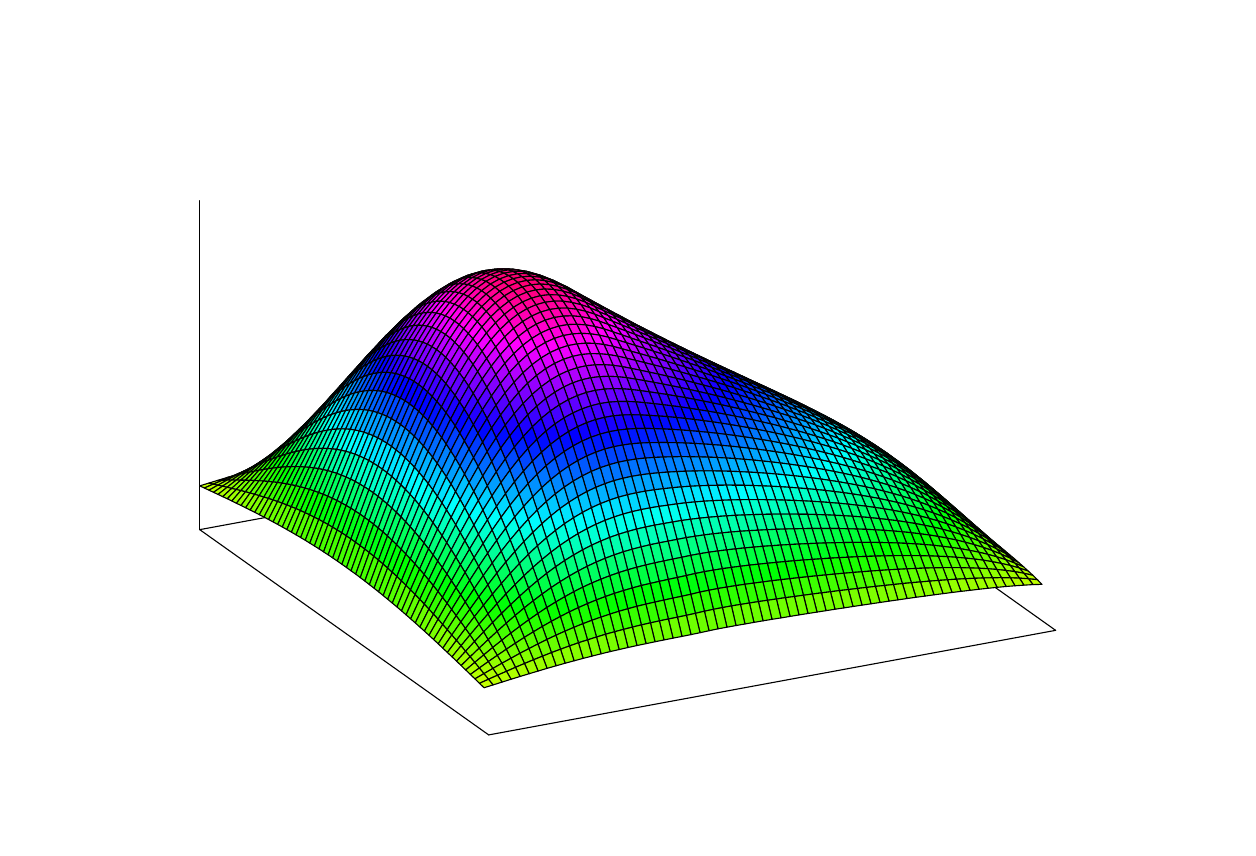
\begin{tikzpicture}[gnuplot]
%% generated with GNUPLOT 4.6p0 (Lua 5.1; terminal rev. 99, script rev. 100)
%% Sun 14 Apr 2013 11:51:22 PM BST
\gpsolidlines
\path (0.000,0.000) rectangle (15.240,10.160);
\gpcolor{color=gp lt color border}
\gpsetlinetype{gp lt border}
\gpsetlinewidth{1.00}
\draw[gp path] (2.185,3.785)--(9.385,5.113);
\draw[gp path] (13.055,2.506)--(9.385,5.113);
\draw[gp path] (2.185,3.785)--(2.185,7.962);
\gpfill{rgb color={0.818,1.000,0.000}} (9.271,5.626)--(9.157,5.598)--(9.215,5.543)--(9.329,5.578)--cycle;
\gpcolor{rgb color={0.000,0.000,0.000}}
\gpsetlinetype{gp lt plot 3}
\draw[gp path] (9.271,5.626)--(9.329,5.578)--(9.215,5.543)--(9.157,5.598)--cycle;
\gpfill{rgb color={0.830,1.000,0.000}} (9.329,5.578)--(9.215,5.543)--(9.273,5.489)--(9.388,5.530)--cycle;
\draw[gp path] (9.329,5.578)--(9.388,5.530)--(9.273,5.489)--(9.215,5.543)--cycle;
\gpfill{rgb color={0.841,1.000,0.000}} (9.388,5.530)--(9.273,5.489)--(9.332,5.435)--(9.446,5.482)--cycle;
\draw[gp path] (9.388,5.530)--(9.446,5.482)--(9.332,5.435)--(9.273,5.489)--cycle;
\gpfill{rgb color={0.852,1.000,0.000}} (9.446,5.482)--(9.332,5.435)--(9.390,5.381)--(9.504,5.434)--cycle;
\draw[gp path] (9.446,5.482)--(9.504,5.434)--(9.390,5.381)--(9.332,5.435)--cycle;
\gpfill{rgb color={0.863,1.000,0.000}} (9.504,5.434)--(9.390,5.381)--(9.448,5.329)--(9.562,5.387)--cycle;
\draw[gp path] (9.504,5.434)--(9.562,5.387)--(9.448,5.329)--(9.390,5.381)--cycle;
\gpfill{rgb color={0.873,1.000,0.000}} (9.562,5.387)--(9.448,5.329)--(9.506,5.276)--(9.621,5.340)--cycle;
\draw[gp path] (9.562,5.387)--(9.621,5.340)--(9.506,5.276)--(9.448,5.329)--cycle;
\gpfill{rgb color={0.883,1.000,0.000}} (9.621,5.340)--(9.506,5.276)--(9.565,5.226)--(9.679,5.294)--cycle;
\draw[gp path] (9.621,5.340)--(9.679,5.294)--(9.565,5.226)--(9.506,5.276)--cycle;
\gpfill{rgb color={0.891,1.000,0.000}} (9.679,5.294)--(9.565,5.226)--(9.623,5.175)--(9.737,5.248)--cycle;
\draw[gp path] (9.679,5.294)--(9.737,5.248)--(9.623,5.175)--(9.565,5.226)--cycle;
\gpfill{rgb color={0.899,1.000,0.000}} (9.737,5.248)--(9.623,5.175)--(9.681,5.126)--(9.795,5.204)--cycle;
\draw[gp path] (9.737,5.248)--(9.795,5.204)--(9.681,5.126)--(9.623,5.175)--cycle;
\gpfill{rgb color={0.906,1.000,0.000}} (9.795,5.204)--(9.681,5.126)--(9.739,5.078)--(9.854,5.159)--cycle;
\draw[gp path] (9.795,5.204)--(9.854,5.159)--(9.739,5.078)--(9.681,5.126)--cycle;
\gpfill{rgb color={0.911,1.000,0.000}} (9.854,5.159)--(9.739,5.078)--(9.798,5.031)--(9.912,5.115)--cycle;
\draw[gp path] (9.854,5.159)--(9.912,5.115)--(9.798,5.031)--(9.739,5.078)--cycle;
\gpfill{rgb color={0.915,1.000,0.000}} (9.912,5.115)--(9.798,5.031)--(9.856,4.986)--(9.970,5.071)--cycle;
\draw[gp path] (9.912,5.115)--(9.970,5.071)--(9.856,4.986)--(9.798,5.031)--cycle;
\gpfill{rgb color={0.918,1.000,0.000}} (9.970,5.071)--(9.856,4.986)--(9.914,4.942)--(10.028,5.029)--cycle;
\draw[gp path] (9.970,5.071)--(10.028,5.029)--(9.914,4.942)--(9.856,4.986)--cycle;
\gpfill{rgb color={0.919,1.000,0.000}} (10.028,5.029)--(9.914,4.942)--(9.972,4.900)--(10.087,4.987)--cycle;
\draw[gp path] (10.028,5.029)--(10.087,4.987)--(9.972,4.900)--(9.914,4.942)--cycle;
\gpfill{rgb color={0.919,1.000,0.000}} (10.087,4.987)--(9.972,4.900)--(10.030,4.860)--(10.145,4.947)--cycle;
\draw[gp path] (10.087,4.987)--(10.145,4.947)--(10.030,4.860)--(9.972,4.900)--cycle;
\gpfill{rgb color={0.916,1.000,0.000}} (10.145,4.947)--(10.030,4.860)--(10.089,4.823)--(10.203,4.907)--cycle;
\draw[gp path] (10.145,4.947)--(10.203,4.907)--(10.089,4.823)--(10.030,4.860)--cycle;
\gpfill{rgb color={0.912,1.000,0.000}} (10.203,4.907)--(10.089,4.823)--(10.147,4.788)--(10.261,4.869)--cycle;
\draw[gp path] (10.203,4.907)--(10.261,4.869)--(10.147,4.788)--(10.089,4.823)--cycle;
\gpfill{rgb color={0.905,1.000,0.000}} (10.261,4.869)--(10.147,4.788)--(10.205,4.755)--(10.320,4.832)--cycle;
\draw[gp path] (10.261,4.869)--(10.320,4.832)--(10.205,4.755)--(10.147,4.788)--cycle;
\gpfill{rgb color={0.896,1.000,0.000}} (10.320,4.832)--(10.205,4.755)--(10.263,4.726)--(10.378,4.797)--cycle;
\draw[gp path] (10.320,4.832)--(10.378,4.797)--(10.263,4.726)--(10.205,4.755)--cycle;
\gpfill{rgb color={0.884,1.000,0.000}} (10.378,4.797)--(10.263,4.726)--(10.322,4.699)--(10.436,4.763)--cycle;
\draw[gp path] (10.378,4.797)--(10.436,4.763)--(10.322,4.699)--(10.263,4.726)--cycle;
\gpfill{rgb color={0.869,1.000,0.000}} (10.436,4.763)--(10.322,4.699)--(10.380,4.677)--(10.494,4.731)--cycle;
\draw[gp path] (10.436,4.763)--(10.494,4.731)--(10.380,4.677)--(10.322,4.699)--cycle;
\gpfill{rgb color={0.850,1.000,0.000}} (10.494,4.731)--(10.380,4.677)--(10.438,4.658)--(10.552,4.701)--cycle;
\draw[gp path] (10.494,4.731)--(10.552,4.701)--(10.438,4.658)--(10.380,4.677)--cycle;
\gpfill{rgb color={0.827,1.000,0.000}} (10.552,4.701)--(10.438,4.658)--(10.496,4.644)--(10.611,4.674)--cycle;
\draw[gp path] (10.552,4.701)--(10.611,4.674)--(10.496,4.644)--(10.438,4.658)--cycle;
\gpfill{rgb color={0.799,1.000,0.000}} (10.611,4.674)--(10.496,4.644)--(10.555,4.636)--(10.669,4.650)--cycle;
\draw[gp path] (10.611,4.674)--(10.669,4.650)--(10.555,4.636)--(10.496,4.644)--cycle;
\gpfill{rgb color={0.766,1.000,0.000}} (10.669,4.650)--(10.555,4.636)--(10.613,4.635)--(10.727,4.630)--cycle;
\draw[gp path] (10.669,4.650)--(10.727,4.630)--(10.613,4.635)--(10.555,4.636)--cycle;
\gpfill{rgb color={0.731,1.000,0.000}} (10.727,4.630)--(10.613,4.635)--(10.671,4.629)--(10.785,4.607)--cycle;
\draw[gp path] (10.727,4.630)--(10.785,4.607)--(10.671,4.629)--(10.613,4.635)--cycle;
\gpfill{rgb color={0.702,1.000,0.000}} (10.785,4.607)--(10.671,4.629)--(10.729,4.617)--(10.844,4.581)--cycle;
\draw[gp path] (10.785,4.607)--(10.844,4.581)--(10.729,4.617)--(10.671,4.629)--cycle;
\gpfill{rgb color={0.676,1.000,0.000}} (10.844,4.581)--(10.729,4.617)--(10.788,4.602)--(10.902,4.553)--cycle;
\draw[gp path] (10.844,4.581)--(10.902,4.553)--(10.788,4.602)--(10.729,4.617)--cycle;
\gpfill{rgb color={0.654,1.000,0.000}} (10.902,4.553)--(10.788,4.602)--(10.846,4.584)--(10.960,4.523)--cycle;
\draw[gp path] (10.902,4.553)--(10.960,4.523)--(10.846,4.584)--(10.788,4.602)--cycle;
\gpfill{rgb color={0.634,1.000,0.000}} (10.960,4.523)--(10.846,4.584)--(10.904,4.563)--(11.018,4.492)--cycle;
\draw[gp path] (10.960,4.523)--(11.018,4.492)--(10.904,4.563)--(10.846,4.584)--cycle;
\gpfill{rgb color={0.617,1.000,0.000}} (11.018,4.492)--(10.904,4.563)--(10.962,4.540)--(11.077,4.460)--cycle;
\draw[gp path] (11.018,4.492)--(11.077,4.460)--(10.962,4.540)--(10.904,4.563)--cycle;
\gpfill{rgb color={0.602,1.000,0.000}} (11.077,4.460)--(10.962,4.540)--(11.021,4.514)--(11.135,4.426)--cycle;
\draw[gp path] (11.077,4.460)--(11.135,4.426)--(11.021,4.514)--(10.962,4.540)--cycle;
\gpfill{rgb color={0.588,1.000,0.000}} (11.135,4.426)--(11.021,4.514)--(11.079,4.487)--(11.193,4.392)--cycle;
\draw[gp path] (11.135,4.426)--(11.193,4.392)--(11.079,4.487)--(11.021,4.514)--cycle;
\gpfill{rgb color={0.577,1.000,0.000}} (11.193,4.392)--(11.079,4.487)--(11.137,4.458)--(11.251,4.357)--cycle;
\draw[gp path] (11.193,4.392)--(11.251,4.357)--(11.137,4.458)--(11.079,4.487)--cycle;
\gpfill{rgb color={0.567,1.000,0.000}} (11.251,4.357)--(11.137,4.458)--(11.195,4.427)--(11.310,4.321)--cycle;
\draw[gp path] (11.251,4.357)--(11.310,4.321)--(11.195,4.427)--(11.137,4.458)--cycle;
\gpfill{rgb color={0.558,1.000,0.000}} (11.310,4.321)--(11.195,4.427)--(11.254,4.394)--(11.368,4.284)--cycle;
\draw[gp path] (11.310,4.321)--(11.368,4.284)--(11.254,4.394)--(11.195,4.427)--cycle;
\gpfill{rgb color={0.551,1.000,0.000}} (11.368,4.284)--(11.254,4.394)--(11.312,4.360)--(11.426,4.246)--cycle;
\draw[gp path] (11.368,4.284)--(11.426,4.246)--(11.312,4.360)--(11.254,4.394)--cycle;
\gpfill{rgb color={0.545,1.000,0.000}} (11.426,4.246)--(11.312,4.360)--(11.370,4.324)--(11.484,4.208)--cycle;
\draw[gp path] (11.426,4.246)--(11.484,4.208)--(11.370,4.324)--(11.312,4.360)--cycle;
\gpfill{rgb color={0.540,1.000,0.000}} (11.484,4.208)--(11.370,4.324)--(11.428,4.288)--(11.543,4.169)--cycle;
\draw[gp path] (11.484,4.208)--(11.543,4.169)--(11.428,4.288)--(11.370,4.324)--cycle;
\gpfill{rgb color={0.537,1.000,0.000}} (11.543,4.169)--(11.428,4.288)--(11.486,4.250)--(11.601,4.129)--cycle;
\draw[gp path] (11.543,4.169)--(11.601,4.129)--(11.486,4.250)--(11.428,4.288)--cycle;
\gpfill{rgb color={0.534,1.000,0.000}} (11.601,4.129)--(11.486,4.250)--(11.545,4.210)--(11.659,4.088)--cycle;
\draw[gp path] (11.601,4.129)--(11.659,4.088)--(11.545,4.210)--(11.486,4.250)--cycle;
\gpfill{rgb color={0.533,1.000,0.000}} (11.659,4.088)--(11.545,4.210)--(11.603,4.170)--(11.717,4.048)--cycle;
\draw[gp path] (11.659,4.088)--(11.717,4.048)--(11.603,4.170)--(11.545,4.210)--cycle;
\gpfill{rgb color={0.533,1.000,0.000}} (11.717,4.048)--(11.603,4.170)--(11.661,4.128)--(11.776,4.006)--cycle;
\draw[gp path] (11.717,4.048)--(11.776,4.006)--(11.661,4.128)--(11.603,4.170)--cycle;
\gpfill{rgb color={0.533,1.000,0.000}} (11.776,4.006)--(11.661,4.128)--(11.719,4.085)--(11.834,3.964)--cycle;
\draw[gp path] (11.776,4.006)--(11.834,3.964)--(11.719,4.085)--(11.661,4.128)--cycle;
\gpfill{rgb color={0.535,1.000,0.000}} (11.834,3.964)--(11.719,4.085)--(11.778,4.041)--(11.892,3.921)--cycle;
\draw[gp path] (11.834,3.964)--(11.892,3.921)--(11.778,4.041)--(11.719,4.085)--cycle;
\gpfill{rgb color={0.538,1.000,0.000}} (11.892,3.921)--(11.778,4.041)--(11.836,3.996)--(11.950,3.878)--cycle;
\draw[gp path] (11.892,3.921)--(11.950,3.878)--(11.836,3.996)--(11.778,4.041)--cycle;
\gpfill{rgb color={0.542,1.000,0.000}} (11.950,3.878)--(11.836,3.996)--(11.894,3.950)--(12.008,3.834)--cycle;
\draw[gp path] (11.950,3.878)--(12.008,3.834)--(11.894,3.950)--(11.836,3.996)--cycle;
\gpfill{rgb color={0.546,1.000,0.000}} (12.008,3.834)--(11.894,3.950)--(11.952,3.903)--(12.067,3.790)--cycle;
\draw[gp path] (12.008,3.834)--(12.067,3.790)--(11.952,3.903)--(11.894,3.950)--cycle;
\gpfill{rgb color={0.552,1.000,0.000}} (12.067,3.790)--(11.952,3.903)--(12.011,3.855)--(12.125,3.745)--cycle;
\draw[gp path] (12.067,3.790)--(12.125,3.745)--(12.011,3.855)--(11.952,3.903)--cycle;
\gpfill{rgb color={0.559,1.000,0.000}} (12.125,3.745)--(12.011,3.855)--(12.069,3.805)--(12.183,3.700)--cycle;
\draw[gp path] (12.125,3.745)--(12.183,3.700)--(12.069,3.805)--(12.011,3.855)--cycle;
\gpfill{rgb color={0.567,1.000,0.000}} (12.183,3.700)--(12.069,3.805)--(12.127,3.755)--(12.241,3.654)--cycle;
\draw[gp path] (12.183,3.700)--(12.241,3.654)--(12.127,3.755)--(12.069,3.805)--cycle;
\gpfill{rgb color={0.576,1.000,0.000}} (12.241,3.654)--(12.127,3.755)--(12.185,3.703)--(12.300,3.607)--cycle;
\draw[gp path] (12.241,3.654)--(12.300,3.607)--(12.185,3.703)--(12.127,3.755)--cycle;
\gpfill{rgb color={0.586,1.000,0.000}} (12.300,3.607)--(12.185,3.703)--(12.244,3.650)--(12.358,3.560)--cycle;
\draw[gp path] (12.300,3.607)--(12.358,3.560)--(12.244,3.650)--(12.185,3.703)--cycle;
\gpfill{rgb color={0.597,1.000,0.000}} (12.358,3.560)--(12.244,3.650)--(12.302,3.595)--(12.416,3.512)--cycle;
\draw[gp path] (12.358,3.560)--(12.416,3.512)--(12.302,3.595)--(12.244,3.650)--cycle;
\gpfill{rgb color={0.609,1.000,0.000}} (12.416,3.512)--(12.302,3.595)--(12.360,3.539)--(12.474,3.463)--cycle;
\draw[gp path] (12.416,3.512)--(12.474,3.463)--(12.360,3.539)--(12.302,3.595)--cycle;
\gpfill{rgb color={0.623,1.000,0.000}} (12.474,3.463)--(12.360,3.539)--(12.418,3.482)--(12.533,3.414)--cycle;
\draw[gp path] (12.474,3.463)--(12.533,3.414)--(12.418,3.482)--(12.360,3.539)--cycle;
\gpfill{rgb color={0.638,1.000,0.000}} (12.533,3.414)--(12.418,3.482)--(12.477,3.423)--(12.591,3.363)--cycle;
\draw[gp path] (12.533,3.414)--(12.591,3.363)--(12.477,3.423)--(12.418,3.482)--cycle;
\gpfill{rgb color={0.655,1.000,0.000}} (12.591,3.363)--(12.477,3.423)--(12.535,3.361)--(12.649,3.312)--cycle;
\draw[gp path] (12.591,3.363)--(12.649,3.312)--(12.535,3.361)--(12.477,3.423)--cycle;
\gpfill{rgb color={0.674,1.000,0.000}} (12.649,3.312)--(12.535,3.361)--(12.593,3.298)--(12.707,3.259)--cycle;
\draw[gp path] (12.649,3.312)--(12.707,3.259)--(12.593,3.298)--(12.535,3.361)--cycle;
\gpfill{rgb color={0.696,1.000,0.000}} (12.707,3.259)--(12.593,3.298)--(12.651,3.231)--(12.766,3.205)--cycle;
\draw[gp path] (12.707,3.259)--(12.766,3.205)--(12.651,3.231)--(12.593,3.298)--cycle;
\gpfill{rgb color={0.720,1.000,0.000}} (12.766,3.205)--(12.651,3.231)--(12.710,3.161)--(12.824,3.149)--cycle;
\draw[gp path] (12.766,3.205)--(12.824,3.149)--(12.710,3.161)--(12.651,3.231)--cycle;
\gpfill{rgb color={0.748,1.000,0.000}} (12.824,3.149)--(12.710,3.161)--(12.768,3.087)--(12.882,3.090)--cycle;
\draw[gp path] (12.824,3.149)--(12.882,3.090)--(12.768,3.087)--(12.710,3.161)--cycle;
\gpfill{rgb color={0.830,1.000,0.000}} (9.157,5.598)--(9.043,5.570)--(9.101,5.509)--(9.215,5.543)--cycle;
\draw[gp path] (9.157,5.598)--(9.215,5.543)--(9.101,5.509)--(9.043,5.570)--cycle;
\gpfill{rgb color={0.849,1.000,0.000}} (9.215,5.543)--(9.101,5.509)--(9.159,5.449)--(9.273,5.489)--cycle;
\draw[gp path] (9.215,5.543)--(9.273,5.489)--(9.159,5.449)--(9.101,5.509)--cycle;
\gpfill{rgb color={0.868,1.000,0.000}} (9.273,5.489)--(9.159,5.449)--(9.217,5.389)--(9.332,5.435)--cycle;
\draw[gp path] (9.273,5.489)--(9.332,5.435)--(9.217,5.389)--(9.159,5.449)--cycle;
\gpfill{rgb color={0.886,1.000,0.000}} (9.332,5.435)--(9.217,5.389)--(9.276,5.329)--(9.390,5.381)--cycle;
\draw[gp path] (9.332,5.435)--(9.390,5.381)--(9.276,5.329)--(9.217,5.389)--cycle;
\gpfill{rgb color={0.904,1.000,0.000}} (9.390,5.381)--(9.276,5.329)--(9.334,5.271)--(9.448,5.329)--cycle;
\draw[gp path] (9.390,5.381)--(9.448,5.329)--(9.334,5.271)--(9.276,5.329)--cycle;
\gpfill{rgb color={0.921,1.000,0.000}} (9.448,5.329)--(9.334,5.271)--(9.392,5.214)--(9.506,5.276)--cycle;
\draw[gp path] (9.448,5.329)--(9.506,5.276)--(9.392,5.214)--(9.334,5.271)--cycle;
\gpfill{rgb color={0.936,1.000,0.000}} (9.506,5.276)--(9.392,5.214)--(9.450,5.158)--(9.565,5.226)--cycle;
\draw[gp path] (9.506,5.276)--(9.565,5.226)--(9.450,5.158)--(9.392,5.214)--cycle;
\gpfill{rgb color={0.951,1.000,0.000}} (9.565,5.226)--(9.450,5.158)--(9.508,5.103)--(9.623,5.175)--cycle;
\draw[gp path] (9.565,5.226)--(9.623,5.175)--(9.508,5.103)--(9.450,5.158)--cycle;
\gpfill{rgb color={0.963,1.000,0.000}} (9.623,5.175)--(9.508,5.103)--(9.567,5.050)--(9.681,5.126)--cycle;
\draw[gp path] (9.623,5.175)--(9.681,5.126)--(9.567,5.050)--(9.508,5.103)--cycle;
\gpfill{rgb color={0.974,1.000,0.000}} (9.681,5.126)--(9.567,5.050)--(9.625,4.998)--(9.739,5.078)--cycle;
\draw[gp path] (9.681,5.126)--(9.739,5.078)--(9.625,4.998)--(9.567,5.050)--cycle;
\gpfill{rgb color={0.983,1.000,0.000}} (9.739,5.078)--(9.625,4.998)--(9.683,4.949)--(9.798,5.031)--cycle;
\draw[gp path] (9.739,5.078)--(9.798,5.031)--(9.683,4.949)--(9.625,4.998)--cycle;
\gpfill{rgb color={0.990,1.000,0.000}} (9.798,5.031)--(9.683,4.949)--(9.741,4.902)--(9.856,4.986)--cycle;
\draw[gp path] (9.798,5.031)--(9.856,4.986)--(9.741,4.902)--(9.683,4.949)--cycle;
\gpfill{rgb color={0.995,1.000,0.000}} (9.856,4.986)--(9.741,4.902)--(9.800,4.857)--(9.914,4.942)--cycle;
\draw[gp path] (9.856,4.986)--(9.914,4.942)--(9.800,4.857)--(9.741,4.902)--cycle;
\gpfill{rgb color={0.997,1.000,0.000}} (9.914,4.942)--(9.800,4.857)--(9.858,4.815)--(9.972,4.900)--cycle;
\draw[gp path] (9.914,4.942)--(9.972,4.900)--(9.858,4.815)--(9.800,4.857)--cycle;
\gpfill{rgb color={0.996,1.000,0.000}} (9.972,4.900)--(9.858,4.815)--(9.916,4.776)--(10.030,4.860)--cycle;
\draw[gp path] (9.972,4.900)--(10.030,4.860)--(9.916,4.776)--(9.858,4.815)--cycle;
\gpfill{rgb color={0.992,1.000,0.000}} (10.030,4.860)--(9.916,4.776)--(9.974,4.740)--(10.089,4.823)--cycle;
\draw[gp path] (10.030,4.860)--(10.089,4.823)--(9.974,4.740)--(9.916,4.776)--cycle;
\gpfill{rgb color={0.985,1.000,0.000}} (10.089,4.823)--(9.974,4.740)--(10.033,4.708)--(10.147,4.788)--cycle;
\draw[gp path] (10.089,4.823)--(10.147,4.788)--(10.033,4.708)--(9.974,4.740)--cycle;
\gpfill{rgb color={0.973,1.000,0.000}} (10.147,4.788)--(10.033,4.708)--(10.091,4.680)--(10.205,4.755)--cycle;
\draw[gp path] (10.147,4.788)--(10.205,4.755)--(10.091,4.680)--(10.033,4.708)--cycle;
\gpfill{rgb color={0.958,1.000,0.000}} (10.205,4.755)--(10.091,4.680)--(10.149,4.656)--(10.263,4.726)--cycle;
\draw[gp path] (10.205,4.755)--(10.263,4.726)--(10.149,4.656)--(10.091,4.680)--cycle;
\gpfill{rgb color={0.938,1.000,0.000}} (10.263,4.726)--(10.149,4.656)--(10.207,4.637)--(10.322,4.699)--cycle;
\draw[gp path] (10.263,4.726)--(10.322,4.699)--(10.207,4.637)--(10.149,4.656)--cycle;
\gpfill{rgb color={0.913,1.000,0.000}} (10.322,4.699)--(10.207,4.637)--(10.266,4.623)--(10.380,4.677)--cycle;
\draw[gp path] (10.322,4.699)--(10.380,4.677)--(10.266,4.623)--(10.207,4.637)--cycle;
\gpfill{rgb color={0.882,1.000,0.000}} (10.380,4.677)--(10.266,4.623)--(10.324,4.616)--(10.438,4.658)--cycle;
\draw[gp path] (10.380,4.677)--(10.438,4.658)--(10.324,4.616)--(10.266,4.623)--cycle;
\gpfill{rgb color={0.845,1.000,0.000}} (10.438,4.658)--(10.324,4.616)--(10.382,4.615)--(10.496,4.644)--cycle;
\draw[gp path] (10.438,4.658)--(10.496,4.644)--(10.382,4.615)--(10.324,4.616)--cycle;
\gpfill{rgb color={0.800,1.000,0.000}} (10.496,4.644)--(10.382,4.615)--(10.440,4.621)--(10.555,4.636)--cycle;
\draw[gp path] (10.496,4.644)--(10.555,4.636)--(10.440,4.621)--(10.382,4.615)--cycle;
\gpfill{rgb color={0.747,1.000,0.000}} (10.555,4.636)--(10.440,4.621)--(10.499,4.637)--(10.613,4.635)--cycle;
\draw[gp path] (10.555,4.636)--(10.613,4.635)--(10.499,4.637)--(10.440,4.621)--cycle;
\gpfill{rgb color={0.692,1.000,0.000}} (10.613,4.635)--(10.499,4.637)--(10.557,4.646)--(10.671,4.629)--cycle;
\draw[gp path] (10.613,4.635)--(10.671,4.629)--(10.557,4.646)--(10.499,4.637)--cycle;
\gpfill{rgb color={0.645,1.000,0.000}} (10.671,4.629)--(10.557,4.646)--(10.615,4.648)--(10.729,4.617)--cycle;
\draw[gp path] (10.671,4.629)--(10.729,4.617)--(10.615,4.648)--(10.557,4.646)--cycle;
\gpfill{rgb color={0.603,1.000,0.000}} (10.729,4.617)--(10.615,4.648)--(10.673,4.645)--(10.788,4.602)--cycle;
\draw[gp path] (10.729,4.617)--(10.788,4.602)--(10.673,4.645)--(10.615,4.648)--cycle;
\gpfill{rgb color={0.567,1.000,0.000}} (10.788,4.602)--(10.673,4.645)--(10.732,4.638)--(10.846,4.584)--cycle;
\draw[gp path] (10.788,4.602)--(10.846,4.584)--(10.732,4.638)--(10.673,4.645)--cycle;
\gpfill{rgb color={0.534,1.000,0.000}} (10.846,4.584)--(10.732,4.638)--(10.790,4.627)--(10.904,4.563)--cycle;
\draw[gp path] (10.846,4.584)--(10.904,4.563)--(10.790,4.627)--(10.732,4.638)--cycle;
\gpfill{rgb color={0.506,1.000,0.000}} (10.904,4.563)--(10.790,4.627)--(10.848,4.613)--(10.962,4.540)--cycle;
\draw[gp path] (10.904,4.563)--(10.962,4.540)--(10.848,4.613)--(10.790,4.627)--cycle;
\gpfill{rgb color={0.480,1.000,0.000}} (10.962,4.540)--(10.848,4.613)--(10.906,4.595)--(11.021,4.514)--cycle;
\draw[gp path] (10.962,4.540)--(11.021,4.514)--(10.906,4.595)--(10.848,4.613)--cycle;
\gpfill{rgb color={0.458,1.000,0.000}} (11.021,4.514)--(10.906,4.595)--(10.965,4.574)--(11.079,4.487)--cycle;
\draw[gp path] (11.021,4.514)--(11.079,4.487)--(10.965,4.574)--(10.906,4.595)--cycle;
\gpfill{rgb color={0.439,1.000,0.000}} (11.079,4.487)--(10.965,4.574)--(11.023,4.551)--(11.137,4.458)--cycle;
\draw[gp path] (11.079,4.487)--(11.137,4.458)--(11.023,4.551)--(10.965,4.574)--cycle;
\gpfill{rgb color={0.422,1.000,0.000}} (11.137,4.458)--(11.023,4.551)--(11.081,4.525)--(11.195,4.427)--cycle;
\draw[gp path] (11.137,4.458)--(11.195,4.427)--(11.081,4.525)--(11.023,4.551)--cycle;
\gpfill{rgb color={0.408,1.000,0.000}} (11.195,4.427)--(11.081,4.525)--(11.139,4.497)--(11.254,4.394)--cycle;
\draw[gp path] (11.195,4.427)--(11.254,4.394)--(11.139,4.497)--(11.081,4.525)--cycle;
\gpfill{rgb color={0.396,1.000,0.000}} (11.254,4.394)--(11.139,4.497)--(11.197,4.466)--(11.312,4.360)--cycle;
\draw[gp path] (11.254,4.394)--(11.312,4.360)--(11.197,4.466)--(11.139,4.497)--cycle;
\gpfill{rgb color={0.386,1.000,0.000}} (11.312,4.360)--(11.197,4.466)--(11.256,4.433)--(11.370,4.324)--cycle;
\draw[gp path] (11.312,4.360)--(11.370,4.324)--(11.256,4.433)--(11.197,4.466)--cycle;
\gpfill{rgb color={0.378,1.000,0.000}} (11.370,4.324)--(11.256,4.433)--(11.314,4.399)--(11.428,4.288)--cycle;
\draw[gp path] (11.370,4.324)--(11.428,4.288)--(11.314,4.399)--(11.256,4.433)--cycle;
\gpfill{rgb color={0.373,1.000,0.000}} (11.428,4.288)--(11.314,4.399)--(11.372,4.362)--(11.486,4.250)--cycle;
\draw[gp path] (11.428,4.288)--(11.486,4.250)--(11.372,4.362)--(11.314,4.399)--cycle;
\gpfill{rgb color={0.369,1.000,0.000}} (11.486,4.250)--(11.372,4.362)--(11.430,4.324)--(11.545,4.210)--cycle;
\draw[gp path] (11.486,4.250)--(11.545,4.210)--(11.430,4.324)--(11.372,4.362)--cycle;
\gpfill{rgb color={0.366,1.000,0.000}} (11.545,4.210)--(11.430,4.324)--(11.489,4.284)--(11.603,4.170)--cycle;
\draw[gp path] (11.545,4.210)--(11.603,4.170)--(11.489,4.284)--(11.430,4.324)--cycle;
\gpfill{rgb color={0.366,1.000,0.000}} (11.603,4.170)--(11.489,4.284)--(11.547,4.242)--(11.661,4.128)--cycle;
\draw[gp path] (11.603,4.170)--(11.661,4.128)--(11.547,4.242)--(11.489,4.284)--cycle;
\gpfill{rgb color={0.367,1.000,0.000}} (11.661,4.128)--(11.547,4.242)--(11.605,4.198)--(11.719,4.085)--cycle;
\draw[gp path] (11.661,4.128)--(11.719,4.085)--(11.605,4.198)--(11.547,4.242)--cycle;
\gpfill{rgb color={0.370,1.000,0.000}} (11.719,4.085)--(11.605,4.198)--(11.663,4.153)--(11.778,4.041)--cycle;
\draw[gp path] (11.719,4.085)--(11.778,4.041)--(11.663,4.153)--(11.605,4.198)--cycle;
\gpfill{rgb color={0.375,1.000,0.000}} (11.778,4.041)--(11.663,4.153)--(11.722,4.106)--(11.836,3.996)--cycle;
\draw[gp path] (11.778,4.041)--(11.836,3.996)--(11.722,4.106)--(11.663,4.153)--cycle;
\gpfill{rgb color={0.381,1.000,0.000}} (11.836,3.996)--(11.722,4.106)--(11.780,4.058)--(11.894,3.950)--cycle;
\draw[gp path] (11.836,3.996)--(11.894,3.950)--(11.780,4.058)--(11.722,4.106)--cycle;
\gpfill{rgb color={0.389,1.000,0.000}} (11.894,3.950)--(11.780,4.058)--(11.838,4.008)--(11.952,3.903)--cycle;
\draw[gp path] (11.894,3.950)--(11.952,3.903)--(11.838,4.008)--(11.780,4.058)--cycle;
\gpfill{rgb color={0.399,1.000,0.000}} (11.952,3.903)--(11.838,4.008)--(11.896,3.956)--(12.011,3.855)--cycle;
\draw[gp path] (11.952,3.903)--(12.011,3.855)--(11.896,3.956)--(11.838,4.008)--cycle;
\gpfill{rgb color={0.410,1.000,0.000}} (12.011,3.855)--(11.896,3.956)--(11.955,3.903)--(12.069,3.805)--cycle;
\draw[gp path] (12.011,3.855)--(12.069,3.805)--(11.955,3.903)--(11.896,3.956)--cycle;
\gpfill{rgb color={0.423,1.000,0.000}} (12.069,3.805)--(11.955,3.903)--(12.013,3.848)--(12.127,3.755)--cycle;
\draw[gp path] (12.069,3.805)--(12.127,3.755)--(12.013,3.848)--(11.955,3.903)--cycle;
\gpfill{rgb color={0.437,1.000,0.000}} (12.127,3.755)--(12.013,3.848)--(12.071,3.791)--(12.185,3.703)--cycle;
\draw[gp path] (12.127,3.755)--(12.185,3.703)--(12.071,3.791)--(12.013,3.848)--cycle;
\gpfill{rgb color={0.454,1.000,0.000}} (12.185,3.703)--(12.071,3.791)--(12.129,3.732)--(12.244,3.650)--cycle;
\draw[gp path] (12.185,3.703)--(12.244,3.650)--(12.129,3.732)--(12.071,3.791)--cycle;
\gpfill{rgb color={0.473,1.000,0.000}} (12.244,3.650)--(12.129,3.732)--(12.188,3.671)--(12.302,3.595)--cycle;
\draw[gp path] (12.244,3.650)--(12.302,3.595)--(12.188,3.671)--(12.129,3.732)--cycle;
\gpfill{rgb color={0.493,1.000,0.000}} (12.302,3.595)--(12.188,3.671)--(12.246,3.608)--(12.360,3.539)--cycle;
\draw[gp path] (12.302,3.595)--(12.360,3.539)--(12.246,3.608)--(12.188,3.671)--cycle;
\gpfill{rgb color={0.516,1.000,0.000}} (12.360,3.539)--(12.246,3.608)--(12.304,3.542)--(12.418,3.482)--cycle;
\draw[gp path] (12.360,3.539)--(12.418,3.482)--(12.304,3.542)--(12.246,3.608)--cycle;
\gpfill{rgb color={0.541,1.000,0.000}} (12.418,3.482)--(12.304,3.542)--(12.362,3.474)--(12.477,3.423)--cycle;
\draw[gp path] (12.418,3.482)--(12.477,3.423)--(12.362,3.474)--(12.304,3.542)--cycle;
\gpfill{rgb color={0.569,1.000,0.000}} (12.477,3.423)--(12.362,3.474)--(12.421,3.404)--(12.535,3.361)--cycle;
\draw[gp path] (12.477,3.423)--(12.535,3.361)--(12.421,3.404)--(12.362,3.474)--cycle;
\gpfill{rgb color={0.601,1.000,0.000}} (12.535,3.361)--(12.421,3.404)--(12.479,3.330)--(12.593,3.298)--cycle;
\draw[gp path] (12.535,3.361)--(12.593,3.298)--(12.479,3.330)--(12.421,3.404)--cycle;
\gpfill{rgb color={0.635,1.000,0.000}} (12.593,3.298)--(12.479,3.330)--(12.537,3.252)--(12.651,3.231)--cycle;
\draw[gp path] (12.593,3.298)--(12.651,3.231)--(12.537,3.252)--(12.479,3.330)--cycle;
\gpfill{rgb color={0.675,1.000,0.000}} (12.651,3.231)--(12.537,3.252)--(12.595,3.169)--(12.710,3.161)--cycle;
\draw[gp path] (12.651,3.231)--(12.710,3.161)--(12.595,3.169)--(12.537,3.252)--cycle;
\gpfill{rgb color={0.720,1.000,0.000}} (12.710,3.161)--(12.595,3.169)--(12.653,3.080)--(12.768,3.087)--cycle;
\draw[gp path] (12.710,3.161)--(12.768,3.087)--(12.653,3.080)--(12.595,3.169)--cycle;
\gpfill{rgb color={0.841,1.000,0.000}} (9.043,5.570)--(8.928,5.543)--(8.987,5.476)--(9.101,5.509)--cycle;
\draw[gp path] (9.043,5.570)--(9.101,5.509)--(8.987,5.476)--(8.928,5.543)--cycle;
\gpfill{rgb color={0.868,1.000,0.000}} (9.101,5.509)--(8.987,5.476)--(9.045,5.409)--(9.159,5.449)--cycle;
\draw[gp path] (9.101,5.509)--(9.159,5.449)--(9.045,5.409)--(8.987,5.476)--cycle;
\gpfill{rgb color={0.894,1.000,0.000}} (9.159,5.449)--(9.045,5.409)--(9.103,5.344)--(9.217,5.389)--cycle;
\draw[gp path] (9.159,5.449)--(9.217,5.389)--(9.103,5.344)--(9.045,5.409)--cycle;
\gpfill{rgb color={0.919,1.000,0.000}} (9.217,5.389)--(9.103,5.344)--(9.161,5.278)--(9.276,5.329)--cycle;
\draw[gp path] (9.217,5.389)--(9.276,5.329)--(9.161,5.278)--(9.103,5.344)--cycle;
\gpfill{rgb color={0.944,1.000,0.000}} (9.276,5.329)--(9.161,5.278)--(9.219,5.216)--(9.334,5.271)--cycle;
\draw[gp path] (9.276,5.329)--(9.334,5.271)--(9.219,5.216)--(9.161,5.278)--cycle;
\gpfill{rgb color={0.967,1.000,0.000}} (9.334,5.271)--(9.219,5.216)--(9.278,5.153)--(9.392,5.214)--cycle;
\draw[gp path] (9.334,5.271)--(9.392,5.214)--(9.278,5.153)--(9.219,5.216)--cycle;
\gpfill{rgb color={0.988,1.000,0.000}} (9.392,5.214)--(9.278,5.153)--(9.336,5.092)--(9.450,5.158)--cycle;
\draw[gp path] (9.392,5.214)--(9.450,5.158)--(9.336,5.092)--(9.278,5.153)--cycle;
\gpfill{rgb color={1.000,0.992,0.000}} (9.450,5.158)--(9.336,5.092)--(9.394,5.033)--(9.508,5.103)--cycle;
\draw[gp path] (9.450,5.158)--(9.508,5.103)--(9.394,5.033)--(9.336,5.092)--cycle;
\gpfill{rgb color={1.000,0.975,0.000}} (9.508,5.103)--(9.394,5.033)--(9.452,4.976)--(9.567,5.050)--cycle;
\draw[gp path] (9.508,5.103)--(9.567,5.050)--(9.452,4.976)--(9.394,5.033)--cycle;
\gpfill{rgb color={1.000,0.959,0.000}} (9.567,5.050)--(9.452,4.976)--(9.511,4.922)--(9.625,4.998)--cycle;
\draw[gp path] (9.567,5.050)--(9.625,4.998)--(9.511,4.922)--(9.452,4.976)--cycle;
\gpfill{rgb color={1.000,0.947,0.000}} (9.625,4.998)--(9.511,4.922)--(9.569,4.870)--(9.683,4.949)--cycle;
\draw[gp path] (9.625,4.998)--(9.683,4.949)--(9.569,4.870)--(9.511,4.922)--cycle;
\gpfill{rgb color={1.000,0.937,0.000}} (9.683,4.949)--(9.569,4.870)--(9.627,4.821)--(9.741,4.902)--cycle;
\draw[gp path] (9.683,4.949)--(9.741,4.902)--(9.627,4.821)--(9.569,4.870)--cycle;
\gpfill{rgb color={1.000,0.931,0.000}} (9.741,4.902)--(9.627,4.821)--(9.685,4.775)--(9.800,4.857)--cycle;
\draw[gp path] (9.741,4.902)--(9.800,4.857)--(9.685,4.775)--(9.627,4.821)--cycle;
\gpfill{rgb color={1.000,0.928,0.000}} (9.800,4.857)--(9.685,4.775)--(9.744,4.733)--(9.858,4.815)--cycle;
\draw[gp path] (9.800,4.857)--(9.858,4.815)--(9.744,4.733)--(9.685,4.775)--cycle;
\gpfill{rgb color={1.000,0.930,0.000}} (9.858,4.815)--(9.744,4.733)--(9.802,4.695)--(9.916,4.776)--cycle;
\draw[gp path] (9.858,4.815)--(9.916,4.776)--(9.802,4.695)--(9.744,4.733)--cycle;
\gpfill{rgb color={1.000,0.935,0.000}} (9.916,4.776)--(9.802,4.695)--(9.860,4.661)--(9.974,4.740)--cycle;
\draw[gp path] (9.916,4.776)--(9.974,4.740)--(9.860,4.661)--(9.802,4.695)--cycle;
\gpfill{rgb color={1.000,0.946,0.000}} (9.974,4.740)--(9.860,4.661)--(9.918,4.632)--(10.033,4.708)--cycle;
\draw[gp path] (9.974,4.740)--(10.033,4.708)--(9.918,4.632)--(9.860,4.661)--cycle;
\gpfill{rgb color={1.000,0.961,0.000}} (10.033,4.708)--(9.918,4.632)--(9.977,4.608)--(10.091,4.680)--cycle;
\draw[gp path] (10.033,4.708)--(10.091,4.680)--(9.977,4.608)--(9.918,4.632)--cycle;
\gpfill{rgb color={1.000,0.982,0.000}} (10.091,4.680)--(9.977,4.608)--(10.035,4.589)--(10.149,4.656)--cycle;
\draw[gp path] (10.091,4.680)--(10.149,4.656)--(10.035,4.589)--(9.977,4.608)--cycle;
\gpfill{rgb color={0.990,1.000,0.000}} (10.149,4.656)--(10.035,4.589)--(10.093,4.577)--(10.207,4.637)--cycle;
\draw[gp path] (10.149,4.656)--(10.207,4.637)--(10.093,4.577)--(10.035,4.589)--cycle;
\gpfill{rgb color={0.956,1.000,0.000}} (10.207,4.637)--(10.093,4.577)--(10.151,4.572)--(10.266,4.623)--cycle;
\draw[gp path] (10.207,4.637)--(10.266,4.623)--(10.151,4.572)--(10.093,4.577)--cycle;
\gpfill{rgb color={0.913,1.000,0.000}} (10.266,4.623)--(10.151,4.572)--(10.210,4.574)--(10.324,4.616)--cycle;
\draw[gp path] (10.266,4.623)--(10.324,4.616)--(10.210,4.574)--(10.151,4.572)--cycle;
\gpfill{rgb color={0.863,1.000,0.000}} (10.324,4.616)--(10.210,4.574)--(10.268,4.585)--(10.382,4.615)--cycle;
\draw[gp path] (10.324,4.616)--(10.382,4.615)--(10.268,4.585)--(10.210,4.574)--cycle;
\gpfill{rgb color={0.802,1.000,0.000}} (10.382,4.615)--(10.268,4.585)--(10.326,4.606)--(10.440,4.621)--cycle;
\draw[gp path] (10.382,4.615)--(10.440,4.621)--(10.326,4.606)--(10.268,4.585)--cycle;
\gpfill{rgb color={0.730,1.000,0.000}} (10.440,4.621)--(10.326,4.606)--(10.384,4.637)--(10.499,4.637)--cycle;
\draw[gp path] (10.440,4.621)--(10.499,4.637)--(10.384,4.637)--(10.326,4.606)--cycle;
\gpfill{rgb color={0.658,1.000,0.000}} (10.499,4.637)--(10.384,4.637)--(10.443,4.659)--(10.557,4.646)--cycle;
\draw[gp path] (10.499,4.637)--(10.557,4.646)--(10.443,4.659)--(10.384,4.637)--cycle;
\gpfill{rgb color={0.593,1.000,0.000}} (10.557,4.646)--(10.443,4.659)--(10.501,4.675)--(10.615,4.648)--cycle;
\draw[gp path] (10.557,4.646)--(10.615,4.648)--(10.501,4.675)--(10.443,4.659)--cycle;
\gpfill{rgb color={0.536,1.000,0.000}} (10.615,4.648)--(10.501,4.675)--(10.559,4.684)--(10.673,4.645)--cycle;
\draw[gp path] (10.615,4.648)--(10.673,4.645)--(10.559,4.684)--(10.501,4.675)--cycle;
\gpfill{rgb color={0.486,1.000,0.000}} (10.673,4.645)--(10.559,4.684)--(10.617,4.688)--(10.732,4.638)--cycle;
\draw[gp path] (10.673,4.645)--(10.732,4.638)--(10.617,4.688)--(10.559,4.684)--cycle;
\gpfill{rgb color={0.441,1.000,0.000}} (10.732,4.638)--(10.617,4.688)--(10.675,4.686)--(10.790,4.627)--cycle;
\draw[gp path] (10.732,4.638)--(10.790,4.627)--(10.675,4.686)--(10.617,4.688)--cycle;
\gpfill{rgb color={0.402,1.000,0.000}} (10.790,4.627)--(10.675,4.686)--(10.734,4.680)--(10.848,4.613)--cycle;
\draw[gp path] (10.790,4.627)--(10.848,4.613)--(10.734,4.680)--(10.675,4.686)--cycle;
\gpfill{rgb color={0.367,1.000,0.000}} (10.848,4.613)--(10.734,4.680)--(10.792,4.669)--(10.906,4.595)--cycle;
\draw[gp path] (10.848,4.613)--(10.906,4.595)--(10.792,4.669)--(10.734,4.680)--cycle;
\gpfill{rgb color={0.336,1.000,0.000}} (10.906,4.595)--(10.792,4.669)--(10.850,4.655)--(10.965,4.574)--cycle;
\draw[gp path] (10.906,4.595)--(10.965,4.574)--(10.850,4.655)--(10.792,4.669)--cycle;
\gpfill{rgb color={0.309,1.000,0.000}} (10.965,4.574)--(10.850,4.655)--(10.908,4.637)--(11.023,4.551)--cycle;
\draw[gp path] (10.965,4.574)--(11.023,4.551)--(10.908,4.637)--(10.850,4.655)--cycle;
\gpfill{rgb color={0.286,1.000,0.000}} (11.023,4.551)--(10.908,4.637)--(10.967,4.616)--(11.081,4.525)--cycle;
\draw[gp path] (11.023,4.551)--(11.081,4.525)--(10.967,4.616)--(10.908,4.637)--cycle;
\gpfill{rgb color={0.267,1.000,0.000}} (11.081,4.525)--(10.967,4.616)--(11.025,4.592)--(11.139,4.497)--cycle;
\draw[gp path] (11.081,4.525)--(11.139,4.497)--(11.025,4.592)--(10.967,4.616)--cycle;
\gpfill{rgb color={0.250,1.000,0.000}} (11.139,4.497)--(11.025,4.592)--(11.083,4.565)--(11.197,4.466)--cycle;
\draw[gp path] (11.139,4.497)--(11.197,4.466)--(11.083,4.565)--(11.025,4.592)--cycle;
\gpfill{rgb color={0.236,1.000,0.000}} (11.197,4.466)--(11.083,4.565)--(11.141,4.535)--(11.256,4.433)--cycle;
\draw[gp path] (11.197,4.466)--(11.256,4.433)--(11.141,4.535)--(11.083,4.565)--cycle;
\gpfill{rgb color={0.226,1.000,0.000}} (11.256,4.433)--(11.141,4.535)--(11.200,4.503)--(11.314,4.399)--cycle;
\draw[gp path] (11.256,4.433)--(11.314,4.399)--(11.200,4.503)--(11.141,4.535)--cycle;
\gpfill{rgb color={0.218,1.000,0.000}} (11.314,4.399)--(11.200,4.503)--(11.258,4.468)--(11.372,4.362)--cycle;
\draw[gp path] (11.314,4.399)--(11.372,4.362)--(11.258,4.468)--(11.200,4.503)--cycle;
\gpfill{rgb color={0.212,1.000,0.000}} (11.372,4.362)--(11.258,4.468)--(11.316,4.430)--(11.430,4.324)--cycle;
\draw[gp path] (11.372,4.362)--(11.430,4.324)--(11.316,4.430)--(11.258,4.468)--cycle;
\gpfill{rgb color={0.209,1.000,0.000}} (11.430,4.324)--(11.316,4.430)--(11.374,4.390)--(11.489,4.284)--cycle;
\draw[gp path] (11.430,4.324)--(11.489,4.284)--(11.374,4.390)--(11.316,4.430)--cycle;
\gpfill{rgb color={0.209,1.000,0.000}} (11.489,4.284)--(11.374,4.390)--(11.433,4.348)--(11.547,4.242)--cycle;
\draw[gp path] (11.489,4.284)--(11.547,4.242)--(11.433,4.348)--(11.374,4.390)--cycle;
\gpfill{rgb color={0.211,1.000,0.000}} (11.547,4.242)--(11.433,4.348)--(11.491,4.304)--(11.605,4.198)--cycle;
\draw[gp path] (11.547,4.242)--(11.605,4.198)--(11.491,4.304)--(11.433,4.348)--cycle;
\gpfill{rgb color={0.215,1.000,0.000}} (11.605,4.198)--(11.491,4.304)--(11.549,4.258)--(11.663,4.153)--cycle;
\draw[gp path] (11.605,4.198)--(11.663,4.153)--(11.549,4.258)--(11.491,4.304)--cycle;
\gpfill{rgb color={0.221,1.000,0.000}} (11.663,4.153)--(11.549,4.258)--(11.607,4.209)--(11.722,4.106)--cycle;
\draw[gp path] (11.663,4.153)--(11.722,4.106)--(11.607,4.209)--(11.549,4.258)--cycle;
\gpfill{rgb color={0.230,1.000,0.000}} (11.722,4.106)--(11.607,4.209)--(11.666,4.158)--(11.780,4.058)--cycle;
\draw[gp path] (11.722,4.106)--(11.780,4.058)--(11.666,4.158)--(11.607,4.209)--cycle;
\gpfill{rgb color={0.241,1.000,0.000}} (11.780,4.058)--(11.666,4.158)--(11.724,4.105)--(11.838,4.008)--cycle;
\draw[gp path] (11.780,4.058)--(11.838,4.008)--(11.724,4.105)--(11.666,4.158)--cycle;
\gpfill{rgb color={0.254,1.000,0.000}} (11.838,4.008)--(11.724,4.105)--(11.782,4.050)--(11.896,3.956)--cycle;
\draw[gp path] (11.838,4.008)--(11.896,3.956)--(11.782,4.050)--(11.724,4.105)--cycle;
\gpfill{rgb color={0.270,1.000,0.000}} (11.896,3.956)--(11.782,4.050)--(11.840,3.993)--(11.955,3.903)--cycle;
\draw[gp path] (11.896,3.956)--(11.955,3.903)--(11.840,3.993)--(11.782,4.050)--cycle;
\gpfill{rgb color={0.288,1.000,0.000}} (11.955,3.903)--(11.840,3.993)--(11.899,3.933)--(12.013,3.848)--cycle;
\draw[gp path] (11.955,3.903)--(12.013,3.848)--(11.899,3.933)--(11.840,3.993)--cycle;
\gpfill{rgb color={0.309,1.000,0.000}} (12.013,3.848)--(11.899,3.933)--(11.957,3.871)--(12.071,3.791)--cycle;
\draw[gp path] (12.013,3.848)--(12.071,3.791)--(11.957,3.871)--(11.899,3.933)--cycle;
\gpfill{rgb color={0.332,1.000,0.000}} (12.071,3.791)--(11.957,3.871)--(12.015,3.806)--(12.129,3.732)--cycle;
\draw[gp path] (12.071,3.791)--(12.129,3.732)--(12.015,3.806)--(11.957,3.871)--cycle;
\gpfill{rgb color={0.357,1.000,0.000}} (12.129,3.732)--(12.015,3.806)--(12.073,3.739)--(12.188,3.671)--cycle;
\draw[gp path] (12.129,3.732)--(12.188,3.671)--(12.073,3.739)--(12.015,3.806)--cycle;
\gpfill{rgb color={0.386,1.000,0.000}} (12.188,3.671)--(12.073,3.739)--(12.131,3.669)--(12.246,3.608)--cycle;
\draw[gp path] (12.188,3.671)--(12.246,3.608)--(12.131,3.669)--(12.073,3.739)--cycle;
\gpfill{rgb color={0.418,1.000,0.000}} (12.246,3.608)--(12.131,3.669)--(12.190,3.596)--(12.304,3.542)--cycle;
\draw[gp path] (12.246,3.608)--(12.304,3.542)--(12.190,3.596)--(12.131,3.669)--cycle;
\gpfill{rgb color={0.453,1.000,0.000}} (12.304,3.542)--(12.190,3.596)--(12.248,3.520)--(12.362,3.474)--cycle;
\draw[gp path] (12.304,3.542)--(12.362,3.474)--(12.248,3.520)--(12.190,3.596)--cycle;
\gpfill{rgb color={0.491,1.000,0.000}} (12.362,3.474)--(12.248,3.520)--(12.306,3.440)--(12.421,3.404)--cycle;
\draw[gp path] (12.362,3.474)--(12.421,3.404)--(12.306,3.440)--(12.248,3.520)--cycle;
\gpfill{rgb color={0.534,1.000,0.000}} (12.421,3.404)--(12.306,3.440)--(12.364,3.356)--(12.479,3.330)--cycle;
\draw[gp path] (12.421,3.404)--(12.479,3.330)--(12.364,3.356)--(12.306,3.440)--cycle;
\gpfill{rgb color={0.582,1.000,0.000}} (12.479,3.330)--(12.364,3.356)--(12.423,3.267)--(12.537,3.252)--cycle;
\draw[gp path] (12.479,3.330)--(12.537,3.252)--(12.423,3.267)--(12.364,3.356)--cycle;
\gpfill{rgb color={0.635,1.000,0.000}} (12.537,3.252)--(12.423,3.267)--(12.481,3.173)--(12.595,3.169)--cycle;
\draw[gp path] (12.537,3.252)--(12.595,3.169)--(12.481,3.173)--(12.423,3.267)--cycle;
\gpfill{rgb color={0.695,1.000,0.000}} (12.595,3.169)--(12.481,3.173)--(12.539,3.072)--(12.653,3.080)--cycle;
\draw[gp path] (12.595,3.169)--(12.653,3.080)--(12.539,3.072)--(12.481,3.173)--cycle;
\gpfill{rgb color={0.852,1.000,0.000}} (8.928,5.543)--(8.814,5.516)--(8.872,5.443)--(8.987,5.476)--cycle;
\draw[gp path] (8.928,5.543)--(8.987,5.476)--(8.872,5.443)--(8.814,5.516)--cycle;
\gpfill{rgb color={0.886,1.000,0.000}} (8.987,5.476)--(8.872,5.443)--(8.930,5.371)--(9.045,5.409)--cycle;
\draw[gp path] (8.987,5.476)--(9.045,5.409)--(8.930,5.371)--(8.872,5.443)--cycle;
\gpfill{rgb color={0.919,1.000,0.000}} (9.045,5.409)--(8.930,5.371)--(8.989,5.300)--(9.103,5.344)--cycle;
\draw[gp path] (9.045,5.409)--(9.103,5.344)--(8.989,5.300)--(8.930,5.371)--cycle;
\gpfill{rgb color={0.951,1.000,0.000}} (9.103,5.344)--(8.989,5.300)--(9.047,5.230)--(9.161,5.278)--cycle;
\draw[gp path] (9.103,5.344)--(9.161,5.278)--(9.047,5.230)--(8.989,5.300)--cycle;
\gpfill{rgb color={0.982,1.000,0.000}} (9.161,5.278)--(9.047,5.230)--(9.105,5.161)--(9.219,5.216)--cycle;
\draw[gp path] (9.161,5.278)--(9.219,5.216)--(9.105,5.161)--(9.047,5.230)--cycle;
\gpfill{rgb color={1.000,0.989,0.000}} (9.219,5.216)--(9.105,5.161)--(9.163,5.094)--(9.278,5.153)--cycle;
\draw[gp path] (9.219,5.216)--(9.278,5.153)--(9.163,5.094)--(9.105,5.161)--cycle;
\gpfill{rgb color={1.000,0.962,0.000}} (9.278,5.153)--(9.163,5.094)--(9.222,5.029)--(9.336,5.092)--cycle;
\draw[gp path] (9.278,5.153)--(9.336,5.092)--(9.222,5.029)--(9.163,5.094)--cycle;
\gpfill{rgb color={1.000,0.938,0.000}} (9.336,5.092)--(9.222,5.029)--(9.280,4.966)--(9.394,5.033)--cycle;
\draw[gp path] (9.336,5.092)--(9.394,5.033)--(9.280,4.966)--(9.222,5.029)--cycle;
\gpfill{rgb color={1.000,0.916,0.000}} (9.394,5.033)--(9.280,4.966)--(9.338,4.906)--(9.452,4.976)--cycle;
\draw[gp path] (9.394,5.033)--(9.452,4.976)--(9.338,4.906)--(9.280,4.966)--cycle;
\gpfill{rgb color={1.000,0.896,0.000}} (9.452,4.976)--(9.338,4.906)--(9.396,4.848)--(9.511,4.922)--cycle;
\draw[gp path] (9.452,4.976)--(9.511,4.922)--(9.396,4.848)--(9.338,4.906)--cycle;
\gpfill{rgb color={1.000,0.881,0.000}} (9.511,4.922)--(9.396,4.848)--(9.455,4.794)--(9.569,4.870)--cycle;
\draw[gp path] (9.511,4.922)--(9.569,4.870)--(9.455,4.794)--(9.396,4.848)--cycle;
\gpfill{rgb color={1.000,0.869,0.000}} (9.569,4.870)--(9.455,4.794)--(9.513,4.743)--(9.627,4.821)--cycle;
\draw[gp path] (9.569,4.870)--(9.627,4.821)--(9.513,4.743)--(9.455,4.794)--cycle;
\gpfill{rgb color={1.000,0.861,0.000}} (9.627,4.821)--(9.513,4.743)--(9.571,4.697)--(9.685,4.775)--cycle;
\draw[gp path] (9.627,4.821)--(9.685,4.775)--(9.571,4.697)--(9.513,4.743)--cycle;
\gpfill{rgb color={1.000,0.858,0.000}} (9.685,4.775)--(9.571,4.697)--(9.629,4.655)--(9.744,4.733)--cycle;
\draw[gp path] (9.685,4.775)--(9.744,4.733)--(9.629,4.655)--(9.571,4.697)--cycle;
\gpfill{rgb color={1.000,0.859,0.000}} (9.744,4.733)--(9.629,4.655)--(9.688,4.617)--(9.802,4.695)--cycle;
\draw[gp path] (9.744,4.733)--(9.802,4.695)--(9.688,4.617)--(9.629,4.655)--cycle;
\gpfill{rgb color={1.000,0.867,0.000}} (9.802,4.695)--(9.688,4.617)--(9.746,4.585)--(9.860,4.661)--cycle;
\draw[gp path] (9.802,4.695)--(9.860,4.661)--(9.746,4.585)--(9.688,4.617)--cycle;
\gpfill{rgb color={1.000,0.880,0.000}} (9.860,4.661)--(9.746,4.585)--(9.804,4.559)--(9.918,4.632)--cycle;
\draw[gp path] (9.860,4.661)--(9.918,4.632)--(9.804,4.559)--(9.746,4.585)--cycle;
\gpfill{rgb color={1.000,0.899,0.000}} (9.918,4.632)--(9.804,4.559)--(9.862,4.539)--(9.977,4.608)--cycle;
\draw[gp path] (9.918,4.632)--(9.977,4.608)--(9.862,4.539)--(9.804,4.559)--cycle;
\gpfill{rgb color={1.000,0.926,0.000}} (9.977,4.608)--(9.862,4.539)--(9.921,4.526)--(10.035,4.589)--cycle;
\draw[gp path] (9.977,4.608)--(10.035,4.589)--(9.921,4.526)--(9.862,4.539)--cycle;
\gpfill{rgb color={1.000,0.961,0.000}} (10.035,4.589)--(9.921,4.526)--(9.979,4.520)--(10.093,4.577)--cycle;
\draw[gp path] (10.035,4.589)--(10.093,4.577)--(9.979,4.520)--(9.921,4.526)--cycle;
\gpfill{rgb color={0.995,1.000,0.000}} (10.093,4.577)--(9.979,4.520)--(10.037,4.523)--(10.151,4.572)--cycle;
\draw[gp path] (10.093,4.577)--(10.151,4.572)--(10.037,4.523)--(9.979,4.520)--cycle;
\gpfill{rgb color={0.942,1.000,0.000}} (10.151,4.572)--(10.037,4.523)--(10.095,4.535)--(10.210,4.574)--cycle;
\draw[gp path] (10.151,4.572)--(10.210,4.574)--(10.095,4.535)--(10.037,4.523)--cycle;
\gpfill{rgb color={0.879,1.000,0.000}} (10.210,4.574)--(10.095,4.535)--(10.153,4.557)--(10.268,4.585)--cycle;
\draw[gp path] (10.210,4.574)--(10.268,4.585)--(10.153,4.557)--(10.095,4.535)--cycle;
\gpfill{rgb color={0.803,1.000,0.000}} (10.268,4.585)--(10.153,4.557)--(10.212,4.590)--(10.326,4.606)--cycle;
\draw[gp path] (10.268,4.585)--(10.326,4.606)--(10.212,4.590)--(10.153,4.557)--cycle;
\gpfill{rgb color={0.715,1.000,0.000}} (10.326,4.606)--(10.212,4.590)--(10.270,4.635)--(10.384,4.637)--cycle;
\draw[gp path] (10.326,4.606)--(10.384,4.637)--(10.270,4.635)--(10.212,4.590)--cycle;
\gpfill{rgb color={0.625,1.000,0.000}} (10.384,4.637)--(10.270,4.635)--(10.328,4.671)--(10.443,4.659)--cycle;
\draw[gp path] (10.384,4.637)--(10.443,4.659)--(10.328,4.671)--(10.270,4.635)--cycle;
\gpfill{rgb color={0.545,1.000,0.000}} (10.443,4.659)--(10.328,4.671)--(10.386,4.699)--(10.501,4.675)--cycle;
\draw[gp path] (10.443,4.659)--(10.501,4.675)--(10.386,4.699)--(10.328,4.671)--cycle;
\gpfill{rgb color={0.474,1.000,0.000}} (10.501,4.675)--(10.386,4.699)--(10.445,4.719)--(10.559,4.684)--cycle;
\draw[gp path] (10.501,4.675)--(10.559,4.684)--(10.445,4.719)--(10.386,4.699)--cycle;
\gpfill{rgb color={0.410,1.000,0.000}} (10.559,4.684)--(10.445,4.719)--(10.503,4.733)--(10.617,4.688)--cycle;
\draw[gp path] (10.559,4.684)--(10.617,4.688)--(10.503,4.733)--(10.445,4.719)--cycle;
\gpfill{rgb color={0.354,1.000,0.000}} (10.617,4.688)--(10.503,4.733)--(10.561,4.740)--(10.675,4.686)--cycle;
\draw[gp path] (10.617,4.688)--(10.675,4.686)--(10.561,4.740)--(10.503,4.733)--cycle;
\gpfill{rgb color={0.304,1.000,0.000}} (10.675,4.686)--(10.561,4.740)--(10.619,4.742)--(10.734,4.680)--cycle;
\draw[gp path] (10.675,4.686)--(10.734,4.680)--(10.619,4.742)--(10.561,4.740)--cycle;
\gpfill{rgb color={0.260,1.000,0.000}} (10.734,4.680)--(10.619,4.742)--(10.678,4.739)--(10.792,4.669)--cycle;
\draw[gp path] (10.734,4.680)--(10.792,4.669)--(10.678,4.739)--(10.619,4.742)--cycle;
\gpfill{rgb color={0.221,1.000,0.000}} (10.792,4.669)--(10.678,4.739)--(10.736,4.731)--(10.850,4.655)--cycle;
\draw[gp path] (10.792,4.669)--(10.850,4.655)--(10.736,4.731)--(10.678,4.739)--cycle;
\gpfill{rgb color={0.187,1.000,0.000}} (10.850,4.655)--(10.736,4.731)--(10.794,4.718)--(10.908,4.637)--cycle;
\draw[gp path] (10.850,4.655)--(10.908,4.637)--(10.794,4.718)--(10.736,4.731)--cycle;
\gpfill{rgb color={0.158,1.000,0.000}} (10.908,4.637)--(10.794,4.718)--(10.852,4.702)--(10.967,4.616)--cycle;
\draw[gp path] (10.908,4.637)--(10.967,4.616)--(10.852,4.702)--(10.794,4.718)--cycle;
\gpfill{rgb color={0.133,1.000,0.000}} (10.967,4.616)--(10.852,4.702)--(10.911,4.682)--(11.025,4.592)--cycle;
\draw[gp path] (10.967,4.616)--(11.025,4.592)--(10.911,4.682)--(10.852,4.702)--cycle;
\gpfill{rgb color={0.112,1.000,0.000}} (11.025,4.592)--(10.911,4.682)--(10.969,4.658)--(11.083,4.565)--cycle;
\draw[gp path] (11.025,4.592)--(11.083,4.565)--(10.969,4.658)--(10.911,4.682)--cycle;
\gpfill{rgb color={0.095,1.000,0.000}} (11.083,4.565)--(10.969,4.658)--(11.027,4.631)--(11.141,4.535)--cycle;
\draw[gp path] (11.083,4.565)--(11.141,4.535)--(11.027,4.631)--(10.969,4.658)--cycle;
\gpfill{rgb color={0.081,1.000,0.000}} (11.141,4.535)--(11.027,4.631)--(11.085,4.600)--(11.200,4.503)--cycle;
\draw[gp path] (11.141,4.535)--(11.200,4.503)--(11.085,4.600)--(11.027,4.631)--cycle;
\gpfill{rgb color={0.071,1.000,0.000}} (11.200,4.503)--(11.085,4.600)--(11.144,4.566)--(11.258,4.468)--cycle;
\draw[gp path] (11.200,4.503)--(11.258,4.468)--(11.144,4.566)--(11.085,4.600)--cycle;
\gpfill{rgb color={0.064,1.000,0.000}} (11.258,4.468)--(11.144,4.566)--(11.202,4.530)--(11.316,4.430)--cycle;
\draw[gp path] (11.258,4.468)--(11.316,4.430)--(11.202,4.530)--(11.144,4.566)--cycle;
\gpfill{rgb color={0.061,1.000,0.000}} (11.316,4.430)--(11.202,4.530)--(11.260,4.490)--(11.374,4.390)--cycle;
\draw[gp path] (11.316,4.430)--(11.374,4.390)--(11.260,4.490)--(11.202,4.530)--cycle;
\gpfill{rgb color={0.060,1.000,0.000}} (11.374,4.390)--(11.260,4.490)--(11.318,4.448)--(11.433,4.348)--cycle;
\draw[gp path] (11.374,4.390)--(11.433,4.348)--(11.318,4.448)--(11.260,4.490)--cycle;
\gpfill{rgb color={0.063,1.000,0.000}} (11.433,4.348)--(11.318,4.448)--(11.377,4.403)--(11.491,4.304)--cycle;
\draw[gp path] (11.433,4.348)--(11.491,4.304)--(11.377,4.403)--(11.318,4.448)--cycle;
\gpfill{rgb color={0.068,1.000,0.000}} (11.491,4.304)--(11.377,4.403)--(11.435,4.355)--(11.549,4.258)--cycle;
\draw[gp path] (11.491,4.304)--(11.549,4.258)--(11.435,4.355)--(11.377,4.403)--cycle;
\gpfill{rgb color={0.076,1.000,0.000}} (11.549,4.258)--(11.435,4.355)--(11.493,4.305)--(11.607,4.209)--cycle;
\draw[gp path] (11.549,4.258)--(11.607,4.209)--(11.493,4.305)--(11.435,4.355)--cycle;
\gpfill{rgb color={0.088,1.000,0.000}} (11.607,4.209)--(11.493,4.305)--(11.551,4.251)--(11.666,4.158)--cycle;
\draw[gp path] (11.607,4.209)--(11.666,4.158)--(11.551,4.251)--(11.493,4.305)--cycle;
\gpfill{rgb color={0.102,1.000,0.000}} (11.666,4.158)--(11.551,4.251)--(11.610,4.196)--(11.724,4.105)--cycle;
\draw[gp path] (11.666,4.158)--(11.724,4.105)--(11.610,4.196)--(11.551,4.251)--cycle;
\gpfill{rgb color={0.119,1.000,0.000}} (11.724,4.105)--(11.610,4.196)--(11.668,4.137)--(11.782,4.050)--cycle;
\draw[gp path] (11.724,4.105)--(11.782,4.050)--(11.668,4.137)--(11.610,4.196)--cycle;
\gpfill{rgb color={0.139,1.000,0.000}} (11.782,4.050)--(11.668,4.137)--(11.726,4.076)--(11.840,3.993)--cycle;
\draw[gp path] (11.782,4.050)--(11.840,3.993)--(11.726,4.076)--(11.668,4.137)--cycle;
\gpfill{rgb color={0.162,1.000,0.000}} (11.840,3.993)--(11.726,4.076)--(11.784,4.012)--(11.899,3.933)--cycle;
\draw[gp path] (11.840,3.993)--(11.899,3.933)--(11.784,4.012)--(11.726,4.076)--cycle;
\gpfill{rgb color={0.188,1.000,0.000}} (11.899,3.933)--(11.784,4.012)--(11.842,3.945)--(11.957,3.871)--cycle;
\draw[gp path] (11.899,3.933)--(11.957,3.871)--(11.842,3.945)--(11.784,4.012)--cycle;
\gpfill{rgb color={0.217,1.000,0.000}} (11.957,3.871)--(11.842,3.945)--(11.901,3.875)--(12.015,3.806)--cycle;
\draw[gp path] (11.957,3.871)--(12.015,3.806)--(11.901,3.875)--(11.842,3.945)--cycle;
\gpfill{rgb color={0.250,1.000,0.000}} (12.015,3.806)--(11.901,3.875)--(11.959,3.801)--(12.073,3.739)--cycle;
\draw[gp path] (12.015,3.806)--(12.073,3.739)--(11.959,3.801)--(11.901,3.875)--cycle;
\gpfill{rgb color={0.287,1.000,0.000}} (12.073,3.739)--(11.959,3.801)--(12.017,3.725)--(12.131,3.669)--cycle;
\draw[gp path] (12.073,3.739)--(12.131,3.669)--(12.017,3.725)--(11.959,3.801)--cycle;
\gpfill{rgb color={0.327,1.000,0.000}} (12.131,3.669)--(12.017,3.725)--(12.075,3.644)--(12.190,3.596)--cycle;
\draw[gp path] (12.131,3.669)--(12.190,3.596)--(12.075,3.644)--(12.017,3.725)--cycle;
\gpfill{rgb color={0.371,1.000,0.000}} (12.190,3.596)--(12.075,3.644)--(12.134,3.560)--(12.248,3.520)--cycle;
\draw[gp path] (12.190,3.596)--(12.248,3.520)--(12.134,3.560)--(12.075,3.644)--cycle;
\gpfill{rgb color={0.420,1.000,0.000}} (12.248,3.520)--(12.134,3.560)--(12.192,3.472)--(12.306,3.440)--cycle;
\draw[gp path] (12.248,3.520)--(12.306,3.440)--(12.192,3.472)--(12.134,3.560)--cycle;
\gpfill{rgb color={0.474,1.000,0.000}} (12.306,3.440)--(12.192,3.472)--(12.250,3.378)--(12.364,3.356)--cycle;
\draw[gp path] (12.306,3.440)--(12.364,3.356)--(12.250,3.378)--(12.192,3.472)--cycle;
\gpfill{rgb color={0.534,1.000,0.000}} (12.364,3.356)--(12.250,3.378)--(12.308,3.279)--(12.423,3.267)--cycle;
\draw[gp path] (12.364,3.356)--(12.423,3.267)--(12.308,3.279)--(12.250,3.378)--cycle;
\gpfill{rgb color={0.600,1.000,0.000}} (12.423,3.267)--(12.308,3.279)--(12.367,3.175)--(12.481,3.173)--cycle;
\draw[gp path] (12.423,3.267)--(12.481,3.173)--(12.367,3.175)--(12.308,3.279)--cycle;
\gpfill{rgb color={0.674,1.000,0.000}} (12.481,3.173)--(12.367,3.175)--(12.425,3.063)--(12.539,3.072)--cycle;
\draw[gp path] (12.481,3.173)--(12.539,3.072)--(12.425,3.063)--(12.367,3.175)--cycle;
\gpfill{rgb color={0.862,1.000,0.000}} (8.814,5.516)--(8.700,5.490)--(8.758,5.412)--(8.872,5.443)--cycle;
\draw[gp path] (8.814,5.516)--(8.872,5.443)--(8.758,5.412)--(8.700,5.490)--cycle;
\gpfill{rgb color={0.902,1.000,0.000}} (8.872,5.443)--(8.758,5.412)--(8.816,5.334)--(8.930,5.371)--cycle;
\draw[gp path] (8.872,5.443)--(8.930,5.371)--(8.816,5.334)--(8.758,5.412)--cycle;
\gpfill{rgb color={0.942,1.000,0.000}} (8.930,5.371)--(8.816,5.334)--(8.874,5.257)--(8.989,5.300)--cycle;
\draw[gp path] (8.930,5.371)--(8.989,5.300)--(8.874,5.257)--(8.816,5.334)--cycle;
\gpfill{rgb color={0.980,1.000,0.000}} (8.989,5.300)--(8.874,5.257)--(8.933,5.183)--(9.047,5.230)--cycle;
\draw[gp path] (8.989,5.300)--(9.047,5.230)--(8.933,5.183)--(8.874,5.257)--cycle;
\gpfill{rgb color={1.000,0.983,0.000}} (9.047,5.230)--(8.933,5.183)--(8.991,5.110)--(9.105,5.161)--cycle;
\draw[gp path] (9.047,5.230)--(9.105,5.161)--(8.991,5.110)--(8.933,5.183)--cycle;
\gpfill{rgb color={1.000,0.948,0.000}} (9.105,5.161)--(8.991,5.110)--(9.049,5.038)--(9.163,5.094)--cycle;
\draw[gp path] (9.105,5.161)--(9.163,5.094)--(9.049,5.038)--(8.991,5.110)--cycle;
\gpfill{rgb color={1.000,0.916,0.000}} (9.163,5.094)--(9.049,5.038)--(9.107,4.969)--(9.222,5.029)--cycle;
\draw[gp path] (9.163,5.094)--(9.222,5.029)--(9.107,4.969)--(9.049,5.038)--cycle;
\gpfill{rgb color={1.000,0.887,0.000}} (9.222,5.029)--(9.107,4.969)--(9.166,4.902)--(9.280,4.966)--cycle;
\draw[gp path] (9.222,5.029)--(9.280,4.966)--(9.166,4.902)--(9.107,4.969)--cycle;
\gpfill{rgb color={1.000,0.860,0.000}} (9.280,4.966)--(9.166,4.902)--(9.224,4.839)--(9.338,4.906)--cycle;
\draw[gp path] (9.280,4.966)--(9.338,4.906)--(9.224,4.839)--(9.166,4.902)--cycle;
\gpfill{rgb color={1.000,0.838,0.000}} (9.338,4.906)--(9.224,4.839)--(9.282,4.779)--(9.396,4.848)--cycle;
\draw[gp path] (9.338,4.906)--(9.396,4.848)--(9.282,4.779)--(9.224,4.839)--cycle;
\gpfill{rgb color={1.000,0.819,0.000}} (9.396,4.848)--(9.282,4.779)--(9.340,4.722)--(9.455,4.794)--cycle;
\draw[gp path] (9.396,4.848)--(9.455,4.794)--(9.340,4.722)--(9.282,4.779)--cycle;
\gpfill{rgb color={1.000,0.805,0.000}} (9.455,4.794)--(9.340,4.722)--(9.399,4.670)--(9.513,4.743)--cycle;
\draw[gp path] (9.455,4.794)--(9.513,4.743)--(9.399,4.670)--(9.340,4.722)--cycle;
\gpfill{rgb color={1.000,0.796,0.000}} (9.513,4.743)--(9.399,4.670)--(9.457,4.623)--(9.571,4.697)--cycle;
\draw[gp path] (9.513,4.743)--(9.571,4.697)--(9.457,4.623)--(9.399,4.670)--cycle;
\gpfill{rgb color={1.000,0.792,0.000}} (9.571,4.697)--(9.457,4.623)--(9.515,4.581)--(9.629,4.655)--cycle;
\draw[gp path] (9.571,4.697)--(9.629,4.655)--(9.515,4.581)--(9.457,4.623)--cycle;
\gpfill{rgb color={1.000,0.794,0.000}} (9.629,4.655)--(9.515,4.581)--(9.573,4.545)--(9.688,4.617)--cycle;
\draw[gp path] (9.629,4.655)--(9.688,4.617)--(9.573,4.545)--(9.515,4.581)--cycle;
\gpfill{rgb color={1.000,0.803,0.000}} (9.688,4.617)--(9.573,4.545)--(9.632,4.515)--(9.746,4.585)--cycle;
\draw[gp path] (9.688,4.617)--(9.746,4.585)--(9.632,4.515)--(9.573,4.545)--cycle;
\gpfill{rgb color={1.000,0.819,0.000}} (9.746,4.585)--(9.632,4.515)--(9.690,4.491)--(9.804,4.559)--cycle;
\draw[gp path] (9.746,4.585)--(9.804,4.559)--(9.690,4.491)--(9.632,4.515)--cycle;
\gpfill{rgb color={1.000,0.843,0.000}} (9.804,4.559)--(9.690,4.491)--(9.748,4.475)--(9.862,4.539)--cycle;
\draw[gp path] (9.804,4.559)--(9.862,4.539)--(9.748,4.475)--(9.690,4.491)--cycle;
\gpfill{rgb color={1.000,0.875,0.000}} (9.862,4.539)--(9.748,4.475)--(9.806,4.467)--(9.921,4.526)--cycle;
\draw[gp path] (9.862,4.539)--(9.921,4.526)--(9.806,4.467)--(9.748,4.475)--cycle;
\gpfill{rgb color={1.000,0.917,0.000}} (9.921,4.526)--(9.806,4.467)--(9.864,4.468)--(9.979,4.520)--cycle;
\draw[gp path] (9.921,4.526)--(9.979,4.520)--(9.864,4.468)--(9.806,4.467)--cycle;
\gpfill{rgb color={1.000,0.969,0.000}} (9.979,4.520)--(9.864,4.468)--(9.923,4.478)--(10.037,4.523)--cycle;
\draw[gp path] (9.979,4.520)--(10.037,4.523)--(9.923,4.478)--(9.864,4.468)--cycle;
\gpfill{rgb color={0.968,1.000,0.000}} (10.037,4.523)--(9.923,4.478)--(9.981,4.499)--(10.095,4.535)--cycle;
\draw[gp path] (10.037,4.523)--(10.095,4.535)--(9.981,4.499)--(9.923,4.478)--cycle;
\gpfill{rgb color={0.892,1.000,0.000}} (10.095,4.535)--(9.981,4.499)--(10.039,4.531)--(10.153,4.557)--cycle;
\draw[gp path] (10.095,4.535)--(10.153,4.557)--(10.039,4.531)--(9.981,4.499)--cycle;
\gpfill{rgb color={0.803,1.000,0.000}} (10.153,4.557)--(10.039,4.531)--(10.097,4.575)--(10.212,4.590)--cycle;
\draw[gp path] (10.153,4.557)--(10.212,4.590)--(10.097,4.575)--(10.039,4.531)--cycle;
\gpfill{rgb color={0.700,1.000,0.000}} (10.212,4.590)--(10.097,4.575)--(10.156,4.634)--(10.270,4.635)--cycle;
\draw[gp path] (10.212,4.590)--(10.270,4.635)--(10.156,4.634)--(10.097,4.575)--cycle;
\gpfill{rgb color={0.594,1.000,0.000}} (10.270,4.635)--(10.156,4.634)--(10.214,4.682)--(10.328,4.671)--cycle;
\draw[gp path] (10.270,4.635)--(10.328,4.671)--(10.214,4.682)--(10.156,4.634)--cycle;
\gpfill{rgb color={0.499,1.000,0.000}} (10.328,4.671)--(10.214,4.682)--(10.272,4.721)--(10.386,4.699)--cycle;
\draw[gp path] (10.328,4.671)--(10.386,4.699)--(10.272,4.721)--(10.214,4.682)--cycle;
\gpfill{rgb color={0.414,1.000,0.000}} (10.386,4.699)--(10.272,4.721)--(10.330,4.752)--(10.445,4.719)--cycle;
\draw[gp path] (10.386,4.699)--(10.445,4.719)--(10.330,4.752)--(10.272,4.721)--cycle;
\gpfill{rgb color={0.339,1.000,0.000}} (10.445,4.719)--(10.330,4.752)--(10.389,4.775)--(10.503,4.733)--cycle;
\draw[gp path] (10.445,4.719)--(10.503,4.733)--(10.389,4.775)--(10.330,4.752)--cycle;
\gpfill{rgb color={0.271,1.000,0.000}} (10.503,4.733)--(10.389,4.775)--(10.447,4.790)--(10.561,4.740)--cycle;
\draw[gp path] (10.503,4.733)--(10.561,4.740)--(10.447,4.790)--(10.389,4.775)--cycle;
\gpfill{rgb color={0.212,1.000,0.000}} (10.561,4.740)--(10.447,4.790)--(10.505,4.800)--(10.619,4.742)--cycle;
\draw[gp path] (10.561,4.740)--(10.619,4.742)--(10.505,4.800)--(10.447,4.790)--cycle;
\gpfill{rgb color={0.159,1.000,0.000}} (10.619,4.742)--(10.505,4.800)--(10.563,4.803)--(10.678,4.739)--cycle;
\draw[gp path] (10.619,4.742)--(10.678,4.739)--(10.563,4.803)--(10.505,4.800)--cycle;
\gpfill{rgb color={0.112,1.000,0.000}} (10.678,4.739)--(10.563,4.803)--(10.622,4.801)--(10.736,4.731)--cycle;
\draw[gp path] (10.678,4.739)--(10.736,4.731)--(10.622,4.801)--(10.563,4.803)--cycle;
\gpfill{rgb color={0.072,1.000,0.000}} (10.736,4.731)--(10.622,4.801)--(10.680,4.794)--(10.794,4.718)--cycle;
\draw[gp path] (10.736,4.731)--(10.794,4.718)--(10.680,4.794)--(10.622,4.801)--cycle;
\gpfill{rgb color={0.036,1.000,0.000}} (10.794,4.718)--(10.680,4.794)--(10.738,4.782)--(10.852,4.702)--cycle;
\draw[gp path] (10.794,4.718)--(10.852,4.702)--(10.738,4.782)--(10.680,4.794)--cycle;
\gpfill{rgb color={0.006,1.000,0.000}} (10.852,4.702)--(10.738,4.782)--(10.796,4.765)--(10.911,4.682)--cycle;
\draw[gp path] (10.852,4.702)--(10.911,4.682)--(10.796,4.765)--(10.738,4.782)--cycle;
\gpfill{rgb color={0.000,1.000,0.019}} (10.911,4.682)--(10.796,4.765)--(10.855,4.745)--(10.969,4.658)--cycle;
\draw[gp path] (10.911,4.682)--(10.969,4.658)--(10.855,4.745)--(10.796,4.765)--cycle;
\gpfill{rgb color={0.000,1.000,0.039}} (10.969,4.658)--(10.855,4.745)--(10.913,4.720)--(11.027,4.631)--cycle;
\draw[gp path] (10.969,4.658)--(11.027,4.631)--(10.913,4.720)--(10.855,4.745)--cycle;
\gpfill{rgb color={0.000,1.000,0.056}} (11.027,4.631)--(10.913,4.720)--(10.971,4.691)--(11.085,4.600)--cycle;
\draw[gp path] (11.027,4.631)--(11.085,4.600)--(10.971,4.691)--(10.913,4.720)--cycle;
\gpfill{rgb color={0.000,1.000,0.068}} (11.085,4.600)--(10.971,4.691)--(11.029,4.659)--(11.144,4.566)--cycle;
\draw[gp path] (11.085,4.600)--(11.144,4.566)--(11.029,4.659)--(10.971,4.691)--cycle;
\gpfill{rgb color={0.000,1.000,0.076}} (11.144,4.566)--(11.029,4.659)--(11.088,4.623)--(11.202,4.530)--cycle;
\draw[gp path] (11.144,4.566)--(11.202,4.530)--(11.088,4.623)--(11.029,4.659)--cycle;
\gpfill{rgb color={0.000,1.000,0.080}} (11.202,4.530)--(11.088,4.623)--(11.146,4.584)--(11.260,4.490)--cycle;
\draw[gp path] (11.202,4.530)--(11.260,4.490)--(11.146,4.584)--(11.088,4.623)--cycle;
\gpfill{rgb color={0.000,1.000,0.081}} (11.260,4.490)--(11.146,4.584)--(11.204,4.541)--(11.318,4.448)--cycle;
\draw[gp path] (11.260,4.490)--(11.318,4.448)--(11.204,4.541)--(11.146,4.584)--cycle;
\gpfill{rgb color={0.000,1.000,0.077}} (11.318,4.448)--(11.204,4.541)--(11.262,4.495)--(11.377,4.403)--cycle;
\draw[gp path] (11.318,4.448)--(11.377,4.403)--(11.262,4.495)--(11.204,4.541)--cycle;
\gpfill{rgb color={0.000,1.000,0.071}} (11.377,4.403)--(11.262,4.495)--(11.320,4.446)--(11.435,4.355)--cycle;
\draw[gp path] (11.377,4.403)--(11.435,4.355)--(11.320,4.446)--(11.262,4.495)--cycle;
\gpfill{rgb color={0.000,1.000,0.061}} (11.435,4.355)--(11.320,4.446)--(11.379,4.394)--(11.493,4.305)--cycle;
\draw[gp path] (11.435,4.355)--(11.493,4.305)--(11.379,4.394)--(11.320,4.446)--cycle;
\gpfill{rgb color={0.000,1.000,0.047}} (11.493,4.305)--(11.379,4.394)--(11.437,4.338)--(11.551,4.251)--cycle;
\draw[gp path] (11.493,4.305)--(11.551,4.251)--(11.437,4.338)--(11.379,4.394)--cycle;
\gpfill{rgb color={0.000,1.000,0.030}} (11.551,4.251)--(11.437,4.338)--(11.495,4.280)--(11.610,4.196)--cycle;
\draw[gp path] (11.551,4.251)--(11.610,4.196)--(11.495,4.280)--(11.437,4.338)--cycle;
\gpfill{rgb color={0.000,1.000,0.009}} (11.610,4.196)--(11.495,4.280)--(11.553,4.218)--(11.668,4.137)--cycle;
\draw[gp path] (11.610,4.196)--(11.668,4.137)--(11.553,4.218)--(11.495,4.280)--cycle;
\gpfill{rgb color={0.016,1.000,0.000}} (11.668,4.137)--(11.553,4.218)--(11.612,4.153)--(11.726,4.076)--cycle;
\draw[gp path] (11.668,4.137)--(11.726,4.076)--(11.612,4.153)--(11.553,4.218)--cycle;
\gpfill{rgb color={0.044,1.000,0.000}} (11.726,4.076)--(11.612,4.153)--(11.670,4.084)--(11.784,4.012)--cycle;
\draw[gp path] (11.726,4.076)--(11.784,4.012)--(11.670,4.084)--(11.612,4.153)--cycle;
\gpfill{rgb color={0.075,1.000,0.000}} (11.784,4.012)--(11.670,4.084)--(11.728,4.012)--(11.842,3.945)--cycle;
\draw[gp path] (11.784,4.012)--(11.842,3.945)--(11.728,4.012)--(11.670,4.084)--cycle;
\gpfill{rgb color={0.111,1.000,0.000}} (11.842,3.945)--(11.728,4.012)--(11.786,3.937)--(11.901,3.875)--cycle;
\draw[gp path] (11.842,3.945)--(11.901,3.875)--(11.786,3.937)--(11.728,4.012)--cycle;
\gpfill{rgb color={0.150,1.000,0.000}} (11.901,3.875)--(11.786,3.937)--(11.845,3.858)--(11.959,3.801)--cycle;
\draw[gp path] (11.901,3.875)--(11.959,3.801)--(11.845,3.858)--(11.786,3.937)--cycle;
\gpfill{rgb color={0.194,1.000,0.000}} (11.959,3.801)--(11.845,3.858)--(11.903,3.775)--(12.017,3.725)--cycle;
\draw[gp path] (11.959,3.801)--(12.017,3.725)--(11.903,3.775)--(11.845,3.858)--cycle;
\gpfill{rgb color={0.243,1.000,0.000}} (12.017,3.725)--(11.903,3.775)--(11.961,3.687)--(12.075,3.644)--cycle;
\draw[gp path] (12.017,3.725)--(12.075,3.644)--(11.961,3.687)--(11.903,3.775)--cycle;
\gpfill{rgb color={0.296,1.000,0.000}} (12.075,3.644)--(11.961,3.687)--(12.019,3.595)--(12.134,3.560)--cycle;
\draw[gp path] (12.075,3.644)--(12.134,3.560)--(12.019,3.595)--(11.961,3.687)--cycle;
\gpfill{rgb color={0.355,1.000,0.000}} (12.134,3.560)--(12.019,3.595)--(12.078,3.499)--(12.192,3.472)--cycle;
\draw[gp path] (12.134,3.560)--(12.192,3.472)--(12.078,3.499)--(12.019,3.595)--cycle;
\gpfill{rgb color={0.419,1.000,0.000}} (12.192,3.472)--(12.078,3.499)--(12.136,3.397)--(12.250,3.378)--cycle;
\draw[gp path] (12.192,3.472)--(12.250,3.378)--(12.136,3.397)--(12.078,3.499)--cycle;
\gpfill{rgb color={0.490,1.000,0.000}} (12.250,3.378)--(12.136,3.397)--(12.194,3.289)--(12.308,3.279)--cycle;
\draw[gp path] (12.250,3.378)--(12.308,3.279)--(12.194,3.289)--(12.136,3.397)--cycle;
\gpfill{rgb color={0.568,1.000,0.000}} (12.308,3.279)--(12.194,3.289)--(12.252,3.174)--(12.367,3.175)--cycle;
\draw[gp path] (12.308,3.279)--(12.367,3.175)--(12.252,3.174)--(12.194,3.289)--cycle;
\gpfill{rgb color={0.654,1.000,0.000}} (12.367,3.175)--(12.252,3.174)--(12.311,3.052)--(12.425,3.063)--cycle;
\draw[gp path] (12.367,3.175)--(12.425,3.063)--(12.311,3.052)--(12.252,3.174)--cycle;
\gpfill{rgb color={0.871,1.000,0.000}} (8.700,5.490)--(8.585,5.464)--(8.644,5.381)--(8.758,5.412)--cycle;
\draw[gp path] (8.700,5.490)--(8.758,5.412)--(8.644,5.381)--(8.585,5.464)--cycle;
\gpfill{rgb color={0.917,1.000,0.000}} (8.758,5.412)--(8.644,5.381)--(8.702,5.298)--(8.816,5.334)--cycle;
\draw[gp path] (8.758,5.412)--(8.816,5.334)--(8.702,5.298)--(8.644,5.381)--cycle;
\gpfill{rgb color={0.963,1.000,0.000}} (8.816,5.334)--(8.702,5.298)--(8.760,5.218)--(8.874,5.257)--cycle;
\draw[gp path] (8.816,5.334)--(8.874,5.257)--(8.760,5.218)--(8.702,5.298)--cycle;
\gpfill{rgb color={1.000,0.993,0.000}} (8.874,5.257)--(8.760,5.218)--(8.818,5.138)--(8.933,5.183)--cycle;
\draw[gp path] (8.874,5.257)--(8.933,5.183)--(8.818,5.138)--(8.760,5.218)--cycle;
\gpfill{rgb color={1.000,0.951,0.000}} (8.933,5.183)--(8.818,5.138)--(8.877,5.061)--(8.991,5.110)--cycle;
\draw[gp path] (8.933,5.183)--(8.991,5.110)--(8.877,5.061)--(8.818,5.138)--cycle;
\gpfill{rgb color={1.000,0.911,0.000}} (8.991,5.110)--(8.877,5.061)--(8.935,4.985)--(9.049,5.038)--cycle;
\draw[gp path] (8.991,5.110)--(9.049,5.038)--(8.935,4.985)--(8.877,5.061)--cycle;
\gpfill{rgb color={1.000,0.874,0.000}} (9.049,5.038)--(8.935,4.985)--(8.993,4.912)--(9.107,4.969)--cycle;
\draw[gp path] (9.049,5.038)--(9.107,4.969)--(8.993,4.912)--(8.935,4.985)--cycle;
\gpfill{rgb color={1.000,0.840,0.000}} (9.107,4.969)--(8.993,4.912)--(9.051,4.842)--(9.166,4.902)--cycle;
\draw[gp path] (9.107,4.969)--(9.166,4.902)--(9.051,4.842)--(8.993,4.912)--cycle;
\gpfill{rgb color={1.000,0.810,0.000}} (9.166,4.902)--(9.051,4.842)--(9.110,4.776)--(9.224,4.839)--cycle;
\draw[gp path] (9.166,4.902)--(9.224,4.839)--(9.110,4.776)--(9.051,4.842)--cycle;
\gpfill{rgb color={1.000,0.784,0.000}} (9.224,4.839)--(9.110,4.776)--(9.168,4.714)--(9.282,4.779)--cycle;
\draw[gp path] (9.224,4.839)--(9.282,4.779)--(9.168,4.714)--(9.110,4.776)--cycle;
\gpfill{rgb color={1.000,0.763,0.000}} (9.282,4.779)--(9.168,4.714)--(9.226,4.656)--(9.340,4.722)--cycle;
\draw[gp path] (9.282,4.779)--(9.340,4.722)--(9.226,4.656)--(9.168,4.714)--cycle;
\gpfill{rgb color={1.000,0.747,0.000}} (9.340,4.722)--(9.226,4.656)--(9.284,4.603)--(9.399,4.670)--cycle;
\draw[gp path] (9.340,4.722)--(9.399,4.670)--(9.284,4.603)--(9.226,4.656)--cycle;
\gpfill{rgb color={1.000,0.736,0.000}} (9.399,4.670)--(9.284,4.603)--(9.342,4.555)--(9.457,4.623)--cycle;
\draw[gp path] (9.399,4.670)--(9.457,4.623)--(9.342,4.555)--(9.284,4.603)--cycle;
\gpfill{rgb color={1.000,0.732,0.000}} (9.457,4.623)--(9.342,4.555)--(9.401,4.513)--(9.515,4.581)--cycle;
\draw[gp path] (9.457,4.623)--(9.515,4.581)--(9.401,4.513)--(9.342,4.555)--cycle;
\gpfill{rgb color={1.000,0.735,0.000}} (9.515,4.581)--(9.401,4.513)--(9.459,4.478)--(9.573,4.545)--cycle;
\draw[gp path] (9.515,4.581)--(9.573,4.545)--(9.459,4.478)--(9.401,4.513)--cycle;
\gpfill{rgb color={1.000,0.746,0.000}} (9.573,4.545)--(9.459,4.478)--(9.517,4.449)--(9.632,4.515)--cycle;
\draw[gp path] (9.573,4.545)--(9.632,4.515)--(9.517,4.449)--(9.459,4.478)--cycle;
\gpfill{rgb color={1.000,0.764,0.000}} (9.632,4.515)--(9.517,4.449)--(9.575,4.429)--(9.690,4.491)--cycle;
\draw[gp path] (9.632,4.515)--(9.690,4.491)--(9.575,4.429)--(9.517,4.449)--cycle;
\gpfill{rgb color={1.000,0.792,0.000}} (9.690,4.491)--(9.575,4.429)--(9.634,4.416)--(9.748,4.475)--cycle;
\draw[gp path] (9.690,4.491)--(9.748,4.475)--(9.634,4.416)--(9.575,4.429)--cycle;
\gpfill{rgb color={1.000,0.830,0.000}} (9.748,4.475)--(9.634,4.416)--(9.692,4.413)--(9.806,4.467)--cycle;
\draw[gp path] (9.748,4.475)--(9.806,4.467)--(9.692,4.413)--(9.634,4.416)--cycle;
\gpfill{rgb color={1.000,0.878,0.000}} (9.806,4.467)--(9.692,4.413)--(9.750,4.419)--(9.864,4.468)--cycle;
\draw[gp path] (9.806,4.467)--(9.864,4.468)--(9.750,4.419)--(9.692,4.413)--cycle;
\gpfill{rgb color={1.000,0.938,0.000}} (9.864,4.468)--(9.750,4.419)--(9.808,4.437)--(9.923,4.478)--cycle;
\draw[gp path] (9.864,4.468)--(9.923,4.478)--(9.808,4.437)--(9.750,4.419)--cycle;
\gpfill{rgb color={0.989,1.000,0.000}} (9.923,4.478)--(9.808,4.437)--(9.867,4.466)--(9.981,4.499)--cycle;
\draw[gp path] (9.923,4.478)--(9.981,4.499)--(9.867,4.466)--(9.808,4.437)--cycle;
\gpfill{rgb color={0.903,1.000,0.000}} (9.981,4.499)--(9.867,4.466)--(9.925,4.507)--(10.039,4.531)--cycle;
\draw[gp path] (9.981,4.499)--(10.039,4.531)--(9.925,4.507)--(9.867,4.466)--cycle;
\gpfill{rgb color={0.801,1.000,0.000}} (10.039,4.531)--(9.925,4.507)--(9.983,4.563)--(10.097,4.575)--cycle;
\draw[gp path] (10.039,4.531)--(10.097,4.575)--(9.983,4.563)--(9.925,4.507)--cycle;
\gpfill{rgb color={0.683,1.000,0.000}} (10.097,4.575)--(9.983,4.563)--(10.041,4.634)--(10.156,4.634)--cycle;
\draw[gp path] (10.097,4.575)--(10.156,4.634)--(10.041,4.634)--(9.983,4.563)--cycle;
\gpfill{rgb color={0.562,1.000,0.000}} (10.156,4.634)--(10.041,4.634)--(10.100,4.693)--(10.214,4.682)--cycle;
\draw[gp path] (10.156,4.634)--(10.214,4.682)--(10.100,4.693)--(10.041,4.634)--cycle;
\gpfill{rgb color={0.454,1.000,0.000}} (10.214,4.682)--(10.100,4.693)--(10.158,4.743)--(10.272,4.721)--cycle;
\draw[gp path] (10.214,4.682)--(10.272,4.721)--(10.158,4.743)--(10.100,4.693)--cycle;
\gpfill{rgb color={0.357,1.000,0.000}} (10.272,4.721)--(10.158,4.743)--(10.216,4.783)--(10.330,4.752)--cycle;
\draw[gp path] (10.272,4.721)--(10.330,4.752)--(10.216,4.783)--(10.158,4.743)--cycle;
\gpfill{rgb color={0.270,1.000,0.000}} (10.330,4.752)--(10.216,4.783)--(10.274,4.814)--(10.389,4.775)--cycle;
\draw[gp path] (10.330,4.752)--(10.389,4.775)--(10.274,4.814)--(10.216,4.783)--cycle;
\gpfill{rgb color={0.192,1.000,0.000}} (10.389,4.775)--(10.274,4.814)--(10.333,4.838)--(10.447,4.790)--cycle;
\draw[gp path] (10.389,4.775)--(10.447,4.790)--(10.333,4.838)--(10.274,4.814)--cycle;
\gpfill{rgb color={0.123,1.000,0.000}} (10.447,4.790)--(10.333,4.838)--(10.391,4.855)--(10.505,4.800)--cycle;
\draw[gp path] (10.447,4.790)--(10.505,4.800)--(10.391,4.855)--(10.333,4.838)--cycle;
\gpfill{rgb color={0.062,1.000,0.000}} (10.505,4.800)--(10.391,4.855)--(10.449,4.864)--(10.563,4.803)--cycle;
\draw[gp path] (10.505,4.800)--(10.563,4.803)--(10.449,4.864)--(10.391,4.855)--cycle;
\gpfill{rgb color={0.008,1.000,0.000}} (10.563,4.803)--(10.449,4.864)--(10.507,4.868)--(10.622,4.801)--cycle;
\draw[gp path] (10.563,4.803)--(10.622,4.801)--(10.507,4.868)--(10.449,4.864)--cycle;
\gpfill{rgb color={0.000,1.000,0.039}} (10.622,4.801)--(10.507,4.868)--(10.566,4.865)--(10.680,4.794)--cycle;
\draw[gp path] (10.622,4.801)--(10.680,4.794)--(10.566,4.865)--(10.507,4.868)--cycle;
\gpfill{rgb color={0.000,1.000,0.079}} (10.680,4.794)--(10.566,4.865)--(10.624,4.857)--(10.738,4.782)--cycle;
\draw[gp path] (10.680,4.794)--(10.738,4.782)--(10.624,4.857)--(10.566,4.865)--cycle;
\gpfill{rgb color={0.000,1.000,0.114}} (10.738,4.782)--(10.624,4.857)--(10.682,4.844)--(10.796,4.765)--cycle;
\draw[gp path] (10.738,4.782)--(10.796,4.765)--(10.682,4.844)--(10.624,4.857)--cycle;
\gpfill{rgb color={0.000,1.000,0.143}} (10.796,4.765)--(10.682,4.844)--(10.740,4.826)--(10.855,4.745)--cycle;
\draw[gp path] (10.796,4.765)--(10.855,4.745)--(10.740,4.826)--(10.682,4.844)--cycle;
\gpfill{rgb color={0.000,1.000,0.167}} (10.855,4.745)--(10.740,4.826)--(10.798,4.804)--(10.913,4.720)--cycle;
\draw[gp path] (10.855,4.745)--(10.913,4.720)--(10.798,4.804)--(10.740,4.826)--cycle;
\gpfill{rgb color={0.000,1.000,0.186}} (10.913,4.720)--(10.798,4.804)--(10.857,4.777)--(10.971,4.691)--cycle;
\draw[gp path] (10.913,4.720)--(10.971,4.691)--(10.857,4.777)--(10.798,4.804)--cycle;
\gpfill{rgb color={0.000,1.000,0.200}} (10.971,4.691)--(10.857,4.777)--(10.915,4.746)--(11.029,4.659)--cycle;
\draw[gp path] (10.971,4.691)--(11.029,4.659)--(10.915,4.746)--(10.857,4.777)--cycle;
\gpfill{rgb color={0.000,1.000,0.209}} (11.029,4.659)--(10.915,4.746)--(10.973,4.710)--(11.088,4.623)--cycle;
\draw[gp path] (11.029,4.659)--(11.088,4.623)--(10.973,4.710)--(10.915,4.746)--cycle;
\gpfill{rgb color={0.000,1.000,0.214}} (11.088,4.623)--(10.973,4.710)--(11.031,4.671)--(11.146,4.584)--cycle;
\draw[gp path] (11.088,4.623)--(11.146,4.584)--(11.031,4.671)--(10.973,4.710)--cycle;
\gpfill{rgb color={0.000,1.000,0.214}} (11.146,4.584)--(11.031,4.671)--(11.090,4.628)--(11.204,4.541)--cycle;
\draw[gp path] (11.146,4.584)--(11.204,4.541)--(11.090,4.628)--(11.031,4.671)--cycle;
\gpfill{rgb color={0.000,1.000,0.210}} (11.204,4.541)--(11.090,4.628)--(11.148,4.581)--(11.262,4.495)--cycle;
\draw[gp path] (11.204,4.541)--(11.262,4.495)--(11.148,4.581)--(11.090,4.628)--cycle;
\gpfill{rgb color={0.000,1.000,0.202}} (11.262,4.495)--(11.148,4.581)--(11.206,4.531)--(11.320,4.446)--cycle;
\draw[gp path] (11.262,4.495)--(11.320,4.446)--(11.206,4.531)--(11.148,4.581)--cycle;
\gpfill{rgb color={0.000,1.000,0.190}} (11.320,4.446)--(11.206,4.531)--(11.264,4.477)--(11.379,4.394)--cycle;
\draw[gp path] (11.320,4.446)--(11.379,4.394)--(11.264,4.477)--(11.206,4.531)--cycle;
\gpfill{rgb color={0.000,1.000,0.174}} (11.379,4.394)--(11.264,4.477)--(11.323,4.419)--(11.437,4.338)--cycle;
\draw[gp path] (11.379,4.394)--(11.437,4.338)--(11.323,4.419)--(11.264,4.477)--cycle;
\gpfill{rgb color={0.000,1.000,0.153}} (11.437,4.338)--(11.323,4.419)--(11.381,4.357)--(11.495,4.280)--cycle;
\draw[gp path] (11.437,4.338)--(11.495,4.280)--(11.381,4.357)--(11.323,4.419)--cycle;
\gpfill{rgb color={0.000,1.000,0.129}} (11.495,4.280)--(11.381,4.357)--(11.439,4.292)--(11.553,4.218)--cycle;
\draw[gp path] (11.495,4.280)--(11.553,4.218)--(11.439,4.292)--(11.381,4.357)--cycle;
\gpfill{rgb color={0.000,1.000,0.100}} (11.553,4.218)--(11.439,4.292)--(11.497,4.223)--(11.612,4.153)--cycle;
\draw[gp path] (11.553,4.218)--(11.612,4.153)--(11.497,4.223)--(11.439,4.292)--cycle;
\gpfill{rgb color={0.000,1.000,0.068}} (11.612,4.153)--(11.497,4.223)--(11.556,4.151)--(11.670,4.084)--cycle;
\draw[gp path] (11.612,4.153)--(11.670,4.084)--(11.556,4.151)--(11.497,4.223)--cycle;
\gpfill{rgb color={0.000,1.000,0.030}} (11.670,4.084)--(11.556,4.151)--(11.614,4.074)--(11.728,4.012)--cycle;
\draw[gp path] (11.670,4.084)--(11.728,4.012)--(11.614,4.074)--(11.556,4.151)--cycle;
\gpfill{rgb color={0.011,1.000,0.000}} (11.728,4.012)--(11.614,4.074)--(11.672,3.994)--(11.786,3.937)--cycle;
\draw[gp path] (11.728,4.012)--(11.786,3.937)--(11.672,3.994)--(11.614,4.074)--cycle;
\gpfill{rgb color={0.057,1.000,0.000}} (11.786,3.937)--(11.672,3.994)--(11.730,3.909)--(11.845,3.858)--cycle;
\draw[gp path] (11.786,3.937)--(11.845,3.858)--(11.730,3.909)--(11.672,3.994)--cycle;
\gpfill{rgb color={0.109,1.000,0.000}} (11.845,3.858)--(11.730,3.909)--(11.789,3.819)--(11.903,3.775)--cycle;
\draw[gp path] (11.845,3.858)--(11.903,3.775)--(11.789,3.819)--(11.730,3.909)--cycle;
\gpfill{rgb color={0.165,1.000,0.000}} (11.903,3.775)--(11.789,3.819)--(11.847,3.725)--(11.961,3.687)--cycle;
\draw[gp path] (11.903,3.775)--(11.961,3.687)--(11.847,3.725)--(11.789,3.819)--cycle;
\gpfill{rgb color={0.227,1.000,0.000}} (11.961,3.687)--(11.847,3.725)--(11.905,3.626)--(12.019,3.595)--cycle;
\draw[gp path] (11.961,3.687)--(12.019,3.595)--(11.905,3.626)--(11.847,3.725)--cycle;
\gpfill{rgb color={0.295,1.000,0.000}} (12.019,3.595)--(11.905,3.626)--(11.963,3.522)--(12.078,3.499)--cycle;
\draw[gp path] (12.019,3.595)--(12.078,3.499)--(11.963,3.522)--(11.905,3.626)--cycle;
\gpfill{rgb color={0.369,1.000,0.000}} (12.078,3.499)--(11.963,3.522)--(12.022,3.412)--(12.136,3.397)--cycle;
\draw[gp path] (12.078,3.499)--(12.136,3.397)--(12.022,3.412)--(11.963,3.522)--cycle;
\gpfill{rgb color={0.450,1.000,0.000}} (12.136,3.397)--(12.022,3.412)--(12.080,3.295)--(12.194,3.289)--cycle;
\draw[gp path] (12.136,3.397)--(12.194,3.289)--(12.080,3.295)--(12.022,3.412)--cycle;
\gpfill{rgb color={0.539,1.000,0.000}} (12.194,3.289)--(12.080,3.295)--(12.138,3.171)--(12.252,3.174)--cycle;
\draw[gp path] (12.194,3.289)--(12.252,3.174)--(12.138,3.171)--(12.080,3.295)--cycle;
\gpfill{rgb color={0.637,1.000,0.000}} (12.252,3.174)--(12.138,3.171)--(12.196,3.040)--(12.311,3.052)--cycle;
\draw[gp path] (12.252,3.174)--(12.311,3.052)--(12.196,3.040)--(12.138,3.171)--cycle;
\gpfill{rgb color={0.879,1.000,0.000}} (8.585,5.464)--(8.471,5.438)--(8.529,5.351)--(8.644,5.381)--cycle;
\draw[gp path] (8.585,5.464)--(8.644,5.381)--(8.529,5.351)--(8.471,5.438)--cycle;
\gpfill{rgb color={0.931,1.000,0.000}} (8.644,5.381)--(8.529,5.351)--(8.588,5.264)--(8.702,5.298)--cycle;
\draw[gp path] (8.644,5.381)--(8.702,5.298)--(8.588,5.264)--(8.529,5.351)--cycle;
\gpfill{rgb color={0.982,1.000,0.000}} (8.702,5.298)--(8.588,5.264)--(8.646,5.180)--(8.760,5.218)--cycle;
\draw[gp path] (8.702,5.298)--(8.760,5.218)--(8.646,5.180)--(8.588,5.264)--cycle;
\gpfill{rgb color={1.000,0.969,0.000}} (8.760,5.218)--(8.646,5.180)--(8.704,5.097)--(8.818,5.138)--cycle;
\draw[gp path] (8.760,5.218)--(8.818,5.138)--(8.704,5.097)--(8.646,5.180)--cycle;
\gpfill{rgb color={1.000,0.922,0.000}} (8.818,5.138)--(8.704,5.097)--(8.762,5.015)--(8.877,5.061)--cycle;
\draw[gp path] (8.818,5.138)--(8.877,5.061)--(8.762,5.015)--(8.704,5.097)--cycle;
\gpfill{rgb color={1.000,0.877,0.000}} (8.877,5.061)--(8.762,5.015)--(8.820,4.936)--(8.935,4.985)--cycle;
\draw[gp path] (8.877,5.061)--(8.935,4.985)--(8.820,4.936)--(8.762,5.015)--cycle;
\gpfill{rgb color={1.000,0.836,0.000}} (8.935,4.985)--(8.820,4.936)--(8.879,4.860)--(8.993,4.912)--cycle;
\draw[gp path] (8.935,4.985)--(8.993,4.912)--(8.879,4.860)--(8.820,4.936)--cycle;
\gpfill{rgb color={1.000,0.799,0.000}} (8.993,4.912)--(8.879,4.860)--(8.937,4.788)--(9.051,4.842)--cycle;
\draw[gp path] (8.993,4.912)--(9.051,4.842)--(8.937,4.788)--(8.879,4.860)--cycle;
\gpfill{rgb color={1.000,0.765,0.000}} (9.051,4.842)--(8.937,4.788)--(8.995,4.719)--(9.110,4.776)--cycle;
\draw[gp path] (9.051,4.842)--(9.110,4.776)--(8.995,4.719)--(8.937,4.788)--cycle;
\gpfill{rgb color={1.000,0.736,0.000}} (9.110,4.776)--(8.995,4.719)--(9.053,4.655)--(9.168,4.714)--cycle;
\draw[gp path] (9.110,4.776)--(9.168,4.714)--(9.053,4.655)--(8.995,4.719)--cycle;
\gpfill{rgb color={1.000,0.713,0.000}} (9.168,4.714)--(9.053,4.655)--(9.112,4.595)--(9.226,4.656)--cycle;
\draw[gp path] (9.168,4.714)--(9.226,4.656)--(9.112,4.595)--(9.053,4.655)--cycle;
\gpfill{rgb color={1.000,0.695,0.000}} (9.226,4.656)--(9.112,4.595)--(9.170,4.541)--(9.284,4.603)--cycle;
\draw[gp path] (9.226,4.656)--(9.284,4.603)--(9.170,4.541)--(9.112,4.595)--cycle;
\gpfill{rgb color={1.000,0.684,0.000}} (9.284,4.603)--(9.170,4.541)--(9.228,4.493)--(9.342,4.555)--cycle;
\draw[gp path] (9.284,4.603)--(9.342,4.555)--(9.228,4.493)--(9.170,4.541)--cycle;
\gpfill{rgb color={1.000,0.680,0.000}} (9.342,4.555)--(9.228,4.493)--(9.286,4.452)--(9.401,4.513)--cycle;
\draw[gp path] (9.342,4.555)--(9.401,4.513)--(9.286,4.452)--(9.228,4.493)--cycle;
\gpfill{rgb color={1.000,0.684,0.000}} (9.401,4.513)--(9.286,4.452)--(9.345,4.417)--(9.459,4.478)--cycle;
\draw[gp path] (9.401,4.513)--(9.459,4.478)--(9.345,4.417)--(9.286,4.452)--cycle;
\gpfill{rgb color={1.000,0.696,0.000}} (9.459,4.478)--(9.345,4.417)--(9.403,4.391)--(9.517,4.449)--cycle;
\draw[gp path] (9.459,4.478)--(9.517,4.449)--(9.403,4.391)--(9.345,4.417)--cycle;
\gpfill{rgb color={1.000,0.717,0.000}} (9.517,4.449)--(9.403,4.391)--(9.461,4.373)--(9.575,4.429)--cycle;
\draw[gp path] (9.517,4.449)--(9.575,4.429)--(9.461,4.373)--(9.403,4.391)--cycle;
\gpfill{rgb color={1.000,0.749,0.000}} (9.575,4.429)--(9.461,4.373)--(9.519,4.364)--(9.634,4.416)--cycle;
\draw[gp path] (9.575,4.429)--(9.634,4.416)--(9.519,4.364)--(9.461,4.373)--cycle;
\gpfill{rgb color={1.000,0.791,0.000}} (9.634,4.416)--(9.519,4.364)--(9.578,4.365)--(9.692,4.413)--cycle;
\draw[gp path] (9.634,4.416)--(9.692,4.413)--(9.578,4.365)--(9.519,4.364)--cycle;
\gpfill{rgb color={1.000,0.846,0.000}} (9.692,4.413)--(9.578,4.365)--(9.636,4.377)--(9.750,4.419)--cycle;
\draw[gp path] (9.692,4.413)--(9.750,4.419)--(9.636,4.377)--(9.578,4.365)--cycle;
\gpfill{rgb color={1.000,0.913,0.000}} (9.750,4.419)--(9.636,4.377)--(9.694,4.401)--(9.808,4.437)--cycle;
\draw[gp path] (9.750,4.419)--(9.808,4.437)--(9.694,4.401)--(9.636,4.377)--cycle;
\gpfill{rgb color={1.000,0.995,0.000}} (9.808,4.437)--(9.694,4.401)--(9.752,4.437)--(9.867,4.466)--cycle;
\draw[gp path] (9.808,4.437)--(9.867,4.466)--(9.752,4.437)--(9.694,4.401)--cycle;
\gpfill{rgb color={0.909,1.000,0.000}} (9.867,4.466)--(9.752,4.437)--(9.811,4.488)--(9.925,4.507)--cycle;
\draw[gp path] (9.867,4.466)--(9.925,4.507)--(9.811,4.488)--(9.752,4.437)--cycle;
\gpfill{rgb color={0.795,1.000,0.000}} (9.925,4.507)--(9.811,4.488)--(9.869,4.554)--(9.983,4.563)--cycle;
\draw[gp path] (9.925,4.507)--(9.983,4.563)--(9.869,4.554)--(9.811,4.488)--cycle;
\gpfill{rgb color={0.664,1.000,0.000}} (9.983,4.563)--(9.869,4.554)--(9.927,4.636)--(10.041,4.634)--cycle;
\draw[gp path] (9.983,4.563)--(10.041,4.634)--(9.927,4.636)--(9.869,4.554)--cycle;
\gpfill{rgb color={0.530,1.000,0.000}} (10.041,4.634)--(9.927,4.636)--(9.985,4.706)--(10.100,4.693)--cycle;
\draw[gp path] (10.041,4.634)--(10.100,4.693)--(9.985,4.706)--(9.927,4.636)--cycle;
\gpfill{rgb color={0.409,1.000,0.000}} (10.100,4.693)--(9.985,4.706)--(10.044,4.765)--(10.158,4.743)--cycle;
\draw[gp path] (10.100,4.693)--(10.158,4.743)--(10.044,4.765)--(9.985,4.706)--cycle;
\gpfill{rgb color={0.300,1.000,0.000}} (10.158,4.743)--(10.044,4.765)--(10.102,4.813)--(10.216,4.783)--cycle;
\draw[gp path] (10.158,4.743)--(10.216,4.783)--(10.102,4.813)--(10.044,4.765)--cycle;
\gpfill{rgb color={0.203,1.000,0.000}} (10.216,4.783)--(10.102,4.813)--(10.160,4.853)--(10.274,4.814)--cycle;
\draw[gp path] (10.216,4.783)--(10.274,4.814)--(10.160,4.853)--(10.102,4.813)--cycle;
\gpfill{rgb color={0.116,1.000,0.000}} (10.274,4.814)--(10.160,4.853)--(10.218,4.884)--(10.333,4.838)--cycle;
\draw[gp path] (10.274,4.814)--(10.333,4.838)--(10.218,4.884)--(10.160,4.853)--cycle;
\gpfill{rgb color={0.038,1.000,0.000}} (10.333,4.838)--(10.218,4.884)--(10.277,4.907)--(10.391,4.855)--cycle;
\draw[gp path] (10.333,4.838)--(10.391,4.855)--(10.277,4.907)--(10.218,4.884)--cycle;
\gpfill{rgb color={0.000,1.000,0.031}} (10.391,4.855)--(10.277,4.907)--(10.335,4.922)--(10.449,4.864)--cycle;
\draw[gp path] (10.391,4.855)--(10.449,4.864)--(10.335,4.922)--(10.277,4.907)--cycle;
\gpfill{rgb color={0.000,1.000,0.091}} (10.449,4.864)--(10.335,4.922)--(10.393,4.931)--(10.507,4.868)--cycle;
\draw[gp path] (10.449,4.864)--(10.507,4.868)--(10.393,4.931)--(10.335,4.922)--cycle;
\gpfill{rgb color={0.000,1.000,0.144}} (10.507,4.868)--(10.393,4.931)--(10.451,4.933)--(10.566,4.865)--cycle;
\draw[gp path] (10.507,4.868)--(10.566,4.865)--(10.451,4.933)--(10.393,4.931)--cycle;
\gpfill{rgb color={0.000,1.000,0.190}} (10.566,4.865)--(10.451,4.933)--(10.509,4.929)--(10.624,4.857)--cycle;
\draw[gp path] (10.566,4.865)--(10.624,4.857)--(10.509,4.929)--(10.451,4.933)--cycle;
\gpfill{rgb color={0.000,1.000,0.229}} (10.624,4.857)--(10.509,4.929)--(10.568,4.919)--(10.682,4.844)--cycle;
\draw[gp path] (10.624,4.857)--(10.682,4.844)--(10.568,4.919)--(10.509,4.929)--cycle;
\gpfill{rgb color={0.000,1.000,0.262}} (10.682,4.844)--(10.568,4.919)--(10.626,4.904)--(10.740,4.826)--cycle;
\draw[gp path] (10.682,4.844)--(10.740,4.826)--(10.626,4.904)--(10.568,4.919)--cycle;
\gpfill{rgb color={0.000,1.000,0.289}} (10.740,4.826)--(10.626,4.904)--(10.684,4.883)--(10.798,4.804)--cycle;
\draw[gp path] (10.740,4.826)--(10.798,4.804)--(10.684,4.883)--(10.626,4.904)--cycle;
\gpfill{rgb color={0.000,1.000,0.310}} (10.798,4.804)--(10.684,4.883)--(10.742,4.858)--(10.857,4.777)--cycle;
\draw[gp path] (10.798,4.804)--(10.857,4.777)--(10.742,4.858)--(10.684,4.883)--cycle;
\gpfill{rgb color={0.000,1.000,0.325}} (10.857,4.777)--(10.742,4.858)--(10.801,4.827)--(10.915,4.746)--cycle;
\draw[gp path] (10.857,4.777)--(10.915,4.746)--(10.801,4.827)--(10.742,4.858)--cycle;
\gpfill{rgb color={0.000,1.000,0.335}} (10.915,4.746)--(10.801,4.827)--(10.859,4.793)--(10.973,4.710)--cycle;
\draw[gp path] (10.915,4.746)--(10.973,4.710)--(10.859,4.793)--(10.801,4.827)--cycle;
\gpfill{rgb color={0.000,1.000,0.340}} (10.973,4.710)--(10.859,4.793)--(10.917,4.754)--(11.031,4.671)--cycle;
\draw[gp path] (10.973,4.710)--(11.031,4.671)--(10.917,4.754)--(10.859,4.793)--cycle;
\gpfill{rgb color={0.000,1.000,0.341}} (11.031,4.671)--(10.917,4.754)--(10.975,4.710)--(11.090,4.628)--cycle;
\draw[gp path] (11.031,4.671)--(11.090,4.628)--(10.975,4.710)--(10.917,4.754)--cycle;
\gpfill{rgb color={0.000,1.000,0.336}} (11.090,4.628)--(10.975,4.710)--(11.034,4.662)--(11.148,4.581)--cycle;
\draw[gp path] (11.090,4.628)--(11.148,4.581)--(11.034,4.662)--(10.975,4.710)--cycle;
\gpfill{rgb color={0.000,1.000,0.326}} (11.148,4.581)--(11.034,4.662)--(11.092,4.610)--(11.206,4.531)--cycle;
\draw[gp path] (11.148,4.581)--(11.206,4.531)--(11.092,4.610)--(11.034,4.662)--cycle;
\gpfill{rgb color={0.000,1.000,0.312}} (11.206,4.531)--(11.092,4.610)--(11.150,4.554)--(11.264,4.477)--cycle;
\draw[gp path] (11.206,4.531)--(11.264,4.477)--(11.150,4.554)--(11.092,4.610)--cycle;
\gpfill{rgb color={0.000,1.000,0.294}} (11.264,4.477)--(11.150,4.554)--(11.208,4.494)--(11.323,4.419)--cycle;
\draw[gp path] (11.264,4.477)--(11.323,4.419)--(11.208,4.494)--(11.150,4.554)--cycle;
\gpfill{rgb color={0.000,1.000,0.270}} (11.323,4.419)--(11.208,4.494)--(11.267,4.430)--(11.381,4.357)--cycle;
\draw[gp path] (11.323,4.419)--(11.381,4.357)--(11.267,4.430)--(11.208,4.494)--cycle;
\gpfill{rgb color={0.000,1.000,0.242}} (11.381,4.357)--(11.267,4.430)--(11.325,4.362)--(11.439,4.292)--cycle;
\draw[gp path] (11.381,4.357)--(11.439,4.292)--(11.325,4.362)--(11.267,4.430)--cycle;
\gpfill{rgb color={0.000,1.000,0.209}} (11.439,4.292)--(11.325,4.362)--(11.383,4.289)--(11.497,4.223)--cycle;
\draw[gp path] (11.439,4.292)--(11.497,4.223)--(11.383,4.289)--(11.325,4.362)--cycle;
\gpfill{rgb color={0.000,1.000,0.172}} (11.497,4.223)--(11.383,4.289)--(11.441,4.212)--(11.556,4.151)--cycle;
\draw[gp path] (11.497,4.223)--(11.556,4.151)--(11.441,4.212)--(11.383,4.289)--cycle;
\gpfill{rgb color={0.000,1.000,0.130}} (11.556,4.151)--(11.441,4.212)--(11.500,4.131)--(11.614,4.074)--cycle;
\draw[gp path] (11.556,4.151)--(11.614,4.074)--(11.500,4.131)--(11.441,4.212)--cycle;
\gpfill{rgb color={0.000,1.000,0.082}} (11.614,4.074)--(11.500,4.131)--(11.558,4.045)--(11.672,3.994)--cycle;
\draw[gp path] (11.614,4.074)--(11.672,3.994)--(11.558,4.045)--(11.500,4.131)--cycle;
\gpfill{rgb color={0.000,1.000,0.029}} (11.672,3.994)--(11.558,4.045)--(11.616,3.955)--(11.730,3.909)--cycle;
\draw[gp path] (11.672,3.994)--(11.730,3.909)--(11.616,3.955)--(11.558,4.045)--cycle;
\gpfill{rgb color={0.029,1.000,0.000}} (11.730,3.909)--(11.616,3.955)--(11.674,3.860)--(11.789,3.819)--cycle;
\draw[gp path] (11.730,3.909)--(11.789,3.819)--(11.674,3.860)--(11.616,3.955)--cycle;
\gpfill{rgb color={0.093,1.000,0.000}} (11.789,3.819)--(11.674,3.860)--(11.733,3.759)--(11.847,3.725)--cycle;
\draw[gp path] (11.789,3.819)--(11.847,3.725)--(11.733,3.759)--(11.674,3.860)--cycle;
\gpfill{rgb color={0.163,1.000,0.000}} (11.847,3.725)--(11.733,3.759)--(11.791,3.654)--(11.905,3.626)--cycle;
\draw[gp path] (11.847,3.725)--(11.905,3.626)--(11.791,3.654)--(11.733,3.759)--cycle;
\gpfill{rgb color={0.239,1.000,0.000}} (11.905,3.626)--(11.791,3.654)--(11.849,3.542)--(11.963,3.522)--cycle;
\draw[gp path] (11.905,3.626)--(11.963,3.522)--(11.849,3.542)--(11.791,3.654)--cycle;
\gpfill{rgb color={0.322,1.000,0.000}} (11.963,3.522)--(11.849,3.542)--(11.907,3.424)--(12.022,3.412)--cycle;
\draw[gp path] (11.963,3.522)--(12.022,3.412)--(11.907,3.424)--(11.849,3.542)--cycle;
\gpfill{rgb color={0.413,1.000,0.000}} (12.022,3.412)--(11.907,3.424)--(11.965,3.299)--(12.080,3.295)--cycle;
\draw[gp path] (12.022,3.412)--(12.080,3.295)--(11.965,3.299)--(11.907,3.424)--cycle;
\gpfill{rgb color={0.513,1.000,0.000}} (12.080,3.295)--(11.965,3.299)--(12.024,3.167)--(12.138,3.171)--cycle;
\draw[gp path] (12.080,3.295)--(12.138,3.171)--(12.024,3.167)--(11.965,3.299)--cycle;
\gpfill{rgb color={0.621,1.000,0.000}} (12.138,3.171)--(12.024,3.167)--(12.082,3.028)--(12.196,3.040)--cycle;
\draw[gp path] (12.138,3.171)--(12.196,3.040)--(12.082,3.028)--(12.024,3.167)--cycle;
\gpfill{rgb color={0.886,1.000,0.000}} (8.471,5.438)--(8.357,5.414)--(8.415,5.322)--(8.529,5.351)--cycle;
\draw[gp path] (8.471,5.438)--(8.529,5.351)--(8.415,5.322)--(8.357,5.414)--cycle;
\gpfill{rgb color={0.943,1.000,0.000}} (8.529,5.351)--(8.415,5.322)--(8.473,5.233)--(8.588,5.264)--cycle;
\draw[gp path] (8.529,5.351)--(8.588,5.264)--(8.473,5.233)--(8.415,5.322)--cycle;
\gpfill{rgb color={0.999,1.000,0.000}} (8.588,5.264)--(8.473,5.233)--(8.531,5.145)--(8.646,5.180)--cycle;
\draw[gp path] (8.588,5.264)--(8.646,5.180)--(8.531,5.145)--(8.473,5.233)--cycle;
\gpfill{rgb color={1.000,0.948,0.000}} (8.646,5.180)--(8.531,5.145)--(8.590,5.058)--(8.704,5.097)--cycle;
\draw[gp path] (8.646,5.180)--(8.704,5.097)--(8.590,5.058)--(8.531,5.145)--cycle;
\gpfill{rgb color={1.000,0.897,0.000}} (8.704,5.097)--(8.590,5.058)--(8.648,4.973)--(8.762,5.015)--cycle;
\draw[gp path] (8.704,5.097)--(8.762,5.015)--(8.648,4.973)--(8.590,5.058)--cycle;
\gpfill{rgb color={1.000,0.848,0.000}} (8.762,5.015)--(8.648,4.973)--(8.706,4.891)--(8.820,4.936)--cycle;
\draw[gp path] (8.762,5.015)--(8.820,4.936)--(8.706,4.891)--(8.648,4.973)--cycle;
\gpfill{rgb color={1.000,0.803,0.000}} (8.820,4.936)--(8.706,4.891)--(8.764,4.813)--(8.879,4.860)--cycle;
\draw[gp path] (8.820,4.936)--(8.879,4.860)--(8.764,4.813)--(8.706,4.891)--cycle;
\gpfill{rgb color={1.000,0.763,0.000}} (8.879,4.860)--(8.764,4.813)--(8.823,4.738)--(8.937,4.788)--cycle;
\draw[gp path] (8.879,4.860)--(8.937,4.788)--(8.823,4.738)--(8.764,4.813)--cycle;
\gpfill{rgb color={1.000,0.726,0.000}} (8.937,4.788)--(8.823,4.738)--(8.881,4.667)--(8.995,4.719)--cycle;
\draw[gp path] (8.937,4.788)--(8.995,4.719)--(8.881,4.667)--(8.823,4.738)--cycle;
\gpfill{rgb color={1.000,0.695,0.000}} (8.995,4.719)--(8.881,4.667)--(8.939,4.601)--(9.053,4.655)--cycle;
\draw[gp path] (8.995,4.719)--(9.053,4.655)--(8.939,4.601)--(8.881,4.667)--cycle;
\gpfill{rgb color={1.000,0.670,0.000}} (9.053,4.655)--(8.939,4.601)--(8.997,4.541)--(9.112,4.595)--cycle;
\draw[gp path] (9.053,4.655)--(9.112,4.595)--(8.997,4.541)--(8.939,4.601)--cycle;
\gpfill{rgb color={1.000,0.651,0.000}} (9.112,4.595)--(8.997,4.541)--(9.056,4.486)--(9.170,4.541)--cycle;
\draw[gp path] (9.112,4.595)--(9.170,4.541)--(9.056,4.486)--(8.997,4.541)--cycle;
\gpfill{rgb color={1.000,0.639,0.000}} (9.170,4.541)--(9.056,4.486)--(9.114,4.438)--(9.228,4.493)--cycle;
\draw[gp path] (9.170,4.541)--(9.228,4.493)--(9.114,4.438)--(9.056,4.486)--cycle;
\gpfill{rgb color={1.000,0.636,0.000}} (9.228,4.493)--(9.114,4.438)--(9.172,4.397)--(9.286,4.452)--cycle;
\draw[gp path] (9.228,4.493)--(9.286,4.452)--(9.172,4.397)--(9.114,4.438)--cycle;
\gpfill{rgb color={1.000,0.640,0.000}} (9.286,4.452)--(9.172,4.397)--(9.230,4.364)--(9.345,4.417)--cycle;
\draw[gp path] (9.286,4.452)--(9.345,4.417)--(9.230,4.364)--(9.172,4.397)--cycle;
\gpfill{rgb color={1.000,0.654,0.000}} (9.345,4.417)--(9.230,4.364)--(9.289,4.339)--(9.403,4.391)--cycle;
\draw[gp path] (9.345,4.417)--(9.403,4.391)--(9.289,4.339)--(9.230,4.364)--cycle;
\gpfill{rgb color={1.000,0.678,0.000}} (9.403,4.391)--(9.289,4.339)--(9.347,4.324)--(9.461,4.373)--cycle;
\draw[gp path] (9.403,4.391)--(9.461,4.373)--(9.347,4.324)--(9.289,4.339)--cycle;
\gpfill{rgb color={1.000,0.713,0.000}} (9.461,4.373)--(9.347,4.324)--(9.405,4.319)--(9.519,4.364)--cycle;
\draw[gp path] (9.461,4.373)--(9.519,4.364)--(9.405,4.319)--(9.347,4.324)--cycle;
\gpfill{rgb color={1.000,0.761,0.000}} (9.519,4.364)--(9.405,4.319)--(9.463,4.324)--(9.578,4.365)--cycle;
\draw[gp path] (9.519,4.364)--(9.578,4.365)--(9.463,4.324)--(9.405,4.319)--cycle;
\gpfill{rgb color={1.000,0.821,0.000}} (9.578,4.365)--(9.463,4.324)--(9.522,4.341)--(9.636,4.377)--cycle;
\draw[gp path] (9.578,4.365)--(9.636,4.377)--(9.522,4.341)--(9.463,4.324)--cycle;
\gpfill{rgb color={1.000,0.895,0.000}} (9.636,4.377)--(9.522,4.341)--(9.580,4.371)--(9.694,4.401)--cycle;
\draw[gp path] (9.636,4.377)--(9.694,4.401)--(9.580,4.371)--(9.522,4.341)--cycle;
\gpfill{rgb color={1.000,0.985,0.000}} (9.694,4.401)--(9.580,4.371)--(9.638,4.415)--(9.752,4.437)--cycle;
\draw[gp path] (9.694,4.401)--(9.752,4.437)--(9.638,4.415)--(9.580,4.371)--cycle;
\gpfill{rgb color={0.909,1.000,0.000}} (9.752,4.437)--(9.638,4.415)--(9.696,4.473)--(9.811,4.488)--cycle;
\draw[gp path] (9.752,4.437)--(9.811,4.488)--(9.696,4.473)--(9.638,4.415)--cycle;
\gpfill{rgb color={0.785,1.000,0.000}} (9.811,4.488)--(9.696,4.473)--(9.755,4.548)--(9.869,4.554)--cycle;
\draw[gp path] (9.811,4.488)--(9.869,4.554)--(9.755,4.548)--(9.696,4.473)--cycle;
\gpfill{rgb color={0.641,1.000,0.000}} (9.869,4.554)--(9.755,4.548)--(9.813,4.640)--(9.927,4.636)--cycle;
\draw[gp path] (9.869,4.554)--(9.927,4.636)--(9.813,4.640)--(9.755,4.548)--cycle;
\gpfill{rgb color={0.495,1.000,0.000}} (9.927,4.636)--(9.813,4.640)--(9.871,4.720)--(9.985,4.706)--cycle;
\draw[gp path] (9.927,4.636)--(9.985,4.706)--(9.871,4.720)--(9.813,4.640)--cycle;
\gpfill{rgb color={0.363,1.000,0.000}} (9.985,4.706)--(9.871,4.720)--(9.929,4.787)--(10.044,4.765)--cycle;
\draw[gp path] (9.985,4.706)--(10.044,4.765)--(9.929,4.787)--(9.871,4.720)--cycle;
\gpfill{rgb color={0.243,1.000,0.000}} (10.044,4.765)--(9.929,4.787)--(9.987,4.844)--(10.102,4.813)--cycle;
\draw[gp path] (10.044,4.765)--(10.102,4.813)--(9.987,4.844)--(9.929,4.787)--cycle;
\gpfill{rgb color={0.136,1.000,0.000}} (10.102,4.813)--(9.987,4.844)--(10.046,4.891)--(10.160,4.853)--cycle;
\draw[gp path] (10.102,4.813)--(10.160,4.853)--(10.046,4.891)--(9.987,4.844)--cycle;
\gpfill{rgb color={0.041,1.000,0.000}} (10.160,4.853)--(10.046,4.891)--(10.104,4.929)--(10.218,4.884)--cycle;
\draw[gp path] (10.160,4.853)--(10.218,4.884)--(10.104,4.929)--(10.046,4.891)--cycle;
\gpfill{rgb color={0.000,1.000,0.045}} (10.218,4.884)--(10.104,4.929)--(10.162,4.957)--(10.277,4.907)--cycle;
\draw[gp path] (10.218,4.884)--(10.277,4.907)--(10.162,4.957)--(10.104,4.929)--cycle;
\gpfill{rgb color={0.000,1.000,0.121}} (10.277,4.907)--(10.162,4.957)--(10.220,4.978)--(10.335,4.922)--cycle;
\draw[gp path] (10.277,4.907)--(10.335,4.922)--(10.220,4.978)--(10.162,4.957)--cycle;
\gpfill{rgb color={0.000,1.000,0.188}} (10.335,4.922)--(10.220,4.978)--(10.279,4.991)--(10.393,4.931)--cycle;
\draw[gp path] (10.335,4.922)--(10.393,4.931)--(10.279,4.991)--(10.220,4.978)--cycle;
\gpfill{rgb color={0.000,1.000,0.246}} (10.393,4.931)--(10.279,4.991)--(10.337,4.997)--(10.451,4.933)--cycle;
\draw[gp path] (10.393,4.931)--(10.451,4.933)--(10.337,4.997)--(10.279,4.991)--cycle;
\gpfill{rgb color={0.000,1.000,0.297}} (10.451,4.933)--(10.337,4.997)--(10.395,4.997)--(10.509,4.929)--cycle;
\draw[gp path] (10.451,4.933)--(10.509,4.929)--(10.395,4.997)--(10.337,4.997)--cycle;
\gpfill{rgb color={0.000,1.000,0.340}} (10.509,4.929)--(10.395,4.997)--(10.453,4.990)--(10.568,4.919)--cycle;
\draw[gp path] (10.509,4.929)--(10.568,4.919)--(10.453,4.990)--(10.395,4.997)--cycle;
\gpfill{rgb color={0.000,1.000,0.376}} (10.568,4.919)--(10.453,4.990)--(10.512,4.977)--(10.626,4.904)--cycle;
\draw[gp path] (10.568,4.919)--(10.626,4.904)--(10.512,4.977)--(10.453,4.990)--cycle;
\gpfill{rgb color={0.000,1.000,0.405}} (10.626,4.904)--(10.512,4.977)--(10.570,4.958)--(10.684,4.883)--cycle;
\draw[gp path] (10.626,4.904)--(10.684,4.883)--(10.570,4.958)--(10.512,4.977)--cycle;
\gpfill{rgb color={0.000,1.000,0.428}} (10.684,4.883)--(10.570,4.958)--(10.628,4.934)--(10.742,4.858)--cycle;
\draw[gp path] (10.684,4.883)--(10.742,4.858)--(10.628,4.934)--(10.570,4.958)--cycle;
\gpfill{rgb color={0.000,1.000,0.445}} (10.742,4.858)--(10.628,4.934)--(10.686,4.905)--(10.801,4.827)--cycle;
\draw[gp path] (10.742,4.858)--(10.801,4.827)--(10.686,4.905)--(10.628,4.934)--cycle;
\gpfill{rgb color={0.000,1.000,0.456}} (10.801,4.827)--(10.686,4.905)--(10.745,4.870)--(10.859,4.793)--cycle;
\draw[gp path] (10.801,4.827)--(10.859,4.793)--(10.745,4.870)--(10.686,4.905)--cycle;
\gpfill{rgb color={0.000,1.000,0.461}} (10.859,4.793)--(10.745,4.870)--(10.803,4.831)--(10.917,4.754)--cycle;
\draw[gp path] (10.859,4.793)--(10.917,4.754)--(10.803,4.831)--(10.745,4.870)--cycle;
\gpfill{rgb color={0.000,1.000,0.461}} (10.917,4.754)--(10.803,4.831)--(10.861,4.787)--(10.975,4.710)--cycle;
\draw[gp path] (10.917,4.754)--(10.975,4.710)--(10.861,4.787)--(10.803,4.831)--cycle;
\gpfill{rgb color={0.000,1.000,0.455}} (10.975,4.710)--(10.861,4.787)--(10.919,4.738)--(11.034,4.662)--cycle;
\draw[gp path] (10.975,4.710)--(11.034,4.662)--(10.919,4.738)--(10.861,4.787)--cycle;
\gpfill{rgb color={0.000,1.000,0.445}} (11.034,4.662)--(10.919,4.738)--(10.978,4.685)--(11.092,4.610)--cycle;
\draw[gp path] (11.034,4.662)--(11.092,4.610)--(10.978,4.685)--(10.919,4.738)--cycle;
\gpfill{rgb color={0.000,1.000,0.429}} (11.092,4.610)--(10.978,4.685)--(11.036,4.627)--(11.150,4.554)--cycle;
\draw[gp path] (11.092,4.610)--(11.150,4.554)--(11.036,4.627)--(10.978,4.685)--cycle;
\gpfill{rgb color={0.000,1.000,0.407}} (11.150,4.554)--(11.036,4.627)--(11.094,4.564)--(11.208,4.494)--cycle;
\draw[gp path] (11.150,4.554)--(11.208,4.494)--(11.094,4.564)--(11.036,4.627)--cycle;
\gpfill{rgb color={0.000,1.000,0.381}} (11.208,4.494)--(11.094,4.564)--(11.152,4.497)--(11.267,4.430)--cycle;
\draw[gp path] (11.208,4.494)--(11.267,4.430)--(11.152,4.497)--(11.094,4.564)--cycle;
\gpfill{rgb color={0.000,1.000,0.349}} (11.267,4.430)--(11.152,4.497)--(11.211,4.426)--(11.325,4.362)--cycle;
\draw[gp path] (11.267,4.430)--(11.325,4.362)--(11.211,4.426)--(11.152,4.497)--cycle;
\gpfill{rgb color={0.000,1.000,0.312}} (11.325,4.362)--(11.211,4.426)--(11.269,4.350)--(11.383,4.289)--cycle;
\draw[gp path] (11.325,4.362)--(11.383,4.289)--(11.269,4.350)--(11.211,4.426)--cycle;
\gpfill{rgb color={0.000,1.000,0.270}} (11.383,4.289)--(11.269,4.350)--(11.327,4.269)--(11.441,4.212)--cycle;
\draw[gp path] (11.383,4.289)--(11.441,4.212)--(11.327,4.269)--(11.269,4.350)--cycle;
\gpfill{rgb color={0.000,1.000,0.223}} (11.441,4.212)--(11.327,4.269)--(11.385,4.183)--(11.500,4.131)--cycle;
\draw[gp path] (11.441,4.212)--(11.500,4.131)--(11.385,4.183)--(11.327,4.269)--cycle;
\gpfill{rgb color={0.000,1.000,0.170}} (11.500,4.131)--(11.385,4.183)--(11.443,4.093)--(11.558,4.045)--cycle;
\draw[gp path] (11.500,4.131)--(11.558,4.045)--(11.443,4.093)--(11.385,4.183)--cycle;
\gpfill{rgb color={0.000,1.000,0.111}} (11.558,4.045)--(11.443,4.093)--(11.502,3.997)--(11.616,3.955)--cycle;
\draw[gp path] (11.558,4.045)--(11.616,3.955)--(11.502,3.997)--(11.443,4.093)--cycle;
\gpfill{rgb color={0.000,1.000,0.046}} (11.616,3.955)--(11.502,3.997)--(11.560,3.896)--(11.674,3.860)--cycle;
\draw[gp path] (11.616,3.955)--(11.674,3.860)--(11.560,3.896)--(11.502,3.997)--cycle;
\gpfill{rgb color={0.025,1.000,0.000}} (11.674,3.860)--(11.560,3.896)--(11.618,3.790)--(11.733,3.759)--cycle;
\draw[gp path] (11.674,3.860)--(11.733,3.759)--(11.618,3.790)--(11.560,3.896)--cycle;
\gpfill{rgb color={0.103,1.000,0.000}} (11.733,3.759)--(11.618,3.790)--(11.676,3.677)--(11.791,3.654)--cycle;
\draw[gp path] (11.733,3.759)--(11.791,3.654)--(11.676,3.677)--(11.618,3.790)--cycle;
\gpfill{rgb color={0.187,1.000,0.000}} (11.791,3.654)--(11.676,3.677)--(11.735,3.559)--(11.849,3.542)--cycle;
\draw[gp path] (11.791,3.654)--(11.849,3.542)--(11.735,3.559)--(11.676,3.677)--cycle;
\gpfill{rgb color={0.280,1.000,0.000}} (11.849,3.542)--(11.735,3.559)--(11.793,3.434)--(11.907,3.424)--cycle;
\draw[gp path] (11.849,3.542)--(11.907,3.424)--(11.793,3.434)--(11.735,3.559)--cycle;
\gpfill{rgb color={0.380,1.000,0.000}} (11.907,3.424)--(11.793,3.434)--(11.851,3.302)--(11.965,3.299)--cycle;
\draw[gp path] (11.907,3.424)--(11.965,3.299)--(11.851,3.302)--(11.793,3.434)--cycle;
\gpfill{rgb color={0.488,1.000,0.000}} (11.965,3.299)--(11.851,3.302)--(11.909,3.162)--(12.024,3.167)--cycle;
\draw[gp path] (11.965,3.299)--(12.024,3.167)--(11.909,3.162)--(11.851,3.302)--cycle;
\gpfill{rgb color={0.606,1.000,0.000}} (12.024,3.167)--(11.909,3.162)--(11.968,3.014)--(12.082,3.028)--cycle;
\draw[gp path] (12.024,3.167)--(12.082,3.028)--(11.968,3.014)--(11.909,3.162)--cycle;
\gpfill{rgb color={0.892,1.000,0.000}} (8.357,5.414)--(8.242,5.389)--(8.301,5.295)--(8.415,5.322)--cycle;
\draw[gp path] (8.357,5.414)--(8.415,5.322)--(8.301,5.295)--(8.242,5.389)--cycle;
\gpfill{rgb color={0.953,1.000,0.000}} (8.415,5.322)--(8.301,5.295)--(8.359,5.203)--(8.473,5.233)--cycle;
\draw[gp path] (8.415,5.322)--(8.473,5.233)--(8.359,5.203)--(8.301,5.295)--cycle;
\gpfill{rgb color={1.000,0.988,0.000}} (8.473,5.233)--(8.359,5.203)--(8.417,5.112)--(8.531,5.145)--cycle;
\draw[gp path] (8.473,5.233)--(8.531,5.145)--(8.417,5.112)--(8.359,5.203)--cycle;
\gpfill{rgb color={1.000,0.930,0.000}} (8.531,5.145)--(8.417,5.112)--(8.475,5.022)--(8.590,5.058)--cycle;
\draw[gp path] (8.531,5.145)--(8.590,5.058)--(8.475,5.022)--(8.417,5.112)--cycle;
\gpfill{rgb color={1.000,0.876,0.000}} (8.590,5.058)--(8.475,5.022)--(8.534,4.935)--(8.648,4.973)--cycle;
\draw[gp path] (8.590,5.058)--(8.648,4.973)--(8.534,4.935)--(8.475,5.022)--cycle;
\gpfill{rgb color={1.000,0.824,0.000}} (8.648,4.973)--(8.534,4.935)--(8.592,4.851)--(8.706,4.891)--cycle;
\draw[gp path] (8.648,4.973)--(8.706,4.891)--(8.592,4.851)--(8.534,4.935)--cycle;
\gpfill{rgb color={1.000,0.776,0.000}} (8.706,4.891)--(8.592,4.851)--(8.650,4.770)--(8.764,4.813)--cycle;
\draw[gp path] (8.706,4.891)--(8.764,4.813)--(8.650,4.770)--(8.592,4.851)--cycle;
\gpfill{rgb color={1.000,0.733,0.000}} (8.764,4.813)--(8.650,4.770)--(8.708,4.694)--(8.823,4.738)--cycle;
\draw[gp path] (8.764,4.813)--(8.823,4.738)--(8.708,4.694)--(8.650,4.770)--cycle;
\gpfill{rgb color={1.000,0.694,0.000}} (8.823,4.738)--(8.708,4.694)--(8.767,4.622)--(8.881,4.667)--cycle;
\draw[gp path] (8.823,4.738)--(8.881,4.667)--(8.767,4.622)--(8.708,4.694)--cycle;
\gpfill{rgb color={1.000,0.662,0.000}} (8.881,4.667)--(8.767,4.622)--(8.825,4.555)--(8.939,4.601)--cycle;
\draw[gp path] (8.881,4.667)--(8.939,4.601)--(8.825,4.555)--(8.767,4.622)--cycle;
\gpfill{rgb color={1.000,0.635,0.000}} (8.939,4.601)--(8.825,4.555)--(8.883,4.494)--(8.997,4.541)--cycle;
\draw[gp path] (8.939,4.601)--(8.997,4.541)--(8.883,4.494)--(8.825,4.555)--cycle;
\gpfill{rgb color={1.000,0.615,0.000}} (8.997,4.541)--(8.883,4.494)--(8.941,4.439)--(9.056,4.486)--cycle;
\draw[gp path] (8.997,4.541)--(9.056,4.486)--(8.941,4.439)--(8.883,4.494)--cycle;
\gpfill{rgb color={1.000,0.604,0.000}} (9.056,4.486)--(8.941,4.439)--(9.000,4.391)--(9.114,4.438)--cycle;
\draw[gp path] (9.056,4.486)--(9.114,4.438)--(9.000,4.391)--(8.941,4.439)--cycle;
\gpfill{rgb color={1.000,0.600,0.000}} (9.114,4.438)--(9.000,4.391)--(9.058,4.351)--(9.172,4.397)--cycle;
\draw[gp path] (9.114,4.438)--(9.172,4.397)--(9.058,4.351)--(9.000,4.391)--cycle;
\gpfill{rgb color={1.000,0.606,0.000}} (9.172,4.397)--(9.058,4.351)--(9.116,4.319)--(9.230,4.364)--cycle;
\draw[gp path] (9.172,4.397)--(9.230,4.364)--(9.116,4.319)--(9.058,4.351)--cycle;
\gpfill{rgb color={1.000,0.622,0.000}} (9.230,4.364)--(9.116,4.319)--(9.174,4.296)--(9.289,4.339)--cycle;
\draw[gp path] (9.230,4.364)--(9.289,4.339)--(9.174,4.296)--(9.116,4.319)--cycle;
\gpfill{rgb color={1.000,0.649,0.000}} (9.289,4.339)--(9.174,4.296)--(9.233,4.283)--(9.347,4.324)--cycle;
\draw[gp path] (9.289,4.339)--(9.347,4.324)--(9.233,4.283)--(9.174,4.296)--cycle;
\gpfill{rgb color={1.000,0.687,0.000}} (9.347,4.324)--(9.233,4.283)--(9.291,4.281)--(9.405,4.319)--cycle;
\draw[gp path] (9.347,4.324)--(9.405,4.319)--(9.291,4.281)--(9.233,4.283)--cycle;
\gpfill{rgb color={1.000,0.739,0.000}} (9.405,4.319)--(9.291,4.281)--(9.349,4.291)--(9.463,4.324)--cycle;
\draw[gp path] (9.405,4.319)--(9.463,4.324)--(9.349,4.291)--(9.291,4.281)--cycle;
\gpfill{rgb color={1.000,0.805,0.000}} (9.463,4.324)--(9.349,4.291)--(9.407,4.312)--(9.522,4.341)--cycle;
\draw[gp path] (9.463,4.324)--(9.522,4.341)--(9.407,4.312)--(9.349,4.291)--cycle;
\gpfill{rgb color={1.000,0.885,0.000}} (9.522,4.341)--(9.407,4.312)--(9.465,4.348)--(9.580,4.371)--cycle;
\draw[gp path] (9.522,4.341)--(9.580,4.371)--(9.465,4.348)--(9.407,4.312)--cycle;
\gpfill{rgb color={1.000,0.982,0.000}} (9.580,4.371)--(9.465,4.348)--(9.524,4.398)--(9.638,4.415)--cycle;
\draw[gp path] (9.580,4.371)--(9.638,4.415)--(9.524,4.398)--(9.465,4.348)--cycle;
\gpfill{rgb color={0.903,1.000,0.000}} (9.638,4.415)--(9.524,4.398)--(9.582,4.464)--(9.696,4.473)--cycle;
\draw[gp path] (9.638,4.415)--(9.696,4.473)--(9.582,4.464)--(9.524,4.398)--cycle;
\gpfill{rgb color={0.769,1.000,0.000}} (9.696,4.473)--(9.582,4.464)--(9.640,4.547)--(9.755,4.548)--cycle;
\draw[gp path] (9.696,4.473)--(9.755,4.548)--(9.640,4.547)--(9.582,4.464)--cycle;
\gpfill{rgb color={0.614,1.000,0.000}} (9.755,4.548)--(9.640,4.547)--(9.698,4.648)--(9.813,4.640)--cycle;
\draw[gp path] (9.755,4.548)--(9.813,4.640)--(9.698,4.648)--(9.640,4.547)--cycle;
\gpfill{rgb color={0.457,1.000,0.000}} (9.813,4.640)--(9.698,4.648)--(9.757,4.736)--(9.871,4.720)--cycle;
\draw[gp path] (9.813,4.640)--(9.871,4.720)--(9.757,4.736)--(9.698,4.648)--cycle;
\gpfill{rgb color={0.314,1.000,0.000}} (9.871,4.720)--(9.757,4.736)--(9.815,4.812)--(9.929,4.787)--cycle;
\draw[gp path] (9.871,4.720)--(9.929,4.787)--(9.815,4.812)--(9.757,4.736)--cycle;
\gpfill{rgb color={0.185,1.000,0.000}} (9.929,4.787)--(9.815,4.812)--(9.873,4.876)--(9.987,4.844)--cycle;
\draw[gp path] (9.929,4.787)--(9.987,4.844)--(9.873,4.876)--(9.815,4.812)--cycle;
\gpfill{rgb color={0.070,1.000,0.000}} (9.987,4.844)--(9.873,4.876)--(9.931,4.929)--(10.046,4.891)--cycle;
\draw[gp path] (9.987,4.844)--(10.046,4.891)--(9.931,4.929)--(9.873,4.876)--cycle;
\gpfill{rgb color={0.000,1.000,0.034}} (10.046,4.891)--(9.931,4.929)--(9.990,4.973)--(10.104,4.929)--cycle;
\draw[gp path] (10.046,4.891)--(10.104,4.929)--(9.990,4.973)--(9.931,4.929)--cycle;
\gpfill{rgb color={0.000,1.000,0.127}} (10.104,4.929)--(9.990,4.973)--(10.048,5.007)--(10.162,4.957)--cycle;
\draw[gp path] (10.104,4.929)--(10.162,4.957)--(10.048,5.007)--(9.990,4.973)--cycle;
\gpfill{rgb color={0.000,1.000,0.209}} (10.162,4.957)--(10.048,5.007)--(10.106,5.032)--(10.220,4.978)--cycle;
\draw[gp path] (10.162,4.957)--(10.220,4.978)--(10.106,5.032)--(10.048,5.007)--cycle;
\gpfill{rgb color={0.000,1.000,0.281}} (10.220,4.978)--(10.106,5.032)--(10.164,5.050)--(10.279,4.991)--cycle;
\draw[gp path] (10.220,4.978)--(10.279,4.991)--(10.164,5.050)--(10.106,5.032)--cycle;
\gpfill{rgb color={0.000,1.000,0.345}} (10.279,4.991)--(10.164,5.050)--(10.223,5.059)--(10.337,4.997)--cycle;
\draw[gp path] (10.279,4.991)--(10.337,4.997)--(10.223,5.059)--(10.164,5.050)--cycle;
\gpfill{rgb color={0.000,1.000,0.399}} (10.337,4.997)--(10.223,5.059)--(10.281,5.062)--(10.395,4.997)--cycle;
\draw[gp path] (10.337,4.997)--(10.395,4.997)--(10.281,5.062)--(10.223,5.059)--cycle;
\gpfill{rgb color={0.000,1.000,0.446}} (10.395,4.997)--(10.281,5.062)--(10.339,5.057)--(10.453,4.990)--cycle;
\draw[gp path] (10.395,4.997)--(10.453,4.990)--(10.339,5.057)--(10.281,5.062)--cycle;
\gpfill{rgb color={0.000,1.000,0.485}} (10.453,4.990)--(10.339,5.057)--(10.397,5.046)--(10.512,4.977)--cycle;
\draw[gp path] (10.453,4.990)--(10.512,4.977)--(10.397,5.046)--(10.339,5.057)--cycle;
\gpfill{rgb color={0.000,1.000,0.517}} (10.512,4.977)--(10.397,5.046)--(10.456,5.029)--(10.570,4.958)--cycle;
\draw[gp path] (10.512,4.977)--(10.570,4.958)--(10.456,5.029)--(10.397,5.046)--cycle;
\gpfill{rgb color={0.000,1.000,0.542}} (10.570,4.958)--(10.456,5.029)--(10.514,5.006)--(10.628,4.934)--cycle;
\draw[gp path] (10.570,4.958)--(10.628,4.934)--(10.514,5.006)--(10.456,5.029)--cycle;
\gpfill{rgb color={0.000,1.000,0.560}} (10.628,4.934)--(10.514,5.006)--(10.572,4.978)--(10.686,4.905)--cycle;
\draw[gp path] (10.628,4.934)--(10.686,4.905)--(10.572,4.978)--(10.514,5.006)--cycle;
\gpfill{rgb color={0.000,1.000,0.571}} (10.686,4.905)--(10.572,4.978)--(10.630,4.943)--(10.745,4.870)--cycle;
\draw[gp path] (10.686,4.905)--(10.745,4.870)--(10.630,4.943)--(10.572,4.978)--cycle;
\gpfill{rgb color={0.000,1.000,0.577}} (10.745,4.870)--(10.630,4.943)--(10.689,4.904)--(10.803,4.831)--cycle;
\draw[gp path] (10.745,4.870)--(10.803,4.831)--(10.689,4.904)--(10.630,4.943)--cycle;
\gpfill{rgb color={0.000,1.000,0.576}} (10.803,4.831)--(10.689,4.904)--(10.747,4.859)--(10.861,4.787)--cycle;
\draw[gp path] (10.803,4.831)--(10.861,4.787)--(10.747,4.859)--(10.689,4.904)--cycle;
\gpfill{rgb color={0.000,1.000,0.569}} (10.861,4.787)--(10.747,4.859)--(10.805,4.809)--(10.919,4.738)--cycle;
\draw[gp path] (10.861,4.787)--(10.919,4.738)--(10.805,4.809)--(10.747,4.859)--cycle;
\gpfill{rgb color={0.000,1.000,0.557}} (10.919,4.738)--(10.805,4.809)--(10.863,4.754)--(10.978,4.685)--cycle;
\draw[gp path] (10.919,4.738)--(10.978,4.685)--(10.863,4.754)--(10.805,4.809)--cycle;
\gpfill{rgb color={0.000,1.000,0.539}} (10.978,4.685)--(10.863,4.754)--(10.922,4.695)--(11.036,4.627)--cycle;
\draw[gp path] (10.978,4.685)--(11.036,4.627)--(10.922,4.695)--(10.863,4.754)--cycle;
\gpfill{rgb color={0.000,1.000,0.515}} (11.036,4.627)--(10.922,4.695)--(10.980,4.630)--(11.094,4.564)--cycle;
\draw[gp path] (11.036,4.627)--(11.094,4.564)--(10.980,4.630)--(10.922,4.695)--cycle;
\gpfill{rgb color={0.000,1.000,0.486}} (11.094,4.564)--(10.980,4.630)--(11.038,4.560)--(11.152,4.497)--cycle;
\draw[gp path] (11.094,4.564)--(11.152,4.497)--(11.038,4.560)--(10.980,4.630)--cycle;
\gpfill{rgb color={0.000,1.000,0.450}} (11.152,4.497)--(11.038,4.560)--(11.096,4.485)--(11.211,4.426)--cycle;
\draw[gp path] (11.152,4.497)--(11.211,4.426)--(11.096,4.485)--(11.038,4.560)--cycle;
\gpfill{rgb color={0.000,1.000,0.410}} (11.211,4.426)--(11.096,4.485)--(11.154,4.406)--(11.269,4.350)--cycle;
\draw[gp path] (11.211,4.426)--(11.269,4.350)--(11.154,4.406)--(11.096,4.485)--cycle;
\gpfill{rgb color={0.000,1.000,0.363}} (11.269,4.350)--(11.154,4.406)--(11.213,4.321)--(11.327,4.269)--cycle;
\draw[gp path] (11.269,4.350)--(11.327,4.269)--(11.213,4.321)--(11.154,4.406)--cycle;
\gpfill{rgb color={0.000,1.000,0.310}} (11.327,4.269)--(11.213,4.321)--(11.271,4.231)--(11.385,4.183)--cycle;
\draw[gp path] (11.327,4.269)--(11.385,4.183)--(11.271,4.231)--(11.213,4.321)--cycle;
\gpfill{rgb color={0.000,1.000,0.252}} (11.385,4.183)--(11.271,4.231)--(11.329,4.136)--(11.443,4.093)--cycle;
\draw[gp path] (11.385,4.183)--(11.443,4.093)--(11.329,4.136)--(11.271,4.231)--cycle;
\gpfill{rgb color={0.000,1.000,0.187}} (11.443,4.093)--(11.329,4.136)--(11.387,4.035)--(11.502,3.997)--cycle;
\draw[gp path] (11.443,4.093)--(11.502,3.997)--(11.387,4.035)--(11.329,4.136)--cycle;
\gpfill{rgb color={0.000,1.000,0.116}} (11.502,3.997)--(11.387,4.035)--(11.446,3.929)--(11.560,3.896)--cycle;
\draw[gp path] (11.502,3.997)--(11.560,3.896)--(11.446,3.929)--(11.387,4.035)--cycle;
\gpfill{rgb color={0.000,1.000,0.038}} (11.560,3.896)--(11.446,3.929)--(11.504,3.817)--(11.618,3.790)--cycle;
\draw[gp path] (11.560,3.896)--(11.618,3.790)--(11.504,3.817)--(11.446,3.929)--cycle;
\gpfill{rgb color={0.047,1.000,0.000}} (11.618,3.790)--(11.504,3.817)--(11.562,3.698)--(11.676,3.677)--cycle;
\draw[gp path] (11.618,3.790)--(11.676,3.677)--(11.562,3.698)--(11.504,3.817)--cycle;
\gpfill{rgb color={0.139,1.000,0.000}} (11.676,3.677)--(11.562,3.698)--(11.620,3.573)--(11.735,3.559)--cycle;
\draw[gp path] (11.676,3.677)--(11.735,3.559)--(11.620,3.573)--(11.562,3.698)--cycle;
\gpfill{rgb color={0.240,1.000,0.000}} (11.735,3.559)--(11.620,3.573)--(11.679,3.442)--(11.793,3.434)--cycle;
\draw[gp path] (11.735,3.559)--(11.793,3.434)--(11.679,3.442)--(11.620,3.573)--cycle;
\gpfill{rgb color={0.348,1.000,0.000}} (11.793,3.434)--(11.679,3.442)--(11.737,3.303)--(11.851,3.302)--cycle;
\draw[gp path] (11.793,3.434)--(11.851,3.302)--(11.737,3.303)--(11.679,3.442)--cycle;
\gpfill{rgb color={0.465,1.000,0.000}} (11.851,3.302)--(11.737,3.303)--(11.795,3.156)--(11.909,3.162)--cycle;
\draw[gp path] (11.851,3.302)--(11.909,3.162)--(11.795,3.156)--(11.737,3.303)--cycle;
\gpfill{rgb color={0.592,1.000,0.000}} (11.909,3.162)--(11.795,3.156)--(11.853,3.001)--(11.968,3.014)--cycle;
\draw[gp path] (11.909,3.162)--(11.968,3.014)--(11.853,3.001)--(11.795,3.156)--cycle;
\gpfill{rgb color={0.897,1.000,0.000}} (8.242,5.389)--(8.128,5.366)--(8.186,5.270)--(8.301,5.295)--cycle;
\draw[gp path] (8.242,5.389)--(8.301,5.295)--(8.186,5.270)--(8.128,5.366)--cycle;
\gpfill{rgb color={0.961,1.000,0.000}} (8.301,5.295)--(8.186,5.270)--(8.245,5.176)--(8.359,5.203)--cycle;
\draw[gp path] (8.301,5.295)--(8.359,5.203)--(8.245,5.176)--(8.186,5.270)--cycle;
\gpfill{rgb color={1.000,0.977,0.000}} (8.359,5.203)--(8.245,5.176)--(8.303,5.082)--(8.417,5.112)--cycle;
\draw[gp path] (8.359,5.203)--(8.417,5.112)--(8.303,5.082)--(8.245,5.176)--cycle;
\gpfill{rgb color={1.000,0.917,0.000}} (8.417,5.112)--(8.303,5.082)--(8.361,4.990)--(8.475,5.022)--cycle;
\draw[gp path] (8.417,5.112)--(8.475,5.022)--(8.361,4.990)--(8.303,5.082)--cycle;
\gpfill{rgb color={1.000,0.859,0.000}} (8.475,5.022)--(8.361,4.990)--(8.419,4.901)--(8.534,4.935)--cycle;
\draw[gp path] (8.475,5.022)--(8.534,4.935)--(8.419,4.901)--(8.361,4.990)--cycle;
\gpfill{rgb color={1.000,0.805,0.000}} (8.534,4.935)--(8.419,4.901)--(8.478,4.816)--(8.592,4.851)--cycle;
\draw[gp path] (8.534,4.935)--(8.592,4.851)--(8.478,4.816)--(8.419,4.901)--cycle;
\gpfill{rgb color={1.000,0.755,0.000}} (8.592,4.851)--(8.478,4.816)--(8.536,4.734)--(8.650,4.770)--cycle;
\draw[gp path] (8.592,4.851)--(8.650,4.770)--(8.536,4.734)--(8.478,4.816)--cycle;
\gpfill{rgb color={1.000,0.710,0.000}} (8.650,4.770)--(8.536,4.734)--(8.594,4.656)--(8.708,4.694)--cycle;
\draw[gp path] (8.650,4.770)--(8.708,4.694)--(8.594,4.656)--(8.536,4.734)--cycle;
\gpfill{rgb color={1.000,0.670,0.000}} (8.708,4.694)--(8.594,4.656)--(8.652,4.583)--(8.767,4.622)--cycle;
\draw[gp path] (8.708,4.694)--(8.767,4.622)--(8.652,4.583)--(8.594,4.656)--cycle;
\gpfill{rgb color={1.000,0.636,0.000}} (8.767,4.622)--(8.652,4.583)--(8.711,4.515)--(8.825,4.555)--cycle;
\draw[gp path] (8.767,4.622)--(8.825,4.555)--(8.711,4.515)--(8.652,4.583)--cycle;
\gpfill{rgb color={1.000,0.609,0.000}} (8.825,4.555)--(8.711,4.515)--(8.769,4.454)--(8.883,4.494)--cycle;
\draw[gp path] (8.825,4.555)--(8.883,4.494)--(8.769,4.454)--(8.711,4.515)--cycle;
\gpfill{rgb color={1.000,0.589,0.000}} (8.883,4.494)--(8.769,4.454)--(8.827,4.399)--(8.941,4.439)--cycle;
\draw[gp path] (8.883,4.494)--(8.941,4.439)--(8.827,4.399)--(8.769,4.454)--cycle;
\gpfill{rgb color={1.000,0.577,0.000}} (8.941,4.439)--(8.827,4.399)--(8.885,4.352)--(9.000,4.391)--cycle;
\draw[gp path] (8.941,4.439)--(9.000,4.391)--(8.885,4.352)--(8.827,4.399)--cycle;
\gpfill{rgb color={1.000,0.574,0.000}} (9.000,4.391)--(8.885,4.352)--(8.944,4.313)--(9.058,4.351)--cycle;
\draw[gp path] (9.000,4.391)--(9.058,4.351)--(8.944,4.313)--(8.885,4.352)--cycle;
\gpfill{rgb color={1.000,0.581,0.000}} (9.058,4.351)--(8.944,4.313)--(9.002,4.283)--(9.116,4.319)--cycle;
\draw[gp path] (9.058,4.351)--(9.116,4.319)--(9.002,4.283)--(8.944,4.313)--cycle;
\gpfill{rgb color={1.000,0.599,0.000}} (9.116,4.319)--(9.002,4.283)--(9.060,4.262)--(9.174,4.296)--cycle;
\draw[gp path] (9.116,4.319)--(9.174,4.296)--(9.060,4.262)--(9.002,4.283)--cycle;
\gpfill{rgb color={1.000,0.629,0.000}} (9.174,4.296)--(9.060,4.262)--(9.118,4.251)--(9.233,4.283)--cycle;
\draw[gp path] (9.174,4.296)--(9.233,4.283)--(9.118,4.251)--(9.060,4.262)--cycle;
\gpfill{rgb color={1.000,0.671,0.000}} (9.233,4.283)--(9.118,4.251)--(9.176,4.252)--(9.291,4.281)--cycle;
\draw[gp path] (9.233,4.283)--(9.291,4.281)--(9.176,4.252)--(9.118,4.251)--cycle;
\gpfill{rgb color={1.000,0.727,0.000}} (9.291,4.281)--(9.176,4.252)--(9.235,4.265)--(9.349,4.291)--cycle;
\draw[gp path] (9.291,4.281)--(9.349,4.291)--(9.235,4.265)--(9.176,4.252)--cycle;
\gpfill{rgb color={1.000,0.798,0.000}} (9.349,4.291)--(9.235,4.265)--(9.293,4.292)--(9.407,4.312)--cycle;
\draw[gp path] (9.349,4.291)--(9.407,4.312)--(9.293,4.292)--(9.235,4.265)--cycle;
\gpfill{rgb color={1.000,0.884,0.000}} (9.407,4.312)--(9.293,4.292)--(9.351,4.332)--(9.465,4.348)--cycle;
\draw[gp path] (9.407,4.312)--(9.465,4.348)--(9.351,4.332)--(9.293,4.292)--cycle;
\gpfill{rgb color={1.000,0.988,0.000}} (9.465,4.348)--(9.351,4.332)--(9.409,4.388)--(9.524,4.398)--cycle;
\draw[gp path] (9.465,4.348)--(9.524,4.398)--(9.409,4.388)--(9.351,4.332)--cycle;
\gpfill{rgb color={0.889,1.000,0.000}} (9.524,4.398)--(9.409,4.388)--(9.468,4.461)--(9.582,4.464)--cycle;
\draw[gp path] (9.524,4.398)--(9.582,4.464)--(9.468,4.461)--(9.409,4.388)--cycle;
\gpfill{rgb color={0.746,1.000,0.000}} (9.582,4.464)--(9.468,4.461)--(9.526,4.551)--(9.640,4.547)--cycle;
\draw[gp path] (9.582,4.464)--(9.640,4.547)--(9.526,4.551)--(9.468,4.461)--cycle;
\gpfill{rgb color={0.582,1.000,0.000}} (9.640,4.547)--(9.526,4.551)--(9.584,4.660)--(9.698,4.648)--cycle;
\draw[gp path] (9.640,4.547)--(9.698,4.648)--(9.584,4.660)--(9.526,4.551)--cycle;
\gpfill{rgb color={0.414,1.000,0.000}} (9.698,4.648)--(9.584,4.660)--(9.642,4.756)--(9.757,4.736)--cycle;
\draw[gp path] (9.698,4.648)--(9.757,4.736)--(9.642,4.756)--(9.584,4.660)--cycle;
\gpfill{rgb color={0.263,1.000,0.000}} (9.757,4.736)--(9.642,4.756)--(9.701,4.838)--(9.815,4.812)--cycle;
\draw[gp path] (9.757,4.736)--(9.815,4.812)--(9.701,4.838)--(9.642,4.756)--cycle;
\gpfill{rgb color={0.126,1.000,0.000}} (9.815,4.812)--(9.701,4.838)--(9.759,4.909)--(9.873,4.876)--cycle;
\draw[gp path] (9.815,4.812)--(9.873,4.876)--(9.759,4.909)--(9.701,4.838)--cycle;
\gpfill{rgb color={0.002,1.000,0.000}} (9.873,4.876)--(9.759,4.909)--(9.817,4.968)--(9.931,4.929)--cycle;
\draw[gp path] (9.873,4.876)--(9.931,4.929)--(9.817,4.968)--(9.759,4.909)--cycle;
\gpfill{rgb color={0.000,1.000,0.109}} (9.931,4.929)--(9.817,4.968)--(9.875,5.017)--(9.990,4.973)--cycle;
\draw[gp path] (9.931,4.929)--(9.990,4.973)--(9.875,5.017)--(9.817,4.968)--cycle;
\gpfill{rgb color={0.000,1.000,0.208}} (9.990,4.973)--(9.875,5.017)--(9.934,5.056)--(10.048,5.007)--cycle;
\draw[gp path] (9.990,4.973)--(10.048,5.007)--(9.934,5.056)--(9.875,5.017)--cycle;
\gpfill{rgb color={0.000,1.000,0.296}} (10.048,5.007)--(9.934,5.056)--(9.992,5.085)--(10.106,5.032)--cycle;
\draw[gp path] (10.048,5.007)--(10.106,5.032)--(9.992,5.085)--(9.934,5.056)--cycle;
\gpfill{rgb color={0.000,1.000,0.373}} (10.106,5.032)--(9.992,5.085)--(10.050,5.106)--(10.164,5.050)--cycle;
\draw[gp path] (10.106,5.032)--(10.164,5.050)--(10.050,5.106)--(9.992,5.085)--cycle;
\gpfill{rgb color={0.000,1.000,0.441}} (10.164,5.050)--(10.050,5.106)--(10.108,5.119)--(10.223,5.059)--cycle;
\draw[gp path] (10.164,5.050)--(10.223,5.059)--(10.108,5.119)--(10.050,5.106)--cycle;
\gpfill{rgb color={0.000,1.000,0.499}} (10.223,5.059)--(10.108,5.119)--(10.167,5.124)--(10.281,5.062)--cycle;
\draw[gp path] (10.223,5.059)--(10.281,5.062)--(10.167,5.124)--(10.108,5.119)--cycle;
\gpfill{rgb color={0.000,1.000,0.549}} (10.281,5.062)--(10.167,5.124)--(10.225,5.122)--(10.339,5.057)--cycle;
\draw[gp path] (10.281,5.062)--(10.339,5.057)--(10.225,5.122)--(10.167,5.124)--cycle;
\gpfill{rgb color={0.000,1.000,0.591}} (10.339,5.057)--(10.225,5.122)--(10.283,5.113)--(10.397,5.046)--cycle;
\draw[gp path] (10.339,5.057)--(10.397,5.046)--(10.283,5.113)--(10.225,5.122)--cycle;
\gpfill{rgb color={0.000,1.000,0.625}} (10.397,5.046)--(10.283,5.113)--(10.341,5.097)--(10.456,5.029)--cycle;
\draw[gp path] (10.397,5.046)--(10.456,5.029)--(10.341,5.097)--(10.283,5.113)--cycle;
\gpfill{rgb color={0.000,1.000,0.651}} (10.456,5.029)--(10.341,5.097)--(10.400,5.075)--(10.514,5.006)--cycle;
\draw[gp path] (10.456,5.029)--(10.514,5.006)--(10.400,5.075)--(10.341,5.097)--cycle;
\gpfill{rgb color={0.000,1.000,0.670}} (10.514,5.006)--(10.400,5.075)--(10.458,5.047)--(10.572,4.978)--cycle;
\draw[gp path] (10.514,5.006)--(10.572,4.978)--(10.458,5.047)--(10.400,5.075)--cycle;
\gpfill{rgb color={0.000,1.000,0.682}} (10.572,4.978)--(10.458,5.047)--(10.516,5.013)--(10.630,4.943)--cycle;
\draw[gp path] (10.572,4.978)--(10.630,4.943)--(10.516,5.013)--(10.458,5.047)--cycle;
\gpfill{rgb color={0.000,1.000,0.687}} (10.630,4.943)--(10.516,5.013)--(10.574,4.973)--(10.689,4.904)--cycle;
\draw[gp path] (10.630,4.943)--(10.689,4.904)--(10.574,4.973)--(10.516,5.013)--cycle;
\gpfill{rgb color={0.000,1.000,0.686}} (10.689,4.904)--(10.574,4.973)--(10.632,4.927)--(10.747,4.859)--cycle;
\draw[gp path] (10.689,4.904)--(10.747,4.859)--(10.632,4.927)--(10.574,4.973)--cycle;
\gpfill{rgb color={0.000,1.000,0.678}} (10.747,4.859)--(10.632,4.927)--(10.691,4.876)--(10.805,4.809)--cycle;
\draw[gp path] (10.747,4.859)--(10.805,4.809)--(10.691,4.876)--(10.632,4.927)--cycle;
\gpfill{rgb color={0.000,1.000,0.664}} (10.805,4.809)--(10.691,4.876)--(10.749,4.820)--(10.863,4.754)--cycle;
\draw[gp path] (10.805,4.809)--(10.863,4.754)--(10.749,4.820)--(10.691,4.876)--cycle;
\gpfill{rgb color={0.000,1.000,0.644}} (10.863,4.754)--(10.749,4.820)--(10.807,4.758)--(10.922,4.695)--cycle;
\draw[gp path] (10.863,4.754)--(10.922,4.695)--(10.807,4.758)--(10.749,4.820)--cycle;
\gpfill{rgb color={0.000,1.000,0.617}} (10.922,4.695)--(10.807,4.758)--(10.865,4.691)--(10.980,4.630)--cycle;
\draw[gp path] (10.922,4.695)--(10.980,4.630)--(10.865,4.691)--(10.807,4.758)--cycle;
\gpfill{rgb color={0.000,1.000,0.585}} (10.980,4.630)--(10.865,4.691)--(10.924,4.619)--(11.038,4.560)--cycle;
\draw[gp path] (10.980,4.630)--(11.038,4.560)--(10.924,4.619)--(10.865,4.691)--cycle;
\gpfill{rgb color={0.000,1.000,0.546}} (11.038,4.560)--(10.924,4.619)--(10.982,4.541)--(11.096,4.485)--cycle;
\draw[gp path] (11.038,4.560)--(11.096,4.485)--(10.982,4.541)--(10.924,4.619)--cycle;
\gpfill{rgb color={0.000,1.000,0.502}} (11.096,4.485)--(10.982,4.541)--(11.040,4.458)--(11.154,4.406)--cycle;
\draw[gp path] (11.096,4.485)--(11.154,4.406)--(11.040,4.458)--(10.982,4.541)--cycle;
\gpfill{rgb color={0.000,1.000,0.451}} (11.154,4.406)--(11.040,4.458)--(11.098,4.369)--(11.213,4.321)--cycle;
\draw[gp path] (11.154,4.406)--(11.213,4.321)--(11.098,4.369)--(11.040,4.458)--cycle;
\gpfill{rgb color={0.000,1.000,0.393}} (11.213,4.321)--(11.098,4.369)--(11.157,4.275)--(11.271,4.231)--cycle;
\draw[gp path] (11.213,4.321)--(11.271,4.231)--(11.157,4.275)--(11.098,4.369)--cycle;
\gpfill{rgb color={0.000,1.000,0.329}} (11.271,4.231)--(11.157,4.275)--(11.215,4.176)--(11.329,4.136)--cycle;
\draw[gp path] (11.271,4.231)--(11.329,4.136)--(11.215,4.176)--(11.157,4.275)--cycle;
\gpfill{rgb color={0.000,1.000,0.259}} (11.329,4.136)--(11.215,4.176)--(11.273,4.070)--(11.387,4.035)--cycle;
\draw[gp path] (11.329,4.136)--(11.387,4.035)--(11.273,4.070)--(11.215,4.176)--cycle;
\gpfill{rgb color={0.000,1.000,0.182}} (11.387,4.035)--(11.273,4.070)--(11.331,3.959)--(11.446,3.929)--cycle;
\draw[gp path] (11.387,4.035)--(11.446,3.929)--(11.331,3.959)--(11.273,4.070)--cycle;
\gpfill{rgb color={0.000,1.000,0.097}} (11.446,3.929)--(11.331,3.959)--(11.390,3.841)--(11.504,3.817)--cycle;
\draw[gp path] (11.446,3.929)--(11.504,3.817)--(11.390,3.841)--(11.331,3.959)--cycle;
\gpfill{rgb color={0.000,1.000,0.005}} (11.504,3.817)--(11.390,3.841)--(11.448,3.717)--(11.562,3.698)--cycle;
\draw[gp path] (11.504,3.817)--(11.562,3.698)--(11.448,3.717)--(11.390,3.841)--cycle;
\gpfill{rgb color={0.094,1.000,0.000}} (11.562,3.698)--(11.448,3.717)--(11.506,3.586)--(11.620,3.573)--cycle;
\draw[gp path] (11.562,3.698)--(11.620,3.573)--(11.506,3.586)--(11.448,3.717)--cycle;
\gpfill{rgb color={0.202,1.000,0.000}} (11.620,3.573)--(11.506,3.586)--(11.564,3.447)--(11.679,3.442)--cycle;
\draw[gp path] (11.620,3.573)--(11.679,3.442)--(11.564,3.447)--(11.506,3.586)--cycle;
\gpfill{rgb color={0.319,1.000,0.000}} (11.679,3.442)--(11.564,3.447)--(11.623,3.302)--(11.737,3.303)--cycle;
\draw[gp path] (11.679,3.442)--(11.737,3.303)--(11.623,3.302)--(11.564,3.447)--cycle;
\gpfill{rgb color={0.444,1.000,0.000}} (11.737,3.303)--(11.623,3.302)--(11.681,3.148)--(11.795,3.156)--cycle;
\draw[gp path] (11.737,3.303)--(11.795,3.156)--(11.681,3.148)--(11.623,3.302)--cycle;
\gpfill{rgb color={0.579,1.000,0.000}} (11.795,3.156)--(11.681,3.148)--(11.739,2.987)--(11.853,3.001)--cycle;
\draw[gp path] (11.795,3.156)--(11.853,3.001)--(11.739,2.987)--(11.681,3.148)--cycle;
\gpfill{rgb color={0.900,1.000,0.000}} (8.128,5.366)--(8.014,5.344)--(8.072,5.246)--(8.186,5.270)--cycle;
\draw[gp path] (8.128,5.366)--(8.186,5.270)--(8.072,5.246)--(8.014,5.344)--cycle;
\gpfill{rgb color={0.966,1.000,0.000}} (8.186,5.270)--(8.072,5.246)--(8.130,5.150)--(8.245,5.176)--cycle;
\draw[gp path] (8.186,5.270)--(8.245,5.176)--(8.130,5.150)--(8.072,5.246)--cycle;
\gpfill{rgb color={1.000,0.969,0.000}} (8.245,5.176)--(8.130,5.150)--(8.189,5.055)--(8.303,5.082)--cycle;
\draw[gp path] (8.245,5.176)--(8.303,5.082)--(8.189,5.055)--(8.130,5.150)--cycle;
\gpfill{rgb color={1.000,0.907,0.000}} (8.303,5.082)--(8.189,5.055)--(8.247,4.962)--(8.361,4.990)--cycle;
\draw[gp path] (8.303,5.082)--(8.361,4.990)--(8.247,4.962)--(8.189,5.055)--cycle;
\gpfill{rgb color={1.000,0.848,0.000}} (8.361,4.990)--(8.247,4.962)--(8.305,4.872)--(8.419,4.901)--cycle;
\draw[gp path] (8.361,4.990)--(8.419,4.901)--(8.305,4.872)--(8.247,4.962)--cycle;
\gpfill{rgb color={1.000,0.792,0.000}} (8.419,4.901)--(8.305,4.872)--(8.363,4.786)--(8.478,4.816)--cycle;
\draw[gp path] (8.419,4.901)--(8.478,4.816)--(8.363,4.786)--(8.305,4.872)--cycle;
\gpfill{rgb color={1.000,0.741,0.000}} (8.478,4.816)--(8.363,4.786)--(8.422,4.703)--(8.536,4.734)--cycle;
\draw[gp path] (8.478,4.816)--(8.536,4.734)--(8.422,4.703)--(8.363,4.786)--cycle;
\gpfill{rgb color={1.000,0.694,0.000}} (8.536,4.734)--(8.422,4.703)--(8.480,4.624)--(8.594,4.656)--cycle;
\draw[gp path] (8.536,4.734)--(8.594,4.656)--(8.480,4.624)--(8.422,4.703)--cycle;
\gpfill{rgb color={1.000,0.653,0.000}} (8.594,4.656)--(8.480,4.624)--(8.538,4.551)--(8.652,4.583)--cycle;
\draw[gp path] (8.594,4.656)--(8.652,4.583)--(8.538,4.551)--(8.480,4.624)--cycle;
\gpfill{rgb color={1.000,0.619,0.000}} (8.652,4.583)--(8.538,4.551)--(8.596,4.484)--(8.711,4.515)--cycle;
\draw[gp path] (8.652,4.583)--(8.711,4.515)--(8.596,4.484)--(8.538,4.551)--cycle;
\gpfill{rgb color={1.000,0.591,0.000}} (8.711,4.515)--(8.596,4.484)--(8.654,4.423)--(8.769,4.454)--cycle;
\draw[gp path] (8.711,4.515)--(8.769,4.454)--(8.654,4.423)--(8.596,4.484)--cycle;
\gpfill{rgb color={1.000,0.572,0.000}} (8.769,4.454)--(8.654,4.423)--(8.713,4.368)--(8.827,4.399)--cycle;
\draw[gp path] (8.769,4.454)--(8.827,4.399)--(8.713,4.368)--(8.654,4.423)--cycle;
\gpfill{rgb color={1.000,0.560,0.000}} (8.827,4.399)--(8.713,4.368)--(8.771,4.322)--(8.885,4.352)--cycle;
\draw[gp path] (8.827,4.399)--(8.885,4.352)--(8.771,4.322)--(8.713,4.368)--cycle;
\gpfill{rgb color={1.000,0.559,0.000}} (8.885,4.352)--(8.771,4.322)--(8.829,4.284)--(8.944,4.313)--cycle;
\draw[gp path] (8.885,4.352)--(8.944,4.313)--(8.829,4.284)--(8.771,4.322)--cycle;
\gpfill{rgb color={1.000,0.568,0.000}} (8.944,4.313)--(8.829,4.284)--(8.887,4.255)--(9.002,4.283)--cycle;
\draw[gp path] (8.944,4.313)--(9.002,4.283)--(8.887,4.255)--(8.829,4.284)--cycle;
\gpfill{rgb color={1.000,0.588,0.000}} (9.002,4.283)--(8.887,4.255)--(8.946,4.237)--(9.060,4.262)--cycle;
\draw[gp path] (9.002,4.283)--(9.060,4.262)--(8.946,4.237)--(8.887,4.255)--cycle;
\gpfill{rgb color={1.000,0.620,0.000}} (9.060,4.262)--(8.946,4.237)--(9.004,4.229)--(9.118,4.251)--cycle;
\draw[gp path] (9.060,4.262)--(9.118,4.251)--(9.004,4.229)--(8.946,4.237)--cycle;
\gpfill{rgb color={1.000,0.665,0.000}} (9.118,4.251)--(9.004,4.229)--(9.062,4.233)--(9.176,4.252)--cycle;
\draw[gp path] (9.118,4.251)--(9.176,4.252)--(9.062,4.233)--(9.004,4.229)--cycle;
\gpfill{rgb color={1.000,0.725,0.000}} (9.176,4.252)--(9.062,4.233)--(9.120,4.249)--(9.235,4.265)--cycle;
\draw[gp path] (9.176,4.252)--(9.235,4.265)--(9.120,4.249)--(9.062,4.233)--cycle;
\gpfill{rgb color={1.000,0.801,0.000}} (9.235,4.265)--(9.120,4.249)--(9.179,4.280)--(9.293,4.292)--cycle;
\draw[gp path] (9.235,4.265)--(9.293,4.292)--(9.179,4.280)--(9.120,4.249)--cycle;
\gpfill{rgb color={1.000,0.893,0.000}} (9.293,4.292)--(9.179,4.280)--(9.237,4.325)--(9.351,4.332)--cycle;
\draw[gp path] (9.293,4.292)--(9.351,4.332)--(9.237,4.325)--(9.179,4.280)--cycle;
\gpfill{rgb color={0.997,1.000,0.000}} (9.351,4.332)--(9.237,4.325)--(9.295,4.386)--(9.409,4.388)--cycle;
\draw[gp path] (9.351,4.332)--(9.409,4.388)--(9.295,4.386)--(9.237,4.325)--cycle;
\gpfill{rgb color={0.868,1.000,0.000}} (9.409,4.388)--(9.295,4.386)--(9.353,4.464)--(9.468,4.461)--cycle;
\draw[gp path] (9.409,4.388)--(9.468,4.461)--(9.353,4.464)--(9.295,4.386)--cycle;
\gpfill{rgb color={0.717,1.000,0.000}} (9.468,4.461)--(9.353,4.464)--(9.412,4.561)--(9.526,4.551)--cycle;
\draw[gp path] (9.468,4.461)--(9.526,4.551)--(9.412,4.561)--(9.353,4.464)--cycle;
\gpfill{rgb color={0.544,1.000,0.000}} (9.526,4.551)--(9.412,4.561)--(9.470,4.677)--(9.584,4.660)--cycle;
\draw[gp path] (9.526,4.551)--(9.584,4.660)--(9.470,4.677)--(9.412,4.561)--cycle;
\gpfill{rgb color={0.367,1.000,0.000}} (9.584,4.660)--(9.470,4.677)--(9.528,4.779)--(9.642,4.756)--cycle;
\draw[gp path] (9.584,4.660)--(9.642,4.756)--(9.528,4.779)--(9.470,4.677)--cycle;
\gpfill{rgb color={0.208,1.000,0.000}} (9.642,4.756)--(9.528,4.779)--(9.586,4.868)--(9.701,4.838)--cycle;
\draw[gp path] (9.642,4.756)--(9.701,4.838)--(9.586,4.868)--(9.528,4.779)--cycle;
\gpfill{rgb color={0.063,1.000,0.000}} (9.701,4.838)--(9.586,4.868)--(9.645,4.944)--(9.759,4.909)--cycle;
\draw[gp path] (9.701,4.838)--(9.759,4.909)--(9.645,4.944)--(9.586,4.868)--cycle;
\gpfill{rgb color={0.000,1.000,0.067}} (9.759,4.909)--(9.645,4.944)--(9.703,5.008)--(9.817,4.968)--cycle;
\draw[gp path] (9.759,4.909)--(9.817,4.968)--(9.703,5.008)--(9.645,4.944)--cycle;
\gpfill{rgb color={0.000,1.000,0.184}} (9.817,4.968)--(9.703,5.008)--(9.761,5.062)--(9.875,5.017)--cycle;
\draw[gp path] (9.817,4.968)--(9.875,5.017)--(9.761,5.062)--(9.703,5.008)--cycle;
\gpfill{rgb color={0.000,1.000,0.289}} (9.875,5.017)--(9.761,5.062)--(9.819,5.105)--(9.934,5.056)--cycle;
\draw[gp path] (9.875,5.017)--(9.934,5.056)--(9.819,5.105)--(9.761,5.062)--cycle;
\gpfill{rgb color={0.000,1.000,0.382}} (9.934,5.056)--(9.819,5.105)--(9.878,5.138)--(9.992,5.085)--cycle;
\draw[gp path] (9.934,5.056)--(9.992,5.085)--(9.878,5.138)--(9.819,5.105)--cycle;
\gpfill{rgb color={0.000,1.000,0.464}} (9.992,5.085)--(9.878,5.138)--(9.936,5.162)--(10.050,5.106)--cycle;
\draw[gp path] (9.992,5.085)--(10.050,5.106)--(9.936,5.162)--(9.878,5.138)--cycle;
\gpfill{rgb color={0.000,1.000,0.535}} (10.050,5.106)--(9.936,5.162)--(9.994,5.178)--(10.108,5.119)--cycle;
\draw[gp path] (10.050,5.106)--(10.108,5.119)--(9.994,5.178)--(9.936,5.162)--cycle;
\gpfill{rgb color={0.000,1.000,0.597}} (10.108,5.119)--(9.994,5.178)--(10.052,5.185)--(10.167,5.124)--cycle;
\draw[gp path] (10.108,5.119)--(10.167,5.124)--(10.052,5.185)--(9.994,5.178)--cycle;
\gpfill{rgb color={0.000,1.000,0.650}} (10.167,5.124)--(10.052,5.185)--(10.110,5.185)--(10.225,5.122)--cycle;
\draw[gp path] (10.167,5.124)--(10.225,5.122)--(10.110,5.185)--(10.052,5.185)--cycle;
\gpfill{rgb color={0.000,1.000,0.694}} (10.225,5.122)--(10.110,5.185)--(10.169,5.177)--(10.283,5.113)--cycle;
\draw[gp path] (10.225,5.122)--(10.283,5.113)--(10.169,5.177)--(10.110,5.185)--cycle;
\gpfill{rgb color={0.000,1.000,0.729}} (10.283,5.113)--(10.169,5.177)--(10.227,5.163)--(10.341,5.097)--cycle;
\draw[gp path] (10.283,5.113)--(10.341,5.097)--(10.227,5.163)--(10.169,5.177)--cycle;
\gpfill{rgb color={0.000,1.000,0.756}} (10.341,5.097)--(10.227,5.163)--(10.285,5.141)--(10.400,5.075)--cycle;
\draw[gp path] (10.341,5.097)--(10.400,5.075)--(10.285,5.141)--(10.227,5.163)--cycle;
\gpfill{rgb color={0.000,1.000,0.776}} (10.400,5.075)--(10.285,5.141)--(10.343,5.113)--(10.458,5.047)--cycle;
\draw[gp path] (10.400,5.075)--(10.458,5.047)--(10.343,5.113)--(10.285,5.141)--cycle;
\gpfill{rgb color={0.000,1.000,0.788}} (10.458,5.047)--(10.343,5.113)--(10.402,5.079)--(10.516,5.013)--cycle;
\draw[gp path] (10.458,5.047)--(10.516,5.013)--(10.402,5.079)--(10.343,5.113)--cycle;
\gpfill{rgb color={0.000,1.000,0.793}} (10.516,5.013)--(10.402,5.079)--(10.460,5.038)--(10.574,4.973)--cycle;
\draw[gp path] (10.516,5.013)--(10.574,4.973)--(10.460,5.038)--(10.402,5.079)--cycle;
\gpfill{rgb color={0.000,1.000,0.791}} (10.574,4.973)--(10.460,5.038)--(10.518,4.992)--(10.632,4.927)--cycle;
\draw[gp path] (10.574,4.973)--(10.632,4.927)--(10.518,4.992)--(10.460,5.038)--cycle;
\gpfill{rgb color={0.000,1.000,0.782}} (10.632,4.927)--(10.518,4.992)--(10.576,4.940)--(10.691,4.876)--cycle;
\draw[gp path] (10.632,4.927)--(10.691,4.876)--(10.576,4.940)--(10.518,4.992)--cycle;
\gpfill{rgb color={0.000,1.000,0.766}} (10.691,4.876)--(10.576,4.940)--(10.635,4.882)--(10.749,4.820)--cycle;
\draw[gp path] (10.691,4.876)--(10.749,4.820)--(10.635,4.882)--(10.576,4.940)--cycle;
\gpfill{rgb color={0.000,1.000,0.744}} (10.749,4.820)--(10.635,4.882)--(10.693,4.818)--(10.807,4.758)--cycle;
\draw[gp path] (10.749,4.820)--(10.807,4.758)--(10.693,4.818)--(10.635,4.882)--cycle;
\gpfill{rgb color={0.000,1.000,0.715}} (10.807,4.758)--(10.693,4.818)--(10.751,4.748)--(10.865,4.691)--cycle;
\draw[gp path] (10.807,4.758)--(10.865,4.691)--(10.751,4.748)--(10.693,4.818)--cycle;
\gpfill{rgb color={0.000,1.000,0.680}} (10.865,4.691)--(10.751,4.748)--(10.809,4.673)--(10.924,4.619)--cycle;
\draw[gp path] (10.865,4.691)--(10.924,4.619)--(10.809,4.673)--(10.751,4.748)--cycle;
\gpfill{rgb color={0.000,1.000,0.638}} (10.924,4.619)--(10.809,4.673)--(10.868,4.592)--(10.982,4.541)--cycle;
\draw[gp path] (10.924,4.619)--(10.982,4.541)--(10.868,4.592)--(10.809,4.673)--cycle;
\gpfill{rgb color={0.000,1.000,0.589}} (10.982,4.541)--(10.868,4.592)--(10.926,4.506)--(11.040,4.458)--cycle;
\draw[gp path] (10.982,4.541)--(11.040,4.458)--(10.926,4.506)--(10.868,4.592)--cycle;
\gpfill{rgb color={0.000,1.000,0.534}} (11.040,4.458)--(10.926,4.506)--(10.984,4.414)--(11.098,4.369)--cycle;
\draw[gp path] (11.040,4.458)--(11.098,4.369)--(10.984,4.414)--(10.926,4.506)--cycle;
\gpfill{rgb color={0.000,1.000,0.472}} (11.098,4.369)--(10.984,4.414)--(11.042,4.316)--(11.157,4.275)--cycle;
\draw[gp path] (11.098,4.369)--(11.157,4.275)--(11.042,4.316)--(10.984,4.414)--cycle;
\gpfill{rgb color={0.000,1.000,0.403}} (11.157,4.275)--(11.042,4.316)--(11.101,4.212)--(11.215,4.176)--cycle;
\draw[gp path] (11.157,4.275)--(11.215,4.176)--(11.101,4.212)--(11.042,4.316)--cycle;
\gpfill{rgb color={0.000,1.000,0.327}} (11.215,4.176)--(11.101,4.212)--(11.159,4.102)--(11.273,4.070)--cycle;
\draw[gp path] (11.215,4.176)--(11.273,4.070)--(11.159,4.102)--(11.101,4.212)--cycle;
\gpfill{rgb color={0.000,1.000,0.243}} (11.273,4.070)--(11.159,4.102)--(11.217,3.985)--(11.331,3.959)--cycle;
\draw[gp path] (11.273,4.070)--(11.331,3.959)--(11.217,3.985)--(11.159,4.102)--cycle;
\gpfill{rgb color={0.000,1.000,0.153}} (11.331,3.959)--(11.217,3.985)--(11.275,3.862)--(11.390,3.841)--cycle;
\draw[gp path] (11.331,3.959)--(11.390,3.841)--(11.275,3.862)--(11.217,3.985)--cycle;
\gpfill{rgb color={0.000,1.000,0.054}} (11.390,3.841)--(11.275,3.862)--(11.334,3.732)--(11.448,3.717)--cycle;
\draw[gp path] (11.390,3.841)--(11.448,3.717)--(11.334,3.732)--(11.275,3.862)--cycle;
\gpfill{rgb color={0.052,1.000,0.000}} (11.448,3.717)--(11.334,3.732)--(11.392,3.596)--(11.506,3.586)--cycle;
\draw[gp path] (11.448,3.717)--(11.506,3.586)--(11.392,3.596)--(11.334,3.732)--cycle;
\gpfill{rgb color={0.167,1.000,0.000}} (11.506,3.586)--(11.392,3.596)--(11.450,3.452)--(11.564,3.447)--cycle;
\draw[gp path] (11.506,3.586)--(11.564,3.447)--(11.450,3.452)--(11.392,3.596)--cycle;
\gpfill{rgb color={0.291,1.000,0.000}} (11.564,3.447)--(11.450,3.452)--(11.508,3.300)--(11.623,3.302)--cycle;
\draw[gp path] (11.564,3.447)--(11.623,3.302)--(11.508,3.300)--(11.450,3.452)--cycle;
\gpfill{rgb color={0.425,1.000,0.000}} (11.623,3.302)--(11.508,3.300)--(11.567,3.140)--(11.681,3.148)--cycle;
\draw[gp path] (11.623,3.302)--(11.681,3.148)--(11.567,3.140)--(11.508,3.300)--cycle;
\gpfill{rgb color={0.568,1.000,0.000}} (11.681,3.148)--(11.567,3.140)--(11.625,2.972)--(11.739,2.987)--cycle;
\draw[gp path] (11.681,3.148)--(11.739,2.987)--(11.625,2.972)--(11.567,3.140)--cycle;
\gpfill{rgb color={0.902,1.000,0.000}} (8.014,5.344)--(7.900,5.322)--(7.958,5.224)--(8.072,5.246)--cycle;
\draw[gp path] (8.014,5.344)--(8.072,5.246)--(7.958,5.224)--(7.900,5.322)--cycle;
\gpfill{rgb color={0.970,1.000,0.000}} (8.072,5.246)--(7.958,5.224)--(8.016,5.127)--(8.130,5.150)--cycle;
\draw[gp path] (8.072,5.246)--(8.130,5.150)--(8.016,5.127)--(7.958,5.224)--cycle;
\gpfill{rgb color={1.000,0.965,0.000}} (8.130,5.150)--(8.016,5.127)--(8.074,5.032)--(8.189,5.055)--cycle;
\draw[gp path] (8.130,5.150)--(8.189,5.055)--(8.074,5.032)--(8.016,5.127)--cycle;
\gpfill{rgb color={1.000,0.902,0.000}} (8.189,5.055)--(8.074,5.032)--(8.132,4.938)--(8.247,4.962)--cycle;
\draw[gp path] (8.189,5.055)--(8.247,4.962)--(8.132,4.938)--(8.074,5.032)--cycle;
\gpfill{rgb color={1.000,0.842,0.000}} (8.247,4.962)--(8.132,4.938)--(8.191,4.848)--(8.305,4.872)--cycle;
\draw[gp path] (8.247,4.962)--(8.305,4.872)--(8.191,4.848)--(8.132,4.938)--cycle;
\gpfill{rgb color={1.000,0.785,0.000}} (8.305,4.872)--(8.191,4.848)--(8.249,4.761)--(8.363,4.786)--cycle;
\draw[gp path] (8.305,4.872)--(8.363,4.786)--(8.249,4.761)--(8.191,4.848)--cycle;
\gpfill{rgb color={1.000,0.733,0.000}} (8.363,4.786)--(8.249,4.761)--(8.307,4.678)--(8.422,4.703)--cycle;
\draw[gp path] (8.363,4.786)--(8.422,4.703)--(8.307,4.678)--(8.249,4.761)--cycle;
\gpfill{rgb color={1.000,0.686,0.000}} (8.422,4.703)--(8.307,4.678)--(8.365,4.600)--(8.480,4.624)--cycle;
\draw[gp path] (8.422,4.703)--(8.480,4.624)--(8.365,4.600)--(8.307,4.678)--cycle;
\gpfill{rgb color={1.000,0.645,0.000}} (8.480,4.624)--(8.365,4.600)--(8.424,4.527)--(8.538,4.551)--cycle;
\draw[gp path] (8.480,4.624)--(8.538,4.551)--(8.424,4.527)--(8.365,4.600)--cycle;
\gpfill{rgb color={1.000,0.611,0.000}} (8.538,4.551)--(8.424,4.527)--(8.482,4.460)--(8.596,4.484)--cycle;
\draw[gp path] (8.538,4.551)--(8.596,4.484)--(8.482,4.460)--(8.424,4.527)--cycle;
\gpfill{rgb color={1.000,0.584,0.000}} (8.596,4.484)--(8.482,4.460)--(8.540,4.400)--(8.654,4.423)--cycle;
\draw[gp path] (8.596,4.484)--(8.654,4.423)--(8.540,4.400)--(8.482,4.460)--cycle;
\gpfill{rgb color={1.000,0.565,0.000}} (8.654,4.423)--(8.540,4.400)--(8.598,4.346)--(8.713,4.368)--cycle;
\draw[gp path] (8.654,4.423)--(8.713,4.368)--(8.598,4.346)--(8.540,4.400)--cycle;
\gpfill{rgb color={1.000,0.555,0.000}} (8.713,4.368)--(8.598,4.346)--(8.657,4.301)--(8.771,4.322)--cycle;
\draw[gp path] (8.713,4.368)--(8.771,4.322)--(8.657,4.301)--(8.598,4.346)--cycle;
\gpfill{rgb color={1.000,0.554,0.000}} (8.771,4.322)--(8.657,4.301)--(8.715,4.265)--(8.829,4.284)--cycle;
\draw[gp path] (8.771,4.322)--(8.829,4.284)--(8.715,4.265)--(8.657,4.301)--cycle;
\gpfill{rgb color={1.000,0.565,0.000}} (8.829,4.284)--(8.715,4.265)--(8.773,4.238)--(8.887,4.255)--cycle;
\draw[gp path] (8.829,4.284)--(8.887,4.255)--(8.773,4.238)--(8.715,4.265)--cycle;
\gpfill{rgb color={1.000,0.587,0.000}} (8.887,4.255)--(8.773,4.238)--(8.831,4.221)--(8.946,4.237)--cycle;
\draw[gp path] (8.887,4.255)--(8.946,4.237)--(8.831,4.221)--(8.773,4.238)--cycle;
\gpfill{rgb color={1.000,0.622,0.000}} (8.946,4.237)--(8.831,4.221)--(8.890,4.216)--(9.004,4.229)--cycle;
\draw[gp path] (8.946,4.237)--(9.004,4.229)--(8.890,4.216)--(8.831,4.221)--cycle;
\gpfill{rgb color={1.000,0.671,0.000}} (9.004,4.229)--(8.890,4.216)--(8.948,4.223)--(9.062,4.233)--cycle;
\draw[gp path] (9.004,4.229)--(9.062,4.233)--(8.948,4.223)--(8.890,4.216)--cycle;
\gpfill{rgb color={1.000,0.735,0.000}} (9.062,4.233)--(8.948,4.223)--(9.006,4.243)--(9.120,4.249)--cycle;
\draw[gp path] (9.062,4.233)--(9.120,4.249)--(9.006,4.243)--(8.948,4.223)--cycle;
\gpfill{rgb color={1.000,0.815,0.000}} (9.120,4.249)--(9.006,4.243)--(9.064,4.277)--(9.179,4.280)--cycle;
\draw[gp path] (9.120,4.249)--(9.179,4.280)--(9.064,4.277)--(9.006,4.243)--cycle;
\gpfill{rgb color={1.000,0.912,0.000}} (9.179,4.280)--(9.064,4.277)--(9.123,4.326)--(9.237,4.325)--cycle;
\draw[gp path] (9.179,4.280)--(9.237,4.325)--(9.123,4.326)--(9.064,4.277)--cycle;
\gpfill{rgb color={0.973,1.000,0.000}} (9.237,4.325)--(9.123,4.326)--(9.181,4.392)--(9.295,4.386)--cycle;
\draw[gp path] (9.237,4.325)--(9.295,4.386)--(9.181,4.392)--(9.123,4.326)--cycle;
\gpfill{rgb color={0.837,1.000,0.000}} (9.295,4.386)--(9.181,4.392)--(9.239,4.475)--(9.353,4.464)--cycle;
\draw[gp path] (9.295,4.386)--(9.353,4.464)--(9.239,4.475)--(9.181,4.392)--cycle;
\gpfill{rgb color={0.680,1.000,0.000}} (9.353,4.464)--(9.239,4.475)--(9.297,4.577)--(9.412,4.561)--cycle;
\draw[gp path] (9.353,4.464)--(9.412,4.561)--(9.297,4.577)--(9.239,4.475)--cycle;
\gpfill{rgb color={0.499,1.000,0.000}} (9.412,4.561)--(9.297,4.577)--(9.356,4.700)--(9.470,4.677)--cycle;
\draw[gp path] (9.412,4.561)--(9.470,4.677)--(9.356,4.700)--(9.297,4.577)--cycle;
\gpfill{rgb color={0.315,1.000,0.000}} (9.470,4.677)--(9.356,4.700)--(9.414,4.807)--(9.528,4.779)--cycle;
\draw[gp path] (9.470,4.677)--(9.528,4.779)--(9.414,4.807)--(9.356,4.700)--cycle;
\gpfill{rgb color={0.148,1.000,0.000}} (9.528,4.779)--(9.414,4.807)--(9.472,4.901)--(9.586,4.868)--cycle;
\draw[gp path] (9.528,4.779)--(9.586,4.868)--(9.472,4.901)--(9.414,4.807)--cycle;
\gpfill{rgb color={0.000,1.000,0.003}} (9.586,4.868)--(9.472,4.901)--(9.530,4.982)--(9.645,4.944)--cycle;
\draw[gp path] (9.586,4.868)--(9.645,4.944)--(9.530,4.982)--(9.472,4.901)--cycle;
\gpfill{rgb color={0.000,1.000,0.139}} (9.645,4.944)--(9.530,4.982)--(9.589,5.050)--(9.703,5.008)--cycle;
\draw[gp path] (9.645,4.944)--(9.703,5.008)--(9.589,5.050)--(9.530,4.982)--cycle;
\gpfill{rgb color={0.000,1.000,0.261}} (9.703,5.008)--(9.589,5.050)--(9.647,5.108)--(9.761,5.062)--cycle;
\draw[gp path] (9.703,5.008)--(9.761,5.062)--(9.647,5.108)--(9.589,5.050)--cycle;
\gpfill{rgb color={0.000,1.000,0.371}} (9.761,5.062)--(9.647,5.108)--(9.705,5.154)--(9.819,5.105)--cycle;
\draw[gp path] (9.761,5.062)--(9.819,5.105)--(9.705,5.154)--(9.647,5.108)--cycle;
\gpfill{rgb color={0.000,1.000,0.468}} (9.819,5.105)--(9.705,5.154)--(9.763,5.191)--(9.878,5.138)--cycle;
\draw[gp path] (9.819,5.105)--(9.878,5.138)--(9.763,5.191)--(9.705,5.154)--cycle;
\gpfill{rgb color={0.000,1.000,0.554}} (9.878,5.138)--(9.763,5.191)--(9.821,5.217)--(9.936,5.162)--cycle;
\draw[gp path] (9.878,5.138)--(9.936,5.162)--(9.821,5.217)--(9.763,5.191)--cycle;
\gpfill{rgb color={0.000,1.000,0.629}} (9.936,5.162)--(9.821,5.217)--(9.880,5.234)--(9.994,5.178)--cycle;
\draw[gp path] (9.936,5.162)--(9.994,5.178)--(9.880,5.234)--(9.821,5.217)--cycle;
\gpfill{rgb color={0.000,1.000,0.693}} (9.994,5.178)--(9.880,5.234)--(9.938,5.244)--(10.052,5.185)--cycle;
\draw[gp path] (9.994,5.178)--(10.052,5.185)--(9.938,5.244)--(9.880,5.234)--cycle;
\gpfill{rgb color={0.000,1.000,0.748}} (10.052,5.185)--(9.938,5.244)--(9.996,5.245)--(10.110,5.185)--cycle;
\draw[gp path] (10.052,5.185)--(10.110,5.185)--(9.996,5.245)--(9.938,5.244)--cycle;
\gpfill{rgb color={0.000,1.000,0.794}} (10.110,5.185)--(9.996,5.245)--(10.054,5.238)--(10.169,5.177)--cycle;
\draw[gp path] (10.110,5.185)--(10.169,5.177)--(10.054,5.238)--(9.996,5.245)--cycle;
\gpfill{rgb color={0.000,1.000,0.830}} (10.169,5.177)--(10.054,5.238)--(10.113,5.226)--(10.227,5.163)--cycle;
\draw[gp path] (10.169,5.177)--(10.227,5.163)--(10.113,5.226)--(10.054,5.238)--cycle;
\gpfill{rgb color={0.000,1.000,0.859}} (10.227,5.163)--(10.113,5.226)--(10.171,5.204)--(10.285,5.141)--cycle;
\draw[gp path] (10.227,5.163)--(10.285,5.141)--(10.171,5.204)--(10.113,5.226)--cycle;
\gpfill{rgb color={0.000,1.000,0.879}} (10.285,5.141)--(10.171,5.204)--(10.229,5.176)--(10.343,5.113)--cycle;
\draw[gp path] (10.285,5.141)--(10.343,5.113)--(10.229,5.176)--(10.171,5.204)--cycle;
\gpfill{rgb color={0.000,1.000,0.891}} (10.343,5.113)--(10.229,5.176)--(10.287,5.142)--(10.402,5.079)--cycle;
\draw[gp path] (10.343,5.113)--(10.402,5.079)--(10.287,5.142)--(10.229,5.176)--cycle;
\gpfill{rgb color={0.000,1.000,0.895}} (10.402,5.079)--(10.287,5.142)--(10.346,5.101)--(10.460,5.038)--cycle;
\draw[gp path] (10.402,5.079)--(10.460,5.038)--(10.346,5.101)--(10.287,5.142)--cycle;
\gpfill{rgb color={0.000,1.000,0.892}} (10.460,5.038)--(10.346,5.101)--(10.404,5.053)--(10.518,4.992)--cycle;
\draw[gp path] (10.460,5.038)--(10.518,4.992)--(10.404,5.053)--(10.346,5.101)--cycle;
\gpfill{rgb color={0.000,1.000,0.882}} (10.518,4.992)--(10.404,5.053)--(10.462,5.000)--(10.576,4.940)--cycle;
\draw[gp path] (10.518,4.992)--(10.576,4.940)--(10.462,5.000)--(10.404,5.053)--cycle;
\gpfill{rgb color={0.000,1.000,0.864}} (10.576,4.940)--(10.462,5.000)--(10.520,4.940)--(10.635,4.882)--cycle;
\draw[gp path] (10.576,4.940)--(10.635,4.882)--(10.520,4.940)--(10.462,5.000)--cycle;
\gpfill{rgb color={0.000,1.000,0.840}} (10.635,4.882)--(10.520,4.940)--(10.579,4.874)--(10.693,4.818)--cycle;
\draw[gp path] (10.635,4.882)--(10.693,4.818)--(10.579,4.874)--(10.520,4.940)--cycle;
\gpfill{rgb color={0.000,1.000,0.808}} (10.693,4.818)--(10.579,4.874)--(10.637,4.802)--(10.751,4.748)--cycle;
\draw[gp path] (10.693,4.818)--(10.751,4.748)--(10.637,4.802)--(10.579,4.874)--cycle;
\gpfill{rgb color={0.000,1.000,0.770}} (10.751,4.748)--(10.637,4.802)--(10.695,4.724)--(10.809,4.673)--cycle;
\draw[gp path] (10.751,4.748)--(10.809,4.673)--(10.695,4.724)--(10.637,4.802)--cycle;
\gpfill{rgb color={0.000,1.000,0.724}} (10.809,4.673)--(10.695,4.724)--(10.753,4.641)--(10.868,4.592)--cycle;
\draw[gp path] (10.809,4.673)--(10.868,4.592)--(10.753,4.641)--(10.695,4.724)--cycle;
\gpfill{rgb color={0.000,1.000,0.672}} (10.868,4.592)--(10.753,4.641)--(10.812,4.551)--(10.926,4.506)--cycle;
\draw[gp path] (10.868,4.592)--(10.926,4.506)--(10.812,4.551)--(10.753,4.641)--cycle;
\gpfill{rgb color={0.000,1.000,0.612}} (10.926,4.506)--(10.812,4.551)--(10.870,4.455)--(10.984,4.414)--cycle;
\draw[gp path] (10.926,4.506)--(10.984,4.414)--(10.870,4.455)--(10.812,4.551)--cycle;
\gpfill{rgb color={0.000,1.000,0.546}} (10.984,4.414)--(10.870,4.455)--(10.928,4.353)--(11.042,4.316)--cycle;
\draw[gp path] (10.984,4.414)--(11.042,4.316)--(10.928,4.353)--(10.870,4.455)--cycle;
\gpfill{rgb color={0.000,1.000,0.472}} (11.042,4.316)--(10.928,4.353)--(10.986,4.245)--(11.101,4.212)--cycle;
\draw[gp path] (11.042,4.316)--(11.101,4.212)--(10.986,4.245)--(10.928,4.353)--cycle;
\gpfill{rgb color={0.000,1.000,0.391}} (11.101,4.212)--(10.986,4.245)--(11.045,4.130)--(11.159,4.102)--cycle;
\draw[gp path] (11.101,4.212)--(11.159,4.102)--(11.045,4.130)--(10.986,4.245)--cycle;
\gpfill{rgb color={0.000,1.000,0.302}} (11.159,4.102)--(11.045,4.130)--(11.103,4.009)--(11.217,3.985)--cycle;
\draw[gp path] (11.159,4.102)--(11.217,3.985)--(11.103,4.009)--(11.045,4.130)--cycle;
\gpfill{rgb color={0.000,1.000,0.205}} (11.217,3.985)--(11.103,4.009)--(11.161,3.881)--(11.275,3.862)--cycle;
\draw[gp path] (11.217,3.985)--(11.275,3.862)--(11.161,3.881)--(11.103,4.009)--cycle;
\gpfill{rgb color={0.000,1.000,0.100}} (11.275,3.862)--(11.161,3.881)--(11.219,3.746)--(11.334,3.732)--cycle;
\draw[gp path] (11.275,3.862)--(11.334,3.732)--(11.219,3.746)--(11.161,3.881)--cycle;
\gpfill{rgb color={0.013,1.000,0.000}} (11.334,3.732)--(11.219,3.746)--(11.277,3.604)--(11.392,3.596)--cycle;
\draw[gp path] (11.334,3.732)--(11.392,3.596)--(11.277,3.604)--(11.219,3.746)--cycle;
\gpfill{rgb color={0.135,1.000,0.000}} (11.392,3.596)--(11.277,3.604)--(11.336,3.454)--(11.450,3.452)--cycle;
\draw[gp path] (11.392,3.596)--(11.450,3.452)--(11.336,3.454)--(11.277,3.604)--cycle;
\gpfill{rgb color={0.266,1.000,0.000}} (11.450,3.452)--(11.336,3.454)--(11.394,3.297)--(11.508,3.300)--cycle;
\draw[gp path] (11.450,3.452)--(11.508,3.300)--(11.394,3.297)--(11.336,3.454)--cycle;
\gpfill{rgb color={0.406,1.000,0.000}} (11.508,3.300)--(11.394,3.297)--(11.452,3.131)--(11.567,3.140)--cycle;
\draw[gp path] (11.508,3.300)--(11.567,3.140)--(11.452,3.131)--(11.394,3.297)--cycle;
\gpfill{rgb color={0.556,1.000,0.000}} (11.567,3.140)--(11.452,3.131)--(11.510,2.957)--(11.625,2.972)--cycle;
\draw[gp path] (11.567,3.140)--(11.625,2.972)--(11.510,2.957)--(11.452,3.131)--cycle;
\gpfill{rgb color={0.903,1.000,0.000}} (7.900,5.322)--(7.785,5.301)--(7.843,5.204)--(7.958,5.224)--cycle;
\draw[gp path] (7.900,5.322)--(7.958,5.224)--(7.843,5.204)--(7.785,5.301)--cycle;
\gpfill{rgb color={0.970,1.000,0.000}} (7.958,5.224)--(7.843,5.204)--(7.902,5.107)--(8.016,5.127)--cycle;
\draw[gp path] (7.958,5.224)--(8.016,5.127)--(7.902,5.107)--(7.843,5.204)--cycle;
\gpfill{rgb color={1.000,0.964,0.000}} (8.016,5.127)--(7.902,5.107)--(7.960,5.012)--(8.074,5.032)--cycle;
\draw[gp path] (8.016,5.127)--(8.074,5.032)--(7.960,5.012)--(7.902,5.107)--cycle;
\gpfill{rgb color={1.000,0.901,0.000}} (8.074,5.032)--(7.960,5.012)--(8.018,4.919)--(8.132,4.938)--cycle;
\draw[gp path] (8.074,5.032)--(8.132,4.938)--(8.018,4.919)--(7.960,5.012)--cycle;
\gpfill{rgb color={1.000,0.841,0.000}} (8.132,4.938)--(8.018,4.919)--(8.076,4.829)--(8.191,4.848)--cycle;
\draw[gp path] (8.132,4.938)--(8.191,4.848)--(8.076,4.829)--(8.018,4.919)--cycle;
\gpfill{rgb color={1.000,0.784,0.000}} (8.191,4.848)--(8.076,4.829)--(8.135,4.742)--(8.249,4.761)--cycle;
\draw[gp path] (8.191,4.848)--(8.249,4.761)--(8.135,4.742)--(8.076,4.829)--cycle;
\gpfill{rgb color={1.000,0.733,0.000}} (8.249,4.761)--(8.135,4.742)--(8.193,4.660)--(8.307,4.678)--cycle;
\draw[gp path] (8.249,4.761)--(8.307,4.678)--(8.193,4.660)--(8.135,4.742)--cycle;
\gpfill{rgb color={1.000,0.686,0.000}} (8.307,4.678)--(8.193,4.660)--(8.251,4.583)--(8.365,4.600)--cycle;
\draw[gp path] (8.307,4.678)--(8.365,4.600)--(8.251,4.583)--(8.193,4.660)--cycle;
\gpfill{rgb color={1.000,0.646,0.000}} (8.365,4.600)--(8.251,4.583)--(8.309,4.510)--(8.424,4.527)--cycle;
\draw[gp path] (8.365,4.600)--(8.424,4.527)--(8.309,4.510)--(8.251,4.583)--cycle;
\gpfill{rgb color={1.000,0.612,0.000}} (8.424,4.527)--(8.309,4.510)--(8.368,4.444)--(8.482,4.460)--cycle;
\draw[gp path] (8.424,4.527)--(8.482,4.460)--(8.368,4.444)--(8.309,4.510)--cycle;
\gpfill{rgb color={1.000,0.586,0.000}} (8.482,4.460)--(8.368,4.444)--(8.426,4.385)--(8.540,4.400)--cycle;
\draw[gp path] (8.482,4.460)--(8.540,4.400)--(8.426,4.385)--(8.368,4.444)--cycle;
\gpfill{rgb color={1.000,0.568,0.000}} (8.540,4.400)--(8.426,4.385)--(8.484,4.334)--(8.598,4.346)--cycle;
\draw[gp path] (8.540,4.400)--(8.598,4.346)--(8.484,4.334)--(8.426,4.385)--cycle;
\gpfill{rgb color={1.000,0.560,0.000}} (8.598,4.346)--(8.484,4.334)--(8.542,4.290)--(8.657,4.301)--cycle;
\draw[gp path] (8.598,4.346)--(8.657,4.301)--(8.542,4.290)--(8.484,4.334)--cycle;
\gpfill{rgb color={1.000,0.561,0.000}} (8.657,4.301)--(8.542,4.290)--(8.601,4.255)--(8.715,4.265)--cycle;
\draw[gp path] (8.657,4.301)--(8.715,4.265)--(8.601,4.255)--(8.542,4.290)--cycle;
\gpfill{rgb color={1.000,0.574,0.000}} (8.715,4.265)--(8.601,4.255)--(8.659,4.231)--(8.773,4.238)--cycle;
\draw[gp path] (8.715,4.265)--(8.773,4.238)--(8.659,4.231)--(8.601,4.255)--cycle;
\gpfill{rgb color={1.000,0.599,0.000}} (8.773,4.238)--(8.659,4.231)--(8.717,4.216)--(8.831,4.221)--cycle;
\draw[gp path] (8.773,4.238)--(8.831,4.221)--(8.717,4.216)--(8.659,4.231)--cycle;
\gpfill{rgb color={1.000,0.637,0.000}} (8.831,4.221)--(8.717,4.216)--(8.775,4.214)--(8.890,4.216)--cycle;
\draw[gp path] (8.831,4.221)--(8.890,4.216)--(8.775,4.214)--(8.717,4.216)--cycle;
\gpfill{rgb color={1.000,0.689,0.000}} (8.890,4.216)--(8.775,4.214)--(8.834,4.223)--(8.948,4.223)--cycle;
\draw[gp path] (8.890,4.216)--(8.948,4.223)--(8.834,4.223)--(8.775,4.214)--cycle;
\gpfill{rgb color={1.000,0.756,0.000}} (8.948,4.223)--(8.834,4.223)--(8.892,4.246)--(9.006,4.243)--cycle;
\draw[gp path] (8.948,4.223)--(9.006,4.243)--(8.892,4.246)--(8.834,4.223)--cycle;
\gpfill{rgb color={1.000,0.840,0.000}} (9.006,4.243)--(8.892,4.246)--(8.950,4.283)--(9.064,4.277)--cycle;
\draw[gp path] (9.006,4.243)--(9.064,4.277)--(8.950,4.283)--(8.892,4.246)--cycle;
\gpfill{rgb color={1.000,0.941,0.000}} (9.064,4.277)--(8.950,4.283)--(9.008,4.336)--(9.123,4.326)--cycle;
\draw[gp path] (9.064,4.277)--(9.123,4.326)--(9.008,4.336)--(8.950,4.283)--cycle;
\gpfill{rgb color={0.938,1.000,0.000}} (9.123,4.326)--(9.008,4.336)--(9.067,4.406)--(9.181,4.392)--cycle;
\draw[gp path] (9.123,4.326)--(9.181,4.392)--(9.067,4.406)--(9.008,4.336)--cycle;
\gpfill{rgb color={0.797,1.000,0.000}} (9.181,4.392)--(9.067,4.406)--(9.125,4.493)--(9.239,4.475)--cycle;
\draw[gp path] (9.181,4.392)--(9.239,4.475)--(9.125,4.493)--(9.067,4.406)--cycle;
\gpfill{rgb color={0.634,1.000,0.000}} (9.239,4.475)--(9.125,4.493)--(9.183,4.600)--(9.297,4.577)--cycle;
\draw[gp path] (9.239,4.475)--(9.297,4.577)--(9.183,4.600)--(9.125,4.493)--cycle;
\gpfill{rgb color={0.447,1.000,0.000}} (9.297,4.577)--(9.183,4.600)--(9.241,4.728)--(9.356,4.700)--cycle;
\draw[gp path] (9.297,4.577)--(9.356,4.700)--(9.241,4.728)--(9.183,4.600)--cycle;
\gpfill{rgb color={0.257,1.000,0.000}} (9.356,4.700)--(9.241,4.728)--(9.299,4.840)--(9.414,4.807)--cycle;
\draw[gp path] (9.356,4.700)--(9.414,4.807)--(9.299,4.840)--(9.241,4.728)--cycle;
\gpfill{rgb color={0.084,1.000,0.000}} (9.414,4.807)--(9.299,4.840)--(9.358,4.938)--(9.472,4.901)--cycle;
\draw[gp path] (9.414,4.807)--(9.472,4.901)--(9.358,4.938)--(9.299,4.840)--cycle;
\gpfill{rgb color={0.000,1.000,0.072}} (9.472,4.901)--(9.358,4.938)--(9.416,5.023)--(9.530,4.982)--cycle;
\draw[gp path] (9.472,4.901)--(9.530,4.982)--(9.416,5.023)--(9.358,4.938)--cycle;
\gpfill{rgb color={0.000,1.000,0.214}} (9.530,4.982)--(9.416,5.023)--(9.474,5.095)--(9.589,5.050)--cycle;
\draw[gp path] (9.530,4.982)--(9.589,5.050)--(9.474,5.095)--(9.416,5.023)--cycle;
\gpfill{rgb color={0.000,1.000,0.340}} (9.589,5.050)--(9.474,5.095)--(9.532,5.155)--(9.647,5.108)--cycle;
\draw[gp path] (9.589,5.050)--(9.647,5.108)--(9.532,5.155)--(9.474,5.095)--cycle;
\gpfill{rgb color={0.000,1.000,0.454}} (9.647,5.108)--(9.532,5.155)--(9.591,5.205)--(9.705,5.154)--cycle;
\draw[gp path] (9.647,5.108)--(9.705,5.154)--(9.591,5.205)--(9.532,5.155)--cycle;
\gpfill{rgb color={0.000,1.000,0.555}} (9.705,5.154)--(9.591,5.205)--(9.649,5.242)--(9.763,5.191)--cycle;
\draw[gp path] (9.705,5.154)--(9.763,5.191)--(9.649,5.242)--(9.591,5.205)--cycle;
\gpfill{rgb color={0.000,1.000,0.643}} (9.763,5.191)--(9.649,5.242)--(9.707,5.272)--(9.821,5.217)--cycle;
\draw[gp path] (9.763,5.191)--(9.821,5.217)--(9.707,5.272)--(9.649,5.242)--cycle;
\gpfill{rgb color={0.000,1.000,0.721}} (9.821,5.217)--(9.707,5.272)--(9.765,5.291)--(9.880,5.234)--cycle;
\draw[gp path] (9.821,5.217)--(9.880,5.234)--(9.765,5.291)--(9.707,5.272)--cycle;
\gpfill{rgb color={0.000,1.000,0.788}} (9.880,5.234)--(9.765,5.291)--(9.824,5.302)--(9.938,5.244)--cycle;
\draw[gp path] (9.880,5.234)--(9.938,5.244)--(9.824,5.302)--(9.765,5.291)--cycle;
\gpfill{rgb color={0.000,1.000,0.845}} (9.938,5.244)--(9.824,5.302)--(9.882,5.305)--(9.996,5.245)--cycle;
\draw[gp path] (9.938,5.244)--(9.996,5.245)--(9.882,5.305)--(9.824,5.302)--cycle;
\gpfill{rgb color={0.000,1.000,0.892}} (9.996,5.245)--(9.882,5.305)--(9.940,5.299)--(10.054,5.238)--cycle;
\draw[gp path] (9.996,5.245)--(10.054,5.238)--(9.940,5.299)--(9.882,5.305)--cycle;
\gpfill{rgb color={0.000,1.000,0.929}} (10.054,5.238)--(9.940,5.299)--(9.998,5.285)--(10.113,5.226)--cycle;
\draw[gp path] (10.054,5.238)--(10.113,5.226)--(9.998,5.285)--(9.940,5.299)--cycle;
\gpfill{rgb color={0.000,1.000,0.958}} (10.113,5.226)--(9.998,5.285)--(10.057,5.264)--(10.171,5.204)--cycle;
\draw[gp path] (10.113,5.226)--(10.171,5.204)--(10.057,5.264)--(9.998,5.285)--cycle;
\gpfill{rgb color={0.000,1.000,0.978}} (10.171,5.204)--(10.057,5.264)--(10.115,5.236)--(10.229,5.176)--cycle;
\draw[gp path] (10.171,5.204)--(10.229,5.176)--(10.115,5.236)--(10.057,5.264)--cycle;
\gpfill{rgb color={0.000,1.000,0.990}} (10.229,5.176)--(10.115,5.236)--(10.173,5.202)--(10.287,5.142)--cycle;
\draw[gp path] (10.229,5.176)--(10.287,5.142)--(10.173,5.202)--(10.115,5.236)--cycle;
\gpfill{rgb color={0.000,1.000,0.994}} (10.287,5.142)--(10.173,5.202)--(10.231,5.160)--(10.346,5.101)--cycle;
\draw[gp path] (10.287,5.142)--(10.346,5.101)--(10.231,5.160)--(10.173,5.202)--cycle;
\gpfill{rgb color={0.000,1.000,0.990}} (10.346,5.101)--(10.231,5.160)--(10.290,5.112)--(10.404,5.053)--cycle;
\draw[gp path] (10.346,5.101)--(10.404,5.053)--(10.290,5.112)--(10.231,5.160)--cycle;
\gpfill{rgb color={0.000,1.000,0.978}} (10.404,5.053)--(10.290,5.112)--(10.348,5.056)--(10.462,5.000)--cycle;
\draw[gp path] (10.404,5.053)--(10.462,5.000)--(10.348,5.056)--(10.290,5.112)--cycle;
\gpfill{rgb color={0.000,1.000,0.958}} (10.462,5.000)--(10.348,5.056)--(10.406,4.995)--(10.520,4.940)--cycle;
\draw[gp path] (10.462,5.000)--(10.520,4.940)--(10.406,4.995)--(10.348,5.056)--cycle;
\gpfill{rgb color={0.000,1.000,0.932}} (10.520,4.940)--(10.406,4.995)--(10.464,4.927)--(10.579,4.874)--cycle;
\draw[gp path] (10.520,4.940)--(10.579,4.874)--(10.464,4.927)--(10.406,4.995)--cycle;
\gpfill{rgb color={0.000,1.000,0.897}} (10.579,4.874)--(10.464,4.927)--(10.523,4.853)--(10.637,4.802)--cycle;
\draw[gp path] (10.579,4.874)--(10.637,4.802)--(10.523,4.853)--(10.464,4.927)--cycle;
\gpfill{rgb color={0.000,1.000,0.856}} (10.637,4.802)--(10.523,4.853)--(10.581,4.772)--(10.695,4.724)--cycle;
\draw[gp path] (10.637,4.802)--(10.695,4.724)--(10.581,4.772)--(10.523,4.853)--cycle;
\gpfill{rgb color={0.000,1.000,0.807}} (10.695,4.724)--(10.581,4.772)--(10.639,4.686)--(10.753,4.641)--cycle;
\draw[gp path] (10.695,4.724)--(10.753,4.641)--(10.639,4.686)--(10.581,4.772)--cycle;
\gpfill{rgb color={0.000,1.000,0.751}} (10.753,4.641)--(10.639,4.686)--(10.697,4.593)--(10.812,4.551)--cycle;
\draw[gp path] (10.753,4.641)--(10.812,4.551)--(10.697,4.593)--(10.639,4.686)--cycle;
\gpfill{rgb color={0.000,1.000,0.687}} (10.812,4.551)--(10.697,4.593)--(10.755,4.493)--(10.870,4.455)--cycle;
\draw[gp path] (10.812,4.551)--(10.870,4.455)--(10.755,4.493)--(10.697,4.593)--cycle;
\gpfill{rgb color={0.000,1.000,0.616}} (10.870,4.455)--(10.755,4.493)--(10.814,4.387)--(10.928,4.353)--cycle;
\draw[gp path] (10.870,4.455)--(10.928,4.353)--(10.814,4.387)--(10.755,4.493)--cycle;
\gpfill{rgb color={0.000,1.000,0.538}} (10.928,4.353)--(10.814,4.387)--(10.872,4.275)--(10.986,4.245)--cycle;
\draw[gp path] (10.928,4.353)--(10.986,4.245)--(10.872,4.275)--(10.814,4.387)--cycle;
\gpfill{rgb color={0.000,1.000,0.451}} (10.986,4.245)--(10.872,4.275)--(10.930,4.156)--(11.045,4.130)--cycle;
\draw[gp path] (10.986,4.245)--(11.045,4.130)--(10.930,4.156)--(10.872,4.275)--cycle;
\gpfill{rgb color={0.000,1.000,0.357}} (11.045,4.130)--(10.930,4.156)--(10.988,4.031)--(11.103,4.009)--cycle;
\draw[gp path] (11.045,4.130)--(11.103,4.009)--(10.988,4.031)--(10.930,4.156)--cycle;
\gpfill{rgb color={0.000,1.000,0.255}} (11.103,4.009)--(10.988,4.031)--(11.047,3.898)--(11.161,3.881)--cycle;
\draw[gp path] (11.103,4.009)--(11.161,3.881)--(11.047,3.898)--(10.988,4.031)--cycle;
\gpfill{rgb color={0.000,1.000,0.144}} (11.161,3.881)--(11.047,3.898)--(11.105,3.758)--(11.219,3.746)--cycle;
\draw[gp path] (11.161,3.881)--(11.219,3.746)--(11.105,3.758)--(11.047,3.898)--cycle;
\gpfill{rgb color={0.000,1.000,0.024}} (11.219,3.746)--(11.105,3.758)--(11.163,3.610)--(11.277,3.604)--cycle;
\draw[gp path] (11.219,3.746)--(11.277,3.604)--(11.163,3.610)--(11.105,3.758)--cycle;
\gpfill{rgb color={0.104,1.000,0.000}} (11.277,3.604)--(11.163,3.610)--(11.221,3.455)--(11.336,3.454)--cycle;
\draw[gp path] (11.277,3.604)--(11.336,3.454)--(11.221,3.455)--(11.163,3.610)--cycle;
\gpfill{rgb color={0.242,1.000,0.000}} (11.336,3.454)--(11.221,3.455)--(11.280,3.292)--(11.394,3.297)--cycle;
\draw[gp path] (11.336,3.454)--(11.394,3.297)--(11.280,3.292)--(11.221,3.455)--cycle;
\gpfill{rgb color={0.389,1.000,0.000}} (11.394,3.297)--(11.280,3.292)--(11.338,3.121)--(11.452,3.131)--cycle;
\draw[gp path] (11.394,3.297)--(11.452,3.131)--(11.338,3.121)--(11.280,3.292)--cycle;
\gpfill{rgb color={0.546,1.000,0.000}} (11.452,3.131)--(11.338,3.121)--(11.396,2.941)--(11.510,2.957)--cycle;
\draw[gp path] (11.452,3.131)--(11.510,2.957)--(11.396,2.941)--(11.338,3.121)--cycle;
\gpfill{rgb color={0.902,1.000,0.000}} (7.785,5.301)--(7.671,5.281)--(7.729,5.185)--(7.843,5.204)--cycle;
\draw[gp path] (7.785,5.301)--(7.843,5.204)--(7.729,5.185)--(7.671,5.281)--cycle;
\gpfill{rgb color={0.968,1.000,0.000}} (7.843,5.204)--(7.729,5.185)--(7.787,5.089)--(7.902,5.107)--cycle;
\draw[gp path] (7.843,5.204)--(7.902,5.107)--(7.787,5.089)--(7.729,5.185)--cycle;
\gpfill{rgb color={1.000,0.967,0.000}} (7.902,5.107)--(7.787,5.089)--(7.846,4.995)--(7.960,5.012)--cycle;
\draw[gp path] (7.902,5.107)--(7.960,5.012)--(7.846,4.995)--(7.787,5.089)--cycle;
\gpfill{rgb color={1.000,0.904,0.000}} (7.960,5.012)--(7.846,4.995)--(7.904,4.903)--(8.018,4.919)--cycle;
\draw[gp path] (7.960,5.012)--(8.018,4.919)--(7.904,4.903)--(7.846,4.995)--cycle;
\gpfill{rgb color={1.000,0.845,0.000}} (8.018,4.919)--(7.904,4.903)--(7.962,4.814)--(8.076,4.829)--cycle;
\draw[gp path] (8.018,4.919)--(8.076,4.829)--(7.962,4.814)--(7.904,4.903)--cycle;
\gpfill{rgb color={1.000,0.790,0.000}} (8.076,4.829)--(7.962,4.814)--(8.020,4.729)--(8.135,4.742)--cycle;
\draw[gp path] (8.076,4.829)--(8.135,4.742)--(8.020,4.729)--(7.962,4.814)--cycle;
\gpfill{rgb color={1.000,0.739,0.000}} (8.135,4.742)--(8.020,4.729)--(8.079,4.648)--(8.193,4.660)--cycle;
\draw[gp path] (8.135,4.742)--(8.193,4.660)--(8.079,4.648)--(8.020,4.729)--cycle;
\gpfill{rgb color={1.000,0.694,0.000}} (8.193,4.660)--(8.079,4.648)--(8.137,4.572)--(8.251,4.583)--cycle;
\draw[gp path] (8.193,4.660)--(8.251,4.583)--(8.137,4.572)--(8.079,4.648)--cycle;
\gpfill{rgb color={1.000,0.655,0.000}} (8.251,4.583)--(8.137,4.572)--(8.195,4.502)--(8.309,4.510)--cycle;
\draw[gp path] (8.251,4.583)--(8.309,4.510)--(8.195,4.502)--(8.137,4.572)--cycle;
\gpfill{rgb color={1.000,0.623,0.000}} (8.309,4.510)--(8.195,4.502)--(8.253,4.437)--(8.368,4.444)--cycle;
\draw[gp path] (8.309,4.510)--(8.368,4.444)--(8.253,4.437)--(8.195,4.502)--cycle;
\gpfill{rgb color={1.000,0.598,0.000}} (8.368,4.444)--(8.253,4.437)--(8.312,4.380)--(8.426,4.385)--cycle;
\draw[gp path] (8.368,4.444)--(8.426,4.385)--(8.312,4.380)--(8.253,4.437)--cycle;
\gpfill{rgb color={1.000,0.583,0.000}} (8.426,4.385)--(8.312,4.380)--(8.370,4.330)--(8.484,4.334)--cycle;
\draw[gp path] (8.426,4.385)--(8.484,4.334)--(8.370,4.330)--(8.312,4.380)--cycle;
\gpfill{rgb color={1.000,0.576,0.000}} (8.484,4.334)--(8.370,4.330)--(8.428,4.289)--(8.542,4.290)--cycle;
\draw[gp path] (8.484,4.334)--(8.542,4.290)--(8.428,4.289)--(8.370,4.330)--cycle;
\gpfill{rgb color={1.000,0.580,0.000}} (8.542,4.290)--(8.428,4.289)--(8.486,4.256)--(8.601,4.255)--cycle;
\draw[gp path] (8.542,4.290)--(8.601,4.255)--(8.486,4.256)--(8.428,4.289)--cycle;
\gpfill{rgb color={1.000,0.596,0.000}} (8.601,4.255)--(8.486,4.256)--(8.545,4.233)--(8.659,4.231)--cycle;
\draw[gp path] (8.601,4.255)--(8.659,4.231)--(8.545,4.233)--(8.486,4.256)--cycle;
\gpfill{rgb color={1.000,0.623,0.000}} (8.659,4.231)--(8.545,4.233)--(8.603,4.222)--(8.717,4.216)--cycle;
\draw[gp path] (8.659,4.231)--(8.717,4.216)--(8.603,4.222)--(8.545,4.233)--cycle;
\gpfill{rgb color={1.000,0.664,0.000}} (8.717,4.216)--(8.603,4.222)--(8.661,4.221)--(8.775,4.214)--cycle;
\draw[gp path] (8.717,4.216)--(8.775,4.214)--(8.661,4.221)--(8.603,4.222)--cycle;
\gpfill{rgb color={1.000,0.719,0.000}} (8.775,4.214)--(8.661,4.221)--(8.719,4.234)--(8.834,4.223)--cycle;
\draw[gp path] (8.775,4.214)--(8.834,4.223)--(8.719,4.234)--(8.661,4.221)--cycle;
\gpfill{rgb color={1.000,0.790,0.000}} (8.834,4.223)--(8.719,4.234)--(8.778,4.260)--(8.892,4.246)--cycle;
\draw[gp path] (8.834,4.223)--(8.892,4.246)--(8.778,4.260)--(8.719,4.234)--cycle;
\gpfill{rgb color={1.000,0.877,0.000}} (8.892,4.246)--(8.778,4.260)--(8.836,4.300)--(8.950,4.283)--cycle;
\draw[gp path] (8.892,4.246)--(8.950,4.283)--(8.836,4.300)--(8.778,4.260)--cycle;
\gpfill{rgb color={1.000,0.983,0.000}} (8.950,4.283)--(8.836,4.300)--(8.894,4.356)--(9.008,4.336)--cycle;
\draw[gp path] (8.950,4.283)--(9.008,4.336)--(8.894,4.356)--(8.836,4.300)--cycle;
\gpfill{rgb color={0.893,1.000,0.000}} (9.008,4.336)--(8.894,4.356)--(8.952,4.429)--(9.067,4.406)--cycle;
\draw[gp path] (9.008,4.336)--(9.067,4.406)--(8.952,4.429)--(8.894,4.356)--cycle;
\gpfill{rgb color={0.747,1.000,0.000}} (9.067,4.406)--(8.952,4.429)--(9.010,4.520)--(9.125,4.493)--cycle;
\draw[gp path] (9.067,4.406)--(9.125,4.493)--(9.010,4.520)--(8.952,4.429)--cycle;
\gpfill{rgb color={0.579,1.000,0.000}} (9.125,4.493)--(9.010,4.520)--(9.069,4.630)--(9.183,4.600)--cycle;
\draw[gp path] (9.125,4.493)--(9.183,4.600)--(9.069,4.630)--(9.010,4.520)--cycle;
\gpfill{rgb color={0.387,1.000,0.000}} (9.183,4.600)--(9.069,4.630)--(9.127,4.762)--(9.241,4.728)--cycle;
\draw[gp path] (9.183,4.600)--(9.241,4.728)--(9.127,4.762)--(9.069,4.630)--cycle;
\gpfill{rgb color={0.192,1.000,0.000}} (9.241,4.728)--(9.127,4.762)--(9.185,4.878)--(9.299,4.840)--cycle;
\draw[gp path] (9.241,4.728)--(9.299,4.840)--(9.185,4.878)--(9.127,4.762)--cycle;
\gpfill{rgb color={0.014,1.000,0.000}} (9.299,4.840)--(9.185,4.878)--(9.243,4.979)--(9.358,4.938)--cycle;
\draw[gp path] (9.299,4.840)--(9.358,4.938)--(9.243,4.979)--(9.185,4.878)--cycle;
\gpfill{rgb color={0.000,1.000,0.146}} (9.358,4.938)--(9.243,4.979)--(9.302,5.067)--(9.416,5.023)--cycle;
\draw[gp path] (9.358,4.938)--(9.416,5.023)--(9.302,5.067)--(9.243,4.979)--cycle;
\gpfill{rgb color={0.000,1.000,0.292}} (9.416,5.023)--(9.302,5.067)--(9.360,5.142)--(9.474,5.095)--cycle;
\draw[gp path] (9.416,5.023)--(9.474,5.095)--(9.360,5.142)--(9.302,5.067)--cycle;
\gpfill{rgb color={0.000,1.000,0.422}} (9.474,5.095)--(9.360,5.142)--(9.418,5.205)--(9.532,5.155)--cycle;
\draw[gp path] (9.474,5.095)--(9.532,5.155)--(9.418,5.205)--(9.360,5.142)--cycle;
\gpfill{rgb color={0.000,1.000,0.539}} (9.532,5.155)--(9.418,5.205)--(9.476,5.255)--(9.591,5.205)--cycle;
\draw[gp path] (9.532,5.155)--(9.591,5.205)--(9.476,5.255)--(9.418,5.205)--cycle;
\gpfill{rgb color={0.000,1.000,0.642}} (9.591,5.205)--(9.476,5.255)--(9.535,5.296)--(9.649,5.242)--cycle;
\draw[gp path] (9.591,5.205)--(9.649,5.242)--(9.535,5.296)--(9.476,5.255)--cycle;
\gpfill{rgb color={0.000,1.000,0.734}} (9.649,5.242)--(9.535,5.296)--(9.593,5.327)--(9.707,5.272)--cycle;
\draw[gp path] (9.649,5.242)--(9.707,5.272)--(9.593,5.327)--(9.535,5.296)--cycle;
\gpfill{rgb color={0.000,1.000,0.813}} (9.707,5.272)--(9.593,5.327)--(9.651,5.348)--(9.765,5.291)--cycle;
\draw[gp path] (9.707,5.272)--(9.765,5.291)--(9.651,5.348)--(9.593,5.327)--cycle;
\gpfill{rgb color={0.000,1.000,0.882}} (9.765,5.291)--(9.651,5.348)--(9.709,5.360)--(9.824,5.302)--cycle;
\draw[gp path] (9.765,5.291)--(9.824,5.302)--(9.709,5.360)--(9.651,5.348)--cycle;
\gpfill{rgb color={0.000,1.000,0.940}} (9.824,5.302)--(9.709,5.360)--(9.768,5.363)--(9.882,5.305)--cycle;
\draw[gp path] (9.824,5.302)--(9.882,5.305)--(9.768,5.363)--(9.709,5.360)--cycle;
\gpfill{rgb color={0.000,1.000,0.988}} (9.882,5.305)--(9.768,5.363)--(9.826,5.358)--(9.940,5.299)--cycle;
\draw[gp path] (9.882,5.305)--(9.940,5.299)--(9.826,5.358)--(9.768,5.363)--cycle;
\gpfill{rgb color={0.000,0.974,1.000}} (9.940,5.299)--(9.826,5.358)--(9.884,5.344)--(9.998,5.285)--cycle;
\draw[gp path] (9.940,5.299)--(9.998,5.285)--(9.884,5.344)--(9.826,5.358)--cycle;
\gpfill{rgb color={0.000,0.945,1.000}} (9.998,5.285)--(9.884,5.344)--(9.942,5.323)--(10.057,5.264)--cycle;
\draw[gp path] (9.998,5.285)--(10.057,5.264)--(9.942,5.323)--(9.884,5.344)--cycle;
\gpfill{rgb color={0.000,0.925,1.000}} (10.057,5.264)--(9.942,5.323)--(10.001,5.295)--(10.115,5.236)--cycle;
\draw[gp path] (10.057,5.264)--(10.115,5.236)--(10.001,5.295)--(9.942,5.323)--cycle;
\gpfill{rgb color={0.000,0.914,1.000}} (10.115,5.236)--(10.001,5.295)--(10.059,5.259)--(10.173,5.202)--cycle;
\draw[gp path] (10.115,5.236)--(10.173,5.202)--(10.059,5.259)--(10.001,5.295)--cycle;
\gpfill{rgb color={0.000,0.911,1.000}} (10.173,5.202)--(10.059,5.259)--(10.117,5.217)--(10.231,5.160)--cycle;
\draw[gp path] (10.173,5.202)--(10.231,5.160)--(10.117,5.217)--(10.059,5.259)--cycle;
\gpfill{rgb color={0.000,0.916,1.000}} (10.231,5.160)--(10.117,5.217)--(10.175,5.167)--(10.290,5.112)--cycle;
\draw[gp path] (10.231,5.160)--(10.290,5.112)--(10.175,5.167)--(10.117,5.217)--cycle;
\gpfill{rgb color={0.000,0.930,1.000}} (10.290,5.112)--(10.175,5.167)--(10.234,5.110)--(10.348,5.056)--cycle;
\draw[gp path] (10.290,5.112)--(10.348,5.056)--(10.234,5.110)--(10.175,5.167)--cycle;
\gpfill{rgb color={0.000,0.951,1.000}} (10.348,5.056)--(10.234,5.110)--(10.292,5.047)--(10.406,4.995)--cycle;
\draw[gp path] (10.348,5.056)--(10.406,4.995)--(10.292,5.047)--(10.234,5.110)--cycle;
\gpfill{rgb color={0.000,0.980,1.000}} (10.406,4.995)--(10.292,5.047)--(10.350,4.977)--(10.464,4.927)--cycle;
\draw[gp path] (10.406,4.995)--(10.464,4.927)--(10.350,4.977)--(10.292,5.047)--cycle;
\gpfill{rgb color={0.000,1.000,0.983}} (10.464,4.927)--(10.350,4.977)--(10.408,4.900)--(10.523,4.853)--cycle;
\draw[gp path] (10.464,4.927)--(10.523,4.853)--(10.408,4.900)--(10.350,4.977)--cycle;
\gpfill{rgb color={0.000,1.000,0.938}} (10.523,4.853)--(10.408,4.900)--(10.466,4.817)--(10.581,4.772)--cycle;
\draw[gp path] (10.523,4.853)--(10.581,4.772)--(10.466,4.817)--(10.408,4.900)--cycle;
\gpfill{rgb color={0.000,1.000,0.886}} (10.581,4.772)--(10.466,4.817)--(10.525,4.728)--(10.639,4.686)--cycle;
\draw[gp path] (10.581,4.772)--(10.639,4.686)--(10.525,4.728)--(10.466,4.817)--cycle;
\gpfill{rgb color={0.000,1.000,0.826}} (10.639,4.686)--(10.525,4.728)--(10.583,4.631)--(10.697,4.593)--cycle;
\draw[gp path] (10.639,4.686)--(10.697,4.593)--(10.583,4.631)--(10.525,4.728)--cycle;
\gpfill{rgb color={0.000,1.000,0.759}} (10.697,4.593)--(10.583,4.631)--(10.641,4.529)--(10.755,4.493)--cycle;
\draw[gp path] (10.697,4.593)--(10.755,4.493)--(10.641,4.529)--(10.583,4.631)--cycle;
\gpfill{rgb color={0.000,1.000,0.683}} (10.755,4.493)--(10.641,4.529)--(10.699,4.419)--(10.814,4.387)--cycle;
\draw[gp path] (10.755,4.493)--(10.814,4.387)--(10.699,4.419)--(10.641,4.529)--cycle;
\gpfill{rgb color={0.000,1.000,0.600}} (10.814,4.387)--(10.699,4.419)--(10.758,4.303)--(10.872,4.275)--cycle;
\draw[gp path] (10.814,4.387)--(10.872,4.275)--(10.758,4.303)--(10.699,4.419)--cycle;
\gpfill{rgb color={0.000,1.000,0.509}} (10.872,4.275)--(10.758,4.303)--(10.816,4.180)--(10.930,4.156)--cycle;
\draw[gp path] (10.872,4.275)--(10.930,4.156)--(10.816,4.180)--(10.758,4.303)--cycle;
\gpfill{rgb color={0.000,1.000,0.409}} (10.930,4.156)--(10.816,4.180)--(10.874,4.050)--(10.988,4.031)--cycle;
\draw[gp path] (10.930,4.156)--(10.988,4.031)--(10.874,4.050)--(10.816,4.180)--cycle;
\gpfill{rgb color={0.000,1.000,0.301}} (10.988,4.031)--(10.874,4.050)--(10.932,3.912)--(11.047,3.898)--cycle;
\draw[gp path] (10.988,4.031)--(11.047,3.898)--(10.932,3.912)--(10.874,4.050)--cycle;
\gpfill{rgb color={0.000,1.000,0.185}} (11.047,3.898)--(10.932,3.912)--(10.991,3.768)--(11.105,3.758)--cycle;
\draw[gp path] (11.047,3.898)--(11.105,3.758)--(10.991,3.768)--(10.932,3.912)--cycle;
\gpfill{rgb color={0.000,1.000,0.060}} (11.105,3.758)--(10.991,3.768)--(11.049,3.616)--(11.163,3.610)--cycle;
\draw[gp path] (11.105,3.758)--(11.163,3.610)--(11.049,3.616)--(10.991,3.768)--cycle;
\gpfill{rgb color={0.075,1.000,0.000}} (11.163,3.610)--(11.049,3.616)--(11.107,3.455)--(11.221,3.455)--cycle;
\draw[gp path] (11.163,3.610)--(11.221,3.455)--(11.107,3.455)--(11.049,3.616)--cycle;
\gpfill{rgb color={0.219,1.000,0.000}} (11.221,3.455)--(11.107,3.455)--(11.165,3.287)--(11.280,3.292)--cycle;
\draw[gp path] (11.221,3.455)--(11.280,3.292)--(11.165,3.287)--(11.107,3.455)--cycle;
\gpfill{rgb color={0.372,1.000,0.000}} (11.280,3.292)--(11.165,3.287)--(11.224,3.111)--(11.338,3.121)--cycle;
\draw[gp path] (11.280,3.292)--(11.338,3.121)--(11.224,3.111)--(11.165,3.287)--cycle;
\gpfill{rgb color={0.536,1.000,0.000}} (11.338,3.121)--(11.224,3.111)--(11.282,2.926)--(11.396,2.941)--cycle;
\draw[gp path] (11.338,3.121)--(11.396,2.941)--(11.282,2.926)--(11.224,3.111)--cycle;
\gpfill{rgb color={0.899,1.000,0.000}} (7.671,5.281)--(7.558,5.262)--(7.616,5.168)--(7.729,5.185)--cycle;
\draw[gp path] (7.671,5.281)--(7.729,5.185)--(7.616,5.168)--(7.558,5.262)--cycle;
\gpfill{rgb color={0.964,1.000,0.000}} (7.729,5.185)--(7.616,5.168)--(7.673,5.074)--(7.787,5.089)--cycle;
\draw[gp path] (7.729,5.185)--(7.787,5.089)--(7.673,5.074)--(7.616,5.168)--cycle;
\gpfill{rgb color={1.000,0.973,0.000}} (7.787,5.089)--(7.673,5.074)--(7.731,4.982)--(7.846,4.995)--cycle;
\draw[gp path] (7.787,5.089)--(7.846,4.995)--(7.731,4.982)--(7.673,5.074)--cycle;
\gpfill{rgb color={1.000,0.913,0.000}} (7.846,4.995)--(7.731,4.982)--(7.790,4.892)--(7.904,4.903)--cycle;
\draw[gp path] (7.846,4.995)--(7.904,4.903)--(7.790,4.892)--(7.731,4.982)--cycle;
\gpfill{rgb color={1.000,0.855,0.000}} (7.904,4.903)--(7.790,4.892)--(7.848,4.805)--(7.962,4.814)--cycle;
\draw[gp path] (7.904,4.903)--(7.962,4.814)--(7.848,4.805)--(7.790,4.892)--cycle;
\gpfill{rgb color={1.000,0.802,0.000}} (7.962,4.814)--(7.848,4.805)--(7.906,4.722)--(8.020,4.729)--cycle;
\draw[gp path] (7.962,4.814)--(8.020,4.729)--(7.906,4.722)--(7.848,4.805)--cycle;
\gpfill{rgb color={1.000,0.754,0.000}} (8.020,4.729)--(7.906,4.722)--(7.964,4.643)--(8.079,4.648)--cycle;
\draw[gp path] (8.020,4.729)--(8.079,4.648)--(7.964,4.643)--(7.906,4.722)--cycle;
\gpfill{rgb color={1.000,0.710,0.000}} (8.079,4.648)--(7.964,4.643)--(8.023,4.569)--(8.137,4.572)--cycle;
\draw[gp path] (8.079,4.648)--(8.137,4.572)--(8.023,4.569)--(7.964,4.643)--cycle;
\gpfill{rgb color={1.000,0.673,0.000}} (8.137,4.572)--(8.023,4.569)--(8.081,4.501)--(8.195,4.502)--cycle;
\draw[gp path] (8.137,4.572)--(8.195,4.502)--(8.081,4.501)--(8.023,4.569)--cycle;
\gpfill{rgb color={1.000,0.644,0.000}} (8.195,4.502)--(8.081,4.501)--(8.139,4.439)--(8.253,4.437)--cycle;
\draw[gp path] (8.195,4.502)--(8.253,4.437)--(8.139,4.439)--(8.081,4.501)--cycle;
\gpfill{rgb color={1.000,0.622,0.000}} (8.253,4.437)--(8.139,4.439)--(8.197,4.384)--(8.312,4.380)--cycle;
\draw[gp path] (8.253,4.437)--(8.312,4.380)--(8.197,4.384)--(8.139,4.439)--cycle;
\gpfill{rgb color={1.000,0.608,0.000}} (8.312,4.380)--(8.197,4.384)--(8.256,4.336)--(8.370,4.330)--cycle;
\draw[gp path] (8.312,4.380)--(8.370,4.330)--(8.256,4.336)--(8.197,4.384)--cycle;
\gpfill{rgb color={1.000,0.604,0.000}} (8.370,4.330)--(8.256,4.336)--(8.314,4.297)--(8.428,4.289)--cycle;
\draw[gp path] (8.370,4.330)--(8.428,4.289)--(8.314,4.297)--(8.256,4.336)--cycle;
\gpfill{rgb color={1.000,0.611,0.000}} (8.428,4.289)--(8.314,4.297)--(8.372,4.267)--(8.486,4.256)--cycle;
\draw[gp path] (8.428,4.289)--(8.486,4.256)--(8.372,4.267)--(8.314,4.297)--cycle;
\gpfill{rgb color={1.000,0.629,0.000}} (8.486,4.256)--(8.372,4.267)--(8.430,4.247)--(8.545,4.233)--cycle;
\draw[gp path] (8.486,4.256)--(8.545,4.233)--(8.430,4.247)--(8.372,4.267)--cycle;
\gpfill{rgb color={1.000,0.660,0.000}} (8.545,4.233)--(8.430,4.247)--(8.488,4.238)--(8.603,4.222)--cycle;
\draw[gp path] (8.545,4.233)--(8.603,4.222)--(8.488,4.238)--(8.430,4.247)--cycle;
\gpfill{rgb color={1.000,0.703,0.000}} (8.603,4.222)--(8.488,4.238)--(8.547,4.240)--(8.661,4.221)--cycle;
\draw[gp path] (8.603,4.222)--(8.661,4.221)--(8.547,4.240)--(8.488,4.238)--cycle;
\gpfill{rgb color={1.000,0.762,0.000}} (8.661,4.221)--(8.547,4.240)--(8.605,4.255)--(8.719,4.234)--cycle;
\draw[gp path] (8.661,4.221)--(8.719,4.234)--(8.605,4.255)--(8.547,4.240)--cycle;
\gpfill{rgb color={1.000,0.836,0.000}} (8.719,4.234)--(8.605,4.255)--(8.663,4.284)--(8.778,4.260)--cycle;
\draw[gp path] (8.719,4.234)--(8.778,4.260)--(8.663,4.284)--(8.605,4.255)--cycle;
\gpfill{rgb color={1.000,0.927,0.000}} (8.778,4.260)--(8.663,4.284)--(8.721,4.327)--(8.836,4.300)--cycle;
\draw[gp path] (8.778,4.260)--(8.836,4.300)--(8.721,4.327)--(8.663,4.284)--cycle;
\gpfill{rgb color={0.965,1.000,0.000}} (8.836,4.300)--(8.721,4.327)--(8.780,4.385)--(8.894,4.356)--cycle;
\draw[gp path] (8.836,4.300)--(8.894,4.356)--(8.780,4.385)--(8.721,4.327)--cycle;
\gpfill{rgb color={0.836,1.000,0.000}} (8.894,4.356)--(8.780,4.385)--(8.838,4.461)--(8.952,4.429)--cycle;
\draw[gp path] (8.894,4.356)--(8.952,4.429)--(8.838,4.461)--(8.780,4.385)--cycle;
\gpfill{rgb color={0.687,1.000,0.000}} (8.952,4.429)--(8.838,4.461)--(8.896,4.555)--(9.010,4.520)--cycle;
\draw[gp path] (8.952,4.429)--(9.010,4.520)--(8.896,4.555)--(8.838,4.461)--cycle;
\gpfill{rgb color={0.515,1.000,0.000}} (9.010,4.520)--(8.896,4.555)--(8.954,4.668)--(9.069,4.630)--cycle;
\draw[gp path] (9.010,4.520)--(9.069,4.630)--(8.954,4.668)--(8.896,4.555)--cycle;
\gpfill{rgb color={0.319,1.000,0.000}} (9.069,4.630)--(8.954,4.668)--(9.013,4.802)--(9.127,4.762)--cycle;
\draw[gp path] (9.069,4.630)--(9.127,4.762)--(9.013,4.802)--(8.954,4.668)--cycle;
\gpfill{rgb color={0.120,1.000,0.000}} (9.127,4.762)--(9.013,4.802)--(9.071,4.921)--(9.185,4.878)--cycle;
\draw[gp path] (9.127,4.762)--(9.185,4.878)--(9.071,4.921)--(9.013,4.802)--cycle;
\gpfill{rgb color={0.000,1.000,0.061}} (9.185,4.878)--(9.071,4.921)--(9.129,5.024)--(9.243,4.979)--cycle;
\draw[gp path] (9.185,4.878)--(9.243,4.979)--(9.129,5.024)--(9.071,4.921)--cycle;
\gpfill{rgb color={0.000,1.000,0.225}} (9.243,4.979)--(9.129,5.024)--(9.187,5.114)--(9.302,5.067)--cycle;
\draw[gp path] (9.243,4.979)--(9.302,5.067)--(9.187,5.114)--(9.129,5.024)--cycle;
\gpfill{rgb color={0.000,1.000,0.373}} (9.302,5.067)--(9.187,5.114)--(9.246,5.191)--(9.360,5.142)--cycle;
\draw[gp path] (9.302,5.067)--(9.360,5.142)--(9.246,5.191)--(9.187,5.114)--cycle;
\gpfill{rgb color={0.000,1.000,0.506}} (9.360,5.142)--(9.246,5.191)--(9.304,5.255)--(9.418,5.205)--cycle;
\draw[gp path] (9.360,5.142)--(9.418,5.205)--(9.304,5.255)--(9.246,5.191)--cycle;
\gpfill{rgb color={0.000,1.000,0.625}} (9.418,5.205)--(9.304,5.255)--(9.362,5.308)--(9.476,5.255)--cycle;
\draw[gp path] (9.418,5.205)--(9.476,5.255)--(9.362,5.308)--(9.304,5.255)--cycle;
\gpfill{rgb color={0.000,1.000,0.731}} (9.476,5.255)--(9.362,5.308)--(9.420,5.351)--(9.535,5.296)--cycle;
\draw[gp path] (9.476,5.255)--(9.535,5.296)--(9.420,5.351)--(9.362,5.308)--cycle;
\gpfill{rgb color={0.000,1.000,0.824}} (9.535,5.296)--(9.420,5.351)--(9.479,5.382)--(9.593,5.327)--cycle;
\draw[gp path] (9.535,5.296)--(9.593,5.327)--(9.479,5.382)--(9.420,5.351)--cycle;
\gpfill{rgb color={0.000,1.000,0.906}} (9.593,5.327)--(9.479,5.382)--(9.537,5.404)--(9.651,5.348)--cycle;
\draw[gp path] (9.593,5.327)--(9.651,5.348)--(9.537,5.404)--(9.479,5.382)--cycle;
\gpfill{rgb color={0.000,1.000,0.975}} (9.651,5.348)--(9.537,5.404)--(9.595,5.417)--(9.709,5.360)--cycle;
\draw[gp path] (9.651,5.348)--(9.709,5.360)--(9.595,5.417)--(9.537,5.404)--cycle;
\gpfill{rgb color={0.000,0.966,1.000}} (9.709,5.360)--(9.595,5.417)--(9.653,5.421)--(9.768,5.363)--cycle;
\draw[gp path] (9.709,5.360)--(9.768,5.363)--(9.653,5.421)--(9.595,5.417)--cycle;
\gpfill{rgb color={0.000,0.917,1.000}} (9.768,5.363)--(9.653,5.421)--(9.712,5.416)--(9.826,5.358)--cycle;
\draw[gp path] (9.768,5.363)--(9.826,5.358)--(9.712,5.416)--(9.653,5.421)--cycle;
\gpfill{rgb color={0.000,0.879,1.000}} (9.826,5.358)--(9.712,5.416)--(9.770,5.402)--(9.884,5.344)--cycle;
\draw[gp path] (9.826,5.358)--(9.884,5.344)--(9.770,5.402)--(9.712,5.416)--cycle;
\gpfill{rgb color={0.000,0.850,1.000}} (9.884,5.344)--(9.770,5.402)--(9.828,5.381)--(9.942,5.323)--cycle;
\draw[gp path] (9.884,5.344)--(9.942,5.323)--(9.828,5.381)--(9.770,5.402)--cycle;
\gpfill{rgb color={0.000,0.831,1.000}} (9.942,5.323)--(9.828,5.381)--(9.886,5.352)--(10.001,5.295)--cycle;
\draw[gp path] (9.942,5.323)--(10.001,5.295)--(9.886,5.352)--(9.828,5.381)--cycle;
\gpfill{rgb color={0.000,0.820,1.000}} (10.001,5.295)--(9.886,5.352)--(9.944,5.315)--(10.059,5.259)--cycle;
\draw[gp path] (10.001,5.295)--(10.059,5.259)--(9.944,5.315)--(9.886,5.352)--cycle;
\gpfill{rgb color={0.000,0.818,1.000}} (10.059,5.259)--(9.944,5.315)--(10.003,5.271)--(10.117,5.217)--cycle;
\draw[gp path] (10.059,5.259)--(10.117,5.217)--(10.003,5.271)--(9.944,5.315)--cycle;
\gpfill{rgb color={0.000,0.825,1.000}} (10.117,5.217)--(10.003,5.271)--(10.061,5.220)--(10.175,5.167)--cycle;
\draw[gp path] (10.117,5.217)--(10.175,5.167)--(10.061,5.220)--(10.003,5.271)--cycle;
\gpfill{rgb color={0.000,0.840,1.000}} (10.175,5.167)--(10.061,5.220)--(10.119,5.162)--(10.234,5.110)--cycle;
\draw[gp path] (10.175,5.167)--(10.234,5.110)--(10.119,5.162)--(10.061,5.220)--cycle;
\gpfill{rgb color={0.000,0.864,1.000}} (10.234,5.110)--(10.119,5.162)--(10.177,5.097)--(10.292,5.047)--cycle;
\draw[gp path] (10.234,5.110)--(10.292,5.047)--(10.177,5.097)--(10.119,5.162)--cycle;
\gpfill{rgb color={0.000,0.895,1.000}} (10.292,5.047)--(10.177,5.097)--(10.236,5.024)--(10.350,4.977)--cycle;
\draw[gp path] (10.292,5.047)--(10.350,4.977)--(10.236,5.024)--(10.177,5.097)--cycle;
\gpfill{rgb color={0.000,0.935,1.000}} (10.350,4.977)--(10.236,5.024)--(10.294,4.945)--(10.408,4.900)--cycle;
\draw[gp path] (10.350,4.977)--(10.408,4.900)--(10.294,4.945)--(10.236,5.024)--cycle;
\gpfill{rgb color={0.000,0.982,1.000}} (10.408,4.900)--(10.294,4.945)--(10.352,4.860)--(10.466,4.817)--cycle;
\draw[gp path] (10.408,4.900)--(10.466,4.817)--(10.352,4.860)--(10.294,4.945)--cycle;
\gpfill{rgb color={0.000,1.000,0.962}} (10.466,4.817)--(10.352,4.860)--(10.410,4.767)--(10.525,4.728)--cycle;
\draw[gp path] (10.466,4.817)--(10.525,4.728)--(10.410,4.767)--(10.352,4.860)--cycle;
\gpfill{rgb color={0.000,1.000,0.898}} (10.525,4.728)--(10.410,4.767)--(10.469,4.668)--(10.583,4.631)--cycle;
\draw[gp path] (10.525,4.728)--(10.583,4.631)--(10.469,4.668)--(10.410,4.767)--cycle;
\gpfill{rgb color={0.000,1.000,0.827}} (10.583,4.631)--(10.469,4.668)--(10.527,4.562)--(10.641,4.529)--cycle;
\draw[gp path] (10.583,4.631)--(10.641,4.529)--(10.527,4.562)--(10.469,4.668)--cycle;
\gpfill{rgb color={0.000,1.000,0.747}} (10.641,4.529)--(10.527,4.562)--(10.585,4.449)--(10.699,4.419)--cycle;
\draw[gp path] (10.641,4.529)--(10.699,4.419)--(10.585,4.449)--(10.527,4.562)--cycle;
\gpfill{rgb color={0.000,1.000,0.660}} (10.699,4.419)--(10.585,4.449)--(10.643,4.329)--(10.758,4.303)--cycle;
\draw[gp path] (10.699,4.419)--(10.758,4.303)--(10.643,4.329)--(10.585,4.449)--cycle;
\gpfill{rgb color={0.000,1.000,0.563}} (10.758,4.303)--(10.643,4.329)--(10.702,4.201)--(10.816,4.180)--cycle;
\draw[gp path] (10.758,4.303)--(10.816,4.180)--(10.702,4.201)--(10.643,4.329)--cycle;
\gpfill{rgb color={0.000,1.000,0.459}} (10.816,4.180)--(10.702,4.201)--(10.760,4.067)--(10.874,4.050)--cycle;
\draw[gp path] (10.816,4.180)--(10.874,4.050)--(10.760,4.067)--(10.702,4.201)--cycle;
\gpfill{rgb color={0.000,1.000,0.346}} (10.874,4.050)--(10.760,4.067)--(10.818,3.925)--(10.932,3.912)--cycle;
\draw[gp path] (10.874,4.050)--(10.932,3.912)--(10.818,3.925)--(10.760,4.067)--cycle;
\gpfill{rgb color={0.000,1.000,0.224}} (10.932,3.912)--(10.818,3.925)--(10.876,3.776)--(10.991,3.768)--cycle;
\draw[gp path] (10.932,3.912)--(10.991,3.768)--(10.876,3.776)--(10.818,3.925)--cycle;
\gpfill{rgb color={0.000,1.000,0.093}} (10.991,3.768)--(10.876,3.776)--(10.935,3.619)--(11.049,3.616)--cycle;
\draw[gp path] (10.991,3.768)--(11.049,3.616)--(10.935,3.619)--(10.876,3.776)--cycle;
\gpfill{rgb color={0.047,1.000,0.000}} (11.049,3.616)--(10.935,3.619)--(10.993,3.454)--(11.107,3.455)--cycle;
\draw[gp path] (11.049,3.616)--(11.107,3.455)--(10.993,3.454)--(10.935,3.619)--cycle;
\gpfill{rgb color={0.197,1.000,0.000}} (11.107,3.455)--(10.993,3.454)--(11.051,3.281)--(11.165,3.287)--cycle;
\draw[gp path] (11.107,3.455)--(11.165,3.287)--(11.051,3.281)--(10.993,3.454)--cycle;
\gpfill{rgb color={0.357,1.000,0.000}} (11.165,3.287)--(11.051,3.281)--(11.109,3.100)--(11.224,3.111)--cycle;
\draw[gp path] (11.165,3.287)--(11.224,3.111)--(11.109,3.100)--(11.051,3.281)--cycle;
\gpfill{rgb color={0.527,1.000,0.000}} (11.224,3.111)--(11.109,3.100)--(11.168,2.910)--(11.282,2.926)--cycle;
\draw[gp path] (11.224,3.111)--(11.282,2.926)--(11.168,2.910)--(11.109,3.100)--cycle;
\gpfill{rgb color={0.895,1.000,0.000}} (7.558,5.262)--(7.443,5.243)--(7.502,5.152)--(7.616,5.168)--cycle;
\draw[gp path] (7.558,5.262)--(7.616,5.168)--(7.502,5.152)--(7.443,5.243)--cycle;
\gpfill{rgb color={0.957,1.000,0.000}} (7.616,5.168)--(7.502,5.152)--(7.560,5.061)--(7.673,5.074)--cycle;
\draw[gp path] (7.616,5.168)--(7.673,5.074)--(7.560,5.061)--(7.502,5.152)--cycle;
\gpfill{rgb color={1.000,0.983,0.000}} (7.673,5.074)--(7.560,5.061)--(7.618,4.972)--(7.731,4.982)--cycle;
\draw[gp path] (7.673,5.074)--(7.731,4.982)--(7.618,4.972)--(7.560,5.061)--cycle;
\gpfill{rgb color={1.000,0.926,0.000}} (7.731,4.982)--(7.618,4.972)--(7.675,4.885)--(7.790,4.892)--cycle;
\draw[gp path] (7.731,4.982)--(7.790,4.892)--(7.675,4.885)--(7.618,4.972)--cycle;
\gpfill{rgb color={1.000,0.871,0.000}} (7.790,4.892)--(7.675,4.885)--(7.734,4.801)--(7.848,4.805)--cycle;
\draw[gp path] (7.790,4.892)--(7.848,4.805)--(7.734,4.801)--(7.675,4.885)--cycle;
\gpfill{rgb color={1.000,0.821,0.000}} (7.848,4.805)--(7.734,4.801)--(7.792,4.721)--(7.906,4.722)--cycle;
\draw[gp path] (7.848,4.805)--(7.906,4.722)--(7.792,4.721)--(7.734,4.801)--cycle;
\gpfill{rgb color={1.000,0.775,0.000}} (7.906,4.722)--(7.792,4.721)--(7.850,4.645)--(7.964,4.643)--cycle;
\draw[gp path] (7.906,4.722)--(7.964,4.643)--(7.850,4.645)--(7.792,4.721)--cycle;
\gpfill{rgb color={1.000,0.735,0.000}} (7.964,4.643)--(7.850,4.645)--(7.908,4.574)--(8.023,4.569)--cycle;
\draw[gp path] (7.964,4.643)--(8.023,4.569)--(7.908,4.574)--(7.850,4.645)--cycle;
\gpfill{rgb color={1.000,0.701,0.000}} (8.023,4.569)--(7.908,4.574)--(7.966,4.508)--(8.081,4.501)--cycle;
\draw[gp path] (8.023,4.569)--(8.081,4.501)--(7.966,4.508)--(7.908,4.574)--cycle;
\gpfill{rgb color={1.000,0.674,0.000}} (8.081,4.501)--(7.966,4.508)--(8.025,4.449)--(8.139,4.439)--cycle;
\draw[gp path] (8.081,4.501)--(8.139,4.439)--(8.025,4.449)--(7.966,4.508)--cycle;
\gpfill{rgb color={1.000,0.655,0.000}} (8.139,4.439)--(8.025,4.449)--(8.083,4.397)--(8.197,4.384)--cycle;
\draw[gp path] (8.139,4.439)--(8.197,4.384)--(8.083,4.397)--(8.025,4.449)--cycle;
\gpfill{rgb color={1.000,0.645,0.000}} (8.197,4.384)--(8.083,4.397)--(8.141,4.352)--(8.256,4.336)--cycle;
\draw[gp path] (8.197,4.384)--(8.256,4.336)--(8.141,4.352)--(8.083,4.397)--cycle;
\gpfill{rgb color={1.000,0.644,0.000}} (8.256,4.336)--(8.141,4.352)--(8.199,4.316)--(8.314,4.297)--cycle;
\draw[gp path] (8.256,4.336)--(8.314,4.297)--(8.199,4.316)--(8.141,4.352)--cycle;
\gpfill{rgb color={1.000,0.654,0.000}} (8.314,4.297)--(8.199,4.316)--(8.258,4.288)--(8.372,4.267)--cycle;
\draw[gp path] (8.314,4.297)--(8.372,4.267)--(8.258,4.288)--(8.199,4.316)--cycle;
\gpfill{rgb color={1.000,0.675,0.000}} (8.372,4.267)--(8.258,4.288)--(8.316,4.271)--(8.430,4.247)--cycle;
\draw[gp path] (8.372,4.267)--(8.430,4.247)--(8.316,4.271)--(8.258,4.288)--cycle;
\gpfill{rgb color={1.000,0.709,0.000}} (8.430,4.247)--(8.316,4.271)--(8.374,4.264)--(8.488,4.238)--cycle;
\draw[gp path] (8.430,4.247)--(8.488,4.238)--(8.374,4.264)--(8.316,4.271)--cycle;
\gpfill{rgb color={1.000,0.756,0.000}} (8.488,4.238)--(8.374,4.264)--(8.432,4.269)--(8.547,4.240)--cycle;
\draw[gp path] (8.488,4.238)--(8.547,4.240)--(8.432,4.269)--(8.374,4.264)--cycle;
\gpfill{rgb color={1.000,0.817,0.000}} (8.547,4.240)--(8.432,4.269)--(8.491,4.287)--(8.605,4.255)--cycle;
\draw[gp path] (8.547,4.240)--(8.605,4.255)--(8.491,4.287)--(8.432,4.269)--cycle;
\gpfill{rgb color={1.000,0.894,0.000}} (8.605,4.255)--(8.491,4.287)--(8.549,4.318)--(8.663,4.284)--cycle;
\draw[gp path] (8.605,4.255)--(8.663,4.284)--(8.549,4.318)--(8.491,4.287)--cycle;
\gpfill{rgb color={1.000,0.988,0.000}} (8.663,4.284)--(8.549,4.318)--(8.607,4.363)--(8.721,4.327)--cycle;
\draw[gp path] (8.663,4.284)--(8.721,4.327)--(8.607,4.363)--(8.549,4.318)--cycle;
\gpfill{rgb color={0.900,1.000,0.000}} (8.721,4.327)--(8.607,4.363)--(8.665,4.425)--(8.780,4.385)--cycle;
\draw[gp path] (8.721,4.327)--(8.780,4.385)--(8.665,4.425)--(8.607,4.363)--cycle;
\gpfill{rgb color={0.768,1.000,0.000}} (8.780,4.385)--(8.665,4.425)--(8.724,4.502)--(8.838,4.461)--cycle;
\draw[gp path] (8.780,4.385)--(8.838,4.461)--(8.724,4.502)--(8.665,4.425)--cycle;
\gpfill{rgb color={0.616,1.000,0.000}} (8.838,4.461)--(8.724,4.502)--(8.782,4.598)--(8.896,4.555)--cycle;
\draw[gp path] (8.838,4.461)--(8.896,4.555)--(8.782,4.598)--(8.724,4.502)--cycle;
\gpfill{rgb color={0.442,1.000,0.000}} (8.896,4.555)--(8.782,4.598)--(8.840,4.713)--(8.954,4.668)--cycle;
\draw[gp path] (8.896,4.555)--(8.954,4.668)--(8.840,4.713)--(8.782,4.598)--cycle;
\gpfill{rgb color={0.243,1.000,0.000}} (8.954,4.668)--(8.840,4.713)--(8.898,4.849)--(9.013,4.802)--cycle;
\draw[gp path] (8.954,4.668)--(9.013,4.802)--(8.898,4.849)--(8.840,4.713)--cycle;
\gpfill{rgb color={0.041,1.000,0.000}} (9.013,4.802)--(8.898,4.849)--(8.957,4.969)--(9.071,4.921)--cycle;
\draw[gp path] (9.013,4.802)--(9.071,4.921)--(8.957,4.969)--(8.898,4.849)--cycle;
\gpfill{rgb color={0.000,1.000,0.142}} (9.071,4.921)--(8.957,4.969)--(9.015,5.074)--(9.129,5.024)--cycle;
\draw[gp path] (9.071,4.921)--(9.129,5.024)--(9.015,5.074)--(8.957,4.969)--cycle;
\gpfill{rgb color={0.000,1.000,0.308}} (9.129,5.024)--(9.015,5.074)--(9.073,5.166)--(9.187,5.114)--cycle;
\draw[gp path] (9.129,5.024)--(9.187,5.114)--(9.073,5.166)--(9.015,5.074)--cycle;
\gpfill{rgb color={0.000,1.000,0.459}} (9.187,5.114)--(9.073,5.166)--(9.131,5.243)--(9.246,5.191)--cycle;
\draw[gp path] (9.187,5.114)--(9.246,5.191)--(9.131,5.243)--(9.073,5.166)--cycle;
\gpfill{rgb color={0.000,1.000,0.594}} (9.246,5.191)--(9.131,5.243)--(9.190,5.309)--(9.304,5.255)--cycle;
\draw[gp path] (9.246,5.191)--(9.304,5.255)--(9.190,5.309)--(9.131,5.243)--cycle;
\gpfill{rgb color={0.000,1.000,0.715}} (9.304,5.255)--(9.190,5.309)--(9.248,5.363)--(9.362,5.308)--cycle;
\draw[gp path] (9.304,5.255)--(9.362,5.308)--(9.248,5.363)--(9.190,5.309)--cycle;
\gpfill{rgb color={0.000,1.000,0.822}} (9.362,5.308)--(9.248,5.363)--(9.306,5.406)--(9.420,5.351)--cycle;
\draw[gp path] (9.362,5.308)--(9.420,5.351)--(9.306,5.406)--(9.248,5.363)--cycle;
\gpfill{rgb color={0.000,1.000,0.916}} (9.420,5.351)--(9.306,5.406)--(9.364,5.439)--(9.479,5.382)--cycle;
\draw[gp path] (9.420,5.351)--(9.479,5.382)--(9.364,5.439)--(9.306,5.406)--cycle;
\gpfill{rgb color={0.000,1.000,0.998}} (9.479,5.382)--(9.364,5.439)--(9.423,5.461)--(9.537,5.404)--cycle;
\draw[gp path] (9.479,5.382)--(9.537,5.404)--(9.423,5.461)--(9.364,5.439)--cycle;
\gpfill{rgb color={0.000,0.931,1.000}} (9.537,5.404)--(9.423,5.461)--(9.481,5.474)--(9.595,5.417)--cycle;
\draw[gp path] (9.537,5.404)--(9.595,5.417)--(9.481,5.474)--(9.423,5.461)--cycle;
\gpfill{rgb color={0.000,0.872,1.000}} (9.595,5.417)--(9.481,5.474)--(9.539,5.478)--(9.653,5.421)--cycle;
\draw[gp path] (9.595,5.417)--(9.653,5.421)--(9.539,5.478)--(9.481,5.474)--cycle;
\gpfill{rgb color={0.000,0.823,1.000}} (9.653,5.421)--(9.539,5.478)--(9.597,5.473)--(9.712,5.416)--cycle;
\draw[gp path] (9.653,5.421)--(9.712,5.416)--(9.597,5.473)--(9.539,5.478)--cycle;
\gpfill{rgb color={0.000,0.785,1.000}} (9.712,5.416)--(9.597,5.473)--(9.655,5.459)--(9.770,5.402)--cycle;
\draw[gp path] (9.712,5.416)--(9.770,5.402)--(9.655,5.459)--(9.597,5.473)--cycle;
\gpfill{rgb color={0.000,0.757,1.000}} (9.770,5.402)--(9.655,5.459)--(9.714,5.437)--(9.828,5.381)--cycle;
\draw[gp path] (9.770,5.402)--(9.828,5.381)--(9.714,5.437)--(9.655,5.459)--cycle;
\gpfill{rgb color={0.000,0.738,1.000}} (9.828,5.381)--(9.714,5.437)--(9.772,5.407)--(9.886,5.352)--cycle;
\draw[gp path] (9.828,5.381)--(9.886,5.352)--(9.772,5.407)--(9.714,5.437)--cycle;
\gpfill{rgb color={0.000,0.728,1.000}} (9.886,5.352)--(9.772,5.407)--(9.830,5.369)--(9.944,5.315)--cycle;
\draw[gp path] (9.886,5.352)--(9.944,5.315)--(9.830,5.369)--(9.772,5.407)--cycle;
\gpfill{rgb color={0.000,0.728,1.000}} (9.944,5.315)--(9.830,5.369)--(9.888,5.323)--(10.003,5.271)--cycle;
\draw[gp path] (9.944,5.315)--(10.003,5.271)--(9.888,5.323)--(9.830,5.369)--cycle;
\gpfill{rgb color={0.000,0.737,1.000}} (10.003,5.271)--(9.888,5.323)--(9.947,5.271)--(10.061,5.220)--cycle;
\draw[gp path] (10.003,5.271)--(10.061,5.220)--(9.947,5.271)--(9.888,5.323)--cycle;
\gpfill{rgb color={0.000,0.754,1.000}} (10.061,5.220)--(9.947,5.271)--(10.005,5.211)--(10.119,5.162)--cycle;
\draw[gp path] (10.061,5.220)--(10.119,5.162)--(10.005,5.211)--(9.947,5.271)--cycle;
\gpfill{rgb color={0.000,0.779,1.000}} (10.119,5.162)--(10.005,5.211)--(10.063,5.144)--(10.177,5.097)--cycle;
\draw[gp path] (10.119,5.162)--(10.177,5.097)--(10.063,5.144)--(10.005,5.211)--cycle;
\gpfill{rgb color={0.000,0.813,1.000}} (10.177,5.097)--(10.063,5.144)--(10.121,5.070)--(10.236,5.024)--cycle;
\draw[gp path] (10.177,5.097)--(10.236,5.024)--(10.121,5.070)--(10.063,5.144)--cycle;
\gpfill{rgb color={0.000,0.856,1.000}} (10.236,5.024)--(10.121,5.070)--(10.180,4.988)--(10.294,4.945)--cycle;
\draw[gp path] (10.236,5.024)--(10.294,4.945)--(10.180,4.988)--(10.121,5.070)--cycle;
\gpfill{rgb color={0.000,0.906,1.000}} (10.294,4.945)--(10.180,4.988)--(10.238,4.900)--(10.352,4.860)--cycle;
\draw[gp path] (10.294,4.945)--(10.352,4.860)--(10.238,4.900)--(10.180,4.988)--cycle;
\gpfill{rgb color={0.000,0.965,1.000}} (10.352,4.860)--(10.238,4.900)--(10.296,4.804)--(10.410,4.767)--cycle;
\draw[gp path] (10.352,4.860)--(10.410,4.767)--(10.296,4.804)--(10.238,4.900)--cycle;
\gpfill{rgb color={0.000,1.000,0.968}} (10.410,4.767)--(10.296,4.804)--(10.354,4.702)--(10.469,4.668)--cycle;
\draw[gp path] (10.410,4.767)--(10.469,4.668)--(10.354,4.702)--(10.296,4.804)--cycle;
\gpfill{rgb color={0.000,1.000,0.892}} (10.469,4.668)--(10.354,4.702)--(10.413,4.592)--(10.527,4.562)--cycle;
\draw[gp path] (10.469,4.668)--(10.527,4.562)--(10.413,4.592)--(10.354,4.702)--cycle;
\gpfill{rgb color={0.000,1.000,0.808}} (10.527,4.562)--(10.413,4.592)--(10.471,4.476)--(10.585,4.449)--cycle;
\draw[gp path] (10.527,4.562)--(10.585,4.449)--(10.471,4.476)--(10.413,4.592)--cycle;
\gpfill{rgb color={0.000,1.000,0.716}} (10.585,4.449)--(10.471,4.476)--(10.529,4.352)--(10.643,4.329)--cycle;
\draw[gp path] (10.585,4.449)--(10.643,4.329)--(10.529,4.352)--(10.471,4.476)--cycle;
\gpfill{rgb color={0.000,1.000,0.616}} (10.643,4.329)--(10.529,4.352)--(10.587,4.221)--(10.702,4.201)--cycle;
\draw[gp path] (10.643,4.329)--(10.702,4.201)--(10.587,4.221)--(10.529,4.352)--cycle;
\gpfill{rgb color={0.000,1.000,0.506}} (10.702,4.201)--(10.587,4.221)--(10.646,4.083)--(10.760,4.067)--cycle;
\draw[gp path] (10.702,4.201)--(10.760,4.067)--(10.646,4.083)--(10.587,4.221)--cycle;
\gpfill{rgb color={0.000,1.000,0.388}} (10.760,4.067)--(10.646,4.083)--(10.704,3.937)--(10.818,3.925)--cycle;
\draw[gp path] (10.760,4.067)--(10.818,3.925)--(10.704,3.937)--(10.646,4.083)--cycle;
\gpfill{rgb color={0.000,1.000,0.261}} (10.818,3.925)--(10.704,3.937)--(10.762,3.783)--(10.876,3.776)--cycle;
\draw[gp path] (10.818,3.925)--(10.876,3.776)--(10.762,3.783)--(10.704,3.937)--cycle;
\gpfill{rgb color={0.000,1.000,0.125}} (10.876,3.776)--(10.762,3.783)--(10.820,3.622)--(10.935,3.619)--cycle;
\draw[gp path] (10.876,3.776)--(10.935,3.619)--(10.820,3.622)--(10.762,3.783)--cycle;
\gpfill{rgb color={0.021,1.000,0.000}} (10.935,3.619)--(10.820,3.622)--(10.879,3.452)--(10.993,3.454)--cycle;
\draw[gp path] (10.935,3.619)--(10.993,3.454)--(10.879,3.452)--(10.820,3.622)--cycle;
\gpfill{rgb color={0.177,1.000,0.000}} (10.993,3.454)--(10.879,3.452)--(10.937,3.275)--(11.051,3.281)--cycle;
\draw[gp path] (10.993,3.454)--(11.051,3.281)--(10.937,3.275)--(10.879,3.452)--cycle;
\gpfill{rgb color={0.342,1.000,0.000}} (11.051,3.281)--(10.937,3.275)--(10.995,3.088)--(11.109,3.100)--cycle;
\draw[gp path] (11.051,3.281)--(11.109,3.100)--(10.995,3.088)--(10.937,3.275)--cycle;
\gpfill{rgb color={0.518,1.000,0.000}} (11.109,3.100)--(10.995,3.088)--(11.053,2.893)--(11.168,2.910)--cycle;
\draw[gp path] (11.109,3.100)--(11.168,2.910)--(11.053,2.893)--(10.995,3.088)--cycle;
\gpfill{rgb color={0.889,1.000,0.000}} (7.443,5.243)--(7.329,5.227)--(7.387,5.139)--(7.502,5.152)--cycle;
\draw[gp path] (7.443,5.243)--(7.502,5.152)--(7.387,5.139)--(7.329,5.227)--cycle;
\gpfill{rgb color={0.947,1.000,0.000}} (7.502,5.152)--(7.387,5.139)--(7.446,5.051)--(7.560,5.061)--cycle;
\draw[gp path] (7.502,5.152)--(7.560,5.061)--(7.446,5.051)--(7.387,5.139)--cycle;
\gpfill{rgb color={1.000,0.997,0.000}} (7.560,5.061)--(7.446,5.051)--(7.504,4.966)--(7.618,4.972)--cycle;
\draw[gp path] (7.560,5.061)--(7.618,4.972)--(7.504,4.966)--(7.446,5.051)--cycle;
\gpfill{rgb color={1.000,0.943,0.000}} (7.618,4.972)--(7.504,4.966)--(7.562,4.882)--(7.675,4.885)--cycle;
\draw[gp path] (7.618,4.972)--(7.675,4.885)--(7.562,4.882)--(7.504,4.966)--cycle;
\gpfill{rgb color={1.000,0.893,0.000}} (7.675,4.885)--(7.562,4.882)--(7.620,4.802)--(7.734,4.801)--cycle;
\draw[gp path] (7.675,4.885)--(7.734,4.801)--(7.620,4.802)--(7.562,4.882)--cycle;
\gpfill{rgb color={1.000,0.846,0.000}} (7.734,4.801)--(7.620,4.802)--(7.677,4.726)--(7.792,4.721)--cycle;
\draw[gp path] (7.734,4.801)--(7.792,4.721)--(7.677,4.726)--(7.620,4.802)--cycle;
\gpfill{rgb color={1.000,0.804,0.000}} (7.792,4.721)--(7.677,4.726)--(7.736,4.653)--(7.850,4.645)--cycle;
\draw[gp path] (7.792,4.721)--(7.850,4.645)--(7.736,4.653)--(7.677,4.726)--cycle;
\gpfill{rgb color={1.000,0.768,0.000}} (7.850,4.645)--(7.736,4.653)--(7.794,4.586)--(7.908,4.574)--cycle;
\draw[gp path] (7.850,4.645)--(7.908,4.574)--(7.794,4.586)--(7.736,4.653)--cycle;
\gpfill{rgb color={1.000,0.738,0.000}} (7.908,4.574)--(7.794,4.586)--(7.852,4.524)--(7.966,4.508)--cycle;
\draw[gp path] (7.908,4.574)--(7.966,4.508)--(7.852,4.524)--(7.794,4.586)--cycle;
\gpfill{rgb color={1.000,0.715,0.000}} (7.966,4.508)--(7.852,4.524)--(7.910,4.468)--(8.025,4.449)--cycle;
\draw[gp path] (7.966,4.508)--(8.025,4.449)--(7.910,4.468)--(7.852,4.524)--cycle;
\gpfill{rgb color={1.000,0.700,0.000}} (8.025,4.449)--(7.910,4.468)--(7.969,4.419)--(8.083,4.397)--cycle;
\draw[gp path] (8.025,4.449)--(8.083,4.397)--(7.969,4.419)--(7.910,4.468)--cycle;
\gpfill{rgb color={1.000,0.693,0.000}} (8.083,4.397)--(7.969,4.419)--(8.027,4.377)--(8.141,4.352)--cycle;
\draw[gp path] (8.083,4.397)--(8.141,4.352)--(8.027,4.377)--(7.969,4.419)--cycle;
\gpfill{rgb color={1.000,0.696,0.000}} (8.141,4.352)--(8.027,4.377)--(8.085,4.344)--(8.199,4.316)--cycle;
\draw[gp path] (8.141,4.352)--(8.199,4.316)--(8.085,4.344)--(8.027,4.377)--cycle;
\gpfill{rgb color={1.000,0.709,0.000}} (8.199,4.316)--(8.085,4.344)--(8.143,4.320)--(8.258,4.288)--cycle;
\draw[gp path] (8.199,4.316)--(8.258,4.288)--(8.143,4.320)--(8.085,4.344)--cycle;
\gpfill{rgb color={1.000,0.734,0.000}} (8.258,4.288)--(8.143,4.320)--(8.202,4.306)--(8.316,4.271)--cycle;
\draw[gp path] (8.258,4.288)--(8.316,4.271)--(8.202,4.306)--(8.143,4.320)--cycle;
\gpfill{rgb color={1.000,0.771,0.000}} (8.316,4.271)--(8.202,4.306)--(8.260,4.302)--(8.374,4.264)--cycle;
\draw[gp path] (8.316,4.271)--(8.374,4.264)--(8.260,4.302)--(8.202,4.306)--cycle;
\gpfill{rgb color={1.000,0.821,0.000}} (8.374,4.264)--(8.260,4.302)--(8.318,4.309)--(8.432,4.269)--cycle;
\draw[gp path] (8.374,4.264)--(8.432,4.269)--(8.318,4.309)--(8.260,4.302)--cycle;
\gpfill{rgb color={1.000,0.886,0.000}} (8.432,4.269)--(8.318,4.309)--(8.376,4.330)--(8.491,4.287)--cycle;
\draw[gp path] (8.432,4.269)--(8.491,4.287)--(8.376,4.330)--(8.318,4.309)--cycle;
\gpfill{rgb color={1.000,0.966,0.000}} (8.491,4.287)--(8.376,4.330)--(8.435,4.363)--(8.549,4.318)--cycle;
\draw[gp path] (8.491,4.287)--(8.549,4.318)--(8.435,4.363)--(8.376,4.330)--cycle;
\gpfill{rgb color={0.938,1.000,0.000}} (8.549,4.318)--(8.435,4.363)--(8.493,4.411)--(8.607,4.363)--cycle;
\draw[gp path] (8.549,4.318)--(8.607,4.363)--(8.493,4.411)--(8.435,4.363)--cycle;
\gpfill{rgb color={0.823,1.000,0.000}} (8.607,4.363)--(8.493,4.411)--(8.551,4.474)--(8.665,4.425)--cycle;
\draw[gp path] (8.607,4.363)--(8.665,4.425)--(8.551,4.474)--(8.493,4.411)--cycle;
\gpfill{rgb color={0.689,1.000,0.000}} (8.665,4.425)--(8.551,4.474)--(8.609,4.553)--(8.724,4.502)--cycle;
\draw[gp path] (8.665,4.425)--(8.724,4.502)--(8.609,4.553)--(8.551,4.474)--cycle;
\gpfill{rgb color={0.535,1.000,0.000}} (8.724,4.502)--(8.609,4.553)--(8.668,4.650)--(8.782,4.598)--cycle;
\draw[gp path] (8.724,4.502)--(8.782,4.598)--(8.668,4.650)--(8.609,4.553)--cycle;
\gpfill{rgb color={0.359,1.000,0.000}} (8.782,4.598)--(8.668,4.650)--(8.726,4.766)--(8.840,4.713)--cycle;
\draw[gp path] (8.782,4.598)--(8.840,4.713)--(8.726,4.766)--(8.668,4.650)--cycle;
\gpfill{rgb color={0.158,1.000,0.000}} (8.840,4.713)--(8.726,4.766)--(8.784,4.903)--(8.898,4.849)--cycle;
\draw[gp path] (8.840,4.713)--(8.898,4.849)--(8.784,4.903)--(8.726,4.766)--cycle;
\gpfill{rgb color={0.000,1.000,0.045}} (8.898,4.849)--(8.784,4.903)--(8.842,5.023)--(8.957,4.969)--cycle;
\draw[gp path] (8.898,4.849)--(8.957,4.969)--(8.842,5.023)--(8.784,4.903)--cycle;
\gpfill{rgb color={0.000,1.000,0.229}} (8.957,4.969)--(8.842,5.023)--(8.901,5.129)--(9.015,5.074)--cycle;
\draw[gp path] (8.957,4.969)--(9.015,5.074)--(8.901,5.129)--(8.842,5.023)--cycle;
\gpfill{rgb color={0.000,1.000,0.397}} (9.015,5.074)--(8.901,5.129)--(8.959,5.221)--(9.073,5.166)--cycle;
\draw[gp path] (9.015,5.074)--(9.073,5.166)--(8.959,5.221)--(8.901,5.129)--cycle;
\gpfill{rgb color={0.000,1.000,0.549}} (9.073,5.166)--(8.959,5.221)--(9.017,5.299)--(9.131,5.243)--cycle;
\draw[gp path] (9.073,5.166)--(9.131,5.243)--(9.017,5.299)--(8.959,5.221)--cycle;
\gpfill{rgb color={0.000,1.000,0.685}} (9.131,5.243)--(9.017,5.299)--(9.075,5.366)--(9.190,5.309)--cycle;
\draw[gp path] (9.131,5.243)--(9.190,5.309)--(9.075,5.366)--(9.017,5.299)--cycle;
\gpfill{rgb color={0.000,1.000,0.806}} (9.190,5.309)--(9.075,5.366)--(9.133,5.420)--(9.248,5.363)--cycle;
\draw[gp path] (9.190,5.309)--(9.248,5.363)--(9.133,5.420)--(9.075,5.366)--cycle;
\gpfill{rgb color={0.000,1.000,0.914}} (9.248,5.363)--(9.133,5.420)--(9.192,5.463)--(9.306,5.406)--cycle;
\draw[gp path] (9.248,5.363)--(9.306,5.406)--(9.192,5.463)--(9.133,5.420)--cycle;
\gpfill{rgb color={0.000,0.991,1.000}} (9.306,5.406)--(9.192,5.463)--(9.250,5.496)--(9.364,5.439)--cycle;
\draw[gp path] (9.306,5.406)--(9.364,5.439)--(9.250,5.496)--(9.192,5.463)--cycle;
\gpfill{rgb color={0.000,0.908,1.000}} (9.364,5.439)--(9.250,5.496)--(9.308,5.519)--(9.423,5.461)--cycle;
\draw[gp path] (9.364,5.439)--(9.423,5.461)--(9.308,5.519)--(9.250,5.496)--cycle;
\gpfill{rgb color={0.000,0.838,1.000}} (9.423,5.461)--(9.308,5.519)--(9.366,5.531)--(9.481,5.474)--cycle;
\draw[gp path] (9.423,5.461)--(9.481,5.474)--(9.366,5.531)--(9.308,5.519)--cycle;
\gpfill{rgb color={0.000,0.778,1.000}} (9.481,5.474)--(9.366,5.531)--(9.425,5.535)--(9.539,5.478)--cycle;
\draw[gp path] (9.481,5.474)--(9.539,5.478)--(9.425,5.535)--(9.366,5.531)--cycle;
\gpfill{rgb color={0.000,0.730,1.000}} (9.539,5.478)--(9.425,5.535)--(9.483,5.529)--(9.597,5.473)--cycle;
\draw[gp path] (9.539,5.478)--(9.597,5.473)--(9.483,5.529)--(9.425,5.535)--cycle;
\gpfill{rgb color={0.000,0.692,1.000}} (9.597,5.473)--(9.483,5.529)--(9.541,5.514)--(9.655,5.459)--cycle;
\draw[gp path] (9.597,5.473)--(9.655,5.459)--(9.541,5.514)--(9.483,5.529)--cycle;
\gpfill{rgb color={0.000,0.665,1.000}} (9.655,5.459)--(9.541,5.514)--(9.599,5.491)--(9.714,5.437)--cycle;
\draw[gp path] (9.655,5.459)--(9.714,5.437)--(9.599,5.491)--(9.541,5.514)--cycle;
\gpfill{rgb color={0.000,0.647,1.000}} (9.714,5.437)--(9.599,5.491)--(9.658,5.460)--(9.772,5.407)--cycle;
\draw[gp path] (9.714,5.437)--(9.772,5.407)--(9.658,5.460)--(9.599,5.491)--cycle;
\gpfill{rgb color={0.000,0.639,1.000}} (9.772,5.407)--(9.658,5.460)--(9.716,5.421)--(9.830,5.369)--cycle;
\draw[gp path] (9.772,5.407)--(9.830,5.369)--(9.716,5.421)--(9.658,5.460)--cycle;
\gpfill{rgb color={0.000,0.640,1.000}} (9.830,5.369)--(9.716,5.421)--(9.774,5.374)--(9.888,5.323)--cycle;
\draw[gp path] (9.830,5.369)--(9.888,5.323)--(9.774,5.374)--(9.716,5.421)--cycle;
\gpfill{rgb color={0.000,0.650,1.000}} (9.888,5.323)--(9.774,5.374)--(9.832,5.320)--(9.947,5.271)--cycle;
\draw[gp path] (9.888,5.323)--(9.947,5.271)--(9.832,5.320)--(9.774,5.374)--cycle;
\gpfill{rgb color={0.000,0.669,1.000}} (9.947,5.271)--(9.832,5.320)--(9.891,5.258)--(10.005,5.211)--cycle;
\draw[gp path] (9.947,5.271)--(10.005,5.211)--(9.891,5.258)--(9.832,5.320)--cycle;
\gpfill{rgb color={0.000,0.697,1.000}} (10.005,5.211)--(9.891,5.258)--(9.949,5.189)--(10.063,5.144)--cycle;
\draw[gp path] (10.005,5.211)--(10.063,5.144)--(9.949,5.189)--(9.891,5.258)--cycle;
\gpfill{rgb color={0.000,0.734,1.000}} (10.063,5.144)--(9.949,5.189)--(10.007,5.113)--(10.121,5.070)--cycle;
\draw[gp path] (10.063,5.144)--(10.121,5.070)--(10.007,5.113)--(9.949,5.189)--cycle;
\gpfill{rgb color={0.000,0.779,1.000}} (10.121,5.070)--(10.007,5.113)--(10.065,5.029)--(10.180,4.988)--cycle;
\draw[gp path] (10.121,5.070)--(10.180,4.988)--(10.065,5.029)--(10.007,5.113)--cycle;
\gpfill{rgb color={0.000,0.833,1.000}} (10.180,4.988)--(10.065,5.029)--(10.124,4.937)--(10.238,4.900)--cycle;
\draw[gp path] (10.180,4.988)--(10.238,4.900)--(10.124,4.937)--(10.065,5.029)--cycle;
\gpfill{rgb color={0.000,0.895,1.000}} (10.238,4.900)--(10.124,4.937)--(10.182,4.839)--(10.296,4.804)--cycle;
\draw[gp path] (10.238,4.900)--(10.296,4.804)--(10.182,4.839)--(10.124,4.937)--cycle;
\gpfill{rgb color={0.000,0.966,1.000}} (10.296,4.804)--(10.182,4.839)--(10.240,4.734)--(10.354,4.702)--cycle;
\draw[gp path] (10.296,4.804)--(10.354,4.702)--(10.240,4.734)--(10.182,4.839)--cycle;
\gpfill{rgb color={0.000,1.000,0.955}} (10.354,4.702)--(10.240,4.734)--(10.298,4.621)--(10.413,4.592)--cycle;
\draw[gp path] (10.354,4.702)--(10.413,4.592)--(10.298,4.621)--(10.240,4.734)--cycle;
\gpfill{rgb color={0.000,1.000,0.867}} (10.413,4.592)--(10.298,4.621)--(10.357,4.501)--(10.471,4.476)--cycle;
\draw[gp path] (10.413,4.592)--(10.471,4.476)--(10.357,4.501)--(10.298,4.621)--cycle;
\gpfill{rgb color={0.000,1.000,0.771}} (10.471,4.476)--(10.357,4.501)--(10.415,4.373)--(10.529,4.352)--cycle;
\draw[gp path] (10.471,4.476)--(10.529,4.352)--(10.415,4.373)--(10.357,4.501)--cycle;
\gpfill{rgb color={0.000,1.000,0.665}} (10.529,4.352)--(10.415,4.373)--(10.473,4.239)--(10.587,4.221)--cycle;
\draw[gp path] (10.529,4.352)--(10.587,4.221)--(10.473,4.239)--(10.415,4.373)--cycle;
\gpfill{rgb color={0.000,1.000,0.551}} (10.587,4.221)--(10.473,4.239)--(10.531,4.096)--(10.646,4.083)--cycle;
\draw[gp path] (10.587,4.221)--(10.646,4.083)--(10.531,4.096)--(10.473,4.239)--cycle;
\gpfill{rgb color={0.000,1.000,0.428}} (10.646,4.083)--(10.531,4.096)--(10.589,3.947)--(10.704,3.937)--cycle;
\draw[gp path] (10.646,4.083)--(10.704,3.937)--(10.589,3.947)--(10.531,4.096)--cycle;
\gpfill{rgb color={0.000,1.000,0.296}} (10.704,3.937)--(10.589,3.947)--(10.648,3.789)--(10.762,3.783)--cycle;
\draw[gp path] (10.704,3.937)--(10.762,3.783)--(10.648,3.789)--(10.589,3.947)--cycle;
\gpfill{rgb color={0.000,1.000,0.155}} (10.762,3.783)--(10.648,3.789)--(10.706,3.623)--(10.820,3.622)--cycle;
\draw[gp path] (10.762,3.783)--(10.820,3.622)--(10.706,3.623)--(10.648,3.789)--cycle;
\gpfill{rgb color={0.000,1.000,0.004}} (10.820,3.622)--(10.706,3.623)--(10.764,3.449)--(10.879,3.452)--cycle;
\draw[gp path] (10.820,3.622)--(10.879,3.452)--(10.764,3.449)--(10.706,3.623)--cycle;
\gpfill{rgb color={0.157,1.000,0.000}} (10.879,3.452)--(10.764,3.449)--(10.822,3.267)--(10.937,3.275)--cycle;
\draw[gp path] (10.879,3.452)--(10.937,3.275)--(10.822,3.267)--(10.764,3.449)--cycle;
\gpfill{rgb color={0.328,1.000,0.000}} (10.937,3.275)--(10.822,3.267)--(10.881,3.076)--(10.995,3.088)--cycle;
\draw[gp path] (10.937,3.275)--(10.995,3.088)--(10.881,3.076)--(10.822,3.267)--cycle;
\gpfill{rgb color={0.510,1.000,0.000}} (10.995,3.088)--(10.881,3.076)--(10.939,2.877)--(11.053,2.893)--cycle;
\draw[gp path] (10.995,3.088)--(11.053,2.893)--(10.939,2.877)--(10.881,3.076)--cycle;
\gpfill{rgb color={0.881,1.000,0.000}} (7.329,5.227)--(7.215,5.211)--(7.273,5.127)--(7.387,5.139)--cycle;
\draw[gp path] (7.329,5.227)--(7.387,5.139)--(7.273,5.127)--(7.215,5.211)--cycle;
\gpfill{rgb color={0.934,1.000,0.000}} (7.387,5.139)--(7.273,5.127)--(7.331,5.044)--(7.446,5.051)--cycle;
\draw[gp path] (7.387,5.139)--(7.446,5.051)--(7.331,5.044)--(7.273,5.127)--cycle;
\gpfill{rgb color={0.986,1.000,0.000}} (7.446,5.051)--(7.331,5.044)--(7.389,4.963)--(7.504,4.966)--cycle;
\draw[gp path] (7.446,5.051)--(7.504,4.966)--(7.389,4.963)--(7.331,5.044)--cycle;
\gpfill{rgb color={1.000,0.965,0.000}} (7.504,4.966)--(7.389,4.963)--(7.448,4.884)--(7.562,4.882)--cycle;
\draw[gp path] (7.504,4.966)--(7.562,4.882)--(7.448,4.884)--(7.389,4.963)--cycle;
\gpfill{rgb color={1.000,0.920,0.000}} (7.562,4.882)--(7.448,4.884)--(7.506,4.808)--(7.620,4.802)--cycle;
\draw[gp path] (7.562,4.882)--(7.620,4.802)--(7.506,4.808)--(7.448,4.884)--cycle;
\gpfill{rgb color={1.000,0.878,0.000}} (7.620,4.802)--(7.506,4.808)--(7.564,4.736)--(7.677,4.726)--cycle;
\draw[gp path] (7.620,4.802)--(7.677,4.726)--(7.564,4.736)--(7.506,4.808)--cycle;
\gpfill{rgb color={1.000,0.841,0.000}} (7.677,4.726)--(7.564,4.736)--(7.621,4.668)--(7.736,4.653)--cycle;
\draw[gp path] (7.677,4.726)--(7.736,4.653)--(7.621,4.668)--(7.564,4.736)--cycle;
\gpfill{rgb color={1.000,0.809,0.000}} (7.736,4.653)--(7.621,4.668)--(7.680,4.605)--(7.794,4.586)--cycle;
\draw[gp path] (7.736,4.653)--(7.794,4.586)--(7.680,4.605)--(7.621,4.668)--cycle;
\gpfill{rgb color={1.000,0.784,0.000}} (7.794,4.586)--(7.680,4.605)--(7.738,4.547)--(7.852,4.524)--cycle;
\draw[gp path] (7.794,4.586)--(7.852,4.524)--(7.738,4.547)--(7.680,4.605)--cycle;
\gpfill{rgb color={1.000,0.765,0.000}} (7.852,4.524)--(7.738,4.547)--(7.796,4.495)--(7.910,4.468)--cycle;
\draw[gp path] (7.852,4.524)--(7.910,4.468)--(7.796,4.495)--(7.738,4.547)--cycle;
\gpfill{rgb color={1.000,0.754,0.000}} (7.910,4.468)--(7.796,4.495)--(7.854,4.450)--(7.969,4.419)--cycle;
\draw[gp path] (7.910,4.468)--(7.969,4.419)--(7.854,4.450)--(7.796,4.495)--cycle;
\gpfill{rgb color={1.000,0.752,0.000}} (7.969,4.419)--(7.854,4.450)--(7.913,4.412)--(8.027,4.377)--cycle;
\draw[gp path] (7.969,4.419)--(8.027,4.377)--(7.913,4.412)--(7.854,4.450)--cycle;
\gpfill{rgb color={1.000,0.759,0.000}} (8.027,4.377)--(7.913,4.412)--(7.971,4.382)--(8.085,4.344)--cycle;
\draw[gp path] (8.027,4.377)--(8.085,4.344)--(7.971,4.382)--(7.913,4.412)--cycle;
\gpfill{rgb color={1.000,0.776,0.000}} (8.085,4.344)--(7.971,4.382)--(8.029,4.362)--(8.143,4.320)--cycle;
\draw[gp path] (8.085,4.344)--(8.143,4.320)--(8.029,4.362)--(7.971,4.382)--cycle;
\gpfill{rgb color={1.000,0.805,0.000}} (8.143,4.320)--(8.029,4.362)--(8.087,4.350)--(8.202,4.306)--cycle;
\draw[gp path] (8.143,4.320)--(8.202,4.306)--(8.087,4.350)--(8.029,4.362)--cycle;
\gpfill{rgb color={1.000,0.845,0.000}} (8.202,4.306)--(8.087,4.350)--(8.146,4.350)--(8.260,4.302)--cycle;
\draw[gp path] (8.202,4.306)--(8.260,4.302)--(8.146,4.350)--(8.087,4.350)--cycle;
\gpfill{rgb color={1.000,0.899,0.000}} (8.260,4.302)--(8.146,4.350)--(8.204,4.360)--(8.318,4.309)--cycle;
\draw[gp path] (8.260,4.302)--(8.318,4.309)--(8.204,4.360)--(8.146,4.350)--cycle;
\gpfill{rgb color={1.000,0.967,0.000}} (8.318,4.309)--(8.204,4.360)--(8.262,4.383)--(8.376,4.330)--cycle;
\draw[gp path] (8.318,4.309)--(8.376,4.330)--(8.262,4.383)--(8.204,4.360)--cycle;
\gpfill{rgb color={0.951,1.000,0.000}} (8.376,4.330)--(8.262,4.383)--(8.320,4.418)--(8.435,4.363)--cycle;
\draw[gp path] (8.376,4.330)--(8.435,4.363)--(8.320,4.418)--(8.262,4.383)--cycle;
\gpfill{rgb color={0.851,1.000,0.000}} (8.435,4.363)--(8.320,4.418)--(8.379,4.468)--(8.493,4.411)--cycle;
\draw[gp path] (8.435,4.363)--(8.493,4.411)--(8.379,4.468)--(8.320,4.418)--cycle;
\gpfill{rgb color={0.735,1.000,0.000}} (8.493,4.411)--(8.379,4.468)--(8.437,4.532)--(8.551,4.474)--cycle;
\draw[gp path] (8.493,4.411)--(8.551,4.474)--(8.437,4.532)--(8.379,4.468)--cycle;
\gpfill{rgb color={0.599,1.000,0.000}} (8.551,4.474)--(8.437,4.532)--(8.495,4.613)--(8.609,4.553)--cycle;
\draw[gp path] (8.551,4.474)--(8.609,4.553)--(8.495,4.613)--(8.437,4.532)--cycle;
\gpfill{rgb color={0.443,1.000,0.000}} (8.609,4.553)--(8.495,4.613)--(8.553,4.710)--(8.668,4.650)--cycle;
\draw[gp path] (8.609,4.553)--(8.668,4.650)--(8.553,4.710)--(8.495,4.613)--cycle;
\gpfill{rgb color={0.266,1.000,0.000}} (8.668,4.650)--(8.553,4.710)--(8.611,4.827)--(8.726,4.766)--cycle;
\draw[gp path] (8.668,4.650)--(8.726,4.766)--(8.611,4.827)--(8.553,4.710)--cycle;
\gpfill{rgb color={0.065,1.000,0.000}} (8.726,4.766)--(8.611,4.827)--(8.670,4.963)--(8.784,4.903)--cycle;
\draw[gp path] (8.726,4.766)--(8.784,4.903)--(8.670,4.963)--(8.611,4.827)--cycle;
\gpfill{rgb color={0.000,1.000,0.138}} (8.784,4.903)--(8.670,4.963)--(8.728,5.083)--(8.842,5.023)--cycle;
\draw[gp path] (8.784,4.903)--(8.842,5.023)--(8.728,5.083)--(8.670,4.963)--cycle;
\gpfill{rgb color={0.000,1.000,0.323}} (8.842,5.023)--(8.728,5.083)--(8.786,5.189)--(8.901,5.129)--cycle;
\draw[gp path] (8.842,5.023)--(8.901,5.129)--(8.786,5.189)--(8.728,5.083)--cycle;
\gpfill{rgb color={0.000,1.000,0.491}} (8.901,5.129)--(8.786,5.189)--(8.844,5.280)--(8.959,5.221)--cycle;
\draw[gp path] (8.901,5.129)--(8.959,5.221)--(8.844,5.280)--(8.786,5.189)--cycle;
\gpfill{rgb color={0.000,1.000,0.643}} (8.959,5.221)--(8.844,5.280)--(8.903,5.358)--(9.017,5.299)--cycle;
\draw[gp path] (8.959,5.221)--(9.017,5.299)--(8.903,5.358)--(8.844,5.280)--cycle;
\gpfill{rgb color={0.000,1.000,0.779}} (9.017,5.299)--(8.903,5.358)--(8.961,5.425)--(9.075,5.366)--cycle;
\draw[gp path] (9.017,5.299)--(9.075,5.366)--(8.961,5.425)--(8.903,5.358)--cycle;
\gpfill{rgb color={0.000,1.000,0.901}} (9.075,5.366)--(8.961,5.425)--(9.019,5.479)--(9.133,5.420)--cycle;
\draw[gp path] (9.075,5.366)--(9.133,5.420)--(9.019,5.479)--(8.961,5.425)--cycle;
\gpfill{rgb color={0.000,0.991,1.000}} (9.133,5.420)--(9.019,5.479)--(9.077,5.522)--(9.192,5.463)--cycle;
\draw[gp path] (9.133,5.420)--(9.192,5.463)--(9.077,5.522)--(9.019,5.479)--cycle;
\gpfill{rgb color={0.000,0.896,1.000}} (9.192,5.463)--(9.077,5.522)--(9.136,5.554)--(9.250,5.496)--cycle;
\draw[gp path] (9.192,5.463)--(9.250,5.496)--(9.136,5.554)--(9.077,5.522)--cycle;
\gpfill{rgb color={0.000,0.814,1.000}} (9.250,5.496)--(9.136,5.554)--(9.194,5.577)--(9.308,5.519)--cycle;
\draw[gp path] (9.250,5.496)--(9.308,5.519)--(9.194,5.577)--(9.136,5.554)--cycle;
\gpfill{rgb color={0.000,0.744,1.000}} (9.308,5.519)--(9.194,5.577)--(9.252,5.589)--(9.366,5.531)--cycle;
\draw[gp path] (9.308,5.519)--(9.366,5.531)--(9.252,5.589)--(9.194,5.577)--cycle;
\gpfill{rgb color={0.000,0.685,1.000}} (9.366,5.531)--(9.252,5.589)--(9.310,5.591)--(9.425,5.535)--cycle;
\draw[gp path] (9.366,5.531)--(9.425,5.535)--(9.310,5.591)--(9.252,5.589)--cycle;
\gpfill{rgb color={0.000,0.637,1.000}} (9.425,5.535)--(9.310,5.591)--(9.369,5.585)--(9.483,5.529)--cycle;
\draw[gp path] (9.425,5.535)--(9.483,5.529)--(9.369,5.585)--(9.310,5.591)--cycle;
\gpfill{rgb color={0.000,0.601,1.000}} (9.483,5.529)--(9.369,5.585)--(9.427,5.569)--(9.541,5.514)--cycle;
\draw[gp path] (9.483,5.529)--(9.541,5.514)--(9.427,5.569)--(9.369,5.585)--cycle;
\gpfill{rgb color={0.000,0.574,1.000}} (9.541,5.514)--(9.427,5.569)--(9.485,5.545)--(9.599,5.491)--cycle;
\draw[gp path] (9.541,5.514)--(9.599,5.491)--(9.485,5.545)--(9.427,5.569)--cycle;
\gpfill{rgb color={0.000,0.558,1.000}} (9.599,5.491)--(9.485,5.545)--(9.543,5.513)--(9.658,5.460)--cycle;
\draw[gp path] (9.599,5.491)--(9.658,5.460)--(9.543,5.513)--(9.485,5.545)--cycle;
\gpfill{rgb color={0.000,0.551,1.000}} (9.658,5.460)--(9.543,5.513)--(9.602,5.472)--(9.716,5.421)--cycle;
\draw[gp path] (9.658,5.460)--(9.716,5.421)--(9.602,5.472)--(9.543,5.513)--cycle;
\gpfill{rgb color={0.000,0.554,1.000}} (9.716,5.421)--(9.602,5.472)--(9.660,5.424)--(9.774,5.374)--cycle;
\draw[gp path] (9.716,5.421)--(9.774,5.374)--(9.660,5.424)--(9.602,5.472)--cycle;
\gpfill{rgb color={0.000,0.566,1.000}} (9.774,5.374)--(9.660,5.424)--(9.718,5.367)--(9.832,5.320)--cycle;
\draw[gp path] (9.774,5.374)--(9.832,5.320)--(9.718,5.367)--(9.660,5.424)--cycle;
\gpfill{rgb color={0.000,0.587,1.000}} (9.832,5.320)--(9.718,5.367)--(9.776,5.303)--(9.891,5.258)--cycle;
\draw[gp path] (9.832,5.320)--(9.891,5.258)--(9.776,5.303)--(9.718,5.367)--cycle;
\gpfill{rgb color={0.000,0.618,1.000}} (9.891,5.258)--(9.776,5.303)--(9.835,5.233)--(9.949,5.189)--cycle;
\draw[gp path] (9.891,5.258)--(9.949,5.189)--(9.835,5.233)--(9.776,5.303)--cycle;
\gpfill{rgb color={0.000,0.657,1.000}} (9.949,5.189)--(9.835,5.233)--(9.893,5.154)--(10.007,5.113)--cycle;
\draw[gp path] (9.949,5.189)--(10.007,5.113)--(9.893,5.154)--(9.835,5.233)--cycle;
\gpfill{rgb color={0.000,0.705,1.000}} (10.007,5.113)--(9.893,5.154)--(9.951,5.067)--(10.065,5.029)--cycle;
\draw[gp path] (10.007,5.113)--(10.065,5.029)--(9.951,5.067)--(9.893,5.154)--cycle;
\gpfill{rgb color={0.000,0.762,1.000}} (10.065,5.029)--(9.951,5.067)--(10.009,4.973)--(10.124,4.937)--cycle;
\draw[gp path] (10.065,5.029)--(10.124,4.937)--(10.009,4.973)--(9.951,5.067)--cycle;
\gpfill{rgb color={0.000,0.828,1.000}} (10.124,4.937)--(10.009,4.973)--(10.068,4.872)--(10.182,4.839)--cycle;
\draw[gp path] (10.124,4.937)--(10.182,4.839)--(10.068,4.872)--(10.009,4.973)--cycle;
\gpfill{rgb color={0.000,0.902,1.000}} (10.182,4.839)--(10.068,4.872)--(10.126,4.763)--(10.240,4.734)--cycle;
\draw[gp path] (10.182,4.839)--(10.240,4.734)--(10.126,4.763)--(10.068,4.872)--cycle;
\gpfill{rgb color={0.000,0.985,1.000}} (10.240,4.734)--(10.126,4.763)--(10.184,4.647)--(10.298,4.621)--cycle;
\draw[gp path] (10.240,4.734)--(10.298,4.621)--(10.184,4.647)--(10.126,4.763)--cycle;
\gpfill{rgb color={0.000,1.000,0.923}} (10.298,4.621)--(10.184,4.647)--(10.242,4.524)--(10.357,4.501)--cycle;
\draw[gp path] (10.298,4.621)--(10.357,4.501)--(10.242,4.524)--(10.184,4.647)--cycle;
\gpfill{rgb color={0.000,1.000,0.823}} (10.357,4.501)--(10.242,4.524)--(10.300,4.393)--(10.415,4.373)--cycle;
\draw[gp path] (10.357,4.501)--(10.415,4.373)--(10.300,4.393)--(10.242,4.524)--cycle;
\gpfill{rgb color={0.000,1.000,0.713}} (10.415,4.373)--(10.300,4.393)--(10.359,4.255)--(10.473,4.239)--cycle;
\draw[gp path] (10.415,4.373)--(10.473,4.239)--(10.359,4.255)--(10.300,4.393)--cycle;
\gpfill{rgb color={0.000,1.000,0.595}} (10.473,4.239)--(10.359,4.255)--(10.417,4.109)--(10.531,4.096)--cycle;
\draw[gp path] (10.473,4.239)--(10.531,4.096)--(10.417,4.109)--(10.359,4.255)--cycle;
\gpfill{rgb color={0.000,1.000,0.467}} (10.531,4.096)--(10.417,4.109)--(10.475,3.955)--(10.589,3.947)--cycle;
\draw[gp path] (10.531,4.096)--(10.589,3.947)--(10.475,3.955)--(10.417,4.109)--cycle;
\gpfill{rgb color={0.000,1.000,0.330}} (10.589,3.947)--(10.475,3.955)--(10.533,3.793)--(10.648,3.789)--cycle;
\draw[gp path] (10.589,3.947)--(10.648,3.789)--(10.533,3.793)--(10.475,3.955)--cycle;
\gpfill{rgb color={0.000,1.000,0.184}} (10.648,3.789)--(10.533,3.793)--(10.592,3.623)--(10.706,3.623)--cycle;
\draw[gp path] (10.648,3.789)--(10.706,3.623)--(10.592,3.623)--(10.533,3.793)--cycle;
\gpfill{rgb color={0.000,1.000,0.027}} (10.706,3.623)--(10.592,3.623)--(10.650,3.445)--(10.764,3.449)--cycle;
\draw[gp path] (10.706,3.623)--(10.764,3.449)--(10.650,3.445)--(10.592,3.623)--cycle;
\gpfill{rgb color={0.139,1.000,0.000}} (10.764,3.449)--(10.650,3.445)--(10.708,3.259)--(10.822,3.267)--cycle;
\draw[gp path] (10.764,3.449)--(10.822,3.267)--(10.708,3.259)--(10.650,3.445)--cycle;
\gpfill{rgb color={0.315,1.000,0.000}} (10.822,3.267)--(10.708,3.259)--(10.766,3.064)--(10.881,3.076)--cycle;
\draw[gp path] (10.822,3.267)--(10.881,3.076)--(10.766,3.064)--(10.708,3.259)--cycle;
\gpfill{rgb color={0.502,1.000,0.000}} (10.881,3.076)--(10.766,3.064)--(10.825,2.860)--(10.939,2.877)--cycle;
\draw[gp path] (10.881,3.076)--(10.939,2.877)--(10.825,2.860)--(10.766,3.064)--cycle;
\gpfill{rgb color={0.872,1.000,0.000}} (7.215,5.211)--(7.100,5.195)--(7.159,5.116)--(7.273,5.127)--cycle;
\draw[gp path] (7.215,5.211)--(7.273,5.127)--(7.159,5.116)--(7.100,5.195)--cycle;
\gpfill{rgb color={0.920,1.000,0.000}} (7.273,5.127)--(7.159,5.116)--(7.217,5.039)--(7.331,5.044)--cycle;
\draw[gp path] (7.273,5.127)--(7.331,5.044)--(7.217,5.039)--(7.159,5.116)--cycle;
\gpfill{rgb color={0.965,1.000,0.000}} (7.331,5.044)--(7.217,5.039)--(7.275,4.963)--(7.389,4.963)--cycle;
\draw[gp path] (7.331,5.044)--(7.389,4.963)--(7.275,4.963)--(7.217,5.039)--cycle;
\gpfill{rgb color={1.000,0.992,0.000}} (7.389,4.963)--(7.275,4.963)--(7.333,4.890)--(7.448,4.884)--cycle;
\draw[gp path] (7.389,4.963)--(7.448,4.884)--(7.333,4.890)--(7.275,4.963)--cycle;
\gpfill{rgb color={1.000,0.952,0.000}} (7.448,4.884)--(7.333,4.890)--(7.392,4.819)--(7.506,4.808)--cycle;
\draw[gp path] (7.448,4.884)--(7.506,4.808)--(7.392,4.819)--(7.333,4.890)--cycle;
\gpfill{rgb color={1.000,0.916,0.000}} (7.506,4.808)--(7.392,4.819)--(7.450,4.752)--(7.564,4.736)--cycle;
\draw[gp path] (7.506,4.808)--(7.564,4.736)--(7.450,4.752)--(7.392,4.819)--cycle;
\gpfill{rgb color={1.000,0.885,0.000}} (7.564,4.736)--(7.450,4.752)--(7.508,4.689)--(7.621,4.668)--cycle;
\draw[gp path] (7.564,4.736)--(7.621,4.668)--(7.508,4.689)--(7.450,4.752)--cycle;
\gpfill{rgb color={1.000,0.859,0.000}} (7.621,4.668)--(7.508,4.689)--(7.566,4.630)--(7.680,4.605)--cycle;
\draw[gp path] (7.621,4.668)--(7.680,4.605)--(7.566,4.630)--(7.508,4.689)--cycle;
\gpfill{rgb color={1.000,0.839,0.000}} (7.680,4.605)--(7.566,4.630)--(7.624,4.577)--(7.738,4.547)--cycle;
\draw[gp path] (7.680,4.605)--(7.738,4.547)--(7.624,4.577)--(7.566,4.630)--cycle;
\gpfill{rgb color={1.000,0.825,0.000}} (7.738,4.547)--(7.624,4.577)--(7.682,4.530)--(7.796,4.495)--cycle;
\draw[gp path] (7.738,4.547)--(7.796,4.495)--(7.682,4.530)--(7.624,4.577)--cycle;
\gpfill{rgb color={1.000,0.819,0.000}} (7.796,4.495)--(7.682,4.530)--(7.740,4.489)--(7.854,4.450)--cycle;
\draw[gp path] (7.796,4.495)--(7.854,4.450)--(7.740,4.489)--(7.682,4.530)--cycle;
\gpfill{rgb color={1.000,0.822,0.000}} (7.854,4.450)--(7.740,4.489)--(7.798,4.456)--(7.913,4.412)--cycle;
\draw[gp path] (7.854,4.450)--(7.913,4.412)--(7.798,4.456)--(7.740,4.489)--cycle;
\gpfill{rgb color={1.000,0.833,0.000}} (7.913,4.412)--(7.798,4.456)--(7.857,4.430)--(7.971,4.382)--cycle;
\draw[gp path] (7.913,4.412)--(7.971,4.382)--(7.857,4.430)--(7.798,4.456)--cycle;
\gpfill{rgb color={1.000,0.855,0.000}} (7.971,4.382)--(7.857,4.430)--(7.915,4.413)--(8.029,4.362)--cycle;
\draw[gp path] (7.971,4.382)--(8.029,4.362)--(7.915,4.413)--(7.857,4.430)--cycle;
\gpfill{rgb color={1.000,0.888,0.000}} (8.029,4.362)--(7.915,4.413)--(7.973,4.405)--(8.087,4.350)--cycle;
\draw[gp path] (8.029,4.362)--(8.087,4.350)--(7.973,4.405)--(7.915,4.413)--cycle;
\gpfill{rgb color={1.000,0.932,0.000}} (8.087,4.350)--(7.973,4.405)--(8.031,4.408)--(8.146,4.350)--cycle;
\draw[gp path] (8.087,4.350)--(8.146,4.350)--(8.031,4.408)--(7.973,4.405)--cycle;
\gpfill{rgb color={1.000,0.989,0.000}} (8.146,4.350)--(8.031,4.408)--(8.090,4.421)--(8.204,4.360)--cycle;
\draw[gp path] (8.146,4.350)--(8.204,4.360)--(8.090,4.421)--(8.031,4.408)--cycle;
\gpfill{rgb color={0.940,1.000,0.000}} (8.204,4.360)--(8.090,4.421)--(8.148,4.446)--(8.262,4.383)--cycle;
\draw[gp path] (8.204,4.360)--(8.262,4.383)--(8.148,4.446)--(8.090,4.421)--cycle;
\gpfill{rgb color={0.854,1.000,0.000}} (8.262,4.383)--(8.148,4.446)--(8.206,4.483)--(8.320,4.418)--cycle;
\draw[gp path] (8.262,4.383)--(8.320,4.418)--(8.206,4.483)--(8.148,4.446)--cycle;
\gpfill{rgb color={0.753,1.000,0.000}} (8.320,4.418)--(8.206,4.483)--(8.264,4.534)--(8.379,4.468)--cycle;
\draw[gp path] (8.320,4.418)--(8.379,4.468)--(8.264,4.534)--(8.206,4.483)--cycle;
\gpfill{rgb color={0.634,1.000,0.000}} (8.379,4.468)--(8.264,4.534)--(8.322,4.600)--(8.437,4.532)--cycle;
\draw[gp path] (8.379,4.468)--(8.437,4.532)--(8.322,4.600)--(8.264,4.534)--cycle;
\gpfill{rgb color={0.498,1.000,0.000}} (8.437,4.532)--(8.322,4.600)--(8.381,4.681)--(8.495,4.613)--cycle;
\draw[gp path] (8.437,4.532)--(8.495,4.613)--(8.381,4.681)--(8.322,4.600)--cycle;
\gpfill{rgb color={0.341,1.000,0.000}} (8.495,4.613)--(8.381,4.681)--(8.439,4.779)--(8.553,4.710)--cycle;
\draw[gp path] (8.495,4.613)--(8.553,4.710)--(8.439,4.779)--(8.381,4.681)--cycle;
\gpfill{rgb color={0.164,1.000,0.000}} (8.553,4.710)--(8.439,4.779)--(8.497,4.894)--(8.611,4.827)--cycle;
\draw[gp path] (8.553,4.710)--(8.611,4.827)--(8.497,4.894)--(8.439,4.779)--cycle;
\gpfill{rgb color={0.000,1.000,0.036}} (8.611,4.827)--(8.497,4.894)--(8.555,5.029)--(8.670,4.963)--cycle;
\draw[gp path] (8.611,4.827)--(8.670,4.963)--(8.555,5.029)--(8.497,4.894)--cycle;
\gpfill{rgb color={0.000,1.000,0.238}} (8.670,4.963)--(8.555,5.029)--(8.614,5.148)--(8.728,5.083)--cycle;
\draw[gp path] (8.670,4.963)--(8.728,5.083)--(8.614,5.148)--(8.555,5.029)--cycle;
\gpfill{rgb color={0.000,1.000,0.423}} (8.728,5.083)--(8.614,5.148)--(8.672,5.252)--(8.786,5.189)--cycle;
\draw[gp path] (8.728,5.083)--(8.786,5.189)--(8.672,5.252)--(8.614,5.148)--cycle;
\gpfill{rgb color={0.000,1.000,0.590}} (8.786,5.189)--(8.672,5.252)--(8.730,5.343)--(8.844,5.280)--cycle;
\draw[gp path] (8.786,5.189)--(8.844,5.280)--(8.730,5.343)--(8.672,5.252)--cycle;
\gpfill{rgb color={0.000,1.000,0.741}} (8.844,5.280)--(8.730,5.343)--(8.788,5.421)--(8.903,5.358)--cycle;
\draw[gp path] (8.844,5.280)--(8.903,5.358)--(8.788,5.421)--(8.730,5.343)--cycle;
\gpfill{rgb color={0.000,1.000,0.877}} (8.903,5.358)--(8.788,5.421)--(8.847,5.486)--(8.961,5.425)--cycle;
\draw[gp path] (8.903,5.358)--(8.961,5.425)--(8.847,5.486)--(8.788,5.421)--cycle;
\gpfill{rgb color={0.000,1.000,0.998}} (8.961,5.425)--(8.847,5.486)--(8.905,5.540)--(9.019,5.479)--cycle;
\draw[gp path] (8.961,5.425)--(9.019,5.479)--(8.905,5.540)--(8.847,5.486)--cycle;
\gpfill{rgb color={0.000,0.894,1.000}} (9.019,5.479)--(8.905,5.540)--(8.963,5.582)--(9.077,5.522)--cycle;
\draw[gp path] (9.019,5.479)--(9.077,5.522)--(8.963,5.582)--(8.905,5.540)--cycle;
\gpfill{rgb color={0.000,0.800,1.000}} (9.077,5.522)--(8.963,5.582)--(9.021,5.614)--(9.136,5.554)--cycle;
\draw[gp path] (9.077,5.522)--(9.136,5.554)--(9.021,5.614)--(8.963,5.582)--cycle;
\gpfill{rgb color={0.000,0.719,1.000}} (9.136,5.554)--(9.021,5.614)--(9.080,5.635)--(9.194,5.577)--cycle;
\draw[gp path] (9.136,5.554)--(9.194,5.577)--(9.080,5.635)--(9.021,5.614)--cycle;
\gpfill{rgb color={0.000,0.649,1.000}} (9.194,5.577)--(9.080,5.635)--(9.138,5.646)--(9.252,5.589)--cycle;
\draw[gp path] (9.194,5.577)--(9.252,5.589)--(9.138,5.646)--(9.080,5.635)--cycle;
\gpfill{rgb color={0.000,0.591,1.000}} (9.252,5.589)--(9.138,5.646)--(9.196,5.648)--(9.310,5.591)--cycle;
\draw[gp path] (9.252,5.589)--(9.310,5.591)--(9.196,5.648)--(9.138,5.646)--cycle;
\gpfill{rgb color={0.000,0.545,1.000}} (9.310,5.591)--(9.196,5.648)--(9.254,5.640)--(9.369,5.585)--cycle;
\draw[gp path] (9.310,5.591)--(9.369,5.585)--(9.254,5.640)--(9.196,5.648)--cycle;
\gpfill{rgb color={0.000,0.509,1.000}} (9.369,5.585)--(9.254,5.640)--(9.313,5.624)--(9.427,5.569)--cycle;
\draw[gp path] (9.369,5.585)--(9.427,5.569)--(9.313,5.624)--(9.254,5.640)--cycle;
\gpfill{rgb color={0.000,0.484,1.000}} (9.427,5.569)--(9.313,5.624)--(9.371,5.598)--(9.485,5.545)--cycle;
\draw[gp path] (9.427,5.569)--(9.485,5.545)--(9.371,5.598)--(9.313,5.624)--cycle;
\gpfill{rgb color={0.000,0.469,1.000}} (9.485,5.545)--(9.371,5.598)--(9.429,5.564)--(9.543,5.513)--cycle;
\draw[gp path] (9.485,5.545)--(9.543,5.513)--(9.429,5.564)--(9.371,5.598)--cycle;
\gpfill{rgb color={0.000,0.464,1.000}} (9.543,5.513)--(9.429,5.564)--(9.487,5.522)--(9.602,5.472)--cycle;
\draw[gp path] (9.543,5.513)--(9.602,5.472)--(9.487,5.522)--(9.429,5.564)--cycle;
\gpfill{rgb color={0.000,0.469,1.000}} (9.602,5.472)--(9.487,5.522)--(9.546,5.472)--(9.660,5.424)--cycle;
\draw[gp path] (9.602,5.472)--(9.660,5.424)--(9.546,5.472)--(9.487,5.522)--cycle;
\gpfill{rgb color={0.000,0.484,1.000}} (9.660,5.424)--(9.546,5.472)--(9.604,5.413)--(9.718,5.367)--cycle;
\draw[gp path] (9.660,5.424)--(9.718,5.367)--(9.604,5.413)--(9.546,5.472)--cycle;
\gpfill{rgb color={0.000,0.507,1.000}} (9.718,5.367)--(9.604,5.413)--(9.662,5.347)--(9.776,5.303)--cycle;
\draw[gp path] (9.718,5.367)--(9.776,5.303)--(9.662,5.347)--(9.604,5.413)--cycle;
\gpfill{rgb color={0.000,0.540,1.000}} (9.776,5.303)--(9.662,5.347)--(9.720,5.273)--(9.835,5.233)--cycle;
\draw[gp path] (9.776,5.303)--(9.835,5.233)--(9.720,5.273)--(9.662,5.347)--cycle;
\gpfill{rgb color={0.000,0.582,1.000}} (9.835,5.233)--(9.720,5.273)--(9.778,5.193)--(9.893,5.154)--cycle;
\draw[gp path] (9.835,5.233)--(9.893,5.154)--(9.778,5.193)--(9.720,5.273)--cycle;
\gpfill{rgb color={0.000,0.633,1.000}} (9.893,5.154)--(9.778,5.193)--(9.837,5.104)--(9.951,5.067)--cycle;
\draw[gp path] (9.893,5.154)--(9.951,5.067)--(9.837,5.104)--(9.778,5.193)--cycle;
\gpfill{rgb color={0.000,0.693,1.000}} (9.951,5.067)--(9.837,5.104)--(9.895,5.007)--(10.009,4.973)--cycle;
\draw[gp path] (9.951,5.067)--(10.009,4.973)--(9.895,5.007)--(9.837,5.104)--cycle;
\gpfill{rgb color={0.000,0.762,1.000}} (10.009,4.973)--(9.895,5.007)--(9.953,4.903)--(10.068,4.872)--cycle;
\draw[gp path] (10.009,4.973)--(10.068,4.872)--(9.953,4.903)--(9.895,5.007)--cycle;
\gpfill{rgb color={0.000,0.840,1.000}} (10.068,4.872)--(9.953,4.903)--(10.011,4.791)--(10.126,4.763)--cycle;
\draw[gp path] (10.068,4.872)--(10.126,4.763)--(10.011,4.791)--(9.953,4.903)--cycle;
\gpfill{rgb color={0.000,0.927,1.000}} (10.126,4.763)--(10.011,4.791)--(10.070,4.672)--(10.184,4.647)--cycle;
\draw[gp path] (10.126,4.763)--(10.184,4.647)--(10.070,4.672)--(10.011,4.791)--cycle;
\gpfill{rgb color={0.000,1.000,0.977}} (10.184,4.647)--(10.070,4.672)--(10.128,4.546)--(10.242,4.524)--cycle;
\draw[gp path] (10.184,4.647)--(10.242,4.524)--(10.128,4.546)--(10.070,4.672)--cycle;
\gpfill{rgb color={0.000,1.000,0.873}} (10.242,4.524)--(10.128,4.546)--(10.186,4.411)--(10.300,4.393)--cycle;
\draw[gp path] (10.242,4.524)--(10.300,4.393)--(10.186,4.411)--(10.128,4.546)--cycle;
\gpfill{rgb color={0.000,1.000,0.759}} (10.300,4.393)--(10.186,4.411)--(10.244,4.269)--(10.359,4.255)--cycle;
\draw[gp path] (10.300,4.393)--(10.359,4.255)--(10.244,4.269)--(10.186,4.411)--cycle;
\gpfill{rgb color={0.000,1.000,0.636}} (10.359,4.255)--(10.244,4.269)--(10.303,4.120)--(10.417,4.109)--cycle;
\draw[gp path] (10.359,4.255)--(10.417,4.109)--(10.303,4.120)--(10.244,4.269)--cycle;
\gpfill{rgb color={0.000,1.000,0.504}} (10.417,4.109)--(10.303,4.120)--(10.361,3.962)--(10.475,3.955)--cycle;
\draw[gp path] (10.417,4.109)--(10.475,3.955)--(10.361,3.962)--(10.303,4.120)--cycle;
\gpfill{rgb color={0.000,1.000,0.362}} (10.475,3.955)--(10.361,3.962)--(10.419,3.796)--(10.533,3.793)--cycle;
\draw[gp path] (10.475,3.955)--(10.533,3.793)--(10.419,3.796)--(10.361,3.962)--cycle;
\gpfill{rgb color={0.000,1.000,0.211}} (10.533,3.793)--(10.419,3.796)--(10.477,3.623)--(10.592,3.623)--cycle;
\draw[gp path] (10.533,3.793)--(10.592,3.623)--(10.477,3.623)--(10.419,3.796)--cycle;
\gpfill{rgb color={0.000,1.000,0.050}} (10.592,3.623)--(10.477,3.623)--(10.536,3.441)--(10.650,3.445)--cycle;
\draw[gp path] (10.592,3.623)--(10.650,3.445)--(10.536,3.441)--(10.477,3.623)--cycle;
\gpfill{rgb color={0.121,1.000,0.000}} (10.650,3.445)--(10.536,3.441)--(10.594,3.250)--(10.708,3.259)--cycle;
\draw[gp path] (10.650,3.445)--(10.708,3.259)--(10.594,3.250)--(10.536,3.441)--cycle;
\gpfill{rgb color={0.302,1.000,0.000}} (10.708,3.259)--(10.594,3.250)--(10.652,3.051)--(10.766,3.064)--cycle;
\draw[gp path] (10.708,3.259)--(10.766,3.064)--(10.652,3.051)--(10.594,3.250)--cycle;
\gpfill{rgb color={0.494,1.000,0.000}} (10.766,3.064)--(10.652,3.051)--(10.710,2.843)--(10.825,2.860)--cycle;
\draw[gp path] (10.766,3.064)--(10.825,2.860)--(10.710,2.843)--(10.652,3.051)--cycle;
\gpfill{rgb color={0.862,1.000,0.000}} (7.100,5.195)--(6.986,5.180)--(7.044,5.108)--(7.159,5.116)--cycle;
\draw[gp path] (7.100,5.195)--(7.159,5.116)--(7.044,5.108)--(6.986,5.180)--cycle;
\gpfill{rgb color={0.902,1.000,0.000}} (7.159,5.116)--(7.044,5.108)--(7.103,5.036)--(7.217,5.039)--cycle;
\draw[gp path] (7.159,5.116)--(7.217,5.039)--(7.103,5.036)--(7.044,5.108)--cycle;
\gpfill{rgb color={0.941,1.000,0.000}} (7.217,5.039)--(7.103,5.036)--(7.161,4.967)--(7.275,4.963)--cycle;
\draw[gp path] (7.217,5.039)--(7.275,4.963)--(7.161,4.967)--(7.103,5.036)--cycle;
\gpfill{rgb color={0.977,1.000,0.000}} (7.275,4.963)--(7.161,4.967)--(7.219,4.899)--(7.333,4.890)--cycle;
\draw[gp path] (7.275,4.963)--(7.333,4.890)--(7.219,4.899)--(7.161,4.967)--cycle;
\gpfill{rgb color={1.000,0.990,0.000}} (7.333,4.890)--(7.219,4.899)--(7.277,4.835)--(7.392,4.819)--cycle;
\draw[gp path] (7.333,4.890)--(7.392,4.819)--(7.277,4.835)--(7.219,4.899)--cycle;
\gpfill{rgb color={1.000,0.961,0.000}} (7.392,4.819)--(7.277,4.835)--(7.336,4.773)--(7.450,4.752)--cycle;
\draw[gp path] (7.392,4.819)--(7.450,4.752)--(7.336,4.773)--(7.277,4.835)--cycle;
\gpfill{rgb color={1.000,0.936,0.000}} (7.450,4.752)--(7.336,4.773)--(7.394,4.716)--(7.508,4.689)--cycle;
\draw[gp path] (7.450,4.752)--(7.508,4.689)--(7.394,4.716)--(7.336,4.773)--cycle;
\gpfill{rgb color={1.000,0.916,0.000}} (7.508,4.689)--(7.394,4.716)--(7.452,4.663)--(7.566,4.630)--cycle;
\draw[gp path] (7.508,4.689)--(7.566,4.630)--(7.452,4.663)--(7.394,4.716)--cycle;
\gpfill{rgb color={1.000,0.902,0.000}} (7.566,4.630)--(7.452,4.663)--(7.510,4.615)--(7.624,4.577)--cycle;
\draw[gp path] (7.566,4.630)--(7.624,4.577)--(7.510,4.615)--(7.452,4.663)--cycle;
\gpfill{rgb color={1.000,0.894,0.000}} (7.624,4.577)--(7.510,4.615)--(7.569,4.573)--(7.682,4.530)--cycle;
\draw[gp path] (7.624,4.577)--(7.682,4.530)--(7.569,4.573)--(7.510,4.615)--cycle;
\gpfill{rgb color={1.000,0.894,0.000}} (7.682,4.530)--(7.569,4.573)--(7.626,4.537)--(7.740,4.489)--cycle;
\draw[gp path] (7.682,4.530)--(7.740,4.489)--(7.626,4.537)--(7.569,4.573)--cycle;
\gpfill{rgb color={1.000,0.902,0.000}} (7.740,4.489)--(7.626,4.537)--(7.684,4.508)--(7.798,4.456)--cycle;
\draw[gp path] (7.740,4.489)--(7.798,4.456)--(7.684,4.508)--(7.626,4.537)--cycle;
\gpfill{rgb color={1.000,0.919,0.000}} (7.798,4.456)--(7.684,4.508)--(7.742,4.487)--(7.857,4.430)--cycle;
\draw[gp path] (7.798,4.456)--(7.857,4.430)--(7.742,4.487)--(7.684,4.508)--cycle;
\gpfill{rgb color={1.000,0.945,0.000}} (7.857,4.430)--(7.742,4.487)--(7.800,4.474)--(7.915,4.413)--cycle;
\draw[gp path] (7.857,4.430)--(7.915,4.413)--(7.800,4.474)--(7.742,4.487)--cycle;
\gpfill{rgb color={1.000,0.982,0.000}} (7.915,4.413)--(7.800,4.474)--(7.859,4.470)--(7.973,4.405)--cycle;
\draw[gp path] (7.915,4.413)--(7.973,4.405)--(7.859,4.470)--(7.800,4.474)--cycle;
\gpfill{rgb color={0.969,1.000,0.000}} (7.973,4.405)--(7.859,4.470)--(7.917,4.475)--(8.031,4.408)--cycle;
\draw[gp path] (7.973,4.405)--(8.031,4.408)--(7.917,4.475)--(7.859,4.470)--cycle;
\gpfill{rgb color={0.909,1.000,0.000}} (8.031,4.408)--(7.917,4.475)--(7.975,4.492)--(8.090,4.421)--cycle;
\draw[gp path] (8.031,4.408)--(8.090,4.421)--(7.975,4.492)--(7.917,4.475)--cycle;
\gpfill{rgb color={0.835,1.000,0.000}} (8.090,4.421)--(7.975,4.492)--(8.033,4.519)--(8.148,4.446)--cycle;
\draw[gp path] (8.090,4.421)--(8.148,4.446)--(8.033,4.519)--(7.975,4.492)--cycle;
\gpfill{rgb color={0.746,1.000,0.000}} (8.148,4.446)--(8.033,4.519)--(8.092,4.558)--(8.206,4.483)--cycle;
\draw[gp path] (8.148,4.446)--(8.206,4.483)--(8.092,4.558)--(8.033,4.519)--cycle;
\gpfill{rgb color={0.643,1.000,0.000}} (8.206,4.483)--(8.092,4.558)--(8.150,4.611)--(8.264,4.534)--cycle;
\draw[gp path] (8.206,4.483)--(8.264,4.534)--(8.150,4.611)--(8.092,4.558)--cycle;
\gpfill{rgb color={0.523,1.000,0.000}} (8.264,4.534)--(8.150,4.611)--(8.208,4.677)--(8.322,4.600)--cycle;
\draw[gp path] (8.264,4.534)--(8.322,4.600)--(8.208,4.677)--(8.150,4.611)--cycle;
\gpfill{rgb color={0.385,1.000,0.000}} (8.322,4.600)--(8.208,4.677)--(8.266,4.758)--(8.381,4.681)--cycle;
\draw[gp path] (8.322,4.600)--(8.381,4.681)--(8.266,4.758)--(8.208,4.677)--cycle;
\gpfill{rgb color={0.229,1.000,0.000}} (8.381,4.681)--(8.266,4.758)--(8.325,4.855)--(8.439,4.779)--cycle;
\draw[gp path] (8.381,4.681)--(8.439,4.779)--(8.325,4.855)--(8.266,4.758)--cycle;
\gpfill{rgb color={0.052,1.000,0.000}} (8.439,4.779)--(8.325,4.855)--(8.383,4.969)--(8.497,4.894)--cycle;
\draw[gp path] (8.439,4.779)--(8.497,4.894)--(8.383,4.969)--(8.325,4.855)--cycle;
\gpfill{rgb color={0.000,1.000,0.146}} (8.497,4.894)--(8.383,4.969)--(8.441,5.102)--(8.555,5.029)--cycle;
\draw[gp path] (8.497,4.894)--(8.555,5.029)--(8.441,5.102)--(8.383,4.969)--cycle;
\gpfill{rgb color={0.000,1.000,0.346}} (8.555,5.029)--(8.441,5.102)--(8.499,5.219)--(8.614,5.148)--cycle;
\draw[gp path] (8.555,5.029)--(8.614,5.148)--(8.499,5.219)--(8.441,5.102)--cycle;
\gpfill{rgb color={0.000,1.000,0.528}} (8.614,5.148)--(8.499,5.219)--(8.558,5.321)--(8.672,5.252)--cycle;
\draw[gp path] (8.614,5.148)--(8.672,5.252)--(8.558,5.321)--(8.499,5.219)--cycle;
\gpfill{rgb color={0.000,1.000,0.694}} (8.672,5.252)--(8.558,5.321)--(8.616,5.410)--(8.730,5.343)--cycle;
\draw[gp path] (8.672,5.252)--(8.730,5.343)--(8.616,5.410)--(8.558,5.321)--cycle;
\gpfill{rgb color={0.000,1.000,0.844}} (8.730,5.343)--(8.616,5.410)--(8.674,5.487)--(8.788,5.421)--cycle;
\draw[gp path] (8.730,5.343)--(8.788,5.421)--(8.674,5.487)--(8.616,5.410)--cycle;
\gpfill{rgb color={0.000,1.000,0.978}} (8.788,5.421)--(8.674,5.487)--(8.732,5.551)--(8.847,5.486)--cycle;
\draw[gp path] (8.788,5.421)--(8.847,5.486)--(8.732,5.551)--(8.674,5.487)--cycle;
\gpfill{rgb color={0.000,0.902,1.000}} (8.847,5.486)--(8.732,5.551)--(8.791,5.603)--(8.905,5.540)--cycle;
\draw[gp path] (8.847,5.486)--(8.905,5.540)--(8.791,5.603)--(8.732,5.551)--cycle;
\gpfill{rgb color={0.000,0.796,1.000}} (8.905,5.540)--(8.791,5.603)--(8.849,5.644)--(8.963,5.582)--cycle;
\draw[gp path] (8.905,5.540)--(8.963,5.582)--(8.849,5.644)--(8.791,5.603)--cycle;
\gpfill{rgb color={0.000,0.703,1.000}} (8.963,5.582)--(8.849,5.644)--(8.907,5.675)--(9.021,5.614)--cycle;
\draw[gp path] (8.963,5.582)--(9.021,5.614)--(8.907,5.675)--(8.849,5.644)--cycle;
\gpfill{rgb color={0.000,0.622,1.000}} (9.021,5.614)--(8.907,5.675)--(8.965,5.695)--(9.080,5.635)--cycle;
\draw[gp path] (9.021,5.614)--(9.080,5.635)--(8.965,5.695)--(8.907,5.675)--cycle;
\gpfill{rgb color={0.000,0.554,1.000}} (9.080,5.635)--(8.965,5.695)--(9.024,5.704)--(9.138,5.646)--cycle;
\draw[gp path] (9.080,5.635)--(9.138,5.646)--(9.024,5.704)--(8.965,5.695)--cycle;
\gpfill{rgb color={0.000,0.498,1.000}} (9.138,5.646)--(9.024,5.704)--(9.082,5.705)--(9.196,5.648)--cycle;
\draw[gp path] (9.138,5.646)--(9.196,5.648)--(9.082,5.705)--(9.024,5.704)--cycle;
\gpfill{rgb color={0.000,0.452,1.000}} (9.196,5.648)--(9.082,5.705)--(9.140,5.696)--(9.254,5.640)--cycle;
\draw[gp path] (9.196,5.648)--(9.254,5.640)--(9.140,5.696)--(9.082,5.705)--cycle;
\gpfill{rgb color={0.000,0.418,1.000}} (9.254,5.640)--(9.140,5.696)--(9.198,5.677)--(9.313,5.624)--cycle;
\draw[gp path] (9.254,5.640)--(9.313,5.624)--(9.198,5.677)--(9.140,5.696)--cycle;
\gpfill{rgb color={0.000,0.395,1.000}} (9.313,5.624)--(9.198,5.677)--(9.256,5.650)--(9.371,5.598)--cycle;
\draw[gp path] (9.313,5.624)--(9.371,5.598)--(9.256,5.650)--(9.198,5.677)--cycle;
\gpfill{rgb color={0.000,0.382,1.000}} (9.371,5.598)--(9.256,5.650)--(9.315,5.615)--(9.429,5.564)--cycle;
\draw[gp path] (9.371,5.598)--(9.429,5.564)--(9.315,5.615)--(9.256,5.650)--cycle;
\gpfill{rgb color={0.000,0.379,1.000}} (9.429,5.564)--(9.315,5.615)--(9.373,5.571)--(9.487,5.522)--cycle;
\draw[gp path] (9.429,5.564)--(9.487,5.522)--(9.373,5.571)--(9.315,5.615)--cycle;
\gpfill{rgb color={0.000,0.386,1.000}} (9.487,5.522)--(9.373,5.571)--(9.431,5.519)--(9.546,5.472)--cycle;
\draw[gp path] (9.487,5.522)--(9.546,5.472)--(9.431,5.519)--(9.373,5.571)--cycle;
\gpfill{rgb color={0.000,0.403,1.000}} (9.546,5.472)--(9.431,5.519)--(9.489,5.458)--(9.604,5.413)--cycle;
\draw[gp path] (9.546,5.472)--(9.604,5.413)--(9.489,5.458)--(9.431,5.519)--cycle;
\gpfill{rgb color={0.000,0.429,1.000}} (9.604,5.413)--(9.489,5.458)--(9.548,5.390)--(9.662,5.347)--cycle;
\draw[gp path] (9.604,5.413)--(9.662,5.347)--(9.548,5.390)--(9.489,5.458)--cycle;
\gpfill{rgb color={0.000,0.465,1.000}} (9.662,5.347)--(9.548,5.390)--(9.606,5.314)--(9.720,5.273)--cycle;
\draw[gp path] (9.662,5.347)--(9.720,5.273)--(9.606,5.314)--(9.548,5.390)--cycle;
\gpfill{rgb color={0.000,0.510,1.000}} (9.720,5.273)--(9.606,5.314)--(9.664,5.231)--(9.778,5.193)--cycle;
\draw[gp path] (9.720,5.273)--(9.778,5.193)--(9.664,5.231)--(9.606,5.314)--cycle;
\gpfill{rgb color={0.000,0.564,1.000}} (9.778,5.193)--(9.664,5.231)--(9.722,5.139)--(9.837,5.104)--cycle;
\draw[gp path] (9.778,5.193)--(9.837,5.104)--(9.722,5.139)--(9.664,5.231)--cycle;
\gpfill{rgb color={0.000,0.627,1.000}} (9.837,5.104)--(9.722,5.139)--(9.781,5.039)--(9.895,5.007)--cycle;
\draw[gp path] (9.837,5.104)--(9.895,5.007)--(9.781,5.039)--(9.722,5.139)--cycle;
\gpfill{rgb color={0.000,0.699,1.000}} (9.895,5.007)--(9.781,5.039)--(9.839,4.932)--(9.953,4.903)--cycle;
\draw[gp path] (9.895,5.007)--(9.953,4.903)--(9.839,4.932)--(9.781,5.039)--cycle;
\gpfill{rgb color={0.000,0.781,1.000}} (9.953,4.903)--(9.839,4.932)--(9.897,4.818)--(10.011,4.791)--cycle;
\draw[gp path] (9.953,4.903)--(10.011,4.791)--(9.897,4.818)--(9.839,4.932)--cycle;
\gpfill{rgb color={0.000,0.871,1.000}} (10.011,4.791)--(9.897,4.818)--(9.955,4.696)--(10.070,4.672)--cycle;
\draw[gp path] (10.011,4.791)--(10.070,4.672)--(9.955,4.696)--(9.897,4.818)--cycle;
\gpfill{rgb color={0.000,0.971,1.000}} (10.070,4.672)--(9.955,4.696)--(10.014,4.566)--(10.128,4.546)--cycle;
\draw[gp path] (10.070,4.672)--(10.128,4.546)--(10.014,4.566)--(9.955,4.696)--cycle;
\gpfill{rgb color={0.000,1.000,0.921}} (10.128,4.546)--(10.014,4.566)--(10.072,4.428)--(10.186,4.411)--cycle;
\draw[gp path] (10.128,4.546)--(10.186,4.411)--(10.072,4.428)--(10.014,4.566)--cycle;
\gpfill{rgb color={0.000,1.000,0.803}} (10.186,4.411)--(10.072,4.428)--(10.130,4.283)--(10.244,4.269)--cycle;
\draw[gp path] (10.186,4.411)--(10.244,4.269)--(10.130,4.283)--(10.072,4.428)--cycle;
\gpfill{rgb color={0.000,1.000,0.676}} (10.244,4.269)--(10.130,4.283)--(10.188,4.129)--(10.303,4.120)--cycle;
\draw[gp path] (10.244,4.269)--(10.303,4.120)--(10.188,4.129)--(10.130,4.283)--cycle;
\gpfill{rgb color={0.000,1.000,0.539}} (10.303,4.120)--(10.188,4.129)--(10.247,3.968)--(10.361,3.962)--cycle;
\draw[gp path] (10.303,4.120)--(10.361,3.962)--(10.247,3.968)--(10.188,4.129)--cycle;
\gpfill{rgb color={0.000,1.000,0.393}} (10.361,3.962)--(10.247,3.968)--(10.305,3.799)--(10.419,3.796)--cycle;
\draw[gp path] (10.361,3.962)--(10.419,3.796)--(10.305,3.799)--(10.247,3.968)--cycle;
\gpfill{rgb color={0.000,1.000,0.237}} (10.419,3.796)--(10.305,3.799)--(10.363,3.621)--(10.477,3.623)--cycle;
\draw[gp path] (10.419,3.796)--(10.477,3.623)--(10.363,3.621)--(10.305,3.799)--cycle;
\gpfill{rgb color={0.000,1.000,0.071}} (10.477,3.623)--(10.363,3.621)--(10.421,3.435)--(10.536,3.441)--cycle;
\draw[gp path] (10.477,3.623)--(10.536,3.441)--(10.421,3.435)--(10.363,3.621)--cycle;
\gpfill{rgb color={0.104,1.000,0.000}} (10.536,3.441)--(10.421,3.435)--(10.480,3.241)--(10.594,3.250)--cycle;
\draw[gp path] (10.536,3.441)--(10.594,3.250)--(10.480,3.241)--(10.421,3.435)--cycle;
\gpfill{rgb color={0.290,1.000,0.000}} (10.594,3.250)--(10.480,3.241)--(10.538,3.038)--(10.652,3.051)--cycle;
\draw[gp path] (10.594,3.250)--(10.652,3.051)--(10.538,3.038)--(10.480,3.241)--cycle;
\gpfill{rgb color={0.487,1.000,0.000}} (10.652,3.051)--(10.538,3.038)--(10.596,2.826)--(10.710,2.843)--cycle;
\draw[gp path] (10.652,3.051)--(10.710,2.843)--(10.596,2.826)--(10.538,3.038)--cycle;
\gpfill{rgb color={0.850,1.000,0.000}} (6.986,5.180)--(6.872,5.166)--(6.930,5.100)--(7.044,5.108)--cycle;
\draw[gp path] (6.986,5.180)--(7.044,5.108)--(6.930,5.100)--(6.872,5.166)--cycle;
\gpfill{rgb color={0.883,1.000,0.000}} (7.044,5.108)--(6.930,5.100)--(6.988,5.036)--(7.103,5.036)--cycle;
\draw[gp path] (7.044,5.108)--(7.103,5.036)--(6.988,5.036)--(6.930,5.100)--cycle;
\gpfill{rgb color={0.913,1.000,0.000}} (7.103,5.036)--(6.988,5.036)--(7.047,4.973)--(7.161,4.967)--cycle;
\draw[gp path] (7.103,5.036)--(7.161,4.967)--(7.047,4.973)--(6.988,5.036)--cycle;
\gpfill{rgb color={0.942,1.000,0.000}} (7.161,4.967)--(7.047,4.973)--(7.105,4.913)--(7.219,4.899)--cycle;
\draw[gp path] (7.161,4.967)--(7.219,4.899)--(7.105,4.913)--(7.047,4.973)--cycle;
\gpfill{rgb color={0.967,1.000,0.000}} (7.219,4.899)--(7.105,4.913)--(7.163,4.854)--(7.277,4.835)--cycle;
\draw[gp path] (7.219,4.899)--(7.277,4.835)--(7.163,4.854)--(7.105,4.913)--cycle;
\gpfill{rgb color={0.989,1.000,0.000}} (7.277,4.835)--(7.163,4.854)--(7.221,4.800)--(7.336,4.773)--cycle;
\draw[gp path] (7.277,4.835)--(7.336,4.773)--(7.221,4.800)--(7.163,4.854)--cycle;
\gpfill{rgb color={1.000,0.993,0.000}} (7.336,4.773)--(7.221,4.800)--(7.279,4.748)--(7.394,4.716)--cycle;
\draw[gp path] (7.336,4.773)--(7.394,4.716)--(7.279,4.748)--(7.221,4.800)--cycle;
\gpfill{rgb color={1.000,0.980,0.000}} (7.394,4.716)--(7.279,4.748)--(7.338,4.702)--(7.452,4.663)--cycle;
\draw[gp path] (7.394,4.716)--(7.452,4.663)--(7.338,4.702)--(7.279,4.748)--cycle;
\gpfill{rgb color={1.000,0.973,0.000}} (7.452,4.663)--(7.338,4.702)--(7.396,4.660)--(7.510,4.615)--cycle;
\draw[gp path] (7.452,4.663)--(7.510,4.615)--(7.396,4.660)--(7.338,4.702)--cycle;
\gpfill{rgb color={1.000,0.972,0.000}} (7.510,4.615)--(7.396,4.660)--(7.454,4.623)--(7.569,4.573)--cycle;
\draw[gp path] (7.510,4.615)--(7.569,4.573)--(7.454,4.623)--(7.396,4.660)--cycle;
\gpfill{rgb color={1.000,0.978,0.000}} (7.569,4.573)--(7.454,4.623)--(7.512,4.593)--(7.626,4.537)--cycle;
\draw[gp path] (7.569,4.573)--(7.626,4.537)--(7.512,4.593)--(7.454,4.623)--cycle;
\gpfill{rgb color={1.000,0.992,0.000}} (7.626,4.537)--(7.512,4.593)--(7.571,4.569)--(7.684,4.508)--cycle;
\draw[gp path] (7.626,4.537)--(7.684,4.508)--(7.571,4.569)--(7.512,4.593)--cycle;
\gpfill{rgb color={0.985,1.000,0.000}} (7.684,4.508)--(7.571,4.569)--(7.628,4.552)--(7.742,4.487)--cycle;
\draw[gp path] (7.684,4.508)--(7.742,4.487)--(7.628,4.552)--(7.571,4.569)--cycle;
\gpfill{rgb color={0.954,1.000,0.000}} (7.742,4.487)--(7.628,4.552)--(7.686,4.544)--(7.800,4.474)--cycle;
\draw[gp path] (7.742,4.487)--(7.800,4.474)--(7.686,4.544)--(7.628,4.552)--cycle;
\gpfill{rgb color={0.912,1.000,0.000}} (7.800,4.474)--(7.686,4.544)--(7.744,4.543)--(7.859,4.470)--cycle;
\draw[gp path] (7.800,4.474)--(7.859,4.470)--(7.744,4.543)--(7.686,4.544)--cycle;
\gpfill{rgb color={0.859,1.000,0.000}} (7.859,4.470)--(7.744,4.543)--(7.803,4.553)--(7.917,4.475)--cycle;
\draw[gp path] (7.859,4.470)--(7.917,4.475)--(7.803,4.553)--(7.744,4.543)--cycle;
\gpfill{rgb color={0.795,1.000,0.000}} (7.917,4.475)--(7.803,4.553)--(7.861,4.572)--(7.975,4.492)--cycle;
\draw[gp path] (7.917,4.475)--(7.975,4.492)--(7.861,4.572)--(7.803,4.553)--cycle;
\gpfill{rgb color={0.718,1.000,0.000}} (7.975,4.492)--(7.861,4.572)--(7.919,4.601)--(8.033,4.519)--cycle;
\draw[gp path] (7.975,4.492)--(8.033,4.519)--(7.919,4.601)--(7.861,4.572)--cycle;
\gpfill{rgb color={0.627,1.000,0.000}} (8.033,4.519)--(7.919,4.601)--(7.977,4.643)--(8.092,4.558)--cycle;
\draw[gp path] (8.033,4.519)--(8.092,4.558)--(7.977,4.643)--(7.919,4.601)--cycle;
\gpfill{rgb color={0.522,1.000,0.000}} (8.092,4.558)--(7.977,4.643)--(8.036,4.696)--(8.150,4.611)--cycle;
\draw[gp path] (8.092,4.558)--(8.150,4.611)--(8.036,4.696)--(7.977,4.643)--cycle;
\gpfill{rgb color={0.401,1.000,0.000}} (8.150,4.611)--(8.036,4.696)--(8.094,4.763)--(8.208,4.677)--cycle;
\draw[gp path] (8.150,4.611)--(8.208,4.677)--(8.094,4.763)--(8.036,4.696)--cycle;
\gpfill{rgb color={0.263,1.000,0.000}} (8.208,4.677)--(8.094,4.763)--(8.152,4.843)--(8.266,4.758)--cycle;
\draw[gp path] (8.208,4.677)--(8.266,4.758)--(8.152,4.843)--(8.094,4.763)--cycle;
\gpfill{rgb color={0.107,1.000,0.000}} (8.266,4.758)--(8.152,4.843)--(8.210,4.939)--(8.325,4.855)--cycle;
\draw[gp path] (8.266,4.758)--(8.325,4.855)--(8.210,4.939)--(8.152,4.843)--cycle;
\gpfill{rgb color={0.000,1.000,0.068}} (8.325,4.855)--(8.210,4.939)--(8.269,5.051)--(8.383,4.969)--cycle;
\draw[gp path] (8.325,4.855)--(8.383,4.969)--(8.269,5.051)--(8.210,4.939)--cycle;
\gpfill{rgb color={0.000,1.000,0.263}} (8.383,4.969)--(8.269,5.051)--(8.327,5.180)--(8.441,5.102)--cycle;
\draw[gp path] (8.383,4.969)--(8.441,5.102)--(8.327,5.180)--(8.269,5.051)--cycle;
\gpfill{rgb color={0.000,1.000,0.460}} (8.441,5.102)--(8.327,5.180)--(8.385,5.294)--(8.499,5.219)--cycle;
\draw[gp path] (8.441,5.102)--(8.499,5.219)--(8.385,5.294)--(8.327,5.180)--cycle;
\gpfill{rgb color={0.000,1.000,0.640}} (8.499,5.219)--(8.385,5.294)--(8.443,5.394)--(8.558,5.321)--cycle;
\draw[gp path] (8.499,5.219)--(8.558,5.321)--(8.443,5.394)--(8.385,5.294)--cycle;
\gpfill{rgb color={0.000,1.000,0.803}} (8.558,5.321)--(8.443,5.394)--(8.502,5.481)--(8.616,5.410)--cycle;
\draw[gp path] (8.558,5.321)--(8.616,5.410)--(8.502,5.481)--(8.443,5.394)--cycle;
\gpfill{rgb color={0.000,1.000,0.951}} (8.616,5.410)--(8.502,5.481)--(8.560,5.556)--(8.674,5.487)--cycle;
\draw[gp path] (8.616,5.410)--(8.674,5.487)--(8.560,5.556)--(8.502,5.481)--cycle;
\gpfill{rgb color={0.000,0.917,1.000}} (8.674,5.487)--(8.560,5.556)--(8.618,5.618)--(8.732,5.551)--cycle;
\draw[gp path] (8.674,5.487)--(8.732,5.551)--(8.618,5.618)--(8.560,5.556)--cycle;
\gpfill{rgb color={0.000,0.799,1.000}} (8.732,5.551)--(8.618,5.618)--(8.676,5.668)--(8.791,5.603)--cycle;
\draw[gp path] (8.732,5.551)--(8.791,5.603)--(8.676,5.668)--(8.618,5.618)--cycle;
\gpfill{rgb color={0.000,0.694,1.000}} (8.791,5.603)--(8.676,5.668)--(8.735,5.708)--(8.849,5.644)--cycle;
\draw[gp path] (8.791,5.603)--(8.849,5.644)--(8.735,5.708)--(8.676,5.668)--cycle;
\gpfill{rgb color={0.000,0.603,1.000}} (8.849,5.644)--(8.735,5.708)--(8.793,5.736)--(8.907,5.675)--cycle;
\draw[gp path] (8.849,5.644)--(8.907,5.675)--(8.793,5.736)--(8.735,5.708)--cycle;
\gpfill{rgb color={0.000,0.524,1.000}} (8.907,5.675)--(8.793,5.736)--(8.851,5.755)--(8.965,5.695)--cycle;
\draw[gp path] (8.907,5.675)--(8.965,5.695)--(8.851,5.755)--(8.793,5.736)--cycle;
\gpfill{rgb color={0.000,0.458,1.000}} (8.965,5.695)--(8.851,5.755)--(8.909,5.763)--(9.024,5.704)--cycle;
\draw[gp path] (8.965,5.695)--(9.024,5.704)--(8.909,5.763)--(8.851,5.755)--cycle;
\gpfill{rgb color={0.000,0.403,1.000}} (9.024,5.704)--(8.909,5.763)--(8.967,5.762)--(9.082,5.705)--cycle;
\draw[gp path] (9.024,5.704)--(9.082,5.705)--(8.967,5.762)--(8.909,5.763)--cycle;
\gpfill{rgb color={0.000,0.360,1.000}} (9.082,5.705)--(8.967,5.762)--(9.026,5.751)--(9.140,5.696)--cycle;
\draw[gp path] (9.082,5.705)--(9.140,5.696)--(9.026,5.751)--(8.967,5.762)--cycle;
\gpfill{rgb color={0.000,0.328,1.000}} (9.140,5.696)--(9.026,5.751)--(9.084,5.731)--(9.198,5.677)--cycle;
\draw[gp path] (9.140,5.696)--(9.198,5.677)--(9.084,5.731)--(9.026,5.751)--cycle;
\gpfill{rgb color={0.000,0.306,1.000}} (9.198,5.677)--(9.084,5.731)--(9.142,5.702)--(9.256,5.650)--cycle;
\draw[gp path] (9.198,5.677)--(9.256,5.650)--(9.142,5.702)--(9.084,5.731)--cycle;
\gpfill{rgb color={0.000,0.296,1.000}} (9.256,5.650)--(9.142,5.702)--(9.200,5.665)--(9.315,5.615)--cycle;
\draw[gp path] (9.256,5.650)--(9.315,5.615)--(9.200,5.665)--(9.142,5.702)--cycle;
\gpfill{rgb color={0.000,0.295,1.000}} (9.315,5.615)--(9.200,5.665)--(9.259,5.619)--(9.373,5.571)--cycle;
\draw[gp path] (9.315,5.615)--(9.373,5.571)--(9.259,5.619)--(9.200,5.665)--cycle;
\gpfill{rgb color={0.000,0.304,1.000}} (9.373,5.571)--(9.259,5.619)--(9.317,5.564)--(9.431,5.519)--cycle;
\draw[gp path] (9.373,5.571)--(9.431,5.519)--(9.317,5.564)--(9.259,5.619)--cycle;
\gpfill{rgb color={0.000,0.323,1.000}} (9.431,5.519)--(9.317,5.564)--(9.375,5.502)--(9.489,5.458)--cycle;
\draw[gp path] (9.431,5.519)--(9.489,5.458)--(9.375,5.502)--(9.317,5.564)--cycle;
\gpfill{rgb color={0.000,0.352,1.000}} (9.489,5.458)--(9.375,5.502)--(9.433,5.431)--(9.548,5.390)--cycle;
\draw[gp path] (9.489,5.458)--(9.548,5.390)--(9.433,5.431)--(9.375,5.502)--cycle;
\gpfill{rgb color={0.000,0.391,1.000}} (9.548,5.390)--(9.433,5.431)--(9.492,5.352)--(9.606,5.314)--cycle;
\draw[gp path] (9.548,5.390)--(9.606,5.314)--(9.492,5.352)--(9.433,5.431)--cycle;
\gpfill{rgb color={0.000,0.439,1.000}} (9.606,5.314)--(9.492,5.352)--(9.550,5.266)--(9.664,5.231)--cycle;
\draw[gp path] (9.606,5.314)--(9.664,5.231)--(9.550,5.266)--(9.492,5.352)--cycle;
\gpfill{rgb color={0.000,0.496,1.000}} (9.664,5.231)--(9.550,5.266)--(9.608,5.172)--(9.722,5.139)--cycle;
\draw[gp path] (9.664,5.231)--(9.722,5.139)--(9.608,5.172)--(9.550,5.266)--cycle;
\gpfill{rgb color={0.000,0.562,1.000}} (9.722,5.139)--(9.608,5.172)--(9.666,5.070)--(9.781,5.039)--cycle;
\draw[gp path] (9.722,5.139)--(9.781,5.039)--(9.666,5.070)--(9.608,5.172)--cycle;
\gpfill{rgb color={0.000,0.638,1.000}} (9.781,5.039)--(9.666,5.070)--(9.725,4.960)--(9.839,4.932)--cycle;
\draw[gp path] (9.781,5.039)--(9.839,4.932)--(9.725,4.960)--(9.666,5.070)--cycle;
\gpfill{rgb color={0.000,0.723,1.000}} (9.839,4.932)--(9.725,4.960)--(9.783,4.843)--(9.897,4.818)--cycle;
\draw[gp path] (9.839,4.932)--(9.897,4.818)--(9.783,4.843)--(9.725,4.960)--cycle;
\gpfill{rgb color={0.000,0.817,1.000}} (9.897,4.818)--(9.783,4.843)--(9.841,4.717)--(9.955,4.696)--cycle;
\draw[gp path] (9.897,4.818)--(9.955,4.696)--(9.841,4.717)--(9.783,4.843)--cycle;
\gpfill{rgb color={0.000,0.920,1.000}} (9.955,4.696)--(9.841,4.717)--(9.899,4.584)--(10.014,4.566)--cycle;
\draw[gp path] (9.955,4.696)--(10.014,4.566)--(9.899,4.584)--(9.841,4.717)--cycle;
\gpfill{rgb color={0.000,1.000,0.967}} (10.014,4.566)--(9.899,4.584)--(9.958,4.443)--(10.072,4.428)--cycle;
\draw[gp path] (10.014,4.566)--(10.072,4.428)--(9.958,4.443)--(9.899,4.584)--cycle;
\gpfill{rgb color={0.000,1.000,0.845}} (10.072,4.428)--(9.958,4.443)--(10.016,4.294)--(10.130,4.283)--cycle;
\draw[gp path] (10.072,4.428)--(10.130,4.283)--(10.016,4.294)--(9.958,4.443)--cycle;
\gpfill{rgb color={0.000,1.000,0.714}} (10.130,4.283)--(10.016,4.294)--(10.074,4.138)--(10.188,4.129)--cycle;
\draw[gp path] (10.130,4.283)--(10.188,4.129)--(10.074,4.138)--(10.016,4.294)--cycle;
\gpfill{rgb color={0.000,1.000,0.573}} (10.188,4.129)--(10.074,4.138)--(10.132,3.973)--(10.247,3.968)--cycle;
\draw[gp path] (10.188,4.129)--(10.247,3.968)--(10.132,3.973)--(10.074,4.138)--cycle;
\gpfill{rgb color={0.000,1.000,0.423}} (10.247,3.968)--(10.132,3.973)--(10.191,3.800)--(10.305,3.799)--cycle;
\draw[gp path] (10.247,3.968)--(10.305,3.799)--(10.191,3.800)--(10.132,3.973)--cycle;
\gpfill{rgb color={0.000,1.000,0.262}} (10.305,3.799)--(10.191,3.800)--(10.249,3.619)--(10.363,3.621)--cycle;
\draw[gp path] (10.305,3.799)--(10.363,3.621)--(10.249,3.619)--(10.191,3.800)--cycle;
\gpfill{rgb color={0.000,1.000,0.092}} (10.363,3.621)--(10.249,3.619)--(10.307,3.429)--(10.421,3.435)--cycle;
\draw[gp path] (10.363,3.621)--(10.421,3.435)--(10.307,3.429)--(10.249,3.619)--cycle;
\gpfill{rgb color={0.088,1.000,0.000}} (10.421,3.435)--(10.307,3.429)--(10.365,3.231)--(10.480,3.241)--cycle;
\draw[gp path] (10.421,3.435)--(10.480,3.241)--(10.365,3.231)--(10.307,3.429)--cycle;
\gpfill{rgb color={0.279,1.000,0.000}} (10.480,3.241)--(10.365,3.231)--(10.423,3.024)--(10.538,3.038)--cycle;
\draw[gp path] (10.480,3.241)--(10.538,3.038)--(10.423,3.024)--(10.365,3.231)--cycle;
\gpfill{rgb color={0.480,1.000,0.000}} (10.538,3.038)--(10.423,3.024)--(10.482,2.809)--(10.596,2.826)--cycle;
\draw[gp path] (10.538,3.038)--(10.596,2.826)--(10.482,2.809)--(10.423,3.024)--cycle;
\gpfill{rgb color={0.837,1.000,0.000}} (6.872,5.166)--(6.758,5.153)--(6.816,5.095)--(6.930,5.100)--cycle;
\draw[gp path] (6.872,5.166)--(6.930,5.100)--(6.816,5.095)--(6.758,5.153)--cycle;
\gpfill{rgb color={0.861,1.000,0.000}} (6.930,5.100)--(6.816,5.095)--(6.874,5.038)--(6.988,5.036)--cycle;
\draw[gp path] (6.930,5.100)--(6.988,5.036)--(6.874,5.038)--(6.816,5.095)--cycle;
\gpfill{rgb color={0.883,1.000,0.000}} (6.988,5.036)--(6.874,5.038)--(6.932,4.983)--(7.047,4.973)--cycle;
\draw[gp path] (6.988,5.036)--(7.047,4.973)--(6.932,4.983)--(6.874,5.038)--cycle;
\gpfill{rgb color={0.903,1.000,0.000}} (7.047,4.973)--(6.932,4.983)--(6.990,4.929)--(7.105,4.913)--cycle;
\draw[gp path] (7.047,4.973)--(7.105,4.913)--(6.990,4.929)--(6.932,4.983)--cycle;
\gpfill{rgb color={0.920,1.000,0.000}} (7.105,4.913)--(6.990,4.929)--(7.049,4.878)--(7.163,4.854)--cycle;
\draw[gp path] (7.105,4.913)--(7.163,4.854)--(7.049,4.878)--(6.990,4.929)--cycle;
\gpfill{rgb color={0.934,1.000,0.000}} (7.163,4.854)--(7.049,4.878)--(7.107,4.831)--(7.221,4.800)--cycle;
\draw[gp path] (7.163,4.854)--(7.221,4.800)--(7.107,4.831)--(7.049,4.878)--cycle;
\gpfill{rgb color={0.943,1.000,0.000}} (7.221,4.800)--(7.107,4.831)--(7.165,4.786)--(7.279,4.748)--cycle;
\draw[gp path] (7.221,4.800)--(7.279,4.748)--(7.165,4.786)--(7.107,4.831)--cycle;
\gpfill{rgb color={0.948,1.000,0.000}} (7.279,4.748)--(7.165,4.786)--(7.223,4.746)--(7.338,4.702)--cycle;
\draw[gp path] (7.279,4.748)--(7.338,4.702)--(7.223,4.746)--(7.165,4.786)--cycle;
\gpfill{rgb color={0.948,1.000,0.000}} (7.338,4.702)--(7.223,4.746)--(7.282,4.711)--(7.396,4.660)--cycle;
\draw[gp path] (7.338,4.702)--(7.396,4.660)--(7.282,4.711)--(7.223,4.746)--cycle;
\gpfill{rgb color={0.942,1.000,0.000}} (7.396,4.660)--(7.282,4.711)--(7.340,4.680)--(7.454,4.623)--cycle;
\draw[gp path] (7.396,4.660)--(7.454,4.623)--(7.340,4.680)--(7.282,4.711)--cycle;
\gpfill{rgb color={0.929,1.000,0.000}} (7.454,4.623)--(7.340,4.680)--(7.398,4.656)--(7.512,4.593)--cycle;
\draw[gp path] (7.454,4.623)--(7.512,4.593)--(7.398,4.656)--(7.340,4.680)--cycle;
\gpfill{rgb color={0.908,1.000,0.000}} (7.512,4.593)--(7.398,4.656)--(7.456,4.637)--(7.571,4.569)--cycle;
\draw[gp path] (7.512,4.593)--(7.571,4.569)--(7.456,4.637)--(7.398,4.656)--cycle;
\gpfill{rgb color={0.880,1.000,0.000}} (7.571,4.569)--(7.456,4.637)--(7.515,4.626)--(7.628,4.552)--cycle;
\draw[gp path] (7.571,4.569)--(7.628,4.552)--(7.515,4.626)--(7.456,4.637)--cycle;
\gpfill{rgb color={0.843,1.000,0.000}} (7.628,4.552)--(7.515,4.626)--(7.573,4.622)--(7.686,4.544)--cycle;
\draw[gp path] (7.628,4.552)--(7.686,4.544)--(7.573,4.622)--(7.515,4.626)--cycle;
\gpfill{rgb color={0.796,1.000,0.000}} (7.686,4.544)--(7.573,4.622)--(7.630,4.626)--(7.744,4.543)--cycle;
\draw[gp path] (7.686,4.544)--(7.744,4.543)--(7.630,4.626)--(7.573,4.622)--cycle;
\gpfill{rgb color={0.739,1.000,0.000}} (7.744,4.543)--(7.630,4.626)--(7.688,4.638)--(7.803,4.553)--cycle;
\draw[gp path] (7.744,4.543)--(7.803,4.553)--(7.688,4.638)--(7.630,4.626)--cycle;
\gpfill{rgb color={0.670,1.000,0.000}} (7.803,4.553)--(7.688,4.638)--(7.747,4.660)--(7.861,4.572)--cycle;
\draw[gp path] (7.803,4.553)--(7.861,4.572)--(7.747,4.660)--(7.688,4.638)--cycle;
\gpfill{rgb color={0.590,1.000,0.000}} (7.861,4.572)--(7.747,4.660)--(7.805,4.692)--(7.919,4.601)--cycle;
\draw[gp path] (7.861,4.572)--(7.919,4.601)--(7.805,4.692)--(7.747,4.660)--cycle;
\gpfill{rgb color={0.497,1.000,0.000}} (7.919,4.601)--(7.805,4.692)--(7.863,4.735)--(7.977,4.643)--cycle;
\draw[gp path] (7.919,4.601)--(7.977,4.643)--(7.863,4.735)--(7.805,4.692)--cycle;
\gpfill{rgb color={0.390,1.000,0.000}} (7.977,4.643)--(7.863,4.735)--(7.921,4.790)--(8.036,4.696)--cycle;
\draw[gp path] (7.977,4.643)--(8.036,4.696)--(7.921,4.790)--(7.863,4.735)--cycle;
\gpfill{rgb color={0.268,1.000,0.000}} (8.036,4.696)--(7.921,4.790)--(7.980,4.856)--(8.094,4.763)--cycle;
\draw[gp path] (8.036,4.696)--(8.094,4.763)--(7.980,4.856)--(7.921,4.790)--cycle;
\gpfill{rgb color={0.131,1.000,0.000}} (8.094,4.763)--(7.980,4.856)--(8.038,4.936)--(8.152,4.843)--cycle;
\draw[gp path] (8.094,4.763)--(8.152,4.843)--(8.038,4.936)--(7.980,4.856)--cycle;
\gpfill{rgb color={0.000,1.000,0.024}} (8.152,4.843)--(8.038,4.936)--(8.096,5.030)--(8.210,4.939)--cycle;
\draw[gp path] (8.152,4.843)--(8.210,4.939)--(8.096,5.030)--(8.038,4.936)--cycle;
\gpfill{rgb color={0.000,1.000,0.196}} (8.210,4.939)--(8.096,5.030)--(8.154,5.139)--(8.269,5.051)--cycle;
\draw[gp path] (8.210,4.939)--(8.269,5.051)--(8.154,5.139)--(8.096,5.030)--cycle;
\gpfill{rgb color={0.000,1.000,0.388}} (8.269,5.051)--(8.154,5.139)--(8.213,5.263)--(8.327,5.180)--cycle;
\draw[gp path] (8.269,5.051)--(8.327,5.180)--(8.213,5.263)--(8.154,5.139)--cycle;
\gpfill{rgb color={0.000,1.000,0.581}} (8.327,5.180)--(8.213,5.263)--(8.271,5.374)--(8.385,5.294)--cycle;
\draw[gp path] (8.327,5.180)--(8.385,5.294)--(8.271,5.374)--(8.213,5.263)--cycle;
\gpfill{rgb color={0.000,1.000,0.757}} (8.385,5.294)--(8.271,5.374)--(8.329,5.471)--(8.443,5.394)--cycle;
\draw[gp path] (8.385,5.294)--(8.443,5.394)--(8.329,5.471)--(8.271,5.374)--cycle;
\gpfill{rgb color={0.000,1.000,0.917}} (8.443,5.394)--(8.329,5.471)--(8.387,5.556)--(8.502,5.481)--cycle;
\draw[gp path] (8.443,5.394)--(8.502,5.481)--(8.387,5.556)--(8.329,5.471)--cycle;
\gpfill{rgb color={0.000,0.939,1.000}} (8.502,5.481)--(8.387,5.556)--(8.445,5.627)--(8.560,5.556)--cycle;
\draw[gp path] (8.502,5.481)--(8.560,5.556)--(8.445,5.627)--(8.387,5.556)--cycle;
\gpfill{rgb color={0.000,0.809,1.000}} (8.560,5.556)--(8.445,5.627)--(8.504,5.687)--(8.618,5.618)--cycle;
\draw[gp path] (8.560,5.556)--(8.618,5.618)--(8.504,5.687)--(8.445,5.627)--cycle;
\gpfill{rgb color={0.000,0.693,1.000}} (8.618,5.618)--(8.504,5.687)--(8.562,5.736)--(8.676,5.668)--cycle;
\draw[gp path] (8.618,5.618)--(8.676,5.668)--(8.562,5.736)--(8.504,5.687)--cycle;
\gpfill{rgb color={0.000,0.591,1.000}} (8.676,5.668)--(8.562,5.736)--(8.620,5.773)--(8.735,5.708)--cycle;
\draw[gp path] (8.676,5.668)--(8.735,5.708)--(8.620,5.773)--(8.562,5.736)--cycle;
\gpfill{rgb color={0.000,0.502,1.000}} (8.735,5.708)--(8.620,5.773)--(8.678,5.799)--(8.793,5.736)--cycle;
\draw[gp path] (8.735,5.708)--(8.793,5.736)--(8.678,5.799)--(8.620,5.773)--cycle;
\gpfill{rgb color={0.000,0.426,1.000}} (8.793,5.736)--(8.678,5.799)--(8.737,5.816)--(8.851,5.755)--cycle;
\draw[gp path] (8.793,5.736)--(8.851,5.755)--(8.737,5.816)--(8.678,5.799)--cycle;
\gpfill{rgb color={0.000,0.361,1.000}} (8.851,5.755)--(8.737,5.816)--(8.795,5.822)--(8.909,5.763)--cycle;
\draw[gp path] (8.851,5.755)--(8.909,5.763)--(8.795,5.822)--(8.737,5.816)--cycle;
\gpfill{rgb color={0.000,0.309,1.000}} (8.909,5.763)--(8.795,5.822)--(8.853,5.819)--(8.967,5.762)--cycle;
\draw[gp path] (8.909,5.763)--(8.967,5.762)--(8.853,5.819)--(8.795,5.822)--cycle;
\gpfill{rgb color={0.000,0.268,1.000}} (8.967,5.762)--(8.853,5.819)--(8.911,5.806)--(9.026,5.751)--cycle;
\draw[gp path] (8.967,5.762)--(9.026,5.751)--(8.911,5.806)--(8.853,5.819)--cycle;
\gpfill{rgb color={0.000,0.238,1.000}} (9.026,5.751)--(8.911,5.806)--(8.970,5.784)--(9.084,5.731)--cycle;
\draw[gp path] (9.026,5.751)--(9.084,5.731)--(8.970,5.784)--(8.911,5.806)--cycle;
\gpfill{rgb color={0.000,0.218,1.000}} (9.084,5.731)--(8.970,5.784)--(9.028,5.753)--(9.142,5.702)--cycle;
\draw[gp path] (9.084,5.731)--(9.142,5.702)--(9.028,5.753)--(8.970,5.784)--cycle;
\gpfill{rgb color={0.000,0.210,1.000}} (9.142,5.702)--(9.028,5.753)--(9.086,5.714)--(9.200,5.665)--cycle;
\draw[gp path] (9.142,5.702)--(9.200,5.665)--(9.086,5.714)--(9.028,5.753)--cycle;
\gpfill{rgb color={0.000,0.212,1.000}} (9.200,5.665)--(9.086,5.714)--(9.144,5.666)--(9.259,5.619)--cycle;
\draw[gp path] (9.200,5.665)--(9.259,5.619)--(9.144,5.666)--(9.086,5.714)--cycle;
\gpfill{rgb color={0.000,0.224,1.000}} (9.259,5.619)--(9.144,5.666)--(9.203,5.609)--(9.317,5.564)--cycle;
\draw[gp path] (9.259,5.619)--(9.317,5.564)--(9.203,5.609)--(9.144,5.666)--cycle;
\gpfill{rgb color={0.000,0.245,1.000}} (9.317,5.564)--(9.203,5.609)--(9.261,5.544)--(9.375,5.502)--cycle;
\draw[gp path] (9.317,5.564)--(9.375,5.502)--(9.261,5.544)--(9.203,5.609)--cycle;
\gpfill{rgb color={0.000,0.277,1.000}} (9.375,5.502)--(9.261,5.544)--(9.319,5.471)--(9.433,5.431)--cycle;
\draw[gp path] (9.375,5.502)--(9.433,5.431)--(9.319,5.471)--(9.261,5.544)--cycle;
\gpfill{rgb color={0.000,0.318,1.000}} (9.433,5.431)--(9.319,5.471)--(9.377,5.390)--(9.492,5.352)--cycle;
\draw[gp path] (9.433,5.431)--(9.492,5.352)--(9.377,5.390)--(9.319,5.471)--cycle;
\gpfill{rgb color={0.000,0.369,1.000}} (9.492,5.352)--(9.377,5.390)--(9.436,5.301)--(9.550,5.266)--cycle;
\draw[gp path] (9.492,5.352)--(9.550,5.266)--(9.436,5.301)--(9.377,5.390)--cycle;
\gpfill{rgb color={0.000,0.430,1.000}} (9.550,5.266)--(9.436,5.301)--(9.494,5.205)--(9.608,5.172)--cycle;
\draw[gp path] (9.550,5.266)--(9.608,5.172)--(9.494,5.205)--(9.436,5.301)--cycle;
\gpfill{rgb color={0.000,0.499,1.000}} (9.608,5.172)--(9.494,5.205)--(9.552,5.100)--(9.666,5.070)--cycle;
\draw[gp path] (9.608,5.172)--(9.666,5.070)--(9.552,5.100)--(9.494,5.205)--cycle;
\gpfill{rgb color={0.000,0.579,1.000}} (9.666,5.070)--(9.552,5.100)--(9.610,4.987)--(9.725,4.960)--cycle;
\draw[gp path] (9.666,5.070)--(9.725,4.960)--(9.610,4.987)--(9.552,5.100)--cycle;
\gpfill{rgb color={0.000,0.667,1.000}} (9.725,4.960)--(9.610,4.987)--(9.669,4.866)--(9.783,4.843)--cycle;
\draw[gp path] (9.725,4.960)--(9.783,4.843)--(9.669,4.866)--(9.610,4.987)--cycle;
\gpfill{rgb color={0.000,0.765,1.000}} (9.783,4.843)--(9.669,4.866)--(9.727,4.738)--(9.841,4.717)--cycle;
\draw[gp path] (9.783,4.843)--(9.841,4.717)--(9.727,4.738)--(9.669,4.866)--cycle;
\gpfill{rgb color={0.000,0.872,1.000}} (9.841,4.717)--(9.727,4.738)--(9.785,4.601)--(9.899,4.584)--cycle;
\draw[gp path] (9.841,4.717)--(9.899,4.584)--(9.785,4.601)--(9.727,4.738)--cycle;
\gpfill{rgb color={0.000,0.988,1.000}} (9.899,4.584)--(9.785,4.601)--(9.843,4.457)--(9.958,4.443)--cycle;
\draw[gp path] (9.899,4.584)--(9.958,4.443)--(9.843,4.457)--(9.785,4.601)--cycle;
\gpfill{rgb color={0.000,1.000,0.886}} (9.958,4.443)--(9.843,4.457)--(9.901,4.305)--(10.016,4.294)--cycle;
\draw[gp path] (9.958,4.443)--(10.016,4.294)--(9.901,4.305)--(9.843,4.457)--cycle;
\gpfill{rgb color={0.000,1.000,0.750}} (10.016,4.294)--(9.901,4.305)--(9.960,4.145)--(10.074,4.138)--cycle;
\draw[gp path] (10.016,4.294)--(10.074,4.138)--(9.960,4.145)--(9.901,4.305)--cycle;
\gpfill{rgb color={0.000,1.000,0.606}} (10.074,4.138)--(9.960,4.145)--(10.018,3.977)--(10.132,3.973)--cycle;
\draw[gp path] (10.074,4.138)--(10.132,3.973)--(10.018,3.977)--(9.960,4.145)--cycle;
\gpfill{rgb color={0.000,1.000,0.451}} (10.132,3.973)--(10.018,3.977)--(10.076,3.800)--(10.191,3.800)--cycle;
\draw[gp path] (10.132,3.973)--(10.191,3.800)--(10.076,3.800)--(10.018,3.977)--cycle;
\gpfill{rgb color={0.000,1.000,0.286}} (10.191,3.800)--(10.076,3.800)--(10.134,3.616)--(10.249,3.619)--cycle;
\draw[gp path] (10.191,3.800)--(10.249,3.619)--(10.134,3.616)--(10.076,3.800)--cycle;
\gpfill{rgb color={0.000,1.000,0.112}} (10.249,3.619)--(10.134,3.616)--(10.193,3.423)--(10.307,3.429)--cycle;
\draw[gp path] (10.249,3.619)--(10.307,3.429)--(10.193,3.423)--(10.134,3.616)--cycle;
\gpfill{rgb color={0.073,1.000,0.000}} (10.307,3.429)--(10.193,3.423)--(10.251,3.221)--(10.365,3.231)--cycle;
\draw[gp path] (10.307,3.429)--(10.365,3.231)--(10.251,3.221)--(10.193,3.423)--cycle;
\gpfill{rgb color={0.268,1.000,0.000}} (10.365,3.231)--(10.251,3.221)--(10.309,3.011)--(10.423,3.024)--cycle;
\draw[gp path] (10.365,3.231)--(10.423,3.024)--(10.309,3.011)--(10.251,3.221)--cycle;
\gpfill{rgb color={0.473,1.000,0.000}} (10.423,3.024)--(10.309,3.011)--(10.367,2.791)--(10.482,2.809)--cycle;
\draw[gp path] (10.423,3.024)--(10.482,2.809)--(10.367,2.791)--(10.309,3.011)--cycle;
\gpfill{rgb color={0.823,1.000,0.000}} (6.758,5.153)--(6.643,5.140)--(6.701,5.090)--(6.816,5.095)--cycle;
\draw[gp path] (6.758,5.153)--(6.816,5.095)--(6.701,5.090)--(6.643,5.140)--cycle;
\gpfill{rgb color={0.837,1.000,0.000}} (6.816,5.095)--(6.701,5.090)--(6.760,5.042)--(6.874,5.038)--cycle;
\draw[gp path] (6.816,5.095)--(6.874,5.038)--(6.760,5.042)--(6.701,5.090)--cycle;
\gpfill{rgb color={0.850,1.000,0.000}} (6.874,5.038)--(6.760,5.042)--(6.818,4.994)--(6.932,4.983)--cycle;
\draw[gp path] (6.874,5.038)--(6.932,4.983)--(6.818,4.994)--(6.760,5.042)--cycle;
\gpfill{rgb color={0.860,1.000,0.000}} (6.932,4.983)--(6.818,4.994)--(6.876,4.949)--(6.990,4.929)--cycle;
\draw[gp path] (6.932,4.983)--(6.990,4.929)--(6.876,4.949)--(6.818,4.994)--cycle;
\gpfill{rgb color={0.868,1.000,0.000}} (6.990,4.929)--(6.876,4.949)--(6.934,4.906)--(7.049,4.878)--cycle;
\draw[gp path] (6.990,4.929)--(7.049,4.878)--(6.934,4.906)--(6.876,4.949)--cycle;
\gpfill{rgb color={0.873,1.000,0.000}} (7.049,4.878)--(6.934,4.906)--(6.993,4.866)--(7.107,4.831)--cycle;
\draw[gp path] (7.049,4.878)--(7.107,4.831)--(6.993,4.866)--(6.934,4.906)--cycle;
\gpfill{rgb color={0.874,1.000,0.000}} (7.107,4.831)--(6.993,4.866)--(7.051,4.829)--(7.165,4.786)--cycle;
\draw[gp path] (7.107,4.831)--(7.165,4.786)--(7.051,4.829)--(6.993,4.866)--cycle;
\gpfill{rgb color={0.871,1.000,0.000}} (7.165,4.786)--(7.051,4.829)--(7.109,4.796)--(7.223,4.746)--cycle;
\draw[gp path] (7.165,4.786)--(7.223,4.746)--(7.109,4.796)--(7.051,4.829)--cycle;
\gpfill{rgb color={0.862,1.000,0.000}} (7.223,4.746)--(7.109,4.796)--(7.167,4.768)--(7.282,4.711)--cycle;
\draw[gp path] (7.223,4.746)--(7.282,4.711)--(7.167,4.768)--(7.109,4.796)--cycle;
\gpfill{rgb color={0.848,1.000,0.000}} (7.282,4.711)--(7.167,4.768)--(7.226,4.744)--(7.340,4.680)--cycle;
\draw[gp path] (7.282,4.711)--(7.340,4.680)--(7.226,4.744)--(7.167,4.768)--cycle;
\gpfill{rgb color={0.828,1.000,0.000}} (7.340,4.680)--(7.226,4.744)--(7.284,4.725)--(7.398,4.656)--cycle;
\draw[gp path] (7.340,4.680)--(7.398,4.656)--(7.284,4.725)--(7.226,4.744)--cycle;
\gpfill{rgb color={0.800,1.000,0.000}} (7.398,4.656)--(7.284,4.725)--(7.342,4.713)--(7.456,4.637)--cycle;
\draw[gp path] (7.398,4.656)--(7.456,4.637)--(7.342,4.713)--(7.284,4.725)--cycle;
\gpfill{rgb color={0.765,1.000,0.000}} (7.456,4.637)--(7.342,4.713)--(7.400,4.707)--(7.515,4.626)--cycle;
\draw[gp path] (7.456,4.637)--(7.515,4.626)--(7.400,4.707)--(7.342,4.713)--cycle;
\gpfill{rgb color={0.722,1.000,0.000}} (7.515,4.626)--(7.400,4.707)--(7.459,4.707)--(7.573,4.622)--cycle;
\draw[gp path] (7.515,4.626)--(7.573,4.622)--(7.459,4.707)--(7.400,4.707)--cycle;
\gpfill{rgb color={0.670,1.000,0.000}} (7.573,4.622)--(7.459,4.707)--(7.517,4.716)--(7.630,4.626)--cycle;
\draw[gp path] (7.573,4.622)--(7.630,4.626)--(7.517,4.716)--(7.459,4.707)--cycle;
\gpfill{rgb color={0.608,1.000,0.000}} (7.630,4.626)--(7.517,4.716)--(7.575,4.732)--(7.688,4.638)--cycle;
\draw[gp path] (7.630,4.626)--(7.688,4.638)--(7.575,4.732)--(7.517,4.716)--cycle;
\gpfill{rgb color={0.536,1.000,0.000}} (7.688,4.638)--(7.575,4.732)--(7.632,4.757)--(7.747,4.660)--cycle;
\draw[gp path] (7.688,4.638)--(7.747,4.660)--(7.632,4.757)--(7.575,4.732)--cycle;
\gpfill{rgb color={0.452,1.000,0.000}} (7.747,4.660)--(7.632,4.757)--(7.691,4.792)--(7.805,4.692)--cycle;
\draw[gp path] (7.747,4.660)--(7.805,4.692)--(7.691,4.792)--(7.632,4.757)--cycle;
\gpfill{rgb color={0.357,1.000,0.000}} (7.805,4.692)--(7.691,4.792)--(7.749,4.836)--(7.863,4.735)--cycle;
\draw[gp path] (7.805,4.692)--(7.863,4.735)--(7.749,4.836)--(7.691,4.792)--cycle;
\gpfill{rgb color={0.248,1.000,0.000}} (7.863,4.735)--(7.749,4.836)--(7.807,4.891)--(7.921,4.790)--cycle;
\draw[gp path] (7.863,4.735)--(7.921,4.790)--(7.807,4.891)--(7.749,4.836)--cycle;
\gpfill{rgb color={0.126,1.000,0.000}} (7.921,4.790)--(7.807,4.891)--(7.865,4.958)--(7.980,4.856)--cycle;
\draw[gp path] (7.921,4.790)--(7.980,4.856)--(7.865,4.958)--(7.807,4.891)--cycle;
\gpfill{rgb color={0.000,1.000,0.011}} (7.980,4.856)--(7.865,4.958)--(7.923,5.036)--(8.038,4.936)--cycle;
\draw[gp path] (7.980,4.856)--(8.038,4.936)--(7.923,5.036)--(7.865,4.958)--cycle;
\gpfill{rgb color={0.000,1.000,0.163}} (8.038,4.936)--(7.923,5.036)--(7.982,5.128)--(8.096,5.030)--cycle;
\draw[gp path] (8.038,4.936)--(8.096,5.030)--(7.982,5.128)--(7.923,5.036)--cycle;
\gpfill{rgb color={0.000,1.000,0.332}} (8.096,5.030)--(7.982,5.128)--(8.040,5.233)--(8.154,5.139)--cycle;
\draw[gp path] (8.096,5.030)--(8.154,5.139)--(8.040,5.233)--(7.982,5.128)--cycle;
\gpfill{rgb color={0.000,1.000,0.520}} (8.154,5.139)--(8.040,5.233)--(8.098,5.353)--(8.213,5.263)--cycle;
\draw[gp path] (8.154,5.139)--(8.213,5.263)--(8.098,5.353)--(8.040,5.233)--cycle;
\gpfill{rgb color={0.000,1.000,0.708}} (8.213,5.263)--(8.098,5.353)--(8.156,5.459)--(8.271,5.374)--cycle;
\draw[gp path] (8.213,5.263)--(8.271,5.374)--(8.156,5.459)--(8.098,5.353)--cycle;
\gpfill{rgb color={0.000,1.000,0.879}} (8.271,5.374)--(8.156,5.459)--(8.215,5.553)--(8.329,5.471)--cycle;
\draw[gp path] (8.271,5.374)--(8.329,5.471)--(8.215,5.553)--(8.156,5.459)--cycle;
\gpfill{rgb color={0.000,0.965,1.000}} (8.329,5.471)--(8.215,5.553)--(8.273,5.633)--(8.387,5.556)--cycle;
\draw[gp path] (8.329,5.471)--(8.387,5.556)--(8.273,5.633)--(8.215,5.553)--cycle;
\gpfill{rgb color={0.000,0.824,1.000}} (8.387,5.556)--(8.273,5.633)--(8.331,5.702)--(8.445,5.627)--cycle;
\draw[gp path] (8.387,5.556)--(8.445,5.627)--(8.331,5.702)--(8.273,5.633)--cycle;
\gpfill{rgb color={0.000,0.698,1.000}} (8.445,5.627)--(8.331,5.702)--(8.389,5.759)--(8.504,5.687)--cycle;
\draw[gp path] (8.445,5.627)--(8.504,5.687)--(8.389,5.759)--(8.331,5.702)--cycle;
\gpfill{rgb color={0.000,0.585,1.000}} (8.504,5.687)--(8.389,5.759)--(8.448,5.805)--(8.562,5.736)--cycle;
\draw[gp path] (8.504,5.687)--(8.562,5.736)--(8.448,5.805)--(8.389,5.759)--cycle;
\gpfill{rgb color={0.000,0.486,1.000}} (8.562,5.736)--(8.448,5.805)--(8.506,5.839)--(8.620,5.773)--cycle;
\draw[gp path] (8.562,5.736)--(8.620,5.773)--(8.506,5.839)--(8.448,5.805)--cycle;
\gpfill{rgb color={0.000,0.399,1.000}} (8.620,5.773)--(8.506,5.839)--(8.564,5.864)--(8.678,5.799)--cycle;
\draw[gp path] (8.620,5.773)--(8.678,5.799)--(8.564,5.864)--(8.506,5.839)--cycle;
\gpfill{rgb color={0.000,0.325,1.000}} (8.678,5.799)--(8.564,5.864)--(8.622,5.878)--(8.737,5.816)--cycle;
\draw[gp path] (8.678,5.799)--(8.737,5.816)--(8.622,5.878)--(8.564,5.864)--cycle;
\gpfill{rgb color={0.000,0.264,1.000}} (8.737,5.816)--(8.622,5.878)--(8.681,5.882)--(8.795,5.822)--cycle;
\draw[gp path] (8.737,5.816)--(8.795,5.822)--(8.681,5.882)--(8.622,5.878)--cycle;
\gpfill{rgb color={0.000,0.214,1.000}} (8.795,5.822)--(8.681,5.882)--(8.739,5.876)--(8.853,5.819)--cycle;
\draw[gp path] (8.795,5.822)--(8.853,5.819)--(8.739,5.876)--(8.681,5.882)--cycle;
\gpfill{rgb color={0.000,0.175,1.000}} (8.853,5.819)--(8.739,5.876)--(8.797,5.861)--(8.911,5.806)--cycle;
\draw[gp path] (8.853,5.819)--(8.911,5.806)--(8.797,5.861)--(8.739,5.876)--cycle;
\gpfill{rgb color={0.000,0.147,1.000}} (8.911,5.806)--(8.797,5.861)--(8.855,5.837)--(8.970,5.784)--cycle;
\draw[gp path] (8.911,5.806)--(8.970,5.784)--(8.855,5.837)--(8.797,5.861)--cycle;
\gpfill{rgb color={0.000,0.131,1.000}} (8.970,5.784)--(8.855,5.837)--(8.914,5.804)--(9.028,5.753)--cycle;
\draw[gp path] (8.970,5.784)--(9.028,5.753)--(8.914,5.804)--(8.855,5.837)--cycle;
\gpfill{rgb color={0.000,0.125,1.000}} (9.028,5.753)--(8.914,5.804)--(8.972,5.762)--(9.086,5.714)--cycle;
\draw[gp path] (9.028,5.753)--(9.086,5.714)--(8.972,5.762)--(8.914,5.804)--cycle;
\gpfill{rgb color={0.000,0.129,1.000}} (9.086,5.714)--(8.972,5.762)--(9.030,5.712)--(9.144,5.666)--cycle;
\draw[gp path] (9.086,5.714)--(9.144,5.666)--(9.030,5.712)--(8.972,5.762)--cycle;
\gpfill{rgb color={0.000,0.144,1.000}} (9.144,5.666)--(9.030,5.712)--(9.088,5.653)--(9.203,5.609)--cycle;
\draw[gp path] (9.144,5.666)--(9.203,5.609)--(9.088,5.653)--(9.030,5.712)--cycle;
\gpfill{rgb color={0.000,0.169,1.000}} (9.203,5.609)--(9.088,5.653)--(9.147,5.585)--(9.261,5.544)--cycle;
\draw[gp path] (9.203,5.609)--(9.261,5.544)--(9.147,5.585)--(9.088,5.653)--cycle;
\gpfill{rgb color={0.000,0.203,1.000}} (9.261,5.544)--(9.147,5.585)--(9.205,5.510)--(9.319,5.471)--cycle;
\draw[gp path] (9.261,5.544)--(9.319,5.471)--(9.205,5.510)--(9.147,5.585)--cycle;
\gpfill{rgb color={0.000,0.248,1.000}} (9.319,5.471)--(9.205,5.510)--(9.263,5.426)--(9.377,5.390)--cycle;
\draw[gp path] (9.319,5.471)--(9.377,5.390)--(9.263,5.426)--(9.205,5.510)--cycle;
\gpfill{rgb color={0.000,0.302,1.000}} (9.377,5.390)--(9.263,5.426)--(9.321,5.334)--(9.436,5.301)--cycle;
\draw[gp path] (9.377,5.390)--(9.436,5.301)--(9.321,5.334)--(9.263,5.426)--cycle;
\gpfill{rgb color={0.000,0.365,1.000}} (9.436,5.301)--(9.321,5.334)--(9.380,5.234)--(9.494,5.205)--cycle;
\draw[gp path] (9.436,5.301)--(9.494,5.205)--(9.380,5.234)--(9.321,5.334)--cycle;
\gpfill{rgb color={0.000,0.438,1.000}} (9.494,5.205)--(9.380,5.234)--(9.438,5.128)--(9.552,5.100)--cycle;
\draw[gp path] (9.494,5.205)--(9.552,5.100)--(9.438,5.128)--(9.380,5.234)--cycle;
\gpfill{rgb color={0.000,0.521,1.000}} (9.552,5.100)--(9.438,5.128)--(9.496,5.012)--(9.610,4.987)--cycle;
\draw[gp path] (9.552,5.100)--(9.610,4.987)--(9.496,5.012)--(9.438,5.128)--cycle;
\gpfill{rgb color={0.000,0.613,1.000}} (9.610,4.987)--(9.496,5.012)--(9.554,4.888)--(9.669,4.866)--cycle;
\draw[gp path] (9.610,4.987)--(9.669,4.866)--(9.554,4.888)--(9.496,5.012)--cycle;
\gpfill{rgb color={0.000,0.714,1.000}} (9.669,4.866)--(9.554,4.888)--(9.612,4.757)--(9.727,4.738)--cycle;
\draw[gp path] (9.669,4.866)--(9.727,4.738)--(9.612,4.757)--(9.554,4.888)--cycle;
\gpfill{rgb color={0.000,0.825,1.000}} (9.727,4.738)--(9.612,4.757)--(9.671,4.617)--(9.785,4.601)--cycle;
\draw[gp path] (9.727,4.738)--(9.785,4.601)--(9.671,4.617)--(9.612,4.757)--cycle;
\gpfill{rgb color={0.000,0.945,1.000}} (9.785,4.601)--(9.671,4.617)--(9.729,4.470)--(9.843,4.457)--cycle;
\draw[gp path] (9.785,4.601)--(9.843,4.457)--(9.729,4.470)--(9.671,4.617)--cycle;
\gpfill{rgb color={0.000,1.000,0.925}} (9.843,4.457)--(9.729,4.470)--(9.787,4.314)--(9.901,4.305)--cycle;
\draw[gp path] (9.843,4.457)--(9.901,4.305)--(9.787,4.314)--(9.729,4.470)--cycle;
\gpfill{rgb color={0.000,1.000,0.786}} (9.901,4.305)--(9.787,4.314)--(9.845,4.151)--(9.960,4.145)--cycle;
\draw[gp path] (9.901,4.305)--(9.960,4.145)--(9.845,4.151)--(9.787,4.314)--cycle;
\gpfill{rgb color={0.000,1.000,0.637}} (9.960,4.145)--(9.845,4.151)--(9.904,3.980)--(10.018,3.977)--cycle;
\draw[gp path] (9.960,4.145)--(10.018,3.977)--(9.904,3.980)--(9.845,4.151)--cycle;
\gpfill{rgb color={0.000,1.000,0.478}} (10.018,3.977)--(9.904,3.980)--(9.962,3.800)--(10.076,3.800)--cycle;
\draw[gp path] (10.018,3.977)--(10.076,3.800)--(9.962,3.800)--(9.904,3.980)--cycle;
\gpfill{rgb color={0.000,1.000,0.309}} (10.076,3.800)--(9.962,3.800)--(10.020,3.612)--(10.134,3.616)--cycle;
\draw[gp path] (10.076,3.800)--(10.134,3.616)--(10.020,3.612)--(9.962,3.800)--cycle;
\gpfill{rgb color={0.000,1.000,0.131}} (10.134,3.616)--(10.020,3.612)--(10.078,3.415)--(10.193,3.423)--cycle;
\draw[gp path] (10.134,3.616)--(10.193,3.423)--(10.078,3.415)--(10.020,3.612)--cycle;
\gpfill{rgb color={0.058,1.000,0.000}} (10.193,3.423)--(10.078,3.415)--(10.137,3.210)--(10.251,3.221)--cycle;
\draw[gp path] (10.193,3.423)--(10.251,3.221)--(10.137,3.210)--(10.078,3.415)--cycle;
\gpfill{rgb color={0.257,1.000,0.000}} (10.251,3.221)--(10.137,3.210)--(10.195,2.996)--(10.309,3.011)--cycle;
\draw[gp path] (10.251,3.221)--(10.309,3.011)--(10.195,2.996)--(10.137,3.210)--cycle;
\gpfill{rgb color={0.467,1.000,0.000}} (10.309,3.011)--(10.195,2.996)--(10.253,2.774)--(10.367,2.791)--cycle;
\draw[gp path] (10.309,3.011)--(10.367,2.791)--(10.253,2.774)--(10.195,2.996)--cycle;
\gpfill{rgb color={0.807,1.000,0.000}} (6.643,5.140)--(6.529,5.128)--(6.587,5.087)--(6.701,5.090)--cycle;
\draw[gp path] (6.643,5.140)--(6.701,5.090)--(6.587,5.087)--(6.529,5.128)--cycle;
\gpfill{rgb color={0.811,1.000,0.000}} (6.701,5.090)--(6.587,5.087)--(6.645,5.047)--(6.760,5.042)--cycle;
\draw[gp path] (6.701,5.090)--(6.760,5.042)--(6.645,5.047)--(6.587,5.087)--cycle;
\gpfill{rgb color={0.814,1.000,0.000}} (6.760,5.042)--(6.645,5.047)--(6.704,5.009)--(6.818,4.994)--cycle;
\draw[gp path] (6.760,5.042)--(6.818,4.994)--(6.704,5.009)--(6.645,5.047)--cycle;
\gpfill{rgb color={0.814,1.000,0.000}} (6.818,4.994)--(6.704,5.009)--(6.762,4.972)--(6.876,4.949)--cycle;
\draw[gp path] (6.818,4.994)--(6.876,4.949)--(6.762,4.972)--(6.704,5.009)--cycle;
\gpfill{rgb color={0.813,1.000,0.000}} (6.876,4.949)--(6.762,4.972)--(6.820,4.937)--(6.934,4.906)--cycle;
\draw[gp path] (6.876,4.949)--(6.934,4.906)--(6.820,4.937)--(6.762,4.972)--cycle;
\gpfill{rgb color={0.808,1.000,0.000}} (6.934,4.906)--(6.820,4.937)--(6.878,4.905)--(6.993,4.866)--cycle;
\draw[gp path] (6.934,4.906)--(6.993,4.866)--(6.878,4.905)--(6.820,4.937)--cycle;
\gpfill{rgb color={0.800,1.000,0.000}} (6.993,4.866)--(6.878,4.905)--(6.937,4.877)--(7.051,4.829)--cycle;
\draw[gp path] (6.993,4.866)--(7.051,4.829)--(6.937,4.877)--(6.878,4.905)--cycle;
\gpfill{rgb color={0.787,1.000,0.000}} (7.051,4.829)--(6.937,4.877)--(6.995,4.851)--(7.109,4.796)--cycle;
\draw[gp path] (7.051,4.829)--(7.109,4.796)--(6.995,4.851)--(6.937,4.877)--cycle;
\gpfill{rgb color={0.770,1.000,0.000}} (7.109,4.796)--(6.995,4.851)--(7.053,4.830)--(7.167,4.768)--cycle;
\draw[gp path] (7.109,4.796)--(7.167,4.768)--(7.053,4.830)--(6.995,4.851)--cycle;
\gpfill{rgb color={0.748,1.000,0.000}} (7.167,4.768)--(7.053,4.830)--(7.111,4.813)--(7.226,4.744)--cycle;
\draw[gp path] (7.167,4.768)--(7.226,4.744)--(7.111,4.813)--(7.053,4.830)--cycle;
\gpfill{rgb color={0.719,1.000,0.000}} (7.226,4.744)--(7.111,4.813)--(7.170,4.801)--(7.284,4.725)--cycle;
\draw[gp path] (7.226,4.744)--(7.284,4.725)--(7.170,4.801)--(7.111,4.813)--cycle;
\gpfill{rgb color={0.685,1.000,0.000}} (7.284,4.725)--(7.170,4.801)--(7.228,4.795)--(7.342,4.713)--cycle;
\draw[gp path] (7.284,4.725)--(7.342,4.713)--(7.228,4.795)--(7.170,4.801)--cycle;
\gpfill{rgb color={0.643,1.000,0.000}} (7.342,4.713)--(7.228,4.795)--(7.286,4.794)--(7.400,4.707)--cycle;
\draw[gp path] (7.342,4.713)--(7.400,4.707)--(7.286,4.794)--(7.228,4.795)--cycle;
\gpfill{rgb color={0.593,1.000,0.000}} (7.400,4.707)--(7.286,4.794)--(7.344,4.800)--(7.459,4.707)--cycle;
\draw[gp path] (7.400,4.707)--(7.459,4.707)--(7.344,4.800)--(7.286,4.794)--cycle;
\gpfill{rgb color={0.536,1.000,0.000}} (7.459,4.707)--(7.344,4.800)--(7.403,4.813)--(7.517,4.716)--cycle;
\draw[gp path] (7.459,4.707)--(7.517,4.716)--(7.403,4.813)--(7.344,4.800)--cycle;
\gpfill{rgb color={0.469,1.000,0.000}} (7.517,4.716)--(7.403,4.813)--(7.461,4.833)--(7.575,4.732)--cycle;
\draw[gp path] (7.517,4.716)--(7.575,4.732)--(7.461,4.833)--(7.403,4.813)--cycle;
\gpfill{rgb color={0.392,1.000,0.000}} (7.575,4.732)--(7.461,4.833)--(7.519,4.861)--(7.632,4.757)--cycle;
\draw[gp path] (7.575,4.732)--(7.632,4.757)--(7.519,4.861)--(7.461,4.833)--cycle;
\gpfill{rgb color={0.306,1.000,0.000}} (7.632,4.757)--(7.519,4.861)--(7.577,4.898)--(7.691,4.792)--cycle;
\draw[gp path] (7.632,4.757)--(7.691,4.792)--(7.577,4.898)--(7.519,4.861)--cycle;
\gpfill{rgb color={0.208,1.000,0.000}} (7.691,4.792)--(7.577,4.898)--(7.634,4.944)--(7.749,4.836)--cycle;
\draw[gp path] (7.691,4.792)--(7.749,4.836)--(7.634,4.944)--(7.577,4.898)--cycle;
\gpfill{rgb color={0.098,1.000,0.000}} (7.749,4.836)--(7.634,4.944)--(7.693,4.999)--(7.807,4.891)--cycle;
\draw[gp path] (7.749,4.836)--(7.807,4.891)--(7.693,4.999)--(7.634,4.944)--cycle;
\gpfill{rgb color={0.000,1.000,0.024}} (7.807,4.891)--(7.693,4.999)--(7.751,5.065)--(7.865,4.958)--cycle;
\draw[gp path] (7.807,4.891)--(7.865,4.958)--(7.751,5.065)--(7.693,4.999)--cycle;
\gpfill{rgb color={0.000,1.000,0.160}} (7.865,4.958)--(7.751,5.065)--(7.809,5.142)--(7.923,5.036)--cycle;
\draw[gp path] (7.865,4.958)--(7.923,5.036)--(7.809,5.142)--(7.751,5.065)--cycle;
\gpfill{rgb color={0.000,1.000,0.310}} (7.923,5.036)--(7.809,5.142)--(7.867,5.231)--(7.982,5.128)--cycle;
\draw[gp path] (7.923,5.036)--(7.982,5.128)--(7.867,5.231)--(7.809,5.142)--cycle;
\gpfill{rgb color={0.000,1.000,0.476}} (7.982,5.128)--(7.867,5.231)--(7.926,5.332)--(8.040,5.233)--cycle;
\draw[gp path] (7.982,5.128)--(8.040,5.233)--(7.926,5.332)--(7.867,5.231)--cycle;
\gpfill{rgb color={0.000,1.000,0.658}} (8.040,5.233)--(7.926,5.332)--(7.984,5.447)--(8.098,5.353)--cycle;
\draw[gp path] (8.040,5.233)--(8.098,5.353)--(7.984,5.447)--(7.926,5.332)--cycle;
\gpfill{rgb color={0.000,1.000,0.840}} (8.098,5.353)--(7.984,5.447)--(8.042,5.548)--(8.156,5.459)--cycle;
\draw[gp path] (8.098,5.353)--(8.156,5.459)--(8.042,5.548)--(7.984,5.447)--cycle;
\gpfill{rgb color={0.000,0.994,1.000}} (8.156,5.459)--(8.042,5.548)--(8.100,5.637)--(8.215,5.553)--cycle;
\draw[gp path] (8.156,5.459)--(8.215,5.553)--(8.100,5.637)--(8.042,5.548)--cycle;
\gpfill{rgb color={0.000,0.843,1.000}} (8.215,5.553)--(8.100,5.637)--(8.159,5.714)--(8.273,5.633)--cycle;
\draw[gp path] (8.215,5.553)--(8.273,5.633)--(8.159,5.714)--(8.100,5.637)--cycle;
\gpfill{rgb color={0.000,0.706,1.000}} (8.273,5.633)--(8.159,5.714)--(8.217,5.779)--(8.331,5.702)--cycle;
\draw[gp path] (8.273,5.633)--(8.331,5.702)--(8.217,5.779)--(8.159,5.714)--cycle;
\gpfill{rgb color={0.000,0.583,1.000}} (8.331,5.702)--(8.217,5.779)--(8.275,5.833)--(8.389,5.759)--cycle;
\draw[gp path] (8.331,5.702)--(8.389,5.759)--(8.275,5.833)--(8.217,5.779)--cycle;
\gpfill{rgb color={0.000,0.474,1.000}} (8.389,5.759)--(8.275,5.833)--(8.333,5.875)--(8.448,5.805)--cycle;
\draw[gp path] (8.389,5.759)--(8.448,5.805)--(8.333,5.875)--(8.275,5.833)--cycle;
\gpfill{rgb color={0.000,0.378,1.000}} (8.448,5.805)--(8.333,5.875)--(8.392,5.907)--(8.506,5.839)--cycle;
\draw[gp path] (8.448,5.805)--(8.506,5.839)--(8.392,5.907)--(8.333,5.875)--cycle;
\gpfill{rgb color={0.000,0.295,1.000}} (8.506,5.839)--(8.392,5.907)--(8.450,5.929)--(8.564,5.864)--cycle;
\draw[gp path] (8.506,5.839)--(8.564,5.864)--(8.450,5.929)--(8.392,5.907)--cycle;
\gpfill{rgb color={0.000,0.224,1.000}} (8.564,5.864)--(8.450,5.929)--(8.508,5.940)--(8.622,5.878)--cycle;
\draw[gp path] (8.564,5.864)--(8.622,5.878)--(8.508,5.940)--(8.450,5.929)--cycle;
\gpfill{rgb color={0.000,0.165,1.000}} (8.622,5.878)--(8.508,5.940)--(8.566,5.942)--(8.681,5.882)--cycle;
\draw[gp path] (8.622,5.878)--(8.681,5.882)--(8.566,5.942)--(8.508,5.940)--cycle;
\gpfill{rgb color={0.000,0.118,1.000}} (8.681,5.882)--(8.566,5.942)--(8.625,5.934)--(8.739,5.876)--cycle;
\draw[gp path] (8.681,5.882)--(8.739,5.876)--(8.625,5.934)--(8.566,5.942)--cycle;
\gpfill{rgb color={0.000,0.082,1.000}} (8.739,5.876)--(8.625,5.934)--(8.683,5.917)--(8.797,5.861)--cycle;
\draw[gp path] (8.739,5.876)--(8.797,5.861)--(8.683,5.917)--(8.625,5.934)--cycle;
\gpfill{rgb color={0.000,0.057,1.000}} (8.797,5.861)--(8.683,5.917)--(8.741,5.890)--(8.855,5.837)--cycle;
\draw[gp path] (8.797,5.861)--(8.855,5.837)--(8.741,5.890)--(8.683,5.917)--cycle;
\gpfill{rgb color={0.000,0.044,1.000}} (8.855,5.837)--(8.741,5.890)--(8.799,5.855)--(8.914,5.804)--cycle;
\draw[gp path] (8.855,5.837)--(8.914,5.804)--(8.799,5.855)--(8.741,5.890)--cycle;
\gpfill{rgb color={0.000,0.040,1.000}} (8.914,5.804)--(8.799,5.855)--(8.858,5.810)--(8.972,5.762)--cycle;
\draw[gp path] (8.914,5.804)--(8.972,5.762)--(8.858,5.810)--(8.799,5.855)--cycle;
\gpfill{rgb color={0.000,0.048,1.000}} (8.972,5.762)--(8.858,5.810)--(8.916,5.757)--(9.030,5.712)--cycle;
\draw[gp path] (8.972,5.762)--(9.030,5.712)--(8.916,5.757)--(8.858,5.810)--cycle;
\gpfill{rgb color={0.000,0.065,1.000}} (9.030,5.712)--(8.916,5.757)--(8.974,5.696)--(9.088,5.653)--cycle;
\draw[gp path] (9.030,5.712)--(9.088,5.653)--(8.974,5.696)--(8.916,5.757)--cycle;
\gpfill{rgb color={0.000,0.093,1.000}} (9.088,5.653)--(8.974,5.696)--(9.032,5.626)--(9.147,5.585)--cycle;
\draw[gp path] (9.088,5.653)--(9.147,5.585)--(9.032,5.626)--(8.974,5.696)--cycle;
\gpfill{rgb color={0.000,0.130,1.000}} (9.147,5.585)--(9.032,5.626)--(9.090,5.548)--(9.205,5.510)--cycle;
\draw[gp path] (9.147,5.585)--(9.205,5.510)--(9.090,5.548)--(9.032,5.626)--cycle;
\gpfill{rgb color={0.000,0.178,1.000}} (9.205,5.510)--(9.090,5.548)--(9.149,5.461)--(9.263,5.426)--cycle;
\draw[gp path] (9.205,5.510)--(9.263,5.426)--(9.149,5.461)--(9.090,5.548)--cycle;
\gpfill{rgb color={0.000,0.235,1.000}} (9.263,5.426)--(9.149,5.461)--(9.207,5.367)--(9.321,5.334)--cycle;
\draw[gp path] (9.263,5.426)--(9.321,5.334)--(9.207,5.367)--(9.149,5.461)--cycle;
\gpfill{rgb color={0.000,0.302,1.000}} (9.321,5.334)--(9.207,5.367)--(9.265,5.264)--(9.380,5.234)--cycle;
\draw[gp path] (9.321,5.334)--(9.380,5.234)--(9.265,5.264)--(9.207,5.367)--cycle;
\gpfill{rgb color={0.000,0.379,1.000}} (9.380,5.234)--(9.265,5.264)--(9.323,5.154)--(9.438,5.128)--cycle;
\draw[gp path] (9.380,5.234)--(9.438,5.128)--(9.323,5.154)--(9.265,5.264)--cycle;
\gpfill{rgb color={0.000,0.465,1.000}} (9.438,5.128)--(9.323,5.154)--(9.382,5.036)--(9.496,5.012)--cycle;
\draw[gp path] (9.438,5.128)--(9.496,5.012)--(9.382,5.036)--(9.323,5.154)--cycle;
\gpfill{rgb color={0.000,0.560,1.000}} (9.496,5.012)--(9.382,5.036)--(9.440,4.909)--(9.554,4.888)--cycle;
\draw[gp path] (9.496,5.012)--(9.554,4.888)--(9.440,4.909)--(9.382,5.036)--cycle;
\gpfill{rgb color={0.000,0.665,1.000}} (9.554,4.888)--(9.440,4.909)--(9.498,4.774)--(9.612,4.757)--cycle;
\draw[gp path] (9.554,4.888)--(9.612,4.757)--(9.498,4.774)--(9.440,4.909)--cycle;
\gpfill{rgb color={0.000,0.780,1.000}} (9.612,4.757)--(9.498,4.774)--(9.556,4.632)--(9.671,4.617)--cycle;
\draw[gp path] (9.612,4.757)--(9.671,4.617)--(9.556,4.632)--(9.498,4.774)--cycle;
\gpfill{rgb color={0.000,0.904,1.000}} (9.671,4.617)--(9.556,4.632)--(9.615,4.481)--(9.729,4.470)--cycle;
\draw[gp path] (9.671,4.617)--(9.729,4.470)--(9.615,4.481)--(9.556,4.632)--cycle;
\gpfill{rgb color={0.000,1.000,0.963}} (9.729,4.470)--(9.615,4.481)--(9.673,4.323)--(9.787,4.314)--cycle;
\draw[gp path] (9.729,4.470)--(9.787,4.314)--(9.673,4.323)--(9.615,4.481)--cycle;
\gpfill{rgb color={0.000,1.000,0.820}} (9.787,4.314)--(9.673,4.323)--(9.731,4.156)--(9.845,4.151)--cycle;
\draw[gp path] (9.787,4.314)--(9.845,4.151)--(9.731,4.156)--(9.673,4.323)--cycle;
\gpfill{rgb color={0.000,1.000,0.667}} (9.845,4.151)--(9.731,4.156)--(9.789,3.981)--(9.904,3.980)--cycle;
\draw[gp path] (9.845,4.151)--(9.904,3.980)--(9.789,3.981)--(9.731,4.156)--cycle;
\gpfill{rgb color={0.000,1.000,0.504}} (9.904,3.980)--(9.789,3.981)--(9.848,3.798)--(9.962,3.800)--cycle;
\draw[gp path] (9.904,3.980)--(9.962,3.800)--(9.848,3.798)--(9.789,3.981)--cycle;
\gpfill{rgb color={0.000,1.000,0.331}} (9.962,3.800)--(9.848,3.798)--(9.906,3.607)--(10.020,3.612)--cycle;
\draw[gp path] (9.962,3.800)--(10.020,3.612)--(9.906,3.607)--(9.848,3.798)--cycle;
\gpfill{rgb color={0.000,1.000,0.149}} (10.020,3.612)--(9.906,3.607)--(9.964,3.407)--(10.078,3.415)--cycle;
\draw[gp path] (10.020,3.612)--(10.078,3.415)--(9.964,3.407)--(9.906,3.607)--cycle;
\gpfill{rgb color={0.044,1.000,0.000}} (10.078,3.415)--(9.964,3.407)--(10.022,3.199)--(10.137,3.210)--cycle;
\draw[gp path] (10.078,3.415)--(10.137,3.210)--(10.022,3.199)--(9.964,3.407)--cycle;
\gpfill{rgb color={0.247,1.000,0.000}} (10.137,3.210)--(10.022,3.199)--(10.081,2.982)--(10.195,2.996)--cycle;
\draw[gp path] (10.137,3.210)--(10.195,2.996)--(10.081,2.982)--(10.022,3.199)--cycle;
\gpfill{rgb color={0.461,1.000,0.000}} (10.195,2.996)--(10.081,2.982)--(10.139,2.756)--(10.253,2.774)--cycle;
\draw[gp path] (10.195,2.996)--(10.253,2.774)--(10.139,2.756)--(10.081,2.982)--cycle;
\gpfill{rgb color={0.791,1.000,0.000}} (6.529,5.128)--(6.415,5.116)--(6.473,5.085)--(6.587,5.087)--cycle;
\draw[gp path] (6.529,5.128)--(6.587,5.087)--(6.473,5.085)--(6.415,5.116)--cycle;
\gpfill{rgb color={0.784,1.000,0.000}} (6.587,5.087)--(6.473,5.085)--(6.531,5.054)--(6.645,5.047)--cycle;
\draw[gp path] (6.587,5.087)--(6.645,5.047)--(6.531,5.054)--(6.473,5.085)--cycle;
\gpfill{rgb color={0.776,1.000,0.000}} (6.645,5.047)--(6.531,5.054)--(6.589,5.025)--(6.704,5.009)--cycle;
\draw[gp path] (6.645,5.047)--(6.704,5.009)--(6.589,5.025)--(6.531,5.054)--cycle;
\gpfill{rgb color={0.766,1.000,0.000}} (6.704,5.009)--(6.589,5.025)--(6.648,4.997)--(6.762,4.972)--cycle;
\draw[gp path] (6.704,5.009)--(6.762,4.972)--(6.648,4.997)--(6.589,5.025)--cycle;
\gpfill{rgb color={0.754,1.000,0.000}} (6.762,4.972)--(6.648,4.997)--(6.706,4.971)--(6.820,4.937)--cycle;
\draw[gp path] (6.762,4.972)--(6.820,4.937)--(6.706,4.971)--(6.648,4.997)--cycle;
\gpfill{rgb color={0.739,1.000,0.000}} (6.820,4.937)--(6.706,4.971)--(6.764,4.948)--(6.878,4.905)--cycle;
\draw[gp path] (6.820,4.937)--(6.878,4.905)--(6.764,4.948)--(6.706,4.971)--cycle;
\gpfill{rgb color={0.720,1.000,0.000}} (6.878,4.905)--(6.764,4.948)--(6.822,4.927)--(6.937,4.877)--cycle;
\draw[gp path] (6.878,4.905)--(6.937,4.877)--(6.822,4.927)--(6.764,4.948)--cycle;
\gpfill{rgb color={0.698,1.000,0.000}} (6.937,4.877)--(6.822,4.927)--(6.881,4.910)--(6.995,4.851)--cycle;
\draw[gp path] (6.937,4.877)--(6.995,4.851)--(6.881,4.910)--(6.822,4.927)--cycle;
\gpfill{rgb color={0.672,1.000,0.000}} (6.995,4.851)--(6.881,4.910)--(6.939,4.897)--(7.053,4.830)--cycle;
\draw[gp path] (6.995,4.851)--(7.053,4.830)--(6.939,4.897)--(6.881,4.910)--cycle;
\gpfill{rgb color={0.641,1.000,0.000}} (7.053,4.830)--(6.939,4.897)--(6.997,4.887)--(7.111,4.813)--cycle;
\draw[gp path] (7.053,4.830)--(7.111,4.813)--(6.997,4.887)--(6.939,4.897)--cycle;
\gpfill{rgb color={0.604,1.000,0.000}} (7.111,4.813)--(6.997,4.887)--(7.055,4.882)--(7.170,4.801)--cycle;
\draw[gp path] (7.111,4.813)--(7.170,4.801)--(7.055,4.882)--(6.997,4.887)--cycle;
\gpfill{rgb color={0.562,1.000,0.000}} (7.170,4.801)--(7.055,4.882)--(7.113,4.882)--(7.228,4.795)--cycle;
\draw[gp path] (7.170,4.801)--(7.228,4.795)--(7.113,4.882)--(7.055,4.882)--cycle;
\gpfill{rgb color={0.513,1.000,0.000}} (7.228,4.795)--(7.113,4.882)--(7.172,4.887)--(7.286,4.794)--cycle;
\draw[gp path] (7.228,4.795)--(7.286,4.794)--(7.172,4.887)--(7.113,4.882)--cycle;
\gpfill{rgb color={0.457,1.000,0.000}} (7.286,4.794)--(7.172,4.887)--(7.230,4.898)--(7.344,4.800)--cycle;
\draw[gp path] (7.286,4.794)--(7.344,4.800)--(7.230,4.898)--(7.172,4.887)--cycle;
\gpfill{rgb color={0.393,1.000,0.000}} (7.344,4.800)--(7.230,4.898)--(7.288,4.916)--(7.403,4.813)--cycle;
\draw[gp path] (7.344,4.800)--(7.403,4.813)--(7.288,4.916)--(7.230,4.898)--cycle;
\gpfill{rgb color={0.322,1.000,0.000}} (7.403,4.813)--(7.288,4.916)--(7.346,4.940)--(7.461,4.833)--cycle;
\draw[gp path] (7.403,4.813)--(7.461,4.833)--(7.346,4.940)--(7.288,4.916)--cycle;
\gpfill{rgb color={0.241,1.000,0.000}} (7.461,4.833)--(7.346,4.940)--(7.405,4.971)--(7.519,4.861)--cycle;
\draw[gp path] (7.461,4.833)--(7.519,4.861)--(7.405,4.971)--(7.346,4.940)--cycle;
\gpfill{rgb color={0.151,1.000,0.000}} (7.519,4.861)--(7.405,4.971)--(7.463,5.010)--(7.577,4.898)--cycle;
\draw[gp path] (7.519,4.861)--(7.577,4.898)--(7.463,5.010)--(7.405,4.971)--cycle;
\gpfill{rgb color={0.051,1.000,0.000}} (7.577,4.898)--(7.463,5.010)--(7.521,5.057)--(7.634,4.944)--cycle;
\draw[gp path] (7.577,4.898)--(7.634,4.944)--(7.521,5.057)--(7.463,5.010)--cycle;
\gpfill{rgb color={0.000,1.000,0.060}} (7.634,4.944)--(7.521,5.057)--(7.579,5.114)--(7.693,4.999)--cycle;
\draw[gp path] (7.634,4.944)--(7.693,4.999)--(7.579,5.114)--(7.521,5.057)--cycle;
\gpfill{rgb color={0.000,1.000,0.182}} (7.693,4.999)--(7.579,5.114)--(7.637,5.179)--(7.751,5.065)--cycle;
\draw[gp path] (7.693,4.999)--(7.751,5.065)--(7.637,5.179)--(7.579,5.114)--cycle;
\gpfill{rgb color={0.000,1.000,0.317}} (7.751,5.065)--(7.637,5.179)--(7.695,5.253)--(7.809,5.142)--cycle;
\draw[gp path] (7.751,5.065)--(7.809,5.142)--(7.695,5.253)--(7.637,5.179)--cycle;
\gpfill{rgb color={0.000,1.000,0.464}} (7.809,5.142)--(7.695,5.253)--(7.753,5.339)--(7.867,5.231)--cycle;
\draw[gp path] (7.809,5.142)--(7.867,5.231)--(7.753,5.339)--(7.695,5.253)--cycle;
\gpfill{rgb color={0.000,1.000,0.625}} (7.867,5.231)--(7.753,5.339)--(7.811,5.436)--(7.926,5.332)--cycle;
\draw[gp path] (7.867,5.231)--(7.926,5.332)--(7.811,5.436)--(7.753,5.339)--cycle;
\gpfill{rgb color={0.000,1.000,0.801}} (7.926,5.332)--(7.811,5.436)--(7.870,5.545)--(7.984,5.447)--cycle;
\draw[gp path] (7.926,5.332)--(7.984,5.447)--(7.870,5.545)--(7.811,5.436)--cycle;
\gpfill{rgb color={0.000,1.000,0.977}} (7.984,5.447)--(7.870,5.545)--(7.928,5.641)--(8.042,5.548)--cycle;
\draw[gp path] (7.984,5.447)--(8.042,5.548)--(7.928,5.641)--(7.870,5.545)--cycle;
\gpfill{rgb color={0.000,0.863,1.000}} (8.042,5.548)--(7.928,5.641)--(7.986,5.725)--(8.100,5.637)--cycle;
\draw[gp path] (8.042,5.548)--(8.100,5.637)--(7.986,5.725)--(7.928,5.641)--cycle;
\gpfill{rgb color={0.000,0.717,1.000}} (8.100,5.637)--(7.986,5.725)--(8.044,5.797)--(8.159,5.714)--cycle;
\draw[gp path] (8.100,5.637)--(8.159,5.714)--(8.044,5.797)--(7.986,5.725)--cycle;
\gpfill{rgb color={0.000,0.585,1.000}} (8.159,5.714)--(8.044,5.797)--(8.103,5.858)--(8.217,5.779)--cycle;
\draw[gp path] (8.159,5.714)--(8.217,5.779)--(8.103,5.858)--(8.044,5.797)--cycle;
\gpfill{rgb color={0.000,0.467,1.000}} (8.217,5.779)--(8.103,5.858)--(8.161,5.908)--(8.275,5.833)--cycle;
\draw[gp path] (8.217,5.779)--(8.275,5.833)--(8.161,5.908)--(8.103,5.858)--cycle;
\gpfill{rgb color={0.000,0.362,1.000}} (8.275,5.833)--(8.161,5.908)--(8.219,5.947)--(8.333,5.875)--cycle;
\draw[gp path] (8.275,5.833)--(8.333,5.875)--(8.219,5.947)--(8.161,5.908)--cycle;
\gpfill{rgb color={0.000,0.269,1.000}} (8.333,5.875)--(8.219,5.947)--(8.277,5.976)--(8.392,5.907)--cycle;
\draw[gp path] (8.333,5.875)--(8.392,5.907)--(8.277,5.976)--(8.219,5.947)--cycle;
\gpfill{rgb color={0.000,0.190,1.000}} (8.392,5.907)--(8.277,5.976)--(8.336,5.995)--(8.450,5.929)--cycle;
\draw[gp path] (8.392,5.907)--(8.450,5.929)--(8.336,5.995)--(8.277,5.976)--cycle;
\gpfill{rgb color={0.000,0.122,1.000}} (8.450,5.929)--(8.336,5.995)--(8.394,6.004)--(8.508,5.940)--cycle;
\draw[gp path] (8.450,5.929)--(8.508,5.940)--(8.394,6.004)--(8.336,5.995)--cycle;
\gpfill{rgb color={0.000,0.066,1.000}} (8.508,5.940)--(8.394,6.004)--(8.452,6.003)--(8.566,5.942)--cycle;
\draw[gp path] (8.508,5.940)--(8.566,5.942)--(8.452,6.003)--(8.394,6.004)--cycle;
\gpfill{rgb color={0.000,0.022,1.000}} (8.566,5.942)--(8.452,6.003)--(8.510,5.992)--(8.625,5.934)--cycle;
\draw[gp path] (8.566,5.942)--(8.625,5.934)--(8.510,5.992)--(8.452,6.003)--cycle;
\gpfill{rgb color={0.011,0.000,1.000}} (8.625,5.934)--(8.510,5.992)--(8.568,5.972)--(8.683,5.917)--cycle;
\draw[gp path] (8.625,5.934)--(8.683,5.917)--(8.568,5.972)--(8.510,5.992)--cycle;
\gpfill{rgb color={0.032,0.000,1.000}} (8.683,5.917)--(8.568,5.972)--(8.627,5.943)--(8.741,5.890)--cycle;
\draw[gp path] (8.683,5.917)--(8.741,5.890)--(8.627,5.943)--(8.568,5.972)--cycle;
\gpfill{rgb color={0.043,0.000,1.000}} (8.741,5.890)--(8.627,5.943)--(8.685,5.905)--(8.799,5.855)--cycle;
\draw[gp path] (8.741,5.890)--(8.799,5.855)--(8.685,5.905)--(8.627,5.943)--cycle;
\gpfill{rgb color={0.044,0.000,1.000}} (8.799,5.855)--(8.685,5.905)--(8.743,5.858)--(8.858,5.810)--cycle;
\draw[gp path] (8.799,5.855)--(8.858,5.810)--(8.743,5.858)--(8.685,5.905)--cycle;
\gpfill{rgb color={0.033,0.000,1.000}} (8.858,5.810)--(8.743,5.858)--(8.801,5.802)--(8.916,5.757)--cycle;
\draw[gp path] (8.858,5.810)--(8.916,5.757)--(8.801,5.802)--(8.743,5.858)--cycle;
\gpfill{rgb color={0.013,0.000,1.000}} (8.916,5.757)--(8.801,5.802)--(8.860,5.738)--(8.974,5.696)--cycle;
\draw[gp path] (8.916,5.757)--(8.974,5.696)--(8.860,5.738)--(8.801,5.802)--cycle;
\gpfill{rgb color={0.000,0.018,1.000}} (8.974,5.696)--(8.860,5.738)--(8.918,5.666)--(9.032,5.626)--cycle;
\draw[gp path] (8.974,5.696)--(9.032,5.626)--(8.918,5.666)--(8.860,5.738)--cycle;
\gpfill{rgb color={0.000,0.059,1.000}} (9.032,5.626)--(8.918,5.666)--(8.976,5.585)--(9.090,5.548)--cycle;
\draw[gp path] (9.032,5.626)--(9.090,5.548)--(8.976,5.585)--(8.918,5.666)--cycle;
\gpfill{rgb color={0.000,0.110,1.000}} (9.090,5.548)--(8.976,5.585)--(9.034,5.495)--(9.149,5.461)--cycle;
\draw[gp path] (9.090,5.548)--(9.149,5.461)--(9.034,5.495)--(8.976,5.585)--cycle;
\gpfill{rgb color={0.000,0.170,1.000}} (9.149,5.461)--(9.034,5.495)--(9.093,5.398)--(9.207,5.367)--cycle;
\draw[gp path] (9.149,5.461)--(9.207,5.367)--(9.093,5.398)--(9.034,5.495)--cycle;
\gpfill{rgb color={0.000,0.240,1.000}} (9.207,5.367)--(9.093,5.398)--(9.151,5.292)--(9.265,5.264)--cycle;
\draw[gp path] (9.207,5.367)--(9.265,5.264)--(9.151,5.292)--(9.093,5.398)--cycle;
\gpfill{rgb color={0.000,0.320,1.000}} (9.265,5.264)--(9.151,5.292)--(9.209,5.180)--(9.323,5.154)--cycle;
\draw[gp path] (9.265,5.264)--(9.323,5.154)--(9.209,5.180)--(9.151,5.292)--cycle;
\gpfill{rgb color={0.000,0.410,1.000}} (9.323,5.154)--(9.209,5.180)--(9.267,5.058)--(9.382,5.036)--cycle;
\draw[gp path] (9.323,5.154)--(9.382,5.036)--(9.267,5.058)--(9.209,5.180)--cycle;
\gpfill{rgb color={0.000,0.509,1.000}} (9.382,5.036)--(9.267,5.058)--(9.326,4.928)--(9.440,4.909)--cycle;
\draw[gp path] (9.382,5.036)--(9.440,4.909)--(9.326,4.928)--(9.267,5.058)--cycle;
\gpfill{rgb color={0.000,0.618,1.000}} (9.440,4.909)--(9.326,4.928)--(9.384,4.791)--(9.498,4.774)--cycle;
\draw[gp path] (9.440,4.909)--(9.498,4.774)--(9.384,4.791)--(9.326,4.928)--cycle;
\gpfill{rgb color={0.000,0.736,1.000}} (9.498,4.774)--(9.384,4.791)--(9.442,4.645)--(9.556,4.632)--cycle;
\draw[gp path] (9.498,4.774)--(9.556,4.632)--(9.442,4.645)--(9.384,4.791)--cycle;
\gpfill{rgb color={0.000,0.864,1.000}} (9.556,4.632)--(9.442,4.645)--(9.500,4.492)--(9.615,4.481)--cycle;
\draw[gp path] (9.556,4.632)--(9.615,4.481)--(9.500,4.492)--(9.442,4.645)--cycle;
\gpfill{rgb color={0.000,1.000,0.999}} (9.615,4.481)--(9.500,4.492)--(9.559,4.330)--(9.673,4.323)--cycle;
\draw[gp path] (9.615,4.481)--(9.673,4.323)--(9.559,4.330)--(9.500,4.492)--cycle;
\gpfill{rgb color={0.000,1.000,0.852}} (9.673,4.323)--(9.559,4.330)--(9.617,4.160)--(9.731,4.156)--cycle;
\draw[gp path] (9.673,4.323)--(9.731,4.156)--(9.617,4.160)--(9.559,4.330)--cycle;
\gpfill{rgb color={0.000,1.000,0.696}} (9.731,4.156)--(9.617,4.160)--(9.675,3.982)--(9.789,3.981)--cycle;
\draw[gp path] (9.731,4.156)--(9.789,3.981)--(9.675,3.982)--(9.617,4.160)--cycle;
\gpfill{rgb color={0.000,1.000,0.529}} (9.789,3.981)--(9.675,3.982)--(9.733,3.796)--(9.848,3.798)--cycle;
\draw[gp path] (9.789,3.981)--(9.848,3.798)--(9.733,3.796)--(9.675,3.982)--cycle;
\gpfill{rgb color={0.000,1.000,0.353}} (9.848,3.798)--(9.733,3.796)--(9.792,3.602)--(9.906,3.607)--cycle;
\draw[gp path] (9.848,3.798)--(9.906,3.607)--(9.792,3.602)--(9.733,3.796)--cycle;
\gpfill{rgb color={0.000,1.000,0.166}} (9.906,3.607)--(9.792,3.602)--(9.850,3.399)--(9.964,3.407)--cycle;
\draw[gp path] (9.906,3.607)--(9.964,3.407)--(9.850,3.399)--(9.792,3.602)--cycle;
\gpfill{rgb color={0.030,1.000,0.000}} (9.964,3.407)--(9.850,3.399)--(9.908,3.187)--(10.022,3.199)--cycle;
\draw[gp path] (9.964,3.407)--(10.022,3.199)--(9.908,3.187)--(9.850,3.399)--cycle;
\gpfill{rgb color={0.237,1.000,0.000}} (10.022,3.199)--(9.908,3.187)--(9.966,2.967)--(10.081,2.982)--cycle;
\draw[gp path] (10.022,3.199)--(10.081,2.982)--(9.966,2.967)--(9.908,3.187)--cycle;
\gpfill{rgb color={0.455,1.000,0.000}} (10.081,2.982)--(9.966,2.967)--(10.025,2.738)--(10.139,2.756)--cycle;
\draw[gp path] (10.081,2.982)--(10.139,2.756)--(10.025,2.738)--(9.966,2.967)--cycle;
\gpfill{rgb color={0.774,1.000,0.000}} (6.415,5.116)--(6.300,5.105)--(6.359,5.083)--(6.473,5.085)--cycle;
\draw[gp path] (6.415,5.116)--(6.473,5.085)--(6.359,5.083)--(6.300,5.105)--cycle;
\gpfill{rgb color={0.755,1.000,0.000}} (6.473,5.085)--(6.359,5.083)--(6.417,5.062)--(6.531,5.054)--cycle;
\draw[gp path] (6.473,5.085)--(6.531,5.054)--(6.417,5.062)--(6.359,5.083)--cycle;
\gpfill{rgb color={0.736,1.000,0.000}} (6.531,5.054)--(6.417,5.062)--(6.475,5.043)--(6.589,5.025)--cycle;
\draw[gp path] (6.531,5.054)--(6.589,5.025)--(6.475,5.043)--(6.417,5.062)--cycle;
\gpfill{rgb color={0.715,1.000,0.000}} (6.589,5.025)--(6.475,5.043)--(6.533,5.024)--(6.648,4.997)--cycle;
\draw[gp path] (6.589,5.025)--(6.648,4.997)--(6.533,5.024)--(6.475,5.043)--cycle;
\gpfill{rgb color={0.692,1.000,0.000}} (6.648,4.997)--(6.533,5.024)--(6.591,5.008)--(6.706,4.971)--cycle;
\draw[gp path] (6.648,4.997)--(6.706,4.971)--(6.591,5.008)--(6.533,5.024)--cycle;
\gpfill{rgb color={0.666,1.000,0.000}} (6.706,4.971)--(6.591,5.008)--(6.650,4.993)--(6.764,4.948)--cycle;
\draw[gp path] (6.706,4.971)--(6.764,4.948)--(6.650,4.993)--(6.591,5.008)--cycle;
\gpfill{rgb color={0.637,1.000,0.000}} (6.764,4.948)--(6.650,4.993)--(6.708,4.982)--(6.822,4.927)--cycle;
\draw[gp path] (6.764,4.948)--(6.822,4.927)--(6.708,4.982)--(6.650,4.993)--cycle;
\gpfill{rgb color={0.605,1.000,0.000}} (6.822,4.927)--(6.708,4.982)--(6.766,4.973)--(6.881,4.910)--cycle;
\draw[gp path] (6.822,4.927)--(6.881,4.910)--(6.766,4.973)--(6.708,4.982)--cycle;
\gpfill{rgb color={0.569,1.000,0.000}} (6.881,4.910)--(6.766,4.973)--(6.824,4.967)--(6.939,4.897)--cycle;
\draw[gp path] (6.881,4.910)--(6.939,4.897)--(6.824,4.967)--(6.766,4.973)--cycle;
\gpfill{rgb color={0.529,1.000,0.000}} (6.939,4.897)--(6.824,4.967)--(6.883,4.965)--(6.997,4.887)--cycle;
\draw[gp path] (6.939,4.897)--(6.997,4.887)--(6.883,4.965)--(6.824,4.967)--cycle;
\gpfill{rgb color={0.484,1.000,0.000}} (6.997,4.887)--(6.883,4.965)--(6.941,4.967)--(7.055,4.882)--cycle;
\draw[gp path] (6.997,4.887)--(7.055,4.882)--(6.941,4.967)--(6.883,4.965)--cycle;
\gpfill{rgb color={0.433,1.000,0.000}} (7.055,4.882)--(6.941,4.967)--(6.999,4.974)--(7.113,4.882)--cycle;
\draw[gp path] (7.055,4.882)--(7.113,4.882)--(6.999,4.974)--(6.941,4.967)--cycle;
\gpfill{rgb color={0.377,1.000,0.000}} (7.113,4.882)--(6.999,4.974)--(7.057,4.985)--(7.172,4.887)--cycle;
\draw[gp path] (7.113,4.882)--(7.172,4.887)--(7.057,4.985)--(6.999,4.974)--cycle;
\gpfill{rgb color={0.314,1.000,0.000}} (7.172,4.887)--(7.057,4.985)--(7.116,5.002)--(7.230,4.898)--cycle;
\draw[gp path] (7.172,4.887)--(7.230,4.898)--(7.116,5.002)--(7.057,4.985)--cycle;
\gpfill{rgb color={0.244,1.000,0.000}} (7.230,4.898)--(7.116,5.002)--(7.174,5.024)--(7.288,4.916)--cycle;
\draw[gp path] (7.230,4.898)--(7.288,4.916)--(7.174,5.024)--(7.116,5.002)--cycle;
\gpfill{rgb color={0.167,1.000,0.000}} (7.288,4.916)--(7.174,5.024)--(7.232,5.052)--(7.346,4.940)--cycle;
\draw[gp path] (7.288,4.916)--(7.346,4.940)--(7.232,5.052)--(7.174,5.024)--cycle;
\gpfill{rgb color={0.083,1.000,0.000}} (7.346,4.940)--(7.232,5.052)--(7.290,5.087)--(7.405,4.971)--cycle;
\draw[gp path] (7.346,4.940)--(7.405,4.971)--(7.290,5.087)--(7.232,5.052)--cycle;
\gpfill{rgb color={0.000,1.000,0.011}} (7.405,4.971)--(7.290,5.087)--(7.349,5.128)--(7.463,5.010)--cycle;
\draw[gp path] (7.405,4.971)--(7.463,5.010)--(7.349,5.128)--(7.290,5.087)--cycle;
\gpfill{rgb color={0.000,1.000,0.113}} (7.463,5.010)--(7.349,5.128)--(7.407,5.177)--(7.521,5.057)--cycle;
\draw[gp path] (7.463,5.010)--(7.521,5.057)--(7.407,5.177)--(7.349,5.128)--cycle;
\gpfill{rgb color={0.000,1.000,0.225}} (7.521,5.057)--(7.407,5.177)--(7.465,5.233)--(7.579,5.114)--cycle;
\draw[gp path] (7.521,5.057)--(7.579,5.114)--(7.465,5.233)--(7.407,5.177)--cycle;
\gpfill{rgb color={0.000,1.000,0.347}} (7.579,5.114)--(7.465,5.233)--(7.523,5.296)--(7.637,5.179)--cycle;
\draw[gp path] (7.579,5.114)--(7.637,5.179)--(7.523,5.296)--(7.465,5.233)--cycle;
\gpfill{rgb color={0.000,1.000,0.480}} (7.637,5.179)--(7.523,5.296)--(7.582,5.369)--(7.695,5.253)--cycle;
\draw[gp path] (7.637,5.179)--(7.695,5.253)--(7.582,5.369)--(7.523,5.296)--cycle;
\gpfill{rgb color={0.000,1.000,0.624}} (7.695,5.253)--(7.582,5.369)--(7.639,5.452)--(7.753,5.339)--cycle;
\draw[gp path] (7.695,5.253)--(7.753,5.339)--(7.639,5.452)--(7.582,5.369)--cycle;
\gpfill{rgb color={0.000,1.000,0.780}} (7.753,5.339)--(7.639,5.452)--(7.697,5.544)--(7.811,5.436)--cycle;
\draw[gp path] (7.753,5.339)--(7.811,5.436)--(7.697,5.544)--(7.639,5.452)--cycle;
\gpfill{rgb color={0.000,1.000,0.949}} (7.811,5.436)--(7.697,5.544)--(7.755,5.646)--(7.870,5.545)--cycle;
\draw[gp path] (7.811,5.436)--(7.870,5.545)--(7.755,5.646)--(7.697,5.544)--cycle;
\gpfill{rgb color={0.000,0.882,1.000}} (7.870,5.545)--(7.755,5.646)--(7.814,5.736)--(7.928,5.641)--cycle;
\draw[gp path] (7.870,5.545)--(7.928,5.641)--(7.814,5.736)--(7.755,5.646)--cycle;
\gpfill{rgb color={0.000,0.728,1.000}} (7.928,5.641)--(7.814,5.736)--(7.872,5.815)--(7.986,5.725)--cycle;
\draw[gp path] (7.928,5.641)--(7.986,5.725)--(7.872,5.815)--(7.814,5.736)--cycle;
\gpfill{rgb color={0.000,0.588,1.000}} (7.986,5.725)--(7.872,5.815)--(7.930,5.883)--(8.044,5.797)--cycle;
\draw[gp path] (7.986,5.725)--(8.044,5.797)--(7.930,5.883)--(7.872,5.815)--cycle;
\gpfill{rgb color={0.000,0.461,1.000}} (8.044,5.797)--(7.930,5.883)--(7.988,5.939)--(8.103,5.858)--cycle;
\draw[gp path] (8.044,5.797)--(8.103,5.858)--(7.988,5.939)--(7.930,5.883)--cycle;
\gpfill{rgb color={0.000,0.348,1.000}} (8.103,5.858)--(7.988,5.939)--(8.047,5.985)--(8.161,5.908)--cycle;
\draw[gp path] (8.103,5.858)--(8.161,5.908)--(8.047,5.985)--(7.988,5.939)--cycle;
\gpfill{rgb color={0.000,0.247,1.000}} (8.161,5.908)--(8.047,5.985)--(8.105,6.021)--(8.219,5.947)--cycle;
\draw[gp path] (8.161,5.908)--(8.219,5.947)--(8.105,6.021)--(8.047,5.985)--cycle;
\gpfill{rgb color={0.000,0.159,1.000}} (8.219,5.947)--(8.105,6.021)--(8.163,6.046)--(8.277,5.976)--cycle;
\draw[gp path] (8.219,5.947)--(8.277,5.976)--(8.163,6.046)--(8.105,6.021)--cycle;
\gpfill{rgb color={0.000,0.083,1.000}} (8.277,5.976)--(8.163,6.046)--(8.221,6.062)--(8.336,5.995)--cycle;
\draw[gp path] (8.277,5.976)--(8.336,5.995)--(8.221,6.062)--(8.163,6.046)--cycle;
\gpfill{rgb color={0.000,0.019,1.000}} (8.336,5.995)--(8.221,6.062)--(8.279,6.067)--(8.394,6.004)--cycle;
\draw[gp path] (8.336,5.995)--(8.394,6.004)--(8.279,6.067)--(8.221,6.062)--cycle;
\gpfill{rgb color={0.033,0.000,1.000}} (8.394,6.004)--(8.279,6.067)--(8.338,6.063)--(8.452,6.003)--cycle;
\draw[gp path] (8.394,6.004)--(8.452,6.003)--(8.338,6.063)--(8.279,6.067)--cycle;
\gpfill{rgb color={0.074,0.000,1.000}} (8.452,6.003)--(8.338,6.063)--(8.396,6.050)--(8.510,5.992)--cycle;
\draw[gp path] (8.452,6.003)--(8.510,5.992)--(8.396,6.050)--(8.338,6.063)--cycle;
\gpfill{rgb color={0.104,0.000,1.000}} (8.510,5.992)--(8.396,6.050)--(8.454,6.027)--(8.568,5.972)--cycle;
\draw[gp path] (8.510,5.992)--(8.568,5.972)--(8.454,6.027)--(8.396,6.050)--cycle;
\gpfill{rgb color={0.122,0.000,1.000}} (8.568,5.972)--(8.454,6.027)--(8.512,5.995)--(8.627,5.943)--cycle;
\draw[gp path] (8.568,5.972)--(8.627,5.943)--(8.512,5.995)--(8.454,6.027)--cycle;
\gpfill{rgb color={0.130,0.000,1.000}} (8.627,5.943)--(8.512,5.995)--(8.571,5.955)--(8.685,5.905)--cycle;
\draw[gp path] (8.627,5.943)--(8.685,5.905)--(8.571,5.955)--(8.512,5.995)--cycle;
\gpfill{rgb color={0.127,0.000,1.000}} (8.685,5.905)--(8.571,5.955)--(8.629,5.905)--(8.743,5.858)--cycle;
\draw[gp path] (8.685,5.905)--(8.743,5.858)--(8.629,5.905)--(8.571,5.955)--cycle;
\gpfill{rgb color={0.114,0.000,1.000}} (8.743,5.858)--(8.629,5.905)--(8.687,5.847)--(8.801,5.802)--cycle;
\draw[gp path] (8.743,5.858)--(8.801,5.802)--(8.687,5.847)--(8.629,5.905)--cycle;
\gpfill{rgb color={0.090,0.000,1.000}} (8.801,5.802)--(8.687,5.847)--(8.745,5.780)--(8.860,5.738)--cycle;
\draw[gp path] (8.801,5.802)--(8.860,5.738)--(8.745,5.780)--(8.687,5.847)--cycle;
\gpfill{rgb color={0.056,0.000,1.000}} (8.860,5.738)--(8.745,5.780)--(8.804,5.704)--(8.918,5.666)--cycle;
\draw[gp path] (8.860,5.738)--(8.918,5.666)--(8.804,5.704)--(8.745,5.780)--cycle;
\gpfill{rgb color={0.012,0.000,1.000}} (8.918,5.666)--(8.804,5.704)--(8.862,5.621)--(8.976,5.585)--cycle;
\draw[gp path] (8.918,5.666)--(8.976,5.585)--(8.862,5.621)--(8.804,5.704)--cycle;
\gpfill{rgb color={0.000,0.042,1.000}} (8.976,5.585)--(8.862,5.621)--(8.920,5.529)--(9.034,5.495)--cycle;
\draw[gp path] (8.976,5.585)--(9.034,5.495)--(8.920,5.529)--(8.862,5.621)--cycle;
\gpfill{rgb color={0.000,0.106,1.000}} (9.034,5.495)--(8.920,5.529)--(8.978,5.428)--(9.093,5.398)--cycle;
\draw[gp path] (9.034,5.495)--(9.093,5.398)--(8.978,5.428)--(8.920,5.529)--cycle;
\gpfill{rgb color={0.000,0.180,1.000}} (9.093,5.398)--(8.978,5.428)--(9.037,5.320)--(9.151,5.292)--cycle;
\draw[gp path] (9.093,5.398)--(9.151,5.292)--(9.037,5.320)--(8.978,5.428)--cycle;
\gpfill{rgb color={0.000,0.263,1.000}} (9.151,5.292)--(9.037,5.320)--(9.095,5.204)--(9.209,5.180)--cycle;
\draw[gp path] (9.151,5.292)--(9.209,5.180)--(9.095,5.204)--(9.037,5.320)--cycle;
\gpfill{rgb color={0.000,0.357,1.000}} (9.209,5.180)--(9.095,5.204)--(9.153,5.079)--(9.267,5.058)--cycle;
\draw[gp path] (9.209,5.180)--(9.267,5.058)--(9.153,5.079)--(9.095,5.204)--cycle;
\gpfill{rgb color={0.000,0.459,1.000}} (9.267,5.058)--(9.153,5.079)--(9.211,4.947)--(9.326,4.928)--cycle;
\draw[gp path] (9.267,5.058)--(9.326,4.928)--(9.211,4.947)--(9.153,5.079)--cycle;
\gpfill{rgb color={0.000,0.571,1.000}} (9.326,4.928)--(9.211,4.947)--(9.270,4.806)--(9.384,4.791)--cycle;
\draw[gp path] (9.326,4.928)--(9.384,4.791)--(9.270,4.806)--(9.211,4.947)--cycle;
\gpfill{rgb color={0.000,0.693,1.000}} (9.384,4.791)--(9.270,4.806)--(9.328,4.657)--(9.442,4.645)--cycle;
\draw[gp path] (9.384,4.791)--(9.442,4.645)--(9.328,4.657)--(9.270,4.806)--cycle;
\gpfill{rgb color={0.000,0.825,1.000}} (9.442,4.645)--(9.328,4.657)--(9.386,4.501)--(9.500,4.492)--cycle;
\draw[gp path] (9.442,4.645)--(9.500,4.492)--(9.386,4.501)--(9.328,4.657)--cycle;
\gpfill{rgb color={0.000,0.966,1.000}} (9.500,4.492)--(9.386,4.501)--(9.444,4.336)--(9.559,4.330)--cycle;
\draw[gp path] (9.500,4.492)--(9.559,4.330)--(9.444,4.336)--(9.386,4.501)--cycle;
\gpfill{rgb color={0.000,1.000,0.884}} (9.559,4.330)--(9.444,4.336)--(9.503,4.163)--(9.617,4.160)--cycle;
\draw[gp path] (9.559,4.330)--(9.617,4.160)--(9.503,4.163)--(9.444,4.336)--cycle;
\gpfill{rgb color={0.000,1.000,0.723}} (9.617,4.160)--(9.503,4.163)--(9.561,3.982)--(9.675,3.982)--cycle;
\draw[gp path] (9.617,4.160)--(9.675,3.982)--(9.561,3.982)--(9.503,4.163)--cycle;
\gpfill{rgb color={0.000,1.000,0.553}} (9.675,3.982)--(9.561,3.982)--(9.619,3.793)--(9.733,3.796)--cycle;
\draw[gp path] (9.675,3.982)--(9.733,3.796)--(9.619,3.793)--(9.561,3.982)--cycle;
\gpfill{rgb color={0.000,1.000,0.373}} (9.733,3.796)--(9.619,3.793)--(9.677,3.596)--(9.792,3.602)--cycle;
\draw[gp path] (9.733,3.796)--(9.792,3.602)--(9.677,3.596)--(9.619,3.793)--cycle;
\gpfill{rgb color={0.000,1.000,0.183}} (9.792,3.602)--(9.677,3.596)--(9.735,3.390)--(9.850,3.399)--cycle;
\draw[gp path] (9.792,3.602)--(9.850,3.399)--(9.735,3.390)--(9.677,3.596)--cycle;
\gpfill{rgb color={0.018,1.000,0.000}} (9.850,3.399)--(9.735,3.390)--(9.794,3.175)--(9.908,3.187)--cycle;
\draw[gp path] (9.850,3.399)--(9.908,3.187)--(9.794,3.175)--(9.735,3.390)--cycle;
\gpfill{rgb color={0.228,1.000,0.000}} (9.908,3.187)--(9.794,3.175)--(9.852,2.952)--(9.966,2.967)--cycle;
\draw[gp path] (9.908,3.187)--(9.966,2.967)--(9.852,2.952)--(9.794,3.175)--cycle;
\gpfill{rgb color={0.449,1.000,0.000}} (9.966,2.967)--(9.852,2.952)--(9.910,2.720)--(10.025,2.738)--cycle;
\draw[gp path] (9.966,2.967)--(10.025,2.738)--(9.910,2.720)--(9.852,2.952)--cycle;
\gpfill{rgb color={0.756,1.000,0.000}} (6.300,5.105)--(6.186,5.094)--(6.244,5.082)--(6.359,5.083)--cycle;
\draw[gp path] (6.300,5.105)--(6.359,5.083)--(6.244,5.082)--(6.186,5.094)--cycle;
\gpfill{rgb color={0.726,1.000,0.000}} (6.359,5.083)--(6.244,5.082)--(6.302,5.072)--(6.417,5.062)--cycle;
\draw[gp path] (6.359,5.083)--(6.417,5.062)--(6.302,5.072)--(6.244,5.082)--cycle;
\gpfill{rgb color={0.694,1.000,0.000}} (6.417,5.062)--(6.302,5.072)--(6.361,5.062)--(6.475,5.043)--cycle;
\draw[gp path] (6.417,5.062)--(6.475,5.043)--(6.361,5.062)--(6.302,5.072)--cycle;
\gpfill{rgb color={0.662,1.000,0.000}} (6.475,5.043)--(6.361,5.062)--(6.419,5.053)--(6.533,5.024)--cycle;
\draw[gp path] (6.475,5.043)--(6.533,5.024)--(6.419,5.053)--(6.361,5.062)--cycle;
\gpfill{rgb color={0.627,1.000,0.000}} (6.533,5.024)--(6.419,5.053)--(6.477,5.046)--(6.591,5.008)--cycle;
\draw[gp path] (6.533,5.024)--(6.591,5.008)--(6.477,5.046)--(6.419,5.053)--cycle;
\gpfill{rgb color={0.590,1.000,0.000}} (6.591,5.008)--(6.477,5.046)--(6.535,5.041)--(6.650,4.993)--cycle;
\draw[gp path] (6.591,5.008)--(6.650,4.993)--(6.535,5.041)--(6.477,5.046)--cycle;
\gpfill{rgb color={0.551,1.000,0.000}} (6.650,4.993)--(6.535,5.041)--(6.594,5.038)--(6.708,4.982)--cycle;
\draw[gp path] (6.650,4.993)--(6.708,4.982)--(6.594,5.038)--(6.535,5.041)--cycle;
\gpfill{rgb color={0.509,1.000,0.000}} (6.708,4.982)--(6.594,5.038)--(6.652,5.038)--(6.766,4.973)--cycle;
\draw[gp path] (6.708,4.982)--(6.766,4.973)--(6.652,5.038)--(6.594,5.038)--cycle;
\gpfill{rgb color={0.463,1.000,0.000}} (6.766,4.973)--(6.652,5.038)--(6.710,5.041)--(6.824,4.967)--cycle;
\draw[gp path] (6.766,4.973)--(6.824,4.967)--(6.710,5.041)--(6.652,5.038)--cycle;
\gpfill{rgb color={0.413,1.000,0.000}} (6.824,4.967)--(6.710,5.041)--(6.768,5.047)--(6.883,4.965)--cycle;
\draw[gp path] (6.824,4.967)--(6.883,4.965)--(6.768,5.047)--(6.710,5.041)--cycle;
\gpfill{rgb color={0.359,1.000,0.000}} (6.883,4.965)--(6.768,5.047)--(6.827,5.056)--(6.941,4.967)--cycle;
\draw[gp path] (6.883,4.965)--(6.941,4.967)--(6.827,5.056)--(6.768,5.047)--cycle;
\gpfill{rgb color={0.300,1.000,0.000}} (6.941,4.967)--(6.827,5.056)--(6.885,5.070)--(6.999,4.974)--cycle;
\draw[gp path] (6.941,4.967)--(6.999,4.974)--(6.885,5.070)--(6.827,5.056)--cycle;
\gpfill{rgb color={0.236,1.000,0.000}} (6.999,4.974)--(6.885,5.070)--(6.943,5.087)--(7.057,4.985)--cycle;
\draw[gp path] (6.999,4.974)--(7.057,4.985)--(6.943,5.087)--(6.885,5.070)--cycle;
\gpfill{rgb color={0.166,1.000,0.000}} (7.057,4.985)--(6.943,5.087)--(7.001,5.109)--(7.116,5.002)--cycle;
\draw[gp path] (7.057,4.985)--(7.116,5.002)--(7.001,5.109)--(6.943,5.087)--cycle;
\gpfill{rgb color={0.090,1.000,0.000}} (7.116,5.002)--(7.001,5.109)--(7.060,5.136)--(7.174,5.024)--cycle;
\draw[gp path] (7.116,5.002)--(7.174,5.024)--(7.060,5.136)--(7.001,5.109)--cycle;
\gpfill{rgb color={0.008,1.000,0.000}} (7.174,5.024)--(7.060,5.136)--(7.118,5.168)--(7.232,5.052)--cycle;
\draw[gp path] (7.174,5.024)--(7.232,5.052)--(7.118,5.168)--(7.060,5.136)--cycle;
\gpfill{rgb color={0.000,1.000,0.081}} (7.232,5.052)--(7.118,5.168)--(7.176,5.206)--(7.290,5.087)--cycle;
\draw[gp path] (7.232,5.052)--(7.290,5.087)--(7.176,5.206)--(7.118,5.168)--cycle;
\gpfill{rgb color={0.000,1.000,0.178}} (7.290,5.087)--(7.176,5.206)--(7.234,5.249)--(7.349,5.128)--cycle;
\draw[gp path] (7.290,5.087)--(7.349,5.128)--(7.234,5.249)--(7.176,5.206)--cycle;
\gpfill{rgb color={0.000,1.000,0.282}} (7.349,5.128)--(7.234,5.249)--(7.293,5.299)--(7.407,5.177)--cycle;
\draw[gp path] (7.349,5.128)--(7.407,5.177)--(7.293,5.299)--(7.234,5.249)--cycle;
\gpfill{rgb color={0.000,1.000,0.395}} (7.407,5.177)--(7.293,5.299)--(7.351,5.355)--(7.465,5.233)--cycle;
\draw[gp path] (7.407,5.177)--(7.465,5.233)--(7.351,5.355)--(7.293,5.299)--cycle;
\gpfill{rgb color={0.000,1.000,0.517}} (7.465,5.233)--(7.351,5.355)--(7.409,5.419)--(7.523,5.296)--cycle;
\draw[gp path] (7.465,5.233)--(7.523,5.296)--(7.409,5.419)--(7.351,5.355)--cycle;
\gpfill{rgb color={0.000,1.000,0.648}} (7.523,5.296)--(7.409,5.419)--(7.467,5.490)--(7.582,5.369)--cycle;
\draw[gp path] (7.523,5.296)--(7.582,5.369)--(7.467,5.490)--(7.409,5.419)--cycle;
\gpfill{rgb color={0.000,1.000,0.788}} (7.582,5.369)--(7.467,5.490)--(7.526,5.568)--(7.639,5.452)--cycle;
\draw[gp path] (7.582,5.369)--(7.639,5.452)--(7.526,5.568)--(7.467,5.490)--cycle;
\gpfill{rgb color={0.000,1.000,0.940}} (7.639,5.452)--(7.526,5.568)--(7.584,5.655)--(7.697,5.544)--cycle;
\draw[gp path] (7.639,5.452)--(7.697,5.544)--(7.584,5.655)--(7.526,5.568)--cycle;
\gpfill{rgb color={0.000,0.898,1.000}} (7.697,5.544)--(7.584,5.655)--(7.641,5.750)--(7.755,5.646)--cycle;
\draw[gp path] (7.697,5.544)--(7.755,5.646)--(7.641,5.750)--(7.584,5.655)--cycle;
\gpfill{rgb color={0.000,0.737,1.000}} (7.755,5.646)--(7.641,5.750)--(7.699,5.834)--(7.814,5.736)--cycle;
\draw[gp path] (7.755,5.646)--(7.814,5.736)--(7.699,5.834)--(7.641,5.750)--cycle;
\gpfill{rgb color={0.000,0.590,1.000}} (7.814,5.736)--(7.699,5.834)--(7.757,5.907)--(7.872,5.815)--cycle;
\draw[gp path] (7.814,5.736)--(7.872,5.815)--(7.757,5.907)--(7.699,5.834)--cycle;
\gpfill{rgb color={0.000,0.456,1.000}} (7.872,5.815)--(7.757,5.907)--(7.816,5.970)--(7.930,5.883)--cycle;
\draw[gp path] (7.872,5.815)--(7.930,5.883)--(7.816,5.970)--(7.757,5.907)--cycle;
\gpfill{rgb color={0.000,0.335,1.000}} (7.930,5.883)--(7.816,5.970)--(7.874,6.022)--(7.988,5.939)--cycle;
\draw[gp path] (7.930,5.883)--(7.988,5.939)--(7.874,6.022)--(7.816,5.970)--cycle;
\gpfill{rgb color={0.000,0.227,1.000}} (7.988,5.939)--(7.874,6.022)--(7.932,6.064)--(8.047,5.985)--cycle;
\draw[gp path] (7.988,5.939)--(8.047,5.985)--(7.932,6.064)--(7.874,6.022)--cycle;
\gpfill{rgb color={0.000,0.131,1.000}} (8.047,5.985)--(7.932,6.064)--(7.990,6.095)--(8.105,6.021)--cycle;
\draw[gp path] (8.047,5.985)--(8.105,6.021)--(7.990,6.095)--(7.932,6.064)--cycle;
\gpfill{rgb color={0.000,0.047,1.000}} (8.105,6.021)--(7.990,6.095)--(8.049,6.117)--(8.163,6.046)--cycle;
\draw[gp path] (8.105,6.021)--(8.163,6.046)--(8.049,6.117)--(7.990,6.095)--cycle;
\gpfill{rgb color={0.025,0.000,1.000}} (8.163,6.046)--(8.049,6.117)--(8.107,6.129)--(8.221,6.062)--cycle;
\draw[gp path] (8.163,6.046)--(8.221,6.062)--(8.107,6.129)--(8.049,6.117)--cycle;
\gpfill{rgb color={0.085,0.000,1.000}} (8.221,6.062)--(8.107,6.129)--(8.165,6.132)--(8.279,6.067)--cycle;
\draw[gp path] (8.221,6.062)--(8.279,6.067)--(8.165,6.132)--(8.107,6.129)--cycle;
\gpfill{rgb color={0.133,0.000,1.000}} (8.279,6.067)--(8.165,6.132)--(8.223,6.125)--(8.338,6.063)--cycle;
\draw[gp path] (8.279,6.067)--(8.338,6.063)--(8.223,6.125)--(8.165,6.132)--cycle;
\gpfill{rgb color={0.171,0.000,1.000}} (8.338,6.063)--(8.223,6.125)--(8.282,6.108)--(8.396,6.050)--cycle;
\draw[gp path] (8.338,6.063)--(8.396,6.050)--(8.282,6.108)--(8.223,6.125)--cycle;
\gpfill{rgb color={0.197,0.000,1.000}} (8.396,6.050)--(8.282,6.108)--(8.340,6.082)--(8.454,6.027)--cycle;
\draw[gp path] (8.396,6.050)--(8.454,6.027)--(8.340,6.082)--(8.282,6.108)--cycle;
\gpfill{rgb color={0.212,0.000,1.000}} (8.454,6.027)--(8.340,6.082)--(8.398,6.048)--(8.512,5.995)--cycle;
\draw[gp path] (8.454,6.027)--(8.512,5.995)--(8.398,6.048)--(8.340,6.082)--cycle;
\gpfill{rgb color={0.216,0.000,1.000}} (8.512,5.995)--(8.398,6.048)--(8.456,6.004)--(8.571,5.955)--cycle;
\draw[gp path] (8.512,5.995)--(8.571,5.955)--(8.456,6.004)--(8.398,6.048)--cycle;
\gpfill{rgb color={0.210,0.000,1.000}} (8.571,5.955)--(8.456,6.004)--(8.515,5.952)--(8.629,5.905)--cycle;
\draw[gp path] (8.571,5.955)--(8.629,5.905)--(8.515,5.952)--(8.456,6.004)--cycle;
\gpfill{rgb color={0.193,0.000,1.000}} (8.629,5.905)--(8.515,5.952)--(8.573,5.890)--(8.687,5.847)--cycle;
\draw[gp path] (8.629,5.905)--(8.687,5.847)--(8.573,5.890)--(8.515,5.952)--cycle;
\gpfill{rgb color={0.166,0.000,1.000}} (8.687,5.847)--(8.573,5.890)--(8.631,5.821)--(8.745,5.780)--cycle;
\draw[gp path] (8.687,5.847)--(8.745,5.780)--(8.631,5.821)--(8.573,5.890)--cycle;
\gpfill{rgb color={0.129,0.000,1.000}} (8.745,5.780)--(8.631,5.821)--(8.689,5.742)--(8.804,5.704)--cycle;
\draw[gp path] (8.745,5.780)--(8.804,5.704)--(8.689,5.742)--(8.631,5.821)--cycle;
\gpfill{rgb color={0.081,0.000,1.000}} (8.804,5.704)--(8.689,5.742)--(8.748,5.656)--(8.862,5.621)--cycle;
\draw[gp path] (8.804,5.704)--(8.862,5.621)--(8.748,5.656)--(8.689,5.742)--cycle;
\gpfill{rgb color={0.024,0.000,1.000}} (8.862,5.621)--(8.748,5.656)--(8.806,5.561)--(8.920,5.529)--cycle;
\draw[gp path] (8.862,5.621)--(8.920,5.529)--(8.806,5.561)--(8.748,5.656)--cycle;
\gpfill{rgb color={0.000,0.044,1.000}} (8.920,5.529)--(8.806,5.561)--(8.864,5.457)--(8.978,5.428)--cycle;
\draw[gp path] (8.920,5.529)--(8.978,5.428)--(8.864,5.457)--(8.806,5.561)--cycle;
\gpfill{rgb color={0.000,0.121,1.000}} (8.978,5.428)--(8.864,5.457)--(8.922,5.346)--(9.037,5.320)--cycle;
\draw[gp path] (8.978,5.428)--(9.037,5.320)--(8.922,5.346)--(8.864,5.457)--cycle;
\gpfill{rgb color={0.000,0.208,1.000}} (9.037,5.320)--(8.922,5.346)--(8.981,5.227)--(9.095,5.204)--cycle;
\draw[gp path] (9.037,5.320)--(9.095,5.204)--(8.981,5.227)--(8.922,5.346)--cycle;
\gpfill{rgb color={0.000,0.305,1.000}} (9.095,5.204)--(8.981,5.227)--(9.039,5.100)--(9.153,5.079)--cycle;
\draw[gp path] (9.095,5.204)--(9.153,5.079)--(9.039,5.100)--(8.981,5.227)--cycle;
\gpfill{rgb color={0.000,0.411,1.000}} (9.153,5.079)--(9.039,5.100)--(9.097,4.964)--(9.211,4.947)--cycle;
\draw[gp path] (9.153,5.079)--(9.211,4.947)--(9.097,4.964)--(9.039,5.100)--cycle;
\gpfill{rgb color={0.000,0.527,1.000}} (9.211,4.947)--(9.097,4.964)--(9.155,4.820)--(9.270,4.806)--cycle;
\draw[gp path] (9.211,4.947)--(9.270,4.806)--(9.155,4.820)--(9.097,4.964)--cycle;
\gpfill{rgb color={0.000,0.652,1.000}} (9.270,4.806)--(9.155,4.820)--(9.213,4.669)--(9.328,4.657)--cycle;
\draw[gp path] (9.270,4.806)--(9.328,4.657)--(9.213,4.669)--(9.155,4.820)--cycle;
\gpfill{rgb color={0.000,0.787,1.000}} (9.328,4.657)--(9.213,4.669)--(9.272,4.509)--(9.386,4.501)--cycle;
\draw[gp path] (9.328,4.657)--(9.386,4.501)--(9.272,4.509)--(9.213,4.669)--cycle;
\gpfill{rgb color={0.000,0.932,1.000}} (9.386,4.501)--(9.272,4.509)--(9.330,4.341)--(9.444,4.336)--cycle;
\draw[gp path] (9.386,4.501)--(9.444,4.336)--(9.330,4.341)--(9.272,4.509)--cycle;
\gpfill{rgb color={0.000,1.000,0.914}} (9.444,4.336)--(9.330,4.341)--(9.388,4.165)--(9.503,4.163)--cycle;
\draw[gp path] (9.444,4.336)--(9.503,4.163)--(9.388,4.165)--(9.330,4.341)--cycle;
\gpfill{rgb color={0.000,1.000,0.750}} (9.503,4.163)--(9.388,4.165)--(9.446,3.981)--(9.561,3.982)--cycle;
\draw[gp path] (9.503,4.163)--(9.561,3.982)--(9.446,3.981)--(9.388,4.165)--cycle;
\gpfill{rgb color={0.000,1.000,0.576}} (9.561,3.982)--(9.446,3.981)--(9.505,3.789)--(9.619,3.793)--cycle;
\draw[gp path] (9.561,3.982)--(9.619,3.793)--(9.505,3.789)--(9.446,3.981)--cycle;
\gpfill{rgb color={0.000,1.000,0.392}} (9.619,3.793)--(9.505,3.789)--(9.563,3.589)--(9.677,3.596)--cycle;
\draw[gp path] (9.619,3.793)--(9.677,3.596)--(9.563,3.589)--(9.505,3.789)--cycle;
\gpfill{rgb color={0.000,1.000,0.198}} (9.677,3.596)--(9.563,3.589)--(9.621,3.380)--(9.735,3.390)--cycle;
\draw[gp path] (9.677,3.596)--(9.735,3.390)--(9.621,3.380)--(9.563,3.589)--cycle;
\gpfill{rgb color={0.005,1.000,0.000}} (9.735,3.390)--(9.621,3.380)--(9.679,3.162)--(9.794,3.175)--cycle;
\draw[gp path] (9.735,3.390)--(9.794,3.175)--(9.679,3.162)--(9.621,3.380)--cycle;
\gpfill{rgb color={0.220,1.000,0.000}} (9.794,3.175)--(9.679,3.162)--(9.738,2.936)--(9.852,2.952)--cycle;
\draw[gp path] (9.794,3.175)--(9.852,2.952)--(9.738,2.936)--(9.679,3.162)--cycle;
\gpfill{rgb color={0.444,1.000,0.000}} (9.852,2.952)--(9.738,2.936)--(9.796,2.702)--(9.910,2.720)--cycle;
\draw[gp path] (9.852,2.952)--(9.910,2.720)--(9.796,2.702)--(9.738,2.936)--cycle;
\gpfill{rgb color={0.737,1.000,0.000}} (6.186,5.094)--(6.072,5.083)--(6.130,5.082)--(6.244,5.082)--cycle;
\draw[gp path] (6.186,5.094)--(6.244,5.082)--(6.130,5.082)--(6.072,5.083)--cycle;
\gpfill{rgb color={0.695,1.000,0.000}} (6.244,5.082)--(6.130,5.082)--(6.188,5.081)--(6.302,5.072)--cycle;
\draw[gp path] (6.244,5.082)--(6.302,5.072)--(6.188,5.081)--(6.130,5.082)--cycle;
\gpfill{rgb color={0.652,1.000,0.000}} (6.302,5.072)--(6.188,5.081)--(6.246,5.082)--(6.361,5.062)--cycle;
\draw[gp path] (6.302,5.072)--(6.361,5.062)--(6.246,5.082)--(6.188,5.081)--cycle;
\gpfill{rgb color={0.607,1.000,0.000}} (6.361,5.062)--(6.246,5.082)--(6.305,5.083)--(6.419,5.053)--cycle;
\draw[gp path] (6.361,5.062)--(6.419,5.053)--(6.305,5.083)--(6.246,5.082)--cycle;
\gpfill{rgb color={0.561,1.000,0.000}} (6.419,5.053)--(6.305,5.083)--(6.363,5.086)--(6.477,5.046)--cycle;
\draw[gp path] (6.419,5.053)--(6.477,5.046)--(6.363,5.086)--(6.305,5.083)--cycle;
\gpfill{rgb color={0.513,1.000,0.000}} (6.477,5.046)--(6.363,5.086)--(6.421,5.090)--(6.535,5.041)--cycle;
\draw[gp path] (6.477,5.046)--(6.535,5.041)--(6.421,5.090)--(6.363,5.086)--cycle;
\gpfill{rgb color={0.462,1.000,0.000}} (6.535,5.041)--(6.421,5.090)--(6.479,5.097)--(6.594,5.038)--cycle;
\draw[gp path] (6.535,5.041)--(6.594,5.038)--(6.479,5.097)--(6.421,5.090)--cycle;
\gpfill{rgb color={0.409,1.000,0.000}} (6.594,5.038)--(6.479,5.097)--(6.538,5.106)--(6.652,5.038)--cycle;
\draw[gp path] (6.594,5.038)--(6.652,5.038)--(6.538,5.106)--(6.479,5.097)--cycle;
\gpfill{rgb color={0.353,1.000,0.000}} (6.652,5.038)--(6.538,5.106)--(6.596,5.117)--(6.710,5.041)--cycle;
\draw[gp path] (6.652,5.038)--(6.710,5.041)--(6.596,5.117)--(6.538,5.106)--cycle;
\gpfill{rgb color={0.293,1.000,0.000}} (6.710,5.041)--(6.596,5.117)--(6.654,5.131)--(6.768,5.047)--cycle;
\draw[gp path] (6.710,5.041)--(6.768,5.047)--(6.654,5.131)--(6.596,5.117)--cycle;
\gpfill{rgb color={0.230,1.000,0.000}} (6.768,5.047)--(6.654,5.131)--(6.712,5.148)--(6.827,5.056)--cycle;
\draw[gp path] (6.768,5.047)--(6.827,5.056)--(6.712,5.148)--(6.654,5.131)--cycle;
\gpfill{rgb color={0.163,1.000,0.000}} (6.827,5.056)--(6.712,5.148)--(6.771,5.168)--(6.885,5.070)--cycle;
\draw[gp path] (6.827,5.056)--(6.885,5.070)--(6.771,5.168)--(6.712,5.148)--cycle;
\gpfill{rgb color={0.091,1.000,0.000}} (6.885,5.070)--(6.771,5.168)--(6.829,5.192)--(6.943,5.087)--cycle;
\draw[gp path] (6.885,5.070)--(6.943,5.087)--(6.829,5.192)--(6.771,5.168)--cycle;
\gpfill{rgb color={0.014,1.000,0.000}} (6.943,5.087)--(6.829,5.192)--(6.887,5.219)--(7.001,5.109)--cycle;
\draw[gp path] (6.943,5.087)--(7.001,5.109)--(6.887,5.219)--(6.829,5.192)--cycle;
\gpfill{rgb color={0.000,1.000,0.068}} (7.001,5.109)--(6.887,5.219)--(6.945,5.250)--(7.060,5.136)--cycle;
\draw[gp path] (7.001,5.109)--(7.060,5.136)--(6.945,5.250)--(6.887,5.219)--cycle;
\gpfill{rgb color={0.000,1.000,0.156}} (7.060,5.136)--(6.945,5.250)--(7.004,5.287)--(7.118,5.168)--cycle;
\draw[gp path] (7.060,5.136)--(7.118,5.168)--(7.004,5.287)--(6.945,5.250)--cycle;
\gpfill{rgb color={0.000,1.000,0.250}} (7.118,5.168)--(7.004,5.287)--(7.062,5.328)--(7.176,5.206)--cycle;
\draw[gp path] (7.118,5.168)--(7.176,5.206)--(7.062,5.328)--(7.004,5.287)--cycle;
\gpfill{rgb color={0.000,1.000,0.350}} (7.176,5.206)--(7.062,5.328)--(7.120,5.374)--(7.234,5.249)--cycle;
\draw[gp path] (7.176,5.206)--(7.234,5.249)--(7.120,5.374)--(7.062,5.328)--cycle;
\gpfill{rgb color={0.000,1.000,0.456}} (7.234,5.249)--(7.120,5.374)--(7.178,5.425)--(7.293,5.299)--cycle;
\draw[gp path] (7.234,5.249)--(7.293,5.299)--(7.178,5.425)--(7.120,5.374)--cycle;
\gpfill{rgb color={0.000,1.000,0.570}} (7.293,5.299)--(7.178,5.425)--(7.236,5.482)--(7.351,5.355)--cycle;
\draw[gp path] (7.293,5.299)--(7.351,5.355)--(7.236,5.482)--(7.178,5.425)--cycle;
\gpfill{rgb color={0.000,1.000,0.691}} (7.351,5.355)--(7.236,5.482)--(7.295,5.544)--(7.409,5.419)--cycle;
\draw[gp path] (7.351,5.355)--(7.409,5.419)--(7.295,5.544)--(7.236,5.482)--cycle;
\gpfill{rgb color={0.000,1.000,0.820}} (7.409,5.419)--(7.295,5.544)--(7.353,5.612)--(7.467,5.490)--cycle;
\draw[gp path] (7.409,5.419)--(7.467,5.490)--(7.353,5.612)--(7.295,5.544)--cycle;
\gpfill{rgb color={0.000,1.000,0.957}} (7.467,5.490)--(7.353,5.612)--(7.411,5.687)--(7.526,5.568)--cycle;
\draw[gp path] (7.467,5.490)--(7.526,5.568)--(7.411,5.687)--(7.353,5.612)--cycle;
\gpfill{rgb color={0.000,0.898,1.000}} (7.526,5.568)--(7.411,5.687)--(7.469,5.768)--(7.584,5.655)--cycle;
\draw[gp path] (7.526,5.568)--(7.584,5.655)--(7.469,5.768)--(7.411,5.687)--cycle;
\gpfill{rgb color={0.000,0.743,1.000}} (7.584,5.655)--(7.469,5.768)--(7.528,5.856)--(7.641,5.750)--cycle;
\draw[gp path] (7.584,5.655)--(7.641,5.750)--(7.528,5.856)--(7.469,5.768)--cycle;
\gpfill{rgb color={0.000,0.590,1.000}} (7.641,5.750)--(7.528,5.856)--(7.586,5.934)--(7.699,5.834)--cycle;
\draw[gp path] (7.641,5.750)--(7.699,5.834)--(7.586,5.934)--(7.528,5.856)--cycle;
\gpfill{rgb color={0.000,0.450,1.000}} (7.699,5.834)--(7.586,5.934)--(7.643,6.001)--(7.757,5.907)--cycle;
\draw[gp path] (7.699,5.834)--(7.757,5.907)--(7.643,6.001)--(7.586,5.934)--cycle;
\gpfill{rgb color={0.000,0.323,1.000}} (7.757,5.907)--(7.643,6.001)--(7.701,6.058)--(7.816,5.970)--cycle;
\draw[gp path] (7.757,5.907)--(7.816,5.970)--(7.701,6.058)--(7.643,6.001)--cycle;
\gpfill{rgb color={0.000,0.208,1.000}} (7.816,5.970)--(7.701,6.058)--(7.760,6.106)--(7.874,6.022)--cycle;
\draw[gp path] (7.816,5.970)--(7.874,6.022)--(7.760,6.106)--(7.701,6.058)--cycle;
\gpfill{rgb color={0.000,0.105,1.000}} (7.874,6.022)--(7.760,6.106)--(7.818,6.143)--(7.932,6.064)--cycle;
\draw[gp path] (7.874,6.022)--(7.932,6.064)--(7.818,6.143)--(7.760,6.106)--cycle;
\gpfill{rgb color={0.000,0.014,1.000}} (7.932,6.064)--(7.818,6.143)--(7.876,6.171)--(7.990,6.095)--cycle;
\draw[gp path] (7.932,6.064)--(7.990,6.095)--(7.876,6.171)--(7.818,6.143)--cycle;
\gpfill{rgb color={0.065,0.000,1.000}} (7.990,6.095)--(7.876,6.171)--(7.934,6.189)--(8.049,6.117)--cycle;
\draw[gp path] (7.990,6.095)--(8.049,6.117)--(7.934,6.189)--(7.876,6.171)--cycle;
\gpfill{rgb color={0.133,0.000,1.000}} (8.049,6.117)--(7.934,6.189)--(7.993,6.197)--(8.107,6.129)--cycle;
\draw[gp path] (8.049,6.117)--(8.107,6.129)--(7.993,6.197)--(7.934,6.189)--cycle;
\gpfill{rgb color={0.189,0.000,1.000}} (8.107,6.129)--(7.993,6.197)--(8.051,6.196)--(8.165,6.132)--cycle;
\draw[gp path] (8.107,6.129)--(8.165,6.132)--(8.051,6.196)--(7.993,6.197)--cycle;
\gpfill{rgb color={0.234,0.000,1.000}} (8.165,6.132)--(8.051,6.196)--(8.109,6.186)--(8.223,6.125)--cycle;
\draw[gp path] (8.165,6.132)--(8.223,6.125)--(8.109,6.186)--(8.051,6.196)--cycle;
\gpfill{rgb color={0.267,0.000,1.000}} (8.223,6.125)--(8.109,6.186)--(8.167,6.166)--(8.282,6.108)--cycle;
\draw[gp path] (8.223,6.125)--(8.282,6.108)--(8.167,6.166)--(8.109,6.186)--cycle;
\gpfill{rgb color={0.290,0.000,1.000}} (8.282,6.108)--(8.167,6.166)--(8.226,6.138)--(8.340,6.082)--cycle;
\draw[gp path] (8.282,6.108)--(8.340,6.082)--(8.226,6.138)--(8.167,6.166)--cycle;
\gpfill{rgb color={0.301,0.000,1.000}} (8.340,6.082)--(8.226,6.138)--(8.284,6.100)--(8.398,6.048)--cycle;
\draw[gp path] (8.340,6.082)--(8.398,6.048)--(8.284,6.100)--(8.226,6.138)--cycle;
\gpfill{rgb color={0.302,0.000,1.000}} (8.398,6.048)--(8.284,6.100)--(8.342,6.053)--(8.456,6.004)--cycle;
\draw[gp path] (8.398,6.048)--(8.456,6.004)--(8.342,6.053)--(8.284,6.100)--cycle;
\gpfill{rgb color={0.292,0.000,1.000}} (8.456,6.004)--(8.342,6.053)--(8.400,5.998)--(8.515,5.952)--cycle;
\draw[gp path] (8.456,6.004)--(8.515,5.952)--(8.400,5.998)--(8.342,6.053)--cycle;
\gpfill{rgb color={0.272,0.000,1.000}} (8.515,5.952)--(8.400,5.998)--(8.459,5.934)--(8.573,5.890)--cycle;
\draw[gp path] (8.515,5.952)--(8.573,5.890)--(8.459,5.934)--(8.400,5.998)--cycle;
\gpfill{rgb color={0.242,0.000,1.000}} (8.573,5.890)--(8.459,5.934)--(8.517,5.861)--(8.631,5.821)--cycle;
\draw[gp path] (8.573,5.890)--(8.631,5.821)--(8.517,5.861)--(8.459,5.934)--cycle;
\gpfill{rgb color={0.201,0.000,1.000}} (8.631,5.821)--(8.517,5.861)--(8.575,5.780)--(8.689,5.742)--cycle;
\draw[gp path] (8.631,5.821)--(8.689,5.742)--(8.575,5.780)--(8.517,5.861)--cycle;
\gpfill{rgb color={0.150,0.000,1.000}} (8.689,5.742)--(8.575,5.780)--(8.633,5.690)--(8.748,5.656)--cycle;
\draw[gp path] (8.689,5.742)--(8.748,5.656)--(8.633,5.690)--(8.575,5.780)--cycle;
\gpfill{rgb color={0.089,0.000,1.000}} (8.748,5.656)--(8.633,5.690)--(8.692,5.592)--(8.806,5.561)--cycle;
\draw[gp path] (8.748,5.656)--(8.806,5.561)--(8.692,5.592)--(8.633,5.690)--cycle;
\gpfill{rgb color={0.018,0.000,1.000}} (8.806,5.561)--(8.692,5.592)--(8.750,5.486)--(8.864,5.457)--cycle;
\draw[gp path] (8.806,5.561)--(8.864,5.457)--(8.750,5.486)--(8.692,5.592)--cycle;
\gpfill{rgb color={0.000,0.063,1.000}} (8.864,5.457)--(8.750,5.486)--(8.808,5.371)--(8.922,5.346)--cycle;
\draw[gp path] (8.864,5.457)--(8.922,5.346)--(8.808,5.371)--(8.750,5.486)--cycle;
\gpfill{rgb color={0.000,0.154,1.000}} (8.922,5.346)--(8.808,5.371)--(8.866,5.249)--(8.981,5.227)--cycle;
\draw[gp path] (8.922,5.346)--(8.981,5.227)--(8.866,5.249)--(8.808,5.371)--cycle;
\gpfill{rgb color={0.000,0.254,1.000}} (8.981,5.227)--(8.866,5.249)--(8.924,5.119)--(9.039,5.100)--cycle;
\draw[gp path] (8.981,5.227)--(9.039,5.100)--(8.924,5.119)--(8.866,5.249)--cycle;
\gpfill{rgb color={0.000,0.364,1.000}} (9.039,5.100)--(8.924,5.119)--(8.983,4.980)--(9.097,4.964)--cycle;
\draw[gp path] (9.039,5.100)--(9.097,4.964)--(8.983,4.980)--(8.924,5.119)--cycle;
\gpfill{rgb color={0.000,0.484,1.000}} (9.097,4.964)--(8.983,4.980)--(9.041,4.833)--(9.155,4.820)--cycle;
\draw[gp path] (9.097,4.964)--(9.155,4.820)--(9.041,4.833)--(8.983,4.980)--cycle;
\gpfill{rgb color={0.000,0.613,1.000}} (9.155,4.820)--(9.041,4.833)--(9.099,4.678)--(9.213,4.669)--cycle;
\draw[gp path] (9.155,4.820)--(9.213,4.669)--(9.099,4.678)--(9.041,4.833)--cycle;
\gpfill{rgb color={0.000,0.751,1.000}} (9.213,4.669)--(9.099,4.678)--(9.157,4.516)--(9.272,4.509)--cycle;
\draw[gp path] (9.213,4.669)--(9.272,4.509)--(9.157,4.516)--(9.099,4.678)--cycle;
\gpfill{rgb color={0.000,0.900,1.000}} (9.272,4.509)--(9.157,4.516)--(9.216,4.345)--(9.330,4.341)--cycle;
\draw[gp path] (9.272,4.509)--(9.330,4.341)--(9.216,4.345)--(9.157,4.516)--cycle;
\gpfill{rgb color={0.000,1.000,0.942}} (9.330,4.341)--(9.216,4.345)--(9.274,4.166)--(9.388,4.165)--cycle;
\draw[gp path] (9.330,4.341)--(9.388,4.165)--(9.274,4.166)--(9.216,4.345)--cycle;
\gpfill{rgb color={0.000,1.000,0.775}} (9.388,4.165)--(9.274,4.166)--(9.332,3.979)--(9.446,3.981)--cycle;
\draw[gp path] (9.388,4.165)--(9.446,3.981)--(9.332,3.979)--(9.274,4.166)--cycle;
\gpfill{rgb color={0.000,1.000,0.597}} (9.446,3.981)--(9.332,3.979)--(9.390,3.784)--(9.505,3.789)--cycle;
\draw[gp path] (9.446,3.981)--(9.505,3.789)--(9.390,3.784)--(9.332,3.979)--cycle;
\gpfill{rgb color={0.000,1.000,0.410}} (9.505,3.789)--(9.390,3.784)--(9.449,3.581)--(9.563,3.589)--cycle;
\draw[gp path] (9.505,3.789)--(9.563,3.589)--(9.449,3.581)--(9.390,3.784)--cycle;
\gpfill{rgb color={0.000,1.000,0.213}} (9.563,3.589)--(9.449,3.581)--(9.507,3.369)--(9.621,3.380)--cycle;
\draw[gp path] (9.563,3.589)--(9.621,3.380)--(9.507,3.369)--(9.449,3.581)--cycle;
\gpfill{rgb color={0.000,1.000,0.006}} (9.621,3.380)--(9.507,3.369)--(9.565,3.149)--(9.679,3.162)--cycle;
\draw[gp path] (9.621,3.380)--(9.679,3.162)--(9.565,3.149)--(9.507,3.369)--cycle;
\gpfill{rgb color={0.211,1.000,0.000}} (9.679,3.162)--(9.565,3.149)--(9.623,2.921)--(9.738,2.936)--cycle;
\draw[gp path] (9.679,3.162)--(9.738,2.936)--(9.623,2.921)--(9.565,3.149)--cycle;
\gpfill{rgb color={0.439,1.000,0.000}} (9.738,2.936)--(9.623,2.921)--(9.682,2.683)--(9.796,2.702)--cycle;
\draw[gp path] (9.738,2.936)--(9.796,2.702)--(9.682,2.683)--(9.623,2.921)--cycle;
\gpfill{rgb color={0.718,1.000,0.000}} (6.072,5.083)--(5.957,5.073)--(6.016,5.082)--(6.130,5.082)--cycle;
\draw[gp path] (6.072,5.083)--(6.130,5.082)--(6.016,5.082)--(5.957,5.073)--cycle;
\gpfill{rgb color={0.664,1.000,0.000}} (6.130,5.082)--(6.016,5.082)--(6.074,5.092)--(6.188,5.081)--cycle;
\draw[gp path] (6.130,5.082)--(6.188,5.081)--(6.074,5.092)--(6.016,5.082)--cycle;
\gpfill{rgb color={0.608,1.000,0.000}} (6.188,5.081)--(6.074,5.092)--(6.132,5.103)--(6.246,5.082)--cycle;
\draw[gp path] (6.188,5.081)--(6.246,5.082)--(6.132,5.103)--(6.074,5.092)--cycle;
\gpfill{rgb color={0.551,1.000,0.000}} (6.246,5.082)--(6.132,5.103)--(6.190,5.114)--(6.305,5.083)--cycle;
\draw[gp path] (6.246,5.082)--(6.305,5.083)--(6.190,5.114)--(6.132,5.103)--cycle;
\gpfill{rgb color={0.493,1.000,0.000}} (6.305,5.083)--(6.190,5.114)--(6.249,5.127)--(6.363,5.086)--cycle;
\draw[gp path] (6.305,5.083)--(6.363,5.086)--(6.249,5.127)--(6.190,5.114)--cycle;
\gpfill{rgb color={0.434,1.000,0.000}} (6.363,5.086)--(6.249,5.127)--(6.307,5.141)--(6.421,5.090)--cycle;
\draw[gp path] (6.363,5.086)--(6.421,5.090)--(6.307,5.141)--(6.249,5.127)--cycle;
\gpfill{rgb color={0.372,1.000,0.000}} (6.421,5.090)--(6.307,5.141)--(6.365,5.157)--(6.479,5.097)--cycle;
\draw[gp path] (6.421,5.090)--(6.479,5.097)--(6.365,5.157)--(6.307,5.141)--cycle;
\gpfill{rgb color={0.308,1.000,0.000}} (6.479,5.097)--(6.365,5.157)--(6.423,5.174)--(6.538,5.106)--cycle;
\draw[gp path] (6.479,5.097)--(6.538,5.106)--(6.423,5.174)--(6.365,5.157)--cycle;
\gpfill{rgb color={0.241,1.000,0.000}} (6.538,5.106)--(6.423,5.174)--(6.482,5.194)--(6.596,5.117)--cycle;
\draw[gp path] (6.538,5.106)--(6.596,5.117)--(6.482,5.194)--(6.423,5.174)--cycle;
\gpfill{rgb color={0.172,1.000,0.000}} (6.596,5.117)--(6.482,5.194)--(6.540,5.216)--(6.654,5.131)--cycle;
\draw[gp path] (6.596,5.117)--(6.654,5.131)--(6.540,5.216)--(6.482,5.194)--cycle;
\gpfill{rgb color={0.099,1.000,0.000}} (6.654,5.131)--(6.540,5.216)--(6.598,5.239)--(6.712,5.148)--cycle;
\draw[gp path] (6.654,5.131)--(6.712,5.148)--(6.598,5.239)--(6.540,5.216)--cycle;
\gpfill{rgb color={0.023,1.000,0.000}} (6.712,5.148)--(6.598,5.239)--(6.656,5.267)--(6.771,5.168)--cycle;
\draw[gp path] (6.712,5.148)--(6.771,5.168)--(6.656,5.267)--(6.598,5.239)--cycle;
\gpfill{rgb color={0.000,1.000,0.057}} (6.771,5.168)--(6.656,5.267)--(6.715,5.297)--(6.829,5.192)--cycle;
\draw[gp path] (6.771,5.168)--(6.829,5.192)--(6.715,5.297)--(6.656,5.267)--cycle;
\gpfill{rgb color={0.000,1.000,0.141}} (6.829,5.192)--(6.715,5.297)--(6.773,5.331)--(6.887,5.219)--cycle;
\draw[gp path] (6.829,5.192)--(6.887,5.219)--(6.773,5.331)--(6.715,5.297)--cycle;
\gpfill{rgb color={0.000,1.000,0.230}} (6.887,5.219)--(6.773,5.331)--(6.831,5.367)--(6.945,5.250)--cycle;
\draw[gp path] (6.887,5.219)--(6.945,5.250)--(6.831,5.367)--(6.773,5.331)--cycle;
\gpfill{rgb color={0.000,1.000,0.323}} (6.945,5.250)--(6.831,5.367)--(6.889,5.408)--(7.004,5.287)--cycle;
\draw[gp path] (6.945,5.250)--(7.004,5.287)--(6.889,5.408)--(6.831,5.367)--cycle;
\gpfill{rgb color={0.000,1.000,0.421}} (7.004,5.287)--(6.889,5.408)--(6.947,5.452)--(7.062,5.328)--cycle;
\draw[gp path] (7.004,5.287)--(7.062,5.328)--(6.947,5.452)--(6.889,5.408)--cycle;
\gpfill{rgb color={0.000,1.000,0.524}} (7.062,5.328)--(6.947,5.452)--(7.006,5.500)--(7.120,5.374)--cycle;
\draw[gp path] (7.062,5.328)--(7.120,5.374)--(7.006,5.500)--(6.947,5.452)--cycle;
\gpfill{rgb color={0.000,1.000,0.633}} (7.120,5.374)--(7.006,5.500)--(7.064,5.553)--(7.178,5.425)--cycle;
\draw[gp path] (7.120,5.374)--(7.178,5.425)--(7.064,5.553)--(7.006,5.500)--cycle;
\gpfill{rgb color={0.000,1.000,0.747}} (7.178,5.425)--(7.064,5.553)--(7.122,5.610)--(7.236,5.482)--cycle;
\draw[gp path] (7.178,5.425)--(7.236,5.482)--(7.122,5.610)--(7.064,5.553)--cycle;
\gpfill{rgb color={0.000,1.000,0.868}} (7.236,5.482)--(7.122,5.610)--(7.180,5.671)--(7.295,5.544)--cycle;
\draw[gp path] (7.236,5.482)--(7.295,5.544)--(7.180,5.671)--(7.122,5.610)--cycle;
\gpfill{rgb color={0.000,1.000,0.994}} (7.295,5.544)--(7.180,5.671)--(7.239,5.737)--(7.353,5.612)--cycle;
\draw[gp path] (7.295,5.544)--(7.353,5.612)--(7.239,5.737)--(7.180,5.671)--cycle;
\gpfill{rgb color={0.000,0.872,1.000}} (7.353,5.612)--(7.239,5.737)--(7.297,5.807)--(7.411,5.687)--cycle;
\draw[gp path] (7.353,5.612)--(7.411,5.687)--(7.297,5.807)--(7.239,5.737)--cycle;
\gpfill{rgb color={0.000,0.732,1.000}} (7.411,5.687)--(7.297,5.807)--(7.355,5.883)--(7.469,5.768)--cycle;
\draw[gp path] (7.411,5.687)--(7.469,5.768)--(7.355,5.883)--(7.297,5.807)--cycle;
\gpfill{rgb color={0.000,0.586,1.000}} (7.469,5.768)--(7.355,5.883)--(7.413,5.964)--(7.528,5.856)--cycle;
\draw[gp path] (7.469,5.768)--(7.528,5.856)--(7.413,5.964)--(7.355,5.883)--cycle;
\gpfill{rgb color={0.000,0.441,1.000}} (7.528,5.856)--(7.413,5.964)--(7.472,6.035)--(7.586,5.934)--cycle;
\draw[gp path] (7.528,5.856)--(7.586,5.934)--(7.472,6.035)--(7.413,5.964)--cycle;
\gpfill{rgb color={0.000,0.309,1.000}} (7.586,5.934)--(7.472,6.035)--(7.530,6.096)--(7.643,6.001)--cycle;
\draw[gp path] (7.586,5.934)--(7.643,6.001)--(7.530,6.096)--(7.472,6.035)--cycle;
\gpfill{rgb color={0.000,0.188,1.000}} (7.643,6.001)--(7.530,6.096)--(7.588,6.148)--(7.701,6.058)--cycle;
\draw[gp path] (7.643,6.001)--(7.701,6.058)--(7.588,6.148)--(7.530,6.096)--cycle;
\gpfill{rgb color={0.000,0.079,1.000}} (7.701,6.058)--(7.588,6.148)--(7.645,6.190)--(7.760,6.106)--cycle;
\draw[gp path] (7.701,6.058)--(7.760,6.106)--(7.645,6.190)--(7.588,6.148)--cycle;
\gpfill{rgb color={0.019,0.000,1.000}} (7.760,6.106)--(7.645,6.190)--(7.704,6.223)--(7.818,6.143)--cycle;
\draw[gp path] (7.760,6.106)--(7.818,6.143)--(7.704,6.223)--(7.645,6.190)--cycle;
\gpfill{rgb color={0.104,0.000,1.000}} (7.818,6.143)--(7.704,6.223)--(7.762,6.246)--(7.876,6.171)--cycle;
\draw[gp path] (7.818,6.143)--(7.876,6.171)--(7.762,6.246)--(7.704,6.223)--cycle;
\gpfill{rgb color={0.179,0.000,1.000}} (7.876,6.171)--(7.762,6.246)--(7.820,6.261)--(7.934,6.189)--cycle;
\draw[gp path] (7.876,6.171)--(7.934,6.189)--(7.820,6.261)--(7.762,6.246)--cycle;
\gpfill{rgb color={0.242,0.000,1.000}} (7.934,6.189)--(7.820,6.261)--(7.878,6.265)--(7.993,6.197)--cycle;
\draw[gp path] (7.934,6.189)--(7.993,6.197)--(7.878,6.265)--(7.820,6.261)--cycle;
\gpfill{rgb color={0.294,0.000,1.000}} (7.993,6.197)--(7.878,6.265)--(7.937,6.261)--(8.051,6.196)--cycle;
\draw[gp path] (7.993,6.197)--(8.051,6.196)--(7.937,6.261)--(7.878,6.265)--cycle;
\gpfill{rgb color={0.334,0.000,1.000}} (8.051,6.196)--(7.937,6.261)--(7.995,6.247)--(8.109,6.186)--cycle;
\draw[gp path] (8.051,6.196)--(8.109,6.186)--(7.995,6.247)--(7.937,6.261)--cycle;
\gpfill{rgb color={0.364,0.000,1.000}} (8.109,6.186)--(7.995,6.247)--(8.053,6.224)--(8.167,6.166)--cycle;
\draw[gp path] (8.109,6.186)--(8.167,6.166)--(8.053,6.224)--(7.995,6.247)--cycle;
\gpfill{rgb color={0.383,0.000,1.000}} (8.167,6.166)--(8.053,6.224)--(8.111,6.192)--(8.226,6.138)--cycle;
\draw[gp path] (8.167,6.166)--(8.226,6.138)--(8.111,6.192)--(8.053,6.224)--cycle;
\gpfill{rgb color={0.391,0.000,1.000}} (8.226,6.138)--(8.111,6.192)--(8.170,6.152)--(8.284,6.100)--cycle;
\draw[gp path] (8.226,6.138)--(8.284,6.100)--(8.170,6.152)--(8.111,6.192)--cycle;
\gpfill{rgb color={0.388,0.000,1.000}} (8.284,6.100)--(8.170,6.152)--(8.228,6.102)--(8.342,6.053)--cycle;
\draw[gp path] (8.284,6.100)--(8.342,6.053)--(8.228,6.102)--(8.170,6.152)--cycle;
\gpfill{rgb color={0.374,0.000,1.000}} (8.342,6.053)--(8.228,6.102)--(8.286,6.043)--(8.400,5.998)--cycle;
\draw[gp path] (8.342,6.053)--(8.400,5.998)--(8.286,6.043)--(8.228,6.102)--cycle;
\gpfill{rgb color={0.351,0.000,1.000}} (8.400,5.998)--(8.286,6.043)--(8.344,5.976)--(8.459,5.934)--cycle;
\draw[gp path] (8.400,5.998)--(8.459,5.934)--(8.344,5.976)--(8.286,6.043)--cycle;
\gpfill{rgb color={0.316,0.000,1.000}} (8.459,5.934)--(8.344,5.976)--(8.402,5.900)--(8.517,5.861)--cycle;
\draw[gp path] (8.459,5.934)--(8.517,5.861)--(8.402,5.900)--(8.344,5.976)--cycle;
\gpfill{rgb color={0.272,0.000,1.000}} (8.517,5.861)--(8.402,5.900)--(8.461,5.816)--(8.575,5.780)--cycle;
\draw[gp path] (8.517,5.861)--(8.575,5.780)--(8.461,5.816)--(8.402,5.900)--cycle;
\gpfill{rgb color={0.217,0.000,1.000}} (8.575,5.780)--(8.461,5.816)--(8.519,5.723)--(8.633,5.690)--cycle;
\draw[gp path] (8.575,5.780)--(8.633,5.690)--(8.519,5.723)--(8.461,5.816)--cycle;
\gpfill{rgb color={0.153,0.000,1.000}} (8.633,5.690)--(8.519,5.723)--(8.577,5.622)--(8.692,5.592)--cycle;
\draw[gp path] (8.633,5.690)--(8.692,5.592)--(8.577,5.622)--(8.519,5.723)--cycle;
\gpfill{rgb color={0.078,0.000,1.000}} (8.692,5.592)--(8.577,5.622)--(8.635,5.513)--(8.750,5.486)--cycle;
\draw[gp path] (8.692,5.592)--(8.750,5.486)--(8.635,5.513)--(8.577,5.622)--cycle;
\gpfill{rgb color={0.000,0.007,1.000}} (8.750,5.486)--(8.635,5.513)--(8.694,5.395)--(8.808,5.371)--cycle;
\draw[gp path] (8.750,5.486)--(8.808,5.371)--(8.694,5.395)--(8.635,5.513)--cycle;
\gpfill{rgb color={0.000,0.101,1.000}} (8.808,5.371)--(8.694,5.395)--(8.752,5.270)--(8.866,5.249)--cycle;
\draw[gp path] (8.808,5.371)--(8.866,5.249)--(8.752,5.270)--(8.694,5.395)--cycle;
\gpfill{rgb color={0.000,0.205,1.000}} (8.866,5.249)--(8.752,5.270)--(8.810,5.137)--(8.924,5.119)--cycle;
\draw[gp path] (8.866,5.249)--(8.924,5.119)--(8.810,5.137)--(8.752,5.270)--cycle;
\gpfill{rgb color={0.000,0.318,1.000}} (8.924,5.119)--(8.810,5.137)--(8.868,4.995)--(8.983,4.980)--cycle;
\draw[gp path] (8.924,5.119)--(8.983,4.980)--(8.868,4.995)--(8.810,5.137)--cycle;
\gpfill{rgb color={0.000,0.442,1.000}} (8.983,4.980)--(8.868,4.995)--(8.927,4.845)--(9.041,4.833)--cycle;
\draw[gp path] (8.983,4.980)--(9.041,4.833)--(8.927,4.845)--(8.868,4.995)--cycle;
\gpfill{rgb color={0.000,0.574,1.000}} (9.041,4.833)--(8.927,4.845)--(8.985,4.687)--(9.099,4.678)--cycle;
\draw[gp path] (9.041,4.833)--(9.099,4.678)--(8.985,4.687)--(8.927,4.845)--cycle;
\gpfill{rgb color={0.000,0.717,1.000}} (9.099,4.678)--(8.985,4.687)--(9.043,4.521)--(9.157,4.516)--cycle;
\draw[gp path] (9.099,4.678)--(9.157,4.516)--(9.043,4.521)--(8.985,4.687)--cycle;
\gpfill{rgb color={0.000,0.869,1.000}} (9.157,4.516)--(9.043,4.521)--(9.101,4.348)--(9.216,4.345)--cycle;
\draw[gp path] (9.157,4.516)--(9.216,4.345)--(9.101,4.348)--(9.043,4.521)--cycle;
\gpfill{rgb color={0.000,1.000,0.970}} (9.216,4.345)--(9.101,4.348)--(9.160,4.166)--(9.274,4.166)--cycle;
\draw[gp path] (9.216,4.345)--(9.274,4.166)--(9.160,4.166)--(9.101,4.348)--cycle;
\gpfill{rgb color={0.000,1.000,0.799}} (9.274,4.166)--(9.160,4.166)--(9.218,3.976)--(9.332,3.979)--cycle;
\draw[gp path] (9.274,4.166)--(9.332,3.979)--(9.218,3.976)--(9.160,4.166)--cycle;
\gpfill{rgb color={0.000,1.000,0.618}} (9.332,3.979)--(9.218,3.976)--(9.276,3.778)--(9.390,3.784)--cycle;
\draw[gp path] (9.332,3.979)--(9.390,3.784)--(9.276,3.778)--(9.218,3.976)--cycle;
\gpfill{rgb color={0.000,1.000,0.428}} (9.390,3.784)--(9.276,3.778)--(9.334,3.573)--(9.449,3.581)--cycle;
\draw[gp path] (9.390,3.784)--(9.449,3.581)--(9.334,3.573)--(9.276,3.778)--cycle;
\gpfill{rgb color={0.000,1.000,0.227}} (9.449,3.581)--(9.334,3.573)--(9.393,3.358)--(9.507,3.369)--cycle;
\draw[gp path] (9.449,3.581)--(9.507,3.369)--(9.393,3.358)--(9.334,3.573)--cycle;
\gpfill{rgb color={0.000,1.000,0.017}} (9.507,3.369)--(9.393,3.358)--(9.451,3.136)--(9.565,3.149)--cycle;
\draw[gp path] (9.507,3.369)--(9.565,3.149)--(9.451,3.136)--(9.393,3.358)--cycle;
\gpfill{rgb color={0.204,1.000,0.000}} (9.565,3.149)--(9.451,3.136)--(9.509,2.904)--(9.623,2.921)--cycle;
\draw[gp path] (9.565,3.149)--(9.623,2.921)--(9.509,2.904)--(9.451,3.136)--cycle;
\gpfill{rgb color={0.435,1.000,0.000}} (9.623,2.921)--(9.509,2.904)--(9.567,2.664)--(9.682,2.683)--cycle;
\draw[gp path] (9.623,2.921)--(9.682,2.683)--(9.567,2.664)--(9.509,2.904)--cycle;
\gpfill{rgb color={0.700,1.000,0.000}} (5.957,5.073)--(5.843,5.062)--(5.901,5.082)--(6.016,5.082)--cycle;
\draw[gp path] (5.957,5.073)--(6.016,5.082)--(5.901,5.082)--(5.843,5.062)--cycle;
\gpfill{rgb color={0.632,1.000,0.000}} (6.016,5.082)--(5.901,5.082)--(5.960,5.102)--(6.074,5.092)--cycle;
\draw[gp path] (6.016,5.082)--(6.074,5.092)--(5.960,5.102)--(5.901,5.082)--cycle;
\gpfill{rgb color={0.564,1.000,0.000}} (6.074,5.092)--(5.960,5.102)--(6.018,5.123)--(6.132,5.103)--cycle;
\draw[gp path] (6.074,5.092)--(6.132,5.103)--(6.018,5.123)--(5.960,5.102)--cycle;
\gpfill{rgb color={0.495,1.000,0.000}} (6.132,5.103)--(6.018,5.123)--(6.076,5.145)--(6.190,5.114)--cycle;
\draw[gp path] (6.132,5.103)--(6.190,5.114)--(6.076,5.145)--(6.018,5.123)--cycle;
\gpfill{rgb color={0.425,1.000,0.000}} (6.190,5.114)--(6.076,5.145)--(6.134,5.168)--(6.249,5.127)--cycle;
\draw[gp path] (6.190,5.114)--(6.249,5.127)--(6.134,5.168)--(6.076,5.145)--cycle;
\gpfill{rgb color={0.354,1.000,0.000}} (6.249,5.127)--(6.134,5.168)--(6.193,5.192)--(6.307,5.141)--cycle;
\draw[gp path] (6.249,5.127)--(6.307,5.141)--(6.193,5.192)--(6.134,5.168)--cycle;
\gpfill{rgb color={0.281,1.000,0.000}} (6.307,5.141)--(6.193,5.192)--(6.251,5.217)--(6.365,5.157)--cycle;
\draw[gp path] (6.307,5.141)--(6.365,5.157)--(6.251,5.217)--(6.193,5.192)--cycle;
\gpfill{rgb color={0.206,1.000,0.000}} (6.365,5.157)--(6.251,5.217)--(6.309,5.242)--(6.423,5.174)--cycle;
\draw[gp path] (6.365,5.157)--(6.423,5.174)--(6.309,5.242)--(6.251,5.217)--cycle;
\gpfill{rgb color={0.128,1.000,0.000}} (6.423,5.174)--(6.309,5.242)--(6.367,5.271)--(6.482,5.194)--cycle;
\draw[gp path] (6.423,5.174)--(6.482,5.194)--(6.367,5.271)--(6.309,5.242)--cycle;
\gpfill{rgb color={0.049,1.000,0.000}} (6.482,5.194)--(6.367,5.271)--(6.425,5.301)--(6.540,5.216)--cycle;
\draw[gp path] (6.482,5.194)--(6.540,5.216)--(6.425,5.301)--(6.367,5.271)--cycle;
\gpfill{rgb color={0.000,1.000,0.033}} (6.540,5.216)--(6.425,5.301)--(6.484,5.333)--(6.598,5.239)--cycle;
\draw[gp path] (6.540,5.216)--(6.598,5.239)--(6.484,5.333)--(6.425,5.301)--cycle;
\gpfill{rgb color={0.000,1.000,0.118}} (6.598,5.239)--(6.484,5.333)--(6.542,5.367)--(6.656,5.267)--cycle;
\draw[gp path] (6.598,5.239)--(6.656,5.267)--(6.542,5.367)--(6.484,5.333)--cycle;
\gpfill{rgb color={0.000,1.000,0.206}} (6.656,5.267)--(6.542,5.367)--(6.600,5.404)--(6.715,5.297)--cycle;
\draw[gp path] (6.656,5.267)--(6.715,5.297)--(6.600,5.404)--(6.542,5.367)--cycle;
\gpfill{rgb color={0.000,1.000,0.297}} (6.715,5.297)--(6.600,5.404)--(6.658,5.443)--(6.773,5.331)--cycle;
\draw[gp path] (6.715,5.297)--(6.773,5.331)--(6.658,5.443)--(6.600,5.404)--cycle;
\gpfill{rgb color={0.000,1.000,0.392}} (6.773,5.331)--(6.658,5.443)--(6.717,5.485)--(6.831,5.367)--cycle;
\draw[gp path] (6.773,5.331)--(6.831,5.367)--(6.717,5.485)--(6.658,5.443)--cycle;
\gpfill{rgb color={0.000,1.000,0.491}} (6.831,5.367)--(6.717,5.485)--(6.775,5.530)--(6.889,5.408)--cycle;
\draw[gp path] (6.831,5.367)--(6.889,5.408)--(6.775,5.530)--(6.717,5.485)--cycle;
\gpfill{rgb color={0.000,1.000,0.593}} (6.889,5.408)--(6.775,5.530)--(6.833,5.577)--(6.947,5.452)--cycle;
\draw[gp path] (6.889,5.408)--(6.947,5.452)--(6.833,5.577)--(6.775,5.530)--cycle;
\gpfill{rgb color={0.000,1.000,0.700}} (6.947,5.452)--(6.833,5.577)--(6.891,5.628)--(7.006,5.500)--cycle;
\draw[gp path] (6.947,5.452)--(7.006,5.500)--(6.891,5.628)--(6.833,5.577)--cycle;
\gpfill{rgb color={0.000,1.000,0.811}} (7.006,5.500)--(6.891,5.628)--(6.950,5.681)--(7.064,5.553)--cycle;
\draw[gp path] (7.006,5.500)--(7.064,5.553)--(6.950,5.681)--(6.891,5.628)--cycle;
\gpfill{rgb color={0.000,1.000,0.926}} (7.064,5.553)--(6.950,5.681)--(7.008,5.738)--(7.122,5.610)--cycle;
\draw[gp path] (7.064,5.553)--(7.122,5.610)--(7.008,5.738)--(6.950,5.681)--cycle;
\gpfill{rgb color={0.000,0.954,1.000}} (7.122,5.610)--(7.008,5.738)--(7.066,5.798)--(7.180,5.671)--cycle;
\draw[gp path] (7.122,5.610)--(7.180,5.671)--(7.066,5.798)--(7.008,5.738)--cycle;
\gpfill{rgb color={0.000,0.829,1.000}} (7.180,5.671)--(7.066,5.798)--(7.124,5.862)--(7.239,5.737)--cycle;
\draw[gp path] (7.180,5.671)--(7.239,5.737)--(7.124,5.862)--(7.066,5.798)--cycle;
\gpfill{rgb color={0.000,0.700,1.000}} (7.239,5.737)--(7.124,5.862)--(7.183,5.928)--(7.297,5.807)--cycle;
\draw[gp path] (7.239,5.737)--(7.297,5.807)--(7.183,5.928)--(7.124,5.862)--cycle;
\gpfill{rgb color={0.000,0.566,1.000}} (7.297,5.807)--(7.183,5.928)--(7.241,5.998)--(7.355,5.883)--cycle;
\draw[gp path] (7.297,5.807)--(7.355,5.883)--(7.241,5.998)--(7.183,5.928)--cycle;
\gpfill{rgb color={0.000,0.427,1.000}} (7.355,5.883)--(7.241,5.998)--(7.299,6.071)--(7.413,5.964)--cycle;
\draw[gp path] (7.355,5.883)--(7.413,5.964)--(7.299,6.071)--(7.241,5.998)--cycle;
\gpfill{rgb color={0.000,0.291,1.000}} (7.413,5.964)--(7.299,6.071)--(7.357,6.136)--(7.472,6.035)--cycle;
\draw[gp path] (7.413,5.964)--(7.472,6.035)--(7.357,6.136)--(7.299,6.071)--cycle;
\gpfill{rgb color={0.000,0.166,1.000}} (7.472,6.035)--(7.357,6.136)--(7.416,6.191)--(7.530,6.096)--cycle;
\draw[gp path] (7.472,6.035)--(7.530,6.096)--(7.416,6.191)--(7.357,6.136)--cycle;
\gpfill{rgb color={0.000,0.052,1.000}} (7.530,6.096)--(7.416,6.191)--(7.474,6.237)--(7.588,6.148)--cycle;
\draw[gp path] (7.530,6.096)--(7.588,6.148)--(7.474,6.237)--(7.416,6.191)--cycle;
\gpfill{rgb color={0.051,0.000,1.000}} (7.588,6.148)--(7.474,6.237)--(7.532,6.275)--(7.645,6.190)--cycle;
\draw[gp path] (7.588,6.148)--(7.645,6.190)--(7.532,6.275)--(7.474,6.237)--cycle;
\gpfill{rgb color={0.142,0.000,1.000}} (7.645,6.190)--(7.532,6.275)--(7.590,6.303)--(7.704,6.223)--cycle;
\draw[gp path] (7.645,6.190)--(7.704,6.223)--(7.590,6.303)--(7.532,6.275)--cycle;
\gpfill{rgb color={0.223,0.000,1.000}} (7.704,6.223)--(7.590,6.303)--(7.648,6.322)--(7.762,6.246)--cycle;
\draw[gp path] (7.704,6.223)--(7.762,6.246)--(7.648,6.322)--(7.590,6.303)--cycle;
\gpfill{rgb color={0.292,0.000,1.000}} (7.762,6.246)--(7.648,6.322)--(7.706,6.333)--(7.820,6.261)--cycle;
\draw[gp path] (7.762,6.246)--(7.820,6.261)--(7.706,6.333)--(7.648,6.322)--cycle;
\gpfill{rgb color={0.351,0.000,1.000}} (7.820,6.261)--(7.706,6.333)--(7.764,6.334)--(7.878,6.265)--cycle;
\draw[gp path] (7.820,6.261)--(7.878,6.265)--(7.764,6.334)--(7.706,6.333)--cycle;
\gpfill{rgb color={0.398,0.000,1.000}} (7.878,6.265)--(7.764,6.334)--(7.822,6.326)--(7.937,6.261)--cycle;
\draw[gp path] (7.878,6.265)--(7.937,6.261)--(7.822,6.326)--(7.764,6.334)--cycle;
\gpfill{rgb color={0.435,0.000,1.000}} (7.937,6.261)--(7.822,6.326)--(7.880,6.308)--(7.995,6.247)--cycle;
\draw[gp path] (7.937,6.261)--(7.995,6.247)--(7.880,6.308)--(7.822,6.326)--cycle;
\gpfill{rgb color={0.461,0.000,1.000}} (7.995,6.247)--(7.880,6.308)--(7.939,6.282)--(8.053,6.224)--cycle;
\draw[gp path] (7.995,6.247)--(8.053,6.224)--(7.939,6.282)--(7.880,6.308)--cycle;
\gpfill{rgb color={0.475,0.000,1.000}} (8.053,6.224)--(7.939,6.282)--(7.997,6.247)--(8.111,6.192)--cycle;
\draw[gp path] (8.053,6.224)--(8.111,6.192)--(7.997,6.247)--(7.939,6.282)--cycle;
\gpfill{rgb color={0.480,0.000,1.000}} (8.111,6.192)--(7.997,6.247)--(8.055,6.203)--(8.170,6.152)--cycle;
\draw[gp path] (8.111,6.192)--(8.170,6.152)--(8.055,6.203)--(7.997,6.247)--cycle;
\gpfill{rgb color={0.473,0.000,1.000}} (8.170,6.152)--(8.055,6.203)--(8.113,6.150)--(8.228,6.102)--cycle;
\draw[gp path] (8.170,6.152)--(8.228,6.102)--(8.113,6.150)--(8.055,6.203)--cycle;
\gpfill{rgb color={0.456,0.000,1.000}} (8.228,6.102)--(8.113,6.150)--(8.172,6.089)--(8.286,6.043)--cycle;
\draw[gp path] (8.228,6.102)--(8.286,6.043)--(8.172,6.089)--(8.113,6.150)--cycle;
\gpfill{rgb color={0.428,0.000,1.000}} (8.286,6.043)--(8.172,6.089)--(8.230,6.018)--(8.344,5.976)--cycle;
\draw[gp path] (8.286,6.043)--(8.344,5.976)--(8.230,6.018)--(8.172,6.089)--cycle;
\gpfill{rgb color={0.390,0.000,1.000}} (8.344,5.976)--(8.230,6.018)--(8.288,5.939)--(8.402,5.900)--cycle;
\draw[gp path] (8.344,5.976)--(8.402,5.900)--(8.288,5.939)--(8.230,6.018)--cycle;
\gpfill{rgb color={0.342,0.000,1.000}} (8.402,5.900)--(8.288,5.939)--(8.346,5.852)--(8.461,5.816)--cycle;
\draw[gp path] (8.402,5.900)--(8.461,5.816)--(8.346,5.852)--(8.288,5.939)--cycle;
\gpfill{rgb color={0.284,0.000,1.000}} (8.461,5.816)--(8.346,5.852)--(8.405,5.756)--(8.519,5.723)--cycle;
\draw[gp path] (8.461,5.816)--(8.519,5.723)--(8.405,5.756)--(8.346,5.852)--cycle;
\gpfill{rgb color={0.215,0.000,1.000}} (8.519,5.723)--(8.405,5.756)--(8.463,5.652)--(8.577,5.622)--cycle;
\draw[gp path] (8.519,5.723)--(8.577,5.622)--(8.463,5.652)--(8.405,5.756)--cycle;
\gpfill{rgb color={0.137,0.000,1.000}} (8.577,5.622)--(8.463,5.652)--(8.521,5.539)--(8.635,5.513)--cycle;
\draw[gp path] (8.577,5.622)--(8.635,5.513)--(8.521,5.539)--(8.463,5.652)--cycle;
\gpfill{rgb color={0.049,0.000,1.000}} (8.635,5.513)--(8.521,5.539)--(8.579,5.418)--(8.694,5.395)--cycle;
\draw[gp path] (8.635,5.513)--(8.694,5.395)--(8.579,5.418)--(8.521,5.539)--cycle;
\gpfill{rgb color={0.000,0.049,1.000}} (8.694,5.395)--(8.579,5.418)--(8.638,5.290)--(8.752,5.270)--cycle;
\draw[gp path] (8.694,5.395)--(8.752,5.270)--(8.638,5.290)--(8.579,5.418)--cycle;
\gpfill{rgb color={0.000,0.157,1.000}} (8.752,5.270)--(8.638,5.290)--(8.696,5.154)--(8.810,5.137)--cycle;
\draw[gp path] (8.752,5.270)--(8.810,5.137)--(8.696,5.154)--(8.638,5.290)--cycle;
\gpfill{rgb color={0.000,0.274,1.000}} (8.810,5.137)--(8.696,5.154)--(8.754,5.009)--(8.868,4.995)--cycle;
\draw[gp path] (8.810,5.137)--(8.868,4.995)--(8.754,5.009)--(8.696,5.154)--cycle;
\gpfill{rgb color={0.000,0.401,1.000}} (8.868,4.995)--(8.754,5.009)--(8.812,4.856)--(8.927,4.845)--cycle;
\draw[gp path] (8.868,4.995)--(8.927,4.845)--(8.812,4.856)--(8.754,5.009)--cycle;
\gpfill{rgb color={0.000,0.538,1.000}} (8.927,4.845)--(8.812,4.856)--(8.871,4.695)--(8.985,4.687)--cycle;
\draw[gp path] (8.927,4.845)--(8.985,4.687)--(8.871,4.695)--(8.812,4.856)--cycle;
\gpfill{rgb color={0.000,0.684,1.000}} (8.985,4.687)--(8.871,4.695)--(8.929,4.526)--(9.043,4.521)--cycle;
\draw[gp path] (8.985,4.687)--(9.043,4.521)--(8.929,4.526)--(8.871,4.695)--cycle;
\gpfill{rgb color={0.000,0.839,1.000}} (9.043,4.521)--(8.929,4.526)--(8.987,4.349)--(9.101,4.348)--cycle;
\draw[gp path] (9.043,4.521)--(9.101,4.348)--(8.987,4.349)--(8.929,4.526)--cycle;
\gpfill{rgb color={0.000,1.000,0.996}} (9.101,4.348)--(8.987,4.349)--(9.045,4.165)--(9.160,4.166)--cycle;
\draw[gp path] (9.101,4.348)--(9.160,4.166)--(9.045,4.165)--(8.987,4.349)--cycle;
\gpfill{rgb color={0.000,1.000,0.821}} (9.160,4.166)--(9.045,4.165)--(9.104,3.972)--(9.218,3.976)--cycle;
\draw[gp path] (9.160,4.166)--(9.218,3.976)--(9.104,3.972)--(9.045,4.165)--cycle;
\gpfill{rgb color={0.000,1.000,0.637}} (9.218,3.976)--(9.104,3.972)--(9.162,3.772)--(9.276,3.778)--cycle;
\draw[gp path] (9.218,3.976)--(9.276,3.778)--(9.162,3.772)--(9.104,3.972)--cycle;
\gpfill{rgb color={0.000,1.000,0.444}} (9.276,3.778)--(9.162,3.772)--(9.220,3.563)--(9.334,3.573)--cycle;
\draw[gp path] (9.276,3.778)--(9.334,3.573)--(9.220,3.563)--(9.162,3.772)--cycle;
\gpfill{rgb color={0.000,1.000,0.240}} (9.334,3.573)--(9.220,3.563)--(9.278,3.346)--(9.393,3.358)--cycle;
\draw[gp path] (9.334,3.573)--(9.393,3.358)--(9.278,3.346)--(9.220,3.563)--cycle;
\gpfill{rgb color={0.000,1.000,0.027}} (9.393,3.358)--(9.278,3.346)--(9.337,3.121)--(9.451,3.136)--cycle;
\draw[gp path] (9.393,3.358)--(9.451,3.136)--(9.337,3.121)--(9.278,3.346)--cycle;
\gpfill{rgb color={0.197,1.000,0.000}} (9.451,3.136)--(9.337,3.121)--(9.395,2.888)--(9.509,2.904)--cycle;
\draw[gp path] (9.451,3.136)--(9.509,2.904)--(9.395,2.888)--(9.337,3.121)--cycle;
\gpfill{rgb color={0.431,1.000,0.000}} (9.509,2.904)--(9.395,2.888)--(9.453,2.646)--(9.567,2.664)--cycle;
\draw[gp path] (9.509,2.904)--(9.567,2.664)--(9.453,2.646)--(9.395,2.888)--cycle;
\gpfill{rgb color={0.681,1.000,0.000}} (5.843,5.062)--(5.729,5.052)--(5.787,5.082)--(5.901,5.082)--cycle;
\draw[gp path] (5.843,5.062)--(5.901,5.082)--(5.787,5.082)--(5.729,5.052)--cycle;
\gpfill{rgb color={0.601,1.000,0.000}} (5.901,5.082)--(5.787,5.082)--(5.845,5.113)--(5.960,5.102)--cycle;
\draw[gp path] (5.901,5.082)--(5.960,5.102)--(5.845,5.113)--(5.787,5.082)--cycle;
\gpfill{rgb color={0.520,1.000,0.000}} (5.960,5.102)--(5.845,5.113)--(5.903,5.144)--(6.018,5.123)--cycle;
\draw[gp path] (5.960,5.102)--(6.018,5.123)--(5.903,5.144)--(5.845,5.113)--cycle;
\gpfill{rgb color={0.439,1.000,0.000}} (6.018,5.123)--(5.903,5.144)--(5.962,5.176)--(6.076,5.145)--cycle;
\draw[gp path] (6.018,5.123)--(6.076,5.145)--(5.962,5.176)--(5.903,5.144)--cycle;
\gpfill{rgb color={0.357,1.000,0.000}} (6.076,5.145)--(5.962,5.176)--(6.020,5.209)--(6.134,5.168)--cycle;
\draw[gp path] (6.076,5.145)--(6.134,5.168)--(6.020,5.209)--(5.962,5.176)--cycle;
\gpfill{rgb color={0.274,1.000,0.000}} (6.134,5.168)--(6.020,5.209)--(6.078,5.241)--(6.193,5.192)--cycle;
\draw[gp path] (6.134,5.168)--(6.193,5.192)--(6.078,5.241)--(6.020,5.209)--cycle;
\gpfill{rgb color={0.189,1.000,0.000}} (6.193,5.192)--(6.078,5.241)--(6.136,5.275)--(6.251,5.217)--cycle;
\draw[gp path] (6.193,5.192)--(6.251,5.217)--(6.136,5.275)--(6.078,5.241)--cycle;
\gpfill{rgb color={0.103,1.000,0.000}} (6.251,5.217)--(6.136,5.275)--(6.195,5.311)--(6.309,5.242)--cycle;
\draw[gp path] (6.251,5.217)--(6.309,5.242)--(6.195,5.311)--(6.136,5.275)--cycle;
\gpfill{rgb color={0.016,1.000,0.000}} (6.309,5.242)--(6.195,5.311)--(6.253,5.348)--(6.367,5.271)--cycle;
\draw[gp path] (6.309,5.242)--(6.367,5.271)--(6.253,5.348)--(6.195,5.311)--cycle;
\gpfill{rgb color={0.000,1.000,0.074}} (6.367,5.271)--(6.253,5.348)--(6.311,5.386)--(6.425,5.301)--cycle;
\draw[gp path] (6.367,5.271)--(6.425,5.301)--(6.311,5.386)--(6.253,5.348)--cycle;
\gpfill{rgb color={0.000,1.000,0.165}} (6.425,5.301)--(6.311,5.386)--(6.369,5.426)--(6.484,5.333)--cycle;
\draw[gp path] (6.425,5.301)--(6.484,5.333)--(6.369,5.426)--(6.311,5.386)--cycle;
\gpfill{rgb color={0.000,1.000,0.259}} (6.484,5.333)--(6.369,5.426)--(6.428,5.467)--(6.542,5.367)--cycle;
\draw[gp path] (6.484,5.333)--(6.542,5.367)--(6.428,5.467)--(6.369,5.426)--cycle;
\gpfill{rgb color={0.000,1.000,0.355}} (6.542,5.367)--(6.428,5.467)--(6.486,5.510)--(6.600,5.404)--cycle;
\draw[gp path] (6.542,5.367)--(6.600,5.404)--(6.486,5.510)--(6.428,5.467)--cycle;
\gpfill{rgb color={0.000,1.000,0.454}} (6.600,5.404)--(6.486,5.510)--(6.544,5.555)--(6.658,5.443)--cycle;
\draw[gp path] (6.600,5.404)--(6.658,5.443)--(6.544,5.555)--(6.486,5.510)--cycle;
\gpfill{rgb color={0.000,1.000,0.555}} (6.658,5.443)--(6.544,5.555)--(6.602,5.602)--(6.717,5.485)--cycle;
\draw[gp path] (6.658,5.443)--(6.717,5.485)--(6.602,5.602)--(6.544,5.555)--cycle;
\gpfill{rgb color={0.000,1.000,0.659}} (6.717,5.485)--(6.602,5.602)--(6.661,5.651)--(6.775,5.530)--cycle;
\draw[gp path] (6.717,5.485)--(6.775,5.530)--(6.661,5.651)--(6.602,5.602)--cycle;
\gpfill{rgb color={0.000,1.000,0.766}} (6.775,5.530)--(6.661,5.651)--(6.719,5.701)--(6.833,5.577)--cycle;
\draw[gp path] (6.775,5.530)--(6.833,5.577)--(6.719,5.701)--(6.661,5.651)--cycle;
\gpfill{rgb color={0.000,1.000,0.876}} (6.833,5.577)--(6.719,5.701)--(6.777,5.754)--(6.891,5.628)--cycle;
\draw[gp path] (6.833,5.577)--(6.891,5.628)--(6.777,5.754)--(6.719,5.701)--cycle;
\gpfill{rgb color={0.000,1.000,0.989}} (6.891,5.628)--(6.777,5.754)--(6.835,5.809)--(6.950,5.681)--cycle;
\draw[gp path] (6.891,5.628)--(6.950,5.681)--(6.835,5.809)--(6.777,5.754)--cycle;
\gpfill{rgb color={0.000,0.895,1.000}} (6.950,5.681)--(6.835,5.809)--(6.894,5.866)--(7.008,5.738)--cycle;
\draw[gp path] (6.950,5.681)--(7.008,5.738)--(6.894,5.866)--(6.835,5.809)--cycle;
\gpfill{rgb color={0.000,0.776,1.000}} (7.008,5.738)--(6.894,5.866)--(6.952,5.925)--(7.066,5.798)--cycle;
\draw[gp path] (7.008,5.738)--(7.066,5.798)--(6.952,5.925)--(6.894,5.866)--cycle;
\gpfill{rgb color={0.000,0.653,1.000}} (7.066,5.798)--(6.952,5.925)--(7.010,5.986)--(7.124,5.862)--cycle;
\draw[gp path] (7.066,5.798)--(7.124,5.862)--(7.010,5.986)--(6.952,5.925)--cycle;
\gpfill{rgb color={0.000,0.528,1.000}} (7.124,5.862)--(7.010,5.986)--(7.068,6.049)--(7.183,5.928)--cycle;
\draw[gp path] (7.124,5.862)--(7.183,5.928)--(7.068,6.049)--(7.010,5.986)--cycle;
\gpfill{rgb color={0.000,0.400,1.000}} (7.183,5.928)--(7.068,6.049)--(7.127,6.113)--(7.241,5.998)--cycle;
\draw[gp path] (7.183,5.928)--(7.241,5.998)--(7.127,6.113)--(7.068,6.049)--cycle;
\gpfill{rgb color={0.000,0.269,1.000}} (7.241,5.998)--(7.127,6.113)--(7.185,6.179)--(7.299,6.071)--cycle;
\draw[gp path] (7.241,5.998)--(7.299,6.071)--(7.185,6.179)--(7.127,6.113)--cycle;
\gpfill{rgb color={0.000,0.141,1.000}} (7.299,6.071)--(7.185,6.179)--(7.243,6.236)--(7.357,6.136)--cycle;
\draw[gp path] (7.299,6.071)--(7.357,6.136)--(7.243,6.236)--(7.185,6.179)--cycle;
\gpfill{rgb color={0.000,0.024,1.000}} (7.357,6.136)--(7.243,6.236)--(7.301,6.286)--(7.416,6.191)--cycle;
\draw[gp path] (7.357,6.136)--(7.416,6.191)--(7.301,6.286)--(7.243,6.236)--cycle;
\gpfill{rgb color={0.083,0.000,1.000}} (7.416,6.191)--(7.301,6.286)--(7.360,6.327)--(7.474,6.237)--cycle;
\draw[gp path] (7.416,6.191)--(7.474,6.237)--(7.360,6.327)--(7.301,6.286)--cycle;
\gpfill{rgb color={0.180,0.000,1.000}} (7.474,6.237)--(7.360,6.327)--(7.418,6.359)--(7.532,6.275)--cycle;
\draw[gp path] (7.474,6.237)--(7.532,6.275)--(7.418,6.359)--(7.360,6.327)--cycle;
\gpfill{rgb color={0.266,0.000,1.000}} (7.532,6.275)--(7.418,6.359)--(7.476,6.383)--(7.590,6.303)--cycle;
\draw[gp path] (7.532,6.275)--(7.590,6.303)--(7.476,6.383)--(7.418,6.359)--cycle;
\gpfill{rgb color={0.342,0.000,1.000}} (7.590,6.303)--(7.476,6.383)--(7.534,6.398)--(7.648,6.322)--cycle;
\draw[gp path] (7.590,6.303)--(7.648,6.322)--(7.534,6.398)--(7.476,6.383)--cycle;
\gpfill{rgb color={0.406,0.000,1.000}} (7.648,6.322)--(7.534,6.398)--(7.592,6.404)--(7.706,6.333)--cycle;
\draw[gp path] (7.648,6.322)--(7.706,6.333)--(7.592,6.404)--(7.534,6.398)--cycle;
\gpfill{rgb color={0.460,0.000,1.000}} (7.706,6.333)--(7.592,6.404)--(7.650,6.402)--(7.764,6.334)--cycle;
\draw[gp path] (7.706,6.333)--(7.764,6.334)--(7.650,6.402)--(7.592,6.404)--cycle;
\gpfill{rgb color={0.503,0.000,1.000}} (7.764,6.334)--(7.650,6.402)--(7.708,6.390)--(7.822,6.326)--cycle;
\draw[gp path] (7.764,6.334)--(7.822,6.326)--(7.708,6.390)--(7.650,6.402)--cycle;
\gpfill{rgb color={0.536,0.000,1.000}} (7.822,6.326)--(7.708,6.390)--(7.766,6.369)--(7.880,6.308)--cycle;
\draw[gp path] (7.822,6.326)--(7.880,6.308)--(7.766,6.369)--(7.708,6.390)--cycle;
\gpfill{rgb color={0.557,0.000,1.000}} (7.880,6.308)--(7.766,6.369)--(7.824,6.340)--(7.939,6.282)--cycle;
\draw[gp path] (7.880,6.308)--(7.939,6.282)--(7.824,6.340)--(7.766,6.369)--cycle;
\gpfill{rgb color={0.568,0.000,1.000}} (7.939,6.282)--(7.824,6.340)--(7.883,6.302)--(7.997,6.247)--cycle;
\draw[gp path] (7.939,6.282)--(7.997,6.247)--(7.883,6.302)--(7.824,6.340)--cycle;
\gpfill{rgb color={0.568,0.000,1.000}} (7.997,6.247)--(7.883,6.302)--(7.941,6.254)--(8.055,6.203)--cycle;
\draw[gp path] (7.997,6.247)--(8.055,6.203)--(7.941,6.254)--(7.883,6.302)--cycle;
\gpfill{rgb color={0.558,0.000,1.000}} (8.055,6.203)--(7.941,6.254)--(7.999,6.198)--(8.113,6.150)--cycle;
\draw[gp path] (8.055,6.203)--(8.113,6.150)--(7.999,6.198)--(7.941,6.254)--cycle;
\gpfill{rgb color={0.537,0.000,1.000}} (8.113,6.150)--(7.999,6.198)--(8.057,6.133)--(8.172,6.089)--cycle;
\draw[gp path] (8.113,6.150)--(8.172,6.089)--(8.057,6.133)--(7.999,6.198)--cycle;
\gpfill{rgb color={0.505,0.000,1.000}} (8.172,6.089)--(8.057,6.133)--(8.116,6.060)--(8.230,6.018)--cycle;
\draw[gp path] (8.172,6.089)--(8.230,6.018)--(8.116,6.060)--(8.057,6.133)--cycle;
\gpfill{rgb color={0.464,0.000,1.000}} (8.230,6.018)--(8.116,6.060)--(8.174,5.978)--(8.288,5.939)--cycle;
\draw[gp path] (8.230,6.018)--(8.288,5.939)--(8.174,5.978)--(8.116,6.060)--cycle;
\gpfill{rgb color={0.412,0.000,1.000}} (8.288,5.939)--(8.174,5.978)--(8.232,5.887)--(8.346,5.852)--cycle;
\draw[gp path] (8.288,5.939)--(8.346,5.852)--(8.232,5.887)--(8.174,5.978)--cycle;
\gpfill{rgb color={0.350,0.000,1.000}} (8.346,5.852)--(8.232,5.887)--(8.290,5.788)--(8.405,5.756)--cycle;
\draw[gp path] (8.346,5.852)--(8.405,5.756)--(8.290,5.788)--(8.232,5.887)--cycle;
\gpfill{rgb color={0.277,0.000,1.000}} (8.405,5.756)--(8.290,5.788)--(8.349,5.680)--(8.463,5.652)--cycle;
\draw[gp path] (8.405,5.756)--(8.463,5.652)--(8.349,5.680)--(8.290,5.788)--cycle;
\gpfill{rgb color={0.195,0.000,1.000}} (8.463,5.652)--(8.349,5.680)--(8.407,5.565)--(8.521,5.539)--cycle;
\draw[gp path] (8.463,5.652)--(8.521,5.539)--(8.407,5.565)--(8.349,5.680)--cycle;
\gpfill{rgb color={0.103,0.000,1.000}} (8.521,5.539)--(8.407,5.565)--(8.465,5.441)--(8.579,5.418)--cycle;
\draw[gp path] (8.521,5.539)--(8.579,5.418)--(8.465,5.441)--(8.407,5.565)--cycle;
\gpfill{rgb color={0.001,0.000,1.000}} (8.579,5.418)--(8.465,5.441)--(8.523,5.308)--(8.638,5.290)--cycle;
\draw[gp path] (8.579,5.418)--(8.638,5.290)--(8.523,5.308)--(8.465,5.441)--cycle;
\gpfill{rgb color={0.000,0.110,1.000}} (8.638,5.290)--(8.523,5.308)--(8.582,5.169)--(8.696,5.154)--cycle;
\draw[gp path] (8.638,5.290)--(8.696,5.154)--(8.582,5.169)--(8.523,5.308)--cycle;
\gpfill{rgb color={0.000,0.231,1.000}} (8.696,5.154)--(8.582,5.169)--(8.640,5.021)--(8.754,5.009)--cycle;
\draw[gp path] (8.696,5.154)--(8.754,5.009)--(8.640,5.021)--(8.582,5.169)--cycle;
\gpfill{rgb color={0.000,0.362,1.000}} (8.754,5.009)--(8.640,5.021)--(8.698,4.865)--(8.812,4.856)--cycle;
\draw[gp path] (8.754,5.009)--(8.812,4.856)--(8.698,4.865)--(8.640,5.021)--cycle;
\gpfill{rgb color={0.000,0.502,1.000}} (8.812,4.856)--(8.698,4.865)--(8.756,4.701)--(8.871,4.695)--cycle;
\draw[gp path] (8.812,4.856)--(8.871,4.695)--(8.756,4.701)--(8.698,4.865)--cycle;
\gpfill{rgb color={0.000,0.652,1.000}} (8.871,4.695)--(8.756,4.701)--(8.815,4.529)--(8.929,4.526)--cycle;
\draw[gp path] (8.871,4.695)--(8.929,4.526)--(8.815,4.529)--(8.756,4.701)--cycle;
\gpfill{rgb color={0.000,0.811,1.000}} (8.929,4.526)--(8.815,4.529)--(8.873,4.350)--(8.987,4.349)--cycle;
\draw[gp path] (8.929,4.526)--(8.987,4.349)--(8.873,4.350)--(8.815,4.529)--cycle;
\gpfill{rgb color={0.000,0.979,1.000}} (8.987,4.349)--(8.873,4.350)--(8.931,4.162)--(9.045,4.165)--cycle;
\draw[gp path] (8.987,4.349)--(9.045,4.165)--(8.931,4.162)--(8.873,4.350)--cycle;
\gpfill{rgb color={0.000,1.000,0.843}} (9.045,4.165)--(8.931,4.162)--(8.989,3.967)--(9.104,3.972)--cycle;
\draw[gp path] (9.045,4.165)--(9.104,3.972)--(8.989,3.967)--(8.931,4.162)--cycle;
\gpfill{rgb color={0.000,1.000,0.655}} (9.104,3.972)--(8.989,3.967)--(9.047,3.764)--(9.162,3.772)--cycle;
\draw[gp path] (9.104,3.972)--(9.162,3.772)--(9.047,3.764)--(8.989,3.967)--cycle;
\gpfill{rgb color={0.000,1.000,0.459}} (9.162,3.772)--(9.047,3.764)--(9.106,3.553)--(9.220,3.563)--cycle;
\draw[gp path] (9.162,3.772)--(9.220,3.563)--(9.106,3.553)--(9.047,3.764)--cycle;
\gpfill{rgb color={0.000,1.000,0.252}} (9.220,3.563)--(9.106,3.553)--(9.164,3.334)--(9.278,3.346)--cycle;
\draw[gp path] (9.220,3.563)--(9.278,3.346)--(9.164,3.334)--(9.106,3.553)--cycle;
\gpfill{rgb color={0.000,1.000,0.036}} (9.278,3.346)--(9.164,3.334)--(9.222,3.106)--(9.337,3.121)--cycle;
\draw[gp path] (9.278,3.346)--(9.337,3.121)--(9.222,3.106)--(9.164,3.334)--cycle;
\gpfill{rgb color={0.190,1.000,0.000}} (9.337,3.121)--(9.222,3.106)--(9.280,2.871)--(9.395,2.888)--cycle;
\draw[gp path] (9.337,3.121)--(9.395,2.888)--(9.280,2.871)--(9.222,3.106)--cycle;
\gpfill{rgb color={0.427,1.000,0.000}} (9.395,2.888)--(9.280,2.871)--(9.339,2.627)--(9.453,2.646)--cycle;
\draw[gp path] (9.395,2.888)--(9.453,2.646)--(9.339,2.627)--(9.280,2.871)--cycle;
\gpfill{rgb color={0.662,1.000,0.000}} (5.729,5.052)--(5.614,5.041)--(5.673,5.082)--(5.787,5.082)--cycle;
\draw[gp path] (5.729,5.052)--(5.787,5.082)--(5.673,5.082)--(5.614,5.041)--cycle;
\gpfill{rgb color={0.569,1.000,0.000}} (5.787,5.082)--(5.673,5.082)--(5.731,5.123)--(5.845,5.113)--cycle;
\draw[gp path] (5.787,5.082)--(5.845,5.113)--(5.731,5.123)--(5.673,5.082)--cycle;
\gpfill{rgb color={0.476,1.000,0.000}} (5.845,5.113)--(5.731,5.123)--(5.789,5.164)--(5.903,5.144)--cycle;
\draw[gp path] (5.845,5.113)--(5.903,5.144)--(5.789,5.164)--(5.731,5.123)--cycle;
\gpfill{rgb color={0.383,1.000,0.000}} (5.903,5.144)--(5.789,5.164)--(5.847,5.206)--(5.962,5.176)--cycle;
\draw[gp path] (5.903,5.144)--(5.962,5.176)--(5.847,5.206)--(5.789,5.164)--cycle;
\gpfill{rgb color={0.289,1.000,0.000}} (5.962,5.176)--(5.847,5.206)--(5.906,5.247)--(6.020,5.209)--cycle;
\draw[gp path] (5.962,5.176)--(6.020,5.209)--(5.906,5.247)--(5.847,5.206)--cycle;
\gpfill{rgb color={0.194,1.000,0.000}} (6.020,5.209)--(5.906,5.247)--(5.964,5.290)--(6.078,5.241)--cycle;
\draw[gp path] (6.020,5.209)--(6.078,5.241)--(5.964,5.290)--(5.906,5.247)--cycle;
\gpfill{rgb color={0.099,1.000,0.000}} (6.078,5.241)--(5.964,5.290)--(6.022,5.334)--(6.136,5.275)--cycle;
\draw[gp path] (6.078,5.241)--(6.136,5.275)--(6.022,5.334)--(5.964,5.290)--cycle;
\gpfill{rgb color={0.002,1.000,0.000}} (6.136,5.275)--(6.022,5.334)--(6.080,5.378)--(6.195,5.311)--cycle;
\draw[gp path] (6.136,5.275)--(6.195,5.311)--(6.080,5.378)--(6.022,5.334)--cycle;
\gpfill{rgb color={0.000,1.000,0.096}} (6.195,5.311)--(6.080,5.378)--(6.139,5.424)--(6.253,5.348)--cycle;
\draw[gp path] (6.195,5.311)--(6.253,5.348)--(6.139,5.424)--(6.080,5.378)--cycle;
\gpfill{rgb color={0.000,1.000,0.195}} (6.253,5.348)--(6.139,5.424)--(6.197,5.470)--(6.311,5.386)--cycle;
\draw[gp path] (6.253,5.348)--(6.311,5.386)--(6.197,5.470)--(6.139,5.424)--cycle;
\gpfill{rgb color={0.000,1.000,0.296}} (6.311,5.386)--(6.197,5.470)--(6.255,5.517)--(6.369,5.426)--cycle;
\draw[gp path] (6.311,5.386)--(6.369,5.426)--(6.255,5.517)--(6.197,5.470)--cycle;
\gpfill{rgb color={0.000,1.000,0.399}} (6.369,5.426)--(6.255,5.517)--(6.313,5.565)--(6.428,5.467)--cycle;
\draw[gp path] (6.369,5.426)--(6.428,5.467)--(6.313,5.565)--(6.255,5.517)--cycle;
\gpfill{rgb color={0.000,1.000,0.502}} (6.428,5.467)--(6.313,5.565)--(6.372,5.614)--(6.486,5.510)--cycle;
\draw[gp path] (6.428,5.467)--(6.486,5.510)--(6.372,5.614)--(6.313,5.565)--cycle;
\gpfill{rgb color={0.000,1.000,0.608}} (6.486,5.510)--(6.372,5.614)--(6.430,5.665)--(6.544,5.555)--cycle;
\draw[gp path] (6.486,5.510)--(6.544,5.555)--(6.430,5.665)--(6.372,5.614)--cycle;
\gpfill{rgb color={0.000,1.000,0.716}} (6.544,5.555)--(6.430,5.665)--(6.488,5.717)--(6.602,5.602)--cycle;
\draw[gp path] (6.544,5.555)--(6.602,5.602)--(6.488,5.717)--(6.430,5.665)--cycle;
\gpfill{rgb color={0.000,1.000,0.825}} (6.602,5.602)--(6.488,5.717)--(6.546,5.770)--(6.661,5.651)--cycle;
\draw[gp path] (6.602,5.602)--(6.661,5.651)--(6.546,5.770)--(6.488,5.717)--cycle;
\gpfill{rgb color={0.000,1.000,0.937}} (6.661,5.651)--(6.546,5.770)--(6.605,5.824)--(6.719,5.701)--cycle;
\draw[gp path] (6.661,5.651)--(6.719,5.701)--(6.605,5.824)--(6.546,5.770)--cycle;
\gpfill{rgb color={0.000,0.950,1.000}} (6.719,5.701)--(6.605,5.824)--(6.663,5.879)--(6.777,5.754)--cycle;
\draw[gp path] (6.719,5.701)--(6.777,5.754)--(6.663,5.879)--(6.605,5.824)--cycle;
\gpfill{rgb color={0.000,0.835,1.000}} (6.777,5.754)--(6.663,5.879)--(6.721,5.935)--(6.835,5.809)--cycle;
\draw[gp path] (6.777,5.754)--(6.835,5.809)--(6.721,5.935)--(6.663,5.879)--cycle;
\gpfill{rgb color={0.000,0.718,1.000}} (6.835,5.809)--(6.721,5.935)--(6.779,5.992)--(6.894,5.866)--cycle;
\draw[gp path] (6.835,5.809)--(6.894,5.866)--(6.779,5.992)--(6.721,5.935)--cycle;
\gpfill{rgb color={0.000,0.599,1.000}} (6.894,5.866)--(6.779,5.992)--(6.838,6.050)--(6.952,5.925)--cycle;
\draw[gp path] (6.894,5.866)--(6.952,5.925)--(6.838,6.050)--(6.779,5.992)--cycle;
\gpfill{rgb color={0.000,0.479,1.000}} (6.952,5.925)--(6.838,6.050)--(6.896,6.109)--(7.010,5.986)--cycle;
\draw[gp path] (6.952,5.925)--(7.010,5.986)--(6.896,6.109)--(6.838,6.050)--cycle;
\gpfill{rgb color={0.000,0.357,1.000}} (7.010,5.986)--(6.896,6.109)--(6.954,6.168)--(7.068,6.049)--cycle;
\draw[gp path] (7.010,5.986)--(7.068,6.049)--(6.954,6.168)--(6.896,6.109)--cycle;
\gpfill{rgb color={0.000,0.235,1.000}} (7.068,6.049)--(6.954,6.168)--(7.012,6.227)--(7.127,6.113)--cycle;
\draw[gp path] (7.068,6.049)--(7.127,6.113)--(7.012,6.227)--(6.954,6.168)--cycle;
\gpfill{rgb color={0.000,0.111,1.000}} (7.127,6.113)--(7.012,6.227)--(7.070,6.285)--(7.185,6.179)--cycle;
\draw[gp path] (7.127,6.113)--(7.185,6.179)--(7.070,6.285)--(7.012,6.227)--cycle;
\gpfill{rgb color={0.008,0.000,1.000}} (7.185,6.179)--(7.070,6.285)--(7.129,6.336)--(7.243,6.236)--cycle;
\draw[gp path] (7.185,6.179)--(7.243,6.236)--(7.129,6.336)--(7.070,6.285)--cycle;
\gpfill{rgb color={0.118,0.000,1.000}} (7.243,6.236)--(7.129,6.336)--(7.187,6.380)--(7.301,6.286)--cycle;
\draw[gp path] (7.243,6.236)--(7.301,6.286)--(7.187,6.380)--(7.129,6.336)--cycle;
\gpfill{rgb color={0.219,0.000,1.000}} (7.301,6.286)--(7.187,6.380)--(7.245,6.416)--(7.360,6.327)--cycle;
\draw[gp path] (7.301,6.286)--(7.360,6.327)--(7.245,6.416)--(7.187,6.380)--cycle;
\gpfill{rgb color={0.309,0.000,1.000}} (7.360,6.327)--(7.245,6.416)--(7.303,6.443)--(7.418,6.359)--cycle;
\draw[gp path] (7.360,6.327)--(7.418,6.359)--(7.303,6.443)--(7.245,6.416)--cycle;
\gpfill{rgb color={0.390,0.000,1.000}} (7.418,6.359)--(7.303,6.443)--(7.362,6.463)--(7.476,6.383)--cycle;
\draw[gp path] (7.418,6.359)--(7.476,6.383)--(7.362,6.463)--(7.303,6.443)--cycle;
\gpfill{rgb color={0.460,0.000,1.000}} (7.476,6.383)--(7.362,6.463)--(7.420,6.474)--(7.534,6.398)--cycle;
\draw[gp path] (7.476,6.383)--(7.534,6.398)--(7.420,6.474)--(7.362,6.463)--cycle;
\gpfill{rgb color={0.520,0.000,1.000}} (7.534,6.398)--(7.420,6.474)--(7.478,6.476)--(7.592,6.404)--cycle;
\draw[gp path] (7.534,6.398)--(7.592,6.404)--(7.478,6.476)--(7.420,6.474)--cycle;
\gpfill{rgb color={0.569,0.000,1.000}} (7.592,6.404)--(7.478,6.476)--(7.536,6.470)--(7.650,6.402)--cycle;
\draw[gp path] (7.592,6.404)--(7.650,6.402)--(7.536,6.470)--(7.478,6.476)--cycle;
\gpfill{rgb color={0.608,0.000,1.000}} (7.650,6.402)--(7.536,6.470)--(7.595,6.454)--(7.708,6.390)--cycle;
\draw[gp path] (7.650,6.402)--(7.708,6.390)--(7.595,6.454)--(7.536,6.470)--cycle;
\gpfill{rgb color={0.636,0.000,1.000}} (7.708,6.390)--(7.595,6.454)--(7.652,6.430)--(7.766,6.369)--cycle;
\draw[gp path] (7.708,6.390)--(7.766,6.369)--(7.652,6.430)--(7.595,6.454)--cycle;
\gpfill{rgb color={0.653,0.000,1.000}} (7.766,6.369)--(7.652,6.430)--(7.710,6.397)--(7.824,6.340)--cycle;
\draw[gp path] (7.766,6.369)--(7.824,6.340)--(7.710,6.397)--(7.652,6.430)--cycle;
\gpfill{rgb color={0.660,0.000,1.000}} (7.824,6.340)--(7.710,6.397)--(7.768,6.356)--(7.883,6.302)--cycle;
\draw[gp path] (7.824,6.340)--(7.883,6.302)--(7.768,6.356)--(7.710,6.397)--cycle;
\gpfill{rgb color={0.656,0.000,1.000}} (7.883,6.302)--(7.768,6.356)--(7.827,6.305)--(7.941,6.254)--cycle;
\draw[gp path] (7.883,6.302)--(7.941,6.254)--(7.827,6.305)--(7.768,6.356)--cycle;
\gpfill{rgb color={0.642,0.000,1.000}} (7.941,6.254)--(7.827,6.305)--(7.885,6.246)--(7.999,6.198)--cycle;
\draw[gp path] (7.941,6.254)--(7.999,6.198)--(7.885,6.246)--(7.827,6.305)--cycle;
\gpfill{rgb color={0.617,0.000,1.000}} (7.999,6.198)--(7.885,6.246)--(7.943,6.177)--(8.057,6.133)--cycle;
\draw[gp path] (7.999,6.198)--(8.057,6.133)--(7.943,6.177)--(7.885,6.246)--cycle;
\gpfill{rgb color={0.582,0.000,1.000}} (8.057,6.133)--(7.943,6.177)--(8.001,6.101)--(8.116,6.060)--cycle;
\draw[gp path] (8.057,6.133)--(8.116,6.060)--(8.001,6.101)--(7.943,6.177)--cycle;
\gpfill{rgb color={0.536,0.000,1.000}} (8.116,6.060)--(8.001,6.101)--(8.060,6.015)--(8.174,5.978)--cycle;
\draw[gp path] (8.116,6.060)--(8.174,5.978)--(8.060,6.015)--(8.001,6.101)--cycle;
\gpfill{rgb color={0.480,0.000,1.000}} (8.174,5.978)--(8.060,6.015)--(8.118,5.921)--(8.232,5.887)--cycle;
\draw[gp path] (8.174,5.978)--(8.232,5.887)--(8.118,5.921)--(8.060,6.015)--cycle;
\gpfill{rgb color={0.414,0.000,1.000}} (8.232,5.887)--(8.118,5.921)--(8.176,5.819)--(8.290,5.788)--cycle;
\draw[gp path] (8.232,5.887)--(8.290,5.788)--(8.176,5.819)--(8.118,5.921)--cycle;
\gpfill{rgb color={0.338,0.000,1.000}} (8.290,5.788)--(8.176,5.819)--(8.234,5.708)--(8.349,5.680)--cycle;
\draw[gp path] (8.290,5.788)--(8.349,5.680)--(8.234,5.708)--(8.176,5.819)--cycle;
\gpfill{rgb color={0.252,0.000,1.000}} (8.349,5.680)--(8.234,5.708)--(8.293,5.589)--(8.407,5.565)--cycle;
\draw[gp path] (8.349,5.680)--(8.407,5.565)--(8.293,5.589)--(8.234,5.708)--cycle;
\gpfill{rgb color={0.156,0.000,1.000}} (8.407,5.565)--(8.293,5.589)--(8.351,5.462)--(8.465,5.441)--cycle;
\draw[gp path] (8.407,5.565)--(8.465,5.441)--(8.351,5.462)--(8.293,5.589)--cycle;
\gpfill{rgb color={0.050,0.000,1.000}} (8.465,5.441)--(8.351,5.462)--(8.409,5.326)--(8.523,5.308)--cycle;
\draw[gp path] (8.465,5.441)--(8.523,5.308)--(8.409,5.326)--(8.351,5.462)--cycle;
\gpfill{rgb color={0.000,0.065,1.000}} (8.523,5.308)--(8.409,5.326)--(8.467,5.184)--(8.582,5.169)--cycle;
\draw[gp path] (8.523,5.308)--(8.582,5.169)--(8.467,5.184)--(8.409,5.326)--cycle;
\gpfill{rgb color={0.000,0.190,1.000}} (8.582,5.169)--(8.467,5.184)--(8.525,5.032)--(8.640,5.021)--cycle;
\draw[gp path] (8.582,5.169)--(8.640,5.021)--(8.525,5.032)--(8.467,5.184)--cycle;
\gpfill{rgb color={0.000,0.325,1.000}} (8.640,5.021)--(8.525,5.032)--(8.584,4.873)--(8.698,4.865)--cycle;
\draw[gp path] (8.640,5.021)--(8.698,4.865)--(8.584,4.873)--(8.525,5.032)--cycle;
\gpfill{rgb color={0.000,0.469,1.000}} (8.698,4.865)--(8.584,4.873)--(8.642,4.706)--(8.756,4.701)--cycle;
\draw[gp path] (8.698,4.865)--(8.756,4.701)--(8.642,4.706)--(8.584,4.873)--cycle;
\gpfill{rgb color={0.000,0.622,1.000}} (8.756,4.701)--(8.642,4.706)--(8.700,4.531)--(8.815,4.529)--cycle;
\draw[gp path] (8.756,4.701)--(8.815,4.529)--(8.700,4.531)--(8.642,4.706)--cycle;
\gpfill{rgb color={0.000,0.785,1.000}} (8.815,4.529)--(8.700,4.531)--(8.758,4.348)--(8.873,4.350)--cycle;
\draw[gp path] (8.815,4.529)--(8.873,4.350)--(8.758,4.348)--(8.700,4.531)--cycle;
\gpfill{rgb color={0.000,0.956,1.000}} (8.873,4.350)--(8.758,4.348)--(8.817,4.158)--(8.931,4.162)--cycle;
\draw[gp path] (8.873,4.350)--(8.931,4.162)--(8.817,4.158)--(8.758,4.348)--cycle;
\gpfill{rgb color={0.000,1.000,0.862}} (8.931,4.162)--(8.817,4.158)--(8.875,3.960)--(8.989,3.967)--cycle;
\draw[gp path] (8.931,4.162)--(8.989,3.967)--(8.875,3.960)--(8.817,4.158)--cycle;
\gpfill{rgb color={0.000,1.000,0.672}} (8.989,3.967)--(8.875,3.960)--(8.933,3.755)--(9.047,3.764)--cycle;
\draw[gp path] (8.989,3.967)--(9.047,3.764)--(8.933,3.755)--(8.875,3.960)--cycle;
\gpfill{rgb color={0.000,1.000,0.472}} (9.047,3.764)--(8.933,3.755)--(8.991,3.541)--(9.106,3.553)--cycle;
\draw[gp path] (9.047,3.764)--(9.106,3.553)--(8.991,3.541)--(8.933,3.755)--cycle;
\gpfill{rgb color={0.000,1.000,0.263}} (9.106,3.553)--(8.991,3.541)--(9.050,3.320)--(9.164,3.334)--cycle;
\draw[gp path] (9.106,3.553)--(9.164,3.334)--(9.050,3.320)--(8.991,3.541)--cycle;
\gpfill{rgb color={0.000,1.000,0.044}} (9.164,3.334)--(9.050,3.320)--(9.108,3.091)--(9.222,3.106)--cycle;
\draw[gp path] (9.164,3.334)--(9.222,3.106)--(9.108,3.091)--(9.050,3.320)--cycle;
\gpfill{rgb color={0.185,1.000,0.000}} (9.222,3.106)--(9.108,3.091)--(9.166,2.853)--(9.280,2.871)--cycle;
\draw[gp path] (9.222,3.106)--(9.280,2.871)--(9.166,2.853)--(9.108,3.091)--cycle;
\gpfill{rgb color={0.424,1.000,0.000}} (9.280,2.871)--(9.166,2.853)--(9.224,2.607)--(9.339,2.627)--cycle;
\draw[gp path] (9.280,2.871)--(9.339,2.627)--(9.224,2.607)--(9.166,2.853)--cycle;
\gpfill{rgb color={0.643,1.000,0.000}} (5.614,5.041)--(5.500,5.030)--(5.558,5.081)--(5.673,5.082)--cycle;
\draw[gp path] (5.614,5.041)--(5.673,5.082)--(5.558,5.081)--(5.500,5.030)--cycle;
\gpfill{rgb color={0.539,1.000,0.000}} (5.673,5.082)--(5.558,5.081)--(5.617,5.132)--(5.731,5.123)--cycle;
\draw[gp path] (5.673,5.082)--(5.731,5.123)--(5.617,5.132)--(5.558,5.081)--cycle;
\gpfill{rgb color={0.434,1.000,0.000}} (5.731,5.123)--(5.617,5.132)--(5.675,5.184)--(5.789,5.164)--cycle;
\draw[gp path] (5.731,5.123)--(5.789,5.164)--(5.675,5.184)--(5.617,5.132)--cycle;
\gpfill{rgb color={0.328,1.000,0.000}} (5.789,5.164)--(5.675,5.184)--(5.733,5.234)--(5.847,5.206)--cycle;
\draw[gp path] (5.789,5.164)--(5.847,5.206)--(5.733,5.234)--(5.675,5.184)--cycle;
\gpfill{rgb color={0.223,1.000,0.000}} (5.847,5.206)--(5.733,5.234)--(5.791,5.286)--(5.906,5.247)--cycle;
\draw[gp path] (5.847,5.206)--(5.906,5.247)--(5.791,5.286)--(5.733,5.234)--cycle;
\gpfill{rgb color={0.117,1.000,0.000}} (5.906,5.247)--(5.791,5.286)--(5.850,5.338)--(5.964,5.290)--cycle;
\draw[gp path] (5.906,5.247)--(5.964,5.290)--(5.850,5.338)--(5.791,5.286)--cycle;
\gpfill{rgb color={0.010,1.000,0.000}} (5.964,5.290)--(5.850,5.338)--(5.908,5.391)--(6.022,5.334)--cycle;
\draw[gp path] (5.964,5.290)--(6.022,5.334)--(5.908,5.391)--(5.850,5.338)--cycle;
\gpfill{rgb color={0.000,1.000,0.098}} (6.022,5.334)--(5.908,5.391)--(5.966,5.444)--(6.080,5.378)--cycle;
\draw[gp path] (6.022,5.334)--(6.080,5.378)--(5.966,5.444)--(5.908,5.391)--cycle;
\gpfill{rgb color={0.000,1.000,0.206}} (6.080,5.378)--(5.966,5.444)--(6.024,5.497)--(6.139,5.424)--cycle;
\draw[gp path] (6.080,5.378)--(6.139,5.424)--(6.024,5.497)--(5.966,5.444)--cycle;
\gpfill{rgb color={0.000,1.000,0.315}} (6.139,5.424)--(6.024,5.497)--(6.083,5.551)--(6.197,5.470)--cycle;
\draw[gp path] (6.139,5.424)--(6.197,5.470)--(6.083,5.551)--(6.024,5.497)--cycle;
\gpfill{rgb color={0.000,1.000,0.425}} (6.197,5.470)--(6.083,5.551)--(6.141,5.605)--(6.255,5.517)--cycle;
\draw[gp path] (6.197,5.470)--(6.255,5.517)--(6.141,5.605)--(6.083,5.551)--cycle;
\gpfill{rgb color={0.000,1.000,0.535}} (6.255,5.517)--(6.141,5.605)--(6.199,5.660)--(6.313,5.565)--cycle;
\draw[gp path] (6.255,5.517)--(6.313,5.565)--(6.199,5.660)--(6.141,5.605)--cycle;
\gpfill{rgb color={0.000,1.000,0.647}} (6.313,5.565)--(6.199,5.660)--(6.257,5.716)--(6.372,5.614)--cycle;
\draw[gp path] (6.313,5.565)--(6.372,5.614)--(6.257,5.716)--(6.199,5.660)--cycle;
\gpfill{rgb color={0.000,1.000,0.760}} (6.372,5.614)--(6.257,5.716)--(6.316,5.772)--(6.430,5.665)--cycle;
\draw[gp path] (6.372,5.614)--(6.430,5.665)--(6.316,5.772)--(6.257,5.716)--cycle;
\gpfill{rgb color={0.000,1.000,0.874}} (6.430,5.665)--(6.316,5.772)--(6.374,5.828)--(6.488,5.717)--cycle;
\draw[gp path] (6.430,5.665)--(6.488,5.717)--(6.374,5.828)--(6.316,5.772)--cycle;
\gpfill{rgb color={0.000,1.000,0.988}} (6.488,5.717)--(6.374,5.828)--(6.432,5.885)--(6.546,5.770)--cycle;
\draw[gp path] (6.488,5.717)--(6.546,5.770)--(6.432,5.885)--(6.374,5.828)--cycle;
\gpfill{rgb color={0.000,0.896,1.000}} (6.546,5.770)--(6.432,5.885)--(6.490,5.942)--(6.605,5.824)--cycle;
\draw[gp path] (6.546,5.770)--(6.605,5.824)--(6.490,5.942)--(6.432,5.885)--cycle;
\gpfill{rgb color={0.000,0.779,1.000}} (6.605,5.824)--(6.490,5.942)--(6.548,6.000)--(6.663,5.879)--cycle;
\draw[gp path] (6.605,5.824)--(6.663,5.879)--(6.548,6.000)--(6.490,5.942)--cycle;
\gpfill{rgb color={0.000,0.662,1.000}} (6.663,5.879)--(6.548,6.000)--(6.607,6.058)--(6.721,5.935)--cycle;
\draw[gp path] (6.663,5.879)--(6.721,5.935)--(6.607,6.058)--(6.548,6.000)--cycle;
\gpfill{rgb color={0.000,0.544,1.000}} (6.721,5.935)--(6.607,6.058)--(6.665,6.115)--(6.779,5.992)--cycle;
\draw[gp path] (6.721,5.935)--(6.779,5.992)--(6.665,6.115)--(6.607,6.058)--cycle;
\gpfill{rgb color={0.000,0.426,1.000}} (6.779,5.992)--(6.665,6.115)--(6.723,6.172)--(6.838,6.050)--cycle;
\draw[gp path] (6.779,5.992)--(6.838,6.050)--(6.723,6.172)--(6.665,6.115)--cycle;
\gpfill{rgb color={0.000,0.307,1.000}} (6.838,6.050)--(6.723,6.172)--(6.781,6.229)--(6.896,6.109)--cycle;
\draw[gp path] (6.838,6.050)--(6.896,6.109)--(6.781,6.229)--(6.723,6.172)--cycle;
\gpfill{rgb color={0.000,0.189,1.000}} (6.896,6.109)--(6.781,6.229)--(6.840,6.284)--(6.954,6.168)--cycle;
\draw[gp path] (6.896,6.109)--(6.954,6.168)--(6.840,6.284)--(6.781,6.229)--cycle;
\gpfill{rgb color={0.000,0.072,1.000}} (6.954,6.168)--(6.840,6.284)--(6.898,6.338)--(7.012,6.227)--cycle;
\draw[gp path] (6.954,6.168)--(7.012,6.227)--(6.898,6.338)--(6.840,6.284)--cycle;
\gpfill{rgb color={0.044,0.000,1.000}} (7.012,6.227)--(6.898,6.338)--(6.956,6.389)--(7.070,6.285)--cycle;
\draw[gp path] (7.012,6.227)--(7.070,6.285)--(6.956,6.389)--(6.898,6.338)--cycle;
\gpfill{rgb color={0.156,0.000,1.000}} (7.070,6.285)--(6.956,6.389)--(7.014,6.434)--(7.129,6.336)--cycle;
\draw[gp path] (7.070,6.285)--(7.129,6.336)--(7.014,6.434)--(6.956,6.389)--cycle;
\gpfill{rgb color={0.258,0.000,1.000}} (7.129,6.336)--(7.014,6.434)--(7.073,6.473)--(7.187,6.380)--cycle;
\draw[gp path] (7.129,6.336)--(7.187,6.380)--(7.073,6.473)--(7.014,6.434)--cycle;
\gpfill{rgb color={0.353,0.000,1.000}} (7.187,6.380)--(7.073,6.473)--(7.131,6.504)--(7.245,6.416)--cycle;
\draw[gp path] (7.187,6.380)--(7.245,6.416)--(7.131,6.504)--(7.073,6.473)--cycle;
\gpfill{rgb color={0.437,0.000,1.000}} (7.245,6.416)--(7.131,6.504)--(7.189,6.527)--(7.303,6.443)--cycle;
\draw[gp path] (7.245,6.416)--(7.303,6.443)--(7.189,6.527)--(7.131,6.504)--cycle;
\gpfill{rgb color={0.512,0.000,1.000}} (7.303,6.443)--(7.189,6.527)--(7.247,6.542)--(7.362,6.463)--cycle;
\draw[gp path] (7.303,6.443)--(7.362,6.463)--(7.247,6.542)--(7.189,6.527)--cycle;
\gpfill{rgb color={0.578,0.000,1.000}} (7.362,6.463)--(7.247,6.542)--(7.306,6.549)--(7.420,6.474)--cycle;
\draw[gp path] (7.362,6.463)--(7.420,6.474)--(7.306,6.549)--(7.247,6.542)--cycle;
\gpfill{rgb color={0.633,0.000,1.000}} (7.420,6.474)--(7.306,6.549)--(7.364,6.547)--(7.478,6.476)--cycle;
\draw[gp path] (7.420,6.474)--(7.478,6.476)--(7.364,6.547)--(7.306,6.549)--cycle;
\gpfill{rgb color={0.678,0.000,1.000}} (7.478,6.476)--(7.364,6.547)--(7.422,6.537)--(7.536,6.470)--cycle;
\draw[gp path] (7.478,6.476)--(7.536,6.470)--(7.422,6.537)--(7.364,6.547)--cycle;
\gpfill{rgb color={0.712,0.000,1.000}} (7.536,6.470)--(7.422,6.537)--(7.480,6.518)--(7.595,6.454)--cycle;
\draw[gp path] (7.536,6.470)--(7.595,6.454)--(7.480,6.518)--(7.422,6.537)--cycle;
\gpfill{rgb color={0.736,0.000,1.000}} (7.595,6.454)--(7.480,6.518)--(7.539,6.491)--(7.652,6.430)--cycle;
\draw[gp path] (7.595,6.454)--(7.652,6.430)--(7.539,6.491)--(7.480,6.518)--cycle;
\gpfill{rgb color={0.749,0.000,1.000}} (7.652,6.430)--(7.539,6.491)--(7.597,6.455)--(7.710,6.397)--cycle;
\draw[gp path] (7.652,6.430)--(7.710,6.397)--(7.597,6.455)--(7.539,6.491)--cycle;
\gpfill{rgb color={0.752,0.000,1.000}} (7.710,6.397)--(7.597,6.455)--(7.654,6.409)--(7.768,6.356)--cycle;
\draw[gp path] (7.710,6.397)--(7.768,6.356)--(7.654,6.409)--(7.597,6.455)--cycle;
\gpfill{rgb color={0.744,0.000,1.000}} (7.768,6.356)--(7.654,6.409)--(7.712,6.355)--(7.827,6.305)--cycle;
\draw[gp path] (7.768,6.356)--(7.827,6.305)--(7.712,6.355)--(7.654,6.409)--cycle;
\gpfill{rgb color={0.726,0.000,1.000}} (7.827,6.305)--(7.712,6.355)--(7.771,6.293)--(7.885,6.246)--cycle;
\draw[gp path] (7.827,6.305)--(7.885,6.246)--(7.771,6.293)--(7.712,6.355)--cycle;
\gpfill{rgb color={0.697,0.000,1.000}} (7.885,6.246)--(7.771,6.293)--(7.829,6.221)--(7.943,6.177)--cycle;
\draw[gp path] (7.885,6.246)--(7.943,6.177)--(7.829,6.221)--(7.771,6.293)--cycle;
\gpfill{rgb color={0.658,0.000,1.000}} (7.943,6.177)--(7.829,6.221)--(7.887,6.141)--(8.001,6.101)--cycle;
\draw[gp path] (7.943,6.177)--(8.001,6.101)--(7.887,6.141)--(7.829,6.221)--cycle;
\gpfill{rgb color={0.608,0.000,1.000}} (8.001,6.101)--(7.887,6.141)--(7.945,6.052)--(8.060,6.015)--cycle;
\draw[gp path] (8.001,6.101)--(8.060,6.015)--(7.945,6.052)--(7.887,6.141)--cycle;
\gpfill{rgb color={0.548,0.000,1.000}} (8.060,6.015)--(7.945,6.052)--(8.004,5.955)--(8.118,5.921)--cycle;
\draw[gp path] (8.060,6.015)--(8.118,5.921)--(8.004,5.955)--(7.945,6.052)--cycle;
\gpfill{rgb color={0.478,0.000,1.000}} (8.118,5.921)--(8.004,5.955)--(8.062,5.849)--(8.176,5.819)--cycle;
\draw[gp path] (8.118,5.921)--(8.176,5.819)--(8.062,5.849)--(8.004,5.955)--cycle;
\gpfill{rgb color={0.398,0.000,1.000}} (8.176,5.819)--(8.062,5.849)--(8.120,5.735)--(8.234,5.708)--cycle;
\draw[gp path] (8.176,5.819)--(8.234,5.708)--(8.120,5.735)--(8.062,5.849)--cycle;
\gpfill{rgb color={0.308,0.000,1.000}} (8.234,5.708)--(8.120,5.735)--(8.178,5.612)--(8.293,5.589)--cycle;
\draw[gp path] (8.234,5.708)--(8.293,5.589)--(8.178,5.612)--(8.120,5.735)--cycle;
\gpfill{rgb color={0.208,0.000,1.000}} (8.293,5.589)--(8.178,5.612)--(8.236,5.482)--(8.351,5.462)--cycle;
\draw[gp path] (8.293,5.589)--(8.351,5.462)--(8.236,5.482)--(8.178,5.612)--cycle;
\gpfill{rgb color={0.098,0.000,1.000}} (8.351,5.462)--(8.236,5.482)--(8.295,5.343)--(8.409,5.326)--cycle;
\draw[gp path] (8.351,5.462)--(8.409,5.326)--(8.295,5.343)--(8.236,5.482)--cycle;
\gpfill{rgb color={0.000,0.021,1.000}} (8.409,5.326)--(8.295,5.343)--(8.353,5.197)--(8.467,5.184)--cycle;
\draw[gp path] (8.409,5.326)--(8.467,5.184)--(8.353,5.197)--(8.295,5.343)--cycle;
\gpfill{rgb color={0.000,0.150,1.000}} (8.467,5.184)--(8.353,5.197)--(8.411,5.042)--(8.525,5.032)--cycle;
\draw[gp path] (8.467,5.184)--(8.525,5.032)--(8.411,5.042)--(8.353,5.197)--cycle;
\gpfill{rgb color={0.000,0.289,1.000}} (8.525,5.032)--(8.411,5.042)--(8.469,4.880)--(8.584,4.873)--cycle;
\draw[gp path] (8.525,5.032)--(8.584,4.873)--(8.469,4.880)--(8.411,5.042)--cycle;
\gpfill{rgb color={0.000,0.436,1.000}} (8.584,4.873)--(8.469,4.880)--(8.528,4.709)--(8.642,4.706)--cycle;
\draw[gp path] (8.584,4.873)--(8.642,4.706)--(8.528,4.709)--(8.469,4.880)--cycle;
\gpfill{rgb color={0.000,0.593,1.000}} (8.642,4.706)--(8.528,4.709)--(8.586,4.531)--(8.700,4.531)--cycle;
\draw[gp path] (8.642,4.706)--(8.700,4.531)--(8.586,4.531)--(8.528,4.709)--cycle;
\gpfill{rgb color={0.000,0.760,1.000}} (8.700,4.531)--(8.586,4.531)--(8.644,4.346)--(8.758,4.348)--cycle;
\draw[gp path] (8.700,4.531)--(8.758,4.348)--(8.644,4.346)--(8.586,4.531)--cycle;
\gpfill{rgb color={0.000,0.935,1.000}} (8.758,4.348)--(8.644,4.346)--(8.702,4.153)--(8.817,4.158)--cycle;
\draw[gp path] (8.758,4.348)--(8.817,4.158)--(8.702,4.153)--(8.644,4.346)--cycle;
\gpfill{rgb color={0.000,1.000,0.880}} (8.817,4.158)--(8.702,4.153)--(8.761,3.952)--(8.875,3.960)--cycle;
\draw[gp path] (8.817,4.158)--(8.875,3.960)--(8.761,3.952)--(8.702,4.153)--cycle;
\gpfill{rgb color={0.000,1.000,0.687}} (8.875,3.960)--(8.761,3.952)--(8.819,3.744)--(8.933,3.755)--cycle;
\draw[gp path] (8.875,3.960)--(8.933,3.755)--(8.819,3.744)--(8.761,3.952)--cycle;
\gpfill{rgb color={0.000,1.000,0.484}} (8.933,3.755)--(8.819,3.744)--(8.877,3.528)--(8.991,3.541)--cycle;
\draw[gp path] (8.933,3.755)--(8.991,3.541)--(8.877,3.528)--(8.819,3.744)--cycle;
\gpfill{rgb color={0.000,1.000,0.272}} (8.991,3.541)--(8.877,3.528)--(8.935,3.305)--(9.050,3.320)--cycle;
\draw[gp path] (8.991,3.541)--(9.050,3.320)--(8.935,3.305)--(8.877,3.528)--cycle;
\gpfill{rgb color={0.000,1.000,0.051}} (9.050,3.320)--(8.935,3.305)--(8.994,3.074)--(9.108,3.091)--cycle;
\draw[gp path] (9.050,3.320)--(9.108,3.091)--(8.994,3.074)--(8.935,3.305)--cycle;
\gpfill{rgb color={0.180,1.000,0.000}} (9.108,3.091)--(8.994,3.074)--(9.052,2.835)--(9.166,2.853)--cycle;
\draw[gp path] (9.108,3.091)--(9.166,2.853)--(9.052,2.835)--(8.994,3.074)--cycle;
\gpfill{rgb color={0.421,1.000,0.000}} (9.166,2.853)--(9.052,2.835)--(9.110,2.587)--(9.224,2.607)--cycle;
\draw[gp path] (9.166,2.853)--(9.224,2.607)--(9.110,2.587)--(9.052,2.835)--cycle;
\gpfill{rgb color={0.625,1.000,0.000}} (5.500,5.030)--(5.386,5.019)--(5.444,5.080)--(5.558,5.081)--cycle;
\draw[gp path] (5.500,5.030)--(5.558,5.081)--(5.444,5.080)--(5.386,5.019)--cycle;
\gpfill{rgb color={0.509,1.000,0.000}} (5.558,5.081)--(5.444,5.080)--(5.502,5.140)--(5.617,5.132)--cycle;
\draw[gp path] (5.558,5.081)--(5.617,5.132)--(5.502,5.140)--(5.444,5.080)--cycle;
\gpfill{rgb color={0.392,1.000,0.000}} (5.617,5.132)--(5.502,5.140)--(5.561,5.201)--(5.675,5.184)--cycle;
\draw[gp path] (5.617,5.132)--(5.675,5.184)--(5.561,5.201)--(5.502,5.140)--cycle;
\gpfill{rgb color={0.275,1.000,0.000}} (5.675,5.184)--(5.561,5.201)--(5.619,5.261)--(5.733,5.234)--cycle;
\draw[gp path] (5.675,5.184)--(5.733,5.234)--(5.619,5.261)--(5.561,5.201)--cycle;
\gpfill{rgb color={0.158,1.000,0.000}} (5.733,5.234)--(5.619,5.261)--(5.677,5.322)--(5.791,5.286)--cycle;
\draw[gp path] (5.733,5.234)--(5.791,5.286)--(5.677,5.322)--(5.619,5.261)--cycle;
\gpfill{rgb color={0.041,1.000,0.000}} (5.791,5.286)--(5.677,5.322)--(5.735,5.384)--(5.850,5.338)--cycle;
\draw[gp path] (5.791,5.286)--(5.850,5.338)--(5.735,5.384)--(5.677,5.322)--cycle;
\gpfill{rgb color={0.000,1.000,0.076}} (5.850,5.338)--(5.735,5.384)--(5.794,5.445)--(5.908,5.391)--cycle;
\draw[gp path] (5.850,5.338)--(5.908,5.391)--(5.794,5.445)--(5.735,5.384)--cycle;
\gpfill{rgb color={0.000,1.000,0.194}} (5.908,5.391)--(5.794,5.445)--(5.852,5.506)--(5.966,5.444)--cycle;
\draw[gp path] (5.908,5.391)--(5.966,5.444)--(5.852,5.506)--(5.794,5.445)--cycle;
\gpfill{rgb color={0.000,1.000,0.312}} (5.966,5.444)--(5.852,5.506)--(5.910,5.567)--(6.024,5.497)--cycle;
\draw[gp path] (5.966,5.444)--(6.024,5.497)--(5.910,5.567)--(5.852,5.506)--cycle;
\gpfill{rgb color={0.000,1.000,0.431}} (6.024,5.497)--(5.910,5.567)--(5.968,5.629)--(6.083,5.551)--cycle;
\draw[gp path] (6.024,5.497)--(6.083,5.551)--(5.968,5.629)--(5.910,5.567)--cycle;
\gpfill{rgb color={0.000,1.000,0.549}} (6.083,5.551)--(5.968,5.629)--(6.027,5.690)--(6.141,5.605)--cycle;
\draw[gp path] (6.083,5.551)--(6.141,5.605)--(6.027,5.690)--(5.968,5.629)--cycle;
\gpfill{rgb color={0.000,1.000,0.668}} (6.141,5.605)--(6.027,5.690)--(6.085,5.751)--(6.199,5.660)--cycle;
\draw[gp path] (6.141,5.605)--(6.199,5.660)--(6.085,5.751)--(6.027,5.690)--cycle;
\gpfill{rgb color={0.000,1.000,0.788}} (6.199,5.660)--(6.085,5.751)--(6.143,5.813)--(6.257,5.716)--cycle;
\draw[gp path] (6.199,5.660)--(6.257,5.716)--(6.143,5.813)--(6.085,5.751)--cycle;
\gpfill{rgb color={0.000,1.000,0.907}} (6.257,5.716)--(6.143,5.813)--(6.201,5.874)--(6.316,5.772)--cycle;
\draw[gp path] (6.257,5.716)--(6.316,5.772)--(6.201,5.874)--(6.143,5.813)--cycle;
\gpfill{rgb color={0.000,0.973,1.000}} (6.316,5.772)--(6.201,5.874)--(6.259,5.935)--(6.374,5.828)--cycle;
\draw[gp path] (6.316,5.772)--(6.374,5.828)--(6.259,5.935)--(6.201,5.874)--cycle;
\gpfill{rgb color={0.000,0.853,1.000}} (6.374,5.828)--(6.259,5.935)--(6.318,5.996)--(6.432,5.885)--cycle;
\draw[gp path] (6.374,5.828)--(6.432,5.885)--(6.318,5.996)--(6.259,5.935)--cycle;
\gpfill{rgb color={0.000,0.733,1.000}} (6.432,5.885)--(6.318,5.996)--(6.376,6.056)--(6.490,5.942)--cycle;
\draw[gp path] (6.432,5.885)--(6.490,5.942)--(6.376,6.056)--(6.318,5.996)--cycle;
\gpfill{rgb color={0.000,0.613,1.000}} (6.490,5.942)--(6.376,6.056)--(6.434,6.116)--(6.548,6.000)--cycle;
\draw[gp path] (6.490,5.942)--(6.548,6.000)--(6.434,6.116)--(6.376,6.056)--cycle;
\gpfill{rgb color={0.000,0.494,1.000}} (6.548,6.000)--(6.434,6.116)--(6.492,6.175)--(6.607,6.058)--cycle;
\draw[gp path] (6.548,6.000)--(6.607,6.058)--(6.492,6.175)--(6.434,6.116)--cycle;
\gpfill{rgb color={0.000,0.375,1.000}} (6.607,6.058)--(6.492,6.175)--(6.551,6.233)--(6.665,6.115)--cycle;
\draw[gp path] (6.607,6.058)--(6.665,6.115)--(6.551,6.233)--(6.492,6.175)--cycle;
\gpfill{rgb color={0.000,0.257,1.000}} (6.665,6.115)--(6.551,6.233)--(6.609,6.290)--(6.723,6.172)--cycle;
\draw[gp path] (6.665,6.115)--(6.723,6.172)--(6.609,6.290)--(6.551,6.233)--cycle;
\gpfill{rgb color={0.000,0.140,1.000}} (6.723,6.172)--(6.609,6.290)--(6.667,6.344)--(6.781,6.229)--cycle;
\draw[gp path] (6.723,6.172)--(6.781,6.229)--(6.667,6.344)--(6.609,6.290)--cycle;
\gpfill{rgb color={0.000,0.025,1.000}} (6.781,6.229)--(6.667,6.344)--(6.725,6.396)--(6.840,6.284)--cycle;
\draw[gp path] (6.781,6.229)--(6.840,6.284)--(6.725,6.396)--(6.667,6.344)--cycle;
\gpfill{rgb color={0.087,0.000,1.000}} (6.840,6.284)--(6.725,6.396)--(6.784,6.445)--(6.898,6.338)--cycle;
\draw[gp path] (6.840,6.284)--(6.898,6.338)--(6.784,6.445)--(6.725,6.396)--cycle;
\gpfill{rgb color={0.197,0.000,1.000}} (6.898,6.338)--(6.784,6.445)--(6.842,6.491)--(6.956,6.389)--cycle;
\draw[gp path] (6.898,6.338)--(6.956,6.389)--(6.842,6.491)--(6.784,6.445)--cycle;
\gpfill{rgb color={0.300,0.000,1.000}} (6.956,6.389)--(6.842,6.491)--(6.900,6.530)--(7.014,6.434)--cycle;
\draw[gp path] (6.956,6.389)--(7.014,6.434)--(6.900,6.530)--(6.842,6.491)--cycle;
\gpfill{rgb color={0.397,0.000,1.000}} (7.014,6.434)--(6.900,6.530)--(6.958,6.563)--(7.073,6.473)--cycle;
\draw[gp path] (7.014,6.434)--(7.073,6.473)--(6.958,6.563)--(6.900,6.530)--cycle;
\gpfill{rgb color={0.485,0.000,1.000}} (7.073,6.473)--(6.958,6.563)--(7.017,6.590)--(7.131,6.504)--cycle;
\draw[gp path] (7.073,6.473)--(7.131,6.504)--(7.017,6.590)--(6.958,6.563)--cycle;
\gpfill{rgb color={0.564,0.000,1.000}} (7.131,6.504)--(7.017,6.590)--(7.075,6.609)--(7.189,6.527)--cycle;
\draw[gp path] (7.131,6.504)--(7.189,6.527)--(7.075,6.609)--(7.017,6.590)--cycle;
\gpfill{rgb color={0.634,0.000,1.000}} (7.189,6.527)--(7.075,6.609)--(7.133,6.620)--(7.247,6.542)--cycle;
\draw[gp path] (7.189,6.527)--(7.247,6.542)--(7.133,6.620)--(7.075,6.609)--cycle;
\gpfill{rgb color={0.695,0.000,1.000}} (7.247,6.542)--(7.133,6.620)--(7.191,6.623)--(7.306,6.549)--cycle;
\draw[gp path] (7.247,6.542)--(7.306,6.549)--(7.191,6.623)--(7.133,6.620)--cycle;
\gpfill{rgb color={0.745,0.000,1.000}} (7.306,6.549)--(7.191,6.623)--(7.250,6.618)--(7.364,6.547)--cycle;
\draw[gp path] (7.306,6.549)--(7.364,6.547)--(7.250,6.618)--(7.191,6.623)--cycle;
\gpfill{rgb color={0.786,0.000,1.000}} (7.364,6.547)--(7.250,6.618)--(7.308,6.604)--(7.422,6.537)--cycle;
\draw[gp path] (7.364,6.547)--(7.422,6.537)--(7.308,6.604)--(7.250,6.618)--cycle;
\gpfill{rgb color={0.816,0.000,1.000}} (7.422,6.537)--(7.308,6.604)--(7.366,6.582)--(7.480,6.518)--cycle;
\draw[gp path] (7.422,6.537)--(7.480,6.518)--(7.366,6.582)--(7.308,6.604)--cycle;
\gpfill{rgb color={0.835,0.000,1.000}} (7.480,6.518)--(7.366,6.582)--(7.424,6.551)--(7.539,6.491)--cycle;
\draw[gp path] (7.480,6.518)--(7.539,6.491)--(7.424,6.551)--(7.366,6.582)--cycle;
\gpfill{rgb color={0.845,0.000,1.000}} (7.539,6.491)--(7.424,6.551)--(7.483,6.511)--(7.597,6.455)--cycle;
\draw[gp path] (7.539,6.491)--(7.597,6.455)--(7.483,6.511)--(7.424,6.551)--cycle;
\gpfill{rgb color={0.843,0.000,1.000}} (7.597,6.455)--(7.483,6.511)--(7.541,6.463)--(7.654,6.409)--cycle;
\draw[gp path] (7.597,6.455)--(7.654,6.409)--(7.541,6.463)--(7.483,6.511)--cycle;
\gpfill{rgb color={0.831,0.000,1.000}} (7.654,6.409)--(7.541,6.463)--(7.599,6.405)--(7.712,6.355)--cycle;
\draw[gp path] (7.654,6.409)--(7.712,6.355)--(7.599,6.405)--(7.541,6.463)--cycle;
\gpfill{rgb color={0.809,0.000,1.000}} (7.712,6.355)--(7.599,6.405)--(7.656,6.339)--(7.771,6.293)--cycle;
\draw[gp path] (7.712,6.355)--(7.771,6.293)--(7.656,6.339)--(7.599,6.405)--cycle;
\gpfill{rgb color={0.776,0.000,1.000}} (7.771,6.293)--(7.656,6.339)--(7.714,6.264)--(7.829,6.221)--cycle;
\draw[gp path] (7.771,6.293)--(7.829,6.221)--(7.714,6.264)--(7.656,6.339)--cycle;
\gpfill{rgb color={0.733,0.000,1.000}} (7.829,6.221)--(7.714,6.264)--(7.773,6.181)--(7.887,6.141)--cycle;
\draw[gp path] (7.829,6.221)--(7.887,6.141)--(7.773,6.181)--(7.714,6.264)--cycle;
\gpfill{rgb color={0.679,0.000,1.000}} (7.887,6.141)--(7.773,6.181)--(7.831,6.089)--(7.945,6.052)--cycle;
\draw[gp path] (7.887,6.141)--(7.945,6.052)--(7.831,6.089)--(7.773,6.181)--cycle;
\gpfill{rgb color={0.615,0.000,1.000}} (7.945,6.052)--(7.831,6.089)--(7.889,5.988)--(8.004,5.955)--cycle;
\draw[gp path] (7.945,6.052)--(8.004,5.955)--(7.889,5.988)--(7.831,6.089)--cycle;
\gpfill{rgb color={0.541,0.000,1.000}} (8.004,5.955)--(7.889,5.988)--(7.947,5.878)--(8.062,5.849)--cycle;
\draw[gp path] (8.004,5.955)--(8.062,5.849)--(7.947,5.878)--(7.889,5.988)--cycle;
\gpfill{rgb color={0.457,0.000,1.000}} (8.062,5.849)--(7.947,5.878)--(8.006,5.761)--(8.120,5.735)--cycle;
\draw[gp path] (8.062,5.849)--(8.120,5.735)--(8.006,5.761)--(7.947,5.878)--cycle;
\gpfill{rgb color={0.363,0.000,1.000}} (8.120,5.735)--(8.006,5.761)--(8.064,5.635)--(8.178,5.612)--cycle;
\draw[gp path] (8.120,5.735)--(8.178,5.612)--(8.064,5.635)--(8.006,5.761)--cycle;
\gpfill{rgb color={0.259,0.000,1.000}} (8.178,5.612)--(8.064,5.635)--(8.122,5.501)--(8.236,5.482)--cycle;
\draw[gp path] (8.178,5.612)--(8.236,5.482)--(8.122,5.501)--(8.064,5.635)--cycle;
\gpfill{rgb color={0.145,0.000,1.000}} (8.236,5.482)--(8.122,5.501)--(8.180,5.358)--(8.295,5.343)--cycle;
\draw[gp path] (8.236,5.482)--(8.295,5.343)--(8.180,5.358)--(8.122,5.501)--cycle;
\gpfill{rgb color={0.021,0.000,1.000}} (8.295,5.343)--(8.180,5.358)--(8.239,5.209)--(8.353,5.197)--cycle;
\draw[gp path] (8.295,5.343)--(8.353,5.197)--(8.239,5.209)--(8.180,5.358)--cycle;
\gpfill{rgb color={0.000,0.112,1.000}} (8.353,5.197)--(8.239,5.209)--(8.297,5.051)--(8.411,5.042)--cycle;
\draw[gp path] (8.353,5.197)--(8.411,5.042)--(8.297,5.051)--(8.239,5.209)--cycle;
\gpfill{rgb color={0.000,0.254,1.000}} (8.411,5.042)--(8.297,5.051)--(8.355,4.885)--(8.469,4.880)--cycle;
\draw[gp path] (8.411,5.042)--(8.469,4.880)--(8.355,4.885)--(8.297,5.051)--cycle;
\gpfill{rgb color={0.000,0.406,1.000}} (8.469,4.880)--(8.355,4.885)--(8.413,4.711)--(8.528,4.709)--cycle;
\draw[gp path] (8.469,4.880)--(8.528,4.709)--(8.413,4.711)--(8.355,4.885)--cycle;
\gpfill{rgb color={0.000,0.567,1.000}} (8.528,4.709)--(8.413,4.711)--(8.472,4.530)--(8.586,4.531)--cycle;
\draw[gp path] (8.528,4.709)--(8.586,4.531)--(8.472,4.530)--(8.413,4.711)--cycle;
\gpfill{rgb color={0.000,0.737,1.000}} (8.586,4.531)--(8.472,4.530)--(8.530,4.342)--(8.644,4.346)--cycle;
\draw[gp path] (8.586,4.531)--(8.644,4.346)--(8.530,4.342)--(8.472,4.530)--cycle;
\gpfill{rgb color={0.000,0.916,1.000}} (8.644,4.346)--(8.530,4.342)--(8.588,4.146)--(8.702,4.153)--cycle;
\draw[gp path] (8.644,4.346)--(8.702,4.153)--(8.588,4.146)--(8.530,4.342)--cycle;
\gpfill{rgb color={0.000,1.000,0.897}} (8.702,4.153)--(8.588,4.146)--(8.646,3.942)--(8.761,3.952)--cycle;
\draw[gp path] (8.702,4.153)--(8.761,3.952)--(8.646,3.942)--(8.588,4.146)--cycle;
\gpfill{rgb color={0.000,1.000,0.700}} (8.761,3.952)--(8.646,3.942)--(8.705,3.732)--(8.819,3.744)--cycle;
\draw[gp path] (8.761,3.952)--(8.819,3.744)--(8.705,3.732)--(8.646,3.942)--cycle;
\gpfill{rgb color={0.000,1.000,0.494}} (8.819,3.744)--(8.705,3.732)--(8.763,3.514)--(8.877,3.528)--cycle;
\draw[gp path] (8.819,3.744)--(8.877,3.528)--(8.763,3.514)--(8.705,3.732)--cycle;
\gpfill{rgb color={0.000,1.000,0.280}} (8.877,3.528)--(8.763,3.514)--(8.821,3.289)--(8.935,3.305)--cycle;
\draw[gp path] (8.877,3.528)--(8.935,3.305)--(8.821,3.289)--(8.763,3.514)--cycle;
\gpfill{rgb color={0.000,1.000,0.056}} (8.935,3.305)--(8.821,3.289)--(8.879,3.056)--(8.994,3.074)--cycle;
\draw[gp path] (8.935,3.305)--(8.994,3.074)--(8.879,3.056)--(8.821,3.289)--cycle;
\gpfill{rgb color={0.176,1.000,0.000}} (8.994,3.074)--(8.879,3.056)--(8.938,2.816)--(9.052,2.835)--cycle;
\draw[gp path] (8.994,3.074)--(9.052,2.835)--(8.938,2.816)--(8.879,3.056)--cycle;
\gpfill{rgb color={0.419,1.000,0.000}} (9.052,2.835)--(8.938,2.816)--(8.996,2.567)--(9.110,2.587)--cycle;
\draw[gp path] (9.052,2.835)--(9.110,2.587)--(8.996,2.567)--(8.938,2.816)--cycle;
\gpfill{rgb color={0.608,1.000,0.000}} (5.386,5.019)--(5.272,5.007)--(5.330,5.077)--(5.444,5.080)--cycle;
\draw[gp path] (5.386,5.019)--(5.444,5.080)--(5.330,5.077)--(5.272,5.007)--cycle;
\gpfill{rgb color={0.480,1.000,0.000}} (5.444,5.080)--(5.330,5.077)--(5.388,5.147)--(5.502,5.140)--cycle;
\draw[gp path] (5.444,5.080)--(5.502,5.140)--(5.388,5.147)--(5.330,5.077)--cycle;
\gpfill{rgb color={0.352,1.000,0.000}} (5.502,5.140)--(5.388,5.147)--(5.446,5.217)--(5.561,5.201)--cycle;
\draw[gp path] (5.502,5.140)--(5.561,5.201)--(5.446,5.217)--(5.388,5.147)--cycle;
\gpfill{rgb color={0.224,1.000,0.000}} (5.561,5.201)--(5.446,5.217)--(5.505,5.286)--(5.619,5.261)--cycle;
\draw[gp path] (5.561,5.201)--(5.619,5.261)--(5.505,5.286)--(5.446,5.217)--cycle;
\gpfill{rgb color={0.096,1.000,0.000}} (5.619,5.261)--(5.505,5.286)--(5.563,5.356)--(5.677,5.322)--cycle;
\draw[gp path] (5.619,5.261)--(5.677,5.322)--(5.563,5.356)--(5.505,5.286)--cycle;
\gpfill{rgb color={0.000,1.000,0.031}} (5.677,5.322)--(5.563,5.356)--(5.621,5.426)--(5.735,5.384)--cycle;
\draw[gp path] (5.677,5.322)--(5.735,5.384)--(5.621,5.426)--(5.563,5.356)--cycle;
\gpfill{rgb color={0.000,1.000,0.159}} (5.735,5.384)--(5.621,5.426)--(5.679,5.495)--(5.794,5.445)--cycle;
\draw[gp path] (5.735,5.384)--(5.794,5.445)--(5.679,5.495)--(5.621,5.426)--cycle;
\gpfill{rgb color={0.000,1.000,0.287}} (5.794,5.445)--(5.679,5.495)--(5.737,5.564)--(5.852,5.506)--cycle;
\draw[gp path] (5.794,5.445)--(5.852,5.506)--(5.737,5.564)--(5.679,5.495)--cycle;
\gpfill{rgb color={0.000,1.000,0.414}} (5.852,5.506)--(5.737,5.564)--(5.796,5.633)--(5.910,5.567)--cycle;
\draw[gp path] (5.852,5.506)--(5.910,5.567)--(5.796,5.633)--(5.737,5.564)--cycle;
\gpfill{rgb color={0.000,1.000,0.542}} (5.910,5.567)--(5.796,5.633)--(5.854,5.702)--(5.968,5.629)--cycle;
\draw[gp path] (5.910,5.567)--(5.968,5.629)--(5.854,5.702)--(5.796,5.633)--cycle;
\gpfill{rgb color={0.000,1.000,0.669}} (5.968,5.629)--(5.854,5.702)--(5.912,5.770)--(6.027,5.690)--cycle;
\draw[gp path] (5.968,5.629)--(6.027,5.690)--(5.912,5.770)--(5.854,5.702)--cycle;
\gpfill{rgb color={0.000,1.000,0.796}} (6.027,5.690)--(5.912,5.770)--(5.970,5.837)--(6.085,5.751)--cycle;
\draw[gp path] (6.027,5.690)--(6.085,5.751)--(5.970,5.837)--(5.912,5.770)--cycle;
\gpfill{rgb color={0.000,1.000,0.922}} (6.085,5.751)--(5.970,5.837)--(6.029,5.904)--(6.143,5.813)--cycle;
\draw[gp path] (6.085,5.751)--(6.143,5.813)--(6.029,5.904)--(5.970,5.837)--cycle;
\gpfill{rgb color={0.000,0.952,1.000}} (6.143,5.813)--(6.029,5.904)--(6.087,5.971)--(6.201,5.874)--cycle;
\draw[gp path] (6.143,5.813)--(6.201,5.874)--(6.087,5.971)--(6.029,5.904)--cycle;
\gpfill{rgb color={0.000,0.826,1.000}} (6.201,5.874)--(6.087,5.971)--(6.145,6.036)--(6.259,5.935)--cycle;
\draw[gp path] (6.201,5.874)--(6.259,5.935)--(6.145,6.036)--(6.087,5.971)--cycle;
\gpfill{rgb color={0.000,0.701,1.000}} (6.259,5.935)--(6.145,6.036)--(6.203,6.101)--(6.318,5.996)--cycle;
\draw[gp path] (6.259,5.935)--(6.318,5.996)--(6.203,6.101)--(6.145,6.036)--cycle;
\gpfill{rgb color={0.000,0.577,1.000}} (6.318,5.996)--(6.203,6.101)--(6.262,6.164)--(6.376,6.056)--cycle;
\draw[gp path] (6.318,5.996)--(6.376,6.056)--(6.262,6.164)--(6.203,6.101)--cycle;
\gpfill{rgb color={0.000,0.454,1.000}} (6.376,6.056)--(6.262,6.164)--(6.320,6.226)--(6.434,6.116)--cycle;
\draw[gp path] (6.376,6.056)--(6.434,6.116)--(6.320,6.226)--(6.262,6.164)--cycle;
\gpfill{rgb color={0.000,0.332,1.000}} (6.434,6.116)--(6.320,6.226)--(6.378,6.287)--(6.492,6.175)--cycle;
\draw[gp path] (6.434,6.116)--(6.492,6.175)--(6.378,6.287)--(6.320,6.226)--cycle;
\gpfill{rgb color={0.000,0.212,1.000}} (6.492,6.175)--(6.378,6.287)--(6.436,6.345)--(6.551,6.233)--cycle;
\draw[gp path] (6.492,6.175)--(6.551,6.233)--(6.436,6.345)--(6.378,6.287)--cycle;
\gpfill{rgb color={0.000,0.094,1.000}} (6.551,6.233)--(6.436,6.345)--(6.495,6.401)--(6.609,6.290)--cycle;
\draw[gp path] (6.551,6.233)--(6.609,6.290)--(6.495,6.401)--(6.436,6.345)--cycle;
\gpfill{rgb color={0.021,0.000,1.000}} (6.609,6.290)--(6.495,6.401)--(6.553,6.454)--(6.667,6.344)--cycle;
\draw[gp path] (6.609,6.290)--(6.667,6.344)--(6.553,6.454)--(6.495,6.401)--cycle;
\gpfill{rgb color={0.133,0.000,1.000}} (6.667,6.344)--(6.553,6.454)--(6.611,6.504)--(6.725,6.396)--cycle;
\draw[gp path] (6.667,6.344)--(6.725,6.396)--(6.611,6.504)--(6.553,6.454)--cycle;
\gpfill{rgb color={0.242,0.000,1.000}} (6.725,6.396)--(6.611,6.504)--(6.669,6.549)--(6.784,6.445)--cycle;
\draw[gp path] (6.725,6.396)--(6.784,6.445)--(6.669,6.549)--(6.611,6.504)--cycle;
\gpfill{rgb color={0.345,0.000,1.000}} (6.784,6.445)--(6.669,6.549)--(6.728,6.588)--(6.842,6.491)--cycle;
\draw[gp path] (6.784,6.445)--(6.842,6.491)--(6.728,6.588)--(6.669,6.549)--cycle;
\gpfill{rgb color={0.442,0.000,1.000}} (6.842,6.491)--(6.728,6.588)--(6.786,6.623)--(6.900,6.530)--cycle;
\draw[gp path] (6.842,6.491)--(6.900,6.530)--(6.786,6.623)--(6.728,6.588)--cycle;
\gpfill{rgb color={0.532,0.000,1.000}} (6.900,6.530)--(6.786,6.623)--(6.844,6.652)--(6.958,6.563)--cycle;
\draw[gp path] (6.900,6.530)--(6.958,6.563)--(6.844,6.652)--(6.786,6.623)--cycle;
\gpfill{rgb color={0.615,0.000,1.000}} (6.958,6.563)--(6.844,6.652)--(6.902,6.674)--(7.017,6.590)--cycle;
\draw[gp path] (6.958,6.563)--(7.017,6.590)--(6.902,6.674)--(6.844,6.652)--cycle;
\gpfill{rgb color={0.689,0.000,1.000}} (7.017,6.590)--(6.902,6.674)--(6.961,6.689)--(7.075,6.609)--cycle;
\draw[gp path] (7.017,6.590)--(7.075,6.609)--(6.961,6.689)--(6.902,6.674)--cycle;
\gpfill{rgb color={0.754,0.000,1.000}} (7.075,6.609)--(6.961,6.689)--(7.019,6.697)--(7.133,6.620)--cycle;
\draw[gp path] (7.075,6.609)--(7.133,6.620)--(7.019,6.697)--(6.961,6.689)--cycle;
\gpfill{rgb color={0.810,0.000,1.000}} (7.133,6.620)--(7.019,6.697)--(7.077,6.697)--(7.191,6.623)--cycle;
\draw[gp path] (7.133,6.620)--(7.191,6.623)--(7.077,6.697)--(7.019,6.697)--cycle;
\gpfill{rgb color={0.857,0.000,1.000}} (7.191,6.623)--(7.077,6.697)--(7.135,6.688)--(7.250,6.618)--cycle;
\draw[gp path] (7.191,6.623)--(7.250,6.618)--(7.135,6.688)--(7.077,6.697)--cycle;
\gpfill{rgb color={0.893,0.000,1.000}} (7.250,6.618)--(7.135,6.688)--(7.193,6.671)--(7.308,6.604)--cycle;
\draw[gp path] (7.250,6.618)--(7.308,6.604)--(7.193,6.671)--(7.135,6.688)--cycle;
\gpfill{rgb color={0.919,0.000,1.000}} (7.308,6.604)--(7.193,6.671)--(7.252,6.645)--(7.366,6.582)--cycle;
\draw[gp path] (7.308,6.604)--(7.366,6.582)--(7.252,6.645)--(7.193,6.671)--cycle;
\gpfill{rgb color={0.934,0.000,1.000}} (7.366,6.582)--(7.252,6.645)--(7.310,6.611)--(7.424,6.551)--cycle;
\draw[gp path] (7.366,6.582)--(7.424,6.551)--(7.310,6.611)--(7.252,6.645)--cycle;
\gpfill{rgb color={0.940,0.000,1.000}} (7.424,6.551)--(7.310,6.611)--(7.368,6.568)--(7.483,6.511)--cycle;
\draw[gp path] (7.424,6.551)--(7.483,6.511)--(7.368,6.568)--(7.310,6.611)--cycle;
\gpfill{rgb color={0.934,0.000,1.000}} (7.483,6.511)--(7.368,6.568)--(7.426,6.516)--(7.541,6.463)--cycle;
\draw[gp path] (7.483,6.511)--(7.541,6.463)--(7.426,6.516)--(7.368,6.568)--cycle;
\gpfill{rgb color={0.918,0.000,1.000}} (7.541,6.463)--(7.426,6.516)--(7.485,6.455)--(7.599,6.405)--cycle;
\draw[gp path] (7.541,6.463)--(7.599,6.405)--(7.485,6.455)--(7.426,6.516)--cycle;
\gpfill{rgb color={0.892,0.000,1.000}} (7.599,6.405)--(7.485,6.455)--(7.543,6.385)--(7.656,6.339)--cycle;
\draw[gp path] (7.599,6.405)--(7.656,6.339)--(7.543,6.385)--(7.485,6.455)--cycle;
\gpfill{rgb color={0.855,0.000,1.000}} (7.656,6.339)--(7.543,6.385)--(7.601,6.307)--(7.714,6.264)--cycle;
\draw[gp path] (7.656,6.339)--(7.714,6.264)--(7.601,6.307)--(7.543,6.385)--cycle;
\gpfill{rgb color={0.808,0.000,1.000}} (7.714,6.264)--(7.601,6.307)--(7.658,6.220)--(7.773,6.181)--cycle;
\draw[gp path] (7.714,6.264)--(7.773,6.181)--(7.658,6.220)--(7.601,6.307)--cycle;
\gpfill{rgb color={0.750,0.000,1.000}} (7.773,6.181)--(7.658,6.220)--(7.717,6.124)--(7.831,6.089)--cycle;
\draw[gp path] (7.773,6.181)--(7.831,6.089)--(7.717,6.124)--(7.658,6.220)--cycle;
\gpfill{rgb color={0.682,0.000,1.000}} (7.831,6.089)--(7.717,6.124)--(7.775,6.020)--(7.889,5.988)--cycle;
\draw[gp path] (7.831,6.089)--(7.889,5.988)--(7.775,6.020)--(7.717,6.124)--cycle;
\gpfill{rgb color={0.603,0.000,1.000}} (7.889,5.988)--(7.775,6.020)--(7.833,5.907)--(7.947,5.878)--cycle;
\draw[gp path] (7.889,5.988)--(7.947,5.878)--(7.833,5.907)--(7.775,6.020)--cycle;
\gpfill{rgb color={0.515,0.000,1.000}} (7.947,5.878)--(7.833,5.907)--(7.891,5.786)--(8.006,5.761)--cycle;
\draw[gp path] (7.947,5.878)--(8.006,5.761)--(7.891,5.786)--(7.833,5.907)--cycle;
\gpfill{rgb color={0.416,0.000,1.000}} (8.006,5.761)--(7.891,5.786)--(7.950,5.656)--(8.064,5.635)--cycle;
\draw[gp path] (8.006,5.761)--(8.064,5.635)--(7.950,5.656)--(7.891,5.786)--cycle;
\gpfill{rgb color={0.308,0.000,1.000}} (8.064,5.635)--(7.950,5.656)--(8.008,5.518)--(8.122,5.501)--cycle;
\draw[gp path] (8.064,5.635)--(8.122,5.501)--(8.008,5.518)--(7.950,5.656)--cycle;
\gpfill{rgb color={0.190,0.000,1.000}} (8.122,5.501)--(8.008,5.518)--(8.066,5.372)--(8.180,5.358)--cycle;
\draw[gp path] (8.122,5.501)--(8.180,5.358)--(8.066,5.372)--(8.008,5.518)--cycle;
\gpfill{rgb color={0.062,0.000,1.000}} (8.180,5.358)--(8.066,5.372)--(8.124,5.220)--(8.239,5.209)--cycle;
\draw[gp path] (8.180,5.358)--(8.239,5.209)--(8.124,5.220)--(8.066,5.372)--cycle;
\gpfill{rgb color={0.000,0.075,1.000}} (8.239,5.209)--(8.124,5.220)--(8.183,5.058)--(8.297,5.051)--cycle;
\draw[gp path] (8.239,5.209)--(8.297,5.051)--(8.183,5.058)--(8.124,5.220)--cycle;
\gpfill{rgb color={0.000,0.222,1.000}} (8.297,5.051)--(8.183,5.058)--(8.241,4.889)--(8.355,4.885)--cycle;
\draw[gp path] (8.297,5.051)--(8.355,4.885)--(8.241,4.889)--(8.183,5.058)--cycle;
\gpfill{rgb color={0.000,0.377,1.000}} (8.355,4.885)--(8.241,4.889)--(8.299,4.712)--(8.413,4.711)--cycle;
\draw[gp path] (8.355,4.885)--(8.413,4.711)--(8.299,4.712)--(8.241,4.889)--cycle;
\gpfill{rgb color={0.000,0.542,1.000}} (8.413,4.711)--(8.299,4.712)--(8.357,4.527)--(8.472,4.530)--cycle;
\draw[gp path] (8.413,4.711)--(8.472,4.530)--(8.357,4.527)--(8.299,4.712)--cycle;
\gpfill{rgb color={0.000,0.716,1.000}} (8.472,4.530)--(8.357,4.527)--(8.416,4.336)--(8.530,4.342)--cycle;
\draw[gp path] (8.472,4.530)--(8.530,4.342)--(8.416,4.336)--(8.357,4.527)--cycle;
\gpfill{rgb color={0.000,0.898,1.000}} (8.530,4.342)--(8.416,4.336)--(8.474,4.137)--(8.588,4.146)--cycle;
\draw[gp path] (8.530,4.342)--(8.588,4.146)--(8.474,4.137)--(8.416,4.336)--cycle;
\gpfill{rgb color={0.000,1.000,0.911}} (8.588,4.146)--(8.474,4.137)--(8.532,3.931)--(8.646,3.942)--cycle;
\draw[gp path] (8.588,4.146)--(8.646,3.942)--(8.532,3.931)--(8.474,4.137)--cycle;
\gpfill{rgb color={0.000,1.000,0.711}} (8.646,3.942)--(8.532,3.931)--(8.590,3.718)--(8.705,3.732)--cycle;
\draw[gp path] (8.646,3.942)--(8.705,3.732)--(8.590,3.718)--(8.532,3.931)--cycle;
\gpfill{rgb color={0.000,1.000,0.503}} (8.705,3.732)--(8.590,3.718)--(8.649,3.498)--(8.763,3.514)--cycle;
\draw[gp path] (8.705,3.732)--(8.763,3.514)--(8.649,3.498)--(8.590,3.718)--cycle;
\gpfill{rgb color={0.000,1.000,0.286}} (8.763,3.514)--(8.649,3.498)--(8.707,3.271)--(8.821,3.289)--cycle;
\draw[gp path] (8.763,3.514)--(8.821,3.289)--(8.707,3.271)--(8.649,3.498)--cycle;
\gpfill{rgb color={0.000,1.000,0.060}} (8.821,3.289)--(8.707,3.271)--(8.765,3.037)--(8.879,3.056)--cycle;
\draw[gp path] (8.821,3.289)--(8.879,3.056)--(8.765,3.037)--(8.707,3.271)--cycle;
\gpfill{rgb color={0.174,1.000,0.000}} (8.879,3.056)--(8.765,3.037)--(8.823,2.795)--(8.938,2.816)--cycle;
\draw[gp path] (8.879,3.056)--(8.938,2.816)--(8.823,2.795)--(8.765,3.037)--cycle;
\gpfill{rgb color={0.418,1.000,0.000}} (8.938,2.816)--(8.823,2.795)--(8.881,2.546)--(8.996,2.567)--cycle;
\draw[gp path] (8.938,2.816)--(8.996,2.567)--(8.881,2.546)--(8.823,2.795)--cycle;
\gpfill{rgb color={0.592,1.000,0.000}} (5.272,5.007)--(5.157,4.995)--(5.215,5.074)--(5.330,5.077)--cycle;
\draw[gp path] (5.272,5.007)--(5.330,5.077)--(5.215,5.074)--(5.157,4.995)--cycle;
\gpfill{rgb color={0.453,1.000,0.000}} (5.330,5.077)--(5.215,5.074)--(5.274,5.153)--(5.388,5.147)--cycle;
\draw[gp path] (5.330,5.077)--(5.388,5.147)--(5.274,5.153)--(5.215,5.074)--cycle;
\gpfill{rgb color={0.314,1.000,0.000}} (5.388,5.147)--(5.274,5.153)--(5.332,5.231)--(5.446,5.217)--cycle;
\draw[gp path] (5.388,5.147)--(5.446,5.217)--(5.332,5.231)--(5.274,5.153)--cycle;
\gpfill{rgb color={0.176,1.000,0.000}} (5.446,5.217)--(5.332,5.231)--(5.390,5.309)--(5.505,5.286)--cycle;
\draw[gp path] (5.446,5.217)--(5.505,5.286)--(5.390,5.309)--(5.332,5.231)--cycle;
\gpfill{rgb color={0.038,1.000,0.000}} (5.505,5.286)--(5.390,5.309)--(5.448,5.387)--(5.563,5.356)--cycle;
\draw[gp path] (5.505,5.286)--(5.563,5.356)--(5.448,5.387)--(5.390,5.309)--cycle;
\gpfill{rgb color={0.000,1.000,0.100}} (5.563,5.356)--(5.448,5.387)--(5.507,5.465)--(5.621,5.426)--cycle;
\draw[gp path] (5.563,5.356)--(5.621,5.426)--(5.507,5.465)--(5.448,5.387)--cycle;
\gpfill{rgb color={0.000,1.000,0.238}} (5.621,5.426)--(5.507,5.465)--(5.565,5.542)--(5.679,5.495)--cycle;
\draw[gp path] (5.621,5.426)--(5.679,5.495)--(5.565,5.542)--(5.507,5.465)--cycle;
\gpfill{rgb color={0.000,1.000,0.375}} (5.679,5.495)--(5.565,5.542)--(5.623,5.618)--(5.737,5.564)--cycle;
\draw[gp path] (5.679,5.495)--(5.737,5.564)--(5.623,5.618)--(5.565,5.542)--cycle;
\gpfill{rgb color={0.000,1.000,0.511}} (5.737,5.564)--(5.623,5.618)--(5.681,5.694)--(5.796,5.633)--cycle;
\draw[gp path] (5.737,5.564)--(5.796,5.633)--(5.681,5.694)--(5.623,5.618)--cycle;
\gpfill{rgb color={0.000,1.000,0.647}} (5.796,5.633)--(5.681,5.694)--(5.740,5.769)--(5.854,5.702)--cycle;
\draw[gp path] (5.796,5.633)--(5.854,5.702)--(5.740,5.769)--(5.681,5.694)--cycle;
\gpfill{rgb color={0.000,1.000,0.782}} (5.854,5.702)--(5.740,5.769)--(5.798,5.844)--(5.912,5.770)--cycle;
\draw[gp path] (5.854,5.702)--(5.912,5.770)--(5.798,5.844)--(5.740,5.769)--cycle;
\gpfill{rgb color={0.000,1.000,0.917}} (5.912,5.770)--(5.798,5.844)--(5.856,5.917)--(5.970,5.837)--cycle;
\draw[gp path] (5.912,5.770)--(5.970,5.837)--(5.856,5.917)--(5.798,5.844)--cycle;
\gpfill{rgb color={0.000,0.950,1.000}} (5.970,5.837)--(5.856,5.917)--(5.914,5.989)--(6.029,5.904)--cycle;
\draw[gp path] (5.970,5.837)--(6.029,5.904)--(5.914,5.989)--(5.856,5.917)--cycle;
\gpfill{rgb color={0.000,0.818,1.000}} (6.029,5.904)--(5.914,5.989)--(5.973,6.061)--(6.087,5.971)--cycle;
\draw[gp path] (6.029,5.904)--(6.087,5.971)--(5.973,6.061)--(5.914,5.989)--cycle;
\gpfill{rgb color={0.000,0.687,1.000}} (6.087,5.971)--(5.973,6.061)--(6.031,6.130)--(6.145,6.036)--cycle;
\draw[gp path] (6.087,5.971)--(6.145,6.036)--(6.031,6.130)--(5.973,6.061)--cycle;
\gpfill{rgb color={0.000,0.557,1.000}} (6.145,6.036)--(6.031,6.130)--(6.089,6.198)--(6.203,6.101)--cycle;
\draw[gp path] (6.145,6.036)--(6.203,6.101)--(6.089,6.198)--(6.031,6.130)--cycle;
\gpfill{rgb color={0.000,0.429,1.000}} (6.203,6.101)--(6.089,6.198)--(6.147,6.264)--(6.262,6.164)--cycle;
\draw[gp path] (6.203,6.101)--(6.262,6.164)--(6.147,6.264)--(6.089,6.198)--cycle;
\gpfill{rgb color={0.000,0.303,1.000}} (6.262,6.164)--(6.147,6.264)--(6.206,6.329)--(6.320,6.226)--cycle;
\draw[gp path] (6.262,6.164)--(6.320,6.226)--(6.206,6.329)--(6.147,6.264)--cycle;
\gpfill{rgb color={0.000,0.179,1.000}} (6.320,6.226)--(6.206,6.329)--(6.264,6.390)--(6.378,6.287)--cycle;
\draw[gp path] (6.320,6.226)--(6.378,6.287)--(6.264,6.390)--(6.206,6.329)--cycle;
\gpfill{rgb color={0.000,0.058,1.000}} (6.378,6.287)--(6.264,6.390)--(6.322,6.449)--(6.436,6.345)--cycle;
\draw[gp path] (6.378,6.287)--(6.436,6.345)--(6.322,6.449)--(6.264,6.390)--cycle;
\gpfill{rgb color={0.060,0.000,1.000}} (6.436,6.345)--(6.322,6.449)--(6.380,6.505)--(6.495,6.401)--cycle;
\draw[gp path] (6.436,6.345)--(6.495,6.401)--(6.380,6.505)--(6.322,6.449)--cycle;
\gpfill{rgb color={0.175,0.000,1.000}} (6.495,6.401)--(6.380,6.505)--(6.439,6.557)--(6.553,6.454)--cycle;
\draw[gp path] (6.495,6.401)--(6.553,6.454)--(6.439,6.557)--(6.380,6.505)--cycle;
\gpfill{rgb color={0.285,0.000,1.000}} (6.553,6.454)--(6.439,6.557)--(6.497,6.605)--(6.611,6.504)--cycle;
\draw[gp path] (6.553,6.454)--(6.611,6.504)--(6.497,6.605)--(6.439,6.557)--cycle;
\gpfill{rgb color={0.389,0.000,1.000}} (6.611,6.504)--(6.497,6.605)--(6.555,6.647)--(6.669,6.549)--cycle;
\draw[gp path] (6.611,6.504)--(6.669,6.549)--(6.555,6.647)--(6.497,6.605)--cycle;
\gpfill{rgb color={0.487,0.000,1.000}} (6.669,6.549)--(6.555,6.647)--(6.613,6.682)--(6.728,6.588)--cycle;
\draw[gp path] (6.669,6.549)--(6.728,6.588)--(6.613,6.682)--(6.555,6.647)--cycle;
\gpfill{rgb color={0.579,0.000,1.000}} (6.728,6.588)--(6.613,6.682)--(6.672,6.713)--(6.786,6.623)--cycle;
\draw[gp path] (6.728,6.588)--(6.786,6.623)--(6.672,6.713)--(6.613,6.682)--cycle;
\gpfill{rgb color={0.664,0.000,1.000}} (6.786,6.623)--(6.672,6.713)--(6.730,6.738)--(6.844,6.652)--cycle;
\draw[gp path] (6.786,6.623)--(6.844,6.652)--(6.730,6.738)--(6.672,6.713)--cycle;
\gpfill{rgb color={0.742,0.000,1.000}} (6.844,6.652)--(6.730,6.738)--(6.788,6.757)--(6.902,6.674)--cycle;
\draw[gp path] (6.844,6.652)--(6.902,6.674)--(6.788,6.757)--(6.730,6.738)--cycle;
\gpfill{rgb color={0.812,0.000,1.000}} (6.902,6.674)--(6.788,6.757)--(6.846,6.769)--(6.961,6.689)--cycle;
\draw[gp path] (6.902,6.674)--(6.961,6.689)--(6.846,6.769)--(6.788,6.757)--cycle;
\gpfill{rgb color={0.873,0.000,1.000}} (6.961,6.689)--(6.846,6.769)--(6.904,6.773)--(7.019,6.697)--cycle;
\draw[gp path] (6.961,6.689)--(7.019,6.697)--(6.904,6.773)--(6.846,6.769)--cycle;
\gpfill{rgb color={0.925,0.000,1.000}} (7.019,6.697)--(6.904,6.773)--(6.963,6.769)--(7.077,6.697)--cycle;
\draw[gp path] (7.019,6.697)--(7.077,6.697)--(6.963,6.769)--(6.904,6.773)--cycle;
\gpfill{rgb color={0.967,0.000,1.000}} (7.077,6.697)--(6.963,6.769)--(7.021,6.757)--(7.135,6.688)--cycle;
\draw[gp path] (7.077,6.697)--(7.135,6.688)--(7.021,6.757)--(6.963,6.769)--cycle;
\gpfill{rgb color={0.999,0.000,1.000}} (7.135,6.688)--(7.021,6.757)--(7.079,6.737)--(7.193,6.671)--cycle;
\draw[gp path] (7.135,6.688)--(7.193,6.671)--(7.079,6.737)--(7.021,6.757)--cycle;
\gpfill{rgb color={1.000,0.000,0.979}} (7.193,6.671)--(7.079,6.737)--(7.137,6.708)--(7.252,6.645)--cycle;
\draw[gp path] (7.193,6.671)--(7.252,6.645)--(7.137,6.708)--(7.079,6.737)--cycle;
\gpfill{rgb color={1.000,0.000,0.967}} (7.252,6.645)--(7.137,6.708)--(7.196,6.670)--(7.310,6.611)--cycle;
\draw[gp path] (7.252,6.645)--(7.310,6.611)--(7.196,6.670)--(7.137,6.708)--cycle;
\gpfill{rgb color={1.000,0.000,0.966}} (7.310,6.611)--(7.196,6.670)--(7.254,6.624)--(7.368,6.568)--cycle;
\draw[gp path] (7.310,6.611)--(7.368,6.568)--(7.254,6.624)--(7.196,6.670)--cycle;
\gpfill{rgb color={1.000,0.000,0.975}} (7.368,6.568)--(7.254,6.624)--(7.312,6.568)--(7.426,6.516)--cycle;
\draw[gp path] (7.368,6.568)--(7.426,6.516)--(7.312,6.568)--(7.254,6.624)--cycle;
\gpfill{rgb color={1.000,0.000,0.995}} (7.426,6.516)--(7.312,6.568)--(7.370,6.504)--(7.485,6.455)--cycle;
\draw[gp path] (7.426,6.516)--(7.485,6.455)--(7.370,6.504)--(7.312,6.568)--cycle;
\gpfill{rgb color={0.974,0.000,1.000}} (7.485,6.455)--(7.370,6.504)--(7.429,6.431)--(7.543,6.385)--cycle;
\draw[gp path] (7.485,6.455)--(7.543,6.385)--(7.429,6.431)--(7.370,6.504)--cycle;
\gpfill{rgb color={0.933,0.000,1.000}} (7.543,6.385)--(7.429,6.431)--(7.487,6.349)--(7.601,6.307)--cycle;
\draw[gp path] (7.543,6.385)--(7.601,6.307)--(7.487,6.349)--(7.429,6.431)--cycle;
\gpfill{rgb color={0.882,0.000,1.000}} (7.601,6.307)--(7.487,6.349)--(7.545,6.259)--(7.658,6.220)--cycle;
\draw[gp path] (7.601,6.307)--(7.658,6.220)--(7.545,6.259)--(7.487,6.349)--cycle;
\gpfill{rgb color={0.820,0.000,1.000}} (7.658,6.220)--(7.545,6.259)--(7.603,6.159)--(7.717,6.124)--cycle;
\draw[gp path] (7.658,6.220)--(7.717,6.124)--(7.603,6.159)--(7.545,6.259)--cycle;
\gpfill{rgb color={0.747,0.000,1.000}} (7.717,6.124)--(7.603,6.159)--(7.661,6.051)--(7.775,6.020)--cycle;
\draw[gp path] (7.717,6.124)--(7.775,6.020)--(7.661,6.051)--(7.603,6.159)--cycle;
\gpfill{rgb color={0.664,0.000,1.000}} (7.775,6.020)--(7.661,6.051)--(7.719,5.935)--(7.833,5.907)--cycle;
\draw[gp path] (7.775,6.020)--(7.833,5.907)--(7.719,5.935)--(7.661,6.051)--cycle;
\gpfill{rgb color={0.572,0.000,1.000}} (7.833,5.907)--(7.719,5.935)--(7.777,5.810)--(7.891,5.786)--cycle;
\draw[gp path] (7.833,5.907)--(7.891,5.786)--(7.777,5.810)--(7.719,5.935)--cycle;
\gpfill{rgb color={0.469,0.000,1.000}} (7.891,5.786)--(7.777,5.810)--(7.835,5.677)--(7.950,5.656)--cycle;
\draw[gp path] (7.891,5.786)--(7.950,5.656)--(7.835,5.677)--(7.777,5.810)--cycle;
\gpfill{rgb color={0.356,0.000,1.000}} (7.950,5.656)--(7.835,5.677)--(7.894,5.535)--(8.008,5.518)--cycle;
\draw[gp path] (7.950,5.656)--(8.008,5.518)--(7.894,5.535)--(7.835,5.677)--cycle;
\gpfill{rgb color={0.233,0.000,1.000}} (8.008,5.518)--(7.894,5.535)--(7.952,5.385)--(8.066,5.372)--cycle;
\draw[gp path] (8.008,5.518)--(8.066,5.372)--(7.952,5.385)--(7.894,5.535)--cycle;
\gpfill{rgb color={0.101,0.000,1.000}} (8.066,5.372)--(7.952,5.385)--(8.010,5.229)--(8.124,5.220)--cycle;
\draw[gp path] (8.066,5.372)--(8.124,5.220)--(8.010,5.229)--(7.952,5.385)--cycle;
\gpfill{rgb color={0.000,0.040,1.000}} (8.124,5.220)--(8.010,5.229)--(8.068,5.064)--(8.183,5.058)--cycle;
\draw[gp path] (8.124,5.220)--(8.183,5.058)--(8.068,5.064)--(8.010,5.229)--cycle;
\gpfill{rgb color={0.000,0.191,1.000}} (8.183,5.058)--(8.068,5.064)--(8.127,4.891)--(8.241,4.889)--cycle;
\draw[gp path] (8.183,5.058)--(8.241,4.889)--(8.127,4.891)--(8.068,5.064)--cycle;
\gpfill{rgb color={0.000,0.351,1.000}} (8.241,4.889)--(8.127,4.891)--(8.185,4.710)--(8.299,4.712)--cycle;
\draw[gp path] (8.241,4.889)--(8.299,4.712)--(8.185,4.710)--(8.127,4.891)--cycle;
\gpfill{rgb color={0.000,0.520,1.000}} (8.299,4.712)--(8.185,4.710)--(8.243,4.522)--(8.357,4.527)--cycle;
\draw[gp path] (8.299,4.712)--(8.357,4.527)--(8.243,4.522)--(8.185,4.710)--cycle;
\gpfill{rgb color={0.000,0.697,1.000}} (8.357,4.527)--(8.243,4.522)--(8.301,4.328)--(8.416,4.336)--cycle;
\draw[gp path] (8.357,4.527)--(8.416,4.336)--(8.301,4.328)--(8.243,4.522)--cycle;
\gpfill{rgb color={0.000,0.883,1.000}} (8.416,4.336)--(8.301,4.328)--(8.359,4.126)--(8.474,4.137)--cycle;
\draw[gp path] (8.416,4.336)--(8.474,4.137)--(8.359,4.126)--(8.301,4.328)--cycle;
\gpfill{rgb color={0.000,1.000,0.922}} (8.474,4.137)--(8.359,4.126)--(8.418,3.917)--(8.532,3.931)--cycle;
\draw[gp path] (8.474,4.137)--(8.532,3.931)--(8.418,3.917)--(8.359,4.126)--cycle;
\gpfill{rgb color={0.000,1.000,0.719}} (8.532,3.931)--(8.418,3.917)--(8.476,3.701)--(8.590,3.718)--cycle;
\draw[gp path] (8.532,3.931)--(8.590,3.718)--(8.476,3.701)--(8.418,3.917)--cycle;
\gpfill{rgb color={0.000,1.000,0.508}} (8.590,3.718)--(8.476,3.701)--(8.534,3.479)--(8.649,3.498)--cycle;
\draw[gp path] (8.590,3.718)--(8.649,3.498)--(8.534,3.479)--(8.476,3.701)--cycle;
\gpfill{rgb color={0.000,1.000,0.289}} (8.649,3.498)--(8.534,3.479)--(8.592,3.251)--(8.707,3.271)--cycle;
\draw[gp path] (8.649,3.498)--(8.707,3.271)--(8.592,3.251)--(8.534,3.479)--cycle;
\gpfill{rgb color={0.000,1.000,0.062}} (8.707,3.271)--(8.592,3.251)--(8.651,3.015)--(8.765,3.037)--cycle;
\draw[gp path] (8.707,3.271)--(8.765,3.037)--(8.651,3.015)--(8.592,3.251)--cycle;
\gpfill{rgb color={0.174,1.000,0.000}} (8.765,3.037)--(8.651,3.015)--(8.709,2.773)--(8.823,2.795)--cycle;
\draw[gp path] (8.765,3.037)--(8.823,2.795)--(8.709,2.773)--(8.651,3.015)--cycle;
\gpfill{rgb color={0.418,1.000,0.000}} (8.823,2.795)--(8.709,2.773)--(8.767,2.525)--(8.881,2.546)--cycle;
\draw[gp path] (8.823,2.795)--(8.881,2.546)--(8.767,2.525)--(8.709,2.773)--cycle;
\gpfill{rgb color={0.576,1.000,0.000}} (5.157,4.995)--(5.043,4.982)--(5.101,5.069)--(5.215,5.074)--cycle;
\draw[gp path] (5.157,4.995)--(5.215,5.074)--(5.101,5.069)--(5.043,4.982)--cycle;
\gpfill{rgb color={0.428,1.000,0.000}} (5.215,5.074)--(5.101,5.069)--(5.159,5.156)--(5.274,5.153)--cycle;
\draw[gp path] (5.215,5.074)--(5.274,5.153)--(5.159,5.156)--(5.101,5.069)--cycle;
\gpfill{rgb color={0.279,1.000,0.000}} (5.274,5.153)--(5.159,5.156)--(5.218,5.242)--(5.332,5.231)--cycle;
\draw[gp path] (5.274,5.153)--(5.332,5.231)--(5.218,5.242)--(5.159,5.156)--cycle;
\gpfill{rgb color={0.131,1.000,0.000}} (5.332,5.231)--(5.218,5.242)--(5.276,5.328)--(5.390,5.309)--cycle;
\draw[gp path] (5.332,5.231)--(5.390,5.309)--(5.276,5.328)--(5.218,5.242)--cycle;
\gpfill{rgb color={0.000,1.000,0.017}} (5.390,5.309)--(5.276,5.328)--(5.334,5.414)--(5.448,5.387)--cycle;
\draw[gp path] (5.390,5.309)--(5.448,5.387)--(5.334,5.414)--(5.276,5.328)--cycle;
\gpfill{rgb color={0.000,1.000,0.164}} (5.448,5.387)--(5.334,5.414)--(5.392,5.499)--(5.507,5.465)--cycle;
\draw[gp path] (5.448,5.387)--(5.507,5.465)--(5.392,5.499)--(5.334,5.414)--cycle;
\gpfill{rgb color={0.000,1.000,0.311}} (5.507,5.465)--(5.392,5.499)--(5.451,5.583)--(5.565,5.542)--cycle;
\draw[gp path] (5.507,5.465)--(5.565,5.542)--(5.451,5.583)--(5.392,5.499)--cycle;
\gpfill{rgb color={0.000,1.000,0.457}} (5.565,5.542)--(5.451,5.583)--(5.509,5.667)--(5.623,5.618)--cycle;
\draw[gp path] (5.565,5.542)--(5.623,5.618)--(5.509,5.667)--(5.451,5.583)--cycle;
\gpfill{rgb color={0.000,1.000,0.602}} (5.623,5.618)--(5.509,5.667)--(5.567,5.749)--(5.681,5.694)--cycle;
\draw[gp path] (5.623,5.618)--(5.681,5.694)--(5.567,5.749)--(5.509,5.667)--cycle;
\gpfill{rgb color={0.000,1.000,0.746}} (5.681,5.694)--(5.567,5.749)--(5.625,5.831)--(5.740,5.769)--cycle;
\draw[gp path] (5.681,5.694)--(5.740,5.769)--(5.625,5.831)--(5.567,5.749)--cycle;
\gpfill{rgb color={0.000,1.000,0.888}} (5.740,5.769)--(5.625,5.831)--(5.684,5.911)--(5.798,5.844)--cycle;
\draw[gp path] (5.740,5.769)--(5.798,5.844)--(5.684,5.911)--(5.625,5.831)--cycle;
\gpfill{rgb color={0.000,0.971,1.000}} (5.798,5.844)--(5.684,5.911)--(5.742,5.990)--(5.856,5.917)--cycle;
\draw[gp path] (5.798,5.844)--(5.856,5.917)--(5.742,5.990)--(5.684,5.911)--cycle;
\gpfill{rgb color={0.000,0.831,1.000}} (5.856,5.917)--(5.742,5.990)--(5.800,6.067)--(5.914,5.989)--cycle;
\draw[gp path] (5.856,5.917)--(5.914,5.989)--(5.800,6.067)--(5.742,5.990)--cycle;
\gpfill{rgb color={0.000,0.693,1.000}} (5.914,5.989)--(5.800,6.067)--(5.858,6.142)--(5.973,6.061)--cycle;
\draw[gp path] (5.914,5.989)--(5.973,6.061)--(5.858,6.142)--(5.800,6.067)--cycle;
\gpfill{rgb color={0.000,0.556,1.000}} (5.973,6.061)--(5.858,6.142)--(5.917,6.216)--(6.031,6.130)--cycle;
\draw[gp path] (5.973,6.061)--(6.031,6.130)--(5.917,6.216)--(5.858,6.142)--cycle;
\gpfill{rgb color={0.000,0.422,1.000}} (6.031,6.130)--(5.917,6.216)--(5.975,6.287)--(6.089,6.198)--cycle;
\draw[gp path] (6.031,6.130)--(6.089,6.198)--(5.975,6.287)--(5.917,6.216)--cycle;
\gpfill{rgb color={0.000,0.291,1.000}} (6.089,6.198)--(5.975,6.287)--(6.033,6.356)--(6.147,6.264)--cycle;
\draw[gp path] (6.089,6.198)--(6.147,6.264)--(6.033,6.356)--(5.975,6.287)--cycle;
\gpfill{rgb color={0.000,0.162,1.000}} (6.147,6.264)--(6.033,6.356)--(6.091,6.422)--(6.206,6.329)--cycle;
\draw[gp path] (6.147,6.264)--(6.206,6.329)--(6.091,6.422)--(6.033,6.356)--cycle;
\gpfill{rgb color={0.000,0.036,1.000}} (6.206,6.329)--(6.091,6.422)--(6.150,6.485)--(6.264,6.390)--cycle;
\draw[gp path] (6.206,6.329)--(6.264,6.390)--(6.150,6.485)--(6.091,6.422)--cycle;
\gpfill{rgb color={0.087,0.000,1.000}} (6.264,6.390)--(6.150,6.485)--(6.208,6.545)--(6.322,6.449)--cycle;
\draw[gp path] (6.264,6.390)--(6.322,6.449)--(6.208,6.545)--(6.150,6.485)--cycle;
\gpfill{rgb color={0.205,0.000,1.000}} (6.322,6.449)--(6.208,6.545)--(6.266,6.601)--(6.380,6.505)--cycle;
\draw[gp path] (6.322,6.449)--(6.380,6.505)--(6.266,6.601)--(6.208,6.545)--cycle;
\gpfill{rgb color={0.319,0.000,1.000}} (6.380,6.505)--(6.266,6.601)--(6.324,6.652)--(6.439,6.557)--cycle;
\draw[gp path] (6.380,6.505)--(6.439,6.557)--(6.324,6.652)--(6.266,6.601)--cycle;
\gpfill{rgb color={0.427,0.000,1.000}} (6.439,6.557)--(6.324,6.652)--(6.382,6.698)--(6.497,6.605)--cycle;
\draw[gp path] (6.439,6.557)--(6.497,6.605)--(6.382,6.698)--(6.324,6.652)--cycle;
\gpfill{rgb color={0.530,0.000,1.000}} (6.497,6.605)--(6.382,6.698)--(6.441,6.738)--(6.555,6.647)--cycle;
\draw[gp path] (6.497,6.605)--(6.555,6.647)--(6.441,6.738)--(6.382,6.698)--cycle;
\gpfill{rgb color={0.624,0.000,1.000}} (6.555,6.647)--(6.441,6.738)--(6.499,6.771)--(6.613,6.682)--cycle;
\draw[gp path] (6.555,6.647)--(6.613,6.682)--(6.499,6.771)--(6.441,6.738)--cycle;
\gpfill{rgb color={0.711,0.000,1.000}} (6.613,6.682)--(6.499,6.771)--(6.557,6.799)--(6.672,6.713)--cycle;
\draw[gp path] (6.613,6.682)--(6.672,6.713)--(6.557,6.799)--(6.499,6.771)--cycle;
\gpfill{rgb color={0.793,0.000,1.000}} (6.672,6.713)--(6.557,6.799)--(6.615,6.821)--(6.730,6.738)--cycle;
\draw[gp path] (6.672,6.713)--(6.730,6.738)--(6.615,6.821)--(6.557,6.799)--cycle;
\gpfill{rgb color={0.867,0.000,1.000}} (6.730,6.738)--(6.615,6.821)--(6.674,6.837)--(6.788,6.757)--cycle;
\draw[gp path] (6.730,6.738)--(6.788,6.757)--(6.674,6.837)--(6.615,6.821)--cycle;
\gpfill{rgb color={0.933,0.000,1.000}} (6.788,6.757)--(6.674,6.837)--(6.732,6.846)--(6.846,6.769)--cycle;
\draw[gp path] (6.788,6.757)--(6.846,6.769)--(6.732,6.846)--(6.674,6.837)--cycle;
\gpfill{rgb color={0.990,0.000,1.000}} (6.846,6.769)--(6.732,6.846)--(6.790,6.847)--(6.904,6.773)--cycle;
\draw[gp path] (6.846,6.769)--(6.904,6.773)--(6.790,6.847)--(6.732,6.846)--cycle;
\gpfill{rgb color={1.000,0.000,0.962}} (6.904,6.773)--(6.790,6.847)--(6.848,6.840)--(6.963,6.769)--cycle;
\draw[gp path] (6.904,6.773)--(6.963,6.769)--(6.848,6.840)--(6.790,6.847)--cycle;
\gpfill{rgb color={1.000,0.000,0.923}} (6.963,6.769)--(6.848,6.840)--(6.907,6.825)--(7.021,6.757)--cycle;
\draw[gp path] (6.963,6.769)--(7.021,6.757)--(6.907,6.825)--(6.848,6.840)--cycle;
\gpfill{rgb color={1.000,0.000,0.895}} (7.021,6.757)--(6.907,6.825)--(6.965,6.802)--(7.079,6.737)--cycle;
\draw[gp path] (7.021,6.757)--(7.079,6.737)--(6.965,6.802)--(6.907,6.825)--cycle;
\gpfill{rgb color={1.000,0.000,0.877}} (7.079,6.737)--(6.965,6.802)--(7.023,6.770)--(7.137,6.708)--cycle;
\draw[gp path] (7.079,6.737)--(7.137,6.708)--(7.023,6.770)--(6.965,6.802)--cycle;
\gpfill{rgb color={1.000,0.000,0.869}} (7.137,6.708)--(7.023,6.770)--(7.081,6.729)--(7.196,6.670)--cycle;
\draw[gp path] (7.137,6.708)--(7.196,6.670)--(7.081,6.729)--(7.023,6.770)--cycle;
\gpfill{rgb color={1.000,0.000,0.872}} (7.196,6.670)--(7.081,6.729)--(7.140,6.679)--(7.254,6.624)--cycle;
\draw[gp path] (7.196,6.670)--(7.254,6.624)--(7.140,6.679)--(7.081,6.729)--cycle;
\gpfill{rgb color={1.000,0.000,0.885}} (7.254,6.624)--(7.140,6.679)--(7.198,6.621)--(7.312,6.568)--cycle;
\draw[gp path] (7.254,6.624)--(7.312,6.568)--(7.198,6.621)--(7.140,6.679)--cycle;
\gpfill{rgb color={1.000,0.000,0.909}} (7.312,6.568)--(7.198,6.621)--(7.256,6.553)--(7.370,6.504)--cycle;
\draw[gp path] (7.312,6.568)--(7.370,6.504)--(7.256,6.553)--(7.198,6.621)--cycle;
\gpfill{rgb color={1.000,0.000,0.944}} (7.370,6.504)--(7.256,6.553)--(7.314,6.477)--(7.429,6.431)--cycle;
\draw[gp path] (7.370,6.504)--(7.429,6.431)--(7.314,6.477)--(7.256,6.553)--cycle;
\gpfill{rgb color={1.000,0.000,0.989}} (7.429,6.431)--(7.314,6.477)--(7.373,6.391)--(7.487,6.349)--cycle;
\draw[gp path] (7.429,6.431)--(7.487,6.349)--(7.373,6.391)--(7.314,6.477)--cycle;
\gpfill{rgb color={0.955,0.000,1.000}} (7.487,6.349)--(7.373,6.391)--(7.431,6.297)--(7.545,6.259)--cycle;
\draw[gp path] (7.487,6.349)--(7.545,6.259)--(7.431,6.297)--(7.373,6.391)--cycle;
\gpfill{rgb color={0.889,0.000,1.000}} (7.545,6.259)--(7.431,6.297)--(7.489,6.194)--(7.603,6.159)--cycle;
\draw[gp path] (7.545,6.259)--(7.603,6.159)--(7.489,6.194)--(7.431,6.297)--cycle;
\gpfill{rgb color={0.812,0.000,1.000}} (7.603,6.159)--(7.489,6.194)--(7.547,6.082)--(7.661,6.051)--cycle;
\draw[gp path] (7.603,6.159)--(7.661,6.051)--(7.547,6.082)--(7.489,6.194)--cycle;
\gpfill{rgb color={0.725,0.000,1.000}} (7.661,6.051)--(7.547,6.082)--(7.606,5.962)--(7.719,5.935)--cycle;
\draw[gp path] (7.661,6.051)--(7.719,5.935)--(7.606,5.962)--(7.547,6.082)--cycle;
\gpfill{rgb color={0.628,0.000,1.000}} (7.719,5.935)--(7.606,5.962)--(7.663,5.833)--(7.777,5.810)--cycle;
\draw[gp path] (7.719,5.935)--(7.777,5.810)--(7.663,5.833)--(7.606,5.962)--cycle;
\gpfill{rgb color={0.520,0.000,1.000}} (7.777,5.810)--(7.663,5.833)--(7.721,5.696)--(7.835,5.677)--cycle;
\draw[gp path] (7.777,5.810)--(7.835,5.677)--(7.721,5.696)--(7.663,5.833)--cycle;
\gpfill{rgb color={0.403,0.000,1.000}} (7.835,5.677)--(7.721,5.696)--(7.779,5.551)--(7.894,5.535)--cycle;
\draw[gp path] (7.835,5.677)--(7.894,5.535)--(7.779,5.551)--(7.721,5.696)--cycle;
\gpfill{rgb color={0.276,0.000,1.000}} (7.894,5.535)--(7.779,5.551)--(7.837,5.397)--(7.952,5.385)--cycle;
\draw[gp path] (7.894,5.535)--(7.952,5.385)--(7.837,5.397)--(7.779,5.551)--cycle;
\gpfill{rgb color={0.139,0.000,1.000}} (7.952,5.385)--(7.837,5.397)--(7.896,5.236)--(8.010,5.229)--cycle;
\draw[gp path] (7.952,5.385)--(8.010,5.229)--(7.896,5.236)--(7.837,5.397)--cycle;
\gpfill{rgb color={0.000,0.007,1.000}} (8.010,5.229)--(7.896,5.236)--(7.954,5.068)--(8.068,5.064)--cycle;
\draw[gp path] (8.010,5.229)--(8.068,5.064)--(7.954,5.068)--(7.896,5.236)--cycle;
\gpfill{rgb color={0.000,0.162,1.000}} (8.068,5.064)--(7.954,5.068)--(8.012,4.891)--(8.127,4.891)--cycle;
\draw[gp path] (8.068,5.064)--(8.127,4.891)--(8.012,4.891)--(7.954,5.068)--cycle;
\gpfill{rgb color={0.000,0.326,1.000}} (8.127,4.891)--(8.012,4.891)--(8.070,4.707)--(8.185,4.710)--cycle;
\draw[gp path] (8.127,4.891)--(8.185,4.710)--(8.070,4.707)--(8.012,4.891)--cycle;
\gpfill{rgb color={0.000,0.499,1.000}} (8.185,4.710)--(8.070,4.707)--(8.129,4.516)--(8.243,4.522)--cycle;
\draw[gp path] (8.185,4.710)--(8.243,4.522)--(8.129,4.516)--(8.070,4.707)--cycle;
\gpfill{rgb color={0.000,0.681,1.000}} (8.243,4.522)--(8.129,4.516)--(8.187,4.317)--(8.301,4.328)--cycle;
\draw[gp path] (8.243,4.522)--(8.301,4.328)--(8.187,4.317)--(8.129,4.516)--cycle;
\gpfill{rgb color={0.000,0.871,1.000}} (8.301,4.328)--(8.187,4.317)--(8.245,4.112)--(8.359,4.126)--cycle;
\draw[gp path] (8.301,4.328)--(8.359,4.126)--(8.245,4.112)--(8.187,4.317)--cycle;
\gpfill{rgb color={0.000,1.000,0.931}} (8.359,4.126)--(8.245,4.112)--(8.303,3.901)--(8.418,3.917)--cycle;
\draw[gp path] (8.359,4.126)--(8.418,3.917)--(8.303,3.901)--(8.245,4.112)--cycle;
\gpfill{rgb color={0.000,1.000,0.725}} (8.418,3.917)--(8.303,3.901)--(8.362,3.683)--(8.476,3.701)--cycle;
\draw[gp path] (8.418,3.917)--(8.476,3.701)--(8.362,3.683)--(8.303,3.901)--cycle;
\gpfill{rgb color={0.000,1.000,0.511}} (8.476,3.701)--(8.362,3.683)--(8.420,3.458)--(8.534,3.479)--cycle;
\draw[gp path] (8.476,3.701)--(8.534,3.479)--(8.420,3.458)--(8.362,3.683)--cycle;
\gpfill{rgb color={0.000,1.000,0.290}} (8.534,3.479)--(8.420,3.458)--(8.478,3.228)--(8.592,3.251)--cycle;
\draw[gp path] (8.534,3.479)--(8.592,3.251)--(8.478,3.228)--(8.420,3.458)--cycle;
\gpfill{rgb color={0.000,1.000,0.061}} (8.592,3.251)--(8.478,3.228)--(8.536,2.992)--(8.651,3.015)--cycle;
\draw[gp path] (8.592,3.251)--(8.651,3.015)--(8.536,2.992)--(8.478,3.228)--cycle;
\gpfill{rgb color={0.176,1.000,0.000}} (8.651,3.015)--(8.536,2.992)--(8.595,2.749)--(8.709,2.773)--cycle;
\draw[gp path] (8.651,3.015)--(8.709,2.773)--(8.595,2.749)--(8.536,2.992)--cycle;
\gpfill{rgb color={0.420,1.000,0.000}} (8.709,2.773)--(8.595,2.749)--(8.653,2.501)--(8.767,2.525)--cycle;
\draw[gp path] (8.709,2.773)--(8.767,2.525)--(8.653,2.501)--(8.595,2.749)--cycle;
\gpfill{rgb color={0.562,1.000,0.000}} (5.043,4.982)--(4.929,4.968)--(4.987,5.063)--(5.101,5.069)--cycle;
\draw[gp path] (5.043,4.982)--(5.101,5.069)--(4.987,5.063)--(4.929,4.968)--cycle;
\gpfill{rgb color={0.404,1.000,0.000}} (5.101,5.069)--(4.987,5.063)--(5.045,5.157)--(5.159,5.156)--cycle;
\draw[gp path] (5.101,5.069)--(5.159,5.156)--(5.045,5.157)--(4.987,5.063)--cycle;
\gpfill{rgb color={0.246,1.000,0.000}} (5.159,5.156)--(5.045,5.157)--(5.103,5.250)--(5.218,5.242)--cycle;
\draw[gp path] (5.159,5.156)--(5.218,5.242)--(5.103,5.250)--(5.045,5.157)--cycle;
\gpfill{rgb color={0.089,1.000,0.000}} (5.218,5.242)--(5.103,5.250)--(5.162,5.344)--(5.276,5.328)--cycle;
\draw[gp path] (5.218,5.242)--(5.276,5.328)--(5.162,5.344)--(5.103,5.250)--cycle;
\gpfill{rgb color={0.000,1.000,0.068}} (5.276,5.328)--(5.162,5.344)--(5.220,5.436)--(5.334,5.414)--cycle;
\draw[gp path] (5.276,5.328)--(5.334,5.414)--(5.220,5.436)--(5.162,5.344)--cycle;
\gpfill{rgb color={0.000,1.000,0.224}} (5.334,5.414)--(5.220,5.436)--(5.278,5.528)--(5.392,5.499)--cycle;
\draw[gp path] (5.334,5.414)--(5.392,5.499)--(5.278,5.528)--(5.220,5.436)--cycle;
\gpfill{rgb color={0.000,1.000,0.379}} (5.392,5.499)--(5.278,5.528)--(5.336,5.619)--(5.451,5.583)--cycle;
\draw[gp path] (5.392,5.499)--(5.451,5.583)--(5.336,5.619)--(5.278,5.528)--cycle;
\gpfill{rgb color={0.000,1.000,0.532}} (5.451,5.583)--(5.336,5.619)--(5.395,5.709)--(5.509,5.667)--cycle;
\draw[gp path] (5.451,5.583)--(5.509,5.667)--(5.395,5.709)--(5.336,5.619)--cycle;
\gpfill{rgb color={0.000,1.000,0.685}} (5.509,5.667)--(5.395,5.709)--(5.453,5.797)--(5.567,5.749)--cycle;
\draw[gp path] (5.509,5.667)--(5.567,5.749)--(5.453,5.797)--(5.395,5.709)--cycle;
\gpfill{rgb color={0.000,1.000,0.836}} (5.567,5.749)--(5.453,5.797)--(5.511,5.884)--(5.625,5.831)--cycle;
\draw[gp path] (5.567,5.749)--(5.625,5.831)--(5.511,5.884)--(5.453,5.797)--cycle;
\gpfill{rgb color={0.000,1.000,0.986}} (5.625,5.831)--(5.511,5.884)--(5.569,5.970)--(5.684,5.911)--cycle;
\draw[gp path] (5.625,5.831)--(5.684,5.911)--(5.569,5.970)--(5.511,5.884)--cycle;
\gpfill{rgb color={0.000,0.867,1.000}} (5.684,5.911)--(5.569,5.970)--(5.628,6.053)--(5.742,5.990)--cycle;
\draw[gp path] (5.684,5.911)--(5.742,5.990)--(5.628,6.053)--(5.569,5.970)--cycle;
\gpfill{rgb color={0.000,0.721,1.000}} (5.742,5.990)--(5.628,6.053)--(5.686,6.135)--(5.800,6.067)--cycle;
\draw[gp path] (5.742,5.990)--(5.800,6.067)--(5.686,6.135)--(5.628,6.053)--cycle;
\gpfill{rgb color={0.000,0.578,1.000}} (5.800,6.067)--(5.686,6.135)--(5.744,6.214)--(5.858,6.142)--cycle;
\draw[gp path] (5.800,6.067)--(5.858,6.142)--(5.744,6.214)--(5.686,6.135)--cycle;
\gpfill{rgb color={0.000,0.437,1.000}} (5.858,6.142)--(5.744,6.214)--(5.802,6.291)--(5.917,6.216)--cycle;
\draw[gp path] (5.858,6.142)--(5.917,6.216)--(5.802,6.291)--(5.744,6.214)--cycle;
\gpfill{rgb color={0.000,0.299,1.000}} (5.917,6.216)--(5.802,6.291)--(5.860,6.366)--(5.975,6.287)--cycle;
\draw[gp path] (5.917,6.216)--(5.975,6.287)--(5.860,6.366)--(5.802,6.291)--cycle;
\gpfill{rgb color={0.000,0.164,1.000}} (5.975,6.287)--(5.860,6.366)--(5.919,6.437)--(6.033,6.356)--cycle;
\draw[gp path] (5.975,6.287)--(6.033,6.356)--(5.919,6.437)--(5.860,6.366)--cycle;
\gpfill{rgb color={0.000,0.032,1.000}} (6.033,6.356)--(5.919,6.437)--(5.977,6.505)--(6.091,6.422)--cycle;
\draw[gp path] (6.033,6.356)--(6.091,6.422)--(5.977,6.505)--(5.919,6.437)--cycle;
\gpfill{rgb color={0.096,0.000,1.000}} (6.091,6.422)--(5.977,6.505)--(6.035,6.569)--(6.150,6.485)--cycle;
\draw[gp path] (6.091,6.422)--(6.150,6.485)--(6.035,6.569)--(5.977,6.505)--cycle;
\gpfill{rgb color={0.219,0.000,1.000}} (6.150,6.485)--(6.035,6.569)--(6.093,6.630)--(6.208,6.545)--cycle;
\draw[gp path] (6.150,6.485)--(6.208,6.545)--(6.093,6.630)--(6.035,6.569)--cycle;
\gpfill{rgb color={0.338,0.000,1.000}} (6.208,6.545)--(6.093,6.630)--(6.152,6.686)--(6.266,6.601)--cycle;
\draw[gp path] (6.208,6.545)--(6.266,6.601)--(6.152,6.686)--(6.093,6.630)--cycle;
\gpfill{rgb color={0.452,0.000,1.000}} (6.266,6.601)--(6.152,6.686)--(6.210,6.737)--(6.324,6.652)--cycle;
\draw[gp path] (6.266,6.601)--(6.324,6.652)--(6.210,6.737)--(6.152,6.686)--cycle;
\gpfill{rgb color={0.559,0.000,1.000}} (6.324,6.652)--(6.210,6.737)--(6.268,6.782)--(6.382,6.698)--cycle;
\draw[gp path] (6.324,6.652)--(6.382,6.698)--(6.268,6.782)--(6.210,6.737)--cycle;
\gpfill{rgb color={0.660,0.000,1.000}} (6.382,6.698)--(6.268,6.782)--(6.326,6.822)--(6.441,6.738)--cycle;
\draw[gp path] (6.382,6.698)--(6.441,6.738)--(6.326,6.822)--(6.268,6.782)--cycle;
\gpfill{rgb color={0.753,0.000,1.000}} (6.441,6.738)--(6.326,6.822)--(6.385,6.854)--(6.499,6.771)--cycle;
\draw[gp path] (6.441,6.738)--(6.499,6.771)--(6.385,6.854)--(6.326,6.822)--cycle;
\gpfill{rgb color={0.839,0.000,1.000}} (6.499,6.771)--(6.385,6.854)--(6.443,6.881)--(6.557,6.799)--cycle;
\draw[gp path] (6.499,6.771)--(6.557,6.799)--(6.443,6.881)--(6.385,6.854)--cycle;
\gpfill{rgb color={0.917,0.000,1.000}} (6.557,6.799)--(6.443,6.881)--(6.501,6.902)--(6.615,6.821)--cycle;
\draw[gp path] (6.557,6.799)--(6.615,6.821)--(6.501,6.902)--(6.443,6.881)--cycle;
\gpfill{rgb color={0.989,0.000,1.000}} (6.615,6.821)--(6.501,6.902)--(6.559,6.916)--(6.674,6.837)--cycle;
\draw[gp path] (6.615,6.821)--(6.674,6.837)--(6.559,6.916)--(6.501,6.902)--cycle;
\gpfill{rgb color={1.000,0.000,0.948}} (6.674,6.837)--(6.559,6.916)--(6.618,6.922)--(6.732,6.846)--cycle;
\draw[gp path] (6.674,6.837)--(6.732,6.846)--(6.618,6.922)--(6.559,6.916)--cycle;
\gpfill{rgb color={1.000,0.000,0.894}} (6.732,6.846)--(6.618,6.922)--(6.676,6.921)--(6.790,6.847)--cycle;
\draw[gp path] (6.732,6.846)--(6.790,6.847)--(6.676,6.921)--(6.618,6.922)--cycle;
\gpfill{rgb color={1.000,0.000,0.850}} (6.790,6.847)--(6.676,6.921)--(6.734,6.911)--(6.848,6.840)--cycle;
\draw[gp path] (6.790,6.847)--(6.848,6.840)--(6.734,6.911)--(6.676,6.921)--cycle;
\gpfill{rgb color={1.000,0.000,0.815}} (6.848,6.840)--(6.734,6.911)--(6.792,6.893)--(6.907,6.825)--cycle;
\draw[gp path] (6.848,6.840)--(6.907,6.825)--(6.792,6.893)--(6.734,6.911)--cycle;
\gpfill{rgb color={1.000,0.000,0.790}} (6.907,6.825)--(6.792,6.893)--(6.851,6.867)--(6.965,6.802)--cycle;
\draw[gp path] (6.907,6.825)--(6.965,6.802)--(6.851,6.867)--(6.792,6.893)--cycle;
\gpfill{rgb color={1.000,0.000,0.776}} (6.965,6.802)--(6.851,6.867)--(6.909,6.832)--(7.023,6.770)--cycle;
\draw[gp path] (6.965,6.802)--(7.023,6.770)--(6.909,6.832)--(6.851,6.867)--cycle;
\gpfill{rgb color={1.000,0.000,0.772}} (7.023,6.770)--(6.909,6.832)--(6.967,6.788)--(7.081,6.729)--cycle;
\draw[gp path] (7.023,6.770)--(7.081,6.729)--(6.967,6.788)--(6.909,6.832)--cycle;
\gpfill{rgb color={1.000,0.000,0.778}} (7.081,6.729)--(6.967,6.788)--(7.025,6.735)--(7.140,6.679)--cycle;
\draw[gp path] (7.081,6.729)--(7.140,6.679)--(7.025,6.735)--(6.967,6.788)--cycle;
\gpfill{rgb color={1.000,0.000,0.795}} (7.140,6.679)--(7.025,6.735)--(7.084,6.673)--(7.198,6.621)--cycle;
\draw[gp path] (7.140,6.679)--(7.198,6.621)--(7.084,6.673)--(7.025,6.735)--cycle;
\gpfill{rgb color={1.000,0.000,0.823}} (7.198,6.621)--(7.084,6.673)--(7.142,6.602)--(7.256,6.553)--cycle;
\draw[gp path] (7.198,6.621)--(7.256,6.553)--(7.142,6.602)--(7.084,6.673)--cycle;
\gpfill{rgb color={1.000,0.000,0.862}} (7.256,6.553)--(7.142,6.602)--(7.200,6.522)--(7.314,6.477)--cycle;
\draw[gp path] (7.256,6.553)--(7.314,6.477)--(7.200,6.522)--(7.142,6.602)--cycle;
\gpfill{rgb color={1.000,0.000,0.912}} (7.314,6.477)--(7.200,6.522)--(7.258,6.433)--(7.373,6.391)--cycle;
\draw[gp path] (7.314,6.477)--(7.373,6.391)--(7.258,6.433)--(7.200,6.522)--cycle;
\gpfill{rgb color={1.000,0.000,0.972}} (7.373,6.391)--(7.258,6.433)--(7.317,6.335)--(7.431,6.297)--cycle;
\draw[gp path] (7.373,6.391)--(7.431,6.297)--(7.317,6.335)--(7.258,6.433)--cycle;
\gpfill{rgb color={0.957,0.000,1.000}} (7.431,6.297)--(7.317,6.335)--(7.375,6.228)--(7.489,6.194)--cycle;
\draw[gp path] (7.431,6.297)--(7.489,6.194)--(7.375,6.228)--(7.317,6.335)--cycle;
\gpfill{rgb color={0.876,0.000,1.000}} (7.489,6.194)--(7.375,6.228)--(7.433,6.113)--(7.547,6.082)--cycle;
\draw[gp path] (7.489,6.194)--(7.547,6.082)--(7.433,6.113)--(7.375,6.228)--cycle;
\gpfill{rgb color={0.784,0.000,1.000}} (7.547,6.082)--(7.433,6.113)--(7.491,5.989)--(7.606,5.962)--cycle;
\draw[gp path] (7.547,6.082)--(7.606,5.962)--(7.491,5.989)--(7.433,6.113)--cycle;
\gpfill{rgb color={0.683,0.000,1.000}} (7.606,5.962)--(7.491,5.989)--(7.549,5.856)--(7.663,5.833)--cycle;
\draw[gp path] (7.606,5.962)--(7.663,5.833)--(7.549,5.856)--(7.491,5.989)--cycle;
\gpfill{rgb color={0.570,0.000,1.000}} (7.663,5.833)--(7.549,5.856)--(7.608,5.715)--(7.721,5.696)--cycle;
\draw[gp path] (7.663,5.833)--(7.721,5.696)--(7.608,5.715)--(7.549,5.856)--cycle;
\gpfill{rgb color={0.448,0.000,1.000}} (7.721,5.696)--(7.608,5.715)--(7.665,5.565)--(7.779,5.551)--cycle;
\draw[gp path] (7.721,5.696)--(7.779,5.551)--(7.665,5.565)--(7.608,5.715)--cycle;
\gpfill{rgb color={0.317,0.000,1.000}} (7.779,5.551)--(7.665,5.565)--(7.723,5.408)--(7.837,5.397)--cycle;
\draw[gp path] (7.779,5.551)--(7.837,5.397)--(7.723,5.408)--(7.665,5.565)--cycle;
\gpfill{rgb color={0.175,0.000,1.000}} (7.837,5.397)--(7.723,5.408)--(7.781,5.242)--(7.896,5.236)--cycle;
\draw[gp path] (7.837,5.397)--(7.896,5.236)--(7.781,5.242)--(7.723,5.408)--cycle;
\gpfill{rgb color={0.025,0.000,1.000}} (7.896,5.236)--(7.781,5.242)--(7.840,5.070)--(7.954,5.068)--cycle;
\draw[gp path] (7.896,5.236)--(7.954,5.068)--(7.840,5.070)--(7.781,5.242)--cycle;
\gpfill{rgb color={0.000,0.135,1.000}} (7.954,5.068)--(7.840,5.070)--(7.898,4.890)--(8.012,4.891)--cycle;
\draw[gp path] (7.954,5.068)--(8.012,4.891)--(7.898,4.890)--(7.840,5.070)--cycle;
\gpfill{rgb color={0.000,0.304,1.000}} (8.012,4.891)--(7.898,4.890)--(7.956,4.702)--(8.070,4.707)--cycle;
\draw[gp path] (8.012,4.891)--(8.070,4.707)--(7.956,4.702)--(7.898,4.890)--cycle;
\gpfill{rgb color={0.000,0.481,1.000}} (8.070,4.707)--(7.956,4.702)--(8.014,4.507)--(8.129,4.516)--cycle;
\draw[gp path] (8.070,4.707)--(8.129,4.516)--(8.014,4.507)--(7.956,4.702)--cycle;
\gpfill{rgb color={0.000,0.667,1.000}} (8.129,4.516)--(8.014,4.507)--(8.073,4.305)--(8.187,4.317)--cycle;
\draw[gp path] (8.129,4.516)--(8.187,4.317)--(8.073,4.305)--(8.014,4.507)--cycle;
\gpfill{rgb color={0.000,0.861,1.000}} (8.187,4.317)--(8.073,4.305)--(8.131,4.096)--(8.245,4.112)--cycle;
\draw[gp path] (8.187,4.317)--(8.245,4.112)--(8.131,4.096)--(8.073,4.305)--cycle;
\gpfill{rgb color={0.000,1.000,0.937}} (8.245,4.112)--(8.131,4.096)--(8.189,3.882)--(8.303,3.901)--cycle;
\draw[gp path] (8.245,4.112)--(8.303,3.901)--(8.189,3.882)--(8.131,4.096)--cycle;
\gpfill{rgb color={0.000,1.000,0.728}} (8.303,3.901)--(8.189,3.882)--(8.247,3.661)--(8.362,3.683)--cycle;
\draw[gp path] (8.303,3.901)--(8.362,3.683)--(8.247,3.661)--(8.189,3.882)--cycle;
\gpfill{rgb color={0.000,1.000,0.511}} (8.362,3.683)--(8.247,3.661)--(8.306,3.434)--(8.420,3.458)--cycle;
\draw[gp path] (8.362,3.683)--(8.420,3.458)--(8.306,3.434)--(8.247,3.661)--cycle;
\gpfill{rgb color={0.000,1.000,0.287}} (8.420,3.458)--(8.306,3.434)--(8.364,3.202)--(8.478,3.228)--cycle;
\draw[gp path] (8.420,3.458)--(8.478,3.228)--(8.364,3.202)--(8.306,3.434)--cycle;
\gpfill{rgb color={0.000,1.000,0.056}} (8.478,3.228)--(8.364,3.202)--(8.422,2.964)--(8.536,2.992)--cycle;
\draw[gp path] (8.478,3.228)--(8.536,2.992)--(8.422,2.964)--(8.364,3.202)--cycle;
\gpfill{rgb color={0.181,1.000,0.000}} (8.536,2.992)--(8.422,2.964)--(8.480,2.722)--(8.595,2.749)--cycle;
\draw[gp path] (8.536,2.992)--(8.595,2.749)--(8.480,2.722)--(8.422,2.964)--cycle;
\gpfill{rgb color={0.424,1.000,0.000}} (8.595,2.749)--(8.480,2.722)--(8.539,2.476)--(8.653,2.501)--cycle;
\draw[gp path] (8.595,2.749)--(8.653,2.501)--(8.539,2.476)--(8.480,2.722)--cycle;
\gpfill{rgb color={0.550,1.000,0.000}} (4.929,4.968)--(4.814,4.954)--(4.873,5.055)--(4.987,5.063)--cycle;
\draw[gp path] (4.929,4.968)--(4.987,5.063)--(4.873,5.055)--(4.814,4.954)--cycle;
\gpfill{rgb color={0.383,1.000,0.000}} (4.987,5.063)--(4.873,5.055)--(4.931,5.156)--(5.045,5.157)--cycle;
\draw[gp path] (4.987,5.063)--(5.045,5.157)--(4.931,5.156)--(4.873,5.055)--cycle;
\gpfill{rgb color={0.217,1.000,0.000}} (5.045,5.157)--(4.931,5.156)--(4.989,5.256)--(5.103,5.250)--cycle;
\draw[gp path] (5.045,5.157)--(5.103,5.250)--(4.989,5.256)--(4.931,5.156)--cycle;
\gpfill{rgb color={0.051,1.000,0.000}} (5.103,5.250)--(4.989,5.256)--(5.047,5.355)--(5.162,5.344)--cycle;
\draw[gp path] (5.103,5.250)--(5.162,5.344)--(5.047,5.355)--(4.989,5.256)--cycle;
\gpfill{rgb color={0.000,1.000,0.113}} (5.162,5.344)--(5.047,5.355)--(5.106,5.454)--(5.220,5.436)--cycle;
\draw[gp path] (5.162,5.344)--(5.220,5.436)--(5.106,5.454)--(5.047,5.355)--cycle;
\gpfill{rgb color={0.000,1.000,0.277}} (5.220,5.436)--(5.106,5.454)--(5.164,5.552)--(5.278,5.528)--cycle;
\draw[gp path] (5.220,5.436)--(5.278,5.528)--(5.164,5.552)--(5.106,5.454)--cycle;
\gpfill{rgb color={0.000,1.000,0.439}} (5.278,5.528)--(5.164,5.552)--(5.222,5.649)--(5.336,5.619)--cycle;
\draw[gp path] (5.278,5.528)--(5.336,5.619)--(5.222,5.649)--(5.164,5.552)--cycle;
\gpfill{rgb color={0.000,1.000,0.601}} (5.336,5.619)--(5.222,5.649)--(5.280,5.744)--(5.395,5.709)--cycle;
\draw[gp path] (5.336,5.619)--(5.395,5.709)--(5.280,5.744)--(5.222,5.649)--cycle;
\gpfill{rgb color={0.000,1.000,0.760}} (5.395,5.709)--(5.280,5.744)--(5.339,5.838)--(5.453,5.797)--cycle;
\draw[gp path] (5.395,5.709)--(5.453,5.797)--(5.339,5.838)--(5.280,5.744)--cycle;
\gpfill{rgb color={0.000,1.000,0.918}} (5.453,5.797)--(5.339,5.838)--(5.397,5.930)--(5.511,5.884)--cycle;
\draw[gp path] (5.453,5.797)--(5.511,5.884)--(5.397,5.930)--(5.339,5.838)--cycle;
\gpfill{rgb color={0.000,0.927,1.000}} (5.511,5.884)--(5.397,5.930)--(5.455,6.020)--(5.569,5.970)--cycle;
\draw[gp path] (5.511,5.884)--(5.569,5.970)--(5.455,6.020)--(5.397,5.930)--cycle;
\gpfill{rgb color={0.000,0.773,1.000}} (5.569,5.970)--(5.455,6.020)--(5.513,6.108)--(5.628,6.053)--cycle;
\draw[gp path] (5.569,5.970)--(5.628,6.053)--(5.513,6.108)--(5.455,6.020)--cycle;
\gpfill{rgb color={0.000,0.623,1.000}} (5.628,6.053)--(5.513,6.108)--(5.571,6.193)--(5.686,6.135)--cycle;
\draw[gp path] (5.628,6.053)--(5.686,6.135)--(5.571,6.193)--(5.513,6.108)--cycle;
\gpfill{rgb color={0.000,0.475,1.000}} (5.686,6.135)--(5.571,6.193)--(5.630,6.276)--(5.744,6.214)--cycle;
\draw[gp path] (5.686,6.135)--(5.744,6.214)--(5.630,6.276)--(5.571,6.193)--cycle;
\gpfill{rgb color={0.000,0.330,1.000}} (5.744,6.214)--(5.630,6.276)--(5.688,6.356)--(5.802,6.291)--cycle;
\draw[gp path] (5.744,6.214)--(5.802,6.291)--(5.688,6.356)--(5.630,6.276)--cycle;
\gpfill{rgb color={0.000,0.188,1.000}} (5.802,6.291)--(5.688,6.356)--(5.746,6.433)--(5.860,6.366)--cycle;
\draw[gp path] (5.802,6.291)--(5.860,6.366)--(5.746,6.433)--(5.688,6.356)--cycle;
\gpfill{rgb color={0.000,0.050,1.000}} (5.860,6.366)--(5.746,6.433)--(5.804,6.506)--(5.919,6.437)--cycle;
\draw[gp path] (5.860,6.366)--(5.919,6.437)--(5.804,6.506)--(5.746,6.433)--cycle;
\gpfill{rgb color={0.084,0.000,1.000}} (5.919,6.437)--(5.804,6.506)--(5.863,6.576)--(5.977,6.505)--cycle;
\draw[gp path] (5.919,6.437)--(5.977,6.505)--(5.863,6.576)--(5.804,6.506)--cycle;
\gpfill{rgb color={0.214,0.000,1.000}} (5.977,6.505)--(5.863,6.576)--(5.921,6.641)--(6.035,6.569)--cycle;
\draw[gp path] (5.977,6.505)--(6.035,6.569)--(5.921,6.641)--(5.863,6.576)--cycle;
\gpfill{rgb color={0.339,0.000,1.000}} (6.035,6.569)--(5.921,6.641)--(5.979,6.703)--(6.093,6.630)--cycle;
\draw[gp path] (6.035,6.569)--(6.093,6.630)--(5.979,6.703)--(5.921,6.641)--cycle;
\gpfill{rgb color={0.458,0.000,1.000}} (6.093,6.630)--(5.979,6.703)--(6.037,6.759)--(6.152,6.686)--cycle;
\draw[gp path] (6.093,6.630)--(6.152,6.686)--(6.037,6.759)--(5.979,6.703)--cycle;
\gpfill{rgb color={0.572,0.000,1.000}} (6.152,6.686)--(6.037,6.759)--(6.096,6.810)--(6.210,6.737)--cycle;
\draw[gp path] (6.152,6.686)--(6.210,6.737)--(6.096,6.810)--(6.037,6.759)--cycle;
\gpfill{rgb color={0.679,0.000,1.000}} (6.210,6.737)--(6.096,6.810)--(6.154,6.855)--(6.268,6.782)--cycle;
\draw[gp path] (6.210,6.737)--(6.268,6.782)--(6.154,6.855)--(6.096,6.810)--cycle;
\gpfill{rgb color={0.779,0.000,1.000}} (6.268,6.782)--(6.154,6.855)--(6.212,6.894)--(6.326,6.822)--cycle;
\draw[gp path] (6.268,6.782)--(6.326,6.822)--(6.212,6.894)--(6.154,6.855)--cycle;
\gpfill{rgb color={0.871,0.000,1.000}} (6.326,6.822)--(6.212,6.894)--(6.270,6.926)--(6.385,6.854)--cycle;
\draw[gp path] (6.326,6.822)--(6.385,6.854)--(6.270,6.926)--(6.212,6.894)--cycle;
\gpfill{rgb color={0.956,0.000,1.000}} (6.385,6.854)--(6.270,6.926)--(6.329,6.952)--(6.443,6.881)--cycle;
\draw[gp path] (6.385,6.854)--(6.443,6.881)--(6.329,6.952)--(6.270,6.926)--cycle;
\gpfill{rgb color={1.000,0.000,0.967}} (6.443,6.881)--(6.329,6.952)--(6.387,6.971)--(6.501,6.902)--cycle;
\draw[gp path] (6.443,6.881)--(6.501,6.902)--(6.387,6.971)--(6.329,6.952)--cycle;
\gpfill{rgb color={1.000,0.000,0.898}} (6.501,6.902)--(6.387,6.971)--(6.445,6.982)--(6.559,6.916)--cycle;
\draw[gp path] (6.501,6.902)--(6.559,6.916)--(6.445,6.982)--(6.387,6.971)--cycle;
\gpfill{rgb color={1.000,0.000,0.838}} (6.559,6.916)--(6.445,6.982)--(6.503,6.987)--(6.618,6.922)--cycle;
\draw[gp path] (6.559,6.916)--(6.618,6.922)--(6.503,6.987)--(6.445,6.982)--cycle;
\gpfill{rgb color={1.000,0.000,0.787}} (6.618,6.922)--(6.503,6.987)--(6.562,6.983)--(6.676,6.921)--cycle;
\draw[gp path] (6.618,6.922)--(6.676,6.921)--(6.562,6.983)--(6.503,6.987)--cycle;
\gpfill{rgb color={1.000,0.000,0.745}} (6.676,6.921)--(6.562,6.983)--(6.620,6.971)--(6.734,6.911)--cycle;
\draw[gp path] (6.676,6.921)--(6.734,6.911)--(6.620,6.971)--(6.562,6.983)--cycle;
\gpfill{rgb color={1.000,0.000,0.713}} (6.734,6.911)--(6.620,6.971)--(6.678,6.950)--(6.792,6.893)--cycle;
\draw[gp path] (6.734,6.911)--(6.792,6.893)--(6.678,6.950)--(6.620,6.971)--cycle;
\gpfill{rgb color={1.000,0.000,0.692}} (6.792,6.893)--(6.678,6.950)--(6.736,6.921)--(6.851,6.867)--cycle;
\draw[gp path] (6.792,6.893)--(6.851,6.867)--(6.736,6.921)--(6.678,6.950)--cycle;
\gpfill{rgb color={1.000,0.000,0.681}} (6.851,6.867)--(6.736,6.921)--(6.795,6.883)--(6.909,6.832)--cycle;
\draw[gp path] (6.851,6.867)--(6.909,6.832)--(6.795,6.883)--(6.736,6.921)--cycle;
\gpfill{rgb color={1.000,0.000,0.680}} (6.909,6.832)--(6.795,6.883)--(6.853,6.836)--(6.967,6.788)--cycle;
\draw[gp path] (6.909,6.832)--(6.967,6.788)--(6.853,6.836)--(6.795,6.883)--cycle;
\gpfill{rgb color={1.000,0.000,0.691}} (6.967,6.788)--(6.853,6.836)--(6.911,6.781)--(7.025,6.735)--cycle;
\draw[gp path] (6.967,6.788)--(7.025,6.735)--(6.911,6.781)--(6.853,6.836)--cycle;
\gpfill{rgb color={1.000,0.000,0.712}} (7.025,6.735)--(6.911,6.781)--(6.969,6.716)--(7.084,6.673)--cycle;
\draw[gp path] (7.025,6.735)--(7.084,6.673)--(6.969,6.716)--(6.911,6.781)--cycle;
\gpfill{rgb color={1.000,0.000,0.743}} (7.084,6.673)--(6.969,6.716)--(7.027,6.642)--(7.142,6.602)--cycle;
\draw[gp path] (7.084,6.673)--(7.142,6.602)--(7.027,6.642)--(6.969,6.716)--cycle;
\gpfill{rgb color={1.000,0.000,0.786}} (7.142,6.602)--(7.027,6.642)--(7.086,6.558)--(7.200,6.522)--cycle;
\draw[gp path] (7.142,6.602)--(7.200,6.522)--(7.086,6.558)--(7.027,6.642)--cycle;
\gpfill{rgb color={1.000,0.000,0.840}} (7.200,6.522)--(7.086,6.558)--(7.144,6.466)--(7.258,6.433)--cycle;
\draw[gp path] (7.200,6.522)--(7.258,6.433)--(7.144,6.466)--(7.086,6.558)--cycle;
\gpfill{rgb color={1.000,0.000,0.904}} (7.258,6.433)--(7.144,6.466)--(7.202,6.365)--(7.317,6.335)--cycle;
\draw[gp path] (7.258,6.433)--(7.317,6.335)--(7.202,6.365)--(7.144,6.466)--cycle;
\gpfill{rgb color={1.000,0.000,0.979}} (7.317,6.335)--(7.202,6.365)--(7.260,6.255)--(7.375,6.228)--cycle;
\draw[gp path] (7.317,6.335)--(7.375,6.228)--(7.260,6.255)--(7.202,6.365)--cycle;
\gpfill{rgb color={0.936,0.000,1.000}} (7.375,6.228)--(7.260,6.255)--(7.319,6.136)--(7.433,6.113)--cycle;
\draw[gp path] (7.375,6.228)--(7.433,6.113)--(7.319,6.136)--(7.260,6.255)--cycle;
\gpfill{rgb color={0.839,0.000,1.000}} (7.433,6.113)--(7.319,6.136)--(7.377,6.008)--(7.491,5.989)--cycle;
\draw[gp path] (7.433,6.113)--(7.491,5.989)--(7.377,6.008)--(7.319,6.136)--cycle;
\gpfill{rgb color={0.733,0.000,1.000}} (7.491,5.989)--(7.377,6.008)--(7.435,5.872)--(7.549,5.856)--cycle;
\draw[gp path] (7.491,5.989)--(7.549,5.856)--(7.435,5.872)--(7.377,6.008)--cycle;
\gpfill{rgb color={0.617,0.000,1.000}} (7.549,5.856)--(7.435,5.872)--(7.493,5.727)--(7.608,5.715)--cycle;
\draw[gp path] (7.549,5.856)--(7.608,5.715)--(7.493,5.727)--(7.435,5.872)--cycle;
\gpfill{rgb color={0.490,0.000,1.000}} (7.608,5.715)--(7.493,5.727)--(7.552,5.574)--(7.665,5.565)--cycle;
\draw[gp path] (7.608,5.715)--(7.665,5.565)--(7.552,5.574)--(7.493,5.727)--cycle;
\gpfill{rgb color={0.354,0.000,1.000}} (7.665,5.565)--(7.552,5.574)--(7.610,5.413)--(7.723,5.408)--cycle;
\draw[gp path] (7.665,5.565)--(7.723,5.408)--(7.610,5.413)--(7.552,5.574)--cycle;
\gpfill{rgb color={0.208,0.000,1.000}} (7.723,5.408)--(7.610,5.413)--(7.667,5.244)--(7.781,5.242)--cycle;
\draw[gp path] (7.723,5.408)--(7.781,5.242)--(7.667,5.244)--(7.610,5.413)--cycle;
\gpfill{rgb color={0.053,0.000,1.000}} (7.781,5.242)--(7.667,5.244)--(7.725,5.069)--(7.840,5.070)--cycle;
\draw[gp path] (7.781,5.242)--(7.840,5.070)--(7.725,5.069)--(7.667,5.244)--cycle;
\gpfill{rgb color={0.000,0.111,1.000}} (7.840,5.070)--(7.725,5.069)--(7.784,4.885)--(7.898,4.890)--cycle;
\draw[gp path] (7.840,5.070)--(7.898,4.890)--(7.784,4.885)--(7.725,5.069)--cycle;
\gpfill{rgb color={0.000,0.284,1.000}} (7.898,4.890)--(7.784,4.885)--(7.842,4.694)--(7.956,4.702)--cycle;
\draw[gp path] (7.898,4.890)--(7.956,4.702)--(7.842,4.694)--(7.784,4.885)--cycle;
\gpfill{rgb color={0.000,0.466,1.000}} (7.956,4.702)--(7.842,4.694)--(7.900,4.496)--(8.014,4.507)--cycle;
\draw[gp path] (7.956,4.702)--(8.014,4.507)--(7.900,4.496)--(7.842,4.694)--cycle;
\gpfill{rgb color={0.000,0.656,1.000}} (8.014,4.507)--(7.900,4.496)--(7.958,4.291)--(8.073,4.305)--cycle;
\draw[gp path] (8.014,4.507)--(8.073,4.305)--(7.958,4.291)--(7.900,4.496)--cycle;
\gpfill{rgb color={0.000,0.854,1.000}} (8.073,4.305)--(7.958,4.291)--(8.017,4.080)--(8.131,4.096)--cycle;
\draw[gp path] (8.073,4.305)--(8.131,4.096)--(8.017,4.080)--(7.958,4.291)--cycle;
\gpfill{rgb color={0.000,1.000,0.941}} (8.131,4.096)--(8.017,4.080)--(8.075,3.862)--(8.189,3.882)--cycle;
\draw[gp path] (8.131,4.096)--(8.189,3.882)--(8.075,3.862)--(8.017,4.080)--cycle;
\gpfill{rgb color={0.000,1.000,0.728}} (8.189,3.882)--(8.075,3.862)--(8.133,3.639)--(8.247,3.661)--cycle;
\draw[gp path] (8.189,3.882)--(8.247,3.661)--(8.133,3.639)--(8.075,3.862)--cycle;
\gpfill{rgb color={0.000,1.000,0.509}} (8.247,3.661)--(8.133,3.639)--(8.191,3.411)--(8.306,3.434)--cycle;
\draw[gp path] (8.247,3.661)--(8.306,3.434)--(8.191,3.411)--(8.133,3.639)--cycle;
\gpfill{rgb color={0.000,1.000,0.283}} (8.306,3.434)--(8.191,3.411)--(8.250,3.177)--(8.364,3.202)--cycle;
\draw[gp path] (8.306,3.434)--(8.364,3.202)--(8.250,3.177)--(8.191,3.411)--cycle;
\gpfill{rgb color={0.000,1.000,0.051}} (8.364,3.202)--(8.250,3.177)--(8.308,2.939)--(8.422,2.964)--cycle;
\draw[gp path] (8.364,3.202)--(8.422,2.964)--(8.308,2.939)--(8.250,3.177)--cycle;
\gpfill{rgb color={0.187,1.000,0.000}} (8.422,2.964)--(8.308,2.939)--(8.366,2.697)--(8.480,2.722)--cycle;
\draw[gp path] (8.422,2.964)--(8.480,2.722)--(8.366,2.697)--(8.308,2.939)--cycle;
\gpfill{rgb color={0.430,1.000,0.000}} (8.480,2.722)--(8.366,2.697)--(8.424,2.452)--(8.539,2.476)--cycle;
\draw[gp path] (8.480,2.722)--(8.539,2.476)--(8.424,2.452)--(8.366,2.697)--cycle;
\gpfill{rgb color={0.538,1.000,0.000}} (4.814,4.954)--(4.700,4.939)--(4.758,5.046)--(4.873,5.055)--cycle;
\draw[gp path] (4.814,4.954)--(4.873,5.055)--(4.758,5.046)--(4.700,4.939)--cycle;
\gpfill{rgb color={0.364,1.000,0.000}} (4.873,5.055)--(4.758,5.046)--(4.817,5.152)--(4.931,5.156)--cycle;
\draw[gp path] (4.873,5.055)--(4.931,5.156)--(4.817,5.152)--(4.758,5.046)--cycle;
\gpfill{rgb color={0.191,1.000,0.000}} (4.931,5.156)--(4.817,5.152)--(4.875,5.258)--(4.989,5.256)--cycle;
\draw[gp path] (4.931,5.156)--(4.989,5.256)--(4.875,5.258)--(4.817,5.152)--cycle;
\gpfill{rgb color={0.018,1.000,0.000}} (4.989,5.256)--(4.875,5.258)--(4.933,5.363)--(5.047,5.355)--cycle;
\draw[gp path] (4.989,5.256)--(5.047,5.355)--(4.933,5.363)--(4.875,5.258)--cycle;
\gpfill{rgb color={0.000,1.000,0.153}} (5.047,5.355)--(4.933,5.363)--(4.991,5.467)--(5.106,5.454)--cycle;
\draw[gp path] (5.047,5.355)--(5.106,5.454)--(4.991,5.467)--(4.933,5.363)--cycle;
\gpfill{rgb color={0.000,1.000,0.324}} (5.106,5.454)--(4.991,5.467)--(5.049,5.570)--(5.164,5.552)--cycle;
\draw[gp path] (5.106,5.454)--(5.164,5.552)--(5.049,5.570)--(4.991,5.467)--cycle;
\gpfill{rgb color={0.000,1.000,0.493}} (5.164,5.552)--(5.049,5.570)--(5.108,5.672)--(5.222,5.649)--cycle;
\draw[gp path] (5.164,5.552)--(5.222,5.649)--(5.108,5.672)--(5.049,5.570)--cycle;
\gpfill{rgb color={0.000,1.000,0.660}} (5.222,5.649)--(5.108,5.672)--(5.166,5.772)--(5.280,5.744)--cycle;
\draw[gp path] (5.222,5.649)--(5.280,5.744)--(5.166,5.772)--(5.108,5.672)--cycle;
\gpfill{rgb color={0.000,1.000,0.826}} (5.280,5.744)--(5.166,5.772)--(5.224,5.870)--(5.339,5.838)--cycle;
\draw[gp path] (5.280,5.744)--(5.339,5.838)--(5.224,5.870)--(5.166,5.772)--cycle;
\gpfill{rgb color={0.000,1.000,0.989}} (5.339,5.838)--(5.224,5.870)--(5.282,5.967)--(5.397,5.930)--cycle;
\draw[gp path] (5.339,5.838)--(5.397,5.930)--(5.282,5.967)--(5.224,5.870)--cycle;
\gpfill{rgb color={0.000,0.850,1.000}} (5.397,5.930)--(5.282,5.967)--(5.341,6.061)--(5.455,6.020)--cycle;
\draw[gp path] (5.397,5.930)--(5.455,6.020)--(5.341,6.061)--(5.282,5.967)--cycle;
\gpfill{rgb color={0.000,0.692,1.000}} (5.455,6.020)--(5.341,6.061)--(5.399,6.152)--(5.513,6.108)--cycle;
\draw[gp path] (5.455,6.020)--(5.513,6.108)--(5.399,6.152)--(5.341,6.061)--cycle;
\gpfill{rgb color={0.000,0.536,1.000}} (5.513,6.108)--(5.399,6.152)--(5.457,6.241)--(5.571,6.193)--cycle;
\draw[gp path] (5.513,6.108)--(5.571,6.193)--(5.457,6.241)--(5.399,6.152)--cycle;
\gpfill{rgb color={0.000,0.384,1.000}} (5.571,6.193)--(5.457,6.241)--(5.515,6.327)--(5.630,6.276)--cycle;
\draw[gp path] (5.571,6.193)--(5.630,6.276)--(5.515,6.327)--(5.457,6.241)--cycle;
\gpfill{rgb color={0.000,0.236,1.000}} (5.630,6.276)--(5.515,6.327)--(5.574,6.409)--(5.688,6.356)--cycle;
\draw[gp path] (5.630,6.276)--(5.688,6.356)--(5.574,6.409)--(5.515,6.327)--cycle;
\gpfill{rgb color={0.000,0.091,1.000}} (5.688,6.356)--(5.574,6.409)--(5.632,6.488)--(5.746,6.433)--cycle;
\draw[gp path] (5.688,6.356)--(5.746,6.433)--(5.632,6.488)--(5.574,6.409)--cycle;
\gpfill{rgb color={0.050,0.000,1.000}} (5.746,6.433)--(5.632,6.488)--(5.690,6.563)--(5.804,6.506)--cycle;
\draw[gp path] (5.746,6.433)--(5.804,6.506)--(5.690,6.563)--(5.632,6.488)--cycle;
\gpfill{rgb color={0.186,0.000,1.000}} (5.804,6.506)--(5.690,6.563)--(5.748,6.634)--(5.863,6.576)--cycle;
\draw[gp path] (5.804,6.506)--(5.863,6.576)--(5.748,6.634)--(5.690,6.563)--cycle;
\gpfill{rgb color={0.317,0.000,1.000}} (5.863,6.576)--(5.748,6.634)--(5.807,6.700)--(5.921,6.641)--cycle;
\draw[gp path] (5.863,6.576)--(5.921,6.641)--(5.807,6.700)--(5.748,6.634)--cycle;
\gpfill{rgb color={0.443,0.000,1.000}} (5.921,6.641)--(5.807,6.700)--(5.865,6.762)--(5.979,6.703)--cycle;
\draw[gp path] (5.921,6.641)--(5.979,6.703)--(5.865,6.762)--(5.807,6.700)--cycle;
\gpfill{rgb color={0.563,0.000,1.000}} (5.979,6.703)--(5.865,6.762)--(5.923,6.818)--(6.037,6.759)--cycle;
\draw[gp path] (5.979,6.703)--(6.037,6.759)--(5.923,6.818)--(5.865,6.762)--cycle;
\gpfill{rgb color={0.676,0.000,1.000}} (6.037,6.759)--(5.923,6.818)--(5.981,6.869)--(6.096,6.810)--cycle;
\draw[gp path] (6.037,6.759)--(6.096,6.810)--(5.981,6.869)--(5.923,6.818)--cycle;
\gpfill{rgb color={0.783,0.000,1.000}} (6.096,6.810)--(5.981,6.869)--(6.040,6.914)--(6.154,6.855)--cycle;
\draw[gp path] (6.096,6.810)--(6.154,6.855)--(6.040,6.914)--(5.981,6.869)--cycle;
\gpfill{rgb color={0.882,0.000,1.000}} (6.154,6.855)--(6.040,6.914)--(6.098,6.952)--(6.212,6.894)--cycle;
\draw[gp path] (6.154,6.855)--(6.212,6.894)--(6.098,6.952)--(6.040,6.914)--cycle;
\gpfill{rgb color={0.974,0.000,1.000}} (6.212,6.894)--(6.098,6.952)--(6.156,6.983)--(6.270,6.926)--cycle;
\draw[gp path] (6.212,6.894)--(6.270,6.926)--(6.156,6.983)--(6.098,6.952)--cycle;
\gpfill{rgb color={1.000,0.000,0.942}} (6.270,6.926)--(6.156,6.983)--(6.214,7.008)--(6.329,6.952)--cycle;
\draw[gp path] (6.270,6.926)--(6.329,6.952)--(6.214,7.008)--(6.156,6.983)--cycle;
\gpfill{rgb color={1.000,0.000,0.867}} (6.329,6.952)--(6.214,7.008)--(6.273,7.026)--(6.387,6.971)--cycle;
\draw[gp path] (6.329,6.952)--(6.387,6.971)--(6.273,7.026)--(6.214,7.008)--cycle;
\gpfill{rgb color={1.000,0.000,0.800}} (6.387,6.971)--(6.273,7.026)--(6.331,7.036)--(6.445,6.982)--cycle;
\draw[gp path] (6.387,6.971)--(6.445,6.982)--(6.331,7.036)--(6.273,7.026)--cycle;
\gpfill{rgb color={1.000,0.000,0.742}} (6.445,6.982)--(6.331,7.036)--(6.389,7.038)--(6.503,6.987)--cycle;
\draw[gp path] (6.445,6.982)--(6.503,6.987)--(6.389,7.038)--(6.331,7.036)--cycle;
\gpfill{rgb color={1.000,0.000,0.693}} (6.503,6.987)--(6.389,7.038)--(6.447,7.032)--(6.562,6.983)--cycle;
\draw[gp path] (6.503,6.987)--(6.562,6.983)--(6.447,7.032)--(6.389,7.038)--cycle;
\gpfill{rgb color={1.000,0.000,0.655}} (6.562,6.983)--(6.447,7.032)--(6.505,7.018)--(6.620,6.971)--cycle;
\draw[gp path] (6.562,6.983)--(6.620,6.971)--(6.505,7.018)--(6.447,7.032)--cycle;
\gpfill{rgb color={1.000,0.000,0.626}} (6.620,6.971)--(6.505,7.018)--(6.564,6.995)--(6.678,6.950)--cycle;
\draw[gp path] (6.620,6.971)--(6.678,6.950)--(6.564,6.995)--(6.505,7.018)--cycle;
\gpfill{rgb color={1.000,0.000,0.607}} (6.678,6.950)--(6.564,6.995)--(6.622,6.963)--(6.736,6.921)--cycle;
\draw[gp path] (6.678,6.950)--(6.736,6.921)--(6.622,6.963)--(6.564,6.995)--cycle;
\gpfill{rgb color={1.000,0.000,0.599}} (6.736,6.921)--(6.622,6.963)--(6.680,6.923)--(6.795,6.883)--cycle;
\draw[gp path] (6.736,6.921)--(6.795,6.883)--(6.680,6.923)--(6.622,6.963)--cycle;
\gpfill{rgb color={1.000,0.000,0.602}} (6.795,6.883)--(6.680,6.923)--(6.738,6.873)--(6.853,6.836)--cycle;
\draw[gp path] (6.795,6.883)--(6.853,6.836)--(6.738,6.873)--(6.680,6.923)--cycle;
\gpfill{rgb color={1.000,0.000,0.616}} (6.853,6.836)--(6.738,6.873)--(6.797,6.815)--(6.911,6.781)--cycle;
\draw[gp path] (6.853,6.836)--(6.911,6.781)--(6.797,6.815)--(6.738,6.873)--cycle;
\gpfill{rgb color={1.000,0.000,0.640}} (6.911,6.781)--(6.797,6.815)--(6.855,6.747)--(6.969,6.716)--cycle;
\draw[gp path] (6.911,6.781)--(6.969,6.716)--(6.855,6.747)--(6.797,6.815)--cycle;
\gpfill{rgb color={1.000,0.000,0.676}} (6.969,6.716)--(6.855,6.747)--(6.913,6.670)--(7.027,6.642)--cycle;
\draw[gp path] (6.969,6.716)--(7.027,6.642)--(6.913,6.670)--(6.855,6.747)--cycle;
\gpfill{rgb color={1.000,0.000,0.722}} (7.027,6.642)--(6.913,6.670)--(6.971,6.584)--(7.086,6.558)--cycle;
\draw[gp path] (7.027,6.642)--(7.086,6.558)--(6.971,6.584)--(6.913,6.670)--cycle;
\gpfill{rgb color={1.000,0.000,0.779}} (7.086,6.558)--(6.971,6.584)--(7.030,6.489)--(7.144,6.466)--cycle;
\draw[gp path] (7.086,6.558)--(7.144,6.466)--(7.030,6.489)--(6.971,6.584)--cycle;
\gpfill{rgb color={1.000,0.000,0.847}} (7.144,6.466)--(7.030,6.489)--(7.088,6.385)--(7.202,6.365)--cycle;
\draw[gp path] (7.144,6.466)--(7.202,6.365)--(7.088,6.385)--(7.030,6.489)--cycle;
\gpfill{rgb color={1.000,0.000,0.926}} (7.202,6.365)--(7.088,6.385)--(7.146,6.272)--(7.260,6.255)--cycle;
\draw[gp path] (7.202,6.365)--(7.260,6.255)--(7.146,6.272)--(7.088,6.385)--cycle;
\gpfill{rgb color={0.985,0.000,1.000}} (7.260,6.255)--(7.146,6.272)--(7.204,6.150)--(7.319,6.136)--cycle;
\draw[gp path] (7.260,6.255)--(7.319,6.136)--(7.204,6.150)--(7.146,6.272)--cycle;
\gpfill{rgb color={0.885,0.000,1.000}} (7.319,6.136)--(7.204,6.150)--(7.263,6.019)--(7.377,6.008)--cycle;
\draw[gp path] (7.319,6.136)--(7.377,6.008)--(7.263,6.019)--(7.204,6.150)--cycle;
\gpfill{rgb color={0.775,0.000,1.000}} (7.377,6.008)--(7.263,6.019)--(7.321,5.880)--(7.435,5.872)--cycle;
\draw[gp path] (7.377,6.008)--(7.435,5.872)--(7.321,5.880)--(7.263,6.019)--cycle;
\gpfill{rgb color={0.654,0.000,1.000}} (7.435,5.872)--(7.321,5.880)--(7.379,5.732)--(7.493,5.727)--cycle;
\draw[gp path] (7.435,5.872)--(7.493,5.727)--(7.379,5.732)--(7.321,5.880)--cycle;
\gpfill{rgb color={0.524,0.000,1.000}} (7.493,5.727)--(7.379,5.732)--(7.437,5.576)--(7.552,5.574)--cycle;
\draw[gp path] (7.493,5.727)--(7.552,5.574)--(7.437,5.576)--(7.379,5.732)--cycle;
\gpfill{rgb color={0.384,0.000,1.000}} (7.552,5.574)--(7.437,5.576)--(7.496,5.412)--(7.610,5.413)--cycle;
\draw[gp path] (7.552,5.574)--(7.610,5.413)--(7.496,5.412)--(7.437,5.576)--cycle;
\gpfill{rgb color={0.234,0.000,1.000}} (7.610,5.413)--(7.496,5.412)--(7.554,5.241)--(7.667,5.244)--cycle;
\draw[gp path] (7.610,5.413)--(7.667,5.244)--(7.554,5.241)--(7.496,5.412)--cycle;
\gpfill{rgb color={0.075,0.000,1.000}} (7.667,5.244)--(7.554,5.241)--(7.612,5.062)--(7.725,5.069)--cycle;
\draw[gp path] (7.667,5.244)--(7.725,5.069)--(7.612,5.062)--(7.554,5.241)--cycle;
\gpfill{rgb color={0.000,0.093,1.000}} (7.725,5.069)--(7.612,5.062)--(7.669,4.875)--(7.784,4.885)--cycle;
\draw[gp path] (7.725,5.069)--(7.784,4.885)--(7.669,4.875)--(7.612,5.062)--cycle;
\gpfill{rgb color={0.000,0.269,1.000}} (7.784,4.885)--(7.669,4.875)--(7.728,4.682)--(7.842,4.694)--cycle;
\draw[gp path] (7.784,4.885)--(7.842,4.694)--(7.728,4.682)--(7.669,4.875)--cycle;
\gpfill{rgb color={0.000,0.454,1.000}} (7.842,4.694)--(7.728,4.682)--(7.786,4.481)--(7.900,4.496)--cycle;
\draw[gp path] (7.842,4.694)--(7.900,4.496)--(7.786,4.481)--(7.728,4.682)--cycle;
\gpfill{rgb color={0.000,0.647,1.000}} (7.900,4.496)--(7.786,4.481)--(7.844,4.274)--(7.958,4.291)--cycle;
\draw[gp path] (7.900,4.496)--(7.958,4.291)--(7.844,4.274)--(7.786,4.481)--cycle;
\gpfill{rgb color={0.000,0.848,1.000}} (7.958,4.291)--(7.844,4.274)--(7.902,4.061)--(8.017,4.080)--cycle;
\draw[gp path] (7.958,4.291)--(8.017,4.080)--(7.902,4.061)--(7.844,4.274)--cycle;
\gpfill{rgb color={0.000,1.000,0.944}} (8.017,4.080)--(7.902,4.061)--(7.961,3.842)--(8.075,3.862)--cycle;
\draw[gp path] (8.017,4.080)--(8.075,3.862)--(7.961,3.842)--(7.902,4.061)--cycle;
\gpfill{rgb color={0.000,1.000,0.729}} (8.075,3.862)--(7.961,3.842)--(8.019,3.617)--(8.133,3.639)--cycle;
\draw[gp path] (8.075,3.862)--(8.133,3.639)--(8.019,3.617)--(7.961,3.842)--cycle;
\gpfill{rgb color={0.000,1.000,0.507}} (8.133,3.639)--(8.019,3.617)--(8.077,3.387)--(8.191,3.411)--cycle;
\draw[gp path] (8.133,3.639)--(8.191,3.411)--(8.077,3.387)--(8.019,3.617)--cycle;
\gpfill{rgb color={0.000,1.000,0.279}} (8.191,3.411)--(8.077,3.387)--(8.135,3.153)--(8.250,3.177)--cycle;
\draw[gp path] (8.191,3.411)--(8.250,3.177)--(8.135,3.153)--(8.077,3.387)--cycle;
\gpfill{rgb color={0.000,1.000,0.046}} (8.250,3.177)--(8.135,3.153)--(8.193,2.915)--(8.308,2.939)--cycle;
\draw[gp path] (8.250,3.177)--(8.308,2.939)--(8.193,2.915)--(8.135,3.153)--cycle;
\gpfill{rgb color={0.191,1.000,0.000}} (8.308,2.939)--(8.193,2.915)--(8.252,2.673)--(8.366,2.697)--cycle;
\draw[gp path] (8.308,2.939)--(8.366,2.697)--(8.252,2.673)--(8.193,2.915)--cycle;
\gpfill{rgb color={0.433,1.000,0.000}} (8.366,2.697)--(8.252,2.673)--(8.310,2.429)--(8.424,2.452)--cycle;
\draw[gp path] (8.366,2.697)--(8.424,2.452)--(8.310,2.429)--(8.252,2.673)--cycle;
\gpfill{rgb color={0.529,1.000,0.000}} (4.700,4.939)--(4.586,4.922)--(4.644,5.034)--(4.758,5.046)--cycle;
\draw[gp path] (4.700,4.939)--(4.758,5.046)--(4.644,5.034)--(4.586,4.922)--cycle;
\gpfill{rgb color={0.349,1.000,0.000}} (4.758,5.046)--(4.644,5.034)--(4.702,5.146)--(4.817,5.152)--cycle;
\draw[gp path] (4.758,5.046)--(4.817,5.152)--(4.702,5.146)--(4.644,5.034)--cycle;
\gpfill{rgb color={0.169,1.000,0.000}} (4.817,5.152)--(4.702,5.146)--(4.760,5.256)--(4.875,5.258)--cycle;
\draw[gp path] (4.817,5.152)--(4.875,5.258)--(4.760,5.256)--(4.702,5.146)--cycle;
\gpfill{rgb color={0.000,1.000,0.010}} (4.875,5.258)--(4.760,5.256)--(4.819,5.366)--(4.933,5.363)--cycle;
\draw[gp path] (4.875,5.258)--(4.933,5.363)--(4.819,5.366)--(4.760,5.256)--cycle;
\gpfill{rgb color={0.000,1.000,0.188}} (4.933,5.363)--(4.819,5.366)--(4.877,5.474)--(4.991,5.467)--cycle;
\draw[gp path] (4.933,5.363)--(4.991,5.467)--(4.877,5.474)--(4.819,5.366)--cycle;
\gpfill{rgb color={0.000,1.000,0.364}} (4.991,5.467)--(4.877,5.474)--(4.935,5.582)--(5.049,5.570)--cycle;
\draw[gp path] (4.991,5.467)--(5.049,5.570)--(4.935,5.582)--(4.877,5.474)--cycle;
\gpfill{rgb color={0.000,1.000,0.539}} (5.049,5.570)--(4.935,5.582)--(4.993,5.688)--(5.108,5.672)--cycle;
\draw[gp path] (5.049,5.570)--(5.108,5.672)--(4.993,5.688)--(4.935,5.582)--cycle;
\gpfill{rgb color={0.000,1.000,0.711}} (5.108,5.672)--(4.993,5.688)--(5.052,5.792)--(5.166,5.772)--cycle;
\draw[gp path] (5.108,5.672)--(5.166,5.772)--(5.052,5.792)--(4.993,5.688)--cycle;
\gpfill{rgb color={0.000,1.000,0.882}} (5.166,5.772)--(5.052,5.792)--(5.110,5.894)--(5.224,5.870)--cycle;
\draw[gp path] (5.166,5.772)--(5.224,5.870)--(5.110,5.894)--(5.052,5.792)--cycle;
\gpfill{rgb color={0.000,0.950,1.000}} (5.224,5.870)--(5.110,5.894)--(5.168,5.993)--(5.282,5.967)--cycle;
\draw[gp path] (5.224,5.870)--(5.282,5.967)--(5.168,5.993)--(5.110,5.894)--cycle;
\gpfill{rgb color={0.000,0.784,1.000}} (5.282,5.967)--(5.168,5.993)--(5.226,6.091)--(5.341,6.061)--cycle;
\draw[gp path] (5.282,5.967)--(5.341,6.061)--(5.226,6.091)--(5.168,5.993)--cycle;
\gpfill{rgb color={0.000,0.622,1.000}} (5.341,6.061)--(5.226,6.091)--(5.285,6.185)--(5.399,6.152)--cycle;
\draw[gp path] (5.341,6.061)--(5.399,6.152)--(5.285,6.185)--(5.226,6.091)--cycle;
\gpfill{rgb color={0.000,0.463,1.000}} (5.399,6.152)--(5.285,6.185)--(5.343,6.276)--(5.457,6.241)--cycle;
\draw[gp path] (5.399,6.152)--(5.457,6.241)--(5.343,6.276)--(5.285,6.185)--cycle;
\gpfill{rgb color={0.000,0.308,1.000}} (5.457,6.241)--(5.343,6.276)--(5.401,6.365)--(5.515,6.327)--cycle;
\draw[gp path] (5.457,6.241)--(5.515,6.327)--(5.401,6.365)--(5.343,6.276)--cycle;
\gpfill{rgb color={0.000,0.156,1.000}} (5.515,6.327)--(5.401,6.365)--(5.459,6.449)--(5.574,6.409)--cycle;
\draw[gp path] (5.515,6.327)--(5.574,6.409)--(5.459,6.449)--(5.401,6.365)--cycle;
\gpfill{rgb color={0.000,0.009,1.000}} (5.574,6.409)--(5.459,6.449)--(5.518,6.530)--(5.632,6.488)--cycle;
\draw[gp path] (5.574,6.409)--(5.632,6.488)--(5.518,6.530)--(5.459,6.449)--cycle;
\gpfill{rgb color={0.134,0.000,1.000}} (5.632,6.488)--(5.518,6.530)--(5.576,6.606)--(5.690,6.563)--cycle;
\draw[gp path] (5.632,6.488)--(5.690,6.563)--(5.576,6.606)--(5.518,6.530)--cycle;
\gpfill{rgb color={0.271,0.000,1.000}} (5.690,6.563)--(5.576,6.606)--(5.634,6.678)--(5.748,6.634)--cycle;
\draw[gp path] (5.690,6.563)--(5.748,6.634)--(5.634,6.678)--(5.576,6.606)--cycle;
\gpfill{rgb color={0.404,0.000,1.000}} (5.748,6.634)--(5.634,6.678)--(5.692,6.745)--(5.807,6.700)--cycle;
\draw[gp path] (5.748,6.634)--(5.807,6.700)--(5.692,6.745)--(5.634,6.678)--cycle;
\gpfill{rgb color={0.530,0.000,1.000}} (5.807,6.700)--(5.692,6.745)--(5.751,6.807)--(5.865,6.762)--cycle;
\draw[gp path] (5.807,6.700)--(5.865,6.762)--(5.751,6.807)--(5.692,6.745)--cycle;
\gpfill{rgb color={0.650,0.000,1.000}} (5.865,6.762)--(5.751,6.807)--(5.809,6.863)--(5.923,6.818)--cycle;
\draw[gp path] (5.865,6.762)--(5.923,6.818)--(5.809,6.863)--(5.751,6.807)--cycle;
\gpfill{rgb color={0.764,0.000,1.000}} (5.923,6.818)--(5.809,6.863)--(5.867,6.913)--(5.981,6.869)--cycle;
\draw[gp path] (5.923,6.818)--(5.981,6.869)--(5.867,6.913)--(5.809,6.863)--cycle;
\gpfill{rgb color={0.870,0.000,1.000}} (5.981,6.869)--(5.867,6.913)--(5.925,6.958)--(6.040,6.914)--cycle;
\draw[gp path] (5.981,6.869)--(6.040,6.914)--(5.925,6.958)--(5.867,6.913)--cycle;
\gpfill{rgb color={0.969,0.000,1.000}} (6.040,6.914)--(5.925,6.958)--(5.984,6.995)--(6.098,6.952)--cycle;
\draw[gp path] (6.040,6.914)--(6.098,6.952)--(5.984,6.995)--(5.925,6.958)--cycle;
\gpfill{rgb color={1.000,0.000,0.940}} (6.098,6.952)--(5.984,6.995)--(6.042,7.026)--(6.156,6.983)--cycle;
\draw[gp path] (6.098,6.952)--(6.156,6.983)--(6.042,7.026)--(5.984,6.995)--cycle;
\gpfill{rgb color={1.000,0.000,0.858}} (6.156,6.983)--(6.042,7.026)--(6.100,7.049)--(6.214,7.008)--cycle;
\draw[gp path] (6.156,6.983)--(6.214,7.008)--(6.100,7.049)--(6.042,7.026)--cycle;
\gpfill{rgb color={1.000,0.000,0.784}} (6.214,7.008)--(6.100,7.049)--(6.158,7.065)--(6.273,7.026)--cycle;
\draw[gp path] (6.214,7.008)--(6.273,7.026)--(6.158,7.065)--(6.100,7.049)--cycle;
\gpfill{rgb color={1.000,0.000,0.719}} (6.273,7.026)--(6.158,7.065)--(6.216,7.073)--(6.331,7.036)--cycle;
\draw[gp path] (6.273,7.026)--(6.331,7.036)--(6.216,7.073)--(6.158,7.065)--cycle;
\gpfill{rgb color={1.000,0.000,0.663}} (6.331,7.036)--(6.216,7.073)--(6.275,7.074)--(6.389,7.038)--cycle;
\draw[gp path] (6.331,7.036)--(6.389,7.038)--(6.275,7.074)--(6.216,7.073)--cycle;
\gpfill{rgb color={1.000,0.000,0.617}} (6.389,7.038)--(6.275,7.074)--(6.333,7.066)--(6.447,7.032)--cycle;
\draw[gp path] (6.389,7.038)--(6.447,7.032)--(6.333,7.066)--(6.275,7.074)--cycle;
\gpfill{rgb color={1.000,0.000,0.581}} (6.447,7.032)--(6.333,7.066)--(6.391,7.050)--(6.505,7.018)--cycle;
\draw[gp path] (6.447,7.032)--(6.505,7.018)--(6.391,7.050)--(6.333,7.066)--cycle;
\gpfill{rgb color={1.000,0.000,0.555}} (6.505,7.018)--(6.391,7.050)--(6.449,7.025)--(6.564,6.995)--cycle;
\draw[gp path] (6.505,7.018)--(6.564,6.995)--(6.449,7.025)--(6.391,7.050)--cycle;
\gpfill{rgb color={1.000,0.000,0.539}} (6.564,6.995)--(6.449,7.025)--(6.508,6.991)--(6.622,6.963)--cycle;
\draw[gp path] (6.564,6.995)--(6.622,6.963)--(6.508,6.991)--(6.449,7.025)--cycle;
\gpfill{rgb color={1.000,0.000,0.534}} (6.622,6.963)--(6.508,6.991)--(6.566,6.948)--(6.680,6.923)--cycle;
\draw[gp path] (6.622,6.963)--(6.680,6.923)--(6.566,6.948)--(6.508,6.991)--cycle;
\gpfill{rgb color={1.000,0.000,0.540}} (6.680,6.923)--(6.566,6.948)--(6.624,6.896)--(6.738,6.873)--cycle;
\draw[gp path] (6.680,6.923)--(6.738,6.873)--(6.624,6.896)--(6.566,6.948)--cycle;
\gpfill{rgb color={1.000,0.000,0.556}} (6.738,6.873)--(6.624,6.896)--(6.682,6.835)--(6.797,6.815)--cycle;
\draw[gp path] (6.738,6.873)--(6.797,6.815)--(6.682,6.835)--(6.624,6.896)--cycle;
\gpfill{rgb color={1.000,0.000,0.584}} (6.797,6.815)--(6.682,6.835)--(6.741,6.765)--(6.855,6.747)--cycle;
\draw[gp path] (6.797,6.815)--(6.855,6.747)--(6.741,6.765)--(6.682,6.835)--cycle;
\gpfill{rgb color={1.000,0.000,0.622}} (6.855,6.747)--(6.741,6.765)--(6.799,6.686)--(6.913,6.670)--cycle;
\draw[gp path] (6.855,6.747)--(6.913,6.670)--(6.799,6.686)--(6.741,6.765)--cycle;
\gpfill{rgb color={1.000,0.000,0.672}} (6.913,6.670)--(6.799,6.686)--(6.857,6.598)--(6.971,6.584)--cycle;
\draw[gp path] (6.913,6.670)--(6.971,6.584)--(6.857,6.598)--(6.799,6.686)--cycle;
\gpfill{rgb color={1.000,0.000,0.732}} (6.971,6.584)--(6.857,6.598)--(6.915,6.500)--(7.030,6.489)--cycle;
\draw[gp path] (6.971,6.584)--(7.030,6.489)--(6.915,6.500)--(6.857,6.598)--cycle;
\gpfill{rgb color={1.000,0.000,0.803}} (7.030,6.489)--(6.915,6.500)--(6.974,6.393)--(7.088,6.385)--cycle;
\draw[gp path] (7.030,6.489)--(7.088,6.385)--(6.974,6.393)--(6.915,6.500)--cycle;
\gpfill{rgb color={1.000,0.000,0.885}} (7.088,6.385)--(6.974,6.393)--(7.032,6.278)--(7.146,6.272)--cycle;
\draw[gp path] (7.088,6.385)--(7.146,6.272)--(7.032,6.278)--(6.974,6.393)--cycle;
\gpfill{rgb color={1.000,0.000,0.978}} (7.146,6.272)--(7.032,6.278)--(7.090,6.153)--(7.204,6.150)--cycle;
\draw[gp path] (7.146,6.272)--(7.204,6.150)--(7.090,6.153)--(7.032,6.278)--cycle;
\gpfill{rgb color={0.919,0.000,1.000}} (7.204,6.150)--(7.090,6.153)--(7.148,6.020)--(7.263,6.019)--cycle;
\draw[gp path] (7.204,6.150)--(7.263,6.019)--(7.148,6.020)--(7.090,6.153)--cycle;
\gpfill{rgb color={0.805,0.000,1.000}} (7.263,6.019)--(7.148,6.020)--(7.207,5.878)--(7.321,5.880)--cycle;
\draw[gp path] (7.263,6.019)--(7.321,5.880)--(7.207,5.878)--(7.148,6.020)--cycle;
\gpfill{rgb color={0.682,0.000,1.000}} (7.321,5.880)--(7.207,5.878)--(7.265,5.728)--(7.379,5.732)--cycle;
\draw[gp path] (7.321,5.880)--(7.379,5.732)--(7.265,5.728)--(7.207,5.878)--cycle;
\gpfill{rgb color={0.548,0.000,1.000}} (7.379,5.732)--(7.265,5.728)--(7.323,5.570)--(7.437,5.576)--cycle;
\draw[gp path] (7.379,5.732)--(7.437,5.576)--(7.323,5.570)--(7.265,5.728)--cycle;
\gpfill{rgb color={0.405,0.000,1.000}} (7.437,5.576)--(7.323,5.570)--(7.381,5.404)--(7.496,5.412)--cycle;
\draw[gp path] (7.437,5.576)--(7.496,5.412)--(7.381,5.404)--(7.323,5.570)--cycle;
\gpfill{rgb color={0.252,0.000,1.000}} (7.496,5.412)--(7.381,5.404)--(7.440,5.231)--(7.554,5.241)--cycle;
\draw[gp path] (7.496,5.412)--(7.554,5.241)--(7.440,5.231)--(7.381,5.404)--cycle;
\gpfill{rgb color={0.090,0.000,1.000}} (7.554,5.241)--(7.440,5.231)--(7.498,5.049)--(7.612,5.062)--cycle;
\draw[gp path] (7.554,5.241)--(7.612,5.062)--(7.498,5.049)--(7.440,5.231)--cycle;
\gpfill{rgb color={0.000,0.081,1.000}} (7.612,5.062)--(7.498,5.049)--(7.556,4.860)--(7.669,4.875)--cycle;
\draw[gp path] (7.612,5.062)--(7.669,4.875)--(7.556,4.860)--(7.498,5.049)--cycle;
\gpfill{rgb color={0.000,0.260,1.000}} (7.669,4.875)--(7.556,4.860)--(7.614,4.664)--(7.728,4.682)--cycle;
\draw[gp path] (7.669,4.875)--(7.728,4.682)--(7.614,4.664)--(7.556,4.860)--cycle;
\gpfill{rgb color={0.000,0.448,1.000}} (7.728,4.682)--(7.614,4.664)--(7.671,4.462)--(7.786,4.481)--cycle;
\draw[gp path] (7.728,4.682)--(7.786,4.481)--(7.671,4.462)--(7.614,4.664)--cycle;
\gpfill{rgb color={0.000,0.644,1.000}} (7.786,4.481)--(7.671,4.462)--(7.730,4.253)--(7.844,4.274)--cycle;
\draw[gp path] (7.786,4.481)--(7.844,4.274)--(7.730,4.253)--(7.671,4.462)--cycle;
\gpfill{rgb color={0.000,0.847,1.000}} (7.844,4.274)--(7.730,4.253)--(7.788,4.039)--(7.902,4.061)--cycle;
\draw[gp path] (7.844,4.274)--(7.902,4.061)--(7.788,4.039)--(7.730,4.253)--cycle;
\gpfill{rgb color={0.000,1.000,0.943}} (7.902,4.061)--(7.788,4.039)--(7.846,3.818)--(7.961,3.842)--cycle;
\draw[gp path] (7.902,4.061)--(7.961,3.842)--(7.846,3.818)--(7.788,4.039)--cycle;
\gpfill{rgb color={0.000,1.000,0.727}} (7.961,3.842)--(7.846,3.818)--(7.904,3.593)--(8.019,3.617)--cycle;
\draw[gp path] (7.961,3.842)--(8.019,3.617)--(7.904,3.593)--(7.846,3.818)--cycle;
\gpfill{rgb color={0.000,1.000,0.504}} (8.019,3.617)--(7.904,3.593)--(7.963,3.363)--(8.077,3.387)--cycle;
\draw[gp path] (8.019,3.617)--(8.077,3.387)--(7.963,3.363)--(7.904,3.593)--cycle;
\gpfill{rgb color={0.000,1.000,0.276}} (8.077,3.387)--(7.963,3.363)--(8.021,3.128)--(8.135,3.153)--cycle;
\draw[gp path] (8.077,3.387)--(8.135,3.153)--(8.021,3.128)--(7.963,3.363)--cycle;
\gpfill{rgb color={0.000,1.000,0.042}} (8.135,3.153)--(8.021,3.128)--(8.079,2.890)--(8.193,2.915)--cycle;
\draw[gp path] (8.135,3.153)--(8.193,2.915)--(8.079,2.890)--(8.021,3.128)--cycle;
\gpfill{rgb color={0.195,1.000,0.000}} (8.193,2.915)--(8.079,2.890)--(8.137,2.650)--(8.252,2.673)--cycle;
\draw[gp path] (8.193,2.915)--(8.252,2.673)--(8.137,2.650)--(8.079,2.890)--cycle;
\gpfill{rgb color={0.436,1.000,0.000}} (8.252,2.673)--(8.137,2.650)--(8.196,2.407)--(8.310,2.429)--cycle;
\draw[gp path] (8.252,2.673)--(8.310,2.429)--(8.196,2.407)--(8.137,2.650)--cycle;
\gpfill{rgb color={0.521,1.000,0.000}} (4.586,4.922)--(4.471,4.905)--(4.530,5.021)--(4.644,5.034)--cycle;
\draw[gp path] (4.586,4.922)--(4.644,5.034)--(4.530,5.021)--(4.471,4.905)--cycle;
\gpfill{rgb color={0.336,1.000,0.000}} (4.644,5.034)--(4.530,5.021)--(4.588,5.136)--(4.702,5.146)--cycle;
\draw[gp path] (4.644,5.034)--(4.702,5.146)--(4.588,5.136)--(4.530,5.021)--cycle;
\gpfill{rgb color={0.151,1.000,0.000}} (4.702,5.146)--(4.588,5.136)--(4.646,5.250)--(4.760,5.256)--cycle;
\draw[gp path] (4.702,5.146)--(4.760,5.256)--(4.646,5.250)--(4.588,5.136)--cycle;
\gpfill{rgb color={0.000,1.000,0.033}} (4.760,5.256)--(4.646,5.250)--(4.704,5.363)--(4.819,5.366)--cycle;
\draw[gp path] (4.760,5.256)--(4.819,5.366)--(4.704,5.363)--(4.646,5.250)--cycle;
\gpfill{rgb color={0.000,1.000,0.216}} (4.819,5.366)--(4.704,5.363)--(4.763,5.476)--(4.877,5.474)--cycle;
\draw[gp path] (4.819,5.366)--(4.877,5.474)--(4.763,5.476)--(4.704,5.363)--cycle;
\gpfill{rgb color={0.000,1.000,0.397}} (4.877,5.474)--(4.763,5.476)--(4.821,5.586)--(4.935,5.582)--cycle;
\draw[gp path] (4.877,5.474)--(4.935,5.582)--(4.821,5.586)--(4.763,5.476)--cycle;
\gpfill{rgb color={0.000,1.000,0.576}} (4.935,5.582)--(4.821,5.586)--(4.879,5.695)--(4.993,5.688)--cycle;
\draw[gp path] (4.935,5.582)--(4.993,5.688)--(4.879,5.695)--(4.821,5.586)--cycle;
\gpfill{rgb color={0.000,1.000,0.753}} (4.993,5.688)--(4.879,5.695)--(4.937,5.803)--(5.052,5.792)--cycle;
\draw[gp path] (4.993,5.688)--(5.052,5.792)--(4.937,5.803)--(4.879,5.695)--cycle;
\gpfill{rgb color={0.000,1.000,0.927}} (5.052,5.792)--(4.937,5.803)--(4.996,5.908)--(5.110,5.894)--cycle;
\draw[gp path] (5.052,5.792)--(5.110,5.894)--(4.996,5.908)--(4.937,5.803)--cycle;
\gpfill{rgb color={0.000,0.901,1.000}} (5.110,5.894)--(4.996,5.908)--(5.054,6.010)--(5.168,5.993)--cycle;
\draw[gp path] (5.110,5.894)--(5.168,5.993)--(5.054,6.010)--(4.996,5.908)--cycle;
\gpfill{rgb color={0.000,0.732,1.000}} (5.168,5.993)--(5.054,6.010)--(5.112,6.110)--(5.226,6.091)--cycle;
\draw[gp path] (5.168,5.993)--(5.226,6.091)--(5.112,6.110)--(5.054,6.010)--cycle;
\gpfill{rgb color={0.000,0.566,1.000}} (5.226,6.091)--(5.112,6.110)--(5.170,6.206)--(5.285,6.185)--cycle;
\draw[gp path] (5.226,6.091)--(5.285,6.185)--(5.170,6.206)--(5.112,6.110)--cycle;
\gpfill{rgb color={0.000,0.404,1.000}} (5.285,6.185)--(5.170,6.206)--(5.229,6.299)--(5.343,6.276)--cycle;
\draw[gp path] (5.285,6.185)--(5.343,6.276)--(5.229,6.299)--(5.170,6.206)--cycle;
\gpfill{rgb color={0.000,0.246,1.000}} (5.343,6.276)--(5.229,6.299)--(5.287,6.389)--(5.401,6.365)--cycle;
\draw[gp path] (5.343,6.276)--(5.401,6.365)--(5.287,6.389)--(5.229,6.299)--cycle;
\gpfill{rgb color={0.000,0.092,1.000}} (5.401,6.365)--(5.287,6.389)--(5.345,6.475)--(5.459,6.449)--cycle;
\draw[gp path] (5.401,6.365)--(5.459,6.449)--(5.345,6.475)--(5.287,6.389)--cycle;
\gpfill{rgb color={0.057,0.000,1.000}} (5.459,6.449)--(5.345,6.475)--(5.403,6.557)--(5.518,6.530)--cycle;
\draw[gp path] (5.459,6.449)--(5.518,6.530)--(5.403,6.557)--(5.345,6.475)--cycle;
\gpfill{rgb color={0.201,0.000,1.000}} (5.518,6.530)--(5.403,6.557)--(5.462,6.634)--(5.576,6.606)--cycle;
\draw[gp path] (5.518,6.530)--(5.576,6.606)--(5.462,6.634)--(5.403,6.557)--cycle;
\gpfill{rgb color={0.339,0.000,1.000}} (5.576,6.606)--(5.462,6.634)--(5.520,6.706)--(5.634,6.678)--cycle;
\draw[gp path] (5.576,6.606)--(5.634,6.678)--(5.520,6.706)--(5.462,6.634)--cycle;
\gpfill{rgb color={0.472,0.000,1.000}} (5.634,6.678)--(5.520,6.706)--(5.578,6.774)--(5.692,6.745)--cycle;
\draw[gp path] (5.634,6.678)--(5.692,6.745)--(5.578,6.774)--(5.520,6.706)--cycle;
\gpfill{rgb color={0.599,0.000,1.000}} (5.692,6.745)--(5.578,6.774)--(5.636,6.835)--(5.751,6.807)--cycle;
\draw[gp path] (5.692,6.745)--(5.751,6.807)--(5.636,6.835)--(5.578,6.774)--cycle;
\gpfill{rgb color={0.719,0.000,1.000}} (5.751,6.807)--(5.636,6.835)--(5.694,6.891)--(5.809,6.863)--cycle;
\draw[gp path] (5.751,6.807)--(5.809,6.863)--(5.694,6.891)--(5.636,6.835)--cycle;
\gpfill{rgb color={0.832,0.000,1.000}} (5.809,6.863)--(5.694,6.891)--(5.753,6.941)--(5.867,6.913)--cycle;
\draw[gp path] (5.809,6.863)--(5.867,6.913)--(5.753,6.941)--(5.694,6.891)--cycle;
\gpfill{rgb color={0.938,0.000,1.000}} (5.867,6.913)--(5.753,6.941)--(5.811,6.985)--(5.925,6.958)--cycle;
\draw[gp path] (5.867,6.913)--(5.925,6.958)--(5.811,6.985)--(5.753,6.941)--cycle;
\gpfill{rgb color={1.000,0.000,0.964}} (5.925,6.958)--(5.811,6.985)--(5.869,7.021)--(5.984,6.995)--cycle;
\draw[gp path] (5.925,6.958)--(5.984,6.995)--(5.869,7.021)--(5.811,6.985)--cycle;
\gpfill{rgb color={1.000,0.000,0.874}} (5.984,6.995)--(5.869,7.021)--(5.927,7.051)--(6.042,7.026)--cycle;
\draw[gp path] (5.984,6.995)--(6.042,7.026)--(5.927,7.051)--(5.869,7.021)--cycle;
\gpfill{rgb color={1.000,0.000,0.793}} (6.042,7.026)--(5.927,7.051)--(5.986,7.073)--(6.100,7.049)--cycle;
\draw[gp path] (6.042,7.026)--(6.100,7.049)--(5.986,7.073)--(5.927,7.051)--cycle;
\gpfill{rgb color={1.000,0.000,0.721}} (6.100,7.049)--(5.986,7.073)--(6.044,7.088)--(6.158,7.065)--cycle;
\draw[gp path] (6.100,7.049)--(6.158,7.065)--(6.044,7.088)--(5.986,7.073)--cycle;
\gpfill{rgb color={1.000,0.000,0.657}} (6.158,7.065)--(6.044,7.088)--(6.102,7.095)--(6.216,7.073)--cycle;
\draw[gp path] (6.158,7.065)--(6.216,7.073)--(6.102,7.095)--(6.044,7.088)--cycle;
\gpfill{rgb color={1.000,0.000,0.604}} (6.216,7.073)--(6.102,7.095)--(6.160,7.093)--(6.275,7.074)--cycle;
\draw[gp path] (6.216,7.073)--(6.275,7.074)--(6.160,7.093)--(6.102,7.095)--cycle;
\gpfill{rgb color={1.000,0.000,0.560}} (6.275,7.074)--(6.160,7.093)--(6.219,7.084)--(6.333,7.066)--cycle;
\draw[gp path] (6.275,7.074)--(6.333,7.066)--(6.219,7.084)--(6.160,7.093)--cycle;
\gpfill{rgb color={1.000,0.000,0.526}} (6.333,7.066)--(6.219,7.084)--(6.277,7.065)--(6.391,7.050)--cycle;
\draw[gp path] (6.333,7.066)--(6.391,7.050)--(6.277,7.065)--(6.219,7.084)--cycle;
\gpfill{rgb color={1.000,0.000,0.502}} (6.391,7.050)--(6.277,7.065)--(6.335,7.038)--(6.449,7.025)--cycle;
\draw[gp path] (6.391,7.050)--(6.449,7.025)--(6.335,7.038)--(6.277,7.065)--cycle;
\gpfill{rgb color={1.000,0.000,0.489}} (6.449,7.025)--(6.335,7.038)--(6.393,7.003)--(6.508,6.991)--cycle;
\draw[gp path] (6.449,7.025)--(6.508,6.991)--(6.393,7.003)--(6.335,7.038)--cycle;
\gpfill{rgb color={1.000,0.000,0.486}} (6.508,6.991)--(6.393,7.003)--(6.452,6.958)--(6.566,6.948)--cycle;
\draw[gp path] (6.508,6.991)--(6.566,6.948)--(6.452,6.958)--(6.393,7.003)--cycle;
\gpfill{rgb color={1.000,0.000,0.495}} (6.566,6.948)--(6.452,6.958)--(6.510,6.904)--(6.624,6.896)--cycle;
\draw[gp path] (6.566,6.948)--(6.624,6.896)--(6.510,6.904)--(6.452,6.958)--cycle;
\gpfill{rgb color={1.000,0.000,0.514}} (6.624,6.896)--(6.510,6.904)--(6.568,6.841)--(6.682,6.835)--cycle;
\draw[gp path] (6.624,6.896)--(6.682,6.835)--(6.568,6.841)--(6.510,6.904)--cycle;
\gpfill{rgb color={1.000,0.000,0.544}} (6.682,6.835)--(6.568,6.841)--(6.626,6.769)--(6.741,6.765)--cycle;
\draw[gp path] (6.682,6.835)--(6.741,6.765)--(6.626,6.769)--(6.568,6.841)--cycle;
\gpfill{rgb color={1.000,0.000,0.585}} (6.741,6.765)--(6.626,6.769)--(6.685,6.687)--(6.799,6.686)--cycle;
\draw[gp path] (6.741,6.765)--(6.799,6.686)--(6.685,6.687)--(6.626,6.769)--cycle;
\gpfill{rgb color={1.000,0.000,0.637}} (6.799,6.686)--(6.685,6.687)--(6.743,6.597)--(6.857,6.598)--cycle;
\draw[gp path] (6.799,6.686)--(6.857,6.598)--(6.743,6.597)--(6.685,6.687)--cycle;
\gpfill{rgb color={1.000,0.000,0.700}} (6.857,6.598)--(6.743,6.597)--(6.801,6.497)--(6.915,6.500)--cycle;
\draw[gp path] (6.857,6.598)--(6.915,6.500)--(6.801,6.497)--(6.743,6.597)--cycle;
\gpfill{rgb color={1.000,0.000,0.774}} (6.915,6.500)--(6.801,6.497)--(6.859,6.389)--(6.974,6.393)--cycle;
\draw[gp path] (6.915,6.500)--(6.974,6.393)--(6.859,6.389)--(6.801,6.497)--cycle;
\gpfill{rgb color={1.000,0.000,0.859}} (6.974,6.393)--(6.859,6.389)--(6.918,6.271)--(7.032,6.278)--cycle;
\draw[gp path] (6.974,6.393)--(7.032,6.278)--(6.918,6.271)--(6.859,6.389)--cycle;
\gpfill{rgb color={1.000,0.000,0.954}} (7.032,6.278)--(6.918,6.271)--(6.976,6.144)--(7.090,6.153)--cycle;
\draw[gp path] (7.032,6.278)--(7.090,6.153)--(6.976,6.144)--(6.918,6.271)--cycle;
\gpfill{rgb color={0.940,0.000,1.000}} (7.090,6.153)--(6.976,6.144)--(7.034,6.009)--(7.148,6.020)--cycle;
\draw[gp path] (7.090,6.153)--(7.148,6.020)--(7.034,6.009)--(6.976,6.144)--cycle;
\gpfill{rgb color={0.823,0.000,1.000}} (7.148,6.020)--(7.034,6.009)--(7.092,5.866)--(7.207,5.878)--cycle;
\draw[gp path] (7.148,6.020)--(7.207,5.878)--(7.092,5.866)--(7.034,6.009)--cycle;
\gpfill{rgb color={0.697,0.000,1.000}} (7.207,5.878)--(7.092,5.866)--(7.150,5.714)--(7.265,5.728)--cycle;
\draw[gp path] (7.207,5.878)--(7.265,5.728)--(7.150,5.714)--(7.092,5.866)--cycle;
\gpfill{rgb color={0.561,0.000,1.000}} (7.265,5.728)--(7.150,5.714)--(7.209,5.554)--(7.323,5.570)--cycle;
\draw[gp path] (7.265,5.728)--(7.323,5.570)--(7.209,5.554)--(7.150,5.714)--cycle;
\gpfill{rgb color={0.415,0.000,1.000}} (7.323,5.570)--(7.209,5.554)--(7.267,5.386)--(7.381,5.404)--cycle;
\draw[gp path] (7.323,5.570)--(7.381,5.404)--(7.267,5.386)--(7.209,5.554)--cycle;
\gpfill{rgb color={0.260,0.000,1.000}} (7.381,5.404)--(7.267,5.386)--(7.325,5.211)--(7.440,5.231)--cycle;
\draw[gp path] (7.381,5.404)--(7.440,5.231)--(7.325,5.211)--(7.267,5.386)--cycle;
\gpfill{rgb color={0.096,0.000,1.000}} (7.440,5.231)--(7.325,5.211)--(7.383,5.028)--(7.498,5.049)--cycle;
\draw[gp path] (7.440,5.231)--(7.498,5.049)--(7.383,5.028)--(7.325,5.211)--cycle;
\gpfill{rgb color={0.000,0.077,1.000}} (7.498,5.049)--(7.383,5.028)--(7.442,4.838)--(7.556,4.860)--cycle;
\draw[gp path] (7.498,5.049)--(7.556,4.860)--(7.442,4.838)--(7.383,5.028)--cycle;
\gpfill{rgb color={0.000,0.259,1.000}} (7.556,4.860)--(7.442,4.838)--(7.500,4.641)--(7.614,4.664)--cycle;
\draw[gp path] (7.556,4.860)--(7.614,4.664)--(7.500,4.641)--(7.442,4.838)--cycle;
\gpfill{rgb color={0.000,0.448,1.000}} (7.614,4.664)--(7.500,4.641)--(7.558,4.437)--(7.671,4.462)--cycle;
\draw[gp path] (7.614,4.664)--(7.671,4.462)--(7.558,4.437)--(7.500,4.641)--cycle;
\gpfill{rgb color={0.000,0.645,1.000}} (7.671,4.462)--(7.558,4.437)--(7.616,4.228)--(7.730,4.253)--cycle;
\draw[gp path] (7.671,4.462)--(7.730,4.253)--(7.616,4.228)--(7.558,4.437)--cycle;
\gpfill{rgb color={0.000,0.849,1.000}} (7.730,4.253)--(7.616,4.228)--(7.674,4.013)--(7.788,4.039)--cycle;
\draw[gp path] (7.730,4.253)--(7.788,4.039)--(7.674,4.013)--(7.616,4.228)--cycle;
\gpfill{rgb color={0.000,1.000,0.939}} (7.788,4.039)--(7.674,4.013)--(7.732,3.792)--(7.846,3.818)--cycle;
\draw[gp path] (7.788,4.039)--(7.846,3.818)--(7.732,3.792)--(7.674,4.013)--cycle;
\gpfill{rgb color={0.000,1.000,0.722}} (7.846,3.818)--(7.732,3.792)--(7.790,3.566)--(7.904,3.593)--cycle;
\draw[gp path] (7.846,3.818)--(7.904,3.593)--(7.790,3.566)--(7.732,3.792)--cycle;
\gpfill{rgb color={0.000,1.000,0.499}} (7.904,3.593)--(7.790,3.566)--(7.848,3.336)--(7.963,3.363)--cycle;
\draw[gp path] (7.904,3.593)--(7.963,3.363)--(7.848,3.336)--(7.790,3.566)--cycle;
\gpfill{rgb color={0.000,1.000,0.271}} (7.963,3.363)--(7.848,3.336)--(7.907,3.102)--(8.021,3.128)--cycle;
\draw[gp path] (7.963,3.363)--(8.021,3.128)--(7.907,3.102)--(7.848,3.336)--cycle;
\gpfill{rgb color={0.000,1.000,0.038}} (8.021,3.128)--(7.907,3.102)--(7.965,2.865)--(8.079,2.890)--cycle;
\draw[gp path] (8.021,3.128)--(8.079,2.890)--(7.965,2.865)--(7.907,3.102)--cycle;
\gpfill{rgb color={0.199,1.000,0.000}} (8.079,2.890)--(7.965,2.865)--(8.023,2.626)--(8.137,2.650)--cycle;
\draw[gp path] (8.079,2.890)--(8.137,2.650)--(8.023,2.626)--(7.965,2.865)--cycle;
\gpfill{rgb color={0.438,1.000,0.000}} (8.137,2.650)--(8.023,2.626)--(8.081,2.384)--(8.196,2.407)--cycle;
\draw[gp path] (8.137,2.650)--(8.196,2.407)--(8.081,2.384)--(8.023,2.626)--cycle;
\gpfill{rgb color={0.515,1.000,0.000}} (4.471,4.905)--(4.357,4.887)--(4.415,5.005)--(4.530,5.021)--cycle;
\draw[gp path] (4.471,4.905)--(4.530,5.021)--(4.415,5.005)--(4.357,4.887)--cycle;
\gpfill{rgb color={0.326,1.000,0.000}} (4.530,5.021)--(4.415,5.005)--(4.474,5.123)--(4.588,5.136)--cycle;
\draw[gp path] (4.530,5.021)--(4.588,5.136)--(4.474,5.123)--(4.415,5.005)--cycle;
\gpfill{rgb color={0.137,1.000,0.000}} (4.588,5.136)--(4.474,5.123)--(4.532,5.240)--(4.646,5.250)--cycle;
\draw[gp path] (4.588,5.136)--(4.646,5.250)--(4.532,5.240)--(4.474,5.123)--cycle;
\gpfill{rgb color={0.000,1.000,0.051}} (4.646,5.250)--(4.532,5.240)--(4.590,5.356)--(4.704,5.363)--cycle;
\draw[gp path] (4.646,5.250)--(4.704,5.363)--(4.590,5.356)--(4.532,5.240)--cycle;
\gpfill{rgb color={0.000,1.000,0.237}} (4.704,5.363)--(4.590,5.356)--(4.648,5.471)--(4.763,5.476)--cycle;
\draw[gp path] (4.704,5.363)--(4.763,5.476)--(4.648,5.471)--(4.590,5.356)--cycle;
\gpfill{rgb color={0.000,1.000,0.421}} (4.763,5.476)--(4.648,5.471)--(4.707,5.584)--(4.821,5.586)--cycle;
\draw[gp path] (4.763,5.476)--(4.821,5.586)--(4.707,5.584)--(4.648,5.471)--cycle;
\gpfill{rgb color={0.000,1.000,0.604}} (4.821,5.586)--(4.707,5.584)--(4.765,5.695)--(4.879,5.695)--cycle;
\draw[gp path] (4.821,5.586)--(4.879,5.695)--(4.765,5.695)--(4.707,5.584)--cycle;
\gpfill{rgb color={0.000,1.000,0.784}} (4.879,5.695)--(4.765,5.695)--(4.823,5.804)--(4.937,5.803)--cycle;
\draw[gp path] (4.879,5.695)--(4.937,5.803)--(4.823,5.804)--(4.765,5.695)--cycle;
\gpfill{rgb color={0.000,1.000,0.962}} (4.937,5.803)--(4.823,5.804)--(4.881,5.911)--(4.996,5.908)--cycle;
\draw[gp path] (4.937,5.803)--(4.996,5.908)--(4.881,5.911)--(4.823,5.804)--cycle;
\gpfill{rgb color={0.000,0.863,1.000}} (4.996,5.908)--(4.881,5.911)--(4.940,6.015)--(5.054,6.010)--cycle;
\draw[gp path] (4.996,5.908)--(5.054,6.010)--(4.940,6.015)--(4.881,5.911)--cycle;
\gpfill{rgb color={0.000,0.692,1.000}} (5.054,6.010)--(4.940,6.015)--(4.998,6.117)--(5.112,6.110)--cycle;
\draw[gp path] (5.054,6.010)--(5.112,6.110)--(4.998,6.117)--(4.940,6.015)--cycle;
\gpfill{rgb color={0.000,0.524,1.000}} (5.112,6.110)--(4.998,6.117)--(5.056,6.215)--(5.170,6.206)--cycle;
\draw[gp path] (5.112,6.110)--(5.170,6.206)--(5.056,6.215)--(4.998,6.117)--cycle;
\gpfill{rgb color={0.000,0.360,1.000}} (5.170,6.206)--(5.056,6.215)--(5.114,6.309)--(5.229,6.299)--cycle;
\draw[gp path] (5.170,6.206)--(5.229,6.299)--(5.114,6.309)--(5.056,6.215)--cycle;
\gpfill{rgb color={0.000,0.200,1.000}} (5.229,6.299)--(5.114,6.309)--(5.172,6.400)--(5.287,6.389)--cycle;
\draw[gp path] (5.229,6.299)--(5.287,6.389)--(5.172,6.400)--(5.114,6.309)--cycle;
\gpfill{rgb color={0.000,0.045,1.000}} (5.287,6.389)--(5.172,6.400)--(5.231,6.486)--(5.345,6.475)--cycle;
\draw[gp path] (5.287,6.389)--(5.345,6.475)--(5.231,6.486)--(5.172,6.400)--cycle;
\gpfill{rgb color={0.105,0.000,1.000}} (5.345,6.475)--(5.231,6.486)--(5.289,6.569)--(5.403,6.557)--cycle;
\draw[gp path] (5.345,6.475)--(5.403,6.557)--(5.289,6.569)--(5.231,6.486)--cycle;
\gpfill{rgb color={0.250,0.000,1.000}} (5.403,6.557)--(5.289,6.569)--(5.347,6.646)--(5.462,6.634)--cycle;
\draw[gp path] (5.403,6.557)--(5.462,6.634)--(5.347,6.646)--(5.289,6.569)--cycle;
\gpfill{rgb color={0.389,0.000,1.000}} (5.462,6.634)--(5.347,6.646)--(5.405,6.719)--(5.520,6.706)--cycle;
\draw[gp path] (5.462,6.634)--(5.520,6.706)--(5.405,6.719)--(5.347,6.646)--cycle;
\gpfill{rgb color={0.522,0.000,1.000}} (5.520,6.706)--(5.405,6.719)--(5.464,6.786)--(5.578,6.774)--cycle;
\draw[gp path] (5.520,6.706)--(5.578,6.774)--(5.464,6.786)--(5.405,6.719)--cycle;
\gpfill{rgb color={0.649,0.000,1.000}} (5.578,6.774)--(5.464,6.786)--(5.522,6.847)--(5.636,6.835)--cycle;
\draw[gp path] (5.578,6.774)--(5.636,6.835)--(5.522,6.847)--(5.464,6.786)--cycle;
\gpfill{rgb color={0.768,0.000,1.000}} (5.636,6.835)--(5.522,6.847)--(5.580,6.903)--(5.694,6.891)--cycle;
\draw[gp path] (5.636,6.835)--(5.694,6.891)--(5.580,6.903)--(5.522,6.847)--cycle;
\gpfill{rgb color={0.881,0.000,1.000}} (5.694,6.891)--(5.580,6.903)--(5.638,6.952)--(5.753,6.941)--cycle;
\draw[gp path] (5.694,6.891)--(5.753,6.941)--(5.638,6.952)--(5.580,6.903)--cycle;
\gpfill{rgb color={0.986,0.000,1.000}} (5.753,6.941)--(5.638,6.952)--(5.697,6.994)--(5.811,6.985)--cycle;
\draw[gp path] (5.753,6.941)--(5.811,6.985)--(5.697,6.994)--(5.638,6.952)--cycle;
\gpfill{rgb color={1.000,0.000,0.917}} (5.811,6.985)--(5.697,6.994)--(5.755,7.030)--(5.869,7.021)--cycle;
\draw[gp path] (5.811,6.985)--(5.869,7.021)--(5.755,7.030)--(5.697,6.994)--cycle;
\gpfill{rgb color={1.000,0.000,0.829}} (5.869,7.021)--(5.755,7.030)--(5.813,7.058)--(5.927,7.051)--cycle;
\draw[gp path] (5.869,7.021)--(5.927,7.051)--(5.813,7.058)--(5.755,7.030)--cycle;
\gpfill{rgb color={1.000,0.000,0.749}} (5.927,7.051)--(5.813,7.058)--(5.871,7.079)--(5.986,7.073)--cycle;
\draw[gp path] (5.927,7.051)--(5.986,7.073)--(5.871,7.079)--(5.813,7.058)--cycle;
\gpfill{rgb color={1.000,0.000,0.678}} (5.986,7.073)--(5.871,7.079)--(5.930,7.092)--(6.044,7.088)--cycle;
\draw[gp path] (5.986,7.073)--(6.044,7.088)--(5.930,7.092)--(5.871,7.079)--cycle;
\gpfill{rgb color={1.000,0.000,0.617}} (6.044,7.088)--(5.930,7.092)--(5.988,7.097)--(6.102,7.095)--cycle;
\draw[gp path] (6.044,7.088)--(6.102,7.095)--(5.988,7.097)--(5.930,7.092)--cycle;
\gpfill{rgb color={1.000,0.000,0.565}} (6.102,7.095)--(5.988,7.097)--(6.046,7.094)--(6.160,7.093)--cycle;
\draw[gp path] (6.102,7.095)--(6.160,7.093)--(6.046,7.094)--(5.988,7.097)--cycle;
\gpfill{rgb color={1.000,0.000,0.523}} (6.160,7.093)--(6.046,7.094)--(6.104,7.083)--(6.219,7.084)--cycle;
\draw[gp path] (6.160,7.093)--(6.219,7.084)--(6.104,7.083)--(6.046,7.094)--cycle;
\gpfill{rgb color={1.000,0.000,0.491}} (6.219,7.084)--(6.104,7.083)--(6.163,7.063)--(6.277,7.065)--cycle;
\draw[gp path] (6.219,7.084)--(6.277,7.065)--(6.163,7.063)--(6.104,7.083)--cycle;
\gpfill{rgb color={1.000,0.000,0.470}} (6.277,7.065)--(6.163,7.063)--(6.221,7.034)--(6.335,7.038)--cycle;
\draw[gp path] (6.277,7.065)--(6.335,7.038)--(6.221,7.034)--(6.163,7.063)--cycle;
\gpfill{rgb color={1.000,0.000,0.459}} (6.335,7.038)--(6.221,7.034)--(6.279,6.997)--(6.393,7.003)--cycle;
\draw[gp path] (6.335,7.038)--(6.393,7.003)--(6.279,6.997)--(6.221,7.034)--cycle;
\gpfill{rgb color={1.000,0.000,0.459}} (6.393,7.003)--(6.279,6.997)--(6.337,6.950)--(6.452,6.958)--cycle;
\draw[gp path] (6.393,7.003)--(6.452,6.958)--(6.337,6.950)--(6.279,6.997)--cycle;
\gpfill{rgb color={1.000,0.000,0.469}} (6.452,6.958)--(6.337,6.950)--(6.396,6.895)--(6.510,6.904)--cycle;
\draw[gp path] (6.452,6.958)--(6.510,6.904)--(6.396,6.895)--(6.337,6.950)--cycle;
\gpfill{rgb color={1.000,0.000,0.491}} (6.510,6.904)--(6.396,6.895)--(6.454,6.830)--(6.568,6.841)--cycle;
\draw[gp path] (6.510,6.904)--(6.568,6.841)--(6.454,6.830)--(6.396,6.895)--cycle;
\gpfill{rgb color={1.000,0.000,0.523}} (6.568,6.841)--(6.454,6.830)--(6.512,6.756)--(6.626,6.769)--cycle;
\draw[gp path] (6.568,6.841)--(6.626,6.769)--(6.512,6.756)--(6.454,6.830)--cycle;
\gpfill{rgb color={1.000,0.000,0.567}} (6.626,6.769)--(6.512,6.756)--(6.570,6.673)--(6.685,6.687)--cycle;
\draw[gp path] (6.626,6.769)--(6.685,6.687)--(6.570,6.673)--(6.512,6.756)--cycle;
\gpfill{rgb color={1.000,0.000,0.621}} (6.685,6.687)--(6.570,6.673)--(6.629,6.581)--(6.743,6.597)--cycle;
\draw[gp path] (6.685,6.687)--(6.743,6.597)--(6.629,6.581)--(6.570,6.673)--cycle;
\gpfill{rgb color={1.000,0.000,0.686}} (6.743,6.597)--(6.629,6.581)--(6.687,6.479)--(6.801,6.497)--cycle;
\draw[gp path] (6.743,6.597)--(6.801,6.497)--(6.687,6.479)--(6.629,6.581)--cycle;
\gpfill{rgb color={1.000,0.000,0.763}} (6.801,6.497)--(6.687,6.479)--(6.745,6.369)--(6.859,6.389)--cycle;
\draw[gp path] (6.801,6.497)--(6.859,6.389)--(6.745,6.369)--(6.687,6.479)--cycle;
\gpfill{rgb color={1.000,0.000,0.849}} (6.859,6.389)--(6.745,6.369)--(6.803,6.250)--(6.918,6.271)--cycle;
\draw[gp path] (6.859,6.389)--(6.918,6.271)--(6.803,6.250)--(6.745,6.369)--cycle;
\gpfill{rgb color={1.000,0.000,0.947}} (6.918,6.271)--(6.803,6.250)--(6.861,6.122)--(6.976,6.144)--cycle;
\draw[gp path] (6.918,6.271)--(6.976,6.144)--(6.861,6.122)--(6.803,6.250)--cycle;
\gpfill{rgb color={0.945,0.000,1.000}} (6.976,6.144)--(6.861,6.122)--(6.920,5.986)--(7.034,6.009)--cycle;
\draw[gp path] (6.976,6.144)--(7.034,6.009)--(6.920,5.986)--(6.861,6.122)--cycle;
\gpfill{rgb color={0.827,0.000,1.000}} (7.034,6.009)--(6.920,5.986)--(6.978,5.841)--(7.092,5.866)--cycle;
\draw[gp path] (7.034,6.009)--(7.092,5.866)--(6.978,5.841)--(6.920,5.986)--cycle;
\gpfill{rgb color={0.699,0.000,1.000}} (7.092,5.866)--(6.978,5.841)--(7.036,5.688)--(7.150,5.714)--cycle;
\draw[gp path] (7.092,5.866)--(7.150,5.714)--(7.036,5.688)--(6.978,5.841)--cycle;
\gpfill{rgb color={0.561,0.000,1.000}} (7.150,5.714)--(7.036,5.688)--(7.094,5.527)--(7.209,5.554)--cycle;
\draw[gp path] (7.150,5.714)--(7.209,5.554)--(7.094,5.527)--(7.036,5.688)--cycle;
\gpfill{rgb color={0.414,0.000,1.000}} (7.209,5.554)--(7.094,5.527)--(7.153,5.358)--(7.267,5.386)--cycle;
\draw[gp path] (7.209,5.554)--(7.267,5.386)--(7.153,5.358)--(7.094,5.527)--cycle;
\gpfill{rgb color={0.257,0.000,1.000}} (7.267,5.386)--(7.153,5.358)--(7.211,5.182)--(7.325,5.211)--cycle;
\draw[gp path] (7.267,5.386)--(7.325,5.211)--(7.211,5.182)--(7.153,5.358)--cycle;
\gpfill{rgb color={0.091,0.000,1.000}} (7.325,5.211)--(7.211,5.182)--(7.269,4.998)--(7.383,5.028)--cycle;
\draw[gp path] (7.325,5.211)--(7.383,5.028)--(7.269,4.998)--(7.211,5.182)--cycle;
\gpfill{rgb color={0.000,0.083,1.000}} (7.383,5.028)--(7.269,4.998)--(7.327,4.808)--(7.442,4.838)--cycle;
\draw[gp path] (7.383,5.028)--(7.442,4.838)--(7.327,4.808)--(7.269,4.998)--cycle;
\gpfill{rgb color={0.000,0.265,1.000}} (7.442,4.838)--(7.327,4.808)--(7.386,4.610)--(7.500,4.641)--cycle;
\draw[gp path] (7.442,4.838)--(7.500,4.641)--(7.386,4.610)--(7.327,4.808)--cycle;
\gpfill{rgb color={0.000,0.456,1.000}} (7.500,4.641)--(7.386,4.610)--(7.444,4.407)--(7.558,4.437)--cycle;
\draw[gp path] (7.500,4.641)--(7.558,4.437)--(7.444,4.407)--(7.386,4.610)--cycle;
\gpfill{rgb color={0.000,0.653,1.000}} (7.558,4.437)--(7.444,4.407)--(7.502,4.197)--(7.616,4.228)--cycle;
\draw[gp path] (7.558,4.437)--(7.616,4.228)--(7.502,4.197)--(7.444,4.407)--cycle;
\gpfill{rgb color={0.000,0.858,1.000}} (7.616,4.228)--(7.502,4.197)--(7.560,3.982)--(7.674,4.013)--cycle;
\draw[gp path] (7.616,4.228)--(7.674,4.013)--(7.560,3.982)--(7.502,4.197)--cycle;
\gpfill{rgb color={0.000,1.000,0.931}} (7.674,4.013)--(7.560,3.982)--(7.619,3.761)--(7.732,3.792)--cycle;
\draw[gp path] (7.674,4.013)--(7.732,3.792)--(7.619,3.761)--(7.560,3.982)--cycle;
\gpfill{rgb color={0.000,1.000,0.713}} (7.732,3.792)--(7.619,3.761)--(7.676,3.536)--(7.790,3.566)--cycle;
\draw[gp path] (7.732,3.792)--(7.790,3.566)--(7.676,3.536)--(7.619,3.761)--cycle;
\gpfill{rgb color={0.000,1.000,0.491}} (7.790,3.566)--(7.676,3.536)--(7.734,3.307)--(7.848,3.336)--cycle;
\draw[gp path] (7.790,3.566)--(7.848,3.336)--(7.734,3.307)--(7.676,3.536)--cycle;
\gpfill{rgb color={0.000,1.000,0.263}} (7.848,3.336)--(7.734,3.307)--(7.792,3.075)--(7.907,3.102)--cycle;
\draw[gp path] (7.848,3.336)--(7.907,3.102)--(7.792,3.075)--(7.734,3.307)--cycle;
\gpfill{rgb color={0.000,1.000,0.031}} (7.907,3.102)--(7.792,3.075)--(7.851,2.839)--(7.965,2.865)--cycle;
\draw[gp path] (7.907,3.102)--(7.965,2.865)--(7.851,2.839)--(7.792,3.075)--cycle;
\gpfill{rgb color={0.204,1.000,0.000}} (7.965,2.865)--(7.851,2.839)--(7.909,2.601)--(8.023,2.626)--cycle;
\draw[gp path] (7.965,2.865)--(8.023,2.626)--(7.909,2.601)--(7.851,2.839)--cycle;
\gpfill{rgb color={0.441,1.000,0.000}} (8.023,2.626)--(7.909,2.601)--(7.967,2.361)--(8.081,2.384)--cycle;
\draw[gp path] (8.023,2.626)--(8.081,2.384)--(7.967,2.361)--(7.909,2.601)--cycle;
\gpfill{rgb color={0.511,1.000,0.000}} (4.357,4.887)--(4.243,4.868)--(4.301,4.988)--(4.415,5.005)--cycle;
\draw[gp path] (4.357,4.887)--(4.415,5.005)--(4.301,4.988)--(4.243,4.868)--cycle;
\gpfill{rgb color={0.319,1.000,0.000}} (4.415,5.005)--(4.301,4.988)--(4.359,5.107)--(4.474,5.123)--cycle;
\draw[gp path] (4.415,5.005)--(4.474,5.123)--(4.359,5.107)--(4.301,4.988)--cycle;
\gpfill{rgb color={0.128,1.000,0.000}} (4.474,5.123)--(4.359,5.107)--(4.418,5.226)--(4.532,5.240)--cycle;
\draw[gp path] (4.474,5.123)--(4.532,5.240)--(4.418,5.226)--(4.359,5.107)--cycle;
\gpfill{rgb color={0.000,1.000,0.062}} (4.532,5.240)--(4.418,5.226)--(4.476,5.343)--(4.590,5.356)--cycle;
\draw[gp path] (4.532,5.240)--(4.590,5.356)--(4.476,5.343)--(4.418,5.226)--cycle;
\gpfill{rgb color={0.000,1.000,0.251}} (4.590,5.356)--(4.476,5.343)--(4.534,5.459)--(4.648,5.471)--cycle;
\draw[gp path] (4.590,5.356)--(4.648,5.471)--(4.534,5.459)--(4.476,5.343)--cycle;
\gpfill{rgb color={0.000,1.000,0.438}} (4.648,5.471)--(4.534,5.459)--(4.592,5.574)--(4.707,5.584)--cycle;
\draw[gp path] (4.648,5.471)--(4.707,5.584)--(4.592,5.574)--(4.534,5.459)--cycle;
\gpfill{rgb color={0.000,1.000,0.623}} (4.707,5.584)--(4.592,5.574)--(4.651,5.686)--(4.765,5.695)--cycle;
\draw[gp path] (4.707,5.584)--(4.765,5.695)--(4.651,5.686)--(4.592,5.574)--cycle;
\gpfill{rgb color={0.000,1.000,0.805}} (4.765,5.695)--(4.651,5.686)--(4.709,5.797)--(4.823,5.804)--cycle;
\draw[gp path] (4.765,5.695)--(4.823,5.804)--(4.709,5.797)--(4.651,5.686)--cycle;
\gpfill{rgb color={0.000,1.000,0.984}} (4.823,5.804)--(4.709,5.797)--(4.767,5.905)--(4.881,5.911)--cycle;
\draw[gp path] (4.823,5.804)--(4.881,5.911)--(4.767,5.905)--(4.709,5.797)--cycle;
\gpfill{rgb color={0.000,0.839,1.000}} (4.881,5.911)--(4.767,5.905)--(4.825,6.010)--(4.940,6.015)--cycle;
\draw[gp path] (4.881,5.911)--(4.940,6.015)--(4.825,6.010)--(4.767,5.905)--cycle;
\gpfill{rgb color={0.000,0.666,1.000}} (4.940,6.015)--(4.825,6.010)--(4.883,6.112)--(4.998,6.117)--cycle;
\draw[gp path] (4.940,6.015)--(4.998,6.117)--(4.883,6.112)--(4.825,6.010)--cycle;
\gpfill{rgb color={0.000,0.497,1.000}} (4.998,6.117)--(4.883,6.112)--(4.942,6.210)--(5.056,6.215)--cycle;
\draw[gp path] (4.998,6.117)--(5.056,6.215)--(4.942,6.210)--(4.883,6.112)--cycle;
\gpfill{rgb color={0.000,0.332,1.000}} (5.056,6.215)--(4.942,6.210)--(5.000,6.305)--(5.114,6.309)--cycle;
\draw[gp path] (5.056,6.215)--(5.114,6.309)--(5.000,6.305)--(4.942,6.210)--cycle;
\gpfill{rgb color={0.000,0.172,1.000}} (5.114,6.309)--(5.000,6.305)--(5.058,6.396)--(5.172,6.400)--cycle;
\draw[gp path] (5.114,6.309)--(5.172,6.400)--(5.058,6.396)--(5.000,6.305)--cycle;
\gpfill{rgb color={0.000,0.016,1.000}} (5.172,6.400)--(5.058,6.396)--(5.116,6.483)--(5.231,6.486)--cycle;
\draw[gp path] (5.172,6.400)--(5.231,6.486)--(5.116,6.483)--(5.058,6.396)--cycle;
\gpfill{rgb color={0.135,0.000,1.000}} (5.231,6.486)--(5.116,6.483)--(5.175,6.565)--(5.289,6.569)--cycle;
\draw[gp path] (5.231,6.486)--(5.289,6.569)--(5.175,6.565)--(5.116,6.483)--cycle;
\gpfill{rgb color={0.280,0.000,1.000}} (5.289,6.569)--(5.175,6.565)--(5.233,6.642)--(5.347,6.646)--cycle;
\draw[gp path] (5.289,6.569)--(5.347,6.646)--(5.233,6.642)--(5.175,6.565)--cycle;
\gpfill{rgb color={0.419,0.000,1.000}} (5.347,6.646)--(5.233,6.642)--(5.291,6.714)--(5.405,6.719)--cycle;
\draw[gp path] (5.347,6.646)--(5.405,6.719)--(5.291,6.714)--(5.233,6.642)--cycle;
\gpfill{rgb color={0.551,0.000,1.000}} (5.405,6.719)--(5.291,6.714)--(5.349,6.780)--(5.464,6.786)--cycle;
\draw[gp path] (5.405,6.719)--(5.464,6.786)--(5.349,6.780)--(5.291,6.714)--cycle;
\gpfill{rgb color={0.677,0.000,1.000}} (5.464,6.786)--(5.349,6.780)--(5.408,6.841)--(5.522,6.847)--cycle;
\draw[gp path] (5.464,6.786)--(5.522,6.847)--(5.408,6.841)--(5.349,6.780)--cycle;
\gpfill{rgb color={0.796,0.000,1.000}} (5.522,6.847)--(5.408,6.841)--(5.466,6.895)--(5.580,6.903)--cycle;
\draw[gp path] (5.522,6.847)--(5.580,6.903)--(5.466,6.895)--(5.408,6.841)--cycle;
\gpfill{rgb color={0.908,0.000,1.000}} (5.580,6.903)--(5.466,6.895)--(5.524,6.943)--(5.638,6.952)--cycle;
\draw[gp path] (5.580,6.903)--(5.638,6.952)--(5.524,6.943)--(5.466,6.895)--cycle;
\gpfill{rgb color={1.000,0.000,0.988}} (5.638,6.952)--(5.524,6.943)--(5.582,6.985)--(5.697,6.994)--cycle;
\draw[gp path] (5.638,6.952)--(5.697,6.994)--(5.582,6.985)--(5.524,6.943)--cycle;
\gpfill{rgb color={1.000,0.000,0.893}} (5.697,6.994)--(5.582,6.985)--(5.641,7.019)--(5.755,7.030)--cycle;
\draw[gp path] (5.697,6.994)--(5.755,7.030)--(5.641,7.019)--(5.582,6.985)--cycle;
\gpfill{rgb color={1.000,0.000,0.806}} (5.755,7.030)--(5.641,7.019)--(5.699,7.046)--(5.813,7.058)--cycle;
\draw[gp path] (5.755,7.030)--(5.813,7.058)--(5.699,7.046)--(5.641,7.019)--cycle;
\gpfill{rgb color={1.000,0.000,0.728}} (5.813,7.058)--(5.699,7.046)--(5.757,7.065)--(5.871,7.079)--cycle;
\draw[gp path] (5.813,7.058)--(5.871,7.079)--(5.757,7.065)--(5.699,7.046)--cycle;
\gpfill{rgb color={1.000,0.000,0.659}} (5.871,7.079)--(5.757,7.065)--(5.815,7.077)--(5.930,7.092)--cycle;
\draw[gp path] (5.871,7.079)--(5.930,7.092)--(5.815,7.077)--(5.757,7.065)--cycle;
\gpfill{rgb color={1.000,0.000,0.599}} (5.930,7.092)--(5.815,7.077)--(5.874,7.081)--(5.988,7.097)--cycle;
\draw[gp path] (5.930,7.092)--(5.988,7.097)--(5.874,7.081)--(5.815,7.077)--cycle;
\gpfill{rgb color={1.000,0.000,0.549}} (5.988,7.097)--(5.874,7.081)--(5.932,7.076)--(6.046,7.094)--cycle;
\draw[gp path] (5.988,7.097)--(6.046,7.094)--(5.932,7.076)--(5.874,7.081)--cycle;
\gpfill{rgb color={1.000,0.000,0.509}} (6.046,7.094)--(5.932,7.076)--(5.990,7.063)--(6.104,7.083)--cycle;
\draw[gp path] (6.046,7.094)--(6.104,7.083)--(5.990,7.063)--(5.932,7.076)--cycle;
\gpfill{rgb color={1.000,0.000,0.479}} (6.104,7.083)--(5.990,7.063)--(6.048,7.042)--(6.163,7.063)--cycle;
\draw[gp path] (6.104,7.083)--(6.163,7.063)--(6.048,7.042)--(5.990,7.063)--cycle;
\gpfill{rgb color={1.000,0.000,0.460}} (6.163,7.063)--(6.048,7.042)--(6.107,7.011)--(6.221,7.034)--cycle;
\draw[gp path] (6.163,7.063)--(6.221,7.034)--(6.107,7.011)--(6.048,7.042)--cycle;
\gpfill{rgb color={1.000,0.000,0.451}} (6.221,7.034)--(6.107,7.011)--(6.165,6.972)--(6.279,6.997)--cycle;
\draw[gp path] (6.221,7.034)--(6.279,6.997)--(6.165,6.972)--(6.107,7.011)--cycle;
\gpfill{rgb color={1.000,0.000,0.453}} (6.279,6.997)--(6.165,6.972)--(6.223,6.924)--(6.337,6.950)--cycle;
\draw[gp path] (6.279,6.997)--(6.337,6.950)--(6.223,6.924)--(6.165,6.972)--cycle;
\gpfill{rgb color={1.000,0.000,0.465}} (6.337,6.950)--(6.223,6.924)--(6.281,6.867)--(6.396,6.895)--cycle;
\draw[gp path] (6.337,6.950)--(6.396,6.895)--(6.281,6.867)--(6.223,6.924)--cycle;
\gpfill{rgb color={1.000,0.000,0.489}} (6.396,6.895)--(6.281,6.867)--(6.339,6.801)--(6.454,6.830)--cycle;
\draw[gp path] (6.396,6.895)--(6.454,6.830)--(6.339,6.801)--(6.281,6.867)--cycle;
\gpfill{rgb color={1.000,0.000,0.523}} (6.454,6.830)--(6.339,6.801)--(6.398,6.725)--(6.512,6.756)--cycle;
\draw[gp path] (6.454,6.830)--(6.512,6.756)--(6.398,6.725)--(6.339,6.801)--cycle;
\gpfill{rgb color={1.000,0.000,0.568}} (6.512,6.756)--(6.398,6.725)--(6.456,6.641)--(6.570,6.673)--cycle;
\draw[gp path] (6.512,6.756)--(6.570,6.673)--(6.456,6.641)--(6.398,6.725)--cycle;
\gpfill{rgb color={1.000,0.000,0.624}} (6.570,6.673)--(6.456,6.641)--(6.514,6.548)--(6.629,6.581)--cycle;
\draw[gp path] (6.570,6.673)--(6.629,6.581)--(6.514,6.548)--(6.456,6.641)--cycle;
\gpfill{rgb color={1.000,0.000,0.691}} (6.629,6.581)--(6.514,6.548)--(6.572,6.445)--(6.687,6.479)--cycle;
\draw[gp path] (6.629,6.581)--(6.687,6.479)--(6.572,6.445)--(6.514,6.548)--cycle;
\gpfill{rgb color={1.000,0.000,0.769}} (6.687,6.479)--(6.572,6.445)--(6.631,6.334)--(6.745,6.369)--cycle;
\draw[gp path] (6.687,6.479)--(6.745,6.369)--(6.631,6.334)--(6.572,6.445)--cycle;
\gpfill{rgb color={1.000,0.000,0.857}} (6.745,6.369)--(6.631,6.334)--(6.689,6.214)--(6.803,6.250)--cycle;
\draw[gp path] (6.745,6.369)--(6.803,6.250)--(6.689,6.214)--(6.631,6.334)--cycle;
\gpfill{rgb color={1.000,0.000,0.956}} (6.803,6.250)--(6.689,6.214)--(6.747,6.085)--(6.861,6.122)--cycle;
\draw[gp path] (6.803,6.250)--(6.861,6.122)--(6.747,6.085)--(6.689,6.214)--cycle;
\gpfill{rgb color={0.935,0.000,1.000}} (6.861,6.122)--(6.747,6.085)--(6.805,5.948)--(6.920,5.986)--cycle;
\draw[gp path] (6.861,6.122)--(6.920,5.986)--(6.805,5.948)--(6.747,6.085)--cycle;
\gpfill{rgb color={0.815,0.000,1.000}} (6.920,5.986)--(6.805,5.948)--(6.864,5.803)--(6.978,5.841)--cycle;
\draw[gp path] (6.920,5.986)--(6.978,5.841)--(6.864,5.803)--(6.805,5.948)--cycle;
\gpfill{rgb color={0.686,0.000,1.000}} (6.978,5.841)--(6.864,5.803)--(6.922,5.649)--(7.036,5.688)--cycle;
\draw[gp path] (6.978,5.841)--(7.036,5.688)--(6.922,5.649)--(6.864,5.803)--cycle;
\gpfill{rgb color={0.547,0.000,1.000}} (7.036,5.688)--(6.922,5.649)--(6.980,5.487)--(7.094,5.527)--cycle;
\draw[gp path] (7.036,5.688)--(7.094,5.527)--(6.980,5.487)--(6.922,5.649)--cycle;
\gpfill{rgb color={0.399,0.000,1.000}} (7.094,5.527)--(6.980,5.487)--(7.038,5.318)--(7.153,5.358)--cycle;
\draw[gp path] (7.094,5.527)--(7.153,5.358)--(7.038,5.318)--(6.980,5.487)--cycle;
\gpfill{rgb color={0.242,0.000,1.000}} (7.153,5.358)--(7.038,5.318)--(7.097,5.143)--(7.211,5.182)--cycle;
\draw[gp path] (7.153,5.358)--(7.211,5.182)--(7.097,5.143)--(7.038,5.318)--cycle;
\gpfill{rgb color={0.076,0.000,1.000}} (7.211,5.182)--(7.097,5.143)--(7.155,4.959)--(7.269,4.998)--cycle;
\draw[gp path] (7.211,5.182)--(7.269,4.998)--(7.155,4.959)--(7.097,5.143)--cycle;
\gpfill{rgb color={0.000,0.099,1.000}} (7.269,4.998)--(7.155,4.959)--(7.213,4.768)--(7.327,4.808)--cycle;
\draw[gp path] (7.269,4.998)--(7.327,4.808)--(7.213,4.768)--(7.155,4.959)--cycle;
\gpfill{rgb color={0.000,0.282,1.000}} (7.327,4.808)--(7.213,4.768)--(7.271,4.571)--(7.386,4.610)--cycle;
\draw[gp path] (7.327,4.808)--(7.386,4.610)--(7.271,4.571)--(7.213,4.768)--cycle;
\gpfill{rgb color={0.000,0.472,1.000}} (7.386,4.610)--(7.271,4.571)--(7.330,4.368)--(7.444,4.407)--cycle;
\draw[gp path] (7.386,4.610)--(7.444,4.407)--(7.330,4.368)--(7.271,4.571)--cycle;
\gpfill{rgb color={0.000,0.669,1.000}} (7.444,4.407)--(7.330,4.368)--(7.388,4.159)--(7.502,4.197)--cycle;
\draw[gp path] (7.444,4.407)--(7.502,4.197)--(7.388,4.159)--(7.330,4.368)--cycle;
\gpfill{rgb color={0.000,0.874,1.000}} (7.502,4.197)--(7.388,4.159)--(7.446,3.945)--(7.560,3.982)--cycle;
\draw[gp path] (7.502,4.197)--(7.560,3.982)--(7.446,3.945)--(7.388,4.159)--cycle;
\gpfill{rgb color={0.000,1.000,0.916}} (7.560,3.982)--(7.446,3.945)--(7.504,3.726)--(7.619,3.761)--cycle;
\draw[gp path] (7.560,3.982)--(7.619,3.761)--(7.504,3.726)--(7.446,3.945)--cycle;
\gpfill{rgb color={0.000,1.000,0.700}} (7.619,3.761)--(7.504,3.726)--(7.563,3.503)--(7.676,3.536)--cycle;
\draw[gp path] (7.619,3.761)--(7.676,3.536)--(7.563,3.503)--(7.504,3.726)--cycle;
\gpfill{rgb color={0.000,1.000,0.478}} (7.676,3.536)--(7.563,3.503)--(7.620,3.275)--(7.734,3.307)--cycle;
\draw[gp path] (7.676,3.536)--(7.734,3.307)--(7.620,3.275)--(7.563,3.503)--cycle;
\gpfill{rgb color={0.000,1.000,0.253}} (7.734,3.307)--(7.620,3.275)--(7.678,3.044)--(7.792,3.075)--cycle;
\draw[gp path] (7.734,3.307)--(7.792,3.075)--(7.678,3.044)--(7.620,3.275)--cycle;
\gpfill{rgb color={0.000,1.000,0.023}} (7.792,3.075)--(7.678,3.044)--(7.736,2.811)--(7.851,2.839)--cycle;
\draw[gp path] (7.792,3.075)--(7.851,2.839)--(7.736,2.811)--(7.678,3.044)--cycle;
\gpfill{rgb color={0.210,1.000,0.000}} (7.851,2.839)--(7.736,2.811)--(7.794,2.575)--(7.909,2.601)--cycle;
\draw[gp path] (7.851,2.839)--(7.909,2.601)--(7.794,2.575)--(7.736,2.811)--cycle;
\gpfill{rgb color={0.445,1.000,0.000}} (7.909,2.601)--(7.794,2.575)--(7.853,2.337)--(7.967,2.361)--cycle;
\draw[gp path] (7.909,2.601)--(7.967,2.361)--(7.853,2.337)--(7.794,2.575)--cycle;
\gpfill{rgb color={0.509,1.000,0.000}} (4.243,4.868)--(4.129,4.847)--(4.187,4.968)--(4.301,4.988)--cycle;
\draw[gp path] (4.243,4.868)--(4.301,4.988)--(4.187,4.968)--(4.129,4.847)--cycle;
\gpfill{rgb color={0.316,1.000,0.000}} (4.301,4.988)--(4.187,4.968)--(4.245,5.088)--(4.359,5.107)--cycle;
\draw[gp path] (4.301,4.988)--(4.359,5.107)--(4.245,5.088)--(4.187,4.968)--cycle;
\gpfill{rgb color={0.123,1.000,0.000}} (4.359,5.107)--(4.245,5.088)--(4.303,5.207)--(4.418,5.226)--cycle;
\draw[gp path] (4.359,5.107)--(4.418,5.226)--(4.303,5.207)--(4.245,5.088)--cycle;
\gpfill{rgb color={0.000,1.000,0.068}} (4.418,5.226)--(4.303,5.207)--(4.361,5.324)--(4.476,5.343)--cycle;
\draw[gp path] (4.418,5.226)--(4.476,5.343)--(4.361,5.324)--(4.303,5.207)--cycle;
\gpfill{rgb color={0.000,1.000,0.258}} (4.476,5.343)--(4.361,5.324)--(4.420,5.441)--(4.534,5.459)--cycle;
\draw[gp path] (4.476,5.343)--(4.534,5.459)--(4.420,5.441)--(4.361,5.324)--cycle;
\gpfill{rgb color={0.000,1.000,0.446}} (4.534,5.459)--(4.420,5.441)--(4.478,5.556)--(4.592,5.574)--cycle;
\draw[gp path] (4.534,5.459)--(4.592,5.574)--(4.478,5.556)--(4.420,5.441)--cycle;
\gpfill{rgb color={0.000,1.000,0.631}} (4.592,5.574)--(4.478,5.556)--(4.536,5.669)--(4.651,5.686)--cycle;
\draw[gp path] (4.592,5.574)--(4.651,5.686)--(4.536,5.669)--(4.478,5.556)--cycle;
\gpfill{rgb color={0.000,1.000,0.814}} (4.651,5.686)--(4.536,5.669)--(4.594,5.779)--(4.709,5.797)--cycle;
\draw[gp path] (4.651,5.686)--(4.709,5.797)--(4.594,5.779)--(4.536,5.669)--cycle;
\gpfill{rgb color={0.000,1.000,0.995}} (4.709,5.797)--(4.594,5.779)--(4.653,5.887)--(4.767,5.905)--cycle;
\draw[gp path] (4.709,5.797)--(4.767,5.905)--(4.653,5.887)--(4.594,5.779)--cycle;
\gpfill{rgb color={0.000,0.828,1.000}} (4.767,5.905)--(4.653,5.887)--(4.711,5.992)--(4.825,6.010)--cycle;
\draw[gp path] (4.767,5.905)--(4.825,6.010)--(4.711,5.992)--(4.653,5.887)--cycle;
\gpfill{rgb color={0.000,0.655,1.000}} (4.825,6.010)--(4.711,5.992)--(4.769,6.094)--(4.883,6.112)--cycle;
\draw[gp path] (4.825,6.010)--(4.883,6.112)--(4.769,6.094)--(4.711,5.992)--cycle;
\gpfill{rgb color={0.000,0.486,1.000}} (4.883,6.112)--(4.769,6.094)--(4.827,6.192)--(4.942,6.210)--cycle;
\draw[gp path] (4.883,6.112)--(4.942,6.210)--(4.827,6.192)--(4.769,6.094)--cycle;
\gpfill{rgb color={0.000,0.320,1.000}} (4.942,6.210)--(4.827,6.192)--(4.886,6.287)--(5.000,6.305)--cycle;
\draw[gp path] (4.942,6.210)--(5.000,6.305)--(4.886,6.287)--(4.827,6.192)--cycle;
\gpfill{rgb color={0.000,0.160,1.000}} (5.000,6.305)--(4.886,6.287)--(4.944,6.377)--(5.058,6.396)--cycle;
\draw[gp path] (5.000,6.305)--(5.058,6.396)--(4.944,6.377)--(4.886,6.287)--cycle;
\gpfill{rgb color={0.000,0.005,1.000}} (5.058,6.396)--(4.944,6.377)--(5.002,6.463)--(5.116,6.483)--cycle;
\draw[gp path] (5.058,6.396)--(5.116,6.483)--(5.002,6.463)--(4.944,6.377)--cycle;
\gpfill{rgb color={0.146,0.000,1.000}} (5.116,6.483)--(5.002,6.463)--(5.060,6.544)--(5.175,6.565)--cycle;
\draw[gp path] (5.116,6.483)--(5.175,6.565)--(5.060,6.544)--(5.002,6.463)--cycle;
\gpfill{rgb color={0.290,0.000,1.000}} (5.175,6.565)--(5.060,6.544)--(5.119,6.620)--(5.233,6.642)--cycle;
\draw[gp path] (5.175,6.565)--(5.233,6.642)--(5.119,6.620)--(5.060,6.544)--cycle;
\gpfill{rgb color={0.428,0.000,1.000}} (5.233,6.642)--(5.119,6.620)--(5.177,6.691)--(5.291,6.714)--cycle;
\draw[gp path] (5.233,6.642)--(5.291,6.714)--(5.177,6.691)--(5.119,6.620)--cycle;
\gpfill{rgb color={0.560,0.000,1.000}} (5.291,6.714)--(5.177,6.691)--(5.235,6.757)--(5.349,6.780)--cycle;
\draw[gp path] (5.291,6.714)--(5.349,6.780)--(5.235,6.757)--(5.177,6.691)--cycle;
\gpfill{rgb color={0.685,0.000,1.000}} (5.349,6.780)--(5.235,6.757)--(5.293,6.816)--(5.408,6.841)--cycle;
\draw[gp path] (5.349,6.780)--(5.408,6.841)--(5.293,6.816)--(5.235,6.757)--cycle;
\gpfill{rgb color={0.802,0.000,1.000}} (5.408,6.841)--(5.293,6.816)--(5.352,6.869)--(5.466,6.895)--cycle;
\draw[gp path] (5.408,6.841)--(5.466,6.895)--(5.352,6.869)--(5.293,6.816)--cycle;
\gpfill{rgb color={0.912,0.000,1.000}} (5.466,6.895)--(5.352,6.869)--(5.410,6.916)--(5.524,6.943)--cycle;
\draw[gp path] (5.466,6.895)--(5.524,6.943)--(5.410,6.916)--(5.352,6.869)--cycle;
\gpfill{rgb color={1.000,0.000,0.985}} (5.524,6.943)--(5.410,6.916)--(5.468,6.956)--(5.582,6.985)--cycle;
\draw[gp path] (5.524,6.943)--(5.582,6.985)--(5.468,6.956)--(5.410,6.916)--cycle;
\gpfill{rgb color={1.000,0.000,0.892}} (5.582,6.985)--(5.468,6.956)--(5.526,6.988)--(5.641,7.019)--cycle;
\draw[gp path] (5.582,6.985)--(5.641,7.019)--(5.526,6.988)--(5.468,6.956)--cycle;
\gpfill{rgb color={1.000,0.000,0.806}} (5.641,7.019)--(5.526,6.988)--(5.585,7.014)--(5.699,7.046)--cycle;
\draw[gp path] (5.641,7.019)--(5.699,7.046)--(5.585,7.014)--(5.526,6.988)--cycle;
\gpfill{rgb color={1.000,0.000,0.730}} (5.699,7.046)--(5.585,7.014)--(5.643,7.032)--(5.757,7.065)--cycle;
\draw[gp path] (5.699,7.046)--(5.757,7.065)--(5.643,7.032)--(5.585,7.014)--cycle;
\gpfill{rgb color={1.000,0.000,0.663}} (5.757,7.065)--(5.643,7.032)--(5.701,7.042)--(5.815,7.077)--cycle;
\draw[gp path] (5.757,7.065)--(5.815,7.077)--(5.701,7.042)--(5.643,7.032)--cycle;
\gpfill{rgb color={1.000,0.000,0.605}} (5.815,7.077)--(5.701,7.042)--(5.759,7.044)--(5.874,7.081)--cycle;
\draw[gp path] (5.815,7.077)--(5.874,7.081)--(5.759,7.044)--(5.701,7.042)--cycle;
\gpfill{rgb color={1.000,0.000,0.557}} (5.874,7.081)--(5.759,7.044)--(5.817,7.038)--(5.932,7.076)--cycle;
\draw[gp path] (5.874,7.081)--(5.932,7.076)--(5.817,7.038)--(5.759,7.044)--cycle;
\gpfill{rgb color={1.000,0.000,0.519}} (5.932,7.076)--(5.817,7.038)--(5.876,7.023)--(5.990,7.063)--cycle;
\draw[gp path] (5.932,7.076)--(5.990,7.063)--(5.876,7.023)--(5.817,7.038)--cycle;
\gpfill{rgb color={1.000,0.000,0.491}} (5.990,7.063)--(5.876,7.023)--(5.934,7.000)--(6.048,7.042)--cycle;
\draw[gp path] (5.990,7.063)--(6.048,7.042)--(5.934,7.000)--(5.876,7.023)--cycle;
\gpfill{rgb color={1.000,0.000,0.473}} (6.048,7.042)--(5.934,7.000)--(5.992,6.968)--(6.107,7.011)--cycle;
\draw[gp path] (6.048,7.042)--(6.107,7.011)--(5.992,6.968)--(5.934,7.000)--cycle;
\gpfill{rgb color={1.000,0.000,0.466}} (6.107,7.011)--(5.992,6.968)--(6.050,6.928)--(6.165,6.972)--cycle;
\draw[gp path] (6.107,7.011)--(6.165,6.972)--(6.050,6.928)--(5.992,6.968)--cycle;
\gpfill{rgb color={1.000,0.000,0.470}} (6.165,6.972)--(6.050,6.928)--(6.109,6.878)--(6.223,6.924)--cycle;
\draw[gp path] (6.165,6.972)--(6.223,6.924)--(6.109,6.878)--(6.050,6.928)--cycle;
\gpfill{rgb color={1.000,0.000,0.484}} (6.223,6.924)--(6.109,6.878)--(6.167,6.820)--(6.281,6.867)--cycle;
\draw[gp path] (6.223,6.924)--(6.281,6.867)--(6.167,6.820)--(6.109,6.878)--cycle;
\gpfill{rgb color={1.000,0.000,0.509}} (6.281,6.867)--(6.167,6.820)--(6.225,6.753)--(6.339,6.801)--cycle;
\draw[gp path] (6.281,6.867)--(6.339,6.801)--(6.225,6.753)--(6.167,6.820)--cycle;
\gpfill{rgb color={1.000,0.000,0.545}} (6.339,6.801)--(6.225,6.753)--(6.283,6.676)--(6.398,6.725)--cycle;
\draw[gp path] (6.339,6.801)--(6.398,6.725)--(6.283,6.676)--(6.225,6.753)--cycle;
\gpfill{rgb color={1.000,0.000,0.591}} (6.398,6.725)--(6.283,6.676)--(6.342,6.591)--(6.456,6.641)--cycle;
\draw[gp path] (6.398,6.725)--(6.456,6.641)--(6.342,6.591)--(6.283,6.676)--cycle;
\gpfill{rgb color={1.000,0.000,0.649}} (6.456,6.641)--(6.342,6.591)--(6.400,6.497)--(6.514,6.548)--cycle;
\draw[gp path] (6.456,6.641)--(6.514,6.548)--(6.400,6.497)--(6.342,6.591)--cycle;
\gpfill{rgb color={1.000,0.000,0.717}} (6.514,6.548)--(6.400,6.497)--(6.458,6.394)--(6.572,6.445)--cycle;
\draw[gp path] (6.514,6.548)--(6.572,6.445)--(6.458,6.394)--(6.400,6.497)--cycle;
\gpfill{rgb color={1.000,0.000,0.795}} (6.572,6.445)--(6.458,6.394)--(6.516,6.282)--(6.631,6.334)--cycle;
\draw[gp path] (6.572,6.445)--(6.631,6.334)--(6.516,6.282)--(6.458,6.394)--cycle;
\gpfill{rgb color={1.000,0.000,0.885}} (6.631,6.334)--(6.516,6.282)--(6.575,6.162)--(6.689,6.214)--cycle;
\draw[gp path] (6.631,6.334)--(6.689,6.214)--(6.575,6.162)--(6.516,6.282)--cycle;
\gpfill{rgb color={1.000,0.000,0.984}} (6.689,6.214)--(6.575,6.162)--(6.633,6.033)--(6.747,6.085)--cycle;
\draw[gp path] (6.689,6.214)--(6.747,6.085)--(6.633,6.033)--(6.575,6.162)--cycle;
\gpfill{rgb color={0.906,0.000,1.000}} (6.747,6.085)--(6.633,6.033)--(6.691,5.896)--(6.805,5.948)--cycle;
\draw[gp path] (6.747,6.085)--(6.805,5.948)--(6.691,5.896)--(6.633,6.033)--cycle;
\gpfill{rgb color={0.786,0.000,1.000}} (6.805,5.948)--(6.691,5.896)--(6.749,5.750)--(6.864,5.803)--cycle;
\draw[gp path] (6.805,5.948)--(6.864,5.803)--(6.749,5.750)--(6.691,5.896)--cycle;
\gpfill{rgb color={0.657,0.000,1.000}} (6.864,5.803)--(6.749,5.750)--(6.808,5.597)--(6.922,5.649)--cycle;
\draw[gp path] (6.864,5.803)--(6.922,5.649)--(6.808,5.597)--(6.749,5.750)--cycle;
\gpfill{rgb color={0.518,0.000,1.000}} (6.922,5.649)--(6.808,5.597)--(6.866,5.436)--(6.980,5.487)--cycle;
\draw[gp path] (6.922,5.649)--(6.980,5.487)--(6.866,5.436)--(6.808,5.597)--cycle;
\gpfill{rgb color={0.370,0.000,1.000}} (6.980,5.487)--(6.866,5.436)--(6.924,5.267)--(7.038,5.318)--cycle;
\draw[gp path] (6.980,5.487)--(7.038,5.318)--(6.924,5.267)--(6.866,5.436)--cycle;
\gpfill{rgb color={0.213,0.000,1.000}} (7.038,5.318)--(6.924,5.267)--(6.982,5.092)--(7.097,5.143)--cycle;
\draw[gp path] (7.038,5.318)--(7.097,5.143)--(6.982,5.092)--(6.924,5.267)--cycle;
\gpfill{rgb color={0.047,0.000,1.000}} (7.097,5.143)--(6.982,5.092)--(7.041,4.909)--(7.155,4.959)--cycle;
\draw[gp path] (7.097,5.143)--(7.155,4.959)--(7.041,4.909)--(6.982,5.092)--cycle;
\gpfill{rgb color={0.000,0.127,1.000}} (7.155,4.959)--(7.041,4.909)--(7.099,4.720)--(7.213,4.768)--cycle;
\draw[gp path] (7.155,4.959)--(7.213,4.768)--(7.099,4.720)--(7.041,4.909)--cycle;
\gpfill{rgb color={0.000,0.308,1.000}} (7.213,4.768)--(7.099,4.720)--(7.157,4.524)--(7.271,4.571)--cycle;
\draw[gp path] (7.213,4.768)--(7.271,4.571)--(7.157,4.524)--(7.099,4.720)--cycle;
\gpfill{rgb color={0.000,0.498,1.000}} (7.271,4.571)--(7.157,4.524)--(7.215,4.322)--(7.330,4.368)--cycle;
\draw[gp path] (7.271,4.571)--(7.330,4.368)--(7.215,4.322)--(7.157,4.524)--cycle;
\gpfill{rgb color={0.000,0.694,1.000}} (7.330,4.368)--(7.215,4.322)--(7.274,4.115)--(7.388,4.159)--cycle;
\draw[gp path] (7.330,4.368)--(7.388,4.159)--(7.274,4.115)--(7.215,4.322)--cycle;
\gpfill{rgb color={0.000,0.896,1.000}} (7.388,4.159)--(7.274,4.115)--(7.332,3.903)--(7.446,3.945)--cycle;
\draw[gp path] (7.388,4.159)--(7.446,3.945)--(7.332,3.903)--(7.274,4.115)--cycle;
\gpfill{rgb color={0.000,1.000,0.895}} (7.446,3.945)--(7.332,3.903)--(7.390,3.686)--(7.504,3.726)--cycle;
\draw[gp path] (7.446,3.945)--(7.504,3.726)--(7.390,3.686)--(7.332,3.903)--cycle;
\gpfill{rgb color={0.000,1.000,0.681}} (7.504,3.726)--(7.390,3.686)--(7.448,3.464)--(7.563,3.503)--cycle;
\draw[gp path] (7.504,3.726)--(7.563,3.503)--(7.448,3.464)--(7.390,3.686)--cycle;
\gpfill{rgb color={0.000,1.000,0.462}} (7.563,3.503)--(7.448,3.464)--(7.506,3.239)--(7.620,3.275)--cycle;
\draw[gp path] (7.563,3.503)--(7.620,3.275)--(7.506,3.239)--(7.448,3.464)--cycle;
\gpfill{rgb color={0.000,1.000,0.238}} (7.620,3.275)--(7.506,3.239)--(7.565,3.011)--(7.678,3.044)--cycle;
\draw[gp path] (7.620,3.275)--(7.678,3.044)--(7.565,3.011)--(7.506,3.239)--cycle;
\gpfill{rgb color={0.000,1.000,0.012}} (7.678,3.044)--(7.565,3.011)--(7.622,2.780)--(7.736,2.811)--cycle;
\draw[gp path] (7.678,3.044)--(7.736,2.811)--(7.622,2.780)--(7.565,3.011)--cycle;
\gpfill{rgb color={0.218,1.000,0.000}} (7.736,2.811)--(7.622,2.780)--(7.680,2.547)--(7.794,2.575)--cycle;
\draw[gp path] (7.736,2.811)--(7.794,2.575)--(7.680,2.547)--(7.622,2.780)--cycle;
\gpfill{rgb color={0.450,1.000,0.000}} (7.794,2.575)--(7.680,2.547)--(7.738,2.313)--(7.853,2.337)--cycle;
\draw[gp path] (7.794,2.575)--(7.853,2.337)--(7.738,2.313)--(7.680,2.547)--cycle;
\gpfill{rgb color={0.509,1.000,0.000}} (4.129,4.847)--(4.014,4.825)--(4.072,4.945)--(4.187,4.968)--cycle;
\draw[gp path] (4.129,4.847)--(4.187,4.968)--(4.072,4.945)--(4.014,4.825)--cycle;
\gpfill{rgb color={0.316,1.000,0.000}} (4.187,4.968)--(4.072,4.945)--(4.131,5.065)--(4.245,5.088)--cycle;
\draw[gp path] (4.187,4.968)--(4.245,5.088)--(4.131,5.065)--(4.072,4.945)--cycle;
\gpfill{rgb color={0.124,1.000,0.000}} (4.245,5.088)--(4.131,5.065)--(4.189,5.183)--(4.303,5.207)--cycle;
\draw[gp path] (4.245,5.088)--(4.303,5.207)--(4.189,5.183)--(4.131,5.065)--cycle;
\gpfill{rgb color={0.000,1.000,0.068}} (4.303,5.207)--(4.189,5.183)--(4.247,5.300)--(4.361,5.324)--cycle;
\draw[gp path] (4.303,5.207)--(4.361,5.324)--(4.247,5.300)--(4.189,5.183)--cycle;
\gpfill{rgb color={0.000,1.000,0.257}} (4.361,5.324)--(4.247,5.300)--(4.305,5.416)--(4.420,5.441)--cycle;
\draw[gp path] (4.361,5.324)--(4.420,5.441)--(4.305,5.416)--(4.247,5.300)--cycle;
\gpfill{rgb color={0.000,1.000,0.445}} (4.420,5.441)--(4.305,5.416)--(4.364,5.530)--(4.478,5.556)--cycle;
\draw[gp path] (4.420,5.441)--(4.478,5.556)--(4.364,5.530)--(4.305,5.416)--cycle;
\gpfill{rgb color={0.000,1.000,0.630}} (4.478,5.556)--(4.364,5.530)--(4.422,5.642)--(4.536,5.669)--cycle;
\draw[gp path] (4.478,5.556)--(4.536,5.669)--(4.422,5.642)--(4.364,5.530)--cycle;
\gpfill{rgb color={0.000,1.000,0.813}} (4.536,5.669)--(4.422,5.642)--(4.480,5.751)--(4.594,5.779)--cycle;
\draw[gp path] (4.536,5.669)--(4.594,5.779)--(4.480,5.751)--(4.422,5.642)--cycle;
\gpfill{rgb color={0.000,1.000,0.993}} (4.594,5.779)--(4.480,5.751)--(4.538,5.858)--(4.653,5.887)--cycle;
\draw[gp path] (4.594,5.779)--(4.653,5.887)--(4.538,5.858)--(4.480,5.751)--cycle;
\gpfill{rgb color={0.000,0.831,1.000}} (4.653,5.887)--(4.538,5.858)--(4.597,5.962)--(4.711,5.992)--cycle;
\draw[gp path] (4.653,5.887)--(4.711,5.992)--(4.597,5.962)--(4.538,5.858)--cycle;
\gpfill{rgb color={0.000,0.658,1.000}} (4.711,5.992)--(4.597,5.962)--(4.655,6.063)--(4.769,6.094)--cycle;
\draw[gp path] (4.711,5.992)--(4.769,6.094)--(4.655,6.063)--(4.597,5.962)--cycle;
\gpfill{rgb color={0.000,0.490,1.000}} (4.769,6.094)--(4.655,6.063)--(4.713,6.160)--(4.827,6.192)--cycle;
\draw[gp path] (4.769,6.094)--(4.827,6.192)--(4.713,6.160)--(4.655,6.063)--cycle;
\gpfill{rgb color={0.000,0.326,1.000}} (4.827,6.192)--(4.713,6.160)--(4.771,6.253)--(4.886,6.287)--cycle;
\draw[gp path] (4.827,6.192)--(4.886,6.287)--(4.771,6.253)--(4.713,6.160)--cycle;
\gpfill{rgb color={0.000,0.166,1.000}} (4.886,6.287)--(4.771,6.253)--(4.830,6.342)--(4.944,6.377)--cycle;
\draw[gp path] (4.886,6.287)--(4.944,6.377)--(4.830,6.342)--(4.771,6.253)--cycle;
\gpfill{rgb color={0.000,0.012,1.000}} (4.944,6.377)--(4.830,6.342)--(4.888,6.427)--(5.002,6.463)--cycle;
\draw[gp path] (4.944,6.377)--(5.002,6.463)--(4.888,6.427)--(4.830,6.342)--cycle;
\gpfill{rgb color={0.137,0.000,1.000}} (5.002,6.463)--(4.888,6.427)--(4.946,6.507)--(5.060,6.544)--cycle;
\draw[gp path] (5.002,6.463)--(5.060,6.544)--(4.946,6.507)--(4.888,6.427)--cycle;
\gpfill{rgb color={0.280,0.000,1.000}} (5.060,6.544)--(4.946,6.507)--(5.004,6.581)--(5.119,6.620)--cycle;
\draw[gp path] (5.060,6.544)--(5.119,6.620)--(5.004,6.581)--(4.946,6.507)--cycle;
\gpfill{rgb color={0.416,0.000,1.000}} (5.119,6.620)--(5.004,6.581)--(5.063,6.651)--(5.177,6.691)--cycle;
\draw[gp path] (5.119,6.620)--(5.177,6.691)--(5.063,6.651)--(5.004,6.581)--cycle;
\gpfill{rgb color={0.546,0.000,1.000}} (5.177,6.691)--(5.063,6.651)--(5.121,6.714)--(5.235,6.757)--cycle;
\draw[gp path] (5.177,6.691)--(5.235,6.757)--(5.121,6.714)--(5.063,6.651)--cycle;
\gpfill{rgb color={0.669,0.000,1.000}} (5.235,6.757)--(5.121,6.714)--(5.179,6.772)--(5.293,6.816)--cycle;
\draw[gp path] (5.235,6.757)--(5.293,6.816)--(5.179,6.772)--(5.121,6.714)--cycle;
\gpfill{rgb color={0.785,0.000,1.000}} (5.293,6.816)--(5.179,6.772)--(5.237,6.823)--(5.352,6.869)--cycle;
\draw[gp path] (5.293,6.816)--(5.352,6.869)--(5.237,6.823)--(5.179,6.772)--cycle;
\gpfill{rgb color={0.893,0.000,1.000}} (5.352,6.869)--(5.237,6.823)--(5.296,6.868)--(5.410,6.916)--cycle;
\draw[gp path] (5.352,6.869)--(5.410,6.916)--(5.296,6.868)--(5.237,6.823)--cycle;
\gpfill{rgb color={0.994,0.000,1.000}} (5.410,6.916)--(5.296,6.868)--(5.354,6.906)--(5.468,6.956)--cycle;
\draw[gp path] (5.410,6.916)--(5.468,6.956)--(5.354,6.906)--(5.296,6.868)--cycle;
\gpfill{rgb color={1.000,0.000,0.914}} (5.468,6.956)--(5.354,6.906)--(5.412,6.937)--(5.526,6.988)--cycle;
\draw[gp path] (5.468,6.956)--(5.526,6.988)--(5.412,6.937)--(5.354,6.906)--cycle;
\gpfill{rgb color={1.000,0.000,0.831}} (5.526,6.988)--(5.412,6.937)--(5.470,6.961)--(5.585,7.014)--cycle;
\draw[gp path] (5.526,6.988)--(5.585,7.014)--(5.470,6.961)--(5.412,6.937)--cycle;
\gpfill{rgb color={1.000,0.000,0.757}} (5.585,7.014)--(5.470,6.961)--(5.528,6.977)--(5.643,7.032)--cycle;
\draw[gp path] (5.585,7.014)--(5.643,7.032)--(5.528,6.977)--(5.470,6.961)--cycle;
\gpfill{rgb color={1.000,0.000,0.691}} (5.643,7.032)--(5.528,6.977)--(5.587,6.985)--(5.701,7.042)--cycle;
\draw[gp path] (5.643,7.032)--(5.701,7.042)--(5.587,6.985)--(5.528,6.977)--cycle;
\gpfill{rgb color={1.000,0.000,0.636}} (5.701,7.042)--(5.587,6.985)--(5.645,6.986)--(5.759,7.044)--cycle;
\draw[gp path] (5.701,7.042)--(5.759,7.044)--(5.645,6.986)--(5.587,6.985)--cycle;
\gpfill{rgb color={1.000,0.000,0.590}} (5.759,7.044)--(5.645,6.986)--(5.703,6.978)--(5.817,7.038)--cycle;
\draw[gp path] (5.759,7.044)--(5.817,7.038)--(5.703,6.978)--(5.645,6.986)--cycle;
\gpfill{rgb color={1.000,0.000,0.553}} (5.817,7.038)--(5.703,6.978)--(5.761,6.962)--(5.876,7.023)--cycle;
\draw[gp path] (5.817,7.038)--(5.876,7.023)--(5.761,6.962)--(5.703,6.978)--cycle;
\gpfill{rgb color={1.000,0.000,0.527}} (5.876,7.023)--(5.761,6.962)--(5.820,6.938)--(5.934,7.000)--cycle;
\draw[gp path] (5.876,7.023)--(5.934,7.000)--(5.820,6.938)--(5.761,6.962)--cycle;
\gpfill{rgb color={1.000,0.000,0.511}} (5.934,7.000)--(5.820,6.938)--(5.878,6.904)--(5.992,6.968)--cycle;
\draw[gp path] (5.934,7.000)--(5.992,6.968)--(5.878,6.904)--(5.820,6.938)--cycle;
\gpfill{rgb color={1.000,0.000,0.506}} (5.992,6.968)--(5.878,6.904)--(5.936,6.863)--(6.050,6.928)--cycle;
\draw[gp path] (5.992,6.968)--(6.050,6.928)--(5.936,6.863)--(5.878,6.904)--cycle;
\gpfill{rgb color={1.000,0.000,0.511}} (6.050,6.928)--(5.936,6.863)--(5.994,6.812)--(6.109,6.878)--cycle;
\draw[gp path] (6.050,6.928)--(6.109,6.878)--(5.994,6.812)--(5.936,6.863)--cycle;
\gpfill{rgb color={1.000,0.000,0.526}} (6.109,6.878)--(5.994,6.812)--(6.053,6.753)--(6.167,6.820)--cycle;
\draw[gp path] (6.109,6.878)--(6.167,6.820)--(6.053,6.753)--(5.994,6.812)--cycle;
\gpfill{rgb color={1.000,0.000,0.552}} (6.167,6.820)--(6.053,6.753)--(6.111,6.685)--(6.225,6.753)--cycle;
\draw[gp path] (6.167,6.820)--(6.225,6.753)--(6.111,6.685)--(6.053,6.753)--cycle;
\gpfill{rgb color={1.000,0.000,0.589}} (6.225,6.753)--(6.111,6.685)--(6.169,6.608)--(6.283,6.676)--cycle;
\draw[gp path] (6.225,6.753)--(6.283,6.676)--(6.169,6.608)--(6.111,6.685)--cycle;
\gpfill{rgb color={1.000,0.000,0.637}} (6.283,6.676)--(6.169,6.608)--(6.227,6.522)--(6.342,6.591)--cycle;
\draw[gp path] (6.283,6.676)--(6.342,6.591)--(6.227,6.522)--(6.169,6.608)--cycle;
\gpfill{rgb color={1.000,0.000,0.695}} (6.342,6.591)--(6.227,6.522)--(6.286,6.428)--(6.400,6.497)--cycle;
\draw[gp path] (6.342,6.591)--(6.400,6.497)--(6.286,6.428)--(6.227,6.522)--cycle;
\gpfill{rgb color={1.000,0.000,0.763}} (6.400,6.497)--(6.286,6.428)--(6.344,6.325)--(6.458,6.394)--cycle;
\draw[gp path] (6.400,6.497)--(6.458,6.394)--(6.344,6.325)--(6.286,6.428)--cycle;
\gpfill{rgb color={1.000,0.000,0.842}} (6.458,6.394)--(6.344,6.325)--(6.402,6.213)--(6.516,6.282)--cycle;
\draw[gp path] (6.458,6.394)--(6.516,6.282)--(6.402,6.213)--(6.344,6.325)--cycle;
\gpfill{rgb color={1.000,0.000,0.932}} (6.516,6.282)--(6.402,6.213)--(6.460,6.093)--(6.575,6.162)--cycle;
\draw[gp path] (6.516,6.282)--(6.575,6.162)--(6.460,6.093)--(6.402,6.213)--cycle;
\gpfill{rgb color={0.969,0.000,1.000}} (6.575,6.162)--(6.460,6.093)--(6.519,5.964)--(6.633,6.033)--cycle;
\draw[gp path] (6.575,6.162)--(6.633,6.033)--(6.519,5.964)--(6.460,6.093)--cycle;
\gpfill{rgb color={0.859,0.000,1.000}} (6.633,6.033)--(6.519,5.964)--(6.577,5.828)--(6.691,5.896)--cycle;
\draw[gp path] (6.633,6.033)--(6.691,5.896)--(6.577,5.828)--(6.519,5.964)--cycle;
\gpfill{rgb color={0.740,0.000,1.000}} (6.691,5.896)--(6.577,5.828)--(6.635,5.683)--(6.749,5.750)--cycle;
\draw[gp path] (6.691,5.896)--(6.749,5.750)--(6.635,5.683)--(6.577,5.828)--cycle;
\gpfill{rgb color={0.611,0.000,1.000}} (6.749,5.750)--(6.635,5.683)--(6.693,5.530)--(6.808,5.597)--cycle;
\draw[gp path] (6.749,5.750)--(6.808,5.597)--(6.693,5.530)--(6.635,5.683)--cycle;
\gpfill{rgb color={0.473,0.000,1.000}} (6.808,5.597)--(6.693,5.530)--(6.752,5.370)--(6.866,5.436)--cycle;
\draw[gp path] (6.808,5.597)--(6.866,5.436)--(6.752,5.370)--(6.693,5.530)--cycle;
\gpfill{rgb color={0.326,0.000,1.000}} (6.866,5.436)--(6.752,5.370)--(6.810,5.204)--(6.924,5.267)--cycle;
\draw[gp path] (6.866,5.436)--(6.924,5.267)--(6.810,5.204)--(6.752,5.370)--cycle;
\gpfill{rgb color={0.170,0.000,1.000}} (6.924,5.267)--(6.810,5.204)--(6.868,5.030)--(6.982,5.092)--cycle;
\draw[gp path] (6.924,5.267)--(6.982,5.092)--(6.868,5.030)--(6.810,5.204)--cycle;
\gpfill{rgb color={0.005,0.000,1.000}} (6.982,5.092)--(6.868,5.030)--(6.926,4.848)--(7.041,4.909)--cycle;
\draw[gp path] (6.982,5.092)--(7.041,4.909)--(6.926,4.848)--(6.868,5.030)--cycle;
\gpfill{rgb color={0.000,0.167,1.000}} (7.041,4.909)--(6.926,4.848)--(6.984,4.661)--(7.099,4.720)--cycle;
\draw[gp path] (7.041,4.909)--(7.099,4.720)--(6.984,4.661)--(6.926,4.848)--cycle;
\gpfill{rgb color={0.000,0.347,1.000}} (7.099,4.720)--(6.984,4.661)--(7.043,4.467)--(7.157,4.524)--cycle;
\draw[gp path] (7.099,4.720)--(7.157,4.524)--(7.043,4.467)--(6.984,4.661)--cycle;
\gpfill{rgb color={0.000,0.534,1.000}} (7.157,4.524)--(7.043,4.467)--(7.101,4.268)--(7.215,4.322)--cycle;
\draw[gp path] (7.157,4.524)--(7.215,4.322)--(7.101,4.268)--(7.043,4.467)--cycle;
\gpfill{rgb color={0.000,0.727,1.000}} (7.215,4.322)--(7.101,4.268)--(7.159,4.063)--(7.274,4.115)--cycle;
\draw[gp path] (7.215,4.322)--(7.274,4.115)--(7.159,4.063)--(7.101,4.268)--cycle;
\gpfill{rgb color={0.000,0.927,1.000}} (7.274,4.115)--(7.159,4.063)--(7.217,3.853)--(7.332,3.903)--cycle;
\draw[gp path] (7.274,4.115)--(7.332,3.903)--(7.217,3.853)--(7.159,4.063)--cycle;
\gpfill{rgb color={0.000,1.000,0.867}} (7.332,3.903)--(7.217,3.853)--(7.276,3.639)--(7.390,3.686)--cycle;
\draw[gp path] (7.332,3.903)--(7.390,3.686)--(7.276,3.639)--(7.217,3.853)--cycle;
\gpfill{rgb color={0.000,1.000,0.656}} (7.390,3.686)--(7.276,3.639)--(7.334,3.421)--(7.448,3.464)--cycle;
\draw[gp path] (7.390,3.686)--(7.448,3.464)--(7.334,3.421)--(7.276,3.639)--cycle;
\gpfill{rgb color={0.000,1.000,0.440}} (7.448,3.464)--(7.334,3.421)--(7.392,3.199)--(7.506,3.239)--cycle;
\draw[gp path] (7.448,3.464)--(7.506,3.239)--(7.392,3.199)--(7.334,3.421)--cycle;
\gpfill{rgb color={0.000,1.000,0.220}} (7.506,3.239)--(7.392,3.199)--(7.450,2.975)--(7.565,3.011)--cycle;
\draw[gp path] (7.506,3.239)--(7.565,3.011)--(7.450,2.975)--(7.392,3.199)--cycle;
\gpfill{rgb color={0.003,1.000,0.000}} (7.565,3.011)--(7.450,2.975)--(7.509,2.748)--(7.622,2.780)--cycle;
\draw[gp path] (7.565,3.011)--(7.622,2.780)--(7.509,2.748)--(7.450,2.975)--cycle;
\gpfill{rgb color={0.229,1.000,0.000}} (7.622,2.780)--(7.509,2.748)--(7.567,2.518)--(7.680,2.547)--cycle;
\draw[gp path] (7.622,2.780)--(7.680,2.547)--(7.567,2.518)--(7.509,2.748)--cycle;
\gpfill{rgb color={0.456,1.000,0.000}} (7.680,2.547)--(7.567,2.518)--(7.624,2.288)--(7.738,2.313)--cycle;
\draw[gp path] (7.680,2.547)--(7.738,2.313)--(7.624,2.288)--(7.567,2.518)--cycle;
\gpfill{rgb color={0.511,1.000,0.000}} (4.014,4.825)--(3.900,4.802)--(3.958,4.921)--(4.072,4.945)--cycle;
\draw[gp path] (4.014,4.825)--(4.072,4.945)--(3.958,4.921)--(3.900,4.802)--cycle;
\gpfill{rgb color={0.320,1.000,0.000}} (4.072,4.945)--(3.958,4.921)--(4.016,5.038)--(4.131,5.065)--cycle;
\draw[gp path] (4.072,4.945)--(4.131,5.065)--(4.016,5.038)--(3.958,4.921)--cycle;
\gpfill{rgb color={0.129,1.000,0.000}} (4.131,5.065)--(4.016,5.038)--(4.075,5.155)--(4.189,5.183)--cycle;
\draw[gp path] (4.131,5.065)--(4.189,5.183)--(4.075,5.155)--(4.016,5.038)--cycle;
\gpfill{rgb color={0.000,1.000,0.061}} (4.189,5.183)--(4.075,5.155)--(4.133,5.270)--(4.247,5.300)--cycle;
\draw[gp path] (4.189,5.183)--(4.247,5.300)--(4.133,5.270)--(4.075,5.155)--cycle;
\gpfill{rgb color={0.000,1.000,0.249}} (4.247,5.300)--(4.133,5.270)--(4.191,5.384)--(4.305,5.416)--cycle;
\draw[gp path] (4.247,5.300)--(4.305,5.416)--(4.191,5.384)--(4.133,5.270)--cycle;
\gpfill{rgb color={0.000,1.000,0.435}} (4.305,5.416)--(4.191,5.384)--(4.249,5.496)--(4.364,5.530)--cycle;
\draw[gp path] (4.305,5.416)--(4.364,5.530)--(4.249,5.496)--(4.191,5.384)--cycle;
\gpfill{rgb color={0.000,1.000,0.619}} (4.364,5.530)--(4.249,5.496)--(4.308,5.606)--(4.422,5.642)--cycle;
\draw[gp path] (4.364,5.530)--(4.422,5.642)--(4.308,5.606)--(4.249,5.496)--cycle;
\gpfill{rgb color={0.000,1.000,0.800}} (4.422,5.642)--(4.308,5.606)--(4.366,5.714)--(4.480,5.751)--cycle;
\draw[gp path] (4.422,5.642)--(4.480,5.751)--(4.366,5.714)--(4.308,5.606)--cycle;
\gpfill{rgb color={0.000,1.000,0.978}} (4.480,5.751)--(4.366,5.714)--(4.424,5.819)--(4.538,5.858)--cycle;
\draw[gp path] (4.480,5.751)--(4.538,5.858)--(4.424,5.819)--(4.366,5.714)--cycle;
\gpfill{rgb color={0.000,0.848,1.000}} (4.538,5.858)--(4.424,5.819)--(4.482,5.921)--(4.597,5.962)--cycle;
\draw[gp path] (4.538,5.858)--(4.597,5.962)--(4.482,5.921)--(4.424,5.819)--cycle;
\gpfill{rgb color={0.000,0.677,1.000}} (4.597,5.962)--(4.482,5.921)--(4.541,6.019)--(4.655,6.063)--cycle;
\draw[gp path] (4.597,5.962)--(4.655,6.063)--(4.541,6.019)--(4.482,5.921)--cycle;
\gpfill{rgb color={0.000,0.510,1.000}} (4.655,6.063)--(4.541,6.019)--(4.599,6.114)--(4.713,6.160)--cycle;
\draw[gp path] (4.655,6.063)--(4.713,6.160)--(4.599,6.114)--(4.541,6.019)--cycle;
\gpfill{rgb color={0.000,0.348,1.000}} (4.713,6.160)--(4.599,6.114)--(4.657,6.205)--(4.771,6.253)--cycle;
\draw[gp path] (4.713,6.160)--(4.771,6.253)--(4.657,6.205)--(4.599,6.114)--cycle;
\gpfill{rgb color={0.000,0.191,1.000}} (4.771,6.253)--(4.657,6.205)--(4.715,6.292)--(4.830,6.342)--cycle;
\draw[gp path] (4.771,6.253)--(4.830,6.342)--(4.715,6.292)--(4.657,6.205)--cycle;
\gpfill{rgb color={0.000,0.039,1.000}} (4.830,6.342)--(4.715,6.292)--(4.774,6.374)--(4.888,6.427)--cycle;
\draw[gp path] (4.830,6.342)--(4.888,6.427)--(4.774,6.374)--(4.715,6.292)--cycle;
\gpfill{rgb color={0.108,0.000,1.000}} (4.888,6.427)--(4.774,6.374)--(4.832,6.452)--(4.946,6.507)--cycle;
\draw[gp path] (4.888,6.427)--(4.946,6.507)--(4.832,6.452)--(4.774,6.374)--cycle;
\gpfill{rgb color={0.249,0.000,1.000}} (4.946,6.507)--(4.832,6.452)--(4.890,6.524)--(5.004,6.581)--cycle;
\draw[gp path] (4.946,6.507)--(5.004,6.581)--(4.890,6.524)--(4.832,6.452)--cycle;
\gpfill{rgb color={0.383,0.000,1.000}} (5.004,6.581)--(4.890,6.524)--(4.948,6.591)--(5.063,6.651)--cycle;
\draw[gp path] (5.004,6.581)--(5.063,6.651)--(4.948,6.591)--(4.890,6.524)--cycle;
\gpfill{rgb color={0.511,0.000,1.000}} (5.063,6.651)--(4.948,6.591)--(5.006,6.653)--(5.121,6.714)--cycle;
\draw[gp path] (5.063,6.651)--(5.121,6.714)--(5.006,6.653)--(4.948,6.591)--cycle;
\gpfill{rgb color={0.631,0.000,1.000}} (5.121,6.714)--(5.006,6.653)--(5.065,6.708)--(5.179,6.772)--cycle;
\draw[gp path] (5.121,6.714)--(5.179,6.772)--(5.065,6.708)--(5.006,6.653)--cycle;
\gpfill{rgb color={0.745,0.000,1.000}} (5.179,6.772)--(5.065,6.708)--(5.123,6.757)--(5.237,6.823)--cycle;
\draw[gp path] (5.179,6.772)--(5.237,6.823)--(5.123,6.757)--(5.065,6.708)--cycle;
\gpfill{rgb color={0.851,0.000,1.000}} (5.237,6.823)--(5.123,6.757)--(5.181,6.800)--(5.296,6.868)--cycle;
\draw[gp path] (5.237,6.823)--(5.296,6.868)--(5.181,6.800)--(5.123,6.757)--cycle;
\gpfill{rgb color={0.949,0.000,1.000}} (5.296,6.868)--(5.181,6.800)--(5.239,6.836)--(5.354,6.906)--cycle;
\draw[gp path] (5.296,6.868)--(5.354,6.906)--(5.239,6.836)--(5.181,6.800)--cycle;
\gpfill{rgb color={1.000,0.000,0.962}} (5.354,6.906)--(5.239,6.836)--(5.298,6.865)--(5.412,6.937)--cycle;
\draw[gp path] (5.354,6.906)--(5.412,6.937)--(5.298,6.865)--(5.239,6.836)--cycle;
\gpfill{rgb color={1.000,0.000,0.881}} (5.412,6.937)--(5.298,6.865)--(5.356,6.887)--(5.470,6.961)--cycle;
\draw[gp path] (5.412,6.937)--(5.470,6.961)--(5.356,6.887)--(5.298,6.865)--cycle;
\gpfill{rgb color={1.000,0.000,0.809}} (5.470,6.961)--(5.356,6.887)--(5.414,6.901)--(5.528,6.977)--cycle;
\draw[gp path] (5.470,6.961)--(5.528,6.977)--(5.414,6.901)--(5.356,6.887)--cycle;
\gpfill{rgb color={1.000,0.000,0.746}} (5.528,6.977)--(5.414,6.901)--(5.472,6.907)--(5.587,6.985)--cycle;
\draw[gp path] (5.528,6.977)--(5.587,6.985)--(5.472,6.907)--(5.414,6.901)--cycle;
\gpfill{rgb color={1.000,0.000,0.692}} (5.587,6.985)--(5.472,6.907)--(5.531,6.906)--(5.645,6.986)--cycle;
\draw[gp path] (5.587,6.985)--(5.645,6.986)--(5.531,6.906)--(5.472,6.907)--cycle;
\gpfill{rgb color={1.000,0.000,0.648}} (5.645,6.986)--(5.531,6.906)--(5.589,6.897)--(5.703,6.978)--cycle;
\draw[gp path] (5.645,6.986)--(5.703,6.978)--(5.589,6.897)--(5.531,6.906)--cycle;
\gpfill{rgb color={1.000,0.000,0.613}} (5.703,6.978)--(5.589,6.897)--(5.647,6.879)--(5.761,6.962)--cycle;
\draw[gp path] (5.703,6.978)--(5.761,6.962)--(5.647,6.879)--(5.589,6.897)--cycle;
\gpfill{rgb color={1.000,0.000,0.589}} (5.761,6.962)--(5.647,6.879)--(5.705,6.854)--(5.820,6.938)--cycle;
\draw[gp path] (5.761,6.962)--(5.820,6.938)--(5.705,6.854)--(5.647,6.879)--cycle;
\gpfill{rgb color={1.000,0.000,0.574}} (5.820,6.938)--(5.705,6.854)--(5.764,6.819)--(5.878,6.904)--cycle;
\draw[gp path] (5.820,6.938)--(5.878,6.904)--(5.764,6.819)--(5.705,6.854)--cycle;
\gpfill{rgb color={1.000,0.000,0.570}} (5.878,6.904)--(5.764,6.819)--(5.822,6.777)--(5.936,6.863)--cycle;
\draw[gp path] (5.878,6.904)--(5.936,6.863)--(5.822,6.777)--(5.764,6.819)--cycle;
\gpfill{rgb color={1.000,0.000,0.576}} (5.936,6.863)--(5.822,6.777)--(5.880,6.725)--(5.994,6.812)--cycle;
\draw[gp path] (5.936,6.863)--(5.994,6.812)--(5.880,6.725)--(5.822,6.777)--cycle;
\gpfill{rgb color={1.000,0.000,0.593}} (5.994,6.812)--(5.880,6.725)--(5.938,6.665)--(6.053,6.753)--cycle;
\draw[gp path] (5.994,6.812)--(6.053,6.753)--(5.938,6.665)--(5.880,6.725)--cycle;
\gpfill{rgb color={1.000,0.000,0.620}} (6.053,6.753)--(5.938,6.665)--(5.997,6.597)--(6.111,6.685)--cycle;
\draw[gp path] (6.053,6.753)--(6.111,6.685)--(5.997,6.597)--(5.938,6.665)--cycle;
\gpfill{rgb color={1.000,0.000,0.657}} (6.111,6.685)--(5.997,6.597)--(6.055,6.520)--(6.169,6.608)--cycle;
\draw[gp path] (6.111,6.685)--(6.169,6.608)--(6.055,6.520)--(5.997,6.597)--cycle;
\gpfill{rgb color={1.000,0.000,0.705}} (6.169,6.608)--(6.055,6.520)--(6.113,6.434)--(6.227,6.522)--cycle;
\draw[gp path] (6.169,6.608)--(6.227,6.522)--(6.113,6.434)--(6.055,6.520)--cycle;
\gpfill{rgb color={1.000,0.000,0.764}} (6.227,6.522)--(6.113,6.434)--(6.171,6.340)--(6.286,6.428)--cycle;
\draw[gp path] (6.227,6.522)--(6.286,6.428)--(6.171,6.340)--(6.113,6.434)--cycle;
\gpfill{rgb color={1.000,0.000,0.832}} (6.286,6.428)--(6.171,6.340)--(6.230,6.237)--(6.344,6.325)--cycle;
\draw[gp path] (6.286,6.428)--(6.344,6.325)--(6.230,6.237)--(6.171,6.340)--cycle;
\gpfill{rgb color={1.000,0.000,0.911}} (6.344,6.325)--(6.230,6.237)--(6.288,6.126)--(6.402,6.213)--cycle;
\draw[gp path] (6.344,6.325)--(6.402,6.213)--(6.288,6.126)--(6.230,6.237)--cycle;
\gpfill{rgb color={1.000,0.000,1.000}} (6.402,6.213)--(6.288,6.126)--(6.346,6.006)--(6.460,6.093)--cycle;
\draw[gp path] (6.402,6.213)--(6.460,6.093)--(6.346,6.006)--(6.288,6.126)--cycle;
\gpfill{rgb color={0.901,0.000,1.000}} (6.460,6.093)--(6.346,6.006)--(6.404,5.879)--(6.519,5.964)--cycle;
\draw[gp path] (6.460,6.093)--(6.519,5.964)--(6.404,5.879)--(6.346,6.006)--cycle;
\gpfill{rgb color={0.793,0.000,1.000}} (6.519,5.964)--(6.404,5.879)--(6.462,5.743)--(6.577,5.828)--cycle;
\draw[gp path] (6.519,5.964)--(6.577,5.828)--(6.462,5.743)--(6.404,5.879)--cycle;
\gpfill{rgb color={0.674,0.000,1.000}} (6.577,5.828)--(6.462,5.743)--(6.521,5.600)--(6.635,5.683)--cycle;
\draw[gp path] (6.577,5.828)--(6.635,5.683)--(6.521,5.600)--(6.462,5.743)--cycle;
\gpfill{rgb color={0.547,0.000,1.000}} (6.635,5.683)--(6.521,5.600)--(6.579,5.449)--(6.693,5.530)--cycle;
\draw[gp path] (6.635,5.683)--(6.693,5.530)--(6.579,5.449)--(6.521,5.600)--cycle;
\gpfill{rgb color={0.411,0.000,1.000}} (6.693,5.530)--(6.579,5.449)--(6.637,5.291)--(6.752,5.370)--cycle;
\draw[gp path] (6.693,5.530)--(6.752,5.370)--(6.637,5.291)--(6.579,5.449)--cycle;
\gpfill{rgb color={0.265,0.000,1.000}} (6.752,5.370)--(6.637,5.291)--(6.695,5.127)--(6.810,5.204)--cycle;
\draw[gp path] (6.752,5.370)--(6.810,5.204)--(6.695,5.127)--(6.637,5.291)--cycle;
\gpfill{rgb color={0.112,0.000,1.000}} (6.810,5.204)--(6.695,5.127)--(6.754,4.955)--(6.868,5.030)--cycle;
\draw[gp path] (6.810,5.204)--(6.868,5.030)--(6.754,4.955)--(6.695,5.127)--cycle;
\gpfill{rgb color={0.000,0.050,1.000}} (6.868,5.030)--(6.754,4.955)--(6.812,4.776)--(6.926,4.848)--cycle;
\draw[gp path] (6.868,5.030)--(6.926,4.848)--(6.812,4.776)--(6.754,4.955)--cycle;
\gpfill{rgb color={0.000,0.220,1.000}} (6.926,4.848)--(6.812,4.776)--(6.870,4.591)--(6.984,4.661)--cycle;
\draw[gp path] (6.926,4.848)--(6.984,4.661)--(6.870,4.591)--(6.812,4.776)--cycle;
\gpfill{rgb color={0.000,0.397,1.000}} (6.984,4.661)--(6.870,4.591)--(6.928,4.401)--(7.043,4.467)--cycle;
\draw[gp path] (6.984,4.661)--(7.043,4.467)--(6.928,4.401)--(6.870,4.591)--cycle;
\gpfill{rgb color={0.000,0.581,1.000}} (7.043,4.467)--(6.928,4.401)--(6.987,4.205)--(7.101,4.268)--cycle;
\draw[gp path] (7.043,4.467)--(7.101,4.268)--(6.987,4.205)--(6.928,4.401)--cycle;
\gpfill{rgb color={0.000,0.771,1.000}} (7.101,4.268)--(6.987,4.205)--(7.045,4.003)--(7.159,4.063)--cycle;
\draw[gp path] (7.101,4.268)--(7.159,4.063)--(7.045,4.003)--(6.987,4.205)--cycle;
\gpfill{rgb color={0.000,0.967,1.000}} (7.159,4.063)--(7.045,4.003)--(7.103,3.797)--(7.217,3.853)--cycle;
\draw[gp path] (7.159,4.063)--(7.217,3.853)--(7.103,3.797)--(7.045,4.003)--cycle;
\gpfill{rgb color={0.000,1.000,0.831}} (7.217,3.853)--(7.103,3.797)--(7.161,3.587)--(7.276,3.639)--cycle;
\draw[gp path] (7.217,3.853)--(7.276,3.639)--(7.161,3.587)--(7.103,3.797)--cycle;
\gpfill{rgb color={0.000,1.000,0.624}} (7.276,3.639)--(7.161,3.587)--(7.220,3.373)--(7.334,3.421)--cycle;
\draw[gp path] (7.276,3.639)--(7.334,3.421)--(7.220,3.373)--(7.161,3.587)--cycle;
\gpfill{rgb color={0.000,1.000,0.413}} (7.334,3.421)--(7.220,3.373)--(7.278,3.155)--(7.392,3.199)--cycle;
\draw[gp path] (7.334,3.421)--(7.392,3.199)--(7.278,3.155)--(7.220,3.373)--cycle;
\gpfill{rgb color={0.000,1.000,0.198}} (7.392,3.199)--(7.278,3.155)--(7.336,2.935)--(7.450,2.975)--cycle;
\draw[gp path] (7.392,3.199)--(7.450,2.975)--(7.336,2.935)--(7.278,3.155)--cycle;
\gpfill{rgb color={0.021,1.000,0.000}} (7.450,2.975)--(7.336,2.935)--(7.394,2.712)--(7.509,2.748)--cycle;
\draw[gp path] (7.450,2.975)--(7.509,2.748)--(7.394,2.712)--(7.336,2.935)--cycle;
\gpfill{rgb color={0.242,1.000,0.000}} (7.509,2.748)--(7.394,2.712)--(7.453,2.488)--(7.567,2.518)--cycle;
\draw[gp path] (7.509,2.748)--(7.567,2.518)--(7.453,2.488)--(7.394,2.712)--cycle;
\gpfill{rgb color={0.464,1.000,0.000}} (7.567,2.518)--(7.453,2.488)--(7.511,2.262)--(7.624,2.288)--cycle;
\draw[gp path] (7.567,2.518)--(7.624,2.288)--(7.511,2.262)--(7.453,2.488)--cycle;
\gpfill{rgb color={0.516,1.000,0.000}} (3.900,4.802)--(3.786,4.778)--(3.844,4.894)--(3.958,4.921)--cycle;
\draw[gp path] (3.900,4.802)--(3.958,4.921)--(3.844,4.894)--(3.786,4.778)--cycle;
\gpfill{rgb color={0.327,1.000,0.000}} (3.958,4.921)--(3.844,4.894)--(3.902,5.008)--(4.016,5.038)--cycle;
\draw[gp path] (3.958,4.921)--(4.016,5.038)--(3.902,5.008)--(3.844,4.894)--cycle;
\gpfill{rgb color={0.139,1.000,0.000}} (4.016,5.038)--(3.902,5.008)--(3.960,5.122)--(4.075,5.155)--cycle;
\draw[gp path] (4.016,5.038)--(4.075,5.155)--(3.960,5.122)--(3.902,5.008)--cycle;
\gpfill{rgb color={0.000,1.000,0.048}} (4.075,5.155)--(3.960,5.122)--(4.019,5.234)--(4.133,5.270)--cycle;
\draw[gp path] (4.075,5.155)--(4.133,5.270)--(4.019,5.234)--(3.960,5.122)--cycle;
\gpfill{rgb color={0.000,1.000,0.233}} (4.133,5.270)--(4.019,5.234)--(4.077,5.345)--(4.191,5.384)--cycle;
\draw[gp path] (4.133,5.270)--(4.191,5.384)--(4.077,5.345)--(4.019,5.234)--cycle;
\gpfill{rgb color={0.000,1.000,0.416}} (4.191,5.384)--(4.077,5.345)--(4.135,5.454)--(4.249,5.496)--cycle;
\draw[gp path] (4.191,5.384)--(4.249,5.496)--(4.135,5.454)--(4.077,5.345)--cycle;
\gpfill{rgb color={0.000,1.000,0.597}} (4.249,5.496)--(4.135,5.454)--(4.193,5.561)--(4.308,5.606)--cycle;
\draw[gp path] (4.249,5.496)--(4.308,5.606)--(4.193,5.561)--(4.135,5.454)--cycle;
\gpfill{rgb color={0.000,1.000,0.775}} (4.308,5.606)--(4.193,5.561)--(4.252,5.666)--(4.366,5.714)--cycle;
\draw[gp path] (4.308,5.606)--(4.366,5.714)--(4.252,5.666)--(4.193,5.561)--cycle;
\gpfill{rgb color={0.000,1.000,0.950}} (4.366,5.714)--(4.252,5.666)--(4.310,5.768)--(4.424,5.819)--cycle;
\draw[gp path] (4.366,5.714)--(4.424,5.819)--(4.310,5.768)--(4.252,5.666)--cycle;
\gpfill{rgb color={0.000,0.878,1.000}} (4.424,5.819)--(4.310,5.768)--(4.368,5.866)--(4.482,5.921)--cycle;
\draw[gp path] (4.424,5.819)--(4.482,5.921)--(4.368,5.866)--(4.310,5.768)--cycle;
\gpfill{rgb color={0.000,0.710,1.000}} (4.482,5.921)--(4.368,5.866)--(4.426,5.962)--(4.541,6.019)--cycle;
\draw[gp path] (4.482,5.921)--(4.541,6.019)--(4.426,5.962)--(4.368,5.866)--cycle;
\gpfill{rgb color={0.000,0.547,1.000}} (4.541,6.019)--(4.426,5.962)--(4.485,6.054)--(4.599,6.114)--cycle;
\draw[gp path] (4.541,6.019)--(4.599,6.114)--(4.485,6.054)--(4.426,5.962)--cycle;
\gpfill{rgb color={0.000,0.388,1.000}} (4.599,6.114)--(4.485,6.054)--(4.543,6.142)--(4.657,6.205)--cycle;
\draw[gp path] (4.599,6.114)--(4.657,6.205)--(4.543,6.142)--(4.485,6.054)--cycle;
\gpfill{rgb color={0.000,0.234,1.000}} (4.657,6.205)--(4.543,6.142)--(4.601,6.226)--(4.715,6.292)--cycle;
\draw[gp path] (4.657,6.205)--(4.715,6.292)--(4.601,6.226)--(4.543,6.142)--cycle;
\gpfill{rgb color={0.000,0.084,1.000}} (4.715,6.292)--(4.601,6.226)--(4.659,6.305)--(4.774,6.374)--cycle;
\draw[gp path] (4.715,6.292)--(4.774,6.374)--(4.659,6.305)--(4.601,6.226)--cycle;
\gpfill{rgb color={0.059,0.000,1.000}} (4.774,6.374)--(4.659,6.305)--(4.717,6.380)--(4.832,6.452)--cycle;
\draw[gp path] (4.774,6.374)--(4.832,6.452)--(4.717,6.380)--(4.659,6.305)--cycle;
\gpfill{rgb color={0.197,0.000,1.000}} (4.832,6.452)--(4.717,6.380)--(4.776,6.450)--(4.890,6.524)--cycle;
\draw[gp path] (4.832,6.452)--(4.890,6.524)--(4.776,6.450)--(4.717,6.380)--cycle;
\gpfill{rgb color={0.328,0.000,1.000}} (4.890,6.524)--(4.776,6.450)--(4.834,6.514)--(4.948,6.591)--cycle;
\draw[gp path] (4.890,6.524)--(4.948,6.591)--(4.834,6.514)--(4.776,6.450)--cycle;
\gpfill{rgb color={0.453,0.000,1.000}} (4.948,6.591)--(4.834,6.514)--(4.892,6.572)--(5.006,6.653)--cycle;
\draw[gp path] (4.948,6.591)--(5.006,6.653)--(4.892,6.572)--(4.834,6.514)--cycle;
\gpfill{rgb color={0.570,0.000,1.000}} (5.006,6.653)--(4.892,6.572)--(4.950,6.625)--(5.065,6.708)--cycle;
\draw[gp path] (5.006,6.653)--(5.065,6.708)--(4.950,6.625)--(4.892,6.572)--cycle;
\gpfill{rgb color={0.681,0.000,1.000}} (5.065,6.708)--(4.950,6.625)--(5.009,6.672)--(5.123,6.757)--cycle;
\draw[gp path] (5.065,6.708)--(5.123,6.757)--(5.009,6.672)--(4.950,6.625)--cycle;
\gpfill{rgb color={0.784,0.000,1.000}} (5.123,6.757)--(5.009,6.672)--(5.067,6.712)--(5.181,6.800)--cycle;
\draw[gp path] (5.123,6.757)--(5.181,6.800)--(5.067,6.712)--(5.009,6.672)--cycle;
\gpfill{rgb color={0.879,0.000,1.000}} (5.181,6.800)--(5.067,6.712)--(5.125,6.745)--(5.239,6.836)--cycle;
\draw[gp path] (5.181,6.800)--(5.239,6.836)--(5.125,6.745)--(5.067,6.712)--cycle;
\gpfill{rgb color={0.966,0.000,1.000}} (5.239,6.836)--(5.125,6.745)--(5.183,6.772)--(5.298,6.865)--cycle;
\draw[gp path] (5.239,6.836)--(5.298,6.865)--(5.183,6.772)--(5.125,6.745)--cycle;
\gpfill{rgb color={1.000,0.000,0.956}} (5.298,6.865)--(5.183,6.772)--(5.242,6.791)--(5.356,6.887)--cycle;
\draw[gp path] (5.298,6.865)--(5.356,6.887)--(5.242,6.791)--(5.183,6.772)--cycle;
\gpfill{rgb color={1.000,0.000,0.886}} (5.356,6.887)--(5.242,6.791)--(5.300,6.803)--(5.414,6.901)--cycle;
\draw[gp path] (5.356,6.887)--(5.414,6.901)--(5.300,6.803)--(5.242,6.791)--cycle;
\gpfill{rgb color={1.000,0.000,0.826}} (5.414,6.901)--(5.300,6.803)--(5.358,6.808)--(5.472,6.907)--cycle;
\draw[gp path] (5.414,6.901)--(5.472,6.907)--(5.358,6.808)--(5.300,6.803)--cycle;
\gpfill{rgb color={1.000,0.000,0.774}} (5.472,6.907)--(5.358,6.808)--(5.416,6.805)--(5.531,6.906)--cycle;
\draw[gp path] (5.472,6.907)--(5.531,6.906)--(5.416,6.805)--(5.358,6.808)--cycle;
\gpfill{rgb color={1.000,0.000,0.732}} (5.531,6.906)--(5.416,6.805)--(5.475,6.794)--(5.589,6.897)--cycle;
\draw[gp path] (5.531,6.906)--(5.589,6.897)--(5.475,6.794)--(5.416,6.805)--cycle;
\gpfill{rgb color={1.000,0.000,0.699}} (5.589,6.897)--(5.475,6.794)--(5.533,6.775)--(5.647,6.879)--cycle;
\draw[gp path] (5.589,6.897)--(5.647,6.879)--(5.533,6.775)--(5.475,6.794)--cycle;
\gpfill{rgb color={1.000,0.000,0.676}} (5.647,6.879)--(5.533,6.775)--(5.591,6.748)--(5.705,6.854)--cycle;
\draw[gp path] (5.647,6.879)--(5.705,6.854)--(5.591,6.748)--(5.533,6.775)--cycle;
\gpfill{rgb color={1.000,0.000,0.663}} (5.705,6.854)--(5.591,6.748)--(5.649,6.712)--(5.764,6.819)--cycle;
\draw[gp path] (5.705,6.854)--(5.764,6.819)--(5.649,6.712)--(5.591,6.748)--cycle;
\gpfill{rgb color={1.000,0.000,0.661}} (5.764,6.819)--(5.649,6.712)--(5.708,6.669)--(5.822,6.777)--cycle;
\draw[gp path] (5.764,6.819)--(5.822,6.777)--(5.708,6.669)--(5.649,6.712)--cycle;
\gpfill{rgb color={1.000,0.000,0.668}} (5.822,6.777)--(5.708,6.669)--(5.766,6.617)--(5.880,6.725)--cycle;
\draw[gp path] (5.822,6.777)--(5.880,6.725)--(5.766,6.617)--(5.708,6.669)--cycle;
\gpfill{rgb color={1.000,0.000,0.685}} (5.880,6.725)--(5.766,6.617)--(5.824,6.557)--(5.938,6.665)--cycle;
\draw[gp path] (5.880,6.725)--(5.938,6.665)--(5.824,6.557)--(5.766,6.617)--cycle;
\gpfill{rgb color={1.000,0.000,0.712}} (5.938,6.665)--(5.824,6.557)--(5.882,6.488)--(5.997,6.597)--cycle;
\draw[gp path] (5.938,6.665)--(5.997,6.597)--(5.882,6.488)--(5.824,6.557)--cycle;
\gpfill{rgb color={1.000,0.000,0.750}} (5.997,6.597)--(5.882,6.488)--(5.941,6.411)--(6.055,6.520)--cycle;
\draw[gp path] (5.997,6.597)--(6.055,6.520)--(5.941,6.411)--(5.882,6.488)--cycle;
\gpfill{rgb color={1.000,0.000,0.798}} (6.055,6.520)--(5.941,6.411)--(5.999,6.326)--(6.113,6.434)--cycle;
\draw[gp path] (6.055,6.520)--(6.113,6.434)--(5.999,6.326)--(5.941,6.411)--cycle;
\gpfill{rgb color={1.000,0.000,0.856}} (6.113,6.434)--(5.999,6.326)--(6.057,6.232)--(6.171,6.340)--cycle;
\draw[gp path] (6.113,6.434)--(6.171,6.340)--(6.057,6.232)--(5.999,6.326)--cycle;
\gpfill{rgb color={1.000,0.000,0.924}} (6.171,6.340)--(6.057,6.232)--(6.115,6.130)--(6.230,6.237)--cycle;
\draw[gp path] (6.171,6.340)--(6.230,6.237)--(6.115,6.130)--(6.057,6.232)--cycle;
\gpfill{rgb color={0.998,0.000,1.000}} (6.230,6.237)--(6.115,6.130)--(6.173,6.020)--(6.288,6.126)--cycle;
\draw[gp path] (6.230,6.237)--(6.288,6.126)--(6.173,6.020)--(6.115,6.130)--cycle;
\gpfill{rgb color={0.910,0.000,1.000}} (6.288,6.126)--(6.173,6.020)--(6.232,5.902)--(6.346,6.006)--cycle;
\draw[gp path] (6.288,6.126)--(6.346,6.006)--(6.232,5.902)--(6.173,6.020)--cycle;
\gpfill{rgb color={0.813,0.000,1.000}} (6.346,6.006)--(6.232,5.902)--(6.290,5.776)--(6.404,5.879)--cycle;
\draw[gp path] (6.346,6.006)--(6.404,5.879)--(6.290,5.776)--(6.232,5.902)--cycle;
\gpfill{rgb color={0.706,0.000,1.000}} (6.404,5.879)--(6.290,5.776)--(6.348,5.643)--(6.462,5.743)--cycle;
\draw[gp path] (6.404,5.879)--(6.462,5.743)--(6.348,5.643)--(6.290,5.776)--cycle;
\gpfill{rgb color={0.590,0.000,1.000}} (6.462,5.743)--(6.348,5.643)--(6.406,5.502)--(6.521,5.600)--cycle;
\draw[gp path] (6.462,5.743)--(6.521,5.600)--(6.406,5.502)--(6.348,5.643)--cycle;
\gpfill{rgb color={0.465,0.000,1.000}} (6.521,5.600)--(6.406,5.502)--(6.465,5.353)--(6.579,5.449)--cycle;
\draw[gp path] (6.521,5.600)--(6.579,5.449)--(6.465,5.353)--(6.406,5.502)--cycle;
\gpfill{rgb color={0.331,0.000,1.000}} (6.579,5.449)--(6.465,5.353)--(6.523,5.199)--(6.637,5.291)--cycle;
\draw[gp path] (6.579,5.449)--(6.637,5.291)--(6.523,5.199)--(6.465,5.353)--cycle;
\gpfill{rgb color={0.189,0.000,1.000}} (6.637,5.291)--(6.523,5.199)--(6.581,5.036)--(6.695,5.127)--cycle;
\draw[gp path] (6.637,5.291)--(6.695,5.127)--(6.581,5.036)--(6.523,5.199)--cycle;
\gpfill{rgb color={0.038,0.000,1.000}} (6.695,5.127)--(6.581,5.036)--(6.639,4.867)--(6.754,4.955)--cycle;
\draw[gp path] (6.695,5.127)--(6.754,4.955)--(6.639,4.867)--(6.581,5.036)--cycle;
\gpfill{rgb color={0.000,0.120,1.000}} (6.754,4.955)--(6.639,4.867)--(6.698,4.692)--(6.812,4.776)--cycle;
\draw[gp path] (6.754,4.955)--(6.812,4.776)--(6.698,4.692)--(6.639,4.867)--cycle;
\gpfill{rgb color={0.000,0.286,1.000}} (6.812,4.776)--(6.698,4.692)--(6.756,4.511)--(6.870,4.591)--cycle;
\draw[gp path] (6.812,4.776)--(6.870,4.591)--(6.756,4.511)--(6.698,4.692)--cycle;
\gpfill{rgb color={0.000,0.459,1.000}} (6.870,4.591)--(6.756,4.511)--(6.814,4.324)--(6.928,4.401)--cycle;
\draw[gp path] (6.870,4.591)--(6.928,4.401)--(6.814,4.324)--(6.756,4.511)--cycle;
\gpfill{rgb color={0.000,0.639,1.000}} (6.928,4.401)--(6.814,4.324)--(6.872,4.132)--(6.987,4.205)--cycle;
\draw[gp path] (6.928,4.401)--(6.987,4.205)--(6.872,4.132)--(6.814,4.324)--cycle;
\gpfill{rgb color={0.000,0.825,1.000}} (6.987,4.205)--(6.872,4.132)--(6.931,3.935)--(7.045,4.003)--cycle;
\draw[gp path] (6.987,4.205)--(7.045,4.003)--(6.931,3.935)--(6.872,4.132)--cycle;
\gpfill{rgb color={0.000,1.000,0.984}} (7.045,4.003)--(6.931,3.935)--(6.989,3.734)--(7.103,3.797)--cycle;
\draw[gp path] (7.045,4.003)--(7.103,3.797)--(6.989,3.734)--(6.931,3.935)--cycle;
\gpfill{rgb color={0.000,1.000,0.787}} (7.103,3.797)--(6.989,3.734)--(7.047,3.528)--(7.161,3.587)--cycle;
\draw[gp path] (7.103,3.797)--(7.161,3.587)--(7.047,3.528)--(6.989,3.734)--cycle;
\gpfill{rgb color={0.000,1.000,0.585}} (7.161,3.587)--(7.047,3.528)--(7.105,3.319)--(7.220,3.373)--cycle;
\draw[gp path] (7.161,3.587)--(7.220,3.373)--(7.105,3.319)--(7.047,3.528)--cycle;
\gpfill{rgb color={0.000,1.000,0.380}} (7.220,3.373)--(7.105,3.319)--(7.164,3.107)--(7.278,3.155)--cycle;
\draw[gp path] (7.220,3.373)--(7.278,3.155)--(7.164,3.107)--(7.105,3.319)--cycle;
\gpfill{rgb color={0.000,1.000,0.170}} (7.278,3.155)--(7.164,3.107)--(7.222,2.892)--(7.336,2.935)--cycle;
\draw[gp path] (7.278,3.155)--(7.336,2.935)--(7.222,2.892)--(7.164,3.107)--cycle;
\gpfill{rgb color={0.042,1.000,0.000}} (7.336,2.935)--(7.222,2.892)--(7.280,2.674)--(7.394,2.712)--cycle;
\draw[gp path] (7.336,2.935)--(7.394,2.712)--(7.280,2.674)--(7.222,2.892)--cycle;
\gpfill{rgb color={0.257,1.000,0.000}} (7.394,2.712)--(7.280,2.674)--(7.338,2.456)--(7.453,2.488)--cycle;
\draw[gp path] (7.394,2.712)--(7.453,2.488)--(7.338,2.456)--(7.280,2.674)--cycle;
\gpfill{rgb color={0.474,1.000,0.000}} (7.453,2.488)--(7.338,2.456)--(7.397,2.236)--(7.511,2.262)--cycle;
\draw[gp path] (7.453,2.488)--(7.511,2.262)--(7.397,2.236)--(7.338,2.456)--cycle;
\gpfill{rgb color={0.522,1.000,0.000}} (3.786,4.778)--(3.671,4.753)--(3.730,4.864)--(3.844,4.894)--cycle;
\draw[gp path] (3.786,4.778)--(3.844,4.894)--(3.730,4.864)--(3.671,4.753)--cycle;
\gpfill{rgb color={0.337,1.000,0.000}} (3.844,4.894)--(3.730,4.864)--(3.788,4.975)--(3.902,5.008)--cycle;
\draw[gp path] (3.844,4.894)--(3.902,5.008)--(3.788,4.975)--(3.730,4.864)--cycle;
\gpfill{rgb color={0.154,1.000,0.000}} (3.902,5.008)--(3.788,4.975)--(3.846,5.084)--(3.960,5.122)--cycle;
\draw[gp path] (3.902,5.008)--(3.960,5.122)--(3.846,5.084)--(3.788,4.975)--cycle;
\gpfill{rgb color={0.000,1.000,0.029}} (3.960,5.122)--(3.846,5.084)--(3.904,5.193)--(4.019,5.234)--cycle;
\draw[gp path] (3.960,5.122)--(4.019,5.234)--(3.904,5.193)--(3.846,5.084)--cycle;
\gpfill{rgb color={0.000,1.000,0.210}} (4.019,5.234)--(3.904,5.193)--(3.963,5.299)--(4.077,5.345)--cycle;
\draw[gp path] (4.019,5.234)--(4.077,5.345)--(3.963,5.299)--(3.904,5.193)--cycle;
\gpfill{rgb color={0.000,1.000,0.389}} (4.077,5.345)--(3.963,5.299)--(4.021,5.404)--(4.135,5.454)--cycle;
\draw[gp path] (4.077,5.345)--(4.135,5.454)--(4.021,5.404)--(3.963,5.299)--cycle;
\gpfill{rgb color={0.000,1.000,0.565}} (4.135,5.454)--(4.021,5.404)--(4.079,5.507)--(4.193,5.561)--cycle;
\draw[gp path] (4.135,5.454)--(4.193,5.561)--(4.079,5.507)--(4.021,5.404)--cycle;
\gpfill{rgb color={0.000,1.000,0.739}} (4.193,5.561)--(4.079,5.507)--(4.137,5.608)--(4.252,5.666)--cycle;
\draw[gp path] (4.193,5.561)--(4.252,5.666)--(4.137,5.608)--(4.079,5.507)--cycle;
\gpfill{rgb color={0.000,1.000,0.910}} (4.252,5.666)--(4.137,5.608)--(4.195,5.705)--(4.310,5.768)--cycle;
\draw[gp path] (4.252,5.666)--(4.310,5.768)--(4.195,5.705)--(4.137,5.608)--cycle;
\gpfill{rgb color={0.000,0.923,1.000}} (4.310,5.768)--(4.195,5.705)--(4.254,5.800)--(4.368,5.866)--cycle;
\draw[gp path] (4.310,5.768)--(4.368,5.866)--(4.254,5.800)--(4.195,5.705)--cycle;
\gpfill{rgb color={0.000,0.759,1.000}} (4.368,5.866)--(4.254,5.800)--(4.312,5.892)--(4.426,5.962)--cycle;
\draw[gp path] (4.368,5.866)--(4.426,5.962)--(4.312,5.892)--(4.254,5.800)--cycle;
\gpfill{rgb color={0.000,0.600,1.000}} (4.426,5.962)--(4.312,5.892)--(4.370,5.980)--(4.485,6.054)--cycle;
\draw[gp path] (4.426,5.962)--(4.485,6.054)--(4.370,5.980)--(4.312,5.892)--cycle;
\gpfill{rgb color={0.000,0.445,1.000}} (4.485,6.054)--(4.370,5.980)--(4.428,6.064)--(4.543,6.142)--cycle;
\draw[gp path] (4.485,6.054)--(4.543,6.142)--(4.428,6.064)--(4.370,5.980)--cycle;
\gpfill{rgb color={0.000,0.295,1.000}} (4.543,6.142)--(4.428,6.064)--(4.487,6.144)--(4.601,6.226)--cycle;
\draw[gp path] (4.543,6.142)--(4.601,6.226)--(4.487,6.144)--(4.428,6.064)--cycle;
\gpfill{rgb color={0.000,0.150,1.000}} (4.601,6.226)--(4.487,6.144)--(4.545,6.220)--(4.659,6.305)--cycle;
\draw[gp path] (4.601,6.226)--(4.659,6.305)--(4.545,6.220)--(4.487,6.144)--cycle;
\gpfill{rgb color={0.000,0.010,1.000}} (4.659,6.305)--(4.545,6.220)--(4.603,6.291)--(4.717,6.380)--cycle;
\draw[gp path] (4.659,6.305)--(4.717,6.380)--(4.603,6.291)--(4.545,6.220)--cycle;
\gpfill{rgb color={0.123,0.000,1.000}} (4.717,6.380)--(4.603,6.291)--(4.661,6.357)--(4.776,6.450)--cycle;
\draw[gp path] (4.717,6.380)--(4.776,6.450)--(4.661,6.357)--(4.603,6.291)--cycle;
\gpfill{rgb color={0.251,0.000,1.000}} (4.776,6.450)--(4.661,6.357)--(4.720,6.418)--(4.834,6.514)--cycle;
\draw[gp path] (4.776,6.450)--(4.834,6.514)--(4.720,6.418)--(4.661,6.357)--cycle;
\gpfill{rgb color={0.372,0.000,1.000}} (4.834,6.514)--(4.720,6.418)--(4.778,6.473)--(4.892,6.572)--cycle;
\draw[gp path] (4.834,6.514)--(4.892,6.572)--(4.778,6.473)--(4.720,6.418)--cycle;
\gpfill{rgb color={0.486,0.000,1.000}} (4.892,6.572)--(4.778,6.473)--(4.836,6.522)--(4.950,6.625)--cycle;
\draw[gp path] (4.892,6.572)--(4.950,6.625)--(4.836,6.522)--(4.778,6.473)--cycle;
\gpfill{rgb color={0.593,0.000,1.000}} (4.950,6.625)--(4.836,6.522)--(4.894,6.566)--(5.009,6.672)--cycle;
\draw[gp path] (4.950,6.625)--(5.009,6.672)--(4.894,6.566)--(4.836,6.522)--cycle;
\gpfill{rgb color={0.692,0.000,1.000}} (5.009,6.672)--(4.894,6.566)--(4.953,6.603)--(5.067,6.712)--cycle;
\draw[gp path] (5.009,6.672)--(5.067,6.712)--(4.953,6.603)--(4.894,6.566)--cycle;
\gpfill{rgb color={0.784,0.000,1.000}} (5.067,6.712)--(4.953,6.603)--(5.011,6.633)--(5.125,6.745)--cycle;
\draw[gp path] (5.067,6.712)--(5.125,6.745)--(5.011,6.633)--(4.953,6.603)--cycle;
\gpfill{rgb color={0.868,0.000,1.000}} (5.125,6.745)--(5.011,6.633)--(5.069,6.657)--(5.183,6.772)--cycle;
\draw[gp path] (5.125,6.745)--(5.183,6.772)--(5.069,6.657)--(5.011,6.633)--cycle;
\gpfill{rgb color={0.943,0.000,1.000}} (5.183,6.772)--(5.069,6.657)--(5.127,6.674)--(5.242,6.791)--cycle;
\draw[gp path] (5.183,6.772)--(5.242,6.791)--(5.127,6.674)--(5.069,6.657)--cycle;
\gpfill{rgb color={1.000,0.000,0.990}} (5.242,6.791)--(5.127,6.674)--(5.186,6.684)--(5.300,6.803)--cycle;
\draw[gp path] (5.242,6.791)--(5.300,6.803)--(5.186,6.684)--(5.127,6.674)--cycle;
\gpfill{rgb color={1.000,0.000,0.931}} (5.300,6.803)--(5.186,6.684)--(5.244,6.686)--(5.358,6.808)--cycle;
\draw[gp path] (5.300,6.803)--(5.358,6.808)--(5.244,6.686)--(5.186,6.684)--cycle;
\gpfill{rgb color={1.000,0.000,0.882}} (5.358,6.808)--(5.244,6.686)--(5.302,6.681)--(5.416,6.805)--cycle;
\draw[gp path] (5.358,6.808)--(5.416,6.805)--(5.302,6.681)--(5.244,6.686)--cycle;
\gpfill{rgb color={1.000,0.000,0.842}} (5.416,6.805)--(5.302,6.681)--(5.360,6.669)--(5.475,6.794)--cycle;
\draw[gp path] (5.416,6.805)--(5.475,6.794)--(5.360,6.669)--(5.302,6.681)--cycle;
\gpfill{rgb color={1.000,0.000,0.811}} (5.475,6.794)--(5.360,6.669)--(5.419,6.648)--(5.533,6.775)--cycle;
\draw[gp path] (5.475,6.794)--(5.533,6.775)--(5.419,6.648)--(5.360,6.669)--cycle;
\gpfill{rgb color={1.000,0.000,0.790}} (5.533,6.775)--(5.419,6.648)--(5.477,6.620)--(5.591,6.748)--cycle;
\draw[gp path] (5.533,6.775)--(5.591,6.748)--(5.477,6.620)--(5.419,6.648)--cycle;
\gpfill{rgb color={1.000,0.000,0.779}} (5.591,6.748)--(5.477,6.620)--(5.535,6.584)--(5.649,6.712)--cycle;
\draw[gp path] (5.591,6.748)--(5.649,6.712)--(5.535,6.584)--(5.477,6.620)--cycle;
\gpfill{rgb color={1.000,0.000,0.777}} (5.649,6.712)--(5.535,6.584)--(5.593,6.540)--(5.708,6.669)--cycle;
\draw[gp path] (5.649,6.712)--(5.708,6.669)--(5.593,6.540)--(5.535,6.584)--cycle;
\gpfill{rgb color={1.000,0.000,0.784}} (5.708,6.669)--(5.593,6.540)--(5.651,6.488)--(5.766,6.617)--cycle;
\draw[gp path] (5.708,6.669)--(5.766,6.617)--(5.651,6.488)--(5.593,6.540)--cycle;
\gpfill{rgb color={1.000,0.000,0.802}} (5.766,6.617)--(5.651,6.488)--(5.710,6.427)--(5.824,6.557)--cycle;
\draw[gp path] (5.766,6.617)--(5.824,6.557)--(5.710,6.427)--(5.651,6.488)--cycle;
\gpfill{rgb color={1.000,0.000,0.830}} (5.824,6.557)--(5.710,6.427)--(5.768,6.359)--(5.882,6.488)--cycle;
\draw[gp path] (5.824,6.557)--(5.882,6.488)--(5.768,6.359)--(5.710,6.427)--cycle;
\gpfill{rgb color={1.000,0.000,0.867}} (5.882,6.488)--(5.768,6.359)--(5.826,6.282)--(5.941,6.411)--cycle;
\draw[gp path] (5.882,6.488)--(5.941,6.411)--(5.826,6.282)--(5.768,6.359)--cycle;
\gpfill{rgb color={1.000,0.000,0.915}} (5.941,6.411)--(5.826,6.282)--(5.884,6.198)--(5.999,6.326)--cycle;
\draw[gp path] (5.941,6.411)--(5.999,6.326)--(5.884,6.198)--(5.826,6.282)--cycle;
\gpfill{rgb color={1.000,0.000,0.972}} (5.999,6.326)--(5.884,6.198)--(5.943,6.105)--(6.057,6.232)--cycle;
\draw[gp path] (5.999,6.326)--(6.057,6.232)--(5.943,6.105)--(5.884,6.198)--cycle;
\gpfill{rgb color={0.962,0.000,1.000}} (6.057,6.232)--(5.943,6.105)--(6.001,6.004)--(6.115,6.130)--cycle;
\draw[gp path] (6.057,6.232)--(6.115,6.130)--(6.001,6.004)--(5.943,6.105)--cycle;
\gpfill{rgb color={0.885,0.000,1.000}} (6.115,6.130)--(6.001,6.004)--(6.059,5.896)--(6.173,6.020)--cycle;
\draw[gp path] (6.115,6.130)--(6.173,6.020)--(6.059,5.896)--(6.001,6.004)--cycle;
\gpfill{rgb color={0.799,0.000,1.000}} (6.173,6.020)--(6.059,5.896)--(6.117,5.780)--(6.232,5.902)--cycle;
\draw[gp path] (6.173,6.020)--(6.232,5.902)--(6.117,5.780)--(6.059,5.896)--cycle;
\gpfill{rgb color={0.704,0.000,1.000}} (6.232,5.902)--(6.117,5.780)--(6.176,5.656)--(6.290,5.776)--cycle;
\draw[gp path] (6.232,5.902)--(6.290,5.776)--(6.176,5.656)--(6.117,5.780)--cycle;
\gpfill{rgb color={0.600,0.000,1.000}} (6.290,5.776)--(6.176,5.656)--(6.234,5.525)--(6.348,5.643)--cycle;
\draw[gp path] (6.290,5.776)--(6.348,5.643)--(6.234,5.525)--(6.176,5.656)--cycle;
\gpfill{rgb color={0.486,0.000,1.000}} (6.348,5.643)--(6.234,5.525)--(6.292,5.387)--(6.406,5.502)--cycle;
\draw[gp path] (6.348,5.643)--(6.406,5.502)--(6.292,5.387)--(6.234,5.525)--cycle;
\gpfill{rgb color={0.364,0.000,1.000}} (6.406,5.502)--(6.292,5.387)--(6.350,5.242)--(6.465,5.353)--cycle;
\draw[gp path] (6.406,5.502)--(6.465,5.353)--(6.350,5.242)--(6.292,5.387)--cycle;
\gpfill{rgb color={0.234,0.000,1.000}} (6.465,5.353)--(6.350,5.242)--(6.409,5.091)--(6.523,5.199)--cycle;
\draw[gp path] (6.465,5.353)--(6.523,5.199)--(6.409,5.091)--(6.350,5.242)--cycle;
\gpfill{rgb color={0.095,0.000,1.000}} (6.523,5.199)--(6.409,5.091)--(6.467,4.932)--(6.581,5.036)--cycle;
\draw[gp path] (6.523,5.199)--(6.581,5.036)--(6.467,4.932)--(6.409,5.091)--cycle;
\gpfill{rgb color={0.000,0.051,1.000}} (6.581,5.036)--(6.467,4.932)--(6.525,4.767)--(6.639,4.867)--cycle;
\draw[gp path] (6.581,5.036)--(6.639,4.867)--(6.525,4.767)--(6.467,4.932)--cycle;
\gpfill{rgb color={0.000,0.205,1.000}} (6.639,4.867)--(6.525,4.767)--(6.583,4.596)--(6.698,4.692)--cycle;
\draw[gp path] (6.639,4.867)--(6.698,4.692)--(6.583,4.596)--(6.525,4.767)--cycle;
\gpfill{rgb color={0.000,0.366,1.000}} (6.698,4.692)--(6.583,4.596)--(6.642,4.420)--(6.756,4.511)--cycle;
\draw[gp path] (6.698,4.692)--(6.756,4.511)--(6.642,4.420)--(6.583,4.596)--cycle;
\gpfill{rgb color={0.000,0.534,1.000}} (6.756,4.511)--(6.642,4.420)--(6.700,4.238)--(6.814,4.324)--cycle;
\draw[gp path] (6.756,4.511)--(6.814,4.324)--(6.700,4.238)--(6.642,4.420)--cycle;
\gpfill{rgb color={0.000,0.708,1.000}} (6.814,4.324)--(6.700,4.238)--(6.758,4.051)--(6.872,4.132)--cycle;
\draw[gp path] (6.814,4.324)--(6.872,4.132)--(6.758,4.051)--(6.700,4.238)--cycle;
\gpfill{rgb color={0.000,0.889,1.000}} (6.872,4.132)--(6.758,4.051)--(6.816,3.859)--(6.931,3.935)--cycle;
\draw[gp path] (6.872,4.132)--(6.931,3.935)--(6.816,3.859)--(6.758,4.051)--cycle;
\gpfill{rgb color={0.000,1.000,0.926}} (6.931,3.935)--(6.816,3.859)--(6.875,3.663)--(6.989,3.734)--cycle;
\draw[gp path] (6.931,3.935)--(6.989,3.734)--(6.875,3.663)--(6.816,3.859)--cycle;
\gpfill{rgb color={0.000,1.000,0.735}} (6.989,3.734)--(6.875,3.663)--(6.933,3.463)--(7.047,3.528)--cycle;
\draw[gp path] (6.989,3.734)--(7.047,3.528)--(6.933,3.463)--(6.875,3.663)--cycle;
\gpfill{rgb color={0.000,1.000,0.540}} (7.047,3.528)--(6.933,3.463)--(6.991,3.260)--(7.105,3.319)--cycle;
\draw[gp path] (7.047,3.528)--(7.105,3.319)--(6.991,3.260)--(6.933,3.463)--cycle;
\gpfill{rgb color={0.000,1.000,0.341}} (7.105,3.319)--(6.991,3.260)--(7.049,3.054)--(7.164,3.107)--cycle;
\draw[gp path] (7.105,3.319)--(7.164,3.107)--(7.049,3.054)--(6.991,3.260)--cycle;
\gpfill{rgb color={0.000,1.000,0.138}} (7.164,3.107)--(7.049,3.054)--(7.108,2.845)--(7.222,2.892)--cycle;
\draw[gp path] (7.164,3.107)--(7.222,2.892)--(7.108,2.845)--(7.049,3.054)--cycle;
\gpfill{rgb color={0.068,1.000,0.000}} (7.222,2.892)--(7.108,2.845)--(7.166,2.634)--(7.280,2.674)--cycle;
\draw[gp path] (7.222,2.892)--(7.280,2.674)--(7.166,2.634)--(7.108,2.845)--cycle;
\gpfill{rgb color={0.275,1.000,0.000}} (7.280,2.674)--(7.166,2.634)--(7.224,2.421)--(7.338,2.456)--cycle;
\draw[gp path] (7.280,2.674)--(7.338,2.456)--(7.224,2.421)--(7.166,2.634)--cycle;
\gpfill{rgb color={0.484,1.000,0.000}} (7.338,2.456)--(7.224,2.421)--(7.282,2.208)--(7.397,2.236)--cycle;
\draw[gp path] (7.338,2.456)--(7.397,2.236)--(7.282,2.208)--(7.224,2.421)--cycle;
\gpfill{rgb color={0.531,1.000,0.000}} (3.671,4.753)--(3.557,4.727)--(3.615,4.833)--(3.730,4.864)--cycle;
\draw[gp path] (3.671,4.753)--(3.730,4.864)--(3.615,4.833)--(3.557,4.727)--cycle;
\gpfill{rgb color={0.352,1.000,0.000}} (3.730,4.864)--(3.615,4.833)--(3.673,4.938)--(3.788,4.975)--cycle;
\draw[gp path] (3.730,4.864)--(3.788,4.975)--(3.673,4.938)--(3.615,4.833)--cycle;
\gpfill{rgb color={0.173,1.000,0.000}} (3.788,4.975)--(3.673,4.938)--(3.732,5.042)--(3.846,5.084)--cycle;
\draw[gp path] (3.788,4.975)--(3.846,5.084)--(3.732,5.042)--(3.673,4.938)--cycle;
\gpfill{rgb color={0.000,1.000,0.003}} (3.846,5.084)--(3.732,5.042)--(3.790,5.145)--(3.904,5.193)--cycle;
\draw[gp path] (3.846,5.084)--(3.904,5.193)--(3.790,5.145)--(3.732,5.042)--cycle;
\gpfill{rgb color={0.000,1.000,0.179}} (3.904,5.193)--(3.790,5.145)--(3.848,5.246)--(3.963,5.299)--cycle;
\draw[gp path] (3.904,5.193)--(3.963,5.299)--(3.848,5.246)--(3.790,5.145)--cycle;
\gpfill{rgb color={0.000,1.000,0.352}} (3.963,5.299)--(3.848,5.246)--(3.906,5.346)--(4.021,5.404)--cycle;
\draw[gp path] (3.963,5.299)--(4.021,5.404)--(3.906,5.346)--(3.848,5.246)--cycle;
\gpfill{rgb color={0.000,1.000,0.523}} (4.021,5.404)--(3.906,5.346)--(3.965,5.444)--(4.079,5.507)--cycle;
\draw[gp path] (4.021,5.404)--(4.079,5.507)--(3.965,5.444)--(3.906,5.346)--cycle;
\gpfill{rgb color={0.000,1.000,0.691}} (4.079,5.507)--(3.965,5.444)--(4.023,5.539)--(4.137,5.608)--cycle;
\draw[gp path] (4.079,5.507)--(4.137,5.608)--(4.023,5.539)--(3.965,5.444)--cycle;
\gpfill{rgb color={0.000,1.000,0.857}} (4.137,5.608)--(4.023,5.539)--(4.081,5.632)--(4.195,5.705)--cycle;
\draw[gp path] (4.137,5.608)--(4.195,5.705)--(4.081,5.632)--(4.023,5.539)--cycle;
\gpfill{rgb color={0.000,0.981,1.000}} (4.195,5.705)--(4.081,5.632)--(4.139,5.722)--(4.254,5.800)--cycle;
\draw[gp path] (4.195,5.705)--(4.254,5.800)--(4.139,5.722)--(4.081,5.632)--cycle;
\gpfill{rgb color={0.000,0.823,1.000}} (4.254,5.800)--(4.139,5.722)--(4.198,5.809)--(4.312,5.892)--cycle;
\draw[gp path] (4.254,5.800)--(4.312,5.892)--(4.198,5.809)--(4.139,5.722)--cycle;
\gpfill{rgb color={0.000,0.669,1.000}} (4.312,5.892)--(4.198,5.809)--(4.256,5.892)--(4.370,5.980)--cycle;
\draw[gp path] (4.312,5.892)--(4.370,5.980)--(4.256,5.892)--(4.198,5.809)--cycle;
\gpfill{rgb color={0.000,0.519,1.000}} (4.370,5.980)--(4.256,5.892)--(4.314,5.972)--(4.428,6.064)--cycle;
\draw[gp path] (4.370,5.980)--(4.428,6.064)--(4.314,5.972)--(4.256,5.892)--cycle;
\gpfill{rgb color={0.000,0.374,1.000}} (4.428,6.064)--(4.314,5.972)--(4.372,6.047)--(4.487,6.144)--cycle;
\draw[gp path] (4.428,6.064)--(4.487,6.144)--(4.372,6.047)--(4.314,5.972)--cycle;
\gpfill{rgb color={0.000,0.234,1.000}} (4.487,6.144)--(4.372,6.047)--(4.431,6.118)--(4.545,6.220)--cycle;
\draw[gp path] (4.487,6.144)--(4.545,6.220)--(4.431,6.118)--(4.372,6.047)--cycle;
\gpfill{rgb color={0.000,0.099,1.000}} (4.545,6.220)--(4.431,6.118)--(4.489,6.185)--(4.603,6.291)--cycle;
\draw[gp path] (4.545,6.220)--(4.603,6.291)--(4.489,6.185)--(4.431,6.118)--cycle;
\gpfill{rgb color={0.030,0.000,1.000}} (4.603,6.291)--(4.489,6.185)--(4.547,6.247)--(4.661,6.357)--cycle;
\draw[gp path] (4.603,6.291)--(4.661,6.357)--(4.547,6.247)--(4.489,6.185)--cycle;
\gpfill{rgb color={0.152,0.000,1.000}} (4.661,6.357)--(4.547,6.247)--(4.605,6.303)--(4.720,6.418)--cycle;
\draw[gp path] (4.661,6.357)--(4.720,6.418)--(4.605,6.303)--(4.547,6.247)--cycle;
\gpfill{rgb color={0.269,0.000,1.000}} (4.720,6.418)--(4.605,6.303)--(4.664,6.354)--(4.778,6.473)--cycle;
\draw[gp path] (4.720,6.418)--(4.778,6.473)--(4.664,6.354)--(4.605,6.303)--cycle;
\gpfill{rgb color={0.379,0.000,1.000}} (4.778,6.473)--(4.664,6.354)--(4.722,6.400)--(4.836,6.522)--cycle;
\draw[gp path] (4.778,6.473)--(4.836,6.522)--(4.722,6.400)--(4.664,6.354)--cycle;
\gpfill{rgb color={0.481,0.000,1.000}} (4.836,6.522)--(4.722,6.400)--(4.780,6.440)--(4.894,6.566)--cycle;
\draw[gp path] (4.836,6.522)--(4.894,6.566)--(4.780,6.440)--(4.722,6.400)--cycle;
\gpfill{rgb color={0.577,0.000,1.000}} (4.894,6.566)--(4.780,6.440)--(4.838,6.473)--(4.953,6.603)--cycle;
\draw[gp path] (4.894,6.566)--(4.953,6.603)--(4.838,6.473)--(4.780,6.440)--cycle;
\gpfill{rgb color={0.665,0.000,1.000}} (4.953,6.603)--(4.838,6.473)--(4.897,6.501)--(5.011,6.633)--cycle;
\draw[gp path] (4.953,6.603)--(5.011,6.633)--(4.897,6.501)--(4.838,6.473)--cycle;
\gpfill{rgb color={0.745,0.000,1.000}} (5.011,6.633)--(4.897,6.501)--(4.955,6.522)--(5.069,6.657)--cycle;
\draw[gp path] (5.011,6.633)--(5.069,6.657)--(4.955,6.522)--(4.897,6.501)--cycle;
\gpfill{rgb color={0.817,0.000,1.000}} (5.069,6.657)--(4.955,6.522)--(5.013,6.536)--(5.127,6.674)--cycle;
\draw[gp path] (5.069,6.657)--(5.127,6.674)--(5.013,6.536)--(4.955,6.522)--cycle;
\gpfill{rgb color={0.881,0.000,1.000}} (5.127,6.674)--(5.013,6.536)--(5.071,6.543)--(5.186,6.684)--cycle;
\draw[gp path] (5.127,6.674)--(5.186,6.684)--(5.071,6.543)--(5.013,6.536)--cycle;
\gpfill{rgb color={0.937,0.000,1.000}} (5.186,6.684)--(5.071,6.543)--(5.130,6.543)--(5.244,6.686)--cycle;
\draw[gp path] (5.186,6.684)--(5.244,6.686)--(5.130,6.543)--(5.071,6.543)--cycle;
\gpfill{rgb color={0.984,0.000,1.000}} (5.244,6.686)--(5.130,6.543)--(5.188,6.536)--(5.302,6.681)--cycle;
\draw[gp path] (5.244,6.686)--(5.302,6.681)--(5.188,6.536)--(5.130,6.543)--cycle;
\gpfill{rgb color={1.000,0.000,0.979}} (5.302,6.681)--(5.188,6.536)--(5.246,6.522)--(5.360,6.669)--cycle;
\draw[gp path] (5.302,6.681)--(5.360,6.669)--(5.246,6.522)--(5.188,6.536)--cycle;
\gpfill{rgb color={1.000,0.000,0.950}} (5.360,6.669)--(5.246,6.522)--(5.304,6.500)--(5.419,6.648)--cycle;
\draw[gp path] (5.360,6.669)--(5.419,6.648)--(5.304,6.500)--(5.246,6.522)--cycle;
\gpfill{rgb color={1.000,0.000,0.930}} (5.419,6.648)--(5.304,6.500)--(5.362,6.471)--(5.477,6.620)--cycle;
\draw[gp path] (5.419,6.648)--(5.477,6.620)--(5.362,6.471)--(5.304,6.500)--cycle;
\gpfill{rgb color={1.000,0.000,0.920}} (5.477,6.620)--(5.362,6.471)--(5.421,6.434)--(5.535,6.584)--cycle;
\draw[gp path] (5.477,6.620)--(5.535,6.584)--(5.421,6.434)--(5.362,6.471)--cycle;
\gpfill{rgb color={1.000,0.000,0.918}} (5.535,6.584)--(5.421,6.434)--(5.479,6.389)--(5.593,6.540)--cycle;
\draw[gp path] (5.535,6.584)--(5.593,6.540)--(5.479,6.389)--(5.421,6.434)--cycle;
\gpfill{rgb color={1.000,0.000,0.927}} (5.593,6.540)--(5.479,6.389)--(5.537,6.337)--(5.651,6.488)--cycle;
\draw[gp path] (5.593,6.540)--(5.651,6.488)--(5.537,6.337)--(5.479,6.389)--cycle;
\gpfill{rgb color={1.000,0.000,0.945}} (5.651,6.488)--(5.537,6.337)--(5.595,6.277)--(5.710,6.427)--cycle;
\draw[gp path] (5.651,6.488)--(5.710,6.427)--(5.595,6.277)--(5.537,6.337)--cycle;
\gpfill{rgb color={1.000,0.000,0.972}} (5.710,6.427)--(5.595,6.277)--(5.654,6.209)--(5.768,6.359)--cycle;
\draw[gp path] (5.710,6.427)--(5.768,6.359)--(5.654,6.209)--(5.595,6.277)--cycle;
\gpfill{rgb color={0.991,0.000,1.000}} (5.768,6.359)--(5.654,6.209)--(5.712,6.133)--(5.826,6.282)--cycle;
\draw[gp path] (5.768,6.359)--(5.826,6.282)--(5.712,6.133)--(5.654,6.209)--cycle;
\gpfill{rgb color={0.945,0.000,1.000}} (5.826,6.282)--(5.712,6.133)--(5.770,6.050)--(5.884,6.198)--cycle;
\draw[gp path] (5.826,6.282)--(5.884,6.198)--(5.770,6.050)--(5.712,6.133)--cycle;
\gpfill{rgb color={0.889,0.000,1.000}} (5.884,6.198)--(5.770,6.050)--(5.828,5.958)--(5.943,6.105)--cycle;
\draw[gp path] (5.884,6.198)--(5.943,6.105)--(5.828,5.958)--(5.770,6.050)--cycle;
\gpfill{rgb color={0.824,0.000,1.000}} (5.943,6.105)--(5.828,5.958)--(5.887,5.860)--(6.001,6.004)--cycle;
\draw[gp path] (5.943,6.105)--(6.001,6.004)--(5.887,5.860)--(5.828,5.958)--cycle;
\gpfill{rgb color={0.750,0.000,1.000}} (6.001,6.004)--(5.887,5.860)--(5.945,5.754)--(6.059,5.896)--cycle;
\draw[gp path] (6.001,6.004)--(6.059,5.896)--(5.945,5.754)--(5.887,5.860)--cycle;
\gpfill{rgb color={0.666,0.000,1.000}} (6.059,5.896)--(5.945,5.754)--(6.003,5.640)--(6.117,5.780)--cycle;
\draw[gp path] (6.059,5.896)--(6.117,5.780)--(6.003,5.640)--(5.945,5.754)--cycle;
\gpfill{rgb color={0.574,0.000,1.000}} (6.117,5.780)--(6.003,5.640)--(6.061,5.519)--(6.176,5.656)--cycle;
\draw[gp path] (6.117,5.780)--(6.176,5.656)--(6.061,5.519)--(6.003,5.640)--cycle;
\gpfill{rgb color={0.473,0.000,1.000}} (6.176,5.656)--(6.061,5.519)--(6.120,5.391)--(6.234,5.525)--cycle;
\draw[gp path] (6.176,5.656)--(6.234,5.525)--(6.120,5.391)--(6.061,5.519)--cycle;
\gpfill{rgb color={0.363,0.000,1.000}} (6.234,5.525)--(6.120,5.391)--(6.178,5.257)--(6.292,5.387)--cycle;
\draw[gp path] (6.234,5.525)--(6.292,5.387)--(6.178,5.257)--(6.120,5.391)--cycle;
\gpfill{rgb color={0.245,0.000,1.000}} (6.292,5.387)--(6.178,5.257)--(6.236,5.116)--(6.350,5.242)--cycle;
\draw[gp path] (6.292,5.387)--(6.350,5.242)--(6.236,5.116)--(6.178,5.257)--cycle;
\gpfill{rgb color={0.119,0.000,1.000}} (6.350,5.242)--(6.236,5.116)--(6.294,4.968)--(6.409,5.091)--cycle;
\draw[gp path] (6.350,5.242)--(6.409,5.091)--(6.294,4.968)--(6.236,5.116)--cycle;
\gpfill{rgb color={0.000,0.015,1.000}} (6.409,5.091)--(6.294,4.968)--(6.353,4.814)--(6.467,4.932)--cycle;
\draw[gp path] (6.409,5.091)--(6.467,4.932)--(6.353,4.814)--(6.294,4.968)--cycle;
\gpfill{rgb color={0.000,0.156,1.000}} (6.467,4.932)--(6.353,4.814)--(6.411,4.654)--(6.525,4.767)--cycle;
\draw[gp path] (6.467,4.932)--(6.525,4.767)--(6.411,4.654)--(6.353,4.814)--cycle;
\gpfill{rgb color={0.000,0.305,1.000}} (6.525,4.767)--(6.411,4.654)--(6.469,4.488)--(6.583,4.596)--cycle;
\draw[gp path] (6.525,4.767)--(6.583,4.596)--(6.469,4.488)--(6.411,4.654)--cycle;
\gpfill{rgb color={0.000,0.460,1.000}} (6.583,4.596)--(6.469,4.488)--(6.527,4.317)--(6.642,4.420)--cycle;
\draw[gp path] (6.583,4.596)--(6.642,4.420)--(6.527,4.317)--(6.469,4.488)--cycle;
\gpfill{rgb color={0.000,0.622,1.000}} (6.642,4.420)--(6.527,4.317)--(6.586,4.141)--(6.700,4.238)--cycle;
\draw[gp path] (6.642,4.420)--(6.700,4.238)--(6.586,4.141)--(6.527,4.317)--cycle;
\gpfill{rgb color={0.000,0.790,1.000}} (6.700,4.238)--(6.586,4.141)--(6.644,3.960)--(6.758,4.051)--cycle;
\draw[gp path] (6.700,4.238)--(6.758,4.051)--(6.644,3.960)--(6.586,4.141)--cycle;
\gpfill{rgb color={0.000,0.963,1.000}} (6.758,4.051)--(6.644,3.960)--(6.702,3.774)--(6.816,3.859)--cycle;
\draw[gp path] (6.758,4.051)--(6.816,3.859)--(6.702,3.774)--(6.644,3.960)--cycle;
\gpfill{rgb color={0.000,1.000,0.858}} (6.816,3.859)--(6.702,3.774)--(6.760,3.585)--(6.875,3.663)--cycle;
\draw[gp path] (6.816,3.859)--(6.875,3.663)--(6.760,3.585)--(6.702,3.774)--cycle;
\gpfill{rgb color={0.000,1.000,0.675}} (6.875,3.663)--(6.760,3.585)--(6.818,3.391)--(6.933,3.463)--cycle;
\draw[gp path] (6.875,3.663)--(6.933,3.463)--(6.818,3.391)--(6.760,3.585)--cycle;
\gpfill{rgb color={0.000,1.000,0.487}} (6.933,3.463)--(6.818,3.391)--(6.877,3.195)--(6.991,3.260)--cycle;
\draw[gp path] (6.933,3.463)--(6.991,3.260)--(6.877,3.195)--(6.818,3.391)--cycle;
\gpfill{rgb color={0.000,1.000,0.295}} (6.991,3.260)--(6.877,3.195)--(6.935,2.996)--(7.049,3.054)--cycle;
\draw[gp path] (6.991,3.260)--(7.049,3.054)--(6.935,2.996)--(6.877,3.195)--cycle;
\gpfill{rgb color={0.000,1.000,0.101}} (7.049,3.054)--(6.935,2.996)--(6.993,2.794)--(7.108,2.845)--cycle;
\draw[gp path] (7.049,3.054)--(7.108,2.845)--(6.993,2.794)--(6.935,2.996)--cycle;
\gpfill{rgb color={0.097,1.000,0.000}} (7.108,2.845)--(6.993,2.794)--(7.051,2.590)--(7.166,2.634)--cycle;
\draw[gp path] (7.108,2.845)--(7.166,2.634)--(7.051,2.590)--(6.993,2.794)--cycle;
\gpfill{rgb color={0.296,1.000,0.000}} (7.166,2.634)--(7.051,2.590)--(7.110,2.385)--(7.224,2.421)--cycle;
\draw[gp path] (7.166,2.634)--(7.224,2.421)--(7.110,2.385)--(7.051,2.590)--cycle;
\gpfill{rgb color={0.497,1.000,0.000}} (7.224,2.421)--(7.110,2.385)--(7.168,2.179)--(7.282,2.208)--cycle;
\draw[gp path] (7.224,2.421)--(7.282,2.208)--(7.168,2.179)--(7.110,2.385)--cycle;
\gpfill{rgb color={0.541,1.000,0.000}} (3.557,4.727)--(3.443,4.699)--(3.501,4.799)--(3.615,4.833)--cycle;
\draw[gp path] (3.557,4.727)--(3.615,4.833)--(3.501,4.799)--(3.443,4.699)--cycle;
\gpfill{rgb color={0.369,1.000,0.000}} (3.615,4.833)--(3.501,4.799)--(3.559,4.898)--(3.673,4.938)--cycle;
\draw[gp path] (3.615,4.833)--(3.673,4.938)--(3.559,4.898)--(3.501,4.799)--cycle;
\gpfill{rgb color={0.198,1.000,0.000}} (3.673,4.938)--(3.559,4.898)--(3.617,4.996)--(3.732,5.042)--cycle;
\draw[gp path] (3.673,4.938)--(3.732,5.042)--(3.617,4.996)--(3.559,4.898)--cycle;
\gpfill{rgb color={0.028,1.000,0.000}} (3.732,5.042)--(3.617,4.996)--(3.676,5.092)--(3.790,5.145)--cycle;
\draw[gp path] (3.732,5.042)--(3.790,5.145)--(3.676,5.092)--(3.617,4.996)--cycle;
\gpfill{rgb color={0.000,1.000,0.140}} (3.790,5.145)--(3.676,5.092)--(3.734,5.188)--(3.848,5.246)--cycle;
\draw[gp path] (3.790,5.145)--(3.848,5.246)--(3.734,5.188)--(3.676,5.092)--cycle;
\gpfill{rgb color={0.000,1.000,0.307}} (3.848,5.246)--(3.734,5.188)--(3.792,5.280)--(3.906,5.346)--cycle;
\draw[gp path] (3.848,5.246)--(3.906,5.346)--(3.792,5.280)--(3.734,5.188)--cycle;
\gpfill{rgb color={0.000,1.000,0.471}} (3.906,5.346)--(3.792,5.280)--(3.850,5.372)--(3.965,5.444)--cycle;
\draw[gp path] (3.906,5.346)--(3.965,5.444)--(3.850,5.372)--(3.792,5.280)--cycle;
\gpfill{rgb color={0.000,1.000,0.633}} (3.965,5.444)--(3.850,5.372)--(3.909,5.462)--(4.023,5.539)--cycle;
\draw[gp path] (3.965,5.444)--(4.023,5.539)--(3.909,5.462)--(3.850,5.372)--cycle;
\gpfill{rgb color={0.000,1.000,0.791}} (4.023,5.539)--(3.909,5.462)--(3.967,5.549)--(4.081,5.632)--cycle;
\draw[gp path] (4.023,5.539)--(4.081,5.632)--(3.967,5.549)--(3.909,5.462)--cycle;
\gpfill{rgb color={0.000,1.000,0.947}} (4.081,5.632)--(3.967,5.549)--(4.025,5.633)--(4.139,5.722)--cycle;
\draw[gp path] (4.081,5.632)--(4.139,5.722)--(4.025,5.633)--(3.967,5.549)--cycle;
\gpfill{rgb color={0.000,0.901,1.000}} (4.139,5.722)--(4.025,5.633)--(4.083,5.714)--(4.198,5.809)--cycle;
\draw[gp path] (4.139,5.722)--(4.198,5.809)--(4.083,5.714)--(4.025,5.633)--cycle;
\gpfill{rgb color={0.000,0.754,1.000}} (4.198,5.809)--(4.083,5.714)--(4.142,5.791)--(4.256,5.892)--cycle;
\draw[gp path] (4.198,5.809)--(4.256,5.892)--(4.142,5.791)--(4.083,5.714)--cycle;
\gpfill{rgb color={0.000,0.610,1.000}} (4.256,5.892)--(4.142,5.791)--(4.200,5.865)--(4.314,5.972)--cycle;
\draw[gp path] (4.256,5.892)--(4.314,5.972)--(4.200,5.865)--(4.142,5.791)--cycle;
\gpfill{rgb color={0.000,0.471,1.000}} (4.314,5.972)--(4.200,5.865)--(4.258,5.935)--(4.372,6.047)--cycle;
\draw[gp path] (4.314,5.972)--(4.372,6.047)--(4.258,5.935)--(4.200,5.865)--cycle;
\gpfill{rgb color={0.000,0.337,1.000}} (4.372,6.047)--(4.258,5.935)--(4.316,6.001)--(4.431,6.118)--cycle;
\draw[gp path] (4.372,6.047)--(4.431,6.118)--(4.316,6.001)--(4.258,5.935)--cycle;
\gpfill{rgb color={0.000,0.208,1.000}} (4.431,6.118)--(4.316,6.001)--(4.375,6.062)--(4.489,6.185)--cycle;
\draw[gp path] (4.431,6.118)--(4.489,6.185)--(4.375,6.062)--(4.316,6.001)--cycle;
\gpfill{rgb color={0.000,0.085,1.000}} (4.489,6.185)--(4.375,6.062)--(4.433,6.119)--(4.547,6.247)--cycle;
\draw[gp path] (4.489,6.185)--(4.547,6.247)--(4.433,6.119)--(4.375,6.062)--cycle;
\gpfill{rgb color={0.033,0.000,1.000}} (4.547,6.247)--(4.433,6.119)--(4.491,6.171)--(4.605,6.303)--cycle;
\draw[gp path] (4.547,6.247)--(4.605,6.303)--(4.491,6.171)--(4.433,6.119)--cycle;
\gpfill{rgb color={0.144,0.000,1.000}} (4.605,6.303)--(4.491,6.171)--(4.549,6.218)--(4.664,6.354)--cycle;
\draw[gp path] (4.605,6.303)--(4.664,6.354)--(4.549,6.218)--(4.491,6.171)--cycle;
\gpfill{rgb color={0.249,0.000,1.000}} (4.664,6.354)--(4.549,6.218)--(4.608,6.259)--(4.722,6.400)--cycle;
\draw[gp path] (4.664,6.354)--(4.722,6.400)--(4.608,6.259)--(4.549,6.218)--cycle;
\gpfill{rgb color={0.347,0.000,1.000}} (4.722,6.400)--(4.608,6.259)--(4.666,6.294)--(4.780,6.440)--cycle;
\draw[gp path] (4.722,6.400)--(4.780,6.440)--(4.666,6.294)--(4.608,6.259)--cycle;
\gpfill{rgb color={0.438,0.000,1.000}} (4.780,6.440)--(4.666,6.294)--(4.724,6.324)--(4.838,6.473)--cycle;
\draw[gp path] (4.780,6.440)--(4.838,6.473)--(4.724,6.324)--(4.666,6.294)--cycle;
\gpfill{rgb color={0.522,0.000,1.000}} (4.838,6.473)--(4.724,6.324)--(4.782,6.348)--(4.897,6.501)--cycle;
\draw[gp path] (4.838,6.473)--(4.897,6.501)--(4.782,6.348)--(4.724,6.324)--cycle;
\gpfill{rgb color={0.598,0.000,1.000}} (4.897,6.501)--(4.782,6.348)--(4.840,6.366)--(4.955,6.522)--cycle;
\draw[gp path] (4.897,6.501)--(4.955,6.522)--(4.840,6.366)--(4.782,6.348)--cycle;
\gpfill{rgb color={0.666,0.000,1.000}} (4.955,6.522)--(4.840,6.366)--(4.899,6.377)--(5.013,6.536)--cycle;
\draw[gp path] (4.955,6.522)--(5.013,6.536)--(4.899,6.377)--(4.840,6.366)--cycle;
\gpfill{rgb color={0.727,0.000,1.000}} (5.013,6.536)--(4.899,6.377)--(4.957,6.381)--(5.071,6.543)--cycle;
\draw[gp path] (5.013,6.536)--(5.071,6.543)--(4.957,6.381)--(4.899,6.377)--cycle;
\gpfill{rgb color={0.780,0.000,1.000}} (5.071,6.543)--(4.957,6.381)--(5.015,6.379)--(5.130,6.543)--cycle;
\draw[gp path] (5.071,6.543)--(5.130,6.543)--(5.015,6.379)--(4.957,6.381)--cycle;
\gpfill{rgb color={0.824,0.000,1.000}} (5.130,6.543)--(5.015,6.379)--(5.073,6.370)--(5.188,6.536)--cycle;
\draw[gp path] (5.130,6.543)--(5.188,6.536)--(5.073,6.370)--(5.015,6.379)--cycle;
\gpfill{rgb color={0.859,0.000,1.000}} (5.188,6.536)--(5.073,6.370)--(5.132,6.354)--(5.246,6.522)--cycle;
\draw[gp path] (5.188,6.536)--(5.246,6.522)--(5.132,6.354)--(5.073,6.370)--cycle;
\gpfill{rgb color={0.886,0.000,1.000}} (5.246,6.522)--(5.132,6.354)--(5.190,6.331)--(5.304,6.500)--cycle;
\draw[gp path] (5.246,6.522)--(5.304,6.500)--(5.190,6.331)--(5.132,6.354)--cycle;
\gpfill{rgb color={0.904,0.000,1.000}} (5.304,6.500)--(5.190,6.331)--(5.248,6.300)--(5.362,6.471)--cycle;
\draw[gp path] (5.304,6.500)--(5.362,6.471)--(5.248,6.300)--(5.190,6.331)--cycle;
\gpfill{rgb color={0.914,0.000,1.000}} (5.362,6.471)--(5.248,6.300)--(5.306,6.263)--(5.421,6.434)--cycle;
\draw[gp path] (5.362,6.471)--(5.421,6.434)--(5.306,6.263)--(5.248,6.300)--cycle;
\gpfill{rgb color={0.914,0.000,1.000}} (5.421,6.434)--(5.306,6.263)--(5.365,6.218)--(5.479,6.389)--cycle;
\draw[gp path] (5.421,6.434)--(5.479,6.389)--(5.365,6.218)--(5.306,6.263)--cycle;
\gpfill{rgb color={0.905,0.000,1.000}} (5.479,6.389)--(5.365,6.218)--(5.423,6.165)--(5.537,6.337)--cycle;
\draw[gp path] (5.479,6.389)--(5.537,6.337)--(5.423,6.165)--(5.365,6.218)--cycle;
\gpfill{rgb color={0.888,0.000,1.000}} (5.537,6.337)--(5.423,6.165)--(5.481,6.105)--(5.595,6.277)--cycle;
\draw[gp path] (5.537,6.337)--(5.595,6.277)--(5.481,6.105)--(5.423,6.165)--cycle;
\gpfill{rgb color={0.861,0.000,1.000}} (5.595,6.277)--(5.481,6.105)--(5.539,6.038)--(5.654,6.209)--cycle;
\draw[gp path] (5.595,6.277)--(5.654,6.209)--(5.539,6.038)--(5.481,6.105)--cycle;
\gpfill{rgb color={0.825,0.000,1.000}} (5.654,6.209)--(5.539,6.038)--(5.598,5.964)--(5.712,6.133)--cycle;
\draw[gp path] (5.654,6.209)--(5.712,6.133)--(5.598,5.964)--(5.539,6.038)--cycle;
\gpfill{rgb color={0.780,0.000,1.000}} (5.712,6.133)--(5.598,5.964)--(5.656,5.882)--(5.770,6.050)--cycle;
\draw[gp path] (5.712,6.133)--(5.770,6.050)--(5.656,5.882)--(5.598,5.964)--cycle;
\gpfill{rgb color={0.726,0.000,1.000}} (5.770,6.050)--(5.656,5.882)--(5.714,5.793)--(5.828,5.958)--cycle;
\draw[gp path] (5.770,6.050)--(5.828,5.958)--(5.714,5.793)--(5.656,5.882)--cycle;
\gpfill{rgb color={0.663,0.000,1.000}} (5.828,5.958)--(5.714,5.793)--(5.772,5.696)--(5.887,5.860)--cycle;
\draw[gp path] (5.828,5.958)--(5.887,5.860)--(5.772,5.696)--(5.714,5.793)--cycle;
\gpfill{rgb color={0.592,0.000,1.000}} (5.887,5.860)--(5.772,5.696)--(5.831,5.593)--(5.945,5.754)--cycle;
\draw[gp path] (5.887,5.860)--(5.945,5.754)--(5.831,5.593)--(5.772,5.696)--cycle;
\gpfill{rgb color={0.512,0.000,1.000}} (5.945,5.754)--(5.831,5.593)--(5.889,5.482)--(6.003,5.640)--cycle;
\draw[gp path] (5.945,5.754)--(6.003,5.640)--(5.889,5.482)--(5.831,5.593)--cycle;
\gpfill{rgb color={0.423,0.000,1.000}} (6.003,5.640)--(5.889,5.482)--(5.947,5.365)--(6.061,5.519)--cycle;
\draw[gp path] (6.003,5.640)--(6.061,5.519)--(5.947,5.365)--(5.889,5.482)--cycle;
\gpfill{rgb color={0.326,0.000,1.000}} (6.061,5.519)--(5.947,5.365)--(6.005,5.241)--(6.120,5.391)--cycle;
\draw[gp path] (6.061,5.519)--(6.120,5.391)--(6.005,5.241)--(5.947,5.365)--cycle;
\gpfill{rgb color={0.221,0.000,1.000}} (6.120,5.391)--(6.005,5.241)--(6.064,5.112)--(6.178,5.257)--cycle;
\draw[gp path] (6.120,5.391)--(6.178,5.257)--(6.064,5.112)--(6.005,5.241)--cycle;
\gpfill{rgb color={0.107,0.000,1.000}} (6.178,5.257)--(6.064,5.112)--(6.122,4.975)--(6.236,5.116)--cycle;
\draw[gp path] (6.178,5.257)--(6.236,5.116)--(6.122,4.975)--(6.064,5.112)--cycle;
\gpfill{rgb color={0.000,0.013,1.000}} (6.236,5.116)--(6.122,4.975)--(6.180,4.832)--(6.294,4.968)--cycle;
\draw[gp path] (6.236,5.116)--(6.294,4.968)--(6.180,4.832)--(6.122,4.975)--cycle;
\gpfill{rgb color={0.000,0.142,1.000}} (6.294,4.968)--(6.180,4.832)--(6.238,4.683)--(6.353,4.814)--cycle;
\draw[gp path] (6.294,4.968)--(6.353,4.814)--(6.238,4.683)--(6.180,4.832)--cycle;
\gpfill{rgb color={0.000,0.277,1.000}} (6.353,4.814)--(6.238,4.683)--(6.296,4.528)--(6.411,4.654)--cycle;
\draw[gp path] (6.353,4.814)--(6.411,4.654)--(6.296,4.528)--(6.238,4.683)--cycle;
\gpfill{rgb color={0.000,0.419,1.000}} (6.411,4.654)--(6.296,4.528)--(6.355,4.369)--(6.469,4.488)--cycle;
\draw[gp path] (6.411,4.654)--(6.469,4.488)--(6.355,4.369)--(6.296,4.528)--cycle;
\gpfill{rgb color={0.000,0.568,1.000}} (6.469,4.488)--(6.355,4.369)--(6.413,4.204)--(6.527,4.317)--cycle;
\draw[gp path] (6.469,4.488)--(6.527,4.317)--(6.413,4.204)--(6.355,4.369)--cycle;
\gpfill{rgb color={0.000,0.722,1.000}} (6.527,4.317)--(6.413,4.204)--(6.471,4.034)--(6.586,4.141)--cycle;
\draw[gp path] (6.527,4.317)--(6.586,4.141)--(6.471,4.034)--(6.413,4.204)--cycle;
\gpfill{rgb color={0.000,0.883,1.000}} (6.586,4.141)--(6.471,4.034)--(6.529,3.859)--(6.644,3.960)--cycle;
\draw[gp path] (6.586,4.141)--(6.644,3.960)--(6.529,3.859)--(6.471,4.034)--cycle;
\gpfill{rgb color={0.000,1.000,0.952}} (6.644,3.960)--(6.529,3.859)--(6.588,3.681)--(6.702,3.774)--cycle;
\draw[gp path] (6.644,3.960)--(6.702,3.774)--(6.588,3.681)--(6.529,3.859)--cycle;
\gpfill{rgb color={0.000,1.000,0.781}} (6.702,3.774)--(6.588,3.681)--(6.646,3.499)--(6.760,3.585)--cycle;
\draw[gp path] (6.702,3.774)--(6.760,3.585)--(6.646,3.499)--(6.588,3.681)--cycle;
\gpfill{rgb color={0.000,1.000,0.606}} (6.760,3.585)--(6.646,3.499)--(6.704,3.313)--(6.818,3.391)--cycle;
\draw[gp path] (6.760,3.585)--(6.818,3.391)--(6.704,3.313)--(6.646,3.499)--cycle;
\gpfill{rgb color={0.000,1.000,0.427}} (6.818,3.391)--(6.704,3.313)--(6.762,3.124)--(6.877,3.195)--cycle;
\draw[gp path] (6.818,3.391)--(6.877,3.195)--(6.762,3.124)--(6.704,3.313)--cycle;
\gpfill{rgb color={0.000,1.000,0.244}} (6.877,3.195)--(6.762,3.124)--(6.821,2.933)--(6.935,2.996)--cycle;
\draw[gp path] (6.877,3.195)--(6.935,2.996)--(6.821,2.933)--(6.762,3.124)--cycle;
\gpfill{rgb color={0.000,1.000,0.058}} (6.935,2.996)--(6.821,2.933)--(6.879,2.740)--(6.993,2.794)--cycle;
\draw[gp path] (6.935,2.996)--(6.993,2.794)--(6.879,2.740)--(6.821,2.933)--cycle;
\gpfill{rgb color={0.130,1.000,0.000}} (6.993,2.794)--(6.879,2.740)--(6.937,2.544)--(7.051,2.590)--cycle;
\draw[gp path] (6.993,2.794)--(7.051,2.590)--(6.937,2.544)--(6.879,2.740)--cycle;
\gpfill{rgb color={0.320,1.000,0.000}} (7.051,2.590)--(6.937,2.544)--(6.995,2.348)--(7.110,2.385)--cycle;
\draw[gp path] (7.051,2.590)--(7.110,2.385)--(6.995,2.348)--(6.937,2.544)--cycle;
\gpfill{rgb color={0.511,1.000,0.000}} (7.110,2.385)--(6.995,2.348)--(7.054,2.150)--(7.168,2.179)--cycle;
\draw[gp path] (7.110,2.385)--(7.168,2.179)--(7.054,2.150)--(6.995,2.348)--cycle;
\gpfill{rgb color={0.554,1.000,0.000}} (3.443,4.699)--(3.328,4.671)--(3.387,4.763)--(3.501,4.799)--cycle;
\draw[gp path] (3.443,4.699)--(3.501,4.799)--(3.387,4.763)--(3.328,4.671)--cycle;
\gpfill{rgb color={0.390,1.000,0.000}} (3.501,4.799)--(3.387,4.763)--(3.445,4.854)--(3.559,4.898)--cycle;
\draw[gp path] (3.501,4.799)--(3.559,4.898)--(3.445,4.854)--(3.387,4.763)--cycle;
\gpfill{rgb color={0.227,1.000,0.000}} (3.559,4.898)--(3.445,4.854)--(3.503,4.945)--(3.617,4.996)--cycle;
\draw[gp path] (3.559,4.898)--(3.617,4.996)--(3.503,4.945)--(3.445,4.854)--cycle;
\gpfill{rgb color={0.065,1.000,0.000}} (3.617,4.996)--(3.503,4.945)--(3.561,5.034)--(3.676,5.092)--cycle;
\draw[gp path] (3.617,4.996)--(3.676,5.092)--(3.561,5.034)--(3.503,4.945)--cycle;
\gpfill{rgb color={0.000,1.000,0.095}} (3.676,5.092)--(3.561,5.034)--(3.620,5.122)--(3.734,5.188)--cycle;
\draw[gp path] (3.676,5.092)--(3.734,5.188)--(3.620,5.122)--(3.561,5.034)--cycle;
\gpfill{rgb color={0.000,1.000,0.253}} (3.734,5.188)--(3.620,5.122)--(3.678,5.209)--(3.792,5.280)--cycle;
\draw[gp path] (3.734,5.188)--(3.792,5.280)--(3.678,5.209)--(3.620,5.122)--cycle;
\gpfill{rgb color={0.000,1.000,0.409}} (3.792,5.280)--(3.678,5.209)--(3.736,5.292)--(3.850,5.372)--cycle;
\draw[gp path] (3.792,5.280)--(3.850,5.372)--(3.736,5.292)--(3.678,5.209)--cycle;
\gpfill{rgb color={0.000,1.000,0.563}} (3.850,5.372)--(3.736,5.292)--(3.794,5.374)--(3.909,5.462)--cycle;
\draw[gp path] (3.850,5.372)--(3.909,5.462)--(3.794,5.374)--(3.736,5.292)--cycle;
\gpfill{rgb color={0.000,1.000,0.714}} (3.909,5.462)--(3.794,5.374)--(3.853,5.454)--(3.967,5.549)--cycle;
\draw[gp path] (3.909,5.462)--(3.967,5.549)--(3.853,5.454)--(3.794,5.374)--cycle;
\gpfill{rgb color={0.000,1.000,0.862}} (3.967,5.549)--(3.853,5.454)--(3.911,5.532)--(4.025,5.633)--cycle;
\draw[gp path] (3.967,5.549)--(4.025,5.633)--(3.911,5.532)--(3.853,5.454)--cycle;
\gpfill{rgb color={0.000,0.994,1.000}} (4.025,5.633)--(3.911,5.532)--(3.969,5.606)--(4.083,5.714)--cycle;
\draw[gp path] (4.025,5.633)--(4.083,5.714)--(3.969,5.606)--(3.911,5.532)--cycle;
\gpfill{rgb color={0.000,0.854,1.000}} (4.083,5.714)--(3.969,5.606)--(4.027,5.677)--(4.142,5.791)--cycle;
\draw[gp path] (4.083,5.714)--(4.142,5.791)--(4.027,5.677)--(3.969,5.606)--cycle;
\gpfill{rgb color={0.000,0.717,1.000}} (4.142,5.791)--(4.027,5.677)--(4.086,5.744)--(4.200,5.865)--cycle;
\draw[gp path] (4.142,5.791)--(4.200,5.865)--(4.086,5.744)--(4.027,5.677)--cycle;
\gpfill{rgb color={0.000,0.585,1.000}} (4.200,5.865)--(4.086,5.744)--(4.144,5.808)--(4.258,5.935)--cycle;
\draw[gp path] (4.200,5.865)--(4.258,5.935)--(4.144,5.808)--(4.086,5.744)--cycle;
\gpfill{rgb color={0.000,0.458,1.000}} (4.258,5.935)--(4.144,5.808)--(4.202,5.868)--(4.316,6.001)--cycle;
\draw[gp path] (4.258,5.935)--(4.316,6.001)--(4.202,5.868)--(4.144,5.808)--cycle;
\gpfill{rgb color={0.000,0.336,1.000}} (4.316,6.001)--(4.202,5.868)--(4.260,5.924)--(4.375,6.062)--cycle;
\draw[gp path] (4.316,6.001)--(4.375,6.062)--(4.260,5.924)--(4.202,5.868)--cycle;
\gpfill{rgb color={0.000,0.219,1.000}} (4.375,6.062)--(4.260,5.924)--(4.318,5.975)--(4.433,6.119)--cycle;
\draw[gp path] (4.375,6.062)--(4.433,6.119)--(4.318,5.975)--(4.260,5.924)--cycle;
\gpfill{rgb color={0.000,0.108,1.000}} (4.433,6.119)--(4.318,5.975)--(4.377,6.021)--(4.491,6.171)--cycle;
\draw[gp path] (4.433,6.119)--(4.491,6.171)--(4.377,6.021)--(4.318,5.975)--cycle;
\gpfill{rgb color={0.000,0.003,1.000}} (4.491,6.171)--(4.377,6.021)--(4.435,6.063)--(4.549,6.218)--cycle;
\draw[gp path] (4.491,6.171)--(4.549,6.218)--(4.435,6.063)--(4.377,6.021)--cycle;
\gpfill{rgb color={0.097,0.000,1.000}} (4.549,6.218)--(4.435,6.063)--(4.493,6.099)--(4.608,6.259)--cycle;
\draw[gp path] (4.549,6.218)--(4.608,6.259)--(4.493,6.099)--(4.435,6.063)--cycle;
\gpfill{rgb color={0.189,0.000,1.000}} (4.608,6.259)--(4.493,6.099)--(4.551,6.130)--(4.666,6.294)--cycle;
\draw[gp path] (4.608,6.259)--(4.666,6.294)--(4.551,6.130)--(4.493,6.099)--cycle;
\gpfill{rgb color={0.275,0.000,1.000}} (4.666,6.294)--(4.551,6.130)--(4.610,6.156)--(4.724,6.324)--cycle;
\draw[gp path] (4.666,6.294)--(4.724,6.324)--(4.610,6.156)--(4.551,6.130)--cycle;
\gpfill{rgb color={0.355,0.000,1.000}} (4.724,6.324)--(4.610,6.156)--(4.668,6.176)--(4.782,6.348)--cycle;
\draw[gp path] (4.724,6.324)--(4.782,6.348)--(4.668,6.176)--(4.610,6.156)--cycle;
\gpfill{rgb color={0.427,0.000,1.000}} (4.782,6.348)--(4.668,6.176)--(4.726,6.190)--(4.840,6.366)--cycle;
\draw[gp path] (4.782,6.348)--(4.840,6.366)--(4.726,6.190)--(4.668,6.176)--cycle;
\gpfill{rgb color={0.491,0.000,1.000}} (4.840,6.366)--(4.726,6.190)--(4.784,6.197)--(4.899,6.377)--cycle;
\draw[gp path] (4.840,6.366)--(4.899,6.377)--(4.784,6.197)--(4.726,6.190)--cycle;
\gpfill{rgb color={0.548,0.000,1.000}} (4.899,6.377)--(4.784,6.197)--(4.843,6.199)--(4.957,6.381)--cycle;
\draw[gp path] (4.899,6.377)--(4.957,6.381)--(4.843,6.199)--(4.784,6.197)--cycle;
\gpfill{rgb color={0.597,0.000,1.000}} (4.957,6.381)--(4.843,6.199)--(4.901,6.194)--(5.015,6.379)--cycle;
\draw[gp path] (4.957,6.381)--(5.015,6.379)--(4.901,6.194)--(4.843,6.199)--cycle;
\gpfill{rgb color={0.639,0.000,1.000}} (5.015,6.379)--(4.901,6.194)--(4.959,6.183)--(5.073,6.370)--cycle;
\draw[gp path] (5.015,6.379)--(5.073,6.370)--(4.959,6.183)--(4.901,6.194)--cycle;
\gpfill{rgb color={0.672,0.000,1.000}} (5.073,6.370)--(4.959,6.183)--(5.017,6.165)--(5.132,6.354)--cycle;
\draw[gp path] (5.073,6.370)--(5.132,6.354)--(5.017,6.165)--(4.959,6.183)--cycle;
\gpfill{rgb color={0.697,0.000,1.000}} (5.132,6.354)--(5.017,6.165)--(5.076,6.141)--(5.190,6.331)--cycle;
\draw[gp path] (5.132,6.354)--(5.190,6.331)--(5.076,6.141)--(5.017,6.165)--cycle;
\gpfill{rgb color={0.714,0.000,1.000}} (5.190,6.331)--(5.076,6.141)--(5.134,6.109)--(5.248,6.300)--cycle;
\draw[gp path] (5.190,6.331)--(5.248,6.300)--(5.134,6.109)--(5.076,6.141)--cycle;
\gpfill{rgb color={0.722,0.000,1.000}} (5.248,6.300)--(5.134,6.109)--(5.192,6.071)--(5.306,6.263)--cycle;
\draw[gp path] (5.248,6.300)--(5.306,6.263)--(5.192,6.071)--(5.134,6.109)--cycle;
\gpfill{rgb color={0.722,0.000,1.000}} (5.306,6.263)--(5.192,6.071)--(5.250,6.026)--(5.365,6.218)--cycle;
\draw[gp path] (5.306,6.263)--(5.365,6.218)--(5.250,6.026)--(5.192,6.071)--cycle;
\gpfill{rgb color={0.713,0.000,1.000}} (5.365,6.218)--(5.250,6.026)--(5.309,5.973)--(5.423,6.165)--cycle;
\draw[gp path] (5.365,6.218)--(5.423,6.165)--(5.309,5.973)--(5.250,6.026)--cycle;
\gpfill{rgb color={0.696,0.000,1.000}} (5.423,6.165)--(5.309,5.973)--(5.367,5.914)--(5.481,6.105)--cycle;
\draw[gp path] (5.423,6.165)--(5.481,6.105)--(5.367,5.914)--(5.309,5.973)--cycle;
\gpfill{rgb color={0.670,0.000,1.000}} (5.481,6.105)--(5.367,5.914)--(5.425,5.848)--(5.539,6.038)--cycle;
\draw[gp path] (5.481,6.105)--(5.539,6.038)--(5.425,5.848)--(5.367,5.914)--cycle;
\gpfill{rgb color={0.635,0.000,1.000}} (5.539,6.038)--(5.425,5.848)--(5.483,5.775)--(5.598,5.964)--cycle;
\draw[gp path] (5.539,6.038)--(5.598,5.964)--(5.483,5.775)--(5.425,5.848)--cycle;
\gpfill{rgb color={0.592,0.000,1.000}} (5.598,5.964)--(5.483,5.775)--(5.542,5.695)--(5.656,5.882)--cycle;
\draw[gp path] (5.598,5.964)--(5.656,5.882)--(5.542,5.695)--(5.483,5.775)--cycle;
\gpfill{rgb color={0.541,0.000,1.000}} (5.656,5.882)--(5.542,5.695)--(5.600,5.608)--(5.714,5.793)--cycle;
\draw[gp path] (5.656,5.882)--(5.714,5.793)--(5.600,5.608)--(5.542,5.695)--cycle;
\gpfill{rgb color={0.481,0.000,1.000}} (5.714,5.793)--(5.600,5.608)--(5.658,5.515)--(5.772,5.696)--cycle;
\draw[gp path] (5.714,5.793)--(5.772,5.696)--(5.658,5.515)--(5.600,5.608)--cycle;
\gpfill{rgb color={0.413,0.000,1.000}} (5.772,5.696)--(5.658,5.515)--(5.716,5.415)--(5.831,5.593)--cycle;
\draw[gp path] (5.772,5.696)--(5.831,5.593)--(5.716,5.415)--(5.658,5.515)--cycle;
\gpfill{rgb color={0.336,0.000,1.000}} (5.831,5.593)--(5.716,5.415)--(5.775,5.308)--(5.889,5.482)--cycle;
\draw[gp path] (5.831,5.593)--(5.889,5.482)--(5.775,5.308)--(5.716,5.415)--cycle;
\gpfill{rgb color={0.252,0.000,1.000}} (5.889,5.482)--(5.775,5.308)--(5.833,5.196)--(5.947,5.365)--cycle;
\draw[gp path] (5.889,5.482)--(5.947,5.365)--(5.833,5.196)--(5.775,5.308)--cycle;
\gpfill{rgb color={0.159,0.000,1.000}} (5.947,5.365)--(5.833,5.196)--(5.891,5.076)--(6.005,5.241)--cycle;
\draw[gp path] (5.947,5.365)--(6.005,5.241)--(5.891,5.076)--(5.833,5.196)--cycle;
\gpfill{rgb color={0.059,0.000,1.000}} (6.005,5.241)--(5.891,5.076)--(5.949,4.950)--(6.064,5.112)--cycle;
\draw[gp path] (6.005,5.241)--(6.064,5.112)--(5.949,4.950)--(5.891,5.076)--cycle;
\gpfill{rgb color={0.000,0.048,1.000}} (6.064,5.112)--(5.949,4.950)--(6.007,4.819)--(6.122,4.975)--cycle;
\draw[gp path] (6.064,5.112)--(6.122,4.975)--(6.007,4.819)--(5.949,4.950)--cycle;
\gpfill{rgb color={0.000,0.163,1.000}} (6.122,4.975)--(6.007,4.819)--(6.066,4.682)--(6.180,4.832)--cycle;
\draw[gp path] (6.122,4.975)--(6.180,4.832)--(6.066,4.682)--(6.007,4.819)--cycle;
\gpfill{rgb color={0.000,0.285,1.000}} (6.180,4.832)--(6.066,4.682)--(6.124,4.539)--(6.238,4.683)--cycle;
\draw[gp path] (6.180,4.832)--(6.238,4.683)--(6.124,4.539)--(6.066,4.682)--cycle;
\gpfill{rgb color={0.000,0.413,1.000}} (6.238,4.683)--(6.124,4.539)--(6.182,4.391)--(6.296,4.528)--cycle;
\draw[gp path] (6.238,4.683)--(6.296,4.528)--(6.182,4.391)--(6.124,4.539)--cycle;
\gpfill{rgb color={0.000,0.548,1.000}} (6.296,4.528)--(6.182,4.391)--(6.240,4.237)--(6.355,4.369)--cycle;
\draw[gp path] (6.296,4.528)--(6.355,4.369)--(6.240,4.237)--(6.182,4.391)--cycle;
\gpfill{rgb color={0.000,0.689,1.000}} (6.355,4.369)--(6.240,4.237)--(6.299,4.079)--(6.413,4.204)--cycle;
\draw[gp path] (6.355,4.369)--(6.413,4.204)--(6.299,4.079)--(6.240,4.237)--cycle;
\gpfill{rgb color={0.000,0.835,1.000}} (6.413,4.204)--(6.299,4.079)--(6.357,3.917)--(6.471,4.034)--cycle;
\draw[gp path] (6.413,4.204)--(6.471,4.034)--(6.357,3.917)--(6.299,4.079)--cycle;
\gpfill{rgb color={0.000,0.987,1.000}} (6.471,4.034)--(6.357,3.917)--(6.415,3.750)--(6.529,3.859)--cycle;
\draw[gp path] (6.471,4.034)--(6.529,3.859)--(6.415,3.750)--(6.357,3.917)--cycle;
\gpfill{rgb color={0.000,1.000,0.856}} (6.529,3.859)--(6.415,3.750)--(6.473,3.580)--(6.588,3.681)--cycle;
\draw[gp path] (6.529,3.859)--(6.588,3.681)--(6.473,3.580)--(6.415,3.750)--cycle;
\gpfill{rgb color={0.000,1.000,0.695}} (6.588,3.681)--(6.473,3.580)--(6.532,3.406)--(6.646,3.499)--cycle;
\draw[gp path] (6.588,3.681)--(6.646,3.499)--(6.532,3.406)--(6.473,3.580)--cycle;
\gpfill{rgb color={0.000,1.000,0.529}} (6.646,3.499)--(6.532,3.406)--(6.590,3.229)--(6.704,3.313)--cycle;
\draw[gp path] (6.646,3.499)--(6.704,3.313)--(6.590,3.229)--(6.532,3.406)--cycle;
\gpfill{rgb color={0.000,1.000,0.359}} (6.704,3.313)--(6.590,3.229)--(6.648,3.049)--(6.762,3.124)--cycle;
\draw[gp path] (6.704,3.313)--(6.762,3.124)--(6.648,3.049)--(6.590,3.229)--cycle;
\gpfill{rgb color={0.000,1.000,0.187}} (6.762,3.124)--(6.648,3.049)--(6.706,2.866)--(6.821,2.933)--cycle;
\draw[gp path] (6.762,3.124)--(6.821,2.933)--(6.706,2.866)--(6.648,3.049)--cycle;
\gpfill{rgb color={0.000,1.000,0.011}} (6.821,2.933)--(6.706,2.866)--(6.765,2.682)--(6.879,2.740)--cycle;
\draw[gp path] (6.821,2.933)--(6.879,2.740)--(6.765,2.682)--(6.706,2.866)--cycle;
\gpfill{rgb color={0.167,1.000,0.000}} (6.879,2.740)--(6.765,2.682)--(6.823,2.495)--(6.937,2.544)--cycle;
\draw[gp path] (6.879,2.740)--(6.937,2.544)--(6.823,2.495)--(6.765,2.682)--cycle;
\gpfill{rgb color={0.346,1.000,0.000}} (6.937,2.544)--(6.823,2.495)--(6.881,2.308)--(6.995,2.348)--cycle;
\draw[gp path] (6.937,2.544)--(6.995,2.348)--(6.881,2.308)--(6.823,2.495)--cycle;
\gpfill{rgb color={0.527,1.000,0.000}} (6.995,2.348)--(6.881,2.308)--(6.939,2.119)--(7.054,2.150)--cycle;
\draw[gp path] (6.995,2.348)--(7.054,2.150)--(6.939,2.119)--(6.881,2.308)--cycle;
\gpfill{rgb color={0.568,1.000,0.000}} (3.328,4.671)--(3.214,4.641)--(3.272,4.724)--(3.387,4.763)--cycle;
\draw[gp path] (3.328,4.671)--(3.387,4.763)--(3.272,4.724)--(3.214,4.641)--cycle;
\gpfill{rgb color={0.414,1.000,0.000}} (3.387,4.763)--(3.272,4.724)--(3.331,4.807)--(3.445,4.854)--cycle;
\draw[gp path] (3.387,4.763)--(3.445,4.854)--(3.331,4.807)--(3.272,4.724)--cycle;
\gpfill{rgb color={0.260,1.000,0.000}} (3.445,4.854)--(3.331,4.807)--(3.389,4.889)--(3.503,4.945)--cycle;
\draw[gp path] (3.445,4.854)--(3.503,4.945)--(3.389,4.889)--(3.331,4.807)--cycle;
\gpfill{rgb color={0.108,1.000,0.000}} (3.503,4.945)--(3.389,4.889)--(3.447,4.971)--(3.561,5.034)--cycle;
\draw[gp path] (3.503,4.945)--(3.561,5.034)--(3.447,4.971)--(3.389,4.889)--cycle;
\gpfill{rgb color={0.000,1.000,0.043}} (3.561,5.034)--(3.447,4.971)--(3.505,5.050)--(3.620,5.122)--cycle;
\draw[gp path] (3.561,5.034)--(3.620,5.122)--(3.505,5.050)--(3.447,4.971)--cycle;
\gpfill{rgb color={0.000,1.000,0.192}} (3.620,5.122)--(3.505,5.050)--(3.564,5.129)--(3.678,5.209)--cycle;
\draw[gp path] (3.620,5.122)--(3.678,5.209)--(3.564,5.129)--(3.505,5.050)--cycle;
\gpfill{rgb color={0.000,1.000,0.339}} (3.678,5.209)--(3.564,5.129)--(3.622,5.205)--(3.736,5.292)--cycle;
\draw[gp path] (3.678,5.209)--(3.736,5.292)--(3.622,5.205)--(3.564,5.129)--cycle;
\gpfill{rgb color={0.000,1.000,0.483}} (3.736,5.292)--(3.622,5.205)--(3.680,5.278)--(3.794,5.374)--cycle;
\draw[gp path] (3.736,5.292)--(3.794,5.374)--(3.680,5.278)--(3.622,5.205)--cycle;
\gpfill{rgb color={0.000,1.000,0.625}} (3.794,5.374)--(3.680,5.278)--(3.738,5.350)--(3.853,5.454)--cycle;
\draw[gp path] (3.794,5.374)--(3.853,5.454)--(3.738,5.350)--(3.680,5.278)--cycle;
\gpfill{rgb color={0.000,1.000,0.764}} (3.853,5.454)--(3.738,5.350)--(3.797,5.420)--(3.911,5.532)--cycle;
\draw[gp path] (3.853,5.454)--(3.911,5.532)--(3.797,5.420)--(3.738,5.350)--cycle;
\gpfill{rgb color={0.000,1.000,0.900}} (3.911,5.532)--(3.797,5.420)--(3.855,5.487)--(3.969,5.606)--cycle;
\draw[gp path] (3.911,5.532)--(3.969,5.606)--(3.855,5.487)--(3.797,5.420)--cycle;
\gpfill{rgb color={0.000,0.968,1.000}} (3.969,5.606)--(3.855,5.487)--(3.913,5.550)--(4.027,5.677)--cycle;
\draw[gp path] (3.969,5.606)--(4.027,5.677)--(3.913,5.550)--(3.855,5.487)--cycle;
\gpfill{rgb color={0.000,0.840,1.000}} (4.027,5.677)--(3.913,5.550)--(3.971,5.611)--(4.086,5.744)--cycle;
\draw[gp path] (4.027,5.677)--(4.086,5.744)--(3.971,5.611)--(3.913,5.550)--cycle;
\gpfill{rgb color={0.000,0.716,1.000}} (4.086,5.744)--(3.971,5.611)--(4.029,5.668)--(4.144,5.808)--cycle;
\draw[gp path] (4.086,5.744)--(4.144,5.808)--(4.029,5.668)--(3.971,5.611)--cycle;
\gpfill{rgb color={0.000,0.597,1.000}} (4.144,5.808)--(4.029,5.668)--(4.088,5.721)--(4.202,5.868)--cycle;
\draw[gp path] (4.144,5.808)--(4.202,5.868)--(4.088,5.721)--(4.029,5.668)--cycle;
\gpfill{rgb color={0.000,0.482,1.000}} (4.202,5.868)--(4.088,5.721)--(4.146,5.770)--(4.260,5.924)--cycle;
\draw[gp path] (4.202,5.868)--(4.260,5.924)--(4.146,5.770)--(4.088,5.721)--cycle;
\gpfill{rgb color={0.000,0.373,1.000}} (4.260,5.924)--(4.146,5.770)--(4.204,5.815)--(4.318,5.975)--cycle;
\draw[gp path] (4.260,5.924)--(4.318,5.975)--(4.204,5.815)--(4.146,5.770)--cycle;
\gpfill{rgb color={0.000,0.268,1.000}} (4.318,5.975)--(4.204,5.815)--(4.262,5.855)--(4.377,6.021)--cycle;
\draw[gp path] (4.318,5.975)--(4.377,6.021)--(4.262,5.855)--(4.204,5.815)--cycle;
\gpfill{rgb color={0.000,0.169,1.000}} (4.377,6.021)--(4.262,5.855)--(4.321,5.891)--(4.435,6.063)--cycle;
\draw[gp path] (4.377,6.021)--(4.435,6.063)--(4.321,5.891)--(4.262,5.855)--cycle;
\gpfill{rgb color={0.000,0.076,1.000}} (4.435,6.063)--(4.321,5.891)--(4.379,5.922)--(4.493,6.099)--cycle;
\draw[gp path] (4.435,6.063)--(4.493,6.099)--(4.379,5.922)--(4.321,5.891)--cycle;
\gpfill{rgb color={0.010,0.000,1.000}} (4.493,6.099)--(4.379,5.922)--(4.437,5.948)--(4.551,6.130)--cycle;
\draw[gp path] (4.493,6.099)--(4.551,6.130)--(4.437,5.948)--(4.379,5.922)--cycle;
\gpfill{rgb color={0.091,0.000,1.000}} (4.551,6.130)--(4.437,5.948)--(4.495,5.969)--(4.610,6.156)--cycle;
\draw[gp path] (4.551,6.130)--(4.610,6.156)--(4.495,5.969)--(4.437,5.948)--cycle;
\gpfill{rgb color={0.165,0.000,1.000}} (4.610,6.156)--(4.495,5.969)--(4.554,5.985)--(4.668,6.176)--cycle;
\draw[gp path] (4.610,6.156)--(4.668,6.176)--(4.554,5.985)--(4.495,5.969)--cycle;
\gpfill{rgb color={0.232,0.000,1.000}} (4.668,6.176)--(4.554,5.985)--(4.612,5.995)--(4.726,6.190)--cycle;
\draw[gp path] (4.668,6.176)--(4.726,6.190)--(4.612,5.995)--(4.554,5.985)--cycle;
\gpfill{rgb color={0.292,0.000,1.000}} (4.726,6.190)--(4.612,5.995)--(4.670,5.999)--(4.784,6.197)--cycle;
\draw[gp path] (4.726,6.190)--(4.784,6.197)--(4.670,5.999)--(4.612,5.995)--cycle;
\gpfill{rgb color={0.346,0.000,1.000}} (4.784,6.197)--(4.670,5.999)--(4.728,5.998)--(4.843,6.199)--cycle;
\draw[gp path] (4.784,6.197)--(4.843,6.199)--(4.728,5.998)--(4.670,5.999)--cycle;
\gpfill{rgb color={0.391,0.000,1.000}} (4.843,6.199)--(4.728,5.998)--(4.787,5.990)--(4.901,6.194)--cycle;
\draw[gp path] (4.843,6.199)--(4.901,6.194)--(4.787,5.990)--(4.728,5.998)--cycle;
\gpfill{rgb color={0.430,0.000,1.000}} (4.901,6.194)--(4.787,5.990)--(4.845,5.976)--(4.959,6.183)--cycle;
\draw[gp path] (4.901,6.194)--(4.959,6.183)--(4.845,5.976)--(4.787,5.990)--cycle;
\gpfill{rgb color={0.461,0.000,1.000}} (4.959,6.183)--(4.845,5.976)--(4.903,5.957)--(5.017,6.165)--cycle;
\draw[gp path] (4.959,6.183)--(5.017,6.165)--(4.903,5.957)--(4.845,5.976)--cycle;
\gpfill{rgb color={0.484,0.000,1.000}} (5.017,6.165)--(4.903,5.957)--(4.961,5.931)--(5.076,6.141)--cycle;
\draw[gp path] (5.017,6.165)--(5.076,6.141)--(4.961,5.931)--(4.903,5.957)--cycle;
\gpfill{rgb color={0.499,0.000,1.000}} (5.076,6.141)--(4.961,5.931)--(5.020,5.898)--(5.134,6.109)--cycle;
\draw[gp path] (5.076,6.141)--(5.134,6.109)--(5.020,5.898)--(4.961,5.931)--cycle;
\gpfill{rgb color={0.506,0.000,1.000}} (5.134,6.109)--(5.020,5.898)--(5.078,5.859)--(5.192,6.071)--cycle;
\draw[gp path] (5.134,6.109)--(5.192,6.071)--(5.078,5.859)--(5.020,5.898)--cycle;
\gpfill{rgb color={0.506,0.000,1.000}} (5.192,6.071)--(5.078,5.859)--(5.136,5.814)--(5.250,6.026)--cycle;
\draw[gp path] (5.192,6.071)--(5.250,6.026)--(5.136,5.814)--(5.078,5.859)--cycle;
\gpfill{rgb color={0.497,0.000,1.000}} (5.250,6.026)--(5.136,5.814)--(5.194,5.762)--(5.309,5.973)--cycle;
\draw[gp path] (5.250,6.026)--(5.309,5.973)--(5.194,5.762)--(5.136,5.814)--cycle;
\gpfill{rgb color={0.480,0.000,1.000}} (5.309,5.973)--(5.194,5.762)--(5.253,5.704)--(5.367,5.914)--cycle;
\draw[gp path] (5.309,5.973)--(5.367,5.914)--(5.253,5.704)--(5.194,5.762)--cycle;
\gpfill{rgb color={0.456,0.000,1.000}} (5.367,5.914)--(5.253,5.704)--(5.311,5.639)--(5.425,5.848)--cycle;
\draw[gp path] (5.367,5.914)--(5.425,5.848)--(5.311,5.639)--(5.253,5.704)--cycle;
\gpfill{rgb color={0.423,0.000,1.000}} (5.425,5.848)--(5.311,5.639)--(5.369,5.568)--(5.483,5.775)--cycle;
\draw[gp path] (5.425,5.848)--(5.483,5.775)--(5.369,5.568)--(5.311,5.639)--cycle;
\gpfill{rgb color={0.382,0.000,1.000}} (5.483,5.775)--(5.369,5.568)--(5.427,5.490)--(5.542,5.695)--cycle;
\draw[gp path] (5.483,5.775)--(5.542,5.695)--(5.427,5.490)--(5.369,5.568)--cycle;
\gpfill{rgb color={0.333,0.000,1.000}} (5.542,5.695)--(5.427,5.490)--(5.485,5.406)--(5.600,5.608)--cycle;
\draw[gp path] (5.542,5.695)--(5.600,5.608)--(5.485,5.406)--(5.427,5.490)--cycle;
\gpfill{rgb color={0.277,0.000,1.000}} (5.600,5.608)--(5.485,5.406)--(5.544,5.316)--(5.658,5.515)--cycle;
\draw[gp path] (5.600,5.608)--(5.658,5.515)--(5.544,5.316)--(5.485,5.406)--cycle;
\gpfill{rgb color={0.212,0.000,1.000}} (5.658,5.515)--(5.544,5.316)--(5.602,5.221)--(5.716,5.415)--cycle;
\draw[gp path] (5.658,5.515)--(5.716,5.415)--(5.602,5.221)--(5.544,5.316)--cycle;
\gpfill{rgb color={0.140,0.000,1.000}} (5.716,5.415)--(5.602,5.221)--(5.660,5.118)--(5.775,5.308)--cycle;
\draw[gp path] (5.716,5.415)--(5.775,5.308)--(5.660,5.118)--(5.602,5.221)--cycle;
\gpfill{rgb color={0.061,0.000,1.000}} (5.775,5.308)--(5.660,5.118)--(5.718,5.009)--(5.833,5.196)--cycle;
\draw[gp path] (5.775,5.308)--(5.833,5.196)--(5.718,5.009)--(5.660,5.118)--cycle;
\gpfill{rgb color={0.000,0.026,1.000}} (5.833,5.196)--(5.718,5.009)--(5.777,4.895)--(5.891,5.076)--cycle;
\draw[gp path] (5.833,5.196)--(5.891,5.076)--(5.777,4.895)--(5.718,5.009)--cycle;
\gpfill{rgb color={0.000,0.120,1.000}} (5.891,5.076)--(5.777,4.895)--(5.835,4.775)--(5.949,4.950)--cycle;
\draw[gp path] (5.891,5.076)--(5.949,4.950)--(5.835,4.775)--(5.777,4.895)--cycle;
\gpfill{rgb color={0.000,0.221,1.000}} (5.949,4.950)--(5.835,4.775)--(5.893,4.649)--(6.007,4.819)--cycle;
\draw[gp path] (5.949,4.950)--(6.007,4.819)--(5.893,4.649)--(5.835,4.775)--cycle;
\gpfill{rgb color={0.000,0.329,1.000}} (6.007,4.819)--(5.893,4.649)--(5.951,4.518)--(6.066,4.682)--cycle;
\draw[gp path] (6.007,4.819)--(6.066,4.682)--(5.951,4.518)--(5.893,4.649)--cycle;
\gpfill{rgb color={0.000,0.443,1.000}} (6.066,4.682)--(5.951,4.518)--(6.010,4.382)--(6.124,4.539)--cycle;
\draw[gp path] (6.066,4.682)--(6.124,4.539)--(6.010,4.382)--(5.951,4.518)--cycle;
\gpfill{rgb color={0.000,0.564,1.000}} (6.124,4.539)--(6.010,4.382)--(6.068,4.241)--(6.182,4.391)--cycle;
\draw[gp path] (6.124,4.539)--(6.182,4.391)--(6.068,4.241)--(6.010,4.382)--cycle;
\gpfill{rgb color={0.000,0.690,1.000}} (6.182,4.391)--(6.068,4.241)--(6.126,4.095)--(6.240,4.237)--cycle;
\draw[gp path] (6.182,4.391)--(6.240,4.237)--(6.126,4.095)--(6.068,4.241)--cycle;
\gpfill{rgb color={0.000,0.823,1.000}} (6.240,4.237)--(6.126,4.095)--(6.184,3.945)--(6.299,4.079)--cycle;
\draw[gp path] (6.240,4.237)--(6.299,4.079)--(6.184,3.945)--(6.126,4.095)--cycle;
\gpfill{rgb color={0.000,0.960,1.000}} (6.299,4.079)--(6.184,3.945)--(6.243,3.791)--(6.357,3.917)--cycle;
\draw[gp path] (6.299,4.079)--(6.357,3.917)--(6.243,3.791)--(6.184,3.945)--cycle;
\gpfill{rgb color={0.000,1.000,0.898}} (6.357,3.917)--(6.243,3.791)--(6.301,3.633)--(6.415,3.750)--cycle;
\draw[gp path] (6.357,3.917)--(6.415,3.750)--(6.301,3.633)--(6.243,3.791)--cycle;
\gpfill{rgb color={0.000,1.000,0.750}} (6.415,3.750)--(6.301,3.633)--(6.359,3.471)--(6.473,3.580)--cycle;
\draw[gp path] (6.415,3.750)--(6.473,3.580)--(6.359,3.471)--(6.301,3.633)--cycle;
\gpfill{rgb color={0.000,1.000,0.599}} (6.473,3.580)--(6.359,3.471)--(6.417,3.306)--(6.532,3.406)--cycle;
\draw[gp path] (6.473,3.580)--(6.532,3.406)--(6.417,3.306)--(6.359,3.471)--cycle;
\gpfill{rgb color={0.000,1.000,0.444}} (6.532,3.406)--(6.417,3.306)--(6.476,3.138)--(6.590,3.229)--cycle;
\draw[gp path] (6.532,3.406)--(6.590,3.229)--(6.476,3.138)--(6.417,3.306)--cycle;
\gpfill{rgb color={0.000,1.000,0.285}} (6.590,3.229)--(6.476,3.138)--(6.534,2.967)--(6.648,3.049)--cycle;
\draw[gp path] (6.590,3.229)--(6.648,3.049)--(6.534,2.967)--(6.476,3.138)--cycle;
\gpfill{rgb color={0.000,1.000,0.123}} (6.648,3.049)--(6.534,2.967)--(6.592,2.795)--(6.706,2.866)--cycle;
\draw[gp path] (6.648,3.049)--(6.706,2.866)--(6.592,2.795)--(6.534,2.967)--cycle;
\gpfill{rgb color={0.041,1.000,0.000}} (6.706,2.866)--(6.592,2.795)--(6.650,2.620)--(6.765,2.682)--cycle;
\draw[gp path] (6.706,2.866)--(6.765,2.682)--(6.650,2.620)--(6.592,2.795)--cycle;
\gpfill{rgb color={0.207,1.000,0.000}} (6.765,2.682)--(6.650,2.620)--(6.709,2.444)--(6.823,2.495)--cycle;
\draw[gp path] (6.765,2.682)--(6.823,2.495)--(6.709,2.444)--(6.650,2.620)--cycle;
\gpfill{rgb color={0.375,1.000,0.000}} (6.823,2.495)--(6.709,2.444)--(6.767,2.266)--(6.881,2.308)--cycle;
\draw[gp path] (6.823,2.495)--(6.881,2.308)--(6.767,2.266)--(6.709,2.444)--cycle;
\gpfill{rgb color={0.545,1.000,0.000}} (6.881,2.308)--(6.767,2.266)--(6.825,2.088)--(6.939,2.119)--cycle;
\draw[gp path] (6.881,2.308)--(6.939,2.119)--(6.825,2.088)--(6.767,2.266)--cycle;
\gpfill{rgb color={0.584,1.000,0.000}} (3.214,4.641)--(3.100,4.610)--(3.158,4.684)--(3.272,4.724)--cycle;
\draw[gp path] (3.214,4.641)--(3.272,4.724)--(3.158,4.684)--(3.100,4.610)--cycle;
\gpfill{rgb color={0.441,1.000,0.000}} (3.272,4.724)--(3.158,4.684)--(3.216,4.758)--(3.331,4.807)--cycle;
\draw[gp path] (3.272,4.724)--(3.331,4.807)--(3.216,4.758)--(3.158,4.684)--cycle;
\gpfill{rgb color={0.298,1.000,0.000}} (3.331,4.807)--(3.216,4.758)--(3.275,4.831)--(3.389,4.889)--cycle;
\draw[gp path] (3.331,4.807)--(3.389,4.889)--(3.275,4.831)--(3.216,4.758)--cycle;
\gpfill{rgb color={0.157,1.000,0.000}} (3.389,4.889)--(3.275,4.831)--(3.333,4.902)--(3.447,4.971)--cycle;
\draw[gp path] (3.389,4.889)--(3.447,4.971)--(3.333,4.902)--(3.275,4.831)--cycle;
\gpfill{rgb color={0.016,1.000,0.000}} (3.447,4.971)--(3.333,4.902)--(3.391,4.973)--(3.505,5.050)--cycle;
\draw[gp path] (3.447,4.971)--(3.505,5.050)--(3.391,4.973)--(3.333,4.902)--cycle;
\gpfill{rgb color={0.000,1.000,0.122}} (3.505,5.050)--(3.391,4.973)--(3.449,5.042)--(3.564,5.129)--cycle;
\draw[gp path] (3.505,5.050)--(3.564,5.129)--(3.449,5.042)--(3.391,4.973)--cycle;
\gpfill{rgb color={0.000,1.000,0.259}} (3.564,5.129)--(3.449,5.042)--(3.507,5.109)--(3.622,5.205)--cycle;
\draw[gp path] (3.564,5.129)--(3.622,5.205)--(3.507,5.109)--(3.449,5.042)--cycle;
\gpfill{rgb color={0.000,1.000,0.393}} (3.622,5.205)--(3.507,5.109)--(3.566,5.175)--(3.680,5.278)--cycle;
\draw[gp path] (3.622,5.205)--(3.680,5.278)--(3.566,5.175)--(3.507,5.109)--cycle;
\gpfill{rgb color={0.000,1.000,0.525}} (3.680,5.278)--(3.566,5.175)--(3.624,5.237)--(3.738,5.350)--cycle;
\draw[gp path] (3.680,5.278)--(3.738,5.350)--(3.624,5.237)--(3.566,5.175)--cycle;
\gpfill{rgb color={0.000,1.000,0.654}} (3.738,5.350)--(3.624,5.237)--(3.682,5.298)--(3.797,5.420)--cycle;
\draw[gp path] (3.738,5.350)--(3.797,5.420)--(3.682,5.298)--(3.624,5.237)--cycle;
\gpfill{rgb color={0.000,1.000,0.780}} (3.797,5.420)--(3.682,5.298)--(3.740,5.356)--(3.855,5.487)--cycle;
\draw[gp path] (3.797,5.420)--(3.855,5.487)--(3.740,5.356)--(3.682,5.298)--cycle;
\gpfill{rgb color={0.000,1.000,0.903}} (3.855,5.487)--(3.740,5.356)--(3.799,5.412)--(3.913,5.550)--cycle;
\draw[gp path] (3.855,5.487)--(3.913,5.550)--(3.799,5.412)--(3.740,5.356)--cycle;
\gpfill{rgb color={0.000,0.978,1.000}} (3.913,5.550)--(3.799,5.412)--(3.857,5.465)--(3.971,5.611)--cycle;
\draw[gp path] (3.913,5.550)--(3.971,5.611)--(3.857,5.465)--(3.799,5.412)--cycle;
\gpfill{rgb color={0.000,0.863,1.000}} (3.971,5.611)--(3.857,5.465)--(3.915,5.514)--(4.029,5.668)--cycle;
\draw[gp path] (3.971,5.611)--(4.029,5.668)--(3.915,5.514)--(3.857,5.465)--cycle;
\gpfill{rgb color={0.000,0.752,1.000}} (4.029,5.668)--(3.915,5.514)--(3.973,5.559)--(4.088,5.721)--cycle;
\draw[gp path] (4.029,5.668)--(4.088,5.721)--(3.973,5.559)--(3.915,5.514)--cycle;
\gpfill{rgb color={0.000,0.646,1.000}} (4.088,5.721)--(3.973,5.559)--(4.032,5.602)--(4.146,5.770)--cycle;
\draw[gp path] (4.088,5.721)--(4.146,5.770)--(4.032,5.602)--(3.973,5.559)--cycle;
\gpfill{rgb color={0.000,0.544,1.000}} (4.146,5.770)--(4.032,5.602)--(4.090,5.640)--(4.204,5.815)--cycle;
\draw[gp path] (4.146,5.770)--(4.204,5.815)--(4.090,5.640)--(4.032,5.602)--cycle;
\gpfill{rgb color={0.000,0.447,1.000}} (4.204,5.815)--(4.090,5.640)--(4.148,5.674)--(4.262,5.855)--cycle;
\draw[gp path] (4.204,5.815)--(4.262,5.855)--(4.148,5.674)--(4.090,5.640)--cycle;
\gpfill{rgb color={0.000,0.356,1.000}} (4.262,5.855)--(4.148,5.674)--(4.206,5.704)--(4.321,5.891)--cycle;
\draw[gp path] (4.262,5.855)--(4.321,5.891)--(4.206,5.704)--(4.148,5.674)--cycle;
\gpfill{rgb color={0.000,0.270,1.000}} (4.321,5.891)--(4.206,5.704)--(4.265,5.729)--(4.379,5.922)--cycle;
\draw[gp path] (4.321,5.891)--(4.379,5.922)--(4.265,5.729)--(4.206,5.704)--cycle;
\gpfill{rgb color={0.000,0.189,1.000}} (4.379,5.922)--(4.265,5.729)--(4.323,5.750)--(4.437,5.948)--cycle;
\draw[gp path] (4.379,5.922)--(4.437,5.948)--(4.323,5.750)--(4.265,5.729)--cycle;
\gpfill{rgb color={0.000,0.115,1.000}} (4.437,5.948)--(4.323,5.750)--(4.381,5.765)--(4.495,5.969)--cycle;
\draw[gp path] (4.437,5.948)--(4.495,5.969)--(4.381,5.765)--(4.323,5.750)--cycle;
\gpfill{rgb color={0.000,0.046,1.000}} (4.495,5.969)--(4.381,5.765)--(4.439,5.776)--(4.554,5.985)--cycle;
\draw[gp path] (4.495,5.969)--(4.554,5.985)--(4.439,5.776)--(4.381,5.765)--cycle;
\gpfill{rgb color={0.016,0.000,1.000}} (4.554,5.985)--(4.439,5.776)--(4.498,5.782)--(4.612,5.995)--cycle;
\draw[gp path] (4.554,5.985)--(4.612,5.995)--(4.498,5.782)--(4.439,5.776)--cycle;
\gpfill{rgb color={0.071,0.000,1.000}} (4.612,5.995)--(4.498,5.782)--(4.556,5.783)--(4.670,5.999)--cycle;
\draw[gp path] (4.612,5.995)--(4.670,5.999)--(4.556,5.783)--(4.498,5.782)--cycle;
\gpfill{rgb color={0.121,0.000,1.000}} (4.670,5.999)--(4.556,5.783)--(4.614,5.778)--(4.728,5.998)--cycle;
\draw[gp path] (4.670,5.999)--(4.728,5.998)--(4.614,5.778)--(4.556,5.783)--cycle;
\gpfill{rgb color={0.163,0.000,1.000}} (4.728,5.998)--(4.614,5.778)--(4.672,5.767)--(4.787,5.990)--cycle;
\draw[gp path] (4.728,5.998)--(4.787,5.990)--(4.672,5.767)--(4.614,5.778)--cycle;
\gpfill{rgb color={0.198,0.000,1.000}} (4.787,5.990)--(4.672,5.767)--(4.731,5.751)--(4.845,5.976)--cycle;
\draw[gp path] (4.787,5.990)--(4.845,5.976)--(4.731,5.751)--(4.672,5.767)--cycle;
\gpfill{rgb color={0.226,0.000,1.000}} (4.845,5.976)--(4.731,5.751)--(4.789,5.729)--(4.903,5.957)--cycle;
\draw[gp path] (4.845,5.976)--(4.903,5.957)--(4.789,5.729)--(4.731,5.751)--cycle;
\gpfill{rgb color={0.247,0.000,1.000}} (4.903,5.957)--(4.789,5.729)--(4.847,5.702)--(4.961,5.931)--cycle;
\draw[gp path] (4.903,5.957)--(4.961,5.931)--(4.847,5.702)--(4.789,5.729)--cycle;
\gpfill{rgb color={0.261,0.000,1.000}} (4.961,5.931)--(4.847,5.702)--(4.905,5.669)--(5.020,5.898)--cycle;
\draw[gp path] (4.961,5.931)--(5.020,5.898)--(4.905,5.669)--(4.847,5.702)--cycle;
\gpfill{rgb color={0.268,0.000,1.000}} (5.020,5.898)--(4.905,5.669)--(4.963,5.629)--(5.078,5.859)--cycle;
\draw[gp path] (5.020,5.898)--(5.078,5.859)--(4.963,5.629)--(4.905,5.669)--cycle;
\gpfill{rgb color={0.267,0.000,1.000}} (5.078,5.859)--(4.963,5.629)--(5.022,5.584)--(5.136,5.814)--cycle;
\draw[gp path] (5.078,5.859)--(5.136,5.814)--(5.022,5.584)--(4.963,5.629)--cycle;
\gpfill{rgb color={0.258,0.000,1.000}} (5.136,5.814)--(5.022,5.584)--(5.080,5.533)--(5.194,5.762)--cycle;
\draw[gp path] (5.136,5.814)--(5.194,5.762)--(5.080,5.533)--(5.022,5.584)--cycle;
\gpfill{rgb color={0.242,0.000,1.000}} (5.194,5.762)--(5.080,5.533)--(5.138,5.476)--(5.253,5.704)--cycle;
\draw[gp path] (5.194,5.762)--(5.253,5.704)--(5.138,5.476)--(5.080,5.533)--cycle;
\gpfill{rgb color={0.219,0.000,1.000}} (5.253,5.704)--(5.138,5.476)--(5.196,5.412)--(5.311,5.639)--cycle;
\draw[gp path] (5.253,5.704)--(5.311,5.639)--(5.196,5.412)--(5.138,5.476)--cycle;
\gpfill{rgb color={0.188,0.000,1.000}} (5.311,5.639)--(5.196,5.412)--(5.255,5.343)--(5.369,5.568)--cycle;
\draw[gp path] (5.311,5.639)--(5.369,5.568)--(5.255,5.343)--(5.196,5.412)--cycle;
\gpfill{rgb color={0.150,0.000,1.000}} (5.369,5.568)--(5.255,5.343)--(5.313,5.268)--(5.427,5.490)--cycle;
\draw[gp path] (5.369,5.568)--(5.427,5.490)--(5.313,5.268)--(5.255,5.343)--cycle;
\gpfill{rgb color={0.105,0.000,1.000}} (5.427,5.490)--(5.313,5.268)--(5.371,5.188)--(5.485,5.406)--cycle;
\draw[gp path] (5.427,5.490)--(5.485,5.406)--(5.371,5.188)--(5.313,5.268)--cycle;
\gpfill{rgb color={0.052,0.000,1.000}} (5.485,5.406)--(5.371,5.188)--(5.429,5.102)--(5.544,5.316)--cycle;
\draw[gp path] (5.485,5.406)--(5.544,5.316)--(5.429,5.102)--(5.371,5.188)--cycle;
\gpfill{rgb color={0.000,0.008,1.000}} (5.544,5.316)--(5.429,5.102)--(5.488,5.009)--(5.602,5.221)--cycle;
\draw[gp path] (5.544,5.316)--(5.602,5.221)--(5.488,5.009)--(5.429,5.102)--cycle;
\gpfill{rgb color={0.000,0.075,1.000}} (5.602,5.221)--(5.488,5.009)--(5.546,4.911)--(5.660,5.118)--cycle;
\draw[gp path] (5.602,5.221)--(5.660,5.118)--(5.546,4.911)--(5.488,5.009)--cycle;
\gpfill{rgb color={0.000,0.149,1.000}} (5.660,5.118)--(5.546,4.911)--(5.604,4.808)--(5.718,5.009)--cycle;
\draw[gp path] (5.660,5.118)--(5.718,5.009)--(5.604,4.808)--(5.546,4.911)--cycle;
\gpfill{rgb color={0.000,0.230,1.000}} (5.718,5.009)--(5.604,4.808)--(5.662,4.699)--(5.777,4.895)--cycle;
\draw[gp path] (5.718,5.009)--(5.777,4.895)--(5.662,4.699)--(5.604,4.808)--cycle;
\gpfill{rgb color={0.000,0.317,1.000}} (5.777,4.895)--(5.662,4.699)--(5.721,4.585)--(5.835,4.775)--cycle;
\draw[gp path] (5.777,4.895)--(5.835,4.775)--(5.721,4.585)--(5.662,4.699)--cycle;
\gpfill{rgb color={0.000,0.411,1.000}} (5.835,4.775)--(5.721,4.585)--(5.779,4.466)--(5.893,4.649)--cycle;
\draw[gp path] (5.835,4.775)--(5.893,4.649)--(5.779,4.466)--(5.721,4.585)--cycle;
\gpfill{rgb color={0.000,0.511,1.000}} (5.893,4.649)--(5.779,4.466)--(5.837,4.342)--(5.951,4.518)--cycle;
\draw[gp path] (5.893,4.649)--(5.951,4.518)--(5.837,4.342)--(5.779,4.466)--cycle;
\gpfill{rgb color={0.000,0.617,1.000}} (5.951,4.518)--(5.837,4.342)--(5.895,4.213)--(6.010,4.382)--cycle;
\draw[gp path] (5.951,4.518)--(6.010,4.382)--(5.895,4.213)--(5.837,4.342)--cycle;
\gpfill{rgb color={0.000,0.729,1.000}} (6.010,4.382)--(5.895,4.213)--(5.954,4.080)--(6.068,4.241)--cycle;
\draw[gp path] (6.010,4.382)--(6.068,4.241)--(5.954,4.080)--(5.895,4.213)--cycle;
\gpfill{rgb color={0.000,0.847,1.000}} (6.068,4.241)--(5.954,4.080)--(6.012,3.942)--(6.126,4.095)--cycle;
\draw[gp path] (6.068,4.241)--(6.126,4.095)--(6.012,3.942)--(5.954,4.080)--cycle;
\gpfill{rgb color={0.000,0.969,1.000}} (6.126,4.095)--(6.012,3.942)--(6.070,3.801)--(6.184,3.945)--cycle;
\draw[gp path] (6.126,4.095)--(6.184,3.945)--(6.070,3.801)--(6.012,3.942)--cycle;
\gpfill{rgb color={0.000,1.000,0.903}} (6.184,3.945)--(6.070,3.801)--(6.128,3.655)--(6.243,3.791)--cycle;
\draw[gp path] (6.184,3.945)--(6.243,3.791)--(6.128,3.655)--(6.070,3.801)--cycle;
\gpfill{rgb color={0.000,1.000,0.771}} (6.243,3.791)--(6.128,3.655)--(6.187,3.506)--(6.301,3.633)--cycle;
\draw[gp path] (6.243,3.791)--(6.301,3.633)--(6.187,3.506)--(6.128,3.655)--cycle;
\gpfill{rgb color={0.000,1.000,0.635}} (6.301,3.633)--(6.187,3.506)--(6.245,3.354)--(6.359,3.471)--cycle;
\draw[gp path] (6.301,3.633)--(6.359,3.471)--(6.245,3.354)--(6.187,3.506)--cycle;
\gpfill{rgb color={0.000,1.000,0.495}} (6.359,3.471)--(6.245,3.354)--(6.303,3.199)--(6.417,3.306)--cycle;
\draw[gp path] (6.359,3.471)--(6.417,3.306)--(6.303,3.199)--(6.245,3.354)--cycle;
\gpfill{rgb color={0.000,1.000,0.351}} (6.417,3.306)--(6.303,3.199)--(6.361,3.041)--(6.476,3.138)--cycle;
\draw[gp path] (6.417,3.306)--(6.476,3.138)--(6.361,3.041)--(6.303,3.199)--cycle;
\gpfill{rgb color={0.000,1.000,0.204}} (6.476,3.138)--(6.361,3.041)--(6.420,2.881)--(6.534,2.967)--cycle;
\draw[gp path] (6.476,3.138)--(6.534,2.967)--(6.420,2.881)--(6.361,3.041)--cycle;
\gpfill{rgb color={0.000,1.000,0.055}} (6.534,2.967)--(6.420,2.881)--(6.478,2.719)--(6.592,2.795)--cycle;
\draw[gp path] (6.534,2.967)--(6.592,2.795)--(6.478,2.719)--(6.420,2.881)--cycle;
\gpfill{rgb color={0.098,1.000,0.000}} (6.592,2.795)--(6.478,2.719)--(6.536,2.555)--(6.650,2.620)--cycle;
\draw[gp path] (6.592,2.795)--(6.650,2.620)--(6.536,2.555)--(6.478,2.719)--cycle;
\gpfill{rgb color={0.252,1.000,0.000}} (6.650,2.620)--(6.536,2.555)--(6.594,2.390)--(6.709,2.444)--cycle;
\draw[gp path] (6.650,2.620)--(6.709,2.444)--(6.594,2.390)--(6.536,2.555)--cycle;
\gpfill{rgb color={0.407,1.000,0.000}} (6.709,2.444)--(6.594,2.390)--(6.652,2.223)--(6.767,2.266)--cycle;
\draw[gp path] (6.709,2.444)--(6.767,2.266)--(6.652,2.223)--(6.594,2.390)--cycle;
\gpfill{rgb color={0.564,1.000,0.000}} (6.767,2.266)--(6.652,2.223)--(6.711,2.056)--(6.825,2.088)--cycle;
\draw[gp path] (6.767,2.266)--(6.825,2.088)--(6.711,2.056)--(6.652,2.223)--cycle;
\gpfill{rgb color={0.602,1.000,0.000}} (3.100,4.610)--(2.985,4.579)--(3.044,4.643)--(3.158,4.684)--cycle;
\draw[gp path] (3.100,4.610)--(3.158,4.684)--(3.044,4.643)--(2.985,4.579)--cycle;
\gpfill{rgb color={0.471,1.000,0.000}} (3.158,4.684)--(3.044,4.643)--(3.102,4.706)--(3.216,4.758)--cycle;
\draw[gp path] (3.158,4.684)--(3.216,4.758)--(3.102,4.706)--(3.044,4.643)--cycle;
\gpfill{rgb color={0.340,1.000,0.000}} (3.216,4.758)--(3.102,4.706)--(3.160,4.768)--(3.275,4.831)--cycle;
\draw[gp path] (3.216,4.758)--(3.275,4.831)--(3.160,4.768)--(3.102,4.706)--cycle;
\gpfill{rgb color={0.210,1.000,0.000}} (3.275,4.831)--(3.160,4.768)--(3.218,4.830)--(3.333,4.902)--cycle;
\draw[gp path] (3.275,4.831)--(3.333,4.902)--(3.218,4.830)--(3.160,4.768)--cycle;
\gpfill{rgb color={0.081,1.000,0.000}} (3.333,4.902)--(3.218,4.830)--(3.277,4.890)--(3.391,4.973)--cycle;
\draw[gp path] (3.333,4.902)--(3.391,4.973)--(3.277,4.890)--(3.218,4.830)--cycle;
\gpfill{rgb color={0.000,1.000,0.046}} (3.391,4.973)--(3.277,4.890)--(3.335,4.949)--(3.449,5.042)--cycle;
\draw[gp path] (3.391,4.973)--(3.449,5.042)--(3.335,4.949)--(3.277,4.890)--cycle;
\gpfill{rgb color={0.000,1.000,0.171}} (3.449,5.042)--(3.335,4.949)--(3.393,5.007)--(3.507,5.109)--cycle;
\draw[gp path] (3.449,5.042)--(3.507,5.109)--(3.393,5.007)--(3.335,4.949)--cycle;
\gpfill{rgb color={0.000,1.000,0.294}} (3.507,5.109)--(3.393,5.007)--(3.451,5.062)--(3.566,5.175)--cycle;
\draw[gp path] (3.507,5.109)--(3.566,5.175)--(3.451,5.062)--(3.393,5.007)--cycle;
\gpfill{rgb color={0.000,1.000,0.415}} (3.566,5.175)--(3.451,5.062)--(3.510,5.116)--(3.624,5.237)--cycle;
\draw[gp path] (3.566,5.175)--(3.624,5.237)--(3.510,5.116)--(3.451,5.062)--cycle;
\gpfill{rgb color={0.000,1.000,0.534}} (3.624,5.237)--(3.510,5.116)--(3.568,5.168)--(3.682,5.298)--cycle;
\draw[gp path] (3.624,5.237)--(3.682,5.298)--(3.568,5.168)--(3.510,5.116)--cycle;
\gpfill{rgb color={0.000,1.000,0.649}} (3.682,5.298)--(3.568,5.168)--(3.626,5.217)--(3.740,5.356)--cycle;
\draw[gp path] (3.682,5.298)--(3.740,5.356)--(3.626,5.217)--(3.568,5.168)--cycle;
\gpfill{rgb color={0.000,1.000,0.761}} (3.740,5.356)--(3.626,5.217)--(3.684,5.263)--(3.799,5.412)--cycle;
\draw[gp path] (3.740,5.356)--(3.799,5.412)--(3.684,5.263)--(3.626,5.217)--cycle;
\gpfill{rgb color={0.000,1.000,0.870}} (3.799,5.412)--(3.684,5.263)--(3.743,5.307)--(3.857,5.465)--cycle;
\draw[gp path] (3.799,5.412)--(3.857,5.465)--(3.743,5.307)--(3.684,5.263)--cycle;
\gpfill{rgb color={0.000,1.000,0.976}} (3.857,5.465)--(3.743,5.307)--(3.801,5.348)--(3.915,5.514)--cycle;
\draw[gp path] (3.857,5.465)--(3.915,5.514)--(3.801,5.348)--(3.743,5.307)--cycle;
\gpfill{rgb color={0.000,0.923,1.000}} (3.915,5.514)--(3.801,5.348)--(3.859,5.385)--(3.973,5.559)--cycle;
\draw[gp path] (3.915,5.514)--(3.973,5.559)--(3.859,5.385)--(3.801,5.348)--cycle;
\gpfill{rgb color={0.000,0.825,1.000}} (3.973,5.559)--(3.859,5.385)--(3.917,5.420)--(4.032,5.602)--cycle;
\draw[gp path] (3.973,5.559)--(4.032,5.602)--(3.917,5.420)--(3.859,5.385)--cycle;
\gpfill{rgb color={0.000,0.732,1.000}} (4.032,5.602)--(3.917,5.420)--(3.976,5.451)--(4.090,5.640)--cycle;
\draw[gp path] (4.032,5.602)--(4.090,5.640)--(3.976,5.451)--(3.917,5.420)--cycle;
\gpfill{rgb color={0.000,0.644,1.000}} (4.090,5.640)--(3.976,5.451)--(4.034,5.478)--(4.148,5.674)--cycle;
\draw[gp path] (4.090,5.640)--(4.148,5.674)--(4.034,5.478)--(3.976,5.451)--cycle;
\gpfill{rgb color={0.000,0.560,1.000}} (4.148,5.674)--(4.034,5.478)--(4.092,5.501)--(4.206,5.704)--cycle;
\draw[gp path] (4.148,5.674)--(4.206,5.704)--(4.092,5.501)--(4.034,5.478)--cycle;
\gpfill{rgb color={0.000,0.482,1.000}} (4.206,5.704)--(4.092,5.501)--(4.150,5.520)--(4.265,5.729)--cycle;
\draw[gp path] (4.206,5.704)--(4.265,5.729)--(4.150,5.520)--(4.092,5.501)--cycle;
\gpfill{rgb color={0.000,0.408,1.000}} (4.265,5.729)--(4.150,5.520)--(4.209,5.535)--(4.323,5.750)--cycle;
\draw[gp path] (4.265,5.729)--(4.323,5.750)--(4.209,5.535)--(4.150,5.520)--cycle;
\gpfill{rgb color={0.000,0.340,1.000}} (4.323,5.750)--(4.209,5.535)--(4.267,5.545)--(4.381,5.765)--cycle;
\draw[gp path] (4.323,5.750)--(4.381,5.765)--(4.267,5.545)--(4.209,5.535)--cycle;
\gpfill{rgb color={0.000,0.278,1.000}} (4.381,5.765)--(4.267,5.545)--(4.325,5.551)--(4.439,5.776)--cycle;
\draw[gp path] (4.381,5.765)--(4.439,5.776)--(4.325,5.551)--(4.267,5.545)--cycle;
\gpfill{rgb color={0.000,0.221,1.000}} (4.439,5.776)--(4.325,5.551)--(4.383,5.553)--(4.498,5.782)--cycle;
\draw[gp path] (4.439,5.776)--(4.498,5.782)--(4.383,5.553)--(4.325,5.551)--cycle;
\gpfill{rgb color={0.000,0.170,1.000}} (4.498,5.782)--(4.383,5.553)--(4.442,5.549)--(4.556,5.783)--cycle;
\draw[gp path] (4.498,5.782)--(4.556,5.783)--(4.442,5.549)--(4.383,5.553)--cycle;
\gpfill{rgb color={0.000,0.126,1.000}} (4.556,5.783)--(4.442,5.549)--(4.500,5.541)--(4.614,5.778)--cycle;
\draw[gp path] (4.556,5.783)--(4.614,5.778)--(4.500,5.541)--(4.442,5.549)--cycle;
\gpfill{rgb color={0.000,0.087,1.000}} (4.614,5.778)--(4.500,5.541)--(4.558,5.527)--(4.672,5.767)--cycle;
\draw[gp path] (4.614,5.778)--(4.672,5.767)--(4.558,5.527)--(4.500,5.541)--cycle;
\gpfill{rgb color={0.000,0.055,1.000}} (4.672,5.767)--(4.558,5.527)--(4.616,5.509)--(4.731,5.751)--cycle;
\draw[gp path] (4.672,5.767)--(4.731,5.751)--(4.616,5.509)--(4.558,5.527)--cycle;
\gpfill{rgb color={0.000,0.030,1.000}} (4.731,5.751)--(4.616,5.509)--(4.674,5.485)--(4.789,5.729)--cycle;
\draw[gp path] (4.731,5.751)--(4.789,5.729)--(4.674,5.485)--(4.616,5.509)--cycle;
\gpfill{rgb color={0.000,0.011,1.000}} (4.789,5.729)--(4.674,5.485)--(4.733,5.456)--(4.847,5.702)--cycle;
\draw[gp path] (4.789,5.729)--(4.847,5.702)--(4.733,5.456)--(4.674,5.485)--cycle;
\gpfill{rgb color={0.002,0.000,1.000}} (4.847,5.702)--(4.733,5.456)--(4.791,5.422)--(4.905,5.669)--cycle;
\draw[gp path] (4.847,5.702)--(4.905,5.669)--(4.791,5.422)--(4.733,5.456)--cycle;
\gpfill{rgb color={0.007,0.000,1.000}} (4.905,5.669)--(4.791,5.422)--(4.849,5.382)--(4.963,5.629)--cycle;
\draw[gp path] (4.905,5.669)--(4.963,5.629)--(4.849,5.382)--(4.791,5.422)--cycle;
\gpfill{rgb color={0.006,0.000,1.000}} (4.963,5.629)--(4.849,5.382)--(4.907,5.337)--(5.022,5.584)--cycle;
\draw[gp path] (4.963,5.629)--(5.022,5.584)--(4.907,5.337)--(4.849,5.382)--cycle;
\gpfill{rgb color={0.000,0.002,1.000}} (5.022,5.584)--(4.907,5.337)--(4.966,5.286)--(5.080,5.533)--cycle;
\draw[gp path] (5.022,5.584)--(5.080,5.533)--(4.966,5.286)--(4.907,5.337)--cycle;
\gpfill{rgb color={0.000,0.017,1.000}} (5.080,5.533)--(4.966,5.286)--(5.024,5.231)--(5.138,5.476)--cycle;
\draw[gp path] (5.080,5.533)--(5.138,5.476)--(5.024,5.231)--(4.966,5.286)--cycle;
\gpfill{rgb color={0.000,0.038,1.000}} (5.138,5.476)--(5.024,5.231)--(5.082,5.170)--(5.196,5.412)--cycle;
\draw[gp path] (5.138,5.476)--(5.196,5.412)--(5.082,5.170)--(5.024,5.231)--cycle;
\gpfill{rgb color={0.000,0.067,1.000}} (5.196,5.412)--(5.082,5.170)--(5.140,5.103)--(5.255,5.343)--cycle;
\draw[gp path] (5.196,5.412)--(5.255,5.343)--(5.140,5.103)--(5.082,5.170)--cycle;
\gpfill{rgb color={0.000,0.102,1.000}} (5.255,5.343)--(5.140,5.103)--(5.199,5.031)--(5.313,5.268)--cycle;
\draw[gp path] (5.255,5.343)--(5.313,5.268)--(5.199,5.031)--(5.140,5.103)--cycle;
\gpfill{rgb color={0.000,0.144,1.000}} (5.313,5.268)--(5.199,5.031)--(5.257,4.954)--(5.371,5.188)--cycle;
\draw[gp path] (5.313,5.268)--(5.371,5.188)--(5.257,4.954)--(5.199,5.031)--cycle;
\gpfill{rgb color={0.000,0.192,1.000}} (5.371,5.188)--(5.257,4.954)--(5.315,4.871)--(5.429,5.102)--cycle;
\draw[gp path] (5.371,5.188)--(5.429,5.102)--(5.315,4.871)--(5.257,4.954)--cycle;
\gpfill{rgb color={0.000,0.247,1.000}} (5.429,5.102)--(5.315,4.871)--(5.373,4.783)--(5.488,5.009)--cycle;
\draw[gp path] (5.429,5.102)--(5.488,5.009)--(5.373,4.783)--(5.315,4.871)--cycle;
\gpfill{rgb color={0.000,0.309,1.000}} (5.488,5.009)--(5.373,4.783)--(5.432,4.690)--(5.546,4.911)--cycle;
\draw[gp path] (5.488,5.009)--(5.546,4.911)--(5.432,4.690)--(5.373,4.783)--cycle;
\gpfill{rgb color={0.000,0.377,1.000}} (5.546,4.911)--(5.432,4.690)--(5.490,4.592)--(5.604,4.808)--cycle;
\draw[gp path] (5.546,4.911)--(5.604,4.808)--(5.490,4.592)--(5.432,4.690)--cycle;
\gpfill{rgb color={0.000,0.451,1.000}} (5.604,4.808)--(5.490,4.592)--(5.548,4.490)--(5.662,4.699)--cycle;
\draw[gp path] (5.604,4.808)--(5.662,4.699)--(5.548,4.490)--(5.490,4.592)--cycle;
\gpfill{rgb color={0.000,0.531,1.000}} (5.662,4.699)--(5.548,4.490)--(5.606,4.382)--(5.721,4.585)--cycle;
\draw[gp path] (5.662,4.699)--(5.721,4.585)--(5.606,4.382)--(5.548,4.490)--cycle;
\gpfill{rgb color={0.000,0.617,1.000}} (5.721,4.585)--(5.606,4.382)--(5.665,4.270)--(5.779,4.466)--cycle;
\draw[gp path] (5.721,4.585)--(5.779,4.466)--(5.665,4.270)--(5.606,4.382)--cycle;
\gpfill{rgb color={0.000,0.709,1.000}} (5.779,4.466)--(5.665,4.270)--(5.723,4.154)--(5.837,4.342)--cycle;
\draw[gp path] (5.779,4.466)--(5.837,4.342)--(5.723,4.154)--(5.665,4.270)--cycle;
\gpfill{rgb color={0.000,0.806,1.000}} (5.837,4.342)--(5.723,4.154)--(5.781,4.033)--(5.895,4.213)--cycle;
\draw[gp path] (5.837,4.342)--(5.895,4.213)--(5.781,4.033)--(5.723,4.154)--cycle;
\gpfill{rgb color={0.000,0.908,1.000}} (5.895,4.213)--(5.781,4.033)--(5.839,3.908)--(5.954,4.080)--cycle;
\draw[gp path] (5.895,4.213)--(5.954,4.080)--(5.839,3.908)--(5.781,4.033)--cycle;
\gpfill{rgb color={0.000,1.000,0.985}} (5.954,4.080)--(5.839,3.908)--(5.898,3.779)--(6.012,3.942)--cycle;
\draw[gp path] (5.954,4.080)--(6.012,3.942)--(5.898,3.779)--(5.839,3.908)--cycle;
\gpfill{rgb color={0.000,1.000,0.873}} (6.012,3.942)--(5.898,3.779)--(5.956,3.647)--(6.070,3.801)--cycle;
\draw[gp path] (6.012,3.942)--(6.070,3.801)--(5.956,3.647)--(5.898,3.779)--cycle;
\gpfill{rgb color={0.000,1.000,0.756}} (6.070,3.801)--(5.956,3.647)--(6.014,3.511)--(6.128,3.655)--cycle;
\draw[gp path] (6.070,3.801)--(6.128,3.655)--(6.014,3.511)--(5.956,3.647)--cycle;
\gpfill{rgb color={0.000,1.000,0.635}} (6.128,3.655)--(6.014,3.511)--(6.072,3.373)--(6.187,3.506)--cycle;
\draw[gp path] (6.128,3.655)--(6.187,3.506)--(6.072,3.373)--(6.014,3.511)--cycle;
\gpfill{rgb color={0.000,1.000,0.511}} (6.187,3.506)--(6.072,3.373)--(6.130,3.231)--(6.245,3.354)--cycle;
\draw[gp path] (6.187,3.506)--(6.245,3.354)--(6.130,3.231)--(6.072,3.373)--cycle;
\gpfill{rgb color={0.000,1.000,0.383}} (6.245,3.354)--(6.130,3.231)--(6.189,3.086)--(6.303,3.199)--cycle;
\draw[gp path] (6.245,3.354)--(6.303,3.199)--(6.189,3.086)--(6.130,3.231)--cycle;
\gpfill{rgb color={0.000,1.000,0.251}} (6.303,3.199)--(6.189,3.086)--(6.247,2.939)--(6.361,3.041)--cycle;
\draw[gp path] (6.303,3.199)--(6.361,3.041)--(6.247,2.939)--(6.189,3.086)--cycle;
\gpfill{rgb color={0.000,1.000,0.117}} (6.361,3.041)--(6.247,2.939)--(6.305,2.790)--(6.420,2.881)--cycle;
\draw[gp path] (6.361,3.041)--(6.420,2.881)--(6.305,2.790)--(6.247,2.939)--cycle;
\gpfill{rgb color={0.020,1.000,0.000}} (6.420,2.881)--(6.305,2.790)--(6.363,2.639)--(6.478,2.719)--cycle;
\draw[gp path] (6.420,2.881)--(6.478,2.719)--(6.363,2.639)--(6.305,2.790)--cycle;
\gpfill{rgb color={0.159,1.000,0.000}} (6.478,2.719)--(6.363,2.639)--(6.422,2.487)--(6.536,2.555)--cycle;
\draw[gp path] (6.478,2.719)--(6.536,2.555)--(6.422,2.487)--(6.363,2.639)--cycle;
\gpfill{rgb color={0.299,1.000,0.000}} (6.536,2.555)--(6.422,2.487)--(6.480,2.333)--(6.594,2.390)--cycle;
\draw[gp path] (6.536,2.555)--(6.594,2.390)--(6.480,2.333)--(6.422,2.487)--cycle;
\gpfill{rgb color={0.441,1.000,0.000}} (6.594,2.390)--(6.480,2.333)--(6.538,2.178)--(6.652,2.223)--cycle;
\draw[gp path] (6.594,2.390)--(6.652,2.223)--(6.538,2.178)--(6.480,2.333)--cycle;
\gpfill{rgb color={0.584,1.000,0.000}} (6.652,2.223)--(6.538,2.178)--(6.596,2.023)--(6.711,2.056)--cycle;
\draw[gp path] (6.652,2.223)--(6.711,2.056)--(6.596,2.023)--(6.538,2.178)--cycle;
\gpfill{rgb color={0.621,1.000,0.000}} (2.985,4.579)--(2.871,4.547)--(2.929,4.599)--(3.044,4.643)--cycle;
\draw[gp path] (2.985,4.579)--(3.044,4.643)--(2.929,4.599)--(2.871,4.547)--cycle;
\gpfill{rgb color={0.503,1.000,0.000}} (3.044,4.643)--(2.929,4.599)--(2.988,4.651)--(3.102,4.706)--cycle;
\draw[gp path] (3.044,4.643)--(3.102,4.706)--(2.988,4.651)--(2.929,4.599)--cycle;
\gpfill{rgb color={0.385,1.000,0.000}} (3.102,4.706)--(2.988,4.651)--(3.046,4.702)--(3.160,4.768)--cycle;
\draw[gp path] (3.102,4.706)--(3.160,4.768)--(3.046,4.702)--(2.988,4.651)--cycle;
\gpfill{rgb color={0.268,1.000,0.000}} (3.160,4.768)--(3.046,4.702)--(3.104,4.753)--(3.218,4.830)--cycle;
\draw[gp path] (3.160,4.768)--(3.218,4.830)--(3.104,4.753)--(3.046,4.702)--cycle;
\gpfill{rgb color={0.152,1.000,0.000}} (3.218,4.830)--(3.104,4.753)--(3.162,4.802)--(3.277,4.890)--cycle;
\draw[gp path] (3.218,4.830)--(3.277,4.890)--(3.162,4.802)--(3.104,4.753)--cycle;
\gpfill{rgb color={0.037,1.000,0.000}} (3.277,4.890)--(3.162,4.802)--(3.221,4.851)--(3.335,4.949)--cycle;
\draw[gp path] (3.277,4.890)--(3.335,4.949)--(3.221,4.851)--(3.162,4.802)--cycle;
\gpfill{rgb color={0.000,1.000,0.076}} (3.335,4.949)--(3.221,4.851)--(3.279,4.898)--(3.393,5.007)--cycle;
\draw[gp path] (3.335,4.949)--(3.393,5.007)--(3.279,4.898)--(3.221,4.851)--cycle;
\gpfill{rgb color={0.000,1.000,0.187}} (3.393,5.007)--(3.279,4.898)--(3.337,4.943)--(3.451,5.062)--cycle;
\draw[gp path] (3.393,5.007)--(3.451,5.062)--(3.337,4.943)--(3.279,4.898)--cycle;
\gpfill{rgb color={0.000,1.000,0.296}} (3.451,5.062)--(3.337,4.943)--(3.395,4.986)--(3.510,5.116)--cycle;
\draw[gp path] (3.451,5.062)--(3.510,5.116)--(3.395,4.986)--(3.337,4.943)--cycle;
\gpfill{rgb color={0.000,1.000,0.402}} (3.510,5.116)--(3.395,4.986)--(3.454,5.028)--(3.568,5.168)--cycle;
\draw[gp path] (3.510,5.116)--(3.568,5.168)--(3.454,5.028)--(3.395,4.986)--cycle;
\gpfill{rgb color={0.000,1.000,0.506}} (3.568,5.168)--(3.454,5.028)--(3.512,5.068)--(3.626,5.217)--cycle;
\draw[gp path] (3.568,5.168)--(3.626,5.217)--(3.512,5.068)--(3.454,5.028)--cycle;
\gpfill{rgb color={0.000,1.000,0.608}} (3.626,5.217)--(3.512,5.068)--(3.570,5.105)--(3.684,5.263)--cycle;
\draw[gp path] (3.626,5.217)--(3.684,5.263)--(3.570,5.105)--(3.512,5.068)--cycle;
\gpfill{rgb color={0.000,1.000,0.706}} (3.684,5.263)--(3.570,5.105)--(3.628,5.140)--(3.743,5.307)--cycle;
\draw[gp path] (3.684,5.263)--(3.743,5.307)--(3.628,5.140)--(3.570,5.105)--cycle;
\gpfill{rgb color={0.000,1.000,0.801}} (3.743,5.307)--(3.628,5.140)--(3.687,5.172)--(3.801,5.348)--cycle;
\draw[gp path] (3.743,5.307)--(3.801,5.348)--(3.687,5.172)--(3.628,5.140)--cycle;
\gpfill{rgb color={0.000,1.000,0.892}} (3.801,5.348)--(3.687,5.172)--(3.745,5.201)--(3.859,5.385)--cycle;
\draw[gp path] (3.801,5.348)--(3.859,5.385)--(3.745,5.201)--(3.687,5.172)--cycle;
\gpfill{rgb color={0.000,1.000,0.980}} (3.859,5.385)--(3.745,5.201)--(3.803,5.227)--(3.917,5.420)--cycle;
\draw[gp path] (3.859,5.385)--(3.917,5.420)--(3.803,5.227)--(3.745,5.201)--cycle;
\gpfill{rgb color={0.000,0.937,1.000}} (3.917,5.420)--(3.803,5.227)--(3.861,5.249)--(3.976,5.451)--cycle;
\draw[gp path] (3.917,5.420)--(3.976,5.451)--(3.861,5.249)--(3.803,5.227)--cycle;
\gpfill{rgb color={0.000,0.857,1.000}} (3.976,5.451)--(3.861,5.249)--(3.920,5.268)--(4.034,5.478)--cycle;
\draw[gp path] (3.976,5.451)--(4.034,5.478)--(3.920,5.268)--(3.861,5.249)--cycle;
\gpfill{rgb color={0.000,0.782,1.000}} (4.034,5.478)--(3.920,5.268)--(3.978,5.285)--(4.092,5.501)--cycle;
\draw[gp path] (4.034,5.478)--(4.092,5.501)--(3.978,5.285)--(3.920,5.268)--cycle;
\gpfill{rgb color={0.000,0.711,1.000}} (4.092,5.501)--(3.978,5.285)--(4.036,5.297)--(4.150,5.520)--cycle;
\draw[gp path] (4.092,5.501)--(4.150,5.520)--(4.036,5.297)--(3.978,5.285)--cycle;
\gpfill{rgb color={0.000,0.645,1.000}} (4.150,5.520)--(4.036,5.297)--(4.094,5.306)--(4.209,5.535)--cycle;
\draw[gp path] (4.150,5.520)--(4.209,5.535)--(4.094,5.306)--(4.036,5.297)--cycle;
\gpfill{rgb color={0.000,0.584,1.000}} (4.209,5.535)--(4.094,5.306)--(4.152,5.310)--(4.267,5.545)--cycle;
\draw[gp path] (4.209,5.535)--(4.267,5.545)--(4.152,5.310)--(4.094,5.306)--cycle;
\gpfill{rgb color={0.000,0.528,1.000}} (4.267,5.545)--(4.152,5.310)--(4.211,5.311)--(4.325,5.551)--cycle;
\draw[gp path] (4.267,5.545)--(4.325,5.551)--(4.211,5.311)--(4.152,5.310)--cycle;
\gpfill{rgb color={0.000,0.477,1.000}} (4.325,5.551)--(4.211,5.311)--(4.269,5.308)--(4.383,5.553)--cycle;
\draw[gp path] (4.325,5.551)--(4.383,5.553)--(4.269,5.308)--(4.211,5.311)--cycle;
\gpfill{rgb color={0.000,0.432,1.000}} (4.383,5.553)--(4.269,5.308)--(4.327,5.300)--(4.442,5.549)--cycle;
\draw[gp path] (4.383,5.553)--(4.442,5.549)--(4.327,5.300)--(4.269,5.308)--cycle;
\gpfill{rgb color={0.000,0.392,1.000}} (4.442,5.549)--(4.327,5.300)--(4.385,5.288)--(4.500,5.541)--cycle;
\draw[gp path] (4.442,5.549)--(4.500,5.541)--(4.385,5.288)--(4.327,5.300)--cycle;
\gpfill{rgb color={0.000,0.357,1.000}} (4.500,5.541)--(4.385,5.288)--(4.444,5.271)--(4.558,5.527)--cycle;
\draw[gp path] (4.500,5.541)--(4.558,5.527)--(4.444,5.271)--(4.385,5.288)--cycle;
\gpfill{rgb color={0.000,0.328,1.000}} (4.558,5.527)--(4.444,5.271)--(4.502,5.250)--(4.616,5.509)--cycle;
\draw[gp path] (4.558,5.527)--(4.616,5.509)--(4.502,5.250)--(4.444,5.271)--cycle;
\gpfill{rgb color={0.000,0.306,1.000}} (4.616,5.509)--(4.502,5.250)--(4.560,5.225)--(4.674,5.485)--cycle;
\draw[gp path] (4.616,5.509)--(4.674,5.485)--(4.560,5.225)--(4.502,5.250)--cycle;
\gpfill{rgb color={0.000,0.289,1.000}} (4.674,5.485)--(4.560,5.225)--(4.618,5.195)--(4.733,5.456)--cycle;
\draw[gp path] (4.674,5.485)--(4.733,5.456)--(4.618,5.195)--(4.560,5.225)--cycle;
\gpfill{rgb color={0.000,0.278,1.000}} (4.733,5.456)--(4.618,5.195)--(4.677,5.159)--(4.791,5.422)--cycle;
\draw[gp path] (4.733,5.456)--(4.791,5.422)--(4.677,5.159)--(4.618,5.195)--cycle;
\gpfill{rgb color={0.000,0.273,1.000}} (4.791,5.422)--(4.677,5.159)--(4.735,5.119)--(4.849,5.382)--cycle;
\draw[gp path] (4.791,5.422)--(4.849,5.382)--(4.735,5.119)--(4.677,5.159)--cycle;
\gpfill{rgb color={0.000,0.274,1.000}} (4.849,5.382)--(4.735,5.119)--(4.793,5.075)--(4.907,5.337)--cycle;
\draw[gp path] (4.849,5.382)--(4.907,5.337)--(4.793,5.075)--(4.735,5.119)--cycle;
\gpfill{rgb color={0.000,0.282,1.000}} (4.907,5.337)--(4.793,5.075)--(4.851,5.025)--(4.966,5.286)--cycle;
\draw[gp path] (4.907,5.337)--(4.966,5.286)--(4.851,5.025)--(4.793,5.075)--cycle;
\gpfill{rgb color={0.000,0.295,1.000}} (4.966,5.286)--(4.851,5.025)--(4.910,4.970)--(5.024,5.231)--cycle;
\draw[gp path] (4.966,5.286)--(5.024,5.231)--(4.910,4.970)--(4.851,5.025)--cycle;
\gpfill{rgb color={0.000,0.315,1.000}} (5.024,5.231)--(4.910,4.970)--(4.968,4.911)--(5.082,5.170)--cycle;
\draw[gp path] (5.024,5.231)--(5.082,5.170)--(4.968,4.911)--(4.910,4.970)--cycle;
\gpfill{rgb color={0.000,0.341,1.000}} (5.082,5.170)--(4.968,4.911)--(5.026,4.847)--(5.140,5.103)--cycle;
\draw[gp path] (5.082,5.170)--(5.140,5.103)--(5.026,4.847)--(4.968,4.911)--cycle;
\gpfill{rgb color={0.000,0.372,1.000}} (5.140,5.103)--(5.026,4.847)--(5.084,4.778)--(5.199,5.031)--cycle;
\draw[gp path] (5.140,5.103)--(5.199,5.031)--(5.084,4.778)--(5.026,4.847)--cycle;
\gpfill{rgb color={0.000,0.410,1.000}} (5.199,5.031)--(5.084,4.778)--(5.143,4.704)--(5.257,4.954)--cycle;
\draw[gp path] (5.199,5.031)--(5.257,4.954)--(5.143,4.704)--(5.084,4.778)--cycle;
\gpfill{rgb color={0.000,0.454,1.000}} (5.257,4.954)--(5.143,4.704)--(5.201,4.626)--(5.315,4.871)--cycle;
\draw[gp path] (5.257,4.954)--(5.315,4.871)--(5.201,4.626)--(5.143,4.704)--cycle;
\gpfill{rgb color={0.000,0.504,1.000}} (5.315,4.871)--(5.201,4.626)--(5.259,4.543)--(5.373,4.783)--cycle;
\draw[gp path] (5.315,4.871)--(5.373,4.783)--(5.259,4.543)--(5.201,4.626)--cycle;
\gpfill{rgb color={0.000,0.559,1.000}} (5.373,4.783)--(5.259,4.543)--(5.317,4.456)--(5.432,4.690)--cycle;
\draw[gp path] (5.373,4.783)--(5.432,4.690)--(5.317,4.456)--(5.259,4.543)--cycle;
\gpfill{rgb color={0.000,0.621,1.000}} (5.432,4.690)--(5.317,4.456)--(5.376,4.364)--(5.490,4.592)--cycle;
\draw[gp path] (5.432,4.690)--(5.490,4.592)--(5.376,4.364)--(5.317,4.456)--cycle;
\gpfill{rgb color={0.000,0.687,1.000}} (5.490,4.592)--(5.376,4.364)--(5.434,4.268)--(5.548,4.490)--cycle;
\draw[gp path] (5.490,4.592)--(5.548,4.490)--(5.434,4.268)--(5.376,4.364)--cycle;
\gpfill{rgb color={0.000,0.760,1.000}} (5.548,4.490)--(5.434,4.268)--(5.492,4.167)--(5.606,4.382)--cycle;
\draw[gp path] (5.548,4.490)--(5.606,4.382)--(5.492,4.167)--(5.434,4.268)--cycle;
\gpfill{rgb color={0.000,0.837,1.000}} (5.606,4.382)--(5.492,4.167)--(5.550,4.063)--(5.665,4.270)--cycle;
\draw[gp path] (5.606,4.382)--(5.665,4.270)--(5.550,4.063)--(5.492,4.167)--cycle;
\gpfill{rgb color={0.000,0.920,1.000}} (5.665,4.270)--(5.550,4.063)--(5.608,3.955)--(5.723,4.154)--cycle;
\draw[gp path] (5.665,4.270)--(5.723,4.154)--(5.608,3.955)--(5.550,4.063)--cycle;
\gpfill{rgb color={0.000,1.000,0.993}} (5.723,4.154)--(5.608,3.955)--(5.667,3.843)--(5.781,4.033)--cycle;
\draw[gp path] (5.723,4.154)--(5.781,4.033)--(5.667,3.843)--(5.608,3.955)--cycle;
\gpfill{rgb color={0.000,1.000,0.901}} (5.781,4.033)--(5.667,3.843)--(5.725,3.727)--(5.839,3.908)--cycle;
\draw[gp path] (5.781,4.033)--(5.839,3.908)--(5.725,3.727)--(5.667,3.843)--cycle;
\gpfill{rgb color={0.000,1.000,0.804}} (5.839,3.908)--(5.725,3.727)--(5.783,3.608)--(5.898,3.779)--cycle;
\draw[gp path] (5.839,3.908)--(5.898,3.779)--(5.783,3.608)--(5.725,3.727)--cycle;
\gpfill{rgb color={0.000,1.000,0.703}} (5.898,3.779)--(5.783,3.608)--(5.841,3.485)--(5.956,3.647)--cycle;
\draw[gp path] (5.898,3.779)--(5.956,3.647)--(5.841,3.485)--(5.783,3.608)--cycle;
\gpfill{rgb color={0.000,1.000,0.599}} (5.956,3.647)--(5.841,3.485)--(5.900,3.360)--(6.014,3.511)--cycle;
\draw[gp path] (5.956,3.647)--(6.014,3.511)--(5.900,3.360)--(5.841,3.485)--cycle;
\gpfill{rgb color={0.000,1.000,0.490}} (6.014,3.511)--(5.900,3.360)--(5.958,3.232)--(6.072,3.373)--cycle;
\draw[gp path] (6.014,3.511)--(6.072,3.373)--(5.958,3.232)--(5.900,3.360)--cycle;
\gpfill{rgb color={0.000,1.000,0.378}} (6.072,3.373)--(5.958,3.232)--(6.016,3.101)--(6.130,3.231)--cycle;
\draw[gp path] (6.072,3.373)--(6.130,3.231)--(6.016,3.101)--(5.958,3.232)--cycle;
\gpfill{rgb color={0.000,1.000,0.263}} (6.130,3.231)--(6.016,3.101)--(6.074,2.968)--(6.189,3.086)--cycle;
\draw[gp path] (6.130,3.231)--(6.189,3.086)--(6.074,2.968)--(6.016,3.101)--cycle;
\gpfill{rgb color={0.000,1.000,0.145}} (6.189,3.086)--(6.074,2.968)--(6.133,2.832)--(6.247,2.939)--cycle;
\draw[gp path] (6.189,3.086)--(6.247,2.939)--(6.133,2.832)--(6.074,2.968)--cycle;
\gpfill{rgb color={0.000,1.000,0.024}} (6.247,2.939)--(6.133,2.832)--(6.191,2.695)--(6.305,2.790)--cycle;
\draw[gp path] (6.247,2.939)--(6.305,2.790)--(6.191,2.695)--(6.133,2.832)--cycle;
\gpfill{rgb color={0.099,1.000,0.000}} (6.305,2.790)--(6.191,2.695)--(6.249,2.556)--(6.363,2.639)--cycle;
\draw[gp path] (6.305,2.790)--(6.363,2.639)--(6.249,2.556)--(6.191,2.695)--cycle;
\gpfill{rgb color={0.224,1.000,0.000}} (6.363,2.639)--(6.249,2.556)--(6.307,2.416)--(6.422,2.487)--cycle;
\draw[gp path] (6.363,2.639)--(6.422,2.487)--(6.307,2.416)--(6.249,2.556)--cycle;
\gpfill{rgb color={0.350,1.000,0.000}} (6.422,2.487)--(6.307,2.416)--(6.366,2.274)--(6.480,2.333)--cycle;
\draw[gp path] (6.422,2.487)--(6.480,2.333)--(6.366,2.274)--(6.307,2.416)--cycle;
\gpfill{rgb color={0.478,1.000,0.000}} (6.480,2.333)--(6.366,2.274)--(6.424,2.132)--(6.538,2.178)--cycle;
\draw[gp path] (6.480,2.333)--(6.538,2.178)--(6.424,2.132)--(6.366,2.274)--cycle;
\gpfill{rgb color={0.606,1.000,0.000}} (6.538,2.178)--(6.424,2.132)--(6.482,1.989)--(6.596,2.023)--cycle;
\draw[gp path] (6.538,2.178)--(6.596,2.023)--(6.482,1.989)--(6.424,2.132)--cycle;
\gpfill{rgb color={0.642,1.000,0.000}} (2.871,4.547)--(2.757,4.514)--(2.815,4.554)--(2.929,4.599)--cycle;
\draw[gp path] (2.871,4.547)--(2.929,4.599)--(2.815,4.554)--(2.757,4.514)--cycle;
\gpfill{rgb color={0.538,1.000,0.000}} (2.929,4.599)--(2.815,4.554)--(2.873,4.594)--(2.988,4.651)--cycle;
\draw[gp path] (2.929,4.599)--(2.988,4.651)--(2.873,4.594)--(2.815,4.554)--cycle;
\gpfill{rgb color={0.433,1.000,0.000}} (2.988,4.651)--(2.873,4.594)--(2.932,4.633)--(3.046,4.702)--cycle;
\draw[gp path] (2.988,4.651)--(3.046,4.702)--(2.932,4.633)--(2.873,4.594)--cycle;
\gpfill{rgb color={0.330,1.000,0.000}} (3.046,4.702)--(2.932,4.633)--(2.990,4.672)--(3.104,4.753)--cycle;
\draw[gp path] (3.046,4.702)--(3.104,4.753)--(2.990,4.672)--(2.932,4.633)--cycle;
\gpfill{rgb color={0.228,1.000,0.000}} (3.104,4.753)--(2.990,4.672)--(3.048,4.710)--(3.162,4.802)--cycle;
\draw[gp path] (3.104,4.753)--(3.162,4.802)--(3.048,4.710)--(2.990,4.672)--cycle;
\gpfill{rgb color={0.126,1.000,0.000}} (3.162,4.802)--(3.048,4.710)--(3.106,4.747)--(3.221,4.851)--cycle;
\draw[gp path] (3.162,4.802)--(3.221,4.851)--(3.106,4.747)--(3.048,4.710)--cycle;
\gpfill{rgb color={0.027,1.000,0.000}} (3.221,4.851)--(3.106,4.747)--(3.165,4.783)--(3.279,4.898)--cycle;
\draw[gp path] (3.221,4.851)--(3.279,4.898)--(3.165,4.783)--(3.106,4.747)--cycle;
\gpfill{rgb color={0.000,1.000,0.071}} (3.279,4.898)--(3.165,4.783)--(3.223,4.817)--(3.337,4.943)--cycle;
\draw[gp path] (3.279,4.898)--(3.337,4.943)--(3.223,4.817)--(3.165,4.783)--cycle;
\gpfill{rgb color={0.000,1.000,0.168}} (3.337,4.943)--(3.223,4.817)--(3.281,4.850)--(3.395,4.986)--cycle;
\draw[gp path] (3.337,4.943)--(3.395,4.986)--(3.281,4.850)--(3.223,4.817)--cycle;
\gpfill{rgb color={0.000,1.000,0.262}} (3.395,4.986)--(3.281,4.850)--(3.339,4.881)--(3.454,5.028)--cycle;
\draw[gp path] (3.395,4.986)--(3.454,5.028)--(3.339,4.881)--(3.281,4.850)--cycle;
\gpfill{rgb color={0.000,1.000,0.354}} (3.454,5.028)--(3.339,4.881)--(3.398,4.910)--(3.512,5.068)--cycle;
\draw[gp path] (3.454,5.028)--(3.512,5.068)--(3.398,4.910)--(3.339,4.881)--cycle;
\gpfill{rgb color={0.000,1.000,0.443}} (3.512,5.068)--(3.398,4.910)--(3.456,4.937)--(3.570,5.105)--cycle;
\draw[gp path] (3.512,5.068)--(3.570,5.105)--(3.456,4.937)--(3.398,4.910)--cycle;
\gpfill{rgb color={0.000,1.000,0.530}} (3.570,5.105)--(3.456,4.937)--(3.514,4.962)--(3.628,5.140)--cycle;
\draw[gp path] (3.570,5.105)--(3.628,5.140)--(3.514,4.962)--(3.456,4.937)--cycle;
\gpfill{rgb color={0.000,1.000,0.613}} (3.628,5.140)--(3.514,4.962)--(3.572,4.984)--(3.687,5.172)--cycle;
\draw[gp path] (3.628,5.140)--(3.687,5.172)--(3.572,4.984)--(3.514,4.962)--cycle;
\gpfill{rgb color={0.000,1.000,0.694}} (3.687,5.172)--(3.572,4.984)--(3.630,5.005)--(3.745,5.201)--cycle;
\draw[gp path] (3.687,5.172)--(3.745,5.201)--(3.630,5.005)--(3.572,4.984)--cycle;
\gpfill{rgb color={0.000,1.000,0.771}} (3.745,5.201)--(3.630,5.005)--(3.689,5.022)--(3.803,5.227)--cycle;
\draw[gp path] (3.745,5.201)--(3.803,5.227)--(3.689,5.022)--(3.630,5.005)--cycle;
\gpfill{rgb color={0.000,1.000,0.845}} (3.803,5.227)--(3.689,5.022)--(3.747,5.037)--(3.861,5.249)--cycle;
\draw[gp path] (3.803,5.227)--(3.861,5.249)--(3.747,5.037)--(3.689,5.022)--cycle;
\gpfill{rgb color={0.000,1.000,0.915}} (3.861,5.249)--(3.747,5.037)--(3.805,5.048)--(3.920,5.268)--cycle;
\draw[gp path] (3.861,5.249)--(3.920,5.268)--(3.805,5.048)--(3.747,5.037)--cycle;
\gpfill{rgb color={0.000,1.000,0.982}} (3.920,5.268)--(3.805,5.048)--(3.863,5.057)--(3.978,5.285)--cycle;
\draw[gp path] (3.920,5.268)--(3.978,5.285)--(3.863,5.057)--(3.805,5.048)--cycle;
\gpfill{rgb color={0.000,0.956,1.000}} (3.978,5.285)--(3.863,5.057)--(3.922,5.062)--(4.036,5.297)--cycle;
\draw[gp path] (3.978,5.285)--(4.036,5.297)--(3.922,5.062)--(3.863,5.057)--cycle;
\gpfill{rgb color={0.000,0.898,1.000}} (4.036,5.297)--(3.922,5.062)--(3.980,5.065)--(4.094,5.306)--cycle;
\draw[gp path] (4.036,5.297)--(4.094,5.306)--(3.980,5.065)--(3.922,5.062)--cycle;
\gpfill{rgb color={0.000,0.844,1.000}} (4.094,5.306)--(3.980,5.065)--(4.038,5.063)--(4.152,5.310)--cycle;
\draw[gp path] (4.094,5.306)--(4.152,5.310)--(4.038,5.063)--(3.980,5.065)--cycle;
\gpfill{rgb color={0.000,0.795,1.000}} (4.152,5.310)--(4.038,5.063)--(4.096,5.059)--(4.211,5.311)--cycle;
\draw[gp path] (4.152,5.310)--(4.211,5.311)--(4.096,5.059)--(4.038,5.063)--cycle;
\gpfill{rgb color={0.000,0.750,1.000}} (4.211,5.311)--(4.096,5.059)--(4.155,5.050)--(4.269,5.308)--cycle;
\draw[gp path] (4.211,5.311)--(4.269,5.308)--(4.155,5.050)--(4.096,5.059)--cycle;
\gpfill{rgb color={0.000,0.710,1.000}} (4.269,5.308)--(4.155,5.050)--(4.213,5.038)--(4.327,5.300)--cycle;
\draw[gp path] (4.269,5.308)--(4.327,5.300)--(4.213,5.038)--(4.155,5.050)--cycle;
\gpfill{rgb color={0.000,0.675,1.000}} (4.327,5.300)--(4.213,5.038)--(4.271,5.022)--(4.385,5.288)--cycle;
\draw[gp path] (4.327,5.300)--(4.385,5.288)--(4.271,5.022)--(4.213,5.038)--cycle;
\gpfill{rgb color={0.000,0.645,1.000}} (4.385,5.288)--(4.271,5.022)--(4.329,5.002)--(4.444,5.271)--cycle;
\draw[gp path] (4.385,5.288)--(4.444,5.271)--(4.329,5.002)--(4.271,5.022)--cycle;
\gpfill{rgb color={0.000,0.620,1.000}} (4.444,5.271)--(4.329,5.002)--(4.388,4.978)--(4.502,5.250)--cycle;
\draw[gp path] (4.444,5.271)--(4.502,5.250)--(4.388,4.978)--(4.329,5.002)--cycle;
\gpfill{rgb color={0.000,0.600,1.000}} (4.502,5.250)--(4.388,4.978)--(4.446,4.950)--(4.560,5.225)--cycle;
\draw[gp path] (4.502,5.250)--(4.560,5.225)--(4.446,4.950)--(4.388,4.978)--cycle;
\gpfill{rgb color={0.000,0.585,1.000}} (4.560,5.225)--(4.446,4.950)--(4.504,4.918)--(4.618,5.195)--cycle;
\draw[gp path] (4.560,5.225)--(4.618,5.195)--(4.504,4.918)--(4.446,4.950)--cycle;
\gpfill{rgb color={0.000,0.576,1.000}} (4.618,5.195)--(4.504,4.918)--(4.562,4.882)--(4.677,5.159)--cycle;
\draw[gp path] (4.618,5.195)--(4.677,5.159)--(4.562,4.882)--(4.504,4.918)--cycle;
\gpfill{rgb color={0.000,0.571,1.000}} (4.677,5.159)--(4.562,4.882)--(4.621,4.842)--(4.735,5.119)--cycle;
\draw[gp path] (4.677,5.159)--(4.735,5.119)--(4.621,4.842)--(4.562,4.882)--cycle;
\gpfill{rgb color={0.000,0.573,1.000}} (4.735,5.119)--(4.621,4.842)--(4.679,4.797)--(4.793,5.075)--cycle;
\draw[gp path] (4.735,5.119)--(4.793,5.075)--(4.679,4.797)--(4.621,4.842)--cycle;
\gpfill{rgb color={0.000,0.579,1.000}} (4.793,5.075)--(4.679,4.797)--(4.737,4.749)--(4.851,5.025)--cycle;
\draw[gp path] (4.793,5.075)--(4.851,5.025)--(4.737,4.749)--(4.679,4.797)--cycle;
\gpfill{rgb color={0.000,0.591,1.000}} (4.851,5.025)--(4.737,4.749)--(4.795,4.696)--(4.910,4.970)--cycle;
\draw[gp path] (4.851,5.025)--(4.910,4.970)--(4.795,4.696)--(4.737,4.749)--cycle;
\gpfill{rgb color={0.000,0.609,1.000}} (4.910,4.970)--(4.795,4.696)--(4.854,4.639)--(4.968,4.911)--cycle;
\draw[gp path] (4.910,4.970)--(4.968,4.911)--(4.854,4.639)--(4.795,4.696)--cycle;
\gpfill{rgb color={0.000,0.632,1.000}} (4.968,4.911)--(4.854,4.639)--(4.912,4.577)--(5.026,4.847)--cycle;
\draw[gp path] (4.968,4.911)--(5.026,4.847)--(4.912,4.577)--(4.854,4.639)--cycle;
\gpfill{rgb color={0.000,0.660,1.000}} (5.026,4.847)--(4.912,4.577)--(4.970,4.512)--(5.084,4.778)--cycle;
\draw[gp path] (5.026,4.847)--(5.084,4.778)--(4.970,4.512)--(4.912,4.577)--cycle;
\gpfill{rgb color={0.000,0.694,1.000}} (5.084,4.778)--(4.970,4.512)--(5.028,4.442)--(5.143,4.704)--cycle;
\draw[gp path] (5.084,4.778)--(5.143,4.704)--(5.028,4.442)--(4.970,4.512)--cycle;
\gpfill{rgb color={0.000,0.732,1.000}} (5.143,4.704)--(5.028,4.442)--(5.087,4.369)--(5.201,4.626)--cycle;
\draw[gp path] (5.143,4.704)--(5.201,4.626)--(5.087,4.369)--(5.028,4.442)--cycle;
\gpfill{rgb color={0.000,0.776,1.000}} (5.201,4.626)--(5.087,4.369)--(5.145,4.291)--(5.259,4.543)--cycle;
\draw[gp path] (5.201,4.626)--(5.259,4.543)--(5.145,4.291)--(5.087,4.369)--cycle;
\gpfill{rgb color={0.000,0.825,1.000}} (5.259,4.543)--(5.145,4.291)--(5.203,4.209)--(5.317,4.456)--cycle;
\draw[gp path] (5.259,4.543)--(5.317,4.456)--(5.203,4.209)--(5.145,4.291)--cycle;
\gpfill{rgb color={0.000,0.879,1.000}} (5.317,4.456)--(5.203,4.209)--(5.261,4.124)--(5.376,4.364)--cycle;
\draw[gp path] (5.317,4.456)--(5.376,4.364)--(5.261,4.124)--(5.203,4.209)--cycle;
\gpfill{rgb color={0.000,0.938,1.000}} (5.376,4.364)--(5.261,4.124)--(5.319,4.035)--(5.434,4.268)--cycle;
\draw[gp path] (5.376,4.364)--(5.434,4.268)--(5.319,4.035)--(5.261,4.124)--cycle;
\gpfill{rgb color={0.000,1.000,0.998}} (5.434,4.268)--(5.319,4.035)--(5.378,3.942)--(5.492,4.167)--cycle;
\draw[gp path] (5.434,4.268)--(5.492,4.167)--(5.378,3.942)--(5.319,4.035)--cycle;
\gpfill{rgb color={0.000,1.000,0.929}} (5.492,4.167)--(5.378,3.942)--(5.436,3.846)--(5.550,4.063)--cycle;
\draw[gp path] (5.492,4.167)--(5.550,4.063)--(5.436,3.846)--(5.378,3.942)--cycle;
\gpfill{rgb color={0.000,1.000,0.857}} (5.550,4.063)--(5.436,3.846)--(5.494,3.746)--(5.608,3.955)--cycle;
\draw[gp path] (5.550,4.063)--(5.608,3.955)--(5.494,3.746)--(5.436,3.846)--cycle;
\gpfill{rgb color={0.000,1.000,0.779}} (5.608,3.955)--(5.494,3.746)--(5.552,3.643)--(5.667,3.843)--cycle;
\draw[gp path] (5.608,3.955)--(5.667,3.843)--(5.552,3.643)--(5.494,3.746)--cycle;
\gpfill{rgb color={0.000,1.000,0.698}} (5.667,3.843)--(5.552,3.643)--(5.611,3.537)--(5.725,3.727)--cycle;
\draw[gp path] (5.667,3.843)--(5.725,3.727)--(5.611,3.537)--(5.552,3.643)--cycle;
\gpfill{rgb color={0.000,1.000,0.613}} (5.725,3.727)--(5.611,3.537)--(5.669,3.428)--(5.783,3.608)--cycle;
\draw[gp path] (5.725,3.727)--(5.783,3.608)--(5.669,3.428)--(5.611,3.537)--cycle;
\gpfill{rgb color={0.000,1.000,0.524}} (5.783,3.608)--(5.669,3.428)--(5.727,3.316)--(5.841,3.485)--cycle;
\draw[gp path] (5.783,3.608)--(5.841,3.485)--(5.727,3.316)--(5.669,3.428)--cycle;
\gpfill{rgb color={0.000,1.000,0.432}} (5.841,3.485)--(5.727,3.316)--(5.785,3.201)--(5.900,3.360)--cycle;
\draw[gp path] (5.841,3.485)--(5.900,3.360)--(5.785,3.201)--(5.727,3.316)--cycle;
\gpfill{rgb color={0.000,1.000,0.336}} (5.900,3.360)--(5.785,3.201)--(5.844,3.084)--(5.958,3.232)--cycle;
\draw[gp path] (5.900,3.360)--(5.958,3.232)--(5.844,3.084)--(5.785,3.201)--cycle;
\gpfill{rgb color={0.000,1.000,0.237}} (5.958,3.232)--(5.844,3.084)--(5.902,2.965)--(6.016,3.101)--cycle;
\draw[gp path] (5.958,3.232)--(6.016,3.101)--(5.902,2.965)--(5.844,3.084)--cycle;
\gpfill{rgb color={0.000,1.000,0.136}} (6.016,3.101)--(5.902,2.965)--(5.960,2.844)--(6.074,2.968)--cycle;
\draw[gp path] (6.016,3.101)--(6.074,2.968)--(5.960,2.844)--(5.902,2.965)--cycle;
\gpfill{rgb color={0.000,1.000,0.032}} (6.074,2.968)--(5.960,2.844)--(6.018,2.721)--(6.133,2.832)--cycle;
\draw[gp path] (6.074,2.968)--(6.133,2.832)--(6.018,2.721)--(5.960,2.844)--cycle;
\gpfill{rgb color={0.074,1.000,0.000}} (6.133,2.832)--(6.018,2.721)--(6.077,2.596)--(6.191,2.695)--cycle;
\draw[gp path] (6.133,2.832)--(6.191,2.695)--(6.077,2.596)--(6.018,2.721)--cycle;
\gpfill{rgb color={0.183,1.000,0.000}} (6.191,2.695)--(6.077,2.596)--(6.135,2.470)--(6.249,2.556)--cycle;
\draw[gp path] (6.191,2.695)--(6.249,2.556)--(6.135,2.470)--(6.077,2.596)--cycle;
\gpfill{rgb color={0.293,1.000,0.000}} (6.249,2.556)--(6.135,2.470)--(6.193,2.342)--(6.307,2.416)--cycle;
\draw[gp path] (6.249,2.556)--(6.307,2.416)--(6.193,2.342)--(6.135,2.470)--cycle;
\gpfill{rgb color={0.404,1.000,0.000}} (6.307,2.416)--(6.193,2.342)--(6.251,2.214)--(6.366,2.274)--cycle;
\draw[gp path] (6.307,2.416)--(6.366,2.274)--(6.251,2.214)--(6.193,2.342)--cycle;
\gpfill{rgb color={0.516,1.000,0.000}} (6.366,2.274)--(6.251,2.214)--(6.310,2.085)--(6.424,2.132)--cycle;
\draw[gp path] (6.366,2.274)--(6.424,2.132)--(6.310,2.085)--(6.251,2.214)--cycle;
\gpfill{rgb color={0.629,1.000,0.000}} (6.424,2.132)--(6.310,2.085)--(6.368,1.955)--(6.482,1.989)--cycle;
\draw[gp path] (6.424,2.132)--(6.482,1.989)--(6.368,1.955)--(6.310,2.085)--cycle;
\gpfill{rgb color={0.664,1.000,0.000}} (2.757,4.514)--(2.643,4.480)--(2.701,4.508)--(2.815,4.554)--cycle;
\draw[gp path] (2.757,4.514)--(2.815,4.554)--(2.701,4.508)--(2.643,4.480)--cycle;
\gpfill{rgb color={0.574,1.000,0.000}} (2.815,4.554)--(2.701,4.508)--(2.759,4.535)--(2.873,4.594)--cycle;
\draw[gp path] (2.815,4.554)--(2.873,4.594)--(2.759,4.535)--(2.701,4.508)--cycle;
\gpfill{rgb color={0.485,1.000,0.000}} (2.873,4.594)--(2.759,4.535)--(2.817,4.562)--(2.932,4.633)--cycle;
\draw[gp path] (2.873,4.594)--(2.932,4.633)--(2.817,4.562)--(2.759,4.535)--cycle;
\gpfill{rgb color={0.396,1.000,0.000}} (2.932,4.633)--(2.817,4.562)--(2.876,4.589)--(2.990,4.672)--cycle;
\draw[gp path] (2.932,4.633)--(2.990,4.672)--(2.876,4.589)--(2.817,4.562)--cycle;
\gpfill{rgb color={0.308,1.000,0.000}} (2.990,4.672)--(2.876,4.589)--(2.934,4.614)--(3.048,4.710)--cycle;
\draw[gp path] (2.990,4.672)--(3.048,4.710)--(2.934,4.614)--(2.876,4.589)--cycle;
\gpfill{rgb color={0.221,1.000,0.000}} (3.048,4.710)--(2.934,4.614)--(2.992,4.639)--(3.106,4.747)--cycle;
\draw[gp path] (3.048,4.710)--(3.106,4.747)--(2.992,4.639)--(2.934,4.614)--cycle;
\gpfill{rgb color={0.135,1.000,0.000}} (3.106,4.747)--(2.992,4.639)--(3.050,4.663)--(3.165,4.783)--cycle;
\draw[gp path] (3.106,4.747)--(3.165,4.783)--(3.050,4.663)--(2.992,4.639)--cycle;
\gpfill{rgb color={0.051,1.000,0.000}} (3.165,4.783)--(3.050,4.663)--(3.109,4.685)--(3.223,4.817)--cycle;
\draw[gp path] (3.165,4.783)--(3.223,4.817)--(3.109,4.685)--(3.050,4.663)--cycle;
\gpfill{rgb color={0.000,1.000,0.032}} (3.223,4.817)--(3.109,4.685)--(3.167,4.707)--(3.281,4.850)--cycle;
\draw[gp path] (3.223,4.817)--(3.281,4.850)--(3.167,4.707)--(3.109,4.685)--cycle;
\gpfill{rgb color={0.000,1.000,0.113}} (3.281,4.850)--(3.167,4.707)--(3.225,4.726)--(3.339,4.881)--cycle;
\draw[gp path] (3.281,4.850)--(3.339,4.881)--(3.225,4.726)--(3.167,4.707)--cycle;
\gpfill{rgb color={0.000,1.000,0.192}} (3.339,4.881)--(3.225,4.726)--(3.283,4.745)--(3.398,4.910)--cycle;
\draw[gp path] (3.339,4.881)--(3.398,4.910)--(3.283,4.745)--(3.225,4.726)--cycle;
\gpfill{rgb color={0.000,1.000,0.269}} (3.398,4.910)--(3.283,4.745)--(3.341,4.761)--(3.456,4.937)--cycle;
\draw[gp path] (3.398,4.910)--(3.456,4.937)--(3.341,4.761)--(3.283,4.745)--cycle;
\gpfill{rgb color={0.000,1.000,0.343}} (3.456,4.937)--(3.341,4.761)--(3.400,4.776)--(3.514,4.962)--cycle;
\draw[gp path] (3.456,4.937)--(3.514,4.962)--(3.400,4.776)--(3.341,4.761)--cycle;
\gpfill{rgb color={0.000,1.000,0.415}} (3.514,4.962)--(3.400,4.776)--(3.458,4.789)--(3.572,4.984)--cycle;
\draw[gp path] (3.514,4.962)--(3.572,4.984)--(3.458,4.789)--(3.400,4.776)--cycle;
\gpfill{rgb color={0.000,1.000,0.484}} (3.572,4.984)--(3.458,4.789)--(3.516,4.799)--(3.630,5.005)--cycle;
\draw[gp path] (3.572,4.984)--(3.630,5.005)--(3.516,4.799)--(3.458,4.789)--cycle;
\gpfill{rgb color={0.000,1.000,0.551}} (3.630,5.005)--(3.516,4.799)--(3.574,4.807)--(3.689,5.022)--cycle;
\draw[gp path] (3.630,5.005)--(3.689,5.022)--(3.574,4.807)--(3.516,4.799)--cycle;
\gpfill{rgb color={0.000,1.000,0.614}} (3.689,5.022)--(3.574,4.807)--(3.633,4.813)--(3.747,5.037)--cycle;
\draw[gp path] (3.689,5.022)--(3.747,5.037)--(3.633,4.813)--(3.574,4.807)--cycle;
\gpfill{rgb color={0.000,1.000,0.674}} (3.747,5.037)--(3.633,4.813)--(3.691,4.817)--(3.805,5.048)--cycle;
\draw[gp path] (3.747,5.037)--(3.805,5.048)--(3.691,4.817)--(3.633,4.813)--cycle;
\gpfill{rgb color={0.000,1.000,0.731}} (3.805,5.048)--(3.691,4.817)--(3.749,4.818)--(3.863,5.057)--cycle;
\draw[gp path] (3.805,5.048)--(3.863,5.057)--(3.749,4.818)--(3.691,4.817)--cycle;
\gpfill{rgb color={0.000,1.000,0.785}} (3.863,5.057)--(3.749,4.818)--(3.807,4.816)--(3.922,5.062)--cycle;
\draw[gp path] (3.863,5.057)--(3.922,5.062)--(3.807,4.816)--(3.749,4.818)--cycle;
\gpfill{rgb color={0.000,1.000,0.835}} (3.922,5.062)--(3.807,4.816)--(3.866,4.811)--(3.980,5.065)--cycle;
\draw[gp path] (3.922,5.062)--(3.980,5.065)--(3.866,4.811)--(3.807,4.816)--cycle;
\gpfill{rgb color={0.000,1.000,0.881}} (3.980,5.065)--(3.866,4.811)--(3.924,4.804)--(4.038,5.063)--cycle;
\draw[gp path] (3.980,5.065)--(4.038,5.063)--(3.924,4.804)--(3.866,4.811)--cycle;
\gpfill{rgb color={0.000,1.000,0.923}} (4.038,5.063)--(3.924,4.804)--(3.982,4.793)--(4.096,5.059)--cycle;
\draw[gp path] (4.038,5.063)--(4.096,5.059)--(3.982,4.793)--(3.924,4.804)--cycle;
\gpfill{rgb color={0.000,1.000,0.961}} (4.096,5.059)--(3.982,4.793)--(4.040,4.779)--(4.155,5.050)--cycle;
\draw[gp path] (4.096,5.059)--(4.155,5.050)--(4.040,4.779)--(3.982,4.793)--cycle;
\gpfill{rgb color={0.000,1.000,0.996}} (4.155,5.050)--(4.040,4.779)--(4.099,4.763)--(4.213,5.038)--cycle;
\draw[gp path] (4.155,5.050)--(4.213,5.038)--(4.099,4.763)--(4.040,4.779)--cycle;
\gpfill{rgb color={0.000,0.974,1.000}} (4.213,5.038)--(4.099,4.763)--(4.157,4.743)--(4.271,5.022)--cycle;
\draw[gp path] (4.213,5.038)--(4.271,5.022)--(4.157,4.743)--(4.099,4.763)--cycle;
\gpfill{rgb color={0.000,0.948,1.000}} (4.271,5.022)--(4.157,4.743)--(4.215,4.719)--(4.329,5.002)--cycle;
\draw[gp path] (4.271,5.022)--(4.329,5.002)--(4.215,4.719)--(4.157,4.743)--cycle;
\gpfill{rgb color={0.000,0.927,1.000}} (4.329,5.002)--(4.215,4.719)--(4.273,4.693)--(4.388,4.978)--cycle;
\draw[gp path] (4.329,5.002)--(4.388,4.978)--(4.273,4.693)--(4.215,4.719)--cycle;
\gpfill{rgb color={0.000,0.910,1.000}} (4.388,4.978)--(4.273,4.693)--(4.332,4.663)--(4.446,4.950)--cycle;
\draw[gp path] (4.388,4.978)--(4.446,4.950)--(4.332,4.663)--(4.273,4.693)--cycle;
\gpfill{rgb color={0.000,0.897,1.000}} (4.446,4.950)--(4.332,4.663)--(4.390,4.629)--(4.504,4.918)--cycle;
\draw[gp path] (4.446,4.950)--(4.504,4.918)--(4.390,4.629)--(4.332,4.663)--cycle;
\gpfill{rgb color={0.000,0.889,1.000}} (4.504,4.918)--(4.390,4.629)--(4.448,4.592)--(4.562,4.882)--cycle;
\draw[gp path] (4.504,4.918)--(4.562,4.882)--(4.448,4.592)--(4.390,4.629)--cycle;
\gpfill{rgb color={0.000,0.886,1.000}} (4.562,4.882)--(4.448,4.592)--(4.506,4.552)--(4.621,4.842)--cycle;
\draw[gp path] (4.562,4.882)--(4.621,4.842)--(4.506,4.552)--(4.448,4.592)--cycle;
\gpfill{rgb color={0.000,0.887,1.000}} (4.621,4.842)--(4.506,4.552)--(4.565,4.507)--(4.679,4.797)--cycle;
\draw[gp path] (4.621,4.842)--(4.679,4.797)--(4.565,4.507)--(4.506,4.552)--cycle;
\gpfill{rgb color={0.000,0.893,1.000}} (4.679,4.797)--(4.565,4.507)--(4.623,4.460)--(4.737,4.749)--cycle;
\draw[gp path] (4.679,4.797)--(4.737,4.749)--(4.623,4.460)--(4.565,4.507)--cycle;
\gpfill{rgb color={0.000,0.903,1.000}} (4.737,4.749)--(4.623,4.460)--(4.681,4.409)--(4.795,4.696)--cycle;
\draw[gp path] (4.737,4.749)--(4.795,4.696)--(4.681,4.409)--(4.623,4.460)--cycle;
\gpfill{rgb color={0.000,0.919,1.000}} (4.795,4.696)--(4.681,4.409)--(4.739,4.354)--(4.854,4.639)--cycle;
\draw[gp path] (4.795,4.696)--(4.854,4.639)--(4.739,4.354)--(4.681,4.409)--cycle;
\gpfill{rgb color={0.000,0.938,1.000}} (4.854,4.639)--(4.739,4.354)--(4.797,4.296)--(4.912,4.577)--cycle;
\draw[gp path] (4.854,4.639)--(4.912,4.577)--(4.797,4.296)--(4.739,4.354)--cycle;
\gpfill{rgb color={0.000,0.963,1.000}} (4.912,4.577)--(4.797,4.296)--(4.856,4.234)--(4.970,4.512)--cycle;
\draw[gp path] (4.912,4.577)--(4.970,4.512)--(4.856,4.234)--(4.797,4.296)--cycle;
\gpfill{rgb color={0.000,0.992,1.000}} (4.970,4.512)--(4.856,4.234)--(4.914,4.169)--(5.028,4.442)--cycle;
\draw[gp path] (4.970,4.512)--(5.028,4.442)--(4.914,4.169)--(4.856,4.234)--cycle;
\gpfill{rgb color={0.000,1.000,0.975}} (5.028,4.442)--(4.914,4.169)--(4.972,4.100)--(5.087,4.369)--cycle;
\draw[gp path] (5.028,4.442)--(5.087,4.369)--(4.972,4.100)--(4.914,4.169)--cycle;
\gpfill{rgb color={0.000,1.000,0.937}} (5.087,4.369)--(4.972,4.100)--(5.030,4.028)--(5.145,4.291)--cycle;
\draw[gp path] (5.087,4.369)--(5.145,4.291)--(5.030,4.028)--(4.972,4.100)--cycle;
\gpfill{rgb color={0.000,1.000,0.895}} (5.145,4.291)--(5.030,4.028)--(5.089,3.952)--(5.203,4.209)--cycle;
\draw[gp path] (5.145,4.291)--(5.203,4.209)--(5.089,3.952)--(5.030,4.028)--cycle;
\gpfill{rgb color={0.000,1.000,0.848}} (5.203,4.209)--(5.089,3.952)--(5.147,3.874)--(5.261,4.124)--cycle;
\draw[gp path] (5.203,4.209)--(5.261,4.124)--(5.147,3.874)--(5.089,3.952)--cycle;
\gpfill{rgb color={0.000,1.000,0.798}} (5.261,4.124)--(5.147,3.874)--(5.205,3.792)--(5.319,4.035)--cycle;
\draw[gp path] (5.261,4.124)--(5.319,4.035)--(5.205,3.792)--(5.147,3.874)--cycle;
\gpfill{rgb color={0.000,1.000,0.743}} (5.319,4.035)--(5.205,3.792)--(5.263,3.707)--(5.378,3.942)--cycle;
\draw[gp path] (5.319,4.035)--(5.378,3.942)--(5.263,3.707)--(5.205,3.792)--cycle;
\gpfill{rgb color={0.000,1.000,0.684}} (5.378,3.942)--(5.263,3.707)--(5.322,3.619)--(5.436,3.846)--cycle;
\draw[gp path] (5.378,3.942)--(5.436,3.846)--(5.322,3.619)--(5.263,3.707)--cycle;
\gpfill{rgb color={0.000,1.000,0.622}} (5.436,3.846)--(5.322,3.619)--(5.380,3.529)--(5.494,3.746)--cycle;
\draw[gp path] (5.436,3.846)--(5.494,3.746)--(5.380,3.529)--(5.322,3.619)--cycle;
\gpfill{rgb color={0.000,1.000,0.555}} (5.494,3.746)--(5.380,3.529)--(5.438,3.435)--(5.552,3.643)--cycle;
\draw[gp path] (5.494,3.746)--(5.552,3.643)--(5.438,3.435)--(5.380,3.529)--cycle;
\gpfill{rgb color={0.000,1.000,0.486}} (5.552,3.643)--(5.438,3.435)--(5.496,3.339)--(5.611,3.537)--cycle;
\draw[gp path] (5.552,3.643)--(5.611,3.537)--(5.496,3.339)--(5.438,3.435)--cycle;
\gpfill{rgb color={0.000,1.000,0.412}} (5.611,3.537)--(5.496,3.339)--(5.555,3.241)--(5.669,3.428)--cycle;
\draw[gp path] (5.611,3.537)--(5.669,3.428)--(5.555,3.241)--(5.496,3.339)--cycle;
\gpfill{rgb color={0.000,1.000,0.336}} (5.669,3.428)--(5.555,3.241)--(5.613,3.140)--(5.727,3.316)--cycle;
\draw[gp path] (5.669,3.428)--(5.727,3.316)--(5.613,3.140)--(5.555,3.241)--cycle;
\gpfill{rgb color={0.000,1.000,0.257}} (5.727,3.316)--(5.613,3.140)--(5.671,3.036)--(5.785,3.201)--cycle;
\draw[gp path] (5.727,3.316)--(5.785,3.201)--(5.671,3.036)--(5.613,3.140)--cycle;
\gpfill{rgb color={0.000,1.000,0.175}} (5.785,3.201)--(5.671,3.036)--(5.729,2.931)--(5.844,3.084)--cycle;
\draw[gp path] (5.785,3.201)--(5.844,3.084)--(5.729,2.931)--(5.671,3.036)--cycle;
\gpfill{rgb color={0.000,1.000,0.090}} (5.844,3.084)--(5.729,2.931)--(5.788,2.824)--(5.902,2.965)--cycle;
\draw[gp path] (5.844,3.084)--(5.902,2.965)--(5.788,2.824)--(5.729,2.931)--cycle;
\gpfill{rgb color={0.000,1.000,0.003}} (5.902,2.965)--(5.788,2.824)--(5.846,2.715)--(5.960,2.844)--cycle;
\draw[gp path] (5.902,2.965)--(5.960,2.844)--(5.846,2.715)--(5.788,2.824)--cycle;
\gpfill{rgb color={0.086,1.000,0.000}} (5.960,2.844)--(5.846,2.715)--(5.904,2.605)--(6.018,2.721)--cycle;
\draw[gp path] (5.960,2.844)--(6.018,2.721)--(5.904,2.605)--(5.846,2.715)--cycle;
\gpfill{rgb color={0.178,1.000,0.000}} (6.018,2.721)--(5.904,2.605)--(5.962,2.493)--(6.077,2.596)--cycle;
\draw[gp path] (6.018,2.721)--(6.077,2.596)--(5.962,2.493)--(5.904,2.605)--cycle;
\gpfill{rgb color={0.270,1.000,0.000}} (6.077,2.596)--(5.962,2.493)--(6.021,2.380)--(6.135,2.470)--cycle;
\draw[gp path] (6.077,2.596)--(6.135,2.470)--(6.021,2.380)--(5.962,2.493)--cycle;
\gpfill{rgb color={0.365,1.000,0.000}} (6.135,2.470)--(6.021,2.380)--(6.079,2.266)--(6.193,2.342)--cycle;
\draw[gp path] (6.135,2.470)--(6.193,2.342)--(6.079,2.266)--(6.021,2.380)--cycle;
\gpfill{rgb color={0.460,1.000,0.000}} (6.193,2.342)--(6.079,2.266)--(6.137,2.151)--(6.251,2.214)--cycle;
\draw[gp path] (6.193,2.342)--(6.251,2.214)--(6.137,2.151)--(6.079,2.266)--cycle;
\gpfill{rgb color={0.557,1.000,0.000}} (6.251,2.214)--(6.137,2.151)--(6.195,2.036)--(6.310,2.085)--cycle;
\draw[gp path] (6.251,2.214)--(6.310,2.085)--(6.195,2.036)--(6.137,2.151)--cycle;
\gpfill{rgb color={0.654,1.000,0.000}} (6.310,2.085)--(6.195,2.036)--(6.253,1.920)--(6.368,1.955)--cycle;
\draw[gp path] (6.310,2.085)--(6.368,1.955)--(6.253,1.920)--(6.195,2.036)--cycle;
\gpfill{rgb color={0.688,1.000,0.000}} (2.643,4.480)--(2.528,4.446)--(2.587,4.460)--(2.701,4.508)--cycle;
\draw[gp path] (2.643,4.480)--(2.701,4.508)--(2.587,4.460)--(2.528,4.446)--cycle;
\gpfill{rgb color={0.613,1.000,0.000}} (2.701,4.508)--(2.587,4.460)--(2.645,4.475)--(2.759,4.535)--cycle;
\draw[gp path] (2.701,4.508)--(2.759,4.535)--(2.645,4.475)--(2.587,4.460)--cycle;
\gpfill{rgb color={0.539,1.000,0.000}} (2.759,4.535)--(2.645,4.475)--(2.703,4.489)--(2.817,4.562)--cycle;
\draw[gp path] (2.759,4.535)--(2.817,4.562)--(2.703,4.489)--(2.645,4.475)--cycle;
\gpfill{rgb color={0.465,1.000,0.000}} (2.817,4.562)--(2.703,4.489)--(2.761,4.502)--(2.876,4.589)--cycle;
\draw[gp path] (2.817,4.562)--(2.876,4.589)--(2.761,4.502)--(2.703,4.489)--cycle;
\gpfill{rgb color={0.392,1.000,0.000}} (2.876,4.589)--(2.761,4.502)--(2.819,4.515)--(2.934,4.614)--cycle;
\draw[gp path] (2.876,4.589)--(2.934,4.614)--(2.819,4.515)--(2.761,4.502)--cycle;
\gpfill{rgb color={0.320,1.000,0.000}} (2.934,4.614)--(2.819,4.515)--(2.878,4.527)--(2.992,4.639)--cycle;
\draw[gp path] (2.934,4.614)--(2.992,4.639)--(2.878,4.527)--(2.819,4.515)--cycle;
\gpfill{rgb color={0.249,1.000,0.000}} (2.992,4.639)--(2.878,4.527)--(2.936,4.539)--(3.050,4.663)--cycle;
\draw[gp path] (2.992,4.639)--(3.050,4.663)--(2.936,4.539)--(2.878,4.527)--cycle;
\gpfill{rgb color={0.179,1.000,0.000}} (3.050,4.663)--(2.936,4.539)--(2.994,4.549)--(3.109,4.685)--cycle;
\draw[gp path] (3.050,4.663)--(3.109,4.685)--(2.994,4.549)--(2.936,4.539)--cycle;
\gpfill{rgb color={0.110,1.000,0.000}} (3.109,4.685)--(2.994,4.549)--(3.052,4.558)--(3.167,4.707)--cycle;
\draw[gp path] (3.109,4.685)--(3.167,4.707)--(3.052,4.558)--(2.994,4.549)--cycle;
\gpfill{rgb color={0.043,1.000,0.000}} (3.167,4.707)--(3.052,4.558)--(3.111,4.566)--(3.225,4.726)--cycle;
\draw[gp path] (3.167,4.707)--(3.225,4.726)--(3.111,4.566)--(3.052,4.558)--cycle;
\gpfill{rgb color={0.000,1.000,0.022}} (3.225,4.726)--(3.111,4.566)--(3.169,4.573)--(3.283,4.745)--cycle;
\draw[gp path] (3.225,4.726)--(3.283,4.745)--(3.169,4.573)--(3.111,4.566)--cycle;
\gpfill{rgb color={0.000,1.000,0.086}} (3.283,4.745)--(3.169,4.573)--(3.227,4.579)--(3.341,4.761)--cycle;
\draw[gp path] (3.283,4.745)--(3.341,4.761)--(3.227,4.579)--(3.169,4.573)--cycle;
\gpfill{rgb color={0.000,1.000,0.148}} (3.341,4.761)--(3.227,4.579)--(3.285,4.583)--(3.400,4.776)--cycle;
\draw[gp path] (3.341,4.761)--(3.400,4.776)--(3.285,4.583)--(3.227,4.579)--cycle;
\gpfill{rgb color={0.000,1.000,0.207}} (3.400,4.776)--(3.285,4.583)--(3.344,4.585)--(3.458,4.789)--cycle;
\draw[gp path] (3.400,4.776)--(3.458,4.789)--(3.344,4.585)--(3.285,4.583)--cycle;
\gpfill{rgb color={0.000,1.000,0.265}} (3.458,4.789)--(3.344,4.585)--(3.402,4.586)--(3.516,4.799)--cycle;
\draw[gp path] (3.458,4.789)--(3.516,4.799)--(3.402,4.586)--(3.344,4.585)--cycle;
\gpfill{rgb color={0.000,1.000,0.320}} (3.516,4.799)--(3.402,4.586)--(3.460,4.585)--(3.574,4.807)--cycle;
\draw[gp path] (3.516,4.799)--(3.574,4.807)--(3.460,4.585)--(3.402,4.586)--cycle;
\gpfill{rgb color={0.000,1.000,0.372}} (3.574,4.807)--(3.460,4.585)--(3.518,4.581)--(3.633,4.813)--cycle;
\draw[gp path] (3.574,4.807)--(3.633,4.813)--(3.518,4.581)--(3.460,4.585)--cycle;
\gpfill{rgb color={0.000,1.000,0.422}} (3.633,4.813)--(3.518,4.581)--(3.577,4.576)--(3.691,4.817)--cycle;
\draw[gp path] (3.633,4.813)--(3.691,4.817)--(3.577,4.576)--(3.518,4.581)--cycle;
\gpfill{rgb color={0.000,1.000,0.469}} (3.691,4.817)--(3.577,4.576)--(3.635,4.569)--(3.749,4.818)--cycle;
\draw[gp path] (3.691,4.817)--(3.749,4.818)--(3.635,4.569)--(3.577,4.576)--cycle;
\gpfill{rgb color={0.000,1.000,0.513}} (3.749,4.818)--(3.635,4.569)--(3.693,4.560)--(3.807,4.816)--cycle;
\draw[gp path] (3.749,4.818)--(3.807,4.816)--(3.693,4.560)--(3.635,4.569)--cycle;
\gpfill{rgb color={0.000,1.000,0.555}} (3.807,4.816)--(3.693,4.560)--(3.751,4.548)--(3.866,4.811)--cycle;
\draw[gp path] (3.807,4.816)--(3.866,4.811)--(3.751,4.548)--(3.693,4.560)--cycle;
\gpfill{rgb color={0.000,1.000,0.593}} (3.866,4.811)--(3.751,4.548)--(3.810,4.534)--(3.924,4.804)--cycle;
\draw[gp path] (3.866,4.811)--(3.924,4.804)--(3.810,4.534)--(3.751,4.548)--cycle;
\gpfill{rgb color={0.000,1.000,0.628}} (3.924,4.804)--(3.810,4.534)--(3.868,4.518)--(3.982,4.793)--cycle;
\draw[gp path] (3.924,4.804)--(3.982,4.793)--(3.868,4.518)--(3.810,4.534)--cycle;
\gpfill{rgb color={0.000,1.000,0.660}} (3.982,4.793)--(3.868,4.518)--(3.926,4.499)--(4.040,4.779)--cycle;
\draw[gp path] (3.982,4.793)--(4.040,4.779)--(3.926,4.499)--(3.868,4.518)--cycle;
\gpfill{rgb color={0.000,1.000,0.688}} (4.040,4.779)--(3.926,4.499)--(3.984,4.477)--(4.099,4.763)--cycle;
\draw[gp path] (4.040,4.779)--(4.099,4.763)--(3.984,4.477)--(3.926,4.499)--cycle;
\gpfill{rgb color={0.000,1.000,0.713}} (4.099,4.763)--(3.984,4.477)--(4.043,4.453)--(4.157,4.743)--cycle;
\draw[gp path] (4.099,4.763)--(4.157,4.743)--(4.043,4.453)--(3.984,4.477)--cycle;
\gpfill{rgb color={0.000,1.000,0.734}} (4.157,4.743)--(4.043,4.453)--(4.101,4.426)--(4.215,4.719)--cycle;
\draw[gp path] (4.157,4.743)--(4.215,4.719)--(4.101,4.426)--(4.043,4.453)--cycle;
\gpfill{rgb color={0.000,1.000,0.752}} (4.215,4.719)--(4.101,4.426)--(4.159,4.397)--(4.273,4.693)--cycle;
\draw[gp path] (4.215,4.719)--(4.273,4.693)--(4.159,4.397)--(4.101,4.426)--cycle;
\gpfill{rgb color={0.000,1.000,0.766}} (4.273,4.693)--(4.159,4.397)--(4.217,4.364)--(4.332,4.663)--cycle;
\draw[gp path] (4.273,4.693)--(4.332,4.663)--(4.217,4.364)--(4.159,4.397)--cycle;
\gpfill{rgb color={0.000,1.000,0.776}} (4.332,4.663)--(4.217,4.364)--(4.275,4.329)--(4.390,4.629)--cycle;
\draw[gp path] (4.332,4.663)--(4.390,4.629)--(4.275,4.329)--(4.217,4.364)--cycle;
\gpfill{rgb color={0.000,1.000,0.783}} (4.390,4.629)--(4.275,4.329)--(4.334,4.291)--(4.448,4.592)--cycle;
\draw[gp path] (4.390,4.629)--(4.448,4.592)--(4.334,4.291)--(4.275,4.329)--cycle;
\gpfill{rgb color={0.000,1.000,0.786}} (4.448,4.592)--(4.334,4.291)--(4.392,4.251)--(4.506,4.552)--cycle;
\draw[gp path] (4.448,4.592)--(4.506,4.552)--(4.392,4.251)--(4.334,4.291)--cycle;
\gpfill{rgb color={0.000,1.000,0.784}} (4.506,4.552)--(4.392,4.251)--(4.450,4.207)--(4.565,4.507)--cycle;
\draw[gp path] (4.506,4.552)--(4.565,4.507)--(4.450,4.207)--(4.392,4.251)--cycle;
\gpfill{rgb color={0.000,1.000,0.780}} (4.565,4.507)--(4.450,4.207)--(4.508,4.160)--(4.623,4.460)--cycle;
\draw[gp path] (4.565,4.507)--(4.623,4.460)--(4.508,4.160)--(4.450,4.207)--cycle;
\gpfill{rgb color={0.000,1.000,0.771}} (4.623,4.460)--(4.508,4.160)--(4.567,4.111)--(4.681,4.409)--cycle;
\draw[gp path] (4.623,4.460)--(4.681,4.409)--(4.567,4.111)--(4.508,4.160)--cycle;
\gpfill{rgb color={0.000,1.000,0.758}} (4.681,4.409)--(4.567,4.111)--(4.625,4.059)--(4.739,4.354)--cycle;
\draw[gp path] (4.681,4.409)--(4.739,4.354)--(4.625,4.059)--(4.567,4.111)--cycle;
\gpfill{rgb color={0.000,1.000,0.742}} (4.739,4.354)--(4.625,4.059)--(4.683,4.004)--(4.797,4.296)--cycle;
\draw[gp path] (4.739,4.354)--(4.797,4.296)--(4.683,4.004)--(4.625,4.059)--cycle;
\gpfill{rgb color={0.000,1.000,0.722}} (4.797,4.296)--(4.683,4.004)--(4.741,3.946)--(4.856,4.234)--cycle;
\draw[gp path] (4.797,4.296)--(4.856,4.234)--(4.741,3.946)--(4.683,4.004)--cycle;
\gpfill{rgb color={0.000,1.000,0.698}} (4.856,4.234)--(4.741,3.946)--(4.800,3.885)--(4.914,4.169)--cycle;
\draw[gp path] (4.856,4.234)--(4.914,4.169)--(4.800,3.885)--(4.741,3.946)--cycle;
\gpfill{rgb color={0.000,1.000,0.670}} (4.914,4.169)--(4.800,3.885)--(4.858,3.822)--(4.972,4.100)--cycle;
\draw[gp path] (4.914,4.169)--(4.972,4.100)--(4.858,3.822)--(4.800,3.885)--cycle;
\gpfill{rgb color={0.000,1.000,0.638}} (4.972,4.100)--(4.858,3.822)--(4.916,3.755)--(5.030,4.028)--cycle;
\draw[gp path] (4.972,4.100)--(5.030,4.028)--(4.916,3.755)--(4.858,3.822)--cycle;
\gpfill{rgb color={0.000,1.000,0.603}} (5.030,4.028)--(4.916,3.755)--(4.974,3.686)--(5.089,3.952)--cycle;
\draw[gp path] (5.030,4.028)--(5.089,3.952)--(4.974,3.686)--(4.916,3.755)--cycle;
\gpfill{rgb color={0.000,1.000,0.565}} (5.089,3.952)--(4.974,3.686)--(5.033,3.615)--(5.147,3.874)--cycle;
\draw[gp path] (5.089,3.952)--(5.147,3.874)--(5.033,3.615)--(4.974,3.686)--cycle;
\gpfill{rgb color={0.000,1.000,0.523}} (5.147,3.874)--(5.033,3.615)--(5.091,3.541)--(5.205,3.792)--cycle;
\draw[gp path] (5.147,3.874)--(5.205,3.792)--(5.091,3.541)--(5.033,3.615)--cycle;
\gpfill{rgb color={0.000,1.000,0.477}} (5.205,3.792)--(5.091,3.541)--(5.149,3.464)--(5.263,3.707)--cycle;
\draw[gp path] (5.205,3.792)--(5.263,3.707)--(5.149,3.464)--(5.091,3.541)--cycle;
\gpfill{rgb color={0.000,1.000,0.429}} (5.263,3.707)--(5.149,3.464)--(5.207,3.385)--(5.322,3.619)--cycle;
\draw[gp path] (5.263,3.707)--(5.322,3.619)--(5.207,3.385)--(5.149,3.464)--cycle;
\gpfill{rgb color={0.000,1.000,0.377}} (5.322,3.619)--(5.207,3.385)--(5.266,3.304)--(5.380,3.529)--cycle;
\draw[gp path] (5.322,3.619)--(5.380,3.529)--(5.266,3.304)--(5.207,3.385)--cycle;
\gpfill{rgb color={0.000,1.000,0.322}} (5.380,3.529)--(5.266,3.304)--(5.324,3.221)--(5.438,3.435)--cycle;
\draw[gp path] (5.380,3.529)--(5.438,3.435)--(5.324,3.221)--(5.266,3.304)--cycle;
\gpfill{rgb color={0.000,1.000,0.264}} (5.438,3.435)--(5.324,3.221)--(5.382,3.135)--(5.496,3.339)--cycle;
\draw[gp path] (5.438,3.435)--(5.496,3.339)--(5.382,3.135)--(5.324,3.221)--cycle;
\gpfill{rgb color={0.000,1.000,0.204}} (5.496,3.339)--(5.382,3.135)--(5.440,3.047)--(5.555,3.241)--cycle;
\draw[gp path] (5.496,3.339)--(5.555,3.241)--(5.440,3.047)--(5.382,3.135)--cycle;
\gpfill{rgb color={0.000,1.000,0.140}} (5.555,3.241)--(5.440,3.047)--(5.499,2.958)--(5.613,3.140)--cycle;
\draw[gp path] (5.555,3.241)--(5.613,3.140)--(5.499,2.958)--(5.440,3.047)--cycle;
\gpfill{rgb color={0.000,1.000,0.075}} (5.613,3.140)--(5.499,2.958)--(5.557,2.866)--(5.671,3.036)--cycle;
\draw[gp path] (5.613,3.140)--(5.671,3.036)--(5.557,2.866)--(5.499,2.958)--cycle;
\gpfill{rgb color={0.000,1.000,0.007}} (5.671,3.036)--(5.557,2.866)--(5.615,2.773)--(5.729,2.931)--cycle;
\draw[gp path] (5.671,3.036)--(5.729,2.931)--(5.615,2.773)--(5.557,2.866)--cycle;
\gpfill{rgb color={0.064,1.000,0.000}} (5.729,2.931)--(5.615,2.773)--(5.673,2.679)--(5.788,2.824)--cycle;
\draw[gp path] (5.729,2.931)--(5.788,2.824)--(5.673,2.679)--(5.615,2.773)--cycle;
\gpfill{rgb color={0.136,1.000,0.000}} (5.788,2.824)--(5.673,2.679)--(5.732,2.583)--(5.846,2.715)--cycle;
\draw[gp path] (5.788,2.824)--(5.846,2.715)--(5.732,2.583)--(5.673,2.679)--cycle;
\gpfill{rgb color={0.209,1.000,0.000}} (5.846,2.715)--(5.732,2.583)--(5.790,2.486)--(5.904,2.605)--cycle;
\draw[gp path] (5.846,2.715)--(5.904,2.605)--(5.790,2.486)--(5.732,2.583)--cycle;
\gpfill{rgb color={0.285,1.000,0.000}} (5.904,2.605)--(5.790,2.486)--(5.848,2.388)--(5.962,2.493)--cycle;
\draw[gp path] (5.904,2.605)--(5.962,2.493)--(5.848,2.388)--(5.790,2.486)--cycle;
\gpfill{rgb color={0.362,1.000,0.000}} (5.962,2.493)--(5.848,2.388)--(5.906,2.288)--(6.021,2.380)--cycle;
\draw[gp path] (5.962,2.493)--(6.021,2.380)--(5.906,2.288)--(5.848,2.388)--cycle;
\gpfill{rgb color={0.440,1.000,0.000}} (6.021,2.380)--(5.906,2.288)--(5.964,2.188)--(6.079,2.266)--cycle;
\draw[gp path] (6.021,2.380)--(6.079,2.266)--(5.964,2.188)--(5.906,2.288)--cycle;
\gpfill{rgb color={0.519,1.000,0.000}} (6.079,2.266)--(5.964,2.188)--(6.023,2.088)--(6.137,2.151)--cycle;
\draw[gp path] (6.079,2.266)--(6.137,2.151)--(6.023,2.088)--(5.964,2.188)--cycle;
\gpfill{rgb color={0.599,1.000,0.000}} (6.137,2.151)--(6.023,2.088)--(6.081,1.986)--(6.195,2.036)--cycle;
\draw[gp path] (6.137,2.151)--(6.195,2.036)--(6.081,1.986)--(6.023,2.088)--cycle;
\gpfill{rgb color={0.679,1.000,0.000}} (6.195,2.036)--(6.081,1.986)--(6.139,1.885)--(6.253,1.920)--cycle;
\draw[gp path] (6.195,2.036)--(6.253,1.920)--(6.139,1.885)--(6.081,1.986)--cycle;
\gpfill{rgb color={0.712,1.000,0.000}} (2.528,4.446)--(2.414,4.411)--(2.472,4.412)--(2.587,4.460)--cycle;
\draw[gp path] (2.528,4.446)--(2.587,4.460)--(2.472,4.412)--(2.414,4.411)--cycle;
\gpfill{rgb color={0.653,1.000,0.000}} (2.587,4.460)--(2.472,4.412)--(2.530,4.413)--(2.645,4.475)--cycle;
\draw[gp path] (2.587,4.460)--(2.645,4.475)--(2.530,4.413)--(2.472,4.412)--cycle;
\gpfill{rgb color={0.594,1.000,0.000}} (2.645,4.475)--(2.530,4.413)--(2.589,4.413)--(2.703,4.489)--cycle;
\draw[gp path] (2.645,4.475)--(2.703,4.489)--(2.589,4.413)--(2.530,4.413)--cycle;
\gpfill{rgb color={0.536,1.000,0.000}} (2.703,4.489)--(2.589,4.413)--(2.647,4.413)--(2.761,4.502)--cycle;
\draw[gp path] (2.703,4.489)--(2.761,4.502)--(2.647,4.413)--(2.589,4.413)--cycle;
\gpfill{rgb color={0.479,1.000,0.000}} (2.761,4.502)--(2.647,4.413)--(2.705,4.413)--(2.819,4.515)--cycle;
\draw[gp path] (2.761,4.502)--(2.819,4.515)--(2.705,4.413)--(2.647,4.413)--cycle;
\gpfill{rgb color={0.422,1.000,0.000}} (2.819,4.515)--(2.705,4.413)--(2.763,4.412)--(2.878,4.527)--cycle;
\draw[gp path] (2.819,4.515)--(2.878,4.527)--(2.763,4.412)--(2.705,4.413)--cycle;
\gpfill{rgb color={0.366,1.000,0.000}} (2.878,4.527)--(2.763,4.412)--(2.822,4.411)--(2.936,4.539)--cycle;
\draw[gp path] (2.878,4.527)--(2.936,4.539)--(2.822,4.411)--(2.763,4.412)--cycle;
\gpfill{rgb color={0.312,1.000,0.000}} (2.936,4.539)--(2.822,4.411)--(2.880,4.409)--(2.994,4.549)--cycle;
\draw[gp path] (2.936,4.539)--(2.994,4.549)--(2.880,4.409)--(2.822,4.411)--cycle;
\gpfill{rgb color={0.258,1.000,0.000}} (2.994,4.549)--(2.880,4.409)--(2.938,4.406)--(3.052,4.558)--cycle;
\draw[gp path] (2.994,4.549)--(3.052,4.558)--(2.938,4.406)--(2.880,4.409)--cycle;
\gpfill{rgb color={0.205,1.000,0.000}} (3.052,4.558)--(2.938,4.406)--(2.996,4.402)--(3.111,4.566)--cycle;
\draw[gp path] (3.052,4.558)--(3.111,4.566)--(2.996,4.402)--(2.938,4.406)--cycle;
\gpfill{rgb color={0.154,1.000,0.000}} (3.111,4.566)--(2.996,4.402)--(3.055,4.397)--(3.169,4.573)--cycle;
\draw[gp path] (3.111,4.566)--(3.169,4.573)--(3.055,4.397)--(2.996,4.402)--cycle;
\gpfill{rgb color={0.104,1.000,0.000}} (3.169,4.573)--(3.055,4.397)--(3.113,4.391)--(3.227,4.579)--cycle;
\draw[gp path] (3.169,4.573)--(3.227,4.579)--(3.113,4.391)--(3.055,4.397)--cycle;
\gpfill{rgb color={0.055,1.000,0.000}} (3.227,4.579)--(3.113,4.391)--(3.171,4.384)--(3.285,4.583)--cycle;
\draw[gp path] (3.227,4.579)--(3.285,4.583)--(3.171,4.384)--(3.113,4.391)--cycle;
\gpfill{rgb color={0.008,1.000,0.000}} (3.285,4.583)--(3.171,4.384)--(3.229,4.376)--(3.344,4.585)--cycle;
\draw[gp path] (3.285,4.583)--(3.344,4.585)--(3.229,4.376)--(3.171,4.384)--cycle;
\gpfill{rgb color={0.000,1.000,0.037}} (3.344,4.585)--(3.229,4.376)--(3.288,4.366)--(3.402,4.586)--cycle;
\draw[gp path] (3.344,4.585)--(3.402,4.586)--(3.288,4.366)--(3.229,4.376)--cycle;
\gpfill{rgb color={0.000,1.000,0.080}} (3.402,4.586)--(3.288,4.366)--(3.346,4.355)--(3.460,4.585)--cycle;
\draw[gp path] (3.402,4.586)--(3.460,4.585)--(3.346,4.355)--(3.288,4.366)--cycle;
\gpfill{rgb color={0.000,1.000,0.121}} (3.460,4.585)--(3.346,4.355)--(3.404,4.343)--(3.518,4.581)--cycle;
\draw[gp path] (3.460,4.585)--(3.518,4.581)--(3.404,4.343)--(3.346,4.355)--cycle;
\gpfill{rgb color={0.000,1.000,0.160}} (3.518,4.581)--(3.404,4.343)--(3.462,4.329)--(3.577,4.576)--cycle;
\draw[gp path] (3.518,4.581)--(3.577,4.576)--(3.462,4.329)--(3.404,4.343)--cycle;
\gpfill{rgb color={0.000,1.000,0.197}} (3.577,4.576)--(3.462,4.329)--(3.521,4.313)--(3.635,4.569)--cycle;
\draw[gp path] (3.577,4.576)--(3.635,4.569)--(3.521,4.313)--(3.462,4.329)--cycle;
\gpfill{rgb color={0.000,1.000,0.232}} (3.635,4.569)--(3.521,4.313)--(3.579,4.296)--(3.693,4.560)--cycle;
\draw[gp path] (3.635,4.569)--(3.693,4.560)--(3.579,4.296)--(3.521,4.313)--cycle;
\gpfill{rgb color={0.000,1.000,0.265}} (3.693,4.560)--(3.579,4.296)--(3.637,4.277)--(3.751,4.548)--cycle;
\draw[gp path] (3.693,4.560)--(3.751,4.548)--(3.637,4.277)--(3.579,4.296)--cycle;
\gpfill{rgb color={0.000,1.000,0.295}} (3.751,4.548)--(3.637,4.277)--(3.695,4.256)--(3.810,4.534)--cycle;
\draw[gp path] (3.751,4.548)--(3.810,4.534)--(3.695,4.256)--(3.637,4.277)--cycle;
\gpfill{rgb color={0.000,1.000,0.322}} (3.810,4.534)--(3.695,4.256)--(3.754,4.234)--(3.868,4.518)--cycle;
\draw[gp path] (3.810,4.534)--(3.868,4.518)--(3.754,4.234)--(3.695,4.256)--cycle;
\gpfill{rgb color={0.000,1.000,0.347}} (3.868,4.518)--(3.754,4.234)--(3.812,4.209)--(3.926,4.499)--cycle;
\draw[gp path] (3.868,4.518)--(3.926,4.499)--(3.812,4.209)--(3.754,4.234)--cycle;
\gpfill{rgb color={0.000,1.000,0.369}} (3.926,4.499)--(3.812,4.209)--(3.870,4.183)--(3.984,4.477)--cycle;
\draw[gp path] (3.926,4.499)--(3.984,4.477)--(3.870,4.183)--(3.812,4.209)--cycle;
\gpfill{rgb color={0.000,1.000,0.389}} (3.984,4.477)--(3.870,4.183)--(3.928,4.155)--(4.043,4.453)--cycle;
\draw[gp path] (3.984,4.477)--(4.043,4.453)--(3.928,4.155)--(3.870,4.183)--cycle;
\gpfill{rgb color={0.000,1.000,0.405}} (4.043,4.453)--(3.928,4.155)--(3.986,4.124)--(4.101,4.426)--cycle;
\draw[gp path] (4.043,4.453)--(4.101,4.426)--(3.986,4.124)--(3.928,4.155)--cycle;
\gpfill{rgb color={0.000,1.000,0.419}} (4.101,4.426)--(3.986,4.124)--(4.045,4.092)--(4.159,4.397)--cycle;
\draw[gp path] (4.101,4.426)--(4.159,4.397)--(4.045,4.092)--(3.986,4.124)--cycle;
\gpfill{rgb color={0.000,1.000,0.430}} (4.159,4.397)--(4.045,4.092)--(4.103,4.057)--(4.217,4.364)--cycle;
\draw[gp path] (4.159,4.397)--(4.217,4.364)--(4.103,4.057)--(4.045,4.092)--cycle;
\gpfill{rgb color={0.000,1.000,0.438}} (4.217,4.364)--(4.103,4.057)--(4.161,4.021)--(4.275,4.329)--cycle;
\draw[gp path] (4.217,4.364)--(4.275,4.329)--(4.161,4.021)--(4.103,4.057)--cycle;
\gpfill{rgb color={0.000,1.000,0.443}} (4.275,4.329)--(4.161,4.021)--(4.219,3.982)--(4.334,4.291)--cycle;
\draw[gp path] (4.275,4.329)--(4.334,4.291)--(4.219,3.982)--(4.161,4.021)--cycle;
\gpfill{rgb color={0.000,1.000,0.445}} (4.334,4.291)--(4.219,3.982)--(4.278,3.941)--(4.392,4.251)--cycle;
\draw[gp path] (4.334,4.291)--(4.392,4.251)--(4.278,3.941)--(4.219,3.982)--cycle;
\gpfill{rgb color={0.000,1.000,0.445}} (4.392,4.251)--(4.278,3.941)--(4.336,3.898)--(4.450,4.207)--cycle;
\draw[gp path] (4.392,4.251)--(4.450,4.207)--(4.336,3.898)--(4.278,3.941)--cycle;
\gpfill{rgb color={0.000,1.000,0.441}} (4.450,4.207)--(4.336,3.898)--(4.394,3.853)--(4.508,4.160)--cycle;
\draw[gp path] (4.450,4.207)--(4.508,4.160)--(4.394,3.853)--(4.336,3.898)--cycle;
\gpfill{rgb color={0.000,1.000,0.434}} (4.508,4.160)--(4.394,3.853)--(4.452,3.805)--(4.567,4.111)--cycle;
\draw[gp path] (4.508,4.160)--(4.567,4.111)--(4.452,3.805)--(4.394,3.853)--cycle;
\gpfill{rgb color={0.000,1.000,0.424}} (4.567,4.111)--(4.452,3.805)--(4.511,3.756)--(4.625,4.059)--cycle;
\draw[gp path] (4.567,4.111)--(4.625,4.059)--(4.511,3.756)--(4.452,3.805)--cycle;
\gpfill{rgb color={0.000,1.000,0.411}} (4.625,4.059)--(4.511,3.756)--(4.569,3.704)--(4.683,4.004)--cycle;
\draw[gp path] (4.625,4.059)--(4.683,4.004)--(4.569,3.704)--(4.511,3.756)--cycle;
\gpfill{rgb color={0.000,1.000,0.395}} (4.683,4.004)--(4.569,3.704)--(4.627,3.650)--(4.741,3.946)--cycle;
\draw[gp path] (4.683,4.004)--(4.741,3.946)--(4.627,3.650)--(4.569,3.704)--cycle;
\gpfill{rgb color={0.000,1.000,0.376}} (4.741,3.946)--(4.627,3.650)--(4.685,3.594)--(4.800,3.885)--cycle;
\draw[gp path] (4.741,3.946)--(4.800,3.885)--(4.685,3.594)--(4.627,3.650)--cycle;
\gpfill{rgb color={0.000,1.000,0.354}} (4.800,3.885)--(4.685,3.594)--(4.744,3.536)--(4.858,3.822)--cycle;
\draw[gp path] (4.800,3.885)--(4.858,3.822)--(4.744,3.536)--(4.685,3.594)--cycle;
\gpfill{rgb color={0.000,1.000,0.330}} (4.858,3.822)--(4.744,3.536)--(4.802,3.475)--(4.916,3.755)--cycle;
\draw[gp path] (4.858,3.822)--(4.916,3.755)--(4.802,3.475)--(4.744,3.536)--cycle;
\gpfill{rgb color={0.000,1.000,0.302}} (4.916,3.755)--(4.802,3.475)--(4.860,3.413)--(4.974,3.686)--cycle;
\draw[gp path] (4.916,3.755)--(4.974,3.686)--(4.860,3.413)--(4.802,3.475)--cycle;
\gpfill{rgb color={0.000,1.000,0.272}} (4.974,3.686)--(4.860,3.413)--(4.918,3.349)--(5.033,3.615)--cycle;
\draw[gp path] (4.974,3.686)--(5.033,3.615)--(4.918,3.349)--(4.860,3.413)--cycle;
\gpfill{rgb color={0.000,1.000,0.239}} (5.033,3.615)--(4.918,3.349)--(4.977,3.283)--(5.091,3.541)--cycle;
\draw[gp path] (5.033,3.615)--(5.091,3.541)--(4.977,3.283)--(4.918,3.349)--cycle;
\gpfill{rgb color={0.000,1.000,0.203}} (5.091,3.541)--(4.977,3.283)--(5.035,3.215)--(5.149,3.464)--cycle;
\draw[gp path] (5.091,3.541)--(5.149,3.464)--(5.035,3.215)--(4.977,3.283)--cycle;
\gpfill{rgb color={0.000,1.000,0.165}} (5.149,3.464)--(5.035,3.215)--(5.093,3.145)--(5.207,3.385)--cycle;
\draw[gp path] (5.149,3.464)--(5.207,3.385)--(5.093,3.145)--(5.035,3.215)--cycle;
\gpfill{rgb color={0.000,1.000,0.124}} (5.207,3.385)--(5.093,3.145)--(5.151,3.074)--(5.266,3.304)--cycle;
\draw[gp path] (5.207,3.385)--(5.266,3.304)--(5.151,3.074)--(5.093,3.145)--cycle;
\gpfill{rgb color={0.000,1.000,0.081}} (5.266,3.304)--(5.151,3.074)--(5.210,3.000)--(5.324,3.221)--cycle;
\draw[gp path] (5.266,3.304)--(5.324,3.221)--(5.210,3.000)--(5.151,3.074)--cycle;
\gpfill{rgb color={0.000,1.000,0.035}} (5.324,3.221)--(5.210,3.000)--(5.268,2.925)--(5.382,3.135)--cycle;
\draw[gp path] (5.324,3.221)--(5.382,3.135)--(5.268,2.925)--(5.210,3.000)--cycle;
\gpfill{rgb color={0.012,1.000,0.000}} (5.382,3.135)--(5.268,2.925)--(5.326,2.849)--(5.440,3.047)--cycle;
\draw[gp path] (5.382,3.135)--(5.440,3.047)--(5.326,2.849)--(5.268,2.925)--cycle;
\gpfill{rgb color={0.062,1.000,0.000}} (5.440,3.047)--(5.326,2.849)--(5.384,2.771)--(5.499,2.958)--cycle;
\draw[gp path] (5.440,3.047)--(5.499,2.958)--(5.384,2.771)--(5.326,2.849)--cycle;
\gpfill{rgb color={0.113,1.000,0.000}} (5.499,2.958)--(5.384,2.771)--(5.442,2.692)--(5.557,2.866)--cycle;
\draw[gp path] (5.499,2.958)--(5.557,2.866)--(5.442,2.692)--(5.384,2.771)--cycle;
\gpfill{rgb color={0.167,1.000,0.000}} (5.557,2.866)--(5.442,2.692)--(5.501,2.612)--(5.615,2.773)--cycle;
\draw[gp path] (5.557,2.866)--(5.615,2.773)--(5.501,2.612)--(5.442,2.692)--cycle;
\gpfill{rgb color={0.222,1.000,0.000}} (5.615,2.773)--(5.501,2.612)--(5.559,2.530)--(5.673,2.679)--cycle;
\draw[gp path] (5.615,2.773)--(5.673,2.679)--(5.559,2.530)--(5.501,2.612)--cycle;
\gpfill{rgb color={0.279,1.000,0.000}} (5.673,2.679)--(5.559,2.530)--(5.617,2.448)--(5.732,2.583)--cycle;
\draw[gp path] (5.673,2.679)--(5.732,2.583)--(5.617,2.448)--(5.559,2.530)--cycle;
\gpfill{rgb color={0.337,1.000,0.000}} (5.732,2.583)--(5.617,2.448)--(5.675,2.364)--(5.790,2.486)--cycle;
\draw[gp path] (5.732,2.583)--(5.790,2.486)--(5.675,2.364)--(5.617,2.448)--cycle;
\gpfill{rgb color={0.396,1.000,0.000}} (5.790,2.486)--(5.675,2.364)--(5.734,2.280)--(5.848,2.388)--cycle;
\draw[gp path] (5.790,2.486)--(5.848,2.388)--(5.734,2.280)--(5.675,2.364)--cycle;
\gpfill{rgb color={0.456,1.000,0.000}} (5.848,2.388)--(5.734,2.280)--(5.792,2.194)--(5.906,2.288)--cycle;
\draw[gp path] (5.848,2.388)--(5.906,2.288)--(5.792,2.194)--(5.734,2.280)--cycle;
\gpfill{rgb color={0.517,1.000,0.000}} (5.906,2.288)--(5.792,2.194)--(5.850,2.109)--(5.964,2.188)--cycle;
\draw[gp path] (5.906,2.288)--(5.964,2.188)--(5.850,2.109)--(5.792,2.194)--cycle;
\gpfill{rgb color={0.579,1.000,0.000}} (5.964,2.188)--(5.850,2.109)--(5.908,2.022)--(6.023,2.088)--cycle;
\draw[gp path] (5.964,2.188)--(6.023,2.088)--(5.908,2.022)--(5.850,2.109)--cycle;
\gpfill{rgb color={0.642,1.000,0.000}} (6.023,2.088)--(5.908,2.022)--(5.967,1.936)--(6.081,1.986)--cycle;
\draw[gp path] (6.023,2.088)--(6.081,1.986)--(5.967,1.936)--(5.908,2.022)--cycle;
\gpfill{rgb color={0.705,1.000,0.000}} (6.081,1.986)--(5.967,1.936)--(6.025,1.849)--(6.139,1.885)--cycle;
\draw[gp path] (6.081,1.986)--(6.139,1.885)--(6.025,1.849)--(5.967,1.936)--cycle;
\gpfill{rgb color={0.736,1.000,0.000}} (2.414,4.411)--(2.300,4.376)--(2.358,4.363)--(2.472,4.412)--cycle;
\draw[gp path] (2.414,4.411)--(2.472,4.412)--(2.358,4.363)--(2.300,4.376)--cycle;
\gpfill{rgb color={0.694,1.000,0.000}} (2.472,4.412)--(2.358,4.363)--(2.416,4.350)--(2.530,4.413)--cycle;
\draw[gp path] (2.472,4.412)--(2.530,4.413)--(2.416,4.350)--(2.358,4.363)--cycle;
\gpfill{rgb color={0.652,1.000,0.000}} (2.530,4.413)--(2.416,4.350)--(2.474,4.337)--(2.589,4.413)--cycle;
\draw[gp path] (2.530,4.413)--(2.589,4.413)--(2.474,4.337)--(2.416,4.350)--cycle;
\gpfill{rgb color={0.610,1.000,0.000}} (2.589,4.413)--(2.474,4.337)--(2.533,4.323)--(2.647,4.413)--cycle;
\draw[gp path] (2.589,4.413)--(2.647,4.413)--(2.533,4.323)--(2.474,4.337)--cycle;
\gpfill{rgb color={0.569,1.000,0.000}} (2.647,4.413)--(2.533,4.323)--(2.591,4.309)--(2.705,4.413)--cycle;
\draw[gp path] (2.647,4.413)--(2.705,4.413)--(2.591,4.309)--(2.533,4.323)--cycle;
\gpfill{rgb color={0.528,1.000,0.000}} (2.705,4.413)--(2.591,4.309)--(2.649,4.295)--(2.763,4.412)--cycle;
\draw[gp path] (2.705,4.413)--(2.763,4.412)--(2.649,4.295)--(2.591,4.309)--cycle;
\gpfill{rgb color={0.488,1.000,0.000}} (2.763,4.412)--(2.649,4.295)--(2.707,4.281)--(2.822,4.411)--cycle;
\draw[gp path] (2.763,4.412)--(2.822,4.411)--(2.707,4.281)--(2.649,4.295)--cycle;
\gpfill{rgb color={0.448,1.000,0.000}} (2.822,4.411)--(2.707,4.281)--(2.766,4.266)--(2.880,4.409)--cycle;
\draw[gp path] (2.822,4.411)--(2.880,4.409)--(2.766,4.266)--(2.707,4.281)--cycle;
\gpfill{rgb color={0.409,1.000,0.000}} (2.880,4.409)--(2.766,4.266)--(2.824,4.250)--(2.938,4.406)--cycle;
\draw[gp path] (2.880,4.409)--(2.938,4.406)--(2.824,4.250)--(2.766,4.266)--cycle;
\gpfill{rgb color={0.372,1.000,0.000}} (2.938,4.406)--(2.824,4.250)--(2.882,4.234)--(2.996,4.402)--cycle;
\draw[gp path] (2.938,4.406)--(2.996,4.402)--(2.882,4.234)--(2.824,4.250)--cycle;
\gpfill{rgb color={0.335,1.000,0.000}} (2.996,4.402)--(2.882,4.234)--(2.940,4.217)--(3.055,4.397)--cycle;
\draw[gp path] (2.996,4.402)--(3.055,4.397)--(2.940,4.217)--(2.882,4.234)--cycle;
\gpfill{rgb color={0.299,1.000,0.000}} (3.055,4.397)--(2.940,4.217)--(2.999,4.199)--(3.113,4.391)--cycle;
\draw[gp path] (3.055,4.397)--(3.113,4.391)--(2.999,4.199)--(2.940,4.217)--cycle;
\gpfill{rgb color={0.264,1.000,0.000}} (3.113,4.391)--(2.999,4.199)--(3.057,4.181)--(3.171,4.384)--cycle;
\draw[gp path] (3.113,4.391)--(3.171,4.384)--(3.057,4.181)--(2.999,4.199)--cycle;
\gpfill{rgb color={0.230,1.000,0.000}} (3.171,4.384)--(3.057,4.181)--(3.115,4.162)--(3.229,4.376)--cycle;
\draw[gp path] (3.171,4.384)--(3.229,4.376)--(3.115,4.162)--(3.057,4.181)--cycle;
\gpfill{rgb color={0.198,1.000,0.000}} (3.229,4.376)--(3.115,4.162)--(3.173,4.142)--(3.288,4.366)--cycle;
\draw[gp path] (3.229,4.376)--(3.288,4.366)--(3.173,4.142)--(3.115,4.162)--cycle;
\gpfill{rgb color={0.166,1.000,0.000}} (3.288,4.366)--(3.173,4.142)--(3.232,4.121)--(3.346,4.355)--cycle;
\draw[gp path] (3.288,4.366)--(3.346,4.355)--(3.232,4.121)--(3.173,4.142)--cycle;
\gpfill{rgb color={0.137,1.000,0.000}} (3.346,4.355)--(3.232,4.121)--(3.290,4.099)--(3.404,4.343)--cycle;
\draw[gp path] (3.346,4.355)--(3.404,4.343)--(3.290,4.099)--(3.232,4.121)--cycle;
\gpfill{rgb color={0.109,1.000,0.000}} (3.404,4.343)--(3.290,4.099)--(3.348,4.076)--(3.462,4.329)--cycle;
\draw[gp path] (3.404,4.343)--(3.462,4.329)--(3.348,4.076)--(3.290,4.099)--cycle;
\gpfill{rgb color={0.082,1.000,0.000}} (3.462,4.329)--(3.348,4.076)--(3.406,4.052)--(3.521,4.313)--cycle;
\draw[gp path] (3.462,4.329)--(3.521,4.313)--(3.406,4.052)--(3.348,4.076)--cycle;
\gpfill{rgb color={0.057,1.000,0.000}} (3.521,4.313)--(3.406,4.052)--(3.464,4.027)--(3.579,4.296)--cycle;
\draw[gp path] (3.521,4.313)--(3.579,4.296)--(3.464,4.027)--(3.406,4.052)--cycle;
\gpfill{rgb color={0.034,1.000,0.000}} (3.579,4.296)--(3.464,4.027)--(3.523,4.000)--(3.637,4.277)--cycle;
\draw[gp path] (3.579,4.296)--(3.637,4.277)--(3.523,4.000)--(3.464,4.027)--cycle;
\gpfill{rgb color={0.012,1.000,0.000}} (3.637,4.277)--(3.523,4.000)--(3.581,3.973)--(3.695,4.256)--cycle;
\draw[gp path] (3.637,4.277)--(3.695,4.256)--(3.581,3.973)--(3.523,4.000)--cycle;
\gpfill{rgb color={0.000,1.000,0.008}} (3.695,4.256)--(3.581,3.973)--(3.639,3.944)--(3.754,4.234)--cycle;
\draw[gp path] (3.695,4.256)--(3.754,4.234)--(3.639,3.944)--(3.581,3.973)--cycle;
\gpfill{rgb color={0.000,1.000,0.026}} (3.754,4.234)--(3.639,3.944)--(3.697,3.914)--(3.812,4.209)--cycle;
\draw[gp path] (3.754,4.234)--(3.812,4.209)--(3.697,3.914)--(3.639,3.944)--cycle;
\gpfill{rgb color={0.000,1.000,0.041}} (3.812,4.209)--(3.697,3.914)--(3.756,3.883)--(3.870,4.183)--cycle;
\draw[gp path] (3.812,4.209)--(3.870,4.183)--(3.756,3.883)--(3.697,3.914)--cycle;
\gpfill{rgb color={0.000,1.000,0.055}} (3.870,4.183)--(3.756,3.883)--(3.814,3.850)--(3.928,4.155)--cycle;
\draw[gp path] (3.870,4.183)--(3.928,4.155)--(3.814,3.850)--(3.756,3.883)--cycle;
\gpfill{rgb color={0.000,1.000,0.067}} (3.928,4.155)--(3.814,3.850)--(3.872,3.816)--(3.986,4.124)--cycle;
\draw[gp path] (3.928,4.155)--(3.986,4.124)--(3.872,3.816)--(3.814,3.850)--cycle;
\gpfill{rgb color={0.000,1.000,0.077}} (3.986,4.124)--(3.872,3.816)--(3.930,3.781)--(4.045,4.092)--cycle;
\draw[gp path] (3.986,4.124)--(4.045,4.092)--(3.930,3.781)--(3.872,3.816)--cycle;
\gpfill{rgb color={0.000,1.000,0.085}} (4.045,4.092)--(3.930,3.781)--(3.989,3.744)--(4.103,4.057)--cycle;
\draw[gp path] (4.045,4.092)--(4.103,4.057)--(3.989,3.744)--(3.930,3.781)--cycle;
\gpfill{rgb color={0.000,1.000,0.091}} (4.103,4.057)--(3.989,3.744)--(4.047,3.706)--(4.161,4.021)--cycle;
\draw[gp path] (4.103,4.057)--(4.161,4.021)--(4.047,3.706)--(3.989,3.744)--cycle;
\gpfill{rgb color={0.000,1.000,0.095}} (4.161,4.021)--(4.047,3.706)--(4.105,3.666)--(4.219,3.982)--cycle;
\draw[gp path] (4.161,4.021)--(4.219,3.982)--(4.105,3.666)--(4.047,3.706)--cycle;
\gpfill{rgb color={0.000,1.000,0.096}} (4.219,3.982)--(4.105,3.666)--(4.163,3.625)--(4.278,3.941)--cycle;
\draw[gp path] (4.219,3.982)--(4.278,3.941)--(4.163,3.625)--(4.105,3.666)--cycle;
\gpfill{rgb color={0.000,1.000,0.096}} (4.278,3.941)--(4.163,3.625)--(4.222,3.582)--(4.336,3.898)--cycle;
\draw[gp path] (4.278,3.941)--(4.336,3.898)--(4.222,3.582)--(4.163,3.625)--cycle;
\gpfill{rgb color={0.000,1.000,0.093}} (4.336,3.898)--(4.222,3.582)--(4.280,3.538)--(4.394,3.853)--cycle;
\draw[gp path] (4.336,3.898)--(4.394,3.853)--(4.280,3.538)--(4.222,3.582)--cycle;
\gpfill{rgb color={0.000,1.000,0.088}} (4.394,3.853)--(4.280,3.538)--(4.338,3.493)--(4.452,3.805)--cycle;
\draw[gp path] (4.394,3.853)--(4.452,3.805)--(4.338,3.493)--(4.280,3.538)--cycle;
\gpfill{rgb color={0.000,1.000,0.081}} (4.452,3.805)--(4.338,3.493)--(4.396,3.446)--(4.511,3.756)--cycle;
\draw[gp path] (4.452,3.805)--(4.511,3.756)--(4.396,3.446)--(4.338,3.493)--cycle;
\gpfill{rgb color={0.000,1.000,0.071}} (4.511,3.756)--(4.396,3.446)--(4.455,3.398)--(4.569,3.704)--cycle;
\draw[gp path] (4.511,3.756)--(4.569,3.704)--(4.455,3.398)--(4.396,3.446)--cycle;
\gpfill{rgb color={0.000,1.000,0.060}} (4.569,3.704)--(4.455,3.398)--(4.513,3.348)--(4.627,3.650)--cycle;
\draw[gp path] (4.569,3.704)--(4.627,3.650)--(4.513,3.348)--(4.455,3.398)--cycle;
\gpfill{rgb color={0.000,1.000,0.046}} (4.627,3.650)--(4.513,3.348)--(4.571,3.296)--(4.685,3.594)--cycle;
\draw[gp path] (4.627,3.650)--(4.685,3.594)--(4.571,3.296)--(4.513,3.348)--cycle;
\gpfill{rgb color={0.000,1.000,0.030}} (4.685,3.594)--(4.571,3.296)--(4.629,3.244)--(4.744,3.536)--cycle;
\draw[gp path] (4.685,3.594)--(4.744,3.536)--(4.629,3.244)--(4.571,3.296)--cycle;
\gpfill{rgb color={0.000,1.000,0.013}} (4.744,3.536)--(4.629,3.244)--(4.688,3.190)--(4.802,3.475)--cycle;
\draw[gp path] (4.744,3.536)--(4.802,3.475)--(4.688,3.190)--(4.629,3.244)--cycle;
\gpfill{rgb color={0.007,1.000,0.000}} (4.802,3.475)--(4.688,3.190)--(4.746,3.134)--(4.860,3.413)--cycle;
\draw[gp path] (4.802,3.475)--(4.860,3.413)--(4.746,3.134)--(4.688,3.190)--cycle;
\gpfill{rgb color={0.029,1.000,0.000}} (4.860,3.413)--(4.746,3.134)--(4.804,3.078)--(4.918,3.349)--cycle;
\draw[gp path] (4.860,3.413)--(4.918,3.349)--(4.804,3.078)--(4.746,3.134)--cycle;
\gpfill{rgb color={0.053,1.000,0.000}} (4.918,3.349)--(4.804,3.078)--(4.862,3.020)--(4.977,3.283)--cycle;
\draw[gp path] (4.918,3.349)--(4.977,3.283)--(4.862,3.020)--(4.804,3.078)--cycle;
\gpfill{rgb color={0.079,1.000,0.000}} (4.977,3.283)--(4.862,3.020)--(4.920,2.961)--(5.035,3.215)--cycle;
\draw[gp path] (4.977,3.283)--(5.035,3.215)--(4.920,2.961)--(4.862,3.020)--cycle;
\gpfill{rgb color={0.106,1.000,0.000}} (5.035,3.215)--(4.920,2.961)--(4.979,2.900)--(5.093,3.145)--cycle;
\draw[gp path] (5.035,3.215)--(5.093,3.145)--(4.979,2.900)--(4.920,2.961)--cycle;
\gpfill{rgb color={0.135,1.000,0.000}} (5.093,3.145)--(4.979,2.900)--(5.037,2.839)--(5.151,3.074)--cycle;
\draw[gp path] (5.093,3.145)--(5.151,3.074)--(5.037,2.839)--(4.979,2.900)--cycle;
\gpfill{rgb color={0.166,1.000,0.000}} (5.151,3.074)--(5.037,2.839)--(5.095,2.776)--(5.210,3.000)--cycle;
\draw[gp path] (5.151,3.074)--(5.210,3.000)--(5.095,2.776)--(5.037,2.839)--cycle;
\gpfill{rgb color={0.199,1.000,0.000}} (5.210,3.000)--(5.095,2.776)--(5.153,2.712)--(5.268,2.925)--cycle;
\draw[gp path] (5.210,3.000)--(5.268,2.925)--(5.153,2.712)--(5.095,2.776)--cycle;
\gpfill{rgb color={0.233,1.000,0.000}} (5.268,2.925)--(5.153,2.712)--(5.212,2.647)--(5.326,2.849)--cycle;
\draw[gp path] (5.268,2.925)--(5.326,2.849)--(5.212,2.647)--(5.153,2.712)--cycle;
\gpfill{rgb color={0.269,1.000,0.000}} (5.326,2.849)--(5.212,2.647)--(5.270,2.581)--(5.384,2.771)--cycle;
\draw[gp path] (5.326,2.849)--(5.384,2.771)--(5.270,2.581)--(5.212,2.647)--cycle;
\gpfill{rgb color={0.306,1.000,0.000}} (5.384,2.771)--(5.270,2.581)--(5.328,2.515)--(5.442,2.692)--cycle;
\draw[gp path] (5.384,2.771)--(5.442,2.692)--(5.328,2.515)--(5.270,2.581)--cycle;
\gpfill{rgb color={0.345,1.000,0.000}} (5.442,2.692)--(5.328,2.515)--(5.386,2.447)--(5.501,2.612)--cycle;
\draw[gp path] (5.442,2.692)--(5.501,2.612)--(5.386,2.447)--(5.328,2.515)--cycle;
\gpfill{rgb color={0.384,1.000,0.000}} (5.501,2.612)--(5.386,2.447)--(5.445,2.379)--(5.559,2.530)--cycle;
\draw[gp path] (5.501,2.612)--(5.559,2.530)--(5.445,2.379)--(5.386,2.447)--cycle;
\gpfill{rgb color={0.425,1.000,0.000}} (5.559,2.530)--(5.445,2.379)--(5.503,2.310)--(5.617,2.448)--cycle;
\draw[gp path] (5.559,2.530)--(5.617,2.448)--(5.503,2.310)--(5.445,2.379)--cycle;
\gpfill{rgb color={0.467,1.000,0.000}} (5.617,2.448)--(5.503,2.310)--(5.561,2.240)--(5.675,2.364)--cycle;
\draw[gp path] (5.617,2.448)--(5.675,2.364)--(5.561,2.240)--(5.503,2.310)--cycle;
\gpfill{rgb color={0.509,1.000,0.000}} (5.675,2.364)--(5.561,2.240)--(5.619,2.170)--(5.734,2.280)--cycle;
\draw[gp path] (5.675,2.364)--(5.734,2.280)--(5.619,2.170)--(5.561,2.240)--cycle;
\gpfill{rgb color={0.553,1.000,0.000}} (5.734,2.280)--(5.619,2.170)--(5.678,2.099)--(5.792,2.194)--cycle;
\draw[gp path] (5.734,2.280)--(5.792,2.194)--(5.678,2.099)--(5.619,2.170)--cycle;
\gpfill{rgb color={0.597,1.000,0.000}} (5.792,2.194)--(5.678,2.099)--(5.736,2.028)--(5.850,2.109)--cycle;
\draw[gp path] (5.792,2.194)--(5.850,2.109)--(5.736,2.028)--(5.678,2.099)--cycle;
\gpfill{rgb color={0.641,1.000,0.000}} (5.850,2.109)--(5.736,2.028)--(5.794,1.956)--(5.908,2.022)--cycle;
\draw[gp path] (5.850,2.109)--(5.908,2.022)--(5.794,1.956)--(5.736,2.028)--cycle;
\gpfill{rgb color={0.686,1.000,0.000}} (5.908,2.022)--(5.794,1.956)--(5.852,1.885)--(5.967,1.936)--cycle;
\draw[gp path] (5.908,2.022)--(5.967,1.936)--(5.852,1.885)--(5.794,1.956)--cycle;
\gpfill{rgb color={0.732,1.000,0.000}} (5.967,1.936)--(5.852,1.885)--(5.911,1.813)--(6.025,1.849)--cycle;
\draw[gp path] (5.967,1.936)--(6.025,1.849)--(5.911,1.813)--(5.852,1.885)--cycle;
\gpfill{rgb color={0.762,1.000,0.000}} (2.300,4.376)--(2.185,4.341)--(2.244,4.314)--(2.358,4.363)--cycle;
\draw[gp path] (2.300,4.376)--(2.358,4.363)--(2.244,4.314)--(2.185,4.341)--cycle;
\gpfill{rgb color={0.736,1.000,0.000}} (2.358,4.363)--(2.244,4.314)--(2.302,4.286)--(2.416,4.350)--cycle;
\draw[gp path] (2.358,4.363)--(2.416,4.350)--(2.302,4.286)--(2.244,4.314)--cycle;
\gpfill{rgb color={0.711,1.000,0.000}} (2.416,4.350)--(2.302,4.286)--(2.360,4.259)--(2.474,4.337)--cycle;
\draw[gp path] (2.416,4.350)--(2.474,4.337)--(2.360,4.259)--(2.302,4.286)--cycle;
\gpfill{rgb color={0.686,1.000,0.000}} (2.474,4.337)--(2.360,4.259)--(2.418,4.232)--(2.533,4.323)--cycle;
\draw[gp path] (2.474,4.337)--(2.533,4.323)--(2.418,4.232)--(2.360,4.259)--cycle;
\gpfill{rgb color={0.661,1.000,0.000}} (2.533,4.323)--(2.418,4.232)--(2.477,4.204)--(2.591,4.309)--cycle;
\draw[gp path] (2.533,4.323)--(2.591,4.309)--(2.477,4.204)--(2.418,4.232)--cycle;
\gpfill{rgb color={0.636,1.000,0.000}} (2.591,4.309)--(2.477,4.204)--(2.535,4.177)--(2.649,4.295)--cycle;
\draw[gp path] (2.591,4.309)--(2.649,4.295)--(2.535,4.177)--(2.477,4.204)--cycle;
\gpfill{rgb color={0.612,1.000,0.000}} (2.649,4.295)--(2.535,4.177)--(2.593,4.149)--(2.707,4.281)--cycle;
\draw[gp path] (2.649,4.295)--(2.707,4.281)--(2.593,4.149)--(2.535,4.177)--cycle;
\gpfill{rgb color={0.588,1.000,0.000}} (2.707,4.281)--(2.593,4.149)--(2.651,4.120)--(2.766,4.266)--cycle;
\draw[gp path] (2.707,4.281)--(2.766,4.266)--(2.651,4.120)--(2.593,4.149)--cycle;
\gpfill{rgb color={0.564,1.000,0.000}} (2.766,4.266)--(2.651,4.120)--(2.710,4.092)--(2.824,4.250)--cycle;
\draw[gp path] (2.766,4.266)--(2.824,4.250)--(2.710,4.092)--(2.651,4.120)--cycle;
\gpfill{rgb color={0.542,1.000,0.000}} (2.824,4.250)--(2.710,4.092)--(2.768,4.063)--(2.882,4.234)--cycle;
\draw[gp path] (2.824,4.250)--(2.882,4.234)--(2.768,4.063)--(2.710,4.092)--cycle;
\gpfill{rgb color={0.519,1.000,0.000}} (2.882,4.234)--(2.768,4.063)--(2.826,4.034)--(2.940,4.217)--cycle;
\draw[gp path] (2.882,4.234)--(2.940,4.217)--(2.826,4.034)--(2.768,4.063)--cycle;
\gpfill{rgb color={0.498,1.000,0.000}} (2.940,4.217)--(2.826,4.034)--(2.884,4.005)--(2.999,4.199)--cycle;
\draw[gp path] (2.940,4.217)--(2.999,4.199)--(2.884,4.005)--(2.826,4.034)--cycle;
\gpfill{rgb color={0.477,1.000,0.000}} (2.999,4.199)--(2.884,4.005)--(2.942,3.975)--(3.057,4.181)--cycle;
\draw[gp path] (2.999,4.199)--(3.057,4.181)--(2.942,3.975)--(2.884,4.005)--cycle;
\gpfill{rgb color={0.456,1.000,0.000}} (3.057,4.181)--(2.942,3.975)--(3.001,3.945)--(3.115,4.162)--cycle;
\draw[gp path] (3.057,4.181)--(3.115,4.162)--(3.001,3.945)--(2.942,3.975)--cycle;
\gpfill{rgb color={0.437,1.000,0.000}} (3.115,4.162)--(3.001,3.945)--(3.059,3.914)--(3.173,4.142)--cycle;
\draw[gp path] (3.115,4.162)--(3.173,4.142)--(3.059,3.914)--(3.001,3.945)--cycle;
\gpfill{rgb color={0.418,1.000,0.000}} (3.173,4.142)--(3.059,3.914)--(3.117,3.883)--(3.232,4.121)--cycle;
\draw[gp path] (3.173,4.142)--(3.232,4.121)--(3.117,3.883)--(3.059,3.914)--cycle;
\gpfill{rgb color={0.400,1.000,0.000}} (3.232,4.121)--(3.117,3.883)--(3.175,3.851)--(3.290,4.099)--cycle;
\draw[gp path] (3.232,4.121)--(3.290,4.099)--(3.175,3.851)--(3.117,3.883)--cycle;
\gpfill{rgb color={0.383,1.000,0.000}} (3.290,4.099)--(3.175,3.851)--(3.234,3.819)--(3.348,4.076)--cycle;
\draw[gp path] (3.290,4.099)--(3.348,4.076)--(3.234,3.819)--(3.175,3.851)--cycle;
\gpfill{rgb color={0.367,1.000,0.000}} (3.348,4.076)--(3.234,3.819)--(3.292,3.786)--(3.406,4.052)--cycle;
\draw[gp path] (3.348,4.076)--(3.406,4.052)--(3.292,3.786)--(3.234,3.819)--cycle;
\gpfill{rgb color={0.352,1.000,0.000}} (3.406,4.052)--(3.292,3.786)--(3.350,3.753)--(3.464,4.027)--cycle;
\draw[gp path] (3.406,4.052)--(3.464,4.027)--(3.350,3.753)--(3.292,3.786)--cycle;
\gpfill{rgb color={0.338,1.000,0.000}} (3.464,4.027)--(3.350,3.753)--(3.408,3.719)--(3.523,4.000)--cycle;
\draw[gp path] (3.464,4.027)--(3.523,4.000)--(3.408,3.719)--(3.350,3.753)--cycle;
\gpfill{rgb color={0.325,1.000,0.000}} (3.523,4.000)--(3.408,3.719)--(3.467,3.685)--(3.581,3.973)--cycle;
\draw[gp path] (3.523,4.000)--(3.581,3.973)--(3.467,3.685)--(3.408,3.719)--cycle;
\gpfill{rgb color={0.313,1.000,0.000}} (3.581,3.973)--(3.467,3.685)--(3.525,3.650)--(3.639,3.944)--cycle;
\draw[gp path] (3.581,3.973)--(3.639,3.944)--(3.525,3.650)--(3.467,3.685)--cycle;
\gpfill{rgb color={0.302,1.000,0.000}} (3.639,3.944)--(3.525,3.650)--(3.583,3.614)--(3.697,3.914)--cycle;
\draw[gp path] (3.639,3.944)--(3.697,3.914)--(3.583,3.614)--(3.525,3.650)--cycle;
\gpfill{rgb color={0.293,1.000,0.000}} (3.697,3.914)--(3.583,3.614)--(3.641,3.578)--(3.756,3.883)--cycle;
\draw[gp path] (3.697,3.914)--(3.756,3.883)--(3.641,3.578)--(3.583,3.614)--cycle;
\gpfill{rgb color={0.284,1.000,0.000}} (3.756,3.883)--(3.641,3.578)--(3.700,3.541)--(3.814,3.850)--cycle;
\draw[gp path] (3.756,3.883)--(3.814,3.850)--(3.700,3.541)--(3.641,3.578)--cycle;
\gpfill{rgb color={0.277,1.000,0.000}} (3.814,3.850)--(3.700,3.541)--(3.758,3.503)--(3.872,3.816)--cycle;
\draw[gp path] (3.814,3.850)--(3.872,3.816)--(3.758,3.503)--(3.700,3.541)--cycle;
\gpfill{rgb color={0.271,1.000,0.000}} (3.872,3.816)--(3.758,3.503)--(3.816,3.465)--(3.930,3.781)--cycle;
\draw[gp path] (3.872,3.816)--(3.930,3.781)--(3.816,3.465)--(3.758,3.503)--cycle;
\gpfill{rgb color={0.266,1.000,0.000}} (3.930,3.781)--(3.816,3.465)--(3.874,3.426)--(3.989,3.744)--cycle;
\draw[gp path] (3.930,3.781)--(3.989,3.744)--(3.874,3.426)--(3.816,3.465)--cycle;
\gpfill{rgb color={0.263,1.000,0.000}} (3.989,3.744)--(3.874,3.426)--(3.933,3.386)--(4.047,3.706)--cycle;
\draw[gp path] (3.989,3.744)--(4.047,3.706)--(3.933,3.386)--(3.874,3.426)--cycle;
\gpfill{rgb color={0.260,1.000,0.000}} (4.047,3.706)--(3.933,3.386)--(3.991,3.345)--(4.105,3.666)--cycle;
\draw[gp path] (4.047,3.706)--(4.105,3.666)--(3.991,3.345)--(3.933,3.386)--cycle;
\gpfill{rgb color={0.260,1.000,0.000}} (4.105,3.666)--(3.991,3.345)--(4.049,3.304)--(4.163,3.625)--cycle;
\draw[gp path] (4.105,3.666)--(4.163,3.625)--(4.049,3.304)--(3.991,3.345)--cycle;
\gpfill{rgb color={0.260,1.000,0.000}} (4.163,3.625)--(4.049,3.304)--(4.107,3.262)--(4.222,3.582)--cycle;
\draw[gp path] (4.163,3.625)--(4.222,3.582)--(4.107,3.262)--(4.049,3.304)--cycle;
\gpfill{rgb color={0.262,1.000,0.000}} (4.222,3.582)--(4.107,3.262)--(4.166,3.220)--(4.280,3.538)--cycle;
\draw[gp path] (4.222,3.582)--(4.280,3.538)--(4.166,3.220)--(4.107,3.262)--cycle;
\gpfill{rgb color={0.265,1.000,0.000}} (4.280,3.538)--(4.166,3.220)--(4.224,3.176)--(4.338,3.493)--cycle;
\draw[gp path] (4.280,3.538)--(4.338,3.493)--(4.224,3.176)--(4.166,3.220)--cycle;
\gpfill{rgb color={0.269,1.000,0.000}} (4.338,3.493)--(4.224,3.176)--(4.282,3.132)--(4.396,3.446)--cycle;
\draw[gp path] (4.338,3.493)--(4.396,3.446)--(4.282,3.132)--(4.224,3.176)--cycle;
\gpfill{rgb color={0.275,1.000,0.000}} (4.396,3.446)--(4.282,3.132)--(4.340,3.087)--(4.455,3.398)--cycle;
\draw[gp path] (4.396,3.446)--(4.455,3.398)--(4.340,3.087)--(4.282,3.132)--cycle;
\gpfill{rgb color={0.282,1.000,0.000}} (4.455,3.398)--(4.340,3.087)--(4.399,3.041)--(4.513,3.348)--cycle;
\draw[gp path] (4.455,3.398)--(4.513,3.348)--(4.399,3.041)--(4.340,3.087)--cycle;
\gpfill{rgb color={0.290,1.000,0.000}} (4.513,3.348)--(4.399,3.041)--(4.457,2.995)--(4.571,3.296)--cycle;
\draw[gp path] (4.513,3.348)--(4.571,3.296)--(4.457,2.995)--(4.399,3.041)--cycle;
\gpfill{rgb color={0.299,1.000,0.000}} (4.571,3.296)--(4.457,2.995)--(4.515,2.948)--(4.629,3.244)--cycle;
\draw[gp path] (4.571,3.296)--(4.629,3.244)--(4.515,2.948)--(4.457,2.995)--cycle;
\gpfill{rgb color={0.310,1.000,0.000}} (4.629,3.244)--(4.515,2.948)--(4.573,2.900)--(4.688,3.190)--cycle;
\draw[gp path] (4.629,3.244)--(4.688,3.190)--(4.573,2.900)--(4.515,2.948)--cycle;
\gpfill{rgb color={0.322,1.000,0.000}} (4.688,3.190)--(4.573,2.900)--(4.631,2.852)--(4.746,3.134)--cycle;
\draw[gp path] (4.688,3.190)--(4.746,3.134)--(4.631,2.852)--(4.573,2.900)--cycle;
\gpfill{rgb color={0.335,1.000,0.000}} (4.746,3.134)--(4.631,2.852)--(4.690,2.803)--(4.804,3.078)--cycle;
\draw[gp path] (4.746,3.134)--(4.804,3.078)--(4.690,2.803)--(4.631,2.852)--cycle;
\gpfill{rgb color={0.350,1.000,0.000}} (4.804,3.078)--(4.690,2.803)--(4.748,2.753)--(4.862,3.020)--cycle;
\draw[gp path] (4.804,3.078)--(4.862,3.020)--(4.748,2.753)--(4.690,2.803)--cycle;
\gpfill{rgb color={0.365,1.000,0.000}} (4.862,3.020)--(4.748,2.753)--(4.806,2.703)--(4.920,2.961)--cycle;
\draw[gp path] (4.862,3.020)--(4.920,2.961)--(4.806,2.703)--(4.748,2.753)--cycle;
\gpfill{rgb color={0.382,1.000,0.000}} (4.920,2.961)--(4.806,2.703)--(4.864,2.652)--(4.979,2.900)--cycle;
\draw[gp path] (4.920,2.961)--(4.979,2.900)--(4.864,2.652)--(4.806,2.703)--cycle;
\gpfill{rgb color={0.399,1.000,0.000}} (4.979,2.900)--(4.864,2.652)--(4.923,2.600)--(5.037,2.839)--cycle;
\draw[gp path] (4.979,2.900)--(5.037,2.839)--(4.923,2.600)--(4.864,2.652)--cycle;
\gpfill{rgb color={0.418,1.000,0.000}} (5.037,2.839)--(4.923,2.600)--(4.981,2.548)--(5.095,2.776)--cycle;
\draw[gp path] (5.037,2.839)--(5.095,2.776)--(4.981,2.548)--(4.923,2.600)--cycle;
\gpfill{rgb color={0.438,1.000,0.000}} (5.095,2.776)--(4.981,2.548)--(5.039,2.496)--(5.153,2.712)--cycle;
\draw[gp path] (5.095,2.776)--(5.153,2.712)--(5.039,2.496)--(4.981,2.548)--cycle;
\gpfill{rgb color={0.458,1.000,0.000}} (5.153,2.712)--(5.039,2.496)--(5.097,2.443)--(5.212,2.647)--cycle;
\draw[gp path] (5.153,2.712)--(5.212,2.647)--(5.097,2.443)--(5.039,2.496)--cycle;
\gpfill{rgb color={0.480,1.000,0.000}} (5.212,2.647)--(5.097,2.443)--(5.156,2.389)--(5.270,2.581)--cycle;
\draw[gp path] (5.212,2.647)--(5.270,2.581)--(5.156,2.389)--(5.097,2.443)--cycle;
\gpfill{rgb color={0.502,1.000,0.000}} (5.270,2.581)--(5.156,2.389)--(5.214,2.335)--(5.328,2.515)--cycle;
\draw[gp path] (5.270,2.581)--(5.328,2.515)--(5.214,2.335)--(5.156,2.389)--cycle;
\gpfill{rgb color={0.526,1.000,0.000}} (5.328,2.515)--(5.214,2.335)--(5.272,2.280)--(5.386,2.447)--cycle;
\draw[gp path] (5.328,2.515)--(5.386,2.447)--(5.272,2.280)--(5.214,2.335)--cycle;
\gpfill{rgb color={0.549,1.000,0.000}} (5.386,2.447)--(5.272,2.280)--(5.330,2.225)--(5.445,2.379)--cycle;
\draw[gp path] (5.386,2.447)--(5.445,2.379)--(5.330,2.225)--(5.272,2.280)--cycle;
\gpfill{rgb color={0.574,1.000,0.000}} (5.445,2.379)--(5.330,2.225)--(5.389,2.170)--(5.503,2.310)--cycle;
\draw[gp path] (5.445,2.379)--(5.503,2.310)--(5.389,2.170)--(5.330,2.225)--cycle;
\gpfill{rgb color={0.599,1.000,0.000}} (5.503,2.310)--(5.389,2.170)--(5.447,2.115)--(5.561,2.240)--cycle;
\draw[gp path] (5.503,2.310)--(5.561,2.240)--(5.447,2.115)--(5.389,2.170)--cycle;
\gpfill{rgb color={0.625,1.000,0.000}} (5.561,2.240)--(5.447,2.115)--(5.505,2.059)--(5.619,2.170)--cycle;
\draw[gp path] (5.561,2.240)--(5.619,2.170)--(5.505,2.059)--(5.447,2.115)--cycle;
\gpfill{rgb color={0.651,1.000,0.000}} (5.619,2.170)--(5.505,2.059)--(5.563,2.003)--(5.678,2.099)--cycle;
\draw[gp path] (5.619,2.170)--(5.678,2.099)--(5.563,2.003)--(5.505,2.059)--cycle;
\gpfill{rgb color={0.677,1.000,0.000}} (5.678,2.099)--(5.563,2.003)--(5.622,1.946)--(5.736,2.028)--cycle;
\draw[gp path] (5.678,2.099)--(5.736,2.028)--(5.622,1.946)--(5.563,2.003)--cycle;
\gpfill{rgb color={0.704,1.000,0.000}} (5.736,2.028)--(5.622,1.946)--(5.680,1.890)--(5.794,1.956)--cycle;
\draw[gp path] (5.736,2.028)--(5.794,1.956)--(5.680,1.890)--(5.622,1.946)--cycle;
\gpfill{rgb color={0.732,1.000,0.000}} (5.794,1.956)--(5.680,1.890)--(5.738,1.833)--(5.852,1.885)--cycle;
\draw[gp path] (5.794,1.956)--(5.852,1.885)--(5.738,1.833)--(5.680,1.890)--cycle;
\gpfill{rgb color={0.759,1.000,0.000}} (5.852,1.885)--(5.738,1.833)--(5.796,1.777)--(5.911,1.813)--cycle;
\draw[gp path] (5.852,1.885)--(5.911,1.813)--(5.796,1.777)--(5.738,1.833)--cycle;
\gpcolor{color=gp lt color border}
\gpsetlinetype{gp lt border}
\draw[gp path] (13.055,2.506)--(5.855,1.178);
%% coordinates of the plot area
\gpdefrectangularnode{gp plot 1}{\pgfpoint{2.185cm}{0.771cm}}{\pgfpoint{13.055cm}{9.697cm}}
\draw[gp path] (2.185,3.785)--(5.855,1.178);
\end{tikzpicture}
%% gnuplot variables

	\caption{Plot of the solution $u$ for $f(x,y) = 15 \text{ if } x > 0.4 \text{ and } y > 0.4$ and 0 elsewhere. Problem size $n=64$.}
	\label{fig:sol2}
\end{figure}

%\begin{figure}[p]
%	\centering
%	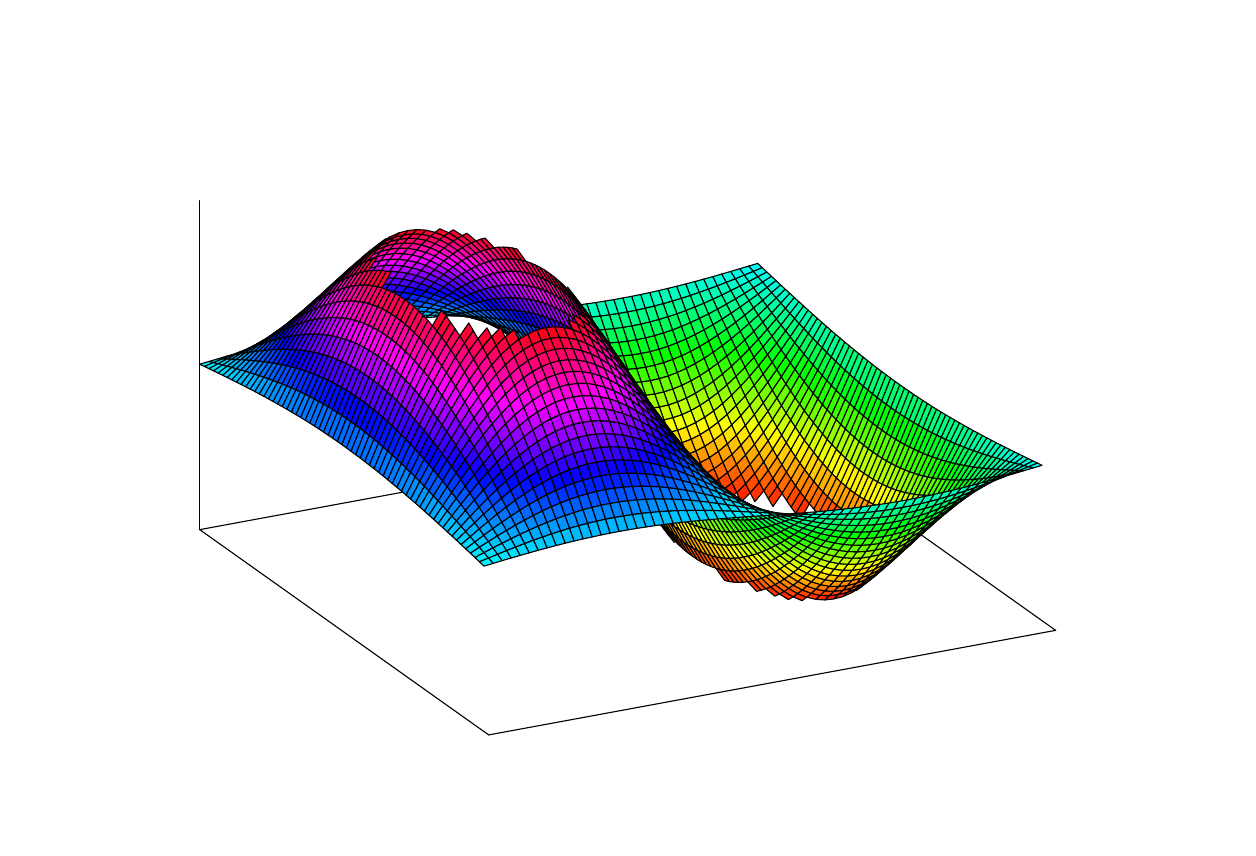
\begin{tikzpicture}[gnuplot]
%% generated with GNUPLOT 4.6p0 (Lua 5.1; terminal rev. 99, script rev. 100)
%% Sun 14 Apr 2013 11:39:16 PM BST
\gpsolidlines
\path (0.000,0.000) rectangle (15.240,10.160);
\gpcolor{color=gp lt color border}
\gpsetlinetype{gp lt border}
\gpsetlinewidth{1.00}
\draw[gp path] (2.185,3.785)--(9.385,5.113);
\draw[gp path] (13.055,2.506)--(9.385,5.113);
\draw[gp path] (2.185,3.785)--(2.185,7.962);
\gpfill{rgb color={0.000,1.000,0.957}} (9.271,7.166)--(9.157,7.132)--(9.215,7.064)--(9.329,7.111)--cycle;
\gpcolor{rgb color={0.000,0.000,0.000}}
\gpsetlinetype{gp lt plot 3}
\draw[gp path] (9.271,7.166)--(9.329,7.111)--(9.215,7.064)--(9.157,7.132)--cycle;
\gpfill{rgb color={0.000,1.000,0.928}} (9.329,7.111)--(9.215,7.064)--(9.273,6.996)--(9.388,7.057)--cycle;
\draw[gp path] (9.329,7.111)--(9.388,7.057)--(9.273,6.996)--(9.215,7.064)--cycle;
\gpfill{rgb color={0.000,1.000,0.900}} (9.388,7.057)--(9.273,6.996)--(9.332,6.928)--(9.446,7.002)--cycle;
\draw[gp path] (9.388,7.057)--(9.446,7.002)--(9.332,6.928)--(9.273,6.996)--cycle;
\gpfill{rgb color={0.000,1.000,0.872}} (9.446,7.002)--(9.332,6.928)--(9.390,6.861)--(9.504,6.948)--cycle;
\draw[gp path] (9.446,7.002)--(9.504,6.948)--(9.390,6.861)--(9.332,6.928)--cycle;
\gpfill{rgb color={0.000,1.000,0.844}} (9.504,6.948)--(9.390,6.861)--(9.448,6.794)--(9.562,6.893)--cycle;
\draw[gp path] (9.504,6.948)--(9.562,6.893)--(9.448,6.794)--(9.390,6.861)--cycle;
\gpfill{rgb color={0.000,1.000,0.816}} (9.562,6.893)--(9.448,6.794)--(9.506,6.727)--(9.621,6.839)--cycle;
\draw[gp path] (9.562,6.893)--(9.621,6.839)--(9.506,6.727)--(9.448,6.794)--cycle;
\gpfill{rgb color={0.000,1.000,0.789}} (9.621,6.839)--(9.506,6.727)--(9.565,6.661)--(9.679,6.786)--cycle;
\draw[gp path] (9.621,6.839)--(9.679,6.786)--(9.565,6.661)--(9.506,6.727)--cycle;
\gpfill{rgb color={0.000,1.000,0.762}} (9.679,6.786)--(9.565,6.661)--(9.623,6.595)--(9.737,6.732)--cycle;
\draw[gp path] (9.679,6.786)--(9.737,6.732)--(9.623,6.595)--(9.565,6.661)--cycle;
\gpfill{rgb color={0.000,1.000,0.736}} (9.737,6.732)--(9.623,6.595)--(9.681,6.530)--(9.795,6.679)--cycle;
\draw[gp path] (9.737,6.732)--(9.795,6.679)--(9.681,6.530)--(9.623,6.595)--cycle;
\gpfill{rgb color={0.000,1.000,0.711}} (9.795,6.679)--(9.681,6.530)--(9.739,6.465)--(9.854,6.625)--cycle;
\draw[gp path] (9.795,6.679)--(9.854,6.625)--(9.739,6.465)--(9.681,6.530)--cycle;
\gpfill{rgb color={0.000,1.000,0.686}} (9.854,6.625)--(9.739,6.465)--(9.798,6.401)--(9.912,6.573)--cycle;
\draw[gp path] (9.854,6.625)--(9.912,6.573)--(9.798,6.401)--(9.739,6.465)--cycle;
\gpfill{rgb color={0.000,1.000,0.662}} (9.912,6.573)--(9.798,6.401)--(9.856,6.338)--(9.970,6.520)--cycle;
\draw[gp path] (9.912,6.573)--(9.970,6.520)--(9.856,6.338)--(9.798,6.401)--cycle;
\gpfill{rgb color={0.000,1.000,0.639}} (9.970,6.520)--(9.856,6.338)--(9.914,6.276)--(10.028,6.469)--cycle;
\draw[gp path] (9.970,6.520)--(10.028,6.469)--(9.914,6.276)--(9.856,6.338)--cycle;
\gpfill{rgb color={0.000,1.000,0.617}} (10.028,6.469)--(9.914,6.276)--(9.972,6.214)--(10.087,6.417)--cycle;
\draw[gp path] (10.028,6.469)--(10.087,6.417)--(9.972,6.214)--(9.914,6.276)--cycle;
\gpfill{rgb color={0.000,1.000,0.596}} (10.087,6.417)--(9.972,6.214)--(10.030,6.154)--(10.145,6.366)--cycle;
\draw[gp path] (10.087,6.417)--(10.145,6.366)--(10.030,6.154)--(9.972,6.214)--cycle;
\gpfill{rgb color={0.000,1.000,0.575}} (10.145,6.366)--(10.030,6.154)--(10.089,6.094)--(10.203,6.315)--cycle;
\draw[gp path] (10.145,6.366)--(10.203,6.315)--(10.089,6.094)--(10.030,6.154)--cycle;
\gpfill{rgb color={0.000,1.000,0.556}} (10.203,6.315)--(10.089,6.094)--(10.147,6.035)--(10.261,6.265)--cycle;
\draw[gp path] (10.203,6.315)--(10.261,6.265)--(10.147,6.035)--(10.089,6.094)--cycle;
\gpfill{rgb color={0.000,1.000,0.538}} (10.261,6.265)--(10.147,6.035)--(10.205,5.977)--(10.320,6.216)--cycle;
\draw[gp path] (10.261,6.265)--(10.320,6.216)--(10.205,5.977)--(10.147,6.035)--cycle;
\gpfill{rgb color={0.000,1.000,0.521}} (10.320,6.216)--(10.205,5.977)--(10.263,5.920)--(10.378,6.166)--cycle;
\draw[gp path] (10.320,6.216)--(10.378,6.166)--(10.263,5.920)--(10.205,5.977)--cycle;
\gpfill{rgb color={0.000,1.000,0.505}} (10.378,6.166)--(10.263,5.920)--(10.322,5.865)--(10.436,6.118)--cycle;
\draw[gp path] (10.378,6.166)--(10.436,6.118)--(10.322,5.865)--(10.263,5.920)--cycle;
\gpfill{rgb color={0.000,1.000,0.490}} (10.436,6.118)--(10.322,5.865)--(10.380,5.810)--(10.494,6.070)--cycle;
\draw[gp path] (10.436,6.118)--(10.494,6.070)--(10.380,5.810)--(10.322,5.865)--cycle;
\gpfill{rgb color={0.000,1.000,0.476}} (10.494,6.070)--(10.380,5.810)--(10.438,5.757)--(10.552,6.023)--cycle;
\draw[gp path] (10.494,6.070)--(10.552,6.023)--(10.438,5.757)--(10.380,5.810)--cycle;
\gpfill{rgb color={0.000,1.000,0.464}} (10.552,6.023)--(10.438,5.757)--(10.496,5.705)--(10.611,5.976)--cycle;
\draw[gp path] (10.552,6.023)--(10.611,5.976)--(10.496,5.705)--(10.438,5.757)--cycle;
\gpfill{rgb color={0.000,1.000,0.453}} (10.611,5.976)--(10.496,5.705)--(10.555,5.654)--(10.669,5.930)--cycle;
\draw[gp path] (10.611,5.976)--(10.669,5.930)--(10.555,5.654)--(10.496,5.705)--cycle;
\gpfill{rgb color={0.000,1.000,0.443}} (10.669,5.930)--(10.555,5.654)--(10.613,5.604)--(10.727,5.884)--cycle;
\draw[gp path] (10.669,5.930)--(10.727,5.884)--(10.613,5.604)--(10.555,5.654)--cycle;
\gpfill{rgb color={0.000,1.000,0.435}} (10.727,5.884)--(10.613,5.604)--(10.671,5.556)--(10.785,5.839)--cycle;
\draw[gp path] (10.727,5.884)--(10.785,5.839)--(10.671,5.556)--(10.613,5.604)--cycle;
\gpfill{rgb color={0.000,1.000,0.428}} (10.785,5.839)--(10.671,5.556)--(10.729,5.508)--(10.844,5.795)--cycle;
\draw[gp path] (10.785,5.839)--(10.844,5.795)--(10.729,5.508)--(10.671,5.556)--cycle;
\gpfill{rgb color={0.000,1.000,0.422}} (10.844,5.795)--(10.729,5.508)--(10.788,5.462)--(10.902,5.751)--cycle;
\draw[gp path] (10.844,5.795)--(10.902,5.751)--(10.788,5.462)--(10.729,5.508)--cycle;
\gpfill{rgb color={0.000,1.000,0.418}} (10.902,5.751)--(10.788,5.462)--(10.846,5.418)--(10.960,5.708)--cycle;
\draw[gp path] (10.902,5.751)--(10.960,5.708)--(10.846,5.418)--(10.788,5.462)--cycle;
\gpfill{rgb color={0.000,1.000,0.415}} (10.960,5.708)--(10.846,5.418)--(10.904,5.375)--(11.018,5.666)--cycle;
\draw[gp path] (10.960,5.708)--(11.018,5.666)--(10.904,5.375)--(10.846,5.418)--cycle;
\gpfill{rgb color={0.000,1.000,0.414}} (11.018,5.666)--(10.904,5.375)--(10.962,5.333)--(11.077,5.624)--cycle;
\draw[gp path] (11.018,5.666)--(11.077,5.624)--(10.962,5.333)--(10.904,5.375)--cycle;
\gpfill{rgb color={0.000,1.000,0.414}} (11.077,5.624)--(10.962,5.333)--(11.021,5.292)--(11.135,5.583)--cycle;
\draw[gp path] (11.077,5.624)--(11.135,5.583)--(11.021,5.292)--(10.962,5.333)--cycle;
\gpfill{rgb color={0.000,1.000,0.415}} (11.135,5.583)--(11.021,5.292)--(11.079,5.252)--(11.193,5.543)--cycle;
\draw[gp path] (11.135,5.583)--(11.193,5.543)--(11.079,5.252)--(11.021,5.292)--cycle;
\gpfill{rgb color={0.000,1.000,0.418}} (11.193,5.543)--(11.079,5.252)--(11.137,5.215)--(11.251,5.503)--cycle;
\draw[gp path] (11.193,5.543)--(11.251,5.503)--(11.137,5.215)--(11.079,5.252)--cycle;
\gpfill{rgb color={0.000,1.000,0.422}} (11.251,5.503)--(11.137,5.215)--(11.195,5.179)--(11.310,5.464)--cycle;
\draw[gp path] (11.251,5.503)--(11.310,5.464)--(11.195,5.179)--(11.137,5.215)--cycle;
\gpfill{rgb color={0.000,1.000,0.428}} (11.310,5.464)--(11.195,5.179)--(11.254,5.143)--(11.368,5.425)--cycle;
\draw[gp path] (11.310,5.464)--(11.368,5.425)--(11.254,5.143)--(11.195,5.179)--cycle;
\gpfill{rgb color={0.000,1.000,0.435}} (11.368,5.425)--(11.254,5.143)--(11.312,5.109)--(11.426,5.388)--cycle;
\draw[gp path] (11.368,5.425)--(11.426,5.388)--(11.312,5.109)--(11.254,5.143)--cycle;
\gpfill{rgb color={0.000,1.000,0.444}} (11.426,5.388)--(11.312,5.109)--(11.370,5.076)--(11.484,5.350)--cycle;
\draw[gp path] (11.426,5.388)--(11.484,5.350)--(11.370,5.076)--(11.312,5.109)--cycle;
\gpfill{rgb color={0.000,1.000,0.453}} (11.484,5.350)--(11.370,5.076)--(11.428,5.044)--(11.543,5.314)--cycle;
\draw[gp path] (11.484,5.350)--(11.543,5.314)--(11.428,5.044)--(11.370,5.076)--cycle;
\gpfill{rgb color={0.000,1.000,0.464}} (11.543,5.314)--(11.428,5.044)--(11.486,5.014)--(11.601,5.278)--cycle;
\draw[gp path] (11.543,5.314)--(11.601,5.278)--(11.486,5.014)--(11.428,5.044)--cycle;
\gpfill{rgb color={0.000,1.000,0.477}} (11.601,5.278)--(11.486,5.014)--(11.545,4.984)--(11.659,5.243)--cycle;
\draw[gp path] (11.601,5.278)--(11.659,5.243)--(11.545,4.984)--(11.486,5.014)--cycle;
\gpfill{rgb color={0.000,1.000,0.490}} (11.659,5.243)--(11.545,4.984)--(11.603,4.956)--(11.717,5.209)--cycle;
\draw[gp path] (11.659,5.243)--(11.717,5.209)--(11.603,4.956)--(11.545,4.984)--cycle;
\gpfill{rgb color={0.000,1.000,0.505}} (11.717,5.209)--(11.603,4.956)--(11.661,4.929)--(11.776,5.175)--cycle;
\draw[gp path] (11.717,5.209)--(11.776,5.175)--(11.661,4.929)--(11.603,4.956)--cycle;
\gpfill{rgb color={0.000,1.000,0.521}} (11.776,5.175)--(11.661,4.929)--(11.719,4.903)--(11.834,5.141)--cycle;
\draw[gp path] (11.776,5.175)--(11.834,5.141)--(11.719,4.903)--(11.661,4.929)--cycle;
\gpfill{rgb color={0.000,1.000,0.538}} (11.834,5.141)--(11.719,4.903)--(11.778,4.878)--(11.892,5.108)--cycle;
\draw[gp path] (11.834,5.141)--(11.892,5.108)--(11.778,4.878)--(11.719,4.903)--cycle;
\gpfill{rgb color={0.000,1.000,0.556}} (11.892,5.108)--(11.778,4.878)--(11.836,4.854)--(11.950,5.075)--cycle;
\draw[gp path] (11.892,5.108)--(11.950,5.075)--(11.836,4.854)--(11.778,4.878)--cycle;
\gpfill{rgb color={0.000,1.000,0.576}} (11.950,5.075)--(11.836,4.854)--(11.894,4.831)--(12.008,5.043)--cycle;
\draw[gp path] (11.950,5.075)--(12.008,5.043)--(11.894,4.831)--(11.836,4.854)--cycle;
\gpfill{rgb color={0.000,1.000,0.596}} (12.008,5.043)--(11.894,4.831)--(11.952,4.809)--(12.067,5.012)--cycle;
\draw[gp path] (12.008,5.043)--(12.067,5.012)--(11.952,4.809)--(11.894,4.831)--cycle;
\gpfill{rgb color={0.000,1.000,0.617}} (12.067,5.012)--(11.952,4.809)--(12.011,4.788)--(12.125,4.980)--cycle;
\draw[gp path] (12.067,5.012)--(12.125,4.980)--(12.011,4.788)--(11.952,4.809)--cycle;
\gpfill{rgb color={0.000,1.000,0.640}} (12.125,4.980)--(12.011,4.788)--(12.069,4.768)--(12.183,4.950)--cycle;
\draw[gp path] (12.125,4.980)--(12.183,4.950)--(12.069,4.768)--(12.011,4.788)--cycle;
\gpfill{rgb color={0.000,1.000,0.663}} (12.183,4.950)--(12.069,4.768)--(12.127,4.748)--(12.241,4.919)--cycle;
\draw[gp path] (12.183,4.950)--(12.241,4.919)--(12.127,4.748)--(12.069,4.768)--cycle;
\gpfill{rgb color={0.000,1.000,0.687}} (12.241,4.919)--(12.127,4.748)--(12.185,4.729)--(12.300,4.889)--cycle;
\draw[gp path] (12.241,4.919)--(12.300,4.889)--(12.185,4.729)--(12.127,4.748)--cycle;
\gpfill{rgb color={0.000,1.000,0.711}} (12.300,4.889)--(12.185,4.729)--(12.244,4.711)--(12.358,4.859)--cycle;
\draw[gp path] (12.300,4.889)--(12.358,4.859)--(12.244,4.711)--(12.185,4.729)--cycle;
\gpfill{rgb color={0.000,1.000,0.737}} (12.358,4.859)--(12.244,4.711)--(12.302,4.693)--(12.416,4.830)--cycle;
\draw[gp path] (12.358,4.859)--(12.416,4.830)--(12.302,4.693)--(12.244,4.711)--cycle;
\gpfill{rgb color={0.000,1.000,0.763}} (12.416,4.830)--(12.302,4.693)--(12.360,4.676)--(12.474,4.801)--cycle;
\draw[gp path] (12.416,4.830)--(12.474,4.801)--(12.360,4.676)--(12.302,4.693)--cycle;
\gpfill{rgb color={0.000,1.000,0.789}} (12.474,4.801)--(12.360,4.676)--(12.418,4.660)--(12.533,4.772)--cycle;
\draw[gp path] (12.474,4.801)--(12.533,4.772)--(12.418,4.660)--(12.360,4.676)--cycle;
\gpfill{rgb color={0.000,1.000,0.816}} (12.533,4.772)--(12.418,4.660)--(12.477,4.644)--(12.591,4.743)--cycle;
\draw[gp path] (12.533,4.772)--(12.591,4.743)--(12.477,4.644)--(12.418,4.660)--cycle;
\gpfill{rgb color={0.000,1.000,0.844}} (12.591,4.743)--(12.477,4.644)--(12.535,4.628)--(12.649,4.715)--cycle;
\draw[gp path] (12.591,4.743)--(12.649,4.715)--(12.535,4.628)--(12.477,4.644)--cycle;
\gpfill{rgb color={0.000,1.000,0.872}} (12.649,4.715)--(12.535,4.628)--(12.593,4.613)--(12.707,4.687)--cycle;
\draw[gp path] (12.649,4.715)--(12.707,4.687)--(12.593,4.613)--(12.535,4.628)--cycle;
\gpfill{rgb color={0.000,1.000,0.900}} (12.707,4.687)--(12.593,4.613)--(12.651,4.598)--(12.766,4.658)--cycle;
\draw[gp path] (12.707,4.687)--(12.766,4.658)--(12.651,4.598)--(12.593,4.613)--cycle;
\gpfill{rgb color={0.000,1.000,0.928}} (12.766,4.658)--(12.651,4.598)--(12.710,4.583)--(12.824,4.630)--cycle;
\draw[gp path] (12.766,4.658)--(12.824,4.630)--(12.710,4.583)--(12.651,4.598)--cycle;
\gpfill{rgb color={0.000,1.000,0.957}} (12.824,4.630)--(12.710,4.583)--(12.768,4.568)--(12.882,4.602)--cycle;
\draw[gp path] (12.824,4.630)--(12.882,4.602)--(12.768,4.568)--(12.710,4.583)--cycle;
\gpfill{rgb color={0.000,1.000,0.929}} (9.157,7.132)--(9.043,7.098)--(9.101,7.017)--(9.215,7.064)--cycle;
\draw[gp path] (9.157,7.132)--(9.215,7.064)--(9.101,7.017)--(9.043,7.098)--cycle;
\gpfill{rgb color={0.000,1.000,0.881}} (9.215,7.064)--(9.101,7.017)--(9.159,6.936)--(9.273,6.996)--cycle;
\draw[gp path] (9.215,7.064)--(9.273,6.996)--(9.159,6.936)--(9.101,7.017)--cycle;
\gpfill{rgb color={0.000,1.000,0.834}} (9.273,6.996)--(9.159,6.936)--(9.217,6.856)--(9.332,6.928)--cycle;
\draw[gp path] (9.273,6.996)--(9.332,6.928)--(9.217,6.856)--(9.159,6.936)--cycle;
\gpfill{rgb color={0.000,1.000,0.787}} (9.332,6.928)--(9.217,6.856)--(9.276,6.775)--(9.390,6.861)--cycle;
\draw[gp path] (9.332,6.928)--(9.390,6.861)--(9.276,6.775)--(9.217,6.856)--cycle;
\gpfill{rgb color={0.000,1.000,0.741}} (9.390,6.861)--(9.276,6.775)--(9.334,6.696)--(9.448,6.794)--cycle;
\draw[gp path] (9.390,6.861)--(9.448,6.794)--(9.334,6.696)--(9.276,6.775)--cycle;
\gpfill{rgb color={0.000,1.000,0.695}} (9.448,6.794)--(9.334,6.696)--(9.392,6.617)--(9.506,6.727)--cycle;
\draw[gp path] (9.448,6.794)--(9.506,6.727)--(9.392,6.617)--(9.334,6.696)--cycle;
\gpfill{rgb color={0.000,1.000,0.651}} (9.506,6.727)--(9.392,6.617)--(9.450,6.538)--(9.565,6.661)--cycle;
\draw[gp path] (9.506,6.727)--(9.565,6.661)--(9.450,6.538)--(9.392,6.617)--cycle;
\gpfill{rgb color={0.000,1.000,0.606}} (9.565,6.661)--(9.450,6.538)--(9.508,6.461)--(9.623,6.595)--cycle;
\draw[gp path] (9.565,6.661)--(9.623,6.595)--(9.508,6.461)--(9.450,6.538)--cycle;
\gpfill{rgb color={0.000,1.000,0.563}} (9.623,6.595)--(9.508,6.461)--(9.567,6.384)--(9.681,6.530)--cycle;
\draw[gp path] (9.623,6.595)--(9.681,6.530)--(9.567,6.384)--(9.508,6.461)--cycle;
\gpfill{rgb color={0.000,1.000,0.521}} (9.681,6.530)--(9.567,6.384)--(9.625,6.308)--(9.739,6.465)--cycle;
\draw[gp path] (9.681,6.530)--(9.739,6.465)--(9.625,6.308)--(9.567,6.384)--cycle;
\gpfill{rgb color={0.000,1.000,0.480}} (9.739,6.465)--(9.625,6.308)--(9.683,6.233)--(9.798,6.401)--cycle;
\draw[gp path] (9.739,6.465)--(9.798,6.401)--(9.683,6.233)--(9.625,6.308)--cycle;
\gpfill{rgb color={0.000,1.000,0.441}} (9.798,6.401)--(9.683,6.233)--(9.741,6.159)--(9.856,6.338)--cycle;
\draw[gp path] (9.798,6.401)--(9.856,6.338)--(9.741,6.159)--(9.683,6.233)--cycle;
\gpfill{rgb color={0.000,1.000,0.403}} (9.856,6.338)--(9.741,6.159)--(9.800,6.086)--(9.914,6.276)--cycle;
\draw[gp path] (9.856,6.338)--(9.914,6.276)--(9.800,6.086)--(9.741,6.159)--cycle;
\gpfill{rgb color={0.000,1.000,0.366}} (9.914,6.276)--(9.800,6.086)--(9.858,6.015)--(9.972,6.214)--cycle;
\draw[gp path] (9.914,6.276)--(9.972,6.214)--(9.858,6.015)--(9.800,6.086)--cycle;
\gpfill{rgb color={0.000,1.000,0.330}} (9.972,6.214)--(9.858,6.015)--(9.916,5.945)--(10.030,6.154)--cycle;
\draw[gp path] (9.972,6.214)--(10.030,6.154)--(9.916,5.945)--(9.858,6.015)--cycle;
\gpfill{rgb color={0.000,1.000,0.297}} (10.030,6.154)--(9.916,5.945)--(9.974,5.876)--(10.089,6.094)--cycle;
\draw[gp path] (10.030,6.154)--(10.089,6.094)--(9.974,5.876)--(9.916,5.945)--cycle;
\gpfill{rgb color={0.000,1.000,0.265}} (10.089,6.094)--(9.974,5.876)--(10.033,5.809)--(10.147,6.035)--cycle;
\draw[gp path] (10.089,6.094)--(10.147,6.035)--(10.033,5.809)--(9.974,5.876)--cycle;
\gpfill{rgb color={0.000,1.000,0.234}} (10.147,6.035)--(10.033,5.809)--(10.091,5.743)--(10.205,5.977)--cycle;
\draw[gp path] (10.147,6.035)--(10.205,5.977)--(10.091,5.743)--(10.033,5.809)--cycle;
\gpfill{rgb color={0.000,1.000,0.206}} (10.205,5.977)--(10.091,5.743)--(10.149,5.679)--(10.263,5.920)--cycle;
\draw[gp path] (10.205,5.977)--(10.263,5.920)--(10.149,5.679)--(10.091,5.743)--cycle;
\gpfill{rgb color={0.000,1.000,0.180}} (10.263,5.920)--(10.149,5.679)--(10.207,5.616)--(10.322,5.865)--cycle;
\draw[gp path] (10.263,5.920)--(10.322,5.865)--(10.207,5.616)--(10.149,5.679)--cycle;
\gpfill{rgb color={0.000,1.000,0.155}} (10.322,5.865)--(10.207,5.616)--(10.266,5.555)--(10.380,5.810)--cycle;
\draw[gp path] (10.322,5.865)--(10.380,5.810)--(10.266,5.555)--(10.207,5.616)--cycle;
\gpfill{rgb color={0.000,1.000,0.133}} (10.380,5.810)--(10.266,5.555)--(10.324,5.496)--(10.438,5.757)--cycle;
\draw[gp path] (10.380,5.810)--(10.438,5.757)--(10.324,5.496)--(10.266,5.555)--cycle;
\gpfill{rgb color={0.000,1.000,0.112}} (10.438,5.757)--(10.324,5.496)--(10.382,5.439)--(10.496,5.705)--cycle;
\draw[gp path] (10.438,5.757)--(10.496,5.705)--(10.382,5.439)--(10.324,5.496)--cycle;
\gpfill{rgb color={0.000,1.000,0.094}} (10.496,5.705)--(10.382,5.439)--(10.440,5.383)--(10.555,5.654)--cycle;
\draw[gp path] (10.496,5.705)--(10.555,5.654)--(10.440,5.383)--(10.382,5.439)--cycle;
\gpfill{rgb color={0.000,1.000,0.078}} (10.555,5.654)--(10.440,5.383)--(10.499,5.329)--(10.613,5.604)--cycle;
\draw[gp path] (10.555,5.654)--(10.613,5.604)--(10.499,5.329)--(10.440,5.383)--cycle;
\gpfill{rgb color={0.000,1.000,0.064}} (10.613,5.604)--(10.499,5.329)--(10.557,5.277)--(10.671,5.556)--cycle;
\draw[gp path] (10.613,5.604)--(10.671,5.556)--(10.557,5.277)--(10.499,5.329)--cycle;
\gpfill{rgb color={0.000,1.000,0.053}} (10.671,5.556)--(10.557,5.277)--(10.615,5.228)--(10.729,5.508)--cycle;
\draw[gp path] (10.671,5.556)--(10.729,5.508)--(10.615,5.228)--(10.557,5.277)--cycle;
\gpfill{rgb color={0.000,1.000,0.043}} (10.729,5.508)--(10.615,5.228)--(10.673,5.180)--(10.788,5.462)--cycle;
\draw[gp path] (10.729,5.508)--(10.788,5.462)--(10.673,5.180)--(10.615,5.228)--cycle;
\gpfill{rgb color={0.000,1.000,0.036}} (10.788,5.462)--(10.673,5.180)--(10.732,5.134)--(10.846,5.418)--cycle;
\draw[gp path] (10.788,5.462)--(10.846,5.418)--(10.732,5.134)--(10.673,5.180)--cycle;
\gpfill{rgb color={0.000,1.000,0.032}} (10.846,5.418)--(10.732,5.134)--(10.790,5.090)--(10.904,5.375)--cycle;
\draw[gp path] (10.846,5.418)--(10.904,5.375)--(10.790,5.090)--(10.732,5.134)--cycle;
\gpfill{rgb color={0.000,1.000,0.030}} (10.904,5.375)--(10.790,5.090)--(10.848,5.047)--(10.962,5.333)--cycle;
\draw[gp path] (10.904,5.375)--(10.962,5.333)--(10.848,5.047)--(10.790,5.090)--cycle;
\gpfill{rgb color={0.000,1.000,0.030}} (10.962,5.333)--(10.848,5.047)--(10.906,5.007)--(11.021,5.292)--cycle;
\draw[gp path] (10.962,5.333)--(11.021,5.292)--(10.906,5.007)--(10.848,5.047)--cycle;
\gpfill{rgb color={0.000,1.000,0.032}} (11.021,5.292)--(10.906,5.007)--(10.965,4.968)--(11.079,5.252)--cycle;
\draw[gp path] (11.021,5.292)--(11.079,5.252)--(10.965,4.968)--(10.906,5.007)--cycle;
\gpfill{rgb color={0.000,1.000,0.037}} (11.079,5.252)--(10.965,4.968)--(11.023,4.932)--(11.137,5.215)--cycle;
\draw[gp path] (11.079,5.252)--(11.137,5.215)--(11.023,4.932)--(10.965,4.968)--cycle;
\gpfill{rgb color={0.000,1.000,0.044}} (11.137,5.215)--(11.023,4.932)--(11.081,4.897)--(11.195,5.179)--cycle;
\draw[gp path] (11.137,5.215)--(11.195,5.179)--(11.081,4.897)--(11.023,4.932)--cycle;
\gpfill{rgb color={0.000,1.000,0.053}} (11.195,5.179)--(11.081,4.897)--(11.139,4.865)--(11.254,5.143)--cycle;
\draw[gp path] (11.195,5.179)--(11.254,5.143)--(11.139,4.865)--(11.081,4.897)--cycle;
\gpfill{rgb color={0.000,1.000,0.065}} (11.254,5.143)--(11.139,4.865)--(11.197,4.834)--(11.312,5.109)--cycle;
\draw[gp path] (11.254,5.143)--(11.312,5.109)--(11.197,4.834)--(11.139,4.865)--cycle;
\gpfill{rgb color={0.000,1.000,0.079}} (11.312,5.109)--(11.197,4.834)--(11.256,4.805)--(11.370,5.076)--cycle;
\draw[gp path] (11.312,5.109)--(11.370,5.076)--(11.256,4.805)--(11.197,4.834)--cycle;
\gpfill{rgb color={0.000,1.000,0.095}} (11.370,5.076)--(11.256,4.805)--(11.314,4.778)--(11.428,5.044)--cycle;
\draw[gp path] (11.370,5.076)--(11.428,5.044)--(11.314,4.778)--(11.256,4.805)--cycle;
\gpfill{rgb color={0.000,1.000,0.113}} (11.428,5.044)--(11.314,4.778)--(11.372,4.753)--(11.486,5.014)--cycle;
\draw[gp path] (11.428,5.044)--(11.486,5.014)--(11.372,4.753)--(11.314,4.778)--cycle;
\gpfill{rgb color={0.000,1.000,0.133}} (11.486,5.014)--(11.372,4.753)--(11.430,4.729)--(11.545,4.984)--cycle;
\draw[gp path] (11.486,5.014)--(11.545,4.984)--(11.430,4.729)--(11.372,4.753)--cycle;
\gpfill{rgb color={0.000,1.000,0.156}} (11.545,4.984)--(11.430,4.729)--(11.489,4.708)--(11.603,4.956)--cycle;
\draw[gp path] (11.545,4.984)--(11.603,4.956)--(11.489,4.708)--(11.430,4.729)--cycle;
\gpfill{rgb color={0.000,1.000,0.180}} (11.603,4.956)--(11.489,4.708)--(11.547,4.688)--(11.661,4.929)--cycle;
\draw[gp path] (11.603,4.956)--(11.661,4.929)--(11.547,4.688)--(11.489,4.708)--cycle;
\gpfill{rgb color={0.000,1.000,0.207}} (11.661,4.929)--(11.547,4.688)--(11.605,4.669)--(11.719,4.903)--cycle;
\draw[gp path] (11.661,4.929)--(11.719,4.903)--(11.605,4.669)--(11.547,4.688)--cycle;
\gpfill{rgb color={0.000,1.000,0.235}} (11.719,4.903)--(11.605,4.669)--(11.663,4.652)--(11.778,4.878)--cycle;
\draw[gp path] (11.719,4.903)--(11.778,4.878)--(11.663,4.652)--(11.605,4.669)--cycle;
\gpfill{rgb color={0.000,1.000,0.266}} (11.778,4.878)--(11.663,4.652)--(11.722,4.637)--(11.836,4.854)--cycle;
\draw[gp path] (11.778,4.878)--(11.836,4.854)--(11.722,4.637)--(11.663,4.652)--cycle;
\gpfill{rgb color={0.000,1.000,0.298}} (11.836,4.854)--(11.722,4.637)--(11.780,4.623)--(11.894,4.831)--cycle;
\draw[gp path] (11.836,4.854)--(11.894,4.831)--(11.780,4.623)--(11.722,4.637)--cycle;
\gpfill{rgb color={0.000,1.000,0.331}} (11.894,4.831)--(11.780,4.623)--(11.838,4.610)--(11.952,4.809)--cycle;
\draw[gp path] (11.894,4.831)--(11.952,4.809)--(11.838,4.610)--(11.780,4.623)--cycle;
\gpfill{rgb color={0.000,1.000,0.367}} (11.952,4.809)--(11.838,4.610)--(11.896,4.599)--(12.011,4.788)--cycle;
\draw[gp path] (11.952,4.809)--(12.011,4.788)--(11.896,4.599)--(11.838,4.610)--cycle;
\gpfill{rgb color={0.000,1.000,0.403}} (12.011,4.788)--(11.896,4.599)--(11.955,4.589)--(12.069,4.768)--cycle;
\draw[gp path] (12.011,4.788)--(12.069,4.768)--(11.955,4.589)--(11.896,4.599)--cycle;
\gpfill{rgb color={0.000,1.000,0.442}} (12.069,4.768)--(11.955,4.589)--(12.013,4.580)--(12.127,4.748)--cycle;
\draw[gp path] (12.069,4.768)--(12.127,4.748)--(12.013,4.580)--(11.955,4.589)--cycle;
\gpfill{rgb color={0.000,1.000,0.481}} (12.127,4.748)--(12.013,4.580)--(12.071,4.572)--(12.185,4.729)--cycle;
\draw[gp path] (12.127,4.748)--(12.185,4.729)--(12.071,4.572)--(12.013,4.580)--cycle;
\gpfill{rgb color={0.000,1.000,0.522}} (12.185,4.729)--(12.071,4.572)--(12.129,4.565)--(12.244,4.711)--cycle;
\draw[gp path] (12.185,4.729)--(12.244,4.711)--(12.129,4.565)--(12.071,4.572)--cycle;
\gpfill{rgb color={0.000,1.000,0.564}} (12.244,4.711)--(12.129,4.565)--(12.188,4.559)--(12.302,4.693)--cycle;
\draw[gp path] (12.244,4.711)--(12.302,4.693)--(12.188,4.559)--(12.129,4.565)--cycle;
\gpfill{rgb color={0.000,1.000,0.607}} (12.302,4.693)--(12.188,4.559)--(12.246,4.554)--(12.360,4.676)--cycle;
\draw[gp path] (12.302,4.693)--(12.360,4.676)--(12.246,4.554)--(12.188,4.559)--cycle;
\gpfill{rgb color={0.000,1.000,0.651}} (12.360,4.676)--(12.246,4.554)--(12.304,4.550)--(12.418,4.660)--cycle;
\draw[gp path] (12.360,4.676)--(12.418,4.660)--(12.304,4.550)--(12.246,4.554)--cycle;
\gpfill{rgb color={0.000,1.000,0.696}} (12.418,4.660)--(12.304,4.550)--(12.362,4.546)--(12.477,4.644)--cycle;
\draw[gp path] (12.418,4.660)--(12.477,4.644)--(12.362,4.546)--(12.304,4.550)--cycle;
\gpfill{rgb color={0.000,1.000,0.741}} (12.477,4.644)--(12.362,4.546)--(12.421,4.543)--(12.535,4.628)--cycle;
\draw[gp path] (12.477,4.644)--(12.535,4.628)--(12.421,4.543)--(12.362,4.546)--cycle;
\gpfill{rgb color={0.000,1.000,0.788}} (12.535,4.628)--(12.421,4.543)--(12.479,4.540)--(12.593,4.613)--cycle;
\draw[gp path] (12.535,4.628)--(12.593,4.613)--(12.479,4.540)--(12.421,4.543)--cycle;
\gpfill{rgb color={0.000,1.000,0.834}} (12.593,4.613)--(12.479,4.540)--(12.537,4.538)--(12.651,4.598)--cycle;
\draw[gp path] (12.593,4.613)--(12.651,4.598)--(12.537,4.538)--(12.479,4.540)--cycle;
\gpfill{rgb color={0.000,1.000,0.881}} (12.651,4.598)--(12.537,4.538)--(12.595,4.536)--(12.710,4.583)--cycle;
\draw[gp path] (12.651,4.598)--(12.710,4.583)--(12.595,4.536)--(12.537,4.538)--cycle;
\gpfill{rgb color={0.000,1.000,0.929}} (12.710,4.583)--(12.595,4.536)--(12.653,4.534)--(12.768,4.568)--cycle;
\draw[gp path] (12.710,4.583)--(12.768,4.568)--(12.653,4.534)--(12.595,4.536)--cycle;
\gpfill{rgb color={0.000,1.000,0.901}} (9.043,7.098)--(8.928,7.064)--(8.987,6.970)--(9.101,7.017)--cycle;
\draw[gp path] (9.043,7.098)--(9.101,7.017)--(8.987,6.970)--(8.928,7.064)--cycle;
\gpfill{rgb color={0.000,1.000,0.835}} (9.101,7.017)--(8.987,6.970)--(9.045,6.877)--(9.159,6.936)--cycle;
\draw[gp path] (9.101,7.017)--(9.159,6.936)--(9.045,6.877)--(8.987,6.970)--cycle;
\gpfill{rgb color={0.000,1.000,0.770}} (9.159,6.936)--(9.045,6.877)--(9.103,6.784)--(9.217,6.856)--cycle;
\draw[gp path] (9.159,6.936)--(9.217,6.856)--(9.103,6.784)--(9.045,6.877)--cycle;
\gpfill{rgb color={0.000,1.000,0.705}} (9.217,6.856)--(9.103,6.784)--(9.161,6.692)--(9.276,6.775)--cycle;
\draw[gp path] (9.217,6.856)--(9.276,6.775)--(9.161,6.692)--(9.103,6.784)--cycle;
\gpfill{rgb color={0.000,1.000,0.641}} (9.276,6.775)--(9.161,6.692)--(9.219,6.600)--(9.334,6.696)--cycle;
\draw[gp path] (9.276,6.775)--(9.334,6.696)--(9.219,6.600)--(9.161,6.692)--cycle;
\gpfill{rgb color={0.000,1.000,0.578}} (9.334,6.696)--(9.219,6.600)--(9.278,6.509)--(9.392,6.617)--cycle;
\draw[gp path] (9.334,6.696)--(9.392,6.617)--(9.278,6.509)--(9.219,6.600)--cycle;
\gpfill{rgb color={0.000,1.000,0.515}} (9.392,6.617)--(9.278,6.509)--(9.336,6.419)--(9.450,6.538)--cycle;
\draw[gp path] (9.392,6.617)--(9.450,6.538)--(9.336,6.419)--(9.278,6.509)--cycle;
\gpfill{rgb color={0.000,1.000,0.454}} (9.450,6.538)--(9.336,6.419)--(9.394,6.329)--(9.508,6.461)--cycle;
\draw[gp path] (9.450,6.538)--(9.508,6.461)--(9.394,6.329)--(9.336,6.419)--cycle;
\gpfill{rgb color={0.000,1.000,0.395}} (9.508,6.461)--(9.394,6.329)--(9.452,6.241)--(9.567,6.384)--cycle;
\draw[gp path] (9.508,6.461)--(9.567,6.384)--(9.452,6.241)--(9.394,6.329)--cycle;
\gpfill{rgb color={0.000,1.000,0.336}} (9.567,6.384)--(9.452,6.241)--(9.511,6.154)--(9.625,6.308)--cycle;
\draw[gp path] (9.567,6.384)--(9.625,6.308)--(9.511,6.154)--(9.452,6.241)--cycle;
\gpfill{rgb color={0.000,1.000,0.280}} (9.625,6.308)--(9.511,6.154)--(9.569,6.069)--(9.683,6.233)--cycle;
\draw[gp path] (9.625,6.308)--(9.683,6.233)--(9.569,6.069)--(9.511,6.154)--cycle;
\gpfill{rgb color={0.000,1.000,0.225}} (9.683,6.233)--(9.569,6.069)--(9.627,5.985)--(9.741,6.159)--cycle;
\draw[gp path] (9.683,6.233)--(9.741,6.159)--(9.627,5.985)--(9.569,6.069)--cycle;
\gpfill{rgb color={0.000,1.000,0.172}} (9.741,6.159)--(9.627,5.985)--(9.685,5.902)--(9.800,6.086)--cycle;
\draw[gp path] (9.741,6.159)--(9.800,6.086)--(9.685,5.902)--(9.627,5.985)--cycle;
\gpfill{rgb color={0.000,1.000,0.121}} (9.800,6.086)--(9.685,5.902)--(9.744,5.821)--(9.858,6.015)--cycle;
\draw[gp path] (9.800,6.086)--(9.858,6.015)--(9.744,5.821)--(9.685,5.902)--cycle;
\gpfill{rgb color={0.000,1.000,0.072}} (9.858,6.015)--(9.744,5.821)--(9.802,5.742)--(9.916,5.945)--cycle;
\draw[gp path] (9.858,6.015)--(9.916,5.945)--(9.802,5.742)--(9.744,5.821)--cycle;
\gpfill{rgb color={0.000,1.000,0.025}} (9.916,5.945)--(9.802,5.742)--(9.860,5.664)--(9.974,5.876)--cycle;
\draw[gp path] (9.916,5.945)--(9.974,5.876)--(9.860,5.664)--(9.802,5.742)--cycle;
\gpfill{rgb color={0.019,1.000,0.000}} (9.974,5.876)--(9.860,5.664)--(9.918,5.589)--(10.033,5.809)--cycle;
\draw[gp path] (9.974,5.876)--(10.033,5.809)--(9.918,5.589)--(9.860,5.664)--cycle;
\gpfill{rgb color={0.061,1.000,0.000}} (10.033,5.809)--(9.918,5.589)--(9.977,5.515)--(10.091,5.743)--cycle;
\draw[gp path] (10.033,5.809)--(10.091,5.743)--(9.977,5.515)--(9.918,5.589)--cycle;
\gpfill{rgb color={0.101,1.000,0.000}} (10.091,5.743)--(9.977,5.515)--(10.035,5.444)--(10.149,5.679)--cycle;
\draw[gp path] (10.091,5.743)--(10.149,5.679)--(10.035,5.444)--(9.977,5.515)--cycle;
\gpfill{rgb color={0.137,1.000,0.000}} (10.149,5.679)--(10.035,5.444)--(10.093,5.374)--(10.207,5.616)--cycle;
\draw[gp path] (10.149,5.679)--(10.207,5.616)--(10.093,5.374)--(10.035,5.444)--cycle;
\gpfill{rgb color={0.171,1.000,0.000}} (10.207,5.616)--(10.093,5.374)--(10.151,5.307)--(10.266,5.555)--cycle;
\draw[gp path] (10.207,5.616)--(10.266,5.555)--(10.151,5.307)--(10.093,5.374)--cycle;
\gpfill{rgb color={0.203,1.000,0.000}} (10.266,5.555)--(10.151,5.307)--(10.210,5.242)--(10.324,5.496)--cycle;
\draw[gp path] (10.266,5.555)--(10.324,5.496)--(10.210,5.242)--(10.151,5.307)--cycle;
\gpfill{rgb color={0.231,1.000,0.000}} (10.324,5.496)--(10.210,5.242)--(10.268,5.181)--(10.382,5.439)--cycle;
\draw[gp path] (10.324,5.496)--(10.382,5.439)--(10.268,5.181)--(10.210,5.242)--cycle;
\gpfill{rgb color={0.256,1.000,0.000}} (10.382,5.439)--(10.268,5.181)--(10.326,5.120)--(10.440,5.383)--cycle;
\draw[gp path] (10.382,5.439)--(10.440,5.383)--(10.326,5.120)--(10.268,5.181)--cycle;
\gpfill{rgb color={0.278,1.000,0.000}} (10.440,5.383)--(10.326,5.120)--(10.384,5.063)--(10.499,5.329)--cycle;
\draw[gp path] (10.440,5.383)--(10.499,5.329)--(10.384,5.063)--(10.326,5.120)--cycle;
\gpfill{rgb color={0.297,1.000,0.000}} (10.499,5.329)--(10.384,5.063)--(10.443,5.007)--(10.557,5.277)--cycle;
\draw[gp path] (10.499,5.329)--(10.557,5.277)--(10.443,5.007)--(10.384,5.063)--cycle;
\gpfill{rgb color={0.313,1.000,0.000}} (10.557,5.277)--(10.443,5.007)--(10.501,4.955)--(10.615,5.228)--cycle;
\draw[gp path] (10.557,5.277)--(10.615,5.228)--(10.501,4.955)--(10.443,5.007)--cycle;
\gpfill{rgb color={0.326,1.000,0.000}} (10.615,5.228)--(10.501,4.955)--(10.559,4.904)--(10.673,5.180)--cycle;
\draw[gp path] (10.615,5.228)--(10.673,5.180)--(10.559,4.904)--(10.501,4.955)--cycle;
\gpfill{rgb color={0.336,1.000,0.000}} (10.673,5.180)--(10.559,4.904)--(10.617,4.857)--(10.732,5.134)--cycle;
\draw[gp path] (10.673,5.180)--(10.732,5.134)--(10.617,4.857)--(10.559,4.904)--cycle;
\gpfill{rgb color={0.342,1.000,0.000}} (10.732,5.134)--(10.617,4.857)--(10.675,4.811)--(10.790,5.090)--cycle;
\draw[gp path] (10.732,5.134)--(10.790,5.090)--(10.675,4.811)--(10.617,4.857)--cycle;
\gpfill{rgb color={0.346,1.000,0.000}} (10.790,5.090)--(10.675,4.811)--(10.734,4.769)--(10.848,5.047)--cycle;
\draw[gp path] (10.790,5.090)--(10.848,5.047)--(10.734,4.769)--(10.675,4.811)--cycle;
\gpfill{rgb color={0.346,1.000,0.000}} (10.848,5.047)--(10.734,4.769)--(10.792,4.729)--(10.906,5.007)--cycle;
\draw[gp path] (10.848,5.047)--(10.906,5.007)--(10.792,4.729)--(10.734,4.769)--cycle;
\gpfill{rgb color={0.342,1.000,0.000}} (10.906,5.007)--(10.792,4.729)--(10.850,4.691)--(10.965,4.968)--cycle;
\draw[gp path] (10.906,5.007)--(10.965,4.968)--(10.850,4.691)--(10.792,4.729)--cycle;
\gpfill{rgb color={0.336,1.000,0.000}} (10.965,4.968)--(10.850,4.691)--(10.908,4.656)--(11.023,4.932)--cycle;
\draw[gp path] (10.965,4.968)--(11.023,4.932)--(10.908,4.656)--(10.850,4.691)--cycle;
\gpfill{rgb color={0.326,1.000,0.000}} (11.023,4.932)--(10.908,4.656)--(10.967,4.624)--(11.081,4.897)--cycle;
\draw[gp path] (11.023,4.932)--(11.081,4.897)--(10.967,4.624)--(10.908,4.656)--cycle;
\gpfill{rgb color={0.313,1.000,0.000}} (11.081,4.897)--(10.967,4.624)--(11.025,4.594)--(11.139,4.865)--cycle;
\draw[gp path] (11.081,4.897)--(11.139,4.865)--(11.025,4.594)--(10.967,4.624)--cycle;
\gpfill{rgb color={0.297,1.000,0.000}} (11.139,4.865)--(11.025,4.594)--(11.083,4.567)--(11.197,4.834)--cycle;
\draw[gp path] (11.139,4.865)--(11.197,4.834)--(11.083,4.567)--(11.025,4.594)--cycle;
\gpfill{rgb color={0.278,1.000,0.000}} (11.197,4.834)--(11.083,4.567)--(11.141,4.542)--(11.256,4.805)--cycle;
\draw[gp path] (11.197,4.834)--(11.256,4.805)--(11.141,4.542)--(11.083,4.567)--cycle;
\gpfill{rgb color={0.255,1.000,0.000}} (11.256,4.805)--(11.141,4.542)--(11.200,4.519)--(11.314,4.778)--cycle;
\draw[gp path] (11.256,4.805)--(11.314,4.778)--(11.200,4.519)--(11.141,4.542)--cycle;
\gpfill{rgb color={0.230,1.000,0.000}} (11.314,4.778)--(11.200,4.519)--(11.258,4.499)--(11.372,4.753)--cycle;
\draw[gp path] (11.314,4.778)--(11.372,4.753)--(11.258,4.499)--(11.200,4.519)--cycle;
\gpfill{rgb color={0.202,1.000,0.000}} (11.372,4.753)--(11.258,4.499)--(11.316,4.481)--(11.430,4.729)--cycle;
\draw[gp path] (11.372,4.753)--(11.430,4.729)--(11.316,4.481)--(11.258,4.499)--cycle;
\gpfill{rgb color={0.170,1.000,0.000}} (11.430,4.729)--(11.316,4.481)--(11.374,4.466)--(11.489,4.708)--cycle;
\draw[gp path] (11.430,4.729)--(11.489,4.708)--(11.374,4.466)--(11.316,4.481)--cycle;
\gpfill{rgb color={0.136,1.000,0.000}} (11.489,4.708)--(11.374,4.466)--(11.433,4.453)--(11.547,4.688)--cycle;
\draw[gp path] (11.489,4.708)--(11.547,4.688)--(11.433,4.453)--(11.374,4.466)--cycle;
\gpfill{rgb color={0.100,1.000,0.000}} (11.547,4.688)--(11.433,4.453)--(11.491,4.441)--(11.605,4.669)--cycle;
\draw[gp path] (11.547,4.688)--(11.605,4.669)--(11.491,4.441)--(11.433,4.453)--cycle;
\gpfill{rgb color={0.060,1.000,0.000}} (11.605,4.669)--(11.491,4.441)--(11.549,4.432)--(11.663,4.652)--cycle;
\draw[gp path] (11.605,4.669)--(11.663,4.652)--(11.549,4.432)--(11.491,4.441)--cycle;
\gpfill{rgb color={0.018,1.000,0.000}} (11.663,4.652)--(11.549,4.432)--(11.607,4.425)--(11.722,4.637)--cycle;
\draw[gp path] (11.663,4.652)--(11.722,4.637)--(11.607,4.425)--(11.549,4.432)--cycle;
\gpfill{rgb color={0.000,1.000,0.026}} (11.722,4.637)--(11.607,4.425)--(11.666,4.420)--(11.780,4.623)--cycle;
\draw[gp path] (11.722,4.637)--(11.780,4.623)--(11.666,4.420)--(11.607,4.425)--cycle;
\gpfill{rgb color={0.000,1.000,0.073}} (11.780,4.623)--(11.666,4.420)--(11.724,4.416)--(11.838,4.610)--cycle;
\draw[gp path] (11.780,4.623)--(11.838,4.610)--(11.724,4.416)--(11.666,4.420)--cycle;
\gpfill{rgb color={0.000,1.000,0.122}} (11.838,4.610)--(11.724,4.416)--(11.782,4.415)--(11.896,4.599)--cycle;
\draw[gp path] (11.838,4.610)--(11.896,4.599)--(11.782,4.415)--(11.724,4.416)--cycle;
\gpfill{rgb color={0.000,1.000,0.173}} (11.896,4.599)--(11.782,4.415)--(11.840,4.414)--(11.955,4.589)--cycle;
\draw[gp path] (11.896,4.599)--(11.955,4.589)--(11.840,4.414)--(11.782,4.415)--cycle;
\gpfill{rgb color={0.000,1.000,0.226}} (11.955,4.589)--(11.840,4.414)--(11.899,4.416)--(12.013,4.580)--cycle;
\draw[gp path] (11.955,4.589)--(12.013,4.580)--(11.899,4.416)--(11.840,4.414)--cycle;
\gpfill{rgb color={0.000,1.000,0.281}} (12.013,4.580)--(11.899,4.416)--(11.957,4.419)--(12.071,4.572)--cycle;
\draw[gp path] (12.013,4.580)--(12.071,4.572)--(11.957,4.419)--(11.899,4.416)--cycle;
\gpfill{rgb color={0.000,1.000,0.337}} (12.071,4.572)--(11.957,4.419)--(12.015,4.423)--(12.129,4.565)--cycle;
\draw[gp path] (12.071,4.572)--(12.129,4.565)--(12.015,4.423)--(11.957,4.419)--cycle;
\gpfill{rgb color={0.000,1.000,0.396}} (12.129,4.565)--(12.015,4.423)--(12.073,4.428)--(12.188,4.559)--cycle;
\draw[gp path] (12.129,4.565)--(12.188,4.559)--(12.073,4.428)--(12.015,4.423)--cycle;
\gpfill{rgb color={0.000,1.000,0.455}} (12.188,4.559)--(12.073,4.428)--(12.131,4.434)--(12.246,4.554)--cycle;
\draw[gp path] (12.188,4.559)--(12.246,4.554)--(12.131,4.434)--(12.073,4.428)--cycle;
\gpfill{rgb color={0.000,1.000,0.516}} (12.246,4.554)--(12.131,4.434)--(12.190,4.442)--(12.304,4.550)--cycle;
\draw[gp path] (12.246,4.554)--(12.304,4.550)--(12.190,4.442)--(12.131,4.434)--cycle;
\gpfill{rgb color={0.000,1.000,0.578}} (12.304,4.550)--(12.190,4.442)--(12.248,4.450)--(12.362,4.546)--cycle;
\draw[gp path] (12.304,4.550)--(12.362,4.546)--(12.248,4.450)--(12.190,4.442)--cycle;
\gpfill{rgb color={0.000,1.000,0.641}} (12.362,4.546)--(12.248,4.450)--(12.306,4.459)--(12.421,4.543)--cycle;
\draw[gp path] (12.362,4.546)--(12.421,4.543)--(12.306,4.459)--(12.248,4.450)--cycle;
\gpfill{rgb color={0.000,1.000,0.705}} (12.421,4.543)--(12.306,4.459)--(12.364,4.469)--(12.479,4.540)--cycle;
\draw[gp path] (12.421,4.543)--(12.479,4.540)--(12.364,4.469)--(12.306,4.459)--cycle;
\gpfill{rgb color={0.000,1.000,0.770}} (12.479,4.540)--(12.364,4.469)--(12.423,4.479)--(12.537,4.538)--cycle;
\draw[gp path] (12.479,4.540)--(12.537,4.538)--(12.423,4.479)--(12.364,4.469)--cycle;
\gpfill{rgb color={0.000,1.000,0.835}} (12.537,4.538)--(12.423,4.479)--(12.481,4.489)--(12.595,4.536)--cycle;
\draw[gp path] (12.537,4.538)--(12.595,4.536)--(12.481,4.489)--(12.423,4.479)--cycle;
\gpfill{rgb color={0.000,1.000,0.901}} (12.595,4.536)--(12.481,4.489)--(12.539,4.500)--(12.653,4.534)--cycle;
\draw[gp path] (12.595,4.536)--(12.653,4.534)--(12.539,4.500)--(12.481,4.489)--cycle;
\gpfill{rgb color={0.000,1.000,0.874}} (8.928,7.064)--(8.814,7.031)--(8.872,6.925)--(8.987,6.970)--cycle;
\draw[gp path] (8.928,7.064)--(8.987,6.970)--(8.872,6.925)--(8.814,7.031)--cycle;
\gpfill{rgb color={0.000,1.000,0.791}} (8.987,6.970)--(8.872,6.925)--(8.930,6.820)--(9.045,6.877)--cycle;
\draw[gp path] (8.987,6.970)--(9.045,6.877)--(8.930,6.820)--(8.872,6.925)--cycle;
\gpfill{rgb color={0.000,1.000,0.708}} (9.045,6.877)--(8.930,6.820)--(8.989,6.715)--(9.103,6.784)--cycle;
\draw[gp path] (9.045,6.877)--(9.103,6.784)--(8.989,6.715)--(8.930,6.820)--cycle;
\gpfill{rgb color={0.000,1.000,0.626}} (9.103,6.784)--(8.989,6.715)--(9.047,6.611)--(9.161,6.692)--cycle;
\draw[gp path] (9.103,6.784)--(9.161,6.692)--(9.047,6.611)--(8.989,6.715)--cycle;
\gpfill{rgb color={0.000,1.000,0.544}} (9.161,6.692)--(9.047,6.611)--(9.105,6.507)--(9.219,6.600)--cycle;
\draw[gp path] (9.161,6.692)--(9.219,6.600)--(9.105,6.507)--(9.047,6.611)--cycle;
\gpfill{rgb color={0.000,1.000,0.464}} (9.219,6.600)--(9.105,6.507)--(9.163,6.404)--(9.278,6.509)--cycle;
\draw[gp path] (9.219,6.600)--(9.278,6.509)--(9.163,6.404)--(9.105,6.507)--cycle;
\gpfill{rgb color={0.000,1.000,0.385}} (9.278,6.509)--(9.163,6.404)--(9.222,6.303)--(9.336,6.419)--cycle;
\draw[gp path] (9.278,6.509)--(9.336,6.419)--(9.222,6.303)--(9.163,6.404)--cycle;
\gpfill{rgb color={0.000,1.000,0.308}} (9.336,6.419)--(9.222,6.303)--(9.280,6.203)--(9.394,6.329)--cycle;
\draw[gp path] (9.336,6.419)--(9.394,6.329)--(9.280,6.203)--(9.222,6.303)--cycle;
\gpfill{rgb color={0.000,1.000,0.232}} (9.394,6.329)--(9.280,6.203)--(9.338,6.104)--(9.452,6.241)--cycle;
\draw[gp path] (9.394,6.329)--(9.452,6.241)--(9.338,6.104)--(9.280,6.203)--cycle;
\gpfill{rgb color={0.000,1.000,0.158}} (9.452,6.241)--(9.338,6.104)--(9.396,6.006)--(9.511,6.154)--cycle;
\draw[gp path] (9.452,6.241)--(9.511,6.154)--(9.396,6.006)--(9.338,6.104)--cycle;
\gpfill{rgb color={0.000,1.000,0.086}} (9.511,6.154)--(9.396,6.006)--(9.455,5.910)--(9.569,6.069)--cycle;
\draw[gp path] (9.511,6.154)--(9.569,6.069)--(9.455,5.910)--(9.396,6.006)--cycle;
\gpfill{rgb color={0.000,1.000,0.016}} (9.569,6.069)--(9.455,5.910)--(9.513,5.816)--(9.627,5.985)--cycle;
\draw[gp path] (9.569,6.069)--(9.627,5.985)--(9.513,5.816)--(9.455,5.910)--cycle;
\gpfill{rgb color={0.051,1.000,0.000}} (9.627,5.985)--(9.513,5.816)--(9.571,5.724)--(9.685,5.902)--cycle;
\draw[gp path] (9.627,5.985)--(9.685,5.902)--(9.571,5.724)--(9.513,5.816)--cycle;
\gpfill{rgb color={0.116,1.000,0.000}} (9.685,5.902)--(9.571,5.724)--(9.629,5.634)--(9.744,5.821)--cycle;
\draw[gp path] (9.685,5.902)--(9.744,5.821)--(9.629,5.634)--(9.571,5.724)--cycle;
\gpfill{rgb color={0.178,1.000,0.000}} (9.744,5.821)--(9.629,5.634)--(9.688,5.546)--(9.802,5.742)--cycle;
\draw[gp path] (9.744,5.821)--(9.802,5.742)--(9.688,5.546)--(9.629,5.634)--cycle;
\gpfill{rgb color={0.238,1.000,0.000}} (9.802,5.742)--(9.688,5.546)--(9.746,5.460)--(9.860,5.664)--cycle;
\draw[gp path] (9.802,5.742)--(9.860,5.664)--(9.746,5.460)--(9.688,5.546)--cycle;
\gpfill{rgb color={0.294,1.000,0.000}} (9.860,5.664)--(9.746,5.460)--(9.804,5.377)--(9.918,5.589)--cycle;
\draw[gp path] (9.860,5.664)--(9.918,5.589)--(9.804,5.377)--(9.746,5.460)--cycle;
\gpfill{rgb color={0.347,1.000,0.000}} (9.918,5.589)--(9.804,5.377)--(9.862,5.295)--(9.977,5.515)--cycle;
\draw[gp path] (9.918,5.589)--(9.977,5.515)--(9.862,5.295)--(9.804,5.377)--cycle;
\gpfill{rgb color={0.397,1.000,0.000}} (9.977,5.515)--(9.862,5.295)--(9.921,5.218)--(10.035,5.444)--cycle;
\draw[gp path] (9.977,5.515)--(10.035,5.444)--(9.921,5.218)--(9.862,5.295)--cycle;
\gpfill{rgb color={0.444,1.000,0.000}} (10.035,5.444)--(9.921,5.218)--(9.979,5.142)--(10.093,5.374)--cycle;
\draw[gp path] (10.035,5.444)--(10.093,5.374)--(9.979,5.142)--(9.921,5.218)--cycle;
\gpfill{rgb color={0.487,1.000,0.000}} (10.093,5.374)--(9.979,5.142)--(10.037,5.069)--(10.151,5.307)--cycle;
\draw[gp path] (10.093,5.374)--(10.151,5.307)--(10.037,5.069)--(9.979,5.142)--cycle;
\gpfill{rgb color={0.526,1.000,0.000}} (10.151,5.307)--(10.037,5.069)--(10.095,4.999)--(10.210,5.242)--cycle;
\draw[gp path] (10.151,5.307)--(10.210,5.242)--(10.095,4.999)--(10.037,5.069)--cycle;
\gpfill{rgb color={0.562,1.000,0.000}} (10.210,5.242)--(10.095,4.999)--(10.153,4.931)--(10.268,5.181)--cycle;
\draw[gp path] (10.210,5.242)--(10.268,5.181)--(10.153,4.931)--(10.095,4.999)--cycle;
\gpfill{rgb color={0.594,1.000,0.000}} (10.268,5.181)--(10.153,4.931)--(10.212,4.867)--(10.326,5.120)--cycle;
\draw[gp path] (10.268,5.181)--(10.326,5.120)--(10.212,4.867)--(10.153,4.931)--cycle;
\gpfill{rgb color={0.622,1.000,0.000}} (10.326,5.120)--(10.212,4.867)--(10.270,4.805)--(10.384,5.063)--cycle;
\draw[gp path] (10.326,5.120)--(10.384,5.063)--(10.270,4.805)--(10.212,4.867)--cycle;
\gpfill{rgb color={0.647,1.000,0.000}} (10.384,5.063)--(10.270,4.805)--(10.328,4.747)--(10.443,5.007)--cycle;
\draw[gp path] (10.384,5.063)--(10.443,5.007)--(10.328,4.747)--(10.270,4.805)--cycle;
\gpfill{rgb color={0.667,1.000,0.000}} (10.443,5.007)--(10.328,4.747)--(10.386,4.691)--(10.501,4.955)--cycle;
\draw[gp path] (10.443,5.007)--(10.501,4.955)--(10.386,4.691)--(10.328,4.747)--cycle;
\gpfill{rgb color={0.683,1.000,0.000}} (10.501,4.955)--(10.386,4.691)--(10.445,4.639)--(10.559,4.904)--cycle;
\draw[gp path] (10.501,4.955)--(10.559,4.904)--(10.445,4.639)--(10.386,4.691)--cycle;
\gpfill{rgb color={0.695,1.000,0.000}} (10.559,4.904)--(10.445,4.639)--(10.503,4.589)--(10.617,4.857)--cycle;
\draw[gp path] (10.559,4.904)--(10.617,4.857)--(10.503,4.589)--(10.445,4.639)--cycle;
\gpfill{rgb color={0.704,1.000,0.000}} (10.617,4.857)--(10.503,4.589)--(10.561,4.543)--(10.675,4.811)--cycle;
\draw[gp path] (10.617,4.857)--(10.675,4.811)--(10.561,4.543)--(10.503,4.589)--cycle;
\gpfill{rgb color={0.708,1.000,0.000}} (10.675,4.811)--(10.561,4.543)--(10.619,4.500)--(10.734,4.769)--cycle;
\draw[gp path] (10.675,4.811)--(10.734,4.769)--(10.619,4.500)--(10.561,4.543)--cycle;
\gpfill{rgb color={0.708,1.000,0.000}} (10.734,4.769)--(10.619,4.500)--(10.678,4.461)--(10.792,4.729)--cycle;
\draw[gp path] (10.734,4.769)--(10.792,4.729)--(10.678,4.461)--(10.619,4.500)--cycle;
\gpfill{rgb color={0.703,1.000,0.000}} (10.792,4.729)--(10.678,4.461)--(10.736,4.424)--(10.850,4.691)--cycle;
\draw[gp path] (10.792,4.729)--(10.850,4.691)--(10.736,4.424)--(10.678,4.461)--cycle;
\gpfill{rgb color={0.695,1.000,0.000}} (10.850,4.691)--(10.736,4.424)--(10.794,4.391)--(10.908,4.656)--cycle;
\draw[gp path] (10.850,4.691)--(10.908,4.656)--(10.794,4.391)--(10.736,4.424)--cycle;
\gpfill{rgb color={0.683,1.000,0.000}} (10.908,4.656)--(10.794,4.391)--(10.852,4.360)--(10.967,4.624)--cycle;
\draw[gp path] (10.908,4.656)--(10.967,4.624)--(10.852,4.360)--(10.794,4.391)--cycle;
\gpfill{rgb color={0.666,1.000,0.000}} (10.967,4.624)--(10.852,4.360)--(10.911,4.333)--(11.025,4.594)--cycle;
\draw[gp path] (10.967,4.624)--(11.025,4.594)--(10.911,4.333)--(10.852,4.360)--cycle;
\gpfill{rgb color={0.646,1.000,0.000}} (11.025,4.594)--(10.911,4.333)--(10.969,4.309)--(11.083,4.567)--cycle;
\draw[gp path] (11.025,4.594)--(11.083,4.567)--(10.969,4.309)--(10.911,4.333)--cycle;
\gpfill{rgb color={0.621,1.000,0.000}} (11.083,4.567)--(10.969,4.309)--(11.027,4.288)--(11.141,4.542)--cycle;
\draw[gp path] (11.083,4.567)--(11.141,4.542)--(11.027,4.288)--(10.969,4.309)--cycle;
\gpfill{rgb color={0.593,1.000,0.000}} (11.141,4.542)--(11.027,4.288)--(11.085,4.270)--(11.200,4.519)--cycle;
\draw[gp path] (11.141,4.542)--(11.200,4.519)--(11.085,4.270)--(11.027,4.288)--cycle;
\gpfill{rgb color={0.561,1.000,0.000}} (11.200,4.519)--(11.085,4.270)--(11.144,4.255)--(11.258,4.499)--cycle;
\draw[gp path] (11.200,4.519)--(11.258,4.499)--(11.144,4.255)--(11.085,4.270)--cycle;
\gpfill{rgb color={0.525,1.000,0.000}} (11.258,4.499)--(11.144,4.255)--(11.202,4.243)--(11.316,4.481)--cycle;
\draw[gp path] (11.258,4.499)--(11.316,4.481)--(11.202,4.243)--(11.144,4.255)--cycle;
\gpfill{rgb color={0.485,1.000,0.000}} (11.316,4.481)--(11.202,4.243)--(11.260,4.233)--(11.374,4.466)--cycle;
\draw[gp path] (11.316,4.481)--(11.374,4.466)--(11.260,4.233)--(11.202,4.243)--cycle;
\gpfill{rgb color={0.442,1.000,0.000}} (11.374,4.466)--(11.260,4.233)--(11.318,4.226)--(11.433,4.453)--cycle;
\draw[gp path] (11.374,4.466)--(11.433,4.453)--(11.318,4.226)--(11.260,4.233)--cycle;
\gpfill{rgb color={0.395,1.000,0.000}} (11.433,4.453)--(11.318,4.226)--(11.377,4.222)--(11.491,4.441)--cycle;
\draw[gp path] (11.433,4.453)--(11.491,4.441)--(11.377,4.222)--(11.318,4.226)--cycle;
\gpfill{rgb color={0.345,1.000,0.000}} (11.491,4.441)--(11.377,4.222)--(11.435,4.220)--(11.549,4.432)--cycle;
\draw[gp path] (11.491,4.441)--(11.549,4.432)--(11.435,4.220)--(11.377,4.222)--cycle;
\gpfill{rgb color={0.292,1.000,0.000}} (11.549,4.432)--(11.435,4.220)--(11.493,4.221)--(11.607,4.425)--cycle;
\draw[gp path] (11.549,4.432)--(11.607,4.425)--(11.493,4.221)--(11.435,4.220)--cycle;
\gpfill{rgb color={0.236,1.000,0.000}} (11.607,4.425)--(11.493,4.221)--(11.551,4.224)--(11.666,4.420)--cycle;
\draw[gp path] (11.607,4.425)--(11.666,4.420)--(11.551,4.224)--(11.493,4.221)--cycle;
\gpfill{rgb color={0.177,1.000,0.000}} (11.666,4.420)--(11.551,4.224)--(11.610,4.229)--(11.724,4.416)--cycle;
\draw[gp path] (11.666,4.420)--(11.724,4.416)--(11.610,4.229)--(11.551,4.224)--cycle;
\gpfill{rgb color={0.115,1.000,0.000}} (11.724,4.416)--(11.610,4.229)--(11.668,4.237)--(11.782,4.415)--cycle;
\draw[gp path] (11.724,4.416)--(11.782,4.415)--(11.668,4.237)--(11.610,4.229)--cycle;
\gpfill{rgb color={0.050,1.000,0.000}} (11.782,4.415)--(11.668,4.237)--(11.726,4.246)--(11.840,4.414)--cycle;
\draw[gp path] (11.782,4.415)--(11.840,4.414)--(11.726,4.246)--(11.668,4.237)--cycle;
\gpfill{rgb color={0.000,1.000,0.018}} (11.840,4.414)--(11.726,4.246)--(11.784,4.258)--(11.899,4.416)--cycle;
\draw[gp path] (11.840,4.414)--(11.899,4.416)--(11.784,4.258)--(11.726,4.246)--cycle;
\gpfill{rgb color={0.000,1.000,0.087}} (11.899,4.416)--(11.784,4.258)--(11.842,4.271)--(11.957,4.419)--cycle;
\draw[gp path] (11.899,4.416)--(11.957,4.419)--(11.842,4.271)--(11.784,4.258)--cycle;
\gpfill{rgb color={0.000,1.000,0.159}} (11.957,4.419)--(11.842,4.271)--(11.901,4.285)--(12.015,4.423)--cycle;
\draw[gp path] (11.957,4.419)--(12.015,4.423)--(11.901,4.285)--(11.842,4.271)--cycle;
\gpfill{rgb color={0.000,1.000,0.233}} (12.015,4.423)--(11.901,4.285)--(11.959,4.301)--(12.073,4.428)--cycle;
\draw[gp path] (12.015,4.423)--(12.073,4.428)--(11.959,4.301)--(11.901,4.285)--cycle;
\gpfill{rgb color={0.000,1.000,0.309}} (12.073,4.428)--(11.959,4.301)--(12.017,4.319)--(12.131,4.434)--cycle;
\draw[gp path] (12.073,4.428)--(12.131,4.434)--(12.017,4.319)--(11.959,4.301)--cycle;
\gpfill{rgb color={0.000,1.000,0.386}} (12.131,4.434)--(12.017,4.319)--(12.075,4.338)--(12.190,4.442)--cycle;
\draw[gp path] (12.131,4.434)--(12.190,4.442)--(12.075,4.338)--(12.017,4.319)--cycle;
\gpfill{rgb color={0.000,1.000,0.465}} (12.190,4.442)--(12.075,4.338)--(12.134,4.357)--(12.248,4.450)--cycle;
\draw[gp path] (12.190,4.442)--(12.248,4.450)--(12.134,4.357)--(12.075,4.338)--cycle;
\gpfill{rgb color={0.000,1.000,0.545}} (12.248,4.450)--(12.134,4.357)--(12.192,4.378)--(12.306,4.459)--cycle;
\draw[gp path] (12.248,4.450)--(12.306,4.459)--(12.192,4.378)--(12.134,4.357)--cycle;
\gpfill{rgb color={0.000,1.000,0.626}} (12.306,4.459)--(12.192,4.378)--(12.250,4.399)--(12.364,4.469)--cycle;
\draw[gp path] (12.306,4.459)--(12.364,4.469)--(12.250,4.399)--(12.192,4.378)--cycle;
\gpfill{rgb color={0.000,1.000,0.708}} (12.364,4.469)--(12.250,4.399)--(12.308,4.422)--(12.423,4.479)--cycle;
\draw[gp path] (12.364,4.469)--(12.423,4.479)--(12.308,4.422)--(12.250,4.399)--cycle;
\gpfill{rgb color={0.000,1.000,0.791}} (12.423,4.479)--(12.308,4.422)--(12.367,4.444)--(12.481,4.489)--cycle;
\draw[gp path] (12.423,4.479)--(12.481,4.489)--(12.367,4.444)--(12.308,4.422)--cycle;
\gpfill{rgb color={0.000,1.000,0.874}} (12.481,4.489)--(12.367,4.444)--(12.425,4.467)--(12.539,4.500)--cycle;
\draw[gp path] (12.481,4.489)--(12.539,4.500)--(12.425,4.467)--(12.367,4.444)--cycle;
\gpfill{rgb color={0.000,1.000,0.849}} (8.814,7.031)--(8.700,6.998)--(8.758,6.881)--(8.872,6.925)--cycle;
\draw[gp path] (8.814,7.031)--(8.872,6.925)--(8.758,6.881)--(8.700,6.998)--cycle;
\gpfill{rgb color={0.000,1.000,0.748}} (8.872,6.925)--(8.758,6.881)--(8.816,6.764)--(8.930,6.820)--cycle;
\draw[gp path] (8.872,6.925)--(8.930,6.820)--(8.816,6.764)--(8.758,6.881)--cycle;
\gpfill{rgb color={0.000,1.000,0.649}} (8.930,6.820)--(8.816,6.764)--(8.874,6.648)--(8.989,6.715)--cycle;
\draw[gp path] (8.930,6.820)--(8.989,6.715)--(8.874,6.648)--(8.816,6.764)--cycle;
\gpfill{rgb color={0.000,1.000,0.550}} (8.989,6.715)--(8.874,6.648)--(8.933,6.533)--(9.047,6.611)--cycle;
\draw[gp path] (8.989,6.715)--(9.047,6.611)--(8.933,6.533)--(8.874,6.648)--cycle;
\gpfill{rgb color={0.000,1.000,0.452}} (9.047,6.611)--(8.933,6.533)--(8.991,6.418)--(9.105,6.507)--cycle;
\draw[gp path] (9.047,6.611)--(9.105,6.507)--(8.991,6.418)--(8.933,6.533)--cycle;
\gpfill{rgb color={0.000,1.000,0.355}} (9.105,6.507)--(8.991,6.418)--(9.049,6.304)--(9.163,6.404)--cycle;
\draw[gp path] (9.105,6.507)--(9.163,6.404)--(9.049,6.304)--(8.991,6.418)--cycle;
\gpfill{rgb color={0.000,1.000,0.261}} (9.163,6.404)--(9.049,6.304)--(9.107,6.192)--(9.222,6.303)--cycle;
\draw[gp path] (9.163,6.404)--(9.222,6.303)--(9.107,6.192)--(9.049,6.304)--cycle;
\gpfill{rgb color={0.000,1.000,0.167}} (9.222,6.303)--(9.107,6.192)--(9.166,6.081)--(9.280,6.203)--cycle;
\draw[gp path] (9.222,6.303)--(9.280,6.203)--(9.166,6.081)--(9.107,6.192)--cycle;
\gpfill{rgb color={0.000,1.000,0.076}} (9.280,6.203)--(9.166,6.081)--(9.224,5.972)--(9.338,6.104)--cycle;
\draw[gp path] (9.280,6.203)--(9.338,6.104)--(9.224,5.972)--(9.166,6.081)--cycle;
\gpfill{rgb color={0.013,1.000,0.000}} (9.338,6.104)--(9.224,5.972)--(9.282,5.865)--(9.396,6.006)--cycle;
\draw[gp path] (9.338,6.104)--(9.396,6.006)--(9.282,5.865)--(9.224,5.972)--cycle;
\gpfill{rgb color={0.099,1.000,0.000}} (9.396,6.006)--(9.282,5.865)--(9.340,5.759)--(9.455,5.910)--cycle;
\draw[gp path] (9.396,6.006)--(9.455,5.910)--(9.340,5.759)--(9.282,5.865)--cycle;
\gpfill{rgb color={0.183,1.000,0.000}} (9.455,5.910)--(9.340,5.759)--(9.399,5.655)--(9.513,5.816)--cycle;
\draw[gp path] (9.455,5.910)--(9.513,5.816)--(9.399,5.655)--(9.340,5.759)--cycle;
\gpfill{rgb color={0.264,1.000,0.000}} (9.513,5.816)--(9.399,5.655)--(9.457,5.554)--(9.571,5.724)--cycle;
\draw[gp path] (9.513,5.816)--(9.571,5.724)--(9.457,5.554)--(9.399,5.655)--cycle;
\gpfill{rgb color={0.342,1.000,0.000}} (9.571,5.724)--(9.457,5.554)--(9.515,5.455)--(9.629,5.634)--cycle;
\draw[gp path] (9.571,5.724)--(9.629,5.634)--(9.515,5.455)--(9.457,5.554)--cycle;
\gpfill{rgb color={0.417,1.000,0.000}} (9.629,5.634)--(9.515,5.455)--(9.573,5.359)--(9.688,5.546)--cycle;
\draw[gp path] (9.629,5.634)--(9.688,5.546)--(9.573,5.359)--(9.515,5.455)--cycle;
\gpfill{rgb color={0.488,1.000,0.000}} (9.688,5.546)--(9.573,5.359)--(9.632,5.265)--(9.746,5.460)--cycle;
\draw[gp path] (9.688,5.546)--(9.746,5.460)--(9.632,5.265)--(9.573,5.359)--cycle;
\gpfill{rgb color={0.556,1.000,0.000}} (9.746,5.460)--(9.632,5.265)--(9.690,5.175)--(9.804,5.377)--cycle;
\draw[gp path] (9.746,5.460)--(9.804,5.377)--(9.690,5.175)--(9.632,5.265)--cycle;
\gpfill{rgb color={0.620,1.000,0.000}} (9.804,5.377)--(9.690,5.175)--(9.748,5.087)--(9.862,5.295)--cycle;
\draw[gp path] (9.804,5.377)--(9.862,5.295)--(9.748,5.087)--(9.690,5.175)--cycle;
\gpfill{rgb color={0.680,1.000,0.000}} (9.862,5.295)--(9.748,5.087)--(9.806,5.002)--(9.921,5.218)--cycle;
\draw[gp path] (9.862,5.295)--(9.921,5.218)--(9.806,5.002)--(9.748,5.087)--cycle;
\gpfill{rgb color={0.736,1.000,0.000}} (9.921,5.218)--(9.806,5.002)--(9.864,4.920)--(9.979,5.142)--cycle;
\draw[gp path] (9.921,5.218)--(9.979,5.142)--(9.864,4.920)--(9.806,5.002)--cycle;
\gpfill{rgb color={0.788,1.000,0.000}} (9.979,5.142)--(9.864,4.920)--(9.923,4.841)--(10.037,5.069)--cycle;
\draw[gp path] (9.979,5.142)--(10.037,5.069)--(9.923,4.841)--(9.864,4.920)--cycle;
\gpfill{rgb color={0.835,1.000,0.000}} (10.037,5.069)--(9.923,4.841)--(9.981,4.766)--(10.095,4.999)--cycle;
\draw[gp path] (10.037,5.069)--(10.095,4.999)--(9.981,4.766)--(9.923,4.841)--cycle;
\gpfill{rgb color={0.878,1.000,0.000}} (10.095,4.999)--(9.981,4.766)--(10.039,4.693)--(10.153,4.931)--cycle;
\draw[gp path] (10.095,4.999)--(10.153,4.931)--(10.039,4.693)--(9.981,4.766)--cycle;
\gpfill{rgb color={0.917,1.000,0.000}} (10.153,4.931)--(10.039,4.693)--(10.097,4.625)--(10.212,4.867)--cycle;
\draw[gp path] (10.153,4.931)--(10.212,4.867)--(10.097,4.625)--(10.039,4.693)--cycle;
\gpfill{rgb color={0.951,1.000,0.000}} (10.212,4.867)--(10.097,4.625)--(10.156,4.560)--(10.270,4.805)--cycle;
\draw[gp path] (10.212,4.867)--(10.270,4.805)--(10.156,4.560)--(10.097,4.625)--cycle;
\gpfill{rgb color={0.980,1.000,0.000}} (10.270,4.805)--(10.156,4.560)--(10.214,4.498)--(10.328,4.747)--cycle;
\draw[gp path] (10.270,4.805)--(10.328,4.747)--(10.214,4.498)--(10.156,4.560)--cycle;
\gpfill{rgb color={1.000,0.996,0.000}} (10.328,4.747)--(10.214,4.498)--(10.272,4.440)--(10.386,4.691)--cycle;
\draw[gp path] (10.328,4.747)--(10.386,4.691)--(10.272,4.440)--(10.214,4.498)--cycle;
\gpfill{rgb color={1.000,0.976,0.000}} (10.386,4.691)--(10.272,4.440)--(10.330,4.386)--(10.445,4.639)--cycle;
\draw[gp path] (10.386,4.691)--(10.445,4.639)--(10.330,4.386)--(10.272,4.440)--cycle;
\gpfill{rgb color={1.000,0.961,0.000}} (10.445,4.639)--(10.330,4.386)--(10.389,4.335)--(10.503,4.589)--cycle;
\draw[gp path] (10.445,4.639)--(10.503,4.589)--(10.389,4.335)--(10.330,4.386)--cycle;
\gpfill{rgb color={1.000,0.952,0.000}} (10.503,4.589)--(10.389,4.335)--(10.447,4.288)--(10.561,4.543)--cycle;
\draw[gp path] (10.503,4.589)--(10.561,4.543)--(10.447,4.288)--(10.389,4.335)--cycle;
\gpfill{rgb color={1.000,0.947,0.000}} (10.561,4.543)--(10.447,4.288)--(10.505,4.245)--(10.619,4.500)--cycle;
\draw[gp path] (10.561,4.543)--(10.619,4.500)--(10.505,4.245)--(10.447,4.288)--cycle;
\gpfill{rgb color={1.000,0.947,0.000}} (10.619,4.500)--(10.505,4.245)--(10.563,4.205)--(10.678,4.461)--cycle;
\draw[gp path] (10.619,4.500)--(10.678,4.461)--(10.563,4.205)--(10.505,4.245)--cycle;
\gpfill{rgb color={1.000,0.952,0.000}} (10.678,4.461)--(10.563,4.205)--(10.622,4.170)--(10.736,4.424)--cycle;
\draw[gp path] (10.678,4.461)--(10.736,4.424)--(10.622,4.170)--(10.563,4.205)--cycle;
\gpfill{rgb color={1.000,0.962,0.000}} (10.736,4.424)--(10.622,4.170)--(10.680,4.138)--(10.794,4.391)--cycle;
\draw[gp path] (10.736,4.424)--(10.794,4.391)--(10.680,4.138)--(10.622,4.170)--cycle;
\gpfill{rgb color={1.000,0.977,0.000}} (10.794,4.391)--(10.680,4.138)--(10.738,4.109)--(10.852,4.360)--cycle;
\draw[gp path] (10.794,4.391)--(10.852,4.360)--(10.738,4.109)--(10.680,4.138)--cycle;
\gpfill{rgb color={1.000,0.996,0.000}} (10.852,4.360)--(10.738,4.109)--(10.796,4.085)--(10.911,4.333)--cycle;
\draw[gp path] (10.852,4.360)--(10.911,4.333)--(10.796,4.085)--(10.738,4.109)--cycle;
\gpfill{rgb color={0.979,1.000,0.000}} (10.911,4.333)--(10.796,4.085)--(10.855,4.064)--(10.969,4.309)--cycle;
\draw[gp path] (10.911,4.333)--(10.969,4.309)--(10.855,4.064)--(10.796,4.085)--cycle;
\gpfill{rgb color={0.950,1.000,0.000}} (10.969,4.309)--(10.855,4.064)--(10.913,4.046)--(11.027,4.288)--cycle;
\draw[gp path] (10.969,4.309)--(11.027,4.288)--(10.913,4.046)--(10.855,4.064)--cycle;
\gpfill{rgb color={0.916,1.000,0.000}} (11.027,4.288)--(10.913,4.046)--(10.971,4.032)--(11.085,4.270)--cycle;
\draw[gp path] (11.027,4.288)--(11.085,4.270)--(10.971,4.032)--(10.913,4.046)--cycle;
\gpfill{rgb color={0.877,1.000,0.000}} (11.085,4.270)--(10.971,4.032)--(11.029,4.022)--(11.144,4.255)--cycle;
\draw[gp path] (11.085,4.270)--(11.144,4.255)--(11.029,4.022)--(10.971,4.032)--cycle;
\gpfill{rgb color={0.834,1.000,0.000}} (11.144,4.255)--(11.029,4.022)--(11.088,4.015)--(11.202,4.243)--cycle;
\draw[gp path] (11.144,4.255)--(11.202,4.243)--(11.088,4.015)--(11.029,4.022)--cycle;
\gpfill{rgb color={0.786,1.000,0.000}} (11.202,4.243)--(11.088,4.015)--(11.146,4.011)--(11.260,4.233)--cycle;
\draw[gp path] (11.202,4.243)--(11.260,4.233)--(11.146,4.011)--(11.088,4.015)--cycle;
\gpfill{rgb color={0.734,1.000,0.000}} (11.260,4.233)--(11.146,4.011)--(11.204,4.010)--(11.318,4.226)--cycle;
\draw[gp path] (11.260,4.233)--(11.318,4.226)--(11.204,4.010)--(11.146,4.011)--cycle;
\gpfill{rgb color={0.678,1.000,0.000}} (11.318,4.226)--(11.204,4.010)--(11.262,4.013)--(11.377,4.222)--cycle;
\draw[gp path] (11.318,4.226)--(11.377,4.222)--(11.262,4.013)--(11.204,4.010)--cycle;
\gpfill{rgb color={0.618,1.000,0.000}} (11.377,4.222)--(11.262,4.013)--(11.320,4.018)--(11.435,4.220)--cycle;
\draw[gp path] (11.377,4.222)--(11.435,4.220)--(11.320,4.018)--(11.262,4.013)--cycle;
\gpfill{rgb color={0.554,1.000,0.000}} (11.435,4.220)--(11.320,4.018)--(11.379,4.026)--(11.493,4.221)--cycle;
\draw[gp path] (11.435,4.220)--(11.493,4.221)--(11.379,4.026)--(11.320,4.018)--cycle;
\gpfill{rgb color={0.486,1.000,0.000}} (11.493,4.221)--(11.379,4.026)--(11.437,4.038)--(11.551,4.224)--cycle;
\draw[gp path] (11.493,4.221)--(11.551,4.224)--(11.437,4.038)--(11.379,4.026)--cycle;
\gpfill{rgb color={0.415,1.000,0.000}} (11.551,4.224)--(11.437,4.038)--(11.495,4.051)--(11.610,4.229)--cycle;
\draw[gp path] (11.551,4.224)--(11.610,4.229)--(11.495,4.051)--(11.437,4.038)--cycle;
\gpfill{rgb color={0.340,1.000,0.000}} (11.610,4.229)--(11.495,4.051)--(11.553,4.067)--(11.668,4.237)--cycle;
\draw[gp path] (11.610,4.229)--(11.668,4.237)--(11.553,4.067)--(11.495,4.051)--cycle;
\gpfill{rgb color={0.262,1.000,0.000}} (11.668,4.237)--(11.553,4.067)--(11.612,4.086)--(11.726,4.246)--cycle;
\draw[gp path] (11.668,4.237)--(11.726,4.246)--(11.612,4.086)--(11.553,4.067)--cycle;
\gpfill{rgb color={0.181,1.000,0.000}} (11.726,4.246)--(11.612,4.086)--(11.670,4.106)--(11.784,4.258)--cycle;
\draw[gp path] (11.726,4.246)--(11.784,4.258)--(11.670,4.106)--(11.612,4.086)--cycle;
\gpfill{rgb color={0.098,1.000,0.000}} (11.784,4.258)--(11.670,4.106)--(11.728,4.129)--(11.842,4.271)--cycle;
\draw[gp path] (11.784,4.258)--(11.842,4.271)--(11.728,4.129)--(11.670,4.106)--cycle;
\gpfill{rgb color={0.011,1.000,0.000}} (11.842,4.271)--(11.728,4.129)--(11.786,4.154)--(11.901,4.285)--cycle;
\draw[gp path] (11.842,4.271)--(11.901,4.285)--(11.786,4.154)--(11.728,4.129)--cycle;
\gpfill{rgb color={0.000,1.000,0.078}} (11.901,4.285)--(11.786,4.154)--(11.845,4.180)--(11.959,4.301)--cycle;
\draw[gp path] (11.901,4.285)--(11.959,4.301)--(11.845,4.180)--(11.786,4.154)--cycle;
\gpfill{rgb color={0.000,1.000,0.169}} (11.959,4.301)--(11.845,4.180)--(11.903,4.208)--(12.017,4.319)--cycle;
\draw[gp path] (11.959,4.301)--(12.017,4.319)--(11.903,4.208)--(11.845,4.180)--cycle;
\gpfill{rgb color={0.000,1.000,0.262}} (12.017,4.319)--(11.903,4.208)--(11.961,4.238)--(12.075,4.338)--cycle;
\draw[gp path] (12.017,4.319)--(12.075,4.338)--(11.961,4.238)--(11.903,4.208)--cycle;
\gpfill{rgb color={0.000,1.000,0.356}} (12.075,4.338)--(11.961,4.238)--(12.019,4.268)--(12.134,4.357)--cycle;
\draw[gp path] (12.075,4.338)--(12.134,4.357)--(12.019,4.268)--(11.961,4.238)--cycle;
\gpfill{rgb color={0.000,1.000,0.453}} (12.134,4.357)--(12.019,4.268)--(12.078,4.300)--(12.192,4.378)--cycle;
\draw[gp path] (12.134,4.357)--(12.192,4.378)--(12.078,4.300)--(12.019,4.268)--cycle;
\gpfill{rgb color={0.000,1.000,0.551}} (12.192,4.378)--(12.078,4.300)--(12.136,4.333)--(12.250,4.399)--cycle;
\draw[gp path] (12.192,4.378)--(12.250,4.399)--(12.136,4.333)--(12.078,4.300)--cycle;
\gpfill{rgb color={0.000,1.000,0.649}} (12.250,4.399)--(12.136,4.333)--(12.194,4.366)--(12.308,4.422)--cycle;
\draw[gp path] (12.250,4.399)--(12.308,4.422)--(12.194,4.366)--(12.136,4.333)--cycle;
\gpfill{rgb color={0.000,1.000,0.749}} (12.308,4.422)--(12.194,4.366)--(12.252,4.400)--(12.367,4.444)--cycle;
\draw[gp path] (12.308,4.422)--(12.367,4.444)--(12.252,4.400)--(12.194,4.366)--cycle;
\gpfill{rgb color={0.000,1.000,0.849}} (12.367,4.444)--(12.252,4.400)--(12.311,4.434)--(12.425,4.467)--cycle;
\draw[gp path] (12.367,4.444)--(12.425,4.467)--(12.311,4.434)--(12.252,4.400)--cycle;
\gpfill{rgb color={0.000,1.000,0.825}} (8.700,6.998)--(8.585,6.966)--(8.644,6.838)--(8.758,6.881)--cycle;
\draw[gp path] (8.700,6.998)--(8.758,6.881)--(8.644,6.838)--(8.585,6.966)--cycle;
\gpfill{rgb color={0.000,1.000,0.709}} (8.758,6.881)--(8.644,6.838)--(8.702,6.711)--(8.816,6.764)--cycle;
\draw[gp path] (8.758,6.881)--(8.816,6.764)--(8.702,6.711)--(8.644,6.838)--cycle;
\gpfill{rgb color={0.000,1.000,0.593}} (8.816,6.764)--(8.702,6.711)--(8.760,6.584)--(8.874,6.648)--cycle;
\draw[gp path] (8.816,6.764)--(8.874,6.648)--(8.760,6.584)--(8.702,6.711)--cycle;
\gpfill{rgb color={0.000,1.000,0.478}} (8.874,6.648)--(8.760,6.584)--(8.818,6.458)--(8.933,6.533)--cycle;
\draw[gp path] (8.874,6.648)--(8.933,6.533)--(8.818,6.458)--(8.760,6.584)--cycle;
\gpfill{rgb color={0.000,1.000,0.365}} (8.933,6.533)--(8.818,6.458)--(8.877,6.333)--(8.991,6.418)--cycle;
\draw[gp path] (8.933,6.533)--(8.991,6.418)--(8.877,6.333)--(8.818,6.458)--cycle;
\gpfill{rgb color={0.000,1.000,0.253}} (8.991,6.418)--(8.877,6.333)--(8.935,6.209)--(9.049,6.304)--cycle;
\draw[gp path] (8.991,6.418)--(9.049,6.304)--(8.935,6.209)--(8.877,6.333)--cycle;
\gpfill{rgb color={0.000,1.000,0.143}} (9.049,6.304)--(8.935,6.209)--(8.993,6.087)--(9.107,6.192)--cycle;
\draw[gp path] (9.049,6.304)--(9.107,6.192)--(8.993,6.087)--(8.935,6.209)--cycle;
\gpfill{rgb color={0.000,1.000,0.035}} (9.107,6.192)--(8.993,6.087)--(9.051,5.966)--(9.166,6.081)--cycle;
\draw[gp path] (9.107,6.192)--(9.166,6.081)--(9.051,5.966)--(8.993,6.087)--cycle;
\gpfill{rgb color={0.070,1.000,0.000}} (9.166,6.081)--(9.051,5.966)--(9.110,5.847)--(9.224,5.972)--cycle;
\draw[gp path] (9.166,6.081)--(9.224,5.972)--(9.110,5.847)--(9.051,5.966)--cycle;
\gpfill{rgb color={0.173,1.000,0.000}} (9.224,5.972)--(9.110,5.847)--(9.168,5.730)--(9.282,5.865)--cycle;
\draw[gp path] (9.224,5.972)--(9.282,5.865)--(9.168,5.730)--(9.110,5.847)--cycle;
\gpfill{rgb color={0.274,1.000,0.000}} (9.282,5.865)--(9.168,5.730)--(9.226,5.616)--(9.340,5.759)--cycle;
\draw[gp path] (9.282,5.865)--(9.340,5.759)--(9.226,5.616)--(9.168,5.730)--cycle;
\gpfill{rgb color={0.371,1.000,0.000}} (9.340,5.759)--(9.226,5.616)--(9.284,5.503)--(9.399,5.655)--cycle;
\draw[gp path] (9.340,5.759)--(9.399,5.655)--(9.284,5.503)--(9.226,5.616)--cycle;
\gpfill{rgb color={0.465,1.000,0.000}} (9.399,5.655)--(9.284,5.503)--(9.342,5.394)--(9.457,5.554)--cycle;
\draw[gp path] (9.399,5.655)--(9.457,5.554)--(9.342,5.394)--(9.284,5.503)--cycle;
\gpfill{rgb color={0.555,1.000,0.000}} (9.457,5.554)--(9.342,5.394)--(9.401,5.287)--(9.515,5.455)--cycle;
\draw[gp path] (9.457,5.554)--(9.515,5.455)--(9.401,5.287)--(9.342,5.394)--cycle;
\gpfill{rgb color={0.642,1.000,0.000}} (9.515,5.455)--(9.401,5.287)--(9.459,5.183)--(9.573,5.359)--cycle;
\draw[gp path] (9.515,5.455)--(9.573,5.359)--(9.459,5.183)--(9.401,5.287)--cycle;
\gpfill{rgb color={0.724,1.000,0.000}} (9.573,5.359)--(9.459,5.183)--(9.517,5.082)--(9.632,5.265)--cycle;
\draw[gp path] (9.573,5.359)--(9.632,5.265)--(9.517,5.082)--(9.459,5.183)--cycle;
\gpfill{rgb color={0.803,1.000,0.000}} (9.632,5.265)--(9.517,5.082)--(9.575,4.984)--(9.690,5.175)--cycle;
\draw[gp path] (9.632,5.265)--(9.690,5.175)--(9.575,4.984)--(9.517,5.082)--cycle;
\gpfill{rgb color={0.877,1.000,0.000}} (9.690,5.175)--(9.575,4.984)--(9.634,4.889)--(9.748,5.087)--cycle;
\draw[gp path] (9.690,5.175)--(9.748,5.087)--(9.634,4.889)--(9.575,4.984)--cycle;
\gpfill{rgb color={0.946,1.000,0.000}} (9.748,5.087)--(9.634,4.889)--(9.692,4.798)--(9.806,5.002)--cycle;
\draw[gp path] (9.748,5.087)--(9.806,5.002)--(9.692,4.798)--(9.634,4.889)--cycle;
\gpfill{rgb color={1.000,0.989,0.000}} (9.806,5.002)--(9.692,4.798)--(9.750,4.710)--(9.864,4.920)--cycle;
\draw[gp path] (9.806,5.002)--(9.864,4.920)--(9.750,4.710)--(9.692,4.798)--cycle;
\gpfill{rgb color={1.000,0.929,0.000}} (9.864,4.920)--(9.750,4.710)--(9.808,4.626)--(9.923,4.841)--cycle;
\draw[gp path] (9.864,4.920)--(9.923,4.841)--(9.808,4.626)--(9.750,4.710)--cycle;
\gpfill{rgb color={1.000,0.874,0.000}} (9.923,4.841)--(9.808,4.626)--(9.867,4.546)--(9.981,4.766)--cycle;
\draw[gp path] (9.923,4.841)--(9.981,4.766)--(9.867,4.546)--(9.808,4.626)--cycle;
\gpfill{rgb color={1.000,0.824,0.000}} (9.981,4.766)--(9.867,4.546)--(9.925,4.469)--(10.039,4.693)--cycle;
\draw[gp path] (9.981,4.766)--(10.039,4.693)--(9.925,4.469)--(9.867,4.546)--cycle;
\gpfill{rgb color={1.000,0.779,0.000}} (10.039,4.693)--(9.925,4.469)--(9.983,4.397)--(10.097,4.625)--cycle;
\draw[gp path] (10.039,4.693)--(10.097,4.625)--(9.983,4.397)--(9.925,4.469)--cycle;
\gpfill{rgb color={1.000,0.740,0.000}} (10.097,4.625)--(9.983,4.397)--(10.041,4.328)--(10.156,4.560)--cycle;
\draw[gp path] (10.097,4.625)--(10.156,4.560)--(10.041,4.328)--(9.983,4.397)--cycle;
\gpfill{rgb color={1.000,0.706,0.000}} (10.156,4.560)--(10.041,4.328)--(10.100,4.264)--(10.214,4.498)--cycle;
\draw[gp path] (10.156,4.560)--(10.214,4.498)--(10.100,4.264)--(10.041,4.328)--cycle;
\gpfill{rgb color={1.000,0.678,0.000}} (10.214,4.498)--(10.100,4.264)--(10.158,4.203)--(10.272,4.440)--cycle;
\draw[gp path] (10.214,4.498)--(10.272,4.440)--(10.158,4.203)--(10.100,4.264)--cycle;
\gpfill{rgb color={1.000,0.655,0.000}} (10.272,4.440)--(10.158,4.203)--(10.216,4.147)--(10.330,4.386)--cycle;
\draw[gp path] (10.272,4.440)--(10.330,4.386)--(10.216,4.147)--(10.158,4.203)--cycle;
\gpfill{rgb color={1.000,0.638,0.000}} (10.330,4.386)--(10.216,4.147)--(10.274,4.095)--(10.389,4.335)--cycle;
\draw[gp path] (10.330,4.386)--(10.389,4.335)--(10.274,4.095)--(10.216,4.147)--cycle;
\gpfill{rgb color={1.000,0.626,0.000}} (10.389,4.335)--(10.274,4.095)--(10.333,4.048)--(10.447,4.288)--cycle;
\draw[gp path] (10.389,4.335)--(10.447,4.288)--(10.333,4.048)--(10.274,4.095)--cycle;
\gpfill{rgb color={1.000,0.621,0.000}} (10.447,4.288)--(10.333,4.048)--(10.391,4.004)--(10.505,4.245)--cycle;
\draw[gp path] (10.447,4.288)--(10.505,4.245)--(10.391,4.004)--(10.333,4.048)--cycle;
\gpfill{rgb color={1.000,0.621,0.000}} (10.505,4.245)--(10.391,4.004)--(10.449,3.965)--(10.563,4.205)--cycle;
\draw[gp path] (10.505,4.245)--(10.563,4.205)--(10.449,3.965)--(10.391,4.004)--cycle;
\gpfill{rgb color={1.000,0.627,0.000}} (10.563,4.205)--(10.449,3.965)--(10.507,3.930)--(10.622,4.170)--cycle;
\draw[gp path] (10.563,4.205)--(10.622,4.170)--(10.507,3.930)--(10.449,3.965)--cycle;
\gpfill{rgb color={1.000,0.638,0.000}} (10.622,4.170)--(10.507,3.930)--(10.566,3.899)--(10.680,4.138)--cycle;
\draw[gp path] (10.622,4.170)--(10.680,4.138)--(10.566,3.899)--(10.507,3.930)--cycle;
\gpfill{rgb color={1.000,0.655,0.000}} (10.680,4.138)--(10.566,3.899)--(10.624,3.873)--(10.738,4.109)--cycle;
\draw[gp path] (10.680,4.138)--(10.738,4.109)--(10.624,3.873)--(10.566,3.899)--cycle;
\gpfill{rgb color={1.000,0.678,0.000}} (10.738,4.109)--(10.624,3.873)--(10.682,3.851)--(10.796,4.085)--cycle;
\draw[gp path] (10.738,4.109)--(10.796,4.085)--(10.682,3.851)--(10.624,3.873)--cycle;
\gpfill{rgb color={1.000,0.707,0.000}} (10.796,4.085)--(10.682,3.851)--(10.740,3.833)--(10.855,4.064)--cycle;
\draw[gp path] (10.796,4.085)--(10.855,4.064)--(10.740,3.833)--(10.682,3.851)--cycle;
\gpfill{rgb color={1.000,0.741,0.000}} (10.855,4.064)--(10.740,3.833)--(10.798,3.819)--(10.913,4.046)--cycle;
\draw[gp path] (10.855,4.064)--(10.913,4.046)--(10.798,3.819)--(10.740,3.833)--cycle;
\gpfill{rgb color={1.000,0.780,0.000}} (10.913,4.046)--(10.798,3.819)--(10.857,3.809)--(10.971,4.032)--cycle;
\draw[gp path] (10.913,4.046)--(10.971,4.032)--(10.857,3.809)--(10.798,3.819)--cycle;
\gpfill{rgb color={1.000,0.825,0.000}} (10.971,4.032)--(10.857,3.809)--(10.915,3.802)--(11.029,4.022)--cycle;
\draw[gp path] (10.971,4.032)--(11.029,4.022)--(10.915,3.802)--(10.857,3.809)--cycle;
\gpfill{rgb color={1.000,0.875,0.000}} (11.029,4.022)--(10.915,3.802)--(10.973,3.800)--(11.088,4.015)--cycle;
\draw[gp path] (11.029,4.022)--(11.088,4.015)--(10.973,3.800)--(10.915,3.802)--cycle;
\gpfill{rgb color={1.000,0.931,0.000}} (11.088,4.015)--(10.973,3.800)--(11.031,3.802)--(11.146,4.011)--cycle;
\draw[gp path] (11.088,4.015)--(11.146,4.011)--(11.031,3.802)--(10.973,3.800)--cycle;
\gpfill{rgb color={1.000,0.991,0.000}} (11.146,4.011)--(11.031,3.802)--(11.090,3.807)--(11.204,4.010)--cycle;
\draw[gp path] (11.146,4.011)--(11.204,4.010)--(11.090,3.807)--(11.031,3.802)--cycle;
\gpfill{rgb color={0.944,1.000,0.000}} (11.204,4.010)--(11.090,3.807)--(11.148,3.816)--(11.262,4.013)--cycle;
\draw[gp path] (11.204,4.010)--(11.262,4.013)--(11.148,3.816)--(11.090,3.807)--cycle;
\gpfill{rgb color={0.874,1.000,0.000}} (11.262,4.013)--(11.148,3.816)--(11.206,3.828)--(11.320,4.018)--cycle;
\draw[gp path] (11.262,4.013)--(11.320,4.018)--(11.206,3.828)--(11.148,3.816)--cycle;
\gpfill{rgb color={0.800,1.000,0.000}} (11.320,4.018)--(11.206,3.828)--(11.264,3.843)--(11.379,4.026)--cycle;
\draw[gp path] (11.320,4.018)--(11.379,4.026)--(11.264,3.843)--(11.206,3.828)--cycle;
\gpfill{rgb color={0.722,1.000,0.000}} (11.379,4.026)--(11.264,3.843)--(11.323,3.861)--(11.437,4.038)--cycle;
\draw[gp path] (11.379,4.026)--(11.437,4.038)--(11.323,3.861)--(11.264,3.843)--cycle;
\gpfill{rgb color={0.639,1.000,0.000}} (11.437,4.038)--(11.323,3.861)--(11.381,3.883)--(11.495,4.051)--cycle;
\draw[gp path] (11.437,4.038)--(11.495,4.051)--(11.381,3.883)--(11.323,3.861)--cycle;
\gpfill{rgb color={0.553,1.000,0.000}} (11.495,4.051)--(11.381,3.883)--(11.439,3.907)--(11.553,4.067)--cycle;
\draw[gp path] (11.495,4.051)--(11.553,4.067)--(11.439,3.907)--(11.381,3.883)--cycle;
\gpfill{rgb color={0.462,1.000,0.000}} (11.553,4.067)--(11.439,3.907)--(11.497,3.934)--(11.612,4.086)--cycle;
\draw[gp path] (11.553,4.067)--(11.612,4.086)--(11.497,3.934)--(11.439,3.907)--cycle;
\gpfill{rgb color={0.369,1.000,0.000}} (11.612,4.086)--(11.497,3.934)--(11.556,3.964)--(11.670,4.106)--cycle;
\draw[gp path] (11.612,4.086)--(11.670,4.106)--(11.556,3.964)--(11.497,3.934)--cycle;
\gpfill{rgb color={0.272,1.000,0.000}} (11.670,4.106)--(11.556,3.964)--(11.614,3.995)--(11.728,4.129)--cycle;
\draw[gp path] (11.670,4.106)--(11.728,4.129)--(11.614,3.995)--(11.556,3.964)--cycle;
\gpfill{rgb color={0.172,1.000,0.000}} (11.728,4.129)--(11.614,3.995)--(11.672,4.029)--(11.786,4.154)--cycle;
\draw[gp path] (11.728,4.129)--(11.786,4.154)--(11.672,4.029)--(11.614,3.995)--cycle;
\gpfill{rgb color={0.069,1.000,0.000}} (11.786,4.154)--(11.672,4.029)--(11.730,4.065)--(11.845,4.180)--cycle;
\draw[gp path] (11.786,4.154)--(11.845,4.180)--(11.730,4.065)--(11.672,4.029)--cycle;
\gpfill{rgb color={0.000,1.000,0.037}} (11.845,4.180)--(11.730,4.065)--(11.789,4.103)--(11.903,4.208)--cycle;
\draw[gp path] (11.845,4.180)--(11.903,4.208)--(11.789,4.103)--(11.730,4.065)--cycle;
\gpfill{rgb color={0.000,1.000,0.145}} (11.903,4.208)--(11.789,4.103)--(11.847,4.143)--(11.961,4.238)--cycle;
\draw[gp path] (11.903,4.208)--(11.961,4.238)--(11.847,4.143)--(11.789,4.103)--cycle;
\gpfill{rgb color={0.000,1.000,0.254}} (11.961,4.238)--(11.847,4.143)--(11.905,4.184)--(12.019,4.268)--cycle;
\draw[gp path] (11.961,4.238)--(12.019,4.268)--(11.905,4.184)--(11.847,4.143)--cycle;
\gpfill{rgb color={0.000,1.000,0.366}} (12.019,4.268)--(11.905,4.184)--(11.963,4.226)--(12.078,4.300)--cycle;
\draw[gp path] (12.019,4.268)--(12.078,4.300)--(11.963,4.226)--(11.905,4.184)--cycle;
\gpfill{rgb color={0.000,1.000,0.479}} (12.078,4.300)--(11.963,4.226)--(12.022,4.269)--(12.136,4.333)--cycle;
\draw[gp path] (12.078,4.300)--(12.136,4.333)--(12.022,4.269)--(11.963,4.226)--cycle;
\gpfill{rgb color={0.000,1.000,0.594}} (12.136,4.333)--(12.022,4.269)--(12.080,4.313)--(12.194,4.366)--cycle;
\draw[gp path] (12.136,4.333)--(12.194,4.366)--(12.080,4.313)--(12.022,4.269)--cycle;
\gpfill{rgb color={0.000,1.000,0.709}} (12.194,4.366)--(12.080,4.313)--(12.138,4.357)--(12.252,4.400)--cycle;
\draw[gp path] (12.194,4.366)--(12.252,4.400)--(12.138,4.357)--(12.080,4.313)--cycle;
\gpfill{rgb color={0.000,1.000,0.825}} (12.252,4.400)--(12.138,4.357)--(12.196,4.403)--(12.311,4.434)--cycle;
\draw[gp path] (12.252,4.400)--(12.311,4.434)--(12.196,4.403)--(12.138,4.357)--cycle;
\gpfill{rgb color={0.000,1.000,0.803}} (8.585,6.966)--(8.471,6.935)--(8.529,6.798)--(8.644,6.838)--cycle;
\draw[gp path] (8.585,6.966)--(8.644,6.838)--(8.529,6.798)--(8.471,6.935)--cycle;
\gpfill{rgb color={0.000,1.000,0.671}} (8.644,6.838)--(8.529,6.798)--(8.588,6.660)--(8.702,6.711)--cycle;
\draw[gp path] (8.644,6.838)--(8.702,6.711)--(8.588,6.660)--(8.529,6.798)--cycle;
\gpfill{rgb color={0.000,1.000,0.541}} (8.702,6.711)--(8.588,6.660)--(8.646,6.523)--(8.760,6.584)--cycle;
\draw[gp path] (8.702,6.711)--(8.760,6.584)--(8.646,6.523)--(8.588,6.660)--cycle;
\gpfill{rgb color={0.000,1.000,0.412}} (8.760,6.584)--(8.646,6.523)--(8.704,6.388)--(8.818,6.458)--cycle;
\draw[gp path] (8.760,6.584)--(8.818,6.458)--(8.704,6.388)--(8.646,6.523)--cycle;
\gpfill{rgb color={0.000,1.000,0.284}} (8.818,6.458)--(8.704,6.388)--(8.762,6.253)--(8.877,6.333)--cycle;
\draw[gp path] (8.818,6.458)--(8.877,6.333)--(8.762,6.253)--(8.704,6.388)--cycle;
\gpfill{rgb color={0.000,1.000,0.158}} (8.877,6.333)--(8.762,6.253)--(8.820,6.120)--(8.935,6.209)--cycle;
\draw[gp path] (8.877,6.333)--(8.935,6.209)--(8.820,6.120)--(8.762,6.253)--cycle;
\gpfill{rgb color={0.000,1.000,0.034}} (8.935,6.209)--(8.820,6.120)--(8.879,5.988)--(8.993,6.087)--cycle;
\draw[gp path] (8.935,6.209)--(8.993,6.087)--(8.879,5.988)--(8.820,6.120)--cycle;
\gpfill{rgb color={0.088,1.000,0.000}} (8.993,6.087)--(8.879,5.988)--(8.937,5.859)--(9.051,5.966)--cycle;
\draw[gp path] (8.993,6.087)--(9.051,5.966)--(8.937,5.859)--(8.879,5.988)--cycle;
\gpfill{rgb color={0.207,1.000,0.000}} (9.051,5.966)--(8.937,5.859)--(8.995,5.731)--(9.110,5.847)--cycle;
\draw[gp path] (9.051,5.966)--(9.110,5.847)--(8.995,5.731)--(8.937,5.859)--cycle;
\gpfill{rgb color={0.323,1.000,0.000}} (9.110,5.847)--(8.995,5.731)--(9.053,5.605)--(9.168,5.730)--cycle;
\draw[gp path] (9.110,5.847)--(9.168,5.730)--(9.053,5.605)--(8.995,5.731)--cycle;
\gpfill{rgb color={0.436,1.000,0.000}} (9.168,5.730)--(9.053,5.605)--(9.112,5.482)--(9.226,5.616)--cycle;
\draw[gp path] (9.168,5.730)--(9.226,5.616)--(9.112,5.482)--(9.053,5.605)--cycle;
\gpfill{rgb color={0.545,1.000,0.000}} (9.226,5.616)--(9.112,5.482)--(9.170,5.362)--(9.284,5.503)--cycle;
\draw[gp path] (9.226,5.616)--(9.284,5.503)--(9.170,5.362)--(9.112,5.482)--cycle;
\gpfill{rgb color={0.651,1.000,0.000}} (9.284,5.503)--(9.170,5.362)--(9.228,5.244)--(9.342,5.394)--cycle;
\draw[gp path] (9.284,5.503)--(9.342,5.394)--(9.228,5.244)--(9.170,5.362)--cycle;
\gpfill{rgb color={0.753,1.000,0.000}} (9.342,5.394)--(9.228,5.244)--(9.286,5.130)--(9.401,5.287)--cycle;
\draw[gp path] (9.342,5.394)--(9.401,5.287)--(9.286,5.130)--(9.228,5.244)--cycle;
\gpfill{rgb color={0.851,1.000,0.000}} (9.401,5.287)--(9.286,5.130)--(9.345,5.019)--(9.459,5.183)--cycle;
\draw[gp path] (9.401,5.287)--(9.459,5.183)--(9.345,5.019)--(9.286,5.130)--cycle;
\gpfill{rgb color={0.944,1.000,0.000}} (9.459,5.183)--(9.345,5.019)--(9.403,4.911)--(9.517,5.082)--cycle;
\draw[gp path] (9.459,5.183)--(9.517,5.082)--(9.403,4.911)--(9.345,5.019)--cycle;
\gpfill{rgb color={1.000,0.968,0.000}} (9.517,5.082)--(9.403,4.911)--(9.461,4.806)--(9.575,4.984)--cycle;
\draw[gp path] (9.517,5.082)--(9.575,4.984)--(9.461,4.806)--(9.403,4.911)--cycle;
\gpfill{rgb color={1.000,0.884,0.000}} (9.575,4.984)--(9.461,4.806)--(9.519,4.706)--(9.634,4.889)--cycle;
\draw[gp path] (9.575,4.984)--(9.634,4.889)--(9.519,4.706)--(9.461,4.806)--cycle;
\gpfill{rgb color={1.000,0.806,0.000}} (9.634,4.889)--(9.519,4.706)--(9.578,4.609)--(9.692,4.798)--cycle;
\draw[gp path] (9.634,4.889)--(9.692,4.798)--(9.578,4.609)--(9.519,4.706)--cycle;
\gpfill{rgb color={1.000,0.733,0.000}} (9.692,4.798)--(9.578,4.609)--(9.636,4.515)--(9.750,4.710)--cycle;
\draw[gp path] (9.692,4.798)--(9.750,4.710)--(9.636,4.515)--(9.578,4.609)--cycle;
\gpfill{rgb color={1.000,0.665,0.000}} (9.750,4.710)--(9.636,4.515)--(9.694,4.426)--(9.808,4.626)--cycle;
\draw[gp path] (9.750,4.710)--(9.808,4.626)--(9.694,4.426)--(9.636,4.515)--cycle;
\gpfill{rgb color={1.000,0.603,0.000}} (9.808,4.626)--(9.694,4.426)--(9.752,4.342)--(9.867,4.546)--cycle;
\draw[gp path] (9.808,4.626)--(9.867,4.546)--(9.752,4.342)--(9.694,4.426)--cycle;
\gpfill{rgb color={1.000,0.547,0.000}} (9.867,4.546)--(9.752,4.342)--(9.811,4.261)--(9.925,4.469)--cycle;
\draw[gp path] (9.867,4.546)--(9.925,4.469)--(9.811,4.261)--(9.752,4.342)--cycle;
\gpfill{rgb color={1.000,0.496,0.000}} (9.925,4.469)--(9.811,4.261)--(9.869,4.185)--(9.983,4.397)--cycle;
\draw[gp path] (9.925,4.469)--(9.983,4.397)--(9.869,4.185)--(9.811,4.261)--cycle;
\gpfill{rgb color={1.000,0.452,0.000}} (9.983,4.397)--(9.869,4.185)--(9.927,4.113)--(10.041,4.328)--cycle;
\draw[gp path] (9.983,4.397)--(10.041,4.328)--(9.927,4.113)--(9.869,4.185)--cycle;
\gpfill{rgb color={1.000,0.414,0.000}} (10.041,4.328)--(9.927,4.113)--(9.985,4.046)--(10.100,4.264)--cycle;
\draw[gp path] (10.041,4.328)--(10.100,4.264)--(9.985,4.046)--(9.927,4.113)--cycle;
\gpfill{rgb color={1.000,0.382,0.000}} (10.100,4.264)--(9.985,4.046)--(10.044,3.984)--(10.158,4.203)--cycle;
\draw[gp path] (10.100,4.264)--(10.158,4.203)--(10.044,3.984)--(9.985,4.046)--cycle;
\gpfill{rgb color={1.000,0.356,0.000}} (10.158,4.203)--(10.044,3.984)--(10.102,3.926)--(10.216,4.147)--cycle;
\draw[gp path] (10.158,4.203)--(10.216,4.147)--(10.102,3.926)--(10.044,3.984)--cycle;
\gpfill{rgb color={1.000,0.337,0.000}} (10.216,4.147)--(10.102,3.926)--(10.160,3.873)--(10.274,4.095)--cycle;
\draw[gp path] (10.216,4.147)--(10.274,4.095)--(10.160,3.873)--(10.102,3.926)--cycle;
\gpfill{rgb color={1.000,0.324,0.000}} (10.274,4.095)--(10.160,3.873)--(10.218,3.824)--(10.333,4.048)--cycle;
\draw[gp path] (10.274,4.095)--(10.333,4.048)--(10.218,3.824)--(10.160,3.873)--cycle;
\gpfill{rgb color={1.000,0.318,0.000}} (10.333,4.048)--(10.218,3.824)--(10.277,3.781)--(10.391,4.004)--cycle;
\draw[gp path] (10.333,4.048)--(10.391,4.004)--(10.277,3.781)--(10.218,3.824)--cycle;
\gpfill{rgb color={1.000,0.318,0.000}} (10.391,4.004)--(10.277,3.781)--(10.335,3.742)--(10.449,3.965)--cycle;
\draw[gp path] (10.391,4.004)--(10.449,3.965)--(10.335,3.742)--(10.277,3.781)--cycle;
\gpfill{rgb color={1.000,0.324,0.000}} (10.449,3.965)--(10.335,3.742)--(10.393,3.708)--(10.507,3.930)--cycle;
\draw[gp path] (10.449,3.965)--(10.507,3.930)--(10.393,3.708)--(10.335,3.742)--cycle;
\gpfill{rgb color={1.000,0.337,0.000}} (10.507,3.930)--(10.393,3.708)--(10.451,3.678)--(10.566,3.899)--cycle;
\draw[gp path] (10.507,3.930)--(10.566,3.899)--(10.451,3.678)--(10.393,3.708)--cycle;
\gpfill{rgb color={1.000,0.357,0.000}} (10.566,3.899)--(10.451,3.678)--(10.509,3.653)--(10.624,3.873)--cycle;
\draw[gp path] (10.566,3.899)--(10.624,3.873)--(10.509,3.653)--(10.451,3.678)--cycle;
\gpfill{rgb color={1.000,0.383,0.000}} (10.624,3.873)--(10.509,3.653)--(10.568,3.633)--(10.682,3.851)--cycle;
\draw[gp path] (10.624,3.873)--(10.682,3.851)--(10.568,3.633)--(10.509,3.653)--cycle;
\gpfill{rgb color={1.000,0.415,0.000}} (10.682,3.851)--(10.568,3.633)--(10.626,3.618)--(10.740,3.833)--cycle;
\draw[gp path] (10.682,3.851)--(10.740,3.833)--(10.626,3.618)--(10.568,3.633)--cycle;
\gpfill{rgb color={1.000,0.453,0.000}} (10.740,3.833)--(10.626,3.618)--(10.684,3.607)--(10.798,3.819)--cycle;
\draw[gp path] (10.740,3.833)--(10.798,3.819)--(10.684,3.607)--(10.626,3.618)--cycle;
\gpfill{rgb color={1.000,0.498,0.000}} (10.798,3.819)--(10.684,3.607)--(10.742,3.600)--(10.857,3.809)--cycle;
\draw[gp path] (10.798,3.819)--(10.857,3.809)--(10.742,3.600)--(10.684,3.607)--cycle;
\gpfill{rgb color={1.000,0.548,0.000}} (10.857,3.809)--(10.742,3.600)--(10.801,3.598)--(10.915,3.802)--cycle;
\draw[gp path] (10.857,3.809)--(10.915,3.802)--(10.801,3.598)--(10.742,3.600)--cycle;
\gpfill{rgb color={1.000,0.605,0.000}} (10.915,3.802)--(10.801,3.598)--(10.859,3.601)--(10.973,3.800)--cycle;
\draw[gp path] (10.915,3.802)--(10.973,3.800)--(10.859,3.601)--(10.801,3.598)--cycle;
\gpfill{rgb color={1.000,0.667,0.000}} (10.973,3.800)--(10.859,3.601)--(10.917,3.607)--(11.031,3.802)--cycle;
\draw[gp path] (10.973,3.800)--(11.031,3.802)--(10.917,3.607)--(10.859,3.601)--cycle;
\gpfill{rgb color={1.000,0.735,0.000}} (11.031,3.802)--(10.917,3.607)--(10.975,3.618)--(11.090,3.807)--cycle;
\draw[gp path] (11.031,3.802)--(11.090,3.807)--(10.975,3.618)--(10.917,3.607)--cycle;
\gpfill{rgb color={1.000,0.808,0.000}} (11.090,3.807)--(10.975,3.618)--(11.034,3.632)--(11.148,3.816)--cycle;
\draw[gp path] (11.090,3.807)--(11.148,3.816)--(11.034,3.632)--(10.975,3.618)--cycle;
\gpfill{rgb color={1.000,0.887,0.000}} (11.148,3.816)--(11.034,3.632)--(11.092,3.650)--(11.206,3.828)--cycle;
\draw[gp path] (11.148,3.816)--(11.206,3.828)--(11.092,3.650)--(11.034,3.632)--cycle;
\gpfill{rgb color={1.000,0.971,0.000}} (11.206,3.828)--(11.092,3.650)--(11.150,3.672)--(11.264,3.843)--cycle;
\draw[gp path] (11.206,3.828)--(11.264,3.843)--(11.150,3.672)--(11.092,3.650)--cycle;
\gpfill{rgb color={0.941,1.000,0.000}} (11.264,3.843)--(11.150,3.672)--(11.208,3.697)--(11.323,3.861)--cycle;
\draw[gp path] (11.264,3.843)--(11.323,3.861)--(11.208,3.697)--(11.150,3.672)--cycle;
\gpfill{rgb color={0.848,1.000,0.000}} (11.323,3.861)--(11.208,3.697)--(11.267,3.726)--(11.381,3.883)--cycle;
\draw[gp path] (11.323,3.861)--(11.381,3.883)--(11.267,3.726)--(11.208,3.697)--cycle;
\gpfill{rgb color={0.750,1.000,0.000}} (11.381,3.883)--(11.267,3.726)--(11.325,3.758)--(11.439,3.907)--cycle;
\draw[gp path] (11.381,3.883)--(11.439,3.907)--(11.325,3.758)--(11.267,3.726)--cycle;
\gpfill{rgb color={0.648,1.000,0.000}} (11.439,3.907)--(11.325,3.758)--(11.383,3.793)--(11.497,3.934)--cycle;
\draw[gp path] (11.439,3.907)--(11.497,3.934)--(11.383,3.793)--(11.325,3.758)--cycle;
\gpfill{rgb color={0.543,1.000,0.000}} (11.497,3.934)--(11.383,3.793)--(11.441,3.830)--(11.556,3.964)--cycle;
\draw[gp path] (11.497,3.934)--(11.556,3.964)--(11.441,3.830)--(11.383,3.793)--cycle;
\gpfill{rgb color={0.433,1.000,0.000}} (11.556,3.964)--(11.441,3.830)--(11.500,3.870)--(11.614,3.995)--cycle;
\draw[gp path] (11.556,3.964)--(11.614,3.995)--(11.500,3.870)--(11.441,3.830)--cycle;
\gpfill{rgb color={0.321,1.000,0.000}} (11.614,3.995)--(11.500,3.870)--(11.558,3.913)--(11.672,4.029)--cycle;
\draw[gp path] (11.614,3.995)--(11.672,4.029)--(11.558,3.913)--(11.500,3.870)--cycle;
\gpfill{rgb color={0.205,1.000,0.000}} (11.672,4.029)--(11.558,3.913)--(11.616,3.958)--(11.730,4.065)--cycle;
\draw[gp path] (11.672,4.029)--(11.730,4.065)--(11.616,3.958)--(11.558,3.913)--cycle;
\gpfill{rgb color={0.086,1.000,0.000}} (11.730,4.065)--(11.616,3.958)--(11.674,4.005)--(11.789,4.103)--cycle;
\draw[gp path] (11.730,4.065)--(11.789,4.103)--(11.674,4.005)--(11.616,3.958)--cycle;
\gpfill{rgb color={0.000,1.000,0.036}} (11.789,4.103)--(11.674,4.005)--(11.733,4.053)--(11.847,4.143)--cycle;
\draw[gp path] (11.789,4.103)--(11.847,4.143)--(11.733,4.053)--(11.674,4.005)--cycle;
\gpfill{rgb color={0.000,1.000,0.159}} (11.847,4.143)--(11.733,4.053)--(11.791,4.104)--(11.905,4.184)--cycle;
\draw[gp path] (11.847,4.143)--(11.905,4.184)--(11.791,4.104)--(11.733,4.053)--cycle;
\gpfill{rgb color={0.000,1.000,0.285}} (11.905,4.184)--(11.791,4.104)--(11.849,4.155)--(11.963,4.226)--cycle;
\draw[gp path] (11.905,4.184)--(11.963,4.226)--(11.849,4.155)--(11.791,4.104)--cycle;
\gpfill{rgb color={0.000,1.000,0.413}} (11.963,4.226)--(11.849,4.155)--(11.907,4.208)--(12.022,4.269)--cycle;
\draw[gp path] (11.963,4.226)--(12.022,4.269)--(11.907,4.208)--(11.849,4.155)--cycle;
\gpfill{rgb color={0.000,1.000,0.542}} (12.022,4.269)--(11.907,4.208)--(11.965,4.262)--(12.080,4.313)--cycle;
\draw[gp path] (12.022,4.269)--(12.080,4.313)--(11.965,4.262)--(11.907,4.208)--cycle;
\gpfill{rgb color={0.000,1.000,0.672}} (12.080,4.313)--(11.965,4.262)--(12.024,4.317)--(12.138,4.357)--cycle;
\draw[gp path] (12.080,4.313)--(12.138,4.357)--(12.024,4.317)--(11.965,4.262)--cycle;
\gpfill{rgb color={0.000,1.000,0.803}} (12.138,4.357)--(12.024,4.317)--(12.082,4.372)--(12.196,4.403)--cycle;
\draw[gp path] (12.138,4.357)--(12.196,4.403)--(12.082,4.372)--(12.024,4.317)--cycle;
\gpfill{rgb color={0.000,1.000,0.782}} (8.471,6.935)--(8.357,6.905)--(8.415,6.758)--(8.529,6.798)--cycle;
\draw[gp path] (8.471,6.935)--(8.529,6.798)--(8.415,6.758)--(8.357,6.905)--cycle;
\gpfill{rgb color={0.000,1.000,0.637}} (8.529,6.798)--(8.415,6.758)--(8.473,6.612)--(8.588,6.660)--cycle;
\draw[gp path] (8.529,6.798)--(8.588,6.660)--(8.473,6.612)--(8.415,6.758)--cycle;
\gpfill{rgb color={0.000,1.000,0.494}} (8.588,6.660)--(8.473,6.612)--(8.531,6.467)--(8.646,6.523)--cycle;
\draw[gp path] (8.588,6.660)--(8.646,6.523)--(8.531,6.467)--(8.473,6.612)--cycle;
\gpfill{rgb color={0.000,1.000,0.351}} (8.646,6.523)--(8.531,6.467)--(8.590,6.322)--(8.704,6.388)--cycle;
\draw[gp path] (8.646,6.523)--(8.704,6.388)--(8.590,6.322)--(8.531,6.467)--cycle;
\gpfill{rgb color={0.000,1.000,0.210}} (8.704,6.388)--(8.590,6.322)--(8.648,6.179)--(8.762,6.253)--cycle;
\draw[gp path] (8.704,6.388)--(8.762,6.253)--(8.648,6.179)--(8.590,6.322)--cycle;
\gpfill{rgb color={0.000,1.000,0.071}} (8.762,6.253)--(8.648,6.179)--(8.706,6.037)--(8.820,6.120)--cycle;
\draw[gp path] (8.762,6.253)--(8.820,6.120)--(8.706,6.037)--(8.648,6.179)--cycle;
\gpfill{rgb color={0.066,1.000,0.000}} (8.820,6.120)--(8.706,6.037)--(8.764,5.897)--(8.879,5.988)--cycle;
\draw[gp path] (8.820,6.120)--(8.879,5.988)--(8.764,5.897)--(8.706,6.037)--cycle;
\gpfill{rgb color={0.200,1.000,0.000}} (8.879,5.988)--(8.764,5.897)--(8.823,5.759)--(8.937,5.859)--cycle;
\draw[gp path] (8.879,5.988)--(8.937,5.859)--(8.823,5.759)--(8.764,5.897)--cycle;
\gpfill{rgb color={0.331,1.000,0.000}} (8.937,5.859)--(8.823,5.759)--(8.881,5.623)--(8.995,5.731)--cycle;
\draw[gp path] (8.937,5.859)--(8.995,5.731)--(8.881,5.623)--(8.823,5.759)--cycle;
\gpfill{rgb color={0.460,1.000,0.000}} (8.995,5.731)--(8.881,5.623)--(8.939,5.490)--(9.053,5.605)--cycle;
\draw[gp path] (8.995,5.731)--(9.053,5.605)--(8.939,5.490)--(8.881,5.623)--cycle;
\gpfill{rgb color={0.584,1.000,0.000}} (9.053,5.605)--(8.939,5.490)--(8.997,5.359)--(9.112,5.482)--cycle;
\draw[gp path] (9.053,5.605)--(9.112,5.482)--(8.997,5.359)--(8.939,5.490)--cycle;
\gpfill{rgb color={0.705,1.000,0.000}} (9.112,5.482)--(8.997,5.359)--(9.056,5.232)--(9.170,5.362)--cycle;
\draw[gp path] (9.112,5.482)--(9.170,5.362)--(9.056,5.232)--(8.997,5.359)--cycle;
\gpfill{rgb color={0.822,1.000,0.000}} (9.170,5.362)--(9.056,5.232)--(9.114,5.107)--(9.228,5.244)--cycle;
\draw[gp path] (9.170,5.362)--(9.228,5.244)--(9.114,5.107)--(9.056,5.232)--cycle;
\gpfill{rgb color={0.934,1.000,0.000}} (9.228,5.244)--(9.114,5.107)--(9.172,4.986)--(9.286,5.130)--cycle;
\draw[gp path] (9.228,5.244)--(9.286,5.130)--(9.172,4.986)--(9.114,5.107)--cycle;
\gpfill{rgb color={1.000,0.958,0.000}} (9.286,5.130)--(9.172,4.986)--(9.230,4.868)--(9.345,5.019)--cycle;
\draw[gp path] (9.286,5.130)--(9.345,5.019)--(9.230,4.868)--(9.172,4.986)--cycle;
\gpfill{rgb color={1.000,0.855,0.000}} (9.345,5.019)--(9.230,4.868)--(9.289,4.754)--(9.403,4.911)--cycle;
\draw[gp path] (9.345,5.019)--(9.403,4.911)--(9.289,4.754)--(9.230,4.868)--cycle;
\gpfill{rgb color={1.000,0.758,0.000}} (9.403,4.911)--(9.289,4.754)--(9.347,4.643)--(9.461,4.806)--cycle;
\draw[gp path] (9.403,4.911)--(9.461,4.806)--(9.347,4.643)--(9.289,4.754)--cycle;
\gpfill{rgb color={1.000,0.666,0.000}} (9.461,4.806)--(9.347,4.643)--(9.405,4.537)--(9.519,4.706)--cycle;
\draw[gp path] (9.461,4.806)--(9.519,4.706)--(9.405,4.537)--(9.347,4.643)--cycle;
\gpfill{rgb color={1.000,0.579,0.000}} (9.519,4.706)--(9.405,4.537)--(9.463,4.435)--(9.578,4.609)--cycle;
\draw[gp path] (9.519,4.706)--(9.578,4.609)--(9.463,4.435)--(9.405,4.537)--cycle;
\gpfill{rgb color={1.000,0.498,0.000}} (9.578,4.609)--(9.463,4.435)--(9.522,4.337)--(9.636,4.515)--cycle;
\draw[gp path] (9.578,4.609)--(9.636,4.515)--(9.522,4.337)--(9.463,4.435)--cycle;
\gpfill{rgb color={1.000,0.424,0.000}} (9.636,4.515)--(9.522,4.337)--(9.580,4.243)--(9.694,4.426)--cycle;
\draw[gp path] (9.636,4.515)--(9.694,4.426)--(9.580,4.243)--(9.522,4.337)--cycle;
\gpfill{rgb color={1.000,0.355,0.000}} (9.694,4.426)--(9.580,4.243)--(9.638,4.155)--(9.752,4.342)--cycle;
\draw[gp path] (9.694,4.426)--(9.752,4.342)--(9.638,4.155)--(9.580,4.243)--cycle;
\gpfill{rgb color={1.000,0.293,0.000}} (9.752,4.342)--(9.638,4.155)--(9.696,4.070)--(9.811,4.261)--cycle;
\draw[gp path] (9.752,4.342)--(9.811,4.261)--(9.696,4.070)--(9.638,4.155)--cycle;
\gpfill{rgb color={1.000,0.238,0.000}} (9.811,4.261)--(9.696,4.070)--(9.755,3.991)--(9.869,4.185)--cycle;
\draw[gp path] (9.811,4.261)--(9.869,4.185)--(9.755,3.991)--(9.696,4.070)--cycle;
\gpfill{rgb color={1.000,0.189,0.000}} (9.869,4.185)--(9.755,3.991)--(9.813,3.916)--(9.927,4.113)--cycle;
\draw[gp path] (9.869,4.185)--(9.927,4.113)--(9.813,3.916)--(9.755,3.991)--cycle;
\gpfill{rgb color={1.000,0.148,0.000}} (10.568,3.633)--(10.453,3.434)--(10.512,3.421)--(10.626,3.618)--cycle;
\draw[gp path] (10.568,3.633)--(10.626,3.618)--(10.512,3.421)--(10.453,3.434)--cycle;
\gpfill{rgb color={1.000,0.190,0.000}} (10.626,3.618)--(10.512,3.421)--(10.570,3.413)--(10.684,3.607)--cycle;
\draw[gp path] (10.626,3.618)--(10.684,3.607)--(10.570,3.413)--(10.512,3.421)--cycle;
\gpfill{rgb color={1.000,0.239,0.000}} (10.684,3.607)--(10.570,3.413)--(10.628,3.410)--(10.742,3.600)--cycle;
\draw[gp path] (10.684,3.607)--(10.742,3.600)--(10.628,3.410)--(10.570,3.413)--cycle;
\gpfill{rgb color={1.000,0.295,0.000}} (10.742,3.600)--(10.628,3.410)--(10.686,3.412)--(10.801,3.598)--cycle;
\draw[gp path] (10.742,3.600)--(10.801,3.598)--(10.686,3.412)--(10.628,3.410)--cycle;
\gpfill{rgb color={1.000,0.358,0.000}} (10.801,3.598)--(10.686,3.412)--(10.745,3.418)--(10.859,3.601)--cycle;
\draw[gp path] (10.801,3.598)--(10.859,3.601)--(10.745,3.418)--(10.686,3.412)--cycle;
\gpfill{rgb color={1.000,0.426,0.000}} (10.859,3.601)--(10.745,3.418)--(10.803,3.429)--(10.917,3.607)--cycle;
\draw[gp path] (10.859,3.601)--(10.917,3.607)--(10.803,3.429)--(10.745,3.418)--cycle;
\gpfill{rgb color={1.000,0.501,0.000}} (10.917,3.607)--(10.803,3.429)--(10.861,3.444)--(10.975,3.618)--cycle;
\draw[gp path] (10.917,3.607)--(10.975,3.618)--(10.861,3.444)--(10.803,3.429)--cycle;
\gpfill{rgb color={1.000,0.582,0.000}} (10.975,3.618)--(10.861,3.444)--(10.919,3.464)--(11.034,3.632)--cycle;
\draw[gp path] (10.975,3.618)--(11.034,3.632)--(10.919,3.464)--(10.861,3.444)--cycle;
\gpfill{rgb color={1.000,0.669,0.000}} (11.034,3.632)--(10.919,3.464)--(10.978,3.488)--(11.092,3.650)--cycle;
\draw[gp path] (11.034,3.632)--(11.092,3.650)--(10.978,3.488)--(10.919,3.464)--cycle;
\gpfill{rgb color={1.000,0.761,0.000}} (11.092,3.650)--(10.978,3.488)--(11.036,3.515)--(11.150,3.672)--cycle;
\draw[gp path] (11.092,3.650)--(11.150,3.672)--(11.036,3.515)--(10.978,3.488)--cycle;
\gpfill{rgb color={1.000,0.859,0.000}} (11.150,3.672)--(11.036,3.515)--(11.094,3.547)--(11.208,3.697)--cycle;
\draw[gp path] (11.150,3.672)--(11.208,3.697)--(11.094,3.547)--(11.036,3.515)--cycle;
\gpfill{rgb color={1.000,0.962,0.000}} (11.208,3.697)--(11.094,3.547)--(11.152,3.582)--(11.267,3.726)--cycle;
\draw[gp path] (11.208,3.697)--(11.267,3.726)--(11.152,3.582)--(11.094,3.547)--cycle;
\gpfill{rgb color={0.931,1.000,0.000}} (11.267,3.726)--(11.152,3.582)--(11.211,3.621)--(11.325,3.758)--cycle;
\draw[gp path] (11.267,3.726)--(11.325,3.758)--(11.211,3.621)--(11.152,3.582)--cycle;
\gpfill{rgb color={0.819,1.000,0.000}} (11.325,3.758)--(11.211,3.621)--(11.269,3.662)--(11.383,3.793)--cycle;
\draw[gp path] (11.325,3.758)--(11.383,3.793)--(11.269,3.662)--(11.211,3.621)--cycle;
\gpfill{rgb color={0.702,1.000,0.000}} (11.383,3.793)--(11.269,3.662)--(11.327,3.707)--(11.441,3.830)--cycle;
\draw[gp path] (11.383,3.793)--(11.441,3.830)--(11.327,3.707)--(11.269,3.662)--cycle;
\gpfill{rgb color={0.581,1.000,0.000}} (11.441,3.830)--(11.327,3.707)--(11.385,3.755)--(11.500,3.870)--cycle;
\draw[gp path] (11.441,3.830)--(11.500,3.870)--(11.385,3.755)--(11.327,3.707)--cycle;
\gpfill{rgb color={0.457,1.000,0.000}} (11.500,3.870)--(11.385,3.755)--(11.443,3.806)--(11.558,3.913)--cycle;
\draw[gp path] (11.500,3.870)--(11.558,3.913)--(11.443,3.806)--(11.385,3.755)--cycle;
\gpfill{rgb color={0.329,1.000,0.000}} (11.558,3.913)--(11.443,3.806)--(11.502,3.858)--(11.616,3.958)--cycle;
\draw[gp path] (11.558,3.913)--(11.616,3.958)--(11.502,3.858)--(11.443,3.806)--cycle;
\gpfill{rgb color={0.198,1.000,0.000}} (11.616,3.958)--(11.502,3.858)--(11.560,3.914)--(11.674,4.005)--cycle;
\draw[gp path] (11.616,3.958)--(11.674,4.005)--(11.560,3.914)--(11.502,3.858)--cycle;
\gpfill{rgb color={0.064,1.000,0.000}} (11.674,4.005)--(11.560,3.914)--(11.618,3.971)--(11.733,4.053)--cycle;
\draw[gp path] (11.674,4.005)--(11.733,4.053)--(11.618,3.971)--(11.560,3.914)--cycle;
\gpfill{rgb color={0.000,1.000,0.073}} (11.733,4.053)--(11.618,3.971)--(11.676,4.030)--(11.791,4.104)--cycle;
\draw[gp path] (11.733,4.053)--(11.791,4.104)--(11.676,4.030)--(11.618,3.971)--cycle;
\gpfill{rgb color={0.000,1.000,0.212}} (11.791,4.104)--(11.676,4.030)--(11.735,4.090)--(11.849,4.155)--cycle;
\draw[gp path] (11.791,4.104)--(11.849,4.155)--(11.735,4.090)--(11.676,4.030)--cycle;
\gpfill{rgb color={0.000,1.000,0.352}} (11.849,4.155)--(11.735,4.090)--(11.793,4.151)--(11.907,4.208)--cycle;
\draw[gp path] (11.849,4.155)--(11.907,4.208)--(11.793,4.151)--(11.735,4.090)--cycle;
\gpfill{rgb color={0.000,1.000,0.495}} (11.907,4.208)--(11.793,4.151)--(11.851,4.214)--(11.965,4.262)--cycle;
\draw[gp path] (11.907,4.208)--(11.965,4.262)--(11.851,4.214)--(11.793,4.151)--cycle;
\gpfill{rgb color={0.000,1.000,0.638}} (11.965,4.262)--(11.851,4.214)--(11.909,4.278)--(12.024,4.317)--cycle;
\draw[gp path] (11.965,4.262)--(12.024,4.317)--(11.909,4.278)--(11.851,4.214)--cycle;
\gpfill{rgb color={0.000,1.000,0.783}} (12.024,4.317)--(11.909,4.278)--(11.968,4.341)--(12.082,4.372)--cycle;
\draw[gp path] (12.024,4.317)--(12.082,4.372)--(11.968,4.341)--(11.909,4.278)--cycle;
\gpfill{rgb color={0.000,1.000,0.764}} (8.357,6.905)--(8.242,6.876)--(8.301,6.721)--(8.415,6.758)--cycle;
\draw[gp path] (8.357,6.905)--(8.415,6.758)--(8.301,6.721)--(8.242,6.876)--cycle;
\gpfill{rgb color={0.000,1.000,0.607}} (8.415,6.758)--(8.301,6.721)--(8.359,6.567)--(8.473,6.612)--cycle;
\draw[gp path] (8.415,6.758)--(8.473,6.612)--(8.359,6.567)--(8.301,6.721)--cycle;
\gpfill{rgb color={0.000,1.000,0.451}} (8.473,6.612)--(8.359,6.567)--(8.417,6.414)--(8.531,6.467)--cycle;
\draw[gp path] (8.473,6.612)--(8.531,6.467)--(8.417,6.414)--(8.359,6.567)--cycle;
\gpfill{rgb color={0.000,1.000,0.297}} (8.531,6.467)--(8.417,6.414)--(8.475,6.261)--(8.590,6.322)--cycle;
\draw[gp path] (8.531,6.467)--(8.590,6.322)--(8.475,6.261)--(8.417,6.414)--cycle;
\gpfill{rgb color={0.000,1.000,0.144}} (8.590,6.322)--(8.475,6.261)--(8.534,6.110)--(8.648,6.179)--cycle;
\draw[gp path] (8.590,6.322)--(8.648,6.179)--(8.534,6.110)--(8.475,6.261)--cycle;
\gpfill{rgb color={0.007,1.000,0.000}} (8.648,6.179)--(8.534,6.110)--(8.592,5.961)--(8.706,6.037)--cycle;
\draw[gp path] (8.648,6.179)--(8.706,6.037)--(8.592,5.961)--(8.534,6.110)--cycle;
\gpfill{rgb color={0.155,1.000,0.000}} (8.706,6.037)--(8.592,5.961)--(8.650,5.814)--(8.764,5.897)--cycle;
\draw[gp path] (8.706,6.037)--(8.764,5.897)--(8.650,5.814)--(8.592,5.961)--cycle;
\gpfill{rgb color={0.301,1.000,0.000}} (8.764,5.897)--(8.650,5.814)--(8.708,5.668)--(8.823,5.759)--cycle;
\draw[gp path] (8.764,5.897)--(8.823,5.759)--(8.708,5.668)--(8.650,5.814)--cycle;
\gpfill{rgb color={0.443,1.000,0.000}} (8.823,5.759)--(8.708,5.668)--(8.767,5.525)--(8.881,5.623)--cycle;
\draw[gp path] (8.823,5.759)--(8.881,5.623)--(8.767,5.525)--(8.708,5.668)--cycle;
\gpfill{rgb color={0.582,1.000,0.000}} (8.881,5.623)--(8.767,5.525)--(8.825,5.385)--(8.939,5.490)--cycle;
\draw[gp path] (8.881,5.623)--(8.939,5.490)--(8.825,5.385)--(8.767,5.525)--cycle;
\gpfill{rgb color={0.717,1.000,0.000}} (8.939,5.490)--(8.825,5.385)--(8.883,5.247)--(8.997,5.359)--cycle;
\draw[gp path] (8.939,5.490)--(8.997,5.359)--(8.883,5.247)--(8.825,5.385)--cycle;
\gpfill{rgb color={0.848,1.000,0.000}} (8.997,5.359)--(8.883,5.247)--(8.941,5.114)--(9.056,5.232)--cycle;
\draw[gp path] (8.997,5.359)--(9.056,5.232)--(8.941,5.114)--(8.883,5.247)--cycle;
\gpfill{rgb color={0.975,1.000,0.000}} (9.056,5.232)--(8.941,5.114)--(9.000,4.983)--(9.114,5.107)--cycle;
\draw[gp path] (9.056,5.232)--(9.114,5.107)--(9.000,4.983)--(8.941,5.114)--cycle;
\gpfill{rgb color={1.000,0.903,0.000}} (9.114,5.107)--(9.000,4.983)--(9.058,4.856)--(9.172,4.986)--cycle;
\draw[gp path] (9.114,5.107)--(9.172,4.986)--(9.058,4.856)--(9.000,4.983)--cycle;
\gpfill{rgb color={1.000,0.787,0.000}} (9.172,4.986)--(9.058,4.856)--(9.116,4.732)--(9.230,4.868)--cycle;
\draw[gp path] (9.172,4.986)--(9.230,4.868)--(9.116,4.732)--(9.058,4.856)--cycle;
\gpfill{rgb color={1.000,0.675,0.000}} (9.230,4.868)--(9.116,4.732)--(9.174,4.612)--(9.289,4.754)--cycle;
\draw[gp path] (9.230,4.868)--(9.289,4.754)--(9.174,4.612)--(9.116,4.732)--cycle;
\gpfill{rgb color={1.000,0.569,0.000}} (9.289,4.754)--(9.174,4.612)--(9.233,4.496)--(9.347,4.643)--cycle;
\draw[gp path] (9.289,4.754)--(9.347,4.643)--(9.233,4.496)--(9.174,4.612)--cycle;
\gpfill{rgb color={1.000,0.469,0.000}} (9.347,4.643)--(9.233,4.496)--(9.291,4.385)--(9.405,4.537)--cycle;
\draw[gp path] (9.347,4.643)--(9.405,4.537)--(9.291,4.385)--(9.233,4.496)--cycle;
\gpfill{rgb color={1.000,0.376,0.000}} (9.405,4.537)--(9.291,4.385)--(9.349,4.278)--(9.463,4.435)--cycle;
\draw[gp path] (9.405,4.537)--(9.463,4.435)--(9.349,4.278)--(9.291,4.385)--cycle;
\gpfill{rgb color={1.000,0.288,0.000}} (9.463,4.435)--(9.349,4.278)--(9.407,4.176)--(9.522,4.337)--cycle;
\draw[gp path] (9.463,4.435)--(9.522,4.337)--(9.407,4.176)--(9.349,4.278)--cycle;
\gpfill{rgb color={1.000,0.207,0.000}} (9.522,4.337)--(9.407,4.176)--(9.465,4.079)--(9.580,4.243)--cycle;
\draw[gp path] (9.522,4.337)--(9.580,4.243)--(9.465,4.079)--(9.407,4.176)--cycle;
\gpfill{rgb color={1.000,0.210,0.000}} (10.745,3.418)--(10.630,3.253)--(10.689,3.268)--(10.803,3.429)--cycle;
\draw[gp path] (10.745,3.418)--(10.803,3.429)--(10.689,3.268)--(10.630,3.253)--cycle;
\gpfill{rgb color={1.000,0.291,0.000}} (10.803,3.429)--(10.689,3.268)--(10.747,3.288)--(10.861,3.444)--cycle;
\draw[gp path] (10.803,3.429)--(10.861,3.444)--(10.747,3.288)--(10.689,3.268)--cycle;
\gpfill{rgb color={1.000,0.379,0.000}} (10.861,3.444)--(10.747,3.288)--(10.805,3.312)--(10.919,3.464)--cycle;
\draw[gp path] (10.861,3.444)--(10.919,3.464)--(10.805,3.312)--(10.747,3.288)--cycle;
\gpfill{rgb color={1.000,0.473,0.000}} (10.919,3.464)--(10.805,3.312)--(10.863,3.341)--(10.978,3.488)--cycle;
\draw[gp path] (10.919,3.464)--(10.978,3.488)--(10.863,3.341)--(10.805,3.312)--cycle;
\gpfill{rgb color={1.000,0.573,0.000}} (10.978,3.488)--(10.863,3.341)--(10.922,3.374)--(11.036,3.515)--cycle;
\draw[gp path] (10.978,3.488)--(11.036,3.515)--(10.922,3.374)--(10.863,3.341)--cycle;
\gpfill{rgb color={1.000,0.679,0.000}} (11.036,3.515)--(10.922,3.374)--(10.980,3.411)--(11.094,3.547)--cycle;
\draw[gp path] (11.036,3.515)--(11.094,3.547)--(10.980,3.411)--(10.922,3.374)--cycle;
\gpfill{rgb color={1.000,0.791,0.000}} (11.094,3.547)--(10.980,3.411)--(11.038,3.452)--(11.152,3.582)--cycle;
\draw[gp path] (11.094,3.547)--(11.152,3.582)--(11.038,3.452)--(10.980,3.411)--cycle;
\gpfill{rgb color={1.000,0.907,0.000}} (11.152,3.582)--(11.038,3.452)--(11.096,3.497)--(11.211,3.621)--cycle;
\draw[gp path] (11.152,3.582)--(11.211,3.621)--(11.096,3.497)--(11.038,3.452)--cycle;
\gpfill{rgb color={0.971,1.000,0.000}} (11.211,3.621)--(11.096,3.497)--(11.154,3.545)--(11.269,3.662)--cycle;
\draw[gp path] (11.211,3.621)--(11.269,3.662)--(11.154,3.545)--(11.096,3.497)--cycle;
\gpfill{rgb color={0.845,1.000,0.000}} (11.269,3.662)--(11.154,3.545)--(11.213,3.596)--(11.327,3.707)--cycle;
\draw[gp path] (11.269,3.662)--(11.327,3.707)--(11.213,3.596)--(11.154,3.545)--cycle;
\gpfill{rgb color={0.714,1.000,0.000}} (11.327,3.707)--(11.213,3.596)--(11.271,3.651)--(11.385,3.755)--cycle;
\draw[gp path] (11.327,3.707)--(11.385,3.755)--(11.271,3.651)--(11.213,3.596)--cycle;
\gpfill{rgb color={0.579,1.000,0.000}} (11.385,3.755)--(11.271,3.651)--(11.329,3.708)--(11.443,3.806)--cycle;
\draw[gp path] (11.385,3.755)--(11.443,3.806)--(11.329,3.708)--(11.271,3.651)--cycle;
\gpfill{rgb color={0.441,1.000,0.000}} (11.443,3.806)--(11.329,3.708)--(11.387,3.768)--(11.502,3.858)--cycle;
\draw[gp path] (11.443,3.806)--(11.502,3.858)--(11.387,3.768)--(11.329,3.708)--cycle;
\gpfill{rgb color={0.299,1.000,0.000}} (11.502,3.858)--(11.387,3.768)--(11.446,3.830)--(11.560,3.914)--cycle;
\draw[gp path] (11.502,3.858)--(11.560,3.914)--(11.446,3.830)--(11.387,3.768)--cycle;
\gpfill{rgb color={0.153,1.000,0.000}} (11.560,3.914)--(11.446,3.830)--(11.504,3.895)--(11.618,3.971)--cycle;
\draw[gp path] (11.560,3.914)--(11.618,3.971)--(11.504,3.895)--(11.446,3.830)--cycle;
\gpfill{rgb color={0.005,1.000,0.000}} (11.618,3.971)--(11.504,3.895)--(11.562,3.961)--(11.676,4.030)--cycle;
\draw[gp path] (11.618,3.971)--(11.676,4.030)--(11.562,3.961)--(11.504,3.895)--cycle;
\gpfill{rgb color={0.000,1.000,0.145}} (11.676,4.030)--(11.562,3.961)--(11.620,4.029)--(11.735,4.090)--cycle;
\draw[gp path] (11.676,4.030)--(11.735,4.090)--(11.620,4.029)--(11.562,3.961)--cycle;
\gpfill{rgb color={0.000,1.000,0.298}} (11.735,4.090)--(11.620,4.029)--(11.679,4.099)--(11.793,4.151)--cycle;
\draw[gp path] (11.735,4.090)--(11.793,4.151)--(11.679,4.099)--(11.620,4.029)--cycle;
\gpfill{rgb color={0.000,1.000,0.452}} (11.793,4.151)--(11.679,4.099)--(11.737,4.169)--(11.851,4.214)--cycle;
\draw[gp path] (11.793,4.151)--(11.851,4.214)--(11.737,4.169)--(11.679,4.099)--cycle;
\gpfill{rgb color={0.000,1.000,0.608}} (11.851,4.214)--(11.737,4.169)--(11.795,4.241)--(11.909,4.278)--cycle;
\draw[gp path] (11.851,4.214)--(11.909,4.278)--(11.795,4.241)--(11.737,4.169)--cycle;
\gpfill{rgb color={0.000,1.000,0.764}} (11.909,4.278)--(11.795,4.241)--(11.853,4.312)--(11.968,4.341)--cycle;
\draw[gp path] (11.909,4.278)--(11.968,4.341)--(11.853,4.312)--(11.795,4.241)--cycle;
\gpfill{rgb color={0.000,1.000,0.748}} (8.242,6.876)--(8.128,6.848)--(8.186,6.687)--(8.301,6.721)--cycle;
\draw[gp path] (8.242,6.876)--(8.301,6.721)--(8.186,6.687)--(8.128,6.848)--cycle;
\gpfill{rgb color={0.000,1.000,0.580}} (8.301,6.721)--(8.186,6.687)--(8.245,6.525)--(8.359,6.567)--cycle;
\draw[gp path] (8.301,6.721)--(8.359,6.567)--(8.245,6.525)--(8.186,6.687)--cycle;
\gpfill{rgb color={0.000,1.000,0.414}} (8.359,6.567)--(8.245,6.525)--(8.303,6.365)--(8.417,6.414)--cycle;
\draw[gp path] (8.359,6.567)--(8.417,6.414)--(8.303,6.365)--(8.245,6.525)--cycle;
\gpfill{rgb color={0.000,1.000,0.249}} (8.417,6.414)--(8.303,6.365)--(8.361,6.206)--(8.475,6.261)--cycle;
\draw[gp path] (8.417,6.414)--(8.475,6.261)--(8.361,6.206)--(8.303,6.365)--cycle;
\gpfill{rgb color={0.000,1.000,0.086}} (8.475,6.261)--(8.361,6.206)--(8.419,6.048)--(8.534,6.110)--cycle;
\draw[gp path] (8.475,6.261)--(8.534,6.110)--(8.419,6.048)--(8.361,6.206)--cycle;
\gpfill{rgb color={0.075,1.000,0.000}} (8.534,6.110)--(8.419,6.048)--(8.478,5.893)--(8.592,5.961)--cycle;
\draw[gp path] (8.534,6.110)--(8.592,5.961)--(8.478,5.893)--(8.419,6.048)--cycle;
\gpfill{rgb color={0.234,1.000,0.000}} (8.592,5.961)--(8.478,5.893)--(8.536,5.739)--(8.650,5.814)--cycle;
\draw[gp path] (8.592,5.961)--(8.650,5.814)--(8.536,5.739)--(8.478,5.893)--cycle;
\gpfill{rgb color={0.389,1.000,0.000}} (8.650,5.814)--(8.536,5.739)--(8.594,5.587)--(8.708,5.668)--cycle;
\draw[gp path] (8.650,5.814)--(8.708,5.668)--(8.594,5.587)--(8.536,5.739)--cycle;
\gpfill{rgb color={0.541,1.000,0.000}} (8.708,5.668)--(8.594,5.587)--(8.652,5.438)--(8.767,5.525)--cycle;
\draw[gp path] (8.708,5.668)--(8.767,5.525)--(8.652,5.438)--(8.594,5.587)--cycle;
\gpfill{rgb color={0.690,1.000,0.000}} (8.767,5.525)--(8.652,5.438)--(8.711,5.291)--(8.825,5.385)--cycle;
\draw[gp path] (8.767,5.525)--(8.825,5.385)--(8.711,5.291)--(8.652,5.438)--cycle;
\gpfill{rgb color={0.834,1.000,0.000}} (8.825,5.385)--(8.711,5.291)--(8.769,5.149)--(8.883,5.247)--cycle;
\draw[gp path] (8.825,5.385)--(8.883,5.247)--(8.769,5.149)--(8.711,5.291)--cycle;
\gpfill{rgb color={0.974,1.000,0.000}} (8.883,5.247)--(8.769,5.149)--(8.827,5.009)--(8.941,5.114)--cycle;
\draw[gp path] (8.883,5.247)--(8.941,5.114)--(8.827,5.009)--(8.769,5.149)--cycle;
\gpfill{rgb color={1.000,0.891,0.000}} (8.941,5.114)--(8.827,5.009)--(8.885,4.873)--(9.000,4.983)--cycle;
\draw[gp path] (8.941,5.114)--(9.000,4.983)--(8.885,4.873)--(8.827,5.009)--cycle;
\gpfill{rgb color={1.000,0.761,0.000}} (9.000,4.983)--(8.885,4.873)--(8.944,4.740)--(9.058,4.856)--cycle;
\draw[gp path] (9.000,4.983)--(9.058,4.856)--(8.944,4.740)--(8.885,4.873)--cycle;
\gpfill{rgb color={1.000,0.636,0.000}} (9.058,4.856)--(8.944,4.740)--(9.002,4.611)--(9.116,4.732)--cycle;
\draw[gp path] (9.058,4.856)--(9.116,4.732)--(9.002,4.611)--(8.944,4.740)--cycle;
\gpfill{rgb color={1.000,0.517,0.000}} (9.116,4.732)--(9.002,4.611)--(9.060,4.487)--(9.174,4.612)--cycle;
\draw[gp path] (9.116,4.732)--(9.174,4.612)--(9.060,4.487)--(9.002,4.611)--cycle;
\gpfill{rgb color={1.000,0.404,0.000}} (9.174,4.612)--(9.060,4.487)--(9.118,4.367)--(9.233,4.496)--cycle;
\draw[gp path] (9.174,4.612)--(9.233,4.496)--(9.118,4.367)--(9.060,4.487)--cycle;
\gpfill{rgb color={1.000,0.298,0.000}} (9.233,4.496)--(9.118,4.367)--(9.176,4.251)--(9.291,4.385)--cycle;
\draw[gp path] (9.233,4.496)--(9.291,4.385)--(9.176,4.251)--(9.118,4.367)--cycle;
\gpfill{rgb color={1.000,0.197,0.000}} (9.291,4.385)--(9.176,4.251)--(9.235,4.140)--(9.349,4.278)--cycle;
\draw[gp path] (9.291,4.385)--(9.349,4.278)--(9.235,4.140)--(9.176,4.251)--cycle;
\gpfill{rgb color={1.000,0.202,0.000}} (10.747,3.288)--(10.632,3.150)--(10.691,3.179)--(10.805,3.312)--cycle;
\draw[gp path] (10.747,3.288)--(10.805,3.312)--(10.691,3.179)--(10.632,3.150)--cycle;
\gpfill{rgb color={1.000,0.302,0.000}} (10.805,3.312)--(10.691,3.179)--(10.749,3.212)--(10.863,3.341)--cycle;
\draw[gp path] (10.805,3.312)--(10.863,3.341)--(10.749,3.212)--(10.691,3.179)--cycle;
\gpfill{rgb color={1.000,0.409,0.000}} (10.863,3.341)--(10.749,3.212)--(10.807,3.249)--(10.922,3.374)--cycle;
\draw[gp path] (10.863,3.341)--(10.922,3.374)--(10.807,3.249)--(10.749,3.212)--cycle;
\gpfill{rgb color={1.000,0.522,0.000}} (10.922,3.374)--(10.807,3.249)--(10.865,3.291)--(10.980,3.411)--cycle;
\draw[gp path] (10.922,3.374)--(10.980,3.411)--(10.865,3.291)--(10.807,3.249)--cycle;
\gpfill{rgb color={1.000,0.641,0.000}} (10.980,3.411)--(10.865,3.291)--(10.924,3.337)--(11.038,3.452)--cycle;
\draw[gp path] (10.980,3.411)--(11.038,3.452)--(10.924,3.337)--(10.865,3.291)--cycle;
\gpfill{rgb color={1.000,0.766,0.000}} (11.038,3.452)--(10.924,3.337)--(10.982,3.387)--(11.096,3.497)--cycle;
\draw[gp path] (11.038,3.452)--(11.096,3.497)--(10.982,3.387)--(10.924,3.337)--cycle;
\gpfill{rgb color={1.000,0.895,0.000}} (11.096,3.497)--(10.982,3.387)--(11.040,3.440)--(11.154,3.545)--cycle;
\draw[gp path] (11.096,3.497)--(11.154,3.545)--(11.040,3.440)--(10.982,3.387)--cycle;
\gpfill{rgb color={0.970,1.000,0.000}} (11.154,3.545)--(11.040,3.440)--(11.098,3.497)--(11.213,3.596)--cycle;
\draw[gp path] (11.154,3.545)--(11.213,3.596)--(11.098,3.497)--(11.040,3.440)--cycle;
\gpfill{rgb color={0.830,1.000,0.000}} (11.213,3.596)--(11.098,3.497)--(11.157,3.558)--(11.271,3.651)--cycle;
\draw[gp path] (11.213,3.596)--(11.271,3.651)--(11.157,3.558)--(11.098,3.497)--cycle;
\gpfill{rgb color={0.686,1.000,0.000}} (11.271,3.651)--(11.157,3.558)--(11.215,3.621)--(11.329,3.708)--cycle;
\draw[gp path] (11.271,3.651)--(11.329,3.708)--(11.215,3.621)--(11.157,3.558)--cycle;
\gpfill{rgb color={0.538,1.000,0.000}} (11.329,3.708)--(11.215,3.621)--(11.273,3.687)--(11.387,3.768)--cycle;
\draw[gp path] (11.329,3.708)--(11.387,3.768)--(11.273,3.687)--(11.215,3.621)--cycle;
\gpfill{rgb color={0.387,1.000,0.000}} (11.387,3.768)--(11.273,3.687)--(11.331,3.756)--(11.446,3.830)--cycle;
\draw[gp path] (11.387,3.768)--(11.446,3.830)--(11.331,3.756)--(11.273,3.687)--cycle;
\gpfill{rgb color={0.231,1.000,0.000}} (11.446,3.830)--(11.331,3.756)--(11.390,3.827)--(11.504,3.895)--cycle;
\draw[gp path] (11.446,3.830)--(11.504,3.895)--(11.390,3.827)--(11.331,3.756)--cycle;
\gpfill{rgb color={0.073,1.000,0.000}} (11.504,3.895)--(11.390,3.827)--(11.448,3.899)--(11.562,3.961)--cycle;
\draw[gp path] (11.504,3.895)--(11.562,3.961)--(11.448,3.899)--(11.390,3.827)--cycle;
\gpfill{rgb color={0.000,1.000,0.087}} (11.562,3.961)--(11.448,3.899)--(11.506,3.974)--(11.620,4.029)--cycle;
\draw[gp path] (11.562,3.961)--(11.620,4.029)--(11.506,3.974)--(11.448,3.899)--cycle;
\gpfill{rgb color={0.000,1.000,0.250}} (11.620,4.029)--(11.506,3.974)--(11.564,4.050)--(11.679,4.099)--cycle;
\draw[gp path] (11.620,4.029)--(11.679,4.099)--(11.564,4.050)--(11.506,3.974)--cycle;
\gpfill{rgb color={0.000,1.000,0.415}} (11.679,4.099)--(11.564,4.050)--(11.623,4.128)--(11.737,4.169)--cycle;
\draw[gp path] (11.679,4.099)--(11.737,4.169)--(11.623,4.128)--(11.564,4.050)--cycle;
\gpfill{rgb color={0.000,1.000,0.581}} (11.737,4.169)--(11.623,4.128)--(11.681,4.206)--(11.795,4.241)--cycle;
\draw[gp path] (11.737,4.169)--(11.795,4.241)--(11.681,4.206)--(11.623,4.128)--cycle;
\gpfill{rgb color={0.000,1.000,0.748}} (11.795,4.241)--(11.681,4.206)--(11.739,4.284)--(11.853,4.312)--cycle;
\draw[gp path] (11.795,4.241)--(11.853,4.312)--(11.739,4.284)--(11.681,4.206)--cycle;
\gpfill{rgb color={0.000,1.000,0.734}} (8.128,6.848)--(8.014,6.821)--(8.072,6.654)--(8.186,6.687)--cycle;
\draw[gp path] (8.128,6.848)--(8.186,6.687)--(8.072,6.654)--(8.014,6.821)--cycle;
\gpfill{rgb color={0.000,1.000,0.558}} (8.186,6.687)--(8.072,6.654)--(8.130,6.487)--(8.245,6.525)--cycle;
\draw[gp path] (8.186,6.687)--(8.245,6.525)--(8.130,6.487)--(8.072,6.654)--cycle;
\gpfill{rgb color={0.000,1.000,0.382}} (8.245,6.525)--(8.130,6.487)--(8.189,6.321)--(8.303,6.365)--cycle;
\draw[gp path] (8.245,6.525)--(8.303,6.365)--(8.189,6.321)--(8.130,6.487)--cycle;
\gpfill{rgb color={0.000,1.000,0.208}} (8.303,6.365)--(8.189,6.321)--(8.247,6.157)--(8.361,6.206)--cycle;
\draw[gp path] (8.303,6.365)--(8.361,6.206)--(8.247,6.157)--(8.189,6.321)--cycle;
\gpfill{rgb color={0.000,1.000,0.036}} (8.361,6.206)--(8.247,6.157)--(8.305,5.993)--(8.419,6.048)--cycle;
\draw[gp path] (8.361,6.206)--(8.419,6.048)--(8.305,5.993)--(8.247,6.157)--cycle;
\gpfill{rgb color={0.133,1.000,0.000}} (8.419,6.048)--(8.305,5.993)--(8.363,5.832)--(8.478,5.893)--cycle;
\draw[gp path] (8.419,6.048)--(8.478,5.893)--(8.363,5.832)--(8.305,5.993)--cycle;
\gpfill{rgb color={0.300,1.000,0.000}} (8.478,5.893)--(8.363,5.832)--(8.422,5.673)--(8.536,5.739)--cycle;
\draw[gp path] (8.478,5.893)--(8.536,5.739)--(8.422,5.673)--(8.363,5.832)--cycle;
\gpfill{rgb color={0.464,1.000,0.000}} (8.536,5.739)--(8.422,5.673)--(8.480,5.516)--(8.594,5.587)--cycle;
\draw[gp path] (8.536,5.739)--(8.594,5.587)--(8.480,5.516)--(8.422,5.673)--cycle;
\gpfill{rgb color={0.624,1.000,0.000}} (8.594,5.587)--(8.480,5.516)--(8.538,5.362)--(8.652,5.438)--cycle;
\draw[gp path] (8.594,5.587)--(8.652,5.438)--(8.538,5.362)--(8.480,5.516)--cycle;
\gpfill{rgb color={0.781,1.000,0.000}} (8.652,5.438)--(8.538,5.362)--(8.596,5.211)--(8.711,5.291)--cycle;
\draw[gp path] (8.652,5.438)--(8.711,5.291)--(8.596,5.211)--(8.538,5.362)--cycle;
\gpfill{rgb color={0.933,1.000,0.000}} (8.711,5.291)--(8.596,5.211)--(8.654,5.063)--(8.769,5.149)--cycle;
\draw[gp path] (8.711,5.291)--(8.769,5.149)--(8.654,5.063)--(8.596,5.211)--cycle;
\gpfill{rgb color={1.000,0.920,0.000}} (8.769,5.149)--(8.654,5.063)--(8.713,4.918)--(8.827,5.009)--cycle;
\draw[gp path] (8.769,5.149)--(8.827,5.009)--(8.713,4.918)--(8.654,5.063)--cycle;
\gpfill{rgb color={1.000,0.777,0.000}} (8.827,5.009)--(8.713,4.918)--(8.771,4.777)--(8.885,4.873)--cycle;
\draw[gp path] (8.827,5.009)--(8.885,4.873)--(8.771,4.777)--(8.713,4.918)--cycle;
\gpfill{rgb color={1.000,0.640,0.000}} (8.885,4.873)--(8.771,4.777)--(8.829,4.640)--(8.944,4.740)--cycle;
\draw[gp path] (8.885,4.873)--(8.944,4.740)--(8.829,4.640)--(8.771,4.777)--cycle;
\gpfill{rgb color={1.000,0.509,0.000}} (8.944,4.740)--(8.829,4.640)--(8.887,4.508)--(9.002,4.611)--cycle;
\draw[gp path] (8.944,4.740)--(9.002,4.611)--(8.887,4.508)--(8.829,4.640)--cycle;
\gpfill{rgb color={1.000,0.383,0.000}} (9.002,4.611)--(8.887,4.508)--(8.946,4.379)--(9.060,4.487)--cycle;
\draw[gp path] (9.002,4.611)--(9.060,4.487)--(8.946,4.379)--(8.887,4.508)--cycle;
\gpfill{rgb color={1.000,0.264,0.000}} (9.060,4.487)--(8.946,4.379)--(9.004,4.255)--(9.118,4.367)--cycle;
\draw[gp path] (9.060,4.487)--(9.118,4.367)--(9.004,4.255)--(8.946,4.379)--cycle;
\gpfill{rgb color={1.000,0.152,0.000}} (9.118,4.367)--(9.004,4.255)--(9.062,4.136)--(9.176,4.251)--cycle;
\draw[gp path] (9.118,4.367)--(9.176,4.251)--(9.062,4.136)--(9.004,4.255)--cycle;
\gpfill{rgb color={1.000,0.157,0.000}} (10.691,3.179)--(10.576,3.064)--(10.635,3.101)--(10.749,3.212)--cycle;
\draw[gp path] (10.691,3.179)--(10.749,3.212)--(10.635,3.101)--(10.576,3.064)--cycle;
\gpfill{rgb color={1.000,0.270,0.000}} (10.749,3.212)--(10.635,3.101)--(10.693,3.142)--(10.807,3.249)--cycle;
\draw[gp path] (10.749,3.212)--(10.807,3.249)--(10.693,3.142)--(10.635,3.101)--cycle;
\gpfill{rgb color={1.000,0.389,0.000}} (10.807,3.249)--(10.693,3.142)--(10.751,3.188)--(10.865,3.291)--cycle;
\draw[gp path] (10.807,3.249)--(10.865,3.291)--(10.751,3.188)--(10.693,3.142)--cycle;
\gpfill{rgb color={1.000,0.514,0.000}} (10.865,3.291)--(10.751,3.188)--(10.809,3.238)--(10.924,3.337)--cycle;
\draw[gp path] (10.865,3.291)--(10.924,3.337)--(10.809,3.238)--(10.751,3.188)--cycle;
\gpfill{rgb color={1.000,0.646,0.000}} (10.924,3.337)--(10.809,3.238)--(10.868,3.292)--(10.982,3.387)--cycle;
\draw[gp path] (10.924,3.337)--(10.982,3.387)--(10.868,3.292)--(10.809,3.238)--cycle;
\gpfill{rgb color={1.000,0.782,0.000}} (10.982,3.387)--(10.868,3.292)--(10.926,3.350)--(11.040,3.440)--cycle;
\draw[gp path] (10.982,3.387)--(11.040,3.440)--(10.926,3.350)--(10.868,3.292)--cycle;
\gpfill{rgb color={1.000,0.924,0.000}} (11.040,3.440)--(10.926,3.350)--(10.984,3.412)--(11.098,3.497)--cycle;
\draw[gp path] (11.040,3.440)--(11.098,3.497)--(10.984,3.412)--(10.926,3.350)--cycle;
\gpfill{rgb color={0.929,1.000,0.000}} (11.098,3.497)--(10.984,3.412)--(11.042,3.477)--(11.157,3.558)--cycle;
\draw[gp path] (11.098,3.497)--(11.157,3.558)--(11.042,3.477)--(10.984,3.412)--cycle;
\gpfill{rgb color={0.777,1.000,0.000}} (11.157,3.558)--(11.042,3.477)--(11.101,3.545)--(11.215,3.621)--cycle;
\draw[gp path] (11.157,3.558)--(11.215,3.621)--(11.101,3.545)--(11.042,3.477)--cycle;
\gpfill{rgb color={0.621,1.000,0.000}} (11.215,3.621)--(11.101,3.545)--(11.159,3.616)--(11.273,3.687)--cycle;
\draw[gp path] (11.215,3.621)--(11.273,3.687)--(11.159,3.616)--(11.101,3.545)--cycle;
\gpfill{rgb color={0.461,1.000,0.000}} (11.273,3.687)--(11.159,3.616)--(11.217,3.690)--(11.331,3.756)--cycle;
\draw[gp path] (11.273,3.687)--(11.331,3.756)--(11.217,3.690)--(11.159,3.616)--cycle;
\gpfill{rgb color={0.298,1.000,0.000}} (11.331,3.756)--(11.217,3.690)--(11.275,3.766)--(11.390,3.827)--cycle;
\draw[gp path] (11.331,3.756)--(11.390,3.827)--(11.275,3.766)--(11.217,3.690)--cycle;
\gpfill{rgb color={0.131,1.000,0.000}} (11.390,3.827)--(11.275,3.766)--(11.334,3.845)--(11.448,3.899)--cycle;
\draw[gp path] (11.390,3.827)--(11.448,3.899)--(11.334,3.845)--(11.275,3.766)--cycle;
\gpfill{rgb color={0.000,1.000,0.038}} (11.448,3.899)--(11.334,3.845)--(11.392,3.925)--(11.506,3.974)--cycle;
\draw[gp path] (11.448,3.899)--(11.506,3.974)--(11.392,3.925)--(11.334,3.845)--cycle;
\gpfill{rgb color={0.000,1.000,0.210}} (11.506,3.974)--(11.392,3.925)--(11.450,4.006)--(11.564,4.050)--cycle;
\draw[gp path] (11.506,3.974)--(11.564,4.050)--(11.450,4.006)--(11.392,3.925)--cycle;
\gpfill{rgb color={0.000,1.000,0.383}} (11.564,4.050)--(11.450,4.006)--(11.508,4.089)--(11.623,4.128)--cycle;
\draw[gp path] (11.564,4.050)--(11.623,4.128)--(11.508,4.089)--(11.450,4.006)--cycle;
\gpfill{rgb color={0.000,1.000,0.559}} (11.623,4.128)--(11.508,4.089)--(11.567,4.173)--(11.681,4.206)--cycle;
\draw[gp path] (11.623,4.128)--(11.681,4.206)--(11.567,4.173)--(11.508,4.089)--cycle;
\gpfill{rgb color={0.000,1.000,0.735}} (11.681,4.206)--(11.567,4.173)--(11.625,4.258)--(11.739,4.284)--cycle;
\draw[gp path] (11.681,4.206)--(11.739,4.284)--(11.625,4.258)--(11.567,4.173)--cycle;
\gpfill{rgb color={0.000,1.000,0.723}} (8.014,6.821)--(7.900,6.796)--(7.958,6.624)--(8.072,6.654)--cycle;
\draw[gp path] (8.014,6.821)--(8.072,6.654)--(7.958,6.624)--(7.900,6.796)--cycle;
\gpfill{rgb color={0.000,1.000,0.539}} (8.072,6.654)--(7.958,6.624)--(8.016,6.453)--(8.130,6.487)--cycle;
\draw[gp path] (8.072,6.654)--(8.130,6.487)--(8.016,6.453)--(7.958,6.624)--cycle;
\gpfill{rgb color={0.000,1.000,0.357}} (8.130,6.487)--(8.016,6.453)--(8.074,6.282)--(8.189,6.321)--cycle;
\draw[gp path] (8.130,6.487)--(8.189,6.321)--(8.074,6.282)--(8.016,6.453)--cycle;
\gpfill{rgb color={0.000,1.000,0.175}} (8.189,6.321)--(8.074,6.282)--(8.132,6.113)--(8.247,6.157)--cycle;
\draw[gp path] (8.189,6.321)--(8.247,6.157)--(8.132,6.113)--(8.074,6.282)--cycle;
\gpfill{rgb color={0.004,1.000,0.000}} (8.247,6.157)--(8.132,6.113)--(8.191,5.946)--(8.305,5.993)--cycle;
\draw[gp path] (8.247,6.157)--(8.305,5.993)--(8.191,5.946)--(8.132,6.113)--cycle;
\gpfill{rgb color={0.180,1.000,0.000}} (8.305,5.993)--(8.191,5.946)--(8.249,5.780)--(8.363,5.832)--cycle;
\draw[gp path] (8.305,5.993)--(8.363,5.832)--(8.249,5.780)--(8.191,5.946)--cycle;
\gpfill{rgb color={0.354,1.000,0.000}} (8.363,5.832)--(8.249,5.780)--(8.307,5.616)--(8.422,5.673)--cycle;
\draw[gp path] (8.363,5.832)--(8.422,5.673)--(8.307,5.616)--(8.249,5.780)--cycle;
\gpfill{rgb color={0.525,1.000,0.000}} (8.422,5.673)--(8.307,5.616)--(8.365,5.455)--(8.480,5.516)--cycle;
\draw[gp path] (8.422,5.673)--(8.480,5.516)--(8.365,5.455)--(8.307,5.616)--cycle;
\gpfill{rgb color={0.692,1.000,0.000}} (8.480,5.516)--(8.365,5.455)--(8.424,5.297)--(8.538,5.362)--cycle;
\draw[gp path] (8.480,5.516)--(8.538,5.362)--(8.424,5.297)--(8.365,5.455)--cycle;
\gpfill{rgb color={0.855,1.000,0.000}} (8.538,5.362)--(8.424,5.297)--(8.482,5.143)--(8.596,5.211)--cycle;
\draw[gp path] (8.538,5.362)--(8.596,5.211)--(8.482,5.143)--(8.424,5.297)--cycle;
\gpfill{rgb color={1.000,0.987,0.000}} (8.596,5.211)--(8.482,5.143)--(8.540,4.991)--(8.654,5.063)--cycle;
\draw[gp path] (8.596,5.211)--(8.654,5.063)--(8.540,4.991)--(8.482,5.143)--cycle;
\gpfill{rgb color={1.000,0.833,0.000}} (8.654,5.063)--(8.540,4.991)--(8.598,4.842)--(8.713,4.918)--cycle;
\draw[gp path] (8.654,5.063)--(8.713,4.918)--(8.598,4.842)--(8.540,4.991)--cycle;
\gpfill{rgb color={1.000,0.685,0.000}} (8.713,4.918)--(8.598,4.842)--(8.657,4.698)--(8.771,4.777)--cycle;
\draw[gp path] (8.713,4.918)--(8.771,4.777)--(8.657,4.698)--(8.598,4.842)--cycle;
\gpfill{rgb color={1.000,0.542,0.000}} (8.771,4.777)--(8.657,4.698)--(8.715,4.557)--(8.829,4.640)--cycle;
\draw[gp path] (8.771,4.777)--(8.829,4.640)--(8.715,4.557)--(8.657,4.698)--cycle;
\gpfill{rgb color={1.000,0.405,0.000}} (8.829,4.640)--(8.715,4.557)--(8.773,4.421)--(8.887,4.508)--cycle;
\draw[gp path] (8.829,4.640)--(8.887,4.508)--(8.773,4.421)--(8.715,4.557)--cycle;
\gpfill{rgb color={1.000,0.275,0.000}} (8.887,4.508)--(8.773,4.421)--(8.831,4.290)--(8.946,4.379)--cycle;
\draw[gp path] (8.887,4.508)--(8.946,4.379)--(8.831,4.290)--(8.773,4.421)--cycle;
\gpfill{rgb color={1.000,0.151,0.000}} (8.946,4.379)--(8.831,4.290)--(8.890,4.163)--(9.004,4.255)--cycle;
\draw[gp path] (8.946,4.379)--(9.004,4.255)--(8.890,4.163)--(8.831,4.290)--cycle;
\gpfill{rgb color={1.000,0.157,0.000}} (10.635,3.101)--(10.520,3.009)--(10.579,3.053)--(10.693,3.142)--cycle;
\draw[gp path] (10.635,3.101)--(10.693,3.142)--(10.579,3.053)--(10.520,3.009)--cycle;
\gpfill{rgb color={1.000,0.281,0.000}} (10.693,3.142)--(10.579,3.053)--(10.637,3.102)--(10.751,3.188)--cycle;
\draw[gp path] (10.693,3.142)--(10.751,3.188)--(10.637,3.102)--(10.579,3.053)--cycle;
\gpfill{rgb color={1.000,0.412,0.000}} (10.751,3.188)--(10.637,3.102)--(10.695,3.156)--(10.809,3.238)--cycle;
\draw[gp path] (10.751,3.188)--(10.809,3.238)--(10.695,3.156)--(10.637,3.102)--cycle;
\gpfill{rgb color={1.000,0.548,0.000}} (10.809,3.238)--(10.695,3.156)--(10.753,3.213)--(10.868,3.292)--cycle;
\draw[gp path] (10.809,3.238)--(10.868,3.292)--(10.753,3.213)--(10.695,3.156)--cycle;
\gpfill{rgb color={1.000,0.691,0.000}} (10.868,3.292)--(10.753,3.213)--(10.812,3.274)--(10.926,3.350)--cycle;
\draw[gp path] (10.868,3.292)--(10.926,3.350)--(10.812,3.274)--(10.753,3.213)--cycle;
\gpfill{rgb color={1.000,0.838,0.000}} (10.926,3.350)--(10.812,3.274)--(10.870,3.340)--(10.984,3.412)--cycle;
\draw[gp path] (10.926,3.350)--(10.984,3.412)--(10.870,3.340)--(10.812,3.274)--cycle;
\gpfill{rgb color={1.000,0.991,0.000}} (10.984,3.412)--(10.870,3.340)--(10.928,3.408)--(11.042,3.477)--cycle;
\draw[gp path] (10.984,3.412)--(11.042,3.477)--(10.928,3.408)--(10.870,3.340)--cycle;
\gpfill{rgb color={0.851,1.000,0.000}} (11.042,3.477)--(10.928,3.408)--(10.986,3.481)--(11.101,3.545)--cycle;
\draw[gp path] (11.042,3.477)--(11.101,3.545)--(10.986,3.481)--(10.928,3.408)--cycle;
\gpfill{rgb color={0.688,1.000,0.000}} (11.101,3.545)--(10.986,3.481)--(11.045,3.556)--(11.159,3.616)--cycle;
\draw[gp path] (11.101,3.545)--(11.159,3.616)--(11.045,3.556)--(10.986,3.481)--cycle;
\gpfill{rgb color={0.522,1.000,0.000}} (11.159,3.616)--(11.045,3.556)--(11.103,3.634)--(11.217,3.690)--cycle;
\draw[gp path] (11.159,3.616)--(11.217,3.690)--(11.103,3.634)--(11.045,3.556)--cycle;
\gpfill{rgb color={0.352,1.000,0.000}} (11.217,3.690)--(11.103,3.634)--(11.161,3.714)--(11.275,3.766)--cycle;
\draw[gp path] (11.217,3.690)--(11.275,3.766)--(11.161,3.714)--(11.103,3.634)--cycle;
\gpfill{rgb color={0.178,1.000,0.000}} (11.275,3.766)--(11.161,3.714)--(11.219,3.797)--(11.334,3.845)--cycle;
\draw[gp path] (11.275,3.766)--(11.334,3.845)--(11.219,3.797)--(11.161,3.714)--cycle;
\gpfill{rgb color={0.002,1.000,0.000}} (11.334,3.845)--(11.219,3.797)--(11.277,3.881)--(11.392,3.925)--cycle;
\draw[gp path] (11.334,3.845)--(11.392,3.925)--(11.277,3.881)--(11.219,3.797)--cycle;
\gpfill{rgb color={0.000,1.000,0.177}} (11.392,3.925)--(11.277,3.881)--(11.336,3.967)--(11.450,4.006)--cycle;
\draw[gp path] (11.392,3.925)--(11.450,4.006)--(11.336,3.967)--(11.277,3.881)--cycle;
\gpfill{rgb color={0.000,1.000,0.358}} (11.450,4.006)--(11.336,3.967)--(11.394,4.055)--(11.508,4.089)--cycle;
\draw[gp path] (11.450,4.006)--(11.508,4.089)--(11.394,4.055)--(11.336,3.967)--cycle;
\gpfill{rgb color={0.000,1.000,0.540}} (11.508,4.089)--(11.394,4.055)--(11.452,4.143)--(11.567,4.173)--cycle;
\draw[gp path] (11.508,4.089)--(11.567,4.173)--(11.452,4.143)--(11.394,4.055)--cycle;
\gpfill{rgb color={0.000,1.000,0.724}} (11.567,4.173)--(11.452,4.143)--(11.510,4.232)--(11.625,4.258)--cycle;
\draw[gp path] (11.567,4.173)--(11.625,4.258)--(11.510,4.232)--(11.452,4.143)--cycle;
\gpfill{rgb color={0.000,1.000,0.715}} (7.900,6.796)--(7.785,6.771)--(7.843,6.596)--(7.958,6.624)--cycle;
\draw[gp path] (7.900,6.796)--(7.958,6.624)--(7.843,6.596)--(7.785,6.771)--cycle;
\gpfill{rgb color={0.000,1.000,0.525}} (7.958,6.624)--(7.843,6.596)--(7.902,6.422)--(8.016,6.453)--cycle;
\draw[gp path] (7.958,6.624)--(8.016,6.453)--(7.902,6.422)--(7.843,6.596)--cycle;
\gpfill{rgb color={0.000,1.000,0.337}} (8.016,6.453)--(7.902,6.422)--(7.960,6.248)--(8.074,6.282)--cycle;
\draw[gp path] (8.016,6.453)--(8.074,6.282)--(7.960,6.248)--(7.902,6.422)--cycle;
\gpfill{rgb color={0.000,1.000,0.151}} (8.074,6.282)--(7.960,6.248)--(8.018,6.076)--(8.132,6.113)--cycle;
\draw[gp path] (8.074,6.282)--(8.132,6.113)--(8.018,6.076)--(7.960,6.248)--cycle;
\gpfill{rgb color={0.034,1.000,0.000}} (8.132,6.113)--(8.018,6.076)--(8.076,5.905)--(8.191,5.946)--cycle;
\draw[gp path] (8.132,6.113)--(8.191,5.946)--(8.076,5.905)--(8.018,6.076)--cycle;
\gpfill{rgb color={0.216,1.000,0.000}} (8.191,5.946)--(8.076,5.905)--(8.135,5.736)--(8.249,5.780)--cycle;
\draw[gp path] (8.191,5.946)--(8.249,5.780)--(8.135,5.736)--(8.076,5.905)--cycle;
\gpfill{rgb color={0.395,1.000,0.000}} (8.249,5.780)--(8.135,5.736)--(8.193,5.570)--(8.307,5.616)--cycle;
\draw[gp path] (8.249,5.780)--(8.307,5.616)--(8.193,5.570)--(8.135,5.736)--cycle;
\gpfill{rgb color={0.571,1.000,0.000}} (8.307,5.616)--(8.193,5.570)--(8.251,5.406)--(8.365,5.455)--cycle;
\draw[gp path] (8.307,5.616)--(8.365,5.455)--(8.251,5.406)--(8.193,5.570)--cycle;
\gpfill{rgb color={0.743,1.000,0.000}} (8.365,5.455)--(8.251,5.406)--(8.309,5.245)--(8.424,5.297)--cycle;
\draw[gp path] (8.365,5.455)--(8.424,5.297)--(8.309,5.245)--(8.251,5.406)--cycle;
\gpfill{rgb color={0.911,1.000,0.000}} (8.424,5.297)--(8.309,5.245)--(8.368,5.088)--(8.482,5.143)--cycle;
\draw[gp path] (8.424,5.297)--(8.482,5.143)--(8.368,5.088)--(8.309,5.245)--cycle;
\gpfill{rgb color={1.000,0.926,0.000}} (8.482,5.143)--(8.368,5.088)--(8.426,4.933)--(8.540,4.991)--cycle;
\draw[gp path] (8.482,5.143)--(8.540,4.991)--(8.426,4.933)--(8.368,5.088)--cycle;
\gpfill{rgb color={1.000,0.768,0.000}} (8.540,4.991)--(8.426,4.933)--(8.484,4.782)--(8.598,4.842)--cycle;
\draw[gp path] (8.540,4.991)--(8.598,4.842)--(8.484,4.782)--(8.426,4.933)--cycle;
\gpfill{rgb color={1.000,0.615,0.000}} (8.598,4.842)--(8.484,4.782)--(8.542,4.635)--(8.657,4.698)--cycle;
\draw[gp path] (8.598,4.842)--(8.657,4.698)--(8.542,4.635)--(8.484,4.782)--cycle;
\gpfill{rgb color={1.000,0.468,0.000}} (8.657,4.698)--(8.542,4.635)--(8.601,4.492)--(8.715,4.557)--cycle;
\draw[gp path] (8.657,4.698)--(8.715,4.557)--(8.601,4.492)--(8.542,4.635)--cycle;
\gpfill{rgb color={1.000,0.327,0.000}} (8.715,4.557)--(8.601,4.492)--(8.659,4.353)--(8.773,4.421)--cycle;
\draw[gp path] (8.715,4.557)--(8.773,4.421)--(8.659,4.353)--(8.601,4.492)--cycle;
\gpfill{rgb color={1.000,0.192,0.000}} (8.773,4.421)--(8.659,4.353)--(8.717,4.219)--(8.831,4.290)--cycle;
\draw[gp path] (8.773,4.421)--(8.831,4.290)--(8.717,4.219)--(8.659,4.353)--cycle;
\gpfill{rgb color={1.000,0.200,0.000}} (10.579,3.053)--(10.464,2.984)--(10.523,3.036)--(10.637,3.102)--cycle;
\draw[gp path] (10.579,3.053)--(10.637,3.102)--(10.523,3.036)--(10.464,2.984)--cycle;
\gpfill{rgb color={1.000,0.335,0.000}} (10.637,3.102)--(10.523,3.036)--(10.581,3.091)--(10.695,3.156)--cycle;
\draw[gp path] (10.637,3.102)--(10.695,3.156)--(10.581,3.091)--(10.523,3.036)--cycle;
\gpfill{rgb color={1.000,0.475,0.000}} (10.695,3.156)--(10.581,3.091)--(10.639,3.150)--(10.753,3.213)--cycle;
\draw[gp path] (10.695,3.156)--(10.753,3.213)--(10.639,3.150)--(10.581,3.091)--cycle;
\gpfill{rgb color={1.000,0.621,0.000}} (10.753,3.213)--(10.639,3.150)--(10.697,3.214)--(10.812,3.274)--cycle;
\draw[gp path] (10.753,3.213)--(10.812,3.274)--(10.697,3.214)--(10.639,3.150)--cycle;
\gpfill{rgb color={1.000,0.773,0.000}} (10.812,3.274)--(10.697,3.214)--(10.755,3.282)--(10.870,3.340)--cycle;
\draw[gp path] (10.812,3.274)--(10.870,3.340)--(10.755,3.282)--(10.697,3.214)--cycle;
\gpfill{rgb color={1.000,0.931,0.000}} (10.870,3.340)--(10.755,3.282)--(10.814,3.353)--(10.928,3.408)--cycle;
\draw[gp path] (10.870,3.340)--(10.928,3.408)--(10.814,3.353)--(10.755,3.282)--cycle;
\gpfill{rgb color={0.907,1.000,0.000}} (10.928,3.408)--(10.814,3.353)--(10.872,3.428)--(10.986,3.481)--cycle;
\draw[gp path] (10.928,3.408)--(10.986,3.481)--(10.872,3.428)--(10.814,3.353)--cycle;
\gpfill{rgb color={0.739,1.000,0.000}} (10.986,3.481)--(10.872,3.428)--(10.930,3.506)--(11.045,3.556)--cycle;
\draw[gp path] (10.986,3.481)--(11.045,3.556)--(10.930,3.506)--(10.872,3.428)--cycle;
\gpfill{rgb color={0.568,1.000,0.000}} (11.045,3.556)--(10.930,3.506)--(10.988,3.587)--(11.103,3.634)--cycle;
\draw[gp path] (11.045,3.556)--(11.103,3.634)--(10.988,3.587)--(10.930,3.506)--cycle;
\gpfill{rgb color={0.392,1.000,0.000}} (11.103,3.634)--(10.988,3.587)--(11.047,3.671)--(11.161,3.714)--cycle;
\draw[gp path] (11.103,3.634)--(11.161,3.714)--(11.047,3.671)--(10.988,3.587)--cycle;
\gpfill{rgb color={0.214,1.000,0.000}} (11.161,3.714)--(11.047,3.671)--(11.105,3.756)--(11.219,3.797)--cycle;
\draw[gp path] (11.161,3.714)--(11.219,3.797)--(11.105,3.756)--(11.047,3.671)--cycle;
\gpfill{rgb color={0.032,1.000,0.000}} (11.219,3.797)--(11.105,3.756)--(11.163,3.844)--(11.277,3.881)--cycle;
\draw[gp path] (11.219,3.797)--(11.277,3.881)--(11.163,3.844)--(11.105,3.756)--cycle;
\gpfill{rgb color={0.000,1.000,0.152}} (11.277,3.881)--(11.163,3.844)--(11.221,3.933)--(11.336,3.967)--cycle;
\draw[gp path] (11.277,3.881)--(11.336,3.967)--(11.221,3.933)--(11.163,3.844)--cycle;
\gpfill{rgb color={0.000,1.000,0.338}} (11.336,3.967)--(11.221,3.933)--(11.280,4.024)--(11.394,4.055)--cycle;
\draw[gp path] (11.336,3.967)--(11.394,4.055)--(11.280,4.024)--(11.221,3.933)--cycle;
\gpfill{rgb color={0.000,1.000,0.526}} (11.394,4.055)--(11.280,4.024)--(11.338,4.115)--(11.452,4.143)--cycle;
\draw[gp path] (11.394,4.055)--(11.452,4.143)--(11.338,4.115)--(11.280,4.024)--cycle;
\gpfill{rgb color={0.000,1.000,0.715}} (11.452,4.143)--(11.338,4.115)--(11.396,4.208)--(11.510,4.232)--cycle;
\draw[gp path] (11.452,4.143)--(11.510,4.232)--(11.396,4.208)--(11.338,4.115)--cycle;
\gpfill{rgb color={0.000,1.000,0.709}} (7.785,6.771)--(7.671,6.748)--(7.729,6.571)--(7.843,6.596)--cycle;
\draw[gp path] (7.785,6.771)--(7.843,6.596)--(7.729,6.571)--(7.671,6.748)--cycle;
\gpfill{rgb color={0.000,1.000,0.516}} (7.843,6.596)--(7.729,6.571)--(7.787,6.395)--(7.902,6.422)--cycle;
\draw[gp path] (7.843,6.596)--(7.902,6.422)--(7.787,6.395)--(7.729,6.571)--cycle;
\gpfill{rgb color={0.000,1.000,0.324}} (7.902,6.422)--(7.787,6.395)--(7.846,6.219)--(7.960,6.248)--cycle;
\draw[gp path] (7.902,6.422)--(7.960,6.248)--(7.846,6.219)--(7.787,6.395)--cycle;
\gpfill{rgb color={0.000,1.000,0.134}} (7.960,6.248)--(7.846,6.219)--(7.904,6.045)--(8.018,6.076)--cycle;
\draw[gp path] (7.960,6.248)--(8.018,6.076)--(7.904,6.045)--(7.846,6.219)--cycle;
\gpfill{rgb color={0.054,1.000,0.000}} (8.018,6.076)--(7.904,6.045)--(7.962,5.872)--(8.076,5.905)--cycle;
\draw[gp path] (8.018,6.076)--(8.076,5.905)--(7.962,5.872)--(7.904,6.045)--cycle;
\gpfill{rgb color={0.240,1.000,0.000}} (8.076,5.905)--(7.962,5.872)--(8.020,5.702)--(8.135,5.736)--cycle;
\draw[gp path] (8.076,5.905)--(8.135,5.736)--(8.020,5.702)--(7.962,5.872)--cycle;
\gpfill{rgb color={0.423,1.000,0.000}} (8.135,5.736)--(8.020,5.702)--(8.079,5.533)--(8.193,5.570)--cycle;
\draw[gp path] (8.135,5.736)--(8.193,5.570)--(8.079,5.533)--(8.020,5.702)--cycle;
\gpfill{rgb color={0.602,1.000,0.000}} (8.193,5.570)--(8.079,5.533)--(8.137,5.368)--(8.251,5.406)--cycle;
\draw[gp path] (8.193,5.570)--(8.251,5.406)--(8.137,5.368)--(8.079,5.533)--cycle;
\gpfill{rgb color={0.778,1.000,0.000}} (8.251,5.406)--(8.137,5.368)--(8.195,5.206)--(8.309,5.245)--cycle;
\draw[gp path] (8.251,5.406)--(8.309,5.245)--(8.195,5.206)--(8.137,5.368)--cycle;
\gpfill{rgb color={0.949,1.000,0.000}} (8.309,5.245)--(8.195,5.206)--(8.253,5.046)--(8.368,5.088)--cycle;
\draw[gp path] (8.309,5.245)--(8.368,5.088)--(8.253,5.046)--(8.195,5.206)--cycle;
\gpfill{rgb color={1.000,0.885,0.000}} (8.368,5.088)--(8.253,5.046)--(8.312,4.889)--(8.426,4.933)--cycle;
\draw[gp path] (8.368,5.088)--(8.426,4.933)--(8.312,4.889)--(8.253,5.046)--cycle;
\gpfill{rgb color={1.000,0.724,0.000}} (8.426,4.933)--(8.312,4.889)--(8.370,4.737)--(8.484,4.782)--cycle;
\draw[gp path] (8.426,4.933)--(8.484,4.782)--(8.370,4.737)--(8.312,4.889)--cycle;
\gpfill{rgb color={1.000,0.568,0.000}} (8.484,4.782)--(8.370,4.737)--(8.428,4.588)--(8.542,4.635)--cycle;
\draw[gp path] (8.484,4.782)--(8.542,4.635)--(8.428,4.588)--(8.370,4.737)--cycle;
\gpfill{rgb color={1.000,0.418,0.000}} (8.542,4.635)--(8.428,4.588)--(8.486,4.444)--(8.601,4.492)--cycle;
\draw[gp path] (8.542,4.635)--(8.601,4.492)--(8.486,4.444)--(8.428,4.588)--cycle;
\gpfill{rgb color={1.000,0.274,0.000}} (8.601,4.492)--(8.486,4.444)--(8.545,4.304)--(8.659,4.353)--cycle;
\draw[gp path] (8.601,4.492)--(8.659,4.353)--(8.545,4.304)--(8.486,4.444)--cycle;
\gpfill{rgb color={1.000,0.137,0.000}} (8.659,4.353)--(8.545,4.304)--(8.603,4.169)--(8.717,4.219)--cycle;
\draw[gp path] (8.659,4.353)--(8.717,4.219)--(8.603,4.169)--(8.545,4.304)--cycle;
\gpfill{rgb color={1.000,0.147,0.000}} (10.464,2.984)--(10.350,2.934)--(10.408,2.988)--(10.523,3.036)--cycle;
\draw[gp path] (10.464,2.984)--(10.523,3.036)--(10.408,2.988)--(10.350,2.934)--cycle;
\gpfill{rgb color={1.000,0.284,0.000}} (10.523,3.036)--(10.408,2.988)--(10.466,3.044)--(10.581,3.091)--cycle;
\draw[gp path] (10.523,3.036)--(10.581,3.091)--(10.466,3.044)--(10.408,2.988)--cycle;
\gpfill{rgb color={1.000,0.426,0.000}} (10.581,3.091)--(10.466,3.044)--(10.525,3.105)--(10.639,3.150)--cycle;
\draw[gp path] (10.581,3.091)--(10.639,3.150)--(10.525,3.105)--(10.466,3.044)--cycle;
\gpfill{rgb color={1.000,0.575,0.000}} (10.639,3.150)--(10.525,3.105)--(10.583,3.170)--(10.697,3.214)--cycle;
\draw[gp path] (10.639,3.150)--(10.697,3.214)--(10.583,3.170)--(10.525,3.105)--cycle;
\gpfill{rgb color={1.000,0.730,0.000}} (10.697,3.214)--(10.583,3.170)--(10.641,3.239)--(10.755,3.282)--cycle;
\draw[gp path] (10.697,3.214)--(10.755,3.282)--(10.641,3.239)--(10.583,3.170)--cycle;
\gpfill{rgb color={1.000,0.890,0.000}} (10.755,3.282)--(10.641,3.239)--(10.699,3.312)--(10.814,3.353)--cycle;
\draw[gp path] (10.755,3.282)--(10.814,3.353)--(10.699,3.312)--(10.641,3.239)--cycle;
\gpfill{rgb color={0.944,1.000,0.000}} (10.814,3.353)--(10.699,3.312)--(10.758,3.388)--(10.872,3.428)--cycle;
\draw[gp path] (10.814,3.353)--(10.872,3.428)--(10.758,3.388)--(10.699,3.312)--cycle;
\gpfill{rgb color={0.773,1.000,0.000}} (10.872,3.428)--(10.758,3.388)--(10.816,3.468)--(10.930,3.506)--cycle;
\draw[gp path] (10.872,3.428)--(10.930,3.506)--(10.816,3.468)--(10.758,3.388)--cycle;
\gpfill{rgb color={0.599,1.000,0.000}} (10.930,3.506)--(10.816,3.468)--(10.874,3.551)--(10.988,3.587)--cycle;
\draw[gp path] (10.930,3.506)--(10.988,3.587)--(10.874,3.551)--(10.816,3.468)--cycle;
\gpfill{rgb color={0.420,1.000,0.000}} (10.988,3.587)--(10.874,3.551)--(10.932,3.636)--(11.047,3.671)--cycle;
\draw[gp path] (10.988,3.587)--(11.047,3.671)--(10.932,3.636)--(10.874,3.551)--cycle;
\gpfill{rgb color={0.238,1.000,0.000}} (11.047,3.671)--(10.932,3.636)--(10.991,3.724)--(11.105,3.756)--cycle;
\draw[gp path] (11.047,3.671)--(11.105,3.756)--(10.991,3.724)--(10.932,3.636)--cycle;
\gpfill{rgb color={0.052,1.000,0.000}} (11.105,3.756)--(10.991,3.724)--(11.049,3.813)--(11.163,3.844)--cycle;
\draw[gp path] (11.105,3.756)--(11.163,3.844)--(11.049,3.813)--(10.991,3.724)--cycle;
\gpfill{rgb color={0.000,1.000,0.135}} (11.163,3.844)--(11.049,3.813)--(11.107,3.905)--(11.221,3.933)--cycle;
\draw[gp path] (11.163,3.844)--(11.221,3.933)--(11.107,3.905)--(11.049,3.813)--cycle;
\gpfill{rgb color={0.000,1.000,0.325}} (11.221,3.933)--(11.107,3.905)--(11.165,3.997)--(11.280,4.024)--cycle;
\draw[gp path] (11.221,3.933)--(11.280,4.024)--(11.165,3.997)--(11.107,3.905)--cycle;
\gpfill{rgb color={0.000,1.000,0.517}} (11.280,4.024)--(11.165,3.997)--(11.224,4.090)--(11.338,4.115)--cycle;
\draw[gp path] (11.280,4.024)--(11.338,4.115)--(11.224,4.090)--(11.165,3.997)--cycle;
\gpfill{rgb color={0.000,1.000,0.710}} (11.338,4.115)--(11.224,4.090)--(11.282,4.185)--(11.396,4.208)--cycle;
\draw[gp path] (11.338,4.115)--(11.396,4.208)--(11.282,4.185)--(11.224,4.090)--cycle;
\gpfill{rgb color={0.000,1.000,0.706}} (7.671,6.748)--(7.558,6.727)--(7.616,6.549)--(7.729,6.571)--cycle;
\draw[gp path] (7.671,6.748)--(7.729,6.571)--(7.616,6.549)--(7.558,6.727)--cycle;
\gpfill{rgb color={0.000,1.000,0.511}} (7.729,6.571)--(7.616,6.549)--(7.673,6.372)--(7.787,6.395)--cycle;
\draw[gp path] (7.729,6.571)--(7.787,6.395)--(7.673,6.372)--(7.616,6.549)--cycle;
\gpfill{rgb color={0.000,1.000,0.317}} (7.787,6.395)--(7.673,6.372)--(7.731,6.196)--(7.846,6.219)--cycle;
\draw[gp path] (7.787,6.395)--(7.846,6.219)--(7.731,6.196)--(7.673,6.372)--cycle;
\gpfill{rgb color={0.000,1.000,0.125}} (7.846,6.219)--(7.731,6.196)--(7.790,6.021)--(7.904,6.045)--cycle;
\draw[gp path] (7.846,6.219)--(7.904,6.045)--(7.790,6.021)--(7.731,6.196)--cycle;
\gpfill{rgb color={0.065,1.000,0.000}} (7.904,6.045)--(7.790,6.021)--(7.848,5.847)--(7.962,5.872)--cycle;
\draw[gp path] (7.904,6.045)--(7.962,5.872)--(7.848,5.847)--(7.790,6.021)--cycle;
\gpfill{rgb color={0.252,1.000,0.000}} (7.962,5.872)--(7.848,5.847)--(7.906,5.676)--(8.020,5.702)--cycle;
\draw[gp path] (7.962,5.872)--(8.020,5.702)--(7.906,5.676)--(7.848,5.847)--cycle;
\gpfill{rgb color={0.437,1.000,0.000}} (8.020,5.702)--(7.906,5.676)--(7.964,5.507)--(8.079,5.533)--cycle;
\draw[gp path] (8.020,5.702)--(8.079,5.533)--(7.964,5.507)--(7.906,5.676)--cycle;
\gpfill{rgb color={0.618,1.000,0.000}} (8.079,5.533)--(7.964,5.507)--(8.023,5.341)--(8.137,5.368)--cycle;
\draw[gp path] (8.079,5.533)--(8.137,5.368)--(8.023,5.341)--(7.964,5.507)--cycle;
\gpfill{rgb color={0.795,1.000,0.000}} (8.137,5.368)--(8.023,5.341)--(8.081,5.178)--(8.195,5.206)--cycle;
\draw[gp path] (8.137,5.368)--(8.195,5.206)--(8.081,5.178)--(8.023,5.341)--cycle;
\gpfill{rgb color={0.968,1.000,0.000}} (8.195,5.206)--(8.081,5.178)--(8.139,5.018)--(8.253,5.046)--cycle;
\draw[gp path] (8.195,5.206)--(8.253,5.046)--(8.139,5.018)--(8.081,5.178)--cycle;
\gpfill{rgb color={1.000,0.864,0.000}} (8.253,5.046)--(8.139,5.018)--(8.197,4.861)--(8.312,4.889)--cycle;
\draw[gp path] (8.253,5.046)--(8.312,4.889)--(8.197,4.861)--(8.139,5.018)--cycle;
\gpfill{rgb color={1.000,0.701,0.000}} (8.312,4.889)--(8.197,4.861)--(8.256,4.708)--(8.370,4.737)--cycle;
\draw[gp path] (8.312,4.889)--(8.370,4.737)--(8.256,4.708)--(8.197,4.861)--cycle;
\gpfill{rgb color={1.000,0.544,0.000}} (8.370,4.737)--(8.256,4.708)--(8.314,4.559)--(8.428,4.588)--cycle;
\draw[gp path] (8.370,4.737)--(8.428,4.588)--(8.314,4.559)--(8.256,4.708)--cycle;
\gpfill{rgb color={1.000,0.393,0.000}} (8.428,4.588)--(8.314,4.559)--(8.372,4.414)--(8.486,4.444)--cycle;
\draw[gp path] (8.428,4.588)--(8.486,4.444)--(8.372,4.414)--(8.314,4.559)--cycle;
\gpfill{rgb color={1.000,0.247,0.000}} (8.486,4.444)--(8.372,4.414)--(8.430,4.273)--(8.545,4.304)--cycle;
\draw[gp path] (8.486,4.444)--(8.545,4.304)--(8.430,4.273)--(8.372,4.414)--cycle;
\gpfill{rgb color={1.000,0.109,0.000}} (8.545,4.304)--(8.430,4.273)--(8.488,4.137)--(8.603,4.169)--cycle;
\draw[gp path] (8.545,4.304)--(8.603,4.169)--(8.488,4.137)--(8.430,4.273)--cycle;
\gpfill{rgb color={1.000,0.122,0.000}} (10.350,2.934)--(10.236,2.905)--(10.294,2.962)--(10.408,2.988)--cycle;
\draw[gp path] (10.350,2.934)--(10.408,2.988)--(10.294,2.962)--(10.236,2.905)--cycle;
\gpfill{rgb color={1.000,0.260,0.000}} (10.408,2.988)--(10.294,2.962)--(10.352,3.015)--(10.466,3.044)--cycle;
\draw[gp path] (10.408,2.988)--(10.466,3.044)--(10.352,3.015)--(10.294,2.962)--cycle;
\gpfill{rgb color={1.000,0.402,0.000}} (10.466,3.044)--(10.352,3.015)--(10.410,3.075)--(10.525,3.105)--cycle;
\draw[gp path] (10.466,3.044)--(10.525,3.105)--(10.410,3.075)--(10.352,3.015)--cycle;
\gpfill{rgb color={1.000,0.552,0.000}} (10.525,3.105)--(10.410,3.075)--(10.469,3.141)--(10.583,3.170)--cycle;
\draw[gp path] (10.525,3.105)--(10.583,3.170)--(10.469,3.141)--(10.410,3.075)--cycle;
\gpfill{rgb color={1.000,0.708,0.000}} (10.583,3.170)--(10.469,3.141)--(10.527,3.210)--(10.641,3.239)--cycle;
\draw[gp path] (10.583,3.170)--(10.641,3.239)--(10.527,3.210)--(10.469,3.141)--cycle;
\gpfill{rgb color={1.000,0.870,0.000}} (10.641,3.239)--(10.527,3.210)--(10.585,3.284)--(10.699,3.312)--cycle;
\draw[gp path] (10.641,3.239)--(10.699,3.312)--(10.585,3.284)--(10.527,3.210)--cycle;
\gpfill{rgb color={0.963,1.000,0.000}} (10.699,3.312)--(10.585,3.284)--(10.643,3.361)--(10.758,3.388)--cycle;
\draw[gp path] (10.699,3.312)--(10.758,3.388)--(10.643,3.361)--(10.585,3.284)--cycle;
\gpfill{rgb color={0.791,1.000,0.000}} (10.758,3.388)--(10.643,3.361)--(10.702,3.441)--(10.816,3.468)--cycle;
\draw[gp path] (10.758,3.388)--(10.816,3.468)--(10.702,3.441)--(10.643,3.361)--cycle;
\gpfill{rgb color={0.614,1.000,0.000}} (10.816,3.468)--(10.702,3.441)--(10.760,3.525)--(10.874,3.551)--cycle;
\draw[gp path] (10.816,3.468)--(10.874,3.551)--(10.760,3.525)--(10.702,3.441)--cycle;
\gpfill{rgb color={0.434,1.000,0.000}} (10.874,3.551)--(10.760,3.525)--(10.818,3.611)--(10.932,3.636)--cycle;
\draw[gp path] (10.874,3.551)--(10.932,3.636)--(10.818,3.611)--(10.760,3.525)--cycle;
\gpfill{rgb color={0.250,1.000,0.000}} (10.932,3.636)--(10.818,3.611)--(10.876,3.699)--(10.991,3.724)--cycle;
\draw[gp path] (10.932,3.636)--(10.991,3.724)--(10.876,3.699)--(10.818,3.611)--cycle;
\gpfill{rgb color={0.063,1.000,0.000}} (10.991,3.724)--(10.876,3.699)--(10.935,3.789)--(11.049,3.813)--cycle;
\draw[gp path] (10.991,3.724)--(11.049,3.813)--(10.935,3.789)--(10.876,3.699)--cycle;
\gpfill{rgb color={0.000,1.000,0.127}} (11.049,3.813)--(10.935,3.789)--(10.993,3.881)--(11.107,3.905)--cycle;
\draw[gp path] (11.049,3.813)--(11.107,3.905)--(10.993,3.881)--(10.935,3.789)--cycle;
\gpfill{rgb color={0.000,1.000,0.319}} (11.107,3.905)--(10.993,3.881)--(11.051,3.974)--(11.165,3.997)--cycle;
\draw[gp path] (11.107,3.905)--(11.165,3.997)--(11.051,3.974)--(10.993,3.881)--cycle;
\gpfill{rgb color={0.000,1.000,0.512}} (11.165,3.997)--(11.051,3.974)--(11.109,4.068)--(11.224,4.090)--cycle;
\draw[gp path] (11.165,3.997)--(11.224,4.090)--(11.109,4.068)--(11.051,3.974)--cycle;
\gpfill{rgb color={0.000,1.000,0.707}} (11.224,4.090)--(11.109,4.068)--(11.168,4.163)--(11.282,4.185)--cycle;
\draw[gp path] (11.224,4.090)--(11.282,4.185)--(11.168,4.163)--(11.109,4.068)--cycle;
\gpfill{rgb color={0.000,1.000,0.706}} (7.558,6.727)--(7.443,6.706)--(7.502,6.529)--(7.616,6.549)--cycle;
\draw[gp path] (7.558,6.727)--(7.616,6.549)--(7.502,6.529)--(7.443,6.706)--cycle;
\gpfill{rgb color={0.000,1.000,0.511}} (7.616,6.549)--(7.502,6.529)--(7.560,6.353)--(7.673,6.372)--cycle;
\draw[gp path] (7.616,6.549)--(7.673,6.372)--(7.560,6.353)--(7.502,6.529)--cycle;
\gpfill{rgb color={0.000,1.000,0.317}} (7.673,6.372)--(7.560,6.353)--(7.618,6.177)--(7.731,6.196)--cycle;
\draw[gp path] (7.673,6.372)--(7.731,6.196)--(7.618,6.177)--(7.560,6.353)--cycle;
\gpfill{rgb color={0.000,1.000,0.125}} (7.731,6.196)--(7.618,6.177)--(7.675,6.003)--(7.790,6.021)--cycle;
\draw[gp path] (7.731,6.196)--(7.790,6.021)--(7.675,6.003)--(7.618,6.177)--cycle;
\gpfill{rgb color={0.065,1.000,0.000}} (7.790,6.021)--(7.675,6.003)--(7.734,5.830)--(7.848,5.847)--cycle;
\draw[gp path] (7.790,6.021)--(7.848,5.847)--(7.734,5.830)--(7.675,6.003)--cycle;
\gpfill{rgb color={0.252,1.000,0.000}} (7.848,5.847)--(7.734,5.830)--(7.792,5.660)--(7.906,5.676)--cycle;
\draw[gp path] (7.848,5.847)--(7.906,5.676)--(7.792,5.660)--(7.734,5.830)--cycle;
\gpfill{rgb color={0.437,1.000,0.000}} (7.906,5.676)--(7.792,5.660)--(7.850,5.491)--(7.964,5.507)--cycle;
\draw[gp path] (7.906,5.676)--(7.964,5.507)--(7.850,5.491)--(7.792,5.660)--cycle;
\gpfill{rgb color={0.618,1.000,0.000}} (7.964,5.507)--(7.850,5.491)--(7.908,5.325)--(8.023,5.341)--cycle;
\draw[gp path] (7.964,5.507)--(8.023,5.341)--(7.908,5.325)--(7.850,5.491)--cycle;
\gpfill{rgb color={0.795,1.000,0.000}} (8.023,5.341)--(7.908,5.325)--(7.966,5.163)--(8.081,5.178)--cycle;
\draw[gp path] (8.023,5.341)--(8.081,5.178)--(7.966,5.163)--(7.908,5.325)--cycle;
\gpfill{rgb color={0.968,1.000,0.000}} (8.081,5.178)--(7.966,5.163)--(8.025,5.004)--(8.139,5.018)--cycle;
\draw[gp path] (8.081,5.178)--(8.139,5.018)--(8.025,5.004)--(7.966,5.163)--cycle;
\gpfill{rgb color={1.000,0.864,0.000}} (8.139,5.018)--(8.025,5.004)--(8.083,4.847)--(8.197,4.861)--cycle;
\draw[gp path] (8.139,5.018)--(8.197,4.861)--(8.083,4.847)--(8.025,5.004)--cycle;
\gpfill{rgb color={1.000,0.701,0.000}} (8.197,4.861)--(8.083,4.847)--(8.141,4.695)--(8.256,4.708)--cycle;
\draw[gp path] (8.197,4.861)--(8.256,4.708)--(8.141,4.695)--(8.083,4.847)--cycle;
\gpfill{rgb color={1.000,0.544,0.000}} (8.256,4.708)--(8.141,4.695)--(8.199,4.546)--(8.314,4.559)--cycle;
\draw[gp path] (8.256,4.708)--(8.314,4.559)--(8.199,4.546)--(8.141,4.695)--cycle;
\gpfill{rgb color={1.000,0.393,0.000}} (8.314,4.559)--(8.199,4.546)--(8.258,4.401)--(8.372,4.414)--cycle;
\draw[gp path] (8.314,4.559)--(8.372,4.414)--(8.258,4.401)--(8.199,4.546)--cycle;
\gpfill{rgb color={1.000,0.247,0.000}} (8.372,4.414)--(8.258,4.401)--(8.316,4.262)--(8.430,4.273)--cycle;
\draw[gp path] (8.372,4.414)--(8.430,4.273)--(8.316,4.262)--(8.258,4.401)--cycle;
\gpfill{rgb color={1.000,0.109,0.000}} (8.430,4.273)--(8.316,4.262)--(8.374,4.126)--(8.488,4.137)--cycle;
\draw[gp path] (8.430,4.273)--(8.488,4.137)--(8.374,4.126)--(8.316,4.262)--cycle;
\gpfill{rgb color={1.000,0.122,0.000}} (10.236,2.905)--(10.121,2.892)--(10.180,2.946)--(10.294,2.962)--cycle;
\draw[gp path] (10.236,2.905)--(10.294,2.962)--(10.180,2.946)--(10.121,2.892)--cycle;
\gpfill{rgb color={1.000,0.260,0.000}} (10.294,2.962)--(10.180,2.946)--(10.238,3.002)--(10.352,3.015)--cycle;
\draw[gp path] (10.294,2.962)--(10.352,3.015)--(10.238,3.002)--(10.180,2.946)--cycle;
\gpfill{rgb color={1.000,0.402,0.000}} (10.352,3.015)--(10.238,3.002)--(10.296,3.062)--(10.410,3.075)--cycle;
\draw[gp path] (10.352,3.015)--(10.410,3.075)--(10.296,3.062)--(10.238,3.002)--cycle;
\gpfill{rgb color={1.000,0.552,0.000}} (10.410,3.075)--(10.296,3.062)--(10.354,3.128)--(10.469,3.141)--cycle;
\draw[gp path] (10.410,3.075)--(10.469,3.141)--(10.354,3.128)--(10.296,3.062)--cycle;
\gpfill{rgb color={1.000,0.708,0.000}} (10.469,3.141)--(10.354,3.128)--(10.413,3.197)--(10.527,3.210)--cycle;
\draw[gp path] (10.469,3.141)--(10.527,3.210)--(10.413,3.197)--(10.354,3.128)--cycle;
\gpfill{rgb color={1.000,0.870,0.000}} (10.527,3.210)--(10.413,3.197)--(10.471,3.270)--(10.585,3.284)--cycle;
\draw[gp path] (10.527,3.210)--(10.585,3.284)--(10.471,3.270)--(10.413,3.197)--cycle;
\gpfill{rgb color={0.963,1.000,0.000}} (10.585,3.284)--(10.471,3.270)--(10.529,3.346)--(10.643,3.361)--cycle;
\draw[gp path] (10.585,3.284)--(10.643,3.361)--(10.529,3.346)--(10.471,3.270)--cycle;
\gpfill{rgb color={0.791,1.000,0.000}} (10.643,3.361)--(10.529,3.346)--(10.587,3.426)--(10.702,3.441)--cycle;
\draw[gp path] (10.643,3.361)--(10.702,3.441)--(10.587,3.426)--(10.529,3.346)--cycle;
\gpfill{rgb color={0.614,1.000,0.000}} (10.702,3.441)--(10.587,3.426)--(10.646,3.509)--(10.760,3.525)--cycle;
\draw[gp path] (10.702,3.441)--(10.760,3.525)--(10.646,3.509)--(10.587,3.426)--cycle;
\gpfill{rgb color={0.434,1.000,0.000}} (10.760,3.525)--(10.646,3.509)--(10.704,3.594)--(10.818,3.611)--cycle;
\draw[gp path] (10.760,3.525)--(10.818,3.611)--(10.704,3.594)--(10.646,3.509)--cycle;
\gpfill{rgb color={0.250,1.000,0.000}} (10.818,3.611)--(10.704,3.594)--(10.762,3.682)--(10.876,3.699)--cycle;
\draw[gp path] (10.818,3.611)--(10.876,3.699)--(10.762,3.682)--(10.704,3.594)--cycle;
\gpfill{rgb color={0.063,1.000,0.000}} (10.876,3.699)--(10.762,3.682)--(10.820,3.771)--(10.935,3.789)--cycle;
\draw[gp path] (10.876,3.699)--(10.935,3.789)--(10.820,3.771)--(10.762,3.682)--cycle;
\gpfill{rgb color={0.000,1.000,0.127}} (10.935,3.789)--(10.820,3.771)--(10.879,3.862)--(10.993,3.881)--cycle;
\draw[gp path] (10.935,3.789)--(10.993,3.881)--(10.879,3.862)--(10.820,3.771)--cycle;
\gpfill{rgb color={0.000,1.000,0.319}} (10.993,3.881)--(10.879,3.862)--(10.937,3.955)--(11.051,3.974)--cycle;
\draw[gp path] (10.993,3.881)--(11.051,3.974)--(10.937,3.955)--(10.879,3.862)--cycle;
\gpfill{rgb color={0.000,1.000,0.512}} (11.051,3.974)--(10.937,3.955)--(10.995,4.048)--(11.109,4.068)--cycle;
\draw[gp path] (11.051,3.974)--(11.109,4.068)--(10.995,4.048)--(10.937,3.955)--cycle;
\gpfill{rgb color={0.000,1.000,0.707}} (11.109,4.068)--(10.995,4.048)--(11.053,4.142)--(11.168,4.163)--cycle;
\draw[gp path] (11.109,4.068)--(11.168,4.163)--(11.053,4.142)--(10.995,4.048)--cycle;
\gpfill{rgb color={0.000,1.000,0.709}} (7.443,6.706)--(7.329,6.687)--(7.387,6.512)--(7.502,6.529)--cycle;
\draw[gp path] (7.443,6.706)--(7.502,6.529)--(7.387,6.512)--(7.329,6.687)--cycle;
\gpfill{rgb color={0.000,1.000,0.516}} (7.502,6.529)--(7.387,6.512)--(7.446,6.337)--(7.560,6.353)--cycle;
\draw[gp path] (7.502,6.529)--(7.560,6.353)--(7.446,6.337)--(7.387,6.512)--cycle;
\gpfill{rgb color={0.000,1.000,0.324}} (7.560,6.353)--(7.446,6.337)--(7.504,6.164)--(7.618,6.177)--cycle;
\draw[gp path] (7.560,6.353)--(7.618,6.177)--(7.504,6.164)--(7.446,6.337)--cycle;
\gpfill{rgb color={0.000,1.000,0.134}} (7.618,6.177)--(7.504,6.164)--(7.562,5.992)--(7.675,6.003)--cycle;
\draw[gp path] (7.618,6.177)--(7.675,6.003)--(7.562,5.992)--(7.504,6.164)--cycle;
\gpfill{rgb color={0.055,1.000,0.000}} (7.675,6.003)--(7.562,5.992)--(7.620,5.821)--(7.734,5.830)--cycle;
\draw[gp path] (7.675,6.003)--(7.734,5.830)--(7.620,5.821)--(7.562,5.992)--cycle;
\gpfill{rgb color={0.240,1.000,0.000}} (7.734,5.830)--(7.620,5.821)--(7.677,5.652)--(7.792,5.660)--cycle;
\draw[gp path] (7.734,5.830)--(7.792,5.660)--(7.677,5.652)--(7.620,5.821)--cycle;
\gpfill{rgb color={0.423,1.000,0.000}} (7.792,5.660)--(7.677,5.652)--(7.736,5.486)--(7.850,5.491)--cycle;
\draw[gp path] (7.792,5.660)--(7.850,5.491)--(7.736,5.486)--(7.677,5.652)--cycle;
\gpfill{rgb color={0.602,1.000,0.000}} (7.850,5.491)--(7.736,5.486)--(7.794,5.321)--(7.908,5.325)--cycle;
\draw[gp path] (7.850,5.491)--(7.908,5.325)--(7.794,5.321)--(7.736,5.486)--cycle;
\gpfill{rgb color={0.778,1.000,0.000}} (7.908,5.325)--(7.794,5.321)--(7.852,5.161)--(7.966,5.163)--cycle;
\draw[gp path] (7.908,5.325)--(7.966,5.163)--(7.852,5.161)--(7.794,5.321)--cycle;
\gpfill{rgb color={0.949,1.000,0.000}} (7.966,5.163)--(7.852,5.161)--(7.910,5.003)--(8.025,5.004)--cycle;
\draw[gp path] (7.966,5.163)--(8.025,5.004)--(7.910,5.003)--(7.852,5.161)--cycle;
\gpfill{rgb color={1.000,0.885,0.000}} (8.025,5.004)--(7.910,5.003)--(7.969,4.848)--(8.083,4.847)--cycle;
\draw[gp path] (8.025,5.004)--(8.083,4.847)--(7.969,4.848)--(7.910,5.003)--cycle;
\gpfill{rgb color={1.000,0.723,0.000}} (8.083,4.847)--(7.969,4.848)--(8.027,4.697)--(8.141,4.695)--cycle;
\draw[gp path] (8.083,4.847)--(8.141,4.695)--(8.027,4.697)--(7.969,4.848)--cycle;
\gpfill{rgb color={1.000,0.568,0.000}} (8.141,4.695)--(8.027,4.697)--(8.085,4.550)--(8.199,4.546)--cycle;
\draw[gp path] (8.141,4.695)--(8.199,4.546)--(8.085,4.550)--(8.027,4.697)--cycle;
\gpfill{rgb color={1.000,0.418,0.000}} (8.199,4.546)--(8.085,4.550)--(8.143,4.407)--(8.258,4.401)--cycle;
\draw[gp path] (8.199,4.546)--(8.258,4.401)--(8.143,4.407)--(8.085,4.550)--cycle;
\gpfill{rgb color={1.000,0.274,0.000}} (8.258,4.401)--(8.143,4.407)--(8.202,4.269)--(8.316,4.262)--cycle;
\draw[gp path] (8.258,4.401)--(8.316,4.262)--(8.202,4.269)--(8.143,4.407)--cycle;
\gpfill{rgb color={1.000,0.137,0.000}} (8.316,4.262)--(8.202,4.269)--(8.260,4.135)--(8.374,4.126)--cycle;
\draw[gp path] (8.316,4.262)--(8.374,4.126)--(8.260,4.135)--(8.202,4.269)--cycle;
\gpfill{rgb color={1.000,0.147,0.000}} (10.121,2.892)--(10.007,2.900)--(10.065,2.951)--(10.180,2.946)--cycle;
\draw[gp path] (10.121,2.892)--(10.180,2.946)--(10.065,2.951)--(10.007,2.900)--cycle;
\gpfill{rgb color={1.000,0.284,0.000}} (10.180,2.946)--(10.065,2.951)--(10.124,3.007)--(10.238,3.002)--cycle;
\draw[gp path] (10.180,2.946)--(10.238,3.002)--(10.124,3.007)--(10.065,2.951)--cycle;
\gpfill{rgb color={1.000,0.426,0.000}} (10.238,3.002)--(10.124,3.007)--(10.182,3.066)--(10.296,3.062)--cycle;
\draw[gp path] (10.238,3.002)--(10.296,3.062)--(10.182,3.066)--(10.124,3.007)--cycle;
\gpfill{rgb color={1.000,0.575,0.000}} (10.296,3.062)--(10.182,3.066)--(10.240,3.130)--(10.354,3.128)--cycle;
\draw[gp path] (10.296,3.062)--(10.354,3.128)--(10.240,3.130)--(10.182,3.066)--cycle;
\gpfill{rgb color={1.000,0.730,0.000}} (10.354,3.128)--(10.240,3.130)--(10.298,3.198)--(10.413,3.197)--cycle;
\draw[gp path] (10.354,3.128)--(10.413,3.197)--(10.298,3.198)--(10.240,3.130)--cycle;
\gpfill{rgb color={1.000,0.890,0.000}} (10.413,3.197)--(10.298,3.198)--(10.357,3.269)--(10.471,3.270)--cycle;
\draw[gp path] (10.413,3.197)--(10.471,3.270)--(10.357,3.269)--(10.298,3.198)--cycle;
\gpfill{rgb color={0.944,1.000,0.000}} (10.471,3.270)--(10.357,3.269)--(10.415,3.344)--(10.529,3.346)--cycle;
\draw[gp path] (10.471,3.270)--(10.529,3.346)--(10.415,3.344)--(10.357,3.269)--cycle;
\gpfill{rgb color={0.773,1.000,0.000}} (10.529,3.346)--(10.415,3.344)--(10.473,3.422)--(10.587,3.426)--cycle;
\draw[gp path] (10.529,3.346)--(10.587,3.426)--(10.473,3.422)--(10.415,3.344)--cycle;
\gpfill{rgb color={0.599,1.000,0.000}} (10.587,3.426)--(10.473,3.422)--(10.531,3.503)--(10.646,3.509)--cycle;
\draw[gp path] (10.587,3.426)--(10.646,3.509)--(10.531,3.503)--(10.473,3.422)--cycle;
\gpfill{rgb color={0.420,1.000,0.000}} (10.646,3.509)--(10.531,3.503)--(10.589,3.587)--(10.704,3.594)--cycle;
\draw[gp path] (10.646,3.509)--(10.704,3.594)--(10.589,3.587)--(10.531,3.503)--cycle;
\gpfill{rgb color={0.238,1.000,0.000}} (10.704,3.594)--(10.589,3.587)--(10.648,3.672)--(10.762,3.682)--cycle;
\draw[gp path] (10.704,3.594)--(10.762,3.682)--(10.648,3.672)--(10.589,3.587)--cycle;
\gpfill{rgb color={0.052,1.000,0.000}} (10.762,3.682)--(10.648,3.672)--(10.706,3.760)--(10.820,3.771)--cycle;
\draw[gp path] (10.762,3.682)--(10.820,3.771)--(10.706,3.760)--(10.648,3.672)--cycle;
\gpfill{rgb color={0.000,1.000,0.135}} (10.820,3.771)--(10.706,3.760)--(10.764,3.849)--(10.879,3.862)--cycle;
\draw[gp path] (10.820,3.771)--(10.879,3.862)--(10.764,3.849)--(10.706,3.760)--cycle;
\gpfill{rgb color={0.000,1.000,0.325}} (10.879,3.862)--(10.764,3.849)--(10.822,3.940)--(10.937,3.955)--cycle;
\draw[gp path] (10.879,3.862)--(10.937,3.955)--(10.822,3.940)--(10.764,3.849)--cycle;
\gpfill{rgb color={0.000,1.000,0.517}} (10.937,3.955)--(10.822,3.940)--(10.881,4.031)--(10.995,4.048)--cycle;
\draw[gp path] (10.937,3.955)--(10.995,4.048)--(10.881,4.031)--(10.822,3.940)--cycle;
\gpfill{rgb color={0.000,1.000,0.710}} (10.995,4.048)--(10.881,4.031)--(10.939,4.123)--(11.053,4.142)--cycle;
\draw[gp path] (10.995,4.048)--(11.053,4.142)--(10.939,4.123)--(10.881,4.031)--cycle;
\gpfill{rgb color={0.000,1.000,0.715}} (7.329,6.687)--(7.215,6.669)--(7.273,6.497)--(7.387,6.512)--cycle;
\draw[gp path] (7.329,6.687)--(7.387,6.512)--(7.273,6.497)--(7.215,6.669)--cycle;
\gpfill{rgb color={0.000,1.000,0.525}} (7.387,6.512)--(7.273,6.497)--(7.331,6.326)--(7.446,6.337)--cycle;
\draw[gp path] (7.387,6.512)--(7.446,6.337)--(7.331,6.326)--(7.273,6.497)--cycle;
\gpfill{rgb color={0.000,1.000,0.337}} (7.446,6.337)--(7.331,6.326)--(7.389,6.156)--(7.504,6.164)--cycle;
\draw[gp path] (7.446,6.337)--(7.504,6.164)--(7.389,6.156)--(7.331,6.326)--cycle;
\gpfill{rgb color={0.000,1.000,0.150}} (7.504,6.164)--(7.389,6.156)--(7.448,5.987)--(7.562,5.992)--cycle;
\draw[gp path] (7.504,6.164)--(7.562,5.992)--(7.448,5.987)--(7.389,6.156)--cycle;
\gpfill{rgb color={0.034,1.000,0.000}} (7.562,5.992)--(7.448,5.987)--(7.506,5.819)--(7.620,5.821)--cycle;
\draw[gp path] (7.562,5.992)--(7.620,5.821)--(7.506,5.819)--(7.448,5.987)--cycle;
\gpfill{rgb color={0.216,1.000,0.000}} (7.620,5.821)--(7.506,5.819)--(7.564,5.653)--(7.677,5.652)--cycle;
\draw[gp path] (7.620,5.821)--(7.677,5.652)--(7.564,5.653)--(7.506,5.819)--cycle;
\gpfill{rgb color={0.395,1.000,0.000}} (7.677,5.652)--(7.564,5.653)--(7.621,5.490)--(7.736,5.486)--cycle;
\draw[gp path] (7.677,5.652)--(7.736,5.486)--(7.621,5.490)--(7.564,5.653)--cycle;
\gpfill{rgb color={0.571,1.000,0.000}} (7.736,5.486)--(7.621,5.490)--(7.680,5.329)--(7.794,5.321)--cycle;
\draw[gp path] (7.736,5.486)--(7.794,5.321)--(7.680,5.329)--(7.621,5.490)--cycle;
\gpfill{rgb color={0.743,1.000,0.000}} (7.794,5.321)--(7.680,5.329)--(7.738,5.171)--(7.852,5.161)--cycle;
\draw[gp path] (7.794,5.321)--(7.852,5.161)--(7.738,5.171)--(7.680,5.329)--cycle;
\gpfill{rgb color={0.911,1.000,0.000}} (7.852,5.161)--(7.738,5.171)--(7.796,5.016)--(7.910,5.003)--cycle;
\draw[gp path] (7.852,5.161)--(7.910,5.003)--(7.796,5.016)--(7.738,5.171)--cycle;
\gpfill{rgb color={1.000,0.926,0.000}} (7.910,5.003)--(7.796,5.016)--(7.854,4.864)--(7.969,4.848)--cycle;
\draw[gp path] (7.910,5.003)--(7.969,4.848)--(7.854,4.864)--(7.796,5.016)--cycle;
\gpfill{rgb color={1.000,0.767,0.000}} (7.969,4.848)--(7.854,4.864)--(7.913,4.716)--(8.027,4.697)--cycle;
\draw[gp path] (7.969,4.848)--(8.027,4.697)--(7.913,4.716)--(7.854,4.864)--cycle;
\gpfill{rgb color={1.000,0.615,0.000}} (8.027,4.697)--(7.913,4.716)--(7.971,4.571)--(8.085,4.550)--cycle;
\draw[gp path] (8.027,4.697)--(8.085,4.550)--(7.971,4.571)--(7.913,4.716)--cycle;
\gpfill{rgb color={1.000,0.468,0.000}} (8.085,4.550)--(7.971,4.571)--(8.029,4.431)--(8.143,4.407)--cycle;
\draw[gp path] (8.085,4.550)--(8.143,4.407)--(8.029,4.431)--(7.971,4.571)--cycle;
\gpfill{rgb color={1.000,0.327,0.000}} (8.143,4.407)--(8.029,4.431)--(8.087,4.295)--(8.202,4.269)--cycle;
\draw[gp path] (8.143,4.407)--(8.202,4.269)--(8.087,4.295)--(8.029,4.431)--cycle;
\gpfill{rgb color={1.000,0.192,0.000}} (8.202,4.269)--(8.087,4.295)--(8.146,4.163)--(8.260,4.135)--cycle;
\draw[gp path] (8.202,4.269)--(8.260,4.135)--(8.146,4.163)--(8.087,4.295)--cycle;
\gpfill{rgb color={1.000,0.200,0.000}} (10.007,2.900)--(9.893,2.927)--(9.951,2.976)--(10.065,2.951)--cycle;
\draw[gp path] (10.007,2.900)--(10.065,2.951)--(9.951,2.976)--(9.893,2.927)--cycle;
\gpfill{rgb color={1.000,0.335,0.000}} (10.065,2.951)--(9.951,2.976)--(10.009,3.029)--(10.124,3.007)--cycle;
\draw[gp path] (10.065,2.951)--(10.124,3.007)--(10.009,3.029)--(9.951,2.976)--cycle;
\gpfill{rgb color={1.000,0.475,0.000}} (10.124,3.007)--(10.009,3.029)--(10.068,3.087)--(10.182,3.066)--cycle;
\draw[gp path] (10.124,3.007)--(10.182,3.066)--(10.068,3.087)--(10.009,3.029)--cycle;
\gpfill{rgb color={1.000,0.622,0.000}} (10.182,3.066)--(10.068,3.087)--(10.126,3.148)--(10.240,3.130)--cycle;
\draw[gp path] (10.182,3.066)--(10.240,3.130)--(10.126,3.148)--(10.068,3.087)--cycle;
\gpfill{rgb color={1.000,0.774,0.000}} (10.240,3.130)--(10.126,3.148)--(10.184,3.213)--(10.298,3.198)--cycle;
\draw[gp path] (10.240,3.130)--(10.298,3.198)--(10.184,3.213)--(10.126,3.148)--cycle;
\gpfill{rgb color={1.000,0.931,0.000}} (10.298,3.198)--(10.184,3.213)--(10.242,3.282)--(10.357,3.269)--cycle;
\draw[gp path] (10.298,3.198)--(10.357,3.269)--(10.242,3.282)--(10.184,3.213)--cycle;
\gpfill{rgb color={0.906,1.000,0.000}} (10.357,3.269)--(10.242,3.282)--(10.300,3.354)--(10.415,3.344)--cycle;
\draw[gp path] (10.357,3.269)--(10.415,3.344)--(10.300,3.354)--(10.242,3.282)--cycle;
\gpfill{rgb color={0.739,1.000,0.000}} (10.415,3.344)--(10.300,3.354)--(10.359,3.429)--(10.473,3.422)--cycle;
\draw[gp path] (10.415,3.344)--(10.473,3.422)--(10.359,3.429)--(10.300,3.354)--cycle;
\gpfill{rgb color={0.568,1.000,0.000}} (10.473,3.422)--(10.359,3.429)--(10.417,3.507)--(10.531,3.503)--cycle;
\draw[gp path] (10.473,3.422)--(10.531,3.503)--(10.417,3.507)--(10.359,3.429)--cycle;
\gpfill{rgb color={0.392,1.000,0.000}} (10.531,3.503)--(10.417,3.507)--(10.475,3.588)--(10.589,3.587)--cycle;
\draw[gp path] (10.531,3.503)--(10.589,3.587)--(10.475,3.588)--(10.417,3.507)--cycle;
\gpfill{rgb color={0.214,1.000,0.000}} (10.589,3.587)--(10.475,3.588)--(10.533,3.670)--(10.648,3.672)--cycle;
\draw[gp path] (10.589,3.587)--(10.648,3.672)--(10.533,3.670)--(10.475,3.588)--cycle;
\gpfill{rgb color={0.032,1.000,0.000}} (10.648,3.672)--(10.533,3.670)--(10.592,3.755)--(10.706,3.760)--cycle;
\draw[gp path] (10.648,3.672)--(10.706,3.760)--(10.592,3.755)--(10.533,3.670)--cycle;
\gpfill{rgb color={0.000,1.000,0.152}} (10.706,3.760)--(10.592,3.755)--(10.650,3.841)--(10.764,3.849)--cycle;
\draw[gp path] (10.706,3.760)--(10.764,3.849)--(10.650,3.841)--(10.592,3.755)--cycle;
\gpfill{rgb color={0.000,1.000,0.338}} (10.764,3.849)--(10.650,3.841)--(10.708,3.928)--(10.822,3.940)--cycle;
\draw[gp path] (10.764,3.849)--(10.822,3.940)--(10.708,3.928)--(10.650,3.841)--cycle;
\gpfill{rgb color={0.000,1.000,0.526}} (10.822,3.940)--(10.708,3.928)--(10.766,4.017)--(10.881,4.031)--cycle;
\draw[gp path] (10.822,3.940)--(10.881,4.031)--(10.766,4.017)--(10.708,3.928)--cycle;
\gpfill{rgb color={0.000,1.000,0.715}} (10.881,4.031)--(10.766,4.017)--(10.825,4.106)--(10.939,4.123)--cycle;
\draw[gp path] (10.881,4.031)--(10.939,4.123)--(10.825,4.106)--(10.766,4.017)--cycle;
\gpfill{rgb color={0.000,1.000,0.723}} (7.215,6.669)--(7.100,6.653)--(7.159,6.485)--(7.273,6.497)--cycle;
\draw[gp path] (7.215,6.669)--(7.273,6.497)--(7.159,6.485)--(7.100,6.653)--cycle;
\gpfill{rgb color={0.000,1.000,0.539}} (7.273,6.497)--(7.159,6.485)--(7.217,6.318)--(7.331,6.326)--cycle;
\draw[gp path] (7.273,6.497)--(7.331,6.326)--(7.217,6.318)--(7.159,6.485)--cycle;
\gpfill{rgb color={0.000,1.000,0.357}} (7.331,6.326)--(7.217,6.318)--(7.275,6.153)--(7.389,6.156)--cycle;
\draw[gp path] (7.331,6.326)--(7.389,6.156)--(7.275,6.153)--(7.217,6.318)--cycle;
\gpfill{rgb color={0.000,1.000,0.175}} (7.389,6.156)--(7.275,6.153)--(7.333,5.988)--(7.448,5.987)--cycle;
\draw[gp path] (7.389,6.156)--(7.448,5.987)--(7.333,5.988)--(7.275,6.153)--cycle;
\gpfill{rgb color={0.004,1.000,0.000}} (7.448,5.987)--(7.333,5.988)--(7.392,5.825)--(7.506,5.819)--cycle;
\draw[gp path] (7.448,5.987)--(7.506,5.819)--(7.392,5.825)--(7.333,5.988)--cycle;
\gpfill{rgb color={0.181,1.000,0.000}} (7.506,5.819)--(7.392,5.825)--(7.450,5.663)--(7.564,5.653)--cycle;
\draw[gp path] (7.506,5.819)--(7.564,5.653)--(7.450,5.663)--(7.392,5.825)--cycle;
\gpfill{rgb color={0.355,1.000,0.000}} (7.564,5.653)--(7.450,5.663)--(7.508,5.504)--(7.621,5.490)--cycle;
\draw[gp path] (7.564,5.653)--(7.621,5.490)--(7.508,5.504)--(7.450,5.663)--cycle;
\gpfill{rgb color={0.525,1.000,0.000}} (7.621,5.490)--(7.508,5.504)--(7.566,5.347)--(7.680,5.329)--cycle;
\draw[gp path] (7.621,5.490)--(7.680,5.329)--(7.566,5.347)--(7.508,5.504)--cycle;
\gpfill{rgb color={0.692,1.000,0.000}} (7.680,5.329)--(7.566,5.347)--(7.624,5.194)--(7.738,5.171)--cycle;
\draw[gp path] (7.680,5.329)--(7.738,5.171)--(7.624,5.194)--(7.566,5.347)--cycle;
\gpfill{rgb color={0.855,1.000,0.000}} (7.738,5.171)--(7.624,5.194)--(7.682,5.042)--(7.796,5.016)--cycle;
\draw[gp path] (7.738,5.171)--(7.796,5.016)--(7.682,5.042)--(7.624,5.194)--cycle;
\gpfill{rgb color={1.000,0.987,0.000}} (7.796,5.016)--(7.682,5.042)--(7.740,4.894)--(7.854,4.864)--cycle;
\draw[gp path] (7.796,5.016)--(7.854,4.864)--(7.740,4.894)--(7.682,5.042)--cycle;
\gpfill{rgb color={1.000,0.833,0.000}} (7.854,4.864)--(7.740,4.894)--(7.798,4.750)--(7.913,4.716)--cycle;
\draw[gp path] (7.854,4.864)--(7.913,4.716)--(7.798,4.750)--(7.740,4.894)--cycle;
\gpfill{rgb color={1.000,0.685,0.000}} (7.913,4.716)--(7.798,4.750)--(7.857,4.609)--(7.971,4.571)--cycle;
\draw[gp path] (7.913,4.716)--(7.971,4.571)--(7.857,4.609)--(7.798,4.750)--cycle;
\gpfill{rgb color={1.000,0.542,0.000}} (7.971,4.571)--(7.857,4.609)--(7.915,4.472)--(8.029,4.431)--cycle;
\draw[gp path] (7.971,4.571)--(8.029,4.431)--(7.915,4.472)--(7.857,4.609)--cycle;
\gpfill{rgb color={1.000,0.405,0.000}} (8.029,4.431)--(7.915,4.472)--(7.973,4.339)--(8.087,4.295)--cycle;
\draw[gp path] (8.029,4.431)--(8.087,4.295)--(7.973,4.339)--(7.915,4.472)--cycle;
\gpfill{rgb color={1.000,0.274,0.000}} (8.087,4.295)--(7.973,4.339)--(8.031,4.210)--(8.146,4.163)--cycle;
\draw[gp path] (8.087,4.295)--(8.146,4.163)--(8.031,4.210)--(7.973,4.339)--cycle;
\gpfill{rgb color={1.000,0.150,0.000}} (8.146,4.163)--(8.031,4.210)--(8.090,4.086)--(8.204,4.036)--cycle;
\draw[gp path] (8.146,4.163)--(8.204,4.036)--(8.090,4.086)--(8.031,4.210)--cycle;
\gpfill{rgb color={1.000,0.157,0.000}} (9.835,2.883)--(9.720,2.932)--(9.778,2.974)--(9.893,2.927)--cycle;
\draw[gp path] (9.835,2.883)--(9.893,2.927)--(9.778,2.974)--(9.720,2.932)--cycle;
\gpfill{rgb color={1.000,0.282,0.000}} (9.893,2.927)--(9.778,2.974)--(9.837,3.019)--(9.951,2.976)--cycle;
\draw[gp path] (9.893,2.927)--(9.951,2.976)--(9.837,3.019)--(9.778,2.974)--cycle;
\gpfill{rgb color={1.000,0.412,0.000}} (9.951,2.976)--(9.837,3.019)--(9.895,3.069)--(10.009,3.029)--cycle;
\draw[gp path] (9.951,2.976)--(10.009,3.029)--(9.895,3.069)--(9.837,3.019)--cycle;
\gpfill{rgb color={1.000,0.549,0.000}} (10.009,3.029)--(9.895,3.069)--(9.953,3.124)--(10.068,3.087)--cycle;
\draw[gp path] (10.009,3.029)--(10.068,3.087)--(9.953,3.124)--(9.895,3.069)--cycle;
\gpfill{rgb color={1.000,0.691,0.000}} (10.068,3.087)--(9.953,3.124)--(10.011,3.181)--(10.126,3.148)--cycle;
\draw[gp path] (10.068,3.087)--(10.126,3.148)--(10.011,3.181)--(9.953,3.124)--cycle;
\gpfill{rgb color={1.000,0.839,0.000}} (10.126,3.148)--(10.011,3.181)--(10.070,3.243)--(10.184,3.213)--cycle;
\draw[gp path] (10.126,3.148)--(10.184,3.213)--(10.070,3.243)--(10.011,3.181)--cycle;
\gpfill{rgb color={1.000,0.992,0.000}} (10.184,3.213)--(10.070,3.243)--(10.128,3.308)--(10.242,3.282)--cycle;
\draw[gp path] (10.184,3.213)--(10.242,3.282)--(10.128,3.308)--(10.070,3.243)--cycle;
\gpfill{rgb color={0.851,1.000,0.000}} (10.242,3.282)--(10.128,3.308)--(10.186,3.376)--(10.300,3.354)--cycle;
\draw[gp path] (10.242,3.282)--(10.300,3.354)--(10.186,3.376)--(10.128,3.308)--cycle;
\gpfill{rgb color={0.688,1.000,0.000}} (10.300,3.354)--(10.186,3.376)--(10.244,3.448)--(10.359,3.429)--cycle;
\draw[gp path] (10.300,3.354)--(10.359,3.429)--(10.244,3.448)--(10.186,3.376)--cycle;
\gpfill{rgb color={0.522,1.000,0.000}} (10.359,3.429)--(10.244,3.448)--(10.303,3.521)--(10.417,3.507)--cycle;
\draw[gp path] (10.359,3.429)--(10.417,3.507)--(10.303,3.521)--(10.244,3.448)--cycle;
\gpfill{rgb color={0.351,1.000,0.000}} (10.417,3.507)--(10.303,3.521)--(10.361,3.598)--(10.475,3.588)--cycle;
\draw[gp path] (10.417,3.507)--(10.475,3.588)--(10.361,3.598)--(10.303,3.521)--cycle;
\gpfill{rgb color={0.178,1.000,0.000}} (10.475,3.588)--(10.361,3.598)--(10.419,3.676)--(10.533,3.670)--cycle;
\draw[gp path] (10.475,3.588)--(10.533,3.670)--(10.419,3.676)--(10.361,3.598)--cycle;
\gpfill{rgb color={0.002,1.000,0.000}} (10.533,3.670)--(10.419,3.676)--(10.477,3.756)--(10.592,3.755)--cycle;
\draw[gp path] (10.533,3.670)--(10.592,3.755)--(10.477,3.756)--(10.419,3.676)--cycle;
\gpfill{rgb color={0.000,1.000,0.177}} (10.592,3.755)--(10.477,3.756)--(10.536,3.838)--(10.650,3.841)--cycle;
\draw[gp path] (10.592,3.755)--(10.650,3.841)--(10.536,3.838)--(10.477,3.756)--cycle;
\gpfill{rgb color={0.000,1.000,0.358}} (10.650,3.841)--(10.536,3.838)--(10.594,3.921)--(10.708,3.928)--cycle;
\draw[gp path] (10.650,3.841)--(10.708,3.928)--(10.594,3.921)--(10.536,3.838)--cycle;
\gpfill{rgb color={0.000,1.000,0.540}} (10.708,3.928)--(10.594,3.921)--(10.652,4.005)--(10.766,4.017)--cycle;
\draw[gp path] (10.708,3.928)--(10.766,4.017)--(10.652,4.005)--(10.594,3.921)--cycle;
\gpfill{rgb color={0.000,1.000,0.724}} (10.766,4.017)--(10.652,4.005)--(10.710,4.089)--(10.825,4.106)--cycle;
\draw[gp path] (10.766,4.017)--(10.825,4.106)--(10.710,4.089)--(10.652,4.005)--cycle;
\gpfill{rgb color={0.000,1.000,0.734}} (7.100,6.653)--(6.986,6.637)--(7.044,6.476)--(7.159,6.485)--cycle;
\draw[gp path] (7.100,6.653)--(7.159,6.485)--(7.044,6.476)--(6.986,6.637)--cycle;
\gpfill{rgb color={0.000,1.000,0.558}} (7.159,6.485)--(7.044,6.476)--(7.103,6.315)--(7.217,6.318)--cycle;
\draw[gp path] (7.159,6.485)--(7.217,6.318)--(7.103,6.315)--(7.044,6.476)--cycle;
\gpfill{rgb color={0.000,1.000,0.382}} (7.217,6.318)--(7.103,6.315)--(7.161,6.154)--(7.275,6.153)--cycle;
\draw[gp path] (7.217,6.318)--(7.275,6.153)--(7.161,6.154)--(7.103,6.315)--cycle;
\gpfill{rgb color={0.000,1.000,0.208}} (7.275,6.153)--(7.161,6.154)--(7.219,5.995)--(7.333,5.988)--cycle;
\draw[gp path] (7.275,6.153)--(7.333,5.988)--(7.219,5.995)--(7.161,6.154)--cycle;
\gpfill{rgb color={0.000,1.000,0.036}} (7.333,5.988)--(7.219,5.995)--(7.277,5.838)--(7.392,5.825)--cycle;
\draw[gp path] (7.333,5.988)--(7.392,5.825)--(7.277,5.838)--(7.219,5.995)--cycle;
\gpfill{rgb color={0.134,1.000,0.000}} (7.392,5.825)--(7.277,5.838)--(7.336,5.682)--(7.450,5.663)--cycle;
\draw[gp path] (7.392,5.825)--(7.450,5.663)--(7.336,5.682)--(7.277,5.838)--cycle;
\gpfill{rgb color={0.301,1.000,0.000}} (7.450,5.663)--(7.336,5.682)--(7.394,5.528)--(7.508,5.504)--cycle;
\draw[gp path] (7.450,5.663)--(7.508,5.504)--(7.394,5.528)--(7.336,5.682)--cycle;
\gpfill{rgb color={0.464,1.000,0.000}} (7.508,5.504)--(7.394,5.528)--(7.452,5.376)--(7.566,5.347)--cycle;
\draw[gp path] (7.508,5.504)--(7.566,5.347)--(7.452,5.376)--(7.394,5.528)--cycle;
\gpfill{rgb color={0.625,1.000,0.000}} (7.566,5.347)--(7.452,5.376)--(7.510,5.228)--(7.624,5.194)--cycle;
\draw[gp path] (7.566,5.347)--(7.624,5.194)--(7.510,5.228)--(7.452,5.376)--cycle;
\gpfill{rgb color={0.781,1.000,0.000}} (7.624,5.194)--(7.510,5.228)--(7.569,5.081)--(7.682,5.042)--cycle;
\draw[gp path] (7.624,5.194)--(7.682,5.042)--(7.569,5.081)--(7.510,5.228)--cycle;
\gpfill{rgb color={0.933,1.000,0.000}} (7.682,5.042)--(7.569,5.081)--(7.626,4.938)--(7.740,4.894)--cycle;
\draw[gp path] (7.682,5.042)--(7.740,4.894)--(7.626,4.938)--(7.569,5.081)--cycle;
\gpfill{rgb color={1.000,0.919,0.000}} (7.740,4.894)--(7.626,4.938)--(7.684,4.798)--(7.798,4.750)--cycle;
\draw[gp path] (7.740,4.894)--(7.798,4.750)--(7.684,4.798)--(7.626,4.938)--cycle;
\gpfill{rgb color={1.000,0.777,0.000}} (7.798,4.750)--(7.684,4.798)--(7.742,4.662)--(7.857,4.609)--cycle;
\draw[gp path] (7.798,4.750)--(7.857,4.609)--(7.742,4.662)--(7.684,4.798)--cycle;
\gpfill{rgb color={1.000,0.640,0.000}} (7.857,4.609)--(7.742,4.662)--(7.800,4.529)--(7.915,4.472)--cycle;
\draw[gp path] (7.857,4.609)--(7.915,4.472)--(7.800,4.529)--(7.742,4.662)--cycle;
\gpfill{rgb color={1.000,0.508,0.000}} (7.915,4.472)--(7.800,4.529)--(7.859,4.400)--(7.973,4.339)--cycle;
\draw[gp path] (7.915,4.472)--(7.973,4.339)--(7.859,4.400)--(7.800,4.529)--cycle;
\gpfill{rgb color={1.000,0.383,0.000}} (7.973,4.339)--(7.859,4.400)--(7.917,4.276)--(8.031,4.210)--cycle;
\draw[gp path] (7.973,4.339)--(8.031,4.210)--(7.917,4.276)--(7.859,4.400)--cycle;
\gpfill{rgb color={1.000,0.264,0.000}} (8.031,4.210)--(7.917,4.276)--(7.975,4.156)--(8.090,4.086)--cycle;
\draw[gp path] (8.031,4.210)--(8.090,4.086)--(7.975,4.156)--(7.917,4.276)--cycle;
\gpfill{rgb color={1.000,0.152,0.000}} (8.090,4.086)--(7.975,4.156)--(8.033,4.040)--(8.148,3.967)--cycle;
\draw[gp path] (8.090,4.086)--(8.148,3.967)--(8.033,4.040)--(7.975,4.156)--cycle;
\gpfill{rgb color={1.000,0.157,0.000}} (9.662,2.896)--(9.548,2.968)--(9.606,3.001)--(9.720,2.932)--cycle;
\draw[gp path] (9.662,2.896)--(9.720,2.932)--(9.606,3.001)--(9.548,2.968)--cycle;
\gpfill{rgb color={1.000,0.270,0.000}} (9.720,2.932)--(9.606,3.001)--(9.664,3.039)--(9.778,2.974)--cycle;
\draw[gp path] (9.720,2.932)--(9.778,2.974)--(9.664,3.039)--(9.606,3.001)--cycle;
\gpfill{rgb color={1.000,0.389,0.000}} (9.778,2.974)--(9.664,3.039)--(9.722,3.080)--(9.837,3.019)--cycle;
\draw[gp path] (9.778,2.974)--(9.837,3.019)--(9.722,3.080)--(9.664,3.039)--cycle;
\gpfill{rgb color={1.000,0.515,0.000}} (9.837,3.019)--(9.722,3.080)--(9.781,3.126)--(9.895,3.069)--cycle;
\draw[gp path] (9.837,3.019)--(9.895,3.069)--(9.781,3.126)--(9.722,3.080)--cycle;
\gpfill{rgb color={1.000,0.646,0.000}} (9.895,3.069)--(9.781,3.126)--(9.839,3.176)--(9.953,3.124)--cycle;
\draw[gp path] (9.895,3.069)--(9.953,3.124)--(9.839,3.176)--(9.781,3.126)--cycle;
\gpfill{rgb color={1.000,0.783,0.000}} (9.953,3.124)--(9.839,3.176)--(9.897,3.230)--(10.011,3.181)--cycle;
\draw[gp path] (9.953,3.124)--(10.011,3.181)--(9.897,3.230)--(9.839,3.176)--cycle;
\gpfill{rgb color={1.000,0.925,0.000}} (10.011,3.181)--(9.897,3.230)--(9.955,3.287)--(10.070,3.243)--cycle;
\draw[gp path] (10.011,3.181)--(10.070,3.243)--(9.955,3.287)--(9.897,3.230)--cycle;
\gpfill{rgb color={0.928,1.000,0.000}} (10.070,3.243)--(9.955,3.287)--(10.014,3.347)--(10.128,3.308)--cycle;
\draw[gp path] (10.070,3.243)--(10.128,3.308)--(10.014,3.347)--(9.955,3.287)--cycle;
\gpfill{rgb color={0.777,1.000,0.000}} (10.128,3.308)--(10.014,3.347)--(10.072,3.410)--(10.186,3.376)--cycle;
\draw[gp path] (10.128,3.308)--(10.186,3.376)--(10.072,3.410)--(10.014,3.347)--cycle;
\gpfill{rgb color={0.621,1.000,0.000}} (10.186,3.376)--(10.072,3.410)--(10.130,3.476)--(10.244,3.448)--cycle;
\draw[gp path] (10.186,3.376)--(10.244,3.448)--(10.130,3.476)--(10.072,3.410)--cycle;
\gpfill{rgb color={0.461,1.000,0.000}} (10.244,3.448)--(10.130,3.476)--(10.188,3.545)--(10.303,3.521)--cycle;
\draw[gp path] (10.244,3.448)--(10.303,3.521)--(10.188,3.545)--(10.130,3.476)--cycle;
\gpfill{rgb color={0.298,1.000,0.000}} (10.303,3.521)--(10.188,3.545)--(10.247,3.616)--(10.361,3.598)--cycle;
\draw[gp path] (10.303,3.521)--(10.361,3.598)--(10.247,3.616)--(10.188,3.545)--cycle;
\gpfill{rgb color={0.131,1.000,0.000}} (10.361,3.598)--(10.247,3.616)--(10.305,3.689)--(10.419,3.676)--cycle;
\draw[gp path] (10.361,3.598)--(10.419,3.676)--(10.305,3.689)--(10.247,3.616)--cycle;
\gpfill{rgb color={0.000,1.000,0.038}} (10.419,3.676)--(10.305,3.689)--(10.363,3.763)--(10.477,3.756)--cycle;
\draw[gp path] (10.419,3.676)--(10.477,3.756)--(10.363,3.763)--(10.305,3.689)--cycle;
\gpfill{rgb color={0.000,1.000,0.210}} (10.477,3.756)--(10.363,3.763)--(10.421,3.840)--(10.536,3.838)--cycle;
\draw[gp path] (10.477,3.756)--(10.536,3.838)--(10.421,3.840)--(10.363,3.763)--cycle;
\gpfill{rgb color={0.000,1.000,0.384}} (10.536,3.838)--(10.421,3.840)--(10.480,3.917)--(10.594,3.921)--cycle;
\draw[gp path] (10.536,3.838)--(10.594,3.921)--(10.480,3.917)--(10.421,3.840)--cycle;
\gpfill{rgb color={0.000,1.000,0.559}} (10.594,3.921)--(10.480,3.917)--(10.538,3.995)--(10.652,4.005)--cycle;
\draw[gp path] (10.594,3.921)--(10.652,4.005)--(10.538,3.995)--(10.480,3.917)--cycle;
\gpfill{rgb color={0.000,1.000,0.735}} (10.652,4.005)--(10.538,3.995)--(10.596,4.074)--(10.710,4.089)--cycle;
\draw[gp path] (10.652,4.005)--(10.710,4.089)--(10.596,4.074)--(10.538,3.995)--cycle;
\gpfill{rgb color={0.000,1.000,0.748}} (6.986,6.637)--(6.872,6.623)--(6.930,6.468)--(7.044,6.476)--cycle;
\draw[gp path] (6.986,6.637)--(7.044,6.476)--(6.930,6.468)--(6.872,6.623)--cycle;
\gpfill{rgb color={0.000,1.000,0.580}} (7.044,6.476)--(6.930,6.468)--(6.988,6.314)--(7.103,6.315)--cycle;
\draw[gp path] (7.044,6.476)--(7.103,6.315)--(6.988,6.314)--(6.930,6.468)--cycle;
\gpfill{rgb color={0.000,1.000,0.414}} (7.103,6.315)--(6.988,6.314)--(7.047,6.161)--(7.161,6.154)--cycle;
\draw[gp path] (7.103,6.315)--(7.161,6.154)--(7.047,6.161)--(6.988,6.314)--cycle;
\gpfill{rgb color={0.000,1.000,0.249}} (7.161,6.154)--(7.047,6.161)--(7.105,6.008)--(7.219,5.995)--cycle;
\draw[gp path] (7.161,6.154)--(7.219,5.995)--(7.105,6.008)--(7.047,6.161)--cycle;
\gpfill{rgb color={0.000,1.000,0.085}} (7.219,5.995)--(7.105,6.008)--(7.163,5.857)--(7.277,5.838)--cycle;
\draw[gp path] (7.219,5.995)--(7.277,5.838)--(7.163,5.857)--(7.105,6.008)--cycle;
\gpfill{rgb color={0.076,1.000,0.000}} (7.277,5.838)--(7.163,5.857)--(7.221,5.708)--(7.336,5.682)--cycle;
\draw[gp path] (7.277,5.838)--(7.336,5.682)--(7.221,5.708)--(7.163,5.857)--cycle;
\gpfill{rgb color={0.234,1.000,0.000}} (7.336,5.682)--(7.221,5.708)--(7.279,5.560)--(7.394,5.528)--cycle;
\draw[gp path] (7.336,5.682)--(7.394,5.528)--(7.279,5.560)--(7.221,5.708)--cycle;
\gpfill{rgb color={0.389,1.000,0.000}} (7.394,5.528)--(7.279,5.560)--(7.338,5.415)--(7.452,5.376)--cycle;
\draw[gp path] (7.394,5.528)--(7.452,5.376)--(7.338,5.415)--(7.279,5.560)--cycle;
\gpfill{rgb color={0.542,1.000,0.000}} (7.452,5.376)--(7.338,5.415)--(7.396,5.272)--(7.510,5.228)--cycle;
\draw[gp path] (7.452,5.376)--(7.510,5.228)--(7.396,5.272)--(7.338,5.415)--cycle;
\gpfill{rgb color={0.690,1.000,0.000}} (7.510,5.228)--(7.396,5.272)--(7.454,5.133)--(7.569,5.081)--cycle;
\draw[gp path] (7.510,5.228)--(7.569,5.081)--(7.454,5.133)--(7.396,5.272)--cycle;
\gpfill{rgb color={0.834,1.000,0.000}} (7.569,5.081)--(7.454,5.133)--(7.512,4.995)--(7.626,4.938)--cycle;
\draw[gp path] (7.569,5.081)--(7.626,4.938)--(7.512,4.995)--(7.454,5.133)--cycle;
\gpfill{rgb color={0.974,1.000,0.000}} (7.626,4.938)--(7.512,4.995)--(7.571,4.861)--(7.684,4.798)--cycle;
\draw[gp path] (7.626,4.938)--(7.684,4.798)--(7.571,4.861)--(7.512,4.995)--cycle;
\gpfill{rgb color={1.000,0.891,0.000}} (7.684,4.798)--(7.571,4.861)--(7.628,4.730)--(7.742,4.662)--cycle;
\draw[gp path] (7.684,4.798)--(7.742,4.662)--(7.628,4.730)--(7.571,4.861)--cycle;
\gpfill{rgb color={1.000,0.761,0.000}} (7.742,4.662)--(7.628,4.730)--(7.686,4.602)--(7.800,4.529)--cycle;
\draw[gp path] (7.742,4.662)--(7.800,4.529)--(7.686,4.602)--(7.628,4.730)--cycle;
\gpfill{rgb color={1.000,0.636,0.000}} (7.800,4.529)--(7.686,4.602)--(7.744,4.479)--(7.859,4.400)--cycle;
\draw[gp path] (7.800,4.529)--(7.859,4.400)--(7.744,4.479)--(7.686,4.602)--cycle;
\gpfill{rgb color={1.000,0.517,0.000}} (7.859,4.400)--(7.744,4.479)--(7.803,4.359)--(7.917,4.276)--cycle;
\draw[gp path] (7.859,4.400)--(7.917,4.276)--(7.803,4.359)--(7.744,4.479)--cycle;
\gpfill{rgb color={1.000,0.404,0.000}} (7.917,4.276)--(7.803,4.359)--(7.861,4.243)--(7.975,4.156)--cycle;
\draw[gp path] (7.917,4.276)--(7.975,4.156)--(7.861,4.243)--(7.803,4.359)--cycle;
\gpfill{rgb color={1.000,0.297,0.000}} (7.975,4.156)--(7.861,4.243)--(7.919,4.132)--(8.033,4.040)--cycle;
\draw[gp path] (7.975,4.156)--(8.033,4.040)--(7.919,4.132)--(7.861,4.243)--cycle;
\gpfill{rgb color={1.000,0.197,0.000}} (8.033,4.040)--(7.919,4.132)--(7.977,4.025)--(8.092,3.929)--cycle;
\draw[gp path] (8.033,4.040)--(8.092,3.929)--(7.977,4.025)--(7.919,4.132)--cycle;
\gpfill{rgb color={1.000,0.202,0.000}} (9.489,2.940)--(9.375,3.035)--(9.433,3.059)--(9.548,2.968)--cycle;
\draw[gp path] (9.489,2.940)--(9.548,2.968)--(9.433,3.059)--(9.375,3.035)--cycle;
\gpfill{rgb color={1.000,0.302,0.000}} (9.548,2.968)--(9.433,3.059)--(9.492,3.088)--(9.606,3.001)--cycle;
\draw[gp path] (9.548,2.968)--(9.606,3.001)--(9.492,3.088)--(9.433,3.059)--cycle;
\gpfill{rgb color={1.000,0.409,0.000}} (9.606,3.001)--(9.492,3.088)--(9.550,3.121)--(9.664,3.039)--cycle;
\draw[gp path] (9.606,3.001)--(9.664,3.039)--(9.550,3.121)--(9.492,3.088)--cycle;
\gpfill{rgb color={1.000,0.522,0.000}} (9.664,3.039)--(9.550,3.121)--(9.608,3.158)--(9.722,3.080)--cycle;
\draw[gp path] (9.664,3.039)--(9.722,3.080)--(9.608,3.158)--(9.550,3.121)--cycle;
\gpfill{rgb color={1.000,0.641,0.000}} (9.722,3.080)--(9.608,3.158)--(9.666,3.199)--(9.781,3.126)--cycle;
\draw[gp path] (9.722,3.080)--(9.781,3.126)--(9.666,3.199)--(9.608,3.158)--cycle;
\gpfill{rgb color={1.000,0.766,0.000}} (9.781,3.126)--(9.666,3.199)--(9.725,3.244)--(9.839,3.176)--cycle;
\draw[gp path] (9.781,3.126)--(9.839,3.176)--(9.725,3.244)--(9.666,3.199)--cycle;
\gpfill{rgb color={1.000,0.896,0.000}} (9.839,3.176)--(9.725,3.244)--(9.783,3.292)--(9.897,3.230)--cycle;
\draw[gp path] (9.839,3.176)--(9.897,3.230)--(9.783,3.292)--(9.725,3.244)--cycle;
\gpfill{rgb color={0.969,1.000,0.000}} (9.897,3.230)--(9.783,3.292)--(9.841,3.343)--(9.955,3.287)--cycle;
\draw[gp path] (9.897,3.230)--(9.955,3.287)--(9.841,3.343)--(9.783,3.292)--cycle;
\gpfill{rgb color={0.830,1.000,0.000}} (9.955,3.287)--(9.841,3.343)--(9.899,3.398)--(10.014,3.347)--cycle;
\draw[gp path] (9.955,3.287)--(10.014,3.347)--(9.899,3.398)--(9.841,3.343)--cycle;
\gpfill{rgb color={0.686,1.000,0.000}} (10.014,3.347)--(9.899,3.398)--(9.958,3.455)--(10.072,3.410)--cycle;
\draw[gp path] (10.014,3.347)--(10.072,3.410)--(9.958,3.455)--(9.899,3.398)--cycle;
\gpfill{rgb color={0.538,1.000,0.000}} (10.072,3.410)--(9.958,3.455)--(10.016,3.515)--(10.130,3.476)--cycle;
\draw[gp path] (10.072,3.410)--(10.130,3.476)--(10.016,3.515)--(9.958,3.455)--cycle;
\gpfill{rgb color={0.386,1.000,0.000}} (10.130,3.476)--(10.016,3.515)--(10.074,3.578)--(10.188,3.545)--cycle;
\draw[gp path] (10.130,3.476)--(10.188,3.545)--(10.074,3.578)--(10.016,3.515)--cycle;
\gpfill{rgb color={0.231,1.000,0.000}} (10.188,3.545)--(10.074,3.578)--(10.132,3.642)--(10.247,3.616)--cycle;
\draw[gp path] (10.188,3.545)--(10.247,3.616)--(10.132,3.642)--(10.074,3.578)--cycle;
\gpfill{rgb color={0.073,1.000,0.000}} (10.247,3.616)--(10.132,3.642)--(10.191,3.708)--(10.305,3.689)--cycle;
\draw[gp path] (10.247,3.616)--(10.305,3.689)--(10.191,3.708)--(10.132,3.642)--cycle;
\gpfill{rgb color={0.000,1.000,0.088}} (10.305,3.689)--(10.191,3.708)--(10.249,3.776)--(10.363,3.763)--cycle;
\draw[gp path] (10.305,3.689)--(10.363,3.763)--(10.249,3.776)--(10.191,3.708)--cycle;
\gpfill{rgb color={0.000,1.000,0.250}} (10.363,3.763)--(10.249,3.776)--(10.307,3.846)--(10.421,3.840)--cycle;
\draw[gp path] (10.363,3.763)--(10.421,3.840)--(10.307,3.846)--(10.249,3.776)--cycle;
\gpfill{rgb color={0.000,1.000,0.415}} (10.421,3.840)--(10.307,3.846)--(10.365,3.916)--(10.480,3.917)--cycle;
\draw[gp path] (10.421,3.840)--(10.480,3.917)--(10.365,3.916)--(10.307,3.846)--cycle;
\gpfill{rgb color={0.000,1.000,0.581}} (10.480,3.917)--(10.365,3.916)--(10.423,3.988)--(10.538,3.995)--cycle;
\draw[gp path] (10.480,3.917)--(10.538,3.995)--(10.423,3.988)--(10.365,3.916)--cycle;
\gpfill{rgb color={0.000,1.000,0.748}} (10.538,3.995)--(10.423,3.988)--(10.482,4.059)--(10.596,4.074)--cycle;
\draw[gp path] (10.538,3.995)--(10.596,4.074)--(10.482,4.059)--(10.423,3.988)--cycle;
\gpfill{rgb color={0.000,1.000,0.764}} (6.872,6.623)--(6.758,6.610)--(6.816,6.463)--(6.930,6.468)--cycle;
\draw[gp path] (6.872,6.623)--(6.930,6.468)--(6.816,6.463)--(6.758,6.610)--cycle;
\gpfill{rgb color={0.000,1.000,0.607}} (6.930,6.468)--(6.816,6.463)--(6.874,6.317)--(6.988,6.314)--cycle;
\draw[gp path] (6.930,6.468)--(6.988,6.314)--(6.874,6.317)--(6.816,6.463)--cycle;
\gpfill{rgb color={0.000,1.000,0.451}} (6.988,6.314)--(6.874,6.317)--(6.932,6.171)--(7.047,6.161)--cycle;
\draw[gp path] (6.988,6.314)--(7.047,6.161)--(6.932,6.171)--(6.874,6.317)--cycle;
\gpfill{rgb color={0.000,1.000,0.296}} (7.047,6.161)--(6.932,6.171)--(6.990,6.027)--(7.105,6.008)--cycle;
\draw[gp path] (7.047,6.161)--(7.105,6.008)--(6.990,6.027)--(6.932,6.171)--cycle;
\gpfill{rgb color={0.000,1.000,0.144}} (7.105,6.008)--(6.990,6.027)--(7.049,5.883)--(7.163,5.857)--cycle;
\draw[gp path] (7.105,6.008)--(7.163,5.857)--(7.049,5.883)--(6.990,6.027)--cycle;
\gpfill{rgb color={0.007,1.000,0.000}} (7.163,5.857)--(7.049,5.883)--(7.107,5.742)--(7.221,5.708)--cycle;
\draw[gp path] (7.163,5.857)--(7.221,5.708)--(7.107,5.742)--(7.049,5.883)--cycle;
\gpfill{rgb color={0.156,1.000,0.000}} (7.221,5.708)--(7.107,5.742)--(7.165,5.602)--(7.279,5.560)--cycle;
\draw[gp path] (7.221,5.708)--(7.279,5.560)--(7.165,5.602)--(7.107,5.742)--cycle;
\gpfill{rgb color={0.301,1.000,0.000}} (7.279,5.560)--(7.165,5.602)--(7.223,5.464)--(7.338,5.415)--cycle;
\draw[gp path] (7.279,5.560)--(7.338,5.415)--(7.223,5.464)--(7.165,5.602)--cycle;
\gpfill{rgb color={0.444,1.000,0.000}} (7.338,5.415)--(7.223,5.464)--(7.282,5.328)--(7.396,5.272)--cycle;
\draw[gp path] (7.338,5.415)--(7.396,5.272)--(7.282,5.328)--(7.223,5.464)--cycle;
\gpfill{rgb color={0.583,1.000,0.000}} (7.396,5.272)--(7.282,5.328)--(7.340,5.195)--(7.454,5.133)--cycle;
\draw[gp path] (7.396,5.272)--(7.454,5.133)--(7.340,5.195)--(7.282,5.328)--cycle;
\gpfill{rgb color={0.718,1.000,0.000}} (7.454,5.133)--(7.340,5.195)--(7.398,5.065)--(7.512,4.995)--cycle;
\draw[gp path] (7.454,5.133)--(7.512,4.995)--(7.398,5.065)--(7.340,5.195)--cycle;
\gpfill{rgb color={0.849,1.000,0.000}} (7.512,4.995)--(7.398,5.065)--(7.456,4.937)--(7.571,4.861)--cycle;
\draw[gp path] (7.512,4.995)--(7.571,4.861)--(7.456,4.937)--(7.398,5.065)--cycle;
\gpfill{rgb color={0.975,1.000,0.000}} (7.571,4.861)--(7.456,4.937)--(7.515,4.812)--(7.628,4.730)--cycle;
\draw[gp path] (7.571,4.861)--(7.628,4.730)--(7.515,4.812)--(7.456,4.937)--cycle;
\gpfill{rgb color={1.000,0.903,0.000}} (7.628,4.730)--(7.515,4.812)--(7.573,4.691)--(7.686,4.602)--cycle;
\draw[gp path] (7.628,4.730)--(7.686,4.602)--(7.573,4.691)--(7.515,4.812)--cycle;
\gpfill{rgb color={1.000,0.786,0.000}} (7.686,4.602)--(7.573,4.691)--(7.630,4.573)--(7.744,4.479)--cycle;
\draw[gp path] (7.686,4.602)--(7.744,4.479)--(7.630,4.573)--(7.573,4.691)--cycle;
\gpfill{rgb color={1.000,0.675,0.000}} (7.744,4.479)--(7.630,4.573)--(7.688,4.458)--(7.803,4.359)--cycle;
\draw[gp path] (7.744,4.479)--(7.803,4.359)--(7.688,4.458)--(7.630,4.573)--cycle;
\gpfill{rgb color={1.000,0.569,0.000}} (7.803,4.359)--(7.688,4.458)--(7.747,4.348)--(7.861,4.243)--cycle;
\draw[gp path] (7.803,4.359)--(7.861,4.243)--(7.747,4.348)--(7.688,4.458)--cycle;
\gpfill{rgb color={1.000,0.469,0.000}} (7.861,4.243)--(7.747,4.348)--(7.805,4.242)--(7.919,4.132)--cycle;
\draw[gp path] (7.861,4.243)--(7.919,4.132)--(7.805,4.242)--(7.747,4.348)--cycle;
\gpfill{rgb color={1.000,0.375,0.000}} (7.919,4.132)--(7.805,4.242)--(7.863,4.139)--(7.977,4.025)--cycle;
\draw[gp path] (7.919,4.132)--(7.977,4.025)--(7.863,4.139)--(7.805,4.242)--cycle;
\gpfill{rgb color={1.000,0.288,0.000}} (7.977,4.025)--(7.863,4.139)--(7.921,4.041)--(8.036,3.923)--cycle;
\draw[gp path] (7.977,4.025)--(8.036,3.923)--(7.921,4.041)--(7.863,4.139)--cycle;
\gpfill{rgb color={1.000,0.207,0.000}} (8.036,3.923)--(7.921,4.041)--(7.980,3.948)--(8.094,3.825)--cycle;
\draw[gp path] (8.036,3.923)--(8.094,3.825)--(7.980,3.948)--(7.921,4.041)--cycle;
\gpfill{rgb color={1.000,0.211,0.000}} (9.259,3.001)--(9.144,3.123)--(9.203,3.134)--(9.317,3.016)--cycle;
\draw[gp path] (9.259,3.001)--(9.317,3.016)--(9.203,3.134)--(9.144,3.123)--cycle;
\gpfill{rgb color={1.000,0.292,0.000}} (9.317,3.016)--(9.203,3.134)--(9.261,3.149)--(9.375,3.035)--cycle;
\draw[gp path] (9.317,3.016)--(9.375,3.035)--(9.261,3.149)--(9.203,3.134)--cycle;
\gpfill{rgb color={1.000,0.380,0.000}} (9.375,3.035)--(9.261,3.149)--(9.319,3.169)--(9.433,3.059)--cycle;
\draw[gp path] (9.375,3.035)--(9.433,3.059)--(9.319,3.169)--(9.261,3.149)--cycle;
\gpfill{rgb color={1.000,0.474,0.000}} (9.433,3.059)--(9.319,3.169)--(9.377,3.193)--(9.492,3.088)--cycle;
\draw[gp path] (9.433,3.059)--(9.492,3.088)--(9.377,3.193)--(9.319,3.169)--cycle;
\gpfill{rgb color={1.000,0.574,0.000}} (9.492,3.088)--(9.377,3.193)--(9.436,3.221)--(9.550,3.121)--cycle;
\draw[gp path] (9.492,3.088)--(9.550,3.121)--(9.436,3.221)--(9.377,3.193)--cycle;
\gpfill{rgb color={1.000,0.680,0.000}} (9.550,3.121)--(9.436,3.221)--(9.494,3.252)--(9.608,3.158)--cycle;
\draw[gp path] (9.550,3.121)--(9.608,3.158)--(9.494,3.252)--(9.436,3.221)--cycle;
\gpfill{rgb color={1.000,0.791,0.000}} (9.608,3.158)--(9.494,3.252)--(9.552,3.287)--(9.666,3.199)--cycle;
\draw[gp path] (9.608,3.158)--(9.666,3.199)--(9.552,3.287)--(9.494,3.252)--cycle;
\gpfill{rgb color={1.000,0.908,0.000}} (9.666,3.199)--(9.552,3.287)--(9.610,3.326)--(9.725,3.244)--cycle;
\draw[gp path] (9.666,3.199)--(9.725,3.244)--(9.610,3.326)--(9.552,3.287)--cycle;
\gpfill{rgb color={0.971,1.000,0.000}} (9.725,3.244)--(9.610,3.326)--(9.669,3.368)--(9.783,3.292)--cycle;
\draw[gp path] (9.725,3.244)--(9.783,3.292)--(9.669,3.368)--(9.610,3.326)--cycle;
\gpfill{rgb color={0.844,1.000,0.000}} (9.783,3.292)--(9.669,3.368)--(9.727,3.413)--(9.841,3.343)--cycle;
\draw[gp path] (9.783,3.292)--(9.841,3.343)--(9.727,3.413)--(9.669,3.368)--cycle;
\gpfill{rgb color={0.714,1.000,0.000}} (9.841,3.343)--(9.727,3.413)--(9.785,3.460)--(9.899,3.398)--cycle;
\draw[gp path] (9.841,3.343)--(9.899,3.398)--(9.785,3.460)--(9.727,3.413)--cycle;
\gpfill{rgb color={0.579,1.000,0.000}} (9.899,3.398)--(9.785,3.460)--(9.843,3.511)--(9.958,3.455)--cycle;
\draw[gp path] (9.899,3.398)--(9.958,3.455)--(9.843,3.511)--(9.785,3.460)--cycle;
\gpfill{rgb color={0.440,1.000,0.000}} (9.958,3.455)--(9.843,3.511)--(9.901,3.564)--(10.016,3.515)--cycle;
\draw[gp path] (9.958,3.455)--(10.016,3.515)--(9.901,3.564)--(9.843,3.511)--cycle;
\gpfill{rgb color={0.298,1.000,0.000}} (10.016,3.515)--(9.901,3.564)--(9.960,3.619)--(10.074,3.578)--cycle;
\draw[gp path] (10.016,3.515)--(10.074,3.578)--(9.960,3.619)--(9.901,3.564)--cycle;
\gpfill{rgb color={0.153,1.000,0.000}} (10.074,3.578)--(9.960,3.619)--(10.018,3.676)--(10.132,3.642)--cycle;
\draw[gp path] (10.074,3.578)--(10.132,3.642)--(10.018,3.676)--(9.960,3.619)--cycle;
\gpfill{rgb color={0.005,1.000,0.000}} (10.132,3.642)--(10.018,3.676)--(10.076,3.735)--(10.191,3.708)--cycle;
\draw[gp path] (10.132,3.642)--(10.191,3.708)--(10.076,3.735)--(10.018,3.676)--cycle;
\gpfill{rgb color={0.000,1.000,0.146}} (10.191,3.708)--(10.076,3.735)--(10.134,3.795)--(10.249,3.776)--cycle;
\draw[gp path] (10.191,3.708)--(10.249,3.776)--(10.134,3.795)--(10.076,3.735)--cycle;
\gpfill{rgb color={0.000,1.000,0.298}} (10.249,3.776)--(10.134,3.795)--(10.193,3.856)--(10.307,3.846)--cycle;
\draw[gp path] (10.249,3.776)--(10.307,3.846)--(10.193,3.856)--(10.134,3.795)--cycle;
\gpfill{rgb color={0.000,1.000,0.452}} (10.307,3.846)--(10.193,3.856)--(10.251,3.919)--(10.365,3.916)--cycle;
\draw[gp path] (10.307,3.846)--(10.365,3.916)--(10.251,3.919)--(10.193,3.856)--cycle;
\gpfill{rgb color={0.000,1.000,0.608}} (10.365,3.916)--(10.251,3.919)--(10.309,3.982)--(10.423,3.988)--cycle;
\draw[gp path] (10.365,3.916)--(10.423,3.988)--(10.309,3.982)--(10.251,3.919)--cycle;
\gpfill{rgb color={0.000,1.000,0.764}} (10.423,3.988)--(10.309,3.982)--(10.367,4.046)--(10.482,4.059)--cycle;
\draw[gp path] (10.423,3.988)--(10.482,4.059)--(10.367,4.046)--(10.309,3.982)--cycle;
\gpfill{rgb color={0.000,1.000,0.782}} (6.758,6.610)--(6.643,6.598)--(6.701,6.460)--(6.816,6.463)--cycle;
\draw[gp path] (6.758,6.610)--(6.816,6.463)--(6.701,6.460)--(6.643,6.598)--cycle;
\gpfill{rgb color={0.000,1.000,0.637}} (6.816,6.463)--(6.701,6.460)--(6.760,6.323)--(6.874,6.317)--cycle;
\draw[gp path] (6.816,6.463)--(6.874,6.317)--(6.760,6.323)--(6.701,6.460)--cycle;
\gpfill{rgb color={0.000,1.000,0.494}} (6.874,6.317)--(6.760,6.323)--(6.818,6.186)--(6.932,6.171)--cycle;
\draw[gp path] (6.874,6.317)--(6.932,6.171)--(6.818,6.186)--(6.760,6.323)--cycle;
\gpfill{rgb color={0.000,1.000,0.351}} (6.932,6.171)--(6.818,6.186)--(6.876,6.050)--(6.990,6.027)--cycle;
\draw[gp path] (6.932,6.171)--(6.990,6.027)--(6.876,6.050)--(6.818,6.186)--cycle;
\gpfill{rgb color={0.000,1.000,0.210}} (6.990,6.027)--(6.876,6.050)--(6.934,5.916)--(7.049,5.883)--cycle;
\draw[gp path] (6.990,6.027)--(7.049,5.883)--(6.934,5.916)--(6.876,6.050)--cycle;
\gpfill{rgb color={0.000,1.000,0.071}} (7.049,5.883)--(6.934,5.916)--(6.993,5.782)--(7.107,5.742)--cycle;
\draw[gp path] (7.049,5.883)--(7.107,5.742)--(6.993,5.782)--(6.934,5.916)--cycle;
\gpfill{rgb color={0.066,1.000,0.000}} (7.107,5.742)--(6.993,5.782)--(7.051,5.651)--(7.165,5.602)--cycle;
\draw[gp path] (7.107,5.742)--(7.165,5.602)--(7.051,5.651)--(6.993,5.782)--cycle;
\gpfill{rgb color={0.200,1.000,0.000}} (7.165,5.602)--(7.051,5.651)--(7.109,5.521)--(7.223,5.464)--cycle;
\draw[gp path] (7.165,5.602)--(7.223,5.464)--(7.109,5.521)--(7.051,5.651)--cycle;
\gpfill{rgb color={0.332,1.000,0.000}} (7.223,5.464)--(7.109,5.521)--(7.167,5.393)--(7.282,5.328)--cycle;
\draw[gp path] (7.223,5.464)--(7.282,5.328)--(7.167,5.393)--(7.109,5.521)--cycle;
\gpfill{rgb color={0.460,1.000,0.000}} (7.282,5.328)--(7.167,5.393)--(7.226,5.268)--(7.340,5.195)--cycle;
\draw[gp path] (7.282,5.328)--(7.340,5.195)--(7.226,5.268)--(7.167,5.393)--cycle;
\gpfill{rgb color={0.585,1.000,0.000}} (7.340,5.195)--(7.226,5.268)--(7.284,5.145)--(7.398,5.065)--cycle;
\draw[gp path] (7.340,5.195)--(7.398,5.065)--(7.284,5.145)--(7.226,5.268)--cycle;
\gpfill{rgb color={0.706,1.000,0.000}} (7.398,5.065)--(7.284,5.145)--(7.342,5.025)--(7.456,4.937)--cycle;
\draw[gp path] (7.398,5.065)--(7.456,4.937)--(7.342,5.025)--(7.284,5.145)--cycle;
\gpfill{rgb color={0.822,1.000,0.000}} (7.456,4.937)--(7.342,5.025)--(7.400,4.907)--(7.515,4.812)--cycle;
\draw[gp path] (7.456,4.937)--(7.515,4.812)--(7.400,4.907)--(7.342,5.025)--cycle;
\gpfill{rgb color={0.935,1.000,0.000}} (7.515,4.812)--(7.400,4.907)--(7.459,4.793)--(7.573,4.691)--cycle;
\draw[gp path] (7.515,4.812)--(7.573,4.691)--(7.459,4.793)--(7.400,4.907)--cycle;
\gpfill{rgb color={1.000,0.958,0.000}} (7.573,4.691)--(7.459,4.793)--(7.517,4.681)--(7.630,4.573)--cycle;
\draw[gp path] (7.573,4.691)--(7.630,4.573)--(7.517,4.681)--(7.459,4.793)--cycle;
\gpfill{rgb color={1.000,0.855,0.000}} (7.630,4.573)--(7.517,4.681)--(7.575,4.573)--(7.688,4.458)--cycle;
\draw[gp path] (7.630,4.573)--(7.688,4.458)--(7.575,4.573)--(7.517,4.681)--cycle;
\gpfill{rgb color={1.000,0.757,0.000}} (7.688,4.458)--(7.575,4.573)--(7.632,4.469)--(7.747,4.348)--cycle;
\draw[gp path] (7.688,4.458)--(7.747,4.348)--(7.632,4.469)--(7.575,4.573)--cycle;
\gpfill{rgb color={1.000,0.665,0.000}} (7.747,4.348)--(7.632,4.469)--(7.691,4.368)--(7.805,4.242)--cycle;
\draw[gp path] (7.747,4.348)--(7.805,4.242)--(7.691,4.368)--(7.632,4.469)--cycle;
\gpfill{rgb color={1.000,0.579,0.000}} (7.805,4.242)--(7.691,4.368)--(7.749,4.271)--(7.863,4.139)--cycle;
\draw[gp path] (7.805,4.242)--(7.863,4.139)--(7.749,4.271)--(7.691,4.368)--cycle;
\gpfill{rgb color={1.000,0.498,0.000}} (7.863,4.139)--(7.749,4.271)--(7.807,4.178)--(7.921,4.041)--cycle;
\draw[gp path] (7.863,4.139)--(7.921,4.041)--(7.807,4.178)--(7.749,4.271)--cycle;
\gpfill{rgb color={1.000,0.423,0.000}} (7.921,4.041)--(7.807,4.178)--(7.865,4.089)--(7.980,3.948)--cycle;
\draw[gp path] (7.921,4.041)--(7.980,3.948)--(7.865,4.089)--(7.807,4.178)--cycle;
\gpfill{rgb color={1.000,0.355,0.000}} (7.980,3.948)--(7.865,4.089)--(7.923,4.004)--(8.038,3.859)--cycle;
\draw[gp path] (7.980,3.948)--(8.038,3.859)--(7.923,4.004)--(7.865,4.089)--cycle;
\gpfill{rgb color={1.000,0.293,0.000}} (8.038,3.859)--(7.923,4.004)--(7.982,3.924)--(8.096,3.775)--cycle;
\draw[gp path] (8.038,3.859)--(8.096,3.775)--(7.982,3.924)--(7.923,4.004)--cycle;
\gpfill{rgb color={1.000,0.237,0.000}} (8.096,3.775)--(7.982,3.924)--(8.040,3.847)--(8.154,3.696)--cycle;
\draw[gp path] (8.096,3.775)--(8.154,3.696)--(8.040,3.847)--(7.982,3.924)--cycle;
\gpfill{rgb color={1.000,0.188,0.000}} (8.154,3.696)--(8.040,3.847)--(8.098,3.776)--(8.213,3.621)--cycle;
\draw[gp path] (8.154,3.696)--(8.213,3.621)--(8.098,3.776)--(8.040,3.847)--cycle;
\gpfill{rgb color={1.000,0.148,0.000}} (8.853,3.139)--(8.739,3.296)--(8.797,3.281)--(8.911,3.126)--cycle;
\draw[gp path] (8.853,3.139)--(8.911,3.126)--(8.797,3.281)--(8.739,3.296)--cycle;
\gpfill{rgb color={1.000,0.191,0.000}} (8.911,3.126)--(8.797,3.281)--(8.855,3.270)--(8.970,3.118)--cycle;
\draw[gp path] (8.911,3.126)--(8.970,3.118)--(8.855,3.270)--(8.797,3.281)--cycle;
\gpfill{rgb color={1.000,0.240,0.000}} (8.970,3.118)--(8.855,3.270)--(8.914,3.263)--(9.028,3.115)--cycle;
\draw[gp path] (8.970,3.118)--(9.028,3.115)--(8.914,3.263)--(8.855,3.270)--cycle;
\gpfill{rgb color={1.000,0.296,0.000}} (9.028,3.115)--(8.914,3.263)--(8.972,3.261)--(9.086,3.117)--cycle;
\draw[gp path] (9.028,3.115)--(9.086,3.117)--(8.972,3.261)--(8.914,3.263)--cycle;
\gpfill{rgb color={1.000,0.358,0.000}} (9.086,3.117)--(8.972,3.261)--(9.030,3.264)--(9.144,3.123)--cycle;
\draw[gp path] (9.086,3.117)--(9.144,3.123)--(9.030,3.264)--(8.972,3.261)--cycle;
\gpfill{rgb color={1.000,0.427,0.000}} (9.144,3.123)--(9.030,3.264)--(9.088,3.270)--(9.203,3.134)--cycle;
\draw[gp path] (9.144,3.123)--(9.203,3.134)--(9.088,3.270)--(9.030,3.264)--cycle;
\gpfill{rgb color={1.000,0.502,0.000}} (9.203,3.134)--(9.088,3.270)--(9.147,3.281)--(9.261,3.149)--cycle;
\draw[gp path] (9.203,3.134)--(9.261,3.149)--(9.147,3.281)--(9.088,3.270)--cycle;
\gpfill{rgb color={1.000,0.583,0.000}} (9.261,3.149)--(9.147,3.281)--(9.205,3.295)--(9.319,3.169)--cycle;
\draw[gp path] (9.261,3.149)--(9.319,3.169)--(9.205,3.295)--(9.147,3.281)--cycle;
\gpfill{rgb color={1.000,0.669,0.000}} (9.319,3.169)--(9.205,3.295)--(9.263,3.313)--(9.377,3.193)--cycle;
\draw[gp path] (9.319,3.169)--(9.377,3.193)--(9.263,3.313)--(9.205,3.295)--cycle;
\gpfill{rgb color={1.000,0.762,0.000}} (9.377,3.193)--(9.263,3.313)--(9.321,3.335)--(9.436,3.221)--cycle;
\draw[gp path] (9.377,3.193)--(9.436,3.221)--(9.321,3.335)--(9.263,3.313)--cycle;
\gpfill{rgb color={1.000,0.859,0.000}} (9.436,3.221)--(9.321,3.335)--(9.380,3.361)--(9.494,3.252)--cycle;
\draw[gp path] (9.436,3.221)--(9.494,3.252)--(9.380,3.361)--(9.321,3.335)--cycle;
\gpfill{rgb color={1.000,0.962,0.000}} (9.494,3.252)--(9.380,3.361)--(9.438,3.389)--(9.552,3.287)--cycle;
\draw[gp path] (9.494,3.252)--(9.552,3.287)--(9.438,3.389)--(9.380,3.361)--cycle;
\gpfill{rgb color={0.930,1.000,0.000}} (9.552,3.287)--(9.438,3.389)--(9.496,3.421)--(9.610,3.326)--cycle;
\draw[gp path] (9.552,3.287)--(9.610,3.326)--(9.496,3.421)--(9.438,3.389)--cycle;
\gpfill{rgb color={0.818,1.000,0.000}} (9.610,3.326)--(9.496,3.421)--(9.554,3.456)--(9.669,3.368)--cycle;
\draw[gp path] (9.610,3.326)--(9.669,3.368)--(9.554,3.456)--(9.496,3.421)--cycle;
\gpfill{rgb color={0.702,1.000,0.000}} (9.669,3.368)--(9.554,3.456)--(9.612,3.493)--(9.727,3.413)--cycle;
\draw[gp path] (9.669,3.368)--(9.727,3.413)--(9.612,3.493)--(9.554,3.456)--cycle;
\gpfill{rgb color={0.581,1.000,0.000}} (9.727,3.413)--(9.612,3.493)--(9.671,3.533)--(9.785,3.460)--cycle;
\draw[gp path] (9.727,3.413)--(9.785,3.460)--(9.671,3.533)--(9.612,3.493)--cycle;
\gpfill{rgb color={0.457,1.000,0.000}} (9.785,3.460)--(9.671,3.533)--(9.729,3.576)--(9.843,3.511)--cycle;
\draw[gp path] (9.785,3.460)--(9.843,3.511)--(9.729,3.576)--(9.671,3.533)--cycle;
\gpfill{rgb color={0.329,1.000,0.000}} (9.843,3.511)--(9.729,3.576)--(9.787,3.621)--(9.901,3.564)--cycle;
\draw[gp path] (9.843,3.511)--(9.901,3.564)--(9.787,3.621)--(9.729,3.576)--cycle;
\gpfill{rgb color={0.198,1.000,0.000}} (9.901,3.564)--(9.787,3.621)--(9.845,3.668)--(9.960,3.619)--cycle;
\draw[gp path] (9.901,3.564)--(9.960,3.619)--(9.845,3.668)--(9.787,3.621)--cycle;
\gpfill{rgb color={0.064,1.000,0.000}} (9.960,3.619)--(9.845,3.668)--(9.904,3.716)--(10.018,3.676)--cycle;
\draw[gp path] (9.960,3.619)--(10.018,3.676)--(9.904,3.716)--(9.845,3.668)--cycle;
\gpfill{rgb color={0.000,1.000,0.073}} (10.018,3.676)--(9.904,3.716)--(9.962,3.767)--(10.076,3.735)--cycle;
\draw[gp path] (10.018,3.676)--(10.076,3.735)--(9.962,3.767)--(9.904,3.716)--cycle;
\gpfill{rgb color={0.000,1.000,0.212}} (10.076,3.735)--(9.962,3.767)--(10.020,3.818)--(10.134,3.795)--cycle;
\draw[gp path] (10.076,3.735)--(10.134,3.795)--(10.020,3.818)--(9.962,3.767)--cycle;
\gpfill{rgb color={0.000,1.000,0.352}} (10.134,3.795)--(10.020,3.818)--(10.078,3.871)--(10.193,3.856)--cycle;
\draw[gp path] (10.134,3.795)--(10.193,3.856)--(10.078,3.871)--(10.020,3.818)--cycle;
\gpfill{rgb color={0.000,1.000,0.495}} (10.193,3.856)--(10.078,3.871)--(10.137,3.925)--(10.251,3.919)--cycle;
\draw[gp path] (10.193,3.856)--(10.251,3.919)--(10.137,3.925)--(10.078,3.871)--cycle;
\gpfill{rgb color={0.000,1.000,0.638}} (10.251,3.919)--(10.137,3.925)--(10.195,3.979)--(10.309,3.982)--cycle;
\draw[gp path] (10.251,3.919)--(10.309,3.982)--(10.195,3.979)--(10.137,3.925)--cycle;
\gpfill{rgb color={0.000,1.000,0.783}} (10.309,3.982)--(10.195,3.979)--(10.253,4.034)--(10.367,4.046)--cycle;
\draw[gp path] (10.309,3.982)--(10.367,4.046)--(10.253,4.034)--(10.195,3.979)--cycle;
\gpfill{rgb color={0.000,1.000,0.802}} (6.643,6.598)--(6.529,6.587)--(6.587,6.459)--(6.701,6.460)--cycle;
\draw[gp path] (6.643,6.598)--(6.701,6.460)--(6.587,6.459)--(6.529,6.587)--cycle;
\gpfill{rgb color={0.000,1.000,0.671}} (6.701,6.460)--(6.587,6.459)--(6.645,6.331)--(6.760,6.323)--cycle;
\draw[gp path] (6.701,6.460)--(6.760,6.323)--(6.645,6.331)--(6.587,6.459)--cycle;
\gpfill{rgb color={0.000,1.000,0.541}} (6.760,6.323)--(6.645,6.331)--(6.704,6.204)--(6.818,6.186)--cycle;
\draw[gp path] (6.760,6.323)--(6.818,6.186)--(6.704,6.204)--(6.645,6.331)--cycle;
\gpfill{rgb color={0.000,1.000,0.412}} (6.818,6.186)--(6.704,6.204)--(6.762,6.078)--(6.876,6.050)--cycle;
\draw[gp path] (6.818,6.186)--(6.876,6.050)--(6.762,6.078)--(6.704,6.204)--cycle;
\gpfill{rgb color={0.000,1.000,0.284}} (6.876,6.050)--(6.762,6.078)--(6.820,5.953)--(6.934,5.916)--cycle;
\draw[gp path] (6.876,6.050)--(6.934,5.916)--(6.820,5.953)--(6.762,6.078)--cycle;
\gpfill{rgb color={0.000,1.000,0.158}} (6.934,5.916)--(6.820,5.953)--(6.878,5.830)--(6.993,5.782)--cycle;
\draw[gp path] (6.934,5.916)--(6.993,5.782)--(6.878,5.830)--(6.820,5.953)--cycle;
\gpfill{rgb color={0.000,1.000,0.034}} (6.993,5.782)--(6.878,5.830)--(6.937,5.707)--(7.051,5.651)--cycle;
\draw[gp path] (6.993,5.782)--(7.051,5.651)--(6.937,5.707)--(6.878,5.830)--cycle;
\gpfill{rgb color={0.088,1.000,0.000}} (7.051,5.651)--(6.937,5.707)--(6.995,5.586)--(7.109,5.521)--cycle;
\draw[gp path] (7.051,5.651)--(7.109,5.521)--(6.995,5.586)--(6.937,5.707)--cycle;
\gpfill{rgb color={0.207,1.000,0.000}} (7.109,5.521)--(6.995,5.586)--(7.053,5.468)--(7.167,5.393)--cycle;
\draw[gp path] (7.109,5.521)--(7.167,5.393)--(7.053,5.468)--(6.995,5.586)--cycle;
\gpfill{rgb color={0.323,1.000,0.000}} (7.167,5.393)--(7.053,5.468)--(7.111,5.351)--(7.226,5.268)--cycle;
\draw[gp path] (7.167,5.393)--(7.226,5.268)--(7.111,5.351)--(7.053,5.468)--cycle;
\gpfill{rgb color={0.436,1.000,0.000}} (7.226,5.268)--(7.111,5.351)--(7.170,5.236)--(7.284,5.145)--cycle;
\draw[gp path] (7.226,5.268)--(7.284,5.145)--(7.170,5.236)--(7.111,5.351)--cycle;
\gpfill{rgb color={0.546,1.000,0.000}} (7.284,5.145)--(7.170,5.236)--(7.228,5.125)--(7.342,5.025)--cycle;
\draw[gp path] (7.284,5.145)--(7.342,5.025)--(7.228,5.125)--(7.170,5.236)--cycle;
\gpfill{rgb color={0.652,1.000,0.000}} (7.342,5.025)--(7.228,5.125)--(7.286,5.015)--(7.400,4.907)--cycle;
\draw[gp path] (7.342,5.025)--(7.400,4.907)--(7.286,5.015)--(7.228,5.125)--cycle;
\gpfill{rgb color={0.754,1.000,0.000}} (7.400,4.907)--(7.286,5.015)--(7.344,4.908)--(7.459,4.793)--cycle;
\draw[gp path] (7.400,4.907)--(7.459,4.793)--(7.344,4.908)--(7.286,5.015)--cycle;
\gpfill{rgb color={0.851,1.000,0.000}} (7.459,4.793)--(7.344,4.908)--(7.403,4.804)--(7.517,4.681)--cycle;
\draw[gp path] (7.459,4.793)--(7.517,4.681)--(7.403,4.804)--(7.344,4.908)--cycle;
\gpfill{rgb color={0.944,1.000,0.000}} (7.517,4.681)--(7.403,4.804)--(7.461,4.702)--(7.575,4.573)--cycle;
\draw[gp path] (7.517,4.681)--(7.575,4.573)--(7.461,4.702)--(7.403,4.804)--cycle;
\gpfill{rgb color={1.000,0.967,0.000}} (7.575,4.573)--(7.461,4.702)--(7.519,4.604)--(7.632,4.469)--cycle;
\draw[gp path] (7.575,4.573)--(7.632,4.469)--(7.519,4.604)--(7.461,4.702)--cycle;
\gpfill{rgb color={1.000,0.884,0.000}} (7.632,4.469)--(7.519,4.604)--(7.577,4.510)--(7.691,4.368)--cycle;
\draw[gp path] (7.632,4.469)--(7.691,4.368)--(7.577,4.510)--(7.519,4.604)--cycle;
\gpfill{rgb color={1.000,0.805,0.000}} (7.691,4.368)--(7.577,4.510)--(7.634,4.418)--(7.749,4.271)--cycle;
\draw[gp path] (7.691,4.368)--(7.749,4.271)--(7.634,4.418)--(7.577,4.510)--cycle;
\gpfill{rgb color={1.000,0.732,0.000}} (7.749,4.271)--(7.634,4.418)--(7.693,4.331)--(7.807,4.178)--cycle;
\draw[gp path] (7.749,4.271)--(7.807,4.178)--(7.693,4.331)--(7.634,4.418)--cycle;
\gpfill{rgb color={1.000,0.664,0.000}} (7.807,4.178)--(7.693,4.331)--(7.751,4.246)--(7.865,4.089)--cycle;
\draw[gp path] (7.807,4.178)--(7.865,4.089)--(7.751,4.246)--(7.693,4.331)--cycle;
\gpfill{rgb color={1.000,0.602,0.000}} (7.865,4.089)--(7.751,4.246)--(7.809,4.166)--(7.923,4.004)--cycle;
\draw[gp path] (7.865,4.089)--(7.923,4.004)--(7.809,4.166)--(7.751,4.246)--cycle;
\gpfill{rgb color={1.000,0.546,0.000}} (7.923,4.004)--(7.809,4.166)--(7.867,4.090)--(7.982,3.924)--cycle;
\draw[gp path] (7.923,4.004)--(7.982,3.924)--(7.867,4.090)--(7.809,4.166)--cycle;
\gpfill{rgb color={1.000,0.496,0.000}} (7.982,3.924)--(7.867,4.090)--(7.926,4.017)--(8.040,3.847)--cycle;
\draw[gp path] (7.982,3.924)--(8.040,3.847)--(7.926,4.017)--(7.867,4.090)--cycle;
\gpfill{rgb color={1.000,0.452,0.000}} (8.040,3.847)--(7.926,4.017)--(7.984,3.949)--(8.098,3.776)--cycle;
\draw[gp path] (8.040,3.847)--(8.098,3.776)--(7.984,3.949)--(7.926,4.017)--cycle;
\gpfill{rgb color={1.000,0.413,0.000}} (8.098,3.776)--(7.984,3.949)--(8.042,3.884)--(8.156,3.709)--cycle;
\draw[gp path] (8.098,3.776)--(8.156,3.709)--(8.042,3.884)--(7.984,3.949)--cycle;
\gpfill{rgb color={1.000,0.382,0.000}} (8.156,3.709)--(8.042,3.884)--(8.100,3.824)--(8.215,3.646)--cycle;
\draw[gp path] (8.156,3.709)--(8.215,3.646)--(8.100,3.824)--(8.042,3.884)--cycle;
\gpfill{rgb color={1.000,0.356,0.000}} (8.215,3.646)--(8.100,3.824)--(8.159,3.768)--(8.273,3.588)--cycle;
\draw[gp path] (8.215,3.646)--(8.273,3.588)--(8.159,3.768)--(8.100,3.824)--cycle;
\gpfill{rgb color={1.000,0.337,0.000}} (8.273,3.588)--(8.159,3.768)--(8.217,3.716)--(8.331,3.535)--cycle;
\draw[gp path] (8.273,3.588)--(8.331,3.535)--(8.217,3.716)--(8.159,3.768)--cycle;
\gpfill{rgb color={1.000,0.324,0.000}} (8.331,3.535)--(8.217,3.716)--(8.275,3.668)--(8.389,3.487)--cycle;
\draw[gp path] (8.331,3.535)--(8.389,3.487)--(8.275,3.668)--(8.217,3.716)--cycle;
\gpfill{rgb color={1.000,0.318,0.000}} (8.389,3.487)--(8.275,3.668)--(8.333,3.625)--(8.448,3.443)--cycle;
\draw[gp path] (8.389,3.487)--(8.448,3.443)--(8.333,3.625)--(8.275,3.668)--cycle;
\gpfill{rgb color={1.000,0.318,0.000}} (8.448,3.443)--(8.333,3.625)--(8.392,3.586)--(8.506,3.404)--cycle;
\draw[gp path] (8.448,3.443)--(8.506,3.404)--(8.392,3.586)--(8.333,3.625)--cycle;
\gpfill{rgb color={1.000,0.325,0.000}} (8.506,3.404)--(8.392,3.586)--(8.450,3.551)--(8.564,3.370)--cycle;
\draw[gp path] (8.506,3.404)--(8.564,3.370)--(8.450,3.551)--(8.392,3.586)--cycle;
\gpfill{rgb color={1.000,0.338,0.000}} (8.564,3.370)--(8.450,3.551)--(8.508,3.520)--(8.622,3.341)--cycle;
\draw[gp path] (8.564,3.370)--(8.622,3.341)--(8.508,3.520)--(8.450,3.551)--cycle;
\gpfill{rgb color={1.000,0.357,0.000}} (8.622,3.341)--(8.508,3.520)--(8.566,3.494)--(8.681,3.316)--cycle;
\draw[gp path] (8.622,3.341)--(8.681,3.316)--(8.566,3.494)--(8.508,3.520)--cycle;
\gpfill{rgb color={1.000,0.383,0.000}} (8.681,3.316)--(8.566,3.494)--(8.625,3.472)--(8.739,3.296)--cycle;
\draw[gp path] (8.681,3.316)--(8.739,3.296)--(8.625,3.472)--(8.566,3.494)--cycle;
\gpfill{rgb color={1.000,0.415,0.000}} (8.739,3.296)--(8.625,3.472)--(8.683,3.453)--(8.797,3.281)--cycle;
\draw[gp path] (8.739,3.296)--(8.797,3.281)--(8.683,3.453)--(8.625,3.472)--cycle;
\gpfill{rgb color={1.000,0.454,0.000}} (8.797,3.281)--(8.683,3.453)--(8.741,3.439)--(8.855,3.270)--cycle;
\draw[gp path] (8.797,3.281)--(8.855,3.270)--(8.741,3.439)--(8.683,3.453)--cycle;
\gpfill{rgb color={1.000,0.498,0.000}} (8.855,3.270)--(8.741,3.439)--(8.799,3.429)--(8.914,3.263)--cycle;
\draw[gp path] (8.855,3.270)--(8.914,3.263)--(8.799,3.429)--(8.741,3.439)--cycle;
\gpfill{rgb color={1.000,0.549,0.000}} (8.914,3.263)--(8.799,3.429)--(8.858,3.423)--(8.972,3.261)--cycle;
\draw[gp path] (8.914,3.263)--(8.972,3.261)--(8.858,3.423)--(8.799,3.429)--cycle;
\gpfill{rgb color={1.000,0.605,0.000}} (8.972,3.261)--(8.858,3.423)--(8.916,3.421)--(9.030,3.264)--cycle;
\draw[gp path] (8.972,3.261)--(9.030,3.264)--(8.916,3.421)--(8.858,3.423)--cycle;
\gpfill{rgb color={1.000,0.668,0.000}} (9.030,3.264)--(8.916,3.421)--(8.974,3.423)--(9.088,3.270)--cycle;
\draw[gp path] (9.030,3.264)--(9.088,3.270)--(8.974,3.423)--(8.916,3.421)--cycle;
\gpfill{rgb color={1.000,0.736,0.000}} (9.088,3.270)--(8.974,3.423)--(9.032,3.428)--(9.147,3.281)--cycle;
\draw[gp path] (9.088,3.270)--(9.147,3.281)--(9.032,3.428)--(8.974,3.423)--cycle;
\gpfill{rgb color={1.000,0.809,0.000}} (9.147,3.281)--(9.032,3.428)--(9.090,3.437)--(9.205,3.295)--cycle;
\draw[gp path] (9.147,3.281)--(9.205,3.295)--(9.090,3.437)--(9.032,3.428)--cycle;
\gpfill{rgb color={1.000,0.888,0.000}} (9.205,3.295)--(9.090,3.437)--(9.149,3.449)--(9.263,3.313)--cycle;
\draw[gp path] (9.205,3.295)--(9.263,3.313)--(9.149,3.449)--(9.090,3.437)--cycle;
\gpfill{rgb color={1.000,0.971,0.000}} (9.263,3.313)--(9.149,3.449)--(9.207,3.464)--(9.321,3.335)--cycle;
\draw[gp path] (9.263,3.313)--(9.321,3.335)--(9.207,3.464)--(9.149,3.449)--cycle;
\gpfill{rgb color={0.940,1.000,0.000}} (9.321,3.335)--(9.207,3.464)--(9.265,3.482)--(9.380,3.361)--cycle;
\draw[gp path] (9.321,3.335)--(9.380,3.361)--(9.265,3.482)--(9.207,3.464)--cycle;
\gpfill{rgb color={0.847,1.000,0.000}} (9.380,3.361)--(9.265,3.482)--(9.323,3.504)--(9.438,3.389)--cycle;
\draw[gp path] (9.380,3.361)--(9.438,3.389)--(9.323,3.504)--(9.265,3.482)--cycle;
\gpfill{rgb color={0.750,1.000,0.000}} (9.438,3.389)--(9.323,3.504)--(9.382,3.528)--(9.496,3.421)--cycle;
\draw[gp path] (9.438,3.389)--(9.496,3.421)--(9.382,3.528)--(9.323,3.504)--cycle;
\gpfill{rgb color={0.648,1.000,0.000}} (9.496,3.421)--(9.382,3.528)--(9.440,3.555)--(9.554,3.456)--cycle;
\draw[gp path] (9.496,3.421)--(9.554,3.456)--(9.440,3.555)--(9.382,3.528)--cycle;
\gpfill{rgb color={0.542,1.000,0.000}} (9.554,3.456)--(9.440,3.555)--(9.498,3.585)--(9.612,3.493)--cycle;
\draw[gp path] (9.554,3.456)--(9.612,3.493)--(9.498,3.585)--(9.440,3.555)--cycle;
\gpfill{rgb color={0.433,1.000,0.000}} (9.612,3.493)--(9.498,3.585)--(9.556,3.616)--(9.671,3.533)--cycle;
\draw[gp path] (9.612,3.493)--(9.671,3.533)--(9.556,3.616)--(9.498,3.585)--cycle;
\gpfill{rgb color={0.320,1.000,0.000}} (9.671,3.533)--(9.556,3.616)--(9.615,3.650)--(9.729,3.576)--cycle;
\draw[gp path] (9.671,3.533)--(9.729,3.576)--(9.615,3.650)--(9.556,3.616)--cycle;
\gpfill{rgb color={0.204,1.000,0.000}} (9.729,3.576)--(9.615,3.650)--(9.673,3.686)--(9.787,3.621)--cycle;
\draw[gp path] (9.729,3.576)--(9.787,3.621)--(9.673,3.686)--(9.615,3.650)--cycle;
\gpfill{rgb color={0.085,1.000,0.000}} (9.787,3.621)--(9.673,3.686)--(9.731,3.724)--(9.845,3.668)--cycle;
\draw[gp path] (9.787,3.621)--(9.845,3.668)--(9.731,3.724)--(9.673,3.686)--cycle;
\gpfill{rgb color={0.000,1.000,0.036}} (9.845,3.668)--(9.731,3.724)--(9.789,3.764)--(9.904,3.716)--cycle;
\draw[gp path] (9.845,3.668)--(9.904,3.716)--(9.789,3.764)--(9.731,3.724)--cycle;
\gpfill{rgb color={0.000,1.000,0.160}} (9.904,3.716)--(9.789,3.764)--(9.848,3.804)--(9.962,3.767)--cycle;
\draw[gp path] (9.904,3.716)--(9.962,3.767)--(9.848,3.804)--(9.789,3.764)--cycle;
\gpfill{rgb color={0.000,1.000,0.286}} (9.962,3.767)--(9.848,3.804)--(9.906,3.846)--(10.020,3.818)--cycle;
\draw[gp path] (9.962,3.767)--(10.020,3.818)--(9.906,3.846)--(9.848,3.804)--cycle;
\gpfill{rgb color={0.000,1.000,0.413}} (10.020,3.818)--(9.906,3.846)--(9.964,3.890)--(10.078,3.871)--cycle;
\draw[gp path] (10.020,3.818)--(10.078,3.871)--(9.964,3.890)--(9.906,3.846)--cycle;
\gpfill{rgb color={0.000,1.000,0.542}} (10.078,3.871)--(9.964,3.890)--(10.022,3.934)--(10.137,3.925)--cycle;
\draw[gp path] (10.078,3.871)--(10.137,3.925)--(10.022,3.934)--(9.964,3.890)--cycle;
\gpfill{rgb color={0.000,1.000,0.672}} (10.137,3.925)--(10.022,3.934)--(10.081,3.978)--(10.195,3.979)--cycle;
\draw[gp path] (10.137,3.925)--(10.195,3.979)--(10.081,3.978)--(10.022,3.934)--cycle;
\gpfill{rgb color={0.000,1.000,0.803}} (10.195,3.979)--(10.081,3.978)--(10.139,4.023)--(10.253,4.034)--cycle;
\draw[gp path] (10.195,3.979)--(10.253,4.034)--(10.139,4.023)--(10.081,3.978)--cycle;
\gpfill{rgb color={0.000,1.000,0.825}} (6.529,6.587)--(6.415,6.577)--(6.473,6.459)--(6.587,6.459)--cycle;
\draw[gp path] (6.529,6.587)--(6.587,6.459)--(6.473,6.459)--(6.415,6.577)--cycle;
\gpfill{rgb color={0.000,1.000,0.708}} (6.587,6.459)--(6.473,6.459)--(6.531,6.343)--(6.645,6.331)--cycle;
\draw[gp path] (6.587,6.459)--(6.645,6.331)--(6.531,6.343)--(6.473,6.459)--cycle;
\gpfill{rgb color={0.000,1.000,0.593}} (6.645,6.331)--(6.531,6.343)--(6.589,6.226)--(6.704,6.204)--cycle;
\draw[gp path] (6.645,6.331)--(6.704,6.204)--(6.589,6.226)--(6.531,6.343)--cycle;
\gpfill{rgb color={0.000,1.000,0.478}} (6.704,6.204)--(6.589,6.226)--(6.648,6.111)--(6.762,6.078)--cycle;
\draw[gp path] (6.704,6.204)--(6.762,6.078)--(6.648,6.111)--(6.589,6.226)--cycle;
\gpfill{rgb color={0.000,1.000,0.365}} (6.762,6.078)--(6.648,6.111)--(6.706,5.996)--(6.820,5.953)--cycle;
\draw[gp path] (6.762,6.078)--(6.820,5.953)--(6.706,5.996)--(6.648,6.111)--cycle;
\gpfill{rgb color={0.000,1.000,0.253}} (6.820,5.953)--(6.706,5.996)--(6.764,5.882)--(6.878,5.830)--cycle;
\draw[gp path] (6.820,5.953)--(6.878,5.830)--(6.764,5.882)--(6.706,5.996)--cycle;
\gpfill{rgb color={0.000,1.000,0.143}} (6.878,5.830)--(6.764,5.882)--(6.822,5.770)--(6.937,5.707)--cycle;
\draw[gp path] (6.878,5.830)--(6.937,5.707)--(6.822,5.770)--(6.764,5.882)--cycle;
\gpfill{rgb color={0.000,1.000,0.035}} (6.937,5.707)--(6.822,5.770)--(6.881,5.659)--(6.995,5.586)--cycle;
\draw[gp path] (6.937,5.707)--(6.995,5.586)--(6.881,5.659)--(6.822,5.770)--cycle;
\gpfill{rgb color={0.071,1.000,0.000}} (6.995,5.586)--(6.881,5.659)--(6.939,5.550)--(7.053,5.468)--cycle;
\draw[gp path] (6.995,5.586)--(7.053,5.468)--(6.939,5.550)--(6.881,5.659)--cycle;
\gpfill{rgb color={0.174,1.000,0.000}} (7.053,5.468)--(6.939,5.550)--(6.997,5.442)--(7.111,5.351)--cycle;
\draw[gp path] (7.053,5.468)--(7.111,5.351)--(6.997,5.442)--(6.939,5.550)--cycle;
\gpfill{rgb color={0.274,1.000,0.000}} (7.111,5.351)--(6.997,5.442)--(7.055,5.337)--(7.170,5.236)--cycle;
\draw[gp path] (7.111,5.351)--(7.170,5.236)--(7.055,5.337)--(6.997,5.442)--cycle;
\gpfill{rgb color={0.372,1.000,0.000}} (7.170,5.236)--(7.055,5.337)--(7.113,5.234)--(7.228,5.125)--cycle;
\draw[gp path] (7.170,5.236)--(7.228,5.125)--(7.113,5.234)--(7.055,5.337)--cycle;
\gpfill{rgb color={0.465,1.000,0.000}} (7.228,5.125)--(7.113,5.234)--(7.172,5.133)--(7.286,5.015)--cycle;
\draw[gp path] (7.228,5.125)--(7.286,5.015)--(7.172,5.133)--(7.113,5.234)--cycle;
\gpfill{rgb color={0.556,1.000,0.000}} (7.286,5.015)--(7.172,5.133)--(7.230,5.034)--(7.344,4.908)--cycle;
\draw[gp path] (7.286,5.015)--(7.344,4.908)--(7.230,5.034)--(7.172,5.133)--cycle;
\gpfill{rgb color={0.642,1.000,0.000}} (7.344,4.908)--(7.230,5.034)--(7.288,4.938)--(7.403,4.804)--cycle;
\draw[gp path] (7.344,4.908)--(7.403,4.804)--(7.288,4.938)--(7.230,5.034)--cycle;
\gpfill{rgb color={0.725,1.000,0.000}} (7.403,4.804)--(7.288,4.938)--(7.346,4.844)--(7.461,4.702)--cycle;
\draw[gp path] (7.403,4.804)--(7.461,4.702)--(7.346,4.844)--(7.288,4.938)--cycle;
\gpfill{rgb color={0.803,1.000,0.000}} (7.461,4.702)--(7.346,4.844)--(7.405,4.753)--(7.519,4.604)--cycle;
\draw[gp path] (7.461,4.702)--(7.519,4.604)--(7.405,4.753)--(7.346,4.844)--cycle;
\gpfill{rgb color={0.877,1.000,0.000}} (7.519,4.604)--(7.405,4.753)--(7.463,4.665)--(7.577,4.510)--cycle;
\draw[gp path] (7.519,4.604)--(7.577,4.510)--(7.463,4.665)--(7.405,4.753)--cycle;
\gpfill{rgb color={0.947,1.000,0.000}} (7.577,4.510)--(7.463,4.665)--(7.521,4.580)--(7.634,4.418)--cycle;
\draw[gp path] (7.577,4.510)--(7.634,4.418)--(7.521,4.580)--(7.463,4.665)--cycle;
\gpfill{rgb color={1.000,0.988,0.000}} (7.634,4.418)--(7.521,4.580)--(7.579,4.498)--(7.693,4.331)--cycle;
\draw[gp path] (7.634,4.418)--(7.693,4.331)--(7.579,4.498)--(7.521,4.580)--cycle;
\gpfill{rgb color={1.000,0.928,0.000}} (7.693,4.331)--(7.579,4.498)--(7.637,4.419)--(7.751,4.246)--cycle;
\draw[gp path] (7.693,4.331)--(7.751,4.246)--(7.637,4.419)--(7.579,4.498)--cycle;
\gpfill{rgb color={1.000,0.873,0.000}} (7.751,4.246)--(7.637,4.419)--(7.695,4.344)--(7.809,4.166)--cycle;
\draw[gp path] (7.751,4.246)--(7.809,4.166)--(7.695,4.344)--(7.637,4.419)--cycle;
\gpfill{rgb color={1.000,0.823,0.000}} (7.809,4.166)--(7.695,4.344)--(7.753,4.271)--(7.867,4.090)--cycle;
\draw[gp path] (7.809,4.166)--(7.867,4.090)--(7.753,4.271)--(7.695,4.344)--cycle;
\gpfill{rgb color={1.000,0.779,0.000}} (7.867,4.090)--(7.753,4.271)--(7.811,4.203)--(7.926,4.017)--cycle;
\draw[gp path] (7.867,4.090)--(7.926,4.017)--(7.811,4.203)--(7.753,4.271)--cycle;
\gpfill{rgb color={1.000,0.739,0.000}} (7.926,4.017)--(7.811,4.203)--(7.870,4.138)--(7.984,3.949)--cycle;
\draw[gp path] (7.926,4.017)--(7.984,3.949)--(7.870,4.138)--(7.811,4.203)--cycle;
\gpfill{rgb color={1.000,0.706,0.000}} (7.984,3.949)--(7.870,4.138)--(7.928,4.076)--(8.042,3.884)--cycle;
\draw[gp path] (7.984,3.949)--(8.042,3.884)--(7.928,4.076)--(7.870,4.138)--cycle;
\gpfill{rgb color={1.000,0.677,0.000}} (8.042,3.884)--(7.928,4.076)--(7.986,4.018)--(8.100,3.824)--cycle;
\draw[gp path] (8.042,3.884)--(8.100,3.824)--(7.986,4.018)--(7.928,4.076)--cycle;
\gpfill{rgb color={1.000,0.655,0.000}} (8.100,3.824)--(7.986,4.018)--(8.044,3.964)--(8.159,3.768)--cycle;
\draw[gp path] (8.100,3.824)--(8.159,3.768)--(8.044,3.964)--(7.986,4.018)--cycle;
\gpfill{rgb color={1.000,0.638,0.000}} (8.159,3.768)--(8.044,3.964)--(8.103,3.913)--(8.217,3.716)--cycle;
\draw[gp path] (8.159,3.768)--(8.217,3.716)--(8.103,3.913)--(8.044,3.964)--cycle;
\gpfill{rgb color={1.000,0.626,0.000}} (8.217,3.716)--(8.103,3.913)--(8.161,3.866)--(8.275,3.668)--cycle;
\draw[gp path] (8.217,3.716)--(8.275,3.668)--(8.161,3.866)--(8.103,3.913)--cycle;
\gpfill{rgb color={1.000,0.621,0.000}} (8.275,3.668)--(8.161,3.866)--(8.219,3.823)--(8.333,3.625)--cycle;
\draw[gp path] (8.275,3.668)--(8.333,3.625)--(8.219,3.823)--(8.161,3.866)--cycle;
\gpfill{rgb color={1.000,0.621,0.000}} (8.333,3.625)--(8.219,3.823)--(8.277,3.784)--(8.392,3.586)--cycle;
\draw[gp path] (8.333,3.625)--(8.392,3.586)--(8.277,3.784)--(8.219,3.823)--cycle;
\gpfill{rgb color={1.000,0.627,0.000}} (8.392,3.586)--(8.277,3.784)--(8.336,3.748)--(8.450,3.551)--cycle;
\draw[gp path] (8.392,3.586)--(8.450,3.551)--(8.336,3.748)--(8.277,3.784)--cycle;
\gpfill{rgb color={1.000,0.638,0.000}} (8.450,3.551)--(8.336,3.748)--(8.394,3.716)--(8.508,3.520)--cycle;
\draw[gp path] (8.450,3.551)--(8.508,3.520)--(8.394,3.716)--(8.336,3.748)--cycle;
\gpfill{rgb color={1.000,0.656,0.000}} (8.508,3.520)--(8.394,3.716)--(8.452,3.688)--(8.566,3.494)--cycle;
\draw[gp path] (8.508,3.520)--(8.566,3.494)--(8.452,3.688)--(8.394,3.716)--cycle;
\gpfill{rgb color={1.000,0.679,0.000}} (8.566,3.494)--(8.452,3.688)--(8.510,3.663)--(8.625,3.472)--cycle;
\draw[gp path] (8.566,3.494)--(8.625,3.472)--(8.510,3.663)--(8.452,3.688)--cycle;
\gpfill{rgb color={1.000,0.707,0.000}} (8.625,3.472)--(8.510,3.663)--(8.568,3.642)--(8.683,3.453)--cycle;
\draw[gp path] (8.625,3.472)--(8.683,3.453)--(8.568,3.642)--(8.510,3.663)--cycle;
\gpfill{rgb color={1.000,0.741,0.000}} (8.683,3.453)--(8.568,3.642)--(8.627,3.625)--(8.741,3.439)--cycle;
\draw[gp path] (8.683,3.453)--(8.741,3.439)--(8.627,3.625)--(8.568,3.642)--cycle;
\gpfill{rgb color={1.000,0.781,0.000}} (8.741,3.439)--(8.627,3.625)--(8.685,3.611)--(8.799,3.429)--cycle;
\draw[gp path] (8.741,3.439)--(8.799,3.429)--(8.685,3.611)--(8.627,3.625)--cycle;
\gpfill{rgb color={1.000,0.826,0.000}} (8.799,3.429)--(8.685,3.611)--(8.743,3.601)--(8.858,3.423)--cycle;
\draw[gp path] (8.799,3.429)--(8.858,3.423)--(8.743,3.601)--(8.685,3.611)--cycle;
\gpfill{rgb color={1.000,0.876,0.000}} (8.858,3.423)--(8.743,3.601)--(8.801,3.594)--(8.916,3.421)--cycle;
\draw[gp path] (8.858,3.423)--(8.916,3.421)--(8.801,3.594)--(8.743,3.601)--cycle;
\gpfill{rgb color={1.000,0.931,0.000}} (8.916,3.421)--(8.801,3.594)--(8.860,3.590)--(8.974,3.423)--cycle;
\draw[gp path] (8.916,3.421)--(8.974,3.423)--(8.860,3.590)--(8.801,3.594)--cycle;
\gpfill{rgb color={1.000,0.991,0.000}} (8.974,3.423)--(8.860,3.590)--(8.918,3.589)--(9.032,3.428)--cycle;
\draw[gp path] (8.974,3.423)--(9.032,3.428)--(8.918,3.589)--(8.860,3.590)--cycle;
\gpfill{rgb color={0.943,1.000,0.000}} (9.032,3.428)--(8.918,3.589)--(8.976,3.592)--(9.090,3.437)--cycle;
\draw[gp path] (9.032,3.428)--(9.090,3.437)--(8.976,3.592)--(8.918,3.589)--cycle;
\gpfill{rgb color={0.874,1.000,0.000}} (9.090,3.437)--(8.976,3.592)--(9.034,3.597)--(9.149,3.449)--cycle;
\draw[gp path] (9.090,3.437)--(9.149,3.449)--(9.034,3.597)--(8.976,3.592)--cycle;
\gpfill{rgb color={0.800,1.000,0.000}} (9.149,3.449)--(9.034,3.597)--(9.093,3.605)--(9.207,3.464)--cycle;
\draw[gp path] (9.149,3.449)--(9.207,3.464)--(9.093,3.605)--(9.034,3.597)--cycle;
\gpfill{rgb color={0.721,1.000,0.000}} (9.207,3.464)--(9.093,3.605)--(9.151,3.616)--(9.265,3.482)--cycle;
\draw[gp path] (9.207,3.464)--(9.265,3.482)--(9.151,3.616)--(9.093,3.605)--cycle;
\gpfill{rgb color={0.638,1.000,0.000}} (9.265,3.482)--(9.151,3.616)--(9.209,3.630)--(9.323,3.504)--cycle;
\draw[gp path] (9.265,3.482)--(9.323,3.504)--(9.209,3.630)--(9.151,3.616)--cycle;
\gpfill{rgb color={0.552,1.000,0.000}} (9.323,3.504)--(9.209,3.630)--(9.267,3.646)--(9.382,3.528)--cycle;
\draw[gp path] (9.323,3.504)--(9.382,3.528)--(9.267,3.646)--(9.209,3.630)--cycle;
\gpfill{rgb color={0.462,1.000,0.000}} (9.382,3.528)--(9.267,3.646)--(9.326,3.665)--(9.440,3.555)--cycle;
\draw[gp path] (9.382,3.528)--(9.440,3.555)--(9.326,3.665)--(9.267,3.646)--cycle;
\gpfill{rgb color={0.368,1.000,0.000}} (9.440,3.555)--(9.326,3.665)--(9.384,3.685)--(9.498,3.585)--cycle;
\draw[gp path] (9.440,3.555)--(9.498,3.585)--(9.384,3.685)--(9.326,3.665)--cycle;
\gpfill{rgb color={0.271,1.000,0.000}} (9.498,3.585)--(9.384,3.685)--(9.442,3.708)--(9.556,3.616)--cycle;
\draw[gp path] (9.498,3.585)--(9.556,3.616)--(9.442,3.708)--(9.384,3.685)--cycle;
\gpfill{rgb color={0.171,1.000,0.000}} (9.556,3.616)--(9.442,3.708)--(9.500,3.733)--(9.615,3.650)--cycle;
\draw[gp path] (9.556,3.616)--(9.615,3.650)--(9.500,3.733)--(9.442,3.708)--cycle;
\gpfill{rgb color={0.068,1.000,0.000}} (9.615,3.650)--(9.500,3.733)--(9.559,3.759)--(9.673,3.686)--cycle;
\draw[gp path] (9.615,3.650)--(9.673,3.686)--(9.559,3.759)--(9.500,3.733)--cycle;
\gpfill{rgb color={0.000,1.000,0.037}} (9.673,3.686)--(9.559,3.759)--(9.617,3.787)--(9.731,3.724)--cycle;
\draw[gp path] (9.673,3.686)--(9.731,3.724)--(9.617,3.787)--(9.559,3.759)--cycle;
\gpfill{rgb color={0.000,1.000,0.145}} (9.731,3.724)--(9.617,3.787)--(9.675,3.816)--(9.789,3.764)--cycle;
\draw[gp path] (9.731,3.724)--(9.789,3.764)--(9.675,3.816)--(9.617,3.787)--cycle;
\gpfill{rgb color={0.000,1.000,0.255}} (9.789,3.764)--(9.675,3.816)--(9.733,3.847)--(9.848,3.804)--cycle;
\draw[gp path] (9.789,3.764)--(9.848,3.804)--(9.733,3.847)--(9.675,3.816)--cycle;
\gpfill{rgb color={0.000,1.000,0.366}} (9.848,3.804)--(9.733,3.847)--(9.792,3.879)--(9.906,3.846)--cycle;
\draw[gp path] (9.848,3.804)--(9.906,3.846)--(9.792,3.879)--(9.733,3.847)--cycle;
\gpfill{rgb color={0.000,1.000,0.479}} (9.906,3.846)--(9.792,3.879)--(9.850,3.911)--(9.964,3.890)--cycle;
\draw[gp path] (9.906,3.846)--(9.964,3.890)--(9.850,3.911)--(9.792,3.879)--cycle;
\gpfill{rgb color={0.000,1.000,0.594}} (9.964,3.890)--(9.850,3.911)--(9.908,3.945)--(10.022,3.934)--cycle;
\draw[gp path] (9.964,3.890)--(10.022,3.934)--(9.908,3.945)--(9.850,3.911)--cycle;
\gpfill{rgb color={0.000,1.000,0.709}} (10.022,3.934)--(9.908,3.945)--(9.966,3.979)--(10.081,3.978)--cycle;
\draw[gp path] (10.022,3.934)--(10.081,3.978)--(9.966,3.979)--(9.908,3.945)--cycle;
\gpfill{rgb color={0.000,1.000,0.825}} (10.081,3.978)--(9.966,3.979)--(10.025,4.013)--(10.139,4.023)--cycle;
\draw[gp path] (10.081,3.978)--(10.139,4.023)--(10.025,4.013)--(9.966,3.979)--cycle;
\gpfill{rgb color={0.000,1.000,0.849}} (6.415,6.577)--(6.300,6.567)--(6.359,6.461)--(6.473,6.459)--cycle;
\draw[gp path] (6.415,6.577)--(6.473,6.459)--(6.359,6.461)--(6.300,6.567)--cycle;
\gpfill{rgb color={0.000,1.000,0.748}} (6.473,6.459)--(6.359,6.461)--(6.417,6.356)--(6.531,6.343)--cycle;
\draw[gp path] (6.473,6.459)--(6.531,6.343)--(6.417,6.356)--(6.359,6.461)--cycle;
\gpfill{rgb color={0.000,1.000,0.648}} (6.531,6.343)--(6.417,6.356)--(6.475,6.251)--(6.589,6.226)--cycle;
\draw[gp path] (6.531,6.343)--(6.589,6.226)--(6.475,6.251)--(6.417,6.356)--cycle;
\gpfill{rgb color={0.000,1.000,0.549}} (6.589,6.226)--(6.475,6.251)--(6.533,6.147)--(6.648,6.111)--cycle;
\draw[gp path] (6.589,6.226)--(6.648,6.111)--(6.533,6.147)--(6.475,6.251)--cycle;
\gpfill{rgb color={0.000,1.000,0.452}} (6.648,6.111)--(6.533,6.147)--(6.591,6.043)--(6.706,5.996)--cycle;
\draw[gp path] (6.648,6.111)--(6.706,5.996)--(6.591,6.043)--(6.533,6.147)--cycle;
\gpfill{rgb color={0.000,1.000,0.355}} (6.706,5.996)--(6.591,6.043)--(6.650,5.940)--(6.764,5.882)--cycle;
\draw[gp path] (6.706,5.996)--(6.764,5.882)--(6.650,5.940)--(6.591,6.043)--cycle;
\gpfill{rgb color={0.000,1.000,0.260}} (6.764,5.882)--(6.650,5.940)--(6.708,5.839)--(6.822,5.770)--cycle;
\draw[gp path] (6.764,5.882)--(6.822,5.770)--(6.708,5.839)--(6.650,5.940)--cycle;
\gpfill{rgb color={0.000,1.000,0.167}} (6.822,5.770)--(6.708,5.839)--(6.766,5.738)--(6.881,5.659)--cycle;
\draw[gp path] (6.822,5.770)--(6.881,5.659)--(6.766,5.738)--(6.708,5.839)--cycle;
\gpfill{rgb color={0.000,1.000,0.076}} (6.881,5.659)--(6.766,5.738)--(6.824,5.639)--(6.939,5.550)--cycle;
\draw[gp path] (6.881,5.659)--(6.939,5.550)--(6.824,5.639)--(6.766,5.738)--cycle;
\gpfill{rgb color={0.013,1.000,0.000}} (6.939,5.550)--(6.824,5.639)--(6.883,5.542)--(6.997,5.442)--cycle;
\draw[gp path] (6.939,5.550)--(6.997,5.442)--(6.883,5.542)--(6.824,5.639)--cycle;
\gpfill{rgb color={0.100,1.000,0.000}} (6.997,5.442)--(6.883,5.542)--(6.941,5.446)--(7.055,5.337)--cycle;
\draw[gp path] (6.997,5.442)--(7.055,5.337)--(6.941,5.446)--(6.883,5.542)--cycle;
\gpfill{rgb color={0.184,1.000,0.000}} (7.055,5.337)--(6.941,5.446)--(6.999,5.352)--(7.113,5.234)--cycle;
\draw[gp path] (7.055,5.337)--(7.113,5.234)--(6.999,5.352)--(6.941,5.446)--cycle;
\gpfill{rgb color={0.265,1.000,0.000}} (7.113,5.234)--(6.999,5.352)--(7.057,5.260)--(7.172,5.133)--cycle;
\draw[gp path] (7.113,5.234)--(7.172,5.133)--(7.057,5.260)--(6.999,5.352)--cycle;
\gpfill{rgb color={0.343,1.000,0.000}} (7.172,5.133)--(7.057,5.260)--(7.116,5.171)--(7.230,5.034)--cycle;
\draw[gp path] (7.172,5.133)--(7.230,5.034)--(7.116,5.171)--(7.057,5.260)--cycle;
\gpfill{rgb color={0.418,1.000,0.000}} (7.230,5.034)--(7.116,5.171)--(7.174,5.082)--(7.288,4.938)--cycle;
\draw[gp path] (7.230,5.034)--(7.288,4.938)--(7.174,5.082)--(7.116,5.171)--cycle;
\gpfill{rgb color={0.489,1.000,0.000}} (7.288,4.938)--(7.174,5.082)--(7.232,4.997)--(7.346,4.844)--cycle;
\draw[gp path] (7.288,4.938)--(7.346,4.844)--(7.232,4.997)--(7.174,5.082)--cycle;
\gpfill{rgb color={0.557,1.000,0.000}} (7.346,4.844)--(7.232,4.997)--(7.290,4.913)--(7.405,4.753)--cycle;
\draw[gp path] (7.346,4.844)--(7.405,4.753)--(7.290,4.913)--(7.232,4.997)--cycle;
\gpfill{rgb color={0.620,1.000,0.000}} (7.405,4.753)--(7.290,4.913)--(7.349,4.832)--(7.463,4.665)--cycle;
\draw[gp path] (7.405,4.753)--(7.463,4.665)--(7.349,4.832)--(7.290,4.913)--cycle;
\gpfill{rgb color={0.681,1.000,0.000}} (7.463,4.665)--(7.349,4.832)--(7.407,4.754)--(7.521,4.580)--cycle;
\draw[gp path] (7.463,4.665)--(7.521,4.580)--(7.407,4.754)--(7.349,4.832)--cycle;
\gpfill{rgb color={0.736,1.000,0.000}} (7.521,4.580)--(7.407,4.754)--(7.465,4.678)--(7.579,4.498)--cycle;
\draw[gp path] (7.521,4.580)--(7.579,4.498)--(7.465,4.678)--(7.407,4.754)--cycle;
\gpfill{rgb color={0.788,1.000,0.000}} (7.579,4.498)--(7.465,4.678)--(7.523,4.605)--(7.637,4.419)--cycle;
\draw[gp path] (7.579,4.498)--(7.637,4.419)--(7.523,4.605)--(7.465,4.678)--cycle;
\gpfill{rgb color={0.836,1.000,0.000}} (7.637,4.419)--(7.523,4.605)--(7.582,4.534)--(7.695,4.344)--cycle;
\draw[gp path] (7.637,4.419)--(7.695,4.344)--(7.582,4.534)--(7.523,4.605)--cycle;
\gpfill{rgb color={0.879,1.000,0.000}} (7.695,4.344)--(7.582,4.534)--(7.639,4.467)--(7.753,4.271)--cycle;
\draw[gp path] (7.695,4.344)--(7.753,4.271)--(7.639,4.467)--(7.582,4.534)--cycle;
\gpfill{rgb color={0.917,1.000,0.000}} (7.753,4.271)--(7.639,4.467)--(7.697,4.402)--(7.811,4.203)--cycle;
\draw[gp path] (7.753,4.271)--(7.811,4.203)--(7.697,4.402)--(7.639,4.467)--cycle;
\gpfill{rgb color={0.951,1.000,0.000}} (7.811,4.203)--(7.697,4.402)--(7.755,4.341)--(7.870,4.138)--cycle;
\draw[gp path] (7.811,4.203)--(7.870,4.138)--(7.755,4.341)--(7.697,4.402)--cycle;
\gpfill{rgb color={0.980,1.000,0.000}} (7.870,4.138)--(7.755,4.341)--(7.814,4.282)--(7.928,4.076)--cycle;
\draw[gp path] (7.870,4.138)--(7.928,4.076)--(7.814,4.282)--(7.755,4.341)--cycle;
\gpfill{rgb color={1.000,0.995,0.000}} (7.928,4.076)--(7.814,4.282)--(7.872,4.227)--(7.986,4.018)--cycle;
\draw[gp path] (7.928,4.076)--(7.986,4.018)--(7.872,4.227)--(7.814,4.282)--cycle;
\gpfill{rgb color={1.000,0.976,0.000}} (7.986,4.018)--(7.872,4.227)--(7.930,4.175)--(8.044,3.964)--cycle;
\draw[gp path] (7.986,4.018)--(8.044,3.964)--(7.930,4.175)--(7.872,4.227)--cycle;
\gpfill{rgb color={1.000,0.961,0.000}} (8.044,3.964)--(7.930,4.175)--(7.988,4.126)--(8.103,3.913)--cycle;
\draw[gp path] (8.044,3.964)--(8.103,3.913)--(7.988,4.126)--(7.930,4.175)--cycle;
\gpfill{rgb color={1.000,0.951,0.000}} (8.103,3.913)--(7.988,4.126)--(8.047,4.080)--(8.161,3.866)--cycle;
\draw[gp path] (8.103,3.913)--(8.161,3.866)--(8.047,4.080)--(7.988,4.126)--cycle;
\gpfill{rgb color={1.000,0.947,0.000}} (8.161,3.866)--(8.047,4.080)--(8.105,4.037)--(8.219,3.823)--cycle;
\draw[gp path] (8.161,3.866)--(8.219,3.823)--(8.105,4.037)--(8.047,4.080)--cycle;
\gpfill{rgb color={1.000,0.947,0.000}} (8.219,3.823)--(8.105,4.037)--(8.163,3.997)--(8.277,3.784)--cycle;
\draw[gp path] (8.219,3.823)--(8.277,3.784)--(8.163,3.997)--(8.105,4.037)--cycle;
\gpfill{rgb color={1.000,0.952,0.000}} (8.277,3.784)--(8.163,3.997)--(8.221,3.961)--(8.336,3.748)--cycle;
\draw[gp path] (8.277,3.784)--(8.336,3.748)--(8.221,3.961)--(8.163,3.997)--cycle;
\gpfill{rgb color={1.000,0.962,0.000}} (8.336,3.748)--(8.221,3.961)--(8.279,3.927)--(8.394,3.716)--cycle;
\draw[gp path] (8.336,3.748)--(8.394,3.716)--(8.279,3.927)--(8.221,3.961)--cycle;
\gpfill{rgb color={1.000,0.977,0.000}} (8.394,3.716)--(8.279,3.927)--(8.338,3.897)--(8.452,3.688)--cycle;
\draw[gp path] (8.394,3.716)--(8.452,3.688)--(8.338,3.897)--(8.279,3.927)--cycle;
\gpfill{rgb color={1.000,0.997,0.000}} (8.452,3.688)--(8.338,3.897)--(8.396,3.870)--(8.510,3.663)--cycle;
\draw[gp path] (8.452,3.688)--(8.510,3.663)--(8.396,3.870)--(8.338,3.897)--cycle;
\gpfill{rgb color={0.979,1.000,0.000}} (8.510,3.663)--(8.396,3.870)--(8.454,3.846)--(8.568,3.642)--cycle;
\draw[gp path] (8.510,3.663)--(8.568,3.642)--(8.454,3.846)--(8.396,3.870)--cycle;
\gpfill{rgb color={0.949,1.000,0.000}} (8.568,3.642)--(8.454,3.846)--(8.512,3.825)--(8.627,3.625)--cycle;
\draw[gp path] (8.568,3.642)--(8.627,3.625)--(8.512,3.825)--(8.454,3.846)--cycle;
\gpfill{rgb color={0.915,1.000,0.000}} (8.627,3.625)--(8.512,3.825)--(8.571,3.807)--(8.685,3.611)--cycle;
\draw[gp path] (8.627,3.625)--(8.685,3.611)--(8.571,3.807)--(8.512,3.825)--cycle;
\gpfill{rgb color={0.876,1.000,0.000}} (8.685,3.611)--(8.571,3.807)--(8.629,3.792)--(8.743,3.601)--cycle;
\draw[gp path] (8.685,3.611)--(8.743,3.601)--(8.629,3.792)--(8.571,3.807)--cycle;
\gpfill{rgb color={0.833,1.000,0.000}} (8.743,3.601)--(8.629,3.792)--(8.687,3.779)--(8.801,3.594)--cycle;
\draw[gp path] (8.743,3.601)--(8.801,3.594)--(8.687,3.779)--(8.629,3.792)--cycle;
\gpfill{rgb color={0.785,1.000,0.000}} (8.801,3.594)--(8.687,3.779)--(8.745,3.770)--(8.860,3.590)--cycle;
\draw[gp path] (8.801,3.594)--(8.860,3.590)--(8.745,3.770)--(8.687,3.779)--cycle;
\gpfill{rgb color={0.733,1.000,0.000}} (8.860,3.590)--(8.745,3.770)--(8.804,3.763)--(8.918,3.589)--cycle;
\draw[gp path] (8.860,3.590)--(8.918,3.589)--(8.804,3.763)--(8.745,3.770)--cycle;
\gpfill{rgb color={0.677,1.000,0.000}} (8.918,3.589)--(8.804,3.763)--(8.862,3.759)--(8.976,3.592)--cycle;
\draw[gp path] (8.918,3.589)--(8.976,3.592)--(8.862,3.759)--(8.804,3.763)--cycle;
\gpfill{rgb color={0.617,1.000,0.000}} (8.976,3.592)--(8.862,3.759)--(8.920,3.757)--(9.034,3.597)--cycle;
\draw[gp path] (8.976,3.592)--(9.034,3.597)--(8.920,3.757)--(8.862,3.759)--cycle;
\gpfill{rgb color={0.553,1.000,0.000}} (9.034,3.597)--(8.920,3.757)--(8.978,3.758)--(9.093,3.605)--cycle;
\draw[gp path] (9.034,3.597)--(9.093,3.605)--(8.978,3.758)--(8.920,3.757)--cycle;
\gpfill{rgb color={0.485,1.000,0.000}} (9.093,3.605)--(8.978,3.758)--(9.037,3.761)--(9.151,3.616)--cycle;
\draw[gp path] (9.093,3.605)--(9.151,3.616)--(9.037,3.761)--(8.978,3.758)--cycle;
\gpfill{rgb color={0.414,1.000,0.000}} (9.151,3.616)--(9.037,3.761)--(9.095,3.766)--(9.209,3.630)--cycle;
\draw[gp path] (9.151,3.616)--(9.209,3.630)--(9.095,3.766)--(9.037,3.761)--cycle;
\gpfill{rgb color={0.339,1.000,0.000}} (9.209,3.630)--(9.095,3.766)--(9.153,3.774)--(9.267,3.646)--cycle;
\draw[gp path] (9.209,3.630)--(9.267,3.646)--(9.153,3.774)--(9.095,3.766)--cycle;
\gpfill{rgb color={0.261,1.000,0.000}} (9.267,3.646)--(9.153,3.774)--(9.211,3.783)--(9.326,3.665)--cycle;
\draw[gp path] (9.267,3.646)--(9.326,3.665)--(9.211,3.783)--(9.153,3.774)--cycle;
\gpfill{rgb color={0.180,1.000,0.000}} (9.326,3.665)--(9.211,3.783)--(9.270,3.794)--(9.384,3.685)--cycle;
\draw[gp path] (9.326,3.665)--(9.384,3.685)--(9.270,3.794)--(9.211,3.783)--cycle;
\gpfill{rgb color={0.097,1.000,0.000}} (9.384,3.685)--(9.270,3.794)--(9.328,3.807)--(9.442,3.708)--cycle;
\draw[gp path] (9.384,3.685)--(9.442,3.708)--(9.328,3.807)--(9.270,3.794)--cycle;
\gpfill{rgb color={0.010,1.000,0.000}} (9.442,3.708)--(9.328,3.807)--(9.386,3.822)--(9.500,3.733)--cycle;
\draw[gp path] (9.442,3.708)--(9.500,3.733)--(9.386,3.822)--(9.328,3.807)--cycle;
\gpfill{rgb color={0.000,1.000,0.078}} (9.500,3.733)--(9.386,3.822)--(9.444,3.838)--(9.559,3.759)--cycle;
\draw[gp path] (9.500,3.733)--(9.559,3.759)--(9.444,3.838)--(9.386,3.822)--cycle;
\gpfill{rgb color={0.000,1.000,0.169}} (9.559,3.759)--(9.444,3.838)--(9.503,3.856)--(9.617,3.787)--cycle;
\draw[gp path] (9.559,3.759)--(9.617,3.787)--(9.503,3.856)--(9.444,3.838)--cycle;
\gpfill{rgb color={0.000,1.000,0.262}} (9.617,3.787)--(9.503,3.856)--(9.561,3.874)--(9.675,3.816)--cycle;
\draw[gp path] (9.617,3.787)--(9.675,3.816)--(9.561,3.874)--(9.503,3.856)--cycle;
\gpfill{rgb color={0.000,1.000,0.357}} (9.675,3.816)--(9.561,3.874)--(9.619,3.894)--(9.733,3.847)--cycle;
\draw[gp path] (9.675,3.816)--(9.733,3.847)--(9.619,3.894)--(9.561,3.874)--cycle;
\gpfill{rgb color={0.000,1.000,0.453}} (9.733,3.847)--(9.619,3.894)--(9.677,3.915)--(9.792,3.879)--cycle;
\draw[gp path] (9.733,3.847)--(9.792,3.879)--(9.677,3.915)--(9.619,3.894)--cycle;
\gpfill{rgb color={0.000,1.000,0.551}} (9.792,3.879)--(9.677,3.915)--(9.735,3.936)--(9.850,3.911)--cycle;
\draw[gp path] (9.792,3.879)--(9.850,3.911)--(9.735,3.936)--(9.677,3.915)--cycle;
\gpfill{rgb color={0.000,1.000,0.650}} (9.850,3.911)--(9.735,3.936)--(9.794,3.958)--(9.908,3.945)--cycle;
\draw[gp path] (9.850,3.911)--(9.908,3.945)--(9.794,3.958)--(9.735,3.936)--cycle;
\gpfill{rgb color={0.000,1.000,0.749}} (9.908,3.945)--(9.794,3.958)--(9.852,3.980)--(9.966,3.979)--cycle;
\draw[gp path] (9.908,3.945)--(9.966,3.979)--(9.852,3.980)--(9.794,3.958)--cycle;
\gpfill{rgb color={0.000,1.000,0.849}} (9.966,3.979)--(9.852,3.980)--(9.910,4.003)--(10.025,4.013)--cycle;
\draw[gp path] (9.966,3.979)--(10.025,4.013)--(9.910,4.003)--(9.852,3.980)--cycle;
\gpfill{rgb color={0.000,1.000,0.874}} (6.300,6.567)--(6.186,6.558)--(6.244,6.464)--(6.359,6.461)--cycle;
\draw[gp path] (6.300,6.567)--(6.359,6.461)--(6.244,6.464)--(6.186,6.558)--cycle;
\gpfill{rgb color={0.000,1.000,0.791}} (6.359,6.461)--(6.244,6.464)--(6.302,6.371)--(6.417,6.356)--cycle;
\draw[gp path] (6.359,6.461)--(6.417,6.356)--(6.302,6.371)--(6.244,6.464)--cycle;
\gpfill{rgb color={0.000,1.000,0.708}} (6.417,6.356)--(6.302,6.371)--(6.361,6.278)--(6.475,6.251)--cycle;
\draw[gp path] (6.417,6.356)--(6.475,6.251)--(6.361,6.278)--(6.302,6.371)--cycle;
\gpfill{rgb color={0.000,1.000,0.625}} (6.475,6.251)--(6.361,6.278)--(6.419,6.186)--(6.533,6.147)--cycle;
\draw[gp path] (6.475,6.251)--(6.533,6.147)--(6.419,6.186)--(6.361,6.278)--cycle;
\gpfill{rgb color={0.000,1.000,0.544}} (6.533,6.147)--(6.419,6.186)--(6.477,6.094)--(6.591,6.043)--cycle;
\draw[gp path] (6.533,6.147)--(6.591,6.043)--(6.477,6.094)--(6.419,6.186)--cycle;
\gpfill{rgb color={0.000,1.000,0.463}} (6.591,6.043)--(6.477,6.094)--(6.535,6.003)--(6.650,5.940)--cycle;
\draw[gp path] (6.591,6.043)--(6.650,5.940)--(6.535,6.003)--(6.477,6.094)--cycle;
\gpfill{rgb color={0.000,1.000,0.384}} (6.650,5.940)--(6.535,6.003)--(6.594,5.912)--(6.708,5.839)--cycle;
\draw[gp path] (6.650,5.940)--(6.708,5.839)--(6.594,5.912)--(6.535,6.003)--cycle;
\gpfill{rgb color={0.000,1.000,0.307}} (6.708,5.839)--(6.594,5.912)--(6.652,5.823)--(6.766,5.738)--cycle;
\draw[gp path] (6.708,5.839)--(6.766,5.738)--(6.652,5.823)--(6.594,5.912)--cycle;
\gpfill{rgb color={0.000,1.000,0.231}} (6.766,5.738)--(6.652,5.823)--(6.710,5.735)--(6.824,5.639)--cycle;
\draw[gp path] (6.766,5.738)--(6.824,5.639)--(6.710,5.735)--(6.652,5.823)--cycle;
\gpfill{rgb color={0.000,1.000,0.157}} (6.824,5.639)--(6.710,5.735)--(6.768,5.648)--(6.883,5.542)--cycle;
\draw[gp path] (6.824,5.639)--(6.883,5.542)--(6.768,5.648)--(6.710,5.735)--cycle;
\gpfill{rgb color={0.000,1.000,0.085}} (6.883,5.542)--(6.768,5.648)--(6.827,5.562)--(6.941,5.446)--cycle;
\draw[gp path] (6.883,5.542)--(6.941,5.446)--(6.827,5.562)--(6.768,5.648)--cycle;
\gpfill{rgb color={0.000,1.000,0.015}} (6.941,5.446)--(6.827,5.562)--(6.885,5.478)--(6.999,5.352)--cycle;
\draw[gp path] (6.941,5.446)--(6.999,5.352)--(6.885,5.478)--(6.827,5.562)--cycle;
\gpfill{rgb color={0.052,1.000,0.000}} (6.999,5.352)--(6.885,5.478)--(6.943,5.395)--(7.057,5.260)--cycle;
\draw[gp path] (6.999,5.352)--(7.057,5.260)--(6.943,5.395)--(6.885,5.478)--cycle;
\gpfill{rgb color={0.117,1.000,0.000}} (7.057,5.260)--(6.943,5.395)--(7.001,5.314)--(7.116,5.171)--cycle;
\draw[gp path] (7.057,5.260)--(7.116,5.171)--(7.001,5.314)--(6.943,5.395)--cycle;
\gpfill{rgb color={0.179,1.000,0.000}} (7.116,5.171)--(7.001,5.314)--(7.060,5.235)--(7.174,5.082)--cycle;
\draw[gp path] (7.116,5.171)--(7.174,5.082)--(7.060,5.235)--(7.001,5.314)--cycle;
\gpfill{rgb color={0.238,1.000,0.000}} (7.174,5.082)--(7.060,5.235)--(7.118,5.159)--(7.232,4.997)--cycle;
\draw[gp path] (7.174,5.082)--(7.232,4.997)--(7.118,5.159)--(7.060,5.235)--cycle;
\gpfill{rgb color={0.295,1.000,0.000}} (7.232,4.997)--(7.118,5.159)--(7.176,5.083)--(7.290,4.913)--cycle;
\draw[gp path] (7.232,4.997)--(7.290,4.913)--(7.176,5.083)--(7.118,5.159)--cycle;
\gpfill{rgb color={0.348,1.000,0.000}} (7.290,4.913)--(7.176,5.083)--(7.234,5.010)--(7.349,4.832)--cycle;
\draw[gp path] (7.290,4.913)--(7.349,4.832)--(7.234,5.010)--(7.176,5.083)--cycle;
\gpfill{rgb color={0.398,1.000,0.000}} (7.349,4.832)--(7.234,5.010)--(7.293,4.938)--(7.407,4.754)--cycle;
\draw[gp path] (7.349,4.832)--(7.407,4.754)--(7.293,4.938)--(7.234,5.010)--cycle;
\gpfill{rgb color={0.444,1.000,0.000}} (7.407,4.754)--(7.293,4.938)--(7.351,4.869)--(7.465,4.678)--cycle;
\draw[gp path] (7.407,4.754)--(7.465,4.678)--(7.351,4.869)--(7.293,4.938)--cycle;
\gpfill{rgb color={0.487,1.000,0.000}} (7.465,4.678)--(7.351,4.869)--(7.409,4.802)--(7.523,4.605)--cycle;
\draw[gp path] (7.465,4.678)--(7.523,4.605)--(7.409,4.802)--(7.351,4.869)--cycle;
\gpfill{rgb color={0.527,1.000,0.000}} (7.523,4.605)--(7.409,4.802)--(7.467,4.737)--(7.582,4.534)--cycle;
\draw[gp path] (7.523,4.605)--(7.582,4.534)--(7.467,4.737)--(7.409,4.802)--cycle;
\gpfill{rgb color={0.563,1.000,0.000}} (7.582,4.534)--(7.467,4.737)--(7.526,4.674)--(7.639,4.467)--cycle;
\draw[gp path] (7.582,4.534)--(7.639,4.467)--(7.526,4.674)--(7.467,4.737)--cycle;
\gpfill{rgb color={0.595,1.000,0.000}} (7.639,4.467)--(7.526,4.674)--(7.584,4.614)--(7.697,4.402)--cycle;
\draw[gp path] (7.639,4.467)--(7.697,4.402)--(7.584,4.614)--(7.526,4.674)--cycle;
\gpfill{rgb color={0.623,1.000,0.000}} (7.697,4.402)--(7.584,4.614)--(7.641,4.556)--(7.755,4.341)--cycle;
\draw[gp path] (7.697,4.402)--(7.755,4.341)--(7.641,4.556)--(7.584,4.614)--cycle;
\gpfill{rgb color={0.647,1.000,0.000}} (7.755,4.341)--(7.641,4.556)--(7.699,4.501)--(7.814,4.282)--cycle;
\draw[gp path] (7.755,4.341)--(7.814,4.282)--(7.699,4.501)--(7.641,4.556)--cycle;
\gpfill{rgb color={0.667,1.000,0.000}} (7.814,4.282)--(7.699,4.501)--(7.757,4.448)--(7.872,4.227)--cycle;
\draw[gp path] (7.814,4.282)--(7.872,4.227)--(7.757,4.448)--(7.699,4.501)--cycle;
\gpfill{rgb color={0.684,1.000,0.000}} (7.872,4.227)--(7.757,4.448)--(7.816,4.398)--(7.930,4.175)--cycle;
\draw[gp path] (7.872,4.227)--(7.930,4.175)--(7.816,4.398)--(7.757,4.448)--cycle;
\gpfill{rgb color={0.696,1.000,0.000}} (7.930,4.175)--(7.816,4.398)--(7.874,4.350)--(7.988,4.126)--cycle;
\draw[gp path] (7.930,4.175)--(7.988,4.126)--(7.874,4.350)--(7.816,4.398)--cycle;
\gpfill{rgb color={0.704,1.000,0.000}} (7.988,4.126)--(7.874,4.350)--(7.932,4.305)--(8.047,4.080)--cycle;
\draw[gp path] (7.988,4.126)--(8.047,4.080)--(7.932,4.305)--(7.874,4.350)--cycle;
\gpfill{rgb color={0.708,1.000,0.000}} (8.047,4.080)--(7.932,4.305)--(7.990,4.263)--(8.105,4.037)--cycle;
\draw[gp path] (8.047,4.080)--(8.105,4.037)--(7.990,4.263)--(7.932,4.305)--cycle;
\gpfill{rgb color={0.708,1.000,0.000}} (8.105,4.037)--(7.990,4.263)--(8.049,4.223)--(8.163,3.997)--cycle;
\draw[gp path] (8.105,4.037)--(8.163,3.997)--(8.049,4.223)--(7.990,4.263)--cycle;
\gpfill{rgb color={0.703,1.000,0.000}} (8.163,3.997)--(8.049,4.223)--(8.107,4.185)--(8.221,3.961)--cycle;
\draw[gp path] (8.163,3.997)--(8.221,3.961)--(8.107,4.185)--(8.049,4.223)--cycle;
\gpfill{rgb color={0.695,1.000,0.000}} (8.221,3.961)--(8.107,4.185)--(8.165,4.151)--(8.279,3.927)--cycle;
\draw[gp path] (8.221,3.961)--(8.279,3.927)--(8.165,4.151)--(8.107,4.185)--cycle;
\gpfill{rgb color={0.682,1.000,0.000}} (8.279,3.927)--(8.165,4.151)--(8.223,4.118)--(8.338,3.897)--cycle;
\draw[gp path] (8.279,3.927)--(8.338,3.897)--(8.223,4.118)--(8.165,4.151)--cycle;
\gpfill{rgb color={0.666,1.000,0.000}} (8.338,3.897)--(8.223,4.118)--(8.282,4.088)--(8.396,3.870)--cycle;
\draw[gp path] (8.338,3.897)--(8.396,3.870)--(8.282,4.088)--(8.223,4.118)--cycle;
\gpfill{rgb color={0.645,1.000,0.000}} (8.396,3.870)--(8.282,4.088)--(8.340,4.061)--(8.454,3.846)--cycle;
\draw[gp path] (8.396,3.870)--(8.454,3.846)--(8.340,4.061)--(8.282,4.088)--cycle;
\gpfill{rgb color={0.621,1.000,0.000}} (8.454,3.846)--(8.340,4.061)--(8.398,4.036)--(8.512,3.825)--cycle;
\draw[gp path] (8.454,3.846)--(8.512,3.825)--(8.398,4.036)--(8.340,4.061)--cycle;
\gpfill{rgb color={0.592,1.000,0.000}} (8.512,3.825)--(8.398,4.036)--(8.456,4.014)--(8.571,3.807)--cycle;
\draw[gp path] (8.512,3.825)--(8.571,3.807)--(8.456,4.014)--(8.398,4.036)--cycle;
\gpfill{rgb color={0.560,1.000,0.000}} (8.571,3.807)--(8.456,4.014)--(8.515,3.994)--(8.629,3.792)--cycle;
\draw[gp path] (8.571,3.807)--(8.629,3.792)--(8.515,3.994)--(8.456,4.014)--cycle;
\gpfill{rgb color={0.524,1.000,0.000}} (8.629,3.792)--(8.515,3.994)--(8.573,3.976)--(8.687,3.779)--cycle;
\draw[gp path] (8.629,3.792)--(8.687,3.779)--(8.573,3.976)--(8.515,3.994)--cycle;
\gpfill{rgb color={0.485,1.000,0.000}} (8.687,3.779)--(8.573,3.976)--(8.631,3.961)--(8.745,3.770)--cycle;
\draw[gp path] (8.687,3.779)--(8.745,3.770)--(8.631,3.961)--(8.573,3.976)--cycle;
\gpfill{rgb color={0.441,1.000,0.000}} (8.745,3.770)--(8.631,3.961)--(8.689,3.947)--(8.804,3.763)--cycle;
\draw[gp path] (8.745,3.770)--(8.804,3.763)--(8.689,3.947)--(8.631,3.961)--cycle;
\gpfill{rgb color={0.395,1.000,0.000}} (8.804,3.763)--(8.689,3.947)--(8.748,3.936)--(8.862,3.759)--cycle;
\draw[gp path] (8.804,3.763)--(8.862,3.759)--(8.748,3.936)--(8.689,3.947)--cycle;
\gpfill{rgb color={0.345,1.000,0.000}} (8.862,3.759)--(8.748,3.936)--(8.806,3.927)--(8.920,3.757)--cycle;
\draw[gp path] (8.862,3.759)--(8.920,3.757)--(8.806,3.927)--(8.748,3.936)--cycle;
\gpfill{rgb color={0.291,1.000,0.000}} (8.920,3.757)--(8.806,3.927)--(8.864,3.920)--(8.978,3.758)--cycle;
\draw[gp path] (8.920,3.757)--(8.978,3.758)--(8.864,3.920)--(8.806,3.927)--cycle;
\gpfill{rgb color={0.235,1.000,0.000}} (8.978,3.758)--(8.864,3.920)--(8.922,3.915)--(9.037,3.761)--cycle;
\draw[gp path] (8.978,3.758)--(9.037,3.761)--(8.922,3.915)--(8.864,3.920)--cycle;
\gpfill{rgb color={0.176,1.000,0.000}} (9.037,3.761)--(8.922,3.915)--(8.981,3.911)--(9.095,3.766)--cycle;
\draw[gp path] (9.037,3.761)--(9.095,3.766)--(8.981,3.911)--(8.922,3.915)--cycle;
\gpfill{rgb color={0.114,1.000,0.000}} (9.095,3.766)--(8.981,3.911)--(9.039,3.909)--(9.153,3.774)--cycle;
\draw[gp path] (9.095,3.766)--(9.153,3.774)--(9.039,3.909)--(8.981,3.911)--cycle;
\gpfill{rgb color={0.049,1.000,0.000}} (9.153,3.774)--(9.039,3.909)--(9.097,3.909)--(9.211,3.783)--cycle;
\draw[gp path] (9.153,3.774)--(9.211,3.783)--(9.097,3.909)--(9.039,3.909)--cycle;
\gpfill{rgb color={0.000,1.000,0.018}} (9.211,3.783)--(9.097,3.909)--(9.155,3.911)--(9.270,3.794)--cycle;
\draw[gp path] (9.211,3.783)--(9.270,3.794)--(9.155,3.911)--(9.097,3.909)--cycle;
\gpfill{rgb color={0.000,1.000,0.088}} (9.270,3.794)--(9.155,3.911)--(9.213,3.913)--(9.328,3.807)--cycle;
\draw[gp path] (9.270,3.794)--(9.328,3.807)--(9.213,3.913)--(9.155,3.911)--cycle;
\gpfill{rgb color={0.000,1.000,0.160}} (9.328,3.807)--(9.213,3.913)--(9.272,3.917)--(9.386,3.822)--cycle;
\draw[gp path] (9.328,3.807)--(9.386,3.822)--(9.272,3.917)--(9.213,3.913)--cycle;
\gpfill{rgb color={0.000,1.000,0.234}} (9.386,3.822)--(9.272,3.917)--(9.330,3.923)--(9.444,3.838)--cycle;
\draw[gp path] (9.386,3.822)--(9.444,3.838)--(9.330,3.923)--(9.272,3.917)--cycle;
\gpfill{rgb color={0.000,1.000,0.309}} (9.444,3.838)--(9.330,3.923)--(9.388,3.929)--(9.503,3.856)--cycle;
\draw[gp path] (9.444,3.838)--(9.503,3.856)--(9.388,3.929)--(9.330,3.923)--cycle;
\gpfill{rgb color={0.000,1.000,0.387}} (9.503,3.856)--(9.388,3.929)--(9.446,3.936)--(9.561,3.874)--cycle;
\draw[gp path] (9.503,3.856)--(9.561,3.874)--(9.446,3.936)--(9.388,3.929)--cycle;
\gpfill{rgb color={0.000,1.000,0.465}} (9.561,3.874)--(9.446,3.936)--(9.505,3.945)--(9.619,3.894)--cycle;
\draw[gp path] (9.561,3.874)--(9.619,3.894)--(9.505,3.945)--(9.446,3.936)--cycle;
\gpfill{rgb color={0.000,1.000,0.545}} (9.619,3.894)--(9.505,3.945)--(9.563,3.953)--(9.677,3.915)--cycle;
\draw[gp path] (9.619,3.894)--(9.677,3.915)--(9.563,3.953)--(9.505,3.945)--cycle;
\gpfill{rgb color={0.000,1.000,0.627}} (9.677,3.915)--(9.563,3.953)--(9.621,3.963)--(9.735,3.936)--cycle;
\draw[gp path] (9.677,3.915)--(9.735,3.936)--(9.621,3.963)--(9.563,3.953)--cycle;
\gpfill{rgb color={0.000,1.000,0.709}} (9.735,3.936)--(9.621,3.963)--(9.679,3.973)--(9.794,3.958)--cycle;
\draw[gp path] (9.735,3.936)--(9.794,3.958)--(9.679,3.973)--(9.621,3.963)--cycle;
\gpfill{rgb color={0.000,1.000,0.791}} (9.794,3.958)--(9.679,3.973)--(9.738,3.984)--(9.852,3.980)--cycle;
\draw[gp path] (9.794,3.958)--(9.852,3.980)--(9.738,3.984)--(9.679,3.973)--cycle;
\gpfill{rgb color={0.000,1.000,0.875}} (9.852,3.980)--(9.738,3.984)--(9.796,3.994)--(9.910,4.003)--cycle;
\draw[gp path] (9.852,3.980)--(9.910,4.003)--(9.796,3.994)--(9.738,3.984)--cycle;
\gpfill{rgb color={0.000,1.000,0.901}} (6.186,6.558)--(6.072,6.550)--(6.130,6.469)--(6.244,6.464)--cycle;
\draw[gp path] (6.186,6.558)--(6.244,6.464)--(6.130,6.469)--(6.072,6.550)--cycle;
\gpfill{rgb color={0.000,1.000,0.835}} (6.244,6.464)--(6.130,6.469)--(6.188,6.388)--(6.302,6.371)--cycle;
\draw[gp path] (6.244,6.464)--(6.302,6.371)--(6.188,6.388)--(6.130,6.469)--cycle;
\gpfill{rgb color={0.000,1.000,0.769}} (6.302,6.371)--(6.188,6.388)--(6.246,6.307)--(6.361,6.278)--cycle;
\draw[gp path] (6.302,6.371)--(6.361,6.278)--(6.246,6.307)--(6.188,6.388)--cycle;
\gpfill{rgb color={0.000,1.000,0.705}} (6.361,6.278)--(6.246,6.307)--(6.305,6.227)--(6.419,6.186)--cycle;
\draw[gp path] (6.361,6.278)--(6.419,6.186)--(6.305,6.227)--(6.246,6.307)--cycle;
\gpfill{rgb color={0.000,1.000,0.640}} (6.419,6.186)--(6.305,6.227)--(6.363,6.147)--(6.477,6.094)--cycle;
\draw[gp path] (6.419,6.186)--(6.477,6.094)--(6.363,6.147)--(6.305,6.227)--cycle;
\gpfill{rgb color={0.000,1.000,0.577}} (6.477,6.094)--(6.363,6.147)--(6.421,6.068)--(6.535,6.003)--cycle;
\draw[gp path] (6.477,6.094)--(6.535,6.003)--(6.421,6.068)--(6.363,6.147)--cycle;
\gpfill{rgb color={0.000,1.000,0.515}} (6.535,6.003)--(6.421,6.068)--(6.479,5.990)--(6.594,5.912)--cycle;
\draw[gp path] (6.535,6.003)--(6.594,5.912)--(6.479,5.990)--(6.421,6.068)--cycle;
\gpfill{rgb color={0.000,1.000,0.454}} (6.594,5.912)--(6.479,5.990)--(6.538,5.912)--(6.652,5.823)--cycle;
\draw[gp path] (6.594,5.912)--(6.652,5.823)--(6.538,5.912)--(6.479,5.990)--cycle;
\gpfill{rgb color={0.000,1.000,0.394}} (6.652,5.823)--(6.538,5.912)--(6.596,5.835)--(6.710,5.735)--cycle;
\draw[gp path] (6.652,5.823)--(6.710,5.735)--(6.596,5.835)--(6.538,5.912)--cycle;
\gpfill{rgb color={0.000,1.000,0.335}} (6.710,5.735)--(6.596,5.835)--(6.654,5.759)--(6.768,5.648)--cycle;
\draw[gp path] (6.710,5.735)--(6.768,5.648)--(6.654,5.759)--(6.596,5.835)--cycle;
\gpfill{rgb color={0.000,1.000,0.279}} (6.768,5.648)--(6.654,5.759)--(6.712,5.684)--(6.827,5.562)--cycle;
\draw[gp path] (6.768,5.648)--(6.827,5.562)--(6.712,5.684)--(6.654,5.759)--cycle;
\gpfill{rgb color={0.000,1.000,0.224}} (6.827,5.562)--(6.712,5.684)--(6.771,5.610)--(6.885,5.478)--cycle;
\draw[gp path] (6.827,5.562)--(6.885,5.478)--(6.771,5.610)--(6.712,5.684)--cycle;
\gpfill{rgb color={0.000,1.000,0.171}} (6.885,5.478)--(6.771,5.610)--(6.829,5.538)--(6.943,5.395)--cycle;
\draw[gp path] (6.885,5.478)--(6.943,5.395)--(6.829,5.538)--(6.771,5.610)--cycle;
\gpfill{rgb color={0.000,1.000,0.120}} (6.943,5.395)--(6.829,5.538)--(6.887,5.466)--(7.001,5.314)--cycle;
\draw[gp path] (6.943,5.395)--(7.001,5.314)--(6.887,5.466)--(6.829,5.538)--cycle;
\gpfill{rgb color={0.000,1.000,0.071}} (7.001,5.314)--(6.887,5.466)--(6.945,5.396)--(7.060,5.235)--cycle;
\draw[gp path] (7.001,5.314)--(7.060,5.235)--(6.945,5.396)--(6.887,5.466)--cycle;
\gpfill{rgb color={0.000,1.000,0.024}} (7.060,5.235)--(6.945,5.396)--(7.004,5.327)--(7.118,5.159)--cycle;
\draw[gp path] (7.060,5.235)--(7.118,5.159)--(7.004,5.327)--(6.945,5.396)--cycle;
\gpfill{rgb color={0.021,1.000,0.000}} (7.118,5.159)--(7.004,5.327)--(7.062,5.260)--(7.176,5.083)--cycle;
\draw[gp path] (7.118,5.159)--(7.176,5.083)--(7.062,5.260)--(7.004,5.327)--cycle;
\gpfill{rgb color={0.062,1.000,0.000}} (7.176,5.083)--(7.062,5.260)--(7.120,5.195)--(7.234,5.010)--cycle;
\draw[gp path] (7.176,5.083)--(7.234,5.010)--(7.120,5.195)--(7.062,5.260)--cycle;
\gpfill{rgb color={0.102,1.000,0.000}} (7.234,5.010)--(7.120,5.195)--(7.178,5.131)--(7.293,4.938)--cycle;
\draw[gp path] (7.234,5.010)--(7.293,4.938)--(7.178,5.131)--(7.120,5.195)--cycle;
\gpfill{rgb color={0.138,1.000,0.000}} (7.293,4.938)--(7.178,5.131)--(7.236,5.068)--(7.351,4.869)--cycle;
\draw[gp path] (7.293,4.938)--(7.351,4.869)--(7.236,5.068)--(7.178,5.131)--cycle;
\gpfill{rgb color={0.172,1.000,0.000}} (7.351,4.869)--(7.236,5.068)--(7.295,5.008)--(7.409,4.802)--cycle;
\draw[gp path] (7.351,4.869)--(7.409,4.802)--(7.295,5.008)--(7.236,5.068)--cycle;
\gpfill{rgb color={0.203,1.000,0.000}} (7.409,4.802)--(7.295,5.008)--(7.353,4.948)--(7.467,4.737)--cycle;
\draw[gp path] (7.409,4.802)--(7.467,4.737)--(7.353,4.948)--(7.295,5.008)--cycle;
\gpfill{rgb color={0.232,1.000,0.000}} (7.467,4.737)--(7.353,4.948)--(7.411,4.891)--(7.526,4.674)--cycle;
\draw[gp path] (7.467,4.737)--(7.526,4.674)--(7.411,4.891)--(7.353,4.948)--cycle;
\gpfill{rgb color={0.257,1.000,0.000}} (7.526,4.674)--(7.411,4.891)--(7.469,4.835)--(7.584,4.614)--cycle;
\draw[gp path] (7.526,4.674)--(7.584,4.614)--(7.469,4.835)--(7.411,4.891)--cycle;
\gpfill{rgb color={0.279,1.000,0.000}} (7.584,4.614)--(7.469,4.835)--(7.528,4.782)--(7.641,4.556)--cycle;
\draw[gp path] (7.584,4.614)--(7.641,4.556)--(7.528,4.782)--(7.469,4.835)--cycle;
\gpfill{rgb color={0.298,1.000,0.000}} (7.641,4.556)--(7.528,4.782)--(7.586,4.730)--(7.699,4.501)--cycle;
\draw[gp path] (7.641,4.556)--(7.699,4.501)--(7.586,4.730)--(7.528,4.782)--cycle;
\gpfill{rgb color={0.314,1.000,0.000}} (7.699,4.501)--(7.586,4.730)--(7.643,4.680)--(7.757,4.448)--cycle;
\draw[gp path] (7.699,4.501)--(7.757,4.448)--(7.643,4.680)--(7.586,4.730)--cycle;
\gpfill{rgb color={0.327,1.000,0.000}} (7.757,4.448)--(7.643,4.680)--(7.701,4.632)--(7.816,4.398)--cycle;
\draw[gp path] (7.757,4.448)--(7.816,4.398)--(7.701,4.632)--(7.643,4.680)--cycle;
\gpfill{rgb color={0.336,1.000,0.000}} (7.816,4.398)--(7.701,4.632)--(7.760,4.586)--(7.874,4.350)--cycle;
\draw[gp path] (7.816,4.398)--(7.874,4.350)--(7.760,4.586)--(7.701,4.632)--cycle;
\gpfill{rgb color={0.343,1.000,0.000}} (7.874,4.350)--(7.760,4.586)--(7.818,4.541)--(7.932,4.305)--cycle;
\draw[gp path] (7.874,4.350)--(7.932,4.305)--(7.818,4.541)--(7.760,4.586)--cycle;
\gpfill{rgb color={0.346,1.000,0.000}} (7.932,4.305)--(7.818,4.541)--(7.876,4.499)--(7.990,4.263)--cycle;
\draw[gp path] (7.932,4.305)--(7.990,4.263)--(7.876,4.499)--(7.818,4.541)--cycle;
\gpfill{rgb color={0.345,1.000,0.000}} (7.990,4.263)--(7.876,4.499)--(7.934,4.459)--(8.049,4.223)--cycle;
\draw[gp path] (7.990,4.263)--(8.049,4.223)--(7.934,4.459)--(7.876,4.499)--cycle;
\gpfill{rgb color={0.342,1.000,0.000}} (8.049,4.223)--(7.934,4.459)--(7.993,4.421)--(8.107,4.185)--cycle;
\draw[gp path] (8.049,4.223)--(8.107,4.185)--(7.993,4.421)--(7.934,4.459)--cycle;
\gpfill{rgb color={0.335,1.000,0.000}} (8.107,4.185)--(7.993,4.421)--(8.051,4.384)--(8.165,4.151)--cycle;
\draw[gp path] (8.107,4.185)--(8.165,4.151)--(8.051,4.384)--(7.993,4.421)--cycle;
\gpfill{rgb color={0.326,1.000,0.000}} (8.165,4.151)--(8.051,4.384)--(8.109,4.350)--(8.223,4.118)--cycle;
\draw[gp path] (8.165,4.151)--(8.223,4.118)--(8.109,4.350)--(8.051,4.384)--cycle;
\gpfill{rgb color={0.313,1.000,0.000}} (8.223,4.118)--(8.109,4.350)--(8.167,4.317)--(8.282,4.088)--cycle;
\draw[gp path] (8.223,4.118)--(8.282,4.088)--(8.167,4.317)--(8.109,4.350)--cycle;
\gpfill{rgb color={0.296,1.000,0.000}} (8.282,4.088)--(8.167,4.317)--(8.226,4.286)--(8.340,4.061)--cycle;
\draw[gp path] (8.282,4.088)--(8.340,4.061)--(8.226,4.286)--(8.167,4.317)--cycle;
\gpfill{rgb color={0.277,1.000,0.000}} (8.340,4.061)--(8.226,4.286)--(8.284,4.258)--(8.398,4.036)--cycle;
\draw[gp path] (8.340,4.061)--(8.398,4.036)--(8.284,4.258)--(8.226,4.286)--cycle;
\gpfill{rgb color={0.255,1.000,0.000}} (8.398,4.036)--(8.284,4.258)--(8.342,4.231)--(8.456,4.014)--cycle;
\draw[gp path] (8.398,4.036)--(8.456,4.014)--(8.342,4.231)--(8.284,4.258)--cycle;
\gpfill{rgb color={0.229,1.000,0.000}} (8.456,4.014)--(8.342,4.231)--(8.400,4.205)--(8.515,3.994)--cycle;
\draw[gp path] (8.456,4.014)--(8.515,3.994)--(8.400,4.205)--(8.342,4.231)--cycle;
\gpfill{rgb color={0.201,1.000,0.000}} (8.515,3.994)--(8.400,4.205)--(8.459,4.182)--(8.573,3.976)--cycle;
\draw[gp path] (8.515,3.994)--(8.573,3.976)--(8.459,4.182)--(8.400,4.205)--cycle;
\gpfill{rgb color={0.169,1.000,0.000}} (8.573,3.976)--(8.459,4.182)--(8.517,4.160)--(8.631,3.961)--cycle;
\draw[gp path] (8.573,3.976)--(8.631,3.961)--(8.517,4.160)--(8.459,4.182)--cycle;
\gpfill{rgb color={0.135,1.000,0.000}} (8.631,3.961)--(8.517,4.160)--(8.575,4.140)--(8.689,3.947)--cycle;
\draw[gp path] (8.631,3.961)--(8.689,3.947)--(8.575,4.140)--(8.517,4.160)--cycle;
\gpfill{rgb color={0.099,1.000,0.000}} (8.689,3.947)--(8.575,4.140)--(8.633,4.122)--(8.748,3.936)--cycle;
\draw[gp path] (8.689,3.947)--(8.748,3.936)--(8.633,4.122)--(8.575,4.140)--cycle;
\gpfill{rgb color={0.059,1.000,0.000}} (8.748,3.936)--(8.633,4.122)--(8.692,4.105)--(8.806,3.927)--cycle;
\draw[gp path] (8.748,3.936)--(8.806,3.927)--(8.692,4.105)--(8.633,4.122)--cycle;
\gpfill{rgb color={0.017,1.000,0.000}} (8.806,3.927)--(8.692,4.105)--(8.750,4.089)--(8.864,3.920)--cycle;
\draw[gp path] (8.806,3.927)--(8.864,3.920)--(8.750,4.089)--(8.692,4.105)--cycle;
\gpfill{rgb color={0.000,1.000,0.027}} (8.864,3.920)--(8.750,4.089)--(8.808,4.075)--(8.922,3.915)--cycle;
\draw[gp path] (8.864,3.920)--(8.922,3.915)--(8.808,4.075)--(8.750,4.089)--cycle;
\gpfill{rgb color={0.000,1.000,0.074}} (8.922,3.915)--(8.808,4.075)--(8.866,4.063)--(8.981,3.911)--cycle;
\draw[gp path] (8.922,3.915)--(8.981,3.911)--(8.866,4.063)--(8.808,4.075)--cycle;
\gpfill{rgb color={0.000,1.000,0.123}} (8.981,3.911)--(8.866,4.063)--(8.924,4.051)--(9.039,3.909)--cycle;
\draw[gp path] (8.981,3.911)--(9.039,3.909)--(8.924,4.051)--(8.866,4.063)--cycle;
\gpfill{rgb color={0.000,1.000,0.174}} (9.039,3.909)--(8.924,4.051)--(8.983,4.041)--(9.097,3.909)--cycle;
\draw[gp path] (9.039,3.909)--(9.097,3.909)--(8.983,4.041)--(8.924,4.051)--cycle;
\gpfill{rgb color={0.000,1.000,0.227}} (9.097,3.909)--(8.983,4.041)--(9.041,4.032)--(9.155,3.911)--cycle;
\draw[gp path] (9.097,3.909)--(9.155,3.911)--(9.041,4.032)--(8.983,4.041)--cycle;
\gpfill{rgb color={0.000,1.000,0.282}} (9.155,3.911)--(9.041,4.032)--(9.099,4.024)--(9.213,3.913)--cycle;
\draw[gp path] (9.155,3.911)--(9.213,3.913)--(9.099,4.024)--(9.041,4.032)--cycle;
\gpfill{rgb color={0.000,1.000,0.338}} (9.213,3.913)--(9.099,4.024)--(9.157,4.018)--(9.272,3.917)--cycle;
\draw[gp path] (9.213,3.913)--(9.272,3.917)--(9.157,4.018)--(9.099,4.024)--cycle;
\gpfill{rgb color={0.000,1.000,0.396}} (9.272,3.917)--(9.157,4.018)--(9.216,4.012)--(9.330,3.923)--cycle;
\draw[gp path] (9.272,3.917)--(9.330,3.923)--(9.216,4.012)--(9.157,4.018)--cycle;
\gpfill{rgb color={0.000,1.000,0.456}} (9.330,3.923)--(9.216,4.012)--(9.274,4.006)--(9.388,3.929)--cycle;
\draw[gp path] (9.330,3.923)--(9.388,3.929)--(9.274,4.006)--(9.216,4.012)--cycle;
\gpfill{rgb color={0.000,1.000,0.517}} (9.388,3.929)--(9.274,4.006)--(9.332,4.002)--(9.446,3.936)--cycle;
\draw[gp path] (9.388,3.929)--(9.446,3.936)--(9.332,4.002)--(9.274,4.006)--cycle;
\gpfill{rgb color={0.000,1.000,0.579}} (9.446,3.936)--(9.332,4.002)--(9.390,3.998)--(9.505,3.945)--cycle;
\draw[gp path] (9.446,3.936)--(9.505,3.945)--(9.390,3.998)--(9.332,4.002)--cycle;
\gpfill{rgb color={0.000,1.000,0.642}} (9.505,3.945)--(9.390,3.998)--(9.449,3.995)--(9.563,3.953)--cycle;
\draw[gp path] (9.505,3.945)--(9.563,3.953)--(9.449,3.995)--(9.390,3.998)--cycle;
\gpfill{rgb color={0.000,1.000,0.706}} (9.563,3.953)--(9.449,3.995)--(9.507,3.992)--(9.621,3.963)--cycle;
\draw[gp path] (9.563,3.953)--(9.621,3.963)--(9.507,3.992)--(9.449,3.995)--cycle;
\gpfill{rgb color={0.000,1.000,0.771}} (9.621,3.963)--(9.507,3.992)--(9.565,3.990)--(9.679,3.973)--cycle;
\draw[gp path] (9.621,3.963)--(9.679,3.973)--(9.565,3.990)--(9.507,3.992)--cycle;
\gpfill{rgb color={0.000,1.000,0.836}} (9.679,3.973)--(9.565,3.990)--(9.623,3.988)--(9.738,3.984)--cycle;
\draw[gp path] (9.679,3.973)--(9.738,3.984)--(9.623,3.988)--(9.565,3.990)--cycle;
\gpfill{rgb color={0.000,1.000,0.901}} (9.738,3.984)--(9.623,3.988)--(9.682,3.986)--(9.796,3.994)--cycle;
\draw[gp path] (9.738,3.984)--(9.796,3.994)--(9.682,3.986)--(9.623,3.988)--cycle;
\gpfill{rgb color={0.000,1.000,0.928}} (6.072,6.550)--(5.957,6.542)--(6.016,6.473)--(6.130,6.469)--cycle;
\draw[gp path] (6.072,6.550)--(6.130,6.469)--(6.016,6.473)--(5.957,6.542)--cycle;
\gpfill{rgb color={0.000,1.000,0.881}} (6.130,6.469)--(6.016,6.473)--(6.074,6.406)--(6.188,6.388)--cycle;
\draw[gp path] (6.130,6.469)--(6.188,6.388)--(6.074,6.406)--(6.016,6.473)--cycle;
\gpfill{rgb color={0.000,1.000,0.834}} (6.188,6.388)--(6.074,6.406)--(6.132,6.338)--(6.246,6.307)--cycle;
\draw[gp path] (6.188,6.388)--(6.246,6.307)--(6.132,6.338)--(6.074,6.406)--cycle;
\gpfill{rgb color={0.000,1.000,0.787}} (6.246,6.307)--(6.132,6.338)--(6.190,6.270)--(6.305,6.227)--cycle;
\draw[gp path] (6.246,6.307)--(6.305,6.227)--(6.190,6.270)--(6.132,6.338)--cycle;
\gpfill{rgb color={0.000,1.000,0.740}} (6.305,6.227)--(6.190,6.270)--(6.249,6.203)--(6.363,6.147)--cycle;
\draw[gp path] (6.305,6.227)--(6.363,6.147)--(6.249,6.203)--(6.190,6.270)--cycle;
\gpfill{rgb color={0.000,1.000,0.695}} (6.363,6.147)--(6.249,6.203)--(6.307,6.136)--(6.421,6.068)--cycle;
\draw[gp path] (6.363,6.147)--(6.421,6.068)--(6.307,6.136)--(6.249,6.203)--cycle;
\gpfill{rgb color={0.000,1.000,0.650}} (6.421,6.068)--(6.307,6.136)--(6.365,6.070)--(6.479,5.990)--cycle;
\draw[gp path] (6.421,6.068)--(6.479,5.990)--(6.365,6.070)--(6.307,6.136)--cycle;
\gpfill{rgb color={0.000,1.000,0.606}} (6.479,5.990)--(6.365,6.070)--(6.423,6.004)--(6.538,5.912)--cycle;
\draw[gp path] (6.479,5.990)--(6.538,5.912)--(6.423,6.004)--(6.365,6.070)--cycle;
\gpfill{rgb color={0.000,1.000,0.562}} (6.538,5.912)--(6.423,6.004)--(6.482,5.939)--(6.596,5.835)--cycle;
\draw[gp path] (6.538,5.912)--(6.596,5.835)--(6.482,5.939)--(6.423,6.004)--cycle;
\gpfill{rgb color={0.000,1.000,0.520}} (6.596,5.835)--(6.482,5.939)--(6.540,5.874)--(6.654,5.759)--cycle;
\draw[gp path] (6.596,5.835)--(6.654,5.759)--(6.540,5.874)--(6.482,5.939)--cycle;
\gpfill{rgb color={0.000,1.000,0.479}} (6.654,5.759)--(6.540,5.874)--(6.598,5.810)--(6.712,5.684)--cycle;
\draw[gp path] (6.654,5.759)--(6.712,5.684)--(6.598,5.810)--(6.540,5.874)--cycle;
\gpfill{rgb color={0.000,1.000,0.440}} (6.712,5.684)--(6.598,5.810)--(6.656,5.747)--(6.771,5.610)--cycle;
\draw[gp path] (6.712,5.684)--(6.771,5.610)--(6.656,5.747)--(6.598,5.810)--cycle;
\gpfill{rgb color={0.000,1.000,0.401}} (6.771,5.610)--(6.656,5.747)--(6.715,5.685)--(6.829,5.538)--cycle;
\draw[gp path] (6.771,5.610)--(6.829,5.538)--(6.715,5.685)--(6.656,5.747)--cycle;
\gpfill{rgb color={0.000,1.000,0.365}} (6.829,5.538)--(6.715,5.685)--(6.773,5.623)--(6.887,5.466)--cycle;
\draw[gp path] (6.829,5.538)--(6.887,5.466)--(6.773,5.623)--(6.715,5.685)--cycle;
\gpfill{rgb color={0.000,1.000,0.329}} (6.887,5.466)--(6.773,5.623)--(6.831,5.562)--(6.945,5.396)--cycle;
\draw[gp path] (6.887,5.466)--(6.945,5.396)--(6.831,5.562)--(6.773,5.623)--cycle;
\gpfill{rgb color={0.000,1.000,0.296}} (6.945,5.396)--(6.831,5.562)--(6.889,5.503)--(7.004,5.327)--cycle;
\draw[gp path] (6.945,5.396)--(7.004,5.327)--(6.889,5.503)--(6.831,5.562)--cycle;
\gpfill{rgb color={0.000,1.000,0.264}} (7.004,5.327)--(6.889,5.503)--(6.947,5.444)--(7.062,5.260)--cycle;
\draw[gp path] (7.004,5.327)--(7.062,5.260)--(6.947,5.444)--(6.889,5.503)--cycle;
\gpfill{rgb color={0.000,1.000,0.233}} (7.062,5.260)--(6.947,5.444)--(7.006,5.386)--(7.120,5.195)--cycle;
\draw[gp path] (7.062,5.260)--(7.120,5.195)--(7.006,5.386)--(6.947,5.444)--cycle;
\gpfill{rgb color={0.000,1.000,0.205}} (7.120,5.195)--(7.006,5.386)--(7.064,5.329)--(7.178,5.131)--cycle;
\draw[gp path] (7.120,5.195)--(7.178,5.131)--(7.064,5.329)--(7.006,5.386)--cycle;
\gpfill{rgb color={0.000,1.000,0.179}} (7.178,5.131)--(7.064,5.329)--(7.122,5.274)--(7.236,5.068)--cycle;
\draw[gp path] (7.178,5.131)--(7.236,5.068)--(7.122,5.274)--(7.064,5.329)--cycle;
\gpfill{rgb color={0.000,1.000,0.154}} (7.236,5.068)--(7.122,5.274)--(7.180,5.220)--(7.295,5.008)--cycle;
\draw[gp path] (7.236,5.068)--(7.295,5.008)--(7.180,5.220)--(7.122,5.274)--cycle;
\gpfill{rgb color={0.000,1.000,0.132}} (7.295,5.008)--(7.180,5.220)--(7.239,5.167)--(7.353,4.948)--cycle;
\draw[gp path] (7.295,5.008)--(7.353,4.948)--(7.239,5.167)--(7.180,5.220)--cycle;
\gpfill{rgb color={0.000,1.000,0.111}} (7.353,4.948)--(7.239,5.167)--(7.297,5.115)--(7.411,4.891)--cycle;
\draw[gp path] (7.353,4.948)--(7.411,4.891)--(7.297,5.115)--(7.239,5.167)--cycle;
\gpfill{rgb color={0.000,1.000,0.093}} (7.411,4.891)--(7.297,5.115)--(7.355,5.064)--(7.469,4.835)--cycle;
\draw[gp path] (7.411,4.891)--(7.469,4.835)--(7.355,5.064)--(7.297,5.115)--cycle;
\gpfill{rgb color={0.000,1.000,0.077}} (7.469,4.835)--(7.355,5.064)--(7.413,5.014)--(7.528,4.782)--cycle;
\draw[gp path] (7.469,4.835)--(7.528,4.782)--(7.413,5.014)--(7.355,5.064)--cycle;
\gpfill{rgb color={0.000,1.000,0.064}} (7.528,4.782)--(7.413,5.014)--(7.472,4.966)--(7.586,4.730)--cycle;
\draw[gp path] (7.528,4.782)--(7.586,4.730)--(7.472,4.966)--(7.413,5.014)--cycle;
\gpfill{rgb color={0.000,1.000,0.052}} (7.586,4.730)--(7.472,4.966)--(7.530,4.919)--(7.643,4.680)--cycle;
\draw[gp path] (7.586,4.730)--(7.643,4.680)--(7.530,4.919)--(7.472,4.966)--cycle;
\gpfill{rgb color={0.000,1.000,0.043}} (7.643,4.680)--(7.530,4.919)--(7.588,4.873)--(7.701,4.632)--cycle;
\draw[gp path] (7.643,4.680)--(7.701,4.632)--(7.588,4.873)--(7.530,4.919)--cycle;
\gpfill{rgb color={0.000,1.000,0.036}} (7.701,4.632)--(7.588,4.873)--(7.645,4.828)--(7.760,4.586)--cycle;
\draw[gp path] (7.701,4.632)--(7.760,4.586)--(7.645,4.828)--(7.588,4.873)--cycle;
\gpfill{rgb color={0.000,1.000,0.032}} (7.760,4.586)--(7.645,4.828)--(7.704,4.785)--(7.818,4.541)--cycle;
\draw[gp path] (7.760,4.586)--(7.818,4.541)--(7.704,4.785)--(7.645,4.828)--cycle;
\gpfill{rgb color={0.000,1.000,0.029}} (7.818,4.541)--(7.704,4.785)--(7.762,4.743)--(7.876,4.499)--cycle;
\draw[gp path] (7.818,4.541)--(7.876,4.499)--(7.762,4.743)--(7.704,4.785)--cycle;
\gpfill{rgb color={0.000,1.000,0.030}} (7.876,4.499)--(7.762,4.743)--(7.820,4.703)--(7.934,4.459)--cycle;
\draw[gp path] (7.876,4.499)--(7.934,4.459)--(7.820,4.703)--(7.762,4.743)--cycle;
\gpfill{rgb color={0.000,1.000,0.032}} (7.934,4.459)--(7.820,4.703)--(7.878,4.663)--(7.993,4.421)--cycle;
\draw[gp path] (7.934,4.459)--(7.993,4.421)--(7.878,4.663)--(7.820,4.703)--cycle;
\gpfill{rgb color={0.000,1.000,0.037}} (7.993,4.421)--(7.878,4.663)--(7.937,4.625)--(8.051,4.384)--cycle;
\draw[gp path] (7.993,4.421)--(8.051,4.384)--(7.937,4.625)--(7.878,4.663)--cycle;
\gpfill{rgb color={0.000,1.000,0.044}} (8.051,4.384)--(7.937,4.625)--(7.995,4.589)--(8.109,4.350)--cycle;
\draw[gp path] (8.051,4.384)--(8.109,4.350)--(7.995,4.589)--(7.937,4.625)--cycle;
\gpfill{rgb color={0.000,1.000,0.054}} (8.109,4.350)--(7.995,4.589)--(8.053,4.553)--(8.167,4.317)--cycle;
\draw[gp path] (8.109,4.350)--(8.167,4.317)--(8.053,4.553)--(7.995,4.589)--cycle;
\gpfill{rgb color={0.000,1.000,0.065}} (8.167,4.317)--(8.053,4.553)--(8.111,4.519)--(8.226,4.286)--cycle;
\draw[gp path] (8.167,4.317)--(8.226,4.286)--(8.111,4.519)--(8.053,4.553)--cycle;
\gpfill{rgb color={0.000,1.000,0.079}} (8.226,4.286)--(8.111,4.519)--(8.170,4.486)--(8.284,4.258)--cycle;
\draw[gp path] (8.226,4.286)--(8.284,4.258)--(8.170,4.486)--(8.111,4.519)--cycle;
\gpfill{rgb color={0.000,1.000,0.095}} (8.284,4.258)--(8.170,4.486)--(8.228,4.454)--(8.342,4.231)--cycle;
\draw[gp path] (8.284,4.258)--(8.342,4.231)--(8.228,4.454)--(8.170,4.486)--cycle;
\gpfill{rgb color={0.000,1.000,0.114}} (8.342,4.231)--(8.228,4.454)--(8.286,4.424)--(8.400,4.205)--cycle;
\draw[gp path] (8.342,4.231)--(8.400,4.205)--(8.286,4.424)--(8.228,4.454)--cycle;
\gpfill{rgb color={0.000,1.000,0.134}} (8.400,4.205)--(8.286,4.424)--(8.344,4.395)--(8.459,4.182)--cycle;
\draw[gp path] (8.400,4.205)--(8.459,4.182)--(8.344,4.395)--(8.286,4.424)--cycle;
\gpfill{rgb color={0.000,1.000,0.157}} (8.459,4.182)--(8.344,4.395)--(8.402,4.367)--(8.517,4.160)--cycle;
\draw[gp path] (8.459,4.182)--(8.517,4.160)--(8.402,4.367)--(8.344,4.395)--cycle;
\gpfill{rgb color={0.000,1.000,0.181}} (8.517,4.160)--(8.402,4.367)--(8.461,4.340)--(8.575,4.140)--cycle;
\draw[gp path] (8.517,4.160)--(8.575,4.140)--(8.461,4.340)--(8.402,4.367)--cycle;
\gpfill{rgb color={0.000,1.000,0.208}} (8.575,4.140)--(8.461,4.340)--(8.519,4.314)--(8.633,4.122)--cycle;
\draw[gp path] (8.575,4.140)--(8.633,4.122)--(8.519,4.314)--(8.461,4.340)--cycle;
\gpfill{rgb color={0.000,1.000,0.236}} (8.633,4.122)--(8.519,4.314)--(8.577,4.289)--(8.692,4.105)--cycle;
\draw[gp path] (8.633,4.122)--(8.692,4.105)--(8.577,4.289)--(8.519,4.314)--cycle;
\gpfill{rgb color={0.000,1.000,0.267}} (8.692,4.105)--(8.577,4.289)--(8.635,4.265)--(8.750,4.089)--cycle;
\draw[gp path] (8.692,4.105)--(8.750,4.089)--(8.635,4.265)--(8.577,4.289)--cycle;
\gpfill{rgb color={0.000,1.000,0.299}} (8.750,4.089)--(8.635,4.265)--(8.694,4.242)--(8.808,4.075)--cycle;
\draw[gp path] (8.750,4.089)--(8.808,4.075)--(8.694,4.242)--(8.635,4.265)--cycle;
\gpfill{rgb color={0.000,1.000,0.332}} (8.808,4.075)--(8.694,4.242)--(8.752,4.220)--(8.866,4.063)--cycle;
\draw[gp path] (8.808,4.075)--(8.866,4.063)--(8.752,4.220)--(8.694,4.242)--cycle;
\gpfill{rgb color={0.000,1.000,0.368}} (8.866,4.063)--(8.752,4.220)--(8.810,4.199)--(8.924,4.051)--cycle;
\draw[gp path] (8.866,4.063)--(8.924,4.051)--(8.810,4.199)--(8.752,4.220)--cycle;
\gpfill{rgb color={0.000,1.000,0.405}} (8.924,4.051)--(8.810,4.199)--(8.868,4.178)--(8.983,4.041)--cycle;
\draw[gp path] (8.924,4.051)--(8.983,4.041)--(8.868,4.178)--(8.810,4.199)--cycle;
\gpfill{rgb color={0.000,1.000,0.443}} (8.983,4.041)--(8.868,4.178)--(8.927,4.159)--(9.041,4.032)--cycle;
\draw[gp path] (8.983,4.041)--(9.041,4.032)--(8.927,4.159)--(8.868,4.178)--cycle;
\gpfill{rgb color={0.000,1.000,0.482}} (9.041,4.032)--(8.927,4.159)--(8.985,4.140)--(9.099,4.024)--cycle;
\draw[gp path] (9.041,4.032)--(9.099,4.024)--(8.985,4.140)--(8.927,4.159)--cycle;
\gpfill{rgb color={0.000,1.000,0.523}} (9.099,4.024)--(8.985,4.140)--(9.043,4.121)--(9.157,4.018)--cycle;
\draw[gp path] (9.099,4.024)--(9.157,4.018)--(9.043,4.121)--(8.985,4.140)--cycle;
\gpfill{rgb color={0.000,1.000,0.565}} (9.157,4.018)--(9.043,4.121)--(9.101,4.104)--(9.216,4.012)--cycle;
\draw[gp path] (9.157,4.018)--(9.216,4.012)--(9.101,4.104)--(9.043,4.121)--cycle;
\gpfill{rgb color={0.000,1.000,0.608}} (9.216,4.012)--(9.101,4.104)--(9.160,4.087)--(9.274,4.006)--cycle;
\draw[gp path] (9.216,4.012)--(9.274,4.006)--(9.160,4.087)--(9.101,4.104)--cycle;
\gpfill{rgb color={0.000,1.000,0.652}} (9.274,4.006)--(9.160,4.087)--(9.218,4.070)--(9.332,4.002)--cycle;
\draw[gp path] (9.274,4.006)--(9.332,4.002)--(9.218,4.070)--(9.160,4.087)--cycle;
\gpfill{rgb color={0.000,1.000,0.697}} (9.332,4.002)--(9.218,4.070)--(9.276,4.054)--(9.390,3.998)--cycle;
\draw[gp path] (9.332,4.002)--(9.390,3.998)--(9.276,4.054)--(9.218,4.070)--cycle;
\gpfill{rgb color={0.000,1.000,0.742}} (9.390,3.998)--(9.276,4.054)--(9.334,4.038)--(9.449,3.995)--cycle;
\draw[gp path] (9.390,3.998)--(9.449,3.995)--(9.334,4.038)--(9.276,4.054)--cycle;
\gpfill{rgb color={0.000,1.000,0.788}} (9.449,3.995)--(9.334,4.038)--(9.393,4.023)--(9.507,3.992)--cycle;
\draw[gp path] (9.449,3.995)--(9.507,3.992)--(9.393,4.023)--(9.334,4.038)--cycle;
\gpfill{rgb color={0.000,1.000,0.835}} (9.507,3.992)--(9.393,4.023)--(9.451,4.008)--(9.565,3.990)--cycle;
\draw[gp path] (9.507,3.992)--(9.565,3.990)--(9.451,4.008)--(9.393,4.023)--cycle;
\gpfill{rgb color={0.000,1.000,0.882}} (9.565,3.990)--(9.451,4.008)--(9.509,3.993)--(9.623,3.988)--cycle;
\draw[gp path] (9.565,3.990)--(9.623,3.988)--(9.509,3.993)--(9.451,4.008)--cycle;
\gpfill{rgb color={0.000,1.000,0.929}} (9.623,3.988)--(9.509,3.993)--(9.567,3.978)--(9.682,3.986)--cycle;
\draw[gp path] (9.623,3.988)--(9.682,3.986)--(9.567,3.978)--(9.509,3.993)--cycle;
\gpfill{rgb color={0.000,1.000,0.957}} (5.957,6.542)--(5.843,6.534)--(5.901,6.479)--(6.016,6.473)--cycle;
\draw[gp path] (5.957,6.542)--(6.016,6.473)--(5.901,6.479)--(5.843,6.534)--cycle;
\gpfill{rgb color={0.000,1.000,0.928}} (6.016,6.473)--(5.901,6.479)--(5.960,6.424)--(6.074,6.406)--cycle;
\draw[gp path] (6.016,6.473)--(6.074,6.406)--(5.960,6.424)--(5.901,6.479)--cycle;
\gpfill{rgb color={0.000,1.000,0.899}} (6.074,6.406)--(5.960,6.424)--(6.018,6.369)--(6.132,6.338)--cycle;
\draw[gp path] (6.074,6.406)--(6.132,6.338)--(6.018,6.369)--(5.960,6.424)--cycle;
\gpfill{rgb color={0.000,1.000,0.871}} (6.132,6.338)--(6.018,6.369)--(6.076,6.315)--(6.190,6.270)--cycle;
\draw[gp path] (6.132,6.338)--(6.190,6.270)--(6.076,6.315)--(6.018,6.369)--cycle;
\gpfill{rgb color={0.000,1.000,0.843}} (6.190,6.270)--(6.076,6.315)--(6.134,6.261)--(6.249,6.203)--cycle;
\draw[gp path] (6.190,6.270)--(6.249,6.203)--(6.134,6.261)--(6.076,6.315)--cycle;
\gpfill{rgb color={0.000,1.000,0.815}} (6.249,6.203)--(6.134,6.261)--(6.193,6.206)--(6.307,6.136)--cycle;
\draw[gp path] (6.249,6.203)--(6.307,6.136)--(6.193,6.206)--(6.134,6.261)--cycle;
\gpfill{rgb color={0.000,1.000,0.788}} (6.307,6.136)--(6.193,6.206)--(6.251,6.152)--(6.365,6.070)--cycle;
\draw[gp path] (6.307,6.136)--(6.365,6.070)--(6.251,6.152)--(6.193,6.206)--cycle;
\gpfill{rgb color={0.000,1.000,0.761}} (6.365,6.070)--(6.251,6.152)--(6.309,6.099)--(6.423,6.004)--cycle;
\draw[gp path] (6.365,6.070)--(6.423,6.004)--(6.309,6.099)--(6.251,6.152)--cycle;
\gpfill{rgb color={0.000,1.000,0.735}} (6.423,6.004)--(6.309,6.099)--(6.367,6.045)--(6.482,5.939)--cycle;
\draw[gp path] (6.423,6.004)--(6.482,5.939)--(6.367,6.045)--(6.309,6.099)--cycle;
\gpfill{rgb color={0.000,1.000,0.710}} (6.482,5.939)--(6.367,6.045)--(6.425,5.992)--(6.540,5.874)--cycle;
\draw[gp path] (6.482,5.939)--(6.540,5.874)--(6.425,5.992)--(6.367,6.045)--cycle;
\gpfill{rgb color={0.000,1.000,0.685}} (6.540,5.874)--(6.425,5.992)--(6.484,5.940)--(6.598,5.810)--cycle;
\draw[gp path] (6.540,5.874)--(6.598,5.810)--(6.484,5.940)--(6.425,5.992)--cycle;
\gpfill{rgb color={0.000,1.000,0.661}} (6.598,5.810)--(6.484,5.940)--(6.542,5.887)--(6.656,5.747)--cycle;
\draw[gp path] (6.598,5.810)--(6.656,5.747)--(6.542,5.887)--(6.484,5.940)--cycle;
\gpfill{rgb color={0.000,1.000,0.638}} (6.656,5.747)--(6.542,5.887)--(6.600,5.835)--(6.715,5.685)--cycle;
\draw[gp path] (6.656,5.747)--(6.715,5.685)--(6.600,5.835)--(6.542,5.887)--cycle;
\gpfill{rgb color={0.000,1.000,0.616}} (6.715,5.685)--(6.600,5.835)--(6.658,5.784)--(6.773,5.623)--cycle;
\draw[gp path] (6.715,5.685)--(6.773,5.623)--(6.658,5.784)--(6.600,5.835)--cycle;
\gpfill{rgb color={0.000,1.000,0.594}} (6.773,5.623)--(6.658,5.784)--(6.717,5.733)--(6.831,5.562)--cycle;
\draw[gp path] (6.773,5.623)--(6.831,5.562)--(6.717,5.733)--(6.658,5.784)--cycle;
\gpfill{rgb color={0.000,1.000,0.574}} (6.831,5.562)--(6.717,5.733)--(6.775,5.682)--(6.889,5.503)--cycle;
\draw[gp path] (6.831,5.562)--(6.889,5.503)--(6.775,5.682)--(6.717,5.733)--cycle;
\gpfill{rgb color={0.000,1.000,0.555}} (6.889,5.503)--(6.775,5.682)--(6.833,5.632)--(6.947,5.444)--cycle;
\draw[gp path] (6.889,5.503)--(6.947,5.444)--(6.833,5.632)--(6.775,5.682)--cycle;
\gpfill{rgb color={0.000,1.000,0.536}} (6.947,5.444)--(6.833,5.632)--(6.891,5.582)--(7.006,5.386)--cycle;
\draw[gp path] (6.947,5.444)--(7.006,5.386)--(6.891,5.582)--(6.833,5.632)--cycle;
\gpfill{rgb color={0.000,1.000,0.519}} (7.006,5.386)--(6.891,5.582)--(6.950,5.533)--(7.064,5.329)--cycle;
\draw[gp path] (7.006,5.386)--(7.064,5.329)--(6.950,5.533)--(6.891,5.582)--cycle;
\gpfill{rgb color={0.000,1.000,0.503}} (7.064,5.329)--(6.950,5.533)--(7.008,5.485)--(7.122,5.274)--cycle;
\draw[gp path] (7.064,5.329)--(7.122,5.274)--(7.008,5.485)--(6.950,5.533)--cycle;
\gpfill{rgb color={0.000,1.000,0.489}} (7.122,5.274)--(7.008,5.485)--(7.066,5.437)--(7.180,5.220)--cycle;
\draw[gp path] (7.122,5.274)--(7.180,5.220)--(7.066,5.437)--(7.008,5.485)--cycle;
\gpfill{rgb color={0.000,1.000,0.475}} (7.180,5.220)--(7.066,5.437)--(7.124,5.389)--(7.239,5.167)--cycle;
\draw[gp path] (7.180,5.220)--(7.239,5.167)--(7.124,5.389)--(7.066,5.437)--cycle;
\gpfill{rgb color={0.000,1.000,0.463}} (7.239,5.167)--(7.124,5.389)--(7.183,5.343)--(7.297,5.115)--cycle;
\draw[gp path] (7.239,5.167)--(7.297,5.115)--(7.183,5.343)--(7.124,5.389)--cycle;
\gpfill{rgb color={0.000,1.000,0.452}} (7.297,5.115)--(7.183,5.343)--(7.241,5.297)--(7.355,5.064)--cycle;
\draw[gp path] (7.297,5.115)--(7.355,5.064)--(7.241,5.297)--(7.183,5.343)--cycle;
\gpfill{rgb color={0.000,1.000,0.443}} (7.355,5.064)--(7.241,5.297)--(7.299,5.251)--(7.413,5.014)--cycle;
\draw[gp path] (7.355,5.064)--(7.413,5.014)--(7.299,5.251)--(7.241,5.297)--cycle;
\gpfill{rgb color={0.000,1.000,0.434}} (7.413,5.014)--(7.299,5.251)--(7.357,5.207)--(7.472,4.966)--cycle;
\draw[gp path] (7.413,5.014)--(7.472,4.966)--(7.357,5.207)--(7.299,5.251)--cycle;
\gpfill{rgb color={0.000,1.000,0.427}} (7.472,4.966)--(7.357,5.207)--(7.416,5.163)--(7.530,4.919)--cycle;
\draw[gp path] (7.472,4.966)--(7.530,4.919)--(7.416,5.163)--(7.357,5.207)--cycle;
\gpfill{rgb color={0.000,1.000,0.422}} (7.530,4.919)--(7.416,5.163)--(7.474,5.119)--(7.588,4.873)--cycle;
\draw[gp path] (7.530,4.919)--(7.588,4.873)--(7.474,5.119)--(7.416,5.163)--cycle;
\gpfill{rgb color={0.000,1.000,0.418}} (7.588,4.873)--(7.474,5.119)--(7.532,5.077)--(7.645,4.828)--cycle;
\draw[gp path] (7.588,4.873)--(7.645,4.828)--(7.532,5.077)--(7.474,5.119)--cycle;
\gpfill{rgb color={0.000,1.000,0.415}} (7.645,4.828)--(7.532,5.077)--(7.590,5.034)--(7.704,4.785)--cycle;
\draw[gp path] (7.645,4.828)--(7.704,4.785)--(7.590,5.034)--(7.532,5.077)--cycle;
\gpfill{rgb color={0.000,1.000,0.414}} (7.704,4.785)--(7.590,5.034)--(7.648,4.993)--(7.762,4.743)--cycle;
\draw[gp path] (7.704,4.785)--(7.762,4.743)--(7.648,4.993)--(7.590,5.034)--cycle;
\gpfill{rgb color={0.000,1.000,0.414}} (7.762,4.743)--(7.648,4.993)--(7.706,4.952)--(7.820,4.703)--cycle;
\draw[gp path] (7.762,4.743)--(7.820,4.703)--(7.706,4.952)--(7.648,4.993)--cycle;
\gpfill{rgb color={0.000,1.000,0.416}} (7.820,4.703)--(7.706,4.952)--(7.764,4.911)--(7.878,4.663)--cycle;
\draw[gp path] (7.820,4.703)--(7.878,4.663)--(7.764,4.911)--(7.706,4.952)--cycle;
\gpfill{rgb color={0.000,1.000,0.419}} (7.878,4.663)--(7.764,4.911)--(7.822,4.872)--(7.937,4.625)--cycle;
\draw[gp path] (7.878,4.663)--(7.937,4.625)--(7.822,4.872)--(7.764,4.911)--cycle;
\gpfill{rgb color={0.000,1.000,0.423}} (7.937,4.625)--(7.822,4.872)--(7.880,4.833)--(7.995,4.589)--cycle;
\draw[gp path] (7.937,4.625)--(7.995,4.589)--(7.880,4.833)--(7.822,4.872)--cycle;
\gpfill{rgb color={0.000,1.000,0.429}} (7.995,4.589)--(7.880,4.833)--(7.939,4.794)--(8.053,4.553)--cycle;
\draw[gp path] (7.995,4.589)--(8.053,4.553)--(7.939,4.794)--(7.880,4.833)--cycle;
\gpfill{rgb color={0.000,1.000,0.436}} (8.053,4.553)--(7.939,4.794)--(7.997,4.757)--(8.111,4.519)--cycle;
\draw[gp path] (8.053,4.553)--(8.111,4.519)--(7.997,4.757)--(7.939,4.794)--cycle;
\gpfill{rgb color={0.000,1.000,0.444}} (8.111,4.519)--(7.997,4.757)--(8.055,4.720)--(8.170,4.486)--cycle;
\draw[gp path] (8.111,4.519)--(8.170,4.486)--(8.055,4.720)--(7.997,4.757)--cycle;
\gpfill{rgb color={0.000,1.000,0.454}} (8.170,4.486)--(8.055,4.720)--(8.113,4.683)--(8.228,4.454)--cycle;
\draw[gp path] (8.170,4.486)--(8.228,4.454)--(8.113,4.683)--(8.055,4.720)--cycle;
\gpfill{rgb color={0.000,1.000,0.465}} (8.228,4.454)--(8.113,4.683)--(8.172,4.647)--(8.286,4.424)--cycle;
\draw[gp path] (8.228,4.454)--(8.286,4.424)--(8.172,4.647)--(8.113,4.683)--cycle;
\gpfill{rgb color={0.000,1.000,0.478}} (8.286,4.424)--(8.172,4.647)--(8.230,4.612)--(8.344,4.395)--cycle;
\draw[gp path] (8.286,4.424)--(8.344,4.395)--(8.230,4.612)--(8.172,4.647)--cycle;
\gpfill{rgb color={0.000,1.000,0.491}} (8.344,4.395)--(8.230,4.612)--(8.288,4.577)--(8.402,4.367)--cycle;
\draw[gp path] (8.344,4.395)--(8.402,4.367)--(8.288,4.577)--(8.230,4.612)--cycle;
\gpfill{rgb color={0.000,1.000,0.506}} (8.402,4.367)--(8.288,4.577)--(8.346,4.543)--(8.461,4.340)--cycle;
\draw[gp path] (8.402,4.367)--(8.461,4.340)--(8.346,4.543)--(8.288,4.577)--cycle;
\gpfill{rgb color={0.000,1.000,0.522}} (8.461,4.340)--(8.346,4.543)--(8.405,4.510)--(8.519,4.314)--cycle;
\draw[gp path] (8.461,4.340)--(8.519,4.314)--(8.405,4.510)--(8.346,4.543)--cycle;
\gpfill{rgb color={0.000,1.000,0.539}} (8.519,4.314)--(8.405,4.510)--(8.463,4.477)--(8.577,4.289)--cycle;
\draw[gp path] (8.519,4.314)--(8.577,4.289)--(8.463,4.477)--(8.405,4.510)--cycle;
\gpfill{rgb color={0.000,1.000,0.558}} (8.577,4.289)--(8.463,4.477)--(8.521,4.444)--(8.635,4.265)--cycle;
\draw[gp path] (8.577,4.289)--(8.635,4.265)--(8.521,4.444)--(8.463,4.477)--cycle;
\gpfill{rgb color={0.000,1.000,0.577}} (8.635,4.265)--(8.521,4.444)--(8.579,4.412)--(8.694,4.242)--cycle;
\draw[gp path] (8.635,4.265)--(8.694,4.242)--(8.579,4.412)--(8.521,4.444)--cycle;
\gpfill{rgb color={0.000,1.000,0.597}} (8.694,4.242)--(8.579,4.412)--(8.638,4.380)--(8.752,4.220)--cycle;
\draw[gp path] (8.694,4.242)--(8.752,4.220)--(8.638,4.380)--(8.579,4.412)--cycle;
\gpfill{rgb color={0.000,1.000,0.619}} (8.752,4.220)--(8.638,4.380)--(8.696,4.349)--(8.810,4.199)--cycle;
\draw[gp path] (8.752,4.220)--(8.810,4.199)--(8.696,4.349)--(8.638,4.380)--cycle;
\gpfill{rgb color={0.000,1.000,0.641}} (8.810,4.199)--(8.696,4.349)--(8.754,4.318)--(8.868,4.178)--cycle;
\draw[gp path] (8.810,4.199)--(8.868,4.178)--(8.754,4.318)--(8.696,4.349)--cycle;
\gpfill{rgb color={0.000,1.000,0.664}} (8.868,4.178)--(8.754,4.318)--(8.812,4.288)--(8.927,4.159)--cycle;
\draw[gp path] (8.868,4.178)--(8.927,4.159)--(8.812,4.288)--(8.754,4.318)--cycle;
\gpfill{rgb color={0.000,1.000,0.688}} (8.927,4.159)--(8.812,4.288)--(8.871,4.258)--(8.985,4.140)--cycle;
\draw[gp path] (8.927,4.159)--(8.985,4.140)--(8.871,4.258)--(8.812,4.288)--cycle;
\gpfill{rgb color={0.000,1.000,0.712}} (8.985,4.140)--(8.871,4.258)--(8.929,4.228)--(9.043,4.121)--cycle;
\draw[gp path] (8.985,4.140)--(9.043,4.121)--(8.929,4.228)--(8.871,4.258)--cycle;
\gpfill{rgb color={0.000,1.000,0.738}} (9.043,4.121)--(8.929,4.228)--(8.987,4.198)--(9.101,4.104)--cycle;
\draw[gp path] (9.043,4.121)--(9.101,4.104)--(8.987,4.198)--(8.929,4.228)--cycle;
\gpfill{rgb color={0.000,1.000,0.764}} (9.101,4.104)--(8.987,4.198)--(9.045,4.169)--(9.160,4.087)--cycle;
\draw[gp path] (9.101,4.104)--(9.160,4.087)--(9.045,4.169)--(8.987,4.198)--cycle;
\gpfill{rgb color={0.000,1.000,0.790}} (9.160,4.087)--(9.045,4.169)--(9.104,4.140)--(9.218,4.070)--cycle;
\draw[gp path] (9.160,4.087)--(9.218,4.070)--(9.104,4.140)--(9.045,4.169)--cycle;
\gpfill{rgb color={0.000,1.000,0.817}} (9.218,4.070)--(9.104,4.140)--(9.162,4.111)--(9.276,4.054)--cycle;
\draw[gp path] (9.218,4.070)--(9.276,4.054)--(9.162,4.111)--(9.104,4.140)--cycle;
\gpfill{rgb color={0.000,1.000,0.844}} (9.276,4.054)--(9.162,4.111)--(9.220,4.083)--(9.334,4.038)--cycle;
\draw[gp path] (9.276,4.054)--(9.334,4.038)--(9.220,4.083)--(9.162,4.111)--cycle;
\gpfill{rgb color={0.000,1.000,0.872}} (9.334,4.038)--(9.220,4.083)--(9.278,4.054)--(9.393,4.023)--cycle;
\draw[gp path] (9.334,4.038)--(9.393,4.023)--(9.278,4.054)--(9.220,4.083)--cycle;
\gpfill{rgb color={0.000,1.000,0.900}} (9.393,4.023)--(9.278,4.054)--(9.337,4.026)--(9.451,4.008)--cycle;
\draw[gp path] (9.393,4.023)--(9.451,4.008)--(9.337,4.026)--(9.278,4.054)--cycle;
\gpfill{rgb color={0.000,1.000,0.929}} (9.451,4.008)--(9.337,4.026)--(9.395,3.998)--(9.509,3.993)--cycle;
\draw[gp path] (9.451,4.008)--(9.509,3.993)--(9.395,3.998)--(9.337,4.026)--cycle;
\gpfill{rgb color={0.000,1.000,0.957}} (9.509,3.993)--(9.395,3.998)--(9.453,3.970)--(9.567,3.978)--cycle;
\draw[gp path] (9.509,3.993)--(9.567,3.978)--(9.453,3.970)--(9.395,3.998)--cycle;
\gpfill{rgb color={0.000,1.000,0.985}} (5.843,6.534)--(5.729,6.526)--(5.787,6.485)--(5.901,6.479)--cycle;
\draw[gp path] (5.843,6.534)--(5.901,6.479)--(5.787,6.485)--(5.729,6.526)--cycle;
\gpfill{rgb color={0.000,1.000,0.976}} (5.901,6.479)--(5.787,6.485)--(5.845,6.443)--(5.960,6.424)--cycle;
\draw[gp path] (5.901,6.479)--(5.960,6.424)--(5.845,6.443)--(5.787,6.485)--cycle;
\gpfill{rgb color={0.000,1.000,0.966}} (5.960,6.424)--(5.845,6.443)--(5.903,6.402)--(6.018,6.369)--cycle;
\draw[gp path] (5.960,6.424)--(6.018,6.369)--(5.903,6.402)--(5.845,6.443)--cycle;
\gpfill{rgb color={0.000,1.000,0.956}} (6.018,6.369)--(5.903,6.402)--(5.962,6.360)--(6.076,6.315)--cycle;
\draw[gp path] (6.018,6.369)--(6.076,6.315)--(5.962,6.360)--(5.903,6.402)--cycle;
\gpfill{rgb color={0.000,1.000,0.947}} (6.076,6.315)--(5.962,6.360)--(6.020,6.319)--(6.134,6.261)--cycle;
\draw[gp path] (6.076,6.315)--(6.134,6.261)--(6.020,6.319)--(5.962,6.360)--cycle;
\gpfill{rgb color={0.000,1.000,0.938}} (6.134,6.261)--(6.020,6.319)--(6.078,6.277)--(6.193,6.206)--cycle;
\draw[gp path] (6.134,6.261)--(6.193,6.206)--(6.078,6.277)--(6.020,6.319)--cycle;
\gpfill{rgb color={0.000,1.000,0.928}} (6.193,6.206)--(6.078,6.277)--(6.136,6.236)--(6.251,6.152)--cycle;
\draw[gp path] (6.193,6.206)--(6.251,6.152)--(6.136,6.236)--(6.078,6.277)--cycle;
\gpfill{rgb color={0.000,1.000,0.919}} (6.251,6.152)--(6.136,6.236)--(6.195,6.194)--(6.309,6.099)--cycle;
\draw[gp path] (6.251,6.152)--(6.309,6.099)--(6.195,6.194)--(6.136,6.236)--cycle;
\gpfill{rgb color={0.000,1.000,0.911}} (6.309,6.099)--(6.195,6.194)--(6.253,6.153)--(6.367,6.045)--cycle;
\draw[gp path] (6.309,6.099)--(6.367,6.045)--(6.253,6.153)--(6.195,6.194)--cycle;
\gpfill{rgb color={0.000,1.000,0.902}} (6.367,6.045)--(6.253,6.153)--(6.311,6.112)--(6.425,5.992)--cycle;
\draw[gp path] (6.367,6.045)--(6.425,5.992)--(6.311,6.112)--(6.253,6.153)--cycle;
\gpfill{rgb color={0.000,1.000,0.894}} (6.425,5.992)--(6.311,6.112)--(6.369,6.070)--(6.484,5.940)--cycle;
\draw[gp path] (6.425,5.992)--(6.484,5.940)--(6.369,6.070)--(6.311,6.112)--cycle;
\gpfill{rgb color={0.000,1.000,0.886}} (6.484,5.940)--(6.369,6.070)--(6.428,6.029)--(6.542,5.887)--cycle;
\draw[gp path] (6.484,5.940)--(6.542,5.887)--(6.428,6.029)--(6.369,6.070)--cycle;
\gpfill{rgb color={0.000,1.000,0.878}} (6.542,5.887)--(6.428,6.029)--(6.486,5.987)--(6.600,5.835)--cycle;
\draw[gp path] (6.542,5.887)--(6.600,5.835)--(6.486,5.987)--(6.428,6.029)--cycle;
\gpfill{rgb color={0.000,1.000,0.870}} (6.600,5.835)--(6.486,5.987)--(6.544,5.946)--(6.658,5.784)--cycle;
\draw[gp path] (6.600,5.835)--(6.658,5.784)--(6.544,5.946)--(6.486,5.987)--cycle;
\gpfill{rgb color={0.000,1.000,0.863}} (6.658,5.784)--(6.544,5.946)--(6.602,5.905)--(6.717,5.733)--cycle;
\draw[gp path] (6.658,5.784)--(6.717,5.733)--(6.602,5.905)--(6.544,5.946)--cycle;
\gpfill{rgb color={0.000,1.000,0.857}} (6.717,5.733)--(6.602,5.905)--(6.661,5.863)--(6.775,5.682)--cycle;
\draw[gp path] (6.717,5.733)--(6.775,5.682)--(6.661,5.863)--(6.602,5.905)--cycle;
\gpfill{rgb color={0.000,1.000,0.850}} (6.775,5.682)--(6.661,5.863)--(6.719,5.822)--(6.833,5.632)--cycle;
\draw[gp path] (6.775,5.682)--(6.833,5.632)--(6.719,5.822)--(6.661,5.863)--cycle;
\gpfill{rgb color={0.000,1.000,0.844}} (6.833,5.632)--(6.719,5.822)--(6.777,5.780)--(6.891,5.582)--cycle;
\draw[gp path] (6.833,5.632)--(6.891,5.582)--(6.777,5.780)--(6.719,5.822)--cycle;
\gpfill{rgb color={0.000,1.000,0.838}} (6.891,5.582)--(6.777,5.780)--(6.835,5.739)--(6.950,5.533)--cycle;
\draw[gp path] (6.891,5.582)--(6.950,5.533)--(6.835,5.739)--(6.777,5.780)--cycle;
\gpfill{rgb color={0.000,1.000,0.833}} (6.950,5.533)--(6.835,5.739)--(6.894,5.698)--(7.008,5.485)--cycle;
\draw[gp path] (6.950,5.533)--(7.008,5.485)--(6.894,5.698)--(6.835,5.739)--cycle;
\gpfill{rgb color={0.000,1.000,0.828}} (7.008,5.485)--(6.894,5.698)--(6.952,5.656)--(7.066,5.437)--cycle;
\draw[gp path] (7.008,5.485)--(7.066,5.437)--(6.952,5.656)--(6.894,5.698)--cycle;
\gpfill{rgb color={0.000,1.000,0.824}} (7.066,5.437)--(6.952,5.656)--(7.010,5.615)--(7.124,5.389)--cycle;
\draw[gp path] (7.066,5.437)--(7.124,5.389)--(7.010,5.615)--(6.952,5.656)--cycle;
\gpfill{rgb color={0.000,1.000,0.820}} (7.124,5.389)--(7.010,5.615)--(7.068,5.574)--(7.183,5.343)--cycle;
\draw[gp path] (7.124,5.389)--(7.183,5.343)--(7.068,5.574)--(7.010,5.615)--cycle;
\gpfill{rgb color={0.000,1.000,0.816}} (7.183,5.343)--(7.068,5.574)--(7.127,5.533)--(7.241,5.297)--cycle;
\draw[gp path] (7.183,5.343)--(7.241,5.297)--(7.127,5.533)--(7.068,5.574)--cycle;
\gpfill{rgb color={0.000,1.000,0.813}} (7.241,5.297)--(7.127,5.533)--(7.185,5.491)--(7.299,5.251)--cycle;
\draw[gp path] (7.241,5.297)--(7.299,5.251)--(7.185,5.491)--(7.127,5.533)--cycle;
\gpfill{rgb color={0.000,1.000,0.810}} (7.299,5.251)--(7.185,5.491)--(7.243,5.450)--(7.357,5.207)--cycle;
\draw[gp path] (7.299,5.251)--(7.357,5.207)--(7.243,5.450)--(7.185,5.491)--cycle;
\gpfill{rgb color={0.000,1.000,0.808}} (7.357,5.207)--(7.243,5.450)--(7.301,5.409)--(7.416,5.163)--cycle;
\draw[gp path] (7.357,5.207)--(7.416,5.163)--(7.301,5.409)--(7.243,5.450)--cycle;
\gpfill{rgb color={0.000,1.000,0.806}} (7.416,5.163)--(7.301,5.409)--(7.360,5.367)--(7.474,5.119)--cycle;
\draw[gp path] (7.416,5.163)--(7.474,5.119)--(7.360,5.367)--(7.301,5.409)--cycle;
\gpfill{rgb color={0.000,1.000,0.805}} (7.474,5.119)--(7.360,5.367)--(7.418,5.326)--(7.532,5.077)--cycle;
\draw[gp path] (7.474,5.119)--(7.532,5.077)--(7.418,5.326)--(7.360,5.367)--cycle;
\gpfill{rgb color={0.000,1.000,0.804}} (7.532,5.077)--(7.418,5.326)--(7.476,5.285)--(7.590,5.034)--cycle;
\draw[gp path] (7.532,5.077)--(7.590,5.034)--(7.476,5.285)--(7.418,5.326)--cycle;
\gpfill{rgb color={0.000,1.000,0.804}} (7.590,5.034)--(7.476,5.285)--(7.534,5.244)--(7.648,4.993)--cycle;
\draw[gp path] (7.590,5.034)--(7.648,4.993)--(7.534,5.244)--(7.476,5.285)--cycle;
\gpfill{rgb color={0.000,1.000,0.804}} (7.648,4.993)--(7.534,5.244)--(7.592,5.203)--(7.706,4.952)--cycle;
\draw[gp path] (7.648,4.993)--(7.706,4.952)--(7.592,5.203)--(7.534,5.244)--cycle;
\gpfill{rgb color={0.000,1.000,0.805}} (7.706,4.952)--(7.592,5.203)--(7.650,5.162)--(7.764,4.911)--cycle;
\draw[gp path] (7.706,4.952)--(7.764,4.911)--(7.650,5.162)--(7.592,5.203)--cycle;
\gpfill{rgb color={0.000,1.000,0.806}} (7.764,4.911)--(7.650,5.162)--(7.708,5.121)--(7.822,4.872)--cycle;
\draw[gp path] (7.764,4.911)--(7.822,4.872)--(7.708,5.121)--(7.650,5.162)--cycle;
\gpfill{rgb color={0.000,1.000,0.807}} (7.822,4.872)--(7.708,5.121)--(7.766,5.080)--(7.880,4.833)--cycle;
\draw[gp path] (7.822,4.872)--(7.880,4.833)--(7.766,5.080)--(7.708,5.121)--cycle;
\gpfill{rgb color={0.000,1.000,0.809}} (7.880,4.833)--(7.766,5.080)--(7.824,5.038)--(7.939,4.794)--cycle;
\draw[gp path] (7.880,4.833)--(7.939,4.794)--(7.824,5.038)--(7.766,5.080)--cycle;
\gpfill{rgb color={0.000,1.000,0.812}} (7.939,4.794)--(7.824,5.038)--(7.883,4.997)--(7.997,4.757)--cycle;
\draw[gp path] (7.939,4.794)--(7.997,4.757)--(7.883,4.997)--(7.824,5.038)--cycle;
\gpfill{rgb color={0.000,1.000,0.815}} (7.997,4.757)--(7.883,4.997)--(7.941,4.956)--(8.055,4.720)--cycle;
\draw[gp path] (7.997,4.757)--(8.055,4.720)--(7.941,4.956)--(7.883,4.997)--cycle;
\gpfill{rgb color={0.000,1.000,0.818}} (8.055,4.720)--(7.941,4.956)--(7.999,4.914)--(8.113,4.683)--cycle;
\draw[gp path] (8.055,4.720)--(8.113,4.683)--(7.999,4.914)--(7.941,4.956)--cycle;
\gpfill{rgb color={0.000,1.000,0.822}} (8.113,4.683)--(7.999,4.914)--(8.057,4.873)--(8.172,4.647)--cycle;
\draw[gp path] (8.113,4.683)--(8.172,4.647)--(8.057,4.873)--(7.999,4.914)--cycle;
\gpfill{rgb color={0.000,1.000,0.826}} (8.172,4.647)--(8.057,4.873)--(8.116,4.832)--(8.230,4.612)--cycle;
\draw[gp path] (8.172,4.647)--(8.230,4.612)--(8.116,4.832)--(8.057,4.873)--cycle;
\gpfill{rgb color={0.000,1.000,0.831}} (8.230,4.612)--(8.116,4.832)--(8.174,4.791)--(8.288,4.577)--cycle;
\draw[gp path] (8.230,4.612)--(8.288,4.577)--(8.174,4.791)--(8.116,4.832)--cycle;
\gpfill{rgb color={0.000,1.000,0.836}} (8.288,4.577)--(8.174,4.791)--(8.232,4.749)--(8.346,4.543)--cycle;
\draw[gp path] (8.288,4.577)--(8.346,4.543)--(8.232,4.749)--(8.174,4.791)--cycle;
\gpfill{rgb color={0.000,1.000,0.841}} (8.346,4.543)--(8.232,4.749)--(8.290,4.708)--(8.405,4.510)--cycle;
\draw[gp path] (8.346,4.543)--(8.405,4.510)--(8.290,4.708)--(8.232,4.749)--cycle;
\gpfill{rgb color={0.000,1.000,0.847}} (8.405,4.510)--(8.290,4.708)--(8.349,4.667)--(8.463,4.477)--cycle;
\draw[gp path] (8.405,4.510)--(8.463,4.477)--(8.349,4.667)--(8.290,4.708)--cycle;
\gpfill{rgb color={0.000,1.000,0.853}} (8.463,4.477)--(8.349,4.667)--(8.407,4.625)--(8.521,4.444)--cycle;
\draw[gp path] (8.463,4.477)--(8.521,4.444)--(8.407,4.625)--(8.349,4.667)--cycle;
\gpfill{rgb color={0.000,1.000,0.860}} (8.521,4.444)--(8.407,4.625)--(8.465,4.584)--(8.579,4.412)--cycle;
\draw[gp path] (8.521,4.444)--(8.579,4.412)--(8.465,4.584)--(8.407,4.625)--cycle;
\gpfill{rgb color={0.000,1.000,0.866}} (8.579,4.412)--(8.465,4.584)--(8.523,4.542)--(8.638,4.380)--cycle;
\draw[gp path] (8.579,4.412)--(8.638,4.380)--(8.523,4.542)--(8.465,4.584)--cycle;
\gpfill{rgb color={0.000,1.000,0.874}} (8.638,4.380)--(8.523,4.542)--(8.582,4.501)--(8.696,4.349)--cycle;
\draw[gp path] (8.638,4.380)--(8.696,4.349)--(8.582,4.501)--(8.523,4.542)--cycle;
\gpfill{rgb color={0.000,1.000,0.881}} (8.696,4.349)--(8.582,4.501)--(8.640,4.460)--(8.754,4.318)--cycle;
\draw[gp path] (8.696,4.349)--(8.754,4.318)--(8.640,4.460)--(8.582,4.501)--cycle;
\gpfill{rgb color={0.000,1.000,0.889}} (8.754,4.318)--(8.640,4.460)--(8.698,4.418)--(8.812,4.288)--cycle;
\draw[gp path] (8.754,4.318)--(8.812,4.288)--(8.698,4.418)--(8.640,4.460)--cycle;
\gpfill{rgb color={0.000,1.000,0.897}} (8.812,4.288)--(8.698,4.418)--(8.756,4.377)--(8.871,4.258)--cycle;
\draw[gp path] (8.812,4.288)--(8.871,4.258)--(8.756,4.377)--(8.698,4.418)--cycle;
\gpfill{rgb color={0.000,1.000,0.905}} (8.871,4.258)--(8.756,4.377)--(8.815,4.335)--(8.929,4.228)--cycle;
\draw[gp path] (8.871,4.258)--(8.929,4.228)--(8.815,4.335)--(8.756,4.377)--cycle;
\gpfill{rgb color={0.000,1.000,0.913}} (8.929,4.228)--(8.815,4.335)--(8.873,4.294)--(8.987,4.198)--cycle;
\draw[gp path] (8.929,4.228)--(8.987,4.198)--(8.873,4.294)--(8.815,4.335)--cycle;
\gpfill{rgb color={0.000,1.000,0.922}} (8.987,4.198)--(8.873,4.294)--(8.931,4.252)--(9.045,4.169)--cycle;
\draw[gp path] (8.987,4.198)--(9.045,4.169)--(8.931,4.252)--(8.873,4.294)--cycle;
\gpfill{rgb color={0.000,1.000,0.930}} (9.045,4.169)--(8.931,4.252)--(8.989,4.211)--(9.104,4.140)--cycle;
\draw[gp path] (9.045,4.169)--(9.104,4.140)--(8.989,4.211)--(8.931,4.252)--cycle;
\gpfill{rgb color={0.000,1.000,0.939}} (9.104,4.140)--(8.989,4.211)--(9.047,4.170)--(9.162,4.111)--cycle;
\draw[gp path] (9.104,4.140)--(9.162,4.111)--(9.047,4.170)--(8.989,4.211)--cycle;
\gpfill{rgb color={0.000,1.000,0.949}} (9.162,4.111)--(9.047,4.170)--(9.106,4.128)--(9.220,4.083)--cycle;
\draw[gp path] (9.162,4.111)--(9.220,4.083)--(9.106,4.128)--(9.047,4.170)--cycle;
\gpfill{rgb color={0.000,1.000,0.958}} (9.220,4.083)--(9.106,4.128)--(9.164,4.087)--(9.278,4.054)--cycle;
\draw[gp path] (9.220,4.083)--(9.278,4.054)--(9.164,4.087)--(9.106,4.128)--cycle;
\gpfill{rgb color={0.000,1.000,0.967}} (9.278,4.054)--(9.164,4.087)--(9.222,4.045)--(9.337,4.026)--cycle;
\draw[gp path] (9.278,4.054)--(9.337,4.026)--(9.222,4.045)--(9.164,4.087)--cycle;
\gpfill{rgb color={0.000,1.000,0.976}} (9.337,4.026)--(9.222,4.045)--(9.280,4.004)--(9.395,3.998)--cycle;
\draw[gp path] (9.337,4.026)--(9.395,3.998)--(9.280,4.004)--(9.222,4.045)--cycle;
\gpfill{rgb color={0.000,1.000,0.986}} (9.395,3.998)--(9.280,4.004)--(9.339,3.962)--(9.453,3.970)--cycle;
\draw[gp path] (9.395,3.998)--(9.453,3.970)--(9.339,3.962)--(9.280,4.004)--cycle;
\gpfill{rgb color={0.000,0.986,1.000}} (5.729,6.526)--(5.614,6.518)--(5.673,6.490)--(5.787,6.485)--cycle;
\draw[gp path] (5.729,6.526)--(5.787,6.485)--(5.673,6.490)--(5.614,6.518)--cycle;
\gpfill{rgb color={0.000,0.976,1.000}} (5.787,6.485)--(5.673,6.490)--(5.731,6.462)--(5.845,6.443)--cycle;
\draw[gp path] (5.787,6.485)--(5.845,6.443)--(5.731,6.462)--(5.673,6.490)--cycle;
\gpfill{rgb color={0.000,0.967,1.000}} (5.845,6.443)--(5.731,6.462)--(5.789,6.434)--(5.903,6.402)--cycle;
\draw[gp path] (5.845,6.443)--(5.903,6.402)--(5.789,6.434)--(5.731,6.462)--cycle;
\gpfill{rgb color={0.000,0.958,1.000}} (5.903,6.402)--(5.789,6.434)--(5.847,6.405)--(5.962,6.360)--cycle;
\draw[gp path] (5.903,6.402)--(5.962,6.360)--(5.847,6.405)--(5.789,6.434)--cycle;
\gpfill{rgb color={0.000,0.949,1.000}} (5.962,6.360)--(5.847,6.405)--(5.906,6.377)--(6.020,6.319)--cycle;
\draw[gp path] (5.962,6.360)--(6.020,6.319)--(5.906,6.377)--(5.847,6.405)--cycle;
\gpfill{rgb color={0.000,0.939,1.000}} (6.020,6.319)--(5.906,6.377)--(5.964,6.348)--(6.078,6.277)--cycle;
\draw[gp path] (6.020,6.319)--(6.078,6.277)--(5.964,6.348)--(5.906,6.377)--cycle;
\gpfill{rgb color={0.000,0.930,1.000}} (6.078,6.277)--(5.964,6.348)--(6.022,6.319)--(6.136,6.236)--cycle;
\draw[gp path] (6.078,6.277)--(6.136,6.236)--(6.022,6.319)--(5.964,6.348)--cycle;
\gpfill{rgb color={0.000,0.922,1.000}} (6.136,6.236)--(6.022,6.319)--(6.080,6.290)--(6.195,6.194)--cycle;
\draw[gp path] (6.136,6.236)--(6.195,6.194)--(6.080,6.290)--(6.022,6.319)--cycle;
\gpfill{rgb color={0.000,0.913,1.000}} (6.195,6.194)--(6.080,6.290)--(6.139,6.261)--(6.253,6.153)--cycle;
\draw[gp path] (6.195,6.194)--(6.253,6.153)--(6.139,6.261)--(6.080,6.290)--cycle;
\gpfill{rgb color={0.000,0.905,1.000}} (6.253,6.153)--(6.139,6.261)--(6.197,6.231)--(6.311,6.112)--cycle;
\draw[gp path] (6.253,6.153)--(6.311,6.112)--(6.197,6.231)--(6.139,6.261)--cycle;
\gpfill{rgb color={0.000,0.897,1.000}} (6.311,6.112)--(6.197,6.231)--(6.255,6.201)--(6.369,6.070)--cycle;
\draw[gp path] (6.311,6.112)--(6.369,6.070)--(6.255,6.201)--(6.197,6.231)--cycle;
\gpfill{rgb color={0.000,0.889,1.000}} (6.369,6.070)--(6.255,6.201)--(6.313,6.170)--(6.428,6.029)--cycle;
\draw[gp path] (6.369,6.070)--(6.428,6.029)--(6.313,6.170)--(6.255,6.201)--cycle;
\gpfill{rgb color={0.000,0.881,1.000}} (6.428,6.029)--(6.313,6.170)--(6.372,6.139)--(6.486,5.987)--cycle;
\draw[gp path] (6.428,6.029)--(6.486,5.987)--(6.372,6.139)--(6.313,6.170)--cycle;
\gpfill{rgb color={0.000,0.874,1.000}} (6.486,5.987)--(6.372,6.139)--(6.430,6.108)--(6.544,5.946)--cycle;
\draw[gp path] (6.486,5.987)--(6.544,5.946)--(6.430,6.108)--(6.372,6.139)--cycle;
\gpfill{rgb color={0.000,0.866,1.000}} (6.544,5.946)--(6.430,6.108)--(6.488,6.076)--(6.602,5.905)--cycle;
\draw[gp path] (6.544,5.946)--(6.602,5.905)--(6.488,6.076)--(6.430,6.108)--cycle;
\gpfill{rgb color={0.000,0.860,1.000}} (6.602,5.905)--(6.488,6.076)--(6.546,6.044)--(6.661,5.863)--cycle;
\draw[gp path] (6.602,5.905)--(6.661,5.863)--(6.546,6.044)--(6.488,6.076)--cycle;
\gpfill{rgb color={0.000,0.853,1.000}} (6.661,5.863)--(6.546,6.044)--(6.605,6.012)--(6.719,5.822)--cycle;
\draw[gp path] (6.661,5.863)--(6.719,5.822)--(6.605,6.012)--(6.546,6.044)--cycle;
\gpfill{rgb color={0.000,0.847,1.000}} (6.719,5.822)--(6.605,6.012)--(6.663,5.979)--(6.777,5.780)--cycle;
\draw[gp path] (6.719,5.822)--(6.777,5.780)--(6.663,5.979)--(6.605,6.012)--cycle;
\gpfill{rgb color={0.000,0.841,1.000}} (6.777,5.780)--(6.663,5.979)--(6.721,5.945)--(6.835,5.739)--cycle;
\draw[gp path] (6.777,5.780)--(6.835,5.739)--(6.721,5.945)--(6.663,5.979)--cycle;
\gpfill{rgb color={0.000,0.836,1.000}} (6.835,5.739)--(6.721,5.945)--(6.779,5.911)--(6.894,5.698)--cycle;
\draw[gp path] (6.835,5.739)--(6.894,5.698)--(6.779,5.911)--(6.721,5.945)--cycle;
\gpfill{rgb color={0.000,0.831,1.000}} (6.894,5.698)--(6.779,5.911)--(6.838,5.876)--(6.952,5.656)--cycle;
\draw[gp path] (6.894,5.698)--(6.952,5.656)--(6.838,5.876)--(6.779,5.911)--cycle;
\gpfill{rgb color={0.000,0.826,1.000}} (6.952,5.656)--(6.838,5.876)--(6.896,5.841)--(7.010,5.615)--cycle;
\draw[gp path] (6.952,5.656)--(7.010,5.615)--(6.896,5.841)--(6.838,5.876)--cycle;
\gpfill{rgb color={0.000,0.822,1.000}} (7.010,5.615)--(6.896,5.841)--(6.954,5.805)--(7.068,5.574)--cycle;
\draw[gp path] (7.010,5.615)--(7.068,5.574)--(6.954,5.805)--(6.896,5.841)--cycle;
\gpfill{rgb color={0.000,0.818,1.000}} (7.068,5.574)--(6.954,5.805)--(7.012,5.769)--(7.127,5.533)--cycle;
\draw[gp path] (7.068,5.574)--(7.127,5.533)--(7.012,5.769)--(6.954,5.805)--cycle;
\gpfill{rgb color={0.000,0.815,1.000}} (7.127,5.533)--(7.012,5.769)--(7.070,5.732)--(7.185,5.491)--cycle;
\draw[gp path] (7.127,5.533)--(7.185,5.491)--(7.070,5.732)--(7.012,5.769)--cycle;
\gpfill{rgb color={0.000,0.812,1.000}} (7.185,5.491)--(7.070,5.732)--(7.129,5.694)--(7.243,5.450)--cycle;
\draw[gp path] (7.185,5.491)--(7.243,5.450)--(7.129,5.694)--(7.070,5.732)--cycle;
\gpfill{rgb color={0.000,0.809,1.000}} (7.243,5.450)--(7.129,5.694)--(7.187,5.655)--(7.301,5.409)--cycle;
\draw[gp path] (7.243,5.450)--(7.301,5.409)--(7.187,5.655)--(7.129,5.694)--cycle;
\gpfill{rgb color={0.000,0.807,1.000}} (7.301,5.409)--(7.187,5.655)--(7.245,5.616)--(7.360,5.367)--cycle;
\draw[gp path] (7.301,5.409)--(7.360,5.367)--(7.245,5.616)--(7.187,5.655)--cycle;
\gpfill{rgb color={0.000,0.806,1.000}} (7.360,5.367)--(7.245,5.616)--(7.303,5.577)--(7.418,5.326)--cycle;
\draw[gp path] (7.360,5.367)--(7.418,5.326)--(7.303,5.577)--(7.245,5.616)--cycle;
\gpfill{rgb color={0.000,0.805,1.000}} (7.418,5.326)--(7.303,5.577)--(7.362,5.537)--(7.476,5.285)--cycle;
\draw[gp path] (7.418,5.326)--(7.476,5.285)--(7.362,5.537)--(7.303,5.577)--cycle;
\gpfill{rgb color={0.000,0.804,1.000}} (7.476,5.285)--(7.362,5.537)--(7.420,5.496)--(7.534,5.244)--cycle;
\draw[gp path] (7.476,5.285)--(7.534,5.244)--(7.420,5.496)--(7.362,5.537)--cycle;
\gpfill{rgb color={0.000,0.804,1.000}} (7.534,5.244)--(7.420,5.496)--(7.478,5.454)--(7.592,5.203)--cycle;
\draw[gp path] (7.534,5.244)--(7.592,5.203)--(7.478,5.454)--(7.420,5.496)--cycle;
\gpfill{rgb color={0.000,0.804,1.000}} (7.592,5.203)--(7.478,5.454)--(7.536,5.412)--(7.650,5.162)--cycle;
\draw[gp path] (7.592,5.203)--(7.650,5.162)--(7.536,5.412)--(7.478,5.454)--cycle;
\gpfill{rgb color={0.000,0.805,1.000}} (7.650,5.162)--(7.536,5.412)--(7.595,5.369)--(7.708,5.121)--cycle;
\draw[gp path] (7.650,5.162)--(7.708,5.121)--(7.595,5.369)--(7.536,5.412)--cycle;
\gpfill{rgb color={0.000,0.806,1.000}} (7.708,5.121)--(7.595,5.369)--(7.652,5.325)--(7.766,5.080)--cycle;
\draw[gp path] (7.708,5.121)--(7.766,5.080)--(7.652,5.325)--(7.595,5.369)--cycle;
\gpfill{rgb color={0.000,0.808,1.000}} (7.766,5.080)--(7.652,5.325)--(7.710,5.281)--(7.824,5.038)--cycle;
\draw[gp path] (7.766,5.080)--(7.824,5.038)--(7.710,5.281)--(7.652,5.325)--cycle;
\gpfill{rgb color={0.000,0.810,1.000}} (7.824,5.038)--(7.710,5.281)--(7.768,5.236)--(7.883,4.997)--cycle;
\draw[gp path] (7.824,5.038)--(7.883,4.997)--(7.768,5.236)--(7.710,5.281)--cycle;
\gpfill{rgb color={0.000,0.813,1.000}} (7.883,4.997)--(7.768,5.236)--(7.827,5.192)--(7.941,4.956)--cycle;
\draw[gp path] (7.883,4.997)--(7.941,4.956)--(7.827,5.192)--(7.768,5.236)--cycle;
\gpfill{rgb color={0.000,0.816,1.000}} (7.941,4.956)--(7.827,5.192)--(7.885,5.146)--(7.999,4.914)--cycle;
\draw[gp path] (7.941,4.956)--(7.999,4.914)--(7.885,5.146)--(7.827,5.192)--cycle;
\gpfill{rgb color={0.000,0.820,1.000}} (7.999,4.914)--(7.885,5.146)--(7.943,5.099)--(8.057,4.873)--cycle;
\draw[gp path] (7.999,4.914)--(8.057,4.873)--(7.943,5.099)--(7.885,5.146)--cycle;
\gpfill{rgb color={0.000,0.824,1.000}} (8.057,4.873)--(7.943,5.099)--(8.001,5.052)--(8.116,4.832)--cycle;
\draw[gp path] (8.057,4.873)--(8.116,4.832)--(8.001,5.052)--(7.943,5.099)--cycle;
\gpfill{rgb color={0.000,0.828,1.000}} (8.116,4.832)--(8.001,5.052)--(8.060,5.004)--(8.174,4.791)--cycle;
\draw[gp path] (8.116,4.832)--(8.174,4.791)--(8.060,5.004)--(8.001,5.052)--cycle;
\gpfill{rgb color={0.000,0.833,1.000}} (8.174,4.791)--(8.060,5.004)--(8.118,4.955)--(8.232,4.749)--cycle;
\draw[gp path] (8.174,4.791)--(8.232,4.749)--(8.118,4.955)--(8.060,5.004)--cycle;
\gpfill{rgb color={0.000,0.838,1.000}} (8.232,4.749)--(8.118,4.955)--(8.176,4.906)--(8.290,4.708)--cycle;
\draw[gp path] (8.232,4.749)--(8.290,4.708)--(8.176,4.906)--(8.118,4.955)--cycle;
\gpfill{rgb color={0.000,0.844,1.000}} (8.290,4.708)--(8.176,4.906)--(8.234,4.856)--(8.349,4.667)--cycle;
\draw[gp path] (8.290,4.708)--(8.349,4.667)--(8.234,4.856)--(8.176,4.906)--cycle;
\gpfill{rgb color={0.000,0.850,1.000}} (8.349,4.667)--(8.234,4.856)--(8.293,4.806)--(8.407,4.625)--cycle;
\draw[gp path] (8.349,4.667)--(8.407,4.625)--(8.293,4.806)--(8.234,4.856)--cycle;
\gpfill{rgb color={0.000,0.857,1.000}} (8.407,4.625)--(8.293,4.806)--(8.351,4.756)--(8.465,4.584)--cycle;
\draw[gp path] (8.407,4.625)--(8.465,4.584)--(8.351,4.756)--(8.293,4.806)--cycle;
\gpfill{rgb color={0.000,0.863,1.000}} (8.465,4.584)--(8.351,4.756)--(8.409,4.705)--(8.523,4.542)--cycle;
\draw[gp path] (8.465,4.584)--(8.523,4.542)--(8.409,4.705)--(8.351,4.756)--cycle;
\gpfill{rgb color={0.000,0.870,1.000}} (8.523,4.542)--(8.409,4.705)--(8.467,4.653)--(8.582,4.501)--cycle;
\draw[gp path] (8.523,4.542)--(8.582,4.501)--(8.467,4.653)--(8.409,4.705)--cycle;
\gpfill{rgb color={0.000,0.878,1.000}} (8.582,4.501)--(8.467,4.653)--(8.525,4.601)--(8.640,4.460)--cycle;
\draw[gp path] (8.582,4.501)--(8.640,4.460)--(8.525,4.601)--(8.467,4.653)--cycle;
\gpfill{rgb color={0.000,0.886,1.000}} (8.640,4.460)--(8.525,4.601)--(8.584,4.549)--(8.698,4.418)--cycle;
\draw[gp path] (8.640,4.460)--(8.698,4.418)--(8.584,4.549)--(8.525,4.601)--cycle;
\gpfill{rgb color={0.000,0.894,1.000}} (8.698,4.418)--(8.584,4.549)--(8.642,4.496)--(8.756,4.377)--cycle;
\draw[gp path] (8.698,4.418)--(8.756,4.377)--(8.642,4.496)--(8.584,4.549)--cycle;
\gpfill{rgb color={0.000,0.902,1.000}} (8.756,4.377)--(8.642,4.496)--(8.700,4.443)--(8.815,4.335)--cycle;
\draw[gp path] (8.756,4.377)--(8.815,4.335)--(8.700,4.443)--(8.642,4.496)--cycle;
\gpfill{rgb color={0.000,0.911,1.000}} (8.815,4.335)--(8.700,4.443)--(8.758,4.390)--(8.873,4.294)--cycle;
\draw[gp path] (8.815,4.335)--(8.873,4.294)--(8.758,4.390)--(8.700,4.443)--cycle;
\gpfill{rgb color={0.000,0.919,1.000}} (8.873,4.294)--(8.758,4.390)--(8.817,4.336)--(8.931,4.252)--cycle;
\draw[gp path] (8.873,4.294)--(8.931,4.252)--(8.817,4.336)--(8.758,4.390)--cycle;
\gpfill{rgb color={0.000,0.928,1.000}} (8.931,4.252)--(8.817,4.336)--(8.875,4.282)--(8.989,4.211)--cycle;
\draw[gp path] (8.931,4.252)--(8.989,4.211)--(8.875,4.282)--(8.817,4.336)--cycle;
\gpfill{rgb color={0.000,0.938,1.000}} (8.989,4.211)--(8.875,4.282)--(8.933,4.228)--(9.047,4.170)--cycle;
\draw[gp path] (8.989,4.211)--(9.047,4.170)--(8.933,4.228)--(8.875,4.282)--cycle;
\gpfill{rgb color={0.000,0.947,1.000}} (9.047,4.170)--(8.933,4.228)--(8.991,4.173)--(9.106,4.128)--cycle;
\draw[gp path] (9.047,4.170)--(9.106,4.128)--(8.991,4.173)--(8.933,4.228)--cycle;
\gpfill{rgb color={0.000,0.956,1.000}} (9.106,4.128)--(8.991,4.173)--(9.050,4.119)--(9.164,4.087)--cycle;
\draw[gp path] (9.106,4.128)--(9.164,4.087)--(9.050,4.119)--(8.991,4.173)--cycle;
\gpfill{rgb color={0.000,0.966,1.000}} (9.164,4.087)--(9.050,4.119)--(9.108,4.064)--(9.222,4.045)--cycle;
\draw[gp path] (9.164,4.087)--(9.222,4.045)--(9.108,4.064)--(9.050,4.119)--cycle;
\gpfill{rgb color={0.000,0.976,1.000}} (9.222,4.045)--(9.108,4.064)--(9.166,4.009)--(9.280,4.004)--cycle;
\draw[gp path] (9.222,4.045)--(9.280,4.004)--(9.166,4.009)--(9.108,4.064)--cycle;
\gpfill{rgb color={0.000,0.985,1.000}} (9.280,4.004)--(9.166,4.009)--(9.224,3.955)--(9.339,3.962)--cycle;
\draw[gp path] (9.280,4.004)--(9.339,3.962)--(9.224,3.955)--(9.166,4.009)--cycle;
\gpfill{rgb color={0.000,0.957,1.000}} (5.614,6.518)--(5.500,6.511)--(5.558,6.496)--(5.673,6.490)--cycle;
\draw[gp path] (5.614,6.518)--(5.673,6.490)--(5.558,6.496)--(5.500,6.511)--cycle;
\gpfill{rgb color={0.000,0.929,1.000}} (5.673,6.490)--(5.558,6.496)--(5.617,6.481)--(5.731,6.462)--cycle;
\draw[gp path] (5.673,6.490)--(5.731,6.462)--(5.617,6.481)--(5.558,6.496)--cycle;
\gpfill{rgb color={0.000,0.900,1.000}} (5.731,6.462)--(5.617,6.481)--(5.675,6.465)--(5.789,6.434)--cycle;
\draw[gp path] (5.731,6.462)--(5.789,6.434)--(5.675,6.465)--(5.617,6.481)--cycle;
\gpfill{rgb color={0.000,0.872,1.000}} (5.789,6.434)--(5.675,6.465)--(5.733,6.450)--(5.847,6.405)--cycle;
\draw[gp path] (5.789,6.434)--(5.847,6.405)--(5.733,6.450)--(5.675,6.465)--cycle;
\gpfill{rgb color={0.000,0.844,1.000}} (5.847,6.405)--(5.733,6.450)--(5.791,6.434)--(5.906,6.377)--cycle;
\draw[gp path] (5.847,6.405)--(5.906,6.377)--(5.791,6.434)--(5.733,6.450)--cycle;
\gpfill{rgb color={0.000,0.817,1.000}} (5.906,6.377)--(5.791,6.434)--(5.850,6.418)--(5.964,6.348)--cycle;
\draw[gp path] (5.906,6.377)--(5.964,6.348)--(5.850,6.418)--(5.791,6.434)--cycle;
\gpfill{rgb color={0.000,0.790,1.000}} (5.964,6.348)--(5.850,6.418)--(5.908,6.402)--(6.022,6.319)--cycle;
\draw[gp path] (5.964,6.348)--(6.022,6.319)--(5.908,6.402)--(5.850,6.418)--cycle;
\gpfill{rgb color={0.000,0.764,1.000}} (6.022,6.319)--(5.908,6.402)--(5.966,6.384)--(6.080,6.290)--cycle;
\draw[gp path] (6.022,6.319)--(6.080,6.290)--(5.966,6.384)--(5.908,6.402)--cycle;
\gpfill{rgb color={0.000,0.738,1.000}} (6.080,6.290)--(5.966,6.384)--(6.024,6.367)--(6.139,6.261)--cycle;
\draw[gp path] (6.080,6.290)--(6.139,6.261)--(6.024,6.367)--(5.966,6.384)--cycle;
\gpfill{rgb color={0.000,0.712,1.000}} (6.139,6.261)--(6.024,6.367)--(6.083,6.349)--(6.197,6.231)--cycle;
\draw[gp path] (6.139,6.261)--(6.197,6.231)--(6.083,6.349)--(6.024,6.367)--cycle;
\gpfill{rgb color={0.000,0.688,1.000}} (6.197,6.231)--(6.083,6.349)--(6.141,6.330)--(6.255,6.201)--cycle;
\draw[gp path] (6.197,6.231)--(6.255,6.201)--(6.141,6.330)--(6.083,6.349)--cycle;
\gpfill{rgb color={0.000,0.664,1.000}} (6.255,6.201)--(6.141,6.330)--(6.199,6.310)--(6.313,6.170)--cycle;
\draw[gp path] (6.255,6.201)--(6.313,6.170)--(6.199,6.310)--(6.141,6.330)--cycle;
\gpfill{rgb color={0.000,0.641,1.000}} (6.313,6.170)--(6.199,6.310)--(6.257,6.290)--(6.372,6.139)--cycle;
\draw[gp path] (6.313,6.170)--(6.372,6.139)--(6.257,6.290)--(6.199,6.310)--cycle;
\gpfill{rgb color={0.000,0.619,1.000}} (6.372,6.139)--(6.257,6.290)--(6.316,6.269)--(6.430,6.108)--cycle;
\draw[gp path] (6.372,6.139)--(6.430,6.108)--(6.316,6.269)--(6.257,6.290)--cycle;
\gpfill{rgb color={0.000,0.597,1.000}} (6.430,6.108)--(6.316,6.269)--(6.374,6.247)--(6.488,6.076)--cycle;
\draw[gp path] (6.430,6.108)--(6.488,6.076)--(6.374,6.247)--(6.316,6.269)--cycle;
\gpfill{rgb color={0.000,0.577,1.000}} (6.488,6.076)--(6.374,6.247)--(6.432,6.224)--(6.546,6.044)--cycle;
\draw[gp path] (6.488,6.076)--(6.546,6.044)--(6.432,6.224)--(6.374,6.247)--cycle;
\gpfill{rgb color={0.000,0.558,1.000}} (6.546,6.044)--(6.432,6.224)--(6.490,6.200)--(6.605,6.012)--cycle;
\draw[gp path] (6.546,6.044)--(6.605,6.012)--(6.490,6.200)--(6.432,6.224)--cycle;
\gpfill{rgb color={0.000,0.539,1.000}} (6.605,6.012)--(6.490,6.200)--(6.548,6.175)--(6.663,5.979)--cycle;
\draw[gp path] (6.605,6.012)--(6.663,5.979)--(6.548,6.175)--(6.490,6.200)--cycle;
\gpfill{rgb color={0.000,0.522,1.000}} (6.663,5.979)--(6.548,6.175)--(6.607,6.149)--(6.721,5.945)--cycle;
\draw[gp path] (6.663,5.979)--(6.721,5.945)--(6.607,6.149)--(6.548,6.175)--cycle;
\gpfill{rgb color={0.000,0.506,1.000}} (6.721,5.945)--(6.607,6.149)--(6.665,6.122)--(6.779,5.911)--cycle;
\draw[gp path] (6.721,5.945)--(6.779,5.911)--(6.665,6.122)--(6.607,6.149)--cycle;
\gpfill{rgb color={0.000,0.491,1.000}} (6.779,5.911)--(6.665,6.122)--(6.723,6.094)--(6.838,5.876)--cycle;
\draw[gp path] (6.779,5.911)--(6.838,5.876)--(6.723,6.094)--(6.665,6.122)--cycle;
\gpfill{rgb color={0.000,0.478,1.000}} (6.838,5.876)--(6.723,6.094)--(6.781,6.064)--(6.896,5.841)--cycle;
\draw[gp path] (6.838,5.876)--(6.896,5.841)--(6.781,6.064)--(6.723,6.094)--cycle;
\gpfill{rgb color={0.000,0.465,1.000}} (6.896,5.841)--(6.781,6.064)--(6.840,6.034)--(6.954,5.805)--cycle;
\draw[gp path] (6.896,5.841)--(6.954,5.805)--(6.840,6.034)--(6.781,6.064)--cycle;
\gpfill{rgb color={0.000,0.454,1.000}} (6.954,5.805)--(6.840,6.034)--(6.898,6.002)--(7.012,5.769)--cycle;
\draw[gp path] (6.954,5.805)--(7.012,5.769)--(6.898,6.002)--(6.840,6.034)--cycle;
\gpfill{rgb color={0.000,0.444,1.000}} (7.012,5.769)--(6.898,6.002)--(6.956,5.969)--(7.070,5.732)--cycle;
\draw[gp path] (7.012,5.769)--(7.070,5.732)--(6.956,5.969)--(6.898,6.002)--cycle;
\gpfill{rgb color={0.000,0.436,1.000}} (7.070,5.732)--(6.956,5.969)--(7.014,5.935)--(7.129,5.694)--cycle;
\draw[gp path] (7.070,5.732)--(7.129,5.694)--(7.014,5.935)--(6.956,5.969)--cycle;
\gpfill{rgb color={0.000,0.429,1.000}} (7.129,5.694)--(7.014,5.935)--(7.073,5.900)--(7.187,5.655)--cycle;
\draw[gp path] (7.129,5.694)--(7.187,5.655)--(7.073,5.900)--(7.014,5.935)--cycle;
\gpfill{rgb color={0.000,0.423,1.000}} (7.187,5.655)--(7.073,5.900)--(7.131,5.863)--(7.245,5.616)--cycle;
\draw[gp path] (7.187,5.655)--(7.245,5.616)--(7.131,5.863)--(7.073,5.900)--cycle;
\gpfill{rgb color={0.000,0.419,1.000}} (7.245,5.616)--(7.131,5.863)--(7.189,5.825)--(7.303,5.577)--cycle;
\draw[gp path] (7.245,5.616)--(7.303,5.577)--(7.189,5.825)--(7.131,5.863)--cycle;
\gpfill{rgb color={0.000,0.416,1.000}} (7.303,5.577)--(7.189,5.825)--(7.247,5.786)--(7.362,5.537)--cycle;
\draw[gp path] (7.303,5.577)--(7.362,5.537)--(7.247,5.786)--(7.189,5.825)--cycle;
\gpfill{rgb color={0.000,0.414,1.000}} (7.362,5.537)--(7.247,5.786)--(7.306,5.745)--(7.420,5.496)--cycle;
\draw[gp path] (7.362,5.537)--(7.420,5.496)--(7.306,5.745)--(7.247,5.786)--cycle;
\gpfill{rgb color={0.000,0.414,1.000}} (7.420,5.496)--(7.306,5.745)--(7.364,5.703)--(7.478,5.454)--cycle;
\draw[gp path] (7.420,5.496)--(7.478,5.454)--(7.364,5.703)--(7.306,5.745)--cycle;
\gpfill{rgb color={0.000,0.415,1.000}} (7.478,5.454)--(7.364,5.703)--(7.422,5.660)--(7.536,5.412)--cycle;
\draw[gp path] (7.478,5.454)--(7.536,5.412)--(7.422,5.660)--(7.364,5.703)--cycle;
\gpfill{rgb color={0.000,0.418,1.000}} (7.536,5.412)--(7.422,5.660)--(7.480,5.615)--(7.595,5.369)--cycle;
\draw[gp path] (7.536,5.412)--(7.595,5.369)--(7.480,5.615)--(7.422,5.660)--cycle;
\gpfill{rgb color={0.000,0.422,1.000}} (7.595,5.369)--(7.480,5.615)--(7.539,5.569)--(7.652,5.325)--cycle;
\draw[gp path] (7.595,5.369)--(7.652,5.325)--(7.539,5.569)--(7.480,5.615)--cycle;
\gpfill{rgb color={0.000,0.427,1.000}} (7.652,5.325)--(7.539,5.569)--(7.597,5.522)--(7.710,5.281)--cycle;
\draw[gp path] (7.652,5.325)--(7.710,5.281)--(7.597,5.522)--(7.539,5.569)--cycle;
\gpfill{rgb color={0.000,0.434,1.000}} (7.710,5.281)--(7.597,5.522)--(7.654,5.474)--(7.768,5.236)--cycle;
\draw[gp path] (7.710,5.281)--(7.768,5.236)--(7.654,5.474)--(7.597,5.522)--cycle;
\gpfill{rgb color={0.000,0.443,1.000}} (7.768,5.236)--(7.654,5.474)--(7.712,5.424)--(7.827,5.192)--cycle;
\draw[gp path] (7.768,5.236)--(7.827,5.192)--(7.712,5.424)--(7.654,5.474)--cycle;
\gpfill{rgb color={0.000,0.452,1.000}} (7.827,5.192)--(7.712,5.424)--(7.771,5.373)--(7.885,5.146)--cycle;
\draw[gp path] (7.827,5.192)--(7.885,5.146)--(7.771,5.373)--(7.712,5.424)--cycle;
\gpfill{rgb color={0.000,0.463,1.000}} (7.885,5.146)--(7.771,5.373)--(7.829,5.321)--(7.943,5.099)--cycle;
\draw[gp path] (7.885,5.146)--(7.943,5.099)--(7.829,5.321)--(7.771,5.373)--cycle;
\gpfill{rgb color={0.000,0.475,1.000}} (7.943,5.099)--(7.829,5.321)--(7.887,5.268)--(8.001,5.052)--cycle;
\draw[gp path] (7.943,5.099)--(8.001,5.052)--(7.887,5.268)--(7.829,5.321)--cycle;
\gpfill{rgb color={0.000,0.489,1.000}} (8.001,5.052)--(7.887,5.268)--(7.945,5.214)--(8.060,5.004)--cycle;
\draw[gp path] (8.001,5.052)--(8.060,5.004)--(7.945,5.214)--(7.887,5.268)--cycle;
\gpfill{rgb color={0.000,0.503,1.000}} (8.060,5.004)--(7.945,5.214)--(8.004,5.159)--(8.118,4.955)--cycle;
\draw[gp path] (8.060,5.004)--(8.118,4.955)--(8.004,5.159)--(7.945,5.214)--cycle;
\gpfill{rgb color={0.000,0.519,1.000}} (8.118,4.955)--(8.004,5.159)--(8.062,5.102)--(8.176,4.906)--cycle;
\draw[gp path] (8.118,4.955)--(8.176,4.906)--(8.062,5.102)--(8.004,5.159)--cycle;
\gpfill{rgb color={0.000,0.536,1.000}} (8.176,4.906)--(8.062,5.102)--(8.120,5.044)--(8.234,4.856)--cycle;
\draw[gp path] (8.176,4.906)--(8.234,4.856)--(8.120,5.044)--(8.062,5.102)--cycle;
\gpfill{rgb color={0.000,0.555,1.000}} (8.234,4.856)--(8.120,5.044)--(8.178,4.986)--(8.293,4.806)--cycle;
\draw[gp path] (8.234,4.856)--(8.293,4.806)--(8.178,4.986)--(8.120,5.044)--cycle;
\gpfill{rgb color={0.000,0.574,1.000}} (8.293,4.806)--(8.178,4.986)--(8.236,4.926)--(8.351,4.756)--cycle;
\draw[gp path] (8.293,4.806)--(8.351,4.756)--(8.236,4.926)--(8.178,4.986)--cycle;
\gpfill{rgb color={0.000,0.594,1.000}} (8.351,4.756)--(8.236,4.926)--(8.295,4.865)--(8.409,4.705)--cycle;
\draw[gp path] (8.351,4.756)--(8.409,4.705)--(8.295,4.865)--(8.236,4.926)--cycle;
\gpfill{rgb color={0.000,0.616,1.000}} (8.409,4.705)--(8.295,4.865)--(8.353,4.804)--(8.467,4.653)--cycle;
\draw[gp path] (8.409,4.705)--(8.467,4.653)--(8.353,4.804)--(8.295,4.865)--cycle;
\gpfill{rgb color={0.000,0.638,1.000}} (8.467,4.653)--(8.353,4.804)--(8.411,4.741)--(8.525,4.601)--cycle;
\draw[gp path] (8.467,4.653)--(8.525,4.601)--(8.411,4.741)--(8.353,4.804)--cycle;
\gpfill{rgb color={0.000,0.661,1.000}} (8.525,4.601)--(8.411,4.741)--(8.469,4.678)--(8.584,4.549)--cycle;
\draw[gp path] (8.525,4.601)--(8.584,4.549)--(8.469,4.678)--(8.411,4.741)--cycle;
\gpfill{rgb color={0.000,0.685,1.000}} (8.584,4.549)--(8.469,4.678)--(8.528,4.614)--(8.642,4.496)--cycle;
\draw[gp path] (8.584,4.549)--(8.642,4.496)--(8.528,4.614)--(8.469,4.678)--cycle;
\gpfill{rgb color={0.000,0.710,1.000}} (8.642,4.496)--(8.528,4.614)--(8.586,4.549)--(8.700,4.443)--cycle;
\draw[gp path] (8.642,4.496)--(8.700,4.443)--(8.586,4.549)--(8.528,4.614)--cycle;
\gpfill{rgb color={0.000,0.735,1.000}} (8.700,4.443)--(8.586,4.549)--(8.644,4.484)--(8.758,4.390)--cycle;
\draw[gp path] (8.700,4.443)--(8.758,4.390)--(8.644,4.484)--(8.586,4.549)--cycle;
\gpfill{rgb color={0.000,0.761,1.000}} (8.758,4.390)--(8.644,4.484)--(8.702,4.418)--(8.817,4.336)--cycle;
\draw[gp path] (8.758,4.390)--(8.817,4.336)--(8.702,4.418)--(8.644,4.484)--cycle;
\gpfill{rgb color={0.000,0.788,1.000}} (8.817,4.336)--(8.702,4.418)--(8.761,4.352)--(8.875,4.282)--cycle;
\draw[gp path] (8.817,4.336)--(8.875,4.282)--(8.761,4.352)--(8.702,4.418)--cycle;
\gpfill{rgb color={0.000,0.815,1.000}} (8.875,4.282)--(8.761,4.352)--(8.819,4.285)--(8.933,4.228)--cycle;
\draw[gp path] (8.875,4.282)--(8.933,4.228)--(8.819,4.285)--(8.761,4.352)--cycle;
\gpfill{rgb color={0.000,0.843,1.000}} (8.933,4.228)--(8.819,4.285)--(8.877,4.218)--(8.991,4.173)--cycle;
\draw[gp path] (8.933,4.228)--(8.991,4.173)--(8.877,4.218)--(8.819,4.285)--cycle;
\gpfill{rgb color={0.000,0.871,1.000}} (8.991,4.173)--(8.877,4.218)--(8.935,4.150)--(9.050,4.119)--cycle;
\draw[gp path] (8.991,4.173)--(9.050,4.119)--(8.935,4.150)--(8.877,4.218)--cycle;
\gpfill{rgb color={0.000,0.899,1.000}} (9.050,4.119)--(8.935,4.150)--(8.994,4.083)--(9.108,4.064)--cycle;
\draw[gp path] (9.050,4.119)--(9.108,4.064)--(8.994,4.083)--(8.935,4.150)--cycle;
\gpfill{rgb color={0.000,0.928,1.000}} (9.108,4.064)--(8.994,4.083)--(9.052,4.015)--(9.166,4.009)--cycle;
\draw[gp path] (9.108,4.064)--(9.166,4.009)--(9.052,4.015)--(8.994,4.083)--cycle;
\gpfill{rgb color={0.000,0.957,1.000}} (9.166,4.009)--(9.052,4.015)--(9.110,3.947)--(9.224,3.955)--cycle;
\draw[gp path] (9.166,4.009)--(9.224,3.955)--(9.110,3.947)--(9.052,4.015)--cycle;
\gpfill{rgb color={0.000,0.929,1.000}} (5.500,6.511)--(5.386,6.502)--(5.444,6.501)--(5.558,6.496)--cycle;
\draw[gp path] (5.500,6.511)--(5.558,6.496)--(5.444,6.501)--(5.386,6.502)--cycle;
\gpfill{rgb color={0.000,0.882,1.000}} (5.558,6.496)--(5.444,6.501)--(5.502,6.498)--(5.617,6.481)--cycle;
\draw[gp path] (5.558,6.496)--(5.617,6.481)--(5.502,6.498)--(5.444,6.501)--cycle;
\gpfill{rgb color={0.000,0.835,1.000}} (5.617,6.481)--(5.502,6.498)--(5.561,6.496)--(5.675,6.465)--cycle;
\draw[gp path] (5.617,6.481)--(5.675,6.465)--(5.561,6.496)--(5.502,6.498)--cycle;
\gpfill{rgb color={0.000,0.788,1.000}} (5.675,6.465)--(5.561,6.496)--(5.619,6.493)--(5.733,6.450)--cycle;
\draw[gp path] (5.675,6.465)--(5.733,6.450)--(5.619,6.493)--(5.561,6.496)--cycle;
\gpfill{rgb color={0.000,0.742,1.000}} (5.733,6.450)--(5.619,6.493)--(5.677,6.490)--(5.791,6.434)--cycle;
\draw[gp path] (5.733,6.450)--(5.791,6.434)--(5.677,6.490)--(5.619,6.493)--cycle;
\gpfill{rgb color={0.000,0.697,1.000}} (5.791,6.434)--(5.677,6.490)--(5.735,6.486)--(5.850,6.418)--cycle;
\draw[gp path] (5.791,6.434)--(5.850,6.418)--(5.735,6.486)--(5.677,6.490)--cycle;
\gpfill{rgb color={0.000,0.652,1.000}} (5.850,6.418)--(5.735,6.486)--(5.794,6.482)--(5.908,6.402)--cycle;
\draw[gp path] (5.850,6.418)--(5.908,6.402)--(5.794,6.482)--(5.735,6.486)--cycle;
\gpfill{rgb color={0.000,0.608,1.000}} (5.908,6.402)--(5.794,6.482)--(5.852,6.477)--(5.966,6.384)--cycle;
\draw[gp path] (5.908,6.402)--(5.966,6.384)--(5.852,6.477)--(5.794,6.482)--cycle;
\gpfill{rgb color={0.000,0.565,1.000}} (5.966,6.384)--(5.852,6.477)--(5.910,6.471)--(6.024,6.367)--cycle;
\draw[gp path] (5.966,6.384)--(6.024,6.367)--(5.910,6.471)--(5.852,6.477)--cycle;
\gpfill{rgb color={0.000,0.523,1.000}} (6.024,6.367)--(5.910,6.471)--(5.968,6.464)--(6.083,6.349)--cycle;
\draw[gp path] (6.024,6.367)--(6.083,6.349)--(5.968,6.464)--(5.910,6.471)--cycle;
\gpfill{rgb color={0.000,0.482,1.000}} (6.083,6.349)--(5.968,6.464)--(6.027,6.456)--(6.141,6.330)--cycle;
\draw[gp path] (6.083,6.349)--(6.141,6.330)--(6.027,6.456)--(5.968,6.464)--cycle;
\gpfill{rgb color={0.000,0.443,1.000}} (6.141,6.330)--(6.027,6.456)--(6.085,6.447)--(6.199,6.310)--cycle;
\draw[gp path] (6.141,6.330)--(6.199,6.310)--(6.085,6.447)--(6.027,6.456)--cycle;
\gpfill{rgb color={0.000,0.405,1.000}} (6.199,6.310)--(6.085,6.447)--(6.143,6.437)--(6.257,6.290)--cycle;
\draw[gp path] (6.199,6.310)--(6.257,6.290)--(6.143,6.437)--(6.085,6.447)--cycle;
\gpfill{rgb color={0.000,0.368,1.000}} (6.257,6.290)--(6.143,6.437)--(6.201,6.426)--(6.316,6.269)--cycle;
\draw[gp path] (6.257,6.290)--(6.316,6.269)--(6.201,6.426)--(6.143,6.437)--cycle;
\gpfill{rgb color={0.000,0.332,1.000}} (6.316,6.269)--(6.201,6.426)--(6.259,6.413)--(6.374,6.247)--cycle;
\draw[gp path] (6.316,6.269)--(6.374,6.247)--(6.259,6.413)--(6.201,6.426)--cycle;
\gpfill{rgb color={0.000,0.299,1.000}} (6.374,6.247)--(6.259,6.413)--(6.318,6.399)--(6.432,6.224)--cycle;
\draw[gp path] (6.374,6.247)--(6.432,6.224)--(6.318,6.399)--(6.259,6.413)--cycle;
\gpfill{rgb color={0.000,0.267,1.000}} (6.432,6.224)--(6.318,6.399)--(6.376,6.383)--(6.490,6.200)--cycle;
\draw[gp path] (6.432,6.224)--(6.490,6.200)--(6.376,6.383)--(6.318,6.399)--cycle;
\gpfill{rgb color={0.000,0.236,1.000}} (6.490,6.200)--(6.376,6.383)--(6.434,6.367)--(6.548,6.175)--cycle;
\draw[gp path] (6.490,6.200)--(6.548,6.175)--(6.434,6.367)--(6.376,6.383)--cycle;
\gpfill{rgb color={0.000,0.208,1.000}} (6.548,6.175)--(6.434,6.367)--(6.492,6.348)--(6.607,6.149)--cycle;
\draw[gp path] (6.548,6.175)--(6.607,6.149)--(6.492,6.348)--(6.434,6.367)--cycle;
\gpfill{rgb color={0.000,0.181,1.000}} (6.607,6.149)--(6.492,6.348)--(6.551,6.328)--(6.665,6.122)--cycle;
\draw[gp path] (6.607,6.149)--(6.665,6.122)--(6.551,6.328)--(6.492,6.348)--cycle;
\gpfill{rgb color={0.000,0.157,1.000}} (6.665,6.122)--(6.551,6.328)--(6.609,6.306)--(6.723,6.094)--cycle;
\draw[gp path] (6.665,6.122)--(6.723,6.094)--(6.609,6.306)--(6.551,6.328)--cycle;
\gpfill{rgb color={0.000,0.134,1.000}} (6.723,6.094)--(6.609,6.306)--(6.667,6.283)--(6.781,6.064)--cycle;
\draw[gp path] (6.723,6.094)--(6.781,6.064)--(6.667,6.283)--(6.609,6.306)--cycle;
\gpfill{rgb color={0.000,0.114,1.000}} (6.781,6.064)--(6.667,6.283)--(6.725,6.258)--(6.840,6.034)--cycle;
\draw[gp path] (6.781,6.064)--(6.840,6.034)--(6.725,6.258)--(6.667,6.283)--cycle;
\gpfill{rgb color={0.000,0.095,1.000}} (6.840,6.034)--(6.725,6.258)--(6.784,6.231)--(6.898,6.002)--cycle;
\draw[gp path] (6.840,6.034)--(6.898,6.002)--(6.784,6.231)--(6.725,6.258)--cycle;
\gpfill{rgb color={0.000,0.079,1.000}} (6.898,6.002)--(6.784,6.231)--(6.842,6.202)--(6.956,5.969)--cycle;
\draw[gp path] (6.898,6.002)--(6.956,5.969)--(6.842,6.202)--(6.784,6.231)--cycle;
\gpfill{rgb color={0.000,0.065,1.000}} (6.956,5.969)--(6.842,6.202)--(6.900,6.171)--(7.014,5.935)--cycle;
\draw[gp path] (6.956,5.969)--(7.014,5.935)--(6.900,6.171)--(6.842,6.202)--cycle;
\gpfill{rgb color={0.000,0.054,1.000}} (7.014,5.935)--(6.900,6.171)--(6.958,6.139)--(7.073,5.900)--cycle;
\draw[gp path] (7.014,5.935)--(7.073,5.900)--(6.958,6.139)--(6.900,6.171)--cycle;
\gpfill{rgb color={0.000,0.044,1.000}} (7.073,5.900)--(6.958,6.139)--(7.017,6.104)--(7.131,5.863)--cycle;
\draw[gp path] (7.073,5.900)--(7.131,5.863)--(7.017,6.104)--(6.958,6.139)--cycle;
\gpfill{rgb color={0.000,0.037,1.000}} (7.131,5.863)--(7.017,6.104)--(7.075,6.068)--(7.189,5.825)--cycle;
\draw[gp path] (7.131,5.863)--(7.189,5.825)--(7.075,6.068)--(7.017,6.104)--cycle;
\gpfill{rgb color={0.000,0.032,1.000}} (7.189,5.825)--(7.075,6.068)--(7.133,6.029)--(7.247,5.786)--cycle;
\draw[gp path] (7.189,5.825)--(7.247,5.786)--(7.133,6.029)--(7.075,6.068)--cycle;
\gpfill{rgb color={0.000,0.030,1.000}} (7.247,5.786)--(7.133,6.029)--(7.191,5.989)--(7.306,5.745)--cycle;
\draw[gp path] (7.247,5.786)--(7.306,5.745)--(7.191,5.989)--(7.133,6.029)--cycle;
\gpfill{rgb color={0.000,0.029,1.000}} (7.306,5.745)--(7.191,5.989)--(7.250,5.947)--(7.364,5.703)--cycle;
\draw[gp path] (7.306,5.745)--(7.364,5.703)--(7.250,5.947)--(7.191,5.989)--cycle;
\gpfill{rgb color={0.000,0.032,1.000}} (7.364,5.703)--(7.250,5.947)--(7.308,5.903)--(7.422,5.660)--cycle;
\draw[gp path] (7.364,5.703)--(7.422,5.660)--(7.308,5.903)--(7.250,5.947)--cycle;
\gpfill{rgb color={0.000,0.036,1.000}} (7.422,5.660)--(7.308,5.903)--(7.366,5.857)--(7.480,5.615)--cycle;
\draw[gp path] (7.422,5.660)--(7.480,5.615)--(7.366,5.857)--(7.308,5.903)--cycle;
\gpfill{rgb color={0.000,0.043,1.000}} (7.480,5.615)--(7.366,5.857)--(7.424,5.808)--(7.539,5.569)--cycle;
\draw[gp path] (7.480,5.615)--(7.539,5.569)--(7.424,5.808)--(7.366,5.857)--cycle;
\gpfill{rgb color={0.000,0.052,1.000}} (7.539,5.569)--(7.424,5.808)--(7.483,5.759)--(7.597,5.522)--cycle;
\draw[gp path] (7.539,5.569)--(7.597,5.522)--(7.483,5.759)--(7.424,5.808)--cycle;
\gpfill{rgb color={0.000,0.064,1.000}} (7.597,5.522)--(7.483,5.759)--(7.541,5.707)--(7.654,5.474)--cycle;
\draw[gp path] (7.597,5.522)--(7.654,5.474)--(7.541,5.707)--(7.483,5.759)--cycle;
\gpfill{rgb color={0.000,0.077,1.000}} (7.654,5.474)--(7.541,5.707)--(7.599,5.653)--(7.712,5.424)--cycle;
\draw[gp path] (7.654,5.474)--(7.712,5.424)--(7.599,5.653)--(7.541,5.707)--cycle;
\gpfill{rgb color={0.000,0.093,1.000}} (7.712,5.424)--(7.599,5.653)--(7.656,5.597)--(7.771,5.373)--cycle;
\draw[gp path] (7.712,5.424)--(7.771,5.373)--(7.656,5.597)--(7.599,5.653)--cycle;
\gpfill{rgb color={0.000,0.111,1.000}} (7.771,5.373)--(7.656,5.597)--(7.714,5.540)--(7.829,5.321)--cycle;
\draw[gp path] (7.771,5.373)--(7.829,5.321)--(7.714,5.540)--(7.656,5.597)--cycle;
\gpfill{rgb color={0.000,0.132,1.000}} (7.829,5.321)--(7.714,5.540)--(7.773,5.481)--(7.887,5.268)--cycle;
\draw[gp path] (7.829,5.321)--(7.887,5.268)--(7.773,5.481)--(7.714,5.540)--cycle;
\gpfill{rgb color={0.000,0.154,1.000}} (7.887,5.268)--(7.773,5.481)--(7.831,5.420)--(7.945,5.214)--cycle;
\draw[gp path] (7.887,5.268)--(7.945,5.214)--(7.831,5.420)--(7.773,5.481)--cycle;
\gpfill{rgb color={0.000,0.179,1.000}} (7.945,5.214)--(7.831,5.420)--(7.889,5.357)--(8.004,5.159)--cycle;
\draw[gp path] (7.945,5.214)--(8.004,5.159)--(7.889,5.357)--(7.831,5.420)--cycle;
\gpfill{rgb color={0.000,0.205,1.000}} (8.004,5.159)--(7.889,5.357)--(7.947,5.293)--(8.062,5.102)--cycle;
\draw[gp path] (8.004,5.159)--(8.062,5.102)--(7.947,5.293)--(7.889,5.357)--cycle;
\gpfill{rgb color={0.000,0.233,1.000}} (8.062,5.102)--(7.947,5.293)--(8.006,5.228)--(8.120,5.044)--cycle;
\draw[gp path] (8.062,5.102)--(8.120,5.044)--(8.006,5.228)--(7.947,5.293)--cycle;
\gpfill{rgb color={0.000,0.264,1.000}} (8.120,5.044)--(8.006,5.228)--(8.064,5.161)--(8.178,4.986)--cycle;
\draw[gp path] (8.120,5.044)--(8.178,4.986)--(8.064,5.161)--(8.006,5.228)--cycle;
\gpfill{rgb color={0.000,0.296,1.000}} (8.178,4.986)--(8.064,5.161)--(8.122,5.092)--(8.236,4.926)--cycle;
\draw[gp path] (8.178,4.986)--(8.236,4.926)--(8.122,5.092)--(8.064,5.161)--cycle;
\gpfill{rgb color={0.000,0.329,1.000}} (8.236,4.926)--(8.122,5.092)--(8.180,5.022)--(8.295,4.865)--cycle;
\draw[gp path] (8.236,4.926)--(8.295,4.865)--(8.180,5.022)--(8.122,5.092)--cycle;
\gpfill{rgb color={0.000,0.365,1.000}} (8.295,4.865)--(8.180,5.022)--(8.239,4.951)--(8.353,4.804)--cycle;
\draw[gp path] (8.295,4.865)--(8.353,4.804)--(8.239,4.951)--(8.180,5.022)--cycle;
\gpfill{rgb color={0.000,0.401,1.000}} (8.353,4.804)--(8.239,4.951)--(8.297,4.878)--(8.411,4.741)--cycle;
\draw[gp path] (8.353,4.804)--(8.411,4.741)--(8.297,4.878)--(8.239,4.951)--cycle;
\gpfill{rgb color={0.000,0.440,1.000}} (8.411,4.741)--(8.297,4.878)--(8.355,4.804)--(8.469,4.678)--cycle;
\draw[gp path] (8.411,4.741)--(8.469,4.678)--(8.355,4.804)--(8.297,4.878)--cycle;
\gpfill{rgb color={0.000,0.479,1.000}} (8.469,4.678)--(8.355,4.804)--(8.413,4.729)--(8.528,4.614)--cycle;
\draw[gp path] (8.469,4.678)--(8.528,4.614)--(8.413,4.729)--(8.355,4.804)--cycle;
\gpfill{rgb color={0.000,0.520,1.000}} (8.528,4.614)--(8.413,4.729)--(8.472,4.653)--(8.586,4.549)--cycle;
\draw[gp path] (8.528,4.614)--(8.586,4.549)--(8.472,4.653)--(8.413,4.729)--cycle;
\gpfill{rgb color={0.000,0.562,1.000}} (8.586,4.549)--(8.472,4.653)--(8.530,4.576)--(8.644,4.484)--cycle;
\draw[gp path] (8.586,4.549)--(8.644,4.484)--(8.530,4.576)--(8.472,4.653)--cycle;
\gpfill{rgb color={0.000,0.606,1.000}} (8.644,4.484)--(8.530,4.576)--(8.588,4.499)--(8.702,4.418)--cycle;
\draw[gp path] (8.644,4.484)--(8.702,4.418)--(8.588,4.499)--(8.530,4.576)--cycle;
\gpfill{rgb color={0.000,0.650,1.000}} (8.702,4.418)--(8.588,4.499)--(8.646,4.420)--(8.761,4.352)--cycle;
\draw[gp path] (8.702,4.418)--(8.761,4.352)--(8.646,4.420)--(8.588,4.499)--cycle;
\gpfill{rgb color={0.000,0.695,1.000}} (8.761,4.352)--(8.646,4.420)--(8.705,4.341)--(8.819,4.285)--cycle;
\draw[gp path] (8.761,4.352)--(8.819,4.285)--(8.705,4.341)--(8.646,4.420)--cycle;
\gpfill{rgb color={0.000,0.740,1.000}} (8.819,4.285)--(8.705,4.341)--(8.763,4.261)--(8.877,4.218)--cycle;
\draw[gp path] (8.819,4.285)--(8.877,4.218)--(8.763,4.261)--(8.705,4.341)--cycle;
\gpfill{rgb color={0.000,0.787,1.000}} (8.877,4.218)--(8.763,4.261)--(8.821,4.181)--(8.935,4.150)--cycle;
\draw[gp path] (8.877,4.218)--(8.935,4.150)--(8.821,4.181)--(8.763,4.261)--cycle;
\gpfill{rgb color={0.000,0.834,1.000}} (8.935,4.150)--(8.821,4.181)--(8.879,4.101)--(8.994,4.083)--cycle;
\draw[gp path] (8.935,4.150)--(8.994,4.083)--(8.879,4.101)--(8.821,4.181)--cycle;
\gpfill{rgb color={0.000,0.881,1.000}} (8.994,4.083)--(8.879,4.101)--(8.938,4.020)--(9.052,4.015)--cycle;
\draw[gp path] (8.994,4.083)--(9.052,4.015)--(8.938,4.020)--(8.879,4.101)--cycle;
\gpfill{rgb color={0.000,0.928,1.000}} (9.052,4.015)--(8.938,4.020)--(8.996,3.939)--(9.110,3.947)--cycle;
\draw[gp path] (9.052,4.015)--(9.110,3.947)--(8.996,3.939)--(8.938,4.020)--cycle;
\gpfill{rgb color={0.000,0.901,1.000}} (5.386,6.502)--(5.272,6.494)--(5.330,6.505)--(5.444,6.501)--cycle;
\draw[gp path] (5.386,6.502)--(5.444,6.501)--(5.330,6.505)--(5.272,6.494)--cycle;
\gpfill{rgb color={0.000,0.836,1.000}} (5.444,6.501)--(5.330,6.505)--(5.388,6.515)--(5.502,6.498)--cycle;
\draw[gp path] (5.444,6.501)--(5.502,6.498)--(5.388,6.515)--(5.330,6.505)--cycle;
\gpfill{rgb color={0.000,0.771,1.000}} (5.502,6.498)--(5.388,6.515)--(5.446,6.525)--(5.561,6.496)--cycle;
\draw[gp path] (5.502,6.498)--(5.561,6.496)--(5.446,6.525)--(5.388,6.515)--cycle;
\gpfill{rgb color={0.000,0.706,1.000}} (5.561,6.496)--(5.446,6.525)--(5.505,6.535)--(5.619,6.493)--cycle;
\draw[gp path] (5.561,6.496)--(5.619,6.493)--(5.505,6.535)--(5.446,6.525)--cycle;
\gpfill{rgb color={0.000,0.642,1.000}} (5.619,6.493)--(5.505,6.535)--(5.563,6.544)--(5.677,6.490)--cycle;
\draw[gp path] (5.619,6.493)--(5.677,6.490)--(5.563,6.544)--(5.505,6.535)--cycle;
\gpfill{rgb color={0.000,0.579,1.000}} (5.677,6.490)--(5.563,6.544)--(5.621,6.552)--(5.735,6.486)--cycle;
\draw[gp path] (5.677,6.490)--(5.735,6.486)--(5.621,6.552)--(5.563,6.544)--cycle;
\gpfill{rgb color={0.000,0.517,1.000}} (5.735,6.486)--(5.621,6.552)--(5.679,6.559)--(5.794,6.482)--cycle;
\draw[gp path] (5.735,6.486)--(5.794,6.482)--(5.679,6.559)--(5.621,6.552)--cycle;
\gpfill{rgb color={0.000,0.456,1.000}} (5.794,6.482)--(5.679,6.559)--(5.737,6.566)--(5.852,6.477)--cycle;
\draw[gp path] (5.794,6.482)--(5.852,6.477)--(5.737,6.566)--(5.679,6.559)--cycle;
\gpfill{rgb color={0.000,0.396,1.000}} (5.852,6.477)--(5.737,6.566)--(5.796,6.571)--(5.910,6.471)--cycle;
\draw[gp path] (5.852,6.477)--(5.910,6.471)--(5.796,6.571)--(5.737,6.566)--cycle;
\gpfill{rgb color={0.000,0.338,1.000}} (5.910,6.471)--(5.796,6.571)--(5.854,6.575)--(5.968,6.464)--cycle;
\draw[gp path] (5.910,6.471)--(5.968,6.464)--(5.854,6.575)--(5.796,6.571)--cycle;
\gpfill{rgb color={0.000,0.282,1.000}} (5.968,6.464)--(5.854,6.575)--(5.912,6.578)--(6.027,6.456)--cycle;
\draw[gp path] (5.968,6.464)--(6.027,6.456)--(5.912,6.578)--(5.854,6.575)--cycle;
\gpfill{rgb color={0.000,0.227,1.000}} (6.027,6.456)--(5.912,6.578)--(5.970,6.579)--(6.085,6.447)--cycle;
\draw[gp path] (6.027,6.456)--(6.085,6.447)--(5.970,6.579)--(5.912,6.578)--cycle;
\gpfill{rgb color={0.000,0.174,1.000}} (6.085,6.447)--(5.970,6.579)--(6.029,6.579)--(6.143,6.437)--cycle;
\draw[gp path] (6.085,6.447)--(6.143,6.437)--(6.029,6.579)--(5.970,6.579)--cycle;
\gpfill{rgb color={0.000,0.123,1.000}} (6.143,6.437)--(6.029,6.579)--(6.087,6.577)--(6.201,6.426)--cycle;
\draw[gp path] (6.143,6.437)--(6.201,6.426)--(6.087,6.577)--(6.029,6.579)--cycle;
\gpfill{rgb color={0.000,0.074,1.000}} (6.201,6.426)--(6.087,6.577)--(6.145,6.574)--(6.259,6.413)--cycle;
\draw[gp path] (6.201,6.426)--(6.259,6.413)--(6.145,6.574)--(6.087,6.577)--cycle;
\gpfill{rgb color={0.000,0.027,1.000}} (6.259,6.413)--(6.145,6.574)--(6.203,6.568)--(6.318,6.399)--cycle;
\draw[gp path] (6.259,6.413)--(6.318,6.399)--(6.203,6.568)--(6.145,6.574)--cycle;
\gpfill{rgb color={0.017,0.000,1.000}} (6.318,6.399)--(6.203,6.568)--(6.262,6.561)--(6.376,6.383)--cycle;
\draw[gp path] (6.318,6.399)--(6.376,6.383)--(6.262,6.561)--(6.203,6.568)--cycle;
\gpfill{rgb color={0.059,0.000,1.000}} (6.376,6.383)--(6.262,6.561)--(6.320,6.552)--(6.434,6.367)--cycle;
\draw[gp path] (6.376,6.383)--(6.434,6.367)--(6.320,6.552)--(6.262,6.561)--cycle;
\gpfill{rgb color={0.099,0.000,1.000}} (6.434,6.367)--(6.320,6.552)--(6.378,6.541)--(6.492,6.348)--cycle;
\draw[gp path] (6.434,6.367)--(6.492,6.348)--(6.378,6.541)--(6.320,6.552)--cycle;
\gpfill{rgb color={0.135,0.000,1.000}} (6.492,6.348)--(6.378,6.541)--(6.436,6.528)--(6.551,6.328)--cycle;
\draw[gp path] (6.492,6.348)--(6.551,6.328)--(6.436,6.528)--(6.378,6.541)--cycle;
\gpfill{rgb color={0.169,0.000,1.000}} (6.551,6.328)--(6.436,6.528)--(6.495,6.512)--(6.609,6.306)--cycle;
\draw[gp path] (6.551,6.328)--(6.609,6.306)--(6.495,6.512)--(6.436,6.528)--cycle;
\gpfill{rgb color={0.201,0.000,1.000}} (6.609,6.306)--(6.495,6.512)--(6.553,6.494)--(6.667,6.283)--cycle;
\draw[gp path] (6.609,6.306)--(6.667,6.283)--(6.553,6.494)--(6.495,6.512)--cycle;
\gpfill{rgb color={0.229,0.000,1.000}} (6.667,6.283)--(6.553,6.494)--(6.611,6.474)--(6.725,6.258)--cycle;
\draw[gp path] (6.667,6.283)--(6.725,6.258)--(6.611,6.474)--(6.553,6.494)--cycle;
\gpfill{rgb color={0.255,0.000,1.000}} (6.725,6.258)--(6.611,6.474)--(6.669,6.452)--(6.784,6.231)--cycle;
\draw[gp path] (6.725,6.258)--(6.784,6.231)--(6.669,6.452)--(6.611,6.474)--cycle;
\gpfill{rgb color={0.277,0.000,1.000}} (6.784,6.231)--(6.669,6.452)--(6.728,6.427)--(6.842,6.202)--cycle;
\draw[gp path] (6.784,6.231)--(6.842,6.202)--(6.728,6.427)--(6.669,6.452)--cycle;
\gpfill{rgb color={0.296,0.000,1.000}} (6.842,6.202)--(6.728,6.427)--(6.786,6.400)--(6.900,6.171)--cycle;
\draw[gp path] (6.842,6.202)--(6.900,6.171)--(6.786,6.400)--(6.728,6.427)--cycle;
\gpfill{rgb color={0.313,0.000,1.000}} (6.900,6.171)--(6.786,6.400)--(6.844,6.370)--(6.958,6.139)--cycle;
\draw[gp path] (6.900,6.171)--(6.958,6.139)--(6.844,6.370)--(6.786,6.400)--cycle;
\gpfill{rgb color={0.326,0.000,1.000}} (6.958,6.139)--(6.844,6.370)--(6.902,6.338)--(7.017,6.104)--cycle;
\draw[gp path] (6.958,6.139)--(7.017,6.104)--(6.902,6.338)--(6.844,6.370)--cycle;
\gpfill{rgb color={0.335,0.000,1.000}} (7.017,6.104)--(6.902,6.338)--(6.961,6.303)--(7.075,6.068)--cycle;
\draw[gp path] (7.017,6.104)--(7.075,6.068)--(6.961,6.303)--(6.902,6.338)--cycle;
\gpfill{rgb color={0.342,0.000,1.000}} (7.075,6.068)--(6.961,6.303)--(7.019,6.265)--(7.133,6.029)--cycle;
\draw[gp path] (7.075,6.068)--(7.133,6.029)--(7.019,6.265)--(6.961,6.303)--cycle;
\gpfill{rgb color={0.345,0.000,1.000}} (7.133,6.029)--(7.019,6.265)--(7.077,6.225)--(7.191,5.989)--cycle;
\draw[gp path] (7.133,6.029)--(7.191,5.989)--(7.077,6.225)--(7.019,6.265)--cycle;
\gpfill{rgb color={0.346,0.000,1.000}} (7.191,5.989)--(7.077,6.225)--(7.135,6.183)--(7.250,5.947)--cycle;
\draw[gp path] (7.191,5.989)--(7.250,5.947)--(7.135,6.183)--(7.077,6.225)--cycle;
\gpfill{rgb color={0.343,0.000,1.000}} (7.250,5.947)--(7.135,6.183)--(7.193,6.138)--(7.308,5.903)--cycle;
\draw[gp path] (7.250,5.947)--(7.308,5.903)--(7.193,6.138)--(7.135,6.183)--cycle;
\gpfill{rgb color={0.336,0.000,1.000}} (7.308,5.903)--(7.193,6.138)--(7.252,6.090)--(7.366,5.857)--cycle;
\draw[gp path] (7.308,5.903)--(7.366,5.857)--(7.252,6.090)--(7.193,6.138)--cycle;
\gpfill{rgb color={0.327,0.000,1.000}} (7.366,5.857)--(7.252,6.090)--(7.310,6.040)--(7.424,5.808)--cycle;
\draw[gp path] (7.366,5.857)--(7.424,5.808)--(7.310,6.040)--(7.252,6.090)--cycle;
\gpfill{rgb color={0.314,0.000,1.000}} (7.424,5.808)--(7.310,6.040)--(7.368,5.987)--(7.483,5.759)--cycle;
\draw[gp path] (7.424,5.808)--(7.483,5.759)--(7.368,5.987)--(7.310,6.040)--cycle;
\gpfill{rgb color={0.298,0.000,1.000}} (7.483,5.759)--(7.368,5.987)--(7.426,5.932)--(7.541,5.707)--cycle;
\draw[gp path] (7.483,5.759)--(7.541,5.707)--(7.426,5.932)--(7.368,5.987)--cycle;
\gpfill{rgb color={0.279,0.000,1.000}} (7.541,5.707)--(7.426,5.932)--(7.485,5.874)--(7.599,5.653)--cycle;
\draw[gp path] (7.541,5.707)--(7.599,5.653)--(7.485,5.874)--(7.426,5.932)--cycle;
\gpfill{rgb color={0.257,0.000,1.000}} (7.599,5.653)--(7.485,5.874)--(7.543,5.814)--(7.656,5.597)--cycle;
\draw[gp path] (7.599,5.653)--(7.656,5.597)--(7.543,5.814)--(7.485,5.874)--cycle;
\gpfill{rgb color={0.232,0.000,1.000}} (7.656,5.597)--(7.543,5.814)--(7.601,5.752)--(7.714,5.540)--cycle;
\draw[gp path] (7.656,5.597)--(7.714,5.540)--(7.601,5.752)--(7.543,5.814)--cycle;
\gpfill{rgb color={0.203,0.000,1.000}} (7.714,5.540)--(7.601,5.752)--(7.658,5.687)--(7.773,5.481)--cycle;
\draw[gp path] (7.714,5.540)--(7.773,5.481)--(7.658,5.687)--(7.601,5.752)--cycle;
\gpfill{rgb color={0.172,0.000,1.000}} (7.773,5.481)--(7.658,5.687)--(7.717,5.620)--(7.831,5.420)--cycle;
\draw[gp path] (7.773,5.481)--(7.831,5.420)--(7.717,5.620)--(7.658,5.687)--cycle;
\gpfill{rgb color={0.138,0.000,1.000}} (7.831,5.420)--(7.717,5.620)--(7.775,5.550)--(7.889,5.357)--cycle;
\draw[gp path] (7.831,5.420)--(7.889,5.357)--(7.775,5.550)--(7.717,5.620)--cycle;
\gpfill{rgb color={0.102,0.000,1.000}} (7.889,5.357)--(7.775,5.550)--(7.833,5.479)--(7.947,5.293)--cycle;
\draw[gp path] (7.889,5.357)--(7.947,5.293)--(7.833,5.479)--(7.775,5.550)--cycle;
\gpfill{rgb color={0.062,0.000,1.000}} (7.947,5.293)--(7.833,5.479)--(7.891,5.405)--(8.006,5.228)--cycle;
\draw[gp path] (7.947,5.293)--(8.006,5.228)--(7.891,5.405)--(7.833,5.479)--cycle;
\gpfill{rgb color={0.021,0.000,1.000}} (8.006,5.228)--(7.891,5.405)--(7.950,5.330)--(8.064,5.161)--cycle;
\draw[gp path] (8.006,5.228)--(8.064,5.161)--(7.950,5.330)--(7.891,5.405)--cycle;
\gpfill{rgb color={0.000,0.024,1.000}} (8.064,5.161)--(7.950,5.330)--(8.008,5.252)--(8.122,5.092)--cycle;
\draw[gp path] (8.064,5.161)--(8.122,5.092)--(8.008,5.252)--(7.950,5.330)--cycle;
\gpfill{rgb color={0.000,0.071,1.000}} (8.122,5.092)--(8.008,5.252)--(8.066,5.174)--(8.180,5.022)--cycle;
\draw[gp path] (8.122,5.092)--(8.180,5.022)--(8.066,5.174)--(8.008,5.252)--cycle;
\gpfill{rgb color={0.000,0.120,1.000}} (8.180,5.022)--(8.066,5.174)--(8.124,5.093)--(8.239,4.951)--cycle;
\draw[gp path] (8.180,5.022)--(8.239,4.951)--(8.124,5.093)--(8.066,5.174)--cycle;
\gpfill{rgb color={0.000,0.171,1.000}} (8.239,4.951)--(8.124,5.093)--(8.183,5.010)--(8.297,4.878)--cycle;
\draw[gp path] (8.239,4.951)--(8.297,4.878)--(8.183,5.010)--(8.124,5.093)--cycle;
\gpfill{rgb color={0.000,0.224,1.000}} (8.297,4.878)--(8.183,5.010)--(8.241,4.926)--(8.355,4.804)--cycle;
\draw[gp path] (8.297,4.878)--(8.355,4.804)--(8.241,4.926)--(8.183,5.010)--cycle;
\gpfill{rgb color={0.000,0.279,1.000}} (8.355,4.804)--(8.241,4.926)--(8.299,4.840)--(8.413,4.729)--cycle;
\draw[gp path] (8.355,4.804)--(8.413,4.729)--(8.299,4.840)--(8.241,4.926)--cycle;
\gpfill{rgb color={0.000,0.335,1.000}} (8.413,4.729)--(8.299,4.840)--(8.357,4.753)--(8.472,4.653)--cycle;
\draw[gp path] (8.413,4.729)--(8.472,4.653)--(8.357,4.753)--(8.299,4.840)--cycle;
\gpfill{rgb color={0.000,0.394,1.000}} (8.472,4.653)--(8.357,4.753)--(8.416,4.665)--(8.530,4.576)--cycle;
\draw[gp path] (8.472,4.653)--(8.530,4.576)--(8.416,4.665)--(8.357,4.753)--cycle;
\gpfill{rgb color={0.000,0.454,1.000}} (8.530,4.576)--(8.416,4.665)--(8.474,4.576)--(8.588,4.499)--cycle;
\draw[gp path] (8.530,4.576)--(8.588,4.499)--(8.474,4.576)--(8.416,4.665)--cycle;
\gpfill{rgb color={0.000,0.515,1.000}} (8.588,4.499)--(8.474,4.576)--(8.532,4.486)--(8.646,4.420)--cycle;
\draw[gp path] (8.588,4.499)--(8.646,4.420)--(8.532,4.486)--(8.474,4.576)--cycle;
\gpfill{rgb color={0.000,0.577,1.000}} (8.646,4.420)--(8.532,4.486)--(8.590,4.395)--(8.705,4.341)--cycle;
\draw[gp path] (8.646,4.420)--(8.705,4.341)--(8.590,4.395)--(8.532,4.486)--cycle;
\gpfill{rgb color={0.000,0.640,1.000}} (8.705,4.341)--(8.590,4.395)--(8.649,4.303)--(8.763,4.261)--cycle;
\draw[gp path] (8.705,4.341)--(8.763,4.261)--(8.649,4.303)--(8.590,4.395)--cycle;
\gpfill{rgb color={0.000,0.705,1.000}} (8.763,4.261)--(8.649,4.303)--(8.707,4.210)--(8.821,4.181)--cycle;
\draw[gp path] (8.763,4.261)--(8.821,4.181)--(8.707,4.210)--(8.649,4.303)--cycle;
\gpfill{rgb color={0.000,0.769,1.000}} (8.821,4.181)--(8.707,4.210)--(8.765,4.117)--(8.879,4.101)--cycle;
\draw[gp path] (8.821,4.181)--(8.879,4.101)--(8.765,4.117)--(8.707,4.210)--cycle;
\gpfill{rgb color={0.000,0.835,1.000}} (8.879,4.101)--(8.765,4.117)--(8.823,4.024)--(8.938,4.020)--cycle;
\draw[gp path] (8.879,4.101)--(8.938,4.020)--(8.823,4.024)--(8.765,4.117)--cycle;
\gpfill{rgb color={0.000,0.901,1.000}} (8.938,4.020)--(8.823,4.024)--(8.881,3.930)--(8.996,3.939)--cycle;
\draw[gp path] (8.938,4.020)--(8.996,3.939)--(8.881,3.930)--(8.823,4.024)--cycle;
\gpfill{rgb color={0.000,0.875,1.000}} (5.272,6.494)--(5.157,6.485)--(5.215,6.508)--(5.330,6.505)--cycle;
\draw[gp path] (5.272,6.494)--(5.330,6.505)--(5.215,6.508)--(5.157,6.485)--cycle;
\gpfill{rgb color={0.000,0.791,1.000}} (5.330,6.505)--(5.215,6.508)--(5.274,6.530)--(5.388,6.515)--cycle;
\draw[gp path] (5.330,6.505)--(5.388,6.515)--(5.274,6.530)--(5.215,6.508)--cycle;
\gpfill{rgb color={0.000,0.709,1.000}} (5.388,6.515)--(5.274,6.530)--(5.332,6.552)--(5.446,6.525)--cycle;
\draw[gp path] (5.388,6.515)--(5.446,6.525)--(5.332,6.552)--(5.274,6.530)--cycle;
\gpfill{rgb color={0.000,0.627,1.000}} (5.446,6.525)--(5.332,6.552)--(5.390,6.574)--(5.505,6.535)--cycle;
\draw[gp path] (5.446,6.525)--(5.505,6.535)--(5.390,6.574)--(5.332,6.552)--cycle;
\gpfill{rgb color={0.000,0.545,1.000}} (5.505,6.535)--(5.390,6.574)--(5.448,6.594)--(5.563,6.544)--cycle;
\draw[gp path] (5.505,6.535)--(5.563,6.544)--(5.448,6.594)--(5.390,6.574)--cycle;
\gpfill{rgb color={0.000,0.465,1.000}} (5.563,6.544)--(5.448,6.594)--(5.507,6.614)--(5.621,6.552)--cycle;
\draw[gp path] (5.563,6.544)--(5.621,6.552)--(5.507,6.614)--(5.448,6.594)--cycle;
\gpfill{rgb color={0.000,0.387,1.000}} (5.621,6.552)--(5.507,6.614)--(5.565,6.633)--(5.679,6.559)--cycle;
\draw[gp path] (5.621,6.552)--(5.679,6.559)--(5.565,6.633)--(5.507,6.614)--cycle;
\gpfill{rgb color={0.000,0.309,1.000}} (5.679,6.559)--(5.565,6.633)--(5.623,6.650)--(5.737,6.566)--cycle;
\draw[gp path] (5.679,6.559)--(5.737,6.566)--(5.623,6.650)--(5.565,6.633)--cycle;
\gpfill{rgb color={0.000,0.234,1.000}} (5.737,6.566)--(5.623,6.650)--(5.681,6.666)--(5.796,6.571)--cycle;
\draw[gp path] (5.737,6.566)--(5.796,6.571)--(5.681,6.666)--(5.623,6.650)--cycle;
\gpfill{rgb color={0.000,0.160,1.000}} (5.796,6.571)--(5.681,6.666)--(5.740,6.681)--(5.854,6.575)--cycle;
\draw[gp path] (5.796,6.571)--(5.854,6.575)--(5.740,6.681)--(5.681,6.666)--cycle;
\gpfill{rgb color={0.000,0.088,1.000}} (5.854,6.575)--(5.740,6.681)--(5.798,6.694)--(5.912,6.578)--cycle;
\draw[gp path] (5.854,6.575)--(5.912,6.578)--(5.798,6.694)--(5.740,6.681)--cycle;
\gpfill{rgb color={0.000,0.018,1.000}} (5.912,6.578)--(5.798,6.694)--(5.856,6.705)--(5.970,6.579)--cycle;
\draw[gp path] (5.912,6.578)--(5.970,6.579)--(5.856,6.705)--(5.798,6.694)--cycle;
\gpfill{rgb color={0.049,0.000,1.000}} (5.970,6.579)--(5.856,6.705)--(5.914,6.715)--(6.029,6.579)--cycle;
\draw[gp path] (5.970,6.579)--(6.029,6.579)--(5.914,6.715)--(5.856,6.705)--cycle;
\gpfill{rgb color={0.114,0.000,1.000}} (6.029,6.579)--(5.914,6.715)--(5.973,6.722)--(6.087,6.577)--cycle;
\draw[gp path] (6.029,6.579)--(6.087,6.577)--(5.973,6.722)--(5.914,6.715)--cycle;
\gpfill{rgb color={0.176,0.000,1.000}} (6.087,6.577)--(5.973,6.722)--(6.031,6.727)--(6.145,6.574)--cycle;
\draw[gp path] (6.087,6.577)--(6.145,6.574)--(6.031,6.727)--(5.973,6.722)--cycle;
\gpfill{rgb color={0.235,0.000,1.000}} (6.145,6.574)--(6.031,6.727)--(6.089,6.730)--(6.203,6.568)--cycle;
\draw[gp path] (6.145,6.574)--(6.203,6.568)--(6.089,6.730)--(6.031,6.727)--cycle;
\gpfill{rgb color={0.291,0.000,1.000}} (6.203,6.568)--(6.089,6.730)--(6.147,6.731)--(6.262,6.561)--cycle;
\draw[gp path] (6.203,6.568)--(6.262,6.561)--(6.147,6.731)--(6.089,6.730)--cycle;
\gpfill{rgb color={0.345,0.000,1.000}} (6.262,6.561)--(6.147,6.731)--(6.206,6.729)--(6.320,6.552)--cycle;
\draw[gp path] (6.262,6.561)--(6.320,6.552)--(6.206,6.729)--(6.147,6.731)--cycle;
\gpfill{rgb color={0.395,0.000,1.000}} (6.320,6.552)--(6.206,6.729)--(6.264,6.725)--(6.378,6.541)--cycle;
\draw[gp path] (6.320,6.552)--(6.378,6.541)--(6.264,6.725)--(6.206,6.729)--cycle;
\gpfill{rgb color={0.441,0.000,1.000}} (6.378,6.541)--(6.264,6.725)--(6.322,6.718)--(6.436,6.528)--cycle;
\draw[gp path] (6.378,6.541)--(6.436,6.528)--(6.322,6.718)--(6.264,6.725)--cycle;
\gpfill{rgb color={0.485,0.000,1.000}} (6.436,6.528)--(6.322,6.718)--(6.380,6.709)--(6.495,6.512)--cycle;
\draw[gp path] (6.436,6.528)--(6.495,6.512)--(6.380,6.709)--(6.322,6.718)--cycle;
\gpfill{rgb color={0.524,0.000,1.000}} (6.495,6.512)--(6.380,6.709)--(6.439,6.697)--(6.553,6.494)--cycle;
\draw[gp path] (6.495,6.512)--(6.553,6.494)--(6.439,6.697)--(6.380,6.709)--cycle;
\gpfill{rgb color={0.560,0.000,1.000}} (6.553,6.494)--(6.439,6.697)--(6.497,6.682)--(6.611,6.474)--cycle;
\draw[gp path] (6.553,6.494)--(6.611,6.474)--(6.497,6.682)--(6.439,6.697)--cycle;
\gpfill{rgb color={0.592,0.000,1.000}} (6.611,6.474)--(6.497,6.682)--(6.555,6.664)--(6.669,6.452)--cycle;
\draw[gp path] (6.611,6.474)--(6.669,6.452)--(6.555,6.664)--(6.497,6.682)--cycle;
\gpfill{rgb color={0.621,0.000,1.000}} (6.669,6.452)--(6.555,6.664)--(6.613,6.643)--(6.728,6.427)--cycle;
\draw[gp path] (6.669,6.452)--(6.728,6.427)--(6.613,6.643)--(6.555,6.664)--cycle;
\gpfill{rgb color={0.645,0.000,1.000}} (6.728,6.427)--(6.613,6.643)--(6.672,6.618)--(6.786,6.400)--cycle;
\draw[gp path] (6.728,6.427)--(6.786,6.400)--(6.672,6.618)--(6.613,6.643)--cycle;
\gpfill{rgb color={0.666,0.000,1.000}} (6.786,6.400)--(6.672,6.618)--(6.730,6.591)--(6.844,6.370)--cycle;
\draw[gp path] (6.786,6.400)--(6.844,6.370)--(6.730,6.591)--(6.672,6.618)--cycle;
\gpfill{rgb color={0.682,0.000,1.000}} (6.844,6.370)--(6.730,6.591)--(6.788,6.561)--(6.902,6.338)--cycle;
\draw[gp path] (6.844,6.370)--(6.902,6.338)--(6.788,6.561)--(6.730,6.591)--cycle;
\gpfill{rgb color={0.695,0.000,1.000}} (6.902,6.338)--(6.788,6.561)--(6.846,6.528)--(6.961,6.303)--cycle;
\draw[gp path] (6.902,6.338)--(6.961,6.303)--(6.846,6.528)--(6.788,6.561)--cycle;
\gpfill{rgb color={0.703,0.000,1.000}} (6.961,6.303)--(6.846,6.528)--(6.904,6.491)--(7.019,6.265)--cycle;
\draw[gp path] (6.961,6.303)--(7.019,6.265)--(6.904,6.491)--(6.846,6.528)--cycle;
\gpfill{rgb color={0.708,0.000,1.000}} (7.019,6.265)--(6.904,6.491)--(6.963,6.452)--(7.077,6.225)--cycle;
\draw[gp path] (7.019,6.265)--(7.077,6.225)--(6.963,6.452)--(6.904,6.491)--cycle;
\gpfill{rgb color={0.708,0.000,1.000}} (7.077,6.225)--(6.963,6.452)--(7.021,6.409)--(7.135,6.183)--cycle;
\draw[gp path] (7.077,6.225)--(7.135,6.183)--(7.021,6.409)--(6.963,6.452)--cycle;
\gpfill{rgb color={0.704,0.000,1.000}} (7.135,6.183)--(7.021,6.409)--(7.079,6.363)--(7.193,6.138)--cycle;
\draw[gp path] (7.135,6.183)--(7.193,6.138)--(7.079,6.363)--(7.021,6.409)--cycle;
\gpfill{rgb color={0.696,0.000,1.000}} (7.193,6.138)--(7.079,6.363)--(7.137,6.314)--(7.252,6.090)--cycle;
\draw[gp path] (7.193,6.138)--(7.252,6.090)--(7.137,6.314)--(7.079,6.363)--cycle;
\gpfill{rgb color={0.684,0.000,1.000}} (7.252,6.090)--(7.137,6.314)--(7.196,6.261)--(7.310,6.040)--cycle;
\draw[gp path] (7.252,6.090)--(7.310,6.040)--(7.196,6.261)--(7.137,6.314)--cycle;
\gpfill{rgb color={0.667,0.000,1.000}} (7.310,6.040)--(7.196,6.261)--(7.254,6.206)--(7.368,5.987)--cycle;
\draw[gp path] (7.310,6.040)--(7.368,5.987)--(7.254,6.206)--(7.196,6.261)--cycle;
\gpfill{rgb color={0.647,0.000,1.000}} (7.368,5.987)--(7.254,6.206)--(7.312,6.147)--(7.426,5.932)--cycle;
\draw[gp path] (7.368,5.987)--(7.426,5.932)--(7.312,6.147)--(7.254,6.206)--cycle;
\gpfill{rgb color={0.623,0.000,1.000}} (7.426,5.932)--(7.312,6.147)--(7.370,6.086)--(7.485,5.874)--cycle;
\draw[gp path] (7.426,5.932)--(7.485,5.874)--(7.370,6.086)--(7.312,6.147)--cycle;
\gpfill{rgb color={0.595,0.000,1.000}} (7.485,5.874)--(7.370,6.086)--(7.429,6.021)--(7.543,5.814)--cycle;
\draw[gp path] (7.485,5.874)--(7.543,5.814)--(7.429,6.021)--(7.370,6.086)--cycle;
\gpfill{rgb color={0.563,0.000,1.000}} (7.543,5.814)--(7.429,6.021)--(7.487,5.954)--(7.601,5.752)--cycle;
\draw[gp path] (7.543,5.814)--(7.601,5.752)--(7.487,5.954)--(7.429,6.021)--cycle;
\gpfill{rgb color={0.527,0.000,1.000}} (7.601,5.752)--(7.487,5.954)--(7.545,5.884)--(7.658,5.687)--cycle;
\draw[gp path] (7.601,5.752)--(7.658,5.687)--(7.545,5.884)--(7.487,5.954)--cycle;
\gpfill{rgb color={0.487,0.000,1.000}} (7.658,5.687)--(7.545,5.884)--(7.603,5.810)--(7.717,5.620)--cycle;
\draw[gp path] (7.658,5.687)--(7.717,5.620)--(7.603,5.810)--(7.545,5.884)--cycle;
\gpfill{rgb color={0.444,0.000,1.000}} (7.717,5.620)--(7.603,5.810)--(7.661,5.735)--(7.775,5.550)--cycle;
\draw[gp path] (7.717,5.620)--(7.775,5.550)--(7.661,5.735)--(7.603,5.810)--cycle;
\gpfill{rgb color={0.398,0.000,1.000}} (7.775,5.550)--(7.661,5.735)--(7.719,5.656)--(7.833,5.479)--cycle;
\draw[gp path] (7.775,5.550)--(7.833,5.479)--(7.719,5.656)--(7.661,5.735)--cycle;
\gpfill{rgb color={0.348,0.000,1.000}} (7.833,5.479)--(7.719,5.656)--(7.777,5.575)--(7.891,5.405)--cycle;
\draw[gp path] (7.833,5.479)--(7.891,5.405)--(7.777,5.575)--(7.719,5.656)--cycle;
\gpfill{rgb color={0.295,0.000,1.000}} (7.891,5.405)--(7.777,5.575)--(7.835,5.492)--(7.950,5.330)--cycle;
\draw[gp path] (7.891,5.405)--(7.950,5.330)--(7.835,5.492)--(7.777,5.575)--cycle;
\gpfill{rgb color={0.238,0.000,1.000}} (7.950,5.330)--(7.835,5.492)--(7.894,5.406)--(8.008,5.252)--cycle;
\draw[gp path] (7.950,5.330)--(8.008,5.252)--(7.894,5.406)--(7.835,5.492)--cycle;
\gpfill{rgb color={0.179,0.000,1.000}} (8.008,5.252)--(7.894,5.406)--(7.952,5.318)--(8.066,5.174)--cycle;
\draw[gp path] (8.008,5.252)--(8.066,5.174)--(7.952,5.318)--(7.894,5.406)--cycle;
\gpfill{rgb color={0.117,0.000,1.000}} (8.066,5.174)--(7.952,5.318)--(8.010,5.229)--(8.124,5.093)--cycle;
\draw[gp path] (8.066,5.174)--(8.124,5.093)--(8.010,5.229)--(7.952,5.318)--cycle;
\gpfill{rgb color={0.052,0.000,1.000}} (8.124,5.093)--(8.010,5.229)--(8.068,5.136)--(8.183,5.010)--cycle;
\draw[gp path] (8.124,5.093)--(8.183,5.010)--(8.068,5.136)--(8.010,5.229)--cycle;
\gpfill{rgb color={0.000,0.015,1.000}} (8.183,5.010)--(8.068,5.136)--(8.127,5.042)--(8.241,4.926)--cycle;
\draw[gp path] (8.183,5.010)--(8.241,4.926)--(8.127,5.042)--(8.068,5.136)--cycle;
\gpfill{rgb color={0.000,0.085,1.000}} (8.241,4.926)--(8.127,5.042)--(8.185,4.946)--(8.299,4.840)--cycle;
\draw[gp path] (8.241,4.926)--(8.299,4.840)--(8.185,4.946)--(8.127,5.042)--cycle;
\gpfill{rgb color={0.000,0.157,1.000}} (8.299,4.840)--(8.185,4.946)--(8.243,4.849)--(8.357,4.753)--cycle;
\draw[gp path] (8.299,4.840)--(8.357,4.753)--(8.243,4.849)--(8.185,4.946)--cycle;
\gpfill{rgb color={0.000,0.231,1.000}} (8.357,4.753)--(8.243,4.849)--(8.301,4.750)--(8.416,4.665)--cycle;
\draw[gp path] (8.357,4.753)--(8.416,4.665)--(8.301,4.750)--(8.243,4.849)--cycle;
\gpfill{rgb color={0.000,0.307,1.000}} (8.416,4.665)--(8.301,4.750)--(8.359,4.650)--(8.474,4.576)--cycle;
\draw[gp path] (8.416,4.665)--(8.474,4.576)--(8.359,4.650)--(8.301,4.750)--cycle;
\gpfill{rgb color={0.000,0.384,1.000}} (8.474,4.576)--(8.359,4.650)--(8.418,4.548)--(8.532,4.486)--cycle;
\draw[gp path] (8.474,4.576)--(8.532,4.486)--(8.418,4.548)--(8.359,4.650)--cycle;
\gpfill{rgb color={0.000,0.463,1.000}} (8.532,4.486)--(8.418,4.548)--(8.476,4.445)--(8.590,4.395)--cycle;
\draw[gp path] (8.532,4.486)--(8.590,4.395)--(8.476,4.445)--(8.418,4.548)--cycle;
\gpfill{rgb color={0.000,0.544,1.000}} (8.590,4.395)--(8.476,4.445)--(8.534,4.342)--(8.649,4.303)--cycle;
\draw[gp path] (8.590,4.395)--(8.649,4.303)--(8.534,4.342)--(8.476,4.445)--cycle;
\gpfill{rgb color={0.000,0.625,1.000}} (8.649,4.303)--(8.534,4.342)--(8.592,4.237)--(8.707,4.210)--cycle;
\draw[gp path] (8.649,4.303)--(8.707,4.210)--(8.592,4.237)--(8.534,4.342)--cycle;
\gpfill{rgb color={0.000,0.708,1.000}} (8.707,4.210)--(8.592,4.237)--(8.651,4.132)--(8.765,4.117)--cycle;
\draw[gp path] (8.707,4.210)--(8.765,4.117)--(8.651,4.132)--(8.592,4.237)--cycle;
\gpfill{rgb color={0.000,0.791,1.000}} (8.765,4.117)--(8.651,4.132)--(8.709,4.027)--(8.823,4.024)--cycle;
\draw[gp path] (8.765,4.117)--(8.823,4.024)--(8.709,4.027)--(8.651,4.132)--cycle;
\gpfill{rgb color={0.000,0.874,1.000}} (8.823,4.024)--(8.709,4.027)--(8.767,3.921)--(8.881,3.930)--cycle;
\draw[gp path] (8.823,4.024)--(8.881,3.930)--(8.767,3.921)--(8.709,4.027)--cycle;
\gpfill{rgb color={0.000,0.849,1.000}} (5.157,6.485)--(5.043,6.475)--(5.101,6.510)--(5.215,6.508)--cycle;
\draw[gp path] (5.157,6.485)--(5.215,6.508)--(5.101,6.510)--(5.043,6.475)--cycle;
\gpfill{rgb color={0.000,0.749,1.000}} (5.215,6.508)--(5.101,6.510)--(5.159,6.544)--(5.274,6.530)--cycle;
\draw[gp path] (5.215,6.508)--(5.274,6.530)--(5.159,6.544)--(5.101,6.510)--cycle;
\gpfill{rgb color={0.000,0.650,1.000}} (5.274,6.530)--(5.159,6.544)--(5.218,6.577)--(5.332,6.552)--cycle;
\draw[gp path] (5.274,6.530)--(5.332,6.552)--(5.218,6.577)--(5.159,6.544)--cycle;
\gpfill{rgb color={0.000,0.551,1.000}} (5.332,6.552)--(5.218,6.577)--(5.276,6.610)--(5.390,6.574)--cycle;
\draw[gp path] (5.332,6.552)--(5.390,6.574)--(5.276,6.610)--(5.218,6.577)--cycle;
\gpfill{rgb color={0.000,0.453,1.000}} (5.390,6.574)--(5.276,6.610)--(5.334,6.641)--(5.448,6.594)--cycle;
\draw[gp path] (5.390,6.574)--(5.448,6.594)--(5.334,6.641)--(5.276,6.610)--cycle;
\gpfill{rgb color={0.000,0.357,1.000}} (5.448,6.594)--(5.334,6.641)--(5.392,6.672)--(5.507,6.614)--cycle;
\draw[gp path] (5.448,6.594)--(5.507,6.614)--(5.392,6.672)--(5.334,6.641)--cycle;
\gpfill{rgb color={0.000,0.262,1.000}} (5.507,6.614)--(5.392,6.672)--(5.451,6.701)--(5.565,6.633)--cycle;
\draw[gp path] (5.507,6.614)--(5.565,6.633)--(5.451,6.701)--(5.392,6.672)--cycle;
\gpfill{rgb color={0.000,0.169,1.000}} (5.565,6.633)--(5.451,6.701)--(5.509,6.729)--(5.623,6.650)--cycle;
\draw[gp path] (5.565,6.633)--(5.623,6.650)--(5.509,6.729)--(5.451,6.701)--cycle;
\gpfill{rgb color={0.000,0.078,1.000}} (5.623,6.650)--(5.509,6.729)--(5.567,6.756)--(5.681,6.666)--cycle;
\draw[gp path] (5.623,6.650)--(5.681,6.666)--(5.567,6.756)--(5.509,6.729)--cycle;
\gpfill{rgb color={0.010,0.000,1.000}} (5.681,6.666)--(5.567,6.756)--(5.625,6.780)--(5.740,6.681)--cycle;
\draw[gp path] (5.681,6.666)--(5.740,6.681)--(5.625,6.780)--(5.567,6.756)--cycle;
\gpfill{rgb color={0.097,0.000,1.000}} (5.740,6.681)--(5.625,6.780)--(5.684,6.803)--(5.798,6.694)--cycle;
\draw[gp path] (5.740,6.681)--(5.798,6.694)--(5.684,6.803)--(5.625,6.780)--cycle;
\gpfill{rgb color={0.180,0.000,1.000}} (5.798,6.694)--(5.684,6.803)--(5.742,6.824)--(5.856,6.705)--cycle;
\draw[gp path] (5.798,6.694)--(5.856,6.705)--(5.742,6.824)--(5.684,6.803)--cycle;
\gpfill{rgb color={0.261,0.000,1.000}} (5.856,6.705)--(5.742,6.824)--(5.800,6.842)--(5.914,6.715)--cycle;
\draw[gp path] (5.856,6.705)--(5.914,6.715)--(5.800,6.842)--(5.742,6.824)--cycle;
\gpfill{rgb color={0.339,0.000,1.000}} (5.914,6.715)--(5.800,6.842)--(5.858,6.858)--(5.973,6.722)--cycle;
\draw[gp path] (5.914,6.715)--(5.973,6.722)--(5.858,6.858)--(5.800,6.842)--cycle;
\gpfill{rgb color={0.414,0.000,1.000}} (5.973,6.722)--(5.858,6.858)--(5.917,6.872)--(6.031,6.727)--cycle;
\draw[gp path] (5.973,6.722)--(6.031,6.727)--(5.917,6.872)--(5.858,6.858)--cycle;
\gpfill{rgb color={0.485,0.000,1.000}} (6.031,6.727)--(5.917,6.872)--(5.975,6.883)--(6.089,6.730)--cycle;
\draw[gp path] (6.031,6.727)--(6.089,6.730)--(5.975,6.883)--(5.917,6.872)--cycle;
\gpfill{rgb color={0.553,0.000,1.000}} (6.089,6.730)--(5.975,6.883)--(6.033,6.891)--(6.147,6.731)--cycle;
\draw[gp path] (6.089,6.730)--(6.147,6.731)--(6.033,6.891)--(5.975,6.883)--cycle;
\gpfill{rgb color={0.617,0.000,1.000}} (6.147,6.731)--(6.033,6.891)--(6.091,6.897)--(6.206,6.729)--cycle;
\draw[gp path] (6.147,6.731)--(6.206,6.729)--(6.091,6.897)--(6.033,6.891)--cycle;
\gpfill{rgb color={0.677,0.000,1.000}} (6.206,6.729)--(6.091,6.897)--(6.150,6.899)--(6.264,6.725)--cycle;
\draw[gp path] (6.206,6.729)--(6.264,6.725)--(6.150,6.899)--(6.091,6.897)--cycle;
\gpfill{rgb color={0.733,0.000,1.000}} (6.264,6.725)--(6.150,6.899)--(6.208,6.898)--(6.322,6.718)--cycle;
\draw[gp path] (6.264,6.725)--(6.322,6.718)--(6.208,6.898)--(6.150,6.899)--cycle;
\gpfill{rgb color={0.785,0.000,1.000}} (6.322,6.718)--(6.208,6.898)--(6.266,6.895)--(6.380,6.709)--cycle;
\draw[gp path] (6.322,6.718)--(6.380,6.709)--(6.266,6.895)--(6.208,6.898)--cycle;
\gpfill{rgb color={0.833,0.000,1.000}} (6.380,6.709)--(6.266,6.895)--(6.324,6.888)--(6.439,6.697)--cycle;
\draw[gp path] (6.380,6.709)--(6.439,6.697)--(6.324,6.888)--(6.266,6.895)--cycle;
\gpfill{rgb color={0.876,0.000,1.000}} (6.439,6.697)--(6.324,6.888)--(6.382,6.877)--(6.497,6.682)--cycle;
\draw[gp path] (6.439,6.697)--(6.497,6.682)--(6.382,6.877)--(6.324,6.888)--cycle;
\gpfill{rgb color={0.915,0.000,1.000}} (6.497,6.682)--(6.382,6.877)--(6.441,6.863)--(6.555,6.664)--cycle;
\draw[gp path] (6.497,6.682)--(6.555,6.664)--(6.441,6.863)--(6.382,6.877)--cycle;
\gpfill{rgb color={0.949,0.000,1.000}} (6.555,6.664)--(6.441,6.863)--(6.499,6.846)--(6.613,6.643)--cycle;
\draw[gp path] (6.555,6.664)--(6.613,6.643)--(6.499,6.846)--(6.441,6.863)--cycle;
\gpfill{rgb color={0.979,0.000,1.000}} (6.613,6.643)--(6.499,6.846)--(6.557,6.825)--(6.672,6.618)--cycle;
\draw[gp path] (6.613,6.643)--(6.672,6.618)--(6.557,6.825)--(6.499,6.846)--cycle;
\gpfill{rgb color={1.000,0.000,0.997}} (6.672,6.618)--(6.557,6.825)--(6.615,6.800)--(6.730,6.591)--cycle;
\draw[gp path] (6.672,6.618)--(6.730,6.591)--(6.615,6.800)--(6.557,6.825)--cycle;
\gpfill{rgb color={1.000,0.000,0.977}} (6.730,6.591)--(6.615,6.800)--(6.674,6.772)--(6.788,6.561)--cycle;
\draw[gp path] (6.730,6.591)--(6.788,6.561)--(6.674,6.772)--(6.615,6.800)--cycle;
\gpfill{rgb color={1.000,0.000,0.962}} (6.788,6.561)--(6.674,6.772)--(6.732,6.740)--(6.846,6.528)--cycle;
\draw[gp path] (6.788,6.561)--(6.846,6.528)--(6.732,6.740)--(6.674,6.772)--cycle;
\gpfill{rgb color={1.000,0.000,0.952}} (6.846,6.528)--(6.732,6.740)--(6.790,6.704)--(6.904,6.491)--cycle;
\draw[gp path] (6.846,6.528)--(6.904,6.491)--(6.790,6.704)--(6.732,6.740)--cycle;
\gpfill{rgb color={1.000,0.000,0.947}} (6.904,6.491)--(6.790,6.704)--(6.848,6.665)--(6.963,6.452)--cycle;
\draw[gp path] (6.904,6.491)--(6.963,6.452)--(6.848,6.665)--(6.790,6.704)--cycle;
\gpfill{rgb color={1.000,0.000,0.947}} (6.963,6.452)--(6.848,6.665)--(6.907,6.622)--(7.021,6.409)--cycle;
\draw[gp path] (6.963,6.452)--(7.021,6.409)--(6.907,6.622)--(6.848,6.665)--cycle;
\gpfill{rgb color={1.000,0.000,0.951}} (7.021,6.409)--(6.907,6.622)--(6.965,6.575)--(7.079,6.363)--cycle;
\draw[gp path] (7.021,6.409)--(7.079,6.363)--(6.965,6.575)--(6.907,6.622)--cycle;
\gpfill{rgb color={1.000,0.000,0.961}} (7.079,6.363)--(6.965,6.575)--(7.023,6.524)--(7.137,6.314)--cycle;
\draw[gp path] (7.079,6.363)--(7.137,6.314)--(7.023,6.524)--(6.965,6.575)--cycle;
\gpfill{rgb color={1.000,0.000,0.976}} (7.137,6.314)--(7.023,6.524)--(7.081,6.470)--(7.196,6.261)--cycle;
\draw[gp path] (7.137,6.314)--(7.196,6.261)--(7.081,6.470)--(7.023,6.524)--cycle;
\gpfill{rgb color={1.000,0.000,0.995}} (7.196,6.261)--(7.081,6.470)--(7.140,6.412)--(7.254,6.206)--cycle;
\draw[gp path] (7.196,6.261)--(7.254,6.206)--(7.140,6.412)--(7.081,6.470)--cycle;
\gpfill{rgb color={0.980,0.000,1.000}} (7.254,6.206)--(7.140,6.412)--(7.198,6.351)--(7.312,6.147)--cycle;
\draw[gp path] (7.254,6.206)--(7.312,6.147)--(7.198,6.351)--(7.140,6.412)--cycle;
\gpfill{rgb color={0.951,0.000,1.000}} (7.312,6.147)--(7.198,6.351)--(7.256,6.286)--(7.370,6.086)--cycle;
\draw[gp path] (7.312,6.147)--(7.370,6.086)--(7.256,6.286)--(7.198,6.351)--cycle;
\gpfill{rgb color={0.917,0.000,1.000}} (7.370,6.086)--(7.256,6.286)--(7.314,6.217)--(7.429,6.021)--cycle;
\draw[gp path] (7.370,6.086)--(7.429,6.021)--(7.314,6.217)--(7.256,6.286)--cycle;
\gpfill{rgb color={0.879,0.000,1.000}} (7.429,6.021)--(7.314,6.217)--(7.373,6.145)--(7.487,5.954)--cycle;
\draw[gp path] (7.429,6.021)--(7.487,5.954)--(7.373,6.145)--(7.314,6.217)--cycle;
\gpfill{rgb color={0.836,0.000,1.000}} (7.487,5.954)--(7.373,6.145)--(7.431,6.069)--(7.545,5.884)--cycle;
\draw[gp path] (7.487,5.954)--(7.545,5.884)--(7.431,6.069)--(7.373,6.145)--cycle;
\gpfill{rgb color={0.788,0.000,1.000}} (7.545,5.884)--(7.431,6.069)--(7.489,5.990)--(7.603,5.810)--cycle;
\draw[gp path] (7.545,5.884)--(7.603,5.810)--(7.489,5.990)--(7.431,6.069)--cycle;
\gpfill{rgb color={0.736,0.000,1.000}} (7.603,5.810)--(7.489,5.990)--(7.547,5.909)--(7.661,5.735)--cycle;
\draw[gp path] (7.603,5.810)--(7.661,5.735)--(7.547,5.909)--(7.489,5.990)--cycle;
\gpfill{rgb color={0.681,0.000,1.000}} (7.661,5.735)--(7.547,5.909)--(7.606,5.823)--(7.719,5.656)--cycle;
\draw[gp path] (7.661,5.735)--(7.719,5.656)--(7.606,5.823)--(7.547,5.909)--cycle;
\gpfill{rgb color={0.620,0.000,1.000}} (7.719,5.656)--(7.606,5.823)--(7.663,5.735)--(7.777,5.575)--cycle;
\draw[gp path] (7.719,5.656)--(7.777,5.575)--(7.663,5.735)--(7.606,5.823)--cycle;
\gpfill{rgb color={0.557,0.000,1.000}} (7.777,5.575)--(7.663,5.735)--(7.721,5.644)--(7.835,5.492)--cycle;
\draw[gp path] (7.777,5.575)--(7.835,5.492)--(7.721,5.644)--(7.663,5.735)--cycle;
\gpfill{rgb color={0.489,0.000,1.000}} (7.835,5.492)--(7.721,5.644)--(7.779,5.551)--(7.894,5.406)--cycle;
\draw[gp path] (7.835,5.492)--(7.894,5.406)--(7.779,5.551)--(7.721,5.644)--cycle;
\gpfill{rgb color={0.418,0.000,1.000}} (7.894,5.406)--(7.779,5.551)--(7.837,5.454)--(7.952,5.318)--cycle;
\draw[gp path] (7.894,5.406)--(7.952,5.318)--(7.837,5.454)--(7.779,5.551)--cycle;
\gpfill{rgb color={0.343,0.000,1.000}} (7.952,5.318)--(7.837,5.454)--(7.896,5.355)--(8.010,5.229)--cycle;
\draw[gp path] (7.952,5.318)--(8.010,5.229)--(7.896,5.355)--(7.837,5.454)--cycle;
\gpfill{rgb color={0.265,0.000,1.000}} (8.010,5.229)--(7.896,5.355)--(7.954,5.254)--(8.068,5.136)--cycle;
\draw[gp path] (8.010,5.229)--(8.068,5.136)--(7.954,5.254)--(7.896,5.355)--cycle;
\gpfill{rgb color={0.184,0.000,1.000}} (8.068,5.136)--(7.954,5.254)--(8.012,5.151)--(8.127,5.042)--cycle;
\draw[gp path] (8.068,5.136)--(8.127,5.042)--(8.012,5.151)--(7.954,5.254)--cycle;
\gpfill{rgb color={0.100,0.000,1.000}} (8.127,5.042)--(8.012,5.151)--(8.070,5.046)--(8.185,4.946)--cycle;
\draw[gp path] (8.127,5.042)--(8.185,4.946)--(8.070,5.046)--(8.012,5.151)--cycle;
\gpfill{rgb color={0.013,0.000,1.000}} (8.185,4.946)--(8.070,5.046)--(8.129,4.938)--(8.243,4.849)--cycle;
\draw[gp path] (8.185,4.946)--(8.243,4.849)--(8.129,4.938)--(8.070,5.046)--cycle;
\gpfill{rgb color={0.000,0.076,1.000}} (8.243,4.849)--(8.129,4.938)--(8.187,4.829)--(8.301,4.750)--cycle;
\draw[gp path] (8.243,4.849)--(8.301,4.750)--(8.187,4.829)--(8.129,4.938)--cycle;
\gpfill{rgb color={0.000,0.167,1.000}} (8.301,4.750)--(8.187,4.829)--(8.245,4.718)--(8.359,4.650)--cycle;
\draw[gp path] (8.301,4.750)--(8.359,4.650)--(8.245,4.718)--(8.187,4.829)--cycle;
\gpfill{rgb color={0.000,0.260,1.000}} (8.359,4.650)--(8.245,4.718)--(8.303,4.606)--(8.418,4.548)--cycle;
\draw[gp path] (8.359,4.650)--(8.418,4.548)--(8.303,4.606)--(8.245,4.718)--cycle;
\gpfill{rgb color={0.000,0.355,1.000}} (8.418,4.548)--(8.303,4.606)--(8.362,4.492)--(8.476,4.445)--cycle;
\draw[gp path] (8.418,4.548)--(8.476,4.445)--(8.362,4.492)--(8.303,4.606)--cycle;
\gpfill{rgb color={0.000,0.452,1.000}} (8.476,4.445)--(8.362,4.492)--(8.420,4.378)--(8.534,4.342)--cycle;
\draw[gp path] (8.476,4.445)--(8.534,4.342)--(8.420,4.378)--(8.362,4.492)--cycle;
\gpfill{rgb color={0.000,0.549,1.000}} (8.534,4.342)--(8.420,4.378)--(8.478,4.262)--(8.592,4.237)--cycle;
\draw[gp path] (8.534,4.342)--(8.592,4.237)--(8.478,4.262)--(8.420,4.378)--cycle;
\gpfill{rgb color={0.000,0.648,1.000}} (8.592,4.237)--(8.478,4.262)--(8.536,4.146)--(8.651,4.132)--cycle;
\draw[gp path] (8.592,4.237)--(8.651,4.132)--(8.536,4.146)--(8.478,4.262)--cycle;
\gpfill{rgb color={0.000,0.748,1.000}} (8.651,4.132)--(8.536,4.146)--(8.595,4.029)--(8.709,4.027)--cycle;
\draw[gp path] (8.651,4.132)--(8.709,4.027)--(8.595,4.029)--(8.536,4.146)--cycle;
\gpfill{rgb color={0.000,0.849,1.000}} (8.709,4.027)--(8.595,4.029)--(8.653,3.912)--(8.767,3.921)--cycle;
\draw[gp path] (8.709,4.027)--(8.767,3.921)--(8.653,3.912)--(8.595,4.029)--cycle;
\gpfill{rgb color={0.000,0.825,1.000}} (5.043,6.475)--(4.929,6.465)--(4.987,6.510)--(5.101,6.510)--cycle;
\draw[gp path] (5.043,6.475)--(5.101,6.510)--(4.987,6.510)--(4.929,6.465)--cycle;
\gpfill{rgb color={0.000,0.709,1.000}} (5.101,6.510)--(4.987,6.510)--(5.045,6.555)--(5.159,6.544)--cycle;
\draw[gp path] (5.101,6.510)--(5.159,6.544)--(5.045,6.555)--(4.987,6.510)--cycle;
\gpfill{rgb color={0.000,0.594,1.000}} (5.159,6.544)--(5.045,6.555)--(5.103,6.599)--(5.218,6.577)--cycle;
\draw[gp path] (5.159,6.544)--(5.218,6.577)--(5.103,6.599)--(5.045,6.555)--cycle;
\gpfill{rgb color={0.000,0.479,1.000}} (5.218,6.577)--(5.103,6.599)--(5.162,6.642)--(5.276,6.610)--cycle;
\draw[gp path] (5.218,6.577)--(5.276,6.610)--(5.162,6.642)--(5.103,6.599)--cycle;
\gpfill{rgb color={0.000,0.366,1.000}} (5.276,6.610)--(5.162,6.642)--(5.220,6.684)--(5.334,6.641)--cycle;
\draw[gp path] (5.276,6.610)--(5.334,6.641)--(5.220,6.684)--(5.162,6.642)--cycle;
\gpfill{rgb color={0.000,0.255,1.000}} (5.334,6.641)--(5.220,6.684)--(5.278,6.725)--(5.392,6.672)--cycle;
\draw[gp path] (5.334,6.641)--(5.392,6.672)--(5.278,6.725)--(5.220,6.684)--cycle;
\gpfill{rgb color={0.000,0.145,1.000}} (5.392,6.672)--(5.278,6.725)--(5.336,6.764)--(5.451,6.701)--cycle;
\draw[gp path] (5.392,6.672)--(5.451,6.701)--(5.336,6.764)--(5.278,6.725)--cycle;
\gpfill{rgb color={0.000,0.037,1.000}} (5.451,6.701)--(5.336,6.764)--(5.395,6.802)--(5.509,6.729)--cycle;
\draw[gp path] (5.451,6.701)--(5.509,6.729)--(5.395,6.802)--(5.336,6.764)--cycle;
\gpfill{rgb color={0.068,0.000,1.000}} (5.509,6.729)--(5.395,6.802)--(5.453,6.838)--(5.567,6.756)--cycle;
\draw[gp path] (5.509,6.729)--(5.567,6.756)--(5.453,6.838)--(5.395,6.802)--cycle;
\gpfill{rgb color={0.171,0.000,1.000}} (5.567,6.756)--(5.453,6.838)--(5.511,6.872)--(5.625,6.780)--cycle;
\draw[gp path] (5.567,6.756)--(5.625,6.780)--(5.511,6.872)--(5.453,6.838)--cycle;
\gpfill{rgb color={0.271,0.000,1.000}} (5.625,6.780)--(5.511,6.872)--(5.569,6.904)--(5.684,6.803)--cycle;
\draw[gp path] (5.625,6.780)--(5.684,6.803)--(5.569,6.904)--(5.511,6.872)--cycle;
\gpfill{rgb color={0.368,0.000,1.000}} (5.684,6.803)--(5.569,6.904)--(5.628,6.933)--(5.742,6.824)--cycle;
\draw[gp path] (5.684,6.803)--(5.742,6.824)--(5.628,6.933)--(5.569,6.904)--cycle;
\gpfill{rgb color={0.462,0.000,1.000}} (5.742,6.824)--(5.628,6.933)--(5.686,6.960)--(5.800,6.842)--cycle;
\draw[gp path] (5.742,6.824)--(5.800,6.842)--(5.686,6.960)--(5.628,6.933)--cycle;
\gpfill{rgb color={0.552,0.000,1.000}} (5.800,6.842)--(5.686,6.960)--(5.744,6.984)--(5.858,6.858)--cycle;
\draw[gp path] (5.800,6.842)--(5.858,6.858)--(5.744,6.984)--(5.686,6.960)--cycle;
\gpfill{rgb color={0.638,0.000,1.000}} (5.858,6.858)--(5.744,6.984)--(5.802,7.006)--(5.917,6.872)--cycle;
\draw[gp path] (5.858,6.858)--(5.917,6.872)--(5.802,7.006)--(5.744,6.984)--cycle;
\gpfill{rgb color={0.721,0.000,1.000}} (5.917,6.872)--(5.802,7.006)--(5.860,7.024)--(5.975,6.883)--cycle;
\draw[gp path] (5.917,6.872)--(5.975,6.883)--(5.860,7.024)--(5.802,7.006)--cycle;
\gpfill{rgb color={0.800,0.000,1.000}} (5.975,6.883)--(5.860,7.024)--(5.919,7.040)--(6.033,6.891)--cycle;
\draw[gp path] (5.975,6.883)--(6.033,6.891)--(5.919,7.040)--(5.860,7.024)--cycle;
\gpfill{rgb color={0.874,0.000,1.000}} (6.033,6.891)--(5.919,7.040)--(5.977,7.052)--(6.091,6.897)--cycle;
\draw[gp path] (6.033,6.891)--(6.091,6.897)--(5.977,7.052)--(5.919,7.040)--cycle;
\gpfill{rgb color={0.943,0.000,1.000}} (6.091,6.897)--(5.977,7.052)--(6.035,7.060)--(6.150,6.899)--cycle;
\draw[gp path] (6.091,6.897)--(6.150,6.899)--(6.035,7.060)--(5.977,7.052)--cycle;
\gpfill{rgb color={1.000,0.000,0.991}} (6.150,6.899)--(6.035,7.060)--(6.093,7.066)--(6.208,6.898)--cycle;
\draw[gp path] (6.150,6.899)--(6.208,6.898)--(6.093,7.066)--(6.035,7.060)--cycle;
\gpfill{rgb color={1.000,0.000,0.931}} (6.208,6.898)--(6.093,7.066)--(6.152,7.067)--(6.266,6.895)--cycle;
\draw[gp path] (6.208,6.898)--(6.266,6.895)--(6.152,7.067)--(6.093,7.066)--cycle;
\gpfill{rgb color={1.000,0.000,0.876}} (6.266,6.895)--(6.152,7.067)--(6.210,7.065)--(6.324,6.888)--cycle;
\draw[gp path] (6.266,6.895)--(6.324,6.888)--(6.210,7.065)--(6.152,7.067)--cycle;
\gpfill{rgb color={1.000,0.000,0.826}} (6.324,6.888)--(6.210,7.065)--(6.268,7.059)--(6.382,6.877)--cycle;
\draw[gp path] (6.324,6.888)--(6.382,6.877)--(6.268,7.059)--(6.210,7.065)--cycle;
\gpfill{rgb color={1.000,0.000,0.781}} (6.382,6.877)--(6.268,7.059)--(6.326,7.049)--(6.441,6.863)--cycle;
\draw[gp path] (6.382,6.877)--(6.441,6.863)--(6.326,7.049)--(6.268,7.059)--cycle;
\gpfill{rgb color={1.000,0.000,0.741}} (6.441,6.863)--(6.326,7.049)--(6.385,7.035)--(6.499,6.846)--cycle;
\draw[gp path] (6.441,6.863)--(6.499,6.846)--(6.385,7.035)--(6.326,7.049)--cycle;
\gpfill{rgb color={1.000,0.000,0.707}} (6.499,6.846)--(6.385,7.035)--(6.443,7.017)--(6.557,6.825)--cycle;
\draw[gp path] (6.499,6.846)--(6.557,6.825)--(6.443,7.017)--(6.385,7.035)--cycle;
\gpfill{rgb color={1.000,0.000,0.679}} (6.557,6.825)--(6.443,7.017)--(6.501,6.995)--(6.615,6.800)--cycle;
\draw[gp path] (6.557,6.825)--(6.615,6.800)--(6.501,6.995)--(6.443,7.017)--cycle;
\gpfill{rgb color={1.000,0.000,0.656}} (6.615,6.800)--(6.501,6.995)--(6.559,6.968)--(6.674,6.772)--cycle;
\draw[gp path] (6.615,6.800)--(6.674,6.772)--(6.559,6.968)--(6.501,6.995)--cycle;
\gpfill{rgb color={1.000,0.000,0.638}} (6.674,6.772)--(6.559,6.968)--(6.618,6.937)--(6.732,6.740)--cycle;
\draw[gp path] (6.674,6.772)--(6.732,6.740)--(6.618,6.937)--(6.559,6.968)--cycle;
\gpfill{rgb color={1.000,0.000,0.627}} (6.732,6.740)--(6.618,6.937)--(6.676,6.903)--(6.790,6.704)--cycle;
\draw[gp path] (6.732,6.740)--(6.790,6.704)--(6.676,6.903)--(6.618,6.937)--cycle;
\gpfill{rgb color={1.000,0.000,0.621}} (6.790,6.704)--(6.676,6.903)--(6.734,6.863)--(6.848,6.665)--cycle;
\draw[gp path] (6.790,6.704)--(6.848,6.665)--(6.734,6.863)--(6.676,6.903)--cycle;
\gpfill{rgb color={1.000,0.000,0.621}} (6.848,6.665)--(6.734,6.863)--(6.792,6.820)--(6.907,6.622)--cycle;
\draw[gp path] (6.848,6.665)--(6.907,6.622)--(6.792,6.820)--(6.734,6.863)--cycle;
\gpfill{rgb color={1.000,0.000,0.626}} (6.907,6.622)--(6.792,6.820)--(6.851,6.772)--(6.965,6.575)--cycle;
\draw[gp path] (6.907,6.622)--(6.965,6.575)--(6.851,6.772)--(6.792,6.820)--cycle;
\gpfill{rgb color={1.000,0.000,0.638}} (6.965,6.575)--(6.851,6.772)--(6.909,6.721)--(7.023,6.524)--cycle;
\draw[gp path] (6.965,6.575)--(7.023,6.524)--(6.909,6.721)--(6.851,6.772)--cycle;
\gpfill{rgb color={1.000,0.000,0.655}} (7.023,6.524)--(6.909,6.721)--(6.967,6.664)--(7.081,6.470)--cycle;
\draw[gp path] (7.023,6.524)--(7.081,6.470)--(6.967,6.664)--(6.909,6.721)--cycle;
\gpfill{rgb color={1.000,0.000,0.677}} (7.081,6.470)--(6.967,6.664)--(7.025,6.604)--(7.140,6.412)--cycle;
\draw[gp path] (7.081,6.470)--(7.140,6.412)--(7.025,6.604)--(6.967,6.664)--cycle;
\gpfill{rgb color={1.000,0.000,0.706}} (7.140,6.412)--(7.025,6.604)--(7.084,6.540)--(7.198,6.351)--cycle;
\draw[gp path] (7.140,6.412)--(7.198,6.351)--(7.084,6.540)--(7.025,6.604)--cycle;
\gpfill{rgb color={1.000,0.000,0.739}} (7.198,6.351)--(7.084,6.540)--(7.142,6.471)--(7.256,6.286)--cycle;
\draw[gp path] (7.198,6.351)--(7.256,6.286)--(7.142,6.471)--(7.084,6.540)--cycle;
\gpfill{rgb color={1.000,0.000,0.779}} (7.256,6.286)--(7.142,6.471)--(7.200,6.399)--(7.314,6.217)--cycle;
\draw[gp path] (7.256,6.286)--(7.314,6.217)--(7.200,6.399)--(7.142,6.471)--cycle;
\gpfill{rgb color={1.000,0.000,0.823}} (7.314,6.217)--(7.200,6.399)--(7.258,6.322)--(7.373,6.145)--cycle;
\draw[gp path] (7.314,6.217)--(7.373,6.145)--(7.258,6.322)--(7.200,6.399)--cycle;
\gpfill{rgb color={1.000,0.000,0.873}} (7.373,6.145)--(7.258,6.322)--(7.317,6.242)--(7.431,6.069)--cycle;
\draw[gp path] (7.373,6.145)--(7.431,6.069)--(7.317,6.242)--(7.258,6.322)--cycle;
\gpfill{rgb color={1.000,0.000,0.928}} (7.431,6.069)--(7.317,6.242)--(7.375,6.158)--(7.489,5.990)--cycle;
\draw[gp path] (7.431,6.069)--(7.489,5.990)--(7.375,6.158)--(7.317,6.242)--cycle;
\gpfill{rgb color={1.000,0.000,0.988}} (7.489,5.990)--(7.375,6.158)--(7.433,6.070)--(7.547,5.909)--cycle;
\draw[gp path] (7.489,5.990)--(7.547,5.909)--(7.433,6.070)--(7.375,6.158)--cycle;
\gpfill{rgb color={0.947,0.000,1.000}} (7.547,5.909)--(7.433,6.070)--(7.491,5.979)--(7.606,5.823)--cycle;
\draw[gp path] (7.547,5.909)--(7.606,5.823)--(7.491,5.979)--(7.433,6.070)--cycle;
\gpfill{rgb color={0.877,0.000,1.000}} (7.606,5.823)--(7.491,5.979)--(7.549,5.884)--(7.663,5.735)--cycle;
\draw[gp path] (7.606,5.823)--(7.663,5.735)--(7.549,5.884)--(7.491,5.979)--cycle;
\gpfill{rgb color={0.803,0.000,1.000}} (7.663,5.735)--(7.549,5.884)--(7.608,5.786)--(7.721,5.644)--cycle;
\draw[gp path] (7.663,5.735)--(7.721,5.644)--(7.608,5.786)--(7.549,5.884)--cycle;
\gpfill{rgb color={0.725,0.000,1.000}} (7.721,5.644)--(7.608,5.786)--(7.665,5.685)--(7.779,5.551)--cycle;
\draw[gp path] (7.721,5.644)--(7.779,5.551)--(7.665,5.685)--(7.608,5.786)--cycle;
\gpfill{rgb color={0.642,0.000,1.000}} (7.779,5.551)--(7.665,5.685)--(7.723,5.581)--(7.837,5.454)--cycle;
\draw[gp path] (7.779,5.551)--(7.837,5.454)--(7.723,5.581)--(7.665,5.685)--cycle;
\gpfill{rgb color={0.556,0.000,1.000}} (7.837,5.454)--(7.723,5.581)--(7.781,5.473)--(7.896,5.355)--cycle;
\draw[gp path] (7.837,5.454)--(7.896,5.355)--(7.781,5.473)--(7.723,5.581)--cycle;
\gpfill{rgb color={0.465,0.000,1.000}} (7.896,5.355)--(7.781,5.473)--(7.840,5.364)--(7.954,5.254)--cycle;
\draw[gp path] (7.896,5.355)--(7.954,5.254)--(7.840,5.364)--(7.781,5.473)--cycle;
\gpfill{rgb color={0.372,0.000,1.000}} (7.954,5.254)--(7.840,5.364)--(7.898,5.251)--(8.012,5.151)--cycle;
\draw[gp path] (7.954,5.254)--(8.012,5.151)--(7.898,5.251)--(7.840,5.364)--cycle;
\gpfill{rgb color={0.274,0.000,1.000}} (8.012,5.151)--(7.898,5.251)--(7.956,5.138)--(8.070,5.046)--cycle;
\draw[gp path] (8.012,5.151)--(8.070,5.046)--(7.956,5.138)--(7.898,5.251)--cycle;
\gpfill{rgb color={0.174,0.000,1.000}} (8.070,5.046)--(7.956,5.138)--(8.014,5.021)--(8.129,4.938)--cycle;
\draw[gp path] (8.070,5.046)--(8.129,4.938)--(8.014,5.021)--(7.956,5.138)--cycle;
\gpfill{rgb color={0.071,0.000,1.000}} (8.129,4.938)--(8.014,5.021)--(8.073,4.902)--(8.187,4.829)--cycle;
\draw[gp path] (8.129,4.938)--(8.187,4.829)--(8.073,4.902)--(8.014,5.021)--cycle;
\gpfill{rgb color={0.000,0.035,1.000}} (8.187,4.829)--(8.073,4.902)--(8.131,4.781)--(8.245,4.718)--cycle;
\draw[gp path] (8.187,4.829)--(8.245,4.718)--(8.131,4.781)--(8.073,4.902)--cycle;
\gpfill{rgb color={0.000,0.143,1.000}} (8.245,4.718)--(8.131,4.781)--(8.189,4.659)--(8.303,4.606)--cycle;
\draw[gp path] (8.245,4.718)--(8.303,4.606)--(8.189,4.659)--(8.131,4.781)--cycle;
\gpfill{rgb color={0.000,0.253,1.000}} (8.303,4.606)--(8.189,4.659)--(8.247,4.535)--(8.362,4.492)--cycle;
\draw[gp path] (8.303,4.606)--(8.362,4.492)--(8.247,4.535)--(8.189,4.659)--cycle;
\gpfill{rgb color={0.000,0.365,1.000}} (8.362,4.492)--(8.247,4.535)--(8.306,4.410)--(8.420,4.378)--cycle;
\draw[gp path] (8.362,4.492)--(8.420,4.378)--(8.306,4.410)--(8.247,4.535)--cycle;
\gpfill{rgb color={0.000,0.478,1.000}} (8.420,4.378)--(8.306,4.410)--(8.364,4.284)--(8.478,4.262)--cycle;
\draw[gp path] (8.420,4.378)--(8.478,4.262)--(8.364,4.284)--(8.306,4.410)--cycle;
\gpfill{rgb color={0.000,0.593,1.000}} (8.478,4.262)--(8.364,4.284)--(8.422,4.157)--(8.536,4.146)--cycle;
\draw[gp path] (8.478,4.262)--(8.536,4.146)--(8.422,4.157)--(8.364,4.284)--cycle;
\gpfill{rgb color={0.000,0.708,1.000}} (8.536,4.146)--(8.422,4.157)--(8.480,4.029)--(8.595,4.029)--cycle;
\draw[gp path] (8.536,4.146)--(8.595,4.029)--(8.480,4.029)--(8.422,4.157)--cycle;
\gpfill{rgb color={0.000,0.825,1.000}} (8.595,4.029)--(8.480,4.029)--(8.539,3.901)--(8.653,3.912)--cycle;
\draw[gp path] (8.595,4.029)--(8.653,3.912)--(8.539,3.901)--(8.480,4.029)--cycle;
\gpfill{rgb color={0.000,0.803,1.000}} (4.929,6.465)--(4.814,6.454)--(4.873,6.509)--(4.987,6.510)--cycle;
\draw[gp path] (4.929,6.465)--(4.987,6.510)--(4.873,6.509)--(4.814,6.454)--cycle;
\gpfill{rgb color={0.000,0.672,1.000}} (4.987,6.510)--(4.873,6.509)--(4.931,6.563)--(5.045,6.555)--cycle;
\draw[gp path] (4.987,6.510)--(5.045,6.555)--(4.931,6.563)--(4.873,6.509)--cycle;
\gpfill{rgb color={0.000,0.542,1.000}} (5.045,6.555)--(4.931,6.563)--(4.989,6.617)--(5.103,6.599)--cycle;
\draw[gp path] (5.045,6.555)--(5.103,6.599)--(4.989,6.617)--(4.931,6.563)--cycle;
\gpfill{rgb color={0.000,0.413,1.000}} (5.103,6.599)--(4.989,6.617)--(5.047,6.670)--(5.162,6.642)--cycle;
\draw[gp path] (5.103,6.599)--(5.162,6.642)--(5.047,6.670)--(4.989,6.617)--cycle;
\gpfill{rgb color={0.000,0.286,1.000}} (5.162,6.642)--(5.047,6.670)--(5.106,6.722)--(5.220,6.684)--cycle;
\draw[gp path] (5.162,6.642)--(5.220,6.684)--(5.106,6.722)--(5.047,6.670)--cycle;
\gpfill{rgb color={0.000,0.160,1.000}} (5.220,6.684)--(5.106,6.722)--(5.164,6.772)--(5.278,6.725)--cycle;
\draw[gp path] (5.220,6.684)--(5.278,6.725)--(5.164,6.772)--(5.106,6.722)--cycle;
\gpfill{rgb color={0.000,0.036,1.000}} (5.278,6.725)--(5.164,6.772)--(5.222,6.821)--(5.336,6.764)--cycle;
\draw[gp path] (5.278,6.725)--(5.336,6.764)--(5.222,6.821)--(5.164,6.772)--cycle;
\gpfill{rgb color={0.085,0.000,1.000}} (5.336,6.764)--(5.222,6.821)--(5.280,6.867)--(5.395,6.802)--cycle;
\draw[gp path] (5.336,6.764)--(5.395,6.802)--(5.280,6.867)--(5.222,6.821)--cycle;
\gpfill{rgb color={0.204,0.000,1.000}} (5.395,6.802)--(5.280,6.867)--(5.339,6.912)--(5.453,6.838)--cycle;
\draw[gp path] (5.395,6.802)--(5.453,6.838)--(5.339,6.912)--(5.280,6.867)--cycle;
\gpfill{rgb color={0.320,0.000,1.000}} (5.453,6.838)--(5.339,6.912)--(5.397,6.955)--(5.511,6.872)--cycle;
\draw[gp path] (5.453,6.838)--(5.511,6.872)--(5.397,6.955)--(5.339,6.912)--cycle;
\gpfill{rgb color={0.433,0.000,1.000}} (5.511,6.872)--(5.397,6.955)--(5.455,6.995)--(5.569,6.904)--cycle;
\draw[gp path] (5.511,6.872)--(5.569,6.904)--(5.455,6.995)--(5.397,6.955)--cycle;
\gpfill{rgb color={0.542,0.000,1.000}} (5.569,6.904)--(5.455,6.995)--(5.513,7.033)--(5.628,6.933)--cycle;
\draw[gp path] (5.569,6.904)--(5.628,6.933)--(5.513,7.033)--(5.455,6.995)--cycle;
\gpfill{rgb color={0.648,0.000,1.000}} (5.628,6.933)--(5.513,7.033)--(5.571,7.067)--(5.686,6.960)--cycle;
\draw[gp path] (5.628,6.933)--(5.686,6.960)--(5.571,7.067)--(5.513,7.033)--cycle;
\gpfill{rgb color={0.750,0.000,1.000}} (5.686,6.960)--(5.571,7.067)--(5.630,7.099)--(5.744,6.984)--cycle;
\draw[gp path] (5.686,6.960)--(5.744,6.984)--(5.630,7.099)--(5.571,7.067)--cycle;
\gpfill{rgb color={0.847,0.000,1.000}} (5.744,6.984)--(5.630,7.099)--(5.688,7.128)--(5.802,7.006)--cycle;
\draw[gp path] (5.744,6.984)--(5.802,7.006)--(5.688,7.128)--(5.630,7.099)--cycle;
\gpfill{rgb color={0.940,0.000,1.000}} (5.802,7.006)--(5.688,7.128)--(5.746,7.153)--(5.860,7.024)--cycle;
\draw[gp path] (5.802,7.006)--(5.860,7.024)--(5.746,7.153)--(5.688,7.128)--cycle;
\gpfill{rgb color={1.000,0.000,0.971}} (5.860,7.024)--(5.746,7.153)--(5.804,7.175)--(5.919,7.040)--cycle;
\draw[gp path] (5.860,7.024)--(5.919,7.040)--(5.804,7.175)--(5.746,7.153)--cycle;
\gpfill{rgb color={1.000,0.000,0.888}} (5.919,7.040)--(5.804,7.175)--(5.863,7.193)--(5.977,7.052)--cycle;
\draw[gp path] (5.919,7.040)--(5.977,7.052)--(5.863,7.193)--(5.804,7.175)--cycle;
\gpfill{rgb color={1.000,0.000,0.809}} (5.977,7.052)--(5.863,7.193)--(5.921,7.208)--(6.035,7.060)--cycle;
\draw[gp path] (5.977,7.052)--(6.035,7.060)--(5.921,7.208)--(5.863,7.193)--cycle;
\gpfill{rgb color={1.000,0.000,0.736}} (6.035,7.060)--(5.921,7.208)--(5.979,7.218)--(6.093,7.066)--cycle;
\draw[gp path] (6.035,7.060)--(6.093,7.066)--(5.979,7.218)--(5.921,7.208)--cycle;
\gpfill{rgb color={1.000,0.000,0.668}} (6.093,7.066)--(5.979,7.218)--(6.037,7.225)--(6.152,7.067)--cycle;
\draw[gp path] (6.093,7.066)--(6.152,7.067)--(6.037,7.225)--(5.979,7.218)--cycle;
\gpfill{rgb color={1.000,0.000,0.605}} (6.152,7.067)--(6.037,7.225)--(6.096,7.227)--(6.210,7.065)--cycle;
\draw[gp path] (6.152,7.067)--(6.210,7.065)--(6.096,7.227)--(6.037,7.225)--cycle;
\gpfill{rgb color={1.000,0.000,0.549}} (6.210,7.065)--(6.096,7.227)--(6.154,7.225)--(6.268,7.059)--cycle;
\draw[gp path] (6.210,7.065)--(6.268,7.059)--(6.154,7.225)--(6.096,7.227)--cycle;
\gpfill{rgb color={1.000,0.000,0.498}} (6.268,7.059)--(6.154,7.225)--(6.212,7.218)--(6.326,7.049)--cycle;
\draw[gp path] (6.268,7.059)--(6.326,7.049)--(6.212,7.218)--(6.154,7.225)--cycle;
\gpfill{rgb color={1.000,0.000,0.454}} (6.326,7.049)--(6.212,7.218)--(6.270,7.208)--(6.385,7.035)--cycle;
\draw[gp path] (6.326,7.049)--(6.385,7.035)--(6.270,7.208)--(6.212,7.218)--cycle;
\gpfill{rgb color={1.000,0.000,0.415}} (6.385,7.035)--(6.270,7.208)--(6.329,7.192)--(6.443,7.017)--cycle;
\draw[gp path] (6.385,7.035)--(6.443,7.017)--(6.329,7.192)--(6.270,7.208)--cycle;
\gpfill{rgb color={1.000,0.000,0.383}} (6.443,7.017)--(6.329,7.192)--(6.387,7.172)--(6.501,6.995)--cycle;
\draw[gp path] (6.443,7.017)--(6.501,6.995)--(6.387,7.172)--(6.329,7.192)--cycle;
\gpfill{rgb color={1.000,0.000,0.357}} (6.501,6.995)--(6.387,7.172)--(6.445,7.147)--(6.559,6.968)--cycle;
\draw[gp path] (6.501,6.995)--(6.559,6.968)--(6.445,7.147)--(6.387,7.172)--cycle;
\gpfill{rgb color={1.000,0.000,0.338}} (6.559,6.968)--(6.445,7.147)--(6.503,7.118)--(6.618,6.937)--cycle;
\draw[gp path] (6.559,6.968)--(6.618,6.937)--(6.503,7.118)--(6.445,7.147)--cycle;
\gpfill{rgb color={1.000,0.000,0.325}} (6.618,6.937)--(6.503,7.118)--(6.562,7.084)--(6.676,6.903)--cycle;
\draw[gp path] (6.618,6.937)--(6.676,6.903)--(6.562,7.084)--(6.503,7.118)--cycle;
\gpfill{rgb color={1.000,0.000,0.318}} (6.676,6.903)--(6.562,7.084)--(6.620,7.045)--(6.734,6.863)--cycle;
\draw[gp path] (6.676,6.903)--(6.734,6.863)--(6.620,7.045)--(6.562,7.084)--cycle;
\gpfill{rgb color={1.000,0.000,0.318}} (6.734,6.863)--(6.620,7.045)--(6.678,7.001)--(6.792,6.820)--cycle;
\draw[gp path] (6.734,6.863)--(6.792,6.820)--(6.678,7.001)--(6.620,7.045)--cycle;
\gpfill{rgb color={1.000,0.000,0.324}} (6.792,6.820)--(6.678,7.001)--(6.736,6.953)--(6.851,6.772)--cycle;
\draw[gp path] (6.792,6.820)--(6.851,6.772)--(6.736,6.953)--(6.678,7.001)--cycle;
\gpfill{rgb color={1.000,0.000,0.337}} (6.851,6.772)--(6.736,6.953)--(6.795,6.900)--(6.909,6.721)--cycle;
\draw[gp path] (6.851,6.772)--(6.909,6.721)--(6.795,6.900)--(6.736,6.953)--cycle;
\gpfill{rgb color={1.000,0.000,0.356}} (6.909,6.721)--(6.795,6.900)--(6.853,6.842)--(6.967,6.664)--cycle;
\draw[gp path] (6.909,6.721)--(6.967,6.664)--(6.853,6.842)--(6.795,6.900)--cycle;
\gpfill{rgb color={1.000,0.000,0.382}} (6.967,6.664)--(6.853,6.842)--(6.911,6.780)--(7.025,6.604)--cycle;
\draw[gp path] (6.967,6.664)--(7.025,6.604)--(6.911,6.780)--(6.853,6.842)--cycle;
\gpfill{rgb color={1.000,0.000,0.413}} (7.025,6.604)--(6.911,6.780)--(6.969,6.712)--(7.084,6.540)--cycle;
\draw[gp path] (7.025,6.604)--(7.084,6.540)--(6.969,6.712)--(6.911,6.780)--cycle;
\gpfill{rgb color={1.000,0.000,0.452}} (7.084,6.540)--(6.969,6.712)--(7.027,6.641)--(7.142,6.471)--cycle;
\draw[gp path] (7.084,6.540)--(7.142,6.471)--(7.027,6.641)--(6.969,6.712)--cycle;
\gpfill{rgb color={1.000,0.000,0.496}} (7.142,6.471)--(7.027,6.641)--(7.086,6.565)--(7.200,6.399)--cycle;
\draw[gp path] (7.142,6.471)--(7.200,6.399)--(7.086,6.565)--(7.027,6.641)--cycle;
\gpfill{rgb color={1.000,0.000,0.546}} (7.200,6.399)--(7.086,6.565)--(7.144,6.484)--(7.258,6.322)--cycle;
\draw[gp path] (7.200,6.399)--(7.258,6.322)--(7.144,6.484)--(7.086,6.565)--cycle;
\gpfill{rgb color={1.000,0.000,0.602}} (7.258,6.322)--(7.144,6.484)--(7.202,6.399)--(7.317,6.242)--cycle;
\draw[gp path] (7.258,6.322)--(7.317,6.242)--(7.202,6.399)--(7.144,6.484)--cycle;
\gpfill{rgb color={1.000,0.000,0.664}} (7.317,6.242)--(7.202,6.399)--(7.260,6.310)--(7.375,6.158)--cycle;
\draw[gp path] (7.317,6.242)--(7.375,6.158)--(7.260,6.310)--(7.202,6.399)--cycle;
\gpfill{rgb color={1.000,0.000,0.732}} (7.375,6.158)--(7.260,6.310)--(7.319,6.217)--(7.433,6.070)--cycle;
\draw[gp path] (7.375,6.158)--(7.433,6.070)--(7.319,6.217)--(7.260,6.310)--cycle;
\gpfill{rgb color={1.000,0.000,0.805}} (7.433,6.070)--(7.319,6.217)--(7.377,6.120)--(7.491,5.979)--cycle;
\draw[gp path] (7.433,6.070)--(7.491,5.979)--(7.377,6.120)--(7.319,6.217)--cycle;
\gpfill{rgb color={1.000,0.000,0.884}} (7.491,5.979)--(7.377,6.120)--(7.435,6.019)--(7.549,5.884)--cycle;
\draw[gp path] (7.491,5.979)--(7.549,5.884)--(7.435,6.019)--(7.377,6.120)--cycle;
\gpfill{rgb color={1.000,0.000,0.967}} (7.549,5.884)--(7.435,6.019)--(7.493,5.915)--(7.608,5.786)--cycle;
\draw[gp path] (7.549,5.884)--(7.608,5.786)--(7.493,5.915)--(7.435,6.019)--cycle;
\gpfill{rgb color={0.944,0.000,1.000}} (7.608,5.786)--(7.493,5.915)--(7.552,5.807)--(7.665,5.685)--cycle;
\draw[gp path] (7.608,5.786)--(7.665,5.685)--(7.552,5.807)--(7.493,5.915)--cycle;
\gpfill{rgb color={0.851,0.000,1.000}} (7.665,5.685)--(7.552,5.807)--(7.610,5.695)--(7.723,5.581)--cycle;
\draw[gp path] (7.665,5.685)--(7.723,5.581)--(7.610,5.695)--(7.552,5.807)--cycle;
\gpfill{rgb color={0.754,0.000,1.000}} (7.723,5.581)--(7.610,5.695)--(7.667,5.581)--(7.781,5.473)--cycle;
\draw[gp path] (7.723,5.581)--(7.781,5.473)--(7.667,5.581)--(7.610,5.695)--cycle;
\gpfill{rgb color={0.652,0.000,1.000}} (7.781,5.473)--(7.667,5.581)--(7.725,5.463)--(7.840,5.364)--cycle;
\draw[gp path] (7.781,5.473)--(7.840,5.364)--(7.725,5.463)--(7.667,5.581)--cycle;
\gpfill{rgb color={0.546,0.000,1.000}} (7.840,5.364)--(7.725,5.463)--(7.784,5.343)--(7.898,5.251)--cycle;
\draw[gp path] (7.840,5.364)--(7.898,5.251)--(7.784,5.343)--(7.725,5.463)--cycle;
\gpfill{rgb color={0.436,0.000,1.000}} (7.898,5.251)--(7.784,5.343)--(7.842,5.221)--(7.956,5.138)--cycle;
\draw[gp path] (7.898,5.251)--(7.956,5.138)--(7.842,5.221)--(7.784,5.343)--cycle;
\gpfill{rgb color={0.323,0.000,1.000}} (7.956,5.138)--(7.842,5.221)--(7.900,5.095)--(8.014,5.021)--cycle;
\draw[gp path] (7.956,5.138)--(8.014,5.021)--(7.900,5.095)--(7.842,5.221)--cycle;
\gpfill{rgb color={0.207,0.000,1.000}} (8.014,5.021)--(7.900,5.095)--(7.958,4.967)--(8.073,4.902)--cycle;
\draw[gp path] (8.014,5.021)--(8.073,4.902)--(7.958,4.967)--(7.900,5.095)--cycle;
\gpfill{rgb color={0.088,0.000,1.000}} (8.073,4.902)--(7.958,4.967)--(8.017,4.838)--(8.131,4.781)--cycle;
\draw[gp path] (8.073,4.902)--(8.131,4.781)--(8.017,4.838)--(7.958,4.967)--cycle;
\gpfill{rgb color={0.000,0.034,1.000}} (8.131,4.781)--(8.017,4.838)--(8.075,4.706)--(8.189,4.659)--cycle;
\draw[gp path] (8.131,4.781)--(8.189,4.659)--(8.075,4.706)--(8.017,4.838)--cycle;
\gpfill{rgb color={0.000,0.158,1.000}} (8.189,4.659)--(8.075,4.706)--(8.133,4.573)--(8.247,4.535)--cycle;
\draw[gp path] (8.189,4.659)--(8.247,4.535)--(8.133,4.573)--(8.075,4.706)--cycle;
\gpfill{rgb color={0.000,0.284,1.000}} (8.247,4.535)--(8.133,4.573)--(8.191,4.438)--(8.306,4.410)--cycle;
\draw[gp path] (8.247,4.535)--(8.306,4.410)--(8.191,4.438)--(8.133,4.573)--cycle;
\gpfill{rgb color={0.000,0.412,1.000}} (8.306,4.410)--(8.191,4.438)--(8.250,4.302)--(8.364,4.284)--cycle;
\draw[gp path] (8.306,4.410)--(8.364,4.284)--(8.250,4.302)--(8.191,4.438)--cycle;
\gpfill{rgb color={0.000,0.541,1.000}} (8.364,4.284)--(8.250,4.302)--(8.308,4.166)--(8.422,4.157)--cycle;
\draw[gp path] (8.364,4.284)--(8.422,4.157)--(8.308,4.166)--(8.250,4.302)--cycle;
\gpfill{rgb color={0.000,0.671,1.000}} (8.422,4.157)--(8.308,4.166)--(8.366,4.028)--(8.480,4.029)--cycle;
\draw[gp path] (8.422,4.157)--(8.480,4.029)--(8.366,4.028)--(8.308,4.166)--cycle;
\gpfill{rgb color={0.000,0.802,1.000}} (8.480,4.029)--(8.366,4.028)--(8.424,3.890)--(8.539,3.901)--cycle;
\draw[gp path] (8.480,4.029)--(8.539,3.901)--(8.424,3.890)--(8.366,4.028)--cycle;
\gpfill{rgb color={0.000,0.783,1.000}} (4.814,6.454)--(4.700,6.442)--(4.758,6.506)--(4.873,6.509)--cycle;
\draw[gp path] (4.814,6.454)--(4.873,6.509)--(4.758,6.506)--(4.700,6.442)--cycle;
\gpfill{rgb color={0.000,0.638,1.000}} (4.873,6.509)--(4.758,6.506)--(4.817,6.569)--(4.931,6.563)--cycle;
\draw[gp path] (4.873,6.509)--(4.931,6.563)--(4.817,6.569)--(4.758,6.506)--cycle;
\gpfill{rgb color={0.000,0.495,1.000}} (4.931,6.563)--(4.817,6.569)--(4.875,6.632)--(4.989,6.617)--cycle;
\draw[gp path] (4.931,6.563)--(4.989,6.617)--(4.875,6.632)--(4.817,6.569)--cycle;
\gpfill{rgb color={0.000,0.352,1.000}} (4.989,6.617)--(4.875,6.632)--(4.933,6.693)--(5.047,6.670)--cycle;
\draw[gp path] (4.989,6.617)--(5.047,6.670)--(4.933,6.693)--(4.875,6.632)--cycle;
\gpfill{rgb color={0.000,0.212,1.000}} (5.047,6.670)--(4.933,6.693)--(4.991,6.754)--(5.106,6.722)--cycle;
\draw[gp path] (5.047,6.670)--(5.106,6.722)--(4.991,6.754)--(4.933,6.693)--cycle;
\gpfill{rgb color={0.000,0.073,1.000}} (5.106,6.722)--(4.991,6.754)--(5.049,6.813)--(5.164,6.772)--cycle;
\draw[gp path] (5.106,6.722)--(5.164,6.772)--(5.049,6.813)--(4.991,6.754)--cycle;
\gpfill{rgb color={0.064,0.000,1.000}} (5.164,6.772)--(5.049,6.813)--(5.108,6.870)--(5.222,6.821)--cycle;
\draw[gp path] (5.164,6.772)--(5.222,6.821)--(5.108,6.870)--(5.049,6.813)--cycle;
\gpfill{rgb color={0.198,0.000,1.000}} (5.222,6.821)--(5.108,6.870)--(5.166,6.925)--(5.280,6.867)--cycle;
\draw[gp path] (5.222,6.821)--(5.280,6.867)--(5.166,6.925)--(5.108,6.870)--cycle;
\gpfill{rgb color={0.329,0.000,1.000}} (5.280,6.867)--(5.166,6.925)--(5.224,6.978)--(5.339,6.912)--cycle;
\draw[gp path] (5.280,6.867)--(5.339,6.912)--(5.224,6.978)--(5.166,6.925)--cycle;
\gpfill{rgb color={0.457,0.000,1.000}} (5.339,6.912)--(5.224,6.978)--(5.282,7.028)--(5.397,6.955)--cycle;
\draw[gp path] (5.339,6.912)--(5.397,6.955)--(5.282,7.028)--(5.224,6.978)--cycle;
\gpfill{rgb color={0.581,0.000,1.000}} (5.397,6.955)--(5.282,7.028)--(5.341,7.076)--(5.455,6.995)--cycle;
\draw[gp path] (5.397,6.955)--(5.455,6.995)--(5.341,7.076)--(5.282,7.028)--cycle;
\gpfill{rgb color={0.702,0.000,1.000}} (5.455,6.995)--(5.341,7.076)--(5.399,7.121)--(5.513,7.033)--cycle;
\draw[gp path] (5.455,6.995)--(5.513,7.033)--(5.399,7.121)--(5.341,7.076)--cycle;
\gpfill{rgb color={0.818,0.000,1.000}} (5.513,7.033)--(5.399,7.121)--(5.457,7.162)--(5.571,7.067)--cycle;
\draw[gp path] (5.513,7.033)--(5.571,7.067)--(5.457,7.162)--(5.399,7.121)--cycle;
\gpfill{rgb color={0.930,0.000,1.000}} (5.571,7.067)--(5.457,7.162)--(5.515,7.201)--(5.630,7.099)--cycle;
\draw[gp path] (5.571,7.067)--(5.630,7.099)--(5.515,7.201)--(5.457,7.162)--cycle;
\gpfill{rgb color={1.000,0.000,0.962}} (5.630,7.099)--(5.515,7.201)--(5.574,7.236)--(5.688,7.128)--cycle;
\draw[gp path] (5.630,7.099)--(5.688,7.128)--(5.574,7.236)--(5.515,7.201)--cycle;
\gpfill{rgb color={1.000,0.000,0.859}} (5.688,7.128)--(5.574,7.236)--(5.632,7.268)--(5.746,7.153)--cycle;
\draw[gp path] (5.688,7.128)--(5.746,7.153)--(5.632,7.268)--(5.574,7.236)--cycle;
\gpfill{rgb color={1.000,0.000,0.762}} (5.746,7.153)--(5.632,7.268)--(5.690,7.296)--(5.804,7.175)--cycle;
\draw[gp path] (5.746,7.153)--(5.804,7.175)--(5.690,7.296)--(5.632,7.268)--cycle;
\gpfill{rgb color={1.000,0.000,0.669}} (5.804,7.175)--(5.690,7.296)--(5.748,7.319)--(5.863,7.193)--cycle;
\draw[gp path] (5.804,7.175)--(5.863,7.193)--(5.748,7.319)--(5.690,7.296)--cycle;
\gpfill{rgb color={1.000,0.000,0.583}} (5.863,7.193)--(5.748,7.319)--(5.807,7.339)--(5.921,7.208)--cycle;
\draw[gp path] (5.863,7.193)--(5.921,7.208)--(5.807,7.339)--(5.748,7.319)--cycle;
\gpfill{rgb color={1.000,0.000,0.502}} (5.921,7.208)--(5.807,7.339)--(5.865,7.354)--(5.979,7.218)--cycle;
\draw[gp path] (5.921,7.208)--(5.979,7.218)--(5.865,7.354)--(5.807,7.339)--cycle;
\gpfill{rgb color={1.000,0.000,0.427}} (5.979,7.218)--(5.865,7.354)--(5.923,7.365)--(6.037,7.225)--cycle;
\draw[gp path] (5.979,7.218)--(6.037,7.225)--(5.923,7.365)--(5.865,7.354)--cycle;
\gpfill{rgb color={1.000,0.000,0.358}} (6.037,7.225)--(5.923,7.365)--(5.981,7.372)--(6.096,7.227)--cycle;
\draw[gp path] (6.037,7.225)--(6.096,7.227)--(5.981,7.372)--(5.923,7.365)--cycle;
\gpfill{rgb color={1.000,0.000,0.296}} (6.096,7.227)--(5.981,7.372)--(6.040,7.373)--(6.154,7.225)--cycle;
\draw[gp path] (6.096,7.227)--(6.154,7.225)--(6.040,7.373)--(5.981,7.372)--cycle;
\gpfill{rgb color={1.000,0.000,0.240}} (6.154,7.225)--(6.040,7.373)--(6.098,7.370)--(6.212,7.218)--cycle;
\draw[gp path] (6.154,7.225)--(6.212,7.218)--(6.098,7.370)--(6.040,7.373)--cycle;
\gpfill{rgb color={1.000,0.000,0.191}} (6.212,7.218)--(6.098,7.370)--(6.156,7.362)--(6.270,7.208)--cycle;
\draw[gp path] (6.212,7.218)--(6.270,7.208)--(6.156,7.362)--(6.098,7.370)--cycle;
\gpfill{rgb color={1.000,0.000,0.148}} (6.270,7.208)--(6.156,7.362)--(6.214,7.349)--(6.329,7.192)--cycle;
\draw[gp path] (6.270,7.208)--(6.329,7.192)--(6.214,7.349)--(6.156,7.362)--cycle;
\gpfill{rgb color={1.000,0.000,0.188}} (6.969,6.712)--(6.855,6.867)--(6.913,6.793)--(7.027,6.641)--cycle;
\draw[gp path] (6.969,6.712)--(7.027,6.641)--(6.913,6.793)--(6.855,6.867)--cycle;
\gpfill{rgb color={1.000,0.000,0.237}} (7.027,6.641)--(6.913,6.793)--(6.971,6.713)--(7.086,6.565)--cycle;
\draw[gp path] (7.027,6.641)--(7.086,6.565)--(6.971,6.713)--(6.913,6.793)--cycle;
\gpfill{rgb color={1.000,0.000,0.293}} (7.086,6.565)--(6.971,6.713)--(7.030,6.629)--(7.144,6.484)--cycle;
\draw[gp path] (7.086,6.565)--(7.144,6.484)--(7.030,6.629)--(6.971,6.713)--cycle;
\gpfill{rgb color={1.000,0.000,0.355}} (7.144,6.484)--(7.030,6.629)--(7.088,6.540)--(7.202,6.399)--cycle;
\draw[gp path] (7.144,6.484)--(7.202,6.399)--(7.088,6.540)--(7.030,6.629)--cycle;
\gpfill{rgb color={1.000,0.000,0.423}} (7.202,6.399)--(7.088,6.540)--(7.146,6.447)--(7.260,6.310)--cycle;
\draw[gp path] (7.202,6.399)--(7.260,6.310)--(7.146,6.447)--(7.088,6.540)--cycle;
\gpfill{rgb color={1.000,0.000,0.498}} (7.260,6.310)--(7.146,6.447)--(7.204,6.349)--(7.319,6.217)--cycle;
\draw[gp path] (7.260,6.310)--(7.319,6.217)--(7.204,6.349)--(7.146,6.447)--cycle;
\gpfill{rgb color={1.000,0.000,0.579}} (7.319,6.217)--(7.204,6.349)--(7.263,6.247)--(7.377,6.120)--cycle;
\draw[gp path] (7.319,6.217)--(7.377,6.120)--(7.263,6.247)--(7.204,6.349)--cycle;
\gpfill{rgb color={1.000,0.000,0.665}} (7.377,6.120)--(7.263,6.247)--(7.321,6.140)--(7.435,6.019)--cycle;
\draw[gp path] (7.377,6.120)--(7.435,6.019)--(7.321,6.140)--(7.263,6.247)--cycle;
\gpfill{rgb color={1.000,0.000,0.757}} (7.435,6.019)--(7.321,6.140)--(7.379,6.030)--(7.493,5.915)--cycle;
\draw[gp path] (7.435,6.019)--(7.493,5.915)--(7.379,6.030)--(7.321,6.140)--cycle;
\gpfill{rgb color={1.000,0.000,0.855}} (7.493,5.915)--(7.379,6.030)--(7.437,5.916)--(7.552,5.807)--cycle;
\draw[gp path] (7.493,5.915)--(7.552,5.807)--(7.437,5.916)--(7.379,6.030)--cycle;
\gpfill{rgb color={1.000,0.000,0.958}} (7.552,5.807)--(7.437,5.916)--(7.496,5.798)--(7.610,5.695)--cycle;
\draw[gp path] (7.552,5.807)--(7.610,5.695)--(7.496,5.798)--(7.437,5.916)--cycle;
\gpfill{rgb color={0.935,0.000,1.000}} (7.610,5.695)--(7.496,5.798)--(7.554,5.676)--(7.667,5.581)--cycle;
\draw[gp path] (7.610,5.695)--(7.667,5.581)--(7.554,5.676)--(7.496,5.798)--cycle;
\gpfill{rgb color={0.822,0.000,1.000}} (7.667,5.581)--(7.554,5.676)--(7.612,5.552)--(7.725,5.463)--cycle;
\draw[gp path] (7.667,5.581)--(7.725,5.463)--(7.612,5.552)--(7.554,5.676)--cycle;
\gpfill{rgb color={0.706,0.000,1.000}} (7.725,5.463)--(7.612,5.552)--(7.669,5.424)--(7.784,5.343)--cycle;
\draw[gp path] (7.725,5.463)--(7.784,5.343)--(7.669,5.424)--(7.612,5.552)--cycle;
\gpfill{rgb color={0.585,0.000,1.000}} (7.784,5.343)--(7.669,5.424)--(7.728,5.293)--(7.842,5.221)--cycle;
\draw[gp path] (7.784,5.343)--(7.842,5.221)--(7.728,5.293)--(7.669,5.424)--cycle;
\gpfill{rgb color={0.460,0.000,1.000}} (7.842,5.221)--(7.728,5.293)--(7.786,5.161)--(7.900,5.095)--cycle;
\draw[gp path] (7.842,5.221)--(7.900,5.095)--(7.786,5.161)--(7.728,5.293)--cycle;
\gpfill{rgb color={0.332,0.000,1.000}} (7.900,5.095)--(7.786,5.161)--(7.844,5.025)--(7.958,4.967)--cycle;
\draw[gp path] (7.900,5.095)--(7.958,4.967)--(7.844,5.025)--(7.786,5.161)--cycle;
\gpfill{rgb color={0.200,0.000,1.000}} (7.958,4.967)--(7.844,5.025)--(7.902,4.887)--(8.017,4.838)--cycle;
\draw[gp path] (7.958,4.967)--(8.017,4.838)--(7.902,4.887)--(7.844,5.025)--cycle;
\gpfill{rgb color={0.066,0.000,1.000}} (8.017,4.838)--(7.902,4.887)--(7.961,4.747)--(8.075,4.706)--cycle;
\draw[gp path] (8.017,4.838)--(8.075,4.706)--(7.961,4.747)--(7.902,4.887)--cycle;
\gpfill{rgb color={0.000,0.071,1.000}} (8.075,4.706)--(7.961,4.747)--(8.019,4.605)--(8.133,4.573)--cycle;
\draw[gp path] (8.075,4.706)--(8.133,4.573)--(8.019,4.605)--(7.961,4.747)--cycle;
\gpfill{rgb color={0.000,0.210,1.000}} (8.133,4.573)--(8.019,4.605)--(8.077,4.462)--(8.191,4.438)--cycle;
\draw[gp path] (8.133,4.573)--(8.191,4.438)--(8.077,4.462)--(8.019,4.605)--cycle;
\gpfill{rgb color={0.000,0.351,1.000}} (8.191,4.438)--(8.077,4.462)--(8.135,4.317)--(8.250,4.302)--cycle;
\draw[gp path] (8.191,4.438)--(8.250,4.302)--(8.135,4.317)--(8.077,4.462)--cycle;
\gpfill{rgb color={0.000,0.494,1.000}} (8.250,4.302)--(8.135,4.317)--(8.193,4.171)--(8.308,4.166)--cycle;
\draw[gp path] (8.250,4.302)--(8.308,4.166)--(8.193,4.171)--(8.135,4.317)--cycle;
\gpfill{rgb color={0.000,0.637,1.000}} (8.308,4.166)--(8.193,4.171)--(8.252,4.025)--(8.366,4.028)--cycle;
\draw[gp path] (8.308,4.166)--(8.366,4.028)--(8.252,4.025)--(8.193,4.171)--cycle;
\gpfill{rgb color={0.000,0.782,1.000}} (8.366,4.028)--(8.252,4.025)--(8.310,3.878)--(8.424,3.890)--cycle;
\draw[gp path] (8.366,4.028)--(8.424,3.890)--(8.310,3.878)--(8.252,4.025)--cycle;
\gpfill{rgb color={0.000,0.764,1.000}} (4.700,6.442)--(4.586,6.429)--(4.644,6.501)--(4.758,6.506)--cycle;
\draw[gp path] (4.700,6.442)--(4.758,6.506)--(4.644,6.501)--(4.586,6.429)--cycle;
\gpfill{rgb color={0.000,0.608,1.000}} (4.758,6.506)--(4.644,6.501)--(4.702,6.572)--(4.817,6.569)--cycle;
\draw[gp path] (4.758,6.506)--(4.817,6.569)--(4.702,6.572)--(4.644,6.501)--cycle;
\gpfill{rgb color={0.000,0.452,1.000}} (4.817,6.569)--(4.702,6.572)--(4.760,6.642)--(4.875,6.632)--cycle;
\draw[gp path] (4.817,6.569)--(4.875,6.632)--(4.760,6.642)--(4.702,6.572)--cycle;
\gpfill{rgb color={0.000,0.298,1.000}} (4.875,6.632)--(4.760,6.642)--(4.819,6.712)--(4.933,6.693)--cycle;
\draw[gp path] (4.875,6.632)--(4.933,6.693)--(4.819,6.712)--(4.760,6.642)--cycle;
\gpfill{rgb color={0.000,0.146,1.000}} (4.933,6.693)--(4.819,6.712)--(4.877,6.780)--(4.991,6.754)--cycle;
\draw[gp path] (4.933,6.693)--(4.991,6.754)--(4.877,6.780)--(4.819,6.712)--cycle;
\gpfill{rgb color={0.005,0.000,1.000}} (4.991,6.754)--(4.877,6.780)--(4.935,6.846)--(5.049,6.813)--cycle;
\draw[gp path] (4.991,6.754)--(5.049,6.813)--(4.935,6.846)--(4.877,6.780)--cycle;
\gpfill{rgb color={0.153,0.000,1.000}} (5.049,6.813)--(4.935,6.846)--(4.993,6.911)--(5.108,6.870)--cycle;
\draw[gp path] (5.049,6.813)--(5.108,6.870)--(4.993,6.911)--(4.935,6.846)--cycle;
\gpfill{rgb color={0.298,0.000,1.000}} (5.108,6.870)--(4.993,6.911)--(5.052,6.973)--(5.166,6.925)--cycle;
\draw[gp path] (5.108,6.870)--(5.166,6.925)--(5.052,6.973)--(4.993,6.911)--cycle;
\gpfill{rgb color={0.440,0.000,1.000}} (5.166,6.925)--(5.052,6.973)--(5.110,7.033)--(5.224,6.978)--cycle;
\draw[gp path] (5.166,6.925)--(5.224,6.978)--(5.110,7.033)--(5.052,6.973)--cycle;
\gpfill{rgb color={0.579,0.000,1.000}} (5.224,6.978)--(5.110,7.033)--(5.168,7.090)--(5.282,7.028)--cycle;
\draw[gp path] (5.224,6.978)--(5.282,7.028)--(5.168,7.090)--(5.110,7.033)--cycle;
\gpfill{rgb color={0.714,0.000,1.000}} (5.282,7.028)--(5.168,7.090)--(5.226,7.145)--(5.341,7.076)--cycle;
\draw[gp path] (5.282,7.028)--(5.341,7.076)--(5.226,7.145)--(5.168,7.090)--cycle;
\gpfill{rgb color={0.844,0.000,1.000}} (5.341,7.076)--(5.226,7.145)--(5.285,7.196)--(5.399,7.121)--cycle;
\draw[gp path] (5.341,7.076)--(5.399,7.121)--(5.285,7.196)--(5.226,7.145)--cycle;
\gpfill{rgb color={0.971,0.000,1.000}} (5.399,7.121)--(5.285,7.196)--(5.343,7.244)--(5.457,7.162)--cycle;
\draw[gp path] (5.399,7.121)--(5.457,7.162)--(5.343,7.244)--(5.285,7.196)--cycle;
\gpfill{rgb color={1.000,0.000,0.908}} (5.457,7.162)--(5.343,7.244)--(5.401,7.289)--(5.515,7.201)--cycle;
\draw[gp path] (5.457,7.162)--(5.515,7.201)--(5.401,7.289)--(5.343,7.244)--cycle;
\gpfill{rgb color={1.000,0.000,0.791}} (5.515,7.201)--(5.401,7.289)--(5.459,7.330)--(5.574,7.236)--cycle;
\draw[gp path] (5.515,7.201)--(5.574,7.236)--(5.459,7.330)--(5.401,7.289)--cycle;
\gpfill{rgb color={1.000,0.000,0.680}} (5.574,7.236)--(5.459,7.330)--(5.518,7.367)--(5.632,7.268)--cycle;
\draw[gp path] (5.574,7.236)--(5.632,7.268)--(5.518,7.367)--(5.459,7.330)--cycle;
\gpfill{rgb color={1.000,0.000,0.574}} (5.632,7.268)--(5.518,7.367)--(5.576,7.400)--(5.690,7.296)--cycle;
\draw[gp path] (5.632,7.268)--(5.690,7.296)--(5.576,7.400)--(5.518,7.367)--cycle;
\gpfill{rgb color={1.000,0.000,0.474}} (5.690,7.296)--(5.576,7.400)--(5.634,7.429)--(5.748,7.319)--cycle;
\draw[gp path] (5.690,7.296)--(5.748,7.319)--(5.634,7.429)--(5.576,7.400)--cycle;
\gpfill{rgb color={1.000,0.000,0.380}} (5.748,7.319)--(5.634,7.429)--(5.692,7.453)--(5.807,7.339)--cycle;
\draw[gp path] (5.748,7.319)--(5.807,7.339)--(5.692,7.453)--(5.634,7.429)--cycle;
\gpfill{rgb color={1.000,0.000,0.292}} (5.807,7.339)--(5.692,7.453)--(5.751,7.473)--(5.865,7.354)--cycle;
\draw[gp path] (5.807,7.339)--(5.865,7.354)--(5.751,7.473)--(5.692,7.453)--cycle;
\gpfill{rgb color={1.000,0.000,0.211}} (5.865,7.354)--(5.751,7.473)--(5.809,7.488)--(5.923,7.365)--cycle;
\draw[gp path] (5.865,7.354)--(5.923,7.365)--(5.809,7.488)--(5.751,7.473)--cycle;
\gpfill{rgb color={1.000,0.000,0.207}} (7.088,6.540)--(6.974,6.663)--(7.032,6.565)--(7.146,6.447)--cycle;
\draw[gp path] (7.088,6.540)--(7.146,6.447)--(7.032,6.565)--(6.974,6.663)--cycle;
\gpfill{rgb color={1.000,0.000,0.288}} (7.146,6.447)--(7.032,6.565)--(7.090,6.463)--(7.204,6.349)--cycle;
\draw[gp path] (7.146,6.447)--(7.204,6.349)--(7.090,6.463)--(7.032,6.565)--cycle;
\gpfill{rgb color={1.000,0.000,0.375}} (7.204,6.349)--(7.090,6.463)--(7.148,6.356)--(7.263,6.247)--cycle;
\draw[gp path] (7.204,6.349)--(7.263,6.247)--(7.148,6.356)--(7.090,6.463)--cycle;
\gpfill{rgb color={1.000,0.000,0.469}} (7.263,6.247)--(7.148,6.356)--(7.207,6.245)--(7.321,6.140)--cycle;
\draw[gp path] (7.263,6.247)--(7.321,6.140)--(7.207,6.245)--(7.148,6.356)--cycle;
\gpfill{rgb color={1.000,0.000,0.569}} (7.321,6.140)--(7.207,6.245)--(7.265,6.129)--(7.379,6.030)--cycle;
\draw[gp path] (7.321,6.140)--(7.379,6.030)--(7.265,6.129)--(7.207,6.245)--cycle;
\gpfill{rgb color={1.000,0.000,0.675}} (7.379,6.030)--(7.265,6.129)--(7.323,6.010)--(7.437,5.916)--cycle;
\draw[gp path] (7.379,6.030)--(7.437,5.916)--(7.323,6.010)--(7.265,6.129)--cycle;
\gpfill{rgb color={1.000,0.000,0.786}} (7.437,5.916)--(7.323,6.010)--(7.381,5.886)--(7.496,5.798)--cycle;
\draw[gp path] (7.437,5.916)--(7.496,5.798)--(7.381,5.886)--(7.323,6.010)--cycle;
\gpfill{rgb color={1.000,0.000,0.903}} (7.496,5.798)--(7.381,5.886)--(7.440,5.758)--(7.554,5.676)--cycle;
\draw[gp path] (7.496,5.798)--(7.554,5.676)--(7.440,5.758)--(7.381,5.886)--cycle;
\gpfill{rgb color={0.975,0.000,1.000}} (7.554,5.676)--(7.440,5.758)--(7.498,5.627)--(7.612,5.552)--cycle;
\draw[gp path] (7.554,5.676)--(7.612,5.552)--(7.498,5.627)--(7.440,5.758)--cycle;
\gpfill{rgb color={0.849,0.000,1.000}} (7.612,5.552)--(7.498,5.627)--(7.556,5.493)--(7.669,5.424)--cycle;
\draw[gp path] (7.612,5.552)--(7.669,5.424)--(7.556,5.493)--(7.498,5.627)--cycle;
\gpfill{rgb color={0.718,0.000,1.000}} (7.669,5.424)--(7.556,5.493)--(7.614,5.356)--(7.728,5.293)--cycle;
\draw[gp path] (7.669,5.424)--(7.728,5.293)--(7.614,5.356)--(7.556,5.493)--cycle;
\gpfill{rgb color={0.583,0.000,1.000}} (7.728,5.293)--(7.614,5.356)--(7.671,5.216)--(7.786,5.161)--cycle;
\draw[gp path] (7.728,5.293)--(7.786,5.161)--(7.671,5.216)--(7.614,5.356)--cycle;
\gpfill{rgb color={0.444,0.000,1.000}} (7.786,5.161)--(7.671,5.216)--(7.730,5.073)--(7.844,5.025)--cycle;
\draw[gp path] (7.786,5.161)--(7.844,5.025)--(7.730,5.073)--(7.671,5.216)--cycle;
\gpfill{rgb color={0.301,0.000,1.000}} (7.844,5.025)--(7.730,5.073)--(7.788,4.928)--(7.902,4.887)--cycle;
\draw[gp path] (7.844,5.025)--(7.902,4.887)--(7.788,4.928)--(7.730,5.073)--cycle;
\gpfill{rgb color={0.156,0.000,1.000}} (7.902,4.887)--(7.788,4.928)--(7.846,4.780)--(7.961,4.747)--cycle;
\draw[gp path] (7.902,4.887)--(7.961,4.747)--(7.846,4.780)--(7.788,4.928)--cycle;
\gpfill{rgb color={0.007,0.000,1.000}} (7.961,4.747)--(7.846,4.780)--(7.904,4.631)--(8.019,4.605)--cycle;
\draw[gp path] (7.961,4.747)--(8.019,4.605)--(7.904,4.631)--(7.846,4.780)--cycle;
\gpfill{rgb color={0.000,0.144,1.000}} (8.019,4.605)--(7.904,4.631)--(7.963,4.480)--(8.077,4.462)--cycle;
\draw[gp path] (8.019,4.605)--(8.077,4.462)--(7.963,4.480)--(7.904,4.631)--cycle;
\gpfill{rgb color={0.000,0.296,1.000}} (8.077,4.462)--(7.963,4.480)--(8.021,4.328)--(8.135,4.317)--cycle;
\draw[gp path] (8.077,4.462)--(8.135,4.317)--(8.021,4.328)--(7.963,4.480)--cycle;
\gpfill{rgb color={0.000,0.451,1.000}} (8.135,4.317)--(8.021,4.328)--(8.079,4.174)--(8.193,4.171)--cycle;
\draw[gp path] (8.135,4.317)--(8.193,4.171)--(8.079,4.174)--(8.021,4.328)--cycle;
\gpfill{rgb color={0.000,0.607,1.000}} (8.193,4.171)--(8.079,4.174)--(8.137,4.020)--(8.252,4.025)--cycle;
\draw[gp path] (8.193,4.171)--(8.252,4.025)--(8.137,4.020)--(8.079,4.174)--cycle;
\gpfill{rgb color={0.000,0.764,1.000}} (8.252,4.025)--(8.137,4.020)--(8.196,3.865)--(8.310,3.878)--cycle;
\draw[gp path] (8.252,4.025)--(8.310,3.878)--(8.196,3.865)--(8.137,4.020)--cycle;
\gpfill{rgb color={0.000,0.748,1.000}} (4.586,6.429)--(4.471,6.415)--(4.530,6.493)--(4.644,6.501)--cycle;
\draw[gp path] (4.586,6.429)--(4.644,6.501)--(4.530,6.493)--(4.471,6.415)--cycle;
\gpfill{rgb color={0.000,0.581,1.000}} (4.644,6.501)--(4.530,6.493)--(4.588,6.572)--(4.702,6.572)--cycle;
\draw[gp path] (4.644,6.501)--(4.702,6.572)--(4.588,6.572)--(4.530,6.493)--cycle;
\gpfill{rgb color={0.000,0.415,1.000}} (4.702,6.572)--(4.588,6.572)--(4.646,6.649)--(4.760,6.642)--cycle;
\draw[gp path] (4.702,6.572)--(4.760,6.642)--(4.646,6.649)--(4.588,6.572)--cycle;
\gpfill{rgb color={0.000,0.250,1.000}} (4.760,6.642)--(4.646,6.649)--(4.704,6.725)--(4.819,6.712)--cycle;
\draw[gp path] (4.760,6.642)--(4.819,6.712)--(4.704,6.725)--(4.646,6.649)--cycle;
\gpfill{rgb color={0.000,0.088,1.000}} (4.819,6.712)--(4.704,6.725)--(4.763,6.799)--(4.877,6.780)--cycle;
\draw[gp path] (4.819,6.712)--(4.877,6.780)--(4.763,6.799)--(4.704,6.725)--cycle;
\gpfill{rgb color={0.073,0.000,1.000}} (4.877,6.780)--(4.763,6.799)--(4.821,6.872)--(4.935,6.846)--cycle;
\draw[gp path] (4.877,6.780)--(4.935,6.846)--(4.821,6.872)--(4.763,6.799)--cycle;
\gpfill{rgb color={0.231,0.000,1.000}} (4.935,6.846)--(4.821,6.872)--(4.879,6.943)--(4.993,6.911)--cycle;
\draw[gp path] (4.935,6.846)--(4.993,6.911)--(4.879,6.943)--(4.821,6.872)--cycle;
\gpfill{rgb color={0.386,0.000,1.000}} (4.993,6.911)--(4.879,6.943)--(4.937,7.012)--(5.052,6.973)--cycle;
\draw[gp path] (4.993,6.911)--(5.052,6.973)--(4.937,7.012)--(4.879,6.943)--cycle;
\gpfill{rgb color={0.538,0.000,1.000}} (5.052,6.973)--(4.937,7.012)--(4.996,7.078)--(5.110,7.033)--cycle;
\draw[gp path] (5.052,6.973)--(5.110,7.033)--(4.996,7.078)--(4.937,7.012)--cycle;
\gpfill{rgb color={0.686,0.000,1.000}} (5.110,7.033)--(4.996,7.078)--(5.054,7.141)--(5.168,7.090)--cycle;
\draw[gp path] (5.110,7.033)--(5.168,7.090)--(5.054,7.141)--(4.996,7.078)--cycle;
\gpfill{rgb color={0.830,0.000,1.000}} (5.168,7.090)--(5.054,7.141)--(5.112,7.202)--(5.226,7.145)--cycle;
\draw[gp path] (5.168,7.090)--(5.226,7.145)--(5.112,7.202)--(5.054,7.141)--cycle;
\gpfill{rgb color={0.969,0.000,1.000}} (5.226,7.145)--(5.112,7.202)--(5.170,7.259)--(5.285,7.196)--cycle;
\draw[gp path] (5.226,7.145)--(5.285,7.196)--(5.170,7.259)--(5.112,7.202)--cycle;
\gpfill{rgb color={1.000,0.000,0.896}} (5.285,7.196)--(5.170,7.259)--(5.229,7.312)--(5.343,7.244)--cycle;
\draw[gp path] (5.285,7.196)--(5.343,7.244)--(5.229,7.312)--(5.170,7.259)--cycle;
\gpfill{rgb color={1.000,0.000,0.766}} (5.343,7.244)--(5.229,7.312)--(5.287,7.362)--(5.401,7.289)--cycle;
\draw[gp path] (5.343,7.244)--(5.401,7.289)--(5.287,7.362)--(5.229,7.312)--cycle;
\gpfill{rgb color={1.000,0.000,0.641}} (5.401,7.289)--(5.287,7.362)--(5.345,7.408)--(5.459,7.330)--cycle;
\draw[gp path] (5.401,7.289)--(5.459,7.330)--(5.345,7.408)--(5.287,7.362)--cycle;
\gpfill{rgb color={1.000,0.000,0.522}} (5.459,7.330)--(5.345,7.408)--(5.403,7.450)--(5.518,7.367)--cycle;
\draw[gp path] (5.459,7.330)--(5.518,7.367)--(5.403,7.450)--(5.345,7.408)--cycle;
\gpfill{rgb color={1.000,0.000,0.409}} (5.518,7.367)--(5.403,7.450)--(5.462,7.487)--(5.576,7.400)--cycle;
\draw[gp path] (5.518,7.367)--(5.576,7.400)--(5.462,7.487)--(5.403,7.450)--cycle;
\gpfill{rgb color={1.000,0.000,0.302}} (5.576,7.400)--(5.462,7.487)--(5.520,7.520)--(5.634,7.429)--cycle;
\draw[gp path] (5.576,7.400)--(5.634,7.429)--(5.520,7.520)--(5.462,7.487)--cycle;
\gpfill{rgb color={1.000,0.000,0.202}} (5.634,7.429)--(5.520,7.520)--(5.578,7.549)--(5.692,7.453)--cycle;
\draw[gp path] (5.634,7.429)--(5.692,7.453)--(5.578,7.549)--(5.520,7.520)--cycle;
\gpfill{rgb color={1.000,0.000,0.197}} (7.090,6.463)--(6.976,6.559)--(7.034,6.448)--(7.148,6.356)--cycle;
\draw[gp path] (7.090,6.463)--(7.148,6.356)--(7.034,6.448)--(6.976,6.559)--cycle;
\gpfill{rgb color={1.000,0.000,0.297}} (7.148,6.356)--(7.034,6.448)--(7.092,6.333)--(7.207,6.245)--cycle;
\draw[gp path] (7.148,6.356)--(7.207,6.245)--(7.092,6.333)--(7.034,6.448)--cycle;
\gpfill{rgb color={1.000,0.000,0.404}} (7.207,6.245)--(7.092,6.333)--(7.150,6.213)--(7.265,6.129)--cycle;
\draw[gp path] (7.207,6.245)--(7.265,6.129)--(7.150,6.213)--(7.092,6.333)--cycle;
\gpfill{rgb color={1.000,0.000,0.517}} (7.265,6.129)--(7.150,6.213)--(7.209,6.088)--(7.323,6.010)--cycle;
\draw[gp path] (7.265,6.129)--(7.323,6.010)--(7.209,6.088)--(7.150,6.213)--cycle;
\gpfill{rgb color={1.000,0.000,0.636}} (7.323,6.010)--(7.209,6.088)--(7.267,5.959)--(7.381,5.886)--cycle;
\draw[gp path] (7.323,6.010)--(7.381,5.886)--(7.267,5.959)--(7.209,6.088)--cycle;
\gpfill{rgb color={1.000,0.000,0.761}} (7.381,5.886)--(7.267,5.959)--(7.325,5.827)--(7.440,5.758)--cycle;
\draw[gp path] (7.381,5.886)--(7.440,5.758)--(7.325,5.827)--(7.267,5.959)--cycle;
\gpfill{rgb color={1.000,0.000,0.891}} (7.440,5.758)--(7.325,5.827)--(7.383,5.690)--(7.498,5.627)--cycle;
\draw[gp path] (7.440,5.758)--(7.498,5.627)--(7.383,5.690)--(7.325,5.827)--cycle;
\gpfill{rgb color={0.974,0.000,1.000}} (7.498,5.627)--(7.383,5.690)--(7.442,5.550)--(7.556,5.493)--cycle;
\draw[gp path] (7.498,5.627)--(7.556,5.493)--(7.442,5.550)--(7.383,5.690)--cycle;
\gpfill{rgb color={0.834,0.000,1.000}} (7.556,5.493)--(7.442,5.550)--(7.500,5.407)--(7.614,5.356)--cycle;
\draw[gp path] (7.556,5.493)--(7.614,5.356)--(7.500,5.407)--(7.442,5.550)--cycle;
\gpfill{rgb color={0.690,0.000,1.000}} (7.614,5.356)--(7.500,5.407)--(7.558,5.260)--(7.671,5.216)--cycle;
\draw[gp path] (7.614,5.356)--(7.671,5.216)--(7.558,5.260)--(7.500,5.407)--cycle;
\gpfill{rgb color={0.542,0.000,1.000}} (7.671,5.216)--(7.558,5.260)--(7.616,5.112)--(7.730,5.073)--cycle;
\draw[gp path] (7.671,5.216)--(7.730,5.073)--(7.616,5.112)--(7.558,5.260)--cycle;
\gpfill{rgb color={0.389,0.000,1.000}} (7.730,5.073)--(7.616,5.112)--(7.674,4.961)--(7.788,4.928)--cycle;
\draw[gp path] (7.730,5.073)--(7.788,4.928)--(7.674,4.961)--(7.616,5.112)--cycle;
\gpfill{rgb color={0.234,0.000,1.000}} (7.788,4.928)--(7.674,4.961)--(7.732,4.807)--(7.846,4.780)--cycle;
\draw[gp path] (7.788,4.928)--(7.846,4.780)--(7.732,4.807)--(7.674,4.961)--cycle;
\gpfill{rgb color={0.076,0.000,1.000}} (7.846,4.780)--(7.732,4.807)--(7.790,4.651)--(7.904,4.631)--cycle;
\draw[gp path] (7.846,4.780)--(7.904,4.631)--(7.790,4.651)--(7.732,4.807)--cycle;
\gpfill{rgb color={0.000,0.085,1.000}} (7.904,4.631)--(7.790,4.651)--(7.848,4.493)--(7.963,4.480)--cycle;
\draw[gp path] (7.904,4.631)--(7.963,4.480)--(7.848,4.493)--(7.790,4.651)--cycle;
\gpfill{rgb color={0.000,0.249,1.000}} (7.963,4.480)--(7.848,4.493)--(7.907,4.334)--(8.021,4.328)--cycle;
\draw[gp path] (7.963,4.480)--(8.021,4.328)--(7.907,4.334)--(7.848,4.493)--cycle;
\gpfill{rgb color={0.000,0.414,1.000}} (8.021,4.328)--(7.907,4.334)--(7.965,4.174)--(8.079,4.174)--cycle;
\draw[gp path] (8.021,4.328)--(8.079,4.174)--(7.965,4.174)--(7.907,4.334)--cycle;
\gpfill{rgb color={0.000,0.580,1.000}} (8.079,4.174)--(7.965,4.174)--(8.023,4.013)--(8.137,4.020)--cycle;
\draw[gp path] (8.079,4.174)--(8.137,4.020)--(8.023,4.013)--(7.965,4.174)--cycle;
\gpfill{rgb color={0.000,0.748,1.000}} (8.137,4.020)--(8.023,4.013)--(8.081,3.851)--(8.196,3.865)--cycle;
\draw[gp path] (8.137,4.020)--(8.196,3.865)--(8.081,3.851)--(8.023,4.013)--cycle;
\gpfill{rgb color={0.000,0.735,1.000}} (4.471,6.415)--(4.357,6.399)--(4.415,6.484)--(4.530,6.493)--cycle;
\draw[gp path] (4.471,6.415)--(4.530,6.493)--(4.415,6.484)--(4.357,6.399)--cycle;
\gpfill{rgb color={0.000,0.559,1.000}} (4.530,6.493)--(4.415,6.484)--(4.474,6.568)--(4.588,6.572)--cycle;
\draw[gp path] (4.530,6.493)--(4.588,6.572)--(4.474,6.568)--(4.415,6.484)--cycle;
\gpfill{rgb color={0.000,0.384,1.000}} (4.588,6.572)--(4.474,6.568)--(4.532,6.650)--(4.646,6.649)--cycle;
\draw[gp path] (4.588,6.572)--(4.646,6.649)--(4.532,6.650)--(4.474,6.568)--cycle;
\gpfill{rgb color={0.000,0.210,1.000}} (4.646,6.649)--(4.532,6.650)--(4.590,6.732)--(4.704,6.725)--cycle;
\draw[gp path] (4.646,6.649)--(4.704,6.725)--(4.590,6.732)--(4.532,6.650)--cycle;
\gpfill{rgb color={0.000,0.038,1.000}} (4.704,6.725)--(4.590,6.732)--(4.648,6.812)--(4.763,6.799)--cycle;
\draw[gp path] (4.704,6.725)--(4.763,6.799)--(4.648,6.812)--(4.590,6.732)--cycle;
\gpfill{rgb color={0.131,0.000,1.000}} (4.763,6.799)--(4.648,6.812)--(4.707,6.891)--(4.821,6.872)--cycle;
\draw[gp path] (4.763,6.799)--(4.821,6.872)--(4.707,6.891)--(4.648,6.812)--cycle;
\gpfill{rgb color={0.298,0.000,1.000}} (4.821,6.872)--(4.707,6.891)--(4.765,6.967)--(4.879,6.943)--cycle;
\draw[gp path] (4.821,6.872)--(4.879,6.943)--(4.765,6.967)--(4.707,6.891)--cycle;
\gpfill{rgb color={0.461,0.000,1.000}} (4.879,6.943)--(4.765,6.967)--(4.823,7.041)--(4.937,7.012)--cycle;
\draw[gp path] (4.879,6.943)--(4.937,7.012)--(4.823,7.041)--(4.765,6.967)--cycle;
\gpfill{rgb color={0.621,0.000,1.000}} (4.937,7.012)--(4.823,7.041)--(4.881,7.112)--(4.996,7.078)--cycle;
\draw[gp path] (4.937,7.012)--(4.996,7.078)--(4.881,7.112)--(4.823,7.041)--cycle;
\gpfill{rgb color={0.777,0.000,1.000}} (4.996,7.078)--(4.881,7.112)--(4.940,7.180)--(5.054,7.141)--cycle;
\draw[gp path] (4.996,7.078)--(5.054,7.141)--(4.940,7.180)--(4.881,7.112)--cycle;
\gpfill{rgb color={0.928,0.000,1.000}} (5.054,7.141)--(4.940,7.180)--(4.998,7.245)--(5.112,7.202)--cycle;
\draw[gp path] (5.054,7.141)--(5.112,7.202)--(4.998,7.245)--(4.940,7.180)--cycle;
\gpfill{rgb color={1.000,0.000,0.925}} (5.112,7.202)--(4.998,7.245)--(5.056,7.307)--(5.170,7.259)--cycle;
\draw[gp path] (5.112,7.202)--(5.170,7.259)--(5.056,7.307)--(4.998,7.245)--cycle;
\gpfill{rgb color={1.000,0.000,0.783}} (5.170,7.259)--(5.056,7.307)--(5.114,7.365)--(5.229,7.312)--cycle;
\draw[gp path] (5.170,7.259)--(5.229,7.312)--(5.114,7.365)--(5.056,7.307)--cycle;
\gpfill{rgb color={1.000,0.000,0.646}} (5.229,7.312)--(5.114,7.365)--(5.172,7.419)--(5.287,7.362)--cycle;
\draw[gp path] (5.229,7.312)--(5.287,7.362)--(5.172,7.419)--(5.114,7.365)--cycle;
\gpfill{rgb color={1.000,0.000,0.515}} (5.287,7.362)--(5.172,7.419)--(5.231,7.469)--(5.345,7.408)--cycle;
\draw[gp path] (5.287,7.362)--(5.345,7.408)--(5.231,7.469)--(5.172,7.419)--cycle;
\gpfill{rgb color={1.000,0.000,0.389}} (5.345,7.408)--(5.231,7.469)--(5.289,7.515)--(5.403,7.450)--cycle;
\draw[gp path] (5.345,7.408)--(5.403,7.450)--(5.289,7.515)--(5.231,7.469)--cycle;
\gpfill{rgb color={1.000,0.000,0.270}} (5.403,7.450)--(5.289,7.515)--(5.347,7.556)--(5.462,7.487)--cycle;
\draw[gp path] (5.403,7.450)--(5.462,7.487)--(5.347,7.556)--(5.289,7.515)--cycle;
\gpfill{rgb color={1.000,0.000,0.157}} (5.462,7.487)--(5.347,7.556)--(5.405,7.593)--(5.520,7.520)--cycle;
\draw[gp path] (5.462,7.487)--(5.520,7.520)--(5.405,7.593)--(5.347,7.556)--cycle;
\gpfill{rgb color={1.000,0.000,0.152}} (7.034,6.448)--(6.920,6.521)--(6.978,6.402)--(7.092,6.333)--cycle;
\draw[gp path] (7.034,6.448)--(7.092,6.333)--(6.978,6.402)--(6.920,6.521)--cycle;
\gpfill{rgb color={1.000,0.000,0.264}} (7.092,6.333)--(6.978,6.402)--(7.036,6.278)--(7.150,6.213)--cycle;
\draw[gp path] (7.092,6.333)--(7.150,6.213)--(7.036,6.278)--(6.978,6.402)--cycle;
\gpfill{rgb color={1.000,0.000,0.383}} (7.150,6.213)--(7.036,6.278)--(7.094,6.150)--(7.209,6.088)--cycle;
\draw[gp path] (7.150,6.213)--(7.209,6.088)--(7.094,6.150)--(7.036,6.278)--cycle;
\gpfill{rgb color={1.000,0.000,0.508}} (7.209,6.088)--(7.094,6.150)--(7.153,6.017)--(7.267,5.959)--cycle;
\draw[gp path] (7.209,6.088)--(7.267,5.959)--(7.153,6.017)--(7.094,6.150)--cycle;
\gpfill{rgb color={1.000,0.000,0.640}} (7.267,5.959)--(7.153,6.017)--(7.211,5.880)--(7.325,5.827)--cycle;
\draw[gp path] (7.267,5.959)--(7.325,5.827)--(7.211,5.880)--(7.153,6.017)--cycle;
\gpfill{rgb color={1.000,0.000,0.777}} (7.325,5.827)--(7.211,5.880)--(7.269,5.739)--(7.383,5.690)--cycle;
\draw[gp path] (7.325,5.827)--(7.383,5.690)--(7.269,5.739)--(7.211,5.880)--cycle;
\gpfill{rgb color={1.000,0.000,0.919}} (7.383,5.690)--(7.269,5.739)--(7.327,5.594)--(7.442,5.550)--cycle;
\draw[gp path] (7.383,5.690)--(7.442,5.550)--(7.327,5.594)--(7.269,5.739)--cycle;
\gpfill{rgb color={0.933,0.000,1.000}} (7.442,5.550)--(7.327,5.594)--(7.386,5.446)--(7.500,5.407)--cycle;
\draw[gp path] (7.442,5.550)--(7.500,5.407)--(7.386,5.446)--(7.327,5.594)--cycle;
\gpfill{rgb color={0.781,0.000,1.000}} (7.500,5.407)--(7.386,5.446)--(7.444,5.294)--(7.558,5.260)--cycle;
\draw[gp path] (7.500,5.407)--(7.558,5.260)--(7.444,5.294)--(7.386,5.446)--cycle;
\gpfill{rgb color={0.625,0.000,1.000}} (7.558,5.260)--(7.444,5.294)--(7.502,5.141)--(7.616,5.112)--cycle;
\draw[gp path] (7.558,5.260)--(7.616,5.112)--(7.502,5.141)--(7.444,5.294)--cycle;
\gpfill{rgb color={0.464,0.000,1.000}} (7.616,5.112)--(7.502,5.141)--(7.560,4.984)--(7.674,4.961)--cycle;
\draw[gp path] (7.616,5.112)--(7.674,4.961)--(7.560,4.984)--(7.502,5.141)--cycle;
\gpfill{rgb color={0.301,0.000,1.000}} (7.674,4.961)--(7.560,4.984)--(7.619,4.825)--(7.732,4.807)--cycle;
\draw[gp path] (7.674,4.961)--(7.732,4.807)--(7.619,4.825)--(7.560,4.984)--cycle;
\gpfill{rgb color={0.134,0.000,1.000}} (7.732,4.807)--(7.619,4.825)--(7.676,4.664)--(7.790,4.651)--cycle;
\draw[gp path] (7.732,4.807)--(7.790,4.651)--(7.676,4.664)--(7.619,4.825)--cycle;
\gpfill{rgb color={0.000,0.036,1.000}} (7.790,4.651)--(7.676,4.664)--(7.734,4.500)--(7.848,4.493)--cycle;
\draw[gp path] (7.790,4.651)--(7.848,4.493)--(7.734,4.500)--(7.676,4.664)--cycle;
\gpfill{rgb color={0.000,0.208,1.000}} (7.848,4.493)--(7.734,4.500)--(7.792,4.336)--(7.907,4.334)--cycle;
\draw[gp path] (7.848,4.493)--(7.907,4.334)--(7.792,4.336)--(7.734,4.500)--cycle;
\gpfill{rgb color={0.000,0.382,1.000}} (7.907,4.334)--(7.792,4.336)--(7.851,4.170)--(7.965,4.174)--cycle;
\draw[gp path] (7.907,4.334)--(7.965,4.174)--(7.851,4.170)--(7.792,4.336)--cycle;
\gpfill{rgb color={0.000,0.558,1.000}} (7.965,4.174)--(7.851,4.170)--(7.909,4.003)--(8.023,4.013)--cycle;
\draw[gp path] (7.965,4.174)--(8.023,4.013)--(7.909,4.003)--(7.851,4.170)--cycle;
\gpfill{rgb color={0.000,0.734,1.000}} (8.023,4.013)--(7.909,4.003)--(7.967,3.836)--(8.081,3.851)--cycle;
\draw[gp path] (8.023,4.013)--(8.081,3.851)--(7.967,3.836)--(7.909,4.003)--cycle;
\gpfill{rgb color={0.000,0.724,1.000}} (4.357,6.399)--(4.243,6.383)--(4.301,6.472)--(4.415,6.484)--cycle;
\draw[gp path] (4.357,6.399)--(4.415,6.484)--(4.301,6.472)--(4.243,6.383)--cycle;
\gpfill{rgb color={0.000,0.540,1.000}} (4.415,6.484)--(4.301,6.472)--(4.359,6.560)--(4.474,6.568)--cycle;
\draw[gp path] (4.415,6.484)--(4.474,6.568)--(4.359,6.560)--(4.301,6.472)--cycle;
\gpfill{rgb color={0.000,0.358,1.000}} (4.474,6.568)--(4.359,6.560)--(4.418,6.647)--(4.532,6.650)--cycle;
\draw[gp path] (4.474,6.568)--(4.532,6.650)--(4.418,6.647)--(4.359,6.560)--cycle;
\gpfill{rgb color={0.000,0.177,1.000}} (4.532,6.650)--(4.418,6.647)--(4.476,6.733)--(4.590,6.732)--cycle;
\draw[gp path] (4.532,6.650)--(4.590,6.732)--(4.476,6.733)--(4.418,6.647)--cycle;
\gpfill{rgb color={0.002,0.000,1.000}} (4.590,6.732)--(4.476,6.733)--(4.534,6.818)--(4.648,6.812)--cycle;
\draw[gp path] (4.590,6.732)--(4.648,6.812)--(4.534,6.818)--(4.476,6.733)--cycle;
\gpfill{rgb color={0.178,0.000,1.000}} (4.648,6.812)--(4.534,6.818)--(4.592,6.901)--(4.707,6.891)--cycle;
\draw[gp path] (4.648,6.812)--(4.707,6.891)--(4.592,6.901)--(4.534,6.818)--cycle;
\gpfill{rgb color={0.351,0.000,1.000}} (4.707,6.891)--(4.592,6.901)--(4.651,6.981)--(4.765,6.967)--cycle;
\draw[gp path] (4.707,6.891)--(4.765,6.967)--(4.651,6.981)--(4.592,6.901)--cycle;
\gpfill{rgb color={0.522,0.000,1.000}} (4.765,6.967)--(4.651,6.981)--(4.709,7.059)--(4.823,7.041)--cycle;
\draw[gp path] (4.765,6.967)--(4.823,7.041)--(4.709,7.059)--(4.651,6.981)--cycle;
\gpfill{rgb color={0.688,0.000,1.000}} (4.823,7.041)--(4.709,7.059)--(4.767,7.134)--(4.881,7.112)--cycle;
\draw[gp path] (4.823,7.041)--(4.881,7.112)--(4.767,7.134)--(4.709,7.059)--cycle;
\gpfill{rgb color={0.851,0.000,1.000}} (4.881,7.112)--(4.767,7.134)--(4.825,7.206)--(4.940,7.180)--cycle;
\draw[gp path] (4.881,7.112)--(4.940,7.180)--(4.825,7.206)--(4.767,7.134)--cycle;
\gpfill{rgb color={1.000,0.000,0.992}} (4.940,7.180)--(4.825,7.206)--(4.883,7.275)--(4.998,7.245)--cycle;
\draw[gp path] (4.940,7.180)--(4.998,7.245)--(4.883,7.275)--(4.825,7.206)--cycle;
\gpfill{rgb color={1.000,0.000,0.839}} (4.998,7.245)--(4.883,7.275)--(4.942,7.340)--(5.056,7.307)--cycle;
\draw[gp path] (4.998,7.245)--(5.056,7.307)--(4.942,7.340)--(4.883,7.275)--cycle;
\gpfill{rgb color={1.000,0.000,0.691}} (5.056,7.307)--(4.942,7.340)--(5.000,7.402)--(5.114,7.365)--cycle;
\draw[gp path] (5.056,7.307)--(5.114,7.365)--(5.000,7.402)--(4.942,7.340)--cycle;
\gpfill{rgb color={1.000,0.000,0.549}} (5.114,7.365)--(5.000,7.402)--(5.058,7.459)--(5.172,7.419)--cycle;
\draw[gp path] (5.114,7.365)--(5.172,7.419)--(5.058,7.459)--(5.000,7.402)--cycle;
\gpfill{rgb color={1.000,0.000,0.412}} (5.172,7.419)--(5.058,7.459)--(5.116,7.512)--(5.231,7.469)--cycle;
\draw[gp path] (5.172,7.419)--(5.231,7.469)--(5.116,7.512)--(5.058,7.459)--cycle;
\gpfill{rgb color={1.000,0.000,0.282}} (5.231,7.469)--(5.116,7.512)--(5.175,7.561)--(5.289,7.515)--cycle;
\draw[gp path] (5.231,7.469)--(5.289,7.515)--(5.175,7.561)--(5.116,7.512)--cycle;
\gpfill{rgb color={1.000,0.000,0.157}} (5.289,7.515)--(5.175,7.561)--(5.233,7.606)--(5.347,7.556)--cycle;
\draw[gp path] (5.289,7.515)--(5.347,7.556)--(5.233,7.606)--(5.175,7.561)--cycle;
\gpfill{rgb color={1.000,0.000,0.150}} (6.978,6.402)--(6.864,6.452)--(6.922,6.325)--(7.036,6.278)--cycle;
\draw[gp path] (6.978,6.402)--(7.036,6.278)--(6.922,6.325)--(6.864,6.452)--cycle;
\gpfill{rgb color={1.000,0.000,0.274}} (7.036,6.278)--(6.922,6.325)--(6.980,6.194)--(7.094,6.150)--cycle;
\draw[gp path] (7.036,6.278)--(7.094,6.150)--(6.980,6.194)--(6.922,6.325)--cycle;
\gpfill{rgb color={1.000,0.000,0.405}} (7.094,6.150)--(6.980,6.194)--(7.038,6.057)--(7.153,6.017)--cycle;
\draw[gp path] (7.094,6.150)--(7.153,6.017)--(7.038,6.057)--(6.980,6.194)--cycle;
\gpfill{rgb color={1.000,0.000,0.542}} (7.153,6.017)--(7.038,6.057)--(7.097,5.917)--(7.211,5.880)--cycle;
\draw[gp path] (7.153,6.017)--(7.211,5.880)--(7.097,5.917)--(7.038,6.057)--cycle;
\gpfill{rgb color={1.000,0.000,0.685}} (7.211,5.880)--(7.097,5.917)--(7.155,5.772)--(7.269,5.739)--cycle;
\draw[gp path] (7.211,5.880)--(7.269,5.739)--(7.155,5.772)--(7.097,5.917)--cycle;
\gpfill{rgb color={1.000,0.000,0.833}} (7.269,5.739)--(7.155,5.772)--(7.213,5.624)--(7.327,5.594)--cycle;
\draw[gp path] (7.269,5.739)--(7.327,5.594)--(7.213,5.624)--(7.155,5.772)--cycle;
\gpfill{rgb color={1.000,0.000,0.987}} (7.327,5.594)--(7.213,5.624)--(7.271,5.472)--(7.386,5.446)--cycle;
\draw[gp path] (7.327,5.594)--(7.386,5.446)--(7.271,5.472)--(7.213,5.624)--cycle;
\gpfill{rgb color={0.855,0.000,1.000}} (7.386,5.446)--(7.271,5.472)--(7.330,5.317)--(7.444,5.294)--cycle;
\draw[gp path] (7.386,5.446)--(7.444,5.294)--(7.330,5.317)--(7.271,5.472)--cycle;
\gpfill{rgb color={0.692,0.000,1.000}} (7.444,5.294)--(7.330,5.317)--(7.388,5.159)--(7.502,5.141)--cycle;
\draw[gp path] (7.444,5.294)--(7.502,5.141)--(7.388,5.159)--(7.330,5.317)--cycle;
\gpfill{rgb color={0.525,0.000,1.000}} (7.502,5.141)--(7.388,5.159)--(7.446,4.998)--(7.560,4.984)--cycle;
\draw[gp path] (7.502,5.141)--(7.560,4.984)--(7.446,4.998)--(7.388,5.159)--cycle;
\gpfill{rgb color={0.355,0.000,1.000}} (7.560,4.984)--(7.446,4.998)--(7.504,4.835)--(7.619,4.825)--cycle;
\draw[gp path] (7.560,4.984)--(7.619,4.825)--(7.504,4.835)--(7.446,4.998)--cycle;
\gpfill{rgb color={0.181,0.000,1.000}} (7.619,4.825)--(7.504,4.835)--(7.563,4.669)--(7.676,4.664)--cycle;
\draw[gp path] (7.619,4.825)--(7.676,4.664)--(7.563,4.669)--(7.504,4.835)--cycle;
\gpfill{rgb color={0.004,0.000,1.000}} (7.676,4.664)--(7.563,4.669)--(7.620,4.502)--(7.734,4.500)--cycle;
\draw[gp path] (7.676,4.664)--(7.734,4.500)--(7.620,4.502)--(7.563,4.669)--cycle;
\gpfill{rgb color={0.000,0.175,1.000}} (7.734,4.500)--(7.620,4.502)--(7.678,4.333)--(7.792,4.336)--cycle;
\draw[gp path] (7.734,4.500)--(7.792,4.336)--(7.678,4.333)--(7.620,4.502)--cycle;
\gpfill{rgb color={0.000,0.357,1.000}} (7.792,4.336)--(7.678,4.333)--(7.736,4.162)--(7.851,4.170)--cycle;
\draw[gp path] (7.792,4.336)--(7.851,4.170)--(7.736,4.162)--(7.678,4.333)--cycle;
\gpfill{rgb color={0.000,0.539,1.000}} (7.851,4.170)--(7.736,4.162)--(7.794,3.991)--(7.909,4.003)--cycle;
\draw[gp path] (7.851,4.170)--(7.909,4.003)--(7.794,3.991)--(7.736,4.162)--cycle;
\gpfill{rgb color={0.000,0.723,1.000}} (7.909,4.003)--(7.794,3.991)--(7.853,3.819)--(7.967,3.836)--cycle;
\draw[gp path] (7.909,4.003)--(7.967,3.836)--(7.853,3.819)--(7.794,3.991)--cycle;
\gpfill{rgb color={0.000,0.715,1.000}} (4.243,6.383)--(4.129,6.365)--(4.187,6.457)--(4.301,6.472)--cycle;
\draw[gp path] (4.243,6.383)--(4.301,6.472)--(4.187,6.457)--(4.129,6.365)--cycle;
\gpfill{rgb color={0.000,0.526,1.000}} (4.301,6.472)--(4.187,6.457)--(4.245,6.549)--(4.359,6.560)--cycle;
\draw[gp path] (4.301,6.472)--(4.359,6.560)--(4.245,6.549)--(4.187,6.457)--cycle;
\gpfill{rgb color={0.000,0.338,1.000}} (4.359,6.560)--(4.245,6.549)--(4.303,6.639)--(4.418,6.647)--cycle;
\draw[gp path] (4.359,6.560)--(4.418,6.647)--(4.303,6.639)--(4.245,6.549)--cycle;
\gpfill{rgb color={0.000,0.152,1.000}} (4.418,6.647)--(4.303,6.639)--(4.361,6.728)--(4.476,6.733)--cycle;
\draw[gp path] (4.418,6.647)--(4.476,6.733)--(4.361,6.728)--(4.303,6.639)--cycle;
\gpfill{rgb color={0.032,0.000,1.000}} (4.476,6.733)--(4.361,6.728)--(4.420,6.816)--(4.534,6.818)--cycle;
\draw[gp path] (4.476,6.733)--(4.534,6.818)--(4.420,6.816)--(4.361,6.728)--cycle;
\gpfill{rgb color={0.214,0.000,1.000}} (4.534,6.818)--(4.420,6.816)--(4.478,6.902)--(4.592,6.901)--cycle;
\draw[gp path] (4.534,6.818)--(4.592,6.901)--(4.478,6.902)--(4.420,6.816)--cycle;
\gpfill{rgb color={0.392,0.000,1.000}} (4.592,6.901)--(4.478,6.902)--(4.536,6.985)--(4.651,6.981)--cycle;
\draw[gp path] (4.592,6.901)--(4.651,6.981)--(4.536,6.985)--(4.478,6.902)--cycle;
\gpfill{rgb color={0.568,0.000,1.000}} (4.651,6.981)--(4.536,6.985)--(4.594,7.066)--(4.709,7.059)--cycle;
\draw[gp path] (4.651,6.981)--(4.709,7.059)--(4.594,7.066)--(4.536,6.985)--cycle;
\gpfill{rgb color={0.739,0.000,1.000}} (4.709,7.059)--(4.594,7.066)--(4.653,7.144)--(4.767,7.134)--cycle;
\draw[gp path] (4.709,7.059)--(4.767,7.134)--(4.653,7.144)--(4.594,7.066)--cycle;
\gpfill{rgb color={0.906,0.000,1.000}} (4.767,7.134)--(4.653,7.144)--(4.711,7.219)--(4.825,7.206)--cycle;
\draw[gp path] (4.767,7.134)--(4.825,7.206)--(4.711,7.219)--(4.653,7.144)--cycle;
\gpfill{rgb color={1.000,0.000,0.931}} (4.825,7.206)--(4.711,7.219)--(4.769,7.291)--(4.883,7.275)--cycle;
\draw[gp path] (4.825,7.206)--(4.883,7.275)--(4.769,7.291)--(4.711,7.219)--cycle;
\gpfill{rgb color={1.000,0.000,0.774}} (4.883,7.275)--(4.769,7.291)--(4.827,7.358)--(4.942,7.340)--cycle;
\draw[gp path] (4.883,7.275)--(4.942,7.340)--(4.827,7.358)--(4.769,7.291)--cycle;
\gpfill{rgb color={1.000,0.000,0.622}} (4.942,7.340)--(4.827,7.358)--(4.886,7.422)--(5.000,7.402)--cycle;
\draw[gp path] (4.942,7.340)--(5.000,7.402)--(4.886,7.422)--(4.827,7.358)--cycle;
\gpfill{rgb color={1.000,0.000,0.475}} (5.000,7.402)--(4.886,7.422)--(4.944,7.482)--(5.058,7.459)--cycle;
\draw[gp path] (5.000,7.402)--(5.058,7.459)--(4.944,7.482)--(4.886,7.422)--cycle;
\gpfill{rgb color={1.000,0.000,0.335}} (5.058,7.459)--(4.944,7.482)--(5.002,7.537)--(5.116,7.512)--cycle;
\draw[gp path] (5.058,7.459)--(5.116,7.512)--(5.002,7.537)--(4.944,7.482)--cycle;
\gpfill{rgb color={1.000,0.000,0.200}} (5.116,7.512)--(5.002,7.537)--(5.060,7.588)--(5.175,7.561)--cycle;
\draw[gp path] (5.116,7.512)--(5.175,7.561)--(5.060,7.588)--(5.002,7.537)--cycle;
\gpfill{rgb color={1.000,0.000,0.192}} (6.922,6.325)--(6.808,6.353)--(6.866,6.219)--(6.980,6.194)--cycle;
\draw[gp path] (6.922,6.325)--(6.980,6.194)--(6.866,6.219)--(6.808,6.353)--cycle;
\gpfill{rgb color={1.000,0.000,0.327}} (6.980,6.194)--(6.866,6.219)--(6.924,6.081)--(7.038,6.057)--cycle;
\draw[gp path] (6.980,6.194)--(7.038,6.057)--(6.924,6.081)--(6.866,6.219)--cycle;
\gpfill{rgb color={1.000,0.000,0.468}} (7.038,6.057)--(6.924,6.081)--(6.982,5.938)--(7.097,5.917)--cycle;
\draw[gp path] (7.038,6.057)--(7.097,5.917)--(6.982,5.938)--(6.924,6.081)--cycle;
\gpfill{rgb color={1.000,0.000,0.615}} (7.097,5.917)--(6.982,5.938)--(7.041,5.791)--(7.155,5.772)--cycle;
\draw[gp path] (7.097,5.917)--(7.155,5.772)--(7.041,5.791)--(6.982,5.938)--cycle;
\gpfill{rgb color={1.000,0.000,0.767}} (7.155,5.772)--(7.041,5.791)--(7.099,5.640)--(7.213,5.624)--cycle;
\draw[gp path] (7.155,5.772)--(7.213,5.624)--(7.099,5.640)--(7.041,5.791)--cycle;
\gpfill{rgb color={1.000,0.000,0.926}} (7.213,5.624)--(7.099,5.640)--(7.157,5.485)--(7.271,5.472)--cycle;
\draw[gp path] (7.213,5.624)--(7.271,5.472)--(7.157,5.485)--(7.099,5.640)--cycle;
\gpfill{rgb color={0.911,0.000,1.000}} (7.271,5.472)--(7.157,5.485)--(7.215,5.327)--(7.330,5.317)--cycle;
\draw[gp path] (7.271,5.472)--(7.330,5.317)--(7.215,5.327)--(7.157,5.485)--cycle;
\gpfill{rgb color={0.743,0.000,1.000}} (7.330,5.317)--(7.215,5.327)--(7.274,5.167)--(7.388,5.159)--cycle;
\draw[gp path] (7.330,5.317)--(7.388,5.159)--(7.274,5.167)--(7.215,5.327)--cycle;
\gpfill{rgb color={0.571,0.000,1.000}} (7.388,5.159)--(7.274,5.167)--(7.332,5.003)--(7.446,4.998)--cycle;
\draw[gp path] (7.388,5.159)--(7.446,4.998)--(7.332,5.003)--(7.274,5.167)--cycle;
\gpfill{rgb color={0.395,0.000,1.000}} (7.446,4.998)--(7.332,5.003)--(7.390,4.836)--(7.504,4.835)--cycle;
\draw[gp path] (7.446,4.998)--(7.504,4.835)--(7.390,4.836)--(7.332,5.003)--cycle;
\gpfill{rgb color={0.216,0.000,1.000}} (7.504,4.835)--(7.390,4.836)--(7.448,4.667)--(7.563,4.669)--cycle;
\draw[gp path] (7.504,4.835)--(7.563,4.669)--(7.448,4.667)--(7.390,4.836)--cycle;
\gpfill{rgb color={0.034,0.000,1.000}} (7.563,4.669)--(7.448,4.667)--(7.506,4.497)--(7.620,4.502)--cycle;
\draw[gp path] (7.563,4.669)--(7.620,4.502)--(7.506,4.497)--(7.448,4.667)--cycle;
\gpfill{rgb color={0.000,0.150,1.000}} (7.620,4.502)--(7.506,4.497)--(7.565,4.324)--(7.678,4.333)--cycle;
\draw[gp path] (7.620,4.502)--(7.678,4.333)--(7.565,4.324)--(7.506,4.497)--cycle;
\gpfill{rgb color={0.000,0.337,1.000}} (7.678,4.333)--(7.565,4.324)--(7.622,4.151)--(7.736,4.162)--cycle;
\draw[gp path] (7.678,4.333)--(7.736,4.162)--(7.622,4.151)--(7.565,4.324)--cycle;
\gpfill{rgb color={0.000,0.525,1.000}} (7.736,4.162)--(7.622,4.151)--(7.680,3.976)--(7.794,3.991)--cycle;
\draw[gp path] (7.736,4.162)--(7.794,3.991)--(7.680,3.976)--(7.622,4.151)--cycle;
\gpfill{rgb color={0.000,0.715,1.000}} (7.794,3.991)--(7.680,3.976)--(7.738,3.801)--(7.853,3.819)--cycle;
\draw[gp path] (7.794,3.991)--(7.853,3.819)--(7.738,3.801)--(7.680,3.976)--cycle;
\gpfill{rgb color={0.000,0.710,1.000}} (4.129,6.365)--(4.014,6.346)--(4.072,6.440)--(4.187,6.457)--cycle;
\draw[gp path] (4.129,6.365)--(4.187,6.457)--(4.072,6.440)--(4.014,6.346)--cycle;
\gpfill{rgb color={0.000,0.517,1.000}} (4.187,6.457)--(4.072,6.440)--(4.131,6.533)--(4.245,6.549)--cycle;
\draw[gp path] (4.187,6.457)--(4.245,6.549)--(4.131,6.533)--(4.072,6.440)--cycle;
\gpfill{rgb color={0.000,0.325,1.000}} (4.245,6.549)--(4.131,6.533)--(4.189,6.626)--(4.303,6.639)--cycle;
\draw[gp path] (4.245,6.549)--(4.303,6.639)--(4.189,6.626)--(4.131,6.533)--cycle;
\gpfill{rgb color={0.000,0.135,1.000}} (4.303,6.639)--(4.189,6.626)--(4.247,6.717)--(4.361,6.728)--cycle;
\draw[gp path] (4.303,6.639)--(4.361,6.728)--(4.247,6.717)--(4.189,6.626)--cycle;
\gpfill{rgb color={0.052,0.000,1.000}} (4.361,6.728)--(4.247,6.717)--(4.305,6.807)--(4.420,6.816)--cycle;
\draw[gp path] (4.361,6.728)--(4.420,6.816)--(4.305,6.807)--(4.247,6.717)--cycle;
\gpfill{rgb color={0.238,0.000,1.000}} (4.420,6.816)--(4.305,6.807)--(4.364,6.894)--(4.478,6.902)--cycle;
\draw[gp path] (4.420,6.816)--(4.478,6.902)--(4.364,6.894)--(4.305,6.807)--cycle;
\gpfill{rgb color={0.420,0.000,1.000}} (4.478,6.902)--(4.364,6.894)--(4.422,6.979)--(4.536,6.985)--cycle;
\draw[gp path] (4.478,6.902)--(4.536,6.985)--(4.422,6.979)--(4.364,6.894)--cycle;
\gpfill{rgb color={0.599,0.000,1.000}} (4.536,6.985)--(4.422,6.979)--(4.480,7.062)--(4.594,7.066)--cycle;
\draw[gp path] (4.536,6.985)--(4.594,7.066)--(4.480,7.062)--(4.422,6.979)--cycle;
\gpfill{rgb color={0.773,0.000,1.000}} (4.594,7.066)--(4.480,7.062)--(4.538,7.142)--(4.653,7.144)--cycle;
\draw[gp path] (4.594,7.066)--(4.653,7.144)--(4.538,7.142)--(4.480,7.062)--cycle;
\gpfill{rgb color={0.944,0.000,1.000}} (4.653,7.144)--(4.538,7.142)--(4.597,7.219)--(4.711,7.219)--cycle;
\draw[gp path] (4.653,7.144)--(4.711,7.219)--(4.597,7.219)--(4.538,7.142)--cycle;
\gpfill{rgb color={1.000,0.000,0.890}} (4.711,7.219)--(4.597,7.219)--(4.655,7.292)--(4.769,7.291)--cycle;
\draw[gp path] (4.711,7.219)--(4.769,7.291)--(4.655,7.292)--(4.597,7.219)--cycle;
\gpfill{rgb color={1.000,0.000,0.730}} (4.769,7.291)--(4.655,7.292)--(4.713,7.361)--(4.827,7.358)--cycle;
\draw[gp path] (4.769,7.291)--(4.827,7.358)--(4.713,7.361)--(4.655,7.292)--cycle;
\gpfill{rgb color={1.000,0.000,0.575}} (4.827,7.358)--(4.713,7.361)--(4.771,7.426)--(4.886,7.422)--cycle;
\draw[gp path] (4.827,7.358)--(4.886,7.422)--(4.771,7.426)--(4.713,7.361)--cycle;
\gpfill{rgb color={1.000,0.000,0.426}} (4.886,7.422)--(4.771,7.426)--(4.830,7.486)--(4.944,7.482)--cycle;
\draw[gp path] (4.886,7.422)--(4.944,7.482)--(4.830,7.486)--(4.771,7.426)--cycle;
\gpfill{rgb color={1.000,0.000,0.284}} (4.944,7.482)--(4.830,7.486)--(4.888,7.542)--(5.002,7.537)--cycle;
\draw[gp path] (4.944,7.482)--(5.002,7.537)--(4.888,7.542)--(4.830,7.486)--cycle;
\gpfill{rgb color={1.000,0.000,0.147}} (5.002,7.537)--(4.888,7.542)--(4.946,7.596)--(5.060,7.588)--cycle;
\draw[gp path] (5.002,7.537)--(5.060,7.588)--(4.946,7.596)--(4.888,7.542)--cycle;
\gpfill{rgb color={1.000,0.000,0.137}} (6.808,6.353)--(6.693,6.362)--(6.752,6.227)--(6.866,6.219)--cycle;
\draw[gp path] (6.808,6.353)--(6.866,6.219)--(6.752,6.227)--(6.693,6.362)--cycle;
\gpfill{rgb color={1.000,0.000,0.274}} (6.866,6.219)--(6.752,6.227)--(6.810,6.087)--(6.924,6.081)--cycle;
\draw[gp path] (6.866,6.219)--(6.924,6.081)--(6.810,6.087)--(6.752,6.227)--cycle;
\gpfill{rgb color={1.000,0.000,0.418}} (6.924,6.081)--(6.810,6.087)--(6.868,5.942)--(6.982,5.938)--cycle;
\draw[gp path] (6.924,6.081)--(6.982,5.938)--(6.868,5.942)--(6.810,6.087)--cycle;
\gpfill{rgb color={1.000,0.000,0.568}} (6.982,5.938)--(6.868,5.942)--(6.926,5.794)--(7.041,5.791)--cycle;
\draw[gp path] (6.982,5.938)--(7.041,5.791)--(6.926,5.794)--(6.868,5.942)--cycle;
\gpfill{rgb color={1.000,0.000,0.723}} (7.041,5.791)--(6.926,5.794)--(6.984,5.641)--(7.099,5.640)--cycle;
\draw[gp path] (7.041,5.791)--(7.099,5.640)--(6.984,5.641)--(6.926,5.794)--cycle;
\gpfill{rgb color={1.000,0.000,0.885}} (7.099,5.640)--(6.984,5.641)--(7.043,5.485)--(7.157,5.485)--cycle;
\draw[gp path] (7.099,5.640)--(7.157,5.485)--(7.043,5.485)--(6.984,5.641)--cycle;
\gpfill{rgb color={0.949,0.000,1.000}} (7.157,5.485)--(7.043,5.485)--(7.101,5.325)--(7.215,5.327)--cycle;
\draw[gp path] (7.157,5.485)--(7.215,5.327)--(7.101,5.325)--(7.043,5.485)--cycle;
\gpfill{rgb color={0.778,0.000,1.000}} (7.215,5.327)--(7.101,5.325)--(7.159,5.163)--(7.274,5.167)--cycle;
\draw[gp path] (7.215,5.327)--(7.274,5.167)--(7.159,5.163)--(7.101,5.325)--cycle;
\gpfill{rgb color={0.602,0.000,1.000}} (7.274,5.167)--(7.159,5.163)--(7.217,4.997)--(7.332,5.003)--cycle;
\draw[gp path] (7.274,5.167)--(7.332,5.003)--(7.217,4.997)--(7.159,5.163)--cycle;
\gpfill{rgb color={0.423,0.000,1.000}} (7.332,5.003)--(7.217,4.997)--(7.276,4.829)--(7.390,4.836)--cycle;
\draw[gp path] (7.332,5.003)--(7.390,4.836)--(7.276,4.829)--(7.217,4.997)--cycle;
\gpfill{rgb color={0.240,0.000,1.000}} (7.390,4.836)--(7.276,4.829)--(7.334,4.658)--(7.448,4.667)--cycle;
\draw[gp path] (7.390,4.836)--(7.448,4.667)--(7.334,4.658)--(7.276,4.829)--cycle;
\gpfill{rgb color={0.055,0.000,1.000}} (7.448,4.667)--(7.334,4.658)--(7.392,4.485)--(7.506,4.497)--cycle;
\draw[gp path] (7.448,4.667)--(7.506,4.497)--(7.392,4.485)--(7.334,4.658)--cycle;
\gpfill{rgb color={0.000,0.134,1.000}} (7.506,4.497)--(7.392,4.485)--(7.450,4.311)--(7.565,4.324)--cycle;
\draw[gp path] (7.506,4.497)--(7.565,4.324)--(7.450,4.311)--(7.392,4.485)--cycle;
\gpfill{rgb color={0.000,0.324,1.000}} (7.565,4.324)--(7.450,4.311)--(7.509,4.136)--(7.622,4.151)--cycle;
\draw[gp path] (7.565,4.324)--(7.622,4.151)--(7.509,4.136)--(7.450,4.311)--cycle;
\gpfill{rgb color={0.000,0.516,1.000}} (7.622,4.151)--(7.509,4.136)--(7.567,3.959)--(7.680,3.976)--cycle;
\draw[gp path] (7.622,4.151)--(7.680,3.976)--(7.567,3.959)--(7.509,4.136)--cycle;
\gpfill{rgb color={0.000,0.709,1.000}} (7.680,3.976)--(7.567,3.959)--(7.624,3.782)--(7.738,3.801)--cycle;
\draw[gp path] (7.680,3.976)--(7.738,3.801)--(7.624,3.782)--(7.567,3.959)--cycle;
\gpfill{rgb color={0.000,0.707,1.000}} (4.014,6.346)--(3.900,6.325)--(3.958,6.420)--(4.072,6.440)--cycle;
\draw[gp path] (4.014,6.346)--(4.072,6.440)--(3.958,6.420)--(3.900,6.325)--cycle;
\gpfill{rgb color={0.000,0.512,1.000}} (4.072,6.440)--(3.958,6.420)--(4.016,6.514)--(4.131,6.533)--cycle;
\draw[gp path] (4.072,6.440)--(4.131,6.533)--(4.016,6.514)--(3.958,6.420)--cycle;
\gpfill{rgb color={0.000,0.319,1.000}} (4.131,6.533)--(4.016,6.514)--(4.075,6.607)--(4.189,6.626)--cycle;
\draw[gp path] (4.131,6.533)--(4.189,6.626)--(4.075,6.607)--(4.016,6.514)--cycle;
\gpfill{rgb color={0.000,0.127,1.000}} (4.189,6.626)--(4.075,6.607)--(4.133,6.699)--(4.247,6.717)--cycle;
\draw[gp path] (4.189,6.626)--(4.247,6.717)--(4.133,6.699)--(4.075,6.607)--cycle;
\gpfill{rgb color={0.063,0.000,1.000}} (4.247,6.717)--(4.133,6.699)--(4.191,6.789)--(4.305,6.807)--cycle;
\draw[gp path] (4.247,6.717)--(4.305,6.807)--(4.191,6.789)--(4.133,6.699)--cycle;
\gpfill{rgb color={0.250,0.000,1.000}} (4.305,6.807)--(4.191,6.789)--(4.249,6.878)--(4.364,6.894)--cycle;
\draw[gp path] (4.305,6.807)--(4.364,6.894)--(4.249,6.878)--(4.191,6.789)--cycle;
\gpfill{rgb color={0.434,0.000,1.000}} (4.364,6.894)--(4.249,6.878)--(4.308,6.964)--(4.422,6.979)--cycle;
\draw[gp path] (4.364,6.894)--(4.422,6.979)--(4.308,6.964)--(4.249,6.878)--cycle;
\gpfill{rgb color={0.614,0.000,1.000}} (4.422,6.979)--(4.308,6.964)--(4.366,7.047)--(4.480,7.062)--cycle;
\draw[gp path] (4.422,6.979)--(4.480,7.062)--(4.366,7.047)--(4.308,6.964)--cycle;
\gpfill{rgb color={0.791,0.000,1.000}} (4.480,7.062)--(4.366,7.047)--(4.424,7.127)--(4.538,7.142)--cycle;
\draw[gp path] (4.480,7.062)--(4.538,7.142)--(4.424,7.127)--(4.366,7.047)--cycle;
\gpfill{rgb color={0.963,0.000,1.000}} (4.538,7.142)--(4.424,7.127)--(4.482,7.204)--(4.597,7.219)--cycle;
\draw[gp path] (4.538,7.142)--(4.597,7.219)--(4.482,7.204)--(4.424,7.127)--cycle;
\gpfill{rgb color={1.000,0.000,0.870}} (4.597,7.219)--(4.482,7.204)--(4.541,7.278)--(4.655,7.292)--cycle;
\draw[gp path] (4.597,7.219)--(4.655,7.292)--(4.541,7.278)--(4.482,7.204)--cycle;
\gpfill{rgb color={1.000,0.000,0.708}} (4.655,7.292)--(4.541,7.278)--(4.599,7.348)--(4.713,7.361)--cycle;
\draw[gp path] (4.655,7.292)--(4.713,7.361)--(4.599,7.348)--(4.541,7.278)--cycle;
\gpfill{rgb color={1.000,0.000,0.552}} (4.713,7.361)--(4.599,7.348)--(4.657,7.413)--(4.771,7.426)--cycle;
\draw[gp path] (4.713,7.361)--(4.771,7.426)--(4.657,7.413)--(4.599,7.348)--cycle;
\gpfill{rgb color={1.000,0.000,0.402}} (4.771,7.426)--(4.657,7.413)--(4.715,7.473)--(4.830,7.486)--cycle;
\draw[gp path] (4.771,7.426)--(4.830,7.486)--(4.715,7.473)--(4.657,7.413)--cycle;
\gpfill{rgb color={1.000,0.000,0.260}} (4.830,7.486)--(4.715,7.473)--(4.774,7.527)--(4.888,7.542)--cycle;
\draw[gp path] (4.830,7.486)--(4.888,7.542)--(4.774,7.527)--(4.715,7.473)--cycle;
\gpfill{rgb color={1.000,0.000,0.122}} (4.888,7.542)--(4.774,7.527)--(4.832,7.584)--(4.946,7.596)--cycle;
\draw[gp path] (4.888,7.542)--(4.946,7.596)--(4.832,7.584)--(4.774,7.527)--cycle;
\gpfill{rgb color={1.000,0.000,0.109}} (6.693,6.362)--(6.579,6.351)--(6.637,6.215)--(6.752,6.227)--cycle;
\draw[gp path] (6.693,6.362)--(6.752,6.227)--(6.637,6.215)--(6.579,6.351)--cycle;
\gpfill{rgb color={1.000,0.000,0.247}} (6.752,6.227)--(6.637,6.215)--(6.695,6.075)--(6.810,6.087)--cycle;
\draw[gp path] (6.752,6.227)--(6.810,6.087)--(6.695,6.075)--(6.637,6.215)--cycle;
\gpfill{rgb color={1.000,0.000,0.393}} (6.810,6.087)--(6.695,6.075)--(6.754,5.930)--(6.868,5.942)--cycle;
\draw[gp path] (6.810,6.087)--(6.868,5.942)--(6.754,5.930)--(6.695,6.075)--cycle;
\gpfill{rgb color={1.000,0.000,0.544}} (6.868,5.942)--(6.754,5.930)--(6.812,5.781)--(6.926,5.794)--cycle;
\draw[gp path] (6.868,5.942)--(6.926,5.794)--(6.812,5.781)--(6.754,5.930)--cycle;
\gpfill{rgb color={1.000,0.000,0.701}} (6.926,5.794)--(6.812,5.781)--(6.870,5.627)--(6.984,5.641)--cycle;
\draw[gp path] (6.926,5.794)--(6.984,5.641)--(6.870,5.627)--(6.812,5.781)--cycle;
\gpfill{rgb color={1.000,0.000,0.864}} (6.984,5.641)--(6.870,5.627)--(6.928,5.470)--(7.043,5.485)--cycle;
\draw[gp path] (6.984,5.641)--(7.043,5.485)--(6.928,5.470)--(6.870,5.627)--cycle;
\gpfill{rgb color={0.968,0.000,1.000}} (7.043,5.485)--(6.928,5.470)--(6.987,5.310)--(7.101,5.325)--cycle;
\draw[gp path] (7.043,5.485)--(7.101,5.325)--(6.987,5.310)--(6.928,5.470)--cycle;
\gpfill{rgb color={0.795,0.000,1.000}} (7.101,5.325)--(6.987,5.310)--(7.045,5.147)--(7.159,5.163)--cycle;
\draw[gp path] (7.101,5.325)--(7.159,5.163)--(7.045,5.147)--(6.987,5.310)--cycle;
\gpfill{rgb color={0.618,0.000,1.000}} (7.159,5.163)--(7.045,5.147)--(7.103,4.981)--(7.217,4.997)--cycle;
\draw[gp path] (7.159,5.163)--(7.217,4.997)--(7.103,4.981)--(7.045,5.147)--cycle;
\gpfill{rgb color={0.437,0.000,1.000}} (7.217,4.997)--(7.103,4.981)--(7.161,4.812)--(7.276,4.829)--cycle;
\draw[gp path] (7.217,4.997)--(7.276,4.829)--(7.161,4.812)--(7.103,4.981)--cycle;
\gpfill{rgb color={0.252,0.000,1.000}} (7.276,4.829)--(7.161,4.812)--(7.220,4.641)--(7.334,4.658)--cycle;
\draw[gp path] (7.276,4.829)--(7.334,4.658)--(7.220,4.641)--(7.161,4.812)--cycle;
\gpfill{rgb color={0.065,0.000,1.000}} (7.334,4.658)--(7.220,4.641)--(7.278,4.468)--(7.392,4.485)--cycle;
\draw[gp path] (7.334,4.658)--(7.392,4.485)--(7.278,4.468)--(7.220,4.641)--cycle;
\gpfill{rgb color={0.000,0.125,1.000}} (7.392,4.485)--(7.278,4.468)--(7.336,4.293)--(7.450,4.311)--cycle;
\draw[gp path] (7.392,4.485)--(7.450,4.311)--(7.336,4.293)--(7.278,4.468)--cycle;
\gpfill{rgb color={0.000,0.317,1.000}} (7.450,4.311)--(7.336,4.293)--(7.394,4.117)--(7.509,4.136)--cycle;
\draw[gp path] (7.450,4.311)--(7.509,4.136)--(7.394,4.117)--(7.336,4.293)--cycle;
\gpfill{rgb color={0.000,0.511,1.000}} (7.509,4.136)--(7.394,4.117)--(7.453,3.939)--(7.567,3.959)--cycle;
\draw[gp path] (7.509,4.136)--(7.567,3.959)--(7.453,3.939)--(7.394,4.117)--cycle;
\gpfill{rgb color={0.000,0.706,1.000}} (7.567,3.959)--(7.453,3.939)--(7.511,3.762)--(7.624,3.782)--cycle;
\draw[gp path] (7.567,3.959)--(7.624,3.782)--(7.511,3.762)--(7.453,3.939)--cycle;
\gpfill{rgb color={0.000,0.707,1.000}} (3.900,6.325)--(3.786,6.304)--(3.844,6.398)--(3.958,6.420)--cycle;
\draw[gp path] (3.900,6.325)--(3.958,6.420)--(3.844,6.398)--(3.786,6.304)--cycle;
\gpfill{rgb color={0.000,0.512,1.000}} (3.958,6.420)--(3.844,6.398)--(3.902,6.491)--(4.016,6.514)--cycle;
\draw[gp path] (3.958,6.420)--(4.016,6.514)--(3.902,6.491)--(3.844,6.398)--cycle;
\gpfill{rgb color={0.000,0.319,1.000}} (4.016,6.514)--(3.902,6.491)--(3.960,6.584)--(4.075,6.607)--cycle;
\draw[gp path] (4.016,6.514)--(4.075,6.607)--(3.960,6.584)--(3.902,6.491)--cycle;
\gpfill{rgb color={0.000,0.127,1.000}} (4.075,6.607)--(3.960,6.584)--(4.019,6.675)--(4.133,6.699)--cycle;
\draw[gp path] (4.075,6.607)--(4.133,6.699)--(4.019,6.675)--(3.960,6.584)--cycle;
\gpfill{rgb color={0.063,0.000,1.000}} (4.133,6.699)--(4.019,6.675)--(4.077,6.764)--(4.191,6.789)--cycle;
\draw[gp path] (4.133,6.699)--(4.191,6.789)--(4.077,6.764)--(4.019,6.675)--cycle;
\gpfill{rgb color={0.250,0.000,1.000}} (4.191,6.789)--(4.077,6.764)--(4.135,6.852)--(4.249,6.878)--cycle;
\draw[gp path] (4.191,6.789)--(4.249,6.878)--(4.135,6.852)--(4.077,6.764)--cycle;
\gpfill{rgb color={0.434,0.000,1.000}} (4.249,6.878)--(4.135,6.852)--(4.193,6.937)--(4.308,6.964)--cycle;
\draw[gp path] (4.249,6.878)--(4.308,6.964)--(4.193,6.937)--(4.135,6.852)--cycle;
\gpfill{rgb color={0.614,0.000,1.000}} (4.308,6.964)--(4.193,6.937)--(4.252,7.020)--(4.366,7.047)--cycle;
\draw[gp path] (4.308,6.964)--(4.366,7.047)--(4.252,7.020)--(4.193,6.937)--cycle;
\gpfill{rgb color={0.791,0.000,1.000}} (4.366,7.047)--(4.252,7.020)--(4.310,7.100)--(4.424,7.127)--cycle;
\draw[gp path] (4.366,7.047)--(4.424,7.127)--(4.310,7.100)--(4.252,7.020)--cycle;
\gpfill{rgb color={0.963,0.000,1.000}} (4.424,7.127)--(4.310,7.100)--(4.368,7.176)--(4.482,7.204)--cycle;
\draw[gp path] (4.424,7.127)--(4.482,7.204)--(4.368,7.176)--(4.310,7.100)--cycle;
\gpfill{rgb color={1.000,0.000,0.870}} (4.482,7.204)--(4.368,7.176)--(4.426,7.249)--(4.541,7.278)--cycle;
\draw[gp path] (4.482,7.204)--(4.541,7.278)--(4.426,7.249)--(4.368,7.176)--cycle;
\gpfill{rgb color={1.000,0.000,0.708}} (4.541,7.278)--(4.426,7.249)--(4.485,7.319)--(4.599,7.348)--cycle;
\draw[gp path] (4.541,7.278)--(4.599,7.348)--(4.485,7.319)--(4.426,7.249)--cycle;
\gpfill{rgb color={1.000,0.000,0.552}} (4.599,7.348)--(4.485,7.319)--(4.543,7.384)--(4.657,7.413)--cycle;
\draw[gp path] (4.599,7.348)--(4.657,7.413)--(4.543,7.384)--(4.485,7.319)--cycle;
\gpfill{rgb color={1.000,0.000,0.402}} (4.657,7.413)--(4.543,7.384)--(4.601,7.444)--(4.715,7.473)--cycle;
\draw[gp path] (4.657,7.413)--(4.715,7.473)--(4.601,7.444)--(4.543,7.384)--cycle;
\gpfill{rgb color={1.000,0.000,0.260}} (4.715,7.473)--(4.601,7.444)--(4.659,7.500)--(4.774,7.527)--cycle;
\draw[gp path] (4.715,7.473)--(4.774,7.527)--(4.659,7.500)--(4.601,7.444)--cycle;
\gpfill{rgb color={1.000,0.000,0.122}} (4.774,7.527)--(4.659,7.500)--(4.717,7.554)--(4.832,7.584)--cycle;
\draw[gp path] (4.774,7.527)--(4.832,7.584)--(4.717,7.554)--(4.659,7.500)--cycle;
\gpfill{rgb color={1.000,0.000,0.109}} (6.579,6.351)--(6.465,6.320)--(6.523,6.185)--(6.637,6.215)--cycle;
\draw[gp path] (6.579,6.351)--(6.637,6.215)--(6.523,6.185)--(6.465,6.320)--cycle;
\gpfill{rgb color={1.000,0.000,0.247}} (6.637,6.215)--(6.523,6.185)--(6.581,6.045)--(6.695,6.075)--cycle;
\draw[gp path] (6.637,6.215)--(6.695,6.075)--(6.581,6.045)--(6.523,6.185)--cycle;
\gpfill{rgb color={1.000,0.000,0.393}} (6.695,6.075)--(6.581,6.045)--(6.639,5.900)--(6.754,5.930)--cycle;
\draw[gp path] (6.695,6.075)--(6.754,5.930)--(6.639,5.900)--(6.581,6.045)--cycle;
\gpfill{rgb color={1.000,0.000,0.544}} (6.754,5.930)--(6.639,5.900)--(6.698,5.751)--(6.812,5.781)--cycle;
\draw[gp path] (6.754,5.930)--(6.812,5.781)--(6.698,5.751)--(6.639,5.900)--cycle;
\gpfill{rgb color={1.000,0.000,0.701}} (6.812,5.781)--(6.698,5.751)--(6.756,5.599)--(6.870,5.627)--cycle;
\draw[gp path] (6.812,5.781)--(6.870,5.627)--(6.756,5.599)--(6.698,5.751)--cycle;
\gpfill{rgb color={1.000,0.000,0.864}} (6.870,5.627)--(6.756,5.599)--(6.814,5.442)--(6.928,5.470)--cycle;
\draw[gp path] (6.870,5.627)--(6.928,5.470)--(6.814,5.442)--(6.756,5.599)--cycle;
\gpfill{rgb color={0.968,0.000,1.000}} (6.928,5.470)--(6.814,5.442)--(6.872,5.283)--(6.987,5.310)--cycle;
\draw[gp path] (6.928,5.470)--(6.987,5.310)--(6.872,5.283)--(6.814,5.442)--cycle;
\gpfill{rgb color={0.795,0.000,1.000}} (6.987,5.310)--(6.872,5.283)--(6.931,5.121)--(7.045,5.147)--cycle;
\draw[gp path] (6.987,5.310)--(7.045,5.147)--(6.931,5.121)--(6.872,5.283)--cycle;
\gpfill{rgb color={0.618,0.000,1.000}} (7.045,5.147)--(6.931,5.121)--(6.989,4.955)--(7.103,4.981)--cycle;
\draw[gp path] (7.045,5.147)--(7.103,4.981)--(6.989,4.955)--(6.931,5.121)--cycle;
\gpfill{rgb color={0.437,0.000,1.000}} (7.103,4.981)--(6.989,4.955)--(7.047,4.786)--(7.161,4.812)--cycle;
\draw[gp path] (7.103,4.981)--(7.161,4.812)--(7.047,4.786)--(6.989,4.955)--cycle;
\gpfill{rgb color={0.252,0.000,1.000}} (7.161,4.812)--(7.047,4.786)--(7.105,4.616)--(7.220,4.641)--cycle;
\draw[gp path] (7.161,4.812)--(7.220,4.641)--(7.105,4.616)--(7.047,4.786)--cycle;
\gpfill{rgb color={0.065,0.000,1.000}} (7.220,4.641)--(7.105,4.616)--(7.164,4.443)--(7.278,4.468)--cycle;
\draw[gp path] (7.220,4.641)--(7.278,4.468)--(7.164,4.443)--(7.105,4.616)--cycle;
\gpfill{rgb color={0.000,0.125,1.000}} (7.278,4.468)--(7.164,4.443)--(7.222,4.269)--(7.336,4.293)--cycle;
\draw[gp path] (7.278,4.468)--(7.336,4.293)--(7.222,4.269)--(7.164,4.443)--cycle;
\gpfill{rgb color={0.000,0.317,1.000}} (7.336,4.293)--(7.222,4.269)--(7.280,4.094)--(7.394,4.117)--cycle;
\draw[gp path] (7.336,4.293)--(7.394,4.117)--(7.280,4.094)--(7.222,4.269)--cycle;
\gpfill{rgb color={0.000,0.511,1.000}} (7.394,4.117)--(7.280,4.094)--(7.338,3.917)--(7.453,3.939)--cycle;
\draw[gp path] (7.394,4.117)--(7.453,3.939)--(7.338,3.917)--(7.280,4.094)--cycle;
\gpfill{rgb color={0.000,0.706,1.000}} (7.453,3.939)--(7.338,3.917)--(7.397,3.740)--(7.511,3.762)--cycle;
\draw[gp path] (7.453,3.939)--(7.511,3.762)--(7.397,3.740)--(7.338,3.917)--cycle;
\gpfill{rgb color={0.000,0.710,1.000}} (3.786,6.304)--(3.671,6.281)--(3.730,6.373)--(3.844,6.398)--cycle;
\draw[gp path] (3.786,6.304)--(3.844,6.398)--(3.730,6.373)--(3.671,6.281)--cycle;
\gpfill{rgb color={0.000,0.517,1.000}} (3.844,6.398)--(3.730,6.373)--(3.788,6.464)--(3.902,6.491)--cycle;
\draw[gp path] (3.844,6.398)--(3.902,6.491)--(3.788,6.464)--(3.730,6.373)--cycle;
\gpfill{rgb color={0.000,0.325,1.000}} (3.902,6.491)--(3.788,6.464)--(3.846,6.555)--(3.960,6.584)--cycle;
\draw[gp path] (3.902,6.491)--(3.960,6.584)--(3.846,6.555)--(3.788,6.464)--cycle;
\gpfill{rgb color={0.000,0.135,1.000}} (3.960,6.584)--(3.846,6.555)--(3.904,6.644)--(4.019,6.675)--cycle;
\draw[gp path] (3.960,6.584)--(4.019,6.675)--(3.904,6.644)--(3.846,6.555)--cycle;
\gpfill{rgb color={0.052,0.000,1.000}} (4.019,6.675)--(3.904,6.644)--(3.963,6.732)--(4.077,6.764)--cycle;
\draw[gp path] (4.019,6.675)--(4.077,6.764)--(3.963,6.732)--(3.904,6.644)--cycle;
\gpfill{rgb color={0.238,0.000,1.000}} (4.077,6.764)--(3.963,6.732)--(4.021,6.818)--(4.135,6.852)--cycle;
\draw[gp path] (4.077,6.764)--(4.135,6.852)--(4.021,6.818)--(3.963,6.732)--cycle;
\gpfill{rgb color={0.420,0.000,1.000}} (4.135,6.852)--(4.021,6.818)--(4.079,6.901)--(4.193,6.937)--cycle;
\draw[gp path] (4.135,6.852)--(4.193,6.937)--(4.079,6.901)--(4.021,6.818)--cycle;
\gpfill{rgb color={0.599,0.000,1.000}} (4.193,6.937)--(4.079,6.901)--(4.137,6.982)--(4.252,7.020)--cycle;
\draw[gp path] (4.193,6.937)--(4.252,7.020)--(4.137,6.982)--(4.079,6.901)--cycle;
\gpfill{rgb color={0.773,0.000,1.000}} (4.252,7.020)--(4.137,6.982)--(4.195,7.060)--(4.310,7.100)--cycle;
\draw[gp path] (4.252,7.020)--(4.310,7.100)--(4.195,7.060)--(4.137,6.982)--cycle;
\gpfill{rgb color={0.944,0.000,1.000}} (4.310,7.100)--(4.195,7.060)--(4.254,7.135)--(4.368,7.176)--cycle;
\draw[gp path] (4.310,7.100)--(4.368,7.176)--(4.254,7.135)--(4.195,7.060)--cycle;
\gpfill{rgb color={1.000,0.000,0.890}} (4.368,7.176)--(4.254,7.135)--(4.312,7.206)--(4.426,7.249)--cycle;
\draw[gp path] (4.368,7.176)--(4.426,7.249)--(4.312,7.206)--(4.254,7.135)--cycle;
\gpfill{rgb color={1.000,0.000,0.730}} (4.426,7.249)--(4.312,7.206)--(4.370,7.274)--(4.485,7.319)--cycle;
\draw[gp path] (4.426,7.249)--(4.485,7.319)--(4.370,7.274)--(4.312,7.206)--cycle;
\gpfill{rgb color={1.000,0.000,0.575}} (4.485,7.319)--(4.370,7.274)--(4.428,7.338)--(4.543,7.384)--cycle;
\draw[gp path] (4.485,7.319)--(4.543,7.384)--(4.428,7.338)--(4.370,7.274)--cycle;
\gpfill{rgb color={1.000,0.000,0.426}} (4.543,7.384)--(4.428,7.338)--(4.487,7.397)--(4.601,7.444)--cycle;
\draw[gp path] (4.543,7.384)--(4.601,7.444)--(4.487,7.397)--(4.428,7.338)--cycle;
\gpfill{rgb color={1.000,0.000,0.284}} (4.601,7.444)--(4.487,7.397)--(4.545,7.453)--(4.659,7.500)--cycle;
\draw[gp path] (4.601,7.444)--(4.659,7.500)--(4.545,7.453)--(4.487,7.397)--cycle;
\gpfill{rgb color={1.000,0.000,0.147}} (4.659,7.500)--(4.545,7.453)--(4.603,7.504)--(4.717,7.554)--cycle;
\draw[gp path] (4.659,7.500)--(4.717,7.554)--(4.603,7.504)--(4.545,7.453)--cycle;
\gpfill{rgb color={1.000,0.000,0.137}} (6.465,6.320)--(6.350,6.269)--(6.409,6.135)--(6.523,6.185)--cycle;
\draw[gp path] (6.465,6.320)--(6.523,6.185)--(6.409,6.135)--(6.350,6.269)--cycle;
\gpfill{rgb color={1.000,0.000,0.274}} (6.523,6.185)--(6.409,6.135)--(6.467,5.997)--(6.581,6.045)--cycle;
\draw[gp path] (6.523,6.185)--(6.581,6.045)--(6.467,5.997)--(6.409,6.135)--cycle;
\gpfill{rgb color={1.000,0.000,0.418}} (6.581,6.045)--(6.467,5.997)--(6.525,5.854)--(6.639,5.900)--cycle;
\draw[gp path] (6.581,6.045)--(6.639,5.900)--(6.525,5.854)--(6.467,5.997)--cycle;
\gpfill{rgb color={1.000,0.000,0.568}} (6.639,5.900)--(6.525,5.854)--(6.583,5.706)--(6.698,5.751)--cycle;
\draw[gp path] (6.639,5.900)--(6.698,5.751)--(6.583,5.706)--(6.525,5.854)--cycle;
\gpfill{rgb color={1.000,0.000,0.724}} (6.698,5.751)--(6.583,5.706)--(6.642,5.555)--(6.756,5.599)--cycle;
\draw[gp path] (6.698,5.751)--(6.756,5.599)--(6.642,5.555)--(6.583,5.706)--cycle;
\gpfill{rgb color={1.000,0.000,0.885}} (6.756,5.599)--(6.642,5.555)--(6.700,5.401)--(6.814,5.442)--cycle;
\draw[gp path] (6.756,5.599)--(6.814,5.442)--(6.700,5.401)--(6.642,5.555)--cycle;
\gpfill{rgb color={0.949,0.000,1.000}} (6.814,5.442)--(6.700,5.401)--(6.758,5.243)--(6.872,5.283)--cycle;
\draw[gp path] (6.814,5.442)--(6.872,5.283)--(6.758,5.243)--(6.700,5.401)--cycle;
\gpfill{rgb color={0.778,0.000,1.000}} (6.872,5.283)--(6.758,5.243)--(6.816,5.082)--(6.931,5.121)--cycle;
\draw[gp path] (6.872,5.283)--(6.931,5.121)--(6.816,5.082)--(6.758,5.243)--cycle;
\gpfill{rgb color={0.602,0.000,1.000}} (6.931,5.121)--(6.816,5.082)--(6.875,4.918)--(6.989,4.955)--cycle;
\draw[gp path] (6.931,5.121)--(6.989,4.955)--(6.875,4.918)--(6.816,5.082)--cycle;
\gpfill{rgb color={0.423,0.000,1.000}} (6.989,4.955)--(6.875,4.918)--(6.933,4.752)--(7.047,4.786)--cycle;
\draw[gp path] (6.989,4.955)--(7.047,4.786)--(6.933,4.752)--(6.875,4.918)--cycle;
\gpfill{rgb color={0.240,0.000,1.000}} (7.047,4.786)--(6.933,4.752)--(6.991,4.583)--(7.105,4.616)--cycle;
\draw[gp path] (7.047,4.786)--(7.105,4.616)--(6.991,4.583)--(6.933,4.752)--cycle;
\gpfill{rgb color={0.054,0.000,1.000}} (7.105,4.616)--(6.991,4.583)--(7.049,4.412)--(7.164,4.443)--cycle;
\draw[gp path] (7.105,4.616)--(7.164,4.443)--(7.049,4.412)--(6.991,4.583)--cycle;
\gpfill{rgb color={0.000,0.134,1.000}} (7.164,4.443)--(7.049,4.412)--(7.108,4.240)--(7.222,4.269)--cycle;
\draw[gp path] (7.164,4.443)--(7.222,4.269)--(7.108,4.240)--(7.049,4.412)--cycle;
\gpfill{rgb color={0.000,0.324,1.000}} (7.222,4.269)--(7.108,4.240)--(7.166,4.067)--(7.280,4.094)--cycle;
\draw[gp path] (7.222,4.269)--(7.280,4.094)--(7.166,4.067)--(7.108,4.240)--cycle;
\gpfill{rgb color={0.000,0.516,1.000}} (7.280,4.094)--(7.166,4.067)--(7.224,3.892)--(7.338,3.917)--cycle;
\draw[gp path] (7.280,4.094)--(7.338,3.917)--(7.224,3.892)--(7.166,4.067)--cycle;
\gpfill{rgb color={0.000,0.709,1.000}} (7.338,3.917)--(7.224,3.892)--(7.282,3.717)--(7.397,3.740)--cycle;
\draw[gp path] (7.338,3.917)--(7.397,3.740)--(7.282,3.717)--(7.224,3.892)--cycle;
\gpfill{rgb color={0.000,0.715,1.000}} (3.671,6.281)--(3.557,6.256)--(3.615,6.345)--(3.730,6.373)--cycle;
\draw[gp path] (3.671,6.281)--(3.730,6.373)--(3.615,6.345)--(3.557,6.256)--cycle;
\gpfill{rgb color={0.000,0.526,1.000}} (3.730,6.373)--(3.615,6.345)--(3.673,6.434)--(3.788,6.464)--cycle;
\draw[gp path] (3.730,6.373)--(3.788,6.464)--(3.673,6.434)--(3.615,6.345)--cycle;
\gpfill{rgb color={0.000,0.338,1.000}} (3.788,6.464)--(3.673,6.434)--(3.732,6.521)--(3.846,6.555)--cycle;
\draw[gp path] (3.788,6.464)--(3.846,6.555)--(3.732,6.521)--(3.673,6.434)--cycle;
\gpfill{rgb color={0.000,0.152,1.000}} (3.846,6.555)--(3.732,6.521)--(3.790,6.607)--(3.904,6.644)--cycle;
\draw[gp path] (3.846,6.555)--(3.904,6.644)--(3.790,6.607)--(3.732,6.521)--cycle;
\gpfill{rgb color={0.032,0.000,1.000}} (3.904,6.644)--(3.790,6.607)--(3.848,6.692)--(3.963,6.732)--cycle;
\draw[gp path] (3.904,6.644)--(3.963,6.732)--(3.848,6.692)--(3.790,6.607)--cycle;
\gpfill{rgb color={0.214,0.000,1.000}} (3.963,6.732)--(3.848,6.692)--(3.906,6.774)--(4.021,6.818)--cycle;
\draw[gp path] (3.963,6.732)--(4.021,6.818)--(3.906,6.774)--(3.848,6.692)--cycle;
\gpfill{rgb color={0.392,0.000,1.000}} (4.021,6.818)--(3.906,6.774)--(3.965,6.855)--(4.079,6.901)--cycle;
\draw[gp path] (4.021,6.818)--(4.079,6.901)--(3.965,6.855)--(3.906,6.774)--cycle;
\gpfill{rgb color={0.568,0.000,1.000}} (4.079,6.901)--(3.965,6.855)--(4.023,6.933)--(4.137,6.982)--cycle;
\draw[gp path] (4.079,6.901)--(4.137,6.982)--(4.023,6.933)--(3.965,6.855)--cycle;
\gpfill{rgb color={0.739,0.000,1.000}} (4.137,6.982)--(4.023,6.933)--(4.081,7.008)--(4.195,7.060)--cycle;
\draw[gp path] (4.137,6.982)--(4.195,7.060)--(4.081,7.008)--(4.023,6.933)--cycle;
\gpfill{rgb color={0.907,0.000,1.000}} (4.195,7.060)--(4.081,7.008)--(4.139,7.080)--(4.254,7.135)--cycle;
\draw[gp path] (4.195,7.060)--(4.254,7.135)--(4.139,7.080)--(4.081,7.008)--cycle;
\gpfill{rgb color={1.000,0.000,0.931}} (4.254,7.135)--(4.139,7.080)--(4.198,7.149)--(4.312,7.206)--cycle;
\draw[gp path] (4.254,7.135)--(4.312,7.206)--(4.198,7.149)--(4.139,7.080)--cycle;
\gpfill{rgb color={1.000,0.000,0.773}} (4.312,7.206)--(4.198,7.149)--(4.256,7.214)--(4.370,7.274)--cycle;
\draw[gp path] (4.312,7.206)--(4.370,7.274)--(4.256,7.214)--(4.198,7.149)--cycle;
\gpfill{rgb color={1.000,0.000,0.621}} (4.370,7.274)--(4.256,7.214)--(4.314,7.275)--(4.428,7.338)--cycle;
\draw[gp path] (4.370,7.274)--(4.428,7.338)--(4.314,7.275)--(4.256,7.214)--cycle;
\gpfill{rgb color={1.000,0.000,0.475}} (4.428,7.338)--(4.314,7.275)--(4.372,7.333)--(4.487,7.397)--cycle;
\draw[gp path] (4.428,7.338)--(4.487,7.397)--(4.372,7.333)--(4.314,7.275)--cycle;
\gpfill{rgb color={1.000,0.000,0.335}} (4.487,7.397)--(4.372,7.333)--(4.431,7.386)--(4.545,7.453)--cycle;
\draw[gp path] (4.487,7.397)--(4.545,7.453)--(4.431,7.386)--(4.372,7.333)--cycle;
\gpfill{rgb color={1.000,0.000,0.200}} (4.545,7.453)--(4.431,7.386)--(4.489,7.435)--(4.603,7.504)--cycle;
\draw[gp path] (4.545,7.453)--(4.603,7.504)--(4.489,7.435)--(4.431,7.386)--cycle;
\gpfill{rgb color={1.000,0.000,0.192}} (6.350,6.269)--(6.236,6.199)--(6.294,6.067)--(6.409,6.135)--cycle;
\draw[gp path] (6.350,6.269)--(6.409,6.135)--(6.294,6.067)--(6.236,6.199)--cycle;
\gpfill{rgb color={1.000,0.000,0.327}} (6.409,6.135)--(6.294,6.067)--(6.353,5.931)--(6.467,5.997)--cycle;
\draw[gp path] (6.409,6.135)--(6.467,5.997)--(6.353,5.931)--(6.294,6.067)--cycle;
\gpfill{rgb color={1.000,0.000,0.468}} (6.467,5.997)--(6.353,5.931)--(6.411,5.790)--(6.525,5.854)--cycle;
\draw[gp path] (6.467,5.997)--(6.525,5.854)--(6.411,5.790)--(6.353,5.931)--cycle;
\gpfill{rgb color={1.000,0.000,0.615}} (6.525,5.854)--(6.411,5.790)--(6.469,5.646)--(6.583,5.706)--cycle;
\draw[gp path] (6.525,5.854)--(6.583,5.706)--(6.469,5.646)--(6.411,5.790)--cycle;
\gpfill{rgb color={1.000,0.000,0.768}} (6.583,5.706)--(6.469,5.646)--(6.527,5.497)--(6.642,5.555)--cycle;
\draw[gp path] (6.583,5.706)--(6.642,5.555)--(6.527,5.497)--(6.469,5.646)--cycle;
\gpfill{rgb color={1.000,0.000,0.926}} (6.642,5.555)--(6.527,5.497)--(6.586,5.345)--(6.700,5.401)--cycle;
\draw[gp path] (6.642,5.555)--(6.700,5.401)--(6.586,5.345)--(6.527,5.497)--cycle;
\gpfill{rgb color={0.911,0.000,1.000}} (6.700,5.401)--(6.586,5.345)--(6.644,5.191)--(6.758,5.243)--cycle;
\draw[gp path] (6.700,5.401)--(6.758,5.243)--(6.644,5.191)--(6.586,5.345)--cycle;
\gpfill{rgb color={0.743,0.000,1.000}} (6.758,5.243)--(6.644,5.191)--(6.702,5.033)--(6.816,5.082)--cycle;
\draw[gp path] (6.758,5.243)--(6.816,5.082)--(6.702,5.033)--(6.644,5.191)--cycle;
\gpfill{rgb color={0.571,0.000,1.000}} (6.816,5.082)--(6.702,5.033)--(6.760,4.872)--(6.875,4.918)--cycle;
\draw[gp path] (6.816,5.082)--(6.875,4.918)--(6.760,4.872)--(6.702,5.033)--cycle;
\gpfill{rgb color={0.395,0.000,1.000}} (6.875,4.918)--(6.760,4.872)--(6.818,4.708)--(6.933,4.752)--cycle;
\draw[gp path] (6.875,4.918)--(6.933,4.752)--(6.818,4.708)--(6.760,4.872)--cycle;
\gpfill{rgb color={0.216,0.000,1.000}} (6.933,4.752)--(6.818,4.708)--(6.877,4.543)--(6.991,4.583)--cycle;
\draw[gp path] (6.933,4.752)--(6.991,4.583)--(6.877,4.543)--(6.818,4.708)--cycle;
\gpfill{rgb color={0.034,0.000,1.000}} (6.991,4.583)--(6.877,4.543)--(6.935,4.375)--(7.049,4.412)--cycle;
\draw[gp path] (6.991,4.583)--(7.049,4.412)--(6.935,4.375)--(6.877,4.543)--cycle;
\gpfill{rgb color={0.000,0.151,1.000}} (7.049,4.412)--(6.935,4.375)--(6.993,4.206)--(7.108,4.240)--cycle;
\draw[gp path] (7.049,4.412)--(7.108,4.240)--(6.993,4.206)--(6.935,4.375)--cycle;
\gpfill{rgb color={0.000,0.337,1.000}} (7.108,4.240)--(6.993,4.206)--(7.051,4.036)--(7.166,4.067)--cycle;
\draw[gp path] (7.108,4.240)--(7.166,4.067)--(7.051,4.036)--(6.993,4.206)--cycle;
\gpfill{rgb color={0.000,0.525,1.000}} (7.166,4.067)--(7.051,4.036)--(7.110,3.864)--(7.224,3.892)--cycle;
\draw[gp path] (7.166,4.067)--(7.224,3.892)--(7.110,3.864)--(7.051,4.036)--cycle;
\gpfill{rgb color={0.000,0.715,1.000}} (7.224,3.892)--(7.110,3.864)--(7.168,3.692)--(7.282,3.717)--cycle;
\draw[gp path] (7.224,3.892)--(7.282,3.717)--(7.168,3.692)--(7.110,3.864)--cycle;
\gpfill{rgb color={0.000,0.724,1.000}} (3.557,6.256)--(3.443,6.231)--(3.501,6.315)--(3.615,6.345)--cycle;
\draw[gp path] (3.557,6.256)--(3.615,6.345)--(3.501,6.315)--(3.443,6.231)--cycle;
\gpfill{rgb color={0.000,0.540,1.000}} (3.615,6.345)--(3.501,6.315)--(3.559,6.399)--(3.673,6.434)--cycle;
\draw[gp path] (3.615,6.345)--(3.673,6.434)--(3.559,6.399)--(3.501,6.315)--cycle;
\gpfill{rgb color={0.000,0.358,1.000}} (3.673,6.434)--(3.559,6.399)--(3.617,6.482)--(3.732,6.521)--cycle;
\draw[gp path] (3.673,6.434)--(3.732,6.521)--(3.617,6.482)--(3.559,6.399)--cycle;
\gpfill{rgb color={0.000,0.177,1.000}} (3.732,6.521)--(3.617,6.482)--(3.676,6.564)--(3.790,6.607)--cycle;
\draw[gp path] (3.732,6.521)--(3.790,6.607)--(3.676,6.564)--(3.617,6.482)--cycle;
\gpfill{rgb color={0.002,0.000,1.000}} (3.790,6.607)--(3.676,6.564)--(3.734,6.644)--(3.848,6.692)--cycle;
\draw[gp path] (3.790,6.607)--(3.848,6.692)--(3.734,6.644)--(3.676,6.564)--cycle;
\gpfill{rgb color={0.178,0.000,1.000}} (3.848,6.692)--(3.734,6.644)--(3.792,6.722)--(3.906,6.774)--cycle;
\draw[gp path] (3.848,6.692)--(3.906,6.774)--(3.792,6.722)--(3.734,6.644)--cycle;
\gpfill{rgb color={0.352,0.000,1.000}} (3.906,6.774)--(3.792,6.722)--(3.850,6.798)--(3.965,6.855)--cycle;
\draw[gp path] (3.906,6.774)--(3.965,6.855)--(3.850,6.798)--(3.792,6.722)--cycle;
\gpfill{rgb color={0.522,0.000,1.000}} (3.965,6.855)--(3.850,6.798)--(3.909,6.872)--(4.023,6.933)--cycle;
\draw[gp path] (3.965,6.855)--(4.023,6.933)--(3.909,6.872)--(3.850,6.798)--cycle;
\gpfill{rgb color={0.688,0.000,1.000}} (4.023,6.933)--(3.909,6.872)--(3.967,6.943)--(4.081,7.008)--cycle;
\draw[gp path] (4.023,6.933)--(4.081,7.008)--(3.967,6.943)--(3.909,6.872)--cycle;
\gpfill{rgb color={0.851,0.000,1.000}} (4.081,7.008)--(3.967,6.943)--(4.025,7.012)--(4.139,7.080)--cycle;
\draw[gp path] (4.081,7.008)--(4.139,7.080)--(4.025,7.012)--(3.967,6.943)--cycle;
\gpfill{rgb color={1.000,0.000,0.991}} (4.139,7.080)--(4.025,7.012)--(4.083,7.077)--(4.198,7.149)--cycle;
\draw[gp path] (4.139,7.080)--(4.198,7.149)--(4.083,7.077)--(4.025,7.012)--cycle;
\gpfill{rgb color={1.000,0.000,0.838}} (4.198,7.149)--(4.083,7.077)--(4.142,7.138)--(4.256,7.214)--cycle;
\draw[gp path] (4.198,7.149)--(4.256,7.214)--(4.142,7.138)--(4.083,7.077)--cycle;
\gpfill{rgb color={1.000,0.000,0.691}} (4.256,7.214)--(4.142,7.138)--(4.200,7.196)--(4.314,7.275)--cycle;
\draw[gp path] (4.256,7.214)--(4.314,7.275)--(4.200,7.196)--(4.142,7.138)--cycle;
\gpfill{rgb color={1.000,0.000,0.548}} (4.314,7.275)--(4.200,7.196)--(4.258,7.250)--(4.372,7.333)--cycle;
\draw[gp path] (4.314,7.275)--(4.372,7.333)--(4.258,7.250)--(4.200,7.196)--cycle;
\gpfill{rgb color={1.000,0.000,0.412}} (4.372,7.333)--(4.258,7.250)--(4.316,7.300)--(4.431,7.386)--cycle;
\draw[gp path] (4.372,7.333)--(4.431,7.386)--(4.316,7.300)--(4.258,7.250)--cycle;
\gpfill{rgb color={1.000,0.000,0.281}} (4.431,7.386)--(4.316,7.300)--(4.375,7.346)--(4.489,7.435)--cycle;
\draw[gp path] (4.431,7.386)--(4.489,7.435)--(4.375,7.346)--(4.316,7.300)--cycle;
\gpfill{rgb color={1.000,0.000,0.157}} (4.489,7.435)--(4.375,7.346)--(4.433,7.388)--(4.547,7.479)--cycle;
\draw[gp path] (4.489,7.435)--(4.547,7.479)--(4.433,7.388)--(4.375,7.346)--cycle;
\gpfill{rgb color={1.000,0.000,0.151}} (6.178,6.325)--(6.064,6.233)--(6.122,6.109)--(6.236,6.199)--cycle;
\draw[gp path] (6.178,6.325)--(6.236,6.199)--(6.122,6.109)--(6.064,6.233)--cycle;
\gpfill{rgb color={1.000,0.000,0.275}} (6.236,6.199)--(6.122,6.109)--(6.180,5.981)--(6.294,6.067)--cycle;
\draw[gp path] (6.236,6.199)--(6.294,6.067)--(6.180,5.981)--(6.122,6.109)--cycle;
\gpfill{rgb color={1.000,0.000,0.405}} (6.294,6.067)--(6.180,5.981)--(6.238,5.848)--(6.353,5.931)--cycle;
\draw[gp path] (6.294,6.067)--(6.353,5.931)--(6.238,5.848)--(6.180,5.981)--cycle;
\gpfill{rgb color={1.000,0.000,0.542}} (6.353,5.931)--(6.238,5.848)--(6.296,5.711)--(6.411,5.790)--cycle;
\draw[gp path] (6.353,5.931)--(6.411,5.790)--(6.296,5.711)--(6.238,5.848)--cycle;
\gpfill{rgb color={1.000,0.000,0.685}} (6.411,5.790)--(6.296,5.711)--(6.355,5.570)--(6.469,5.646)--cycle;
\draw[gp path] (6.411,5.790)--(6.469,5.646)--(6.355,5.570)--(6.296,5.711)--cycle;
\gpfill{rgb color={1.000,0.000,0.833}} (6.469,5.646)--(6.355,5.570)--(6.413,5.425)--(6.527,5.497)--cycle;
\draw[gp path] (6.469,5.646)--(6.527,5.497)--(6.413,5.425)--(6.355,5.570)--cycle;
\gpfill{rgb color={1.000,0.000,0.987}} (6.527,5.497)--(6.413,5.425)--(6.471,5.277)--(6.586,5.345)--cycle;
\draw[gp path] (6.527,5.497)--(6.586,5.345)--(6.471,5.277)--(6.413,5.425)--cycle;
\gpfill{rgb color={0.855,0.000,1.000}} (6.586,5.345)--(6.471,5.277)--(6.529,5.127)--(6.644,5.191)--cycle;
\draw[gp path] (6.586,5.345)--(6.644,5.191)--(6.529,5.127)--(6.471,5.277)--cycle;
\gpfill{rgb color={0.692,0.000,1.000}} (6.644,5.191)--(6.529,5.127)--(6.588,4.972)--(6.702,5.033)--cycle;
\draw[gp path] (6.644,5.191)--(6.702,5.033)--(6.588,4.972)--(6.529,5.127)--cycle;
\gpfill{rgb color={0.525,0.000,1.000}} (6.702,5.033)--(6.588,4.972)--(6.646,4.816)--(6.760,4.872)--cycle;
\draw[gp path] (6.702,5.033)--(6.760,4.872)--(6.646,4.816)--(6.588,4.972)--cycle;
\gpfill{rgb color={0.354,0.000,1.000}} (6.760,4.872)--(6.646,4.816)--(6.704,4.656)--(6.818,4.708)--cycle;
\draw[gp path] (6.760,4.872)--(6.818,4.708)--(6.704,4.656)--(6.646,4.816)--cycle;
\gpfill{rgb color={0.180,0.000,1.000}} (6.818,4.708)--(6.704,4.656)--(6.762,4.495)--(6.877,4.543)--cycle;
\draw[gp path] (6.818,4.708)--(6.877,4.543)--(6.762,4.495)--(6.704,4.656)--cycle;
\gpfill{rgb color={0.004,0.000,1.000}} (6.877,4.543)--(6.762,4.495)--(6.821,4.332)--(6.935,4.375)--cycle;
\draw[gp path] (6.877,4.543)--(6.935,4.375)--(6.821,4.332)--(6.762,4.495)--cycle;
\gpfill{rgb color={0.000,0.175,1.000}} (6.935,4.375)--(6.821,4.332)--(6.879,4.167)--(6.993,4.206)--cycle;
\draw[gp path] (6.935,4.375)--(6.993,4.206)--(6.879,4.167)--(6.821,4.332)--cycle;
\gpfill{rgb color={0.000,0.357,1.000}} (6.993,4.206)--(6.879,4.167)--(6.937,4.001)--(7.051,4.036)--cycle;
\draw[gp path] (6.993,4.206)--(7.051,4.036)--(6.937,4.001)--(6.879,4.167)--cycle;
\gpfill{rgb color={0.000,0.539,1.000}} (7.051,4.036)--(6.937,4.001)--(6.995,3.834)--(7.110,3.864)--cycle;
\draw[gp path] (7.051,4.036)--(7.110,3.864)--(6.995,3.834)--(6.937,4.001)--cycle;
\gpfill{rgb color={0.000,0.723,1.000}} (7.110,3.864)--(6.995,3.834)--(7.054,3.667)--(7.168,3.692)--cycle;
\draw[gp path] (7.110,3.864)--(7.168,3.692)--(7.054,3.667)--(6.995,3.834)--cycle;
\gpfill{rgb color={0.000,0.735,1.000}} (3.443,6.231)--(3.328,6.204)--(3.387,6.283)--(3.501,6.315)--cycle;
\draw[gp path] (3.443,6.231)--(3.501,6.315)--(3.387,6.283)--(3.328,6.204)--cycle;
\gpfill{rgb color={0.000,0.559,1.000}} (3.501,6.315)--(3.387,6.283)--(3.445,6.361)--(3.559,6.399)--cycle;
\draw[gp path] (3.501,6.315)--(3.559,6.399)--(3.445,6.361)--(3.387,6.283)--cycle;
\gpfill{rgb color={0.000,0.383,1.000}} (3.559,6.399)--(3.445,6.361)--(3.503,6.438)--(3.617,6.482)--cycle;
\draw[gp path] (3.559,6.399)--(3.617,6.482)--(3.503,6.438)--(3.445,6.361)--cycle;
\gpfill{rgb color={0.000,0.210,1.000}} (3.617,6.482)--(3.503,6.438)--(3.561,6.514)--(3.676,6.564)--cycle;
\draw[gp path] (3.617,6.482)--(3.676,6.564)--(3.561,6.514)--(3.503,6.438)--cycle;
\gpfill{rgb color={0.000,0.038,1.000}} (3.676,6.564)--(3.561,6.514)--(3.620,6.589)--(3.734,6.644)--cycle;
\draw[gp path] (3.676,6.564)--(3.734,6.644)--(3.620,6.589)--(3.561,6.514)--cycle;
\gpfill{rgb color={0.131,0.000,1.000}} (3.734,6.644)--(3.620,6.589)--(3.678,6.662)--(3.792,6.722)--cycle;
\draw[gp path] (3.734,6.644)--(3.792,6.722)--(3.678,6.662)--(3.620,6.589)--cycle;
\gpfill{rgb color={0.298,0.000,1.000}} (3.792,6.722)--(3.678,6.662)--(3.736,6.733)--(3.850,6.798)--cycle;
\draw[gp path] (3.792,6.722)--(3.850,6.798)--(3.736,6.733)--(3.678,6.662)--cycle;
\gpfill{rgb color={0.461,0.000,1.000}} (3.850,6.798)--(3.736,6.733)--(3.794,6.801)--(3.909,6.872)--cycle;
\draw[gp path] (3.850,6.798)--(3.909,6.872)--(3.794,6.801)--(3.736,6.733)--cycle;
\gpfill{rgb color={0.621,0.000,1.000}} (3.909,6.872)--(3.794,6.801)--(3.853,6.867)--(3.967,6.943)--cycle;
\draw[gp path] (3.909,6.872)--(3.967,6.943)--(3.853,6.867)--(3.794,6.801)--cycle;
\gpfill{rgb color={0.777,0.000,1.000}} (3.967,6.943)--(3.853,6.867)--(3.911,6.931)--(4.025,7.012)--cycle;
\draw[gp path] (3.967,6.943)--(4.025,7.012)--(3.911,6.931)--(3.853,6.867)--cycle;
\gpfill{rgb color={0.929,0.000,1.000}} (4.025,7.012)--(3.911,6.931)--(3.969,6.991)--(4.083,7.077)--cycle;
\draw[gp path] (4.025,7.012)--(4.083,7.077)--(3.969,6.991)--(3.911,6.931)--cycle;
\gpfill{rgb color={1.000,0.000,0.924}} (4.083,7.077)--(3.969,6.991)--(4.027,7.048)--(4.142,7.138)--cycle;
\draw[gp path] (4.083,7.077)--(4.142,7.138)--(4.027,7.048)--(3.969,6.991)--cycle;
\gpfill{rgb color={1.000,0.000,0.782}} (4.142,7.138)--(4.027,7.048)--(4.086,7.102)--(4.200,7.196)--cycle;
\draw[gp path] (4.142,7.138)--(4.200,7.196)--(4.086,7.102)--(4.027,7.048)--cycle;
\gpfill{rgb color={1.000,0.000,0.646}} (4.200,7.196)--(4.086,7.102)--(4.144,7.151)--(4.258,7.250)--cycle;
\draw[gp path] (4.200,7.196)--(4.258,7.250)--(4.144,7.151)--(4.086,7.102)--cycle;
\gpfill{rgb color={1.000,0.000,0.514}} (4.258,7.250)--(4.144,7.151)--(4.202,7.197)--(4.316,7.300)--cycle;
\draw[gp path] (4.258,7.250)--(4.316,7.300)--(4.202,7.197)--(4.144,7.151)--cycle;
\gpfill{rgb color={1.000,0.000,0.389}} (4.316,7.300)--(4.202,7.197)--(4.260,7.239)--(4.375,7.346)--cycle;
\draw[gp path] (4.316,7.300)--(4.375,7.346)--(4.260,7.239)--(4.202,7.197)--cycle;
\gpfill{rgb color={1.000,0.000,0.270}} (4.375,7.346)--(4.260,7.239)--(4.318,7.277)--(4.433,7.388)--cycle;
\draw[gp path] (4.375,7.346)--(4.433,7.388)--(4.318,7.277)--(4.260,7.239)--cycle;
\gpfill{rgb color={1.000,0.000,0.157}} (4.433,7.388)--(4.318,7.277)--(4.377,7.310)--(4.491,7.424)--cycle;
\draw[gp path] (4.433,7.388)--(4.491,7.424)--(4.377,7.310)--(4.318,7.277)--cycle;
\gpfill{rgb color={1.000,0.000,0.152}} (6.005,6.352)--(5.891,6.237)--(5.949,6.122)--(6.064,6.233)--cycle;
\draw[gp path] (6.005,6.352)--(6.064,6.233)--(5.949,6.122)--(5.891,6.237)--cycle;
\gpfill{rgb color={1.000,0.000,0.264}} (6.064,6.233)--(5.949,6.122)--(6.007,6.002)--(6.122,6.109)--cycle;
\draw[gp path] (6.064,6.233)--(6.122,6.109)--(6.007,6.002)--(5.949,6.122)--cycle;
\gpfill{rgb color={1.000,0.000,0.383}} (6.122,6.109)--(6.007,6.002)--(6.066,5.877)--(6.180,5.981)--cycle;
\draw[gp path] (6.122,6.109)--(6.180,5.981)--(6.066,5.877)--(6.007,6.002)--cycle;
\gpfill{rgb color={1.000,0.000,0.509}} (6.180,5.981)--(6.066,5.877)--(6.124,5.748)--(6.238,5.848)--cycle;
\draw[gp path] (6.180,5.981)--(6.238,5.848)--(6.124,5.748)--(6.066,5.877)--cycle;
\gpfill{rgb color={1.000,0.000,0.640}} (6.238,5.848)--(6.124,5.748)--(6.182,5.616)--(6.296,5.711)--cycle;
\draw[gp path] (6.238,5.848)--(6.296,5.711)--(6.182,5.616)--(6.124,5.748)--cycle;
\gpfill{rgb color={1.000,0.000,0.777}} (6.296,5.711)--(6.182,5.616)--(6.240,5.479)--(6.355,5.570)--cycle;
\draw[gp path] (6.296,5.711)--(6.355,5.570)--(6.240,5.479)--(6.182,5.616)--cycle;
\gpfill{rgb color={1.000,0.000,0.920}} (6.355,5.570)--(6.240,5.479)--(6.299,5.339)--(6.413,5.425)--cycle;
\draw[gp path] (6.355,5.570)--(6.413,5.425)--(6.299,5.339)--(6.240,5.479)--cycle;
\gpfill{rgb color={0.933,0.000,1.000}} (6.413,5.425)--(6.299,5.339)--(6.357,5.197)--(6.471,5.277)--cycle;
\draw[gp path] (6.413,5.425)--(6.471,5.277)--(6.357,5.197)--(6.299,5.339)--cycle;
\gpfill{rgb color={0.781,0.000,1.000}} (6.471,5.277)--(6.357,5.197)--(6.415,5.050)--(6.529,5.127)--cycle;
\draw[gp path] (6.471,5.277)--(6.529,5.127)--(6.415,5.050)--(6.357,5.197)--cycle;
\gpfill{rgb color={0.624,0.000,1.000}} (6.529,5.127)--(6.415,5.050)--(6.473,4.901)--(6.588,4.972)--cycle;
\draw[gp path] (6.529,5.127)--(6.588,4.972)--(6.473,4.901)--(6.415,5.050)--cycle;
\gpfill{rgb color={0.464,0.000,1.000}} (6.588,4.972)--(6.473,4.901)--(6.532,4.750)--(6.646,4.816)--cycle;
\draw[gp path] (6.588,4.972)--(6.646,4.816)--(6.532,4.750)--(6.473,4.901)--cycle;
\gpfill{rgb color={0.300,0.000,1.000}} (6.646,4.816)--(6.532,4.750)--(6.590,4.596)--(6.704,4.656)--cycle;
\draw[gp path] (6.646,4.816)--(6.704,4.656)--(6.590,4.596)--(6.532,4.750)--cycle;
\gpfill{rgb color={0.133,0.000,1.000}} (6.704,4.656)--(6.590,4.596)--(6.648,4.440)--(6.762,4.495)--cycle;
\draw[gp path] (6.704,4.656)--(6.762,4.495)--(6.648,4.440)--(6.590,4.596)--cycle;
\gpfill{rgb color={0.000,0.036,1.000}} (6.762,4.495)--(6.648,4.440)--(6.706,4.282)--(6.821,4.332)--cycle;
\draw[gp path] (6.762,4.495)--(6.821,4.332)--(6.706,4.282)--(6.648,4.440)--cycle;
\gpfill{rgb color={0.000,0.208,1.000}} (6.821,4.332)--(6.706,4.282)--(6.765,4.123)--(6.879,4.167)--cycle;
\draw[gp path] (6.821,4.332)--(6.879,4.167)--(6.765,4.123)--(6.706,4.282)--cycle;
\gpfill{rgb color={0.000,0.382,1.000}} (6.879,4.167)--(6.765,4.123)--(6.823,3.963)--(6.937,4.001)--cycle;
\draw[gp path] (6.879,4.167)--(6.937,4.001)--(6.823,3.963)--(6.765,4.123)--cycle;
\gpfill{rgb color={0.000,0.558,1.000}} (6.937,4.001)--(6.823,3.963)--(6.881,3.802)--(6.995,3.834)--cycle;
\draw[gp path] (6.937,4.001)--(6.995,3.834)--(6.881,3.802)--(6.823,3.963)--cycle;
\gpfill{rgb color={0.000,0.734,1.000}} (6.995,3.834)--(6.881,3.802)--(6.939,3.640)--(7.054,3.667)--cycle;
\draw[gp path] (6.995,3.834)--(7.054,3.667)--(6.939,3.640)--(6.881,3.802)--cycle;
\gpfill{rgb color={0.000,0.748,1.000}} (3.328,6.204)--(3.214,6.176)--(3.272,6.248)--(3.387,6.283)--cycle;
\draw[gp path] (3.328,6.204)--(3.387,6.283)--(3.272,6.248)--(3.214,6.176)--cycle;
\gpfill{rgb color={0.000,0.581,1.000}} (3.387,6.283)--(3.272,6.248)--(3.331,6.319)--(3.445,6.361)--cycle;
\draw[gp path] (3.387,6.283)--(3.445,6.361)--(3.331,6.319)--(3.272,6.248)--cycle;
\gpfill{rgb color={0.000,0.415,1.000}} (3.445,6.361)--(3.331,6.319)--(3.389,6.390)--(3.503,6.438)--cycle;
\draw[gp path] (3.445,6.361)--(3.503,6.438)--(3.389,6.390)--(3.331,6.319)--cycle;
\gpfill{rgb color={0.000,0.250,1.000}} (3.503,6.438)--(3.389,6.390)--(3.447,6.459)--(3.561,6.514)--cycle;
\draw[gp path] (3.503,6.438)--(3.561,6.514)--(3.447,6.459)--(3.389,6.390)--cycle;
\gpfill{rgb color={0.000,0.087,1.000}} (3.561,6.514)--(3.447,6.459)--(3.505,6.527)--(3.620,6.589)--cycle;
\draw[gp path] (3.561,6.514)--(3.620,6.589)--(3.505,6.527)--(3.447,6.459)--cycle;
\gpfill{rgb color={0.073,0.000,1.000}} (3.620,6.589)--(3.505,6.527)--(3.564,6.593)--(3.678,6.662)--cycle;
\draw[gp path] (3.620,6.589)--(3.678,6.662)--(3.564,6.593)--(3.505,6.527)--cycle;
\gpfill{rgb color={0.231,0.000,1.000}} (3.678,6.662)--(3.564,6.593)--(3.622,6.658)--(3.736,6.733)--cycle;
\draw[gp path] (3.678,6.662)--(3.736,6.733)--(3.622,6.658)--(3.564,6.593)--cycle;
\gpfill{rgb color={0.387,0.000,1.000}} (3.736,6.733)--(3.622,6.658)--(3.680,6.720)--(3.794,6.801)--cycle;
\draw[gp path] (3.736,6.733)--(3.794,6.801)--(3.680,6.720)--(3.622,6.658)--cycle;
\gpfill{rgb color={0.538,0.000,1.000}} (3.794,6.801)--(3.680,6.720)--(3.738,6.780)--(3.853,6.867)--cycle;
\draw[gp path] (3.794,6.801)--(3.853,6.867)--(3.738,6.780)--(3.680,6.720)--cycle;
\gpfill{rgb color={0.686,0.000,1.000}} (3.853,6.867)--(3.738,6.780)--(3.797,6.838)--(3.911,6.931)--cycle;
\draw[gp path] (3.853,6.867)--(3.911,6.931)--(3.797,6.838)--(3.738,6.780)--cycle;
\gpfill{rgb color={0.830,0.000,1.000}} (3.911,6.931)--(3.797,6.838)--(3.855,6.892)--(3.969,6.991)--cycle;
\draw[gp path] (3.911,6.931)--(3.969,6.991)--(3.855,6.892)--(3.797,6.838)--cycle;
\gpfill{rgb color={0.970,0.000,1.000}} (3.969,6.991)--(3.855,6.892)--(3.913,6.944)--(4.027,7.048)--cycle;
\draw[gp path] (3.969,6.991)--(4.027,7.048)--(3.913,6.944)--(3.855,6.892)--cycle;
\gpfill{rgb color={1.000,0.000,0.895}} (4.027,7.048)--(3.913,6.944)--(3.971,6.992)--(4.086,7.102)--cycle;
\draw[gp path] (4.027,7.048)--(4.086,7.102)--(3.971,6.992)--(3.913,6.944)--cycle;
\gpfill{rgb color={1.000,0.000,0.766}} (4.086,7.102)--(3.971,6.992)--(4.029,7.036)--(4.144,7.151)--cycle;
\draw[gp path] (4.086,7.102)--(4.144,7.151)--(4.029,7.036)--(3.971,6.992)--cycle;
\gpfill{rgb color={1.000,0.000,0.641}} (4.144,7.151)--(4.029,7.036)--(4.088,7.077)--(4.202,7.197)--cycle;
\draw[gp path] (4.144,7.151)--(4.202,7.197)--(4.088,7.077)--(4.029,7.036)--cycle;
\gpfill{rgb color={1.000,0.000,0.522}} (4.202,7.197)--(4.088,7.077)--(4.146,7.114)--(4.260,7.239)--cycle;
\draw[gp path] (4.202,7.197)--(4.260,7.239)--(4.146,7.114)--(4.088,7.077)--cycle;
\gpfill{rgb color={1.000,0.000,0.409}} (4.260,7.239)--(4.146,7.114)--(4.204,7.147)--(4.318,7.277)--cycle;
\draw[gp path] (4.260,7.239)--(4.318,7.277)--(4.204,7.147)--(4.146,7.114)--cycle;
\gpfill{rgb color={1.000,0.000,0.302}} (4.318,7.277)--(4.204,7.147)--(4.262,7.176)--(4.377,7.310)--cycle;
\draw[gp path] (4.318,7.277)--(4.377,7.310)--(4.262,7.176)--(4.204,7.147)--cycle;
\gpfill{rgb color={1.000,0.000,0.202}} (4.377,7.310)--(4.262,7.176)--(4.321,7.200)--(4.435,7.338)--cycle;
\draw[gp path] (4.377,7.310)--(4.435,7.338)--(4.321,7.200)--(4.262,7.176)--cycle;
\gpfill{rgb color={1.000,0.000,0.197}} (5.833,6.348)--(5.718,6.210)--(5.777,6.103)--(5.891,6.237)--cycle;
\draw[gp path] (5.833,6.348)--(5.891,6.237)--(5.777,6.103)--(5.718,6.210)--cycle;
\gpfill{rgb color={1.000,0.000,0.298}} (5.891,6.237)--(5.777,6.103)--(5.835,5.992)--(5.949,6.122)--cycle;
\draw[gp path] (5.891,6.237)--(5.949,6.122)--(5.835,5.992)--(5.777,6.103)--cycle;
\gpfill{rgb color={1.000,0.000,0.404}} (5.949,6.122)--(5.835,5.992)--(5.893,5.876)--(6.007,6.002)--cycle;
\draw[gp path] (5.949,6.122)--(6.007,6.002)--(5.893,5.876)--(5.835,5.992)--cycle;
\gpfill{rgb color={1.000,0.000,0.517}} (6.007,6.002)--(5.893,5.876)--(5.951,5.756)--(6.066,5.877)--cycle;
\draw[gp path] (6.007,6.002)--(6.066,5.877)--(5.951,5.756)--(5.893,5.876)--cycle;
\gpfill{rgb color={1.000,0.000,0.636}} (6.066,5.877)--(5.951,5.756)--(6.010,5.633)--(6.124,5.748)--cycle;
\draw[gp path] (6.066,5.877)--(6.124,5.748)--(6.010,5.633)--(5.951,5.756)--cycle;
\gpfill{rgb color={1.000,0.000,0.761}} (6.124,5.748)--(6.010,5.633)--(6.068,5.505)--(6.182,5.616)--cycle;
\draw[gp path] (6.124,5.748)--(6.182,5.616)--(6.068,5.505)--(6.010,5.633)--cycle;
\gpfill{rgb color={1.000,0.000,0.891}} (6.182,5.616)--(6.068,5.505)--(6.126,5.374)--(6.240,5.479)--cycle;
\draw[gp path] (6.182,5.616)--(6.240,5.479)--(6.126,5.374)--(6.068,5.505)--cycle;
\gpfill{rgb color={0.974,0.000,1.000}} (6.240,5.479)--(6.126,5.374)--(6.184,5.240)--(6.299,5.339)--cycle;
\draw[gp path] (6.240,5.479)--(6.299,5.339)--(6.184,5.240)--(6.126,5.374)--cycle;
\gpfill{rgb color={0.834,0.000,1.000}} (6.299,5.339)--(6.184,5.240)--(6.243,5.103)--(6.357,5.197)--cycle;
\draw[gp path] (6.299,5.339)--(6.357,5.197)--(6.243,5.103)--(6.184,5.240)--cycle;
\gpfill{rgb color={0.690,0.000,1.000}} (6.357,5.197)--(6.243,5.103)--(6.301,4.963)--(6.415,5.050)--cycle;
\draw[gp path] (6.357,5.197)--(6.415,5.050)--(6.301,4.963)--(6.243,5.103)--cycle;
\gpfill{rgb color={0.541,0.000,1.000}} (6.415,5.050)--(6.301,4.963)--(6.359,4.820)--(6.473,4.901)--cycle;
\draw[gp path] (6.415,5.050)--(6.473,4.901)--(6.359,4.820)--(6.301,4.963)--cycle;
\gpfill{rgb color={0.389,0.000,1.000}} (6.473,4.901)--(6.359,4.820)--(6.417,4.675)--(6.532,4.750)--cycle;
\draw[gp path] (6.473,4.901)--(6.532,4.750)--(6.417,4.675)--(6.359,4.820)--cycle;
\gpfill{rgb color={0.234,0.000,1.000}} (6.532,4.750)--(6.417,4.675)--(6.476,4.527)--(6.590,4.596)--cycle;
\draw[gp path] (6.532,4.750)--(6.590,4.596)--(6.476,4.527)--(6.417,4.675)--cycle;
\gpfill{rgb color={0.075,0.000,1.000}} (6.590,4.596)--(6.476,4.527)--(6.534,4.378)--(6.648,4.440)--cycle;
\draw[gp path] (6.590,4.596)--(6.648,4.440)--(6.534,4.378)--(6.476,4.527)--cycle;
\gpfill{rgb color={0.000,0.086,1.000}} (6.648,4.440)--(6.534,4.378)--(6.592,4.227)--(6.706,4.282)--cycle;
\draw[gp path] (6.648,4.440)--(6.706,4.282)--(6.592,4.227)--(6.534,4.378)--cycle;
\gpfill{rgb color={0.000,0.249,1.000}} (6.706,4.282)--(6.592,4.227)--(6.650,4.075)--(6.765,4.123)--cycle;
\draw[gp path] (6.706,4.282)--(6.765,4.123)--(6.650,4.075)--(6.592,4.227)--cycle;
\gpfill{rgb color={0.000,0.414,1.000}} (6.765,4.123)--(6.650,4.075)--(6.709,3.921)--(6.823,3.963)--cycle;
\draw[gp path] (6.765,4.123)--(6.823,3.963)--(6.709,3.921)--(6.650,4.075)--cycle;
\gpfill{rgb color={0.000,0.580,1.000}} (6.823,3.963)--(6.709,3.921)--(6.767,3.767)--(6.881,3.802)--cycle;
\draw[gp path] (6.823,3.963)--(6.881,3.802)--(6.767,3.767)--(6.709,3.921)--cycle;
\gpfill{rgb color={0.000,0.748,1.000}} (6.881,3.802)--(6.767,3.767)--(6.825,3.612)--(6.939,3.640)--cycle;
\draw[gp path] (6.881,3.802)--(6.939,3.640)--(6.825,3.612)--(6.767,3.767)--cycle;
\gpfill{rgb color={0.000,0.764,1.000}} (3.214,6.176)--(3.100,6.147)--(3.158,6.211)--(3.272,6.248)--cycle;
\draw[gp path] (3.214,6.176)--(3.272,6.248)--(3.158,6.211)--(3.100,6.147)--cycle;
\gpfill{rgb color={0.000,0.608,1.000}} (3.272,6.248)--(3.158,6.211)--(3.216,6.274)--(3.331,6.319)--cycle;
\draw[gp path] (3.272,6.248)--(3.331,6.319)--(3.216,6.274)--(3.158,6.211)--cycle;
\gpfill{rgb color={0.000,0.452,1.000}} (3.331,6.319)--(3.216,6.274)--(3.275,6.337)--(3.389,6.390)--cycle;
\draw[gp path] (3.331,6.319)--(3.389,6.390)--(3.275,6.337)--(3.216,6.274)--cycle;
\gpfill{rgb color={0.000,0.298,1.000}} (3.389,6.390)--(3.275,6.337)--(3.333,6.398)--(3.447,6.459)--cycle;
\draw[gp path] (3.389,6.390)--(3.447,6.459)--(3.333,6.398)--(3.275,6.337)--cycle;
\gpfill{rgb color={0.000,0.145,1.000}} (3.447,6.459)--(3.333,6.398)--(3.391,6.459)--(3.505,6.527)--cycle;
\draw[gp path] (3.447,6.459)--(3.505,6.527)--(3.391,6.459)--(3.333,6.398)--cycle;
\gpfill{rgb color={0.005,0.000,1.000}} (3.505,6.527)--(3.391,6.459)--(3.449,6.518)--(3.564,6.593)--cycle;
\draw[gp path] (3.505,6.527)--(3.564,6.593)--(3.449,6.518)--(3.391,6.459)--cycle;
\gpfill{rgb color={0.153,0.000,1.000}} (3.564,6.593)--(3.449,6.518)--(3.507,6.575)--(3.622,6.658)--cycle;
\draw[gp path] (3.564,6.593)--(3.622,6.658)--(3.507,6.575)--(3.449,6.518)--cycle;
\gpfill{rgb color={0.299,0.000,1.000}} (3.622,6.658)--(3.507,6.575)--(3.566,6.630)--(3.680,6.720)--cycle;
\draw[gp path] (3.622,6.658)--(3.680,6.720)--(3.566,6.630)--(3.507,6.575)--cycle;
\gpfill{rgb color={0.441,0.000,1.000}} (3.680,6.720)--(3.566,6.630)--(3.624,6.683)--(3.738,6.780)--cycle;
\draw[gp path] (3.680,6.720)--(3.738,6.780)--(3.624,6.683)--(3.566,6.630)--cycle;
\gpfill{rgb color={0.579,0.000,1.000}} (3.738,6.780)--(3.624,6.683)--(3.682,6.733)--(3.797,6.838)--cycle;
\draw[gp path] (3.738,6.780)--(3.797,6.838)--(3.682,6.733)--(3.624,6.683)--cycle;
\gpfill{rgb color={0.714,0.000,1.000}} (3.797,6.838)--(3.682,6.733)--(3.740,6.781)--(3.855,6.892)--cycle;
\draw[gp path] (3.797,6.838)--(3.855,6.892)--(3.740,6.781)--(3.682,6.733)--cycle;
\gpfill{rgb color={0.845,0.000,1.000}} (3.855,6.892)--(3.740,6.781)--(3.799,6.826)--(3.913,6.944)--cycle;
\draw[gp path] (3.855,6.892)--(3.913,6.944)--(3.799,6.826)--(3.740,6.781)--cycle;
\gpfill{rgb color={0.971,0.000,1.000}} (3.913,6.944)--(3.799,6.826)--(3.857,6.868)--(3.971,6.992)--cycle;
\draw[gp path] (3.913,6.944)--(3.971,6.992)--(3.857,6.868)--(3.799,6.826)--cycle;
\gpfill{rgb color={1.000,0.000,0.907}} (3.971,6.992)--(3.857,6.868)--(3.915,6.906)--(4.029,7.036)--cycle;
\draw[gp path] (3.971,6.992)--(4.029,7.036)--(3.915,6.906)--(3.857,6.868)--cycle;
\gpfill{rgb color={1.000,0.000,0.791}} (4.029,7.036)--(3.915,6.906)--(3.973,6.941)--(4.088,7.077)--cycle;
\draw[gp path] (4.029,7.036)--(4.088,7.077)--(3.973,6.941)--(3.915,6.906)--cycle;
\gpfill{rgb color={1.000,0.000,0.679}} (4.088,7.077)--(3.973,6.941)--(4.032,6.973)--(4.146,7.114)--cycle;
\draw[gp path] (4.088,7.077)--(4.146,7.114)--(4.032,6.973)--(3.973,6.941)--cycle;
\gpfill{rgb color={1.000,0.000,0.573}} (4.146,7.114)--(4.032,6.973)--(4.090,7.001)--(4.204,7.147)--cycle;
\draw[gp path] (4.146,7.114)--(4.204,7.147)--(4.090,7.001)--(4.032,6.973)--cycle;
\gpfill{rgb color={1.000,0.000,0.473}} (4.204,7.147)--(4.090,7.001)--(4.148,7.025)--(4.262,7.176)--cycle;
\draw[gp path] (4.204,7.147)--(4.262,7.176)--(4.148,7.025)--(4.090,7.001)--cycle;
\gpfill{rgb color={1.000,0.000,0.379}} (4.262,7.176)--(4.148,7.025)--(4.206,7.044)--(4.321,7.200)--cycle;
\draw[gp path] (4.262,7.176)--(4.321,7.200)--(4.206,7.044)--(4.148,7.025)--cycle;
\gpfill{rgb color={1.000,0.000,0.291}} (4.321,7.200)--(4.206,7.044)--(4.265,7.060)--(4.379,7.220)--cycle;
\draw[gp path] (4.321,7.200)--(4.379,7.220)--(4.265,7.060)--(4.206,7.044)--cycle;
\gpfill{rgb color={1.000,0.000,0.210}} (4.379,7.220)--(4.265,7.060)--(4.323,7.070)--(4.437,7.235)--cycle;
\draw[gp path] (4.379,7.220)--(4.437,7.235)--(4.323,7.070)--(4.265,7.060)--cycle;
\gpfill{rgb color={1.000,0.000,0.207}} (5.602,6.410)--(5.488,6.245)--(5.546,6.151)--(5.660,6.312)--cycle;
\draw[gp path] (5.602,6.410)--(5.660,6.312)--(5.546,6.151)--(5.488,6.245)--cycle;
\gpfill{rgb color={1.000,0.000,0.288}} (5.660,6.312)--(5.546,6.151)--(5.604,6.054)--(5.718,6.210)--cycle;
\draw[gp path] (5.660,6.312)--(5.718,6.210)--(5.604,6.054)--(5.546,6.151)--cycle;
\gpfill{rgb color={1.000,0.000,0.376}} (5.718,6.210)--(5.604,6.054)--(5.662,5.951)--(5.777,6.103)--cycle;
\draw[gp path] (5.718,6.210)--(5.777,6.103)--(5.662,5.951)--(5.604,6.054)--cycle;
\gpfill{rgb color={1.000,0.000,0.469}} (5.777,6.103)--(5.662,5.951)--(5.721,5.845)--(5.835,5.992)--cycle;
\draw[gp path] (5.777,6.103)--(5.835,5.992)--(5.721,5.845)--(5.662,5.951)--cycle;
\gpfill{rgb color={1.000,0.000,0.569}} (5.835,5.992)--(5.721,5.845)--(5.779,5.734)--(5.893,5.876)--cycle;
\draw[gp path] (5.835,5.992)--(5.893,5.876)--(5.779,5.734)--(5.721,5.845)--cycle;
\gpfill{rgb color={1.000,0.000,0.675}} (5.893,5.876)--(5.779,5.734)--(5.837,5.620)--(5.951,5.756)--cycle;
\draw[gp path] (5.893,5.876)--(5.951,5.756)--(5.837,5.620)--(5.779,5.734)--cycle;
\gpfill{rgb color={1.000,0.000,0.787}} (5.951,5.756)--(5.837,5.620)--(5.895,5.502)--(6.010,5.633)--cycle;
\draw[gp path] (5.951,5.756)--(6.010,5.633)--(5.895,5.502)--(5.837,5.620)--cycle;
\gpfill{rgb color={1.000,0.000,0.903}} (6.010,5.633)--(5.895,5.502)--(5.954,5.381)--(6.068,5.505)--cycle;
\draw[gp path] (6.010,5.633)--(6.068,5.505)--(5.954,5.381)--(5.895,5.502)--cycle;
\gpfill{rgb color={0.975,0.000,1.000}} (6.068,5.505)--(5.954,5.381)--(6.012,5.256)--(6.126,5.374)--cycle;
\draw[gp path] (6.068,5.505)--(6.126,5.374)--(6.012,5.256)--(5.954,5.381)--cycle;
\gpfill{rgb color={0.848,0.000,1.000}} (6.126,5.374)--(6.012,5.256)--(6.070,5.129)--(6.184,5.240)--cycle;
\draw[gp path] (6.126,5.374)--(6.184,5.240)--(6.070,5.129)--(6.012,5.256)--cycle;
\gpfill{rgb color={0.717,0.000,1.000}} (6.184,5.240)--(6.070,5.129)--(6.128,4.999)--(6.243,5.103)--cycle;
\draw[gp path] (6.184,5.240)--(6.243,5.103)--(6.128,4.999)--(6.070,5.129)--cycle;
\gpfill{rgb color={0.582,0.000,1.000}} (6.243,5.103)--(6.128,4.999)--(6.187,4.865)--(6.301,4.963)--cycle;
\draw[gp path] (6.243,5.103)--(6.301,4.963)--(6.187,4.865)--(6.128,4.999)--cycle;
\gpfill{rgb color={0.443,0.000,1.000}} (6.301,4.963)--(6.187,4.865)--(6.245,4.729)--(6.359,4.820)--cycle;
\draw[gp path] (6.301,4.963)--(6.359,4.820)--(6.245,4.729)--(6.187,4.865)--cycle;
\gpfill{rgb color={0.301,0.000,1.000}} (6.359,4.820)--(6.245,4.729)--(6.303,4.591)--(6.417,4.675)--cycle;
\draw[gp path] (6.359,4.820)--(6.417,4.675)--(6.303,4.591)--(6.245,4.729)--cycle;
\gpfill{rgb color={0.155,0.000,1.000}} (6.417,4.675)--(6.303,4.591)--(6.361,4.451)--(6.476,4.527)--cycle;
\draw[gp path] (6.417,4.675)--(6.476,4.527)--(6.361,4.451)--(6.303,4.591)--cycle;
\gpfill{rgb color={0.007,0.000,1.000}} (6.476,4.527)--(6.361,4.451)--(6.420,4.310)--(6.534,4.378)--cycle;
\draw[gp path] (6.476,4.527)--(6.534,4.378)--(6.420,4.310)--(6.361,4.451)--cycle;
\gpfill{rgb color={0.000,0.144,1.000}} (6.534,4.378)--(6.420,4.310)--(6.478,4.166)--(6.592,4.227)--cycle;
\draw[gp path] (6.534,4.378)--(6.592,4.227)--(6.478,4.166)--(6.420,4.310)--cycle;
\gpfill{rgb color={0.000,0.297,1.000}} (6.592,4.227)--(6.478,4.166)--(6.536,4.022)--(6.650,4.075)--cycle;
\draw[gp path] (6.592,4.227)--(6.650,4.075)--(6.536,4.022)--(6.478,4.166)--cycle;
\gpfill{rgb color={0.000,0.451,1.000}} (6.650,4.075)--(6.536,4.022)--(6.594,3.876)--(6.709,3.921)--cycle;
\draw[gp path] (6.650,4.075)--(6.709,3.921)--(6.594,3.876)--(6.536,4.022)--cycle;
\gpfill{rgb color={0.000,0.607,1.000}} (6.709,3.921)--(6.594,3.876)--(6.652,3.730)--(6.767,3.767)--cycle;
\draw[gp path] (6.709,3.921)--(6.767,3.767)--(6.652,3.730)--(6.594,3.876)--cycle;
\gpfill{rgb color={0.000,0.764,1.000}} (6.767,3.767)--(6.652,3.730)--(6.711,3.583)--(6.825,3.612)--cycle;
\draw[gp path] (6.767,3.767)--(6.825,3.612)--(6.711,3.583)--(6.652,3.730)--cycle;
\gpfill{rgb color={0.000,0.783,1.000}} (3.100,6.147)--(2.985,6.117)--(3.044,6.172)--(3.158,6.211)--cycle;
\draw[gp path] (3.100,6.147)--(3.158,6.211)--(3.044,6.172)--(2.985,6.117)--cycle;
\gpfill{rgb color={0.000,0.638,1.000}} (3.158,6.211)--(3.044,6.172)--(3.102,6.226)--(3.216,6.274)--cycle;
\draw[gp path] (3.158,6.211)--(3.216,6.274)--(3.102,6.226)--(3.044,6.172)--cycle;
\gpfill{rgb color={0.000,0.495,1.000}} (3.216,6.274)--(3.102,6.226)--(3.160,6.280)--(3.275,6.337)--cycle;
\draw[gp path] (3.216,6.274)--(3.275,6.337)--(3.160,6.280)--(3.102,6.226)--cycle;
\gpfill{rgb color={0.000,0.352,1.000}} (3.275,6.337)--(3.160,6.280)--(3.218,6.333)--(3.333,6.398)--cycle;
\draw[gp path] (3.275,6.337)--(3.333,6.398)--(3.218,6.333)--(3.160,6.280)--cycle;
\gpfill{rgb color={0.000,0.212,1.000}} (3.333,6.398)--(3.218,6.333)--(3.277,6.384)--(3.391,6.459)--cycle;
\draw[gp path] (3.333,6.398)--(3.391,6.459)--(3.277,6.384)--(3.218,6.333)--cycle;
\gpfill{rgb color={0.000,0.073,1.000}} (3.391,6.459)--(3.277,6.384)--(3.335,6.435)--(3.449,6.518)--cycle;
\draw[gp path] (3.391,6.459)--(3.449,6.518)--(3.335,6.435)--(3.277,6.384)--cycle;
\gpfill{rgb color={0.064,0.000,1.000}} (3.449,6.518)--(3.335,6.435)--(3.393,6.484)--(3.507,6.575)--cycle;
\draw[gp path] (3.449,6.518)--(3.507,6.575)--(3.393,6.484)--(3.335,6.435)--cycle;
\gpfill{rgb color={0.198,0.000,1.000}} (3.507,6.575)--(3.393,6.484)--(3.451,6.530)--(3.566,6.630)--cycle;
\draw[gp path] (3.507,6.575)--(3.566,6.630)--(3.451,6.530)--(3.393,6.484)--cycle;
\gpfill{rgb color={0.329,0.000,1.000}} (3.566,6.630)--(3.451,6.530)--(3.510,6.575)--(3.624,6.683)--cycle;
\draw[gp path] (3.566,6.630)--(3.624,6.683)--(3.510,6.575)--(3.451,6.530)--cycle;
\gpfill{rgb color={0.457,0.000,1.000}} (3.624,6.683)--(3.510,6.575)--(3.568,6.618)--(3.682,6.733)--cycle;
\draw[gp path] (3.624,6.683)--(3.682,6.733)--(3.568,6.618)--(3.510,6.575)--cycle;
\gpfill{rgb color={0.581,0.000,1.000}} (3.682,6.733)--(3.568,6.618)--(3.626,6.658)--(3.740,6.781)--cycle;
\draw[gp path] (3.682,6.733)--(3.740,6.781)--(3.626,6.658)--(3.568,6.618)--cycle;
\gpfill{rgb color={0.702,0.000,1.000}} (3.740,6.781)--(3.626,6.658)--(3.684,6.696)--(3.799,6.826)--cycle;
\draw[gp path] (3.740,6.781)--(3.799,6.826)--(3.684,6.696)--(3.626,6.658)--cycle;
\gpfill{rgb color={0.819,0.000,1.000}} (3.799,6.826)--(3.684,6.696)--(3.743,6.730)--(3.857,6.868)--cycle;
\draw[gp path] (3.799,6.826)--(3.857,6.868)--(3.743,6.730)--(3.684,6.696)--cycle;
\gpfill{rgb color={0.931,0.000,1.000}} (3.857,6.868)--(3.743,6.730)--(3.801,6.762)--(3.915,6.906)--cycle;
\draw[gp path] (3.857,6.868)--(3.915,6.906)--(3.801,6.762)--(3.743,6.730)--cycle;
\gpfill{rgb color={1.000,0.000,0.962}} (3.915,6.906)--(3.801,6.762)--(3.859,6.791)--(3.973,6.941)--cycle;
\draw[gp path] (3.915,6.906)--(3.973,6.941)--(3.859,6.791)--(3.801,6.762)--cycle;
\gpfill{rgb color={1.000,0.000,0.859}} (3.973,6.941)--(3.859,6.791)--(3.917,6.816)--(4.032,6.973)--cycle;
\draw[gp path] (3.973,6.941)--(4.032,6.973)--(3.917,6.816)--(3.859,6.791)--cycle;
\gpfill{rgb color={1.000,0.000,0.761}} (4.032,6.973)--(3.917,6.816)--(3.976,6.838)--(4.090,7.001)--cycle;
\draw[gp path] (4.032,6.973)--(4.090,7.001)--(3.976,6.838)--(3.917,6.816)--cycle;
\gpfill{rgb color={1.000,0.000,0.669}} (4.090,7.001)--(3.976,6.838)--(4.034,6.856)--(4.148,7.025)--cycle;
\draw[gp path] (4.090,7.001)--(4.148,7.025)--(4.034,6.856)--(3.976,6.838)--cycle;
\gpfill{rgb color={1.000,0.000,0.582}} (4.148,7.025)--(4.034,6.856)--(4.092,6.871)--(4.206,7.044)--cycle;
\draw[gp path] (4.148,7.025)--(4.206,7.044)--(4.092,6.871)--(4.034,6.856)--cycle;
\gpfill{rgb color={1.000,0.000,0.501}} (4.206,7.044)--(4.092,6.871)--(4.150,6.881)--(4.265,7.060)--cycle;
\draw[gp path] (4.206,7.044)--(4.265,7.060)--(4.150,6.881)--(4.092,6.871)--cycle;
\gpfill{rgb color={1.000,0.000,0.426}} (4.265,7.060)--(4.150,6.881)--(4.209,6.888)--(4.323,7.070)--cycle;
\draw[gp path] (4.265,7.060)--(4.323,7.070)--(4.209,6.888)--(4.150,6.881)--cycle;
\gpfill{rgb color={1.000,0.000,0.358}} (4.323,7.070)--(4.209,6.888)--(4.267,6.890)--(4.381,7.077)--cycle;
\draw[gp path] (4.323,7.070)--(4.381,7.077)--(4.267,6.890)--(4.209,6.888)--cycle;
\gpfill{rgb color={1.000,0.000,0.295}} (4.381,7.077)--(4.267,6.890)--(4.325,6.888)--(4.439,7.078)--cycle;
\draw[gp path] (4.381,7.077)--(4.439,7.078)--(4.325,6.888)--(4.267,6.890)--cycle;
\gpfill{rgb color={1.000,0.000,0.239}} (4.439,7.078)--(4.325,6.888)--(4.383,6.881)--(4.498,7.075)--cycle;
\draw[gp path] (4.439,7.078)--(4.498,7.075)--(4.383,6.881)--(4.325,6.888)--cycle;
\gpfill{rgb color={1.000,0.000,0.190}} (4.498,7.075)--(4.383,6.881)--(4.442,6.870)--(4.556,7.067)--cycle;
\draw[gp path] (4.498,7.075)--(4.556,7.067)--(4.442,6.870)--(4.383,6.881)--cycle;
\gpfill{rgb color={1.000,0.000,0.148}} (4.556,7.067)--(4.442,6.870)--(4.500,6.855)--(4.614,7.054)--cycle;
\draw[gp path] (4.556,7.067)--(4.614,7.054)--(4.500,6.855)--(4.442,6.870)--cycle;
\gpfill{rgb color={1.000,0.000,0.189}} (5.255,6.572)--(5.140,6.375)--(5.199,6.303)--(5.313,6.497)--cycle;
\draw[gp path] (5.255,6.572)--(5.313,6.497)--(5.199,6.303)--(5.140,6.375)--cycle;
\gpfill{rgb color={1.000,0.000,0.238}} (5.313,6.497)--(5.199,6.303)--(5.257,6.227)--(5.371,6.418)--cycle;
\draw[gp path] (5.313,6.497)--(5.371,6.418)--(5.257,6.227)--(5.199,6.303)--cycle;
\gpfill{rgb color={1.000,0.000,0.293}} (5.371,6.418)--(5.257,6.227)--(5.315,6.147)--(5.429,6.334)--cycle;
\draw[gp path] (5.371,6.418)--(5.429,6.334)--(5.315,6.147)--(5.257,6.227)--cycle;
\gpfill{rgb color={1.000,0.000,0.355}} (5.429,6.334)--(5.315,6.147)--(5.373,6.062)--(5.488,6.245)--cycle;
\draw[gp path] (5.429,6.334)--(5.488,6.245)--(5.373,6.062)--(5.315,6.147)--cycle;
\gpfill{rgb color={1.000,0.000,0.424}} (5.488,6.245)--(5.373,6.062)--(5.432,5.973)--(5.546,6.151)--cycle;
\draw[gp path] (5.488,6.245)--(5.546,6.151)--(5.432,5.973)--(5.373,6.062)--cycle;
\gpfill{rgb color={1.000,0.000,0.498}} (5.546,6.151)--(5.432,5.973)--(5.490,5.880)--(5.604,6.054)--cycle;
\draw[gp path] (5.546,6.151)--(5.604,6.054)--(5.490,5.880)--(5.432,5.973)--cycle;
\gpfill{rgb color={1.000,0.000,0.579}} (5.604,6.054)--(5.490,5.880)--(5.548,5.783)--(5.662,5.951)--cycle;
\draw[gp path] (5.604,6.054)--(5.662,5.951)--(5.548,5.783)--(5.490,5.880)--cycle;
\gpfill{rgb color={1.000,0.000,0.666}} (5.662,5.951)--(5.548,5.783)--(5.606,5.682)--(5.721,5.845)--cycle;
\draw[gp path] (5.662,5.951)--(5.721,5.845)--(5.606,5.682)--(5.548,5.783)--cycle;
\gpfill{rgb color={1.000,0.000,0.758}} (5.721,5.845)--(5.606,5.682)--(5.665,5.577)--(5.779,5.734)--cycle;
\draw[gp path] (5.721,5.845)--(5.779,5.734)--(5.665,5.577)--(5.606,5.682)--cycle;
\gpfill{rgb color={1.000,0.000,0.855}} (5.779,5.734)--(5.665,5.577)--(5.723,5.469)--(5.837,5.620)--cycle;
\draw[gp path] (5.779,5.734)--(5.837,5.620)--(5.723,5.469)--(5.665,5.577)--cycle;
\gpfill{rgb color={1.000,0.000,0.958}} (5.837,5.620)--(5.723,5.469)--(5.781,5.358)--(5.895,5.502)--cycle;
\draw[gp path] (5.837,5.620)--(5.895,5.502)--(5.781,5.358)--(5.723,5.469)--cycle;
\gpfill{rgb color={0.934,0.000,1.000}} (5.895,5.502)--(5.781,5.358)--(5.839,5.243)--(5.954,5.381)--cycle;
\draw[gp path] (5.895,5.502)--(5.954,5.381)--(5.839,5.243)--(5.781,5.358)--cycle;
\gpfill{rgb color={0.822,0.000,1.000}} (5.954,5.381)--(5.839,5.243)--(5.898,5.127)--(6.012,5.256)--cycle;
\draw[gp path] (5.954,5.381)--(6.012,5.256)--(5.898,5.127)--(5.839,5.243)--cycle;
\gpfill{rgb color={0.705,0.000,1.000}} (6.012,5.256)--(5.898,5.127)--(5.956,5.006)--(6.070,5.129)--cycle;
\draw[gp path] (6.012,5.256)--(6.070,5.129)--(5.956,5.006)--(5.898,5.127)--cycle;
\gpfill{rgb color={0.584,0.000,1.000}} (6.070,5.129)--(5.956,5.006)--(6.014,4.883)--(6.128,4.999)--cycle;
\draw[gp path] (6.070,5.129)--(6.128,4.999)--(6.014,4.883)--(5.956,5.006)--cycle;
\gpfill{rgb color={0.460,0.000,1.000}} (6.128,4.999)--(6.014,4.883)--(6.072,4.758)--(6.187,4.865)--cycle;
\draw[gp path] (6.128,4.999)--(6.187,4.865)--(6.072,4.758)--(6.014,4.883)--cycle;
\gpfill{rgb color={0.331,0.000,1.000}} (6.187,4.865)--(6.072,4.758)--(6.130,4.630)--(6.245,4.729)--cycle;
\draw[gp path] (6.187,4.865)--(6.245,4.729)--(6.130,4.630)--(6.072,4.758)--cycle;
\gpfill{rgb color={0.200,0.000,1.000}} (6.245,4.729)--(6.130,4.630)--(6.189,4.500)--(6.303,4.591)--cycle;
\draw[gp path] (6.245,4.729)--(6.303,4.591)--(6.189,4.500)--(6.130,4.630)--cycle;
\gpfill{rgb color={0.066,0.000,1.000}} (6.303,4.591)--(6.189,4.500)--(6.247,4.368)--(6.361,4.451)--cycle;
\draw[gp path] (6.303,4.591)--(6.361,4.451)--(6.247,4.368)--(6.189,4.500)--cycle;
\gpfill{rgb color={0.000,0.071,1.000}} (6.361,4.451)--(6.247,4.368)--(6.305,4.235)--(6.420,4.310)--cycle;
\draw[gp path] (6.361,4.451)--(6.420,4.310)--(6.305,4.235)--(6.247,4.368)--cycle;
\gpfill{rgb color={0.000,0.210,1.000}} (6.420,4.310)--(6.305,4.235)--(6.363,4.101)--(6.478,4.166)--cycle;
\draw[gp path] (6.420,4.310)--(6.478,4.166)--(6.363,4.101)--(6.305,4.235)--cycle;
\gpfill{rgb color={0.000,0.351,1.000}} (6.478,4.166)--(6.363,4.101)--(6.422,3.965)--(6.536,4.022)--cycle;
\draw[gp path] (6.478,4.166)--(6.536,4.022)--(6.422,3.965)--(6.363,4.101)--cycle;
\gpfill{rgb color={0.000,0.494,1.000}} (6.536,4.022)--(6.422,3.965)--(6.480,3.828)--(6.594,3.876)--cycle;
\draw[gp path] (6.536,4.022)--(6.594,3.876)--(6.480,3.828)--(6.422,3.965)--cycle;
\gpfill{rgb color={0.000,0.637,1.000}} (6.594,3.876)--(6.480,3.828)--(6.538,3.691)--(6.652,3.730)--cycle;
\draw[gp path] (6.594,3.876)--(6.652,3.730)--(6.538,3.691)--(6.480,3.828)--cycle;
\gpfill{rgb color={0.000,0.782,1.000}} (6.652,3.730)--(6.538,3.691)--(6.596,3.553)--(6.711,3.583)--cycle;
\draw[gp path] (6.652,3.730)--(6.711,3.583)--(6.596,3.553)--(6.538,3.691)--cycle;
\gpfill{rgb color={0.000,0.803,1.000}} (2.985,6.117)--(2.871,6.086)--(2.929,6.131)--(3.044,6.172)--cycle;
\draw[gp path] (2.985,6.117)--(3.044,6.172)--(2.929,6.131)--(2.871,6.086)--cycle;
\gpfill{rgb color={0.000,0.672,1.000}} (3.044,6.172)--(2.929,6.131)--(2.988,6.175)--(3.102,6.226)--cycle;
\draw[gp path] (3.044,6.172)--(3.102,6.226)--(2.988,6.175)--(2.929,6.131)--cycle;
\gpfill{rgb color={0.000,0.542,1.000}} (3.102,6.226)--(2.988,6.175)--(3.046,6.219)--(3.160,6.280)--cycle;
\draw[gp path] (3.102,6.226)--(3.160,6.280)--(3.046,6.219)--(2.988,6.175)--cycle;
\gpfill{rgb color={0.000,0.413,1.000}} (3.160,6.280)--(3.046,6.219)--(3.104,6.263)--(3.218,6.333)--cycle;
\draw[gp path] (3.160,6.280)--(3.218,6.333)--(3.104,6.263)--(3.046,6.219)--cycle;
\gpfill{rgb color={0.000,0.285,1.000}} (3.218,6.333)--(3.104,6.263)--(3.162,6.305)--(3.277,6.384)--cycle;
\draw[gp path] (3.218,6.333)--(3.277,6.384)--(3.162,6.305)--(3.104,6.263)--cycle;
\gpfill{rgb color={0.000,0.159,1.000}} (3.277,6.384)--(3.162,6.305)--(3.221,6.346)--(3.335,6.435)--cycle;
\draw[gp path] (3.277,6.384)--(3.335,6.435)--(3.221,6.346)--(3.162,6.305)--cycle;
\gpfill{rgb color={0.000,0.036,1.000}} (3.335,6.435)--(3.221,6.346)--(3.279,6.385)--(3.393,6.484)--cycle;
\draw[gp path] (3.335,6.435)--(3.393,6.484)--(3.279,6.385)--(3.221,6.346)--cycle;
\gpfill{rgb color={0.086,0.000,1.000}} (3.393,6.484)--(3.279,6.385)--(3.337,6.423)--(3.451,6.530)--cycle;
\draw[gp path] (3.393,6.484)--(3.451,6.530)--(3.337,6.423)--(3.279,6.385)--cycle;
\gpfill{rgb color={0.205,0.000,1.000}} (3.451,6.530)--(3.337,6.423)--(3.395,6.459)--(3.510,6.575)--cycle;
\draw[gp path] (3.451,6.530)--(3.510,6.575)--(3.395,6.459)--(3.337,6.423)--cycle;
\gpfill{rgb color={0.321,0.000,1.000}} (3.510,6.575)--(3.395,6.459)--(3.454,6.493)--(3.568,6.618)--cycle;
\draw[gp path] (3.510,6.575)--(3.568,6.618)--(3.454,6.493)--(3.395,6.459)--cycle;
\gpfill{rgb color={0.433,0.000,1.000}} (3.568,6.618)--(3.454,6.493)--(3.512,6.525)--(3.626,6.658)--cycle;
\draw[gp path] (3.568,6.618)--(3.626,6.658)--(3.512,6.525)--(3.454,6.493)--cycle;
\gpfill{rgb color={0.543,0.000,1.000}} (3.626,6.658)--(3.512,6.525)--(3.570,6.554)--(3.684,6.696)--cycle;
\draw[gp path] (3.626,6.658)--(3.684,6.696)--(3.570,6.554)--(3.512,6.525)--cycle;
\gpfill{rgb color={0.648,0.000,1.000}} (3.684,6.696)--(3.570,6.554)--(3.628,6.581)--(3.743,6.730)--cycle;
\draw[gp path] (3.684,6.696)--(3.743,6.730)--(3.628,6.581)--(3.570,6.554)--cycle;
\gpfill{rgb color={0.750,0.000,1.000}} (3.743,6.730)--(3.628,6.581)--(3.687,6.605)--(3.801,6.762)--cycle;
\draw[gp path] (3.743,6.730)--(3.801,6.762)--(3.687,6.605)--(3.628,6.581)--cycle;
\gpfill{rgb color={0.848,0.000,1.000}} (3.801,6.762)--(3.687,6.605)--(3.745,6.627)--(3.859,6.791)--cycle;
\draw[gp path] (3.801,6.762)--(3.859,6.791)--(3.745,6.627)--(3.687,6.605)--cycle;
\gpfill{rgb color={0.941,0.000,1.000}} (3.859,6.791)--(3.745,6.627)--(3.803,6.645)--(3.917,6.816)--cycle;
\draw[gp path] (3.859,6.791)--(3.917,6.816)--(3.803,6.645)--(3.745,6.627)--cycle;
\gpfill{rgb color={1.000,0.000,0.971}} (3.917,6.816)--(3.803,6.645)--(3.861,6.661)--(3.976,6.838)--cycle;
\draw[gp path] (3.917,6.816)--(3.976,6.838)--(3.861,6.661)--(3.803,6.645)--cycle;
\gpfill{rgb color={1.000,0.000,0.887}} (3.976,6.838)--(3.861,6.661)--(3.920,6.673)--(4.034,6.856)--cycle;
\draw[gp path] (3.976,6.838)--(4.034,6.856)--(3.920,6.673)--(3.861,6.661)--cycle;
\gpfill{rgb color={1.000,0.000,0.808}} (4.034,6.856)--(3.920,6.673)--(3.978,6.681)--(4.092,6.871)--cycle;
\draw[gp path] (4.034,6.856)--(4.092,6.871)--(3.978,6.681)--(3.920,6.673)--cycle;
\gpfill{rgb color={1.000,0.000,0.735}} (4.092,6.871)--(3.978,6.681)--(4.036,6.687)--(4.150,6.881)--cycle;
\draw[gp path] (4.092,6.871)--(4.150,6.881)--(4.036,6.687)--(3.978,6.681)--cycle;
\gpfill{rgb color={1.000,0.000,0.667}} (4.150,6.881)--(4.036,6.687)--(4.094,6.688)--(4.209,6.888)--cycle;
\draw[gp path] (4.150,6.881)--(4.209,6.888)--(4.094,6.688)--(4.036,6.687)--cycle;
\gpfill{rgb color={1.000,0.000,0.605}} (4.209,6.888)--(4.094,6.688)--(4.152,6.686)--(4.267,6.890)--cycle;
\draw[gp path] (4.209,6.888)--(4.267,6.890)--(4.152,6.686)--(4.094,6.688)--cycle;
\gpfill{rgb color={1.000,0.000,0.548}} (4.267,6.890)--(4.152,6.686)--(4.211,6.680)--(4.325,6.888)--cycle;
\draw[gp path] (4.267,6.890)--(4.325,6.888)--(4.211,6.680)--(4.152,6.686)--cycle;
\gpfill{rgb color={1.000,0.000,0.498}} (4.325,6.888)--(4.211,6.680)--(4.269,6.670)--(4.383,6.881)--cycle;
\draw[gp path] (4.325,6.888)--(4.383,6.881)--(4.269,6.670)--(4.211,6.680)--cycle;
\gpfill{rgb color={1.000,0.000,0.453}} (4.383,6.881)--(4.269,6.670)--(4.327,6.656)--(4.442,6.870)--cycle;
\draw[gp path] (4.383,6.881)--(4.442,6.870)--(4.327,6.656)--(4.269,6.670)--cycle;
\gpfill{rgb color={1.000,0.000,0.415}} (4.442,6.870)--(4.327,6.656)--(4.385,6.638)--(4.500,6.855)--cycle;
\draw[gp path] (4.442,6.870)--(4.500,6.855)--(4.385,6.638)--(4.327,6.656)--cycle;
\gpfill{rgb color={1.000,0.000,0.383}} (4.500,6.855)--(4.385,6.638)--(4.444,6.615)--(4.558,6.835)--cycle;
\draw[gp path] (4.500,6.855)--(4.558,6.835)--(4.444,6.615)--(4.385,6.638)--cycle;
\gpfill{rgb color={1.000,0.000,0.357}} (4.558,6.835)--(4.444,6.615)--(4.502,6.589)--(4.616,6.810)--cycle;
\draw[gp path] (4.558,6.835)--(4.616,6.810)--(4.502,6.589)--(4.444,6.615)--cycle;
\gpfill{rgb color={1.000,0.000,0.337}} (4.616,6.810)--(4.502,6.589)--(4.560,6.558)--(4.674,6.781)--cycle;
\draw[gp path] (4.616,6.810)--(4.674,6.781)--(4.560,6.558)--(4.502,6.589)--cycle;
\gpfill{rgb color={1.000,0.000,0.324}} (4.674,6.781)--(4.560,6.558)--(4.618,6.523)--(4.733,6.747)--cycle;
\draw[gp path] (4.674,6.781)--(4.733,6.747)--(4.618,6.523)--(4.560,6.558)--cycle;
\gpfill{rgb color={1.000,0.000,0.318}} (4.733,6.747)--(4.618,6.523)--(4.677,6.484)--(4.791,6.708)--cycle;
\draw[gp path] (4.733,6.747)--(4.791,6.708)--(4.677,6.484)--(4.618,6.523)--cycle;
\gpfill{rgb color={1.000,0.000,0.318}} (4.791,6.708)--(4.677,6.484)--(4.735,6.441)--(4.849,6.664)--cycle;
\draw[gp path] (4.791,6.708)--(4.849,6.664)--(4.735,6.441)--(4.677,6.484)--cycle;
\gpfill{rgb color={1.000,0.000,0.324}} (4.849,6.664)--(4.735,6.441)--(4.793,6.393)--(4.907,6.616)--cycle;
\draw[gp path] (4.849,6.664)--(4.907,6.616)--(4.793,6.393)--(4.735,6.441)--cycle;
\gpfill{rgb color={1.000,0.000,0.337}} (4.907,6.616)--(4.793,6.393)--(4.851,6.341)--(4.966,6.562)--cycle;
\draw[gp path] (4.907,6.616)--(4.966,6.562)--(4.851,6.341)--(4.793,6.393)--cycle;
\gpfill{rgb color={1.000,0.000,0.356}} (4.966,6.562)--(4.851,6.341)--(4.910,6.285)--(5.024,6.505)--cycle;
\draw[gp path] (4.966,6.562)--(5.024,6.505)--(4.910,6.285)--(4.851,6.341)--cycle;
\gpfill{rgb color={1.000,0.000,0.382}} (5.024,6.505)--(4.910,6.285)--(4.968,6.224)--(5.082,6.442)--cycle;
\draw[gp path] (5.024,6.505)--(5.082,6.442)--(4.968,6.224)--(4.910,6.285)--cycle;
\gpfill{rgb color={1.000,0.000,0.414}} (5.082,6.442)--(4.968,6.224)--(5.026,6.160)--(5.140,6.375)--cycle;
\draw[gp path] (5.082,6.442)--(5.140,6.375)--(5.026,6.160)--(4.968,6.224)--cycle;
\gpfill{rgb color={1.000,0.000,0.452}} (5.140,6.375)--(5.026,6.160)--(5.084,6.091)--(5.199,6.303)--cycle;
\draw[gp path] (5.140,6.375)--(5.199,6.303)--(5.084,6.091)--(5.026,6.160)--cycle;
\gpfill{rgb color={1.000,0.000,0.496}} (5.199,6.303)--(5.084,6.091)--(5.143,6.019)--(5.257,6.227)--cycle;
\draw[gp path] (5.199,6.303)--(5.257,6.227)--(5.143,6.019)--(5.084,6.091)--cycle;
\gpfill{rgb color={1.000,0.000,0.547}} (5.257,6.227)--(5.143,6.019)--(5.201,5.942)--(5.315,6.147)--cycle;
\draw[gp path] (5.257,6.227)--(5.315,6.147)--(5.201,5.942)--(5.143,6.019)--cycle;
\gpfill{rgb color={1.000,0.000,0.603}} (5.315,6.147)--(5.201,5.942)--(5.259,5.862)--(5.373,6.062)--cycle;
\draw[gp path] (5.315,6.147)--(5.373,6.062)--(5.259,5.862)--(5.201,5.942)--cycle;
\gpfill{rgb color={1.000,0.000,0.665}} (5.373,6.062)--(5.259,5.862)--(5.317,5.778)--(5.432,5.973)--cycle;
\draw[gp path] (5.373,6.062)--(5.432,5.973)--(5.317,5.778)--(5.259,5.862)--cycle;
\gpfill{rgb color={1.000,0.000,0.733}} (5.432,5.973)--(5.317,5.778)--(5.376,5.690)--(5.490,5.880)--cycle;
\draw[gp path] (5.432,5.973)--(5.490,5.880)--(5.376,5.690)--(5.317,5.778)--cycle;
\gpfill{rgb color={1.000,0.000,0.806}} (5.490,5.880)--(5.376,5.690)--(5.434,5.599)--(5.548,5.783)--cycle;
\draw[gp path] (5.490,5.880)--(5.548,5.783)--(5.434,5.599)--(5.376,5.690)--cycle;
\gpfill{rgb color={1.000,0.000,0.884}} (5.548,5.783)--(5.434,5.599)--(5.492,5.504)--(5.606,5.682)--cycle;
\draw[gp path] (5.548,5.783)--(5.606,5.682)--(5.492,5.504)--(5.434,5.599)--cycle;
\gpfill{rgb color={1.000,0.000,0.968}} (5.606,5.682)--(5.492,5.504)--(5.550,5.406)--(5.665,5.577)--cycle;
\draw[gp path] (5.606,5.682)--(5.665,5.577)--(5.550,5.406)--(5.492,5.504)--cycle;
\gpfill{rgb color={0.944,0.000,1.000}} (5.665,5.577)--(5.550,5.406)--(5.608,5.305)--(5.723,5.469)--cycle;
\draw[gp path] (5.665,5.577)--(5.723,5.469)--(5.608,5.305)--(5.550,5.406)--cycle;
\gpfill{rgb color={0.851,0.000,1.000}} (5.723,5.469)--(5.608,5.305)--(5.667,5.202)--(5.781,5.358)--cycle;
\draw[gp path] (5.723,5.469)--(5.781,5.358)--(5.667,5.202)--(5.608,5.305)--cycle;
\gpfill{rgb color={0.753,0.000,1.000}} (5.781,5.358)--(5.667,5.202)--(5.725,5.095)--(5.839,5.243)--cycle;
\draw[gp path] (5.781,5.358)--(5.839,5.243)--(5.725,5.095)--(5.667,5.202)--cycle;
\gpfill{rgb color={0.651,0.000,1.000}} (5.839,5.243)--(5.725,5.095)--(5.783,4.985)--(5.898,5.127)--cycle;
\draw[gp path] (5.839,5.243)--(5.898,5.127)--(5.783,4.985)--(5.725,5.095)--cycle;
\gpfill{rgb color={0.545,0.000,1.000}} (5.898,5.127)--(5.783,4.985)--(5.841,4.872)--(5.956,5.006)--cycle;
\draw[gp path] (5.898,5.127)--(5.956,5.006)--(5.841,4.872)--(5.783,4.985)--cycle;
\gpfill{rgb color={0.436,0.000,1.000}} (5.956,5.006)--(5.841,4.872)--(5.900,4.758)--(6.014,4.883)--cycle;
\draw[gp path] (5.956,5.006)--(6.014,4.883)--(5.900,4.758)--(5.841,4.872)--cycle;
\gpfill{rgb color={0.323,0.000,1.000}} (6.014,4.883)--(5.900,4.758)--(5.958,4.641)--(6.072,4.758)--cycle;
\draw[gp path] (6.014,4.883)--(6.072,4.758)--(5.958,4.641)--(5.900,4.758)--cycle;
\gpfill{rgb color={0.207,0.000,1.000}} (6.072,4.758)--(5.958,4.641)--(6.016,4.522)--(6.130,4.630)--cycle;
\draw[gp path] (6.072,4.758)--(6.130,4.630)--(6.016,4.522)--(5.958,4.641)--cycle;
\gpfill{rgb color={0.088,0.000,1.000}} (6.130,4.630)--(6.016,4.522)--(6.074,4.401)--(6.189,4.500)--cycle;
\draw[gp path] (6.130,4.630)--(6.189,4.500)--(6.074,4.401)--(6.016,4.522)--cycle;
\gpfill{rgb color={0.000,0.034,1.000}} (6.189,4.500)--(6.074,4.401)--(6.133,4.279)--(6.247,4.368)--cycle;
\draw[gp path] (6.189,4.500)--(6.247,4.368)--(6.133,4.279)--(6.074,4.401)--cycle;
\gpfill{rgb color={0.000,0.158,1.000}} (6.247,4.368)--(6.133,4.279)--(6.191,4.155)--(6.305,4.235)--cycle;
\draw[gp path] (6.247,4.368)--(6.305,4.235)--(6.191,4.155)--(6.133,4.279)--cycle;
\gpfill{rgb color={0.000,0.284,1.000}} (6.305,4.235)--(6.191,4.155)--(6.249,4.030)--(6.363,4.101)--cycle;
\draw[gp path] (6.305,4.235)--(6.363,4.101)--(6.249,4.030)--(6.191,4.155)--cycle;
\gpfill{rgb color={0.000,0.412,1.000}} (6.363,4.101)--(6.249,4.030)--(6.307,3.904)--(6.422,3.965)--cycle;
\draw[gp path] (6.363,4.101)--(6.422,3.965)--(6.307,3.904)--(6.249,4.030)--cycle;
\gpfill{rgb color={0.000,0.541,1.000}} (6.422,3.965)--(6.307,3.904)--(6.366,3.777)--(6.480,3.828)--cycle;
\draw[gp path] (6.422,3.965)--(6.480,3.828)--(6.366,3.777)--(6.307,3.904)--cycle;
\gpfill{rgb color={0.000,0.671,1.000}} (6.480,3.828)--(6.366,3.777)--(6.424,3.650)--(6.538,3.691)--cycle;
\draw[gp path] (6.480,3.828)--(6.538,3.691)--(6.424,3.650)--(6.366,3.777)--cycle;
\gpfill{rgb color={0.000,0.803,1.000}} (6.538,3.691)--(6.424,3.650)--(6.482,3.522)--(6.596,3.553)--cycle;
\draw[gp path] (6.538,3.691)--(6.596,3.553)--(6.482,3.522)--(6.424,3.650)--cycle;
\gpfill{rgb color={0.000,0.825,1.000}} (2.871,6.086)--(2.757,6.054)--(2.815,6.088)--(2.929,6.131)--cycle;
\draw[gp path] (2.871,6.086)--(2.929,6.131)--(2.815,6.088)--(2.757,6.054)--cycle;
\gpfill{rgb color={0.000,0.709,1.000}} (2.929,6.131)--(2.815,6.088)--(2.873,6.122)--(2.988,6.175)--cycle;
\draw[gp path] (2.929,6.131)--(2.988,6.175)--(2.873,6.122)--(2.815,6.088)--cycle;
\gpfill{rgb color={0.000,0.594,1.000}} (2.988,6.175)--(2.873,6.122)--(2.932,6.156)--(3.046,6.219)--cycle;
\draw[gp path] (2.988,6.175)--(3.046,6.219)--(2.932,6.156)--(2.873,6.122)--cycle;
\gpfill{rgb color={0.000,0.479,1.000}} (3.046,6.219)--(2.932,6.156)--(2.990,6.188)--(3.104,6.263)--cycle;
\draw[gp path] (3.046,6.219)--(3.104,6.263)--(2.990,6.188)--(2.932,6.156)--cycle;
\gpfill{rgb color={0.000,0.366,1.000}} (3.104,6.263)--(2.990,6.188)--(3.048,6.220)--(3.162,6.305)--cycle;
\draw[gp path] (3.104,6.263)--(3.162,6.305)--(3.048,6.220)--(2.990,6.188)--cycle;
\gpfill{rgb color={0.000,0.254,1.000}} (3.162,6.305)--(3.048,6.220)--(3.106,6.251)--(3.221,6.346)--cycle;
\draw[gp path] (3.162,6.305)--(3.221,6.346)--(3.106,6.251)--(3.048,6.220)--cycle;
\gpfill{rgb color={0.000,0.145,1.000}} (3.221,6.346)--(3.106,6.251)--(3.165,6.280)--(3.279,6.385)--cycle;
\draw[gp path] (3.221,6.346)--(3.279,6.385)--(3.165,6.280)--(3.106,6.251)--cycle;
\gpfill{rgb color={0.000,0.037,1.000}} (3.279,6.385)--(3.165,6.280)--(3.223,6.308)--(3.337,6.423)--cycle;
\draw[gp path] (3.279,6.385)--(3.337,6.423)--(3.223,6.308)--(3.165,6.280)--cycle;
\gpfill{rgb color={0.069,0.000,1.000}} (3.337,6.423)--(3.223,6.308)--(3.281,6.334)--(3.395,6.459)--cycle;
\draw[gp path] (3.337,6.423)--(3.395,6.459)--(3.281,6.334)--(3.223,6.308)--cycle;
\gpfill{rgb color={0.172,0.000,1.000}} (3.395,6.459)--(3.281,6.334)--(3.339,6.359)--(3.454,6.493)--cycle;
\draw[gp path] (3.395,6.459)--(3.454,6.493)--(3.339,6.359)--(3.281,6.334)--cycle;
\gpfill{rgb color={0.272,0.000,1.000}} (3.454,6.493)--(3.339,6.359)--(3.398,6.382)--(3.512,6.525)--cycle;
\draw[gp path] (3.454,6.493)--(3.512,6.525)--(3.398,6.382)--(3.339,6.359)--cycle;
\gpfill{rgb color={0.369,0.000,1.000}} (3.512,6.525)--(3.398,6.382)--(3.456,6.403)--(3.570,6.554)--cycle;
\draw[gp path] (3.512,6.525)--(3.570,6.554)--(3.456,6.403)--(3.398,6.382)--cycle;
\gpfill{rgb color={0.462,0.000,1.000}} (3.570,6.554)--(3.456,6.403)--(3.514,6.421)--(3.628,6.581)--cycle;
\draw[gp path] (3.570,6.554)--(3.628,6.581)--(3.514,6.421)--(3.456,6.403)--cycle;
\gpfill{rgb color={0.553,0.000,1.000}} (3.628,6.581)--(3.514,6.421)--(3.572,6.437)--(3.687,6.605)--cycle;
\draw[gp path] (3.628,6.581)--(3.687,6.605)--(3.572,6.437)--(3.514,6.421)--cycle;
\gpfill{rgb color={0.639,0.000,1.000}} (3.687,6.605)--(3.572,6.437)--(3.630,6.451)--(3.745,6.627)--cycle;
\draw[gp path] (3.687,6.605)--(3.745,6.627)--(3.630,6.451)--(3.572,6.437)--cycle;
\gpfill{rgb color={0.722,0.000,1.000}} (3.745,6.627)--(3.630,6.451)--(3.689,6.462)--(3.803,6.645)--cycle;
\draw[gp path] (3.745,6.627)--(3.803,6.645)--(3.689,6.462)--(3.630,6.451)--cycle;
\gpfill{rgb color={0.800,0.000,1.000}} (3.803,6.645)--(3.689,6.462)--(3.747,6.470)--(3.861,6.661)--cycle;
\draw[gp path] (3.803,6.645)--(3.861,6.661)--(3.747,6.470)--(3.689,6.462)--cycle;
\gpfill{rgb color={0.874,0.000,1.000}} (3.861,6.661)--(3.747,6.470)--(3.805,6.476)--(3.920,6.673)--cycle;
\draw[gp path] (3.861,6.661)--(3.920,6.673)--(3.805,6.476)--(3.747,6.470)--cycle;
\gpfill{rgb color={0.944,0.000,1.000}} (3.920,6.673)--(3.805,6.476)--(3.863,6.478)--(3.978,6.681)--cycle;
\draw[gp path] (3.920,6.673)--(3.978,6.681)--(3.863,6.478)--(3.805,6.476)--cycle;
\gpfill{rgb color={1.000,0.000,0.991}} (3.978,6.681)--(3.863,6.478)--(3.922,6.477)--(4.036,6.687)--cycle;
\draw[gp path] (3.978,6.681)--(4.036,6.687)--(3.922,6.477)--(3.863,6.478)--cycle;
\gpfill{rgb color={1.000,0.000,0.931}} (4.036,6.687)--(3.922,6.477)--(3.980,6.473)--(4.094,6.688)--cycle;
\draw[gp path] (4.036,6.687)--(4.094,6.688)--(3.980,6.473)--(3.922,6.477)--cycle;
\gpfill{rgb color={1.000,0.000,0.875}} (4.094,6.688)--(3.980,6.473)--(4.038,6.466)--(4.152,6.686)--cycle;
\draw[gp path] (4.094,6.688)--(4.152,6.686)--(4.038,6.466)--(3.980,6.473)--cycle;
\gpfill{rgb color={1.000,0.000,0.825}} (4.152,6.686)--(4.038,6.466)--(4.096,6.456)--(4.211,6.680)--cycle;
\draw[gp path] (4.152,6.686)--(4.211,6.680)--(4.096,6.456)--(4.038,6.466)--cycle;
\gpfill{rgb color={1.000,0.000,0.780}} (4.211,6.680)--(4.096,6.456)--(4.155,6.442)--(4.269,6.670)--cycle;
\draw[gp path] (4.211,6.680)--(4.269,6.670)--(4.155,6.442)--(4.096,6.456)--cycle;
\gpfill{rgb color={1.000,0.000,0.741}} (4.269,6.670)--(4.155,6.442)--(4.213,6.424)--(4.327,6.656)--cycle;
\draw[gp path] (4.269,6.670)--(4.327,6.656)--(4.213,6.424)--(4.155,6.442)--cycle;
\gpfill{rgb color={1.000,0.000,0.707}} (4.327,6.656)--(4.213,6.424)--(4.271,6.403)--(4.385,6.638)--cycle;
\draw[gp path] (4.327,6.656)--(4.385,6.638)--(4.271,6.403)--(4.213,6.424)--cycle;
\gpfill{rgb color={1.000,0.000,0.678}} (4.385,6.638)--(4.271,6.403)--(4.329,6.379)--(4.444,6.615)--cycle;
\draw[gp path] (4.385,6.638)--(4.444,6.615)--(4.329,6.379)--(4.271,6.403)--cycle;
\gpfill{rgb color={1.000,0.000,0.655}} (4.444,6.615)--(4.329,6.379)--(4.388,6.351)--(4.502,6.589)--cycle;
\draw[gp path] (4.444,6.615)--(4.502,6.589)--(4.388,6.351)--(4.329,6.379)--cycle;
\gpfill{rgb color={1.000,0.000,0.638}} (4.502,6.589)--(4.388,6.351)--(4.446,6.319)--(4.560,6.558)--cycle;
\draw[gp path] (4.502,6.589)--(4.560,6.558)--(4.446,6.319)--(4.388,6.351)--cycle;
\gpfill{rgb color={1.000,0.000,0.627}} (4.560,6.558)--(4.446,6.319)--(4.504,6.283)--(4.618,6.523)--cycle;
\draw[gp path] (4.560,6.558)--(4.618,6.523)--(4.504,6.283)--(4.446,6.319)--cycle;
\gpfill{rgb color={1.000,0.000,0.621}} (4.618,6.523)--(4.504,6.283)--(4.562,6.243)--(4.677,6.484)--cycle;
\draw[gp path] (4.618,6.523)--(4.677,6.484)--(4.562,6.243)--(4.504,6.283)--cycle;
\gpfill{rgb color={1.000,0.000,0.621}} (4.677,6.484)--(4.562,6.243)--(4.621,6.200)--(4.735,6.441)--cycle;
\draw[gp path] (4.677,6.484)--(4.735,6.441)--(4.621,6.200)--(4.562,6.243)--cycle;
\gpfill{rgb color={1.000,0.000,0.626}} (4.735,6.441)--(4.621,6.200)--(4.679,6.153)--(4.793,6.393)--cycle;
\draw[gp path] (4.735,6.441)--(4.793,6.393)--(4.679,6.153)--(4.621,6.200)--cycle;
\gpfill{rgb color={1.000,0.000,0.638}} (4.793,6.393)--(4.679,6.153)--(4.737,6.103)--(4.851,6.341)--cycle;
\draw[gp path] (4.793,6.393)--(4.851,6.341)--(4.737,6.103)--(4.679,6.153)--cycle;
\gpfill{rgb color={1.000,0.000,0.655}} (4.851,6.341)--(4.737,6.103)--(4.795,6.048)--(4.910,6.285)--cycle;
\draw[gp path] (4.851,6.341)--(4.910,6.285)--(4.795,6.048)--(4.737,6.103)--cycle;
\gpfill{rgb color={1.000,0.000,0.678}} (4.910,6.285)--(4.795,6.048)--(4.854,5.990)--(4.968,6.224)--cycle;
\draw[gp path] (4.910,6.285)--(4.968,6.224)--(4.854,5.990)--(4.795,6.048)--cycle;
\gpfill{rgb color={1.000,0.000,0.706}} (4.968,6.224)--(4.854,5.990)--(4.912,5.929)--(5.026,6.160)--cycle;
\draw[gp path] (4.968,6.224)--(5.026,6.160)--(4.912,5.929)--(4.854,5.990)--cycle;
\gpfill{rgb color={1.000,0.000,0.740}} (5.026,6.160)--(4.912,5.929)--(4.970,5.864)--(5.084,6.091)--cycle;
\draw[gp path] (5.026,6.160)--(5.084,6.091)--(4.970,5.864)--(4.912,5.929)--cycle;
\gpfill{rgb color={1.000,0.000,0.779}} (5.084,6.091)--(4.970,5.864)--(5.028,5.795)--(5.143,6.019)--cycle;
\draw[gp path] (5.084,6.091)--(5.143,6.019)--(5.028,5.795)--(4.970,5.864)--cycle;
\gpfill{rgb color={1.000,0.000,0.824}} (5.143,6.019)--(5.028,5.795)--(5.087,5.723)--(5.201,5.942)--cycle;
\draw[gp path] (5.143,6.019)--(5.201,5.942)--(5.087,5.723)--(5.028,5.795)--cycle;
\gpfill{rgb color={1.000,0.000,0.874}} (5.201,5.942)--(5.087,5.723)--(5.145,5.647)--(5.259,5.862)--cycle;
\draw[gp path] (5.201,5.942)--(5.259,5.862)--(5.145,5.647)--(5.087,5.723)--cycle;
\gpfill{rgb color={1.000,0.000,0.929}} (5.259,5.862)--(5.145,5.647)--(5.203,5.568)--(5.317,5.778)--cycle;
\draw[gp path] (5.259,5.862)--(5.317,5.778)--(5.203,5.568)--(5.145,5.647)--cycle;
\gpfill{rgb color={1.000,0.000,0.989}} (5.317,5.778)--(5.203,5.568)--(5.261,5.486)--(5.376,5.690)--cycle;
\draw[gp path] (5.317,5.778)--(5.376,5.690)--(5.261,5.486)--(5.203,5.568)--cycle;
\gpfill{rgb color={0.946,0.000,1.000}} (5.376,5.690)--(5.261,5.486)--(5.319,5.401)--(5.434,5.599)--cycle;
\draw[gp path] (5.376,5.690)--(5.434,5.599)--(5.319,5.401)--(5.261,5.486)--cycle;
\gpfill{rgb color={0.877,0.000,1.000}} (5.434,5.599)--(5.319,5.401)--(5.378,5.313)--(5.492,5.504)--cycle;
\draw[gp path] (5.434,5.599)--(5.492,5.504)--(5.378,5.313)--(5.319,5.401)--cycle;
\gpfill{rgb color={0.803,0.000,1.000}} (5.492,5.504)--(5.378,5.313)--(5.436,5.223)--(5.550,5.406)--cycle;
\draw[gp path] (5.492,5.504)--(5.550,5.406)--(5.436,5.223)--(5.378,5.313)--cycle;
\gpfill{rgb color={0.724,0.000,1.000}} (5.550,5.406)--(5.436,5.223)--(5.494,5.129)--(5.608,5.305)--cycle;
\draw[gp path] (5.550,5.406)--(5.608,5.305)--(5.494,5.129)--(5.436,5.223)--cycle;
\gpfill{rgb color={0.642,0.000,1.000}} (5.608,5.305)--(5.494,5.129)--(5.552,5.033)--(5.667,5.202)--cycle;
\draw[gp path] (5.608,5.305)--(5.667,5.202)--(5.552,5.033)--(5.494,5.129)--cycle;
\gpfill{rgb color={0.555,0.000,1.000}} (5.667,5.202)--(5.552,5.033)--(5.611,4.934)--(5.725,5.095)--cycle;
\draw[gp path] (5.667,5.202)--(5.725,5.095)--(5.611,4.934)--(5.552,5.033)--cycle;
\gpfill{rgb color={0.465,0.000,1.000}} (5.725,5.095)--(5.611,4.934)--(5.669,4.833)--(5.783,4.985)--cycle;
\draw[gp path] (5.725,5.095)--(5.783,4.985)--(5.669,4.833)--(5.611,4.934)--cycle;
\gpfill{rgb color={0.371,0.000,1.000}} (5.783,4.985)--(5.669,4.833)--(5.727,4.729)--(5.841,4.872)--cycle;
\draw[gp path] (5.783,4.985)--(5.841,4.872)--(5.727,4.729)--(5.669,4.833)--cycle;
\gpfill{rgb color={0.274,0.000,1.000}} (5.841,4.872)--(5.727,4.729)--(5.785,4.624)--(5.900,4.758)--cycle;
\draw[gp path] (5.841,4.872)--(5.900,4.758)--(5.785,4.624)--(5.727,4.729)--cycle;
\gpfill{rgb color={0.173,0.000,1.000}} (5.900,4.758)--(5.785,4.624)--(5.844,4.516)--(5.958,4.641)--cycle;
\draw[gp path] (5.900,4.758)--(5.958,4.641)--(5.844,4.516)--(5.785,4.624)--cycle;
\gpfill{rgb color={0.070,0.000,1.000}} (5.958,4.641)--(5.844,4.516)--(5.902,4.407)--(6.016,4.522)--cycle;
\draw[gp path] (5.958,4.641)--(6.016,4.522)--(5.902,4.407)--(5.844,4.516)--cycle;
\gpfill{rgb color={0.000,0.035,1.000}} (6.016,4.522)--(5.902,4.407)--(5.960,4.296)--(6.074,4.401)--cycle;
\draw[gp path] (6.016,4.522)--(6.074,4.401)--(5.960,4.296)--(5.902,4.407)--cycle;
\gpfill{rgb color={0.000,0.143,1.000}} (6.074,4.401)--(5.960,4.296)--(6.018,4.184)--(6.133,4.279)--cycle;
\draw[gp path] (6.074,4.401)--(6.133,4.279)--(6.018,4.184)--(5.960,4.296)--cycle;
\gpfill{rgb color={0.000,0.253,1.000}} (6.133,4.279)--(6.018,4.184)--(6.077,4.070)--(6.191,4.155)--cycle;
\draw[gp path] (6.133,4.279)--(6.191,4.155)--(6.077,4.070)--(6.018,4.184)--cycle;
\gpfill{rgb color={0.000,0.365,1.000}} (6.191,4.155)--(6.077,4.070)--(6.135,3.956)--(6.249,4.030)--cycle;
\draw[gp path] (6.191,4.155)--(6.249,4.030)--(6.135,3.956)--(6.077,4.070)--cycle;
\gpfill{rgb color={0.000,0.478,1.000}} (6.249,4.030)--(6.135,3.956)--(6.193,3.840)--(6.307,3.904)--cycle;
\draw[gp path] (6.249,4.030)--(6.307,3.904)--(6.193,3.840)--(6.135,3.956)--cycle;
\gpfill{rgb color={0.000,0.593,1.000}} (6.307,3.904)--(6.193,3.840)--(6.251,3.724)--(6.366,3.777)--cycle;
\draw[gp path] (6.307,3.904)--(6.366,3.777)--(6.251,3.724)--(6.193,3.840)--cycle;
\gpfill{rgb color={0.000,0.709,1.000}} (6.366,3.777)--(6.251,3.724)--(6.310,3.607)--(6.424,3.650)--cycle;
\draw[gp path] (6.366,3.777)--(6.424,3.650)--(6.310,3.607)--(6.251,3.724)--cycle;
\gpfill{rgb color={0.000,0.825,1.000}} (6.424,3.650)--(6.310,3.607)--(6.368,3.490)--(6.482,3.522)--cycle;
\draw[gp path] (6.424,3.650)--(6.482,3.522)--(6.368,3.490)--(6.310,3.607)--cycle;
\gpfill{rgb color={0.000,0.849,1.000}} (2.757,6.054)--(2.643,6.021)--(2.701,6.044)--(2.815,6.088)--cycle;
\draw[gp path] (2.757,6.054)--(2.815,6.088)--(2.701,6.044)--(2.643,6.021)--cycle;
\gpfill{rgb color={0.000,0.749,1.000}} (2.815,6.088)--(2.701,6.044)--(2.759,6.067)--(2.873,6.122)--cycle;
\draw[gp path] (2.815,6.088)--(2.873,6.122)--(2.759,6.067)--(2.701,6.044)--cycle;
\gpfill{rgb color={0.000,0.649,1.000}} (2.873,6.122)--(2.759,6.067)--(2.817,6.089)--(2.932,6.156)--cycle;
\draw[gp path] (2.873,6.122)--(2.932,6.156)--(2.817,6.089)--(2.759,6.067)--cycle;
\gpfill{rgb color={0.000,0.551,1.000}} (2.932,6.156)--(2.817,6.089)--(2.876,6.110)--(2.990,6.188)--cycle;
\draw[gp path] (2.932,6.156)--(2.990,6.188)--(2.876,6.110)--(2.817,6.089)--cycle;
\gpfill{rgb color={0.000,0.453,1.000}} (2.990,6.188)--(2.876,6.110)--(2.934,6.131)--(3.048,6.220)--cycle;
\draw[gp path] (2.990,6.188)--(3.048,6.220)--(2.934,6.131)--(2.876,6.110)--cycle;
\gpfill{rgb color={0.000,0.356,1.000}} (3.048,6.220)--(2.934,6.131)--(2.992,6.151)--(3.106,6.251)--cycle;
\draw[gp path] (3.048,6.220)--(3.106,6.251)--(2.992,6.151)--(2.934,6.131)--cycle;
\gpfill{rgb color={0.000,0.262,1.000}} (3.106,6.251)--(2.992,6.151)--(3.050,6.169)--(3.165,6.280)--cycle;
\draw[gp path] (3.106,6.251)--(3.165,6.280)--(3.050,6.169)--(2.992,6.151)--cycle;
\gpfill{rgb color={0.000,0.169,1.000}} (3.165,6.280)--(3.050,6.169)--(3.109,6.187)--(3.223,6.308)--cycle;
\draw[gp path] (3.165,6.280)--(3.223,6.308)--(3.109,6.187)--(3.050,6.169)--cycle;
\gpfill{rgb color={0.000,0.078,1.000}} (3.223,6.308)--(3.109,6.187)--(3.167,6.203)--(3.281,6.334)--cycle;
\draw[gp path] (3.223,6.308)--(3.281,6.334)--(3.167,6.203)--(3.109,6.187)--cycle;
\gpfill{rgb color={0.011,0.000,1.000}} (3.281,6.334)--(3.167,6.203)--(3.225,6.218)--(3.339,6.359)--cycle;
\draw[gp path] (3.281,6.334)--(3.339,6.359)--(3.225,6.218)--(3.167,6.203)--cycle;
\gpfill{rgb color={0.098,0.000,1.000}} (3.339,6.359)--(3.225,6.218)--(3.283,6.231)--(3.398,6.382)--cycle;
\draw[gp path] (3.339,6.359)--(3.398,6.382)--(3.283,6.231)--(3.225,6.218)--cycle;
\gpfill{rgb color={0.181,0.000,1.000}} (3.398,6.382)--(3.283,6.231)--(3.341,6.242)--(3.456,6.403)--cycle;
\draw[gp path] (3.398,6.382)--(3.456,6.403)--(3.341,6.242)--(3.283,6.231)--cycle;
\gpfill{rgb color={0.262,0.000,1.000}} (3.456,6.403)--(3.341,6.242)--(3.400,6.251)--(3.514,6.421)--cycle;
\draw[gp path] (3.456,6.403)--(3.514,6.421)--(3.400,6.251)--(3.341,6.242)--cycle;
\gpfill{rgb color={0.340,0.000,1.000}} (3.514,6.421)--(3.400,6.251)--(3.458,6.259)--(3.572,6.437)--cycle;
\draw[gp path] (3.514,6.421)--(3.572,6.437)--(3.458,6.259)--(3.400,6.251)--cycle;
\gpfill{rgb color={0.415,0.000,1.000}} (3.572,6.437)--(3.458,6.259)--(3.516,6.264)--(3.630,6.451)--cycle;
\draw[gp path] (3.572,6.437)--(3.630,6.451)--(3.516,6.264)--(3.458,6.259)--cycle;
\gpfill{rgb color={0.486,0.000,1.000}} (3.630,6.451)--(3.516,6.264)--(3.574,6.267)--(3.689,6.462)--cycle;
\draw[gp path] (3.630,6.451)--(3.689,6.462)--(3.574,6.267)--(3.516,6.264)--cycle;
\gpfill{rgb color={0.554,0.000,1.000}} (3.689,6.462)--(3.574,6.267)--(3.633,6.268)--(3.747,6.470)--cycle;
\draw[gp path] (3.689,6.462)--(3.747,6.470)--(3.633,6.268)--(3.574,6.267)--cycle;
\gpfill{rgb color={0.618,0.000,1.000}} (3.747,6.470)--(3.633,6.268)--(3.691,6.266)--(3.805,6.476)--cycle;
\draw[gp path] (3.747,6.470)--(3.805,6.476)--(3.691,6.266)--(3.633,6.268)--cycle;
\gpfill{rgb color={0.678,0.000,1.000}} (3.805,6.476)--(3.691,6.266)--(3.749,6.262)--(3.863,6.478)--cycle;
\draw[gp path] (3.805,6.476)--(3.863,6.478)--(3.749,6.262)--(3.691,6.266)--cycle;
\gpfill{rgb color={0.734,0.000,1.000}} (3.863,6.478)--(3.749,6.262)--(3.807,6.255)--(3.922,6.477)--cycle;
\draw[gp path] (3.863,6.478)--(3.922,6.477)--(3.807,6.255)--(3.749,6.262)--cycle;
\gpfill{rgb color={0.786,0.000,1.000}} (3.922,6.477)--(3.807,6.255)--(3.866,6.246)--(3.980,6.473)--cycle;
\draw[gp path] (3.922,6.477)--(3.980,6.473)--(3.866,6.246)--(3.807,6.255)--cycle;
\gpfill{rgb color={0.834,0.000,1.000}} (3.980,6.473)--(3.866,6.246)--(3.924,6.233)--(4.038,6.466)--cycle;
\draw[gp path] (3.980,6.473)--(4.038,6.466)--(3.924,6.233)--(3.866,6.246)--cycle;
\gpfill{rgb color={0.877,0.000,1.000}} (4.038,6.466)--(3.924,6.233)--(3.982,6.218)--(4.096,6.456)--cycle;
\draw[gp path] (4.038,6.466)--(4.096,6.456)--(3.982,6.218)--(3.924,6.233)--cycle;
\gpfill{rgb color={0.916,0.000,1.000}} (4.096,6.456)--(3.982,6.218)--(4.040,6.200)--(4.155,6.442)--cycle;
\draw[gp path] (4.096,6.456)--(4.155,6.442)--(4.040,6.200)--(3.982,6.218)--cycle;
\gpfill{rgb color={0.950,0.000,1.000}} (4.155,6.442)--(4.040,6.200)--(4.099,6.179)--(4.213,6.424)--cycle;
\draw[gp path] (4.155,6.442)--(4.213,6.424)--(4.099,6.179)--(4.040,6.200)--cycle;
\gpfill{rgb color={0.979,0.000,1.000}} (4.213,6.424)--(4.099,6.179)--(4.157,6.155)--(4.271,6.403)--cycle;
\draw[gp path] (4.213,6.424)--(4.271,6.403)--(4.157,6.155)--(4.099,6.179)--cycle;
\gpfill{rgb color={1.000,0.000,0.996}} (4.271,6.403)--(4.157,6.155)--(4.215,6.128)--(4.329,6.379)--cycle;
\draw[gp path] (4.271,6.403)--(4.329,6.379)--(4.215,6.128)--(4.157,6.155)--cycle;
\gpfill{rgb color={1.000,0.000,0.977}} (4.329,6.379)--(4.215,6.128)--(4.273,6.098)--(4.388,6.351)--cycle;
\draw[gp path] (4.329,6.379)--(4.388,6.351)--(4.273,6.098)--(4.215,6.128)--cycle;
\gpfill{rgb color={1.000,0.000,0.962}} (4.388,6.351)--(4.273,6.098)--(4.332,6.064)--(4.446,6.319)--cycle;
\draw[gp path] (4.388,6.351)--(4.446,6.319)--(4.332,6.064)--(4.273,6.098)--cycle;
\gpfill{rgb color={1.000,0.000,0.952}} (4.446,6.319)--(4.332,6.064)--(4.390,6.028)--(4.504,6.283)--cycle;
\draw[gp path] (4.446,6.319)--(4.504,6.283)--(4.390,6.028)--(4.332,6.064)--cycle;
\gpfill{rgb color={1.000,0.000,0.947}} (4.504,6.283)--(4.390,6.028)--(4.448,5.988)--(4.562,6.243)--cycle;
\draw[gp path] (4.504,6.283)--(4.562,6.243)--(4.448,5.988)--(4.390,6.028)--cycle;
\gpfill{rgb color={1.000,0.000,0.947}} (4.562,6.243)--(4.448,5.988)--(4.506,5.945)--(4.621,6.200)--cycle;
\draw[gp path] (4.562,6.243)--(4.621,6.200)--(4.506,5.945)--(4.448,5.988)--cycle;
\gpfill{rgb color={1.000,0.000,0.952}} (4.621,6.200)--(4.506,5.945)--(4.565,5.899)--(4.679,6.153)--cycle;
\draw[gp path] (4.621,6.200)--(4.679,6.153)--(4.565,5.899)--(4.506,5.945)--cycle;
\gpfill{rgb color={1.000,0.000,0.961}} (4.679,6.153)--(4.565,5.899)--(4.623,5.850)--(4.737,6.103)--cycle;
\draw[gp path] (4.679,6.153)--(4.737,6.103)--(4.623,5.850)--(4.565,5.899)--cycle;
\gpfill{rgb color={1.000,0.000,0.976}} (4.737,6.103)--(4.623,5.850)--(4.681,5.797)--(4.795,6.048)--cycle;
\draw[gp path] (4.737,6.103)--(4.795,6.048)--(4.681,5.797)--(4.623,5.850)--cycle;
\gpfill{rgb color={1.000,0.000,0.996}} (4.795,6.048)--(4.681,5.797)--(4.739,5.742)--(4.854,5.990)--cycle;
\draw[gp path] (4.795,6.048)--(4.854,5.990)--(4.739,5.742)--(4.681,5.797)--cycle;
\gpfill{rgb color={0.980,0.000,1.000}} (4.854,5.990)--(4.739,5.742)--(4.797,5.683)--(4.912,5.929)--cycle;
\draw[gp path] (4.854,5.990)--(4.912,5.929)--(4.797,5.683)--(4.739,5.742)--cycle;
\gpfill{rgb color={0.951,0.000,1.000}} (4.912,5.929)--(4.797,5.683)--(4.856,5.622)--(4.970,5.864)--cycle;
\draw[gp path] (4.912,5.929)--(4.970,5.864)--(4.856,5.622)--(4.797,5.683)--cycle;
\gpfill{rgb color={0.917,0.000,1.000}} (4.970,5.864)--(4.856,5.622)--(4.914,5.557)--(5.028,5.795)--cycle;
\draw[gp path] (4.970,5.864)--(5.028,5.795)--(4.914,5.557)--(4.856,5.622)--cycle;
\gpfill{rgb color={0.878,0.000,1.000}} (5.028,5.795)--(4.914,5.557)--(4.972,5.490)--(5.087,5.723)--cycle;
\draw[gp path] (5.028,5.795)--(5.087,5.723)--(4.972,5.490)--(4.914,5.557)--cycle;
\gpfill{rgb color={0.835,0.000,1.000}} (5.087,5.723)--(4.972,5.490)--(5.030,5.419)--(5.145,5.647)--cycle;
\draw[gp path] (5.087,5.723)--(5.145,5.647)--(5.030,5.419)--(4.972,5.490)--cycle;
\gpfill{rgb color={0.788,0.000,1.000}} (5.145,5.647)--(5.030,5.419)--(5.089,5.346)--(5.203,5.568)--cycle;
\draw[gp path] (5.145,5.647)--(5.203,5.568)--(5.089,5.346)--(5.030,5.419)--cycle;
\gpfill{rgb color={0.736,0.000,1.000}} (5.203,5.568)--(5.089,5.346)--(5.147,5.270)--(5.261,5.486)--cycle;
\draw[gp path] (5.203,5.568)--(5.261,5.486)--(5.147,5.270)--(5.089,5.346)--cycle;
\gpfill{rgb color={0.680,0.000,1.000}} (5.261,5.486)--(5.147,5.270)--(5.205,5.193)--(5.319,5.401)--cycle;
\draw[gp path] (5.261,5.486)--(5.319,5.401)--(5.205,5.193)--(5.147,5.270)--cycle;
\gpfill{rgb color={0.620,0.000,1.000}} (5.319,5.401)--(5.205,5.193)--(5.263,5.112)--(5.378,5.313)--cycle;
\draw[gp path] (5.319,5.401)--(5.378,5.313)--(5.263,5.112)--(5.205,5.193)--cycle;
\gpfill{rgb color={0.556,0.000,1.000}} (5.378,5.313)--(5.263,5.112)--(5.322,5.028)--(5.436,5.223)--cycle;
\draw[gp path] (5.378,5.313)--(5.436,5.223)--(5.322,5.028)--(5.263,5.112)--cycle;
\gpfill{rgb color={0.488,0.000,1.000}} (5.436,5.223)--(5.322,5.028)--(5.380,4.942)--(5.494,5.129)--cycle;
\draw[gp path] (5.436,5.223)--(5.494,5.129)--(5.380,4.942)--(5.322,5.028)--cycle;
\gpfill{rgb color={0.417,0.000,1.000}} (5.494,5.129)--(5.380,4.942)--(5.438,4.854)--(5.552,5.033)--cycle;
\draw[gp path] (5.494,5.129)--(5.552,5.033)--(5.438,4.854)--(5.380,4.942)--cycle;
\gpfill{rgb color={0.342,0.000,1.000}} (5.552,5.033)--(5.438,4.854)--(5.496,4.764)--(5.611,4.934)--cycle;
\draw[gp path] (5.552,5.033)--(5.611,4.934)--(5.496,4.764)--(5.438,4.854)--cycle;
\gpfill{rgb color={0.264,0.000,1.000}} (5.611,4.934)--(5.496,4.764)--(5.555,4.672)--(5.669,4.833)--cycle;
\draw[gp path] (5.611,4.934)--(5.669,4.833)--(5.555,4.672)--(5.496,4.764)--cycle;
\gpfill{rgb color={0.183,0.000,1.000}} (5.669,4.833)--(5.555,4.672)--(5.613,4.578)--(5.727,4.729)--cycle;
\draw[gp path] (5.669,4.833)--(5.727,4.729)--(5.613,4.578)--(5.555,4.672)--cycle;
\gpfill{rgb color={0.099,0.000,1.000}} (5.727,4.729)--(5.613,4.578)--(5.671,4.482)--(5.785,4.624)--cycle;
\draw[gp path] (5.727,4.729)--(5.785,4.624)--(5.671,4.482)--(5.613,4.578)--cycle;
\gpfill{rgb color={0.013,0.000,1.000}} (5.785,4.624)--(5.671,4.482)--(5.729,4.385)--(5.844,4.516)--cycle;
\draw[gp path] (5.785,4.624)--(5.844,4.516)--(5.729,4.385)--(5.671,4.482)--cycle;
\gpfill{rgb color={0.000,0.076,1.000}} (5.844,4.516)--(5.729,4.385)--(5.788,4.286)--(5.902,4.407)--cycle;
\draw[gp path] (5.844,4.516)--(5.902,4.407)--(5.788,4.286)--(5.729,4.385)--cycle;
\gpfill{rgb color={0.000,0.167,1.000}} (5.902,4.407)--(5.788,4.286)--(5.846,4.185)--(5.960,4.296)--cycle;
\draw[gp path] (5.902,4.407)--(5.960,4.296)--(5.846,4.185)--(5.788,4.286)--cycle;
\gpfill{rgb color={0.000,0.261,1.000}} (5.960,4.296)--(5.846,4.185)--(5.904,4.084)--(6.018,4.184)--cycle;
\draw[gp path] (5.960,4.296)--(6.018,4.184)--(5.904,4.084)--(5.846,4.185)--cycle;
\gpfill{rgb color={0.000,0.355,1.000}} (6.018,4.184)--(5.904,4.084)--(5.962,3.981)--(6.077,4.070)--cycle;
\draw[gp path] (6.018,4.184)--(6.077,4.070)--(5.962,3.981)--(5.904,4.084)--cycle;
\gpfill{rgb color={0.000,0.452,1.000}} (6.077,4.070)--(5.962,3.981)--(6.021,3.878)--(6.135,3.956)--cycle;
\draw[gp path] (6.077,4.070)--(6.135,3.956)--(6.021,3.878)--(5.962,3.981)--cycle;
\gpfill{rgb color={0.000,0.550,1.000}} (6.135,3.956)--(6.021,3.878)--(6.079,3.773)--(6.193,3.840)--cycle;
\draw[gp path] (6.135,3.956)--(6.193,3.840)--(6.079,3.773)--(6.021,3.878)--cycle;
\gpfill{rgb color={0.000,0.649,1.000}} (6.193,3.840)--(6.079,3.773)--(6.137,3.668)--(6.251,3.724)--cycle;
\draw[gp path] (6.193,3.840)--(6.251,3.724)--(6.137,3.668)--(6.079,3.773)--cycle;
\gpfill{rgb color={0.000,0.748,1.000}} (6.251,3.724)--(6.137,3.668)--(6.195,3.563)--(6.310,3.607)--cycle;
\draw[gp path] (6.251,3.724)--(6.310,3.607)--(6.195,3.563)--(6.137,3.668)--cycle;
\gpfill{rgb color={0.000,0.849,1.000}} (6.310,3.607)--(6.195,3.563)--(6.253,3.457)--(6.368,3.490)--cycle;
\draw[gp path] (6.310,3.607)--(6.368,3.490)--(6.253,3.457)--(6.195,3.563)--cycle;
\gpfill{rgb color={0.000,0.874,1.000}} (2.643,6.021)--(2.528,5.988)--(2.587,5.999)--(2.701,6.044)--cycle;
\draw[gp path] (2.643,6.021)--(2.701,6.044)--(2.587,5.999)--(2.528,5.988)--cycle;
\gpfill{rgb color={0.000,0.791,1.000}} (2.701,6.044)--(2.587,5.999)--(2.645,6.009)--(2.759,6.067)--cycle;
\draw[gp path] (2.701,6.044)--(2.759,6.067)--(2.645,6.009)--(2.587,5.999)--cycle;
\gpfill{rgb color={0.000,0.708,1.000}} (2.759,6.067)--(2.645,6.009)--(2.703,6.020)--(2.817,6.089)--cycle;
\draw[gp path] (2.759,6.067)--(2.817,6.089)--(2.703,6.020)--(2.645,6.009)--cycle;
\gpfill{rgb color={0.000,0.626,1.000}} (2.817,6.089)--(2.703,6.020)--(2.761,6.029)--(2.876,6.110)--cycle;
\draw[gp path] (2.817,6.089)--(2.876,6.110)--(2.761,6.029)--(2.703,6.020)--cycle;
\gpfill{rgb color={0.000,0.545,1.000}} (2.876,6.110)--(2.761,6.029)--(2.819,6.038)--(2.934,6.131)--cycle;
\draw[gp path] (2.876,6.110)--(2.934,6.131)--(2.819,6.038)--(2.761,6.029)--cycle;
\gpfill{rgb color={0.000,0.465,1.000}} (2.934,6.131)--(2.819,6.038)--(2.878,6.046)--(2.992,6.151)--cycle;
\draw[gp path] (2.934,6.131)--(2.992,6.151)--(2.878,6.046)--(2.819,6.038)--cycle;
\gpfill{rgb color={0.000,0.386,1.000}} (2.992,6.151)--(2.878,6.046)--(2.936,6.054)--(3.050,6.169)--cycle;
\draw[gp path] (2.992,6.151)--(3.050,6.169)--(2.936,6.054)--(2.878,6.046)--cycle;
\gpfill{rgb color={0.000,0.309,1.000}} (3.050,6.169)--(2.936,6.054)--(2.994,6.060)--(3.109,6.187)--cycle;
\draw[gp path] (3.050,6.169)--(3.109,6.187)--(2.994,6.060)--(2.936,6.054)--cycle;
\gpfill{rgb color={0.000,0.233,1.000}} (3.109,6.187)--(2.994,6.060)--(3.052,6.066)--(3.167,6.203)--cycle;
\draw[gp path] (3.109,6.187)--(3.167,6.203)--(3.052,6.066)--(2.994,6.060)--cycle;
\gpfill{rgb color={0.000,0.159,1.000}} (3.167,6.203)--(3.052,6.066)--(3.111,6.070)--(3.225,6.218)--cycle;
\draw[gp path] (3.167,6.203)--(3.225,6.218)--(3.111,6.070)--(3.052,6.066)--cycle;
\gpfill{rgb color={0.000,0.087,1.000}} (3.225,6.218)--(3.111,6.070)--(3.169,6.072)--(3.283,6.231)--cycle;
\draw[gp path] (3.225,6.218)--(3.283,6.231)--(3.169,6.072)--(3.111,6.070)--cycle;
\gpfill{rgb color={0.000,0.018,1.000}} (3.283,6.231)--(3.169,6.072)--(3.227,6.074)--(3.341,6.242)--cycle;
\draw[gp path] (3.283,6.231)--(3.341,6.242)--(3.227,6.074)--(3.169,6.072)--cycle;
\gpfill{rgb color={0.050,0.000,1.000}} (3.341,6.242)--(3.227,6.074)--(3.285,6.074)--(3.400,6.251)--cycle;
\draw[gp path] (3.341,6.242)--(3.400,6.251)--(3.285,6.074)--(3.227,6.074)--cycle;
\gpfill{rgb color={0.115,0.000,1.000}} (3.400,6.251)--(3.285,6.074)--(3.344,6.072)--(3.458,6.259)--cycle;
\draw[gp path] (3.400,6.251)--(3.458,6.259)--(3.344,6.072)--(3.285,6.074)--cycle;
\gpfill{rgb color={0.177,0.000,1.000}} (3.458,6.259)--(3.344,6.072)--(3.402,6.068)--(3.516,6.264)--cycle;
\draw[gp path] (3.458,6.259)--(3.516,6.264)--(3.402,6.068)--(3.344,6.072)--cycle;
\gpfill{rgb color={0.236,0.000,1.000}} (3.516,6.264)--(3.402,6.068)--(3.460,6.063)--(3.574,6.267)--cycle;
\draw[gp path] (3.516,6.264)--(3.574,6.267)--(3.460,6.063)--(3.402,6.068)--cycle;
\gpfill{rgb color={0.292,0.000,1.000}} (3.574,6.267)--(3.460,6.063)--(3.518,6.056)--(3.633,6.268)--cycle;
\draw[gp path] (3.574,6.267)--(3.633,6.268)--(3.518,6.056)--(3.460,6.063)--cycle;
\gpfill{rgb color={0.345,0.000,1.000}} (3.633,6.268)--(3.518,6.056)--(3.577,6.047)--(3.691,6.266)--cycle;
\draw[gp path] (3.633,6.268)--(3.691,6.266)--(3.577,6.047)--(3.518,6.056)--cycle;
\gpfill{rgb color={0.395,0.000,1.000}} (3.691,6.266)--(3.577,6.047)--(3.635,6.036)--(3.749,6.262)--cycle;
\draw[gp path] (3.691,6.266)--(3.749,6.262)--(3.635,6.036)--(3.577,6.047)--cycle;
\gpfill{rgb color={0.442,0.000,1.000}} (3.749,6.262)--(3.635,6.036)--(3.693,6.022)--(3.807,6.255)--cycle;
\draw[gp path] (3.749,6.262)--(3.807,6.255)--(3.693,6.022)--(3.635,6.036)--cycle;
\gpfill{rgb color={0.485,0.000,1.000}} (3.807,6.255)--(3.693,6.022)--(3.751,6.007)--(3.866,6.246)--cycle;
\draw[gp path] (3.807,6.255)--(3.866,6.246)--(3.751,6.007)--(3.693,6.022)--cycle;
\gpfill{rgb color={0.525,0.000,1.000}} (3.866,6.246)--(3.751,6.007)--(3.810,5.989)--(3.924,6.233)--cycle;
\draw[gp path] (3.866,6.246)--(3.924,6.233)--(3.810,5.989)--(3.751,6.007)--cycle;
\gpfill{rgb color={0.561,0.000,1.000}} (3.924,6.233)--(3.810,5.989)--(3.868,5.969)--(3.982,6.218)--cycle;
\draw[gp path] (3.924,6.233)--(3.982,6.218)--(3.868,5.969)--(3.810,5.989)--cycle;
\gpfill{rgb color={0.593,0.000,1.000}} (3.982,6.218)--(3.868,5.969)--(3.926,5.946)--(4.040,6.200)--cycle;
\draw[gp path] (3.982,6.218)--(4.040,6.200)--(3.926,5.946)--(3.868,5.969)--cycle;
\gpfill{rgb color={0.621,0.000,1.000}} (4.040,6.200)--(3.926,5.946)--(3.984,5.922)--(4.099,6.179)--cycle;
\draw[gp path] (4.040,6.200)--(4.099,6.179)--(3.984,5.922)--(3.926,5.946)--cycle;
\gpfill{rgb color={0.646,0.000,1.000}} (4.099,6.179)--(3.984,5.922)--(4.043,5.894)--(4.157,6.155)--cycle;
\draw[gp path] (4.099,6.179)--(4.157,6.155)--(4.043,5.894)--(3.984,5.922)--cycle;
\gpfill{rgb color={0.666,0.000,1.000}} (4.157,6.155)--(4.043,5.894)--(4.101,5.864)--(4.215,6.128)--cycle;
\draw[gp path] (4.157,6.155)--(4.215,6.128)--(4.101,5.864)--(4.043,5.894)--cycle;
\gpfill{rgb color={0.683,0.000,1.000}} (4.215,6.128)--(4.101,5.864)--(4.159,5.832)--(4.273,6.098)--cycle;
\draw[gp path] (4.215,6.128)--(4.273,6.098)--(4.159,5.832)--(4.101,5.864)--cycle;
\gpfill{rgb color={0.695,0.000,1.000}} (4.273,6.098)--(4.159,5.832)--(4.217,5.797)--(4.332,6.064)--cycle;
\draw[gp path] (4.273,6.098)--(4.332,6.064)--(4.217,5.797)--(4.159,5.832)--cycle;
\gpfill{rgb color={0.703,0.000,1.000}} (4.332,6.064)--(4.217,5.797)--(4.275,5.760)--(4.390,6.028)--cycle;
\draw[gp path] (4.332,6.064)--(4.390,6.028)--(4.275,5.760)--(4.217,5.797)--cycle;
\gpfill{rgb color={0.708,0.000,1.000}} (4.390,6.028)--(4.275,5.760)--(4.334,5.720)--(4.448,5.988)--cycle;
\draw[gp path] (4.390,6.028)--(4.448,5.988)--(4.334,5.720)--(4.275,5.760)--cycle;
\gpfill{rgb color={0.708,0.000,1.000}} (4.448,5.988)--(4.334,5.720)--(4.392,5.677)--(4.506,5.945)--cycle;
\draw[gp path] (4.448,5.988)--(4.506,5.945)--(4.392,5.677)--(4.334,5.720)--cycle;
\gpfill{rgb color={0.704,0.000,1.000}} (4.506,5.945)--(4.392,5.677)--(4.450,5.632)--(4.565,5.899)--cycle;
\draw[gp path] (4.506,5.945)--(4.565,5.899)--(4.450,5.632)--(4.392,5.677)--cycle;
\gpfill{rgb color={0.695,0.000,1.000}} (4.565,5.899)--(4.450,5.632)--(4.508,5.584)--(4.623,5.850)--cycle;
\draw[gp path] (4.565,5.899)--(4.623,5.850)--(4.508,5.584)--(4.450,5.632)--cycle;
\gpfill{rgb color={0.683,0.000,1.000}} (4.623,5.850)--(4.508,5.584)--(4.567,5.534)--(4.681,5.797)--cycle;
\draw[gp path] (4.623,5.850)--(4.681,5.797)--(4.567,5.534)--(4.508,5.584)--cycle;
\gpfill{rgb color={0.667,0.000,1.000}} (4.681,5.797)--(4.567,5.534)--(4.625,5.481)--(4.739,5.742)--cycle;
\draw[gp path] (4.681,5.797)--(4.739,5.742)--(4.625,5.481)--(4.567,5.534)--cycle;
\gpfill{rgb color={0.647,0.000,1.000}} (4.739,5.742)--(4.625,5.481)--(4.683,5.426)--(4.797,5.683)--cycle;
\draw[gp path] (4.739,5.742)--(4.797,5.683)--(4.683,5.426)--(4.625,5.481)--cycle;
\gpfill{rgb color={0.622,0.000,1.000}} (4.797,5.683)--(4.683,5.426)--(4.741,5.368)--(4.856,5.622)--cycle;
\draw[gp path] (4.797,5.683)--(4.856,5.622)--(4.741,5.368)--(4.683,5.426)--cycle;
\gpfill{rgb color={0.594,0.000,1.000}} (4.856,5.622)--(4.741,5.368)--(4.800,5.308)--(4.914,5.557)--cycle;
\draw[gp path] (4.856,5.622)--(4.914,5.557)--(4.800,5.308)--(4.741,5.368)--cycle;
\gpfill{rgb color={0.562,0.000,1.000}} (4.914,5.557)--(4.800,5.308)--(4.858,5.245)--(4.972,5.490)--cycle;
\draw[gp path] (4.914,5.557)--(4.972,5.490)--(4.858,5.245)--(4.800,5.308)--cycle;
\gpfill{rgb color={0.526,0.000,1.000}} (4.972,5.490)--(4.858,5.245)--(4.916,5.181)--(5.030,5.419)--cycle;
\draw[gp path] (4.972,5.490)--(5.030,5.419)--(4.916,5.181)--(4.858,5.245)--cycle;
\gpfill{rgb color={0.487,0.000,1.000}} (5.030,5.419)--(4.916,5.181)--(4.974,5.114)--(5.089,5.346)--cycle;
\draw[gp path] (5.030,5.419)--(5.089,5.346)--(4.974,5.114)--(4.916,5.181)--cycle;
\gpfill{rgb color={0.444,0.000,1.000}} (5.089,5.346)--(4.974,5.114)--(5.033,5.045)--(5.147,5.270)--cycle;
\draw[gp path] (5.089,5.346)--(5.147,5.270)--(5.033,5.045)--(4.974,5.114)--cycle;
\gpfill{rgb color={0.397,0.000,1.000}} (5.147,5.270)--(5.033,5.045)--(5.091,4.973)--(5.205,5.193)--cycle;
\draw[gp path] (5.147,5.270)--(5.205,5.193)--(5.091,4.973)--(5.033,5.045)--cycle;
\gpfill{rgb color={0.347,0.000,1.000}} (5.205,5.193)--(5.091,4.973)--(5.149,4.900)--(5.263,5.112)--cycle;
\draw[gp path] (5.205,5.193)--(5.263,5.112)--(5.149,4.900)--(5.091,4.973)--cycle;
\gpfill{rgb color={0.294,0.000,1.000}} (5.263,5.112)--(5.149,4.900)--(5.207,4.824)--(5.322,5.028)--cycle;
\draw[gp path] (5.263,5.112)--(5.322,5.028)--(5.207,4.824)--(5.149,4.900)--cycle;
\gpfill{rgb color={0.238,0.000,1.000}} (5.322,5.028)--(5.207,4.824)--(5.266,4.747)--(5.380,4.942)--cycle;
\draw[gp path] (5.322,5.028)--(5.380,4.942)--(5.266,4.747)--(5.207,4.824)--cycle;
\gpfill{rgb color={0.178,0.000,1.000}} (5.380,4.942)--(5.266,4.747)--(5.324,4.667)--(5.438,4.854)--cycle;
\draw[gp path] (5.380,4.942)--(5.438,4.854)--(5.324,4.667)--(5.266,4.747)--cycle;
\gpfill{rgb color={0.116,0.000,1.000}} (5.438,4.854)--(5.324,4.667)--(5.382,4.586)--(5.496,4.764)--cycle;
\draw[gp path] (5.438,4.854)--(5.496,4.764)--(5.382,4.586)--(5.324,4.667)--cycle;
\gpfill{rgb color={0.051,0.000,1.000}} (5.496,4.764)--(5.382,4.586)--(5.440,4.504)--(5.555,4.672)--cycle;
\draw[gp path] (5.496,4.764)--(5.555,4.672)--(5.440,4.504)--(5.382,4.586)--cycle;
\gpfill{rgb color={0.000,0.016,1.000}} (5.555,4.672)--(5.440,4.504)--(5.499,4.420)--(5.613,4.578)--cycle;
\draw[gp path] (5.555,4.672)--(5.613,4.578)--(5.499,4.420)--(5.440,4.504)--cycle;
\gpfill{rgb color={0.000,0.086,1.000}} (5.613,4.578)--(5.499,4.420)--(5.557,4.334)--(5.671,4.482)--cycle;
\draw[gp path] (5.613,4.578)--(5.671,4.482)--(5.557,4.334)--(5.499,4.420)--cycle;
\gpfill{rgb color={0.000,0.158,1.000}} (5.671,4.482)--(5.557,4.334)--(5.615,4.247)--(5.729,4.385)--cycle;
\draw[gp path] (5.671,4.482)--(5.729,4.385)--(5.615,4.247)--(5.557,4.334)--cycle;
\gpfill{rgb color={0.000,0.232,1.000}} (5.729,4.385)--(5.615,4.247)--(5.673,4.159)--(5.788,4.286)--cycle;
\draw[gp path] (5.729,4.385)--(5.788,4.286)--(5.673,4.159)--(5.615,4.247)--cycle;
\gpfill{rgb color={0.000,0.308,1.000}} (5.788,4.286)--(5.673,4.159)--(5.732,4.070)--(5.846,4.185)--cycle;
\draw[gp path] (5.788,4.286)--(5.846,4.185)--(5.732,4.070)--(5.673,4.159)--cycle;
\gpfill{rgb color={0.000,0.385,1.000}} (5.846,4.185)--(5.732,4.070)--(5.790,3.979)--(5.904,4.084)--cycle;
\draw[gp path] (5.846,4.185)--(5.904,4.084)--(5.790,3.979)--(5.732,4.070)--cycle;
\gpfill{rgb color={0.000,0.464,1.000}} (5.904,4.084)--(5.790,3.979)--(5.848,3.888)--(5.962,3.981)--cycle;
\draw[gp path] (5.904,4.084)--(5.962,3.981)--(5.848,3.888)--(5.790,3.979)--cycle;
\gpfill{rgb color={0.000,0.544,1.000}} (5.962,3.981)--(5.848,3.888)--(5.906,3.797)--(6.021,3.878)--cycle;
\draw[gp path] (5.962,3.981)--(6.021,3.878)--(5.906,3.797)--(5.848,3.888)--cycle;
\gpfill{rgb color={0.000,0.626,1.000}} (6.021,3.878)--(5.906,3.797)--(5.964,3.704)--(6.079,3.773)--cycle;
\draw[gp path] (6.021,3.878)--(6.079,3.773)--(5.964,3.704)--(5.906,3.797)--cycle;
\gpfill{rgb color={0.000,0.708,1.000}} (6.079,3.773)--(5.964,3.704)--(6.023,3.611)--(6.137,3.668)--cycle;
\draw[gp path] (6.079,3.773)--(6.137,3.668)--(6.023,3.611)--(5.964,3.704)--cycle;
\gpfill{rgb color={0.000,0.791,1.000}} (6.137,3.668)--(6.023,3.611)--(6.081,3.518)--(6.195,3.563)--cycle;
\draw[gp path] (6.137,3.668)--(6.195,3.563)--(6.081,3.518)--(6.023,3.611)--cycle;
\gpfill{rgb color={0.000,0.874,1.000}} (6.195,3.563)--(6.081,3.518)--(6.139,3.424)--(6.253,3.457)--cycle;
\draw[gp path] (6.195,3.563)--(6.253,3.457)--(6.139,3.424)--(6.081,3.518)--cycle;
\gpfill{rgb color={0.000,0.901,1.000}} (2.528,5.988)--(2.414,5.954)--(2.472,5.953)--(2.587,5.999)--cycle;
\draw[gp path] (2.528,5.988)--(2.587,5.999)--(2.472,5.953)--(2.414,5.954)--cycle;
\gpfill{rgb color={0.000,0.835,1.000}} (2.587,5.999)--(2.472,5.953)--(2.530,5.951)--(2.645,6.009)--cycle;
\draw[gp path] (2.587,5.999)--(2.645,6.009)--(2.530,5.951)--(2.472,5.953)--cycle;
\gpfill{rgb color={0.000,0.770,1.000}} (2.645,6.009)--(2.530,5.951)--(2.589,5.948)--(2.703,6.020)--cycle;
\draw[gp path] (2.645,6.009)--(2.703,6.020)--(2.589,5.948)--(2.530,5.951)--cycle;
\gpfill{rgb color={0.000,0.705,1.000}} (2.703,6.020)--(2.589,5.948)--(2.647,5.946)--(2.761,6.029)--cycle;
\draw[gp path] (2.703,6.020)--(2.761,6.029)--(2.647,5.946)--(2.589,5.948)--cycle;
\gpfill{rgb color={0.000,0.641,1.000}} (2.761,6.029)--(2.647,5.946)--(2.705,5.942)--(2.819,6.038)--cycle;
\draw[gp path] (2.761,6.029)--(2.819,6.038)--(2.705,5.942)--(2.647,5.946)--cycle;
\gpfill{rgb color={0.000,0.578,1.000}} (2.819,6.038)--(2.705,5.942)--(2.763,5.939)--(2.878,6.046)--cycle;
\draw[gp path] (2.819,6.038)--(2.878,6.046)--(2.763,5.939)--(2.705,5.942)--cycle;
\gpfill{rgb color={0.000,0.516,1.000}} (2.878,6.046)--(2.763,5.939)--(2.822,5.934)--(2.936,6.054)--cycle;
\draw[gp path] (2.878,6.046)--(2.936,6.054)--(2.822,5.934)--(2.763,5.939)--cycle;
\gpfill{rgb color={0.000,0.455,1.000}} (2.936,6.054)--(2.822,5.934)--(2.880,5.929)--(2.994,6.060)--cycle;
\draw[gp path] (2.936,6.054)--(2.994,6.060)--(2.880,5.929)--(2.822,5.934)--cycle;
\gpfill{rgb color={0.000,0.396,1.000}} (2.994,6.060)--(2.880,5.929)--(2.938,5.923)--(3.052,6.066)--cycle;
\draw[gp path] (2.994,6.060)--(3.052,6.066)--(2.938,5.923)--(2.880,5.929)--cycle;
\gpfill{rgb color={0.000,0.337,1.000}} (3.052,6.066)--(2.938,5.923)--(2.996,5.916)--(3.111,6.070)--cycle;
\draw[gp path] (3.052,6.066)--(3.111,6.070)--(2.996,5.916)--(2.938,5.923)--cycle;
\gpfill{rgb color={0.000,0.281,1.000}} (3.111,6.070)--(2.996,5.916)--(3.055,5.909)--(3.169,6.072)--cycle;
\draw[gp path] (3.111,6.070)--(3.169,6.072)--(3.055,5.909)--(2.996,5.916)--cycle;
\gpfill{rgb color={0.000,0.226,1.000}} (3.169,6.072)--(3.055,5.909)--(3.113,5.900)--(3.227,6.074)--cycle;
\draw[gp path] (3.169,6.072)--(3.227,6.074)--(3.113,5.900)--(3.055,5.909)--cycle;
\gpfill{rgb color={0.000,0.173,1.000}} (3.227,6.074)--(3.113,5.900)--(3.171,5.890)--(3.285,6.074)--cycle;
\draw[gp path] (3.227,6.074)--(3.285,6.074)--(3.171,5.890)--(3.113,5.900)--cycle;
\gpfill{rgb color={0.000,0.122,1.000}} (3.285,6.074)--(3.171,5.890)--(3.229,5.878)--(3.344,6.072)--cycle;
\draw[gp path] (3.285,6.074)--(3.344,6.072)--(3.229,5.878)--(3.171,5.890)--cycle;
\gpfill{rgb color={0.000,0.073,1.000}} (3.344,6.072)--(3.229,5.878)--(3.288,5.866)--(3.402,6.068)--cycle;
\draw[gp path] (3.344,6.072)--(3.402,6.068)--(3.288,5.866)--(3.229,5.878)--cycle;
\gpfill{rgb color={0.000,0.026,1.000}} (3.402,6.068)--(3.288,5.866)--(3.346,5.852)--(3.460,6.063)--cycle;
\draw[gp path] (3.402,6.068)--(3.460,6.063)--(3.346,5.852)--(3.288,5.866)--cycle;
\gpfill{rgb color={0.018,0.000,1.000}} (3.460,6.063)--(3.346,5.852)--(3.404,5.836)--(3.518,6.056)--cycle;
\draw[gp path] (3.460,6.063)--(3.518,6.056)--(3.404,5.836)--(3.346,5.852)--cycle;
\gpfill{rgb color={0.060,0.000,1.000}} (3.518,6.056)--(3.404,5.836)--(3.462,5.819)--(3.577,6.047)--cycle;
\draw[gp path] (3.518,6.056)--(3.577,6.047)--(3.462,5.819)--(3.404,5.836)--cycle;
\gpfill{rgb color={0.100,0.000,1.000}} (3.577,6.047)--(3.462,5.819)--(3.521,5.801)--(3.635,6.036)--cycle;
\draw[gp path] (3.577,6.047)--(3.635,6.036)--(3.521,5.801)--(3.462,5.819)--cycle;
\gpfill{rgb color={0.136,0.000,1.000}} (3.635,6.036)--(3.521,5.801)--(3.579,5.781)--(3.693,6.022)--cycle;
\draw[gp path] (3.635,6.036)--(3.693,6.022)--(3.579,5.781)--(3.521,5.801)--cycle;
\gpfill{rgb color={0.170,0.000,1.000}} (3.693,6.022)--(3.579,5.781)--(3.637,5.759)--(3.751,6.007)--cycle;
\draw[gp path] (3.693,6.022)--(3.751,6.007)--(3.637,5.759)--(3.579,5.781)--cycle;
\gpfill{rgb color={0.202,0.000,1.000}} (3.751,6.007)--(3.637,5.759)--(3.695,5.735)--(3.810,5.989)--cycle;
\draw[gp path] (3.751,6.007)--(3.810,5.989)--(3.695,5.735)--(3.637,5.759)--cycle;
\gpfill{rgb color={0.230,0.000,1.000}} (3.810,5.989)--(3.695,5.735)--(3.754,5.710)--(3.868,5.969)--cycle;
\draw[gp path] (3.810,5.989)--(3.868,5.969)--(3.754,5.710)--(3.695,5.735)--cycle;
\gpfill{rgb color={0.255,0.000,1.000}} (3.868,5.969)--(3.754,5.710)--(3.812,5.683)--(3.926,5.946)--cycle;
\draw[gp path] (3.868,5.969)--(3.926,5.946)--(3.812,5.683)--(3.754,5.710)--cycle;
\gpfill{rgb color={0.278,0.000,1.000}} (3.926,5.946)--(3.812,5.683)--(3.870,5.654)--(3.984,5.922)--cycle;
\draw[gp path] (3.926,5.946)--(3.984,5.922)--(3.870,5.654)--(3.812,5.683)--cycle;
\gpfill{rgb color={0.297,0.000,1.000}} (3.984,5.922)--(3.870,5.654)--(3.928,5.624)--(4.043,5.894)--cycle;
\draw[gp path] (3.984,5.922)--(4.043,5.894)--(3.928,5.624)--(3.870,5.654)--cycle;
\gpfill{rgb color={0.313,0.000,1.000}} (4.043,5.894)--(3.928,5.624)--(3.986,5.591)--(4.101,5.864)--cycle;
\draw[gp path] (4.043,5.894)--(4.101,5.864)--(3.986,5.591)--(3.928,5.624)--cycle;
\gpfill{rgb color={0.326,0.000,1.000}} (4.101,5.864)--(3.986,5.591)--(4.045,5.556)--(4.159,5.832)--cycle;
\draw[gp path] (4.101,5.864)--(4.159,5.832)--(4.045,5.556)--(3.986,5.591)--cycle;
\gpfill{rgb color={0.336,0.000,1.000}} (4.159,5.832)--(4.045,5.556)--(4.103,5.520)--(4.217,5.797)--cycle;
\draw[gp path] (4.159,5.832)--(4.217,5.797)--(4.103,5.520)--(4.045,5.556)--cycle;
\gpfill{rgb color={0.342,0.000,1.000}} (4.217,5.797)--(4.103,5.520)--(4.161,5.481)--(4.275,5.760)--cycle;
\draw[gp path] (4.217,5.797)--(4.275,5.760)--(4.161,5.481)--(4.103,5.520)--cycle;
\gpfill{rgb color={0.346,0.000,1.000}} (4.275,5.760)--(4.161,5.481)--(4.219,5.441)--(4.334,5.720)--cycle;
\draw[gp path] (4.275,5.760)--(4.334,5.720)--(4.219,5.441)--(4.161,5.481)--cycle;
\gpfill{rgb color={0.346,0.000,1.000}} (4.334,5.720)--(4.219,5.441)--(4.278,5.399)--(4.392,5.677)--cycle;
\draw[gp path] (4.334,5.720)--(4.392,5.677)--(4.278,5.399)--(4.219,5.441)--cycle;
\gpfill{rgb color={0.342,0.000,1.000}} (4.392,5.677)--(4.278,5.399)--(4.336,5.354)--(4.450,5.632)--cycle;
\draw[gp path] (4.392,5.677)--(4.450,5.632)--(4.336,5.354)--(4.278,5.399)--cycle;
\gpfill{rgb color={0.336,0.000,1.000}} (4.450,5.632)--(4.336,5.354)--(4.394,5.308)--(4.508,5.584)--cycle;
\draw[gp path] (4.450,5.632)--(4.508,5.584)--(4.394,5.308)--(4.336,5.354)--cycle;
\gpfill{rgb color={0.326,0.000,1.000}} (4.508,5.584)--(4.394,5.308)--(4.452,5.260)--(4.567,5.534)--cycle;
\draw[gp path] (4.508,5.584)--(4.567,5.534)--(4.452,5.260)--(4.394,5.308)--cycle;
\gpfill{rgb color={0.313,0.000,1.000}} (4.567,5.534)--(4.452,5.260)--(4.511,5.211)--(4.625,5.481)--cycle;
\draw[gp path] (4.567,5.534)--(4.625,5.481)--(4.511,5.211)--(4.452,5.260)--cycle;
\gpfill{rgb color={0.297,0.000,1.000}} (4.625,5.481)--(4.511,5.211)--(4.569,5.159)--(4.683,5.426)--cycle;
\draw[gp path] (4.625,5.481)--(4.683,5.426)--(4.569,5.159)--(4.511,5.211)--cycle;
\gpfill{rgb color={0.278,0.000,1.000}} (4.683,5.426)--(4.569,5.159)--(4.627,5.105)--(4.741,5.368)--cycle;
\draw[gp path] (4.683,5.426)--(4.741,5.368)--(4.627,5.105)--(4.569,5.159)--cycle;
\gpfill{rgb color={0.256,0.000,1.000}} (4.741,5.368)--(4.627,5.105)--(4.685,5.050)--(4.800,5.308)--cycle;
\draw[gp path] (4.741,5.368)--(4.800,5.308)--(4.685,5.050)--(4.627,5.105)--cycle;
\gpfill{rgb color={0.231,0.000,1.000}} (4.800,5.308)--(4.685,5.050)--(4.744,4.992)--(4.858,5.245)--cycle;
\draw[gp path] (4.800,5.308)--(4.858,5.245)--(4.744,4.992)--(4.685,5.050)--cycle;
\gpfill{rgb color={0.203,0.000,1.000}} (4.858,5.245)--(4.744,4.992)--(4.802,4.933)--(4.916,5.181)--cycle;
\draw[gp path] (4.858,5.245)--(4.916,5.181)--(4.802,4.933)--(4.744,4.992)--cycle;
\gpfill{rgb color={0.171,0.000,1.000}} (4.916,5.181)--(4.802,4.933)--(4.860,4.872)--(4.974,5.114)--cycle;
\draw[gp path] (4.916,5.181)--(4.974,5.114)--(4.860,4.872)--(4.802,4.933)--cycle;
\gpfill{rgb color={0.137,0.000,1.000}} (4.974,5.114)--(4.860,4.872)--(4.918,4.809)--(5.033,5.045)--cycle;
\draw[gp path] (4.974,5.114)--(5.033,5.045)--(4.918,4.809)--(4.860,4.872)--cycle;
\gpfill{rgb color={0.101,0.000,1.000}} (5.033,5.045)--(4.918,4.809)--(4.977,4.745)--(5.091,4.973)--cycle;
\draw[gp path] (5.033,5.045)--(5.091,4.973)--(4.977,4.745)--(4.918,4.809)--cycle;
\gpfill{rgb color={0.061,0.000,1.000}} (5.091,4.973)--(4.977,4.745)--(5.035,4.679)--(5.149,4.900)--cycle;
\draw[gp path] (5.091,4.973)--(5.149,4.900)--(5.035,4.679)--(4.977,4.745)--cycle;
\gpfill{rgb color={0.019,0.000,1.000}} (5.149,4.900)--(5.035,4.679)--(5.093,4.612)--(5.207,4.824)--cycle;
\draw[gp path] (5.149,4.900)--(5.207,4.824)--(5.093,4.612)--(5.035,4.679)--cycle;
\gpfill{rgb color={0.000,0.025,1.000}} (5.207,4.824)--(5.093,4.612)--(5.151,4.543)--(5.266,4.747)--cycle;
\draw[gp path] (5.207,4.824)--(5.266,4.747)--(5.151,4.543)--(5.093,4.612)--cycle;
\gpfill{rgb color={0.000,0.072,1.000}} (5.266,4.747)--(5.151,4.543)--(5.210,4.473)--(5.324,4.667)--cycle;
\draw[gp path] (5.266,4.747)--(5.324,4.667)--(5.210,4.473)--(5.151,4.543)--cycle;
\gpfill{rgb color={0.000,0.121,1.000}} (5.324,4.667)--(5.210,4.473)--(5.268,4.402)--(5.382,4.586)--cycle;
\draw[gp path] (5.324,4.667)--(5.382,4.586)--(5.268,4.402)--(5.210,4.473)--cycle;
\gpfill{rgb color={0.000,0.172,1.000}} (5.382,4.586)--(5.268,4.402)--(5.326,4.329)--(5.440,4.504)--cycle;
\draw[gp path] (5.382,4.586)--(5.440,4.504)--(5.326,4.329)--(5.268,4.402)--cycle;
\gpfill{rgb color={0.000,0.225,1.000}} (5.440,4.504)--(5.326,4.329)--(5.384,4.255)--(5.499,4.420)--cycle;
\draw[gp path] (5.440,4.504)--(5.499,4.420)--(5.384,4.255)--(5.326,4.329)--cycle;
\gpfill{rgb color={0.000,0.280,1.000}} (5.499,4.420)--(5.384,4.255)--(5.442,4.180)--(5.557,4.334)--cycle;
\draw[gp path] (5.499,4.420)--(5.557,4.334)--(5.442,4.180)--(5.384,4.255)--cycle;
\gpfill{rgb color={0.000,0.336,1.000}} (5.557,4.334)--(5.442,4.180)--(5.501,4.105)--(5.615,4.247)--cycle;
\draw[gp path] (5.557,4.334)--(5.615,4.247)--(5.501,4.105)--(5.442,4.180)--cycle;
\gpfill{rgb color={0.000,0.395,1.000}} (5.615,4.247)--(5.501,4.105)--(5.559,4.028)--(5.673,4.159)--cycle;
\draw[gp path] (5.615,4.247)--(5.673,4.159)--(5.559,4.028)--(5.501,4.105)--cycle;
\gpfill{rgb color={0.000,0.454,1.000}} (5.673,4.159)--(5.559,4.028)--(5.617,3.950)--(5.732,4.070)--cycle;
\draw[gp path] (5.673,4.159)--(5.732,4.070)--(5.617,3.950)--(5.559,4.028)--cycle;
\gpfill{rgb color={0.000,0.515,1.000}} (5.732,4.070)--(5.617,3.950)--(5.675,3.872)--(5.790,3.979)--cycle;
\draw[gp path] (5.732,4.070)--(5.790,3.979)--(5.675,3.872)--(5.617,3.950)--cycle;
\gpfill{rgb color={0.000,0.578,1.000}} (5.790,3.979)--(5.675,3.872)--(5.734,3.793)--(5.848,3.888)--cycle;
\draw[gp path] (5.790,3.979)--(5.848,3.888)--(5.734,3.793)--(5.675,3.872)--cycle;
\gpfill{rgb color={0.000,0.641,1.000}} (5.848,3.888)--(5.734,3.793)--(5.792,3.713)--(5.906,3.797)--cycle;
\draw[gp path] (5.848,3.888)--(5.906,3.797)--(5.792,3.713)--(5.734,3.793)--cycle;
\gpfill{rgb color={0.000,0.705,1.000}} (5.906,3.797)--(5.792,3.713)--(5.850,3.633)--(5.964,3.704)--cycle;
\draw[gp path] (5.906,3.797)--(5.964,3.704)--(5.850,3.633)--(5.792,3.713)--cycle;
\gpfill{rgb color={0.000,0.770,1.000}} (5.964,3.704)--(5.850,3.633)--(5.908,3.552)--(6.023,3.611)--cycle;
\draw[gp path] (5.964,3.704)--(6.023,3.611)--(5.908,3.552)--(5.850,3.633)--cycle;
\gpfill{rgb color={0.000,0.835,1.000}} (6.023,3.611)--(5.908,3.552)--(5.967,3.471)--(6.081,3.518)--cycle;
\draw[gp path] (6.023,3.611)--(6.081,3.518)--(5.967,3.471)--(5.908,3.552)--cycle;
\gpfill{rgb color={0.000,0.901,1.000}} (6.081,3.518)--(5.967,3.471)--(6.025,3.391)--(6.139,3.424)--cycle;
\draw[gp path] (6.081,3.518)--(6.139,3.424)--(6.025,3.391)--(5.967,3.471)--cycle;
\gpfill{rgb color={0.000,0.929,1.000}} (2.414,5.954)--(2.300,5.920)--(2.358,5.906)--(2.472,5.953)--cycle;
\draw[gp path] (2.414,5.954)--(2.472,5.953)--(2.358,5.906)--(2.300,5.920)--cycle;
\gpfill{rgb color={0.000,0.881,1.000}} (2.472,5.953)--(2.358,5.906)--(2.416,5.891)--(2.530,5.951)--cycle;
\draw[gp path] (2.472,5.953)--(2.530,5.951)--(2.416,5.891)--(2.358,5.906)--cycle;
\gpfill{rgb color={0.000,0.834,1.000}} (2.530,5.951)--(2.416,5.891)--(2.474,5.876)--(2.589,5.948)--cycle;
\draw[gp path] (2.530,5.951)--(2.589,5.948)--(2.474,5.876)--(2.416,5.891)--cycle;
\gpfill{rgb color={0.000,0.788,1.000}} (2.589,5.948)--(2.474,5.876)--(2.533,5.860)--(2.647,5.946)--cycle;
\draw[gp path] (2.589,5.948)--(2.647,5.946)--(2.533,5.860)--(2.474,5.876)--cycle;
\gpfill{rgb color={0.000,0.741,1.000}} (2.647,5.946)--(2.533,5.860)--(2.591,5.845)--(2.705,5.942)--cycle;
\draw[gp path] (2.647,5.946)--(2.705,5.942)--(2.591,5.845)--(2.533,5.860)--cycle;
\gpfill{rgb color={0.000,0.696,1.000}} (2.705,5.942)--(2.591,5.845)--(2.649,5.828)--(2.763,5.939)--cycle;
\draw[gp path] (2.705,5.942)--(2.763,5.939)--(2.649,5.828)--(2.591,5.845)--cycle;
\gpfill{rgb color={0.000,0.651,1.000}} (2.763,5.939)--(2.649,5.828)--(2.707,5.812)--(2.822,5.934)--cycle;
\draw[gp path] (2.763,5.939)--(2.822,5.934)--(2.707,5.812)--(2.649,5.828)--cycle;
\gpfill{rgb color={0.000,0.607,1.000}} (2.822,5.934)--(2.707,5.812)--(2.766,5.795)--(2.880,5.929)--cycle;
\draw[gp path] (2.822,5.934)--(2.880,5.929)--(2.766,5.795)--(2.707,5.812)--cycle;
\gpfill{rgb color={0.000,0.564,1.000}} (2.880,5.929)--(2.766,5.795)--(2.824,5.777)--(2.938,5.923)--cycle;
\draw[gp path] (2.880,5.929)--(2.938,5.923)--(2.824,5.777)--(2.766,5.795)--cycle;
\gpfill{rgb color={0.000,0.522,1.000}} (2.938,5.923)--(2.824,5.777)--(2.882,5.759)--(2.996,5.916)--cycle;
\draw[gp path] (2.938,5.923)--(2.996,5.916)--(2.882,5.759)--(2.824,5.777)--cycle;
\gpfill{rgb color={0.000,0.481,1.000}} (2.996,5.916)--(2.882,5.759)--(2.940,5.740)--(3.055,5.909)--cycle;
\draw[gp path] (2.996,5.916)--(3.055,5.909)--(2.940,5.740)--(2.882,5.759)--cycle;
\gpfill{rgb color={0.000,0.442,1.000}} (3.055,5.909)--(2.940,5.740)--(2.999,5.721)--(3.113,5.900)--cycle;
\draw[gp path] (3.055,5.909)--(3.113,5.900)--(2.999,5.721)--(2.940,5.740)--cycle;
\gpfill{rgb color={0.000,0.403,1.000}} (3.113,5.900)--(2.999,5.721)--(3.057,5.700)--(3.171,5.890)--cycle;
\draw[gp path] (3.113,5.900)--(3.171,5.890)--(3.057,5.700)--(2.999,5.721)--cycle;
\gpfill{rgb color={0.000,0.367,1.000}} (3.171,5.890)--(3.057,5.700)--(3.115,5.679)--(3.229,5.878)--cycle;
\draw[gp path] (3.171,5.890)--(3.229,5.878)--(3.115,5.679)--(3.057,5.700)--cycle;
\gpfill{rgb color={0.000,0.331,1.000}} (3.229,5.878)--(3.115,5.679)--(3.173,5.657)--(3.288,5.866)--cycle;
\draw[gp path] (3.229,5.878)--(3.288,5.866)--(3.173,5.657)--(3.115,5.679)--cycle;
\gpfill{rgb color={0.000,0.298,1.000}} (3.288,5.866)--(3.173,5.657)--(3.232,5.634)--(3.346,5.852)--cycle;
\draw[gp path] (3.288,5.866)--(3.346,5.852)--(3.232,5.634)--(3.173,5.657)--cycle;
\gpfill{rgb color={0.000,0.266,1.000}} (3.346,5.852)--(3.232,5.634)--(3.290,5.610)--(3.404,5.836)--cycle;
\draw[gp path] (3.346,5.852)--(3.404,5.836)--(3.290,5.610)--(3.232,5.634)--cycle;
\gpfill{rgb color={0.000,0.235,1.000}} (3.404,5.836)--(3.290,5.610)--(3.348,5.585)--(3.462,5.819)--cycle;
\draw[gp path] (3.404,5.836)--(3.462,5.819)--(3.348,5.585)--(3.290,5.610)--cycle;
\gpfill{rgb color={0.000,0.207,1.000}} (3.462,5.819)--(3.348,5.585)--(3.406,5.559)--(3.521,5.801)--cycle;
\draw[gp path] (3.462,5.819)--(3.521,5.801)--(3.406,5.559)--(3.348,5.585)--cycle;
\gpfill{rgb color={0.000,0.180,1.000}} (3.521,5.801)--(3.406,5.559)--(3.464,5.532)--(3.579,5.781)--cycle;
\draw[gp path] (3.521,5.801)--(3.579,5.781)--(3.464,5.532)--(3.406,5.559)--cycle;
\gpfill{rgb color={0.000,0.156,1.000}} (3.579,5.781)--(3.464,5.532)--(3.523,5.504)--(3.637,5.759)--cycle;
\draw[gp path] (3.579,5.781)--(3.637,5.759)--(3.523,5.504)--(3.464,5.532)--cycle;
\gpfill{rgb color={0.000,0.133,1.000}} (3.637,5.759)--(3.523,5.504)--(3.581,5.475)--(3.695,5.735)--cycle;
\draw[gp path] (3.637,5.759)--(3.695,5.735)--(3.581,5.475)--(3.523,5.504)--cycle;
\gpfill{rgb color={0.000,0.113,1.000}} (3.695,5.735)--(3.581,5.475)--(3.639,5.444)--(3.754,5.710)--cycle;
\draw[gp path] (3.695,5.735)--(3.754,5.710)--(3.639,5.444)--(3.581,5.475)--cycle;
\gpfill{rgb color={0.000,0.095,1.000}} (3.754,5.710)--(3.639,5.444)--(3.697,5.412)--(3.812,5.683)--cycle;
\draw[gp path] (3.754,5.710)--(3.812,5.683)--(3.697,5.412)--(3.639,5.444)--cycle;
\gpfill{rgb color={0.000,0.079,1.000}} (3.812,5.683)--(3.697,5.412)--(3.756,5.379)--(3.870,5.654)--cycle;
\draw[gp path] (3.812,5.683)--(3.870,5.654)--(3.756,5.379)--(3.697,5.412)--cycle;
\gpfill{rgb color={0.000,0.065,1.000}} (3.870,5.654)--(3.756,5.379)--(3.814,5.345)--(3.928,5.624)--cycle;
\draw[gp path] (3.870,5.654)--(3.928,5.624)--(3.814,5.345)--(3.756,5.379)--cycle;
\gpfill{rgb color={0.000,0.053,1.000}} (3.928,5.624)--(3.814,5.345)--(3.872,5.310)--(3.986,5.591)--cycle;
\draw[gp path] (3.928,5.624)--(3.986,5.591)--(3.872,5.310)--(3.814,5.345)--cycle;
\gpfill{rgb color={0.000,0.044,1.000}} (3.986,5.591)--(3.872,5.310)--(3.930,5.273)--(4.045,5.556)--cycle;
\draw[gp path] (3.986,5.591)--(4.045,5.556)--(3.930,5.273)--(3.872,5.310)--cycle;
\gpfill{rgb color={0.000,0.037,1.000}} (4.045,5.556)--(3.930,5.273)--(3.989,5.235)--(4.103,5.520)--cycle;
\draw[gp path] (4.045,5.556)--(4.103,5.520)--(3.989,5.235)--(3.930,5.273)--cycle;
\gpfill{rgb color={0.000,0.032,1.000}} (4.103,5.520)--(3.989,5.235)--(4.047,5.196)--(4.161,5.481)--cycle;
\draw[gp path] (4.103,5.520)--(4.161,5.481)--(4.047,5.196)--(3.989,5.235)--cycle;
\gpfill{rgb color={0.000,0.030,1.000}} (4.161,5.481)--(4.047,5.196)--(4.105,5.156)--(4.219,5.441)--cycle;
\draw[gp path] (4.161,5.481)--(4.219,5.441)--(4.105,5.156)--(4.047,5.196)--cycle;
\gpfill{rgb color={0.000,0.030,1.000}} (4.219,5.441)--(4.105,5.156)--(4.163,5.114)--(4.278,5.399)--cycle;
\draw[gp path] (4.219,5.441)--(4.278,5.399)--(4.163,5.114)--(4.105,5.156)--cycle;
\gpfill{rgb color={0.000,0.032,1.000}} (4.278,5.399)--(4.163,5.114)--(4.222,5.070)--(4.336,5.354)--cycle;
\draw[gp path] (4.278,5.399)--(4.336,5.354)--(4.222,5.070)--(4.163,5.114)--cycle;
\gpfill{rgb color={0.000,0.036,1.000}} (4.336,5.354)--(4.222,5.070)--(4.280,5.026)--(4.394,5.308)--cycle;
\draw[gp path] (4.336,5.354)--(4.394,5.308)--(4.280,5.026)--(4.222,5.070)--cycle;
\gpfill{rgb color={0.000,0.043,1.000}} (4.394,5.308)--(4.280,5.026)--(4.338,4.980)--(4.452,5.260)--cycle;
\draw[gp path] (4.394,5.308)--(4.452,5.260)--(4.338,4.980)--(4.280,5.026)--cycle;
\gpfill{rgb color={0.000,0.053,1.000}} (4.452,5.260)--(4.338,4.980)--(4.396,4.933)--(4.511,5.211)--cycle;
\draw[gp path] (4.452,5.260)--(4.511,5.211)--(4.396,4.933)--(4.338,4.980)--cycle;
\gpfill{rgb color={0.000,0.064,1.000}} (4.511,5.211)--(4.396,4.933)--(4.455,4.884)--(4.569,5.159)--cycle;
\draw[gp path] (4.511,5.211)--(4.569,5.159)--(4.455,4.884)--(4.396,4.933)--cycle;
\gpfill{rgb color={0.000,0.078,1.000}} (4.569,5.159)--(4.455,4.884)--(4.513,4.834)--(4.627,5.105)--cycle;
\draw[gp path] (4.569,5.159)--(4.627,5.105)--(4.513,4.834)--(4.455,4.884)--cycle;
\gpfill{rgb color={0.000,0.094,1.000}} (4.627,5.105)--(4.513,4.834)--(4.571,4.784)--(4.685,5.050)--cycle;
\draw[gp path] (4.627,5.105)--(4.685,5.050)--(4.571,4.784)--(4.513,4.834)--cycle;
\gpfill{rgb color={0.000,0.112,1.000}} (4.685,5.050)--(4.571,4.784)--(4.629,4.731)--(4.744,4.992)--cycle;
\draw[gp path] (4.685,5.050)--(4.744,4.992)--(4.629,4.731)--(4.571,4.784)--cycle;
\gpfill{rgb color={0.000,0.133,1.000}} (4.744,4.992)--(4.629,4.731)--(4.688,4.678)--(4.802,4.933)--cycle;
\draw[gp path] (4.744,4.992)--(4.802,4.933)--(4.688,4.678)--(4.629,4.731)--cycle;
\gpfill{rgb color={0.000,0.155,1.000}} (4.802,4.933)--(4.688,4.678)--(4.746,4.623)--(4.860,4.872)--cycle;
\draw[gp path] (4.802,4.933)--(4.860,4.872)--(4.746,4.623)--(4.688,4.678)--cycle;
\gpfill{rgb color={0.000,0.180,1.000}} (4.860,4.872)--(4.746,4.623)--(4.804,4.568)--(4.918,4.809)--cycle;
\draw[gp path] (4.860,4.872)--(4.918,4.809)--(4.804,4.568)--(4.746,4.623)--cycle;
\gpfill{rgb color={0.000,0.206,1.000}} (4.918,4.809)--(4.804,4.568)--(4.862,4.511)--(4.977,4.745)--cycle;
\draw[gp path] (4.918,4.809)--(4.977,4.745)--(4.862,4.511)--(4.804,4.568)--cycle;
\gpfill{rgb color={0.000,0.234,1.000}} (4.977,4.745)--(4.862,4.511)--(4.920,4.453)--(5.035,4.679)--cycle;
\draw[gp path] (4.977,4.745)--(5.035,4.679)--(4.920,4.453)--(4.862,4.511)--cycle;
\gpfill{rgb color={0.000,0.265,1.000}} (5.035,4.679)--(4.920,4.453)--(4.979,4.395)--(5.093,4.612)--cycle;
\draw[gp path] (5.035,4.679)--(5.093,4.612)--(4.979,4.395)--(4.920,4.453)--cycle;
\gpfill{rgb color={0.000,0.297,1.000}} (5.093,4.612)--(4.979,4.395)--(5.037,4.335)--(5.151,4.543)--cycle;
\draw[gp path] (5.093,4.612)--(5.151,4.543)--(5.037,4.335)--(4.979,4.395)--cycle;
\gpfill{rgb color={0.000,0.330,1.000}} (5.151,4.543)--(5.037,4.335)--(5.095,4.274)--(5.210,4.473)--cycle;
\draw[gp path] (5.151,4.543)--(5.210,4.473)--(5.095,4.274)--(5.037,4.335)--cycle;
\gpfill{rgb color={0.000,0.366,1.000}} (5.210,4.473)--(5.095,4.274)--(5.153,4.212)--(5.268,4.402)--cycle;
\draw[gp path] (5.210,4.473)--(5.268,4.402)--(5.153,4.212)--(5.095,4.274)--cycle;
\gpfill{rgb color={0.000,0.403,1.000}} (5.268,4.402)--(5.153,4.212)--(5.212,4.150)--(5.326,4.329)--cycle;
\draw[gp path] (5.268,4.402)--(5.326,4.329)--(5.212,4.150)--(5.153,4.212)--cycle;
\gpfill{rgb color={0.000,0.441,1.000}} (5.326,4.329)--(5.212,4.150)--(5.270,4.087)--(5.384,4.255)--cycle;
\draw[gp path] (5.326,4.329)--(5.384,4.255)--(5.270,4.087)--(5.212,4.150)--cycle;
\gpfill{rgb color={0.000,0.480,1.000}} (5.384,4.255)--(5.270,4.087)--(5.328,4.023)--(5.442,4.180)--cycle;
\draw[gp path] (5.384,4.255)--(5.442,4.180)--(5.328,4.023)--(5.270,4.087)--cycle;
\gpfill{rgb color={0.000,0.521,1.000}} (5.442,4.180)--(5.328,4.023)--(5.386,3.958)--(5.501,4.105)--cycle;
\draw[gp path] (5.442,4.180)--(5.501,4.105)--(5.386,3.958)--(5.328,4.023)--cycle;
\gpfill{rgb color={0.000,0.563,1.000}} (5.501,4.105)--(5.386,3.958)--(5.445,3.893)--(5.559,4.028)--cycle;
\draw[gp path] (5.501,4.105)--(5.559,4.028)--(5.445,3.893)--(5.386,3.958)--cycle;
\gpfill{rgb color={0.000,0.606,1.000}} (5.559,4.028)--(5.445,3.893)--(5.503,3.827)--(5.617,3.950)--cycle;
\draw[gp path] (5.559,4.028)--(5.617,3.950)--(5.503,3.827)--(5.445,3.893)--cycle;
\gpfill{rgb color={0.000,0.651,1.000}} (5.617,3.950)--(5.503,3.827)--(5.561,3.761)--(5.675,3.872)--cycle;
\draw[gp path] (5.617,3.950)--(5.675,3.872)--(5.561,3.761)--(5.503,3.827)--cycle;
\gpfill{rgb color={0.000,0.695,1.000}} (5.675,3.872)--(5.561,3.761)--(5.619,3.694)--(5.734,3.793)--cycle;
\draw[gp path] (5.675,3.872)--(5.734,3.793)--(5.619,3.694)--(5.561,3.761)--cycle;
\gpfill{rgb color={0.000,0.741,1.000}} (5.734,3.793)--(5.619,3.694)--(5.678,3.627)--(5.792,3.713)--cycle;
\draw[gp path] (5.734,3.793)--(5.792,3.713)--(5.678,3.627)--(5.619,3.694)--cycle;
\gpfill{rgb color={0.000,0.787,1.000}} (5.792,3.713)--(5.678,3.627)--(5.736,3.560)--(5.850,3.633)--cycle;
\draw[gp path] (5.792,3.713)--(5.850,3.633)--(5.736,3.560)--(5.678,3.627)--cycle;
\gpfill{rgb color={0.000,0.834,1.000}} (5.850,3.633)--(5.736,3.560)--(5.794,3.492)--(5.908,3.552)--cycle;
\draw[gp path] (5.850,3.633)--(5.908,3.552)--(5.794,3.492)--(5.736,3.560)--cycle;
\gpfill{rgb color={0.000,0.881,1.000}} (5.908,3.552)--(5.794,3.492)--(5.852,3.424)--(5.967,3.471)--cycle;
\draw[gp path] (5.908,3.552)--(5.967,3.471)--(5.852,3.424)--(5.794,3.492)--cycle;
\gpfill{rgb color={0.000,0.929,1.000}} (5.967,3.471)--(5.852,3.424)--(5.911,3.356)--(6.025,3.391)--cycle;
\draw[gp path] (5.967,3.471)--(6.025,3.391)--(5.911,3.356)--(5.852,3.424)--cycle;
\gpfill{rgb color={0.000,0.957,1.000}} (2.300,5.920)--(2.185,5.886)--(2.244,5.858)--(2.358,5.906)--cycle;
\draw[gp path] (2.300,5.920)--(2.358,5.906)--(2.244,5.858)--(2.185,5.886)--cycle;
\gpfill{rgb color={0.000,0.928,1.000}} (2.358,5.906)--(2.244,5.858)--(2.302,5.830)--(2.416,5.891)--cycle;
\draw[gp path] (2.358,5.906)--(2.416,5.891)--(2.302,5.830)--(2.244,5.858)--cycle;
\gpfill{rgb color={0.000,0.900,1.000}} (2.416,5.891)--(2.302,5.830)--(2.360,5.802)--(2.474,5.876)--cycle;
\draw[gp path] (2.416,5.891)--(2.474,5.876)--(2.360,5.802)--(2.302,5.830)--cycle;
\gpfill{rgb color={0.000,0.872,1.000}} (2.474,5.876)--(2.360,5.802)--(2.418,5.773)--(2.533,5.860)--cycle;
\draw[gp path] (2.474,5.876)--(2.533,5.860)--(2.418,5.773)--(2.360,5.802)--cycle;
\gpfill{rgb color={0.000,0.844,1.000}} (2.533,5.860)--(2.418,5.773)--(2.477,5.745)--(2.591,5.845)--cycle;
\draw[gp path] (2.533,5.860)--(2.591,5.845)--(2.477,5.745)--(2.418,5.773)--cycle;
\gpfill{rgb color={0.000,0.816,1.000}} (2.591,5.845)--(2.477,5.745)--(2.535,5.716)--(2.649,5.828)--cycle;
\draw[gp path] (2.591,5.845)--(2.649,5.828)--(2.535,5.716)--(2.477,5.745)--cycle;
\gpfill{rgb color={0.000,0.789,1.000}} (2.649,5.828)--(2.535,5.716)--(2.593,5.687)--(2.707,5.812)--cycle;
\draw[gp path] (2.649,5.828)--(2.707,5.812)--(2.593,5.687)--(2.535,5.716)--cycle;
\gpfill{rgb color={0.000,0.763,1.000}} (2.707,5.812)--(2.593,5.687)--(2.651,5.658)--(2.766,5.795)--cycle;
\draw[gp path] (2.707,5.812)--(2.766,5.795)--(2.651,5.658)--(2.593,5.687)--cycle;
\gpfill{rgb color={0.000,0.737,1.000}} (2.766,5.795)--(2.651,5.658)--(2.710,5.629)--(2.824,5.777)--cycle;
\draw[gp path] (2.766,5.795)--(2.824,5.777)--(2.710,5.629)--(2.651,5.658)--cycle;
\gpfill{rgb color={0.000,0.711,1.000}} (2.824,5.777)--(2.710,5.629)--(2.768,5.599)--(2.882,5.759)--cycle;
\draw[gp path] (2.824,5.777)--(2.882,5.759)--(2.768,5.599)--(2.710,5.629)--cycle;
\gpfill{rgb color={0.000,0.687,1.000}} (2.882,5.759)--(2.768,5.599)--(2.826,5.569)--(2.940,5.740)--cycle;
\draw[gp path] (2.882,5.759)--(2.940,5.740)--(2.826,5.569)--(2.768,5.599)--cycle;
\gpfill{rgb color={0.000,0.663,1.000}} (2.940,5.740)--(2.826,5.569)--(2.884,5.539)--(2.999,5.721)--cycle;
\draw[gp path] (2.940,5.740)--(2.999,5.721)--(2.884,5.539)--(2.826,5.569)--cycle;
\gpfill{rgb color={0.000,0.640,1.000}} (2.999,5.721)--(2.884,5.539)--(2.942,5.508)--(3.057,5.700)--cycle;
\draw[gp path] (2.999,5.721)--(3.057,5.700)--(2.942,5.508)--(2.884,5.539)--cycle;
\gpfill{rgb color={0.000,0.617,1.000}} (3.057,5.700)--(2.942,5.508)--(3.001,5.477)--(3.115,5.679)--cycle;
\draw[gp path] (3.057,5.700)--(3.115,5.679)--(3.001,5.477)--(2.942,5.508)--cycle;
\gpfill{rgb color={0.000,0.596,1.000}} (3.115,5.679)--(3.001,5.477)--(3.059,5.445)--(3.173,5.657)--cycle;
\draw[gp path] (3.115,5.679)--(3.173,5.657)--(3.059,5.445)--(3.001,5.477)--cycle;
\gpfill{rgb color={0.000,0.576,1.000}} (3.173,5.657)--(3.059,5.445)--(3.117,5.413)--(3.232,5.634)--cycle;
\draw[gp path] (3.173,5.657)--(3.232,5.634)--(3.117,5.413)--(3.059,5.445)--cycle;
\gpfill{rgb color={0.000,0.556,1.000}} (3.232,5.634)--(3.117,5.413)--(3.175,5.380)--(3.290,5.610)--cycle;
\draw[gp path] (3.232,5.634)--(3.290,5.610)--(3.175,5.380)--(3.117,5.413)--cycle;
\gpfill{rgb color={0.000,0.538,1.000}} (3.290,5.610)--(3.175,5.380)--(3.234,5.347)--(3.348,5.585)--cycle;
\draw[gp path] (3.290,5.610)--(3.348,5.585)--(3.234,5.347)--(3.175,5.380)--cycle;
\gpfill{rgb color={0.000,0.521,1.000}} (3.348,5.585)--(3.234,5.347)--(3.292,5.314)--(3.406,5.559)--cycle;
\draw[gp path] (3.348,5.585)--(3.406,5.559)--(3.292,5.314)--(3.234,5.347)--cycle;
\gpfill{rgb color={0.000,0.505,1.000}} (3.406,5.559)--(3.292,5.314)--(3.350,5.279)--(3.464,5.532)--cycle;
\draw[gp path] (3.406,5.559)--(3.464,5.532)--(3.350,5.279)--(3.292,5.314)--cycle;
\gpfill{rgb color={0.000,0.490,1.000}} (3.464,5.532)--(3.350,5.279)--(3.408,5.245)--(3.523,5.504)--cycle;
\draw[gp path] (3.464,5.532)--(3.523,5.504)--(3.408,5.245)--(3.350,5.279)--cycle;
\gpfill{rgb color={0.000,0.477,1.000}} (3.523,5.504)--(3.408,5.245)--(3.467,5.210)--(3.581,5.475)--cycle;
\draw[gp path] (3.523,5.504)--(3.581,5.475)--(3.467,5.210)--(3.408,5.245)--cycle;
\gpfill{rgb color={0.000,0.464,1.000}} (3.581,5.475)--(3.467,5.210)--(3.525,5.174)--(3.639,5.444)--cycle;
\draw[gp path] (3.581,5.475)--(3.639,5.444)--(3.525,5.174)--(3.467,5.210)--cycle;
\gpfill{rgb color={0.000,0.453,1.000}} (3.639,5.444)--(3.525,5.174)--(3.583,5.138)--(3.697,5.412)--cycle;
\draw[gp path] (3.639,5.444)--(3.697,5.412)--(3.583,5.138)--(3.525,5.174)--cycle;
\gpfill{rgb color={0.000,0.444,1.000}} (3.697,5.412)--(3.583,5.138)--(3.641,5.101)--(3.756,5.379)--cycle;
\draw[gp path] (3.697,5.412)--(3.756,5.379)--(3.641,5.101)--(3.583,5.138)--cycle;
\gpfill{rgb color={0.000,0.435,1.000}} (3.756,5.379)--(3.641,5.101)--(3.700,5.063)--(3.814,5.345)--cycle;
\draw[gp path] (3.756,5.379)--(3.814,5.345)--(3.700,5.063)--(3.641,5.101)--cycle;
\gpfill{rgb color={0.000,0.428,1.000}} (3.814,5.345)--(3.700,5.063)--(3.758,5.024)--(3.872,5.310)--cycle;
\draw[gp path] (3.814,5.345)--(3.872,5.310)--(3.758,5.024)--(3.700,5.063)--cycle;
\gpfill{rgb color={0.000,0.422,1.000}} (3.872,5.310)--(3.758,5.024)--(3.816,4.985)--(3.930,5.273)--cycle;
\draw[gp path] (3.872,5.310)--(3.930,5.273)--(3.816,4.985)--(3.758,5.024)--cycle;
\gpfill{rgb color={0.000,0.418,1.000}} (3.930,5.273)--(3.816,4.985)--(3.874,4.946)--(3.989,5.235)--cycle;
\draw[gp path] (3.930,5.273)--(3.989,5.235)--(3.874,4.946)--(3.816,4.985)--cycle;
\gpfill{rgb color={0.000,0.415,1.000}} (3.989,5.235)--(3.874,4.946)--(3.933,4.905)--(4.047,5.196)--cycle;
\draw[gp path] (3.989,5.235)--(4.047,5.196)--(3.933,4.905)--(3.874,4.946)--cycle;
\gpfill{rgb color={0.000,0.414,1.000}} (4.047,5.196)--(3.933,4.905)--(3.991,4.864)--(4.105,5.156)--cycle;
\draw[gp path] (4.047,5.196)--(4.105,5.156)--(3.991,4.864)--(3.933,4.905)--cycle;
\gpfill{rgb color={0.000,0.414,1.000}} (4.105,5.156)--(3.991,4.864)--(4.049,4.823)--(4.163,5.114)--cycle;
\draw[gp path] (4.105,5.156)--(4.163,5.114)--(4.049,4.823)--(3.991,4.864)--cycle;
\gpfill{rgb color={0.000,0.415,1.000}} (4.163,5.114)--(4.049,4.823)--(4.107,4.780)--(4.222,5.070)--cycle;
\draw[gp path] (4.163,5.114)--(4.222,5.070)--(4.107,4.780)--(4.049,4.823)--cycle;
\gpfill{rgb color={0.000,0.418,1.000}} (4.222,5.070)--(4.107,4.780)--(4.166,4.737)--(4.280,5.026)--cycle;
\draw[gp path] (4.222,5.070)--(4.280,5.026)--(4.166,4.737)--(4.107,4.780)--cycle;
\gpfill{rgb color={0.000,0.422,1.000}} (4.280,5.026)--(4.166,4.737)--(4.224,4.694)--(4.338,4.980)--cycle;
\draw[gp path] (4.280,5.026)--(4.338,4.980)--(4.224,4.694)--(4.166,4.737)--cycle;
\gpfill{rgb color={0.000,0.428,1.000}} (4.338,4.980)--(4.224,4.694)--(4.282,4.649)--(4.396,4.933)--cycle;
\draw[gp path] (4.338,4.980)--(4.396,4.933)--(4.282,4.649)--(4.224,4.694)--cycle;
\gpfill{rgb color={0.000,0.435,1.000}} (4.396,4.933)--(4.282,4.649)--(4.340,4.604)--(4.455,4.884)--cycle;
\draw[gp path] (4.396,4.933)--(4.455,4.884)--(4.340,4.604)--(4.282,4.649)--cycle;
\gpfill{rgb color={0.000,0.443,1.000}} (4.455,4.884)--(4.340,4.604)--(4.399,4.559)--(4.513,4.834)--cycle;
\draw[gp path] (4.455,4.884)--(4.513,4.834)--(4.399,4.559)--(4.340,4.604)--cycle;
\gpfill{rgb color={0.000,0.453,1.000}} (4.513,4.834)--(4.399,4.559)--(4.457,4.513)--(4.571,4.784)--cycle;
\draw[gp path] (4.513,4.834)--(4.571,4.784)--(4.457,4.513)--(4.399,4.559)--cycle;
\gpfill{rgb color={0.000,0.464,1.000}} (4.571,4.784)--(4.457,4.513)--(4.515,4.466)--(4.629,4.731)--cycle;
\draw[gp path] (4.571,4.784)--(4.629,4.731)--(4.515,4.466)--(4.457,4.513)--cycle;
\gpfill{rgb color={0.000,0.476,1.000}} (4.629,4.731)--(4.515,4.466)--(4.573,4.418)--(4.688,4.678)--cycle;
\draw[gp path] (4.629,4.731)--(4.688,4.678)--(4.573,4.418)--(4.515,4.466)--cycle;
\gpfill{rgb color={0.000,0.490,1.000}} (4.688,4.678)--(4.573,4.418)--(4.631,4.370)--(4.746,4.623)--cycle;
\draw[gp path] (4.688,4.678)--(4.746,4.623)--(4.631,4.370)--(4.573,4.418)--cycle;
\gpfill{rgb color={0.000,0.505,1.000}} (4.746,4.623)--(4.631,4.370)--(4.690,4.322)--(4.804,4.568)--cycle;
\draw[gp path] (4.746,4.623)--(4.804,4.568)--(4.690,4.322)--(4.631,4.370)--cycle;
\gpfill{rgb color={0.000,0.521,1.000}} (4.804,4.568)--(4.690,4.322)--(4.748,4.273)--(4.862,4.511)--cycle;
\draw[gp path] (4.804,4.568)--(4.862,4.511)--(4.748,4.273)--(4.690,4.322)--cycle;
\gpfill{rgb color={0.000,0.538,1.000}} (4.862,4.511)--(4.748,4.273)--(4.806,4.223)--(4.920,4.453)--cycle;
\draw[gp path] (4.862,4.511)--(4.920,4.453)--(4.806,4.223)--(4.748,4.273)--cycle;
\gpfill{rgb color={0.000,0.556,1.000}} (4.920,4.453)--(4.806,4.223)--(4.864,4.173)--(4.979,4.395)--cycle;
\draw[gp path] (4.920,4.453)--(4.979,4.395)--(4.864,4.173)--(4.806,4.223)--cycle;
\gpfill{rgb color={0.000,0.575,1.000}} (4.979,4.395)--(4.864,4.173)--(4.923,4.122)--(5.037,4.335)--cycle;
\draw[gp path] (4.979,4.395)--(5.037,4.335)--(4.923,4.122)--(4.864,4.173)--cycle;
\gpfill{rgb color={0.000,0.596,1.000}} (5.037,4.335)--(4.923,4.122)--(4.981,4.071)--(5.095,4.274)--cycle;
\draw[gp path] (5.037,4.335)--(5.095,4.274)--(4.981,4.071)--(4.923,4.122)--cycle;
\gpfill{rgb color={0.000,0.617,1.000}} (5.095,4.274)--(4.981,4.071)--(5.039,4.020)--(5.153,4.212)--cycle;
\draw[gp path] (5.095,4.274)--(5.153,4.212)--(5.039,4.020)--(4.981,4.071)--cycle;
\gpfill{rgb color={0.000,0.639,1.000}} (5.153,4.212)--(5.039,4.020)--(5.097,3.968)--(5.212,4.150)--cycle;
\draw[gp path] (5.153,4.212)--(5.212,4.150)--(5.097,3.968)--(5.039,4.020)--cycle;
\gpfill{rgb color={0.000,0.662,1.000}} (5.212,4.150)--(5.097,3.968)--(5.156,3.916)--(5.270,4.087)--cycle;
\draw[gp path] (5.212,4.150)--(5.270,4.087)--(5.156,3.916)--(5.097,3.968)--cycle;
\gpfill{rgb color={0.000,0.686,1.000}} (5.270,4.087)--(5.156,3.916)--(5.214,3.863)--(5.328,4.023)--cycle;
\draw[gp path] (5.270,4.087)--(5.328,4.023)--(5.214,3.863)--(5.156,3.916)--cycle;
\gpfill{rgb color={0.000,0.711,1.000}} (5.328,4.023)--(5.214,3.863)--(5.272,3.810)--(5.386,3.958)--cycle;
\draw[gp path] (5.328,4.023)--(5.386,3.958)--(5.272,3.810)--(5.214,3.863)--cycle;
\gpfill{rgb color={0.000,0.736,1.000}} (5.386,3.958)--(5.272,3.810)--(5.330,3.756)--(5.445,3.893)--cycle;
\draw[gp path] (5.386,3.958)--(5.445,3.893)--(5.330,3.756)--(5.272,3.810)--cycle;
\gpfill{rgb color={0.000,0.762,1.000}} (5.445,3.893)--(5.330,3.756)--(5.389,3.703)--(5.503,3.827)--cycle;
\draw[gp path] (5.445,3.893)--(5.503,3.827)--(5.389,3.703)--(5.330,3.756)--cycle;
\gpfill{rgb color={0.000,0.789,1.000}} (5.503,3.827)--(5.389,3.703)--(5.447,3.649)--(5.561,3.761)--cycle;
\draw[gp path] (5.503,3.827)--(5.561,3.761)--(5.447,3.649)--(5.389,3.703)--cycle;
\gpfill{rgb color={0.000,0.816,1.000}} (5.561,3.761)--(5.447,3.649)--(5.505,3.595)--(5.619,3.694)--cycle;
\draw[gp path] (5.561,3.761)--(5.619,3.694)--(5.505,3.595)--(5.447,3.649)--cycle;
\gpfill{rgb color={0.000,0.844,1.000}} (5.619,3.694)--(5.505,3.595)--(5.563,3.541)--(5.678,3.627)--cycle;
\draw[gp path] (5.619,3.694)--(5.678,3.627)--(5.563,3.541)--(5.505,3.595)--cycle;
\gpfill{rgb color={0.000,0.872,1.000}} (5.678,3.627)--(5.563,3.541)--(5.622,3.486)--(5.736,3.560)--cycle;
\draw[gp path] (5.678,3.627)--(5.736,3.560)--(5.622,3.486)--(5.563,3.541)--cycle;
\gpfill{rgb color={0.000,0.900,1.000}} (5.736,3.560)--(5.622,3.486)--(5.680,3.431)--(5.794,3.492)--cycle;
\draw[gp path] (5.736,3.560)--(5.794,3.492)--(5.680,3.431)--(5.622,3.486)--cycle;
\gpfill{rgb color={0.000,0.928,1.000}} (5.794,3.492)--(5.680,3.431)--(5.738,3.377)--(5.852,3.424)--cycle;
\draw[gp path] (5.794,3.492)--(5.852,3.424)--(5.738,3.377)--(5.680,3.431)--cycle;
\gpfill{rgb color={0.000,0.957,1.000}} (5.852,3.424)--(5.738,3.377)--(5.796,3.322)--(5.911,3.356)--cycle;
\draw[gp path] (5.852,3.424)--(5.911,3.356)--(5.796,3.322)--(5.738,3.377)--cycle;
\gpcolor{color=gp lt color border}
\gpsetlinetype{gp lt border}
\draw[gp path] (13.055,2.506)--(5.855,1.178);
%% coordinates of the plot area
\gpdefrectangularnode{gp plot 1}{\pgfpoint{2.185cm}{0.771cm}}{\pgfpoint{13.055cm}{9.697cm}}
\draw[gp path] (2.185,3.785)--(5.855,1.178);
\end{tikzpicture}
%% gnuplot variables

%	\caption{Plot of the solution $u$ for $f(x,y) = \delta(x-0.25)\delta(y-0.5) - \delta(x-0.75)\delta(y-0.5)$ where $\delta(x) = 1 \text{ for } x=0$ and 0 elsewhere}
%	\label{fig:sol3}
%\end{figure}

\begin{figure}[p]
	\centering
	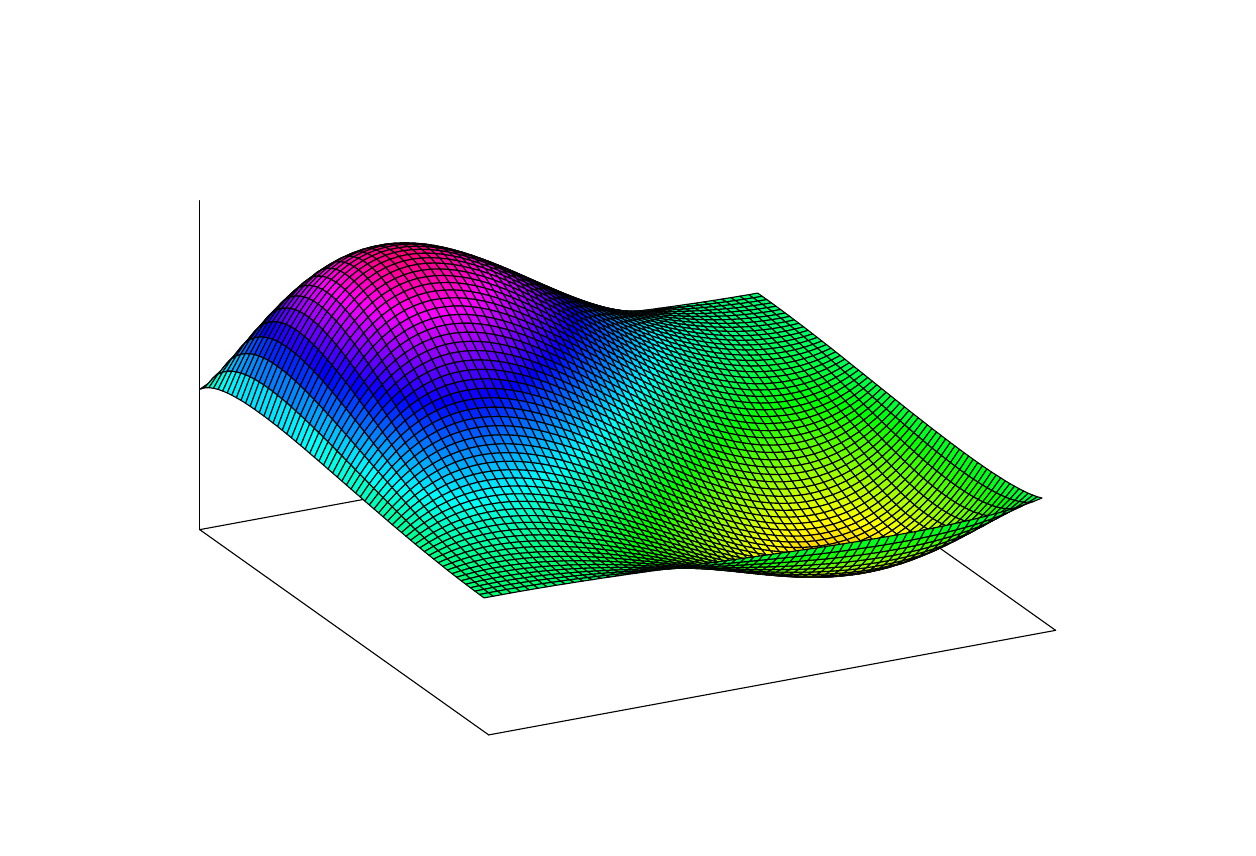
\begin{tikzpicture}[scale=1,gnuplot]
%% generated with GNUPLOT 4.6p0 (Lua 5.1; terminal rev. 99, script rev. 100)
%% Sun 14 Apr 2013 03:42:13 PM BST
\gpsolidlines
\path (0.000,0.000) rectangle (15.240,10.160);
\gpcolor{color=gp lt color border}
\gpsetlinetype{gp lt border}
\gpsetlinewidth{1.00}
\draw[gp path] (2.185,3.785)--(9.385,5.113);
\draw[gp path] (13.055,2.506)--(9.385,5.113);
\draw[gp path] (2.185,3.785)--(2.185,7.962);
\gpfill{rgb color={0.000,1.000,0.440}} (9.271,6.789)--(9.157,6.769)--(9.215,6.729)--(9.329,6.748)--cycle;
\gpcolor{rgb color={0.000,0.000,0.000}}
\gpsetlinetype{gp lt plot 3}
\draw[gp path] (9.271,6.789)--(9.329,6.748)--(9.215,6.729)--(9.157,6.769)--cycle;
\gpfill{rgb color={0.000,1.000,0.441}} (9.329,6.748)--(9.215,6.729)--(9.273,6.688)--(9.388,6.706)--cycle;
\draw[gp path] (9.329,6.748)--(9.388,6.706)--(9.273,6.688)--(9.215,6.729)--cycle;
\gpfill{rgb color={0.000,1.000,0.441}} (9.388,6.706)--(9.273,6.688)--(9.332,6.646)--(9.446,6.665)--cycle;
\draw[gp path] (9.388,6.706)--(9.446,6.665)--(9.332,6.646)--(9.273,6.688)--cycle;
\gpfill{rgb color={0.000,1.000,0.439}} (9.446,6.665)--(9.332,6.646)--(9.390,6.603)--(9.504,6.622)--cycle;
\draw[gp path] (9.446,6.665)--(9.504,6.622)--(9.390,6.603)--(9.332,6.646)--cycle;
\gpfill{rgb color={0.000,1.000,0.437}} (9.504,6.622)--(9.390,6.603)--(9.448,6.560)--(9.562,6.580)--cycle;
\draw[gp path] (9.504,6.622)--(9.562,6.580)--(9.448,6.560)--(9.390,6.603)--cycle;
\gpfill{rgb color={0.000,1.000,0.434}} (9.562,6.580)--(9.448,6.560)--(9.506,6.515)--(9.621,6.536)--cycle;
\draw[gp path] (9.562,6.580)--(9.621,6.536)--(9.506,6.515)--(9.448,6.560)--cycle;
\gpfill{rgb color={0.000,1.000,0.431}} (9.621,6.536)--(9.506,6.515)--(9.565,6.470)--(9.679,6.493)--cycle;
\draw[gp path] (9.621,6.536)--(9.679,6.493)--(9.565,6.470)--(9.506,6.515)--cycle;
\gpfill{rgb color={0.000,1.000,0.426}} (9.679,6.493)--(9.565,6.470)--(9.623,6.424)--(9.737,6.449)--cycle;
\draw[gp path] (9.679,6.493)--(9.737,6.449)--(9.623,6.424)--(9.565,6.470)--cycle;
\gpfill{rgb color={0.000,1.000,0.421}} (9.737,6.449)--(9.623,6.424)--(9.681,6.378)--(9.795,6.405)--cycle;
\draw[gp path] (9.737,6.449)--(9.795,6.405)--(9.681,6.378)--(9.623,6.424)--cycle;
\gpfill{rgb color={0.000,1.000,0.415}} (9.795,6.405)--(9.681,6.378)--(9.739,6.331)--(9.854,6.361)--cycle;
\draw[gp path] (9.795,6.405)--(9.854,6.361)--(9.739,6.331)--(9.681,6.378)--cycle;
\gpfill{rgb color={0.000,1.000,0.408}} (9.854,6.361)--(9.739,6.331)--(9.798,6.283)--(9.912,6.316)--cycle;
\draw[gp path] (9.854,6.361)--(9.912,6.316)--(9.798,6.283)--(9.739,6.331)--cycle;
\gpfill{rgb color={0.000,1.000,0.401}} (9.912,6.316)--(9.798,6.283)--(9.856,6.235)--(9.970,6.271)--cycle;
\draw[gp path] (9.912,6.316)--(9.970,6.271)--(9.856,6.235)--(9.798,6.283)--cycle;
\gpfill{rgb color={0.000,1.000,0.393}} (9.970,6.271)--(9.856,6.235)--(9.914,6.186)--(10.028,6.226)--cycle;
\draw[gp path] (9.970,6.271)--(10.028,6.226)--(9.914,6.186)--(9.856,6.235)--cycle;
\gpfill{rgb color={0.000,1.000,0.385}} (10.028,6.226)--(9.914,6.186)--(9.972,6.137)--(10.087,6.180)--cycle;
\draw[gp path] (10.028,6.226)--(10.087,6.180)--(9.972,6.137)--(9.914,6.186)--cycle;
\gpfill{rgb color={0.000,1.000,0.376}} (10.087,6.180)--(9.972,6.137)--(10.030,6.088)--(10.145,6.135)--cycle;
\draw[gp path] (10.087,6.180)--(10.145,6.135)--(10.030,6.088)--(9.972,6.137)--cycle;
\gpfill{rgb color={0.000,1.000,0.367}} (10.145,6.135)--(10.030,6.088)--(10.089,6.038)--(10.203,6.089)--cycle;
\draw[gp path] (10.145,6.135)--(10.203,6.089)--(10.089,6.038)--(10.030,6.088)--cycle;
\gpfill{rgb color={0.000,1.000,0.357}} (10.203,6.089)--(10.089,6.038)--(10.147,5.987)--(10.261,6.043)--cycle;
\draw[gp path] (10.203,6.089)--(10.261,6.043)--(10.147,5.987)--(10.089,6.038)--cycle;
\gpfill{rgb color={0.000,1.000,0.347}} (10.261,6.043)--(10.147,5.987)--(10.205,5.937)--(10.320,5.997)--cycle;
\draw[gp path] (10.261,6.043)--(10.320,5.997)--(10.205,5.937)--(10.147,5.987)--cycle;
\gpfill{rgb color={0.000,1.000,0.337}} (10.320,5.997)--(10.205,5.937)--(10.263,5.886)--(10.378,5.950)--cycle;
\draw[gp path] (10.320,5.997)--(10.378,5.950)--(10.263,5.886)--(10.205,5.937)--cycle;
\gpfill{rgb color={0.000,1.000,0.327}} (10.378,5.950)--(10.263,5.886)--(10.322,5.835)--(10.436,5.904)--cycle;
\draw[gp path] (10.378,5.950)--(10.436,5.904)--(10.322,5.835)--(10.263,5.886)--cycle;
\gpfill{rgb color={0.000,1.000,0.316}} (10.436,5.904)--(10.322,5.835)--(10.380,5.783)--(10.494,5.857)--cycle;
\draw[gp path] (10.436,5.904)--(10.494,5.857)--(10.380,5.783)--(10.322,5.835)--cycle;
\gpfill{rgb color={0.000,1.000,0.305}} (10.494,5.857)--(10.380,5.783)--(10.438,5.732)--(10.552,5.811)--cycle;
\draw[gp path] (10.494,5.857)--(10.552,5.811)--(10.438,5.732)--(10.380,5.783)--cycle;
\gpfill{rgb color={0.000,1.000,0.294}} (10.552,5.811)--(10.438,5.732)--(10.496,5.680)--(10.611,5.764)--cycle;
\draw[gp path] (10.552,5.811)--(10.611,5.764)--(10.496,5.680)--(10.438,5.732)--cycle;
\gpfill{rgb color={0.000,1.000,0.283}} (10.611,5.764)--(10.496,5.680)--(10.555,5.628)--(10.669,5.717)--cycle;
\draw[gp path] (10.611,5.764)--(10.669,5.717)--(10.555,5.628)--(10.496,5.680)--cycle;
\gpfill{rgb color={0.000,1.000,0.271}} (10.669,5.717)--(10.555,5.628)--(10.613,5.577)--(10.727,5.671)--cycle;
\draw[gp path] (10.669,5.717)--(10.727,5.671)--(10.613,5.577)--(10.555,5.628)--cycle;
\gpfill{rgb color={0.000,1.000,0.260}} (10.727,5.671)--(10.613,5.577)--(10.671,5.525)--(10.785,5.624)--cycle;
\draw[gp path] (10.727,5.671)--(10.785,5.624)--(10.671,5.525)--(10.613,5.577)--cycle;
\gpfill{rgb color={0.000,1.000,0.249}} (10.785,5.624)--(10.671,5.525)--(10.729,5.473)--(10.844,5.577)--cycle;
\draw[gp path] (10.785,5.624)--(10.844,5.577)--(10.729,5.473)--(10.671,5.525)--cycle;
\gpfill{rgb color={0.000,1.000,0.237}} (10.844,5.577)--(10.729,5.473)--(10.788,5.421)--(10.902,5.530)--cycle;
\draw[gp path] (10.844,5.577)--(10.902,5.530)--(10.788,5.421)--(10.729,5.473)--cycle;
\gpfill{rgb color={0.000,1.000,0.226}} (10.902,5.530)--(10.788,5.421)--(10.846,5.370)--(10.960,5.484)--cycle;
\draw[gp path] (10.902,5.530)--(10.960,5.484)--(10.846,5.370)--(10.788,5.421)--cycle;
\gpfill{rgb color={0.000,1.000,0.215}} (10.960,5.484)--(10.846,5.370)--(10.904,5.318)--(11.018,5.437)--cycle;
\draw[gp path] (10.960,5.484)--(11.018,5.437)--(10.904,5.318)--(10.846,5.370)--cycle;
\gpfill{rgb color={0.000,1.000,0.204}} (11.018,5.437)--(10.904,5.318)--(10.962,5.267)--(11.077,5.391)--cycle;
\draw[gp path] (11.018,5.437)--(11.077,5.391)--(10.962,5.267)--(10.904,5.318)--cycle;
\gpfill{rgb color={0.000,1.000,0.193}} (11.077,5.391)--(10.962,5.267)--(11.021,5.217)--(11.135,5.344)--cycle;
\draw[gp path] (11.077,5.391)--(11.135,5.344)--(11.021,5.217)--(10.962,5.267)--cycle;
\gpfill{rgb color={0.000,1.000,0.183}} (11.135,5.344)--(11.021,5.217)--(11.079,5.166)--(11.193,5.298)--cycle;
\draw[gp path] (11.135,5.344)--(11.193,5.298)--(11.079,5.166)--(11.021,5.217)--cycle;
\gpfill{rgb color={0.000,1.000,0.173}} (11.193,5.298)--(11.079,5.166)--(11.137,5.115)--(11.251,5.252)--cycle;
\draw[gp path] (11.193,5.298)--(11.251,5.252)--(11.137,5.115)--(11.079,5.166)--cycle;
\gpfill{rgb color={0.000,1.000,0.163}} (11.251,5.252)--(11.137,5.115)--(11.195,5.065)--(11.310,5.207)--cycle;
\draw[gp path] (11.251,5.252)--(11.310,5.207)--(11.195,5.065)--(11.137,5.115)--cycle;
\gpfill{rgb color={0.000,1.000,0.154}} (11.310,5.207)--(11.195,5.065)--(11.254,5.015)--(11.368,5.161)--cycle;
\draw[gp path] (11.310,5.207)--(11.368,5.161)--(11.254,5.015)--(11.195,5.065)--cycle;
\gpfill{rgb color={0.000,1.000,0.145}} (11.368,5.161)--(11.254,5.015)--(11.312,4.966)--(11.426,5.116)--cycle;
\draw[gp path] (11.368,5.161)--(11.426,5.116)--(11.312,4.966)--(11.254,5.015)--cycle;
\gpfill{rgb color={0.000,1.000,0.136}} (11.426,5.116)--(11.312,4.966)--(11.370,4.917)--(11.484,5.070)--cycle;
\draw[gp path] (11.426,5.116)--(11.484,5.070)--(11.370,4.917)--(11.312,4.966)--cycle;
\gpfill{rgb color={0.000,1.000,0.128}} (11.484,5.070)--(11.370,4.917)--(11.428,4.868)--(11.543,5.025)--cycle;
\draw[gp path] (11.484,5.070)--(11.543,5.025)--(11.428,4.868)--(11.370,4.917)--cycle;
\gpfill{rgb color={0.000,1.000,0.121}} (11.543,5.025)--(11.428,4.868)--(11.486,4.820)--(11.601,4.981)--cycle;
\draw[gp path] (11.543,5.025)--(11.601,4.981)--(11.486,4.820)--(11.428,4.868)--cycle;
\gpfill{rgb color={0.000,1.000,0.114}} (11.601,4.981)--(11.486,4.820)--(11.545,4.773)--(11.659,4.936)--cycle;
\draw[gp path] (11.601,4.981)--(11.659,4.936)--(11.545,4.773)--(11.486,4.820)--cycle;
\gpfill{rgb color={0.000,1.000,0.108}} (11.659,4.936)--(11.545,4.773)--(11.603,4.726)--(11.717,4.892)--cycle;
\draw[gp path] (11.659,4.936)--(11.717,4.892)--(11.603,4.726)--(11.545,4.773)--cycle;
\gpfill{rgb color={0.000,1.000,0.102}} (11.717,4.892)--(11.603,4.726)--(11.661,4.681)--(11.776,4.848)--cycle;
\draw[gp path] (11.717,4.892)--(11.776,4.848)--(11.661,4.681)--(11.603,4.726)--cycle;
\gpfill{rgb color={0.000,1.000,0.098}} (11.776,4.848)--(11.661,4.681)--(11.719,4.636)--(11.834,4.805)--cycle;
\draw[gp path] (11.776,4.848)--(11.834,4.805)--(11.719,4.636)--(11.661,4.681)--cycle;
\gpfill{rgb color={0.000,1.000,0.094}} (11.834,4.805)--(11.719,4.636)--(11.778,4.592)--(11.892,4.762)--cycle;
\draw[gp path] (11.834,4.805)--(11.892,4.762)--(11.778,4.592)--(11.719,4.636)--cycle;
\gpfill{rgb color={0.000,1.000,0.092}} (11.892,4.762)--(11.778,4.592)--(11.836,4.548)--(11.950,4.720)--cycle;
\draw[gp path] (11.892,4.762)--(11.950,4.720)--(11.836,4.548)--(11.778,4.592)--cycle;
\gpfill{rgb color={0.000,1.000,0.091}} (11.950,4.720)--(11.836,4.548)--(11.894,4.506)--(12.008,4.678)--cycle;
\draw[gp path] (11.950,4.720)--(12.008,4.678)--(11.894,4.506)--(11.836,4.548)--cycle;
\gpfill{rgb color={0.000,1.000,0.090}} (12.008,4.678)--(11.894,4.506)--(11.952,4.465)--(12.067,4.637)--cycle;
\draw[gp path] (12.008,4.678)--(12.067,4.637)--(11.952,4.465)--(11.894,4.506)--cycle;
\gpfill{rgb color={0.000,1.000,0.091}} (12.067,4.637)--(11.952,4.465)--(12.011,4.426)--(12.125,4.596)--cycle;
\draw[gp path] (12.067,4.637)--(12.125,4.596)--(12.011,4.426)--(11.952,4.465)--cycle;
\gpfill{rgb color={0.000,1.000,0.094}} (12.125,4.596)--(12.011,4.426)--(12.069,4.387)--(12.183,4.556)--cycle;
\draw[gp path] (12.125,4.596)--(12.183,4.556)--(12.069,4.387)--(12.011,4.426)--cycle;
\gpfill{rgb color={0.000,1.000,0.098}} (12.183,4.556)--(12.069,4.387)--(12.127,4.351)--(12.241,4.517)--cycle;
\draw[gp path] (12.183,4.556)--(12.241,4.517)--(12.127,4.351)--(12.069,4.387)--cycle;
\gpfill{rgb color={0.000,1.000,0.104}} (12.241,4.517)--(12.127,4.351)--(12.185,4.316)--(12.300,4.479)--cycle;
\draw[gp path] (12.241,4.517)--(12.300,4.479)--(12.185,4.316)--(12.127,4.351)--cycle;
\gpfill{rgb color={0.000,1.000,0.112}} (12.300,4.479)--(12.185,4.316)--(12.244,4.283)--(12.358,4.442)--cycle;
\draw[gp path] (12.300,4.479)--(12.358,4.442)--(12.244,4.283)--(12.185,4.316)--cycle;
\gpfill{rgb color={0.000,1.000,0.122}} (12.358,4.442)--(12.244,4.283)--(12.302,4.252)--(12.416,4.405)--cycle;
\draw[gp path] (12.358,4.442)--(12.416,4.405)--(12.302,4.252)--(12.244,4.283)--cycle;
\gpfill{rgb color={0.000,1.000,0.134}} (12.416,4.405)--(12.302,4.252)--(12.360,4.223)--(12.474,4.370)--cycle;
\draw[gp path] (12.416,4.405)--(12.474,4.370)--(12.360,4.223)--(12.302,4.252)--cycle;
\gpfill{rgb color={0.000,1.000,0.150}} (12.474,4.370)--(12.360,4.223)--(12.418,4.197)--(12.533,4.337)--cycle;
\draw[gp path] (12.474,4.370)--(12.533,4.337)--(12.418,4.197)--(12.360,4.223)--cycle;
\gpfill{rgb color={0.000,1.000,0.168}} (12.533,4.337)--(12.418,4.197)--(12.477,4.175)--(12.591,4.305)--cycle;
\draw[gp path] (12.533,4.337)--(12.591,4.305)--(12.477,4.175)--(12.418,4.197)--cycle;
\gpfill{rgb color={0.000,1.000,0.191}} (12.591,4.305)--(12.477,4.175)--(12.535,4.156)--(12.649,4.275)--cycle;
\draw[gp path] (12.591,4.305)--(12.649,4.275)--(12.535,4.156)--(12.477,4.175)--cycle;
\gpfill{rgb color={0.000,1.000,0.217}} (12.649,4.275)--(12.535,4.156)--(12.593,4.142)--(12.707,4.247)--cycle;
\draw[gp path] (12.649,4.275)--(12.707,4.247)--(12.593,4.142)--(12.535,4.156)--cycle;
\gpfill{rgb color={0.000,1.000,0.250}} (12.707,4.247)--(12.593,4.142)--(12.651,4.133)--(12.766,4.223)--cycle;
\draw[gp path] (12.707,4.247)--(12.766,4.223)--(12.651,4.133)--(12.593,4.142)--cycle;
\gpfill{rgb color={0.000,1.000,0.289}} (12.766,4.223)--(12.651,4.133)--(12.710,4.131)--(12.824,4.202)--cycle;
\draw[gp path] (12.766,4.223)--(12.824,4.202)--(12.710,4.131)--(12.651,4.133)--cycle;
\gpfill{rgb color={0.000,1.000,0.338}} (12.824,4.202)--(12.710,4.131)--(12.768,4.140)--(12.882,4.187)--cycle;
\draw[gp path] (12.824,4.202)--(12.882,4.187)--(12.768,4.140)--(12.710,4.131)--cycle;
\gpfill{rgb color={0.000,1.000,0.443}} (9.157,6.769)--(9.043,6.750)--(9.101,6.711)--(9.215,6.729)--cycle;
\draw[gp path] (9.157,6.769)--(9.215,6.729)--(9.101,6.711)--(9.043,6.750)--cycle;
\gpfill{rgb color={0.000,1.000,0.445}} (9.215,6.729)--(9.101,6.711)--(9.159,6.671)--(9.273,6.688)--cycle;
\draw[gp path] (9.215,6.729)--(9.273,6.688)--(9.159,6.671)--(9.101,6.711)--cycle;
\gpfill{rgb color={0.000,1.000,0.446}} (9.273,6.688)--(9.159,6.671)--(9.217,6.629)--(9.332,6.646)--cycle;
\draw[gp path] (9.273,6.688)--(9.332,6.646)--(9.217,6.629)--(9.159,6.671)--cycle;
\gpfill{rgb color={0.000,1.000,0.444}} (9.332,6.646)--(9.217,6.629)--(9.276,6.586)--(9.390,6.603)--cycle;
\draw[gp path] (9.332,6.646)--(9.390,6.603)--(9.276,6.586)--(9.217,6.629)--cycle;
\gpfill{rgb color={0.000,1.000,0.441}} (9.390,6.603)--(9.276,6.586)--(9.334,6.542)--(9.448,6.560)--cycle;
\draw[gp path] (9.390,6.603)--(9.448,6.560)--(9.334,6.542)--(9.276,6.586)--cycle;
\gpfill{rgb color={0.000,1.000,0.437}} (9.448,6.560)--(9.334,6.542)--(9.392,6.497)--(9.506,6.515)--cycle;
\draw[gp path] (9.448,6.560)--(9.506,6.515)--(9.392,6.497)--(9.334,6.542)--cycle;
\gpfill{rgb color={0.000,1.000,0.432}} (9.506,6.515)--(9.392,6.497)--(9.450,6.451)--(9.565,6.470)--cycle;
\draw[gp path] (9.506,6.515)--(9.565,6.470)--(9.450,6.451)--(9.392,6.497)--cycle;
\gpfill{rgb color={0.000,1.000,0.425}} (9.565,6.470)--(9.450,6.451)--(9.508,6.403)--(9.623,6.424)--cycle;
\draw[gp path] (9.565,6.470)--(9.623,6.424)--(9.508,6.403)--(9.450,6.451)--cycle;
\gpfill{rgb color={0.000,1.000,0.417}} (9.623,6.424)--(9.508,6.403)--(9.567,6.355)--(9.681,6.378)--cycle;
\draw[gp path] (9.623,6.424)--(9.681,6.378)--(9.567,6.355)--(9.508,6.403)--cycle;
\gpfill{rgb color={0.000,1.000,0.407}} (9.681,6.378)--(9.567,6.355)--(9.625,6.306)--(9.739,6.331)--cycle;
\draw[gp path] (9.681,6.378)--(9.739,6.331)--(9.625,6.306)--(9.567,6.355)--cycle;
\gpfill{rgb color={0.000,1.000,0.397}} (9.739,6.331)--(9.625,6.306)--(9.683,6.256)--(9.798,6.283)--cycle;
\draw[gp path] (9.739,6.331)--(9.798,6.283)--(9.683,6.256)--(9.625,6.306)--cycle;
\gpfill{rgb color={0.000,1.000,0.386}} (9.798,6.283)--(9.683,6.256)--(9.741,6.204)--(9.856,6.235)--cycle;
\draw[gp path] (9.798,6.283)--(9.856,6.235)--(9.741,6.204)--(9.683,6.256)--cycle;
\gpfill{rgb color={0.000,1.000,0.373}} (9.856,6.235)--(9.741,6.204)--(9.800,6.153)--(9.914,6.186)--cycle;
\draw[gp path] (9.856,6.235)--(9.914,6.186)--(9.800,6.153)--(9.741,6.204)--cycle;
\gpfill{rgb color={0.000,1.000,0.360}} (9.914,6.186)--(9.800,6.153)--(9.858,6.100)--(9.972,6.137)--cycle;
\draw[gp path] (9.914,6.186)--(9.972,6.137)--(9.858,6.100)--(9.800,6.153)--cycle;
\gpfill{rgb color={0.000,1.000,0.346}} (9.972,6.137)--(9.858,6.100)--(9.916,6.047)--(10.030,6.088)--cycle;
\draw[gp path] (9.972,6.137)--(10.030,6.088)--(9.916,6.047)--(9.858,6.100)--cycle;
\gpfill{rgb color={0.000,1.000,0.332}} (10.030,6.088)--(9.916,6.047)--(9.974,5.993)--(10.089,6.038)--cycle;
\draw[gp path] (10.030,6.088)--(10.089,6.038)--(9.974,5.993)--(9.916,6.047)--cycle;
\gpfill{rgb color={0.000,1.000,0.316}} (10.089,6.038)--(9.974,5.993)--(10.033,5.939)--(10.147,5.987)--cycle;
\draw[gp path] (10.089,6.038)--(10.147,5.987)--(10.033,5.939)--(9.974,5.993)--cycle;
\gpfill{rgb color={0.000,1.000,0.300}} (10.147,5.987)--(10.033,5.939)--(10.091,5.884)--(10.205,5.937)--cycle;
\draw[gp path] (10.147,5.987)--(10.205,5.937)--(10.091,5.884)--(10.033,5.939)--cycle;
\gpfill{rgb color={0.000,1.000,0.284}} (10.205,5.937)--(10.091,5.884)--(10.149,5.829)--(10.263,5.886)--cycle;
\draw[gp path] (10.205,5.937)--(10.263,5.886)--(10.149,5.829)--(10.091,5.884)--cycle;
\gpfill{rgb color={0.000,1.000,0.267}} (10.263,5.886)--(10.149,5.829)--(10.207,5.774)--(10.322,5.835)--cycle;
\draw[gp path] (10.263,5.886)--(10.322,5.835)--(10.207,5.774)--(10.149,5.829)--cycle;
\gpfill{rgb color={0.000,1.000,0.250}} (10.322,5.835)--(10.207,5.774)--(10.266,5.718)--(10.380,5.783)--cycle;
\draw[gp path] (10.322,5.835)--(10.380,5.783)--(10.266,5.718)--(10.207,5.774)--cycle;
\gpfill{rgb color={0.000,1.000,0.232}} (10.380,5.783)--(10.266,5.718)--(10.324,5.662)--(10.438,5.732)--cycle;
\draw[gp path] (10.380,5.783)--(10.438,5.732)--(10.324,5.662)--(10.266,5.718)--cycle;
\gpfill{rgb color={0.000,1.000,0.214}} (10.438,5.732)--(10.324,5.662)--(10.382,5.606)--(10.496,5.680)--cycle;
\draw[gp path] (10.438,5.732)--(10.496,5.680)--(10.382,5.606)--(10.324,5.662)--cycle;
\gpfill{rgb color={0.000,1.000,0.196}} (10.496,5.680)--(10.382,5.606)--(10.440,5.549)--(10.555,5.628)--cycle;
\draw[gp path] (10.496,5.680)--(10.555,5.628)--(10.440,5.549)--(10.382,5.606)--cycle;
\gpfill{rgb color={0.000,1.000,0.177}} (10.555,5.628)--(10.440,5.549)--(10.499,5.493)--(10.613,5.577)--cycle;
\draw[gp path] (10.555,5.628)--(10.613,5.577)--(10.499,5.493)--(10.440,5.549)--cycle;
\gpfill{rgb color={0.000,1.000,0.159}} (10.613,5.577)--(10.499,5.493)--(10.557,5.436)--(10.671,5.525)--cycle;
\draw[gp path] (10.613,5.577)--(10.671,5.525)--(10.557,5.436)--(10.499,5.493)--cycle;
\gpfill{rgb color={0.000,1.000,0.141}} (10.671,5.525)--(10.557,5.436)--(10.615,5.380)--(10.729,5.473)--cycle;
\draw[gp path] (10.671,5.525)--(10.729,5.473)--(10.615,5.380)--(10.557,5.436)--cycle;
\gpfill{rgb color={0.000,1.000,0.122}} (10.729,5.473)--(10.615,5.380)--(10.673,5.323)--(10.788,5.421)--cycle;
\draw[gp path] (10.729,5.473)--(10.788,5.421)--(10.673,5.323)--(10.615,5.380)--cycle;
\gpfill{rgb color={0.000,1.000,0.104}} (10.788,5.421)--(10.673,5.323)--(10.732,5.267)--(10.846,5.370)--cycle;
\draw[gp path] (10.788,5.421)--(10.846,5.370)--(10.732,5.267)--(10.673,5.323)--cycle;
\gpfill{rgb color={0.000,1.000,0.086}} (10.846,5.370)--(10.732,5.267)--(10.790,5.212)--(10.904,5.318)--cycle;
\draw[gp path] (10.846,5.370)--(10.904,5.318)--(10.790,5.212)--(10.732,5.267)--cycle;
\gpfill{rgb color={0.000,1.000,0.068}} (10.904,5.318)--(10.790,5.212)--(10.848,5.156)--(10.962,5.267)--cycle;
\draw[gp path] (10.904,5.318)--(10.962,5.267)--(10.848,5.156)--(10.790,5.212)--cycle;
\gpfill{rgb color={0.000,1.000,0.051}} (10.962,5.267)--(10.848,5.156)--(10.906,5.100)--(11.021,5.217)--cycle;
\draw[gp path] (10.962,5.267)--(11.021,5.217)--(10.906,5.100)--(10.848,5.156)--cycle;
\gpfill{rgb color={0.000,1.000,0.034}} (11.021,5.217)--(10.906,5.100)--(10.965,5.045)--(11.079,5.166)--cycle;
\draw[gp path] (11.021,5.217)--(11.079,5.166)--(10.965,5.045)--(10.906,5.100)--cycle;
\gpfill{rgb color={0.000,1.000,0.018}} (11.079,5.166)--(10.965,5.045)--(11.023,4.990)--(11.137,5.115)--cycle;
\draw[gp path] (11.079,5.166)--(11.137,5.115)--(11.023,4.990)--(10.965,5.045)--cycle;
\gpfill{rgb color={0.000,1.000,0.002}} (11.137,5.115)--(11.023,4.990)--(11.081,4.936)--(11.195,5.065)--cycle;
\draw[gp path] (11.137,5.115)--(11.195,5.065)--(11.081,4.936)--(11.023,4.990)--cycle;
\gpfill{rgb color={0.014,1.000,0.000}} (11.195,5.065)--(11.081,4.936)--(11.139,4.882)--(11.254,5.015)--cycle;
\draw[gp path] (11.195,5.065)--(11.254,5.015)--(11.139,4.882)--(11.081,4.936)--cycle;
\gpfill{rgb color={0.028,1.000,0.000}} (11.254,5.015)--(11.139,4.882)--(11.197,4.829)--(11.312,4.966)--cycle;
\draw[gp path] (11.254,5.015)--(11.312,4.966)--(11.197,4.829)--(11.139,4.882)--cycle;
\gpfill{rgb color={0.042,1.000,0.000}} (11.312,4.966)--(11.197,4.829)--(11.256,4.777)--(11.370,4.917)--cycle;
\draw[gp path] (11.312,4.966)--(11.370,4.917)--(11.256,4.777)--(11.197,4.829)--cycle;
\gpfill{rgb color={0.055,1.000,0.000}} (11.370,4.917)--(11.256,4.777)--(11.314,4.725)--(11.428,4.868)--cycle;
\draw[gp path] (11.370,4.917)--(11.428,4.868)--(11.314,4.725)--(11.256,4.777)--cycle;
\gpfill{rgb color={0.067,1.000,0.000}} (11.428,4.868)--(11.314,4.725)--(11.372,4.674)--(11.486,4.820)--cycle;
\draw[gp path] (11.428,4.868)--(11.486,4.820)--(11.372,4.674)--(11.314,4.725)--cycle;
\gpfill{rgb color={0.078,1.000,0.000}} (11.486,4.820)--(11.372,4.674)--(11.430,4.624)--(11.545,4.773)--cycle;
\draw[gp path] (11.486,4.820)--(11.545,4.773)--(11.430,4.624)--(11.372,4.674)--cycle;
\gpfill{rgb color={0.088,1.000,0.000}} (11.545,4.773)--(11.430,4.624)--(11.489,4.575)--(11.603,4.726)--cycle;
\draw[gp path] (11.545,4.773)--(11.603,4.726)--(11.489,4.575)--(11.430,4.624)--cycle;
\gpfill{rgb color={0.096,1.000,0.000}} (11.603,4.726)--(11.489,4.575)--(11.547,4.528)--(11.661,4.681)--cycle;
\draw[gp path] (11.603,4.726)--(11.661,4.681)--(11.547,4.528)--(11.489,4.575)--cycle;
\gpfill{rgb color={0.103,1.000,0.000}} (11.661,4.681)--(11.547,4.528)--(11.605,4.481)--(11.719,4.636)--cycle;
\draw[gp path] (11.661,4.681)--(11.719,4.636)--(11.605,4.481)--(11.547,4.528)--cycle;
\gpfill{rgb color={0.109,1.000,0.000}} (11.719,4.636)--(11.605,4.481)--(11.663,4.436)--(11.778,4.592)--cycle;
\draw[gp path] (11.719,4.636)--(11.778,4.592)--(11.663,4.436)--(11.605,4.481)--cycle;
\gpfill{rgb color={0.113,1.000,0.000}} (11.778,4.592)--(11.663,4.436)--(11.722,4.392)--(11.836,4.548)--cycle;
\draw[gp path] (11.778,4.592)--(11.836,4.548)--(11.722,4.392)--(11.663,4.436)--cycle;
\gpfill{rgb color={0.115,1.000,0.000}} (11.836,4.548)--(11.722,4.392)--(11.780,4.350)--(11.894,4.506)--cycle;
\draw[gp path] (11.836,4.548)--(11.894,4.506)--(11.780,4.350)--(11.722,4.392)--cycle;
\gpfill{rgb color={0.115,1.000,0.000}} (11.894,4.506)--(11.780,4.350)--(11.838,4.309)--(11.952,4.465)--cycle;
\draw[gp path] (11.894,4.506)--(11.952,4.465)--(11.838,4.309)--(11.780,4.350)--cycle;
\gpfill{rgb color={0.113,1.000,0.000}} (11.952,4.465)--(11.838,4.309)--(11.896,4.271)--(12.011,4.426)--cycle;
\draw[gp path] (11.952,4.465)--(12.011,4.426)--(11.896,4.271)--(11.838,4.309)--cycle;
\gpfill{rgb color={0.108,1.000,0.000}} (12.011,4.426)--(11.896,4.271)--(11.955,4.234)--(12.069,4.387)--cycle;
\draw[gp path] (12.011,4.426)--(12.069,4.387)--(11.955,4.234)--(11.896,4.271)--cycle;
\gpfill{rgb color={0.101,1.000,0.000}} (12.069,4.387)--(11.955,4.234)--(12.013,4.200)--(12.127,4.351)--cycle;
\draw[gp path] (12.069,4.387)--(12.127,4.351)--(12.013,4.200)--(11.955,4.234)--cycle;
\gpfill{rgb color={0.091,1.000,0.000}} (12.127,4.351)--(12.013,4.200)--(12.071,4.168)--(12.185,4.316)--cycle;
\draw[gp path] (12.127,4.351)--(12.185,4.316)--(12.071,4.168)--(12.013,4.200)--cycle;
\gpfill{rgb color={0.078,1.000,0.000}} (12.185,4.316)--(12.071,4.168)--(12.129,4.139)--(12.244,4.283)--cycle;
\draw[gp path] (12.185,4.316)--(12.244,4.283)--(12.129,4.139)--(12.071,4.168)--cycle;
\gpfill{rgb color={0.061,1.000,0.000}} (12.244,4.283)--(12.129,4.139)--(12.188,4.114)--(12.302,4.252)--cycle;
\draw[gp path] (12.244,4.283)--(12.302,4.252)--(12.188,4.114)--(12.129,4.139)--cycle;
\gpfill{rgb color={0.040,1.000,0.000}} (12.302,4.252)--(12.188,4.114)--(12.246,4.091)--(12.360,4.223)--cycle;
\draw[gp path] (12.302,4.252)--(12.360,4.223)--(12.246,4.091)--(12.188,4.114)--cycle;
\gpfill{rgb color={0.015,1.000,0.000}} (12.360,4.223)--(12.246,4.091)--(12.304,4.073)--(12.418,4.197)--cycle;
\draw[gp path] (12.360,4.223)--(12.418,4.197)--(12.304,4.073)--(12.246,4.091)--cycle;
\gpfill{rgb color={0.000,1.000,0.016}} (12.418,4.197)--(12.304,4.073)--(12.362,4.059)--(12.477,4.175)--cycle;
\draw[gp path] (12.418,4.197)--(12.477,4.175)--(12.362,4.059)--(12.304,4.073)--cycle;
\gpfill{rgb color={0.000,1.000,0.052}} (12.477,4.175)--(12.362,4.059)--(12.421,4.051)--(12.535,4.156)--cycle;
\draw[gp path] (12.477,4.175)--(12.535,4.156)--(12.421,4.051)--(12.362,4.059)--cycle;
\gpfill{rgb color={0.000,1.000,0.096}} (12.535,4.156)--(12.421,4.051)--(12.479,4.049)--(12.593,4.142)--cycle;
\draw[gp path] (12.535,4.156)--(12.593,4.142)--(12.479,4.049)--(12.421,4.051)--cycle;
\gpfill{rgb color={0.000,1.000,0.149}} (12.593,4.142)--(12.479,4.049)--(12.537,4.055)--(12.651,4.133)--cycle;
\draw[gp path] (12.593,4.142)--(12.651,4.133)--(12.537,4.055)--(12.479,4.049)--cycle;
\gpfill{rgb color={0.000,1.000,0.212}} (12.651,4.133)--(12.537,4.055)--(12.595,4.070)--(12.710,4.131)--cycle;
\draw[gp path] (12.651,4.133)--(12.710,4.131)--(12.595,4.070)--(12.537,4.055)--cycle;
\gpfill{rgb color={0.000,1.000,0.289}} (12.710,4.131)--(12.595,4.070)--(12.653,4.098)--(12.768,4.140)--cycle;
\draw[gp path] (12.710,4.131)--(12.768,4.140)--(12.653,4.098)--(12.595,4.070)--cycle;
\gpfill{rgb color={0.000,1.000,0.447}} (9.043,6.750)--(8.928,6.731)--(8.987,6.694)--(9.101,6.711)--cycle;
\draw[gp path] (9.043,6.750)--(9.101,6.711)--(8.987,6.694)--(8.928,6.731)--cycle;
\gpfill{rgb color={0.000,1.000,0.451}} (9.101,6.711)--(8.987,6.694)--(9.045,6.655)--(9.159,6.671)--cycle;
\draw[gp path] (9.101,6.711)--(9.159,6.671)--(9.045,6.655)--(8.987,6.694)--cycle;
\gpfill{rgb color={0.000,1.000,0.453}} (9.159,6.671)--(9.045,6.655)--(9.103,6.614)--(9.217,6.629)--cycle;
\draw[gp path] (9.159,6.671)--(9.217,6.629)--(9.103,6.614)--(9.045,6.655)--cycle;
\gpfill{rgb color={0.000,1.000,0.452}} (9.217,6.629)--(9.103,6.614)--(9.161,6.572)--(9.276,6.586)--cycle;
\draw[gp path] (9.217,6.629)--(9.276,6.586)--(9.161,6.572)--(9.103,6.614)--cycle;
\gpfill{rgb color={0.000,1.000,0.449}} (9.276,6.586)--(9.161,6.572)--(9.219,6.528)--(9.334,6.542)--cycle;
\draw[gp path] (9.276,6.586)--(9.334,6.542)--(9.219,6.528)--(9.161,6.572)--cycle;
\gpfill{rgb color={0.000,1.000,0.444}} (9.334,6.542)--(9.219,6.528)--(9.278,6.482)--(9.392,6.497)--cycle;
\draw[gp path] (9.334,6.542)--(9.392,6.497)--(9.278,6.482)--(9.219,6.528)--cycle;
\gpfill{rgb color={0.000,1.000,0.437}} (9.392,6.497)--(9.278,6.482)--(9.336,6.435)--(9.450,6.451)--cycle;
\draw[gp path] (9.392,6.497)--(9.450,6.451)--(9.336,6.435)--(9.278,6.482)--cycle;
\gpfill{rgb color={0.000,1.000,0.429}} (9.450,6.451)--(9.336,6.435)--(9.394,6.386)--(9.508,6.403)--cycle;
\draw[gp path] (9.450,6.451)--(9.508,6.403)--(9.394,6.386)--(9.336,6.435)--cycle;
\gpfill{rgb color={0.000,1.000,0.418}} (9.508,6.403)--(9.394,6.386)--(9.452,6.336)--(9.567,6.355)--cycle;
\draw[gp path] (9.508,6.403)--(9.567,6.355)--(9.452,6.336)--(9.394,6.386)--cycle;
\gpfill{rgb color={0.000,1.000,0.406}} (9.567,6.355)--(9.452,6.336)--(9.511,6.285)--(9.625,6.306)--cycle;
\draw[gp path] (9.567,6.355)--(9.625,6.306)--(9.511,6.285)--(9.452,6.336)--cycle;
\gpfill{rgb color={0.000,1.000,0.393}} (9.625,6.306)--(9.511,6.285)--(9.569,6.233)--(9.683,6.256)--cycle;
\draw[gp path] (9.625,6.306)--(9.683,6.256)--(9.569,6.233)--(9.511,6.285)--cycle;
\gpfill{rgb color={0.000,1.000,0.378}} (9.683,6.256)--(9.569,6.233)--(9.627,6.179)--(9.741,6.204)--cycle;
\draw[gp path] (9.683,6.256)--(9.741,6.204)--(9.627,6.179)--(9.569,6.233)--cycle;
\gpfill{rgb color={0.000,1.000,0.362}} (9.741,6.204)--(9.627,6.179)--(9.685,6.125)--(9.800,6.153)--cycle;
\draw[gp path] (9.741,6.204)--(9.800,6.153)--(9.685,6.125)--(9.627,6.179)--cycle;
\gpfill{rgb color={0.000,1.000,0.344}} (9.800,6.153)--(9.685,6.125)--(9.744,6.069)--(9.858,6.100)--cycle;
\draw[gp path] (9.800,6.153)--(9.858,6.100)--(9.744,6.069)--(9.685,6.125)--cycle;
\gpfill{rgb color={0.000,1.000,0.326}} (9.858,6.100)--(9.744,6.069)--(9.802,6.013)--(9.916,6.047)--cycle;
\draw[gp path] (9.858,6.100)--(9.916,6.047)--(9.802,6.013)--(9.744,6.069)--cycle;
\gpfill{rgb color={0.000,1.000,0.306}} (9.916,6.047)--(9.802,6.013)--(9.860,5.956)--(9.974,5.993)--cycle;
\draw[gp path] (9.916,6.047)--(9.974,5.993)--(9.860,5.956)--(9.802,6.013)--cycle;
\gpfill{rgb color={0.000,1.000,0.285}} (9.974,5.993)--(9.860,5.956)--(9.918,5.898)--(10.033,5.939)--cycle;
\draw[gp path] (9.974,5.993)--(10.033,5.939)--(9.918,5.898)--(9.860,5.956)--cycle;
\gpfill{rgb color={0.000,1.000,0.264}} (10.033,5.939)--(9.918,5.898)--(9.977,5.840)--(10.091,5.884)--cycle;
\draw[gp path] (10.033,5.939)--(10.091,5.884)--(9.977,5.840)--(9.918,5.898)--cycle;
\gpfill{rgb color={0.000,1.000,0.242}} (10.091,5.884)--(9.977,5.840)--(10.035,5.781)--(10.149,5.829)--cycle;
\draw[gp path] (10.091,5.884)--(10.149,5.829)--(10.035,5.781)--(9.977,5.840)--cycle;
\gpfill{rgb color={0.000,1.000,0.219}} (10.149,5.829)--(10.035,5.781)--(10.093,5.721)--(10.207,5.774)--cycle;
\draw[gp path] (10.149,5.829)--(10.207,5.774)--(10.093,5.721)--(10.035,5.781)--cycle;
\gpfill{rgb color={0.000,1.000,0.195}} (10.207,5.774)--(10.093,5.721)--(10.151,5.661)--(10.266,5.718)--cycle;
\draw[gp path] (10.207,5.774)--(10.266,5.718)--(10.151,5.661)--(10.093,5.721)--cycle;
\gpfill{rgb color={0.000,1.000,0.171}} (10.266,5.718)--(10.151,5.661)--(10.210,5.601)--(10.324,5.662)--cycle;
\draw[gp path] (10.266,5.718)--(10.324,5.662)--(10.210,5.601)--(10.151,5.661)--cycle;
\gpfill{rgb color={0.000,1.000,0.147}} (10.324,5.662)--(10.210,5.601)--(10.268,5.540)--(10.382,5.606)--cycle;
\draw[gp path] (10.324,5.662)--(10.382,5.606)--(10.268,5.540)--(10.210,5.601)--cycle;
\gpfill{rgb color={0.000,1.000,0.122}} (10.382,5.606)--(10.268,5.540)--(10.326,5.479)--(10.440,5.549)--cycle;
\draw[gp path] (10.382,5.606)--(10.440,5.549)--(10.326,5.479)--(10.268,5.540)--cycle;
\gpfill{rgb color={0.000,1.000,0.097}} (10.440,5.549)--(10.326,5.479)--(10.384,5.418)--(10.499,5.493)--cycle;
\draw[gp path] (10.440,5.549)--(10.499,5.493)--(10.384,5.418)--(10.326,5.479)--cycle;
\gpfill{rgb color={0.000,1.000,0.072}} (10.499,5.493)--(10.384,5.418)--(10.443,5.357)--(10.557,5.436)--cycle;
\draw[gp path] (10.499,5.493)--(10.557,5.436)--(10.443,5.357)--(10.384,5.418)--cycle;
\gpfill{rgb color={0.000,1.000,0.047}} (10.557,5.436)--(10.443,5.357)--(10.501,5.296)--(10.615,5.380)--cycle;
\draw[gp path] (10.557,5.436)--(10.615,5.380)--(10.501,5.296)--(10.443,5.357)--cycle;
\gpfill{rgb color={0.000,1.000,0.022}} (10.615,5.380)--(10.501,5.296)--(10.559,5.235)--(10.673,5.323)--cycle;
\draw[gp path] (10.615,5.380)--(10.673,5.323)--(10.559,5.235)--(10.501,5.296)--cycle;
\gpfill{rgb color={0.002,1.000,0.000}} (10.673,5.323)--(10.559,5.235)--(10.617,5.176)--(10.732,5.267)--cycle;
\draw[gp path] (10.673,5.323)--(10.732,5.267)--(10.617,5.176)--(10.559,5.235)--cycle;
\gpfill{rgb color={0.027,1.000,0.000}} (10.732,5.267)--(10.617,5.176)--(10.675,5.115)--(10.790,5.212)--cycle;
\draw[gp path] (10.732,5.267)--(10.790,5.212)--(10.675,5.115)--(10.617,5.176)--cycle;
\gpfill{rgb color={0.051,1.000,0.000}} (10.790,5.212)--(10.675,5.115)--(10.734,5.055)--(10.848,5.156)--cycle;
\draw[gp path] (10.790,5.212)--(10.848,5.156)--(10.734,5.055)--(10.675,5.115)--cycle;
\gpfill{rgb color={0.075,1.000,0.000}} (10.848,5.156)--(10.734,5.055)--(10.792,4.995)--(10.906,5.100)--cycle;
\draw[gp path] (10.848,5.156)--(10.906,5.100)--(10.792,4.995)--(10.734,5.055)--cycle;
\gpfill{rgb color={0.098,1.000,0.000}} (10.906,5.100)--(10.792,4.995)--(10.850,4.936)--(10.965,5.045)--cycle;
\draw[gp path] (10.906,5.100)--(10.965,5.045)--(10.850,4.936)--(10.792,4.995)--cycle;
\gpfill{rgb color={0.120,1.000,0.000}} (10.965,5.045)--(10.850,4.936)--(10.908,4.877)--(11.023,4.990)--cycle;
\draw[gp path] (10.965,5.045)--(11.023,4.990)--(10.908,4.877)--(10.850,4.936)--cycle;
\gpfill{rgb color={0.142,1.000,0.000}} (11.023,4.990)--(10.908,4.877)--(10.967,4.819)--(11.081,4.936)--cycle;
\draw[gp path] (11.023,4.990)--(11.081,4.936)--(10.967,4.819)--(10.908,4.877)--cycle;
\gpfill{rgb color={0.163,1.000,0.000}} (11.081,4.936)--(10.967,4.819)--(11.025,4.762)--(11.139,4.882)--cycle;
\draw[gp path] (11.081,4.936)--(11.139,4.882)--(11.025,4.762)--(10.967,4.819)--cycle;
\gpfill{rgb color={0.183,1.000,0.000}} (11.139,4.882)--(11.025,4.762)--(11.083,4.705)--(11.197,4.829)--cycle;
\draw[gp path] (11.139,4.882)--(11.197,4.829)--(11.083,4.705)--(11.025,4.762)--cycle;
\gpfill{rgb color={0.201,1.000,0.000}} (11.197,4.829)--(11.083,4.705)--(11.141,4.649)--(11.256,4.777)--cycle;
\draw[gp path] (11.197,4.829)--(11.256,4.777)--(11.141,4.649)--(11.083,4.705)--cycle;
\gpfill{rgb color={0.219,1.000,0.000}} (11.256,4.777)--(11.141,4.649)--(11.200,4.595)--(11.314,4.725)--cycle;
\draw[gp path] (11.256,4.777)--(11.314,4.725)--(11.200,4.595)--(11.141,4.649)--cycle;
\gpfill{rgb color={0.235,1.000,0.000}} (11.314,4.725)--(11.200,4.595)--(11.258,4.541)--(11.372,4.674)--cycle;
\draw[gp path] (11.314,4.725)--(11.372,4.674)--(11.258,4.541)--(11.200,4.595)--cycle;
\gpfill{rgb color={0.250,1.000,0.000}} (11.372,4.674)--(11.258,4.541)--(11.316,4.489)--(11.430,4.624)--cycle;
\draw[gp path] (11.372,4.674)--(11.430,4.624)--(11.316,4.489)--(11.258,4.541)--cycle;
\gpfill{rgb color={0.263,1.000,0.000}} (11.430,4.624)--(11.316,4.489)--(11.374,4.438)--(11.489,4.575)--cycle;
\draw[gp path] (11.430,4.624)--(11.489,4.575)--(11.374,4.438)--(11.316,4.489)--cycle;
\gpfill{rgb color={0.275,1.000,0.000}} (11.489,4.575)--(11.374,4.438)--(11.433,4.388)--(11.547,4.528)--cycle;
\draw[gp path] (11.489,4.575)--(11.547,4.528)--(11.433,4.388)--(11.374,4.438)--cycle;
\gpfill{rgb color={0.284,1.000,0.000}} (11.547,4.528)--(11.433,4.388)--(11.491,4.340)--(11.605,4.481)--cycle;
\draw[gp path] (11.547,4.528)--(11.605,4.481)--(11.491,4.340)--(11.433,4.388)--cycle;
\gpfill{rgb color={0.291,1.000,0.000}} (11.605,4.481)--(11.491,4.340)--(11.549,4.294)--(11.663,4.436)--cycle;
\draw[gp path] (11.605,4.481)--(11.663,4.436)--(11.549,4.294)--(11.491,4.340)--cycle;
\gpfill{rgb color={0.296,1.000,0.000}} (11.663,4.436)--(11.549,4.294)--(11.607,4.250)--(11.722,4.392)--cycle;
\draw[gp path] (11.663,4.436)--(11.722,4.392)--(11.607,4.250)--(11.549,4.294)--cycle;
\gpfill{rgb color={0.299,1.000,0.000}} (11.722,4.392)--(11.607,4.250)--(11.666,4.208)--(11.780,4.350)--cycle;
\draw[gp path] (11.722,4.392)--(11.780,4.350)--(11.666,4.208)--(11.607,4.250)--cycle;
\gpfill{rgb color={0.299,1.000,0.000}} (11.780,4.350)--(11.666,4.208)--(11.724,4.168)--(11.838,4.309)--cycle;
\draw[gp path] (11.780,4.350)--(11.838,4.309)--(11.724,4.168)--(11.666,4.208)--cycle;
\gpfill{rgb color={0.295,1.000,0.000}} (11.838,4.309)--(11.724,4.168)--(11.782,4.130)--(11.896,4.271)--cycle;
\draw[gp path] (11.838,4.309)--(11.896,4.271)--(11.782,4.130)--(11.724,4.168)--cycle;
\gpfill{rgb color={0.289,1.000,0.000}} (11.896,4.271)--(11.782,4.130)--(11.840,4.095)--(11.955,4.234)--cycle;
\draw[gp path] (11.896,4.271)--(11.955,4.234)--(11.840,4.095)--(11.782,4.130)--cycle;
\gpfill{rgb color={0.279,1.000,0.000}} (11.955,4.234)--(11.840,4.095)--(11.899,4.064)--(12.013,4.200)--cycle;
\draw[gp path] (11.955,4.234)--(12.013,4.200)--(11.899,4.064)--(11.840,4.095)--cycle;
\gpfill{rgb color={0.265,1.000,0.000}} (12.013,4.200)--(11.899,4.064)--(11.957,4.035)--(12.071,4.168)--cycle;
\draw[gp path] (12.013,4.200)--(12.071,4.168)--(11.957,4.035)--(11.899,4.064)--cycle;
\gpfill{rgb color={0.246,1.000,0.000}} (12.071,4.168)--(11.957,4.035)--(12.015,4.010)--(12.129,4.139)--cycle;
\draw[gp path] (12.071,4.168)--(12.129,4.139)--(12.015,4.010)--(11.957,4.035)--cycle;
\gpfill{rgb color={0.223,1.000,0.000}} (12.129,4.139)--(12.015,4.010)--(12.073,3.990)--(12.188,4.114)--cycle;
\draw[gp path] (12.129,4.139)--(12.188,4.114)--(12.073,3.990)--(12.015,4.010)--cycle;
\gpfill{rgb color={0.194,1.000,0.000}} (12.188,4.114)--(12.073,3.990)--(12.131,3.973)--(12.246,4.091)--cycle;
\draw[gp path] (12.188,4.114)--(12.246,4.091)--(12.131,3.973)--(12.073,3.990)--cycle;
\gpfill{rgb color={0.159,1.000,0.000}} (12.246,4.091)--(12.131,3.973)--(12.190,3.962)--(12.304,4.073)--cycle;
\draw[gp path] (12.246,4.091)--(12.304,4.073)--(12.190,3.962)--(12.131,3.973)--cycle;
\gpfill{rgb color={0.117,1.000,0.000}} (12.304,4.073)--(12.190,3.962)--(12.248,3.957)--(12.362,4.059)--cycle;
\draw[gp path] (12.304,4.073)--(12.362,4.059)--(12.248,3.957)--(12.190,3.962)--cycle;
\gpfill{rgb color={0.066,1.000,0.000}} (12.362,4.059)--(12.248,3.957)--(12.306,3.959)--(12.421,4.051)--cycle;
\draw[gp path] (12.362,4.059)--(12.421,4.051)--(12.306,3.959)--(12.248,3.957)--cycle;
\gpfill{rgb color={0.007,1.000,0.000}} (12.421,4.051)--(12.306,3.959)--(12.364,3.968)--(12.479,4.049)--cycle;
\draw[gp path] (12.421,4.051)--(12.479,4.049)--(12.364,3.968)--(12.306,3.959)--cycle;
\gpfill{rgb color={0.000,1.000,0.064}} (12.479,4.049)--(12.364,3.968)--(12.423,3.987)--(12.537,4.055)--cycle;
\draw[gp path] (12.479,4.049)--(12.537,4.055)--(12.423,3.987)--(12.364,3.968)--cycle;
\gpfill{rgb color={0.000,1.000,0.149}} (12.537,4.055)--(12.423,3.987)--(12.481,4.017)--(12.595,4.070)--cycle;
\draw[gp path] (12.537,4.055)--(12.595,4.070)--(12.481,4.017)--(12.423,3.987)--cycle;
\gpfill{rgb color={0.000,1.000,0.250}} (12.595,4.070)--(12.481,4.017)--(12.539,4.060)--(12.653,4.098)--cycle;
\draw[gp path] (12.595,4.070)--(12.653,4.098)--(12.539,4.060)--(12.481,4.017)--cycle;
\gpfill{rgb color={0.000,1.000,0.452}} (8.928,6.731)--(8.814,6.713)--(8.872,6.678)--(8.987,6.694)--cycle;
\draw[gp path] (8.928,6.731)--(8.987,6.694)--(8.872,6.678)--(8.814,6.713)--cycle;
\gpfill{rgb color={0.000,1.000,0.459}} (8.987,6.694)--(8.872,6.678)--(8.930,6.641)--(9.045,6.655)--cycle;
\draw[gp path] (8.987,6.694)--(9.045,6.655)--(8.930,6.641)--(8.872,6.678)--cycle;
\gpfill{rgb color={0.000,1.000,0.462}} (9.045,6.655)--(8.930,6.641)--(8.989,6.601)--(9.103,6.614)--cycle;
\draw[gp path] (9.045,6.655)--(9.103,6.614)--(8.989,6.601)--(8.930,6.641)--cycle;
\gpfill{rgb color={0.000,1.000,0.462}} (9.103,6.614)--(8.989,6.601)--(9.047,6.560)--(9.161,6.572)--cycle;
\draw[gp path] (9.103,6.614)--(9.161,6.572)--(9.047,6.560)--(8.989,6.601)--cycle;
\gpfill{rgb color={0.000,1.000,0.460}} (9.161,6.572)--(9.047,6.560)--(9.105,6.516)--(9.219,6.528)--cycle;
\draw[gp path] (9.161,6.572)--(9.219,6.528)--(9.105,6.516)--(9.047,6.560)--cycle;
\gpfill{rgb color={0.000,1.000,0.455}} (9.219,6.528)--(9.105,6.516)--(9.163,6.470)--(9.278,6.482)--cycle;
\draw[gp path] (9.219,6.528)--(9.278,6.482)--(9.163,6.470)--(9.105,6.516)--cycle;
\gpfill{rgb color={0.000,1.000,0.448}} (9.278,6.482)--(9.163,6.470)--(9.222,6.422)--(9.336,6.435)--cycle;
\draw[gp path] (9.278,6.482)--(9.336,6.435)--(9.222,6.422)--(9.163,6.470)--cycle;
\gpfill{rgb color={0.000,1.000,0.438}} (9.336,6.435)--(9.222,6.422)--(9.280,6.373)--(9.394,6.386)--cycle;
\draw[gp path] (9.336,6.435)--(9.394,6.386)--(9.280,6.373)--(9.222,6.422)--cycle;
\gpfill{rgb color={0.000,1.000,0.426}} (9.394,6.386)--(9.280,6.373)--(9.338,6.322)--(9.452,6.336)--cycle;
\draw[gp path] (9.394,6.386)--(9.452,6.336)--(9.338,6.322)--(9.280,6.373)--cycle;
\gpfill{rgb color={0.000,1.000,0.412}} (9.452,6.336)--(9.338,6.322)--(9.396,6.269)--(9.511,6.285)--cycle;
\draw[gp path] (9.452,6.336)--(9.511,6.285)--(9.396,6.269)--(9.338,6.322)--cycle;
\gpfill{rgb color={0.000,1.000,0.396}} (9.511,6.285)--(9.396,6.269)--(9.455,6.215)--(9.569,6.233)--cycle;
\draw[gp path] (9.511,6.285)--(9.569,6.233)--(9.455,6.215)--(9.396,6.269)--cycle;
\gpfill{rgb color={0.000,1.000,0.378}} (9.569,6.233)--(9.455,6.215)--(9.513,6.160)--(9.627,6.179)--cycle;
\draw[gp path] (9.569,6.233)--(9.627,6.179)--(9.513,6.160)--(9.455,6.215)--cycle;
\gpfill{rgb color={0.000,1.000,0.358}} (9.627,6.179)--(9.513,6.160)--(9.571,6.103)--(9.685,6.125)--cycle;
\draw[gp path] (9.627,6.179)--(9.685,6.125)--(9.571,6.103)--(9.513,6.160)--cycle;
\gpfill{rgb color={0.000,1.000,0.337}} (9.685,6.125)--(9.571,6.103)--(9.629,6.045)--(9.744,6.069)--cycle;
\draw[gp path] (9.685,6.125)--(9.744,6.069)--(9.629,6.045)--(9.571,6.103)--cycle;
\gpfill{rgb color={0.000,1.000,0.314}} (9.744,6.069)--(9.629,6.045)--(9.688,5.985)--(9.802,6.013)--cycle;
\draw[gp path] (9.744,6.069)--(9.802,6.013)--(9.688,5.985)--(9.629,6.045)--cycle;
\gpfill{rgb color={0.000,1.000,0.290}} (9.802,6.013)--(9.688,5.985)--(9.746,5.925)--(9.860,5.956)--cycle;
\draw[gp path] (9.802,6.013)--(9.860,5.956)--(9.746,5.925)--(9.688,5.985)--cycle;
\gpfill{rgb color={0.000,1.000,0.264}} (9.860,5.956)--(9.746,5.925)--(9.804,5.864)--(9.918,5.898)--cycle;
\draw[gp path] (9.860,5.956)--(9.918,5.898)--(9.804,5.864)--(9.746,5.925)--cycle;
\gpfill{rgb color={0.000,1.000,0.238}} (9.918,5.898)--(9.804,5.864)--(9.862,5.802)--(9.977,5.840)--cycle;
\draw[gp path] (9.918,5.898)--(9.977,5.840)--(9.862,5.802)--(9.804,5.864)--cycle;
\gpfill{rgb color={0.000,1.000,0.210}} (9.977,5.840)--(9.862,5.802)--(9.921,5.740)--(10.035,5.781)--cycle;
\draw[gp path] (9.977,5.840)--(10.035,5.781)--(9.921,5.740)--(9.862,5.802)--cycle;
\gpfill{rgb color={0.000,1.000,0.182}} (10.035,5.781)--(9.921,5.740)--(9.979,5.676)--(10.093,5.721)--cycle;
\draw[gp path] (10.035,5.781)--(10.093,5.721)--(9.979,5.676)--(9.921,5.740)--cycle;
\gpfill{rgb color={0.000,1.000,0.153}} (10.093,5.721)--(9.979,5.676)--(10.037,5.612)--(10.151,5.661)--cycle;
\draw[gp path] (10.093,5.721)--(10.151,5.661)--(10.037,5.612)--(9.979,5.676)--cycle;
\gpfill{rgb color={0.000,1.000,0.123}} (10.151,5.661)--(10.037,5.612)--(10.095,5.548)--(10.210,5.601)--cycle;
\draw[gp path] (10.151,5.661)--(10.210,5.601)--(10.095,5.548)--(10.037,5.612)--cycle;
\gpfill{rgb color={0.000,1.000,0.092}} (10.210,5.601)--(10.095,5.548)--(10.153,5.483)--(10.268,5.540)--cycle;
\draw[gp path] (10.210,5.601)--(10.268,5.540)--(10.153,5.483)--(10.095,5.548)--cycle;
\gpfill{rgb color={0.000,1.000,0.062}} (10.268,5.540)--(10.153,5.483)--(10.212,5.418)--(10.326,5.479)--cycle;
\draw[gp path] (10.268,5.540)--(10.326,5.479)--(10.212,5.418)--(10.153,5.483)--cycle;
\gpfill{rgb color={0.000,1.000,0.031}} (10.326,5.479)--(10.212,5.418)--(10.270,5.353)--(10.384,5.418)--cycle;
\draw[gp path] (10.326,5.479)--(10.384,5.418)--(10.270,5.353)--(10.212,5.418)--cycle;
\gpfill{rgb color={0.000,1.000,0.000}} (10.384,5.418)--(10.270,5.353)--(10.328,5.288)--(10.443,5.357)--cycle;
\draw[gp path] (10.384,5.418)--(10.443,5.357)--(10.328,5.288)--(10.270,5.353)--cycle;
\gpfill{rgb color={0.032,1.000,0.000}} (10.443,5.357)--(10.328,5.288)--(10.386,5.224)--(10.501,5.296)--cycle;
\draw[gp path] (10.443,5.357)--(10.501,5.296)--(10.386,5.224)--(10.328,5.288)--cycle;
\gpfill{rgb color={0.063,1.000,0.000}} (10.501,5.296)--(10.386,5.224)--(10.445,5.159)--(10.559,5.235)--cycle;
\draw[gp path] (10.501,5.296)--(10.559,5.235)--(10.445,5.159)--(10.386,5.224)--cycle;
\gpfill{rgb color={0.094,1.000,0.000}} (10.559,5.235)--(10.445,5.159)--(10.503,5.094)--(10.617,5.176)--cycle;
\draw[gp path] (10.559,5.235)--(10.617,5.176)--(10.503,5.094)--(10.445,5.159)--cycle;
\gpfill{rgb color={0.124,1.000,0.000}} (10.617,5.176)--(10.503,5.094)--(10.561,5.029)--(10.675,5.115)--cycle;
\draw[gp path] (10.617,5.176)--(10.675,5.115)--(10.561,5.029)--(10.503,5.094)--cycle;
\gpfill{rgb color={0.155,1.000,0.000}} (10.675,5.115)--(10.561,5.029)--(10.619,4.965)--(10.734,5.055)--cycle;
\draw[gp path] (10.675,5.115)--(10.734,5.055)--(10.619,4.965)--(10.561,5.029)--cycle;
\gpfill{rgb color={0.184,1.000,0.000}} (10.734,5.055)--(10.619,4.965)--(10.678,4.901)--(10.792,4.995)--cycle;
\draw[gp path] (10.734,5.055)--(10.792,4.995)--(10.678,4.901)--(10.619,4.965)--cycle;
\gpfill{rgb color={0.213,1.000,0.000}} (10.792,4.995)--(10.678,4.901)--(10.736,4.838)--(10.850,4.936)--cycle;
\draw[gp path] (10.792,4.995)--(10.850,4.936)--(10.736,4.838)--(10.678,4.901)--cycle;
\gpfill{rgb color={0.241,1.000,0.000}} (10.850,4.936)--(10.736,4.838)--(10.794,4.776)--(10.908,4.877)--cycle;
\draw[gp path] (10.850,4.936)--(10.908,4.877)--(10.794,4.776)--(10.736,4.838)--cycle;
\gpfill{rgb color={0.268,1.000,0.000}} (10.908,4.877)--(10.794,4.776)--(10.852,4.714)--(10.967,4.819)--cycle;
\draw[gp path] (10.908,4.877)--(10.967,4.819)--(10.852,4.714)--(10.794,4.776)--cycle;
\gpfill{rgb color={0.294,1.000,0.000}} (10.967,4.819)--(10.852,4.714)--(10.911,4.653)--(11.025,4.762)--cycle;
\draw[gp path] (10.967,4.819)--(11.025,4.762)--(10.911,4.653)--(10.852,4.714)--cycle;
\gpfill{rgb color={0.319,1.000,0.000}} (11.025,4.762)--(10.911,4.653)--(10.969,4.593)--(11.083,4.705)--cycle;
\draw[gp path] (11.025,4.762)--(11.083,4.705)--(10.969,4.593)--(10.911,4.653)--cycle;
\gpfill{rgb color={0.343,1.000,0.000}} (11.083,4.705)--(10.969,4.593)--(11.027,4.535)--(11.141,4.649)--cycle;
\draw[gp path] (11.083,4.705)--(11.141,4.649)--(11.027,4.535)--(10.969,4.593)--cycle;
\gpfill{rgb color={0.365,1.000,0.000}} (11.141,4.649)--(11.027,4.535)--(11.085,4.477)--(11.200,4.595)--cycle;
\draw[gp path] (11.141,4.649)--(11.200,4.595)--(11.085,4.477)--(11.027,4.535)--cycle;
\gpfill{rgb color={0.385,1.000,0.000}} (11.200,4.595)--(11.085,4.477)--(11.144,4.421)--(11.258,4.541)--cycle;
\draw[gp path] (11.200,4.595)--(11.258,4.541)--(11.144,4.421)--(11.085,4.477)--cycle;
\gpfill{rgb color={0.403,1.000,0.000}} (11.258,4.541)--(11.144,4.421)--(11.202,4.366)--(11.316,4.489)--cycle;
\draw[gp path] (11.258,4.541)--(11.316,4.489)--(11.202,4.366)--(11.144,4.421)--cycle;
\gpfill{rgb color={0.419,1.000,0.000}} (11.316,4.489)--(11.202,4.366)--(11.260,4.313)--(11.374,4.438)--cycle;
\draw[gp path] (11.316,4.489)--(11.374,4.438)--(11.260,4.313)--(11.202,4.366)--cycle;
\gpfill{rgb color={0.434,1.000,0.000}} (11.374,4.438)--(11.260,4.313)--(11.318,4.262)--(11.433,4.388)--cycle;
\draw[gp path] (11.374,4.438)--(11.433,4.388)--(11.318,4.262)--(11.260,4.313)--cycle;
\gpfill{rgb color={0.445,1.000,0.000}} (11.433,4.388)--(11.318,4.262)--(11.377,4.213)--(11.491,4.340)--cycle;
\draw[gp path] (11.433,4.388)--(11.491,4.340)--(11.377,4.213)--(11.318,4.262)--cycle;
\gpfill{rgb color={0.454,1.000,0.000}} (11.491,4.340)--(11.377,4.213)--(11.435,4.166)--(11.549,4.294)--cycle;
\draw[gp path] (11.491,4.340)--(11.549,4.294)--(11.435,4.166)--(11.377,4.213)--cycle;
\gpfill{rgb color={0.460,1.000,0.000}} (11.549,4.294)--(11.435,4.166)--(11.493,4.121)--(11.607,4.250)--cycle;
\draw[gp path] (11.549,4.294)--(11.607,4.250)--(11.493,4.121)--(11.435,4.166)--cycle;
\gpfill{rgb color={0.463,1.000,0.000}} (11.607,4.250)--(11.493,4.121)--(11.551,4.079)--(11.666,4.208)--cycle;
\draw[gp path] (11.607,4.250)--(11.666,4.208)--(11.551,4.079)--(11.493,4.121)--cycle;
\gpfill{rgb color={0.462,1.000,0.000}} (11.666,4.208)--(11.551,4.079)--(11.610,4.040)--(11.724,4.168)--cycle;
\draw[gp path] (11.666,4.208)--(11.724,4.168)--(11.610,4.040)--(11.551,4.079)--cycle;
\gpfill{rgb color={0.458,1.000,0.000}} (11.724,4.168)--(11.610,4.040)--(11.668,4.003)--(11.782,4.130)--cycle;
\draw[gp path] (11.724,4.168)--(11.782,4.130)--(11.668,4.003)--(11.610,4.040)--cycle;
\gpfill{rgb color={0.449,1.000,0.000}} (11.782,4.130)--(11.668,4.003)--(11.726,3.970)--(11.840,4.095)--cycle;
\draw[gp path] (11.782,4.130)--(11.840,4.095)--(11.726,3.970)--(11.668,4.003)--cycle;
\gpfill{rgb color={0.436,1.000,0.000}} (11.840,4.095)--(11.726,3.970)--(11.784,3.941)--(11.899,4.064)--cycle;
\draw[gp path] (11.840,4.095)--(11.899,4.064)--(11.784,3.941)--(11.726,3.970)--cycle;
\gpfill{rgb color={0.418,1.000,0.000}} (11.899,4.064)--(11.784,3.941)--(11.842,3.916)--(11.957,4.035)--cycle;
\draw[gp path] (11.899,4.064)--(11.957,4.035)--(11.842,3.916)--(11.784,3.941)--cycle;
\gpfill{rgb color={0.394,1.000,0.000}} (11.957,4.035)--(11.842,3.916)--(11.901,3.895)--(12.015,4.010)--cycle;
\draw[gp path] (11.957,4.035)--(12.015,4.010)--(11.901,3.895)--(11.842,3.916)--cycle;
\gpfill{rgb color={0.365,1.000,0.000}} (12.015,4.010)--(11.901,3.895)--(11.959,3.879)--(12.073,3.990)--cycle;
\draw[gp path] (12.015,4.010)--(12.073,3.990)--(11.959,3.879)--(11.901,3.895)--cycle;
\gpfill{rgb color={0.328,1.000,0.000}} (12.073,3.990)--(11.959,3.879)--(12.017,3.868)--(12.131,3.973)--cycle;
\draw[gp path] (12.073,3.990)--(12.131,3.973)--(12.017,3.868)--(11.959,3.879)--cycle;
\gpfill{rgb color={0.284,1.000,0.000}} (12.131,3.973)--(12.017,3.868)--(12.075,3.864)--(12.190,3.962)--cycle;
\draw[gp path] (12.131,3.973)--(12.190,3.962)--(12.075,3.864)--(12.017,3.868)--cycle;
\gpfill{rgb color={0.231,1.000,0.000}} (12.190,3.962)--(12.075,3.864)--(12.134,3.866)--(12.248,3.957)--cycle;
\draw[gp path] (12.190,3.962)--(12.248,3.957)--(12.134,3.866)--(12.075,3.864)--cycle;
\gpfill{rgb color={0.168,1.000,0.000}} (12.248,3.957)--(12.134,3.866)--(12.192,3.877)--(12.306,3.959)--cycle;
\draw[gp path] (12.248,3.957)--(12.306,3.959)--(12.192,3.877)--(12.134,3.866)--cycle;
\gpfill{rgb color={0.094,1.000,0.000}} (12.306,3.959)--(12.192,3.877)--(12.250,3.896)--(12.364,3.968)--cycle;
\draw[gp path] (12.306,3.959)--(12.364,3.968)--(12.250,3.896)--(12.192,3.877)--cycle;
\gpfill{rgb color={0.007,1.000,0.000}} (12.364,3.968)--(12.250,3.896)--(12.308,3.926)--(12.423,3.987)--cycle;
\draw[gp path] (12.364,3.968)--(12.423,3.987)--(12.308,3.926)--(12.250,3.896)--cycle;
\gpfill{rgb color={0.000,1.000,0.096}} (12.423,3.987)--(12.308,3.926)--(12.367,3.969)--(12.481,4.017)--cycle;
\draw[gp path] (12.423,3.987)--(12.481,4.017)--(12.367,3.969)--(12.308,3.926)--cycle;
\gpfill{rgb color={0.000,1.000,0.217}} (12.481,4.017)--(12.367,3.969)--(12.425,4.025)--(12.539,4.060)--cycle;
\draw[gp path] (12.481,4.017)--(12.539,4.060)--(12.425,4.025)--(12.367,3.969)--cycle;
\gpfill{rgb color={0.000,1.000,0.458}} (8.814,6.713)--(8.700,6.695)--(8.758,6.663)--(8.872,6.678)--cycle;
\draw[gp path] (8.814,6.713)--(8.872,6.678)--(8.758,6.663)--(8.700,6.695)--cycle;
\gpfill{rgb color={0.000,1.000,0.468}} (8.872,6.678)--(8.758,6.663)--(8.816,6.628)--(8.930,6.641)--cycle;
\draw[gp path] (8.872,6.678)--(8.930,6.641)--(8.816,6.628)--(8.758,6.663)--cycle;
\gpfill{rgb color={0.000,1.000,0.474}} (8.930,6.641)--(8.816,6.628)--(8.874,6.590)--(8.989,6.601)--cycle;
\draw[gp path] (8.930,6.641)--(8.989,6.601)--(8.874,6.590)--(8.816,6.628)--cycle;
\gpfill{rgb color={0.000,1.000,0.476}} (8.989,6.601)--(8.874,6.590)--(8.933,6.549)--(9.047,6.560)--cycle;
\draw[gp path] (8.989,6.601)--(9.047,6.560)--(8.933,6.549)--(8.874,6.590)--cycle;
\gpfill{rgb color={0.000,1.000,0.475}} (9.047,6.560)--(8.933,6.549)--(8.991,6.506)--(9.105,6.516)--cycle;
\draw[gp path] (9.047,6.560)--(9.105,6.516)--(8.991,6.506)--(8.933,6.549)--cycle;
\gpfill{rgb color={0.000,1.000,0.470}} (9.105,6.516)--(8.991,6.506)--(9.049,6.461)--(9.163,6.470)--cycle;
\draw[gp path] (9.105,6.516)--(9.163,6.470)--(9.049,6.461)--(8.991,6.506)--cycle;
\gpfill{rgb color={0.000,1.000,0.463}} (9.163,6.470)--(9.049,6.461)--(9.107,6.413)--(9.222,6.422)--cycle;
\draw[gp path] (9.163,6.470)--(9.222,6.422)--(9.107,6.413)--(9.049,6.461)--cycle;
\gpfill{rgb color={0.000,1.000,0.452}} (9.222,6.422)--(9.107,6.413)--(9.166,6.363)--(9.280,6.373)--cycle;
\draw[gp path] (9.222,6.422)--(9.280,6.373)--(9.166,6.363)--(9.107,6.413)--cycle;
\gpfill{rgb color={0.000,1.000,0.439}} (9.280,6.373)--(9.166,6.363)--(9.224,6.311)--(9.338,6.322)--cycle;
\draw[gp path] (9.280,6.373)--(9.338,6.322)--(9.224,6.311)--(9.166,6.363)--cycle;
\gpfill{rgb color={0.000,1.000,0.423}} (9.338,6.322)--(9.224,6.311)--(9.282,6.258)--(9.396,6.269)--cycle;
\draw[gp path] (9.338,6.322)--(9.396,6.269)--(9.282,6.258)--(9.224,6.311)--cycle;
\gpfill{rgb color={0.000,1.000,0.405}} (9.396,6.269)--(9.282,6.258)--(9.340,6.202)--(9.455,6.215)--cycle;
\draw[gp path] (9.396,6.269)--(9.455,6.215)--(9.340,6.202)--(9.282,6.258)--cycle;
\gpfill{rgb color={0.000,1.000,0.384}} (9.455,6.215)--(9.340,6.202)--(9.399,6.145)--(9.513,6.160)--cycle;
\draw[gp path] (9.455,6.215)--(9.513,6.160)--(9.399,6.145)--(9.340,6.202)--cycle;
\gpfill{rgb color={0.000,1.000,0.362}} (9.513,6.160)--(9.399,6.145)--(9.457,6.086)--(9.571,6.103)--cycle;
\draw[gp path] (9.513,6.160)--(9.571,6.103)--(9.457,6.086)--(9.399,6.145)--cycle;
\gpfill{rgb color={0.000,1.000,0.337}} (9.571,6.103)--(9.457,6.086)--(9.515,6.025)--(9.629,6.045)--cycle;
\draw[gp path] (9.571,6.103)--(9.629,6.045)--(9.515,6.025)--(9.457,6.086)--cycle;
\gpfill{rgb color={0.000,1.000,0.310}} (9.629,6.045)--(9.515,6.025)--(9.573,5.964)--(9.688,5.985)--cycle;
\draw[gp path] (9.629,6.045)--(9.688,5.985)--(9.573,5.964)--(9.515,6.025)--cycle;
\gpfill{rgb color={0.000,1.000,0.282}} (9.688,5.985)--(9.573,5.964)--(9.632,5.901)--(9.746,5.925)--cycle;
\draw[gp path] (9.688,5.985)--(9.746,5.925)--(9.632,5.901)--(9.573,5.964)--cycle;
\gpfill{rgb color={0.000,1.000,0.253}} (9.746,5.925)--(9.632,5.901)--(9.690,5.837)--(9.804,5.864)--cycle;
\draw[gp path] (9.746,5.925)--(9.804,5.864)--(9.690,5.837)--(9.632,5.901)--cycle;
\gpfill{rgb color={0.000,1.000,0.221}} (9.804,5.864)--(9.690,5.837)--(9.748,5.772)--(9.862,5.802)--cycle;
\draw[gp path] (9.804,5.864)--(9.862,5.802)--(9.748,5.772)--(9.690,5.837)--cycle;
\gpfill{rgb color={0.000,1.000,0.189}} (9.862,5.802)--(9.748,5.772)--(9.806,5.706)--(9.921,5.740)--cycle;
\draw[gp path] (9.862,5.802)--(9.921,5.740)--(9.806,5.706)--(9.748,5.772)--cycle;
\gpfill{rgb color={0.000,1.000,0.156}} (9.921,5.740)--(9.806,5.706)--(9.864,5.639)--(9.979,5.676)--cycle;
\draw[gp path] (9.921,5.740)--(9.979,5.676)--(9.864,5.639)--(9.806,5.706)--cycle;
\gpfill{rgb color={0.000,1.000,0.121}} (9.979,5.676)--(9.864,5.639)--(9.923,5.572)--(10.037,5.612)--cycle;
\draw[gp path] (9.979,5.676)--(10.037,5.612)--(9.923,5.572)--(9.864,5.639)--cycle;
\gpfill{rgb color={0.000,1.000,0.086}} (10.037,5.612)--(9.923,5.572)--(9.981,5.504)--(10.095,5.548)--cycle;
\draw[gp path] (10.037,5.612)--(10.095,5.548)--(9.981,5.504)--(9.923,5.572)--cycle;
\gpfill{rgb color={0.000,1.000,0.050}} (10.095,5.548)--(9.981,5.504)--(10.039,5.435)--(10.153,5.483)--cycle;
\draw[gp path] (10.095,5.548)--(10.153,5.483)--(10.039,5.435)--(9.981,5.504)--cycle;
\gpfill{rgb color={0.000,1.000,0.014}} (10.153,5.483)--(10.039,5.435)--(10.097,5.366)--(10.212,5.418)--cycle;
\draw[gp path] (10.153,5.483)--(10.212,5.418)--(10.097,5.366)--(10.039,5.435)--cycle;
\gpfill{rgb color={0.023,1.000,0.000}} (10.212,5.418)--(10.097,5.366)--(10.156,5.297)--(10.270,5.353)--cycle;
\draw[gp path] (10.212,5.418)--(10.270,5.353)--(10.156,5.297)--(10.097,5.366)--cycle;
\gpfill{rgb color={0.060,1.000,0.000}} (10.270,5.353)--(10.156,5.297)--(10.214,5.229)--(10.328,5.288)--cycle;
\draw[gp path] (10.270,5.353)--(10.328,5.288)--(10.214,5.229)--(10.156,5.297)--cycle;
\gpfill{rgb color={0.097,1.000,0.000}} (10.328,5.288)--(10.214,5.229)--(10.272,5.160)--(10.386,5.224)--cycle;
\draw[gp path] (10.328,5.288)--(10.386,5.224)--(10.272,5.160)--(10.214,5.229)--cycle;
\gpfill{rgb color={0.134,1.000,0.000}} (10.386,5.224)--(10.272,5.160)--(10.330,5.091)--(10.445,5.159)--cycle;
\draw[gp path] (10.386,5.224)--(10.445,5.159)--(10.330,5.091)--(10.272,5.160)--cycle;
\gpfill{rgb color={0.171,1.000,0.000}} (10.445,5.159)--(10.330,5.091)--(10.389,5.022)--(10.503,5.094)--cycle;
\draw[gp path] (10.445,5.159)--(10.503,5.094)--(10.389,5.022)--(10.330,5.091)--cycle;
\gpfill{rgb color={0.207,1.000,0.000}} (10.503,5.094)--(10.389,5.022)--(10.447,4.954)--(10.561,5.029)--cycle;
\draw[gp path] (10.503,5.094)--(10.561,5.029)--(10.447,4.954)--(10.389,5.022)--cycle;
\gpfill{rgb color={0.243,1.000,0.000}} (10.561,5.029)--(10.447,4.954)--(10.505,4.886)--(10.619,4.965)--cycle;
\draw[gp path] (10.561,5.029)--(10.619,4.965)--(10.505,4.886)--(10.447,4.954)--cycle;
\gpfill{rgb color={0.278,1.000,0.000}} (10.619,4.965)--(10.505,4.886)--(10.563,4.818)--(10.678,4.901)--cycle;
\draw[gp path] (10.619,4.965)--(10.678,4.901)--(10.563,4.818)--(10.505,4.886)--cycle;
\gpfill{rgb color={0.313,1.000,0.000}} (10.678,4.901)--(10.563,4.818)--(10.622,4.751)--(10.736,4.838)--cycle;
\draw[gp path] (10.678,4.901)--(10.736,4.838)--(10.622,4.751)--(10.563,4.818)--cycle;
\gpfill{rgb color={0.346,1.000,0.000}} (10.736,4.838)--(10.622,4.751)--(10.680,4.685)--(10.794,4.776)--cycle;
\draw[gp path] (10.736,4.838)--(10.794,4.776)--(10.680,4.685)--(10.622,4.751)--cycle;
\gpfill{rgb color={0.378,1.000,0.000}} (10.794,4.776)--(10.680,4.685)--(10.738,4.620)--(10.852,4.714)--cycle;
\draw[gp path] (10.794,4.776)--(10.852,4.714)--(10.738,4.620)--(10.680,4.685)--cycle;
\gpfill{rgb color={0.409,1.000,0.000}} (10.852,4.714)--(10.738,4.620)--(10.796,4.556)--(10.911,4.653)--cycle;
\draw[gp path] (10.852,4.714)--(10.911,4.653)--(10.796,4.556)--(10.738,4.620)--cycle;
\gpfill{rgb color={0.439,1.000,0.000}} (10.911,4.653)--(10.796,4.556)--(10.855,4.493)--(10.969,4.593)--cycle;
\draw[gp path] (10.911,4.653)--(10.969,4.593)--(10.855,4.493)--(10.796,4.556)--cycle;
\gpfill{rgb color={0.467,1.000,0.000}} (10.969,4.593)--(10.855,4.493)--(10.913,4.432)--(11.027,4.535)--cycle;
\draw[gp path] (10.969,4.593)--(11.027,4.535)--(10.913,4.432)--(10.855,4.493)--cycle;
\gpfill{rgb color={0.493,1.000,0.000}} (11.027,4.535)--(10.913,4.432)--(10.971,4.372)--(11.085,4.477)--cycle;
\draw[gp path] (11.027,4.535)--(11.085,4.477)--(10.971,4.372)--(10.913,4.432)--cycle;
\gpfill{rgb color={0.517,1.000,0.000}} (11.085,4.477)--(10.971,4.372)--(11.029,4.313)--(11.144,4.421)--cycle;
\draw[gp path] (11.085,4.477)--(11.144,4.421)--(11.029,4.313)--(10.971,4.372)--cycle;
\gpfill{rgb color={0.538,1.000,0.000}} (11.144,4.421)--(11.029,4.313)--(11.088,4.256)--(11.202,4.366)--cycle;
\draw[gp path] (11.144,4.421)--(11.202,4.366)--(11.088,4.256)--(11.029,4.313)--cycle;
\gpfill{rgb color={0.558,1.000,0.000}} (11.202,4.366)--(11.088,4.256)--(11.146,4.201)--(11.260,4.313)--cycle;
\draw[gp path] (11.202,4.366)--(11.260,4.313)--(11.146,4.201)--(11.088,4.256)--cycle;
\gpfill{rgb color={0.574,1.000,0.000}} (11.260,4.313)--(11.146,4.201)--(11.204,4.149)--(11.318,4.262)--cycle;
\draw[gp path] (11.260,4.313)--(11.318,4.262)--(11.204,4.149)--(11.146,4.201)--cycle;
\gpfill{rgb color={0.588,1.000,0.000}} (11.318,4.262)--(11.204,4.149)--(11.262,4.098)--(11.377,4.213)--cycle;
\draw[gp path] (11.318,4.262)--(11.377,4.213)--(11.262,4.098)--(11.204,4.149)--cycle;
\gpfill{rgb color={0.598,1.000,0.000}} (11.377,4.213)--(11.262,4.098)--(11.320,4.051)--(11.435,4.166)--cycle;
\draw[gp path] (11.377,4.213)--(11.435,4.166)--(11.320,4.051)--(11.262,4.098)--cycle;
\gpfill{rgb color={0.605,1.000,0.000}} (11.435,4.166)--(11.320,4.051)--(11.379,4.006)--(11.493,4.121)--cycle;
\draw[gp path] (11.435,4.166)--(11.493,4.121)--(11.379,4.006)--(11.320,4.051)--cycle;
\gpfill{rgb color={0.608,1.000,0.000}} (11.493,4.121)--(11.379,4.006)--(11.437,3.963)--(11.551,4.079)--cycle;
\draw[gp path] (11.493,4.121)--(11.551,4.079)--(11.437,3.963)--(11.379,4.006)--cycle;
\gpfill{rgb color={0.607,1.000,0.000}} (11.551,4.079)--(11.437,3.963)--(11.495,3.925)--(11.610,4.040)--cycle;
\draw[gp path] (11.551,4.079)--(11.610,4.040)--(11.495,3.925)--(11.437,3.963)--cycle;
\gpfill{rgb color={0.601,1.000,0.000}} (11.610,4.040)--(11.495,3.925)--(11.553,3.889)--(11.668,4.003)--cycle;
\draw[gp path] (11.610,4.040)--(11.668,4.003)--(11.553,3.889)--(11.495,3.925)--cycle;
\gpfill{rgb color={0.591,1.000,0.000}} (11.668,4.003)--(11.553,3.889)--(11.612,3.858)--(11.726,3.970)--cycle;
\draw[gp path] (11.668,4.003)--(11.726,3.970)--(11.612,3.858)--(11.553,3.889)--cycle;
\gpfill{rgb color={0.575,1.000,0.000}} (11.726,3.970)--(11.612,3.858)--(11.670,3.831)--(11.784,3.941)--cycle;
\draw[gp path] (11.726,3.970)--(11.784,3.941)--(11.670,3.831)--(11.612,3.858)--cycle;
\gpfill{rgb color={0.553,1.000,0.000}} (11.784,3.941)--(11.670,3.831)--(11.728,3.808)--(11.842,3.916)--cycle;
\draw[gp path] (11.784,3.941)--(11.842,3.916)--(11.728,3.808)--(11.670,3.831)--cycle;
\gpfill{rgb color={0.524,1.000,0.000}} (11.842,3.916)--(11.728,3.808)--(11.786,3.791)--(11.901,3.895)--cycle;
\draw[gp path] (11.842,3.916)--(11.901,3.895)--(11.786,3.791)--(11.728,3.808)--cycle;
\gpfill{rgb color={0.489,1.000,0.000}} (11.901,3.895)--(11.786,3.791)--(11.845,3.779)--(11.959,3.879)--cycle;
\draw[gp path] (11.901,3.895)--(11.959,3.879)--(11.845,3.779)--(11.786,3.791)--cycle;
\gpfill{rgb color={0.445,1.000,0.000}} (11.959,3.879)--(11.845,3.779)--(11.903,3.774)--(12.017,3.868)--cycle;
\draw[gp path] (11.959,3.879)--(12.017,3.868)--(11.903,3.774)--(11.845,3.779)--cycle;
\gpfill{rgb color={0.392,1.000,0.000}} (12.017,3.868)--(11.903,3.774)--(11.961,3.776)--(12.075,3.864)--cycle;
\draw[gp path] (12.017,3.868)--(12.075,3.864)--(11.961,3.776)--(11.903,3.774)--cycle;
\gpfill{rgb color={0.329,1.000,0.000}} (12.075,3.864)--(11.961,3.776)--(12.019,3.785)--(12.134,3.866)--cycle;
\draw[gp path] (12.075,3.864)--(12.134,3.866)--(12.019,3.785)--(11.961,3.776)--cycle;
\gpfill{rgb color={0.255,1.000,0.000}} (12.134,3.866)--(12.019,3.785)--(12.078,3.804)--(12.192,3.877)--cycle;
\draw[gp path] (12.134,3.866)--(12.192,3.877)--(12.078,3.804)--(12.019,3.785)--cycle;
\gpfill{rgb color={0.168,1.000,0.000}} (12.192,3.877)--(12.078,3.804)--(12.136,3.832)--(12.250,3.896)--cycle;
\draw[gp path] (12.192,3.877)--(12.250,3.896)--(12.136,3.832)--(12.078,3.804)--cycle;
\gpfill{rgb color={0.066,1.000,0.000}} (12.250,3.896)--(12.136,3.832)--(12.194,3.872)--(12.308,3.926)--cycle;
\draw[gp path] (12.250,3.896)--(12.308,3.926)--(12.194,3.872)--(12.136,3.832)--cycle;
\gpfill{rgb color={0.000,1.000,0.052}} (12.308,3.926)--(12.194,3.872)--(12.252,3.925)--(12.367,3.969)--cycle;
\draw[gp path] (12.308,3.926)--(12.367,3.969)--(12.252,3.925)--(12.194,3.872)--cycle;
\gpfill{rgb color={0.000,1.000,0.191}} (12.367,3.969)--(12.252,3.925)--(12.311,3.993)--(12.425,4.025)--cycle;
\draw[gp path] (12.367,3.969)--(12.425,4.025)--(12.311,3.993)--(12.252,3.925)--cycle;
\gpfill{rgb color={0.000,1.000,0.465}} (8.700,6.695)--(8.585,6.677)--(8.644,6.648)--(8.758,6.663)--cycle;
\draw[gp path] (8.700,6.695)--(8.758,6.663)--(8.644,6.648)--(8.585,6.677)--cycle;
\gpfill{rgb color={0.000,1.000,0.478}} (8.758,6.663)--(8.644,6.648)--(8.702,6.616)--(8.816,6.628)--cycle;
\draw[gp path] (8.758,6.663)--(8.816,6.628)--(8.702,6.616)--(8.644,6.648)--cycle;
\gpfill{rgb color={0.000,1.000,0.487}} (8.816,6.628)--(8.702,6.616)--(8.760,6.580)--(8.874,6.590)--cycle;
\draw[gp path] (8.816,6.628)--(8.874,6.590)--(8.760,6.580)--(8.702,6.616)--cycle;
\gpfill{rgb color={0.000,1.000,0.492}} (8.874,6.590)--(8.760,6.580)--(8.818,6.541)--(8.933,6.549)--cycle;
\draw[gp path] (8.874,6.590)--(8.933,6.549)--(8.818,6.541)--(8.760,6.580)--cycle;
\gpfill{rgb color={0.000,1.000,0.492}} (8.933,6.549)--(8.818,6.541)--(8.877,6.499)--(8.991,6.506)--cycle;
\draw[gp path] (8.933,6.549)--(8.991,6.506)--(8.877,6.499)--(8.818,6.541)--cycle;
\gpfill{rgb color={0.000,1.000,0.489}} (8.991,6.506)--(8.877,6.499)--(8.935,6.454)--(9.049,6.461)--cycle;
\draw[gp path] (8.991,6.506)--(9.049,6.461)--(8.935,6.454)--(8.877,6.499)--cycle;
\gpfill{rgb color={0.000,1.000,0.482}} (9.049,6.461)--(8.935,6.454)--(8.993,6.407)--(9.107,6.413)--cycle;
\draw[gp path] (9.049,6.461)--(9.107,6.413)--(8.993,6.407)--(8.935,6.454)--cycle;
\gpfill{rgb color={0.000,1.000,0.471}} (9.107,6.413)--(8.993,6.407)--(9.051,6.357)--(9.166,6.363)--cycle;
\draw[gp path] (9.107,6.413)--(9.166,6.363)--(9.051,6.357)--(8.993,6.407)--cycle;
\gpfill{rgb color={0.000,1.000,0.457}} (9.166,6.363)--(9.051,6.357)--(9.110,6.305)--(9.224,6.311)--cycle;
\draw[gp path] (9.166,6.363)--(9.224,6.311)--(9.110,6.305)--(9.051,6.357)--cycle;
\gpfill{rgb color={0.000,1.000,0.440}} (9.224,6.311)--(9.110,6.305)--(9.168,6.250)--(9.282,6.258)--cycle;
\draw[gp path] (9.224,6.311)--(9.282,6.258)--(9.168,6.250)--(9.110,6.305)--cycle;
\gpfill{rgb color={0.000,1.000,0.421}} (9.282,6.258)--(9.168,6.250)--(9.226,6.193)--(9.340,6.202)--cycle;
\draw[gp path] (9.282,6.258)--(9.340,6.202)--(9.226,6.193)--(9.168,6.250)--cycle;
\gpfill{rgb color={0.000,1.000,0.398}} (9.340,6.202)--(9.226,6.193)--(9.284,6.135)--(9.399,6.145)--cycle;
\draw[gp path] (9.340,6.202)--(9.399,6.145)--(9.284,6.135)--(9.226,6.193)--cycle;
\gpfill{rgb color={0.000,1.000,0.373}} (9.399,6.145)--(9.284,6.135)--(9.342,6.074)--(9.457,6.086)--cycle;
\draw[gp path] (9.399,6.145)--(9.457,6.086)--(9.342,6.074)--(9.284,6.135)--cycle;
\gpfill{rgb color={0.000,1.000,0.345}} (9.457,6.086)--(9.342,6.074)--(9.401,6.012)--(9.515,6.025)--cycle;
\draw[gp path] (9.457,6.086)--(9.515,6.025)--(9.401,6.012)--(9.342,6.074)--cycle;
\gpfill{rgb color={0.000,1.000,0.316}} (9.515,6.025)--(9.401,6.012)--(9.459,5.948)--(9.573,5.964)--cycle;
\draw[gp path] (9.515,6.025)--(9.573,5.964)--(9.459,5.948)--(9.401,6.012)--cycle;
\gpfill{rgb color={0.000,1.000,0.284}} (9.573,5.964)--(9.459,5.948)--(9.517,5.883)--(9.632,5.901)--cycle;
\draw[gp path] (9.573,5.964)--(9.632,5.901)--(9.517,5.883)--(9.459,5.948)--cycle;
\gpfill{rgb color={0.000,1.000,0.250}} (9.632,5.901)--(9.517,5.883)--(9.575,5.816)--(9.690,5.837)--cycle;
\draw[gp path] (9.632,5.901)--(9.690,5.837)--(9.575,5.816)--(9.517,5.883)--cycle;
\gpfill{rgb color={0.000,1.000,0.215}} (9.690,5.837)--(9.575,5.816)--(9.634,5.748)--(9.748,5.772)--cycle;
\draw[gp path] (9.690,5.837)--(9.748,5.772)--(9.634,5.748)--(9.575,5.816)--cycle;
\gpfill{rgb color={0.000,1.000,0.178}} (9.748,5.772)--(9.634,5.748)--(9.692,5.679)--(9.806,5.706)--cycle;
\draw[gp path] (9.748,5.772)--(9.806,5.706)--(9.692,5.679)--(9.634,5.748)--cycle;
\gpfill{rgb color={0.000,1.000,0.140}} (9.806,5.706)--(9.692,5.679)--(9.750,5.609)--(9.864,5.639)--cycle;
\draw[gp path] (9.806,5.706)--(9.864,5.639)--(9.750,5.609)--(9.692,5.679)--cycle;
\gpfill{rgb color={0.000,1.000,0.101}} (9.864,5.639)--(9.750,5.609)--(9.808,5.538)--(9.923,5.572)--cycle;
\draw[gp path] (9.864,5.639)--(9.923,5.572)--(9.808,5.538)--(9.750,5.609)--cycle;
\gpfill{rgb color={0.000,1.000,0.061}} (9.923,5.572)--(9.808,5.538)--(9.867,5.467)--(9.981,5.504)--cycle;
\draw[gp path] (9.923,5.572)--(9.981,5.504)--(9.867,5.467)--(9.808,5.538)--cycle;
\gpfill{rgb color={0.000,1.000,0.020}} (9.981,5.504)--(9.867,5.467)--(9.925,5.395)--(10.039,5.435)--cycle;
\draw[gp path] (9.981,5.504)--(10.039,5.435)--(9.925,5.395)--(9.867,5.467)--cycle;
\gpfill{rgb color={0.022,1.000,0.000}} (10.039,5.435)--(9.925,5.395)--(9.983,5.323)--(10.097,5.366)--cycle;
\draw[gp path] (10.039,5.435)--(10.097,5.366)--(9.983,5.323)--(9.925,5.395)--cycle;
\gpfill{rgb color={0.064,1.000,0.000}} (10.097,5.366)--(9.983,5.323)--(10.041,5.250)--(10.156,5.297)--cycle;
\draw[gp path] (10.097,5.366)--(10.156,5.297)--(10.041,5.250)--(9.983,5.323)--cycle;
\gpfill{rgb color={0.106,1.000,0.000}} (10.156,5.297)--(10.041,5.250)--(10.100,5.178)--(10.214,5.229)--cycle;
\draw[gp path] (10.156,5.297)--(10.214,5.229)--(10.100,5.178)--(10.041,5.250)--cycle;
\gpfill{rgb color={0.149,1.000,0.000}} (10.214,5.229)--(10.100,5.178)--(10.158,5.106)--(10.272,5.160)--cycle;
\draw[gp path] (10.214,5.229)--(10.272,5.160)--(10.158,5.106)--(10.100,5.178)--cycle;
\gpfill{rgb color={0.191,1.000,0.000}} (10.272,5.160)--(10.158,5.106)--(10.216,5.033)--(10.330,5.091)--cycle;
\draw[gp path] (10.272,5.160)--(10.330,5.091)--(10.216,5.033)--(10.158,5.106)--cycle;
\gpfill{rgb color={0.234,1.000,0.000}} (10.330,5.091)--(10.216,5.033)--(10.274,4.960)--(10.389,5.022)--cycle;
\draw[gp path] (10.330,5.091)--(10.389,5.022)--(10.274,4.960)--(10.216,5.033)--cycle;
\gpfill{rgb color={0.276,1.000,0.000}} (10.389,5.022)--(10.274,4.960)--(10.333,4.888)--(10.447,4.954)--cycle;
\draw[gp path] (10.389,5.022)--(10.447,4.954)--(10.333,4.888)--(10.274,4.960)--cycle;
\gpfill{rgb color={0.317,1.000,0.000}} (10.447,4.954)--(10.333,4.888)--(10.391,4.816)--(10.505,4.886)--cycle;
\draw[gp path] (10.447,4.954)--(10.505,4.886)--(10.391,4.816)--(10.333,4.888)--cycle;
\gpfill{rgb color={0.357,1.000,0.000}} (10.505,4.886)--(10.391,4.816)--(10.449,4.745)--(10.563,4.818)--cycle;
\draw[gp path] (10.505,4.886)--(10.563,4.818)--(10.449,4.745)--(10.391,4.816)--cycle;
\gpfill{rgb color={0.397,1.000,0.000}} (10.563,4.818)--(10.449,4.745)--(10.507,4.675)--(10.622,4.751)--cycle;
\draw[gp path] (10.563,4.818)--(10.622,4.751)--(10.507,4.675)--(10.449,4.745)--cycle;
\gpfill{rgb color={0.435,1.000,0.000}} (10.622,4.751)--(10.507,4.675)--(10.566,4.606)--(10.680,4.685)--cycle;
\draw[gp path] (10.622,4.751)--(10.680,4.685)--(10.566,4.606)--(10.507,4.675)--cycle;
\gpfill{rgb color={0.472,1.000,0.000}} (10.680,4.685)--(10.566,4.606)--(10.624,4.537)--(10.738,4.620)--cycle;
\draw[gp path] (10.680,4.685)--(10.738,4.620)--(10.624,4.537)--(10.566,4.606)--cycle;
\gpfill{rgb color={0.508,1.000,0.000}} (10.738,4.620)--(10.624,4.537)--(10.682,4.470)--(10.796,4.556)--cycle;
\draw[gp path] (10.738,4.620)--(10.796,4.556)--(10.682,4.470)--(10.624,4.537)--cycle;
\gpfill{rgb color={0.542,1.000,0.000}} (10.796,4.556)--(10.682,4.470)--(10.740,4.404)--(10.855,4.493)--cycle;
\draw[gp path] (10.796,4.556)--(10.855,4.493)--(10.740,4.404)--(10.682,4.470)--cycle;
\gpfill{rgb color={0.574,1.000,0.000}} (10.855,4.493)--(10.740,4.404)--(10.798,4.340)--(10.913,4.432)--cycle;
\draw[gp path] (10.855,4.493)--(10.913,4.432)--(10.798,4.340)--(10.740,4.404)--cycle;
\gpfill{rgb color={0.604,1.000,0.000}} (10.913,4.432)--(10.798,4.340)--(10.857,4.277)--(10.971,4.372)--cycle;
\draw[gp path] (10.913,4.432)--(10.971,4.372)--(10.857,4.277)--(10.798,4.340)--cycle;
\gpfill{rgb color={0.631,1.000,0.000}} (10.971,4.372)--(10.857,4.277)--(10.915,4.217)--(11.029,4.313)--cycle;
\draw[gp path] (10.971,4.372)--(11.029,4.313)--(10.915,4.217)--(10.857,4.277)--cycle;
\gpfill{rgb color={0.656,1.000,0.000}} (11.029,4.313)--(10.915,4.217)--(10.973,4.158)--(11.088,4.256)--cycle;
\draw[gp path] (11.029,4.313)--(11.088,4.256)--(10.973,4.158)--(10.915,4.217)--cycle;
\gpfill{rgb color={0.678,1.000,0.000}} (11.088,4.256)--(10.973,4.158)--(11.031,4.101)--(11.146,4.201)--cycle;
\draw[gp path] (11.088,4.256)--(11.146,4.201)--(11.031,4.101)--(10.973,4.158)--cycle;
\gpfill{rgb color={0.697,1.000,0.000}} (11.146,4.201)--(11.031,4.101)--(11.090,4.047)--(11.204,4.149)--cycle;
\draw[gp path] (11.146,4.201)--(11.204,4.149)--(11.090,4.047)--(11.031,4.101)--cycle;
\gpfill{rgb color={0.713,1.000,0.000}} (11.204,4.149)--(11.090,4.047)--(11.148,3.996)--(11.262,4.098)--cycle;
\draw[gp path] (11.204,4.149)--(11.262,4.098)--(11.148,3.996)--(11.090,4.047)--cycle;
\gpfill{rgb color={0.724,1.000,0.000}} (11.262,4.098)--(11.148,3.996)--(11.206,3.947)--(11.320,4.051)--cycle;
\draw[gp path] (11.262,4.098)--(11.320,4.051)--(11.206,3.947)--(11.148,3.996)--cycle;
\gpfill{rgb color={0.732,1.000,0.000}} (11.320,4.051)--(11.206,3.947)--(11.264,3.902)--(11.379,4.006)--cycle;
\draw[gp path] (11.320,4.051)--(11.379,4.006)--(11.264,3.902)--(11.206,3.947)--cycle;
\gpfill{rgb color={0.735,1.000,0.000}} (11.379,4.006)--(11.264,3.902)--(11.323,3.860)--(11.437,3.963)--cycle;
\draw[gp path] (11.379,4.006)--(11.437,3.963)--(11.323,3.860)--(11.264,3.902)--cycle;
\gpfill{rgb color={0.734,1.000,0.000}} (11.437,3.963)--(11.323,3.860)--(11.381,3.821)--(11.495,3.925)--cycle;
\draw[gp path] (11.437,3.963)--(11.495,3.925)--(11.381,3.821)--(11.323,3.860)--cycle;
\gpfill{rgb color={0.727,1.000,0.000}} (11.495,3.925)--(11.381,3.821)--(11.439,3.787)--(11.553,3.889)--cycle;
\draw[gp path] (11.495,3.925)--(11.553,3.889)--(11.439,3.787)--(11.381,3.821)--cycle;
\gpfill{rgb color={0.715,1.000,0.000}} (11.553,3.889)--(11.439,3.787)--(11.497,3.757)--(11.612,3.858)--cycle;
\draw[gp path] (11.553,3.889)--(11.612,3.858)--(11.497,3.757)--(11.439,3.787)--cycle;
\gpfill{rgb color={0.696,1.000,0.000}} (11.612,3.858)--(11.497,3.757)--(11.556,3.732)--(11.670,3.831)--cycle;
\draw[gp path] (11.612,3.858)--(11.670,3.831)--(11.556,3.732)--(11.497,3.757)--cycle;
\gpfill{rgb color={0.670,1.000,0.000}} (11.670,3.831)--(11.556,3.732)--(11.614,3.712)--(11.728,3.808)--cycle;
\draw[gp path] (11.670,3.831)--(11.728,3.808)--(11.614,3.712)--(11.556,3.732)--cycle;
\gpfill{rgb color={0.637,1.000,0.000}} (11.728,3.808)--(11.614,3.712)--(11.672,3.698)--(11.786,3.791)--cycle;
\draw[gp path] (11.728,3.808)--(11.786,3.791)--(11.672,3.698)--(11.614,3.712)--cycle;
\gpfill{rgb color={0.596,1.000,0.000}} (11.786,3.791)--(11.672,3.698)--(11.730,3.691)--(11.845,3.779)--cycle;
\draw[gp path] (11.786,3.791)--(11.845,3.779)--(11.730,3.691)--(11.672,3.698)--cycle;
\gpfill{rgb color={0.546,1.000,0.000}} (11.845,3.779)--(11.730,3.691)--(11.789,3.690)--(11.903,3.774)--cycle;
\draw[gp path] (11.845,3.779)--(11.903,3.774)--(11.789,3.690)--(11.730,3.691)--cycle;
\gpfill{rgb color={0.485,1.000,0.000}} (11.903,3.774)--(11.789,3.690)--(11.847,3.697)--(11.961,3.776)--cycle;
\draw[gp path] (11.903,3.774)--(11.961,3.776)--(11.847,3.697)--(11.789,3.690)--cycle;
\gpfill{rgb color={0.414,1.000,0.000}} (11.961,3.776)--(11.847,3.697)--(11.905,3.713)--(12.019,3.785)--cycle;
\draw[gp path] (11.961,3.776)--(12.019,3.785)--(11.905,3.713)--(11.847,3.697)--cycle;
\gpfill{rgb color={0.329,1.000,0.000}} (12.019,3.785)--(11.905,3.713)--(11.963,3.739)--(12.078,3.804)--cycle;
\draw[gp path] (12.019,3.785)--(12.078,3.804)--(11.963,3.739)--(11.905,3.713)--cycle;
\gpfill{rgb color={0.231,1.000,0.000}} (12.078,3.804)--(11.963,3.739)--(12.022,3.775)--(12.136,3.832)--cycle;
\draw[gp path] (12.078,3.804)--(12.136,3.832)--(12.022,3.775)--(11.963,3.739)--cycle;
\gpfill{rgb color={0.117,1.000,0.000}} (12.136,3.832)--(12.022,3.775)--(12.080,3.823)--(12.194,3.872)--cycle;
\draw[gp path] (12.136,3.832)--(12.194,3.872)--(12.080,3.823)--(12.022,3.775)--cycle;
\gpfill{rgb color={0.000,1.000,0.016}} (12.194,3.872)--(12.080,3.823)--(12.138,3.885)--(12.252,3.925)--cycle;
\draw[gp path] (12.194,3.872)--(12.252,3.925)--(12.138,3.885)--(12.080,3.823)--cycle;
\gpfill{rgb color={0.000,1.000,0.168}} (12.252,3.925)--(12.138,3.885)--(12.196,3.962)--(12.311,3.993)--cycle;
\draw[gp path] (12.252,3.925)--(12.311,3.993)--(12.196,3.962)--(12.138,3.885)--cycle;
\gpfill{rgb color={0.000,1.000,0.473}} (8.585,6.677)--(8.471,6.660)--(8.529,6.635)--(8.644,6.648)--cycle;
\draw[gp path] (8.585,6.677)--(8.644,6.648)--(8.529,6.635)--(8.471,6.660)--cycle;
\gpfill{rgb color={0.000,1.000,0.491}} (8.644,6.648)--(8.529,6.635)--(8.588,6.605)--(8.702,6.616)--cycle;
\draw[gp path] (8.644,6.648)--(8.702,6.616)--(8.588,6.605)--(8.529,6.635)--cycle;
\gpfill{rgb color={0.000,1.000,0.503}} (8.702,6.616)--(8.588,6.605)--(8.646,6.572)--(8.760,6.580)--cycle;
\draw[gp path] (8.702,6.616)--(8.760,6.580)--(8.646,6.572)--(8.588,6.605)--cycle;
\gpfill{rgb color={0.000,1.000,0.510}} (8.760,6.580)--(8.646,6.572)--(8.704,6.535)--(8.818,6.541)--cycle;
\draw[gp path] (8.760,6.580)--(8.818,6.541)--(8.704,6.535)--(8.646,6.572)--cycle;
\gpfill{rgb color={0.000,1.000,0.513}} (8.818,6.541)--(8.704,6.535)--(8.762,6.494)--(8.877,6.499)--cycle;
\draw[gp path] (8.818,6.541)--(8.877,6.499)--(8.762,6.494)--(8.704,6.535)--cycle;
\gpfill{rgb color={0.000,1.000,0.511}} (8.877,6.499)--(8.762,6.494)--(8.820,6.451)--(8.935,6.454)--cycle;
\draw[gp path] (8.877,6.499)--(8.935,6.454)--(8.820,6.451)--(8.762,6.494)--cycle;
\gpfill{rgb color={0.000,1.000,0.505}} (8.935,6.454)--(8.820,6.451)--(8.879,6.404)--(8.993,6.407)--cycle;
\draw[gp path] (8.935,6.454)--(8.993,6.407)--(8.879,6.404)--(8.820,6.451)--cycle;
\gpfill{rgb color={0.000,1.000,0.495}} (8.993,6.407)--(8.879,6.404)--(8.937,6.354)--(9.051,6.357)--cycle;
\draw[gp path] (8.993,6.407)--(9.051,6.357)--(8.937,6.354)--(8.879,6.404)--cycle;
\gpfill{rgb color={0.000,1.000,0.481}} (9.051,6.357)--(8.937,6.354)--(8.995,6.302)--(9.110,6.305)--cycle;
\draw[gp path] (9.051,6.357)--(9.110,6.305)--(8.995,6.302)--(8.937,6.354)--cycle;
\gpfill{rgb color={0.000,1.000,0.463}} (9.110,6.305)--(8.995,6.302)--(9.053,6.247)--(9.168,6.250)--cycle;
\draw[gp path] (9.110,6.305)--(9.168,6.250)--(9.053,6.247)--(8.995,6.302)--cycle;
\gpfill{rgb color={0.000,1.000,0.442}} (9.168,6.250)--(9.053,6.247)--(9.112,6.189)--(9.226,6.193)--cycle;
\draw[gp path] (9.168,6.250)--(9.226,6.193)--(9.112,6.189)--(9.053,6.247)--cycle;
\gpfill{rgb color={0.000,1.000,0.418}} (9.226,6.193)--(9.112,6.189)--(9.170,6.130)--(9.284,6.135)--cycle;
\draw[gp path] (9.226,6.193)--(9.284,6.135)--(9.170,6.130)--(9.112,6.189)--cycle;
\gpfill{rgb color={0.000,1.000,0.391}} (9.284,6.135)--(9.170,6.130)--(9.228,6.068)--(9.342,6.074)--cycle;
\draw[gp path] (9.284,6.135)--(9.342,6.074)--(9.228,6.068)--(9.170,6.130)--cycle;
\gpfill{rgb color={0.000,1.000,0.361}} (9.342,6.074)--(9.228,6.068)--(9.286,6.004)--(9.401,6.012)--cycle;
\draw[gp path] (9.342,6.074)--(9.401,6.012)--(9.286,6.004)--(9.228,6.068)--cycle;
\gpfill{rgb color={0.000,1.000,0.329}} (9.401,6.012)--(9.286,6.004)--(9.345,5.938)--(9.459,5.948)--cycle;
\draw[gp path] (9.401,6.012)--(9.459,5.948)--(9.345,5.938)--(9.286,6.004)--cycle;
\gpfill{rgb color={0.000,1.000,0.294}} (9.459,5.948)--(9.345,5.938)--(9.403,5.870)--(9.517,5.883)--cycle;
\draw[gp path] (9.459,5.948)--(9.517,5.883)--(9.403,5.870)--(9.345,5.938)--cycle;
\gpfill{rgb color={0.000,1.000,0.257}} (9.517,5.883)--(9.403,5.870)--(9.461,5.801)--(9.575,5.816)--cycle;
\draw[gp path] (9.517,5.883)--(9.575,5.816)--(9.461,5.801)--(9.403,5.870)--cycle;
\gpfill{rgb color={0.000,1.000,0.218}} (9.575,5.816)--(9.461,5.801)--(9.519,5.731)--(9.634,5.748)--cycle;
\draw[gp path] (9.575,5.816)--(9.634,5.748)--(9.519,5.731)--(9.461,5.801)--cycle;
\gpfill{rgb color={0.000,1.000,0.177}} (9.634,5.748)--(9.519,5.731)--(9.578,5.659)--(9.692,5.679)--cycle;
\draw[gp path] (9.634,5.748)--(9.692,5.679)--(9.578,5.659)--(9.519,5.731)--cycle;
\gpfill{rgb color={0.000,1.000,0.135}} (9.692,5.679)--(9.578,5.659)--(9.636,5.586)--(9.750,5.609)--cycle;
\draw[gp path] (9.692,5.679)--(9.750,5.609)--(9.636,5.586)--(9.578,5.659)--cycle;
\gpfill{rgb color={0.000,1.000,0.091}} (9.750,5.609)--(9.636,5.586)--(9.694,5.513)--(9.808,5.538)--cycle;
\draw[gp path] (9.750,5.609)--(9.808,5.538)--(9.694,5.513)--(9.636,5.586)--cycle;
\gpfill{rgb color={0.000,1.000,0.046}} (9.808,5.538)--(9.694,5.513)--(9.752,5.438)--(9.867,5.467)--cycle;
\draw[gp path] (9.808,5.538)--(9.867,5.467)--(9.752,5.438)--(9.694,5.513)--cycle;
\gpfill{rgb color={0.000,1.000,0.000}} (9.867,5.467)--(9.752,5.438)--(9.811,5.363)--(9.925,5.395)--cycle;
\draw[gp path] (9.867,5.467)--(9.925,5.395)--(9.811,5.363)--(9.752,5.438)--cycle;
\gpfill{rgb color={0.046,1.000,0.000}} (9.925,5.395)--(9.811,5.363)--(9.869,5.287)--(9.983,5.323)--cycle;
\draw[gp path] (9.925,5.395)--(9.983,5.323)--(9.869,5.287)--(9.811,5.363)--cycle;
\gpfill{rgb color={0.093,1.000,0.000}} (9.983,5.323)--(9.869,5.287)--(9.927,5.212)--(10.041,5.250)--cycle;
\draw[gp path] (9.983,5.323)--(10.041,5.250)--(9.927,5.212)--(9.869,5.287)--cycle;
\gpfill{rgb color={0.141,1.000,0.000}} (10.041,5.250)--(9.927,5.212)--(9.985,5.136)--(10.100,5.178)--cycle;
\draw[gp path] (10.041,5.250)--(10.100,5.178)--(9.985,5.136)--(9.927,5.212)--cycle;
\gpfill{rgb color={0.188,1.000,0.000}} (10.100,5.178)--(9.985,5.136)--(10.044,5.060)--(10.158,5.106)--cycle;
\draw[gp path] (10.100,5.178)--(10.158,5.106)--(10.044,5.060)--(9.985,5.136)--cycle;
\gpfill{rgb color={0.236,1.000,0.000}} (10.158,5.106)--(10.044,5.060)--(10.102,4.983)--(10.216,5.033)--cycle;
\draw[gp path] (10.158,5.106)--(10.216,5.033)--(10.102,4.983)--(10.044,5.060)--cycle;
\gpfill{rgb color={0.283,1.000,0.000}} (10.216,5.033)--(10.102,4.983)--(10.160,4.908)--(10.274,4.960)--cycle;
\draw[gp path] (10.216,5.033)--(10.274,4.960)--(10.160,4.908)--(10.102,4.983)--cycle;
\gpfill{rgb color={0.330,1.000,0.000}} (10.274,4.960)--(10.160,4.908)--(10.218,4.832)--(10.333,4.888)--cycle;
\draw[gp path] (10.274,4.960)--(10.333,4.888)--(10.218,4.832)--(10.160,4.908)--cycle;
\gpfill{rgb color={0.377,1.000,0.000}} (10.333,4.888)--(10.218,4.832)--(10.277,4.757)--(10.391,4.816)--cycle;
\draw[gp path] (10.333,4.888)--(10.391,4.816)--(10.277,4.757)--(10.218,4.832)--cycle;
\gpfill{rgb color={0.422,1.000,0.000}} (10.391,4.816)--(10.277,4.757)--(10.335,4.682)--(10.449,4.745)--cycle;
\draw[gp path] (10.391,4.816)--(10.449,4.745)--(10.335,4.682)--(10.277,4.757)--cycle;
\gpfill{rgb color={0.466,1.000,0.000}} (10.449,4.745)--(10.335,4.682)--(10.393,4.609)--(10.507,4.675)--cycle;
\draw[gp path] (10.449,4.745)--(10.507,4.675)--(10.393,4.609)--(10.335,4.682)--cycle;
\gpfill{rgb color={0.510,1.000,0.000}} (10.507,4.675)--(10.393,4.609)--(10.451,4.536)--(10.566,4.606)--cycle;
\draw[gp path] (10.507,4.675)--(10.566,4.606)--(10.451,4.536)--(10.393,4.609)--cycle;
\gpfill{rgb color={0.551,1.000,0.000}} (10.566,4.606)--(10.451,4.536)--(10.509,4.465)--(10.624,4.537)--cycle;
\draw[gp path] (10.566,4.606)--(10.624,4.537)--(10.509,4.465)--(10.451,4.536)--cycle;
\gpfill{rgb color={0.591,1.000,0.000}} (10.624,4.537)--(10.509,4.465)--(10.568,4.395)--(10.682,4.470)--cycle;
\draw[gp path] (10.624,4.537)--(10.682,4.470)--(10.568,4.395)--(10.509,4.465)--cycle;
\gpfill{rgb color={0.630,1.000,0.000}} (10.682,4.470)--(10.568,4.395)--(10.626,4.326)--(10.740,4.404)--cycle;
\draw[gp path] (10.682,4.470)--(10.740,4.404)--(10.626,4.326)--(10.568,4.395)--cycle;
\gpfill{rgb color={0.665,1.000,0.000}} (10.740,4.404)--(10.626,4.326)--(10.684,4.259)--(10.798,4.340)--cycle;
\draw[gp path] (10.740,4.404)--(10.798,4.340)--(10.684,4.259)--(10.626,4.326)--cycle;
\gpfill{rgb color={0.699,1.000,0.000}} (10.798,4.340)--(10.684,4.259)--(10.742,4.194)--(10.857,4.277)--cycle;
\draw[gp path] (10.798,4.340)--(10.857,4.277)--(10.742,4.194)--(10.684,4.259)--cycle;
\gpfill{rgb color={0.730,1.000,0.000}} (10.857,4.277)--(10.742,4.194)--(10.801,4.132)--(10.915,4.217)--cycle;
\draw[gp path] (10.857,4.277)--(10.915,4.217)--(10.801,4.132)--(10.742,4.194)--cycle;
\gpfill{rgb color={0.758,1.000,0.000}} (10.915,4.217)--(10.801,4.132)--(10.859,4.071)--(10.973,4.158)--cycle;
\draw[gp path] (10.915,4.217)--(10.973,4.158)--(10.859,4.071)--(10.801,4.132)--cycle;
\gpfill{rgb color={0.782,1.000,0.000}} (10.973,4.158)--(10.859,4.071)--(10.917,4.013)--(11.031,4.101)--cycle;
\draw[gp path] (10.973,4.158)--(11.031,4.101)--(10.917,4.013)--(10.859,4.071)--cycle;
\gpfill{rgb color={0.803,1.000,0.000}} (11.031,4.101)--(10.917,4.013)--(10.975,3.957)--(11.090,4.047)--cycle;
\draw[gp path] (11.031,4.101)--(11.090,4.047)--(10.975,3.957)--(10.917,4.013)--cycle;
\gpfill{rgb color={0.821,1.000,0.000}} (11.090,4.047)--(10.975,3.957)--(11.034,3.905)--(11.148,3.996)--cycle;
\draw[gp path] (11.090,4.047)--(11.148,3.996)--(11.034,3.905)--(10.975,3.957)--cycle;
\gpfill{rgb color={0.834,1.000,0.000}} (11.148,3.996)--(11.034,3.905)--(11.092,3.855)--(11.206,3.947)--cycle;
\draw[gp path] (11.148,3.996)--(11.206,3.947)--(11.092,3.855)--(11.034,3.905)--cycle;
\gpfill{rgb color={0.842,1.000,0.000}} (11.206,3.947)--(11.092,3.855)--(11.150,3.809)--(11.264,3.902)--cycle;
\draw[gp path] (11.206,3.947)--(11.264,3.902)--(11.150,3.809)--(11.092,3.855)--cycle;
\gpfill{rgb color={0.846,1.000,0.000}} (11.264,3.902)--(11.150,3.809)--(11.208,3.767)--(11.323,3.860)--cycle;
\draw[gp path] (11.264,3.902)--(11.323,3.860)--(11.208,3.767)--(11.150,3.809)--cycle;
\gpfill{rgb color={0.844,1.000,0.000}} (11.323,3.860)--(11.208,3.767)--(11.267,3.730)--(11.381,3.821)--cycle;
\draw[gp path] (11.323,3.860)--(11.381,3.821)--(11.267,3.730)--(11.208,3.767)--cycle;
\gpfill{rgb color={0.836,1.000,0.000}} (11.381,3.821)--(11.267,3.730)--(11.325,3.696)--(11.439,3.787)--cycle;
\draw[gp path] (11.381,3.821)--(11.439,3.787)--(11.325,3.696)--(11.267,3.730)--cycle;
\gpfill{rgb color={0.822,1.000,0.000}} (11.439,3.787)--(11.325,3.696)--(11.383,3.668)--(11.497,3.757)--cycle;
\draw[gp path] (11.439,3.787)--(11.497,3.757)--(11.383,3.668)--(11.325,3.696)--cycle;
\gpfill{rgb color={0.801,1.000,0.000}} (11.497,3.757)--(11.383,3.668)--(11.441,3.645)--(11.556,3.732)--cycle;
\draw[gp path] (11.497,3.757)--(11.556,3.732)--(11.441,3.645)--(11.383,3.668)--cycle;
\gpfill{rgb color={0.772,1.000,0.000}} (11.556,3.732)--(11.441,3.645)--(11.500,3.627)--(11.614,3.712)--cycle;
\draw[gp path] (11.556,3.732)--(11.614,3.712)--(11.500,3.627)--(11.441,3.645)--cycle;
\gpfill{rgb color={0.735,1.000,0.000}} (11.614,3.712)--(11.500,3.627)--(11.558,3.616)--(11.672,3.698)--cycle;
\draw[gp path] (11.614,3.712)--(11.672,3.698)--(11.558,3.616)--(11.500,3.627)--cycle;
\gpfill{rgb color={0.689,1.000,0.000}} (11.672,3.698)--(11.558,3.616)--(11.616,3.612)--(11.730,3.691)--cycle;
\draw[gp path] (11.672,3.698)--(11.730,3.691)--(11.616,3.612)--(11.558,3.616)--cycle;
\gpfill{rgb color={0.632,1.000,0.000}} (11.730,3.691)--(11.616,3.612)--(11.674,3.616)--(11.789,3.690)--cycle;
\draw[gp path] (11.730,3.691)--(11.789,3.690)--(11.674,3.616)--(11.616,3.612)--cycle;
\gpfill{rgb color={0.565,1.000,0.000}} (11.789,3.690)--(11.674,3.616)--(11.733,3.628)--(11.847,3.697)--cycle;
\draw[gp path] (11.789,3.690)--(11.847,3.697)--(11.733,3.628)--(11.674,3.616)--cycle;
\gpfill{rgb color={0.485,1.000,0.000}} (11.847,3.697)--(11.733,3.628)--(11.791,3.649)--(11.905,3.713)--cycle;
\draw[gp path] (11.847,3.697)--(11.905,3.713)--(11.791,3.649)--(11.733,3.628)--cycle;
\gpfill{rgb color={0.392,1.000,0.000}} (11.905,3.713)--(11.791,3.649)--(11.849,3.681)--(11.963,3.739)--cycle;
\draw[gp path] (11.905,3.713)--(11.963,3.739)--(11.849,3.681)--(11.791,3.649)--cycle;
\gpfill{rgb color={0.284,1.000,0.000}} (11.963,3.739)--(11.849,3.681)--(11.907,3.724)--(12.022,3.775)--cycle;
\draw[gp path] (11.963,3.739)--(12.022,3.775)--(11.907,3.724)--(11.849,3.681)--cycle;
\gpfill{rgb color={0.159,1.000,0.000}} (12.022,3.775)--(11.907,3.724)--(11.965,3.779)--(12.080,3.823)--cycle;
\draw[gp path] (12.022,3.775)--(12.080,3.823)--(11.965,3.779)--(11.907,3.724)--cycle;
\gpfill{rgb color={0.015,1.000,0.000}} (12.080,3.823)--(11.965,3.779)--(12.024,3.848)--(12.138,3.885)--cycle;
\draw[gp path] (12.080,3.823)--(12.138,3.885)--(12.024,3.848)--(11.965,3.779)--cycle;
\gpfill{rgb color={0.000,1.000,0.150}} (12.138,3.885)--(12.024,3.848)--(12.082,3.933)--(12.196,3.962)--cycle;
\draw[gp path] (12.138,3.885)--(12.196,3.962)--(12.082,3.933)--(12.024,3.848)--cycle;
\gpfill{rgb color={0.000,1.000,0.482}} (8.471,6.660)--(8.357,6.644)--(8.415,6.622)--(8.529,6.635)--cycle;
\draw[gp path] (8.471,6.660)--(8.529,6.635)--(8.415,6.622)--(8.357,6.644)--cycle;
\gpfill{rgb color={0.000,1.000,0.504}} (8.529,6.635)--(8.415,6.622)--(8.473,6.595)--(8.588,6.605)--cycle;
\draw[gp path] (8.529,6.635)--(8.588,6.605)--(8.473,6.595)--(8.415,6.622)--cycle;
\gpfill{rgb color={0.000,1.000,0.520}} (8.588,6.605)--(8.473,6.595)--(8.531,6.565)--(8.646,6.572)--cycle;
\draw[gp path] (8.588,6.605)--(8.646,6.572)--(8.531,6.565)--(8.473,6.595)--cycle;
\gpfill{rgb color={0.000,1.000,0.531}} (8.646,6.572)--(8.531,6.565)--(8.590,6.530)--(8.704,6.535)--cycle;
\draw[gp path] (8.646,6.572)--(8.704,6.535)--(8.590,6.530)--(8.531,6.565)--cycle;
\gpfill{rgb color={0.000,1.000,0.537}} (8.704,6.535)--(8.590,6.530)--(8.648,6.492)--(8.762,6.494)--cycle;
\draw[gp path] (8.704,6.535)--(8.762,6.494)--(8.648,6.492)--(8.590,6.530)--cycle;
\gpfill{rgb color={0.000,1.000,0.537}} (8.762,6.494)--(8.648,6.492)--(8.706,6.450)--(8.820,6.451)--cycle;
\draw[gp path] (8.762,6.494)--(8.820,6.451)--(8.706,6.450)--(8.648,6.492)--cycle;
\gpfill{rgb color={0.000,1.000,0.532}} (8.820,6.451)--(8.706,6.450)--(8.764,6.404)--(8.879,6.404)--cycle;
\draw[gp path] (8.820,6.451)--(8.879,6.404)--(8.764,6.404)--(8.706,6.450)--cycle;
\gpfill{rgb color={0.000,1.000,0.523}} (8.879,6.404)--(8.764,6.404)--(8.823,6.355)--(8.937,6.354)--cycle;
\draw[gp path] (8.879,6.404)--(8.937,6.354)--(8.823,6.355)--(8.764,6.404)--cycle;
\gpfill{rgb color={0.000,1.000,0.510}} (8.937,6.354)--(8.823,6.355)--(8.881,6.303)--(8.995,6.302)--cycle;
\draw[gp path] (8.937,6.354)--(8.995,6.302)--(8.881,6.303)--(8.823,6.355)--cycle;
\gpfill{rgb color={0.000,1.000,0.492}} (8.995,6.302)--(8.881,6.303)--(8.939,6.247)--(9.053,6.247)--cycle;
\draw[gp path] (8.995,6.302)--(9.053,6.247)--(8.939,6.247)--(8.881,6.303)--cycle;
\gpfill{rgb color={0.000,1.000,0.470}} (9.053,6.247)--(8.939,6.247)--(8.997,6.189)--(9.112,6.189)--cycle;
\draw[gp path] (9.053,6.247)--(9.112,6.189)--(8.997,6.189)--(8.939,6.247)--cycle;
\gpfill{rgb color={0.000,1.000,0.445}} (9.112,6.189)--(8.997,6.189)--(9.056,6.129)--(9.170,6.130)--cycle;
\draw[gp path] (9.112,6.189)--(9.170,6.130)--(9.056,6.129)--(8.997,6.189)--cycle;
\gpfill{rgb color={0.000,1.000,0.416}} (9.170,6.130)--(9.056,6.129)--(9.114,6.066)--(9.228,6.068)--cycle;
\draw[gp path] (9.170,6.130)--(9.228,6.068)--(9.114,6.066)--(9.056,6.129)--cycle;
\gpfill{rgb color={0.000,1.000,0.384}} (9.228,6.068)--(9.114,6.066)--(9.172,6.000)--(9.286,6.004)--cycle;
\draw[gp path] (9.228,6.068)--(9.286,6.004)--(9.172,6.000)--(9.114,6.066)--cycle;
\gpfill{rgb color={0.000,1.000,0.349}} (9.286,6.004)--(9.172,6.000)--(9.230,5.933)--(9.345,5.938)--cycle;
\draw[gp path] (9.286,6.004)--(9.345,5.938)--(9.230,5.933)--(9.172,6.000)--cycle;
\gpfill{rgb color={0.000,1.000,0.312}} (9.345,5.938)--(9.230,5.933)--(9.289,5.864)--(9.403,5.870)--cycle;
\draw[gp path] (9.345,5.938)--(9.403,5.870)--(9.289,5.864)--(9.230,5.933)--cycle;
\gpfill{rgb color={0.000,1.000,0.272}} (9.403,5.870)--(9.289,5.864)--(9.347,5.792)--(9.461,5.801)--cycle;
\draw[gp path] (9.403,5.870)--(9.461,5.801)--(9.347,5.792)--(9.289,5.864)--cycle;
\gpfill{rgb color={0.000,1.000,0.229}} (9.461,5.801)--(9.347,5.792)--(9.405,5.720)--(9.519,5.731)--cycle;
\draw[gp path] (9.461,5.801)--(9.519,5.731)--(9.405,5.720)--(9.347,5.792)--cycle;
\gpfill{rgb color={0.000,1.000,0.185}} (9.519,5.731)--(9.405,5.720)--(9.463,5.646)--(9.578,5.659)--cycle;
\draw[gp path] (9.519,5.731)--(9.578,5.659)--(9.463,5.646)--(9.405,5.720)--cycle;
\gpfill{rgb color={0.000,1.000,0.139}} (9.578,5.659)--(9.463,5.646)--(9.522,5.570)--(9.636,5.586)--cycle;
\draw[gp path] (9.578,5.659)--(9.636,5.586)--(9.522,5.570)--(9.463,5.646)--cycle;
\gpfill{rgb color={0.000,1.000,0.091}} (9.636,5.586)--(9.522,5.570)--(9.580,5.494)--(9.694,5.513)--cycle;
\draw[gp path] (9.636,5.586)--(9.694,5.513)--(9.580,5.494)--(9.522,5.570)--cycle;
\gpfill{rgb color={0.000,1.000,0.042}} (9.694,5.513)--(9.580,5.494)--(9.638,5.416)--(9.752,5.438)--cycle;
\draw[gp path] (9.694,5.513)--(9.752,5.438)--(9.638,5.416)--(9.580,5.494)--cycle;
\gpfill{rgb color={0.008,1.000,0.000}} (9.752,5.438)--(9.638,5.416)--(9.696,5.338)--(9.811,5.363)--cycle;
\draw[gp path] (9.752,5.438)--(9.811,5.363)--(9.696,5.338)--(9.638,5.416)--cycle;
\gpfill{rgb color={0.059,1.000,0.000}} (9.811,5.363)--(9.696,5.338)--(9.755,5.259)--(9.869,5.287)--cycle;
\draw[gp path] (9.811,5.363)--(9.869,5.287)--(9.755,5.259)--(9.696,5.338)--cycle;
\gpfill{rgb color={0.111,1.000,0.000}} (9.869,5.287)--(9.755,5.259)--(9.813,5.181)--(9.927,5.212)--cycle;
\draw[gp path] (9.869,5.287)--(9.927,5.212)--(9.813,5.181)--(9.755,5.259)--cycle;
\gpfill{rgb color={0.163,1.000,0.000}} (9.927,5.212)--(9.813,5.181)--(9.871,5.102)--(9.985,5.136)--cycle;
\draw[gp path] (9.927,5.212)--(9.985,5.136)--(9.871,5.102)--(9.813,5.181)--cycle;
\gpfill{rgb color={0.215,1.000,0.000}} (9.985,5.136)--(9.871,5.102)--(9.929,5.022)--(10.044,5.060)--cycle;
\draw[gp path] (9.985,5.136)--(10.044,5.060)--(9.929,5.022)--(9.871,5.102)--cycle;
\gpfill{rgb color={0.268,1.000,0.000}} (10.044,5.060)--(9.929,5.022)--(9.987,4.943)--(10.102,4.983)--cycle;
\draw[gp path] (10.044,5.060)--(10.102,4.983)--(9.987,4.943)--(9.929,5.022)--cycle;
\gpfill{rgb color={0.320,1.000,0.000}} (10.102,4.983)--(9.987,4.943)--(10.046,4.864)--(10.160,4.908)--cycle;
\draw[gp path] (10.102,4.983)--(10.160,4.908)--(10.046,4.864)--(9.987,4.943)--cycle;
\gpfill{rgb color={0.372,1.000,0.000}} (10.160,4.908)--(10.046,4.864)--(10.104,4.785)--(10.218,4.832)--cycle;
\draw[gp path] (10.160,4.908)--(10.218,4.832)--(10.104,4.785)--(10.046,4.864)--cycle;
\gpfill{rgb color={0.423,1.000,0.000}} (10.218,4.832)--(10.104,4.785)--(10.162,4.707)--(10.277,4.757)--cycle;
\draw[gp path] (10.218,4.832)--(10.277,4.757)--(10.162,4.707)--(10.104,4.785)--cycle;
\gpfill{rgb color={0.473,1.000,0.000}} (10.277,4.757)--(10.162,4.707)--(10.220,4.629)--(10.335,4.682)--cycle;
\draw[gp path] (10.277,4.757)--(10.335,4.682)--(10.220,4.629)--(10.162,4.707)--cycle;
\gpfill{rgb color={0.522,1.000,0.000}} (10.335,4.682)--(10.220,4.629)--(10.279,4.552)--(10.393,4.609)--cycle;
\draw[gp path] (10.335,4.682)--(10.393,4.609)--(10.279,4.552)--(10.220,4.629)--cycle;
\gpfill{rgb color={0.570,1.000,0.000}} (10.393,4.609)--(10.279,4.552)--(10.337,4.477)--(10.451,4.536)--cycle;
\draw[gp path] (10.393,4.609)--(10.451,4.536)--(10.337,4.477)--(10.279,4.552)--cycle;
\gpfill{rgb color={0.616,1.000,0.000}} (10.451,4.536)--(10.337,4.477)--(10.395,4.403)--(10.509,4.465)--cycle;
\draw[gp path] (10.451,4.536)--(10.509,4.465)--(10.395,4.403)--(10.337,4.477)--cycle;
\gpfill{rgb color={0.660,1.000,0.000}} (10.509,4.465)--(10.395,4.403)--(10.453,4.330)--(10.568,4.395)--cycle;
\draw[gp path] (10.509,4.465)--(10.568,4.395)--(10.453,4.330)--(10.395,4.403)--cycle;
\gpfill{rgb color={0.702,1.000,0.000}} (10.568,4.395)--(10.453,4.330)--(10.512,4.259)--(10.626,4.326)--cycle;
\draw[gp path] (10.568,4.395)--(10.626,4.326)--(10.512,4.259)--(10.453,4.330)--cycle;
\gpfill{rgb color={0.742,1.000,0.000}} (10.626,4.326)--(10.512,4.259)--(10.570,4.189)--(10.684,4.259)--cycle;
\draw[gp path] (10.626,4.326)--(10.684,4.259)--(10.570,4.189)--(10.512,4.259)--cycle;
\gpfill{rgb color={0.779,1.000,0.000}} (10.684,4.259)--(10.570,4.189)--(10.628,4.122)--(10.742,4.194)--cycle;
\draw[gp path] (10.684,4.259)--(10.742,4.194)--(10.628,4.122)--(10.570,4.189)--cycle;
\gpfill{rgb color={0.813,1.000,0.000}} (10.742,4.194)--(10.628,4.122)--(10.686,4.057)--(10.801,4.132)--cycle;
\draw[gp path] (10.742,4.194)--(10.801,4.132)--(10.686,4.057)--(10.628,4.122)--cycle;
\gpfill{rgb color={0.844,1.000,0.000}} (10.801,4.132)--(10.686,4.057)--(10.745,3.994)--(10.859,4.071)--cycle;
\draw[gp path] (10.801,4.132)--(10.859,4.071)--(10.745,3.994)--(10.686,4.057)--cycle;
\gpfill{rgb color={0.871,1.000,0.000}} (10.859,4.071)--(10.745,3.994)--(10.803,3.935)--(10.917,4.013)--cycle;
\draw[gp path] (10.859,4.071)--(10.917,4.013)--(10.803,3.935)--(10.745,3.994)--cycle;
\gpfill{rgb color={0.894,1.000,0.000}} (10.917,4.013)--(10.803,3.935)--(10.861,3.878)--(10.975,3.957)--cycle;
\draw[gp path] (10.917,4.013)--(10.975,3.957)--(10.861,3.878)--(10.803,3.935)--cycle;
\gpfill{rgb color={0.913,1.000,0.000}} (10.975,3.957)--(10.861,3.878)--(10.919,3.824)--(11.034,3.905)--cycle;
\draw[gp path] (10.975,3.957)--(11.034,3.905)--(10.919,3.824)--(10.861,3.878)--cycle;
\gpfill{rgb color={0.927,1.000,0.000}} (11.034,3.905)--(10.919,3.824)--(10.978,3.774)--(11.092,3.855)--cycle;
\draw[gp path] (11.034,3.905)--(11.092,3.855)--(10.978,3.774)--(10.919,3.824)--cycle;
\gpfill{rgb color={0.937,1.000,0.000}} (11.092,3.855)--(10.978,3.774)--(11.036,3.728)--(11.150,3.809)--cycle;
\draw[gp path] (11.092,3.855)--(11.150,3.809)--(11.036,3.728)--(10.978,3.774)--cycle;
\gpfill{rgb color={0.940,1.000,0.000}} (11.150,3.809)--(11.036,3.728)--(11.094,3.686)--(11.208,3.767)--cycle;
\draw[gp path] (11.150,3.809)--(11.208,3.767)--(11.094,3.686)--(11.036,3.728)--cycle;
\gpfill{rgb color={0.938,1.000,0.000}} (11.208,3.767)--(11.094,3.686)--(11.152,3.648)--(11.267,3.730)--cycle;
\draw[gp path] (11.208,3.767)--(11.267,3.730)--(11.152,3.648)--(11.094,3.686)--cycle;
\gpfill{rgb color={0.930,1.000,0.000}} (11.267,3.730)--(11.152,3.648)--(11.211,3.616)--(11.325,3.696)--cycle;
\draw[gp path] (11.267,3.730)--(11.325,3.696)--(11.211,3.616)--(11.152,3.648)--cycle;
\gpfill{rgb color={0.914,1.000,0.000}} (11.325,3.696)--(11.211,3.616)--(11.269,3.588)--(11.383,3.668)--cycle;
\draw[gp path] (11.325,3.696)--(11.383,3.668)--(11.269,3.588)--(11.211,3.616)--cycle;
\gpfill{rgb color={0.891,1.000,0.000}} (11.383,3.668)--(11.269,3.588)--(11.327,3.567)--(11.441,3.645)--cycle;
\draw[gp path] (11.383,3.668)--(11.441,3.645)--(11.327,3.567)--(11.269,3.588)--cycle;
\gpfill{rgb color={0.859,1.000,0.000}} (11.441,3.645)--(11.327,3.567)--(11.385,3.552)--(11.500,3.627)--cycle;
\draw[gp path] (11.441,3.645)--(11.500,3.627)--(11.385,3.552)--(11.327,3.567)--cycle;
\gpfill{rgb color={0.818,1.000,0.000}} (11.500,3.627)--(11.385,3.552)--(11.443,3.543)--(11.558,3.616)--cycle;
\draw[gp path] (11.500,3.627)--(11.558,3.616)--(11.443,3.543)--(11.385,3.552)--cycle;
\gpfill{rgb color={0.767,1.000,0.000}} (11.558,3.616)--(11.443,3.543)--(11.502,3.542)--(11.616,3.612)--cycle;
\draw[gp path] (11.558,3.616)--(11.616,3.612)--(11.502,3.542)--(11.443,3.543)--cycle;
\gpfill{rgb color={0.706,1.000,0.000}} (11.616,3.612)--(11.502,3.542)--(11.560,3.550)--(11.674,3.616)--cycle;
\draw[gp path] (11.616,3.612)--(11.674,3.616)--(11.560,3.550)--(11.502,3.542)--cycle;
\gpfill{rgb color={0.632,1.000,0.000}} (11.674,3.616)--(11.560,3.550)--(11.618,3.566)--(11.733,3.628)--cycle;
\draw[gp path] (11.674,3.616)--(11.733,3.628)--(11.618,3.566)--(11.560,3.550)--cycle;
\gpfill{rgb color={0.546,1.000,0.000}} (11.733,3.628)--(11.618,3.566)--(11.676,3.592)--(11.791,3.649)--cycle;
\draw[gp path] (11.733,3.628)--(11.791,3.649)--(11.676,3.592)--(11.618,3.566)--cycle;
\gpfill{rgb color={0.445,1.000,0.000}} (11.791,3.649)--(11.676,3.592)--(11.735,3.629)--(11.849,3.681)--cycle;
\draw[gp path] (11.791,3.649)--(11.849,3.681)--(11.735,3.629)--(11.676,3.592)--cycle;
\gpfill{rgb color={0.328,1.000,0.000}} (11.849,3.681)--(11.735,3.629)--(11.793,3.677)--(11.907,3.724)--cycle;
\draw[gp path] (11.849,3.681)--(11.907,3.724)--(11.793,3.677)--(11.735,3.629)--cycle;
\gpfill{rgb color={0.194,1.000,0.000}} (11.907,3.724)--(11.793,3.677)--(11.851,3.739)--(11.965,3.779)--cycle;
\draw[gp path] (11.907,3.724)--(11.965,3.779)--(11.851,3.739)--(11.793,3.677)--cycle;
\gpfill{rgb color={0.040,1.000,0.000}} (11.965,3.779)--(11.851,3.739)--(11.909,3.815)--(12.024,3.848)--cycle;
\draw[gp path] (11.965,3.779)--(12.024,3.848)--(11.909,3.815)--(11.851,3.739)--cycle;
\gpfill{rgb color={0.000,1.000,0.134}} (12.024,3.848)--(11.909,3.815)--(11.968,3.906)--(12.082,3.933)--cycle;
\draw[gp path] (12.024,3.848)--(12.082,3.933)--(11.968,3.906)--(11.909,3.815)--cycle;
\gpfill{rgb color={0.000,1.000,0.491}} (8.357,6.644)--(8.242,6.627)--(8.301,6.610)--(8.415,6.622)--cycle;
\draw[gp path] (8.357,6.644)--(8.415,6.622)--(8.301,6.610)--(8.242,6.627)--cycle;
\gpfill{rgb color={0.000,1.000,0.519}} (8.415,6.622)--(8.301,6.610)--(8.359,6.587)--(8.473,6.595)--cycle;
\draw[gp path] (8.415,6.622)--(8.473,6.595)--(8.359,6.587)--(8.301,6.610)--cycle;
\gpfill{rgb color={0.000,1.000,0.540}} (8.473,6.595)--(8.359,6.587)--(8.417,6.560)--(8.531,6.565)--cycle;
\draw[gp path] (8.473,6.595)--(8.531,6.565)--(8.417,6.560)--(8.359,6.587)--cycle;
\gpfill{rgb color={0.000,1.000,0.555}} (8.531,6.565)--(8.417,6.560)--(8.475,6.528)--(8.590,6.530)--cycle;
\draw[gp path] (8.531,6.565)--(8.590,6.530)--(8.475,6.528)--(8.417,6.560)--cycle;
\gpfill{rgb color={0.000,1.000,0.563}} (8.590,6.530)--(8.475,6.528)--(8.534,6.491)--(8.648,6.492)--cycle;
\draw[gp path] (8.590,6.530)--(8.648,6.492)--(8.534,6.491)--(8.475,6.528)--cycle;
\gpfill{rgb color={0.000,1.000,0.566}} (8.648,6.492)--(8.534,6.491)--(8.592,6.451)--(8.706,6.450)--cycle;
\draw[gp path] (8.648,6.492)--(8.706,6.450)--(8.592,6.451)--(8.534,6.491)--cycle;
\gpfill{rgb color={0.000,1.000,0.564}} (8.706,6.450)--(8.592,6.451)--(8.650,6.407)--(8.764,6.404)--cycle;
\draw[gp path] (8.706,6.450)--(8.764,6.404)--(8.650,6.407)--(8.592,6.451)--cycle;
\gpfill{rgb color={0.000,1.000,0.556}} (8.764,6.404)--(8.650,6.407)--(8.708,6.358)--(8.823,6.355)--cycle;
\draw[gp path] (8.764,6.404)--(8.823,6.355)--(8.708,6.358)--(8.650,6.407)--cycle;
\gpfill{rgb color={0.000,1.000,0.543}} (8.823,6.355)--(8.708,6.358)--(8.767,6.307)--(8.881,6.303)--cycle;
\draw[gp path] (8.823,6.355)--(8.881,6.303)--(8.767,6.307)--(8.708,6.358)--cycle;
\gpfill{rgb color={0.000,1.000,0.526}} (8.881,6.303)--(8.767,6.307)--(8.825,6.252)--(8.939,6.247)--cycle;
\draw[gp path] (8.881,6.303)--(8.939,6.247)--(8.825,6.252)--(8.767,6.307)--cycle;
\gpfill{rgb color={0.000,1.000,0.504}} (8.939,6.247)--(8.825,6.252)--(8.883,6.194)--(8.997,6.189)--cycle;
\draw[gp path] (8.939,6.247)--(8.997,6.189)--(8.883,6.194)--(8.825,6.252)--cycle;
\gpfill{rgb color={0.000,1.000,0.478}} (8.997,6.189)--(8.883,6.194)--(8.941,6.133)--(9.056,6.129)--cycle;
\draw[gp path] (8.997,6.189)--(9.056,6.129)--(8.941,6.133)--(8.883,6.194)--cycle;
\gpfill{rgb color={0.000,1.000,0.448}} (9.056,6.129)--(8.941,6.133)--(9.000,6.069)--(9.114,6.066)--cycle;
\draw[gp path] (9.056,6.129)--(9.114,6.066)--(9.000,6.069)--(8.941,6.133)--cycle;
\gpfill{rgb color={0.000,1.000,0.414}} (9.114,6.066)--(9.000,6.069)--(9.058,6.002)--(9.172,6.000)--cycle;
\draw[gp path] (9.114,6.066)--(9.172,6.000)--(9.058,6.002)--(9.000,6.069)--cycle;
\gpfill{rgb color={0.000,1.000,0.378}} (9.172,6.000)--(9.058,6.002)--(9.116,5.933)--(9.230,5.933)--cycle;
\draw[gp path] (9.172,6.000)--(9.230,5.933)--(9.116,5.933)--(9.058,6.002)--cycle;
\gpfill{rgb color={0.000,1.000,0.338}} (9.230,5.933)--(9.116,5.933)--(9.174,5.862)--(9.289,5.864)--cycle;
\draw[gp path] (9.230,5.933)--(9.289,5.864)--(9.174,5.862)--(9.116,5.933)--cycle;
\gpfill{rgb color={0.000,1.000,0.295}} (9.289,5.864)--(9.174,5.862)--(9.233,5.790)--(9.347,5.792)--cycle;
\draw[gp path] (9.289,5.864)--(9.347,5.792)--(9.233,5.790)--(9.174,5.862)--cycle;
\gpfill{rgb color={0.000,1.000,0.250}} (9.347,5.792)--(9.233,5.790)--(9.291,5.715)--(9.405,5.720)--cycle;
\draw[gp path] (9.347,5.792)--(9.405,5.720)--(9.291,5.715)--(9.233,5.790)--cycle;
\gpfill{rgb color={0.000,1.000,0.202}} (9.405,5.720)--(9.291,5.715)--(9.349,5.638)--(9.463,5.646)--cycle;
\draw[gp path] (9.405,5.720)--(9.463,5.646)--(9.349,5.638)--(9.291,5.715)--cycle;
\gpfill{rgb color={0.000,1.000,0.153}} (9.463,5.646)--(9.349,5.638)--(9.407,5.561)--(9.522,5.570)--cycle;
\draw[gp path] (9.463,5.646)--(9.522,5.570)--(9.407,5.561)--(9.349,5.638)--cycle;
\gpfill{rgb color={0.000,1.000,0.101}} (9.522,5.570)--(9.407,5.561)--(9.465,5.482)--(9.580,5.494)--cycle;
\draw[gp path] (9.522,5.570)--(9.580,5.494)--(9.465,5.482)--(9.407,5.561)--cycle;
\gpfill{rgb color={0.000,1.000,0.048}} (9.580,5.494)--(9.465,5.482)--(9.524,5.402)--(9.638,5.416)--cycle;
\draw[gp path] (9.580,5.494)--(9.638,5.416)--(9.524,5.402)--(9.465,5.482)--cycle;
\gpfill{rgb color={0.006,1.000,0.000}} (9.638,5.416)--(9.524,5.402)--(9.582,5.321)--(9.696,5.338)--cycle;
\draw[gp path] (9.638,5.416)--(9.696,5.338)--(9.582,5.321)--(9.524,5.402)--cycle;
\gpfill{rgb color={0.061,1.000,0.000}} (9.696,5.338)--(9.582,5.321)--(9.640,5.239)--(9.755,5.259)--cycle;
\draw[gp path] (9.696,5.338)--(9.755,5.259)--(9.640,5.239)--(9.582,5.321)--cycle;
\gpfill{rgb color={0.117,1.000,0.000}} (9.755,5.259)--(9.640,5.239)--(9.698,5.158)--(9.813,5.181)--cycle;
\draw[gp path] (9.755,5.259)--(9.813,5.181)--(9.698,5.158)--(9.640,5.239)--cycle;
\gpfill{rgb color={0.174,1.000,0.000}} (9.813,5.181)--(9.698,5.158)--(9.757,5.076)--(9.871,5.102)--cycle;
\draw[gp path] (9.813,5.181)--(9.871,5.102)--(9.757,5.076)--(9.698,5.158)--cycle;
\gpfill{rgb color={0.231,1.000,0.000}} (9.871,5.102)--(9.757,5.076)--(9.815,4.993)--(9.929,5.022)--cycle;
\draw[gp path] (9.871,5.102)--(9.929,5.022)--(9.815,4.993)--(9.757,5.076)--cycle;
\gpfill{rgb color={0.288,1.000,0.000}} (9.929,5.022)--(9.815,4.993)--(9.873,4.911)--(9.987,4.943)--cycle;
\draw[gp path] (9.929,5.022)--(9.987,4.943)--(9.873,4.911)--(9.815,4.993)--cycle;
\gpfill{rgb color={0.344,1.000,0.000}} (9.987,4.943)--(9.873,4.911)--(9.931,4.828)--(10.046,4.864)--cycle;
\draw[gp path] (9.987,4.943)--(10.046,4.864)--(9.931,4.828)--(9.873,4.911)--cycle;
\gpfill{rgb color={0.401,1.000,0.000}} (10.046,4.864)--(9.931,4.828)--(9.990,4.746)--(10.104,4.785)--cycle;
\draw[gp path] (10.046,4.864)--(10.104,4.785)--(9.990,4.746)--(9.931,4.828)--cycle;
\gpfill{rgb color={0.456,1.000,0.000}} (10.104,4.785)--(9.990,4.746)--(10.048,4.665)--(10.162,4.707)--cycle;
\draw[gp path] (10.104,4.785)--(10.162,4.707)--(10.048,4.665)--(9.990,4.746)--cycle;
\gpfill{rgb color={0.511,1.000,0.000}} (10.162,4.707)--(10.048,4.665)--(10.106,4.585)--(10.220,4.629)--cycle;
\draw[gp path] (10.162,4.707)--(10.220,4.629)--(10.106,4.585)--(10.048,4.665)--cycle;
\gpfill{rgb color={0.564,1.000,0.000}} (10.220,4.629)--(10.106,4.585)--(10.164,4.505)--(10.279,4.552)--cycle;
\draw[gp path] (10.220,4.629)--(10.279,4.552)--(10.164,4.505)--(10.106,4.585)--cycle;
\gpfill{rgb color={0.616,1.000,0.000}} (10.279,4.552)--(10.164,4.505)--(10.223,4.427)--(10.337,4.477)--cycle;
\draw[gp path] (10.279,4.552)--(10.337,4.477)--(10.223,4.427)--(10.164,4.505)--cycle;
\gpfill{rgb color={0.666,1.000,0.000}} (10.337,4.477)--(10.223,4.427)--(10.281,4.350)--(10.395,4.403)--cycle;
\draw[gp path] (10.337,4.477)--(10.395,4.403)--(10.281,4.350)--(10.223,4.427)--cycle;
\gpfill{rgb color={0.715,1.000,0.000}} (10.395,4.403)--(10.281,4.350)--(10.339,4.274)--(10.453,4.330)--cycle;
\draw[gp path] (10.395,4.403)--(10.453,4.330)--(10.339,4.274)--(10.281,4.350)--cycle;
\gpfill{rgb color={0.760,1.000,0.000}} (10.453,4.330)--(10.339,4.274)--(10.397,4.200)--(10.512,4.259)--cycle;
\draw[gp path] (10.453,4.330)--(10.512,4.259)--(10.397,4.200)--(10.339,4.274)--cycle;
\gpfill{rgb color={0.804,1.000,0.000}} (10.512,4.259)--(10.397,4.200)--(10.456,4.129)--(10.570,4.189)--cycle;
\draw[gp path] (10.512,4.259)--(10.570,4.189)--(10.456,4.129)--(10.397,4.200)--cycle;
\gpfill{rgb color={0.844,1.000,0.000}} (10.570,4.189)--(10.456,4.129)--(10.514,4.059)--(10.628,4.122)--cycle;
\draw[gp path] (10.570,4.189)--(10.628,4.122)--(10.514,4.059)--(10.456,4.129)--cycle;
\gpfill{rgb color={0.881,1.000,0.000}} (10.628,4.122)--(10.514,4.059)--(10.572,3.992)--(10.686,4.057)--cycle;
\draw[gp path] (10.628,4.122)--(10.686,4.057)--(10.572,3.992)--(10.514,4.059)--cycle;
\gpfill{rgb color={0.914,1.000,0.000}} (10.686,4.057)--(10.572,3.992)--(10.630,3.928)--(10.745,3.994)--cycle;
\draw[gp path] (10.686,4.057)--(10.745,3.994)--(10.630,3.928)--(10.572,3.992)--cycle;
\gpfill{rgb color={0.944,1.000,0.000}} (10.745,3.994)--(10.630,3.928)--(10.689,3.867)--(10.803,3.935)--cycle;
\draw[gp path] (10.745,3.994)--(10.803,3.935)--(10.689,3.867)--(10.630,3.928)--cycle;
\gpfill{rgb color={0.969,1.000,0.000}} (10.803,3.935)--(10.689,3.867)--(10.747,3.809)--(10.861,3.878)--cycle;
\draw[gp path] (10.803,3.935)--(10.861,3.878)--(10.747,3.809)--(10.689,3.867)--cycle;
\gpfill{rgb color={0.990,1.000,0.000}} (10.861,3.878)--(10.747,3.809)--(10.805,3.754)--(10.919,3.824)--cycle;
\draw[gp path] (10.861,3.878)--(10.919,3.824)--(10.805,3.754)--(10.747,3.809)--cycle;
\gpfill{rgb color={1.000,0.994,0.000}} (10.919,3.824)--(10.805,3.754)--(10.863,3.703)--(10.978,3.774)--cycle;
\draw[gp path] (10.919,3.824)--(10.978,3.774)--(10.863,3.703)--(10.805,3.754)--cycle;
\gpfill{rgb color={1.000,0.984,0.000}} (10.978,3.774)--(10.863,3.703)--(10.922,3.656)--(11.036,3.728)--cycle;
\draw[gp path] (10.978,3.774)--(11.036,3.728)--(10.922,3.656)--(10.863,3.703)--cycle;
\gpfill{rgb color={1.000,0.980,0.000}} (11.036,3.728)--(10.922,3.656)--(10.980,3.614)--(11.094,3.686)--cycle;
\draw[gp path] (11.036,3.728)--(11.094,3.686)--(10.980,3.614)--(10.922,3.656)--cycle;
\gpfill{rgb color={1.000,0.982,0.000}} (11.094,3.686)--(10.980,3.614)--(11.038,3.577)--(11.152,3.648)--cycle;
\draw[gp path] (11.094,3.686)--(11.152,3.648)--(11.038,3.577)--(10.980,3.614)--cycle;
\gpfill{rgb color={1.000,0.992,0.000}} (11.152,3.648)--(11.038,3.577)--(11.096,3.545)--(11.211,3.616)--cycle;
\draw[gp path] (11.152,3.648)--(11.211,3.616)--(11.096,3.545)--(11.038,3.577)--cycle;
\gpfill{rgb color={0.991,1.000,0.000}} (11.211,3.616)--(11.096,3.545)--(11.154,3.519)--(11.269,3.588)--cycle;
\draw[gp path] (11.211,3.616)--(11.269,3.588)--(11.154,3.519)--(11.096,3.545)--cycle;
\gpfill{rgb color={0.966,1.000,0.000}} (11.269,3.588)--(11.154,3.519)--(11.213,3.499)--(11.327,3.567)--cycle;
\draw[gp path] (11.269,3.588)--(11.327,3.567)--(11.213,3.499)--(11.154,3.519)--cycle;
\gpfill{rgb color={0.932,1.000,0.000}} (11.327,3.567)--(11.213,3.499)--(11.271,3.485)--(11.385,3.552)--cycle;
\draw[gp path] (11.327,3.567)--(11.385,3.552)--(11.271,3.485)--(11.213,3.499)--cycle;
\gpfill{rgb color={0.888,1.000,0.000}} (11.385,3.552)--(11.271,3.485)--(11.329,3.479)--(11.443,3.543)--cycle;
\draw[gp path] (11.385,3.552)--(11.443,3.543)--(11.329,3.479)--(11.271,3.485)--cycle;
\gpfill{rgb color={0.834,1.000,0.000}} (11.443,3.543)--(11.329,3.479)--(11.387,3.481)--(11.502,3.542)--cycle;
\draw[gp path] (11.443,3.543)--(11.502,3.542)--(11.387,3.481)--(11.329,3.479)--cycle;
\gpfill{rgb color={0.767,1.000,0.000}} (11.502,3.542)--(11.387,3.481)--(11.446,3.491)--(11.560,3.550)--cycle;
\draw[gp path] (11.502,3.542)--(11.560,3.550)--(11.446,3.491)--(11.387,3.481)--cycle;
\gpfill{rgb color={0.689,1.000,0.000}} (11.560,3.550)--(11.446,3.491)--(11.504,3.511)--(11.618,3.566)--cycle;
\draw[gp path] (11.560,3.550)--(11.618,3.566)--(11.504,3.511)--(11.446,3.491)--cycle;
\gpfill{rgb color={0.596,1.000,0.000}} (11.618,3.566)--(11.504,3.511)--(11.562,3.541)--(11.676,3.592)--cycle;
\draw[gp path] (11.618,3.566)--(11.676,3.592)--(11.562,3.541)--(11.504,3.511)--cycle;
\gpfill{rgb color={0.489,1.000,0.000}} (11.676,3.592)--(11.562,3.541)--(11.620,3.582)--(11.735,3.629)--cycle;
\draw[gp path] (11.676,3.592)--(11.735,3.629)--(11.620,3.582)--(11.562,3.541)--cycle;
\gpfill{rgb color={0.365,1.000,0.000}} (11.735,3.629)--(11.620,3.582)--(11.679,3.636)--(11.793,3.677)--cycle;
\draw[gp path] (11.735,3.629)--(11.793,3.677)--(11.679,3.636)--(11.620,3.582)--cycle;
\gpfill{rgb color={0.223,1.000,0.000}} (11.793,3.677)--(11.679,3.636)--(11.737,3.702)--(11.851,3.739)--cycle;
\draw[gp path] (11.793,3.677)--(11.851,3.739)--(11.737,3.702)--(11.679,3.636)--cycle;
\gpfill{rgb color={0.061,1.000,0.000}} (11.851,3.739)--(11.737,3.702)--(11.795,3.783)--(11.909,3.815)--cycle;
\draw[gp path] (11.851,3.739)--(11.909,3.815)--(11.795,3.783)--(11.737,3.702)--cycle;
\gpfill{rgb color={0.000,1.000,0.122}} (11.909,3.815)--(11.795,3.783)--(11.853,3.880)--(11.968,3.906)--cycle;
\draw[gp path] (11.909,3.815)--(11.968,3.906)--(11.853,3.880)--(11.795,3.783)--cycle;
\gpfill{rgb color={0.000,1.000,0.501}} (8.242,6.627)--(8.128,6.611)--(8.186,6.598)--(8.301,6.610)--cycle;
\draw[gp path] (8.242,6.627)--(8.301,6.610)--(8.186,6.598)--(8.128,6.611)--cycle;
\gpfill{rgb color={0.000,1.000,0.535}} (8.301,6.610)--(8.186,6.598)--(8.245,6.580)--(8.359,6.587)--cycle;
\draw[gp path] (8.301,6.610)--(8.359,6.587)--(8.245,6.580)--(8.186,6.598)--cycle;
\gpfill{rgb color={0.000,1.000,0.561}} (8.359,6.587)--(8.245,6.580)--(8.303,6.556)--(8.417,6.560)--cycle;
\draw[gp path] (8.359,6.587)--(8.417,6.560)--(8.303,6.556)--(8.245,6.580)--cycle;
\gpfill{rgb color={0.000,1.000,0.581}} (8.417,6.560)--(8.303,6.556)--(8.361,6.527)--(8.475,6.528)--cycle;
\draw[gp path] (8.417,6.560)--(8.475,6.528)--(8.361,6.527)--(8.303,6.556)--cycle;
\gpfill{rgb color={0.000,1.000,0.593}} (8.475,6.528)--(8.361,6.527)--(8.419,6.493)--(8.534,6.491)--cycle;
\draw[gp path] (8.475,6.528)--(8.534,6.491)--(8.419,6.493)--(8.361,6.527)--cycle;
\gpfill{rgb color={0.000,1.000,0.599}} (8.534,6.491)--(8.419,6.493)--(8.478,6.455)--(8.592,6.451)--cycle;
\draw[gp path] (8.534,6.491)--(8.592,6.451)--(8.478,6.455)--(8.419,6.493)--cycle;
\gpfill{rgb color={0.000,1.000,0.599}} (8.592,6.451)--(8.478,6.455)--(8.536,6.412)--(8.650,6.407)--cycle;
\draw[gp path] (8.592,6.451)--(8.650,6.407)--(8.536,6.412)--(8.478,6.455)--cycle;
\gpfill{rgb color={0.000,1.000,0.593}} (8.650,6.407)--(8.536,6.412)--(8.594,6.365)--(8.708,6.358)--cycle;
\draw[gp path] (8.650,6.407)--(8.708,6.358)--(8.594,6.365)--(8.536,6.412)--cycle;
\gpfill{rgb color={0.000,1.000,0.581}} (8.708,6.358)--(8.594,6.365)--(8.652,6.314)--(8.767,6.307)--cycle;
\draw[gp path] (8.708,6.358)--(8.767,6.307)--(8.652,6.314)--(8.594,6.365)--cycle;
\gpfill{rgb color={0.000,1.000,0.565}} (8.767,6.307)--(8.652,6.314)--(8.711,6.260)--(8.825,6.252)--cycle;
\draw[gp path] (8.767,6.307)--(8.825,6.252)--(8.711,6.260)--(8.652,6.314)--cycle;
\gpfill{rgb color={0.000,1.000,0.543}} (8.825,6.252)--(8.711,6.260)--(8.769,6.202)--(8.883,6.194)--cycle;
\draw[gp path] (8.825,6.252)--(8.883,6.194)--(8.769,6.202)--(8.711,6.260)--cycle;
\gpfill{rgb color={0.000,1.000,0.517}} (8.883,6.194)--(8.769,6.202)--(8.827,6.140)--(8.941,6.133)--cycle;
\draw[gp path] (8.883,6.194)--(8.941,6.133)--(8.827,6.140)--(8.769,6.202)--cycle;
\gpfill{rgb color={0.000,1.000,0.486}} (8.941,6.133)--(8.827,6.140)--(8.885,6.076)--(9.000,6.069)--cycle;
\draw[gp path] (8.941,6.133)--(9.000,6.069)--(8.885,6.076)--(8.827,6.140)--cycle;
\gpfill{rgb color={0.000,1.000,0.451}} (9.000,6.069)--(8.885,6.076)--(8.944,6.009)--(9.058,6.002)--cycle;
\draw[gp path] (9.000,6.069)--(9.058,6.002)--(8.944,6.009)--(8.885,6.076)--cycle;
\gpfill{rgb color={0.000,1.000,0.413}} (9.058,6.002)--(8.944,6.009)--(9.002,5.939)--(9.116,5.933)--cycle;
\draw[gp path] (9.058,6.002)--(9.116,5.933)--(9.002,5.939)--(8.944,6.009)--cycle;
\gpfill{rgb color={0.000,1.000,0.371}} (9.116,5.933)--(9.002,5.939)--(9.060,5.867)--(9.174,5.862)--cycle;
\draw[gp path] (9.116,5.933)--(9.174,5.862)--(9.060,5.867)--(9.002,5.939)--cycle;
\gpfill{rgb color={0.000,1.000,0.326}} (9.174,5.862)--(9.060,5.867)--(9.118,5.792)--(9.233,5.790)--cycle;
\draw[gp path] (9.174,5.862)--(9.233,5.790)--(9.118,5.792)--(9.060,5.867)--cycle;
\gpfill{rgb color={0.000,1.000,0.279}} (9.233,5.790)--(9.118,5.792)--(9.176,5.716)--(9.291,5.715)--cycle;
\draw[gp path] (9.233,5.790)--(9.291,5.715)--(9.176,5.716)--(9.118,5.792)--cycle;
\gpfill{rgb color={0.000,1.000,0.228}} (9.291,5.715)--(9.176,5.716)--(9.235,5.637)--(9.349,5.638)--cycle;
\draw[gp path] (9.291,5.715)--(9.349,5.638)--(9.235,5.637)--(9.176,5.716)--cycle;
\gpfill{rgb color={0.000,1.000,0.175}} (9.349,5.638)--(9.235,5.637)--(9.293,5.558)--(9.407,5.561)--cycle;
\draw[gp path] (9.349,5.638)--(9.407,5.561)--(9.293,5.558)--(9.235,5.637)--cycle;
\gpfill{rgb color={0.000,1.000,0.121}} (9.407,5.561)--(9.293,5.558)--(9.351,5.476)--(9.465,5.482)--cycle;
\draw[gp path] (9.407,5.561)--(9.465,5.482)--(9.351,5.476)--(9.293,5.558)--cycle;
\gpfill{rgb color={0.000,1.000,0.064}} (9.465,5.482)--(9.351,5.476)--(9.409,5.394)--(9.524,5.402)--cycle;
\draw[gp path] (9.465,5.482)--(9.524,5.402)--(9.409,5.394)--(9.351,5.476)--cycle;
\gpfill{rgb color={0.000,1.000,0.006}} (9.524,5.402)--(9.409,5.394)--(9.468,5.310)--(9.582,5.321)--cycle;
\draw[gp path] (9.524,5.402)--(9.582,5.321)--(9.468,5.310)--(9.409,5.394)--cycle;
\gpfill{rgb color={0.053,1.000,0.000}} (9.582,5.321)--(9.468,5.310)--(9.526,5.227)--(9.640,5.239)--cycle;
\draw[gp path] (9.582,5.321)--(9.640,5.239)--(9.526,5.227)--(9.468,5.310)--cycle;
\gpfill{rgb color={0.113,1.000,0.000}} (9.640,5.239)--(9.526,5.227)--(9.584,5.142)--(9.698,5.158)--cycle;
\draw[gp path] (9.640,5.239)--(9.698,5.158)--(9.584,5.142)--(9.526,5.227)--cycle;
\gpfill{rgb color={0.174,1.000,0.000}} (9.698,5.158)--(9.584,5.142)--(9.642,5.057)--(9.757,5.076)--cycle;
\draw[gp path] (9.698,5.158)--(9.757,5.076)--(9.642,5.057)--(9.584,5.142)--cycle;
\gpfill{rgb color={0.235,1.000,0.000}} (9.757,5.076)--(9.642,5.057)--(9.701,4.972)--(9.815,4.993)--cycle;
\draw[gp path] (9.757,5.076)--(9.815,4.993)--(9.701,4.972)--(9.642,5.057)--cycle;
\gpfill{rgb color={0.296,1.000,0.000}} (9.815,4.993)--(9.701,4.972)--(9.759,4.886)--(9.873,4.911)--cycle;
\draw[gp path] (9.815,4.993)--(9.873,4.911)--(9.759,4.886)--(9.701,4.972)--cycle;
\gpfill{rgb color={0.357,1.000,0.000}} (9.873,4.911)--(9.759,4.886)--(9.817,4.801)--(9.931,4.828)--cycle;
\draw[gp path] (9.873,4.911)--(9.931,4.828)--(9.817,4.801)--(9.759,4.886)--cycle;
\gpfill{rgb color={0.417,1.000,0.000}} (9.931,4.828)--(9.817,4.801)--(9.875,4.716)--(9.990,4.746)--cycle;
\draw[gp path] (9.931,4.828)--(9.990,4.746)--(9.875,4.716)--(9.817,4.801)--cycle;
\gpfill{rgb color={0.477,1.000,0.000}} (9.990,4.746)--(9.875,4.716)--(9.934,4.632)--(10.048,4.665)--cycle;
\draw[gp path] (9.990,4.746)--(10.048,4.665)--(9.934,4.632)--(9.875,4.716)--cycle;
\gpfill{rgb color={0.536,1.000,0.000}} (10.048,4.665)--(9.934,4.632)--(9.992,4.549)--(10.106,4.585)--cycle;
\draw[gp path] (10.048,4.665)--(10.106,4.585)--(9.992,4.549)--(9.934,4.632)--cycle;
\gpfill{rgb color={0.594,1.000,0.000}} (10.106,4.585)--(9.992,4.549)--(10.050,4.466)--(10.164,4.505)--cycle;
\draw[gp path] (10.106,4.585)--(10.164,4.505)--(10.050,4.466)--(9.992,4.549)--cycle;
\gpfill{rgb color={0.650,1.000,0.000}} (10.164,4.505)--(10.050,4.466)--(10.108,4.385)--(10.223,4.427)--cycle;
\draw[gp path] (10.164,4.505)--(10.223,4.427)--(10.108,4.385)--(10.050,4.466)--cycle;
\gpfill{rgb color={0.704,1.000,0.000}} (10.223,4.427)--(10.108,4.385)--(10.167,4.306)--(10.281,4.350)--cycle;
\draw[gp path] (10.223,4.427)--(10.281,4.350)--(10.167,4.306)--(10.108,4.385)--cycle;
\gpfill{rgb color={0.756,1.000,0.000}} (10.281,4.350)--(10.167,4.306)--(10.225,4.228)--(10.339,4.274)--cycle;
\draw[gp path] (10.281,4.350)--(10.339,4.274)--(10.225,4.228)--(10.167,4.306)--cycle;
\gpfill{rgb color={0.805,1.000,0.000}} (10.339,4.274)--(10.225,4.228)--(10.283,4.152)--(10.397,4.200)--cycle;
\draw[gp path] (10.339,4.274)--(10.397,4.200)--(10.283,4.152)--(10.225,4.228)--cycle;
\gpfill{rgb color={0.852,1.000,0.000}} (10.397,4.200)--(10.283,4.152)--(10.341,4.078)--(10.456,4.129)--cycle;
\draw[gp path] (10.397,4.200)--(10.456,4.129)--(10.341,4.078)--(10.283,4.152)--cycle;
\gpfill{rgb color={0.895,1.000,0.000}} (10.456,4.129)--(10.341,4.078)--(10.400,4.006)--(10.514,4.059)--cycle;
\draw[gp path] (10.456,4.129)--(10.514,4.059)--(10.400,4.006)--(10.341,4.078)--cycle;
\gpfill{rgb color={0.935,1.000,0.000}} (10.514,4.059)--(10.400,4.006)--(10.458,3.937)--(10.572,3.992)--cycle;
\draw[gp path] (10.514,4.059)--(10.572,3.992)--(10.458,3.937)--(10.400,4.006)--cycle;
\gpfill{rgb color={0.971,1.000,0.000}} (10.572,3.992)--(10.458,3.937)--(10.516,3.871)--(10.630,3.928)--cycle;
\draw[gp path] (10.572,3.992)--(10.630,3.928)--(10.516,3.871)--(10.458,3.937)--cycle;
\gpfill{rgb color={1.000,0.997,0.000}} (10.630,3.928)--(10.516,3.871)--(10.574,3.808)--(10.689,3.867)--cycle;
\draw[gp path] (10.630,3.928)--(10.689,3.867)--(10.574,3.808)--(10.516,3.871)--cycle;
\gpfill{rgb color={1.000,0.969,0.000}} (10.689,3.867)--(10.574,3.808)--(10.632,3.749)--(10.747,3.809)--cycle;
\draw[gp path] (10.689,3.867)--(10.747,3.809)--(10.632,3.749)--(10.574,3.808)--cycle;
\gpfill{rgb color={1.000,0.947,0.000}} (10.747,3.809)--(10.632,3.749)--(10.691,3.693)--(10.805,3.754)--cycle;
\draw[gp path] (10.747,3.809)--(10.805,3.754)--(10.691,3.693)--(10.632,3.749)--cycle;
\gpfill{rgb color={1.000,0.930,0.000}} (10.805,3.754)--(10.691,3.693)--(10.749,3.642)--(10.863,3.703)--cycle;
\draw[gp path] (10.805,3.754)--(10.863,3.703)--(10.749,3.642)--(10.691,3.693)--cycle;
\gpfill{rgb color={1.000,0.919,0.000}} (10.863,3.703)--(10.749,3.642)--(10.807,3.595)--(10.922,3.656)--cycle;
\draw[gp path] (10.863,3.703)--(10.922,3.656)--(10.807,3.595)--(10.749,3.642)--cycle;
\gpfill{rgb color={1.000,0.914,0.000}} (10.922,3.656)--(10.807,3.595)--(10.865,3.552)--(10.980,3.614)--cycle;
\draw[gp path] (10.922,3.656)--(10.980,3.614)--(10.865,3.552)--(10.807,3.595)--cycle;
\gpfill{rgb color={1.000,0.917,0.000}} (10.980,3.614)--(10.865,3.552)--(10.924,3.515)--(11.038,3.577)--cycle;
\draw[gp path] (10.980,3.614)--(11.038,3.577)--(10.924,3.515)--(10.865,3.552)--cycle;
\gpfill{rgb color={1.000,0.926,0.000}} (11.038,3.577)--(10.924,3.515)--(10.982,3.483)--(11.096,3.545)--cycle;
\draw[gp path] (11.038,3.577)--(11.096,3.545)--(10.982,3.483)--(10.924,3.515)--cycle;
\gpfill{rgb color={1.000,0.944,0.000}} (11.096,3.545)--(10.982,3.483)--(11.040,3.458)--(11.154,3.519)--cycle;
\draw[gp path] (11.096,3.545)--(11.154,3.519)--(11.040,3.458)--(10.982,3.483)--cycle;
\gpfill{rgb color={1.000,0.971,0.000}} (11.154,3.519)--(11.040,3.458)--(11.098,3.439)--(11.213,3.499)--cycle;
\draw[gp path] (11.154,3.519)--(11.213,3.499)--(11.098,3.439)--(11.040,3.458)--cycle;
\gpfill{rgb color={0.993,1.000,0.000}} (11.213,3.499)--(11.098,3.439)--(11.157,3.427)--(11.271,3.485)--cycle;
\draw[gp path] (11.213,3.499)--(11.271,3.485)--(11.157,3.427)--(11.098,3.439)--cycle;
\gpfill{rgb color={0.946,1.000,0.000}} (11.271,3.485)--(11.157,3.427)--(11.215,3.423)--(11.329,3.479)--cycle;
\draw[gp path] (11.271,3.485)--(11.329,3.479)--(11.215,3.423)--(11.157,3.427)--cycle;
\gpfill{rgb color={0.888,1.000,0.000}} (11.329,3.479)--(11.215,3.423)--(11.273,3.427)--(11.387,3.481)--cycle;
\draw[gp path] (11.329,3.479)--(11.387,3.481)--(11.273,3.427)--(11.215,3.423)--cycle;
\gpfill{rgb color={0.818,1.000,0.000}} (11.387,3.481)--(11.273,3.427)--(11.331,3.440)--(11.446,3.491)--cycle;
\draw[gp path] (11.387,3.481)--(11.446,3.491)--(11.331,3.440)--(11.273,3.427)--cycle;
\gpfill{rgb color={0.735,1.000,0.000}} (11.446,3.491)--(11.331,3.440)--(11.390,3.463)--(11.504,3.511)--cycle;
\draw[gp path] (11.446,3.491)--(11.504,3.511)--(11.390,3.463)--(11.331,3.440)--cycle;
\gpfill{rgb color={0.637,1.000,0.000}} (11.504,3.511)--(11.390,3.463)--(11.448,3.496)--(11.562,3.541)--cycle;
\draw[gp path] (11.504,3.511)--(11.562,3.541)--(11.448,3.496)--(11.390,3.463)--cycle;
\gpfill{rgb color={0.524,1.000,0.000}} (11.562,3.541)--(11.448,3.496)--(11.506,3.541)--(11.620,3.582)--cycle;
\draw[gp path] (11.562,3.541)--(11.620,3.582)--(11.506,3.541)--(11.448,3.496)--cycle;
\gpfill{rgb color={0.394,1.000,0.000}} (11.620,3.582)--(11.506,3.541)--(11.564,3.598)--(11.679,3.636)--cycle;
\draw[gp path] (11.620,3.582)--(11.679,3.636)--(11.564,3.598)--(11.506,3.541)--cycle;
\gpfill{rgb color={0.246,1.000,0.000}} (11.679,3.636)--(11.564,3.598)--(11.623,3.669)--(11.737,3.702)--cycle;
\draw[gp path] (11.679,3.636)--(11.737,3.702)--(11.623,3.669)--(11.564,3.598)--cycle;
\gpfill{rgb color={0.078,1.000,0.000}} (11.737,3.702)--(11.623,3.669)--(11.681,3.754)--(11.795,3.783)--cycle;
\draw[gp path] (11.737,3.702)--(11.795,3.783)--(11.681,3.754)--(11.623,3.669)--cycle;
\gpfill{rgb color={0.000,1.000,0.112}} (11.795,3.783)--(11.681,3.754)--(11.739,3.854)--(11.853,3.880)--cycle;
\draw[gp path] (11.795,3.783)--(11.853,3.880)--(11.739,3.854)--(11.681,3.754)--cycle;
\gpfill{rgb color={0.000,1.000,0.513}} (8.128,6.611)--(8.014,6.596)--(8.072,6.588)--(8.186,6.598)--cycle;
\draw[gp path] (8.128,6.611)--(8.186,6.598)--(8.072,6.588)--(8.014,6.596)--cycle;
\gpfill{rgb color={0.000,1.000,0.553}} (8.186,6.598)--(8.072,6.588)--(8.130,6.573)--(8.245,6.580)--cycle;
\draw[gp path] (8.186,6.598)--(8.245,6.580)--(8.130,6.573)--(8.072,6.588)--cycle;
\gpfill{rgb color={0.000,1.000,0.584}} (8.245,6.580)--(8.130,6.573)--(8.189,6.553)--(8.303,6.556)--cycle;
\draw[gp path] (8.245,6.580)--(8.303,6.556)--(8.189,6.553)--(8.130,6.573)--cycle;
\gpfill{rgb color={0.000,1.000,0.609}} (8.303,6.556)--(8.189,6.553)--(8.247,6.528)--(8.361,6.527)--cycle;
\draw[gp path] (8.303,6.556)--(8.361,6.527)--(8.247,6.528)--(8.189,6.553)--cycle;
\gpfill{rgb color={0.000,1.000,0.625}} (8.361,6.527)--(8.247,6.528)--(8.305,6.497)--(8.419,6.493)--cycle;
\draw[gp path] (8.361,6.527)--(8.419,6.493)--(8.305,6.497)--(8.247,6.528)--cycle;
\gpfill{rgb color={0.000,1.000,0.635}} (8.419,6.493)--(8.305,6.497)--(8.363,6.461)--(8.478,6.455)--cycle;
\draw[gp path] (8.419,6.493)--(8.478,6.455)--(8.363,6.461)--(8.305,6.497)--cycle;
\gpfill{rgb color={0.000,1.000,0.637}} (8.478,6.455)--(8.363,6.461)--(8.422,6.420)--(8.536,6.412)--cycle;
\draw[gp path] (8.478,6.455)--(8.536,6.412)--(8.422,6.420)--(8.363,6.461)--cycle;
\gpfill{rgb color={0.000,1.000,0.634}} (8.536,6.412)--(8.422,6.420)--(8.480,6.375)--(8.594,6.365)--cycle;
\draw[gp path] (8.536,6.412)--(8.594,6.365)--(8.480,6.375)--(8.422,6.420)--cycle;
\gpfill{rgb color={0.000,1.000,0.624}} (8.594,6.365)--(8.480,6.375)--(8.538,6.325)--(8.652,6.314)--cycle;
\draw[gp path] (8.594,6.365)--(8.652,6.314)--(8.538,6.325)--(8.480,6.375)--cycle;
\gpfill{rgb color={0.000,1.000,0.608}} (8.652,6.314)--(8.538,6.325)--(8.596,6.271)--(8.711,6.260)--cycle;
\draw[gp path] (8.652,6.314)--(8.711,6.260)--(8.596,6.271)--(8.538,6.325)--cycle;
\gpfill{rgb color={0.000,1.000,0.587}} (8.711,6.260)--(8.596,6.271)--(8.654,6.214)--(8.769,6.202)--cycle;
\draw[gp path] (8.711,6.260)--(8.769,6.202)--(8.654,6.214)--(8.596,6.271)--cycle;
\gpfill{rgb color={0.000,1.000,0.561}} (8.769,6.202)--(8.654,6.214)--(8.713,6.152)--(8.827,6.140)--cycle;
\draw[gp path] (8.769,6.202)--(8.827,6.140)--(8.713,6.152)--(8.654,6.214)--cycle;
\gpfill{rgb color={0.000,1.000,0.530}} (8.827,6.140)--(8.713,6.152)--(8.771,6.088)--(8.885,6.076)--cycle;
\draw[gp path] (8.827,6.140)--(8.885,6.076)--(8.771,6.088)--(8.713,6.152)--cycle;
\gpfill{rgb color={0.000,1.000,0.495}} (8.885,6.076)--(8.771,6.088)--(8.829,6.020)--(8.944,6.009)--cycle;
\draw[gp path] (8.885,6.076)--(8.944,6.009)--(8.829,6.020)--(8.771,6.088)--cycle;
\gpfill{rgb color={0.000,1.000,0.455}} (8.944,6.009)--(8.829,6.020)--(8.887,5.949)--(9.002,5.939)--cycle;
\draw[gp path] (8.944,6.009)--(9.002,5.939)--(8.887,5.949)--(8.829,6.020)--cycle;
\gpfill{rgb color={0.000,1.000,0.412}} (9.002,5.939)--(8.887,5.949)--(8.946,5.876)--(9.060,5.867)--cycle;
\draw[gp path] (9.002,5.939)--(9.060,5.867)--(8.946,5.876)--(8.887,5.949)--cycle;
\gpfill{rgb color={0.000,1.000,0.365}} (9.060,5.867)--(8.946,5.876)--(9.004,5.800)--(9.118,5.792)--cycle;
\draw[gp path] (9.060,5.867)--(9.118,5.792)--(9.004,5.800)--(8.946,5.876)--cycle;
\gpfill{rgb color={0.000,1.000,0.315}} (9.118,5.792)--(9.004,5.800)--(9.062,5.722)--(9.176,5.716)--cycle;
\draw[gp path] (9.118,5.792)--(9.176,5.716)--(9.062,5.722)--(9.004,5.800)--cycle;
\gpfill{rgb color={0.000,1.000,0.262}} (9.176,5.716)--(9.062,5.722)--(9.120,5.642)--(9.235,5.637)--cycle;
\draw[gp path] (9.176,5.716)--(9.235,5.637)--(9.120,5.642)--(9.062,5.722)--cycle;
\gpfill{rgb color={0.000,1.000,0.207}} (9.235,5.637)--(9.120,5.642)--(9.179,5.560)--(9.293,5.558)--cycle;
\draw[gp path] (9.235,5.637)--(9.293,5.558)--(9.179,5.560)--(9.120,5.642)--cycle;
\gpfill{rgb color={0.000,1.000,0.149}} (9.293,5.558)--(9.179,5.560)--(9.237,5.477)--(9.351,5.476)--cycle;
\draw[gp path] (9.293,5.558)--(9.351,5.476)--(9.237,5.477)--(9.179,5.560)--cycle;
\gpfill{rgb color={0.000,1.000,0.089}} (9.351,5.476)--(9.237,5.477)--(9.295,5.392)--(9.409,5.394)--cycle;
\draw[gp path] (9.351,5.476)--(9.409,5.394)--(9.295,5.392)--(9.237,5.477)--cycle;
\gpfill{rgb color={0.000,1.000,0.028}} (9.409,5.394)--(9.295,5.392)--(9.353,5.307)--(9.468,5.310)--cycle;
\draw[gp path] (9.409,5.394)--(9.468,5.310)--(9.353,5.307)--(9.295,5.392)--cycle;
\gpfill{rgb color={0.035,1.000,0.000}} (9.468,5.310)--(9.353,5.307)--(9.412,5.221)--(9.526,5.227)--cycle;
\draw[gp path] (9.468,5.310)--(9.526,5.227)--(9.412,5.221)--(9.353,5.307)--cycle;
\gpfill{rgb color={0.098,1.000,0.000}} (9.526,5.227)--(9.412,5.221)--(9.470,5.133)--(9.584,5.142)--cycle;
\draw[gp path] (9.526,5.227)--(9.584,5.142)--(9.470,5.133)--(9.412,5.221)--cycle;
\gpfill{rgb color={0.163,1.000,0.000}} (9.584,5.142)--(9.470,5.133)--(9.528,5.046)--(9.642,5.057)--cycle;
\draw[gp path] (9.584,5.142)--(9.642,5.057)--(9.528,5.046)--(9.470,5.133)--cycle;
\gpfill{rgb color={0.228,1.000,0.000}} (9.642,5.057)--(9.528,5.046)--(9.586,4.958)--(9.701,4.972)--cycle;
\draw[gp path] (9.642,5.057)--(9.701,4.972)--(9.586,4.958)--(9.528,5.046)--cycle;
\gpfill{rgb color={0.293,1.000,0.000}} (9.701,4.972)--(9.586,4.958)--(9.645,4.870)--(9.759,4.886)--cycle;
\draw[gp path] (9.701,4.972)--(9.759,4.886)--(9.645,4.870)--(9.586,4.958)--cycle;
\gpfill{rgb color={0.358,1.000,0.000}} (9.759,4.886)--(9.645,4.870)--(9.703,4.782)--(9.817,4.801)--cycle;
\draw[gp path] (9.759,4.886)--(9.817,4.801)--(9.703,4.782)--(9.645,4.870)--cycle;
\gpfill{rgb color={0.423,1.000,0.000}} (9.817,4.801)--(9.703,4.782)--(9.761,4.694)--(9.875,4.716)--cycle;
\draw[gp path] (9.817,4.801)--(9.875,4.716)--(9.761,4.694)--(9.703,4.782)--cycle;
\gpfill{rgb color={0.486,1.000,0.000}} (9.875,4.716)--(9.761,4.694)--(9.819,4.607)--(9.934,4.632)--cycle;
\draw[gp path] (9.875,4.716)--(9.934,4.632)--(9.819,4.607)--(9.761,4.694)--cycle;
\gpfill{rgb color={0.549,1.000,0.000}} (9.934,4.632)--(9.819,4.607)--(9.878,4.521)--(9.992,4.549)--cycle;
\draw[gp path] (9.934,4.632)--(9.992,4.549)--(9.878,4.521)--(9.819,4.607)--cycle;
\gpfill{rgb color={0.611,1.000,0.000}} (9.992,4.549)--(9.878,4.521)--(9.936,4.436)--(10.050,4.466)--cycle;
\draw[gp path] (9.992,4.549)--(10.050,4.466)--(9.936,4.436)--(9.878,4.521)--cycle;
\gpfill{rgb color={0.671,1.000,0.000}} (10.050,4.466)--(9.936,4.436)--(9.994,4.353)--(10.108,4.385)--cycle;
\draw[gp path] (10.050,4.466)--(10.108,4.385)--(9.994,4.353)--(9.936,4.436)--cycle;
\gpfill{rgb color={0.728,1.000,0.000}} (10.108,4.385)--(9.994,4.353)--(10.052,4.271)--(10.167,4.306)--cycle;
\draw[gp path] (10.108,4.385)--(10.167,4.306)--(10.052,4.271)--(9.994,4.353)--cycle;
\gpfill{rgb color={0.784,1.000,0.000}} (10.167,4.306)--(10.052,4.271)--(10.110,4.190)--(10.225,4.228)--cycle;
\draw[gp path] (10.167,4.306)--(10.225,4.228)--(10.110,4.190)--(10.052,4.271)--cycle;
\gpfill{rgb color={0.837,1.000,0.000}} (10.225,4.228)--(10.110,4.190)--(10.169,4.112)--(10.283,4.152)--cycle;
\draw[gp path] (10.225,4.228)--(10.283,4.152)--(10.169,4.112)--(10.110,4.190)--cycle;
\gpfill{rgb color={0.887,1.000,0.000}} (10.283,4.152)--(10.169,4.112)--(10.227,4.036)--(10.341,4.078)--cycle;
\draw[gp path] (10.283,4.152)--(10.341,4.078)--(10.227,4.036)--(10.169,4.112)--cycle;
\gpfill{rgb color={0.933,1.000,0.000}} (10.341,4.078)--(10.227,4.036)--(10.285,3.962)--(10.400,4.006)--cycle;
\draw[gp path] (10.341,4.078)--(10.400,4.006)--(10.285,3.962)--(10.227,4.036)--cycle;
\gpfill{rgb color={0.976,1.000,0.000}} (10.400,4.006)--(10.285,3.962)--(10.343,3.891)--(10.458,3.937)--cycle;
\draw[gp path] (10.400,4.006)--(10.458,3.937)--(10.343,3.891)--(10.285,3.962)--cycle;
\gpfill{rgb color={1.000,0.985,0.000}} (10.458,3.937)--(10.343,3.891)--(10.402,3.824)--(10.516,3.871)--cycle;
\draw[gp path] (10.458,3.937)--(10.516,3.871)--(10.402,3.824)--(10.343,3.891)--cycle;
\gpfill{rgb color={1.000,0.951,0.000}} (10.516,3.871)--(10.402,3.824)--(10.460,3.759)--(10.574,3.808)--cycle;
\draw[gp path] (10.516,3.871)--(10.574,3.808)--(10.460,3.759)--(10.402,3.824)--cycle;
\gpfill{rgb color={1.000,0.921,0.000}} (10.574,3.808)--(10.460,3.759)--(10.518,3.698)--(10.632,3.749)--cycle;
\draw[gp path] (10.574,3.808)--(10.632,3.749)--(10.518,3.698)--(10.460,3.759)--cycle;
\gpfill{rgb color={1.000,0.897,0.000}} (10.632,3.749)--(10.518,3.698)--(10.576,3.642)--(10.691,3.693)--cycle;
\draw[gp path] (10.632,3.749)--(10.691,3.693)--(10.576,3.642)--(10.518,3.698)--cycle;
\gpfill{rgb color={1.000,0.879,0.000}} (10.691,3.693)--(10.576,3.642)--(10.635,3.589)--(10.749,3.642)--cycle;
\draw[gp path] (10.691,3.693)--(10.749,3.642)--(10.635,3.589)--(10.576,3.642)--cycle;
\gpfill{rgb color={1.000,0.867,0.000}} (10.749,3.642)--(10.635,3.589)--(10.693,3.542)--(10.807,3.595)--cycle;
\draw[gp path] (10.749,3.642)--(10.807,3.595)--(10.693,3.542)--(10.635,3.589)--cycle;
\gpfill{rgb color={1.000,0.862,0.000}} (10.807,3.595)--(10.693,3.542)--(10.751,3.499)--(10.865,3.552)--cycle;
\draw[gp path] (10.807,3.595)--(10.865,3.552)--(10.751,3.499)--(10.693,3.542)--cycle;
\gpfill{rgb color={1.000,0.864,0.000}} (10.865,3.552)--(10.751,3.499)--(10.809,3.462)--(10.924,3.515)--cycle;
\draw[gp path] (10.865,3.552)--(10.924,3.515)--(10.809,3.462)--(10.751,3.499)--cycle;
\gpfill{rgb color={1.000,0.874,0.000}} (10.924,3.515)--(10.809,3.462)--(10.868,3.430)--(10.982,3.483)--cycle;
\draw[gp path] (10.924,3.515)--(10.982,3.483)--(10.868,3.430)--(10.809,3.462)--cycle;
\gpfill{rgb color={1.000,0.893,0.000}} (10.982,3.483)--(10.868,3.430)--(10.926,3.405)--(11.040,3.458)--cycle;
\draw[gp path] (10.982,3.483)--(11.040,3.458)--(10.926,3.405)--(10.868,3.430)--cycle;
\gpfill{rgb color={1.000,0.921,0.000}} (11.040,3.458)--(10.926,3.405)--(10.984,3.387)--(11.098,3.439)--cycle;
\draw[gp path] (11.040,3.458)--(11.098,3.439)--(10.984,3.387)--(10.926,3.405)--cycle;
\gpfill{rgb color={1.000,0.959,0.000}} (11.098,3.439)--(10.984,3.387)--(11.042,3.376)--(11.157,3.427)--cycle;
\draw[gp path] (11.098,3.439)--(11.157,3.427)--(11.042,3.376)--(10.984,3.387)--cycle;
\gpfill{rgb color={0.993,1.000,0.000}} (11.157,3.427)--(11.042,3.376)--(11.101,3.374)--(11.215,3.423)--cycle;
\draw[gp path] (11.157,3.427)--(11.215,3.423)--(11.101,3.374)--(11.042,3.376)--cycle;
\gpfill{rgb color={0.932,1.000,0.000}} (11.215,3.423)--(11.101,3.374)--(11.159,3.380)--(11.273,3.427)--cycle;
\draw[gp path] (11.215,3.423)--(11.273,3.427)--(11.159,3.380)--(11.101,3.374)--cycle;
\gpfill{rgb color={0.859,1.000,0.000}} (11.273,3.427)--(11.159,3.380)--(11.217,3.395)--(11.331,3.440)--cycle;
\draw[gp path] (11.273,3.427)--(11.331,3.440)--(11.217,3.395)--(11.159,3.380)--cycle;
\gpfill{rgb color={0.772,1.000,0.000}} (11.331,3.440)--(11.217,3.395)--(11.275,3.420)--(11.390,3.463)--cycle;
\draw[gp path] (11.331,3.440)--(11.390,3.463)--(11.275,3.420)--(11.217,3.395)--cycle;
\gpfill{rgb color={0.670,1.000,0.000}} (11.390,3.463)--(11.275,3.420)--(11.334,3.456)--(11.448,3.496)--cycle;
\draw[gp path] (11.390,3.463)--(11.448,3.496)--(11.334,3.456)--(11.275,3.420)--cycle;
\gpfill{rgb color={0.553,1.000,0.000}} (11.448,3.496)--(11.334,3.456)--(11.392,3.504)--(11.506,3.541)--cycle;
\draw[gp path] (11.448,3.496)--(11.506,3.541)--(11.392,3.504)--(11.334,3.456)--cycle;
\gpfill{rgb color={0.418,1.000,0.000}} (11.506,3.541)--(11.392,3.504)--(11.450,3.564)--(11.564,3.598)--cycle;
\draw[gp path] (11.506,3.541)--(11.564,3.598)--(11.450,3.564)--(11.392,3.504)--cycle;
\gpfill{rgb color={0.265,1.000,0.000}} (11.564,3.598)--(11.450,3.564)--(11.508,3.638)--(11.623,3.669)--cycle;
\draw[gp path] (11.564,3.598)--(11.623,3.669)--(11.508,3.638)--(11.450,3.564)--cycle;
\gpfill{rgb color={0.091,1.000,0.000}} (11.623,3.669)--(11.508,3.638)--(11.567,3.726)--(11.681,3.754)--cycle;
\draw[gp path] (11.623,3.669)--(11.681,3.754)--(11.567,3.726)--(11.508,3.638)--cycle;
\gpfill{rgb color={0.000,1.000,0.104}} (11.681,3.754)--(11.567,3.726)--(11.625,3.830)--(11.739,3.854)--cycle;
\draw[gp path] (11.681,3.754)--(11.739,3.854)--(11.625,3.830)--(11.567,3.726)--cycle;
\gpfill{rgb color={0.000,1.000,0.524}} (8.014,6.596)--(7.900,6.580)--(7.958,6.578)--(8.072,6.588)--cycle;
\draw[gp path] (8.014,6.596)--(8.072,6.588)--(7.958,6.578)--(7.900,6.580)--cycle;
\gpfill{rgb color={0.000,1.000,0.571}} (8.072,6.588)--(7.958,6.578)--(8.016,6.568)--(8.130,6.573)--cycle;
\draw[gp path] (8.072,6.588)--(8.130,6.573)--(8.016,6.568)--(7.958,6.578)--cycle;
\gpfill{rgb color={0.000,1.000,0.609}} (8.130,6.573)--(8.016,6.568)--(8.074,6.552)--(8.189,6.553)--cycle;
\draw[gp path] (8.130,6.573)--(8.189,6.553)--(8.074,6.552)--(8.016,6.568)--cycle;
\gpfill{rgb color={0.000,1.000,0.639}} (8.189,6.553)--(8.074,6.552)--(8.132,6.530)--(8.247,6.528)--cycle;
\draw[gp path] (8.189,6.553)--(8.247,6.528)--(8.132,6.530)--(8.074,6.552)--cycle;
\gpfill{rgb color={0.000,1.000,0.660}} (8.247,6.528)--(8.132,6.530)--(8.191,6.503)--(8.305,6.497)--cycle;
\draw[gp path] (8.247,6.528)--(8.305,6.497)--(8.191,6.503)--(8.132,6.530)--cycle;
\gpfill{rgb color={0.000,1.000,0.674}} (8.305,6.497)--(8.191,6.503)--(8.249,6.469)--(8.363,6.461)--cycle;
\draw[gp path] (8.305,6.497)--(8.363,6.461)--(8.249,6.469)--(8.191,6.503)--cycle;
\gpfill{rgb color={0.000,1.000,0.680}} (8.363,6.461)--(8.249,6.469)--(8.307,6.431)--(8.422,6.420)--cycle;
\draw[gp path] (8.363,6.461)--(8.422,6.420)--(8.307,6.431)--(8.249,6.469)--cycle;
\gpfill{rgb color={0.000,1.000,0.679}} (8.422,6.420)--(8.307,6.431)--(8.365,6.387)--(8.480,6.375)--cycle;
\draw[gp path] (8.422,6.420)--(8.480,6.375)--(8.365,6.387)--(8.307,6.431)--cycle;
\gpfill{rgb color={0.000,1.000,0.671}} (8.480,6.375)--(8.365,6.387)--(8.424,6.339)--(8.538,6.325)--cycle;
\draw[gp path] (8.480,6.375)--(8.538,6.325)--(8.424,6.339)--(8.365,6.387)--cycle;
\gpfill{rgb color={0.000,1.000,0.657}} (8.538,6.325)--(8.424,6.339)--(8.482,6.286)--(8.596,6.271)--cycle;
\draw[gp path] (8.538,6.325)--(8.596,6.271)--(8.482,6.286)--(8.424,6.339)--cycle;
\gpfill{rgb color={0.000,1.000,0.637}} (8.596,6.271)--(8.482,6.286)--(8.540,6.229)--(8.654,6.214)--cycle;
\draw[gp path] (8.596,6.271)--(8.654,6.214)--(8.540,6.229)--(8.482,6.286)--cycle;
\gpfill{rgb color={0.000,1.000,0.611}} (8.654,6.214)--(8.540,6.229)--(8.598,6.168)--(8.713,6.152)--cycle;
\draw[gp path] (8.654,6.214)--(8.713,6.152)--(8.598,6.168)--(8.540,6.229)--cycle;
\gpfill{rgb color={0.000,1.000,0.580}} (8.713,6.152)--(8.598,6.168)--(8.657,6.104)--(8.771,6.088)--cycle;
\draw[gp path] (8.713,6.152)--(8.771,6.088)--(8.657,6.104)--(8.598,6.168)--cycle;
\gpfill{rgb color={0.000,1.000,0.545}} (8.771,6.088)--(8.657,6.104)--(8.715,6.035)--(8.829,6.020)--cycle;
\draw[gp path] (8.771,6.088)--(8.829,6.020)--(8.715,6.035)--(8.657,6.104)--cycle;
\gpfill{rgb color={0.000,1.000,0.504}} (8.829,6.020)--(8.715,6.035)--(8.773,5.964)--(8.887,5.949)--cycle;
\draw[gp path] (8.829,6.020)--(8.887,5.949)--(8.773,5.964)--(8.715,6.035)--cycle;
\gpfill{rgb color={0.000,1.000,0.460}} (8.887,5.949)--(8.773,5.964)--(8.831,5.890)--(8.946,5.876)--cycle;
\draw[gp path] (8.887,5.949)--(8.946,5.876)--(8.831,5.890)--(8.773,5.964)--cycle;
\gpfill{rgb color={0.000,1.000,0.411}} (8.946,5.876)--(8.831,5.890)--(8.890,5.813)--(9.004,5.800)--cycle;
\draw[gp path] (8.946,5.876)--(9.004,5.800)--(8.890,5.813)--(8.831,5.890)--cycle;
\gpfill{rgb color={0.000,1.000,0.360}} (9.004,5.800)--(8.890,5.813)--(8.948,5.734)--(9.062,5.722)--cycle;
\draw[gp path] (9.004,5.800)--(9.062,5.722)--(8.948,5.734)--(8.890,5.813)--cycle;
\gpfill{rgb color={0.000,1.000,0.304}} (9.062,5.722)--(8.948,5.734)--(9.006,5.652)--(9.120,5.642)--cycle;
\draw[gp path] (9.062,5.722)--(9.120,5.642)--(9.006,5.652)--(8.948,5.734)--cycle;
\gpfill{rgb color={0.000,1.000,0.247}} (9.120,5.642)--(9.006,5.652)--(9.064,5.569)--(9.179,5.560)--cycle;
\draw[gp path] (9.120,5.642)--(9.179,5.560)--(9.064,5.569)--(9.006,5.652)--cycle;
\gpfill{rgb color={0.000,1.000,0.186}} (9.179,5.560)--(9.064,5.569)--(9.123,5.484)--(9.237,5.477)--cycle;
\draw[gp path] (9.179,5.560)--(9.237,5.477)--(9.123,5.484)--(9.064,5.569)--cycle;
\gpfill{rgb color={0.000,1.000,0.123}} (9.237,5.477)--(9.123,5.484)--(9.181,5.397)--(9.295,5.392)--cycle;
\draw[gp path] (9.237,5.477)--(9.295,5.392)--(9.181,5.397)--(9.123,5.484)--cycle;
\gpfill{rgb color={0.000,1.000,0.059}} (9.295,5.392)--(9.181,5.397)--(9.239,5.309)--(9.353,5.307)--cycle;
\draw[gp path] (9.295,5.392)--(9.353,5.307)--(9.239,5.309)--(9.181,5.397)--cycle;
\gpfill{rgb color={0.007,1.000,0.000}} (9.353,5.307)--(9.239,5.309)--(9.297,5.221)--(9.412,5.221)--cycle;
\draw[gp path] (9.353,5.307)--(9.412,5.221)--(9.297,5.221)--(9.239,5.309)--cycle;
\gpfill{rgb color={0.074,1.000,0.000}} (9.412,5.221)--(9.297,5.221)--(9.356,5.131)--(9.470,5.133)--cycle;
\draw[gp path] (9.412,5.221)--(9.470,5.133)--(9.356,5.131)--(9.297,5.221)--cycle;
\gpfill{rgb color={0.142,1.000,0.000}} (9.470,5.133)--(9.356,5.131)--(9.414,5.041)--(9.528,5.046)--cycle;
\draw[gp path] (9.470,5.133)--(9.528,5.046)--(9.414,5.041)--(9.356,5.131)--cycle;
\gpfill{rgb color={0.211,1.000,0.000}} (9.528,5.046)--(9.414,5.041)--(9.472,4.951)--(9.586,4.958)--cycle;
\draw[gp path] (9.528,5.046)--(9.586,4.958)--(9.472,4.951)--(9.414,5.041)--cycle;
\gpfill{rgb color={0.280,1.000,0.000}} (9.586,4.958)--(9.472,4.951)--(9.530,4.860)--(9.645,4.870)--cycle;
\draw[gp path] (9.586,4.958)--(9.645,4.870)--(9.530,4.860)--(9.472,4.951)--cycle;
\gpfill{rgb color={0.348,1.000,0.000}} (9.645,4.870)--(9.530,4.860)--(9.589,4.770)--(9.703,4.782)--cycle;
\draw[gp path] (9.645,4.870)--(9.703,4.782)--(9.589,4.770)--(9.530,4.860)--cycle;
\gpfill{rgb color={0.417,1.000,0.000}} (9.703,4.782)--(9.589,4.770)--(9.647,4.680)--(9.761,4.694)--cycle;
\draw[gp path] (9.703,4.782)--(9.761,4.694)--(9.647,4.680)--(9.589,4.770)--cycle;
\gpfill{rgb color={0.484,1.000,0.000}} (9.761,4.694)--(9.647,4.680)--(9.705,4.590)--(9.819,4.607)--cycle;
\draw[gp path] (9.761,4.694)--(9.819,4.607)--(9.705,4.590)--(9.647,4.680)--cycle;
\gpfill{rgb color={0.551,1.000,0.000}} (9.819,4.607)--(9.705,4.590)--(9.763,4.502)--(9.878,4.521)--cycle;
\draw[gp path] (9.819,4.607)--(9.878,4.521)--(9.763,4.502)--(9.705,4.590)--cycle;
\gpfill{rgb color={0.616,1.000,0.000}} (9.878,4.521)--(9.763,4.502)--(9.821,4.414)--(9.936,4.436)--cycle;
\draw[gp path] (9.878,4.521)--(9.936,4.436)--(9.821,4.414)--(9.763,4.502)--cycle;
\gpfill{rgb color={0.680,1.000,0.000}} (9.936,4.436)--(9.821,4.414)--(9.880,4.328)--(9.994,4.353)--cycle;
\draw[gp path] (9.936,4.436)--(9.994,4.353)--(9.880,4.328)--(9.821,4.414)--cycle;
\gpfill{rgb color={0.741,1.000,0.000}} (9.994,4.353)--(9.880,4.328)--(9.938,4.243)--(10.052,4.271)--cycle;
\draw[gp path] (9.994,4.353)--(10.052,4.271)--(9.938,4.243)--(9.880,4.328)--cycle;
\gpfill{rgb color={0.800,1.000,0.000}} (10.052,4.271)--(9.938,4.243)--(9.996,4.161)--(10.110,4.190)--cycle;
\draw[gp path] (10.052,4.271)--(10.110,4.190)--(9.996,4.161)--(9.938,4.243)--cycle;
\gpfill{rgb color={0.856,1.000,0.000}} (10.110,4.190)--(9.996,4.161)--(10.054,4.080)--(10.169,4.112)--cycle;
\draw[gp path] (10.110,4.190)--(10.169,4.112)--(10.054,4.080)--(9.996,4.161)--cycle;
\gpfill{rgb color={0.909,1.000,0.000}} (10.169,4.112)--(10.054,4.080)--(10.113,4.002)--(10.227,4.036)--cycle;
\draw[gp path] (10.169,4.112)--(10.227,4.036)--(10.113,4.002)--(10.054,4.080)--cycle;
\gpfill{rgb color={0.959,1.000,0.000}} (10.227,4.036)--(10.113,4.002)--(10.171,3.927)--(10.285,3.962)--cycle;
\draw[gp path] (10.227,4.036)--(10.285,3.962)--(10.171,3.927)--(10.113,4.002)--cycle;
\gpfill{rgb color={1.000,0.996,0.000}} (10.285,3.962)--(10.171,3.927)--(10.229,3.854)--(10.343,3.891)--cycle;
\draw[gp path] (10.285,3.962)--(10.343,3.891)--(10.229,3.854)--(10.171,3.927)--cycle;
\gpfill{rgb color={1.000,0.954,0.000}} (10.343,3.891)--(10.229,3.854)--(10.287,3.784)--(10.402,3.824)--cycle;
\draw[gp path] (10.343,3.891)--(10.402,3.824)--(10.287,3.784)--(10.229,3.854)--cycle;
\gpfill{rgb color={1.000,0.918,0.000}} (10.402,3.824)--(10.287,3.784)--(10.346,3.719)--(10.460,3.759)--cycle;
\draw[gp path] (10.402,3.824)--(10.460,3.759)--(10.346,3.719)--(10.287,3.784)--cycle;
\gpfill{rgb color={1.000,0.886,0.000}} (10.460,3.759)--(10.346,3.719)--(10.404,3.657)--(10.518,3.698)--cycle;
\draw[gp path] (10.460,3.759)--(10.518,3.698)--(10.404,3.657)--(10.346,3.719)--cycle;
\gpfill{rgb color={1.000,0.860,0.000}} (10.518,3.698)--(10.404,3.657)--(10.462,3.599)--(10.576,3.642)--cycle;
\draw[gp path] (10.518,3.698)--(10.576,3.642)--(10.462,3.599)--(10.404,3.657)--cycle;
\gpfill{rgb color={1.000,0.841,0.000}} (10.576,3.642)--(10.462,3.599)--(10.520,3.545)--(10.635,3.589)--cycle;
\draw[gp path] (10.576,3.642)--(10.635,3.589)--(10.520,3.545)--(10.462,3.599)--cycle;
\gpfill{rgb color={1.000,0.828,0.000}} (10.635,3.589)--(10.520,3.545)--(10.579,3.497)--(10.693,3.542)--cycle;
\draw[gp path] (10.635,3.589)--(10.693,3.542)--(10.579,3.497)--(10.520,3.545)--cycle;
\gpfill{rgb color={1.000,0.822,0.000}} (10.693,3.542)--(10.579,3.497)--(10.637,3.454)--(10.751,3.499)--cycle;
\draw[gp path] (10.693,3.542)--(10.751,3.499)--(10.637,3.454)--(10.579,3.497)--cycle;
\gpfill{rgb color={1.000,0.823,0.000}} (10.751,3.499)--(10.637,3.454)--(10.695,3.416)--(10.809,3.462)--cycle;
\draw[gp path] (10.751,3.499)--(10.809,3.462)--(10.695,3.416)--(10.637,3.454)--cycle;
\gpfill{rgb color={1.000,0.834,0.000}} (10.809,3.462)--(10.695,3.416)--(10.753,3.385)--(10.868,3.430)--cycle;
\draw[gp path] (10.809,3.462)--(10.868,3.430)--(10.753,3.385)--(10.695,3.416)--cycle;
\gpfill{rgb color={1.000,0.853,0.000}} (10.868,3.430)--(10.753,3.385)--(10.812,3.360)--(10.926,3.405)--cycle;
\draw[gp path] (10.868,3.430)--(10.926,3.405)--(10.812,3.360)--(10.753,3.385)--cycle;
\gpfill{rgb color={1.000,0.881,0.000}} (10.926,3.405)--(10.812,3.360)--(10.870,3.343)--(10.984,3.387)--cycle;
\draw[gp path] (10.926,3.405)--(10.984,3.387)--(10.870,3.343)--(10.812,3.360)--cycle;
\gpfill{rgb color={1.000,0.921,0.000}} (10.984,3.387)--(10.870,3.343)--(10.928,3.333)--(11.042,3.376)--cycle;
\draw[gp path] (10.984,3.387)--(11.042,3.376)--(10.928,3.333)--(10.870,3.343)--cycle;
\gpfill{rgb color={1.000,0.971,0.000}} (11.042,3.376)--(10.928,3.333)--(10.986,3.331)--(11.101,3.374)--cycle;
\draw[gp path] (11.042,3.376)--(11.101,3.374)--(10.986,3.331)--(10.928,3.333)--cycle;
\gpfill{rgb color={0.966,1.000,0.000}} (11.101,3.374)--(10.986,3.331)--(11.045,3.339)--(11.159,3.380)--cycle;
\draw[gp path] (11.101,3.374)--(11.159,3.380)--(11.045,3.339)--(10.986,3.331)--cycle;
\gpfill{rgb color={0.891,1.000,0.000}} (11.159,3.380)--(11.045,3.339)--(11.103,3.355)--(11.217,3.395)--cycle;
\draw[gp path] (11.159,3.380)--(11.217,3.395)--(11.103,3.355)--(11.045,3.339)--cycle;
\gpfill{rgb color={0.801,1.000,0.000}} (11.217,3.395)--(11.103,3.355)--(11.161,3.383)--(11.275,3.420)--cycle;
\draw[gp path] (11.217,3.395)--(11.275,3.420)--(11.161,3.383)--(11.103,3.355)--cycle;
\gpfill{rgb color={0.696,1.000,0.000}} (11.275,3.420)--(11.161,3.383)--(11.219,3.421)--(11.334,3.456)--cycle;
\draw[gp path] (11.275,3.420)--(11.334,3.456)--(11.219,3.421)--(11.161,3.383)--cycle;
\gpfill{rgb color={0.575,1.000,0.000}} (11.334,3.456)--(11.219,3.421)--(11.277,3.471)--(11.392,3.504)--cycle;
\draw[gp path] (11.334,3.456)--(11.392,3.504)--(11.277,3.471)--(11.219,3.421)--cycle;
\gpfill{rgb color={0.436,1.000,0.000}} (11.392,3.504)--(11.277,3.471)--(11.336,3.533)--(11.450,3.564)--cycle;
\draw[gp path] (11.392,3.504)--(11.450,3.564)--(11.336,3.533)--(11.277,3.471)--cycle;
\gpfill{rgb color={0.279,1.000,0.000}} (11.450,3.564)--(11.336,3.533)--(11.394,3.610)--(11.508,3.638)--cycle;
\draw[gp path] (11.450,3.564)--(11.508,3.638)--(11.394,3.610)--(11.336,3.533)--cycle;
\gpfill{rgb color={0.101,1.000,0.000}} (11.508,3.638)--(11.394,3.610)--(11.452,3.700)--(11.567,3.726)--cycle;
\draw[gp path] (11.508,3.638)--(11.567,3.726)--(11.452,3.700)--(11.394,3.610)--cycle;
\gpfill{rgb color={0.000,1.000,0.098}} (11.567,3.726)--(11.452,3.700)--(11.510,3.807)--(11.625,3.830)--cycle;
\draw[gp path] (11.567,3.726)--(11.625,3.830)--(11.510,3.807)--(11.452,3.700)--cycle;
\gpfill{rgb color={0.000,1.000,0.537}} (7.900,6.580)--(7.785,6.566)--(7.843,6.568)--(7.958,6.578)--cycle;
\draw[gp path] (7.900,6.580)--(7.958,6.578)--(7.843,6.568)--(7.785,6.566)--cycle;
\gpfill{rgb color={0.000,1.000,0.591}} (7.958,6.578)--(7.843,6.568)--(7.902,6.564)--(8.016,6.568)--cycle;
\draw[gp path] (7.958,6.578)--(8.016,6.568)--(7.902,6.564)--(7.843,6.568)--cycle;
\gpfill{rgb color={0.000,1.000,0.636}} (8.016,6.568)--(7.902,6.564)--(7.960,6.552)--(8.074,6.552)--cycle;
\draw[gp path] (8.016,6.568)--(8.074,6.552)--(7.960,6.552)--(7.902,6.564)--cycle;
\gpfill{rgb color={0.000,1.000,0.671}} (8.074,6.552)--(7.960,6.552)--(8.018,6.534)--(8.132,6.530)--cycle;
\draw[gp path] (8.074,6.552)--(8.132,6.530)--(8.018,6.534)--(7.960,6.552)--cycle;
\gpfill{rgb color={0.000,1.000,0.698}} (8.132,6.530)--(8.018,6.534)--(8.076,6.510)--(8.191,6.503)--cycle;
\draw[gp path] (8.132,6.530)--(8.191,6.503)--(8.076,6.510)--(8.018,6.534)--cycle;
\gpfill{rgb color={0.000,1.000,0.715}} (8.191,6.503)--(8.076,6.510)--(8.135,6.480)--(8.249,6.469)--cycle;
\draw[gp path] (8.191,6.503)--(8.249,6.469)--(8.135,6.480)--(8.076,6.510)--cycle;
\gpfill{rgb color={0.000,1.000,0.725}} (8.249,6.469)--(8.135,6.480)--(8.193,6.444)--(8.307,6.431)--cycle;
\draw[gp path] (8.249,6.469)--(8.307,6.431)--(8.193,6.444)--(8.135,6.480)--cycle;
\gpfill{rgb color={0.000,1.000,0.727}} (8.307,6.431)--(8.193,6.444)--(8.251,6.402)--(8.365,6.387)--cycle;
\draw[gp path] (8.307,6.431)--(8.365,6.387)--(8.251,6.402)--(8.193,6.444)--cycle;
\gpfill{rgb color={0.000,1.000,0.722}} (8.365,6.387)--(8.251,6.402)--(8.309,6.356)--(8.424,6.339)--cycle;
\draw[gp path] (8.365,6.387)--(8.424,6.339)--(8.309,6.356)--(8.251,6.402)--cycle;
\gpfill{rgb color={0.000,1.000,0.710}} (8.424,6.339)--(8.309,6.356)--(8.368,6.304)--(8.482,6.286)--cycle;
\draw[gp path] (8.424,6.339)--(8.482,6.286)--(8.368,6.304)--(8.309,6.356)--cycle;
\gpfill{rgb color={0.000,1.000,0.691}} (8.482,6.286)--(8.368,6.304)--(8.426,6.248)--(8.540,6.229)--cycle;
\draw[gp path] (8.482,6.286)--(8.540,6.229)--(8.426,6.248)--(8.368,6.304)--cycle;
\gpfill{rgb color={0.000,1.000,0.667}} (8.540,6.229)--(8.426,6.248)--(8.484,6.188)--(8.598,6.168)--cycle;
\draw[gp path] (8.540,6.229)--(8.598,6.168)--(8.484,6.188)--(8.426,6.248)--cycle;
\gpfill{rgb color={0.000,1.000,0.636}} (8.598,6.168)--(8.484,6.188)--(8.542,6.123)--(8.657,6.104)--cycle;
\draw[gp path] (8.598,6.168)--(8.657,6.104)--(8.542,6.123)--(8.484,6.188)--cycle;
\gpfill{rgb color={0.000,1.000,0.600}} (8.657,6.104)--(8.542,6.123)--(8.601,6.055)--(8.715,6.035)--cycle;
\draw[gp path] (8.657,6.104)--(8.715,6.035)--(8.601,6.055)--(8.542,6.123)--cycle;
\gpfill{rgb color={0.000,1.000,0.560}} (8.715,6.035)--(8.601,6.055)--(8.659,5.983)--(8.773,5.964)--cycle;
\draw[gp path] (8.715,6.035)--(8.773,5.964)--(8.659,5.983)--(8.601,6.055)--cycle;
\gpfill{rgb color={0.000,1.000,0.514}} (8.773,5.964)--(8.659,5.983)--(8.717,5.909)--(8.831,5.890)--cycle;
\draw[gp path] (8.773,5.964)--(8.831,5.890)--(8.717,5.909)--(8.659,5.983)--cycle;
\gpfill{rgb color={0.000,1.000,0.465}} (8.831,5.890)--(8.717,5.909)--(8.775,5.831)--(8.890,5.813)--cycle;
\draw[gp path] (8.831,5.890)--(8.890,5.813)--(8.775,5.831)--(8.717,5.909)--cycle;
\gpfill{rgb color={0.000,1.000,0.411}} (8.890,5.813)--(8.775,5.831)--(8.834,5.751)--(8.948,5.734)--cycle;
\draw[gp path] (8.890,5.813)--(8.948,5.734)--(8.834,5.751)--(8.775,5.831)--cycle;
\gpfill{rgb color={0.000,1.000,0.354}} (8.948,5.734)--(8.834,5.751)--(8.892,5.668)--(9.006,5.652)--cycle;
\draw[gp path] (8.948,5.734)--(9.006,5.652)--(8.892,5.668)--(8.834,5.751)--cycle;
\gpfill{rgb color={0.000,1.000,0.294}} (9.006,5.652)--(8.892,5.668)--(8.950,5.583)--(9.064,5.569)--cycle;
\draw[gp path] (9.006,5.652)--(9.064,5.569)--(8.950,5.583)--(8.892,5.668)--cycle;
\gpfill{rgb color={0.000,1.000,0.231}} (9.064,5.569)--(8.950,5.583)--(9.008,5.496)--(9.123,5.484)--cycle;
\draw[gp path] (9.064,5.569)--(9.123,5.484)--(9.008,5.496)--(8.950,5.583)--cycle;
\gpfill{rgb color={0.000,1.000,0.166}} (9.123,5.484)--(9.008,5.496)--(9.067,5.407)--(9.181,5.397)--cycle;
\draw[gp path] (9.123,5.484)--(9.181,5.397)--(9.067,5.407)--(9.008,5.496)--cycle;
\gpfill{rgb color={0.000,1.000,0.099}} (9.181,5.397)--(9.067,5.407)--(9.125,5.318)--(9.239,5.309)--cycle;
\draw[gp path] (9.181,5.397)--(9.239,5.309)--(9.125,5.318)--(9.067,5.407)--cycle;
\gpfill{rgb color={0.000,1.000,0.030}} (9.239,5.309)--(9.125,5.318)--(9.183,5.228)--(9.297,5.221)--cycle;
\draw[gp path] (9.239,5.309)--(9.297,5.221)--(9.183,5.228)--(9.125,5.318)--cycle;
\gpfill{rgb color={0.041,1.000,0.000}} (9.297,5.221)--(9.183,5.228)--(9.241,5.136)--(9.356,5.131)--cycle;
\draw[gp path] (9.297,5.221)--(9.356,5.131)--(9.241,5.136)--(9.183,5.228)--cycle;
\gpfill{rgb color={0.112,1.000,0.000}} (9.356,5.131)--(9.241,5.136)--(9.299,5.043)--(9.414,5.041)--cycle;
\draw[gp path] (9.356,5.131)--(9.414,5.041)--(9.299,5.043)--(9.241,5.136)--cycle;
\gpfill{rgb color={0.184,1.000,0.000}} (9.414,5.041)--(9.299,5.043)--(9.358,4.950)--(9.472,4.951)--cycle;
\draw[gp path] (9.414,5.041)--(9.472,4.951)--(9.358,4.950)--(9.299,5.043)--cycle;
\gpfill{rgb color={0.256,1.000,0.000}} (9.472,4.951)--(9.358,4.950)--(9.416,4.857)--(9.530,4.860)--cycle;
\draw[gp path] (9.472,4.951)--(9.530,4.860)--(9.416,4.857)--(9.358,4.950)--cycle;
\gpfill{rgb color={0.329,1.000,0.000}} (9.530,4.860)--(9.416,4.857)--(9.474,4.765)--(9.589,4.770)--cycle;
\draw[gp path] (9.530,4.860)--(9.589,4.770)--(9.474,4.765)--(9.416,4.857)--cycle;
\gpfill{rgb color={0.401,1.000,0.000}} (9.589,4.770)--(9.474,4.765)--(9.532,4.672)--(9.647,4.680)--cycle;
\draw[gp path] (9.589,4.770)--(9.647,4.680)--(9.532,4.672)--(9.474,4.765)--cycle;
\gpfill{rgb color={0.472,1.000,0.000}} (9.647,4.680)--(9.532,4.672)--(9.591,4.580)--(9.705,4.590)--cycle;
\draw[gp path] (9.647,4.680)--(9.705,4.590)--(9.591,4.580)--(9.532,4.672)--cycle;
\gpfill{rgb color={0.542,1.000,0.000}} (9.705,4.590)--(9.591,4.580)--(9.649,4.489)--(9.763,4.502)--cycle;
\draw[gp path] (9.705,4.590)--(9.763,4.502)--(9.649,4.489)--(9.591,4.580)--cycle;
\gpfill{rgb color={0.611,1.000,0.000}} (9.763,4.502)--(9.649,4.489)--(9.707,4.400)--(9.821,4.414)--cycle;
\draw[gp path] (9.763,4.502)--(9.821,4.414)--(9.707,4.400)--(9.649,4.489)--cycle;
\gpfill{rgb color={0.678,1.000,0.000}} (9.821,4.414)--(9.707,4.400)--(9.765,4.311)--(9.880,4.328)--cycle;
\draw[gp path] (9.821,4.414)--(9.880,4.328)--(9.765,4.311)--(9.707,4.400)--cycle;
\gpfill{rgb color={0.742,1.000,0.000}} (9.880,4.328)--(9.765,4.311)--(9.824,4.224)--(9.938,4.243)--cycle;
\draw[gp path] (9.880,4.328)--(9.938,4.243)--(9.824,4.224)--(9.765,4.311)--cycle;
\gpfill{rgb color={0.805,1.000,0.000}} (9.938,4.243)--(9.824,4.224)--(9.882,4.139)--(9.996,4.161)--cycle;
\draw[gp path] (9.938,4.243)--(9.996,4.161)--(9.882,4.139)--(9.824,4.224)--cycle;
\gpfill{rgb color={0.864,1.000,0.000}} (9.996,4.161)--(9.882,4.139)--(9.940,4.057)--(10.054,4.080)--cycle;
\draw[gp path] (9.996,4.161)--(10.054,4.080)--(9.940,4.057)--(9.882,4.139)--cycle;
\gpfill{rgb color={0.920,1.000,0.000}} (10.054,4.080)--(9.940,4.057)--(9.998,3.976)--(10.113,4.002)--cycle;
\draw[gp path] (10.054,4.080)--(10.113,4.002)--(9.998,3.976)--(9.940,4.057)--cycle;
\gpfill{rgb color={0.972,1.000,0.000}} (10.113,4.002)--(9.998,3.976)--(10.057,3.899)--(10.171,3.927)--cycle;
\draw[gp path] (10.113,4.002)--(10.171,3.927)--(10.057,3.899)--(9.998,3.976)--cycle;
\gpfill{rgb color={1.000,0.979,0.000}} (10.171,3.927)--(10.057,3.899)--(10.115,3.825)--(10.229,3.854)--cycle;
\draw[gp path] (10.171,3.927)--(10.229,3.854)--(10.115,3.825)--(10.057,3.899)--cycle;
\gpfill{rgb color={1.000,0.935,0.000}} (10.229,3.854)--(10.115,3.825)--(10.173,3.753)--(10.287,3.784)--cycle;
\draw[gp path] (10.229,3.854)--(10.287,3.784)--(10.173,3.753)--(10.115,3.825)--cycle;
\gpfill{rgb color={1.000,0.897,0.000}} (10.287,3.784)--(10.173,3.753)--(10.231,3.686)--(10.346,3.719)--cycle;
\draw[gp path] (10.287,3.784)--(10.346,3.719)--(10.231,3.686)--(10.173,3.753)--cycle;
\gpfill{rgb color={1.000,0.863,0.000}} (10.346,3.719)--(10.231,3.686)--(10.290,3.623)--(10.404,3.657)--cycle;
\draw[gp path] (10.346,3.719)--(10.404,3.657)--(10.290,3.623)--(10.231,3.686)--cycle;
\gpfill{rgb color={1.000,0.835,0.000}} (10.404,3.657)--(10.290,3.623)--(10.348,3.564)--(10.462,3.599)--cycle;
\draw[gp path] (10.404,3.657)--(10.462,3.599)--(10.348,3.564)--(10.290,3.623)--cycle;
\gpfill{rgb color={1.000,0.814,0.000}} (10.462,3.599)--(10.348,3.564)--(10.406,3.509)--(10.520,3.545)--cycle;
\draw[gp path] (10.462,3.599)--(10.520,3.545)--(10.406,3.509)--(10.348,3.564)--cycle;
\gpfill{rgb color={1.000,0.800,0.000}} (10.520,3.545)--(10.406,3.509)--(10.464,3.460)--(10.579,3.497)--cycle;
\draw[gp path] (10.520,3.545)--(10.579,3.497)--(10.464,3.460)--(10.406,3.509)--cycle;
\gpfill{rgb color={1.000,0.793,0.000}} (10.579,3.497)--(10.464,3.460)--(10.523,3.416)--(10.637,3.454)--cycle;
\draw[gp path] (10.579,3.497)--(10.637,3.454)--(10.523,3.416)--(10.464,3.460)--cycle;
\gpfill{rgb color={1.000,0.794,0.000}} (10.637,3.454)--(10.523,3.416)--(10.581,3.379)--(10.695,3.416)--cycle;
\draw[gp path] (10.637,3.454)--(10.695,3.416)--(10.581,3.379)--(10.523,3.416)--cycle;
\gpfill{rgb color={1.000,0.804,0.000}} (10.695,3.416)--(10.581,3.379)--(10.639,3.347)--(10.753,3.385)--cycle;
\draw[gp path] (10.695,3.416)--(10.753,3.385)--(10.639,3.347)--(10.581,3.379)--cycle;
\gpfill{rgb color={1.000,0.823,0.000}} (10.753,3.385)--(10.639,3.347)--(10.697,3.323)--(10.812,3.360)--cycle;
\draw[gp path] (10.753,3.385)--(10.812,3.360)--(10.697,3.323)--(10.639,3.347)--cycle;
\gpfill{rgb color={1.000,0.853,0.000}} (10.812,3.360)--(10.697,3.323)--(10.755,3.305)--(10.870,3.343)--cycle;
\draw[gp path] (10.812,3.360)--(10.870,3.343)--(10.755,3.305)--(10.697,3.323)--cycle;
\gpfill{rgb color={1.000,0.893,0.000}} (10.870,3.343)--(10.755,3.305)--(10.814,3.296)--(10.928,3.333)--cycle;
\draw[gp path] (10.870,3.343)--(10.928,3.333)--(10.814,3.296)--(10.755,3.305)--cycle;
\gpfill{rgb color={1.000,0.944,0.000}} (10.928,3.333)--(10.814,3.296)--(10.872,3.295)--(10.986,3.331)--cycle;
\draw[gp path] (10.928,3.333)--(10.986,3.331)--(10.872,3.295)--(10.814,3.296)--cycle;
\gpfill{rgb color={0.991,1.000,0.000}} (10.986,3.331)--(10.872,3.295)--(10.930,3.303)--(11.045,3.339)--cycle;
\draw[gp path] (10.986,3.331)--(11.045,3.339)--(10.930,3.303)--(10.872,3.295)--cycle;
\gpfill{rgb color={0.914,1.000,0.000}} (11.045,3.339)--(10.930,3.303)--(10.988,3.322)--(11.103,3.355)--cycle;
\draw[gp path] (11.045,3.339)--(11.103,3.355)--(10.988,3.322)--(10.930,3.303)--cycle;
\gpfill{rgb color={0.822,1.000,0.000}} (11.103,3.355)--(10.988,3.322)--(11.047,3.350)--(11.161,3.383)--cycle;
\draw[gp path] (11.103,3.355)--(11.161,3.383)--(11.047,3.350)--(10.988,3.322)--cycle;
\gpfill{rgb color={0.715,1.000,0.000}} (11.161,3.383)--(11.047,3.350)--(11.105,3.390)--(11.219,3.421)--cycle;
\draw[gp path] (11.161,3.383)--(11.219,3.421)--(11.105,3.390)--(11.047,3.350)--cycle;
\gpfill{rgb color={0.591,1.000,0.000}} (11.219,3.421)--(11.105,3.390)--(11.163,3.441)--(11.277,3.471)--cycle;
\draw[gp path] (11.219,3.421)--(11.277,3.471)--(11.163,3.441)--(11.105,3.390)--cycle;
\gpfill{rgb color={0.449,1.000,0.000}} (11.277,3.471)--(11.163,3.441)--(11.221,3.506)--(11.336,3.533)--cycle;
\draw[gp path] (11.277,3.471)--(11.336,3.533)--(11.221,3.506)--(11.163,3.441)--cycle;
\gpfill{rgb color={0.289,1.000,0.000}} (11.336,3.533)--(11.221,3.506)--(11.280,3.584)--(11.394,3.610)--cycle;
\draw[gp path] (11.336,3.533)--(11.394,3.610)--(11.280,3.584)--(11.221,3.506)--cycle;
\gpfill{rgb color={0.108,1.000,0.000}} (11.394,3.610)--(11.280,3.584)--(11.338,3.676)--(11.452,3.700)--cycle;
\draw[gp path] (11.394,3.610)--(11.452,3.700)--(11.338,3.676)--(11.280,3.584)--cycle;
\gpfill{rgb color={0.000,1.000,0.094}} (11.452,3.700)--(11.338,3.676)--(11.396,3.784)--(11.510,3.807)--cycle;
\draw[gp path] (11.452,3.700)--(11.510,3.807)--(11.396,3.784)--(11.338,3.676)--cycle;
\gpfill{rgb color={0.000,1.000,0.550}} (7.785,6.566)--(7.671,6.551)--(7.729,6.560)--(7.843,6.568)--cycle;
\draw[gp path] (7.785,6.566)--(7.843,6.568)--(7.729,6.560)--(7.671,6.551)--cycle;
\gpfill{rgb color={0.000,1.000,0.612}} (7.843,6.568)--(7.729,6.560)--(7.787,6.560)--(7.902,6.564)--cycle;
\draw[gp path] (7.843,6.568)--(7.902,6.564)--(7.787,6.560)--(7.729,6.560)--cycle;
\gpfill{rgb color={0.000,1.000,0.664}} (7.902,6.564)--(7.787,6.560)--(7.846,6.554)--(7.960,6.552)--cycle;
\draw[gp path] (7.902,6.564)--(7.960,6.552)--(7.846,6.554)--(7.787,6.560)--cycle;
\gpfill{rgb color={0.000,1.000,0.705}} (7.960,6.552)--(7.846,6.554)--(7.904,6.540)--(8.018,6.534)--cycle;
\draw[gp path] (7.960,6.552)--(8.018,6.534)--(7.904,6.540)--(7.846,6.554)--cycle;
\gpfill{rgb color={0.000,1.000,0.737}} (8.018,6.534)--(7.904,6.540)--(7.962,6.519)--(8.076,6.510)--cycle;
\draw[gp path] (8.018,6.534)--(8.076,6.510)--(7.962,6.519)--(7.904,6.540)--cycle;
\gpfill{rgb color={0.000,1.000,0.760}} (8.076,6.510)--(7.962,6.519)--(8.020,6.492)--(8.135,6.480)--cycle;
\draw[gp path] (8.076,6.510)--(8.135,6.480)--(8.020,6.492)--(7.962,6.519)--cycle;
\gpfill{rgb color={0.000,1.000,0.774}} (8.135,6.480)--(8.020,6.492)--(8.079,6.459)--(8.193,6.444)--cycle;
\draw[gp path] (8.135,6.480)--(8.193,6.444)--(8.079,6.459)--(8.020,6.492)--cycle;
\gpfill{rgb color={0.000,1.000,0.779}} (8.193,6.444)--(8.079,6.459)--(8.137,6.420)--(8.251,6.402)--cycle;
\draw[gp path] (8.193,6.444)--(8.251,6.402)--(8.137,6.420)--(8.079,6.459)--cycle;
\gpfill{rgb color={0.000,1.000,0.777}} (8.251,6.402)--(8.137,6.420)--(8.195,6.375)--(8.309,6.356)--cycle;
\draw[gp path] (8.251,6.402)--(8.309,6.356)--(8.195,6.375)--(8.137,6.420)--cycle;
\gpfill{rgb color={0.000,1.000,0.767}} (8.309,6.356)--(8.195,6.375)--(8.253,6.325)--(8.368,6.304)--cycle;
\draw[gp path] (8.309,6.356)--(8.368,6.304)--(8.253,6.325)--(8.195,6.375)--cycle;
\gpfill{rgb color={0.000,1.000,0.750}} (8.368,6.304)--(8.253,6.325)--(8.312,6.270)--(8.426,6.248)--cycle;
\draw[gp path] (8.368,6.304)--(8.426,6.248)--(8.312,6.270)--(8.253,6.325)--cycle;
\gpfill{rgb color={0.000,1.000,0.727}} (8.426,6.248)--(8.312,6.270)--(8.370,6.211)--(8.484,6.188)--cycle;
\draw[gp path] (8.426,6.248)--(8.484,6.188)--(8.370,6.211)--(8.312,6.270)--cycle;
\gpfill{rgb color={0.000,1.000,0.697}} (8.484,6.188)--(8.370,6.211)--(8.428,6.147)--(8.542,6.123)--cycle;
\draw[gp path] (8.484,6.188)--(8.542,6.123)--(8.428,6.147)--(8.370,6.211)--cycle;
\gpfill{rgb color={0.000,1.000,0.662}} (8.542,6.123)--(8.428,6.147)--(8.486,6.079)--(8.601,6.055)--cycle;
\draw[gp path] (8.542,6.123)--(8.601,6.055)--(8.486,6.079)--(8.428,6.147)--cycle;
\gpfill{rgb color={0.000,1.000,0.621}} (8.601,6.055)--(8.486,6.079)--(8.545,6.007)--(8.659,5.983)--cycle;
\draw[gp path] (8.601,6.055)--(8.659,5.983)--(8.545,6.007)--(8.486,6.079)--cycle;
\gpfill{rgb color={0.000,1.000,0.575}} (8.659,5.983)--(8.545,6.007)--(8.603,5.932)--(8.717,5.909)--cycle;
\draw[gp path] (8.659,5.983)--(8.717,5.909)--(8.603,5.932)--(8.545,6.007)--cycle;
\gpfill{rgb color={0.000,1.000,0.524}} (8.717,5.909)--(8.603,5.932)--(8.661,5.853)--(8.775,5.831)--cycle;
\draw[gp path] (8.717,5.909)--(8.775,5.831)--(8.661,5.853)--(8.603,5.932)--cycle;
\gpfill{rgb color={0.000,1.000,0.470}} (8.775,5.831)--(8.661,5.853)--(8.719,5.772)--(8.834,5.751)--cycle;
\draw[gp path] (8.775,5.831)--(8.834,5.751)--(8.719,5.772)--(8.661,5.853)--cycle;
\gpfill{rgb color={0.000,1.000,0.411}} (8.834,5.751)--(8.719,5.772)--(8.778,5.688)--(8.892,5.668)--cycle;
\draw[gp path] (8.834,5.751)--(8.892,5.668)--(8.778,5.688)--(8.719,5.772)--cycle;
\gpfill{rgb color={0.000,1.000,0.349}} (8.892,5.668)--(8.778,5.688)--(8.836,5.602)--(8.950,5.583)--cycle;
\draw[gp path] (8.892,5.668)--(8.950,5.583)--(8.836,5.602)--(8.778,5.688)--cycle;
\gpfill{rgb color={0.000,1.000,0.284}} (8.950,5.583)--(8.836,5.602)--(8.894,5.514)--(9.008,5.496)--cycle;
\draw[gp path] (8.950,5.583)--(9.008,5.496)--(8.894,5.514)--(8.836,5.602)--cycle;
\gpfill{rgb color={0.000,1.000,0.217}} (9.008,5.496)--(8.894,5.514)--(8.952,5.423)--(9.067,5.407)--cycle;
\draw[gp path] (9.008,5.496)--(9.067,5.407)--(8.952,5.423)--(8.894,5.514)--cycle;
\gpfill{rgb color={0.000,1.000,0.147}} (9.067,5.407)--(8.952,5.423)--(9.010,5.332)--(9.125,5.318)--cycle;
\draw[gp path] (9.067,5.407)--(9.125,5.318)--(9.010,5.332)--(8.952,5.423)--cycle;
\gpfill{rgb color={0.000,1.000,0.075}} (9.125,5.318)--(9.010,5.332)--(9.069,5.239)--(9.183,5.228)--cycle;
\draw[gp path] (9.125,5.318)--(9.183,5.228)--(9.069,5.239)--(9.010,5.332)--cycle;
\gpfill{rgb color={0.000,1.000,0.002}} (9.183,5.228)--(9.069,5.239)--(9.127,5.146)--(9.241,5.136)--cycle;
\draw[gp path] (9.183,5.228)--(9.241,5.136)--(9.127,5.146)--(9.069,5.239)--cycle;
\gpfill{rgb color={0.073,1.000,0.000}} (9.241,5.136)--(9.127,5.146)--(9.185,5.052)--(9.299,5.043)--cycle;
\draw[gp path] (9.241,5.136)--(9.299,5.043)--(9.185,5.052)--(9.127,5.146)--cycle;
\gpfill{rgb color={0.148,1.000,0.000}} (9.299,5.043)--(9.185,5.052)--(9.243,4.957)--(9.358,4.950)--cycle;
\draw[gp path] (9.299,5.043)--(9.358,4.950)--(9.243,4.957)--(9.185,5.052)--cycle;
\gpfill{rgb color={0.223,1.000,0.000}} (9.358,4.950)--(9.243,4.957)--(9.302,4.861)--(9.416,4.857)--cycle;
\draw[gp path] (9.358,4.950)--(9.416,4.857)--(9.302,4.861)--(9.243,4.957)--cycle;
\gpfill{rgb color={0.299,1.000,0.000}} (9.416,4.857)--(9.302,4.861)--(9.360,4.766)--(9.474,4.765)--cycle;
\draw[gp path] (9.416,4.857)--(9.474,4.765)--(9.360,4.766)--(9.302,4.861)--cycle;
\gpfill{rgb color={0.374,1.000,0.000}} (9.474,4.765)--(9.360,4.766)--(9.418,4.672)--(9.532,4.672)--cycle;
\draw[gp path] (9.474,4.765)--(9.532,4.672)--(9.418,4.672)--(9.360,4.766)--cycle;
\gpfill{rgb color={0.449,1.000,0.000}} (9.532,4.672)--(9.418,4.672)--(9.476,4.577)--(9.591,4.580)--cycle;
\draw[gp path] (9.532,4.672)--(9.591,4.580)--(9.476,4.577)--(9.418,4.672)--cycle;
\gpfill{rgb color={0.522,1.000,0.000}} (9.591,4.580)--(9.476,4.577)--(9.535,4.484)--(9.649,4.489)--cycle;
\draw[gp path] (9.591,4.580)--(9.649,4.489)--(9.535,4.484)--(9.476,4.577)--cycle;
\gpfill{rgb color={0.594,1.000,0.000}} (9.649,4.489)--(9.535,4.484)--(9.593,4.392)--(9.707,4.400)--cycle;
\draw[gp path] (9.649,4.489)--(9.707,4.400)--(9.593,4.392)--(9.535,4.484)--cycle;
\gpfill{rgb color={0.665,1.000,0.000}} (9.707,4.400)--(9.593,4.392)--(9.651,4.301)--(9.765,4.311)--cycle;
\draw[gp path] (9.707,4.400)--(9.765,4.311)--(9.651,4.301)--(9.593,4.392)--cycle;
\gpfill{rgb color={0.733,1.000,0.000}} (9.765,4.311)--(9.651,4.301)--(9.709,4.212)--(9.824,4.224)--cycle;
\draw[gp path] (9.765,4.311)--(9.824,4.224)--(9.709,4.212)--(9.651,4.301)--cycle;
\gpfill{rgb color={0.798,1.000,0.000}} (9.824,4.224)--(9.709,4.212)--(9.768,4.125)--(9.882,4.139)--cycle;
\draw[gp path] (9.824,4.224)--(9.882,4.139)--(9.768,4.125)--(9.709,4.212)--cycle;
\gpfill{rgb color={0.861,1.000,0.000}} (9.882,4.139)--(9.768,4.125)--(9.826,4.041)--(9.940,4.057)--cycle;
\draw[gp path] (9.882,4.139)--(9.940,4.057)--(9.826,4.041)--(9.768,4.125)--cycle;
\gpfill{rgb color={0.920,1.000,0.000}} (9.940,4.057)--(9.826,4.041)--(9.884,3.958)--(9.998,3.976)--cycle;
\draw[gp path] (9.940,4.057)--(9.998,3.976)--(9.884,3.958)--(9.826,4.041)--cycle;
\gpfill{rgb color={0.975,1.000,0.000}} (9.998,3.976)--(9.884,3.958)--(9.942,3.879)--(10.057,3.899)--cycle;
\draw[gp path] (9.998,3.976)--(10.057,3.899)--(9.942,3.879)--(9.884,3.958)--cycle;
\gpfill{rgb color={1.000,0.974,0.000}} (10.057,3.899)--(9.942,3.879)--(10.001,3.803)--(10.115,3.825)--cycle;
\draw[gp path] (10.057,3.899)--(10.115,3.825)--(10.001,3.803)--(9.942,3.879)--cycle;
\gpfill{rgb color={1.000,0.928,0.000}} (10.115,3.825)--(10.001,3.803)--(10.059,3.730)--(10.173,3.753)--cycle;
\draw[gp path] (10.115,3.825)--(10.173,3.753)--(10.059,3.730)--(10.001,3.803)--cycle;
\gpfill{rgb color={1.000,0.887,0.000}} (10.173,3.753)--(10.059,3.730)--(10.117,3.661)--(10.231,3.686)--cycle;
\draw[gp path] (10.173,3.753)--(10.231,3.686)--(10.117,3.661)--(10.059,3.730)--cycle;
\gpfill{rgb color={1.000,0.851,0.000}} (10.231,3.686)--(10.117,3.661)--(10.175,3.596)--(10.290,3.623)--cycle;
\draw[gp path] (10.231,3.686)--(10.290,3.623)--(10.175,3.596)--(10.117,3.661)--cycle;
\gpfill{rgb color={1.000,0.822,0.000}} (10.290,3.623)--(10.175,3.596)--(10.234,3.536)--(10.348,3.564)--cycle;
\draw[gp path] (10.290,3.623)--(10.348,3.564)--(10.234,3.536)--(10.175,3.596)--cycle;
\gpfill{rgb color={1.000,0.799,0.000}} (10.348,3.564)--(10.234,3.536)--(10.292,3.481)--(10.406,3.509)--cycle;
\draw[gp path] (10.348,3.564)--(10.406,3.509)--(10.292,3.481)--(10.234,3.536)--cycle;
\gpfill{rgb color={1.000,0.783,0.000}} (10.406,3.509)--(10.292,3.481)--(10.350,3.431)--(10.464,3.460)--cycle;
\draw[gp path] (10.406,3.509)--(10.464,3.460)--(10.350,3.431)--(10.292,3.481)--cycle;
\gpfill{rgb color={1.000,0.775,0.000}} (10.464,3.460)--(10.350,3.431)--(10.408,3.386)--(10.523,3.416)--cycle;
\draw[gp path] (10.464,3.460)--(10.523,3.416)--(10.408,3.386)--(10.350,3.431)--cycle;
\gpfill{rgb color={1.000,0.776,0.000}} (10.523,3.416)--(10.408,3.386)--(10.466,3.348)--(10.581,3.379)--cycle;
\draw[gp path] (10.523,3.416)--(10.581,3.379)--(10.466,3.348)--(10.408,3.386)--cycle;
\gpfill{rgb color={1.000,0.785,0.000}} (10.581,3.379)--(10.466,3.348)--(10.525,3.316)--(10.639,3.347)--cycle;
\draw[gp path] (10.581,3.379)--(10.639,3.347)--(10.525,3.316)--(10.466,3.348)--cycle;
\gpfill{rgb color={1.000,0.804,0.000}} (10.639,3.347)--(10.525,3.316)--(10.583,3.291)--(10.697,3.323)--cycle;
\draw[gp path] (10.639,3.347)--(10.697,3.323)--(10.583,3.291)--(10.525,3.316)--cycle;
\gpfill{rgb color={1.000,0.834,0.000}} (10.697,3.323)--(10.583,3.291)--(10.641,3.274)--(10.755,3.305)--cycle;
\draw[gp path] (10.697,3.323)--(10.755,3.305)--(10.641,3.274)--(10.583,3.291)--cycle;
\gpfill{rgb color={1.000,0.874,0.000}} (10.755,3.305)--(10.641,3.274)--(10.699,3.265)--(10.814,3.296)--cycle;
\draw[gp path] (10.755,3.305)--(10.814,3.296)--(10.699,3.265)--(10.641,3.274)--cycle;
\gpfill{rgb color={1.000,0.926,0.000}} (10.814,3.296)--(10.699,3.265)--(10.758,3.265)--(10.872,3.295)--cycle;
\draw[gp path] (10.814,3.296)--(10.872,3.295)--(10.758,3.265)--(10.699,3.265)--cycle;
\gpfill{rgb color={1.000,0.992,0.000}} (10.872,3.295)--(10.758,3.265)--(10.816,3.274)--(10.930,3.303)--cycle;
\draw[gp path] (10.872,3.295)--(10.930,3.303)--(10.816,3.274)--(10.758,3.265)--cycle;
\gpfill{rgb color={0.930,1.000,0.000}} (10.930,3.303)--(10.816,3.274)--(10.874,3.292)--(10.988,3.322)--cycle;
\draw[gp path] (10.930,3.303)--(10.988,3.322)--(10.874,3.292)--(10.816,3.274)--cycle;
\gpfill{rgb color={0.836,1.000,0.000}} (10.988,3.322)--(10.874,3.292)--(10.932,3.322)--(11.047,3.350)--cycle;
\draw[gp path] (10.988,3.322)--(11.047,3.350)--(10.932,3.322)--(10.874,3.292)--cycle;
\gpfill{rgb color={0.727,1.000,0.000}} (11.047,3.350)--(10.932,3.322)--(10.991,3.363)--(11.105,3.390)--cycle;
\draw[gp path] (11.047,3.350)--(11.105,3.390)--(10.991,3.363)--(10.932,3.322)--cycle;
\gpfill{rgb color={0.601,1.000,0.000}} (11.105,3.390)--(10.991,3.363)--(11.049,3.415)--(11.163,3.441)--cycle;
\draw[gp path] (11.105,3.390)--(11.163,3.441)--(11.049,3.415)--(10.991,3.363)--cycle;
\gpfill{rgb color={0.458,1.000,0.000}} (11.163,3.441)--(11.049,3.415)--(11.107,3.481)--(11.221,3.506)--cycle;
\draw[gp path] (11.163,3.441)--(11.221,3.506)--(11.107,3.481)--(11.049,3.415)--cycle;
\gpfill{rgb color={0.295,1.000,0.000}} (11.221,3.506)--(11.107,3.481)--(11.165,3.560)--(11.280,3.584)--cycle;
\draw[gp path] (11.221,3.506)--(11.280,3.584)--(11.165,3.560)--(11.107,3.481)--cycle;
\gpfill{rgb color={0.113,1.000,0.000}} (11.280,3.584)--(11.165,3.560)--(11.224,3.653)--(11.338,3.676)--cycle;
\draw[gp path] (11.280,3.584)--(11.338,3.676)--(11.224,3.653)--(11.165,3.560)--cycle;
\gpfill{rgb color={0.000,1.000,0.091}} (11.338,3.676)--(11.224,3.653)--(11.282,3.762)--(11.396,3.784)--cycle;
\draw[gp path] (11.338,3.676)--(11.396,3.784)--(11.282,3.762)--(11.224,3.653)--cycle;
\gpfill{rgb color={0.000,1.000,0.564}} (7.671,6.551)--(7.558,6.537)--(7.616,6.551)--(7.729,6.560)--cycle;
\draw[gp path] (7.671,6.551)--(7.729,6.560)--(7.616,6.551)--(7.558,6.537)--cycle;
\gpfill{rgb color={0.000,1.000,0.634}} (7.729,6.560)--(7.616,6.551)--(7.673,6.558)--(7.787,6.560)--cycle;
\draw[gp path] (7.729,6.560)--(7.787,6.560)--(7.673,6.558)--(7.616,6.551)--cycle;
\gpfill{rgb color={0.000,1.000,0.693}} (7.787,6.560)--(7.673,6.558)--(7.731,6.556)--(7.846,6.554)--cycle;
\draw[gp path] (7.787,6.560)--(7.846,6.554)--(7.731,6.556)--(7.673,6.558)--cycle;
\gpfill{rgb color={0.000,1.000,0.742}} (7.846,6.554)--(7.731,6.556)--(7.790,6.547)--(7.904,6.540)--cycle;
\draw[gp path] (7.846,6.554)--(7.904,6.540)--(7.790,6.547)--(7.731,6.556)--cycle;
\gpfill{rgb color={0.000,1.000,0.779}} (7.904,6.540)--(7.790,6.547)--(7.848,6.530)--(7.962,6.519)--cycle;
\draw[gp path] (7.904,6.540)--(7.962,6.519)--(7.848,6.530)--(7.790,6.547)--cycle;
\gpfill{rgb color={0.000,1.000,0.807}} (7.962,6.519)--(7.848,6.530)--(7.906,6.507)--(8.020,6.492)--cycle;
\draw[gp path] (7.962,6.519)--(8.020,6.492)--(7.906,6.507)--(7.848,6.530)--cycle;
\gpfill{rgb color={0.000,1.000,0.826}} (8.020,6.492)--(7.906,6.507)--(7.964,6.477)--(8.079,6.459)--cycle;
\draw[gp path] (8.020,6.492)--(8.079,6.459)--(7.964,6.477)--(7.906,6.507)--cycle;
\gpfill{rgb color={0.000,1.000,0.835}} (8.079,6.459)--(7.964,6.477)--(8.023,6.440)--(8.137,6.420)--cycle;
\draw[gp path] (8.079,6.459)--(8.137,6.420)--(8.023,6.440)--(7.964,6.477)--cycle;
\gpfill{rgb color={0.000,1.000,0.836}} (8.137,6.420)--(8.023,6.440)--(8.081,6.397)--(8.195,6.375)--cycle;
\draw[gp path] (8.137,6.420)--(8.195,6.375)--(8.081,6.397)--(8.023,6.440)--cycle;
\gpfill{rgb color={0.000,1.000,0.829}} (8.195,6.375)--(8.081,6.397)--(8.139,6.349)--(8.253,6.325)--cycle;
\draw[gp path] (8.195,6.375)--(8.253,6.325)--(8.139,6.349)--(8.081,6.397)--cycle;
\gpfill{rgb color={0.000,1.000,0.814}} (8.253,6.325)--(8.139,6.349)--(8.197,6.296)--(8.312,6.270)--cycle;
\draw[gp path] (8.253,6.325)--(8.312,6.270)--(8.197,6.296)--(8.139,6.349)--cycle;
\gpfill{rgb color={0.000,1.000,0.792}} (8.312,6.270)--(8.197,6.296)--(8.256,6.237)--(8.370,6.211)--cycle;
\draw[gp path] (8.312,6.270)--(8.370,6.211)--(8.256,6.237)--(8.197,6.296)--cycle;
\gpfill{rgb color={0.000,1.000,0.763}} (8.370,6.211)--(8.256,6.237)--(8.314,6.174)--(8.428,6.147)--cycle;
\draw[gp path] (8.370,6.211)--(8.428,6.147)--(8.314,6.174)--(8.256,6.237)--cycle;
\gpfill{rgb color={0.000,1.000,0.728}} (8.428,6.147)--(8.314,6.174)--(8.372,6.106)--(8.486,6.079)--cycle;
\draw[gp path] (8.428,6.147)--(8.486,6.079)--(8.372,6.106)--(8.314,6.174)--cycle;
\gpfill{rgb color={0.000,1.000,0.688}} (8.486,6.079)--(8.372,6.106)--(8.430,6.034)--(8.545,6.007)--cycle;
\draw[gp path] (8.486,6.079)--(8.545,6.007)--(8.430,6.034)--(8.372,6.106)--cycle;
\gpfill{rgb color={0.000,1.000,0.641}} (8.545,6.007)--(8.430,6.034)--(8.488,5.959)--(8.603,5.932)--cycle;
\draw[gp path] (8.545,6.007)--(8.603,5.932)--(8.488,5.959)--(8.430,6.034)--cycle;
\gpfill{rgb color={0.000,1.000,0.590}} (8.603,5.932)--(8.488,5.959)--(8.547,5.880)--(8.661,5.853)--cycle;
\draw[gp path] (8.603,5.932)--(8.661,5.853)--(8.547,5.880)--(8.488,5.959)--cycle;
\gpfill{rgb color={0.000,1.000,0.535}} (8.661,5.853)--(8.547,5.880)--(8.605,5.798)--(8.719,5.772)--cycle;
\draw[gp path] (8.661,5.853)--(8.719,5.772)--(8.605,5.798)--(8.547,5.880)--cycle;
\gpfill{rgb color={0.000,1.000,0.475}} (8.719,5.772)--(8.605,5.798)--(8.663,5.713)--(8.778,5.688)--cycle;
\draw[gp path] (8.719,5.772)--(8.778,5.688)--(8.663,5.713)--(8.605,5.798)--cycle;
\gpfill{rgb color={0.000,1.000,0.411}} (8.778,5.688)--(8.663,5.713)--(8.721,5.626)--(8.836,5.602)--cycle;
\draw[gp path] (8.778,5.688)--(8.836,5.602)--(8.721,5.626)--(8.663,5.713)--cycle;
\gpfill{rgb color={0.000,1.000,0.344}} (8.836,5.602)--(8.721,5.626)--(8.780,5.536)--(8.894,5.514)--cycle;
\draw[gp path] (8.836,5.602)--(8.894,5.514)--(8.780,5.536)--(8.721,5.626)--cycle;
\gpfill{rgb color={0.000,1.000,0.275}} (8.894,5.514)--(8.780,5.536)--(8.838,5.445)--(8.952,5.423)--cycle;
\draw[gp path] (8.894,5.514)--(8.952,5.423)--(8.838,5.445)--(8.780,5.536)--cycle;
\gpfill{rgb color={0.000,1.000,0.203}} (8.952,5.423)--(8.838,5.445)--(8.896,5.352)--(9.010,5.332)--cycle;
\draw[gp path] (8.952,5.423)--(9.010,5.332)--(8.896,5.352)--(8.838,5.445)--cycle;
\gpfill{rgb color={0.000,1.000,0.128}} (9.010,5.332)--(8.896,5.352)--(8.954,5.257)--(9.069,5.239)--cycle;
\draw[gp path] (9.010,5.332)--(9.069,5.239)--(8.954,5.257)--(8.896,5.352)--cycle;
\gpfill{rgb color={0.000,1.000,0.052}} (9.069,5.239)--(8.954,5.257)--(9.013,5.162)--(9.127,5.146)--cycle;
\draw[gp path] (9.069,5.239)--(9.127,5.146)--(9.013,5.162)--(8.954,5.257)--cycle;
\gpfill{rgb color={0.025,1.000,0.000}} (9.127,5.146)--(9.013,5.162)--(9.071,5.066)--(9.185,5.052)--cycle;
\draw[gp path] (9.127,5.146)--(9.185,5.052)--(9.071,5.066)--(9.013,5.162)--cycle;
\gpfill{rgb color={0.103,1.000,0.000}} (9.185,5.052)--(9.071,5.066)--(9.129,4.969)--(9.243,4.957)--cycle;
\draw[gp path] (9.185,5.052)--(9.243,4.957)--(9.129,4.969)--(9.071,5.066)--cycle;
\gpfill{rgb color={0.181,1.000,0.000}} (9.243,4.957)--(9.129,4.969)--(9.187,4.872)--(9.302,4.861)--cycle;
\draw[gp path] (9.243,4.957)--(9.302,4.861)--(9.187,4.872)--(9.129,4.969)--cycle;
\gpfill{rgb color={0.260,1.000,0.000}} (9.302,4.861)--(9.187,4.872)--(9.246,4.774)--(9.360,4.766)--cycle;
\draw[gp path] (9.302,4.861)--(9.360,4.766)--(9.246,4.774)--(9.187,4.872)--cycle;
\gpfill{rgb color={0.339,1.000,0.000}} (9.360,4.766)--(9.246,4.774)--(9.304,4.677)--(9.418,4.672)--cycle;
\draw[gp path] (9.360,4.766)--(9.418,4.672)--(9.304,4.677)--(9.246,4.774)--cycle;
\gpfill{rgb color={0.416,1.000,0.000}} (9.418,4.672)--(9.304,4.677)--(9.362,4.581)--(9.476,4.577)--cycle;
\draw[gp path] (9.418,4.672)--(9.476,4.577)--(9.362,4.581)--(9.304,4.677)--cycle;
\gpfill{rgb color={0.493,1.000,0.000}} (9.476,4.577)--(9.362,4.581)--(9.420,4.486)--(9.535,4.484)--cycle;
\draw[gp path] (9.476,4.577)--(9.535,4.484)--(9.420,4.486)--(9.362,4.581)--cycle;
\gpfill{rgb color={0.568,1.000,0.000}} (9.535,4.484)--(9.420,4.486)--(9.479,4.391)--(9.593,4.392)--cycle;
\draw[gp path] (9.535,4.484)--(9.593,4.392)--(9.479,4.391)--(9.420,4.486)--cycle;
\gpfill{rgb color={0.642,1.000,0.000}} (9.593,4.392)--(9.479,4.391)--(9.537,4.299)--(9.651,4.301)--cycle;
\draw[gp path] (9.593,4.392)--(9.651,4.301)--(9.537,4.299)--(9.479,4.391)--cycle;
\gpfill{rgb color={0.713,1.000,0.000}} (9.651,4.301)--(9.537,4.299)--(9.595,4.207)--(9.709,4.212)--cycle;
\draw[gp path] (9.651,4.301)--(9.709,4.212)--(9.595,4.207)--(9.537,4.299)--cycle;
\gpfill{rgb color={0.782,1.000,0.000}} (9.709,4.212)--(9.595,4.207)--(9.653,4.118)--(9.768,4.125)--cycle;
\draw[gp path] (9.709,4.212)--(9.768,4.125)--(9.653,4.118)--(9.595,4.207)--cycle;
\gpfill{rgb color={0.847,1.000,0.000}} (9.768,4.125)--(9.653,4.118)--(9.712,4.032)--(9.826,4.041)--cycle;
\draw[gp path] (9.768,4.125)--(9.826,4.041)--(9.712,4.032)--(9.653,4.118)--cycle;
\gpfill{rgb color={0.909,1.000,0.000}} (9.826,4.041)--(9.712,4.032)--(9.770,3.947)--(9.884,3.958)--cycle;
\draw[gp path] (9.826,4.041)--(9.884,3.958)--(9.770,3.947)--(9.712,4.032)--cycle;
\gpfill{rgb color={0.967,1.000,0.000}} (9.884,3.958)--(9.770,3.947)--(9.828,3.866)--(9.942,3.879)--cycle;
\draw[gp path] (9.884,3.958)--(9.942,3.879)--(9.828,3.866)--(9.770,3.947)--cycle;
\gpfill{rgb color={1.000,0.980,0.000}} (9.942,3.879)--(9.828,3.866)--(9.886,3.788)--(10.001,3.803)--cycle;
\draw[gp path] (9.942,3.879)--(10.001,3.803)--(9.886,3.788)--(9.828,3.866)--cycle;
\gpfill{rgb color={1.000,0.931,0.000}} (10.001,3.803)--(9.886,3.788)--(9.944,3.714)--(10.059,3.730)--cycle;
\draw[gp path] (10.001,3.803)--(10.059,3.730)--(9.944,3.714)--(9.886,3.788)--cycle;
\gpfill{rgb color={1.000,0.887,0.000}} (10.059,3.730)--(9.944,3.714)--(10.003,3.643)--(10.117,3.661)--cycle;
\draw[gp path] (10.059,3.730)--(10.117,3.661)--(10.003,3.643)--(9.944,3.714)--cycle;
\gpfill{rgb color={1.000,0.850,0.000}} (10.117,3.661)--(10.003,3.643)--(10.061,3.577)--(10.175,3.596)--cycle;
\draw[gp path] (10.117,3.661)--(10.175,3.596)--(10.061,3.577)--(10.003,3.643)--cycle;
\gpfill{rgb color={1.000,0.818,0.000}} (10.175,3.596)--(10.061,3.577)--(10.119,3.516)--(10.234,3.536)--cycle;
\draw[gp path] (10.175,3.596)--(10.234,3.536)--(10.119,3.516)--(10.061,3.577)--cycle;
\gpfill{rgb color={1.000,0.794,0.000}} (10.234,3.536)--(10.119,3.516)--(10.177,3.459)--(10.292,3.481)--cycle;
\draw[gp path] (10.234,3.536)--(10.292,3.481)--(10.177,3.459)--(10.119,3.516)--cycle;
\gpfill{rgb color={1.000,0.777,0.000}} (10.292,3.481)--(10.177,3.459)--(10.236,3.408)--(10.350,3.431)--cycle;
\draw[gp path] (10.292,3.481)--(10.350,3.431)--(10.236,3.408)--(10.177,3.459)--cycle;
\gpfill{rgb color={1.000,0.768,0.000}} (10.350,3.431)--(10.236,3.408)--(10.294,3.363)--(10.408,3.386)--cycle;
\draw[gp path] (10.350,3.431)--(10.408,3.386)--(10.294,3.363)--(10.236,3.408)--cycle;
\gpfill{rgb color={1.000,0.767,0.000}} (10.408,3.386)--(10.294,3.363)--(10.352,3.324)--(10.466,3.348)--cycle;
\draw[gp path] (10.408,3.386)--(10.466,3.348)--(10.352,3.324)--(10.294,3.363)--cycle;
\gpfill{rgb color={1.000,0.776,0.000}} (10.466,3.348)--(10.352,3.324)--(10.410,3.291)--(10.525,3.316)--cycle;
\draw[gp path] (10.466,3.348)--(10.525,3.316)--(10.410,3.291)--(10.352,3.324)--cycle;
\gpfill{rgb color={1.000,0.794,0.000}} (10.525,3.316)--(10.410,3.291)--(10.469,3.266)--(10.583,3.291)--cycle;
\draw[gp path] (10.525,3.316)--(10.583,3.291)--(10.469,3.266)--(10.410,3.291)--cycle;
\gpfill{rgb color={1.000,0.823,0.000}} (10.583,3.291)--(10.469,3.266)--(10.527,3.249)--(10.641,3.274)--cycle;
\draw[gp path] (10.583,3.291)--(10.641,3.274)--(10.527,3.249)--(10.469,3.266)--cycle;
\gpfill{rgb color={1.000,0.864,0.000}} (10.641,3.274)--(10.527,3.249)--(10.585,3.240)--(10.699,3.265)--cycle;
\draw[gp path] (10.641,3.274)--(10.699,3.265)--(10.585,3.240)--(10.527,3.249)--cycle;
\gpfill{rgb color={1.000,0.917,0.000}} (10.699,3.265)--(10.585,3.240)--(10.643,3.240)--(10.758,3.265)--cycle;
\draw[gp path] (10.699,3.265)--(10.758,3.265)--(10.643,3.240)--(10.585,3.240)--cycle;
\gpfill{rgb color={1.000,0.982,0.000}} (10.758,3.265)--(10.643,3.240)--(10.702,3.249)--(10.816,3.274)--cycle;
\draw[gp path] (10.758,3.265)--(10.816,3.274)--(10.702,3.249)--(10.643,3.240)--cycle;
\gpfill{rgb color={0.938,1.000,0.000}} (10.816,3.274)--(10.702,3.249)--(10.760,3.268)--(10.874,3.292)--cycle;
\draw[gp path] (10.816,3.274)--(10.874,3.292)--(10.760,3.268)--(10.702,3.249)--cycle;
\gpfill{rgb color={0.844,1.000,0.000}} (10.874,3.292)--(10.760,3.268)--(10.818,3.298)--(10.932,3.322)--cycle;
\draw[gp path] (10.874,3.292)--(10.932,3.322)--(10.818,3.298)--(10.760,3.268)--cycle;
\gpfill{rgb color={0.734,1.000,0.000}} (10.932,3.322)--(10.818,3.298)--(10.876,3.339)--(10.991,3.363)--cycle;
\draw[gp path] (10.932,3.322)--(10.991,3.363)--(10.876,3.339)--(10.818,3.298)--cycle;
\gpfill{rgb color={0.607,1.000,0.000}} (10.991,3.363)--(10.876,3.339)--(10.935,3.392)--(11.049,3.415)--cycle;
\draw[gp path] (10.991,3.363)--(11.049,3.415)--(10.935,3.392)--(10.876,3.339)--cycle;
\gpfill{rgb color={0.462,1.000,0.000}} (11.049,3.415)--(10.935,3.392)--(10.993,3.458)--(11.107,3.481)--cycle;
\draw[gp path] (11.049,3.415)--(11.107,3.481)--(10.993,3.458)--(10.935,3.392)--cycle;
\gpfill{rgb color={0.299,1.000,0.000}} (11.107,3.481)--(10.993,3.458)--(11.051,3.538)--(11.165,3.560)--cycle;
\draw[gp path] (11.107,3.481)--(11.165,3.560)--(11.051,3.538)--(10.993,3.458)--cycle;
\gpfill{rgb color={0.115,1.000,0.000}} (11.165,3.560)--(11.051,3.538)--(11.109,3.632)--(11.224,3.653)--cycle;
\draw[gp path] (11.165,3.560)--(11.224,3.653)--(11.109,3.632)--(11.051,3.538)--cycle;
\gpfill{rgb color={0.000,1.000,0.090}} (11.224,3.653)--(11.109,3.632)--(11.168,3.741)--(11.282,3.762)--cycle;
\draw[gp path] (11.224,3.653)--(11.282,3.762)--(11.168,3.741)--(11.109,3.632)--cycle;
\gpfill{rgb color={0.000,1.000,0.578}} (7.558,6.537)--(7.443,6.523)--(7.502,6.544)--(7.616,6.551)--cycle;
\draw[gp path] (7.558,6.537)--(7.616,6.551)--(7.502,6.544)--(7.443,6.523)--cycle;
\gpfill{rgb color={0.000,1.000,0.657}} (7.616,6.551)--(7.502,6.544)--(7.560,6.556)--(7.673,6.558)--cycle;
\draw[gp path] (7.616,6.551)--(7.673,6.558)--(7.560,6.556)--(7.502,6.544)--cycle;
\gpfill{rgb color={0.000,1.000,0.724}} (7.673,6.558)--(7.560,6.556)--(7.618,6.560)--(7.731,6.556)--cycle;
\draw[gp path] (7.673,6.558)--(7.731,6.556)--(7.618,6.560)--(7.560,6.556)--cycle;
\gpfill{rgb color={0.000,1.000,0.780}} (7.731,6.556)--(7.618,6.560)--(7.675,6.555)--(7.790,6.547)--cycle;
\draw[gp path] (7.731,6.556)--(7.790,6.547)--(7.675,6.555)--(7.618,6.560)--cycle;
\gpfill{rgb color={0.000,1.000,0.824}} (7.790,6.547)--(7.675,6.555)--(7.734,6.543)--(7.848,6.530)--cycle;
\draw[gp path] (7.790,6.547)--(7.848,6.530)--(7.734,6.543)--(7.675,6.555)--cycle;
\gpfill{rgb color={0.000,1.000,0.857}} (7.848,6.530)--(7.734,6.543)--(7.792,6.523)--(7.906,6.507)--cycle;
\draw[gp path] (7.848,6.530)--(7.906,6.507)--(7.792,6.523)--(7.734,6.543)--cycle;
\gpfill{rgb color={0.000,1.000,0.880}} (7.906,6.507)--(7.792,6.523)--(7.850,6.496)--(7.964,6.477)--cycle;
\draw[gp path] (7.906,6.507)--(7.964,6.477)--(7.850,6.496)--(7.792,6.523)--cycle;
\gpfill{rgb color={0.000,1.000,0.894}} (7.964,6.477)--(7.850,6.496)--(7.908,6.462)--(8.023,6.440)--cycle;
\draw[gp path] (7.964,6.477)--(8.023,6.440)--(7.908,6.462)--(7.850,6.496)--cycle;
\gpfill{rgb color={0.000,1.000,0.898}} (8.023,6.440)--(7.908,6.462)--(7.966,6.422)--(8.081,6.397)--cycle;
\draw[gp path] (8.023,6.440)--(8.081,6.397)--(7.966,6.422)--(7.908,6.462)--cycle;
\gpfill{rgb color={0.000,1.000,0.894}} (8.081,6.397)--(7.966,6.422)--(8.025,6.376)--(8.139,6.349)--cycle;
\draw[gp path] (8.081,6.397)--(8.139,6.349)--(8.025,6.376)--(7.966,6.422)--cycle;
\gpfill{rgb color={0.000,1.000,0.882}} (8.139,6.349)--(8.025,6.376)--(8.083,6.324)--(8.197,6.296)--cycle;
\draw[gp path] (8.139,6.349)--(8.197,6.296)--(8.083,6.324)--(8.025,6.376)--cycle;
\gpfill{rgb color={0.000,1.000,0.862}} (8.197,6.296)--(8.083,6.324)--(8.141,6.267)--(8.256,6.237)--cycle;
\draw[gp path] (8.197,6.296)--(8.256,6.237)--(8.141,6.267)--(8.083,6.324)--cycle;
\gpfill{rgb color={0.000,1.000,0.834}} (8.256,6.237)--(8.141,6.267)--(8.199,6.204)--(8.314,6.174)--cycle;
\draw[gp path] (8.256,6.237)--(8.314,6.174)--(8.199,6.204)--(8.141,6.267)--cycle;
\gpfill{rgb color={0.000,1.000,0.800}} (8.314,6.174)--(8.199,6.204)--(8.258,6.137)--(8.372,6.106)--cycle;
\draw[gp path] (8.314,6.174)--(8.372,6.106)--(8.258,6.137)--(8.199,6.204)--cycle;
\gpfill{rgb color={0.000,1.000,0.760}} (8.372,6.106)--(8.258,6.137)--(8.316,6.066)--(8.430,6.034)--cycle;
\draw[gp path] (8.372,6.106)--(8.430,6.034)--(8.316,6.066)--(8.258,6.137)--cycle;
\gpfill{rgb color={0.000,1.000,0.714}} (8.430,6.034)--(8.316,6.066)--(8.374,5.990)--(8.488,5.959)--cycle;
\draw[gp path] (8.430,6.034)--(8.488,5.959)--(8.374,5.990)--(8.316,6.066)--cycle;
\gpfill{rgb color={0.000,1.000,0.662}} (8.488,5.959)--(8.374,5.990)--(8.432,5.911)--(8.547,5.880)--cycle;
\draw[gp path] (8.488,5.959)--(8.547,5.880)--(8.432,5.911)--(8.374,5.990)--cycle;
\gpfill{rgb color={0.000,1.000,0.606}} (8.547,5.880)--(8.432,5.911)--(8.491,5.829)--(8.605,5.798)--cycle;
\draw[gp path] (8.547,5.880)--(8.605,5.798)--(8.491,5.829)--(8.432,5.911)--cycle;
\gpfill{rgb color={0.000,1.000,0.545}} (8.605,5.798)--(8.491,5.829)--(8.549,5.743)--(8.663,5.713)--cycle;
\draw[gp path] (8.605,5.798)--(8.663,5.713)--(8.549,5.743)--(8.491,5.829)--cycle;
\gpfill{rgb color={0.000,1.000,0.480}} (8.663,5.713)--(8.549,5.743)--(8.607,5.655)--(8.721,5.626)--cycle;
\draw[gp path] (8.663,5.713)--(8.721,5.626)--(8.607,5.655)--(8.549,5.743)--cycle;
\gpfill{rgb color={0.000,1.000,0.412}} (8.721,5.626)--(8.607,5.655)--(8.665,5.564)--(8.780,5.536)--cycle;
\draw[gp path] (8.721,5.626)--(8.780,5.536)--(8.665,5.564)--(8.607,5.655)--cycle;
\gpfill{rgb color={0.000,1.000,0.340}} (8.780,5.536)--(8.665,5.564)--(8.724,5.471)--(8.838,5.445)--cycle;
\draw[gp path] (8.780,5.536)--(8.838,5.445)--(8.724,5.471)--(8.665,5.564)--cycle;
\gpfill{rgb color={0.000,1.000,0.266}} (8.838,5.445)--(8.724,5.471)--(8.782,5.376)--(8.896,5.352)--cycle;
\draw[gp path] (8.838,5.445)--(8.896,5.352)--(8.782,5.376)--(8.724,5.471)--cycle;
\gpfill{rgb color={0.000,1.000,0.189}} (8.896,5.352)--(8.782,5.376)--(8.840,5.280)--(8.954,5.257)--cycle;
\draw[gp path] (8.896,5.352)--(8.954,5.257)--(8.840,5.280)--(8.782,5.376)--cycle;
\gpfill{rgb color={0.000,1.000,0.111}} (8.954,5.257)--(8.840,5.280)--(8.898,5.184)--(9.013,5.162)--cycle;
\draw[gp path] (8.954,5.257)--(9.013,5.162)--(8.898,5.184)--(8.840,5.280)--cycle;
\gpfill{rgb color={0.000,1.000,0.031}} (9.013,5.162)--(8.898,5.184)--(8.957,5.086)--(9.071,5.066)--cycle;
\draw[gp path] (9.013,5.162)--(9.071,5.066)--(8.957,5.086)--(8.898,5.184)--cycle;
\gpfill{rgb color={0.050,1.000,0.000}} (9.071,5.066)--(8.957,5.086)--(9.015,4.987)--(9.129,4.969)--cycle;
\draw[gp path] (9.071,5.066)--(9.129,4.969)--(9.015,4.987)--(8.957,5.086)--cycle;
\gpfill{rgb color={0.131,1.000,0.000}} (9.129,4.969)--(9.015,4.987)--(9.073,4.888)--(9.187,4.872)--cycle;
\draw[gp path] (9.129,4.969)--(9.187,4.872)--(9.073,4.888)--(9.015,4.987)--cycle;
\gpfill{rgb color={0.213,1.000,0.000}} (9.187,4.872)--(9.073,4.888)--(9.131,4.788)--(9.246,4.774)--cycle;
\draw[gp path] (9.187,4.872)--(9.246,4.774)--(9.131,4.788)--(9.073,4.888)--cycle;
\gpfill{rgb color={0.294,1.000,0.000}} (9.246,4.774)--(9.131,4.788)--(9.190,4.689)--(9.304,4.677)--cycle;
\draw[gp path] (9.246,4.774)--(9.304,4.677)--(9.190,4.689)--(9.131,4.788)--cycle;
\gpfill{rgb color={0.375,1.000,0.000}} (9.304,4.677)--(9.190,4.689)--(9.248,4.591)--(9.362,4.581)--cycle;
\draw[gp path] (9.304,4.677)--(9.362,4.581)--(9.248,4.591)--(9.190,4.689)--cycle;
\gpfill{rgb color={0.455,1.000,0.000}} (9.362,4.581)--(9.248,4.591)--(9.306,4.493)--(9.420,4.486)--cycle;
\draw[gp path] (9.362,4.581)--(9.420,4.486)--(9.306,4.493)--(9.248,4.591)--cycle;
\gpfill{rgb color={0.533,1.000,0.000}} (9.420,4.486)--(9.306,4.493)--(9.364,4.397)--(9.479,4.391)--cycle;
\draw[gp path] (9.420,4.486)--(9.479,4.391)--(9.364,4.397)--(9.306,4.493)--cycle;
\gpfill{rgb color={0.609,1.000,0.000}} (9.479,4.391)--(9.364,4.397)--(9.423,4.302)--(9.537,4.299)--cycle;
\draw[gp path] (9.479,4.391)--(9.537,4.299)--(9.423,4.302)--(9.364,4.397)--cycle;
\gpfill{rgb color={0.684,1.000,0.000}} (9.537,4.299)--(9.423,4.302)--(9.481,4.209)--(9.595,4.207)--cycle;
\draw[gp path] (9.537,4.299)--(9.595,4.207)--(9.481,4.209)--(9.423,4.302)--cycle;
\gpfill{rgb color={0.755,1.000,0.000}} (9.595,4.207)--(9.481,4.209)--(9.539,4.118)--(9.653,4.118)--cycle;
\draw[gp path] (9.595,4.207)--(9.653,4.118)--(9.539,4.118)--(9.481,4.209)--cycle;
\gpfill{rgb color={0.823,1.000,0.000}} (9.653,4.118)--(9.539,4.118)--(9.597,4.029)--(9.712,4.032)--cycle;
\draw[gp path] (9.653,4.118)--(9.712,4.032)--(9.597,4.029)--(9.539,4.118)--cycle;
\gpfill{rgb color={0.888,1.000,0.000}} (9.712,4.032)--(9.597,4.029)--(9.655,3.943)--(9.770,3.947)--cycle;
\draw[gp path] (9.712,4.032)--(9.770,3.947)--(9.655,3.943)--(9.597,4.029)--cycle;
\gpfill{rgb color={0.949,1.000,0.000}} (9.770,3.947)--(9.655,3.943)--(9.714,3.860)--(9.828,3.866)--cycle;
\draw[gp path] (9.770,3.947)--(9.828,3.866)--(9.714,3.860)--(9.655,3.943)--cycle;
\gpfill{rgb color={1.000,0.995,0.000}} (9.828,3.866)--(9.714,3.860)--(9.772,3.780)--(9.886,3.788)--cycle;
\draw[gp path] (9.828,3.866)--(9.886,3.788)--(9.772,3.780)--(9.714,3.860)--cycle;
\gpfill{rgb color={1.000,0.944,0.000}} (9.886,3.788)--(9.772,3.780)--(9.830,3.704)--(9.944,3.714)--cycle;
\draw[gp path] (9.886,3.788)--(9.944,3.714)--(9.830,3.704)--(9.772,3.780)--cycle;
\gpfill{rgb color={1.000,0.898,0.000}} (9.944,3.714)--(9.830,3.704)--(9.888,3.632)--(10.003,3.643)--cycle;
\draw[gp path] (9.944,3.714)--(10.003,3.643)--(9.888,3.632)--(9.830,3.704)--cycle;
\gpfill{rgb color={1.000,0.858,0.000}} (10.003,3.643)--(9.888,3.632)--(9.947,3.565)--(10.061,3.577)--cycle;
\draw[gp path] (10.003,3.643)--(10.061,3.577)--(9.947,3.565)--(9.888,3.632)--cycle;
\gpfill{rgb color={1.000,0.825,0.000}} (10.061,3.577)--(9.947,3.565)--(10.005,3.502)--(10.119,3.516)--cycle;
\draw[gp path] (10.061,3.577)--(10.119,3.516)--(10.005,3.502)--(9.947,3.565)--cycle;
\gpfill{rgb color={1.000,0.799,0.000}} (10.119,3.516)--(10.005,3.502)--(10.063,3.444)--(10.177,3.459)--cycle;
\draw[gp path] (10.119,3.516)--(10.177,3.459)--(10.063,3.444)--(10.005,3.502)--cycle;
\gpfill{rgb color={1.000,0.780,0.000}} (10.177,3.459)--(10.063,3.444)--(10.121,3.392)--(10.236,3.408)--cycle;
\draw[gp path] (10.177,3.459)--(10.236,3.408)--(10.121,3.392)--(10.063,3.444)--cycle;
\gpfill{rgb color={1.000,0.769,0.000}} (10.236,3.408)--(10.121,3.392)--(10.180,3.346)--(10.294,3.363)--cycle;
\draw[gp path] (10.236,3.408)--(10.294,3.363)--(10.180,3.346)--(10.121,3.392)--cycle;
\gpfill{rgb color={1.000,0.768,0.000}} (10.294,3.363)--(10.180,3.346)--(10.238,3.306)--(10.352,3.324)--cycle;
\draw[gp path] (10.294,3.363)--(10.352,3.324)--(10.238,3.306)--(10.180,3.346)--cycle;
\gpfill{rgb color={1.000,0.775,0.000}} (10.352,3.324)--(10.238,3.306)--(10.296,3.273)--(10.410,3.291)--cycle;
\draw[gp path] (10.352,3.324)--(10.410,3.291)--(10.296,3.273)--(10.238,3.306)--cycle;
\gpfill{rgb color={1.000,0.793,0.000}} (10.410,3.291)--(10.296,3.273)--(10.354,3.247)--(10.469,3.266)--cycle;
\draw[gp path] (10.410,3.291)--(10.469,3.266)--(10.354,3.247)--(10.296,3.273)--cycle;
\gpfill{rgb color={1.000,0.822,0.000}} (10.469,3.266)--(10.354,3.247)--(10.413,3.229)--(10.527,3.249)--cycle;
\draw[gp path] (10.469,3.266)--(10.527,3.249)--(10.413,3.229)--(10.354,3.247)--cycle;
\gpfill{rgb color={1.000,0.862,0.000}} (10.527,3.249)--(10.413,3.229)--(10.471,3.220)--(10.585,3.240)--cycle;
\draw[gp path] (10.527,3.249)--(10.585,3.240)--(10.471,3.220)--(10.413,3.229)--cycle;
\gpfill{rgb color={1.000,0.914,0.000}} (10.585,3.240)--(10.471,3.220)--(10.529,3.219)--(10.643,3.240)--cycle;
\draw[gp path] (10.585,3.240)--(10.643,3.240)--(10.529,3.219)--(10.471,3.220)--cycle;
\gpfill{rgb color={1.000,0.980,0.000}} (10.643,3.240)--(10.529,3.219)--(10.587,3.228)--(10.702,3.249)--cycle;
\draw[gp path] (10.643,3.240)--(10.702,3.249)--(10.587,3.228)--(10.529,3.219)--cycle;
\gpfill{rgb color={0.940,1.000,0.000}} (10.702,3.249)--(10.587,3.228)--(10.646,3.247)--(10.760,3.268)--cycle;
\draw[gp path] (10.702,3.249)--(10.760,3.268)--(10.646,3.247)--(10.587,3.228)--cycle;
\gpfill{rgb color={0.846,1.000,0.000}} (10.760,3.268)--(10.646,3.247)--(10.704,3.277)--(10.818,3.298)--cycle;
\draw[gp path] (10.760,3.268)--(10.818,3.298)--(10.704,3.277)--(10.646,3.247)--cycle;
\gpfill{rgb color={0.735,1.000,0.000}} (10.818,3.298)--(10.704,3.277)--(10.762,3.319)--(10.876,3.339)--cycle;
\draw[gp path] (10.818,3.298)--(10.876,3.339)--(10.762,3.319)--(10.704,3.277)--cycle;
\gpfill{rgb color={0.608,1.000,0.000}} (10.876,3.339)--(10.762,3.319)--(10.820,3.372)--(10.935,3.392)--cycle;
\draw[gp path] (10.876,3.339)--(10.935,3.392)--(10.820,3.372)--(10.762,3.319)--cycle;
\gpfill{rgb color={0.463,1.000,0.000}} (10.935,3.392)--(10.820,3.372)--(10.879,3.438)--(10.993,3.458)--cycle;
\draw[gp path] (10.935,3.392)--(10.993,3.458)--(10.879,3.438)--(10.820,3.372)--cycle;
\gpfill{rgb color={0.299,1.000,0.000}} (10.993,3.458)--(10.879,3.438)--(10.937,3.518)--(11.051,3.538)--cycle;
\draw[gp path] (10.993,3.458)--(11.051,3.538)--(10.937,3.518)--(10.879,3.438)--cycle;
\gpfill{rgb color={0.115,1.000,0.000}} (11.051,3.538)--(10.937,3.518)--(10.995,3.612)--(11.109,3.632)--cycle;
\draw[gp path] (11.051,3.538)--(11.109,3.632)--(10.995,3.612)--(10.937,3.518)--cycle;
\gpfill{rgb color={0.000,1.000,0.091}} (11.109,3.632)--(10.995,3.612)--(11.053,3.721)--(11.168,3.741)--cycle;
\draw[gp path] (11.109,3.632)--(11.168,3.741)--(11.053,3.721)--(10.995,3.612)--cycle;
\gpfill{rgb color={0.000,1.000,0.594}} (7.443,6.523)--(7.329,6.509)--(7.387,6.537)--(7.502,6.544)--cycle;
\draw[gp path] (7.443,6.523)--(7.502,6.544)--(7.387,6.537)--(7.329,6.509)--cycle;
\gpfill{rgb color={0.000,1.000,0.682}} (7.502,6.544)--(7.387,6.537)--(7.446,6.555)--(7.560,6.556)--cycle;
\draw[gp path] (7.502,6.544)--(7.560,6.556)--(7.446,6.555)--(7.387,6.537)--cycle;
\gpfill{rgb color={0.000,1.000,0.757}} (7.560,6.556)--(7.446,6.555)--(7.504,6.565)--(7.618,6.560)--cycle;
\draw[gp path] (7.560,6.556)--(7.618,6.560)--(7.504,6.565)--(7.446,6.555)--cycle;
\gpfill{rgb color={0.000,1.000,0.819}} (7.618,6.560)--(7.504,6.565)--(7.562,6.565)--(7.675,6.555)--cycle;
\draw[gp path] (7.618,6.560)--(7.675,6.555)--(7.562,6.565)--(7.504,6.565)--cycle;
\gpfill{rgb color={0.000,1.000,0.870}} (7.675,6.555)--(7.562,6.565)--(7.620,6.557)--(7.734,6.543)--cycle;
\draw[gp path] (7.675,6.555)--(7.734,6.543)--(7.620,6.557)--(7.562,6.565)--cycle;
\gpfill{rgb color={0.000,1.000,0.909}} (7.734,6.543)--(7.620,6.557)--(7.677,6.541)--(7.792,6.523)--cycle;
\draw[gp path] (7.734,6.543)--(7.792,6.523)--(7.677,6.541)--(7.620,6.557)--cycle;
\gpfill{rgb color={0.000,1.000,0.938}} (7.792,6.523)--(7.677,6.541)--(7.736,6.518)--(7.850,6.496)--cycle;
\draw[gp path] (7.792,6.523)--(7.850,6.496)--(7.736,6.518)--(7.677,6.541)--cycle;
\gpfill{rgb color={0.000,1.000,0.956}} (7.850,6.496)--(7.736,6.518)--(7.794,6.487)--(7.908,6.462)--cycle;
\draw[gp path] (7.850,6.496)--(7.908,6.462)--(7.794,6.487)--(7.736,6.518)--cycle;
\gpfill{rgb color={0.000,1.000,0.964}} (7.908,6.462)--(7.794,6.487)--(7.852,6.449)--(7.966,6.422)--cycle;
\draw[gp path] (7.908,6.462)--(7.966,6.422)--(7.852,6.449)--(7.794,6.487)--cycle;
\gpfill{rgb color={0.000,1.000,0.963}} (7.966,6.422)--(7.852,6.449)--(7.910,6.405)--(8.025,6.376)--cycle;
\draw[gp path] (7.966,6.422)--(8.025,6.376)--(7.910,6.405)--(7.852,6.449)--cycle;
\gpfill{rgb color={0.000,1.000,0.953}} (8.025,6.376)--(7.910,6.405)--(7.969,6.355)--(8.083,6.324)--cycle;
\draw[gp path] (8.025,6.376)--(8.083,6.324)--(7.969,6.355)--(7.910,6.405)--cycle;
\gpfill{rgb color={0.000,1.000,0.935}} (8.083,6.324)--(7.969,6.355)--(8.027,6.299)--(8.141,6.267)--cycle;
\draw[gp path] (8.083,6.324)--(8.141,6.267)--(8.027,6.299)--(7.969,6.355)--cycle;
\gpfill{rgb color={0.000,1.000,0.910}} (8.141,6.267)--(8.027,6.299)--(8.085,6.238)--(8.199,6.204)--cycle;
\draw[gp path] (8.141,6.267)--(8.199,6.204)--(8.085,6.238)--(8.027,6.299)--cycle;
\gpfill{rgb color={0.000,1.000,0.877}} (8.199,6.204)--(8.085,6.238)--(8.143,6.171)--(8.258,6.137)--cycle;
\draw[gp path] (8.199,6.204)--(8.258,6.137)--(8.143,6.171)--(8.085,6.238)--cycle;
\gpfill{rgb color={0.000,1.000,0.837}} (8.258,6.137)--(8.143,6.171)--(8.202,6.100)--(8.316,6.066)--cycle;
\draw[gp path] (8.258,6.137)--(8.316,6.066)--(8.202,6.100)--(8.143,6.171)--cycle;
\gpfill{rgb color={0.000,1.000,0.791}} (8.316,6.066)--(8.202,6.100)--(8.260,6.025)--(8.374,5.990)--cycle;
\draw[gp path] (8.316,6.066)--(8.374,5.990)--(8.260,6.025)--(8.202,6.100)--cycle;
\gpfill{rgb color={0.000,1.000,0.740}} (8.374,5.990)--(8.260,6.025)--(8.318,5.946)--(8.432,5.911)--cycle;
\draw[gp path] (8.374,5.990)--(8.432,5.911)--(8.318,5.946)--(8.260,6.025)--cycle;
\gpfill{rgb color={0.000,1.000,0.683}} (8.432,5.911)--(8.318,5.946)--(8.376,5.863)--(8.491,5.829)--cycle;
\draw[gp path] (8.432,5.911)--(8.491,5.829)--(8.376,5.863)--(8.318,5.946)--cycle;
\gpfill{rgb color={0.000,1.000,0.621}} (8.491,5.829)--(8.376,5.863)--(8.435,5.777)--(8.549,5.743)--cycle;
\draw[gp path] (8.491,5.829)--(8.549,5.743)--(8.435,5.777)--(8.376,5.863)--cycle;
\gpfill{rgb color={0.000,1.000,0.555}} (8.549,5.743)--(8.435,5.777)--(8.493,5.688)--(8.607,5.655)--cycle;
\draw[gp path] (8.549,5.743)--(8.607,5.655)--(8.493,5.688)--(8.435,5.777)--cycle;
\gpfill{rgb color={0.000,1.000,0.486}} (8.607,5.655)--(8.493,5.688)--(8.551,5.596)--(8.665,5.564)--cycle;
\draw[gp path] (8.607,5.655)--(8.665,5.564)--(8.551,5.596)--(8.493,5.688)--cycle;
\gpfill{rgb color={0.000,1.000,0.412}} (8.665,5.564)--(8.551,5.596)--(8.609,5.502)--(8.724,5.471)--cycle;
\draw[gp path] (8.665,5.564)--(8.724,5.471)--(8.609,5.502)--(8.551,5.596)--cycle;
\gpfill{rgb color={0.000,1.000,0.336}} (8.724,5.471)--(8.609,5.502)--(8.668,5.406)--(8.782,5.376)--cycle;
\draw[gp path] (8.724,5.471)--(8.782,5.376)--(8.668,5.406)--(8.609,5.502)--cycle;
\gpfill{rgb color={0.000,1.000,0.258}} (8.782,5.376)--(8.668,5.406)--(8.726,5.308)--(8.840,5.280)--cycle;
\draw[gp path] (8.782,5.376)--(8.840,5.280)--(8.726,5.308)--(8.668,5.406)--cycle;
\gpfill{rgb color={0.000,1.000,0.177}} (8.840,5.280)--(8.726,5.308)--(8.784,5.211)--(8.898,5.184)--cycle;
\draw[gp path] (8.840,5.280)--(8.898,5.184)--(8.784,5.211)--(8.726,5.308)--cycle;
\gpfill{rgb color={0.000,1.000,0.095}} (8.898,5.184)--(8.784,5.211)--(8.842,5.111)--(8.957,5.086)--cycle;
\draw[gp path] (8.898,5.184)--(8.957,5.086)--(8.842,5.111)--(8.784,5.211)--cycle;
\gpfill{rgb color={0.000,1.000,0.012}} (8.957,5.086)--(8.842,5.111)--(8.901,5.010)--(9.015,4.987)--cycle;
\draw[gp path] (8.957,5.086)--(9.015,4.987)--(8.901,5.010)--(8.842,5.111)--cycle;
\gpfill{rgb color={0.073,1.000,0.000}} (9.015,4.987)--(8.901,5.010)--(8.959,4.909)--(9.073,4.888)--cycle;
\draw[gp path] (9.015,4.987)--(9.073,4.888)--(8.959,4.909)--(8.901,5.010)--cycle;
\gpfill{rgb color={0.157,1.000,0.000}} (9.073,4.888)--(8.959,4.909)--(9.017,4.808)--(9.131,4.788)--cycle;
\draw[gp path] (9.073,4.888)--(9.131,4.788)--(9.017,4.808)--(8.959,4.909)--cycle;
\gpfill{rgb color={0.241,1.000,0.000}} (9.131,4.788)--(9.017,4.808)--(9.075,4.707)--(9.190,4.689)--cycle;
\draw[gp path] (9.131,4.788)--(9.190,4.689)--(9.075,4.707)--(9.017,4.808)--cycle;
\gpfill{rgb color={0.325,1.000,0.000}} (9.190,4.689)--(9.075,4.707)--(9.133,4.607)--(9.248,4.591)--cycle;
\draw[gp path] (9.190,4.689)--(9.248,4.591)--(9.133,4.607)--(9.075,4.707)--cycle;
\gpfill{rgb color={0.408,1.000,0.000}} (9.248,4.591)--(9.133,4.607)--(9.192,4.507)--(9.306,4.493)--cycle;
\draw[gp path] (9.248,4.591)--(9.306,4.493)--(9.192,4.507)--(9.133,4.607)--cycle;
\gpfill{rgb color={0.489,1.000,0.000}} (9.306,4.493)--(9.192,4.507)--(9.250,4.409)--(9.364,4.397)--cycle;
\draw[gp path] (9.306,4.493)--(9.364,4.397)--(9.250,4.409)--(9.192,4.507)--cycle;
\gpfill{rgb color={0.568,1.000,0.000}} (9.364,4.397)--(9.250,4.409)--(9.308,4.312)--(9.423,4.302)--cycle;
\draw[gp path] (9.364,4.397)--(9.423,4.302)--(9.308,4.312)--(9.250,4.409)--cycle;
\gpfill{rgb color={0.645,1.000,0.000}} (9.423,4.302)--(9.308,4.312)--(9.366,4.217)--(9.481,4.209)--cycle;
\draw[gp path] (9.423,4.302)--(9.481,4.209)--(9.366,4.217)--(9.308,4.312)--cycle;
\gpfill{rgb color={0.720,1.000,0.000}} (9.481,4.209)--(9.366,4.217)--(9.425,4.124)--(9.539,4.118)--cycle;
\draw[gp path] (9.481,4.209)--(9.539,4.118)--(9.425,4.124)--(9.366,4.217)--cycle;
\gpfill{rgb color={0.791,1.000,0.000}} (9.539,4.118)--(9.425,4.124)--(9.483,4.033)--(9.597,4.029)--cycle;
\draw[gp path] (9.539,4.118)--(9.597,4.029)--(9.483,4.033)--(9.425,4.124)--cycle;
\gpfill{rgb color={0.858,1.000,0.000}} (9.597,4.029)--(9.483,4.033)--(9.541,3.945)--(9.655,3.943)--cycle;
\draw[gp path] (9.597,4.029)--(9.655,3.943)--(9.541,3.945)--(9.483,4.033)--cycle;
\gpfill{rgb color={0.922,1.000,0.000}} (9.655,3.943)--(9.541,3.945)--(9.599,3.860)--(9.714,3.860)--cycle;
\draw[gp path] (9.655,3.943)--(9.714,3.860)--(9.599,3.860)--(9.541,3.945)--cycle;
\gpfill{rgb color={0.980,1.000,0.000}} (9.714,3.860)--(9.599,3.860)--(9.658,3.779)--(9.772,3.780)--cycle;
\draw[gp path] (9.714,3.860)--(9.772,3.780)--(9.658,3.779)--(9.599,3.860)--cycle;
\gpfill{rgb color={1.000,0.966,0.000}} (9.772,3.780)--(9.658,3.779)--(9.716,3.701)--(9.830,3.704)--cycle;
\draw[gp path] (9.772,3.780)--(9.830,3.704)--(9.716,3.701)--(9.658,3.779)--cycle;
\gpfill{rgb color={1.000,0.918,0.000}} (9.830,3.704)--(9.716,3.701)--(9.774,3.627)--(9.888,3.632)--cycle;
\draw[gp path] (9.830,3.704)--(9.888,3.632)--(9.774,3.627)--(9.716,3.701)--cycle;
\gpfill{rgb color={1.000,0.876,0.000}} (9.888,3.632)--(9.774,3.627)--(9.832,3.558)--(9.947,3.565)--cycle;
\draw[gp path] (9.888,3.632)--(9.947,3.565)--(9.832,3.558)--(9.774,3.627)--cycle;
\gpfill{rgb color={1.000,0.841,0.000}} (9.947,3.565)--(9.832,3.558)--(9.891,3.494)--(10.005,3.502)--cycle;
\draw[gp path] (9.947,3.565)--(10.005,3.502)--(9.891,3.494)--(9.832,3.558)--cycle;
\gpfill{rgb color={1.000,0.812,0.000}} (10.005,3.502)--(9.891,3.494)--(9.949,3.435)--(10.063,3.444)--cycle;
\draw[gp path] (10.005,3.502)--(10.063,3.444)--(9.949,3.435)--(9.891,3.494)--cycle;
\gpfill{rgb color={1.000,0.792,0.000}} (10.063,3.444)--(9.949,3.435)--(10.007,3.382)--(10.121,3.392)--cycle;
\draw[gp path] (10.063,3.444)--(10.121,3.392)--(10.007,3.382)--(9.949,3.435)--cycle;
\gpfill{rgb color={1.000,0.780,0.000}} (10.121,3.392)--(10.007,3.382)--(10.065,3.334)--(10.180,3.346)--cycle;
\draw[gp path] (10.121,3.392)--(10.180,3.346)--(10.065,3.334)--(10.007,3.382)--cycle;
\gpfill{rgb color={1.000,0.777,0.000}} (10.180,3.346)--(10.065,3.334)--(10.124,3.293)--(10.238,3.306)--cycle;
\draw[gp path] (10.180,3.346)--(10.238,3.306)--(10.124,3.293)--(10.065,3.334)--cycle;
\gpfill{rgb color={1.000,0.783,0.000}} (10.238,3.306)--(10.124,3.293)--(10.182,3.259)--(10.296,3.273)--cycle;
\draw[gp path] (10.238,3.306)--(10.296,3.273)--(10.182,3.259)--(10.124,3.293)--cycle;
\gpfill{rgb color={1.000,0.800,0.000}} (10.296,3.273)--(10.182,3.259)--(10.240,3.233)--(10.354,3.247)--cycle;
\draw[gp path] (10.296,3.273)--(10.354,3.247)--(10.240,3.233)--(10.182,3.259)--cycle;
\gpfill{rgb color={1.000,0.828,0.000}} (10.354,3.247)--(10.240,3.233)--(10.298,3.215)--(10.413,3.229)--cycle;
\draw[gp path] (10.354,3.247)--(10.413,3.229)--(10.298,3.215)--(10.240,3.233)--cycle;
\gpfill{rgb color={1.000,0.867,0.000}} (10.413,3.229)--(10.298,3.215)--(10.357,3.205)--(10.471,3.220)--cycle;
\draw[gp path] (10.413,3.229)--(10.471,3.220)--(10.357,3.205)--(10.298,3.215)--cycle;
\gpfill{rgb color={1.000,0.919,0.000}} (10.471,3.220)--(10.357,3.205)--(10.415,3.204)--(10.529,3.219)--cycle;
\draw[gp path] (10.471,3.220)--(10.529,3.219)--(10.415,3.204)--(10.357,3.205)--cycle;
\gpfill{rgb color={1.000,0.984,0.000}} (10.529,3.219)--(10.415,3.204)--(10.473,3.212)--(10.587,3.228)--cycle;
\draw[gp path] (10.529,3.219)--(10.587,3.228)--(10.473,3.212)--(10.415,3.204)--cycle;
\gpfill{rgb color={0.937,1.000,0.000}} (10.587,3.228)--(10.473,3.212)--(10.531,3.231)--(10.646,3.247)--cycle;
\draw[gp path] (10.587,3.228)--(10.646,3.247)--(10.531,3.231)--(10.473,3.212)--cycle;
\gpfill{rgb color={0.842,1.000,0.000}} (10.646,3.247)--(10.531,3.231)--(10.589,3.260)--(10.704,3.277)--cycle;
\draw[gp path] (10.646,3.247)--(10.704,3.277)--(10.589,3.260)--(10.531,3.231)--cycle;
\gpfill{rgb color={0.732,1.000,0.000}} (10.704,3.277)--(10.589,3.260)--(10.648,3.301)--(10.762,3.319)--cycle;
\draw[gp path] (10.704,3.277)--(10.762,3.319)--(10.648,3.301)--(10.589,3.260)--cycle;
\gpfill{rgb color={0.605,1.000,0.000}} (10.762,3.319)--(10.648,3.301)--(10.706,3.354)--(10.820,3.372)--cycle;
\draw[gp path] (10.762,3.319)--(10.820,3.372)--(10.706,3.354)--(10.648,3.301)--cycle;
\gpfill{rgb color={0.460,1.000,0.000}} (10.820,3.372)--(10.706,3.354)--(10.764,3.420)--(10.879,3.438)--cycle;
\draw[gp path] (10.820,3.372)--(10.879,3.438)--(10.764,3.420)--(10.706,3.354)--cycle;
\gpfill{rgb color={0.296,1.000,0.000}} (10.879,3.438)--(10.764,3.420)--(10.822,3.499)--(10.937,3.518)--cycle;
\draw[gp path] (10.879,3.438)--(10.937,3.518)--(10.822,3.499)--(10.764,3.420)--cycle;
\gpfill{rgb color={0.113,1.000,0.000}} (10.937,3.518)--(10.822,3.499)--(10.881,3.592)--(10.995,3.612)--cycle;
\draw[gp path] (10.937,3.518)--(10.995,3.612)--(10.881,3.592)--(10.822,3.499)--cycle;
\gpfill{rgb color={0.000,1.000,0.092}} (10.995,3.612)--(10.881,3.592)--(10.939,3.700)--(11.053,3.721)--cycle;
\draw[gp path] (10.995,3.612)--(11.053,3.721)--(10.939,3.700)--(10.881,3.592)--cycle;
\gpfill{rgb color={0.000,1.000,0.609}} (7.329,6.509)--(7.215,6.495)--(7.273,6.530)--(7.387,6.537)--cycle;
\draw[gp path] (7.329,6.509)--(7.387,6.537)--(7.273,6.530)--(7.215,6.495)--cycle;
\gpfill{rgb color={0.000,1.000,0.707}} (7.387,6.537)--(7.273,6.530)--(7.331,6.555)--(7.446,6.555)--cycle;
\draw[gp path] (7.387,6.537)--(7.446,6.555)--(7.331,6.555)--(7.273,6.530)--cycle;
\gpfill{rgb color={0.000,1.000,0.790}} (7.446,6.555)--(7.331,6.555)--(7.389,6.570)--(7.504,6.565)--cycle;
\draw[gp path] (7.446,6.555)--(7.504,6.565)--(7.389,6.570)--(7.331,6.555)--cycle;
\gpfill{rgb color={0.000,1.000,0.861}} (7.504,6.565)--(7.389,6.570)--(7.448,6.576)--(7.562,6.565)--cycle;
\draw[gp path] (7.504,6.565)--(7.562,6.565)--(7.448,6.576)--(7.389,6.570)--cycle;
\gpfill{rgb color={0.000,1.000,0.918}} (7.562,6.565)--(7.448,6.576)--(7.506,6.573)--(7.620,6.557)--cycle;
\draw[gp path] (7.562,6.565)--(7.620,6.557)--(7.506,6.573)--(7.448,6.576)--cycle;
\gpfill{rgb color={0.000,1.000,0.964}} (7.620,6.557)--(7.506,6.573)--(7.564,6.561)--(7.677,6.541)--cycle;
\draw[gp path] (7.620,6.557)--(7.677,6.541)--(7.564,6.561)--(7.506,6.573)--cycle;
\gpfill{rgb color={0.000,1.000,0.998}} (7.677,6.541)--(7.564,6.561)--(7.621,6.541)--(7.736,6.518)--cycle;
\draw[gp path] (7.677,6.541)--(7.736,6.518)--(7.621,6.541)--(7.564,6.561)--cycle;
\gpfill{rgb color={0.000,0.979,1.000}} (7.736,6.518)--(7.621,6.541)--(7.680,6.514)--(7.794,6.487)--cycle;
\draw[gp path] (7.736,6.518)--(7.794,6.487)--(7.680,6.514)--(7.621,6.541)--cycle;
\gpfill{rgb color={0.000,0.967,1.000}} (7.794,6.487)--(7.680,6.514)--(7.738,6.479)--(7.852,6.449)--cycle;
\draw[gp path] (7.794,6.487)--(7.852,6.449)--(7.738,6.479)--(7.680,6.514)--cycle;
\gpfill{rgb color={0.000,0.964,1.000}} (7.852,6.449)--(7.738,6.479)--(7.796,6.437)--(7.910,6.405)--cycle;
\draw[gp path] (7.852,6.449)--(7.910,6.405)--(7.796,6.437)--(7.738,6.479)--cycle;
\gpfill{rgb color={0.000,0.971,1.000}} (7.910,6.405)--(7.796,6.437)--(7.854,6.389)--(7.969,6.355)--cycle;
\draw[gp path] (7.910,6.405)--(7.969,6.355)--(7.854,6.389)--(7.796,6.437)--cycle;
\gpfill{rgb color={0.000,0.987,1.000}} (7.969,6.355)--(7.854,6.389)--(7.913,6.334)--(8.027,6.299)--cycle;
\draw[gp path] (7.969,6.355)--(8.027,6.299)--(7.913,6.334)--(7.854,6.389)--cycle;
\gpfill{rgb color={0.000,1.000,0.990}} (8.027,6.299)--(7.913,6.334)--(7.971,6.274)--(8.085,6.238)--cycle;
\draw[gp path] (8.027,6.299)--(8.085,6.238)--(7.971,6.274)--(7.913,6.334)--cycle;
\gpfill{rgb color={0.000,1.000,0.958}} (8.085,6.238)--(7.971,6.274)--(8.029,6.209)--(8.143,6.171)--cycle;
\draw[gp path] (8.085,6.238)--(8.143,6.171)--(8.029,6.209)--(7.971,6.274)--cycle;
\gpfill{rgb color={0.000,1.000,0.919}} (8.143,6.171)--(8.029,6.209)--(8.087,6.138)--(8.202,6.100)--cycle;
\draw[gp path] (8.143,6.171)--(8.202,6.100)--(8.087,6.138)--(8.029,6.209)--cycle;
\gpfill{rgb color={0.000,1.000,0.874}} (8.202,6.100)--(8.087,6.138)--(8.146,6.063)--(8.260,6.025)--cycle;
\draw[gp path] (8.202,6.100)--(8.260,6.025)--(8.146,6.063)--(8.087,6.138)--cycle;
\gpfill{rgb color={0.000,1.000,0.823}} (8.260,6.025)--(8.146,6.063)--(8.204,5.984)--(8.318,5.946)--cycle;
\draw[gp path] (8.260,6.025)--(8.318,5.946)--(8.204,5.984)--(8.146,6.063)--cycle;
\gpfill{rgb color={0.000,1.000,0.766}} (8.318,5.946)--(8.204,5.984)--(8.262,5.901)--(8.376,5.863)--cycle;
\draw[gp path] (8.318,5.946)--(8.376,5.863)--(8.262,5.901)--(8.204,5.984)--cycle;
\gpfill{rgb color={0.000,1.000,0.703}} (8.376,5.863)--(8.262,5.901)--(8.320,5.815)--(8.435,5.777)--cycle;
\draw[gp path] (8.376,5.863)--(8.435,5.777)--(8.320,5.815)--(8.262,5.901)--cycle;
\gpfill{rgb color={0.000,1.000,0.637}} (8.435,5.777)--(8.320,5.815)--(8.379,5.725)--(8.493,5.688)--cycle;
\draw[gp path] (8.435,5.777)--(8.493,5.688)--(8.379,5.725)--(8.320,5.815)--cycle;
\gpfill{rgb color={0.000,1.000,0.566}} (8.493,5.688)--(8.379,5.725)--(8.437,5.632)--(8.551,5.596)--cycle;
\draw[gp path] (8.493,5.688)--(8.551,5.596)--(8.437,5.632)--(8.379,5.725)--cycle;
\gpfill{rgb color={0.000,1.000,0.491}} (8.551,5.596)--(8.437,5.632)--(8.495,5.537)--(8.609,5.502)--cycle;
\draw[gp path] (8.551,5.596)--(8.609,5.502)--(8.495,5.537)--(8.437,5.632)--cycle;
\gpfill{rgb color={0.000,1.000,0.413}} (8.609,5.502)--(8.495,5.537)--(8.553,5.440)--(8.668,5.406)--cycle;
\draw[gp path] (8.609,5.502)--(8.668,5.406)--(8.553,5.440)--(8.495,5.537)--cycle;
\gpfill{rgb color={0.000,1.000,0.333}} (8.668,5.406)--(8.553,5.440)--(8.611,5.341)--(8.726,5.308)--cycle;
\draw[gp path] (8.668,5.406)--(8.726,5.308)--(8.611,5.341)--(8.553,5.440)--cycle;
\gpfill{rgb color={0.000,1.000,0.250}} (8.726,5.308)--(8.611,5.341)--(8.670,5.241)--(8.784,5.211)--cycle;
\draw[gp path] (8.726,5.308)--(8.784,5.211)--(8.670,5.241)--(8.611,5.341)--cycle;
\gpfill{rgb color={0.000,1.000,0.166}} (8.784,5.211)--(8.670,5.241)--(8.728,5.141)--(8.842,5.111)--cycle;
\draw[gp path] (8.784,5.211)--(8.842,5.111)--(8.728,5.141)--(8.670,5.241)--cycle;
\gpfill{rgb color={0.000,1.000,0.080}} (8.842,5.111)--(8.728,5.141)--(8.786,5.038)--(8.901,5.010)--cycle;
\draw[gp path] (8.842,5.111)--(8.901,5.010)--(8.786,5.038)--(8.728,5.141)--cycle;
\gpfill{rgb color={0.007,1.000,0.000}} (8.901,5.010)--(8.786,5.038)--(8.844,4.936)--(8.959,4.909)--cycle;
\draw[gp path] (8.901,5.010)--(8.959,4.909)--(8.844,4.936)--(8.786,5.038)--cycle;
\gpfill{rgb color={0.093,1.000,0.000}} (8.959,4.909)--(8.844,4.936)--(8.903,4.833)--(9.017,4.808)--cycle;
\draw[gp path] (8.959,4.909)--(9.017,4.808)--(8.903,4.833)--(8.844,4.936)--cycle;
\gpfill{rgb color={0.180,1.000,0.000}} (9.017,4.808)--(8.903,4.833)--(8.961,4.730)--(9.075,4.707)--cycle;
\draw[gp path] (9.017,4.808)--(9.075,4.707)--(8.961,4.730)--(8.903,4.833)--cycle;
\gpfill{rgb color={0.267,1.000,0.000}} (9.075,4.707)--(8.961,4.730)--(9.019,4.628)--(9.133,4.607)--cycle;
\draw[gp path] (9.075,4.707)--(9.133,4.607)--(9.019,4.628)--(8.961,4.730)--cycle;
\gpfill{rgb color={0.352,1.000,0.000}} (9.133,4.607)--(9.019,4.628)--(9.077,4.526)--(9.192,4.507)--cycle;
\draw[gp path] (9.133,4.607)--(9.192,4.507)--(9.077,4.526)--(9.019,4.628)--cycle;
\gpfill{rgb color={0.436,1.000,0.000}} (9.192,4.507)--(9.077,4.526)--(9.136,4.426)--(9.250,4.409)--cycle;
\draw[gp path] (9.192,4.507)--(9.250,4.409)--(9.136,4.426)--(9.077,4.526)--cycle;
\gpfill{rgb color={0.519,1.000,0.000}} (9.250,4.409)--(9.136,4.426)--(9.194,4.327)--(9.308,4.312)--cycle;
\draw[gp path] (9.250,4.409)--(9.308,4.312)--(9.194,4.327)--(9.136,4.426)--cycle;
\gpfill{rgb color={0.598,1.000,0.000}} (9.308,4.312)--(9.194,4.327)--(9.252,4.230)--(9.366,4.217)--cycle;
\draw[gp path] (9.308,4.312)--(9.366,4.217)--(9.252,4.230)--(9.194,4.327)--cycle;
\gpfill{rgb color={0.675,1.000,0.000}} (9.366,4.217)--(9.252,4.230)--(9.310,4.135)--(9.425,4.124)--cycle;
\draw[gp path] (9.366,4.217)--(9.425,4.124)--(9.310,4.135)--(9.252,4.230)--cycle;
\gpfill{rgb color={0.749,1.000,0.000}} (9.425,4.124)--(9.310,4.135)--(9.369,4.043)--(9.483,4.033)--cycle;
\draw[gp path] (9.425,4.124)--(9.483,4.033)--(9.369,4.043)--(9.310,4.135)--cycle;
\gpfill{rgb color={0.820,1.000,0.000}} (9.483,4.033)--(9.369,4.043)--(9.427,3.953)--(9.541,3.945)--cycle;
\draw[gp path] (9.483,4.033)--(9.541,3.945)--(9.427,3.953)--(9.369,4.043)--cycle;
\gpfill{rgb color={0.885,1.000,0.000}} (9.541,3.945)--(9.427,3.953)--(9.485,3.866)--(9.599,3.860)--cycle;
\draw[gp path] (9.541,3.945)--(9.599,3.860)--(9.485,3.866)--(9.427,3.953)--cycle;
\gpfill{rgb color={0.947,1.000,0.000}} (9.599,3.860)--(9.485,3.866)--(9.543,3.783)--(9.658,3.779)--cycle;
\draw[gp path] (9.599,3.860)--(9.658,3.779)--(9.543,3.783)--(9.485,3.866)--cycle;
\gpfill{rgb color={1.000,0.997,0.000}} (9.658,3.779)--(9.543,3.783)--(9.602,3.704)--(9.716,3.701)--cycle;
\draw[gp path] (9.658,3.779)--(9.716,3.701)--(9.602,3.704)--(9.543,3.783)--cycle;
\gpfill{rgb color={1.000,0.947,0.000}} (9.716,3.701)--(9.602,3.704)--(9.660,3.628)--(9.774,3.627)--cycle;
\draw[gp path] (9.716,3.701)--(9.774,3.627)--(9.660,3.628)--(9.602,3.704)--cycle;
\gpfill{rgb color={1.000,0.902,0.000}} (9.774,3.627)--(9.660,3.628)--(9.718,3.558)--(9.832,3.558)--cycle;
\draw[gp path] (9.774,3.627)--(9.832,3.558)--(9.718,3.558)--(9.660,3.628)--cycle;
\gpfill{rgb color={1.000,0.865,0.000}} (9.832,3.558)--(9.718,3.558)--(9.776,3.492)--(9.891,3.494)--cycle;
\draw[gp path] (9.832,3.558)--(9.891,3.494)--(9.776,3.492)--(9.718,3.558)--cycle;
\gpfill{rgb color={1.000,0.835,0.000}} (9.891,3.494)--(9.776,3.492)--(9.835,3.432)--(9.949,3.435)--cycle;
\draw[gp path] (9.891,3.494)--(9.949,3.435)--(9.835,3.432)--(9.776,3.492)--cycle;
\gpfill{rgb color={1.000,0.812,0.000}} (9.949,3.435)--(9.835,3.432)--(9.893,3.377)--(10.007,3.382)--cycle;
\draw[gp path] (9.949,3.435)--(10.007,3.382)--(9.893,3.377)--(9.835,3.432)--cycle;
\gpfill{rgb color={1.000,0.799,0.000}} (10.007,3.382)--(9.893,3.377)--(9.951,3.328)--(10.065,3.334)--cycle;
\draw[gp path] (10.007,3.382)--(10.065,3.334)--(9.951,3.328)--(9.893,3.377)--cycle;
\gpfill{rgb color={1.000,0.794,0.000}} (10.065,3.334)--(9.951,3.328)--(10.009,3.286)--(10.124,3.293)--cycle;
\draw[gp path] (10.065,3.334)--(10.124,3.293)--(10.009,3.286)--(9.951,3.328)--cycle;
\gpfill{rgb color={1.000,0.799,0.000}} (10.124,3.293)--(10.009,3.286)--(10.068,3.251)--(10.182,3.259)--cycle;
\draw[gp path] (10.124,3.293)--(10.182,3.259)--(10.068,3.251)--(10.009,3.286)--cycle;
\gpfill{rgb color={1.000,0.814,0.000}} (10.182,3.259)--(10.068,3.251)--(10.126,3.224)--(10.240,3.233)--cycle;
\draw[gp path] (10.182,3.259)--(10.240,3.233)--(10.126,3.224)--(10.068,3.251)--cycle;
\gpfill{rgb color={1.000,0.841,0.000}} (10.240,3.233)--(10.126,3.224)--(10.184,3.205)--(10.298,3.215)--cycle;
\draw[gp path] (10.240,3.233)--(10.298,3.215)--(10.184,3.205)--(10.126,3.224)--cycle;
\gpfill{rgb color={1.000,0.879,0.000}} (10.298,3.215)--(10.184,3.205)--(10.242,3.194)--(10.357,3.205)--cycle;
\draw[gp path] (10.298,3.215)--(10.357,3.205)--(10.242,3.194)--(10.184,3.205)--cycle;
\gpfill{rgb color={1.000,0.930,0.000}} (10.357,3.205)--(10.242,3.194)--(10.300,3.192)--(10.415,3.204)--cycle;
\draw[gp path] (10.357,3.205)--(10.415,3.204)--(10.300,3.192)--(10.242,3.194)--cycle;
\gpfill{rgb color={1.000,0.994,0.000}} (10.415,3.204)--(10.300,3.192)--(10.359,3.200)--(10.473,3.212)--cycle;
\draw[gp path] (10.415,3.204)--(10.473,3.212)--(10.359,3.200)--(10.300,3.192)--cycle;
\gpfill{rgb color={0.927,1.000,0.000}} (10.473,3.212)--(10.359,3.200)--(10.417,3.218)--(10.531,3.231)--cycle;
\draw[gp path] (10.473,3.212)--(10.531,3.231)--(10.417,3.218)--(10.359,3.200)--cycle;
\gpfill{rgb color={0.834,1.000,0.000}} (10.531,3.231)--(10.417,3.218)--(10.475,3.246)--(10.589,3.260)--cycle;
\draw[gp path] (10.531,3.231)--(10.589,3.260)--(10.475,3.246)--(10.417,3.218)--cycle;
\gpfill{rgb color={0.724,1.000,0.000}} (10.589,3.260)--(10.475,3.246)--(10.533,3.287)--(10.648,3.301)--cycle;
\draw[gp path] (10.589,3.260)--(10.648,3.301)--(10.533,3.287)--(10.475,3.246)--cycle;
\gpfill{rgb color={0.598,1.000,0.000}} (10.648,3.301)--(10.533,3.287)--(10.592,3.339)--(10.706,3.354)--cycle;
\draw[gp path] (10.648,3.301)--(10.706,3.354)--(10.592,3.339)--(10.533,3.287)--cycle;
\gpfill{rgb color={0.454,1.000,0.000}} (10.706,3.354)--(10.592,3.339)--(10.650,3.404)--(10.764,3.420)--cycle;
\draw[gp path] (10.706,3.354)--(10.764,3.420)--(10.650,3.404)--(10.592,3.339)--cycle;
\gpfill{rgb color={0.291,1.000,0.000}} (10.764,3.420)--(10.650,3.404)--(10.708,3.482)--(10.822,3.499)--cycle;
\draw[gp path] (10.764,3.420)--(10.822,3.499)--(10.708,3.482)--(10.650,3.404)--cycle;
\gpfill{rgb color={0.109,1.000,0.000}} (10.822,3.499)--(10.708,3.482)--(10.766,3.574)--(10.881,3.592)--cycle;
\draw[gp path] (10.822,3.499)--(10.881,3.592)--(10.766,3.574)--(10.708,3.482)--cycle;
\gpfill{rgb color={0.000,1.000,0.094}} (10.881,3.592)--(10.766,3.574)--(10.825,3.681)--(10.939,3.700)--cycle;
\draw[gp path] (10.881,3.592)--(10.939,3.700)--(10.825,3.681)--(10.766,3.574)--cycle;
\gpfill{rgb color={0.000,1.000,0.625}} (7.215,6.495)--(7.100,6.482)--(7.159,6.524)--(7.273,6.530)--cycle;
\draw[gp path] (7.215,6.495)--(7.273,6.530)--(7.159,6.524)--(7.100,6.482)--cycle;
\gpfill{rgb color={0.000,1.000,0.733}} (7.273,6.530)--(7.159,6.524)--(7.217,6.556)--(7.331,6.555)--cycle;
\draw[gp path] (7.273,6.530)--(7.331,6.555)--(7.217,6.556)--(7.159,6.524)--cycle;
\gpfill{rgb color={0.000,1.000,0.825}} (7.331,6.555)--(7.217,6.556)--(7.275,6.577)--(7.389,6.570)--cycle;
\draw[gp path] (7.331,6.555)--(7.389,6.570)--(7.275,6.577)--(7.217,6.556)--cycle;
\gpfill{rgb color={0.000,1.000,0.904}} (7.389,6.570)--(7.275,6.577)--(7.333,6.588)--(7.448,6.576)--cycle;
\draw[gp path] (7.389,6.570)--(7.448,6.576)--(7.333,6.588)--(7.275,6.577)--cycle;
\gpfill{rgb color={0.000,1.000,0.969}} (7.448,6.576)--(7.333,6.588)--(7.392,6.590)--(7.506,6.573)--cycle;
\draw[gp path] (7.448,6.576)--(7.506,6.573)--(7.392,6.590)--(7.333,6.588)--cycle;
\gpfill{rgb color={0.000,0.980,1.000}} (7.506,6.573)--(7.392,6.590)--(7.450,6.582)--(7.564,6.561)--cycle;
\draw[gp path] (7.506,6.573)--(7.564,6.561)--(7.450,6.582)--(7.392,6.590)--cycle;
\gpfill{rgb color={0.000,0.940,1.000}} (7.564,6.561)--(7.450,6.582)--(7.508,6.566)--(7.621,6.541)--cycle;
\draw[gp path] (7.564,6.561)--(7.621,6.541)--(7.508,6.566)--(7.450,6.582)--cycle;
\gpfill{rgb color={0.000,0.912,1.000}} (7.621,6.541)--(7.508,6.566)--(7.566,6.542)--(7.680,6.514)--cycle;
\draw[gp path] (7.621,6.541)--(7.680,6.514)--(7.566,6.542)--(7.508,6.566)--cycle;
\gpfill{rgb color={0.000,0.895,1.000}} (7.680,6.514)--(7.566,6.542)--(7.624,6.510)--(7.738,6.479)--cycle;
\draw[gp path] (7.680,6.514)--(7.738,6.479)--(7.624,6.510)--(7.566,6.542)--cycle;
\gpfill{rgb color={0.000,0.889,1.000}} (7.738,6.479)--(7.624,6.510)--(7.682,6.471)--(7.796,6.437)--cycle;
\draw[gp path] (7.738,6.479)--(7.796,6.437)--(7.682,6.471)--(7.624,6.510)--cycle;
\gpfill{rgb color={0.000,0.892,1.000}} (7.796,6.437)--(7.682,6.471)--(7.740,6.425)--(7.854,6.389)--cycle;
\draw[gp path] (7.796,6.437)--(7.854,6.389)--(7.740,6.425)--(7.682,6.471)--cycle;
\gpfill{rgb color={0.000,0.905,1.000}} (7.854,6.389)--(7.740,6.425)--(7.798,6.372)--(7.913,6.334)--cycle;
\draw[gp path] (7.854,6.389)--(7.913,6.334)--(7.798,6.372)--(7.740,6.425)--cycle;
\gpfill{rgb color={0.000,0.927,1.000}} (7.913,6.334)--(7.798,6.372)--(7.857,6.313)--(7.971,6.274)--cycle;
\draw[gp path] (7.913,6.334)--(7.971,6.274)--(7.857,6.313)--(7.798,6.372)--cycle;
\gpfill{rgb color={0.000,0.957,1.000}} (7.971,6.274)--(7.857,6.313)--(7.915,6.249)--(8.029,6.209)--cycle;
\draw[gp path] (7.971,6.274)--(8.029,6.209)--(7.915,6.249)--(7.857,6.313)--cycle;
\gpfill{rgb color={0.000,0.994,1.000}} (8.029,6.209)--(7.915,6.249)--(7.973,6.179)--(8.087,6.138)--cycle;
\draw[gp path] (8.029,6.209)--(8.087,6.138)--(7.973,6.179)--(7.915,6.249)--cycle;
\gpfill{rgb color={0.000,1.000,0.961}} (8.087,6.138)--(7.973,6.179)--(8.031,6.105)--(8.146,6.063)--cycle;
\draw[gp path] (8.087,6.138)--(8.146,6.063)--(8.031,6.105)--(7.973,6.179)--cycle;
\gpfill{rgb color={0.000,1.000,0.910}} (8.146,6.063)--(8.031,6.105)--(8.090,6.026)--(8.204,5.984)--cycle;
\draw[gp path] (8.146,6.063)--(8.204,5.984)--(8.090,6.026)--(8.031,6.105)--cycle;
\gpfill{rgb color={0.000,1.000,0.853}} (8.204,5.984)--(8.090,6.026)--(8.148,5.943)--(8.262,5.901)--cycle;
\draw[gp path] (8.204,5.984)--(8.262,5.901)--(8.148,5.943)--(8.090,6.026)--cycle;
\gpfill{rgb color={0.000,1.000,0.791}} (8.262,5.901)--(8.148,5.943)--(8.206,5.856)--(8.320,5.815)--cycle;
\draw[gp path] (8.262,5.901)--(8.320,5.815)--(8.206,5.856)--(8.148,5.943)--cycle;
\gpfill{rgb color={0.000,1.000,0.723}} (8.320,5.815)--(8.206,5.856)--(8.264,5.766)--(8.379,5.725)--cycle;
\draw[gp path] (8.320,5.815)--(8.379,5.725)--(8.264,5.766)--(8.206,5.856)--cycle;
\gpfill{rgb color={0.000,1.000,0.651}} (8.379,5.725)--(8.264,5.766)--(8.322,5.673)--(8.437,5.632)--cycle;
\draw[gp path] (8.379,5.725)--(8.437,5.632)--(8.322,5.673)--(8.264,5.766)--cycle;
\gpfill{rgb color={0.000,1.000,0.576}} (8.437,5.632)--(8.322,5.673)--(8.381,5.577)--(8.495,5.537)--cycle;
\draw[gp path] (8.437,5.632)--(8.495,5.537)--(8.381,5.577)--(8.322,5.673)--cycle;
\gpfill{rgb color={0.000,1.000,0.496}} (8.495,5.537)--(8.381,5.577)--(8.439,5.479)--(8.553,5.440)--cycle;
\draw[gp path] (8.495,5.537)--(8.553,5.440)--(8.439,5.479)--(8.381,5.577)--cycle;
\gpfill{rgb color={0.000,1.000,0.414}} (8.553,5.440)--(8.439,5.479)--(8.497,5.378)--(8.611,5.341)--cycle;
\draw[gp path] (8.553,5.440)--(8.611,5.341)--(8.497,5.378)--(8.439,5.479)--cycle;
\gpfill{rgb color={0.000,1.000,0.330}} (8.611,5.341)--(8.497,5.378)--(8.555,5.277)--(8.670,5.241)--cycle;
\draw[gp path] (8.611,5.341)--(8.670,5.241)--(8.555,5.277)--(8.497,5.378)--cycle;
\gpfill{rgb color={0.000,1.000,0.243}} (8.670,5.241)--(8.555,5.277)--(8.614,5.175)--(8.728,5.141)--cycle;
\draw[gp path] (8.670,5.241)--(8.728,5.141)--(8.614,5.175)--(8.555,5.277)--cycle;
\gpfill{rgb color={0.000,1.000,0.155}} (8.728,5.141)--(8.614,5.175)--(8.672,5.071)--(8.786,5.038)--cycle;
\draw[gp path] (8.728,5.141)--(8.786,5.038)--(8.672,5.071)--(8.614,5.175)--cycle;
\gpfill{rgb color={0.000,1.000,0.067}} (8.786,5.038)--(8.672,5.071)--(8.730,4.967)--(8.844,4.936)--cycle;
\draw[gp path] (8.786,5.038)--(8.844,4.936)--(8.730,4.967)--(8.672,5.071)--cycle;
\gpfill{rgb color={0.023,1.000,0.000}} (8.844,4.936)--(8.730,4.967)--(8.788,4.862)--(8.903,4.833)--cycle;
\draw[gp path] (8.844,4.936)--(8.903,4.833)--(8.788,4.862)--(8.730,4.967)--cycle;
\gpfill{rgb color={0.112,1.000,0.000}} (8.903,4.833)--(8.788,4.862)--(8.847,4.758)--(8.961,4.730)--cycle;
\draw[gp path] (8.903,4.833)--(8.961,4.730)--(8.847,4.758)--(8.788,4.862)--cycle;
\gpfill{rgb color={0.201,1.000,0.000}} (8.961,4.730)--(8.847,4.758)--(8.905,4.654)--(9.019,4.628)--cycle;
\draw[gp path] (8.961,4.730)--(9.019,4.628)--(8.905,4.654)--(8.847,4.758)--cycle;
\gpfill{rgb color={0.289,1.000,0.000}} (9.019,4.628)--(8.905,4.654)--(8.963,4.551)--(9.077,4.526)--cycle;
\draw[gp path] (9.019,4.628)--(9.077,4.526)--(8.963,4.551)--(8.905,4.654)--cycle;
\gpfill{rgb color={0.376,1.000,0.000}} (9.077,4.526)--(8.963,4.551)--(9.021,4.449)--(9.136,4.426)--cycle;
\draw[gp path] (9.077,4.526)--(9.136,4.426)--(9.021,4.449)--(8.963,4.551)--cycle;
\gpfill{rgb color={0.461,1.000,0.000}} (9.136,4.426)--(9.021,4.449)--(9.080,4.348)--(9.194,4.327)--cycle;
\draw[gp path] (9.136,4.426)--(9.194,4.327)--(9.080,4.348)--(9.021,4.449)--cycle;
\gpfill{rgb color={0.544,1.000,0.000}} (9.194,4.327)--(9.080,4.348)--(9.138,4.249)--(9.252,4.230)--cycle;
\draw[gp path] (9.194,4.327)--(9.252,4.230)--(9.138,4.249)--(9.080,4.348)--cycle;
\gpfill{rgb color={0.623,1.000,0.000}} (9.252,4.230)--(9.138,4.249)--(9.196,4.152)--(9.310,4.135)--cycle;
\draw[gp path] (9.252,4.230)--(9.310,4.135)--(9.196,4.152)--(9.138,4.249)--cycle;
\gpfill{rgb color={0.700,1.000,0.000}} (9.310,4.135)--(9.196,4.152)--(9.254,4.058)--(9.369,4.043)--cycle;
\draw[gp path] (9.310,4.135)--(9.369,4.043)--(9.254,4.058)--(9.196,4.152)--cycle;
\gpfill{rgb color={0.773,1.000,0.000}} (9.369,4.043)--(9.254,4.058)--(9.313,3.966)--(9.427,3.953)--cycle;
\draw[gp path] (9.369,4.043)--(9.427,3.953)--(9.313,3.966)--(9.254,4.058)--cycle;
\gpfill{rgb color={0.841,1.000,0.000}} (9.427,3.953)--(9.313,3.966)--(9.371,3.878)--(9.485,3.866)--cycle;
\draw[gp path] (9.427,3.953)--(9.485,3.866)--(9.371,3.878)--(9.313,3.966)--cycle;
\gpfill{rgb color={0.905,1.000,0.000}} (9.485,3.866)--(9.371,3.878)--(9.429,3.793)--(9.543,3.783)--cycle;
\draw[gp path] (9.485,3.866)--(9.543,3.783)--(9.429,3.793)--(9.371,3.878)--cycle;
\gpfill{rgb color={0.964,1.000,0.000}} (9.543,3.783)--(9.429,3.793)--(9.487,3.712)--(9.602,3.704)--cycle;
\draw[gp path] (9.543,3.783)--(9.602,3.704)--(9.487,3.712)--(9.429,3.793)--cycle;
\gpfill{rgb color={1.000,0.983,0.000}} (9.602,3.704)--(9.487,3.712)--(9.546,3.635)--(9.660,3.628)--cycle;
\draw[gp path] (9.602,3.704)--(9.660,3.628)--(9.546,3.635)--(9.487,3.712)--cycle;
\gpfill{rgb color={1.000,0.937,0.000}} (9.660,3.628)--(9.546,3.635)--(9.604,3.563)--(9.718,3.558)--cycle;
\draw[gp path] (9.660,3.628)--(9.718,3.558)--(9.604,3.563)--(9.546,3.635)--cycle;
\gpfill{rgb color={1.000,0.897,0.000}} (9.718,3.558)--(9.604,3.563)--(9.662,3.495)--(9.776,3.492)--cycle;
\draw[gp path] (9.718,3.558)--(9.776,3.492)--(9.662,3.495)--(9.604,3.563)--cycle;
\gpfill{rgb color={1.000,0.865,0.000}} (9.776,3.492)--(9.662,3.495)--(9.720,3.433)--(9.835,3.432)--cycle;
\draw[gp path] (9.776,3.492)--(9.835,3.432)--(9.720,3.433)--(9.662,3.495)--cycle;
\gpfill{rgb color={1.000,0.841,0.000}} (9.835,3.432)--(9.720,3.433)--(9.778,3.377)--(9.893,3.377)--cycle;
\draw[gp path] (9.835,3.432)--(9.893,3.377)--(9.778,3.377)--(9.720,3.433)--cycle;
\gpfill{rgb color={1.000,0.825,0.000}} (9.893,3.377)--(9.778,3.377)--(9.837,3.327)--(9.951,3.328)--cycle;
\draw[gp path] (9.893,3.377)--(9.951,3.328)--(9.837,3.327)--(9.778,3.377)--cycle;
\gpfill{rgb color={1.000,0.818,0.000}} (9.951,3.328)--(9.837,3.327)--(9.895,3.284)--(10.009,3.286)--cycle;
\draw[gp path] (9.951,3.328)--(10.009,3.286)--(9.895,3.284)--(9.837,3.327)--cycle;
\gpfill{rgb color={1.000,0.822,0.000}} (10.009,3.286)--(9.895,3.284)--(9.953,3.248)--(10.068,3.251)--cycle;
\draw[gp path] (10.009,3.286)--(10.068,3.251)--(9.953,3.248)--(9.895,3.284)--cycle;
\gpfill{rgb color={1.000,0.835,0.000}} (10.068,3.251)--(9.953,3.248)--(10.011,3.219)--(10.126,3.224)--cycle;
\draw[gp path] (10.068,3.251)--(10.126,3.224)--(10.011,3.219)--(9.953,3.248)--cycle;
\gpfill{rgb color={1.000,0.860,0.000}} (10.126,3.224)--(10.011,3.219)--(10.070,3.199)--(10.184,3.205)--cycle;
\draw[gp path] (10.126,3.224)--(10.184,3.205)--(10.070,3.199)--(10.011,3.219)--cycle;
\gpfill{rgb color={1.000,0.897,0.000}} (10.184,3.205)--(10.070,3.199)--(10.128,3.187)--(10.242,3.194)--cycle;
\draw[gp path] (10.184,3.205)--(10.242,3.194)--(10.128,3.187)--(10.070,3.199)--cycle;
\gpfill{rgb color={1.000,0.947,0.000}} (10.242,3.194)--(10.128,3.187)--(10.186,3.184)--(10.300,3.192)--cycle;
\draw[gp path] (10.242,3.194)--(10.300,3.192)--(10.186,3.184)--(10.128,3.187)--cycle;
\gpfill{rgb color={0.990,1.000,0.000}} (10.300,3.192)--(10.186,3.184)--(10.244,3.191)--(10.359,3.200)--cycle;
\draw[gp path] (10.300,3.192)--(10.359,3.200)--(10.244,3.191)--(10.186,3.184)--cycle;
\gpfill{rgb color={0.913,1.000,0.000}} (10.359,3.200)--(10.244,3.191)--(10.303,3.208)--(10.417,3.218)--cycle;
\draw[gp path] (10.359,3.200)--(10.417,3.218)--(10.303,3.208)--(10.244,3.191)--cycle;
\gpfill{rgb color={0.821,1.000,0.000}} (10.417,3.218)--(10.303,3.208)--(10.361,3.235)--(10.475,3.246)--cycle;
\draw[gp path] (10.417,3.218)--(10.475,3.246)--(10.361,3.235)--(10.303,3.208)--cycle;
\gpfill{rgb color={0.713,1.000,0.000}} (10.475,3.246)--(10.361,3.235)--(10.419,3.274)--(10.533,3.287)--cycle;
\draw[gp path] (10.475,3.246)--(10.533,3.287)--(10.419,3.274)--(10.361,3.235)--cycle;
\gpfill{rgb color={0.588,1.000,0.000}} (10.533,3.287)--(10.419,3.274)--(10.477,3.325)--(10.592,3.339)--cycle;
\draw[gp path] (10.533,3.287)--(10.592,3.339)--(10.477,3.325)--(10.419,3.274)--cycle;
\gpfill{rgb color={0.445,1.000,0.000}} (10.592,3.339)--(10.477,3.325)--(10.536,3.389)--(10.650,3.404)--cycle;
\draw[gp path] (10.592,3.339)--(10.650,3.404)--(10.536,3.389)--(10.477,3.325)--cycle;
\gpfill{rgb color={0.284,1.000,0.000}} (10.650,3.404)--(10.536,3.389)--(10.594,3.466)--(10.708,3.482)--cycle;
\draw[gp path] (10.650,3.404)--(10.708,3.482)--(10.594,3.466)--(10.536,3.389)--cycle;
\gpfill{rgb color={0.103,1.000,0.000}} (10.708,3.482)--(10.594,3.466)--(10.652,3.557)--(10.766,3.574)--cycle;
\draw[gp path] (10.708,3.482)--(10.766,3.574)--(10.652,3.557)--(10.594,3.466)--cycle;
\gpfill{rgb color={0.000,1.000,0.098}} (10.766,3.574)--(10.652,3.557)--(10.710,3.662)--(10.825,3.681)--cycle;
\draw[gp path] (10.766,3.574)--(10.825,3.681)--(10.710,3.662)--(10.652,3.557)--cycle;
\gpfill{rgb color={0.000,1.000,0.642}} (7.100,6.482)--(6.986,6.469)--(7.044,6.519)--(7.159,6.524)--cycle;
\draw[gp path] (7.100,6.482)--(7.159,6.524)--(7.044,6.519)--(6.986,6.469)--cycle;
\gpfill{rgb color={0.000,1.000,0.760}} (7.159,6.524)--(7.044,6.519)--(7.103,6.557)--(7.217,6.556)--cycle;
\draw[gp path] (7.159,6.524)--(7.217,6.556)--(7.103,6.557)--(7.044,6.519)--cycle;
\gpfill{rgb color={0.000,1.000,0.861}} (7.217,6.556)--(7.103,6.557)--(7.161,6.584)--(7.275,6.577)--cycle;
\draw[gp path] (7.217,6.556)--(7.275,6.577)--(7.161,6.584)--(7.103,6.557)--cycle;
\gpfill{rgb color={0.000,1.000,0.948}} (7.275,6.577)--(7.161,6.584)--(7.219,6.601)--(7.333,6.588)--cycle;
\draw[gp path] (7.275,6.577)--(7.333,6.588)--(7.219,6.601)--(7.161,6.584)--cycle;
\gpfill{rgb color={0.000,0.980,1.000}} (7.333,6.588)--(7.219,6.601)--(7.277,6.608)--(7.392,6.590)--cycle;
\draw[gp path] (7.333,6.588)--(7.392,6.590)--(7.277,6.608)--(7.219,6.601)--cycle;
\gpfill{rgb color={0.000,0.921,1.000}} (7.392,6.590)--(7.277,6.608)--(7.336,6.605)--(7.450,6.582)--cycle;
\draw[gp path] (7.392,6.590)--(7.450,6.582)--(7.336,6.605)--(7.277,6.608)--cycle;
\gpfill{rgb color={0.000,0.875,1.000}} (7.450,6.582)--(7.336,6.605)--(7.394,6.593)--(7.508,6.566)--cycle;
\draw[gp path] (7.450,6.582)--(7.508,6.566)--(7.394,6.593)--(7.336,6.605)--cycle;
\gpfill{rgb color={0.000,0.842,1.000}} (7.508,6.566)--(7.394,6.593)--(7.452,6.572)--(7.566,6.542)--cycle;
\draw[gp path] (7.508,6.566)--(7.566,6.542)--(7.452,6.572)--(7.394,6.593)--cycle;
\gpfill{rgb color={0.000,0.820,1.000}} (7.566,6.542)--(7.452,6.572)--(7.510,6.544)--(7.624,6.510)--cycle;
\draw[gp path] (7.566,6.542)--(7.624,6.510)--(7.510,6.544)--(7.452,6.572)--cycle;
\gpfill{rgb color={0.000,0.810,1.000}} (7.624,6.510)--(7.510,6.544)--(7.569,6.507)--(7.682,6.471)--cycle;
\draw[gp path] (7.624,6.510)--(7.682,6.471)--(7.569,6.507)--(7.510,6.544)--cycle;
\gpfill{rgb color={0.000,0.810,1.000}} (7.682,6.471)--(7.569,6.507)--(7.626,6.463)--(7.740,6.425)--cycle;
\draw[gp path] (7.682,6.471)--(7.740,6.425)--(7.626,6.463)--(7.569,6.507)--cycle;
\gpfill{rgb color={0.000,0.820,1.000}} (7.740,6.425)--(7.626,6.463)--(7.684,6.412)--(7.798,6.372)--cycle;
\draw[gp path] (7.740,6.425)--(7.798,6.372)--(7.684,6.412)--(7.626,6.463)--cycle;
\gpfill{rgb color={0.000,0.839,1.000}} (7.798,6.372)--(7.684,6.412)--(7.742,6.355)--(7.857,6.313)--cycle;
\draw[gp path] (7.798,6.372)--(7.857,6.313)--(7.742,6.355)--(7.684,6.412)--cycle;
\gpfill{rgb color={0.000,0.867,1.000}} (7.857,6.313)--(7.742,6.355)--(7.800,6.292)--(7.915,6.249)--cycle;
\draw[gp path] (7.857,6.313)--(7.915,6.249)--(7.800,6.292)--(7.742,6.355)--cycle;
\gpfill{rgb color={0.000,0.903,1.000}} (7.915,6.249)--(7.800,6.292)--(7.859,6.223)--(7.973,6.179)--cycle;
\draw[gp path] (7.915,6.249)--(7.973,6.179)--(7.859,6.223)--(7.800,6.292)--cycle;
\gpfill{rgb color={0.000,0.947,1.000}} (7.973,6.179)--(7.859,6.223)--(7.917,6.149)--(8.031,6.105)--cycle;
\draw[gp path] (7.973,6.179)--(8.031,6.105)--(7.917,6.149)--(7.859,6.223)--cycle;
\gpfill{rgb color={0.000,0.997,1.000}} (8.031,6.105)--(7.917,6.149)--(7.975,6.071)--(8.090,6.026)--cycle;
\draw[gp path] (8.031,6.105)--(8.090,6.026)--(7.975,6.071)--(7.917,6.149)--cycle;
\gpfill{rgb color={0.000,1.000,0.946}} (8.090,6.026)--(7.975,6.071)--(8.033,5.988)--(8.148,5.943)--cycle;
\draw[gp path] (8.090,6.026)--(8.148,5.943)--(8.033,5.988)--(7.975,6.071)--cycle;
\gpfill{rgb color={0.000,1.000,0.883}} (8.148,5.943)--(8.033,5.988)--(8.092,5.901)--(8.206,5.856)--cycle;
\draw[gp path] (8.148,5.943)--(8.206,5.856)--(8.092,5.901)--(8.033,5.988)--cycle;
\gpfill{rgb color={0.000,1.000,0.815}} (8.206,5.856)--(8.092,5.901)--(8.150,5.810)--(8.264,5.766)--cycle;
\draw[gp path] (8.206,5.856)--(8.264,5.766)--(8.150,5.810)--(8.092,5.901)--cycle;
\gpfill{rgb color={0.000,1.000,0.743}} (8.264,5.766)--(8.150,5.810)--(8.208,5.716)--(8.322,5.673)--cycle;
\draw[gp path] (8.264,5.766)--(8.322,5.673)--(8.208,5.716)--(8.150,5.810)--cycle;
\gpfill{rgb color={0.000,1.000,0.666}} (8.322,5.673)--(8.208,5.716)--(8.266,5.620)--(8.381,5.577)--cycle;
\draw[gp path] (8.322,5.673)--(8.381,5.577)--(8.266,5.620)--(8.208,5.716)--cycle;
\gpfill{rgb color={0.000,1.000,0.585}} (8.381,5.577)--(8.266,5.620)--(8.325,5.521)--(8.439,5.479)--cycle;
\draw[gp path] (8.381,5.577)--(8.439,5.479)--(8.325,5.521)--(8.266,5.620)--cycle;
\gpfill{rgb color={0.000,1.000,0.502}} (8.439,5.479)--(8.325,5.521)--(8.383,5.420)--(8.497,5.378)--cycle;
\draw[gp path] (8.439,5.479)--(8.497,5.378)--(8.383,5.420)--(8.325,5.521)--cycle;
\gpfill{rgb color={0.000,1.000,0.415}} (8.497,5.378)--(8.383,5.420)--(8.441,5.317)--(8.555,5.277)--cycle;
\draw[gp path] (8.497,5.378)--(8.555,5.277)--(8.441,5.317)--(8.383,5.420)--cycle;
\gpfill{rgb color={0.000,1.000,0.327}} (8.555,5.277)--(8.441,5.317)--(8.499,5.214)--(8.614,5.175)--cycle;
\draw[gp path] (8.555,5.277)--(8.614,5.175)--(8.499,5.214)--(8.441,5.317)--cycle;
\gpfill{rgb color={0.000,1.000,0.237}} (8.614,5.175)--(8.499,5.214)--(8.558,5.108)--(8.672,5.071)--cycle;
\draw[gp path] (8.614,5.175)--(8.672,5.071)--(8.558,5.108)--(8.499,5.214)--cycle;
\gpfill{rgb color={0.000,1.000,0.146}} (8.672,5.071)--(8.558,5.108)--(8.616,5.003)--(8.730,4.967)--cycle;
\draw[gp path] (8.672,5.071)--(8.730,4.967)--(8.616,5.003)--(8.558,5.108)--cycle;
\gpfill{rgb color={0.000,1.000,0.054}} (8.730,4.967)--(8.616,5.003)--(8.674,4.896)--(8.788,4.862)--cycle;
\draw[gp path] (8.730,4.967)--(8.788,4.862)--(8.674,4.896)--(8.616,5.003)--cycle;
\gpfill{rgb color={0.037,1.000,0.000}} (8.788,4.862)--(8.674,4.896)--(8.732,4.790)--(8.847,4.758)--cycle;
\draw[gp path] (8.788,4.862)--(8.847,4.758)--(8.732,4.790)--(8.674,4.896)--cycle;
\gpfill{rgb color={0.129,1.000,0.000}} (8.847,4.758)--(8.732,4.790)--(8.791,4.685)--(8.905,4.654)--cycle;
\draw[gp path] (8.847,4.758)--(8.905,4.654)--(8.791,4.685)--(8.732,4.790)--cycle;
\gpfill{rgb color={0.220,1.000,0.000}} (8.905,4.654)--(8.791,4.685)--(8.849,4.580)--(8.963,4.551)--cycle;
\draw[gp path] (8.905,4.654)--(8.963,4.551)--(8.849,4.580)--(8.791,4.685)--cycle;
\gpfill{rgb color={0.309,1.000,0.000}} (8.963,4.551)--(8.849,4.580)--(8.907,4.476)--(9.021,4.449)--cycle;
\draw[gp path] (8.963,4.551)--(9.021,4.449)--(8.907,4.476)--(8.849,4.580)--cycle;
\gpfill{rgb color={0.396,1.000,0.000}} (9.021,4.449)--(8.907,4.476)--(8.965,4.373)--(9.080,4.348)--cycle;
\draw[gp path] (9.021,4.449)--(9.080,4.348)--(8.965,4.373)--(8.907,4.476)--cycle;
\gpfill{rgb color={0.482,1.000,0.000}} (9.080,4.348)--(8.965,4.373)--(9.024,4.273)--(9.138,4.249)--cycle;
\draw[gp path] (9.080,4.348)--(9.138,4.249)--(9.024,4.273)--(8.965,4.373)--cycle;
\gpfill{rgb color={0.564,1.000,0.000}} (9.138,4.249)--(9.024,4.273)--(9.082,4.174)--(9.196,4.152)--cycle;
\draw[gp path] (9.138,4.249)--(9.196,4.152)--(9.082,4.174)--(9.024,4.273)--cycle;
\gpfill{rgb color={0.643,1.000,0.000}} (9.196,4.152)--(9.082,4.174)--(9.140,4.078)--(9.254,4.058)--cycle;
\draw[gp path] (9.196,4.152)--(9.254,4.058)--(9.140,4.078)--(9.082,4.174)--cycle;
\gpfill{rgb color={0.718,1.000,0.000}} (9.254,4.058)--(9.140,4.078)--(9.198,3.985)--(9.313,3.966)--cycle;
\draw[gp path] (9.254,4.058)--(9.313,3.966)--(9.198,3.985)--(9.140,4.078)--cycle;
\gpfill{rgb color={0.790,1.000,0.000}} (9.313,3.966)--(9.198,3.985)--(9.256,3.894)--(9.371,3.878)--cycle;
\draw[gp path] (9.313,3.966)--(9.371,3.878)--(9.256,3.894)--(9.198,3.985)--cycle;
\gpfill{rgb color={0.856,1.000,0.000}} (9.371,3.878)--(9.256,3.894)--(9.315,3.808)--(9.429,3.793)--cycle;
\draw[gp path] (9.371,3.878)--(9.429,3.793)--(9.315,3.808)--(9.256,3.894)--cycle;
\gpfill{rgb color={0.917,1.000,0.000}} (9.429,3.793)--(9.315,3.808)--(9.373,3.725)--(9.487,3.712)--cycle;
\draw[gp path] (9.429,3.793)--(9.487,3.712)--(9.373,3.725)--(9.315,3.808)--cycle;
\gpfill{rgb color={0.972,1.000,0.000}} (9.487,3.712)--(9.373,3.725)--(9.431,3.646)--(9.546,3.635)--cycle;
\draw[gp path] (9.487,3.712)--(9.546,3.635)--(9.431,3.646)--(9.373,3.725)--cycle;
\gpfill{rgb color={1.000,0.979,0.000}} (9.546,3.635)--(9.431,3.646)--(9.489,3.572)--(9.604,3.563)--cycle;
\draw[gp path] (9.546,3.635)--(9.604,3.563)--(9.489,3.572)--(9.431,3.646)--cycle;
\gpfill{rgb color={1.000,0.937,0.000}} (9.604,3.563)--(9.489,3.572)--(9.548,3.504)--(9.662,3.495)--cycle;
\draw[gp path] (9.604,3.563)--(9.662,3.495)--(9.548,3.504)--(9.489,3.572)--cycle;
\gpfill{rgb color={1.000,0.902,0.000}} (9.662,3.495)--(9.548,3.504)--(9.606,3.440)--(9.720,3.433)--cycle;
\draw[gp path] (9.662,3.495)--(9.720,3.433)--(9.606,3.440)--(9.548,3.504)--cycle;
\gpfill{rgb color={1.000,0.876,0.000}} (9.720,3.433)--(9.606,3.440)--(9.664,3.382)--(9.778,3.377)--cycle;
\draw[gp path] (9.720,3.433)--(9.778,3.377)--(9.664,3.382)--(9.606,3.440)--cycle;
\gpfill{rgb color={1.000,0.858,0.000}} (9.778,3.377)--(9.664,3.382)--(9.722,3.331)--(9.837,3.327)--cycle;
\draw[gp path] (9.778,3.377)--(9.837,3.327)--(9.722,3.331)--(9.664,3.382)--cycle;
\gpfill{rgb color={1.000,0.850,0.000}} (9.837,3.327)--(9.722,3.331)--(9.781,3.286)--(9.895,3.284)--cycle;
\draw[gp path] (9.837,3.327)--(9.895,3.284)--(9.781,3.286)--(9.722,3.331)--cycle;
\gpfill{rgb color={1.000,0.851,0.000}} (9.895,3.284)--(9.781,3.286)--(9.839,3.249)--(9.953,3.248)--cycle;
\draw[gp path] (9.895,3.284)--(9.953,3.248)--(9.839,3.249)--(9.781,3.286)--cycle;
\gpfill{rgb color={1.000,0.863,0.000}} (9.953,3.248)--(9.839,3.249)--(9.897,3.219)--(10.011,3.219)--cycle;
\draw[gp path] (9.953,3.248)--(10.011,3.219)--(9.897,3.219)--(9.839,3.249)--cycle;
\gpfill{rgb color={1.000,0.886,0.000}} (10.011,3.219)--(9.897,3.219)--(9.955,3.197)--(10.070,3.199)--cycle;
\draw[gp path] (10.011,3.219)--(10.070,3.199)--(9.955,3.197)--(9.897,3.219)--cycle;
\gpfill{rgb color={1.000,0.921,0.000}} (10.070,3.199)--(9.955,3.197)--(10.014,3.184)--(10.128,3.187)--cycle;
\draw[gp path] (10.070,3.199)--(10.128,3.187)--(10.014,3.184)--(9.955,3.197)--cycle;
\gpfill{rgb color={1.000,0.969,0.000}} (10.128,3.187)--(10.014,3.184)--(10.072,3.180)--(10.186,3.184)--cycle;
\draw[gp path] (10.128,3.187)--(10.186,3.184)--(10.072,3.180)--(10.014,3.184)--cycle;
\gpfill{rgb color={0.969,1.000,0.000}} (10.186,3.184)--(10.072,3.180)--(10.130,3.185)--(10.244,3.191)--cycle;
\draw[gp path] (10.186,3.184)--(10.244,3.191)--(10.130,3.185)--(10.072,3.180)--cycle;
\gpfill{rgb color={0.894,1.000,0.000}} (10.244,3.191)--(10.130,3.185)--(10.188,3.201)--(10.303,3.208)--cycle;
\draw[gp path] (10.244,3.191)--(10.303,3.208)--(10.188,3.201)--(10.130,3.185)--cycle;
\gpfill{rgb color={0.803,1.000,0.000}} (10.303,3.208)--(10.188,3.201)--(10.247,3.227)--(10.361,3.235)--cycle;
\draw[gp path] (10.303,3.208)--(10.361,3.235)--(10.247,3.227)--(10.188,3.201)--cycle;
\gpfill{rgb color={0.697,1.000,0.000}} (10.361,3.235)--(10.247,3.227)--(10.305,3.265)--(10.419,3.274)--cycle;
\draw[gp path] (10.361,3.235)--(10.419,3.274)--(10.305,3.265)--(10.247,3.227)--cycle;
\gpfill{rgb color={0.574,1.000,0.000}} (10.419,3.274)--(10.305,3.265)--(10.363,3.314)--(10.477,3.325)--cycle;
\draw[gp path] (10.419,3.274)--(10.477,3.325)--(10.363,3.314)--(10.305,3.265)--cycle;
\gpfill{rgb color={0.434,1.000,0.000}} (10.477,3.325)--(10.363,3.314)--(10.421,3.376)--(10.536,3.389)--cycle;
\draw[gp path] (10.477,3.325)--(10.536,3.389)--(10.421,3.376)--(10.363,3.314)--cycle;
\gpfill{rgb color={0.275,1.000,0.000}} (10.536,3.389)--(10.421,3.376)--(10.480,3.451)--(10.594,3.466)--cycle;
\draw[gp path] (10.536,3.389)--(10.594,3.466)--(10.480,3.451)--(10.421,3.376)--cycle;
\gpfill{rgb color={0.096,1.000,0.000}} (10.594,3.466)--(10.480,3.451)--(10.538,3.540)--(10.652,3.557)--cycle;
\draw[gp path] (10.594,3.466)--(10.652,3.557)--(10.538,3.540)--(10.480,3.451)--cycle;
\gpfill{rgb color={0.000,1.000,0.102}} (10.652,3.557)--(10.538,3.540)--(10.596,3.643)--(10.710,3.662)--cycle;
\draw[gp path] (10.652,3.557)--(10.710,3.662)--(10.596,3.643)--(10.538,3.540)--cycle;
\gpfill{rgb color={0.000,1.000,0.659}} (6.986,6.469)--(6.872,6.457)--(6.930,6.514)--(7.044,6.519)--cycle;
\draw[gp path] (6.986,6.469)--(7.044,6.519)--(6.930,6.514)--(6.872,6.457)--cycle;
\gpfill{rgb color={0.000,1.000,0.787}} (7.044,6.519)--(6.930,6.514)--(6.988,6.559)--(7.103,6.557)--cycle;
\draw[gp path] (7.044,6.519)--(7.103,6.557)--(6.988,6.559)--(6.930,6.514)--cycle;
\gpfill{rgb color={0.000,1.000,0.898}} (7.103,6.557)--(6.988,6.559)--(7.047,6.593)--(7.161,6.584)--cycle;
\draw[gp path] (7.103,6.557)--(7.161,6.584)--(7.047,6.593)--(6.988,6.559)--cycle;
\gpfill{rgb color={0.000,1.000,0.994}} (7.161,6.584)--(7.047,6.593)--(7.105,6.615)--(7.219,6.601)--cycle;
\draw[gp path] (7.161,6.584)--(7.219,6.601)--(7.105,6.615)--(7.047,6.593)--cycle;
\gpfill{rgb color={0.000,0.926,1.000}} (7.219,6.601)--(7.105,6.615)--(7.163,6.627)--(7.277,6.608)--cycle;
\draw[gp path] (7.219,6.601)--(7.277,6.608)--(7.163,6.627)--(7.105,6.615)--cycle;
\gpfill{rgb color={0.000,0.860,1.000}} (7.277,6.608)--(7.163,6.627)--(7.221,6.629)--(7.336,6.605)--cycle;
\draw[gp path] (7.277,6.608)--(7.336,6.605)--(7.221,6.629)--(7.163,6.627)--cycle;
\gpfill{rgb color={0.000,0.808,1.000}} (7.336,6.605)--(7.221,6.629)--(7.279,6.621)--(7.394,6.593)--cycle;
\draw[gp path] (7.336,6.605)--(7.394,6.593)--(7.279,6.621)--(7.221,6.629)--cycle;
\gpfill{rgb color={0.000,0.770,1.000}} (7.394,6.593)--(7.279,6.621)--(7.338,6.604)--(7.452,6.572)--cycle;
\draw[gp path] (7.394,6.593)--(7.452,6.572)--(7.338,6.604)--(7.279,6.621)--cycle;
\gpfill{rgb color={0.000,0.743,1.000}} (7.452,6.572)--(7.338,6.604)--(7.396,6.579)--(7.510,6.544)--cycle;
\draw[gp path] (7.452,6.572)--(7.510,6.544)--(7.396,6.579)--(7.338,6.604)--cycle;
\gpfill{rgb color={0.000,0.728,1.000}} (7.510,6.544)--(7.396,6.579)--(7.454,6.545)--(7.569,6.507)--cycle;
\draw[gp path] (7.510,6.544)--(7.569,6.507)--(7.454,6.545)--(7.396,6.579)--cycle;
\gpfill{rgb color={0.000,0.725,1.000}} (7.569,6.507)--(7.454,6.545)--(7.512,6.504)--(7.626,6.463)--cycle;
\draw[gp path] (7.569,6.507)--(7.626,6.463)--(7.512,6.504)--(7.454,6.545)--cycle;
\gpfill{rgb color={0.000,0.732,1.000}} (7.626,6.463)--(7.512,6.504)--(7.571,6.455)--(7.684,6.412)--cycle;
\draw[gp path] (7.626,6.463)--(7.684,6.412)--(7.571,6.455)--(7.512,6.504)--cycle;
\gpfill{rgb color={0.000,0.749,1.000}} (7.684,6.412)--(7.571,6.455)--(7.628,6.399)--(7.742,6.355)--cycle;
\draw[gp path] (7.684,6.412)--(7.742,6.355)--(7.628,6.399)--(7.571,6.455)--cycle;
\gpfill{rgb color={0.000,0.774,1.000}} (7.742,6.355)--(7.628,6.399)--(7.686,6.338)--(7.800,6.292)--cycle;
\draw[gp path] (7.742,6.355)--(7.800,6.292)--(7.686,6.338)--(7.628,6.399)--cycle;
\gpfill{rgb color={0.000,0.809,1.000}} (7.800,6.292)--(7.686,6.338)--(7.744,6.270)--(7.859,6.223)--cycle;
\draw[gp path] (7.800,6.292)--(7.859,6.223)--(7.744,6.270)--(7.686,6.338)--cycle;
\gpfill{rgb color={0.000,0.851,1.000}} (7.859,6.223)--(7.744,6.270)--(7.803,6.197)--(7.917,6.149)--cycle;
\draw[gp path] (7.859,6.223)--(7.917,6.149)--(7.803,6.197)--(7.744,6.270)--cycle;
\gpfill{rgb color={0.000,0.901,1.000}} (7.917,6.149)--(7.803,6.197)--(7.861,6.118)--(7.975,6.071)--cycle;
\draw[gp path] (7.917,6.149)--(7.975,6.071)--(7.861,6.118)--(7.803,6.197)--cycle;
\gpfill{rgb color={0.000,0.957,1.000}} (7.975,6.071)--(7.861,6.118)--(7.919,6.036)--(8.033,5.988)--cycle;
\draw[gp path] (7.975,6.071)--(8.033,5.988)--(7.919,6.036)--(7.861,6.118)--cycle;
\gpfill{rgb color={0.000,1.000,0.980}} (8.033,5.988)--(7.919,6.036)--(7.977,5.949)--(8.092,5.901)--cycle;
\draw[gp path] (8.033,5.988)--(8.092,5.901)--(7.977,5.949)--(7.919,6.036)--cycle;
\gpfill{rgb color={0.000,1.000,0.912}} (8.092,5.901)--(7.977,5.949)--(8.036,5.858)--(8.150,5.810)--cycle;
\draw[gp path] (8.092,5.901)--(8.150,5.810)--(8.036,5.858)--(7.977,5.949)--cycle;
\gpfill{rgb color={0.000,1.000,0.838}} (8.150,5.810)--(8.036,5.858)--(8.094,5.763)--(8.208,5.716)--cycle;
\draw[gp path] (8.150,5.810)--(8.208,5.716)--(8.094,5.763)--(8.036,5.858)--cycle;
\gpfill{rgb color={0.000,1.000,0.761}} (8.208,5.716)--(8.094,5.763)--(8.152,5.666)--(8.266,5.620)--cycle;
\draw[gp path] (8.208,5.716)--(8.266,5.620)--(8.152,5.666)--(8.094,5.763)--cycle;
\gpfill{rgb color={0.000,1.000,0.679}} (8.266,5.620)--(8.152,5.666)--(8.210,5.566)--(8.325,5.521)--cycle;
\draw[gp path] (8.266,5.620)--(8.325,5.521)--(8.210,5.566)--(8.152,5.666)--cycle;
\gpfill{rgb color={0.000,1.000,0.594}} (8.325,5.521)--(8.210,5.566)--(8.269,5.464)--(8.383,5.420)--cycle;
\draw[gp path] (8.325,5.521)--(8.383,5.420)--(8.269,5.464)--(8.210,5.566)--cycle;
\gpfill{rgb color={0.000,1.000,0.507}} (8.383,5.420)--(8.269,5.464)--(8.327,5.360)--(8.441,5.317)--cycle;
\draw[gp path] (8.383,5.420)--(8.441,5.317)--(8.327,5.360)--(8.269,5.464)--cycle;
\gpfill{rgb color={0.000,1.000,0.416}} (8.441,5.317)--(8.327,5.360)--(8.385,5.255)--(8.499,5.214)--cycle;
\draw[gp path] (8.441,5.317)--(8.499,5.214)--(8.385,5.255)--(8.327,5.360)--cycle;
\gpfill{rgb color={0.000,1.000,0.325}} (8.499,5.214)--(8.385,5.255)--(8.443,5.150)--(8.558,5.108)--cycle;
\draw[gp path] (8.499,5.214)--(8.558,5.108)--(8.443,5.150)--(8.385,5.255)--cycle;
\gpfill{rgb color={0.000,1.000,0.232}} (8.558,5.108)--(8.443,5.150)--(8.502,5.042)--(8.616,5.003)--cycle;
\draw[gp path] (8.558,5.108)--(8.616,5.003)--(8.502,5.042)--(8.443,5.150)--cycle;
\gpfill{rgb color={0.000,1.000,0.138}} (8.616,5.003)--(8.502,5.042)--(8.560,4.935)--(8.674,4.896)--cycle;
\draw[gp path] (8.616,5.003)--(8.674,4.896)--(8.560,4.935)--(8.502,5.042)--cycle;
\gpfill{rgb color={0.000,1.000,0.044}} (8.674,4.896)--(8.560,4.935)--(8.618,4.827)--(8.732,4.790)--cycle;
\draw[gp path] (8.674,4.896)--(8.732,4.790)--(8.618,4.827)--(8.560,4.935)--cycle;
\gpfill{rgb color={0.050,1.000,0.000}} (8.732,4.790)--(8.618,4.827)--(8.676,4.720)--(8.791,4.685)--cycle;
\draw[gp path] (8.732,4.790)--(8.791,4.685)--(8.676,4.720)--(8.618,4.827)--cycle;
\gpfill{rgb color={0.143,1.000,0.000}} (8.791,4.685)--(8.676,4.720)--(8.735,4.613)--(8.849,4.580)--cycle;
\draw[gp path] (8.791,4.685)--(8.849,4.580)--(8.735,4.613)--(8.676,4.720)--cycle;
\gpfill{rgb color={0.235,1.000,0.000}} (8.849,4.580)--(8.735,4.613)--(8.793,4.508)--(8.907,4.476)--cycle;
\draw[gp path] (8.849,4.580)--(8.907,4.476)--(8.793,4.508)--(8.735,4.613)--cycle;
\gpfill{rgb color={0.325,1.000,0.000}} (8.907,4.476)--(8.793,4.508)--(8.851,4.403)--(8.965,4.373)--cycle;
\draw[gp path] (8.907,4.476)--(8.965,4.373)--(8.851,4.403)--(8.793,4.508)--cycle;
\gpfill{rgb color={0.413,1.000,0.000}} (8.965,4.373)--(8.851,4.403)--(8.909,4.301)--(9.024,4.273)--cycle;
\draw[gp path] (8.965,4.373)--(9.024,4.273)--(8.909,4.301)--(8.851,4.403)--cycle;
\gpfill{rgb color={0.498,1.000,0.000}} (9.024,4.273)--(8.909,4.301)--(8.967,4.201)--(9.082,4.174)--cycle;
\draw[gp path] (9.024,4.273)--(9.082,4.174)--(8.967,4.201)--(8.909,4.301)--cycle;
\gpfill{rgb color={0.579,1.000,0.000}} (9.082,4.174)--(8.967,4.201)--(9.026,4.103)--(9.140,4.078)--cycle;
\draw[gp path] (9.082,4.174)--(9.140,4.078)--(9.026,4.103)--(8.967,4.201)--cycle;
\gpfill{rgb color={0.657,1.000,0.000}} (9.140,4.078)--(9.026,4.103)--(9.084,4.008)--(9.198,3.985)--cycle;
\draw[gp path] (9.140,4.078)--(9.198,3.985)--(9.084,4.008)--(9.026,4.103)--cycle;
\gpfill{rgb color={0.731,1.000,0.000}} (9.198,3.985)--(9.084,4.008)--(9.142,3.916)--(9.256,3.894)--cycle;
\draw[gp path] (9.198,3.985)--(9.256,3.894)--(9.142,3.916)--(9.084,4.008)--cycle;
\gpfill{rgb color={0.800,1.000,0.000}} (9.256,3.894)--(9.142,3.916)--(9.200,3.827)--(9.315,3.808)--cycle;
\draw[gp path] (9.256,3.894)--(9.315,3.808)--(9.200,3.827)--(9.142,3.916)--cycle;
\gpfill{rgb color={0.863,1.000,0.000}} (9.315,3.808)--(9.200,3.827)--(9.259,3.743)--(9.373,3.725)--cycle;
\draw[gp path] (9.315,3.808)--(9.373,3.725)--(9.259,3.743)--(9.200,3.827)--cycle;
\gpfill{rgb color={0.921,1.000,0.000}} (9.373,3.725)--(9.259,3.743)--(9.317,3.662)--(9.431,3.646)--cycle;
\draw[gp path] (9.373,3.725)--(9.431,3.646)--(9.317,3.662)--(9.259,3.743)--cycle;
\gpfill{rgb color={0.972,1.000,0.000}} (9.431,3.646)--(9.317,3.662)--(9.375,3.587)--(9.489,3.572)--cycle;
\draw[gp path] (9.431,3.646)--(9.489,3.572)--(9.375,3.587)--(9.317,3.662)--cycle;
\gpfill{rgb color={1.000,0.983,0.000}} (9.489,3.572)--(9.375,3.587)--(9.433,3.516)--(9.548,3.504)--cycle;
\draw[gp path] (9.489,3.572)--(9.548,3.504)--(9.433,3.516)--(9.375,3.587)--cycle;
\gpfill{rgb color={1.000,0.947,0.000}} (9.548,3.504)--(9.433,3.516)--(9.492,3.451)--(9.606,3.440)--cycle;
\draw[gp path] (9.548,3.504)--(9.606,3.440)--(9.492,3.451)--(9.433,3.516)--cycle;
\gpfill{rgb color={1.000,0.918,0.000}} (9.606,3.440)--(9.492,3.451)--(9.550,3.392)--(9.664,3.382)--cycle;
\draw[gp path] (9.606,3.440)--(9.664,3.382)--(9.550,3.392)--(9.492,3.451)--cycle;
\gpfill{rgb color={1.000,0.898,0.000}} (9.664,3.382)--(9.550,3.392)--(9.608,3.339)--(9.722,3.331)--cycle;
\draw[gp path] (9.664,3.382)--(9.722,3.331)--(9.608,3.339)--(9.550,3.392)--cycle;
\gpfill{rgb color={1.000,0.887,0.000}} (9.722,3.331)--(9.608,3.339)--(9.666,3.293)--(9.781,3.286)--cycle;
\draw[gp path] (9.722,3.331)--(9.781,3.286)--(9.666,3.293)--(9.608,3.339)--cycle;
\gpfill{rgb color={1.000,0.887,0.000}} (9.781,3.286)--(9.666,3.293)--(9.725,3.254)--(9.839,3.249)--cycle;
\draw[gp path] (9.781,3.286)--(9.839,3.249)--(9.725,3.254)--(9.666,3.293)--cycle;
\gpfill{rgb color={1.000,0.897,0.000}} (9.839,3.249)--(9.725,3.254)--(9.783,3.222)--(9.897,3.219)--cycle;
\draw[gp path] (9.839,3.249)--(9.897,3.219)--(9.783,3.222)--(9.725,3.254)--cycle;
\gpfill{rgb color={1.000,0.918,0.000}} (9.897,3.219)--(9.783,3.222)--(9.841,3.199)--(9.955,3.197)--cycle;
\draw[gp path] (9.897,3.219)--(9.955,3.197)--(9.841,3.199)--(9.783,3.222)--cycle;
\gpfill{rgb color={1.000,0.951,0.000}} (9.955,3.197)--(9.841,3.199)--(9.899,3.184)--(10.014,3.184)--cycle;
\draw[gp path] (9.955,3.197)--(10.014,3.184)--(9.899,3.184)--(9.841,3.199)--cycle;
\gpfill{rgb color={1.000,0.997,0.000}} (10.014,3.184)--(9.899,3.184)--(9.958,3.179)--(10.072,3.180)--cycle;
\draw[gp path] (10.014,3.184)--(10.072,3.180)--(9.958,3.179)--(9.899,3.184)--cycle;
\gpfill{rgb color={0.944,1.000,0.000}} (10.072,3.180)--(9.958,3.179)--(10.016,3.183)--(10.130,3.185)--cycle;
\draw[gp path] (10.072,3.180)--(10.130,3.185)--(10.016,3.183)--(9.958,3.179)--cycle;
\gpfill{rgb color={0.871,1.000,0.000}} (10.130,3.185)--(10.016,3.183)--(10.074,3.197)--(10.188,3.201)--cycle;
\draw[gp path] (10.130,3.185)--(10.188,3.201)--(10.074,3.197)--(10.016,3.183)--cycle;
\gpfill{rgb color={0.782,1.000,0.000}} (10.188,3.201)--(10.074,3.197)--(10.132,3.221)--(10.247,3.227)--cycle;
\draw[gp path] (10.188,3.201)--(10.247,3.227)--(10.132,3.221)--(10.074,3.197)--cycle;
\gpfill{rgb color={0.678,1.000,0.000}} (10.247,3.227)--(10.132,3.221)--(10.191,3.257)--(10.305,3.265)--cycle;
\draw[gp path] (10.247,3.227)--(10.305,3.265)--(10.191,3.257)--(10.132,3.221)--cycle;
\gpfill{rgb color={0.558,1.000,0.000}} (10.305,3.265)--(10.191,3.257)--(10.249,3.305)--(10.363,3.314)--cycle;
\draw[gp path] (10.305,3.265)--(10.363,3.314)--(10.249,3.305)--(10.191,3.257)--cycle;
\gpfill{rgb color={0.419,1.000,0.000}} (10.363,3.314)--(10.249,3.305)--(10.307,3.365)--(10.421,3.376)--cycle;
\draw[gp path] (10.363,3.314)--(10.421,3.376)--(10.307,3.365)--(10.249,3.305)--cycle;
\gpfill{rgb color={0.263,1.000,0.000}} (10.421,3.376)--(10.307,3.365)--(10.365,3.438)--(10.480,3.451)--cycle;
\draw[gp path] (10.421,3.376)--(10.480,3.451)--(10.365,3.438)--(10.307,3.365)--cycle;
\gpfill{rgb color={0.088,1.000,0.000}} (10.480,3.451)--(10.365,3.438)--(10.423,3.524)--(10.538,3.540)--cycle;
\draw[gp path] (10.480,3.451)--(10.538,3.540)--(10.423,3.524)--(10.365,3.438)--cycle;
\gpfill{rgb color={0.000,1.000,0.108}} (10.538,3.540)--(10.423,3.524)--(10.482,3.625)--(10.596,3.643)--cycle;
\draw[gp path] (10.538,3.540)--(10.596,3.643)--(10.482,3.625)--(10.423,3.524)--cycle;
\gpfill{rgb color={0.000,1.000,0.677}} (6.872,6.457)--(6.758,6.444)--(6.816,6.509)--(6.930,6.514)--cycle;
\draw[gp path] (6.872,6.457)--(6.930,6.514)--(6.816,6.509)--(6.758,6.444)--cycle;
\gpfill{rgb color={0.000,1.000,0.815}} (6.930,6.514)--(6.816,6.509)--(6.874,6.561)--(6.988,6.559)--cycle;
\draw[gp path] (6.930,6.514)--(6.988,6.559)--(6.874,6.561)--(6.816,6.509)--cycle;
\gpfill{rgb color={0.000,1.000,0.936}} (6.988,6.559)--(6.874,6.561)--(6.932,6.602)--(7.047,6.593)--cycle;
\draw[gp path] (6.988,6.559)--(7.047,6.593)--(6.932,6.602)--(6.874,6.561)--cycle;
\gpfill{rgb color={0.000,0.960,1.000}} (7.047,6.593)--(6.932,6.602)--(6.990,6.630)--(7.105,6.615)--cycle;
\draw[gp path] (7.047,6.593)--(7.105,6.615)--(6.990,6.630)--(6.932,6.602)--cycle;
\gpfill{rgb color={0.000,0.871,1.000}} (7.105,6.615)--(6.990,6.630)--(7.049,6.647)--(7.163,6.627)--cycle;
\draw[gp path] (7.105,6.615)--(7.163,6.627)--(7.049,6.647)--(6.990,6.630)--cycle;
\gpfill{rgb color={0.000,0.798,1.000}} (7.163,6.627)--(7.049,6.647)--(7.107,6.654)--(7.221,6.629)--cycle;
\draw[gp path] (7.163,6.627)--(7.221,6.629)--(7.107,6.654)--(7.049,6.647)--cycle;
\gpfill{rgb color={0.000,0.740,1.000}} (7.221,6.629)--(7.107,6.654)--(7.165,6.651)--(7.279,6.621)--cycle;
\draw[gp path] (7.221,6.629)--(7.279,6.621)--(7.165,6.651)--(7.107,6.654)--cycle;
\gpfill{rgb color={0.000,0.695,1.000}} (7.279,6.621)--(7.165,6.651)--(7.223,6.638)--(7.338,6.604)--cycle;
\draw[gp path] (7.279,6.621)--(7.338,6.604)--(7.223,6.638)--(7.165,6.651)--cycle;
\gpfill{rgb color={0.000,0.664,1.000}} (7.338,6.604)--(7.223,6.638)--(7.282,6.615)--(7.396,6.579)--cycle;
\draw[gp path] (7.338,6.604)--(7.396,6.579)--(7.282,6.615)--(7.223,6.638)--cycle;
\gpfill{rgb color={0.000,0.644,1.000}} (7.396,6.579)--(7.282,6.615)--(7.340,6.585)--(7.454,6.545)--cycle;
\draw[gp path] (7.396,6.579)--(7.454,6.545)--(7.340,6.585)--(7.282,6.615)--cycle;
\gpfill{rgb color={0.000,0.637,1.000}} (7.454,6.545)--(7.340,6.585)--(7.398,6.546)--(7.512,6.504)--cycle;
\draw[gp path] (7.454,6.545)--(7.512,6.504)--(7.398,6.546)--(7.340,6.585)--cycle;
\gpfill{rgb color={0.000,0.641,1.000}} (7.512,6.504)--(7.398,6.546)--(7.456,6.499)--(7.571,6.455)--cycle;
\draw[gp path] (7.512,6.504)--(7.571,6.455)--(7.456,6.499)--(7.398,6.546)--cycle;
\gpfill{rgb color={0.000,0.655,1.000}} (7.571,6.455)--(7.456,6.499)--(7.515,6.446)--(7.628,6.399)--cycle;
\draw[gp path] (7.571,6.455)--(7.628,6.399)--(7.515,6.446)--(7.456,6.499)--cycle;
\gpfill{rgb color={0.000,0.678,1.000}} (7.628,6.399)--(7.515,6.446)--(7.573,6.385)--(7.686,6.338)--cycle;
\draw[gp path] (7.628,6.399)--(7.686,6.338)--(7.573,6.385)--(7.515,6.446)--cycle;
\gpfill{rgb color={0.000,0.711,1.000}} (7.686,6.338)--(7.573,6.385)--(7.630,6.319)--(7.744,6.270)--cycle;
\draw[gp path] (7.686,6.338)--(7.744,6.270)--(7.630,6.319)--(7.573,6.385)--cycle;
\gpfill{rgb color={0.000,0.752,1.000}} (7.744,6.270)--(7.630,6.319)--(7.688,6.246)--(7.803,6.197)--cycle;
\draw[gp path] (7.744,6.270)--(7.803,6.197)--(7.688,6.246)--(7.630,6.319)--cycle;
\gpfill{rgb color={0.000,0.801,1.000}} (7.803,6.197)--(7.688,6.246)--(7.747,6.169)--(7.861,6.118)--cycle;
\draw[gp path] (7.803,6.197)--(7.861,6.118)--(7.747,6.169)--(7.688,6.246)--cycle;
\gpfill{rgb color={0.000,0.857,1.000}} (7.861,6.118)--(7.747,6.169)--(7.805,6.086)--(7.919,6.036)--cycle;
\draw[gp path] (7.861,6.118)--(7.919,6.036)--(7.805,6.086)--(7.747,6.169)--cycle;
\gpfill{rgb color={0.000,0.919,1.000}} (7.919,6.036)--(7.805,6.086)--(7.863,5.999)--(7.977,5.949)--cycle;
\draw[gp path] (7.919,6.036)--(7.977,5.949)--(7.863,5.999)--(7.805,6.086)--cycle;
\gpfill{rgb color={0.000,0.987,1.000}} (7.977,5.949)--(7.863,5.999)--(7.921,5.908)--(8.036,5.858)--cycle;
\draw[gp path] (7.977,5.949)--(8.036,5.858)--(7.921,5.908)--(7.863,5.999)--cycle;
\gpfill{rgb color={0.000,1.000,0.939}} (8.036,5.858)--(7.921,5.908)--(7.980,5.814)--(8.094,5.763)--cycle;
\draw[gp path] (8.036,5.858)--(8.094,5.763)--(7.980,5.814)--(7.921,5.908)--cycle;
\gpfill{rgb color={0.000,1.000,0.861}} (8.094,5.763)--(7.980,5.814)--(8.038,5.716)--(8.152,5.666)--cycle;
\draw[gp path] (8.094,5.763)--(8.152,5.666)--(8.038,5.716)--(7.980,5.814)--cycle;
\gpfill{rgb color={0.000,1.000,0.778}} (8.152,5.666)--(8.038,5.716)--(8.096,5.615)--(8.210,5.566)--cycle;
\draw[gp path] (8.152,5.666)--(8.210,5.566)--(8.096,5.615)--(8.038,5.716)--cycle;
\gpfill{rgb color={0.000,1.000,0.692}} (8.210,5.566)--(8.096,5.615)--(8.154,5.512)--(8.269,5.464)--cycle;
\draw[gp path] (8.210,5.566)--(8.269,5.464)--(8.154,5.512)--(8.096,5.615)--cycle;
\gpfill{rgb color={0.000,1.000,0.603}} (8.269,5.464)--(8.154,5.512)--(8.213,5.408)--(8.327,5.360)--cycle;
\draw[gp path] (8.269,5.464)--(8.327,5.360)--(8.213,5.408)--(8.154,5.512)--cycle;
\gpfill{rgb color={0.000,1.000,0.511}} (8.327,5.360)--(8.213,5.408)--(8.271,5.301)--(8.385,5.255)--cycle;
\draw[gp path] (8.327,5.360)--(8.385,5.255)--(8.271,5.301)--(8.213,5.408)--cycle;
\gpfill{rgb color={0.000,1.000,0.418}} (8.385,5.255)--(8.271,5.301)--(8.329,5.194)--(8.443,5.150)--cycle;
\draw[gp path] (8.385,5.255)--(8.443,5.150)--(8.329,5.194)--(8.271,5.301)--cycle;
\gpfill{rgb color={0.000,1.000,0.323}} (8.443,5.150)--(8.329,5.194)--(8.387,5.086)--(8.502,5.042)--cycle;
\draw[gp path] (8.443,5.150)--(8.502,5.042)--(8.387,5.086)--(8.329,5.194)--cycle;
\gpfill{rgb color={0.000,1.000,0.227}} (8.502,5.042)--(8.387,5.086)--(8.445,4.977)--(8.560,4.935)--cycle;
\draw[gp path] (8.502,5.042)--(8.560,4.935)--(8.445,4.977)--(8.387,5.086)--cycle;
\gpfill{rgb color={0.000,1.000,0.131}} (8.560,4.935)--(8.445,4.977)--(8.504,4.868)--(8.618,4.827)--cycle;
\draw[gp path] (8.560,4.935)--(8.618,4.827)--(8.504,4.868)--(8.445,4.977)--cycle;
\gpfill{rgb color={0.000,1.000,0.035}} (8.618,4.827)--(8.504,4.868)--(8.562,4.759)--(8.676,4.720)--cycle;
\draw[gp path] (8.618,4.827)--(8.676,4.720)--(8.562,4.759)--(8.504,4.868)--cycle;
\gpfill{rgb color={0.061,1.000,0.000}} (8.676,4.720)--(8.562,4.759)--(8.620,4.651)--(8.735,4.613)--cycle;
\draw[gp path] (8.676,4.720)--(8.735,4.613)--(8.620,4.651)--(8.562,4.759)--cycle;
\gpfill{rgb color={0.155,1.000,0.000}} (8.735,4.613)--(8.620,4.651)--(8.678,4.543)--(8.793,4.508)--cycle;
\draw[gp path] (8.735,4.613)--(8.793,4.508)--(8.678,4.543)--(8.620,4.651)--cycle;
\gpfill{rgb color={0.247,1.000,0.000}} (8.793,4.508)--(8.678,4.543)--(8.737,4.438)--(8.851,4.403)--cycle;
\draw[gp path] (8.793,4.508)--(8.851,4.403)--(8.737,4.438)--(8.678,4.543)--cycle;
\gpfill{rgb color={0.337,1.000,0.000}} (8.851,4.403)--(8.737,4.438)--(8.795,4.333)--(8.909,4.301)--cycle;
\draw[gp path] (8.851,4.403)--(8.909,4.301)--(8.795,4.333)--(8.737,4.438)--cycle;
\gpfill{rgb color={0.425,1.000,0.000}} (8.909,4.301)--(8.795,4.333)--(8.853,4.231)--(8.967,4.201)--cycle;
\draw[gp path] (8.909,4.301)--(8.967,4.201)--(8.853,4.231)--(8.795,4.333)--cycle;
\gpfill{rgb color={0.509,1.000,0.000}} (8.967,4.201)--(8.853,4.231)--(8.911,4.132)--(9.026,4.103)--cycle;
\draw[gp path] (8.967,4.201)--(9.026,4.103)--(8.911,4.132)--(8.853,4.231)--cycle;
\gpfill{rgb color={0.590,1.000,0.000}} (9.026,4.103)--(8.911,4.132)--(8.970,4.035)--(9.084,4.008)--cycle;
\draw[gp path] (9.026,4.103)--(9.084,4.008)--(8.970,4.035)--(8.911,4.132)--cycle;
\gpfill{rgb color={0.666,1.000,0.000}} (9.084,4.008)--(8.970,4.035)--(9.028,3.941)--(9.142,3.916)--cycle;
\draw[gp path] (9.084,4.008)--(9.142,3.916)--(9.028,3.941)--(8.970,4.035)--cycle;
\gpfill{rgb color={0.737,1.000,0.000}} (9.142,3.916)--(9.028,3.941)--(9.086,3.851)--(9.200,3.827)--cycle;
\draw[gp path] (9.142,3.916)--(9.200,3.827)--(9.086,3.851)--(9.028,3.941)--cycle;
\gpfill{rgb color={0.803,1.000,0.000}} (9.200,3.827)--(9.086,3.851)--(9.144,3.765)--(9.259,3.743)--cycle;
\draw[gp path] (9.200,3.827)--(9.259,3.743)--(9.144,3.765)--(9.086,3.851)--cycle;
\gpfill{rgb color={0.863,1.000,0.000}} (9.259,3.743)--(9.144,3.765)--(9.203,3.683)--(9.317,3.662)--cycle;
\draw[gp path] (9.259,3.743)--(9.317,3.662)--(9.203,3.683)--(9.144,3.765)--cycle;
\gpfill{rgb color={0.917,1.000,0.000}} (9.317,3.662)--(9.203,3.683)--(9.261,3.605)--(9.375,3.587)--cycle;
\draw[gp path] (9.317,3.662)--(9.375,3.587)--(9.261,3.605)--(9.203,3.683)--cycle;
\gpfill{rgb color={0.964,1.000,0.000}} (9.375,3.587)--(9.261,3.605)--(9.319,3.533)--(9.433,3.516)--cycle;
\draw[gp path] (9.375,3.587)--(9.433,3.516)--(9.319,3.533)--(9.261,3.605)--cycle;
\gpfill{rgb color={1.000,0.997,0.000}} (9.433,3.516)--(9.319,3.533)--(9.377,3.466)--(9.492,3.451)--cycle;
\draw[gp path] (9.433,3.516)--(9.492,3.451)--(9.377,3.466)--(9.319,3.533)--cycle;
\gpfill{rgb color={1.000,0.966,0.000}} (9.492,3.451)--(9.377,3.466)--(9.436,3.406)--(9.550,3.392)--cycle;
\draw[gp path] (9.492,3.451)--(9.550,3.392)--(9.436,3.406)--(9.377,3.466)--cycle;
\gpfill{rgb color={1.000,0.944,0.000}} (9.550,3.392)--(9.436,3.406)--(9.494,3.351)--(9.608,3.339)--cycle;
\draw[gp path] (9.550,3.392)--(9.608,3.339)--(9.494,3.351)--(9.436,3.406)--cycle;
\gpfill{rgb color={1.000,0.931,0.000}} (9.608,3.339)--(9.494,3.351)--(9.552,3.303)--(9.666,3.293)--cycle;
\draw[gp path] (9.608,3.339)--(9.666,3.293)--(9.552,3.303)--(9.494,3.351)--cycle;
\gpfill{rgb color={1.000,0.928,0.000}} (9.666,3.293)--(9.552,3.303)--(9.610,3.262)--(9.725,3.254)--cycle;
\draw[gp path] (9.666,3.293)--(9.725,3.254)--(9.610,3.262)--(9.552,3.303)--cycle;
\gpfill{rgb color={1.000,0.935,0.000}} (9.725,3.254)--(9.610,3.262)--(9.669,3.229)--(9.783,3.222)--cycle;
\draw[gp path] (9.725,3.254)--(9.783,3.222)--(9.669,3.229)--(9.610,3.262)--cycle;
\gpfill{rgb color={1.000,0.954,0.000}} (9.783,3.222)--(9.669,3.229)--(9.727,3.204)--(9.841,3.199)--cycle;
\draw[gp path] (9.783,3.222)--(9.841,3.199)--(9.727,3.204)--(9.669,3.229)--cycle;
\gpfill{rgb color={1.000,0.985,0.000}} (9.841,3.199)--(9.727,3.204)--(9.785,3.188)--(9.899,3.184)--cycle;
\draw[gp path] (9.841,3.199)--(9.899,3.184)--(9.785,3.188)--(9.727,3.204)--cycle;
\gpfill{rgb color={0.971,1.000,0.000}} (9.899,3.184)--(9.785,3.188)--(9.843,3.180)--(9.958,3.179)--cycle;
\draw[gp path] (9.899,3.184)--(9.958,3.179)--(9.843,3.180)--(9.785,3.188)--cycle;
\gpfill{rgb color={0.914,1.000,0.000}} (9.958,3.179)--(9.843,3.180)--(9.901,3.183)--(10.016,3.183)--cycle;
\draw[gp path] (9.958,3.179)--(10.016,3.183)--(9.901,3.183)--(9.843,3.180)--cycle;
\gpfill{rgb color={0.844,1.000,0.000}} (10.016,3.183)--(9.901,3.183)--(9.960,3.195)--(10.074,3.197)--cycle;
\draw[gp path] (10.016,3.183)--(10.074,3.197)--(9.960,3.195)--(9.901,3.183)--cycle;
\gpfill{rgb color={0.758,1.000,0.000}} (10.074,3.197)--(9.960,3.195)--(10.018,3.217)--(10.132,3.221)--cycle;
\draw[gp path] (10.074,3.197)--(10.132,3.221)--(10.018,3.217)--(9.960,3.195)--cycle;
\gpfill{rgb color={0.656,1.000,0.000}} (10.132,3.221)--(10.018,3.217)--(10.076,3.251)--(10.191,3.257)--cycle;
\draw[gp path] (10.132,3.221)--(10.191,3.257)--(10.076,3.251)--(10.018,3.217)--cycle;
\gpfill{rgb color={0.538,1.000,0.000}} (10.191,3.257)--(10.076,3.251)--(10.134,3.297)--(10.249,3.305)--cycle;
\draw[gp path] (10.191,3.257)--(10.249,3.305)--(10.134,3.297)--(10.076,3.251)--cycle;
\gpfill{rgb color={0.403,1.000,0.000}} (10.249,3.305)--(10.134,3.297)--(10.193,3.355)--(10.307,3.365)--cycle;
\draw[gp path] (10.249,3.305)--(10.307,3.365)--(10.193,3.355)--(10.134,3.297)--cycle;
\gpfill{rgb color={0.250,1.000,0.000}} (10.307,3.365)--(10.193,3.355)--(10.251,3.425)--(10.365,3.438)--cycle;
\draw[gp path] (10.307,3.365)--(10.365,3.438)--(10.251,3.425)--(10.193,3.355)--cycle;
\gpfill{rgb color={0.078,1.000,0.000}} (10.365,3.438)--(10.251,3.425)--(10.309,3.509)--(10.423,3.524)--cycle;
\draw[gp path] (10.365,3.438)--(10.423,3.524)--(10.309,3.509)--(10.251,3.425)--cycle;
\gpfill{rgb color={0.000,1.000,0.114}} (10.423,3.524)--(10.309,3.509)--(10.367,3.607)--(10.482,3.625)--cycle;
\draw[gp path] (10.423,3.524)--(10.482,3.625)--(10.367,3.607)--(10.309,3.509)--cycle;
\gpfill{rgb color={0.000,1.000,0.695}} (6.758,6.444)--(6.643,6.432)--(6.701,6.505)--(6.816,6.509)--cycle;
\draw[gp path] (6.758,6.444)--(6.816,6.509)--(6.701,6.505)--(6.643,6.432)--cycle;
\gpfill{rgb color={0.000,1.000,0.844}} (6.816,6.509)--(6.701,6.505)--(6.760,6.564)--(6.874,6.561)--cycle;
\draw[gp path] (6.816,6.509)--(6.874,6.561)--(6.760,6.564)--(6.701,6.505)--cycle;
\gpfill{rgb color={0.000,1.000,0.975}} (6.874,6.561)--(6.760,6.564)--(6.818,6.611)--(6.932,6.602)--cycle;
\draw[gp path] (6.874,6.561)--(6.932,6.602)--(6.818,6.611)--(6.760,6.564)--cycle;
\gpfill{rgb color={0.000,0.912,1.000}} (6.932,6.602)--(6.818,6.611)--(6.876,6.646)--(6.990,6.630)--cycle;
\draw[gp path] (6.932,6.602)--(6.990,6.630)--(6.876,6.646)--(6.818,6.611)--cycle;
\gpfill{rgb color={0.000,0.815,1.000}} (6.990,6.630)--(6.876,6.646)--(6.934,6.669)--(7.049,6.647)--cycle;
\draw[gp path] (6.990,6.630)--(7.049,6.647)--(6.934,6.669)--(6.876,6.646)--cycle;
\gpfill{rgb color={0.000,0.735,1.000}} (7.049,6.647)--(6.934,6.669)--(6.993,6.680)--(7.107,6.654)--cycle;
\draw[gp path] (7.049,6.647)--(7.107,6.654)--(6.993,6.680)--(6.934,6.669)--cycle;
\gpfill{rgb color={0.000,0.669,1.000}} (7.107,6.654)--(6.993,6.680)--(7.051,6.681)--(7.165,6.651)--cycle;
\draw[gp path] (7.107,6.654)--(7.165,6.651)--(7.051,6.681)--(6.993,6.680)--cycle;
\gpfill{rgb color={0.000,0.619,1.000}} (7.165,6.651)--(7.051,6.681)--(7.109,6.672)--(7.223,6.638)--cycle;
\draw[gp path] (7.165,6.651)--(7.223,6.638)--(7.109,6.672)--(7.051,6.681)--cycle;
\gpfill{rgb color={0.000,0.582,1.000}} (7.223,6.638)--(7.109,6.672)--(7.167,6.654)--(7.282,6.615)--cycle;
\draw[gp path] (7.223,6.638)--(7.282,6.615)--(7.167,6.654)--(7.109,6.672)--cycle;
\gpfill{rgb color={0.000,0.558,1.000}} (7.282,6.615)--(7.167,6.654)--(7.226,6.626)--(7.340,6.585)--cycle;
\draw[gp path] (7.282,6.615)--(7.340,6.585)--(7.226,6.626)--(7.167,6.654)--cycle;
\gpfill{rgb color={0.000,0.547,1.000}} (7.340,6.585)--(7.226,6.626)--(7.284,6.590)--(7.398,6.546)--cycle;
\draw[gp path] (7.340,6.585)--(7.398,6.546)--(7.284,6.590)--(7.226,6.626)--cycle;
\gpfill{rgb color={0.000,0.547,1.000}} (7.398,6.546)--(7.284,6.590)--(7.342,6.545)--(7.456,6.499)--cycle;
\draw[gp path] (7.398,6.546)--(7.456,6.499)--(7.342,6.545)--(7.284,6.590)--cycle;
\gpfill{rgb color={0.000,0.558,1.000}} (7.456,6.499)--(7.342,6.545)--(7.400,6.494)--(7.515,6.446)--cycle;
\draw[gp path] (7.456,6.499)--(7.515,6.446)--(7.400,6.494)--(7.342,6.545)--cycle;
\gpfill{rgb color={0.000,0.579,1.000}} (7.515,6.446)--(7.400,6.494)--(7.459,6.435)--(7.573,6.385)--cycle;
\draw[gp path] (7.515,6.446)--(7.573,6.385)--(7.459,6.435)--(7.400,6.494)--cycle;
\gpfill{rgb color={0.000,0.610,1.000}} (7.573,6.385)--(7.459,6.435)--(7.517,6.370)--(7.630,6.319)--cycle;
\draw[gp path] (7.573,6.385)--(7.630,6.319)--(7.517,6.370)--(7.459,6.435)--cycle;
\gpfill{rgb color={0.000,0.649,1.000}} (7.630,6.319)--(7.517,6.370)--(7.575,6.298)--(7.688,6.246)--cycle;
\draw[gp path] (7.630,6.319)--(7.688,6.246)--(7.575,6.298)--(7.517,6.370)--cycle;
\gpfill{rgb color={0.000,0.697,1.000}} (7.688,6.246)--(7.575,6.298)--(7.632,6.221)--(7.747,6.169)--cycle;
\draw[gp path] (7.688,6.246)--(7.747,6.169)--(7.632,6.221)--(7.575,6.298)--cycle;
\gpfill{rgb color={0.000,0.752,1.000}} (7.747,6.169)--(7.632,6.221)--(7.691,6.139)--(7.805,6.086)--cycle;
\draw[gp path] (7.747,6.169)--(7.805,6.086)--(7.691,6.139)--(7.632,6.221)--cycle;
\gpfill{rgb color={0.000,0.814,1.000}} (7.805,6.086)--(7.691,6.139)--(7.749,6.052)--(7.863,5.999)--cycle;
\draw[gp path] (7.805,6.086)--(7.863,5.999)--(7.749,6.052)--(7.691,6.139)--cycle;
\gpfill{rgb color={0.000,0.883,1.000}} (7.863,5.999)--(7.749,6.052)--(7.807,5.961)--(7.921,5.908)--cycle;
\draw[gp path] (7.863,5.999)--(7.921,5.908)--(7.807,5.961)--(7.749,6.052)--cycle;
\gpfill{rgb color={0.000,0.957,1.000}} (7.921,5.908)--(7.807,5.961)--(7.865,5.866)--(7.980,5.814)--cycle;
\draw[gp path] (7.921,5.908)--(7.980,5.814)--(7.865,5.866)--(7.807,5.961)--cycle;
\gpfill{rgb color={0.000,1.000,0.964}} (7.980,5.814)--(7.865,5.866)--(7.923,5.768)--(8.038,5.716)--cycle;
\draw[gp path] (7.980,5.814)--(8.038,5.716)--(7.923,5.768)--(7.865,5.866)--cycle;
\gpfill{rgb color={0.000,1.000,0.881}} (8.038,5.716)--(7.923,5.768)--(7.982,5.667)--(8.096,5.615)--cycle;
\draw[gp path] (8.038,5.716)--(8.096,5.615)--(7.982,5.667)--(7.923,5.768)--cycle;
\gpfill{rgb color={0.000,1.000,0.794}} (8.096,5.615)--(7.982,5.667)--(8.040,5.563)--(8.154,5.512)--cycle;
\draw[gp path] (8.096,5.615)--(8.154,5.512)--(8.040,5.563)--(7.982,5.667)--cycle;
\gpfill{rgb color={0.000,1.000,0.703}} (8.154,5.512)--(8.040,5.563)--(8.098,5.458)--(8.213,5.408)--cycle;
\draw[gp path] (8.154,5.512)--(8.213,5.408)--(8.098,5.458)--(8.040,5.563)--cycle;
\gpfill{rgb color={0.000,1.000,0.610}} (8.213,5.408)--(8.098,5.458)--(8.156,5.350)--(8.271,5.301)--cycle;
\draw[gp path] (8.213,5.408)--(8.271,5.301)--(8.156,5.350)--(8.098,5.458)--cycle;
\gpfill{rgb color={0.000,1.000,0.515}} (8.271,5.301)--(8.156,5.350)--(8.215,5.241)--(8.329,5.194)--cycle;
\draw[gp path] (8.271,5.301)--(8.329,5.194)--(8.215,5.241)--(8.156,5.350)--cycle;
\gpfill{rgb color={0.000,1.000,0.419}} (8.329,5.194)--(8.215,5.241)--(8.273,5.133)--(8.387,5.086)--cycle;
\draw[gp path] (8.329,5.194)--(8.387,5.086)--(8.273,5.133)--(8.215,5.241)--cycle;
\gpfill{rgb color={0.000,1.000,0.321}} (8.387,5.086)--(8.273,5.133)--(8.331,5.022)--(8.445,4.977)--cycle;
\draw[gp path] (8.387,5.086)--(8.445,4.977)--(8.331,5.022)--(8.273,5.133)--cycle;
\gpfill{rgb color={0.000,1.000,0.223}} (8.445,4.977)--(8.331,5.022)--(8.389,4.912)--(8.504,4.868)--cycle;
\draw[gp path] (8.445,4.977)--(8.504,4.868)--(8.389,4.912)--(8.331,5.022)--cycle;
\gpfill{rgb color={0.000,1.000,0.125}} (8.504,4.868)--(8.389,4.912)--(8.448,4.801)--(8.562,4.759)--cycle;
\draw[gp path] (8.504,4.868)--(8.562,4.759)--(8.448,4.801)--(8.389,4.912)--cycle;
\gpfill{rgb color={0.000,1.000,0.027}} (8.562,4.759)--(8.448,4.801)--(8.506,4.692)--(8.620,4.651)--cycle;
\draw[gp path] (8.562,4.759)--(8.620,4.651)--(8.506,4.692)--(8.448,4.801)--cycle;
\gpfill{rgb color={0.069,1.000,0.000}} (8.620,4.651)--(8.506,4.692)--(8.564,4.583)--(8.678,4.543)--cycle;
\draw[gp path] (8.620,4.651)--(8.678,4.543)--(8.564,4.583)--(8.506,4.692)--cycle;
\gpfill{rgb color={0.164,1.000,0.000}} (8.678,4.543)--(8.564,4.583)--(8.622,4.475)--(8.737,4.438)--cycle;
\draw[gp path] (8.678,4.543)--(8.737,4.438)--(8.622,4.475)--(8.564,4.583)--cycle;
\gpfill{rgb color={0.257,1.000,0.000}} (8.737,4.438)--(8.622,4.475)--(8.681,4.370)--(8.795,4.333)--cycle;
\draw[gp path] (8.737,4.438)--(8.795,4.333)--(8.681,4.370)--(8.622,4.475)--cycle;
\gpfill{rgb color={0.347,1.000,0.000}} (8.795,4.333)--(8.681,4.370)--(8.739,4.266)--(8.853,4.231)--cycle;
\draw[gp path] (8.795,4.333)--(8.853,4.231)--(8.739,4.266)--(8.681,4.370)--cycle;
\gpfill{rgb color={0.433,1.000,0.000}} (8.853,4.231)--(8.739,4.266)--(8.797,4.165)--(8.911,4.132)--cycle;
\draw[gp path] (8.853,4.231)--(8.911,4.132)--(8.797,4.165)--(8.739,4.266)--cycle;
\gpfill{rgb color={0.516,1.000,0.000}} (8.911,4.132)--(8.797,4.165)--(8.855,4.066)--(8.970,4.035)--cycle;
\draw[gp path] (8.911,4.132)--(8.970,4.035)--(8.855,4.066)--(8.797,4.165)--cycle;
\gpfill{rgb color={0.595,1.000,0.000}} (8.970,4.035)--(8.855,4.066)--(8.914,3.971)--(9.028,3.941)--cycle;
\draw[gp path] (8.970,4.035)--(9.028,3.941)--(8.914,3.971)--(8.855,4.066)--cycle;
\gpfill{rgb color={0.669,1.000,0.000}} (9.028,3.941)--(8.914,3.971)--(8.972,3.879)--(9.086,3.851)--cycle;
\draw[gp path] (9.028,3.941)--(9.086,3.851)--(8.972,3.879)--(8.914,3.971)--cycle;
\gpfill{rgb color={0.737,1.000,0.000}} (9.086,3.851)--(8.972,3.879)--(9.030,3.791)--(9.144,3.765)--cycle;
\draw[gp path] (9.086,3.851)--(9.144,3.765)--(9.030,3.791)--(8.972,3.879)--cycle;
\gpfill{rgb color={0.800,1.000,0.000}} (9.144,3.765)--(9.030,3.791)--(9.088,3.707)--(9.203,3.683)--cycle;
\draw[gp path] (9.144,3.765)--(9.203,3.683)--(9.088,3.707)--(9.030,3.791)--cycle;
\gpfill{rgb color={0.856,1.000,0.000}} (9.203,3.683)--(9.088,3.707)--(9.147,3.628)--(9.261,3.605)--cycle;
\draw[gp path] (9.203,3.683)--(9.261,3.605)--(9.147,3.628)--(9.088,3.707)--cycle;
\gpfill{rgb color={0.905,1.000,0.000}} (9.261,3.605)--(9.147,3.628)--(9.205,3.554)--(9.319,3.533)--cycle;
\draw[gp path] (9.261,3.605)--(9.319,3.533)--(9.205,3.554)--(9.147,3.628)--cycle;
\gpfill{rgb color={0.947,1.000,0.000}} (9.319,3.533)--(9.205,3.554)--(9.263,3.486)--(9.377,3.466)--cycle;
\draw[gp path] (9.319,3.533)--(9.377,3.466)--(9.263,3.486)--(9.205,3.554)--cycle;
\gpfill{rgb color={0.980,1.000,0.000}} (9.377,3.466)--(9.263,3.486)--(9.321,3.423)--(9.436,3.406)--cycle;
\draw[gp path] (9.377,3.466)--(9.436,3.406)--(9.321,3.423)--(9.263,3.486)--cycle;
\gpfill{rgb color={1.000,0.995,0.000}} (9.436,3.406)--(9.321,3.423)--(9.380,3.367)--(9.494,3.351)--cycle;
\draw[gp path] (9.436,3.406)--(9.494,3.351)--(9.380,3.367)--(9.321,3.423)--cycle;
\gpfill{rgb color={1.000,0.980,0.000}} (9.494,3.351)--(9.380,3.367)--(9.438,3.317)--(9.552,3.303)--cycle;
\draw[gp path] (9.494,3.351)--(9.552,3.303)--(9.438,3.317)--(9.380,3.367)--cycle;
\gpfill{rgb color={1.000,0.974,0.000}} (9.552,3.303)--(9.438,3.317)--(9.496,3.274)--(9.610,3.262)--cycle;
\draw[gp path] (9.552,3.303)--(9.610,3.262)--(9.496,3.274)--(9.438,3.317)--cycle;
\gpfill{rgb color={1.000,0.979,0.000}} (9.610,3.262)--(9.496,3.274)--(9.554,3.240)--(9.669,3.229)--cycle;
\draw[gp path] (9.610,3.262)--(9.669,3.229)--(9.554,3.240)--(9.496,3.274)--cycle;
\gpfill{rgb color={1.000,0.996,0.000}} (9.669,3.229)--(9.554,3.240)--(9.612,3.213)--(9.727,3.204)--cycle;
\draw[gp path] (9.669,3.229)--(9.727,3.204)--(9.612,3.213)--(9.554,3.240)--cycle;
\gpfill{rgb color={0.976,1.000,0.000}} (9.727,3.204)--(9.612,3.213)--(9.671,3.194)--(9.785,3.188)--cycle;
\draw[gp path] (9.727,3.204)--(9.785,3.188)--(9.671,3.194)--(9.612,3.213)--cycle;
\gpfill{rgb color={0.935,1.000,0.000}} (9.785,3.188)--(9.671,3.194)--(9.729,3.185)--(9.843,3.180)--cycle;
\draw[gp path] (9.785,3.188)--(9.843,3.180)--(9.729,3.185)--(9.671,3.194)--cycle;
\gpfill{rgb color={0.881,1.000,0.000}} (9.843,3.180)--(9.729,3.185)--(9.787,3.185)--(9.901,3.183)--cycle;
\draw[gp path] (9.843,3.180)--(9.901,3.183)--(9.787,3.185)--(9.729,3.185)--cycle;
\gpfill{rgb color={0.813,1.000,0.000}} (9.901,3.183)--(9.787,3.185)--(9.845,3.195)--(9.960,3.195)--cycle;
\draw[gp path] (9.901,3.183)--(9.960,3.195)--(9.845,3.195)--(9.787,3.185)--cycle;
\gpfill{rgb color={0.730,1.000,0.000}} (9.960,3.195)--(9.845,3.195)--(9.904,3.216)--(10.018,3.217)--cycle;
\draw[gp path] (9.960,3.195)--(10.018,3.217)--(9.904,3.216)--(9.845,3.195)--cycle;
\gpfill{rgb color={0.631,1.000,0.000}} (10.018,3.217)--(9.904,3.216)--(9.962,3.247)--(10.076,3.251)--cycle;
\draw[gp path] (10.018,3.217)--(10.076,3.251)--(9.962,3.247)--(9.904,3.216)--cycle;
\gpfill{rgb color={0.517,1.000,0.000}} (10.076,3.251)--(9.962,3.247)--(10.020,3.290)--(10.134,3.297)--cycle;
\draw[gp path] (10.076,3.251)--(10.134,3.297)--(10.020,3.290)--(9.962,3.247)--cycle;
\gpfill{rgb color={0.385,1.000,0.000}} (10.134,3.297)--(10.020,3.290)--(10.078,3.346)--(10.193,3.355)--cycle;
\draw[gp path] (10.134,3.297)--(10.193,3.355)--(10.078,3.346)--(10.020,3.290)--cycle;
\gpfill{rgb color={0.235,1.000,0.000}} (10.193,3.355)--(10.078,3.346)--(10.137,3.413)--(10.251,3.425)--cycle;
\draw[gp path] (10.193,3.355)--(10.251,3.425)--(10.137,3.413)--(10.078,3.346)--cycle;
\gpfill{rgb color={0.067,1.000,0.000}} (10.251,3.425)--(10.137,3.413)--(10.195,3.494)--(10.309,3.509)--cycle;
\draw[gp path] (10.251,3.425)--(10.309,3.509)--(10.195,3.494)--(10.137,3.413)--cycle;
\gpfill{rgb color={0.000,1.000,0.121}} (10.309,3.509)--(10.195,3.494)--(10.253,3.589)--(10.367,3.607)--cycle;
\draw[gp path] (10.309,3.509)--(10.367,3.607)--(10.253,3.589)--(10.195,3.494)--cycle;
\gpfill{rgb color={0.000,1.000,0.713}} (6.643,6.432)--(6.529,6.419)--(6.587,6.501)--(6.701,6.505)--cycle;
\draw[gp path] (6.643,6.432)--(6.701,6.505)--(6.587,6.501)--(6.529,6.419)--cycle;
\gpfill{rgb color={0.000,1.000,0.874}} (6.701,6.505)--(6.587,6.501)--(6.645,6.568)--(6.760,6.564)--cycle;
\draw[gp path] (6.701,6.505)--(6.760,6.564)--(6.645,6.568)--(6.587,6.501)--cycle;
\gpfill{rgb color={0.000,0.985,1.000}} (6.760,6.564)--(6.645,6.568)--(6.704,6.621)--(6.818,6.611)--cycle;
\draw[gp path] (6.760,6.564)--(6.818,6.611)--(6.704,6.621)--(6.645,6.568)--cycle;
\gpfill{rgb color={0.000,0.863,1.000}} (6.818,6.611)--(6.704,6.621)--(6.762,6.662)--(6.876,6.646)--cycle;
\draw[gp path] (6.818,6.611)--(6.876,6.646)--(6.762,6.662)--(6.704,6.621)--cycle;
\gpfill{rgb color={0.000,0.758,1.000}} (6.876,6.646)--(6.762,6.662)--(6.820,6.691)--(6.934,6.669)--cycle;
\draw[gp path] (6.876,6.646)--(6.934,6.669)--(6.820,6.691)--(6.762,6.662)--cycle;
\gpfill{rgb color={0.000,0.670,1.000}} (6.934,6.669)--(6.820,6.691)--(6.878,6.707)--(6.993,6.680)--cycle;
\draw[gp path] (6.934,6.669)--(6.993,6.680)--(6.878,6.707)--(6.820,6.691)--cycle;
\gpfill{rgb color={0.000,0.598,1.000}} (6.993,6.680)--(6.878,6.707)--(6.937,6.713)--(7.051,6.681)--cycle;
\draw[gp path] (6.993,6.680)--(7.051,6.681)--(6.937,6.713)--(6.878,6.707)--cycle;
\gpfill{rgb color={0.000,0.541,1.000}} (7.051,6.681)--(6.937,6.713)--(6.995,6.708)--(7.109,6.672)--cycle;
\draw[gp path] (7.051,6.681)--(7.109,6.672)--(6.995,6.708)--(6.937,6.713)--cycle;
\gpfill{rgb color={0.000,0.499,1.000}} (7.109,6.672)--(6.995,6.708)--(7.053,6.693)--(7.167,6.654)--cycle;
\draw[gp path] (7.109,6.672)--(7.167,6.654)--(7.053,6.693)--(6.995,6.708)--cycle;
\gpfill{rgb color={0.000,0.470,1.000}} (7.167,6.654)--(7.053,6.693)--(7.111,6.669)--(7.226,6.626)--cycle;
\draw[gp path] (7.167,6.654)--(7.226,6.626)--(7.111,6.669)--(7.053,6.693)--cycle;
\gpfill{rgb color={0.000,0.454,1.000}} (7.226,6.626)--(7.111,6.669)--(7.170,6.635)--(7.284,6.590)--cycle;
\draw[gp path] (7.226,6.626)--(7.284,6.590)--(7.170,6.635)--(7.111,6.669)--cycle;
\gpfill{rgb color={0.000,0.451,1.000}} (7.284,6.590)--(7.170,6.635)--(7.228,6.593)--(7.342,6.545)--cycle;
\draw[gp path] (7.284,6.590)--(7.342,6.545)--(7.228,6.593)--(7.170,6.635)--cycle;
\gpfill{rgb color={0.000,0.459,1.000}} (7.342,6.545)--(7.228,6.593)--(7.286,6.543)--(7.400,6.494)--cycle;
\draw[gp path] (7.342,6.545)--(7.400,6.494)--(7.286,6.543)--(7.228,6.593)--cycle;
\gpfill{rgb color={0.000,0.477,1.000}} (7.400,6.494)--(7.286,6.543)--(7.344,6.486)--(7.459,6.435)--cycle;
\draw[gp path] (7.400,6.494)--(7.459,6.435)--(7.344,6.486)--(7.286,6.543)--cycle;
\gpfill{rgb color={0.000,0.506,1.000}} (7.459,6.435)--(7.344,6.486)--(7.403,6.422)--(7.517,6.370)--cycle;
\draw[gp path] (7.459,6.435)--(7.517,6.370)--(7.403,6.422)--(7.344,6.486)--cycle;
\gpfill{rgb color={0.000,0.544,1.000}} (7.517,6.370)--(7.403,6.422)--(7.461,6.352)--(7.575,6.298)--cycle;
\draw[gp path] (7.517,6.370)--(7.575,6.298)--(7.461,6.352)--(7.403,6.422)--cycle;
\gpfill{rgb color={0.000,0.591,1.000}} (7.575,6.298)--(7.461,6.352)--(7.519,6.276)--(7.632,6.221)--cycle;
\draw[gp path] (7.575,6.298)--(7.632,6.221)--(7.519,6.276)--(7.461,6.352)--cycle;
\gpfill{rgb color={0.000,0.645,1.000}} (7.632,6.221)--(7.519,6.276)--(7.577,6.194)--(7.691,6.139)--cycle;
\draw[gp path] (7.632,6.221)--(7.691,6.139)--(7.577,6.194)--(7.519,6.276)--cycle;
\gpfill{rgb color={0.000,0.707,1.000}} (7.691,6.139)--(7.577,6.194)--(7.634,6.108)--(7.749,6.052)--cycle;
\draw[gp path] (7.691,6.139)--(7.749,6.052)--(7.634,6.108)--(7.577,6.194)--cycle;
\gpfill{rgb color={0.000,0.775,1.000}} (7.749,6.052)--(7.634,6.108)--(7.693,6.017)--(7.807,5.961)--cycle;
\draw[gp path] (7.749,6.052)--(7.807,5.961)--(7.693,6.017)--(7.634,6.108)--cycle;
\gpfill{rgb color={0.000,0.849,1.000}} (7.807,5.961)--(7.693,6.017)--(7.751,5.922)--(7.865,5.866)--cycle;
\draw[gp path] (7.807,5.961)--(7.865,5.866)--(7.751,5.922)--(7.693,6.017)--cycle;
\gpfill{rgb color={0.000,0.928,1.000}} (7.865,5.866)--(7.751,5.922)--(7.809,5.823)--(7.923,5.768)--cycle;
\draw[gp path] (7.865,5.866)--(7.923,5.768)--(7.809,5.823)--(7.751,5.922)--cycle;
\gpfill{rgb color={0.000,1.000,0.988}} (7.923,5.768)--(7.809,5.823)--(7.867,5.721)--(7.982,5.667)--cycle;
\draw[gp path] (7.923,5.768)--(7.982,5.667)--(7.867,5.721)--(7.809,5.823)--cycle;
\gpfill{rgb color={0.000,1.000,0.900}} (7.982,5.667)--(7.867,5.721)--(7.926,5.617)--(8.040,5.563)--cycle;
\draw[gp path] (7.982,5.667)--(8.040,5.563)--(7.926,5.617)--(7.867,5.721)--cycle;
\gpfill{rgb color={0.000,1.000,0.808}} (8.040,5.563)--(7.926,5.617)--(7.984,5.511)--(8.098,5.458)--cycle;
\draw[gp path] (8.040,5.563)--(8.098,5.458)--(7.984,5.511)--(7.926,5.617)--cycle;
\gpfill{rgb color={0.000,1.000,0.714}} (8.098,5.458)--(7.984,5.511)--(8.042,5.402)--(8.156,5.350)--cycle;
\draw[gp path] (8.098,5.458)--(8.156,5.350)--(8.042,5.402)--(7.984,5.511)--cycle;
\gpfill{rgb color={0.000,1.000,0.617}} (8.156,5.350)--(8.042,5.402)--(8.100,5.292)--(8.215,5.241)--cycle;
\draw[gp path] (8.156,5.350)--(8.215,5.241)--(8.100,5.292)--(8.042,5.402)--cycle;
\gpfill{rgb color={0.000,1.000,0.519}} (8.215,5.241)--(8.100,5.292)--(8.159,5.182)--(8.273,5.133)--cycle;
\draw[gp path] (8.215,5.241)--(8.273,5.133)--(8.159,5.182)--(8.100,5.292)--cycle;
\gpfill{rgb color={0.000,1.000,0.419}} (8.273,5.133)--(8.159,5.182)--(8.217,5.071)--(8.331,5.022)--cycle;
\draw[gp path] (8.273,5.133)--(8.331,5.022)--(8.217,5.071)--(8.159,5.182)--cycle;
\gpfill{rgb color={0.000,1.000,0.319}} (8.331,5.022)--(8.217,5.071)--(8.275,4.959)--(8.389,4.912)--cycle;
\draw[gp path] (8.331,5.022)--(8.389,4.912)--(8.275,4.959)--(8.217,5.071)--cycle;
\gpfill{rgb color={0.000,1.000,0.219}} (8.389,4.912)--(8.275,4.959)--(8.333,4.847)--(8.448,4.801)--cycle;
\draw[gp path] (8.389,4.912)--(8.448,4.801)--(8.333,4.847)--(8.275,4.959)--cycle;
\gpfill{rgb color={0.000,1.000,0.120}} (8.448,4.801)--(8.333,4.847)--(8.392,4.736)--(8.506,4.692)--cycle;
\draw[gp path] (8.448,4.801)--(8.506,4.692)--(8.392,4.736)--(8.333,4.847)--cycle;
\gpfill{rgb color={0.000,1.000,0.021}} (8.506,4.692)--(8.392,4.736)--(8.450,4.626)--(8.564,4.583)--cycle;
\draw[gp path] (8.506,4.692)--(8.564,4.583)--(8.450,4.626)--(8.392,4.736)--cycle;
\gpfill{rgb color={0.076,1.000,0.000}} (8.564,4.583)--(8.450,4.626)--(8.508,4.517)--(8.622,4.475)--cycle;
\draw[gp path] (8.564,4.583)--(8.622,4.475)--(8.508,4.517)--(8.450,4.626)--cycle;
\gpfill{rgb color={0.171,1.000,0.000}} (8.622,4.475)--(8.508,4.517)--(8.566,4.409)--(8.681,4.370)--cycle;
\draw[gp path] (8.622,4.475)--(8.681,4.370)--(8.566,4.409)--(8.508,4.517)--cycle;
\gpfill{rgb color={0.263,1.000,0.000}} (8.681,4.370)--(8.566,4.409)--(8.625,4.304)--(8.739,4.266)--cycle;
\draw[gp path] (8.681,4.370)--(8.739,4.266)--(8.625,4.304)--(8.566,4.409)--cycle;
\gpfill{rgb color={0.352,1.000,0.000}} (8.739,4.266)--(8.625,4.304)--(8.683,4.201)--(8.797,4.165)--cycle;
\draw[gp path] (8.739,4.266)--(8.797,4.165)--(8.683,4.201)--(8.625,4.304)--cycle;
\gpfill{rgb color={0.437,1.000,0.000}} (8.797,4.165)--(8.683,4.201)--(8.741,4.101)--(8.855,4.066)--cycle;
\draw[gp path] (8.797,4.165)--(8.855,4.066)--(8.741,4.101)--(8.683,4.201)--cycle;
\gpfill{rgb color={0.518,1.000,0.000}} (8.855,4.066)--(8.741,4.101)--(8.799,4.004)--(8.914,3.971)--cycle;
\draw[gp path] (8.855,4.066)--(8.914,3.971)--(8.799,4.004)--(8.741,4.101)--cycle;
\gpfill{rgb color={0.595,1.000,0.000}} (8.914,3.971)--(8.799,4.004)--(8.858,3.910)--(8.972,3.879)--cycle;
\draw[gp path] (8.914,3.971)--(8.972,3.879)--(8.858,3.910)--(8.799,4.004)--cycle;
\gpfill{rgb color={0.666,1.000,0.000}} (8.972,3.879)--(8.858,3.910)--(8.916,3.820)--(9.030,3.791)--cycle;
\draw[gp path] (8.972,3.879)--(9.030,3.791)--(8.916,3.820)--(8.858,3.910)--cycle;
\gpfill{rgb color={0.731,1.000,0.000}} (9.030,3.791)--(8.916,3.820)--(8.974,3.735)--(9.088,3.707)--cycle;
\draw[gp path] (9.030,3.791)--(9.088,3.707)--(8.974,3.735)--(8.916,3.820)--cycle;
\gpfill{rgb color={0.790,1.000,0.000}} (9.088,3.707)--(8.974,3.735)--(9.032,3.654)--(9.147,3.628)--cycle;
\draw[gp path] (9.088,3.707)--(9.147,3.628)--(9.032,3.654)--(8.974,3.735)--cycle;
\gpfill{rgb color={0.841,1.000,0.000}} (9.147,3.628)--(9.032,3.654)--(9.090,3.578)--(9.205,3.554)--cycle;
\draw[gp path] (9.147,3.628)--(9.205,3.554)--(9.090,3.578)--(9.032,3.654)--cycle;
\gpfill{rgb color={0.885,1.000,0.000}} (9.205,3.554)--(9.090,3.578)--(9.149,3.508)--(9.263,3.486)--cycle;
\draw[gp path] (9.205,3.554)--(9.263,3.486)--(9.149,3.508)--(9.090,3.578)--cycle;
\gpfill{rgb color={0.922,1.000,0.000}} (9.263,3.486)--(9.149,3.508)--(9.207,3.443)--(9.321,3.423)--cycle;
\draw[gp path] (9.263,3.486)--(9.321,3.423)--(9.207,3.443)--(9.149,3.508)--cycle;
\gpfill{rgb color={0.949,1.000,0.000}} (9.321,3.423)--(9.207,3.443)--(9.265,3.385)--(9.380,3.367)--cycle;
\draw[gp path] (9.321,3.423)--(9.380,3.367)--(9.265,3.385)--(9.207,3.443)--cycle;
\gpfill{rgb color={0.967,1.000,0.000}} (9.380,3.367)--(9.265,3.385)--(9.323,3.334)--(9.438,3.317)--cycle;
\draw[gp path] (9.380,3.367)--(9.438,3.317)--(9.323,3.334)--(9.265,3.385)--cycle;
\gpfill{rgb color={0.975,1.000,0.000}} (9.438,3.317)--(9.323,3.334)--(9.382,3.289)--(9.496,3.274)--cycle;
\draw[gp path] (9.438,3.317)--(9.496,3.274)--(9.382,3.289)--(9.323,3.334)--cycle;
\gpfill{rgb color={0.972,1.000,0.000}} (9.496,3.274)--(9.382,3.289)--(9.440,3.253)--(9.554,3.240)--cycle;
\draw[gp path] (9.496,3.274)--(9.554,3.240)--(9.440,3.253)--(9.382,3.289)--cycle;
\gpfill{rgb color={0.959,1.000,0.000}} (9.554,3.240)--(9.440,3.253)--(9.498,3.224)--(9.612,3.213)--cycle;
\draw[gp path] (9.554,3.240)--(9.612,3.213)--(9.498,3.224)--(9.440,3.253)--cycle;
\gpfill{rgb color={0.933,1.000,0.000}} (9.612,3.213)--(9.498,3.224)--(9.556,3.203)--(9.671,3.194)--cycle;
\draw[gp path] (9.612,3.213)--(9.671,3.194)--(9.556,3.203)--(9.498,3.224)--cycle;
\gpfill{rgb color={0.895,1.000,0.000}} (9.671,3.194)--(9.556,3.203)--(9.615,3.192)--(9.729,3.185)--cycle;
\draw[gp path] (9.671,3.194)--(9.729,3.185)--(9.615,3.192)--(9.556,3.203)--cycle;
\gpfill{rgb color={0.844,1.000,0.000}} (9.729,3.185)--(9.615,3.192)--(9.673,3.190)--(9.787,3.185)--cycle;
\draw[gp path] (9.729,3.185)--(9.787,3.185)--(9.673,3.190)--(9.615,3.192)--cycle;
\gpfill{rgb color={0.779,1.000,0.000}} (9.787,3.185)--(9.673,3.190)--(9.731,3.198)--(9.845,3.195)--cycle;
\draw[gp path] (9.787,3.185)--(9.845,3.195)--(9.731,3.198)--(9.673,3.190)--cycle;
\gpfill{rgb color={0.699,1.000,0.000}} (9.845,3.195)--(9.731,3.198)--(9.789,3.216)--(9.904,3.216)--cycle;
\draw[gp path] (9.845,3.195)--(9.904,3.216)--(9.789,3.216)--(9.731,3.198)--cycle;
\gpfill{rgb color={0.604,1.000,0.000}} (9.904,3.216)--(9.789,3.216)--(9.848,3.245)--(9.962,3.247)--cycle;
\draw[gp path] (9.904,3.216)--(9.962,3.247)--(9.848,3.245)--(9.789,3.216)--cycle;
\gpfill{rgb color={0.493,1.000,0.000}} (9.962,3.247)--(9.848,3.245)--(9.906,3.286)--(10.020,3.290)--cycle;
\draw[gp path] (9.962,3.247)--(10.020,3.290)--(9.906,3.286)--(9.848,3.245)--cycle;
\gpfill{rgb color={0.365,1.000,0.000}} (10.020,3.290)--(9.906,3.286)--(9.964,3.338)--(10.078,3.346)--cycle;
\draw[gp path] (10.020,3.290)--(10.078,3.346)--(9.964,3.338)--(9.906,3.286)--cycle;
\gpfill{rgb color={0.219,1.000,0.000}} (10.078,3.346)--(9.964,3.338)--(10.022,3.403)--(10.137,3.413)--cycle;
\draw[gp path] (10.078,3.346)--(10.137,3.413)--(10.022,3.403)--(9.964,3.338)--cycle;
\gpfill{rgb color={0.055,1.000,0.000}} (10.137,3.413)--(10.022,3.403)--(10.081,3.480)--(10.195,3.494)--cycle;
\draw[gp path] (10.137,3.413)--(10.195,3.494)--(10.081,3.480)--(10.022,3.403)--cycle;
\gpfill{rgb color={0.000,1.000,0.128}} (10.195,3.494)--(10.081,3.480)--(10.139,3.571)--(10.253,3.589)--cycle;
\draw[gp path] (10.195,3.494)--(10.253,3.589)--(10.139,3.571)--(10.081,3.480)--cycle;
\gpfill{rgb color={0.000,1.000,0.732}} (6.529,6.419)--(6.415,6.407)--(6.473,6.497)--(6.587,6.501)--cycle;
\draw[gp path] (6.529,6.419)--(6.587,6.501)--(6.473,6.497)--(6.415,6.407)--cycle;
\gpfill{rgb color={0.000,1.000,0.904}} (6.587,6.501)--(6.473,6.497)--(6.531,6.571)--(6.645,6.568)--cycle;
\draw[gp path] (6.587,6.501)--(6.645,6.568)--(6.531,6.571)--(6.473,6.497)--cycle;
\gpfill{rgb color={0.000,0.945,1.000}} (6.645,6.568)--(6.531,6.571)--(6.589,6.632)--(6.704,6.621)--cycle;
\draw[gp path] (6.645,6.568)--(6.704,6.621)--(6.589,6.632)--(6.531,6.571)--cycle;
\gpfill{rgb color={0.000,0.813,1.000}} (6.704,6.621)--(6.589,6.632)--(6.648,6.679)--(6.762,6.662)--cycle;
\draw[gp path] (6.704,6.621)--(6.762,6.662)--(6.648,6.679)--(6.589,6.632)--cycle;
\gpfill{rgb color={0.000,0.699,1.000}} (6.762,6.662)--(6.648,6.679)--(6.706,6.714)--(6.820,6.691)--cycle;
\draw[gp path] (6.762,6.662)--(6.820,6.691)--(6.706,6.714)--(6.648,6.679)--cycle;
\gpfill{rgb color={0.000,0.603,1.000}} (6.820,6.691)--(6.706,6.714)--(6.764,6.736)--(6.878,6.707)--cycle;
\draw[gp path] (6.820,6.691)--(6.878,6.707)--(6.764,6.736)--(6.706,6.714)--cycle;
\gpfill{rgb color={0.000,0.524,1.000}} (6.878,6.707)--(6.764,6.736)--(6.822,6.746)--(6.937,6.713)--cycle;
\draw[gp path] (6.878,6.707)--(6.937,6.713)--(6.822,6.746)--(6.764,6.736)--cycle;
\gpfill{rgb color={0.000,0.461,1.000}} (6.937,6.713)--(6.822,6.746)--(6.881,6.745)--(6.995,6.708)--cycle;
\draw[gp path] (6.937,6.713)--(6.995,6.708)--(6.881,6.745)--(6.822,6.746)--cycle;
\gpfill{rgb color={0.000,0.413,1.000}} (6.995,6.708)--(6.881,6.745)--(6.939,6.734)--(7.053,6.693)--cycle;
\draw[gp path] (6.995,6.708)--(7.053,6.693)--(6.939,6.734)--(6.881,6.745)--cycle;
\gpfill{rgb color={0.000,0.380,1.000}} (7.053,6.693)--(6.939,6.734)--(6.997,6.712)--(7.111,6.669)--cycle;
\draw[gp path] (7.053,6.693)--(7.111,6.669)--(6.997,6.712)--(6.939,6.734)--cycle;
\gpfill{rgb color={0.000,0.360,1.000}} (7.111,6.669)--(6.997,6.712)--(7.055,6.682)--(7.170,6.635)--cycle;
\draw[gp path] (7.111,6.669)--(7.170,6.635)--(7.055,6.682)--(6.997,6.712)--cycle;
\gpfill{rgb color={0.000,0.353,1.000}} (7.170,6.635)--(7.055,6.682)--(7.113,6.642)--(7.228,6.593)--cycle;
\draw[gp path] (7.170,6.635)--(7.228,6.593)--(7.113,6.642)--(7.055,6.682)--cycle;
\gpfill{rgb color={0.000,0.358,1.000}} (7.228,6.593)--(7.113,6.642)--(7.172,6.595)--(7.286,6.543)--cycle;
\draw[gp path] (7.228,6.593)--(7.286,6.543)--(7.172,6.595)--(7.113,6.642)--cycle;
\gpfill{rgb color={0.000,0.374,1.000}} (7.286,6.543)--(7.172,6.595)--(7.230,6.539)--(7.344,6.486)--cycle;
\draw[gp path] (7.286,6.543)--(7.344,6.486)--(7.230,6.539)--(7.172,6.595)--cycle;
\gpfill{rgb color={0.000,0.400,1.000}} (7.344,6.486)--(7.230,6.539)--(7.288,6.477)--(7.403,6.422)--cycle;
\draw[gp path] (7.344,6.486)--(7.403,6.422)--(7.288,6.477)--(7.230,6.539)--cycle;
\gpfill{rgb color={0.000,0.436,1.000}} (7.403,6.422)--(7.288,6.477)--(7.346,6.407)--(7.461,6.352)--cycle;
\draw[gp path] (7.403,6.422)--(7.461,6.352)--(7.346,6.407)--(7.288,6.477)--cycle;
\gpfill{rgb color={0.000,0.481,1.000}} (7.461,6.352)--(7.346,6.407)--(7.405,6.332)--(7.519,6.276)--cycle;
\draw[gp path] (7.461,6.352)--(7.519,6.276)--(7.405,6.332)--(7.346,6.407)--cycle;
\gpfill{rgb color={0.000,0.535,1.000}} (7.519,6.276)--(7.405,6.332)--(7.463,6.251)--(7.577,6.194)--cycle;
\draw[gp path] (7.519,6.276)--(7.577,6.194)--(7.463,6.251)--(7.405,6.332)--cycle;
\gpfill{rgb color={0.000,0.596,1.000}} (7.577,6.194)--(7.463,6.251)--(7.521,6.165)--(7.634,6.108)--cycle;
\draw[gp path] (7.577,6.194)--(7.634,6.108)--(7.521,6.165)--(7.463,6.251)--cycle;
\gpfill{rgb color={0.000,0.664,1.000}} (7.634,6.108)--(7.521,6.165)--(7.579,6.074)--(7.693,6.017)--cycle;
\draw[gp path] (7.634,6.108)--(7.693,6.017)--(7.579,6.074)--(7.521,6.165)--cycle;
\gpfill{rgb color={0.000,0.738,1.000}} (7.693,6.017)--(7.579,6.074)--(7.637,5.979)--(7.751,5.922)--cycle;
\draw[gp path] (7.693,6.017)--(7.751,5.922)--(7.637,5.979)--(7.579,6.074)--cycle;
\gpfill{rgb color={0.000,0.817,1.000}} (7.751,5.922)--(7.637,5.979)--(7.695,5.880)--(7.809,5.823)--cycle;
\draw[gp path] (7.751,5.922)--(7.809,5.823)--(7.695,5.880)--(7.637,5.979)--cycle;
\gpfill{rgb color={0.000,0.902,1.000}} (7.809,5.823)--(7.695,5.880)--(7.753,5.778)--(7.867,5.721)--cycle;
\draw[gp path] (7.809,5.823)--(7.867,5.721)--(7.753,5.778)--(7.695,5.880)--cycle;
\gpfill{rgb color={0.000,0.991,1.000}} (7.867,5.721)--(7.753,5.778)--(7.811,5.673)--(7.926,5.617)--cycle;
\draw[gp path] (7.867,5.721)--(7.926,5.617)--(7.811,5.673)--(7.753,5.778)--cycle;
\gpfill{rgb color={0.000,1.000,0.917}} (7.926,5.617)--(7.811,5.673)--(7.870,5.566)--(7.984,5.511)--cycle;
\draw[gp path] (7.926,5.617)--(7.984,5.511)--(7.870,5.566)--(7.811,5.673)--cycle;
\gpfill{rgb color={0.000,1.000,0.821}} (7.984,5.511)--(7.870,5.566)--(7.928,5.456)--(8.042,5.402)--cycle;
\draw[gp path] (7.984,5.511)--(8.042,5.402)--(7.928,5.456)--(7.870,5.566)--cycle;
\gpfill{rgb color={0.000,1.000,0.723}} (8.042,5.402)--(7.928,5.456)--(7.986,5.346)--(8.100,5.292)--cycle;
\draw[gp path] (8.042,5.402)--(8.100,5.292)--(7.986,5.346)--(7.928,5.456)--cycle;
\gpfill{rgb color={0.000,1.000,0.623}} (8.100,5.292)--(7.986,5.346)--(8.044,5.234)--(8.159,5.182)--cycle;
\draw[gp path] (8.100,5.292)--(8.159,5.182)--(8.044,5.234)--(7.986,5.346)--cycle;
\gpfill{rgb color={0.000,1.000,0.522}} (8.159,5.182)--(8.044,5.234)--(8.103,5.122)--(8.217,5.071)--cycle;
\draw[gp path] (8.159,5.182)--(8.217,5.071)--(8.103,5.122)--(8.044,5.234)--cycle;
\gpfill{rgb color={0.000,1.000,0.420}} (8.217,5.071)--(8.103,5.122)--(8.161,5.009)--(8.275,4.959)--cycle;
\draw[gp path] (8.217,5.071)--(8.275,4.959)--(8.161,5.009)--(8.103,5.122)--cycle;
\gpfill{rgb color={0.000,1.000,0.318}} (8.275,4.959)--(8.161,5.009)--(8.219,4.896)--(8.333,4.847)--cycle;
\draw[gp path] (8.275,4.959)--(8.333,4.847)--(8.219,4.896)--(8.161,5.009)--cycle;
\gpfill{rgb color={0.000,1.000,0.217}} (8.333,4.847)--(8.219,4.896)--(8.277,4.783)--(8.392,4.736)--cycle;
\draw[gp path] (8.333,4.847)--(8.392,4.736)--(8.277,4.783)--(8.219,4.896)--cycle;
\gpfill{rgb color={0.000,1.000,0.116}} (8.392,4.736)--(8.277,4.783)--(8.336,4.671)--(8.450,4.626)--cycle;
\draw[gp path] (8.392,4.736)--(8.450,4.626)--(8.336,4.671)--(8.277,4.783)--cycle;
\gpfill{rgb color={0.000,1.000,0.017}} (8.450,4.626)--(8.336,4.671)--(8.394,4.561)--(8.508,4.517)--cycle;
\draw[gp path] (8.450,4.626)--(8.508,4.517)--(8.394,4.561)--(8.336,4.671)--cycle;
\gpfill{rgb color={0.080,1.000,0.000}} (8.508,4.517)--(8.394,4.561)--(8.452,4.452)--(8.566,4.409)--cycle;
\draw[gp path] (8.508,4.517)--(8.566,4.409)--(8.452,4.452)--(8.394,4.561)--cycle;
\gpfill{rgb color={0.175,1.000,0.000}} (8.566,4.409)--(8.452,4.452)--(8.510,4.345)--(8.625,4.304)--cycle;
\draw[gp path] (8.566,4.409)--(8.625,4.304)--(8.510,4.345)--(8.452,4.452)--cycle;
\gpfill{rgb color={0.266,1.000,0.000}} (8.625,4.304)--(8.510,4.345)--(8.568,4.240)--(8.683,4.201)--cycle;
\draw[gp path] (8.625,4.304)--(8.683,4.201)--(8.568,4.240)--(8.510,4.345)--cycle;
\gpfill{rgb color={0.354,1.000,0.000}} (8.683,4.201)--(8.568,4.240)--(8.627,4.138)--(8.741,4.101)--cycle;
\draw[gp path] (8.683,4.201)--(8.741,4.101)--(8.627,4.138)--(8.568,4.240)--cycle;
\gpfill{rgb color={0.437,1.000,0.000}} (8.741,4.101)--(8.627,4.138)--(8.685,4.040)--(8.799,4.004)--cycle;
\draw[gp path] (8.741,4.101)--(8.799,4.004)--(8.685,4.040)--(8.627,4.138)--cycle;
\gpfill{rgb color={0.516,1.000,0.000}} (8.799,4.004)--(8.685,4.040)--(8.743,3.944)--(8.858,3.910)--cycle;
\draw[gp path] (8.799,4.004)--(8.858,3.910)--(8.743,3.944)--(8.685,4.040)--cycle;
\gpfill{rgb color={0.590,1.000,0.000}} (8.858,3.910)--(8.743,3.944)--(8.801,3.853)--(8.916,3.820)--cycle;
\draw[gp path] (8.858,3.910)--(8.916,3.820)--(8.801,3.853)--(8.743,3.944)--cycle;
\gpfill{rgb color={0.657,1.000,0.000}} (8.916,3.820)--(8.801,3.853)--(8.860,3.766)--(8.974,3.735)--cycle;
\draw[gp path] (8.916,3.820)--(8.974,3.735)--(8.860,3.766)--(8.801,3.853)--cycle;
\gpfill{rgb color={0.718,1.000,0.000}} (8.974,3.735)--(8.860,3.766)--(8.918,3.683)--(9.032,3.654)--cycle;
\draw[gp path] (8.974,3.735)--(9.032,3.654)--(8.918,3.683)--(8.860,3.766)--cycle;
\gpfill{rgb color={0.773,1.000,0.000}} (9.032,3.654)--(8.918,3.683)--(8.976,3.606)--(9.090,3.578)--cycle;
\draw[gp path] (9.032,3.654)--(9.090,3.578)--(8.976,3.606)--(8.918,3.683)--cycle;
\gpfill{rgb color={0.820,1.000,0.000}} (9.090,3.578)--(8.976,3.606)--(9.034,3.533)--(9.149,3.508)--cycle;
\draw[gp path] (9.090,3.578)--(9.149,3.508)--(9.034,3.533)--(8.976,3.606)--cycle;
\gpfill{rgb color={0.858,1.000,0.000}} (9.149,3.508)--(9.034,3.533)--(9.093,3.467)--(9.207,3.443)--cycle;
\draw[gp path] (9.149,3.508)--(9.207,3.443)--(9.093,3.467)--(9.034,3.533)--cycle;
\gpfill{rgb color={0.888,1.000,0.000}} (9.207,3.443)--(9.093,3.467)--(9.151,3.407)--(9.265,3.385)--cycle;
\draw[gp path] (9.207,3.443)--(9.265,3.385)--(9.151,3.407)--(9.093,3.467)--cycle;
\gpfill{rgb color={0.909,1.000,0.000}} (9.265,3.385)--(9.151,3.407)--(9.209,3.354)--(9.323,3.334)--cycle;
\draw[gp path] (9.265,3.385)--(9.323,3.334)--(9.209,3.354)--(9.151,3.407)--cycle;
\gpfill{rgb color={0.920,1.000,0.000}} (9.323,3.334)--(9.209,3.354)--(9.267,3.307)--(9.382,3.289)--cycle;
\draw[gp path] (9.323,3.334)--(9.382,3.289)--(9.267,3.307)--(9.209,3.354)--cycle;
\gpfill{rgb color={0.920,1.000,0.000}} (9.382,3.289)--(9.267,3.307)--(9.326,3.268)--(9.440,3.253)--cycle;
\draw[gp path] (9.382,3.289)--(9.440,3.253)--(9.326,3.268)--(9.267,3.307)--cycle;
\gpfill{rgb color={0.909,1.000,0.000}} (9.440,3.253)--(9.326,3.268)--(9.384,3.237)--(9.498,3.224)--cycle;
\draw[gp path] (9.440,3.253)--(9.498,3.224)--(9.384,3.237)--(9.326,3.268)--cycle;
\gpfill{rgb color={0.887,1.000,0.000}} (9.498,3.224)--(9.384,3.237)--(9.442,3.215)--(9.556,3.203)--cycle;
\draw[gp path] (9.498,3.224)--(9.556,3.203)--(9.442,3.215)--(9.384,3.237)--cycle;
\gpfill{rgb color={0.852,1.000,0.000}} (9.556,3.203)--(9.442,3.215)--(9.500,3.201)--(9.615,3.192)--cycle;
\draw[gp path] (9.556,3.203)--(9.615,3.192)--(9.500,3.201)--(9.442,3.215)--cycle;
\gpfill{rgb color={0.804,1.000,0.000}} (9.615,3.192)--(9.500,3.201)--(9.559,3.197)--(9.673,3.190)--cycle;
\draw[gp path] (9.615,3.192)--(9.673,3.190)--(9.559,3.197)--(9.500,3.201)--cycle;
\gpfill{rgb color={0.742,1.000,0.000}} (9.673,3.190)--(9.559,3.197)--(9.617,3.202)--(9.731,3.198)--cycle;
\draw[gp path] (9.673,3.190)--(9.731,3.198)--(9.617,3.202)--(9.559,3.197)--cycle;
\gpfill{rgb color={0.665,1.000,0.000}} (9.731,3.198)--(9.617,3.202)--(9.675,3.218)--(9.789,3.216)--cycle;
\draw[gp path] (9.731,3.198)--(9.789,3.216)--(9.675,3.218)--(9.617,3.202)--cycle;
\gpfill{rgb color={0.574,1.000,0.000}} (9.789,3.216)--(9.675,3.218)--(9.733,3.244)--(9.848,3.245)--cycle;
\draw[gp path] (9.789,3.216)--(9.848,3.245)--(9.733,3.244)--(9.675,3.218)--cycle;
\gpfill{rgb color={0.467,1.000,0.000}} (9.848,3.245)--(9.733,3.244)--(9.792,3.282)--(9.906,3.286)--cycle;
\draw[gp path] (9.848,3.245)--(9.906,3.286)--(9.792,3.282)--(9.733,3.244)--cycle;
\gpfill{rgb color={0.343,1.000,0.000}} (9.906,3.286)--(9.792,3.282)--(9.850,3.331)--(9.964,3.338)--cycle;
\draw[gp path] (9.906,3.286)--(9.964,3.338)--(9.850,3.331)--(9.792,3.282)--cycle;
\gpfill{rgb color={0.201,1.000,0.000}} (9.964,3.338)--(9.850,3.331)--(9.908,3.393)--(10.022,3.403)--cycle;
\draw[gp path] (9.964,3.338)--(10.022,3.403)--(9.908,3.393)--(9.850,3.331)--cycle;
\gpfill{rgb color={0.042,1.000,0.000}} (10.022,3.403)--(9.908,3.393)--(9.966,3.467)--(10.081,3.480)--cycle;
\draw[gp path] (10.022,3.403)--(10.081,3.480)--(9.966,3.467)--(9.908,3.393)--cycle;
\gpfill{rgb color={0.000,1.000,0.136}} (10.081,3.480)--(9.966,3.467)--(10.025,3.554)--(10.139,3.571)--cycle;
\draw[gp path] (10.081,3.480)--(10.139,3.571)--(10.025,3.554)--(9.966,3.467)--cycle;
\gpfill{rgb color={0.000,1.000,0.751}} (6.415,6.407)--(6.300,6.395)--(6.359,6.493)--(6.473,6.497)--cycle;
\draw[gp path] (6.415,6.407)--(6.473,6.497)--(6.359,6.493)--(6.300,6.395)--cycle;
\gpfill{rgb color={0.000,1.000,0.934}} (6.473,6.497)--(6.359,6.493)--(6.417,6.576)--(6.531,6.571)--cycle;
\draw[gp path] (6.473,6.497)--(6.531,6.571)--(6.417,6.576)--(6.359,6.493)--cycle;
\gpfill{rgb color={0.000,0.904,1.000}} (6.531,6.571)--(6.417,6.576)--(6.475,6.643)--(6.589,6.632)--cycle;
\draw[gp path] (6.531,6.571)--(6.589,6.632)--(6.475,6.643)--(6.417,6.576)--cycle;
\gpfill{rgb color={0.000,0.762,1.000}} (6.589,6.632)--(6.475,6.643)--(6.533,6.697)--(6.648,6.679)--cycle;
\draw[gp path] (6.589,6.632)--(6.648,6.679)--(6.533,6.697)--(6.475,6.643)--cycle;
\gpfill{rgb color={0.000,0.640,1.000}} (6.648,6.679)--(6.533,6.697)--(6.591,6.737)--(6.706,6.714)--cycle;
\draw[gp path] (6.648,6.679)--(6.706,6.714)--(6.591,6.737)--(6.533,6.697)--cycle;
\gpfill{rgb color={0.000,0.536,1.000}} (6.706,6.714)--(6.591,6.737)--(6.650,6.764)--(6.764,6.736)--cycle;
\draw[gp path] (6.706,6.714)--(6.764,6.736)--(6.650,6.764)--(6.591,6.737)--cycle;
\gpfill{rgb color={0.000,0.450,1.000}} (6.764,6.736)--(6.650,6.764)--(6.708,6.779)--(6.822,6.746)--cycle;
\draw[gp path] (6.764,6.736)--(6.822,6.746)--(6.708,6.779)--(6.650,6.764)--cycle;
\gpfill{rgb color={0.000,0.381,1.000}} (6.822,6.746)--(6.708,6.779)--(6.766,6.783)--(6.881,6.745)--cycle;
\draw[gp path] (6.822,6.746)--(6.881,6.745)--(6.766,6.783)--(6.708,6.779)--cycle;
\gpfill{rgb color={0.000,0.327,1.000}} (6.881,6.745)--(6.766,6.783)--(6.824,6.775)--(6.939,6.734)--cycle;
\draw[gp path] (6.881,6.745)--(6.939,6.734)--(6.824,6.775)--(6.766,6.783)--cycle;
\gpfill{rgb color={0.000,0.288,1.000}} (6.939,6.734)--(6.824,6.775)--(6.883,6.757)--(6.997,6.712)--cycle;
\draw[gp path] (6.939,6.734)--(6.997,6.712)--(6.883,6.757)--(6.824,6.775)--cycle;
\gpfill{rgb color={0.000,0.264,1.000}} (6.997,6.712)--(6.883,6.757)--(6.941,6.729)--(7.055,6.682)--cycle;
\draw[gp path] (6.997,6.712)--(7.055,6.682)--(6.941,6.729)--(6.883,6.757)--cycle;
\gpfill{rgb color={0.000,0.253,1.000}} (7.055,6.682)--(6.941,6.729)--(6.999,6.692)--(7.113,6.642)--cycle;
\draw[gp path] (7.055,6.682)--(7.113,6.642)--(6.999,6.692)--(6.941,6.729)--cycle;
\gpfill{rgb color={0.000,0.255,1.000}} (7.113,6.642)--(6.999,6.692)--(7.057,6.647)--(7.172,6.595)--cycle;
\draw[gp path] (7.113,6.642)--(7.172,6.595)--(7.057,6.647)--(6.999,6.692)--cycle;
\gpfill{rgb color={0.000,0.268,1.000}} (7.172,6.595)--(7.057,6.647)--(7.116,6.593)--(7.230,6.539)--cycle;
\draw[gp path] (7.172,6.595)--(7.230,6.539)--(7.116,6.593)--(7.057,6.647)--cycle;
\gpfill{rgb color={0.000,0.292,1.000}} (7.230,6.539)--(7.116,6.593)--(7.174,6.532)--(7.288,6.477)--cycle;
\draw[gp path] (7.230,6.539)--(7.288,6.477)--(7.174,6.532)--(7.116,6.593)--cycle;
\gpfill{rgb color={0.000,0.326,1.000}} (7.288,6.477)--(7.174,6.532)--(7.232,6.464)--(7.346,6.407)--cycle;
\draw[gp path] (7.288,6.477)--(7.346,6.407)--(7.232,6.464)--(7.174,6.532)--cycle;
\gpfill{rgb color={0.000,0.370,1.000}} (7.346,6.407)--(7.232,6.464)--(7.290,6.390)--(7.405,6.332)--cycle;
\draw[gp path] (7.346,6.407)--(7.405,6.332)--(7.290,6.390)--(7.232,6.464)--cycle;
\gpfill{rgb color={0.000,0.422,1.000}} (7.405,6.332)--(7.290,6.390)--(7.349,6.309)--(7.463,6.251)--cycle;
\draw[gp path] (7.405,6.332)--(7.463,6.251)--(7.349,6.309)--(7.290,6.390)--cycle;
\gpfill{rgb color={0.000,0.483,1.000}} (7.463,6.251)--(7.349,6.309)--(7.407,6.223)--(7.521,6.165)--cycle;
\draw[gp path] (7.463,6.251)--(7.521,6.165)--(7.407,6.223)--(7.349,6.309)--cycle;
\gpfill{rgb color={0.000,0.550,1.000}} (7.521,6.165)--(7.407,6.223)--(7.465,6.133)--(7.579,6.074)--cycle;
\draw[gp path] (7.521,6.165)--(7.579,6.074)--(7.465,6.133)--(7.407,6.223)--cycle;
\gpfill{rgb color={0.000,0.624,1.000}} (7.579,6.074)--(7.465,6.133)--(7.523,6.038)--(7.637,5.979)--cycle;
\draw[gp path] (7.579,6.074)--(7.637,5.979)--(7.523,6.038)--(7.465,6.133)--cycle;
\gpfill{rgb color={0.000,0.704,1.000}} (7.637,5.979)--(7.523,6.038)--(7.582,5.939)--(7.695,5.880)--cycle;
\draw[gp path] (7.637,5.979)--(7.695,5.880)--(7.582,5.939)--(7.523,6.038)--cycle;
\gpfill{rgb color={0.000,0.789,1.000}} (7.695,5.880)--(7.582,5.939)--(7.639,5.836)--(7.753,5.778)--cycle;
\draw[gp path] (7.695,5.880)--(7.753,5.778)--(7.639,5.836)--(7.582,5.939)--cycle;
\gpfill{rgb color={0.000,0.878,1.000}} (7.753,5.778)--(7.639,5.836)--(7.697,5.731)--(7.811,5.673)--cycle;
\draw[gp path] (7.753,5.778)--(7.811,5.673)--(7.697,5.731)--(7.639,5.836)--cycle;
\gpfill{rgb color={0.000,0.972,1.000}} (7.811,5.673)--(7.697,5.731)--(7.755,5.623)--(7.870,5.566)--cycle;
\draw[gp path] (7.811,5.673)--(7.870,5.566)--(7.755,5.623)--(7.697,5.731)--cycle;
\gpfill{rgb color={0.000,1.000,0.932}} (7.870,5.566)--(7.755,5.623)--(7.814,5.513)--(7.928,5.456)--cycle;
\draw[gp path] (7.870,5.566)--(7.928,5.456)--(7.814,5.513)--(7.755,5.623)--cycle;
\gpfill{rgb color={0.000,1.000,0.832}} (7.928,5.456)--(7.814,5.513)--(7.872,5.401)--(7.986,5.346)--cycle;
\draw[gp path] (7.928,5.456)--(7.986,5.346)--(7.872,5.401)--(7.814,5.513)--cycle;
\gpfill{rgb color={0.000,1.000,0.731}} (7.986,5.346)--(7.872,5.401)--(7.930,5.288)--(8.044,5.234)--cycle;
\draw[gp path] (7.986,5.346)--(8.044,5.234)--(7.930,5.288)--(7.872,5.401)--cycle;
\gpfill{rgb color={0.000,1.000,0.628}} (8.044,5.234)--(7.930,5.288)--(7.988,5.175)--(8.103,5.122)--cycle;
\draw[gp path] (8.044,5.234)--(8.103,5.122)--(7.988,5.175)--(7.930,5.288)--cycle;
\gpfill{rgb color={0.000,1.000,0.525}} (8.103,5.122)--(7.988,5.175)--(8.047,5.061)--(8.161,5.009)--cycle;
\draw[gp path] (8.103,5.122)--(8.161,5.009)--(8.047,5.061)--(7.988,5.175)--cycle;
\gpfill{rgb color={0.000,1.000,0.421}} (8.161,5.009)--(8.047,5.061)--(8.105,4.947)--(8.219,4.896)--cycle;
\draw[gp path] (8.161,5.009)--(8.219,4.896)--(8.105,4.947)--(8.047,5.061)--cycle;
\gpfill{rgb color={0.000,1.000,0.317}} (8.219,4.896)--(8.105,4.947)--(8.163,4.833)--(8.277,4.783)--cycle;
\draw[gp path] (8.219,4.896)--(8.277,4.783)--(8.163,4.833)--(8.105,4.947)--cycle;
\gpfill{rgb color={0.000,1.000,0.215}} (8.277,4.783)--(8.163,4.833)--(8.221,4.720)--(8.336,4.671)--cycle;
\draw[gp path] (8.277,4.783)--(8.336,4.671)--(8.221,4.720)--(8.163,4.833)--cycle;
\gpfill{rgb color={0.000,1.000,0.114}} (8.336,4.671)--(8.221,4.720)--(8.279,4.608)--(8.394,4.561)--cycle;
\draw[gp path] (8.336,4.671)--(8.394,4.561)--(8.279,4.608)--(8.221,4.720)--cycle;
\gpfill{rgb color={0.000,1.000,0.014}} (8.394,4.561)--(8.279,4.608)--(8.338,4.497)--(8.452,4.452)--cycle;
\draw[gp path] (8.394,4.561)--(8.452,4.452)--(8.338,4.497)--(8.279,4.608)--cycle;
\gpfill{rgb color={0.082,1.000,0.000}} (8.452,4.452)--(8.338,4.497)--(8.396,4.389)--(8.510,4.345)--cycle;
\draw[gp path] (8.452,4.452)--(8.510,4.345)--(8.396,4.389)--(8.338,4.497)--cycle;
\gpfill{rgb color={0.176,1.000,0.000}} (8.510,4.345)--(8.396,4.389)--(8.454,4.283)--(8.568,4.240)--cycle;
\draw[gp path] (8.510,4.345)--(8.568,4.240)--(8.454,4.283)--(8.396,4.389)--cycle;
\gpfill{rgb color={0.266,1.000,0.000}} (8.568,4.240)--(8.454,4.283)--(8.512,4.179)--(8.627,4.138)--cycle;
\draw[gp path] (8.568,4.240)--(8.627,4.138)--(8.512,4.179)--(8.454,4.283)--cycle;
\gpfill{rgb color={0.352,1.000,0.000}} (8.627,4.138)--(8.512,4.179)--(8.571,4.079)--(8.685,4.040)--cycle;
\draw[gp path] (8.627,4.138)--(8.685,4.040)--(8.571,4.079)--(8.512,4.179)--cycle;
\gpfill{rgb color={0.433,1.000,0.000}} (8.685,4.040)--(8.571,4.079)--(8.629,3.982)--(8.743,3.944)--cycle;
\draw[gp path] (8.685,4.040)--(8.743,3.944)--(8.629,3.982)--(8.571,4.079)--cycle;
\gpfill{rgb color={0.509,1.000,0.000}} (8.743,3.944)--(8.629,3.982)--(8.687,3.888)--(8.801,3.853)--cycle;
\draw[gp path] (8.743,3.944)--(8.801,3.853)--(8.687,3.888)--(8.629,3.982)--cycle;
\gpfill{rgb color={0.579,1.000,0.000}} (8.801,3.853)--(8.687,3.888)--(8.745,3.799)--(8.860,3.766)--cycle;
\draw[gp path] (8.801,3.853)--(8.860,3.766)--(8.745,3.799)--(8.687,3.888)--cycle;
\gpfill{rgb color={0.643,1.000,0.000}} (8.860,3.766)--(8.745,3.799)--(8.804,3.715)--(8.918,3.683)--cycle;
\draw[gp path] (8.860,3.766)--(8.918,3.683)--(8.804,3.715)--(8.745,3.799)--cycle;
\gpfill{rgb color={0.700,1.000,0.000}} (8.918,3.683)--(8.804,3.715)--(8.862,3.636)--(8.976,3.606)--cycle;
\draw[gp path] (8.918,3.683)--(8.976,3.606)--(8.862,3.636)--(8.804,3.715)--cycle;
\gpfill{rgb color={0.749,1.000,0.000}} (8.976,3.606)--(8.862,3.636)--(8.920,3.562)--(9.034,3.533)--cycle;
\draw[gp path] (8.976,3.606)--(9.034,3.533)--(8.920,3.562)--(8.862,3.636)--cycle;
\gpfill{rgb color={0.791,1.000,0.000}} (9.034,3.533)--(8.920,3.562)--(8.978,3.493)--(9.093,3.467)--cycle;
\draw[gp path] (9.034,3.533)--(9.093,3.467)--(8.978,3.493)--(8.920,3.562)--cycle;
\gpfill{rgb color={0.823,1.000,0.000}} (9.093,3.467)--(8.978,3.493)--(9.037,3.431)--(9.151,3.407)--cycle;
\draw[gp path] (9.093,3.467)--(9.151,3.407)--(9.037,3.431)--(8.978,3.493)--cycle;
\gpfill{rgb color={0.847,1.000,0.000}} (9.151,3.407)--(9.037,3.431)--(9.095,3.376)--(9.209,3.354)--cycle;
\draw[gp path] (9.151,3.407)--(9.209,3.354)--(9.095,3.376)--(9.037,3.431)--cycle;
\gpfill{rgb color={0.861,1.000,0.000}} (9.209,3.354)--(9.095,3.376)--(9.153,3.327)--(9.267,3.307)--cycle;
\draw[gp path] (9.209,3.354)--(9.267,3.307)--(9.153,3.327)--(9.095,3.376)--cycle;
\gpfill{rgb color={0.864,1.000,0.000}} (9.267,3.307)--(9.153,3.327)--(9.211,3.287)--(9.326,3.268)--cycle;
\draw[gp path] (9.267,3.307)--(9.326,3.268)--(9.211,3.287)--(9.153,3.327)--cycle;
\gpfill{rgb color={0.856,1.000,0.000}} (9.326,3.268)--(9.211,3.287)--(9.270,3.253)--(9.384,3.237)--cycle;
\draw[gp path] (9.326,3.268)--(9.384,3.237)--(9.270,3.253)--(9.211,3.287)--cycle;
\gpfill{rgb color={0.837,1.000,0.000}} (9.384,3.237)--(9.270,3.253)--(9.328,3.229)--(9.442,3.215)--cycle;
\draw[gp path] (9.384,3.237)--(9.442,3.215)--(9.328,3.229)--(9.270,3.253)--cycle;
\gpfill{rgb color={0.805,1.000,0.000}} (9.442,3.215)--(9.328,3.229)--(9.386,3.212)--(9.500,3.201)--cycle;
\draw[gp path] (9.442,3.215)--(9.500,3.201)--(9.386,3.212)--(9.328,3.229)--cycle;
\gpfill{rgb color={0.760,1.000,0.000}} (9.500,3.201)--(9.386,3.212)--(9.444,3.206)--(9.559,3.197)--cycle;
\draw[gp path] (9.500,3.201)--(9.559,3.197)--(9.444,3.206)--(9.386,3.212)--cycle;
\gpfill{rgb color={0.702,1.000,0.000}} (9.559,3.197)--(9.444,3.206)--(9.503,3.208)--(9.617,3.202)--cycle;
\draw[gp path] (9.559,3.197)--(9.617,3.202)--(9.503,3.208)--(9.444,3.206)--cycle;
\gpfill{rgb color={0.630,1.000,0.000}} (9.617,3.202)--(9.503,3.208)--(9.561,3.221)--(9.675,3.218)--cycle;
\draw[gp path] (9.617,3.202)--(9.675,3.218)--(9.561,3.221)--(9.503,3.208)--cycle;
\gpfill{rgb color={0.542,1.000,0.000}} (9.675,3.218)--(9.561,3.221)--(9.619,3.245)--(9.733,3.244)--cycle;
\draw[gp path] (9.675,3.218)--(9.733,3.244)--(9.619,3.245)--(9.561,3.221)--cycle;
\gpfill{rgb color={0.439,1.000,0.000}} (9.733,3.244)--(9.619,3.245)--(9.677,3.279)--(9.792,3.282)--cycle;
\draw[gp path] (9.733,3.244)--(9.792,3.282)--(9.677,3.279)--(9.619,3.245)--cycle;
\gpfill{rgb color={0.319,1.000,0.000}} (9.792,3.282)--(9.677,3.279)--(9.735,3.325)--(9.850,3.331)--cycle;
\draw[gp path] (9.792,3.282)--(9.850,3.331)--(9.735,3.325)--(9.677,3.279)--cycle;
\gpfill{rgb color={0.183,1.000,0.000}} (9.850,3.331)--(9.735,3.325)--(9.794,3.383)--(9.908,3.393)--cycle;
\draw[gp path] (9.850,3.331)--(9.908,3.393)--(9.794,3.383)--(9.735,3.325)--cycle;
\gpfill{rgb color={0.028,1.000,0.000}} (9.908,3.393)--(9.794,3.383)--(9.852,3.454)--(9.966,3.467)--cycle;
\draw[gp path] (9.908,3.393)--(9.966,3.467)--(9.852,3.454)--(9.794,3.383)--cycle;
\gpfill{rgb color={0.000,1.000,0.145}} (9.966,3.467)--(9.852,3.454)--(9.910,3.537)--(10.025,3.554)--cycle;
\draw[gp path] (9.966,3.467)--(10.025,3.554)--(9.910,3.537)--(9.852,3.454)--cycle;
\gpfill{rgb color={0.000,1.000,0.770}} (6.300,6.395)--(6.186,6.383)--(6.244,6.490)--(6.359,6.493)--cycle;
\draw[gp path] (6.300,6.395)--(6.359,6.493)--(6.244,6.490)--(6.186,6.383)--cycle;
\gpfill{rgb color={0.000,1.000,0.965}} (6.359,6.493)--(6.244,6.490)--(6.302,6.580)--(6.417,6.576)--cycle;
\draw[gp path] (6.359,6.493)--(6.417,6.576)--(6.302,6.580)--(6.244,6.490)--cycle;
\gpfill{rgb color={0.000,0.862,1.000}} (6.417,6.576)--(6.302,6.580)--(6.361,6.655)--(6.475,6.643)--cycle;
\draw[gp path] (6.417,6.576)--(6.475,6.643)--(6.361,6.655)--(6.302,6.580)--cycle;
\gpfill{rgb color={0.000,0.711,1.000}} (6.475,6.643)--(6.361,6.655)--(6.419,6.715)--(6.533,6.697)--cycle;
\draw[gp path] (6.475,6.643)--(6.533,6.697)--(6.419,6.715)--(6.361,6.655)--cycle;
\gpfill{rgb color={0.000,0.580,1.000}} (6.533,6.697)--(6.419,6.715)--(6.477,6.761)--(6.591,6.737)--cycle;
\draw[gp path] (6.533,6.697)--(6.591,6.737)--(6.477,6.761)--(6.419,6.715)--cycle;
\gpfill{rgb color={0.000,0.468,1.000}} (6.591,6.737)--(6.477,6.761)--(6.535,6.793)--(6.650,6.764)--cycle;
\draw[gp path] (6.591,6.737)--(6.650,6.764)--(6.535,6.793)--(6.477,6.761)--cycle;
\gpfill{rgb color={0.000,0.375,1.000}} (6.650,6.764)--(6.535,6.793)--(6.594,6.813)--(6.708,6.779)--cycle;
\draw[gp path] (6.650,6.764)--(6.708,6.779)--(6.594,6.813)--(6.535,6.793)--cycle;
\gpfill{rgb color={0.000,0.299,1.000}} (6.708,6.779)--(6.594,6.813)--(6.652,6.821)--(6.766,6.783)--cycle;
\draw[gp path] (6.708,6.779)--(6.766,6.783)--(6.652,6.821)--(6.594,6.813)--cycle;
\gpfill{rgb color={0.000,0.240,1.000}} (6.766,6.783)--(6.652,6.821)--(6.710,6.817)--(6.824,6.775)--cycle;
\draw[gp path] (6.766,6.783)--(6.824,6.775)--(6.710,6.817)--(6.652,6.821)--cycle;
\gpfill{rgb color={0.000,0.196,1.000}} (6.824,6.775)--(6.710,6.817)--(6.768,6.802)--(6.883,6.757)--cycle;
\draw[gp path] (6.824,6.775)--(6.883,6.757)--(6.768,6.802)--(6.710,6.817)--cycle;
\gpfill{rgb color={0.000,0.167,1.000}} (6.883,6.757)--(6.768,6.802)--(6.827,6.778)--(6.941,6.729)--cycle;
\draw[gp path] (6.883,6.757)--(6.941,6.729)--(6.827,6.778)--(6.768,6.802)--cycle;
\gpfill{rgb color={0.000,0.152,1.000}} (6.941,6.729)--(6.827,6.778)--(6.885,6.743)--(6.999,6.692)--cycle;
\draw[gp path] (6.941,6.729)--(6.999,6.692)--(6.885,6.743)--(6.827,6.778)--cycle;
\gpfill{rgb color={0.000,0.150,1.000}} (6.999,6.692)--(6.885,6.743)--(6.943,6.700)--(7.057,6.647)--cycle;
\draw[gp path] (6.999,6.692)--(7.057,6.647)--(6.943,6.700)--(6.885,6.743)--cycle;
\gpfill{rgb color={0.000,0.161,1.000}} (7.057,6.647)--(6.943,6.700)--(7.001,6.648)--(7.116,6.593)--cycle;
\draw[gp path] (7.057,6.647)--(7.116,6.593)--(7.001,6.648)--(6.943,6.700)--cycle;
\gpfill{rgb color={0.000,0.182,1.000}} (7.116,6.593)--(7.001,6.648)--(7.060,6.589)--(7.174,6.532)--cycle;
\draw[gp path] (7.116,6.593)--(7.174,6.532)--(7.060,6.589)--(7.001,6.648)--cycle;
\gpfill{rgb color={0.000,0.215,1.000}} (7.174,6.532)--(7.060,6.589)--(7.118,6.522)--(7.232,6.464)--cycle;
\draw[gp path] (7.174,6.532)--(7.232,6.464)--(7.118,6.522)--(7.060,6.589)--cycle;
\gpfill{rgb color={0.000,0.257,1.000}} (7.232,6.464)--(7.118,6.522)--(7.176,6.448)--(7.290,6.390)--cycle;
\draw[gp path] (7.232,6.464)--(7.290,6.390)--(7.176,6.448)--(7.118,6.522)--cycle;
\gpfill{rgb color={0.000,0.308,1.000}} (7.290,6.390)--(7.176,6.448)--(7.234,6.369)--(7.349,6.309)--cycle;
\draw[gp path] (7.290,6.390)--(7.349,6.309)--(7.234,6.369)--(7.176,6.448)--cycle;
\gpfill{rgb color={0.000,0.367,1.000}} (7.349,6.309)--(7.234,6.369)--(7.293,6.283)--(7.407,6.223)--cycle;
\draw[gp path] (7.349,6.309)--(7.407,6.223)--(7.293,6.283)--(7.234,6.369)--cycle;
\gpfill{rgb color={0.000,0.434,1.000}} (7.407,6.223)--(7.293,6.283)--(7.351,6.193)--(7.465,6.133)--cycle;
\draw[gp path] (7.407,6.223)--(7.465,6.133)--(7.351,6.193)--(7.293,6.283)--cycle;
\gpfill{rgb color={0.000,0.508,1.000}} (7.465,6.133)--(7.351,6.193)--(7.409,6.098)--(7.523,6.038)--cycle;
\draw[gp path] (7.465,6.133)--(7.523,6.038)--(7.409,6.098)--(7.351,6.193)--cycle;
\gpfill{rgb color={0.000,0.588,1.000}} (7.523,6.038)--(7.409,6.098)--(7.467,5.999)--(7.582,5.939)--cycle;
\draw[gp path] (7.523,6.038)--(7.582,5.939)--(7.467,5.999)--(7.409,6.098)--cycle;
\gpfill{rgb color={0.000,0.674,1.000}} (7.582,5.939)--(7.467,5.999)--(7.526,5.896)--(7.639,5.836)--cycle;
\draw[gp path] (7.582,5.939)--(7.639,5.836)--(7.526,5.896)--(7.467,5.999)--cycle;
\gpfill{rgb color={0.000,0.764,1.000}} (7.639,5.836)--(7.526,5.896)--(7.584,5.790)--(7.697,5.731)--cycle;
\draw[gp path] (7.639,5.836)--(7.697,5.731)--(7.584,5.790)--(7.526,5.896)--cycle;
\gpfill{rgb color={0.000,0.858,1.000}} (7.697,5.731)--(7.584,5.790)--(7.641,5.682)--(7.755,5.623)--cycle;
\draw[gp path] (7.697,5.731)--(7.755,5.623)--(7.641,5.682)--(7.584,5.790)--cycle;
\gpfill{rgb color={0.000,0.955,1.000}} (7.755,5.623)--(7.641,5.682)--(7.699,5.571)--(7.814,5.513)--cycle;
\draw[gp path] (7.755,5.623)--(7.814,5.513)--(7.699,5.571)--(7.641,5.682)--cycle;
\gpfill{rgb color={0.000,1.000,0.944}} (7.814,5.513)--(7.699,5.571)--(7.757,5.458)--(7.872,5.401)--cycle;
\draw[gp path] (7.814,5.513)--(7.872,5.401)--(7.757,5.458)--(7.699,5.571)--cycle;
\gpfill{rgb color={0.000,1.000,0.842}} (7.872,5.401)--(7.757,5.458)--(7.816,5.344)--(7.930,5.288)--cycle;
\draw[gp path] (7.872,5.401)--(7.930,5.288)--(7.816,5.344)--(7.757,5.458)--cycle;
\gpfill{rgb color={0.000,1.000,0.737}} (7.930,5.288)--(7.816,5.344)--(7.874,5.231)--(7.988,5.175)--cycle;
\draw[gp path] (7.930,5.288)--(7.988,5.175)--(7.874,5.231)--(7.816,5.344)--cycle;
\gpfill{rgb color={0.000,1.000,0.632}} (7.988,5.175)--(7.874,5.231)--(7.932,5.115)--(8.047,5.061)--cycle;
\draw[gp path] (7.988,5.175)--(8.047,5.061)--(7.932,5.115)--(7.874,5.231)--cycle;
\gpfill{rgb color={0.000,1.000,0.527}} (8.047,5.061)--(7.932,5.115)--(7.990,5.000)--(8.105,4.947)--cycle;
\draw[gp path] (8.047,5.061)--(8.105,4.947)--(7.990,5.000)--(7.932,5.115)--cycle;
\gpfill{rgb color={0.000,1.000,0.421}} (8.105,4.947)--(7.990,5.000)--(8.049,4.885)--(8.163,4.833)--cycle;
\draw[gp path] (8.105,4.947)--(8.163,4.833)--(8.049,4.885)--(7.990,5.000)--cycle;
\gpfill{rgb color={0.000,1.000,0.317}} (8.163,4.833)--(8.049,4.885)--(8.107,4.770)--(8.221,4.720)--cycle;
\draw[gp path] (8.163,4.833)--(8.221,4.720)--(8.107,4.770)--(8.049,4.885)--cycle;
\gpfill{rgb color={0.000,1.000,0.214}} (8.221,4.720)--(8.107,4.770)--(8.165,4.657)--(8.279,4.608)--cycle;
\draw[gp path] (8.221,4.720)--(8.279,4.608)--(8.165,4.657)--(8.107,4.770)--cycle;
\gpfill{rgb color={0.000,1.000,0.112}} (8.279,4.608)--(8.165,4.657)--(8.223,4.545)--(8.338,4.497)--cycle;
\draw[gp path] (8.279,4.608)--(8.338,4.497)--(8.223,4.545)--(8.165,4.657)--cycle;
\gpfill{rgb color={0.000,1.000,0.013}} (8.338,4.497)--(8.223,4.545)--(8.282,4.435)--(8.396,4.389)--cycle;
\draw[gp path] (8.338,4.497)--(8.396,4.389)--(8.282,4.435)--(8.223,4.545)--cycle;
\gpfill{rgb color={0.082,1.000,0.000}} (8.396,4.389)--(8.282,4.435)--(8.340,4.327)--(8.454,4.283)--cycle;
\draw[gp path] (8.396,4.389)--(8.454,4.283)--(8.340,4.327)--(8.282,4.435)--cycle;
\gpfill{rgb color={0.175,1.000,0.000}} (8.454,4.283)--(8.340,4.327)--(8.398,4.222)--(8.512,4.179)--cycle;
\draw[gp path] (8.454,4.283)--(8.512,4.179)--(8.398,4.222)--(8.340,4.327)--cycle;
\gpfill{rgb color={0.263,1.000,0.000}} (8.512,4.179)--(8.398,4.222)--(8.456,4.120)--(8.571,4.079)--cycle;
\draw[gp path] (8.512,4.179)--(8.571,4.079)--(8.456,4.120)--(8.398,4.222)--cycle;
\gpfill{rgb color={0.347,1.000,0.000}} (8.571,4.079)--(8.456,4.120)--(8.515,4.021)--(8.629,3.982)--cycle;
\draw[gp path] (8.571,4.079)--(8.629,3.982)--(8.515,4.021)--(8.456,4.120)--cycle;
\gpfill{rgb color={0.425,1.000,0.000}} (8.629,3.982)--(8.515,4.021)--(8.573,3.926)--(8.687,3.888)--cycle;
\draw[gp path] (8.629,3.982)--(8.687,3.888)--(8.573,3.926)--(8.515,4.021)--cycle;
\gpfill{rgb color={0.498,1.000,0.000}} (8.687,3.888)--(8.573,3.926)--(8.631,3.836)--(8.745,3.799)--cycle;
\draw[gp path] (8.687,3.888)--(8.745,3.799)--(8.631,3.836)--(8.573,3.926)--cycle;
\gpfill{rgb color={0.564,1.000,0.000}} (8.745,3.799)--(8.631,3.836)--(8.689,3.749)--(8.804,3.715)--cycle;
\draw[gp path] (8.745,3.799)--(8.804,3.715)--(8.689,3.749)--(8.631,3.836)--cycle;
\gpfill{rgb color={0.623,1.000,0.000}} (8.804,3.715)--(8.689,3.749)--(8.748,3.668)--(8.862,3.636)--cycle;
\draw[gp path] (8.804,3.715)--(8.862,3.636)--(8.748,3.668)--(8.689,3.749)--cycle;
\gpfill{rgb color={0.675,1.000,0.000}} (8.862,3.636)--(8.748,3.668)--(8.806,3.592)--(8.920,3.562)--cycle;
\draw[gp path] (8.862,3.636)--(8.920,3.562)--(8.806,3.592)--(8.748,3.668)--cycle;
\gpfill{rgb color={0.720,1.000,0.000}} (8.920,3.562)--(8.806,3.592)--(8.864,3.522)--(8.978,3.493)--cycle;
\draw[gp path] (8.920,3.562)--(8.978,3.493)--(8.864,3.522)--(8.806,3.592)--cycle;
\gpfill{rgb color={0.755,1.000,0.000}} (8.978,3.493)--(8.864,3.522)--(8.922,3.458)--(9.037,3.431)--cycle;
\draw[gp path] (8.978,3.493)--(9.037,3.431)--(8.922,3.458)--(8.864,3.522)--cycle;
\gpfill{rgb color={0.782,1.000,0.000}} (9.037,3.431)--(8.922,3.458)--(8.981,3.400)--(9.095,3.376)--cycle;
\draw[gp path] (9.037,3.431)--(9.095,3.376)--(8.981,3.400)--(8.922,3.458)--cycle;
\gpfill{rgb color={0.798,1.000,0.000}} (9.095,3.376)--(8.981,3.400)--(9.039,3.350)--(9.153,3.327)--cycle;
\draw[gp path] (9.095,3.376)--(9.153,3.327)--(9.039,3.350)--(8.981,3.400)--cycle;
\gpfill{rgb color={0.805,1.000,0.000}} (9.153,3.327)--(9.039,3.350)--(9.097,3.307)--(9.211,3.287)--cycle;
\draw[gp path] (9.153,3.327)--(9.211,3.287)--(9.097,3.307)--(9.039,3.350)--cycle;
\gpfill{rgb color={0.800,1.000,0.000}} (9.211,3.287)--(9.097,3.307)--(9.155,3.271)--(9.270,3.253)--cycle;
\draw[gp path] (9.211,3.287)--(9.270,3.253)--(9.155,3.271)--(9.097,3.307)--cycle;
\gpfill{rgb color={0.784,1.000,0.000}} (9.270,3.253)--(9.155,3.271)--(9.213,3.244)--(9.328,3.229)--cycle;
\draw[gp path] (9.270,3.253)--(9.328,3.229)--(9.213,3.244)--(9.155,3.271)--cycle;
\gpfill{rgb color={0.756,1.000,0.000}} (9.328,3.229)--(9.213,3.244)--(9.272,3.225)--(9.386,3.212)--cycle;
\draw[gp path] (9.328,3.229)--(9.386,3.212)--(9.272,3.225)--(9.213,3.244)--cycle;
\gpfill{rgb color={0.715,1.000,0.000}} (9.386,3.212)--(9.272,3.225)--(9.330,3.216)--(9.444,3.206)--cycle;
\draw[gp path] (9.386,3.212)--(9.444,3.206)--(9.330,3.216)--(9.272,3.225)--cycle;
\gpfill{rgb color={0.660,1.000,0.000}} (9.444,3.206)--(9.330,3.216)--(9.388,3.216)--(9.503,3.208)--cycle;
\draw[gp path] (9.444,3.206)--(9.503,3.208)--(9.388,3.216)--(9.330,3.216)--cycle;
\gpfill{rgb color={0.591,1.000,0.000}} (9.503,3.208)--(9.388,3.216)--(9.446,3.226)--(9.561,3.221)--cycle;
\draw[gp path] (9.503,3.208)--(9.561,3.221)--(9.446,3.226)--(9.388,3.216)--cycle;
\gpfill{rgb color={0.508,1.000,0.000}} (9.561,3.221)--(9.446,3.226)--(9.505,3.246)--(9.619,3.245)--cycle;
\draw[gp path] (9.561,3.221)--(9.619,3.245)--(9.505,3.246)--(9.446,3.226)--cycle;
\gpfill{rgb color={0.409,1.000,0.000}} (9.619,3.245)--(9.505,3.246)--(9.563,3.278)--(9.677,3.279)--cycle;
\draw[gp path] (9.619,3.245)--(9.677,3.279)--(9.563,3.278)--(9.505,3.246)--cycle;
\gpfill{rgb color={0.294,1.000,0.000}} (9.677,3.279)--(9.563,3.278)--(9.621,3.320)--(9.735,3.325)--cycle;
\draw[gp path] (9.677,3.279)--(9.735,3.325)--(9.621,3.320)--(9.563,3.278)--cycle;
\gpfill{rgb color={0.163,1.000,0.000}} (9.735,3.325)--(9.621,3.320)--(9.679,3.375)--(9.794,3.383)--cycle;
\draw[gp path] (9.735,3.325)--(9.794,3.383)--(9.679,3.375)--(9.621,3.320)--cycle;
\gpfill{rgb color={0.014,1.000,0.000}} (9.794,3.383)--(9.679,3.375)--(9.738,3.441)--(9.852,3.454)--cycle;
\draw[gp path] (9.794,3.383)--(9.852,3.454)--(9.738,3.441)--(9.679,3.375)--cycle;
\gpfill{rgb color={0.000,1.000,0.154}} (9.852,3.454)--(9.738,3.441)--(9.796,3.521)--(9.910,3.537)--cycle;
\draw[gp path] (9.852,3.454)--(9.910,3.537)--(9.796,3.521)--(9.738,3.441)--cycle;
\gpfill{rgb color={0.000,1.000,0.790}} (6.186,6.383)--(6.072,6.372)--(6.130,6.487)--(6.244,6.490)--cycle;
\draw[gp path] (6.186,6.383)--(6.244,6.490)--(6.130,6.487)--(6.072,6.372)--cycle;
\gpfill{rgb color={0.000,1.000,0.996}} (6.244,6.490)--(6.130,6.487)--(6.188,6.585)--(6.302,6.580)--cycle;
\draw[gp path] (6.244,6.490)--(6.302,6.580)--(6.188,6.585)--(6.130,6.487)--cycle;
\gpfill{rgb color={0.000,0.820,1.000}} (6.302,6.580)--(6.188,6.585)--(6.246,6.667)--(6.361,6.655)--cycle;
\draw[gp path] (6.302,6.580)--(6.361,6.655)--(6.246,6.667)--(6.188,6.585)--cycle;
\gpfill{rgb color={0.000,0.659,1.000}} (6.361,6.655)--(6.246,6.667)--(6.305,6.733)--(6.419,6.715)--cycle;
\draw[gp path] (6.361,6.655)--(6.419,6.715)--(6.305,6.733)--(6.246,6.667)--cycle;
\gpfill{rgb color={0.000,0.519,1.000}} (6.419,6.715)--(6.305,6.733)--(6.363,6.785)--(6.477,6.761)--cycle;
\draw[gp path] (6.419,6.715)--(6.477,6.761)--(6.363,6.785)--(6.305,6.733)--cycle;
\gpfill{rgb color={0.000,0.399,1.000}} (6.477,6.761)--(6.363,6.785)--(6.421,6.823)--(6.535,6.793)--cycle;
\draw[gp path] (6.477,6.761)--(6.535,6.793)--(6.421,6.823)--(6.363,6.785)--cycle;
\gpfill{rgb color={0.000,0.299,1.000}} (6.535,6.793)--(6.421,6.823)--(6.479,6.848)--(6.594,6.813)--cycle;
\draw[gp path] (6.535,6.793)--(6.594,6.813)--(6.479,6.848)--(6.421,6.823)--cycle;
\gpfill{rgb color={0.000,0.216,1.000}} (6.594,6.813)--(6.479,6.848)--(6.538,6.860)--(6.652,6.821)--cycle;
\draw[gp path] (6.594,6.813)--(6.652,6.821)--(6.538,6.860)--(6.479,6.848)--cycle;
\gpfill{rgb color={0.000,0.151,1.000}} (6.652,6.821)--(6.538,6.860)--(6.596,6.860)--(6.710,6.817)--cycle;
\draw[gp path] (6.652,6.821)--(6.710,6.817)--(6.596,6.860)--(6.538,6.860)--cycle;
\gpfill{rgb color={0.000,0.102,1.000}} (6.710,6.817)--(6.596,6.860)--(6.654,6.848)--(6.768,6.802)--cycle;
\draw[gp path] (6.710,6.817)--(6.768,6.802)--(6.654,6.848)--(6.596,6.860)--cycle;
\gpfill{rgb color={0.000,0.069,1.000}} (6.768,6.802)--(6.654,6.848)--(6.712,6.827)--(6.827,6.778)--cycle;
\draw[gp path] (6.768,6.802)--(6.827,6.778)--(6.712,6.827)--(6.654,6.848)--cycle;
\gpfill{rgb color={0.000,0.050,1.000}} (6.827,6.778)--(6.712,6.827)--(6.771,6.795)--(6.885,6.743)--cycle;
\draw[gp path] (6.827,6.778)--(6.885,6.743)--(6.771,6.795)--(6.712,6.827)--cycle;
\gpfill{rgb color={0.000,0.045,1.000}} (6.885,6.743)--(6.771,6.795)--(6.829,6.754)--(6.943,6.700)--cycle;
\draw[gp path] (6.885,6.743)--(6.943,6.700)--(6.829,6.754)--(6.771,6.795)--cycle;
\gpfill{rgb color={0.000,0.052,1.000}} (6.943,6.700)--(6.829,6.754)--(6.887,6.704)--(7.001,6.648)--cycle;
\draw[gp path] (6.943,6.700)--(7.001,6.648)--(6.887,6.704)--(6.829,6.754)--cycle;
\gpfill{rgb color={0.000,0.072,1.000}} (7.001,6.648)--(6.887,6.704)--(6.945,6.646)--(7.060,6.589)--cycle;
\draw[gp path] (7.001,6.648)--(7.060,6.589)--(6.945,6.646)--(6.887,6.704)--cycle;
\gpfill{rgb color={0.000,0.102,1.000}} (7.060,6.589)--(6.945,6.646)--(7.004,6.580)--(7.118,6.522)--cycle;
\draw[gp path] (7.060,6.589)--(7.118,6.522)--(7.004,6.580)--(6.945,6.646)--cycle;
\gpfill{rgb color={0.000,0.142,1.000}} (7.118,6.522)--(7.004,6.580)--(7.062,6.508)--(7.176,6.448)--cycle;
\draw[gp path] (7.118,6.522)--(7.176,6.448)--(7.062,6.508)--(7.004,6.580)--cycle;
\gpfill{rgb color={0.000,0.192,1.000}} (7.176,6.448)--(7.062,6.508)--(7.120,6.429)--(7.234,6.369)--cycle;
\draw[gp path] (7.176,6.448)--(7.234,6.369)--(7.120,6.429)--(7.062,6.508)--cycle;
\gpfill{rgb color={0.000,0.251,1.000}} (7.234,6.369)--(7.120,6.429)--(7.178,6.344)--(7.293,6.283)--cycle;
\draw[gp path] (7.234,6.369)--(7.293,6.283)--(7.178,6.344)--(7.120,6.429)--cycle;
\gpfill{rgb color={0.000,0.317,1.000}} (7.293,6.283)--(7.178,6.344)--(7.236,6.254)--(7.351,6.193)--cycle;
\draw[gp path] (7.293,6.283)--(7.351,6.193)--(7.236,6.254)--(7.178,6.344)--cycle;
\gpfill{rgb color={0.000,0.391,1.000}} (7.351,6.193)--(7.236,6.254)--(7.295,6.159)--(7.409,6.098)--cycle;
\draw[gp path] (7.351,6.193)--(7.409,6.098)--(7.295,6.159)--(7.236,6.254)--cycle;
\gpfill{rgb color={0.000,0.471,1.000}} (7.409,6.098)--(7.295,6.159)--(7.353,6.060)--(7.467,5.999)--cycle;
\draw[gp path] (7.409,6.098)--(7.467,5.999)--(7.353,6.060)--(7.295,6.159)--cycle;
\gpfill{rgb color={0.000,0.556,1.000}} (7.467,5.999)--(7.353,6.060)--(7.411,5.957)--(7.526,5.896)--cycle;
\draw[gp path] (7.467,5.999)--(7.526,5.896)--(7.411,5.957)--(7.353,6.060)--cycle;
\gpfill{rgb color={0.000,0.647,1.000}} (7.526,5.896)--(7.411,5.957)--(7.469,5.851)--(7.584,5.790)--cycle;
\draw[gp path] (7.526,5.896)--(7.584,5.790)--(7.469,5.851)--(7.411,5.957)--cycle;
\gpfill{rgb color={0.000,0.742,1.000}} (7.584,5.790)--(7.469,5.851)--(7.528,5.742)--(7.641,5.682)--cycle;
\draw[gp path] (7.584,5.790)--(7.641,5.682)--(7.528,5.742)--(7.469,5.851)--cycle;
\gpfill{rgb color={0.000,0.840,1.000}} (7.641,5.682)--(7.528,5.742)--(7.586,5.630)--(7.699,5.571)--cycle;
\draw[gp path] (7.641,5.682)--(7.699,5.571)--(7.586,5.630)--(7.528,5.742)--cycle;
\gpfill{rgb color={0.000,0.942,1.000}} (7.699,5.571)--(7.586,5.630)--(7.643,5.517)--(7.757,5.458)--cycle;
\draw[gp path] (7.699,5.571)--(7.757,5.458)--(7.643,5.517)--(7.586,5.630)--cycle;
\gpfill{rgb color={0.000,1.000,0.954}} (7.757,5.458)--(7.643,5.517)--(7.701,5.402)--(7.816,5.344)--cycle;
\draw[gp path] (7.757,5.458)--(7.816,5.344)--(7.701,5.402)--(7.643,5.517)--cycle;
\gpfill{rgb color={0.000,1.000,0.849}} (7.816,5.344)--(7.701,5.402)--(7.760,5.286)--(7.874,5.231)--cycle;
\draw[gp path] (7.816,5.344)--(7.874,5.231)--(7.760,5.286)--(7.701,5.402)--cycle;
\gpfill{rgb color={0.000,1.000,0.742}} (7.874,5.231)--(7.760,5.286)--(7.818,5.171)--(7.932,5.115)--cycle;
\draw[gp path] (7.874,5.231)--(7.932,5.115)--(7.818,5.171)--(7.760,5.286)--cycle;
\gpfill{rgb color={0.000,1.000,0.635}} (7.932,5.115)--(7.818,5.171)--(7.876,5.054)--(7.990,5.000)--cycle;
\draw[gp path] (7.932,5.115)--(7.990,5.000)--(7.876,5.054)--(7.818,5.171)--cycle;
\gpfill{rgb color={0.000,1.000,0.528}} (7.990,5.000)--(7.876,5.054)--(7.934,4.938)--(8.049,4.885)--cycle;
\draw[gp path] (7.990,5.000)--(8.049,4.885)--(7.934,4.938)--(7.876,5.054)--cycle;
\gpfill{rgb color={0.000,1.000,0.422}} (8.049,4.885)--(7.934,4.938)--(7.993,4.822)--(8.107,4.770)--cycle;
\draw[gp path] (8.049,4.885)--(8.107,4.770)--(7.993,4.822)--(7.934,4.938)--cycle;
\gpfill{rgb color={0.000,1.000,0.317}} (8.107,4.770)--(7.993,4.822)--(8.051,4.708)--(8.165,4.657)--cycle;
\draw[gp path] (8.107,4.770)--(8.165,4.657)--(8.051,4.708)--(7.993,4.822)--cycle;
\gpfill{rgb color={0.000,1.000,0.213}} (8.165,4.657)--(8.051,4.708)--(8.109,4.594)--(8.223,4.545)--cycle;
\draw[gp path] (8.165,4.657)--(8.223,4.545)--(8.109,4.594)--(8.051,4.708)--cycle;
\gpfill{rgb color={0.000,1.000,0.112}} (8.223,4.545)--(8.109,4.594)--(8.167,4.483)--(8.282,4.435)--cycle;
\draw[gp path] (8.223,4.545)--(8.282,4.435)--(8.167,4.483)--(8.109,4.594)--cycle;
\gpfill{rgb color={0.000,1.000,0.014}} (8.282,4.435)--(8.167,4.483)--(8.226,4.374)--(8.340,4.327)--cycle;
\draw[gp path] (8.282,4.435)--(8.340,4.327)--(8.226,4.374)--(8.167,4.483)--cycle;
\gpfill{rgb color={0.080,1.000,0.000}} (8.340,4.327)--(8.226,4.374)--(8.284,4.267)--(8.398,4.222)--cycle;
\draw[gp path] (8.340,4.327)--(8.398,4.222)--(8.284,4.267)--(8.226,4.374)--cycle;
\gpfill{rgb color={0.171,1.000,0.000}} (8.398,4.222)--(8.284,4.267)--(8.342,4.163)--(8.456,4.120)--cycle;
\draw[gp path] (8.398,4.222)--(8.456,4.120)--(8.342,4.163)--(8.284,4.267)--cycle;
\gpfill{rgb color={0.257,1.000,0.000}} (8.456,4.120)--(8.342,4.163)--(8.400,4.063)--(8.515,4.021)--cycle;
\draw[gp path] (8.456,4.120)--(8.515,4.021)--(8.400,4.063)--(8.342,4.163)--cycle;
\gpfill{rgb color={0.337,1.000,0.000}} (8.515,4.021)--(8.400,4.063)--(8.459,3.966)--(8.573,3.926)--cycle;
\draw[gp path] (8.515,4.021)--(8.573,3.926)--(8.459,3.966)--(8.400,4.063)--cycle;
\gpfill{rgb color={0.413,1.000,0.000}} (8.573,3.926)--(8.459,3.966)--(8.517,3.874)--(8.631,3.836)--cycle;
\draw[gp path] (8.573,3.926)--(8.631,3.836)--(8.517,3.874)--(8.459,3.966)--cycle;
\gpfill{rgb color={0.482,1.000,0.000}} (8.631,3.836)--(8.517,3.874)--(8.575,3.786)--(8.689,3.749)--cycle;
\draw[gp path] (8.631,3.836)--(8.689,3.749)--(8.575,3.786)--(8.517,3.874)--cycle;
\gpfill{rgb color={0.544,1.000,0.000}} (8.689,3.749)--(8.575,3.786)--(8.633,3.703)--(8.748,3.668)--cycle;
\draw[gp path] (8.689,3.749)--(8.748,3.668)--(8.633,3.703)--(8.575,3.786)--cycle;
\gpfill{rgb color={0.598,1.000,0.000}} (8.748,3.668)--(8.633,3.703)--(8.692,3.625)--(8.806,3.592)--cycle;
\draw[gp path] (8.748,3.668)--(8.806,3.592)--(8.692,3.625)--(8.633,3.703)--cycle;
\gpfill{rgb color={0.645,1.000,0.000}} (8.806,3.592)--(8.692,3.625)--(8.750,3.553)--(8.864,3.522)--cycle;
\draw[gp path] (8.806,3.592)--(8.864,3.522)--(8.750,3.553)--(8.692,3.625)--cycle;
\gpfill{rgb color={0.684,1.000,0.000}} (8.864,3.522)--(8.750,3.553)--(8.808,3.487)--(8.922,3.458)--cycle;
\draw[gp path] (8.864,3.522)--(8.922,3.458)--(8.808,3.487)--(8.750,3.553)--cycle;
\gpfill{rgb color={0.713,1.000,0.000}} (8.922,3.458)--(8.808,3.487)--(8.866,3.427)--(8.981,3.400)--cycle;
\draw[gp path] (8.922,3.458)--(8.981,3.400)--(8.866,3.427)--(8.808,3.487)--cycle;
\gpfill{rgb color={0.733,1.000,0.000}} (8.981,3.400)--(8.866,3.427)--(8.924,3.374)--(9.039,3.350)--cycle;
\draw[gp path] (8.981,3.400)--(9.039,3.350)--(8.924,3.374)--(8.866,3.427)--cycle;
\gpfill{rgb color={0.742,1.000,0.000}} (9.039,3.350)--(8.924,3.374)--(8.983,3.329)--(9.097,3.307)--cycle;
\draw[gp path] (9.039,3.350)--(9.097,3.307)--(8.983,3.329)--(8.924,3.374)--cycle;
\gpfill{rgb color={0.741,1.000,0.000}} (9.097,3.307)--(8.983,3.329)--(9.041,3.291)--(9.155,3.271)--cycle;
\draw[gp path] (9.097,3.307)--(9.155,3.271)--(9.041,3.291)--(8.983,3.329)--cycle;
\gpfill{rgb color={0.728,1.000,0.000}} (9.155,3.271)--(9.041,3.291)--(9.099,3.261)--(9.213,3.244)--cycle;
\draw[gp path] (9.155,3.271)--(9.213,3.244)--(9.099,3.261)--(9.041,3.291)--cycle;
\gpfill{rgb color={0.704,1.000,0.000}} (9.213,3.244)--(9.099,3.261)--(9.157,3.240)--(9.272,3.225)--cycle;
\draw[gp path] (9.213,3.244)--(9.272,3.225)--(9.157,3.240)--(9.099,3.261)--cycle;
\gpfill{rgb color={0.666,1.000,0.000}} (9.272,3.225)--(9.157,3.240)--(9.216,3.228)--(9.330,3.216)--cycle;
\draw[gp path] (9.272,3.225)--(9.330,3.216)--(9.216,3.228)--(9.157,3.240)--cycle;
\gpfill{rgb color={0.616,1.000,0.000}} (9.330,3.216)--(9.216,3.228)--(9.274,3.225)--(9.388,3.216)--cycle;
\draw[gp path] (9.330,3.216)--(9.388,3.216)--(9.274,3.225)--(9.216,3.228)--cycle;
\gpfill{rgb color={0.551,1.000,0.000}} (9.388,3.216)--(9.274,3.225)--(9.332,3.232)--(9.446,3.226)--cycle;
\draw[gp path] (9.388,3.216)--(9.446,3.226)--(9.332,3.232)--(9.274,3.225)--cycle;
\gpfill{rgb color={0.472,1.000,0.000}} (9.446,3.226)--(9.332,3.232)--(9.390,3.249)--(9.505,3.246)--cycle;
\draw[gp path] (9.446,3.226)--(9.505,3.246)--(9.390,3.249)--(9.332,3.232)--cycle;
\gpfill{rgb color={0.378,1.000,0.000}} (9.505,3.246)--(9.390,3.249)--(9.449,3.277)--(9.563,3.278)--cycle;
\draw[gp path] (9.505,3.246)--(9.563,3.278)--(9.449,3.277)--(9.390,3.249)--cycle;
\gpfill{rgb color={0.268,1.000,0.000}} (9.563,3.278)--(9.449,3.277)--(9.507,3.316)--(9.621,3.320)--cycle;
\draw[gp path] (9.563,3.278)--(9.621,3.320)--(9.507,3.316)--(9.449,3.277)--cycle;
\gpfill{rgb color={0.142,1.000,0.000}} (9.621,3.320)--(9.507,3.316)--(9.565,3.366)--(9.679,3.375)--cycle;
\draw[gp path] (9.621,3.320)--(9.679,3.375)--(9.565,3.366)--(9.507,3.316)--cycle;
\gpfill{rgb color={0.000,1.000,0.002}} (9.679,3.375)--(9.565,3.366)--(9.623,3.429)--(9.738,3.441)--cycle;
\draw[gp path] (9.679,3.375)--(9.738,3.441)--(9.623,3.429)--(9.565,3.366)--cycle;
\gpfill{rgb color={0.000,1.000,0.163}} (9.738,3.441)--(9.623,3.429)--(9.682,3.504)--(9.796,3.521)--cycle;
\draw[gp path] (9.738,3.441)--(9.796,3.521)--(9.682,3.504)--(9.623,3.429)--cycle;
\gpfill{rgb color={0.000,1.000,0.809}} (6.072,6.372)--(5.957,6.360)--(6.016,6.483)--(6.130,6.487)--cycle;
\draw[gp path] (6.072,6.372)--(6.130,6.487)--(6.016,6.483)--(5.957,6.360)--cycle;
\gpfill{rgb color={0.000,0.972,1.000}} (6.130,6.487)--(6.016,6.483)--(6.074,6.589)--(6.188,6.585)--cycle;
\draw[gp path] (6.130,6.487)--(6.188,6.585)--(6.074,6.589)--(6.016,6.483)--cycle;
\gpfill{rgb color={0.000,0.778,1.000}} (6.188,6.585)--(6.074,6.589)--(6.132,6.679)--(6.246,6.667)--cycle;
\draw[gp path] (6.188,6.585)--(6.246,6.667)--(6.132,6.679)--(6.074,6.589)--cycle;
\gpfill{rgb color={0.000,0.607,1.000}} (6.246,6.667)--(6.132,6.679)--(6.190,6.752)--(6.305,6.733)--cycle;
\draw[gp path] (6.246,6.667)--(6.305,6.733)--(6.190,6.752)--(6.132,6.679)--cycle;
\gpfill{rgb color={0.000,0.458,1.000}} (6.305,6.733)--(6.190,6.752)--(6.249,6.810)--(6.363,6.785)--cycle;
\draw[gp path] (6.305,6.733)--(6.363,6.785)--(6.249,6.810)--(6.190,6.752)--cycle;
\gpfill{rgb color={0.000,0.330,1.000}} (6.363,6.785)--(6.249,6.810)--(6.307,6.853)--(6.421,6.823)--cycle;
\draw[gp path] (6.363,6.785)--(6.421,6.823)--(6.307,6.853)--(6.249,6.810)--cycle;
\gpfill{rgb color={0.000,0.222,1.000}} (6.421,6.823)--(6.307,6.853)--(6.365,6.882)--(6.479,6.848)--cycle;
\draw[gp path] (6.421,6.823)--(6.479,6.848)--(6.365,6.882)--(6.307,6.853)--cycle;
\gpfill{rgb color={0.000,0.133,1.000}} (6.479,6.848)--(6.365,6.882)--(6.423,6.899)--(6.538,6.860)--cycle;
\draw[gp path] (6.479,6.848)--(6.538,6.860)--(6.423,6.899)--(6.365,6.882)--cycle;
\gpfill{rgb color={0.000,0.062,1.000}} (6.538,6.860)--(6.423,6.899)--(6.482,6.902)--(6.596,6.860)--cycle;
\draw[gp path] (6.538,6.860)--(6.596,6.860)--(6.482,6.902)--(6.423,6.899)--cycle;
\gpfill{rgb color={0.000,0.008,1.000}} (6.596,6.860)--(6.482,6.902)--(6.540,6.895)--(6.654,6.848)--cycle;
\draw[gp path] (6.596,6.860)--(6.654,6.848)--(6.540,6.895)--(6.482,6.902)--cycle;
\gpfill{rgb color={0.030,0.000,1.000}} (6.654,6.848)--(6.540,6.895)--(6.598,6.876)--(6.712,6.827)--cycle;
\draw[gp path] (6.654,6.848)--(6.712,6.827)--(6.598,6.876)--(6.540,6.895)--cycle;
\gpfill{rgb color={0.053,0.000,1.000}} (6.712,6.827)--(6.598,6.876)--(6.656,6.847)--(6.771,6.795)--cycle;
\draw[gp path] (6.712,6.827)--(6.771,6.795)--(6.656,6.847)--(6.598,6.876)--cycle;
\gpfill{rgb color={0.061,0.000,1.000}} (6.771,6.795)--(6.656,6.847)--(6.715,6.808)--(6.829,6.754)--cycle;
\draw[gp path] (6.771,6.795)--(6.829,6.754)--(6.715,6.808)--(6.656,6.847)--cycle;
\gpfill{rgb color={0.057,0.000,1.000}} (6.829,6.754)--(6.715,6.808)--(6.773,6.760)--(6.887,6.704)--cycle;
\draw[gp path] (6.829,6.754)--(6.887,6.704)--(6.773,6.760)--(6.715,6.808)--cycle;
\gpfill{rgb color={0.040,0.000,1.000}} (6.887,6.704)--(6.773,6.760)--(6.831,6.703)--(6.945,6.646)--cycle;
\draw[gp path] (6.887,6.704)--(6.945,6.646)--(6.831,6.703)--(6.773,6.760)--cycle;
\gpfill{rgb color={0.012,0.000,1.000}} (6.945,6.646)--(6.831,6.703)--(6.889,6.639)--(7.004,6.580)--cycle;
\draw[gp path] (6.945,6.646)--(7.004,6.580)--(6.889,6.639)--(6.831,6.703)--cycle;
\gpfill{rgb color={0.000,0.027,1.000}} (7.004,6.580)--(6.889,6.639)--(6.947,6.568)--(7.062,6.508)--cycle;
\draw[gp path] (7.004,6.580)--(7.062,6.508)--(6.947,6.568)--(6.889,6.639)--cycle;
\gpfill{rgb color={0.000,0.076,1.000}} (7.062,6.508)--(6.947,6.568)--(7.006,6.489)--(7.120,6.429)--cycle;
\draw[gp path] (7.062,6.508)--(7.120,6.429)--(7.006,6.489)--(6.947,6.568)--cycle;
\gpfill{rgb color={0.000,0.133,1.000}} (7.120,6.429)--(7.006,6.489)--(7.064,6.405)--(7.178,6.344)--cycle;
\draw[gp path] (7.120,6.429)--(7.178,6.344)--(7.064,6.405)--(7.006,6.489)--cycle;
\gpfill{rgb color={0.000,0.199,1.000}} (7.178,6.344)--(7.064,6.405)--(7.122,6.316)--(7.236,6.254)--cycle;
\draw[gp path] (7.178,6.344)--(7.236,6.254)--(7.122,6.316)--(7.064,6.405)--cycle;
\gpfill{rgb color={0.000,0.272,1.000}} (7.236,6.254)--(7.122,6.316)--(7.180,6.221)--(7.295,6.159)--cycle;
\draw[gp path] (7.236,6.254)--(7.295,6.159)--(7.180,6.221)--(7.122,6.316)--cycle;
\gpfill{rgb color={0.000,0.352,1.000}} (7.295,6.159)--(7.180,6.221)--(7.239,6.122)--(7.353,6.060)--cycle;
\draw[gp path] (7.295,6.159)--(7.353,6.060)--(7.239,6.122)--(7.180,6.221)--cycle;
\gpfill{rgb color={0.000,0.438,1.000}} (7.353,6.060)--(7.239,6.122)--(7.297,6.019)--(7.411,5.957)--cycle;
\draw[gp path] (7.353,6.060)--(7.411,5.957)--(7.297,6.019)--(7.239,6.122)--cycle;
\gpfill{rgb color={0.000,0.529,1.000}} (7.411,5.957)--(7.297,6.019)--(7.355,5.912)--(7.469,5.851)--cycle;
\draw[gp path] (7.411,5.957)--(7.469,5.851)--(7.355,5.912)--(7.297,6.019)--cycle;
\gpfill{rgb color={0.000,0.624,1.000}} (7.469,5.851)--(7.355,5.912)--(7.413,5.803)--(7.528,5.742)--cycle;
\draw[gp path] (7.469,5.851)--(7.528,5.742)--(7.413,5.803)--(7.355,5.912)--cycle;
\gpfill{rgb color={0.000,0.724,1.000}} (7.528,5.742)--(7.413,5.803)--(7.472,5.691)--(7.586,5.630)--cycle;
\draw[gp path] (7.528,5.742)--(7.586,5.630)--(7.472,5.691)--(7.413,5.803)--cycle;
\gpfill{rgb color={0.000,0.826,1.000}} (7.586,5.630)--(7.472,5.691)--(7.530,5.577)--(7.643,5.517)--cycle;
\draw[gp path] (7.586,5.630)--(7.643,5.517)--(7.530,5.577)--(7.472,5.691)--cycle;
\gpfill{rgb color={0.000,0.931,1.000}} (7.643,5.517)--(7.530,5.577)--(7.588,5.461)--(7.701,5.402)--cycle;
\draw[gp path] (7.643,5.517)--(7.701,5.402)--(7.588,5.461)--(7.530,5.577)--cycle;
\gpfill{rgb color={0.000,1.000,0.962}} (7.701,5.402)--(7.588,5.461)--(7.645,5.344)--(7.760,5.286)--cycle;
\draw[gp path] (7.701,5.402)--(7.760,5.286)--(7.645,5.344)--(7.588,5.461)--cycle;
\gpfill{rgb color={0.000,1.000,0.854}} (7.760,5.286)--(7.645,5.344)--(7.704,5.228)--(7.818,5.171)--cycle;
\draw[gp path] (7.760,5.286)--(7.818,5.171)--(7.704,5.228)--(7.645,5.344)--cycle;
\gpfill{rgb color={0.000,1.000,0.746}} (7.818,5.171)--(7.704,5.228)--(7.762,5.110)--(7.876,5.054)--cycle;
\draw[gp path] (7.818,5.171)--(7.876,5.054)--(7.762,5.110)--(7.704,5.228)--cycle;
\gpfill{rgb color={0.000,1.000,0.637}} (7.876,5.054)--(7.762,5.110)--(7.820,4.993)--(7.934,4.938)--cycle;
\draw[gp path] (7.876,5.054)--(7.934,4.938)--(7.820,4.993)--(7.762,5.110)--cycle;
\gpfill{rgb color={0.000,1.000,0.529}} (7.934,4.938)--(7.820,4.993)--(7.878,4.876)--(7.993,4.822)--cycle;
\draw[gp path] (7.934,4.938)--(7.993,4.822)--(7.878,4.876)--(7.820,4.993)--cycle;
\gpfill{rgb color={0.000,1.000,0.422}} (7.993,4.822)--(7.878,4.876)--(7.937,4.760)--(8.051,4.708)--cycle;
\draw[gp path] (7.993,4.822)--(8.051,4.708)--(7.937,4.760)--(7.878,4.876)--cycle;
\gpfill{rgb color={0.000,1.000,0.317}} (8.051,4.708)--(7.937,4.760)--(7.995,4.645)--(8.109,4.594)--cycle;
\draw[gp path] (8.051,4.708)--(8.109,4.594)--(7.995,4.645)--(7.937,4.760)--cycle;
\gpfill{rgb color={0.000,1.000,0.214}} (8.109,4.594)--(7.995,4.645)--(8.053,4.532)--(8.167,4.483)--cycle;
\draw[gp path] (8.109,4.594)--(8.167,4.483)--(8.053,4.532)--(7.995,4.645)--cycle;
\gpfill{rgb color={0.000,1.000,0.114}} (8.167,4.483)--(8.053,4.532)--(8.111,4.422)--(8.226,4.374)--cycle;
\draw[gp path] (8.167,4.483)--(8.226,4.374)--(8.111,4.422)--(8.053,4.532)--cycle;
\gpfill{rgb color={0.000,1.000,0.017}} (8.226,4.374)--(8.111,4.422)--(8.170,4.313)--(8.284,4.267)--cycle;
\draw[gp path] (8.226,4.374)--(8.284,4.267)--(8.170,4.313)--(8.111,4.422)--cycle;
\gpfill{rgb color={0.076,1.000,0.000}} (8.284,4.267)--(8.170,4.313)--(8.228,4.208)--(8.342,4.163)--cycle;
\draw[gp path] (8.284,4.267)--(8.342,4.163)--(8.228,4.208)--(8.170,4.313)--cycle;
\gpfill{rgb color={0.164,1.000,0.000}} (8.342,4.163)--(8.228,4.208)--(8.286,4.106)--(8.400,4.063)--cycle;
\draw[gp path] (8.342,4.163)--(8.400,4.063)--(8.286,4.106)--(8.228,4.208)--cycle;
\gpfill{rgb color={0.247,1.000,0.000}} (8.400,4.063)--(8.286,4.106)--(8.344,4.008)--(8.459,3.966)--cycle;
\draw[gp path] (8.400,4.063)--(8.459,3.966)--(8.344,4.008)--(8.286,4.106)--cycle;
\gpfill{rgb color={0.325,1.000,0.000}} (8.459,3.966)--(8.344,4.008)--(8.402,3.914)--(8.517,3.874)--cycle;
\draw[gp path] (8.459,3.966)--(8.517,3.874)--(8.402,3.914)--(8.344,4.008)--cycle;
\gpfill{rgb color={0.396,1.000,0.000}} (8.517,3.874)--(8.402,3.914)--(8.461,3.824)--(8.575,3.786)--cycle;
\draw[gp path] (8.517,3.874)--(8.575,3.786)--(8.461,3.824)--(8.402,3.914)--cycle;
\gpfill{rgb color={0.461,1.000,0.000}} (8.575,3.786)--(8.461,3.824)--(8.519,3.739)--(8.633,3.703)--cycle;
\draw[gp path] (8.575,3.786)--(8.633,3.703)--(8.519,3.739)--(8.461,3.824)--cycle;
\gpfill{rgb color={0.519,1.000,0.000}} (8.633,3.703)--(8.519,3.739)--(8.577,3.659)--(8.692,3.625)--cycle;
\draw[gp path] (8.633,3.703)--(8.692,3.625)--(8.577,3.659)--(8.519,3.739)--cycle;
\gpfill{rgb color={0.568,1.000,0.000}} (8.692,3.625)--(8.577,3.659)--(8.635,3.585)--(8.750,3.553)--cycle;
\draw[gp path] (8.692,3.625)--(8.750,3.553)--(8.635,3.585)--(8.577,3.659)--cycle;
\gpfill{rgb color={0.609,1.000,0.000}} (8.750,3.553)--(8.635,3.585)--(8.694,3.517)--(8.808,3.487)--cycle;
\draw[gp path] (8.750,3.553)--(8.808,3.487)--(8.694,3.517)--(8.635,3.585)--cycle;
\gpfill{rgb color={0.642,1.000,0.000}} (8.808,3.487)--(8.694,3.517)--(8.752,3.455)--(8.866,3.427)--cycle;
\draw[gp path] (8.808,3.487)--(8.866,3.427)--(8.752,3.455)--(8.694,3.517)--cycle;
\gpfill{rgb color={0.665,1.000,0.000}} (8.866,3.427)--(8.752,3.455)--(8.810,3.400)--(8.924,3.374)--cycle;
\draw[gp path] (8.866,3.427)--(8.924,3.374)--(8.810,3.400)--(8.752,3.455)--cycle;
\gpfill{rgb color={0.678,1.000,0.000}} (8.924,3.374)--(8.810,3.400)--(8.868,3.352)--(8.983,3.329)--cycle;
\draw[gp path] (8.924,3.374)--(8.983,3.329)--(8.868,3.352)--(8.810,3.400)--cycle;
\gpfill{rgb color={0.680,1.000,0.000}} (8.983,3.329)--(8.868,3.352)--(8.927,3.312)--(9.041,3.291)--cycle;
\draw[gp path] (8.983,3.329)--(9.041,3.291)--(8.927,3.312)--(8.868,3.352)--cycle;
\gpfill{rgb color={0.671,1.000,0.000}} (9.041,3.291)--(8.927,3.312)--(8.985,3.280)--(9.099,3.261)--cycle;
\draw[gp path] (9.041,3.291)--(9.099,3.261)--(8.985,3.280)--(8.927,3.312)--cycle;
\gpfill{rgb color={0.650,1.000,0.000}} (9.099,3.261)--(8.985,3.280)--(9.043,3.256)--(9.157,3.240)--cycle;
\draw[gp path] (9.099,3.261)--(9.157,3.240)--(9.043,3.256)--(8.985,3.280)--cycle;
\gpfill{rgb color={0.616,1.000,0.000}} (9.157,3.240)--(9.043,3.256)--(9.101,3.241)--(9.216,3.228)--cycle;
\draw[gp path] (9.157,3.240)--(9.216,3.228)--(9.101,3.241)--(9.043,3.256)--cycle;
\gpfill{rgb color={0.570,1.000,0.000}} (9.216,3.228)--(9.101,3.241)--(9.160,3.235)--(9.274,3.225)--cycle;
\draw[gp path] (9.216,3.228)--(9.274,3.225)--(9.160,3.235)--(9.101,3.241)--cycle;
\gpfill{rgb color={0.510,1.000,0.000}} (9.274,3.225)--(9.160,3.235)--(9.218,3.239)--(9.332,3.232)--cycle;
\draw[gp path] (9.274,3.225)--(9.332,3.232)--(9.218,3.239)--(9.160,3.235)--cycle;
\gpfill{rgb color={0.435,1.000,0.000}} (9.332,3.232)--(9.218,3.239)--(9.276,3.253)--(9.390,3.249)--cycle;
\draw[gp path] (9.332,3.232)--(9.390,3.249)--(9.276,3.253)--(9.218,3.239)--cycle;
\gpfill{rgb color={0.346,1.000,0.000}} (9.390,3.249)--(9.276,3.253)--(9.334,3.277)--(9.449,3.277)--cycle;
\draw[gp path] (9.390,3.249)--(9.449,3.277)--(9.334,3.277)--(9.276,3.253)--cycle;
\gpfill{rgb color={0.241,1.000,0.000}} (9.449,3.277)--(9.334,3.277)--(9.393,3.312)--(9.507,3.316)--cycle;
\draw[gp path] (9.449,3.277)--(9.507,3.316)--(9.393,3.312)--(9.334,3.277)--cycle;
\gpfill{rgb color={0.120,1.000,0.000}} (9.507,3.316)--(9.393,3.312)--(9.451,3.359)--(9.565,3.366)--cycle;
\draw[gp path] (9.507,3.316)--(9.565,3.366)--(9.451,3.359)--(9.393,3.312)--cycle;
\gpfill{rgb color={0.000,1.000,0.018}} (9.565,3.366)--(9.451,3.359)--(9.509,3.417)--(9.623,3.429)--cycle;
\draw[gp path] (9.565,3.366)--(9.623,3.429)--(9.509,3.417)--(9.451,3.359)--cycle;
\gpfill{rgb color={0.000,1.000,0.173}} (9.623,3.429)--(9.509,3.417)--(9.567,3.488)--(9.682,3.504)--cycle;
\draw[gp path] (9.623,3.429)--(9.682,3.504)--(9.567,3.488)--(9.509,3.417)--cycle;
\gpfill{rgb color={0.000,1.000,0.829}} (5.957,6.360)--(5.843,6.348)--(5.901,6.480)--(6.016,6.483)--cycle;
\draw[gp path] (5.957,6.360)--(6.016,6.483)--(5.901,6.480)--(5.843,6.348)--cycle;
\gpfill{rgb color={0.000,0.941,1.000}} (6.016,6.483)--(5.901,6.480)--(5.960,6.594)--(6.074,6.589)--cycle;
\draw[gp path] (6.016,6.483)--(6.074,6.589)--(5.960,6.594)--(5.901,6.480)--cycle;
\gpfill{rgb color={0.000,0.736,1.000}} (6.074,6.589)--(5.960,6.594)--(6.018,6.691)--(6.132,6.679)--cycle;
\draw[gp path] (6.074,6.589)--(6.132,6.679)--(6.018,6.691)--(5.960,6.594)--cycle;
\gpfill{rgb color={0.000,0.555,1.000}} (6.132,6.679)--(6.018,6.691)--(6.076,6.770)--(6.190,6.752)--cycle;
\draw[gp path] (6.132,6.679)--(6.190,6.752)--(6.076,6.770)--(6.018,6.691)--cycle;
\gpfill{rgb color={0.000,0.397,1.000}} (6.190,6.752)--(6.076,6.770)--(6.134,6.834)--(6.249,6.810)--cycle;
\draw[gp path] (6.190,6.752)--(6.249,6.810)--(6.134,6.834)--(6.076,6.770)--cycle;
\gpfill{rgb color={0.000,0.261,1.000}} (6.249,6.810)--(6.134,6.834)--(6.193,6.883)--(6.307,6.853)--cycle;
\draw[gp path] (6.249,6.810)--(6.307,6.853)--(6.193,6.883)--(6.134,6.834)--cycle;
\gpfill{rgb color={0.000,0.146,1.000}} (6.307,6.853)--(6.193,6.883)--(6.251,6.917)--(6.365,6.882)--cycle;
\draw[gp path] (6.307,6.853)--(6.365,6.882)--(6.251,6.917)--(6.193,6.883)--cycle;
\gpfill{rgb color={0.000,0.050,1.000}} (6.365,6.882)--(6.251,6.917)--(6.309,6.938)--(6.423,6.899)--cycle;
\draw[gp path] (6.365,6.882)--(6.423,6.899)--(6.309,6.938)--(6.251,6.917)--cycle;
\gpfill{rgb color={0.027,0.000,1.000}} (6.423,6.899)--(6.309,6.938)--(6.367,6.945)--(6.482,6.902)--cycle;
\draw[gp path] (6.423,6.899)--(6.482,6.902)--(6.367,6.945)--(6.309,6.938)--cycle;
\gpfill{rgb color={0.086,0.000,1.000}} (6.482,6.902)--(6.367,6.945)--(6.425,6.941)--(6.540,6.895)--cycle;
\draw[gp path] (6.482,6.902)--(6.540,6.895)--(6.425,6.941)--(6.367,6.945)--cycle;
\gpfill{rgb color={0.128,0.000,1.000}} (6.540,6.895)--(6.425,6.941)--(6.484,6.925)--(6.598,6.876)--cycle;
\draw[gp path] (6.540,6.895)--(6.598,6.876)--(6.484,6.925)--(6.425,6.941)--cycle;
\gpfill{rgb color={0.155,0.000,1.000}} (6.598,6.876)--(6.484,6.925)--(6.542,6.898)--(6.656,6.847)--cycle;
\draw[gp path] (6.598,6.876)--(6.656,6.847)--(6.542,6.898)--(6.484,6.925)--cycle;
\gpfill{rgb color={0.168,0.000,1.000}} (6.656,6.847)--(6.542,6.898)--(6.600,6.862)--(6.715,6.808)--cycle;
\draw[gp path] (6.656,6.847)--(6.715,6.808)--(6.600,6.862)--(6.542,6.898)--cycle;
\gpfill{rgb color={0.166,0.000,1.000}} (6.715,6.808)--(6.600,6.862)--(6.658,6.816)--(6.773,6.760)--cycle;
\draw[gp path] (6.715,6.808)--(6.773,6.760)--(6.658,6.816)--(6.600,6.862)--cycle;
\gpfill{rgb color={0.152,0.000,1.000}} (6.773,6.760)--(6.658,6.816)--(6.717,6.761)--(6.831,6.703)--cycle;
\draw[gp path] (6.773,6.760)--(6.831,6.703)--(6.717,6.761)--(6.658,6.816)--cycle;
\gpfill{rgb color={0.126,0.000,1.000}} (6.831,6.703)--(6.717,6.761)--(6.775,6.698)--(6.889,6.639)--cycle;
\draw[gp path] (6.831,6.703)--(6.889,6.639)--(6.775,6.698)--(6.717,6.761)--cycle;
\gpfill{rgb color={0.088,0.000,1.000}} (6.889,6.639)--(6.775,6.698)--(6.833,6.627)--(6.947,6.568)--cycle;
\draw[gp path] (6.889,6.639)--(6.947,6.568)--(6.833,6.627)--(6.775,6.698)--cycle;
\gpfill{rgb color={0.041,0.000,1.000}} (6.947,6.568)--(6.833,6.627)--(6.891,6.550)--(7.006,6.489)--cycle;
\draw[gp path] (6.947,6.568)--(7.006,6.489)--(6.891,6.550)--(6.833,6.627)--cycle;
\gpfill{rgb color={0.000,0.016,1.000}} (7.006,6.489)--(6.891,6.550)--(6.950,6.467)--(7.064,6.405)--cycle;
\draw[gp path] (7.006,6.489)--(7.064,6.405)--(6.950,6.467)--(6.891,6.550)--cycle;
\gpfill{rgb color={0.000,0.081,1.000}} (7.064,6.405)--(6.950,6.467)--(7.008,6.377)--(7.122,6.316)--cycle;
\draw[gp path] (7.064,6.405)--(7.122,6.316)--(7.008,6.377)--(6.950,6.467)--cycle;
\gpfill{rgb color={0.000,0.153,1.000}} (7.122,6.316)--(7.008,6.377)--(7.066,6.283)--(7.180,6.221)--cycle;
\draw[gp path] (7.122,6.316)--(7.180,6.221)--(7.066,6.283)--(7.008,6.377)--cycle;
\gpfill{rgb color={0.000,0.233,1.000}} (7.180,6.221)--(7.066,6.283)--(7.124,6.184)--(7.239,6.122)--cycle;
\draw[gp path] (7.180,6.221)--(7.239,6.122)--(7.124,6.184)--(7.066,6.283)--cycle;
\gpfill{rgb color={0.000,0.319,1.000}} (7.239,6.122)--(7.124,6.184)--(7.183,6.080)--(7.297,6.019)--cycle;
\draw[gp path] (7.239,6.122)--(7.297,6.019)--(7.183,6.080)--(7.124,6.184)--cycle;
\gpfill{rgb color={0.000,0.410,1.000}} (7.297,6.019)--(7.183,6.080)--(7.241,5.974)--(7.355,5.912)--cycle;
\draw[gp path] (7.297,6.019)--(7.355,5.912)--(7.241,5.974)--(7.183,6.080)--cycle;
\gpfill{rgb color={0.000,0.506,1.000}} (7.355,5.912)--(7.241,5.974)--(7.299,5.864)--(7.413,5.803)--cycle;
\draw[gp path] (7.355,5.912)--(7.413,5.803)--(7.299,5.864)--(7.241,5.974)--cycle;
\gpfill{rgb color={0.000,0.606,1.000}} (7.413,5.803)--(7.299,5.864)--(7.357,5.751)--(7.472,5.691)--cycle;
\draw[gp path] (7.413,5.803)--(7.472,5.691)--(7.357,5.751)--(7.299,5.864)--cycle;
\gpfill{rgb color={0.000,0.709,1.000}} (7.472,5.691)--(7.357,5.751)--(7.416,5.637)--(7.530,5.577)--cycle;
\draw[gp path] (7.472,5.691)--(7.530,5.577)--(7.416,5.637)--(7.357,5.751)--cycle;
\gpfill{rgb color={0.000,0.815,1.000}} (7.530,5.577)--(7.416,5.637)--(7.474,5.520)--(7.588,5.461)--cycle;
\draw[gp path] (7.530,5.577)--(7.588,5.461)--(7.474,5.520)--(7.416,5.637)--cycle;
\gpfill{rgb color={0.000,0.923,1.000}} (7.588,5.461)--(7.474,5.520)--(7.532,5.403)--(7.645,5.344)--cycle;
\draw[gp path] (7.588,5.461)--(7.645,5.344)--(7.532,5.403)--(7.474,5.520)--cycle;
\gpfill{rgb color={0.000,1.000,0.967}} (7.645,5.344)--(7.532,5.403)--(7.590,5.285)--(7.704,5.228)--cycle;
\draw[gp path] (7.645,5.344)--(7.704,5.228)--(7.590,5.285)--(7.532,5.403)--cycle;
\gpfill{rgb color={0.000,1.000,0.857}} (7.704,5.228)--(7.590,5.285)--(7.648,5.167)--(7.762,5.110)--cycle;
\draw[gp path] (7.704,5.228)--(7.762,5.110)--(7.648,5.167)--(7.590,5.285)--cycle;
\gpfill{rgb color={0.000,1.000,0.747}} (7.762,5.110)--(7.648,5.167)--(7.706,5.048)--(7.820,4.993)--cycle;
\draw[gp path] (7.762,5.110)--(7.820,4.993)--(7.706,5.048)--(7.648,5.167)--cycle;
\gpfill{rgb color={0.000,1.000,0.637}} (7.820,4.993)--(7.706,5.048)--(7.764,4.930)--(7.878,4.876)--cycle;
\draw[gp path] (7.820,4.993)--(7.878,4.876)--(7.764,4.930)--(7.706,5.048)--cycle;
\gpfill{rgb color={0.000,1.000,0.529}} (7.878,4.876)--(7.764,4.930)--(7.822,4.813)--(7.937,4.760)--cycle;
\draw[gp path] (7.878,4.876)--(7.937,4.760)--(7.822,4.813)--(7.764,4.930)--cycle;
\gpfill{rgb color={0.000,1.000,0.422}} (7.937,4.760)--(7.822,4.813)--(7.880,4.697)--(7.995,4.645)--cycle;
\draw[gp path] (7.937,4.760)--(7.995,4.645)--(7.880,4.697)--(7.822,4.813)--cycle;
\gpfill{rgb color={0.000,1.000,0.317}} (7.995,4.645)--(7.880,4.697)--(7.939,4.583)--(8.053,4.532)--cycle;
\draw[gp path] (7.995,4.645)--(8.053,4.532)--(7.939,4.583)--(7.880,4.697)--cycle;
\gpfill{rgb color={0.000,1.000,0.215}} (8.053,4.532)--(7.939,4.583)--(7.997,4.471)--(8.111,4.422)--cycle;
\draw[gp path] (8.053,4.532)--(8.111,4.422)--(7.997,4.471)--(7.939,4.583)--cycle;
\gpfill{rgb color={0.000,1.000,0.116}} (8.111,4.422)--(7.997,4.471)--(8.055,4.361)--(8.170,4.313)--cycle;
\draw[gp path] (8.111,4.422)--(8.170,4.313)--(8.055,4.361)--(7.997,4.471)--cycle;
\gpfill{rgb color={0.000,1.000,0.021}} (8.170,4.313)--(8.055,4.361)--(8.113,4.255)--(8.228,4.208)--cycle;
\draw[gp path] (8.170,4.313)--(8.228,4.208)--(8.113,4.255)--(8.055,4.361)--cycle;
\gpfill{rgb color={0.069,1.000,0.000}} (8.228,4.208)--(8.113,4.255)--(8.172,4.151)--(8.286,4.106)--cycle;
\draw[gp path] (8.228,4.208)--(8.286,4.106)--(8.172,4.151)--(8.113,4.255)--cycle;
\gpfill{rgb color={0.155,1.000,0.000}} (8.286,4.106)--(8.172,4.151)--(8.230,4.051)--(8.344,4.008)--cycle;
\draw[gp path] (8.286,4.106)--(8.344,4.008)--(8.230,4.051)--(8.172,4.151)--cycle;
\gpfill{rgb color={0.235,1.000,0.000}} (8.344,4.008)--(8.230,4.051)--(8.288,3.955)--(8.402,3.914)--cycle;
\draw[gp path] (8.344,4.008)--(8.402,3.914)--(8.288,3.955)--(8.230,4.051)--cycle;
\gpfill{rgb color={0.309,1.000,0.000}} (8.402,3.914)--(8.288,3.955)--(8.346,3.864)--(8.461,3.824)--cycle;
\draw[gp path] (8.402,3.914)--(8.461,3.824)--(8.346,3.864)--(8.288,3.955)--cycle;
\gpfill{rgb color={0.376,1.000,0.000}} (8.461,3.824)--(8.346,3.864)--(8.405,3.777)--(8.519,3.739)--cycle;
\draw[gp path] (8.461,3.824)--(8.519,3.739)--(8.405,3.777)--(8.346,3.864)--cycle;
\gpfill{rgb color={0.436,1.000,0.000}} (8.519,3.739)--(8.405,3.777)--(8.463,3.695)--(8.577,3.659)--cycle;
\draw[gp path] (8.519,3.739)--(8.577,3.659)--(8.463,3.695)--(8.405,3.777)--cycle;
\gpfill{rgb color={0.489,1.000,0.000}} (8.577,3.659)--(8.463,3.695)--(8.521,3.619)--(8.635,3.585)--cycle;
\draw[gp path] (8.577,3.659)--(8.635,3.585)--(8.521,3.619)--(8.463,3.695)--cycle;
\gpfill{rgb color={0.533,1.000,0.000}} (8.635,3.585)--(8.521,3.619)--(8.579,3.549)--(8.694,3.517)--cycle;
\draw[gp path] (8.635,3.585)--(8.694,3.517)--(8.579,3.549)--(8.521,3.619)--cycle;
\gpfill{rgb color={0.568,1.000,0.000}} (8.694,3.517)--(8.579,3.549)--(8.638,3.485)--(8.752,3.455)--cycle;
\draw[gp path] (8.694,3.517)--(8.752,3.455)--(8.638,3.485)--(8.579,3.549)--cycle;
\gpfill{rgb color={0.594,1.000,0.000}} (8.752,3.455)--(8.638,3.485)--(8.696,3.428)--(8.810,3.400)--cycle;
\draw[gp path] (8.752,3.455)--(8.810,3.400)--(8.696,3.428)--(8.638,3.485)--cycle;
\gpfill{rgb color={0.611,1.000,0.000}} (8.810,3.400)--(8.696,3.428)--(8.754,3.377)--(8.868,3.352)--cycle;
\draw[gp path] (8.810,3.400)--(8.868,3.352)--(8.754,3.377)--(8.696,3.428)--cycle;
\gpfill{rgb color={0.616,1.000,0.000}} (8.868,3.352)--(8.754,3.377)--(8.812,3.335)--(8.927,3.312)--cycle;
\draw[gp path] (8.868,3.352)--(8.927,3.312)--(8.812,3.335)--(8.754,3.377)--cycle;
\gpfill{rgb color={0.611,1.000,0.000}} (8.927,3.312)--(8.812,3.335)--(8.871,3.300)--(8.985,3.280)--cycle;
\draw[gp path] (8.927,3.312)--(8.985,3.280)--(8.871,3.300)--(8.812,3.335)--cycle;
\gpfill{rgb color={0.594,1.000,0.000}} (8.985,3.280)--(8.871,3.300)--(8.929,3.273)--(9.043,3.256)--cycle;
\draw[gp path] (8.985,3.280)--(9.043,3.256)--(8.929,3.273)--(8.871,3.300)--cycle;
\gpfill{rgb color={0.564,1.000,0.000}} (9.043,3.256)--(8.929,3.273)--(8.987,3.255)--(9.101,3.241)--cycle;
\draw[gp path] (9.043,3.256)--(9.101,3.241)--(8.987,3.255)--(8.929,3.273)--cycle;
\gpfill{rgb color={0.522,1.000,0.000}} (9.101,3.241)--(8.987,3.255)--(9.045,3.246)--(9.160,3.235)--cycle;
\draw[gp path] (9.101,3.241)--(9.160,3.235)--(9.045,3.246)--(8.987,3.255)--cycle;
\gpfill{rgb color={0.466,1.000,0.000}} (9.160,3.235)--(9.045,3.246)--(9.104,3.247)--(9.218,3.239)--cycle;
\draw[gp path] (9.160,3.235)--(9.218,3.239)--(9.104,3.247)--(9.045,3.246)--cycle;
\gpfill{rgb color={0.397,1.000,0.000}} (9.218,3.239)--(9.104,3.247)--(9.162,3.257)--(9.276,3.253)--cycle;
\draw[gp path] (9.218,3.239)--(9.276,3.253)--(9.162,3.257)--(9.104,3.247)--cycle;
\gpfill{rgb color={0.313,1.000,0.000}} (9.276,3.253)--(9.162,3.257)--(9.220,3.278)--(9.334,3.277)--cycle;
\draw[gp path] (9.276,3.253)--(9.334,3.277)--(9.220,3.278)--(9.162,3.257)--cycle;
\gpfill{rgb color={0.213,1.000,0.000}} (9.334,3.277)--(9.220,3.278)--(9.278,3.309)--(9.393,3.312)--cycle;
\draw[gp path] (9.334,3.277)--(9.393,3.312)--(9.278,3.309)--(9.220,3.278)--cycle;
\gpfill{rgb color={0.098,1.000,0.000}} (9.393,3.312)--(9.278,3.309)--(9.337,3.352)--(9.451,3.359)--cycle;
\draw[gp path] (9.393,3.312)--(9.451,3.359)--(9.337,3.352)--(9.278,3.309)--cycle;
\gpfill{rgb color={0.000,1.000,0.034}} (9.451,3.359)--(9.337,3.352)--(9.395,3.406)--(9.509,3.417)--cycle;
\draw[gp path] (9.451,3.359)--(9.509,3.417)--(9.395,3.406)--(9.337,3.352)--cycle;
\gpfill{rgb color={0.000,1.000,0.183}} (9.509,3.417)--(9.395,3.406)--(9.453,3.472)--(9.567,3.488)--cycle;
\draw[gp path] (9.509,3.417)--(9.567,3.488)--(9.453,3.472)--(9.395,3.406)--cycle;
\gpfill{rgb color={0.000,1.000,0.849}} (5.843,6.348)--(5.729,6.336)--(5.787,6.477)--(5.901,6.480)--cycle;
\draw[gp path] (5.843,6.348)--(5.901,6.480)--(5.787,6.477)--(5.729,6.336)--cycle;
\gpfill{rgb color={0.000,0.909,1.000}} (5.901,6.480)--(5.787,6.477)--(5.845,6.599)--(5.960,6.594)--cycle;
\draw[gp path] (5.901,6.480)--(5.960,6.594)--(5.845,6.599)--(5.787,6.477)--cycle;
\gpfill{rgb color={0.000,0.694,1.000}} (5.960,6.594)--(5.845,6.599)--(5.903,6.703)--(6.018,6.691)--cycle;
\draw[gp path] (5.960,6.594)--(6.018,6.691)--(5.903,6.703)--(5.845,6.599)--cycle;
\gpfill{rgb color={0.000,0.503,1.000}} (6.018,6.691)--(5.903,6.703)--(5.962,6.789)--(6.076,6.770)--cycle;
\draw[gp path] (6.018,6.691)--(6.076,6.770)--(5.962,6.789)--(5.903,6.703)--cycle;
\gpfill{rgb color={0.000,0.336,1.000}} (6.076,6.770)--(5.962,6.789)--(6.020,6.858)--(6.134,6.834)--cycle;
\draw[gp path] (6.076,6.770)--(6.134,6.834)--(6.020,6.858)--(5.962,6.789)--cycle;
\gpfill{rgb color={0.000,0.192,1.000}} (6.134,6.834)--(6.020,6.858)--(6.078,6.912)--(6.193,6.883)--cycle;
\draw[gp path] (6.134,6.834)--(6.193,6.883)--(6.078,6.912)--(6.020,6.858)--cycle;
\gpfill{rgb color={0.000,0.069,1.000}} (6.193,6.883)--(6.078,6.912)--(6.136,6.951)--(6.251,6.917)--cycle;
\draw[gp path] (6.193,6.883)--(6.251,6.917)--(6.136,6.951)--(6.078,6.912)--cycle;
\gpfill{rgb color={0.033,0.000,1.000}} (6.251,6.917)--(6.136,6.951)--(6.195,6.976)--(6.309,6.938)--cycle;
\draw[gp path] (6.251,6.917)--(6.309,6.938)--(6.195,6.976)--(6.136,6.951)--cycle;
\gpfill{rgb color={0.116,0.000,1.000}} (6.309,6.938)--(6.195,6.976)--(6.253,6.988)--(6.367,6.945)--cycle;
\draw[gp path] (6.309,6.938)--(6.367,6.945)--(6.253,6.988)--(6.195,6.976)--cycle;
\gpfill{rgb color={0.180,0.000,1.000}} (6.367,6.945)--(6.253,6.988)--(6.311,6.987)--(6.425,6.941)--cycle;
\draw[gp path] (6.367,6.945)--(6.425,6.941)--(6.311,6.987)--(6.253,6.988)--cycle;
\gpfill{rgb color={0.227,0.000,1.000}} (6.425,6.941)--(6.311,6.987)--(6.369,6.974)--(6.484,6.925)--cycle;
\draw[gp path] (6.425,6.941)--(6.484,6.925)--(6.369,6.974)--(6.311,6.987)--cycle;
\gpfill{rgb color={0.258,0.000,1.000}} (6.484,6.925)--(6.369,6.974)--(6.428,6.950)--(6.542,6.898)--cycle;
\draw[gp path] (6.484,6.925)--(6.542,6.898)--(6.428,6.950)--(6.369,6.974)--cycle;
\gpfill{rgb color={0.274,0.000,1.000}} (6.542,6.898)--(6.428,6.950)--(6.486,6.915)--(6.600,6.862)--cycle;
\draw[gp path] (6.542,6.898)--(6.600,6.862)--(6.486,6.915)--(6.428,6.950)--cycle;
\gpfill{rgb color={0.275,0.000,1.000}} (6.600,6.862)--(6.486,6.915)--(6.544,6.871)--(6.658,6.816)--cycle;
\draw[gp path] (6.600,6.862)--(6.658,6.816)--(6.544,6.871)--(6.486,6.915)--cycle;
\gpfill{rgb color={0.263,0.000,1.000}} (6.658,6.816)--(6.544,6.871)--(6.602,6.818)--(6.717,6.761)--cycle;
\draw[gp path] (6.658,6.816)--(6.717,6.761)--(6.602,6.818)--(6.544,6.871)--cycle;
\gpfill{rgb color={0.239,0.000,1.000}} (6.717,6.761)--(6.602,6.818)--(6.661,6.756)--(6.775,6.698)--cycle;
\draw[gp path] (6.717,6.761)--(6.775,6.698)--(6.661,6.756)--(6.602,6.818)--cycle;
\gpfill{rgb color={0.204,0.000,1.000}} (6.775,6.698)--(6.661,6.756)--(6.719,6.687)--(6.833,6.627)--cycle;
\draw[gp path] (6.775,6.698)--(6.833,6.627)--(6.719,6.687)--(6.661,6.756)--cycle;
\gpfill{rgb color={0.158,0.000,1.000}} (6.833,6.627)--(6.719,6.687)--(6.777,6.611)--(6.891,6.550)--cycle;
\draw[gp path] (6.833,6.627)--(6.891,6.550)--(6.777,6.611)--(6.719,6.687)--cycle;
\gpfill{rgb color={0.102,0.000,1.000}} (6.891,6.550)--(6.777,6.611)--(6.835,6.528)--(6.950,6.467)--cycle;
\draw[gp path] (6.891,6.550)--(6.950,6.467)--(6.835,6.528)--(6.777,6.611)--cycle;
\gpfill{rgb color={0.038,0.000,1.000}} (6.950,6.467)--(6.835,6.528)--(6.894,6.439)--(7.008,6.377)--cycle;
\draw[gp path] (6.950,6.467)--(7.008,6.377)--(6.894,6.439)--(6.835,6.528)--cycle;
\gpfill{rgb color={0.000,0.034,1.000}} (7.008,6.377)--(6.894,6.439)--(6.952,6.345)--(7.066,6.283)--cycle;
\draw[gp path] (7.008,6.377)--(7.066,6.283)--(6.952,6.345)--(6.894,6.439)--cycle;
\gpfill{rgb color={0.000,0.114,1.000}} (7.066,6.283)--(6.952,6.345)--(7.010,6.246)--(7.124,6.184)--cycle;
\draw[gp path] (7.066,6.283)--(7.124,6.184)--(7.010,6.246)--(6.952,6.345)--cycle;
\gpfill{rgb color={0.000,0.200,1.000}} (7.124,6.184)--(7.010,6.246)--(7.068,6.142)--(7.183,6.080)--cycle;
\draw[gp path] (7.124,6.184)--(7.183,6.080)--(7.068,6.142)--(7.010,6.246)--cycle;
\gpfill{rgb color={0.000,0.291,1.000}} (7.183,6.080)--(7.068,6.142)--(7.127,6.035)--(7.241,5.974)--cycle;
\draw[gp path] (7.183,6.080)--(7.241,5.974)--(7.127,6.035)--(7.068,6.142)--cycle;
\gpfill{rgb color={0.000,0.388,1.000}} (7.241,5.974)--(7.127,6.035)--(7.185,5.925)--(7.299,5.864)--cycle;
\draw[gp path] (7.241,5.974)--(7.299,5.864)--(7.185,5.925)--(7.127,6.035)--cycle;
\gpfill{rgb color={0.000,0.488,1.000}} (7.299,5.864)--(7.185,5.925)--(7.243,5.812)--(7.357,5.751)--cycle;
\draw[gp path] (7.299,5.864)--(7.357,5.751)--(7.243,5.812)--(7.185,5.925)--cycle;
\gpfill{rgb color={0.000,0.592,1.000}} (7.357,5.751)--(7.243,5.812)--(7.301,5.697)--(7.416,5.637)--cycle;
\draw[gp path] (7.357,5.751)--(7.416,5.637)--(7.301,5.697)--(7.243,5.812)--cycle;
\gpfill{rgb color={0.000,0.699,1.000}} (7.416,5.637)--(7.301,5.697)--(7.360,5.580)--(7.474,5.520)--cycle;
\draw[gp path] (7.416,5.637)--(7.474,5.520)--(7.360,5.580)--(7.301,5.697)--cycle;
\gpfill{rgb color={0.000,0.808,1.000}} (7.474,5.520)--(7.360,5.580)--(7.418,5.462)--(7.532,5.403)--cycle;
\draw[gp path] (7.474,5.520)--(7.532,5.403)--(7.418,5.462)--(7.360,5.580)--cycle;
\gpfill{rgb color={0.000,0.919,1.000}} (7.532,5.403)--(7.418,5.462)--(7.476,5.343)--(7.590,5.285)--cycle;
\draw[gp path] (7.532,5.403)--(7.590,5.285)--(7.476,5.343)--(7.418,5.462)--cycle;
\gpfill{rgb color={0.000,1.000,0.970}} (7.590,5.285)--(7.476,5.343)--(7.534,5.224)--(7.648,5.167)--cycle;
\draw[gp path] (7.590,5.285)--(7.648,5.167)--(7.534,5.224)--(7.476,5.343)--cycle;
\gpfill{rgb color={0.000,1.000,0.858}} (7.648,5.167)--(7.534,5.224)--(7.592,5.104)--(7.706,5.048)--cycle;
\draw[gp path] (7.648,5.167)--(7.706,5.048)--(7.592,5.104)--(7.534,5.224)--cycle;
\gpfill{rgb color={0.000,1.000,0.747}} (7.706,5.048)--(7.592,5.104)--(7.650,4.985)--(7.764,4.930)--cycle;
\draw[gp path] (7.706,5.048)--(7.764,4.930)--(7.650,4.985)--(7.592,5.104)--cycle;
\gpfill{rgb color={0.000,1.000,0.637}} (7.764,4.930)--(7.650,4.985)--(7.708,4.867)--(7.822,4.813)--cycle;
\draw[gp path] (7.764,4.930)--(7.822,4.813)--(7.708,4.867)--(7.650,4.985)--cycle;
\gpfill{rgb color={0.000,1.000,0.528}} (7.822,4.813)--(7.708,4.867)--(7.766,4.750)--(7.880,4.697)--cycle;
\draw[gp path] (7.822,4.813)--(7.880,4.697)--(7.766,4.750)--(7.708,4.867)--cycle;
\gpfill{rgb color={0.000,1.000,0.421}} (7.880,4.697)--(7.766,4.750)--(7.824,4.634)--(7.939,4.583)--cycle;
\draw[gp path] (7.880,4.697)--(7.939,4.583)--(7.824,4.634)--(7.766,4.750)--cycle;
\gpfill{rgb color={0.000,1.000,0.317}} (7.939,4.583)--(7.824,4.634)--(7.883,4.521)--(7.997,4.471)--cycle;
\draw[gp path] (7.939,4.583)--(7.997,4.471)--(7.883,4.521)--(7.824,4.634)--cycle;
\gpfill{rgb color={0.000,1.000,0.217}} (7.997,4.471)--(7.883,4.521)--(7.941,4.410)--(8.055,4.361)--cycle;
\draw[gp path] (7.997,4.471)--(8.055,4.361)--(7.941,4.410)--(7.883,4.521)--cycle;
\gpfill{rgb color={0.000,1.000,0.120}} (8.055,4.361)--(7.941,4.410)--(7.999,4.302)--(8.113,4.255)--cycle;
\draw[gp path] (8.055,4.361)--(8.113,4.255)--(7.999,4.302)--(7.941,4.410)--cycle;
\gpfill{rgb color={0.000,1.000,0.027}} (8.113,4.255)--(7.999,4.302)--(8.057,4.197)--(8.172,4.151)--cycle;
\draw[gp path] (8.113,4.255)--(8.172,4.151)--(8.057,4.197)--(7.999,4.302)--cycle;
\gpfill{rgb color={0.061,1.000,0.000}} (8.172,4.151)--(8.057,4.197)--(8.116,4.095)--(8.230,4.051)--cycle;
\draw[gp path] (8.172,4.151)--(8.230,4.051)--(8.116,4.095)--(8.057,4.197)--cycle;
\gpfill{rgb color={0.143,1.000,0.000}} (8.230,4.051)--(8.116,4.095)--(8.174,3.998)--(8.288,3.955)--cycle;
\draw[gp path] (8.230,4.051)--(8.288,3.955)--(8.174,3.998)--(8.116,4.095)--cycle;
\gpfill{rgb color={0.220,1.000,0.000}} (8.288,3.955)--(8.174,3.998)--(8.232,3.904)--(8.346,3.864)--cycle;
\draw[gp path] (8.288,3.955)--(8.346,3.864)--(8.232,3.904)--(8.174,3.998)--cycle;
\gpfill{rgb color={0.289,1.000,0.000}} (8.346,3.864)--(8.232,3.904)--(8.290,3.816)--(8.405,3.777)--cycle;
\draw[gp path] (8.346,3.864)--(8.405,3.777)--(8.290,3.816)--(8.232,3.904)--cycle;
\gpfill{rgb color={0.352,1.000,0.000}} (8.405,3.777)--(8.290,3.816)--(8.349,3.732)--(8.463,3.695)--cycle;
\draw[gp path] (8.405,3.777)--(8.463,3.695)--(8.349,3.732)--(8.290,3.816)--cycle;
\gpfill{rgb color={0.408,1.000,0.000}} (8.463,3.695)--(8.349,3.732)--(8.407,3.654)--(8.521,3.619)--cycle;
\draw[gp path] (8.463,3.695)--(8.521,3.619)--(8.407,3.654)--(8.349,3.732)--cycle;
\gpfill{rgb color={0.455,1.000,0.000}} (8.521,3.619)--(8.407,3.654)--(8.465,3.582)--(8.579,3.549)--cycle;
\draw[gp path] (8.521,3.619)--(8.579,3.549)--(8.465,3.582)--(8.407,3.654)--cycle;
\gpfill{rgb color={0.493,1.000,0.000}} (8.579,3.549)--(8.465,3.582)--(8.523,3.516)--(8.638,3.485)--cycle;
\draw[gp path] (8.579,3.549)--(8.638,3.485)--(8.523,3.516)--(8.465,3.582)--cycle;
\gpfill{rgb color={0.522,1.000,0.000}} (8.638,3.485)--(8.523,3.516)--(8.582,3.456)--(8.696,3.428)--cycle;
\draw[gp path] (8.638,3.485)--(8.696,3.428)--(8.582,3.456)--(8.523,3.516)--cycle;
\gpfill{rgb color={0.542,1.000,0.000}} (8.696,3.428)--(8.582,3.456)--(8.640,3.404)--(8.754,3.377)--cycle;
\draw[gp path] (8.696,3.428)--(8.754,3.377)--(8.640,3.404)--(8.582,3.456)--cycle;
\gpfill{rgb color={0.551,1.000,0.000}} (8.754,3.377)--(8.640,3.404)--(8.698,3.358)--(8.812,3.335)--cycle;
\draw[gp path] (8.754,3.377)--(8.812,3.335)--(8.698,3.358)--(8.640,3.404)--cycle;
\gpfill{rgb color={0.549,1.000,0.000}} (8.812,3.335)--(8.698,3.358)--(8.756,3.321)--(8.871,3.300)--cycle;
\draw[gp path] (8.812,3.335)--(8.871,3.300)--(8.756,3.321)--(8.698,3.358)--cycle;
\gpfill{rgb color={0.536,1.000,0.000}} (8.871,3.300)--(8.756,3.321)--(8.815,3.291)--(8.929,3.273)--cycle;
\draw[gp path] (8.871,3.300)--(8.929,3.273)--(8.815,3.291)--(8.756,3.321)--cycle;
\gpfill{rgb color={0.511,1.000,0.000}} (8.929,3.273)--(8.815,3.291)--(8.873,3.270)--(8.987,3.255)--cycle;
\draw[gp path] (8.929,3.273)--(8.987,3.255)--(8.873,3.270)--(8.815,3.291)--cycle;
\gpfill{rgb color={0.473,1.000,0.000}} (8.987,3.255)--(8.873,3.270)--(8.931,3.258)--(9.045,3.246)--cycle;
\draw[gp path] (8.987,3.255)--(9.045,3.246)--(8.931,3.258)--(8.873,3.270)--cycle;
\gpfill{rgb color={0.422,1.000,0.000}} (9.045,3.246)--(8.931,3.258)--(8.989,3.255)--(9.104,3.247)--cycle;
\draw[gp path] (9.045,3.246)--(9.104,3.247)--(8.989,3.255)--(8.931,3.258)--cycle;
\gpfill{rgb color={0.357,1.000,0.000}} (9.104,3.247)--(8.989,3.255)--(9.047,3.262)--(9.162,3.257)--cycle;
\draw[gp path] (9.104,3.247)--(9.162,3.257)--(9.047,3.262)--(8.989,3.255)--cycle;
\gpfill{rgb color={0.278,1.000,0.000}} (9.162,3.257)--(9.047,3.262)--(9.106,3.279)--(9.220,3.278)--cycle;
\draw[gp path] (9.162,3.257)--(9.220,3.278)--(9.106,3.279)--(9.047,3.262)--cycle;
\gpfill{rgb color={0.184,1.000,0.000}} (9.220,3.278)--(9.106,3.279)--(9.164,3.306)--(9.278,3.309)--cycle;
\draw[gp path] (9.220,3.278)--(9.278,3.309)--(9.164,3.306)--(9.106,3.279)--cycle;
\gpfill{rgb color={0.075,1.000,0.000}} (9.278,3.309)--(9.164,3.306)--(9.222,3.345)--(9.337,3.352)--cycle;
\draw[gp path] (9.278,3.309)--(9.337,3.352)--(9.222,3.345)--(9.164,3.306)--cycle;
\gpfill{rgb color={0.000,1.000,0.051}} (9.337,3.352)--(9.222,3.345)--(9.280,3.394)--(9.395,3.406)--cycle;
\draw[gp path] (9.337,3.352)--(9.395,3.406)--(9.280,3.394)--(9.222,3.345)--cycle;
\gpfill{rgb color={0.000,1.000,0.193}} (9.395,3.406)--(9.280,3.394)--(9.339,3.456)--(9.453,3.472)--cycle;
\draw[gp path] (9.395,3.406)--(9.453,3.472)--(9.339,3.456)--(9.280,3.394)--cycle;
\gpfill{rgb color={0.000,1.000,0.868}} (5.729,6.336)--(5.614,6.325)--(5.673,6.474)--(5.787,6.477)--cycle;
\draw[gp path] (5.729,6.336)--(5.787,6.477)--(5.673,6.474)--(5.614,6.325)--cycle;
\gpfill{rgb color={0.000,0.878,1.000}} (5.787,6.477)--(5.673,6.474)--(5.731,6.604)--(5.845,6.599)--cycle;
\draw[gp path] (5.787,6.477)--(5.845,6.599)--(5.731,6.604)--(5.673,6.474)--cycle;
\gpfill{rgb color={0.000,0.651,1.000}} (5.845,6.599)--(5.731,6.604)--(5.789,6.714)--(5.903,6.703)--cycle;
\draw[gp path] (5.845,6.599)--(5.903,6.703)--(5.789,6.714)--(5.731,6.604)--cycle;
\gpfill{rgb color={0.000,0.451,1.000}} (5.903,6.703)--(5.789,6.714)--(5.847,6.807)--(5.962,6.789)--cycle;
\draw[gp path] (5.903,6.703)--(5.962,6.789)--(5.847,6.807)--(5.789,6.714)--cycle;
\gpfill{rgb color={0.000,0.275,1.000}} (5.962,6.789)--(5.847,6.807)--(5.906,6.883)--(6.020,6.858)--cycle;
\draw[gp path] (5.962,6.789)--(6.020,6.858)--(5.906,6.883)--(5.847,6.807)--cycle;
\gpfill{rgb color={0.000,0.123,1.000}} (6.020,6.858)--(5.906,6.883)--(5.964,6.942)--(6.078,6.912)--cycle;
\draw[gp path] (6.020,6.858)--(6.078,6.912)--(5.964,6.942)--(5.906,6.883)--cycle;
\gpfill{rgb color={0.007,0.000,1.000}} (6.078,6.912)--(5.964,6.942)--(6.022,6.986)--(6.136,6.951)--cycle;
\draw[gp path] (6.078,6.912)--(6.136,6.951)--(6.022,6.986)--(5.964,6.942)--cycle;
\gpfill{rgb color={0.116,0.000,1.000}} (6.136,6.951)--(6.022,6.986)--(6.080,7.015)--(6.195,6.976)--cycle;
\draw[gp path] (6.136,6.951)--(6.195,6.976)--(6.080,7.015)--(6.022,6.986)--cycle;
\gpfill{rgb color={0.204,0.000,1.000}} (6.195,6.976)--(6.080,7.015)--(6.139,7.030)--(6.253,6.988)--cycle;
\draw[gp path] (6.195,6.976)--(6.253,6.988)--(6.139,7.030)--(6.080,7.015)--cycle;
\gpfill{rgb color={0.273,0.000,1.000}} (6.253,6.988)--(6.139,7.030)--(6.197,7.032)--(6.311,6.987)--cycle;
\draw[gp path] (6.253,6.988)--(6.311,6.987)--(6.197,7.032)--(6.139,7.030)--cycle;
\gpfill{rgb color={0.325,0.000,1.000}} (6.311,6.987)--(6.197,7.032)--(6.255,7.022)--(6.369,6.974)--cycle;
\draw[gp path] (6.311,6.987)--(6.369,6.974)--(6.255,7.022)--(6.197,7.032)--cycle;
\gpfill{rgb color={0.360,0.000,1.000}} (6.369,6.974)--(6.255,7.022)--(6.313,7.001)--(6.428,6.950)--cycle;
\draw[gp path] (6.369,6.974)--(6.428,6.950)--(6.313,7.001)--(6.255,7.022)--cycle;
\gpfill{rgb color={0.379,0.000,1.000}} (6.428,6.950)--(6.313,7.001)--(6.372,6.969)--(6.486,6.915)--cycle;
\draw[gp path] (6.428,6.950)--(6.486,6.915)--(6.372,6.969)--(6.313,7.001)--cycle;
\gpfill{rgb color={0.383,0.000,1.000}} (6.486,6.915)--(6.372,6.969)--(6.430,6.926)--(6.544,6.871)--cycle;
\draw[gp path] (6.486,6.915)--(6.544,6.871)--(6.430,6.926)--(6.372,6.969)--cycle;
\gpfill{rgb color={0.374,0.000,1.000}} (6.544,6.871)--(6.430,6.926)--(6.488,6.875)--(6.602,6.818)--cycle;
\draw[gp path] (6.544,6.871)--(6.602,6.818)--(6.488,6.875)--(6.430,6.926)--cycle;
\gpfill{rgb color={0.352,0.000,1.000}} (6.602,6.818)--(6.488,6.875)--(6.546,6.814)--(6.661,6.756)--cycle;
\draw[gp path] (6.602,6.818)--(6.661,6.756)--(6.546,6.814)--(6.488,6.875)--cycle;
\gpfill{rgb color={0.318,0.000,1.000}} (6.661,6.756)--(6.546,6.814)--(6.605,6.746)--(6.719,6.687)--cycle;
\draw[gp path] (6.661,6.756)--(6.719,6.687)--(6.605,6.746)--(6.546,6.814)--cycle;
\gpfill{rgb color={0.274,0.000,1.000}} (6.719,6.687)--(6.605,6.746)--(6.663,6.670)--(6.777,6.611)--cycle;
\draw[gp path] (6.719,6.687)--(6.777,6.611)--(6.663,6.670)--(6.605,6.746)--cycle;
\gpfill{rgb color={0.219,0.000,1.000}} (6.777,6.611)--(6.663,6.670)--(6.721,6.588)--(6.835,6.528)--cycle;
\draw[gp path] (6.777,6.611)--(6.835,6.528)--(6.721,6.588)--(6.663,6.670)--cycle;
\gpfill{rgb color={0.156,0.000,1.000}} (6.835,6.528)--(6.721,6.588)--(6.779,6.500)--(6.894,6.439)--cycle;
\draw[gp path] (6.835,6.528)--(6.894,6.439)--(6.779,6.500)--(6.721,6.588)--cycle;
\gpfill{rgb color={0.084,0.000,1.000}} (6.894,6.439)--(6.779,6.500)--(6.838,6.406)--(6.952,6.345)--cycle;
\draw[gp path] (6.894,6.439)--(6.952,6.345)--(6.838,6.406)--(6.779,6.500)--cycle;
\gpfill{rgb color={0.005,0.000,1.000}} (6.952,6.345)--(6.838,6.406)--(6.896,6.307)--(7.010,6.246)--cycle;
\draw[gp path] (6.952,6.345)--(7.010,6.246)--(6.896,6.307)--(6.838,6.406)--cycle;
\gpfill{rgb color={0.000,0.081,1.000}} (7.010,6.246)--(6.896,6.307)--(6.954,6.204)--(7.068,6.142)--cycle;
\draw[gp path] (7.010,6.246)--(7.068,6.142)--(6.954,6.204)--(6.896,6.307)--cycle;
\gpfill{rgb color={0.000,0.173,1.000}} (7.068,6.142)--(6.954,6.204)--(7.012,6.096)--(7.127,6.035)--cycle;
\draw[gp path] (7.068,6.142)--(7.127,6.035)--(7.012,6.096)--(6.954,6.204)--cycle;
\gpfill{rgb color={0.000,0.270,1.000}} (7.127,6.035)--(7.012,6.096)--(7.070,5.986)--(7.185,5.925)--cycle;
\draw[gp path] (7.127,6.035)--(7.185,5.925)--(7.070,5.986)--(7.012,6.096)--cycle;
\gpfill{rgb color={0.000,0.371,1.000}} (7.185,5.925)--(7.070,5.986)--(7.129,5.873)--(7.243,5.812)--cycle;
\draw[gp path] (7.185,5.925)--(7.243,5.812)--(7.129,5.873)--(7.070,5.986)--cycle;
\gpfill{rgb color={0.000,0.475,1.000}} (7.243,5.812)--(7.129,5.873)--(7.187,5.757)--(7.301,5.697)--cycle;
\draw[gp path] (7.243,5.812)--(7.301,5.697)--(7.187,5.757)--(7.129,5.873)--cycle;
\gpfill{rgb color={0.000,0.583,1.000}} (7.301,5.697)--(7.187,5.757)--(7.245,5.639)--(7.360,5.580)--cycle;
\draw[gp path] (7.301,5.697)--(7.360,5.580)--(7.245,5.639)--(7.187,5.757)--cycle;
\gpfill{rgb color={0.000,0.693,1.000}} (7.360,5.580)--(7.245,5.639)--(7.303,5.520)--(7.418,5.462)--cycle;
\draw[gp path] (7.360,5.580)--(7.418,5.462)--(7.303,5.520)--(7.245,5.639)--cycle;
\gpfill{rgb color={0.000,0.804,1.000}} (7.418,5.462)--(7.303,5.520)--(7.362,5.401)--(7.476,5.343)--cycle;
\draw[gp path] (7.418,5.462)--(7.476,5.343)--(7.362,5.401)--(7.303,5.520)--cycle;
\gpfill{rgb color={0.000,0.917,1.000}} (7.476,5.343)--(7.362,5.401)--(7.420,5.280)--(7.534,5.224)--cycle;
\draw[gp path] (7.476,5.343)--(7.534,5.224)--(7.420,5.280)--(7.362,5.401)--cycle;
\gpfill{rgb color={0.000,1.000,0.970}} (7.534,5.224)--(7.420,5.280)--(7.478,5.161)--(7.592,5.104)--cycle;
\draw[gp path] (7.534,5.224)--(7.592,5.104)--(7.478,5.161)--(7.420,5.280)--cycle;
\gpfill{rgb color={0.000,1.000,0.857}} (7.592,5.104)--(7.478,5.161)--(7.536,5.041)--(7.650,4.985)--cycle;
\draw[gp path] (7.592,5.104)--(7.650,4.985)--(7.536,5.041)--(7.478,5.161)--cycle;
\gpfill{rgb color={0.000,1.000,0.746}} (7.650,4.985)--(7.536,5.041)--(7.595,4.921)--(7.708,4.867)--cycle;
\draw[gp path] (7.650,4.985)--(7.708,4.867)--(7.595,4.921)--(7.536,5.041)--cycle;
\gpfill{rgb color={0.000,1.000,0.635}} (7.708,4.867)--(7.595,4.921)--(7.652,4.803)--(7.766,4.750)--cycle;
\draw[gp path] (7.708,4.867)--(7.766,4.750)--(7.652,4.803)--(7.595,4.921)--cycle;
\gpfill{rgb color={0.000,1.000,0.527}} (7.766,4.750)--(7.652,4.803)--(7.710,4.686)--(7.824,4.634)--cycle;
\draw[gp path] (7.766,4.750)--(7.824,4.634)--(7.710,4.686)--(7.652,4.803)--cycle;
\gpfill{rgb color={0.000,1.000,0.421}} (7.824,4.634)--(7.710,4.686)--(7.768,4.572)--(7.883,4.521)--cycle;
\draw[gp path] (7.824,4.634)--(7.883,4.521)--(7.768,4.572)--(7.710,4.686)--cycle;
\gpfill{rgb color={0.000,1.000,0.318}} (7.883,4.521)--(7.768,4.572)--(7.827,4.459)--(7.941,4.410)--cycle;
\draw[gp path] (7.883,4.521)--(7.941,4.410)--(7.827,4.459)--(7.768,4.572)--cycle;
\gpfill{rgb color={0.000,1.000,0.219}} (7.941,4.410)--(7.827,4.459)--(7.885,4.350)--(7.999,4.302)--cycle;
\draw[gp path] (7.941,4.410)--(7.999,4.302)--(7.885,4.350)--(7.827,4.459)--cycle;
\gpfill{rgb color={0.000,1.000,0.125}} (7.999,4.302)--(7.885,4.350)--(7.943,4.243)--(8.057,4.197)--cycle;
\draw[gp path] (7.999,4.302)--(8.057,4.197)--(7.943,4.243)--(7.885,4.350)--cycle;
\gpfill{rgb color={0.000,1.000,0.035}} (8.057,4.197)--(7.943,4.243)--(8.001,4.140)--(8.116,4.095)--cycle;
\draw[gp path] (8.057,4.197)--(8.116,4.095)--(8.001,4.140)--(7.943,4.243)--cycle;
\gpfill{rgb color={0.050,1.000,0.000}} (8.116,4.095)--(8.001,4.140)--(8.060,4.041)--(8.174,3.998)--cycle;
\draw[gp path] (8.116,4.095)--(8.174,3.998)--(8.060,4.041)--(8.001,4.140)--cycle;
\gpfill{rgb color={0.129,1.000,0.000}} (8.174,3.998)--(8.060,4.041)--(8.118,3.946)--(8.232,3.904)--cycle;
\draw[gp path] (8.174,3.998)--(8.232,3.904)--(8.118,3.946)--(8.060,4.041)--cycle;
\gpfill{rgb color={0.201,1.000,0.000}} (8.232,3.904)--(8.118,3.946)--(8.176,3.856)--(8.290,3.816)--cycle;
\draw[gp path] (8.232,3.904)--(8.290,3.816)--(8.176,3.856)--(8.118,3.946)--cycle;
\gpfill{rgb color={0.267,1.000,0.000}} (8.290,3.816)--(8.176,3.856)--(8.234,3.770)--(8.349,3.732)--cycle;
\draw[gp path] (8.290,3.816)--(8.349,3.732)--(8.234,3.770)--(8.176,3.856)--cycle;
\gpfill{rgb color={0.325,1.000,0.000}} (8.349,3.732)--(8.234,3.770)--(8.293,3.690)--(8.407,3.654)--cycle;
\draw[gp path] (8.349,3.732)--(8.407,3.654)--(8.293,3.690)--(8.234,3.770)--cycle;
\gpfill{rgb color={0.375,1.000,0.000}} (8.407,3.654)--(8.293,3.690)--(8.351,3.616)--(8.465,3.582)--cycle;
\draw[gp path] (8.407,3.654)--(8.465,3.582)--(8.351,3.616)--(8.293,3.690)--cycle;
\gpfill{rgb color={0.416,1.000,0.000}} (8.465,3.582)--(8.351,3.616)--(8.409,3.547)--(8.523,3.516)--cycle;
\draw[gp path] (8.465,3.582)--(8.523,3.516)--(8.409,3.547)--(8.351,3.616)--cycle;
\gpfill{rgb color={0.449,1.000,0.000}} (8.523,3.516)--(8.409,3.547)--(8.467,3.486)--(8.582,3.456)--cycle;
\draw[gp path] (8.523,3.516)--(8.582,3.456)--(8.467,3.486)--(8.409,3.547)--cycle;
\gpfill{rgb color={0.472,1.000,0.000}} (8.582,3.456)--(8.467,3.486)--(8.525,3.431)--(8.640,3.404)--cycle;
\draw[gp path] (8.582,3.456)--(8.640,3.404)--(8.525,3.431)--(8.467,3.486)--cycle;
\gpfill{rgb color={0.484,1.000,0.000}} (8.640,3.404)--(8.525,3.431)--(8.584,3.383)--(8.698,3.358)--cycle;
\draw[gp path] (8.640,3.404)--(8.698,3.358)--(8.584,3.383)--(8.525,3.431)--cycle;
\gpfill{rgb color={0.486,1.000,0.000}} (8.698,3.358)--(8.584,3.383)--(8.642,3.342)--(8.756,3.321)--cycle;
\draw[gp path] (8.698,3.358)--(8.756,3.321)--(8.642,3.342)--(8.584,3.383)--cycle;
\gpfill{rgb color={0.477,1.000,0.000}} (8.756,3.321)--(8.642,3.342)--(8.700,3.310)--(8.815,3.291)--cycle;
\draw[gp path] (8.756,3.321)--(8.815,3.291)--(8.700,3.310)--(8.642,3.342)--cycle;
\gpfill{rgb color={0.456,1.000,0.000}} (8.815,3.291)--(8.700,3.310)--(8.758,3.286)--(8.873,3.270)--cycle;
\draw[gp path] (8.815,3.291)--(8.873,3.270)--(8.758,3.286)--(8.700,3.310)--cycle;
\gpfill{rgb color={0.423,1.000,0.000}} (8.873,3.270)--(8.758,3.286)--(8.817,3.271)--(8.931,3.258)--cycle;
\draw[gp path] (8.873,3.270)--(8.931,3.258)--(8.817,3.271)--(8.758,3.286)--cycle;
\gpfill{rgb color={0.377,1.000,0.000}} (8.931,3.258)--(8.817,3.271)--(8.875,3.264)--(8.989,3.255)--cycle;
\draw[gp path] (8.931,3.258)--(8.989,3.255)--(8.875,3.264)--(8.817,3.271)--cycle;
\gpfill{rgb color={0.317,1.000,0.000}} (8.989,3.255)--(8.875,3.264)--(8.933,3.268)--(9.047,3.262)--cycle;
\draw[gp path] (8.989,3.255)--(9.047,3.262)--(8.933,3.268)--(8.875,3.264)--cycle;
\gpfill{rgb color={0.243,1.000,0.000}} (9.047,3.262)--(8.933,3.268)--(8.991,3.281)--(9.106,3.279)--cycle;
\draw[gp path] (9.047,3.262)--(9.106,3.279)--(8.991,3.281)--(8.933,3.268)--cycle;
\gpfill{rgb color={0.155,1.000,0.000}} (9.106,3.279)--(8.991,3.281)--(9.050,3.304)--(9.164,3.306)--cycle;
\draw[gp path] (9.106,3.279)--(9.164,3.306)--(9.050,3.304)--(8.991,3.281)--cycle;
\gpfill{rgb color={0.051,1.000,0.000}} (9.164,3.306)--(9.050,3.304)--(9.108,3.338)--(9.222,3.345)--cycle;
\draw[gp path] (9.164,3.306)--(9.222,3.345)--(9.108,3.338)--(9.050,3.304)--cycle;
\gpfill{rgb color={0.000,1.000,0.068}} (9.222,3.345)--(9.108,3.338)--(9.166,3.383)--(9.280,3.394)--cycle;
\draw[gp path] (9.222,3.345)--(9.280,3.394)--(9.166,3.383)--(9.108,3.338)--cycle;
\gpfill{rgb color={0.000,1.000,0.204}} (9.280,3.394)--(9.166,3.383)--(9.224,3.440)--(9.339,3.456)--cycle;
\draw[gp path] (9.280,3.394)--(9.339,3.456)--(9.224,3.440)--(9.166,3.383)--cycle;
\gpfill{rgb color={0.000,1.000,0.888}} (5.614,6.325)--(5.500,6.313)--(5.558,6.471)--(5.673,6.474)--cycle;
\draw[gp path] (5.614,6.325)--(5.673,6.474)--(5.558,6.471)--(5.500,6.313)--cycle;
\gpfill{rgb color={0.000,0.847,1.000}} (5.673,6.474)--(5.558,6.471)--(5.617,6.608)--(5.731,6.604)--cycle;
\draw[gp path] (5.673,6.474)--(5.731,6.604)--(5.617,6.608)--(5.558,6.471)--cycle;
\gpfill{rgb color={0.000,0.609,1.000}} (5.731,6.604)--(5.617,6.608)--(5.675,6.726)--(5.789,6.714)--cycle;
\draw[gp path] (5.731,6.604)--(5.789,6.714)--(5.675,6.726)--(5.617,6.608)--cycle;
\gpfill{rgb color={0.000,0.399,1.000}} (5.789,6.714)--(5.675,6.726)--(5.733,6.825)--(5.847,6.807)--cycle;
\draw[gp path] (5.789,6.714)--(5.847,6.807)--(5.733,6.825)--(5.675,6.726)--cycle;
\gpfill{rgb color={0.000,0.215,1.000}} (5.847,6.807)--(5.733,6.825)--(5.791,6.906)--(5.906,6.883)--cycle;
\draw[gp path] (5.847,6.807)--(5.906,6.883)--(5.791,6.906)--(5.733,6.825)--cycle;
\gpfill{rgb color={0.000,0.054,1.000}} (5.906,6.883)--(5.791,6.906)--(5.850,6.971)--(5.964,6.942)--cycle;
\draw[gp path] (5.906,6.883)--(5.964,6.942)--(5.850,6.971)--(5.791,6.906)--cycle;
\gpfill{rgb color={0.083,0.000,1.000}} (5.964,6.942)--(5.850,6.971)--(5.908,7.019)--(6.022,6.986)--cycle;
\draw[gp path] (5.964,6.942)--(6.022,6.986)--(5.908,7.019)--(5.850,6.971)--cycle;
\gpfill{rgb color={0.197,0.000,1.000}} (6.022,6.986)--(5.908,7.019)--(5.966,7.052)--(6.080,7.015)--cycle;
\draw[gp path] (6.022,6.986)--(6.080,7.015)--(5.966,7.052)--(5.908,7.019)--cycle;
\gpfill{rgb color={0.292,0.000,1.000}} (6.080,7.015)--(5.966,7.052)--(6.024,7.071)--(6.139,7.030)--cycle;
\draw[gp path] (6.080,7.015)--(6.139,7.030)--(6.024,7.071)--(5.966,7.052)--cycle;
\gpfill{rgb color={0.366,0.000,1.000}} (6.139,7.030)--(6.024,7.071)--(6.083,7.077)--(6.197,7.032)--cycle;
\draw[gp path] (6.139,7.030)--(6.197,7.032)--(6.083,7.077)--(6.024,7.071)--cycle;
\gpfill{rgb color={0.422,0.000,1.000}} (6.197,7.032)--(6.083,7.077)--(6.141,7.070)--(6.255,7.022)--cycle;
\draw[gp path] (6.197,7.032)--(6.255,7.022)--(6.141,7.070)--(6.083,7.077)--cycle;
\gpfill{rgb color={0.461,0.000,1.000}} (6.255,7.022)--(6.141,7.070)--(6.199,7.051)--(6.313,7.001)--cycle;
\draw[gp path] (6.255,7.022)--(6.313,7.001)--(6.199,7.051)--(6.141,7.070)--cycle;
\gpfill{rgb color={0.483,0.000,1.000}} (6.313,7.001)--(6.199,7.051)--(6.257,7.021)--(6.372,6.969)--cycle;
\draw[gp path] (6.313,7.001)--(6.372,6.969)--(6.257,7.021)--(6.199,7.051)--cycle;
\gpfill{rgb color={0.491,0.000,1.000}} (6.372,6.969)--(6.257,7.021)--(6.316,6.980)--(6.430,6.926)--cycle;
\draw[gp path] (6.372,6.969)--(6.430,6.926)--(6.316,6.980)--(6.257,7.021)--cycle;
\gpfill{rgb color={0.484,0.000,1.000}} (6.430,6.926)--(6.316,6.980)--(6.374,6.930)--(6.488,6.875)--cycle;
\draw[gp path] (6.430,6.926)--(6.488,6.875)--(6.374,6.930)--(6.316,6.980)--cycle;
\gpfill{rgb color={0.464,0.000,1.000}} (6.488,6.875)--(6.374,6.930)--(6.432,6.871)--(6.546,6.814)--cycle;
\draw[gp path] (6.488,6.875)--(6.546,6.814)--(6.432,6.871)--(6.374,6.930)--cycle;
\gpfill{rgb color={0.432,0.000,1.000}} (6.546,6.814)--(6.432,6.871)--(6.490,6.804)--(6.605,6.746)--cycle;
\draw[gp path] (6.546,6.814)--(6.605,6.746)--(6.490,6.804)--(6.432,6.871)--cycle;
\gpfill{rgb color={0.389,0.000,1.000}} (6.605,6.746)--(6.490,6.804)--(6.548,6.729)--(6.663,6.670)--cycle;
\draw[gp path] (6.605,6.746)--(6.663,6.670)--(6.548,6.729)--(6.490,6.804)--cycle;
\gpfill{rgb color={0.335,0.000,1.000}} (6.663,6.670)--(6.548,6.729)--(6.607,6.648)--(6.721,6.588)--cycle;
\draw[gp path] (6.663,6.670)--(6.721,6.588)--(6.607,6.648)--(6.548,6.729)--cycle;
\gpfill{rgb color={0.272,0.000,1.000}} (6.721,6.588)--(6.607,6.648)--(6.665,6.560)--(6.779,6.500)--cycle;
\draw[gp path] (6.721,6.588)--(6.779,6.500)--(6.665,6.560)--(6.607,6.648)--cycle;
\gpfill{rgb color={0.201,0.000,1.000}} (6.779,6.500)--(6.665,6.560)--(6.723,6.466)--(6.838,6.406)--cycle;
\draw[gp path] (6.779,6.500)--(6.838,6.406)--(6.723,6.466)--(6.665,6.560)--cycle;
\gpfill{rgb color={0.122,0.000,1.000}} (6.838,6.406)--(6.723,6.466)--(6.781,6.367)--(6.896,6.307)--cycle;
\draw[gp path] (6.838,6.406)--(6.896,6.307)--(6.781,6.367)--(6.723,6.466)--cycle;
\gpfill{rgb color={0.036,0.000,1.000}} (6.896,6.307)--(6.781,6.367)--(6.840,6.264)--(6.954,6.204)--cycle;
\draw[gp path] (6.896,6.307)--(6.954,6.204)--(6.840,6.264)--(6.781,6.367)--cycle;
\gpfill{rgb color={0.000,0.055,1.000}} (6.954,6.204)--(6.840,6.264)--(6.898,6.157)--(7.012,6.096)--cycle;
\draw[gp path] (6.954,6.204)--(7.012,6.096)--(6.898,6.157)--(6.840,6.264)--cycle;
\gpfill{rgb color={0.000,0.152,1.000}} (7.012,6.096)--(6.898,6.157)--(6.956,6.046)--(7.070,5.986)--cycle;
\draw[gp path] (7.012,6.096)--(7.070,5.986)--(6.956,6.046)--(6.898,6.157)--cycle;
\gpfill{rgb color={0.000,0.254,1.000}} (7.070,5.986)--(6.956,6.046)--(7.014,5.932)--(7.129,5.873)--cycle;
\draw[gp path] (7.070,5.986)--(7.129,5.873)--(7.014,5.932)--(6.956,6.046)--cycle;
\gpfill{rgb color={0.000,0.359,1.000}} (7.129,5.873)--(7.014,5.932)--(7.073,5.816)--(7.187,5.757)--cycle;
\draw[gp path] (7.129,5.873)--(7.187,5.757)--(7.073,5.816)--(7.014,5.932)--cycle;
\gpfill{rgb color={0.000,0.467,1.000}} (7.187,5.757)--(7.073,5.816)--(7.131,5.698)--(7.245,5.639)--cycle;
\draw[gp path] (7.187,5.757)--(7.245,5.639)--(7.131,5.698)--(7.073,5.816)--cycle;
\gpfill{rgb color={0.000,0.578,1.000}} (7.245,5.639)--(7.131,5.698)--(7.189,5.579)--(7.303,5.520)--cycle;
\draw[gp path] (7.245,5.639)--(7.303,5.520)--(7.189,5.579)--(7.131,5.698)--cycle;
\gpfill{rgb color={0.000,0.691,1.000}} (7.303,5.520)--(7.189,5.579)--(7.247,5.458)--(7.362,5.401)--cycle;
\draw[gp path] (7.303,5.520)--(7.362,5.401)--(7.247,5.458)--(7.189,5.579)--cycle;
\gpfill{rgb color={0.000,0.804,1.000}} (7.362,5.401)--(7.247,5.458)--(7.306,5.337)--(7.420,5.280)--cycle;
\draw[gp path] (7.362,5.401)--(7.420,5.280)--(7.306,5.337)--(7.247,5.458)--cycle;
\gpfill{rgb color={0.000,0.919,1.000}} (7.420,5.280)--(7.306,5.337)--(7.364,5.216)--(7.478,5.161)--cycle;
\draw[gp path] (7.420,5.280)--(7.478,5.161)--(7.364,5.216)--(7.306,5.337)--cycle;
\gpfill{rgb color={0.000,1.000,0.967}} (7.478,5.161)--(7.364,5.216)--(7.422,5.095)--(7.536,5.041)--cycle;
\draw[gp path] (7.478,5.161)--(7.536,5.041)--(7.422,5.095)--(7.364,5.216)--cycle;
\gpfill{rgb color={0.000,1.000,0.854}} (7.536,5.041)--(7.422,5.095)--(7.480,4.975)--(7.595,4.921)--cycle;
\draw[gp path] (7.536,5.041)--(7.595,4.921)--(7.480,4.975)--(7.422,5.095)--cycle;
\gpfill{rgb color={0.000,1.000,0.742}} (7.595,4.921)--(7.480,4.975)--(7.539,4.856)--(7.652,4.803)--cycle;
\draw[gp path] (7.595,4.921)--(7.652,4.803)--(7.539,4.856)--(7.480,4.975)--cycle;
\gpfill{rgb color={0.000,1.000,0.632}} (7.652,4.803)--(7.539,4.856)--(7.597,4.738)--(7.710,4.686)--cycle;
\draw[gp path] (7.652,4.803)--(7.710,4.686)--(7.597,4.738)--(7.539,4.856)--cycle;
\gpfill{rgb color={0.000,1.000,0.525}} (7.710,4.686)--(7.597,4.738)--(7.654,4.622)--(7.768,4.572)--cycle;
\draw[gp path] (7.710,4.686)--(7.768,4.572)--(7.654,4.622)--(7.597,4.738)--cycle;
\gpfill{rgb color={0.000,1.000,0.420}} (7.768,4.572)--(7.654,4.622)--(7.712,4.509)--(7.827,4.459)--cycle;
\draw[gp path] (7.768,4.572)--(7.827,4.459)--(7.712,4.509)--(7.654,4.622)--cycle;
\gpfill{rgb color={0.000,1.000,0.319}} (7.827,4.459)--(7.712,4.509)--(7.771,4.398)--(7.885,4.350)--cycle;
\draw[gp path] (7.827,4.459)--(7.885,4.350)--(7.771,4.398)--(7.712,4.509)--cycle;
\gpfill{rgb color={0.000,1.000,0.223}} (7.885,4.350)--(7.771,4.398)--(7.829,4.290)--(7.943,4.243)--cycle;
\draw[gp path] (7.885,4.350)--(7.943,4.243)--(7.829,4.290)--(7.771,4.398)--cycle;
\gpfill{rgb color={0.000,1.000,0.131}} (7.943,4.243)--(7.829,4.290)--(7.887,4.185)--(8.001,4.140)--cycle;
\draw[gp path] (7.943,4.243)--(8.001,4.140)--(7.887,4.185)--(7.829,4.290)--cycle;
\gpfill{rgb color={0.000,1.000,0.044}} (8.001,4.140)--(7.887,4.185)--(7.945,4.085)--(8.060,4.041)--cycle;
\draw[gp path] (8.001,4.140)--(8.060,4.041)--(7.945,4.085)--(7.887,4.185)--cycle;
\gpfill{rgb color={0.037,1.000,0.000}} (8.060,4.041)--(7.945,4.085)--(8.004,3.988)--(8.118,3.946)--cycle;
\draw[gp path] (8.060,4.041)--(8.118,3.946)--(8.004,3.988)--(7.945,4.085)--cycle;
\gpfill{rgb color={0.112,1.000,0.000}} (8.118,3.946)--(8.004,3.988)--(8.062,3.896)--(8.176,3.856)--cycle;
\draw[gp path] (8.118,3.946)--(8.176,3.856)--(8.062,3.896)--(8.004,3.988)--cycle;
\gpfill{rgb color={0.180,1.000,0.000}} (8.176,3.856)--(8.062,3.896)--(8.120,3.809)--(8.234,3.770)--cycle;
\draw[gp path] (8.176,3.856)--(8.234,3.770)--(8.120,3.809)--(8.062,3.896)--cycle;
\gpfill{rgb color={0.241,1.000,0.000}} (8.234,3.770)--(8.120,3.809)--(8.178,3.727)--(8.293,3.690)--cycle;
\draw[gp path] (8.234,3.770)--(8.293,3.690)--(8.178,3.727)--(8.120,3.809)--cycle;
\gpfill{rgb color={0.294,1.000,0.000}} (8.293,3.690)--(8.178,3.727)--(8.236,3.650)--(8.351,3.616)--cycle;
\draw[gp path] (8.293,3.690)--(8.351,3.616)--(8.236,3.650)--(8.178,3.727)--cycle;
\gpfill{rgb color={0.339,1.000,0.000}} (8.351,3.616)--(8.236,3.650)--(8.295,3.580)--(8.409,3.547)--cycle;
\draw[gp path] (8.351,3.616)--(8.409,3.547)--(8.295,3.580)--(8.236,3.650)--cycle;
\gpfill{rgb color={0.374,1.000,0.000}} (8.409,3.547)--(8.295,3.580)--(8.353,3.516)--(8.467,3.486)--cycle;
\draw[gp path] (8.409,3.547)--(8.467,3.486)--(8.353,3.516)--(8.295,3.580)--cycle;
\gpfill{rgb color={0.401,1.000,0.000}} (8.467,3.486)--(8.353,3.516)--(8.411,3.458)--(8.525,3.431)--cycle;
\draw[gp path] (8.467,3.486)--(8.525,3.431)--(8.411,3.458)--(8.353,3.516)--cycle;
\gpfill{rgb color={0.417,1.000,0.000}} (8.525,3.431)--(8.411,3.458)--(8.469,3.408)--(8.584,3.383)--cycle;
\draw[gp path] (8.525,3.431)--(8.584,3.383)--(8.469,3.408)--(8.411,3.458)--cycle;
\gpfill{rgb color={0.423,1.000,0.000}} (8.584,3.383)--(8.469,3.408)--(8.528,3.365)--(8.642,3.342)--cycle;
\draw[gp path] (8.584,3.383)--(8.642,3.342)--(8.528,3.365)--(8.469,3.408)--cycle;
\gpfill{rgb color={0.417,1.000,0.000}} (8.642,3.342)--(8.528,3.365)--(8.586,3.329)--(8.700,3.310)--cycle;
\draw[gp path] (8.642,3.342)--(8.700,3.310)--(8.586,3.329)--(8.528,3.365)--cycle;
\gpfill{rgb color={0.401,1.000,0.000}} (8.700,3.310)--(8.586,3.329)--(8.644,3.302)--(8.758,3.286)--cycle;
\draw[gp path] (8.700,3.310)--(8.758,3.286)--(8.644,3.302)--(8.586,3.329)--cycle;
\gpfill{rgb color={0.372,1.000,0.000}} (8.758,3.286)--(8.644,3.302)--(8.702,3.284)--(8.817,3.271)--cycle;
\draw[gp path] (8.758,3.286)--(8.817,3.271)--(8.702,3.284)--(8.644,3.302)--cycle;
\gpfill{rgb color={0.330,1.000,0.000}} (8.817,3.271)--(8.702,3.284)--(8.761,3.274)--(8.875,3.264)--cycle;
\draw[gp path] (8.817,3.271)--(8.875,3.264)--(8.761,3.274)--(8.702,3.284)--cycle;
\gpfill{rgb color={0.276,1.000,0.000}} (8.875,3.264)--(8.761,3.274)--(8.819,3.274)--(8.933,3.268)--cycle;
\draw[gp path] (8.875,3.264)--(8.933,3.268)--(8.819,3.274)--(8.761,3.274)--cycle;
\gpfill{rgb color={0.207,1.000,0.000}} (8.933,3.268)--(8.819,3.274)--(8.877,3.283)--(8.991,3.281)--cycle;
\draw[gp path] (8.933,3.268)--(8.991,3.281)--(8.877,3.283)--(8.819,3.274)--cycle;
\gpfill{rgb color={0.124,1.000,0.000}} (8.991,3.281)--(8.877,3.283)--(8.935,3.302)--(9.050,3.304)--cycle;
\draw[gp path] (8.991,3.281)--(9.050,3.304)--(8.935,3.302)--(8.877,3.283)--cycle;
\gpfill{rgb color={0.027,1.000,0.000}} (9.050,3.304)--(8.935,3.302)--(8.994,3.332)--(9.108,3.338)--cycle;
\draw[gp path] (9.050,3.304)--(9.108,3.338)--(8.994,3.332)--(8.935,3.302)--cycle;
\gpfill{rgb color={0.000,1.000,0.086}} (9.108,3.338)--(8.994,3.332)--(9.052,3.372)--(9.166,3.383)--cycle;
\draw[gp path] (9.108,3.338)--(9.166,3.383)--(9.052,3.372)--(8.994,3.332)--cycle;
\gpfill{rgb color={0.000,1.000,0.215}} (9.166,3.383)--(9.052,3.372)--(9.110,3.424)--(9.224,3.440)--cycle;
\draw[gp path] (9.166,3.383)--(9.224,3.440)--(9.110,3.424)--(9.052,3.372)--cycle;
\gpfill{rgb color={0.000,1.000,0.907}} (5.500,6.313)--(5.386,6.301)--(5.444,6.467)--(5.558,6.471)--cycle;
\draw[gp path] (5.500,6.313)--(5.558,6.471)--(5.444,6.467)--(5.386,6.301)--cycle;
\gpfill{rgb color={0.000,0.816,1.000}} (5.558,6.471)--(5.444,6.467)--(5.502,6.612)--(5.617,6.608)--cycle;
\draw[gp path] (5.558,6.471)--(5.617,6.608)--(5.502,6.612)--(5.444,6.467)--cycle;
\gpfill{rgb color={0.000,0.568,1.000}} (5.617,6.608)--(5.502,6.612)--(5.561,6.737)--(5.675,6.726)--cycle;
\draw[gp path] (5.617,6.608)--(5.675,6.726)--(5.561,6.737)--(5.502,6.612)--cycle;
\gpfill{rgb color={0.000,0.348,1.000}} (5.675,6.726)--(5.561,6.737)--(5.619,6.842)--(5.733,6.825)--cycle;
\draw[gp path] (5.675,6.726)--(5.733,6.825)--(5.619,6.842)--(5.561,6.737)--cycle;
\gpfill{rgb color={0.000,0.155,1.000}} (5.733,6.825)--(5.619,6.842)--(5.677,6.929)--(5.791,6.906)--cycle;
\draw[gp path] (5.733,6.825)--(5.791,6.906)--(5.677,6.929)--(5.619,6.842)--cycle;
\gpfill{rgb color={0.013,0.000,1.000}} (5.791,6.906)--(5.677,6.929)--(5.735,6.999)--(5.850,6.971)--cycle;
\draw[gp path] (5.791,6.906)--(5.850,6.971)--(5.735,6.999)--(5.677,6.929)--cycle;
\gpfill{rgb color={0.157,0.000,1.000}} (5.850,6.971)--(5.735,6.999)--(5.794,7.052)--(5.908,7.019)--cycle;
\draw[gp path] (5.850,6.971)--(5.908,7.019)--(5.794,7.052)--(5.735,6.999)--cycle;
\gpfill{rgb color={0.278,0.000,1.000}} (5.908,7.019)--(5.794,7.052)--(5.852,7.089)--(5.966,7.052)--cycle;
\draw[gp path] (5.908,7.019)--(5.966,7.052)--(5.852,7.089)--(5.794,7.052)--cycle;
\gpfill{rgb color={0.378,0.000,1.000}} (5.966,7.052)--(5.852,7.089)--(5.910,7.112)--(6.024,7.071)--cycle;
\draw[gp path] (5.966,7.052)--(6.024,7.071)--(5.910,7.112)--(5.852,7.089)--cycle;
\gpfill{rgb color={0.457,0.000,1.000}} (6.024,7.071)--(5.910,7.112)--(5.968,7.121)--(6.083,7.077)--cycle;
\draw[gp path] (6.024,7.071)--(6.083,7.077)--(5.968,7.121)--(5.910,7.112)--cycle;
\gpfill{rgb color={0.518,0.000,1.000}} (6.083,7.077)--(5.968,7.121)--(6.027,7.116)--(6.141,7.070)--cycle;
\draw[gp path] (6.083,7.077)--(6.141,7.070)--(6.027,7.116)--(5.968,7.121)--cycle;
\gpfill{rgb color={0.560,0.000,1.000}} (6.141,7.070)--(6.027,7.116)--(6.085,7.100)--(6.199,7.051)--cycle;
\draw[gp path] (6.141,7.070)--(6.199,7.051)--(6.085,7.100)--(6.027,7.116)--cycle;
\gpfill{rgb color={0.586,0.000,1.000}} (6.199,7.051)--(6.085,7.100)--(6.143,7.072)--(6.257,7.021)--cycle;
\draw[gp path] (6.199,7.051)--(6.257,7.021)--(6.143,7.072)--(6.085,7.100)--cycle;
\gpfill{rgb color={0.596,0.000,1.000}} (6.257,7.021)--(6.143,7.072)--(6.201,7.033)--(6.316,6.980)--cycle;
\draw[gp path] (6.257,7.021)--(6.316,6.980)--(6.201,7.033)--(6.143,7.072)--cycle;
\gpfill{rgb color={0.592,0.000,1.000}} (6.316,6.980)--(6.201,7.033)--(6.259,6.984)--(6.374,6.930)--cycle;
\draw[gp path] (6.316,6.980)--(6.374,6.930)--(6.259,6.984)--(6.201,7.033)--cycle;
\gpfill{rgb color={0.574,0.000,1.000}} (6.374,6.930)--(6.259,6.984)--(6.318,6.927)--(6.432,6.871)--cycle;
\draw[gp path] (6.374,6.930)--(6.432,6.871)--(6.318,6.927)--(6.259,6.984)--cycle;
\gpfill{rgb color={0.544,0.000,1.000}} (6.432,6.871)--(6.318,6.927)--(6.376,6.860)--(6.490,6.804)--cycle;
\draw[gp path] (6.432,6.871)--(6.490,6.804)--(6.376,6.860)--(6.318,6.927)--cycle;
\gpfill{rgb color={0.502,0.000,1.000}} (6.490,6.804)--(6.376,6.860)--(6.434,6.786)--(6.548,6.729)--cycle;
\draw[gp path] (6.490,6.804)--(6.548,6.729)--(6.434,6.786)--(6.376,6.860)--cycle;
\gpfill{rgb color={0.449,0.000,1.000}} (6.548,6.729)--(6.434,6.786)--(6.492,6.705)--(6.607,6.648)--cycle;
\draw[gp path] (6.548,6.729)--(6.607,6.648)--(6.492,6.705)--(6.434,6.786)--cycle;
\gpfill{rgb color={0.387,0.000,1.000}} (6.607,6.648)--(6.492,6.705)--(6.551,6.618)--(6.665,6.560)--cycle;
\draw[gp path] (6.607,6.648)--(6.665,6.560)--(6.551,6.618)--(6.492,6.705)--cycle;
\gpfill{rgb color={0.317,0.000,1.000}} (6.665,6.560)--(6.551,6.618)--(6.609,6.525)--(6.723,6.466)--cycle;
\draw[gp path] (6.665,6.560)--(6.723,6.466)--(6.609,6.525)--(6.551,6.618)--cycle;
\gpfill{rgb color={0.238,0.000,1.000}} (6.723,6.466)--(6.609,6.525)--(6.667,6.426)--(6.781,6.367)--cycle;
\draw[gp path] (6.723,6.466)--(6.781,6.367)--(6.667,6.426)--(6.609,6.525)--cycle;
\gpfill{rgb color={0.152,0.000,1.000}} (6.781,6.367)--(6.667,6.426)--(6.725,6.323)--(6.840,6.264)--cycle;
\draw[gp path] (6.781,6.367)--(6.840,6.264)--(6.725,6.323)--(6.667,6.426)--cycle;
\gpfill{rgb color={0.061,0.000,1.000}} (6.840,6.264)--(6.725,6.323)--(6.784,6.215)--(6.898,6.157)--cycle;
\draw[gp path] (6.840,6.264)--(6.898,6.157)--(6.784,6.215)--(6.725,6.323)--cycle;
\gpfill{rgb color={0.000,0.037,1.000}} (6.898,6.157)--(6.784,6.215)--(6.842,6.105)--(6.956,6.046)--cycle;
\draw[gp path] (6.898,6.157)--(6.956,6.046)--(6.842,6.105)--(6.784,6.215)--cycle;
\gpfill{rgb color={0.000,0.138,1.000}} (6.956,6.046)--(6.842,6.105)--(6.900,5.991)--(7.014,5.932)--cycle;
\draw[gp path] (6.956,6.046)--(7.014,5.932)--(6.900,5.991)--(6.842,6.105)--cycle;
\gpfill{rgb color={0.000,0.244,1.000}} (7.014,5.932)--(6.900,5.991)--(6.958,5.874)--(7.073,5.816)--cycle;
\draw[gp path] (7.014,5.932)--(7.073,5.816)--(6.958,5.874)--(6.900,5.991)--cycle;
\gpfill{rgb color={0.000,0.353,1.000}} (7.073,5.816)--(6.958,5.874)--(7.017,5.756)--(7.131,5.698)--cycle;
\draw[gp path] (7.073,5.816)--(7.131,5.698)--(7.017,5.756)--(6.958,5.874)--cycle;
\gpfill{rgb color={0.000,0.465,1.000}} (7.131,5.698)--(7.017,5.756)--(7.075,5.636)--(7.189,5.579)--cycle;
\draw[gp path] (7.131,5.698)--(7.189,5.579)--(7.075,5.636)--(7.017,5.756)--cycle;
\gpfill{rgb color={0.000,0.578,1.000}} (7.189,5.579)--(7.075,5.636)--(7.133,5.514)--(7.247,5.458)--cycle;
\draw[gp path] (7.189,5.579)--(7.247,5.458)--(7.133,5.514)--(7.075,5.636)--cycle;
\gpfill{rgb color={0.000,0.693,1.000}} (7.247,5.458)--(7.133,5.514)--(7.191,5.393)--(7.306,5.337)--cycle;
\draw[gp path] (7.247,5.458)--(7.306,5.337)--(7.191,5.393)--(7.133,5.514)--cycle;
\gpfill{rgb color={0.000,0.808,1.000}} (7.306,5.337)--(7.191,5.393)--(7.250,5.271)--(7.364,5.216)--cycle;
\draw[gp path] (7.306,5.337)--(7.364,5.216)--(7.250,5.271)--(7.191,5.393)--cycle;
\gpfill{rgb color={0.000,0.923,1.000}} (7.364,5.216)--(7.250,5.271)--(7.308,5.150)--(7.422,5.095)--cycle;
\draw[gp path] (7.364,5.216)--(7.422,5.095)--(7.308,5.150)--(7.250,5.271)--cycle;
\gpfill{rgb color={0.000,1.000,0.962}} (7.422,5.095)--(7.308,5.150)--(7.366,5.028)--(7.480,4.975)--cycle;
\draw[gp path] (7.422,5.095)--(7.480,4.975)--(7.366,5.028)--(7.308,5.150)--cycle;
\gpfill{rgb color={0.000,1.000,0.849}} (7.480,4.975)--(7.366,5.028)--(7.424,4.908)--(7.539,4.856)--cycle;
\draw[gp path] (7.480,4.975)--(7.539,4.856)--(7.424,4.908)--(7.366,5.028)--cycle;
\gpfill{rgb color={0.000,1.000,0.737}} (7.539,4.856)--(7.424,4.908)--(7.483,4.790)--(7.597,4.738)--cycle;
\draw[gp path] (7.539,4.856)--(7.597,4.738)--(7.483,4.790)--(7.424,4.908)--cycle;
\gpfill{rgb color={0.000,1.000,0.628}} (7.597,4.738)--(7.483,4.790)--(7.541,4.673)--(7.654,4.622)--cycle;
\draw[gp path] (7.597,4.738)--(7.654,4.622)--(7.541,4.673)--(7.483,4.790)--cycle;
\gpfill{rgb color={0.000,1.000,0.522}} (7.654,4.622)--(7.541,4.673)--(7.599,4.558)--(7.712,4.509)--cycle;
\draw[gp path] (7.654,4.622)--(7.712,4.509)--(7.599,4.558)--(7.541,4.673)--cycle;
\gpfill{rgb color={0.000,1.000,0.419}} (7.712,4.509)--(7.599,4.558)--(7.656,4.446)--(7.771,4.398)--cycle;
\draw[gp path] (7.712,4.509)--(7.771,4.398)--(7.656,4.446)--(7.599,4.558)--cycle;
\gpfill{rgb color={0.000,1.000,0.321}} (7.771,4.398)--(7.656,4.446)--(7.714,4.336)--(7.829,4.290)--cycle;
\draw[gp path] (7.771,4.398)--(7.829,4.290)--(7.714,4.336)--(7.656,4.446)--cycle;
\gpfill{rgb color={0.000,1.000,0.227}} (7.829,4.290)--(7.714,4.336)--(7.773,4.230)--(7.887,4.185)--cycle;
\draw[gp path] (7.829,4.290)--(7.887,4.185)--(7.773,4.230)--(7.714,4.336)--cycle;
\gpfill{rgb color={0.000,1.000,0.138}} (7.887,4.185)--(7.773,4.230)--(7.831,4.128)--(7.945,4.085)--cycle;
\draw[gp path] (7.887,4.185)--(7.945,4.085)--(7.831,4.128)--(7.773,4.230)--cycle;
\gpfill{rgb color={0.000,1.000,0.054}} (7.945,4.085)--(7.831,4.128)--(7.889,4.030)--(8.004,3.988)--cycle;
\draw[gp path] (7.945,4.085)--(8.004,3.988)--(7.889,4.030)--(7.831,4.128)--cycle;
\gpfill{rgb color={0.023,1.000,0.000}} (8.004,3.988)--(7.889,4.030)--(7.947,3.936)--(8.062,3.896)--cycle;
\draw[gp path] (8.004,3.988)--(8.062,3.896)--(7.947,3.936)--(7.889,4.030)--cycle;
\gpfill{rgb color={0.093,1.000,0.000}} (8.062,3.896)--(7.947,3.936)--(8.006,3.847)--(8.120,3.809)--cycle;
\draw[gp path] (8.062,3.896)--(8.120,3.809)--(8.006,3.847)--(7.947,3.936)--cycle;
\gpfill{rgb color={0.157,1.000,0.000}} (8.120,3.809)--(8.006,3.847)--(8.064,3.763)--(8.178,3.727)--cycle;
\draw[gp path] (8.120,3.809)--(8.178,3.727)--(8.064,3.763)--(8.006,3.847)--cycle;
\gpfill{rgb color={0.213,1.000,0.000}} (8.178,3.727)--(8.064,3.763)--(8.122,3.685)--(8.236,3.650)--cycle;
\draw[gp path] (8.178,3.727)--(8.236,3.650)--(8.122,3.685)--(8.064,3.763)--cycle;
\gpfill{rgb color={0.260,1.000,0.000}} (8.236,3.650)--(8.122,3.685)--(8.180,3.612)--(8.295,3.580)--cycle;
\draw[gp path] (8.236,3.650)--(8.295,3.580)--(8.180,3.612)--(8.122,3.685)--cycle;
\gpfill{rgb color={0.299,1.000,0.000}} (8.295,3.580)--(8.180,3.612)--(8.239,3.546)--(8.353,3.516)--cycle;
\draw[gp path] (8.295,3.580)--(8.353,3.516)--(8.239,3.546)--(8.180,3.612)--cycle;
\gpfill{rgb color={0.329,1.000,0.000}} (8.353,3.516)--(8.239,3.546)--(8.297,3.486)--(8.411,3.458)--cycle;
\draw[gp path] (8.353,3.516)--(8.411,3.458)--(8.297,3.486)--(8.239,3.546)--cycle;
\gpfill{rgb color={0.348,1.000,0.000}} (8.411,3.458)--(8.297,3.486)--(8.355,3.433)--(8.469,3.408)--cycle;
\draw[gp path] (8.411,3.458)--(8.469,3.408)--(8.355,3.433)--(8.297,3.486)--cycle;
\gpfill{rgb color={0.358,1.000,0.000}} (8.469,3.408)--(8.355,3.433)--(8.413,3.387)--(8.528,3.365)--cycle;
\draw[gp path] (8.469,3.408)--(8.528,3.365)--(8.413,3.387)--(8.355,3.433)--cycle;
\gpfill{rgb color={0.357,1.000,0.000}} (8.528,3.365)--(8.413,3.387)--(8.472,3.349)--(8.586,3.329)--cycle;
\draw[gp path] (8.528,3.365)--(8.586,3.329)--(8.472,3.349)--(8.413,3.387)--cycle;
\gpfill{rgb color={0.344,1.000,0.000}} (8.586,3.329)--(8.472,3.349)--(8.530,3.319)--(8.644,3.302)--cycle;
\draw[gp path] (8.586,3.329)--(8.644,3.302)--(8.530,3.319)--(8.472,3.349)--cycle;
\gpfill{rgb color={0.320,1.000,0.000}} (8.644,3.302)--(8.530,3.319)--(8.588,3.297)--(8.702,3.284)--cycle;
\draw[gp path] (8.644,3.302)--(8.702,3.284)--(8.588,3.297)--(8.530,3.319)--cycle;
\gpfill{rgb color={0.283,1.000,0.000}} (8.702,3.284)--(8.588,3.297)--(8.646,3.284)--(8.761,3.274)--cycle;
\draw[gp path] (8.702,3.284)--(8.761,3.274)--(8.646,3.284)--(8.588,3.297)--cycle;
\gpfill{rgb color={0.234,1.000,0.000}} (8.761,3.274)--(8.646,3.284)--(8.705,3.280)--(8.819,3.274)--cycle;
\draw[gp path] (8.761,3.274)--(8.819,3.274)--(8.705,3.280)--(8.646,3.284)--cycle;
\gpfill{rgb color={0.171,1.000,0.000}} (8.819,3.274)--(8.705,3.280)--(8.763,3.285)--(8.877,3.283)--cycle;
\draw[gp path] (8.819,3.274)--(8.877,3.283)--(8.763,3.285)--(8.705,3.280)--cycle;
\gpfill{rgb color={0.094,1.000,0.000}} (8.877,3.283)--(8.763,3.285)--(8.821,3.300)--(8.935,3.302)--cycle;
\draw[gp path] (8.877,3.283)--(8.935,3.302)--(8.821,3.300)--(8.763,3.285)--cycle;
\gpfill{rgb color={0.002,1.000,0.000}} (8.935,3.302)--(8.821,3.300)--(8.879,3.326)--(8.994,3.332)--cycle;
\draw[gp path] (8.935,3.302)--(8.994,3.332)--(8.879,3.326)--(8.821,3.300)--cycle;
\gpfill{rgb color={0.000,1.000,0.104}} (8.994,3.332)--(8.879,3.326)--(8.938,3.361)--(9.052,3.372)--cycle;
\draw[gp path] (8.994,3.332)--(9.052,3.372)--(8.938,3.361)--(8.879,3.326)--cycle;
\gpfill{rgb color={0.000,1.000,0.226}} (9.052,3.372)--(8.938,3.361)--(8.996,3.408)--(9.110,3.424)--cycle;
\draw[gp path] (9.052,3.372)--(9.110,3.424)--(8.996,3.408)--(8.938,3.361)--cycle;
\gpfill{rgb color={0.000,1.000,0.926}} (5.386,6.301)--(5.272,6.289)--(5.330,6.464)--(5.444,6.467)--cycle;
\draw[gp path] (5.386,6.301)--(5.444,6.467)--(5.330,6.464)--(5.272,6.289)--cycle;
\gpfill{rgb color={0.000,0.785,1.000}} (5.444,6.467)--(5.330,6.464)--(5.388,6.616)--(5.502,6.612)--cycle;
\draw[gp path] (5.444,6.467)--(5.502,6.612)--(5.388,6.616)--(5.330,6.464)--cycle;
\gpfill{rgb color={0.000,0.527,1.000}} (5.502,6.612)--(5.388,6.616)--(5.446,6.748)--(5.561,6.737)--cycle;
\draw[gp path] (5.502,6.612)--(5.561,6.737)--(5.446,6.748)--(5.388,6.616)--cycle;
\gpfill{rgb color={0.000,0.298,1.000}} (5.561,6.737)--(5.446,6.748)--(5.505,6.859)--(5.619,6.842)--cycle;
\draw[gp path] (5.561,6.737)--(5.619,6.842)--(5.505,6.859)--(5.446,6.748)--cycle;
\gpfill{rgb color={0.000,0.096,1.000}} (5.619,6.842)--(5.505,6.859)--(5.563,6.952)--(5.677,6.929)--cycle;
\draw[gp path] (5.619,6.842)--(5.677,6.929)--(5.563,6.952)--(5.505,6.859)--cycle;
\gpfill{rgb color={0.080,0.000,1.000}} (5.677,6.929)--(5.563,6.952)--(5.621,7.026)--(5.735,6.999)--cycle;
\draw[gp path] (5.677,6.929)--(5.735,6.999)--(5.621,7.026)--(5.563,6.952)--cycle;
\gpfill{rgb color={0.230,0.000,1.000}} (5.735,6.999)--(5.621,7.026)--(5.679,7.084)--(5.794,7.052)--cycle;
\draw[gp path] (5.735,6.999)--(5.794,7.052)--(5.679,7.084)--(5.621,7.026)--cycle;
\gpfill{rgb color={0.358,0.000,1.000}} (5.794,7.052)--(5.679,7.084)--(5.737,7.125)--(5.852,7.089)--cycle;
\draw[gp path] (5.794,7.052)--(5.852,7.089)--(5.737,7.125)--(5.679,7.084)--cycle;
\gpfill{rgb color={0.463,0.000,1.000}} (5.852,7.089)--(5.737,7.125)--(5.796,7.151)--(5.910,7.112)--cycle;
\draw[gp path] (5.852,7.089)--(5.910,7.112)--(5.796,7.151)--(5.737,7.125)--cycle;
\gpfill{rgb color={0.547,0.000,1.000}} (5.910,7.112)--(5.796,7.151)--(5.854,7.163)--(5.968,7.121)--cycle;
\draw[gp path] (5.910,7.112)--(5.968,7.121)--(5.854,7.163)--(5.796,7.151)--cycle;
\gpfill{rgb color={0.611,0.000,1.000}} (5.968,7.121)--(5.854,7.163)--(5.912,7.161)--(6.027,7.116)--cycle;
\draw[gp path] (5.968,7.121)--(6.027,7.116)--(5.912,7.161)--(5.854,7.163)--cycle;
\gpfill{rgb color={0.658,0.000,1.000}} (6.027,7.116)--(5.912,7.161)--(5.970,7.147)--(6.085,7.100)--cycle;
\draw[gp path] (6.027,7.116)--(6.085,7.100)--(5.970,7.147)--(5.912,7.161)--cycle;
\gpfill{rgb color={0.687,0.000,1.000}} (6.085,7.100)--(5.970,7.147)--(6.029,7.121)--(6.143,7.072)--cycle;
\draw[gp path] (6.085,7.100)--(6.143,7.072)--(6.029,7.121)--(5.970,7.147)--cycle;
\gpfill{rgb color={0.699,0.000,1.000}} (6.143,7.072)--(6.029,7.121)--(6.087,7.084)--(6.201,7.033)--cycle;
\draw[gp path] (6.143,7.072)--(6.201,7.033)--(6.087,7.084)--(6.029,7.121)--cycle;
\gpfill{rgb color={0.697,0.000,1.000}} (6.201,7.033)--(6.087,7.084)--(6.145,7.037)--(6.259,6.984)--cycle;
\draw[gp path] (6.201,7.033)--(6.259,6.984)--(6.145,7.037)--(6.087,7.084)--cycle;
\gpfill{rgb color={0.681,0.000,1.000}} (6.259,6.984)--(6.145,7.037)--(6.203,6.980)--(6.318,6.927)--cycle;
\draw[gp path] (6.259,6.984)--(6.318,6.927)--(6.203,6.980)--(6.145,7.037)--cycle;
\gpfill{rgb color={0.653,0.000,1.000}} (6.318,6.927)--(6.203,6.980)--(6.262,6.915)--(6.376,6.860)--cycle;
\draw[gp path] (6.318,6.927)--(6.376,6.860)--(6.262,6.915)--(6.203,6.980)--cycle;
\gpfill{rgb color={0.612,0.000,1.000}} (6.376,6.860)--(6.262,6.915)--(6.320,6.842)--(6.434,6.786)--cycle;
\draw[gp path] (6.376,6.860)--(6.434,6.786)--(6.320,6.842)--(6.262,6.915)--cycle;
\gpfill{rgb color={0.561,0.000,1.000}} (6.434,6.786)--(6.320,6.842)--(6.378,6.761)--(6.492,6.705)--cycle;
\draw[gp path] (6.434,6.786)--(6.492,6.705)--(6.378,6.761)--(6.320,6.842)--cycle;
\gpfill{rgb color={0.500,0.000,1.000}} (6.492,6.705)--(6.378,6.761)--(6.436,6.674)--(6.551,6.618)--cycle;
\draw[gp path] (6.492,6.705)--(6.551,6.618)--(6.436,6.674)--(6.378,6.761)--cycle;
\gpfill{rgb color={0.429,0.000,1.000}} (6.551,6.618)--(6.436,6.674)--(6.495,6.581)--(6.609,6.525)--cycle;
\draw[gp path] (6.551,6.618)--(6.609,6.525)--(6.495,6.581)--(6.436,6.674)--cycle;
\gpfill{rgb color={0.351,0.000,1.000}} (6.609,6.525)--(6.495,6.581)--(6.553,6.483)--(6.667,6.426)--cycle;
\draw[gp path] (6.609,6.525)--(6.667,6.426)--(6.553,6.483)--(6.495,6.581)--cycle;
\gpfill{rgb color={0.266,0.000,1.000}} (6.667,6.426)--(6.553,6.483)--(6.611,6.380)--(6.725,6.323)--cycle;
\draw[gp path] (6.667,6.426)--(6.725,6.323)--(6.611,6.380)--(6.553,6.483)--cycle;
\gpfill{rgb color={0.174,0.000,1.000}} (6.725,6.323)--(6.611,6.380)--(6.669,6.273)--(6.784,6.215)--cycle;
\draw[gp path] (6.725,6.323)--(6.784,6.215)--(6.669,6.273)--(6.611,6.380)--cycle;
\gpfill{rgb color={0.077,0.000,1.000}} (6.784,6.215)--(6.669,6.273)--(6.728,6.162)--(6.842,6.105)--cycle;
\draw[gp path] (6.784,6.215)--(6.842,6.105)--(6.728,6.162)--(6.669,6.273)--cycle;
\gpfill{rgb color={0.000,0.025,1.000}} (6.842,6.105)--(6.728,6.162)--(6.786,6.047)--(6.900,5.991)--cycle;
\draw[gp path] (6.842,6.105)--(6.900,5.991)--(6.786,6.047)--(6.728,6.162)--cycle;
\gpfill{rgb color={0.000,0.132,1.000}} (6.900,5.991)--(6.786,6.047)--(6.844,5.931)--(6.958,5.874)--cycle;
\draw[gp path] (6.900,5.991)--(6.958,5.874)--(6.844,5.931)--(6.786,6.047)--cycle;
\gpfill{rgb color={0.000,0.241,1.000}} (6.958,5.874)--(6.844,5.931)--(6.902,5.812)--(7.017,5.756)--cycle;
\draw[gp path] (6.958,5.874)--(7.017,5.756)--(6.902,5.812)--(6.844,5.931)--cycle;
\gpfill{rgb color={0.000,0.353,1.000}} (7.017,5.756)--(6.902,5.812)--(6.961,5.691)--(7.075,5.636)--cycle;
\draw[gp path] (7.017,5.756)--(7.075,5.636)--(6.961,5.691)--(6.902,5.812)--cycle;
\gpfill{rgb color={0.000,0.467,1.000}} (7.075,5.636)--(6.961,5.691)--(7.019,5.570)--(7.133,5.514)--cycle;
\draw[gp path] (7.075,5.636)--(7.133,5.514)--(7.019,5.570)--(6.961,5.691)--cycle;
\gpfill{rgb color={0.000,0.583,1.000}} (7.133,5.514)--(7.019,5.570)--(7.077,5.447)--(7.191,5.393)--cycle;
\draw[gp path] (7.133,5.514)--(7.191,5.393)--(7.077,5.447)--(7.019,5.570)--cycle;
\gpfill{rgb color={0.000,0.699,1.000}} (7.191,5.393)--(7.077,5.447)--(7.135,5.324)--(7.250,5.271)--cycle;
\draw[gp path] (7.191,5.393)--(7.250,5.271)--(7.135,5.324)--(7.077,5.447)--cycle;
\gpfill{rgb color={0.000,0.815,1.000}} (7.250,5.271)--(7.135,5.324)--(7.193,5.203)--(7.308,5.150)--cycle;
\draw[gp path] (7.250,5.271)--(7.308,5.150)--(7.193,5.203)--(7.135,5.324)--cycle;
\gpfill{rgb color={0.000,0.931,1.000}} (7.308,5.150)--(7.193,5.203)--(7.252,5.081)--(7.366,5.028)--cycle;
\draw[gp path] (7.308,5.150)--(7.366,5.028)--(7.252,5.081)--(7.193,5.203)--cycle;
\gpfill{rgb color={0.000,1.000,0.954}} (7.366,5.028)--(7.252,5.081)--(7.310,4.960)--(7.424,4.908)--cycle;
\draw[gp path] (7.366,5.028)--(7.424,4.908)--(7.310,4.960)--(7.252,5.081)--cycle;
\gpfill{rgb color={0.000,1.000,0.842}} (7.424,4.908)--(7.310,4.960)--(7.368,4.840)--(7.483,4.790)--cycle;
\draw[gp path] (7.424,4.908)--(7.483,4.790)--(7.368,4.840)--(7.310,4.960)--cycle;
\gpfill{rgb color={0.000,1.000,0.731}} (7.483,4.790)--(7.368,4.840)--(7.426,4.722)--(7.541,4.673)--cycle;
\draw[gp path] (7.483,4.790)--(7.541,4.673)--(7.426,4.722)--(7.368,4.840)--cycle;
\gpfill{rgb color={0.000,1.000,0.623}} (7.541,4.673)--(7.426,4.722)--(7.485,4.606)--(7.599,4.558)--cycle;
\draw[gp path] (7.541,4.673)--(7.599,4.558)--(7.485,4.606)--(7.426,4.722)--cycle;
\gpfill{rgb color={0.000,1.000,0.519}} (7.599,4.558)--(7.485,4.606)--(7.543,4.493)--(7.656,4.446)--cycle;
\draw[gp path] (7.599,4.558)--(7.656,4.446)--(7.543,4.493)--(7.485,4.606)--cycle;
\gpfill{rgb color={0.000,1.000,0.419}} (7.656,4.446)--(7.543,4.493)--(7.601,4.382)--(7.714,4.336)--cycle;
\draw[gp path] (7.656,4.446)--(7.714,4.336)--(7.601,4.382)--(7.543,4.493)--cycle;
\gpfill{rgb color={0.000,1.000,0.323}} (7.714,4.336)--(7.601,4.382)--(7.658,4.275)--(7.773,4.230)--cycle;
\draw[gp path] (7.714,4.336)--(7.773,4.230)--(7.658,4.275)--(7.601,4.382)--cycle;
\gpfill{rgb color={0.000,1.000,0.232}} (7.773,4.230)--(7.658,4.275)--(7.717,4.172)--(7.831,4.128)--cycle;
\draw[gp path] (7.773,4.230)--(7.831,4.128)--(7.717,4.172)--(7.658,4.275)--cycle;
\gpfill{rgb color={0.000,1.000,0.146}} (7.831,4.128)--(7.717,4.172)--(7.775,4.072)--(7.889,4.030)--cycle;
\draw[gp path] (7.831,4.128)--(7.889,4.030)--(7.775,4.072)--(7.717,4.172)--cycle;
\gpfill{rgb color={0.000,1.000,0.067}} (7.889,4.030)--(7.775,4.072)--(7.833,3.977)--(7.947,3.936)--cycle;
\draw[gp path] (7.889,4.030)--(7.947,3.936)--(7.833,3.977)--(7.775,4.072)--cycle;
\gpfill{rgb color={0.007,1.000,0.000}} (7.947,3.936)--(7.833,3.977)--(7.891,3.886)--(8.006,3.847)--cycle;
\draw[gp path] (7.947,3.936)--(8.006,3.847)--(7.891,3.886)--(7.833,3.977)--cycle;
\gpfill{rgb color={0.073,1.000,0.000}} (8.006,3.847)--(7.891,3.886)--(7.950,3.800)--(8.064,3.763)--cycle;
\draw[gp path] (8.006,3.847)--(8.064,3.763)--(7.950,3.800)--(7.891,3.886)--cycle;
\gpfill{rgb color={0.131,1.000,0.000}} (8.064,3.763)--(7.950,3.800)--(8.008,3.720)--(8.122,3.685)--cycle;
\draw[gp path] (8.064,3.763)--(8.122,3.685)--(8.008,3.720)--(7.950,3.800)--cycle;
\gpfill{rgb color={0.181,1.000,0.000}} (8.122,3.685)--(8.008,3.720)--(8.066,3.645)--(8.180,3.612)--cycle;
\draw[gp path] (8.122,3.685)--(8.180,3.612)--(8.066,3.645)--(8.008,3.720)--cycle;
\gpfill{rgb color={0.223,1.000,0.000}} (8.180,3.612)--(8.066,3.645)--(8.124,3.577)--(8.239,3.546)--cycle;
\draw[gp path] (8.180,3.612)--(8.239,3.546)--(8.124,3.577)--(8.066,3.645)--cycle;
\gpfill{rgb color={0.256,1.000,0.000}} (8.239,3.546)--(8.124,3.577)--(8.183,3.514)--(8.297,3.486)--cycle;
\draw[gp path] (8.239,3.546)--(8.297,3.486)--(8.183,3.514)--(8.124,3.577)--cycle;
\gpfill{rgb color={0.280,1.000,0.000}} (8.297,3.486)--(8.183,3.514)--(8.241,3.459)--(8.355,3.433)--cycle;
\draw[gp path] (8.297,3.486)--(8.355,3.433)--(8.241,3.459)--(8.183,3.514)--cycle;
\gpfill{rgb color={0.293,1.000,0.000}} (8.355,3.433)--(8.241,3.459)--(8.299,3.410)--(8.413,3.387)--cycle;
\draw[gp path] (8.355,3.433)--(8.413,3.387)--(8.299,3.410)--(8.241,3.459)--cycle;
\gpfill{rgb color={0.296,1.000,0.000}} (8.413,3.387)--(8.299,3.410)--(8.357,3.369)--(8.472,3.349)--cycle;
\draw[gp path] (8.413,3.387)--(8.472,3.349)--(8.357,3.369)--(8.299,3.410)--cycle;
\gpfill{rgb color={0.288,1.000,0.000}} (8.472,3.349)--(8.357,3.369)--(8.416,3.336)--(8.530,3.319)--cycle;
\draw[gp path] (8.472,3.349)--(8.530,3.319)--(8.416,3.336)--(8.357,3.369)--cycle;
\gpfill{rgb color={0.268,1.000,0.000}} (8.530,3.319)--(8.416,3.336)--(8.474,3.311)--(8.588,3.297)--cycle;
\draw[gp path] (8.530,3.319)--(8.588,3.297)--(8.474,3.311)--(8.416,3.336)--cycle;
\gpfill{rgb color={0.236,1.000,0.000}} (8.588,3.297)--(8.474,3.311)--(8.532,3.294)--(8.646,3.284)--cycle;
\draw[gp path] (8.588,3.297)--(8.646,3.284)--(8.532,3.294)--(8.474,3.311)--cycle;
\gpfill{rgb color={0.191,1.000,0.000}} (8.646,3.284)--(8.532,3.294)--(8.590,3.287)--(8.705,3.280)--cycle;
\draw[gp path] (8.646,3.284)--(8.705,3.280)--(8.590,3.287)--(8.532,3.294)--cycle;
\gpfill{rgb color={0.134,1.000,0.000}} (8.705,3.280)--(8.590,3.287)--(8.649,3.288)--(8.763,3.285)--cycle;
\draw[gp path] (8.705,3.280)--(8.763,3.285)--(8.649,3.288)--(8.590,3.287)--cycle;
\gpfill{rgb color={0.063,1.000,0.000}} (8.763,3.285)--(8.649,3.288)--(8.707,3.299)--(8.821,3.300)--cycle;
\draw[gp path] (8.763,3.285)--(8.821,3.300)--(8.707,3.299)--(8.649,3.288)--cycle;
\gpfill{rgb color={0.000,1.000,0.022}} (8.821,3.300)--(8.707,3.299)--(8.765,3.320)--(8.879,3.326)--cycle;
\draw[gp path] (8.821,3.300)--(8.879,3.326)--(8.765,3.320)--(8.707,3.299)--cycle;
\gpfill{rgb color={0.000,1.000,0.122}} (8.879,3.326)--(8.765,3.320)--(8.823,3.351)--(8.938,3.361)--cycle;
\draw[gp path] (8.879,3.326)--(8.938,3.361)--(8.823,3.351)--(8.765,3.320)--cycle;
\gpfill{rgb color={0.000,1.000,0.237}} (8.938,3.361)--(8.823,3.351)--(8.881,3.392)--(8.996,3.408)--cycle;
\draw[gp path] (8.938,3.361)--(8.996,3.408)--(8.881,3.392)--(8.823,3.351)--cycle;
\gpfill{rgb color={0.000,1.000,0.945}} (5.272,6.289)--(5.157,6.277)--(5.215,6.460)--(5.330,6.464)--cycle;
\draw[gp path] (5.272,6.289)--(5.330,6.464)--(5.215,6.460)--(5.157,6.277)--cycle;
\gpfill{rgb color={0.000,0.755,1.000}} (5.330,6.464)--(5.215,6.460)--(5.274,6.620)--(5.388,6.616)--cycle;
\draw[gp path] (5.330,6.464)--(5.388,6.616)--(5.274,6.620)--(5.215,6.460)--cycle;
\gpfill{rgb color={0.000,0.487,1.000}} (5.388,6.616)--(5.274,6.620)--(5.332,6.758)--(5.446,6.748)--cycle;
\draw[gp path] (5.388,6.616)--(5.446,6.748)--(5.332,6.758)--(5.274,6.620)--cycle;
\gpfill{rgb color={0.000,0.248,1.000}} (5.446,6.748)--(5.332,6.758)--(5.390,6.875)--(5.505,6.859)--cycle;
\draw[gp path] (5.446,6.748)--(5.505,6.859)--(5.390,6.875)--(5.332,6.758)--cycle;
\gpfill{rgb color={0.000,0.038,1.000}} (5.505,6.859)--(5.390,6.875)--(5.448,6.973)--(5.563,6.952)--cycle;
\draw[gp path] (5.505,6.859)--(5.563,6.952)--(5.448,6.973)--(5.390,6.875)--cycle;
\gpfill{rgb color={0.145,0.000,1.000}} (5.563,6.952)--(5.448,6.973)--(5.507,7.052)--(5.621,7.026)--cycle;
\draw[gp path] (5.563,6.952)--(5.621,7.026)--(5.507,7.052)--(5.448,6.973)--cycle;
\gpfill{rgb color={0.302,0.000,1.000}} (5.621,7.026)--(5.507,7.052)--(5.565,7.114)--(5.679,7.084)--cycle;
\draw[gp path] (5.621,7.026)--(5.679,7.084)--(5.565,7.114)--(5.507,7.052)--cycle;
\gpfill{rgb color={0.435,0.000,1.000}} (5.679,7.084)--(5.565,7.114)--(5.623,7.159)--(5.737,7.125)--cycle;
\draw[gp path] (5.679,7.084)--(5.737,7.125)--(5.623,7.159)--(5.565,7.114)--cycle;
\gpfill{rgb color={0.545,0.000,1.000}} (5.737,7.125)--(5.623,7.159)--(5.681,7.188)--(5.796,7.151)--cycle;
\draw[gp path] (5.737,7.125)--(5.796,7.151)--(5.681,7.188)--(5.623,7.159)--cycle;
\gpfill{rgb color={0.634,0.000,1.000}} (5.796,7.151)--(5.681,7.188)--(5.740,7.203)--(5.854,7.163)--cycle;
\draw[gp path] (5.796,7.151)--(5.854,7.163)--(5.740,7.203)--(5.681,7.188)--cycle;
\gpfill{rgb color={0.703,0.000,1.000}} (5.854,7.163)--(5.740,7.203)--(5.798,7.204)--(5.912,7.161)--cycle;
\draw[gp path] (5.854,7.163)--(5.912,7.161)--(5.798,7.204)--(5.740,7.203)--cycle;
\gpfill{rgb color={0.752,0.000,1.000}} (5.912,7.161)--(5.798,7.204)--(5.856,7.192)--(5.970,7.147)--cycle;
\draw[gp path] (5.912,7.161)--(5.970,7.147)--(5.856,7.192)--(5.798,7.204)--cycle;
\gpfill{rgb color={0.784,0.000,1.000}} (5.970,7.147)--(5.856,7.192)--(5.914,7.167)--(6.029,7.121)--cycle;
\draw[gp path] (5.970,7.147)--(6.029,7.121)--(5.914,7.167)--(5.856,7.192)--cycle;
\gpfill{rgb color={0.800,0.000,1.000}} (6.029,7.121)--(5.914,7.167)--(5.973,7.132)--(6.087,7.084)--cycle;
\draw[gp path] (6.029,7.121)--(6.087,7.084)--(5.973,7.132)--(5.914,7.167)--cycle;
\gpfill{rgb color={0.800,0.000,1.000}} (6.087,7.084)--(5.973,7.132)--(6.031,7.086)--(6.145,7.037)--cycle;
\draw[gp path] (6.087,7.084)--(6.145,7.037)--(6.031,7.086)--(5.973,7.132)--cycle;
\gpfill{rgb color={0.786,0.000,1.000}} (6.145,7.037)--(6.031,7.086)--(6.089,7.031)--(6.203,6.980)--cycle;
\draw[gp path] (6.145,7.037)--(6.203,6.980)--(6.089,7.031)--(6.031,7.086)--cycle;
\gpfill{rgb color={0.759,0.000,1.000}} (6.203,6.980)--(6.089,7.031)--(6.147,6.967)--(6.262,6.915)--cycle;
\draw[gp path] (6.203,6.980)--(6.262,6.915)--(6.147,6.967)--(6.089,7.031)--cycle;
\gpfill{rgb color={0.719,0.000,1.000}} (6.262,6.915)--(6.147,6.967)--(6.206,6.895)--(6.320,6.842)--cycle;
\draw[gp path] (6.262,6.915)--(6.320,6.842)--(6.206,6.895)--(6.147,6.967)--cycle;
\gpfill{rgb color={0.669,0.000,1.000}} (6.320,6.842)--(6.206,6.895)--(6.264,6.815)--(6.378,6.761)--cycle;
\draw[gp path] (6.320,6.842)--(6.378,6.761)--(6.264,6.815)--(6.206,6.895)--cycle;
\gpfill{rgb color={0.609,0.000,1.000}} (6.378,6.761)--(6.264,6.815)--(6.322,6.728)--(6.436,6.674)--cycle;
\draw[gp path] (6.378,6.761)--(6.436,6.674)--(6.322,6.728)--(6.264,6.815)--cycle;
\gpfill{rgb color={0.539,0.000,1.000}} (6.436,6.674)--(6.322,6.728)--(6.380,6.636)--(6.495,6.581)--cycle;
\draw[gp path] (6.436,6.674)--(6.495,6.581)--(6.380,6.636)--(6.322,6.728)--cycle;
\gpfill{rgb color={0.461,0.000,1.000}} (6.495,6.581)--(6.380,6.636)--(6.439,6.538)--(6.553,6.483)--cycle;
\draw[gp path] (6.495,6.581)--(6.553,6.483)--(6.439,6.538)--(6.380,6.636)--cycle;
\gpfill{rgb color={0.376,0.000,1.000}} (6.553,6.483)--(6.439,6.538)--(6.497,6.435)--(6.611,6.380)--cycle;
\draw[gp path] (6.553,6.483)--(6.611,6.380)--(6.497,6.435)--(6.439,6.538)--cycle;
\gpfill{rgb color={0.285,0.000,1.000}} (6.611,6.380)--(6.497,6.435)--(6.555,6.327)--(6.669,6.273)--cycle;
\draw[gp path] (6.611,6.380)--(6.669,6.273)--(6.555,6.327)--(6.497,6.435)--cycle;
\gpfill{rgb color={0.187,0.000,1.000}} (6.669,6.273)--(6.555,6.327)--(6.613,6.216)--(6.728,6.162)--cycle;
\draw[gp path] (6.669,6.273)--(6.728,6.162)--(6.613,6.216)--(6.555,6.327)--cycle;
\gpfill{rgb color={0.085,0.000,1.000}} (6.728,6.162)--(6.613,6.216)--(6.672,6.102)--(6.786,6.047)--cycle;
\draw[gp path] (6.728,6.162)--(6.786,6.047)--(6.672,6.102)--(6.613,6.216)--cycle;
\gpfill{rgb color={0.000,0.022,1.000}} (6.786,6.047)--(6.672,6.102)--(6.730,5.985)--(6.844,5.931)--cycle;
\draw[gp path] (6.786,6.047)--(6.844,5.931)--(6.730,5.985)--(6.672,6.102)--cycle;
\gpfill{rgb color={0.000,0.132,1.000}} (6.844,5.931)--(6.730,5.985)--(6.788,5.866)--(6.902,5.812)--cycle;
\draw[gp path] (6.844,5.931)--(6.902,5.812)--(6.788,5.866)--(6.730,5.985)--cycle;
\gpfill{rgb color={0.000,0.244,1.000}} (6.902,5.812)--(6.788,5.866)--(6.846,5.745)--(6.961,5.691)--cycle;
\draw[gp path] (6.902,5.812)--(6.961,5.691)--(6.846,5.745)--(6.788,5.866)--cycle;
\gpfill{rgb color={0.000,0.359,1.000}} (6.961,5.691)--(6.846,5.745)--(6.904,5.623)--(7.019,5.570)--cycle;
\draw[gp path] (6.961,5.691)--(7.019,5.570)--(6.904,5.623)--(6.846,5.745)--cycle;
\gpfill{rgb color={0.000,0.475,1.000}} (7.019,5.570)--(6.904,5.623)--(6.963,5.500)--(7.077,5.447)--cycle;
\draw[gp path] (7.019,5.570)--(7.077,5.447)--(6.963,5.500)--(6.904,5.623)--cycle;
\gpfill{rgb color={0.000,0.592,1.000}} (7.077,5.447)--(6.963,5.500)--(7.021,5.377)--(7.135,5.324)--cycle;
\draw[gp path] (7.077,5.447)--(7.135,5.324)--(7.021,5.377)--(6.963,5.500)--cycle;
\gpfill{rgb color={0.000,0.709,1.000}} (7.135,5.324)--(7.021,5.377)--(7.079,5.253)--(7.193,5.203)--cycle;
\draw[gp path] (7.135,5.324)--(7.193,5.203)--(7.079,5.253)--(7.021,5.377)--cycle;
\gpfill{rgb color={0.000,0.826,1.000}} (7.193,5.203)--(7.079,5.253)--(7.137,5.132)--(7.252,5.081)--cycle;
\draw[gp path] (7.193,5.203)--(7.252,5.081)--(7.137,5.132)--(7.079,5.253)--cycle;
\gpfill{rgb color={0.000,0.942,1.000}} (7.252,5.081)--(7.137,5.132)--(7.196,5.010)--(7.310,4.960)--cycle;
\draw[gp path] (7.252,5.081)--(7.310,4.960)--(7.196,5.010)--(7.137,5.132)--cycle;
\gpfill{rgb color={0.000,1.000,0.944}} (7.310,4.960)--(7.196,5.010)--(7.254,4.889)--(7.368,4.840)--cycle;
\draw[gp path] (7.310,4.960)--(7.368,4.840)--(7.254,4.889)--(7.196,5.010)--cycle;
\gpfill{rgb color={0.000,1.000,0.832}} (7.368,4.840)--(7.254,4.889)--(7.312,4.770)--(7.426,4.722)--cycle;
\draw[gp path] (7.368,4.840)--(7.426,4.722)--(7.312,4.770)--(7.254,4.889)--cycle;
\gpfill{rgb color={0.000,1.000,0.723}} (7.426,4.722)--(7.312,4.770)--(7.370,4.654)--(7.485,4.606)--cycle;
\draw[gp path] (7.426,4.722)--(7.485,4.606)--(7.370,4.654)--(7.312,4.770)--cycle;
\gpfill{rgb color={0.000,1.000,0.617}} (7.485,4.606)--(7.370,4.654)--(7.429,4.539)--(7.543,4.493)--cycle;
\draw[gp path] (7.485,4.606)--(7.543,4.493)--(7.429,4.539)--(7.370,4.654)--cycle;
\gpfill{rgb color={0.000,1.000,0.515}} (7.543,4.493)--(7.429,4.539)--(7.487,4.428)--(7.601,4.382)--cycle;
\draw[gp path] (7.543,4.493)--(7.601,4.382)--(7.487,4.428)--(7.429,4.539)--cycle;
\gpfill{rgb color={0.000,1.000,0.418}} (7.601,4.382)--(7.487,4.428)--(7.545,4.319)--(7.658,4.275)--cycle;
\draw[gp path] (7.601,4.382)--(7.658,4.275)--(7.545,4.319)--(7.487,4.428)--cycle;
\gpfill{rgb color={0.000,1.000,0.325}} (7.658,4.275)--(7.545,4.319)--(7.603,4.214)--(7.717,4.172)--cycle;
\draw[gp path] (7.658,4.275)--(7.717,4.172)--(7.603,4.214)--(7.545,4.319)--cycle;
\gpfill{rgb color={0.000,1.000,0.237}} (7.717,4.172)--(7.603,4.214)--(7.661,4.113)--(7.775,4.072)--cycle;
\draw[gp path] (7.717,4.172)--(7.775,4.072)--(7.661,4.113)--(7.603,4.214)--cycle;
\gpfill{rgb color={0.000,1.000,0.155}} (7.775,4.072)--(7.661,4.113)--(7.719,4.016)--(7.833,3.977)--cycle;
\draw[gp path] (7.775,4.072)--(7.833,3.977)--(7.719,4.016)--(7.661,4.113)--cycle;
\gpfill{rgb color={0.000,1.000,0.080}} (7.833,3.977)--(7.719,4.016)--(7.777,3.924)--(7.891,3.886)--cycle;
\draw[gp path] (7.833,3.977)--(7.891,3.886)--(7.777,3.924)--(7.719,4.016)--cycle;
\gpfill{rgb color={0.000,1.000,0.012}} (7.891,3.886)--(7.777,3.924)--(7.835,3.837)--(7.950,3.800)--cycle;
\draw[gp path] (7.891,3.886)--(7.950,3.800)--(7.835,3.837)--(7.777,3.924)--cycle;
\gpfill{rgb color={0.050,1.000,0.000}} (7.950,3.800)--(7.835,3.837)--(7.894,3.754)--(8.008,3.720)--cycle;
\draw[gp path] (7.950,3.800)--(8.008,3.720)--(7.894,3.754)--(7.835,3.837)--cycle;
\gpfill{rgb color={0.103,1.000,0.000}} (8.008,3.720)--(7.894,3.754)--(7.952,3.678)--(8.066,3.645)--cycle;
\draw[gp path] (8.008,3.720)--(8.066,3.645)--(7.952,3.678)--(7.894,3.754)--cycle;
\gpfill{rgb color={0.148,1.000,0.000}} (8.066,3.645)--(7.952,3.678)--(8.010,3.607)--(8.124,3.577)--cycle;
\draw[gp path] (8.066,3.645)--(8.124,3.577)--(8.010,3.607)--(7.952,3.678)--cycle;
\gpfill{rgb color={0.184,1.000,0.000}} (8.124,3.577)--(8.010,3.607)--(8.068,3.542)--(8.183,3.514)--cycle;
\draw[gp path] (8.124,3.577)--(8.183,3.514)--(8.068,3.542)--(8.010,3.607)--cycle;
\gpfill{rgb color={0.211,1.000,0.000}} (8.183,3.514)--(8.068,3.542)--(8.127,3.484)--(8.241,3.459)--cycle;
\draw[gp path] (8.183,3.514)--(8.241,3.459)--(8.127,3.484)--(8.068,3.542)--cycle;
\gpfill{rgb color={0.228,1.000,0.000}} (8.241,3.459)--(8.127,3.484)--(8.185,3.433)--(8.299,3.410)--cycle;
\draw[gp path] (8.241,3.459)--(8.299,3.410)--(8.185,3.433)--(8.127,3.484)--cycle;
\gpfill{rgb color={0.235,1.000,0.000}} (8.299,3.410)--(8.185,3.433)--(8.243,3.389)--(8.357,3.369)--cycle;
\draw[gp path] (8.299,3.410)--(8.357,3.369)--(8.243,3.389)--(8.185,3.433)--cycle;
\gpfill{rgb color={0.231,1.000,0.000}} (8.357,3.369)--(8.243,3.389)--(8.301,3.353)--(8.416,3.336)--cycle;
\draw[gp path] (8.357,3.369)--(8.416,3.336)--(8.301,3.353)--(8.243,3.389)--cycle;
\gpfill{rgb color={0.215,1.000,0.000}} (8.416,3.336)--(8.301,3.353)--(8.359,3.325)--(8.474,3.311)--cycle;
\draw[gp path] (8.416,3.336)--(8.474,3.311)--(8.359,3.325)--(8.301,3.353)--cycle;
\gpfill{rgb color={0.188,1.000,0.000}} (8.474,3.311)--(8.359,3.325)--(8.418,3.305)--(8.532,3.294)--cycle;
\draw[gp path] (8.474,3.311)--(8.532,3.294)--(8.418,3.305)--(8.359,3.325)--cycle;
\gpfill{rgb color={0.149,1.000,0.000}} (8.532,3.294)--(8.418,3.305)--(8.476,3.293)--(8.590,3.287)--cycle;
\draw[gp path] (8.532,3.294)--(8.590,3.287)--(8.476,3.293)--(8.418,3.305)--cycle;
\gpfill{rgb color={0.097,1.000,0.000}} (8.590,3.287)--(8.476,3.293)--(8.534,3.291)--(8.649,3.288)--cycle;
\draw[gp path] (8.590,3.287)--(8.649,3.288)--(8.534,3.291)--(8.476,3.293)--cycle;
\gpfill{rgb color={0.032,1.000,0.000}} (8.649,3.288)--(8.534,3.291)--(8.592,3.297)--(8.707,3.299)--cycle;
\draw[gp path] (8.649,3.288)--(8.707,3.299)--(8.592,3.297)--(8.534,3.291)--cycle;
\gpfill{rgb color={0.000,1.000,0.047}} (8.707,3.299)--(8.592,3.297)--(8.651,3.314)--(8.765,3.320)--cycle;
\draw[gp path] (8.707,3.299)--(8.765,3.320)--(8.651,3.314)--(8.592,3.297)--cycle;
\gpfill{rgb color={0.000,1.000,0.141}} (8.765,3.320)--(8.651,3.314)--(8.709,3.340)--(8.823,3.351)--cycle;
\draw[gp path] (8.765,3.320)--(8.823,3.351)--(8.709,3.340)--(8.651,3.314)--cycle;
\gpfill{rgb color={0.000,1.000,0.249}} (8.823,3.351)--(8.709,3.340)--(8.767,3.377)--(8.881,3.392)--cycle;
\draw[gp path] (8.823,3.351)--(8.881,3.392)--(8.767,3.377)--(8.709,3.340)--cycle;
\gpfill{rgb color={0.000,1.000,0.964}} (5.157,6.277)--(5.043,6.265)--(5.101,6.455)--(5.215,6.460)--cycle;
\draw[gp path] (5.157,6.277)--(5.215,6.460)--(5.101,6.455)--(5.043,6.265)--cycle;
\gpfill{rgb color={0.000,0.726,1.000}} (5.215,6.460)--(5.101,6.455)--(5.159,6.622)--(5.274,6.620)--cycle;
\draw[gp path] (5.215,6.460)--(5.274,6.620)--(5.159,6.622)--(5.101,6.455)--cycle;
\gpfill{rgb color={0.000,0.447,1.000}} (5.274,6.620)--(5.159,6.622)--(5.218,6.767)--(5.332,6.758)--cycle;
\draw[gp path] (5.274,6.620)--(5.332,6.758)--(5.218,6.767)--(5.159,6.622)--cycle;
\gpfill{rgb color={0.000,0.200,1.000}} (5.332,6.758)--(5.218,6.767)--(5.276,6.890)--(5.390,6.875)--cycle;
\draw[gp path] (5.332,6.758)--(5.390,6.875)--(5.276,6.890)--(5.218,6.767)--cycle;
\gpfill{rgb color={0.018,0.000,1.000}} (5.390,6.875)--(5.276,6.890)--(5.334,6.993)--(5.448,6.973)--cycle;
\draw[gp path] (5.390,6.875)--(5.448,6.973)--(5.334,6.993)--(5.276,6.890)--cycle;
\gpfill{rgb color={0.208,0.000,1.000}} (5.448,6.973)--(5.334,6.993)--(5.392,7.077)--(5.507,7.052)--cycle;
\draw[gp path] (5.448,6.973)--(5.507,7.052)--(5.392,7.077)--(5.334,6.993)--cycle;
\gpfill{rgb color={0.372,0.000,1.000}} (5.507,7.052)--(5.392,7.077)--(5.451,7.143)--(5.565,7.114)--cycle;
\draw[gp path] (5.507,7.052)--(5.565,7.114)--(5.451,7.143)--(5.392,7.077)--cycle;
\gpfill{rgb color={0.510,0.000,1.000}} (5.565,7.114)--(5.451,7.143)--(5.509,7.191)--(5.623,7.159)--cycle;
\draw[gp path] (5.565,7.114)--(5.623,7.159)--(5.509,7.191)--(5.451,7.143)--cycle;
\gpfill{rgb color={0.626,0.000,1.000}} (5.623,7.159)--(5.509,7.191)--(5.567,7.224)--(5.681,7.188)--cycle;
\draw[gp path] (5.623,7.159)--(5.681,7.188)--(5.567,7.224)--(5.509,7.191)--cycle;
\gpfill{rgb color={0.719,0.000,1.000}} (5.681,7.188)--(5.567,7.224)--(5.625,7.241)--(5.740,7.203)--cycle;
\draw[gp path] (5.681,7.188)--(5.740,7.203)--(5.625,7.241)--(5.567,7.224)--cycle;
\gpfill{rgb color={0.791,0.000,1.000}} (5.740,7.203)--(5.625,7.241)--(5.684,7.244)--(5.798,7.204)--cycle;
\draw[gp path] (5.740,7.203)--(5.798,7.204)--(5.684,7.244)--(5.625,7.241)--cycle;
\gpfill{rgb color={0.844,0.000,1.000}} (5.798,7.204)--(5.684,7.244)--(5.742,7.234)--(5.856,7.192)--cycle;
\draw[gp path] (5.798,7.204)--(5.856,7.192)--(5.742,7.234)--(5.684,7.244)--cycle;
\gpfill{rgb color={0.879,0.000,1.000}} (5.856,7.192)--(5.742,7.234)--(5.800,7.212)--(5.914,7.167)--cycle;
\draw[gp path] (5.856,7.192)--(5.914,7.167)--(5.800,7.212)--(5.742,7.234)--cycle;
\gpfill{rgb color={0.897,0.000,1.000}} (5.914,7.167)--(5.800,7.212)--(5.858,7.178)--(5.973,7.132)--cycle;
\draw[gp path] (5.914,7.167)--(5.973,7.132)--(5.858,7.178)--(5.800,7.212)--cycle;
\gpfill{rgb color={0.899,0.000,1.000}} (5.973,7.132)--(5.858,7.178)--(5.917,7.134)--(6.031,7.086)--cycle;
\draw[gp path] (5.973,7.132)--(6.031,7.086)--(5.917,7.134)--(5.858,7.178)--cycle;
\gpfill{rgb color={0.887,0.000,1.000}} (6.031,7.086)--(5.917,7.134)--(5.975,7.079)--(6.089,7.031)--cycle;
\draw[gp path] (6.031,7.086)--(6.089,7.031)--(5.975,7.079)--(5.917,7.134)--cycle;
\gpfill{rgb color={0.861,0.000,1.000}} (6.089,7.031)--(5.975,7.079)--(6.033,7.016)--(6.147,6.967)--cycle;
\draw[gp path] (6.089,7.031)--(6.147,6.967)--(6.033,7.016)--(5.975,7.079)--cycle;
\gpfill{rgb color={0.823,0.000,1.000}} (6.147,6.967)--(6.033,7.016)--(6.091,6.945)--(6.206,6.895)--cycle;
\draw[gp path] (6.147,6.967)--(6.206,6.895)--(6.091,6.945)--(6.033,7.016)--cycle;
\gpfill{rgb color={0.774,0.000,1.000}} (6.206,6.895)--(6.091,6.945)--(6.150,6.865)--(6.264,6.815)--cycle;
\draw[gp path] (6.206,6.895)--(6.264,6.815)--(6.150,6.865)--(6.091,6.945)--cycle;
\gpfill{rgb color={0.714,0.000,1.000}} (6.264,6.815)--(6.150,6.865)--(6.208,6.779)--(6.322,6.728)--cycle;
\draw[gp path] (6.264,6.815)--(6.322,6.728)--(6.208,6.779)--(6.150,6.865)--cycle;
\gpfill{rgb color={0.645,0.000,1.000}} (6.322,6.728)--(6.208,6.779)--(6.266,6.687)--(6.380,6.636)--cycle;
\draw[gp path] (6.322,6.728)--(6.380,6.636)--(6.266,6.687)--(6.208,6.779)--cycle;
\gpfill{rgb color={0.568,0.000,1.000}} (6.380,6.636)--(6.266,6.687)--(6.324,6.589)--(6.439,6.538)--cycle;
\draw[gp path] (6.380,6.636)--(6.439,6.538)--(6.324,6.589)--(6.266,6.687)--cycle;
\gpfill{rgb color={0.483,0.000,1.000}} (6.439,6.538)--(6.324,6.589)--(6.382,6.486)--(6.497,6.435)--cycle;
\draw[gp path] (6.439,6.538)--(6.497,6.435)--(6.382,6.486)--(6.324,6.589)--cycle;
\gpfill{rgb color={0.391,0.000,1.000}} (6.497,6.435)--(6.382,6.486)--(6.441,6.379)--(6.555,6.327)--cycle;
\draw[gp path] (6.497,6.435)--(6.555,6.327)--(6.441,6.379)--(6.382,6.486)--cycle;
\gpfill{rgb color={0.294,0.000,1.000}} (6.555,6.327)--(6.441,6.379)--(6.499,6.268)--(6.613,6.216)--cycle;
\draw[gp path] (6.555,6.327)--(6.613,6.216)--(6.499,6.268)--(6.441,6.379)--cycle;
\gpfill{rgb color={0.192,0.000,1.000}} (6.613,6.216)--(6.499,6.268)--(6.557,6.154)--(6.672,6.102)--cycle;
\draw[gp path] (6.613,6.216)--(6.672,6.102)--(6.557,6.154)--(6.499,6.268)--cycle;
\gpfill{rgb color={0.085,0.000,1.000}} (6.672,6.102)--(6.557,6.154)--(6.615,6.037)--(6.730,5.985)--cycle;
\draw[gp path] (6.672,6.102)--(6.730,5.985)--(6.615,6.037)--(6.557,6.154)--cycle;
\gpfill{rgb color={0.000,0.025,1.000}} (6.730,5.985)--(6.615,6.037)--(6.674,5.917)--(6.788,5.866)--cycle;
\draw[gp path] (6.730,5.985)--(6.788,5.866)--(6.674,5.917)--(6.615,6.037)--cycle;
\gpfill{rgb color={0.000,0.138,1.000}} (6.788,5.866)--(6.674,5.917)--(6.732,5.796)--(6.846,5.745)--cycle;
\draw[gp path] (6.788,5.866)--(6.846,5.745)--(6.732,5.796)--(6.674,5.917)--cycle;
\gpfill{rgb color={0.000,0.254,1.000}} (6.846,5.745)--(6.732,5.796)--(6.790,5.674)--(6.904,5.623)--cycle;
\draw[gp path] (6.846,5.745)--(6.904,5.623)--(6.790,5.674)--(6.732,5.796)--cycle;
\gpfill{rgb color={0.000,0.371,1.000}} (6.904,5.623)--(6.790,5.674)--(6.848,5.550)--(6.963,5.500)--cycle;
\draw[gp path] (6.904,5.623)--(6.963,5.500)--(6.848,5.550)--(6.790,5.674)--cycle;
\gpfill{rgb color={0.000,0.488,1.000}} (6.963,5.500)--(6.848,5.550)--(6.907,5.427)--(7.021,5.377)--cycle;
\draw[gp path] (6.963,5.500)--(7.021,5.377)--(6.907,5.427)--(6.848,5.550)--cycle;
\gpfill{rgb color={0.000,0.606,1.000}} (7.021,5.377)--(6.907,5.427)--(6.965,5.303)--(7.079,5.253)--cycle;
\draw[gp path] (7.021,5.377)--(7.079,5.253)--(6.965,5.303)--(6.907,5.427)--cycle;
\gpfill{rgb color={0.000,0.724,1.000}} (7.079,5.253)--(6.965,5.303)--(7.023,5.181)--(7.137,5.132)--cycle;
\draw[gp path] (7.079,5.253)--(7.137,5.132)--(7.023,5.181)--(6.965,5.303)--cycle;
\gpfill{rgb color={0.000,0.840,1.000}} (7.137,5.132)--(7.023,5.181)--(7.081,5.058)--(7.196,5.010)--cycle;
\draw[gp path] (7.137,5.132)--(7.196,5.010)--(7.081,5.058)--(7.023,5.181)--cycle;
\gpfill{rgb color={0.000,0.955,1.000}} (7.196,5.010)--(7.081,5.058)--(7.140,4.937)--(7.254,4.889)--cycle;
\draw[gp path] (7.196,5.010)--(7.254,4.889)--(7.140,4.937)--(7.081,5.058)--cycle;
\gpfill{rgb color={0.000,1.000,0.932}} (7.254,4.889)--(7.140,4.937)--(7.198,4.817)--(7.312,4.770)--cycle;
\draw[gp path] (7.254,4.889)--(7.312,4.770)--(7.198,4.817)--(7.140,4.937)--cycle;
\gpfill{rgb color={0.000,1.000,0.821}} (7.312,4.770)--(7.198,4.817)--(7.256,4.700)--(7.370,4.654)--cycle;
\draw[gp path] (7.312,4.770)--(7.370,4.654)--(7.256,4.700)--(7.198,4.817)--cycle;
\gpfill{rgb color={0.000,1.000,0.714}} (7.370,4.654)--(7.256,4.700)--(7.314,4.584)--(7.429,4.539)--cycle;
\draw[gp path] (7.370,4.654)--(7.429,4.539)--(7.314,4.584)--(7.256,4.700)--cycle;
\gpfill{rgb color={0.000,1.000,0.610}} (7.429,4.539)--(7.314,4.584)--(7.373,4.472)--(7.487,4.428)--cycle;
\draw[gp path] (7.429,4.539)--(7.487,4.428)--(7.373,4.472)--(7.314,4.584)--cycle;
\gpfill{rgb color={0.000,1.000,0.511}} (7.487,4.428)--(7.373,4.472)--(7.431,4.362)--(7.545,4.319)--cycle;
\draw[gp path] (7.487,4.428)--(7.545,4.319)--(7.431,4.362)--(7.373,4.472)--cycle;
\gpfill{rgb color={0.000,1.000,0.416}} (7.545,4.319)--(7.431,4.362)--(7.489,4.256)--(7.603,4.214)--cycle;
\draw[gp path] (7.545,4.319)--(7.603,4.214)--(7.489,4.256)--(7.431,4.362)--cycle;
\gpfill{rgb color={0.000,1.000,0.327}} (7.603,4.214)--(7.489,4.256)--(7.547,4.154)--(7.661,4.113)--cycle;
\draw[gp path] (7.603,4.214)--(7.661,4.113)--(7.547,4.154)--(7.489,4.256)--cycle;
\gpfill{rgb color={0.000,1.000,0.243}} (7.661,4.113)--(7.547,4.154)--(7.606,4.055)--(7.719,4.016)--cycle;
\draw[gp path] (7.661,4.113)--(7.719,4.016)--(7.606,4.055)--(7.547,4.154)--cycle;
\gpfill{rgb color={0.000,1.000,0.166}} (7.719,4.016)--(7.606,4.055)--(7.663,3.962)--(7.777,3.924)--cycle;
\draw[gp path] (7.719,4.016)--(7.777,3.924)--(7.663,3.962)--(7.606,4.055)--cycle;
\gpfill{rgb color={0.000,1.000,0.095}} (7.777,3.924)--(7.663,3.962)--(7.721,3.872)--(7.835,3.837)--cycle;
\draw[gp path] (7.777,3.924)--(7.835,3.837)--(7.721,3.872)--(7.663,3.962)--cycle;
\gpfill{rgb color={0.000,1.000,0.031}} (7.835,3.837)--(7.721,3.872)--(7.779,3.788)--(7.894,3.754)--cycle;
\draw[gp path] (7.835,3.837)--(7.894,3.754)--(7.779,3.788)--(7.721,3.872)--cycle;
\gpfill{rgb color={0.025,1.000,0.000}} (7.894,3.754)--(7.779,3.788)--(7.837,3.710)--(7.952,3.678)--cycle;
\draw[gp path] (7.894,3.754)--(7.952,3.678)--(7.837,3.710)--(7.779,3.788)--cycle;
\gpfill{rgb color={0.073,1.000,0.000}} (7.952,3.678)--(7.837,3.710)--(7.896,3.637)--(8.010,3.607)--cycle;
\draw[gp path] (7.952,3.678)--(8.010,3.607)--(7.896,3.637)--(7.837,3.710)--cycle;
\gpfill{rgb color={0.112,1.000,0.000}} (8.010,3.607)--(7.896,3.637)--(7.954,3.570)--(8.068,3.542)--cycle;
\draw[gp path] (8.010,3.607)--(8.068,3.542)--(7.954,3.570)--(7.896,3.637)--cycle;
\gpfill{rgb color={0.142,1.000,0.000}} (8.068,3.542)--(7.954,3.570)--(8.012,3.510)--(8.127,3.484)--cycle;
\draw[gp path] (8.068,3.542)--(8.127,3.484)--(8.012,3.510)--(7.954,3.570)--cycle;
\gpfill{rgb color={0.163,1.000,0.000}} (8.127,3.484)--(8.012,3.510)--(8.070,3.456)--(8.185,3.433)--cycle;
\draw[gp path] (8.127,3.484)--(8.185,3.433)--(8.070,3.456)--(8.012,3.510)--cycle;
\gpfill{rgb color={0.174,1.000,0.000}} (8.185,3.433)--(8.070,3.456)--(8.129,3.409)--(8.243,3.389)--cycle;
\draw[gp path] (8.185,3.433)--(8.243,3.389)--(8.129,3.409)--(8.070,3.456)--cycle;
\gpfill{rgb color={0.174,1.000,0.000}} (8.243,3.389)--(8.129,3.409)--(8.187,3.370)--(8.301,3.353)--cycle;
\draw[gp path] (8.243,3.389)--(8.301,3.353)--(8.187,3.370)--(8.129,3.409)--cycle;
\gpfill{rgb color={0.163,1.000,0.000}} (8.301,3.353)--(8.187,3.370)--(8.245,3.339)--(8.359,3.325)--cycle;
\draw[gp path] (8.301,3.353)--(8.359,3.325)--(8.245,3.339)--(8.187,3.370)--cycle;
\gpfill{rgb color={0.141,1.000,0.000}} (8.359,3.325)--(8.245,3.339)--(8.303,3.315)--(8.418,3.305)--cycle;
\draw[gp path] (8.359,3.325)--(8.418,3.305)--(8.303,3.315)--(8.245,3.339)--cycle;
\gpfill{rgb color={0.106,1.000,0.000}} (8.418,3.305)--(8.303,3.315)--(8.362,3.300)--(8.476,3.293)--cycle;
\draw[gp path] (8.418,3.305)--(8.476,3.293)--(8.362,3.300)--(8.303,3.315)--cycle;
\gpfill{rgb color={0.060,1.000,0.000}} (8.476,3.293)--(8.362,3.300)--(8.420,3.293)--(8.534,3.291)--cycle;
\draw[gp path] (8.476,3.293)--(8.534,3.291)--(8.420,3.293)--(8.362,3.300)--cycle;
\gpfill{rgb color={0.000,1.000,0.000}} (8.534,3.291)--(8.420,3.293)--(8.478,3.296)--(8.592,3.297)--cycle;
\draw[gp path] (8.534,3.291)--(8.592,3.297)--(8.478,3.296)--(8.420,3.293)--cycle;
\gpfill{rgb color={0.000,1.000,0.072}} (8.592,3.297)--(8.478,3.296)--(8.536,3.308)--(8.651,3.314)--cycle;
\draw[gp path] (8.592,3.297)--(8.651,3.314)--(8.536,3.308)--(8.478,3.296)--cycle;
\gpfill{rgb color={0.000,1.000,0.159}} (8.651,3.314)--(8.536,3.308)--(8.595,3.329)--(8.709,3.340)--cycle;
\draw[gp path] (8.651,3.314)--(8.709,3.340)--(8.595,3.329)--(8.536,3.308)--cycle;
\gpfill{rgb color={0.000,1.000,0.260}} (8.709,3.340)--(8.595,3.329)--(8.653,3.361)--(8.767,3.377)--cycle;
\draw[gp path] (8.709,3.340)--(8.767,3.377)--(8.653,3.361)--(8.595,3.329)--cycle;
\gpfill{rgb color={0.000,1.000,0.982}} (5.043,6.265)--(4.929,6.252)--(4.987,6.450)--(5.101,6.455)--cycle;
\draw[gp path] (5.043,6.265)--(5.101,6.455)--(4.987,6.450)--(4.929,6.252)--cycle;
\gpfill{rgb color={0.000,0.697,1.000}} (5.101,6.455)--(4.987,6.450)--(5.045,6.624)--(5.159,6.622)--cycle;
\draw[gp path] (5.101,6.455)--(5.159,6.622)--(5.045,6.624)--(4.987,6.450)--cycle;
\gpfill{rgb color={0.000,0.409,1.000}} (5.159,6.622)--(5.045,6.624)--(5.103,6.775)--(5.218,6.767)--cycle;
\draw[gp path] (5.159,6.622)--(5.218,6.767)--(5.103,6.775)--(5.045,6.624)--cycle;
\gpfill{rgb color={0.000,0.153,1.000}} (5.218,6.767)--(5.103,6.775)--(5.162,6.904)--(5.276,6.890)--cycle;
\draw[gp path] (5.218,6.767)--(5.276,6.890)--(5.162,6.904)--(5.103,6.775)--cycle;
\gpfill{rgb color={0.072,0.000,1.000}} (5.276,6.890)--(5.162,6.904)--(5.220,7.012)--(5.334,6.993)--cycle;
\draw[gp path] (5.276,6.890)--(5.334,6.993)--(5.220,7.012)--(5.162,6.904)--cycle;
\gpfill{rgb color={0.269,0.000,1.000}} (5.334,6.993)--(5.220,7.012)--(5.278,7.100)--(5.392,7.077)--cycle;
\draw[gp path] (5.334,6.993)--(5.392,7.077)--(5.278,7.100)--(5.220,7.012)--cycle;
\gpfill{rgb color={0.439,0.000,1.000}} (5.392,7.077)--(5.278,7.100)--(5.336,7.169)--(5.451,7.143)--cycle;
\draw[gp path] (5.392,7.077)--(5.451,7.143)--(5.336,7.169)--(5.278,7.100)--cycle;
\gpfill{rgb color={0.583,0.000,1.000}} (5.451,7.143)--(5.336,7.169)--(5.395,7.221)--(5.509,7.191)--cycle;
\draw[gp path] (5.451,7.143)--(5.509,7.191)--(5.395,7.221)--(5.336,7.169)--cycle;
\gpfill{rgb color={0.703,0.000,1.000}} (5.509,7.191)--(5.395,7.221)--(5.453,7.257)--(5.567,7.224)--cycle;
\draw[gp path] (5.509,7.191)--(5.567,7.224)--(5.453,7.257)--(5.395,7.221)--cycle;
\gpfill{rgb color={0.800,0.000,1.000}} (5.567,7.224)--(5.453,7.257)--(5.511,7.276)--(5.625,7.241)--cycle;
\draw[gp path] (5.567,7.224)--(5.625,7.241)--(5.511,7.276)--(5.453,7.257)--cycle;
\gpfill{rgb color={0.876,0.000,1.000}} (5.625,7.241)--(5.511,7.276)--(5.569,7.282)--(5.684,7.244)--cycle;
\draw[gp path] (5.625,7.241)--(5.684,7.244)--(5.569,7.282)--(5.511,7.276)--cycle;
\gpfill{rgb color={0.932,0.000,1.000}} (5.684,7.244)--(5.569,7.282)--(5.628,7.274)--(5.742,7.234)--cycle;
\draw[gp path] (5.684,7.244)--(5.742,7.234)--(5.628,7.274)--(5.569,7.282)--cycle;
\gpfill{rgb color={0.969,0.000,1.000}} (5.742,7.234)--(5.628,7.274)--(5.686,7.253)--(5.800,7.212)--cycle;
\draw[gp path] (5.742,7.234)--(5.800,7.212)--(5.686,7.253)--(5.628,7.274)--cycle;
\gpfill{rgb color={0.990,0.000,1.000}} (5.800,7.212)--(5.686,7.253)--(5.744,7.221)--(5.858,7.178)--cycle;
\draw[gp path] (5.800,7.212)--(5.858,7.178)--(5.744,7.221)--(5.686,7.253)--cycle;
\gpfill{rgb color={0.994,0.000,1.000}} (5.858,7.178)--(5.744,7.221)--(5.802,7.178)--(5.917,7.134)--cycle;
\draw[gp path] (5.858,7.178)--(5.917,7.134)--(5.802,7.178)--(5.744,7.221)--cycle;
\gpfill{rgb color={0.983,0.000,1.000}} (5.917,7.134)--(5.802,7.178)--(5.860,7.124)--(5.975,7.079)--cycle;
\draw[gp path] (5.917,7.134)--(5.975,7.079)--(5.860,7.124)--(5.802,7.178)--cycle;
\gpfill{rgb color={0.959,0.000,1.000}} (5.975,7.079)--(5.860,7.124)--(5.919,7.062)--(6.033,7.016)--cycle;
\draw[gp path] (5.975,7.079)--(6.033,7.016)--(5.919,7.062)--(5.860,7.124)--cycle;
\gpfill{rgb color={0.922,0.000,1.000}} (6.033,7.016)--(5.919,7.062)--(5.977,6.991)--(6.091,6.945)--cycle;
\draw[gp path] (6.033,7.016)--(6.091,6.945)--(5.977,6.991)--(5.919,7.062)--cycle;
\gpfill{rgb color={0.874,0.000,1.000}} (6.091,6.945)--(5.977,6.991)--(6.035,6.913)--(6.150,6.865)--cycle;
\draw[gp path] (6.091,6.945)--(6.150,6.865)--(6.035,6.913)--(5.977,6.991)--cycle;
\gpfill{rgb color={0.815,0.000,1.000}} (6.150,6.865)--(6.035,6.913)--(6.093,6.827)--(6.208,6.779)--cycle;
\draw[gp path] (6.150,6.865)--(6.208,6.779)--(6.093,6.827)--(6.035,6.913)--cycle;
\gpfill{rgb color={0.747,0.000,1.000}} (6.208,6.779)--(6.093,6.827)--(6.152,6.735)--(6.266,6.687)--cycle;
\draw[gp path] (6.208,6.779)--(6.266,6.687)--(6.152,6.735)--(6.093,6.827)--cycle;
\gpfill{rgb color={0.670,0.000,1.000}} (6.266,6.687)--(6.152,6.735)--(6.210,6.637)--(6.324,6.589)--cycle;
\draw[gp path] (6.266,6.687)--(6.324,6.589)--(6.210,6.637)--(6.152,6.735)--cycle;
\gpfill{rgb color={0.585,0.000,1.000}} (6.324,6.589)--(6.210,6.637)--(6.268,6.535)--(6.382,6.486)--cycle;
\draw[gp path] (6.324,6.589)--(6.382,6.486)--(6.268,6.535)--(6.210,6.637)--cycle;
\gpfill{rgb color={0.494,0.000,1.000}} (6.382,6.486)--(6.268,6.535)--(6.326,6.428)--(6.441,6.379)--cycle;
\draw[gp path] (6.382,6.486)--(6.441,6.379)--(6.326,6.428)--(6.268,6.535)--cycle;
\gpfill{rgb color={0.397,0.000,1.000}} (6.441,6.379)--(6.326,6.428)--(6.385,6.317)--(6.499,6.268)--cycle;
\draw[gp path] (6.441,6.379)--(6.499,6.268)--(6.385,6.317)--(6.326,6.428)--cycle;
\gpfill{rgb color={0.294,0.000,1.000}} (6.499,6.268)--(6.385,6.317)--(6.443,6.202)--(6.557,6.154)--cycle;
\draw[gp path] (6.499,6.268)--(6.557,6.154)--(6.443,6.202)--(6.385,6.317)--cycle;
\gpfill{rgb color={0.187,0.000,1.000}} (6.557,6.154)--(6.443,6.202)--(6.501,6.085)--(6.615,6.037)--cycle;
\draw[gp path] (6.557,6.154)--(6.615,6.037)--(6.501,6.085)--(6.443,6.202)--cycle;
\gpfill{rgb color={0.077,0.000,1.000}} (6.615,6.037)--(6.501,6.085)--(6.559,5.966)--(6.674,5.917)--cycle;
\draw[gp path] (6.615,6.037)--(6.674,5.917)--(6.559,5.966)--(6.501,6.085)--cycle;
\gpfill{rgb color={0.000,0.037,1.000}} (6.674,5.917)--(6.559,5.966)--(6.618,5.844)--(6.732,5.796)--cycle;
\draw[gp path] (6.674,5.917)--(6.732,5.796)--(6.618,5.844)--(6.559,5.966)--cycle;
\gpfill{rgb color={0.000,0.152,1.000}} (6.732,5.796)--(6.618,5.844)--(6.676,5.722)--(6.790,5.674)--cycle;
\draw[gp path] (6.732,5.796)--(6.790,5.674)--(6.676,5.722)--(6.618,5.844)--cycle;
\gpfill{rgb color={0.000,0.270,1.000}} (6.790,5.674)--(6.676,5.722)--(6.734,5.598)--(6.848,5.550)--cycle;
\draw[gp path] (6.790,5.674)--(6.848,5.550)--(6.734,5.598)--(6.676,5.722)--cycle;
\gpfill{rgb color={0.000,0.388,1.000}} (6.848,5.550)--(6.734,5.598)--(6.792,5.474)--(6.907,5.427)--cycle;
\draw[gp path] (6.848,5.550)--(6.907,5.427)--(6.792,5.474)--(6.734,5.598)--cycle;
\gpfill{rgb color={0.000,0.506,1.000}} (6.907,5.427)--(6.792,5.474)--(6.851,5.350)--(6.965,5.303)--cycle;
\draw[gp path] (6.907,5.427)--(6.965,5.303)--(6.851,5.350)--(6.792,5.474)--cycle;
\gpfill{rgb color={0.000,0.624,1.000}} (6.965,5.303)--(6.851,5.350)--(6.909,5.227)--(7.023,5.181)--cycle;
\draw[gp path] (6.965,5.303)--(7.023,5.181)--(6.909,5.227)--(6.851,5.350)--cycle;
\gpfill{rgb color={0.000,0.742,1.000}} (7.023,5.181)--(6.909,5.227)--(6.967,5.104)--(7.081,5.058)--cycle;
\draw[gp path] (7.023,5.181)--(7.081,5.058)--(6.967,5.104)--(6.909,5.227)--cycle;
\gpfill{rgb color={0.000,0.858,1.000}} (7.081,5.058)--(6.967,5.104)--(7.025,4.982)--(7.140,4.937)--cycle;
\draw[gp path] (7.081,5.058)--(7.140,4.937)--(7.025,4.982)--(6.967,5.104)--cycle;
\gpfill{rgb color={0.000,0.972,1.000}} (7.140,4.937)--(7.025,4.982)--(7.084,4.862)--(7.198,4.817)--cycle;
\draw[gp path] (7.140,4.937)--(7.198,4.817)--(7.084,4.862)--(7.025,4.982)--cycle;
\gpfill{rgb color={0.000,1.000,0.917}} (7.198,4.817)--(7.084,4.862)--(7.142,4.744)--(7.256,4.700)--cycle;
\draw[gp path] (7.198,4.817)--(7.256,4.700)--(7.142,4.744)--(7.084,4.862)--cycle;
\gpfill{rgb color={0.000,1.000,0.808}} (7.256,4.700)--(7.142,4.744)--(7.200,4.628)--(7.314,4.584)--cycle;
\draw[gp path] (7.256,4.700)--(7.314,4.584)--(7.200,4.628)--(7.142,4.744)--cycle;
\gpfill{rgb color={0.000,1.000,0.703}} (7.314,4.584)--(7.200,4.628)--(7.258,4.514)--(7.373,4.472)--cycle;
\draw[gp path] (7.314,4.584)--(7.373,4.472)--(7.258,4.514)--(7.200,4.628)--cycle;
\gpfill{rgb color={0.000,1.000,0.603}} (7.373,4.472)--(7.258,4.514)--(7.317,4.404)--(7.431,4.362)--cycle;
\draw[gp path] (7.373,4.472)--(7.431,4.362)--(7.317,4.404)--(7.258,4.514)--cycle;
\gpfill{rgb color={0.000,1.000,0.507}} (7.431,4.362)--(7.317,4.404)--(7.375,4.296)--(7.489,4.256)--cycle;
\draw[gp path] (7.431,4.362)--(7.489,4.256)--(7.375,4.296)--(7.317,4.404)--cycle;
\gpfill{rgb color={0.000,1.000,0.415}} (7.489,4.256)--(7.375,4.296)--(7.433,4.193)--(7.547,4.154)--cycle;
\draw[gp path] (7.489,4.256)--(7.547,4.154)--(7.433,4.193)--(7.375,4.296)--cycle;
\gpfill{rgb color={0.000,1.000,0.330}} (7.547,4.154)--(7.433,4.193)--(7.491,4.093)--(7.606,4.055)--cycle;
\draw[gp path] (7.547,4.154)--(7.606,4.055)--(7.491,4.093)--(7.433,4.193)--cycle;
\gpfill{rgb color={0.000,1.000,0.250}} (7.606,4.055)--(7.491,4.093)--(7.549,3.998)--(7.663,3.962)--cycle;
\draw[gp path] (7.606,4.055)--(7.663,3.962)--(7.549,3.998)--(7.491,4.093)--cycle;
\gpfill{rgb color={0.000,1.000,0.177}} (7.663,3.962)--(7.549,3.998)--(7.608,3.907)--(7.721,3.872)--cycle;
\draw[gp path] (7.663,3.962)--(7.721,3.872)--(7.608,3.907)--(7.549,3.998)--cycle;
\gpfill{rgb color={0.000,1.000,0.111}} (7.721,3.872)--(7.608,3.907)--(7.665,3.822)--(7.779,3.788)--cycle;
\draw[gp path] (7.721,3.872)--(7.779,3.788)--(7.665,3.822)--(7.608,3.907)--cycle;
\gpfill{rgb color={0.000,1.000,0.052}} (7.779,3.788)--(7.665,3.822)--(7.723,3.741)--(7.837,3.710)--cycle;
\draw[gp path] (7.779,3.788)--(7.837,3.710)--(7.723,3.741)--(7.665,3.822)--cycle;
\gpfill{rgb color={0.000,1.000,0.002}} (7.837,3.710)--(7.723,3.741)--(7.781,3.666)--(7.896,3.637)--cycle;
\draw[gp path] (7.837,3.710)--(7.896,3.637)--(7.781,3.666)--(7.723,3.741)--cycle;
\gpfill{rgb color={0.041,1.000,0.000}} (7.896,3.637)--(7.781,3.666)--(7.840,3.597)--(7.954,3.570)--cycle;
\draw[gp path] (7.896,3.637)--(7.954,3.570)--(7.840,3.597)--(7.781,3.666)--cycle;
\gpfill{rgb color={0.074,1.000,0.000}} (7.954,3.570)--(7.840,3.597)--(7.898,3.535)--(8.012,3.510)--cycle;
\draw[gp path] (7.954,3.570)--(8.012,3.510)--(7.898,3.535)--(7.840,3.597)--cycle;
\gpfill{rgb color={0.098,1.000,0.000}} (8.012,3.510)--(7.898,3.535)--(7.956,3.478)--(8.070,3.456)--cycle;
\draw[gp path] (8.012,3.510)--(8.070,3.456)--(7.956,3.478)--(7.898,3.535)--cycle;
\gpfill{rgb color={0.113,1.000,0.000}} (8.070,3.456)--(7.956,3.478)--(8.014,3.429)--(8.129,3.409)--cycle;
\draw[gp path] (8.070,3.456)--(8.129,3.409)--(8.014,3.429)--(7.956,3.478)--cycle;
\gpfill{rgb color={0.117,1.000,0.000}} (8.129,3.409)--(8.014,3.429)--(8.073,3.387)--(8.187,3.370)--cycle;
\draw[gp path] (8.129,3.409)--(8.187,3.370)--(8.073,3.387)--(8.014,3.429)--cycle;
\gpfill{rgb color={0.111,1.000,0.000}} (8.187,3.370)--(8.073,3.387)--(8.131,3.352)--(8.245,3.339)--cycle;
\draw[gp path] (8.187,3.370)--(8.245,3.339)--(8.131,3.352)--(8.073,3.387)--cycle;
\gpfill{rgb color={0.093,1.000,0.000}} (8.245,3.339)--(8.131,3.352)--(8.189,3.325)--(8.303,3.315)--cycle;
\draw[gp path] (8.245,3.339)--(8.303,3.315)--(8.189,3.325)--(8.131,3.352)--cycle;
\gpfill{rgb color={0.064,1.000,0.000}} (8.303,3.315)--(8.189,3.325)--(8.247,3.307)--(8.362,3.300)--cycle;
\draw[gp path] (8.303,3.315)--(8.362,3.300)--(8.247,3.307)--(8.189,3.325)--cycle;
\gpfill{rgb color={0.023,1.000,0.000}} (8.362,3.300)--(8.247,3.307)--(8.306,3.296)--(8.420,3.293)--cycle;
\draw[gp path] (8.362,3.300)--(8.420,3.293)--(8.306,3.296)--(8.247,3.307)--cycle;
\gpfill{rgb color={0.000,1.000,0.031}} (8.420,3.293)--(8.306,3.296)--(8.364,3.295)--(8.478,3.296)--cycle;
\draw[gp path] (8.420,3.293)--(8.478,3.296)--(8.364,3.295)--(8.306,3.296)--cycle;
\gpfill{rgb color={0.000,1.000,0.097}} (8.478,3.296)--(8.364,3.295)--(8.422,3.302)--(8.536,3.308)--cycle;
\draw[gp path] (8.478,3.296)--(8.536,3.308)--(8.422,3.302)--(8.364,3.295)--cycle;
\gpfill{rgb color={0.000,1.000,0.177}} (8.536,3.308)--(8.422,3.302)--(8.480,3.319)--(8.595,3.329)--cycle;
\draw[gp path] (8.536,3.308)--(8.595,3.329)--(8.480,3.319)--(8.422,3.302)--cycle;
\gpfill{rgb color={0.000,1.000,0.271}} (8.595,3.329)--(8.480,3.319)--(8.539,3.345)--(8.653,3.361)--cycle;
\draw[gp path] (8.595,3.329)--(8.653,3.361)--(8.539,3.345)--(8.480,3.319)--cycle;
\gpfill{rgb color={0.000,1.000,0.999}} (4.929,6.252)--(4.814,6.239)--(4.873,6.445)--(4.987,6.450)--cycle;
\draw[gp path] (4.929,6.252)--(4.987,6.450)--(4.873,6.445)--(4.814,6.239)--cycle;
\gpfill{rgb color={0.000,0.669,1.000}} (4.987,6.450)--(4.873,6.445)--(4.931,6.626)--(5.045,6.624)--cycle;
\draw[gp path] (4.987,6.450)--(5.045,6.624)--(4.931,6.626)--(4.873,6.445)--cycle;
\gpfill{rgb color={0.000,0.372,1.000}} (5.045,6.624)--(4.931,6.626)--(4.989,6.782)--(5.103,6.775)--cycle;
\draw[gp path] (5.045,6.624)--(5.103,6.775)--(4.989,6.782)--(4.931,6.626)--cycle;
\gpfill{rgb color={0.000,0.108,1.000}} (5.103,6.775)--(4.989,6.782)--(5.047,6.916)--(5.162,6.904)--cycle;
\draw[gp path] (5.103,6.775)--(5.162,6.904)--(5.047,6.916)--(4.989,6.782)--cycle;
\gpfill{rgb color={0.125,0.000,1.000}} (5.162,6.904)--(5.047,6.916)--(5.106,7.029)--(5.220,7.012)--cycle;
\draw[gp path] (5.162,6.904)--(5.220,7.012)--(5.106,7.029)--(5.047,6.916)--cycle;
\gpfill{rgb color={0.328,0.000,1.000}} (5.220,7.012)--(5.106,7.029)--(5.164,7.121)--(5.278,7.100)--cycle;
\draw[gp path] (5.220,7.012)--(5.278,7.100)--(5.164,7.121)--(5.106,7.029)--cycle;
\gpfill{rgb color={0.503,0.000,1.000}} (5.278,7.100)--(5.164,7.121)--(5.222,7.194)--(5.336,7.169)--cycle;
\draw[gp path] (5.278,7.100)--(5.336,7.169)--(5.222,7.194)--(5.164,7.121)--cycle;
\gpfill{rgb color={0.652,0.000,1.000}} (5.336,7.169)--(5.222,7.194)--(5.280,7.249)--(5.395,7.221)--cycle;
\draw[gp path] (5.336,7.169)--(5.395,7.221)--(5.280,7.249)--(5.222,7.194)--cycle;
\gpfill{rgb color={0.776,0.000,1.000}} (5.395,7.221)--(5.280,7.249)--(5.339,7.287)--(5.453,7.257)--cycle;
\draw[gp path] (5.395,7.221)--(5.453,7.257)--(5.339,7.287)--(5.280,7.249)--cycle;
\gpfill{rgb color={0.877,0.000,1.000}} (5.453,7.257)--(5.339,7.287)--(5.397,7.309)--(5.511,7.276)--cycle;
\draw[gp path] (5.453,7.257)--(5.511,7.276)--(5.397,7.309)--(5.339,7.287)--cycle;
\gpfill{rgb color={0.956,0.000,1.000}} (5.511,7.276)--(5.397,7.309)--(5.455,7.316)--(5.569,7.282)--cycle;
\draw[gp path] (5.511,7.276)--(5.569,7.282)--(5.455,7.316)--(5.397,7.309)--cycle;
\gpfill{rgb color={1.000,0.000,0.985}} (5.569,7.282)--(5.455,7.316)--(5.513,7.310)--(5.628,7.274)--cycle;
\draw[gp path] (5.569,7.282)--(5.628,7.274)--(5.513,7.310)--(5.455,7.316)--cycle;
\gpfill{rgb color={1.000,0.000,0.945}} (5.628,7.274)--(5.513,7.310)--(5.571,7.291)--(5.686,7.253)--cycle;
\draw[gp path] (5.628,7.274)--(5.686,7.253)--(5.571,7.291)--(5.513,7.310)--cycle;
\gpfill{rgb color={1.000,0.000,0.922}} (5.686,7.253)--(5.571,7.291)--(5.630,7.260)--(5.744,7.221)--cycle;
\draw[gp path] (5.686,7.253)--(5.744,7.221)--(5.630,7.260)--(5.571,7.291)--cycle;
\gpfill{rgb color={1.000,0.000,0.916}} (5.744,7.221)--(5.630,7.260)--(5.688,7.218)--(5.802,7.178)--cycle;
\draw[gp path] (5.744,7.221)--(5.802,7.178)--(5.688,7.218)--(5.630,7.260)--cycle;
\gpfill{rgb color={1.000,0.000,0.925}} (5.802,7.178)--(5.688,7.218)--(5.746,7.165)--(5.860,7.124)--cycle;
\draw[gp path] (5.802,7.178)--(5.860,7.124)--(5.746,7.165)--(5.688,7.218)--cycle;
\gpfill{rgb color={1.000,0.000,0.948}} (5.860,7.124)--(5.746,7.165)--(5.804,7.104)--(5.919,7.062)--cycle;
\draw[gp path] (5.860,7.124)--(5.919,7.062)--(5.804,7.104)--(5.746,7.165)--cycle;
\gpfill{rgb color={1.000,0.000,0.984}} (5.919,7.062)--(5.804,7.104)--(5.863,7.034)--(5.977,6.991)--cycle;
\draw[gp path] (5.919,7.062)--(5.977,6.991)--(5.863,7.034)--(5.804,7.104)--cycle;
\gpfill{rgb color={0.968,0.000,1.000}} (5.977,6.991)--(5.863,7.034)--(5.921,6.956)--(6.035,6.913)--cycle;
\draw[gp path] (5.977,6.991)--(6.035,6.913)--(5.921,6.956)--(5.863,7.034)--cycle;
\gpfill{rgb color={0.910,0.000,1.000}} (6.035,6.913)--(5.921,6.956)--(5.979,6.870)--(6.093,6.827)--cycle;
\draw[gp path] (6.035,6.913)--(6.093,6.827)--(5.979,6.870)--(5.921,6.956)--cycle;
\gpfill{rgb color={0.843,0.000,1.000}} (6.093,6.827)--(5.979,6.870)--(6.037,6.779)--(6.152,6.735)--cycle;
\draw[gp path] (6.093,6.827)--(6.152,6.735)--(6.037,6.779)--(5.979,6.870)--cycle;
\gpfill{rgb color={0.766,0.000,1.000}} (6.152,6.735)--(6.037,6.779)--(6.096,6.682)--(6.210,6.637)--cycle;
\draw[gp path] (6.152,6.735)--(6.210,6.637)--(6.096,6.682)--(6.037,6.779)--cycle;
\gpfill{rgb color={0.682,0.000,1.000}} (6.210,6.637)--(6.096,6.682)--(6.154,6.579)--(6.268,6.535)--cycle;
\draw[gp path] (6.210,6.637)--(6.268,6.535)--(6.154,6.579)--(6.096,6.682)--cycle;
\gpfill{rgb color={0.591,0.000,1.000}} (6.268,6.535)--(6.154,6.579)--(6.212,6.472)--(6.326,6.428)--cycle;
\draw[gp path] (6.268,6.535)--(6.326,6.428)--(6.212,6.472)--(6.154,6.579)--cycle;
\gpfill{rgb color={0.494,0.000,1.000}} (6.326,6.428)--(6.212,6.472)--(6.270,6.362)--(6.385,6.317)--cycle;
\draw[gp path] (6.326,6.428)--(6.385,6.317)--(6.270,6.362)--(6.212,6.472)--cycle;
\gpfill{rgb color={0.391,0.000,1.000}} (6.385,6.317)--(6.270,6.362)--(6.329,6.247)--(6.443,6.202)--cycle;
\draw[gp path] (6.385,6.317)--(6.443,6.202)--(6.329,6.247)--(6.270,6.362)--cycle;
\gpfill{rgb color={0.285,0.000,1.000}} (6.443,6.202)--(6.329,6.247)--(6.387,6.130)--(6.501,6.085)--cycle;
\draw[gp path] (6.443,6.202)--(6.501,6.085)--(6.387,6.130)--(6.329,6.247)--cycle;
\gpfill{rgb color={0.174,0.000,1.000}} (6.501,6.085)--(6.387,6.130)--(6.445,6.011)--(6.559,5.966)--cycle;
\draw[gp path] (6.501,6.085)--(6.559,5.966)--(6.445,6.011)--(6.387,6.130)--cycle;
\gpfill{rgb color={0.061,0.000,1.000}} (6.559,5.966)--(6.445,6.011)--(6.503,5.889)--(6.618,5.844)--cycle;
\draw[gp path] (6.559,5.966)--(6.618,5.844)--(6.503,5.889)--(6.445,6.011)--cycle;
\gpfill{rgb color={0.000,0.055,1.000}} (6.618,5.844)--(6.503,5.889)--(6.562,5.766)--(6.676,5.722)--cycle;
\draw[gp path] (6.618,5.844)--(6.676,5.722)--(6.562,5.766)--(6.503,5.889)--cycle;
\gpfill{rgb color={0.000,0.173,1.000}} (6.676,5.722)--(6.562,5.766)--(6.620,5.643)--(6.734,5.598)--cycle;
\draw[gp path] (6.676,5.722)--(6.734,5.598)--(6.620,5.643)--(6.562,5.766)--cycle;
\gpfill{rgb color={0.000,0.291,1.000}} (6.734,5.598)--(6.620,5.643)--(6.678,5.518)--(6.792,5.474)--cycle;
\draw[gp path] (6.734,5.598)--(6.792,5.474)--(6.678,5.518)--(6.620,5.643)--cycle;
\gpfill{rgb color={0.000,0.410,1.000}} (6.792,5.474)--(6.678,5.518)--(6.736,5.394)--(6.851,5.350)--cycle;
\draw[gp path] (6.792,5.474)--(6.851,5.350)--(6.736,5.394)--(6.678,5.518)--cycle;
\gpfill{rgb color={0.000,0.529,1.000}} (6.851,5.350)--(6.736,5.394)--(6.795,5.270)--(6.909,5.227)--cycle;
\draw[gp path] (6.851,5.350)--(6.909,5.227)--(6.795,5.270)--(6.736,5.394)--cycle;
\gpfill{rgb color={0.000,0.647,1.000}} (6.909,5.227)--(6.795,5.270)--(6.853,5.148)--(6.967,5.104)--cycle;
\draw[gp path] (6.909,5.227)--(6.967,5.104)--(6.853,5.148)--(6.795,5.270)--cycle;
\gpfill{rgb color={0.000,0.764,1.000}} (6.967,5.104)--(6.853,5.148)--(6.911,5.025)--(7.025,4.982)--cycle;
\draw[gp path] (6.967,5.104)--(7.025,4.982)--(6.911,5.025)--(6.853,5.148)--cycle;
\gpfill{rgb color={0.000,0.878,1.000}} (7.025,4.982)--(6.911,5.025)--(6.969,4.905)--(7.084,4.862)--cycle;
\draw[gp path] (7.025,4.982)--(7.084,4.862)--(6.969,4.905)--(6.911,5.025)--cycle;
\gpfill{rgb color={0.000,0.991,1.000}} (7.084,4.862)--(6.969,4.905)--(7.027,4.786)--(7.142,4.744)--cycle;
\draw[gp path] (7.084,4.862)--(7.142,4.744)--(7.027,4.786)--(6.969,4.905)--cycle;
\gpfill{rgb color={0.000,1.000,0.900}} (7.142,4.744)--(7.027,4.786)--(7.086,4.669)--(7.200,4.628)--cycle;
\draw[gp path] (7.142,4.744)--(7.200,4.628)--(7.086,4.669)--(7.027,4.786)--cycle;
\gpfill{rgb color={0.000,1.000,0.794}} (7.200,4.628)--(7.086,4.669)--(7.144,4.555)--(7.258,4.514)--cycle;
\draw[gp path] (7.200,4.628)--(7.258,4.514)--(7.144,4.555)--(7.086,4.669)--cycle;
\gpfill{rgb color={0.000,1.000,0.692}} (7.258,4.514)--(7.144,4.555)--(7.202,4.443)--(7.317,4.404)--cycle;
\draw[gp path] (7.258,4.514)--(7.317,4.404)--(7.202,4.443)--(7.144,4.555)--cycle;
\gpfill{rgb color={0.000,1.000,0.594}} (7.317,4.404)--(7.202,4.443)--(7.260,4.335)--(7.375,4.296)--cycle;
\draw[gp path] (7.317,4.404)--(7.375,4.296)--(7.260,4.335)--(7.202,4.443)--cycle;
\gpfill{rgb color={0.000,1.000,0.502}} (7.375,4.296)--(7.260,4.335)--(7.319,4.231)--(7.433,4.193)--cycle;
\draw[gp path] (7.375,4.296)--(7.433,4.193)--(7.319,4.231)--(7.260,4.335)--cycle;
\gpfill{rgb color={0.000,1.000,0.414}} (7.433,4.193)--(7.319,4.231)--(7.377,4.130)--(7.491,4.093)--cycle;
\draw[gp path] (7.433,4.193)--(7.491,4.093)--(7.377,4.130)--(7.319,4.231)--cycle;
\gpfill{rgb color={0.000,1.000,0.333}} (7.491,4.093)--(7.377,4.130)--(7.435,4.033)--(7.549,3.998)--cycle;
\draw[gp path] (7.491,4.093)--(7.549,3.998)--(7.435,4.033)--(7.377,4.130)--cycle;
\gpfill{rgb color={0.000,1.000,0.258}} (7.549,3.998)--(7.435,4.033)--(7.493,3.941)--(7.608,3.907)--cycle;
\draw[gp path] (7.549,3.998)--(7.608,3.907)--(7.493,3.941)--(7.435,4.033)--cycle;
\gpfill{rgb color={0.000,1.000,0.189}} (7.608,3.907)--(7.493,3.941)--(7.552,3.854)--(7.665,3.822)--cycle;
\draw[gp path] (7.608,3.907)--(7.665,3.822)--(7.552,3.854)--(7.493,3.941)--cycle;
\gpfill{rgb color={0.000,1.000,0.128}} (7.665,3.822)--(7.552,3.854)--(7.610,3.772)--(7.723,3.741)--cycle;
\draw[gp path] (7.665,3.822)--(7.723,3.741)--(7.610,3.772)--(7.552,3.854)--cycle;
\gpfill{rgb color={0.000,1.000,0.075}} (7.723,3.741)--(7.610,3.772)--(7.667,3.695)--(7.781,3.666)--cycle;
\draw[gp path] (7.723,3.741)--(7.781,3.666)--(7.667,3.695)--(7.610,3.772)--cycle;
\gpfill{rgb color={0.000,1.000,0.030}} (7.781,3.666)--(7.667,3.695)--(7.725,3.624)--(7.840,3.597)--cycle;
\draw[gp path] (7.781,3.666)--(7.840,3.597)--(7.725,3.624)--(7.667,3.695)--cycle;
\gpfill{rgb color={0.007,1.000,0.000}} (7.840,3.597)--(7.725,3.624)--(7.784,3.559)--(7.898,3.535)--cycle;
\draw[gp path] (7.840,3.597)--(7.898,3.535)--(7.784,3.559)--(7.725,3.624)--cycle;
\gpfill{rgb color={0.035,1.000,0.000}} (7.898,3.535)--(7.784,3.559)--(7.842,3.500)--(7.956,3.478)--cycle;
\draw[gp path] (7.898,3.535)--(7.956,3.478)--(7.842,3.500)--(7.784,3.559)--cycle;
\gpfill{rgb color={0.053,1.000,0.000}} (7.956,3.478)--(7.842,3.500)--(7.900,3.448)--(8.014,3.429)--cycle;
\draw[gp path] (7.956,3.478)--(8.014,3.429)--(7.900,3.448)--(7.842,3.500)--cycle;
\gpfill{rgb color={0.061,1.000,0.000}} (8.014,3.429)--(7.900,3.448)--(7.958,3.403)--(8.073,3.387)--cycle;
\draw[gp path] (8.014,3.429)--(8.073,3.387)--(7.958,3.403)--(7.900,3.448)--cycle;
\gpfill{rgb color={0.059,1.000,0.000}} (8.073,3.387)--(7.958,3.403)--(8.017,3.365)--(8.131,3.352)--cycle;
\draw[gp path] (8.073,3.387)--(8.131,3.352)--(8.017,3.365)--(7.958,3.403)--cycle;
\gpfill{rgb color={0.046,1.000,0.000}} (8.131,3.352)--(8.017,3.365)--(8.075,3.335)--(8.189,3.325)--cycle;
\draw[gp path] (8.131,3.352)--(8.189,3.325)--(8.075,3.335)--(8.017,3.365)--cycle;
\gpfill{rgb color={0.022,1.000,0.000}} (8.189,3.325)--(8.075,3.335)--(8.133,3.313)--(8.247,3.307)--cycle;
\draw[gp path] (8.189,3.325)--(8.247,3.307)--(8.133,3.313)--(8.075,3.335)--cycle;
\gpfill{rgb color={0.000,1.000,0.014}} (8.247,3.307)--(8.133,3.313)--(8.191,3.299)--(8.306,3.296)--cycle;
\draw[gp path] (8.247,3.307)--(8.306,3.296)--(8.191,3.299)--(8.133,3.313)--cycle;
\gpfill{rgb color={0.000,1.000,0.062}} (8.306,3.296)--(8.191,3.299)--(8.250,3.293)--(8.364,3.295)--cycle;
\draw[gp path] (8.306,3.296)--(8.364,3.295)--(8.250,3.293)--(8.191,3.299)--cycle;
\gpfill{rgb color={0.000,1.000,0.122}} (8.364,3.295)--(8.250,3.293)--(8.308,3.296)--(8.422,3.302)--cycle;
\draw[gp path] (8.364,3.295)--(8.422,3.302)--(8.308,3.296)--(8.250,3.293)--cycle;
\gpfill{rgb color={0.000,1.000,0.196}} (8.422,3.302)--(8.308,3.296)--(8.366,3.308)--(8.480,3.319)--cycle;
\draw[gp path] (8.422,3.302)--(8.480,3.319)--(8.366,3.308)--(8.308,3.296)--cycle;
\gpfill{rgb color={0.000,1.000,0.283}} (8.480,3.319)--(8.366,3.308)--(8.424,3.329)--(8.539,3.345)--cycle;
\draw[gp path] (8.480,3.319)--(8.539,3.345)--(8.424,3.329)--(8.366,3.308)--cycle;
\gpfill{rgb color={0.000,0.984,1.000}} (4.814,6.239)--(4.700,6.226)--(4.758,6.439)--(4.873,6.445)--cycle;
\draw[gp path] (4.814,6.239)--(4.873,6.445)--(4.758,6.439)--(4.700,6.226)--cycle;
\gpfill{rgb color={0.000,0.643,1.000}} (4.873,6.445)--(4.758,6.439)--(4.817,6.626)--(4.931,6.626)--cycle;
\draw[gp path] (4.873,6.445)--(4.931,6.626)--(4.817,6.626)--(4.758,6.439)--cycle;
\gpfill{rgb color={0.000,0.337,1.000}} (4.931,6.626)--(4.817,6.626)--(4.875,6.788)--(4.989,6.782)--cycle;
\draw[gp path] (4.931,6.626)--(4.989,6.782)--(4.875,6.788)--(4.817,6.626)--cycle;
\gpfill{rgb color={0.000,0.065,1.000}} (4.989,6.782)--(4.875,6.788)--(4.933,6.927)--(5.047,6.916)--cycle;
\draw[gp path] (4.989,6.782)--(5.047,6.916)--(4.933,6.927)--(4.875,6.788)--cycle;
\gpfill{rgb color={0.175,0.000,1.000}} (5.047,6.916)--(4.933,6.927)--(4.991,7.043)--(5.106,7.029)--cycle;
\draw[gp path] (5.047,6.916)--(5.106,7.029)--(4.991,7.043)--(4.933,6.927)--cycle;
\gpfill{rgb color={0.384,0.000,1.000}} (5.106,7.029)--(4.991,7.043)--(5.049,7.139)--(5.164,7.121)--cycle;
\draw[gp path] (5.106,7.029)--(5.164,7.121)--(5.049,7.139)--(4.991,7.043)--cycle;
\gpfill{rgb color={0.564,0.000,1.000}} (5.164,7.121)--(5.049,7.139)--(5.108,7.215)--(5.222,7.194)--cycle;
\draw[gp path] (5.164,7.121)--(5.222,7.194)--(5.108,7.215)--(5.049,7.139)--cycle;
\gpfill{rgb color={0.718,0.000,1.000}} (5.222,7.194)--(5.108,7.215)--(5.166,7.273)--(5.280,7.249)--cycle;
\draw[gp path] (5.222,7.194)--(5.280,7.249)--(5.166,7.273)--(5.108,7.215)--cycle;
\gpfill{rgb color={0.846,0.000,1.000}} (5.280,7.249)--(5.166,7.273)--(5.224,7.314)--(5.339,7.287)--cycle;
\draw[gp path] (5.280,7.249)--(5.339,7.287)--(5.224,7.314)--(5.166,7.273)--cycle;
\gpfill{rgb color={0.950,0.000,1.000}} (5.339,7.287)--(5.224,7.314)--(5.282,7.338)--(5.397,7.309)--cycle;
\draw[gp path] (5.339,7.287)--(5.397,7.309)--(5.282,7.338)--(5.224,7.314)--cycle;
\gpfill{rgb color={1.000,0.000,0.968}} (5.397,7.309)--(5.282,7.338)--(5.341,7.347)--(5.455,7.316)--cycle;
\draw[gp path] (5.397,7.309)--(5.455,7.316)--(5.341,7.347)--(5.282,7.338)--cycle;
\gpfill{rgb color={1.000,0.000,0.906}} (5.455,7.316)--(5.341,7.347)--(5.399,7.342)--(5.513,7.310)--cycle;
\draw[gp path] (5.455,7.316)--(5.513,7.310)--(5.399,7.342)--(5.341,7.347)--cycle;
\gpfill{rgb color={1.000,0.000,0.864}} (5.513,7.310)--(5.399,7.342)--(5.457,7.325)--(5.571,7.291)--cycle;
\draw[gp path] (5.513,7.310)--(5.571,7.291)--(5.457,7.325)--(5.399,7.342)--cycle;
\gpfill{rgb color={1.000,0.000,0.840}} (5.571,7.291)--(5.457,7.325)--(5.515,7.295)--(5.630,7.260)--cycle;
\draw[gp path] (5.571,7.291)--(5.630,7.260)--(5.515,7.295)--(5.457,7.325)--cycle;
\gpfill{rgb color={1.000,0.000,0.832}} (5.630,7.260)--(5.515,7.295)--(5.574,7.254)--(5.688,7.218)--cycle;
\draw[gp path] (5.630,7.260)--(5.688,7.218)--(5.574,7.254)--(5.515,7.295)--cycle;
\gpfill{rgb color={1.000,0.000,0.840}} (5.688,7.218)--(5.574,7.254)--(5.632,7.202)--(5.746,7.165)--cycle;
\draw[gp path] (5.688,7.218)--(5.746,7.165)--(5.632,7.202)--(5.574,7.254)--cycle;
\gpfill{rgb color={1.000,0.000,0.862}} (5.746,7.165)--(5.632,7.202)--(5.690,7.141)--(5.804,7.104)--cycle;
\draw[gp path] (5.746,7.165)--(5.804,7.104)--(5.690,7.141)--(5.632,7.202)--cycle;
\gpfill{rgb color={1.000,0.000,0.897}} (5.804,7.104)--(5.690,7.141)--(5.748,7.072)--(5.863,7.034)--cycle;
\draw[gp path] (5.804,7.104)--(5.863,7.034)--(5.748,7.072)--(5.690,7.141)--cycle;
\gpfill{rgb color={1.000,0.000,0.943}} (5.863,7.034)--(5.748,7.072)--(5.807,6.994)--(5.921,6.956)--cycle;
\draw[gp path] (5.863,7.034)--(5.921,6.956)--(5.807,6.994)--(5.748,7.072)--cycle;
\gpfill{rgb color={0.999,0.000,1.000}} (5.921,6.956)--(5.807,6.994)--(5.865,6.909)--(5.979,6.870)--cycle;
\draw[gp path] (5.921,6.956)--(5.979,6.870)--(5.865,6.909)--(5.807,6.994)--cycle;
\gpfill{rgb color={0.932,0.000,1.000}} (5.979,6.870)--(5.865,6.909)--(5.923,6.818)--(6.037,6.779)--cycle;
\draw[gp path] (5.979,6.870)--(6.037,6.779)--(5.923,6.818)--(5.865,6.909)--cycle;
\gpfill{rgb color={0.856,0.000,1.000}} (6.037,6.779)--(5.923,6.818)--(5.981,6.721)--(6.096,6.682)--cycle;
\draw[gp path] (6.037,6.779)--(6.096,6.682)--(5.981,6.721)--(5.923,6.818)--cycle;
\gpfill{rgb color={0.773,0.000,1.000}} (6.096,6.682)--(5.981,6.721)--(6.040,6.619)--(6.154,6.579)--cycle;
\draw[gp path] (6.096,6.682)--(6.154,6.579)--(6.040,6.619)--(5.981,6.721)--cycle;
\gpfill{rgb color={0.682,0.000,1.000}} (6.154,6.579)--(6.040,6.619)--(6.098,6.513)--(6.212,6.472)--cycle;
\draw[gp path] (6.154,6.579)--(6.212,6.472)--(6.098,6.513)--(6.040,6.619)--cycle;
\gpfill{rgb color={0.585,0.000,1.000}} (6.212,6.472)--(6.098,6.513)--(6.156,6.402)--(6.270,6.362)--cycle;
\draw[gp path] (6.212,6.472)--(6.270,6.362)--(6.156,6.402)--(6.098,6.513)--cycle;
\gpfill{rgb color={0.483,0.000,1.000}} (6.270,6.362)--(6.156,6.402)--(6.214,6.288)--(6.329,6.247)--cycle;
\draw[gp path] (6.270,6.362)--(6.329,6.247)--(6.214,6.288)--(6.156,6.402)--cycle;
\gpfill{rgb color={0.376,0.000,1.000}} (6.329,6.247)--(6.214,6.288)--(6.273,6.171)--(6.387,6.130)--cycle;
\draw[gp path] (6.329,6.247)--(6.387,6.130)--(6.273,6.171)--(6.214,6.288)--cycle;
\gpfill{rgb color={0.266,0.000,1.000}} (6.387,6.130)--(6.273,6.171)--(6.331,6.051)--(6.445,6.011)--cycle;
\draw[gp path] (6.387,6.130)--(6.445,6.011)--(6.331,6.051)--(6.273,6.171)--cycle;
\gpfill{rgb color={0.152,0.000,1.000}} (6.445,6.011)--(6.331,6.051)--(6.389,5.930)--(6.503,5.889)--cycle;
\draw[gp path] (6.445,6.011)--(6.503,5.889)--(6.389,5.930)--(6.331,6.051)--cycle;
\gpfill{rgb color={0.036,0.000,1.000}} (6.503,5.889)--(6.389,5.930)--(6.447,5.807)--(6.562,5.766)--cycle;
\draw[gp path] (6.503,5.889)--(6.562,5.766)--(6.447,5.807)--(6.389,5.930)--cycle;
\gpfill{rgb color={0.000,0.081,1.000}} (6.562,5.766)--(6.447,5.807)--(6.505,5.683)--(6.620,5.643)--cycle;
\draw[gp path] (6.562,5.766)--(6.620,5.643)--(6.505,5.683)--(6.447,5.807)--cycle;
\gpfill{rgb color={0.000,0.200,1.000}} (6.620,5.643)--(6.505,5.683)--(6.564,5.559)--(6.678,5.518)--cycle;
\draw[gp path] (6.620,5.643)--(6.678,5.518)--(6.564,5.559)--(6.505,5.683)--cycle;
\gpfill{rgb color={0.000,0.319,1.000}} (6.678,5.518)--(6.564,5.559)--(6.622,5.435)--(6.736,5.394)--cycle;
\draw[gp path] (6.678,5.518)--(6.736,5.394)--(6.622,5.435)--(6.564,5.559)--cycle;
\gpfill{rgb color={0.000,0.438,1.000}} (6.736,5.394)--(6.622,5.435)--(6.680,5.310)--(6.795,5.270)--cycle;
\draw[gp path] (6.736,5.394)--(6.795,5.270)--(6.680,5.310)--(6.622,5.435)--cycle;
\gpfill{rgb color={0.000,0.556,1.000}} (6.795,5.270)--(6.680,5.310)--(6.738,5.188)--(6.853,5.148)--cycle;
\draw[gp path] (6.795,5.270)--(6.853,5.148)--(6.738,5.188)--(6.680,5.310)--cycle;
\gpfill{rgb color={0.000,0.674,1.000}} (6.853,5.148)--(6.738,5.188)--(6.797,5.065)--(6.911,5.025)--cycle;
\draw[gp path] (6.853,5.148)--(6.911,5.025)--(6.797,5.065)--(6.738,5.188)--cycle;
\gpfill{rgb color={0.000,0.789,1.000}} (6.911,5.025)--(6.797,5.065)--(6.855,4.944)--(6.969,4.905)--cycle;
\draw[gp path] (6.911,5.025)--(6.969,4.905)--(6.855,4.944)--(6.797,5.065)--cycle;
\gpfill{rgb color={0.000,0.902,1.000}} (6.969,4.905)--(6.855,4.944)--(6.913,4.825)--(7.027,4.786)--cycle;
\draw[gp path] (6.969,4.905)--(7.027,4.786)--(6.913,4.825)--(6.855,4.944)--cycle;
\gpfill{rgb color={0.000,1.000,0.988}} (7.027,4.786)--(6.913,4.825)--(6.971,4.708)--(7.086,4.669)--cycle;
\draw[gp path] (7.027,4.786)--(7.086,4.669)--(6.971,4.708)--(6.913,4.825)--cycle;
\gpfill{rgb color={0.000,1.000,0.881}} (7.086,4.669)--(6.971,4.708)--(7.030,4.593)--(7.144,4.555)--cycle;
\draw[gp path] (7.086,4.669)--(7.144,4.555)--(7.030,4.593)--(6.971,4.708)--cycle;
\gpfill{rgb color={0.000,1.000,0.778}} (7.144,4.555)--(7.030,4.593)--(7.088,4.481)--(7.202,4.443)--cycle;
\draw[gp path] (7.144,4.555)--(7.202,4.443)--(7.088,4.481)--(7.030,4.593)--cycle;
\gpfill{rgb color={0.000,1.000,0.679}} (7.202,4.443)--(7.088,4.481)--(7.146,4.372)--(7.260,4.335)--cycle;
\draw[gp path] (7.202,4.443)--(7.260,4.335)--(7.146,4.372)--(7.088,4.481)--cycle;
\gpfill{rgb color={0.000,1.000,0.585}} (7.260,4.335)--(7.146,4.372)--(7.204,4.266)--(7.319,4.231)--cycle;
\draw[gp path] (7.260,4.335)--(7.319,4.231)--(7.204,4.266)--(7.146,4.372)--cycle;
\gpfill{rgb color={0.000,1.000,0.496}} (7.319,4.231)--(7.204,4.266)--(7.263,4.164)--(7.377,4.130)--cycle;
\draw[gp path] (7.319,4.231)--(7.377,4.130)--(7.263,4.164)--(7.204,4.266)--cycle;
\gpfill{rgb color={0.000,1.000,0.413}} (7.377,4.130)--(7.263,4.164)--(7.321,4.067)--(7.435,4.033)--cycle;
\draw[gp path] (7.377,4.130)--(7.435,4.033)--(7.321,4.067)--(7.263,4.164)--cycle;
\gpfill{rgb color={0.000,1.000,0.336}} (7.435,4.033)--(7.321,4.067)--(7.379,3.973)--(7.493,3.941)--cycle;
\draw[gp path] (7.435,4.033)--(7.493,3.941)--(7.379,3.973)--(7.321,4.067)--cycle;
\gpfill{rgb color={0.000,1.000,0.266}} (7.493,3.941)--(7.379,3.973)--(7.437,3.885)--(7.552,3.854)--cycle;
\draw[gp path] (7.493,3.941)--(7.552,3.854)--(7.437,3.885)--(7.379,3.973)--cycle;
\gpfill{rgb color={0.000,1.000,0.203}} (7.552,3.854)--(7.437,3.885)--(7.496,3.801)--(7.610,3.772)--cycle;
\draw[gp path] (7.552,3.854)--(7.610,3.772)--(7.496,3.801)--(7.437,3.885)--cycle;
\gpfill{rgb color={0.000,1.000,0.147}} (7.610,3.772)--(7.496,3.801)--(7.554,3.722)--(7.667,3.695)--cycle;
\draw[gp path] (7.610,3.772)--(7.667,3.695)--(7.554,3.722)--(7.496,3.801)--cycle;
\gpfill{rgb color={0.000,1.000,0.099}} (7.667,3.695)--(7.554,3.722)--(7.612,3.649)--(7.725,3.624)--cycle;
\draw[gp path] (7.667,3.695)--(7.725,3.624)--(7.612,3.649)--(7.554,3.722)--cycle;
\gpfill{rgb color={0.000,1.000,0.059}} (7.725,3.624)--(7.612,3.649)--(7.669,3.582)--(7.784,3.559)--cycle;
\draw[gp path] (7.725,3.624)--(7.784,3.559)--(7.669,3.582)--(7.612,3.649)--cycle;
\gpfill{rgb color={0.000,1.000,0.028}} (7.784,3.559)--(7.669,3.582)--(7.728,3.521)--(7.842,3.500)--cycle;
\draw[gp path] (7.784,3.559)--(7.842,3.500)--(7.728,3.521)--(7.669,3.582)--cycle;
\gpfill{rgb color={0.000,1.000,0.006}} (7.842,3.500)--(7.728,3.521)--(7.786,3.467)--(7.900,3.448)--cycle;
\draw[gp path] (7.842,3.500)--(7.900,3.448)--(7.786,3.467)--(7.728,3.521)--cycle;
\gpfill{rgb color={0.006,1.000,0.000}} (7.900,3.448)--(7.786,3.467)--(7.844,3.419)--(7.958,3.403)--cycle;
\draw[gp path] (7.900,3.448)--(7.958,3.403)--(7.844,3.419)--(7.786,3.467)--cycle;
\gpfill{rgb color={0.008,1.000,0.000}} (7.958,3.403)--(7.844,3.419)--(7.902,3.378)--(8.017,3.365)--cycle;
\draw[gp path] (7.958,3.403)--(8.017,3.365)--(7.902,3.378)--(7.844,3.419)--cycle;
\gpfill{rgb color={0.000,1.000,0.000}} (8.017,3.365)--(7.902,3.378)--(7.961,3.345)--(8.075,3.335)--cycle;
\draw[gp path] (8.017,3.365)--(8.075,3.335)--(7.961,3.345)--(7.902,3.378)--cycle;
\gpfill{rgb color={0.000,1.000,0.020}} (8.075,3.335)--(7.961,3.345)--(8.019,3.319)--(8.133,3.313)--cycle;
\draw[gp path] (8.075,3.335)--(8.133,3.313)--(8.019,3.319)--(7.961,3.345)--cycle;
\gpfill{rgb color={0.000,1.000,0.050}} (8.133,3.313)--(8.019,3.319)--(8.077,3.301)--(8.191,3.299)--cycle;
\draw[gp path] (8.133,3.313)--(8.191,3.299)--(8.077,3.301)--(8.019,3.319)--cycle;
\gpfill{rgb color={0.000,1.000,0.092}} (8.191,3.299)--(8.077,3.301)--(8.135,3.291)--(8.250,3.293)--cycle;
\draw[gp path] (8.191,3.299)--(8.250,3.293)--(8.135,3.291)--(8.077,3.301)--cycle;
\gpfill{rgb color={0.000,1.000,0.147}} (8.250,3.293)--(8.135,3.291)--(8.193,3.290)--(8.308,3.296)--cycle;
\draw[gp path] (8.250,3.293)--(8.308,3.296)--(8.193,3.290)--(8.135,3.291)--cycle;
\gpfill{rgb color={0.000,1.000,0.214}} (8.308,3.296)--(8.193,3.290)--(8.252,3.297)--(8.366,3.308)--cycle;
\draw[gp path] (8.308,3.296)--(8.366,3.308)--(8.252,3.297)--(8.193,3.290)--cycle;
\gpfill{rgb color={0.000,1.000,0.294}} (8.366,3.308)--(8.252,3.297)--(8.310,3.314)--(8.424,3.329)--cycle;
\draw[gp path] (8.366,3.308)--(8.424,3.329)--(8.310,3.314)--(8.252,3.297)--cycle;
\gpfill{rgb color={0.000,0.968,1.000}} (4.700,6.226)--(4.586,6.213)--(4.644,6.432)--(4.758,6.439)--cycle;
\draw[gp path] (4.700,6.226)--(4.758,6.439)--(4.644,6.432)--(4.586,6.213)--cycle;
\gpfill{rgb color={0.000,0.617,1.000}} (4.758,6.439)--(4.644,6.432)--(4.702,6.625)--(4.817,6.626)--cycle;
\draw[gp path] (4.758,6.439)--(4.817,6.626)--(4.702,6.625)--(4.644,6.432)--cycle;
\gpfill{rgb color={0.000,0.303,1.000}} (4.817,6.626)--(4.702,6.625)--(4.760,6.792)--(4.875,6.788)--cycle;
\draw[gp path] (4.817,6.626)--(4.875,6.788)--(4.760,6.792)--(4.702,6.625)--cycle;
\gpfill{rgb color={0.000,0.024,1.000}} (4.875,6.788)--(4.760,6.792)--(4.819,6.935)--(4.933,6.927)--cycle;
\draw[gp path] (4.875,6.788)--(4.933,6.927)--(4.819,6.935)--(4.760,6.792)--cycle;
\gpfill{rgb color={0.221,0.000,1.000}} (4.933,6.927)--(4.819,6.935)--(4.877,7.056)--(4.991,7.043)--cycle;
\draw[gp path] (4.933,6.927)--(4.991,7.043)--(4.877,7.056)--(4.819,6.935)--cycle;
\gpfill{rgb color={0.436,0.000,1.000}} (4.991,7.043)--(4.877,7.056)--(4.935,7.155)--(5.049,7.139)--cycle;
\draw[gp path] (4.991,7.043)--(5.049,7.139)--(4.935,7.155)--(4.877,7.056)--cycle;
\gpfill{rgb color={0.621,0.000,1.000}} (5.049,7.139)--(4.935,7.155)--(4.993,7.234)--(5.108,7.215)--cycle;
\draw[gp path] (5.049,7.139)--(5.108,7.215)--(4.993,7.234)--(4.935,7.155)--cycle;
\gpfill{rgb color={0.779,0.000,1.000}} (5.108,7.215)--(4.993,7.234)--(5.052,7.294)--(5.166,7.273)--cycle;
\draw[gp path] (5.108,7.215)--(5.166,7.273)--(5.052,7.294)--(4.993,7.234)--cycle;
\gpfill{rgb color={0.910,0.000,1.000}} (5.166,7.273)--(5.052,7.294)--(5.110,7.337)--(5.224,7.314)--cycle;
\draw[gp path] (5.166,7.273)--(5.224,7.314)--(5.110,7.337)--(5.052,7.294)--cycle;
\gpfill{rgb color={1.000,0.000,0.982}} (5.224,7.314)--(5.110,7.337)--(5.168,7.363)--(5.282,7.338)--cycle;
\draw[gp path] (5.224,7.314)--(5.282,7.338)--(5.168,7.363)--(5.110,7.337)--cycle;
\gpfill{rgb color={1.000,0.000,0.897}} (5.282,7.338)--(5.168,7.363)--(5.226,7.374)--(5.341,7.347)--cycle;
\draw[gp path] (5.282,7.338)--(5.341,7.347)--(5.226,7.374)--(5.168,7.363)--cycle;
\gpfill{rgb color={1.000,0.000,0.834}} (5.341,7.347)--(5.226,7.374)--(5.285,7.370)--(5.399,7.342)--cycle;
\draw[gp path] (5.341,7.347)--(5.399,7.342)--(5.285,7.370)--(5.226,7.374)--cycle;
\gpfill{rgb color={1.000,0.000,0.790}} (5.399,7.342)--(5.285,7.370)--(5.343,7.354)--(5.457,7.325)--cycle;
\draw[gp path] (5.399,7.342)--(5.457,7.325)--(5.343,7.354)--(5.285,7.370)--cycle;
\gpfill{rgb color={1.000,0.000,0.764}} (5.457,7.325)--(5.343,7.354)--(5.401,7.325)--(5.515,7.295)--cycle;
\draw[gp path] (5.457,7.325)--(5.515,7.295)--(5.401,7.325)--(5.343,7.354)--cycle;
\gpfill{rgb color={1.000,0.000,0.755}} (5.515,7.295)--(5.401,7.325)--(5.459,7.284)--(5.574,7.254)--cycle;
\draw[gp path] (5.515,7.295)--(5.574,7.254)--(5.459,7.284)--(5.401,7.325)--cycle;
\gpfill{rgb color={1.000,0.000,0.761}} (5.574,7.254)--(5.459,7.284)--(5.518,7.234)--(5.632,7.202)--cycle;
\draw[gp path] (5.574,7.254)--(5.632,7.202)--(5.518,7.234)--(5.459,7.284)--cycle;
\gpfill{rgb color={1.000,0.000,0.782}} (5.632,7.202)--(5.518,7.234)--(5.576,7.173)--(5.690,7.141)--cycle;
\draw[gp path] (5.632,7.202)--(5.690,7.141)--(5.576,7.173)--(5.518,7.234)--cycle;
\gpfill{rgb color={1.000,0.000,0.816}} (5.690,7.141)--(5.576,7.173)--(5.634,7.104)--(5.748,7.072)--cycle;
\draw[gp path] (5.690,7.141)--(5.748,7.072)--(5.634,7.104)--(5.576,7.173)--cycle;
\gpfill{rgb color={1.000,0.000,0.862}} (5.748,7.072)--(5.634,7.104)--(5.692,7.027)--(5.807,6.994)--cycle;
\draw[gp path] (5.748,7.072)--(5.807,6.994)--(5.692,7.027)--(5.634,7.104)--cycle;
\gpfill{rgb color={1.000,0.000,0.918}} (5.807,6.994)--(5.692,7.027)--(5.751,6.943)--(5.865,6.909)--cycle;
\draw[gp path] (5.807,6.994)--(5.865,6.909)--(5.751,6.943)--(5.692,7.027)--cycle;
\gpfill{rgb color={1.000,0.000,0.985}} (5.865,6.909)--(5.751,6.943)--(5.809,6.852)--(5.923,6.818)--cycle;
\draw[gp path] (5.865,6.909)--(5.923,6.818)--(5.809,6.852)--(5.751,6.943)--cycle;
\gpfill{rgb color={0.940,0.000,1.000}} (5.923,6.818)--(5.809,6.852)--(5.867,6.756)--(5.981,6.721)--cycle;
\draw[gp path] (5.923,6.818)--(5.981,6.721)--(5.867,6.756)--(5.809,6.852)--cycle;
\gpfill{rgb color={0.856,0.000,1.000}} (5.981,6.721)--(5.867,6.756)--(5.925,6.654)--(6.040,6.619)--cycle;
\draw[gp path] (5.981,6.721)--(6.040,6.619)--(5.925,6.654)--(5.867,6.756)--cycle;
\gpfill{rgb color={0.766,0.000,1.000}} (6.040,6.619)--(5.925,6.654)--(5.984,6.548)--(6.098,6.513)--cycle;
\draw[gp path] (6.040,6.619)--(6.098,6.513)--(5.984,6.548)--(5.925,6.654)--cycle;
\gpfill{rgb color={0.670,0.000,1.000}} (6.098,6.513)--(5.984,6.548)--(6.042,6.437)--(6.156,6.402)--cycle;
\draw[gp path] (6.098,6.513)--(6.156,6.402)--(6.042,6.437)--(5.984,6.548)--cycle;
\gpfill{rgb color={0.568,0.000,1.000}} (6.156,6.402)--(6.042,6.437)--(6.100,6.323)--(6.214,6.288)--cycle;
\draw[gp path] (6.156,6.402)--(6.214,6.288)--(6.100,6.323)--(6.042,6.437)--cycle;
\gpfill{rgb color={0.461,0.000,1.000}} (6.214,6.288)--(6.100,6.323)--(6.158,6.207)--(6.273,6.171)--cycle;
\draw[gp path] (6.214,6.288)--(6.273,6.171)--(6.158,6.207)--(6.100,6.323)--cycle;
\gpfill{rgb color={0.351,0.000,1.000}} (6.273,6.171)--(6.158,6.207)--(6.216,6.087)--(6.331,6.051)--cycle;
\draw[gp path] (6.273,6.171)--(6.331,6.051)--(6.216,6.087)--(6.158,6.207)--cycle;
\gpfill{rgb color={0.238,0.000,1.000}} (6.331,6.051)--(6.216,6.087)--(6.275,5.966)--(6.389,5.930)--cycle;
\draw[gp path] (6.331,6.051)--(6.389,5.930)--(6.275,5.966)--(6.216,6.087)--cycle;
\gpfill{rgb color={0.122,0.000,1.000}} (6.389,5.930)--(6.275,5.966)--(6.333,5.844)--(6.447,5.807)--cycle;
\draw[gp path] (6.389,5.930)--(6.447,5.807)--(6.333,5.844)--(6.275,5.966)--cycle;
\gpfill{rgb color={0.005,0.000,1.000}} (6.447,5.807)--(6.333,5.844)--(6.391,5.720)--(6.505,5.683)--cycle;
\draw[gp path] (6.447,5.807)--(6.505,5.683)--(6.391,5.720)--(6.333,5.844)--cycle;
\gpfill{rgb color={0.000,0.114,1.000}} (6.505,5.683)--(6.391,5.720)--(6.449,5.596)--(6.564,5.559)--cycle;
\draw[gp path] (6.505,5.683)--(6.564,5.559)--(6.449,5.596)--(6.391,5.720)--cycle;
\gpfill{rgb color={0.000,0.233,1.000}} (6.564,5.559)--(6.449,5.596)--(6.508,5.471)--(6.622,5.435)--cycle;
\draw[gp path] (6.564,5.559)--(6.622,5.435)--(6.508,5.471)--(6.449,5.596)--cycle;
\gpfill{rgb color={0.000,0.352,1.000}} (6.622,5.435)--(6.508,5.471)--(6.566,5.347)--(6.680,5.310)--cycle;
\draw[gp path] (6.622,5.435)--(6.680,5.310)--(6.566,5.347)--(6.508,5.471)--cycle;
\gpfill{rgb color={0.000,0.471,1.000}} (6.680,5.310)--(6.566,5.347)--(6.624,5.225)--(6.738,5.188)--cycle;
\draw[gp path] (6.680,5.310)--(6.738,5.188)--(6.624,5.225)--(6.566,5.347)--cycle;
\gpfill{rgb color={0.000,0.588,1.000}} (6.738,5.188)--(6.624,5.225)--(6.682,5.102)--(6.797,5.065)--cycle;
\draw[gp path] (6.738,5.188)--(6.797,5.065)--(6.682,5.102)--(6.624,5.225)--cycle;
\gpfill{rgb color={0.000,0.704,1.000}} (6.797,5.065)--(6.682,5.102)--(6.741,4.981)--(6.855,4.944)--cycle;
\draw[gp path] (6.797,5.065)--(6.855,4.944)--(6.741,4.981)--(6.682,5.102)--cycle;
\gpfill{rgb color={0.000,0.817,1.000}} (6.855,4.944)--(6.741,4.981)--(6.799,4.861)--(6.913,4.825)--cycle;
\draw[gp path] (6.855,4.944)--(6.913,4.825)--(6.799,4.861)--(6.741,4.981)--cycle;
\gpfill{rgb color={0.000,0.928,1.000}} (6.913,4.825)--(6.799,4.861)--(6.857,4.743)--(6.971,4.708)--cycle;
\draw[gp path] (6.913,4.825)--(6.971,4.708)--(6.857,4.743)--(6.799,4.861)--cycle;
\gpfill{rgb color={0.000,1.000,0.964}} (6.971,4.708)--(6.857,4.743)--(6.915,4.628)--(7.030,4.593)--cycle;
\draw[gp path] (6.971,4.708)--(7.030,4.593)--(6.915,4.628)--(6.857,4.743)--cycle;
\gpfill{rgb color={0.000,1.000,0.861}} (7.030,4.593)--(6.915,4.628)--(6.974,4.515)--(7.088,4.481)--cycle;
\draw[gp path] (7.030,4.593)--(7.088,4.481)--(6.974,4.515)--(6.915,4.628)--cycle;
\gpfill{rgb color={0.000,1.000,0.761}} (7.088,4.481)--(6.974,4.515)--(7.032,4.406)--(7.146,4.372)--cycle;
\draw[gp path] (7.088,4.481)--(7.146,4.372)--(7.032,4.406)--(6.974,4.515)--cycle;
\gpfill{rgb color={0.000,1.000,0.666}} (7.146,4.372)--(7.032,4.406)--(7.090,4.300)--(7.204,4.266)--cycle;
\draw[gp path] (7.146,4.372)--(7.204,4.266)--(7.090,4.300)--(7.032,4.406)--cycle;
\gpfill{rgb color={0.000,1.000,0.576}} (7.204,4.266)--(7.090,4.300)--(7.148,4.197)--(7.263,4.164)--cycle;
\draw[gp path] (7.204,4.266)--(7.263,4.164)--(7.148,4.197)--(7.090,4.300)--cycle;
\gpfill{rgb color={0.000,1.000,0.491}} (7.263,4.164)--(7.148,4.197)--(7.207,4.098)--(7.321,4.067)--cycle;
\draw[gp path] (7.263,4.164)--(7.321,4.067)--(7.207,4.098)--(7.148,4.197)--cycle;
\gpfill{rgb color={0.000,1.000,0.412}} (7.321,4.067)--(7.207,4.098)--(7.265,4.004)--(7.379,3.973)--cycle;
\draw[gp path] (7.321,4.067)--(7.379,3.973)--(7.265,4.004)--(7.207,4.098)--cycle;
\gpfill{rgb color={0.000,1.000,0.340}} (7.379,3.973)--(7.265,4.004)--(7.323,3.914)--(7.437,3.885)--cycle;
\draw[gp path] (7.379,3.973)--(7.437,3.885)--(7.323,3.914)--(7.265,4.004)--cycle;
\gpfill{rgb color={0.000,1.000,0.275}} (7.437,3.885)--(7.323,3.914)--(7.381,3.828)--(7.496,3.801)--cycle;
\draw[gp path] (7.437,3.885)--(7.496,3.801)--(7.381,3.828)--(7.323,3.914)--cycle;
\gpfill{rgb color={0.000,1.000,0.217}} (7.496,3.801)--(7.381,3.828)--(7.440,3.748)--(7.554,3.722)--cycle;
\draw[gp path] (7.496,3.801)--(7.554,3.722)--(7.440,3.748)--(7.381,3.828)--cycle;
\gpfill{rgb color={0.000,1.000,0.166}} (7.554,3.722)--(7.440,3.748)--(7.498,3.674)--(7.612,3.649)--cycle;
\draw[gp path] (7.554,3.722)--(7.612,3.649)--(7.498,3.674)--(7.440,3.748)--cycle;
\gpfill{rgb color={0.000,1.000,0.123}} (7.612,3.649)--(7.498,3.674)--(7.556,3.604)--(7.669,3.582)--cycle;
\draw[gp path] (7.612,3.649)--(7.669,3.582)--(7.556,3.604)--(7.498,3.674)--cycle;
\gpfill{rgb color={0.000,1.000,0.089}} (7.669,3.582)--(7.556,3.604)--(7.614,3.541)--(7.728,3.521)--cycle;
\draw[gp path] (7.669,3.582)--(7.728,3.521)--(7.614,3.541)--(7.556,3.604)--cycle;
\gpfill{rgb color={0.000,1.000,0.064}} (7.728,3.521)--(7.614,3.541)--(7.671,3.484)--(7.786,3.467)--cycle;
\draw[gp path] (7.728,3.521)--(7.786,3.467)--(7.671,3.484)--(7.614,3.541)--cycle;
\gpfill{rgb color={0.000,1.000,0.048}} (7.786,3.467)--(7.671,3.484)--(7.730,3.434)--(7.844,3.419)--cycle;
\draw[gp path] (7.786,3.467)--(7.844,3.419)--(7.730,3.434)--(7.671,3.484)--cycle;
\gpfill{rgb color={0.000,1.000,0.042}} (7.844,3.419)--(7.730,3.434)--(7.788,3.390)--(7.902,3.378)--cycle;
\draw[gp path] (7.844,3.419)--(7.902,3.378)--(7.788,3.390)--(7.730,3.434)--cycle;
\gpfill{rgb color={0.000,1.000,0.046}} (7.902,3.378)--(7.788,3.390)--(7.846,3.354)--(7.961,3.345)--cycle;
\draw[gp path] (7.902,3.378)--(7.961,3.345)--(7.846,3.354)--(7.788,3.390)--cycle;
\gpfill{rgb color={0.000,1.000,0.061}} (7.961,3.345)--(7.846,3.354)--(7.904,3.324)--(8.019,3.319)--cycle;
\draw[gp path] (7.961,3.345)--(8.019,3.319)--(7.904,3.324)--(7.846,3.354)--cycle;
\gpfill{rgb color={0.000,1.000,0.086}} (8.019,3.319)--(7.904,3.324)--(7.963,3.303)--(8.077,3.301)--cycle;
\draw[gp path] (8.019,3.319)--(8.077,3.301)--(7.963,3.303)--(7.904,3.324)--cycle;
\gpfill{rgb color={0.000,1.000,0.123}} (8.077,3.301)--(7.963,3.303)--(8.021,3.289)--(8.135,3.291)--cycle;
\draw[gp path] (8.077,3.301)--(8.135,3.291)--(8.021,3.289)--(7.963,3.303)--cycle;
\gpfill{rgb color={0.000,1.000,0.171}} (8.135,3.291)--(8.021,3.289)--(8.079,3.283)--(8.193,3.290)--cycle;
\draw[gp path] (8.135,3.291)--(8.193,3.290)--(8.079,3.283)--(8.021,3.289)--cycle;
\gpfill{rgb color={0.000,1.000,0.232}} (8.193,3.290)--(8.079,3.283)--(8.137,3.286)--(8.252,3.297)--cycle;
\draw[gp path] (8.193,3.290)--(8.252,3.297)--(8.137,3.286)--(8.079,3.283)--cycle;
\gpfill{rgb color={0.000,1.000,0.305}} (8.252,3.297)--(8.137,3.286)--(8.196,3.298)--(8.310,3.314)--cycle;
\draw[gp path] (8.252,3.297)--(8.310,3.314)--(8.196,3.298)--(8.137,3.286)--cycle;
\gpfill{rgb color={0.000,0.953,1.000}} (4.586,6.213)--(4.471,6.199)--(4.530,6.424)--(4.644,6.432)--cycle;
\draw[gp path] (4.586,6.213)--(4.644,6.432)--(4.530,6.424)--(4.471,6.199)--cycle;
\gpfill{rgb color={0.000,0.594,1.000}} (4.644,6.432)--(4.530,6.424)--(4.588,6.622)--(4.702,6.625)--cycle;
\draw[gp path] (4.644,6.432)--(4.702,6.625)--(4.588,6.622)--(4.530,6.424)--cycle;
\gpfill{rgb color={0.000,0.272,1.000}} (4.702,6.625)--(4.588,6.622)--(4.646,6.794)--(4.760,6.792)--cycle;
\draw[gp path] (4.702,6.625)--(4.760,6.792)--(4.646,6.794)--(4.588,6.622)--cycle;
\gpfill{rgb color={0.013,0.000,1.000}} (4.760,6.792)--(4.646,6.794)--(4.704,6.941)--(4.819,6.935)--cycle;
\draw[gp path] (4.760,6.792)--(4.819,6.935)--(4.704,6.941)--(4.646,6.794)--cycle;
\gpfill{rgb color={0.265,0.000,1.000}} (4.819,6.935)--(4.704,6.941)--(4.763,7.065)--(4.877,7.056)--cycle;
\draw[gp path] (4.819,6.935)--(4.877,7.056)--(4.763,7.065)--(4.704,6.941)--cycle;
\gpfill{rgb color={0.484,0.000,1.000}} (4.877,7.056)--(4.763,7.065)--(4.821,7.167)--(4.935,7.155)--cycle;
\draw[gp path] (4.877,7.056)--(4.935,7.155)--(4.821,7.167)--(4.763,7.065)--cycle;
\gpfill{rgb color={0.674,0.000,1.000}} (4.935,7.155)--(4.821,7.167)--(4.879,7.249)--(4.993,7.234)--cycle;
\draw[gp path] (4.935,7.155)--(4.993,7.234)--(4.879,7.249)--(4.821,7.167)--cycle;
\gpfill{rgb color={0.835,0.000,1.000}} (4.993,7.234)--(4.879,7.249)--(4.937,7.311)--(5.052,7.294)--cycle;
\draw[gp path] (4.993,7.234)--(5.052,7.294)--(4.937,7.311)--(4.879,7.249)--cycle;
\gpfill{rgb color={0.970,0.000,1.000}} (5.052,7.294)--(4.937,7.311)--(4.996,7.356)--(5.110,7.337)--cycle;
\draw[gp path] (5.052,7.294)--(5.110,7.337)--(4.996,7.356)--(4.937,7.311)--cycle;
\gpfill{rgb color={1.000,0.000,0.920}} (5.110,7.337)--(4.996,7.356)--(5.054,7.384)--(5.168,7.363)--cycle;
\draw[gp path] (5.110,7.337)--(5.168,7.363)--(5.054,7.384)--(4.996,7.356)--cycle;
\gpfill{rgb color={1.000,0.000,0.833}} (5.168,7.363)--(5.054,7.384)--(5.112,7.396)--(5.226,7.374)--cycle;
\draw[gp path] (5.168,7.363)--(5.226,7.374)--(5.112,7.396)--(5.054,7.384)--cycle;
\gpfill{rgb color={1.000,0.000,0.768}} (5.226,7.374)--(5.112,7.396)--(5.170,7.393)--(5.285,7.370)--cycle;
\draw[gp path] (5.226,7.374)--(5.285,7.370)--(5.170,7.393)--(5.112,7.396)--cycle;
\gpfill{rgb color={1.000,0.000,0.722}} (5.285,7.370)--(5.170,7.393)--(5.229,7.377)--(5.343,7.354)--cycle;
\draw[gp path] (5.285,7.370)--(5.343,7.354)--(5.229,7.377)--(5.170,7.393)--cycle;
\gpfill{rgb color={1.000,0.000,0.695}} (5.343,7.354)--(5.229,7.377)--(5.287,7.349)--(5.401,7.325)--cycle;
\draw[gp path] (5.343,7.354)--(5.401,7.325)--(5.287,7.349)--(5.229,7.377)--cycle;
\gpfill{rgb color={1.000,0.000,0.685}} (5.401,7.325)--(5.287,7.349)--(5.345,7.310)--(5.459,7.284)--cycle;
\draw[gp path] (5.401,7.325)--(5.459,7.284)--(5.345,7.310)--(5.287,7.349)--cycle;
\gpfill{rgb color={1.000,0.000,0.690}} (5.459,7.284)--(5.345,7.310)--(5.403,7.260)--(5.518,7.234)--cycle;
\draw[gp path] (5.459,7.284)--(5.518,7.234)--(5.403,7.260)--(5.345,7.310)--cycle;
\gpfill{rgb color={1.000,0.000,0.710}} (5.518,7.234)--(5.403,7.260)--(5.462,7.200)--(5.576,7.173)--cycle;
\draw[gp path] (5.518,7.234)--(5.576,7.173)--(5.462,7.200)--(5.403,7.260)--cycle;
\gpfill{rgb color={1.000,0.000,0.743}} (5.576,7.173)--(5.462,7.200)--(5.520,7.131)--(5.634,7.104)--cycle;
\draw[gp path] (5.576,7.173)--(5.634,7.104)--(5.520,7.131)--(5.462,7.200)--cycle;
\gpfill{rgb color={1.000,0.000,0.788}} (5.634,7.104)--(5.520,7.131)--(5.578,7.055)--(5.692,7.027)--cycle;
\draw[gp path] (5.634,7.104)--(5.692,7.027)--(5.578,7.055)--(5.520,7.131)--cycle;
\gpfill{rgb color={1.000,0.000,0.844}} (5.692,7.027)--(5.578,7.055)--(5.636,6.971)--(5.751,6.943)--cycle;
\draw[gp path] (5.692,7.027)--(5.751,6.943)--(5.636,6.971)--(5.578,7.055)--cycle;
\gpfill{rgb color={1.000,0.000,0.910}} (5.751,6.943)--(5.636,6.971)--(5.694,6.881)--(5.809,6.852)--cycle;
\draw[gp path] (5.751,6.943)--(5.809,6.852)--(5.694,6.881)--(5.636,6.971)--cycle;
\gpfill{rgb color={1.000,0.000,0.985}} (5.809,6.852)--(5.694,6.881)--(5.753,6.785)--(5.867,6.756)--cycle;
\draw[gp path] (5.809,6.852)--(5.867,6.756)--(5.753,6.785)--(5.694,6.881)--cycle;
\gpfill{rgb color={0.932,0.000,1.000}} (5.867,6.756)--(5.753,6.785)--(5.811,6.683)--(5.925,6.654)--cycle;
\draw[gp path] (5.867,6.756)--(5.925,6.654)--(5.811,6.683)--(5.753,6.785)--cycle;
\gpfill{rgb color={0.843,0.000,1.000}} (5.925,6.654)--(5.811,6.683)--(5.869,6.577)--(5.984,6.548)--cycle;
\draw[gp path] (5.925,6.654)--(5.984,6.548)--(5.869,6.577)--(5.811,6.683)--cycle;
\gpfill{rgb color={0.747,0.000,1.000}} (5.984,6.548)--(5.869,6.577)--(5.927,6.467)--(6.042,6.437)--cycle;
\draw[gp path] (5.984,6.548)--(6.042,6.437)--(5.927,6.467)--(5.869,6.577)--cycle;
\gpfill{rgb color={0.645,0.000,1.000}} (6.042,6.437)--(5.927,6.467)--(5.986,6.354)--(6.100,6.323)--cycle;
\draw[gp path] (6.042,6.437)--(6.100,6.323)--(5.986,6.354)--(5.927,6.467)--cycle;
\gpfill{rgb color={0.539,0.000,1.000}} (6.100,6.323)--(5.986,6.354)--(6.044,6.237)--(6.158,6.207)--cycle;
\draw[gp path] (6.100,6.323)--(6.158,6.207)--(6.044,6.237)--(5.986,6.354)--cycle;
\gpfill{rgb color={0.429,0.000,1.000}} (6.158,6.207)--(6.044,6.237)--(6.102,6.118)--(6.216,6.087)--cycle;
\draw[gp path] (6.158,6.207)--(6.216,6.087)--(6.102,6.118)--(6.044,6.237)--cycle;
\gpfill{rgb color={0.317,0.000,1.000}} (6.216,6.087)--(6.102,6.118)--(6.160,5.998)--(6.275,5.966)--cycle;
\draw[gp path] (6.216,6.087)--(6.275,5.966)--(6.160,5.998)--(6.102,6.118)--cycle;
\gpfill{rgb color={0.201,0.000,1.000}} (6.275,5.966)--(6.160,5.998)--(6.219,5.875)--(6.333,5.844)--cycle;
\draw[gp path] (6.275,5.966)--(6.333,5.844)--(6.219,5.875)--(6.160,5.998)--cycle;
\gpfill{rgb color={0.084,0.000,1.000}} (6.333,5.844)--(6.219,5.875)--(6.277,5.752)--(6.391,5.720)--cycle;
\draw[gp path] (6.333,5.844)--(6.391,5.720)--(6.277,5.752)--(6.219,5.875)--cycle;
\gpfill{rgb color={0.000,0.034,1.000}} (6.391,5.720)--(6.277,5.752)--(6.335,5.628)--(6.449,5.596)--cycle;
\draw[gp path] (6.391,5.720)--(6.449,5.596)--(6.335,5.628)--(6.277,5.752)--cycle;
\gpfill{rgb color={0.000,0.153,1.000}} (6.449,5.596)--(6.335,5.628)--(6.393,5.504)--(6.508,5.471)--cycle;
\draw[gp path] (6.449,5.596)--(6.508,5.471)--(6.393,5.504)--(6.335,5.628)--cycle;
\gpfill{rgb color={0.000,0.272,1.000}} (6.508,5.471)--(6.393,5.504)--(6.452,5.380)--(6.566,5.347)--cycle;
\draw[gp path] (6.508,5.471)--(6.566,5.347)--(6.452,5.380)--(6.393,5.504)--cycle;
\gpfill{rgb color={0.000,0.391,1.000}} (6.566,5.347)--(6.452,5.380)--(6.510,5.256)--(6.624,5.225)--cycle;
\draw[gp path] (6.566,5.347)--(6.624,5.225)--(6.510,5.256)--(6.452,5.380)--cycle;
\gpfill{rgb color={0.000,0.508,1.000}} (6.624,5.225)--(6.510,5.256)--(6.568,5.134)--(6.682,5.102)--cycle;
\draw[gp path] (6.624,5.225)--(6.682,5.102)--(6.568,5.134)--(6.510,5.256)--cycle;
\gpfill{rgb color={0.000,0.624,1.000}} (6.682,5.102)--(6.568,5.134)--(6.626,5.013)--(6.741,4.981)--cycle;
\draw[gp path] (6.682,5.102)--(6.741,4.981)--(6.626,5.013)--(6.568,5.134)--cycle;
\gpfill{rgb color={0.000,0.738,1.000}} (6.741,4.981)--(6.626,5.013)--(6.685,4.893)--(6.799,4.861)--cycle;
\draw[gp path] (6.741,4.981)--(6.799,4.861)--(6.685,4.893)--(6.626,5.013)--cycle;
\gpfill{rgb color={0.000,0.849,1.000}} (6.799,4.861)--(6.685,4.893)--(6.743,4.776)--(6.857,4.743)--cycle;
\draw[gp path] (6.799,4.861)--(6.857,4.743)--(6.743,4.776)--(6.685,4.893)--cycle;
\gpfill{rgb color={0.000,0.957,1.000}} (6.857,4.743)--(6.743,4.776)--(6.801,4.660)--(6.915,4.628)--cycle;
\draw[gp path] (6.857,4.743)--(6.915,4.628)--(6.801,4.660)--(6.743,4.776)--cycle;
\gpfill{rgb color={0.000,1.000,0.939}} (6.915,4.628)--(6.801,4.660)--(6.859,4.547)--(6.974,4.515)--cycle;
\draw[gp path] (6.915,4.628)--(6.974,4.515)--(6.859,4.547)--(6.801,4.660)--cycle;
\gpfill{rgb color={0.000,1.000,0.838}} (6.974,4.515)--(6.859,4.547)--(6.918,4.437)--(7.032,4.406)--cycle;
\draw[gp path] (6.974,4.515)--(7.032,4.406)--(6.918,4.437)--(6.859,4.547)--cycle;
\gpfill{rgb color={0.000,1.000,0.743}} (7.032,4.406)--(6.918,4.437)--(6.976,4.330)--(7.090,4.300)--cycle;
\draw[gp path] (7.032,4.406)--(7.090,4.300)--(6.976,4.330)--(6.918,4.437)--cycle;
\gpfill{rgb color={0.000,1.000,0.651}} (7.090,4.300)--(6.976,4.330)--(7.034,4.227)--(7.148,4.197)--cycle;
\draw[gp path] (7.090,4.300)--(7.148,4.197)--(7.034,4.227)--(6.976,4.330)--cycle;
\gpfill{rgb color={0.000,1.000,0.566}} (7.148,4.197)--(7.034,4.227)--(7.092,4.127)--(7.207,4.098)--cycle;
\draw[gp path] (7.148,4.197)--(7.207,4.098)--(7.092,4.127)--(7.034,4.227)--cycle;
\gpfill{rgb color={0.000,1.000,0.486}} (7.207,4.098)--(7.092,4.127)--(7.150,4.032)--(7.265,4.004)--cycle;
\draw[gp path] (7.207,4.098)--(7.265,4.004)--(7.150,4.032)--(7.092,4.127)--cycle;
\gpfill{rgb color={0.000,1.000,0.412}} (7.265,4.004)--(7.150,4.032)--(7.209,3.941)--(7.323,3.914)--cycle;
\draw[gp path] (7.265,4.004)--(7.323,3.914)--(7.209,3.941)--(7.150,4.032)--cycle;
\gpfill{rgb color={0.000,1.000,0.344}} (7.323,3.914)--(7.209,3.941)--(7.267,3.854)--(7.381,3.828)--cycle;
\draw[gp path] (7.323,3.914)--(7.381,3.828)--(7.267,3.854)--(7.209,3.941)--cycle;
\gpfill{rgb color={0.000,1.000,0.284}} (7.381,3.828)--(7.267,3.854)--(7.325,3.773)--(7.440,3.748)--cycle;
\draw[gp path] (7.381,3.828)--(7.440,3.748)--(7.325,3.773)--(7.267,3.854)--cycle;
\gpfill{rgb color={0.000,1.000,0.231}} (7.440,3.748)--(7.325,3.773)--(7.383,3.696)--(7.498,3.674)--cycle;
\draw[gp path] (7.440,3.748)--(7.498,3.674)--(7.383,3.696)--(7.325,3.773)--cycle;
\gpfill{rgb color={0.000,1.000,0.186}} (7.498,3.674)--(7.383,3.696)--(7.442,3.625)--(7.556,3.604)--cycle;
\draw[gp path] (7.498,3.674)--(7.556,3.604)--(7.442,3.625)--(7.383,3.696)--cycle;
\gpfill{rgb color={0.000,1.000,0.149}} (7.556,3.604)--(7.442,3.625)--(7.500,3.560)--(7.614,3.541)--cycle;
\draw[gp path] (7.556,3.604)--(7.614,3.541)--(7.500,3.560)--(7.442,3.625)--cycle;
\gpfill{rgb color={0.000,1.000,0.121}} (7.614,3.541)--(7.500,3.560)--(7.558,3.501)--(7.671,3.484)--cycle;
\draw[gp path] (7.614,3.541)--(7.671,3.484)--(7.558,3.501)--(7.500,3.560)--cycle;
\gpfill{rgb color={0.000,1.000,0.101}} (7.671,3.484)--(7.558,3.501)--(7.616,3.448)--(7.730,3.434)--cycle;
\draw[gp path] (7.671,3.484)--(7.730,3.434)--(7.616,3.448)--(7.558,3.501)--cycle;
\gpfill{rgb color={0.000,1.000,0.091}} (7.730,3.434)--(7.616,3.448)--(7.674,3.401)--(7.788,3.390)--cycle;
\draw[gp path] (7.730,3.434)--(7.788,3.390)--(7.674,3.401)--(7.616,3.448)--cycle;
\gpfill{rgb color={0.000,1.000,0.091}} (7.788,3.390)--(7.674,3.401)--(7.732,3.362)--(7.846,3.354)--cycle;
\draw[gp path] (7.788,3.390)--(7.846,3.354)--(7.732,3.362)--(7.674,3.401)--cycle;
\gpfill{rgb color={0.000,1.000,0.101}} (7.846,3.354)--(7.732,3.362)--(7.790,3.329)--(7.904,3.324)--cycle;
\draw[gp path] (7.846,3.354)--(7.904,3.324)--(7.790,3.329)--(7.732,3.362)--cycle;
\gpfill{rgb color={0.000,1.000,0.121}} (7.904,3.324)--(7.790,3.329)--(7.848,3.304)--(7.963,3.303)--cycle;
\draw[gp path] (7.904,3.324)--(7.963,3.303)--(7.848,3.304)--(7.790,3.329)--cycle;
\gpfill{rgb color={0.000,1.000,0.153}} (7.963,3.303)--(7.848,3.304)--(7.907,3.286)--(8.021,3.289)--cycle;
\draw[gp path] (7.963,3.303)--(8.021,3.289)--(7.907,3.286)--(7.848,3.304)--cycle;
\gpfill{rgb color={0.000,1.000,0.195}} (8.021,3.289)--(7.907,3.286)--(7.965,3.277)--(8.079,3.283)--cycle;
\draw[gp path] (8.021,3.289)--(8.079,3.283)--(7.965,3.277)--(7.907,3.286)--cycle;
\gpfill{rgb color={0.000,1.000,0.250}} (8.079,3.283)--(7.965,3.277)--(8.023,3.275)--(8.137,3.286)--cycle;
\draw[gp path] (8.079,3.283)--(8.137,3.286)--(8.023,3.275)--(7.965,3.277)--cycle;
\gpfill{rgb color={0.000,1.000,0.316}} (8.137,3.286)--(8.023,3.275)--(8.081,3.282)--(8.196,3.298)--cycle;
\draw[gp path] (8.137,3.286)--(8.196,3.298)--(8.081,3.282)--(8.023,3.275)--cycle;
\gpfill{rgb color={0.000,0.939,1.000}} (4.471,6.199)--(4.357,6.184)--(4.415,6.415)--(4.530,6.424)--cycle;
\draw[gp path] (4.471,6.199)--(4.530,6.424)--(4.415,6.415)--(4.357,6.184)--cycle;
\gpfill{rgb color={0.000,0.572,1.000}} (4.530,6.424)--(4.415,6.415)--(4.474,6.618)--(4.588,6.622)--cycle;
\draw[gp path] (4.530,6.424)--(4.588,6.622)--(4.474,6.618)--(4.415,6.415)--cycle;
\gpfill{rgb color={0.000,0.243,1.000}} (4.588,6.622)--(4.474,6.618)--(4.532,6.794)--(4.646,6.794)--cycle;
\draw[gp path] (4.588,6.622)--(4.646,6.794)--(4.532,6.794)--(4.474,6.618)--cycle;
\gpfill{rgb color={0.048,0.000,1.000}} (4.646,6.794)--(4.532,6.794)--(4.590,6.945)--(4.704,6.941)--cycle;
\draw[gp path] (4.646,6.794)--(4.704,6.941)--(4.590,6.945)--(4.532,6.794)--cycle;
\gpfill{rgb color={0.305,0.000,1.000}} (4.704,6.941)--(4.590,6.945)--(4.648,7.072)--(4.763,7.065)--cycle;
\draw[gp path] (4.704,6.941)--(4.763,7.065)--(4.648,7.072)--(4.590,6.945)--cycle;
\gpfill{rgb color={0.528,0.000,1.000}} (4.763,7.065)--(4.648,7.072)--(4.707,7.177)--(4.821,7.167)--cycle;
\draw[gp path] (4.763,7.065)--(4.821,7.167)--(4.707,7.177)--(4.648,7.072)--cycle;
\gpfill{rgb color={0.721,0.000,1.000}} (4.821,7.167)--(4.707,7.177)--(4.765,7.260)--(4.879,7.249)--cycle;
\draw[gp path] (4.821,7.167)--(4.879,7.249)--(4.765,7.260)--(4.707,7.177)--cycle;
\gpfill{rgb color={0.885,0.000,1.000}} (4.879,7.249)--(4.765,7.260)--(4.823,7.324)--(4.937,7.311)--cycle;
\draw[gp path] (4.879,7.249)--(4.937,7.311)--(4.823,7.324)--(4.765,7.260)--cycle;
\gpfill{rgb color={1.000,0.000,0.977}} (4.937,7.311)--(4.823,7.324)--(4.881,7.370)--(4.996,7.356)--cycle;
\draw[gp path] (4.937,7.311)--(4.996,7.356)--(4.881,7.370)--(4.823,7.324)--cycle;
\gpfill{rgb color={1.000,0.000,0.865}} (4.996,7.356)--(4.881,7.370)--(4.940,7.399)--(5.054,7.384)--cycle;
\draw[gp path] (4.996,7.356)--(5.054,7.384)--(4.940,7.399)--(4.881,7.370)--cycle;
\gpfill{rgb color={1.000,0.000,0.776}} (5.054,7.384)--(4.940,7.399)--(4.998,7.412)--(5.112,7.396)--cycle;
\draw[gp path] (5.054,7.384)--(5.112,7.396)--(4.998,7.412)--(4.940,7.399)--cycle;
\gpfill{rgb color={1.000,0.000,0.709}} (5.112,7.396)--(4.998,7.412)--(5.056,7.411)--(5.170,7.393)--cycle;
\draw[gp path] (5.112,7.396)--(5.170,7.393)--(5.056,7.411)--(4.998,7.412)--cycle;
\gpfill{rgb color={1.000,0.000,0.662}} (5.170,7.393)--(5.056,7.411)--(5.114,7.395)--(5.229,7.377)--cycle;
\draw[gp path] (5.170,7.393)--(5.229,7.377)--(5.114,7.395)--(5.056,7.411)--cycle;
\gpfill{rgb color={1.000,0.000,0.634}} (5.229,7.377)--(5.114,7.395)--(5.172,7.368)--(5.287,7.349)--cycle;
\draw[gp path] (5.229,7.377)--(5.287,7.349)--(5.172,7.368)--(5.114,7.395)--cycle;
\gpfill{rgb color={1.000,0.000,0.623}} (5.287,7.349)--(5.172,7.368)--(5.231,7.329)--(5.345,7.310)--cycle;
\draw[gp path] (5.287,7.349)--(5.345,7.310)--(5.231,7.329)--(5.172,7.368)--cycle;
\gpfill{rgb color={1.000,0.000,0.628}} (5.345,7.310)--(5.231,7.329)--(5.289,7.279)--(5.403,7.260)--cycle;
\draw[gp path] (5.345,7.310)--(5.403,7.260)--(5.289,7.279)--(5.231,7.329)--cycle;
\gpfill{rgb color={1.000,0.000,0.647}} (5.403,7.260)--(5.289,7.279)--(5.347,7.220)--(5.462,7.200)--cycle;
\draw[gp path] (5.403,7.260)--(5.462,7.200)--(5.347,7.220)--(5.289,7.279)--cycle;
\gpfill{rgb color={1.000,0.000,0.679}} (5.462,7.200)--(5.347,7.220)--(5.405,7.152)--(5.520,7.131)--cycle;
\draw[gp path] (5.462,7.200)--(5.520,7.131)--(5.405,7.152)--(5.347,7.220)--cycle;
\gpfill{rgb color={1.000,0.000,0.724}} (5.520,7.131)--(5.405,7.152)--(5.464,7.076)--(5.578,7.055)--cycle;
\draw[gp path] (5.520,7.131)--(5.578,7.055)--(5.464,7.076)--(5.405,7.152)--cycle;
\gpfill{rgb color={1.000,0.000,0.779}} (5.578,7.055)--(5.464,7.076)--(5.522,6.992)--(5.636,6.971)--cycle;
\draw[gp path] (5.578,7.055)--(5.636,6.971)--(5.522,6.992)--(5.464,7.076)--cycle;
\gpfill{rgb color={1.000,0.000,0.844}} (5.636,6.971)--(5.522,6.992)--(5.580,6.902)--(5.694,6.881)--cycle;
\draw[gp path] (5.636,6.971)--(5.694,6.881)--(5.580,6.902)--(5.522,6.992)--cycle;
\gpfill{rgb color={1.000,0.000,0.918}} (5.694,6.881)--(5.580,6.902)--(5.638,6.807)--(5.753,6.785)--cycle;
\draw[gp path] (5.694,6.881)--(5.753,6.785)--(5.638,6.807)--(5.580,6.902)--cycle;
\gpfill{rgb color={0.999,0.000,1.000}} (5.753,6.785)--(5.638,6.807)--(5.697,6.706)--(5.811,6.683)--cycle;
\draw[gp path] (5.753,6.785)--(5.811,6.683)--(5.697,6.706)--(5.638,6.807)--cycle;
\gpfill{rgb color={0.910,0.000,1.000}} (5.811,6.683)--(5.697,6.706)--(5.755,6.600)--(5.869,6.577)--cycle;
\draw[gp path] (5.811,6.683)--(5.869,6.577)--(5.755,6.600)--(5.697,6.706)--cycle;
\gpfill{rgb color={0.815,0.000,1.000}} (5.869,6.577)--(5.755,6.600)--(5.813,6.491)--(5.927,6.467)--cycle;
\draw[gp path] (5.869,6.577)--(5.927,6.467)--(5.813,6.491)--(5.755,6.600)--cycle;
\gpfill{rgb color={0.714,0.000,1.000}} (5.927,6.467)--(5.813,6.491)--(5.871,6.378)--(5.986,6.354)--cycle;
\draw[gp path] (5.927,6.467)--(5.986,6.354)--(5.871,6.378)--(5.813,6.491)--cycle;
\gpfill{rgb color={0.609,0.000,1.000}} (5.986,6.354)--(5.871,6.378)--(5.930,6.262)--(6.044,6.237)--cycle;
\draw[gp path] (5.986,6.354)--(6.044,6.237)--(5.930,6.262)--(5.871,6.378)--cycle;
\gpfill{rgb color={0.500,0.000,1.000}} (6.044,6.237)--(5.930,6.262)--(5.988,6.143)--(6.102,6.118)--cycle;
\draw[gp path] (6.044,6.237)--(6.102,6.118)--(5.988,6.143)--(5.930,6.262)--cycle;
\gpfill{rgb color={0.387,0.000,1.000}} (6.102,6.118)--(5.988,6.143)--(6.046,6.023)--(6.160,5.998)--cycle;
\draw[gp path] (6.102,6.118)--(6.160,5.998)--(6.046,6.023)--(5.988,6.143)--cycle;
\gpfill{rgb color={0.272,0.000,1.000}} (6.160,5.998)--(6.046,6.023)--(6.104,5.901)--(6.219,5.875)--cycle;
\draw[gp path] (6.160,5.998)--(6.219,5.875)--(6.104,5.901)--(6.046,6.023)--cycle;
\gpfill{rgb color={0.156,0.000,1.000}} (6.219,5.875)--(6.104,5.901)--(6.163,5.778)--(6.277,5.752)--cycle;
\draw[gp path] (6.219,5.875)--(6.277,5.752)--(6.163,5.778)--(6.104,5.901)--cycle;
\gpfill{rgb color={0.038,0.000,1.000}} (6.277,5.752)--(6.163,5.778)--(6.221,5.655)--(6.335,5.628)--cycle;
\draw[gp path] (6.277,5.752)--(6.335,5.628)--(6.221,5.655)--(6.163,5.778)--cycle;
\gpfill{rgb color={0.000,0.081,1.000}} (6.335,5.628)--(6.221,5.655)--(6.279,5.531)--(6.393,5.504)--cycle;
\draw[gp path] (6.335,5.628)--(6.393,5.504)--(6.279,5.531)--(6.221,5.655)--cycle;
\gpfill{rgb color={0.000,0.199,1.000}} (6.393,5.504)--(6.279,5.531)--(6.337,5.407)--(6.452,5.380)--cycle;
\draw[gp path] (6.393,5.504)--(6.452,5.380)--(6.337,5.407)--(6.279,5.531)--cycle;
\gpfill{rgb color={0.000,0.317,1.000}} (6.452,5.380)--(6.337,5.407)--(6.396,5.284)--(6.510,5.256)--cycle;
\draw[gp path] (6.452,5.380)--(6.510,5.256)--(6.396,5.284)--(6.337,5.407)--cycle;
\gpfill{rgb color={0.000,0.434,1.000}} (6.510,5.256)--(6.396,5.284)--(6.454,5.163)--(6.568,5.134)--cycle;
\draw[gp path] (6.510,5.256)--(6.568,5.134)--(6.454,5.163)--(6.396,5.284)--cycle;
\gpfill{rgb color={0.000,0.550,1.000}} (6.568,5.134)--(6.454,5.163)--(6.512,5.042)--(6.626,5.013)--cycle;
\draw[gp path] (6.568,5.134)--(6.626,5.013)--(6.512,5.042)--(6.454,5.163)--cycle;
\gpfill{rgb color={0.000,0.664,1.000}} (6.626,5.013)--(6.512,5.042)--(6.570,4.922)--(6.685,4.893)--cycle;
\draw[gp path] (6.626,5.013)--(6.685,4.893)--(6.570,4.922)--(6.512,5.042)--cycle;
\gpfill{rgb color={0.000,0.775,1.000}} (6.685,4.893)--(6.570,4.922)--(6.629,4.804)--(6.743,4.776)--cycle;
\draw[gp path] (6.685,4.893)--(6.743,4.776)--(6.629,4.804)--(6.570,4.922)--cycle;
\gpfill{rgb color={0.000,0.883,1.000}} (6.743,4.776)--(6.629,4.804)--(6.687,4.689)--(6.801,4.660)--cycle;
\draw[gp path] (6.743,4.776)--(6.801,4.660)--(6.687,4.689)--(6.629,4.804)--cycle;
\gpfill{rgb color={0.000,0.987,1.000}} (6.801,4.660)--(6.687,4.689)--(6.745,4.576)--(6.859,4.547)--cycle;
\draw[gp path] (6.801,4.660)--(6.859,4.547)--(6.745,4.576)--(6.687,4.689)--cycle;
\gpfill{rgb color={0.000,1.000,0.912}} (6.859,4.547)--(6.745,4.576)--(6.803,4.465)--(6.918,4.437)--cycle;
\draw[gp path] (6.859,4.547)--(6.918,4.437)--(6.803,4.465)--(6.745,4.576)--cycle;
\gpfill{rgb color={0.000,1.000,0.815}} (6.918,4.437)--(6.803,4.465)--(6.861,4.358)--(6.976,4.330)--cycle;
\draw[gp path] (6.918,4.437)--(6.976,4.330)--(6.861,4.358)--(6.803,4.465)--cycle;
\gpfill{rgb color={0.000,1.000,0.723}} (6.976,4.330)--(6.861,4.358)--(6.920,4.254)--(7.034,4.227)--cycle;
\draw[gp path] (6.976,4.330)--(7.034,4.227)--(6.920,4.254)--(6.861,4.358)--cycle;
\gpfill{rgb color={0.000,1.000,0.637}} (7.034,4.227)--(6.920,4.254)--(6.978,4.154)--(7.092,4.127)--cycle;
\draw[gp path] (7.034,4.227)--(7.092,4.127)--(6.978,4.154)--(6.920,4.254)--cycle;
\gpfill{rgb color={0.000,1.000,0.555}} (7.092,4.127)--(6.978,4.154)--(7.036,4.058)--(7.150,4.032)--cycle;
\draw[gp path] (7.092,4.127)--(7.150,4.032)--(7.036,4.058)--(6.978,4.154)--cycle;
\gpfill{rgb color={0.000,1.000,0.480}} (7.150,4.032)--(7.036,4.058)--(7.094,3.966)--(7.209,3.941)--cycle;
\draw[gp path] (7.150,4.032)--(7.209,3.941)--(7.094,3.966)--(7.036,4.058)--cycle;
\gpfill{rgb color={0.000,1.000,0.411}} (7.209,3.941)--(7.094,3.966)--(7.153,3.878)--(7.267,3.854)--cycle;
\draw[gp path] (7.209,3.941)--(7.267,3.854)--(7.153,3.878)--(7.094,3.966)--cycle;
\gpfill{rgb color={0.000,1.000,0.349}} (7.267,3.854)--(7.153,3.878)--(7.211,3.795)--(7.325,3.773)--cycle;
\draw[gp path] (7.267,3.854)--(7.325,3.773)--(7.211,3.795)--(7.153,3.878)--cycle;
\gpfill{rgb color={0.000,1.000,0.294}} (7.325,3.773)--(7.211,3.795)--(7.269,3.717)--(7.383,3.696)--cycle;
\draw[gp path] (7.325,3.773)--(7.383,3.696)--(7.269,3.717)--(7.211,3.795)--cycle;
\gpfill{rgb color={0.000,1.000,0.247}} (7.383,3.696)--(7.269,3.717)--(7.327,3.645)--(7.442,3.625)--cycle;
\draw[gp path] (7.383,3.696)--(7.442,3.625)--(7.327,3.645)--(7.269,3.717)--cycle;
\gpfill{rgb color={0.000,1.000,0.207}} (7.442,3.625)--(7.327,3.645)--(7.386,3.577)--(7.500,3.560)--cycle;
\draw[gp path] (7.442,3.625)--(7.500,3.560)--(7.386,3.577)--(7.327,3.645)--cycle;
\gpfill{rgb color={0.000,1.000,0.175}} (7.500,3.560)--(7.386,3.577)--(7.444,3.516)--(7.558,3.501)--cycle;
\draw[gp path] (7.500,3.560)--(7.558,3.501)--(7.444,3.516)--(7.386,3.577)--cycle;
\gpfill{rgb color={0.000,1.000,0.153}} (7.558,3.501)--(7.444,3.516)--(7.502,3.461)--(7.616,3.448)--cycle;
\draw[gp path] (7.558,3.501)--(7.616,3.448)--(7.502,3.461)--(7.444,3.516)--cycle;
\gpfill{rgb color={0.000,1.000,0.139}} (7.616,3.448)--(7.502,3.461)--(7.560,3.412)--(7.674,3.401)--cycle;
\draw[gp path] (7.616,3.448)--(7.674,3.401)--(7.560,3.412)--(7.502,3.461)--cycle;
\gpfill{rgb color={0.000,1.000,0.135}} (7.674,3.401)--(7.560,3.412)--(7.619,3.369)--(7.732,3.362)--cycle;
\draw[gp path] (7.674,3.401)--(7.732,3.362)--(7.619,3.369)--(7.560,3.412)--cycle;
\gpfill{rgb color={0.000,1.000,0.140}} (7.732,3.362)--(7.619,3.369)--(7.676,3.334)--(7.790,3.329)--cycle;
\draw[gp path] (7.732,3.362)--(7.790,3.329)--(7.676,3.334)--(7.619,3.369)--cycle;
\gpfill{rgb color={0.000,1.000,0.156}} (7.790,3.329)--(7.676,3.334)--(7.734,3.305)--(7.848,3.304)--cycle;
\draw[gp path] (7.790,3.329)--(7.848,3.304)--(7.734,3.305)--(7.676,3.334)--cycle;
\gpfill{rgb color={0.000,1.000,0.182}} (7.848,3.304)--(7.734,3.305)--(7.792,3.284)--(7.907,3.286)--cycle;
\draw[gp path] (7.848,3.304)--(7.907,3.286)--(7.792,3.284)--(7.734,3.305)--cycle;
\gpfill{rgb color={0.000,1.000,0.219}} (7.907,3.286)--(7.792,3.284)--(7.851,3.270)--(7.965,3.277)--cycle;
\draw[gp path] (7.907,3.286)--(7.965,3.277)--(7.851,3.270)--(7.792,3.284)--cycle;
\gpfill{rgb color={0.000,1.000,0.267}} (7.965,3.277)--(7.851,3.270)--(7.909,3.264)--(8.023,3.275)--cycle;
\draw[gp path] (7.965,3.277)--(8.023,3.275)--(7.909,3.264)--(7.851,3.270)--cycle;
\gpfill{rgb color={0.000,1.000,0.327}} (8.023,3.275)--(7.909,3.264)--(7.967,3.266)--(8.081,3.282)--cycle;
\draw[gp path] (8.023,3.275)--(8.081,3.282)--(7.967,3.266)--(7.909,3.264)--cycle;
\gpfill{rgb color={0.000,0.926,1.000}} (4.357,6.184)--(4.243,6.169)--(4.301,6.405)--(4.415,6.415)--cycle;
\draw[gp path] (4.357,6.184)--(4.415,6.415)--(4.301,6.405)--(4.243,6.169)--cycle;
\gpfill{rgb color={0.000,0.552,1.000}} (4.415,6.415)--(4.301,6.405)--(4.359,6.612)--(4.474,6.618)--cycle;
\draw[gp path] (4.415,6.415)--(4.474,6.618)--(4.359,6.612)--(4.301,6.405)--cycle;
\gpfill{rgb color={0.000,0.217,1.000}} (4.474,6.618)--(4.359,6.612)--(4.418,6.792)--(4.532,6.794)--cycle;
\draw[gp path] (4.474,6.618)--(4.532,6.794)--(4.418,6.792)--(4.359,6.612)--cycle;
\gpfill{rgb color={0.079,0.000,1.000}} (4.532,6.794)--(4.418,6.792)--(4.476,6.946)--(4.590,6.945)--cycle;
\draw[gp path] (4.532,6.794)--(4.590,6.945)--(4.476,6.946)--(4.418,6.792)--cycle;
\gpfill{rgb color={0.340,0.000,1.000}} (4.590,6.945)--(4.476,6.946)--(4.534,7.075)--(4.648,7.072)--cycle;
\draw[gp path] (4.590,6.945)--(4.648,7.072)--(4.534,7.075)--(4.476,6.946)--cycle;
\gpfill{rgb color={0.567,0.000,1.000}} (4.648,7.072)--(4.534,7.075)--(4.592,7.182)--(4.707,7.177)--cycle;
\draw[gp path] (4.648,7.072)--(4.707,7.177)--(4.592,7.182)--(4.534,7.075)--cycle;
\gpfill{rgb color={0.763,0.000,1.000}} (4.707,7.177)--(4.592,7.182)--(4.651,7.267)--(4.765,7.260)--cycle;
\draw[gp path] (4.707,7.177)--(4.765,7.260)--(4.651,7.267)--(4.592,7.182)--cycle;
\gpfill{rgb color={0.930,0.000,1.000}} (4.765,7.260)--(4.651,7.267)--(4.709,7.332)--(4.823,7.324)--cycle;
\draw[gp path] (4.765,7.260)--(4.823,7.324)--(4.709,7.332)--(4.651,7.267)--cycle;
\gpfill{rgb color={1.000,0.000,0.931}} (4.823,7.324)--(4.709,7.332)--(4.767,7.379)--(4.881,7.370)--cycle;
\draw[gp path] (4.823,7.324)--(4.881,7.370)--(4.767,7.379)--(4.709,7.332)--cycle;
\gpfill{rgb color={1.000,0.000,0.817}} (4.881,7.370)--(4.767,7.379)--(4.825,7.409)--(4.940,7.399)--cycle;
\draw[gp path] (4.881,7.370)--(4.940,7.399)--(4.825,7.409)--(4.767,7.379)--cycle;
\gpfill{rgb color={1.000,0.000,0.727}} (4.940,7.399)--(4.825,7.409)--(4.883,7.422)--(4.998,7.412)--cycle;
\draw[gp path] (4.940,7.399)--(4.998,7.412)--(4.883,7.422)--(4.825,7.409)--cycle;
\gpfill{rgb color={1.000,0.000,0.659}} (4.998,7.412)--(4.883,7.422)--(4.942,7.421)--(5.056,7.411)--cycle;
\draw[gp path] (4.998,7.412)--(5.056,7.411)--(4.942,7.421)--(4.883,7.422)--cycle;
\gpfill{rgb color={1.000,0.000,0.612}} (5.056,7.411)--(4.942,7.421)--(5.000,7.407)--(5.114,7.395)--cycle;
\draw[gp path] (5.056,7.411)--(5.114,7.395)--(5.000,7.407)--(4.942,7.421)--cycle;
\gpfill{rgb color={1.000,0.000,0.582}} (5.114,7.395)--(5.000,7.407)--(5.058,7.380)--(5.172,7.368)--cycle;
\draw[gp path] (5.114,7.395)--(5.172,7.368)--(5.058,7.380)--(5.000,7.407)--cycle;
\gpfill{rgb color={1.000,0.000,0.571}} (5.172,7.368)--(5.058,7.380)--(5.116,7.341)--(5.231,7.329)--cycle;
\draw[gp path] (5.172,7.368)--(5.231,7.329)--(5.116,7.341)--(5.058,7.380)--cycle;
\gpfill{rgb color={1.000,0.000,0.575}} (5.231,7.329)--(5.116,7.341)--(5.175,7.292)--(5.289,7.279)--cycle;
\draw[gp path] (5.231,7.329)--(5.289,7.279)--(5.175,7.292)--(5.116,7.341)--cycle;
\gpfill{rgb color={1.000,0.000,0.593}} (5.289,7.279)--(5.175,7.292)--(5.233,7.233)--(5.347,7.220)--cycle;
\draw[gp path] (5.289,7.279)--(5.347,7.220)--(5.233,7.233)--(5.175,7.292)--cycle;
\gpfill{rgb color={1.000,0.000,0.625}} (5.347,7.220)--(5.233,7.233)--(5.291,7.165)--(5.405,7.152)--cycle;
\draw[gp path] (5.347,7.220)--(5.405,7.152)--(5.291,7.165)--(5.233,7.233)--cycle;
\gpfill{rgb color={1.000,0.000,0.669}} (5.405,7.152)--(5.291,7.165)--(5.349,7.089)--(5.464,7.076)--cycle;
\draw[gp path] (5.405,7.152)--(5.464,7.076)--(5.349,7.089)--(5.291,7.165)--cycle;
\gpfill{rgb color={1.000,0.000,0.724}} (5.464,7.076)--(5.349,7.089)--(5.408,7.006)--(5.522,6.992)--cycle;
\draw[gp path] (5.464,7.076)--(5.522,6.992)--(5.408,7.006)--(5.349,7.089)--cycle;
\gpfill{rgb color={1.000,0.000,0.788}} (5.522,6.992)--(5.408,7.006)--(5.466,6.917)--(5.580,6.902)--cycle;
\draw[gp path] (5.522,6.992)--(5.580,6.902)--(5.466,6.917)--(5.408,7.006)--cycle;
\gpfill{rgb color={1.000,0.000,0.862}} (5.580,6.902)--(5.466,6.917)--(5.524,6.822)--(5.638,6.807)--cycle;
\draw[gp path] (5.580,6.902)--(5.638,6.807)--(5.524,6.822)--(5.466,6.917)--cycle;
\gpfill{rgb color={1.000,0.000,0.943}} (5.638,6.807)--(5.524,6.822)--(5.582,6.721)--(5.697,6.706)--cycle;
\draw[gp path] (5.638,6.807)--(5.697,6.706)--(5.582,6.721)--(5.524,6.822)--cycle;
\gpfill{rgb color={0.968,0.000,1.000}} (5.697,6.706)--(5.582,6.721)--(5.641,6.616)--(5.755,6.600)--cycle;
\draw[gp path] (5.697,6.706)--(5.755,6.600)--(5.641,6.616)--(5.582,6.721)--cycle;
\gpfill{rgb color={0.874,0.000,1.000}} (5.755,6.600)--(5.641,6.616)--(5.699,6.507)--(5.813,6.491)--cycle;
\draw[gp path] (5.755,6.600)--(5.813,6.491)--(5.699,6.507)--(5.641,6.616)--cycle;
\gpfill{rgb color={0.774,0.000,1.000}} (5.813,6.491)--(5.699,6.507)--(5.757,6.395)--(5.871,6.378)--cycle;
\draw[gp path] (5.813,6.491)--(5.871,6.378)--(5.757,6.395)--(5.699,6.507)--cycle;
\gpfill{rgb color={0.669,0.000,1.000}} (5.871,6.378)--(5.757,6.395)--(5.815,6.280)--(5.930,6.262)--cycle;
\draw[gp path] (5.871,6.378)--(5.930,6.262)--(5.815,6.280)--(5.757,6.395)--cycle;
\gpfill{rgb color={0.561,0.000,1.000}} (5.930,6.262)--(5.815,6.280)--(5.874,6.162)--(5.988,6.143)--cycle;
\draw[gp path] (5.930,6.262)--(5.988,6.143)--(5.874,6.162)--(5.815,6.280)--cycle;
\gpfill{rgb color={0.449,0.000,1.000}} (5.988,6.143)--(5.874,6.162)--(5.932,6.042)--(6.046,6.023)--cycle;
\draw[gp path] (5.988,6.143)--(6.046,6.023)--(5.932,6.042)--(5.874,6.162)--cycle;
\gpfill{rgb color={0.335,0.000,1.000}} (6.046,6.023)--(5.932,6.042)--(5.990,5.921)--(6.104,5.901)--cycle;
\draw[gp path] (6.046,6.023)--(6.104,5.901)--(5.990,5.921)--(5.932,6.042)--cycle;
\gpfill{rgb color={0.219,0.000,1.000}} (6.104,5.901)--(5.990,5.921)--(6.048,5.799)--(6.163,5.778)--cycle;
\draw[gp path] (6.104,5.901)--(6.163,5.778)--(6.048,5.799)--(5.990,5.921)--cycle;
\gpfill{rgb color={0.102,0.000,1.000}} (6.163,5.778)--(6.048,5.799)--(6.107,5.676)--(6.221,5.655)--cycle;
\draw[gp path] (6.163,5.778)--(6.221,5.655)--(6.107,5.676)--(6.048,5.799)--cycle;
\gpfill{rgb color={0.000,0.016,1.000}} (6.221,5.655)--(6.107,5.676)--(6.165,5.553)--(6.279,5.531)--cycle;
\draw[gp path] (6.221,5.655)--(6.279,5.531)--(6.165,5.553)--(6.107,5.676)--cycle;
\gpfill{rgb color={0.000,0.133,1.000}} (6.279,5.531)--(6.165,5.553)--(6.223,5.430)--(6.337,5.407)--cycle;
\draw[gp path] (6.279,5.531)--(6.337,5.407)--(6.223,5.430)--(6.165,5.553)--cycle;
\gpfill{rgb color={0.000,0.251,1.000}} (6.337,5.407)--(6.223,5.430)--(6.281,5.307)--(6.396,5.284)--cycle;
\draw[gp path] (6.337,5.407)--(6.396,5.284)--(6.281,5.307)--(6.223,5.430)--cycle;
\gpfill{rgb color={0.000,0.367,1.000}} (6.396,5.284)--(6.281,5.307)--(6.339,5.186)--(6.454,5.163)--cycle;
\draw[gp path] (6.396,5.284)--(6.454,5.163)--(6.339,5.186)--(6.281,5.307)--cycle;
\gpfill{rgb color={0.000,0.483,1.000}} (6.454,5.163)--(6.339,5.186)--(6.398,5.065)--(6.512,5.042)--cycle;
\draw[gp path] (6.454,5.163)--(6.512,5.042)--(6.398,5.065)--(6.339,5.186)--cycle;
\gpfill{rgb color={0.000,0.596,1.000}} (6.512,5.042)--(6.398,5.065)--(6.456,4.946)--(6.570,4.922)--cycle;
\draw[gp path] (6.512,5.042)--(6.570,4.922)--(6.456,4.946)--(6.398,5.065)--cycle;
\gpfill{rgb color={0.000,0.707,1.000}} (6.570,4.922)--(6.456,4.946)--(6.514,4.829)--(6.629,4.804)--cycle;
\draw[gp path] (6.570,4.922)--(6.629,4.804)--(6.514,4.829)--(6.456,4.946)--cycle;
\gpfill{rgb color={0.000,0.814,1.000}} (6.629,4.804)--(6.514,4.829)--(6.572,4.713)--(6.687,4.689)--cycle;
\draw[gp path] (6.629,4.804)--(6.687,4.689)--(6.572,4.713)--(6.514,4.829)--cycle;
\gpfill{rgb color={0.000,0.919,1.000}} (6.687,4.689)--(6.572,4.713)--(6.631,4.600)--(6.745,4.576)--cycle;
\draw[gp path] (6.687,4.689)--(6.745,4.576)--(6.631,4.600)--(6.572,4.713)--cycle;
\gpfill{rgb color={0.000,1.000,0.980}} (6.745,4.576)--(6.631,4.600)--(6.689,4.490)--(6.803,4.465)--cycle;
\draw[gp path] (6.745,4.576)--(6.803,4.465)--(6.689,4.490)--(6.631,4.600)--cycle;
\gpfill{rgb color={0.000,1.000,0.883}} (6.803,4.465)--(6.689,4.490)--(6.747,4.383)--(6.861,4.358)--cycle;
\draw[gp path] (6.803,4.465)--(6.861,4.358)--(6.747,4.383)--(6.689,4.490)--cycle;
\gpfill{rgb color={0.000,1.000,0.791}} (6.861,4.358)--(6.747,4.383)--(6.805,4.278)--(6.920,4.254)--cycle;
\draw[gp path] (6.861,4.358)--(6.920,4.254)--(6.805,4.278)--(6.747,4.383)--cycle;
\gpfill{rgb color={0.000,1.000,0.703}} (6.920,4.254)--(6.805,4.278)--(6.864,4.178)--(6.978,4.154)--cycle;
\draw[gp path] (6.920,4.254)--(6.978,4.154)--(6.864,4.178)--(6.805,4.278)--cycle;
\gpfill{rgb color={0.000,1.000,0.621}} (6.978,4.154)--(6.864,4.178)--(6.922,4.081)--(7.036,4.058)--cycle;
\draw[gp path] (6.978,4.154)--(7.036,4.058)--(6.922,4.081)--(6.864,4.178)--cycle;
\gpfill{rgb color={0.000,1.000,0.545}} (7.036,4.058)--(6.922,4.081)--(6.980,3.988)--(7.094,3.966)--cycle;
\draw[gp path] (7.036,4.058)--(7.094,3.966)--(6.980,3.988)--(6.922,4.081)--cycle;
\gpfill{rgb color={0.000,1.000,0.475}} (7.094,3.966)--(6.980,3.988)--(7.038,3.900)--(7.153,3.878)--cycle;
\draw[gp path] (7.094,3.966)--(7.153,3.878)--(7.038,3.900)--(6.980,3.988)--cycle;
\gpfill{rgb color={0.000,1.000,0.411}} (7.153,3.878)--(7.038,3.900)--(7.097,3.816)--(7.211,3.795)--cycle;
\draw[gp path] (7.153,3.878)--(7.211,3.795)--(7.097,3.816)--(7.038,3.900)--cycle;
\gpfill{rgb color={0.000,1.000,0.354}} (7.211,3.795)--(7.097,3.816)--(7.155,3.736)--(7.269,3.717)--cycle;
\draw[gp path] (7.211,3.795)--(7.269,3.717)--(7.155,3.736)--(7.097,3.816)--cycle;
\gpfill{rgb color={0.000,1.000,0.304}} (7.269,3.717)--(7.155,3.736)--(7.213,3.662)--(7.327,3.645)--cycle;
\draw[gp path] (7.269,3.717)--(7.327,3.645)--(7.213,3.662)--(7.155,3.736)--cycle;
\gpfill{rgb color={0.000,1.000,0.262}} (7.327,3.645)--(7.213,3.662)--(7.271,3.593)--(7.386,3.577)--cycle;
\draw[gp path] (7.327,3.645)--(7.386,3.577)--(7.271,3.593)--(7.213,3.662)--cycle;
\gpfill{rgb color={0.000,1.000,0.228}} (7.386,3.577)--(7.271,3.593)--(7.330,3.530)--(7.444,3.516)--cycle;
\draw[gp path] (7.386,3.577)--(7.444,3.516)--(7.330,3.530)--(7.271,3.593)--cycle;
\gpfill{rgb color={0.000,1.000,0.202}} (7.444,3.516)--(7.330,3.530)--(7.388,3.473)--(7.502,3.461)--cycle;
\draw[gp path] (7.444,3.516)--(7.502,3.461)--(7.388,3.473)--(7.330,3.530)--cycle;
\gpfill{rgb color={0.000,1.000,0.185}} (7.502,3.461)--(7.388,3.473)--(7.446,3.421)--(7.560,3.412)--cycle;
\draw[gp path] (7.502,3.461)--(7.560,3.412)--(7.446,3.421)--(7.388,3.473)--cycle;
\gpfill{rgb color={0.000,1.000,0.177}} (7.560,3.412)--(7.446,3.421)--(7.504,3.376)--(7.619,3.369)--cycle;
\draw[gp path] (7.560,3.412)--(7.619,3.369)--(7.504,3.376)--(7.446,3.421)--cycle;
\gpfill{rgb color={0.000,1.000,0.178}} (7.619,3.369)--(7.504,3.376)--(7.563,3.337)--(7.676,3.334)--cycle;
\draw[gp path] (7.619,3.369)--(7.676,3.334)--(7.563,3.337)--(7.504,3.376)--cycle;
\gpfill{rgb color={0.000,1.000,0.189}} (7.676,3.334)--(7.563,3.337)--(7.620,3.305)--(7.734,3.305)--cycle;
\draw[gp path] (7.676,3.334)--(7.734,3.305)--(7.620,3.305)--(7.563,3.337)--cycle;
\gpfill{rgb color={0.000,1.000,0.210}} (7.734,3.305)--(7.620,3.305)--(7.678,3.280)--(7.792,3.284)--cycle;
\draw[gp path] (7.734,3.305)--(7.792,3.284)--(7.678,3.280)--(7.620,3.305)--cycle;
\gpfill{rgb color={0.000,1.000,0.242}} (7.792,3.284)--(7.678,3.280)--(7.736,3.262)--(7.851,3.270)--cycle;
\draw[gp path] (7.792,3.284)--(7.851,3.270)--(7.736,3.262)--(7.678,3.280)--cycle;
\gpfill{rgb color={0.000,1.000,0.284}} (7.851,3.270)--(7.736,3.262)--(7.794,3.252)--(7.909,3.264)--cycle;
\draw[gp path] (7.851,3.270)--(7.909,3.264)--(7.794,3.252)--(7.736,3.262)--cycle;
\gpfill{rgb color={0.000,1.000,0.337}} (7.909,3.264)--(7.794,3.252)--(7.853,3.250)--(7.967,3.266)--cycle;
\draw[gp path] (7.909,3.264)--(7.967,3.266)--(7.853,3.250)--(7.794,3.252)--cycle;
\gpfill{rgb color={0.000,0.915,1.000}} (4.243,6.169)--(4.129,6.153)--(4.187,6.394)--(4.301,6.405)--cycle;
\draw[gp path] (4.243,6.169)--(4.301,6.405)--(4.187,6.394)--(4.129,6.153)--cycle;
\gpfill{rgb color={0.000,0.534,1.000}} (4.301,6.405)--(4.187,6.394)--(4.245,6.605)--(4.359,6.612)--cycle;
\draw[gp path] (4.301,6.405)--(4.359,6.612)--(4.245,6.605)--(4.187,6.394)--cycle;
\gpfill{rgb color={0.000,0.194,1.000}} (4.359,6.612)--(4.245,6.605)--(4.303,6.787)--(4.418,6.792)--cycle;
\draw[gp path] (4.359,6.612)--(4.418,6.792)--(4.303,6.787)--(4.245,6.605)--cycle;
\gpfill{rgb color={0.106,0.000,1.000}} (4.418,6.792)--(4.303,6.787)--(4.361,6.943)--(4.476,6.946)--cycle;
\draw[gp path] (4.418,6.792)--(4.476,6.946)--(4.361,6.943)--(4.303,6.787)--cycle;
\gpfill{rgb color={0.370,0.000,1.000}} (4.476,6.946)--(4.361,6.943)--(4.420,7.074)--(4.534,7.075)--cycle;
\draw[gp path] (4.476,6.946)--(4.534,7.075)--(4.420,7.074)--(4.361,6.943)--cycle;
\gpfill{rgb color={0.600,0.000,1.000}} (4.534,7.075)--(4.420,7.074)--(4.478,7.182)--(4.592,7.182)--cycle;
\draw[gp path] (4.534,7.075)--(4.592,7.182)--(4.478,7.182)--(4.420,7.074)--cycle;
\gpfill{rgb color={0.798,0.000,1.000}} (4.592,7.182)--(4.478,7.182)--(4.536,7.268)--(4.651,7.267)--cycle;
\draw[gp path] (4.592,7.182)--(4.651,7.267)--(4.536,7.268)--(4.478,7.182)--cycle;
\gpfill{rgb color={0.967,0.000,1.000}} (4.651,7.267)--(4.536,7.268)--(4.594,7.335)--(4.709,7.332)--cycle;
\draw[gp path] (4.651,7.267)--(4.709,7.332)--(4.594,7.335)--(4.536,7.268)--cycle;
\gpfill{rgb color={1.000,0.000,0.893}} (4.709,7.332)--(4.594,7.335)--(4.653,7.382)--(4.767,7.379)--cycle;
\draw[gp path] (4.709,7.332)--(4.767,7.379)--(4.653,7.382)--(4.594,7.335)--cycle;
\gpfill{rgb color={1.000,0.000,0.778}} (4.767,7.379)--(4.653,7.382)--(4.711,7.412)--(4.825,7.409)--cycle;
\draw[gp path] (4.767,7.379)--(4.825,7.409)--(4.711,7.412)--(4.653,7.382)--cycle;
\gpfill{rgb color={1.000,0.000,0.687}} (4.825,7.409)--(4.711,7.412)--(4.769,7.426)--(4.883,7.422)--cycle;
\draw[gp path] (4.825,7.409)--(4.883,7.422)--(4.769,7.426)--(4.711,7.412)--cycle;
\gpfill{rgb color={1.000,0.000,0.619}} (4.883,7.422)--(4.769,7.426)--(4.827,7.425)--(4.942,7.421)--cycle;
\draw[gp path] (4.883,7.422)--(4.942,7.421)--(4.827,7.425)--(4.769,7.426)--cycle;
\gpfill{rgb color={1.000,0.000,0.570}} (4.942,7.421)--(4.827,7.425)--(4.886,7.411)--(5.000,7.407)--cycle;
\draw[gp path] (4.942,7.421)--(5.000,7.407)--(4.886,7.411)--(4.827,7.425)--cycle;
\gpfill{rgb color={1.000,0.000,0.541}} (5.000,7.407)--(4.886,7.411)--(4.944,7.384)--(5.058,7.380)--cycle;
\draw[gp path] (5.000,7.407)--(5.058,7.380)--(4.944,7.384)--(4.886,7.411)--cycle;
\gpfill{rgb color={1.000,0.000,0.529}} (5.058,7.380)--(4.944,7.384)--(5.002,7.345)--(5.116,7.341)--cycle;
\draw[gp path] (5.058,7.380)--(5.116,7.341)--(5.002,7.345)--(4.944,7.384)--cycle;
\gpfill{rgb color={1.000,0.000,0.532}} (5.116,7.341)--(5.002,7.345)--(5.060,7.296)--(5.175,7.292)--cycle;
\draw[gp path] (5.116,7.341)--(5.175,7.292)--(5.060,7.296)--(5.002,7.345)--cycle;
\gpfill{rgb color={1.000,0.000,0.550}} (5.175,7.292)--(5.060,7.296)--(5.119,7.238)--(5.233,7.233)--cycle;
\draw[gp path] (5.175,7.292)--(5.233,7.233)--(5.119,7.238)--(5.060,7.296)--cycle;
\gpfill{rgb color={1.000,0.000,0.582}} (5.233,7.233)--(5.119,7.238)--(5.177,7.170)--(5.291,7.165)--cycle;
\draw[gp path] (5.233,7.233)--(5.291,7.165)--(5.177,7.170)--(5.119,7.238)--cycle;
\gpfill{rgb color={1.000,0.000,0.625}} (5.291,7.165)--(5.177,7.170)--(5.235,7.095)--(5.349,7.089)--cycle;
\draw[gp path] (5.291,7.165)--(5.349,7.089)--(5.235,7.095)--(5.177,7.170)--cycle;
\gpfill{rgb color={1.000,0.000,0.679}} (5.349,7.089)--(5.235,7.095)--(5.293,7.013)--(5.408,7.006)--cycle;
\draw[gp path] (5.349,7.089)--(5.408,7.006)--(5.293,7.013)--(5.235,7.095)--cycle;
\gpfill{rgb color={1.000,0.000,0.743}} (5.408,7.006)--(5.293,7.013)--(5.352,6.924)--(5.466,6.917)--cycle;
\draw[gp path] (5.408,7.006)--(5.466,6.917)--(5.352,6.924)--(5.293,7.013)--cycle;
\gpfill{rgb color={1.000,0.000,0.816}} (5.466,6.917)--(5.352,6.924)--(5.410,6.829)--(5.524,6.822)--cycle;
\draw[gp path] (5.466,6.917)--(5.524,6.822)--(5.410,6.829)--(5.352,6.924)--cycle;
\gpfill{rgb color={1.000,0.000,0.897}} (5.524,6.822)--(5.410,6.829)--(5.468,6.729)--(5.582,6.721)--cycle;
\draw[gp path] (5.524,6.822)--(5.582,6.721)--(5.468,6.729)--(5.410,6.829)--cycle;
\gpfill{rgb color={1.000,0.000,0.984}} (5.582,6.721)--(5.468,6.729)--(5.526,6.625)--(5.641,6.616)--cycle;
\draw[gp path] (5.582,6.721)--(5.641,6.616)--(5.526,6.625)--(5.468,6.729)--cycle;
\gpfill{rgb color={0.922,0.000,1.000}} (5.641,6.616)--(5.526,6.625)--(5.585,6.517)--(5.699,6.507)--cycle;
\draw[gp path] (5.641,6.616)--(5.699,6.507)--(5.585,6.517)--(5.526,6.625)--cycle;
\gpfill{rgb color={0.823,0.000,1.000}} (5.699,6.507)--(5.585,6.517)--(5.643,6.405)--(5.757,6.395)--cycle;
\draw[gp path] (5.699,6.507)--(5.757,6.395)--(5.643,6.405)--(5.585,6.517)--cycle;
\gpfill{rgb color={0.719,0.000,1.000}} (5.757,6.395)--(5.643,6.405)--(5.701,6.290)--(5.815,6.280)--cycle;
\draw[gp path] (5.757,6.395)--(5.815,6.280)--(5.701,6.290)--(5.643,6.405)--cycle;
\gpfill{rgb color={0.612,0.000,1.000}} (5.815,6.280)--(5.701,6.290)--(5.759,6.173)--(5.874,6.162)--cycle;
\draw[gp path] (5.815,6.280)--(5.874,6.162)--(5.759,6.173)--(5.701,6.290)--cycle;
\gpfill{rgb color={0.502,0.000,1.000}} (5.874,6.162)--(5.759,6.173)--(5.817,6.055)--(5.932,6.042)--cycle;
\draw[gp path] (5.874,6.162)--(5.932,6.042)--(5.817,6.055)--(5.759,6.173)--cycle;
\gpfill{rgb color={0.389,0.000,1.000}} (5.932,6.042)--(5.817,6.055)--(5.876,5.934)--(5.990,5.921)--cycle;
\draw[gp path] (5.932,6.042)--(5.990,5.921)--(5.876,5.934)--(5.817,6.055)--cycle;
\gpfill{rgb color={0.274,0.000,1.000}} (5.990,5.921)--(5.876,5.934)--(5.934,5.813)--(6.048,5.799)--cycle;
\draw[gp path] (5.990,5.921)--(6.048,5.799)--(5.934,5.813)--(5.876,5.934)--cycle;
\gpfill{rgb color={0.158,0.000,1.000}} (6.048,5.799)--(5.934,5.813)--(5.992,5.691)--(6.107,5.676)--cycle;
\draw[gp path] (6.048,5.799)--(6.107,5.676)--(5.992,5.691)--(5.934,5.813)--cycle;
\gpfill{rgb color={0.041,0.000,1.000}} (6.107,5.676)--(5.992,5.691)--(6.050,5.568)--(6.165,5.553)--cycle;
\draw[gp path] (6.107,5.676)--(6.165,5.553)--(6.050,5.568)--(5.992,5.691)--cycle;
\gpfill{rgb color={0.000,0.076,1.000}} (6.165,5.553)--(6.050,5.568)--(6.109,5.446)--(6.223,5.430)--cycle;
\draw[gp path] (6.165,5.553)--(6.223,5.430)--(6.109,5.446)--(6.050,5.568)--cycle;
\gpfill{rgb color={0.000,0.192,1.000}} (6.223,5.430)--(6.109,5.446)--(6.167,5.324)--(6.281,5.307)--cycle;
\draw[gp path] (6.223,5.430)--(6.281,5.307)--(6.167,5.324)--(6.109,5.446)--cycle;
\gpfill{rgb color={0.000,0.308,1.000}} (6.281,5.307)--(6.167,5.324)--(6.225,5.204)--(6.339,5.186)--cycle;
\draw[gp path] (6.281,5.307)--(6.339,5.186)--(6.225,5.204)--(6.167,5.324)--cycle;
\gpfill{rgb color={0.000,0.422,1.000}} (6.339,5.186)--(6.225,5.204)--(6.283,5.084)--(6.398,5.065)--cycle;
\draw[gp path] (6.339,5.186)--(6.398,5.065)--(6.283,5.084)--(6.225,5.204)--cycle;
\gpfill{rgb color={0.000,0.535,1.000}} (6.398,5.065)--(6.283,5.084)--(6.342,4.965)--(6.456,4.946)--cycle;
\draw[gp path] (6.398,5.065)--(6.456,4.946)--(6.342,4.965)--(6.283,5.084)--cycle;
\gpfill{rgb color={0.000,0.645,1.000}} (6.456,4.946)--(6.342,4.965)--(6.400,4.848)--(6.514,4.829)--cycle;
\draw[gp path] (6.456,4.946)--(6.514,4.829)--(6.400,4.848)--(6.342,4.965)--cycle;
\gpfill{rgb color={0.000,0.752,1.000}} (6.514,4.829)--(6.400,4.848)--(6.458,4.733)--(6.572,4.713)--cycle;
\draw[gp path] (6.514,4.829)--(6.572,4.713)--(6.458,4.733)--(6.400,4.848)--cycle;
\gpfill{rgb color={0.000,0.857,1.000}} (6.572,4.713)--(6.458,4.733)--(6.516,4.621)--(6.631,4.600)--cycle;
\draw[gp path] (6.572,4.713)--(6.631,4.600)--(6.516,4.621)--(6.458,4.733)--cycle;
\gpfill{rgb color={0.000,0.957,1.000}} (6.631,4.600)--(6.516,4.621)--(6.575,4.510)--(6.689,4.490)--cycle;
\draw[gp path] (6.631,4.600)--(6.689,4.490)--(6.575,4.510)--(6.516,4.621)--cycle;
\gpfill{rgb color={0.000,1.000,0.946}} (6.689,4.490)--(6.575,4.510)--(6.633,4.403)--(6.747,4.383)--cycle;
\draw[gp path] (6.689,4.490)--(6.747,4.383)--(6.633,4.403)--(6.575,4.510)--cycle;
\gpfill{rgb color={0.000,1.000,0.853}} (6.747,4.383)--(6.633,4.403)--(6.691,4.299)--(6.805,4.278)--cycle;
\draw[gp path] (6.747,4.383)--(6.805,4.278)--(6.691,4.299)--(6.633,4.403)--cycle;
\gpfill{rgb color={0.000,1.000,0.766}} (6.805,4.278)--(6.691,4.299)--(6.749,4.198)--(6.864,4.178)--cycle;
\draw[gp path] (6.805,4.278)--(6.864,4.178)--(6.749,4.198)--(6.691,4.299)--cycle;
\gpfill{rgb color={0.000,1.000,0.683}} (6.864,4.178)--(6.749,4.198)--(6.808,4.101)--(6.922,4.081)--cycle;
\draw[gp path] (6.864,4.178)--(6.922,4.081)--(6.808,4.101)--(6.749,4.198)--cycle;
\gpfill{rgb color={0.000,1.000,0.606}} (6.922,4.081)--(6.808,4.101)--(6.866,4.008)--(6.980,3.988)--cycle;
\draw[gp path] (6.922,4.081)--(6.980,3.988)--(6.866,4.008)--(6.808,4.101)--cycle;
\gpfill{rgb color={0.000,1.000,0.535}} (6.980,3.988)--(6.866,4.008)--(6.924,3.918)--(7.038,3.900)--cycle;
\draw[gp path] (6.980,3.988)--(7.038,3.900)--(6.924,3.918)--(6.866,4.008)--cycle;
\gpfill{rgb color={0.000,1.000,0.470}} (7.038,3.900)--(6.924,3.918)--(6.982,3.833)--(7.097,3.816)--cycle;
\draw[gp path] (7.038,3.900)--(7.097,3.816)--(6.982,3.833)--(6.924,3.918)--cycle;
\gpfill{rgb color={0.000,1.000,0.411}} (7.097,3.816)--(6.982,3.833)--(7.041,3.753)--(7.155,3.736)--cycle;
\draw[gp path] (7.097,3.816)--(7.155,3.736)--(7.041,3.753)--(6.982,3.833)--cycle;
\gpfill{rgb color={0.000,1.000,0.360}} (7.155,3.736)--(7.041,3.753)--(7.099,3.678)--(7.213,3.662)--cycle;
\draw[gp path] (7.155,3.736)--(7.213,3.662)--(7.099,3.678)--(7.041,3.753)--cycle;
\gpfill{rgb color={0.000,1.000,0.315}} (7.213,3.662)--(7.099,3.678)--(7.157,3.607)--(7.271,3.593)--cycle;
\draw[gp path] (7.213,3.662)--(7.271,3.593)--(7.157,3.607)--(7.099,3.678)--cycle;
\gpfill{rgb color={0.000,1.000,0.279}} (7.271,3.593)--(7.157,3.607)--(7.215,3.542)--(7.330,3.530)--cycle;
\draw[gp path] (7.271,3.593)--(7.330,3.530)--(7.215,3.542)--(7.157,3.607)--cycle;
\gpfill{rgb color={0.000,1.000,0.250}} (7.330,3.530)--(7.215,3.542)--(7.274,3.483)--(7.388,3.473)--cycle;
\draw[gp path] (7.330,3.530)--(7.388,3.473)--(7.274,3.483)--(7.215,3.542)--cycle;
\gpfill{rgb color={0.000,1.000,0.229}} (7.388,3.473)--(7.274,3.483)--(7.332,3.429)--(7.446,3.421)--cycle;
\draw[gp path] (7.388,3.473)--(7.446,3.421)--(7.332,3.429)--(7.274,3.483)--cycle;
\gpfill{rgb color={0.000,1.000,0.218}} (7.446,3.421)--(7.332,3.429)--(7.390,3.381)--(7.504,3.376)--cycle;
\draw[gp path] (7.446,3.421)--(7.504,3.376)--(7.390,3.381)--(7.332,3.429)--cycle;
\gpfill{rgb color={0.000,1.000,0.215}} (7.504,3.376)--(7.390,3.381)--(7.448,3.340)--(7.563,3.337)--cycle;
\draw[gp path] (7.504,3.376)--(7.563,3.337)--(7.448,3.340)--(7.390,3.381)--cycle;
\gpfill{rgb color={0.000,1.000,0.221}} (7.563,3.337)--(7.448,3.340)--(7.506,3.305)--(7.620,3.305)--cycle;
\draw[gp path] (7.563,3.337)--(7.620,3.305)--(7.506,3.305)--(7.448,3.340)--cycle;
\gpfill{rgb color={0.000,1.000,0.238}} (7.620,3.305)--(7.506,3.305)--(7.565,3.276)--(7.678,3.280)--cycle;
\draw[gp path] (7.620,3.305)--(7.678,3.280)--(7.565,3.276)--(7.506,3.305)--cycle;
\gpfill{rgb color={0.000,1.000,0.264}} (7.678,3.280)--(7.565,3.276)--(7.622,3.255)--(7.736,3.262)--cycle;
\draw[gp path] (7.678,3.280)--(7.736,3.262)--(7.622,3.255)--(7.565,3.276)--cycle;
\gpfill{rgb color={0.000,1.000,0.300}} (7.736,3.262)--(7.622,3.255)--(7.680,3.240)--(7.794,3.252)--cycle;
\draw[gp path] (7.736,3.262)--(7.794,3.252)--(7.680,3.240)--(7.622,3.255)--cycle;
\gpfill{rgb color={0.000,1.000,0.347}} (7.794,3.252)--(7.680,3.240)--(7.738,3.233)--(7.853,3.250)--cycle;
\draw[gp path] (7.794,3.252)--(7.853,3.250)--(7.738,3.233)--(7.680,3.240)--cycle;
\gpfill{rgb color={0.000,0.905,1.000}} (4.129,6.153)--(4.014,6.137)--(4.072,6.381)--(4.187,6.394)--cycle;
\draw[gp path] (4.129,6.153)--(4.187,6.394)--(4.072,6.381)--(4.014,6.137)--cycle;
\gpfill{rgb color={0.000,0.519,1.000}} (4.187,6.394)--(4.072,6.381)--(4.131,6.594)--(4.245,6.605)--cycle;
\draw[gp path] (4.187,6.394)--(4.245,6.605)--(4.131,6.594)--(4.072,6.381)--cycle;
\gpfill{rgb color={0.000,0.175,1.000}} (4.245,6.605)--(4.131,6.594)--(4.189,6.779)--(4.303,6.787)--cycle;
\draw[gp path] (4.245,6.605)--(4.303,6.787)--(4.189,6.779)--(4.131,6.594)--cycle;
\gpfill{rgb color={0.129,0.000,1.000}} (4.303,6.787)--(4.189,6.779)--(4.247,6.937)--(4.361,6.943)--cycle;
\draw[gp path] (4.303,6.787)--(4.361,6.943)--(4.247,6.937)--(4.189,6.779)--cycle;
\gpfill{rgb color={0.395,0.000,1.000}} (4.361,6.943)--(4.247,6.937)--(4.305,7.069)--(4.420,7.074)--cycle;
\draw[gp path] (4.361,6.943)--(4.420,7.074)--(4.305,7.069)--(4.247,6.937)--cycle;
\gpfill{rgb color={0.627,0.000,1.000}} (4.420,7.074)--(4.305,7.069)--(4.364,7.178)--(4.478,7.182)--cycle;
\draw[gp path] (4.420,7.074)--(4.478,7.182)--(4.364,7.178)--(4.305,7.069)--cycle;
\gpfill{rgb color={0.826,0.000,1.000}} (4.478,7.182)--(4.364,7.178)--(4.422,7.264)--(4.536,7.268)--cycle;
\draw[gp path] (4.478,7.182)--(4.536,7.268)--(4.422,7.264)--(4.364,7.178)--cycle;
\gpfill{rgb color={0.995,0.000,1.000}} (4.536,7.268)--(4.422,7.264)--(4.480,7.331)--(4.594,7.335)--cycle;
\draw[gp path] (4.536,7.268)--(4.594,7.335)--(4.480,7.331)--(4.422,7.264)--cycle;
\gpfill{rgb color={1.000,0.000,0.864}} (4.594,7.335)--(4.480,7.331)--(4.538,7.378)--(4.653,7.382)--cycle;
\draw[gp path] (4.594,7.335)--(4.653,7.382)--(4.538,7.378)--(4.480,7.331)--cycle;
\gpfill{rgb color={1.000,0.000,0.748}} (4.653,7.382)--(4.538,7.378)--(4.597,7.408)--(4.711,7.412)--cycle;
\draw[gp path] (4.653,7.382)--(4.711,7.412)--(4.597,7.408)--(4.538,7.378)--cycle;
\gpfill{rgb color={1.000,0.000,0.657}} (4.711,7.412)--(4.597,7.408)--(4.655,7.422)--(4.769,7.426)--cycle;
\draw[gp path] (4.711,7.412)--(4.769,7.426)--(4.655,7.422)--(4.597,7.408)--cycle;
\gpfill{rgb color={1.000,0.000,0.589}} (4.769,7.426)--(4.655,7.422)--(4.713,7.421)--(4.827,7.425)--cycle;
\draw[gp path] (4.769,7.426)--(4.827,7.425)--(4.713,7.421)--(4.655,7.422)--cycle;
\gpfill{rgb color={1.000,0.000,0.540}} (4.827,7.425)--(4.713,7.421)--(4.771,7.407)--(4.886,7.411)--cycle;
\draw[gp path] (4.827,7.425)--(4.886,7.411)--(4.771,7.407)--(4.713,7.421)--cycle;
\gpfill{rgb color={1.000,0.000,0.511}} (4.886,7.411)--(4.771,7.407)--(4.830,7.380)--(4.944,7.384)--cycle;
\draw[gp path] (4.886,7.411)--(4.944,7.384)--(4.830,7.380)--(4.771,7.407)--cycle;
\gpfill{rgb color={1.000,0.000,0.498}} (4.944,7.384)--(4.830,7.380)--(4.888,7.341)--(5.002,7.345)--cycle;
\draw[gp path] (4.944,7.384)--(5.002,7.345)--(4.888,7.341)--(4.830,7.380)--cycle;
\gpfill{rgb color={1.000,0.000,0.502}} (5.002,7.345)--(4.888,7.341)--(4.946,7.292)--(5.060,7.296)--cycle;
\draw[gp path] (5.002,7.345)--(5.060,7.296)--(4.946,7.292)--(4.888,7.341)--cycle;
\gpfill{rgb color={1.000,0.000,0.519}} (5.060,7.296)--(4.946,7.292)--(5.004,7.234)--(5.119,7.238)--cycle;
\draw[gp path] (5.060,7.296)--(5.119,7.238)--(5.004,7.234)--(4.946,7.292)--cycle;
\gpfill{rgb color={1.000,0.000,0.550}} (5.119,7.238)--(5.004,7.234)--(5.063,7.167)--(5.177,7.170)--cycle;
\draw[gp path] (5.119,7.238)--(5.177,7.170)--(5.063,7.167)--(5.004,7.234)--cycle;
\gpfill{rgb color={1.000,0.000,0.593}} (5.177,7.170)--(5.063,7.167)--(5.121,7.092)--(5.235,7.095)--cycle;
\draw[gp path] (5.177,7.170)--(5.235,7.095)--(5.121,7.092)--(5.063,7.167)--cycle;
\gpfill{rgb color={1.000,0.000,0.647}} (5.235,7.095)--(5.121,7.092)--(5.179,7.010)--(5.293,7.013)--cycle;
\draw[gp path] (5.235,7.095)--(5.293,7.013)--(5.179,7.010)--(5.121,7.092)--cycle;
\gpfill{rgb color={1.000,0.000,0.710}} (5.293,7.013)--(5.179,7.010)--(5.237,6.921)--(5.352,6.924)--cycle;
\draw[gp path] (5.293,7.013)--(5.352,6.924)--(5.237,6.921)--(5.179,7.010)--cycle;
\gpfill{rgb color={1.000,0.000,0.782}} (5.352,6.924)--(5.237,6.921)--(5.296,6.827)--(5.410,6.829)--cycle;
\draw[gp path] (5.352,6.924)--(5.410,6.829)--(5.296,6.827)--(5.237,6.921)--cycle;
\gpfill{rgb color={1.000,0.000,0.862}} (5.410,6.829)--(5.296,6.827)--(5.354,6.728)--(5.468,6.729)--cycle;
\draw[gp path] (5.410,6.829)--(5.468,6.729)--(5.354,6.728)--(5.296,6.827)--cycle;
\gpfill{rgb color={1.000,0.000,0.948}} (5.468,6.729)--(5.354,6.728)--(5.412,6.625)--(5.526,6.625)--cycle;
\draw[gp path] (5.468,6.729)--(5.526,6.625)--(5.412,6.625)--(5.354,6.728)--cycle;
\gpfill{rgb color={0.959,0.000,1.000}} (5.526,6.625)--(5.412,6.625)--(5.470,6.517)--(5.585,6.517)--cycle;
\draw[gp path] (5.526,6.625)--(5.585,6.517)--(5.470,6.517)--(5.412,6.625)--cycle;
\gpfill{rgb color={0.861,0.000,1.000}} (5.585,6.517)--(5.470,6.517)--(5.528,6.407)--(5.643,6.405)--cycle;
\draw[gp path] (5.585,6.517)--(5.643,6.405)--(5.528,6.407)--(5.470,6.517)--cycle;
\gpfill{rgb color={0.759,0.000,1.000}} (5.643,6.405)--(5.528,6.407)--(5.587,6.293)--(5.701,6.290)--cycle;
\draw[gp path] (5.643,6.405)--(5.701,6.290)--(5.587,6.293)--(5.528,6.407)--cycle;
\gpfill{rgb color={0.653,0.000,1.000}} (5.701,6.290)--(5.587,6.293)--(5.645,6.177)--(5.759,6.173)--cycle;
\draw[gp path] (5.701,6.290)--(5.759,6.173)--(5.645,6.177)--(5.587,6.293)--cycle;
\gpfill{rgb color={0.544,0.000,1.000}} (5.759,6.173)--(5.645,6.177)--(5.703,6.059)--(5.817,6.055)--cycle;
\draw[gp path] (5.759,6.173)--(5.817,6.055)--(5.703,6.059)--(5.645,6.177)--cycle;
\gpfill{rgb color={0.432,0.000,1.000}} (5.817,6.055)--(5.703,6.059)--(5.761,5.940)--(5.876,5.934)--cycle;
\draw[gp path] (5.817,6.055)--(5.876,5.934)--(5.761,5.940)--(5.703,6.059)--cycle;
\gpfill{rgb color={0.318,0.000,1.000}} (5.876,5.934)--(5.761,5.940)--(5.820,5.820)--(5.934,5.813)--cycle;
\draw[gp path] (5.876,5.934)--(5.934,5.813)--(5.820,5.820)--(5.761,5.940)--cycle;
\gpfill{rgb color={0.204,0.000,1.000}} (5.934,5.813)--(5.820,5.820)--(5.878,5.699)--(5.992,5.691)--cycle;
\draw[gp path] (5.934,5.813)--(5.992,5.691)--(5.878,5.699)--(5.820,5.820)--cycle;
\gpfill{rgb color={0.088,0.000,1.000}} (5.992,5.691)--(5.878,5.699)--(5.936,5.577)--(6.050,5.568)--cycle;
\draw[gp path] (5.992,5.691)--(6.050,5.568)--(5.936,5.577)--(5.878,5.699)--cycle;
\gpfill{rgb color={0.000,0.027,1.000}} (6.050,5.568)--(5.936,5.577)--(5.994,5.456)--(6.109,5.446)--cycle;
\draw[gp path] (6.050,5.568)--(6.109,5.446)--(5.994,5.456)--(5.936,5.577)--cycle;
\gpfill{rgb color={0.000,0.142,1.000}} (6.109,5.446)--(5.994,5.456)--(6.053,5.335)--(6.167,5.324)--cycle;
\draw[gp path] (6.109,5.446)--(6.167,5.324)--(6.053,5.335)--(5.994,5.456)--cycle;
\gpfill{rgb color={0.000,0.257,1.000}} (6.167,5.324)--(6.053,5.335)--(6.111,5.216)--(6.225,5.204)--cycle;
\draw[gp path] (6.167,5.324)--(6.225,5.204)--(6.111,5.216)--(6.053,5.335)--cycle;
\gpfill{rgb color={0.000,0.370,1.000}} (6.225,5.204)--(6.111,5.216)--(6.169,5.097)--(6.283,5.084)--cycle;
\draw[gp path] (6.225,5.204)--(6.283,5.084)--(6.169,5.097)--(6.111,5.216)--cycle;
\gpfill{rgb color={0.000,0.481,1.000}} (6.283,5.084)--(6.169,5.097)--(6.227,4.979)--(6.342,4.965)--cycle;
\draw[gp path] (6.283,5.084)--(6.342,4.965)--(6.227,4.979)--(6.169,5.097)--cycle;
\gpfill{rgb color={0.000,0.591,1.000}} (6.342,4.965)--(6.227,4.979)--(6.286,4.863)--(6.400,4.848)--cycle;
\draw[gp path] (6.342,4.965)--(6.400,4.848)--(6.286,4.863)--(6.227,4.979)--cycle;
\gpfill{rgb color={0.000,0.697,1.000}} (6.400,4.848)--(6.286,4.863)--(6.344,4.748)--(6.458,4.733)--cycle;
\draw[gp path] (6.400,4.848)--(6.458,4.733)--(6.344,4.748)--(6.286,4.863)--cycle;
\gpfill{rgb color={0.000,0.801,1.000}} (6.458,4.733)--(6.344,4.748)--(6.402,4.636)--(6.516,4.621)--cycle;
\draw[gp path] (6.458,4.733)--(6.516,4.621)--(6.402,4.636)--(6.344,4.748)--cycle;
\gpfill{rgb color={0.000,0.901,1.000}} (6.516,4.621)--(6.402,4.636)--(6.460,4.527)--(6.575,4.510)--cycle;
\draw[gp path] (6.516,4.621)--(6.575,4.510)--(6.460,4.527)--(6.402,4.636)--cycle;
\gpfill{rgb color={0.000,0.997,1.000}} (6.575,4.510)--(6.460,4.527)--(6.519,4.420)--(6.633,4.403)--cycle;
\draw[gp path] (6.575,4.510)--(6.633,4.403)--(6.519,4.420)--(6.460,4.527)--cycle;
\gpfill{rgb color={0.000,1.000,0.910}} (6.633,4.403)--(6.519,4.420)--(6.577,4.316)--(6.691,4.299)--cycle;
\draw[gp path] (6.633,4.403)--(6.691,4.299)--(6.577,4.316)--(6.519,4.420)--cycle;
\gpfill{rgb color={0.000,1.000,0.823}} (6.691,4.299)--(6.577,4.316)--(6.635,4.215)--(6.749,4.198)--cycle;
\draw[gp path] (6.691,4.299)--(6.749,4.198)--(6.635,4.215)--(6.577,4.316)--cycle;
\gpfill{rgb color={0.000,1.000,0.740}} (6.749,4.198)--(6.635,4.215)--(6.693,4.118)--(6.808,4.101)--cycle;
\draw[gp path] (6.749,4.198)--(6.808,4.101)--(6.693,4.118)--(6.635,4.215)--cycle;
\gpfill{rgb color={0.000,1.000,0.662}} (6.808,4.101)--(6.693,4.118)--(6.752,4.024)--(6.866,4.008)--cycle;
\draw[gp path] (6.808,4.101)--(6.866,4.008)--(6.752,4.024)--(6.693,4.118)--cycle;
\gpfill{rgb color={0.000,1.000,0.590}} (6.866,4.008)--(6.752,4.024)--(6.810,3.934)--(6.924,3.918)--cycle;
\draw[gp path] (6.866,4.008)--(6.924,3.918)--(6.810,3.934)--(6.752,4.024)--cycle;
\gpfill{rgb color={0.000,1.000,0.524}} (6.924,3.918)--(6.810,3.934)--(6.868,3.849)--(6.982,3.833)--cycle;
\draw[gp path] (6.924,3.918)--(6.982,3.833)--(6.868,3.849)--(6.810,3.934)--cycle;
\gpfill{rgb color={0.000,1.000,0.465}} (6.982,3.833)--(6.868,3.849)--(6.926,3.768)--(7.041,3.753)--cycle;
\draw[gp path] (6.982,3.833)--(7.041,3.753)--(6.926,3.768)--(6.868,3.849)--cycle;
\gpfill{rgb color={0.000,1.000,0.411}} (7.041,3.753)--(6.926,3.768)--(6.984,3.691)--(7.099,3.678)--cycle;
\draw[gp path] (7.041,3.753)--(7.099,3.678)--(6.984,3.691)--(6.926,3.768)--cycle;
\gpfill{rgb color={0.000,1.000,0.365}} (7.099,3.678)--(6.984,3.691)--(7.043,3.619)--(7.157,3.607)--cycle;
\draw[gp path] (7.099,3.678)--(7.157,3.607)--(7.043,3.619)--(6.984,3.691)--cycle;
\gpfill{rgb color={0.000,1.000,0.326}} (7.157,3.607)--(7.043,3.619)--(7.101,3.553)--(7.215,3.542)--cycle;
\draw[gp path] (7.157,3.607)--(7.215,3.542)--(7.101,3.553)--(7.043,3.619)--cycle;
\gpfill{rgb color={0.000,1.000,0.295}} (7.215,3.542)--(7.101,3.553)--(7.159,3.491)--(7.274,3.483)--cycle;
\draw[gp path] (7.215,3.542)--(7.274,3.483)--(7.159,3.491)--(7.101,3.553)--cycle;
\gpfill{rgb color={0.000,1.000,0.272}} (7.274,3.483)--(7.159,3.491)--(7.217,3.436)--(7.332,3.429)--cycle;
\draw[gp path] (7.274,3.483)--(7.332,3.429)--(7.217,3.436)--(7.159,3.491)--cycle;
\gpfill{rgb color={0.000,1.000,0.257}} (7.332,3.429)--(7.217,3.436)--(7.276,3.385)--(7.390,3.381)--cycle;
\draw[gp path] (7.332,3.429)--(7.390,3.381)--(7.276,3.385)--(7.217,3.436)--cycle;
\gpfill{rgb color={0.000,1.000,0.250}} (7.390,3.381)--(7.276,3.385)--(7.334,3.341)--(7.448,3.340)--cycle;
\draw[gp path] (7.390,3.381)--(7.448,3.340)--(7.334,3.341)--(7.276,3.385)--cycle;
\gpfill{rgb color={0.000,1.000,0.253}} (7.448,3.340)--(7.334,3.341)--(7.392,3.303)--(7.506,3.305)--cycle;
\draw[gp path] (7.448,3.340)--(7.506,3.305)--(7.392,3.303)--(7.334,3.341)--cycle;
\gpfill{rgb color={0.000,1.000,0.264}} (7.506,3.305)--(7.392,3.303)--(7.450,3.272)--(7.565,3.276)--cycle;
\draw[gp path] (7.506,3.305)--(7.565,3.276)--(7.450,3.272)--(7.392,3.303)--cycle;
\gpfill{rgb color={0.000,1.000,0.285}} (7.565,3.276)--(7.450,3.272)--(7.509,3.247)--(7.622,3.255)--cycle;
\draw[gp path] (7.565,3.276)--(7.622,3.255)--(7.509,3.247)--(7.450,3.272)--cycle;
\gpfill{rgb color={0.000,1.000,0.316}} (7.622,3.255)--(7.509,3.247)--(7.567,3.228)--(7.680,3.240)--cycle;
\draw[gp path] (7.622,3.255)--(7.680,3.240)--(7.567,3.228)--(7.509,3.247)--cycle;
\gpfill{rgb color={0.000,1.000,0.357}} (7.680,3.240)--(7.567,3.228)--(7.624,3.217)--(7.738,3.233)--cycle;
\draw[gp path] (7.680,3.240)--(7.738,3.233)--(7.624,3.217)--(7.567,3.228)--cycle;
\gpfill{rgb color={0.000,0.897,1.000}} (4.014,6.137)--(3.900,6.119)--(3.958,6.366)--(4.072,6.381)--cycle;
\draw[gp path] (4.014,6.137)--(4.072,6.381)--(3.958,6.366)--(3.900,6.119)--cycle;
\gpfill{rgb color={0.000,0.507,1.000}} (4.072,6.381)--(3.958,6.366)--(4.016,6.582)--(4.131,6.594)--cycle;
\draw[gp path] (4.072,6.381)--(4.131,6.594)--(4.016,6.582)--(3.958,6.366)--cycle;
\gpfill{rgb color={0.000,0.160,1.000}} (4.131,6.594)--(4.016,6.582)--(4.075,6.768)--(4.189,6.779)--cycle;
\draw[gp path] (4.131,6.594)--(4.189,6.779)--(4.075,6.768)--(4.016,6.582)--cycle;
\gpfill{rgb color={0.146,0.000,1.000}} (4.189,6.779)--(4.075,6.768)--(4.133,6.926)--(4.247,6.937)--cycle;
\draw[gp path] (4.189,6.779)--(4.247,6.937)--(4.133,6.926)--(4.075,6.768)--cycle;
\gpfill{rgb color={0.414,0.000,1.000}} (4.247,6.937)--(4.133,6.926)--(4.191,7.059)--(4.305,7.069)--cycle;
\draw[gp path] (4.247,6.937)--(4.305,7.069)--(4.191,7.059)--(4.133,6.926)--cycle;
\gpfill{rgb color={0.646,0.000,1.000}} (4.305,7.069)--(4.191,7.059)--(4.249,7.167)--(4.364,7.178)--cycle;
\draw[gp path] (4.305,7.069)--(4.364,7.178)--(4.249,7.167)--(4.191,7.059)--cycle;
\gpfill{rgb color={0.846,0.000,1.000}} (4.364,7.178)--(4.249,7.167)--(4.308,7.254)--(4.422,7.264)--cycle;
\draw[gp path] (4.364,7.178)--(4.422,7.264)--(4.308,7.254)--(4.249,7.167)--cycle;
\gpfill{rgb color={1.000,0.000,0.985}} (4.422,7.264)--(4.308,7.254)--(4.366,7.320)--(4.480,7.331)--cycle;
\draw[gp path] (4.422,7.264)--(4.480,7.331)--(4.366,7.320)--(4.308,7.254)--cycle;
\gpfill{rgb color={1.000,0.000,0.844}} (4.480,7.331)--(4.366,7.320)--(4.424,7.367)--(4.538,7.378)--cycle;
\draw[gp path] (4.480,7.331)--(4.538,7.378)--(4.424,7.367)--(4.366,7.320)--cycle;
\gpfill{rgb color={1.000,0.000,0.729}} (4.538,7.378)--(4.424,7.367)--(4.482,7.396)--(4.597,7.408)--cycle;
\draw[gp path] (4.538,7.378)--(4.597,7.408)--(4.482,7.396)--(4.424,7.367)--cycle;
\gpfill{rgb color={1.000,0.000,0.639}} (4.597,7.408)--(4.482,7.396)--(4.541,7.410)--(4.655,7.422)--cycle;
\draw[gp path] (4.597,7.408)--(4.655,7.422)--(4.541,7.410)--(4.482,7.396)--cycle;
\gpfill{rgb color={1.000,0.000,0.570}} (4.655,7.422)--(4.541,7.410)--(4.599,7.409)--(4.713,7.421)--cycle;
\draw[gp path] (4.655,7.422)--(4.713,7.421)--(4.599,7.409)--(4.541,7.410)--cycle;
\gpfill{rgb color={1.000,0.000,0.522}} (4.713,7.421)--(4.599,7.409)--(4.657,7.394)--(4.771,7.407)--cycle;
\draw[gp path] (4.713,7.421)--(4.771,7.407)--(4.657,7.394)--(4.599,7.409)--cycle;
\gpfill{rgb color={1.000,0.000,0.493}} (4.771,7.407)--(4.657,7.394)--(4.715,7.366)--(4.830,7.380)--cycle;
\draw[gp path] (4.771,7.407)--(4.830,7.380)--(4.715,7.366)--(4.657,7.394)--cycle;
\gpfill{rgb color={1.000,0.000,0.480}} (4.830,7.380)--(4.715,7.366)--(4.774,7.328)--(4.888,7.341)--cycle;
\draw[gp path] (4.830,7.380)--(4.888,7.341)--(4.774,7.328)--(4.715,7.366)--cycle;
\gpfill{rgb color={1.000,0.000,0.484}} (4.888,7.341)--(4.774,7.328)--(4.832,7.279)--(4.946,7.292)--cycle;
\draw[gp path] (4.888,7.341)--(4.946,7.292)--(4.832,7.279)--(4.774,7.328)--cycle;
\gpfill{rgb color={1.000,0.000,0.502}} (4.946,7.292)--(4.832,7.279)--(4.890,7.221)--(5.004,7.234)--cycle;
\draw[gp path] (4.946,7.292)--(5.004,7.234)--(4.890,7.221)--(4.832,7.279)--cycle;
\gpfill{rgb color={1.000,0.000,0.532}} (5.004,7.234)--(4.890,7.221)--(4.948,7.154)--(5.063,7.167)--cycle;
\draw[gp path] (5.004,7.234)--(5.063,7.167)--(4.948,7.154)--(4.890,7.221)--cycle;
\gpfill{rgb color={1.000,0.000,0.575}} (5.063,7.167)--(4.948,7.154)--(5.006,7.079)--(5.121,7.092)--cycle;
\draw[gp path] (5.063,7.167)--(5.121,7.092)--(5.006,7.079)--(4.948,7.154)--cycle;
\gpfill{rgb color={1.000,0.000,0.628}} (5.121,7.092)--(5.006,7.079)--(5.065,6.997)--(5.179,7.010)--cycle;
\draw[gp path] (5.121,7.092)--(5.179,7.010)--(5.065,6.997)--(5.006,7.079)--cycle;
\gpfill{rgb color={1.000,0.000,0.690}} (5.179,7.010)--(5.065,6.997)--(5.123,6.910)--(5.237,6.921)--cycle;
\draw[gp path] (5.179,7.010)--(5.237,6.921)--(5.123,6.910)--(5.065,6.997)--cycle;
\gpfill{rgb color={1.000,0.000,0.761}} (5.237,6.921)--(5.123,6.910)--(5.181,6.816)--(5.296,6.827)--cycle;
\draw[gp path] (5.237,6.921)--(5.296,6.827)--(5.181,6.816)--(5.123,6.910)--cycle;
\gpfill{rgb color={1.000,0.000,0.840}} (5.296,6.827)--(5.181,6.816)--(5.239,6.718)--(5.354,6.728)--cycle;
\draw[gp path] (5.296,6.827)--(5.354,6.728)--(5.239,6.718)--(5.181,6.816)--cycle;
\gpfill{rgb color={1.000,0.000,0.925}} (5.354,6.728)--(5.239,6.718)--(5.298,6.615)--(5.412,6.625)--cycle;
\draw[gp path] (5.354,6.728)--(5.412,6.625)--(5.298,6.615)--(5.239,6.718)--cycle;
\gpfill{rgb color={0.983,0.000,1.000}} (5.412,6.625)--(5.298,6.615)--(5.356,6.509)--(5.470,6.517)--cycle;
\draw[gp path] (5.412,6.625)--(5.470,6.517)--(5.356,6.509)--(5.298,6.615)--cycle;
\gpfill{rgb color={0.887,0.000,1.000}} (5.470,6.517)--(5.356,6.509)--(5.414,6.400)--(5.528,6.407)--cycle;
\draw[gp path] (5.470,6.517)--(5.528,6.407)--(5.414,6.400)--(5.356,6.509)--cycle;
\gpfill{rgb color={0.786,0.000,1.000}} (5.528,6.407)--(5.414,6.400)--(5.472,6.287)--(5.587,6.293)--cycle;
\draw[gp path] (5.528,6.407)--(5.587,6.293)--(5.472,6.287)--(5.414,6.400)--cycle;
\gpfill{rgb color={0.681,0.000,1.000}} (5.587,6.293)--(5.472,6.287)--(5.531,6.172)--(5.645,6.177)--cycle;
\draw[gp path] (5.587,6.293)--(5.645,6.177)--(5.531,6.172)--(5.472,6.287)--cycle;
\gpfill{rgb color={0.574,0.000,1.000}} (5.645,6.177)--(5.531,6.172)--(5.589,6.056)--(5.703,6.059)--cycle;
\draw[gp path] (5.645,6.177)--(5.703,6.059)--(5.589,6.056)--(5.531,6.172)--cycle;
\gpfill{rgb color={0.464,0.000,1.000}} (5.703,6.059)--(5.589,6.056)--(5.647,5.938)--(5.761,5.940)--cycle;
\draw[gp path] (5.703,6.059)--(5.761,5.940)--(5.647,5.938)--(5.589,6.056)--cycle;
\gpfill{rgb color={0.352,0.000,1.000}} (5.761,5.940)--(5.647,5.938)--(5.705,5.819)--(5.820,5.820)--cycle;
\draw[gp path] (5.761,5.940)--(5.820,5.820)--(5.705,5.819)--(5.647,5.938)--cycle;
\gpfill{rgb color={0.239,0.000,1.000}} (5.820,5.820)--(5.705,5.819)--(5.764,5.699)--(5.878,5.699)--cycle;
\draw[gp path] (5.820,5.820)--(5.878,5.699)--(5.764,5.699)--(5.705,5.819)--cycle;
\gpfill{rgb color={0.126,0.000,1.000}} (5.878,5.699)--(5.764,5.699)--(5.822,5.579)--(5.936,5.577)--cycle;
\draw[gp path] (5.878,5.699)--(5.936,5.577)--(5.822,5.579)--(5.764,5.699)--cycle;
\gpfill{rgb color={0.012,0.000,1.000}} (5.936,5.577)--(5.822,5.579)--(5.880,5.459)--(5.994,5.456)--cycle;
\draw[gp path] (5.936,5.577)--(5.994,5.456)--(5.880,5.459)--(5.822,5.579)--cycle;
\gpfill{rgb color={0.000,0.102,1.000}} (5.994,5.456)--(5.880,5.459)--(5.938,5.340)--(6.053,5.335)--cycle;
\draw[gp path] (5.994,5.456)--(6.053,5.335)--(5.938,5.340)--(5.880,5.459)--cycle;
\gpfill{rgb color={0.000,0.215,1.000}} (6.053,5.335)--(5.938,5.340)--(5.997,5.222)--(6.111,5.216)--cycle;
\draw[gp path] (6.053,5.335)--(6.111,5.216)--(5.997,5.222)--(5.938,5.340)--cycle;
\gpfill{rgb color={0.000,0.326,1.000}} (6.111,5.216)--(5.997,5.222)--(6.055,5.104)--(6.169,5.097)--cycle;
\draw[gp path] (6.111,5.216)--(6.169,5.097)--(6.055,5.104)--(5.997,5.222)--cycle;
\gpfill{rgb color={0.000,0.436,1.000}} (6.169,5.097)--(6.055,5.104)--(6.113,4.987)--(6.227,4.979)--cycle;
\draw[gp path] (6.169,5.097)--(6.227,4.979)--(6.113,4.987)--(6.055,5.104)--cycle;
\gpfill{rgb color={0.000,0.544,1.000}} (6.227,4.979)--(6.113,4.987)--(6.171,4.872)--(6.286,4.863)--cycle;
\draw[gp path] (6.227,4.979)--(6.286,4.863)--(6.171,4.872)--(6.113,4.987)--cycle;
\gpfill{rgb color={0.000,0.649,1.000}} (6.286,4.863)--(6.171,4.872)--(6.230,4.758)--(6.344,4.748)--cycle;
\draw[gp path] (6.286,4.863)--(6.344,4.748)--(6.230,4.758)--(6.171,4.872)--cycle;
\gpfill{rgb color={0.000,0.752,1.000}} (6.344,4.748)--(6.230,4.758)--(6.288,4.647)--(6.402,4.636)--cycle;
\draw[gp path] (6.344,4.748)--(6.402,4.636)--(6.288,4.647)--(6.230,4.758)--cycle;
\gpfill{rgb color={0.000,0.851,1.000}} (6.402,4.636)--(6.288,4.647)--(6.346,4.538)--(6.460,4.527)--cycle;
\draw[gp path] (6.402,4.636)--(6.460,4.527)--(6.346,4.538)--(6.288,4.647)--cycle;
\gpfill{rgb color={0.000,0.947,1.000}} (6.460,4.527)--(6.346,4.538)--(6.404,4.432)--(6.519,4.420)--cycle;
\draw[gp path] (6.460,4.527)--(6.519,4.420)--(6.404,4.432)--(6.346,4.538)--cycle;
\gpfill{rgb color={0.000,1.000,0.961}} (6.519,4.420)--(6.404,4.432)--(6.462,4.328)--(6.577,4.316)--cycle;
\draw[gp path] (6.519,4.420)--(6.577,4.316)--(6.462,4.328)--(6.404,4.432)--cycle;
\gpfill{rgb color={0.000,1.000,0.874}} (6.577,4.316)--(6.462,4.328)--(6.521,4.228)--(6.635,4.215)--cycle;
\draw[gp path] (6.577,4.316)--(6.635,4.215)--(6.521,4.228)--(6.462,4.328)--cycle;
\gpfill{rgb color={0.000,1.000,0.791}} (6.635,4.215)--(6.521,4.228)--(6.579,4.131)--(6.693,4.118)--cycle;
\draw[gp path] (6.635,4.215)--(6.693,4.118)--(6.579,4.131)--(6.521,4.228)--cycle;
\gpfill{rgb color={0.000,1.000,0.714}} (6.693,4.118)--(6.579,4.131)--(6.637,4.037)--(6.752,4.024)--cycle;
\draw[gp path] (6.693,4.118)--(6.752,4.024)--(6.637,4.037)--(6.579,4.131)--cycle;
\gpfill{rgb color={0.000,1.000,0.641}} (6.752,4.024)--(6.637,4.037)--(6.695,3.947)--(6.810,3.934)--cycle;
\draw[gp path] (6.752,4.024)--(6.810,3.934)--(6.695,3.947)--(6.637,4.037)--cycle;
\gpfill{rgb color={0.000,1.000,0.575}} (6.810,3.934)--(6.695,3.947)--(6.754,3.861)--(6.868,3.849)--cycle;
\draw[gp path] (6.810,3.934)--(6.868,3.849)--(6.754,3.861)--(6.695,3.947)--cycle;
\gpfill{rgb color={0.000,1.000,0.514}} (6.868,3.849)--(6.754,3.861)--(6.812,3.779)--(6.926,3.768)--cycle;
\draw[gp path] (6.868,3.849)--(6.926,3.768)--(6.812,3.779)--(6.754,3.861)--cycle;
\gpfill{rgb color={0.000,1.000,0.460}} (6.926,3.768)--(6.812,3.779)--(6.870,3.702)--(6.984,3.691)--cycle;
\draw[gp path] (6.926,3.768)--(6.984,3.691)--(6.870,3.702)--(6.812,3.779)--cycle;
\gpfill{rgb color={0.000,1.000,0.412}} (6.984,3.691)--(6.870,3.702)--(6.928,3.629)--(7.043,3.619)--cycle;
\draw[gp path] (6.984,3.691)--(7.043,3.619)--(6.928,3.629)--(6.870,3.702)--cycle;
\gpfill{rgb color={0.000,1.000,0.371}} (7.043,3.619)--(6.928,3.629)--(6.987,3.561)--(7.101,3.553)--cycle;
\draw[gp path] (7.043,3.619)--(7.101,3.553)--(6.987,3.561)--(6.928,3.629)--cycle;
\gpfill{rgb color={0.000,1.000,0.338}} (7.101,3.553)--(6.987,3.561)--(7.045,3.498)--(7.159,3.491)--cycle;
\draw[gp path] (7.101,3.553)--(7.159,3.491)--(7.045,3.498)--(6.987,3.561)--cycle;
\gpfill{rgb color={0.000,1.000,0.312}} (7.159,3.491)--(7.045,3.498)--(7.103,3.441)--(7.217,3.436)--cycle;
\draw[gp path] (7.159,3.491)--(7.217,3.436)--(7.103,3.441)--(7.045,3.498)--cycle;
\gpfill{rgb color={0.000,1.000,0.294}} (7.217,3.436)--(7.103,3.441)--(7.161,3.388)--(7.276,3.385)--cycle;
\draw[gp path] (7.217,3.436)--(7.276,3.385)--(7.161,3.388)--(7.103,3.441)--cycle;
\gpfill{rgb color={0.000,1.000,0.284}} (7.276,3.385)--(7.161,3.388)--(7.220,3.342)--(7.334,3.341)--cycle;
\draw[gp path] (7.276,3.385)--(7.334,3.341)--(7.220,3.342)--(7.161,3.388)--cycle;
\gpfill{rgb color={0.000,1.000,0.282}} (7.334,3.341)--(7.220,3.342)--(7.278,3.301)--(7.392,3.303)--cycle;
\draw[gp path] (7.334,3.341)--(7.392,3.303)--(7.278,3.301)--(7.220,3.342)--cycle;
\gpfill{rgb color={0.000,1.000,0.290}} (7.392,3.303)--(7.278,3.301)--(7.336,3.266)--(7.450,3.272)--cycle;
\draw[gp path] (7.392,3.303)--(7.450,3.272)--(7.336,3.266)--(7.278,3.301)--cycle;
\gpfill{rgb color={0.000,1.000,0.306}} (7.450,3.272)--(7.336,3.266)--(7.394,3.238)--(7.509,3.247)--cycle;
\draw[gp path] (7.450,3.272)--(7.509,3.247)--(7.394,3.238)--(7.336,3.266)--cycle;
\gpfill{rgb color={0.000,1.000,0.332}} (7.509,3.247)--(7.394,3.238)--(7.453,3.216)--(7.567,3.228)--cycle;
\draw[gp path] (7.509,3.247)--(7.567,3.228)--(7.453,3.216)--(7.394,3.238)--cycle;
\gpfill{rgb color={0.000,1.000,0.367}} (7.567,3.228)--(7.453,3.216)--(7.511,3.200)--(7.624,3.217)--cycle;
\draw[gp path] (7.567,3.228)--(7.624,3.217)--(7.511,3.200)--(7.453,3.216)--cycle;
\gpfill{rgb color={0.000,0.890,1.000}} (3.900,6.119)--(3.786,6.101)--(3.844,6.350)--(3.958,6.366)--cycle;
\draw[gp path] (3.900,6.119)--(3.958,6.366)--(3.844,6.350)--(3.786,6.101)--cycle;
\gpfill{rgb color={0.000,0.498,1.000}} (3.958,6.366)--(3.844,6.350)--(3.902,6.566)--(4.016,6.582)--cycle;
\draw[gp path] (3.958,6.366)--(4.016,6.582)--(3.902,6.566)--(3.844,6.350)--cycle;
\gpfill{rgb color={0.000,0.150,1.000}} (4.016,6.582)--(3.902,6.566)--(3.960,6.752)--(4.075,6.768)--cycle;
\draw[gp path] (4.016,6.582)--(4.075,6.768)--(3.960,6.752)--(3.902,6.566)--cycle;
\gpfill{rgb color={0.157,0.000,1.000}} (4.075,6.768)--(3.960,6.752)--(4.019,6.911)--(4.133,6.926)--cycle;
\draw[gp path] (4.075,6.768)--(4.133,6.926)--(4.019,6.911)--(3.960,6.752)--cycle;
\gpfill{rgb color={0.425,0.000,1.000}} (4.133,6.926)--(4.019,6.911)--(4.077,7.043)--(4.191,7.059)--cycle;
\draw[gp path] (4.133,6.926)--(4.191,7.059)--(4.077,7.043)--(4.019,6.911)--cycle;
\gpfill{rgb color={0.657,0.000,1.000}} (4.191,7.059)--(4.077,7.043)--(4.135,7.151)--(4.249,7.167)--cycle;
\draw[gp path] (4.191,7.059)--(4.249,7.167)--(4.135,7.151)--(4.077,7.043)--cycle;
\gpfill{rgb color={0.856,0.000,1.000}} (4.249,7.167)--(4.135,7.151)--(4.193,7.236)--(4.308,7.254)--cycle;
\draw[gp path] (4.249,7.167)--(4.308,7.254)--(4.193,7.236)--(4.135,7.151)--cycle;
\gpfill{rgb color={1.000,0.000,0.975}} (4.308,7.254)--(4.193,7.236)--(4.252,7.301)--(4.366,7.320)--cycle;
\draw[gp path] (4.308,7.254)--(4.366,7.320)--(4.252,7.301)--(4.193,7.236)--cycle;
\gpfill{rgb color={1.000,0.000,0.835}} (4.366,7.320)--(4.252,7.301)--(4.310,7.347)--(4.424,7.367)--cycle;
\draw[gp path] (4.366,7.320)--(4.424,7.367)--(4.310,7.347)--(4.252,7.301)--cycle;
\gpfill{rgb color={1.000,0.000,0.722}} (4.424,7.367)--(4.310,7.347)--(4.368,7.376)--(4.482,7.396)--cycle;
\draw[gp path] (4.424,7.367)--(4.482,7.396)--(4.368,7.376)--(4.310,7.347)--cycle;
\gpfill{rgb color={1.000,0.000,0.632}} (4.482,7.396)--(4.368,7.376)--(4.426,7.388)--(4.541,7.410)--cycle;
\draw[gp path] (4.482,7.396)--(4.541,7.410)--(4.426,7.388)--(4.368,7.376)--cycle;
\gpfill{rgb color={1.000,0.000,0.565}} (4.541,7.410)--(4.426,7.388)--(4.485,7.386)--(4.599,7.409)--cycle;
\draw[gp path] (4.541,7.410)--(4.599,7.409)--(4.485,7.386)--(4.426,7.388)--cycle;
\gpfill{rgb color={1.000,0.000,0.517}} (4.599,7.409)--(4.485,7.386)--(4.543,7.371)--(4.657,7.394)--cycle;
\draw[gp path] (4.599,7.409)--(4.657,7.394)--(4.543,7.371)--(4.485,7.386)--cycle;
\gpfill{rgb color={1.000,0.000,0.489}} (4.657,7.394)--(4.543,7.371)--(4.601,7.343)--(4.715,7.366)--cycle;
\draw[gp path] (4.657,7.394)--(4.715,7.366)--(4.601,7.343)--(4.543,7.371)--cycle;
\gpfill{rgb color={1.000,0.000,0.477}} (4.715,7.366)--(4.601,7.343)--(4.659,7.304)--(4.774,7.328)--cycle;
\draw[gp path] (4.715,7.366)--(4.774,7.328)--(4.659,7.304)--(4.601,7.343)--cycle;
\gpfill{rgb color={1.000,0.000,0.480}} (4.774,7.328)--(4.659,7.304)--(4.717,7.255)--(4.832,7.279)--cycle;
\draw[gp path] (4.774,7.328)--(4.832,7.279)--(4.717,7.255)--(4.659,7.304)--cycle;
\gpfill{rgb color={1.000,0.000,0.498}} (4.832,7.279)--(4.717,7.255)--(4.776,7.197)--(4.890,7.221)--cycle;
\draw[gp path] (4.832,7.279)--(4.890,7.221)--(4.776,7.197)--(4.717,7.255)--cycle;
\gpfill{rgb color={1.000,0.000,0.529}} (4.890,7.221)--(4.776,7.197)--(4.834,7.130)--(4.948,7.154)--cycle;
\draw[gp path] (4.890,7.221)--(4.948,7.154)--(4.834,7.130)--(4.776,7.197)--cycle;
\gpfill{rgb color={1.000,0.000,0.571}} (4.948,7.154)--(4.834,7.130)--(4.892,7.056)--(5.006,7.079)--cycle;
\draw[gp path] (4.948,7.154)--(5.006,7.079)--(4.892,7.056)--(4.834,7.130)--cycle;
\gpfill{rgb color={1.000,0.000,0.623}} (5.006,7.079)--(4.892,7.056)--(4.950,6.975)--(5.065,6.997)--cycle;
\draw[gp path] (5.006,7.079)--(5.065,6.997)--(4.950,6.975)--(4.892,7.056)--cycle;
\gpfill{rgb color={1.000,0.000,0.685}} (5.065,6.997)--(4.950,6.975)--(5.009,6.888)--(5.123,6.910)--cycle;
\draw[gp path] (5.065,6.997)--(5.123,6.910)--(5.009,6.888)--(4.950,6.975)--cycle;
\gpfill{rgb color={1.000,0.000,0.755}} (5.123,6.910)--(5.009,6.888)--(5.067,6.795)--(5.181,6.816)--cycle;
\draw[gp path] (5.123,6.910)--(5.181,6.816)--(5.067,6.795)--(5.009,6.888)--cycle;
\gpfill{rgb color={1.000,0.000,0.832}} (5.181,6.816)--(5.067,6.795)--(5.125,6.698)--(5.239,6.718)--cycle;
\draw[gp path] (5.181,6.816)--(5.239,6.718)--(5.125,6.698)--(5.067,6.795)--cycle;
\gpfill{rgb color={1.000,0.000,0.916}} (5.239,6.718)--(5.125,6.698)--(5.183,6.596)--(5.298,6.615)--cycle;
\draw[gp path] (5.239,6.718)--(5.298,6.615)--(5.183,6.596)--(5.125,6.698)--cycle;
\gpfill{rgb color={0.994,0.000,1.000}} (5.298,6.615)--(5.183,6.596)--(5.242,6.491)--(5.356,6.509)--cycle;
\draw[gp path] (5.298,6.615)--(5.356,6.509)--(5.242,6.491)--(5.183,6.596)--cycle;
\gpfill{rgb color={0.899,0.000,1.000}} (5.356,6.509)--(5.242,6.491)--(5.300,6.383)--(5.414,6.400)--cycle;
\draw[gp path] (5.356,6.509)--(5.414,6.400)--(5.300,6.383)--(5.242,6.491)--cycle;
\gpfill{rgb color={0.800,0.000,1.000}} (5.414,6.400)--(5.300,6.383)--(5.358,6.272)--(5.472,6.287)--cycle;
\draw[gp path] (5.414,6.400)--(5.472,6.287)--(5.358,6.272)--(5.300,6.383)--cycle;
\gpfill{rgb color={0.697,0.000,1.000}} (5.472,6.287)--(5.358,6.272)--(5.416,6.159)--(5.531,6.172)--cycle;
\draw[gp path] (5.472,6.287)--(5.531,6.172)--(5.416,6.159)--(5.358,6.272)--cycle;
\gpfill{rgb color={0.592,0.000,1.000}} (5.531,6.172)--(5.416,6.159)--(5.475,6.043)--(5.589,6.056)--cycle;
\draw[gp path] (5.531,6.172)--(5.589,6.056)--(5.475,6.043)--(5.416,6.159)--cycle;
\gpfill{rgb color={0.484,0.000,1.000}} (5.589,6.056)--(5.475,6.043)--(5.533,5.927)--(5.647,5.938)--cycle;
\draw[gp path] (5.589,6.056)--(5.647,5.938)--(5.533,5.927)--(5.475,6.043)--cycle;
\gpfill{rgb color={0.374,0.000,1.000}} (5.647,5.938)--(5.533,5.927)--(5.591,5.810)--(5.705,5.819)--cycle;
\draw[gp path] (5.647,5.938)--(5.705,5.819)--(5.591,5.810)--(5.533,5.927)--cycle;
\gpfill{rgb color={0.263,0.000,1.000}} (5.705,5.819)--(5.591,5.810)--(5.649,5.692)--(5.764,5.699)--cycle;
\draw[gp path] (5.705,5.819)--(5.764,5.699)--(5.649,5.692)--(5.591,5.810)--cycle;
\gpfill{rgb color={0.152,0.000,1.000}} (5.764,5.699)--(5.649,5.692)--(5.708,5.573)--(5.822,5.579)--cycle;
\draw[gp path] (5.764,5.699)--(5.822,5.579)--(5.708,5.573)--(5.649,5.692)--cycle;
\gpfill{rgb color={0.040,0.000,1.000}} (5.822,5.579)--(5.708,5.573)--(5.766,5.455)--(5.880,5.459)--cycle;
\draw[gp path] (5.822,5.579)--(5.880,5.459)--(5.766,5.455)--(5.708,5.573)--cycle;
\gpfill{rgb color={0.000,0.072,1.000}} (5.880,5.459)--(5.766,5.455)--(5.824,5.337)--(5.938,5.340)--cycle;
\draw[gp path] (5.880,5.459)--(5.938,5.340)--(5.824,5.337)--(5.766,5.455)--cycle;
\gpfill{rgb color={0.000,0.182,1.000}} (5.938,5.340)--(5.824,5.337)--(5.882,5.220)--(5.997,5.222)--cycle;
\draw[gp path] (5.938,5.340)--(5.997,5.222)--(5.882,5.220)--(5.824,5.337)--cycle;
\gpfill{rgb color={0.000,0.292,1.000}} (5.997,5.222)--(5.882,5.220)--(5.941,5.104)--(6.055,5.104)--cycle;
\draw[gp path] (5.997,5.222)--(6.055,5.104)--(5.941,5.104)--(5.882,5.220)--cycle;
\gpfill{rgb color={0.000,0.400,1.000}} (6.055,5.104)--(5.941,5.104)--(5.999,4.988)--(6.113,4.987)--cycle;
\draw[gp path] (6.055,5.104)--(6.113,4.987)--(5.999,4.988)--(5.941,5.104)--cycle;
\gpfill{rgb color={0.000,0.506,1.000}} (6.113,4.987)--(5.999,4.988)--(6.057,4.875)--(6.171,4.872)--cycle;
\draw[gp path] (6.113,4.987)--(6.171,4.872)--(6.057,4.875)--(5.999,4.988)--cycle;
\gpfill{rgb color={0.000,0.610,1.000}} (6.171,4.872)--(6.057,4.875)--(6.115,4.762)--(6.230,4.758)--cycle;
\draw[gp path] (6.171,4.872)--(6.230,4.758)--(6.115,4.762)--(6.057,4.875)--cycle;
\gpfill{rgb color={0.000,0.711,1.000}} (6.230,4.758)--(6.115,4.762)--(6.173,4.652)--(6.288,4.647)--cycle;
\draw[gp path] (6.230,4.758)--(6.288,4.647)--(6.173,4.652)--(6.115,4.762)--cycle;
\gpfill{rgb color={0.000,0.809,1.000}} (6.288,4.647)--(6.173,4.652)--(6.232,4.544)--(6.346,4.538)--cycle;
\draw[gp path] (6.288,4.647)--(6.346,4.538)--(6.232,4.544)--(6.173,4.652)--cycle;
\gpfill{rgb color={0.000,0.903,1.000}} (6.346,4.538)--(6.232,4.544)--(6.290,4.439)--(6.404,4.432)--cycle;
\draw[gp path] (6.346,4.538)--(6.404,4.432)--(6.290,4.439)--(6.232,4.544)--cycle;
\gpfill{rgb color={0.000,0.994,1.000}} (6.404,4.432)--(6.290,4.439)--(6.348,4.336)--(6.462,4.328)--cycle;
\draw[gp path] (6.404,4.432)--(6.462,4.328)--(6.348,4.336)--(6.290,4.439)--cycle;
\gpfill{rgb color={0.000,1.000,0.919}} (6.462,4.328)--(6.348,4.336)--(6.406,4.236)--(6.521,4.228)--cycle;
\draw[gp path] (6.462,4.328)--(6.521,4.228)--(6.406,4.236)--(6.348,4.336)--cycle;
\gpfill{rgb color={0.000,1.000,0.837}} (6.521,4.228)--(6.406,4.236)--(6.465,4.140)--(6.579,4.131)--cycle;
\draw[gp path] (6.521,4.228)--(6.579,4.131)--(6.465,4.140)--(6.406,4.236)--cycle;
\gpfill{rgb color={0.000,1.000,0.760}} (6.579,4.131)--(6.465,4.140)--(6.523,4.046)--(6.637,4.037)--cycle;
\draw[gp path] (6.579,4.131)--(6.637,4.037)--(6.523,4.046)--(6.465,4.140)--cycle;
\gpfill{rgb color={0.000,1.000,0.688}} (6.637,4.037)--(6.523,4.046)--(6.581,3.956)--(6.695,3.947)--cycle;
\draw[gp path] (6.637,4.037)--(6.695,3.947)--(6.581,3.956)--(6.523,4.046)--cycle;
\gpfill{rgb color={0.000,1.000,0.621}} (6.695,3.947)--(6.581,3.956)--(6.639,3.870)--(6.754,3.861)--cycle;
\draw[gp path] (6.695,3.947)--(6.754,3.861)--(6.639,3.870)--(6.581,3.956)--cycle;
\gpfill{rgb color={0.000,1.000,0.560}} (6.754,3.861)--(6.639,3.870)--(6.698,3.788)--(6.812,3.779)--cycle;
\draw[gp path] (6.754,3.861)--(6.812,3.779)--(6.698,3.788)--(6.639,3.870)--cycle;
\gpfill{rgb color={0.000,1.000,0.504}} (6.812,3.779)--(6.698,3.788)--(6.756,3.710)--(6.870,3.702)--cycle;
\draw[gp path] (6.812,3.779)--(6.870,3.702)--(6.756,3.710)--(6.698,3.788)--cycle;
\gpfill{rgb color={0.000,1.000,0.455}} (6.870,3.702)--(6.756,3.710)--(6.814,3.637)--(6.928,3.629)--cycle;
\draw[gp path] (6.870,3.702)--(6.928,3.629)--(6.814,3.637)--(6.756,3.710)--cycle;
\gpfill{rgb color={0.000,1.000,0.413}} (6.928,3.629)--(6.814,3.637)--(6.872,3.568)--(6.987,3.561)--cycle;
\draw[gp path] (6.928,3.629)--(6.987,3.561)--(6.872,3.568)--(6.814,3.637)--cycle;
\gpfill{rgb color={0.000,1.000,0.378}} (6.987,3.561)--(6.872,3.568)--(6.931,3.503)--(7.045,3.498)--cycle;
\draw[gp path] (6.987,3.561)--(7.045,3.498)--(6.931,3.503)--(6.872,3.568)--cycle;
\gpfill{rgb color={0.000,1.000,0.349}} (7.045,3.498)--(6.931,3.503)--(6.989,3.444)--(7.103,3.441)--cycle;
\draw[gp path] (7.045,3.498)--(7.103,3.441)--(6.989,3.444)--(6.931,3.503)--cycle;
\gpfill{rgb color={0.000,1.000,0.329}} (7.103,3.441)--(6.989,3.444)--(7.047,3.390)--(7.161,3.388)--cycle;
\draw[gp path] (7.103,3.441)--(7.161,3.388)--(7.047,3.390)--(6.989,3.444)--cycle;
\gpfill{rgb color={0.000,1.000,0.316}} (7.161,3.388)--(7.047,3.390)--(7.105,3.341)--(7.220,3.342)--cycle;
\draw[gp path] (7.161,3.388)--(7.220,3.342)--(7.105,3.341)--(7.047,3.390)--cycle;
\gpfill{rgb color={0.000,1.000,0.310}} (7.220,3.342)--(7.105,3.341)--(7.164,3.298)--(7.278,3.301)--cycle;
\draw[gp path] (7.220,3.342)--(7.278,3.301)--(7.164,3.298)--(7.105,3.341)--cycle;
\gpfill{rgb color={0.000,1.000,0.314}} (7.278,3.301)--(7.164,3.298)--(7.222,3.260)--(7.336,3.266)--cycle;
\draw[gp path] (7.278,3.301)--(7.336,3.266)--(7.222,3.260)--(7.164,3.298)--cycle;
\gpfill{rgb color={0.000,1.000,0.326}} (7.336,3.266)--(7.222,3.260)--(7.280,3.228)--(7.394,3.238)--cycle;
\draw[gp path] (7.336,3.266)--(7.394,3.238)--(7.280,3.228)--(7.222,3.260)--cycle;
\gpfill{rgb color={0.000,1.000,0.346}} (7.394,3.238)--(7.280,3.228)--(7.338,3.203)--(7.453,3.216)--cycle;
\draw[gp path] (7.394,3.238)--(7.453,3.216)--(7.338,3.203)--(7.280,3.228)--cycle;
\gpfill{rgb color={0.000,1.000,0.376}} (7.453,3.216)--(7.338,3.203)--(7.397,3.184)--(7.511,3.200)--cycle;
\draw[gp path] (7.453,3.216)--(7.511,3.200)--(7.397,3.184)--(7.338,3.203)--cycle;
\gpfill{rgb color={0.000,0.887,1.000}} (3.786,6.101)--(3.671,6.081)--(3.730,6.331)--(3.844,6.350)--cycle;
\draw[gp path] (3.786,6.101)--(3.844,6.350)--(3.730,6.331)--(3.671,6.081)--cycle;
\gpfill{rgb color={0.000,0.493,1.000}} (3.844,6.350)--(3.730,6.331)--(3.788,6.547)--(3.902,6.566)--cycle;
\draw[gp path] (3.844,6.350)--(3.902,6.566)--(3.788,6.547)--(3.730,6.331)--cycle;
\gpfill{rgb color={0.000,0.145,1.000}} (3.902,6.566)--(3.788,6.547)--(3.846,6.733)--(3.960,6.752)--cycle;
\draw[gp path] (3.902,6.566)--(3.960,6.752)--(3.846,6.733)--(3.788,6.547)--cycle;
\gpfill{rgb color={0.162,0.000,1.000}} (3.960,6.752)--(3.846,6.733)--(3.904,6.890)--(4.019,6.911)--cycle;
\draw[gp path] (3.960,6.752)--(4.019,6.911)--(3.904,6.890)--(3.846,6.733)--cycle;
\gpfill{rgb color={0.429,0.000,1.000}} (4.019,6.911)--(3.904,6.890)--(3.963,7.020)--(4.077,7.043)--cycle;
\draw[gp path] (4.019,6.911)--(4.077,7.043)--(3.963,7.020)--(3.904,6.890)--cycle;
\gpfill{rgb color={0.659,0.000,1.000}} (4.077,7.043)--(3.963,7.020)--(4.021,7.127)--(4.135,7.151)--cycle;
\draw[gp path] (4.077,7.043)--(4.135,7.151)--(4.021,7.127)--(3.963,7.020)--cycle;
\gpfill{rgb color={0.857,0.000,1.000}} (4.135,7.151)--(4.021,7.127)--(4.079,7.211)--(4.193,7.236)--cycle;
\draw[gp path] (4.135,7.151)--(4.193,7.236)--(4.079,7.211)--(4.021,7.127)--cycle;
\gpfill{rgb color={1.000,0.000,0.977}} (4.193,7.236)--(4.079,7.211)--(4.137,7.274)--(4.252,7.301)--cycle;
\draw[gp path] (4.193,7.236)--(4.252,7.301)--(4.137,7.274)--(4.079,7.211)--cycle;
\gpfill{rgb color={1.000,0.000,0.839}} (4.252,7.301)--(4.137,7.274)--(4.195,7.318)--(4.310,7.347)--cycle;
\draw[gp path] (4.252,7.301)--(4.310,7.347)--(4.195,7.318)--(4.137,7.274)--cycle;
\gpfill{rgb color={1.000,0.000,0.727}} (4.310,7.347)--(4.195,7.318)--(4.254,7.345)--(4.368,7.376)--cycle;
\draw[gp path] (4.310,7.347)--(4.368,7.376)--(4.254,7.345)--(4.195,7.318)--cycle;
\gpfill{rgb color={1.000,0.000,0.639}} (4.368,7.376)--(4.254,7.345)--(4.312,7.357)--(4.426,7.388)--cycle;
\draw[gp path] (4.368,7.376)--(4.426,7.388)--(4.312,7.357)--(4.254,7.345)--cycle;
\gpfill{rgb color={1.000,0.000,0.573}} (4.426,7.388)--(4.312,7.357)--(4.370,7.353)--(4.485,7.386)--cycle;
\draw[gp path] (4.426,7.388)--(4.485,7.386)--(4.370,7.353)--(4.312,7.357)--cycle;
\gpfill{rgb color={1.000,0.000,0.527}} (4.485,7.386)--(4.370,7.353)--(4.428,7.337)--(4.543,7.371)--cycle;
\draw[gp path] (4.485,7.386)--(4.543,7.371)--(4.428,7.337)--(4.370,7.353)--cycle;
\gpfill{rgb color={1.000,0.000,0.500}} (4.543,7.371)--(4.428,7.337)--(4.487,7.308)--(4.601,7.343)--cycle;
\draw[gp path] (4.543,7.371)--(4.601,7.343)--(4.487,7.308)--(4.428,7.337)--cycle;
\gpfill{rgb color={1.000,0.000,0.489}} (4.601,7.343)--(4.487,7.308)--(4.545,7.269)--(4.659,7.304)--cycle;
\draw[gp path] (4.601,7.343)--(4.659,7.304)--(4.545,7.269)--(4.487,7.308)--cycle;
\gpfill{rgb color={1.000,0.000,0.493}} (4.659,7.304)--(4.545,7.269)--(4.603,7.219)--(4.717,7.255)--cycle;
\draw[gp path] (4.659,7.304)--(4.717,7.255)--(4.603,7.219)--(4.545,7.269)--cycle;
\gpfill{rgb color={1.000,0.000,0.511}} (4.717,7.255)--(4.603,7.219)--(4.661,7.161)--(4.776,7.197)--cycle;
\draw[gp path] (4.717,7.255)--(4.776,7.197)--(4.661,7.161)--(4.603,7.219)--cycle;
\gpfill{rgb color={1.000,0.000,0.541}} (4.776,7.197)--(4.661,7.161)--(4.720,7.095)--(4.834,7.130)--cycle;
\draw[gp path] (4.776,7.197)--(4.834,7.130)--(4.720,7.095)--(4.661,7.161)--cycle;
\gpfill{rgb color={1.000,0.000,0.582}} (4.834,7.130)--(4.720,7.095)--(4.778,7.021)--(4.892,7.056)--cycle;
\draw[gp path] (4.834,7.130)--(4.892,7.056)--(4.778,7.021)--(4.720,7.095)--cycle;
\gpfill{rgb color={1.000,0.000,0.634}} (4.892,7.056)--(4.778,7.021)--(4.836,6.940)--(4.950,6.975)--cycle;
\draw[gp path] (4.892,7.056)--(4.950,6.975)--(4.836,6.940)--(4.778,7.021)--cycle;
\gpfill{rgb color={1.000,0.000,0.695}} (4.950,6.975)--(4.836,6.940)--(4.894,6.854)--(5.009,6.888)--cycle;
\draw[gp path] (4.950,6.975)--(5.009,6.888)--(4.894,6.854)--(4.836,6.940)--cycle;
\gpfill{rgb color={1.000,0.000,0.764}} (5.009,6.888)--(4.894,6.854)--(4.953,6.763)--(5.067,6.795)--cycle;
\draw[gp path] (5.009,6.888)--(5.067,6.795)--(4.953,6.763)--(4.894,6.854)--cycle;
\gpfill{rgb color={1.000,0.000,0.840}} (5.067,6.795)--(4.953,6.763)--(5.011,6.666)--(5.125,6.698)--cycle;
\draw[gp path] (5.067,6.795)--(5.125,6.698)--(5.011,6.666)--(4.953,6.763)--cycle;
\gpfill{rgb color={1.000,0.000,0.922}} (5.125,6.698)--(5.011,6.666)--(5.069,6.566)--(5.183,6.596)--cycle;
\draw[gp path] (5.125,6.698)--(5.183,6.596)--(5.069,6.566)--(5.011,6.666)--cycle;
\gpfill{rgb color={0.990,0.000,1.000}} (5.183,6.596)--(5.069,6.566)--(5.127,6.462)--(5.242,6.491)--cycle;
\draw[gp path] (5.183,6.596)--(5.242,6.491)--(5.127,6.462)--(5.069,6.566)--cycle;
\gpfill{rgb color={0.897,0.000,1.000}} (5.242,6.491)--(5.127,6.462)--(5.186,6.356)--(5.300,6.383)--cycle;
\draw[gp path] (5.242,6.491)--(5.300,6.383)--(5.186,6.356)--(5.127,6.462)--cycle;
\gpfill{rgb color={0.800,0.000,1.000}} (5.300,6.383)--(5.186,6.356)--(5.244,6.246)--(5.358,6.272)--cycle;
\draw[gp path] (5.300,6.383)--(5.358,6.272)--(5.244,6.246)--(5.186,6.356)--cycle;
\gpfill{rgb color={0.699,0.000,1.000}} (5.358,6.272)--(5.244,6.246)--(5.302,6.135)--(5.416,6.159)--cycle;
\draw[gp path] (5.358,6.272)--(5.416,6.159)--(5.302,6.135)--(5.244,6.246)--cycle;
\gpfill{rgb color={0.596,0.000,1.000}} (5.416,6.159)--(5.302,6.135)--(5.360,6.022)--(5.475,6.043)--cycle;
\draw[gp path] (5.416,6.159)--(5.475,6.043)--(5.360,6.022)--(5.302,6.135)--cycle;
\gpfill{rgb color={0.491,0.000,1.000}} (5.475,6.043)--(5.360,6.022)--(5.419,5.907)--(5.533,5.927)--cycle;
\draw[gp path] (5.475,6.043)--(5.533,5.927)--(5.419,5.907)--(5.360,6.022)--cycle;
\gpfill{rgb color={0.383,0.000,1.000}} (5.533,5.927)--(5.419,5.907)--(5.477,5.791)--(5.591,5.810)--cycle;
\draw[gp path] (5.533,5.927)--(5.591,5.810)--(5.477,5.791)--(5.419,5.907)--cycle;
\gpfill{rgb color={0.275,0.000,1.000}} (5.591,5.810)--(5.477,5.791)--(5.535,5.675)--(5.649,5.692)--cycle;
\draw[gp path] (5.591,5.810)--(5.649,5.692)--(5.535,5.675)--(5.477,5.791)--cycle;
\gpfill{rgb color={0.166,0.000,1.000}} (5.649,5.692)--(5.535,5.675)--(5.593,5.559)--(5.708,5.573)--cycle;
\draw[gp path] (5.649,5.692)--(5.708,5.573)--(5.593,5.559)--(5.535,5.675)--cycle;
\gpfill{rgb color={0.057,0.000,1.000}} (5.708,5.573)--(5.593,5.559)--(5.651,5.442)--(5.766,5.455)--cycle;
\draw[gp path] (5.708,5.573)--(5.766,5.455)--(5.651,5.442)--(5.593,5.559)--cycle;
\gpfill{rgb color={0.000,0.052,1.000}} (5.766,5.455)--(5.651,5.442)--(5.710,5.326)--(5.824,5.337)--cycle;
\draw[gp path] (5.766,5.455)--(5.824,5.337)--(5.710,5.326)--(5.651,5.442)--cycle;
\gpfill{rgb color={0.000,0.161,1.000}} (5.824,5.337)--(5.710,5.326)--(5.768,5.211)--(5.882,5.220)--cycle;
\draw[gp path] (5.824,5.337)--(5.882,5.220)--(5.768,5.211)--(5.710,5.326)--cycle;
\gpfill{rgb color={0.000,0.268,1.000}} (5.882,5.220)--(5.768,5.211)--(5.826,5.097)--(5.941,5.104)--cycle;
\draw[gp path] (5.882,5.220)--(5.941,5.104)--(5.826,5.097)--(5.768,5.211)--cycle;
\gpfill{rgb color={0.000,0.374,1.000}} (5.941,5.104)--(5.826,5.097)--(5.884,4.983)--(5.999,4.988)--cycle;
\draw[gp path] (5.941,5.104)--(5.999,4.988)--(5.884,4.983)--(5.826,5.097)--cycle;
\gpfill{rgb color={0.000,0.477,1.000}} (5.999,4.988)--(5.884,4.983)--(5.943,4.871)--(6.057,4.875)--cycle;
\draw[gp path] (5.999,4.988)--(6.057,4.875)--(5.943,4.871)--(5.884,4.983)--cycle;
\gpfill{rgb color={0.000,0.579,1.000}} (6.057,4.875)--(5.943,4.871)--(6.001,4.760)--(6.115,4.762)--cycle;
\draw[gp path] (6.057,4.875)--(6.115,4.762)--(6.001,4.760)--(5.943,4.871)--cycle;
\gpfill{rgb color={0.000,0.678,1.000}} (6.115,4.762)--(6.001,4.760)--(6.059,4.652)--(6.173,4.652)--cycle;
\draw[gp path] (6.115,4.762)--(6.173,4.652)--(6.059,4.652)--(6.001,4.760)--cycle;
\gpfill{rgb color={0.000,0.774,1.000}} (6.173,4.652)--(6.059,4.652)--(6.117,4.545)--(6.232,4.544)--cycle;
\draw[gp path] (6.173,4.652)--(6.232,4.544)--(6.117,4.545)--(6.059,4.652)--cycle;
\gpfill{rgb color={0.000,0.867,1.000}} (6.232,4.544)--(6.117,4.545)--(6.176,4.441)--(6.290,4.439)--cycle;
\draw[gp path] (6.232,4.544)--(6.290,4.439)--(6.176,4.441)--(6.117,4.545)--cycle;
\gpfill{rgb color={0.000,0.957,1.000}} (6.290,4.439)--(6.176,4.441)--(6.234,4.339)--(6.348,4.336)--cycle;
\draw[gp path] (6.290,4.439)--(6.348,4.336)--(6.234,4.339)--(6.176,4.441)--cycle;
\gpfill{rgb color={0.000,1.000,0.958}} (6.348,4.336)--(6.234,4.339)--(6.292,4.240)--(6.406,4.236)--cycle;
\draw[gp path] (6.348,4.336)--(6.406,4.236)--(6.292,4.240)--(6.234,4.339)--cycle;
\gpfill{rgb color={0.000,1.000,0.877}} (6.406,4.236)--(6.292,4.240)--(6.350,4.144)--(6.465,4.140)--cycle;
\draw[gp path] (6.406,4.236)--(6.465,4.140)--(6.350,4.144)--(6.292,4.240)--cycle;
\gpfill{rgb color={0.000,1.000,0.800}} (6.465,4.140)--(6.350,4.144)--(6.409,4.051)--(6.523,4.046)--cycle;
\draw[gp path] (6.465,4.140)--(6.523,4.046)--(6.409,4.051)--(6.350,4.144)--cycle;
\gpfill{rgb color={0.000,1.000,0.728}} (6.523,4.046)--(6.409,4.051)--(6.467,3.962)--(6.581,3.956)--cycle;
\draw[gp path] (6.523,4.046)--(6.581,3.956)--(6.467,3.962)--(6.409,4.051)--cycle;
\gpfill{rgb color={0.000,1.000,0.662}} (6.581,3.956)--(6.467,3.962)--(6.525,3.876)--(6.639,3.870)--cycle;
\draw[gp path] (6.581,3.956)--(6.639,3.870)--(6.525,3.876)--(6.467,3.962)--cycle;
\gpfill{rgb color={0.000,1.000,0.600}} (6.639,3.870)--(6.525,3.876)--(6.583,3.794)--(6.698,3.788)--cycle;
\draw[gp path] (6.639,3.870)--(6.698,3.788)--(6.583,3.794)--(6.525,3.876)--cycle;
\gpfill{rgb color={0.000,1.000,0.545}} (6.698,3.788)--(6.583,3.794)--(6.642,3.716)--(6.756,3.710)--cycle;
\draw[gp path] (6.698,3.788)--(6.756,3.710)--(6.642,3.716)--(6.583,3.794)--cycle;
\gpfill{rgb color={0.000,1.000,0.495}} (6.756,3.710)--(6.642,3.716)--(6.700,3.641)--(6.814,3.637)--cycle;
\draw[gp path] (6.756,3.710)--(6.814,3.637)--(6.700,3.641)--(6.642,3.716)--cycle;
\gpfill{rgb color={0.000,1.000,0.451}} (6.814,3.637)--(6.700,3.641)--(6.758,3.572)--(6.872,3.568)--cycle;
\draw[gp path] (6.814,3.637)--(6.872,3.568)--(6.758,3.572)--(6.700,3.641)--cycle;
\gpfill{rgb color={0.000,1.000,0.414}} (6.872,3.568)--(6.758,3.572)--(6.816,3.506)--(6.931,3.503)--cycle;
\draw[gp path] (6.872,3.568)--(6.931,3.503)--(6.816,3.506)--(6.758,3.572)--cycle;
\gpfill{rgb color={0.000,1.000,0.384}} (6.931,3.503)--(6.816,3.506)--(6.875,3.446)--(6.989,3.444)--cycle;
\draw[gp path] (6.931,3.503)--(6.989,3.444)--(6.875,3.446)--(6.816,3.506)--cycle;
\gpfill{rgb color={0.000,1.000,0.361}} (6.989,3.444)--(6.875,3.446)--(6.933,3.390)--(7.047,3.390)--cycle;
\draw[gp path] (6.989,3.444)--(7.047,3.390)--(6.933,3.390)--(6.875,3.446)--cycle;
\gpfill{rgb color={0.000,1.000,0.345}} (7.047,3.390)--(6.933,3.390)--(6.991,3.339)--(7.105,3.341)--cycle;
\draw[gp path] (7.047,3.390)--(7.105,3.341)--(6.991,3.339)--(6.933,3.390)--cycle;
\gpfill{rgb color={0.000,1.000,0.337}} (7.105,3.341)--(6.991,3.339)--(7.049,3.293)--(7.164,3.298)--cycle;
\draw[gp path] (7.105,3.341)--(7.164,3.298)--(7.049,3.293)--(6.991,3.339)--cycle;
\gpfill{rgb color={0.000,1.000,0.337}} (7.164,3.298)--(7.049,3.293)--(7.108,3.253)--(7.222,3.260)--cycle;
\draw[gp path] (7.164,3.298)--(7.222,3.260)--(7.108,3.253)--(7.049,3.293)--cycle;
\gpfill{rgb color={0.000,1.000,0.344}} (7.222,3.260)--(7.108,3.253)--(7.166,3.218)--(7.280,3.228)--cycle;
\draw[gp path] (7.222,3.260)--(7.280,3.228)--(7.166,3.218)--(7.108,3.253)--cycle;
\gpfill{rgb color={0.000,1.000,0.360}} (7.280,3.228)--(7.166,3.218)--(7.224,3.190)--(7.338,3.203)--cycle;
\draw[gp path] (7.280,3.228)--(7.338,3.203)--(7.224,3.190)--(7.166,3.218)--cycle;
\gpfill{rgb color={0.000,1.000,0.385}} (7.338,3.203)--(7.224,3.190)--(7.282,3.167)--(7.397,3.184)--cycle;
\draw[gp path] (7.338,3.203)--(7.397,3.184)--(7.282,3.167)--(7.224,3.190)--cycle;
\gpfill{rgb color={0.000,0.885,1.000}} (3.671,6.081)--(3.557,6.060)--(3.615,6.309)--(3.730,6.331)--cycle;
\draw[gp path] (3.671,6.081)--(3.730,6.331)--(3.615,6.309)--(3.557,6.060)--cycle;
\gpfill{rgb color={0.000,0.492,1.000}} (3.730,6.331)--(3.615,6.309)--(3.673,6.524)--(3.788,6.547)--cycle;
\draw[gp path] (3.730,6.331)--(3.788,6.547)--(3.673,6.524)--(3.615,6.309)--cycle;
\gpfill{rgb color={0.000,0.145,1.000}} (3.788,6.547)--(3.673,6.524)--(3.732,6.708)--(3.846,6.733)--cycle;
\draw[gp path] (3.788,6.547)--(3.846,6.733)--(3.732,6.708)--(3.673,6.524)--cycle;
\gpfill{rgb color={0.159,0.000,1.000}} (3.846,6.733)--(3.732,6.708)--(3.790,6.863)--(3.904,6.890)--cycle;
\draw[gp path] (3.846,6.733)--(3.904,6.890)--(3.790,6.863)--(3.732,6.708)--cycle;
\gpfill{rgb color={0.423,0.000,1.000}} (3.904,6.890)--(3.790,6.863)--(3.848,6.991)--(3.963,7.020)--cycle;
\draw[gp path] (3.904,6.890)--(3.963,7.020)--(3.848,6.991)--(3.790,6.863)--cycle;
\gpfill{rgb color={0.651,0.000,1.000}} (3.963,7.020)--(3.848,6.991)--(3.906,7.095)--(4.021,7.127)--cycle;
\draw[gp path] (3.963,7.020)--(4.021,7.127)--(3.906,7.095)--(3.848,6.991)--cycle;
\gpfill{rgb color={0.845,0.000,1.000}} (4.021,7.127)--(3.906,7.095)--(3.965,7.176)--(4.079,7.211)--cycle;
\draw[gp path] (4.021,7.127)--(4.079,7.211)--(3.965,7.176)--(3.906,7.095)--cycle;
\gpfill{rgb color={1.000,0.000,0.991}} (4.079,7.211)--(3.965,7.176)--(4.023,7.237)--(4.137,7.274)--cycle;
\draw[gp path] (4.079,7.211)--(4.137,7.274)--(4.023,7.237)--(3.965,7.176)--cycle;
\gpfill{rgb color={1.000,0.000,0.856}} (4.137,7.274)--(4.023,7.237)--(4.081,7.279)--(4.195,7.318)--cycle;
\draw[gp path] (4.137,7.274)--(4.195,7.318)--(4.081,7.279)--(4.023,7.237)--cycle;
\gpfill{rgb color={1.000,0.000,0.747}} (4.195,7.318)--(4.081,7.279)--(4.139,7.304)--(4.254,7.345)--cycle;
\draw[gp path] (4.195,7.318)--(4.254,7.345)--(4.139,7.304)--(4.081,7.279)--cycle;
\gpfill{rgb color={1.000,0.000,0.662}} (4.254,7.345)--(4.139,7.304)--(4.198,7.313)--(4.312,7.357)--cycle;
\draw[gp path] (4.254,7.345)--(4.312,7.357)--(4.198,7.313)--(4.139,7.304)--cycle;
\gpfill{rgb color={1.000,0.000,0.598}} (4.312,7.357)--(4.198,7.313)--(4.256,7.309)--(4.370,7.353)--cycle;
\draw[gp path] (4.312,7.357)--(4.370,7.353)--(4.256,7.309)--(4.198,7.313)--cycle;
\gpfill{rgb color={1.000,0.000,0.554}} (4.370,7.353)--(4.256,7.309)--(4.314,7.291)--(4.428,7.337)--cycle;
\draw[gp path] (4.370,7.353)--(4.428,7.337)--(4.314,7.291)--(4.256,7.309)--cycle;
\gpfill{rgb color={1.000,0.000,0.527}} (4.428,7.337)--(4.314,7.291)--(4.372,7.261)--(4.487,7.308)--cycle;
\draw[gp path] (4.428,7.337)--(4.487,7.308)--(4.372,7.261)--(4.314,7.291)--cycle;
\gpfill{rgb color={1.000,0.000,0.517}} (4.487,7.308)--(4.372,7.261)--(4.431,7.221)--(4.545,7.269)--cycle;
\draw[gp path] (4.487,7.308)--(4.545,7.269)--(4.431,7.221)--(4.372,7.261)--cycle;
\gpfill{rgb color={1.000,0.000,0.522}} (4.545,7.269)--(4.431,7.221)--(4.489,7.172)--(4.603,7.219)--cycle;
\draw[gp path] (4.545,7.269)--(4.603,7.219)--(4.489,7.172)--(4.431,7.221)--cycle;
\gpfill{rgb color={1.000,0.000,0.540}} (4.603,7.219)--(4.489,7.172)--(4.547,7.113)--(4.661,7.161)--cycle;
\draw[gp path] (4.603,7.219)--(4.661,7.161)--(4.547,7.113)--(4.489,7.172)--cycle;
\gpfill{rgb color={1.000,0.000,0.570}} (4.661,7.161)--(4.547,7.113)--(4.605,7.047)--(4.720,7.095)--cycle;
\draw[gp path] (4.661,7.161)--(4.720,7.095)--(4.605,7.047)--(4.547,7.113)--cycle;
\gpfill{rgb color={1.000,0.000,0.612}} (4.720,7.095)--(4.605,7.047)--(4.664,6.973)--(4.778,7.021)--cycle;
\draw[gp path] (4.720,7.095)--(4.778,7.021)--(4.664,6.973)--(4.605,7.047)--cycle;
\gpfill{rgb color={1.000,0.000,0.662}} (4.778,7.021)--(4.664,6.973)--(4.722,6.894)--(4.836,6.940)--cycle;
\draw[gp path] (4.778,7.021)--(4.836,6.940)--(4.722,6.894)--(4.664,6.973)--cycle;
\gpfill{rgb color={1.000,0.000,0.722}} (4.836,6.940)--(4.722,6.894)--(4.780,6.808)--(4.894,6.854)--cycle;
\draw[gp path] (4.836,6.940)--(4.894,6.854)--(4.780,6.808)--(4.722,6.894)--cycle;
\gpfill{rgb color={1.000,0.000,0.790}} (4.894,6.854)--(4.780,6.808)--(4.838,6.718)--(4.953,6.763)--cycle;
\draw[gp path] (4.894,6.854)--(4.953,6.763)--(4.838,6.718)--(4.780,6.808)--cycle;
\gpfill{rgb color={1.000,0.000,0.864}} (4.953,6.763)--(4.838,6.718)--(4.897,6.623)--(5.011,6.666)--cycle;
\draw[gp path] (4.953,6.763)--(5.011,6.666)--(4.897,6.623)--(4.838,6.718)--cycle;
\gpfill{rgb color={1.000,0.000,0.945}} (5.011,6.666)--(4.897,6.623)--(4.955,6.524)--(5.069,6.566)--cycle;
\draw[gp path] (5.011,6.666)--(5.069,6.566)--(4.955,6.524)--(4.897,6.623)--cycle;
\gpfill{rgb color={0.969,0.000,1.000}} (5.069,6.566)--(4.955,6.524)--(5.013,6.422)--(5.127,6.462)--cycle;
\draw[gp path] (5.069,6.566)--(5.127,6.462)--(5.013,6.422)--(4.955,6.524)--cycle;
\gpfill{rgb color={0.879,0.000,1.000}} (5.127,6.462)--(5.013,6.422)--(5.071,6.317)--(5.186,6.356)--cycle;
\draw[gp path] (5.127,6.462)--(5.186,6.356)--(5.071,6.317)--(5.013,6.422)--cycle;
\gpfill{rgb color={0.784,0.000,1.000}} (5.186,6.356)--(5.071,6.317)--(5.130,6.210)--(5.244,6.246)--cycle;
\draw[gp path] (5.186,6.356)--(5.244,6.246)--(5.130,6.210)--(5.071,6.317)--cycle;
\gpfill{rgb color={0.687,0.000,1.000}} (5.244,6.246)--(5.130,6.210)--(5.188,6.100)--(5.302,6.135)--cycle;
\draw[gp path] (5.244,6.246)--(5.302,6.135)--(5.188,6.100)--(5.130,6.210)--cycle;
\gpfill{rgb color={0.586,0.000,1.000}} (5.302,6.135)--(5.188,6.100)--(5.246,5.989)--(5.360,6.022)--cycle;
\draw[gp path] (5.302,6.135)--(5.360,6.022)--(5.246,5.989)--(5.188,6.100)--cycle;
\gpfill{rgb color={0.483,0.000,1.000}} (5.360,6.022)--(5.246,5.989)--(5.304,5.877)--(5.419,5.907)--cycle;
\draw[gp path] (5.360,6.022)--(5.419,5.907)--(5.304,5.877)--(5.246,5.989)--cycle;
\gpfill{rgb color={0.379,0.000,1.000}} (5.419,5.907)--(5.304,5.877)--(5.362,5.763)--(5.477,5.791)--cycle;
\draw[gp path] (5.419,5.907)--(5.477,5.791)--(5.362,5.763)--(5.304,5.877)--cycle;
\gpfill{rgb color={0.274,0.000,1.000}} (5.477,5.791)--(5.362,5.763)--(5.421,5.649)--(5.535,5.675)--cycle;
\draw[gp path] (5.477,5.791)--(5.535,5.675)--(5.421,5.649)--(5.362,5.763)--cycle;
\gpfill{rgb color={0.168,0.000,1.000}} (5.535,5.675)--(5.421,5.649)--(5.479,5.535)--(5.593,5.559)--cycle;
\draw[gp path] (5.535,5.675)--(5.593,5.559)--(5.479,5.535)--(5.421,5.649)--cycle;
\gpfill{rgb color={0.061,0.000,1.000}} (5.593,5.559)--(5.479,5.535)--(5.537,5.421)--(5.651,5.442)--cycle;
\draw[gp path] (5.593,5.559)--(5.651,5.442)--(5.537,5.421)--(5.479,5.535)--cycle;
\gpfill{rgb color={0.000,0.045,1.000}} (5.651,5.442)--(5.537,5.421)--(5.595,5.307)--(5.710,5.326)--cycle;
\draw[gp path] (5.651,5.442)--(5.710,5.326)--(5.595,5.307)--(5.537,5.421)--cycle;
\gpfill{rgb color={0.000,0.150,1.000}} (5.710,5.326)--(5.595,5.307)--(5.654,5.195)--(5.768,5.211)--cycle;
\draw[gp path] (5.710,5.326)--(5.768,5.211)--(5.654,5.195)--(5.595,5.307)--cycle;
\gpfill{rgb color={0.000,0.255,1.000}} (5.768,5.211)--(5.654,5.195)--(5.712,5.082)--(5.826,5.097)--cycle;
\draw[gp path] (5.768,5.211)--(5.826,5.097)--(5.712,5.082)--(5.654,5.195)--cycle;
\gpfill{rgb color={0.000,0.358,1.000}} (5.826,5.097)--(5.712,5.082)--(5.770,4.970)--(5.884,4.983)--cycle;
\draw[gp path] (5.826,5.097)--(5.884,4.983)--(5.770,4.970)--(5.712,5.082)--cycle;
\gpfill{rgb color={0.000,0.459,1.000}} (5.884,4.983)--(5.770,4.970)--(5.828,4.860)--(5.943,4.871)--cycle;
\draw[gp path] (5.884,4.983)--(5.943,4.871)--(5.828,4.860)--(5.770,4.970)--cycle;
\gpfill{rgb color={0.000,0.558,1.000}} (5.943,4.871)--(5.828,4.860)--(5.887,4.752)--(6.001,4.760)--cycle;
\draw[gp path] (5.943,4.871)--(6.001,4.760)--(5.887,4.752)--(5.828,4.860)--cycle;
\gpfill{rgb color={0.000,0.655,1.000}} (6.001,4.760)--(5.887,4.752)--(5.945,4.645)--(6.059,4.652)--cycle;
\draw[gp path] (6.001,4.760)--(6.059,4.652)--(5.945,4.645)--(5.887,4.752)--cycle;
\gpfill{rgb color={0.000,0.749,1.000}} (6.059,4.652)--(5.945,4.645)--(6.003,4.540)--(6.117,4.545)--cycle;
\draw[gp path] (6.059,4.652)--(6.117,4.545)--(6.003,4.540)--(5.945,4.645)--cycle;
\gpfill{rgb color={0.000,0.839,1.000}} (6.117,4.545)--(6.003,4.540)--(6.061,4.437)--(6.176,4.441)--cycle;
\draw[gp path] (6.117,4.545)--(6.176,4.441)--(6.061,4.437)--(6.003,4.540)--cycle;
\gpfill{rgb color={0.000,0.927,1.000}} (6.176,4.441)--(6.061,4.437)--(6.120,4.337)--(6.234,4.339)--cycle;
\draw[gp path] (6.176,4.441)--(6.234,4.339)--(6.120,4.337)--(6.061,4.437)--cycle;
\gpfill{rgb color={0.000,1.000,0.990}} (6.234,4.339)--(6.120,4.337)--(6.178,4.239)--(6.292,4.240)--cycle;
\draw[gp path] (6.234,4.339)--(6.292,4.240)--(6.178,4.239)--(6.120,4.337)--cycle;
\gpfill{rgb color={0.000,1.000,0.910}} (6.292,4.240)--(6.178,4.239)--(6.236,4.144)--(6.350,4.144)--cycle;
\draw[gp path] (6.292,4.240)--(6.350,4.144)--(6.236,4.144)--(6.178,4.239)--cycle;
\gpfill{rgb color={0.000,1.000,0.834}} (6.350,4.144)--(6.236,4.144)--(6.294,4.052)--(6.409,4.051)--cycle;
\draw[gp path] (6.350,4.144)--(6.409,4.051)--(6.294,4.052)--(6.236,4.144)--cycle;
\gpfill{rgb color={0.000,1.000,0.763}} (6.409,4.051)--(6.294,4.052)--(6.353,3.963)--(6.467,3.962)--cycle;
\draw[gp path] (6.409,4.051)--(6.467,3.962)--(6.353,3.963)--(6.294,4.052)--cycle;
\gpfill{rgb color={0.000,1.000,0.697}} (6.467,3.962)--(6.353,3.963)--(6.411,3.878)--(6.525,3.876)--cycle;
\draw[gp path] (6.467,3.962)--(6.525,3.876)--(6.411,3.878)--(6.353,3.963)--cycle;
\gpfill{rgb color={0.000,1.000,0.636}} (6.525,3.876)--(6.411,3.878)--(6.469,3.796)--(6.583,3.794)--cycle;
\draw[gp path] (6.525,3.876)--(6.583,3.794)--(6.469,3.796)--(6.411,3.878)--cycle;
\gpfill{rgb color={0.000,1.000,0.580}} (6.583,3.794)--(6.469,3.796)--(6.527,3.718)--(6.642,3.716)--cycle;
\draw[gp path] (6.583,3.794)--(6.642,3.716)--(6.527,3.718)--(6.469,3.796)--cycle;
\gpfill{rgb color={0.000,1.000,0.530}} (6.642,3.716)--(6.527,3.718)--(6.586,3.643)--(6.700,3.641)--cycle;
\draw[gp path] (6.642,3.716)--(6.700,3.641)--(6.586,3.643)--(6.527,3.718)--cycle;
\gpfill{rgb color={0.000,1.000,0.486}} (6.700,3.641)--(6.586,3.643)--(6.644,3.573)--(6.758,3.572)--cycle;
\draw[gp path] (6.700,3.641)--(6.758,3.572)--(6.644,3.573)--(6.586,3.643)--cycle;
\gpfill{rgb color={0.000,1.000,0.448}} (6.758,3.572)--(6.644,3.573)--(6.702,3.507)--(6.816,3.506)--cycle;
\draw[gp path] (6.758,3.572)--(6.816,3.506)--(6.702,3.507)--(6.644,3.573)--cycle;
\gpfill{rgb color={0.000,1.000,0.416}} (6.816,3.506)--(6.702,3.507)--(6.760,3.445)--(6.875,3.446)--cycle;
\draw[gp path] (6.816,3.506)--(6.875,3.446)--(6.760,3.445)--(6.702,3.507)--cycle;
\gpfill{rgb color={0.000,1.000,0.391}} (6.875,3.446)--(6.760,3.445)--(6.818,3.388)--(6.933,3.390)--cycle;
\draw[gp path] (6.875,3.446)--(6.933,3.390)--(6.818,3.388)--(6.760,3.445)--cycle;
\gpfill{rgb color={0.000,1.000,0.373}} (6.933,3.390)--(6.818,3.388)--(6.877,3.335)--(6.991,3.339)--cycle;
\draw[gp path] (6.933,3.390)--(6.991,3.339)--(6.877,3.335)--(6.818,3.388)--cycle;
\gpfill{rgb color={0.000,1.000,0.362}} (6.991,3.339)--(6.877,3.335)--(6.935,3.288)--(7.049,3.293)--cycle;
\draw[gp path] (6.991,3.339)--(7.049,3.293)--(6.935,3.288)--(6.877,3.335)--cycle;
\gpfill{rgb color={0.000,1.000,0.358}} (7.049,3.293)--(6.935,3.288)--(6.993,3.245)--(7.108,3.253)--cycle;
\draw[gp path] (7.049,3.293)--(7.108,3.253)--(6.993,3.245)--(6.935,3.288)--cycle;
\gpfill{rgb color={0.000,1.000,0.362}} (7.108,3.253)--(6.993,3.245)--(7.051,3.208)--(7.166,3.218)--cycle;
\draw[gp path] (7.108,3.253)--(7.166,3.218)--(7.051,3.208)--(6.993,3.245)--cycle;
\gpfill{rgb color={0.000,1.000,0.373}} (7.166,3.218)--(7.051,3.208)--(7.110,3.176)--(7.224,3.190)--cycle;
\draw[gp path] (7.166,3.218)--(7.224,3.190)--(7.110,3.176)--(7.051,3.208)--cycle;
\gpfill{rgb color={0.000,1.000,0.393}} (7.224,3.190)--(7.110,3.176)--(7.168,3.149)--(7.282,3.167)--cycle;
\draw[gp path] (7.224,3.190)--(7.282,3.167)--(7.168,3.149)--(7.110,3.176)--cycle;
\gpfill{rgb color={0.000,0.887,1.000}} (3.557,6.060)--(3.443,6.038)--(3.501,6.285)--(3.615,6.309)--cycle;
\draw[gp path] (3.557,6.060)--(3.615,6.309)--(3.501,6.285)--(3.443,6.038)--cycle;
\gpfill{rgb color={0.000,0.496,1.000}} (3.615,6.309)--(3.501,6.285)--(3.559,6.497)--(3.673,6.524)--cycle;
\draw[gp path] (3.615,6.309)--(3.673,6.524)--(3.559,6.497)--(3.501,6.285)--cycle;
\gpfill{rgb color={0.000,0.153,1.000}} (3.673,6.524)--(3.559,6.497)--(3.617,6.677)--(3.732,6.708)--cycle;
\draw[gp path] (3.673,6.524)--(3.732,6.708)--(3.617,6.677)--(3.559,6.497)--cycle;
\gpfill{rgb color={0.147,0.000,1.000}} (3.732,6.708)--(3.617,6.677)--(3.676,6.829)--(3.790,6.863)--cycle;
\draw[gp path] (3.732,6.708)--(3.790,6.863)--(3.676,6.829)--(3.617,6.677)--cycle;
\gpfill{rgb color={0.407,0.000,1.000}} (3.790,6.863)--(3.676,6.829)--(3.734,6.953)--(3.848,6.991)--cycle;
\draw[gp path] (3.790,6.863)--(3.848,6.991)--(3.734,6.953)--(3.676,6.829)--cycle;
\gpfill{rgb color={0.631,0.000,1.000}} (3.848,6.991)--(3.734,6.953)--(3.792,7.054)--(3.906,7.095)--cycle;
\draw[gp path] (3.848,6.991)--(3.906,7.095)--(3.792,7.054)--(3.734,6.953)--cycle;
\gpfill{rgb color={0.821,0.000,1.000}} (3.906,7.095)--(3.792,7.054)--(3.850,7.131)--(3.965,7.176)--cycle;
\draw[gp path] (3.906,7.095)--(3.965,7.176)--(3.850,7.131)--(3.792,7.054)--cycle;
\gpfill{rgb color={0.980,0.000,1.000}} (3.965,7.176)--(3.850,7.131)--(3.909,7.189)--(4.023,7.237)--cycle;
\draw[gp path] (3.965,7.176)--(4.023,7.237)--(3.909,7.189)--(3.850,7.131)--cycle;
\gpfill{rgb color={1.000,0.000,0.889}} (4.023,7.237)--(3.909,7.189)--(3.967,7.228)--(4.081,7.279)--cycle;
\draw[gp path] (4.023,7.237)--(4.081,7.279)--(3.967,7.228)--(3.909,7.189)--cycle;
\gpfill{rgb color={1.000,0.000,0.783}} (4.081,7.279)--(3.967,7.228)--(4.025,7.251)--(4.139,7.304)--cycle;
\draw[gp path] (4.081,7.279)--(4.139,7.304)--(4.025,7.251)--(3.967,7.228)--cycle;
\gpfill{rgb color={1.000,0.000,0.701}} (4.139,7.304)--(4.025,7.251)--(4.083,7.258)--(4.198,7.313)--cycle;
\draw[gp path] (4.139,7.304)--(4.198,7.313)--(4.083,7.258)--(4.025,7.251)--cycle;
\gpfill{rgb color={1.000,0.000,0.640}} (4.198,7.313)--(4.083,7.258)--(4.142,7.251)--(4.256,7.309)--cycle;
\draw[gp path] (4.198,7.313)--(4.256,7.309)--(4.142,7.251)--(4.083,7.258)--cycle;
\gpfill{rgb color={1.000,0.000,0.598}} (4.256,7.309)--(4.142,7.251)--(4.200,7.232)--(4.314,7.291)--cycle;
\draw[gp path] (4.256,7.309)--(4.314,7.291)--(4.200,7.232)--(4.142,7.251)--cycle;
\gpfill{rgb color={1.000,0.000,0.573}} (4.314,7.291)--(4.200,7.232)--(4.258,7.201)--(4.372,7.261)--cycle;
\draw[gp path] (4.314,7.291)--(4.372,7.261)--(4.258,7.201)--(4.200,7.232)--cycle;
\gpfill{rgb color={1.000,0.000,0.565}} (4.372,7.261)--(4.258,7.201)--(4.316,7.160)--(4.431,7.221)--cycle;
\draw[gp path] (4.372,7.261)--(4.431,7.221)--(4.316,7.160)--(4.258,7.201)--cycle;
\gpfill{rgb color={1.000,0.000,0.570}} (4.431,7.221)--(4.316,7.160)--(4.375,7.110)--(4.489,7.172)--cycle;
\draw[gp path] (4.431,7.221)--(4.489,7.172)--(4.375,7.110)--(4.316,7.160)--cycle;
\gpfill{rgb color={1.000,0.000,0.589}} (4.489,7.172)--(4.375,7.110)--(4.433,7.051)--(4.547,7.113)--cycle;
\draw[gp path] (4.489,7.172)--(4.547,7.113)--(4.433,7.051)--(4.375,7.110)--cycle;
\gpfill{rgb color={1.000,0.000,0.619}} (4.547,7.113)--(4.433,7.051)--(4.491,6.985)--(4.605,7.047)--cycle;
\draw[gp path] (4.547,7.113)--(4.605,7.047)--(4.491,6.985)--(4.433,7.051)--cycle;
\gpfill{rgb color={1.000,0.000,0.659}} (4.605,7.047)--(4.491,6.985)--(4.549,6.912)--(4.664,6.973)--cycle;
\draw[gp path] (4.605,7.047)--(4.664,6.973)--(4.549,6.912)--(4.491,6.985)--cycle;
\gpfill{rgb color={1.000,0.000,0.709}} (4.664,6.973)--(4.549,6.912)--(4.608,6.834)--(4.722,6.894)--cycle;
\draw[gp path] (4.664,6.973)--(4.722,6.894)--(4.608,6.834)--(4.549,6.912)--cycle;
\gpfill{rgb color={1.000,0.000,0.768}} (4.722,6.894)--(4.608,6.834)--(4.666,6.749)--(4.780,6.808)--cycle;
\draw[gp path] (4.722,6.894)--(4.780,6.808)--(4.666,6.749)--(4.608,6.834)--cycle;
\gpfill{rgb color={1.000,0.000,0.834}} (4.780,6.808)--(4.666,6.749)--(4.724,6.660)--(4.838,6.718)--cycle;
\draw[gp path] (4.780,6.808)--(4.838,6.718)--(4.724,6.660)--(4.666,6.749)--cycle;
\gpfill{rgb color={1.000,0.000,0.906}} (4.838,6.718)--(4.724,6.660)--(4.782,6.567)--(4.897,6.623)--cycle;
\draw[gp path] (4.838,6.718)--(4.897,6.623)--(4.782,6.567)--(4.724,6.660)--cycle;
\gpfill{rgb color={1.000,0.000,0.985}} (4.897,6.623)--(4.782,6.567)--(4.840,6.470)--(4.955,6.524)--cycle;
\draw[gp path] (4.897,6.623)--(4.955,6.524)--(4.840,6.470)--(4.782,6.567)--cycle;
\gpfill{rgb color={0.932,0.000,1.000}} (4.955,6.524)--(4.840,6.470)--(4.899,6.370)--(5.013,6.422)--cycle;
\draw[gp path] (4.955,6.524)--(5.013,6.422)--(4.899,6.370)--(4.840,6.470)--cycle;
\gpfill{rgb color={0.844,0.000,1.000}} (5.013,6.422)--(4.899,6.370)--(4.957,6.267)--(5.071,6.317)--cycle;
\draw[gp path] (5.013,6.422)--(5.071,6.317)--(4.957,6.267)--(4.899,6.370)--cycle;
\gpfill{rgb color={0.752,0.000,1.000}} (5.071,6.317)--(4.957,6.267)--(5.015,6.162)--(5.130,6.210)--cycle;
\draw[gp path] (5.071,6.317)--(5.130,6.210)--(5.015,6.162)--(4.957,6.267)--cycle;
\gpfill{rgb color={0.658,0.000,1.000}} (5.130,6.210)--(5.015,6.162)--(5.073,6.054)--(5.188,6.100)--cycle;
\draw[gp path] (5.130,6.210)--(5.188,6.100)--(5.073,6.054)--(5.015,6.162)--cycle;
\gpfill{rgb color={0.560,0.000,1.000}} (5.188,6.100)--(5.073,6.054)--(5.132,5.946)--(5.246,5.989)--cycle;
\draw[gp path] (5.188,6.100)--(5.246,5.989)--(5.132,5.946)--(5.073,6.054)--cycle;
\gpfill{rgb color={0.461,0.000,1.000}} (5.246,5.989)--(5.132,5.946)--(5.190,5.836)--(5.304,5.877)--cycle;
\draw[gp path] (5.246,5.989)--(5.304,5.877)--(5.190,5.836)--(5.132,5.946)--cycle;
\gpfill{rgb color={0.360,0.000,1.000}} (5.304,5.877)--(5.190,5.836)--(5.248,5.725)--(5.362,5.763)--cycle;
\draw[gp path] (5.304,5.877)--(5.362,5.763)--(5.248,5.725)--(5.190,5.836)--cycle;
\gpfill{rgb color={0.258,0.000,1.000}} (5.362,5.763)--(5.248,5.725)--(5.306,5.614)--(5.421,5.649)--cycle;
\draw[gp path] (5.362,5.763)--(5.421,5.649)--(5.306,5.614)--(5.248,5.725)--cycle;
\gpfill{rgb color={0.155,0.000,1.000}} (5.421,5.649)--(5.306,5.614)--(5.365,5.502)--(5.479,5.535)--cycle;
\draw[gp path] (5.421,5.649)--(5.479,5.535)--(5.365,5.502)--(5.306,5.614)--cycle;
\gpfill{rgb color={0.053,0.000,1.000}} (5.479,5.535)--(5.365,5.502)--(5.423,5.390)--(5.537,5.421)--cycle;
\draw[gp path] (5.479,5.535)--(5.537,5.421)--(5.423,5.390)--(5.365,5.502)--cycle;
\gpfill{rgb color={0.000,0.050,1.000}} (5.537,5.421)--(5.423,5.390)--(5.481,5.279)--(5.595,5.307)--cycle;
\draw[gp path] (5.537,5.421)--(5.595,5.307)--(5.481,5.279)--(5.423,5.390)--cycle;
\gpfill{rgb color={0.000,0.152,1.000}} (5.595,5.307)--(5.481,5.279)--(5.539,5.169)--(5.654,5.195)--cycle;
\draw[gp path] (5.595,5.307)--(5.654,5.195)--(5.539,5.169)--(5.481,5.279)--cycle;
\gpfill{rgb color={0.000,0.253,1.000}} (5.654,5.195)--(5.539,5.169)--(5.598,5.059)--(5.712,5.082)--cycle;
\draw[gp path] (5.654,5.195)--(5.712,5.082)--(5.598,5.059)--(5.539,5.169)--cycle;
\gpfill{rgb color={0.000,0.353,1.000}} (5.712,5.082)--(5.598,5.059)--(5.656,4.950)--(5.770,4.970)--cycle;
\draw[gp path] (5.712,5.082)--(5.770,4.970)--(5.656,4.950)--(5.598,5.059)--cycle;
\gpfill{rgb color={0.000,0.451,1.000}} (5.770,4.970)--(5.656,4.950)--(5.714,4.842)--(5.828,4.860)--cycle;
\draw[gp path] (5.770,4.970)--(5.828,4.860)--(5.714,4.842)--(5.656,4.950)--cycle;
\gpfill{rgb color={0.000,0.547,1.000}} (5.828,4.860)--(5.714,4.842)--(5.772,4.736)--(5.887,4.752)--cycle;
\draw[gp path] (5.828,4.860)--(5.887,4.752)--(5.772,4.736)--(5.714,4.842)--cycle;
\gpfill{rgb color={0.000,0.641,1.000}} (5.887,4.752)--(5.772,4.736)--(5.831,4.631)--(5.945,4.645)--cycle;
\draw[gp path] (5.887,4.752)--(5.945,4.645)--(5.831,4.631)--(5.772,4.736)--cycle;
\gpfill{rgb color={0.000,0.732,1.000}} (5.945,4.645)--(5.831,4.631)--(5.889,4.528)--(6.003,4.540)--cycle;
\draw[gp path] (5.945,4.645)--(6.003,4.540)--(5.889,4.528)--(5.831,4.631)--cycle;
\gpfill{rgb color={0.000,0.820,1.000}} (6.003,4.540)--(5.889,4.528)--(5.947,4.427)--(6.061,4.437)--cycle;
\draw[gp path] (6.003,4.540)--(6.061,4.437)--(5.947,4.427)--(5.889,4.528)--cycle;
\gpfill{rgb color={0.000,0.905,1.000}} (6.061,4.437)--(5.947,4.427)--(6.005,4.329)--(6.120,4.337)--cycle;
\draw[gp path] (6.061,4.437)--(6.120,4.337)--(6.005,4.329)--(5.947,4.427)--cycle;
\gpfill{rgb color={0.000,0.987,1.000}} (6.120,4.337)--(6.005,4.329)--(6.064,4.233)--(6.178,4.239)--cycle;
\draw[gp path] (6.120,4.337)--(6.178,4.239)--(6.064,4.233)--(6.005,4.329)--cycle;
\gpfill{rgb color={0.000,1.000,0.935}} (6.178,4.239)--(6.064,4.233)--(6.122,4.139)--(6.236,4.144)--cycle;
\draw[gp path] (6.178,4.239)--(6.236,4.144)--(6.122,4.139)--(6.064,4.233)--cycle;
\gpfill{rgb color={0.000,1.000,0.862}} (6.236,4.144)--(6.122,4.139)--(6.180,4.048)--(6.294,4.052)--cycle;
\draw[gp path] (6.236,4.144)--(6.294,4.052)--(6.180,4.048)--(6.122,4.139)--cycle;
\gpfill{rgb color={0.000,1.000,0.792}} (6.294,4.052)--(6.180,4.048)--(6.238,3.961)--(6.353,3.963)--cycle;
\draw[gp path] (6.294,4.052)--(6.353,3.963)--(6.238,3.961)--(6.180,4.048)--cycle;
\gpfill{rgb color={0.000,1.000,0.727}} (6.353,3.963)--(6.238,3.961)--(6.296,3.876)--(6.411,3.878)--cycle;
\draw[gp path] (6.353,3.963)--(6.411,3.878)--(6.296,3.876)--(6.238,3.961)--cycle;
\gpfill{rgb color={0.000,1.000,0.667}} (6.411,3.878)--(6.296,3.876)--(6.355,3.794)--(6.469,3.796)--cycle;
\draw[gp path] (6.411,3.878)--(6.469,3.796)--(6.355,3.794)--(6.296,3.876)--cycle;
\gpfill{rgb color={0.000,1.000,0.611}} (6.469,3.796)--(6.355,3.794)--(6.413,3.717)--(6.527,3.718)--cycle;
\draw[gp path] (6.469,3.796)--(6.527,3.718)--(6.413,3.717)--(6.355,3.794)--cycle;
\gpfill{rgb color={0.000,1.000,0.561}} (6.527,3.718)--(6.413,3.717)--(6.471,3.642)--(6.586,3.643)--cycle;
\draw[gp path] (6.527,3.718)--(6.586,3.643)--(6.471,3.642)--(6.413,3.717)--cycle;
\gpfill{rgb color={0.000,1.000,0.517}} (6.586,3.643)--(6.471,3.642)--(6.529,3.572)--(6.644,3.573)--cycle;
\draw[gp path] (6.586,3.643)--(6.644,3.573)--(6.529,3.572)--(6.471,3.642)--cycle;
\gpfill{rgb color={0.000,1.000,0.478}} (6.644,3.573)--(6.529,3.572)--(6.588,3.505)--(6.702,3.507)--cycle;
\draw[gp path] (6.644,3.573)--(6.702,3.507)--(6.588,3.505)--(6.529,3.572)--cycle;
\gpfill{rgb color={0.000,1.000,0.445}} (6.702,3.507)--(6.588,3.505)--(6.646,3.442)--(6.760,3.445)--cycle;
\draw[gp path] (6.702,3.507)--(6.760,3.445)--(6.646,3.442)--(6.588,3.505)--cycle;
\gpfill{rgb color={0.000,1.000,0.418}} (6.760,3.445)--(6.646,3.442)--(6.704,3.384)--(6.818,3.388)--cycle;
\draw[gp path] (6.760,3.445)--(6.818,3.388)--(6.704,3.384)--(6.646,3.442)--cycle;
\gpfill{rgb color={0.000,1.000,0.398}} (6.818,3.388)--(6.704,3.384)--(6.762,3.330)--(6.877,3.335)--cycle;
\draw[gp path] (6.818,3.388)--(6.877,3.335)--(6.762,3.330)--(6.704,3.384)--cycle;
\gpfill{rgb color={0.000,1.000,0.384}} (6.877,3.335)--(6.762,3.330)--(6.821,3.281)--(6.935,3.288)--cycle;
\draw[gp path] (6.877,3.335)--(6.935,3.288)--(6.821,3.281)--(6.762,3.330)--cycle;
\gpfill{rgb color={0.000,1.000,0.378}} (6.935,3.288)--(6.821,3.281)--(6.879,3.236)--(6.993,3.245)--cycle;
\draw[gp path] (6.935,3.288)--(6.993,3.245)--(6.879,3.236)--(6.821,3.281)--cycle;
\gpfill{rgb color={0.000,1.000,0.378}} (6.993,3.245)--(6.879,3.236)--(6.937,3.196)--(7.051,3.208)--cycle;
\draw[gp path] (6.993,3.245)--(7.051,3.208)--(6.937,3.196)--(6.879,3.236)--cycle;
\gpfill{rgb color={0.000,1.000,0.386}} (7.051,3.208)--(6.937,3.196)--(6.995,3.162)--(7.110,3.176)--cycle;
\draw[gp path] (7.051,3.208)--(7.110,3.176)--(6.995,3.162)--(6.937,3.196)--cycle;
\gpfill{rgb color={0.000,1.000,0.401}} (7.110,3.176)--(6.995,3.162)--(7.054,3.132)--(7.168,3.149)--cycle;
\draw[gp path] (7.110,3.176)--(7.168,3.149)--(7.054,3.132)--(6.995,3.162)--cycle;
\gpfill{rgb color={0.000,0.892,1.000}} (3.443,6.038)--(3.328,6.014)--(3.387,6.257)--(3.501,6.285)--cycle;
\draw[gp path] (3.443,6.038)--(3.501,6.285)--(3.387,6.257)--(3.328,6.014)--cycle;
\gpfill{rgb color={0.000,0.506,1.000}} (3.501,6.285)--(3.387,6.257)--(3.445,6.465)--(3.559,6.497)--cycle;
\draw[gp path] (3.501,6.285)--(3.559,6.497)--(3.445,6.465)--(3.387,6.257)--cycle;
\gpfill{rgb color={0.000,0.168,1.000}} (3.559,6.497)--(3.445,6.465)--(3.503,6.640)--(3.617,6.677)--cycle;
\draw[gp path] (3.559,6.497)--(3.617,6.677)--(3.503,6.640)--(3.445,6.465)--cycle;
\gpfill{rgb color={0.126,0.000,1.000}} (3.617,6.677)--(3.503,6.640)--(3.561,6.787)--(3.676,6.829)--cycle;
\draw[gp path] (3.617,6.677)--(3.676,6.829)--(3.561,6.787)--(3.503,6.640)--cycle;
\gpfill{rgb color={0.380,0.000,1.000}} (3.676,6.829)--(3.561,6.787)--(3.620,6.907)--(3.734,6.953)--cycle;
\draw[gp path] (3.676,6.829)--(3.734,6.953)--(3.620,6.907)--(3.561,6.787)--cycle;
\gpfill{rgb color={0.598,0.000,1.000}} (3.734,6.953)--(3.620,6.907)--(3.678,7.002)--(3.792,7.054)--cycle;
\draw[gp path] (3.734,6.953)--(3.792,7.054)--(3.678,7.002)--(3.620,6.907)--cycle;
\gpfill{rgb color={0.782,0.000,1.000}} (3.792,7.054)--(3.678,7.002)--(3.736,7.076)--(3.850,7.131)--cycle;
\draw[gp path] (3.792,7.054)--(3.850,7.131)--(3.736,7.076)--(3.678,7.002)--cycle;
\gpfill{rgb color={0.935,0.000,1.000}} (3.850,7.131)--(3.736,7.076)--(3.794,7.129)--(3.909,7.189)--cycle;
\draw[gp path] (3.850,7.131)--(3.909,7.189)--(3.794,7.129)--(3.736,7.076)--cycle;
\gpfill{rgb color={1.000,0.000,0.938}} (3.909,7.189)--(3.794,7.129)--(3.853,7.165)--(3.967,7.228)--cycle;
\draw[gp path] (3.909,7.189)--(3.967,7.228)--(3.853,7.165)--(3.794,7.129)--cycle;
\gpfill{rgb color={1.000,0.000,0.837}} (3.967,7.228)--(3.853,7.165)--(3.911,7.184)--(4.025,7.251)--cycle;
\draw[gp path] (3.967,7.228)--(4.025,7.251)--(3.911,7.184)--(3.853,7.165)--cycle;
\gpfill{rgb color={1.000,0.000,0.759}} (4.025,7.251)--(3.911,7.184)--(3.969,7.188)--(4.083,7.258)--cycle;
\draw[gp path] (4.025,7.251)--(4.083,7.258)--(3.969,7.188)--(3.911,7.184)--cycle;
\gpfill{rgb color={1.000,0.000,0.701}} (4.083,7.258)--(3.969,7.188)--(4.027,7.179)--(4.142,7.251)--cycle;
\draw[gp path] (4.083,7.258)--(4.142,7.251)--(4.027,7.179)--(3.969,7.188)--cycle;
\gpfill{rgb color={1.000,0.000,0.662}} (4.142,7.251)--(4.027,7.179)--(4.086,7.158)--(4.200,7.232)--cycle;
\draw[gp path] (4.142,7.251)--(4.200,7.232)--(4.086,7.158)--(4.027,7.179)--cycle;
\gpfill{rgb color={1.000,0.000,0.639}} (4.200,7.232)--(4.086,7.158)--(4.144,7.126)--(4.258,7.201)--cycle;
\draw[gp path] (4.200,7.232)--(4.258,7.201)--(4.144,7.126)--(4.086,7.158)--cycle;
\gpfill{rgb color={1.000,0.000,0.632}} (4.258,7.201)--(4.144,7.126)--(4.202,7.084)--(4.316,7.160)--cycle;
\draw[gp path] (4.258,7.201)--(4.316,7.160)--(4.202,7.084)--(4.144,7.126)--cycle;
\gpfill{rgb color={1.000,0.000,0.639}} (4.316,7.160)--(4.202,7.084)--(4.260,7.034)--(4.375,7.110)--cycle;
\draw[gp path] (4.316,7.160)--(4.375,7.110)--(4.260,7.034)--(4.202,7.084)--cycle;
\gpfill{rgb color={1.000,0.000,0.657}} (4.375,7.110)--(4.260,7.034)--(4.318,6.975)--(4.433,7.051)--cycle;
\draw[gp path] (4.375,7.110)--(4.433,7.051)--(4.318,6.975)--(4.260,7.034)--cycle;
\gpfill{rgb color={1.000,0.000,0.687}} (4.433,7.051)--(4.318,6.975)--(4.377,6.909)--(4.491,6.985)--cycle;
\draw[gp path] (4.433,7.051)--(4.491,6.985)--(4.377,6.909)--(4.318,6.975)--cycle;
\gpfill{rgb color={1.000,0.000,0.727}} (4.491,6.985)--(4.377,6.909)--(4.435,6.837)--(4.549,6.912)--cycle;
\draw[gp path] (4.491,6.985)--(4.549,6.912)--(4.435,6.837)--(4.377,6.909)--cycle;
\gpfill{rgb color={1.000,0.000,0.776}} (4.549,6.912)--(4.435,6.837)--(4.493,6.759)--(4.608,6.834)--cycle;
\draw[gp path] (4.549,6.912)--(4.608,6.834)--(4.493,6.759)--(4.435,6.837)--cycle;
\gpfill{rgb color={1.000,0.000,0.833}} (4.608,6.834)--(4.493,6.759)--(4.551,6.676)--(4.666,6.749)--cycle;
\draw[gp path] (4.608,6.834)--(4.666,6.749)--(4.551,6.676)--(4.493,6.759)--cycle;
\gpfill{rgb color={1.000,0.000,0.897}} (4.666,6.749)--(4.551,6.676)--(4.610,6.589)--(4.724,6.660)--cycle;
\draw[gp path] (4.666,6.749)--(4.724,6.660)--(4.610,6.589)--(4.551,6.676)--cycle;
\gpfill{rgb color={1.000,0.000,0.968}} (4.724,6.660)--(4.610,6.589)--(4.668,6.497)--(4.782,6.567)--cycle;
\draw[gp path] (4.724,6.660)--(4.782,6.567)--(4.668,6.497)--(4.610,6.589)--cycle;
\gpfill{rgb color={0.956,0.000,1.000}} (4.782,6.567)--(4.668,6.497)--(4.726,6.402)--(4.840,6.470)--cycle;
\draw[gp path] (4.782,6.567)--(4.840,6.470)--(4.726,6.402)--(4.668,6.497)--cycle;
\gpfill{rgb color={0.876,0.000,1.000}} (4.840,6.470)--(4.726,6.402)--(4.784,6.304)--(4.899,6.370)--cycle;
\draw[gp path] (4.840,6.470)--(4.899,6.370)--(4.784,6.304)--(4.726,6.402)--cycle;
\gpfill{rgb color={0.791,0.000,1.000}} (4.899,6.370)--(4.784,6.304)--(4.843,6.204)--(4.957,6.267)--cycle;
\draw[gp path] (4.899,6.370)--(4.957,6.267)--(4.843,6.204)--(4.784,6.304)--cycle;
\gpfill{rgb color={0.703,0.000,1.000}} (4.957,6.267)--(4.843,6.204)--(4.901,6.101)--(5.015,6.162)--cycle;
\draw[gp path] (4.957,6.267)--(5.015,6.162)--(4.901,6.101)--(4.843,6.204)--cycle;
\gpfill{rgb color={0.611,0.000,1.000}} (5.015,6.162)--(4.901,6.101)--(4.959,5.996)--(5.073,6.054)--cycle;
\draw[gp path] (5.015,6.162)--(5.073,6.054)--(4.959,5.996)--(4.901,6.101)--cycle;
\gpfill{rgb color={0.518,0.000,1.000}} (5.073,6.054)--(4.959,5.996)--(5.017,5.890)--(5.132,5.946)--cycle;
\draw[gp path] (5.073,6.054)--(5.132,5.946)--(5.017,5.890)--(4.959,5.996)--cycle;
\gpfill{rgb color={0.422,0.000,1.000}} (5.132,5.946)--(5.017,5.890)--(5.076,5.783)--(5.190,5.836)--cycle;
\draw[gp path] (5.132,5.946)--(5.190,5.836)--(5.076,5.783)--(5.017,5.890)--cycle;
\gpfill{rgb color={0.325,0.000,1.000}} (5.190,5.836)--(5.076,5.783)--(5.134,5.675)--(5.248,5.725)--cycle;
\draw[gp path] (5.190,5.836)--(5.248,5.725)--(5.134,5.675)--(5.076,5.783)--cycle;
\gpfill{rgb color={0.227,0.000,1.000}} (5.248,5.725)--(5.134,5.675)--(5.192,5.567)--(5.306,5.614)--cycle;
\draw[gp path] (5.248,5.725)--(5.306,5.614)--(5.192,5.567)--(5.134,5.675)--cycle;
\gpfill{rgb color={0.128,0.000,1.000}} (5.306,5.614)--(5.192,5.567)--(5.250,5.458)--(5.365,5.502)--cycle;
\draw[gp path] (5.306,5.614)--(5.365,5.502)--(5.250,5.458)--(5.192,5.567)--cycle;
\gpfill{rgb color={0.030,0.000,1.000}} (5.365,5.502)--(5.250,5.458)--(5.309,5.350)--(5.423,5.390)--cycle;
\draw[gp path] (5.365,5.502)--(5.423,5.390)--(5.309,5.350)--(5.250,5.458)--cycle;
\gpfill{rgb color={0.000,0.069,1.000}} (5.423,5.390)--(5.309,5.350)--(5.367,5.241)--(5.481,5.279)--cycle;
\draw[gp path] (5.423,5.390)--(5.481,5.279)--(5.367,5.241)--(5.309,5.350)--cycle;
\gpfill{rgb color={0.000,0.167,1.000}} (5.481,5.279)--(5.367,5.241)--(5.425,5.134)--(5.539,5.169)--cycle;
\draw[gp path] (5.481,5.279)--(5.539,5.169)--(5.425,5.134)--(5.367,5.241)--cycle;
\gpfill{rgb color={0.000,0.264,1.000}} (5.539,5.169)--(5.425,5.134)--(5.483,5.027)--(5.598,5.059)--cycle;
\draw[gp path] (5.539,5.169)--(5.598,5.059)--(5.483,5.027)--(5.425,5.134)--cycle;
\gpfill{rgb color={0.000,0.360,1.000}} (5.598,5.059)--(5.483,5.027)--(5.542,4.921)--(5.656,4.950)--cycle;
\draw[gp path] (5.598,5.059)--(5.656,4.950)--(5.542,4.921)--(5.483,5.027)--cycle;
\gpfill{rgb color={0.000,0.454,1.000}} (5.656,4.950)--(5.542,4.921)--(5.600,4.816)--(5.714,4.842)--cycle;
\draw[gp path] (5.656,4.950)--(5.714,4.842)--(5.600,4.816)--(5.542,4.921)--cycle;
\gpfill{rgb color={0.000,0.547,1.000}} (5.714,4.842)--(5.600,4.816)--(5.658,4.712)--(5.772,4.736)--cycle;
\draw[gp path] (5.714,4.842)--(5.772,4.736)--(5.658,4.712)--(5.600,4.816)--cycle;
\gpfill{rgb color={0.000,0.637,1.000}} (5.772,4.736)--(5.658,4.712)--(5.716,4.610)--(5.831,4.631)--cycle;
\draw[gp path] (5.772,4.736)--(5.831,4.631)--(5.716,4.610)--(5.658,4.712)--cycle;
\gpfill{rgb color={0.000,0.725,1.000}} (5.831,4.631)--(5.716,4.610)--(5.775,4.510)--(5.889,4.528)--cycle;
\draw[gp path] (5.831,4.631)--(5.889,4.528)--(5.775,4.510)--(5.716,4.610)--cycle;
\gpfill{rgb color={0.000,0.810,1.000}} (5.889,4.528)--(5.775,4.510)--(5.833,4.411)--(5.947,4.427)--cycle;
\draw[gp path] (5.889,4.528)--(5.947,4.427)--(5.833,4.411)--(5.775,4.510)--cycle;
\gpfill{rgb color={0.000,0.892,1.000}} (5.947,4.427)--(5.833,4.411)--(5.891,4.315)--(6.005,4.329)--cycle;
\draw[gp path] (5.947,4.427)--(6.005,4.329)--(5.891,4.315)--(5.833,4.411)--cycle;
\gpfill{rgb color={0.000,0.971,1.000}} (6.005,4.329)--(5.891,4.315)--(5.949,4.220)--(6.064,4.233)--cycle;
\draw[gp path] (6.005,4.329)--(6.064,4.233)--(5.949,4.220)--(5.891,4.315)--cycle;
\gpfill{rgb color={0.000,1.000,0.953}} (6.064,4.233)--(5.949,4.220)--(6.007,4.129)--(6.122,4.139)--cycle;
\draw[gp path] (6.064,4.233)--(6.122,4.139)--(6.007,4.129)--(5.949,4.220)--cycle;
\gpfill{rgb color={0.000,1.000,0.882}} (6.122,4.139)--(6.007,4.129)--(6.066,4.039)--(6.180,4.048)--cycle;
\draw[gp path] (6.122,4.139)--(6.180,4.048)--(6.066,4.039)--(6.007,4.129)--cycle;
\gpfill{rgb color={0.000,1.000,0.814}} (6.180,4.048)--(6.066,4.039)--(6.124,3.953)--(6.238,3.961)--cycle;
\draw[gp path] (6.180,4.048)--(6.238,3.961)--(6.124,3.953)--(6.066,4.039)--cycle;
\gpfill{rgb color={0.000,1.000,0.750}} (6.238,3.961)--(6.124,3.953)--(6.182,3.869)--(6.296,3.876)--cycle;
\draw[gp path] (6.238,3.961)--(6.296,3.876)--(6.182,3.869)--(6.124,3.953)--cycle;
\gpfill{rgb color={0.000,1.000,0.691}} (6.296,3.876)--(6.182,3.869)--(6.240,3.789)--(6.355,3.794)--cycle;
\draw[gp path] (6.296,3.876)--(6.355,3.794)--(6.240,3.789)--(6.182,3.869)--cycle;
\gpfill{rgb color={0.000,1.000,0.637}} (6.355,3.794)--(6.240,3.789)--(6.299,3.712)--(6.413,3.717)--cycle;
\draw[gp path] (6.355,3.794)--(6.413,3.717)--(6.299,3.712)--(6.240,3.789)--cycle;
\gpfill{rgb color={0.000,1.000,0.587}} (6.413,3.717)--(6.299,3.712)--(6.357,3.638)--(6.471,3.642)--cycle;
\draw[gp path] (6.413,3.717)--(6.471,3.642)--(6.357,3.638)--(6.299,3.712)--cycle;
\gpfill{rgb color={0.000,1.000,0.543}} (6.471,3.642)--(6.357,3.638)--(6.415,3.567)--(6.529,3.572)--cycle;
\draw[gp path] (6.471,3.642)--(6.529,3.572)--(6.415,3.567)--(6.357,3.638)--cycle;
\gpfill{rgb color={0.000,1.000,0.504}} (6.529,3.572)--(6.415,3.567)--(6.473,3.501)--(6.588,3.505)--cycle;
\draw[gp path] (6.529,3.572)--(6.588,3.505)--(6.473,3.501)--(6.415,3.567)--cycle;
\gpfill{rgb color={0.000,1.000,0.470}} (6.588,3.505)--(6.473,3.501)--(6.532,3.438)--(6.646,3.442)--cycle;
\draw[gp path] (6.588,3.505)--(6.646,3.442)--(6.532,3.438)--(6.473,3.501)--cycle;
\gpfill{rgb color={0.000,1.000,0.442}} (6.646,3.442)--(6.532,3.438)--(6.590,3.378)--(6.704,3.384)--cycle;
\draw[gp path] (6.646,3.442)--(6.704,3.384)--(6.590,3.378)--(6.532,3.438)--cycle;
\gpfill{rgb color={0.000,1.000,0.421}} (6.704,3.384)--(6.590,3.378)--(6.648,3.323)--(6.762,3.330)--cycle;
\draw[gp path] (6.704,3.384)--(6.762,3.330)--(6.648,3.323)--(6.590,3.378)--cycle;
\gpfill{rgb color={0.000,1.000,0.405}} (6.762,3.330)--(6.648,3.323)--(6.706,3.273)--(6.821,3.281)--cycle;
\draw[gp path] (6.762,3.330)--(6.821,3.281)--(6.706,3.273)--(6.648,3.323)--cycle;
\gpfill{rgb color={0.000,1.000,0.396}} (6.821,3.281)--(6.706,3.273)--(6.765,3.226)--(6.879,3.236)--cycle;
\draw[gp path] (6.821,3.281)--(6.879,3.236)--(6.765,3.226)--(6.706,3.273)--cycle;
\gpfill{rgb color={0.000,1.000,0.393}} (6.879,3.236)--(6.765,3.226)--(6.823,3.184)--(6.937,3.196)--cycle;
\draw[gp path] (6.879,3.236)--(6.937,3.196)--(6.823,3.184)--(6.765,3.226)--cycle;
\gpfill{rgb color={0.000,1.000,0.397}} (6.937,3.196)--(6.823,3.184)--(6.881,3.147)--(6.995,3.162)--cycle;
\draw[gp path] (6.937,3.196)--(6.995,3.162)--(6.881,3.147)--(6.823,3.184)--cycle;
\gpfill{rgb color={0.000,1.000,0.408}} (6.995,3.162)--(6.881,3.147)--(6.939,3.114)--(7.054,3.132)--cycle;
\draw[gp path] (6.995,3.162)--(7.054,3.132)--(6.939,3.114)--(6.881,3.147)--cycle;
\gpfill{rgb color={0.000,0.901,1.000}} (3.328,6.014)--(3.214,5.988)--(3.272,6.225)--(3.387,6.257)--cycle;
\draw[gp path] (3.328,6.014)--(3.387,6.257)--(3.272,6.225)--(3.214,5.988)--cycle;
\gpfill{rgb color={0.000,0.522,1.000}} (3.387,6.257)--(3.272,6.225)--(3.331,6.427)--(3.445,6.465)--cycle;
\draw[gp path] (3.387,6.257)--(3.445,6.465)--(3.331,6.427)--(3.272,6.225)--cycle;
\gpfill{rgb color={0.000,0.192,1.000}} (3.445,6.465)--(3.331,6.427)--(3.389,6.596)--(3.503,6.640)--cycle;
\draw[gp path] (3.445,6.465)--(3.503,6.640)--(3.389,6.596)--(3.331,6.427)--cycle;
\gpfill{rgb color={0.094,0.000,1.000}} (3.503,6.640)--(3.389,6.596)--(3.447,6.736)--(3.561,6.787)--cycle;
\draw[gp path] (3.503,6.640)--(3.561,6.787)--(3.447,6.736)--(3.389,6.596)--cycle;
\gpfill{rgb color={0.340,0.000,1.000}} (3.561,6.787)--(3.447,6.736)--(3.505,6.850)--(3.620,6.907)--cycle;
\draw[gp path] (3.561,6.787)--(3.620,6.907)--(3.505,6.850)--(3.447,6.736)--cycle;
\gpfill{rgb color={0.550,0.000,1.000}} (3.620,6.907)--(3.505,6.850)--(3.564,6.939)--(3.678,7.002)--cycle;
\draw[gp path] (3.620,6.907)--(3.678,7.002)--(3.564,6.939)--(3.505,6.850)--cycle;
\gpfill{rgb color={0.726,0.000,1.000}} (3.678,7.002)--(3.564,6.939)--(3.622,7.007)--(3.736,7.076)--cycle;
\draw[gp path] (3.678,7.002)--(3.736,7.076)--(3.622,7.007)--(3.564,6.939)--cycle;
\gpfill{rgb color={0.873,0.000,1.000}} (3.736,7.076)--(3.622,7.007)--(3.680,7.056)--(3.794,7.129)--cycle;
\draw[gp path] (3.736,7.076)--(3.794,7.129)--(3.680,7.056)--(3.622,7.007)--cycle;
\gpfill{rgb color={0.993,0.000,1.000}} (3.794,7.129)--(3.680,7.056)--(3.738,7.087)--(3.853,7.165)--cycle;
\draw[gp path] (3.794,7.129)--(3.853,7.165)--(3.738,7.087)--(3.680,7.056)--cycle;
\gpfill{rgb color={1.000,0.000,0.911}} (3.853,7.165)--(3.738,7.087)--(3.797,7.102)--(3.911,7.184)--cycle;
\draw[gp path] (3.853,7.165)--(3.911,7.184)--(3.797,7.102)--(3.738,7.087)--cycle;
\gpfill{rgb color={1.000,0.000,0.837}} (3.911,7.184)--(3.797,7.102)--(3.855,7.103)--(3.969,7.188)--cycle;
\draw[gp path] (3.911,7.184)--(3.969,7.188)--(3.855,7.103)--(3.797,7.102)--cycle;
\gpfill{rgb color={1.000,0.000,0.783}} (3.969,7.188)--(3.855,7.103)--(3.913,7.092)--(4.027,7.179)--cycle;
\draw[gp path] (3.969,7.188)--(4.027,7.179)--(3.913,7.092)--(3.855,7.103)--cycle;
\gpfill{rgb color={1.000,0.000,0.747}} (4.027,7.179)--(3.913,7.092)--(3.971,7.069)--(4.086,7.158)--cycle;
\draw[gp path] (4.027,7.179)--(4.086,7.158)--(3.971,7.069)--(3.913,7.092)--cycle;
\gpfill{rgb color={1.000,0.000,0.727}} (4.086,7.158)--(3.971,7.069)--(4.029,7.035)--(4.144,7.126)--cycle;
\draw[gp path] (4.086,7.158)--(4.144,7.126)--(4.029,7.035)--(3.971,7.069)--cycle;
\gpfill{rgb color={1.000,0.000,0.722}} (4.144,7.126)--(4.029,7.035)--(4.088,6.992)--(4.202,7.084)--cycle;
\draw[gp path] (4.144,7.126)--(4.202,7.084)--(4.088,6.992)--(4.029,7.035)--cycle;
\gpfill{rgb color={1.000,0.000,0.729}} (4.202,7.084)--(4.088,6.992)--(4.146,6.941)--(4.260,7.034)--cycle;
\draw[gp path] (4.202,7.084)--(4.260,7.034)--(4.146,6.941)--(4.088,6.992)--cycle;
\gpfill{rgb color={1.000,0.000,0.748}} (4.260,7.034)--(4.146,6.941)--(4.204,6.882)--(4.318,6.975)--cycle;
\draw[gp path] (4.260,7.034)--(4.318,6.975)--(4.204,6.882)--(4.146,6.941)--cycle;
\gpfill{rgb color={1.000,0.000,0.778}} (4.318,6.975)--(4.204,6.882)--(4.262,6.817)--(4.377,6.909)--cycle;
\draw[gp path] (4.318,6.975)--(4.377,6.909)--(4.262,6.817)--(4.204,6.882)--cycle;
\gpfill{rgb color={1.000,0.000,0.817}} (4.377,6.909)--(4.262,6.817)--(4.321,6.746)--(4.435,6.837)--cycle;
\draw[gp path] (4.377,6.909)--(4.435,6.837)--(4.321,6.746)--(4.262,6.817)--cycle;
\gpfill{rgb color={1.000,0.000,0.865}} (4.435,6.837)--(4.321,6.746)--(4.379,6.669)--(4.493,6.759)--cycle;
\draw[gp path] (4.435,6.837)--(4.493,6.759)--(4.379,6.669)--(4.321,6.746)--cycle;
\gpfill{rgb color={1.000,0.000,0.920}} (4.493,6.759)--(4.379,6.669)--(4.437,6.587)--(4.551,6.676)--cycle;
\draw[gp path] (4.493,6.759)--(4.551,6.676)--(4.437,6.587)--(4.379,6.669)--cycle;
\gpfill{rgb color={1.000,0.000,0.982}} (4.551,6.676)--(4.437,6.587)--(4.495,6.502)--(4.610,6.589)--cycle;
\draw[gp path] (4.551,6.676)--(4.610,6.589)--(4.495,6.502)--(4.437,6.587)--cycle;
\gpfill{rgb color={0.950,0.000,1.000}} (4.610,6.589)--(4.495,6.502)--(4.554,6.412)--(4.668,6.497)--cycle;
\draw[gp path] (4.610,6.589)--(4.668,6.497)--(4.554,6.412)--(4.495,6.502)--cycle;
\gpfill{rgb color={0.877,0.000,1.000}} (4.668,6.497)--(4.554,6.412)--(4.612,6.320)--(4.726,6.402)--cycle;
\draw[gp path] (4.668,6.497)--(4.726,6.402)--(4.612,6.320)--(4.554,6.412)--cycle;
\gpfill{rgb color={0.800,0.000,1.000}} (4.726,6.402)--(4.612,6.320)--(4.670,6.224)--(4.784,6.304)--cycle;
\draw[gp path] (4.726,6.402)--(4.784,6.304)--(4.670,6.224)--(4.612,6.320)--cycle;
\gpfill{rgb color={0.719,0.000,1.000}} (4.784,6.304)--(4.670,6.224)--(4.728,6.127)--(4.843,6.204)--cycle;
\draw[gp path] (4.784,6.304)--(4.843,6.204)--(4.728,6.127)--(4.670,6.224)--cycle;
\gpfill{rgb color={0.634,0.000,1.000}} (4.843,6.204)--(4.728,6.127)--(4.787,6.027)--(4.901,6.101)--cycle;
\draw[gp path] (4.843,6.204)--(4.901,6.101)--(4.787,6.027)--(4.728,6.127)--cycle;
\gpfill{rgb color={0.547,0.000,1.000}} (4.901,6.101)--(4.787,6.027)--(4.845,5.925)--(4.959,5.996)--cycle;
\draw[gp path] (4.901,6.101)--(4.959,5.996)--(4.845,5.925)--(4.787,6.027)--cycle;
\gpfill{rgb color={0.457,0.000,1.000}} (4.959,5.996)--(4.845,5.925)--(4.903,5.822)--(5.017,5.890)--cycle;
\draw[gp path] (4.959,5.996)--(5.017,5.890)--(4.903,5.822)--(4.845,5.925)--cycle;
\gpfill{rgb color={0.366,0.000,1.000}} (5.017,5.890)--(4.903,5.822)--(4.961,5.719)--(5.076,5.783)--cycle;
\draw[gp path] (5.017,5.890)--(5.076,5.783)--(4.961,5.719)--(4.903,5.822)--cycle;
\gpfill{rgb color={0.273,0.000,1.000}} (5.076,5.783)--(4.961,5.719)--(5.020,5.614)--(5.134,5.675)--cycle;
\draw[gp path] (5.076,5.783)--(5.134,5.675)--(5.020,5.614)--(4.961,5.719)--cycle;
\gpfill{rgb color={0.180,0.000,1.000}} (5.134,5.675)--(5.020,5.614)--(5.078,5.509)--(5.192,5.567)--cycle;
\draw[gp path] (5.134,5.675)--(5.192,5.567)--(5.078,5.509)--(5.020,5.614)--cycle;
\gpfill{rgb color={0.086,0.000,1.000}} (5.192,5.567)--(5.078,5.509)--(5.136,5.404)--(5.250,5.458)--cycle;
\draw[gp path] (5.192,5.567)--(5.250,5.458)--(5.136,5.404)--(5.078,5.509)--cycle;
\gpfill{rgb color={0.000,0.008,1.000}} (5.250,5.458)--(5.136,5.404)--(5.194,5.298)--(5.309,5.350)--cycle;
\draw[gp path] (5.250,5.458)--(5.309,5.350)--(5.194,5.298)--(5.136,5.404)--cycle;
\gpfill{rgb color={0.000,0.102,1.000}} (5.309,5.350)--(5.194,5.298)--(5.253,5.194)--(5.367,5.241)--cycle;
\draw[gp path] (5.309,5.350)--(5.367,5.241)--(5.253,5.194)--(5.194,5.298)--cycle;
\gpfill{rgb color={0.000,0.196,1.000}} (5.367,5.241)--(5.253,5.194)--(5.311,5.090)--(5.425,5.134)--cycle;
\draw[gp path] (5.367,5.241)--(5.425,5.134)--(5.311,5.090)--(5.253,5.194)--cycle;
\gpfill{rgb color={0.000,0.288,1.000}} (5.425,5.134)--(5.311,5.090)--(5.369,4.986)--(5.483,5.027)--cycle;
\draw[gp path] (5.425,5.134)--(5.483,5.027)--(5.369,4.986)--(5.311,5.090)--cycle;
\gpfill{rgb color={0.000,0.380,1.000}} (5.483,5.027)--(5.369,4.986)--(5.427,4.883)--(5.542,4.921)--cycle;
\draw[gp path] (5.483,5.027)--(5.542,4.921)--(5.427,4.883)--(5.369,4.986)--cycle;
\gpfill{rgb color={0.000,0.470,1.000}} (5.542,4.921)--(5.427,4.883)--(5.485,4.781)--(5.600,4.816)--cycle;
\draw[gp path] (5.542,4.921)--(5.600,4.816)--(5.485,4.781)--(5.427,4.883)--cycle;
\gpfill{rgb color={0.000,0.558,1.000}} (5.600,4.816)--(5.485,4.781)--(5.544,4.680)--(5.658,4.712)--cycle;
\draw[gp path] (5.600,4.816)--(5.658,4.712)--(5.544,4.680)--(5.485,4.781)--cycle;
\gpfill{rgb color={0.000,0.644,1.000}} (5.658,4.712)--(5.544,4.680)--(5.602,4.581)--(5.716,4.610)--cycle;
\draw[gp path] (5.658,4.712)--(5.716,4.610)--(5.602,4.581)--(5.544,4.680)--cycle;
\gpfill{rgb color={0.000,0.728,1.000}} (5.716,4.610)--(5.602,4.581)--(5.660,4.484)--(5.775,4.510)--cycle;
\draw[gp path] (5.716,4.610)--(5.775,4.510)--(5.660,4.484)--(5.602,4.581)--cycle;
\gpfill{rgb color={0.000,0.810,1.000}} (5.775,4.510)--(5.660,4.484)--(5.718,4.388)--(5.833,4.411)--cycle;
\draw[gp path] (5.775,4.510)--(5.833,4.411)--(5.718,4.388)--(5.660,4.484)--cycle;
\gpfill{rgb color={0.000,0.889,1.000}} (5.833,4.411)--(5.718,4.388)--(5.777,4.294)--(5.891,4.315)--cycle;
\draw[gp path] (5.833,4.411)--(5.891,4.315)--(5.777,4.294)--(5.718,4.388)--cycle;
\gpfill{rgb color={0.000,0.964,1.000}} (5.891,4.315)--(5.777,4.294)--(5.835,4.202)--(5.949,4.220)--cycle;
\draw[gp path] (5.891,4.315)--(5.949,4.220)--(5.835,4.202)--(5.777,4.294)--cycle;
\gpfill{rgb color={0.000,1.000,0.963}} (5.949,4.220)--(5.835,4.202)--(5.893,4.112)--(6.007,4.129)--cycle;
\draw[gp path] (5.949,4.220)--(6.007,4.129)--(5.893,4.112)--(5.835,4.202)--cycle;
\gpfill{rgb color={0.000,1.000,0.894}} (6.007,4.129)--(5.893,4.112)--(5.951,4.025)--(6.066,4.039)--cycle;
\draw[gp path] (6.007,4.129)--(6.066,4.039)--(5.951,4.025)--(5.893,4.112)--cycle;
\gpfill{rgb color={0.000,1.000,0.829}} (6.066,4.039)--(5.951,4.025)--(6.010,3.941)--(6.124,3.953)--cycle;
\draw[gp path] (6.066,4.039)--(6.124,3.953)--(6.010,3.941)--(5.951,4.025)--cycle;
\gpfill{rgb color={0.000,1.000,0.767}} (6.124,3.953)--(6.010,3.941)--(6.068,3.859)--(6.182,3.869)--cycle;
\draw[gp path] (6.124,3.953)--(6.182,3.869)--(6.068,3.859)--(6.010,3.941)--cycle;
\gpfill{rgb color={0.000,1.000,0.710}} (6.182,3.869)--(6.068,3.859)--(6.126,3.779)--(6.240,3.789)--cycle;
\draw[gp path] (6.182,3.869)--(6.240,3.789)--(6.126,3.779)--(6.068,3.859)--cycle;
\gpfill{rgb color={0.000,1.000,0.657}} (6.240,3.789)--(6.126,3.779)--(6.184,3.703)--(6.299,3.712)--cycle;
\draw[gp path] (6.240,3.789)--(6.299,3.712)--(6.184,3.703)--(6.126,3.779)--cycle;
\gpfill{rgb color={0.000,1.000,0.608}} (6.299,3.712)--(6.184,3.703)--(6.243,3.630)--(6.357,3.638)--cycle;
\draw[gp path] (6.299,3.712)--(6.357,3.638)--(6.243,3.630)--(6.184,3.703)--cycle;
\gpfill{rgb color={0.000,1.000,0.565}} (6.357,3.638)--(6.243,3.630)--(6.301,3.560)--(6.415,3.567)--cycle;
\draw[gp path] (6.357,3.638)--(6.415,3.567)--(6.301,3.560)--(6.243,3.630)--cycle;
\gpfill{rgb color={0.000,1.000,0.526}} (6.415,3.567)--(6.301,3.560)--(6.359,3.493)--(6.473,3.501)--cycle;
\draw[gp path] (6.415,3.567)--(6.473,3.501)--(6.359,3.493)--(6.301,3.560)--cycle;
\gpfill{rgb color={0.000,1.000,0.492}} (6.473,3.501)--(6.359,3.493)--(6.417,3.430)--(6.532,3.438)--cycle;
\draw[gp path] (6.473,3.501)--(6.532,3.438)--(6.417,3.430)--(6.359,3.493)--cycle;
\gpfill{rgb color={0.000,1.000,0.463}} (6.532,3.438)--(6.417,3.430)--(6.476,3.371)--(6.590,3.378)--cycle;
\draw[gp path] (6.532,3.438)--(6.590,3.378)--(6.476,3.371)--(6.417,3.430)--cycle;
\gpfill{rgb color={0.000,1.000,0.440}} (6.590,3.378)--(6.476,3.371)--(6.534,3.315)--(6.648,3.323)--cycle;
\draw[gp path] (6.590,3.378)--(6.648,3.323)--(6.534,3.315)--(6.476,3.371)--cycle;
\gpfill{rgb color={0.000,1.000,0.423}} (6.648,3.323)--(6.534,3.315)--(6.592,3.263)--(6.706,3.273)--cycle;
\draw[gp path] (6.648,3.323)--(6.706,3.273)--(6.592,3.263)--(6.534,3.315)--cycle;
\gpfill{rgb color={0.000,1.000,0.412}} (6.706,3.273)--(6.592,3.263)--(6.650,3.215)--(6.765,3.226)--cycle;
\draw[gp path] (6.706,3.273)--(6.765,3.226)--(6.650,3.215)--(6.592,3.263)--cycle;
\gpfill{rgb color={0.000,1.000,0.406}} (6.765,3.226)--(6.650,3.215)--(6.709,3.171)--(6.823,3.184)--cycle;
\draw[gp path] (6.765,3.226)--(6.823,3.184)--(6.709,3.171)--(6.650,3.215)--cycle;
\gpfill{rgb color={0.000,1.000,0.407}} (6.823,3.184)--(6.709,3.171)--(6.767,3.131)--(6.881,3.147)--cycle;
\draw[gp path] (6.823,3.184)--(6.881,3.147)--(6.767,3.131)--(6.709,3.171)--cycle;
\gpfill{rgb color={0.000,1.000,0.415}} (6.881,3.147)--(6.767,3.131)--(6.825,3.096)--(6.939,3.114)--cycle;
\draw[gp path] (6.881,3.147)--(6.939,3.114)--(6.825,3.096)--(6.767,3.131)--cycle;
\gpfill{rgb color={0.000,0.915,1.000}} (3.214,5.988)--(3.100,5.960)--(3.158,6.189)--(3.272,6.225)--cycle;
\draw[gp path] (3.214,5.988)--(3.272,6.225)--(3.158,6.189)--(3.100,5.960)--cycle;
\gpfill{rgb color={0.000,0.546,1.000}} (3.272,6.225)--(3.158,6.189)--(3.216,6.383)--(3.331,6.427)--cycle;
\draw[gp path] (3.272,6.225)--(3.331,6.427)--(3.216,6.383)--(3.158,6.189)--cycle;
\gpfill{rgb color={0.000,0.226,1.000}} (3.331,6.427)--(3.216,6.383)--(3.275,6.544)--(3.389,6.596)--cycle;
\draw[gp path] (3.331,6.427)--(3.389,6.596)--(3.275,6.544)--(3.216,6.383)--cycle;
\gpfill{rgb color={0.050,0.000,1.000}} (3.389,6.596)--(3.275,6.544)--(3.333,6.675)--(3.447,6.736)--cycle;
\draw[gp path] (3.389,6.596)--(3.447,6.736)--(3.333,6.675)--(3.275,6.544)--cycle;
\gpfill{rgb color={0.285,0.000,1.000}} (3.447,6.736)--(3.333,6.675)--(3.391,6.781)--(3.505,6.850)--cycle;
\draw[gp path] (3.447,6.736)--(3.505,6.850)--(3.391,6.781)--(3.333,6.675)--cycle;
\gpfill{rgb color={0.485,0.000,1.000}} (3.505,6.850)--(3.391,6.781)--(3.449,6.863)--(3.564,6.939)--cycle;
\draw[gp path] (3.505,6.850)--(3.564,6.939)--(3.449,6.863)--(3.391,6.781)--cycle;
\gpfill{rgb color={0.653,0.000,1.000}} (3.564,6.939)--(3.449,6.863)--(3.507,6.925)--(3.622,7.007)--cycle;
\draw[gp path] (3.564,6.939)--(3.622,7.007)--(3.507,6.925)--(3.449,6.863)--cycle;
\gpfill{rgb color={0.791,0.000,1.000}} (3.622,7.007)--(3.507,6.925)--(3.566,6.967)--(3.680,7.056)--cycle;
\draw[gp path] (3.622,7.007)--(3.680,7.056)--(3.566,6.967)--(3.507,6.925)--cycle;
\gpfill{rgb color={0.904,0.000,1.000}} (3.680,7.056)--(3.566,6.967)--(3.624,6.993)--(3.738,7.087)--cycle;
\draw[gp path] (3.680,7.056)--(3.738,7.087)--(3.624,6.993)--(3.566,6.967)--cycle;
\gpfill{rgb color={0.993,0.000,1.000}} (3.738,7.087)--(3.624,6.993)--(3.682,7.004)--(3.797,7.102)--cycle;
\draw[gp path] (3.738,7.087)--(3.797,7.102)--(3.682,7.004)--(3.624,6.993)--cycle;
\gpfill{rgb color={1.000,0.000,0.938}} (3.797,7.102)--(3.682,7.004)--(3.740,7.002)--(3.855,7.103)--cycle;
\draw[gp path] (3.797,7.102)--(3.855,7.103)--(3.740,7.002)--(3.682,7.004)--cycle;
\gpfill{rgb color={1.000,0.000,0.889}} (3.855,7.103)--(3.740,7.002)--(3.799,6.987)--(3.913,7.092)--cycle;
\draw[gp path] (3.855,7.103)--(3.913,7.092)--(3.799,6.987)--(3.740,7.002)--cycle;
\gpfill{rgb color={1.000,0.000,0.856}} (3.913,7.092)--(3.799,6.987)--(3.857,6.962)--(3.971,7.069)--cycle;
\draw[gp path] (3.913,7.092)--(3.971,7.069)--(3.857,6.962)--(3.799,6.987)--cycle;
\gpfill{rgb color={1.000,0.000,0.839}} (3.971,7.069)--(3.857,6.962)--(3.915,6.927)--(4.029,7.035)--cycle;
\draw[gp path] (3.971,7.069)--(4.029,7.035)--(3.915,6.927)--(3.857,6.962)--cycle;
\gpfill{rgb color={1.000,0.000,0.835}} (4.029,7.035)--(3.915,6.927)--(3.973,6.883)--(4.088,6.992)--cycle;
\draw[gp path] (4.029,7.035)--(4.088,6.992)--(3.973,6.883)--(3.915,6.927)--cycle;
\gpfill{rgb color={1.000,0.000,0.844}} (4.088,6.992)--(3.973,6.883)--(4.032,6.831)--(4.146,6.941)--cycle;
\draw[gp path] (4.088,6.992)--(4.146,6.941)--(4.032,6.831)--(3.973,6.883)--cycle;
\gpfill{rgb color={1.000,0.000,0.864}} (4.146,6.941)--(4.032,6.831)--(4.090,6.773)--(4.204,6.882)--cycle;
\draw[gp path] (4.146,6.941)--(4.204,6.882)--(4.090,6.773)--(4.032,6.831)--cycle;
\gpfill{rgb color={1.000,0.000,0.893}} (4.204,6.882)--(4.090,6.773)--(4.148,6.708)--(4.262,6.817)--cycle;
\draw[gp path] (4.204,6.882)--(4.262,6.817)--(4.148,6.708)--(4.090,6.773)--cycle;
\gpfill{rgb color={1.000,0.000,0.931}} (4.262,6.817)--(4.148,6.708)--(4.206,6.637)--(4.321,6.746)--cycle;
\draw[gp path] (4.262,6.817)--(4.321,6.746)--(4.206,6.637)--(4.148,6.708)--cycle;
\gpfill{rgb color={1.000,0.000,0.977}} (4.321,6.746)--(4.206,6.637)--(4.265,6.562)--(4.379,6.669)--cycle;
\draw[gp path] (4.321,6.746)--(4.379,6.669)--(4.265,6.562)--(4.206,6.637)--cycle;
\gpfill{rgb color={0.970,0.000,1.000}} (4.379,6.669)--(4.265,6.562)--(4.323,6.482)--(4.437,6.587)--cycle;
\draw[gp path] (4.379,6.669)--(4.437,6.587)--(4.323,6.482)--(4.265,6.562)--cycle;
\gpfill{rgb color={0.910,0.000,1.000}} (4.437,6.587)--(4.323,6.482)--(4.381,6.399)--(4.495,6.502)--cycle;
\draw[gp path] (4.437,6.587)--(4.495,6.502)--(4.381,6.399)--(4.323,6.482)--cycle;
\gpfill{rgb color={0.846,0.000,1.000}} (4.495,6.502)--(4.381,6.399)--(4.439,6.312)--(4.554,6.412)--cycle;
\draw[gp path] (4.495,6.502)--(4.554,6.412)--(4.439,6.312)--(4.381,6.399)--cycle;
\gpfill{rgb color={0.776,0.000,1.000}} (4.554,6.412)--(4.439,6.312)--(4.498,6.222)--(4.612,6.320)--cycle;
\draw[gp path] (4.554,6.412)--(4.612,6.320)--(4.498,6.222)--(4.439,6.312)--cycle;
\gpfill{rgb color={0.703,0.000,1.000}} (4.612,6.320)--(4.498,6.222)--(4.556,6.129)--(4.670,6.224)--cycle;
\draw[gp path] (4.612,6.320)--(4.670,6.224)--(4.556,6.129)--(4.498,6.222)--cycle;
\gpfill{rgb color={0.626,0.000,1.000}} (4.670,6.224)--(4.556,6.129)--(4.614,6.035)--(4.728,6.127)--cycle;
\draw[gp path] (4.670,6.224)--(4.728,6.127)--(4.614,6.035)--(4.556,6.129)--cycle;
\gpfill{rgb color={0.545,0.000,1.000}} (4.728,6.127)--(4.614,6.035)--(4.672,5.938)--(4.787,6.027)--cycle;
\draw[gp path] (4.728,6.127)--(4.787,6.027)--(4.672,5.938)--(4.614,6.035)--cycle;
\gpfill{rgb color={0.463,0.000,1.000}} (4.787,6.027)--(4.672,5.938)--(4.731,5.840)--(4.845,5.925)--cycle;
\draw[gp path] (4.787,6.027)--(4.845,5.925)--(4.731,5.840)--(4.672,5.938)--cycle;
\gpfill{rgb color={0.378,0.000,1.000}} (4.845,5.925)--(4.731,5.840)--(4.789,5.741)--(4.903,5.822)--cycle;
\draw[gp path] (4.845,5.925)--(4.903,5.822)--(4.789,5.741)--(4.731,5.840)--cycle;
\gpfill{rgb color={0.292,0.000,1.000}} (4.903,5.822)--(4.789,5.741)--(4.847,5.641)--(4.961,5.719)--cycle;
\draw[gp path] (4.903,5.822)--(4.961,5.719)--(4.847,5.641)--(4.789,5.741)--cycle;
\gpfill{rgb color={0.204,0.000,1.000}} (4.961,5.719)--(4.847,5.641)--(4.905,5.540)--(5.020,5.614)--cycle;
\draw[gp path] (4.961,5.719)--(5.020,5.614)--(4.905,5.540)--(4.847,5.641)--cycle;
\gpfill{rgb color={0.116,0.000,1.000}} (5.020,5.614)--(4.905,5.540)--(4.963,5.439)--(5.078,5.509)--cycle;
\draw[gp path] (5.020,5.614)--(5.078,5.509)--(4.963,5.439)--(4.905,5.540)--cycle;
\gpfill{rgb color={0.027,0.000,1.000}} (5.078,5.509)--(4.963,5.439)--(5.022,5.337)--(5.136,5.404)--cycle;
\draw[gp path] (5.078,5.509)--(5.136,5.404)--(5.022,5.337)--(4.963,5.439)--cycle;
\gpfill{rgb color={0.000,0.062,1.000}} (5.136,5.404)--(5.022,5.337)--(5.080,5.236)--(5.194,5.298)--cycle;
\draw[gp path] (5.136,5.404)--(5.194,5.298)--(5.080,5.236)--(5.022,5.337)--cycle;
\gpfill{rgb color={0.000,0.151,1.000}} (5.194,5.298)--(5.080,5.236)--(5.138,5.136)--(5.253,5.194)--cycle;
\draw[gp path] (5.194,5.298)--(5.253,5.194)--(5.138,5.136)--(5.080,5.236)--cycle;
\gpfill{rgb color={0.000,0.240,1.000}} (5.253,5.194)--(5.138,5.136)--(5.196,5.035)--(5.311,5.090)--cycle;
\draw[gp path] (5.253,5.194)--(5.311,5.090)--(5.196,5.035)--(5.138,5.136)--cycle;
\gpfill{rgb color={0.000,0.327,1.000}} (5.311,5.090)--(5.196,5.035)--(5.255,4.935)--(5.369,4.986)--cycle;
\draw[gp path] (5.311,5.090)--(5.369,4.986)--(5.255,4.935)--(5.196,5.035)--cycle;
\gpfill{rgb color={0.000,0.413,1.000}} (5.369,4.986)--(5.255,4.935)--(5.313,4.836)--(5.427,4.883)--cycle;
\draw[gp path] (5.369,4.986)--(5.427,4.883)--(5.313,4.836)--(5.255,4.935)--cycle;
\gpfill{rgb color={0.000,0.499,1.000}} (5.427,4.883)--(5.313,4.836)--(5.371,4.737)--(5.485,4.781)--cycle;
\draw[gp path] (5.427,4.883)--(5.485,4.781)--(5.371,4.737)--(5.313,4.836)--cycle;
\gpfill{rgb color={0.000,0.582,1.000}} (5.485,4.781)--(5.371,4.737)--(5.429,4.640)--(5.544,4.680)--cycle;
\draw[gp path] (5.485,4.781)--(5.544,4.680)--(5.429,4.640)--(5.371,4.737)--cycle;
\gpfill{rgb color={0.000,0.664,1.000}} (5.544,4.680)--(5.429,4.640)--(5.488,4.544)--(5.602,4.581)--cycle;
\draw[gp path] (5.544,4.680)--(5.602,4.581)--(5.488,4.544)--(5.429,4.640)--cycle;
\gpfill{rgb color={0.000,0.743,1.000}} (5.602,4.581)--(5.488,4.544)--(5.546,4.450)--(5.660,4.484)--cycle;
\draw[gp path] (5.602,4.581)--(5.660,4.484)--(5.546,4.450)--(5.488,4.544)--cycle;
\gpfill{rgb color={0.000,0.820,1.000}} (5.660,4.484)--(5.546,4.450)--(5.604,4.357)--(5.718,4.388)--cycle;
\draw[gp path] (5.660,4.484)--(5.718,4.388)--(5.604,4.357)--(5.546,4.450)--cycle;
\gpfill{rgb color={0.000,0.895,1.000}} (5.718,4.388)--(5.604,4.357)--(5.662,4.266)--(5.777,4.294)--cycle;
\draw[gp path] (5.718,4.388)--(5.777,4.294)--(5.662,4.266)--(5.604,4.357)--cycle;
\gpfill{rgb color={0.000,0.967,1.000}} (5.777,4.294)--(5.662,4.266)--(5.721,4.177)--(5.835,4.202)--cycle;
\draw[gp path] (5.777,4.294)--(5.835,4.202)--(5.721,4.177)--(5.662,4.266)--cycle;
\gpfill{rgb color={0.000,1.000,0.964}} (5.835,4.202)--(5.721,4.177)--(5.779,4.090)--(5.893,4.112)--cycle;
\draw[gp path] (5.835,4.202)--(5.893,4.112)--(5.779,4.090)--(5.721,4.177)--cycle;
\gpfill{rgb color={0.000,1.000,0.898}} (5.893,4.112)--(5.779,4.090)--(5.837,4.005)--(5.951,4.025)--cycle;
\draw[gp path] (5.893,4.112)--(5.951,4.025)--(5.837,4.005)--(5.779,4.090)--cycle;
\gpfill{rgb color={0.000,1.000,0.836}} (5.951,4.025)--(5.837,4.005)--(5.895,3.923)--(6.010,3.941)--cycle;
\draw[gp path] (5.951,4.025)--(6.010,3.941)--(5.895,3.923)--(5.837,4.005)--cycle;
\gpfill{rgb color={0.000,1.000,0.777}} (6.010,3.941)--(5.895,3.923)--(5.954,3.843)--(6.068,3.859)--cycle;
\draw[gp path] (6.010,3.941)--(6.068,3.859)--(5.954,3.843)--(5.895,3.923)--cycle;
\gpfill{rgb color={0.000,1.000,0.722}} (6.068,3.859)--(5.954,3.843)--(6.012,3.765)--(6.126,3.779)--cycle;
\draw[gp path] (6.068,3.859)--(6.126,3.779)--(6.012,3.765)--(5.954,3.843)--cycle;
\gpfill{rgb color={0.000,1.000,0.671}} (6.126,3.779)--(6.012,3.765)--(6.070,3.690)--(6.184,3.703)--cycle;
\draw[gp path] (6.126,3.779)--(6.184,3.703)--(6.070,3.690)--(6.012,3.765)--cycle;
\gpfill{rgb color={0.000,1.000,0.624}} (6.184,3.703)--(6.070,3.690)--(6.128,3.618)--(6.243,3.630)--cycle;
\draw[gp path] (6.184,3.703)--(6.243,3.630)--(6.128,3.618)--(6.070,3.690)--cycle;
\gpfill{rgb color={0.000,1.000,0.581}} (6.243,3.630)--(6.128,3.618)--(6.187,3.549)--(6.301,3.560)--cycle;
\draw[gp path] (6.243,3.630)--(6.301,3.560)--(6.187,3.549)--(6.128,3.618)--cycle;
\gpfill{rgb color={0.000,1.000,0.543}} (6.301,3.560)--(6.187,3.549)--(6.245,3.483)--(6.359,3.493)--cycle;
\draw[gp path] (6.301,3.560)--(6.359,3.493)--(6.245,3.483)--(6.187,3.549)--cycle;
\gpfill{rgb color={0.000,1.000,0.510}} (6.359,3.493)--(6.245,3.483)--(6.303,3.420)--(6.417,3.430)--cycle;
\draw[gp path] (6.359,3.493)--(6.417,3.430)--(6.303,3.420)--(6.245,3.483)--cycle;
\gpfill{rgb color={0.000,1.000,0.481}} (6.417,3.430)--(6.303,3.420)--(6.361,3.361)--(6.476,3.371)--cycle;
\draw[gp path] (6.417,3.430)--(6.476,3.371)--(6.361,3.361)--(6.303,3.420)--cycle;
\gpfill{rgb color={0.000,1.000,0.457}} (6.476,3.371)--(6.361,3.361)--(6.420,3.304)--(6.534,3.315)--cycle;
\draw[gp path] (6.476,3.371)--(6.534,3.315)--(6.420,3.304)--(6.361,3.361)--cycle;
\gpfill{rgb color={0.000,1.000,0.439}} (6.534,3.315)--(6.420,3.304)--(6.478,3.251)--(6.592,3.263)--cycle;
\draw[gp path] (6.534,3.315)--(6.592,3.263)--(6.478,3.251)--(6.420,3.304)--cycle;
\gpfill{rgb color={0.000,1.000,0.426}} (6.592,3.263)--(6.478,3.251)--(6.536,3.202)--(6.650,3.215)--cycle;
\draw[gp path] (6.592,3.263)--(6.650,3.215)--(6.536,3.202)--(6.478,3.251)--cycle;
\gpfill{rgb color={0.000,1.000,0.418}} (6.650,3.215)--(6.536,3.202)--(6.594,3.157)--(6.709,3.171)--cycle;
\draw[gp path] (6.650,3.215)--(6.709,3.171)--(6.594,3.157)--(6.536,3.202)--cycle;
\gpfill{rgb color={0.000,1.000,0.417}} (6.709,3.171)--(6.594,3.157)--(6.652,3.115)--(6.767,3.131)--cycle;
\draw[gp path] (6.709,3.171)--(6.767,3.131)--(6.652,3.115)--(6.594,3.157)--cycle;
\gpfill{rgb color={0.000,1.000,0.421}} (6.767,3.131)--(6.652,3.115)--(6.711,3.078)--(6.825,3.096)--cycle;
\draw[gp path] (6.767,3.131)--(6.825,3.096)--(6.711,3.078)--(6.652,3.115)--cycle;
\gpfill{rgb color={0.000,0.933,1.000}} (3.100,5.960)--(2.985,5.929)--(3.044,6.148)--(3.158,6.189)--cycle;
\draw[gp path] (3.100,5.960)--(3.158,6.189)--(3.044,6.148)--(2.985,5.929)--cycle;
\gpfill{rgb color={0.000,0.578,1.000}} (3.158,6.189)--(3.044,6.148)--(3.102,6.331)--(3.216,6.383)--cycle;
\draw[gp path] (3.158,6.189)--(3.216,6.383)--(3.102,6.331)--(3.044,6.148)--cycle;
\gpfill{rgb color={0.000,0.272,1.000}} (3.216,6.383)--(3.102,6.331)--(3.160,6.481)--(3.275,6.544)--cycle;
\draw[gp path] (3.216,6.383)--(3.275,6.544)--(3.160,6.481)--(3.102,6.331)--cycle;
\gpfill{rgb color={0.000,0.009,1.000}} (3.275,6.544)--(3.160,6.481)--(3.218,6.603)--(3.333,6.675)--cycle;
\draw[gp path] (3.275,6.544)--(3.333,6.675)--(3.218,6.603)--(3.160,6.481)--cycle;
\gpfill{rgb color={0.214,0.000,1.000}} (3.333,6.675)--(3.218,6.603)--(3.277,6.699)--(3.391,6.781)--cycle;
\draw[gp path] (3.333,6.675)--(3.391,6.781)--(3.277,6.699)--(3.218,6.603)--cycle;
\gpfill{rgb color={0.402,0.000,1.000}} (3.391,6.781)--(3.277,6.699)--(3.335,6.773)--(3.449,6.863)--cycle;
\draw[gp path] (3.391,6.781)--(3.449,6.863)--(3.335,6.773)--(3.277,6.699)--cycle;
\gpfill{rgb color={0.558,0.000,1.000}} (3.449,6.863)--(3.335,6.773)--(3.393,6.826)--(3.507,6.925)--cycle;
\draw[gp path] (3.449,6.863)--(3.507,6.925)--(3.393,6.826)--(3.335,6.773)--cycle;
\gpfill{rgb color={0.687,0.000,1.000}} (3.507,6.925)--(3.393,6.826)--(3.451,6.862)--(3.566,6.967)--cycle;
\draw[gp path] (3.507,6.925)--(3.566,6.967)--(3.451,6.862)--(3.393,6.826)--cycle;
\gpfill{rgb color={0.791,0.000,1.000}} (3.566,6.967)--(3.451,6.862)--(3.510,6.882)--(3.624,6.993)--cycle;
\draw[gp path] (3.566,6.967)--(3.624,6.993)--(3.510,6.882)--(3.451,6.862)--cycle;
\gpfill{rgb color={0.873,0.000,1.000}} (3.624,6.993)--(3.510,6.882)--(3.568,6.888)--(3.682,7.004)--cycle;
\draw[gp path] (3.624,6.993)--(3.682,7.004)--(3.568,6.888)--(3.510,6.882)--cycle;
\gpfill{rgb color={0.935,0.000,1.000}} (3.682,7.004)--(3.568,6.888)--(3.626,6.882)--(3.740,7.002)--cycle;
\draw[gp path] (3.682,7.004)--(3.740,7.002)--(3.626,6.882)--(3.568,6.888)--cycle;
\gpfill{rgb color={0.980,0.000,1.000}} (3.740,7.002)--(3.626,6.882)--(3.684,6.864)--(3.799,6.987)--cycle;
\draw[gp path] (3.740,7.002)--(3.799,6.987)--(3.684,6.864)--(3.626,6.882)--cycle;
\gpfill{rgb color={1.000,0.000,0.991}} (3.799,6.987)--(3.684,6.864)--(3.743,6.836)--(3.857,6.962)--cycle;
\draw[gp path] (3.799,6.987)--(3.857,6.962)--(3.743,6.836)--(3.684,6.864)--cycle;
\gpfill{rgb color={1.000,0.000,0.977}} (3.857,6.962)--(3.743,6.836)--(3.801,6.799)--(3.915,6.927)--cycle;
\draw[gp path] (3.857,6.962)--(3.915,6.927)--(3.801,6.799)--(3.743,6.836)--cycle;
\gpfill{rgb color={1.000,0.000,0.975}} (3.915,6.927)--(3.801,6.799)--(3.859,6.754)--(3.973,6.883)--cycle;
\draw[gp path] (3.915,6.927)--(3.973,6.883)--(3.859,6.754)--(3.801,6.799)--cycle;
\gpfill{rgb color={1.000,0.000,0.985}} (3.973,6.883)--(3.859,6.754)--(3.917,6.702)--(4.032,6.831)--cycle;
\draw[gp path] (3.973,6.883)--(4.032,6.831)--(3.917,6.702)--(3.859,6.754)--cycle;
\gpfill{rgb color={0.995,0.000,1.000}} (4.032,6.831)--(3.917,6.702)--(3.976,6.644)--(4.090,6.773)--cycle;
\draw[gp path] (4.032,6.831)--(4.090,6.773)--(3.976,6.644)--(3.917,6.702)--cycle;
\gpfill{rgb color={0.967,0.000,1.000}} (4.090,6.773)--(3.976,6.644)--(4.034,6.580)--(4.148,6.708)--cycle;
\draw[gp path] (4.090,6.773)--(4.148,6.708)--(4.034,6.580)--(3.976,6.644)--cycle;
\gpfill{rgb color={0.930,0.000,1.000}} (4.148,6.708)--(4.034,6.580)--(4.092,6.511)--(4.206,6.637)--cycle;
\draw[gp path] (4.148,6.708)--(4.206,6.637)--(4.092,6.511)--(4.034,6.580)--cycle;
\gpfill{rgb color={0.885,0.000,1.000}} (4.206,6.637)--(4.092,6.511)--(4.150,6.437)--(4.265,6.562)--cycle;
\draw[gp path] (4.206,6.637)--(4.265,6.562)--(4.150,6.437)--(4.092,6.511)--cycle;
\gpfill{rgb color={0.835,0.000,1.000}} (4.265,6.562)--(4.150,6.437)--(4.209,6.360)--(4.323,6.482)--cycle;
\draw[gp path] (4.265,6.562)--(4.323,6.482)--(4.209,6.360)--(4.150,6.437)--cycle;
\gpfill{rgb color={0.779,0.000,1.000}} (4.323,6.482)--(4.209,6.360)--(4.267,6.279)--(4.381,6.399)--cycle;
\draw[gp path] (4.323,6.482)--(4.381,6.399)--(4.267,6.279)--(4.209,6.360)--cycle;
\gpfill{rgb color={0.718,0.000,1.000}} (4.381,6.399)--(4.267,6.279)--(4.325,6.194)--(4.439,6.312)--cycle;
\draw[gp path] (4.381,6.399)--(4.439,6.312)--(4.325,6.194)--(4.267,6.279)--cycle;
\gpfill{rgb color={0.652,0.000,1.000}} (4.439,6.312)--(4.325,6.194)--(4.383,6.108)--(4.498,6.222)--cycle;
\draw[gp path] (4.439,6.312)--(4.498,6.222)--(4.383,6.108)--(4.325,6.194)--cycle;
\gpfill{rgb color={0.583,0.000,1.000}} (4.498,6.222)--(4.383,6.108)--(4.442,6.018)--(4.556,6.129)--cycle;
\draw[gp path] (4.498,6.222)--(4.556,6.129)--(4.442,6.018)--(4.383,6.108)--cycle;
\gpfill{rgb color={0.510,0.000,1.000}} (4.556,6.129)--(4.442,6.018)--(4.500,5.927)--(4.614,6.035)--cycle;
\draw[gp path] (4.556,6.129)--(4.614,6.035)--(4.500,5.927)--(4.442,6.018)--cycle;
\gpfill{rgb color={0.435,0.000,1.000}} (4.614,6.035)--(4.500,5.927)--(4.558,5.835)--(4.672,5.938)--cycle;
\draw[gp path] (4.614,6.035)--(4.672,5.938)--(4.558,5.835)--(4.500,5.927)--cycle;
\gpfill{rgb color={0.358,0.000,1.000}} (4.672,5.938)--(4.558,5.835)--(4.616,5.740)--(4.731,5.840)--cycle;
\draw[gp path] (4.672,5.938)--(4.731,5.840)--(4.616,5.740)--(4.558,5.835)--cycle;
\gpfill{rgb color={0.278,0.000,1.000}} (4.731,5.840)--(4.616,5.740)--(4.674,5.645)--(4.789,5.741)--cycle;
\draw[gp path] (4.731,5.840)--(4.789,5.741)--(4.674,5.645)--(4.616,5.740)--cycle;
\gpfill{rgb color={0.197,0.000,1.000}} (4.789,5.741)--(4.674,5.645)--(4.733,5.549)--(4.847,5.641)--cycle;
\draw[gp path] (4.789,5.741)--(4.847,5.641)--(4.733,5.549)--(4.674,5.645)--cycle;
\gpfill{rgb color={0.116,0.000,1.000}} (4.847,5.641)--(4.733,5.549)--(4.791,5.453)--(4.905,5.540)--cycle;
\draw[gp path] (4.847,5.641)--(4.905,5.540)--(4.791,5.453)--(4.733,5.549)--cycle;
\gpfill{rgb color={0.033,0.000,1.000}} (4.905,5.540)--(4.791,5.453)--(4.849,5.356)--(4.963,5.439)--cycle;
\draw[gp path] (4.905,5.540)--(4.963,5.439)--(4.849,5.356)--(4.791,5.453)--cycle;
\gpfill{rgb color={0.000,0.050,1.000}} (4.963,5.439)--(4.849,5.356)--(4.907,5.258)--(5.022,5.337)--cycle;
\draw[gp path] (4.963,5.439)--(5.022,5.337)--(4.907,5.258)--(4.849,5.356)--cycle;
\gpfill{rgb color={0.000,0.133,1.000}} (5.022,5.337)--(4.907,5.258)--(4.966,5.162)--(5.080,5.236)--cycle;
\draw[gp path] (5.022,5.337)--(5.080,5.236)--(4.966,5.162)--(4.907,5.258)--cycle;
\gpfill{rgb color={0.000,0.216,1.000}} (5.080,5.236)--(4.966,5.162)--(5.024,5.066)--(5.138,5.136)--cycle;
\draw[gp path] (5.080,5.236)--(5.138,5.136)--(5.024,5.066)--(4.966,5.162)--cycle;
\gpfill{rgb color={0.000,0.299,1.000}} (5.138,5.136)--(5.024,5.066)--(5.082,4.969)--(5.196,5.035)--cycle;
\draw[gp path] (5.138,5.136)--(5.196,5.035)--(5.082,4.969)--(5.024,5.066)--cycle;
\gpfill{rgb color={0.000,0.381,1.000}} (5.196,5.035)--(5.082,4.969)--(5.140,4.873)--(5.255,4.935)--cycle;
\draw[gp path] (5.196,5.035)--(5.255,4.935)--(5.140,4.873)--(5.082,4.969)--cycle;
\gpfill{rgb color={0.000,0.461,1.000}} (5.255,4.935)--(5.140,4.873)--(5.199,4.778)--(5.313,4.836)--cycle;
\draw[gp path] (5.255,4.935)--(5.313,4.836)--(5.199,4.778)--(5.140,4.873)--cycle;
\gpfill{rgb color={0.000,0.541,1.000}} (5.313,4.836)--(5.199,4.778)--(5.257,4.684)--(5.371,4.737)--cycle;
\draw[gp path] (5.313,4.836)--(5.371,4.737)--(5.257,4.684)--(5.199,4.778)--cycle;
\gpfill{rgb color={0.000,0.619,1.000}} (5.371,4.737)--(5.257,4.684)--(5.315,4.591)--(5.429,4.640)--cycle;
\draw[gp path] (5.371,4.737)--(5.429,4.640)--(5.315,4.591)--(5.257,4.684)--cycle;
\gpfill{rgb color={0.000,0.695,1.000}} (5.429,4.640)--(5.315,4.591)--(5.373,4.499)--(5.488,4.544)--cycle;
\draw[gp path] (5.429,4.640)--(5.488,4.544)--(5.373,4.499)--(5.315,4.591)--cycle;
\gpfill{rgb color={0.000,0.770,1.000}} (5.488,4.544)--(5.373,4.499)--(5.432,4.408)--(5.546,4.450)--cycle;
\draw[gp path] (5.488,4.544)--(5.546,4.450)--(5.432,4.408)--(5.373,4.499)--cycle;
\gpfill{rgb color={0.000,0.842,1.000}} (5.546,4.450)--(5.432,4.408)--(5.490,4.319)--(5.604,4.357)--cycle;
\draw[gp path] (5.546,4.450)--(5.604,4.357)--(5.490,4.319)--(5.432,4.408)--cycle;
\gpfill{rgb color={0.000,0.912,1.000}} (5.604,4.357)--(5.490,4.319)--(5.548,4.231)--(5.662,4.266)--cycle;
\draw[gp path] (5.604,4.357)--(5.662,4.266)--(5.548,4.231)--(5.490,4.319)--cycle;
\gpfill{rgb color={0.000,0.979,1.000}} (5.662,4.266)--(5.548,4.231)--(5.606,4.146)--(5.721,4.177)--cycle;
\draw[gp path] (5.662,4.266)--(5.721,4.177)--(5.606,4.146)--(5.548,4.231)--cycle;
\gpfill{rgb color={0.000,1.000,0.956}} (5.721,4.177)--(5.606,4.146)--(5.665,4.062)--(5.779,4.090)--cycle;
\draw[gp path] (5.721,4.177)--(5.779,4.090)--(5.665,4.062)--(5.606,4.146)--cycle;
\gpfill{rgb color={0.000,1.000,0.894}} (5.779,4.090)--(5.665,4.062)--(5.723,3.979)--(5.837,4.005)--cycle;
\draw[gp path] (5.779,4.090)--(5.837,4.005)--(5.723,3.979)--(5.665,4.062)--cycle;
\gpfill{rgb color={0.000,1.000,0.835}} (5.837,4.005)--(5.723,3.979)--(5.781,3.900)--(5.895,3.923)--cycle;
\draw[gp path] (5.837,4.005)--(5.895,3.923)--(5.781,3.900)--(5.723,3.979)--cycle;
\gpfill{rgb color={0.000,1.000,0.779}} (5.895,3.923)--(5.781,3.900)--(5.839,3.822)--(5.954,3.843)--cycle;
\draw[gp path] (5.895,3.923)--(5.954,3.843)--(5.839,3.822)--(5.781,3.900)--cycle;
\gpfill{rgb color={0.000,1.000,0.727}} (5.954,3.843)--(5.839,3.822)--(5.898,3.746)--(6.012,3.765)--cycle;
\draw[gp path] (5.954,3.843)--(6.012,3.765)--(5.898,3.746)--(5.839,3.822)--cycle;
\gpfill{rgb color={0.000,1.000,0.679}} (6.012,3.765)--(5.898,3.746)--(5.956,3.673)--(6.070,3.690)--cycle;
\draw[gp path] (6.012,3.765)--(6.070,3.690)--(5.956,3.673)--(5.898,3.746)--cycle;
\gpfill{rgb color={0.000,1.000,0.634}} (6.070,3.690)--(5.956,3.673)--(6.014,3.603)--(6.128,3.618)--cycle;
\draw[gp path] (6.070,3.690)--(6.128,3.618)--(6.014,3.603)--(5.956,3.673)--cycle;
\gpfill{rgb color={0.000,1.000,0.593}} (6.128,3.618)--(6.014,3.603)--(6.072,3.535)--(6.187,3.549)--cycle;
\draw[gp path] (6.128,3.618)--(6.187,3.549)--(6.072,3.535)--(6.014,3.603)--cycle;
\gpfill{rgb color={0.000,1.000,0.556}} (6.187,3.549)--(6.072,3.535)--(6.130,3.470)--(6.245,3.483)--cycle;
\draw[gp path] (6.187,3.549)--(6.245,3.483)--(6.130,3.470)--(6.072,3.535)--cycle;
\gpfill{rgb color={0.000,1.000,0.523}} (6.245,3.483)--(6.130,3.470)--(6.189,3.407)--(6.303,3.420)--cycle;
\draw[gp path] (6.245,3.483)--(6.303,3.420)--(6.189,3.407)--(6.130,3.470)--cycle;
\gpfill{rgb color={0.000,1.000,0.495}} (6.303,3.420)--(6.189,3.407)--(6.247,3.348)--(6.361,3.361)--cycle;
\draw[gp path] (6.303,3.420)--(6.361,3.361)--(6.247,3.348)--(6.189,3.407)--cycle;
\gpfill{rgb color={0.000,1.000,0.471}} (6.361,3.361)--(6.247,3.348)--(6.305,3.292)--(6.420,3.304)--cycle;
\draw[gp path] (6.361,3.361)--(6.420,3.304)--(6.305,3.292)--(6.247,3.348)--cycle;
\gpfill{rgb color={0.000,1.000,0.452}} (6.420,3.304)--(6.305,3.292)--(6.363,3.238)--(6.478,3.251)--cycle;
\draw[gp path] (6.420,3.304)--(6.478,3.251)--(6.363,3.238)--(6.305,3.292)--cycle;
\gpfill{rgb color={0.000,1.000,0.438}} (6.478,3.251)--(6.363,3.238)--(6.422,3.189)--(6.536,3.202)--cycle;
\draw[gp path] (6.478,3.251)--(6.536,3.202)--(6.422,3.189)--(6.363,3.238)--cycle;
\gpfill{rgb color={0.000,1.000,0.429}} (6.536,3.202)--(6.422,3.189)--(6.480,3.142)--(6.594,3.157)--cycle;
\draw[gp path] (6.536,3.202)--(6.594,3.157)--(6.480,3.142)--(6.422,3.189)--cycle;
\gpfill{rgb color={0.000,1.000,0.425}} (6.594,3.157)--(6.480,3.142)--(6.538,3.099)--(6.652,3.115)--cycle;
\draw[gp path] (6.594,3.157)--(6.652,3.115)--(6.538,3.099)--(6.480,3.142)--cycle;
\gpfill{rgb color={0.000,1.000,0.426}} (6.652,3.115)--(6.538,3.099)--(6.596,3.059)--(6.711,3.078)--cycle;
\draw[gp path] (6.652,3.115)--(6.711,3.078)--(6.596,3.059)--(6.538,3.099)--cycle;
\gpfill{rgb color={0.000,0.958,1.000}} (2.985,5.929)--(2.871,5.895)--(2.929,6.101)--(3.044,6.148)--cycle;
\draw[gp path] (2.985,5.929)--(3.044,6.148)--(2.929,6.101)--(2.871,5.895)--cycle;
\gpfill{rgb color={0.000,0.620,1.000}} (3.044,6.148)--(2.929,6.101)--(2.988,6.270)--(3.102,6.331)--cycle;
\draw[gp path] (3.044,6.148)--(3.102,6.331)--(2.988,6.270)--(2.929,6.101)--cycle;
\gpfill{rgb color={0.000,0.331,1.000}} (3.102,6.331)--(2.988,6.270)--(3.046,6.407)--(3.160,6.481)--cycle;
\draw[gp path] (3.102,6.331)--(3.160,6.481)--(3.046,6.407)--(2.988,6.270)--cycle;
\gpfill{rgb color={0.000,0.085,1.000}} (3.160,6.481)--(3.046,6.407)--(3.104,6.517)--(3.218,6.603)--cycle;
\draw[gp path] (3.160,6.481)--(3.218,6.603)--(3.104,6.517)--(3.046,6.407)--cycle;
\gpfill{rgb color={0.123,0.000,1.000}} (3.218,6.603)--(3.104,6.517)--(3.162,6.602)--(3.277,6.699)--cycle;
\draw[gp path] (3.218,6.603)--(3.277,6.699)--(3.162,6.602)--(3.104,6.517)--cycle;
\gpfill{rgb color={0.297,0.000,1.000}} (3.277,6.699)--(3.162,6.602)--(3.221,6.666)--(3.335,6.773)--cycle;
\draw[gp path] (3.277,6.699)--(3.335,6.773)--(3.221,6.666)--(3.162,6.602)--cycle;
\gpfill{rgb color={0.441,0.000,1.000}} (3.335,6.773)--(3.221,6.666)--(3.279,6.710)--(3.393,6.826)--cycle;
\draw[gp path] (3.335,6.773)--(3.393,6.826)--(3.279,6.710)--(3.221,6.666)--cycle;
\gpfill{rgb color={0.558,0.000,1.000}} (3.393,6.826)--(3.279,6.710)--(3.337,6.738)--(3.451,6.862)--cycle;
\draw[gp path] (3.393,6.826)--(3.451,6.862)--(3.337,6.738)--(3.279,6.710)--cycle;
\gpfill{rgb color={0.653,0.000,1.000}} (3.451,6.862)--(3.337,6.738)--(3.395,6.752)--(3.510,6.882)--cycle;
\draw[gp path] (3.451,6.862)--(3.510,6.882)--(3.395,6.752)--(3.337,6.738)--cycle;
\gpfill{rgb color={0.726,0.000,1.000}} (3.510,6.882)--(3.395,6.752)--(3.454,6.752)--(3.568,6.888)--cycle;
\draw[gp path] (3.510,6.882)--(3.568,6.888)--(3.454,6.752)--(3.395,6.752)--cycle;
\gpfill{rgb color={0.782,0.000,1.000}} (3.568,6.888)--(3.454,6.752)--(3.512,6.741)--(3.626,6.882)--cycle;
\draw[gp path] (3.568,6.888)--(3.626,6.882)--(3.512,6.741)--(3.454,6.752)--cycle;
\gpfill{rgb color={0.821,0.000,1.000}} (3.626,6.882)--(3.512,6.741)--(3.570,6.720)--(3.684,6.864)--cycle;
\draw[gp path] (3.626,6.882)--(3.684,6.864)--(3.570,6.720)--(3.512,6.741)--cycle;
\gpfill{rgb color={0.845,0.000,1.000}} (3.684,6.864)--(3.570,6.720)--(3.628,6.690)--(3.743,6.836)--cycle;
\draw[gp path] (3.684,6.864)--(3.743,6.836)--(3.628,6.690)--(3.570,6.720)--cycle;
\gpfill{rgb color={0.857,0.000,1.000}} (3.743,6.836)--(3.628,6.690)--(3.687,6.651)--(3.801,6.799)--cycle;
\draw[gp path] (3.743,6.836)--(3.801,6.799)--(3.687,6.651)--(3.628,6.690)--cycle;
\gpfill{rgb color={0.856,0.000,1.000}} (3.801,6.799)--(3.687,6.651)--(3.745,6.605)--(3.859,6.754)--cycle;
\draw[gp path] (3.801,6.799)--(3.859,6.754)--(3.745,6.605)--(3.687,6.651)--cycle;
\gpfill{rgb color={0.846,0.000,1.000}} (3.859,6.754)--(3.745,6.605)--(3.803,6.553)--(3.917,6.702)--cycle;
\draw[gp path] (3.859,6.754)--(3.917,6.702)--(3.803,6.553)--(3.745,6.605)--cycle;
\gpfill{rgb color={0.826,0.000,1.000}} (3.917,6.702)--(3.803,6.553)--(3.861,6.495)--(3.976,6.644)--cycle;
\draw[gp path] (3.917,6.702)--(3.976,6.644)--(3.861,6.495)--(3.803,6.553)--cycle;
\gpfill{rgb color={0.798,0.000,1.000}} (3.976,6.644)--(3.861,6.495)--(3.920,6.432)--(4.034,6.580)--cycle;
\draw[gp path] (3.976,6.644)--(4.034,6.580)--(3.920,6.432)--(3.861,6.495)--cycle;
\gpfill{rgb color={0.763,0.000,1.000}} (4.034,6.580)--(3.920,6.432)--(3.978,6.365)--(4.092,6.511)--cycle;
\draw[gp path] (4.034,6.580)--(4.092,6.511)--(3.978,6.365)--(3.920,6.432)--cycle;
\gpfill{rgb color={0.721,0.000,1.000}} (4.092,6.511)--(3.978,6.365)--(4.036,6.293)--(4.150,6.437)--cycle;
\draw[gp path] (4.092,6.511)--(4.150,6.437)--(4.036,6.293)--(3.978,6.365)--cycle;
\gpfill{rgb color={0.674,0.000,1.000}} (4.150,6.437)--(4.036,6.293)--(4.094,6.218)--(4.209,6.360)--cycle;
\draw[gp path] (4.150,6.437)--(4.209,6.360)--(4.094,6.218)--(4.036,6.293)--cycle;
\gpfill{rgb color={0.621,0.000,1.000}} (4.209,6.360)--(4.094,6.218)--(4.152,6.140)--(4.267,6.279)--cycle;
\draw[gp path] (4.209,6.360)--(4.267,6.279)--(4.152,6.140)--(4.094,6.218)--cycle;
\gpfill{rgb color={0.564,0.000,1.000}} (4.267,6.279)--(4.152,6.140)--(4.211,6.059)--(4.325,6.194)--cycle;
\draw[gp path] (4.267,6.279)--(4.325,6.194)--(4.211,6.059)--(4.152,6.140)--cycle;
\gpfill{rgb color={0.503,0.000,1.000}} (4.325,6.194)--(4.211,6.059)--(4.269,5.976)--(4.383,6.108)--cycle;
\draw[gp path] (4.325,6.194)--(4.383,6.108)--(4.269,5.976)--(4.211,6.059)--cycle;
\gpfill{rgb color={0.439,0.000,1.000}} (4.383,6.108)--(4.269,5.976)--(4.327,5.890)--(4.442,6.018)--cycle;
\draw[gp path] (4.383,6.108)--(4.442,6.018)--(4.327,5.890)--(4.269,5.976)--cycle;
\gpfill{rgb color={0.372,0.000,1.000}} (4.442,6.018)--(4.327,5.890)--(4.385,5.803)--(4.500,5.927)--cycle;
\draw[gp path] (4.442,6.018)--(4.500,5.927)--(4.385,5.803)--(4.327,5.890)--cycle;
\gpfill{rgb color={0.302,0.000,1.000}} (4.500,5.927)--(4.385,5.803)--(4.444,5.715)--(4.558,5.835)--cycle;
\draw[gp path] (4.500,5.927)--(4.558,5.835)--(4.444,5.715)--(4.385,5.803)--cycle;
\gpfill{rgb color={0.230,0.000,1.000}} (4.558,5.835)--(4.444,5.715)--(4.502,5.625)--(4.616,5.740)--cycle;
\draw[gp path] (4.558,5.835)--(4.616,5.740)--(4.502,5.625)--(4.444,5.715)--cycle;
\gpfill{rgb color={0.157,0.000,1.000}} (4.616,5.740)--(4.502,5.625)--(4.560,5.534)--(4.674,5.645)--cycle;
\draw[gp path] (4.616,5.740)--(4.674,5.645)--(4.560,5.534)--(4.502,5.625)--cycle;
\gpfill{rgb color={0.083,0.000,1.000}} (4.674,5.645)--(4.560,5.534)--(4.618,5.443)--(4.733,5.549)--cycle;
\draw[gp path] (4.674,5.645)--(4.733,5.549)--(4.618,5.443)--(4.560,5.534)--cycle;
\gpfill{rgb color={0.007,0.000,1.000}} (4.733,5.549)--(4.618,5.443)--(4.677,5.351)--(4.791,5.453)--cycle;
\draw[gp path] (4.733,5.549)--(4.791,5.453)--(4.677,5.351)--(4.618,5.443)--cycle;
\gpfill{rgb color={0.000,0.069,1.000}} (4.791,5.453)--(4.677,5.351)--(4.735,5.259)--(4.849,5.356)--cycle;
\draw[gp path] (4.791,5.453)--(4.849,5.356)--(4.735,5.259)--(4.677,5.351)--cycle;
\gpfill{rgb color={0.000,0.146,1.000}} (4.849,5.356)--(4.735,5.259)--(4.793,5.168)--(4.907,5.258)--cycle;
\draw[gp path] (4.849,5.356)--(4.907,5.258)--(4.793,5.168)--(4.735,5.259)--cycle;
\gpfill{rgb color={0.000,0.222,1.000}} (4.907,5.258)--(4.793,5.168)--(4.851,5.075)--(4.966,5.162)--cycle;
\draw[gp path] (4.907,5.258)--(4.966,5.162)--(4.851,5.075)--(4.793,5.168)--cycle;
\gpfill{rgb color={0.000,0.299,1.000}} (4.966,5.162)--(4.851,5.075)--(4.910,4.983)--(5.024,5.066)--cycle;
\draw[gp path] (4.966,5.162)--(5.024,5.066)--(4.910,4.983)--(4.851,5.075)--cycle;
\gpfill{rgb color={0.000,0.375,1.000}} (5.024,5.066)--(4.910,4.983)--(4.968,4.892)--(5.082,4.969)--cycle;
\draw[gp path] (5.024,5.066)--(5.082,4.969)--(4.968,4.892)--(4.910,4.983)--cycle;
\gpfill{rgb color={0.000,0.450,1.000}} (5.082,4.969)--(4.968,4.892)--(5.026,4.801)--(5.140,4.873)--cycle;
\draw[gp path] (5.082,4.969)--(5.140,4.873)--(5.026,4.801)--(4.968,4.892)--cycle;
\gpfill{rgb color={0.000,0.524,1.000}} (5.140,4.873)--(5.026,4.801)--(5.084,4.710)--(5.199,4.778)--cycle;
\draw[gp path] (5.140,4.873)--(5.199,4.778)--(5.084,4.710)--(5.026,4.801)--cycle;
\gpfill{rgb color={0.000,0.598,1.000}} (5.199,4.778)--(5.084,4.710)--(5.143,4.620)--(5.257,4.684)--cycle;
\draw[gp path] (5.199,4.778)--(5.257,4.684)--(5.143,4.620)--(5.084,4.710)--cycle;
\gpfill{rgb color={0.000,0.669,1.000}} (5.257,4.684)--(5.143,4.620)--(5.201,4.532)--(5.315,4.591)--cycle;
\draw[gp path] (5.257,4.684)--(5.315,4.591)--(5.201,4.532)--(5.143,4.620)--cycle;
\gpfill{rgb color={0.000,0.740,1.000}} (5.315,4.591)--(5.201,4.532)--(5.259,4.444)--(5.373,4.499)--cycle;
\draw[gp path] (5.315,4.591)--(5.373,4.499)--(5.259,4.444)--(5.201,4.532)--cycle;
\gpfill{rgb color={0.000,0.808,1.000}} (5.373,4.499)--(5.259,4.444)--(5.317,4.358)--(5.432,4.408)--cycle;
\draw[gp path] (5.373,4.499)--(5.432,4.408)--(5.317,4.358)--(5.259,4.444)--cycle;
\gpfill{rgb color={0.000,0.875,1.000}} (5.432,4.408)--(5.317,4.358)--(5.376,4.273)--(5.490,4.319)--cycle;
\draw[gp path] (5.432,4.408)--(5.490,4.319)--(5.376,4.273)--(5.317,4.358)--cycle;
\gpfill{rgb color={0.000,0.940,1.000}} (5.490,4.319)--(5.376,4.273)--(5.434,4.189)--(5.548,4.231)--cycle;
\draw[gp path] (5.490,4.319)--(5.548,4.231)--(5.434,4.189)--(5.376,4.273)--cycle;
\gpfill{rgb color={0.000,1.000,0.998}} (5.548,4.231)--(5.434,4.189)--(5.492,4.107)--(5.606,4.146)--cycle;
\draw[gp path] (5.548,4.231)--(5.606,4.146)--(5.492,4.107)--(5.434,4.189)--cycle;
\gpfill{rgb color={0.000,1.000,0.938}} (5.606,4.146)--(5.492,4.107)--(5.550,4.026)--(5.665,4.062)--cycle;
\draw[gp path] (5.606,4.146)--(5.665,4.062)--(5.550,4.026)--(5.492,4.107)--cycle;
\gpfill{rgb color={0.000,1.000,0.880}} (5.665,4.062)--(5.550,4.026)--(5.608,3.947)--(5.723,3.979)--cycle;
\draw[gp path] (5.665,4.062)--(5.723,3.979)--(5.608,3.947)--(5.550,4.026)--cycle;
\gpfill{rgb color={0.000,1.000,0.826}} (5.723,3.979)--(5.608,3.947)--(5.667,3.870)--(5.781,3.900)--cycle;
\draw[gp path] (5.723,3.979)--(5.781,3.900)--(5.667,3.870)--(5.608,3.947)--cycle;
\gpfill{rgb color={0.000,1.000,0.774}} (5.781,3.900)--(5.667,3.870)--(5.725,3.795)--(5.839,3.822)--cycle;
\draw[gp path] (5.781,3.900)--(5.839,3.822)--(5.725,3.795)--(5.667,3.870)--cycle;
\gpfill{rgb color={0.000,1.000,0.725}} (5.839,3.822)--(5.725,3.795)--(5.783,3.722)--(5.898,3.746)--cycle;
\draw[gp path] (5.839,3.822)--(5.898,3.746)--(5.783,3.722)--(5.725,3.795)--cycle;
\gpfill{rgb color={0.000,1.000,0.680}} (5.898,3.746)--(5.783,3.722)--(5.841,3.652)--(5.956,3.673)--cycle;
\draw[gp path] (5.898,3.746)--(5.956,3.673)--(5.841,3.652)--(5.783,3.722)--cycle;
\gpfill{rgb color={0.000,1.000,0.637}} (5.956,3.673)--(5.841,3.652)--(5.900,3.583)--(6.014,3.603)--cycle;
\draw[gp path] (5.956,3.673)--(6.014,3.603)--(5.900,3.583)--(5.841,3.652)--cycle;
\gpfill{rgb color={0.000,1.000,0.599}} (6.014,3.603)--(5.900,3.583)--(5.958,3.517)--(6.072,3.535)--cycle;
\draw[gp path] (6.014,3.603)--(6.072,3.535)--(5.958,3.517)--(5.900,3.583)--cycle;
\gpfill{rgb color={0.000,1.000,0.564}} (6.072,3.535)--(5.958,3.517)--(6.016,3.453)--(6.130,3.470)--cycle;
\draw[gp path] (6.072,3.535)--(6.130,3.470)--(6.016,3.453)--(5.958,3.517)--cycle;
\gpfill{rgb color={0.000,1.000,0.532}} (6.130,3.470)--(6.016,3.453)--(6.074,3.392)--(6.189,3.407)--cycle;
\draw[gp path] (6.130,3.470)--(6.189,3.407)--(6.074,3.392)--(6.016,3.453)--cycle;
\gpfill{rgb color={0.000,1.000,0.505}} (6.189,3.407)--(6.074,3.392)--(6.133,3.333)--(6.247,3.348)--cycle;
\draw[gp path] (6.189,3.407)--(6.247,3.348)--(6.133,3.333)--(6.074,3.392)--cycle;
\gpfill{rgb color={0.000,1.000,0.482}} (6.247,3.348)--(6.133,3.333)--(6.191,3.277)--(6.305,3.292)--cycle;
\draw[gp path] (6.247,3.348)--(6.305,3.292)--(6.191,3.277)--(6.133,3.333)--cycle;
\gpfill{rgb color={0.000,1.000,0.463}} (6.305,3.292)--(6.191,3.277)--(6.249,3.224)--(6.363,3.238)--cycle;
\draw[gp path] (6.305,3.292)--(6.363,3.238)--(6.249,3.224)--(6.191,3.277)--cycle;
\gpfill{rgb color={0.000,1.000,0.448}} (6.363,3.238)--(6.249,3.224)--(6.307,3.173)--(6.422,3.189)--cycle;
\draw[gp path] (6.363,3.238)--(6.422,3.189)--(6.307,3.173)--(6.249,3.224)--cycle;
\gpfill{rgb color={0.000,1.000,0.437}} (6.422,3.189)--(6.307,3.173)--(6.366,3.126)--(6.480,3.142)--cycle;
\draw[gp path] (6.422,3.189)--(6.480,3.142)--(6.366,3.126)--(6.307,3.173)--cycle;
\gpfill{rgb color={0.000,1.000,0.432}} (6.480,3.142)--(6.366,3.126)--(6.424,3.081)--(6.538,3.099)--cycle;
\draw[gp path] (6.480,3.142)--(6.538,3.099)--(6.424,3.081)--(6.366,3.126)--cycle;
\gpfill{rgb color={0.000,1.000,0.431}} (6.538,3.099)--(6.424,3.081)--(6.482,3.040)--(6.596,3.059)--cycle;
\draw[gp path] (6.538,3.099)--(6.596,3.059)--(6.482,3.040)--(6.424,3.081)--cycle;
\gpfill{rgb color={0.000,0.990,1.000}} (2.871,5.895)--(2.757,5.858)--(2.815,6.046)--(2.929,6.101)--cycle;
\draw[gp path] (2.871,5.895)--(2.929,6.101)--(2.815,6.046)--(2.757,5.858)--cycle;
\gpfill{rgb color={0.000,0.673,1.000}} (2.929,6.101)--(2.815,6.046)--(2.873,6.199)--(2.988,6.270)--cycle;
\draw[gp path] (2.929,6.101)--(2.988,6.270)--(2.873,6.199)--(2.815,6.046)--cycle;
\gpfill{rgb color={0.000,0.405,1.000}} (2.988,6.270)--(2.873,6.199)--(2.932,6.321)--(3.046,6.407)--cycle;
\draw[gp path] (2.988,6.270)--(3.046,6.407)--(2.932,6.321)--(2.873,6.199)--cycle;
\gpfill{rgb color={0.000,0.179,1.000}} (3.046,6.407)--(2.932,6.321)--(2.990,6.416)--(3.104,6.517)--cycle;
\draw[gp path] (3.046,6.407)--(3.104,6.517)--(2.990,6.416)--(2.932,6.321)--cycle;
\gpfill{rgb color={0.010,0.000,1.000}} (3.104,6.517)--(2.990,6.416)--(3.048,6.488)--(3.162,6.602)--cycle;
\draw[gp path] (3.104,6.517)--(3.162,6.602)--(3.048,6.488)--(2.990,6.416)--cycle;
\gpfill{rgb color={0.167,0.000,1.000}} (3.162,6.602)--(3.048,6.488)--(3.106,6.540)--(3.221,6.666)--cycle;
\draw[gp path] (3.162,6.602)--(3.221,6.666)--(3.106,6.540)--(3.048,6.488)--cycle;
\gpfill{rgb color={0.297,0.000,1.000}} (3.221,6.666)--(3.106,6.540)--(3.165,6.574)--(3.279,6.710)--cycle;
\draw[gp path] (3.221,6.666)--(3.279,6.710)--(3.165,6.574)--(3.106,6.540)--cycle;
\gpfill{rgb color={0.402,0.000,1.000}} (3.279,6.710)--(3.165,6.574)--(3.223,6.594)--(3.337,6.738)--cycle;
\draw[gp path] (3.279,6.710)--(3.337,6.738)--(3.223,6.594)--(3.165,6.574)--cycle;
\gpfill{rgb color={0.485,0.000,1.000}} (3.337,6.738)--(3.223,6.594)--(3.281,6.600)--(3.395,6.752)--cycle;
\draw[gp path] (3.337,6.738)--(3.395,6.752)--(3.281,6.600)--(3.223,6.594)--cycle;
\gpfill{rgb color={0.550,0.000,1.000}} (3.395,6.752)--(3.281,6.600)--(3.339,6.594)--(3.454,6.752)--cycle;
\draw[gp path] (3.395,6.752)--(3.454,6.752)--(3.339,6.594)--(3.281,6.600)--cycle;
\gpfill{rgb color={0.598,0.000,1.000}} (3.454,6.752)--(3.339,6.594)--(3.398,6.579)--(3.512,6.741)--cycle;
\draw[gp path] (3.454,6.752)--(3.512,6.741)--(3.398,6.579)--(3.339,6.594)--cycle;
\gpfill{rgb color={0.631,0.000,1.000}} (3.512,6.741)--(3.398,6.579)--(3.456,6.554)--(3.570,6.720)--cycle;
\draw[gp path] (3.512,6.741)--(3.570,6.720)--(3.456,6.554)--(3.398,6.579)--cycle;
\gpfill{rgb color={0.651,0.000,1.000}} (3.570,6.720)--(3.456,6.554)--(3.514,6.521)--(3.628,6.690)--cycle;
\draw[gp path] (3.570,6.720)--(3.628,6.690)--(3.514,6.521)--(3.456,6.554)--cycle;
\gpfill{rgb color={0.659,0.000,1.000}} (3.628,6.690)--(3.514,6.521)--(3.572,6.481)--(3.687,6.651)--cycle;
\draw[gp path] (3.628,6.690)--(3.687,6.651)--(3.572,6.481)--(3.514,6.521)--cycle;
\gpfill{rgb color={0.657,0.000,1.000}} (3.687,6.651)--(3.572,6.481)--(3.630,6.434)--(3.745,6.605)--cycle;
\draw[gp path] (3.687,6.651)--(3.745,6.605)--(3.630,6.434)--(3.572,6.481)--cycle;
\gpfill{rgb color={0.646,0.000,1.000}} (3.745,6.605)--(3.630,6.434)--(3.689,6.382)--(3.803,6.553)--cycle;
\draw[gp path] (3.745,6.605)--(3.803,6.553)--(3.689,6.382)--(3.630,6.434)--cycle;
\gpfill{rgb color={0.627,0.000,1.000}} (3.803,6.553)--(3.689,6.382)--(3.747,6.325)--(3.861,6.495)--cycle;
\draw[gp path] (3.803,6.553)--(3.861,6.495)--(3.747,6.325)--(3.689,6.382)--cycle;
\gpfill{rgb color={0.600,0.000,1.000}} (3.861,6.495)--(3.747,6.325)--(3.805,6.263)--(3.920,6.432)--cycle;
\draw[gp path] (3.861,6.495)--(3.920,6.432)--(3.805,6.263)--(3.747,6.325)--cycle;
\gpfill{rgb color={0.567,0.000,1.000}} (3.920,6.432)--(3.805,6.263)--(3.863,6.198)--(3.978,6.365)--cycle;
\draw[gp path] (3.920,6.432)--(3.978,6.365)--(3.863,6.198)--(3.805,6.263)--cycle;
\gpfill{rgb color={0.528,0.000,1.000}} (3.978,6.365)--(3.863,6.198)--(3.922,6.129)--(4.036,6.293)--cycle;
\draw[gp path] (3.978,6.365)--(4.036,6.293)--(3.922,6.129)--(3.863,6.198)--cycle;
\gpfill{rgb color={0.484,0.000,1.000}} (4.036,6.293)--(3.922,6.129)--(3.980,6.056)--(4.094,6.218)--cycle;
\draw[gp path] (4.036,6.293)--(4.094,6.218)--(3.980,6.056)--(3.922,6.129)--cycle;
\gpfill{rgb color={0.436,0.000,1.000}} (4.094,6.218)--(3.980,6.056)--(4.038,5.982)--(4.152,6.140)--cycle;
\draw[gp path] (4.094,6.218)--(4.152,6.140)--(4.038,5.982)--(3.980,6.056)--cycle;
\gpfill{rgb color={0.384,0.000,1.000}} (4.152,6.140)--(4.038,5.982)--(4.096,5.904)--(4.211,6.059)--cycle;
\draw[gp path] (4.152,6.140)--(4.211,6.059)--(4.096,5.904)--(4.038,5.982)--cycle;
\gpfill{rgb color={0.328,0.000,1.000}} (4.211,6.059)--(4.096,5.904)--(4.155,5.825)--(4.269,5.976)--cycle;
\draw[gp path] (4.211,6.059)--(4.269,5.976)--(4.155,5.825)--(4.096,5.904)--cycle;
\gpfill{rgb color={0.269,0.000,1.000}} (4.269,5.976)--(4.155,5.825)--(4.213,5.744)--(4.327,5.890)--cycle;
\draw[gp path] (4.269,5.976)--(4.327,5.890)--(4.213,5.744)--(4.155,5.825)--cycle;
\gpfill{rgb color={0.208,0.000,1.000}} (4.327,5.890)--(4.213,5.744)--(4.271,5.662)--(4.385,5.803)--cycle;
\draw[gp path] (4.327,5.890)--(4.385,5.803)--(4.271,5.662)--(4.213,5.744)--cycle;
\gpfill{rgb color={0.145,0.000,1.000}} (4.385,5.803)--(4.271,5.662)--(4.329,5.578)--(4.444,5.715)--cycle;
\draw[gp path] (4.385,5.803)--(4.444,5.715)--(4.329,5.578)--(4.271,5.662)--cycle;
\gpfill{rgb color={0.080,0.000,1.000}} (4.444,5.715)--(4.329,5.578)--(4.388,5.493)--(4.502,5.625)--cycle;
\draw[gp path] (4.444,5.715)--(4.502,5.625)--(4.388,5.493)--(4.329,5.578)--cycle;
\gpfill{rgb color={0.013,0.000,1.000}} (4.502,5.625)--(4.388,5.493)--(4.446,5.408)--(4.560,5.534)--cycle;
\draw[gp path] (4.502,5.625)--(4.560,5.534)--(4.446,5.408)--(4.388,5.493)--cycle;
\gpfill{rgb color={0.000,0.054,1.000}} (4.560,5.534)--(4.446,5.408)--(4.504,5.321)--(4.618,5.443)--cycle;
\draw[gp path] (4.560,5.534)--(4.618,5.443)--(4.504,5.321)--(4.446,5.408)--cycle;
\gpfill{rgb color={0.000,0.123,1.000}} (4.618,5.443)--(4.504,5.321)--(4.562,5.235)--(4.677,5.351)--cycle;
\draw[gp path] (4.618,5.443)--(4.677,5.351)--(4.562,5.235)--(4.504,5.321)--cycle;
\gpfill{rgb color={0.000,0.192,1.000}} (4.677,5.351)--(4.562,5.235)--(4.621,5.149)--(4.735,5.259)--cycle;
\draw[gp path] (4.677,5.351)--(4.735,5.259)--(4.621,5.149)--(4.562,5.235)--cycle;
\gpfill{rgb color={0.000,0.261,1.000}} (4.735,5.259)--(4.621,5.149)--(4.679,5.062)--(4.793,5.168)--cycle;
\draw[gp path] (4.735,5.259)--(4.793,5.168)--(4.679,5.062)--(4.621,5.149)--cycle;
\gpfill{rgb color={0.000,0.330,1.000}} (4.793,5.168)--(4.679,5.062)--(4.737,4.975)--(4.851,5.075)--cycle;
\draw[gp path] (4.793,5.168)--(4.851,5.075)--(4.737,4.975)--(4.679,5.062)--cycle;
\gpfill{rgb color={0.000,0.399,1.000}} (4.851,5.075)--(4.737,4.975)--(4.795,4.888)--(4.910,4.983)--cycle;
\draw[gp path] (4.851,5.075)--(4.910,4.983)--(4.795,4.888)--(4.737,4.975)--cycle;
\gpfill{rgb color={0.000,0.468,1.000}} (4.910,4.983)--(4.795,4.888)--(4.854,4.802)--(4.968,4.892)--cycle;
\draw[gp path] (4.910,4.983)--(4.968,4.892)--(4.854,4.802)--(4.795,4.888)--cycle;
\gpfill{rgb color={0.000,0.536,1.000}} (4.968,4.892)--(4.854,4.802)--(4.912,4.716)--(5.026,4.801)--cycle;
\draw[gp path] (4.968,4.892)--(5.026,4.801)--(4.912,4.716)--(4.854,4.802)--cycle;
\gpfill{rgb color={0.000,0.603,1.000}} (5.026,4.801)--(4.912,4.716)--(4.970,4.631)--(5.084,4.710)--cycle;
\draw[gp path] (5.026,4.801)--(5.084,4.710)--(4.970,4.631)--(4.912,4.716)--cycle;
\gpfill{rgb color={0.000,0.670,1.000}} (5.084,4.710)--(4.970,4.631)--(5.028,4.546)--(5.143,4.620)--cycle;
\draw[gp path] (5.084,4.710)--(5.143,4.620)--(5.028,4.546)--(4.970,4.631)--cycle;
\gpfill{rgb color={0.000,0.735,1.000}} (5.143,4.620)--(5.028,4.546)--(5.087,4.463)--(5.201,4.532)--cycle;
\draw[gp path] (5.143,4.620)--(5.201,4.532)--(5.087,4.463)--(5.028,4.546)--cycle;
\gpfill{rgb color={0.000,0.798,1.000}} (5.201,4.532)--(5.087,4.463)--(5.145,4.380)--(5.259,4.444)--cycle;
\draw[gp path] (5.201,4.532)--(5.259,4.444)--(5.145,4.380)--(5.087,4.463)--cycle;
\gpfill{rgb color={0.000,0.860,1.000}} (5.259,4.444)--(5.145,4.380)--(5.203,4.298)--(5.317,4.358)--cycle;
\draw[gp path] (5.259,4.444)--(5.317,4.358)--(5.203,4.298)--(5.145,4.380)--cycle;
\gpfill{rgb color={0.000,0.921,1.000}} (5.317,4.358)--(5.203,4.298)--(5.261,4.217)--(5.376,4.273)--cycle;
\draw[gp path] (5.317,4.358)--(5.376,4.273)--(5.261,4.217)--(5.203,4.298)--cycle;
\gpfill{rgb color={0.000,0.980,1.000}} (5.376,4.273)--(5.261,4.217)--(5.319,4.138)--(5.434,4.189)--cycle;
\draw[gp path] (5.376,4.273)--(5.434,4.189)--(5.319,4.138)--(5.261,4.217)--cycle;
\gpfill{rgb color={0.000,1.000,0.964}} (5.434,4.189)--(5.319,4.138)--(5.378,4.060)--(5.492,4.107)--cycle;
\draw[gp path] (5.434,4.189)--(5.492,4.107)--(5.378,4.060)--(5.319,4.138)--cycle;
\gpfill{rgb color={0.000,1.000,0.909}} (5.492,4.107)--(5.378,4.060)--(5.436,3.984)--(5.550,4.026)--cycle;
\draw[gp path] (5.492,4.107)--(5.550,4.026)--(5.436,3.984)--(5.378,4.060)--cycle;
\gpfill{rgb color={0.000,1.000,0.857}} (5.550,4.026)--(5.436,3.984)--(5.494,3.908)--(5.608,3.947)--cycle;
\draw[gp path] (5.550,4.026)--(5.608,3.947)--(5.494,3.908)--(5.436,3.984)--cycle;
\gpfill{rgb color={0.000,1.000,0.807}} (5.608,3.947)--(5.494,3.908)--(5.552,3.835)--(5.667,3.870)--cycle;
\draw[gp path] (5.608,3.947)--(5.667,3.870)--(5.552,3.835)--(5.494,3.908)--cycle;
\gpfill{rgb color={0.000,1.000,0.760}} (5.667,3.870)--(5.552,3.835)--(5.611,3.763)--(5.725,3.795)--cycle;
\draw[gp path] (5.667,3.870)--(5.725,3.795)--(5.611,3.763)--(5.552,3.835)--cycle;
\gpfill{rgb color={0.000,1.000,0.715}} (5.725,3.795)--(5.611,3.763)--(5.669,3.693)--(5.783,3.722)--cycle;
\draw[gp path] (5.725,3.795)--(5.783,3.722)--(5.669,3.693)--(5.611,3.763)--cycle;
\gpfill{rgb color={0.000,1.000,0.674}} (5.783,3.722)--(5.669,3.693)--(5.727,3.625)--(5.841,3.652)--cycle;
\draw[gp path] (5.783,3.722)--(5.841,3.652)--(5.727,3.625)--(5.669,3.693)--cycle;
\gpfill{rgb color={0.000,1.000,0.635}} (5.841,3.652)--(5.727,3.625)--(5.785,3.559)--(5.900,3.583)--cycle;
\draw[gp path] (5.841,3.652)--(5.900,3.583)--(5.785,3.559)--(5.727,3.625)--cycle;
\gpfill{rgb color={0.000,1.000,0.599}} (5.900,3.583)--(5.785,3.559)--(5.844,3.495)--(5.958,3.517)--cycle;
\draw[gp path] (5.900,3.583)--(5.958,3.517)--(5.844,3.495)--(5.785,3.559)--cycle;
\gpfill{rgb color={0.000,1.000,0.566}} (5.958,3.517)--(5.844,3.495)--(5.902,3.433)--(6.016,3.453)--cycle;
\draw[gp path] (5.958,3.517)--(6.016,3.453)--(5.902,3.433)--(5.844,3.495)--cycle;
\gpfill{rgb color={0.000,1.000,0.537}} (6.016,3.453)--(5.902,3.433)--(5.960,3.373)--(6.074,3.392)--cycle;
\draw[gp path] (6.016,3.453)--(6.074,3.392)--(5.960,3.373)--(5.902,3.433)--cycle;
\gpfill{rgb color={0.000,1.000,0.511}} (6.074,3.392)--(5.960,3.373)--(6.018,3.315)--(6.133,3.333)--cycle;
\draw[gp path] (6.074,3.392)--(6.133,3.333)--(6.018,3.315)--(5.960,3.373)--cycle;
\gpfill{rgb color={0.000,1.000,0.489}} (6.133,3.333)--(6.018,3.315)--(6.077,3.260)--(6.191,3.277)--cycle;
\draw[gp path] (6.133,3.333)--(6.191,3.277)--(6.077,3.260)--(6.018,3.315)--cycle;
\gpfill{rgb color={0.000,1.000,0.470}} (6.191,3.277)--(6.077,3.260)--(6.135,3.207)--(6.249,3.224)--cycle;
\draw[gp path] (6.191,3.277)--(6.249,3.224)--(6.135,3.207)--(6.077,3.260)--cycle;
\gpfill{rgb color={0.000,1.000,0.455}} (6.249,3.224)--(6.135,3.207)--(6.193,3.156)--(6.307,3.173)--cycle;
\draw[gp path] (6.249,3.224)--(6.307,3.173)--(6.193,3.156)--(6.135,3.207)--cycle;
\gpfill{rgb color={0.000,1.000,0.444}} (6.307,3.173)--(6.193,3.156)--(6.251,3.109)--(6.366,3.126)--cycle;
\draw[gp path] (6.307,3.173)--(6.366,3.126)--(6.251,3.109)--(6.193,3.156)--cycle;
\gpfill{rgb color={0.000,1.000,0.437}} (6.366,3.126)--(6.251,3.109)--(6.310,3.063)--(6.424,3.081)--cycle;
\draw[gp path] (6.366,3.126)--(6.424,3.081)--(6.310,3.063)--(6.251,3.109)--cycle;
\gpfill{rgb color={0.000,1.000,0.434}} (6.424,3.081)--(6.310,3.063)--(6.368,3.021)--(6.482,3.040)--cycle;
\draw[gp path] (6.424,3.081)--(6.482,3.040)--(6.368,3.021)--(6.310,3.063)--cycle;
\gpfill{rgb color={0.000,1.000,0.969}} (2.757,5.858)--(2.643,5.815)--(2.701,5.983)--(2.815,6.046)--cycle;
\draw[gp path] (2.757,5.858)--(2.815,6.046)--(2.701,5.983)--(2.643,5.815)--cycle;
\gpfill{rgb color={0.000,0.741,1.000}} (2.815,6.046)--(2.701,5.983)--(2.759,6.115)--(2.873,6.199)--cycle;
\draw[gp path] (2.815,6.046)--(2.873,6.199)--(2.759,6.115)--(2.701,5.983)--cycle;
\gpfill{rgb color={0.000,0.499,1.000}} (2.873,6.199)--(2.759,6.115)--(2.817,6.218)--(2.932,6.321)--cycle;
\draw[gp path] (2.873,6.199)--(2.932,6.321)--(2.817,6.218)--(2.759,6.115)--cycle;
\gpfill{rgb color={0.000,0.296,1.000}} (2.932,6.321)--(2.817,6.218)--(2.876,6.296)--(2.990,6.416)--cycle;
\draw[gp path] (2.932,6.321)--(2.990,6.416)--(2.876,6.296)--(2.817,6.218)--cycle;
\gpfill{rgb color={0.000,0.128,1.000}} (2.990,6.416)--(2.876,6.296)--(2.934,6.353)--(3.048,6.488)--cycle;
\draw[gp path] (2.990,6.416)--(3.048,6.488)--(2.934,6.353)--(2.876,6.296)--cycle;
\gpfill{rgb color={0.010,0.000,1.000}} (3.048,6.488)--(2.934,6.353)--(2.992,6.392)--(3.106,6.540)--cycle;
\draw[gp path] (3.048,6.488)--(3.106,6.540)--(2.992,6.392)--(2.934,6.353)--cycle;
\gpfill{rgb color={0.123,0.000,1.000}} (3.106,6.540)--(2.992,6.392)--(3.050,6.416)--(3.165,6.574)--cycle;
\draw[gp path] (3.106,6.540)--(3.165,6.574)--(3.050,6.416)--(2.992,6.392)--cycle;
\gpfill{rgb color={0.214,0.000,1.000}} (3.165,6.574)--(3.050,6.416)--(3.109,6.426)--(3.223,6.594)--cycle;
\draw[gp path] (3.165,6.574)--(3.223,6.594)--(3.109,6.426)--(3.050,6.416)--cycle;
\gpfill{rgb color={0.285,0.000,1.000}} (3.223,6.594)--(3.109,6.426)--(3.167,6.424)--(3.281,6.600)--cycle;
\draw[gp path] (3.223,6.594)--(3.281,6.600)--(3.167,6.424)--(3.109,6.426)--cycle;
\gpfill{rgb color={0.340,0.000,1.000}} (3.281,6.600)--(3.167,6.424)--(3.225,6.412)--(3.339,6.594)--cycle;
\draw[gp path] (3.281,6.600)--(3.339,6.594)--(3.225,6.412)--(3.167,6.424)--cycle;
\gpfill{rgb color={0.380,0.000,1.000}} (3.339,6.594)--(3.225,6.412)--(3.283,6.392)--(3.398,6.579)--cycle;
\draw[gp path] (3.339,6.594)--(3.398,6.579)--(3.283,6.392)--(3.225,6.412)--cycle;
\gpfill{rgb color={0.407,0.000,1.000}} (3.398,6.579)--(3.283,6.392)--(3.341,6.363)--(3.456,6.554)--cycle;
\draw[gp path] (3.398,6.579)--(3.456,6.554)--(3.341,6.363)--(3.283,6.392)--cycle;
\gpfill{rgb color={0.423,0.000,1.000}} (3.456,6.554)--(3.341,6.363)--(3.400,6.328)--(3.514,6.521)--cycle;
\draw[gp path] (3.456,6.554)--(3.514,6.521)--(3.400,6.328)--(3.341,6.363)--cycle;
\gpfill{rgb color={0.429,0.000,1.000}} (3.514,6.521)--(3.400,6.328)--(3.458,6.286)--(3.572,6.481)--cycle;
\draw[gp path] (3.514,6.521)--(3.572,6.481)--(3.458,6.286)--(3.400,6.328)--cycle;
\gpfill{rgb color={0.425,0.000,1.000}} (3.572,6.481)--(3.458,6.286)--(3.516,6.239)--(3.630,6.434)--cycle;
\draw[gp path] (3.572,6.481)--(3.630,6.434)--(3.516,6.239)--(3.458,6.286)--cycle;
\gpfill{rgb color={0.414,0.000,1.000}} (3.630,6.434)--(3.516,6.239)--(3.574,6.187)--(3.689,6.382)--cycle;
\draw[gp path] (3.630,6.434)--(3.689,6.382)--(3.574,6.187)--(3.516,6.239)--cycle;
\gpfill{rgb color={0.395,0.000,1.000}} (3.689,6.382)--(3.574,6.187)--(3.633,6.131)--(3.747,6.325)--cycle;
\draw[gp path] (3.689,6.382)--(3.747,6.325)--(3.633,6.131)--(3.574,6.187)--cycle;
\gpfill{rgb color={0.370,0.000,1.000}} (3.747,6.325)--(3.633,6.131)--(3.691,6.071)--(3.805,6.263)--cycle;
\draw[gp path] (3.747,6.325)--(3.805,6.263)--(3.691,6.071)--(3.633,6.131)--cycle;
\gpfill{rgb color={0.340,0.000,1.000}} (3.805,6.263)--(3.691,6.071)--(3.749,6.008)--(3.863,6.198)--cycle;
\draw[gp path] (3.805,6.263)--(3.863,6.198)--(3.749,6.008)--(3.691,6.071)--cycle;
\gpfill{rgb color={0.305,0.000,1.000}} (3.863,6.198)--(3.749,6.008)--(3.807,5.942)--(3.922,6.129)--cycle;
\draw[gp path] (3.863,6.198)--(3.922,6.129)--(3.807,5.942)--(3.749,6.008)--cycle;
\gpfill{rgb color={0.265,0.000,1.000}} (3.922,6.129)--(3.807,5.942)--(3.866,5.873)--(3.980,6.056)--cycle;
\draw[gp path] (3.922,6.129)--(3.980,6.056)--(3.866,5.873)--(3.807,5.942)--cycle;
\gpfill{rgb color={0.221,0.000,1.000}} (3.980,6.056)--(3.866,5.873)--(3.924,5.802)--(4.038,5.982)--cycle;
\draw[gp path] (3.980,6.056)--(4.038,5.982)--(3.924,5.802)--(3.866,5.873)--cycle;
\gpfill{rgb color={0.175,0.000,1.000}} (4.038,5.982)--(3.924,5.802)--(3.982,5.730)--(4.096,5.904)--cycle;
\draw[gp path] (4.038,5.982)--(4.096,5.904)--(3.982,5.730)--(3.924,5.802)--cycle;
\gpfill{rgb color={0.125,0.000,1.000}} (4.096,5.904)--(3.982,5.730)--(4.040,5.655)--(4.155,5.825)--cycle;
\draw[gp path] (4.096,5.904)--(4.155,5.825)--(4.040,5.655)--(3.982,5.730)--cycle;
\gpfill{rgb color={0.072,0.000,1.000}} (4.155,5.825)--(4.040,5.655)--(4.099,5.579)--(4.213,5.744)--cycle;
\draw[gp path] (4.155,5.825)--(4.213,5.744)--(4.099,5.579)--(4.040,5.655)--cycle;
\gpfill{rgb color={0.018,0.000,1.000}} (4.213,5.744)--(4.099,5.579)--(4.157,5.501)--(4.271,5.662)--cycle;
\draw[gp path] (4.213,5.744)--(4.271,5.662)--(4.157,5.501)--(4.099,5.579)--cycle;
\gpfill{rgb color={0.000,0.038,1.000}} (4.271,5.662)--(4.157,5.501)--(4.215,5.423)--(4.329,5.578)--cycle;
\draw[gp path] (4.271,5.662)--(4.329,5.578)--(4.215,5.423)--(4.157,5.501)--cycle;
\gpfill{rgb color={0.000,0.096,1.000}} (4.329,5.578)--(4.215,5.423)--(4.273,5.344)--(4.388,5.493)--cycle;
\draw[gp path] (4.329,5.578)--(4.388,5.493)--(4.273,5.344)--(4.215,5.423)--cycle;
\gpfill{rgb color={0.000,0.155,1.000}} (4.388,5.493)--(4.273,5.344)--(4.332,5.264)--(4.446,5.408)--cycle;
\draw[gp path] (4.388,5.493)--(4.446,5.408)--(4.332,5.264)--(4.273,5.344)--cycle;
\gpfill{rgb color={0.000,0.215,1.000}} (4.446,5.408)--(4.332,5.264)--(4.390,5.184)--(4.504,5.321)--cycle;
\draw[gp path] (4.446,5.408)--(4.504,5.321)--(4.390,5.184)--(4.332,5.264)--cycle;
\gpfill{rgb color={0.000,0.275,1.000}} (4.504,5.321)--(4.390,5.184)--(4.448,5.104)--(4.562,5.235)--cycle;
\draw[gp path] (4.504,5.321)--(4.562,5.235)--(4.448,5.104)--(4.390,5.184)--cycle;
\gpfill{rgb color={0.000,0.336,1.000}} (4.562,5.235)--(4.448,5.104)--(4.506,5.023)--(4.621,5.149)--cycle;
\draw[gp path] (4.562,5.235)--(4.621,5.149)--(4.506,5.023)--(4.448,5.104)--cycle;
\gpfill{rgb color={0.000,0.397,1.000}} (4.621,5.149)--(4.506,5.023)--(4.565,4.942)--(4.679,5.062)--cycle;
\draw[gp path] (4.621,5.149)--(4.679,5.062)--(4.565,4.942)--(4.506,5.023)--cycle;
\gpfill{rgb color={0.000,0.458,1.000}} (4.679,5.062)--(4.565,4.942)--(4.623,4.861)--(4.737,4.975)--cycle;
\draw[gp path] (4.679,5.062)--(4.737,4.975)--(4.623,4.861)--(4.565,4.942)--cycle;
\gpfill{rgb color={0.000,0.519,1.000}} (4.737,4.975)--(4.623,4.861)--(4.681,4.780)--(4.795,4.888)--cycle;
\draw[gp path] (4.737,4.975)--(4.795,4.888)--(4.681,4.780)--(4.623,4.861)--cycle;
\gpfill{rgb color={0.000,0.580,1.000}} (4.795,4.888)--(4.681,4.780)--(4.739,4.699)--(4.854,4.802)--cycle;
\draw[gp path] (4.795,4.888)--(4.854,4.802)--(4.739,4.699)--(4.681,4.780)--cycle;
\gpfill{rgb color={0.000,0.640,1.000}} (4.854,4.802)--(4.739,4.699)--(4.797,4.619)--(4.912,4.716)--cycle;
\draw[gp path] (4.854,4.802)--(4.912,4.716)--(4.797,4.619)--(4.739,4.699)--cycle;
\gpfill{rgb color={0.000,0.699,1.000}} (4.912,4.716)--(4.797,4.619)--(4.856,4.540)--(4.970,4.631)--cycle;
\draw[gp path] (4.912,4.716)--(4.970,4.631)--(4.856,4.540)--(4.797,4.619)--cycle;
\gpfill{rgb color={0.000,0.758,1.000}} (4.970,4.631)--(4.856,4.540)--(4.914,4.461)--(5.028,4.546)--cycle;
\draw[gp path] (4.970,4.631)--(5.028,4.546)--(4.914,4.461)--(4.856,4.540)--cycle;
\gpfill{rgb color={0.000,0.815,1.000}} (5.028,4.546)--(4.914,4.461)--(4.972,4.383)--(5.087,4.463)--cycle;
\draw[gp path] (5.028,4.546)--(5.087,4.463)--(4.972,4.383)--(4.914,4.461)--cycle;
\gpfill{rgb color={0.000,0.871,1.000}} (5.087,4.463)--(4.972,4.383)--(5.030,4.305)--(5.145,4.380)--cycle;
\draw[gp path] (5.087,4.463)--(5.145,4.380)--(5.030,4.305)--(4.972,4.383)--cycle;
\gpfill{rgb color={0.000,0.926,1.000}} (5.145,4.380)--(5.030,4.305)--(5.089,4.229)--(5.203,4.298)--cycle;
\draw[gp path] (5.145,4.380)--(5.203,4.298)--(5.089,4.229)--(5.030,4.305)--cycle;
\gpfill{rgb color={0.000,0.980,1.000}} (5.203,4.298)--(5.089,4.229)--(5.147,4.153)--(5.261,4.217)--cycle;
\draw[gp path] (5.203,4.298)--(5.261,4.217)--(5.147,4.153)--(5.089,4.229)--cycle;
\gpfill{rgb color={0.000,1.000,0.969}} (5.261,4.217)--(5.147,4.153)--(5.205,4.079)--(5.319,4.138)--cycle;
\draw[gp path] (5.261,4.217)--(5.319,4.138)--(5.205,4.079)--(5.147,4.153)--cycle;
\gpfill{rgb color={0.000,1.000,0.918}} (5.319,4.138)--(5.205,4.079)--(5.263,4.006)--(5.378,4.060)--cycle;
\draw[gp path] (5.319,4.138)--(5.378,4.060)--(5.263,4.006)--(5.205,4.079)--cycle;
\gpfill{rgb color={0.000,1.000,0.870}} (5.378,4.060)--(5.263,4.006)--(5.322,3.933)--(5.436,3.984)--cycle;
\draw[gp path] (5.378,4.060)--(5.436,3.984)--(5.322,3.933)--(5.263,4.006)--cycle;
\gpfill{rgb color={0.000,1.000,0.824}} (5.436,3.984)--(5.322,3.933)--(5.380,3.863)--(5.494,3.908)--cycle;
\draw[gp path] (5.436,3.984)--(5.494,3.908)--(5.380,3.863)--(5.322,3.933)--cycle;
\gpfill{rgb color={0.000,1.000,0.779}} (5.494,3.908)--(5.380,3.863)--(5.438,3.793)--(5.552,3.835)--cycle;
\draw[gp path] (5.494,3.908)--(5.552,3.835)--(5.438,3.793)--(5.380,3.863)--cycle;
\gpfill{rgb color={0.000,1.000,0.737}} (5.552,3.835)--(5.438,3.793)--(5.496,3.725)--(5.611,3.763)--cycle;
\draw[gp path] (5.552,3.835)--(5.611,3.763)--(5.496,3.725)--(5.438,3.793)--cycle;
\gpfill{rgb color={0.000,1.000,0.698}} (5.611,3.763)--(5.496,3.725)--(5.555,3.659)--(5.669,3.693)--cycle;
\draw[gp path] (5.611,3.763)--(5.669,3.693)--(5.555,3.659)--(5.496,3.725)--cycle;
\gpfill{rgb color={0.000,1.000,0.660}} (5.669,3.693)--(5.555,3.659)--(5.613,3.594)--(5.727,3.625)--cycle;
\draw[gp path] (5.669,3.693)--(5.727,3.625)--(5.613,3.594)--(5.555,3.659)--cycle;
\gpfill{rgb color={0.000,1.000,0.625}} (5.727,3.625)--(5.613,3.594)--(5.671,3.530)--(5.785,3.559)--cycle;
\draw[gp path] (5.727,3.625)--(5.785,3.559)--(5.671,3.530)--(5.613,3.594)--cycle;
\gpfill{rgb color={0.000,1.000,0.593}} (5.785,3.559)--(5.671,3.530)--(5.729,3.469)--(5.844,3.495)--cycle;
\draw[gp path] (5.785,3.559)--(5.844,3.495)--(5.729,3.469)--(5.671,3.530)--cycle;
\gpfill{rgb color={0.000,1.000,0.563}} (5.844,3.495)--(5.729,3.469)--(5.788,3.409)--(5.902,3.433)--cycle;
\draw[gp path] (5.844,3.495)--(5.902,3.433)--(5.788,3.409)--(5.729,3.469)--cycle;
\gpfill{rgb color={0.000,1.000,0.537}} (5.902,3.433)--(5.788,3.409)--(5.846,3.351)--(5.960,3.373)--cycle;
\draw[gp path] (5.902,3.433)--(5.960,3.373)--(5.846,3.351)--(5.788,3.409)--cycle;
\gpfill{rgb color={0.000,1.000,0.513}} (5.960,3.373)--(5.846,3.351)--(5.904,3.295)--(6.018,3.315)--cycle;
\draw[gp path] (5.960,3.373)--(6.018,3.315)--(5.904,3.295)--(5.846,3.351)--cycle;
\gpfill{rgb color={0.000,1.000,0.492}} (6.018,3.315)--(5.904,3.295)--(5.962,3.240)--(6.077,3.260)--cycle;
\draw[gp path] (6.018,3.315)--(6.077,3.260)--(5.962,3.240)--(5.904,3.295)--cycle;
\gpfill{rgb color={0.000,1.000,0.475}} (6.077,3.260)--(5.962,3.240)--(6.021,3.188)--(6.135,3.207)--cycle;
\draw[gp path] (6.077,3.260)--(6.135,3.207)--(6.021,3.188)--(5.962,3.240)--cycle;
\gpfill{rgb color={0.000,1.000,0.460}} (6.135,3.207)--(6.021,3.188)--(6.079,3.138)--(6.193,3.156)--cycle;
\draw[gp path] (6.135,3.207)--(6.193,3.156)--(6.079,3.138)--(6.021,3.188)--cycle;
\gpfill{rgb color={0.000,1.000,0.449}} (6.193,3.156)--(6.079,3.138)--(6.137,3.090)--(6.251,3.109)--cycle;
\draw[gp path] (6.193,3.156)--(6.251,3.109)--(6.137,3.090)--(6.079,3.138)--cycle;
\gpfill{rgb color={0.000,1.000,0.441}} (6.251,3.109)--(6.137,3.090)--(6.195,3.044)--(6.310,3.063)--cycle;
\draw[gp path] (6.251,3.109)--(6.310,3.063)--(6.195,3.044)--(6.137,3.090)--cycle;
\gpfill{rgb color={0.000,1.000,0.437}} (6.310,3.063)--(6.195,3.044)--(6.253,3.001)--(6.368,3.021)--cycle;
\draw[gp path] (6.310,3.063)--(6.368,3.021)--(6.253,3.001)--(6.195,3.044)--cycle;
\gpfill{rgb color={0.000,1.000,0.918}} (2.643,5.815)--(2.528,5.768)--(2.587,5.909)--(2.701,5.983)--cycle;
\draw[gp path] (2.643,5.815)--(2.701,5.983)--(2.587,5.909)--(2.528,5.768)--cycle;
\gpfill{rgb color={0.000,0.825,1.000}} (2.701,5.983)--(2.587,5.909)--(2.645,6.017)--(2.759,6.115)--cycle;
\draw[gp path] (2.701,5.983)--(2.759,6.115)--(2.645,6.017)--(2.587,5.909)--cycle;
\gpfill{rgb color={0.000,0.614,1.000}} (2.759,6.115)--(2.645,6.017)--(2.703,6.097)--(2.817,6.218)--cycle;
\draw[gp path] (2.759,6.115)--(2.817,6.218)--(2.703,6.097)--(2.645,6.017)--cycle;
\gpfill{rgb color={0.000,0.440,1.000}} (2.817,6.218)--(2.703,6.097)--(2.761,6.156)--(2.876,6.296)--cycle;
\draw[gp path] (2.817,6.218)--(2.876,6.296)--(2.761,6.156)--(2.703,6.097)--cycle;
\gpfill{rgb color={0.000,0.296,1.000}} (2.876,6.296)--(2.761,6.156)--(2.819,6.196)--(2.934,6.353)--cycle;
\draw[gp path] (2.876,6.296)--(2.934,6.353)--(2.819,6.196)--(2.761,6.156)--cycle;
\gpfill{rgb color={0.000,0.179,1.000}} (2.934,6.353)--(2.819,6.196)--(2.878,6.220)--(2.992,6.392)--cycle;
\draw[gp path] (2.934,6.353)--(2.992,6.392)--(2.878,6.220)--(2.819,6.196)--cycle;
\gpfill{rgb color={0.000,0.085,1.000}} (2.992,6.392)--(2.878,6.220)--(2.936,6.231)--(3.050,6.416)--cycle;
\draw[gp path] (2.992,6.392)--(3.050,6.416)--(2.936,6.231)--(2.878,6.220)--cycle;
\gpfill{rgb color={0.000,0.009,1.000}} (3.050,6.416)--(2.936,6.231)--(2.994,6.231)--(3.109,6.426)--cycle;
\draw[gp path] (3.050,6.416)--(3.109,6.426)--(2.994,6.231)--(2.936,6.231)--cycle;
\gpfill{rgb color={0.050,0.000,1.000}} (3.109,6.426)--(2.994,6.231)--(3.052,6.221)--(3.167,6.424)--cycle;
\draw[gp path] (3.109,6.426)--(3.167,6.424)--(3.052,6.221)--(2.994,6.231)--cycle;
\gpfill{rgb color={0.094,0.000,1.000}} (3.167,6.424)--(3.052,6.221)--(3.111,6.203)--(3.225,6.412)--cycle;
\draw[gp path] (3.167,6.424)--(3.225,6.412)--(3.111,6.203)--(3.052,6.221)--cycle;
\gpfill{rgb color={0.126,0.000,1.000}} (3.225,6.412)--(3.111,6.203)--(3.169,6.178)--(3.283,6.392)--cycle;
\draw[gp path] (3.225,6.412)--(3.283,6.392)--(3.169,6.178)--(3.111,6.203)--cycle;
\gpfill{rgb color={0.147,0.000,1.000}} (3.283,6.392)--(3.169,6.178)--(3.227,6.146)--(3.341,6.363)--cycle;
\draw[gp path] (3.283,6.392)--(3.341,6.363)--(3.227,6.146)--(3.169,6.178)--cycle;
\gpfill{rgb color={0.159,0.000,1.000}} (3.341,6.363)--(3.227,6.146)--(3.285,6.108)--(3.400,6.328)--cycle;
\draw[gp path] (3.341,6.363)--(3.400,6.328)--(3.285,6.108)--(3.227,6.146)--cycle;
\gpfill{rgb color={0.162,0.000,1.000}} (3.400,6.328)--(3.285,6.108)--(3.344,6.065)--(3.458,6.286)--cycle;
\draw[gp path] (3.400,6.328)--(3.458,6.286)--(3.344,6.065)--(3.285,6.108)--cycle;
\gpfill{rgb color={0.157,0.000,1.000}} (3.458,6.286)--(3.344,6.065)--(3.402,6.018)--(3.516,6.239)--cycle;
\draw[gp path] (3.458,6.286)--(3.516,6.239)--(3.402,6.018)--(3.344,6.065)--cycle;
\gpfill{rgb color={0.146,0.000,1.000}} (3.516,6.239)--(3.402,6.018)--(3.460,5.967)--(3.574,6.187)--cycle;
\draw[gp path] (3.516,6.239)--(3.574,6.187)--(3.460,5.967)--(3.402,6.018)--cycle;
\gpfill{rgb color={0.129,0.000,1.000}} (3.574,6.187)--(3.460,5.967)--(3.518,5.913)--(3.633,6.131)--cycle;
\draw[gp path] (3.574,6.187)--(3.633,6.131)--(3.518,5.913)--(3.460,5.967)--cycle;
\gpfill{rgb color={0.106,0.000,1.000}} (3.633,6.131)--(3.518,5.913)--(3.577,5.855)--(3.691,6.071)--cycle;
\draw[gp path] (3.633,6.131)--(3.691,6.071)--(3.577,5.855)--(3.518,5.913)--cycle;
\gpfill{rgb color={0.079,0.000,1.000}} (3.691,6.071)--(3.577,5.855)--(3.635,5.795)--(3.749,6.008)--cycle;
\draw[gp path] (3.691,6.071)--(3.749,6.008)--(3.635,5.795)--(3.577,5.855)--cycle;
\gpfill{rgb color={0.048,0.000,1.000}} (3.749,6.008)--(3.635,5.795)--(3.693,5.732)--(3.807,5.942)--cycle;
\draw[gp path] (3.749,6.008)--(3.807,5.942)--(3.693,5.732)--(3.635,5.795)--cycle;
\gpfill{rgb color={0.013,0.000,1.000}} (3.807,5.942)--(3.693,5.732)--(3.751,5.668)--(3.866,5.873)--cycle;
\draw[gp path] (3.807,5.942)--(3.866,5.873)--(3.751,5.668)--(3.693,5.732)--cycle;
\gpfill{rgb color={0.000,0.024,1.000}} (3.866,5.873)--(3.751,5.668)--(3.810,5.601)--(3.924,5.802)--cycle;
\draw[gp path] (3.866,5.873)--(3.924,5.802)--(3.810,5.601)--(3.751,5.668)--cycle;
\gpfill{rgb color={0.000,0.065,1.000}} (3.924,5.802)--(3.810,5.601)--(3.868,5.533)--(3.982,5.730)--cycle;
\draw[gp path] (3.924,5.802)--(3.982,5.730)--(3.868,5.533)--(3.810,5.601)--cycle;
\gpfill{rgb color={0.000,0.108,1.000}} (3.982,5.730)--(3.868,5.533)--(3.926,5.464)--(4.040,5.655)--cycle;
\draw[gp path] (3.982,5.730)--(4.040,5.655)--(3.926,5.464)--(3.868,5.533)--cycle;
\gpfill{rgb color={0.000,0.153,1.000}} (4.040,5.655)--(3.926,5.464)--(3.984,5.393)--(4.099,5.579)--cycle;
\draw[gp path] (4.040,5.655)--(4.099,5.579)--(3.984,5.393)--(3.926,5.464)--cycle;
\gpfill{rgb color={0.000,0.200,1.000}} (4.099,5.579)--(3.984,5.393)--(4.043,5.321)--(4.157,5.501)--cycle;
\draw[gp path] (4.099,5.579)--(4.157,5.501)--(4.043,5.321)--(3.984,5.393)--cycle;
\gpfill{rgb color={0.000,0.248,1.000}} (4.157,5.501)--(4.043,5.321)--(4.101,5.249)--(4.215,5.423)--cycle;
\draw[gp path] (4.157,5.501)--(4.215,5.423)--(4.101,5.249)--(4.043,5.321)--cycle;
\gpfill{rgb color={0.000,0.298,1.000}} (4.215,5.423)--(4.101,5.249)--(4.159,5.177)--(4.273,5.344)--cycle;
\draw[gp path] (4.215,5.423)--(4.273,5.344)--(4.159,5.177)--(4.101,5.249)--cycle;
\gpfill{rgb color={0.000,0.348,1.000}} (4.273,5.344)--(4.159,5.177)--(4.217,5.103)--(4.332,5.264)--cycle;
\draw[gp path] (4.273,5.344)--(4.332,5.264)--(4.217,5.103)--(4.159,5.177)--cycle;
\gpfill{rgb color={0.000,0.399,1.000}} (4.332,5.264)--(4.217,5.103)--(4.275,5.029)--(4.390,5.184)--cycle;
\draw[gp path] (4.332,5.264)--(4.390,5.184)--(4.275,5.029)--(4.217,5.103)--cycle;
\gpfill{rgb color={0.000,0.451,1.000}} (4.390,5.184)--(4.275,5.029)--(4.334,4.955)--(4.448,5.104)--cycle;
\draw[gp path] (4.390,5.184)--(4.448,5.104)--(4.334,4.955)--(4.275,5.029)--cycle;
\gpfill{rgb color={0.000,0.503,1.000}} (4.448,5.104)--(4.334,4.955)--(4.392,4.880)--(4.506,5.023)--cycle;
\draw[gp path] (4.448,5.104)--(4.506,5.023)--(4.392,4.880)--(4.334,4.955)--cycle;
\gpfill{rgb color={0.000,0.555,1.000}} (4.506,5.023)--(4.392,4.880)--(4.450,4.806)--(4.565,4.942)--cycle;
\draw[gp path] (4.506,5.023)--(4.565,4.942)--(4.450,4.806)--(4.392,4.880)--cycle;
\gpfill{rgb color={0.000,0.607,1.000}} (4.565,4.942)--(4.450,4.806)--(4.508,4.732)--(4.623,4.861)--cycle;
\draw[gp path] (4.565,4.942)--(4.623,4.861)--(4.508,4.732)--(4.450,4.806)--cycle;
\gpfill{rgb color={0.000,0.659,1.000}} (4.623,4.861)--(4.508,4.732)--(4.567,4.657)--(4.681,4.780)--cycle;
\draw[gp path] (4.623,4.861)--(4.681,4.780)--(4.567,4.657)--(4.508,4.732)--cycle;
\gpfill{rgb color={0.000,0.711,1.000}} (4.681,4.780)--(4.567,4.657)--(4.625,4.583)--(4.739,4.699)--cycle;
\draw[gp path] (4.681,4.780)--(4.739,4.699)--(4.625,4.583)--(4.567,4.657)--cycle;
\gpfill{rgb color={0.000,0.762,1.000}} (4.739,4.699)--(4.625,4.583)--(4.683,4.510)--(4.797,4.619)--cycle;
\draw[gp path] (4.739,4.699)--(4.797,4.619)--(4.683,4.510)--(4.625,4.583)--cycle;
\gpfill{rgb color={0.000,0.813,1.000}} (4.797,4.619)--(4.683,4.510)--(4.741,4.437)--(4.856,4.540)--cycle;
\draw[gp path] (4.797,4.619)--(4.856,4.540)--(4.741,4.437)--(4.683,4.510)--cycle;
\gpfill{rgb color={0.000,0.863,1.000}} (4.856,4.540)--(4.741,4.437)--(4.800,4.364)--(4.914,4.461)--cycle;
\draw[gp path] (4.856,4.540)--(4.914,4.461)--(4.800,4.364)--(4.741,4.437)--cycle;
\gpfill{rgb color={0.000,0.912,1.000}} (4.914,4.461)--(4.800,4.364)--(4.858,4.292)--(4.972,4.383)--cycle;
\draw[gp path] (4.914,4.461)--(4.972,4.383)--(4.858,4.292)--(4.800,4.364)--cycle;
\gpfill{rgb color={0.000,0.960,1.000}} (4.972,4.383)--(4.858,4.292)--(4.916,4.220)--(5.030,4.305)--cycle;
\draw[gp path] (4.972,4.383)--(5.030,4.305)--(4.916,4.220)--(4.858,4.292)--cycle;
\gpfill{rgb color={0.000,1.000,0.994}} (5.030,4.305)--(4.916,4.220)--(4.974,4.150)--(5.089,4.229)--cycle;
\draw[gp path] (5.030,4.305)--(5.089,4.229)--(4.974,4.150)--(4.916,4.220)--cycle;
\gpfill{rgb color={0.000,1.000,0.948}} (5.089,4.229)--(4.974,4.150)--(5.033,4.080)--(5.147,4.153)--cycle;
\draw[gp path] (5.089,4.229)--(5.147,4.153)--(5.033,4.080)--(4.974,4.150)--cycle;
\gpfill{rgb color={0.000,1.000,0.904}} (5.147,4.153)--(5.033,4.080)--(5.091,4.011)--(5.205,4.079)--cycle;
\draw[gp path] (5.147,4.153)--(5.205,4.079)--(5.091,4.011)--(5.033,4.080)--cycle;
\gpfill{rgb color={0.000,1.000,0.861}} (5.205,4.079)--(5.091,4.011)--(5.149,3.943)--(5.263,4.006)--cycle;
\draw[gp path] (5.205,4.079)--(5.263,4.006)--(5.149,3.943)--(5.091,4.011)--cycle;
\gpfill{rgb color={0.000,1.000,0.819}} (5.263,4.006)--(5.149,3.943)--(5.207,3.876)--(5.322,3.933)--cycle;
\draw[gp path] (5.263,4.006)--(5.322,3.933)--(5.207,3.876)--(5.149,3.943)--cycle;
\gpfill{rgb color={0.000,1.000,0.780}} (5.322,3.933)--(5.207,3.876)--(5.266,3.809)--(5.380,3.863)--cycle;
\draw[gp path] (5.322,3.933)--(5.380,3.863)--(5.266,3.809)--(5.207,3.876)--cycle;
\gpfill{rgb color={0.000,1.000,0.742}} (5.380,3.863)--(5.266,3.809)--(5.324,3.744)--(5.438,3.793)--cycle;
\draw[gp path] (5.380,3.863)--(5.438,3.793)--(5.324,3.744)--(5.266,3.809)--cycle;
\gpfill{rgb color={0.000,1.000,0.705}} (5.438,3.793)--(5.324,3.744)--(5.382,3.681)--(5.496,3.725)--cycle;
\draw[gp path] (5.438,3.793)--(5.496,3.725)--(5.382,3.681)--(5.324,3.744)--cycle;
\gpfill{rgb color={0.000,1.000,0.671}} (5.496,3.725)--(5.382,3.681)--(5.440,3.618)--(5.555,3.659)--cycle;
\draw[gp path] (5.496,3.725)--(5.555,3.659)--(5.440,3.618)--(5.382,3.681)--cycle;
\gpfill{rgb color={0.000,1.000,0.639}} (5.555,3.659)--(5.440,3.618)--(5.499,3.557)--(5.613,3.594)--cycle;
\draw[gp path] (5.555,3.659)--(5.613,3.594)--(5.499,3.557)--(5.440,3.618)--cycle;
\gpfill{rgb color={0.000,1.000,0.609}} (5.613,3.594)--(5.499,3.557)--(5.557,3.497)--(5.671,3.530)--cycle;
\draw[gp path] (5.613,3.594)--(5.671,3.530)--(5.557,3.497)--(5.499,3.557)--cycle;
\gpfill{rgb color={0.000,1.000,0.581}} (5.671,3.530)--(5.557,3.497)--(5.615,3.438)--(5.729,3.469)--cycle;
\draw[gp path] (5.671,3.530)--(5.729,3.469)--(5.615,3.438)--(5.557,3.497)--cycle;
\gpfill{rgb color={0.000,1.000,0.555}} (5.729,3.469)--(5.615,3.438)--(5.673,3.381)--(5.788,3.409)--cycle;
\draw[gp path] (5.729,3.469)--(5.788,3.409)--(5.673,3.381)--(5.615,3.438)--cycle;
\gpfill{rgb color={0.000,1.000,0.531}} (5.788,3.409)--(5.673,3.381)--(5.732,3.325)--(5.846,3.351)--cycle;
\draw[gp path] (5.788,3.409)--(5.846,3.351)--(5.732,3.325)--(5.673,3.381)--cycle;
\gpfill{rgb color={0.000,1.000,0.510}} (5.846,3.351)--(5.732,3.325)--(5.790,3.271)--(5.904,3.295)--cycle;
\draw[gp path] (5.846,3.351)--(5.904,3.295)--(5.790,3.271)--(5.732,3.325)--cycle;
\gpfill{rgb color={0.000,1.000,0.492}} (5.904,3.295)--(5.790,3.271)--(5.848,3.218)--(5.962,3.240)--cycle;
\draw[gp path] (5.904,3.295)--(5.962,3.240)--(5.848,3.218)--(5.790,3.271)--cycle;
\gpfill{rgb color={0.000,1.000,0.476}} (5.962,3.240)--(5.848,3.218)--(5.906,3.167)--(6.021,3.188)--cycle;
\draw[gp path] (5.962,3.240)--(6.021,3.188)--(5.906,3.167)--(5.848,3.218)--cycle;
\gpfill{rgb color={0.000,1.000,0.462}} (6.021,3.188)--(5.906,3.167)--(5.964,3.118)--(6.079,3.138)--cycle;
\draw[gp path] (6.021,3.188)--(6.079,3.138)--(5.964,3.118)--(5.906,3.167)--cycle;
\gpfill{rgb color={0.000,1.000,0.452}} (6.079,3.138)--(5.964,3.118)--(6.023,3.071)--(6.137,3.090)--cycle;
\draw[gp path] (6.079,3.138)--(6.137,3.090)--(6.023,3.071)--(5.964,3.118)--cycle;
\gpfill{rgb color={0.000,1.000,0.444}} (6.137,3.090)--(6.023,3.071)--(6.081,3.025)--(6.195,3.044)--cycle;
\draw[gp path] (6.137,3.090)--(6.195,3.044)--(6.081,3.025)--(6.023,3.071)--cycle;
\gpfill{rgb color={0.000,1.000,0.439}} (6.195,3.044)--(6.081,3.025)--(6.139,2.981)--(6.253,3.001)--cycle;
\draw[gp path] (6.195,3.044)--(6.253,3.001)--(6.139,2.981)--(6.081,3.025)--cycle;
\gpfill{rgb color={0.000,1.000,0.853}} (2.528,5.768)--(2.414,5.712)--(2.472,5.821)--(2.587,5.909)--cycle;
\draw[gp path] (2.528,5.768)--(2.587,5.909)--(2.472,5.821)--(2.414,5.712)--cycle;
\gpfill{rgb color={0.000,0.931,1.000}} (2.587,5.909)--(2.472,5.821)--(2.530,5.899)--(2.645,6.017)--cycle;
\draw[gp path] (2.587,5.909)--(2.645,6.017)--(2.530,5.899)--(2.472,5.821)--cycle;
\gpfill{rgb color={0.000,0.756,1.000}} (2.645,6.017)--(2.530,5.899)--(2.589,5.954)--(2.703,6.097)--cycle;
\draw[gp path] (2.645,6.017)--(2.703,6.097)--(2.589,5.954)--(2.530,5.899)--cycle;
\gpfill{rgb color={0.000,0.614,1.000}} (2.703,6.097)--(2.589,5.954)--(2.647,5.990)--(2.761,6.156)--cycle;
\draw[gp path] (2.703,6.097)--(2.761,6.156)--(2.647,5.990)--(2.589,5.954)--cycle;
\gpfill{rgb color={0.000,0.499,1.000}} (2.761,6.156)--(2.647,5.990)--(2.705,6.012)--(2.819,6.196)--cycle;
\draw[gp path] (2.761,6.156)--(2.819,6.196)--(2.705,6.012)--(2.647,5.990)--cycle;
\gpfill{rgb color={0.000,0.405,1.000}} (2.819,6.196)--(2.705,6.012)--(2.763,6.020)--(2.878,6.220)--cycle;
\draw[gp path] (2.819,6.196)--(2.878,6.220)--(2.763,6.020)--(2.705,6.012)--cycle;
\gpfill{rgb color={0.000,0.331,1.000}} (2.878,6.220)--(2.763,6.020)--(2.822,6.018)--(2.936,6.231)--cycle;
\draw[gp path] (2.878,6.220)--(2.936,6.231)--(2.822,6.018)--(2.763,6.020)--cycle;
\gpfill{rgb color={0.000,0.272,1.000}} (2.936,6.231)--(2.822,6.018)--(2.880,6.008)--(2.994,6.231)--cycle;
\draw[gp path] (2.936,6.231)--(2.994,6.231)--(2.880,6.008)--(2.822,6.018)--cycle;
\gpfill{rgb color={0.000,0.226,1.000}} (2.994,6.231)--(2.880,6.008)--(2.938,5.990)--(3.052,6.221)--cycle;
\draw[gp path] (2.994,6.231)--(3.052,6.221)--(2.938,5.990)--(2.880,6.008)--cycle;
\gpfill{rgb color={0.000,0.192,1.000}} (3.052,6.221)--(2.938,5.990)--(2.996,5.965)--(3.111,6.203)--cycle;
\draw[gp path] (3.052,6.221)--(3.111,6.203)--(2.996,5.965)--(2.938,5.990)--cycle;
\gpfill{rgb color={0.000,0.168,1.000}} (3.111,6.203)--(2.996,5.965)--(3.055,5.935)--(3.169,6.178)--cycle;
\draw[gp path] (3.111,6.203)--(3.169,6.178)--(3.055,5.935)--(2.996,5.965)--cycle;
\gpfill{rgb color={0.000,0.153,1.000}} (3.169,6.178)--(3.055,5.935)--(3.113,5.900)--(3.227,6.146)--cycle;
\draw[gp path] (3.169,6.178)--(3.227,6.146)--(3.113,5.900)--(3.055,5.935)--cycle;
\gpfill{rgb color={0.000,0.145,1.000}} (3.227,6.146)--(3.113,5.900)--(3.171,5.860)--(3.285,6.108)--cycle;
\draw[gp path] (3.227,6.146)--(3.285,6.108)--(3.171,5.860)--(3.113,5.900)--cycle;
\gpfill{rgb color={0.000,0.145,1.000}} (3.285,6.108)--(3.171,5.860)--(3.229,5.817)--(3.344,6.065)--cycle;
\draw[gp path] (3.285,6.108)--(3.344,6.065)--(3.229,5.817)--(3.171,5.860)--cycle;
\gpfill{rgb color={0.000,0.150,1.000}} (3.344,6.065)--(3.229,5.817)--(3.288,5.770)--(3.402,6.018)--cycle;
\draw[gp path] (3.344,6.065)--(3.402,6.018)--(3.288,5.770)--(3.229,5.817)--cycle;
\gpfill{rgb color={0.000,0.160,1.000}} (3.402,6.018)--(3.288,5.770)--(3.346,5.720)--(3.460,5.967)--cycle;
\draw[gp path] (3.402,6.018)--(3.460,5.967)--(3.346,5.720)--(3.288,5.770)--cycle;
\gpfill{rgb color={0.000,0.175,1.000}} (3.460,5.967)--(3.346,5.720)--(3.404,5.668)--(3.518,5.913)--cycle;
\draw[gp path] (3.460,5.967)--(3.518,5.913)--(3.404,5.668)--(3.346,5.720)--cycle;
\gpfill{rgb color={0.000,0.194,1.000}} (3.518,5.913)--(3.404,5.668)--(3.462,5.613)--(3.577,5.855)--cycle;
\draw[gp path] (3.518,5.913)--(3.577,5.855)--(3.462,5.613)--(3.404,5.668)--cycle;
\gpfill{rgb color={0.000,0.217,1.000}} (3.577,5.855)--(3.462,5.613)--(3.521,5.557)--(3.635,5.795)--cycle;
\draw[gp path] (3.577,5.855)--(3.635,5.795)--(3.521,5.557)--(3.462,5.613)--cycle;
\gpfill{rgb color={0.000,0.243,1.000}} (3.635,5.795)--(3.521,5.557)--(3.579,5.498)--(3.693,5.732)--cycle;
\draw[gp path] (3.635,5.795)--(3.693,5.732)--(3.579,5.498)--(3.521,5.557)--cycle;
\gpfill{rgb color={0.000,0.272,1.000}} (3.693,5.732)--(3.579,5.498)--(3.637,5.438)--(3.751,5.668)--cycle;
\draw[gp path] (3.693,5.732)--(3.751,5.668)--(3.637,5.438)--(3.579,5.498)--cycle;
\gpfill{rgb color={0.000,0.303,1.000}} (3.751,5.668)--(3.637,5.438)--(3.695,5.377)--(3.810,5.601)--cycle;
\draw[gp path] (3.751,5.668)--(3.810,5.601)--(3.695,5.377)--(3.637,5.438)--cycle;
\gpfill{rgb color={0.000,0.337,1.000}} (3.810,5.601)--(3.695,5.377)--(3.754,5.314)--(3.868,5.533)--cycle;
\draw[gp path] (3.810,5.601)--(3.868,5.533)--(3.754,5.314)--(3.695,5.377)--cycle;
\gpfill{rgb color={0.000,0.372,1.000}} (3.868,5.533)--(3.754,5.314)--(3.812,5.250)--(3.926,5.464)--cycle;
\draw[gp path] (3.868,5.533)--(3.926,5.464)--(3.812,5.250)--(3.754,5.314)--cycle;
\gpfill{rgb color={0.000,0.409,1.000}} (3.926,5.464)--(3.812,5.250)--(3.870,5.187)--(3.984,5.393)--cycle;
\draw[gp path] (3.926,5.464)--(3.984,5.393)--(3.870,5.187)--(3.812,5.250)--cycle;
\gpfill{rgb color={0.000,0.447,1.000}} (3.984,5.393)--(3.870,5.187)--(3.928,5.122)--(4.043,5.321)--cycle;
\draw[gp path] (3.984,5.393)--(4.043,5.321)--(3.928,5.122)--(3.870,5.187)--cycle;
\gpfill{rgb color={0.000,0.487,1.000}} (4.043,5.321)--(3.928,5.122)--(3.986,5.056)--(4.101,5.249)--cycle;
\draw[gp path] (4.043,5.321)--(4.101,5.249)--(3.986,5.056)--(3.928,5.122)--cycle;
\gpfill{rgb color={0.000,0.527,1.000}} (4.101,5.249)--(3.986,5.056)--(4.045,4.990)--(4.159,5.177)--cycle;
\draw[gp path] (4.101,5.249)--(4.159,5.177)--(4.045,4.990)--(3.986,5.056)--cycle;
\gpfill{rgb color={0.000,0.568,1.000}} (4.159,5.177)--(4.045,4.990)--(4.103,4.923)--(4.217,5.103)--cycle;
\draw[gp path] (4.159,5.177)--(4.217,5.103)--(4.103,4.923)--(4.045,4.990)--cycle;
\gpfill{rgb color={0.000,0.609,1.000}} (4.217,5.103)--(4.103,4.923)--(4.161,4.856)--(4.275,5.029)--cycle;
\draw[gp path] (4.217,5.103)--(4.275,5.029)--(4.161,4.856)--(4.103,4.923)--cycle;
\gpfill{rgb color={0.000,0.651,1.000}} (4.275,5.029)--(4.161,4.856)--(4.219,4.789)--(4.334,4.955)--cycle;
\draw[gp path] (4.275,5.029)--(4.334,4.955)--(4.219,4.789)--(4.161,4.856)--cycle;
\gpfill{rgb color={0.000,0.694,1.000}} (4.334,4.955)--(4.219,4.789)--(4.278,4.722)--(4.392,4.880)--cycle;
\draw[gp path] (4.334,4.955)--(4.392,4.880)--(4.278,4.722)--(4.219,4.789)--cycle;
\gpfill{rgb color={0.000,0.736,1.000}} (4.392,4.880)--(4.278,4.722)--(4.336,4.654)--(4.450,4.806)--cycle;
\draw[gp path] (4.392,4.880)--(4.450,4.806)--(4.336,4.654)--(4.278,4.722)--cycle;
\gpfill{rgb color={0.000,0.778,1.000}} (4.450,4.806)--(4.336,4.654)--(4.394,4.587)--(4.508,4.732)--cycle;
\draw[gp path] (4.450,4.806)--(4.508,4.732)--(4.394,4.587)--(4.336,4.654)--cycle;
\gpfill{rgb color={0.000,0.820,1.000}} (4.508,4.732)--(4.394,4.587)--(4.452,4.520)--(4.567,4.657)--cycle;
\draw[gp path] (4.508,4.732)--(4.567,4.657)--(4.452,4.520)--(4.394,4.587)--cycle;
\gpfill{rgb color={0.000,0.862,1.000}} (4.567,4.657)--(4.452,4.520)--(4.511,4.453)--(4.625,4.583)--cycle;
\draw[gp path] (4.567,4.657)--(4.625,4.583)--(4.511,4.453)--(4.452,4.520)--cycle;
\gpfill{rgb color={0.000,0.904,1.000}} (4.625,4.583)--(4.511,4.453)--(4.569,4.387)--(4.683,4.510)--cycle;
\draw[gp path] (4.625,4.583)--(4.683,4.510)--(4.569,4.387)--(4.511,4.453)--cycle;
\gpfill{rgb color={0.000,0.945,1.000}} (4.683,4.510)--(4.569,4.387)--(4.627,4.320)--(4.741,4.437)--cycle;
\draw[gp path] (4.683,4.510)--(4.741,4.437)--(4.627,4.320)--(4.569,4.387)--cycle;
\gpfill{rgb color={0.000,0.985,1.000}} (4.741,4.437)--(4.627,4.320)--(4.685,4.255)--(4.800,4.364)--cycle;
\draw[gp path] (4.741,4.437)--(4.800,4.364)--(4.685,4.255)--(4.627,4.320)--cycle;
\gpfill{rgb color={0.000,1.000,0.975}} (4.800,4.364)--(4.685,4.255)--(4.744,4.189)--(4.858,4.292)--cycle;
\draw[gp path] (4.800,4.364)--(4.858,4.292)--(4.744,4.189)--(4.685,4.255)--cycle;
\gpfill{rgb color={0.000,1.000,0.936}} (4.858,4.292)--(4.744,4.189)--(4.802,4.124)--(4.916,4.220)--cycle;
\draw[gp path] (4.858,4.292)--(4.916,4.220)--(4.802,4.124)--(4.744,4.189)--cycle;
\gpfill{rgb color={0.000,1.000,0.898}} (4.916,4.220)--(4.802,4.124)--(4.860,4.060)--(4.974,4.150)--cycle;
\draw[gp path] (4.916,4.220)--(4.974,4.150)--(4.860,4.060)--(4.802,4.124)--cycle;
\gpfill{rgb color={0.000,1.000,0.861}} (4.974,4.150)--(4.860,4.060)--(4.918,3.996)--(5.033,4.080)--cycle;
\draw[gp path] (4.974,4.150)--(5.033,4.080)--(4.918,3.996)--(4.860,4.060)--cycle;
\gpfill{rgb color={0.000,1.000,0.825}} (5.033,4.080)--(4.918,3.996)--(4.977,3.933)--(5.091,4.011)--cycle;
\draw[gp path] (5.033,4.080)--(5.091,4.011)--(4.977,3.933)--(4.918,3.996)--cycle;
\gpfill{rgb color={0.000,1.000,0.790}} (5.091,4.011)--(4.977,3.933)--(5.035,3.871)--(5.149,3.943)--cycle;
\draw[gp path] (5.091,4.011)--(5.149,3.943)--(5.035,3.871)--(4.977,3.933)--cycle;
\gpfill{rgb color={0.000,1.000,0.757}} (5.149,3.943)--(5.035,3.871)--(5.093,3.809)--(5.207,3.876)--cycle;
\draw[gp path] (5.149,3.943)--(5.207,3.876)--(5.093,3.809)--(5.035,3.871)--cycle;
\gpfill{rgb color={0.000,1.000,0.724}} (5.207,3.876)--(5.093,3.809)--(5.151,3.749)--(5.266,3.809)--cycle;
\draw[gp path] (5.207,3.876)--(5.266,3.809)--(5.151,3.749)--(5.093,3.809)--cycle;
\gpfill{rgb color={0.000,1.000,0.693}} (5.266,3.809)--(5.151,3.749)--(5.210,3.689)--(5.324,3.744)--cycle;
\draw[gp path] (5.266,3.809)--(5.324,3.744)--(5.210,3.689)--(5.151,3.749)--cycle;
\gpfill{rgb color={0.000,1.000,0.664}} (5.324,3.744)--(5.210,3.689)--(5.268,3.630)--(5.382,3.681)--cycle;
\draw[gp path] (5.324,3.744)--(5.382,3.681)--(5.268,3.630)--(5.210,3.689)--cycle;
\gpfill{rgb color={0.000,1.000,0.636}} (5.382,3.681)--(5.268,3.630)--(5.326,3.571)--(5.440,3.618)--cycle;
\draw[gp path] (5.382,3.681)--(5.440,3.618)--(5.326,3.571)--(5.268,3.630)--cycle;
\gpfill{rgb color={0.000,1.000,0.609}} (5.440,3.618)--(5.326,3.571)--(5.384,3.514)--(5.499,3.557)--cycle;
\draw[gp path] (5.440,3.618)--(5.499,3.557)--(5.384,3.514)--(5.326,3.571)--cycle;
\gpfill{rgb color={0.000,1.000,0.584}} (5.499,3.557)--(5.384,3.514)--(5.442,3.458)--(5.557,3.497)--cycle;
\draw[gp path] (5.499,3.557)--(5.557,3.497)--(5.442,3.458)--(5.384,3.514)--cycle;
\gpfill{rgb color={0.000,1.000,0.561}} (5.557,3.497)--(5.442,3.458)--(5.501,3.403)--(5.615,3.438)--cycle;
\draw[gp path] (5.557,3.497)--(5.615,3.438)--(5.501,3.403)--(5.442,3.458)--cycle;
\gpfill{rgb color={0.000,1.000,0.540}} (5.615,3.438)--(5.501,3.403)--(5.559,3.349)--(5.673,3.381)--cycle;
\draw[gp path] (5.615,3.438)--(5.673,3.381)--(5.559,3.349)--(5.501,3.403)--cycle;
\gpfill{rgb color={0.000,1.000,0.520}} (5.673,3.381)--(5.559,3.349)--(5.617,3.296)--(5.732,3.325)--cycle;
\draw[gp path] (5.673,3.381)--(5.732,3.325)--(5.617,3.296)--(5.559,3.349)--cycle;
\gpfill{rgb color={0.000,1.000,0.503}} (5.732,3.325)--(5.617,3.296)--(5.675,3.244)--(5.790,3.271)--cycle;
\draw[gp path] (5.732,3.325)--(5.790,3.271)--(5.675,3.244)--(5.617,3.296)--cycle;
\gpfill{rgb color={0.000,1.000,0.487}} (5.790,3.271)--(5.675,3.244)--(5.734,3.194)--(5.848,3.218)--cycle;
\draw[gp path] (5.790,3.271)--(5.848,3.218)--(5.734,3.194)--(5.675,3.244)--cycle;
\gpfill{rgb color={0.000,1.000,0.474}} (5.848,3.218)--(5.734,3.194)--(5.792,3.144)--(5.906,3.167)--cycle;
\draw[gp path] (5.848,3.218)--(5.906,3.167)--(5.792,3.144)--(5.734,3.194)--cycle;
\gpfill{rgb color={0.000,1.000,0.462}} (5.906,3.167)--(5.792,3.144)--(5.850,3.096)--(5.964,3.118)--cycle;
\draw[gp path] (5.906,3.167)--(5.964,3.118)--(5.850,3.096)--(5.792,3.144)--cycle;
\gpfill{rgb color={0.000,1.000,0.453}} (5.964,3.118)--(5.850,3.096)--(5.908,3.050)--(6.023,3.071)--cycle;
\draw[gp path] (5.964,3.118)--(6.023,3.071)--(5.908,3.050)--(5.850,3.096)--cycle;
\gpfill{rgb color={0.000,1.000,0.446}} (6.023,3.071)--(5.908,3.050)--(5.967,3.004)--(6.081,3.025)--cycle;
\draw[gp path] (6.023,3.071)--(6.081,3.025)--(5.967,3.004)--(5.908,3.050)--cycle;
\gpfill{rgb color={0.000,1.000,0.441}} (6.081,3.025)--(5.967,3.004)--(6.025,2.960)--(6.139,2.981)--cycle;
\draw[gp path] (6.081,3.025)--(6.139,2.981)--(6.025,2.960)--(5.967,3.004)--cycle;
\gpfill{rgb color={0.000,1.000,0.771}} (2.414,5.712)--(2.300,5.647)--(2.358,5.715)--(2.472,5.821)--cycle;
\draw[gp path] (2.414,5.712)--(2.472,5.821)--(2.358,5.715)--(2.300,5.647)--cycle;
\gpfill{rgb color={0.000,1.000,0.937}} (2.472,5.821)--(2.358,5.715)--(2.416,5.759)--(2.530,5.899)--cycle;
\draw[gp path] (2.472,5.821)--(2.530,5.899)--(2.416,5.759)--(2.358,5.715)--cycle;
\gpfill{rgb color={0.000,0.931,1.000}} (2.530,5.899)--(2.416,5.759)--(2.474,5.784)--(2.589,5.954)--cycle;
\draw[gp path] (2.530,5.899)--(2.589,5.954)--(2.474,5.784)--(2.416,5.759)--cycle;
\gpfill{rgb color={0.000,0.825,1.000}} (2.589,5.954)--(2.474,5.784)--(2.533,5.796)--(2.647,5.990)--cycle;
\draw[gp path] (2.589,5.954)--(2.647,5.990)--(2.533,5.796)--(2.474,5.784)--cycle;
\gpfill{rgb color={0.000,0.741,1.000}} (2.647,5.990)--(2.533,5.796)--(2.591,5.796)--(2.705,6.012)--cycle;
\draw[gp path] (2.647,5.990)--(2.705,6.012)--(2.591,5.796)--(2.533,5.796)--cycle;
\gpfill{rgb color={0.000,0.673,1.000}} (2.705,6.012)--(2.591,5.796)--(2.649,5.788)--(2.763,6.020)--cycle;
\draw[gp path] (2.705,6.012)--(2.763,6.020)--(2.649,5.788)--(2.591,5.796)--cycle;
\gpfill{rgb color={0.000,0.620,1.000}} (2.763,6.020)--(2.649,5.788)--(2.707,5.773)--(2.822,6.018)--cycle;
\draw[gp path] (2.763,6.020)--(2.822,6.018)--(2.707,5.773)--(2.649,5.788)--cycle;
\gpfill{rgb color={0.000,0.578,1.000}} (2.822,6.018)--(2.707,5.773)--(2.766,5.752)--(2.880,6.008)--cycle;
\draw[gp path] (2.822,6.018)--(2.880,6.008)--(2.766,5.752)--(2.707,5.773)--cycle;
\gpfill{rgb color={0.000,0.546,1.000}} (2.880,6.008)--(2.766,5.752)--(2.824,5.726)--(2.938,5.990)--cycle;
\draw[gp path] (2.880,6.008)--(2.938,5.990)--(2.824,5.726)--(2.766,5.752)--cycle;
\gpfill{rgb color={0.000,0.522,1.000}} (2.938,5.990)--(2.824,5.726)--(2.882,5.695)--(2.996,5.965)--cycle;
\draw[gp path] (2.938,5.990)--(2.996,5.965)--(2.882,5.695)--(2.824,5.726)--cycle;
\gpfill{rgb color={0.000,0.506,1.000}} (2.996,5.965)--(2.882,5.695)--(2.940,5.660)--(3.055,5.935)--cycle;
\draw[gp path] (2.996,5.965)--(3.055,5.935)--(2.940,5.660)--(2.882,5.695)--cycle;
\gpfill{rgb color={0.000,0.496,1.000}} (3.055,5.935)--(2.940,5.660)--(2.999,5.622)--(3.113,5.900)--cycle;
\draw[gp path] (3.055,5.935)--(3.113,5.900)--(2.999,5.622)--(2.940,5.660)--cycle;
\gpfill{rgb color={0.000,0.492,1.000}} (3.113,5.900)--(2.999,5.622)--(3.057,5.581)--(3.171,5.860)--cycle;
\draw[gp path] (3.113,5.900)--(3.171,5.860)--(3.057,5.581)--(2.999,5.622)--cycle;
\gpfill{rgb color={0.000,0.493,1.000}} (3.171,5.860)--(3.057,5.581)--(3.115,5.538)--(3.229,5.817)--cycle;
\draw[gp path] (3.171,5.860)--(3.229,5.817)--(3.115,5.538)--(3.057,5.581)--cycle;
\gpfill{rgb color={0.000,0.498,1.000}} (3.229,5.817)--(3.115,5.538)--(3.173,5.492)--(3.288,5.770)--cycle;
\draw[gp path] (3.229,5.817)--(3.288,5.770)--(3.173,5.492)--(3.115,5.538)--cycle;
\gpfill{rgb color={0.000,0.507,1.000}} (3.288,5.770)--(3.173,5.492)--(3.232,5.444)--(3.346,5.720)--cycle;
\draw[gp path] (3.288,5.770)--(3.346,5.720)--(3.232,5.444)--(3.173,5.492)--cycle;
\gpfill{rgb color={0.000,0.519,1.000}} (3.346,5.720)--(3.232,5.444)--(3.290,5.395)--(3.404,5.668)--cycle;
\draw[gp path] (3.346,5.720)--(3.404,5.668)--(3.290,5.395)--(3.232,5.444)--cycle;
\gpfill{rgb color={0.000,0.534,1.000}} (3.404,5.668)--(3.290,5.395)--(3.348,5.344)--(3.462,5.613)--cycle;
\draw[gp path] (3.404,5.668)--(3.462,5.613)--(3.348,5.344)--(3.290,5.395)--cycle;
\gpfill{rgb color={0.000,0.552,1.000}} (3.462,5.613)--(3.348,5.344)--(3.406,5.291)--(3.521,5.557)--cycle;
\draw[gp path] (3.462,5.613)--(3.521,5.557)--(3.406,5.291)--(3.348,5.344)--cycle;
\gpfill{rgb color={0.000,0.572,1.000}} (3.521,5.557)--(3.406,5.291)--(3.464,5.238)--(3.579,5.498)--cycle;
\draw[gp path] (3.521,5.557)--(3.579,5.498)--(3.464,5.238)--(3.406,5.291)--cycle;
\gpfill{rgb color={0.000,0.594,1.000}} (3.579,5.498)--(3.464,5.238)--(3.523,5.184)--(3.637,5.438)--cycle;
\draw[gp path] (3.579,5.498)--(3.637,5.438)--(3.523,5.184)--(3.464,5.238)--cycle;
\gpfill{rgb color={0.000,0.617,1.000}} (3.637,5.438)--(3.523,5.184)--(3.581,5.128)--(3.695,5.377)--cycle;
\draw[gp path] (3.637,5.438)--(3.695,5.377)--(3.581,5.128)--(3.523,5.184)--cycle;
\gpfill{rgb color={0.000,0.643,1.000}} (3.695,5.377)--(3.581,5.128)--(3.639,5.072)--(3.754,5.314)--cycle;
\draw[gp path] (3.695,5.377)--(3.754,5.314)--(3.639,5.072)--(3.581,5.128)--cycle;
\gpfill{rgb color={0.000,0.669,1.000}} (3.754,5.314)--(3.639,5.072)--(3.697,5.015)--(3.812,5.250)--cycle;
\draw[gp path] (3.754,5.314)--(3.812,5.250)--(3.697,5.015)--(3.639,5.072)--cycle;
\gpfill{rgb color={0.000,0.697,1.000}} (3.812,5.250)--(3.697,5.015)--(3.756,4.958)--(3.870,5.187)--cycle;
\draw[gp path] (3.812,5.250)--(3.870,5.187)--(3.756,4.958)--(3.697,5.015)--cycle;
\gpfill{rgb color={0.000,0.726,1.000}} (3.870,5.187)--(3.756,4.958)--(3.814,4.899)--(3.928,5.122)--cycle;
\draw[gp path] (3.870,5.187)--(3.928,5.122)--(3.814,4.899)--(3.756,4.958)--cycle;
\gpfill{rgb color={0.000,0.755,1.000}} (3.928,5.122)--(3.814,4.899)--(3.872,4.841)--(3.986,5.056)--cycle;
\draw[gp path] (3.928,5.122)--(3.986,5.056)--(3.872,4.841)--(3.814,4.899)--cycle;
\gpfill{rgb color={0.000,0.785,1.000}} (3.986,5.056)--(3.872,4.841)--(3.930,4.782)--(4.045,4.990)--cycle;
\draw[gp path] (3.986,5.056)--(4.045,4.990)--(3.930,4.782)--(3.872,4.841)--cycle;
\gpfill{rgb color={0.000,0.816,1.000}} (4.045,4.990)--(3.930,4.782)--(3.989,4.723)--(4.103,4.923)--cycle;
\draw[gp path] (4.045,4.990)--(4.103,4.923)--(3.989,4.723)--(3.930,4.782)--cycle;
\gpfill{rgb color={0.000,0.847,1.000}} (4.103,4.923)--(3.989,4.723)--(4.047,4.664)--(4.161,4.856)--cycle;
\draw[gp path] (4.103,4.923)--(4.161,4.856)--(4.047,4.664)--(3.989,4.723)--cycle;
\gpfill{rgb color={0.000,0.878,1.000}} (4.161,4.856)--(4.047,4.664)--(4.105,4.605)--(4.219,4.789)--cycle;
\draw[gp path] (4.161,4.856)--(4.219,4.789)--(4.105,4.605)--(4.047,4.664)--cycle;
\gpfill{rgb color={0.000,0.909,1.000}} (4.219,4.789)--(4.105,4.605)--(4.163,4.545)--(4.278,4.722)--cycle;
\draw[gp path] (4.219,4.789)--(4.278,4.722)--(4.163,4.545)--(4.105,4.605)--cycle;
\gpfill{rgb color={0.000,0.941,1.000}} (4.278,4.722)--(4.163,4.545)--(4.222,4.486)--(4.336,4.654)--cycle;
\draw[gp path] (4.278,4.722)--(4.336,4.654)--(4.222,4.486)--(4.163,4.545)--cycle;
\gpfill{rgb color={0.000,0.972,1.000}} (4.336,4.654)--(4.222,4.486)--(4.280,4.427)--(4.394,4.587)--cycle;
\draw[gp path] (4.336,4.654)--(4.394,4.587)--(4.280,4.427)--(4.222,4.486)--cycle;
\gpfill{rgb color={0.000,1.000,0.996}} (4.394,4.587)--(4.280,4.427)--(4.338,4.367)--(4.452,4.520)--cycle;
\draw[gp path] (4.394,4.587)--(4.452,4.520)--(4.338,4.367)--(4.280,4.427)--cycle;
\gpfill{rgb color={0.000,1.000,0.965}} (4.452,4.520)--(4.338,4.367)--(4.396,4.308)--(4.511,4.453)--cycle;
\draw[gp path] (4.452,4.520)--(4.511,4.453)--(4.396,4.308)--(4.338,4.367)--cycle;
\gpfill{rgb color={0.000,1.000,0.934}} (4.511,4.453)--(4.396,4.308)--(4.455,4.249)--(4.569,4.387)--cycle;
\draw[gp path] (4.511,4.453)--(4.569,4.387)--(4.455,4.249)--(4.396,4.308)--cycle;
\gpfill{rgb color={0.000,1.000,0.904}} (4.569,4.387)--(4.455,4.249)--(4.513,4.191)--(4.627,4.320)--cycle;
\draw[gp path] (4.569,4.387)--(4.627,4.320)--(4.513,4.191)--(4.455,4.249)--cycle;
\gpfill{rgb color={0.000,1.000,0.874}} (4.627,4.320)--(4.513,4.191)--(4.571,4.132)--(4.685,4.255)--cycle;
\draw[gp path] (4.627,4.320)--(4.685,4.255)--(4.571,4.132)--(4.513,4.191)--cycle;
\gpfill{rgb color={0.000,1.000,0.844}} (4.685,4.255)--(4.571,4.132)--(4.629,4.074)--(4.744,4.189)--cycle;
\draw[gp path] (4.685,4.255)--(4.744,4.189)--(4.629,4.074)--(4.571,4.132)--cycle;
\gpfill{rgb color={0.000,1.000,0.815}} (4.744,4.189)--(4.629,4.074)--(4.688,4.017)--(4.802,4.124)--cycle;
\draw[gp path] (4.744,4.189)--(4.802,4.124)--(4.688,4.017)--(4.629,4.074)--cycle;
\gpfill{rgb color={0.000,1.000,0.787}} (4.802,4.124)--(4.688,4.017)--(4.746,3.959)--(4.860,4.060)--cycle;
\draw[gp path] (4.802,4.124)--(4.860,4.060)--(4.746,3.959)--(4.688,4.017)--cycle;
\gpfill{rgb color={0.000,1.000,0.760}} (4.860,4.060)--(4.746,3.959)--(4.804,3.902)--(4.918,3.996)--cycle;
\draw[gp path] (4.860,4.060)--(4.918,3.996)--(4.804,3.902)--(4.746,3.959)--cycle;
\gpfill{rgb color={0.000,1.000,0.733}} (4.918,3.996)--(4.804,3.902)--(4.862,3.846)--(4.977,3.933)--cycle;
\draw[gp path] (4.918,3.996)--(4.977,3.933)--(4.862,3.846)--(4.804,3.902)--cycle;
\gpfill{rgb color={0.000,1.000,0.707}} (4.977,3.933)--(4.862,3.846)--(4.920,3.790)--(5.035,3.871)--cycle;
\draw[gp path] (4.977,3.933)--(5.035,3.871)--(4.920,3.790)--(4.862,3.846)--cycle;
\gpfill{rgb color={0.000,1.000,0.682}} (5.035,3.871)--(4.920,3.790)--(4.979,3.735)--(5.093,3.809)--cycle;
\draw[gp path] (5.035,3.871)--(5.093,3.809)--(4.979,3.735)--(4.920,3.790)--cycle;
\gpfill{rgb color={0.000,1.000,0.657}} (5.093,3.809)--(4.979,3.735)--(5.037,3.680)--(5.151,3.749)--cycle;
\draw[gp path] (5.093,3.809)--(5.151,3.749)--(5.037,3.680)--(4.979,3.735)--cycle;
\gpfill{rgb color={0.000,1.000,0.634}} (5.151,3.749)--(5.037,3.680)--(5.095,3.625)--(5.210,3.689)--cycle;
\draw[gp path] (5.151,3.749)--(5.210,3.689)--(5.095,3.625)--(5.037,3.680)--cycle;
\gpfill{rgb color={0.000,1.000,0.612}} (5.210,3.689)--(5.095,3.625)--(5.153,3.572)--(5.268,3.630)--cycle;
\draw[gp path] (5.210,3.689)--(5.268,3.630)--(5.153,3.572)--(5.095,3.625)--cycle;
\gpfill{rgb color={0.000,1.000,0.591}} (5.268,3.630)--(5.153,3.572)--(5.212,3.518)--(5.326,3.571)--cycle;
\draw[gp path] (5.268,3.630)--(5.326,3.571)--(5.212,3.518)--(5.153,3.572)--cycle;
\gpfill{rgb color={0.000,1.000,0.571}} (5.326,3.571)--(5.212,3.518)--(5.270,3.466)--(5.384,3.514)--cycle;
\draw[gp path] (5.326,3.571)--(5.384,3.514)--(5.270,3.466)--(5.212,3.518)--cycle;
\gpfill{rgb color={0.000,1.000,0.553}} (5.384,3.514)--(5.270,3.466)--(5.328,3.414)--(5.442,3.458)--cycle;
\draw[gp path] (5.384,3.514)--(5.442,3.458)--(5.328,3.414)--(5.270,3.466)--cycle;
\gpfill{rgb color={0.000,1.000,0.535}} (5.442,3.458)--(5.328,3.414)--(5.386,3.363)--(5.501,3.403)--cycle;
\draw[gp path] (5.442,3.458)--(5.501,3.403)--(5.386,3.363)--(5.328,3.414)--cycle;
\gpfill{rgb color={0.000,1.000,0.519}} (5.501,3.403)--(5.386,3.363)--(5.445,3.313)--(5.559,3.349)--cycle;
\draw[gp path] (5.501,3.403)--(5.559,3.349)--(5.445,3.313)--(5.386,3.363)--cycle;
\gpfill{rgb color={0.000,1.000,0.504}} (5.559,3.349)--(5.445,3.313)--(5.503,3.263)--(5.617,3.296)--cycle;
\draw[gp path] (5.559,3.349)--(5.617,3.296)--(5.503,3.263)--(5.445,3.313)--cycle;
\gpfill{rgb color={0.000,1.000,0.491}} (5.617,3.296)--(5.503,3.263)--(5.561,3.214)--(5.675,3.244)--cycle;
\draw[gp path] (5.617,3.296)--(5.675,3.244)--(5.561,3.214)--(5.503,3.263)--cycle;
\gpfill{rgb color={0.000,1.000,0.478}} (5.675,3.244)--(5.561,3.214)--(5.619,3.166)--(5.734,3.194)--cycle;
\draw[gp path] (5.675,3.244)--(5.734,3.194)--(5.619,3.166)--(5.561,3.214)--cycle;
\gpfill{rgb color={0.000,1.000,0.468}} (5.734,3.194)--(5.619,3.166)--(5.678,3.119)--(5.792,3.144)--cycle;
\draw[gp path] (5.734,3.194)--(5.792,3.144)--(5.678,3.119)--(5.619,3.166)--cycle;
\gpfill{rgb color={0.000,1.000,0.459}} (5.792,3.144)--(5.678,3.119)--(5.736,3.073)--(5.850,3.096)--cycle;
\draw[gp path] (5.792,3.144)--(5.850,3.096)--(5.736,3.073)--(5.678,3.119)--cycle;
\gpfill{rgb color={0.000,1.000,0.451}} (5.850,3.096)--(5.736,3.073)--(5.794,3.027)--(5.908,3.050)--cycle;
\draw[gp path] (5.850,3.096)--(5.908,3.050)--(5.794,3.027)--(5.736,3.073)--cycle;
\gpfill{rgb color={0.000,1.000,0.445}} (5.908,3.050)--(5.794,3.027)--(5.852,2.983)--(5.967,3.004)--cycle;
\draw[gp path] (5.908,3.050)--(5.967,3.004)--(5.852,2.983)--(5.794,3.027)--cycle;
\gpfill{rgb color={0.000,1.000,0.441}} (5.967,3.004)--(5.852,2.983)--(5.911,2.939)--(6.025,2.960)--cycle;
\draw[gp path] (5.967,3.004)--(6.025,2.960)--(5.911,2.939)--(5.852,2.983)--cycle;
\gpfill{rgb color={0.000,1.000,0.664}} (2.300,5.647)--(2.185,5.567)--(2.244,5.585)--(2.358,5.715)--cycle;
\draw[gp path] (2.300,5.647)--(2.358,5.715)--(2.244,5.585)--(2.185,5.567)--cycle;
\gpfill{rgb color={0.000,1.000,0.771}} (2.358,5.715)--(2.244,5.585)--(2.302,5.588)--(2.416,5.759)--cycle;
\draw[gp path] (2.358,5.715)--(2.416,5.759)--(2.302,5.588)--(2.244,5.585)--cycle;
\gpfill{rgb color={0.000,1.000,0.853}} (2.416,5.759)--(2.302,5.588)--(2.360,5.580)--(2.474,5.784)--cycle;
\draw[gp path] (2.416,5.759)--(2.474,5.784)--(2.360,5.580)--(2.302,5.588)--cycle;
\gpfill{rgb color={0.000,1.000,0.918}} (2.474,5.784)--(2.360,5.580)--(2.418,5.566)--(2.533,5.796)--cycle;
\draw[gp path] (2.474,5.784)--(2.533,5.796)--(2.418,5.566)--(2.360,5.580)--cycle;
\gpfill{rgb color={0.000,1.000,0.969}} (2.533,5.796)--(2.418,5.566)--(2.477,5.545)--(2.591,5.796)--cycle;
\draw[gp path] (2.533,5.796)--(2.591,5.796)--(2.477,5.545)--(2.418,5.566)--cycle;
\gpfill{rgb color={0.000,0.990,1.000}} (2.591,5.796)--(2.477,5.545)--(2.535,5.521)--(2.649,5.788)--cycle;
\draw[gp path] (2.591,5.796)--(2.649,5.788)--(2.535,5.521)--(2.477,5.545)--cycle;
\gpfill{rgb color={0.000,0.958,1.000}} (2.649,5.788)--(2.535,5.521)--(2.593,5.492)--(2.707,5.773)--cycle;
\draw[gp path] (2.649,5.788)--(2.707,5.773)--(2.593,5.492)--(2.535,5.521)--cycle;
\gpfill{rgb color={0.000,0.933,1.000}} (2.707,5.773)--(2.593,5.492)--(2.651,5.460)--(2.766,5.752)--cycle;
\draw[gp path] (2.707,5.773)--(2.766,5.752)--(2.651,5.460)--(2.593,5.492)--cycle;
\gpfill{rgb color={0.000,0.915,1.000}} (2.766,5.752)--(2.651,5.460)--(2.710,5.426)--(2.824,5.726)--cycle;
\draw[gp path] (2.766,5.752)--(2.824,5.726)--(2.710,5.426)--(2.651,5.460)--cycle;
\gpfill{rgb color={0.000,0.901,1.000}} (2.824,5.726)--(2.710,5.426)--(2.768,5.390)--(2.882,5.695)--cycle;
\draw[gp path] (2.824,5.726)--(2.882,5.695)--(2.768,5.390)--(2.710,5.426)--cycle;
\gpfill{rgb color={0.000,0.892,1.000}} (2.882,5.695)--(2.768,5.390)--(2.826,5.351)--(2.940,5.660)--cycle;
\draw[gp path] (2.882,5.695)--(2.940,5.660)--(2.826,5.351)--(2.768,5.390)--cycle;
\gpfill{rgb color={0.000,0.887,1.000}} (2.940,5.660)--(2.826,5.351)--(2.884,5.311)--(2.999,5.622)--cycle;
\draw[gp path] (2.940,5.660)--(2.999,5.622)--(2.884,5.311)--(2.826,5.351)--cycle;
\gpfill{rgb color={0.000,0.885,1.000}} (2.999,5.622)--(2.884,5.311)--(2.942,5.269)--(3.057,5.581)--cycle;
\draw[gp path] (2.999,5.622)--(3.057,5.581)--(2.942,5.269)--(2.884,5.311)--cycle;
\gpfill{rgb color={0.000,0.887,1.000}} (3.057,5.581)--(2.942,5.269)--(3.001,5.227)--(3.115,5.538)--cycle;
\draw[gp path] (3.057,5.581)--(3.115,5.538)--(3.001,5.227)--(2.942,5.269)--cycle;
\gpfill{rgb color={0.000,0.890,1.000}} (3.115,5.538)--(3.001,5.227)--(3.059,5.183)--(3.173,5.492)--cycle;
\draw[gp path] (3.115,5.538)--(3.173,5.492)--(3.059,5.183)--(3.001,5.227)--cycle;
\gpfill{rgb color={0.000,0.897,1.000}} (3.173,5.492)--(3.059,5.183)--(3.117,5.138)--(3.232,5.444)--cycle;
\draw[gp path] (3.173,5.492)--(3.232,5.444)--(3.117,5.138)--(3.059,5.183)--cycle;
\gpfill{rgb color={0.000,0.905,1.000}} (3.232,5.444)--(3.117,5.138)--(3.175,5.093)--(3.290,5.395)--cycle;
\draw[gp path] (3.232,5.444)--(3.290,5.395)--(3.175,5.093)--(3.117,5.138)--cycle;
\gpfill{rgb color={0.000,0.915,1.000}} (3.290,5.395)--(3.175,5.093)--(3.234,5.046)--(3.348,5.344)--cycle;
\draw[gp path] (3.290,5.395)--(3.348,5.344)--(3.234,5.046)--(3.175,5.093)--cycle;
\gpfill{rgb color={0.000,0.926,1.000}} (3.348,5.344)--(3.234,5.046)--(3.292,4.999)--(3.406,5.291)--cycle;
\draw[gp path] (3.348,5.344)--(3.406,5.291)--(3.292,4.999)--(3.234,5.046)--cycle;
\gpfill{rgb color={0.000,0.939,1.000}} (3.406,5.291)--(3.292,4.999)--(3.350,4.951)--(3.464,5.238)--cycle;
\draw[gp path] (3.406,5.291)--(3.464,5.238)--(3.350,4.951)--(3.292,4.999)--cycle;
\gpfill{rgb color={0.000,0.953,1.000}} (3.464,5.238)--(3.350,4.951)--(3.408,4.902)--(3.523,5.184)--cycle;
\draw[gp path] (3.464,5.238)--(3.523,5.184)--(3.408,4.902)--(3.350,4.951)--cycle;
\gpfill{rgb color={0.000,0.968,1.000}} (3.523,5.184)--(3.408,4.902)--(3.467,4.853)--(3.581,5.128)--cycle;
\draw[gp path] (3.523,5.184)--(3.581,5.128)--(3.467,4.853)--(3.408,4.902)--cycle;
\gpfill{rgb color={0.000,0.984,1.000}} (3.581,5.128)--(3.467,4.853)--(3.525,4.804)--(3.639,5.072)--cycle;
\draw[gp path] (3.581,5.128)--(3.639,5.072)--(3.525,4.804)--(3.467,4.853)--cycle;
\gpfill{rgb color={0.000,1.000,0.999}} (3.639,5.072)--(3.525,4.804)--(3.583,4.754)--(3.697,5.015)--cycle;
\draw[gp path] (3.639,5.072)--(3.697,5.015)--(3.583,4.754)--(3.525,4.804)--cycle;
\gpfill{rgb color={0.000,1.000,0.982}} (3.697,5.015)--(3.583,4.754)--(3.641,4.704)--(3.756,4.958)--cycle;
\draw[gp path] (3.697,5.015)--(3.756,4.958)--(3.641,4.704)--(3.583,4.754)--cycle;
\gpfill{rgb color={0.000,1.000,0.964}} (3.756,4.958)--(3.641,4.704)--(3.700,4.654)--(3.814,4.899)--cycle;
\draw[gp path] (3.756,4.958)--(3.814,4.899)--(3.700,4.654)--(3.641,4.704)--cycle;
\gpfill{rgb color={0.000,1.000,0.945}} (3.814,4.899)--(3.700,4.654)--(3.758,4.604)--(3.872,4.841)--cycle;
\draw[gp path] (3.814,4.899)--(3.872,4.841)--(3.758,4.604)--(3.700,4.654)--cycle;
\gpfill{rgb color={0.000,1.000,0.926}} (3.872,4.841)--(3.758,4.604)--(3.816,4.553)--(3.930,4.782)--cycle;
\draw[gp path] (3.872,4.841)--(3.930,4.782)--(3.816,4.553)--(3.758,4.604)--cycle;
\gpfill{rgb color={0.000,1.000,0.907}} (3.930,4.782)--(3.816,4.553)--(3.874,4.503)--(3.989,4.723)--cycle;
\draw[gp path] (3.930,4.782)--(3.989,4.723)--(3.874,4.503)--(3.816,4.553)--cycle;
\gpfill{rgb color={0.000,1.000,0.888}} (3.989,4.723)--(3.874,4.503)--(3.933,4.452)--(4.047,4.664)--cycle;
\draw[gp path] (3.989,4.723)--(4.047,4.664)--(3.933,4.452)--(3.874,4.503)--cycle;
\gpfill{rgb color={0.000,1.000,0.868}} (4.047,4.664)--(3.933,4.452)--(3.991,4.401)--(4.105,4.605)--cycle;
\draw[gp path] (4.047,4.664)--(4.105,4.605)--(3.991,4.401)--(3.933,4.452)--cycle;
\gpfill{rgb color={0.000,1.000,0.849}} (4.105,4.605)--(3.991,4.401)--(4.049,4.351)--(4.163,4.545)--cycle;
\draw[gp path] (4.105,4.605)--(4.163,4.545)--(4.049,4.351)--(3.991,4.401)--cycle;
\gpfill{rgb color={0.000,1.000,0.829}} (4.163,4.545)--(4.049,4.351)--(4.107,4.300)--(4.222,4.486)--cycle;
\draw[gp path] (4.163,4.545)--(4.222,4.486)--(4.107,4.300)--(4.049,4.351)--cycle;
\gpfill{rgb color={0.000,1.000,0.809}} (4.222,4.486)--(4.107,4.300)--(4.166,4.249)--(4.280,4.427)--cycle;
\draw[gp path] (4.222,4.486)--(4.280,4.427)--(4.166,4.249)--(4.107,4.300)--cycle;
\gpfill{rgb color={0.000,1.000,0.790}} (4.280,4.427)--(4.166,4.249)--(4.224,4.199)--(4.338,4.367)--cycle;
\draw[gp path] (4.280,4.427)--(4.338,4.367)--(4.224,4.199)--(4.166,4.249)--cycle;
\gpfill{rgb color={0.000,1.000,0.770}} (4.338,4.367)--(4.224,4.199)--(4.282,4.148)--(4.396,4.308)--cycle;
\draw[gp path] (4.338,4.367)--(4.396,4.308)--(4.282,4.148)--(4.224,4.199)--cycle;
\gpfill{rgb color={0.000,1.000,0.751}} (4.396,4.308)--(4.282,4.148)--(4.340,4.098)--(4.455,4.249)--cycle;
\draw[gp path] (4.396,4.308)--(4.455,4.249)--(4.340,4.098)--(4.282,4.148)--cycle;
\gpfill{rgb color={0.000,1.000,0.732}} (4.455,4.249)--(4.340,4.098)--(4.399,4.047)--(4.513,4.191)--cycle;
\draw[gp path] (4.455,4.249)--(4.513,4.191)--(4.399,4.047)--(4.340,4.098)--cycle;
\gpfill{rgb color={0.000,1.000,0.713}} (4.513,4.191)--(4.399,4.047)--(4.457,3.997)--(4.571,4.132)--cycle;
\draw[gp path] (4.513,4.191)--(4.571,4.132)--(4.457,3.997)--(4.399,4.047)--cycle;
\gpfill{rgb color={0.000,1.000,0.695}} (4.571,4.132)--(4.457,3.997)--(4.515,3.947)--(4.629,4.074)--cycle;
\draw[gp path] (4.571,4.132)--(4.629,4.074)--(4.515,3.947)--(4.457,3.997)--cycle;
\gpfill{rgb color={0.000,1.000,0.677}} (4.629,4.074)--(4.515,3.947)--(4.573,3.897)--(4.688,4.017)--cycle;
\draw[gp path] (4.629,4.074)--(4.688,4.017)--(4.573,3.897)--(4.515,3.947)--cycle;
\gpfill{rgb color={0.000,1.000,0.659}} (4.688,4.017)--(4.573,3.897)--(4.631,3.847)--(4.746,3.959)--cycle;
\draw[gp path] (4.688,4.017)--(4.746,3.959)--(4.631,3.847)--(4.573,3.897)--cycle;
\gpfill{rgb color={0.000,1.000,0.642}} (4.746,3.959)--(4.631,3.847)--(4.690,3.798)--(4.804,3.902)--cycle;
\draw[gp path] (4.746,3.959)--(4.804,3.902)--(4.690,3.798)--(4.631,3.847)--cycle;
\gpfill{rgb color={0.000,1.000,0.625}} (4.804,3.902)--(4.690,3.798)--(4.748,3.749)--(4.862,3.846)--cycle;
\draw[gp path] (4.804,3.902)--(4.862,3.846)--(4.748,3.749)--(4.690,3.798)--cycle;
\gpfill{rgb color={0.000,1.000,0.609}} (4.862,3.846)--(4.748,3.749)--(4.806,3.700)--(4.920,3.790)--cycle;
\draw[gp path] (4.862,3.846)--(4.920,3.790)--(4.806,3.700)--(4.748,3.749)--cycle;
\gpfill{rgb color={0.000,1.000,0.594}} (4.920,3.790)--(4.806,3.700)--(4.864,3.651)--(4.979,3.735)--cycle;
\draw[gp path] (4.920,3.790)--(4.979,3.735)--(4.864,3.651)--(4.806,3.700)--cycle;
\gpfill{rgb color={0.000,1.000,0.578}} (4.979,3.735)--(4.864,3.651)--(4.923,3.602)--(5.037,3.680)--cycle;
\draw[gp path] (4.979,3.735)--(5.037,3.680)--(4.923,3.602)--(4.864,3.651)--cycle;
\gpfill{rgb color={0.000,1.000,0.564}} (5.037,3.680)--(4.923,3.602)--(4.981,3.554)--(5.095,3.625)--cycle;
\draw[gp path] (5.037,3.680)--(5.095,3.625)--(4.981,3.554)--(4.923,3.602)--cycle;
\gpfill{rgb color={0.000,1.000,0.550}} (5.095,3.625)--(4.981,3.554)--(5.039,3.506)--(5.153,3.572)--cycle;
\draw[gp path] (5.095,3.625)--(5.153,3.572)--(5.039,3.506)--(4.981,3.554)--cycle;
\gpfill{rgb color={0.000,1.000,0.537}} (5.153,3.572)--(5.039,3.506)--(5.097,3.459)--(5.212,3.518)--cycle;
\draw[gp path] (5.153,3.572)--(5.212,3.518)--(5.097,3.459)--(5.039,3.506)--cycle;
\gpfill{rgb color={0.000,1.000,0.524}} (5.212,3.518)--(5.097,3.459)--(5.156,3.412)--(5.270,3.466)--cycle;
\draw[gp path] (5.212,3.518)--(5.270,3.466)--(5.156,3.412)--(5.097,3.459)--cycle;
\gpfill{rgb color={0.000,1.000,0.513}} (5.270,3.466)--(5.156,3.412)--(5.214,3.365)--(5.328,3.414)--cycle;
\draw[gp path] (5.270,3.466)--(5.328,3.414)--(5.214,3.365)--(5.156,3.412)--cycle;
\gpfill{rgb color={0.000,1.000,0.501}} (5.328,3.414)--(5.214,3.365)--(5.272,3.318)--(5.386,3.363)--cycle;
\draw[gp path] (5.328,3.414)--(5.386,3.363)--(5.272,3.318)--(5.214,3.365)--cycle;
\gpfill{rgb color={0.000,1.000,0.491}} (5.386,3.363)--(5.272,3.318)--(5.330,3.272)--(5.445,3.313)--cycle;
\draw[gp path] (5.386,3.363)--(5.445,3.313)--(5.330,3.272)--(5.272,3.318)--cycle;
\gpfill{rgb color={0.000,1.000,0.482}} (5.445,3.313)--(5.330,3.272)--(5.389,3.226)--(5.503,3.263)--cycle;
\draw[gp path] (5.445,3.313)--(5.503,3.263)--(5.389,3.226)--(5.330,3.272)--cycle;
\gpfill{rgb color={0.000,1.000,0.473}} (5.503,3.263)--(5.389,3.226)--(5.447,3.181)--(5.561,3.214)--cycle;
\draw[gp path] (5.503,3.263)--(5.561,3.214)--(5.447,3.181)--(5.389,3.226)--cycle;
\gpfill{rgb color={0.000,1.000,0.465}} (5.561,3.214)--(5.447,3.181)--(5.505,3.136)--(5.619,3.166)--cycle;
\draw[gp path] (5.561,3.214)--(5.619,3.166)--(5.505,3.136)--(5.447,3.181)--cycle;
\gpfill{rgb color={0.000,1.000,0.458}} (5.619,3.166)--(5.505,3.136)--(5.563,3.092)--(5.678,3.119)--cycle;
\draw[gp path] (5.619,3.166)--(5.678,3.119)--(5.563,3.092)--(5.505,3.136)--cycle;
\gpfill{rgb color={0.000,1.000,0.452}} (5.678,3.119)--(5.563,3.092)--(5.622,3.047)--(5.736,3.073)--cycle;
\draw[gp path] (5.678,3.119)--(5.736,3.073)--(5.622,3.047)--(5.563,3.092)--cycle;
\gpfill{rgb color={0.000,1.000,0.447}} (5.736,3.073)--(5.622,3.047)--(5.680,3.004)--(5.794,3.027)--cycle;
\draw[gp path] (5.736,3.073)--(5.794,3.027)--(5.680,3.004)--(5.622,3.047)--cycle;
\gpfill{rgb color={0.000,1.000,0.443}} (5.794,3.027)--(5.680,3.004)--(5.738,2.961)--(5.852,2.983)--cycle;
\draw[gp path] (5.794,3.027)--(5.852,2.983)--(5.738,2.961)--(5.680,3.004)--cycle;
\gpfill{rgb color={0.000,1.000,0.440}} (5.852,2.983)--(5.738,2.961)--(5.796,2.918)--(5.911,2.939)--cycle;
\draw[gp path] (5.852,2.983)--(5.911,2.939)--(5.796,2.918)--(5.738,2.961)--cycle;
\gpcolor{color=gp lt color border}
\gpsetlinetype{gp lt border}
\draw[gp path] (13.055,2.506)--(5.855,1.178);
%% coordinates of the plot area
\gpdefrectangularnode{gp plot 1}{\pgfpoint{2.185cm}{0.771cm}}{\pgfpoint{13.055cm}{9.697cm}}
\draw[gp path] (2.185,3.785)--(5.855,1.178);
\end{tikzpicture}
%% gnuplot variables

	\caption{Plot of the solution $u$ for $f(x,y) = \exp(1-x-y)-1$. Problem size $n=64$.}
	\label{fig:sol4}
\end{figure}


\subsection{Extending capabilities and improving the solver}
The current algorithm only support homogeneous Dirichlet boundary conditions ($u = 0 \text{ on } \partial\Omega$. The algorithm can be further generalized by adding support for non-homogeneous boundary conditions. This can be done by adding a lifting function to the right hand side of equation \eqref{eq:poisson} and storing all boundary elements. This would require some change to the code as the boundary is not stored and assumed equal to zero.

Support for rectangular grids can be implemented by having two different step sizes, one for the $x$-direction, $h_x$, and one for the $y$-direction, $h_y$. There is already support for different grid length, but only for square domains $(0,L)\times(0,L)$, if the different step sizes are implemented it should be a short leap to be able to work on rectangular $(0,L_x)\times(0,L_y)$ domains.

It's possible to modify the FST to allow for grid sizes different from $n=2^k,\quad k\in\mathbb{Z}^+$, but this comes at the cost of speed.

A bottleneck of the solver is believed to lie in the transpose operation, if this can be improved, running the hybrid model will give better results on kongull than using the pure MPI model in more cases as there is less communication overhead needed in the hybrid model compared to the pure MPI model.

Another improvement to the program would be to implement parallel I/O instead of the current solution where each MPI-process writes to its own file.

\nocite{lecturenotes}
\newpage
\bibliography{aref}
\bibliographystyle{plain}

\begin{appendix}
\section{Appendix}
\subsection{C printout of the transpose operation}
\begin{ccode}
void transposeMPI(Matrix ut, Matrix u){
	int len = ut.displ[ut.comm_size-1]+ut.count[ut.comm_size-1];
	double* sendbuff = (double*)malloc(len*sizeof(double));
	double* recvbuff = (double*)malloc(len*sizeof(double));
	for (int i = 0,count = 0, l=0; i < ut.comm_size; i++){
		for (int j = 0; j < ut.sizes[ut.comm_rank]; j++){
			for (int k = 0; k < ut.sizes[i]; k++){
				sendbuff[count++] = u.data[j][k+l];
			}
		}
		l += ut.sizes[i];
	}
	MPI_Alltoallv(sendbuff,u.count,u.displ,MPI_DOUBLE,recvbuff,ut.count,ut.displ,MPI_DOUBLE,MPI_COMM_WORLD);
	free(sendbuff);
	for (int i = 0,count = 0; i < ut.m; i++){
		for (int j = 0; j < ut.sizes[ut.comm_rank]; j++){
			ut.data[j][i] = recvbuff[count++];
		}
	}
	free(recvbuff);
}
\end{ccode}

\end{appendix}

\end{document}
